%********************************************%
%*       Generated from PreTeXt source      *%
%*       on 2024-10-01T12:01:15-07:00       *%
%*   A recent stable commit (2022-07-01):   *%
%* 6c761d3dba23af92cba35001c852aac04ae99a5f *%
%*                                          *%
%*         https://pretextbook.org          *%
%*                                          *%
%********************************************%
\documentclass[oneside,10pt,]{book}
%% Custom Preamble Entries, early (use latex.preamble.early)
%% Default LaTeX packages
%%   1.  always employed (or nearly so) for some purpose, or
%%   2.  a stylewriter may assume their presence
\usepackage{geometry}
%% Some aspects of the preamble are conditional,
%% the LaTeX engine is one such determinant
\usepackage{ifthen}
%% etoolbox has a variety of modern conveniences
\usepackage{etoolbox}
\usepackage{ifxetex,ifluatex}
%% Raster graphics inclusion
\usepackage{graphicx}
%% Color support, xcolor package
%% Always loaded, for: add/delete text, author tools
%% Here, since tcolorbox loads tikz, and tikz loads xcolor
\PassOptionsToPackage{usenames,dvipsnames,svgnames,table}{xcolor}
\usepackage{xcolor}
%% begin: defined colors, via xcolor package, for styling
%% end: defined colors, via xcolor package, for styling
%% Colored boxes, and much more, though mostly styling
%% skins library provides "enhanced" skin, employing tikzpicture
%% boxes may be configured as "breakable" or "unbreakable"
%% "raster" controls grids of boxes, aka side-by-side
\usepackage{tcolorbox}
\tcbuselibrary{skins}
\tcbuselibrary{breakable}
\tcbuselibrary{raster}
%% We load some "stock" tcolorbox styles that we use a lot
%% Placement here is provisional, there will be some color work also
%% First, black on white, no border, transparent, but no assumption about titles
\tcbset{ bwminimalstyle/.style={size=minimal, boxrule=-0.3pt, frame empty,
colback=white, colbacktitle=white, coltitle=black, opacityfill=0.0} }
%% Second, bold title, run-in to text/paragraph/heading
%% Space afterwards will be controlled by environment,
%% independent of constructions of the tcb title
%% Places \blocktitlefont onto many block titles
\tcbset{ runintitlestyle/.style={fonttitle=\blocktitlefont\upshape\bfseries, attach title to upper} }
%% Spacing prior to each exercise, anywhere
\tcbset{ exercisespacingstyle/.style={before skip={1.5ex plus 0.5ex}} }
%% Spacing prior to each block
\tcbset{ blockspacingstyle/.style={before skip={2.0ex plus 0.5ex}} }
%% xparse allows the construction of more robust commands,
%% this is a necessity for isolating styling and behavior
%% The tcolorbox library of the same name loads the base library
\tcbuselibrary{xparse}
%% The tcolorbox library loads TikZ, its calc package is generally useful,
%% and is necessary for some smaller documents that use partial tcolor boxes
%% See:  https://github.com/PreTeXtBook/pretext/issues/1624
\usetikzlibrary{calc}
%% We use some more exotic tcolorbox keys to restore indentation to parboxes
\tcbuselibrary{hooks}
%% Save default paragraph indentation and parskip for use later, when adjusting parboxes
\newlength{\normalparindent}
\newlength{\normalparskip}
\AtBeginDocument{\setlength{\normalparindent}{\parindent}}
\AtBeginDocument{\setlength{\normalparskip}{\parskip}}
\newcommand{\setparstyle}{\setlength{\parindent}{\normalparindent}\setlength{\parskip}{\normalparskip}}%% Hyperref should be here, but likes to be loaded late
%%
%% Inline math delimiters, \(, \), need to be robust
%% 2016-01-31:  latexrelease.sty  supersedes  fixltx2e.sty
%% If  latexrelease.sty  exists, bugfix is in kernel
%% If not, bugfix is in  fixltx2e.sty
%% See:  https://tug.org/TUGboat/tb36-3/tb114ltnews22.pdf
%% and read "Fewer fragile commands" in distribution's  latexchanges.pdf
\IfFileExists{latexrelease.sty}{}{\usepackage{fixltx2e}}
%% shorter subnumbers in some side-by-side require manipulations
\usepackage{xstring}
%% Text height identically 9 inches, text width varies on point size
%% See Bringhurst 2.1.1 on measure for recommendations
%% 75 characters per line (count spaces, punctuation) is target
%% which is the upper limit of Bringhurst's recommendations
\geometry{letterpaper,total={340pt,9.0in}}
%% Custom Page Layout Adjustments (use publisher page-geometry entry)
%% This LaTeX file may be compiled with pdflatex, xelatex, or lualatex executables
%% LuaTeX is not explicitly supported, but we do accept additions from knowledgeable users
%% The conditional below provides  pdflatex  specific configuration last
%% begin: engine-specific capabilities
\ifthenelse{\boolean{xetex} \or \boolean{luatex}}{%
%% begin: xelatex and lualatex-specific default configuration
\ifxetex\usepackage{xltxtra}\fi
%% realscripts is the only part of xltxtra relevant to lualatex 
\ifluatex\usepackage{realscripts}\fi
%% end:   xelatex and lualatex-specific default configuration
}{
%% begin: pdflatex-specific default configuration
%% We assume a PreTeXt XML source file may have Unicode characters
%% and so we ask LaTeX to parse a UTF-8 encoded file
%% This may work well for accented characters in Western language,
%% but not with Greek, Asian languages, etc.
%% When this is not good enough, switch to the  xelatex  engine
%% where Unicode is better supported (encouraged, even)
\usepackage[utf8]{inputenc}
%% end: pdflatex-specific default configuration
}
%% end:   engine-specific capabilities
%%
%% Fonts.  Conditional on LaTex engine employed.
%% Default Text Font: The Latin Modern fonts are
%% "enhanced versions of the [original TeX] Computer Modern fonts."
%% We use them as the default text font for PreTeXt output.
%% Automatic Font Control
%% Portions of a document, are, or may, be affected by defined commands
%% These are perhaps more flexible when using  xelatex  rather than  pdflatex
%% The following definitions are meant to be re-defined in a style, using \renewcommand
%% They are scoped when employed (in a TeX group), and so should not be defined with an argument
\newcommand{\divisionfont}{\relax}
\newcommand{\blocktitlefont}{\relax}
\newcommand{\contentsfont}{\relax}
\newcommand{\pagefont}{\relax}
\newcommand{\tabularfont}{\relax}
\newcommand{\xreffont}{\relax}
\newcommand{\titlepagefont}{\relax}
%%
\ifthenelse{\boolean{xetex} \or \boolean{luatex}}{%
%% begin: font setup and configuration for use with xelatex
%% Generally, xelatex is necessary for non-Western fonts
%% fontspec package provides extensive control of system fonts,
%% meaning *.otf (OpenType), and apparently *.ttf (TrueType)
%% that live *outside* your TeX/MF tree, and are controlled by your *system*
%% (it is possible that a TeX distribution will place fonts in a system location)
%%
%% The fontspec package is the best vehicle for using different fonts in  xelatex
%% So we load it always, no matter what a publisher or style might want
%%
\usepackage{fontspec}
%%
%% begin: xelatex main font ("font-xelatex-main" template)
%% Latin Modern Roman is the default font for xelatex and so is loaded with a TU encoding
%% *in the format* so we can't touch it, only perhaps adjust it later
%% in one of two ways (then known by NFSS names such as "lmr")
%% (1) via NFSS with font family names such as "lmr" and "lmss"
%% (2) via fontspec with commands like \setmainfont{Latin Modern Roman}
%% The latter requires the font to be known at the system-level by its font name,
%% but will give access to OTF font features through optional arguments
%% https://tex.stackexchange.com/questions/470008/
%% where-and-how-does-fontspec-sty-specify-the-default-font-latin-modern-roman
%% http://tex.stackexchange.com/questions/115321
%% /how-to-optimize-latin-modern-font-with-xelatex
%%
%% end:   xelatex main font ("font-xelatex-main" template)
%% begin: xelatex mono font ("font-xelatex-mono" template)
%% (conditional on non-trivial uses being present in source)
%% end:   xelatex mono font ("font-xelatex-mono" template)
%% begin: xelatex font adjustments ("font-xelatex-style" template)
%% end:   xelatex font adjustments ("font-xelatex-style" template)
%%
%% Extensive support for other languages
\usepackage{polyglossia}
%% Set main/default language based on pretext/@xml:lang value
%% document language code is "en-US", US English
%% usmax variant has extra hypenation
\setmainlanguage[variant=usmax]{english}
%% Enable secondary languages based on discovery of @xml:lang values
%% Enable fonts/scripts based on discovery of @xml:lang values
%% Western languages should be ably covered by Latin Modern Roman
%% end:   font setup and configuration for use with xelatex
}{%
%% begin: font setup and configuration for use with pdflatex
%% begin: pdflatex main font ("font-pdflatex-main" template)
\usepackage{lmodern}
\usepackage[T1]{fontenc}
%% end:   pdflatex main font ("font-pdflatex-main" template)
%% begin: pdflatex mono font ("font-pdflatex-mono" template)
%% (conditional on non-trivial uses being present in source)
%% end:   pdflatex mono font ("font-pdflatex-mono" template)
%% begin: pdflatex font adjustments ("font-pdflatex-style" template)
%% end:   pdflatex font adjustments ("font-pdflatex-style" template)
%% end:   font setup and configuration for use with pdflatex
}
%% Micromanage spacing, etc.  The named "microtype-options"
%% template may be employed to fine-tune package behavior
\usepackage{microtype}
%% Symbols, align environment, commutative diagrams, bracket-matrix
\usepackage{amsmath}
\usepackage{amscd}
\usepackage{amssymb}
%% allow page breaks within display mathematics anywhere
%% level 4 is maximally permissive
%% this is exactly the opposite of AMSmath package philosophy
%% there are per-display, and per-equation options to control this
%% split, aligned, gathered, and alignedat are not affected
\allowdisplaybreaks[4]
%% allow more columns to a matrix
%% can make this even bigger by overriding with  latex.preamble.late  processing option
\setcounter{MaxMatrixCols}{30}
%%
%%
%% Division Titles, and Page Headers/Footers
%% titlesec package, loading "titleps" package cooperatively
%% See code comments about the necessity and purpose of "explicit" option.
%% The "newparttoc" option causes a consistent entry for parts in the ToC 
%% file, but it is only effective if there is a \titleformat for \part.
%% "pagestyles" loads the  titleps  package cooperatively.
\usepackage[explicit, newparttoc, pagestyles]{titlesec}
%% The companion titletoc package for the ToC.
\usepackage{titletoc}
%% Fixes a bug with transition from chapters to appendices in a "book"
%% See generating XSL code for more details about necessity
\newtitlemark{\chaptertitlename}
%% begin: customizations of page styles via the modal "titleps-style" template
%% Designed to use commands from the LaTeX "titleps" package
%% Plain pages should have the same font for page numbers
\renewpagestyle{plain}{%
\setfoot{}{\pagefont\thepage}{}%
}%
%% Single pages as in default LaTeX
\renewpagestyle{headings}{%
\sethead{\pagefont\slshape\MakeUppercase{\ifthechapter{\chaptertitlename\space\thechapter.\space}{}\chaptertitle}}{}{\pagefont\thepage}%
}%
\pagestyle{headings}
%% end: customizations of page styles via the modal "titleps-style" template
%%
%% Create globally-available macros to be provided for style writers
%% These are redefined for each occurence of each division
\newcommand{\divisionnameptx}{\relax}%
\newcommand{\titleptx}{\relax}%
\newcommand{\subtitleptx}{\relax}%
\newcommand{\shortitleptx}{\relax}%
\newcommand{\authorsptx}{\relax}%
\newcommand{\epigraphptx}{\relax}%
%% Create environments for possible occurences of each division
%% Environment for a PTX "preface" at the level of a LaTeX "chapter"
\NewDocumentEnvironment{preface}{mmmmmmm}
{%
\renewcommand{\divisionnameptx}{#1}%
\renewcommand{\titleptx}{#2}%
\renewcommand{\subtitleptx}{#3}%
\renewcommand{\shortitleptx}{#4}%
\renewcommand{\authorsptx}{#5}%
\renewcommand{\epigraphptx}{#6}%
\chapter*{#2}%
\addcontentsline{toc}{chapter}{#4}
\label{#7}%
}{}%
%% Environment for a PTX "chapter" at the level of a LaTeX "chapter"
\NewDocumentEnvironment{chapterptx}{mmmmmmm}
{%
\renewcommand{\divisionnameptx}{#1}%
\renewcommand{\titleptx}{#2}%
\renewcommand{\subtitleptx}{#3}%
\renewcommand{\shortitleptx}{#4}%
\renewcommand{\authorsptx}{#5}%
\renewcommand{\epigraphptx}{#6}%
\chapter[{#4}]{#2}%
\label{#7}%
}{}%
%% Environment for a PTX "section" at the level of a LaTeX "section"
\NewDocumentEnvironment{sectionptx}{mmmmmmm}
{%
\renewcommand{\divisionnameptx}{#1}%
\renewcommand{\titleptx}{#2}%
\renewcommand{\subtitleptx}{#3}%
\renewcommand{\shortitleptx}{#4}%
\renewcommand{\authorsptx}{#5}%
\renewcommand{\epigraphptx}{#6}%
\section[{#4}]{#2}%
\label{#7}%
}{}%
%% Environment for a PTX "subsection" at the level of a LaTeX "subsection"
\NewDocumentEnvironment{subsectionptx}{mmmmmmm}
{%
\renewcommand{\divisionnameptx}{#1}%
\renewcommand{\titleptx}{#2}%
\renewcommand{\subtitleptx}{#3}%
\renewcommand{\shortitleptx}{#4}%
\renewcommand{\authorsptx}{#5}%
\renewcommand{\epigraphptx}{#6}%
\subsection[{#4}]{#2}%
\label{#7}%
}{}%
%% Environment for a PTX "exercises" at the level of a LaTeX "subsection"
\NewDocumentEnvironment{exercises-subsection}{mmmmmmm}
{%
\renewcommand{\divisionnameptx}{#1}%
\renewcommand{\titleptx}{#2}%
\renewcommand{\subtitleptx}{#3}%
\renewcommand{\shortitleptx}{#4}%
\renewcommand{\authorsptx}{#5}%
\renewcommand{\epigraphptx}{#6}%
\subsection[{#4}]{#2}%
\label{#7}%
}{}%
%% Environment for a PTX "exercises" at the level of a LaTeX "subsection"
\NewDocumentEnvironment{exercises-subsection-numberless}{mmmmmmm}
{%
\renewcommand{\divisionnameptx}{#1}%
\renewcommand{\titleptx}{#2}%
\renewcommand{\subtitleptx}{#3}%
\renewcommand{\shortitleptx}{#4}%
\renewcommand{\authorsptx}{#5}%
\renewcommand{\epigraphptx}{#6}%
\subsection*{#2}%
\addcontentsline{toc}{subsection}{#4}
\label{#7}%
}{}%
%% Environment for a PTX "appendix" at the level of a LaTeX "chapter"
\NewDocumentEnvironment{appendixptx}{mmmmmmm}
{%
\renewcommand{\divisionnameptx}{#1}%
\renewcommand{\titleptx}{#2}%
\renewcommand{\subtitleptx}{#3}%
\renewcommand{\shortitleptx}{#4}%
\renewcommand{\authorsptx}{#5}%
\renewcommand{\epigraphptx}{#6}%
\chapter[{#4}]{#2}%
\label{#7}%
}{}%
%% Environment for a PTX "subsubsection" at the level of a LaTeX "subsubsection"
\NewDocumentEnvironment{subsubsectionptx}{mmmmmmm}
{%
\renewcommand{\divisionnameptx}{#1}%
\renewcommand{\titleptx}{#2}%
\renewcommand{\subtitleptx}{#3}%
\renewcommand{\shortitleptx}{#4}%
\renewcommand{\authorsptx}{#5}%
\renewcommand{\epigraphptx}{#6}%
\subsubsection[{#4}]{#2}%
\label{#7}%
}{}%
%% Environment for a PTX "solutions" at the level of a LaTeX "chapter"
\NewDocumentEnvironment{solutions-chapter}{mmmmmmm}
{%
\renewcommand{\divisionnameptx}{#1}%
\renewcommand{\titleptx}{#2}%
\renewcommand{\subtitleptx}{#3}%
\renewcommand{\shortitleptx}{#4}%
\renewcommand{\authorsptx}{#5}%
\renewcommand{\epigraphptx}{#6}%
\chapter[{#4}]{#2}%
\label{#7}%
}{}%
%% Environment for a PTX "solutions" at the level of a LaTeX "chapter"
\NewDocumentEnvironment{solutions-chapter-numberless}{mmmmmmm}
{%
\renewcommand{\divisionnameptx}{#1}%
\renewcommand{\titleptx}{#2}%
\renewcommand{\subtitleptx}{#3}%
\renewcommand{\shortitleptx}{#4}%
\renewcommand{\authorsptx}{#5}%
\renewcommand{\epigraphptx}{#6}%
\chapter*{#2}%
\addcontentsline{toc}{chapter}{#4}
\label{#7}%
}{}%
%% Environment for a PTX "index" at the level of a LaTeX "chapter"
\NewDocumentEnvironment{indexptx}{mmmmmmm}
{%
\renewcommand{\divisionnameptx}{#1}%
\renewcommand{\titleptx}{#2}%
\renewcommand{\subtitleptx}{#3}%
\renewcommand{\shortitleptx}{#4}%
\renewcommand{\authorsptx}{#5}%
\renewcommand{\epigraphptx}{#6}%
\chapter*{#2}%
\addcontentsline{toc}{chapter}{#4}
\label{#7}%
}{}%
%%
%% Styles for six traditional LaTeX divisions
\titleformat{\part}[display]
{\divisionfont\Huge\bfseries\centering}{\divisionnameptx\space\thepart}{30pt}{\Huge#1}
[{\Large\centering\authorsptx}]
\titleformat{\chapter}[display]
{\divisionfont\huge\bfseries}{\divisionnameptx\space\thechapter}{20pt}{\Huge#1}
[{\Large\authorsptx}]
\titleformat{name=\chapter,numberless}[display]
{\divisionfont\huge\bfseries}{}{0pt}{#1}
[{\Large\authorsptx}]
\titlespacing*{\chapter}{0pt}{50pt}{40pt}
\titleformat{\section}[hang]
{\divisionfont\Large\bfseries}{\thesection}{1ex}{#1}
[{\large\authorsptx}]
\titleformat{name=\section,numberless}[block]
{\divisionfont\Large\bfseries}{}{0pt}{#1}
[{\large\authorsptx}]
\titlespacing*{\section}{0pt}{3.5ex plus 1ex minus .2ex}{2.3ex plus .2ex}
\titleformat{\subsection}[hang]
{\divisionfont\large\bfseries}{\thesubsection}{1ex}{#1}
[{\normalsize\authorsptx}]
\titleformat{name=\subsection,numberless}[block]
{\divisionfont\large\bfseries}{}{0pt}{#1}
[{\normalsize\authorsptx}]
\titlespacing*{\subsection}{0pt}{3.25ex plus 1ex minus .2ex}{1.5ex plus .2ex}
\titleformat{\subsubsection}[hang]
{\divisionfont\normalsize\bfseries}{\thesubsubsection}{1em}{#1}
[{\small\authorsptx}]
\titleformat{name=\subsubsection,numberless}[block]
{\divisionfont\normalsize\bfseries}{}{0pt}{#1}
[{\normalsize\authorsptx}]
\titlespacing*{\subsubsection}{0pt}{3.25ex plus 1ex minus .2ex}{1.5ex plus .2ex}
\titleformat{\paragraph}[hang]
{\divisionfont\normalsize\bfseries}{\theparagraph}{1em}{#1}
[{\small\authorsptx}]
\titleformat{name=\paragraph,numberless}[block]
{\divisionfont\normalsize\bfseries}{}{0pt}{#1}
[{\normalsize\authorsptx}]
\titlespacing*{\paragraph}{0pt}{3.25ex plus 1ex minus .2ex}{1.5em}
%%
%% Styles for five traditional LaTeX divisions
\titlecontents{part}%
[0pt]{\contentsmargin{0em}\addvspace{1pc}\contentsfont\bfseries}%
{\Large\thecontentslabel\enspace}{\Large}%
{}%
[\addvspace{.5pc}]%
\titlecontents{chapter}%
[0pt]{\contentsmargin{0em}\addvspace{1pc}\contentsfont\bfseries}%
{\large\thecontentslabel\enspace}{\large}%
{\hfill\bfseries\thecontentspage}%
[\addvspace{.5pc}]%
\dottedcontents{section}[3.8em]{\contentsfont}{2.3em}{1pc}%
\dottedcontents{subsection}[6.1em]{\contentsfont}{3.2em}{1pc}%
\dottedcontents{subsubsection}[9.3em]{\contentsfont}{4.3em}{1pc}%
%%
%% Begin: Semantic Macros
%% To preserve meaning in a LaTeX file
%%
%% \mono macro for content of "c", "cd", "tag", etc elements
%% Also used automatically in other constructions
%% Simply an alias for \texttt
%% Always defined, even if there is no need, or if a specific tt font is not loaded
\newcommand{\mono}[1]{\texttt{#1}}
%%
%% Following semantic macros are only defined here if their
%% use is required only in this specific document
%%
%% Used for inline definitions of terms
\newcommand{\terminology}[1]{\textbf{#1}}
%% Titles of longer works (e.g. books, versus articles)
\newcommand{\pubtitle}[1]{\textsl{#1}}
%% Used for fillin answer blank in text
%% Relies on calc package, loaded via tcolorbox
%% Argument is intended number of characters of blank
%% Length may compress for output to fit in one line
\newlength{\fillinmaxwidth}
\newlength{\fillincontract}
\newlength{\charmaxwidth}\setlength{\charmaxwidth}{0.5em}
\newlength{\charminwidth}\setlength{\charminwidth}{0.1em}
\newlength{\fillinheight}
\newcommand{\fillintext}[1]{%
\setlength{\fillinmaxwidth}{#1\charmaxwidth}%
\setlength{\fillincontract}{#1\charminwidth}%
\setlength{\fillinheight}{\baselineskip}\addtolength{\fillinheight}{1.2pt}%
\strut\nobreak\leaders\vbox{\hrule width 0.3pt height 0.3pt \vskip -1.2pt}\hskip 1\fillinmaxwidth minus \fillincontract\nobreak\strut%
}
\definecolor{fillinmathshade}{gray}{0.9}
\newcommand{\fillinmath}[1]{\mathchoice{\colorbox{fillinmathshade}{$\displaystyle     \phantom{\,#1\,}$}}{\colorbox{fillinmathshade}{$\textstyle        \phantom{\,#1\,}$}}{\colorbox{fillinmathshade}{$\scriptstyle      \phantom{\,#1\,}$}}{\colorbox{fillinmathshade}{$\scriptscriptstyle\phantom{\,#1\,}$}}}
%% Style of a title on a list item, for ordered and unordered lists
%% Also "task" of exercise, PROJECT-LIKE, EXAMPLE-LIKE
\newcommand{\lititle}[1]{{\slshape#1}}
%% End: Semantic Macros
%% begin: environments for duplicates in solutions divisions
%% Solutions to inline exercises, style and environment
\tcbset{ inlinesolutionstyle/.style={bwminimalstyle, runintitlestyle, exercisespacingstyle, after title={\space}, breakable, before upper app={\setparstyle} } }
\newtcolorbox{inlinesolution}[4]{inlinesolutionstyle, title={\hyperref[#4]{#1~#2}\notblank{#3}{\space#3}{}}}
%% Solutions to division exercises, not in exercise group
%% Parameter #1 is type-name and is ignored
\tcbset{ divisionsolutionstyle/.style={bwminimalstyle, runintitlestyle, exercisespacingstyle, after title={\space}, breakable, before upper app={\setparstyle} } }
\newtcolorbox{divisionsolution}[4]{divisionsolutionstyle, title={\hyperlink{#4}{#2}.\notblank{#3}{\space#3}{}}}
%% Solutions to division exercises, in exercise group, no columns
%% Parameter #1 is type-name and is ignored
\tcbset{ divisionsolutionegstyle/.style={bwminimalstyle, runintitlestyle, exercisespacingstyle, after title={\space}, left skip=\egindent, breakable, before upper app={\setparstyle} } }
\newtcolorbox{divisionsolutioneg}[4]{divisionsolutionegstyle, title={\hyperlink{#4}{#2}.\notblank{#3}{\space#3}{}}}
%% Solutions to division exercises, in exercise group with columns
%% Parameter #1 is type-name and is ignored
\tcbset{ divisionsolutionegcolstyle/.style={bwminimalstyle, runintitlestyle,  exercisespacingstyle, after title={\space}, halign=flush left, unbreakable, before upper app={\setparstyle} } }
\newtcolorbox{divisionsolutionegcol}[4]{divisionsolutionegcolstyle, title={\hyperlink{#4}{#2}.\notblank{#3}{\space#3}{}}}
\tcbset{ investigationsolutionstyle/.style={bwminimalstyle, runintitlestyle, exercisespacingstyle, after title={\space}, breakable, before upper app={\setparstyle} } }
\newtcolorbox{investigationsolution}[4]{investigationsolutionstyle, title={\hyperref[#4]{#1~#2}\notblank{#3}{\space#3}{}}}
%% Divisional exercises (and worksheet) as LaTeX environments
%% Third argument is option for extra workspace in worksheets
%% Hanging indent occupies a 5ex width slot prior to left margin
%% Experimentally this seems just barely sufficient for a bold "888."
%% Division exercises, not in exercise group
\tcbset{ divisionexercisestyle/.style={bwminimalstyle, runintitlestyle, exercisespacingstyle, left=5ex, breakable, before upper app={\setparstyle} } }
\newtcolorbox{divisionexercise}[4]{divisionexercisestyle, before title={\hspace{-5ex}\makebox[5ex][l]{#1.}}, title={\notblank{#2}{#2\space}{}}, phantom={\hypertarget{#4}{}}, after={\notblank{#3}{\newline\rule{\workspacestrutwidth}{#3}\newline\vfill}{\par}}}
%% Division exercises, in exercise group, no columns
\tcbset{ divisionexerciseegstyle/.style={bwminimalstyle, runintitlestyle, exercisespacingstyle, left=5ex, left skip=\egindent, breakable, before upper app={\setparstyle} } }
\newtcolorbox{divisionexerciseeg}[4]{divisionexerciseegstyle, before title={\hspace{-5ex}\makebox[5ex][l]{#1.}}, title={\notblank{#2}{#2\space}{}}, phantom={\hypertarget{#4}{}}, after={\notblank{#3}{\newline\rule{\workspacestrutwidth}{#3}\newline\vfill}{\par}}}
%% Division exercises, in exercise group with columns
\tcbset{ divisionexerciseegcolstyle/.style={bwminimalstyle, runintitlestyle, exercisespacingstyle, left=5ex, halign=flush left, unbreakable, before upper app={\setparstyle} } }
\newtcolorbox{divisionexerciseegcol}[4]{divisionexerciseegcolstyle, before title={\hspace{-5ex}\makebox[5ex][l]{#1.}}, title={\notblank{#2}{#2\space}{}}, phantom={\hypertarget{#4}{}}, after={\notblank{#3}{\newline\rule{\workspacestrutwidth}{#3}\newline\vfill}{\par}}}
%% Equation Numbering
%% Controlled by  numbering.equations.level  processing parameter
%% No adjustment here implies document-wide numbering
\numberwithin{equation}{section}
%% "tcolorbox" environment for a single image, occupying entire \linewidth
%% arguments are left-margin, width, right-margin, as multiples of
%% \linewidth, and are guaranteed to be positive and sum to 1.0
\tcbset{ imagestyle/.style={bwminimalstyle} }
\NewTColorBox{tcbimage}{mmm}{imagestyle,left skip=#1\linewidth,width=#2\linewidth}
%% Wrapper environment for tcbimage environment with a fourth argument
%% Fourth argument, if nonempty, is a vertical space adjustment
%% and implies image will be preceded by \leavevmode\nopagebreak
%% Intended use is for alignment with a list marker
\NewDocumentEnvironment{image}{mmmm}{\notblank{#4}{\leavevmode\nopagebreak\vspace{#4}}{}\begin{tcbimage}{#1}{#2}{#3}}{\end{tcbimage}%
}%% For improved tables
\usepackage{array}
%% Some extra height on each row is desirable, especially with horizontal rules
%% Increment determined experimentally
\setlength{\extrarowheight}{0.2ex}
%% Define variable thickness horizontal rules, full and partial
%% Thicknesses are 0.03, 0.05, 0.08 in the  booktabs  package
\newcommand{\hrulethin}  {\noalign{\hrule height 0.04em}}
\newcommand{\hrulemedium}{\noalign{\hrule height 0.07em}}
\newcommand{\hrulethick} {\noalign{\hrule height 0.11em}}
%% We preserve a copy of the \setlength package before other
%% packages (extpfeil) get a chance to load packages that redefine it
\let\oldsetlength\setlength
\newlength{\Oldarrayrulewidth}
\newcommand{\crulethin}[1]%
{\noalign{\global\oldsetlength{\Oldarrayrulewidth}{\arrayrulewidth}}%
\noalign{\global\oldsetlength{\arrayrulewidth}{0.04em}}\cline{#1}%
\noalign{\global\oldsetlength{\arrayrulewidth}{\Oldarrayrulewidth}}}%
\newcommand{\crulemedium}[1]%
{\noalign{\global\oldsetlength{\Oldarrayrulewidth}{\arrayrulewidth}}%
\noalign{\global\oldsetlength{\arrayrulewidth}{0.07em}}\cline{#1}%
\noalign{\global\oldsetlength{\arrayrulewidth}{\Oldarrayrulewidth}}}
\newcommand{\crulethick}[1]%
{\noalign{\global\oldsetlength{\Oldarrayrulewidth}{\arrayrulewidth}}%
\noalign{\global\oldsetlength{\arrayrulewidth}{0.11em}}\cline{#1}%
\noalign{\global\oldsetlength{\arrayrulewidth}{\Oldarrayrulewidth}}}
%% Single letter column specifiers defined via array package
\newcolumntype{A}{!{\vrule width 0.04em}}
\newcolumntype{B}{!{\vrule width 0.07em}}
\newcolumntype{C}{!{\vrule width 0.11em}}
%% tcolorbox to place tabular outside of a sidebyside
\tcbset{ tabularboxstyle/.style={bwminimalstyle,} }
\newtcolorbox{tabularbox}[3]{tabularboxstyle, left skip=#1\linewidth, width=#2\linewidth,}
\newcommand{\tablecelllines}[3]%
{\begin{tabular}[#2]{@{}#1@{}}#3\end{tabular}}
%% Multiple column, column-major lists
\usepackage{multicol}
%% More flexible list management, esp. for references
%% But also for specifying labels (i.e. custom order) on nested lists
\usepackage{enumitem}
%% Indented groups of "exercise" within an "exercises" division
%% Lengths control the indentation (always) and gaps (multi-column)
\newlength{\egindent}\setlength{\egindent}{0.05\linewidth}
\newlength{\exggap}\setlength{\exggap}{0.05\linewidth}
%% Thin "xparse" environments will represent the entire exercise
%% group, in the case when it does not hold multiple columns.
\NewDocumentEnvironment{exercisegroup}{}
{}{}
%% An exercise group with multiple columns is a tcbraster.
%% If the contained exercises are explicitly unbreakable,
%% the raster should break at rows for page breaks.
%% The number of columns is a parameter, passed to tcbraster.
\tcbset{ exgroupcolstyle/.style={raster equal height=rows, raster left skip=\egindent, raster column skip=\exggap} }
\NewDocumentEnvironment{exercisegroupcol}{m}
{\begin{tcbraster}[exgroupcolstyle,raster columns=#1]}{\end{tcbraster}}
%% Support for index creation
%% imakeidx package does not require extra pass (as with makeidx)
%% Title of the "Index" section set via a keyword
%% Language support for the "see" and "see also" phrases,
%% but to do so presumes exactly one "index-list" generator is present
\usepackage{imakeidx}
\makeindex[title=Index, intoc=true]
\renewcommand{\seename}{See}
\renewcommand{\alsoname}{See also}
%% hyperref driver does not need to be specified, it will be detected
%% Footnote marks in tcolorbox have broken linking under
%% hyperref, so it is necessary to turn off all linking
%% It *must* be given as a package option, not with \hypersetup
\usepackage[hyperfootnotes=false]{hyperref}
%% Hyperlinking active in electronic PDFs, all links without surrounding boxes and blue
\hypersetup{colorlinks=true,linkcolor=blue,citecolor=blue,filecolor=blue,urlcolor=blue}
%% Less-clever names for hyperlinks are more reliable, *especially* for structural parts
%% See comments in the code to learn more about the importance of this setting
\hypersetup{hypertexnames=false}
%%The  hypertexnames  setting then confuses the hyperlinking from the index
%%This patch resolves the incorrect links, see code for StackExchange post.
\makeatletter
\patchcmd\Hy@EveryPageBoxHook{\Hy@EveryPageAnchor}{\Hy@hypertexnamestrue\Hy@EveryPageAnchor}{}{\fail}
\makeatother
\hypersetup{pdftitle={Intermediate Algebra}}
%% If you manually remove hyperref, leave in this next command
%% This will allow LaTeX compilation, employing this no-op command
\providecommand\phantomsection{}
%% Division Numbering: Chapters, Sections, Subsections, etc
%% Division numbers may be turned off at some level ("depth")
%% A section *always* has depth 1, contrary to us counting from the document root
%% The latex default is 3.  If a larger number is present here, then
%% removing this command may make some cross-references ambiguous
%% The precursor variable $numbering-maxlevel is checked for consistency in the common XSL file
\setcounter{secnumdepth}{3}
%%
%% AMS "proof" environment is no longer used, but we leave previously
%% implemented \qedhere in place, should the LaTeX be recycled
\newcommand{\qedhere}{\relax}
%%
%% A faux tcolorbox whose only purpose is to provide common numbering
%% facilities for most blocks (possibly not projects, 2D displays)
%% Controlled by  numbering.theorems.level  processing parameter
\newtcolorbox[auto counter, number within=section]{block}{}
%%
%% This document is set to number PROJECT-LIKE on a separate numbering scheme
%% So, a faux tcolorbox whose only purpose is to provide this numbering
%% Controlled by  numbering.projects.level  processing parameter
\newtcolorbox[auto counter, number within=section]{project-distinct}{}
%% A faux tcolorbox whose only purpose is to provide common numbering
%% facilities for 2D displays which are subnumbered as part of a "sidebyside"
\makeatletter
\newtcolorbox[auto counter, number within=tcb@cnt@block, number freestyle={\noexpand\thetcb@cnt@block(\noexpand\alph{\tcbcounter})}]{subdisplay}{}
\makeatother
%%
%% tcolorbox, with styles, for DEFINITION-LIKE
%%
%% definition: fairly simple numbered block/structure
\tcbset{ definitionstyle/.style={bwminimalstyle, runintitlestyle, blockspacingstyle, after title={\space}, before upper app={\setparstyle}, after upper={\space\space\hspace*{\stretch{1}}\(\lozenge\)}, } }
\newtcolorbox[use counter from=block]{definition}[3]{title={{#1~\thetcbcounter\notblank{#2}{\space\space#2}{}}}, phantomlabel={#3}, breakable, after={\par}, definitionstyle, }
%%
%% tcolorbox, with styles, for REMARK-LIKE
%%
%% note: fairly simple numbered block/structure
\tcbset{ notestyle/.style={bwminimalstyle, runintitlestyle, blockspacingstyle, after title={\space}, before upper app={\setparstyle}, } }
\newtcolorbox[use counter from=block]{note}[3]{title={{#1~\thetcbcounter\notblank{#2}{\space\space#2}{}}}, phantomlabel={#3}, breakable, after={\par}, notestyle, }
%% warning: fairly simple numbered block/structure
\tcbset{ warningstyle/.style={bwminimalstyle, runintitlestyle, blockspacingstyle, after title={\space}, before upper app={\setparstyle}, } }
\newtcolorbox[use counter from=block]{warning}[3]{title={{#1~\thetcbcounter\notblank{#2}{\space\space#2}{}}}, phantomlabel={#3}, breakable, after={\par}, warningstyle, }
%%
%% tcolorbox, with styles, for COMPUTATION-LIKE
%%
%% technology: fairly simple numbered block/structure
\tcbset{ technologystyle/.style={bwminimalstyle, runintitlestyle, blockspacingstyle, after title={\space}, before upper app={\setparstyle}, } }
\newtcolorbox[use counter from=block]{technology}[3]{title={{#1~\thetcbcounter\notblank{#2}{\space\space#2}{}}}, phantomlabel={#3}, breakable, after={\par}, technologystyle, }
%%
%% tcolorbox, with styles, for EXAMPLE-LIKE
%%
%% example: fairly simple numbered block/structure
\tcbset{ examplestyle/.style={bwminimalstyle, runintitlestyle, blockspacingstyle, after title={\space}, before upper ={\setparstyle}, after upper={\space\space\hspace*{\stretch{1}}\(\square\)}, } }
\newtcolorbox[use counter from=block]{example}[3]{title={{#1~\thetcbcounter\notblank{#2}{\space\space#2}{}}}, phantomlabel={#3}, breakable, after={\par}, examplestyle, }
%%
%% tcolorbox, with styles, for inline exercises
%%
%% inlineexercise: fairly simple numbered block/structure
\tcbset{ inlineexercisestyle/.style={bwminimalstyle, runintitlestyle, blockspacingstyle, after title={\space}, before upper app={\setparstyle}, } }
\newtcolorbox[use counter from=block]{inlineexercise}[3]{title={{#1~\thetcbcounter\notblank{#2}{\space\space#2}{}}}, phantomlabel={#3}, breakable, after={\par}, inlineexercisestyle, }
%%
%% tcolorbox, with styles, for PROJECT-LIKE
%%
%% investigation: fairly simple numbered block/structure
\tcbset{ investigationstyle/.style={bwminimalstyle, runintitlestyle, blockspacingstyle, after title={\space}, before upper app={\setparstyle}, } }
\newtcolorbox[use counter from=project-distinct]{investigation}[3]{title={{#1~\thetcbcounter\notblank{#2}{\space\space#2}{}}}, phantomlabel={#3}, breakable, after={\par}, investigationstyle, }
%%
%% tcolorbox, with styles, for ASIDE-LIKE
%%
%% aside: fairly simple un-numbered block/structure
\tcbset{ asidestyle/.style={bwminimalstyle, runintitlestyle, blockspacingstyle, after title={\space}, before upper app={\setparstyle}, } }
\newtcolorbox{aside}[3]{title={\notblank{#2}{#2}{}}, phantomlabel={#3}, breakable, before upper app={\setparstyle}, asidestyle}
%%
%% tcolorbox, with styles, for FIGURE-LIKE
%%
%% figureptx: 2-D display structure
\tcbset{ figureptxstyle/.style={bwminimalstyle, middle=1ex, blockspacingstyle, fontlower=\blocktitlefont} }
\newtcolorbox[use counter from=block]{figureptx}[4]{lower separated=false, before lower={{\textbf{#1~\thetcbcounter}\space#2}}, phantomlabel={#3}, unbreakable, figureptxstyle, }
%%
%% tcolorbox, with styles, for (PANEL)FIGURE-LIKE
%%
%% panelfigureptx: 2-D display structure
\tcbset{ panelfigureptxstyle/.style={bwminimalstyle, middle=1ex, blockspacingstyle, fontlower=\blocktitlefont} }
\newtcolorbox[use counter from=block]{panelfigureptx}[4]{lower separated=false, before lower={{\textbf{#1~\thetcbcounter}\space#2}}, phantomlabel={#3}, unbreakable, panelfigureptxstyle, }
%%
%% xparse environments for introductions and conclusions of divisions
%%
%% introduction: in a structured division
\NewDocumentEnvironment{introduction}{m}
{\notblank{#1}{\noindent\textbf{#1}\space}{}}{\par\medskip}
%%
%% tcolorbox, with styles, for miscellaneous environments
%%
%% assemblage: fairly simple un-numbered block/structure
\tcbset{ assemblagestyle/.style={size=normal, colback=white, colbacktitle=white, coltitle=black, colframe=black, rounded corners, titlerule=0.0pt, center title, fonttitle=\blocktitlefont\bfseries, blockspacingstyle, } }
\newtcolorbox{assemblage}[3]{title={\notblank{#2}{#2}{}}, phantomlabel={#3}, breakable, before upper app={\setparstyle}, assemblagestyle}
%% back colophon, at the very end, typically on its own page
\tcbset{ backcolophonstyle/.style={bwminimalstyle, blockspacingstyle, before skip=5ex, left skip=0.15\textwidth, right skip=0.15\textwidth, fonttitle=\blocktitlefont\large\bfseries, center title, halign=center, bottomtitle=2ex} }
\newtcolorbox{backcolophon}[2]{title={#1}, phantom={\hypertarget{#2}{}}, breakable, before upper app={\setparstyle}, backcolophonstyle}
%% Graphics Preamble Entries
        \usepackage{tikz}
        \usetikzlibrary{calc}
        \usetikzlibrary{arrows}
        \usetikzlibrary{decorations.pathreplacing}
        \usetikzlibrary{patterns}
\usetikzlibrary{calc,intersections,through,backgrounds}
%% If tikz has been loaded, replace ampersand with \amp macro
\ifdefined\tikzset
    \tikzset{ampersand replacement = \amp}
\fi
%% tcolorbox styles for sidebyside layout
\tcbset{ sbsstyle/.style={raster before skip=2.0ex, raster equal height=rows, raster force size=false, raster after skip=0.7\baselineskip} }
\tcbset{ sbspanelstyle/.style={bwminimalstyle, fonttitle=\blocktitlefont, before upper app={\setparstyle}} }
%% Enviroments for side-by-side and components
%% Necessary to use \NewTColorBox for boxes of the panels
%% "newfloat" environment to squash page-breaks within a single sidebyside
%% "xparse" environment for entire sidebyside
\NewDocumentEnvironment{sidebyside}{mmmm}
  {\begin{tcbraster}
    [sbsstyle,raster columns=#1,
    raster left skip=#2\linewidth,raster right skip=#3\linewidth,raster column skip=#4\linewidth]}
  {\end{tcbraster}}
%% "tcolorbox" environment for a panel of sidebyside
\NewTColorBox{sbspanel}{mO{top}}{sbspanelstyle,width=#1\linewidth,valign=#2}
%% menukeys package says:
%%   Since menukeys uses catoptions, which does some heavy
%%   changes on key-value options, it is recommended to load
%%   menukeys as the last package (even after hyperref)!
\usepackage{menukeys}
\renewmenumacro{\keys}{shadowedroundedkeys}
\newcommand{\kbd}[1]{\keys{{#1}}}
%% Custom Preamble Entries, late (use latex.preamble.late)
%% extpfeil package for certain extensible arrows,
%% as also provided by MathJax extension of the same name
%% NB: this package loads mtools, which loads calc, which redefines
%%     \setlength, so it can be removed if it seems to be in the 
%%     way and your math does not use:
%%     
%%     \xtwoheadrightarrow, \xtwoheadleftarrow, \xmapsto, \xlongequal, \xtofrom
%%     
%%     we have had to be extra careful with variable thickness
%%     lines in tables, and so also load this package late
\usepackage{extpfeil}
%% Begin: Author-provided macros
%% (From  docinfo/macros  element)
%% Plus three from PTX for XML characters
       \newcommand\degree[0]{^{\circ}}
       \newcommand\Ccancel[2][black]{\renewcommand\CancelColor{\color{#1}}\cancel{#2}}

       
       \newcommand{\alert}[1]{\boldsymbol{\color{magenta}{#1}}}
       \newcommand{\blert}[1]{\color{blue}{#1}}
       \newcommand{\glert}[1]{\color{green}{#1}} 
       \delimitershortfall-1sp
       \newcommand\abs[1]{\left|#1\right|}
\newcommand{\lt}{<}
\newcommand{\gt}{>}
\newcommand{\amp}{&}
%% End: Author-provided macros
\begin{document}
%% bottom alignment is explicit, since it normally depends on oneside, twoside
\raggedbottom
\frontmatter
%% begin: half-title
\thispagestyle{empty}
{\titlepagefont\centering
\vspace*{0.28\textheight}
{\Huge Intermediate Algebra}\\[2\baselineskip]
{\LARGE Functions and Graphs}\\
}
\clearpage
%% end:   half-title
%% begin: title page
%% Inspired by Peter Wilson's "titleDB" in "titlepages" CTAN package
\thispagestyle{empty}
{\titlepagefont\centering
\vspace*{0.14\textheight}
%% Target for xref to top-level element is ToC
\addtocontents{toc}{\protect\hypertarget{int-alg}{}}
{\Huge Intermediate Algebra}\\[\baselineskip]
{\LARGE Functions and Graphs}\\[3\baselineskip]
{\Large Katherine Yoshiwara}\\[0.5\baselineskip]
{\Large Los Angeles Pierce College}\\[3\baselineskip]
{\Large October 1, 2024}\\}
\clearpage
%% end:   title page
%% begin: copyright-page
\thispagestyle{empty}
\hypertarget{frontmatter-2}{}\vspace*{\stretch{2}}
\noindent\textcopyright{}2020\quad{}Katherine Yoshiwara\\[0.5\baselineskip]
Permission is granted to copy, distribute and\slash{}or modify this document under the terms of the GNU Free Documentation License, Version 1.2 or any later version published by the Free Software Foundation; with no Invariant Sections, no Front-Cover Texts, and no Back-Cover Texts.  A copy of the license is included in the appendix entitled ``GNU Free Documentation License.''  All trademarks\texttrademark{} are the registered\textregistered{} marks of their respective owners.\par\medskip
\vspace*{\stretch{1}}
\null\clearpage
%% end:   copyright-page
%
%
\typeout{************************************************}
\typeout{Preface  Preface}
\typeout{************************************************}
%
\begin{preface}{Preface}{Preface}{}{Preface}{}{}{frontmatter-3}
\pubtitle{Intermediate Algebra} is a textbook for students who have some acquaintance with the basic notions of variables and equations, negative numbers, and graphs, although we provide a "Toolkit" to help the reader refresh any skills that may have gotten a little rusty.  In this book we journey farther into the subject, to explore a greater variety of topics including graphs and modeling, curve-fitting, variation, exponentials and logarithms, and the conic sections. We use technology to handle data and give some instructions for using a graphing calculator, but these can easily be adapted to any other graphing utility.%
\par
We discuss functions and their applications, but not in the detail expected of a precalculus course; our intended audience includes students preparing for the many fields that may not use calculus but nonetheless require facility with quantitative reasoning. We aim to develop that facility in the context of modeling and problem solving.%
\par
%
\begin{itemize}[label=\textbullet]
\item{}Each section of the text includes Examples followed by a similar Practice Exercise that students can try for themselves in WeBWorK.%
\item{}There are also "QuickCheck" exercises, usually multiple choice or fill in the blanks, for students to check their understanding of the concepts presented.%
\item{}Homework problems come in three groups: a short Skills Warm Up that reviews prerequisite skills for the section, then Skills Practice with new skills, and finally Applications.%
\item{}We have included a variety of applied problems that we hope students (and their teachers) will find interesting.%
\item{}In addition, each Chapter begins with an Investigation that can be used as a group project or as a guided in-class activity.%
\end{itemize}
%
\par
Chapter Reviews include a Glossary and a Summary of key concepts as well as Review Problems. There is an Activity booklet available that provides an interactive lesson for each section of the text. The Activities can be completed by students in groups or with guidance from the instructor; or they can be used as support for a lecture format.%
\nopagebreak\par%
\hfill\begin{tabular}[t]{l@{}}
Katherine Yoshiwara\\
Atascadero, CA 2020
\end{tabular}\\\par
\end{preface}
%% begin: table of contents
%% Adjust Table of Contents
\setcounter{tocdepth}{1}
\renewcommand*\contentsname{Contents}
\tableofcontents
%% end:   table of contents
\mainmatter
%
%
\typeout{************************************************}
\typeout{Chapter 1 Linear Models}
\typeout{************************************************}
%
\begin{chapterptx}{Chapter}{Linear Models}{}{Linear Models}{}{}{chap1}
\renewcommand*{\chaptername}{Chapter}
\begin{introduction}{}%
\begin{sidebyside}{1}{0.05}{0.05}{0}%
\begin{sbspanel}{0.9}%
\includegraphics[width=\linewidth]{external/images/shutterstock_324590741.jpg}
\end{sbspanel}%
\end{sidebyside}%
\par
In the debate over global warming, sea level is a reliable indicator of climate change, because it is affected by both melting glaciers and by the thermal expansion of sea water. During the 20th century, sea level rose by about 15 centimeters, compared to a fairly constant level for the previous 3,000 years.%
\par
Not surprisingly, scientists would like to understand the causes of sea-level change as thoroughly as possible, and to measure the rate of sea-level rise as accurately as possible. Using data from satellites and floats (mechanical devices drifting in the ocean), oceanographers at NASA’s Jet Propulsion Laboratory have calculated that the sea level rose, on average, 3 millimeters (0.1 inches) per year between 1995 and 2005. The graph below shows the change in mean sea level, measured in millimeters, over that time period.%
\begin{sidebyside}{1}{0.05}{0.05}{0}%
\begin{sbspanel}{0.9}%
\includegraphics[width=\linewidth]{external/images/fig-sea-level.pdf}
\end{sbspanel}%
\end{sidebyside}%
\par
The Intergovernmental Panel on Climate Change (IPCC) predicts that sea level could rise as much as 1 meter during the 21st century. If that happens, low-lying, densely populated areas in China, Southeast Asia, and the Nile Delta would become uninhabitable, as well as the Gulf Coast and Eastern Seaboard of the United States.%
\end{introduction}%
%
%
\typeout{************************************************}
\typeout{Section 1.1 Creating a Linear Model}
\typeout{************************************************}
%
\begin{sectionptx}{Section}{Creating a Linear Model}{}{Creating a Linear Model}{}{}{LinMod}
\index{linear model}%
\begin{introduction}{}%
To help them understand phenomena that affect our planet, scientists study the connections between relevant variables, such as sea level. In the next investigation we consider a simpler example and look at some ways to connect the variables involved in a career choice.%
\begin{investigation}{Investigation}{Sales on Commission.}{LinMod-3-2}%
Delbert is offered a part-time job selling restaurant equipment. He will be paid \textdollar{}1000 per month plus a 6\% commission on his sales. The sales manager tells Delbert he can expect to sell about \textdollar{}8000 worth of equipment per month. To help him decide whether to accept the job, Delbert does a few calculations.%
\begin{enumerate}[label={\arabic*}]
\item{}Based on the sales manager's estimate, what monthly income can Delbert expect from this job?  What annual salary would that provide?%
\item{}What would Delbert's monthly salary be if he sold only \textdollar{}5000 of equipment per month? What would his salary be if he sold \textdollar{}10,000 worth per month? Compute the monthly incomes for each sales totals shown in the table.%
\begin{center}%
{\tabularfont%
\begin{tabular}{AcAcA}\hrulethick
Sales&Income\tabularnewline\hrulethin
\(5000\)&\(\hphantom{0000}\)\tabularnewline\hrulethin
\(10,000\)&\(\hphantom{0000}\)\tabularnewline\hrulethin
\(15,000\)&\(\hphantom{0000}\)\tabularnewline\hrulethin
\(20,000\)&\(\hphantom{0000}\)\tabularnewline\hrulethin
\(25,000\)&\(\hphantom{0000}\)\tabularnewline\hrulethin
\(30,000\)&\(\hphantom{0000}\)\tabularnewline\hrulethin
\(\hphantom{0000}\)&\(\hphantom{0000}\)\tabularnewline\hrulethin
\(\hphantom{0000}\)&\(\hphantom{0000}\)\tabularnewline\hrulethin
\end{tabular}
}%
\end{center}%
\item{}Plot your data points on a graph, using sales, \(S\), on the horizontal axis and income, \(I\), on the vertical axis, as shown in the figure. Connect the data points to show Delbert's monthly income for all possible monthly sales totals.%
\begin{image}{0.2}{0.6}{0.2}{}%
\includegraphics[width=\linewidth]{external/Investigation1Grid.pdf}
\end{image}%
\item{}Add two new data points to the table by reading values from your graph.%
\item{}Write an algebraic expression for Delbert's monthly income, \(I\), in terms of his monthly sales, \(S\).  Use the description in the problem to help you:%
\par
He will be paid: \textdollar{}1000 plus a 6\% commission on his sales.%
\par
Income \(= ~~\fillinmath{XXXXXXXXXXXXXXXX} \)%
\item{}Test your formula from part (5) to see if it gives the same results as those you recorded in the table.%
\item{}Use your formula to find out what monthly sales total Delbert would need in order to have a monthly income of \textdollar{}2500.%
\item{}Each increase of \textdollar{}1000 in monthly sales increases Delbert's monthly income by \(\fillinmath{XXXXXX}\).%
\item{}Summarize the results of your work:  In your own words, describe the relationship between Delbert's monthly sales and his monthly income. Include in your discussion a description of your graph.%
\end{enumerate}
%
\end{investigation}%
\end{introduction}%
%
%
\typeout{************************************************}
\typeout{Subsection 1.1.1 Tables, Graphs, and Equations}
\typeout{************************************************}
%
\begin{subsectionptx}{Subsection}{Tables, Graphs, and Equations}{}{Tables, Graphs, and Equations}{}{}{LinMod-4}
In the Investigation you studied the connection between the variables \emph{Sales} and \emph{Income} for a part-time job. You created a \terminology{mathematical model} for that situation.%
\begin{definition}{Definition}{Mathematical Model.}{LinMod-4-3}%
A \terminology{mathematical model}\index{mathematical model}\index{model} is a simplified description of reality that uses mathematics to help us understand a system or process.%
\end{definition}
We can use a model to analyze data, identify trends, and predict the effects of change. The first step in creating a model is to describe relationships between the variables involved.%
\begin{inlineexercise}{Checkpoint}{QuickCheck 1.}{LinMod-4-5}%
What is the first step in creating a mathematical model?%
\par
%
\begin{enumerate}[label={\alph*}]
\item{}Solve the equation.%
\item{}Analyze data, identify trends, and predict the effects of change.%
\item{}Describe the relationships between the variables involved.%
\item{}Make a table of values.%
\end{enumerate}
%
\end{inlineexercise}%
Starting from a description in words, we can represent the relationship by:%
\begin{itemize}[label=\textbullet]
\item{}a table of values%
\item{}a graph, or by%
\item{}an algebraic equation%
\end{itemize}
%
\par
Each of these mathematical tools is useful in a different way.%
\begin{enumerate}[label={\arabic*}]
\item{}A \terminology{table of values}\index{table of values} lists specific data points with precise numerical values.%
\item{}A \terminology{graph}\index{graph} is a visual display of the data. It is easier to spot trends and describe the overall behavior of the variables from a graph.%
\item{}An \terminology{algebraic equation}\index{algebraic equation}\index{equation!algebraic} is a compact summary of the model. It can be used to analyze the model and to make predictions.%
\end{enumerate}
%
\par
Look back at the Investigation to see how each of these modeling tools featured in your work.%
\begin{inlineexercise}{Checkpoint}{QuickCheck 2.}{LinMod-4-9}%
Name three ways to represent a relationship between variables.%
\end{inlineexercise}%
In the examples that follow, observe the interplay among the three modeling tools and how each contributes to the model.%
\begin{example}{Example}{}{example-bicycle}%
In May 2005, the city of Lyons, France, started a bicycle rental program. Over 3,000 bicycles are available at 350 computerized stations around the city. Each of the 52,000 subscribers pays an annual 5 euro fee (about \textdollar{}7.20) and gets a PIN to access the bicycles. The bicycles rent for 1 euro per hour and can be returned to any station.%
\par
Your community decides to set up a similar program, charging a \textdollar{}5 subscription fee and \textdollar{}3 an hour for rental. (A fraction of an hour is charged as the corresponding fraction of \textdollar{}3).%
\par
%
\begin{enumerate}[label={\alph*}]
\item{}Make a table of values showing the cost, \(C\), of renting a bike for various lengths of time, \(t\).%
\item{}Plot the points on a graph. Draw a curve through the data points. \(\alert{\text{[TK]}}~~\)%
\item{}Write an equation for \(C\) in terms of \(t\).%
\end{enumerate}
%
\par\smallskip%
\noindent\textbf{\blocktitlefont Solution}.\hypertarget{example-bicycle-2}{}\quad{}%
\begin{enumerate}[label={\alph*}]
\item{}There is an initial fee of \textdollar{}5, and a rental fee of \textdollar{}3 per hour. To find the cost, we multiply the rental time by \textdollar{}3 per hour, and add the result to the \textdollar{}5 subscription fee. For example, the cost of a one-hour bike ride is%
\begin{align*}
\text{Cost}\amp=(\$5\text{ subscription fee})+(\$3\text{ per hour})\times(\alert{\text{one hour}})\\
C\amp=5+3(\alert{1})=8
\end{align*}
A one-hour bike ride costs \textdollar{}8.%
\par
We calculate the cost for the other values of \(t\) and record the results in a table as shown below.%
\begin{center}%
{\tabularfont%
\begin{tabular}{AcAcAcAcA}\crulethick{1-2}\crulethick{4-4}
\tablecelllines{c}{m}
{Length of rental\\
(hours)}
&\tablecelllines{c}{m}
{Cost of rental\\
(dollars)}
&&\((t,C)\)\tabularnewline\crulethin{1-2}\crulethin{4-4}
\(0\)&\(5\)&\(\quad C=5+3(\alert{0})\quad\)&\((0,5)\)\tabularnewline\crulethin{1-2}\crulethin{4-4}
\(1\)&\(8\)&\(\quad C=5+3(\alert{1})\quad\)&\((1,8)\)\tabularnewline\crulethin{1-2}\crulethin{4-4}
\(2\)&\(11\)&\(C=5+3(\alert{2})\)&\((2,11)\)\tabularnewline\crulethin{1-2}\crulethin{4-4}
\(3\)&\(14\)&\(C=5+3(\alert{3})\)&\((3,14)\)\tabularnewline\crulethin{1-2}\crulethin{4-4}
\end{tabular}
}%
\end{center}%
\item{}\begin{sidebyside}{2}{0.0425}{0.0425}{0.085}%
\begin{sbspanel}{0.55}[center]%
Each pair of values represents a point on the graph. The first value gives the horizontal coordinate of the point, and the second value gives the vertical coordinate.%
\par
The points lie on a straight line, as shown in the figure. The line extends infinitely in only one direction, because negative values of \(t\) do not make sense here.%
\end{sbspanel}%
\begin{sbspanel}{0.28}[center]%
\includegraphics[width=\linewidth]{external/images/fig-Annelise-1.pdf}
\end{sbspanel}%
\end{sidebyside}%
%
\item{}To write an equation, we let \(C\) represent the cost of the rental, and we use \(t\) for the number of hours:%
\par
%
\begin{align*}
\text{Cost}\amp=(\$5\text{ subscription})+\$3\cdot\text{(number of hours)}\\
C\amp=5+3\cdot t
\end{align*}
%
\end{enumerate}
%
\end{example}
\begin{aside}{Aside}{}{LinMod-4-12}%
\(\alert{\text{[TK]}}~~\)For more help on plotting points, see \hyperref[tkPlotPoints]{Section 1.1.2} of the Toolkit.%
\end{aside}
\begin{inlineexercise}{Checkpoint}{Practice 1.}{LinMod-4-13}%
Write an equation for the cost \(C\) of renting a bicycle for \(t\) hours if the subscription fee is \textdollar{}7 and the rental fee is \textdollar{}2.50 per hour.%
\par
Hint: Fill in the correct numbers in the equation below.%
%
\begin{align*}
\text{Cost}\amp= (\text{subscription fee}) + (\text{hourly rate}) \cdot(\text{number of hours})\\
C\amp= \fillinmath{XXXXXXXXXX} + \fillinmath{XXXXXXXXXX} \cdot t
\end{align*}
\par\smallskip%
\noindent\textbf{\blocktitlefont Answer}.\hypertarget{LinMod-4-13-3}{}\quad{}\(C=7+2.50t \)%
\end{inlineexercise}%
\end{subsectionptx}
%
%
\typeout{************************************************}
\typeout{Subsection 1.1.2 Equations for Linear Models}
\typeout{************************************************}
%
\begin{subsectionptx}{Subsection}{Equations for Linear Models}{}{Equations for Linear Models}{}{}{LinMod-5}
The equation we wrote in \hyperref[example-bicycle]{Example 1.1.4}, \(~C=5+3t~\), is an example of a \terminology{linear model}, which describes a variable that increases or decreases at a constant rate. The cost of renting a bicycle increased at a constant rate of \textdollar{}3 every hour.%
\begin{definition}{Definition}{Linear Model.}{LinMod-5-3}%
\index{linear model}%
A \terminology{linear model}\index{linear model} describes a variable that increases or decreases at a constant rate. It has the form%
\begin{equation*}
\blert{y=(\text{starting value})+(\text{rate})\times t }
\end{equation*}
%
\end{definition}
\begin{inlineexercise}{Checkpoint}{QuickCheck 3.}{LinMod-5-4}%
What sort of variables can be described by a linear model?%
\par
%
\begin{enumerate}[label={\alph*}]
\item{}Increasing variables%
\item{}Variables that change at a constant rate%
\item{}Variables that describe time%
\item{}Variables that can be graphed%
\end{enumerate}
%
\end{inlineexercise}%
\begin{aside}{Aside}{}{LinMod-5-5}%
\(\alert{\text{[TK]}}~~\)For more help on writing a linear model, see \hyperref[tkWriteLinMod]{Section 1.1.1} of the Toolkit.%
\end{aside}
The connections between an equation and its graph can give us useful information about a model. In the next Example we see how to use this idea.%
\begin{example}{Example}{}{example-6hrbike}%
Use the equation \(~ C=5+3\cdot t ~\) you found in \hyperref[example-bicycle]{Example~{\xreffont\ref{example-bicycle}}} to answer the following questions. Then show how to find the answers by using the graph.%
\par
%
\begin{enumerate}[label={\alph*}]
\item{}How much will it cost to rent a bicycle for 6 hours?%
\item{}How long can you bicycle for \textdollar{}18.50?%
\end{enumerate}
%
\par\smallskip%
\noindent\textbf{\blocktitlefont Solution}.\hypertarget{example-6hrbike-2}{}\quad{}%
\begin{enumerate}[label={\alph*}]
\item{}We substitute \(t=\alert{6}\) into the equation to find%
\begin{equation*}
C=5+3(\alert{6})=23
\end{equation*}
A 6-hour bike ride will cost \textdollar{}23.  The point \(P\) on the graph in the figure represents the cost of a 6-hour bike ride.  The value on the \(C\)-axis at the same height as point \(P\) is 23, so a 6-hour bike ride costs \textdollar{}23.%
\item{}\begin{sidebyside}{2}{0.0125}{0.0125}{0.025}%
\begin{sbspanel}{0.6}[center]%
We substitute \(C=\alert{18.50}\) into the equation and solve for \(t\). \(\alert{\text{[TK]}}~~\)%
\begin{align*}
\alert{18.50}\amp=5+3t\\
13.50\amp=3t\\
t\amp=4.5
\end{align*}
For \textdollar{}18.50 you can bicycle for \(4\frac{1}{2} \) hours. The point \(Q\) on the graph represents an \textdollar{}18.50 bike ride. The value on the \(t\)-axis below point \(Q\) is 4.5, so \textdollar{}18.50 will buy a 4.5 hour bike ride.%
\end{sbspanel}%
\begin{sbspanel}{0.35}[center]%
\includegraphics[width=\linewidth]{external/images/fig1-2.pdf}
\end{sbspanel}%
\end{sidebyside}%
%
\end{enumerate}
%
\end{example}
\begin{aside}{Aside}{}{LinMod-5-8}%
\(\alert{\text{[TK]}}~~\)For more help on solving linear equations, see \hyperref[tkSolveLinEq]{Section 1.1.3} of the Toolkit.%
\end{aside}
\begin{inlineexercise}{Checkpoint}{Practice 2.}{LinMod-5-9}%
In the preceding Example, how long can you bicycle for \textdollar{}9.50?%
\par
Hint: Start by finding \textdollar{}9.50 on the Cost (vertical axis). Then find the point on the graph with \(C\)-coordinate \textdollar{}9.50. Finally, find the \(t\)-coordinate of that point.%
\par\smallskip%
\noindent\textbf{\blocktitlefont Answer}.\hypertarget{LinMod-5-9-3}{}\quad{}1.5 hours%
\end{inlineexercise}%
In \hyperref[example-6hrbike]{Example~{\xreffont\ref{example-6hrbike}}}, note the different algebraic techniques we used in parts (a) and (b):%
\par
%
\begin{itemize}[label=\textbullet]
\item{}In part (a) we were given a value of \(t\) and we \terminology{evaluated the expression} \(5 + 3t\) to find \(C\).%
\item{}In part (b) we were given a value of \(C\) and we \terminology{solved the equation} \(C = 5 + 3t\) to find \(t\).%
\end{itemize}
%
\begin{inlineexercise}{Checkpoint}{QuickCheck 4.}{LinMod-5-12}%
Consider the expression \(C = 5 + 3t\). Finding a value of \(t\) when we know \(C\) is called \fillintext{15}. Finding a value of \(t\) when we know \(C\) is called \fillintext{15}.%
\end{inlineexercise}%
In the examples above, the graph is \terminology{increasing}\index{increasing graph}\index{graph!increasing} as \(t\) increases. In the next Example we consider a \terminology{decreasing graph}\index{decreasing graph}\index{decreasing graph|seealso{decreasing function}}\index{graph!decreasing}\index{graph!decreasing|seealso{decreasing function}}.%
\begin{example}{Example}{}{Leon-camper}%
Leon's camper has a 20-gallon gas tank, and he gets 12 miles to the gallon. (Note that getting 12 miles to the gallon is the same as using \(\frac{1}{12}\) gallon of gas per mile.)%
\par
%
\begin{enumerate}[label={\alph*}]
\item{}Write an equation for the amount of gasoline, \(g\), left in Leon's tank after he has driven for \(d\) miles.%
\item{}Make a table of values for the equation.%
\item{}Graph the equation.%
\item{}If Leon has less than 5 gallons of gas left, how many miles has he driven since his last fill-up? Illustrate on the graph.%
\end{enumerate}
%
\par\smallskip%
\noindent\textbf{\blocktitlefont Solution}.\hypertarget{Leon-camper-2}{}\quad{}%
\begin{enumerate}[label={\alph*}]
\item{}We use the form for a linear model,%
\begin{equation*}
y=(\text{starting value})+(\text{rate})\times t
\end{equation*}
However, in this problem, instead of variables \(y\) and \(t\), we use \(g\) and \(d\).  Leon's fuel tank started with 20 gallons, and the amount of gasoline is decreasing at a rate of \(\frac{1}{12}\) gallon for every mile that he drives. Thus,%
\begin{equation*}
g=20-\frac{1}{12}d 
\end{equation*}
%
\item{}Every time Leon drives 12 miles, he uses another gallon of gasoline. So, to make the calculations easier, we choose values that are divisible by 12.%
\begin{center}%
{\tabularfont%
\begin{tabular}{AlAcAcAcAcA}\hrulethick
\(d\) (miles)&\(0\)&\(48\)&\(96\)&\(144\)\tabularnewline\hrulethin
\(g\) (gallons)&\(20\)&\(16\)&\(12\)&\(8\)\tabularnewline\hrulethin
\end{tabular}
}%
\end{center}%
\item{}We scale the values of \(d\) along the horizontal axis, and the values of \(g\) along the vertical axis. Then we plot the points from the table and connect with a line, as shown in the figure below.%
\item{}If Leon has less than 5 gallons of gasoline left, then \(g\lt 5\), as shown on the \(g\)-axis. Using our model from part (a), we solve the inequality. \(\alert{\text{[TK]}}\)%
\begin{align*}
20-\frac{1}{12}d \amp \lt 5 \amp\amp\blert{\text{Subtract } 20 \text{ from both sides.}}\\
-\frac{1}{12}d \amp \lt -15 \amp\amp\blert{\text{Multiply by } {-12} \text{ on both sides.}} \\
d \amp\gt 180\amp\amp \begin{array}{l}
\blert{\text{Note that we reversed the direction of the}}\\
\blert{\text{the inequality when we multiplied by }{-12}. }
\end{array}
\end{align*}
Leon has driven at least 180 miles. The solution is shown on the graph below.%
\end{enumerate}
%
\begin{image}{0.3}{0.4}{0.3}{}%
\resizebox{\linewidth}{!}{%
\tikzset{%
}
\begin{tikzpicture} [xscale=.8, yscale=.45]
\draw[lightgray] (0,0) grid (6,12);
\draw[black,thick,->,>=stealth'] (0,0)--(6.4,0) node[right]{$d$};
\draw[black,thick,->,>=stealth'] (0,0)--(0,12.3) node[left]{$g$};
\foreach \x [evaluate=\x as \xi using int( 50* \x )]  in {1,2,5,6} {
  \draw[black,thick] (\x,.1)--++(0,-.2) node[below]{$\xi$};
}
\foreach \x [evaluate=\x as \xi using int( 2* \x )]  in {4,6,...,10} {
  \draw[black,thick] (.1,\x)--++(-.2,0) node[left]{$\xi$};
}
\draw[red,very thick] (0,10)--(24/5,0);
\draw[red,line width=1mm] (18/5,5/2)--(24/5,0);
\draw[cyan,very thick, dashed, ->] (0,5/2) --(1.8,5/2);
\draw[cyan,very thick, dashed, ->] (1.8,5/2) --(3.5,5/2);
\draw[cyan,very thick, dashed, ->] (18/5,5/2) -- (18/5,0.2);
\draw[line width=1mm, ->, >=stealth'] (18/5,0)--(6.4,0);
\draw[cyan, fill=white] (0,5/2) ellipse (.10125 and .2) node[left, xshift=-1.5, text=blue]{$5$};
\draw[cyan, fill=white] (18/5,5/2) ellipse (.10125 and .2);
\draw[cyan, fill=white] (18/5,0) ellipse (.10125 and .2) node[below, yshift=-1.5, text=blue]{$180$};
\end{tikzpicture}
}%
\end{image}%
\end{example}
\begin{aside}{Aside}{}{LinMod-5-15}%
\(\alert{\text{[TK]}}~~\)For more help on solving linear inequalities, see \hyperref[tkSolveLinIneq]{Section 1.1.4} of the Toolkit.%
\end{aside}
\begin{note}{Note}{}{LinMod-5-16}%
In part (d) of the previous Example we used an \terminology{inequality}\index{inequality} to answer the question. We use inequalities to model English phrases such as "less than," "more than," "at least," and "at most."%
\end{note}
\begin{inlineexercise}{Checkpoint}{Practice 3.}{LinMod-5-17}%
\begin{sidebyside}{2}{0.025}{0.025}{0.05}%
\begin{sbspanel}{0.45}%
Leon forgot to reset his odometer after his last fill-up, but he thinks he has driven at least 150 miles. How much gas does he have left? Show this on the graph.%
\par
Hint: Locate 150 miles on the \(d\)-axis. What part of the axis represents "at least" 150 miles? Find the points on the graph with \(d\)-coordinates at least 150. What are the \(g\)-coordinates of those points?%
\end{sbspanel}%
\begin{sbspanel}{0.45}%
\resizebox{\linewidth}{!}{%
\tikzset{%
}
\begin{tikzpicture} [xscale=.8, yscale=.45]
\draw[lightgray] (0,0) grid (6,12);
\draw[black,thick,->,>=stealth'] (0,0)--(6.4,0) node[right]{$d$};
\draw[black,thick,->,>=stealth'] (0,0)--(0,12.3) node[left]{$g$};
\foreach \x [evaluate=\x as \xi using int( 50* \x )]  in {1,2,...,6} {
  \draw[black,thick] (\x,.1)--++(0,-.2) node[below]{$\xi$};
}
\foreach \x [evaluate=\x as \xi using int( 2* \x )]  in {2,4,...,10} {
  \draw[black,thick] (.1,\x)--++(-.2,0) node[left]{$\xi$};
}
\draw[red,very thick] (0,10)--(24/5,0);
\end{tikzpicture}
}%
\end{sbspanel}%
\end{sidebyside}%
\par\smallskip%
\noindent\textbf{\blocktitlefont Answer}.\hypertarget{LinMod-5-17-3}{}\quad{}At most 7.5 gallon%
\begin{image}{0.325}{0.35}{0.325}{}%
\resizebox{\linewidth}{!}{%
\tikzset{%
}
\begin{tikzpicture} [xscale=.8, yscale=.45]
\draw[lightgray] (0,0) grid (6,12);
\draw[black,thick,->,>=stealth'] (0,0)--(6.4,0) node[right]{$d$};
\draw[black,thick,->,>=stealth'] (0,0)--(0,12.3) node[left]{$g$};
\foreach \x [evaluate=\x as \xi using int( 50* \x )]  in {1,2,4,5,6} {
  \draw[black,thick] (\x,.1)--++(0,-.2) node[below]{$\xi$};
}
\foreach \x [evaluate=\x as \xi using int( 2* \x )]  in {2,6,8,10} {
  \draw[black,thick] (.1,\x)--++(-.2,0) node[left]{$\xi$};
}
\draw[red,very thick] (0,10)--(24/5,0);
\draw[red,line width=1mm] (24/5,0)--(3,3.6);
\draw[cyan,ultra thick, dashed,->] (3,0) -- (3,1.75);
\draw[cyan,ultra thick, dashed,->] (3,1.75) -- (3,3.5);
\draw[cyan,ultra thick, dashed,->] (3,15/4) -- (1.5,15/4);
\draw[cyan,ultra thick, dashed,->] (1.5,15/4) -- (0.15,15/4);
\draw[line width=1mm] (0,15/4)--(0,0);
\filldraw[cyan] (0,3.75) ellipse (.10125 and .2) node[left, xshift=-1.5, text=blue]{$7.5$};
\filldraw[cyan] (3,15/4) ellipse (.10125 and .2);
\filldraw[cyan] (3,0) ellipse (.10125 and .2) node[below, yshift=-1.5, text=blue]{$150$};
\end{tikzpicture}
}%
\end{image}%
\end{inlineexercise}%
\end{subsectionptx}
%
%
\typeout{************************************************}
\typeout{Exercises 1.1.3 Problem Set 1.1}
\typeout{************************************************}
%
\begin{exercises-subsection}{Exercises}{Problem Set 1.1}{}{Problem Set 1.1}{}{}{section-1-1-exercises}
\paragraph{Warm Up}\hypertarget{section-1-1-exercises-2}{}
\begin{divisionexercise}{1}{}{}{section-1-1-exercises-2-2}%
Solve the equation.%
\begin{multicols}{2}
\begin{enumerate}[label={\alph*}]
\item{}\(\displaystyle 8x-18=26\)%
\item{}\(\displaystyle 14-\dfrac{3}{4}x=5 \)%
\end{enumerate}
\end{multicols}
%
\end{divisionexercise}%
\begin{divisionexercise}{2}{}{}{section-1-1-exercises-2-3}%
Solve the inequality.%
\begin{multicols}{2}
\begin{enumerate}[label={\alph*}]
\item{}\(\displaystyle 8x-18\lt 16\)%
\item{}\(\displaystyle 14-\dfrac{3}{4}x \ge 5 \)%
\end{enumerate}
\end{multicols}
%
\end{divisionexercise}%
\begin{divisionexercise}{3}{}{}{section-1-1-exercises-2-4}%
April sells environmentally friendly cleaning products. Her income consists of \textdollar{}200 per week plus a commission of 9\% of her sales. Write an algebraic expression for April's weekly income, \(I\), in terms of her sales, \(S\).%
\begin{align*}
\text{Income}\quad\amp=\qquad\text{Flat Rate}\quad  \amp \amp+{} \qquad \text{Commission} \\
\underline{\qquad\quad}\quad\amp=\qquad \underline{\qquad\qquad} \amp\amp+{} \qquad \underline{\qquad\qquad\quad} 
\end{align*}
%
\end{divisionexercise}%
\begin{divisionexercise}{4}{}{}{section-1-1-exercises-2-5}%
Trinh is bicycling down a mountain road that loses 500 feet in elevation for each 1 mile of road. She started at an elevation of 6300 feet. Write an expression for Trinh's elevation, \(h\), in terms of the distance she has cycled, \(d\).%
\begin{align*}
\text{Elevation}\quad\amp=\qquad\text{Initial Elevation}\quad \amp \amp -{}\qquad \text{Decrease}\\
\underline{\qquad\quad}\quad\amp=\qquad \underline{\qquad\qquad\qquad} \amp\amp -{} \qquad \underline{\qquad\qquad} 
\end{align*}
%
\end{divisionexercise}%
\paragraph{Skills Practice}\hypertarget{section-1-1-exercises-3}{}
\par\medskip\noindent%
\textbf{Exercise Group.}\space\space%
For problems 5 and 6, solve the equation.%
\begin{exercisegroupcol}{2}
\begin{divisionexerciseegcol}{5}{}{}{section-1-1-exercises-3-2-2}%
\(3y+2y=12-5y\)%
\end{divisionexerciseegcol}%
\begin{divisionexerciseegcol}{6}{}{}{section-1-1-exercises-3-2-3}%
\(0.8w - 2.6 = 1.4w + 0.3\)%
\end{divisionexerciseegcol}%
\end{exercisegroupcol}
\par\medskip\noindent
\par\medskip\noindent%
\textbf{Exercise Group.}\space\space%
For problems 7 and 8, solve the inequality.%
\begin{exercisegroupcol}{2}
\begin{divisionexerciseegcol}{7}{}{}{section-1-1-exercises-3-3-2}%
\(3y+2y\gt 12-5y\)%
\end{divisionexerciseegcol}%
\begin{divisionexerciseegcol}{8}{}{}{section-1-1-exercises-3-3-3}%
\(0.8w - 2.6 \le 1.4w + 0.3\)%
\end{divisionexerciseegcol}%
\end{exercisegroupcol}
\par\medskip\noindent
\begin{divisionexercise}{9}{}{}{section-1-1-exercises-3-4}%
Bruce buys a 50-pound bag of rice and consumes about 0.4 pounds per week. Write an expression for the amount of rice, \(R\), Bruce has left in terms of the number of weeks, \(w\), since he bought the bag.%
\end{divisionexercise}%
\begin{divisionexercise}{10}{}{}{section-1-1-exercises-3-5}%
Delbert is offered a job as a salesman. He will be paid \textdollar{}1000 per month plus a 6\% commission on his sales. Write an expression for Delbert's monthly income, \(I\), in terms of his sales, \(S\).%
\end{divisionexercise}%
\paragraph{Applications}\hypertarget{section-1-1-exercises-4}{}
\begin{divisionexercise}{11}{}{}{section-1-1-exercises-4-2}%
Frank plants a dozen corn seedlings, each 6 inches tall. With plenty of water and sunlight they will grow approximately 2 inches per day. Complete the table of values for the height, \(h\), of the seedlings after \(t\) days.%
\par
%
\begin{enumerate}[label={\alph*}]
\item{}Complete the table of values for the height, \(h\) of the seedlings after \(t\) days.%
\begin{sidebyside}{1}{0}{0}{0}%
\begin{sbspanel}{1}%
\resizebox{\ifdim\width > \linewidth\linewidth\else\width\fi}{!}{%
{\centering%
{\tabularfont%
\begin{tabular}{AcAcAcAcAcAcA}\hrulethick
\(t\) (days)&\(0\)&\(5\)&\(10\)&\(15\)&\(20\)\tabularnewline\hrulethin
\(h\) (inches)&\(\hphantom{000}\)&\(\hphantom{000}\)&\(\hphantom{000}\)&\(\hphantom{000}\)&\(\hphantom{000}\)\tabularnewline\hrulethin
\end{tabular}
}%
\par}
}%
\end{sbspanel}%
\end{sidebyside}%
\item{}Write an equation for the height, \(h\), of the seedlings in terms of the number of days, \(t\), since they were planted.%
\item{}\begin{sidebyside}{2}{0.0375}{0.0375}{0.075}%
\begin{sbspanel}{0.5}%
Graph the equation on the grid. Label the axes with the correct variables.%
\par
To answer questions (d) and (e), read the graph. Show your work on the graph:%
\end{sbspanel}%
\begin{sbspanel}{0.35}%
\resizebox{\linewidth}{!}{%
\tikzset{%
}
\begin{tikzpicture} [scale=.5]
\draw[cyan] (0,0) grid (8,20);
\draw[black,thick,->,>=stealth'] (0,0)--(8.6,0);
\draw[black,thick,->,>=stealth'] (0,0)--(0,20.6);

\foreach \x [evaluate=\x as \xi using int( 5* \x )]  in {0,2,...,8} {
  \draw[black,thick] (\x,.1)--++(0,-.2) node[below, fill=white, inner sep=1, yshift=-2]{\xi};
}

\foreach \x [evaluate=\x as \xi using int( 4* \x )]  in {3,6,...,18} {
  \draw[black,thick] (.1,\x)--++(-.2,0) node[left, fill=white, inner sep=1, xshift=-2]{\xi};
}
\end{tikzpicture}
}%
\end{sbspanel}%
\end{sidebyside}%
%
\item{}How tall is the corn after 3 weeks?%
\item{}When will the corn grow to 6 feet tall? (How many inches is 6 feet?)%
\item{}Use algebra to find the answers for parts (d) and (e) above.%
\item{}Frank also sets out some tomato plants. The height of the plants in inches after \(t\) days is:%
\begin{equation*}
h = 14 + 1.5t
\end{equation*}
What do the constants in this equation tell us about the tomato plants?%
\end{enumerate}
%
\end{divisionexercise}%
\begin{divisionexercise}{12}{}{}{section-1-1-exercises-4-3}%
On October 31, Betty and Paul fill their 250-gallon oil tank for their heater. Beginning in November they use an average of 15 gallons of oil per week.%
\par
%
\begin{enumerate}[label={\alph*}]
\item{}Complete the table of values for the amount of oil, \(A\), left in the tank after \(w\) weeks.%
\begin{center}%
{\tabularfont%
\begin{tabular}{AcAcAcAcAcAcA}\hrulethick
\(w\) (weeks)&\(0\)&\(4\)&\(8\)&\(12\)&\(16\)\tabularnewline\hrulethin
\(A\) (gallons)&\(\hphantom{000}\)&\(\hphantom{000}\)&\(\hphantom{000}\)&\(\hphantom{000}\)&\(\hphantom{000}\)\tabularnewline\hrulethin
\end{tabular}
}%
\end{center}%
\item{}Write an equation that expresses the amount of oil, \(A\), in terms of the number of weeks, \(w\), since October 31.%
\item{}Graph the equation.%
\begin{image}{0.3}{0.4}{0.3}{}%
\resizebox{\linewidth}{!}{%
\tikzset{%
}
\begin{tikzpicture} [scale=.5]
    \draw[cyan] (0,0) grid (9,15);
    \draw[black,thick,->,>=stealth'] (0,0)--(9.8,0) node[right]{$w$};
    \draw[black,thick,->,>=stealth'] (0,0)--(0,15.8) node[left, yshift=-1]{$A$};
    \foreach \x [evaluate=\x as \xi using int( 2* \x )]  in {2,4,...,8} {
      \draw[black,thick] (\x,.1)--++(0,-.2) node[below, fill=white, inner sep=1, yshift=-2]{\xi};
    }
    \foreach \x [evaluate=\x as \xi using int( 20* \x )]  in {2,4,...,14} {
      \draw[black,thick] (.1,\x)--++(-.2,0) node[left, fill=white, inner sep=1, xshift=-2]{\xi};
    }
\end{tikzpicture}
}%
\end{image}%
\item{}How much did the amount of fuel oil in the tank decrease between the third week and the eighth week? Illustrate this amount on the graph.%
\item{}During which weeks will the tank contain more than 175 gallons of fuel oil? Illustrate on the graph.%
\item{}Write and solve an inequality to verify your answer to part (e).%
\end{enumerate}
%
\end{divisionexercise}%
\begin{divisionexercise}{13}{}{}{section-1-1-exercises-4-4}%
The boiling point of water changes with altitude. At sea level, water boils at \(212\degree\)F, and the boiling point decreases by approximately \(2\degree\)F for each 1000-foot increase in altitude.%
\begin{enumerate}[label={\alph*}]
\item{}Write an equation for the boiling point, \(B\), in terms of \(a\), the altitude in thousands of feet.%
\item{}Complete the table of values.%
\begin{center}%
{\tabularfont%
\begin{tabular}{AlAcAcAcAcAcAcA}\hrulethick
Altitude (1000 ft)&\(0\)&\(1\)&\(2\)&\(3\)&\(4\)&\(5\)\tabularnewline\hrulethin
Boiling point (\(\degree\)F)&\(\hphantom{0000}\)&\(\hphantom{0000}\)&\(\hphantom{0000}\)&\(\hphantom{0000}\)&\(\hphantom{0000}\)&\(\hphantom{0000}\)\tabularnewline\hrulethin
\end{tabular}
}%
\end{center}%
\item{}Graph the equation.%
\begin{image}{0.25}{0.5}{0.25}{}%
\resizebox{\linewidth}{!}{%
\tikzset{%
}
\begin{tikzpicture} [xscale=1.1, yscale=.4] 
\draw[cyan] (0,0) grid (5,15);
\draw[black,thick,->,>=stealth'] (0,0)--(5.4,0) node[right]{$a$};
\draw[black,thick,->,>=stealth'] (0,0)--(0,15.9) node[above]{$B$};
\foreach \x  in {1,2,...,5} {
  \draw[black,thick] (\x,.15)--++(0,-.3) node[below, fill=white, inner sep=1, yshift=-2]{$\x$};
  }
\foreach \x [evaluate=\x as \xi using int(200+\x)] in {0,5,10,15} {
  \draw[black,thick] (.15,\x)--++(-.3,0) node[left, fill=white, inner sep=1, xshift=-2]{$\xi$};
}
\node at (2.5,-2.5) {Altitude in thousands of ft};
\node[rotate=90] at (-1.2,7.5) {Boiling point ($^\circ$F)};
\end{tikzpicture}
}%
\end{image}%
\item{}How much does the boiling point decrease when the altitude increases from 1000 to 3000 feet? Illustrate this amount on the graph.%
\item{}At what altitudes is the boiling point less than \(204\degree\)F? Illustrate on the graph.%
\end{enumerate}
%
\end{divisionexercise}%
\begin{divisionexercise}{14}{}{}{section-1-1-exercises-4-5}%
The taxi out of Dulles Airport charges a traveler with one suitcase an initial fee of \textdollar{}2.00, plus \textdollar{}1.50 for each mile traveled. Complete the table of values showing the charge, \(C\), for a trip of \(n\) miles.%
\begin{center}%
{\tabularfont%
\begin{tabular}{AcAcAcAcAcAcAcA}\hrulethick
\(n\)&\(0\)&\(5\)&\(10\)&\(15\)&\(20\)&\(25\)\tabularnewline\hrulethin
\(C\)&\(\hphantom{0000}\)&\(\hphantom{0000}\)&\(\hphantom{0000}\)&\(\hphantom{0000}\)&\(\hphantom{0000}\)&\(\hphantom{0000}\)\tabularnewline\hrulethin
\end{tabular}
}%
\end{center}%
%
\begin{enumerate}[label={\alph*}]
\item{}Write an equation for the charge, \(C\), in terms of the number of miles traveled, \(n\).%
\item{}Graph the equation.%
\begin{image}{0.3}{0.4}{0.3}{}%
\resizebox{\linewidth}{!}{%
\tikzset{%
}
\begin{tikzpicture} [xscale=.5, yscale=.3]
\draw[cyan] (0,0) grid (9,25);
\draw[black,thick,->,>=stealth'] (0,0)--(9.8,0) node[right]{$n$};
\draw[black,thick,->,>=stealth'] (0,0)--(0,25.8) node[above]{$C$};
\foreach \x [evaluate=\x as \xi using int( 5* \x )]  in {2,4,...,8} {
  \draw[black,thick] (\x,.1)--++(0,-.2) node[below, fill=white, inner sep=1, yshift=-2]{\xi};
}
\foreach \x [evaluate=\x as \xi using int( 2.5* \x )]  in {4,8,...,24} {
  \draw[black,thick] (.1,\x)--++(-.2,0) node[left, fill=white, inner sep=1, xshift=-2]{\xi};
}
\end{tikzpicture}
}%
\end{image}%
\item{}What is the charge for a trip to Mount Vernon, 40 miles from the airport? Illustrate the answer on your graph.%
\item{}If a ride to the National Institutes of Health (NIH) costs \textdollar{}39.50, how far is it from the airport to the NIH? Illustrate the answer on your graph.%
\end{enumerate}
%
\end{divisionexercise}%
\end{exercises-subsection}
\end{sectionptx}
%
%
\typeout{************************************************}
\typeout{Section 1.2 Graphs and Equations}
\typeout{************************************************}
%
\begin{sectionptx}{Section}{Graphs and Equations}{}{Graphs and Equations}{}{}{Graph-Equation}
%
%
\typeout{************************************************}
\typeout{Subsection 1.2.1 Equations and Solutions}
\typeout{************************************************}
%
\begin{subsectionptx}{Subsection}{Equations and Solutions}{}{Equations and Solutions}{}{}{Graph-Equation-2}
In the last section we studied some linear models, and in particular we looked at graphs and equations that described those models. In this section we review some techniques and terminology related to equations, inequalities, and their graphs.%
\begin{definition}{Definition}{Solution.}{Graph-Equation-2-3}%
A \terminology{solution}\index{solution!to an equation in one variable} of an equation is a value of the variable that makes the equation true.%
\end{definition}
For example, \(x = \alert{−2}\) is a solution of the equation%
\begin{equation*}
4x^3 + 5x^2 -8x = 4
\end{equation*}
because \(4(\alert{−2})^3 + 5(\alert{−2})^2 - 8(\alert{−2}) = -2 + 20 + 16 = 4\).%
\begin{inlineexercise}{Checkpoint}{QuickCheck 1.}{Graph-Equation-2-5}%
Which of the following values are solutions of the equation%
\begin{equation*}
-2x^3+x^2+16x=15\text{?}
\end{equation*}
\(\alert{\text{[TK]}}~~\)%
\par
%
\begin{multicols}{2}
\begin{enumerate}[label={\alph*}]
\item{}\(\displaystyle x=2\)%
\item{}\(\displaystyle x=-3\)%
\item{}\(\displaystyle x=3\)%
\item{}\(\displaystyle x=1\)%
\end{enumerate}
\end{multicols}
%
\end{inlineexercise}%
\begin{aside}{Aside}{}{Graph-Equation-2-6}%
\(\alert{\text{[TK]}}~~\)For more help on checking for a solution, see \hyperref[tkVerify]{Section 1.2.1} of the Toolkit.%
\end{aside}
A \terminology{linear equation} has no powers of the variable other than 1. It has at most one solution. We find the solution by transforming the equation into a simpler \terminology{equivalent equation} whose solution is obvious.%
\begin{example}{Example}{}{Graph-Equation-2-8}%
Solve the equation \(~~3(2x-5)-4x=2x-(6-3x) \)%
\par\smallskip%
\noindent\textbf{\blocktitlefont Solution}.\hypertarget{Graph-Equation-2-8-2}{}\quad{}We begin by simplifying each side of the equation.\(\alert{\text{[TK]}}~~\)%
\begin{align*}
3(2x-5)-4x\amp  =2x-(6-3x)\amp\amp\blert{\text{Apply the distrubutive law. }} \\
6x-15-4x\amp  =2x-6+3x\amp\amp\blert{\text{Combine like terms. }} \\
2x-15\amp  =5x-6\amp\amp\blert{\text{Add } {-5x+15} \text{ to both sides} } \\
-3x \amp = 9 \amp\amp \blert{\text{Divide both sides by }{-3.}} \\
x\amp = -3
\end{align*}
The solution is \(-3\). You can check that substituting \(x=-3\) into the original equation produces a true statement.%
\end{example}
\begin{aside}{Aside}{}{Graph-Equation-2-9}%
\(\alert{\text{[TK]}}~~\)For more help on solving linear equations, see \hyperref[tkParens]{Section 1.2.2} of the Toolkit.%
\end{aside}
\begin{inlineexercise}{Checkpoint}{Practice 1.}{Graph-Equation-2-10}%
Find the solution of the equation \(16 - 2(3x - 1) = 4x + 2(x - 3)\).%
\par\smallskip%
\noindent\textbf{\blocktitlefont Answer}.\hypertarget{Graph-Equation-2-10-3}{}\quad{}\(x=2\)%
\end{inlineexercise}%
\end{subsectionptx}
%
%
\typeout{************************************************}
\typeout{Subsection 1.2.2 Linear Inequalities}
\typeout{************************************************}
%
\begin{subsectionptx}{Subsection}{Linear Inequalities}{}{Linear Inequalities}{}{}{Graph-Equation-3}
\index{linear inequality}%
\index{inequality!linear}%
Although a linear equation can have at most one solution, a linear \terminology{inequality} can have many solutions. For example, complete the table of values for the expression \(5 − 2x\):%
\begin{center}%
{\tabularfont%
\begin{tabular}{AcAcAcAcAcAcAcAcA}\hrulethin
\(x\)&\(-2\)&\(-1\)&\(~0~\)&\(~1~\)&\(~2~\)&\(~3~\)&\(~4~\)\tabularnewline\hrulethin
\(5-2x\)&\(\)&\(\)&\(\)&\(\)&\(\)&\(\)&\(\)\tabularnewline\hrulethin
\end{tabular}
}%
\end{center}%
Now use your table to list at least three solutions of the inequality \(5 - 2x \lt 2\).%
\begin{example}{Example}{}{Graph-Equation-3-7}%
Use algebra to solve the inequality \(~~5 -2x \lt 2\).%
\par\smallskip%
\noindent\textbf{\blocktitlefont Solution}.\hypertarget{Graph-Equation-3-7-2}{}\quad{}We begin by isolating the term containing the variable, just as we do when solving a linear equation. We subtract 5 from both sides to obtain%
\begin{equation*}
-2x \lt -3
\end{equation*}
Then we divide both sides by \(−2\) to find%
\begin{equation*}
x \alert{\gt} \frac{-3}{-2}=\frac{3}{2} ~~~~~~~~~~~~~~~~ \blert{\text{Reverse the direction of the inequality.}} 
\end{equation*}
Any value of \(x\) greater than \(\frac{3}{2}\) is a solution of the inequality. We write the solutions as \(x \gt \frac{3}{2}\). Because we cannot list all of these solutions, we often illustrate them as a graph on a \terminology{number line}, as shown below.%
\begin{image}{0.15}{0.7}{0.15}{}%
\resizebox{\linewidth}{!}{%
\tikzset{%
}
\begin{tikzpicture} [scale=.9]
\draw[black,thick, <->, >=stealth'] (-5.5,0)--(5.6,0);
\foreach \x in  {-5,-4, ..., 5} {
 \draw[black] (\x,.2) --++(0,-.2)  node[below, yshift=-2, fill=white, inner sep=1]   {$\x$};
}
\draw[red,very thick,->, >=stealth'] (3/2,0)--(5.6,0);
\draw[white] (3/2,.1)--++(0,-.15) node[text=red,below]{$\frac{3}{2}$};
\draw[red, fill=white] (3/2,0) circle (0.1);
\end{tikzpicture}
}%
\end{image}%
\end{example}
In the Example above, we used the following rule for solving linear inequalities.%
\begin{assemblage}{Assemblage}{Solving a Linear Inequality.}{Graph-Equation-3-9}%
If we multiply or divide both sides of an inequality by a negative number, we must reverse the direction of the inequality.%
\end{assemblage}
Other than the rule stated in the box above, the rules for solving a linear inequality are the same as the rules for solving a linear equation.\(~~~\alert{\text{[TK]}}~~\)%
\begin{aside}{Aside}{}{Graph-Equation-3-11}%
\(\alert{\text{[TK]}}~~\)For more help on solving linear inequalities, see \hyperref[tkSolveLinIneq]{Section 1.1.4} of the Toolkit.%
\end{aside}
\begin{inlineexercise}{Checkpoint}{QuickCheck 2.}{Graph-Equation-3-12}%
Which of the following show the correct solutions of the inequality?%
\par
%
\begin{enumerate}[label={\alph*}]
\item{}\(2x \gt -8~\) has solution \(~x \lt -4\)%
\item{}\(-2x \gt -8~\) has solution \(~x \lt 4\)%
\item{}\(x+2 \gt -8~\) has solution \(~x \lt -10\)%
\item{}\(x-2 \gt -8~\) has solution \(~x \lt -6\)%
\end{enumerate}
%
\end{inlineexercise}%
\begin{inlineexercise}{Checkpoint}{Practice 2.}{Graph-Equation-3-13}%
Solve the inequality \(2x + 1 \lt 7\), and graph the solutions on a number line.%
\par\smallskip%
\noindent\textbf{\blocktitlefont Answer}.\hypertarget{Graph-Equation-3-13-3}{}\quad{}\(x \lt 3\)%
\begin{image}{0.25}{0.5}{0.25}{}%
\resizebox{\linewidth}{!}{%
\tikzset{%
}
\begin{tikzpicture} [scale=.9]
\draw[black,thick, <->, >=stealth'] (-1.5,0)--(7.6,0);
\foreach \x in  {-1,0, ..., 7} {
 \draw[black] (\x,.2) --++(0,-.2)  node[below, yshift=-2, fill=white, inner sep=1]   {$\x$};
}
\draw[red,very thick,->, >=stealth'] (3,0)--(-1.5,0);
\draw[red, fill=white] (3,0) circle (0.1);
\end{tikzpicture}
}%
\end{image}%
\end{inlineexercise}%
\end{subsectionptx}
%
%
\typeout{************************************************}
\typeout{Subsection 1.2.3 Equations in Two Variables}
\typeout{************************************************}
%
\begin{subsectionptx}{Subsection}{Equations in Two Variables}{}{Equations in Two Variables}{}{}{Graph-Equation-4}
\index{equation!in two variables}%
An \terminology{equation in two variables}, such as%
\begin{gather*}
-3x + 4y = 24
\end{gather*}
has many solutions. Each \terminology{solution}\index{solution!to an equation in two variables} consists of an \terminology{ordered pair} of values, one for \(x\) and one for \(y\), that together satisfy the equation (make the equation true.)%
\begin{inlineexercise}{Checkpoint}{QuickCheck 3.}{Graph-Equation-4-4}%
What is the solution of an equation in two variables?%
\par
%
\begin{enumerate}[label={\alph*}]
\item{}A value of \(x\) that makes the equation true%
\item{}An ordered pair of values \((x,y)\) that satisfy the equation%
\item{}Solving the equation for \(y\) in terms of \(x\)%
\item{}The graph of the equation%
\end{enumerate}
%
\end{inlineexercise}%
\begin{example}{Example}{}{Graph-Equation-4-5}%
%
\begin{enumerate}[label={\alph*}]
\item{}Is \((2,7.5) \) a solution of the equation \(~-3x+4y=24\)?%
\item{}Is \((4,3) \) a solution of the equation \(~-3x+4y=24\)?%
\end{enumerate}
%
\(\alert{\text{[TK]}}~~\)\par\smallskip%
\noindent\textbf{\blocktitlefont Solution}.\hypertarget{Graph-Equation-4-5-2}{}\quad{}%
\begin{enumerate}[label={\alph*}]
\item{}The ordered pair \((2,7.5) \) is a solution of the equation above, because it satifies the equation.%
\begin{equation*}
-3(\alert{2})+4(\alert{7.5})=-6+30=24
\end{equation*}
%
\item{}The ordered pair \((4,3) \) is not a solution, because it does not satify the equation.%
\begin{equation*}
-3(\alert{4})+4(\alert{3})=-12+12=0\ne 24
\end{equation*}
%
\end{enumerate}
%
\end{example}
\begin{aside}{Aside}{}{Graph-Equation-4-6}%
\(\alert{\text{[TK]}}~~\)For more help on finding solutions of an equation in two variables, see \hyperref[tkEqn2Var]{Section 1.2.3} of the Toolkit.%
\end{aside}
\begin{inlineexercise}{Checkpoint}{Practice 3.}{exercise-table-linear-equation}%
Find some more solutions of the equation \(-3x + 4y = 24\) and complete the table of values:%
\begin{center}%
{\tabularfont%
\begin{tabular}{AcAcAcAcAcAcA}\hrulethin
\(x\)&\(-12\)&\(-8\)&\(\hphantom{00}\)&\(0\)&\(\hphantom{00}\)\tabularnewline\hrulethin
\(y\)&\(\hphantom{00}\)&\(\hphantom{00}\)&\(3\)&\(\hphantom{00}\)&\(9\)\tabularnewline\hrulethin
\end{tabular}
}%
\end{center}%
\par\smallskip%
\noindent\textbf{\blocktitlefont Answer}.\hypertarget{exercise-table-linear-equation-3}{}\quad{}\begin{center}%
{\tabularfont%
\begin{tabular}{AcAcAcAcAcAcA}\hrulethin
\(x\)&\(-12\)&\(-8\)&\(-4\)&\(0\)&\(4\)\tabularnewline\hrulethin
\(y\)&\(-3\)&\(0\)&\(3\)&\(6\)&\(9\)\tabularnewline\hrulethin
\end{tabular}
}%
\end{center}%
\end{inlineexercise}%
Because an equation in two variables may have many solutions, we can use a graph to visualize those solutions.%
\begin{definition}{Definition}{Graph.}{Graph-Equation-4-9}%
\index{graph}%
The \terminology{graph}\index{graph} of an equation in two variables is just a picture of all its solutions.%
\end{definition}
You might think it would be difficult to find \emph{all} the solutions of an equation, but for a linear equation \(Ax + By = C\), we can at least illustrate the solutions: all the solutions lie on a straight line. (Later on we can prove that this is true.)%
\begin{inlineexercise}{Checkpoint}{QuickCheck 4.}{Graph-Equation-4-11}%
True or false?%
\par
%
\begin{enumerate}
\item{}All the solutions of a linear equation in two variables lie on a straight line.%
\item{}The equation \(-3x + 4y = 24\) is a linear equation.%
\item{}The graph of an equation in two variables is a picture of its solutions.%
\item{}If a point lies on the graph of an equation, it is a solution of the equation.%
\end{enumerate}
%
\end{inlineexercise}%
\begin{example}{Example}{}{Graph-Equation-4-12}%
\begin{sidebyside}{2}{0}{0.1}{0.05}%
\begin{sbspanel}{0.5}[center]%
The figure shows a graph of the equation \(~Ax + By = C\). Which of the following equations are true?%
\begin{enumerate}[label={\alph*}]
\item{}\(\displaystyle 24B=C\)%
\item{}\(\displaystyle Ap+Bq=C\)%
\item{}\(\displaystyle Ag+Bh=C\)%
\end{enumerate}
%
\end{sbspanel}%
\begin{sbspanel}{0.35}[center]%
\resizebox{\linewidth}{!}{%
\tikzset{%
}
\begin{tikzpicture} [scale=.6]
\draw[cyan] (-2,0) grid (7,10);
\draw[black,thick,->,>=stealth'] (-2,0)--(7.6,0) node[right]{$x$};
\draw[black,thick,->,>=stealth'] (0,-0.4)--(0,10.6) node[above]{$y$};
\foreach \x [evaluate=\x as \xi using int( 3* \x )] in  {4,8} {
 \draw[black] (.2,\x) --++(-.2,0)  node[left, xshift=-4, fill=white, inner sep=1]   {$\xi$};
}
\draw[samples=2,domain=-1.6:6.7,smooth,variable=\x,red, thick,<->, >=stealth'] plot ({\x},{8-5/4 *\x});
\filldraw[red] (2,7) circle (0.15) node[above right, yshift=4, fill=white, inner sep=1]{$(p,q)$};
\filldraw[red] (4.6,2.25) circle (0.15) node[above right, yshift=4, fill=white, inner sep=1]{$(g,h)$};
\filldraw[red] (0,8) circle (0.15);
\end{tikzpicture}
}%
\end{sbspanel}%
\end{sidebyside}%
\par\smallskip%
\noindent\textbf{\blocktitlefont Solution}.\hypertarget{Graph-Equation-4-12-2}{}\quad{}%
\begin{enumerate}[label={\alph*}]
\item{}The point \((0, 24)\) lies on the graph, so \(x = 0\), \(y = 24\) is a solution of the equation. Thus, \(A \cdot 0 + B \cdot 24 = C\), or  \(24B = C\) is a true statement.%
\item{}The point \((p, q)\) does not lie on the graph, so \(x = p\), \(y = q\) does not satisfy the equation, and \(A p+ B q = C\) is a not true.%
\item{}The point \((g,h )\) does lie on the graph, so \(x = g\), \(y = h\) does satisfy the equation, and \(A g+ B h = C\) is a true statement.%
\end{enumerate}
%
\end{example}
\begin{inlineexercise}{Checkpoint}{Practice 4.}{Graph-Equation-4-13}%
On the grid below, plot the points you found in Practice 3. All the points should lie on a straight line; draw the line with a ruler or straightedge. Which of the following points lie on the graph?%
\begin{image}{0.15}{0.7}{0.15}{}%
\resizebox{\linewidth}{!}{%
\tikzset{%
}
\begin{tikzpicture} [scale=.6]
\draw[cyan] (-15,-5) grid (5,10);
\draw[black,thick,->,>=stealth'] (-15,0)--(5.6,0) node[right]{$x$};
\draw[black,thick,->,>=stealth'] (0,-5)--(0,10.6) node[above]{$y$};
\foreach \x  in  {-14, -12,...,-2,2,4} {
 \draw[black]  (\x,.1) --++(0,-.2)  node[below, yshift=-4, fill=white, inner sep=1] {$\x$};
}
\foreach \x  in  {-4, -2,2,4,6,8} {
 \draw[black] (.1,\x) --++(-.2,0) node[left, xshift=-4, fill=white, inner sep=1] {$\x$};
}
\end{tikzpicture}
}%
\end{image}%
%
\begin{multicols}{3}
\begin{enumerate}[label={\alph*}]
\item{}\(\displaystyle (-13,-4)\)%
\item{}\(\displaystyle (-1.6, 4.8)\)%
\item{}\(\displaystyle (1.25, 7)\)%
\end{enumerate}
\end{multicols}
%
 \par
Which of the points above satisfy the equation in Practice 3?%
\par\smallskip%
\noindent\textbf{\blocktitlefont Answer}.\hypertarget{Graph-Equation-4-13-3}{}\quad{}\begin{image}{0.15}{0.7}{0.15}{}%
\resizebox{\linewidth}{!}{%
\tikzset{%
}
\begin{tikzpicture} [scale=.6]
\draw[cyan] (-15,-5) grid (5,10);
\draw[black,thick,->,>=stealth'] (-15,0)--(5.6,0) node[right]{$x$};
\draw[black,thick,->,>=stealth'] (0,-5)--(0,10.6) node[above]{$y$};
\foreach \x  in  {-14, -12,...,-2,2,4} {
 \draw[black]  (\x,.1) --++(0,-.2)  node[below, yshift=-4, fill=white, inner sep=1] {$\x$};
}
\foreach \x  in  {-4, -2,2,4,6,8} {
 \draw[black] (.1,\x) --++(-.2,0) node[left, xshift=-4, fill=white, inner sep=1] {$\x$};
}
\draw[samples=2,domain=-44/3:5,smooth,variable=\x,red, thick,<->, >=stealth'] plot ({\x},{6+3 *\x /4});
\filldraw[red] (-1.6,4.8) circle (0.15) node[above left, yshift=4, fill=white, inner sep=1]{$(-1.6,4.8)$};
\filldraw[red] (-13,-4) circle (0.15) node[right, xshift=6, fill=white, inner sep=1]{$(-13,-4)$};
\filldraw[red] (1.25,7) circle (0.15) node[above, yshift=7, fill=white, inner sep=1]{$(1.25,7)$};
\end{tikzpicture}
}%
\end{image}%
\((-1.6,4.8) \) lies on the graph and satisfies the equation.%
\end{inlineexercise}%
\end{subsectionptx}
%
%
\typeout{************************************************}
\typeout{Subsection 1.2.4 Graphical Solution of Equations and Inequalities}
\typeout{************************************************}
%
\begin{subsectionptx}{Subsection}{Graphical Solution of Equations and Inequalities}{}{Graphical Solution of Equations and Inequalities}{}{}{GraphSol}
\index{equation!graphical solution}%
Here is a clever way to solve an equation in one variable by using a graph. Suppose we would like to solve the equation \(~150 = 285 - 15x\). We start by looking at the graph of \(~y = 285 - 15x\).%
\begin{example}{Example}{}{example-graph-to-solve}%
Use the graph of \(~y = 285 - 15x~\) to solve the equation%
\begin{equation*}
150 = 285 - 15x
\end{equation*}
%
\par\smallskip%
\noindent\textbf{\blocktitlefont Solution}.\hypertarget{example-graph-to-solve-2}{}\quad{}\begin{sidebyside}{2}{0}{0.05}{0.05}%
\begin{sbspanel}{0.6}[center]%
Compare the two equations in the problem. In the equation we want to solve, \(y\) has been replaced by \(\alert{150}\). We begin by locating the point \(P\) on the graph for which \(y = 150\).%
\par
Next we find the \(x\)-coordinate of point \(P\) by drawing an imaginary line from \(P\) straight down to the \(x\)-axis. The \(x\)-coordinate of \(P\) is \(x = 9\).%
\end{sbspanel}%
\begin{sbspanel}{0.3}[center]%
\includegraphics[width=\linewidth]{external/images/fig-graph-to-solve.pdf}
\end{sbspanel}%
\end{sidebyside}%
\par
Thus, \(P\) is the point \((9,150)\), and \(x = 9\) when \(y = 150\). The solution we seek is \(x = 9\).%
\par
You can verify the solution algebraically by substituting \(x = \alert{9}\) into the equation:%
\par
Does \(150 = 285 - 15(\alert{9})\)?%
\par
%
\begin{equation*}
285 - 15(\alert{9}) = 285 - 135 = 150 ~~~~~~\blert{\text{Yes}}
\end{equation*}
%
\end{example}
\begin{note}{Note}{}{GraphSol-5}%
The relationship between an equation and its graph is an important one. For the previous example, make sure you understand that the following three statements are equivalent.%
\par
%
\begin{enumerate}[label={\arabic*}]
\item{}The point \((9, 150)\) lies on the graph of \(y = 285 - 15x\).%
\item{}The ordered pair \((9, 150)\) is a solution of the equation \(y = 285 - 15x\).%
\item{}\(x=9\) is a solution of the equation \(150 = 285 - 15x\).%
\end{enumerate}
%
\end{note}
\begin{inlineexercise}{Checkpoint}{Practice 5.}{GraphSol-6}%
\begin{sidebyside}{2}{0.025}{0.025}{0.05}%
\begin{sbspanel}{0.5}[center]%
%
\begin{enumerate}[label={\alph*}]
\item{}Use the graph of \(y = 30 - 8x\) to solve the equation \(30 - 8x = 50\). Follow the steps:%
\begin{itemize}[label=\textbullet]
\item{}Step 1: Locate the point \(P\) on the graph with \(y = 50\).%
\item{}Step 2: Find the \(x\)-coordinate of your point \(P\).%
\end{itemize}
%
\item{}Verify your solution algebraically.%
\end{enumerate}
%
\end{sbspanel}%
\begin{sbspanel}{0.4}[center]%
\resizebox{\linewidth}{!}{%
\tikzset{%
}
\begin{tikzpicture} [scale=.6]
\draw[cyan] (-5,-2) grid (5,12);
\draw[black,thick,->,>=stealth'] (-5,0)--(5.6,0) node[right]{$x$};
\draw[black,thick,->,>=stealth'] (0,-2)--(0,12.6) node[above]{$y$};
\foreach \x  in  {-5,5} {
 \draw[black]  (\x,.1) --++(0,-.2)  node[below, yshift=-4, fill=white, inner sep=1] {$\x$};
}
\foreach \x [evaluate=\x as \xi using int( 5* \x )] in  {-2, 2,4,...,12} {
 \draw[black] (.1,\x) --++(-.2,0) node[left, xshift=-4, fill=white, inner sep=1] {$\xi$};
}
\draw[samples=2,domain=-15/4:5,smooth,variable=\x,red, thick,<->, >=stealth'] plot ({\x},{6-8 *\x /5});
\node[text width=2cm, fill=white, inner sep=2] at (2.5,6.45)    {$y=30-8x$};
\end{tikzpicture}
}%
\end{sbspanel}%
\end{sidebyside}%
\par\smallskip%
\noindent\textbf{\blocktitlefont Answer}.\hypertarget{GraphSol-6-3}{}\quad{}\(x=-2.5\)%
\end{inlineexercise}%
We can also use graphs to solve inequalities. Consider the inequality%
\begin{equation*}
285-15x \ge 150
\end{equation*}
To solve this inequality means to find all values of \(x\) that make the expression \(285 -15x\) greater than or equal to 150. We could begin by trying some values of \(x\). Here is a table obtained by evaluating \(285 − 15x\).%
\begin{center}%
{\tabularfont%
\begin{tabular}{AcAcAcAcAcAcAcAcA}\hrulethin
\(x\)&\(0\)&\(2\)&\(4\)&\(6\)&\(8\)&\(10\)&\(12\)\tabularnewline\hrulethin
\(285-15x\)&\(285\)&\(255\)&\(225\)&\(195\)&\(165\)&\(135\)&\(105\)\tabularnewline\hrulethin
\end{tabular}
}%
\end{center}%
From the table, we see that values of \(x\) less than or equal to 8 are solutions of the inequality, but we have not checked \emph{all} possible \(x\)-values. We can get a more complete picture from a graph.%
\begin{example}{Example}{}{example-graph-to-solve2}%
Use the graph of the equation \(~y = 285 - 15x~\) to solve the inequality%
\begin{equation*}
285 - 15x \gt 150
\end{equation*}
%
\par\smallskip%
\noindent\textbf{\blocktitlefont Solution}.\hypertarget{example-graph-to-solve2-2}{}\quad{}\begin{sidebyside}{2}{0}{0}{0.1}%
\begin{sbspanel}{0.5}[center]%
We look for points on the graph with \(y\)-coordinates greater than or equal to 150. These points are shown in color. Which \(x\)-values produced these points?%
\par
We can read the \(x\)-coordinates by dropping straight down to the \(x\)-axis, as shown by the arows. For example, the \(x\)-value corresponding to \(y=150\) is \(x=9\). For larger values of \(285-15x\), we must choose \(x\)-values less than 9. Thus,  all values of \(x\) less than or equal to 9 are solutions, as shown on the \(x\)-axis.%
\end{sbspanel}%
\begin{sbspanel}{0.4}[center]%
\includegraphics[width=\linewidth]{external/images/fig-graph-to-solve-inequality.pdf}
\end{sbspanel}%
\end{sidebyside}%
\par
We write the solutions as \(x \le 9\).%
\end{example}
\begin{inlineexercise}{Checkpoint}{Practice 6.}{GraphSol-11}%
\begin{sidebyside}{2}{0.025}{0.025}{0.05}%
\begin{sbspanel}{0.6}%
%
\begin{enumerate}[label={\alph*}]
\item{}Use the graph of \(y = 30 - 8x\) to solve the inequality \(30 - 8x \lt 14\). Follow the steps:%
\begin{itemize}[label=\textbullet]
\item{}Step 1: Locate the point \(P\) on the graph with \(y = 14\).%
\item{}Step 2: Find the \(x\)-coordinate of the point \(P\).%
\item{}Step 3: Which points on the graph have \(y \lt 14\)? Mark them on the graph.%
\item{}Step 4: Find the \(x\)-coordinates of the points in Step 3. Mark them all on the \(x\)-axis.%
\end{itemize}
%
\item{}Verify your solution algebraically.%
\end{enumerate}
%
\end{sbspanel}%
\begin{sbspanel}{0.3}%
\resizebox{\linewidth}{!}{%
\tikzset{%
}
\begin{tikzpicture} [scale=.8]
\draw[cyan] (-1,-2) grid (5,10);
\draw[black,thick,->,>=stealth'] (-1,0)--(5.6,0) node[right]{$x$};
\draw[black,thick,->,>=stealth'] (0,-2)--(0,10.6) node[above]{$y$};
\foreach \x  in  {5} {
 \draw[black]  (\x,.1) --++(0,-.2)  node[below, yshift=-4, fill=white, inner sep=1] {$\x$};
}
\foreach \x [evaluate=\x as \xi using int( 2* \x )] in  {5,10} {
 \draw[black] (.1,\x) --++(-.2,0) node[left, xshift=-4, fill=white, inner sep=1] {$\xi$};
}
\draw[samples=2,domain=5/4:17/4,smooth,variable=\x,red, thick,<->, >=stealth'] plot ({\x},{15- 4*\x });
\node[text width=2cm, fill=white, inner sep=2] at (3.5,8.45)    {$y=30-8x$};
\end{tikzpicture}
}%
\end{sbspanel}%
\end{sidebyside}%
\par\smallskip%
\noindent\textbf{\blocktitlefont Answer}.\hypertarget{GraphSol-11-3}{}\quad{}\(x \gt 2\)%
\end{inlineexercise}%
\end{subsectionptx}
%
%
\typeout{************************************************}
\typeout{Subsection 1.2.5 Using a Graphing Utility}
\typeout{************************************************}
%
\begin{subsectionptx}{Subsection}{Using a Graphing Utility}{}{Using a Graphing Utility}{}{}{Graph-Equation-6}
We can use a graphing utility to graph equations if they are written in the form \(~y = (\text{expression in }x)~\). First, let's review how to solve an equation for \(y\) in terms of \(x\).%
\begin{example}{Example}{}{Graph-Equation-6-3}%
Solve the equation  \(~6x-5y=90~\) for \(y\) in terms of \(x\).%
\par\smallskip%
\noindent\textbf{\blocktitlefont Solution}.\hypertarget{Graph-Equation-6-3-2}{}\quad{}To begin, we isolate the \(y\)-term by subtracting \(6x\) from both sides of the equation.%
\begin{align*}
-5y \amp = 90 - 6x \amp \amp \blert{\text{Divid both sides by }-5.}\\
y \amp = \dfrac{90}{-5} - \dfrac{6x}{-5}  \amp \amp \blert{\text{Simplify.}}\\
y \amp = -18 + \dfrac{6}{5}x
\end{align*}
Note that the equation now has the form of the linear models we saw in \hyperref[LinMod]{Section 1.1}.%
\end{example}
\begin{inlineexercise}{Checkpoint}{Practice 7.}{Graph-Equation-6-4}%
Solve for \(y\) in terms of \(x\):  \(\quad 10y-15x=6\)%
\par\smallskip%
\noindent\textbf{\blocktitlefont Answer}.\hypertarget{Graph-Equation-6-4-3}{}\quad{}\(y = 1.5x + 0.6\)%
\end{inlineexercise}%
Now we are ready to graph an equation with technology. For most graphing utilities, we follow three steps.%
\begin{assemblage}{Assemblage}{To Graph an Equation.}{Graph-Equation-6-6}%
%
\begin{enumerate}[label={\arabic*}]
\item{}Enter the equation you wish to graph.%
\item{}Select a graphing window.%
\item{}Graph.%
\end{enumerate}
%
\end{assemblage}
Choosing a graphing window corresponds to drawing the \(x\)- and \(y\)-axes and marking a scale on each axis when we graph by hand. The \terminology{standard graphing window} displays values from \(-10\) to \(10\) on both axes. We can start with this window and then adjust it if necessary.%
\begin{example}{Example}{}{Graph-Equation-6-8}%
Use a graphing utility to graph the equation \(3x + 2y = 16\).%
\par\smallskip%
\noindent\textbf{\blocktitlefont Solution}.\hypertarget{Graph-Equation-6-8-2}{}\quad{}First, we solve the equation for \(y\) in terms of \(x\).%
\begin{align*}
3x+2y \amp = 16\amp\amp\blert{\text{Subtract } 3x \text{ from both sides.}} \\
2y\amp = -3x+16 \amp\amp\blert{\text{Divide both sides by 2.}} \\
y\amp = \frac{-3x}{2}+\frac{16}{2}\amp\amp \blert{\text{Simplify.}} \\
y\amp= -1.5x+8
\end{align*}
%
\begin{sidebyside}{2}{0}{0.05}{0.05}%
\begin{sbspanel}{0.6}%
Now enter \(-1.5x+8\) after \(Y =\), and choose the standard graphing window. The graph is shown at right.%
\end{sbspanel}%
\begin{sbspanel}{0.3}%
\includegraphics[width=\linewidth]{external/images/fig-example-1-3-7.pdf}
\end{sbspanel}%
\end{sidebyside}%
\end{example}
Don't forget to erase your graph when you are done.%
\begin{inlineexercise}{Checkpoint}{Practice 8.}{Graph-Equation-6-10}%
%
\begin{enumerate}[label={\alph*}]
\item{}Solve the equation \(-3x + 4y = 24\) for \(y\) in terms of \(x\).%
\item{}Graph the equation in the standard window.%
\end{enumerate}
%
\par\smallskip%
\noindent\textbf{\blocktitlefont Answer}.\hypertarget{Graph-Equation-6-10-3}{}\quad{}%
\begin{multicols}{2}
\begin{enumerate}[label={\alph*}]
\item{}\(\displaystyle y=\dfrac{3}{4}x+6 \)%
\item{}\begin{image}{0}{1}{0}{-1.5\baselineskip}%
\resizebox{\linewidth}{!}{%
\tikzset{%
}
\begin{tikzpicture} [scale=.3]
\draw[cyan] (-10,-10) grid (10,10);
\draw[black,thick,->,>=stealth'] (-10,0)--(10.8,0) node[right]{$x$};
\draw[black,thick,->,>=stealth'] (0,-10)--(0,10.8) node[above]{$y$};
\foreach \x  in  {-10,-5,5,10} {
 \draw[black]  (\x,.1) --++(0,-.2)  node[below, yshift=-4, fill=white, inner sep=1] {$\x$};
 \draw[black] (.1,\x) --++(-.2,0) node[left, xshift=-4, fill=white, inner sep=1] {$\x$};
}
\draw[samples=2,domain=-10:16/3,smooth,variable=\x,red, thick] plot ({\x},{3/4*\x +6});
\end{tikzpicture}
}%
\end{image}%
%
\end{enumerate}
\end{multicols}
%
\end{inlineexercise}%
We can use the \kbd{TRACE} feature to find the coordinates of points on a graph.%
\begin{example}{Example}{}{Graph-Equation-6-12}%
Use a graph to find a solution to the equation \(y = -2.6x - 5.4\) with \(y\)-coordinate \(-10.6\).%
\par\smallskip%
\noindent\textbf{\blocktitlefont Solution}.\hypertarget{Graph-Equation-6-12-2}{}\quad{}First we graph the equation \(y = -2.6x - 5.4\) in the window%
\begin{center}%
{\tabularfont%
\begin{tabular}{lll}
Xmin\(=-5\)&&Xmax\(=4.4\)\tabularnewline[0pt]
Ymin\(=-20\)&&Ymax\(=15\)
\end{tabular}
}%
\end{center}%
\begin{image}{0.32}{0.36}{0.32}{}%
\includegraphics[width=\linewidth]{external/images/fig-GC-trace.pdf}
\end{image}%
We press \kbd{TRACE}, and a "bug" begins flashing on the display. The coordinates of the bug appear at the bottom of the display, as shown in the figure. We use the left and right arrows to move the bug along the graph. You can check that the coordinates of the point \((2, -10.6)\) do satisfy the equation \(y = -2.6x - 5.4\).%
\end{example}
\begin{inlineexercise}{Checkpoint}{Practice 9.}{Graph-Equation-6-13}%
%
\begin{enumerate}[label={\alph*}]
\item{}Graph the equation \(y=32x-42\) in the window:%
\begin{sidebyside}{1}{0}{0}{0}%
\begin{sbspanel}{1}%
\resizebox{\ifdim\width > \linewidth\linewidth\else\width\fi}{!}{%
{\centering%
{\tabularfont%
\begin{tabular}{lll}
Xmin\(=-4.7 \qquad\)&Xmax\(=4.7  \qquad\)&Xscl\(=1  \qquad\)\tabularnewline[0pt]
Ymin\(=-250  \qquad\)&Ymax\(=50  \qquad\)&Yscl\(=25  \qquad\)
\end{tabular}
}%
\par}
}%
\end{sbspanel}%
\end{sidebyside}%
\item{}Use the Trace feature to find the point that has \(y\)-coordinate \(-122\).%
\item{}Verify your answer algebraically by substituting your \(x\)-value into the equation.%
\end{enumerate}
%
\par\smallskip%
\noindent\textbf{\blocktitlefont Answer}.\hypertarget{Graph-Equation-6-13-3}{}\quad{}%
\begin{enumerate}[label={\alph*}]
\item{}\begin{image}{0.3}{0.4}{0.3}{-1.5\baselineskip}%
\includegraphics[width=\linewidth]{external/images/fig-GC-ex-1-2-9ans.png}
\end{image}%
%
\item{}\(\displaystyle (-2.5,-122) \)%
\item{}\(\displaystyle \blert{-122} = 32(\alert{-2.5}) - 42\)%
\end{enumerate}
%
\end{inlineexercise}%
\end{subsectionptx}
%
%
\typeout{************************************************}
\typeout{Exercises 1.2.6 Problem Set 1.2}
\typeout{************************************************}
%
\begin{exercises-subsection}{Exercises}{Problem Set 1.2}{}{Problem Set 1.2}{}{}{section-1-2-exercises}
\paragraph{Warm Up}\hypertarget{section-1-2-exercises-2}{}
\par\medskip\noindent%
\textbf{Exercise Group.}\space\space%
For Problems 1\textendash{}2, decide whether the ordered pairs are solutions of the equation whose graph is shown.%
\begin{exercisegroupcol}{2}
\begin{divisionexerciseegcol}{1}{}{}{section-1-2-exercises-2-2-2}%
%
\begin{multicols}{2}
\begin{enumerate}[label={\alph*}]
\item{}\(\displaystyle (6.5,3)\)%
\item{}\(\displaystyle (0,3.5)\)%
\item{}\(\displaystyle (8,2)\)%
\item{}\(\displaystyle (4.5,1)\)%
\end{enumerate}
\end{multicols}
%
\begin{image}{0.15}{0.7}{0.15}{-0.5\baselineskip}%
\resizebox{\linewidth}{!}{%
\tikzset{%
}
\begin{tikzpicture} [scale=.55]
\draw[cyan!60!white] (0,0) grid[step=1/2] (7,10);
\draw[black,thick,->,>=stealth'] (0,0)--(7.5,0) node[right]{$t$};
\draw[black,thick,->,>=stealth'] (0,0)--(0,10.8)node[left]{$h$};

\foreach \x  in {3,6} {
  \draw[cyan!60!white,ultra thick] (\x,0)--++(0,10);
  \draw[black,thick] (\x,.1)--++(0,-.2) node[below, fill=white, inner sep=1, yshift=-2]{\x};
}
\foreach \x in {5,10} {
  \draw[cyan!60!white,ultra thick] (0,\x)--++(7,0);
  \draw[black,thick] (.1,\x)--++(-.2,0) node[left, fill=white, inner sep=1, xshift=-2]{\x};
}
\draw[magenta!90!black,very thick, ->, >=stealth'] (0,3.5) -- (6.5,10);
\end{tikzpicture}
}%
\end{image}%
\end{divisionexerciseegcol}%
\begin{divisionexerciseegcol}{2}{}{}{section-1-2-exercises-2-2-3}%
%
\begin{multicols}{2}
\begin{enumerate}[label={\alph*}]
\item{}\(\displaystyle (2,6)\)%
\item{}\(\displaystyle (4,2)\)%
\item{}\(\displaystyle (10,0)\)%
\item{}\(\displaystyle (11,7)\)%
\end{enumerate}
\end{multicols}
%
\begin{image}{0.15}{0.7}{0.15}{-0.5\baselineskip}%
\resizebox{\linewidth}{!}{%
\tikzset{%
}
\begin{tikzpicture} [scale=.33]
\draw[cyan!60!white] (0,0) grid (10,15);
\draw[black,thick,->,>=stealth'] (0,0)--(11.5,0) node[right]{$p$};
\draw[black,thick,->,>=stealth'] (0,0)--(0,16.7)node[left]{$m$};

\foreach \x  in {5,10} {
  \draw[cyan!60!white,ultra thick] (\x,0)--++(0,15);
  \draw[black,thick] (\x,.1)--++(0,-.2) node[below, fill=white, inner sep=1, yshift=-2]{\x};
}
\foreach \x in {5,10,15} {
  \draw[cyan!60!white,ultra thick] (0,\x)--++(10,0);
  \draw[black,thick] (.1,\x)--++(-.2,0) node[left, fill=white, inner sep=1, xshift=-2]{\x};
}
\draw[samples=65,domain={4-sqrt(13):4+sqrt(13)},smooth,variable=\x,magenta!90!black,very thick, <->, >=stealth'] plot ({\x},{2+(\x-4)^2});
\end{tikzpicture}
}%
\end{image}%
\end{divisionexerciseegcol}%
\end{exercisegroupcol}
\par\medskip\noindent
\par\medskip\noindent%
\textbf{Exercise Group.}\space\space%
For Problems 3\textendash{}6, decide whether the ordered pairs are solutions of the given equation.%
\begin{exercisegroupcol}{2}
\begin{divisionexerciseegcol}{3}{}{}{section-1-2-exercises-2-3-2}%
\(y=\dfrac{3}{4}x\)%
\begin{multicols}{2}
\begin{enumerate}[label={\alph*}]
\item{}\(\displaystyle (8,6)\)%
\item{}\(\displaystyle (12,16)\)%
\item{}\(\displaystyle (2,3)\)%
\item{}\(\displaystyle (6,\dfrac{9}{2})\)%
\end{enumerate}
\end{multicols}
%
\end{divisionexerciseegcol}%
\begin{divisionexerciseegcol}{4}{}{}{section-1-2-exercises-2-3-3}%
\(y=\dfrac{x}{2.5}\)%
\begin{multicols}{2}
\begin{enumerate}[label={\alph*}]
\item{}\(\displaystyle (1,2.5)\)%
\item{}\(\displaystyle (25,10)\)%
\item{}\(\displaystyle (5,2)\)%
\item{}\(\displaystyle (8,20)\)%
\end{enumerate}
\end{multicols}
%
\end{divisionexerciseegcol}%
\begin{divisionexerciseegcol}{5}{}{}{section-1-2-exercises-2-3-4}%
\(w=z-1.8\)%
\begin{multicols}{2}
\begin{enumerate}[label={\alph*}]
\item{}\(\displaystyle (10, 8.8)\)%
\item{}\(\displaystyle (6,7.8)\)%
\item{}\(\displaystyle (2,\dfrac{1}{5})\)%
\item{}\(\displaystyle (9.2,7.4)\)%
\end{enumerate}
\end{multicols}
%
\end{divisionexerciseegcol}%
\begin{divisionexerciseegcol}{6}{}{}{section-1-2-exercises-2-3-5}%
\(w=120-z\)%
\begin{multicols}{2}
\begin{enumerate}[label={\alph*}]
\item{}\(\displaystyle (0, 120)\)%
\item{}\(\displaystyle (65,55)\)%
\item{}\(\displaystyle (150,30)\)%
\item{}\(\displaystyle (9.6,2.4)\)%
\end{enumerate}
\end{multicols}
%
\end{divisionexerciseegcol}%
\end{exercisegroupcol}
\par\medskip\noindent
\par\medskip\noindent%
\textbf{Exercise Group.}\space\space%
For Problems 7\textendash{}8, state the interval that each grid line represents on the horizontal and vertical axes.%
\begin{exercisegroupcol}{2}
\begin{divisionexerciseegcol}{7}{}{}{section-1-2-exercises-2-4-2}%
\begin{image}{0.15}{0.7}{0.15}{-0.5\baselineskip}%
\resizebox{\linewidth}{!}{%
\tikzset{%
}
\begin{tikzpicture} [scale=2]
\draw[cyan] (0,0) grid[xstep=1/4, ystep=1/5] (2,2);
\draw[black,thick, ->, >=stealth'] (0,0)--(2.2,0);
\draw[black,thick, ->, >=stealth'] (0,0)--(0,2.2);
\foreach \x  in  {1,2} {
 \draw[cyan, very thick] (\x,.0) --++(0,2);
 \draw[black, thick] (\x,.05) --++(0,-.1)  node[below] {\x};
}
\foreach \y [evaluate=\y as \yi using int( 20* \y )]  in  {1,2} {
 \draw[cyan, very thick] (0,\y) --++(2,0);
 \draw[black, thick] (.05,\y) --++(-.1,0)  node[left]   {\yi};
}
\end{tikzpicture}
}%
\end{image}%
\end{divisionexerciseegcol}%
\begin{divisionexerciseegcol}{8}{}{}{section-1-2-exercises-2-4-3}%
\begin{image}{0.15}{0.7}{0.15}{-0.5\baselineskip}%
\resizebox{\linewidth}{!}{%
\tikzset{%
}
\begin{tikzpicture} [scale=2]
\draw[cyan] (0,0) grid[xstep=1/5, ystep=1/4] (2,2);
\draw[black,thick, ->, >=stealth'] (0,0)--(2.2,0);
\draw[black,thick, ->, >=stealth'] (0,0)--(0,2.2);
\foreach \x [evaluate=\x as \xi using int( 250* \x )]  in  {1,2} {
 \draw[cyan, very thick] (\x,.0) --++(0,2);
 \draw[black, thick] (\x,.05) --++(0,-.1)  node[below] {\xi};
}
\foreach \y [evaluate=\y as \yi using int( 2* \y )]  in  {1,2} {
 \draw[cyan, very thick] (0,\y) --++(2,0);
 \draw[black, thick] (.05,\y) --++(-.1,0)  node[left]   {\yi};
}
\end{tikzpicture}
}%
\end{image}%
\end{divisionexerciseegcol}%
\end{exercisegroupcol}
\par\medskip\noindent
\begin{divisionexercise}{9}{}{}{section-1-2-exercises-2-5}%
%
\begin{enumerate}[label={\alph*}]
\item{}What interval does each grid line represent on the horizontal axis? On the vertical axis?%
\begin{image}{0.325}{0.35}{0.325}{}%
\resizebox{\linewidth}{!}{%
\tikzset{%
}
\begin{tikzpicture} [scale=.55]
\draw[cyan] (0,0) grid (10,12);
\draw[black,thick, ->, >=stealth'] (0,0)--(10.6,0);
\draw[black,thick, ->, >=stealth'] (0,0)--(0,12.6);
\foreach \x [evaluate=\x as \xi using int( 5* \x )]  in  {5,10} {
 \draw[cyan, very thick] (\x,.0) --++(0,12);
 \draw[black, thick] (\x,.05) --++(0,-.1)  node[below] {\xi};
}
\foreach \y [evaluate=\y as \yi using int( 250* \y )]  in  {4,8,12} {
 \draw[cyan, very thick] (0,\y) --++(10,0);
 \draw[black, thick] (.05,\y) --++(-.1,0)  node[left]   {\yi};
}
\end{tikzpicture}
}%
\end{image}%
\item{}Plot the following points on the grid:%
\begin{equation*}
(0,500),~(20, 1750),~(40, 250)
\end{equation*}
%
\end{enumerate}
%
\end{divisionexercise}%
\begin{divisionexercise}{10}{}{}{section-1-2-exercises-2-6}%
%
\begin{enumerate}[label={\alph*}]
\item{}What interval does each grid line represent on the horizontal axis? On the vertical axis?%
\begin{image}{0.3}{0.4}{0.3}{}%
\resizebox{\linewidth}{!}{%
\tikzset{%
}
\begin{tikzpicture} [scale=.55]
\draw[cyan] (0,0) grid (10,10);
\draw[black,thick, ->, >=stealth'] (0,0)--(10.6,0);
\draw[black,thick, ->, >=stealth'] (0,0)--(0,10.6);
\foreach \x [evaluate=\x as \xi using int(  \x/5 )]  in  {5,10} {
 \draw[cyan, very thick] (\x,.0) --++(0,10);
 \draw[black, thick] (\x,.05) --++(0,-.1)  node[below] {\xi};
}
\foreach \y [evaluate=\y as \yi using int( 20* \y )]  in  {5,10} {
 \draw[cyan, very thick] (0,\y) --++(10,0);
 \draw[black, thick] (.05,\y) --++(-.1,0)  node[left]   {\yi};
}
\filldraw[red] (1,8) circle (.1) node[above,yshift=4,fill=white, inner sep=1]{$A$};
\filldraw[red] (3,3) circle (.1) node[above,yshift=4,fill=white, inner sep=1]{$B$};
\filldraw[red] (7,6) circle (.1) node[above,yshift=4,fill=white, inner sep=1]{$C$};
\end{tikzpicture}
}%
\end{image}%
\item{}Find the coordinates of each point.%
\end{enumerate}
%
\end{divisionexercise}%
\paragraph{Skills Practice}\hypertarget{section-1-2-exercises-3}{}
\par\medskip\noindent%
\textbf{Exercise Group.}\space\space%
For Problems 11\textendash{}14, solve.%
\begin{exercisegroup}
\begin{divisionexerciseeg}{11}{}{}{section-1-2-exercises-3-2-2}%
\(5-2(3x-4)=28-2x \)%
\end{divisionexerciseeg}%
\begin{divisionexerciseeg}{12}{}{}{section-1-2-exercises-3-2-3}%
\(0.0048z-0.12=-0.08+0.0016z\)%
\end{divisionexerciseeg}%
\begin{divisionexerciseeg}{13}{}{}{section-1-2-exercises-3-2-4}%
\(0.25t + 0.10(t - 4) = 11.85\)%
\end{divisionexerciseeg}%
\begin{divisionexerciseeg}{14}{}{}{section-1-2-exercises-3-2-5}%
\(0.12t + 0.08(t + 10,000) = 12,000\)%
\end{divisionexerciseeg}%
\end{exercisegroup}
\par\medskip\noindent
\par\medskip\noindent%
\textbf{Exercise Group.}\space\space%
For Problems 15\textendash{}18, solve the inequality and graph the solutions on a number line.%
\begin{exercisegroupcol}{2}
\begin{divisionexerciseegcol}{15}{}{}{section-1-2-exercises-3-3-2}%
\(3x-2 \gt 1+2x\)%
\end{divisionexerciseegcol}%
\begin{divisionexerciseegcol}{16}{}{}{section-1-2-exercises-3-3-3}%
\(\dfrac{-2x-6}{-3} \gt 2 \)%
\end{divisionexerciseegcol}%
\begin{divisionexerciseegcol}{17}{}{}{section-1-2-exercises-3-3-4}%
\(\dfrac{-2x-3}{2}\le -5 \)%
\end{divisionexerciseegcol}%
\begin{divisionexerciseegcol}{18}{}{}{section-1-2-exercises-3-3-5}%
\(\dfrac{2x-3}{3}\le \dfrac{3x}{-2} \)%
\end{divisionexerciseegcol}%
\end{exercisegroupcol}
\par\medskip\noindent
\par\medskip\noindent%
\textbf{Exercise Group.}\space\space%
For Problems 19\textendash{}24, solve for \(y\) in terms of \(x\).%
\begin{exercisegroupcol}{2}
\begin{divisionexerciseegcol}{19}{}{}{section-1-2-exercises-3-4-2}%
\(2x-3y=-72\)%
\end{divisionexerciseegcol}%
\begin{divisionexerciseegcol}{20}{}{}{section-1-2-exercises-3-4-3}%
\(4x+75y = 60,000\)%
\end{divisionexerciseegcol}%
\begin{divisionexerciseegcol}{21}{}{}{section-1-2-exercises-3-4-4}%
\(7x=91-13y\)%
\end{divisionexerciseegcol}%
\begin{divisionexerciseegcol}{22}{}{}{section-1-2-exercises-3-4-5}%
\(\dfrac{x}{80} + \dfrac{y}{400} = 1\)%
\end{divisionexerciseegcol}%
\begin{divisionexerciseegcol}{23}{}{}{section-1-2-exercises-3-4-6}%
\(80x-360y=6120\)%
\end{divisionexerciseegcol}%
\begin{divisionexerciseegcol}{24}{}{}{section-1-2-exercises-3-4-7}%
\(3x+\dfrac{3}{4}y =\dfrac{1}{2}\)%
\end{divisionexerciseegcol}%
\end{exercisegroupcol}
\par\medskip\noindent
\paragraph{Applications}\hypertarget{section-1-2-exercises-4}{}
\begin{divisionexercise}{25}{}{}{section-1-2-exercises-4-2}%
The figure shows a graph of \(y =\dfrac{-x}{3} - 6\).%
\begin{image}{0.3}{0.4}{0.3}{}%
\includegraphics[width=\linewidth]{external/images/fig-ex-1-3-13.pdf}
\end{image}%
%
\begin{enumerate}[label={\alph*}]
\item{}Use the graph to find all values of \(x\) for which%
\begin{enumerate}[label={\roman*}]
\item{}\(\displaystyle y=-4\)%
\item{}\(\displaystyle y\gt -4\)%
\item{}\(\displaystyle y\lt -4\)%
\end{enumerate}
%
\item{}Use the graph to solve%
\begin{enumerate}[label={\roman*}]
\item{}\(\displaystyle \dfrac{-x}{3} - 6=-4\)%
\item{}\(\displaystyle \dfrac{-x}{3} - 6\gt -4\)%
\item{}\(\displaystyle \dfrac{-x}{3} - 6\lt -4\)%
\end{enumerate}
%
\item{}Explain why your answers to parts (a) and (b) are the same.%
\end{enumerate}
%
\end{divisionexercise}%
\begin{divisionexercise}{26}{}{}{section-1-2-exercises-4-3}%
The figure shows a graph of \(y = 0.24x-3.44\).%
\begin{image}{0.3}{0.4}{0.3}{}%
\resizebox{\linewidth}{!}{%
\tikzset{%
}
\begin{tikzpicture} [xscale=.6, yscale=.5]
\draw[cyan] (0,-4) grid (10,2);
\draw[black,thick, ->, >=stealth'] (0,0)--(10.6,0);
\draw[black,thick, ->, >=stealth'] (0,-4)--(0,2.6);
\foreach \x [evaluate=\x as \xi using int(  \x *2 )]  in  {5,10} {
 \draw[cyan, very thick] (\x,-4) --++(0,6);
 \draw[black, thick] (\x,.05) --++(0,-.1)  node[below] {\xi};
}
\foreach \y in  {-2,2} {
 \draw[cyan, very thick] (0,\y) --++(10,0);
 \draw[black, thick] (.05,\y) --++(-.1,0)  node[left]   {\y};
}
\draw[red, very thick, ->, >=stealth'] (0,-3.44) -- (10,1.36);
\node[text=red,fill=white, inner sep=1] at (5, .7) {$y=0.24x-3.44$};
\end{tikzpicture}
}%
\end{image}%
%
\begin{enumerate}[label={\alph*}]
\item{}Use the graph to solve \(0.24x-3.44 = -2.\)%
\item{}Use the graph to solve \(0.24x-3.44 \gt -2.\)%
\item{}Solve the inequality in part (b) algebraically.%
\end{enumerate}
%
\end{divisionexercise}%
\begin{divisionexercise}{27}{}{}{section-1-2-exercises-4-4}%
The figure shows the graph of \(y = -2.4x + 2.32\). Use the graph to solve:%
\begin{image}{0.325}{0.35}{0.325}{}%
\includegraphics[width=\linewidth]{external/images/fig-ex-1-3-15.pdf}
\end{image}%
%
\begin{multicols}{2}
\begin{enumerate}[label={\alph*}]
\item{}\(\displaystyle 1.6 = -2.4x + 2.32\)%
\item{}\(\displaystyle -2.4x + 2.32 = 0.4\)%
\item{}\(\displaystyle -2.4x + 2.32\ge 1.6\)%
\item{}\(\displaystyle 0.4\ge -2.4x + 2.32\)%
\end{enumerate}
\end{multicols}
%
\end{divisionexercise}%
\begin{divisionexercise}{28}{}{}{section-1-2-exercises-4-5}%
The figure shows the graph of \(y = 1.4x - 0.64\).  Use the graph to solve:%
\begin{image}{0.35}{0.3}{0.35}{}%
\includegraphics[width=\linewidth]{external/images/fig-ex-1-3-14.pdf}
\end{image}%
%
\begin{multicols}{2}
\begin{enumerate}[label={\alph*}]
\item{}\(\displaystyle 1.4x - 0.64 = 0.2\)%
\item{}\(\displaystyle -1.2 = 1.4x - 0.64\)%
\item{}\(\displaystyle 1.4x - 0.64\gt 0.2\)%
\item{}\(\displaystyle -1.2\gt 1.4x - 0.64\)%
\end{enumerate}
\end{multicols}
%
\end{divisionexercise}%
\begin{divisionexercise}{29}{}{}{section-1-2-exercises-4-6}%
Here is a graph of%
\begin{sidebyside}{2}{0.06}{0}{0.04}%
\begin{sbspanel}{0.5}%
%
\begin{gather*}
y=0.8-kx
\end{gather*}
Use the graph to solve:%
\begin{enumerate}[label={\alph*}]
\item{}\(\displaystyle 0.8-kx \ge 0.2\)%
\item{}\(\displaystyle 0.5 \gt 0.8-kx\)%
\end{enumerate}
%
\end{sbspanel}%
\begin{sbspanel}{0.4}%
\resizebox{\linewidth}{!}{%
\tikzset{%
}
\begin{tikzpicture} [scale=.6]
\draw[cyan] (0,-2) grid (10,8);
\draw[black,thick, ->, >=stealth'] (0,0)--(10.5,0) node[right]{$x$};
\draw[black,thick, ->, >=stealth'] (0,-2)--(0,8.5) node[above]{$y$};
\foreach \x [evaluate=\x as \xi using int( \x/2 )] in  {2,4,...,10} {
 \draw[black,thick] (\x,.15) --++(0,-.3) node[below, yshift=-2, fill=white, inner sep=1] {$\xi$};
}
\foreach \x [evaluate=\x as \xi using ( \x /10 )] in  {-2,2,4} {
 \draw[black,thick] (.1,\x) --++(-.2,0) node[left, xshift=-2, fill=white, inner sep=1] {$\xi$};
}
 \draw[black,thick] (.15,6) --++(-.3,0) node[left, xshift=-2, fill=white, inner sep=1] {$0.6$};
 \draw[black,thick] (.15,8) --++(-.3,0) node[left, xshift=-2, fill=white, inner sep=1] {$0.8$};

\draw[samples=2,domain=0:10,smooth,variable=\x,red, thick, <->, >=stealth'] plot ({\x},-{3/4*\x +8});
\end{tikzpicture}
}%
\end{sbspanel}%
\end{sidebyside}%
\end{divisionexercise}%
\begin{divisionexercise}{30}{}{}{section-1-2-exercises-4-7}%
Here is a graph of%
\begin{sidebyside}{2}{0.06}{0}{0.04}%
\begin{sbspanel}{0.5}%
%
\begin{gather*}
y=mx+b
\end{gather*}
Use the graph to solve:%
\begin{enumerate}[label={\alph*}]
\item{}\(\displaystyle mx+b=1200\)%
\item{}\(\displaystyle -800=mx+b\)%
\item{}\(\displaystyle mx+b>400\)%
\item{}\(\displaystyle -1200\ge mx+b\)%
\end{enumerate}
%
\end{sbspanel}%
\begin{sbspanel}{0.4}%
\resizebox{\linewidth}{!}{%
\tikzset{%
}
\begin{tikzpicture} [scale=.5]
\draw[cyan] (-8,-8) grid (8,11);
\draw[black,thick, ->, >=stealth'] (-8,0)--(8.5,0) node[right]{$x$};
\draw[black,thick, ->, >=stealth'] (0,-8)--(0,11.5) node[above]{$y$};
\foreach \x [evaluate=\x as \xi using int( \x*10 )] in  {5,-5} {
 \draw[black,thick] (\x,.15) --++(0,-.3) node[below, yshift=-4, fill=white, inner sep=1] {$\xi$};
}
\foreach \x [evaluate=\x as \xi using int( \x*200 )] in  {5,10} {
 \draw[black,thick] (.15,\x) --++(-.3,0) node[left, xshift=-4, fill=white, inner sep=1] {$\xi$};
}
\draw[black,thick] (-.15,-5) --++(.3,0) node[right, xshift=4, fill=white, inner sep=1] {$-1000$};
\draw[samples=2,domain=-3:6.5,smooth,variable=\x,red, thick, <->, >=stealth'] plot ({\x},{2*\x -2});
\end{tikzpicture}
}%
\end{sbspanel}%
\end{sidebyside}%
\end{divisionexercise}%
\par\medskip\noindent%
\textbf{Exercise Group.}\space\space%
In Problems 31 and 32, graph each equation in the window%
\begin{sidebyside}{1}{0}{0}{0}%
\begin{sbspanel}{1}%
\resizebox{\ifdim\width > \linewidth\linewidth\else\width\fi}{!}{%
{\centering%
{\tabularfont%
\begin{tabular}{lll}
Xmin\(=-47 \qquad\)&Xmax\(=47  \qquad\)&Xscl\(=10  \qquad\)\tabularnewline[0pt]
Ymin\(=-31  \qquad\)&Ymax\(=31  \qquad\)&Yscl\(=10  \qquad\)
\end{tabular}
}%
\par}
}%
\end{sbspanel}%
\end{sidebyside}%
\begin{exercisegroup}
\begin{divisionexerciseeg}{31}{}{}{section-1-2-exercises-4-8-2}%
Graph \(y=-0.4x + 3.7\). Use the graph to solve the equation or inequality. Then check your answers algebraically.%
\begin{enumerate}[label={\alph*}]
\item{}Solve \(-0.4x+3.7=2.1\)%
\item{}Solve \(-0.4x+3.7 \gt -5.1\)%
\end{enumerate}
%
\end{divisionexerciseeg}%
\begin{divisionexerciseeg}{32}{}{}{section-1-2-exercises-4-8-3}%
Graph \(y= 6.5 - 18x\). Use the graph to answer the questions. Then check your answers algebraically.%
\begin{enumerate}[label={\alph*}]
\item{}For what value of \(x\) is \(y=-13.3\)?%
\item{}For what value of \(x\) is \(y=24.5\)?%
\item{}For what values of \(x\) is \(y \le 15.5\)?%
\item{}For what values of \(x\) is \(y \ge -7.9\)?%
\end{enumerate}
%
\end{divisionexerciseeg}%
\end{exercisegroup}
\par\medskip\noindent
\begin{divisionexercise}{33}{}{}{section-1-2-exercises-4-9}%
Kieran's resting blood pressure, in mm Hg, is 120, and it rises by 6 mm for each minute he jogs on a treadmill programmed to increase the level of intensity at a steady rate.%
\begin{enumerate}[label={\alph*}]
\item{}Find a formula for Kieran's blood pressure, \(p\), in terms of time, \(t\).%
\item{}Graph the equation for \(p\) for \(0 \le t \le 10\).%
\begin{image}{0.3}{0.4}{0.3}{}%
\resizebox{\linewidth}{!}{%
\tikzset{%
}
\begin{tikzpicture} [scale=.5]
\draw[cyan] (0,0) grid (10,10);
\draw[black,thick, ->, >=stealth'] (0,0)--(10.6,0) node[right]{$t$};
\draw[black,thick, ->, >=stealth'] (0,0)--(0,10.6) node[above]{$p$};
\foreach \x in  {5,10} {
 \draw[cyan, very thick] (\x,0) --++(0,10);
 \draw[black, thick] (\x,.05) --++(0,-.1)  node[below] {$\x$};
}
\foreach \y  [evaluate=\y as \yi using int(100+  \y *10 )]  in  {0,5,10} {
 \draw[cyan, very thick] (0,\y) --++(10,0);
 \draw[black, thick] (.05,\y) --++(-.1,0)  node[left]   {$\yi$};
}
\end{tikzpicture}
}%
\end{image}%
\item{}What is Kieran's blood pressure after 3.5 minutes?  Label this point on the graph.%
\item{}Kieran's blood pressure should not exceed 165 mm Hg. When will this level be reached? Label this point on the graph.%
\end{enumerate}
%
\end{divisionexercise}%
\begin{divisionexercise}{34}{}{}{section-1-2-exercises-4-10}%
When Francine is at rest, her cardiac output is 5 liters per minute. The output increases by 3 liters per minute for each minute she spends on a cycling machine with increasing intensity.%
\begin{enumerate}[label={\alph*}]
\item{}Find a formula for Francine's cardiac output, \(c\), in terms of time, \(t\).%
\item{}Graph the equation for \(c\) for \(0 \le t \le 10\).%
\begin{image}{0.3}{0.4}{0.3}{}%
\resizebox{\linewidth}{!}{%
\tikzset{%
}
\begin{tikzpicture} [xscale=.5, yscale=.13]
\draw[cyan] (0,0) grid[ystep=2] (10,40);
\draw[black,thick, ->, >=stealth'] (0,0)--(10.6,0) node[right]{$t$};
\draw[black,thick, ->, >=stealth'] (0,0)--(0,41.9) node[above]{$c$};
\foreach \x in  {5,10} {
 \draw[cyan, very thick] (\x,0) --++(0,40);
 \draw[black, thick] (\x,.4) --++(0,-.8)  node[below] {$\x$};
}
\foreach \y in  {10,20,...,40} {
 \draw[cyan, very thick] (0,\y) --++(10,0);
 \draw[black, thick] (.2,\y) --++(-.4,0)  node[left]   {$\y$};
}
\end{tikzpicture}
}%
\end{image}%
\item{}What will Francine's cardiac output be after 6 minutes? Label this point on the graph.%
\item{}When will Francine's cardiac output exceed 14.5 liters per minute? Label this point on the graph.%
\end{enumerate}
%
\end{divisionexercise}%
\end{exercises-subsection}
\end{sectionptx}
%
%
\typeout{************************************************}
\typeout{Section 1.3 Intercepts}
\typeout{************************************************}
%
\begin{sectionptx}{Section}{Intercepts}{}{Intercepts}{}{}{Intercepts}
%
%
\typeout{************************************************}
\typeout{Subsection 1.3.1 Intercepts of a Graph}
\typeout{************************************************}
%
\begin{subsectionptx}{Subsection}{Intercepts of a Graph}{}{Intercepts of a Graph}{}{}{Intercepts-2}
Here is a graph of the linear equation \(3y-4x=12\). Notice the points where the graph crosses the \(x\)- and \(y\)-axes. These points are called the \terminology{intercepts} of the graph.%
\begin{image}{0.34}{0.32}{0.34}{}%
\includegraphics[width=\linewidth]{external/images/fig-intercepts.pdf}
\end{image}%
\begin{definition}{Definition}{Intercepts.}{Intercepts-2-4}%
The points at which a graph crosses the axes are called the \terminology{intercepts}\index{intercept}\index{intercept|seealso{\emph{x}-intercept}}\index{intercept|seealso{\emph{y}-intercept}} of the graph.%
\end{definition}
The \(x\)-intercept of the graph shown above is \((−3, 0)\), and its \(y\)-intercept is \((0, 4)\). The intercepts can help us graph a linear equation and can help us interpret the meaning of a linear model.%
\begin{inlineexercise}{Checkpoint}{QuickCheck 1.}{Intercepts-2-6}%
What are the intercepts of a graph?%
\par
%
\begin{enumerate}[label={\alph*}]
\item{}The variables displayed on the axes%
\item{}Points where the graphs intersect%
\item{}The highest and lowest points%
\item{}Points where the graph intersects the axes%
\end{enumerate}
%
\end{inlineexercise}%
The coordinates of the intercepts are easy to find.%
\begin{assemblage}{Assemblage}{Intercepts of a Graph.}{Intercepts-2-8}%
%
\begin{enumerate}[label={\arabic*}]
\item{}To find the \(x\)-intercept\index{\emph{x}-intercept}, we set \(y = 0\) and solve for \(x\).%
\item{}To find the \(y\)-intercept\index{\emph{y}-intercept}, we set \(x = 0\) and solve for \(y\).%
\end{enumerate}
%
\end{assemblage}
\begin{example}{Example}{}{Leon-Camper-intercepts}%
In \hyperref[Leon-camper]{Example~{\xreffont\ref{Leon-camper}}} of \hyperref[LinMod]{Section~{\xreffont\ref{LinMod}}}, we graphed an equation, \(g=20-\frac{1}{12}d \), for the amount of gasoline, \(g\), left in Leon's tank after he has driven for \(d\) miles. Find the intercepts of the graph.%
\par\smallskip%
\noindent\textbf{\blocktitlefont Solution}.\hypertarget{Leon-Camper-intercepts-2}{}\quad{}To find the \(d\)-intercept, we set \(g = 0\) and solve for \(d\).%
\par
%
\begin{align*}
\alert{0} \amp = 20-\frac{1}{12}d \amp\amp\blert{\text{Add }\frac{1}{12}d \text{ to both sides.}} \\
\frac{1}{12}d \amp = 20 \amp\amp\blert{\text{Multiply both sides by 12.}} \\
d \amp = 240 
\end{align*}
%
\par
The \(d\)-intercept is \((240, 0)\). To find the \(g\)-intercept, we set \(d = 0\) and solve for \(g\).%
\begin{equation*}
g = 20 − \frac{1}{12}(\alert{0}) = 20
\end{equation*}
The \(g\)-intercept is \((0, 20)\).%
\end{example}
\begin{inlineexercise}{Checkpoint}{Practice 1.}{Intercepts-2-10}%
Find the intercepts of the graph of \(~y=-9-\dfrac{3}{2}x \).%
\par\smallskip%
\noindent\textbf{\blocktitlefont Answer}.\hypertarget{Intercepts-2-10-3}{}\quad{}The \(x\)-intercept is \((-6,0)\). The \(y\)-intercept is \((0,-9)\).%
\end{inlineexercise}%
\end{subsectionptx}
%
%
\typeout{************************************************}
\typeout{Subsection 1.3.2 Meaning of the Intercepts}
\typeout{************************************************}
%
\begin{subsectionptx}{Subsection}{Meaning of the Intercepts}{}{Meaning of the Intercepts}{}{}{Intercepts-3}
The intercepts of a graph give us information about the situation it models.%
\begin{example}{Example}{}{Intercepts-3-3}%
What do the intercepts of the graph in \hyperref[Leon-Camper-intercepts]{the Example above} tell us about Leon's camper?  \(~\alert{\text{[TK]}}\)%
\par\smallskip%
\noindent\textbf{\blocktitlefont Solution}.\hypertarget{Intercepts-3-3-2}{}\quad{}The \(d\)-intercept tells us that when \(d = 240\), \(g = 0\), or that when Leon has traveled 240 miles, he has 0 gallons of gasoline left; the fuel tank is empty.%
\par
The \(g\)-intercept tells us that when \(d = 0\), \(g = 20\), or that when Leon has traveled 0 miles, he has 20 gallons of gasoline left. The fuel tank holds 20 gallons when full.%
\end{example}
\begin{aside}{Aside}{}{Intercepts-3-4}%
\(\alert{\text{[TK]}}~~\)For more help on interpretineg the intercepts, see \hyperref[tkInterpret]{Section 1.3.2} of the Toolkit.%
\end{aside}
\begin{inlineexercise}{Checkpoint}{Practice 2.}{Intercepts-3-5}%
The gas tank in Rosa's Toyota Prius holds 11 gallons, and she gets 48 miles to the gallon.%
\par
%
\begin{enumerate}[label={\alph*}]
\item{}Write an equation for the amount of gasoline, \(g\), left in the tank after Rosa has driven for \(d\) miles.%
\item{}Find the intercepts of the graph. What do they tell us about the problem situation?%
\end{enumerate}
%
\par
Hint: Rewrite the sentence with mathematical symbols:%
\begin{equation*}
(\text{gasoline left}) = (\text{gallons in full tank}) - (\text{mileage rate}) \times (\text{miles driven})
\end{equation*}
%
\par\smallskip%
\noindent\textbf{\blocktitlefont Answer}.\hypertarget{Intercepts-3-5-3}{}\quad{}%
\begin{enumerate}[label={\alph*}]
\item{}\(\displaystyle g = 11-\dfrac{1}{12}d \)%
\item{}\((0,11)\): The tank has 11 gallons before Rosa begins driving.%
\par
\((528,0)\): After Rosa drives 528 miles, the tank will be empty.%
\end{enumerate}
%
\end{inlineexercise}%
\end{subsectionptx}
%
%
\typeout{************************************************}
\typeout{Subsection 1.3.3 General Form for a Linear Equation}
\typeout{************************************************}
%
\begin{subsectionptx}{Subsection}{General Form for a Linear Equation}{}{General Form for a Linear Equation}{}{}{Intercepts-4}
The order of the terms in a linear equation does not matter. For example, the equation in \hyperref[example-bicycle]{Example~{\xreffont\ref{example-bicycle}}} of \hyperref[LinMod]{Section~{\xreffont\ref{LinMod}}}%
\begin{equation*}
C=5+3t ~~~~~~~~  \text{ can be written equivalently as }  -3t + C=5
\end{equation*}
and the equation in \hyperref[Leon-camper]{Example~{\xreffont\ref{Leon-camper}}} of that section,%
\begin{equation*}
g=20-\frac{1}{12}d ~~~~~~~~  \text{ can be written  as }  \frac{1}{12}d+g=20 
\end{equation*}
%
\par
This form of a linear equation, \(Ax +By = C\), is called the \terminology{general form}.%
\begin{definition}{Definition}{General Form for a Linear Equation.}{Intercepts-4-4}%
The \terminology{general form}\index{general form for a linear equation}\index{linear equation!general form} for a linear equation is%
\begin{equation*}
\blert{Ax+By=C} 
\end{equation*}
(where \(A\) and \(B\) cannot both be 0).%
\end{definition}
\begin{inlineexercise}{Checkpoint}{QuickCheck 2.}{Intercepts-4-5}%
What is the general form of a linear equation?%
\par
%
\begin{enumerate}[label={\alph*}]
\item{}\(\displaystyle y=mx+b\)%
\item{}\(\displaystyle Ax+By=C\)%
\item{}Any equation whose graph is a straight line%
\item{}Set \(x=0\) and solve for \(y\).%
\end{enumerate}
%
\end{inlineexercise}%
Some linear models are easier to use when they are written in the general form.%
\begin{example}{Example}{}{example-advertising}%
The manager at Albert's Appliances has \textdollar{}3000 to spend on advertising for the next fiscal quarter. A 30-second spot on television costs \textdollar{}150 per broadcast, and a 30-second radio ad costs \textdollar{}50.%
\par
%
\begin{enumerate}[label={\alph*}]
\item{}The manager decides to buy \(x\) television ads and \(y\) radio ads. Write an equation relating \(x\) and \(y\).%
\item{}Make a table of values showing several choices for \(x\) and \(y\).%
\item{}Plot the points from your table, and graph the equation.%
\end{enumerate}
%
\par\smallskip%
\noindent\textbf{\blocktitlefont Solution}.\hypertarget{example-advertising-2}{}\quad{}%
\begin{enumerate}[label={\alph*}]
\item{}Each television ad costs \textdollar{}150, so \(x\) ads will cost \textdollar{}\(150x\). Similarly, \(y\) radio ads will cost \textdollar{}\(50y\). The manager has \textdollar{}3000 to spend, so the sum of the costs must be \textdollar{}3000.  Thus,%
\begin{equation*}
150x+50y=3000
\end{equation*}
%
\item{}We choose some values of \(x\), and solve the equation for the corresponding value of \(y\).  For example, if \(x=\alert{10}\) then%
\begin{align*}
150(\alert{10})+50y\amp=300\\
1500+50y\amp=3000\\
50y\amp=1500\\
y\amp=30
\end{align*}
If the manager buys 10 television ads, she can also buy 30 radio ads.  You can verify the other entries in the table.%
\begin{center}%
{\tabularfont%
\begin{tabular}{AcAcAcAcAcA}\hrulethick
\(x\)&\(8\)&\(10\)&\(12\)&\(14\)\tabularnewline\hrulethin
\(y\)&\(36\)&\(30\)&\(24\)&\(18\)\tabularnewline\hrulethin
\end{tabular}
}%
\end{center}%
\item{}\begin{sidebyside}{2}{0}{0.02}{0.13}%
\begin{sbspanel}{0.5}%
We plot the points from the table. All the solutions lie on a straight line.%
\end{sbspanel}%
\begin{sbspanel}{0.35}%
\includegraphics[width=\linewidth]{external/images/fig-example-advertising.pdf}
\end{sbspanel}%
\end{sidebyside}%
%
\end{enumerate}
%
\end{example}
\begin{inlineexercise}{Checkpoint}{Practice 3.}{BreadbasketBakery}%
The manager at Breadbasket Bakery has \textdollar{}120 to spend on advertising. An ad in the local newspaper costs \textdollar{}15, and posters cost \textdollar{}4 each. She decides to buy \(x\) ads and \(y\) posters. Write an equation relating \(x\) and \(y\).%
\par
Hint: Use the general form for a linear equation. What is the total amount of money the manager will spend?%
\par\smallskip%
\noindent\textbf{\blocktitlefont Answer}.\hypertarget{BreadbasketBakery-3}{}\quad{}\(15x+4y=120\)%
\end{inlineexercise}%
\end{subsectionptx}
%
%
\typeout{************************************************}
\typeout{Subsection 1.3.4 Intercept Method of Graphing}
\typeout{************************************************}
%
\begin{subsectionptx}{Subsection}{Intercept Method of Graphing}{}{Intercept Method of Graphing}{}{}{Intercepts-5}
\index{intercept method of graphing}%
\index{linear equation!graph using the intercept method}%
Because we really need only two points to graph a linear equation, we might as well find the intercepts and use them to draw the graph.%
\begin{assemblage}{Assemblage}{To Graph a Linear Equation by the Intercept Method.}{Intercepts-5-5}%
%
\begin{enumerate}[label={\alph*}]
\item{}Find the horizontal and vertical intercepts.%
\item{}Plot the intercepts, and draw the line through the two points.%
\end{enumerate}
%
\end{assemblage}
\begin{example}{Example}{}{Intercepts-5-6}%
%
\begin{enumerate}[label={\alph*}]
\item{}Find the \(x\)- and \(y\)-intercepts of the graph of \(150x + 50y = 3000\).%
\item{}Use the intercepts to graph the equation. \(~\alert{\text{[TK]}}\)%
\end{enumerate}
%
\par\smallskip%
\noindent\textbf{\blocktitlefont Solution}.\hypertarget{Intercepts-5-6-2}{}\quad{}%
\begin{enumerate}[label={\alph*}]
\item{}To find the \(x\)-intercept, we set \(y = \alert{0}\).%
\par
%
\begin{align*}
150x-50(\alert{0})\amp =3000 \amp \amp \blert{\text{Simpify.}}\\
150x\amp =3000 \amp \amp \blert{\text{Divide both sides by 150.}}\\
x\amp =20
\end{align*}
%
\par
The \(x\)-intercept is the point \((20,0)\). To find the \(y\)-intercept, we set \(x=\alert{0}\).%
\par
%
\begin{align*}
150(\alert{0})-50y\amp =3000 \amp \amp \blert{\text{Simpify.}}\\
506 \amp = 3000\amp\amp \blert{\text{Divide both sides by 50.}} \\
y\amp =60
\end{align*}
%
\par
The \(y\)-intercept is the point \((0, 60)\).%
\item{}\begin{sidebyside}{2}{0}{0.05}{0.15}%
\begin{sbspanel}{0.6}[center]%
We scale both axes in intervals of 10 and then plot the two intercepts, \((20, 0)\) and \((0, 60)\). We draw the line through them, as shown.%
\end{sbspanel}%
\begin{sbspanel}{0.2}[center]%
\resizebox{\linewidth}{!}{%
\tikzset{%
  block/.style    = {draw, thick, rectangle, minimum height = 3em,
    minimum width = 3em},
  sum/.style      = {draw, circle, node distance = 2cm}, % Adder
  input/.style    = {coordinate}, % Input
  output/.style   = {coordinate} % Output
}
\begin{tikzpicture} [scale=.7]
\draw[cyan] (-1,-1) grid (3,8);
\draw[black,thick,->,>=stealth'] (-1,0)--(3.6,0) node[right]{$x$};
\draw[black,thick,->,>=stealth'] (0,-1)--(0,8.6)node[above]{$y$};

\foreach \x [evaluate=\x as \xi using int( 10* \x )]  in {1,3} {
  \draw[black,thick] (\x,.1)--++(0,-.2) node[below, fill=white, inner sep=1, yshift=-2]{\xi};
}

\foreach \x [evaluate=\x as \xi using int( 10* \x )]  in {2,4,6} {
  \draw[black,thick] (.1,\x)--++(-.2,0) node[left, fill=white, inner sep=1, xshift=-2]{\xi};
}
\draw[samples=4,domain={-2/3}:{7/3)},smooth,variable=\x,red,very thick] plot (\x,{(6-3*\x)});
\end{tikzpicture}
}%
\end{sbspanel}%
\end{sidebyside}%
%
\end{enumerate}
%
\end{example}
\begin{aside}{Aside}{}{Intercepts-5-7}%
\(\alert{\text{[TK]}}~~\)For more help on graphing by the intercept method, see \hyperref[tkIntMeth]{Section 1.3.1} of the Toolkit.%
\end{aside}
\begin{inlineexercise}{Checkpoint}{QuickCheck 3.}{Intercepts-5-8}%
Describe the intercept method of graphing a linear equation.%
\par
%
\begin{enumerate}[label={\alph*}]
\item{}Make a table of values and plot the points.%
\item{}Extend the line until it crosses both axes.%
\item{}Solve for \(y\) in terms of \(x\).%
\item{}Plot the points where \(x=0\) and where \(y=0\), then draw the line through them%
\end{enumerate}
%
\end{inlineexercise}%
\begin{inlineexercise}{Checkpoint}{Practice 4.}{Intercepts-5-9}%
Find the \(x\)- and \(y\)-intercepts of the equation in Practice 3 (about the Breadbasket Bakery), and use the intercepts to graph the equation.%
\par
Hint: Choose convenient scales for the \(x\)- and \(y\)-axes.%
\par\smallskip%
\noindent\textbf{\blocktitlefont Answer}.\hypertarget{Intercepts-5-9-3}{}\quad{}\((0,30), (8,0)\)%
\begin{image}{0.35}{0.3}{0.35}{}%
\resizebox{\linewidth}{!}{%
\tikzset{%
}
\begin{tikzpicture} [xscale=.8, yscale=1]
\draw[cyan] (0,0) grid (5,4);
\draw[black,thick,->,>=stealth'] (0,0)--(5.5,0) node[right]{$x$};
\draw[black,thick,->,>=stealth'] (0,0)--(0,4.4)node[above]{$y$};

\foreach \x [evaluate=\x as \xi using int( 2* \x )]  in {1,2,3,4,5} {
  \draw[black,thick] (\x,.1)--++(0,-.2) node[below, fill=white, inner sep=1, yshift=-2]{\xi};
}

\foreach \x [evaluate=\x as \xi using int( 10* \x )]  in {1,2,3,4} {
  \draw[black,thick] (.1,\x)--++(-.2,0) node[left, fill=white, inner sep=1, xshift=-2]{\xi};
}

\draw[red,very thick] (4,0) -- (0,3);
\end{tikzpicture}
}%
\end{image}%
\end{inlineexercise}%
\end{subsectionptx}
%
%
\typeout{************************************************}
\typeout{Subsection 1.3.5 Two Forms for Linear Equations}
\typeout{************************************************}
%
\begin{subsectionptx}{Subsection}{Two Forms for Linear Equations}{}{Two Forms for Linear Equations}{}{}{Intercepts-6}
We have now seen two forms for linear equations: the general linear form,%
\begin{equation*}
\blert{Ax + By = C}
\end{equation*}
and the form for a linear model,%
\begin{equation*}
\blert{y = (\text{starting value}) + (\text{rate}) \times t}
\end{equation*}
Sometimes it is useful to convert an equation from one form to the other.%
\begin{example}{Example}{}{Intercepts-6-3}%
%
\begin{enumerate}[label={\alph*}]
\item{}Write the equation \(4x-3y=6\) in the form for a linear model.%
\item{}Write the equation \(y=-9-\dfrac{3}{2}x\) in general linear form.%
\end{enumerate}
%
\par\smallskip%
\noindent\textbf{\blocktitlefont Solution}.\hypertarget{Intercepts-6-3-2}{}\quad{}%
\begin{enumerate}[label={\alph*}]
\item{}We would like to solve for \(y\) in terms of \(x\). We first isolate the \(y\)-term on one side of the equation.%
\begin{align*}
4x-3y \amp = 6 \amp\amp \blert{\text{Subtract }4x\text{ from both sides.}} \\
-3y \amp = 6 -4x\amp\amp \blert{\text{Divide both sides by } {-3}.} \\
\frac{-3y}{-3} \amp = \frac{6-4x}{-3} \amp\amp \blert{\text{Simplify: divide each term by }{-3}.} \\
y \amp -2 + \frac{4}{3}x 
\end{align*}
%
\item{}Write the equation in the form \(Ax+By=C\).%
\begin{align*}
y \amp = -9-\frac{3}{2}x\amp\amp \blert{\text{Add } \frac{3}{2}x \text{ to both sides.}} \\
\frac{3}{2}x+y \amp = -9 
\end{align*}
We can write the equation with integer coefficients by clearing the fractions. We multiply both sides of the equation by \(\alert{2} \).%
\begin{align*}
\alert{2}\left(\frac{3}{2}x+y \right) \amp = -9(\alert{2}) \\
3x+2y \amp = -18
\end{align*}
%
\end{enumerate}
%
\end{example}
\begin{aside}{Aside}{}{Intercepts-6-4}%
\(\alert{\text{[TK]}}~~\)For more help on solving for \(y\), see \hyperref[tkSolveforVar]{Section 1.3.3} of the Toolkit.%
\end{aside}
\begin{warning}{Caution}{}{Intercepts-6-5}%
Do not confuse solving for \(y\) in terms of \(x\) with finding the \(y\)-intercept. Compare:%
\begin{enumerate}[label={\alph*}]
\item{}In the Example above, we solved \(4x − 3y = 6\) for \(y\) in terms of \(x\) to get%
\begin{equation*}
y = -2 +\frac{4}{3}x .
\end{equation*}
This is still an equation in two variables; it is just another (equivalent) form of the original equation.%
\item{}To find the \(y\)-intercept of the same equation, we first set \(x = 0\), then solve for \(y\), as follows:%
\begin{align*}
4(0) − 3y \amp = 6\\
y = −2
\end{align*}
%
\end{enumerate}
%
\par
This gives us a \terminology{particular point} on the graph, namely, \((0, −2)\); the point whose \(x\)-coordinate is 0.%
\end{warning}
\begin{inlineexercise}{Checkpoint}{Practice 5.}{Intercepts-6-6}%
%
\begin{enumerate}[label={\alph*}]
\item{}Write the equation \(150x + 50y = 3000\) in the form for a linear model.%
\item{}Write the equation \(y = 0.15x - 3.8\) in general linear form with integer coefficients.%
\end{enumerate}
%
\par\smallskip%
\noindent\textbf{\blocktitlefont Answer}.\hypertarget{Intercepts-6-6-3}{}\quad{}%
\begin{enumerate}[label={\alph*}]
\item{}\(\displaystyle y=-3x+60\)%
\item{}\(-15x+100y=-380~\) or \(~3x-20y=76\)%
\end{enumerate}
%
\end{inlineexercise}%
\end{subsectionptx}
%
%
\typeout{************************************************}
\typeout{Exercises 1.3.6 Problem Set 1.3}
\typeout{************************************************}
%
\begin{exercises-subsection}{Exercises}{Problem Set 1.3}{}{Problem Set 1.3}{}{}{section-1-3-exercises}
\paragraph{Warm Up}\hypertarget{section-1-3-exercises-2}{}
\begin{divisionexercise}{1}{}{}{section-1-3-exercises-2-2}%
The owner of a movie theater needs to bring in \textdollar{}1000 revenue at each screening in order to stay in business. He sells adults' tickets for \textdollar{}5 each and children's tickets at \textdollar{}2 each.%
\begin{enumerate}[label={\alph*}]
\item{}How much revenue does he earn from selling \(x\) adults' tickets?%
\item{}How much revenue does he earn from selling \(y\) children's tickets?%
\item{}Write an equation in \(x\) and \(y\) for the number of tickets he must sell at each screening%
\end{enumerate}
%
\end{divisionexercise}%
\begin{divisionexercise}{2}{}{}{section-1-3-exercises-2-3}%
Karel needs 45 milliliters of a 40\% solution of carbolic acid. He plans to mix some 20\% solution with some 50\% solution.%
\begin{enumerate}[label={\alph*}]
\item{}How much carbolic acid is in \(x\) milliliters of the 20\% solution?%
\item{}How much carbolic acid is in \(y\) milliliters of the 50\% solution?%
\item{}How much carbolic acid is in the solution Karel needs?%
\item{}Write an equation in \(x\) and \(y\) for the amount of each solution Karel should mix.%
\end{enumerate}
%
\end{divisionexercise}%
\par\medskip\noindent%
\textbf{Exercise Group.}\space\space%
For Problems 3 and 4, solve the equation for \(y\) in terms of \(x\).%
\begin{exercisegroupcol}{2}
\begin{divisionexerciseegcol}{3}{}{}{section-1-3-exercises-2-4-2}%
\(3x+5y=16 \)%
\end{divisionexerciseegcol}%
\begin{divisionexerciseegcol}{4}{}{}{section-1-3-exercises-2-4-3}%
\(20x=30y-45,000\)%
\end{divisionexerciseegcol}%
\end{exercisegroupcol}
\par\medskip\noindent
\paragraph{Skills Practice}\hypertarget{section-1-3-exercises-3}{}
\par\medskip\noindent%
\textbf{Exercise Group.}\space\space%
For Problems 5-8,%
\begin{enumerate}[label={\alph*}]
\item{}Find the intercepts of the graph.%
\item{}Graph the equation by the intercept method.%
\end{enumerate}
%
\begin{exercisegroupcol}{2}
\begin{divisionexerciseegcol}{5}{}{}{section-1-3-exercises-3-2-2}%
\(9x-12y=36\)%
\end{divisionexerciseegcol}%
\begin{divisionexerciseegcol}{6}{}{}{section-1-3-exercises-3-2-3}%
\(\dfrac{x}{9}-\dfrac{y}{4}=1 \)%
\end{divisionexerciseegcol}%
\begin{divisionexerciseegcol}{7}{}{}{section-1-3-exercises-3-2-4}%
\(4y=20 + 2.5x\)%
\end{divisionexerciseegcol}%
\begin{divisionexerciseegcol}{8}{}{}{section-1-3-exercises-3-2-5}%
\(30x=45y+60,000\)%
\end{divisionexerciseegcol}%
\end{exercisegroupcol}
\par\medskip\noindent
\begin{divisionexercise}{9}{}{}{section-1-3-exercises-3-3}%
Find the intercepts of the graph for each equation.%
%
\begin{multicols}{2}
\begin{enumerate}[label={\alph*}]
\item{}\(\displaystyle \displaystyle{\frac{x}{3}+\frac{y}{5}=1} \)%
\item{}\(\displaystyle \displaystyle{2x - 4y = 1} \)%
\item{}\(\displaystyle \displaystyle{\frac{2x}{5}-\frac{2y}{3}=1} \)%
\item{}\(\displaystyle \displaystyle{\frac{x}{p}+\frac{y}{q}=1} \)%
\end{enumerate}
\end{multicols}
\(\hphantom{00}\) e.  Why is the equation \(\displaystyle{\frac{x}{a}+\frac{y}{b}=1} \) called the \terminology{intercept form} for a line?%
\end{divisionexercise}%
\begin{divisionexercise}{10}{}{}{section-1-3-exercises-3-4}%
Write an equation in intercept form (see Problem 9) for the line with the given intercepts. Then write the equation in general form.%
%
\begin{multicols}{2}
\begin{enumerate}[label={\alph*}]
\item{}\(\displaystyle (6, 0), (0, 2) \)%
\item{}\(\displaystyle (-3, 0), (0, 8) \)%
\item{}\(\displaystyle \left(\dfrac{3}{4}, 0\right), \left(0, \dfrac{-1}{4}\right) \)%
\item{}\(\displaystyle (v, 0), (0, -w) \)%
\item{}\(\displaystyle \left(\dfrac{1}{H}, 0\right), \left(0, \dfrac{1}{T}\right) \)%
\end{enumerate}
\end{multicols}
\end{divisionexercise}%
\begin{divisionexercise}{11}{}{}{section-1-3-exercises-3-5}%
%
\begin{enumerate}[label={\alph*}]
\item{}Find the \(y\)-intercept of the line \(y = mx + b\).%
\item{}Find the \(x\)-intercept of the line \(y = mx + b\).%
\end{enumerate}
%
\end{divisionexercise}%
\begin{divisionexercise}{12}{}{}{section-1-3-exercises-3-6}%
%
\begin{enumerate}[label={\alph*}]
\item{}Find the \(y\)-intercept of the line \(Ax + By = C\).%
\item{}Find the \(x\)-intercept of the line \(Ax + By = C\).%
\end{enumerate}
%
\end{divisionexercise}%
\par\medskip\noindent%
\textbf{Exercise Group.}\space\space%
For Problems 13-16, write an equation in general form for the line.%
\begin{exercisegroupcol}{2}
\begin{divisionexerciseegcol}{13}{}{}{section-1-3-exercises-3-7-2}%
\begin{image}{0.1}{0.8}{0.1}{-0.5\baselineskip}%
\includegraphics[width=\linewidth]{external/images/fig-2x-plus-3y-eq2400.pdf}
\end{image}%
\end{divisionexerciseegcol}%
\begin{divisionexerciseegcol}{14}{}{}{section-1-3-exercises-3-7-3}%
\begin{image}{0.1}{0.8}{0.1}{-0.5\baselineskip}%
\includegraphics[width=\linewidth]{external/images/fig-3x-minus-5y-eq375.pdf}
\end{image}%
\end{divisionexerciseegcol}%
\begin{divisionexerciseegcol}{15}{}{}{section-1-3-exercises-3-7-4}%
\begin{image}{0.1}{0.8}{0.1}{-0.5\baselineskip}%
\includegraphics[width=\linewidth]{external/images/fig-3x-plus-400y-eq240.pdf}
\end{image}%
\end{divisionexerciseegcol}%
\begin{divisionexerciseegcol}{16}{}{}{section-1-3-exercises-3-7-5}%
\begin{image}{0.1}{0.8}{0.1}{-0.5\baselineskip}%
\includegraphics[width=\linewidth]{external/images/fig-25x-plus-5y-eq-neg2.pdf}
\end{image}%
\end{divisionexerciseegcol}%
\end{exercisegroupcol}
\par\medskip\noindent
\par\medskip\noindent%
\textbf{Exercise Group.}\space\space%
For Problems 17-20, write the equation in two standard forms:%
\begin{enumerate}[label={\alph*}]
\item{}the general linear form, \(Ax+By=C\), with integer coefficients, and%
\item{}the form for a linear model, \(y = (\text{starting value}) + (\text{rate}) \times x\)%
\end{enumerate}
%
\begin{exercisegroupcol}{2}
\begin{divisionexerciseegcol}{17}{}{}{section-1-3-exercises-3-8-2}%
\(\dfrac{2x}{3}+\dfrac{3y}{11}=1\)%
\end{divisionexerciseegcol}%
\begin{divisionexerciseegcol}{18}{}{}{section-1-3-exercises-3-8-3}%
\(\dfrac{8x}{7}+\dfrac{2y}{7}=1\)%
\end{divisionexerciseegcol}%
\begin{divisionexerciseegcol}{19}{}{}{section-1-3-exercises-3-8-4}%
\(0.4x=4.8-1.2y\)%
\end{divisionexerciseegcol}%
\begin{divisionexerciseegcol}{20}{}{}{section-1-3-exercises-3-8-5}%
\(-0.8y=12.8-3.2x\)%
\end{divisionexerciseegcol}%
\end{exercisegroupcol}
\par\medskip\noindent
\paragraph{Applications}\hypertarget{section-1-3-exercises-4}{}
\begin{divisionexercise}{21}{}{}{section-1-3-exercises-4-2}%
Delbert must increase his daily potassium intake by 1800 mg. He decides to eat a combination of figs and bananas. One gram of fig contains 9 mg of potassium, and one gram of banana contains 4 mg of potassium.%
\begin{enumerate}[label={\alph*}]
\item{}How many mg of potassium are in \(x\) grams of figs?%
\item{}How many mg of potassium are in \(y\) grams of bananas?%
\item{}Write an equation for the number of grams of fig, \(x\), and the number of grams of banana, \(y\), that Delbert needs to eat daily.%
\item{}Find the intercepts of the graph. What do the intercepts tell us about Delbert's diet?%
\end{enumerate}
%
\end{divisionexercise}%
\begin{divisionexercise}{22}{}{}{section-1-3-exercises-4-3}%
Five pounds of body fat is equivalent to approximately 16,000 calories. Carol can burn 600 calories per hour bicycling and 400 calories per hour swimming.%
\begin{enumerate}[label={\alph*}]
\item{}How many calories will Carol burn in \(x\) hours of cycling?%
\item{}How many calories will she burn in \(y\) hours of swimming?%
\item{}Write an equation that relates the number of hours, \(x\), of cycling and \(y\), of swimming Carol needs to perform in order to lose 5 pounds.%
\item{}Find the intercepts of the graph. What do the intercepts tell us about Carol's exercise program?%
\end{enumerate}
%
\end{divisionexercise}%
\begin{divisionexercise}{23}{}{}{section-1-3-exercises-4-4}%
A deep-sea diver is taking some readings at a depth of 400 feet. He begins rising at a rate of 20 feet per minute.%
\begin{enumerate}[label={\alph*}]
\item{}Complete the table of values for the diver's altitude \(h\) after \(t\) minutes. (A depth of \(400\) feet is the same as an altitude of \(-400\) feet.)%
\begin{sidebyside}{1}{0}{0}{0}%
\begin{sbspanel}{1}%
\resizebox{\ifdim\width > \linewidth\linewidth\else\width\fi}{!}{%
{\centering%
{\tabularfont%
\begin{tabular}{AcAcAcAcAcAcA}\hrulethin
\(t\)&\(\quad ~ 0 ~ \quad\)&\(\quad 5 \quad\)&\(\quad 10 \quad\)&\(\quad 15 \quad\)&\(\quad 20 \quad\)\tabularnewline\hrulethin
\(h\)&&&&&\tabularnewline\hrulethin
\end{tabular}
}%
\par}
}%
\end{sbspanel}%
\end{sidebyside}%
\item{}Write an equation for the diver's altitude, \(h\), in terms of the number of minutes, \(t\), elapsed.%
\item{}\begin{sidebyside}{2}{0}{0}{0.2}%
\begin{sbspanel}{0.35}%
Find the intercepts and sketch the graph.%
\resizebox{\ifdim\width > \linewidth\linewidth\else\width\fi}{!}{%
\par
{\centering%
{\tabularfont%
\begin{tabular}{AcAcA}\hrulethin
\(\quad t \quad\)&\(\quad h \quad\)\tabularnewline\hrulethin
\(0\)&\(\)\tabularnewline\hrulethin
\(\)&\(0\)\tabularnewline\hrulethin
\end{tabular}
}%
\par}
}%
\end{sbspanel}%
\begin{sbspanel}{0.45}%
\resizebox{\linewidth}{!}{%
\tikzset{%
  block/.style    = {draw, thick, rectangle, minimum height = 3em,
    minimum width = 3em},
  sum/.style      = {draw, circle, node distance = 2cm}, % Adder
  input/.style    = {coordinate}, % Input
  output/.style   = {coordinate} % Output
}
\begin{tikzpicture} [xscale=.9, yscale=.6]
\draw[cyan] (0,-10) grid (6,1);
\draw[black,thick, ->, >=stealth'] (0,0)--(6.6,0) node[right]{$t$};
\draw[black,thick, ->, >=stealth'] (0,-10)--(0,1.6) node[above]{$h$};
\foreach \x [evaluate=\x as \xi using int(5 * \x )] in  {2,4,6} {
 \draw[black] (\x,.1) --++(0,-.2)  node[below, yshift=-2, fill=white, inner sep=1]   {$\xi$};
}
\foreach \x[evaluate=\x as \xi using int( 50* \x )]  in  {-10, -8, ...,0} {
 \draw[black] (.1,\x) --++(-.2,0)  node[left, xshift=-2, fill=white, inner sep=1]   {$\xi$};
}
\end{tikzpicture}
}%
\end{sbspanel}%
\end{sidebyside}%
%
\item{}Explain what each intercept tells us about this problem.%
\end{enumerate}
%
\end{divisionexercise}%
\begin{divisionexercise}{24}{}{}{section-1-3-exercises-4-5}%
In central Nebraska, each acre of corn requires 25 acre-inches of water per year, and each acre of winter wheat requires 18 acre-inches of water. (An acre-inch is the amount of water needed to cover one acre of land to a depth of one inch.) A farmer can count on 9000 acre-inches of water for the coming year. (Source: Institute of Agriculture and Natural Resources, University of Nebraska)%
\begin{enumerate}[label={\alph*}]
\item{}Write an equation relating the number of acres of corn, \(x\), and the number of acres of wheat, \(y\), that the farmer can plant.%
\item{}Complete the table.%
\begin{center}%
{\tabularfont%
\begin{tabular}{AcAcAcAcAcA}\hrulethin
\(~ x ~\)&\(~ 50 ~ \)&\(100\)&\(150\)&\(200\)\tabularnewline\hrulethin
\(~ y ~\)&&&&\tabularnewline\hrulethin
\end{tabular}
}%
\end{center}%
\item{}\begin{sidebyside}{2}{0}{0}{0.2}%
\begin{sbspanel}{0.35}%
Find the intercepts of the graph.%
\resizebox{\ifdim\width > \linewidth\linewidth\else\width\fi}{!}{%
\par
{\centering%
{\tabularfont%
\begin{tabular}{AcAcA}\hrulethin
\(\quad x \quad\)&\(\quad y \quad\)\tabularnewline\hrulethin
\(0\)&\(\)\tabularnewline\hrulethin
\(\)&\(0\)\tabularnewline\hrulethin
\end{tabular}
}%
\par}
}%
\end{sbspanel}%
\begin{sbspanel}{0.45}%
\resizebox{\linewidth}{!}{%
\tikzset{%
  block/.style    = {draw, thick, rectangle, minimum height = 3em,
    minimum width = 3em},
  sum/.style      = {draw, circle, node distance = 2cm}, % Adder
  input/.style    = {coordinate}, % Input
  output/.style   = {coordinate} % Output
}
\begin{tikzpicture} [scale=.6]
\draw[cyan] (0,0) grid (10,10);
\draw[black,thick,->,>=stealth'] (0,0)--(10.6,0) node[right]{$x$};
\draw[black,thick,->,>=stealth'] (0,0)--(0,10.6) node[above]{$y$};

\end{tikzpicture}
}%
\end{sbspanel}%
\end{sidebyside}%
%
\item{}Use the intercepts to help you choose appropriate scales for the axes, and graph the equation.%
\item{}What do the intercepts tell us about the problem?%
\item{}What does the point \((288, 100)\) mean in this context?%
\end{enumerate}
%
\end{divisionexercise}%
\begin{divisionexercise}{25}{}{}{section-1-3-exercises-4-6}%
The owner of a gas station has \textdollar{}19,200 to spend on unleaded gas this month. Regular unleaded costs him \textdollar{}2.40 per gallon, and premium unleaded costs \textdollar{}3.20 per gallon.%
%
\begin{enumerate}[label={\alph*}]
\item{}How much do \(x\) gallons of regular cost? How much do \(y\) gallons of premium cost?%
\item{}Write an equation in general form that relates the amount of regular unleaded gasoline, \(x\), the owner can buy and the amount of premium unleaded, \(y\).%
\item{}Find the intercepts and sketch the graph.%
\item{}What do the intercepts tell us about the amount of gasoline the owner can purchase?%
\end{enumerate}
\end{divisionexercise}%
\begin{divisionexercise}{26}{}{}{section-1-3-exercises-4-7}%
Leslie plans to invest some money in two CD accounts. The first account pays 3.6\% interest per year, and the second account pays 2.8\% interest per year. Leslie would like to earn \textdollar{}500 per year on her investment.%
%
\begin{enumerate}[label={\alph*}]
\item{}If Leslie invests \(x\) dollars in the first account, how much interest will she earn? How much interest will she earn if she invests \(y\) dollars in the second account?%
\item{}Write an equation in general form that relates \(x\) and \(y\) if Leslie earns \textdollar{}500 interest.%
\item{}Find the intercepts and sketch the graph.%
\item{}What do the intercepts tell us about Leslie's investments?%
\end{enumerate}
\end{divisionexercise}%
\end{exercises-subsection}
\end{sectionptx}
%
%
\typeout{************************************************}
\typeout{Section 1.4 Slope}
\typeout{************************************************}
%
\begin{sectionptx}{Section}{Slope}{}{Slope}{}{}{Slope}
\index{slope}%
\begin{introduction}{}%
The introduction to Chapter 1 discussed the rise in sea level over the last few decades. One of the contributing factors to this rise is the melting of Earth's glaciers.%
\par
Glaciers around the world are retreating at accelerating rates, and many lower-latitude mountain glaciers may soon disappear entirely. The meltwater from these smaller glaciers contributed as much as 40\% to the total rise in sea level over the 1990s.%
\par
By measuring the change in ice and snow height at fixed points and multiplying by the surface area \index{surface area} of the glacier, scientists calculate the total volume \index{volume} of water lost from land-based glaciers. Dividing this volume by the surface area of the world's oceans gives the resulting change in sea level.%
\par
The graphs below show the change in thickness of the land-based glaciers overthe past 5 years, and the rise in sea level attributed to their melting. In this section we consider how to measure a rate of change.%
\begin{image}{0.1}{0.8}{0.1}{}%
\includegraphics[width=\linewidth]{external/images/glacier-graphs.pdf}
\end{image}%
\end{introduction}%
%
%
\typeout{************************************************}
\typeout{Subsection 1.4.1 Rate of Change}
\typeout{************************************************}
%
\begin{subsectionptx}{Subsection}{Rate of Change}{}{Rate of Change}{}{}{Slope-4}
\index{rate of change}%
The equation we use to describe a linear model, \(y = mx + b\), gives the starting value \(b\) of the variable \(y\) and the rate \(m\) at which \(y\) changes. Now we will look more closely at rates and how they appear on the graph of the model. First, let's review the notion of a ratio used as a rate. You are already familiar with several types of rates.%
\begin{definition}{Definition}{Rate.}{Slope-4-4}%
\index{rate}%
A \terminology{rate} is a type of ratio that compares two quantities with different units.%
\end{definition}
\begin{inlineexercise}{Checkpoint}{QuickCheck 1.}{Slope-4-5}%
A ratio that compares two quantities with different units is called a \fillintext{10}.%
\end{inlineexercise}%
In the examples below, notice that each rate has units of the form  \(\dfrac{\text{something}}{\text{something else}} \), which we read as "something per something else."%
\begin{example}{Example}{}{Slope-4-7}%
Caryn bought 7 used paperback novels for a total of \textdollar{}2.45. Use a ratio to calculate the price per book.  \(~\alert{\text{[TK]}}\)%
\par\smallskip%
\noindent\textbf{\blocktitlefont Solution}.\hypertarget{Slope-4-7-2}{}\quad{}%
\begin{equation*}
\frac{\text{total cost in dollars}}{\text{number of books}} = \frac{2.45 \text{ dollars}}{7 \text{ books}} = 0.35 \text{ dollars/book} 
\end{equation*}
%
\par
The novels were priced at a rate of \textdollar{}0.35 per book.%
\end{example}
\begin{aside}{Aside}{}{Slope-4-8}%
\(\alert{\text{[TK]}}~~\)For more help on using ratios and rates, see \hyperref[tkUseRatios]{Section 1.4.1} of the Toolkit.%
\end{aside}
\begin{inlineexercise}{Checkpoint}{Practice 1.}{Slope-4-9}%
Delbert biked 34 miles in 5 hours. Use a ratio to calculate his average speed.%
\begin{equation*}
\frac{\text{distance in miles}}{\text{time in hours}}= \hphantom{"Delbert speed"}
\end{equation*}
%
\par
Delbert biked at a rate of \fillintext{10}.%
\par\smallskip%
\noindent\textbf{\blocktitlefont Answer}.\hypertarget{Slope-4-9-3}{}\quad{}6.8 miles per hour%
\end{inlineexercise}%
The rate you calculated in Practice 1, Delbert's average speed, actually compares the \emph{change} in two variables, his distance from his starting point, and the time elapsed. This type of rate appears often in linear models.%
\begin{definition}{Definition}{Rate of Change.}{Slope-4-11}%
A \terminology{rate of change}\index{rate of change}\index{rate of change|seealso{slope}} is a special kind of ratio that compares the change in two quantities or variables.%
\end{definition}
In the next Example we calculate speed as a rate of change, and we introduce a new notation, \(\blert{\Delta}\), to help with the calculation.%
\begin{example}{Example}{}{Average-speed}%
Gregor is driving across Montana. At 1 pm his trip odometer reads 189 miles, and at 4 pm it reads 360 miles. Calculate Gregor's average speed as a rate of change.%
\par\smallskip%
\noindent\textbf{\blocktitlefont Solution}.\hypertarget{Average-speed-2}{}\quad{}We have two variables: time, \(t\), and distance, \(d\), and the following data points:%
\begin{center}%
{\tabularfont%
\begin{tabular}{AcAcA}\hrulethin
\(~ t ~ \)&\(d\)\tabularnewline\hrulethin
\(1\)&\(189\)\tabularnewline\hrulethin
\(4\)&\(360\)\tabularnewline\hrulethin
\end{tabular}
}%
\end{center}%
Gregor's speed is the ratio of the distance he traveled to the time it took. The distance he traveled is the change in his odometer reading (from 189 miles to 360 miles), and the time it took is the change in the clock reading (from 1 pm to 4 pm).The units of this ratio are miles per hour.%
\par
In mathematics, we use the symbol \(\blert{\Delta}\)\index{Delta (\(\Delta\))} (delta) for \terminology{change in}\index{change in|see{Delta (\(\Delta\))}}. Thus%
\begin{align*}
\text{distance traveled}\amp= \Delta d = 360-189 = 171 \text{ miles} \\
\text{time elapsed}\amp= \Delta t=4-1=3 \text{ hours} 
\end{align*}
Gregor's average speed is the ratio \(\dfrac{\text{distance traveled}}{\text{time elapsed}} =\dfrac{\Delta d}{\Delta t}\), so%
\begin{equation*}
\text{Speed}=\frac{\Delta d}{\Delta t} = \frac{171 \text{ miles}}{3 \text{ hours}}= 57 \text{ miles/hour} 
\end{equation*}
%
\end{example}
\begin{inlineexercise}{Checkpoint}{QuickCheck 2.}{Slope-4-14}%
What does the symbol \(\Delta\) stand for?%
\par
%
\begin{multicols}{2}
\begin{enumerate}[label={\alph*}]
\item{}A triangle%
\item{}Speed%
\item{}Change in%
\item{}Coordinate%
\end{enumerate}
\end{multicols}
%
\end{inlineexercise}%
\begin{inlineexercise}{Checkpoint}{Practice 2.}{Slope-4-15}%
Nelson is a long-distance truck driver. On a recent trip through the Midwest, he noted these odometer readings:%
\begin{center}%
{\tabularfont%
\begin{tabular}{rr}
4 am&127 miles\tabularnewline[0pt]
10 am&421 miles
\end{tabular}
}%
\end{center}%
What was Nelson's average speed?%
\par\smallskip%
\noindent\textbf{\blocktitlefont Answer}.\hypertarget{Slope-4-15-3}{}\quad{}49 miles per hour%
\end{inlineexercise}%
\begin{sidebyside}{2}{0}{0}{0.04}%
\begin{sbspanel}{0.58}[center]%
How do we see the rate of change on a graph? Let's consider the example above. The graph shows Gregor's distance, \(d\), at time \(t\). We plot the two data points, \((1, 189)\) and \((4, 360)\), and draw a straight line joining them. We can illustrate \(\Delta d\) and \(\Delta t\) by vertical and horizontal line segments, as shown on the graph.%
\end{sbspanel}%
\begin{sbspanel}{0.38}[center]%
\resizebox{\linewidth}{!}{%
\tikzset{%
}
\begin{tikzpicture} [xscale=1, yscale=.6]
\draw[cyan] (0,0) grid (5,10);
\draw[black,thick, ->, >=stealth'] (0,0)--(5.5,0) node[right]{$t$};
\draw[black,thick, ->, >=stealth'] (0,0)--(0,10.5) node[above]{$d$};
\foreach \x in  {1,2,...,5} {
 \draw[black,thick] (\x,.15) --++(0,-.3) node[below, yshift=-2, fill=white, inner sep=1] {$\x$};
}
\foreach \x [evaluate=\x as \xi using int( \x *50)] in  {2,4,...,10} {
 \draw[black,thick] (.1,\x) --++(-.2,0) node[left, xshift=-2, fill=white, inner sep=1] {$\xi$};
}

\draw[samples=2,domain=0:5,smooth,variable=\x,red, thick] plot ({\x},{189/50 + 57/50*(\x -1)});

\draw[very thick, blue, dashed] (1,3.78)--(4,3.78) -- (4,7.2);

\filldraw[red] (4,7.2) ellipse (.06 and .1) node[above left, yshift=3, fill=white, inner sep=1] {$(4,360)$};
\filldraw[red] (1,3.78) ellipse (.06 and .1) node[above, xshift=-8, yshift=8, fill=white, inner sep=1] {$(1,189)$};

\draw [black,decorate,decoration={brace,amplitude=7pt}] (4.2,7.2) -- (4.2,3.78) node [black, right,midway, xshift=5] {$\Delta d$};
\draw [black,decorate,decoration={brace,amplitude=7pt}] (4,3.58) -- (1,3.58) node [black, below,midway, yshift=-7] {$\Delta t$};
\end{tikzpicture}
}%
\end{sbspanel}%
\end{sidebyside}%
\par
The rate of change of distance with respect to time, or speed, is the ratio of \(\Delta d\) to \(\Delta t\). It measures how much \(d\) changes for each unit increase in \(t\), or how far Gregor travels in each hour. This quantity, the ratio \(\dfrac{\Delta d}{\Delta t} \), is the \emph{slope of the line}. \(~\alert{\text{[TK]}}\)%
\begin{aside}{Aside}{}{Slope-4-18}%
\(\alert{\text{[TK]}}~~\)For more help calculating slope from a graph, see \hyperref[tkSlopefromGraph]{Section 1.4.2} of the Toolkit.%
\end{aside}
\begin{inlineexercise}{Checkpoint}{QuickCheck 3.}{Slope-4-19}%
What feature of a graph illustrates rate of change?%
\par
%
\begin{multicols}{2}
\begin{enumerate}[label={\alph*}]
\item{}The \(y\)-axis%
\item{}Slope%
\item{}Scales on the axes%
\item{}The coordinate of a point%
\end{enumerate}
\end{multicols}
%
\end{inlineexercise}%
\end{subsectionptx}
%
%
\typeout{************************************************}
\typeout{Subsection 1.4.2 Review of Slope}
\typeout{************************************************}
%
\begin{subsectionptx}{Subsection}{Review of Slope}{}{Review of Slope}{}{}{Slope-5}
\index{slope}%
You may have encountered the notion of slope in previous courses. Let us see how slope is related to rate of change.%
\begin{assemblage}{Assemblage}{Slope.}{Slope-5-4}%
The \terminology{slope} of a line is a rate of change that measures the steepness of the line.%
\end{assemblage}
The slope tells us how much the \(y\)-coordinate changes for each unit of increase in the \(x\)-coordinate, as we move from one point to another along the line.%
\begin{inlineexercise}{Checkpoint}{QuickCheck 4.}{Slope-5-6}%
The slope of a line tells us how much the \(y\)-coordinate changes \fillintext{10}%
\par
%
\begin{enumerate}[label={\alph*}]
\item{}from one end of the graph to the other.%
\item{}as we move up the \(y\)-axis.%
\item{}from one point to the next point.%
\item{}for each unit of increase in the \(x\)-coordinate.%
\end{enumerate}
%
\end{inlineexercise}%
Using the notation \(\Delta\) for "change in," we define slope as follows.%
\begin{definition}{Definition}{Slope of a Line.}{Slope-5-8}%
\index{slope}%
\index{slope!of a line}%
%
\begin{equation*}
\text{slope}=\frac{\text{change in }y\text{-coordinate}}{\text{change in }x\text{-coordinate}} 
\end{equation*}
or, in symbols%
\begin{equation*}
m=\frac{\Delta y}{\Delta x} 
\end{equation*}
%
\end{definition}
In the definition of slope,%
\begin{equation*}
\Delta x~ \text{ is}~ 
\begin{cases}
\text{positive if }x\text{ increases} \amp \text{(we move to the right)}\\
\text{negative if }x\text{ decreases} \amp \text{(we move to the left)}
\end{cases}
\end{equation*}
%
\begin{equation*}
\Delta y~ \text{ is}~ 
\begin{cases}
\text{positive if }y\text{ increases} \amp \text{(we move up)}\\
\text{negative if }y\text{ decreases} \amp \text{(we move down)}\hphantom{to left}
\end{cases}
\end{equation*}
%
\par
How does slope measure the steepness of a line? Study the three examples below and notice how \(y\) changes for each 1 unit increase in \(x\).%
\begin{sidebyside}{3}{0}{0}{0.05}%
\begin{sbspanel}{0.3}%
\resizebox{\linewidth}{!}{%
\tikzset{%
}
\begin{tikzpicture} [xscale=1, yscale=.6]
\draw[cyan] (0,0) grid (5,10);
\draw[black,thick, ->, >=stealth'] (0,0)--(5.4,0) node[above, xshift=-2]{$x$};
\draw[black,thick, ->, >=stealth'] (0,0)--(0,10.7) node[left]{$y$};
\foreach \x in  {1,2,...,5} {
 \draw[black,thick] (\x,.15) --++(0,-.3) node[below, yshift=-2, fill=white, inner sep=1] {$\x$};
}
\foreach \x in  {1,2,...,10} {
 \draw[black,thick] (.1,\x) --++(-.2,0) node[left, xshift=-2, fill=white, inner sep=1] {$\x$};
}

\draw[samples=2,domain=0:3.5,smooth,variable=\x,red, thick, ->, >=stealth'] plot ({\x},{3+2*(\x )});
\filldraw[red] (1,5) ellipse (.06 and .1);
\filldraw[red] (2,7) ellipse (.06 and .1);
\filldraw[red] (3,9) ellipse (.06 and .1);
\node[text width=.3cm] at (2.5,-1.8){\large A};
\end{tikzpicture}
}%
\(y\) increases by 2 units%
\begin{equation*}
m=\frac{\Delta y}{\Delta x}=\frac{2}{1}=2 
\end{equation*}
%
\end{sbspanel}%
\begin{sbspanel}{0.3}%
\resizebox{\linewidth}{!}{%
\tikzset{%
}
\begin{tikzpicture} [xscale=1, yscale=.6]
\draw[cyan] (0,0) grid (5,10);
\draw[black,thick, ->, >=stealth'] (0,0)--(5.4,0) node[above, xshift=-2]{$x$};
\draw[black,thick, ->, >=stealth'] (0,0)--(0,10.7) node[left]{$y$};
\foreach \x in  {1,2,...,5} {
 \draw[black,thick] (\x,.15) --++(0,-.3) node[below, yshift=-2, fill=white, inner sep=1] {$\x$};
}
\foreach \x in  {1,2,...,10} {
 \draw[black,thick] (.1,\x) --++(-.2,0) node[left, xshift=-2, fill=white, inner sep=1] {$\x$};
}

\draw[samples=2,domain=0:5,smooth,variable=\x,red, thick, ->, >=stealth'] plot ({\x},{1+3/2*(\x )});
\filldraw[red] (1,2.5) ellipse (.06 and .1);
\filldraw[red] (2,4) ellipse (.06 and .1);
\filldraw[red] (3,5.5) ellipse (.06 and .1);
\filldraw[red] (4,7) ellipse (.06 and .1);
\node[text width=.3cm] at (2.5,-1.8){\large B};
\end{tikzpicture}
}%
\(y\) increases by \(\frac{3}{2}\) units%
\begin{equation*}
m=\frac{\Delta y}{\Delta x}=\frac{3}{2} 
\end{equation*}
%
\end{sbspanel}%
\begin{sbspanel}{0.3}%
\resizebox{\linewidth}{!}{%
\tikzset{%
}
\begin{tikzpicture} [xscale=1, yscale=.6]
\draw[cyan] (0,0) grid (5,10);
\draw[black,thick, ->, >=stealth'] (0,0)--(5.4,0) node[above, xshift=-2]{$x$};
\draw[black,thick, ->, >=stealth'] (0,0)--(0,10.7) node[left]{$y$};
\foreach \x in  {1,2,...,5} {
 \draw[black,thick] (\x,.15) --++(0,-.3) node[below, yshift=-2, fill=white, inner sep=1] {$\x$};
}
\foreach \x in  {1,2,...,10} {
 \draw[black,thick] (.1,\x) --++(-.2,0) node[left, xshift=-2, fill=white, inner sep=1] {$\x$};
}

\draw[samples=2,domain=0:4,smooth,variable=\x,red, thick, ->, >=stealth'] plot ({\x},{8 -2*(\x )});
\filldraw[red] (1,6) ellipse (.06 and .1);
\filldraw[red] (2,4) ellipse (.06 and .1);
\filldraw[red] (3,2) ellipse (.06 and .1);
\node[text width=.3cm] at (2.5,-1.8){\large C};
\end{tikzpicture}
}%
\(y\) decreases by 2 units%
\begin{equation*}
m=\frac{\Delta y}{\Delta x}=\frac{-2}{1}=-2 
\end{equation*}
%
\end{sbspanel}%
\end{sidebyside}%
\par
From these examples, we can make the following observations:%
\begin{assemblage}{Assemblage}{Slope and Steepness.}{Slope-5-13}%
%
\begin{enumerate}[label={\alph*}]
\item{}For positive slopes, the larger the value of \(m\), the more the \(y\)-value increases for each unit increase in \(x\), and the more we climb up as our location changes from left to right. (So graph A is steeper than graph B.)\index{slope!positive}%
\item{}If \(y\) decreases as we move from left to right, then \(\Delta y\) is negative when \(\Delta x\) is positive, so their ratio (the slope) is negative. (See graph C.)\index{slope!positive}%
\end{enumerate}
%
\end{assemblage}
\begin{example}{Example}{}{Slope-5-14}%
\begin{sidebyside}{2}{0}{0}{0.05}%
\begin{sbspanel}{0.55}%
%
\begin{enumerate}[label={\alph*}]
\item{}Compute the slope of the line.  \(~\alert{\text{[TK]}}~~\)%
\item{}Illustrate the slope on the graph by drawing a vertical segment of length \(\Delta y\) and a horizontal segment of length \(\Delta x\).%
\item{}If \(\Delta x =1\), what is the length of the vertical segment?%
\end{enumerate}
%
\end{sbspanel}%
\begin{sbspanel}{0.4}%
\resizebox{\linewidth}{!}{%
\tikzset{%
}
\begin{tikzpicture} [scale=.6]
\draw[cyan] (0,0) grid (10,10);
\draw[black,thick, ->, >=stealth'] (0,0)--(10.5,0) node[right]{$x$};
\draw[black,thick, ->, >=stealth'] (0,0)--(0,10.5) node[above]{$y$};
\foreach \x [evaluate=\x as \xi using int( \x *5)] in {2,4,...,10} {
 \draw[black,thick] (\x,.15) --++(0,-.3) node[below, yshift=-2, fill=white, inner sep=1] {$\xi$};
}
\foreach \x [evaluate=\x as \xi using int( \x *100)] in  {2,4,...,10} {
 \draw[black,thick] (.1,\x) --++(-.2,0) node[left, xshift=-2, fill=white, inner sep=1] {$\xi$};
}

\draw[samples=2,domain=0:8,smooth,variable=\x,red, thick] plot ({\x},{ 5/4*(\x});
\filldraw[red] (4,5) circle (.1);
\filldraw[red] (8,10) circle (.1);
\end{tikzpicture}
}%
\end{sbspanel}%
\end{sidebyside}%
\par\smallskip%
\noindent\textbf{\blocktitlefont Solution}.\hypertarget{Slope-5-14-2}{}\quad{}%
\begin{enumerate}[label={\alph*}]
\item{}The points \((20,500)\) and \((40,1000) \) lie on the graph. As we move from the first point to the second point, \(x\) increases by 20 units, so \(\Delta x=20\), and \(y\) increases by 500 units, so \(\Delta y = 500\). Thus%
\begin{equation*}
\frac{\Delta y}{\Delta x}=\frac{500}{20}=25 
\end{equation*}
%
\item{}The segments are shown in the graph below.%
\begin{image}{0.275}{0.45}{0.275}{}%
\resizebox{\linewidth}{!}{%
\tikzset{%
}
\begin{tikzpicture} [scale=.6]
\draw[cyan] (0,0) grid (10,10);
\draw[black,thick, ->, >=stealth'] (0,0)--(10.5,0) node[right]{$x$};
\draw[black,thick, ->, >=stealth'] (0,0)--(0,10.5) node[above]{$y$};
\foreach \x [evaluate=\x as \xi using int( \x *5)] in {2,4,...,10} {
 \draw[black,thick] (\x,.15) --++(0,-.3) node[below, yshift=-2, fill=white, inner sep=1] {$\xi$};
}
\foreach \x [evaluate=\x as \xi using int( \x *100)] in  {2,4,...,10} {
 \draw[black,thick] (.1,\x) --++(-.2,0) node[left, xshift=-2, fill=white, inner sep=1] {$\xi$};
}

\draw[samples=2,domain=0:8,smooth,variable=\x,red, thick] plot ({\x},{ 5/4*(\x});
\draw[very thick, blue, dashed] (4,5)--(8,5) -- (8,10);
\filldraw[red] (4,5) circle (.1);
\filldraw[red] (8,10) circle (.1);
\draw [black,decorate,decoration={brace,amplitude=7pt}] (8.2,10) -- (8.2,5) node [black, right,midway, xshift=8, fill=white, inner sep=1] {$\Delta y$};
\draw [black,decorate,decoration={brace,amplitude=7pt}] (8,4.8) -- (4,4.8) node [black, below,midway, yshift=-9, fill=white, inner sep=1] {$\Delta x$};
\end{tikzpicture}
}%
\end{image}%
\item{}The slope is 25, which means that \(y\) increases 25 units for each 1-unit increase in \(x\). So, if \(\Delta x=1\), then \(\Delta y=25\).%
\end{enumerate}
%
\end{example}
\begin{aside}{Aside}{}{Slope-5-15}%
\(\alert{\text{[TK]}}~~\)For more examples of calculating slope, see \hyperref[tkSlopefromGraph]{Section 1.4.2} of the Toolkit.%
\end{aside}
\begin{inlineexercise}{Checkpoint}{Practice 3.}{Slope-5-16}%
\begin{sidebyside}{2}{0.025}{0.025}{0.05}%
\begin{sbspanel}{0.5}%
%
\begin{enumerate}[label={\alph*}]
\item{}Compute the slope of the line.%
\item{}Illustrate the slope on the graph by drawing a vertical segment for \(\Delta y\) and a horizontal segment for \(\Delta x\).%
\item{}If \(\Delta x=1\), what is the length of the vertical segment?%
\end{enumerate}
%
\end{sbspanel}%
\begin{sbspanel}{0.4}%
\resizebox{\linewidth}{!}{%
\tikzset{%
}
\begin{tikzpicture} [scale=.6]
\draw[cyan] (0,0) grid  (10,10);
\draw[black,thick, ->, >=stealth'] (0,0)--(10.5,0) node[right]{$x$};
\draw[black,thick, ->, >=stealth'] (0,0)--(0,10.5) node[above]{$y$};
\foreach \x  [evaluate=\x as \xi using int(\x *2)] in {2,4,...,10} {
  \draw[black,thick] (\x,.1)--++(0,-.2) node[below, yshift=-2, fill=white, inner sep=1]   {$\xi$};
}
\foreach \x  [evaluate=\x as \xi using int(\x *25)] in {2,4,...,10} {
  \draw[black,thick] (.1,\x)--++(-.2,0) node[left, xshift=-2, fill=white, inner sep=1]   {$\xi$};
}
\draw[red, very thick] (5,0)--(5/3,10);
\filldraw[red] (4,3) circle (0.15);
\filldraw[red] (3,6) circle (0.15);
\filldraw[red] (2,9) circle (0.15);
\end{tikzpicture}
}%
\end{sbspanel}%
\end{sidebyside}%
\par\smallskip%
\noindent\textbf{\blocktitlefont Answer}.\hypertarget{Slope-5-16-3}{}\quad{}%
\begin{enumerate}[label={\alph*}]
\item{}\(\displaystyle -37.5\)%
\item{}\begin{image}{0.25}{0.5}{0.25}{-1.5\baselineskip}%
\resizebox{\linewidth}{!}{%
\tikzset{%
}
\begin{tikzpicture} [scale=.6]
\draw[cyan] (0,0) grid  (10,10);
\draw[black,thick, ->, >=stealth'] (0,0)--(10.5,0) node[right]{$x$};
\draw[black,thick, ->, >=stealth'] (0,0)--(0,10.5) node[above]{$y$};
\foreach \x  [evaluate=\x as \xi using int(\x *2)] in {2,4,...,10} {
  \draw[black,thick] (\x,.1)--++(0,-.2) node[below, yshift=-2, fill=white, inner sep=1]   {$\xi$};
}
\foreach \x  [evaluate=\x as \xi using int(\x *25)] in {2,4,...,10} {
  \draw[black,thick] (.1,\x)--++(-.2,0) node[left, xshift=-2, fill=white, inner sep=1]   {$\xi$};
}
\draw[red, very thick] (5,0)--(5/3,10);
\filldraw[red] (4,3) circle (0.15);
\filldraw[red] (3,6) circle (0.15);
\filldraw[red] (2,9) circle (0.15);
\filldraw[red] (4,3) circle (0.15);
\draw[blue, very thick, dashed, ->, >=stealth'](2,9)--(4,9) node[above, midway, yshift=2, fill=white, inner sep=1]{$\Delta x$};
\draw[blue, very thick, dashed, ->, >=stealth'](4,9)--(4,3) node[right, midway, xshift=2, fill=white, inner sep=1]{$\Delta y$};
\filldraw[red] (3,6) circle (0.15);
\filldraw[red] (2,9) circle (0.15);
\end{tikzpicture}
}%
\end{image}%
%
\item{}\(\displaystyle 37.5\)%
\end{enumerate}
%
\end{inlineexercise}%
\end{subsectionptx}
%
%
\typeout{************************************************}
\typeout{Subsection 1.4.3 Interpreting Slope as a Rate}
\typeout{************************************************}
%
\begin{subsectionptx}{Subsection}{Interpreting Slope as a Rate}{}{Interpreting Slope as a Rate}{}{}{Slope-6}
By putting together all of our discussion so far, we can now see that the slope of a line measures the rate of change of \(y\) with respect to \(x\).%
\begin{example}{Example}{}{Slope-6-3}%
The graph shows the altitude, \(a\) (in feet), of a skier \(t\) minutes after getting on a ski lift.%
\begin{sidebyside}{2}{0.0125}{0.0125}{0.025}%
\begin{sbspanel}{0.55}[center]%
%
\begin{enumerate}[label={\alph*}]
\item{}Choose two points on the graph and compute the slope, including units.%
\item{}Explain what the slope measures in this problem. \(~\alert{\text{[TK]}}\)%
\item{}Write a linear model for \(a\) in terms of \(t\).%
\end{enumerate}
%
\end{sbspanel}%
\begin{sbspanel}{0.4}[center]%
\resizebox{\linewidth}{!}{%
\tikzset{%
}
\begin{tikzpicture} [xscale=.64, yscale=.48]
\draw[cyan] (0,0) grid  (8,10);
\draw[black,thick, ->, >=stealth'] (0,0)--(8.5,0) node[right]{$t$};
\draw[black,thick, ->, >=stealth'] (0,0)--(0,10.5) node[above]{$a$};
\foreach \x in {2,4,...,8} {
  \draw[black,thick] (\x,.1)--++(0,-.2) node[below, yshift=-2, fill=white, inner sep=1]   {$\x$};
}
\foreach \x  [evaluate=\x as \xi using int(\x *100)] in {2,4,...,10} {
  \draw[black,thick] (.1,\x)--++(-.2,0) node[left, xshift=-2, fill=white, inner sep=1]   {$\xi$};
}
\draw[red, very thick] (0,1)--(6,10);
\filldraw[red] (2,4) ellipse (.12 and .16);
\filldraw[red] (4,7) ellipse (.12 and .16);
\end{tikzpicture}
}%
\end{sbspanel}%
\end{sidebyside}%
\par\smallskip%
\noindent\textbf{\blocktitlefont Solution}.\hypertarget{Slope-6-3-2}{}\quad{}%
\begin{enumerate}[label={\alph*}]
\item{}We choose the points \((2,400)\) and \((4, 700)\), as shown on the graph. Then%
\begin{equation*}
m=\frac{\Delta a}{\Delta t} = \frac{300 \text{ feet}}{2 \text{ minutes}} = 150 \text{ feet/minute} 
\end{equation*}
%
\item{}The slope gives the rate of change of altitude with respect to time. The skier rises at a rate of 150 feet per minute.%
\item{}A linear model has the form%
\begin{equation*}
y = (\text{starting value}) + (\text{rate}) \times t 
\end{equation*}
From the graph, we see that at \(t = 0\) the skier's altitude was \(a = 100\), and we calculated the rate of change of altitude as 150 feet per minute. Substituting these values into the formula, we find%
\begin{equation*}
a = 100 + 150t
\end{equation*}
%
\end{enumerate}
%
\end{example}
\begin{aside}{Aside}{}{Slope-6-4}%
\(\alert{\text{[TK]}}~~\)For more help interpretine slope, see \hyperref[tkInterpSlope]{Section 1.4.3} of the Toolkit.%
\end{aside}
\begin{assemblage}{Assemblage}{Slope as a Rate of Change.}{Slope-6-5}%
%
\begin{enumerate}[label={\arabic*}]
\item{}The slope of a line measures the \terminology{rate of change} of \(y\) with respect to \(x\).%
\item{}The units of \(\Delta y\) and \(\Delta x\) can help us interpret the slope as a rate.%
\end{enumerate}
%
\end{assemblage}
\begin{inlineexercise}{Checkpoint}{Practice 4.}{Slope-6-6}%
The graph shows the amount of garbage \(G\) (in tons) that has been deposited at a dumpsite \(t\) years after new regulations go into effect.%
\begin{sidebyside}{2}{0.0375}{0.0375}{0.075}%
\begin{sbspanel}{0.5}%
%
\begin{enumerate}[label={\alph*}]
\item{}Choose two points on the graph and compute the slope, including units.%
\item{}Explain what the slope measures in this problem.%
\item{}Choose two different points and compute the slope again. Do you get the same value as before?%
\end{enumerate}
%
\end{sbspanel}%
\begin{sbspanel}{0.35}%
\resizebox{\linewidth}{!}{%
\tikzset{%
}
\begin{tikzpicture} [scale=.6]
\draw[cyan] (0,0) grid  (9,10);
\draw[black,thick, ->, >=stealth'] (0,0)--(9.5,0) node[right]{$t$};
\draw[black,thick, ->, >=stealth'] (0,0)--(0,10.5) node[above]{$G$};
\foreach \x  [evaluate=\x as \xi using int(\x *2.5)]in {2,4,6,8} {
  \draw[black,thick] (\x,.1)--++(0,-.2) node[below, yshift=-2, fill=white, inner sep=1]   {$\xi$};
}
\foreach \x  [evaluate=\x as \xi using int(\x *25)] in {2,4,...,10} {
  \draw[black,thick] (.1,\x)--++(-.2,0) node[left, xshift=-2, fill=white, inner sep=1]   {$\xi$};
}
\draw[red, very thick] (0,1)--(7.2,10);
\filldraw[red] (0,1) circle (.12);
\filldraw[red] (4,6) circle (.12);
\end{tikzpicture}
}%
\end{sbspanel}%
\end{sidebyside}%
\par\smallskip%
\noindent\textbf{\blocktitlefont Answer}.\hypertarget{Slope-6-6-3}{}\quad{}%
\begin{enumerate}[label={\alph*}]
\item{}12.5 tons per year%
\item{}The slope gives the rate at which garbage is accumulating.%
\item{}The slope is the same using any two points on the line.%
\end{enumerate}
%
\end{inlineexercise}%
\end{subsectionptx}
%
%
\typeout{************************************************}
\typeout{Subsection 1.4.4 Lines Have Constant Slope}
\typeout{************************************************}
%
\begin{subsectionptx}{Subsection}{Lines Have Constant Slope}{}{Lines Have Constant Slope}{}{}{Slope-7}
You have probably already noticed the following important fact about lines.%
\begin{assemblage}{Assemblage}{Lines Have Constant Slope.}{Slope-7-3}%
The slope of a line is constant: no matter which two points you pick to compute the slope, you will always get the same value.%
\end{assemblage}
\begin{sidebyside}{2}{0}{0}{0.05}%
\begin{sbspanel}{0.5}[center]%
For the line shown in the figure, try computing the slope using the points \(P\) and \(Q\), and then using the points \(G\) and \(H\). In each case, you should find that the slope is \(\frac{3}{2} \).%
\par
Here is another way to look at slopes. If we start at any point on the line shown and move 9 units to the right, what value of \(\Delta y\) will bring us back to the line? We can use the slope formula with \(\Delta x=9\).%
\end{sbspanel}%
\begin{sbspanel}{0.45}[center]%
\resizebox{\linewidth}{!}{%
\tikzset{%
}
\begin{tikzpicture} [scale=.35]
\coordinate (O) at (0,0);
\draw[cyan] (-10,-10) grid (10,10);
\draw[black,thick, ->, >=stealth'] (-10,0)--(11.6,0) node[right]{$x$};
\draw[black,thick, ->, >=stealth'] (0,-10)--(0,11.6) node[left, xshift=2]{$y$};
\foreach \x in {-10,-5,5,10} {
  \draw[black,thick] (\x,.1)--++(0,-.2) node[below, yshift=-2, fill=white, inner sep=1]   {$\x$};
  \draw[black,thick] (.1,\x)--++(-.2,0) node[left, xshift=-2, fill=white, inner sep=1]   {$\x$};
}
\draw[red,thick,<->,>=stealth'] (-10,-17/3) -- (10,23/3);
\filldraw[red] (-6,-3) circle (0.2) node[below right, xshift=3, fill=white, inner sep=1] {$G$};
\filldraw[red] (3,3) circle (0.2) node[below right, xshift=3, fill=white, inner sep=1] {$H$};
\filldraw[red] (9,7) circle (0.2) node[below right, yshift=-3, fill=white, inner sep=1] {$Q$};
\filldraw[red] (0,1) circle (0.2) node[above left, xshift=-3, fill=white, inner sep=1] {$P$};

\filldraw[red] (-9,-5) circle (0.2);
\filldraw[red] (-3,-1) circle (0.2);
\filldraw[red] (6,5) circle (0.2);
\end{tikzpicture}
}%
\end{sbspanel}%
\end{sidebyside}%
\par
%
\begin{align*}
m \amp=\frac{\Delta y}{\Delta x} \amp\amp\blert{\text{Substitute the known values.}} \\
\frac{2}{3} \amp= \frac{\Delta y}{9} \amp\amp \blert{\text{Solve for }\Delta y.} \\
\Delta y \amp = 9 \left(\frac{2}{3} \right)=6
\end{align*}
%
\par
You can use the graph to check this result for yourself; try starting at the point \((-6,-3) \).%
\par
The fact that lines have constant slope has two important consequences. First because \(m\) is constant for a given line, we can use the formula \(m=\dfrac{\Delta y}{\Delta x} \)to find \(\Delta y\) when we know \(\Delta x \), or to find \(\Delta x \) when we know \(\Delta y \).%
\begin{inlineexercise}{Checkpoint}{QuickCheck 5.}{Slope-7-8}%
What formula can we use to find \(\Delta y\) when we know \(\Delta x\), or \(\Delta x\) when we know \(\Delta y\)?%
\par
%
\begin{multicols}{2}
\begin{enumerate}[label={\alph*}]
\item{}The equation of the line%
\item{}The general linear formula%
\item{}The slope formula%
\item{}\(\displaystyle D=RT\)%
\end{enumerate}
\end{multicols}
%
\end{inlineexercise}%
\begin{example}{Example}{}{Slope-7-9}%
A wheelchair ramp can have a slope of no more than 24\%, or 0.24. What horizontal distance is needed if the ramp must climb an elevation of 4 feet?%
\par\smallskip%
\noindent\textbf{\blocktitlefont Solution}.\hypertarget{Slope-7-9-2}{}\quad{}\begin{sidebyside}{2}{0}{0}{0.02}%
\begin{sbspanel}{0.55}[center]%
We first draw a sketch of the wheelchair ramp and label \(\Delta x\) and \(\Delta y\). We are given that \(\Delta y=4\) feet, and we are looking for \(\Delta x\). We substitute the known values into the slope formula, and solve for \(\Delta x\).%
\end{sbspanel}%
\begin{sbspanel}{0.43}[center]%
\resizebox{\linewidth}{!}{%
\tikzset{%
}
\begin{tikzpicture} [scale=.55]
\draw[black,thick] (-11,0)--(1.5,0);
\draw[black,thick] (-10,0)--(0,3);
\draw[black,thick] (0,0) -- (0,3.6);
\draw[darkgray, <-, >=stealth'] (.7,0) --++(0,1.1) node[above, yshift=-2] {$4'$};
\draw[darkgray, <-, >=stealth'] (.7,3) --++(0,-1.1);
\draw[darkgray, <-, >=stealth'] (-10,-.5) --++(4.65,0) node[right] {?};
\draw[darkgray, <-, >=stealth'] (0,-.5) --++(-4.6,0);
\end{tikzpicture}
}%
\end{sbspanel}%
\end{sidebyside}%
\par
%
\begin{align*}
0.24 \amp = \frac{4}{\Delta x} \amp\amp \blert{\text{Multiply both sides by }\Delta x.}\\
0.24 \Delta x \amp = 4 \amp\amp \blert{\text{Divide both sides by }0.24.}\\
\Delta x\amp = \frac{4}{0.24}=16.\overline{6}
\end{align*}
The wheelchair ramp must have a horizontal length of \(16\frac{2}{3} \) feet, or 16 feet 8 inches.%
\end{example}
\begin{inlineexercise}{Checkpoint}{Practice 5.}{Slope-7-10}%
A wheelchair ramp can have a slope of no more than 24\%, or 0.24. What height can the wheelchair ramp climb over a horizontal distance of 10 feet?%
\par
Hint: Do we know the value of \(\Delta y\) or of \(\Delta x\)?%
\par\smallskip%
\noindent\textbf{\blocktitlefont Answer}.\hypertarget{Slope-7-10-3}{}\quad{}2.4 ft%
\end{inlineexercise}%
Here is a second consequence of the fact that lines have constant slope: We can tell whether a collection of data points lies on a straight line by computing slopes. If the slopes between pairs of data points are all the same, the points lie on a straight line.%
\begin{inlineexercise}{Checkpoint}{QuickCheck 6.}{Slope-7-12}%
How can we can tell whether a collection of data points lies on a straight line?%
\par
%
\begin{enumerate}[label={\alph*}]
\item{}Plot them and look at the graph.%
\item{}Calculate the slopes between points.%
\item{}Find an equation for the line.%
\item{}It depends on the scales on the axes.%
\end{enumerate}
%
\end{inlineexercise}%
\begin{example}{Example}{}{Slope-7-13}%
Could this table represent a linear equation? Explain why or why not.%
\begin{center}%
{\tabularfont%
\begin{tabular}{AcAcAcAcAcAcA}\hrulethin
\(x\)&\(-6\)&\(-3\)&\(0\)&\(3\)&\(8\)\tabularnewline\hrulethin
\(y\)&\(20\)&\(18\)&\(16\)&\(14\)&\(12\)\tabularnewline\hrulethin
\end{tabular}
}%
\end{center}%
\par\smallskip%
\noindent\textbf{\blocktitlefont Solution}.\hypertarget{Slope-7-13-2}{}\quad{}We compute the slope between each consecutive pair of points. In each case%
\begin{equation*}
m=\frac{\Delta y}{\Delta x}=\frac{-2}{3} 
\end{equation*}
Because the slope is the same for all pairs of points, the table could be linear.%
\end{example}
\begin{inlineexercise}{Checkpoint}{Practice 6.}{Slope-7-14}%
Could this table represent a linear equation? Explain why or why not.%
\begin{center}%
{\tabularfont%
\begin{tabular}{AcAcAcAcAcAcA}\hrulethin
\(t\)&5&10&15&20&25\tabularnewline\hrulethin
\(P\)&0&3&6&12&24\tabularnewline\hrulethin
\end{tabular}
}%
\end{center}%
Hint: Calculate the slopes between points.%
\par\smallskip%
\noindent\textbf{\blocktitlefont Answer}.\hypertarget{Slope-7-14-3}{}\quad{}No, the slope between points is not constant.%
\end{inlineexercise}%
To summarize, here are two ways that we can use the slope to study a model.%
\begin{assemblage}{Assemblage}{Two Uses for Slope.}{Slope-7-16}%
%
\begin{itemize}[label=\textbullet]
\item{}If we know the slope of a line, we can use the formula \(m=\dfrac{\Delta y}{\Delta x} \)to find \(\Delta y\) when we know \(\Delta x \), or to find \(\Delta x \) when we know \(\Delta y \).%
\item{}To test whether a collection of data points lies on a straight line, we can compute slopes. If the slopes between all pairs of data points are the same, the points lie on a straight line.%
\end{itemize}
%
\end{assemblage}
\end{subsectionptx}
%
%
\typeout{************************************************}
\typeout{Exercises 1.4.5 Problem Set 1.4}
\typeout{************************************************}
%
\begin{exercises-subsection}{Exercises}{Problem Set 1.4}{}{Problem Set 1.4}{}{}{section-1-4-exercises}
\paragraph{Warm Up}\hypertarget{section-1-4-exercises-2}{}
\par\medskip\noindent%
\textbf{Exercise Group.}\space\space%
Compute ratios to answer the questions in Problems 1\textendash{}4.%
\begin{exercisegroup}
\begin{divisionexerciseeg}{1}{}{}{section-1-4-exercises-2-2-2}%
Carl runs 100 meters in 10 seconds. Anthony runs 200 meters in 19.6 seconds. Who has the faster average speed?%
\end{divisionexerciseeg}%
\begin{divisionexerciseeg}{2}{}{}{section-1-4-exercises-2-2-3}%
On his 512-mile round trip to Las Vegas and back, Corey needed 16 gallons of gasoline. He used 13 gallons of gasoline on a 429-mile trip to Los Angeles. On which trip did he get better fuel economy?%
\end{divisionexerciseeg}%
\begin{divisionexerciseeg}{3}{}{}{section-1-4-exercises-2-2-4}%
Grimy Gulch Pass rises 0.6 miles over a horizontal distance of 26 miles. Bob's driveway rises 12 feet over a horizontal distance of 150 feet. Which is steeper?%
\end{divisionexerciseeg}%
\begin{divisionexerciseeg}{4}{}{}{section-1-4-exercises-2-2-5}%
Which is steeper, the truck ramp for Acme Movers, which rises 4 feet over a horizontal distance of 9 feet, or a toy truck ramp, which rises 3 centimeters over a horizontal distance of 7 centimeters?%
\end{divisionexerciseeg}%
\end{exercisegroup}
\par\medskip\noindent
\par\medskip\noindent%
\textbf{Exercise Group.}\space\space%
In Problems 5-8, compute the slope of the line through the indicated points. On both axes, one square represents one unit.%
\begin{exercisegroupcol}{2}
\begin{divisionexerciseegcol}{5}{}{}{section-1-4-exercises-2-3-2}%
\begin{image}{0.25}{0.5}{0.25}{-0.5\baselineskip}%
\includegraphics[width=\linewidth]{external/images/fig-ex-1-4-5.pdf}
\end{image}%
\end{divisionexerciseegcol}%
\begin{divisionexerciseegcol}{6}{}{}{section-1-4-exercises-2-3-3}%
\begin{image}{0.25}{0.5}{0.25}{-0.5\baselineskip}%
\includegraphics[width=\linewidth]{external/images/fig-ex-1-4-6.pdf}
\end{image}%
\end{divisionexerciseegcol}%
\begin{divisionexerciseegcol}{7}{}{}{section-1-4-exercises-2-3-4}%
\begin{image}{0.25}{0.5}{0.25}{-0.5\baselineskip}%
\includegraphics[width=\linewidth]{external/images/fig-ex-1-4-7.pdf}
\end{image}%
\end{divisionexerciseegcol}%
\begin{divisionexerciseegcol}{8}{}{}{section-1-4-exercises-2-3-5}%
\begin{image}{0.25}{0.5}{0.25}{-0.5\baselineskip}%
\includegraphics[width=\linewidth]{external/images/fig-ex-1-4-8.pdf}
\end{image}%
\end{divisionexerciseegcol}%
\end{exercisegroupcol}
\par\medskip\noindent
\paragraph{Skills Practice}\hypertarget{section-1-4-exercises-3}{}
\begin{divisionexercise}{9}{}{}{section-1-4-exercises-3-2}%
%
\begin{enumerate}[label={\alph*}]
\item{}Compute the slope of the line.%
\begin{image}{0.3}{0.4}{0.3}{}%
\includegraphics[width=\linewidth]{external/images/fig-hw-line-slope-3halves.pdf}
\end{image}%
\item{}Start at point \((0,2)\) and move 4 units in the positive \(x\)-direction. How many units must you move in the \(y\)-direction to get back to the line? What is the ratio of \(\Delta y\) to \(\Delta x\)?%
\item{}Start at point \((0,2)\) and move \(-6\) units in the positive \(x\)-direction. How many units must you move in the \(y\)-direction to get back to the line? What is the ratio of \(\Delta y\) to \(\Delta x\)?%
\item{}Suppose you start at any point on the line and move 18 units in the \(x\)-direction. How many units must you move in the \(y\)-direction to get back to the line? Use the equation \(m=\dfrac{\Delta y}{\Delta x}\) to calculate your answer.%
\end{enumerate}
%
\end{divisionexercise}%
\begin{divisionexercise}{10}{}{}{section-1-4-exercises-3-3}%
%
\begin{enumerate}[label={\alph*}]
\item{}Compute the slope of the line.%
\begin{image}{0.3}{0.4}{0.3}{}%
\includegraphics[width=\linewidth]{external/images/fig-hw-line-slope-neg3fourths.pdf}
\end{image}%
\item{}Start at point \((0,-6)\) and move \(-6\) units in the \(y\)-direction (down). How many units must you move in the \(x\)-direction to get back to the line? What is the ratio of \(\Delta y\) to \(\Delta x\)?%
\item{}Start at point \((0,-6)\) and move 9 units in the positive \(y\)-direction. How many units must you move in the \(x\)-direction to get back to the line? What is the ratio of \(\Delta y\) to \(\Delta x\)?%
\item{}Suppose you start at any point on the line and move 24 units in the \(y\)-direction. How many units must you move in the \(x\)-direction to get back to the line? Use the equation \(m=\dfrac{\Delta y}{\Delta x}\) to calculate your answer.%
\end{enumerate}
%
\end{divisionexercise}%
\par\medskip\noindent%
\textbf{Exercise Group.}\space\space%
For Problems 11\textendash{}14, compute the slope of the line. Note the scales on the axes.%
\begin{exercisegroupcol}{2}
\begin{divisionexerciseegcol}{11}{}{}{section-1-4-exercises-3-4-2}%
\begin{image}{0.2}{0.6}{0.2}{-0.5\baselineskip}%
\includegraphics[width=\linewidth]{external/images/fig-ex-1-4-23.pdf}
\end{image}%
\end{divisionexerciseegcol}%
\begin{divisionexerciseegcol}{12}{}{}{section-1-4-exercises-3-4-3}%
\begin{image}{0.2}{0.6}{0.2}{-0.5\baselineskip}%
\includegraphics[width=\linewidth]{external/images/fig-ex-1-4-24.pdf}
\end{image}%
\end{divisionexerciseegcol}%
\begin{divisionexerciseegcol}{13}{}{}{section-1-4-exercises-3-4-4}%
\begin{image}{0.2}{0.6}{0.2}{-0.5\baselineskip}%
\includegraphics[width=\linewidth]{external/images/fig-ex-1-4-25.pdf}
\end{image}%
\end{divisionexerciseegcol}%
\begin{divisionexerciseegcol}{14}{}{}{section-1-4-exercises-3-4-5}%
\begin{image}{0.2}{0.6}{0.2}{-0.5\baselineskip}%
\includegraphics[width=\linewidth]{external/images/fig-ex-1-4-26.pdf}
\end{image}%
\end{divisionexerciseegcol}%
\end{exercisegroupcol}
\par\medskip\noindent
\par\medskip\noindent%
\textbf{Exercise Group.}\space\space%
For Problems 15 and 16,%
\begin{enumerate}[label={\alph*}]
\item{}Graph the line by the intercept method.%
\item{}Use the intercepts to compute the slope.%
\item{}Use the intercepts to illustrate the slope on each graph. Put arrows on \(\Delta x\) and \(\Delta y\) to indicate the direction of motion.%
\end{enumerate}
%
\begin{exercisegroupcol}{2}
\begin{divisionexerciseegcol}{15}{}{}{section-1-4-exercises-3-5-2}%
\(9x+12y=36\)%
\end{divisionexerciseegcol}%
\begin{divisionexerciseegcol}{16}{}{}{section-1-4-exercises-3-5-3}%
\(\dfrac{x}{7}-\dfrac{y}{4}=1 \)%
\end{divisionexerciseegcol}%
\end{exercisegroupcol}
\par\medskip\noindent
\begin{divisionexercise}{17}{}{}{section-1-4-exercises-3-6}%
Residential staircaises are usually built with a slope of 70\%, or \(\dfrac{7}{10}\). If the vertical distance between stories is 10 feet, how much horizontal space does the staircase require?%
\end{divisionexercise}%
\begin{divisionexercise}{18}{}{}{section-1-4-exercises-3-7}%
A line has slope \(m=\dfrac{-4}{5} \) . Use the equation \(m=\dfrac{\Delta y}{\Delta x} \) to find the horizontal or vertical change along the line.%
\begin{multicols}{2}
\begin{enumerate}[label={\alph*}]
\item{}\(\displaystyle \Delta x = -10\)%
\item{}\(\displaystyle \Delta y = 2\)%
\item{}\(\displaystyle \Delta x = 12\)%
\item{}\(\displaystyle \Delta y = -6\)%
\end{enumerate}
\end{multicols}
%
\end{divisionexercise}%
\par\medskip\noindent%
\textbf{Exercise Group.}\space\space%
For Problems 19 and 20, which tables represent variables that are related by a linear equation? (Hint: which relationships have constant slope?)%
\begin{exercisegroup}
\begin{divisionexerciseeg}{19}{}{}{section-1-4-exercises-3-8-2}%
%
\begin{multicols}{2}
\begin{enumerate}[label={\alph*}]
\item{}\begin{center}%
{\tabularfont%
\begin{tabular}{AcAcA}\hrulethin
\(x\)&\(y\)\tabularnewline\hrulethin
\(2\)&\(12\)\tabularnewline\hrulethin
\(3\)&\(17\)\tabularnewline\hrulethin
\(4\)&\(22\)\tabularnewline\hrulethin
\(5\)&\(27\)\tabularnewline\hrulethin
\(6\)&\(32\)\tabularnewline\hrulethin
\end{tabular}
}%
\end{center}%
%
\item{}\begin{center}%
{\tabularfont%
\begin{tabular}{AcAcA}\hrulethin
\(t\)&\(P\)\tabularnewline\hrulethin
\(2\)&\(4\)\tabularnewline\hrulethin
\(3\)&\(9\)\tabularnewline\hrulethin
\(4\)&\(16\)\tabularnewline\hrulethin
\(5\)&\(25\)\tabularnewline\hrulethin
\(6\)&\(36\)\tabularnewline\hrulethin
\end{tabular}
}%
\end{center}%
%
\end{enumerate}
\end{multicols}
%
\end{divisionexerciseeg}%
\begin{divisionexerciseeg}{20}{}{}{section-1-4-exercises-3-8-3}%
%
\begin{multicols}{2}
\begin{enumerate}[label={\alph*}]
\item{}\begin{center}%
{\tabularfont%
\begin{tabular}{AcAcA}\hrulethin
\(h\)&\(w\)\tabularnewline\hrulethin
\(-6\)&\(20\)\tabularnewline\hrulethin
\(-3\)&\(18\)\tabularnewline\hrulethin
\(0\)&\(16\)\tabularnewline\hrulethin
\(3\)&\(14\)\tabularnewline\hrulethin
\(6\)&\(12\)\tabularnewline\hrulethin
\end{tabular}
}%
\end{center}%
%
\item{}\begin{center}%
{\tabularfont%
\begin{tabular}{AcAcA}\hrulethin
\(t\)&\(d\)\tabularnewline\hrulethin
\(5\)&\(0\)\tabularnewline\hrulethin
\(10\)&\(3\)\tabularnewline\hrulethin
\(15\)&\(6\)\tabularnewline\hrulethin
\(20\)&\(12\)\tabularnewline\hrulethin
\(25\)&\(24\)\tabularnewline\hrulethin
\end{tabular}
}%
\end{center}%
%
\end{enumerate}
\end{multicols}
%
\end{divisionexerciseeg}%
\end{exercisegroup}
\par\medskip\noindent
\paragraph{Applications}\hypertarget{section-1-4-exercises-4}{}
\begin{divisionexercise}{21}{}{}{section-1-4-exercises-4-2}%
The population of Smallville grew from 7000 people in 1990 to 16,600 in 2002.%
\begin{enumerate}[label={\alph*}]
\item{}\begin{sidebyside}{2}{0}{0}{0}%
\begin{sbspanel}{0.5}%
Use a rate of change to calculate the town's average rate of growth, in people per year. First, complete the table of values:%
\resizebox{\ifdim\width > \linewidth\linewidth\else\width\fi}{!}{%
\par
{\centering%
{\tabularfont%
\begin{tabular}{AcAcA}\hrulethin
\(~t~\)&\(~P~\)\tabularnewline\hrulethin
\(\)&\(\)\tabularnewline\hrulethin
\(\)&\(\)\tabularnewline\hrulethin
\end{tabular}
}%
\par}
}%
%
\begin{align*}
\amp\text{change in population}=\Delta P = \\
\amp\text{time elapsed}=\Delta t = \\
\amp\text{rate of growth}= \frac{\Delta P}{\Delta t} = 
\end{align*}
%
\end{sbspanel}%
\begin{sbspanel}{0.5}%
\resizebox{\linewidth}{!}{%
\tikzset{%
}
    \begin{tikzpicture} [scale=.7]
    \draw[cyan] (0,0) grid (8,10);
    \draw[black,thick, ->, >=stealth'] (0,0)--(8.6,0) node[right]{$t$};
    \draw[black,thick, ->, >=stealth'] (0,0)--(0,10.6) node[above]{$P$};
    \foreach \x  [evaluate=\x as \xi using int(\x *2 +90)] in {0,1,...,4} {
      \draw[black,thick] (\x,.1)--++(0,-.2) node[below, yshift=-2, fill=white, inner sep=1]   {$\xi$};
    }
    \foreach \x  [evaluate=\x as \xi using int(\x *2)] in {5,10} {
      \draw[black,thick] (.1,\x)--++(-.2,0) node[left, xshift=-2, fill=white, inner sep=1]   {$\xi$};
    }
    \draw[black,thick] (5,.1)--++(0,-.2) node[below, yshift=-2, fill=white, inner sep=1]   {$00$};
    \draw[black,thick] (6,.1)--++(0,-.2) node[below, yshift=-2, fill=white, inner sep=1]   {$02$};
    \draw[black,thick] (7,.1)--++(0,-.2) node[below, yshift=-2, fill=white, inner sep=1]   {$04$};
    \draw[black,thick] (8,.1)--++(0,-.2) node[below, yshift=-2, fill=white, inner sep=1]   {$06$};
     \draw[red,thick] (0,3.5) -- (8,10);
    \node[rotate=90] at (-1.3,5)  {Thousands};
    \end{tikzpicture}
}%
\end{sbspanel}%
\end{sidebyside}%
%
\item{}Illustrate \(\Delta P\) and \(\Delta t\) by line segments on the graph. (Note that the \(P\)-axis is labeled in thousands.)%
\item{}How much did the town grow each year?%
\item{}Write a linear model for \(P\) in terms of \(t\).%
\end{enumerate}
%
\end{divisionexercise}%
\begin{divisionexercise}{22}{}{}{section-1-4-exercises-4-3}%
A traditional first experiment for chemistry students is to make 98 observations about a burning candle. Delbert records the height, \(h\), of the candle in inches at various times \(t\) minutes after he lit it.%
\begin{sidebyside}{1}{0}{0}{0}%
\begin{sbspanel}{1}%
\resizebox{\ifdim\width > \linewidth\linewidth\else\width\fi}{!}{%
{\centering%
{\tabularfont%
\begin{tabular}{AcAcAcAcAcA}\hrulethick
\(t\)&\(0\)&\(10\)&\(30\)&\(45\)\tabularnewline\hrulethin
\(h\)&\(12\)&\(11.5\)&\(10.5\)&\(9.75\)\tabularnewline\hrulethin
\end{tabular}
}%
\par}
}%
\end{sbspanel}%
\end{sidebyside}%
\par
%
\begin{enumerate}[label={\alph*}]
\item{}Choose appropriate scales for the axes and plot the data. Do the points lie on a straight line?%
\item{}Compute the slope of the graph, including units, and explain what the slope tells us about the candle.%
\item{}Write a linear model for \(h\) in terms of \(t\).%
\end{enumerate}
%
\end{divisionexercise}%
\par\medskip\noindent%
\textbf{Exercise Group.}\space\space%
For Problems 23 and 24,%
\begin{enumerate}[label={\alph*}]
\item{}Choose two points and compute the slope, including units.%
\item{}Write the slope as a rate of change, including units.%
\item{}Illustrate the slope on the graph.%
\item{}Write a linear model for the variables.%
\end{enumerate}
%
\begin{exercisegroup}
\begin{divisionexerciseeg}{23}{}{}{section-1-4-exercises-4-4-2}%
The graph shows the number of liters of emergency water \(W\) remaining in a southern California household \(t\) days after an earthquake.%
\begin{image}{0.275}{0.45}{0.275}{-0.5\baselineskip}%
\resizebox{\linewidth}{!}{%
\tikzset{%
}
\begin{tikzpicture} [scale=.6]
\draw[cyan] (0,0) grid (9,9);
\draw[black,thick, ->, >=stealth'] (0,0)--(9.5,0) node[right]{$t$};
\draw[black,thick, ->, >=stealth'] (0,0)--(0,9.5) node[above]{$W$};
\foreach \x in {2,4,6,8} {
  \draw[black,thick] ({\x},.1)--++(0,-.2) node[below, yshift=-2, fill=white, inner sep=1]   {$\x$};
}
\foreach \x [evaluate=\x as \xi using int(\x *6)] in {2,4,6,8}  {
  \draw[black,thick] (.1,\x)--++(-.2,0) node[left, xshift=-2, fill=white, inner sep=1]   {$\xi$};
}
\draw[red,thick] (0,8)--(8,0);
\filldraw[red] (0,8) circle (.12cm);
\filldraw[red] (8,0) circle (.12cm);
\end{tikzpicture}
}%
\end{image}%
\end{divisionexerciseeg}%
\begin{divisionexerciseeg}{24}{}{}{section-1-4-exercises-4-4-3}%
The graph shows the number of barrels of oil, \(B\), that have been pumped at a drill site \(t\) days after a new drill is installed.%
\begin{image}{0.3}{0.4}{0.3}{-0.5\baselineskip}%
\resizebox{\linewidth}{!}{%
\tikzset{%
}
\begin{tikzpicture} [scale=.6]
\draw[cyan] (0,0) grid  (9,10);
\draw[black,thick, ->, >=stealth'] (0,0)--(9.5,0) node[right]{$t$};
\draw[black,thick, ->, >=stealth'] (0,0)--(0,10.5) node[above]{$B$};
\foreach \x in {2,4,6,8} {
  \draw[black,thick] (\x,.1)--++(0,-.2) node[below, yshift=-2, fill=white, inner sep=1]   {$\x$};
}
\foreach \x  [evaluate=\x as \xi using int(\x *1000)] in {2,4,...,10} {
  \draw[black,thick] (.1,\x)--++(-.2,0) node[left, xshift=-2, fill=white, inner sep=1]   {$\xi$};
}
\draw[red, very thick, ->, >=stealth'] (0,2)--(6.4,10);
\filldraw[red] (0,2) circle (.12);
\filldraw[red] (4,7) circle (.12);
\end{tikzpicture}
}%
\end{image}%
\end{divisionexerciseeg}%
\end{exercisegroup}
\par\medskip\noindent
\begin{divisionexercise}{25}{}{}{section-1-4-exercises-4-5}%
A spring is suspended from the ceiling. The table shows the length of the spring, in centimeters, as it is stretched by hanging various weights from it.%
\begin{sidebyside}{1}{0}{0}{0}%
\begin{sbspanel}{1}%
\resizebox{\ifdim\width > \linewidth\linewidth\else\width\fi}{!}{%
{\centering%
{\tabularfont%
\begin{tabular}{AlAcAcAcAcAcAcAcA}\hrulethick
Weight, kg&\(3\)&\(4\)&\(8\)&\(10\)&\(12\)&\(15\)&\(22\)\tabularnewline\hrulethin
Length, cm&\(25.76 \)&\(25.88\)&\(26.36\)&\(26.6\)&\(26.84\)&\(27.2\)&\(28.04\)\tabularnewline\hrulethin
\end{tabular}
}%
\par}
}%
\end{sbspanel}%
\end{sidebyside}%
\par
%
\begin{enumerate}[label={\alph*}]
\item{}If you plot the data, will the points lie on a straight line? Why or why not?%
\item{}Interpret the slope as a rate of change. Include units in your answer%
\end{enumerate}
%
\end{divisionexercise}%
\begin{divisionexercise}{26}{}{}{section-1-4-exercises-4-6}%
The table gives the radius and circumference of various circles, rounded to three decimal places.%
\begin{center}%
{\tabularfont%
\begin{tabular}{AcAcA}\hrulethin
\(r\)&\(C\)\tabularnewline\hrulethin
4&25.133\tabularnewline\hrulethin
6&37.699\tabularnewline\hrulethin
10&62.832\tabularnewline\hrulethin
15&94.248\tabularnewline\hrulethin
\end{tabular}
}%
\end{center}%
%
\begin{enumerate}[label={\alph*}]
\item{}If we plot the data, will the points lie on a straight line? Why or why not?%
\item{}What familiar number does the slope turn out to be? (Hint: Recall a formula from geometry.) What does the slope tell us about circles?%
\end{enumerate}
%
\end{divisionexercise}%
\begin{divisionexercise}{27}{}{}{section-1-4-exercises-4-7}%
Geologists calculate the speed of seismic waves by plotting the travel times for waves to reach seismometers at known distances from the epicenter. The speed of the wave can help them determine the nature of the material it passes through. The graph shows a travel time graph for P-waves from a shallow earthquake.%
\begin{image}{0.3}{0.4}{0.3}{}%
\includegraphics[width=\linewidth]{external/images/fig-P-waves.pdf}
\end{image}%
%
\begin{enumerate}[label={\alph*}]
\item{}Why do you think the graph is plotted with distance as the independent variable?%
\item{}Use the graph to calculate the speed of the wave.%
\end{enumerate}
%
\end{divisionexercise}%
\begin{divisionexercise}{28}{}{}{section-1-4-exercises-4-8}%
Niagara Falls was discovered by Father Louis Hennepin in 1682. In 1952, much of the water of the Niagara River was diverted for hydroelectric power, but until that time erosion caused the Falls to recede upstream by 3 feet per year.%
\begin{enumerate}[label={\alph*}]
\item{}How far did the Falls recede from 1682 to 1952?%
\item{}The Falls were formed about 12,000 years ago during the end of the last ice age. How far downstream from their current position were they then? (Give your answer in miles.)%
\end{enumerate}
%
\end{divisionexercise}%
\begin{divisionexercise}{29}{}{}{section-1-4-exercises-4-9}%
Naismith’s Rule is used by runners and walkers to estimate journey times in hilly terrain. In 1892 Naismith wrote in the Scottish Mountaineering Club Journal that a person “in fair condition should allow for easy expeditions an hour for every three miles on the map, with an additional hour for every 2000 feet of ascent.” (Source: Scarf, 1998.)%
\begin{enumerate}[label={\alph*}]
\item{}According to Naismith, 1 unit of ascent requires the same travel time as how many units of horizontall travel? (This is called Naismith’s number.) Round your answer to one decimal place.%
\item{}A walk in the Brecon Beacons in Wales covers 3.75 kilometers horizontally and climbs 582 meters. What is the equivalent flat distance?%
\item{}If you can walk at a pace of 15 minutes per kilometer over flat ground, how long will the walk in the Brecon Beacons take you?%
\end{enumerate}
%
\end{divisionexercise}%
\begin{divisionexercise}{30}{}{}{section-1-4-exercises-4-10}%
The graph shows the rise in sea level attributed to the melting of land-based glaciers from 1960 to 2003.%
\begin{image}{0.075}{0.85}{0.075}{}%
\includegraphics[width=\linewidth]{external/images/fig-hw-1-4-12.pdf}
\end{image}%
%
\begin{enumerate}[label={(\alph*)}]
\item{}The graph appears to be almost linear from 1992 to 2002. Read the graph to complete the table, then compute the slope of the graph over that time interval, including units. What does the slope mean in this situation?%
\begin{center}%
{\tabularfont%
\begin{tabular}{AcAcA}\hrulethin
Year&Sea level\tabularnewline\hrulethin
1992&\(\)\tabularnewline\hrulethin
2002&\(\)\tabularnewline\hrulethin
\end{tabular}
}%
\end{center}%
\item{}What was the total change in sea level from land-based glaciers over the time period from 1960 to 2003?%
\item{}Calculate the average rate of change of sea level from land-based glaciers from 1960 to 2003.%
\item{}From 1960 to 2003, the land-based glaciers decreased in thickness by about 8 meters (or 0.008 km). The total area of those glaciers is 785,000 square kilometers. Calculate the total volume of water released by melting. (Hint: \(\text{Volume}= \text{area}\times \text{thickness} \))%
\item{}The surface area of the world’s oceans is 361.6 million square kilometers. When the meltwater from the land-based glaciers (that's the volume you calculated in part (d)) enters the oceans, how much will the sea level rise, in kilometers? Use the formula in part (d). Convert your answer to millimeters, and check your answer against your answer to part (b).%
\end{enumerate}
%
\end{divisionexercise}%
\end{exercises-subsection}
\end{sectionptx}
%
%
\typeout{************************************************}
\typeout{Section 1.5 Equations of Lines}
\typeout{************************************************}
%
\begin{sectionptx}{Section}{Equations of Lines}{}{Equations of Lines}{}{}{EquationsOfLines}
\begin{introduction}{}%
Three main factors influence the energy balance of the Earth and its temperature:%
\begin{itemize}[label=\textbullet]
\item{}The total energy influx from the sun%
\item{}The chemical composition of the atmosphere%
\item{}The ability of the Earth's surface to reflect light, or \terminology{albedo}%
\end{itemize}
%
\par
Because polar ice reflects light from the sun, the radiation balance over an ice-covered ocean is very different from the balance over an open ocean. The ice component of the climate system, called the \terminology{cryosphere}, plays an important role in the Earth's radiation balance.%
\par
Climate models predict that global warming over the next few decades will occur mainly in the polar regions. As polar ice begins to melt, less sunlight is reflected into space, which raises the overall temperature and fuels further melting. This process is called \terminology{ice albedo feedback}. Since satellite monitoring began in 1979, Arctic sea ice cover has decreased about 10\% per decade, falling to a startling new low in 2007.%
\begin{image}{0.05}{0.9}{0.05}{}%
\includegraphics[width=\linewidth]{external/images/sea-ice-minimum.pdf}
\end{image}%
Numerous factors influence the freezing point of sea water, including its salinity, or mineral content. In this Lesson we'll develop a formula for the freezing temperature of water in terms of its salinity.%
\end{introduction}%
%
%
\typeout{************************************************}
\typeout{Subsection 1.5.1 Slope-Intercept Form}
\typeout{************************************************}
%
\begin{subsectionptx}{Subsection}{Slope-Intercept Form}{}{Slope-Intercept Form}{}{}{EquationsOfLines-3}
\index{slope-intercept form}%
\index{linear equation!slope-intercept form}%
\index{slope-intercept formula|see{slope-intercept form}}%
In earlier sections we learned that:%
\par
%
\begin{itemize}[label=\textbullet]
\item{}The \(y\)-intercept \index{\emph{y}-intercept} of a line gives the \terminology{initial value}\index{initial value}\index{starting value|see{initial value}} of \(y\).%
\item{}The \terminology{slope} of the line gives the \terminology{rate of change} of \(y\) with respect to \(x\).%
\end{itemize}
%
\par
Comparing these observations with the form for a linear model, we see that%
\begin{align*}
\blert{y} \amp =(\blert{\text{starting value}} ) +(\blert{\text{rate}})\cdot x \\
\blert{y} \amp = \hphantom{startin}\blert{b} \hphantom{value}  + ~~ \blert{mx} 
\end{align*}
Usually we write the terms in the opposite order, like this: \(y = mx + b\). We call this last equation the \terminology{slope-intercept form} for a line.%
\begin{assemblage}{Assemblage}{Slope-Intercept Form.}{EquationsOfLines-3-8}%
We can write the equation of a line in the form%
\begin{equation*}
\blert{y = mx + b}
\end{equation*}
where \(m\) is the \terminology{slope} of the line, and \(b\) is the \terminology{\(y\)-intercept}\index{\emph{y}-intercept}.%
\end{assemblage}
\begin{inlineexercise}{Checkpoint}{QuickCheck 1.}{EquationsOfLines-3-9}%
Choose the correct statement about the equation \(y = 8 - 6x.\)%
\par
%
\begin{enumerate}[label={\alph*}]
\item{}The slope is \(8\) and the \(y\)-intercept is \(-6\).%
\item{}The slope is \(-6\) and the \(y\)-intercept is \(8\).%
\item{}The slope is \(-6x\) and the \(y\)-intercept is \(-6\).%
\item{}The slope is \(8\) and the \(y\)-intercept is \(6\).%
\end{enumerate}
%
\end{inlineexercise}%
\begin{example}{Example}{}{EquationsOfLines-3-10}%
\begin{sidebyside}{2}{0}{0}{0.05}%
\begin{sbspanel}{0.55}%
Recall Practice 4 from Section 1.4:  The graph shows the amount of garbage \(G\), in tons, that has been deposited at a dumpsite \(t\) years after new regulations go into effect.%
\begin{enumerate}[label={\alph*}]
\item{}State the vertical intercept and the slope of the graph.%
\item{}Find an equation for the graph shown. \(~\alert{\text{[TK]}}\)%
\item{}State the meaning of the slope and the vertical intercept for this model.%
\end{enumerate}
%
\end{sbspanel}%
\begin{sbspanel}{0.4}%
\includegraphics[width=\linewidth]{external/images/fig-ex-1-4-4.pdf}
\end{sbspanel}%
\end{sidebyside}%
\par\smallskip%
\noindent\textbf{\blocktitlefont Solution}.\hypertarget{EquationsOfLines-3-10-2}{}\quad{}%
\begin{enumerate}[label={\alph*}]
\item{}The vertical intercept of the graph is \((0,25)\). Two points on the line are \((0, 25)\) and \((10, 150)\), so the slope is%
\begin{equation*}
m=\frac{\Delta G}{\Delta t}=\frac{125\text{ tons}}{10\text{ years}}=12.5 \text{ tons/year}
\end{equation*}
%
\item{}\(G = mt + b\), so the equation is \(~G = 12.5t + 25\)%
\item{}The slope tells us that garbage is accumulating at a rate of 12.5 tons per year. The vertical intercept tells us that when the new regulations went into effect, the dump held 25 tons of garbage.%
\end{enumerate}
%
\end{example}
\begin{aside}{Aside}{}{EquationsOfLines-3-11}%
\(\alert{\text{[TK]}}~~\)For more help with slope-intercept form, see \hyperref[tkSlopeInt]{Section 1.5.1} of the Toolkit.%
\end{aside}
\begin{inlineexercise}{Checkpoint}{Practice 1.}{EquationsOfLines-3-12}%
\begin{sidebyside}{2}{0.025}{0.025}{0.05}%
\begin{sbspanel}{0.5}[center]%
Delbert decides to use DSL for his Internet service. Earthlink charges a \textdollar{}99 activation fee and \textdollar{}39.95 per month, DigitalRain charges \textdollar{}50 for activation and \textdollar{}34.95 per month, and FreeAmerica charges \textdollar{}149 for activation and \textdollar{}34.95 per month.%
\end{sbspanel}%
\begin{sbspanel}{0.4}[center]%
\includegraphics[width=\linewidth]{external/images/fig-dsl-price.pdf}
\end{sbspanel}%
\end{sidebyside}%
\par
%
\begin{enumerate}[label={\alph*}]
\item{}Write a formula for Delbert's Internet costs under each plan.%
\item{}Match Delbert's Internet cost under each company with its graph in the figure.%
\end{enumerate}
%
\par\smallskip%
\noindent\textbf{\blocktitlefont Answer}.\hypertarget{EquationsOfLines-3-12-3}{}\quad{}%
\begin{enumerate}[label={\alph*}]
\item{}Earthlink: \(E=99 + 39.95x\);%
\par
DigitalRain: \(D=50 + 34.95x\);%
\par
FreeAmerica: \(F=149 + 34.95x\)%
\item{}DigitalRain: I; Earthlink: II; FreeAmerica: III%
\end{enumerate}
%
\end{inlineexercise}%
\end{subsectionptx}
%
%
\typeout{************************************************}
\typeout{Subsection 1.5.2 Coordinate Formula for Slope}
\typeout{************************************************}
%
\begin{subsectionptx}{Subsection}{Coordinate Formula for Slope}{}{Coordinate Formula for Slope}{}{}{EquationsOfLines-4}
\index{coordinate formula for slope}%
Using the formula \(m = \dfrac{\Delta y}{\Delta x}\), it is fairly easy to calculate the slope of a line from its graph if there are two obvious points to use. However, if the coordinates are not easy, or if we don't have a graph, we may need another method.%
\par
You know that to calculate the \terminology{net change}\index{net change} between two points on a number line, we can subtract their coordinates. That is,%
\begin{equation*}
\blert{\text{net change} = \text{final value} - \text{starting value}}
\end{equation*}
%
\par
For example, if you walk from \(3^{\text{rd}}\) street to \(8^{\text{th}}\) street, your distance, \(s\), from the center of town has increased by 5 blocks, or%
\begin{gather*}
\Delta s = 8 - 3 = 5 
\end{gather*}
If the temperature \(T\) drops from \(28\degree\) to \(22\degree\), it has decreased by \(6\degree\), or%
\begin{gather*}
\Delta T = 22-28 = -6
\end{gather*}
%
\begin{sidebyside}{2}{0}{0}{0.02}%
\begin{sbspanel}{0.58}[center]%
The net change is positive if the variable increases, and negative if it decreases. For the graph shown at right, the net change in \(t\)-coordinate from \(P\) to \(Q\) is%
\begin{equation*}
\Delta t = 51 - (-23) = 74
\end{equation*}
%
\end{sbspanel}%
\begin{sbspanel}{0.4}[center]%
\resizebox{\linewidth}{!}{%
\tikzset{%
}
\begin{tikzpicture} [scale=.8] 
\draw[black,thick,->,>=stealth'] (-3,0)--(6,0) node[above]{$t$};
\draw[black,thick,->,>=stealth'] (0,-1.2)--(0,5) node[left]{$h$};
\filldraw[red] (-2.3,0) circle (.12) node[below right, xshift=-5, yshift=-2, text=black]{$P(-23,0)$};
\filldraw[red] (5.1,0) circle (.12) node[below left, xshift=5, yshift=-2, text=black]{$Q(51,0)$};
\draw[red, very thick] (-2.3,0)--(5.1,0);
\end{tikzpicture}
}%
\end{sbspanel}%
\end{sidebyside}%
\par
We can use the notion of net change to write a coordinate formula for computing slope. We will need \terminology{subscripts} to designate the coordinates of two different points. We'll write \((x_1, y_1)\) for the coordinates of the first point, and \((x_2, y_2)\) for the coordinates of the second point.%
\begin{note}{Note}{}{EquationsOfLines-4-8}%
Do not confuse subscripts with exponents! An exponent changes the value of a variable, so that for instance if \(x=3\) then \(x^2 = 3^2 = 9\), but a subscript merely tells us which point the variable comes from, so that \(x_2\) just means "the \(x\)-coordinate of the second point."%
\end{note}
\begin{assemblage}{Assemblage}{Coordinate Formula for Slope.}{EquationsOfLines-4-9}%
If \((x_1, y_1)\) and \((x_2, y_2)\) are two points on a line, then the slope of the line is given by%
\begin{equation*}
\blert{m = \frac{y_2 - y_1}{x_2 - x_1}} 
\end{equation*}
as long as \(x_1 \ne x_2\)%
\end{assemblage}
\begin{note}{Note}{}{EquationsOfLines-4-10}%
Notice that the numerator of the slope formula, \(y_2 - y_1\), gives the net change in \(y\), or \(\Delta y\), and the denominator, \(x_2 - x_1\), gives the net change in \(x\), or \(\Delta x\). The coordinate formula is equivalent to our definition of slope, \(m=\dfrac{\Delta y}{\Delta x}\).%
\end{note}
\begin{inlineexercise}{Checkpoint}{QuickCheck 2.}{EquationsOfLines-4-11}%
In the coordinate formula for slope, why do we require that \(x_1 \ne x_2\)?%
\par
%
\begin{enumerate}[label={\alph*}]
\item{}The slope cannot be zero.%
\item{}The two points cannot be the same.%
\item{}The denominator of a fraction cannot be zero.%
\item{}The denominator must equal 1.%
\end{enumerate}
%
\end{inlineexercise}%
\begin{example}{Example}{}{EquationsOfLines-4-12}%
The graph shows wine consumption, \(W\), in the US, in millions of cases, starting in 1990. In 1993, Americans drank 188.6 million cases of wine. In 2003, Americans drank 258.3 million cases of wine.%
\begin{enumerate}[label={\alph*}]
\item{}Find the slope of the graph from 1993 to 2003. \(~\alert{\text{[TK]}}\)%
\item{}State the slope as a rate of change. What does the slope tell us about wine consumption?%
\begin{image}{0.275}{0.45}{0.275}{}%
\resizebox{\linewidth}{!}{%
\tikzset{%
}
\begin{tikzpicture} [scale=.6]
\draw[cyan] (0,0) grid (10,10);
\draw[black,thick, ->, >=stealth'] (0,0)--(10.5,0) node[above]{$t$};
\draw[black,thick, ->, >=stealth'] (0,0)--(0,10.5) node[left]{$W$};
\foreach \x [evaluate=\x as \xi using int( \x *2)] in  {2,4,...,10} {
 \draw[black,thick] (\x,.15) --++(0,-.3) node[below, yshift=-2, fill=white, inner sep=1] {$\xi$};
}
\foreach \x [evaluate=\x as \xi using int( \x *20 +100)] in  {1,3,...,9} {
 \draw[black,thick] (.1,\x) --++(-.2,0) node[left, xshift=-2, fill=white, inner sep=1] {$\xi$};
}

\filldraw[red] (1.5,88.6/20) circle (.12) node[above, xshift=-2, yshift=4, fill=white, inner sep=1] {$P$};
\filldraw[red] (6.5,158.3/20) circle (.12) node[above, xshift=-2, yshift=4, fill=white, inner sep=1] {$Q$};
\filldraw[red] (6.5,88.6/20) circle (.12) node[below right, xshift=2, yshift=-4, fill=white, inner sep=1] {$R$};
\draw[red,thick,->,>=stealth'] (0,{88.6/20-6.97*3/20}) -- (9.5,10);
\draw[blue,very thick, dashed] (1.5,88.6/20)--(6.5,88.6/20) node[below, midway,yshift=-4, fill=white, inner sep=1, text=black] {$\Delta t$};
\draw[blue,very thick, dashed] (6.5,158.3/20)--(6.5,88.6/20) node[right, midway,xshift=4, fill=white, inner sep=1, text=black] {$\Delta W$};
\end{tikzpicture}
}%
\end{image}%
\end{enumerate}
%
\par\smallskip%
\noindent\textbf{\blocktitlefont Solution}.\hypertarget{EquationsOfLines-4-12-2}{}\quad{}%
\begin{enumerate}[label={\alph*}]
\item{}If \(t = 0\) in 1990, then in 1993, \(t = 3\), and in 2003, \(t = 13 \). Thus, the points \(P(3, 188.6)\) and \(Q(13, 258.3)\) lie on the line. We want to compute the slope,%
\begin{equation*}
m=\frac{\Delta W}{\Delta t}=\frac{W_2-W_1}{t_2 - t_1}
\end{equation*}
between these two points. Think of moving from \(P\) to \(Q\) in two steps, first moving horizontally to the right from \(P\) to the point \(R\), and then vertically from \(R\) to \(Q\). The coordinates of \(R\) are \((13, 188.6)\). (Do you see why?) Then%
\begin{align*}
\Delta t \amp= t_2-t_1 = 13-3=10\\
\Delta W \amp= W_2-W_1= 258.3-188.6=69.7
\end{align*}
and thus%
\begin{equation*}
m=\frac{W_2-W_1}{t_2-t_1}=\frac{258.3 - 188.6}{13 - 3} = 6.97 
\end{equation*}
%
\item{}The slope gives us a rate of change, and the units of the variables help us interpret the slope in context.%
\begin{equation*}
\frac{\Delta W}{\Delta t} = \frac{258.3 - 188.6 \text{ million cases}}{13-3 \text{ years}}= 6.97 \text{ million cases/year}
\end{equation*}
Over the ten years between 1993 and 2003, wine consumption in the US increased at a rate of 6.97 million cases per year.%
\end{enumerate}
%
\end{example}
\begin{aside}{Aside}{}{EquationsOfLines-4-13}%
\(\alert{\text{[TK]}}~~\)For more help calculating slope, see \hyperref[tkSlopeForm]{Section 1.5.2} of the Toolkit.%
\end{aside}
\begin{inlineexercise}{Checkpoint}{Practice 2.}{EquationsOfLines-4-14}%
In 1991, there were 64.6 burglaries per 1000 households in the United States. The number of burglaries reported annually declined at a roughly constant rate over the next decade, and in 2001 there were 28.7 burglaries per 1000 households. (Source: U.S. Department of Justice)%
\par
%
\begin{enumerate}[label={\alph*}]
\item{}Give the coordinates of two points on the graph of \(B=mt+b\), where \(t = 0\) in 1990, and \(B\) stands for the number of burglaries per 1000 households.%
\item{}Find the slope of the line, including units.%
\end{enumerate}
%
\par\smallskip%
\noindent\textbf{\blocktitlefont Answer}.\hypertarget{EquationsOfLines-4-14-3}{}\quad{}%
\begin{enumerate}[label={\alph*}]
\item{}\((1, 64.6)\) and \((11, 28.7)\)%
\item{}The number of burglaries per 1000 households declined at a rate of 3.59 burglaries per year.%
\end{enumerate}
%
\end{inlineexercise}%
\end{subsectionptx}
%
%
\typeout{************************************************}
\typeout{Subsection 1.5.3 Point-Slope Formula}
\typeout{************************************************}
%
\begin{subsectionptx}{Subsection}{Point-Slope Formula}{}{Point-Slope Formula}{}{}{point-slope}
\index{point-slope formula}%
\index{linear equation!point-slope formula}%
Now we'll consider using the slope formula for a different problem. If we know the slope of a line and the coordinates of one point on the line, we can use the coordinate formula for slope to find the \(y\)-coordinate of any other point on the line.%
\par
Instead of \emph{evaluating} the formula to find \(m\), we \emph{substitute} the values we know for \(m\) and for \((x_1, y_1)\). If we then plug in the \(x\)-coordinate of any unknown point, we can solve for \(y\).%
\begin{inlineexercise}{Checkpoint}{QuickCheck 3.}{point-slope-6}%
A line has slope \(\dfrac{-3}{4}\) and passes through the point \((1,-4)\). Which equation can you use to find the \(y\)-coordinate of the point on the line with \(x\)-coordinate 6?%
\par
%
\begin{multicols}{2}
\begin{enumerate}[label={\alph*}]
\item{}\(\displaystyle \dfrac{3}{4} = \dfrac{1-6}{y+4}\)%
\item{}\(\displaystyle \dfrac{-3}{4} = \dfrac{y+4}{1-6}\)%
\item{}\(\displaystyle \dfrac{-3}{4} = \dfrac{y-6}{-4-1}\)%
\item{}\(\displaystyle \dfrac{-3}{4} = \dfrac{y+4}{6-1}\)%
\end{enumerate}
\end{multicols}
%
\end{inlineexercise}%
Remember that the equation for a line is really just a formula that gives the \(y\)-coordinate of any point on the line in terms of its \(x\)-coordinate. So, if we know the slope of a particular line and one point on the line, we can use the coordinate formula for slope to find its equation.%
\begin{example}{Example}{}{point-slope-8}%
%
\begin{enumerate}[label={\alph*}]
\item{}Graph the line that passes through the point \((1,-4)\) and has  \(\text{slope}=\dfrac{-3}{4}\). \(~\alert{\text{[TK]}}\)%
\item{}Find an equation for the line in part (a). \(~\alert{\text{[TK]}}\)%
\end{enumerate}
%
\par\smallskip%
\noindent\textbf{\blocktitlefont Solution}.\hypertarget{point-slope-8-2}{}\quad{}%
\begin{enumerate}[label={\alph*}]
\item{}\begin{sidebyside}{2}{0.0125}{0.0125}{0.025}%
\begin{sbspanel}{0.55}%
We first plot the given point, \((1,-4)\), and then use the slope to find another point on the line. The slope is \(m =\dfrac{-3}{4}=\dfrac{\Delta y}{\Delta x} \), so starting from \((1,-4)\) we move down 3 units and then 4 units to the right. This brings us to the point \((5,-7)\). We draw the line through these two points.%
\end{sbspanel}%
\begin{sbspanel}{0.4}%
\includegraphics[width=\linewidth]{external/images/fig-point-slope.pdf}
\end{sbspanel}%
\end{sidebyside}%
%
\item{}To find an equation for the line, we start with the slope formula,%
\begin{equation*}
m=\frac{y_2 -y_1}{x_2 - x_1}
\end{equation*}
We substitute \(\dfrac{-3}{4} \) for the slope, \(m\), and \((1,-4)\) for \((x_1,y_1)\). For the second point, \((x_2,y_2)\), we substitute the variable point \((x,y) \) to obtain%
\begin{equation*}
m=\frac{y + 4}{x-1}
\end{equation*}
%
\par
This is an equation for the line, but if we want to solve for \(y\), we first multiply both sides by \(x − 1\).%
\begin{align*}
\alert{(x-1)}\frac{-3}{4}\amp = \frac{y+4}{x-1}\alert{(x-1)} \\
\frac{-3}{4}(x-1)\amp = y+4 \amp\amp \blert{\text{Apply the distributive law.}} \\
\frac{-3}{4}x +\frac{3}{4} \amp = y+4 \amp\amp \blert{\text{Subtract 4 from both sides.}} \\
\frac{-3}{4}x -\frac{13}{4} \amp = y \amp\amp \blert{\frac{3}{4}-4=\frac{3}{4}-\frac{16}{4}=\frac{-13}{4}} 
\end{align*}
In slope-intercept form, the equation of the line is \(y = \dfrac{-3}{4}x -\dfrac{13}{4}\).%
\end{enumerate}
%
\end{example}
\begin{aside}{Aside}{}{point-slope-9}%
\(\alert{\text{[TK]}}~~\)For more help graphing with the point-slope form, see \hyperref[tkPtSlopeGraph]{Section 1.5.4} of the Toolkit.%
\end{aside}
When we use the slope formula to find the equation of a line, we substitute a variable point \((x, y)\) for the second point. This version of the formula,%
\begin{equation*}
m = \frac{y - y_1}{x - x_1}
\end{equation*}
is called the \terminology{point-slope form}\index{point-slope form}\index{point-slope form|seealso{point-slope formula}} for a linear equation. It is sometimes stated in another version by clearing the fraction to get%
\begin{align*}
\alert{(x-x_1)}m\amp = \frac{y-y_1}{x-x_1}\alert{(x-x_1)} \\
(x-x_1)m \amp = y - y_1\\
y \amp = y_1 + m(x-x_1)  
\end{align*}
%
\begin{assemblage}{Assemblage}{Point-Slope Form.}{point-slope-11}%
The equation of the line that passes through the point \((x_1, y_1)\) and has slope  \(m\) is%
\begin{equation*}
\blert{y = y_1 + m(x-x_1) } 
\end{equation*}
You may also see the formula written in an alternate version:%
\begin{equation*}
\blert{y - y_1 = m(x-x_1)}\qquad\text{ or }\qquad  \blert{\frac{y-y_1}{x-x_1}=m}
\end{equation*}
%
\end{assemblage}
\begin{aside}{Aside}{}{point-slope-12}%
\(\alert{\text{[TK]}}~~\)For more help using the point-slope form, see \hyperref[tkPtSlope]{Section 1.5.3} of the Toolkit.%
\end{aside}
\begin{inlineexercise}{Checkpoint}{Practice 3.}{point-slope-13}%
Use the point-slope form to find the equation of the line that passes throughthe point \((-3, 5)\) and has slope \(-1.4\).%
\par\smallskip%
\noindent\textbf{\blocktitlefont Answer}.\hypertarget{point-slope-13-3}{}\quad{}\(y=5-1.4(x+3)\)%
\end{inlineexercise}%
\end{subsectionptx}
%
%
\typeout{************************************************}
\typeout{Subsection 1.5.4 Finding a Linear Model}
\typeout{************************************************}
%
\begin{subsectionptx}{Subsection}{Finding a Linear Model}{}{Finding a Linear Model}{}{}{TwoPoints}
\index{linear model}%
\index{linear model|seealso{linear equation}}%
Now we are ready to find the equation promised in the introduction to this section: a formula for the freezing temperature of water in terms of its salinity.%
\par
When we have two data points for a linear model, we can find its equation using two steps:%
\begin{itemize}[label=\textbullet]
\item{}first we compute the slope of the line,%
\item{}then we use the point-slope formula.%
\end{itemize}
%
\begin{example}{Example}{}{TwoPoints-6}%
Sea water does not freeze at exactly 32\(\degree\)F because of its salinity. The temperature at which water freezes depends on its dissolved mineral content. A common unit for measuring salinity is parts per thousand, or ppt. For example, salinity of 8 ppt means 8 grams of dissolved salts in each kilogram of water.  Here are some data for the freezing temperature of water.%
\begin{center}%
{\tabularfont%
\begin{tabular}{AcAcAcAcA}\hrulethick
Salinity (ppt), \(S\)&\(8\)&\(12\)&\(20\)\tabularnewline\hrulethin
Freezing temperature (\(\degree\)F), \(T\)&\(31.552\)&\(31.328\)&\(30.88\)\tabularnewline\hrulethin
\end{tabular}
}%
\end{center}%
%
\begin{enumerate}[label={\alph*}]
\item{}Do these data points describe a linear model? Why or why not?%
\item{}Find a linear equation for freezing temperature, \(T\), in terms of salinity, \(S\).%
\par
Step 1: Find the slope.%
\par
Step 2: Use the point-slope formula.%
\item{}What is the salinity of water that freezes at 32\(\degree\)F?%
\item{}Sea water has an average salinity of 35 ppt. What is the freezing point of sea water?%
\end{enumerate}
%
\par\smallskip%
\noindent\textbf{\blocktitlefont Solution}.\hypertarget{TwoPoints-6-2}{}\quad{}%
\begin{enumerate}[label={\alph*}]
\item{}We check to see if the slope between each pair of points is the same.%
\begin{align*}
m \amp = \dfrac{T_2-T_1}{S_2-S_1} = \dfrac{31.328-31.552}{12-8} = -0.056\\
m \amp = \dfrac{T_3-T_2}{S_3-S_2} = \dfrac{30.88 - 31.328}{20-12} = -0.056
\end{align*}
Because the slopes are the same, the data could describe a linear model.%
\item{}Step 1: In part (a) we found the slope: \(m = -0.056\)%
\par
Step 2: We substitute the slope and either point into the point-slope formula.%
\begin{align*}
T-T_1 \amp = m(S-S_1)\\
T-30.88 \amp = -0.056(S-20)\\
T-30.88 \amp = -0.056S + 1.12\\
T \amp = -0.056S + 32
\end{align*}
%
\item{}If \(T=32\) in our equation, then \(S\) must be zero, so pure water (no salinity) freezes at 32\(\degree\)F.%
\item{}We substitute 35 for \(S\) in our equation.%
\begin{equation*}
T = -0.056(35)+32 = 30.04
\end{equation*}
Sea water freezes at 30.04\(\degree\)F.%
\end{enumerate}
%
\end{example}
\begin{inlineexercise}{Checkpoint}{Practice 4.}{TwoPoints-7}%
The fee for registering a new car is given by a linear equation that depends on the car's value. The fee for a \textdollar{}15,000 car is \textdollar{}128.50, and the fee for a \textdollar{}25,000 car is \textdollar{}193.50.%
\par
%
\begin{enumerate}[label={\alph*}]
\item{}Find a linear equation that gives the registration fee \(F\) for a new car that cost \(V\) dollars.%
\item{}Use your equation to estimate the registration fee for a car that costs \textdollar{}22,000.%
\item{}What is the slope of your line? What does the slope mean for registration fees?%
\end{enumerate}
%
\par\smallskip%
\noindent\textbf{\blocktitlefont Answer}.\hypertarget{TwoPoints-7-3}{}\quad{}%
\begin{enumerate}[label={\alph*}]
\item{}\(\displaystyle F=31+0.0065V\)%
\item{}\textdollar{}174%
\item{}\(0.0065\): The registration fee increases by 0.65\% of the value of the car.%
\end{enumerate}
%
\end{inlineexercise}%
\end{subsectionptx}
%
%
\typeout{************************************************}
\typeout{Subsection 1.5.5 Summary}
\typeout{************************************************}
%
\begin{subsectionptx}{Subsection}{Summary}{}{Summary}{}{}{EquationsOfLines-7}
In this section, we studied three different formulas associated with linear equations: the slope-intercept formula, the coordinate formula for slope, and the point-slope formula. How are these formulas related, and how are they different?%
\par
%
\begin{enumerate}[label={\arabic*}]
\item{}The \terminology{slope-intercept form}, \(y = mx + b\), is just a special case of the \terminology{point-slope formula}. If the given point \((x_1, y_1)\) happens to be the \(y\)-intercept\index{\emph{y}-intercept} \((0, b)\), then the point-slope formula reduces to the familiar form:%
\begin{align*}
y\amp =y_1+m(x-x_1) \amp\amp\blert{\text{Substitute } b \text{ for } y_1 \text{ and 0 for } x_1.}\\
y\amp = b + m(x-0) \amp\amp \blert{\text{Simplify.}}\\
y\amp = mx + b
\end{align*}
We can use the (shorter) slope-intercept form if we are lucky enough to know the \(y\)-intercept of the line.%
\item{}What is the difference between the \terminology{slope formula}%
\begin{equation*}
m= \frac{y_2-y_1}{x_2-x_1}
\end{equation*}
and the \terminology{point-slope formula}%
\begin{equation*}
m= \frac{y-y_1}{x-x_1} ?
\end{equation*}
They are really the same formula, but they are used for different purposes:%
\begin{enumerate}[label={\alph*}]
\item{}The slope formula is used to calculate the slope when we know two points. We know \((x_1, y_1)\) and \((x_2, y_2)\), and we are looking for \(m\).%
\item{}The point-slope formula is used to find the equation of a line. We know \((x_1, y_1)\) and \(m\), and we are looking for \(y = mx + b\).%
\end{enumerate}
%
\end{enumerate}
%
\end{subsectionptx}
%
%
\typeout{************************************************}
\typeout{Exercises 1.5.6 Problem Set 1.5}
\typeout{************************************************}
%
\begin{exercises-subsection}{Exercises}{Problem Set 1.5}{}{Problem Set 1.5}{}{}{section-1-5-exercises}
\paragraph{Warm Up}\hypertarget{section-1-5-exercises-2}{}
\par\medskip\noindent%
\textbf{Exercise Group.}\space\space%
For Problems 1 and 2,  complete the table of values and graph the line, then answer the questions below.%
\begin{exercisegroupcol}{2}
\begin{divisionexerciseegcol}{1}{}{}{section-1-5-exercises-2-2-2}%
\(y=8-2x \vphantom{\dfrac{1}{2}}\)%
\begin{sidebyside}{1}{0}{0}{0}%
\begin{sbspanel}{1}%
\resizebox{\ifdim\width > \linewidth\linewidth\else\width\fi}{!}{%
{\centering%
{\tabularfont%
\begin{tabular}{AcAcAcAcAcAcA}\hrulethin
\(x\)&\(-1\)&\(~0~\)&\(~2~\)&\(~3~\)&\(~4~\)\tabularnewline\hrulethin
\(y\)&\(\)&\(\)&\(\)&\(\)&\(\)\tabularnewline\hrulethin
\end{tabular}
}%
\par}
}%
\end{sbspanel}%
\end{sidebyside}%
\end{divisionexerciseegcol}%
\begin{divisionexerciseegcol}{2}{}{}{section-1-5-exercises-2-2-3}%
\(y=2+\dfrac{1}{2}x \)%
\begin{sidebyside}{1}{0}{0}{0}%
\begin{sbspanel}{1}%
\resizebox{\ifdim\width > \linewidth\linewidth\else\width\fi}{!}{%
{\centering%
{\tabularfont%
\begin{tabular}{AcAcAcAcAcAcA}\hrulethin
\(x\)&\(-2\)&\(~0~\)&\(~1~\)&\(~3~\)&\(~5~\)\tabularnewline\hrulethin
\(y\)&\(\)&\(\)&\(\)&\(\)&\(\)\tabularnewline\hrulethin
\end{tabular}
}%
\par}
}%
\end{sbspanel}%
\end{sidebyside}%
\end{divisionexerciseegcol}%
\end{exercisegroupcol}
\par\noindent%
%
\begin{enumerate}[label={\alph*}]
\item{}What is the initial value for each line; that is, what is the \(y\)-value when \(x = 0\)?%
\begin{sidebyside}{2}{0}{0}{0}%
\begin{sbspanel}{0.5}%
Line 1:%
\end{sbspanel}%
\begin{sbspanel}{0.5}%
\par
Line 2:%
\end{sbspanel}%
\end{sidebyside}%
\item{}Look at the table for each line. How much does \(y\) increase or decrease for each 1-unit increase in \(x\)? What is this value called?%
\begin{sidebyside}{2}{0}{0}{0}%
\begin{sbspanel}{0.5}%
Line 1:%
\end{sbspanel}%
\begin{sbspanel}{0.5}%
\par
Line 2:%
\end{sbspanel}%
\end{sidebyside}%
\item{}Compare your answers to parts (a) and (b) with the equation for each line. What do you observe?%
\end{enumerate}
%
\par\medskip\noindent
\par\medskip\noindent%
\textbf{Exercise Group.}\space\space%
For Problems 3 and 4, calculate the net change in coordinate from \(P\) to \(Q\).%
\begin{exercisegroup}
\begin{divisionexerciseeg}{3}{}{}{section-1-5-exercises-2-3-2}%
%
\begin{multicols}{2}
\begin{enumerate}[label={\alph*}]
\item{}\begin{image}{0.075}{0.85}{0.075}{-1.5\baselineskip}%
\resizebox{\linewidth}{!}{%
\tikzset{%
}
\begin{tikzpicture} [scale=1]
\draw[black,thick, ->, >=stealth'] (-1,0)--(3.1,0) node[above]{$t$};
\draw[black,thick, ->, >=stealth'] (0,-3.5)--(0,.6) node[left]{$h$};
\filldraw[red] (0,-.7) circle (.08) node[right, xshift=2] {$Q(0,-7)$};
\filldraw[red] (0,-2.9) circle (.08) node[right, xshift=2] {$P(0,-29)$};
\draw[red,thick] (0,-.7) -- (0,-2.9);
\node[text width=1cm] at (1.5,-3.9){$\Delta h=$};
\end{tikzpicture}
}%
\end{image}%
%
\item{}\begin{image}{0.125}{0.75}{0.125}{-1.5\baselineskip}%
\resizebox{\linewidth}{!}{%
\tikzset{%
}
\begin{tikzpicture} [scale=1]
\draw[black,thick, ->, >=stealth'] (-2.1,0)--(2,0) node[above]{$r$};
\draw[black,thick, ->, >=stealth'] (0,-.5)--(0,3.4) node[left]{$T$};
\filldraw[red] (1.3,1.4) circle (.08) node[above, yshift=2] {$P(30,18)$};
\filldraw[red] (-1.3,1.4) circle (.08) node[above, yshift=2, xshift=2] {$Q(-27,18)$};
\draw[red,thick] (1.3,1.4) -- (-1.3,1.4);
\node[text width=1cm] at (0,-1.1){$\Delta r=$};
\end{tikzpicture}
}%
\end{image}%
%
\end{enumerate}
\end{multicols}
%
\end{divisionexerciseeg}%
\begin{divisionexerciseeg}{4}{}{}{section-1-5-exercises-2-3-3}%
%
\begin{multicols}{2}
\begin{enumerate}[label={\alph*}]
\item{}\begin{image}{0.075}{0.85}{0.075}{-1.5\baselineskip}%
\resizebox{\linewidth}{!}{%
\tikzset{%
}
\begin{tikzpicture} [scale=1]
\draw[black,thick, ->, >=stealth'] (-.6,0)--(3.4,0) node[above]{$S$};
\draw[black,thick, ->, >=stealth'] (0,-.5)--(0,3.7) node[left]{$T$};
\filldraw[red] (1.3,2.5) circle (.08) node[right, xshift=2] {$P(13,25)$};
\filldraw[red] (1.3,.5) circle (.08) node[right, xshift=2] {$Q(13,5)$};
\draw[red,thick] (1.3,2.5) -- (1.3,.5);
\node[text width=1cm] at (1.5,-.9){$\Delta T=$};
\end{tikzpicture}
}%
\end{image}%
%
\item{}\begin{image}{0.075}{0.85}{0.075}{-1.5\baselineskip}%
\resizebox{\linewidth}{!}{%
\tikzset{%
}
\begin{tikzpicture} [scale=1]
\draw[black,thick, ->, >=stealth'] (-3.8,0)--(.5,0) node[right]{$q$};
\draw[black,thick, ->, >=stealth'] (0,-2.1)--(0,1.7) node[left]{$n$};
\filldraw[red] (-1.,-.9) circle (.08) node[above, yshift=2] {$Q(-2,-1)$};
\filldraw[red] (-3.3,-.9) circle (.08) node[above, yshift=2, xshift=2] {$P(-7,-1)$};
\draw[red,thick] (-3.3,-.9) -- (-1.,-.9);
\node[text width=1cm] at (-1.,-2.6){$\Delta q=$};
\end{tikzpicture}
}%
\end{image}%
%
\end{enumerate}
\end{multicols}
%
\end{divisionexerciseeg}%
\end{exercisegroup}
\par\medskip\noindent
\paragraph{Skills Practice}\hypertarget{section-1-5-exercises-3}{}
\par\medskip\noindent%
\textbf{Exercise Group.}\space\space%
For Problems 5\textendash{}8,%
\begin{enumerate}[label={\alph*}]
\item{}Write the equation in slope-intercept form.%
\item{}State the slope and the \(y\)-intercept of its graph.%
\end{enumerate}
%
\begin{exercisegroupcol}{2}
\begin{divisionexerciseegcol}{5}{}{}{section-1-5-exercises-3-2-2}%
\(3x+2y=1\)%
\end{divisionexerciseegcol}%
\begin{divisionexerciseegcol}{6}{}{}{section-1-5-exercises-3-2-3}%
\(2x- \dfrac{3}{2}y=3\)%
\end{divisionexerciseegcol}%
\begin{divisionexerciseegcol}{7}{}{}{section-1-5-exercises-3-2-4}%
\(4.2x-0.3y=6.6\)%
\end{divisionexerciseegcol}%
\begin{divisionexerciseegcol}{8}{}{}{section-1-5-exercises-3-2-5}%
\(5x-4y=0\)%
\end{divisionexerciseegcol}%
\end{exercisegroupcol}
\par\medskip\noindent
\par\medskip\noindent%
\textbf{Exercise Group.}\space\space%
For Problems 9 and 10,%
\begin{enumerate}[label={\alph*}]
\item{}Sketch the graph of the line with the given slope and \(y\)-intercept.%
\item{}Write an equation for the line.%
\item{}Find the \(x\)-intercept of the line.%
\end{enumerate}
%
\begin{exercisegroupcol}{2}
\begin{divisionexerciseegcol}{9}{}{}{section-1-5-exercises-3-3-2}%
\(m=\dfrac{-5}{3}\) and \(b=-6\)%
\end{divisionexerciseegcol}%
\begin{divisionexerciseegcol}{10}{}{}{section-1-5-exercises-3-3-3}%
\(m=\dfrac{3}{4}\) and \(b=-2\)%
\end{divisionexerciseegcol}%
\end{exercisegroupcol}
\par\medskip\noindent
\par\medskip\noindent%
\textbf{Exercise Group.}\space\space%
In Problems 11 and 12, choose the correct graph for each equation. The scales on both axes are the same.%
\begin{exercisegroup}
\begin{divisionexerciseeg}{11}{}{}{section-1-5-exercises-3-4-2}%
%
\begin{multicols}{2}
\begin{enumerate}[label={\alph*}]
\item{}\(\displaystyle y = \dfrac{3}{4}x + 2\)%
\item{}\(\displaystyle y = \dfrac{-3}{4}x + 2\)%
\item{}\(\displaystyle y = \dfrac{3}{4}x - 2 \)%
\item{}\(\displaystyle y =\dfrac{-3}{4}x - 2\)%
\end{enumerate}
\end{multicols}
%
\begin{image}{0.15}{0.7}{0.15}{-0.5\baselineskip}%
\includegraphics[width=\linewidth]{external/images/fig-ex-1-5-53.pdf}
\end{image}%
\textgreater{}\end{divisionexerciseeg}%
\begin{divisionexerciseeg}{12}{}{}{section-1-5-exercises-3-4-3}%
%
\begin{multicols}{2}
\begin{enumerate}[label={\alph*}]
\item{}\(m\lt 0\), \(b\gt 0\)%
\item{}\(m\gt 1\), \(b\lt 0\)%
\item{}\(0\lt m\lt 1\), \(b\lt 0\)%
\item{}\(m\lt -1\), \(b\lt 0 \)%
\end{enumerate}
\end{multicols}
%
\begin{image}{0.15}{0.7}{0.15}{-0.5\baselineskip}%
\includegraphics[width=\linewidth]{external/images/fig-ex-1-5-54.pdf}
\end{image}%
\end{divisionexerciseeg}%
\end{exercisegroup}
\par\medskip\noindent
\par\medskip\noindent%
\textbf{Exercise Group.}\space\space%
For Problems 13 and 14,%
\begin{enumerate}[label={\alph*}]
\item{}Graph the line that passes through the given point and has the given slope.%
\item{}Write an equation for the line in point-slope form.%
\item{}Put your equation from part (b) into slope-intercept form.%
\end{enumerate}
%
\begin{exercisegroupcol}{2}
\begin{divisionexerciseegcol}{13}{}{}{section-1-5-exercises-3-5-2}%
\((2,-5) \); \(m=-3\)%
\end{divisionexerciseegcol}%
\begin{divisionexerciseegcol}{14}{}{}{section-1-5-exercises-3-5-3}%
\((2,-1) \); \(m=\dfrac{5}{3} \)%
\end{divisionexerciseegcol}%
\end{exercisegroupcol}
\par\medskip\noindent
\par\medskip\noindent%
\textbf{Exercise Group.}\space\space%
For Problems 15 and 16, find an equation for the line that goes through the given points. Put your equation into slope-intercept form.%
\begin{exercisegroupcol}{2}
\begin{divisionexerciseegcol}{15}{}{}{section-1-5-exercises-3-6-2}%
\((-16,-24) \), \((8,72) \)%
\end{divisionexerciseegcol}%
\begin{divisionexerciseegcol}{16}{}{}{section-1-5-exercises-3-6-3}%
\((-5, 65) \), \((20,-145) \)%
\end{divisionexerciseegcol}%
\end{exercisegroupcol}
\par\medskip\noindent
\par\medskip\noindent%
\textbf{Exercise Group.}\space\space%
In Problems 17 and 18, choose the correct graph for each equation. The scales on both axes are the same.%
\begin{exercisegroup}
\begin{divisionexerciseeg}{17}{}{}{section-1-5-exercises-3-7-2}%
%
\begin{multicols}{2}
\begin{enumerate}[label={\alph*}]
\item{}\(\displaystyle y = 1 + 2(x+3) \)%
\item{}\(\displaystyle y = -1 + 2(x-3)\)%
\item{}\(\displaystyle y = -1 + 2(x+3) \)%
\item{}\(\displaystyle y = 1 + 2(x-3) \)%
\end{enumerate}
\end{multicols}
%
\begin{image}{0.15}{0.7}{0.15}{-0.5\baselineskip}%
\includegraphics[width=\linewidth]{external/images/fig-ex-1-5-55.pdf}
\end{image}%
\end{divisionexerciseeg}%
\begin{divisionexerciseeg}{18}{}{}{section-1-5-exercises-3-7-3}%
%
\begin{multicols}{2}
\begin{enumerate}[label={\alph*}]
\item{}\(\displaystyle y = 2 - \dfrac{2}{3}(x - 3) \)%
\item{}\(\displaystyle y = 2 - \dfrac{3}{2}(x + 3) \)%
\item{}\(\displaystyle y = 2 + \dfrac{3}{2}(x - 3) \)%
\item{}\(\displaystyle y = 2 + \dfrac{2}{3}(x + 3) \)%
\end{enumerate}
\end{multicols}
%
\begin{image}{0.15}{0.7}{0.15}{-0.5\baselineskip}%
\includegraphics[width=\linewidth]{external/images/fig-ex-1-5-56.pdf}
\end{image}%
\end{divisionexerciseeg}%
\end{exercisegroup}
\par\medskip\noindent
\paragraph{Applications}\hypertarget{section-1-5-exercises-4}{}
\par\medskip\noindent%
\textbf{Exercise Group.}\space\space%
In Problems 19 and 20,%
\begin{enumerate}[label={\alph*}]
\item{}Find a formula for the function whose graph is shown.%
\item{}Say what the slope and the vertical intercept tell us about the problem.%
\end{enumerate}
%
\par
%
\begin{exercisegroup}
\begin{divisionexerciseeg}{19}{}{}{section-1-5-exercises-4-2-2}%
The graph shows the amount of money, \(M\) (in dollars), in Tammy’s bank account \(w\) weeks after she loses all sources of income.%
\begin{image}{0.3}{0.4}{0.3}{-0.5\baselineskip}%
\includegraphics[width=\linewidth]{external/images/fig-money-in-account.pdf}
\end{image}%
\end{divisionexerciseeg}%
\begin{divisionexerciseeg}{20}{}{}{section-1-5-exercises-4-2-3}%
The graph shows the distance, \(d\) (in meters), traveled by a train \(t\) seconds after it passes an observer.%
\begin{image}{0.325}{0.35}{0.325}{-0.5\baselineskip}%
\includegraphics[width=\linewidth]{external/images/fig-train-distance.pdf}
\end{image}%
\end{divisionexerciseeg}%
\end{exercisegroup}
\par\medskip\noindent
\begin{divisionexercise}{21}{}{}{section-1-5-exercises-4-3}%
The boiling point of water changes with altitude and is approximated by the formula%
\begin{equation*}
B = 212 - 0.0018h
\end{equation*}
where \(B\) is in degrees and \(h\) is in feet. State the slope and vertical intercept of the graph, including units, and explain their meaning in this context.%
\end{divisionexercise}%
\begin{divisionexercise}{22}{}{}{section-1-5-exercises-4-4}%
The height of a woman in centimeters is related to the length of her femur (in centimeters) by the formula%
\begin{equation*}
H = 2.47x + 54.10
\end{equation*}
State the slope and the vertical intercept of the graph, including units, and explain their meaning in this context.%
\end{divisionexercise}%
\par\medskip\noindent%
\textbf{Exercise Group.}\space\space%
In Problems 23\textendash{}26, we find a linear model from two data points.%
\begin{enumerate}[label={\alph*}]
\item{}Make a table showing the coordinates of two data points for the model. (Which variable should be plotted on the horizontal axis?)%
\item{}Find a linear equation relating the variables.%
\item{}State the slope of the line, including units, and explain its meaning in the context of the problem.%
\end{enumerate}
%
\begin{exercisegroup}
\begin{divisionexerciseeg}{23}{}{}{section-1-5-exercises-4-5-2}%
Flying lessons cost \textdollar{}645 for an 8-hour course and \textdollar{}1425 for a 20-hour course. Both prices include a fixed insurance fee. Write an equation for the cost, \(C\), of flying lessons in terms of the length, \(h\), of the course in hours.%
\end{divisionexerciseeg}%
\begin{divisionexerciseeg}{24}{}{}{section-1-5-exercises-4-5-3}%
In the desert, the sun rose at 6 am. At 9 am the temperature was \(80\degree, \) and at 3 pm the temperature was \(110\degree. \) Write an equation for the temperature \(T, \) at \(h\) hours after sunrise.%
\end{divisionexerciseeg}%
\begin{divisionexerciseeg}{25}{}{}{section-1-5-exercises-4-5-4}%
A radio station in Detroit, Michigan, reports the high and low temperatures in the Detroit\slash{}Windsor area as \(59\degree\)F and \(23\degree\)F, respectively. A station in Windsor, Ontario, reports the same temperatures as \(15\degree\)C and \(-5\degree\)C. Express the Fahrenheit temperature, \(F\), in terms of the Celsius temperature, \(C\).%
\end{divisionexerciseeg}%
\begin{divisionexerciseeg}{26}{}{}{section-1-5-exercises-4-5-5}%
The gas tank in Cicely's car holds \(14\) gallons. When the tank was half full her odometer read \(308\) miles, and when she filled her tank with \(12\) gallons of gasoline the odometer read \(448\). Express her odometer reading, \(m, \) in terms of the amount of gas, \(g, \) she used.%
\end{divisionexerciseeg}%
\end{exercisegroup}
\par\medskip\noindent
\begin{divisionexercise}{27}{}{}{section-1-5-exercises-4-6}%
If the temperature on the ground is \(70\degree\) Fahrenheit, the formula%
\begin{equation*}
T = 70 - \dfrac{3}{820}h
\end{equation*}
gives the temperature at an altitude of \(h\) feet.%
\begin{enumerate}[label={\alph*}]
\item{}What is the temperature at an altitude of 4100 feet?%
\item{}At what altitude is the temperature \(34\degree\) Fahrenheit?%
\item{}Choose appropriate \kbd{WINDOW} settings and graph the equation \(y = 70-\dfrac{3}{820}x\).%
\item{}Find the slope and explain its meaning for this problem.%
\item{}Find the intercepts and explain their meanings for this problem.%
\end{enumerate}
%
\end{divisionexercise}%
\begin{divisionexercise}{28}{}{}{section-1-5-exercises-4-7}%
European shoe sizes are scaled differently than American shoe sizes. The table shows the European equivalents for various American shoe sizes.%
\begin{sidebyside}{1}{0}{0}{0}%
\begin{sbspanel}{1}%
\resizebox{\ifdim\width > \linewidth\linewidth\else\width\fi}{!}{%
{\centering%
{\tabularfont%
\begin{tabular}{AlAcAcAcAcA}\hrulethin
American shoe size&5.5&6.5&7.5&8.5\tabularnewline\hrulethin
Europoean shoe size&37&38&39&40\tabularnewline\hrulethin
\end{tabular}
}%
\par}
}%
\end{sbspanel}%
\end{sidebyside}%
\par
%
\begin{enumerate}[label={\alph*}]
\item{}Use the grid below to plot the data and draw a line through the data points.%
\begin{image}{0.275}{0.45}{0.275}{}%
\resizebox{\linewidth}{!}{%
\tikzset{%
}
\begin{tikzpicture} [scale=.6]
\draw[cyan] (0,0) grid (10,10);
\draw[black,thick, ->, >=stealth'] (0,0)--(10.5,0);
\draw[black,thick, ->, >=stealth'] (0,0)--(0,10.5);
\node[rotate=90,font=\bf] at (-1.5,5)  {European Shoe Size};
\node[font=\bf] at (5,-1.5) {American Shoe Size};

\foreach \x in {5,10} 
 \draw[black,thick] (\x,.15) --++(0,-.3) node[below, yshift=-2, fill=white, inner sep=1] {$\x$};
\foreach \x [evaluate=\x as \xi using int(30+\x *2)] in  {0,5,10} {
 \draw[black,thick] (.1,\x) --++(-.2,0) node[left, xshift=-2, fill=white, inner sep=1] {$\xi$};
}
\end{tikzpicture}
}%
\end{image}%
\item{}Calculate the slope of your line. Estimate the \(y\)-intercept from the graph.%
\item{}Find an equation that gives the European shoe size, \(E\), in terms of the American shoe size, \(A\).%
\end{enumerate}
%
\end{divisionexercise}%
\begin{divisionexercise}{29}{}{}{section-1-5-exercises-4-8}%
The table shows the amount of ammonium chloride salt, in grams, that can be dissolved in 100 grams of water at different temperatures.%
\begin{center}%
{\tabularfont%
\begin{tabular}{AlAcAcAcAcAcAcAcA}\hrulethin
Temperature (\(\degree \text{C}\))&10&12&15&21&25&40&52\tabularnewline\hrulethin
Salt (grams)&33&34&35.5&38.5&40.5&48&54\tabularnewline\hrulethin
\end{tabular}
}%
\end{center}%
%
\begin{enumerate}[label={\alph*}]
\item{}Use the grid below to plot the data and draw a straight line through the points. Estimate the \(y\)-intercept of your graph.%
\begin{image}{0.25}{0.5}{0.25}{}%
\resizebox{\linewidth}{!}{%
\tikzset{%
}
\begin{tikzpicture} [xscale=.6, yscale=.5]
\draw[cyan] (0,0) grid (12,20);
\draw[black,thick] (0,0)--(12,0);
\draw[black,thick, ->, >=stealth'] (0,0.8)--(0,20.5);
\draw[black,thick] (0,.8)--(-.2,.7)--(.2,.5)--(-.2,.3)--(0,.2);
\node[rotate=90,font=\bf] at (-1.6,10)  {Grams of salt};
\node[font=\bf] at (6,-1.7) {Temperature};

\foreach \x [evaluate=\x as \xi using int(\x *5)] in  {0,2,...,12} {
 \draw[black,thick] (\x,.15) --++(0,-.3) node[below, yshift=-2, fill=white, inner sep=1] {$\xi$};
}
\foreach \x [evaluate=\x as \xi using int(\x *2+20)] in  {2,5,8,...,20} {
 \draw[black,thick] (.1,\x) --++(-.2,0) node[left, xshift=-2, fill=white, inner sep=1] {$\xi$};
}
\end{tikzpicture}
}%
\end{image}%
\item{}Calculate the slope of the line.%
\item{}Use the point-slope formula to find an equation for the line.%
\item{}At what temperature will 46 grams of salt dissolve?%
\end{enumerate}
%
\end{divisionexercise}%
\begin{divisionexercise}{30}{}{}{section-1-5-exercises-4-9}%
A spring is suspended from the ceiling. The table shows the length of the spring in centimeters as it is stretched by hanging various weights from it.%
\begin{center}%
{\tabularfont%
\begin{tabular}{AcAcAcAcAcAcAcAcA}\hrulethick
Weight, kg&\(3\)&\(4\)&\(8\)&\(10\)&\(12\)&\(15\)&\(22\)\tabularnewline\hrulethin
Length, cm&\(25.76\)&\(25.88\)&\(26.36\)&\(26.6\)&\(26.84\)&\(27.2\)&\(28.04\)\tabularnewline\hrulethin
\end{tabular}
}%
\end{center}%
%
\begin{enumerate}[label={\alph*}]
\item{}Plot the data on graph paper and draw a straight line through the points. Estimate the \(y\)-intercept of your graph.%
\begin{image}{0.25}{0.5}{0.25}{}%
\resizebox{\linewidth}{!}{%
\tikzset{%
}
\begin{tikzpicture} [scale=.6]
\draw[cyan] (0,0) grid (12,10);
\draw[black,thick] (0,0)--(12,0);
\draw[black,thick, ->, >=stealth'] (0,0)--(0,10.9) node[left]{$y$};;
\node[rotate=90,font=\bf] at (-1.5,5)  {Length (cm)};
\node[font=\bf] at (5,-1.5) {Weight (kg)};

\foreach \x [evaluate=\x as \xi using int(2*\x)] in {5,10} 
 \draw[black,thick] (\x,.15) --++(0,-.3) node[below, yshift=-2, fill=white, inner sep=1] {$\xi$};
\foreach \x [evaluate=\x as \xi using int(25+\x /2)] in  {0,2,...,10} {
 \draw[black,thick] (.1,\x) --++(-.2,0) node[left, xshift=-2, fill=white, inner sep=1] {$\xi$};
}
\end{tikzpicture}
}%
\end{image}%
\item{}Find an equation for the line.%
\item{}If the spring is stretched to \(27.56\) cm, how heavy is the attached weight?%
\end{enumerate}
%
\end{divisionexercise}%
\end{exercises-subsection}
\end{sectionptx}
%
%
\typeout{************************************************}
\typeout{Section 1.6 Chapter Summary and Review}
\typeout{************************************************}
%
\begin{sectionptx}{Section}{Chapter Summary and Review}{}{Chapter Summary and Review}{}{}{chap1-summary}
%
%
\typeout{************************************************}
\typeout{Subsection 1.6.1 Glossary}
\typeout{************************************************}
%
\begin{subsectionptx}{Subsection}{Glossary}{}{Glossary}{}{}{chap1-summary-2}
%
\begin{multicols}{2}
\begin{itemize}[label=\textbullet]
\item{}mathematical model%
\item{}linear model%
\item{}evaluate an expressions%
\item{}solve an equation%
\item{}increasing graph%
\item{}decreasing graph%
\item{}inequality%
\item{}intercepts%
\item{}linear equation%
\item{}solution of an equation%
\item{}graph of an equation%
\item{}ordered pair%
\item{}rate%
\item{}rate of change%
\item{}net change%
\item{}slope%
\item{}slope-intercept form%
\item{}point-slope form%
\end{itemize}
\end{multicols}
%
\end{subsectionptx}
%
%
\typeout{************************************************}
\typeout{Subsection 1.6.2 Key Concepts}
\typeout{************************************************}
%
\begin{subsectionptx}{Subsection}{Key Concepts}{}{Key Concepts}{}{}{chap1-summary-3}
%
\begin{enumerate}[label={\arabic*}]
\item{}A \terminology{mathematical model} is a simplified description of reality that helps us understand a system or process.%
\item{}We can describe a relationship between variables with a table of values, a graph, or an equation.%
\item{}Linear models have equations of the form:%
\begin{gather*}
y = (\blert{\text{starting value}}) + (\blert{\text{rate of change}}) \cdot x
\end{gather*}
%
\item{}The \terminology{general form} for a linear equation is: \(Ax + By = C\).%
\item{}We can use the \terminology{intercepts} to graph a line. The intercepts are also useful for interpreting a model.%
\item{}The \terminology{graph} of an equation in two variables is just a picture of all its solutions.%
\item{}Lines have constant slope.%
\item{}The slope of a line gives us the \terminology{rate of change} of one variable with respect to another.%
\item{}Formulas for Linear Models%
\begin{itemize}[label=\textbullet]
\item{}\terminology{slope:} \(\qquad\qquad m=\dfrac{\Delta y}{\Delta x} =  \dfrac{y_2-y_1}{x_2-x_1} \), \(x_1 \ne x_2\)%
\item{}\terminology{slope-intercept form:} \(\qquad\qquad y=b+mx \)%
\item{}\terminology{point-slopet form:} \(\qquad\qquad y=y_1+m(x-x_1) \)%
\end{itemize}
%
\item{}The \terminology{slope-intercept} form is useful when we know the initial value and the rate of change.%
\item{}The \terminology{point-slope} form is useful when we know the rate of change and one point on the line.%
\end{enumerate}
.%
\end{subsectionptx}
%
%
\typeout{************************************************}
\typeout{Exercises 1.6.3 Chapter 1 Review Problems}
\typeout{************************************************}
%
\begin{exercises-subsection}{Exercises}{Chapter 1 Review Problems}{}{Chapter 1 Review Problems}{}{}{chap1-rev-problems}
\begin{divisionexercise}{1}{}{}{chap1-rev-problems-2}%
Last year, Pinwheel Industries introduced a new model calculator. It cost \textdollar{}2000 to develop the calculator and \textdollar{}20 to manufacture each one.%
\begin{enumerate}[label={\alph*}]
\item{}Complete the table of values showing the total cost, \(C\), of producing \(n\) calculators.%
\begin{sidebyside}{1}{0}{0}{0}%
\begin{sbspanel}{1}%
\resizebox{\ifdim\width > \linewidth\linewidth\else\width\fi}{!}{%
{\centering%
{\tabularfont%
\begin{tabular}{AcAcAcAcAcAcA}\hrulethick
\(n\)&\(100\)&\(500\)&\(800\)&\(1200\)&\(1500\)\tabularnewline\hrulethin
\(C\)&\(\hphantom{0000}\)&\(\hphantom{0000}\)&\(\hphantom{0000}\)&\(\hphantom{0000}\)&\(\hphantom{0000}\)\tabularnewline\hrulethin
\end{tabular}
}%
\par}
}%
\end{sbspanel}%
\end{sidebyside}%
\item{}Write an equation that expresses \(C\) in terms of \(n\).%
\item{}Graph the equation by hand.%
\begin{sidebyside}{1}{0.25}{0.25}{0}%
\begin{sbspanel}{0.5}%
\resizebox{\linewidth}{!}{%
\tikzset{%
}
\begin{tikzpicture} [scale=.5]
\draw[cyan] (0,0) grid (15,18);
\draw[black,thick,->,>=stealth'] (0,0) -- (15.5,0) node[right]{$n$};
\draw[black,thick,->,>=stealth'] (0,0) -- (0,18.5) node[left]{$C$};
\foreach \x [evaluate=\x as \xi using int(\x *100)] in  {5,10,15} {
 \draw[black,thick] (\x,.15) --++(0,-.3) node[below, yshift=-2, fill=white, inner sep=1] {$\xi$};
}
\foreach \x [evaluate=\x as \xi using int(\x *2)] in  {5,10,15} {
 \draw[black,thick] (.1,\x) --++(-.2,0) node[left, xshift=-2, fill=white, inner sep=1] {$\xi$};
}
        \node[rotate=90 ] at (-1.8,10)  {Cost (in thousands of dollars)};
\end{tikzpicture}
}%
\end{sbspanel}%
\end{sidebyside}%
\item{}What is the cost of producing 1000 calculators? Illustrate this as a point on your graph.%
\item{}How many calculators can be produced for \textdollar{}10,000? Illustrate this as a point on your graph.%
\end{enumerate}
%
\end{divisionexercise}%
\begin{divisionexercise}{2}{}{}{chap1-rev-problems-3}%
The world's oil reserves were 2100 billion barrels in 2005; total annual consumption is 28 billion barrels per year.%
\begin{enumerate}[label={\alph*}]
\item{}Complete the table of values that shows the remaining oil reserves \(R\) in terms of time \(t\) (in years since 2005).%
\begin{sidebyside}{1}{0}{0}{0}%
\begin{sbspanel}{1}%
\resizebox{\ifdim\width > \linewidth\linewidth\else\width\fi}{!}{%
{\centering%
{\tabularfont%
\begin{tabular}{AcAcAcAcAcAcA}\hrulethick
\(t\)&\(~ 5 ~\)&\(~10~\)&\(~15~\)&\(~20~\)&\(~25~\)\tabularnewline\hrulethin
\(R\)&\(\)&\(\)&\(\)&\(\)&\(\)\tabularnewline\hrulethin
\end{tabular}
}%
\par}
}%
\end{sbspanel}%
\end{sidebyside}%
\item{}Write an equation that expresses \(R\) in terms of \(t\).%
\item{}Find the intercepts and graph the equation by hand.%
\begin{sidebyside}{1}{0.2}{0.2}{0}%
\begin{sbspanel}{0.6}%
\resizebox{\linewidth}{!}{%
\tikzset{%
}
\begin{tikzpicture} [scale=.5]
\draw[cyan] (0,0) grid (18,11);
\draw[black,thick,->,>=stealth'] (0,0) -- (18.5,0) node[right]{$t$};
\draw[black,thick,->,>=stealth'] (0,0) -- (0,11.5) node[above]{$R$};
\foreach \x [evaluate=\x as \xi using int(\x *5)] in  {2,4,...,18} {
 \draw[black,thick] (\x,.15) --++(0,-.3) node[below, yshift=-2, fill=white, inner sep=1] {$\xi$};
}
\foreach \x [evaluate=\x as \xi using int(\x *2)] in  {5,10} {
 \draw[black,thick] (.1,\x) --++(-.2,0) node[left, xshift=-2, fill=white, inner sep=1] {$\xi$};
}
\node[rotate=90 ] at (-1.8,5.5)  {Barrels of oil (in billions)};
\end{tikzpicture}
}%
\end{sbspanel}%
\end{sidebyside}%
\item{}What do the intercepts tell us about the world's oil supply?%
\end{enumerate}
%
\end{divisionexercise}%
\begin{divisionexercise}{3}{}{}{chap1-rev-problems-4}%
Alida plans to spend part of her vacation in Atlantic City and part in Saint-Tropez. She estimates that after airfare her vacation will cost \textdollar{}60 per day in Atlantic City and \textdollar{}100 per day in Saint-Tropez. She has \textdollar{}1200 to spend after airfare.%
\begin{enumerate}[label={\alph*}]
\item{}Write an equation that relates the number of days, \(C\), Alida can spend in Atlantic City and the number of days, \(T\), in Saint-Tropez.%
\item{}Find the intercepts and graph the equation by hand.%
\begin{sidebyside}{1}{0.25}{0.25}{0}%
\begin{sbspanel}{0.5}%
\resizebox{\linewidth}{!}{%
\tikzset{%
}
\begin{tikzpicture} [scale=.3]
\draw[cyan] (0,0) grid (20,20);
\draw[black,thick,->,>=stealth'] (0,0) -- (20.8,0) node[right]{$C$};
\draw[black,thick,->,>=stealth'] (0,0) -- (0,20.8) node[above]{$T$};
\foreach \x in  {5,10,15,20} {
 \draw[black,thick] (\x,.2) --++(0,-.4) node[below, yshift=-2, fill=white, inner sep=1] {$\x$};
 \draw[black,thick] (.2,\x) --++(-.4,0) node[left, xshift=-2, fill=white, inner sep=1] {$\x$};
}
\end{tikzpicture}
}%
\end{sbspanel}%
\end{sidebyside}%
\item{}If Alida spends 10 days in Atlantic City, how long can she spend in Saint-Tropez?%
\item{}What do the intercepts tell us about Alida's vacation?%
\end{enumerate}
%
\end{divisionexercise}%
\par\medskip\noindent%
\textbf{Exercise Group.}\space\space%
For Problems 4\textendash{}9, graph the equation on graph paper. Use the most convenient method for each problem.%
\begin{exercisegroupcol}{2}
\begin{divisionexerciseegcol}{4}{}{}{chap1-rev-problems-5-2}%
\(\dfrac{x}{6}-\dfrac{y}{12}=1 \)%
\end{divisionexerciseegcol}%
\begin{divisionexerciseegcol}{5}{}{}{chap1-rev-problems-5-3}%
\(50x=40y-20,000 \)%
\end{divisionexerciseegcol}%
\begin{divisionexerciseegcol}{6}{}{}{chap1-rev-problems-5-4}%
\(1.4x+2.1y=8.4 \)%
\end{divisionexerciseegcol}%
\begin{divisionexerciseegcol}{7}{}{}{chap1-rev-problems-5-5}%
\(3x-4y=0 \)%
\end{divisionexerciseegcol}%
\begin{divisionexerciseegcol}{8}{}{}{chap1-rev-problems-5-6}%
\(3x-4y=0 \)%
\end{divisionexerciseegcol}%
\begin{divisionexerciseegcol}{9}{}{}{chap1-rev-problems-5-7}%
\(4x=-12 \)%
\end{divisionexerciseegcol}%
\end{exercisegroupcol}
\par\medskip\noindent
\begin{divisionexercise}{10}{}{}{chap1-rev-problems-6}%
The table shows the amount of oil, \(B\) (in thousands of barrels), left in a tanker \(t\) minutes after it hits an iceberg and springs a leak.%
\begin{sidebyside}{1}{0}{0}{0}%
\begin{sbspanel}{1}%
\resizebox{\ifdim\width > \linewidth\linewidth\else\width\fi}{!}{%
{\centering%
{\tabularfont%
\begin{tabular}{AcAcAcAcAcA}\hrulethick
\(t\)&\(0\)&\(10\)&\(20\)&\(30\)\tabularnewline\hrulethin
\(B\)&\(800\)&\(750\)&\(700\)&\(650\)\tabularnewline\hrulethin
\end{tabular}
}%
\par}
}%
\end{sbspanel}%
\end{sidebyside}%
\par
%
\begin{enumerate}[label={\alph*}]
\item{}Write a linear function for \(B\) in terms of \(t\).%
\item{}Choose appropriate window settings on your calculator and graph your function.%
\item{}Give the slope of the graph, including units, and explain the meaning of the slope in terms of the oil leak.%
\end{enumerate}
%
\end{divisionexercise}%
\begin{divisionexercise}{11}{}{}{chap1-rev-problems-7}%
An interior decorator bases her fee on the cost of a remodeling job. The accompanying table shows her fee, \(F\), for jobs of various costs, \(C\), both given in dollars.%
\begin{sidebyside}{1}{0}{0}{0}%
\begin{sbspanel}{1}%
\resizebox{\ifdim\width > \linewidth\linewidth\else\width\fi}{!}{%
{\centering%
{\tabularfont%
\begin{tabular}{AcAcAcAcAcA}\hrulethick
\(C\)&\(5000\)&\(10,000\)&\(20,000\)&\(50,000\)\tabularnewline\hrulethin
\(F\)&\(1000\)&\(1500\)&\(2500\)&\(5500\)\tabularnewline\hrulethin
\end{tabular}
}%
\par}
}%
\end{sbspanel}%
\end{sidebyside}%
\par
%
\begin{enumerate}[label={\alph*}]
\item{}Write a linear function for \(F\) in terms of \(C\).%
\item{}Choose appropriate window settings on your calculator and graph your function.%
\item{}Give the slope of the graph, including units, and explain the meaning of the slope in terms of the the decorator's fee.%
\end{enumerate}
%
\end{divisionexercise}%
\par\medskip\noindent%
\textbf{Exercise Group.}\space\space%
For Problems 12\textendash{}15, find the slope of the line segment joining the points.%
\begin{exercisegroupcol}{2}
\begin{divisionexerciseegcol}{12}{}{}{chap1-rev-problems-8-2}%
\((-1,4), ~(3,-2) \)%
\end{divisionexerciseegcol}%
\begin{divisionexerciseegcol}{13}{}{}{chap1-rev-problems-8-3}%
\((5,0), ~(2,-6) \)%
\end{divisionexerciseegcol}%
\begin{divisionexerciseegcol}{14}{}{}{chap1-rev-problems-8-4}%
\((6.2,1.4), ~(-2.3,4,8) \)%
\end{divisionexerciseegcol}%
\begin{divisionexerciseegcol}{15}{}{}{chap1-rev-problems-8-5}%
\((0,-6.4), ~(-5.6,3.4) \)%
\end{divisionexerciseegcol}%
\end{exercisegroupcol}
\par\medskip\noindent
\par\medskip\noindent%
\textbf{Exercise Group.}\space\space%
For Problems 16\textendash{}17, which tables could describe variables related by a linear equation?%
\begin{exercisegroup}
\begin{divisionexerciseeg}{16}{}{}{chap1-rev-problems-9-2}%
%
\begin{multicols}{2}
\begin{enumerate}[label={\alph*}]
\item{}\begin{sidebyside}{1}{0}{0}{0}%
\begin{sbspanel}{1}%
\resizebox{\ifdim\width > \linewidth\linewidth\else\width\fi}{!}{%
{\centering%
{\tabularfont%
\begin{tabular}{AcAcA}\hrulethick
\(r\)&\(E\)\tabularnewline\hrulethin
\(1\)&\(5\)\tabularnewline\hrulethin
\(2\)&\(\dfrac{5}{2} \)\tabularnewline\hrulethin
\(3\)&\(\dfrac{5}{3} \)\tabularnewline\hrulethin
\(4\)&\(\dfrac{5}{4} \)\tabularnewline\hrulethin
\(5\)&\(1\)\tabularnewline\hrulethin
\end{tabular}
}%
\par}
}%
\end{sbspanel}%
\end{sidebyside}%
%
\item{}\begin{sidebyside}{1}{0}{0}{0}%
\begin{sbspanel}{1}%
\resizebox{\ifdim\width > \linewidth\linewidth\else\width\fi}{!}{%
{\centering%
{\tabularfont%
\begin{tabular}{AcAcA}\hrulethick
\(s\)&\(t\)\tabularnewline\hrulethin
\(10\)&\(6.2\)\tabularnewline\hrulethin
\(20\)&\(9.7 \)\tabularnewline\hrulethin
\(30\)&\(12.6 \)\tabularnewline\hrulethin
\(40\)&\(15.8 \)\tabularnewline\hrulethin
\(50\)&\(19.0\)\tabularnewline\hrulethin
\end{tabular}
}%
\par}
}%
\end{sbspanel}%
\end{sidebyside}%
%
\end{enumerate}
\end{multicols}
%
\end{divisionexerciseeg}%
\begin{divisionexerciseeg}{17}{}{}{chap1-rev-problems-9-3}%
%
\begin{multicols}{2}
\begin{enumerate}[label={\alph*}]
\item{}\begin{sidebyside}{1}{0}{0}{0}%
\begin{sbspanel}{1}%
\resizebox{\ifdim\width > \linewidth\linewidth\else\width\fi}{!}{%
{\centering%
{\tabularfont%
\begin{tabular}{AcAcA}\hrulethick
\(w\)&\(A\)\tabularnewline\hrulethin
\(2\)&\(-13\)\tabularnewline\hrulethin
\(4\)&\(-23 \)\tabularnewline\hrulethin
\(6\)&\(-33 \)\tabularnewline\hrulethin
\(8\)&\(-43 \)\tabularnewline\hrulethin
\(10\)&\(-53\)\tabularnewline\hrulethin
\end{tabular}
}%
\par}
}%
\end{sbspanel}%
\end{sidebyside}%
%
\item{}\begin{sidebyside}{1}{0}{0}{0}%
\begin{sbspanel}{1}%
\resizebox{\ifdim\width > \linewidth\linewidth\else\width\fi}{!}{%
{\centering%
{\tabularfont%
\begin{tabular}{AcAcA}\hrulethick
\(x\)&\(G\)\tabularnewline\hrulethin
\(0\)&\(0\)\tabularnewline\hrulethin
\(2\)&\(5 \)\tabularnewline\hrulethin
\(4\)&\(10 \)\tabularnewline\hrulethin
\(8\)&\(20 \)\tabularnewline\hrulethin
\(16\)&\(40\)\tabularnewline\hrulethin
\end{tabular}
}%
\par}
}%
\end{sbspanel}%
\end{sidebyside}%
%
\end{enumerate}
\end{multicols}
%
\end{divisionexerciseeg}%
\end{exercisegroup}
\par\medskip\noindent
\par\medskip\noindent%
\textbf{Exercise Group.}\space\space%
For Problems 18\textendash{}19,  the table gives values for a linear equation in two variables. Fill in the missing values.%
\begin{exercisegroupcol}{2}
\begin{divisionexerciseegcol}{18}{}{}{chap1-rev-problems-10-2}%
\begin{sidebyside}{1}{0}{0}{0}%
\begin{sbspanel}{0.4}%
\resizebox{\ifdim\width > \linewidth\linewidth\else\width\fi}{!}{%
{\centering%
{\tabularfont%
\begin{tabular}{AcAcA}\hrulethick
\(d\)&\(V\)\tabularnewline\hrulethin
\(-5\)&\(-4.8\)\tabularnewline\hrulethin
\(-2\)&\(-3 \)\tabularnewline\hrulethin
\(\)&\(-1.2\)\tabularnewline\hrulethin
\(6\)&\(1.8 \)\tabularnewline\hrulethin
\(10\)&\(\)\tabularnewline\hrulethin
\end{tabular}
}%
\par}
}%
\end{sbspanel}%
\end{sidebyside}%
\end{divisionexerciseegcol}%
\begin{divisionexerciseegcol}{19}{}{}{chap1-rev-problems-10-3}%
\begin{sidebyside}{1}{0}{0}{0}%
\begin{sbspanel}{0.4}%
\resizebox{\ifdim\width > \linewidth\linewidth\else\width\fi}{!}{%
{\centering%
{\tabularfont%
\begin{tabular}{AcAcA}\hrulethick
\(q\)&\(S\)\tabularnewline\hrulethin
\(-8\)&\(-8\)\tabularnewline\hrulethin
\(-4\)&\(36 \)\tabularnewline\hrulethin
\(3\)&\(\)\tabularnewline\hrulethin
\(\)&\(200 \)\tabularnewline\hrulethin
\(9\)&\(264\)\tabularnewline\hrulethin
\end{tabular}
}%
\par}
}%
\end{sbspanel}%
\end{sidebyside}%
\end{divisionexerciseegcol}%
\end{exercisegroupcol}
\par\medskip\noindent
\begin{divisionexercise}{20}{}{}{chap1-rev-problems-11}%
The planners at AquaWorld want the small water slide to have a slope of 25\%. If the slide is 20 feet tall, how far should the end of the slide be from the base of the ladder?%
\end{divisionexercise}%
\par\medskip\noindent%
\textbf{Exercise Group.}\space\space%
For Problems 21\textendash{}24, find the slope and \(y\)-intercept of the line.%
\begin{exercisegroupcol}{2}
\begin{divisionexerciseegcol}{21}{}{}{chap1-rev-problems-12-2}%
\(2x-4y=5\)%
\end{divisionexerciseegcol}%
\begin{divisionexerciseegcol}{22}{}{}{chap1-rev-problems-12-3}%
\(\dfrac{1}{2} x+\dfrac{2}{3} y=\dfrac{5}{6} \)%
\end{divisionexerciseegcol}%
\begin{divisionexerciseegcol}{23}{}{}{chap1-rev-problems-12-4}%
\(8.4x + 2.1y = 6.3\)%
\end{divisionexerciseegcol}%
\begin{divisionexerciseegcol}{24}{}{}{chap1-rev-problems-12-5}%
\(y - 3 = 0 \)%
\end{divisionexerciseegcol}%
\end{exercisegroupcol}
\par\medskip\noindent
\par\medskip\noindent%
\textbf{Exercise Group.}\space\space%
For Problems 25 and 26,%
\begin{enumerate}[label={\alph*}]
\item{}Graph by hand the line that passes through the given point with the given slope.%
\item{}Find the equation of the line.%
\end{enumerate}
%
\begin{exercisegroupcol}{2}
\begin{divisionexerciseegcol}{25}{}{}{chap1-rev-problems-13-2}%
\((-4,6)\); \(~ m=\dfrac{-2}{3} \)%
\end{divisionexerciseegcol}%
\begin{divisionexerciseegcol}{26}{}{}{chap1-rev-problems-13-3}%
\((2,-5)\); \(~ m=\dfrac{3}{2} \)%
\end{divisionexerciseegcol}%
\end{exercisegroupcol}
\par\medskip\noindent
\begin{divisionexercise}{27}{}{}{chap1-rev-problems-14}%
The rate at which air temperature decreases with altitude is called the lapse rate. In the troposphere, the layer of atmosphere that extends from the Earth’s surface to a height of about 7 miles, the lapse rate is about \(3.6\degree\text{F}\) for every 1000 feet. (Source: Ahrens, 1998)%
\begin{enumerate}[label={\alph*}]
\item{}If the temperature on the ground is \(62\degree\text{F}\), write an equation for the temperature, \(T\), at an altitude of \(h\) feet.%
\item{}What is the temperature outside an aircraft flying at an altitude of 30,000 feet? How much colder is that than the ground temperature?%
\item{}What is the temperature at the top of the troposphere?%
\end{enumerate}
%
\end{divisionexercise}%
\par\medskip\noindent%
\textbf{Exercise Group.}\space\space%
For Problems 28 and 29, find an equation for the line passing through the two given points.%
\begin{exercisegroupcol}{2}
\begin{divisionexerciseegcol}{28}{}{}{chap1-rev-problems-15-2}%
\((3,-5) \), \(~(-2,4) \)%
\end{divisionexerciseegcol}%
\begin{divisionexerciseegcol}{29}{}{}{chap1-rev-problems-15-3}%
\((0,8) \), \(~(4,-2) \)%
\end{divisionexerciseegcol}%
\end{exercisegroupcol}
\par\medskip\noindent
\begin{divisionexercise}{30}{}{}{chap1-rev-problems-16}%
The population of Maple Rapids was 4800 in 2005 and had grown to 6780 by 2020. Assume that the population increases at a constant rate.%
\begin{enumerate}[label={\alph*}]
\item{}Make a table of values showing two data points.%
\item{}Find a linear equation that expresses the population, \(P\), of Maple Rapids in terms of the number of years, \(t\), since 2005.%
\item{}State the slope of the line, including units. What does it tell us about the population?%
\end{enumerate}
%
\end{divisionexercise}%
\par\medskip\noindent%
\textbf{Exercise Group.}\space\space%
For Problems 31 and 32,%
\begin{enumerate}[label={\alph*}]
\item{}Find the slope and \(y\)-intercept of the line.%
\item{}Write an equation for the line.%
\end{enumerate}
%
\begin{exercisegroupcol}{2}
\begin{divisionexerciseegcol}{31}{}{}{chap1-rev-problems-17-2}%
\begin{sidebyside}{1}{0}{0}{0}%
\begin{sbspanel}{0.7}%
\resizebox{\linewidth}{!}{%
\tikzset{%
}
\begin{tikzpicture} [scale=.6]
\draw[cyan] (-5,-5) grid (5,5);
\draw[black,thick,->,>=stealth'] (-5,0) -- (5.5,0) node[right]{$x$};
\draw[black,thick,->,>=stealth'] (0,-5) -- (0,5.5) node[above]{$y$};
\foreach \x [evaluate=\x as \xi using int(\x*1 )] in {-4,-2,2,4} {
 \draw[black,thick] (\x,.2) --++(0,-.4) node[below, yshift=-2, fill=white,  inner sep=1] {$\xi$};
\draw[black,thick] (.2,\x) --++(-.4,0) node[left, xshift=-2, fill=white, inner sep=1] {$\xi$};
}
\draw[red, thick, <->, >=stealth'] (-1,5) --(4,-5);
\end{tikzpicture}
}%
\end{sbspanel}%
\end{sidebyside}%
\end{divisionexerciseegcol}%
\begin{divisionexerciseegcol}{32}{}{}{chap1-rev-problems-17-3}%
\begin{sidebyside}{1}{0}{0}{0}%
\begin{sbspanel}{0.7}%
\resizebox{\linewidth}{!}{%
\tikzset{%
}
\begin{tikzpicture} [scale=.6]
\draw[cyan] (-3,-7) grid (7,3);
\draw[black,thick,->,>=stealth'] (-3,0) -- (7.5,0) node[right]{$x$};
\draw[black,thick,->,>=stealth'] (0,-7) -- (0,3.5) node[above]{$y$};
\foreach \x in {-2,2,4,6} {
 \draw[black,thick] (\x,.2) --++(0,-.4) node[below, yshift=-2, fill=white,  inner sep=1] {$\x$};
}
\foreach \x in {-6,-4,-2,2} {
\draw[black,thick] (.2,\x) --++(-.4,0) node[left, xshift=-2, fill=white, inner sep=1] {$\x$};
}
\draw[red, thick, <->, >=stealth'] (-4/3,-7) --(16/3,3);
\end{tikzpicture}
}%
\end{sbspanel}%
\end{sidebyside}%
\end{divisionexerciseegcol}%
\end{exercisegroupcol}
\par\medskip\noindent
\begin{divisionexercise}{33}{}{}{chap1-rev-problems-18}%
What is the slope of the line whose intercepts are \((-5, 0)\) and \((0, 3)\)?%
\end{divisionexercise}%
\begin{divisionexercise}{34}{}{}{chap1-rev-problems-19}%
%
\begin{enumerate}[label={\alph*}]
\item{}Find the \(x\)- and \(y\)-intercepts of the line \(\dfrac{x}{4}-\dfrac{y}{6}=1 \).%
\item{}What is the slope of the line in part (a)?%
\end{enumerate}
%
\end{divisionexercise}%
\begin{divisionexercise}{35}{}{}{chap1-rev-problems-20}%
%
\begin{enumerate}[label={\alph*}]
\item{}Find the \(x\)- and \(y\)-intercepts of the line \(y= 2+ \dfrac{3}{2}(x-4) \).%
\item{}Find the point on the line whose \(x\)-coordinate is 4. Can there be more than one such point?%
\end{enumerate}
%
\end{divisionexercise}%
\begin{divisionexercise}{36}{}{}{chap1-rev-problems-21}%
Find an equation in slope-intercept form for the line of slope \(\dfrac{6}{5} \) that passes through \((-3, -4)\).%
\end{divisionexercise}%
\end{exercises-subsection}
\end{sectionptx}
\end{chapterptx}
%
%
\typeout{************************************************}
\typeout{Chapter 2 Applications of Linear Models}
\typeout{************************************************}
%
\begin{chapterptx}{Chapter}{Applications of Linear Models}{}{Applications of Linear Models}{}{}{chap2}
\renewcommand*{\chaptername}{Chapter}
\begin{introduction}{}%
\begin{sidebyside}{1}{0.05}{0.05}{0}%
\begin{sbspanel}{0.9}%
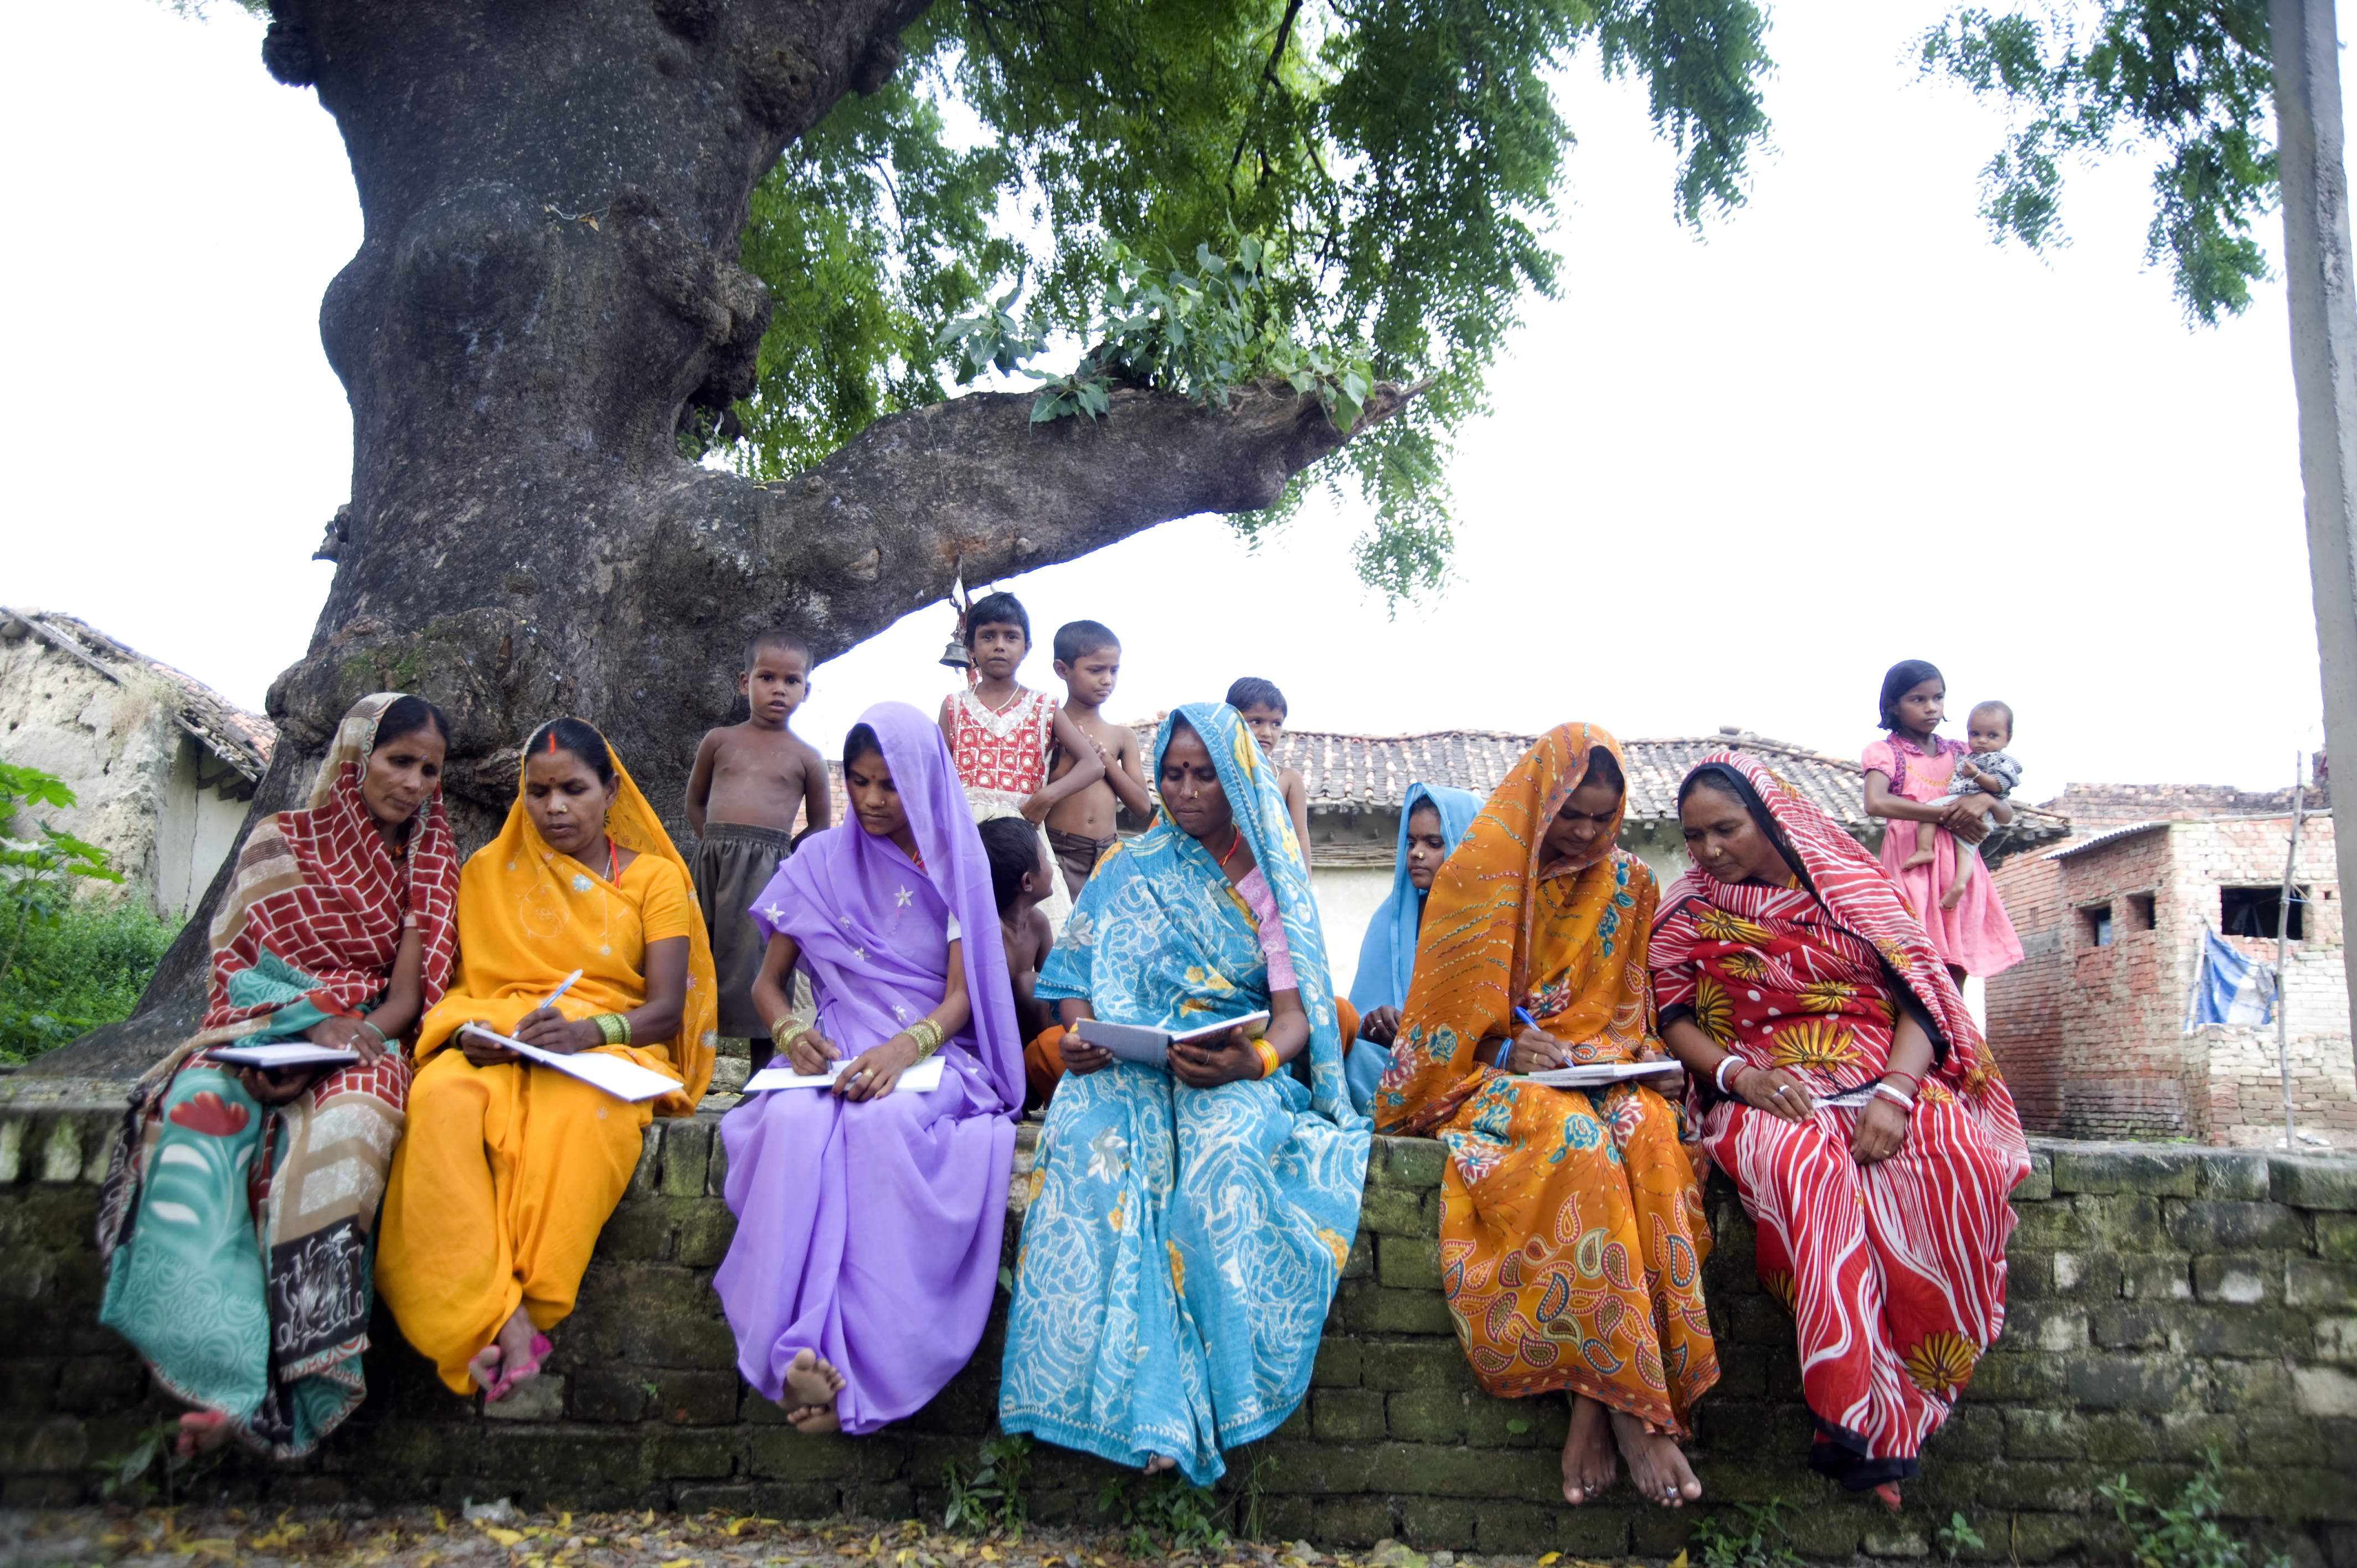
\includegraphics[width=\linewidth]{external/images/shutterstock_674070355.jpg}
\end{sbspanel}%
\end{sidebyside}%
\par
You may have heard that mathematics is the language of science.  In fact, professionals in nearly every discipline take advantage of mathematical methods to analyze data, identify trends, and predict the effects of change.  This process is called \terminology{mathematical modeling}. A \terminology{model} is a simplified representation of reality that helps us understand a process or phenomenon.  Because it is a simplification, a model can never be completely accurate.  Instead, it should focus on those aspects of the real situation that will help us answer specific questions. Here is an example.%
\par
The world's population is growing at different rates in different nations.  Many factors, including economic and social forces, influence the birth rate.  Is there a connection between birth rates and education levels? The figure shows the birth rate plotted against the female literacy rate in 148 countries.  Although the data points do not all lie precisely on a line, we see a generally decreasing trend:  the higher the literacy rate, the lower the birth rate. The \terminology{regression line} provides a model for this trend, and a tool for analyzing the data. In this chapter we study the properties of linear models and some techniques for fitting a linear model to data.%
\begin{image}{0.1}{0.8}{0.1}{}%
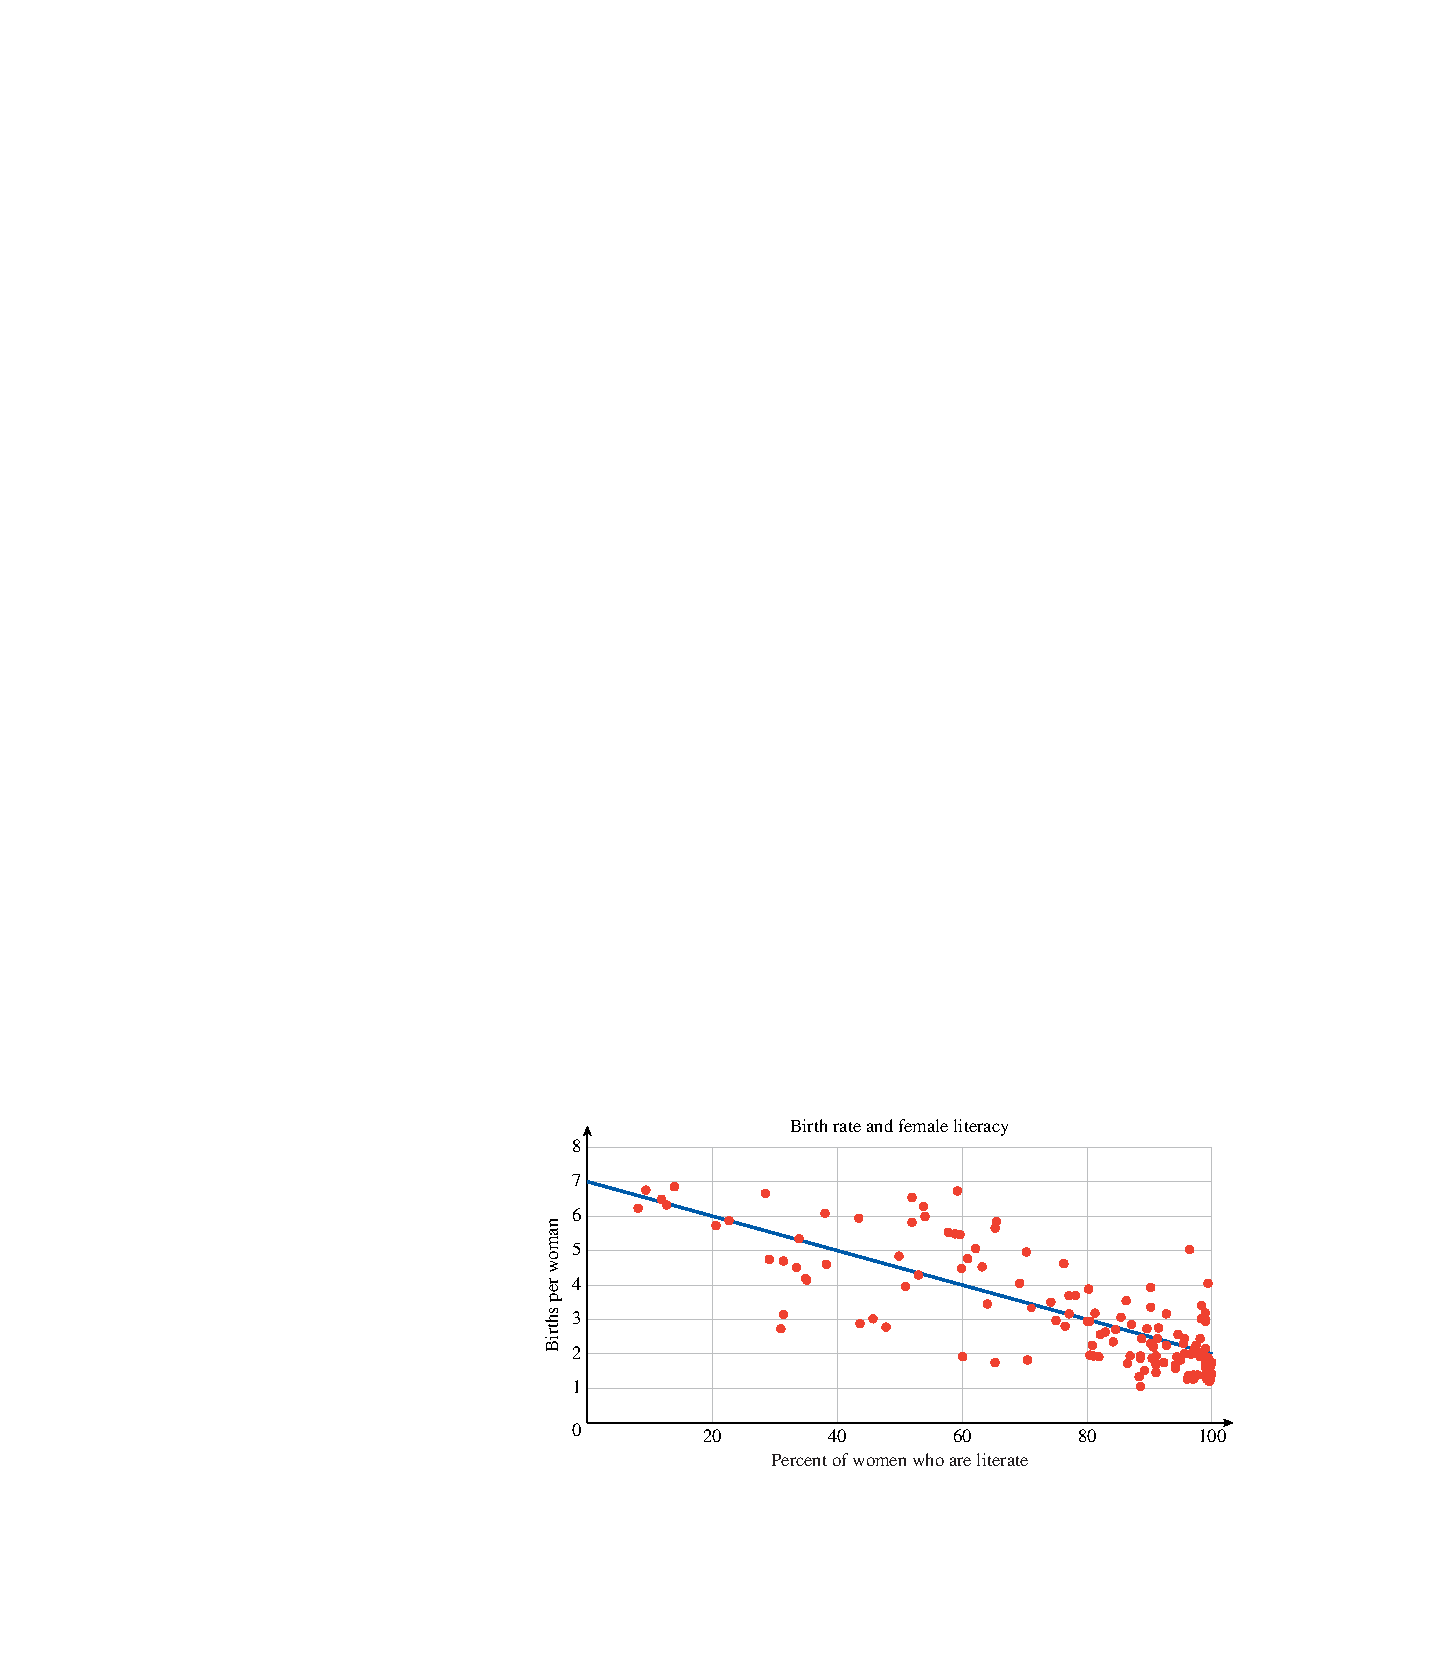
\includegraphics[width=\linewidth]{external/images/BirthRateVsFemaleLiteracy.pdf}
\end{image}%
\end{introduction}%
%
%
\typeout{************************************************}
\typeout{Section 2.1 Linear Regression}
\typeout{************************************************}
%
\begin{sectionptx}{Section}{Linear Regression}{}{Linear Regression}{}{}{LinReg}
\index{linear regression}%
\index{regression|see{linear regression}}%
%
%
\typeout{************************************************}
\typeout{Subsection 2.1.1 Shrinking Rain Forest}
\typeout{************************************************}
%
\begin{subsectionptx}{Subsection}{Shrinking Rain Forest}{}{Shrinking Rain Forest}{}{}{LinReg-4}
\begin{sidebyside}{2}{0}{0}{0.02}%
\begin{sbspanel}{0.68}[center]%
The Amazon Basin in South America contains over half of the planet's rain forest. The Amazon rain forest is home to the largest collection of plant and animal species in the world, including more than one-third of all living species. During the 1960s, colonists began cutting down the rain forest to clear land for agriculture. The construction of the Trans-Amazonian Highway in the early 1970s opened large forest areas to development by settlers and commercial interests, increasing the rate of deforestation.%
\par
Environmentalists are concerned about the loss of biodiversity which will result from destruction of the forest, and about the release of the carbon contained within the vegetation, which could accelerate global warming.%
\par
In Brazil, the Instituto Nacional de Pesquisas Espaciais (INPE, or National Institute of Space Research) uses Landsat satellite photos to monitor the pace of deforestation. According to their data, the original Amazon rain forest biome in Brazil of 4,100,000 square kilometers was reduced to 3,413,000 square kilometers by 2005, representing a loss of 16.8\%. The figures for 1987 to 2006 are shown at right, and a plot of the data appears below.  \(~\alert{\text{[TK]}}\)%
\end{sbspanel}%
\begin{sbspanel}{0.3}[center]%
\resizebox{\ifdim\width > \linewidth\linewidth\else\width\fi}{!}{%
{\centering%
{\tabularfont%
\begin{tabular}{AcAcA}\hrulethin
Year&\tablecelllines{c}{m}
{Remaining forest\\
(thousands sq km)}
\tabularnewline\hrulethin
1987&3745\tabularnewline\hrulethin
1988&3274\tabularnewline\hrulethin
1989&3706\tabularnewline\hrulethin
1990&3692\tabularnewline\hrulethin
1991&3681\tabularnewline\hrulethin
1992&3667\tabularnewline\hrulethin
1993&3652\tabularnewline\hrulethin
1994&3637\tabularnewline\hrulethin
1995&3608\tabularnewline\hrulethin
1996&3590\tabularnewline\hrulethin
1997&3577\tabularnewline\hrulethin
1998&3560\tabularnewline\hrulethin
1999&3542\tabularnewline\hrulethin
2000&3524\tabularnewline\hrulethin
2001&3506\tabularnewline\hrulethin
2002&3485\tabularnewline\hrulethin
2003&3460\tabularnewline\hrulethin
2004&3432\tabularnewline\hrulethin
2005&3413\tabularnewline\hrulethin
2006&3400\tabularnewline\hrulethin
\end{tabular}
}%
\par}
}%
\end{sbspanel}%
\end{sidebyside}%
\begin{image}{0.05}{0.9}{0.05}{}%
\includegraphics[width=\linewidth]{external/images/fig-rain-forest.pdf}
\end{image}%
\begin{aside}{Aside}{}{LinReg-4-4}%
\(\alert{\text{[TK]}}~~\)To see more examples of scatterplots, see \hyperref[tkReadScat]{Section 2.1.1} of the Toolkit.%
\end{aside}
Although the data points do not all lie exactly on a straight line, they are very close. One question we might ask is: If deforestation continues at the same rate, when will the Amazon rain forest disappear completely? In this section we learn to find a linear model that approximates a data set.%
\end{subsectionptx}
%
%
\typeout{************************************************}
\typeout{Subsection 2.1.2 Line of Best Fit}
\typeout{************************************************}
%
\begin{subsectionptx}{Subsection}{Line of Best Fit}{}{Line of Best Fit}{}{}{LinReg-5}
\index{least-squares regression line}%
\index{line!of best fit|see{least-squares regression line}}%
\index{linear regression!line of best fit}%
In most cases, a mathematical model is not a perfect description of reality. Many factors can affect empirical data, including measurement error, environmental conditions, and the influence of related variables. Nonetheless, we can often find an equation that approximates the data in a useful way.%
\begin{example}{Example}{}{Minimum-wage}%
The table shows the minimum wage in the US at five-year intervals. (Source: Economic Policy Institute)%
\begin{center}%
{\tabularfont%
\begin{tabular}{AcAcAcAcAcAcAcAcAcAcA}\hrulethin
\multicolumn{1}{AlA}{Year}&1960&1965&1970&1975&1980&1985&1990&1995&2000\tabularnewline\hrulethin
\multicolumn{1}{AlA}{Min. wage}&1.00&1.25&1.60&2.10&3.10&3.35&3.80&4.25&5.15\tabularnewline\hrulethin
\end{tabular}
}%
\end{center}%
\begin{sidebyside}{2}{0}{0}{0.05}%
\begin{sbspanel}{0.5}%
%
\begin{enumerate}[label={\alph*}]
\item{}Let \(t\) represent the number of years after 1960, and plot the data. Are the data linear?%
\item{}Draw a line that "fits" the data. \(~\alert{\text{[TK]}}\)%
\end{enumerate}
%
\end{sbspanel}%
\begin{sbspanel}{0.45}[center]%
\includegraphics[width=\linewidth]{external/images/fig-example-2-1-1.pdf}
\end{sbspanel}%
\end{sidebyside}%
\par\smallskip%
\noindent\textbf{\blocktitlefont Solution}.\hypertarget{Minimum-wage-2}{}\quad{}%
\begin{enumerate}[label={\alph*}]
\item{}The graph shown is called a \terminology{scatterplot}\index{scatterplot}. The data are not strictly linear, because the slope is not constant: from 1960 to 1965, the minimum wage increased at an average rate of%
\begin{equation*}
\dfrac{1.25-1.00}{5}=0.05~ \text{dollars per year}
\end{equation*}
and from 1970 to 1975, the minimum wage increased at a rate of%
\begin{equation*}
\dfrac{2.10-1.60}{5}=0.10~ \text{dollars per year}
\end{equation*}
However, the data points do appear to lie close to an imaginary line.%
\item{}\begin{sidebyside}{2}{0}{0}{0.04}%
\begin{sbspanel}{0.45}%
We would like to draw a line that comes as close as possible to all the data points, even though it may not pass precisely through any of them. In particular, we try to adjust the line so that we have the same number of points above the line and below the line. One possible solution is shown in the figure at right.%
\end{sbspanel}%
\begin{sbspanel}{0.51}[center]%
\includegraphics[width=\linewidth]{external/images/fig-example-2-1-1ans.pdf}
\end{sbspanel}%
\end{sidebyside}%
%
\end{enumerate}
%
\end{example}
\begin{aside}{Aside}{}{LinReg-5-7}%
\(\alert{\text{[TK]}}~~\)To see more examples of line of best fit, see \hyperref[tkBestFit]{Section 2.1.2} of the Toolkit.%
\end{aside}
A line that fits the data in a scatterplot is called a \terminology{regression line}\index{regression line}\index{regression line|seealso{linear regression}}\index{line!regression}. Drawing a regression line by eye is a subjective process. Using technology, we can compute a particular regression line called the \terminology{least-squares regression line}\index{least-squares regression line}\index{linear regression!least-squares regression line}, which is widely used in statistics and modeling.%
\par
We can still find an equation for a line of best fit using the \hyperref[point-slope]{point-slope formula}. (To review using the point-slope formula, see  \hyperref[TwoPoints]{Finding a Linear Model} in Section 1.5.) We choose two points on the line whose coordinates we can estimate fairly accurately. Note that these two points need not be any of the original data points.%
\begin{inlineexercise}{Checkpoint}{QuickCheck 1.}{LinReg-5-10}%
Explain how to find the equation of a regression line.%
\par
%
\begin{enumerate}[label={\alph*}]
\item{}Choose two data points and use the point-slope formula.%
\item{}Use the point-slope formula with the first and last data points.%
\item{}The regression line must pass through two data points, and we use the point-slope formula for those points.%
\item{}Choose two points on the regression line and use the point-slope formula.%
\end{enumerate}
%
\end{inlineexercise}%
\begin{inlineexercise}{Checkpoint}{Practice 1.}{LinReg-5-11}%
The regression line in the Example above appears to pass through the points \((5, 1.25)\) and \((25, 3.35)\). Use those points to find an equation for the regression line. \(~\alert{\text{[TK]}}\)%
\par
Hint: Step 1 Calculate the slope.%
\par
\(~~~~~~\) Step 2 Use the point-slope formula.%
\par\smallskip%
\noindent\textbf{\blocktitlefont Answer}.\hypertarget{LinReg-5-11-3}{}\quad{}\(y = 0.105x+0.725\)%
\end{inlineexercise}%
\begin{aside}{Aside}{}{LinReg-5-12}%
\(\alert{\text{[TK]}}~~\)To review finding the equation of a line, see \hyperref[tkTwoPtFit]{Section 2.1.3} of the Toolkit.%
\end{aside}
\end{subsectionptx}
%
%
\typeout{************************************************}
\typeout{Subsection 2.1.3 Interpolation and Extrapolation}
\typeout{************************************************}
%
\begin{subsectionptx}{Subsection}{Interpolation and Extrapolation}{}{Interpolation and Extrapolation}{}{}{LinReg-6}
\index{extrapolation}%
\index{linear regression!extrapolation}%
\index{interpolation}%
\index{linear regression!interpolation}%
\begin{example}{Example}{}{example-cocoa}%
An outdoor snack bar collected the following data showing the number of cups of cocoa, \(C\), they sold when the high temperature for the day was \(T\degree\) Celsius.%
\begin{center}%
{\tabularfont%
\begin{tabular}{AcAcAcAcAcAcAcAcAcAcAcA}\hrulethin
\multicolumn{1}{AlA}{Temperature (\(\degree\text{C}\)), \(T\)}&2&4&5&8&10&11&12&15&16&18\tabularnewline\hrulethin
\multicolumn{1}{AlA}{Cups of cocoa, \(C\)}&45&42&42&35&25&25&17&16&15&6\tabularnewline\hrulethin
\end{tabular}
}%
\end{center}%
%
\begin{enumerate}[label={\alph*}]
\item{}Make a scatterplot of the data, and draw a regression line%
\item{}Read values from your line for the number of cups of cocoa that will be sold when the temperature is \(8\degree\text{C}\) and when the temperature is \(16\degree\text{C}\).%
\item{}Find an equation for the regression line.%
\item{}Use your equation to predict the number of cups of cocoa that will be sold when the temperature is \(9\degree\text{C}\), and when the temperature is \(24\degree\text{C}.\)%
\end{enumerate}
%
\par\smallskip%
\noindent\textbf{\blocktitlefont Solution}.\hypertarget{example-cocoa-2}{}\quad{}%
\begin{enumerate}[label={\alph*}]
\item{}The scatterplot and a regression line are shown in the figure.%
\begin{image}{0.075}{0.85}{0.075}{}%
\includegraphics[width=\linewidth]{external/images/fig-example-cocoa.pdf}
\end{image}%
The regression line need not pass through any of the data points, but it should be as close as possible. We try to draw the regression line so that there are an equal number of data points above and below the line.%
\item{}The points \((8, 32)\) and \((16, 12)\) appear to lie on the regression line. According to this model, the snack bar will sell 32 cups of cocoa when the temperature is \(8\degree\text{C}\), and 12 cups when it is \(16\degree\text{C}\). These values are close to the actual data, but not exact.%
\item{}To find an equation for the regression line, we use two points on the line\textemdash{}not data points! We will use \((8, 32)\) and \((16, 12)\). First we compute the slope%
\begin{equation*}
m=\frac{C_2-C_1}{T_2-T_1}=\frac{12-32}{16-8}=-2.5
\end{equation*}
Next, we apply the point-slope formula. We'll use the point \((16, 12)\).%
\begin{align*}
C\amp= C_1+m(T-T_1)\\
C\amp= 12-2.5(T-16)\\
C\amp= -2.5T+52
\end{align*}
%
\item{}When \(T=\alert{9}\),%
\begin{equation*}
C=-2.5(\alert{9})+52=29.5
\end{equation*}
We predict that the snack bar will sell 29 or 30 cups of cocoa when the temperature is \(9\degree\text{C}\). When \(T = \alert{24}\),%
\begin{equation*}
C=-2.5(\alert{24})+52=-8
\end{equation*}
Because the snack bar cannot sell \(-8\) cups of cocoa, this prediction is not useful. (What is the Fahrenheit equivalent of 24°C?)%
\end{enumerate}
%
\end{example}
Using a regression line to estimate values between known data points is called \terminology{interpolation}\index{interpolation}\index{linear regression!interpolation}. If the data points lie fairly close to the regression line, then interpolation will usually give a fairly accurate estimate. In the \hyperref[example-cocoa]{Example} above, the estimate of 29 or 30 cups of cocoa at \(9\degree\text{C} \) seems reasonable in the context of the data.%
\par
Making predictions beyond the range of known data is called \terminology{extrapolation}\index{extrapolation}\index{linear regression!extrapolation}. Extrapolation can often give useful information, but if we try to extrapolate too far beyond our data, we may get unreasonable results. The conditions that produced the data may no longer hold, as in the \hyperref[example-cocoa]{Example} above, or other unexpected conditions may arise to alter the situation.%
\begin{inlineexercise}{Checkpoint}{QuickCheck 2.}{LinReg-6-9}%
True or false.%
\begin{enumerate}[label={\alph*}]
\item{}A scatterplot is a type of linear model.%
\item{}A regression line should give the same \(y\)-values as the data points.%
\item{}We use interpolation to estimate the \(y\)-value at a data point.%
\item{}Extrapolation is usually more reliable than interpolation.%
\end{enumerate}
%
\end{inlineexercise}%
\begin{inlineexercise}{Checkpoint}{Practice 2.}{LinReg-6-10}%
%
\begin{enumerate}[label={\alph*}]
\item{}Use your regression equation from the previous Example to predict the number of cups of cocoa sold when the temperature is \(-10^\circ\text{C} \).%
\item{}Predict the number of cups of cocoa sold when the temperature is \(7^\circ\text{C}\).%
\item{}Which prediction is more likely to be accurate?  Why?%
\end{enumerate}
%
\par\smallskip%
\noindent\textbf{\blocktitlefont Answer}.\hypertarget{LinReg-6-10-3}{}\quad{}%
\begin{enumerate}[label={\alph*}]
\item{}77%
\item{}34 or 35%
\item{}(b), because it is interpolation%
\end{enumerate}
%
\end{inlineexercise}%
\end{subsectionptx}
%
%
\typeout{************************************************}
\typeout{Subsection 2.1.4 Scatterplots}
\typeout{************************************************}
%
\begin{subsectionptx}{Subsection}{Scatterplots}{}{Scatterplots}{}{}{LinReg-7}
The data in a scatterplot may show a linear trend, even though the individual points are not clustered closely around a line. Scattering of data is common in the social sciences, where many variables may influence a particular situation. Nonetheless, by analyzing the data, we may be able to detect a connection between some of the variables.%
\begin{example}{Example}{}{Example-female-literacy}%
The world's population is growing at different rates in different nations. Many factors, including economic and social forces, influence the birthrate. Is there a connection between birth rates and education levels? The figure below shows the birth rate plotted against the female literacy rate in 148 countries.%
\begin{image}{0.05}{0.9}{0.05}{}%
\includegraphics[width=\linewidth]{external/images/fig-female-literacy-scatterplot.pdf}
\end{image}%
%
\begin{enumerate}[label={\alph*}]
\item{}Draw a line of best fit for the data points.%
\item{}Locate on the scatterplot the points representing the following nations%
\begin{center}%
{\tabularfont%
\begin{tabular}{AcAcAcA}\hrulethin
\multicolumn{1}{AlA}{Country}&Literacy rate&Birth rate\tabularnewline\hrulethin
\multicolumn{1}{AlA}{Ethiopa}&33.8&5.33\tabularnewline\hrulethin
\multicolumn{1}{AlA}{Iraq}&53.0&4.28\tabularnewline\hrulethin
\multicolumn{1}{AlA}{Libya}&71.0&3.34\tabularnewline\hrulethin
\multicolumn{1}{AlA}{Maldives}&96.4&5.02\tabularnewline\hrulethin
\multicolumn{1}{AlA}{Morocco}&31.0&2.73\tabularnewline\hrulethin
\multicolumn{1}{AlA}{Niger}&9.4&6.75\tabularnewline\hrulethin
\end{tabular}
}%
\end{center}%
\item{}Data points that lie far from the regression line are called \terminology{outliers}\index{linear regression!outliers}\index{outliers}\index{outliers|seealso{linear regression}}. Which of the nations listed in part (b) could be considered outliers?%
\end{enumerate}
%
\par\smallskip%
\noindent\textbf{\blocktitlefont Solution}.\hypertarget{Example-female-literacy-2}{}\quad{}%
\begin{enumerate}[label={\alph*}]
\item{}\begin{image}{0.025}{0.95}{0.025}{-1.5\baselineskip}%
\includegraphics[width=\linewidth]{external/images/fig-female-literacy-line.pdf}
\end{image}%
%
\item{}The figure above shows the regression line and the data points for each of the nations in part (b).%
\item{}Morocco and the Maldives could be considered outliers.%
\end{enumerate}
%
\end{example}
\begin{inlineexercise}{Checkpoint}{Practice 3.}{LinReg-7-4}%
The equation for the least-squares regression line in the previous Example is%
\begin{gather*}
y = 7.04 - 0.05x
\end{gather*}
%
\par
%
\begin{enumerate}[label={\alph*}]
\item{}What values for the input variable make sense for the model? What are the largest and smallest values predicted by the model for the output variable?%
\item{}State the slope of the regression line, including units, and explain what it means in the context of the data.%
\end{enumerate}
%
\par\smallskip%
\noindent\textbf{\blocktitlefont Answer}.\hypertarget{LinReg-7-4-3}{}\quad{}%
\begin{enumerate}[label={\alph*}]
\item{}From 0 to 100; largest: 7.04; smallest: 2.04%
\item{}\(-0.05\) births per woman per percentage point. The birth rate decreases by 0.05 births per woman for each percentage point increase in the female literacy rate.%
\end{enumerate}
%
\end{inlineexercise}%
\end{subsectionptx}
%
%
\typeout{************************************************}
\typeout{Exercises 2.1.5 Problem Set 2.1}
\typeout{************************************************}
%
\begin{exercises-subsection}{Exercises}{Problem Set 2.1}{}{Problem Set 2.1}{}{}{section-2-1-exercises}
\paragraph{Warm Up}\hypertarget{section-2-1-exercises-2}{}
\begin{divisionexercise}{1}{}{}{section-2-1-exercises-2-2}%
Choose the correct graph for each equation. The scales on both axes are the same.%
\begin{multicols}{2}
\begin{enumerate}[label={\alph*}]
\item{}\(\displaystyle y=\dfrac{3}{4}x+2\)%
\item{}\(\displaystyle y=\dfrac{-3}{4}x+2\)%
\item{}\(\displaystyle y=\dfrac{3}{4}x-2\)%
\item{}\(\displaystyle y=\dfrac{-3}{4}x-2\)%
\end{enumerate}
\end{multicols}
%
\begin{sidebyside}{2}{0.05}{0.05}{0.18}%
\begin{sbspanel}{0.36}%
\resizebox{\linewidth}{!}{%
\tikzset{%
}
\begin{tikzpicture} [scale=.35]
\draw[cyan] (-6,-6) grid (6,6);
\draw[black,thick,->,>=stealth'] (-6,0)--(6.5,0) node[right]{$x$};
\draw[black,thick,->,>=stealth'] (0,-6)--(0,6.5) node[above]{$y$};
\draw[red,thick,<->, >=stealth'] (-16/3,-6)--(6,5/2);
\node at (-8,7){\textbf{I}};
\node[text=white] at (-8,-8){I };
\end{tikzpicture}
}%
\par
\resizebox{\linewidth}{!}{%
\tikzset{%
}
\begin{tikzpicture} [scale=.35]
\draw[cyan] (-6,-6) grid (6,6);
\draw[black,thick,->,>=stealth'] (-6,0)--(6.5,0) node[right]{$x$};
\draw[black,thick,->,>=stealth'] (0,-6)--(0,6.5) node[above]{$y$};
\draw[red,thick,<->, >=stealth'] (-16/3,6)--(6,-5/2);
\node at (-8,7){\textbf{III}};
\node[text=white] at (-8,-8){III };
\end{tikzpicture}
}%
\end{sbspanel}%
\begin{sbspanel}{0.36}%
\resizebox{\linewidth}{!}{%
\tikzset{%
}
\begin{tikzpicture} [scale=.35]
\draw[cyan] (-6,-6) grid (6,6);
\draw[black,thick,->,>=stealth'] (-6,0)--(6.5,0) node[right]{$x$};
\draw[black,thick,->,>=stealth'] (0,-6)--(0,6.5) node[above]{$y$};
\draw[red,thick,<->, >=stealth'] (-6,-5/2)--(16/3,6);
\node at (-8,7){\textbf{II}};
\node[text=white] at (-8,-8){ II};
\end{tikzpicture}
}%
\par
\resizebox{\linewidth}{!}{%
\tikzset{%
}
\begin{tikzpicture} [scale=.35]
\draw[cyan] (-6,-6) grid (6,6);
\draw[black,thick,->,>=stealth'] (-6,0)--(6.5,0) node[right]{$x$};
\draw[black,thick,->,>=stealth'] (0,-6)--(0,6.5) node[above]{$y$};
\draw[red,thick,<->, >=stealth'] (-16/3,6)--(6,-5/2);
\node at (-8,7){\textbf{III}};
\node[text=white] at (-8,-8){IV };
\end{tikzpicture}
}%
\end{sbspanel}%
\end{sidebyside}%
\end{divisionexercise}%
\begin{divisionexercise}{2}{}{}{section-2-1-exercises-2-3}%
Choose the correct graph for each equation. The scales on both axes are the same.%
\begin{multicols}{2}
\begin{enumerate}[label={\alph*}]
\item{}\(\displaystyle y=1+2(x+3)\)%
\item{}\(\displaystyle y=-1+2(x-3)\)%
\item{}\(\displaystyle y=-1+2(x+3)\)%
\item{}\(\displaystyle y=1+2(x-3)\)%
\end{enumerate}
\end{multicols}
%
\begin{sidebyside}{2}{0.05}{0.05}{0.18}%
\begin{sbspanel}{0.36}%
\resizebox{\linewidth}{!}{%
\tikzset{%
}
\begin{tikzpicture} [scale=.35]
\draw[cyan] (-6,-9) grid (6,3);
\draw[black,thick,->,>=stealth'] (-6,0)--(6.5,0) node[right]{$x$};
\draw[black,thick,->,>=stealth'] (0,-9)--(0,3.5) node[above]{$y$};
\draw[samples=2,domain={-2:4},smooth,variable=\x,red,very thick, <->, >=stealth'] plot (\x,{(1+2*(\x-3))});
\node at (-8,3){\textbf{I}};
\node[text=white] at (-8,-11){I };
\end{tikzpicture}
}%
\par
\resizebox{\linewidth}{!}{%
\tikzset{%
}
\begin{tikzpicture} [scale=.35]
\draw[cyan] (-6,-3) grid (6,9);
\draw[black,thick,->,>=stealth'] (-6,0)--(6.5,0) node[right]{$x$};
\draw[black,thick,->,>=stealth'] (0,-3)--(0,9.5) node[above]{$y$};
\draw[samples=2,domain={-5:1},smooth,variable=\x,red,very thick, <->, >=stealth'] plot (\x,{(1+2*(\x+3))});
\node at (-8,9){\textbf{III}};
\node[text=white] at (-8,-5){III };
\end{tikzpicture}
}%
\end{sbspanel}%
\begin{sbspanel}{0.36}%
\resizebox{\linewidth}{!}{%
\tikzset{%
}
\begin{tikzpicture} [scale=.35]
\draw[cyan] (-6,-3) grid (6,9);
\draw[black,thick,->,>=stealth'] (-6,0)--(6.5,0) node[right]{$x$};
\draw[black,thick,->,>=stealth'] (0,-3)--(0,9.5) node[above]{$y$};
\draw[samples=2,domain={-4:2},smooth,variable=\x,red,very thick, <->, >=stealth'] plot (\x,{(-1+2*(\x+3))});
\node at (-8,9){\textbf{II}};
\node[text=white] at (-8,-5){II };
\end{tikzpicture}
}%
\par
\resizebox{\linewidth}{!}{%
\tikzset{%
}
\begin{tikzpicture} [scale=.35]
\draw[cyan] (-6,-9) grid (6,3);
\draw[black,thick,->,>=stealth'] (-6,0)--(6.5,0) node[right]{$x$};
\draw[black,thick,->,>=stealth'] (0,-9)--(0,3.5) node[above]{$y$};
\draw[samples=2,domain={-1:5},smooth,variable=\x,red,very thick, <->, >=stealth'] plot (\x,{(-1+2*(\x-3))});
\node at (-8,3){\textbf{IV}};
\node[text=white] at (-8,-11){IV };
\end{tikzpicture}
}%
\end{sbspanel}%
\end{sidebyside}%
\end{divisionexercise}%
\par\medskip\noindent%
\textbf{Exercise Group.}\space\space%
In Problems 3 and 4, find a linear model from two data points as follows:%
\begin{enumerate}[label={\alph*}]
\item{}Make a table showing the coordinates of two data points for the model. (Which variable should be plotted on the horizontal axis?)%
\item{}Write an equation for the line.%
\item{}State the slope of the line, including units, and explain its meaning in the context of the problem.%
\end{enumerate}
%
\begin{exercisegroup}
\begin{divisionexerciseeg}{3}{}{}{section-2-1-exercises-2-4-2}%
On an international flight a passenger may check two bags each weighing 70 kilograms, or 154 pounds, and one carry-on bag weighing 50 kilograms, or 110 pounds. Express the weight, \(p\), of a bag in pounds in terms of its weight, \(k\), in kilograms.%
\end{divisionexerciseeg}%
\begin{divisionexerciseeg}{4}{}{}{section-2-1-exercises-2-4-3}%
Ms. Randolph bought a used car in 2010. In 2012 the car was worth \textdollar{}9000, and in 2015 it was valued at \textdollar{}4500. Express the value, \(V\), of Ms. Randolph's car in terms of the number of years, \(t\), she has owned it.%
\end{divisionexerciseeg}%
\end{exercisegroup}
\par\medskip\noindent
\paragraph{Skills Practice}\hypertarget{section-2-1-exercises-3}{}
\begin{divisionexercise}{5}{}{}{section-2-1-exercises-3-2}%
%
\begin{enumerate}[label={\alph*}]
\item{}Find the slope, the \(C\)-intercept, and the \(T\)-intercept for the regression line in \hyperref[example-cocoa]{Example~{\xreffont\ref{example-cocoa}}}.%
\item{}What do the slope and the intercepts tell us about the sale of cocoa?%
\end{enumerate}
%
\end{divisionexercise}%
\begin{divisionexercise}{6}{}{}{section-2-1-exercises-3-3}%
The number of manatees killed by watercraft in Florida waters has been increasing since 1975. Data are given at 5-year intervals in the table, and a scatterplot with regression line is shown below. (Source: Florida Fish and Wildlife Conservation Commission)%
\begin{sidebyside}{2}{0.025}{0.025}{0.05}%
\begin{sbspanel}{0.45}%
\resizebox{\ifdim\width > \linewidth\linewidth\else\width\fi}{!}{%
{\centering%
{\tabularfont%
\begin{tabular}{AcAcA}\hrulethick
Year&Manatee deaths\tabularnewline\hrulethin
\(1975\)&\(6\)\tabularnewline\hrulethin
\(1980\)&\(16\)\tabularnewline\hrulethin
\(1985\)&\(33\)\tabularnewline\hrulethin
\(1990\)&\(47\)\tabularnewline\hrulethin
\(1995\)&\(42\)\tabularnewline\hrulethin
\(2000\)&\(78\)\tabularnewline\hrulethin
\end{tabular}
}%
\par}
}%
\end{sbspanel}%
\begin{sbspanel}{0.45}%
\includegraphics[width=\linewidth]{external/images/fig-manatee-deaths.pdf}
\end{sbspanel}%
\end{sidebyside}%
\par
An equation for the regression line is  \(y=4.7+2.6t\)%
%
\begin{enumerate}[label={\alph*}]
\item{}Use the regression equation to estimate the number of manatees killed by watercraft in 1998.%
\item{}What does the slope of the regression line mean in this situation?%
\item{}Which data point might be considered an outlier?%
\end{enumerate}
\end{divisionexercise}%
\par\medskip\noindent%
\textbf{Exercise Group.}\space\space%
In Problems 7 and 8, the regression lines can be improved by adjusting either \(m\) or \(b\). Draw a line that fits the data points more closely.%
\begin{exercisegroupcol}{2}
\begin{divisionexerciseegcol}{7}{}{}{section-2-1-exercises-3-4-2}%
\begin{image}{0}{1}{0}{-0.5\baselineskip}%
\includegraphics[width=\linewidth]{external/images/fig-ex-2-1-3.pdf}
\end{image}%
\end{divisionexerciseegcol}%
\begin{divisionexerciseegcol}{8}{}{}{section-2-1-exercises-3-4-3}%
\begin{image}{0.25}{0.5}{0.25}{-0.5\baselineskip}%
\includegraphics[width=\linewidth]{external/images/fig-ex-2-1-4.pdf}
\end{image}%
\end{divisionexerciseegcol}%
\end{exercisegroupcol}
\par\medskip\noindent
\par\medskip\noindent%
\textbf{Exercise Group.}\space\space%
For Problems 9 and 10,%
\begin{enumerate}[label={\alph*}]
\item{}Use the point-slope formula to write an equation.%
\item{}Use linear interpolation to give approximate answers.%
\item{}What does the slope tell us about the problem setting?%
\end{enumerate}
%
\begin{exercisegroup}
\begin{divisionexerciseeg}{9}{}{}{section-2-1-exercises-3-5-2}%
Newborn blue whales are about 24 feet long and weigh 3 tons. The young whale nurses for 7 months, at which time it is 53 feet long. Estimate the length of a 1-year-old blue whale.%
\end{divisionexerciseeg}%
\begin{divisionexerciseeg}{10}{}{}{section-2-1-exercises-3-5-3}%
A truck on a slippery road is moving at 24 feet per second when the driver steps on the brakes. The truck needs 3 seconds to come to a stop. Estimate the truck's speed 2 seconds after the brakes were applied.%
\end{divisionexerciseeg}%
\end{exercisegroup}
\par\medskip\noindent
\par\medskip\noindent%
\textbf{Exercise Group.}\space\space%
In Problems 11 and 12, use linear interpolation or extrapolation to answer the questions.%
\begin{exercisegroup}
\begin{divisionexerciseeg}{11}{}{}{section-2-1-exercises-3-6-2}%
The temperature of an automobile engine is \(9\degree\) Celsius when the engine is started and \(51\degree\)C seven minutes later. Use a linear model to predict the engine temperature for both 2 minutes and 2 hours after it started. Are your predictions reasonable?%
\end{divisionexerciseeg}%
\begin{divisionexerciseeg}{12}{}{}{section-2-1-exercises-3-6-3}%
The elephant at the City Zoo becomes ill and loses weight. She weighed 10,012 pounds when healthy and only 9641 pounds a week later. Predict her weight after 10 days of illness.%
\end{divisionexerciseeg}%
\end{exercisegroup}
\par\medskip\noindent
\paragraph{Applications}\hypertarget{section-2-1-exercises-4}{}
\begin{divisionexercise}{13}{}{}{section-2-1-exercises-4-2}%
The scatterplot shows the ages of 10 army drill sergeants and the time it took each to run 100 meters, in seconds.%
\begin{image}{0.3}{0.4}{0.3}{}%
\includegraphics[width=\linewidth]{external/images/fig-age-vs-100m-time.pdf}
\end{image}%
%
\begin{enumerate}[label={\alph*}]
\item{}What was the hundred-meter time for the 25-year-old drill sergeant?%
\item{}How old was the drill sergeant whose hundred-meter time was 12.6 seconds?%
\item{}Use a straightedge to draw a line of best fit through the data points.%
\item{}Use your line of best fit to predict the hundred-meter time of a 28-year-old drill sergeant.%
\item{}Choose two points on your regression line and find its equation.%
\item{}Use the equation to predict the hundred-meter time of a 40-year-old drill sergeant and a 12 year-old drill sergeant. Are these predictions reasonable?%
\end{enumerate}
%
\end{divisionexercise}%
\begin{divisionexercise}{14}{}{}{section-2-1-exercises-4-3}%
The scatterplot shows the weights in pounds and the heights in inches of a team of distance runners.%
\begin{image}{0.34}{0.32}{0.34}{}%
\includegraphics[width=\linewidth]{external/images/fig-scatterplot-runner-wt-vs-ht.pdf}
\end{image}%
%
\begin{enumerate}[label={\alph*}]
\item{}Use a straightedge to draw a line that fits the data.%
\item{}Use your line to predict the weight of a 65-inch tall runner and the weight of a 71-inch tall runner.%
\item{}Use your answers from part (b) to approximate the equation of your regression line.%
\item{}Use your answer from part(c) to predict the weight of a runner who is 68 inches tall.%
\end{enumerate}
%
\end{divisionexercise}%
\begin{divisionexercise}{15}{}{}{section-2-1-exercises-4-4}%
The scatterplot shows the best times for various women running the 400 meters and the 100 meters.%
\begin{image}{0.3}{0.4}{0.3}{}%
\includegraphics[width=\linewidth]{external/images/fig-time-400m-vs-100m.pdf}
\end{image}%
%
\begin{enumerate}[label={\alph*}]
\item{}Use a straightedge to draw a line that fits the data.%
\item{}Use your line to predict the 400-meter time of a woman who runs the 100-meter dash in 11.2 seconds, and the 400-meter time of a woman who runs the 100-meter dash in 13.2 seconds.%
\item{}Use your answers from part (b) to approximate the equation of your regression line.%
\item{}Use your answer from part (c) to predict the the 400-meter time of a woman who runs the 100-meter dash in 12.1 seconds.%
\end{enumerate}
%
\end{divisionexercise}%
\begin{divisionexercise}{16}{}{}{section-2-1-exercises-4-5}%
The table shows the minimum wage in the United States at five-year intervals. (Source: Economic Policy Institute)%
\begin{center}%
{\tabularfont%
\begin{tabular}{AlAcAcAcAcAcAcAcAcAcAcAcA}\hrulethin
Year&\(1960\)&\(1965\)&\(1970\)&\(1975\)&\(1980\)&\(1985\)&\(1990\)&\(1995\)&\(2000\)&\(2005\)&\(2010\)\tabularnewline\hrulethin
Minimum wage&\(1.00\)&\(1.25\)&\(1.60\)&\(2.10\)&\(3.10\)&\(3.35\)&\(3.80\)&\(4.25\)&\(5.15\)&\(5.15\)&\(7.25\)\tabularnewline\hrulethin
\end{tabular}
}%
\end{center}%
%
\begin{enumerate}[label={\alph*}]
\item{}Let \(t\) represent the number of years after 1960 and plot the data. Draw a line of best fit for the data points.%
\item{}Find an equation for your regression line.%
\item{}Estimate the minimum wage in 1972.%
\item{}Predict the minimum wage in 2025.%
\end{enumerate}
%
\end{divisionexercise}%
\begin{divisionexercise}{17}{}{}{section-2-1-exercises-4-6}%
With Americans' increased use of faxes, pagers, and cell phones, new area codes are being created at a steady rate. The table shows the number of areacodes in the US each year. (Source: USA Today, NeuStar, Inc.)%
\begin{center}%
{\tabularfont%
\begin{tabular}{AlAcAcAcAcAcAcAcA}\hrulethin
Year&\(1997\)&\(1998\)&\(1999\)&\(2000\)&\(2001\)&\(2002\)&\(2003\)\tabularnewline\hrulethin
Number of area codes&\(151\)&\(186\)&\(204\)&\(226\)&\(239\)&\(262\)&\(274\)\tabularnewline\hrulethin
\end{tabular}
}%
\end{center}%
%
\begin{enumerate}[label={\alph*}]
\item{}Let \(t\) represent the number of years after 1995 and plot the data. Draw a line of best fit for the data points.%
\item{}Find an equation for your regression line.%
\item{}How many area codes do you predict for 2010?%
\end{enumerate}
%
\end{divisionexercise}%
\begin{divisionexercise}{18}{}{}{section-2-1-exercises-4-7}%
The table shows the amount of carbon released into the atmosphere annually from burning fossil fuels, in billions of tons, at 5-year intervals from 1950 to 1995. (Source: www.worldwatch.org)%
\begin{center}%
{\tabularfont%
\begin{tabular}{AlAcAcAcAcAcAcAcAcAcAcA}\hrulethin
Year&\(1950\)&\(1955\)&\(1960\)&\(1965\)&\(1970\)&\(1975\)&\(1980\)&\(1985\)&\(1990\)&\(1995\)\tabularnewline\hrulethin
\tablecelllines{l}{m}
{Carbon\\
emissions}
&\(1.6\)&\(2.0\)&\(2.5\)&\(3.1\)&\(4.0\)&\(4.5\)&\(5.2\)&\(5.3\)&\(5.9\)&\(6.2\)\tabularnewline\hrulethin
\end{tabular}
}%
\end{center}%
%
\begin{enumerate}[label={\alph*}]
\item{}Let \(t\) represent the number of years after 1950 and plot the data. Scale the \(t\)-axis from 0 to 50 by 5's, and the \(C\)-axis from 0 to 7 by 0.5's.%
\item{}Draw a line of best fit for the data points.%
\item{}Find an equation for your regression line.%
\item{}Estimate the amount of carbon released in 1992.%
\end{enumerate}
%
\end{divisionexercise}%
\begin{divisionexercise}{19}{}{}{section-2-1-exercises-4-8}%
Male birds with the largest repertoire of songs are the first to acquire mates in the spring. The table shows the number of different songs sung by several sedge warblers, and the days on which they acquired their mates, where day 1 is April 20. (Source: Krebs and Davies, 1993)%
\begin{center}%
{\tabularfont%
\begin{tabular}{AlAcAcAcAcAcAcAcAcAcAcA}\hrulethin
\tablecelllines{l}{m}
{Number of\\
songs, \(x\)}
&\(41\)&\(38\)&\(34\)&\(32\)&\(30\)&\(25\)&\(24\)&\(24\)&\(23\)&\(14\)\tabularnewline\hrulethin
Pairing day, \(y\)&\(20\)&\(24\)&\(25\)&\(21\)&\(24\)&\(27\)&\(31\)&\(35\)&\(40\)&\(42\)\tabularnewline\hrulethin
\end{tabular}
}%
\end{center}%
%
\begin{enumerate}[label={\alph*}]
\item{}Plot the data points on graph paper, scale the \(x\)-axis from 0 to 65 by 5’s, and the \(y\)-axis from 0 to 60 by 5’s.%
\item{}The least-squares regression line is%
\begin{equation*}
y = -0.85x + 53
\end{equation*}
Graph this line on the same grid with the data. (Make a short table of values and plot the points.)%
\item{}What does the slope of the regression line tell us about sedge warblers?%
\item{}Use extrapolation to estimate when a sedge warbler that knows 10 songs can expect to find a mate.%
\item{}What do the intercepts of the regression line represent? Do these values make sense for this situation?%
\end{enumerate}
%
\end{divisionexercise}%
\begin{divisionexercise}{20}{}{}{section-2-1-exercises-4-9}%
One measure of a person's physical fitness is the body mass index, or BMI. Your body mass index is the ratio of your weight in kilograms to the square of your height in meters. The points on the scatterplot show the BMI of Miss America from 1921 to 1991.%
\begin{image}{0.1}{0.8}{0.1}{}%
\includegraphics[width=\linewidth]{external/images/fig-BMI.pdf}
\end{image}%
%
\begin{enumerate}[label={\alph*}]
\item{}Use a straightedge to draw a line of best fit on the scatterplot above.%
\item{}The equation of the least-squares regression line for the data is%
\begin{equation*}
y = 20.69 - 0.04t
\end{equation*}
where \(t\) is the number of years since 1920. On the figure above, relabel the horizontal axis with values of \(t\). Then graph this line and compare to your estimated line of best fit.%
\item{}Do thinner people have higher or lower BMI scores than fatter people? Use the definition of BMI to explain your reasoning.%
\item{}The Center for Disease Control considers a BMI between 18.5 and 24.9 to be healthy. In 2002, Miss America was 5'3" tall and weighed 110 pounds. Calculate her BMI. (You will need to convert inches to meters and pounds to kilograms.)%
\item{}What BMI score does the regression line predict for Miss America 2002?%
\item{}There are no data points for the years 1928 to 1932. What happened during those years that might cause this gap?%
\end{enumerate}
%
\end{divisionexercise}%
\end{exercises-subsection}
\end{sectionptx}
%
%
\typeout{************************************************}
\typeout{Section 2.2 Linear Systems}
\typeout{************************************************}
%
\begin{sectionptx}{Section}{Linear Systems}{}{Linear Systems}{}{}{LinSys}
\index{linear system}%
\begin{introduction}{}%
For the rest of this chapter we'll consider problems that can be solved using two or more linear equations simultaneously. To begin, think about the two equations in the next Investigation.%
\begin{investigation}{Investigation}{Water Level.}{LinSys-3-2}%
When sailing upstream in a canal or a river that has rapids, ships must sometimes negotiate locks to raise them to a higher water level. Suppose your ship is in one of the lower locks, at an elevation of 20 feet. The next lock is at an elevation of 50 feet. Water begins to flow from the higher lock to the lower one, raising your level by 1 foot per minute, and simultaneously lowering the water level in the next lock by 1.5 feet per minute.%
\begin{enumerate}[label={\arabic*}]
\item{}Fill in the table%
\begin{center}%
{\tabularfont%
\begin{tabular}{AcAcAcA}\hrulethick
\(t\) (minutes)&Lower lock water level&Upper lock water level\tabularnewline\hrulethin
\(0\)&\(\hphantom{0000}\)&\(\hphantom{0000}\)\tabularnewline\hrulethin
\(2\)&\(\hphantom{0000}\)&\(\hphantom{0000}\)\tabularnewline\hrulethin
\(4\)&\(\hphantom{0000}\)&\(\hphantom{0000}\)\tabularnewline\hrulethin
\(6\)&\(\hphantom{0000}\)&\(\hphantom{0000}\)\tabularnewline\hrulethin
\(8\)&\(\hphantom{0000}\)&\(\hphantom{0000}\)\tabularnewline\hrulethin
\(10\)&\(\hphantom{0000}\)&\(\hphantom{0000}\)\tabularnewline\hrulethin
\end{tabular}
}%
\end{center}%
\item{}Let \(t\) stand for the number of minutes the water has been flowing.%
\begin{enumerate}[label={\alph*}]
\item{}Write an equation for \(L\), the water level in the lower lock after \(t\) minues.%
\item{}Write an equation for \(U\), the water level in the upper lock after \(t\) minues.%
\end{enumerate}
%
\item{}Graph both your equations on the grid.%
\begin{image}{0.25}{0.5}{0.25}{}%
\resizebox{\linewidth}{!}{%
\tikzset{%
}
\begin{tikzpicture} [scale=.6]
\draw[cyan] (0,0) grid (12,10);
\draw[black,thick,->,>=stealth'] (0,0)--(12.5,0) node[right]{$t$};
\draw[black,thick,->,>=stealth'] (0,0)--(0,10.5);
\foreach \x  in {5,10} {
  \draw[black,thick] (\x,.1)--++(0,-.2) node[below]{\x};
}
\foreach \x [evaluate=\x as \xi using int( 5* \x )]  in {2,4,...,10} {
  \draw[black,thick] (.1,\x)--++(-.2,0) node[left]{\xi};
}
\end{tikzpicture}
}%
\end{image}%
\item{}When will the water level in the two locks be 10 feet apart?%
\item{}When will the water level in the two locks be the same?%
\item{}Write an equation you can use to verify your answer to part (5), and solve it.%
\end{enumerate}
%
\end{investigation}%
\end{introduction}%
%
%
\typeout{************************************************}
\typeout{Subsection 2.2.1 Systems of Equations}
\typeout{************************************************}
%
\begin{subsectionptx}{Subsection}{Systems of Equations}{}{Systems of Equations}{}{}{LinSys-4}
A biologist wants to know the average weights of two species of birds in a wildlife preserve. She sets up a feeder whose platform is actually a scale and mounts a camera to monitor the feeder. She waits until the feeder is occupied only by members of the two species she is studying,  robins and thrushes. Then she takes a picture, which records the number of each species on the scale and the total weight registered.%
\par
From her two best pictures, she obtains the following information. The total weight of 3 thrushes and 6 robins is 48 ounces, and the total weight of 5 thrushes and 2 robins is 32 ounces.  The biologist writes two equations about the photos. \(~\alert{\text{[TK]}}~\) She begins by assigning variables to the two unknown quantities:%
\begin{align*}
\amp\text{Average weight of a thrush:} ~~t \\
\amp\text{Average weight of a robin:} ~~r 
\end{align*}
In each of the photos,%
\begin{equation*}
(\blert{\text{weight of thrushes}}) + (\blert{\text{weight of robins}}) = \blert{\text{total weight}}
\end{equation*}
So the two equations are%
\begin{align*}
3t + 6r \amp = 48\\
5t + 2r \amp =32
\end{align*}
%
\begin{aside}{Aside}{}{LinSys-4-4}%
\(\alert{\text{[TK]}}~~\)To review writing an expression for a linear model, see \hyperref[tkWriteLinMod]{Section 2.2.1} of the Toolkit.%
\end{aside}
This pair of equations is an example of a \terminology{linear system of two equations in two unknowns}\index{system of equations!\(2\times 2\)}\index{linear system!\(2\times 2\)} (or a \(2\times 2\) linear system, for short). A \terminology{solution}\index{solution!to a system of equations}\index{system of equations!solution} to the system is an ordered pair of numbers, \((t, r)\), that satisfies both equations in the system.%
\begin{inlineexercise}{Checkpoint}{QuickCheck 1.}{LinSys-4-6}%
Choose the solution of the system:%
\begin{align*}
3x-2y \amp = 19\\
4x+5y \amp = 10
\end{align*}
%
\par
%
\begin{multicols}{4}
\begin{enumerate}[label={\alph*}]
\item{}\(\displaystyle (7,1)\)%
\item{}\(\displaystyle (0,2)\)%
\item{}\(\displaystyle (5,-2)\)%
\item{}\(\displaystyle (2,5)\)%
\end{enumerate}
\end{multicols}
%
\end{inlineexercise}%
\end{subsectionptx}
%
%
\typeout{************************************************}
\typeout{Subsection 2.2.2 Solving Systems by Graphing}
\typeout{************************************************}
%
\begin{subsectionptx}{Subsection}{Solving Systems by Graphing}{}{Solving Systems by Graphing}{}{}{LinSys-5}
\index{system of equations!graphing}%
Recall that every point on the graph of an equation represents a solution to that equation, so a solution to both equations must be a point that lies on both graphs. Therefore, a solution to the system is a point where the two graphs intersect.%
\begin{sidebyside}{2}{0.0075}{0.0075}{0.015}%
\begin{sbspanel}{0.57}[center]%
The figure at right shows a graph of the system about robins and thrushes. The two lines appear to intersect at the point \((4, 6)\), so we expect that the values \(t = \alert{4}\) and \(r = \alert{6}\) are the solution to the system. We can check by verifying that these values satisfy both equations in the system%
\begin{align*}
3(\alert{4})+ 6(\alert{6}) \amp \stackrel{?}{=} 48\amp\amp \blert{\text{True}} \\
5(\alert{4})+ 2(\alert{6}) \amp \stackrel{?}{=} 32\amp\amp \blert{\text{True}} 
\end{align*}
%
\end{sbspanel}%
\begin{sbspanel}{0.4}[center]%
\resizebox{\linewidth}{!}{%
\tikzset{%
}
\begin{tikzpicture} [scale=.55]
\draw[cyan] (0,0) grid (10,10);
\draw[black,thick,->,>=stealth'] (0,0)--(10.6,0) node[right]{$t$};
\draw[black,thick,->,>=stealth'] (0,0)--(0,10.6) node[above]{$r$};
\foreach \x [evaluate=\x as \xi using int( 2* \x )]  in {5,10} {
  \draw[black,thick] (\x,.1)--++(0,-.2) node[below, fill=white, inner sep=1, yshift=-2]{\x};
  \draw[black,thick] (.1,\x)--++(-.2,0) node[left, fill=white, inner sep=1, xshift=-2]{\xi};
}
\draw[samples=2,domain=0:{32/5},smooth,variable=\x,red,very thick] plot (\x,{8 - 5/4*\x });
\node[red,rotate={atan(-5/4)}, fill=white, inner sep=1] at (2.5,6) {$5t+2r=32$};
\draw[samples=2,domain=0:{10},smooth,variable=\x,blue,very thick, ->, >=stealth'] plot (\x,{4 - 1/4*\x });
\node[blue,rotate={atan(-1/4)}, fill=white, inner sep=1] at (7.8,2.5) {$3t+6r=48$};
\end{tikzpicture}
}%
\end{sbspanel}%
\end{sidebyside}%
\par
Both equations are true, so we have found the solution: a thrush weighs 4 ounces on average, and a robin weighs 6 ounces. \(~\alert{\text{[TK]}}\)%
\begin{aside}{Aside}{}{LinSys-5-6}%
\(\alert{\text{[TK]}}~~\)To review solutions of linear systems, see \hyperref[tkSysSoln]{Section 2.2.2} of the Toolkit.%
\end{aside}
\begin{inlineexercise}{Checkpoint}{QuickCheck 2.}{LinSys-5-7}%
True or false.%
\begin{enumerate}[label={\alph*}]
\item{}The point where two lines cross is called the \terminology{intercept}.%
\item{}The \terminology{intercepts} of a line are the points where it intersects the axes.%
\item{}The solution of a system may occur at an intercept.%
\item{}The words \terminology{intercept} and \terminology{intersect} mean the same thing.%
\end{enumerate}
%
\end{inlineexercise}%
We can use a calculator or graphing utility to graph the equations in a system.%
\begin{example}{Example}{}{LinSys-5-9}%
Use your grapher to solve the system by graphing. \(~~\alert{\text{[TK]}}\)%
\begin{align*}
y \amp= 1.7x + 0.4\\
y \amp= 4.1x + 5.2
\end{align*}
%
\par\smallskip%
\noindent\textbf{\blocktitlefont Solution}.\hypertarget{LinSys-5-9-2}{}\quad{}We set the graphing window to%
\begin{center}%
{\tabularfont%
\begin{tabular}{ll}
\(\text{Xmin}=-9.4 \qquad\)&\(\text{Ymin}=-10\)\tabularnewline[0pt]
\(\text{Xmax}=-9.4 \qquad\)&\(\text{Ymax}=10\)
\end{tabular}
}%
\end{center}%
and enter the two equations. We can see in the figure that the two lines intersect in the third quadrant. We use the \kbd{TRACE} feature to find the coordinates of the intersection point, \((-2,-3)\). The solution to the system is \(x=-2\), \(y=-3\).%
\begin{image}{0.31}{0.38}{0.31}{}%
\includegraphics[width=\linewidth]{external/images/fig-GC-2x2-system.pdf}
\end{image}%
\end{example}
\begin{aside}{Aside}{}{LinSys-5-10}%
\(\alert{\text{[TK]}}~~\)To learn about graphing equations with GeoGebra, see Appendix B.%
\end{aside}
The values we obtain from a calculator may be only approximations, so it is a good idea to check the solution algebraically. In the example above, we find that both equations are true when we substitute \(x = \alert{-2}\) and \(y=\blert{-3}\).%
\begin{align*}
\blert{-3}\amp = 1.7(\alert{-2})+0.4\amp\amp \blert{\text{True}}\\
\blert{-3}\amp = 4.2(\alert{-2})+5.2\amp\amp \blert{\text{True}}
\end{align*}
%
\begin{inlineexercise}{Checkpoint}{Practice 1.}{LinSys-5-12}%
%
\begin{enumerate}[label={\alph*}]
\item{}Solve the system of equations%
\begin{align*}
y \amp = -0.7x + 6.9\\
y \amp =1.2x - 6.4
\end{align*}
by graphing. Use the window%
\begin{align*}
\text{Xmin} \amp = -9.4 \amp\amp \text{Xmax} = 9.4\\
\text{Ymin} \amp = -10 \amp\amp \text{Ymax} = 10
\end{align*}
%
\item{}Verify algebraically that your solution satisfies both equations.%
\end{enumerate}
%
\par\smallskip%
\noindent\textbf{\blocktitlefont Answer}.\hypertarget{LinSys-5-12-3}{}\quad{}%
\begin{enumerate}
\item{}\(\displaystyle (7, 2)\)%
\item{}%
\begin{align*}
{{2}}\amp= -0.7(7)+ 6.9\amp\amp \text{Yes!}\\
{{2}}\amp =1.2({7})-6.4\amp\amp \text{Yes!}
\end{align*}
%
\end{enumerate}
%
\end{inlineexercise}%
Because the \kbd{TRACE} feature does not show every point on a graph, we may not find the exact solution to a system by tracing the graphs.%
\begin{example}{Example}{}{LinSys-5-14}%
Solve the system%
\begin{align*}
3x - 2.8y \amp= 21.06\\
2x + 1.2y \amp= 5.3
\end{align*}
%
\par\smallskip%
\noindent\textbf{\blocktitlefont Solution}.\hypertarget{LinSys-5-14-2}{}\quad{}We can graph this system in the standard window by solving each equation for \(y\). We enter%
\begin{align*}
Y_1\amp = (21.06 - 3X)/-2.8\\
Y_2\amp  = (5.3 - 2X)/1.2
\end{align*}
and use the standard window. If we trace along the graph to the intersection point, we will not find the same coordinates on both lines. The intersection point is not displayed in this window. Instead, we can use the \terminology{intersect} feature of the grapher.%
\par
Follow the instructions for your grapher's intersect feature to find the intersection point, \(x = 4.36\), \(y = -2.85\).%
\par
We can substitute these values into the original system to check that they satisfy both equations.%
\begin{align*}
3(\alert{4.36}) - 2.8(\alert{-2.85}) \amp = 21.06 \amp\amp \blert{\text{True}}\\
2(\alert{4.36}) + 1.2(\alert{-2.85}) \amp = 5.3 \amp\amp \blert{\text{True}}
\end{align*}
%
\end{example}
\begin{inlineexercise}{Checkpoint}{Practice 2.}{LinSys-5-15}%
Solve the system of equations%
\begin{gather*}
y = 47x - 1930\\
y + 19x = 710
\end{gather*}
by graphing. Estimate the intercepts of each graph to help you choose a suitable window, and use the \terminology{intersect} feature  to locate the solution.%
\par\smallskip%
\noindent\textbf{\blocktitlefont Answer}.\hypertarget{LinSys-5-15-3}{}\quad{}\((40,-50)\)%
\end{inlineexercise}%
How does the calculator find the exact coordinates of the intersection point? In the next section we’ll learn how to find the solution of a system using algebra.%
\end{subsectionptx}
%
%
\typeout{************************************************}
\typeout{Subsection 2.2.3 Inconsistent and Dependent Systems}
\typeout{************************************************}
%
\begin{subsectionptx}{Subsection}{Inconsistent and Dependent Systems}{}{Inconsistent and Dependent Systems}{}{}{LinSys-6}
\index{dependent system|see{system of equations}}%
\index{system of equations!inconsistent}%
Because two straight lines do not always intersect at a single point, a \(2\times 2\) system of linear equations does not always have a unique solution. In fact, there are three possibilities, as illustrated below.%
\begin{image}{0.05}{0.9}{0.05}{}%
\resizebox{\linewidth}{!}{%
\tikzset{%
}
\begin{tikzpicture} [scale=.4]
\draw[cyan] (-5,-5) grid (5,5);
\draw[black,thick,->,>=stealth'] (-5,0)--++(10.6,0) node[above]{$x$};
\draw[black,thick,->,>=stealth'] (0,-5)--++(0,10.6) node[left]{$y$};
\draw[red,very thick, <->, >=stealth'] (11,-5)--(14.5,5);
\draw[blue,very thick, <->, >=stealth'] (9.5,-5)--(13,5);
\node[align=center] at (0,-6.5) {Consistent and \\independent: one solution};

\draw[cyan] (7,-5) grid (17,5);
\draw[black,thick,->,>=stealth'] (7,0)--++(10.6,0) node[above]{$x$};
\draw[black,thick,->,>=stealth'] (12,-5)--++(0,10.6) node[left]{$y$};
\draw[red,very thick, <->, >=stealth'] (-2,5)--(5,-.5);
\draw[blue,very thick, <->, >=stealth'] (-4,-5)--(5,4);
\node[align=center] at (12,-6.5) {Inconsistent:  \\no solution};

\draw[cyan] (19,-5) grid (29,5);
\draw[black,thick,->,>=stealth'] (19,0)--++(10.6,0) node[above]{$x$};
\draw[black,thick,->,>=stealth'] (24,-5)--++(0,10.6) node[left]{$y$};
\draw[red,very thick, <->, >=stealth'] (20,5)--(29,-.5);
\node[align=center] at (24,-6.5) {Dependent:  \\infinitely many solutions};
\end{tikzpicture}
}%
\end{image}%
\begin{definition}{Definition}{Solutions of Linear Systems.}{Definition-solution-system}%
\index{linear system|seealso{system of equations}}%
\index{system of equations!solution}%
\index{solution!to a system of equations}%
\index{consistent|see{system of equations}}%
\index{system of equations!consistent and independent}%
\index{inconsistent system|see{system of equations}}%
\index{system of equations!inconsistent}%
\index{system of equations!dependent}%
\index{system of equations!independent}%
There are three types of \(2 \times 2\) linear system\index{linear system!\(2\times 2\)} :%
\begin{enumerate}[label={\arabic*}]
\item{}\terminology{Consistent and independent system}\index{independent system|see{system of equations}}. The graphs of the two lines intersect in exactly one point. The system has exactly one solution.%
\item{}\terminology{Inconsistent system}\index{inconsistent}. The graphs of the equations are parallel lines and hence do not intersect. An inconsistent system has no solutions.%
\item{}\terminology{Dependent system}\index{dependent}. All the solutions of one equation are also solutions to the second equation, and hence are solutions of the system. The graphs of the two equations are the same line. A dependent system has infinitely many solutions.%
\end{enumerate}
%
\end{definition}
\begin{example}{Example}{}{example-inconsistent-system}%
Solve each system.%
\begin{multicols}{2}
\begin{enumerate}[label={\alph*}]
\item{}%
\begin{gather*}
y = -x + 5\\
2x + 2y = 3
\end{gather*}
%
\item{}%
\begin{gather*}
x = \frac{2}{3}y + 3\\
3x - 2y = 9
\end{gather*}
%
\end{enumerate}
\end{multicols}
%
\par\smallskip%
\noindent\textbf{\blocktitlefont Solution}.\hypertarget{example-inconsistent-system-2}{}\quad{}%
\begin{enumerate}[label={\alph*}]
\item{}We can use technology to graph both equations on the same axes. First, we rewrite the second equation in slope-intercept form by solving for \(y\).%
\begin{align*}
2x + 2y \amp = 3\amp\amp \blert{\text{Substract } 2x \text{ from both sides.}}\\
2y \amp = -2x + 3\amp\amp \blert{\text{Divide both sides by 2.}}\\
y \amp = -x + 1.5
\end{align*}
We enter the equations as%
\begin{align*}
Y_1 \amp= -X + 5\\
Y_2 \amp = -X + 1.5
\end{align*}
You should see that the lines do not intersect within the viewing window; they appear to be parallel. If we look again at the equations of the lines, we recognize that both have slope \(-1\) but different \(y\)-intercepts, so they are parallel. Because parallel lines never meet, there is no solution to the system.%
\item{}This time we will graph by hand. We begin by writing each equation in slope-intercept form.%
\begin{sidebyside}{2}{0}{0}{0.1}%
\begin{sbspanel}{0.6}[center]%
%
\begin{align*}
x \amp = \frac{2}{3}y + 3\amp\amp \blert{\text{Subtract 3.}}  \\
x -3\amp = \frac{2}{3}y \amp\amp \blert{\text{Multiply by }   \frac{3}{2}.}\\
\frac{3}{2}x-\frac{9}{2}\amp = y
\end{align*}
For the second equation,%
\begin{align*}
3x - 2y \amp = 9  \amp\amp \blert{\text{Subtract }    3x.}\\
-2y \amp = -3x + 9  \amp\amp \blert{\text{Divide by } -2.}\\
y \amp = \frac{3}{2}x - \frac{9}{2}
\end{align*}
%
\end{sbspanel}%
\begin{sbspanel}{0.3}[center]%
\includegraphics[width=\linewidth]{external/images/fig-coincident-lines.pdf}
\end{sbspanel}%
\end{sidebyside}%
\par
The two equations are actually different forms of the same equation. They are equivalent, so they share the same line as a graph. Every point on the first line is also a point on the second line, and hence a solution of the system. The system has infinitely many solutions.%
\end{enumerate}
%
\end{example}
\begin{inlineexercise}{Checkpoint}{QuickCheck 3.}{LinSys-6-8}%
Complete the statements.%
\begin{enumerate}[label={\alph*}]
\item{}If two lines have the same slope but different \(y\)-intercepts, the system is \fillintext{10}.%
\item{}If two lines have the same slope and the same \(y\)-intercept, the system is \fillintext{10}.%
\item{}If two lines have the same \(y\)-intercept but different slopes, the system is \fillintext{10}.%
\item{}If both lines are horizontal, the system is \fillintext{10}.%
\end{enumerate}
%
\end{inlineexercise}%
\begin{inlineexercise}{Checkpoint}{Practice 3.}{LinSys-6-9}%
%
\begin{enumerate}[label={\alph*}]
\item{}Graph the system%
\begin{gather*}
y = -3x + 6\\
6x + 2y = 15
\end{gather*}
by hand, using either the intercept method or the slope-intercept method.%
\item{}Identify the system as dependent, inconsistent, or consistent and independent.%
\end{enumerate}
%
\par\smallskip%
\noindent\textbf{\blocktitlefont Answer}.\hypertarget{LinSys-6-9-3}{}\quad{}%
\begin{multicols}{2}
\begin{enumerate}[label={\alph*}]
\item{}\begin{image}{0.15}{0.7}{0.15}{-1.5\baselineskip}%
\includegraphics[width=\linewidth]{external/images/fig-ex-2-2-3ans.pdf}
\end{image}%
%
\item{}Inconsistent: The graph is two parallel lines.%
\end{enumerate}
\end{multicols}
%
\end{inlineexercise}%
\end{subsectionptx}
%
%
\typeout{************************************************}
\typeout{Subsection 2.2.4 Applications}
\typeout{************************************************}
%
\begin{subsectionptx}{Subsection}{Applications}{}{Applications}{}{}{LinSys-7}
Systems of equations are useful in many applied problems. Here are two examples from economics.%
\par
A business venture calculates its \terminology{profit}\index{profit} by subtracting its \terminology{costs}\index{cost} from its \terminology{revenue}\index{revenue}, the amount of money it takes in from sales.%
\begin{equation*}
\blert{\text{Profit} = \text{Revenue} -\text{Cost}}
\end{equation*}
Cost is usually calculated as the sum of fixed costs, or overhead, and variable costs, the cost of labor and materials to produce its product. Revenue is the product of the selling price per item times the number of items sold. If the company’s revenue exactly equals its costs (so that their profit is zero), we say that the business venture will \terminology{break even}\index{break even}. \(~\alert{\text{[TK]}}\)%
\begin{aside}{Aside}{}{LinSys-7-4}%
\(\alert{\text{[TK]}}~~\)To see more examples of the profit equation, see \hyperref[tkProfit]{Section 2.2.3} of the Toolkit.%
\end{aside}
\begin{inlineexercise}{Checkpoint}{Practice 4.}{LinSys-7-5}%
The Aquarius jewelry company determines that each production run to manufacture a pendant involves an initial setup cost of \textdollar{}200 and \textdollar{}4 for each pendant produced. The pendants sell for \textdollar{}12 each.%
\begin{enumerate}[label={\alph*}]
\item{}Express the cost \(C\) of production in terms of the number \(x\) of pendants produced.%
\item{}Express the revenue \(R\) in terms of the number \(x\) of pendants sold.%
\item{}Graph the revenue and cost on the same set of axes. (Find the intercepts of each equation to help you choose a window for the graph.) State the solution of the system.%
\item{}How many pendants must be sold for the Aquarius company to break even on a particular production run?%
\end{enumerate}
%
\par\smallskip%
\noindent\textbf{\blocktitlefont Answer}.\hypertarget{LinSys-7-5-3}{}\quad{}%
\begin{enumerate}[label={\alph*}]
\item{}\(\displaystyle C=200+4x\)%
\item{}\(\displaystyle R=12x\)%
\item{}\(\displaystyle (25,300)\)%
\item{}They must sell 25 pendants to break even.%
\end{enumerate}
%
\end{inlineexercise}%
Another example involves supply and demand. The owner of a retail business must try to balance the demand for his product from consumers with the supply he can obtain from manufacturers. Supply and demand both vary with the price of the product: consumers usually buy fewer items if the price increases, but manufacturers will be willing to supply more units of the product if its price increases.%
\par
The \terminology{demand equation}\index{demand equation}\index{equation!demand} gives the number of units of the product that consumers will buy at a given price. The \terminology{supply equation}\index{supply equation}\index{equation!supply} gives the number of units that the producer will supply at that price. The price at which the supply and demand are equal is called the \terminology{equilibrium price}\index{equilibrium price}. This is the price at which the consumer and the producer agree to do business.%
\begin{example}{Example}{}{LinSys-7-8}%
A woolens mill can produce \(400x\) yards of fine suit fabric if it can charge \(x\) dollars per yard. The mill's clients in the garment industry will buy \(6000 - 100x\) yards of wool fabric at a price of \(x\) dollars per yard. Find the equilibrium price and the amount of fabric that will change hands at that price.%
\par\smallskip%
\noindent\textbf{\blocktitlefont Solution}.\hypertarget{LinSys-7-8-2}{}\quad{}%
\begin{itemize}[label=\textbullet]
\item{}\lititle{Step 1.}\par%
We choose variables for the unknown quantities.%
\begin{center}%
{\tabularfont%
\begin{tabular}{ll}
Price per yard:&\(x\)\tabularnewline[0pt]
Number of yards:&\(y\)
\end{tabular}
}%
\end{center}%
\item{}\lititle{Step 2.}\par%
The supply equation tells us how many yards of fabric the mill will produce for a price of \(x\) dollars per yard.%
\begin{equation*}
y=400x
\end{equation*}
The demand equation tells us how many yards of fabric the garment industry will buy at a price of \(x\) dollars per yard.%
\begin{equation*}
y = 6000 - 100x
\end{equation*}
%
\item{}\lititle{Step 3.}\par%
We graph the two equations on the same set of axes, as shown below. We set the window values to%
\begin{align*}
\text{Xmin} \amp = 0 \amp\amp \text{Xmax} = 94\\
\text{Ymin} \amp = 0 \amp\amp \text{Ymax} = 6200
\end{align*}
and use the \kbd{TRACE} or the \terminology{intersect} command to locate the solution. The graphs intersect at the point \((12, 4800)\).%
\begin{image}{0.3}{0.4}{0.3}{}%
\includegraphics[width=\linewidth]{external/images/fig-GC-equilibrium.png}
\end{image}%
\item{}\lititle{Step 4.}\par%
The equilibrium price is \textdollar{}12 per yard, and the mill will sell 4800 yards of fabric at that price.%
\end{itemize}
%
\end{example}
\end{subsectionptx}
%
%
\typeout{************************************************}
\typeout{Exercises 2.2.5 Problem Set 2.2}
\typeout{************************************************}
%
\begin{exercises-subsection}{Exercises}{Problem Set 2.2}{}{Problem Set 2.2}{}{}{section-2-2-exercises}
\paragraph{Warm Up}\hypertarget{section-2-2-exercises-2}{}
\begin{divisionexercise}{1}{}{}{section-2-2-exercises-2-2}%
Graph by the intercept method.%
\begin{equation*}
4x=\frac{4}{3}y=12
\end{equation*}
%
\end{divisionexercise}%
\begin{divisionexercise}{2}{}{}{section-2-2-exercises-2-3}%
Graph by the slope-intercept method.%
\begin{equation*}
y=8-\frac{5}{2}x
\end{equation*}
%
\end{divisionexercise}%
\begin{divisionexercise}{3}{}{}{section-2-2-exercises-2-4}%
Solve \(~~0.4(30-x)+0.8x=0.65(30) \)%
\end{divisionexercise}%
\begin{divisionexercise}{4}{}{}{section-2-2-exercises-2-5}%
Write each equation in the form \(ax + by = c\), where \(a\), \(b\), and \(c\), are integers.%
\begin{multicols}{2}
\begin{enumerate}[label={\alph*}]
\item{}\(\displaystyle 4y=6x-300\)%
\item{}\(\displaystyle 24-\dfrac{2}{3}y=\dfrac{3}{4}x\)%
\end{enumerate}
\end{multicols}
%
\end{divisionexercise}%
\paragraph{Skills Practice}\hypertarget{section-2-2-exercises-3}{}
\par\medskip\noindent%
\textbf{Exercise Group.}\space\space%
For Problems 5 and 6, solve the system of equations using the graph. Then verify that your solution satisfies both equations.%
\begin{exercisegroupcol}{2}
\begin{divisionexerciseegcol}{5}{}{}{section-2-2-exercises-3-2-2}%
%
\begin{align*}
-2.3x+5.9y \amp = 38.7\\
9.3x+7.4y \amp = -0.2
\end{align*}
%
\begin{image}{0.1}{0.8}{0.1}{-0.5\baselineskip}%
\includegraphics[width=\linewidth]{external/images/fig-system-decimal-coeffs.pdf}
\end{image}%
\end{divisionexerciseegcol}%
\begin{divisionexerciseegcol}{6}{}{}{section-2-2-exercises-3-2-3}%
%
\begin{align*}
35s-17t \amp = 560\\
24s+15t \amp = 2250
\end{align*}
%
\begin{image}{0.1}{0.8}{0.1}{-0.5\baselineskip}%
\includegraphics[width=\linewidth]{external/images/fig-system-large-integer-coeffs.pdf}
\end{image}%
\end{divisionexerciseegcol}%
\end{exercisegroupcol}
\par\medskip\noindent
\par\medskip\noindent%
\textbf{Exercise Group.}\space\space%
For Problems 7 and 8%
\begin{enumerate}[label={\alph*}]
\item{}Solve the system of equations by graphing. Use the "friendly" window%
\begin{align*}
\amp \text{Xmin} = -9.4 \amp\amp \text{Ymin} = -10\\
\amp \text{Xmax} = 9.4 \amp\amp \text{Ymax} = 10
\end{align*}
%
\item{}Verify algebraically that your solution satisfies both equations.%
\end{enumerate}
%
\begin{exercisegroupcol}{2}
\begin{divisionexerciseegcol}{7}{}{}{section-2-2-exercises-3-3-2}%
%
\begin{align*}
y \amp = 2.6x+8.2\\
y \amp = 1.8-0.6x
\end{align*}
%
\end{divisionexerciseegcol}%
\begin{divisionexerciseegcol}{8}{}{}{section-2-2-exercises-3-3-3}%
%
\begin{align*}
\amp y = 7.2 - 2.1x\\
\amp -2.8x+3.7y=5.5
\end{align*}
%
\end{divisionexerciseegcol}%
\end{exercisegroupcol}
\par\medskip\noindent
\par\medskip\noindent%
\textbf{Exercise Group.}\space\space%
For Problems 9\textendash{}12,%
\begin{enumerate}[label={\alph*}]
\item{}Graph the system by hand.%
\item{}Identify the system as dependent, inconsistent, or consistent and independent.%
\end{enumerate}
%
\begin{exercisegroupcol}{2}
\begin{divisionexerciseegcol}{9}{}{}{section-2-2-exercises-3-4-2}%
%
\begin{align*}
\amp  2x=y+4\\
\amp 8x-4y=9
\end{align*}
%
\end{divisionexerciseegcol}%
\begin{divisionexerciseegcol}{10}{}{}{section-2-2-exercises-3-4-3}%
%
\begin{align*}
\amp 2t+12=-6s\\
\amp 12s+4t=24
\end{align*}
%
\end{divisionexerciseegcol}%
\begin{divisionexerciseegcol}{11}{}{}{section-2-2-exercises-3-4-4}%
%
\begin{align*}
-3x \amp = 4y+12\\
\dfrac{1}{2}x + 2 \amp = \dfrac{-2}{3}y
\end{align*}
%
\end{divisionexerciseegcol}%
\begin{divisionexerciseegcol}{12}{}{}{section-2-2-exercises-3-4-5}%
%
\begin{align*}
w-3z \amp = 6\\
2w+x \amp = 8
\end{align*}
%
\end{divisionexerciseegcol}%
\end{exercisegroupcol}
\par\medskip\noindent
\paragraph{Applications}\hypertarget{section-2-2-exercises-4}{}
\begin{divisionexercise}{13}{}{}{section-2-2-exercises-4-2}%
Francine wants to join a health club and has narrowed it down to two choices. The Sportshaus charges an initiation fee of \textdollar{}500 and \textdollar{}10 per month. Fitness First has an initiation fee of \textdollar{}50 and charges \textdollar{}25 per month.%
\begin{enumerate}[label={\alph*}]
\item{}Let \(x\) stand for the number of months Francine uses the health club. Write equations for the total cost of each health club for \(x\) months.%
\item{}Complete the table for the total cost of each club.%
\begin{center}%
{\tabularfont%
\begin{tabular}{AcAcAcA}\hrulethin
\(x\)&\tablecelllines{c}{m}
{Sporthaus\\
total cost}
&\tablecelllines{c}{m}
{Fitness First\\
total cost}
\tabularnewline\hrulethin
6&&\tabularnewline\hrulethin
12&&\tabularnewline\hrulethin
18&&\tabularnewline\hrulethin
24&&\tabularnewline\hrulethin
30&&\tabularnewline\hrulethin
36&&\tabularnewline\hrulethin
42&&\tabularnewline\hrulethin
48&&\tabularnewline\hrulethin
\end{tabular}
}%
\end{center}%
\item{}Graph both equations on the grid.%
\begin{image}{0.3}{0.4}{0.3}{}%
\resizebox{\linewidth}{!}{%
\tikzset{%
}
\begin{tikzpicture} [xscale=.72, yscale=.54]
\draw[cyan] (0,0) grid (8,12);
\draw[black,thick,->,>=stealth'] (0,0)--++(8.6,0) node[right]{$x$};
\draw[black,thick,->,>=stealth'] (0,0)--++(0,12.8) node[left]{$y$};
\foreach \x [evaluate=\x as \xi using int( 6* \x )]  in {0,2,4,6,8} {
  \draw[black,thick] (\x,.1)--++(0,-.2) node[below, fill=white, inner sep=1, yshift=-2]{$\xi$};
}
\foreach \x [evaluate=\x as \xi using int( 100* \x )]  in {5,10} {
  \draw[black,thick] (.1,\x)--++(-.2,0) node[left, fill=white, inner sep=1, xshift=-2]{$\xi$};
}
\end{tikzpicture}
}%
\end{image}%
\item{}When will the total cost of the two health clubs be equal?%
\end{enumerate}
%
\end{divisionexercise}%
\begin{divisionexercise}{14}{}{}{section-2-2-exercises-4-3}%
The Bread Alone Bakery has a daily overhead of \textdollar{}90. It costs \textdollar{}0.60 to bake each loaf of bread, and the bread sells for \textdollar{}1.50 per loaf.%
\begin{enumerate}[label={\alph*}]
\item{}Write an equation for the cost \(C\) in terms of the number  of loaves, \(x\).%
\item{}Write an equation for the revenue \(R\) in terms of the number of loaves, \(x\).%
\item{}Graph the revenue, \(R\), and cost, \(C\), on the same set of axes. State the solution of the system.%
\item{}How many loaves must the bakery sell to break even on a given day?%
\begin{image}{0.3}{0.4}{0.3}{}%
\resizebox{\linewidth}{!}{%
\tikzset{%
}
\begin{tikzpicture} [xscale=.6, yscale=.5]
\draw[cyan] (0,0) grid (10,10);
\draw[black,thick,->,>=stealth'] (0,0)--++(10.6,0);
\draw[black,thick,->,>=stealth'] (0,0)--++(0,10.6);
\foreach \x [evaluate=\x as \xi using int( 20* \x )]  in {5,10} {
  \draw[black,thick] (\x,.1)--++(0,-.2) node[below, fill=white, inner sep=1, yshift=-2]{$\xi$};
  \draw[black,thick] (.1,\x)--++(-.2,0) node[left, fill=white, inner sep=1, xshift=-2]{$\xi$};
}
\end{tikzpicture}
}%
\end{image}%
\end{enumerate}
%
\end{divisionexercise}%
\begin{divisionexercise}{15}{}{}{section-2-2-exercises-4-4}%
The manager for Books for Cooks plans to spend \textdollar{}300 stocking a new diet cookbook. The paperback version costs her \textdollar{}5, and the hardback costs \textdollar{}10. She finds that she will sell three times as many paperbacks as hardbacks. How many of each should she buy?%
\par
%
\begin{enumerate}[label={\alph*}]
\item{}Let \(x\) represent the number of hardbacks and \(y\) the number of paperbacks she should buy. Write an equation about the cost of the books.%
\item{}Write a second equation about the number of each type of book.%
\item{}Graph both equations and solve the system using the grid.%
\begin{image}{0.325}{0.35}{0.325}{}%
\resizebox{\linewidth}{!}{%
\tikzset{%
}
\begin{tikzpicture} [xscale=.9, yscale=.6]
\draw[cyan] (0,0) grid (6,12);
\draw[black,thick,->,>=stealth'] (0,0)--++(6.6,0);
\draw[black,thick,->,>=stealth'] (0,0)--++(0,12.6);
\foreach \x [evaluate=\x as \xi using int( 6* \x )]  in {2,4,6} {
  \draw[black,thick] (\x,.1)--++(0,-.2) node[below, fill=white, inner sep=1, yshift=-2]{$\xi$};
}
\foreach \x [evaluate=\x as \xi using int( 6* \x )]  in {2,4,...,12} {
  \draw[black,thick] (.1,\x)--++(-.2,0) node[left, fill=white, inner sep=1, xshift=-2]{$\xi$};
}
\end{tikzpicture}
}%
\end{image}%
\item{}Answer the question in the problem.%
\end{enumerate}
%
\end{divisionexercise}%
\begin{divisionexercise}{16}{}{}{section-2-2-exercises-4-5}%
There were 42 passengers on a local airplane flight. First-class fare was \textdollar{}80, and coach fare was \textdollar{}64. If the revenue for the flight totaled \textdollar{}2880, how many first-class and how many coach passengers paid for the flight?%
\begin{enumerate}[label={\alph*}]
\item{}Write algebraic expressions to fill in the table.%
\begin{center}%
{\tabularfont%
\begin{tabular}{AcAcAcAcA}\hrulethin
&Number of tickets&Cost per ticket&Revenue\tabularnewline\hrulethin
First-class&\(x\)&&\tabularnewline\hrulethin
Coach&\(y\)&&\tabularnewline\hrulethin
Total&&&\tabularnewline\hrulethin
\end{tabular}
}%
\end{center}%
\item{}Write an equation about the number of tickets sold.%
\item{}Write a second equation about the revenue from the tickets.%
\item{}Graph both equations on graph paper and solve the system. (\terminology{Hint}: Find the intercepts of each equation to help you choose scales for the axes.)%
\item{}Answer the question in the problem.%
\end{enumerate}
%
\end{divisionexercise}%
\begin{divisionexercise}{17}{}{}{section-2-2-exercises-4-6}%
Mel's Pool Service can clean \(1.5x\) pools per week if it charges \(x\) dollars per pool, and the public will book \(120 - 2.5x\) pool cleanings at \(x\) dollars per pool.%
\begin{enumerate}[label={\alph*}]
\item{}What is the supply equation?%
\item{}What is the demand equation?%
\item{}Graph both equations in the window%
\begin{align*}
\amp \text{Xmin} = 0 \amp\amp \text{Ymin} = 0\\
\amp \text{Xmax} = 50 \amp\amp \text{Ymax} = 125
\end{align*}
%
\item{}Find the equilibrium price and the number of pools Mel will clean at that price.%
\end{enumerate}
%
\end{divisionexercise}%
\begin{divisionexercise}{18}{}{}{section-2-2-exercises-4-7}%
%
\begin{enumerate}[label={\alph*}]
\item{}Explain how you can tell, without graphing, that the system has no solution.%
\begin{gather*}
3x=y+3\\
6x-2y=12
\end{gather*}
%
\item{}Explain how you can tell, without graphing, that the system has infinitely many solutions.%
\begin{gather*}
-x+2y=4\\
3x=6y-12
\end{gather*}
%
\end{enumerate}
%
\end{divisionexercise}%
\begin{divisionexercise}{19}{}{}{section-2-2-exercises-4-8}%
According to the Bureau of the Census, the average age of the U.S. population is steadily rising. The table gives data for two types of average, the mean and the median, for the ages of women. (The "mean" is the familiar average, and the "median" is the middle age: half of all women are older and half younger than the median.)%
\begin{center}%
{\tabularfont%
\begin{tabular}{AcAcAcAcAcAcA}\hrulethick
Date&1990&1992&1994&1996&1998\tabularnewline\hrulethin
Median age&\(34.0\)&\(34.6\)&\(35.2\)&\(35.8\)&\(36.4\)\tabularnewline\hrulethin
Mean age&\(36.6\)&\(36.8\)&\(37.0\)&\(37.3\)&\(37.5\)\tabularnewline\hrulethin
\end{tabular}
}%
\end{center}%
%
\begin{enumerate}[label={\alph*}]
\item{}Which is growing more rapidly, the mean age or the median age?%
\item{}Plot the data for median age versus the date, using 1990 as \(t=0\). Draw a line through the data points.%
\begin{image}{0.25}{0.5}{0.25}{}%
\resizebox{\linewidth}{!}{%
\tikzset{%
}
\begin{tikzpicture} [scale=.4]
\draw[cyan] (0,0) grid[xstep=2] (16,20);
\draw[black,thick,->,>=stealth'] (0,0)--++(16.8,0) node[right]{$t$};
\draw[black,thick,->,>=stealth'] (0,0)--++(0,20.8);
\foreach \x in {4,8,12,16} {
  \draw[cyan,very thick] (\x,20)--++(0,-20) node[below,text=black ]{$\x$};
  }
\foreach \x [evaluate=\x as \xi using int( 30+1/2* \x )]  in {4,8,...,20} {
  \draw[cyan,very thick] (16,\x)--++(-16,0) node[left,text=black]{$\xi$};
}
\node[left] at (0,0) {30};
\node[font=\bf] at (8,-2) {Years after 1990};
\node[rotate=90,font=\bf] at (-2,10) {Median and mean age};
\end{tikzpicture}
}%
\end{image}%
\item{}What is the meaning of the slope of the line in part (b)?%
\item{}Plot the data for mean age versus date on the same grid. Draw a line that fits the data.%
\item{}Use your graph to estimate when the mean age and the median age were the same.%
\item{}If the median age of women in the United States is greater than the mean age, what does this tell you about the population of women?%
\end{enumerate}
%
\end{divisionexercise}%
\begin{divisionexercise}{20}{}{}{section-2-2-exercises-4-9}%
The table below gives data for the mean and median ages for men in the United States.  Repeat Problem 19 for these data.%
\begin{center}%
{\tabularfont%
\begin{tabular}{AcAcAcAcAcAcA}\hrulethick
Date&1990&1992&1994&1996&1998\tabularnewline\hrulethin
Median age&\(31.6\)&\(32.2\)&\(32.9\)&\(33.5\)&\(34.0\)\tabularnewline\hrulethin
Mean age&\(33.8\)&\(34.0\)&\(34.3\)&\(34.5\)&\(34.9\)\tabularnewline\hrulethin
\end{tabular}
}%
\end{center}%
\begin{image}{0.275}{0.45}{0.275}{}%
\includegraphics[width=\linewidth]{external/images/fig-avg-US-women-age-grid.pdf}
\end{image}%
\end{divisionexercise}%
\end{exercises-subsection}
\end{sectionptx}
%
%
\typeout{************************************************}
\typeout{Section 2.3 Algebraic Solution of Systems}
\typeout{************************************************}
%
\begin{sectionptx}{Section}{Algebraic Solution of Systems}{}{Algebraic Solution of Systems}{}{}{AlgebraicSolution}
\begin{introduction}{}%
In the previous section we used graphs to solve a system of two linear equations in two unknowns. Graphs help us visualize the system and its solution, but do not always provide the most efficient or most accurate way to find the solution. In this section we review two methods for solving a 2x2 linear system algebraically.%
\end{introduction}%
%
%
\typeout{************************************************}
\typeout{Subsection 2.3.1 Substitution Method}
\typeout{************************************************}
%
\begin{subsectionptx}{Subsection}{Substitution Method}{}{Substitution Method}{}{}{AlgebraicSolution-3}
\index{system of equations!substitution method}%
\index{substitution method|see{system of equations}}%
You may be familiar with the \terminology{substitution method} for solving a system of equations. The idea is to write an expression for one of the variables in terms of the other variable, and then substitute that expression into the other equation.%
\begin{example}{Example}{}{AlgebraicSolution-3-5}%
Solve the system%
\begin{align*}
x + y \amp = 10\\
2x - y\amp = 2
\end{align*}
%
\par\smallskip%
\noindent\textbf{\blocktitlefont Solution}.\hypertarget{AlgebraicSolution-3-5-2}{}\quad{}If we solve the first equation for \(y\), we get \(y = 10 - x\). We can substitute the expression \(\alert{10 - x}\) for \(y\) into the second equation to get%
\begin{equation*}
2x - (\alert{10 - x}) = 2
\end{equation*}
an equation in only one variable.  Finally, we solve this equation:%
\begin{align*}
2x-10 + x \amp = 2\\
3x \amp = 12\\
x \amp = 4
\end{align*}
And because \(y=10 - x\), we find \(y = 10 - 4 = 6\). The solution is \(x = 4, y = 6\). We may sometimes write the solution as an ordered pair, \((4,6)\).%
\end{example}
Here is a summary of the steps for solving a system by substitution.%
\begin{assemblage}{Assemblage}{To Solve a System by Substitution.}{AlgebraicSolution-3-7}%
%
\begin{enumerate}[label={\arabic*}]
\item{}Choose one of the variables in one of the equations. (It is best to choose a variable whose coefficient is \(1\) or \(-1\).) Solve the equation for that variable.%
\item{}Substitute the result of Step 1 into the other equation. This gives an equation in one variable.%
\item{}Solve the equation obtained in Step 2. This gives the solution value for one of the variables.%
\item{}Substitute this value into the result of Step 1 to find the solution value of the other variable.%
\end{enumerate}
%
\end{assemblage}
\begin{inlineexercise}{Checkpoint}{QuickCheck 1.}{AlgebraicSolution-3-8}%
What is the first step in the substitution method?%
\par
%
\begin{enumerate}[label={\alph*}]
\item{}Solve both equations for \(y\).%
\item{}Substitute a value for \(y\).%
\item{}Solve one of the equations for one of the variables.%
\item{}Add the equations together.%
\end{enumerate}
%
\end{inlineexercise}%
\begin{inlineexercise}{Checkpoint}{Practice 1.}{AlgebraicSolution-3-9}%
Follow the suggested steps to solve the system by substitution:%
\begin{align*}
3y-2x\amp=3\\
x-2y\amp=-2
\end{align*}
%
\begin{itemize}[label=\textbullet]
\item{}Step 1: Solve the second equation for \(x\) in terms of \(y\).%
\item{}Step 2: Substitute your expression for \(x\) into the first equation.%
\item{}Step 3: Solve the equation you got in Step 2.%
\item{}Step 4: You now have the solution value for \(y\). Substitute that value into your result from Step 1 to find the solution value for \(x\).%
\par
As always, you should check that your solution values satisfy both equations in the system.%
\end{itemize}
%
\par\smallskip%
\noindent\textbf{\blocktitlefont Answer}.\hypertarget{AlgebraicSolution-3-9-3}{}\quad{}\((0,1)\)%
\end{inlineexercise}%
\end{subsectionptx}
%
%
\typeout{************************************************}
\typeout{Subsection 2.3.2 Elimination Method}
\typeout{************************************************}
%
\begin{subsectionptx}{Subsection}{Elimination Method}{}{Elimination Method}{}{}{ElimMeth}
\index{elimination method}%
\index{elimination method|seealso{system of equations}}%
\index{system of equations!elimination method}%
A second algebraic method for solving systems is called \terminology{elimination}. As with the substitution method, we obtain an equation in a single variable, but we do it by eliminating one of the variables in the system. We must first put both equations into the general linear form \(Ax + By = C\).%
\begin{example}{Example}{}{Example-elimination-method}%
Solve the system%
\begin{align*}
5x \amp = 2y+21\\
2y \amp = 19-3x
\end{align*}
%
\par\smallskip%
\noindent\textbf{\blocktitlefont Solution}.\hypertarget{Example-elimination-method-2}{}\quad{}First, we rewrite each equation in the form \(Ax + By = C\).%
\begin{align*}
5x\amp= 2y+21\amp\amp\blert{\text{Subtract }2y}
\amp 2y\amp=19-3x \amp\amp\blert{\text{Add }3x \text{ to}}\\
\underline{\hphantom{5x}-2y}\amp= \underline{{-2y}\hphantom{21} }\amp\amp\blert{\text{from both sides.}}
\amp \underline{\hphantom{3x}{+3x}}\amp=\underline{{+3x}\hphantom{3x}} \amp\amp\blert{\text{both sides.}}\\
5x-2y\amp= 21\amp\amp
\amp 3x+2y\amp=19
\end{align*}
We add the equations together by adding the left side of the first equation to the left side of the second equation, and then adding the two right sides together, as follows:%
\begin{align*}
5x-2y \amp =21\\
\underline{3x+2y}\amp =\underline{19\vphantom{2y}}\\
8x\hphantom{{}+2y} \amp = 40
\end{align*}
Note that the \(y\)-terms canceled, or were \terminology{eliminated}. Solving the new equation, \(8x = 40\), we find that \(x = 5\). We are not finished yet, because we must still find the value of \(y\). We can substitute our value for \(x\) into either of the original equations, and solve for \(y\). We'll use the second equation, \(3x+2y=19\):%
\begin{align*}
3(\alert{5})+2y \amp = 19 \amp\amp \blert{\text{Subtract 15 from both sides.}}\\
2y \amp = 4 \amp\amp \blert{\text{Divide by 2.}}\\
y \amp = 2     
\end{align*}
Thus, the solution is the point \((5,2)\).%
\end{example}
\begin{inlineexercise}{Checkpoint}{QuickCheck 2.}{ElimMeth-7}%
In order to use the elimination method, in what form should you write the equations?%
\par
%
\begin{multicols}{2}
\begin{enumerate}[label={\alph*}]
\item{}Point-slope form%
\item{}Slope-intercept form%
\item{}General linear form%
\item{}Coordinate form%
\end{enumerate}
\end{multicols}
%
\end{inlineexercise}%
In the previous \hyperref[Example-elimination-method]{Example}, the elimination method worked because the coefficients of \(y\) in the two equations were opposites, \(2\) and \(-2\). This caused the \(y\)-terms to cancel out when we added the two equations together. What if the coefficients of neither \(x\) nor \(y\) are opposites? Then we must multiply one or both of the equations in the system by a suitable constant.%
\par
Consider the system%
\begin{align*}
4x+3y\amp = 7\\
3x+y\amp =-1
\end{align*}
We can eliminate the \(y\)-terms if we multiply each term of the second equation by \(\alert{-3}\), so that the coefficients of \(y\) will be opposites:%
\begin{gather*}
\alert{-3}(3x+y=-1) ~ \longrightarrow ~ {-9x}-3y=3
\end{gather*}
Be careful to multiply each term by \(-3\), not just the \(y\)-term. We can now replace the second equation by its new version to obtain this system:%
\begin{align*}
4x+3y\amp = 7\\
-9x-3y\amp =3
\end{align*}
%
\begin{inlineexercise}{Checkpoint}{Practice 2.}{ElimMeth-10}%
Follow the suggested steps to solve the system%
\begin{align*}
4x+3y \amp = 7\\
-9x-3y \amp = 3
\end{align*}
%
\par
%
\begin{itemize}[label=\textbullet]
\item{}Step 1: Add the equations together.%
\item{}Step 2: Solve the resulting equation for \(x\).%
\item{}Step 3: Substitute your value for \(x\) into either original equation and solve for \(y\).%
\item{}Step 4: Check that your solution satisfies both original equations.%
\end{itemize}
%
\par\smallskip%
\noindent\textbf{\blocktitlefont Answer}.\hypertarget{ElimMeth-10-3}{}\quad{}\((-2,5)\)%
\end{inlineexercise}%
\begin{inlineexercise}{Checkpoint}{QuickCheck 3.}{ElimMeth-11}%
Before adding the two equations together, we must arrange it so that the coefficients of one of the variables are \fillintext{10}.%
\end{inlineexercise}%
When we add a multiple of one equation to the other we are making a \terminology{linear combination}\index{linear combination}\index{system of equations!linear combination} of the equations. The method of elimination is also called the method of linear combinations. Sometimes we need to multiply both equations by suitable constants in order to eliminate one of the variables.%
\begin{example}{Example}{}{Example-linear-combinations}%
Use linear combinations to solve the system%
\begin{align*}
5x-2y \amp = 22\\
2x - 5y \amp =13
\end{align*}
%
\par\smallskip%
\noindent\textbf{\blocktitlefont Solution}.\hypertarget{Example-linear-combinations-2}{}\quad{}This time we choose to eliminate the \(x\)-terms. We must arrange things so that the coefficients of the \(x\)-terms are opposites, so we look for the smallest integer that both 2 and 5 divide into evenly. (This number is called the \terminology{lowest common multiple}\index{lowest common multiple (LCM)}, or \terminology{LCM}, of 2 and 5.) The LCM of 2 and 5 is 10. We want one of the coefficients of \(x\) to be \(10\), and the other to be \(-10\).%
\par
To achieve this, we multiply the first equation by \(2\) and the second equation by \(-5\).%
\begin{align*}
\alert{2}(5x-2y\amp=22)\amp\amp \rightarrow\amp 10x - 4y \amp=44 \\
\alert{-5}(2x-5y\amp=13)\amp\amp \rightarrow\amp -10x +25y \amp=-65 
\end{align*}
Adding these new equations eliminates the \(x\)-term and yields an equation in \(y\).%
\begin{align*}
10x - 4y \amp = \hphantom{-}44\\
\underline{-10x + 25y} \amp =\underline{ -65 \vphantom{y}}\\
21y \amp = -21
\end{align*}
We solve for \(y\) to find \(y = -1\). Finally, we substitute \(y = \alert{-1}\) into the first equation and solve for \(x\).%
\begin{align*}
5x-2(\alert{-1})\amp = 22\\
5x\amp = 20\\
x\amp = 4
\end{align*}
The solution of the system is the point \((4, -1)\).%
\end{example}
\begin{inlineexercise}{Checkpoint}{QuickCheck 4.}{ElimMeth-14}%
What is the name of the smallest integer that two integers, \(a\) and \(b\), divide into evenly?%
\par
%
\begin{multicols}{2}
\begin{enumerate}[label={\alph*}]
\item{}The divisor%
\item{}The quotient%
\item{}The lowest common multiple%
\item{}The lowest common factor%
\end{enumerate}
\end{multicols}
%
\end{inlineexercise}%
\begin{inlineexercise}{Checkpoint}{Practice 3.}{ElimMeth-15}%
Follow the suggested steps to solve the system by elimination%
\begin{gather*}
\frac{3}{2}x = y + \frac{13}{2}\\
y-5= \frac{-7}{3}x
\end{gather*}
First, clear the fractions: multiply the first equation by 2 and the second equation by 3.%
\par
%
\begin{itemize}[label=\textbullet]
\item{}Step 1: Write each equation in the form \(Ax + By = C\).%
\item{}Step 2: Eliminate the \(y\)-terms: Multiply each equation by an appropriate constant.%
\item{}Step 3: Add the new equations and solve the result for \(x\).%
\item{}Step 4: Substitute your value for \(x\) into the second equation and solve for \(y\).%
\end{itemize}
%
\par\smallskip%
\noindent\textbf{\blocktitlefont Answer}.\hypertarget{ElimMeth-15-3}{}\quad{}\((3,2)\)%
\end{inlineexercise}%
\begin{note}{Note}{}{ElimMeth-16}%
Which method should you choose to solve a particular system? Both methods work on any linear system, but the substitution method is easier if one of the variables in one of the equations has coefficient \(1\) or \(-1\).%
\end{note}
\end{subsectionptx}
%
%
\typeout{************************************************}
\typeout{Subsection 2.3.3 Problem Solving with Systems}
\typeout{************************************************}
%
\begin{subsectionptx}{Subsection}{Problem Solving with Systems}{}{Problem Solving with Systems}{}{}{AlgebraicSolution-5}
If there are two unknown quantities in an applied problem, it is often more easily solved by writing a system of two equations.%
\begin{example}{Example}{}{AlgebraicSolution-5-3}%
Staci stocks two kinds of sleeping bags in her sporting goods store, a standard model and a down-filled model for colder temperatures. From past experience, she estimates that she will sell twice as many of the standard variety as of the down-filled. She has room to stock 84 sleeping bags at a time. How many of each variety should Staci order?%
\par\smallskip%
\noindent\textbf{\blocktitlefont Solution}.\hypertarget{AlgebraicSolution-5-3-2}{}\quad{}We begin by choosing variables for the unknown quantities.%
\begin{align*}
\amp\text{Number of standard sleeping bags: }~x\\
\amp\text{Number of down-filled sleeping bags: }~y
\end{align*}
%
\par
We write two equations about the variables.%
\begin{align*}
\amp\text{Staci needs twice as many standard model as down-filled: } \amp x \amp = 2y\\
\amp\text{The total number of sleeping bags is 84: }\amp x+y \amp = 84
\end{align*}
We will solve this system using substitution. Notice that the first equation is already solved for \(x\) in terms of \(y\). We substitute \(\alert{2y}\) for \(x\) in the second equation to obtain%
\begin{align*}
\alert{2y} + y \amp = 84\\
3y\amp = 84
\end{align*}
Solving for \(y\), we find \(y=\alert{28}\). Finally, substitute this value into the first equation to find%
\begin{gather*}
x = 2(\alert{28}) = 56
\end{gather*}
The solution to the system is \(x = 56\), \(y = 28\). Staci should order 56 standard sleeping bags and 28 down-filled bags.%
\end{example}
In the next Exercise, we'll use the formula \(I=Pr\) for calculating the interest, \(I\), earned on an investment. \(~\alert{\text{[TK]}}\)%
\begin{aside}{Aside}{}{AlgebraicSolution-5-5}%
\(\alert{\text{[TK]}}~~\)To review the interest formula, see \hyperref[tkInterest]{Section 2.3.1} of the Toolkit.%
\end{aside}
\begin{inlineexercise}{Checkpoint}{Practice 4.}{AlgebraicSolution-5-6}%
Jerry invested \textdollar{}2000, part in a CD at 4\% interest and the remainder in a business venture at 9\%.  After one year, his income from the business venture was \textdollar{}37 more than his income from the CD. How much did he invest at each rate?%
\begin{enumerate}[label={\alph*}]
\item{}Choose variables for the unknown quantities.%
\par
Fill in the table.%
\begin{center}%
{\tabularfont%
\begin{tabular}{AcAcAcAcA}\hrulethick
\(\hphantom{0000}\)&Principal&Interest Rate&Interest\tabularnewline\hrulethin
First investment&\(\hphantom{0000}\)&\(\hphantom{0000}\)&\(\hphantom{0000}\)\tabularnewline\hrulethin
Second investment&\(\hphantom{0000}\)&\(\hphantom{0000}\)&\(\hphantom{0000}\)\tabularnewline\hrulethin
\end{tabular}
}%
\end{center}%
\item{}Write two equations; one about the principal, and one about the interest.%
\par
\(\blert{\text{Principal:}}\)%
\par
\(\blert{\text{Interest:}}\)%
\item{}Solve the system. (Which method seems easiest, substitution or elimination?)%
\item{}Write your answer to the question in the problem in a sentence.%
\end{enumerate}
%
\par\smallskip%
\noindent\textbf{\blocktitlefont Answer}.\hypertarget{AlgebraicSolution-5-6-3}{}\quad{}Jerry invested \textdollar{}1100 at 4\% innterest and \textdollar{}900 at 9\% interest.\end{inlineexercise}%
A useful application of linear systems involves mixtures. In the next Example, we use the percent formula \(P=rW\). \(~\alert{\text{[TK]}}\)  For instance, suppose that 35\% of a class of 60 students are math majors. Then the number of math majors is%
\begin{align*}
\text{Part} \amp = \text{Percent rate} \times \text{Whole}\\
\text{Number of math majors} \amp = 0.35 \times 60 = 21
\end{align*}
%
\begin{aside}{Aside}{}{AlgebraicSolution-5-8}%
\(\alert{\text{[TK]}}~~\)To review the percent formula, see \hyperref[tkPercent]{Section 2.3.2} of the Toolkit.%
\end{aside}
\begin{example}{Example}{}{AlgebraicSolution-5-9}%
A chemist wants to produce 45 milliliters of a 40\% solution of carbolic acid by mixing a 20\% solution with a 50\% solution. How many milliliters of each should she use?%
\begin{image}{0.225}{0.55}{0.225}{}%
\includegraphics[width=\linewidth]{external/photos/fig-4-4-2.pdf}
\end{image}%
\par\smallskip%
\noindent\textbf{\blocktitlefont Solution}.\hypertarget{AlgebraicSolution-5-9-2}{}\quad{}We let \(x\) represent the number of milliliters of the 20\% solution she needs and \(y\) the number of milliliters of the 50\% solution. We can use a table to organize the information. The first two columns contain the variables and information given in the problem: the number of milliliters of each solution and its strength as a percent.%
\begin{center}%
{\tabularfont%
\begin{tabular}{AcAcAcAcA}\hrulethick
\(\hphantom{0000}\)&\multicolumn{1}{m{0.2\linewidth}A}{\centering%
Number of Milliliters (\(W\))%
}&\multicolumn{1}{m{0.2\linewidth}A}{\centering%
Percent Acid (\(r\))%
}&\multicolumn{1}{m{0.18\linewidth}A}{\centering%
Amount of Acid (\(P\))%
}\tabularnewline\hrulethin
20\% Solution&\(x\)&\(0.20\)&\(\hphantom{0000}\)\tabularnewline\hrulethin
50\% Solution&\(y\)&\(0.50\)&\(\hphantom{0000}\)\tabularnewline\hrulethin
Mixture&\(45\)&\(0.40\)&\(\hphantom{0000}\)\tabularnewline\hrulethin
\end{tabular}
}%
\end{center}%
We fill in the last column of the table by using the formula \(P=rW\). The entries in this last column give the amount of the important ingredient (in this case, milliliters of acid) in each component solution and in the mixture.%
\begin{center}%
{\tabularfont%
\begin{tabular}{AcAcAcAcA}\hrulethick
\(\hphantom{0000}\)&\multicolumn{1}{m{0.2\linewidth}A}{\centering%
Number of Milliliters (\(W\))%
}&\multicolumn{1}{m{0.2\linewidth}A}{\centering%
Percent Acid (\(r\))%
}&\multicolumn{1}{m{0.18\linewidth}A}{\centering%
Amount of Acid (\(P\))%
}\tabularnewline\hrulethin
20\% Solution&\(x\)&\(0.20\)&\(\blert{0.20x}\)\tabularnewline\hrulethin
50\% Solution&\(y\)&\(0.50\)&\(\blert{0.50y}\)\tabularnewline\hrulethin
Mixture&\(45\)&\(0.40\)&\(\blert{0.40(45)}\)\tabularnewline\hrulethin
\end{tabular}
}%
\end{center}%
Now we can write two equations about the mixture problem. The first equation is about the total number of milliliters mixed together. The chemist must mix \(x\) milliliters of one solution with \(y\) milliliters of the other solution and end up with 45 milliliters of the mixture, so%
\begin{equation*}
\blert{\text{Total amount of mixture:}}~~~~~~x+y=45
\end{equation*}
The second equation uses the fact that the acid in the mixture can only come from the acid in each of the two original solutions. We used the last column of the table to calculate how much acid was in each component, and we add these quantities to get the amount of acid in the mixture.%
\begin{equation*}
\blert{\text{Amount of acid:}}~~~~~~0.20x+0.50y=0.40(45)
\end{equation*}
These two equation make up a system:%
\begin{gather*}
x+y=45\\
0.20x+0.50y=18
\end{gather*}
To simplify the system we first multiply the second equation by 100 to clear the decimals.%
\begin{gather*}
x+y=45\\
20x+50y=1800
\end{gather*}
We'll solve this system by elimination. Multiply the first equation by \(-20\), and add the equations together.%
\begin{align*}
-20x-20y \amp = -900\\
\underline{20x+50y} \amp \underline{ {}= 1800\vphantom{y}}\\
30y \amp = 900
\end{align*}
Solving for \(y\), we find \(y=30\). We substitute \(y=\alert{30}\) into the first equation to find%
\begin{equation*}
x+\alert{30}=45
\end{equation*}
or \(x=15\). The chemist needs 15 milliliters of the 20\% solution and 30 milliliters of the 50\% solution for the mixture.%
\end{example}
\begin{inlineexercise}{Checkpoint}{Practice 5.}{AlgebraicSolution-5-10}%
Polls conducted by Senator Bluff's campaign manager show that he can win 60\% of the rural vote in his state but only 45\% of the urban vote. If 1,200,000 citizens vote, how many voters from rural areas and how many from urban areas must vote in order for the Senator to win 50\% of the votes?%
\begin{enumerate}[label={\alph*}]
\item{}Let \(x\) represent the number of rural voters and \(y\) the number of urban voters. Fill in the table.%
\begin{center}%
{\tabularfont%
\begin{tabular}{AcAcAcAcA}\hrulethick
\(\hphantom{0000}\)&Number of Voters \((W)\)&Percent for Bluff \((r)\)&Number for Bluff \((P)\)\tabularnewline\hrulethin
Rural&\(\hphantom{0000}\)&\(\hphantom{0000}\)&\(\hphantom{0000}\)\tabularnewline\hrulethin
Urban&\(\hphantom{0000}\)&\(\hphantom{0000}\)&\(\hphantom{0000}\)\tabularnewline\hrulethin
Total&\(\hphantom{0000}\)&\(\hphantom{0000}\)&\(\hphantom{0000}\)\tabularnewline\hrulethin
\end{tabular}
}%
\end{center}%
\item{}Add down the first and third columns to write a system of equations.%
\par
\(\blert{\text{Number of voters:}}\)%
\par
\(\blert{\text{Number for Bluff:}}\)%
\item{}Solve the system.%
\item{}Answer the question in the problem.%
\end{enumerate}
%
\par\smallskip%
\noindent\textbf{\blocktitlefont Answer}.\hypertarget{AlgebraicSolution-5-10-3}{}\quad{}800,000 rural voters and 400,000 urban voters\end{inlineexercise}%
\end{subsectionptx}
%
%
\typeout{************************************************}
\typeout{Subsection 2.3.4 Inconsistent and Dependent Systems}
\typeout{************************************************}
%
\begin{subsectionptx}{Subsection}{Inconsistent and Dependent Systems}{}{Inconsistent and Dependent Systems}{}{}{IncDep}
Recall that a system of two linear equations does not always have a unique solution; it may be inconsistent or dependent. The elimination method will reveal whether the system falls into one of these two cases.%
\begin{example}{Example}{}{IncDep-3}%
Solve each system by elimination.%
\begin{multicols}{2}
\begin{enumerate}[label={\alph*}]
\item{}%
\begin{align*}
3x-y \amp =4\\
-6x+2y\amp = 2
\end{align*}
%
\item{}%
\begin{align*}
x-2y\amp =3\\
2x-4y\amp = 6
\end{align*}
%
\end{enumerate}
\end{multicols}
%
\par\smallskip%
\noindent\textbf{\blocktitlefont Solution}.\hypertarget{IncDep-3-2}{}\quad{}%
\begin{enumerate}[label={\alph*}]
\item{}\begin{sidebyside}{2}{0}{0}{0.05}%
\begin{sbspanel}{0.4}[center]%
\resizebox{\linewidth}{!}{%
\tikzset{%
}
\begin{tikzpicture} [scale=.6]
\draw[cyan] (-5,-5) grid (5,5);
\draw[black,thick,->,>=stealth'] (-5,0)--++(10.6,0) node[right]{$x$};
\draw[black,thick,->,>=stealth'] (0,-5)--++(0,10.6) node[above]{$y$};
\foreach \x  in {-5,5} {
  \draw[black,thick] (\x,.1)--++(0,-.2) node[below, fill=white, inner sep=1, yshift=-2]{$\x$};
  \draw[black,thick] (.1,\x)--++(-.2,0) node[left, fill=white, inner sep=1, xshift=-2]{$\x$};
}
\draw[red,thick, <->,>=stealth'] (-1/3,-5) -- (3,5);
\draw[blue,thick, <->,>=stealth] (-2,-5) -- (4/3,5);
\end{tikzpicture}
}%
\end{sbspanel}%
\begin{sbspanel}{0.55}[center]%
To eliminate the \(y\)-terms, we multiply the first equation by 2 and add:%
\begin{align*}
6x-2y\amp =\hphantom{1}8\\
\underline{-6x+2y}\amp = \underline{\hphantom{1}2\vphantom{y}} \\
0x+0y\amp =10
\end{align*}
%
\end{sbspanel}%
\end{sidebyside}%
\par
Both variables are eliminated, and we are left with the false statement \(0 = 10\). There are no values of \(x\) or \(y\) that will make this equation true, so the system has no solutions. The graph shows that the system is inconsistent.%
\item{}\begin{sidebyside}{2}{0}{0}{0.05}%
\begin{sbspanel}{0.4}[center]%
\resizebox{\linewidth}{!}{%
\tikzset{%
}
\begin{tikzpicture} [scale=.6]
\draw[cyan] (-5,-5) grid (5,5);
\draw[black,thick,->,>=stealth'] (-5,0)--++(10.6,0) node[right]{$x$};
\draw[black,thick,->,>=stealth'] (0,-5)--++(0,10.6) node[above]{$y$};
\foreach \x  in {-5,5} {
  \draw[black,thick] (\x,.1)--++(0,-.2) node[below, fill=white, inner sep=1, yshift=-2]{$\x$};
  \draw[black,thick] (.1,\x)--++(-.2,0) node[left, fill=white, inner sep=1, xshift=-2]{$\x$};
}
\draw[blue,thick, <->,>=stealth] (-5,-4) -- (5,1);
\end{tikzpicture}
}%
\end{sbspanel}%
\begin{sbspanel}{0.55}[center]%
To eliminate the \(x\)-terms, we multiply the first equation by \(-2\) and add:%
\begin{align*}
-2x+4y\amp =-6\\
\underline{\hphantom{-}2x-4y}\amp = \underline{\hphantom{-}6\vphantom{y}} \\
0x+0y\amp =\hphantom{-}0
\end{align*}
%
\end{sbspanel}%
\end{sidebyside}%
\par
We are left with the true but unhelpful equation \(0 = 0\). The two equations are in fact equivalent (one is a constant multiple of the other), so the system is dependent. The graph of both equations is shown in the figure.%
\end{enumerate}
%
\end{example}
\begin{assemblage}{Assemblage}{Inconsistent and Dependent Systems.}{IncDep-4}%
When using elimination to solve a system:%
\begin{enumerate}[label={\arabic*}]
\item{}If combining the two equations results in an equation of the form%
\begin{align*}
0x+0y = k \amp\amp(k\ne 0)
\end{align*}
then the system is inconsistent.%
\item{}If combining the two equations results in an equation of the form%
\begin{gather*}
0x+0y =0
\end{gather*}
then the system is dependent.%
\end{enumerate}
%
\end{assemblage}
\begin{inlineexercise}{Checkpoint}{Practice 6.}{IncDep-5}%
Identify the system as dependent, inconsistent, or consistent and independent.%
\begin{gather*}
x+3y=6\\
2x-12=-6y
\end{gather*}
%
\par\smallskip%
\noindent\textbf{\blocktitlefont Answer}.\hypertarget{IncDep-5-3}{}\quad{}Dependent%
\end{inlineexercise}%
\end{subsectionptx}
%
%
\typeout{************************************************}
\typeout{Exercises 2.3.5 Problem Set 2.3}
\typeout{************************************************}
%
\begin{exercises-subsection}{Exercises}{Problem Set 2.3}{}{Problem Set 2.3}{}{}{section-2-3-exercises}
\paragraph{Warm Up}\hypertarget{section-2-3-exercises-2}{}
\begin{divisionexercise}{1}{}{}{section-2-3-exercises-2-2}%
Solve the system by \terminology{substitution}:%
\begin{align*}
2x \amp = y+7\\
2y \amp = 14-3x
\end{align*}
%
\begin{itemize}[label=\textbullet]
\item{}Step 1%
\par
Choose one of the equations, and solve for one of the variables.%
\item{}Step 2%
\par
Substitute this new expression for \(x\) or \(y\) into the other equation.%
\item{}Step 3%
\par
Notice that the new equation has only one variable. Solve the equation.%
\item{}Step 4%
\par
Substitute the answer to Step 3 into the result of Step 1 to find the other variable. Write your solution as an ordered pair.%
\end{itemize}
%
\end{divisionexercise}%
\begin{divisionexercise}{2}{}{}{section-2-3-exercises-2-3}%
Solve the system by \terminology{elimination}:%
\begin{align*}
3x+5y \amp = 1\\
2x-3y \amp = 7
\end{align*}
%
\begin{itemize}[label=\textbullet]
\item{}Step 1%
\par
We choose to eliminate \(x\). Multiply the first equation by \(2\) and the second equation by \(-3\). (Why?)%
\begin{align*}
\alert{2}[3x+5y=1] \amp\rightarrow \hphantom{other side of equation} \\
\alert{-3}[2x-3y=7] \amp\rightarrow \hphantom{other side of equation} 
\end{align*}
%
\item{}Step 2%
\par
The coefficients of \(x\) are now opposites. Add the two equations together.%
\item{}Step 3%
\par
Solve the new equation for the remaining variable.%
\item{}Step 4%
\par
Use substitution to find the other variable. Write your solution as an ordered pair.%
\end{itemize}
%
\end{divisionexercise}%
\paragraph{Skills Practice}\hypertarget{section-2-3-exercises-3}{}
\par\medskip\noindent%
\textbf{Exercise Group.}\space\space%
For Problems 3\textendash{}6, solve the system by substitution or by linear combinations.%
\begin{exercisegroupcol}{2}
\begin{divisionexerciseegcol}{3}{}{}{section-2-3-exercises-3-2-2}%
%
\begin{align*}
3m+n \amp = 7\\
2m \amp = 5n-1
\end{align*}
%
\end{divisionexerciseegcol}%
\begin{divisionexerciseegcol}{4}{}{}{section-2-3-exercises-3-2-3}%
%
\begin{align*}
2r \amp = s+7\\
2s \amp = 14-3r
\end{align*}
%
\end{divisionexerciseegcol}%
\begin{divisionexerciseegcol}{5}{}{}{section-2-3-exercises-3-2-4}%
%
\begin{align*}
2u-3v \amp = -4\\
5u+2v \amp = 9
\end{align*}
%
\end{divisionexerciseegcol}%
\begin{divisionexerciseegcol}{6}{}{}{section-2-3-exercises-3-2-5}%
%
\begin{align*}
3x+5y \amp = 1\\
2x-3y \amp = 7
\end{align*}
%
\end{divisionexerciseegcol}%
\end{exercisegroupcol}
\par\medskip\noindent
\par\medskip\noindent%
\textbf{Exercise Group.}\space\space%
For Problems 7 and 8, clear the fractions in each equation first, then solve the system by substitution or by linear combinations.%
\begin{exercisegroupcol}{2}
\begin{divisionexerciseegcol}{7}{}{}{section-2-3-exercises-3-3-2}%
%
\begin{align*}
\dfrac{x}{4} \amp = \dfrac{y}{3}-\dfrac{5}{12}\\
\dfrac{y}{5} \amp = \dfrac{1}{2}-\dfrac{x}{10}
\end{align*}
%
\end{divisionexerciseegcol}%
\begin{divisionexerciseegcol}{8}{}{}{section-2-3-exercises-3-3-3}%
%
\begin{align*}
\dfrac{t}{3} \amp = \dfrac{w}{3}+2\\
\dfrac{w}{3} \amp = \dfrac{t}{6}-1
\end{align*}
%
\end{divisionexerciseegcol}%
\end{exercisegroupcol}
\par\medskip\noindent
\par\medskip\noindent%
\textbf{Exercise Group.}\space\space%
For Problems 9 and 10, use linear combinations to identify each system as dependent, inconsistent, or consistent and independent.%
\begin{exercisegroupcol}{2}
\begin{divisionexerciseegcol}{9}{}{}{section-2-3-exercises-3-4-2}%
%
\begin{align*}
2n-5p \amp = 6\\
\dfrac{15p}{2}+9 \amp = 3n
\end{align*}
%
\end{divisionexerciseegcol}%
\begin{divisionexerciseegcol}{10}{}{}{section-2-3-exercises-3-4-3}%
%
\begin{gather*}
-3x=4y+8\\
\dfrac{1}{2}x + \dfrac{4}{3}  = \dfrac{-2}{3}y
\end{gather*}
%
\end{divisionexerciseegcol}%
\end{exercisegroupcol}
\par\medskip\noindent
\paragraph{Applications}\hypertarget{section-2-3-exercises-4}{}
\begin{divisionexercise}{11}{}{}{section-2-3-exercises-4-2}%
Benham will service \(2.5x\) copy machines per week if he can charge \(x\) dollars per machine, and the public will pay for \(350-4.5x\) jobs at \(x\) dollars per machine.%
\begin{enumerate}[label={\alph*}]
\item{}Write the supply and demand equations for servicing copy machines.%
\item{}Find the equilibrium price and the number of copy machines Benham will service at that price.%
\end{enumerate}
%
\end{divisionexercise}%
\begin{divisionexercise}{12}{}{}{section-2-3-exercises-4-3}%
Delbert answered 13 true-false and 9 fill-in questions correctly on his last test and got a score of 71. If he had answered 9 true-false and 13 fill-ins correctly, he would have made an 83. How many points was each type of problem worth?%
\end{divisionexercise}%
\begin{divisionexercise}{13}{}{}{section-2-3-exercises-4-4}%
Paul needs 40 pounds of 48\% silver alloy to finish a collection of jewelry. How many pounds of 45\% silver alloy should he melt with 60\% silver alloy to obtain the alloy he needs?%
\begin{enumerate}[label={\alph*}]
\item{}Choose variables for the unknown quantities, and fill in the table.%
\begin{center}%
{\tabularfont%
\begin{tabular}{AlAcAcAcA}\hrulethin
&Pounds&\% silver&Amount of silver\tabularnewline\hrulethin
First alloy&&&\tabularnewline\hrulethin
Second alloy&&&\tabularnewline\hrulethin
Mixture&&&\tabularnewline\hrulethin
\end{tabular}
}%
\end{center}%
\item{}Write one equation about the amount of alloy Paul needs.%
\item{}Write a second equation about the amount of silver in the alloys.%
\item{}Solve the system and answer the question in the problem.%
\end{enumerate}
%
\end{divisionexercise}%
\begin{divisionexercise}{14}{}{}{section-2-3-exercises-4-5}%
Amal plans to make 10 liters of a 17\% acid solution by mixing a 20\% acid solution with a 15\% acid solution. How much of each should she use?%
\begin{enumerate}[label={\alph*}]
\item{}Choose variables for the unknown quantities, and fill in the table.%
\begin{center}%
{\tabularfont%
\begin{tabular}{AlAcAcAcA}\hrulethin
&Liters&\% acid&Amount of acid\tabularnewline\hrulethin
First solution&&&\tabularnewline\hrulethin
Second solution&&&\tabularnewline\hrulethin
Mixture&&&\tabularnewline\hrulethin
\end{tabular}
}%
\end{center}%
\item{}Write one equation about the amount of solution Amal needs.%
\item{}Write a second equation about the acid in the solution.%
\item{}Solve the system and answer the question in the problem.%
\end{enumerate}
%
\end{divisionexercise}%
\begin{divisionexercise}{15}{}{}{section-2-3-exercises-4-6}%
Rani kayaks downstream for 45 minutes and travels a distance of 6000 meters. On the return journey upstream, she covers only 4800 meters in 45 minutes. How fast is the current in the river, and how fast would Rani kayak in still water? (Give your answers in meters per minute.)%
\begin{enumerate}[label={\alph*}]
\item{}Choose variables for the unknown quantities, and fill in the table.  \(~\alert{\text{[TK]}}~~\)%
\begin{center}%
{\tabularfont%
\begin{tabular}{AlAcAcAcA}\hrulethin
&Rate&Time&Distance\tabularnewline\hrulethin
Downstream&\(\)&\(\)&\(\)\tabularnewline\hrulethin
Upstream&\(\)&\(\)&\(\)\tabularnewline\hrulethin
\end{tabular}
}%
\end{center}%
\item{}Write one equation about the downstream trip.%
\item{}Write a second equation about the return trip.%
\item{}Solve the system and answer the question in the problem.%
\end{enumerate}
%
\end{divisionexercise}%
\begin{divisionexercise}{16}{}{}{section-2-3-exercises-4-7}%
Because of prevailing winds, a flight from Detroit to Denver, a distance of 1120 miles, took 4 hours on Econoflite, and the return trip took 3.5 hours. What were the speed of the airplane and the speed of the wind?%
\begin{enumerate}[label={\alph*}]
\item{}Choose variables for the unknown quantities, and fill in the table.%
\begin{center}%
{\tabularfont%
\begin{tabular}{AlAcAcAcA}\hrulethin
&Rate&Time&Distance\tabularnewline\hrulethin
Detroit to Denver&&&\tabularnewline\hrulethin
Denver to Detroit&&&\tabularnewline\hrulethin
\end{tabular}
}%
\end{center}%
\item{}Write one equation about the trip from Detroit to Ddenver.%
\item{}Write a second equation about the return trip.%
\item{}Solve the system and answer the question in the problem.%
\end{enumerate}
%
\end{divisionexercise}%
\begin{divisionexercise}{17}{}{}{section-2-3-exercises-4-8}%
Geologists can calculate the distance from their seismograph to the epicenter of an earthquake by timing the arrival of the P and S waves. They know that, for this earthquake, P waves travel at about 5.4 miles per second and S waves travel at 3.0 miles per second. If the P waves arrived 3 minutes before the S waves, how far away is the epicenter of the quake?%
\end{divisionexercise}%
\begin{divisionexercise}{18}{}{}{section-2-3-exercises-4-9}%
A cup of rolled oats provides 310 calories. A cup of rolled wheat flakes provides 290 calories. A new breakfast cereal combines wheat and oats to provide 302 calories per cup. How much of each grain does 1 cup of the cereal include?%
\begin{enumerate}[label={\alph*}]
\item{}Choose variables for the unknown quantities, and fill in the table.%
\begin{center}%
{\tabularfont%
\begin{tabular}{AlAcAcAcA}\hrulethin
&Cups&Calories per cup&Calories\tabularnewline\hrulethin
Rolled Oats&&&\tabularnewline\hrulethin
Wheat Flakes&&&\tabularnewline\hrulethin
Mixture&&&\tabularnewline\hrulethin
\end{tabular}
}%
\end{center}%
\item{}Write one equation about the amounts of each grain.%
\item{}Write a second equation about the number of calories.%
\item{}Solve the system and answer the question in the problem.%
\end{enumerate}
%
\end{divisionexercise}%
\begin{divisionexercise}{19}{}{}{section-2-3-exercises-4-10}%
Acme Motor Company is opening a new plant to produce chassis for two of its models, a sports coupe and a wagon. Each sports coupe requires a riveter for 3 hours and a welder for 4 hours; each wagon requires a riveter for 4 hours and a welder for 5 hours. The plant has available 120 hours of riveting and 155 hours of welding per day. How many of each model of chassis can it produce in a day?%
\begin{enumerate}[label={\alph*}]
\item{}Choose variables for the unknown quantities, and fill in the table.%
\begin{center}%
{\tabularfont%
\begin{tabular}{AlAcAcAcA}\hrulethin
&Sports coupes&Wagons&Total\tabularnewline\hrulethin
Hours of riveting&&&\tabularnewline\hrulethin
Hours of welding&&&\tabularnewline\hrulethin
\end{tabular}
}%
\end{center}%
\item{}Write one equation about the hours of riveting.%
\item{}Write a second equation about the hours of welding.%
\item{}Solve the system and answer the question in the problem.%
\end{enumerate}
%
\end{divisionexercise}%
\begin{divisionexercise}{20}{}{}{section-2-3-exercises-4-11}%
Carmella has \textdollar{}1200 invested in two stocks; one returns 8\% per year and the other returns 12\% per year. The income from the 8\% stock is \textdollar{}3 more than the income from the 12\% stock. How much did she invest in each stock?%
\begin{enumerate}[label={\alph*}]
\item{}Choose variables for the unknown quantities, and fill in the table.%
\begin{center}%
{\tabularfont%
\begin{tabular}{AlAcAcAcA}\hrulethin
&Principal&Interest Rate&Interest\tabularnewline\hrulethin
First stock&&&\tabularnewline\hrulethin
Second stock&&&\tabularnewline\hrulethin
\end{tabular}
}%
\end{center}%
\item{}Write one equation about the amounts Carmella invested.%
\item{}Write a second equation about Carmella's annual interest.%
\item{}Solve the system and answer the question in the problem.%
\end{enumerate}
%
\end{divisionexercise}%
\end{exercises-subsection}
\end{sectionptx}
%
%
\typeout{************************************************}
\typeout{Section 2.4 Gaussian Reduction}
\typeout{************************************************}
%
\begin{sectionptx}{Section}{Gaussian Reduction}{}{Gaussian Reduction}{}{}{GaussReduct}
\begin{introduction}{}%
Some problems involve many variables and equations. For example, scheduling airline flights or planning delivery routes can involve hundreds of variables and linear equations. There are efficient computer algorithms to solve such large systems. In this section we look at a method that can be generalized to many variables, but we will apply it to 3x3 linear systems.%
\end{introduction}%
%
%
\typeout{************************************************}
\typeout{Subsection 2.4.1 3x3 Linear Systems}
\typeout{************************************************}
%
\begin{subsectionptx}{Subsection}{3x3 Linear Systems}{}{3x3 Linear Systems}{}{}{GaussReduct-3}
\index{linear system!3x3}%
\index{system of equations!3x3}%
-{}-{}\textgreater{} A \terminology{solution}\index{solution!to system of equations} to an equation in three variables, such as%
\begin{equation*}
x + 2y - 3z = -4
\end{equation*}
is an \terminology{ordered triple}\index{ordered triple} of numbers that satisfies the equation. For example, \((0, -2, 0)\) and \((-1, 0, 1)\) are solutions to the equation above, but \((1, 1, 1)\) is not. You can verify this by substituting the coordinates into the equation to see if a true statement results.%
\begin{alignat*}{5}
\amp\text{For }(0,-2, 0):{}\amp \alert{0}   {}+{}\amp 2(\alert{-2}) \amp{}-{}\amp 3(\alert{0}) \amp = -4{}\amp\hphantom{blank} \blert{\text{True}}\amp\\
\amp\text{For }(-1, 0, 1):{}\amp \alert{-1} {}+{}\amp 2(\alert{0})  \amp{}-{}\amp 3(\alert{1}) \amp = -4{}\amp\hphantom{blank} \blert{\text{True}}\amp\\
\amp\text{For }(1, 1, 1):{}\amp \alert{1}   {}+{}\amp 2(\alert{1})  \amp{}-{}\amp 3(\alert{1}) \amp = -4{}\amp\hphantom{blank} \blert{\text{Not true}}\amp 
\end{alignat*}
A linear equation in three variables has infinitely many solutions.%
\begin{sidebyside}{2}{0}{0}{0}%
\begin{sbspanel}{0.55}[center]%
An ordered triple \((x, y, z)\) can be represented geometrically as a point in space using a three-dimensional Cartesian coordinate system, as shown in the figure. The graph of a linear equation in three variables is a plane. A solution to a system of three linear equations in three variables is an ordered triple that satisfies each equation in the system. That triple represents a point where all three planes intersect.%
\end{sbspanel}%
\begin{sbspanel}{0.45}[center]%
\includegraphics[width=\linewidth]{external/images/fig-3D-point.pdf}
\end{sbspanel}%
\end{sidebyside}%
\par
%
\begin{itemize}[label=\textbullet]
\item{}If the planes intersect in a single point, the system has a unique solution.%
\item{}If there is no point that lies on all three planes (for instance, if at least two of the planes are parallel), the system is inconsistent.%
\item{}If all three planes are the same, or if they intersect in a line, the system is dependent.%
\end{itemize}
%
\par
It is impractical to solve 3x3 systems by graphing. Even when technology for producing three-dimensional graphs is available, we cannot read coordinates on such graphs with any confidence. Thus, we will restrict our attention to algebraic methods of solving such systems.%
\begin{inlineexercise}{Checkpoint}{QuickCheck 1.}{GaussReduct-3-8}%
%
\begin{enumerate}[label={\alph*}]
\item{}A solution to an equation in three variables is an \fillintext{10}.%
\item{}The graph of a linear equation in three variables is a \fillintext{10}.%
\item{}A linear 3x3 system has a unique solution if the three planes intersect in \fillintext{10}.%
\item{}Three planes may also intersect in a \fillintext{10} or a \fillintext{10}.%
\end{enumerate}
%
\end{inlineexercise}%
\end{subsectionptx}
%
%
\typeout{************************************************}
\typeout{Subsection 2.4.2 Back-Substitution}
\typeout{************************************************}
%
\begin{subsectionptx}{Subsection}{Back-Substitution}{}{Back-Substitution}{}{}{GaussReduct-4}
\index{system of equations!back-subsitution}%
\index{back-substitution}%
The strategy for solving a 3x3 system is the same as the strategy for 2x2 systems: we would like to reduce the system to an equation in a single variable. Once we have found the value for that variable, we substitute its value into the other equations to find the remaining unknowns.%
\par
A special case of this technique is called \terminology{back-substitution}\index{back-substitution}. It works when one of the equations involves exactly one variable, and a second equation involves that same variable and just one other variable. A 3x3 system with these properties is said to be in \terminology{triangular form}\index{triangular form}\index{|see{system of equations}}.%
\begin{example}{Example}{}{GaussReduct-4-6}%
Solve the system%
\begin{alignat*}{3}
x +{}  2y \amp {}+{} \amp 3z \amp {}={} \amp 2\\
-2y  \amp {}-{} \amp  4z \amp {}={} \amp -2\\
\amp {}{} \amp 3z \amp {}={} \amp -3
\end{alignat*}
%
\par\smallskip%
\noindent\textbf{\blocktitlefont Solution}.\hypertarget{GaussReduct-4-6-2}{}\quad{}We begin by solving the third equation to find \(z = -1\). Then we substitute \(\alert{-1}\) for \(z\) in the second equation and solve for \(y\).%
\begin{align*}
-2y - 4(\alert{-1}) \amp = -2\\
-2y + 4 \amp= -2\\
-2y \amp = -6\\
y\amp=3
\end{align*}
Finally, we substitute \(\alert{-1}\) for \(z\) and \(\alert{3}\) for \(y\) into the first equation to find \(x\).%
\begin{align*}
x + 2(\alert{3}) + 3(\alert{-1}) \amp= 2\\
x + 6 - 3 \amp = 2\\
x\amp=-1
\end{align*}
The solution is the ordered triple \((-1, 3, -1)\). You should verify that this triple satisfies all three equations of the system.%
\end{example}
\begin{inlineexercise}{Checkpoint}{Practice 1.}{GaussReduct-4-7}%
Use back-substitution to solve the system%
\begin{alignat*}{3}
2x + 2y \amp {}+{} \amp z \amp {}={} \amp 10\\
y \amp {}-{} \amp  4z \amp {}={} \amp 9\\
\amp\amp   3z \amp {}={} \amp -6
\end{alignat*}
%
\par\smallskip%
\noindent\textbf{\blocktitlefont Answer}.\hypertarget{GaussReduct-4-7-3}{}\quad{}\((5,1,-2)\)%
\end{inlineexercise}%
\end{subsectionptx}
%
%
\typeout{************************************************}
\typeout{Subsection 2.4.3 Gaussian Reduction}
\typeout{************************************************}
%
\begin{subsectionptx}{Subsection}{Gaussian Reduction}{}{Gaussian Reduction}{}{}{GaussRed}
\index{Gaussian reduction}%
\index{Gaussian reduction|seealso{system of equations}}%
\index{system of equations!Gaussian reduction}%
\index{linear combination|seealso{Gaussian reduction}}%
\index{system of equations!linear combination}%
The method for solving a general \(3 \times 3\) linear system is called \terminology{Gaussian reduction}, after the German mathematician Carl Gauss. We use linear combinations to reduce the system to triangular form, and then use back-substitution to find the solutions.%
\begin{inlineexercise}{Checkpoint}{QuickCheck 2.}{GaussRed-8}%
%
\begin{enumerate}[label={\alph*}]
\item{}The method for solving a 3x3 linear system is called \fillintext{10}.%
\item{}A special case of this method is called \fillintext{10}.%
\item{}The special case works on systems in \fillintext{10}.%
\item{}To reduce a system to the special form, we use \fillintext{10}.%
\end{enumerate}
%
\end{inlineexercise}%
To obtain the triangular form, we eliminate one of the variables from each of the three equations by considering them in pairs. This results in a \(2\times 2\) system that we can solve using elimination. \(~\alert{\text{[TK]}}\)%
\begin{aside}{Aside}{}{GaussRed-10}%
\(\alert{\text{[TK]}}~~\)To review the method of elimination, see \hyperref[ElimMeth]{Section 2.3} of the text.%
\end{aside}
\begin{example}{Example}{}{GaussRed-11}%
Solve the system:%
\begin{alignat*}{4}
x \amp {}+{} \amp 2y \amp {}-{} \amp 3z \amp {}={} \amp -4\amp\hphantom{blankblank} (1)\\
2x \amp {}-{} \amp  y \amp {}+{} \amp  z \amp {}={} \amp  3\amp\hphantom{blankblank} (2)\\
3x \amp {}+{} \amp 2y \amp {}+{} \amp  z \amp {}={} \amp 10\amp\hphantom{blankblank} (3)
\end{alignat*}
%
\par\smallskip%
\noindent\textbf{\blocktitlefont Solution}.\hypertarget{GaussRed-11-2}{}\quad{}We can choose any one of the three variables to eliminate first. For this example, we will eliminate \(x\). Next, we choose two of the equations, say (1) and (2), and use a linear combination: We multiply Equation (1) by \(-2\) and add the result to Equation (2) to produce Equation (4).%
\begin{alignat*}{4}
-2x \amp {}-{} \amp 4y \amp {}+{} \amp 6z \amp {}={} \amp 8\amp\hphantom{blankblank} (1\text{a})\\
\underline{\hphantom{-}2x\vphantom{y}} \amp \underline{{}-{}\vphantom{y}} \amp   \underline{\hphantom{-5}y} \amp \underline{{}+{}\vphantom{y} }\amp  \underline{\hphantom{6}z\vphantom{y}} \amp {}={} \amp  \underline{\hphantom{1}\vphantom{y}                    3}\amp\hphantom{blankblank} (2)\\
\amp \amp{-5y} \amp {}+{} \amp  7z \amp {}={} \amp 11\amp\hphantom{blankblank} (4)
\end{alignat*}
%
\par
Now we have an equation involving only two variables. But we need \emph{two} equations in two unknowns to find the solution. So we choose a different pair of equations, say (1) and (3), and eliminate \(x\) again. We multiply Equation (1) by \(-3\) and add the result to Equation (3) to obtain Equation (5).%
\begin{alignat*}{4}
-3x \amp {}-{} \amp 6y \amp {}+{} \amp 9z \amp {}={} \amp 12\amp\hphantom{blankblank} (1\text{b})\\
\underline{\hphantom{-}3x\vphantom{y}} \amp \underline{{}+{}\vphantom{y}} \amp   \underline{\hphantom{-}2y} \amp \underline{{}+{}\vphantom{y} }\amp  \underline{\hphantom{10}z\vphantom{y}} \amp {}={} \amp  \underline{\vphantom{y}10}\amp\hphantom{blankblank} (3)\\
\amp \amp{-4y} \amp {}+{} \amp  10z \amp {}={} \amp 22\amp\hphantom{blankblank} (5)
\end{alignat*}
%
\par
We now form a \(2\times 2\) system with our new Equations (4) and (5).%
\begin{alignat*}{2}
-5y\amp + \amp 7z \amp = 11 \hphantom{blankblank} (4)\\
-4y\amp + \amp 10z \amp = 22 \hphantom{blankblank} (5)
\end{alignat*}
%
\par
Finally,  we eliminate one of the remaining variables to obtain an equation in a single variable. We choose to eliminate \(y\), so we add 4 times Equation (4) to \(-5\) times Equation (5) to obtain Equation (6).%
\begin{alignat*}{2}
-20y~\amp {}+{} \amp 28z \amp =\hphantom{-1} 44 \hphantom{blankblank} (4\text{a})\\
\underline{\hphantom{-}20y~}\amp\underline{{}-{}\vphantom{{}+ y~}} \amp \underline{\hphantom{-}50z\vphantom{ -20y~}} \amp = \underline{-110\vphantom{y}} \hphantom{blankblank} (5\text{a})\\
\amp \amp -22z \amp = \hphantom{1}{-66} \hphantom{blankblankl} (6)
\end{alignat*}
%
\par
Now we are ready to form a triangular system. We choose one of the original equations (in three variables), one of the equations from our \(2\times 2\) system, and our final equation in one variable. We choose Equations (1), (4), and (6).%
\begin{alignat*}{4}
x \amp {}+{} \amp 2y \amp {}-{} \amp 3z \amp {}={} \amp -4\amp\hphantom{blankblank} (1)\\
\amp {}{} \amp -5 y \amp {}+{} \amp 7z \amp {}={} \amp  11\amp\hphantom{blankblank} (4)\\
\amp \amp  \amp {}{} \amp  -22z \amp {}={} \amp -66\amp\hphantom{blankblank} (6)
\end{alignat*}
%
\par
This new system has the same solutions as the original system, and we can solveit by back-substitution. We first solve Equation (6) to find \(z = 3\). Substituting 3 for \(z\) in Equation (4), we find%
\begin{align*}
-5y+7(\alert{3}) \amp=11 \\
-5y+21 \amp=11 \\
-5y \amp=-10 
\end{align*}
%
\par
So \(y = 2\). Finally, we substitute \(\alert{3}\) for \(z\) and \(\alert{2}\) for \(y\) into Equation (1) to find%
\begin{align*}
x+2(\alert{2})-3(\alert{3}) \amp= -4 \\
x+4-9 \amp= -4 \\
x \amp= 1 
\end{align*}
%
\par
The solution to the system is the ordered triple \((1, 2, 3)\). You should verify that this triple satisfies all three of the original equations.%
\end{example}
We summarize the method for solving a 3x3 linear system as follows.%
\begin{assemblage}{Assemblage}{Steps for Solving a 3x3 Linear System.}{GaussRed-13}%
%
\begin{enumerate}[label={\arabic*}]
\item{}Clear each equation of fractions and put it in standard form.%
\item{}Choose two of the equations and eliminate one of the variables by forming a linear combination.%
\item{}Choose a different pair of equations and eliminate the \emph{same} variable.%
\item{}Form a \(2\times 2\) system with the equations found in steps (2) and (3). Eliminate one of the variables from this \(2\times 2\) system by using a linear combination.%
\item{}Form a triangular system by choosing among the previous equations. Use back-substitution to solve the triangular system.%
\end{enumerate}
%
\end{assemblage}
\begin{inlineexercise}{Checkpoint}{QuickCheck 3.}{GaussRed-14}%
Suppose you eliminate \(y\) from two equations as Step 2 of Gaussian reduction. What should you do for Step 3?%
\par
%
\begin{enumerate}[label={\alph*}]
\item{}Form a triangular system.%
\item{}Eliminate either \(x\) or \(z\).%
\item{}Eliminate \(y\) again from a different pair of equations.%
\item{}Substitute the value for \(y\)into the equations.%
\end{enumerate}
%
\end{inlineexercise}%
\begin{inlineexercise}{Checkpoint}{Practice 2.}{GaussRed-15}%
Use Gaussian reduction to solve the system%
\begin{align*}
x-2y+z \amp= -1\qquad\qquad \amp\amp (1)\\
\frac{2}{3}x +\frac{1}{3}y - z \amp= -1 \amp\amp (2)\\
3x+3y-2z \amp= 10 \amp\amp (3)
\end{align*}
Follow the steps:%
\begin{itemize}[label=\textbullet]
\item{}Step 1: Clear the fractions from Equation (2). \(~\alert{\text{[TK]}}\)%
\item{}Step 2: Eliminate \(z\) from Equations (1) and (2).%
\item{}Step 3: Eliminate \(z\) from Equations (1) and (3).%
\item{}Step 4: Eliminate \(x\) from your new \(2\times 2\) system.%
\item{}Step 5: Form a triangular system and solve by back-substitution.%
\end{itemize}
%
\par\smallskip%
\noindent\textbf{\blocktitlefont Answer}.\hypertarget{GaussRed-15-3}{}\quad{}\((2,2,1)\)%
\end{inlineexercise}%
\begin{aside}{Aside}{}{GaussRed-16}%
\(\alert{\text{[TK]}}~~\)For help on clearing fractions, see \hyperref[tkClrFrac]{Section 2.4.2} of the Toolkit.%
\end{aside}
\end{subsectionptx}
%
%
\typeout{************************************************}
\typeout{Subsection 2.4.4 Inconsistent and Dependent Systems}
\typeout{************************************************}
%
\begin{subsectionptx}{Subsection}{Inconsistent and Dependent Systems}{}{Inconsistent and Dependent Systems}{}{}{GaussReduct-6}
If, at any step in forming linear combinations, we obtain an equation of the form%
\begin{gather*}
0x + 0y + 0z = k, \qquad (k \ne 0)
\end{gather*}
then the system is inconsistent and has no solution. If we don’t obtain such an equation, but we do obtain one of the form%
\begin{gather*}
0x + 0y + 0z = 0
\end{gather*}
then the system is dependent and has infinitely many solutions. \(~\alert{\text{[TK]}}\)\index{system of equations!inconsistent}\index{system of equations!dependent}%
\begin{aside}{Aside}{}{GaussReduct-6-3}%
\(\alert{\text{[TK]}}~~\)To review the inconsistent and dependent systems, see \hyperref[IncDep]{Section 2.3} of the text.%
\end{aside}
\begin{example}{Example}{}{GaussReduct-6-4}%
Solve the systems.%
\begin{enumerate}[label={\alph*}]
\item{}\(\displaystyle \begin{alignedat}[t]{5}
3x\amp{}+{}\amp y\amp{}-{}\amp 2z\amp{}={}1 \amp\qquad\amp (1)\\
6x\amp{}+{}\amp 2y\amp{}-{}\amp 4z\amp{}={}5 \amp\qquad\amp (2)\\
2x\amp{}-{}\amp y\amp {}+{}\amp 3z\amp{}={}-1 \amp\qquad\amp (3)
\end{alignedat} \)%
\item{}\(\displaystyle \begin{alignedat}[t]{5}
-x\amp{}+{}\amp 3y\amp{}-{}\amp z\amp{}={}-2 \amp\qquad\amp (1)\\
2x\amp{}+{}\amp y\amp{}-{}\amp 4z\amp{}={}-1 \amp\qquad\amp (2)\\
2x\amp{}-{}\amp 6y\amp {}+{}\amp 2z\amp{}={}4 \amp\qquad\amp (3)
\end{alignedat} \)%
\end{enumerate}
%
\par\smallskip%
\noindent\textbf{\blocktitlefont Solution}.\hypertarget{GaussReduct-6-4-2}{}\quad{}%
\begin{enumerate}[label={\alph*}]
\item{}To eliminate \(y\) from Equations (1) and (2), we multiply Equation (1) by \(-2\) and add the result to Equation (2).%
\begin{alignat*}{4}
-6x \amp {}-{} \amp 2y \amp {}+{} \amp 4z \amp {}={} \amp -2\\
\underline{\hphantom{-}6x\vphantom{y}} \amp \underline{{}+{}\vphantom{y}} \amp   \underline{2y} \amp \underline{{}-{}\vphantom{y} }\amp  \underline{4z\vphantom{y}} \amp {}={} \amp  \underline{\hphantom{-}5}\\
0x\amp {}+{}\amp{0y} \amp {}+{} \amp  0z \amp {}={} \amp 3~
\end{alignat*}
Because the resulting equation has no solution, the system is \emph{inconsistent}.%
\item{}To eliminate \(x\) from Equations (1) and (3), we multiply Equation (1) by \(2\) and add Equation (3).%
\begin{alignat*}{4}
-2x \amp {}+{} \amp 6y \amp {}-{} \amp 2z \amp {}={} \amp -4\\
\underline{\hphantom{-}2x\vphantom{y}} \amp \underline{{}-{}\vphantom{y}} \amp   \underline{6y} \amp \underline{{}+{}\vphantom{y} }\amp  \underline{2z\vphantom{y}} \amp {}={} \amp  \underline{\hphantom{-}4}\\
0x\amp {}+{}\amp{0y} \amp {}+{} \amp  0z \amp {}={} \amp 0~
\end{alignat*}
Because the resulting equation vanishes, the system is dependent and has infinitely many solutions.%
\end{enumerate}
%
\end{example}
\begin{inlineexercise}{Checkpoint}{Practice 3.}{GaussReduct-6-5}%
Decide whether the system is inconsistent, dependent, or consistent and independent.%
\begin{align*}
x+3y-z\amp=4\\
-2x-6y+2z\amp=4\\
x+2y-z\amp=3
\end{align*}
%
\par\smallskip%
\noindent\textbf{\blocktitlefont Answer}.\hypertarget{GaussReduct-6-5-3}{}\quad{}Inconsistent%
\end{inlineexercise}%
\begin{inlineexercise}{Checkpoint}{QuickCheck 4.}{GaussReduct-6-6}%
Decide whether each statement is true or false.%
\par
%
\begin{enumerate}[label={\alph*}]
\item{}If a system is dependent, it has no solutions.%
\item{}The equation \(0x + 0y + 0z = 0\) has no solution.%
\item{}If a 3x3 system is dependent, all three equations are the same.%
\item{}Gaussian reduction will reveal whether a system is dependent or inconsistent.%
\end{enumerate}
%
\end{inlineexercise}%
\end{subsectionptx}
%
%
\typeout{************************************************}
\typeout{Subsection 2.4.5 Applications}
\typeout{************************************************}
%
\begin{subsectionptx}{Subsection}{Applications}{}{Applications}{}{}{GaussReduct-7}
Here are some problems that can be modeled by a system of three linear equations.%
\begin{example}{Example}{}{GaussReduct-7-3}%
One angle of a triangle measures \(4\degree\) less than twice the second angle, and the third angle is \(20\degree\) greater than the sum of the first two. Find the measure of each angle.%
\par\smallskip%
\noindent\textbf{\blocktitlefont Solution}.\hypertarget{GaussReduct-7-3-2}{}\quad{}%
\begin{itemize}[label=\textbullet]
\item{}\lititle{Step 1:.}\par%
We represent the measure of each angle by a separate variable.%
\begin{align*}
\amp\text{First angle: }\amp\amp x\\
\amp\text{Second angle: }\amp\amp y\\
\amp\text{Third angle:}\amp\amp z
\end{align*}
%
\item{}\lititle{Step 2:.}\par%
We write the conditions stated in the problem as three equations.%
\begin{align*}
\amp x\text{ is } 4\degree \text{ less than }2 \text{ times } y: \amp\amp x = 2y - 4\\
\amp z\text{ is } 20\degree \text{ more than } x+ y: \amp\amp z = x + y + 20\\
\amp \text{the sum of the angles of a triangle is } 180\degree : \amp\amp x + y + z =180
\end{align*}
%
\item{}\lititle{Step 3:.}\par%
We follow the steps for solving a \(3\times 3\) linear system.%
\par
1.   We write the three equations in standard form.  \(~\alert{\text{[TK]}}\)%
\begin{alignat*}{5}
x\amp {}-{}\amp 2y\amp \amp \amp =\amp -4\amp\hphantom{blank} \amp(1)\\
x\amp {}+{}\amp y\amp {}-{}\amp z\amp =\amp -20\amp\hphantom{blank} \amp(2)\\
x\amp {}+{}\amp y\amp {}+{}\amp z\amp =\amp 180\amp\hphantom{blank} \amp(3)
\end{alignat*}
%
\par
2\textendash{}3. Because Equation (1) has no \(z\)-term, it will be most efficient to eliminate \(z\) from Equations (2) and (3). We add these two equations.%
\begin{alignat*}{5}
x \amp {}+{} \amp y \amp {}-{} \amp z \amp {}={} \amp -20\qquad\amp\amp (2)\\
\underline{x\vphantom{y}} \amp \underline{{}+{}\vphantom{y}} \amp   \underline{\hphantom{2}y} \amp \underline{{}+{}\vphantom{y} }\amp  \underline{\hphantom{~}\vphantom{y}z} \amp {}={} \amp  \underline{180\vphantom{y+y}}\qquad\amp\amp (3)\\
2x\amp {}+{}\amp{2y} \amp  \amp   \amp {}={} \amp 160\qquad\amp\amp (4)
\end{alignat*}
%
\par
4. We form a \(2\times 2\) system from Equations (1) and (4). We add the two equations to eliminate the variable \(y\), yielding%
\begin{alignat*}{4}
x \amp {}-{} \amp 2y \amp {}={} \amp -4\qquad\amp\amp (1)\\
\underline{2x\vphantom{y}} \amp \underline{{}+{}\vphantom{y}} \amp   \underline{2y} \amp {}={} \amp  \underline{160\vphantom{y+y}}\qquad\amp\amp (4)\\
3x\amp\amp \amp   {}={} \amp 156\qquad\amp\amp (5)
\end{alignat*}
%
\par
5. We form a triangular system using Equations (2), (1), and (5). We use back-substitution to complete the solution.%
\begin{alignat*}{4}
x\amp {}+{}\amp y\amp {}+{}\amp z\amp =\amp 180\hphantom{blankblank} \amp(2)\\
x\amp {}-{}\amp 2y\amp \amp\amp =\amp -4\hphantom{blankblank} \amp(1)\\
3x\amp\amp\amp\amp\amp = \amp156\hphantom{blankblank} \amp(5)
\end{alignat*}
We divide both sides of Equation (5) by \(3\) to find \(x = 52\). We substitute \(52\) for \(x\) in Equation (1) and solve for \(y\) to find%
\begin{align*}
\alert{52} - 2y \amp = -4\\
y \amp= 28
\end{align*}
We substitute \(\alert{52}\) for \(x\) and \(\alert{28}\) for \(y\) in Equation (3) to find%
\begin{align*}
\alert{52} + \alert{28} + z \amp= 180\\
z\amp=100
\end{align*}
%
\item{}\lititle{Step 4:.}\par%
The angles measure 52°, 28°, and 100°.%
\end{itemize}
%
\end{example}
\begin{aside}{Aside}{}{GaussReduct-7-4}%
\(\alert{\text{[TK]}}~~\)For help writing an equation in standard form, see \hyperref[tkStdForm]{Section 2.4.1} of the Toolkit.%
\end{aside}
\begin{inlineexercise}{Checkpoint}{Practice 4.}{GaussReduct-7-5}%
A farmer has 1300 acres on which to plant wheat, corn, and soybeans. The seed costs \textdollar{}6 for an acre of wheat, \textdollar{}4 for an acre of corn, and \textdollar{}5 for an acre of soybeans. An acre of wheat requires 5 acre-feet of water during the growing season, while an acre of corn requires 2 acre-feet and an acre of soybeans requires 3 acre-feet. If the farmer has \textdollar{}6150 to spend on seed and can count on 3800 acre-feet of water, how many acres of each crop should he plant in order to use all his resources? \(~\alert{\text{[TK]}}\)%
\par\smallskip%
\noindent\textbf{\blocktitlefont Answer}.\hypertarget{GaussReduct-7-5-3}{}\quad{}250 acres of wheat, 600 acres of corn, 450 acres of soybeans%
\end{inlineexercise}%
\begin{aside}{Aside}{}{GaussReduct-7-6}%
\(\alert{\text{[TK]}}~~\)For help writing equations, see \hyperref[tkWriteSys]{Section 2.4.3} of the Toolkit.%
\end{aside}
\end{subsectionptx}
%
%
\typeout{************************************************}
\typeout{Exercises 2.4.6 Problem Set 2.4}
\typeout{************************************************}
%
\begin{exercises-subsection}{Exercises}{Problem Set 2.4}{}{Problem Set 2.4}{}{}{section-2-4-exercises}
\paragraph{Warm Up}\hypertarget{section-2-4-exercises-2}{}
\par\medskip\noindent%
\textbf{Exercise Group.}\space\space%
For Problems 1 and 2, solve the system by elimination.%
\begin{exercisegroupcol}{2}
\begin{divisionexerciseegcol}{1}{}{}{section-2-4-exercises-2-2-2}%
\(\begin{alignedat}[t]{5}
4x-3\amp=3y\\
25+5x\amp =-2y
\end{alignedat}\)%
\end{divisionexerciseegcol}%
\begin{divisionexerciseegcol}{2}{}{}{section-2-4-exercises-2-2-3}%
\(\begin{alignedat}[t]{5}
\dfrac{2x}{3} + \dfrac{8y}{9} \amp=\dfrac{4}{3}\\
\dfrac{x}{2} + 2 \amp= \dfrac{y}{3}
\end{alignedat}\)%
\end{divisionexerciseegcol}%
\end{exercisegroupcol}
\par\medskip\noindent
\begin{divisionexercise}{3}{}{}{section-2-4-exercises-2-3}%
Karen has \textdollar{}2000, part of it invested in bonds paying 10\%, and the rest in a certificate account at 8\%. Her annual income from the two investments is \textdollar{}184. How much did Karen invest at each rate?%
\begin{enumerate}[label={\alph*}]
\item{}Choose variables for the unknown quantities, and fill in the table.%
\begin{center}%
{\tabularfont%
\begin{tabular}{AlAcAcAcA}\hrulethin
&Principal&Interest rate&Interest\tabularnewline\hrulethin
Bonds&&&\tabularnewline\hrulethin
Certificate&&&\tabularnewline\hrulethin
Total&&\textemdash{}\textemdash{}&\tabularnewline\hrulethin
\end{tabular}
}%
\end{center}%
\item{}Write one equation about the amount Karen invested.%
\item{}Write a second equation about Kaaren's annual interest.%
\end{enumerate}
%
\end{divisionexercise}%
\begin{divisionexercise}{4}{}{}{section-2-4-exercises-2-4}%
The pharmacist at Glenoaks Hospital was asked to supply 10 liters of a 20\% solution of iodine. She has on hand iodine solutions in 15\% strength and 40\% strength. How much of each should she mix to make the required solution?%
\begin{enumerate}[label={\alph*}]
\item{}Choose variables for the unknown quantities, and fill in the table.%
\begin{center}%
{\tabularfont%
\begin{tabular}{AlAcAcAcA}\hrulethin
&Liters&Strength&Amount of iodine\tabularnewline\hrulethin
15\% Solution&&&\tabularnewline\hrulethin
40\% solution&&&\tabularnewline\hrulethin
20\% solution&&&\tabularnewline\hrulethin
\end{tabular}
}%
\end{center}%
\item{}Write one equation about the number of liters of solution.%
\item{}Write a second equation about the amount of iodine.%
\end{enumerate}
%
\end{divisionexercise}%
\paragraph{Skills Practice}\hypertarget{section-2-4-exercises-3}{}
\par\medskip\noindent%
\textbf{Exercise Group.}\space\space%
For Problems 5 and 6, use back-substitution to solve the system.%
\begin{exercisegroupcol}{2}
\begin{divisionexerciseegcol}{5}{}{}{section-2-4-exercises-3-2-2}%
\(\begin{alignedat}[t]{5}
2x\amp{}+{}\amp 3y\amp{}-{}\amp z\amp{}={}-7\\
\amp \amp y\amp{}-{}\amp 2z\amp{}={}-6\\
\amp \amp \amp \amp 5z\amp{}={}15
\end{alignedat}\)%
\end{divisionexerciseegcol}%
\begin{divisionexerciseegcol}{6}{}{}{section-2-4-exercises-3-2-3}%
\(\begin{aligned}[t]
2x + z\amp = 5\\
3y + 2z \amp =6\\
5x \amp = 20
\end{aligned}\)%
\end{divisionexerciseegcol}%
\end{exercisegroupcol}
\par\medskip\noindent
\par\medskip\noindent%
\textbf{Exercise Group.}\space\space%
For Problems 7\textendash{}12, use Gaussian reduction to solve the system.%
\begin{exercisegroupcol}{2}
\begin{divisionexerciseegcol}{7}{}{}{section-2-4-exercises-3-3-2}%
\(\begin{alignedat}[t]{5}
x\amp{}+{}\amp y\amp{}+{}\amp z\amp{}={}0\\
2x \amp{}-{} \amp 2y\amp{}+{}\amp z\amp{}={}8\\
3x \amp{}+{} \amp 2y\amp {}+{}\amp z\amp{}={}2
\end{alignedat}\)%
\end{divisionexerciseegcol}%
\begin{divisionexerciseegcol}{8}{}{}{section-2-4-exercises-3-3-3}%
\(\begin{alignedat}[t]{5}
x\amp{}-{}\amp 2y\amp{}+{}\amp 4z\amp{}={}-3\\
3x \amp{}+{} \amp y\amp{}-{}\amp 2z\amp{}={}12\\
2x \amp{}+{} \amp y\amp {}-{}\amp z\amp{}={}11
\end{alignedat}\)%
\end{divisionexerciseegcol}%
\begin{divisionexerciseegcol}{9}{}{}{section-2-4-exercises-3-3-4}%
\(\begin{alignedat}[t]{5}
3x\amp{}-{}\amp 4y\amp{}+{}\amp 2z\amp{}={}20\\
4x \amp{}+{} \amp 3y\amp{}-{}\amp 3z\amp{}={}-4\\
2x \amp{}-{} \amp 5y\amp {}+{}\amp 5z\amp{}={}24
\end{alignedat}\)%
\end{divisionexerciseegcol}%
\begin{divisionexerciseegcol}{10}{}{}{section-2-4-exercises-3-3-5}%
\(\begin{aligned}[t]
4x + z\amp = 3\\
2x - y \amp =2\\
3y+2z \amp = 0
\end{aligned}\)%
\end{divisionexerciseegcol}%
\begin{divisionexerciseegcol}{11}{}{}{section-2-4-exercises-3-3-6}%
\(\begin{alignedat}[t]{5}
4x\amp{}+{}\amp 6y\amp{}+{}\amp 3z\amp{}={-3} \\
2x \amp{}-{} \amp 3y\amp{}-{}\amp 2z\amp{}=5 \\
-6x \amp{}+{} \amp 6y\amp {}+{}\amp 2z\amp{}={-5} 
\end{alignedat} \)%
\end{divisionexerciseegcol}%
\begin{divisionexerciseegcol}{12}{}{}{section-2-4-exercises-3-3-7}%
\(\begin{alignedat}[t]{5}
x\amp{}-{}\amp \dfrac{1}{2} y\amp{}-{}\amp \dfrac{1}{2}z\amp{}={}4 \\
x \amp{}-{} \amp \dfrac{3}{2}y\amp{}-{}\amp 2z\amp{}={}3 \\
\dfrac{1}{4}x \amp{}+{} \amp \dfrac{1}{4}y\amp {}-{}\amp \dfrac{1}{4}z\amp{}={}0 
\end{alignedat} \)%
\end{divisionexerciseegcol}%
\end{exercisegroupcol}
\par\medskip\noindent
\par\medskip\noindent%
\textbf{Exercise Group.}\space\space%
For Problems 13 and 14, when you decide which variable to eliminate first, take advantage of the fact that one of the variables is already missing from each equation.%
\begin{exercisegroupcol}{2}
\begin{divisionexerciseegcol}{13}{}{}{section-2-4-exercises-3-4-2}%
\(\begin{alignedat}[t]{5}
x\amp {}={} {-y} \\
x \amp{}+{} z=\dfrac{5}{6} \\
y \amp{}-{} 2z = -\dfrac{7}{6} 
\end{alignedat} \)%
\end{divisionexerciseegcol}%
\begin{divisionexerciseegcol}{14}{}{}{section-2-4-exercises-3-4-3}%
\(\begin{aligned}[t]
x\amp = y+\dfrac{1}{2} \\
y \amp =z+\dfrac{5}{4} \\
2z \amp = x-\dfrac{7}{4} 
\end{aligned} \)%
\end{divisionexerciseegcol}%
\end{exercisegroupcol}
\par\medskip\noindent
\par\medskip\noindent%
\textbf{Exercise Group.}\space\space%
For Problems 15 and 16, decide whether the system is inconsistent or dependent.%
\begin{exercisegroupcol}{2}
\begin{divisionexerciseegcol}{15}{}{}{section-2-4-exercises-3-5-2}%
\(\begin{alignedat}[t]{5}
3x\amp{}-{}\amp 2y\amp{}+{}\amp z\amp{}={6} \\
2x \amp{}+{} \amp y\amp{}-{}\amp z\amp{}=2 \\
4x \amp{}+{} \amp 2y\amp {}-{}\amp 2z\amp{}={3} 
\end{alignedat} \)%
\end{divisionexerciseegcol}%
\begin{divisionexerciseegcol}{16}{}{}{section-2-4-exercises-3-5-3}%
\(\begin{aligned}[t]
x\amp = 2y -7 \\
y \amp =4z+3 \\
x \amp - 8z = -1 
\end{aligned} \)%
\end{divisionexerciseegcol}%
\end{exercisegroupcol}
\par\medskip\noindent
\paragraph{Applications}\hypertarget{section-2-4-exercises-4}{}
\par\medskip\noindent%
\textbf{Exercise Group.}\space\space%
Use a system of equations to solve Problems 17-22.%
\begin{exercisegroup}
\begin{divisionexerciseeg}{17}{}{}{section-2-4-exercises-4-2-2}%
The perimeter of a triangle is 155 inches. Side \(x\) is 20 inches shorter than side \(y\), and side \(y\) is 5 inches longer than side \(z\). Find the lengths of the sides of the triangle.%
\end{divisionexerciseeg}%
\begin{divisionexerciseeg}{18}{}{}{section-2-4-exercises-4-2-3}%
One angle of a triangle measures 10° more than a second angle, and the third angle is 10° more than six times the measure of the smallest angle. Find the measure of each angle.%
\end{divisionexerciseeg}%
\begin{divisionexerciseeg}{19}{}{}{section-2-4-exercises-4-2-4}%
The Java Shoppe sells a house brand of coffee that is only 2.25\% caffeine for \textdollar{}6.60 per pound. The house brand is a mixture of Colombian coffee that sells for \textdollar{}6 per pound and is 2\% caffeine, French roast that sells for \textdollar{}7.60 per pound and is 4\% caffeine, and Sumatran that sells for \textdollar{}6.80 per pound and is 1\% caffeine. How much of each variety is in a pound of house brand?%
\end{divisionexerciseeg}%
\begin{divisionexerciseeg}{20}{}{}{section-2-4-exercises-4-2-5}%
Vegetable Medley is made of carrots, green beans, and cauliflower. The package says that 1 cup of Vegetable Medley provides 29.4 milligrams of vitamin C and 47.4 milligrams of calcium. One cup of carrots contains 9 milligrams of vitamin C and 48 milligrams of calcium. One cup of green beans contains 15 milligrams of vitamin C and 63 milligrams of calcium. One cup of cauliflower contains 69 milligrams of vitamin C and 26 milligrams of calcium. How much of each vegetable is in 1 cup of Vegetable Medley?%
\end{divisionexerciseeg}%
\begin{divisionexerciseeg}{21}{}{}{section-2-4-exercises-4-2-6}%
Reliable Auto Company wants to ship 1700 Status Sedans to three major dealers in Los Angeles, Chicago, and Miami. From past experience Reliable figures that it will sell twice as many sedans in Los Angeles as in Chicago. It costs \textdollar{}230 to ship a sedan to Los Angeles, \textdollar{}70 to Chicago, and \textdollar{}160 to Miami. If Reliable Auto has \textdollar{}292,000 to pay for shipping costs, how many sedans should it ship to each city?%
\end{divisionexerciseeg}%
\begin{divisionexerciseeg}{22}{}{}{section-2-4-exercises-4-2-7}%
Office Depot makes three types of file cabinets: two-drawer, four-drawer, and horizontal. The building process is divided into three phases: assembly, painting, and finishing. A two-drawer cabinet requires 3 hours to assemble, 1 hour to paint, and 1 hour to finish. The four-drawer model takes 5 hours to assemble, 90 minutes to paint, and 2 hours to finish. The horizontal cabinet takes 4 hours to assemble, 1 hour to paint, and 3 hours to finish. Office Depot employs enough workers for 500 hours of assembly time, 150 hours of painting, and 230 hours of finishing each week. How many of each type of file cabinet should they make in order to use all the hours available?%
\end{divisionexerciseeg}%
\end{exercisegroup}
\par\medskip\noindent
\end{exercises-subsection}
\end{sectionptx}
%
%
\typeout{************************************************}
\typeout{Section 2.5 Linear Inequalities in Two Variables}
\typeout{************************************************}
%
\begin{sectionptx}{Section}{Linear Inequalities in Two Variables}{}{Linear Inequalities in Two Variables}{}{}{Linear-Inequalities}
\begin{introduction}{}%
To conclude this chapter on applications of linear models, we look at some uses of linear inequalities and their graphs.%
\end{introduction}%
%
%
\typeout{************************************************}
\typeout{Subsection 2.5.1 Graphs of Inequalities in Two Variables}
\typeout{************************************************}
%
\begin{subsectionptx}{Subsection}{Graphs of Inequalities in Two Variables}{}{Graphs of Inequalities in Two Variables}{}{}{Linear-Inequalities-3}
Recall that a linear inequality can have many solutions. \(~\alert{\text{[TK]}}\) For example, the solutions of \(x + 2 \lt 5\) are all numbers less than \(3\). So it should not be surprising that inequalities in two variables also have many solutions.%
\begin{aside}{Aside}{}{Linear-Inequalities-3-3}%
\(\alert{\text{[TK]}}~~\)To review solving linear inequalities, see \hyperref[tkTwoVarIneq]{Section 2.5.1} of the Toolkit.%
\end{aside}
\begin{definition}{Definition}{}{Linear-Inequalities-3-4}%
A \terminology{solution}\index{solution} to an inequality in two variables is an ordered pair of numbers that satisfies the inequality.%
\end{definition}
\begin{example}{Example}{}{Example-inequality-1-of-2-variables-specified}%
Find a solution to the inequality \(x + y \ge 10,000\) for \(x = 2000\)%
\par\smallskip%
\noindent\textbf{\blocktitlefont Solution}.\hypertarget{Example-inequality-1-of-2-variables-specified-2}{}\quad{}For \(x = 2000\), we have%
\begin{equation*}
2000 + y \ge 10,000~~~~~~\text{or}~~~~~~y \ge 8000
\end{equation*}
You can check that any value of \(y\) greater than or equal to 8000 provides a solution when \(x=2000\). For example, \((2000, 9000)\) is a solution because \(2000 + 9000 \gt 10,000\).%
\end{example}
\begin{sidebyside}{2}{0}{0}{0.02}%
\begin{sbspanel}{0.5}[center]%
We can gain some insight into the nature of the solutions if we rewrite the inequality as%
\begin{gather*}
y \ge − x + 10,000
\end{gather*}
This inequality says that for each \(x\)-value, we must choose points with \(y\)-values greater than or equal to \(-x + 10,000\). As we saw in \hyperref[Example-inequality-1-of-2-variables-specified]{Example~{\xreffont\ref{Example-inequality-1-of-2-variables-specified}}} above, when \(x = 2000\), the solutions have \(y\)-values greater than or equal to 8000. Solutions for \(x = 2000\), \(x = 6000\), and \(x = 11,000\) are shown in the figure. Do you see a pattern emerging?%
\end{sbspanel}%
\begin{sbspanel}{0.48}[center]%
\resizebox{\linewidth}{!}{%
\tikzset{%
}
\begin{tikzpicture} [scale=.6]
\draw[cyan] (0,-2) grid (12,12);
\draw[black,thick,->,>=stealth'] (0,0)--(12.6,0) node[above]{$x$};
\draw[black,thick,->,>=stealth'] (0,-2)--(0,12.6) node[left]{$y$};
\foreach \x [evaluate=\x as \xi using int(1000*\x)] in {4,8} {
  \draw[black,thick] (\x,.1)--++(0,-.2) node[below, fill=white, inner sep=1, yshift=-2]{$\xi$};
  \draw[black,thick] (.1,\x)--++(-.2,0) node[left, fill=white, inner sep=1, xshift=-2]{$\xi$};
}
\draw[red,ultra thick, ->,>=stealth] (2,8) -- (2,12) node[above, text=black, align=center] {$x=2000$ \\ $y \ge 8000$};
\filldraw[red] (2,8) circle (.15);
\draw[red,ultra thick, ->,>=stealth] (6,4) -- (6,12) node[above, text=black, align=center] {$x=6000$ \\ $y \ge 4000$};
\filldraw[red] (6,4) circle (.15);
\draw[red,ultra thick, ->,>=stealth] (11,-1) -- (11,12) node[above, text=black, align=center] {$x=11,000$ \\ $y \ge -1000$};
\filldraw[red] (11,-1) circle (.15);
\end{tikzpicture}
}%
\end{sbspanel}%
\end{sidebyside}%
\begin{sidebyside}{2}{0}{0}{0.08}%
\begin{sbspanel}{0.47}[center]%
The graph of the inequality must show all the points whose coordinates are solutions. We found some solutions to the inequality \(x + y \ge 10,000\) in \hyperref[Example-inequality-1-of-2-variables-specified]{Example~{\xreffont\ref{Example-inequality-1-of-2-variables-specified}}} above by choosing a value for \(x\)  and solving for \(y\). A more efficient way to find all the solutions of the inequality is to start with the graph of the corresponding equation%
\begin{equation*}
y = -x + 10,000
\end{equation*}
%
\end{sbspanel}%
\begin{sbspanel}{0.45}[center]%
\resizebox{\linewidth}{!}{%
\tikzset{%
}
\begin{tikzpicture} [scale=.6]
\draw[cyan] (-2,-2) grid (12,12);
\draw[black,thick,->,>=stealth'] (-2,0)--(12.6,0) node[above]{$x$};
\draw[black,thick,->,>=stealth'] (0,-2)--(0,12.6) node[left]{$y$};
\foreach \x [evaluate=\x as \xi using int(1000*\x)] in {4,8} {
  \draw[black,thick] (\x,.1)--++(0,-.2) node[below, fill=white, inner sep=1, yshift=-2]{$\xi$};
  \draw[black,thick] (.1,\x)--++(-.2,0) node[left, fill=white, inner sep=1, xshift=-2]{$\xi$};
}
\filldraw[magenta!50!white, opacity=.2] (-2,12)--(12,12)--(12,-2)--cycle;
\draw[red,thick,<->, >=stealth'] (-2,12)--(12,-2);
\filldraw[red] (-1,12) circle (.15);
\filldraw[red] (5,4) circle (.15);
\node[fill=magenta!10!white, inner sep=2] at (8,8) {$x+y \ge 10,000$};
\draw[black, <-,>=stealth'] (8,1.5)--(6.5,1.5) node[left,fill=white, inner sep=2]{$x+y=10,000$};
\end{tikzpicture}
}%
\end{sbspanel}%
\end{sidebyside}%
\par
The graph is a straight line with slope \(-1\). Any point \emph{above} this line has a \(y\)-coordinate greater than \(~ {-x} + 10,000~ \) and hence satisfies the inequality. Thus, the graph of the inequality includes all the points on or above the line \(~y = -x + 10,000~\), as shown by the shaded region in the figure. Of course, the shaded points are also solutions to the original inequality, \(~x + y \ge 10,000~\).%
\par
For example, the point \((-1000, ~12,000)\) is a solution, because%
\begin{equation*}
-1000 + 12,000 \ge 10,000
\end{equation*}
On the other hand, the point \((5000, 4000)\) does not lie in the shaded region because its coordinates do not satisfy the inequality.%
\par
So, just as the solutions of a linear inequality in one variable can be a portion of the \(x\)-axis, the solutions of a linear inequality in two variables can be a portion of the \(xy\)-plane.%
\begin{inlineexercise}{Checkpoint}{Practice 1.}{Linear-Inequalities-3-11}%
%
\begin{enumerate}[label={\alph*}]
\item{}Find one \(y\)-value that satisfies the inequality \(y - 3x \lt 6\) for each of the \(x\)-values in the table.%
\begin{center}%
{\tabularfont%
\begin{tabular}{AcAcAcAcA}\hrulethin
\(x\)&\(1\)&\(0\)&\(-2\)\tabularnewline\hrulethin
\(y\)&\(\hphantom{00}\)&\(\hphantom{00}\)&\(\hphantom{00}\)\tabularnewline\hrulethin
\end{tabular}
}%
\end{center}%
\item{}Graph the line \(y - 3x = 6\). Then plot your solutions from part (a) on the same grid.%
\end{enumerate}
%
\par\smallskip%
\noindent\textbf{\blocktitlefont Answer}.\hypertarget{Linear-Inequalities-3-11-3}{}\quad{}%
\begin{multicols}{2}
\begin{enumerate}[label={\alph*}]
\item{}\begin{center}%
{\tabularfont%
\begin{tabular}{AcAcAcAcA}\hrulethin
\(x\)&\(1\)&\(0\)&\(-2\)\tabularnewline\hrulethin
\(y\)&\(\alert{5} \)&\(\alert{0}\)&\(\alert{-3}\)\tabularnewline\hrulethin
\end{tabular}
}%
\end{center}%
(Many answers are possible.)%
\item{}\begin{image}{0.1}{0.8}{0.1}{-1.5\baselineskip}%
\includegraphics[width=\linewidth]{external/images/fig-ex-2-5-1.pdf}
\end{image}%
%
\end{enumerate}
\end{multicols}
%
\end{inlineexercise}%
\end{subsectionptx}
%
%
\typeout{************************************************}
\typeout{Subsection 2.5.2 Finding the Solutions}
\typeout{************************************************}
%
\begin{subsectionptx}{Subsection}{Finding the Solutions}{}{Finding the Solutions}{}{}{Linear-Inequalities-4}
Let us organize our observations from the discussion above to develop a method for finding the solutions of a linear inequality.%
\begin{itemize}[label=\textbullet]
\item{}A \terminology{linear inequality}\index{linear inequality}\index{inequality!linear} can be written in the form%
\begin{equation*}
ax + by + c \le 0 \qquad\text{ or }\qquad ax + by + c \ge 0
\end{equation*}
The solutions consist of the line \(ax + by + c = 0\) and a \terminology{half-plane}\index{half-plane} on one side of that line. We shade the half-plane to show that all its points are included in the solution set.%
\item{}To decide which side of the line to shade, we can solve the inequality for \(y\) in terms of \(x\). If we obtain%
\begin{equation*}
y \ge mx + b \qquad(\text{ or } y \gt mx + b)
\end{equation*}
then we shade the half-plane \emph{above} the line. If the inequality is equivalent to%
\begin{equation*}
y \le mx + b \qquad(\text{ or } y \lt mx + b)
\end{equation*}
then we shade the half-plane \emph{below} the line.%
\end{itemize}
%
\begin{example}{Example}{}{Linear-Inequalities-4-3}%
Graph the solutions of \(4x - 3y \ge 12\)%
\par\smallskip%
\noindent\textbf{\blocktitlefont Solution}.\hypertarget{Linear-Inequalities-4-3-2}{}\quad{}First we solve the inequality for \(y\).%
\begin{align*}
4x - 3y \amp\ge 12 \amp \amp \blert{\text{Subtract}~ 4x~ \text{from both sides.}}\\
-3y\amp\ge -4x + 12 \amp \amp \blert{\text{Divide both sides by}~ -3.}\\
y\amp\le \frac{4}{3}x-4
\end{align*}
%
\begin{sidebyside}{2}{0}{0}{0.02}%
\begin{sbspanel}{0.7}[center]%
Then we graph the corresponding line \(~\alert{\text{[TK]}}\)%
\begin{equation*}
y = \frac{4}{3}x-4
\end{equation*}
with \(y\)-intercept is \(-4\) and slope \(m=\dfrac{4}{3}\). Finally, we shade the half-plane below the line. The completed graph is shown at right.%
\end{sbspanel}%
\begin{sbspanel}{0.28}[center]%
\includegraphics[width=\linewidth]{external/images/fig-linear-inequality2.pdf}
\end{sbspanel}%
\end{sidebyside}%
\end{example}
\begin{aside}{Aside}{}{Linear-Inequalities-4-4}%
\(\alert{\text{[TK]}}~~\)To review graphing lines, see \hyperref[tkGraphLine]{Section 2.5.2} of the Toolkit.%
\end{aside}
\begin{warning}{Caution}{}{Linear-Inequalities-4-5}%
Be careful when isolating \(y\). Remember to reverse the direction of the inequality whenever we multiply or divide by a negative number. For example, the inequality%
\begin{equation*}
-2y ~ \alert{\gt} ~ 6x-8
\end{equation*}
is equivalent to%
\begin{equation*}
y ~ \alert{\lt} ~ {-3x}+4
\end{equation*}
%
\end{warning}
An inequality that uses \(\gt\) or \(\lt\) instead of \(\ge\) or \(\le\) is called \terminology{strict}\index{strict inequality}\index{inequality!strict}. The graph of a strict inequality includes only the half-plane and not the line. In that case we use a dashed line for the graph of the equation \(ax + by + c = 0\) to show that it is not part of the solution.%
\begin{inlineexercise}{Checkpoint}{Practice 2.}{Linear-Inequalities-4-7}%
Graph the solutions of the inequality \(4x - 2y \lt -8\).%
\par\smallskip%
\noindent\textbf{\blocktitlefont Answer}.\hypertarget{Linear-Inequalities-4-7-3}{}\quad{}\begin{image}{0.3}{0.4}{0.3}{}%
\resizebox{\linewidth}{!}{%
\begin{tikzpicture} [scale=.4]
\draw[cyan] (-6,-6) grid (6,6);
\draw[black,thick,->,>=stealth'] (-6,0)--(6.6,0) node[above]{$x$};
\draw[black,thick,->,>=stealth'] (0,-6)--(0,6.6) node[left]{$y$};
  \foreach \x  in {-5,5} {
  \draw[black,thick] (\x,.1)--++(0,-.2) node[below, fill=white, inner sep=1, yshift=-2]{$\x$};
  \draw[black,thick] (.1,\x)--++(-.2,0) node[left, fill=white, inner sep=1, xshift=-2]{$\x$};
}
\filldraw[magenta!50!white, opacity=.2] (-5,-6)--(1,6)--(-6,6)--(-6,-6)--cycle;
\draw[red,thick,dashed,<->, >=stealth'] (-5,-6)--(1,6);
\end{tikzpicture}
}%
\end{image}%
\end{inlineexercise}%
\begin{inlineexercise}{Checkpoint}{QuickCheck 1.}{Linear-Inequalities-4-8}%
Complete each statement by filling in the blank.%
\begin{enumerate}[label={\alph*}]
\item{}The solutions of a linear inequality in two variables consist of a boundary line and a \fillintext{10}.%
\item{}An inequality that uses \(\gt\) or \(\lt\) instead of \(\ge\) or \(\le\) is called \fillintext{10}.%
\item{}If we multiply or divide an inequality by a negative number we must \fillintext{10} the direction of the inequality symbol.%
\item{}The shaded region shows all the \fillintext{10} of the inequality.%
\end{enumerate}
%
\end{inlineexercise}%
\end{subsectionptx}
%
%
\typeout{************************************************}
\typeout{Subsection 2.5.3 Using a Test Point}
\typeout{************************************************}
%
\begin{subsectionptx}{Subsection}{Using a Test Point}{}{Using a Test Point}{}{}{Linear-Inequalities-5}
A second method for graphing inequalities does not require us to solve for \(y\). Because all the solutions lie on one side of the boundary line, we only need to find one soution! Once we have graphed the boundary line, we can decide which half-plane to shade by using a \terminology{test point}\index{test point for inequalities}. The test point can be any point that is not on the boundary line itself.%
\begin{example}{Example}{}{example-linear-inequality-test-point}%
Graph the solutions of the inequality \(~~3x - 2y\lt 6\)%
\par\smallskip%
\noindent\textbf{\blocktitlefont Solution}.\hypertarget{example-linear-inequality-test-point-2}{}\quad{}First, we graph the line \(3x - 2y = 6\), as shown below. We will use the intercept method. The intercepts are \((2, 0)\) and \((0, -3)\), so we sketch the boundary line through those points.%
\par
Next, we choose a test point. Because \((0, 0)\) does not lie on the line, we choose it as our test point. We substitute the coordinates of the test point into the inequality to obtain%
\begin{equation*}
3(\alert{0}) - 2(\alert{0}) \lt 6
\end{equation*}
%
\begin{sidebyside}{2}{0}{0}{0.07}%
\begin{sbspanel}{0.6}[center]%
Because this is a true statement, \((0, 0)\) is a solution of the inequality. Since all the solutions lie on the same side of the boundary line, we shade the half-plane that contains the test point. In this example, the boundary line is a dashed line because the original inequality was strict.%
\end{sbspanel}%
\begin{sbspanel}{0.33}[center]%
\includegraphics[width=\linewidth]{external/images/fig-linear-inequality3.pdf}
\end{sbspanel}%
\end{sidebyside}%
\end{example}
Here is a summary of our test point method for graphing inequalities.%
\begin{assemblage}{Assemblage}{To Graph an Inequality Using a Test Point.}{Linear-Inequalities-5-5}%
%
\begin{enumerate}[label={\arabic*}]
\item{}Graph the corresponding equation to obtain the boundary line.%
\item{}Choose a test point that does not lie on the boundary line.%
\item{}Substitute the coordinates of the test point into the inequality.%
\begin{enumerate}[label={\alph*}]
\item{}If the resulting statement is true, shade the half-plane that includes the test point.%
\item{}If the resulting statement is false, shade the half-plane that does not include the test point.%
\end{enumerate}
%
\item{}If the inequality is strict, make the boundary line a dashed line.%
\end{enumerate}
%
\end{assemblage}
We can choose any point for the test point as long as it does not lie on the boundary line. We chose \((0, 0)\) in \hyperref[example-linear-inequality-test-point]{Example~{\xreffont\ref{example-linear-inequality-test-point}}} because the coordinates are easy to substitute into the inequality. Because \((0, 0)\) is a solution, we shaded the half-plane including that point. If, for example, we choose \((5, 0)\) as the test point, we find%
\begin{equation*}
3(\alert{5}) - 2(\blert{0}) \lt 6
\end{equation*}
which is a false statement. Thus, \((5, 0)\) is not a solution to the inequality, so the solutions must lie on the other side of the boundary line. Note that using \((5, 0)\) as the test point gives us the same solutions we found in \hyperref[example-linear-inequality-test-point]{Example~{\xreffont\ref{example-linear-inequality-test-point}}}.%
\begin{inlineexercise}{Checkpoint}{Practice 3.}{Linear-Inequalities-5-7}%
Graph the solutions of the inequality \(y \gt \dfrac{-3}{2}x\)%
\par
%
\begin{enumerate}[label={\arabic*}]
\item{}Graph the line \(y = \dfrac{-3}{2}x.\) (Use the slope-intercept method.)%
\item{}Choose a test point. (Do not choose \((0, 0)\)!)%
\item{}Decide which side of the line to shade.%
\item{}Should the boundary line be dashed or solid?%
\end{enumerate}
%
\par\smallskip%
\noindent\textbf{\blocktitlefont Answer}.\hypertarget{Linear-Inequalities-5-7-3}{}\quad{}\end{inlineexercise}%
\begin{warning}{Caution}{}{Linear-Inequalities-5-8}%
We cannot choose a test point that lies on the boundary line. In Practice 3 above, we cannot use \((0, 0)\) as a test point, because it lies on the line \(y =\dfrac{-3}{2}x.\) In this case, we should choose some other point, such as \((0, 1)\) or \((1, 2)\).%
\end{warning}
A simple example of of our method involves horizontal and vertical lines. Recall that the equation of a vertical line \index{vertical line} has the form%
\begin{equation*}
x=k
\end{equation*}
where \(k\) is a constant, and a horizontal line \index{horizontal line} has an equation of the form%
\begin{equation*}
y=k
\end{equation*}
Even though only one variable appears in the equation \(y=k\), if we think of it as \(0x + 1y = k\), it represents a line in the plane. Similarly, the inequality \(x\ge k\) may represent the inequality in two variables%
\begin{equation*}
x+0y\ge k
\end{equation*}
Its graph is then a region in the plane.%
\begin{example}{Example}{}{Linear-Inequalities-5-10}%
Graph \(~~x\ge 2~~\) in the plane.%
\par\smallskip%
\noindent\textbf{\blocktitlefont Solution}.\hypertarget{Linear-Inequalities-5-10-2}{}\quad{}First, we graph the equation \(x = 2\); its graph is a vertical line. Because the origin does not lie on this line, we can use it as a test point. Substitute \(0\) for \(x\) (there is no \(y\)) into the inequality to obtain%
\begin{equation*}
0\ge 2
\end{equation*}
%
\begin{sidebyside}{2}{0}{0}{0.04}%
\begin{sbspanel}{0.7}[center]%
Because this is a false statement, we shade the half-plane that does not contain the origin. We see that the graph of the inequality contains all points whose \(x\)-coordinates are greater than or equal to \(2\). (Or we can use common sense to shade all points with \(x\)-coordinates greater than or equal to \(2\).)%
\end{sbspanel}%
\begin{sbspanel}{0.26}[center]%
\includegraphics[width=\linewidth]{external/images/fig-planar-graph-x-greater-or-equal-2.pdf}
\end{sbspanel}%
\end{sidebyside}%
\end{example}
\begin{inlineexercise}{Checkpoint}{Practice 4.}{Linear-Inequalities-5-11}%
Graph  \(-1\lt y \le 4 \) in the plane.%
\par\smallskip%
\noindent\textbf{\blocktitlefont Answer}.\hypertarget{Linear-Inequalities-5-11-3}{}\quad{}\end{inlineexercise}%
\end{subsectionptx}
%
%
\typeout{************************************************}
\typeout{Subsection 2.5.4 Systems of Inequalities}
\typeout{************************************************}
%
\begin{subsectionptx}{Subsection}{Systems of Inequalities}{}{Systems of Inequalities}{}{}{Linear-Inequalities-6}
\index{system of inequalities}%
\index{inequality!system of}%
\begin{sidebyside}{2}{0}{0}{0.1}%
\begin{sbspanel}{0.6}[center]%
Some applications are best described by a system of two or more inequalities. The solutions to a system of inequalities include all points that are solutions to every inequality in the system. The graph of the system is the intersection of the shaded regions for each inequality in the system. For example, the figure at right shows the solutions of the system%
\begin{equation*}
y \gt x \qquad\text{ and }\qquad y \gt 2
\end{equation*}
%
\end{sbspanel}%
\begin{sbspanel}{0.3}[center]%
\resizebox{\linewidth}{!}{%
\tikzset{%
}
\begin{tikzpicture} [scale=.5]
\coordinate(O) at (0,0);
\draw[lightgray!70!white] (-3,-3) grid (6,7);
\draw[black,thick,->,>=stealth'] (-3,0)--(6.8,0) node[right] {$x$};
\draw[black,thick,->,>=stealth'] (0,-3)--(0,7.8) node[above] {$y$};
\foreach \x   in  {5} {
 \draw[black, thick] (\x,0.15) --++(0,-.3) node[below, yshift=-2, fill=white, inner sep=1, scale=.9] {$\x$};
 \draw[black, thick] (0.14,\x) --++(-.28,0) node[left, xshift=-2, fill=white, inner sep=1, scale=.9] {$\x$};
};
\draw[red, very thick, dashed, <->, >=stealth'] (-3,2)--(6,2);
\draw[red, very thick, dashed, <->, >=stealth'] (-3,-3)--(6,6);

\path [draw=none, very thick,fill=orange!50!white, fill opacity = 0.3] (-3,-3)--(6,6)    -- (6,7)--(-3,7)--(-3,-3);
\path [draw=none, very thick,fill=orange!70!red, fill opacity = 0.3] (-3,2)--(6,2)    -- (6,7)--(-3,7)--(-3,2);
\node[text=red] at (5,3){$y>2$};
\node[text=red] at (-1.5,1){$y>x$};
\node[text=red, align=center] at (2,5){$y>x$ \\ and \\ $y>2$};
\end{tikzpicture}
}%
\end{sbspanel}%
\end{sidebyside}%
\begin{example}{Example}{}{Linear-Inequalities-6-5}%
Laura's diet prescribes 500 milligrams of calcium from a combination of broccoli, at 160 milligrams per serving, and zucchini, at 30 milligrams per serving. Draw a graph representing the possible combinations of broccoli and zucchini that fulfill Laura’s calcium requirements.%
\par\smallskip%
\noindent\textbf{\blocktitlefont Solution}.\hypertarget{Linear-Inequalities-6-5-2}{}\quad{}%
\begin{itemize}[label=\textbullet]
\item{}\lititle{Step 1.}\par%
Number of servings of broccoli: \(\quad x\)%
\par
Number of servings of zucchini: \(\quad y\)%
\item{}\lititle{Step 2.}\par%
To get enough calcium, Laura must choose \(x\) and \(y\) so that%
\begin{equation*}
160x + 30y \ge 500
\end{equation*}
It makes no sense to consider negative values of \(x\) or of \(y\), since Laura cannot eat a negative number of servings. Thus, we have two more inequalities to satisfy:%
\begin{equation*}
x \ge 0 ~~~\text{ and }~~~y \ge 0
\end{equation*}
%
\item{}\lititle{Step 3.}\par%
 \begin{sidebyside}{2}{0}{0}{0.08}%
\begin{sbspanel}{0.62}[center]%
We graph all three inequalities on the same axes. The inequalities \(x\ge 0\) and \(y \ge 0\) restrict the solutions to lie in the first quadrant. The solutions common to all three inequalities are shown at right.%
\end{sbspanel}%
\begin{sbspanel}{0.3}[center]%
\includegraphics[width=\linewidth]{external/images/fig-system-of-inequalities2.pdf}
\end{sbspanel}%
\end{sidebyside}%
%
\item{}\lititle{Step 4.}\par%
Laura can choose any combination of broccoli and zucchini represented by points in the shaded region. For example, the point \((3, 1)\) is a solution to the system of inequalities, so Laura could choose to eat \(3\) servings of broccoli and \(1\) serving of zucchini.%
\end{itemize}
%
\end{example}
\begin{inlineexercise}{Checkpoint}{Practice 5.}{Linear-Inequalities-6-6}%
Use the following steps to graph the solutions of the system%
\begin{align*}
3y-2x \amp\le 2\\
y \amp\gt x-1
\end{align*}
%
\par
%
\begin{enumerate}[label={\arabic*}]
\item{}Graph the boundary line \(3y-2x = 2\).%
\item{}Lightly shade the solutions of the inequality \(3y-2x \le 2\).%
\item{}Graph the boundary line \(y=x-1\).%
\item{}Lightly shade the solutions of \(y \gt x-1\).%
\item{}Shade the intersection of the two solutions sets.%
\end{enumerate}
%
\par\smallskip%
\noindent\textbf{\blocktitlefont Answer}.\hypertarget{Linear-Inequalities-6-6-3}{}\quad{}\begin{image}{0.3}{0.4}{0.3}{}%
\resizebox{\linewidth}{!}{%
\begin{tikzpicture} [scale=.4] 
\draw[lightgray] (-4,-4) grid (7,7);
\draw[black,thick,->,>=stealth'] (-4,0)--(7.6,0) node[above]{$x$};
\draw[black,thick,->,>=stealth'] (0,-4)--(0,7.6) node[left]{$y$};
\foreach \x  in {5} {
  \draw[black,thick] (\x,.1)--++(0,-.2) node[below, fill=white, inner sep=1, yshift=-2]{$\x$};
  \draw[black,thick] (.1,\x)--++(-.2,0) node[left, fill=white, inner sep=1, xshift=-2]{$\x$};
}
\filldraw[magenta!50!white, opacity=.2] (-4,-2)--(7,16/3)--(7,-4)--(-4,-4)--cycle;
\draw[red,thick,<->, >=stealth'] (-4,-2)--(7,16/3) node[below right, xshift=0cm,yshift=-1.5cm, midway,fill=magenta!10!white, inner sep=2] {$3y-2x \le 2$};
\filldraw[blue!50!white, opacity=.2] (-3,-4)--(7,6)--(7,7)--(-4,7)--(-4,-4)--cycle;
\draw[blue,thick,<->, >=stealth', dashed] (-3,-4)--(7,6) node[above left, xshift=1.2cm,yshift=1.5cm, midway,fill=blue!10!white, inner sep=2] {$y > x-1$};
\end{tikzpicture}
}%
\end{image}%
\end{inlineexercise}%
To describe the solutions of a system of inequalities, it is useful to locate the \terminology{vertices}\index{vertices|see{system of inequalities}}\index{vertex!of a system of inequalities}, or corner points, of the boundary.%
\begin{example}{Example}{}{Linear-Inequalities-6-8}%
Graph the solution set of the system below and find the coordinates of its vertices.%
\begin{align*}
x - y - 2 \amp\le 0\\
x + 2y - 6 \amp\le 0\\
x \ge 0, ~~~~~y \amp\le 0
\end{align*}
%
\par\smallskip%
\noindent\textbf{\blocktitlefont Solution}.\hypertarget{Linear-Inequalities-6-8-2}{}\quad{}\begin{sidebyside}{2}{0}{0}{0.01}%
\begin{sbspanel}{0.57}[center]%
The last two inequalities, \(x\ge 0\) and \(y\ge 0\), restrict the solutions to the first quadrant. We graph the line \(x-y-2 = 0\), and use the test point \((0, 0)\) to shade the half-plane including the origin. Finally we graph the line \(x - 2y - 6 = 0\) and again use the test point \((0, 0)\) to shade the half-plane below the line. The intersection of the shaded regions is shown at right.%
\end{sbspanel}%
\begin{sbspanel}{0.42}[center]%
\includegraphics[width=\linewidth]{external/images/fig-system-of-inequalities3.pdf}
\end{sbspanel}%
\end{sidebyside}%
\par
To find the coordinates of the vertices \(A\), \(B\), \(C\), and \(D\), we solve simultaneously the equations of the two lines that intersect at each vertex.  \(~\alert{\text{[TK]}}\)%
\begin{sidebyside}{3}{0.05}{0.02}{0.025}%
\begin{sbspanel}{0.38}[center]%
For \(A\), we solve the system%
\end{sbspanel}%
\begin{sbspanel}{0.25}[center]%
\par
%
\begin{align*}
x \amp= 0\\
y\amp =0
\end{align*}
%
\end{sbspanel}%
\begin{sbspanel}{0.25}[center]%
\par
to find \((0, 0)\)%
\end{sbspanel}%
\end{sidebyside}%
\begin{sidebyside}{3}{0.05}{0.02}{0.025}%
\begin{sbspanel}{0.38}[center]%
For \(B\), we solve the system%
\end{sbspanel}%
\begin{sbspanel}{0.25}[center]%
\par
%
\begin{align*}
x \amp= 0\\
x + 2y \amp= 6
\end{align*}
%
\end{sbspanel}%
\begin{sbspanel}{0.25}[center]%
\par
to find \((0, 3)\)%
\end{sbspanel}%
\end{sidebyside}%
\begin{sidebyside}{3}{0.05}{0.02}{0.025}%
\begin{sbspanel}{0.38}[center]%
For \(C\), we solve the system%
\end{sbspanel}%
\begin{sbspanel}{0.25}[center]%
\par
%
\begin{align*}
x + 2y \amp= 6\\
x -y \amp= 2
\end{align*}
%
\end{sbspanel}%
\begin{sbspanel}{0.25}[center]%
\par
to find \(\left(\dfrac{10}{3},\dfrac{4}{3} \right)\)%
\end{sbspanel}%
\end{sidebyside}%
\begin{sidebyside}{3}{0.05}{0.02}{0.025}%
\begin{sbspanel}{0.38}[center]%
For \(D\), we solve the system%
\end{sbspanel}%
\begin{sbspanel}{0.25}[center]%
\par
%
\begin{align*}
y \amp= 0\\
x -y \amp= 2
\end{align*}
%
\end{sbspanel}%
\begin{sbspanel}{0.25}[center]%
\par
to find \(\left(2,0 \right)\)%
\end{sbspanel}%
\end{sidebyside}%
\par
The vertices are the points \((0, 0)\), \((0, 3)\), \(\left(\dfrac{10}{3},\dfrac{4}{3} \right)\), and \((2, 0)\).%
\end{example}
\begin{aside}{Aside}{}{Linear-Inequalities-6-9}%
\(\alert{\text{[TK]}}~~\)To review solving a linear 2x2 system, see \hyperref[tkTwobyTwo]{Section 2.5.3} of the Toolkit.%
\end{aside}
\begin{inlineexercise}{Checkpoint}{Practice 6.}{Linear-Inequalities-6-10}%
%
\begin{enumerate}[label={\alph*}]
\item{}Graph the system of inequalities%
\begin{align*}
5x+4y \amp\lt 40\\
-3x+4y \amp\lt 12\\
x \lt 6, ~~~~~y \amp\gt 2
\end{align*}
%
\item{}Find the coordinaes of the vertices of the solution set.%
\end{enumerate}
%
\par\smallskip%
\noindent\textbf{\blocktitlefont Answer}.\hypertarget{Linear-Inequalities-6-10-3}{}\quad{}\begin{image}{0.3}{0.4}{0.3}{}%
\resizebox{\linewidth}{!}{%
\begin{tikzpicture} [scale=.4] 
\draw[lightgray] (-4,-2) grid (8,10);
\draw[black,thick,->,>=stealth'] (-4,0)--(8.6,0) node[above]{$x$};
\draw[black,thick,->,>=stealth'] (0,-2)--(0,10.8) node[left]{$y$};
\foreach \x  in {5} {
  \draw[black,thick] (\x,.1)--++(0,-.2) node[below, fill=white, inner sep=1, yshift=-2]{$\x$};
  \draw[black,thick] (.1,\x)--++(-.2,0) node[left, fill=white, inner sep=1, xshift=-2]{$\x$};
}
  \draw[black,thick] (.1,10)--++(-.2,0) node[left, fill=white, inner sep=1, xshift=-2]{$10$};
\filldraw[magenta!50!white, opacity=.8] (-4/3,2)--(6,2)--(6,5/2)--(7/2,45/8)--(0,3)--cycle;
\draw[red,thick,dashed,<->, >=stealth'] (-4,0)--(8,9);
\draw[red,thick,dashed,<->, >=stealth'] (0,10)--(8,0);
\draw[red,thick,dashed,<->, >=stealth'] (-4,2)--(8,2);
\draw[red,thick,dashed,<->, >=stealth'] (6,-2)--(6,10);
\end{tikzpicture}
}%
\end{image}%
\end{inlineexercise}%
\begin{inlineexercise}{Checkpoint}{QuickCheck 2.}{Linear-Inequalities-6-11}%
Decide whether each statement is true or false.%
\par
%
\begin{enumerate}[label={\alph*}]
\item{}We cannot choose a test point that lies on \fillintext{10}.%
\item{}The soution set of a system of inequalities is the \fillintext{10} of the solutions to each inequality in the system.%
\item{}The corner points of the solution set are called the \fillintext{10}.%
\item{}The graph of \(x \gt 2\) is the set of all points that lie \fillintext{10} the boundary line.%
\end{enumerate}
%
\end{inlineexercise}%
\end{subsectionptx}
%
%
\typeout{************************************************}
\typeout{Exercises 2.5.5 Problem Set 2.5}
\typeout{************************************************}
%
\begin{exercises-subsection}{Exercises}{Problem Set 2.5}{}{Problem Set 2.5}{}{}{section-2-5-exercises}
\paragraph{Warm Up}\hypertarget{section-2-5-exercises-2}{}
\begin{divisionexercise}{1}{}{}{section-2-5-exercises-2-2}%
Ivana owns two hotels, that earn annual profits of \(x\) and \(y\) dollars, respectively. She would like her total annual profit from the two hotels to be (exactly) \textdollar{}10,000.%
\begin{enumerate}[label={\alph*}]
\item{}\begin{sidebyside}{2}{0}{0}{0.1}%
\begin{sbspanel}{0.5}[center]%
Fill in the table with some possible values for \(x\) and \(y\), in thousands of dollars. (Note that it is possible for one of the hotels to sustain a loss, or negative profit.)%
\resizebox{\ifdim\width > \linewidth\linewidth\else\width\fi}{!}{%
\par
{\centering%
{\tabularfont%
\begin{tabular}{AcAcAcAcAcA}\hrulethin
\(x\)&\(\qquad\)&\(\qquad\)&\(\qquad\)&\(\qquad\)\tabularnewline\hrulethin
\(y\)&\(\qquad\)&\(\qquad\)&\(\qquad\)&\(\qquad\)\tabularnewline\hrulethin
\end{tabular}
}%
\par}
}%
\end{sbspanel}%
\begin{sbspanel}{0.4}[center]%
\resizebox{\linewidth}{!}{%
\tikzset{%
}
 \begin{tikzpicture} [scale=.35] 
 \draw[cyan] (-5,-5) grid (15,15);
 \draw[black,thick,->,>=stealth'] (-5,0)--(15.8,0) node[above]{$x$};
 \draw[black,thick,->,>=stealth'] (0,-5)--(0,15.8) node[above left, yshift=-.2cm]{$y$};
 \foreach \x  in {-5, 5,10,15} {
   \draw[black,thick] (\x,.15)--++(0,-.3) node[below, fill=white, inner sep=1, yshift=-2]{$\x$};
   \draw[black,thick] (.15,\x)--++(-.3,0) node[left, fill=white, inner sep=1, xshift=-2]{$\x$};
 }
\end{tikzpicture}
}%
\end{sbspanel}%
\end{sidebyside}%
%
\item{}Plot the ordered pairs from your table on the grid.%
\item{}Write an equation that describes this problem.%
\item{}Graph all solutions of the equation.%
\end{enumerate}
%
\end{divisionexercise}%
\begin{divisionexercise}{2}{}{}{section-2-5-exercises-2-3}%
Now suppose that Ivana would like her profit to be greater than \textdollar{}10,000.%
\begin{enumerate}[label={\alph*}]
\item{}List four pairs of values for \(x\) and \(y\) that achieve this goal.%
\begin{center}%
{\tabularfont%
\begin{tabular}{AcAcAcAcAcA}\hrulethin
\(x\)&\(\qquad\)&\(\qquad\)&\(\qquad\)&\(\qquad\)\tabularnewline\hrulethin
\(y\)&\(\qquad\)&\(\qquad\)&\(\qquad\)&\(\qquad\)\tabularnewline\hrulethin
\end{tabular}
}%
\end{center}%
\item{}Plot the four points on the grid in Problem 1.%
\item{}Write an inequality for \(x\) and \(y\) that describes this situation.%
\item{}Shade in the region that contains all solutions of the inequality. Note that all the solutions of the inequality lie on one side of the line.%
\end{enumerate}
%
\end{divisionexercise}%
\begin{divisionexercise}{3}{}{}{section-2-5-exercises-2-4}%
%
\begin{enumerate}[label={\alph*}]
\item{}Explain how the graph of the equation \(x + y = 10,000\) in Problem 1 is different from the graph of the inequality \(x + y \gt 10,000\) in Problem 2.%
\item{}Describe the graph of the inequality \(x + y\ge 10,000\).%
\end{enumerate}
%
\end{divisionexercise}%
\begin{divisionexercise}{4}{}{}{section-2-5-exercises-2-5}%
Graph the solutions of the inequality%
\begin{gather*}
3x-y\ge -2
\end{gather*}
%
\begin{enumerate}[label={\alph*}]
\item{}Write the equation \(3x- y = -2\) in slope-intercept form%
\item{}Use the slope-intercept method to graph the line.%
\par
\(b=\)%
\par
\(m=\dfrac{\Delta y}{\Delta x}= \)%
\item{}Use a test point to locate the solutions of the inequality. We can use any point for a test point, as long as it does not lie on the line! We'll use \((1, -4)\). Plot this point on your graph. Use algebra to decide whether \((1, -4)\) is a solution of the inequality \(3x - y \le -2.\)%
\item{}Which side of the line includes all the solutions of the inequality? Shade that side of the line.%
\item{}Can you suggest an easier test point instead of \((1, -4)\)?%
\end{enumerate}
%
\end{divisionexercise}%
\paragraph{Skills Practice}\hypertarget{section-2-5-exercises-3}{}
\par\medskip\noindent%
\textbf{Exercise Group.}\space\space%
For Problems 5\textendash{}14, graph the inequality.%
\begin{exercisegroupcol}{2}
\begin{divisionexerciseegcol}{5}{}{}{section-2-5-exercises-3-2-2}%
\(y \gt 2x + 4\)%
\end{divisionexerciseegcol}%
\begin{divisionexerciseegcol}{6}{}{}{section-2-5-exercises-3-2-3}%
\(y\gt \dfrac{4}{3}x \)%
\end{divisionexerciseegcol}%
\begin{divisionexerciseegcol}{7}{}{}{section-2-5-exercises-3-2-4}%
\(y \lt  9 - 3x\)%
\end{divisionexerciseegcol}%
\begin{divisionexerciseegcol}{8}{}{}{section-2-5-exercises-3-2-5}%
\(2x + 5y \ge 10\)%
\end{divisionexerciseegcol}%
\begin{divisionexerciseegcol}{9}{}{}{section-2-5-exercises-3-2-6}%
\(x + 4y \ge -6\)%
\end{divisionexerciseegcol}%
\begin{divisionexerciseegcol}{10}{}{}{section-2-5-exercises-3-2-7}%
\(x \gt 2y - 5\)%
\end{divisionexerciseegcol}%
\begin{divisionexerciseegcol}{11}{}{}{section-2-5-exercises-3-2-8}%
\(y \lt \dfrac{1}{2}x \)%
\end{divisionexerciseegcol}%
\begin{divisionexerciseegcol}{12}{}{}{section-2-5-exercises-3-2-9}%
\(0 \ge x + 3y \)%
\end{divisionexerciseegcol}%
\begin{divisionexerciseegcol}{13}{}{}{section-2-5-exercises-3-2-10}%
\(x \ge -3\)%
\end{divisionexerciseegcol}%
\begin{divisionexerciseegcol}{14}{}{}{section-2-5-exercises-3-2-11}%
\(-1 \lt y \le 4 \)%
\end{divisionexerciseegcol}%
\end{exercisegroupcol}
\par\medskip\noindent
\par\medskip\noindent%
\textbf{Exercise Group.}\space\space%
For Problems 15 and 16, graph the system of inequalities.%
\begin{exercisegroupcol}{2}
\begin{divisionexerciseegcol}{15}{}{}{section-2-5-exercises-3-3-2}%
\(y \gt 2 \), \(\quad x \ge -2\)%
\end{divisionexerciseegcol}%
\begin{divisionexerciseegcol}{16}{}{}{section-2-5-exercises-3-3-3}%
\(y\le -x\), \(\quad y\lt 2\)%
\end{divisionexerciseegcol}%
\end{exercisegroupcol}
\par\medskip\noindent
\par\medskip\noindent%
\textbf{Exercise Group.}\space\space%
For Problems 17 and 18:%
\begin{enumerate}[label={\alph*}]
\item{}Graph the system of inequalities%
\item{}Find the coordinates of the vertices%
\end{enumerate}
%
\begin{exercisegroupcol}{2}
\begin{divisionexerciseegcol}{17}{}{}{section-2-5-exercises-3-4-2}%
\(\begin{aligned}[t]
2x + 3y - 6 \lt 0 \\
x\ge 0, ~ y\ge 0
\end{aligned}\)%
\end{divisionexerciseegcol}%
\begin{divisionexerciseegcol}{18}{}{}{section-2-5-exercises-3-4-3}%
\(\begin{aligned}[t]
3x + 2y \lt 6 \\
x\ge 0, ~ y\ge 0
\end{aligned}\)%
\end{divisionexerciseegcol}%
\end{exercisegroupcol}
\par\medskip\noindent
\par\medskip\noindent%
\textbf{Exercise Group.}\space\space%
Graph each system of inequalities.%
\begin{exercisegroupcol}{2}
\begin{divisionexerciseegcol}{19}{}{}{section-2-5-exercises-3-5-2}%
\(\begin{aligned}[t]
x+y\amp \le 6 \\
x+y\amp \ge 4
\end{aligned}\)%
\end{divisionexerciseegcol}%
\begin{divisionexerciseegcol}{20}{}{}{section-2-5-exercises-3-5-3}%
\(\begin{aligned}[t]
2x-y\amp \le 4 \\
x+2y\amp \gt 6
\end{aligned}\)%
\end{divisionexerciseegcol}%
\end{exercisegroupcol}
\par\medskip\noindent
\par\medskip\noindent%
\textbf{Exercise Group.}\space\space%
Graph each system of inequalities and find the coordinates of the vertices.%
\begin{exercisegroupcol}{2}
\begin{divisionexerciseegcol}{21}{}{}{section-2-5-exercises-3-6-2}%
\(\begin{aligned}[t]
5y - 3x \le 15 \\
x+ y \le 11 \\
x\ge 0, ~ y\ge 0
\end{aligned}\)%
\end{divisionexerciseegcol}%
\begin{divisionexerciseegcol}{22}{}{}{section-2-5-exercises-3-6-3}%
\(\begin{aligned}[t]
2y \le x \hphantom{0000}\\
2x \le y+12 \\
x\ge 0, ~ y\ge 0
\end{aligned}\)%
\end{divisionexerciseegcol}%
\begin{divisionexerciseegcol}{23}{}{}{section-2-5-exercises-3-6-4}%
\(\begin{aligned}[t]
x + y \ge 3 \hphantom{000} \\
2y \le x+8 \hphantom{00}\\
2y + 3x \le 24 \\
x\ge 0, ~ y\ge 0
\end{aligned}\)%
\end{divisionexerciseegcol}%
\begin{divisionexerciseegcol}{24}{}{}{section-2-5-exercises-3-6-5}%
\(\begin{aligned}[t]
3y - x \ge 3 \hphantom{00} \\
y - 4x \ge -10\\
y - 2 \le x \hphantom{000}\\
x\ge 0, ~ y\ge 0
\end{aligned}\)%
\end{divisionexerciseegcol}%
\end{exercisegroupcol}
\par\medskip\noindent
\paragraph{Applications}\hypertarget{section-2-5-exercises-4}{}
\par\medskip\noindent%
\textbf{Exercise Group.}\space\space%
For Problems 25\textendash{}28, graph the set of solutions to the problem. For each system, \(x\ge 0\) and \(y\ge 0\).%
\begin{exercisegroup}
\begin{divisionexerciseeg}{25}{}{}{section-2-5-exercises-4-2-2}%
Vassilis plans to invest at most \textdollar{}10,000 in two banks. One bank pays 6\% annual interest and the other pays 5\% annual interest. Vassilis wants at least \textdollar{}540 total annual interest from his two investments. Write a system of four inequalities for the amount Vassilis can invest in the two accounts, and graph the system.%
\end{divisionexerciseeg}%
\begin{divisionexerciseeg}{26}{}{}{section-2-5-exercises-4-2-3}%
Jeannette has 180 acres of farmland for growing wheat or soy. She can get a profit of \textdollar{}36 per acre for wheat and \textdollar{}24 per acre for soy. She wants to have a profit of at least \textdollar{}5400 from her crops. Write a system of four inequalities for the number of acres she can use for each crop, and graph the solutions.%
\end{divisionexerciseeg}%
\begin{divisionexerciseeg}{27}{}{}{section-2-5-exercises-4-2-4}%
Gary’s pancake recipe includes corn meal and whole wheat flour. Corn meal has 2.4 grams of linoleic acid and 2.5 milligrams of niacin per cup. Whole wheat flour has 0.8 grams of linoleic acid and 5 milligrams of niacin per cup. These two ingredients should not exceed 3 cups total. The mixture should provide at least 3.2 grams of linoleic acid and at least 10 milligrams of niacin. Write a system of five inequalities for the amount of corn meal and the amount of whole wheat flour Gary can use, and graph the solutions.%
\end{divisionexerciseeg}%
\begin{divisionexerciseeg}{28}{}{}{section-2-5-exercises-4-2-5}%
Cho and his brother go into business making comic book costumes. They need 1 hour of cutting and 2 hours of sewing to make a Batman costume. They need 2 hours of cutting and 1 hour of sewing to make a Wonder Woman costume. They have available at most 10 hours per day for cutting and at most 8 hours per day for sewing. They must make at least one costume each day to stay in business. Write a system of five inequalities for the number of each type of costume Cho can make, and graph the solutions.%
\end{divisionexerciseeg}%
\end{exercisegroup}
\par\medskip\noindent
\end{exercises-subsection}
\end{sectionptx}
%
%
\typeout{************************************************}
\typeout{Section 2.6 Chapter Summary and Review}
\typeout{************************************************}
%
\begin{sectionptx}{Section}{Chapter Summary and Review}{}{Chapter Summary and Review}{}{}{chap2-summary}
%
%
\typeout{************************************************}
\typeout{Subsection 2.6.1 Glossary}
\typeout{************************************************}
%
\begin{subsectionptx}{Subsection}{Glossary}{}{Glossary}{}{}{chap2-summary-2}
%
\begin{multicols}{2}
\begin{itemize}[label=\textbullet]
\item{}scatterplot%
\item{}regression line%
\item{}interpolation%
\item{}extrapolation%
\item{}linear system%
\item{}solution of a system%
\item{}ordered pair%
\item{}inconsistent system%
\item{}dependent system%
\item{}equilibrium price%
\item{}substitution method%
\item{}elimination method%
\item{}linear combination%
\item{}ordered triple%
\item{}back-substitution%
\item{}triangular form%
\item{}Gaussian reduction%
\end{itemize}
\end{multicols}
%
\end{subsectionptx}
%
%
\typeout{************************************************}
\typeout{Subsection 2.6.2 Key Concepts}
\typeout{************************************************}
%
\begin{subsectionptx}{Subsection}{Key Concepts}{}{Key Concepts}{}{}{chap2-summary-3}
%
\begin{enumerate}[label={\arabic*}]
\item{}We can approximate a linear pattern in a \terminology{scatterplot} using a \terminology{regression line}.%
\item{}We can use \terminology{interpolation} or \terminology{extrapolation} to make estimates and predictions.%
\item{}If we extrapolate too far beyond the known data, we may get unreasonable results.%
\item{}A solution to a \(2\times 2\) linear system is an ordered pair that satisfies both equations.%
\item{}A solution to a \(2\times 2\) linear system is a point where the two graphs intersect.%
\item{}The graphs of the equations in an \terminology{inconsistent system} are parallel lines and hence to do not intersect.%
\item{}The graphs of the two equations in a \terminology{dependent system} are the same line.%
\item{}If a company's revenue exactly equals its costs (so that their profit is zero), we say that the business venture will \terminology{break even}.%
\item{}For solving a \(2\times 2\) linear system, the \terminology{substitution method} is easier if one of the variables in one of the equations has a coefficient of \(1\) or \(-1\).%
\item{}If a \terminology{linear combination} of the equations in a system results in an equation of the form%
\begin{align*}
0x+0y=k  \amp\amp(k\ne 0)
\end{align*}
then the system is \terminology{inconsistent}. If an equation of the form%
\begin{gather*}
0x+0y=0
\end{gather*}
results, then the system is \terminology{dependent}%
\item{}The \terminology{point-slope} form is useful when we know the rate of change and one point on the line.%
\item{}The solutions of the \terminology{linear inequality}%
\begin{gather*}
ax+by+c\le 0\qquad\text{ or }\qquad ax+by+c\ge 0
\end{gather*}
consists of the line \(ax+by+c=0\) and a \terminology{half-plane} on one side of that line.%
\item{}\begin{assemblage}{Assemblage}{To Graph an Inequality Using a Test Point.}{chap2-summary-3-2-1-13-1}%
%
\begin{enumerate}[label={\arabic*}]
\item{}Graph the corresponding equation to obtain the boundary line.%
\item{}Choose a test point that does not lie on the boundary line.%
\item{}Substitute the coordinates of the test point into the inequality.%
\begin{enumerate}[label={\alph*}]
\item{}If the resulting statement is true, shade the half-plane that includes the test point.%
\item{}If the resulting statement is false, shade the half-plane that does not include the test point.%
\end{enumerate}
%
\item{}If the inequality is strict, make the boundary line a dashed line.%
\end{enumerate}
%
\end{assemblage}
%
\item{}The solutions to a system of inequalities includes all points that are solutions to all the inequalities in the system. The graph of the system is the intersection of the shaded regions for each inequality in the system.%
\item{}A solution to an equation in three variables is an \terminology{ordered triple} of numbers that satisfies the equation.%
\item{}To solve a \(3\times 3\) linear system, we use linear combinations to reduce the system to \terminology{triangular form}, and then use \terminology{back-substitution} to find the solutions.%
\end{enumerate}
%
\end{subsectionptx}
%
%
\typeout{************************************************}
\typeout{Exercises 2.6.3 Chapter 2 Review Problems}
\typeout{************************************************}
%
\begin{exercises-subsection}{Exercises}{Chapter 2 Review Problems}{}{Chapter 2 Review Problems}{}{}{chap2-rev-problems}
\begin{divisionexercise}{1}{}{}{chap2-rev-problems-2}%
The scatterplot shows the boiling temperature of various substances on the horizontal axis and their heats of vaporization on the vertical axis. (The heat of vaporization is the energy needed to change the substance from liquid to gas at its boiling point.)%
\begin{sidebyside}{1}{0.275}{0.275}{0}%
\begin{sbspanel}{0.45}%
\includegraphics[width=\linewidth]{external/images/fig-chap2-rev-1.pdf}
\end{sbspanel}%
\end{sidebyside}%
\par
%
\begin{enumerate}[label={\alph*}]
\item{}Use a straightedge to estimate a line of best fit for the scatterplot.%
\item{}Use your line to predict the heat of vaporization of silver, whose boiling temperature is \(2160\degree\)C.%
\item{}Find the equation of the regression line.%
\item{}Use the regression line to predict the heat of vaporization of potassium bromide, whose boiling temperature is \(1435\degree\)C.%
\end{enumerate}
%
\end{divisionexercise}%
\begin{divisionexercise}{2}{}{}{chap2-rev-problems-3}%
\terminology{Archaeopteryx} is an extinct creature with characteristics of both birds and reptiles. Only six fossil specimens are known, and only five of those include both a femur (leg bone) and a humerus (forearm bone) The scatterplot shows the lengths of femur and humerus for the five Archaeopteryx specimens. Draw a line of best fit for the data points.%
\begin{sidebyside}{1}{0.325}{0.325}{0}%
\begin{sbspanel}{0.35}%
\includegraphics[width=\linewidth]{external/images/fig-chap2-rev-2.pdf}
\end{sbspanel}%
\end{sidebyside}%
\par
%
\begin{enumerate}[label={\alph*}]
\item{}Predict the humerus length of an Archaeopteryx whose femur is 40 centimeters%
\item{}Predict the humerus length of an Archaeopteryx whose femur is 75 centimeters%
\item{}Use your answers from parts (b) and (c) to approximate the equation of a regression line.%
\item{}Use your answer to part (d) to predict the humerus length of an Archaeopteryx whose femur is 60 centimeters.%
\item{}Use your calculator and the given points on the scatterplot to find the least squares regression line. Compare the score this equation gives for part (d) with what you predicted earlier. The ordered pairs defining the data are \((38, 41)\), \((56, 63)\), \((59, 70)\), \((64, 72)\), \((74, 84)\).%
\end{enumerate}
%
\end{divisionexercise}%
\begin{divisionexercise}{3}{}{}{chap2-rev-problems-4}%
In 1986 the space shuttle Challenger exploded because of O-ring failure on a morning when the temperature was about \(30\degree\text{F}\). Previously there had been 1 incident of O-ring failure when temperature was \(70\degree\text{F}\) and 3 incidents when the temperature was \(54\degree\text{F}\). Use linear extrapolation to estimate the number of incidents of O-ring failure you would expect when the temperature is \(30\degree\text{F}\).%
\end{divisionexercise}%
\begin{divisionexercise}{4}{}{}{chap2-rev-problems-5}%
Thelma typed a 19-page technical report in 40 minutes. She required only 18 minutes for an 8-page technical report. Use linear interpolation to estimate how long Thelma would require to type a 12-page technical report.%
\end{divisionexercise}%
\par\medskip\noindent%
\textbf{Exercise Group.}\space\space%
For problems 5\textendash{}6, solve the system by graphing. Use the \terminology{ZDecimal} window.%
\begin{exercisegroupcol}{2}
\begin{divisionexerciseegcol}{5}{}{}{chap2-rev-problems-6-2}%
\(\begin{aligned}[t]
y\amp = -2.9x-0.9\\
y\amp = 1.4-0.6x 
\end{aligned} \)%
\end{divisionexerciseegcol}%
\begin{divisionexerciseegcol}{6}{}{}{chap2-rev-problems-6-3}%
\(\begin{aligned}[t]
y\amp = 0.6x - 1.94 \\
y\amp = -1.1x + 1.29 
\end{aligned} \)%
\end{divisionexerciseegcol}%
\end{exercisegroupcol}
\par\medskip\noindent
\par\medskip\noindent%
\textbf{Exercise Group.}\space\space%
For problems 7\textendash{}10, solve the system by using substitution or elimination.%
\begin{exercisegroupcol}{2}
\begin{divisionexerciseegcol}{7}{}{}{chap2-rev-problems-7-2}%
\(\begin{aligned}[t]
x+5y\amp = 18 \\
x-y\amp = -3 
\end{aligned} \)%
\end{divisionexerciseegcol}%
\begin{divisionexerciseegcol}{8}{}{}{chap2-rev-problems-7-3}%
\(\begin{aligned}[t]
x+5y\amp = 11\\
2x+3y\amp = 8
\end{aligned} \)%
\end{divisionexerciseegcol}%
\begin{divisionexerciseegcol}{9}{}{}{chap2-rev-problems-7-4}%
\(\begin{aligned}[t]
\dfrac{2}{3}x-3y\amp = 8 \\
x-\dfrac{3}{4}y\amp = 12 
\end{aligned} \)%
\end{divisionexerciseegcol}%
\begin{divisionexerciseegcol}{10}{}{}{chap2-rev-problems-7-5}%
\(\begin{aligned}[t]
3x\amp = 5y-6 \\
3y\amp = 10-11x
\end{aligned} \)%
\end{divisionexerciseegcol}%
\end{exercisegroupcol}
\par\medskip\noindent
\par\medskip\noindent%
\textbf{Exercise Group.}\space\space%
For problems 11\textendash{}14,  decide whether the system is inconsistent, dependent, or consistent and independent.%
\begin{exercisegroupcol}{2}
\begin{divisionexerciseegcol}{11}{}{}{chap2-rev-problems-8-2}%
\(\begin{aligned}[t]
2x-3y\amp = 4 \\
x+2y\amp = 7
\end{aligned} \)%
\end{divisionexerciseegcol}%
\begin{divisionexerciseegcol}{12}{}{}{chap2-rev-problems-8-3}%
\(\begin{aligned}[t]
2x-3y\amp = 4\\
6x-9y\amp = 4
\end{aligned} \)%
\end{divisionexerciseegcol}%
\begin{divisionexerciseegcol}{13}{}{}{chap2-rev-problems-8-4}%
\(\begin{aligned}[t]
2x-3y\amp = 4 \\
6x-9y\amp = 12 
\end{aligned} \)%
\end{divisionexerciseegcol}%
\begin{divisionexerciseegcol}{14}{}{}{chap2-rev-problems-8-5}%
\(\begin{aligned}[t]
x-y\amp = 6 \\
x+y\amp = 6
\end{aligned} \)%
\end{divisionexerciseegcol}%
\end{exercisegroupcol}
\par\medskip\noindent
\par\medskip\noindent%
\textbf{Exercise Group.}\space\space%
For problems 15\textendash{}20,  solve the system using Gaussian reduction.%
\begin{exercisegroupcol}{2}
\begin{divisionexerciseegcol}{15}{}{}{chap2-rev-problems-9-2}%
\(\begin{alignedat}[t]{5}
x\amp{}+{}\amp 3y\amp{}-{}\amp z\amp{}=3 \\
2x \amp{}-{} \amp y\amp{}+{}\amp 3z\amp{}=1 \\
3x \amp{}+{} \amp 2y\amp {}+{}\amp z\amp{}=5
\end{alignedat} \)%
\end{divisionexerciseegcol}%
\begin{divisionexerciseegcol}{16}{}{}{chap2-rev-problems-9-3}%
\(\begin{alignedat}[t]{5}
x\amp{}+{}\amp y\amp{}+{}\amp z\amp{}=2 \\
3x \amp{}-{} \amp y\amp{}+{}\amp z\amp{}=4 \\
2x \amp{}+{} \amp y\amp {}+{}\amp 2z\amp{}=3
\end{alignedat} \)%
\end{divisionexerciseegcol}%
\begin{divisionexerciseegcol}{17}{}{}{chap2-rev-problems-9-4}%
\(\begin{aligned}[t]
x+z=5 \\
y-z=-8 \\
2x+z=7 
\end{aligned} \)%
\end{divisionexerciseegcol}%
\begin{divisionexerciseegcol}{18}{}{}{chap2-rev-problems-9-5}%
\(\begin{alignedat}[t]{5}
x\amp{}+{}\amp 4y\amp{}+{}\amp 4z\amp{}=0 \\
3x \amp{}+{} \amp 2y\amp{}+{}\amp z\amp{}= -4 \\
2x \amp{}-{} \amp 4y\amp {}+{}\amp z\amp{}= -11 
\end{alignedat} \)%
\end{divisionexerciseegcol}%
\begin{divisionexerciseegcol}{19}{}{}{chap2-rev-problems-9-6}%
\(\begin{alignedat}[t]{5}
\dfrac{1}{2}x\amp{}+{}\amp y\amp{}+{}\amp z \amp{}={}\amp 3\\
x \amp{}-{} \amp 2y\amp{}-{}\amp \dfrac{1}{3}z \amp {}={}\amp-5 \\
\dfrac{1}{2}x \amp{}-{} \amp 3y\amp {}-{}\amp \dfrac{2}{3}z\amp{}={}\amp -6
\end{alignedat} \)%
\end{divisionexerciseegcol}%
\begin{divisionexerciseegcol}{20}{}{}{chap2-rev-problems-9-7}%
\(\begin{alignedat}[t]{5}
\dfrac{3}{4}x\amp{}-{}\amp \dfrac{1}{2}y \amp{}+{}\amp 6z \amp{}={}\amp 2 \\
\dfrac{1}{2}x \amp{}+{} \amp y\amp{}-{}\amp \dfrac{3}{4}z \amp {}={}\amp0 \\
\dfrac{1}{4}x \amp{}+{} \amp \dfrac{1}{2}y\amp {}-{}\amp \dfrac{1}{2}z\amp{}={}\amp 0
\end{alignedat} \)%
\end{divisionexerciseegcol}%
\end{exercisegroupcol}
\par\medskip\noindent
\par\medskip\noindent%
\textbf{Exercise Group.}\space\space%
Solve Problems 21\textendash{}26 by writing and solving a system of linear equations in twoor three variables.%
\begin{exercisegroup}
\begin{divisionexerciseeg}{21}{}{}{chap2-rev-problems-10-2}%
A math contest exam has 40 questions. A contestant scores 5 points for each correct answer, but loses 2 points for each wrong answer. Lupe answered all the questions and her score was 102. How many questions did she answer correctly?%
\end{divisionexerciseeg}%
\begin{divisionexerciseeg}{22}{}{}{chap2-rev-problems-10-3}%
A game show contestant wins \textdollar{}25 for each correct answer he gives but loses \textdollar{}10 for each incorrect response. Roger answered 24 questions and won \textdollar{}355. How many answers did he get right?%
\end{divisionexerciseeg}%
\begin{divisionexerciseeg}{23}{}{}{chap2-rev-problems-10-4}%
Barbara wants to earn \textdollar{}500 a year by investing \textdollar{}5000 in two accounts, a savings plan that pays 8\% annual interest and a high-risk option that pays 13.5\% interest. How much should she invest in each account?%
\end{divisionexerciseeg}%
\begin{divisionexerciseeg}{24}{}{}{chap2-rev-problems-10-5}%
An investment broker promises his client a 12\% return on her funds. If the broker invests \textdollar{}3000 in bonds paying 8\% interest, how much must he invest in stocks, with an estimated rate of return equal to 15\% interest, to keep his promise?%
\end{divisionexerciseeg}%
\begin{divisionexerciseeg}{25}{}{}{chap2-rev-problems-10-6}%
The perimeter of a triangle is 30 centimeters. The length of one side is 7 centimeters shorter than the second side, and the third side is 1 centimeter longer than the second side. Find the length of each side.%
\end{divisionexerciseeg}%
\begin{divisionexerciseeg}{26}{}{}{chap2-rev-problems-10-7}%
A company ships its product to three cities: Boston, Chicago, and Los Angeles. The cost of shipping is \textdollar{}10 per crate to Boston, \textdollar{}5 per crate to Chicago, and \textdollar{}12 per crate to Los Angeles. The company’s shipping budget for April is \textdollar{}445. It has 55 crates to ship, and demand for their product is twice as high in Boston as in Los Angeles. How many crates should the company ship to each destination?%
\end{divisionexerciseeg}%
\end{exercisegroup}
\par\medskip\noindent
\par\medskip\noindent%
\textbf{Exercise Group.}\space\space%
For Problems 27\textendash{}30, graph the inequality.%
\begin{exercisegroupcol}{2}
\begin{divisionexerciseegcol}{27}{}{}{chap2-rev-problems-11-2}%
\(3x-4y\lt 12\)%
\end{divisionexerciseegcol}%
\begin{divisionexerciseegcol}{28}{}{}{chap2-rev-problems-11-3}%
\(x \gt 3y-6\)%
\end{divisionexerciseegcol}%
\begin{divisionexerciseegcol}{29}{}{}{chap2-rev-problems-11-4}%
\(y \lt \dfrac{-1}{2}\)%
\end{divisionexerciseegcol}%
\begin{divisionexerciseegcol}{30}{}{}{chap2-rev-problems-11-5}%
\(-4\le x \lt 2\)%
\end{divisionexerciseegcol}%
\end{exercisegroupcol}
\par\medskip\noindent
\par\medskip\noindent%
\textbf{Exercise Group.}\space\space%
For Problems 31\textendash{}34, graph the solutions to the system of inequalities.%
\begin{exercisegroupcol}{2}
\begin{divisionexerciseegcol}{31}{}{}{chap2-rev-problems-12-2}%
\(y \gt 3, \quad x\le2\)%
\end{divisionexerciseegcol}%
\begin{divisionexerciseegcol}{32}{}{}{chap2-rev-problems-12-3}%
\(y \ge x, \quad x\gt 2\)%
\end{divisionexerciseegcol}%
\begin{divisionexerciseegcol}{33}{}{}{chap2-rev-problems-12-4}%
\(3x-6 \lt 6, \quad x+2y\gt 6\)%
\end{divisionexerciseegcol}%
\begin{divisionexerciseegcol}{34}{}{}{chap2-rev-problems-12-5}%
\(x-3y \gt 3, \quad y\lt x+2\)%
\end{divisionexerciseegcol}%
\end{exercisegroupcol}
\par\medskip\noindent
\par\medskip\noindent%
\textbf{Exercise Group.}\space\space%
For Problems 35\textendash{}38%
\begin{enumerate}[label={\alph*}]
\item{}Graph the solutions to the system of inequalities.%
\item{}Find the coordinates of the vertices.%
\end{enumerate}
%
\begin{exercisegroupcol}{2}
\begin{divisionexerciseegcol}{35}{}{}{chap2-rev-problems-13-2}%
\(\begin{aligned}[t]
\amp 3x-4y \le 12\\
\amp x\ge0, \quad  y\le 0
\end{aligned}\)%
\end{divisionexerciseegcol}%
\begin{divisionexerciseegcol}{36}{}{}{chap2-rev-problems-13-3}%
\(\begin{aligned}[t]
\amp x-2y\le 6\\
\amp y\le x\\
\amp x\ge 0, \quad y\ge 0
\end{aligned}\)%
\end{divisionexerciseegcol}%
\begin{divisionexerciseegcol}{37}{}{}{chap2-rev-problems-13-4}%
\(\begin{aligned}[t]
\amp x+y \le5\\
\amp y\ge x\\
\amp y\ge 2, \quad x\ge 0
\end{aligned}\)%
\end{divisionexerciseegcol}%
\begin{divisionexerciseegcol}{38}{}{}{chap2-rev-problems-13-5}%
\(\begin{aligned}[t]
\amp x-y \le -3\\
\amp x+y \le 6\\
\amp x \le4 \\
\amp x\ge0, \quad y\ge 0
\end{aligned}\)%
\end{divisionexerciseegcol}%
\end{exercisegroupcol}
\par\medskip\noindent
\begin{divisionexercise}{39}{}{}{chap2-rev-problems-14}%
Ruth wants to provide cookies for the customers at her bookstore. It takes 20 minutes to mix the ingredients for each batch of peanut butter cookies and 10 minutes to bake them. Each batch of granola cookies takes 8 minutes to mix and 10 minutes to bake. Ruth does not want to use the oven more than 2 hours a day, or to spend more than 2 hours a day mixing ingredients. Write a system of inequalities for the number of batches of peanut butter cookies and of granola cookies that Ruth can make in one day, and graph the solutions.%
\end{divisionexercise}%
\begin{divisionexercise}{40}{}{}{chap2-rev-problems-15}%
A vegetarian recipe calls for 32 ounces of a combination of tofu and tempeh. Tofu provides 2 grams of protein per ounce and tempeh provides 1.6 grams of protein per ounce. Graham would like the dish to provide at least 56 grams of protein. Write a system of inequalities for the amount of tofu and the amountof tempeh for the recipe, and graph the solutions.%
\end{divisionexercise}%
\end{exercises-subsection}
\end{sectionptx}
\end{chapterptx}
%
%
\typeout{************************************************}
\typeout{Chapter 3 Quadratic Models}
\typeout{************************************************}
%
\begin{chapterptx}{Chapter}{Quadratic Models}{}{Quadratic Models}{}{}{chap3}
\renewcommand*{\chaptername}{Chapter}
\begin{introduction}{}%
The models we have explored so far are linear models; their graphs are straight lines. In this chapter, we investigate problems where the graph may change from increeasing to decreasing, or vice versa. The simplest sort of function that models this behavior is a quadratic function, one that involves the square of the variable.%
\begin{sidebyside}{2}{0}{0}{0}%
\begin{sbspanel}{0.5}[center]%
\includegraphics[width=\linewidth]{external/images/shutterstock_106917041.jpg}
\end{sbspanel}%
\begin{sbspanel}{0.5}[center]%
Around 1600, Galileo began to study the motion of falling objects. He used a ball rolling down an inclined plane or ramp to slow down the motion, but he had no accurate way to measure time; clocks had not been invented yet. So he used water running into a jar to mark equal time intervals.%
\end{sbspanel}%
\end{sidebyside}%
\begin{sidebyside}{2}{0}{0}{0.05}%
\begin{sbspanel}{0.65}[center]%
After many trials, Galileo found that the ball traveled 1 unit of distance down the plane in the first time interval, 3 units in the second time interval, 5 units in the third time interval, and so on, as shown in the figure, with the distances increasing through odd units of distance as time went on.%
\end{sbspanel}%
\begin{sbspanel}{0.3}[center]%
\resizebox{\ifdim\width > \linewidth\linewidth\else\width\fi}{!}{%
{\centering%
{\tabularfont%
\begin{tabular}{AcAcAcA}\hrulethick
Time&\tablecelllines{c}{m}
{Distance\\
traveled}
&\tablecelllines{c}{m}
{Total\\
distance}
\tabularnewline\hrulethick
\(1\)&\(1\)&\(1\)\tabularnewline\hrulethin
\(2\)&\(3\)&\(5\)\tabularnewline\hrulethin
\(3\)&\(5\)&\(9\)\tabularnewline\hrulethin
\(4\)&\(7\)&\(16\)\tabularnewline\hrulethin
\(5\)&\(9\)&\(25\)\tabularnewline\hrulethin
\end{tabular}
}%
\par}
}%
\end{sbspanel}%
\end{sidebyside}%
\begin{sidebyside}{2}{0}{0}{0.14}%
\begin{sbspanel}{0.66}[center]%
\includegraphics[width=\linewidth]{external/images/fig-inclined-plane.pdf}
\end{sbspanel}%
\begin{sbspanel}{0.2}[center]%
\includegraphics[width=\linewidth]{external/images/fig-inclined-plane-graph.pdf}
\end{sbspanel}%
\end{sidebyside}%
\par
The total distance traveled by the ball can be modeled by the equation, \(d = kt^2\), where \(k\) is a constant. Galileo found that this relationship holds no matter how steep he made the ramp. If we plot the height of the ball (rather than the distance traveled) versus time, we obtain a portion of the graph of a quadratic equation.%
\begin{investigation}{Investigation}{Falling.}{chap3-2-6}%
Suppose you drop a small object from a height and let it fall under the influence of gravity. Does it fall at the same speed throughout its descent? The diagram shows a sequence of photographs of a steel ball falling onto a table. The photographs were taken using a stroboscopic flash at intervals of 0.05 second, and a scale on the left side shows the height of the ball, in feet, at each interval.%
\begin{sidebyside}{1}{0.05}{0.05}{0}%
\begin{sbspanel}{0.9}%
\includegraphics[width=\linewidth]{external/images/fig-inv-falling-object.pdf}
\end{sbspanel}%
\end{sidebyside}%
\par
%
\begin{enumerate}[label={\arabic*}]
\item{}Complete the table showing the height of the ball at each 0.05-second interval. Measure the height at the bottom of the ball in each image. The first photo was taken at time \(t=0\).%
\begin{sidebyside}{1}{0}{0}{0}%
\begin{sbspanel}{1}%
\resizebox{\ifdim\width > \linewidth\linewidth\else\width\fi}{!}{%
{\centering%
{\tabularfont%
\begin{tabular}{AcAcAcAcAcAcAcAcAcAcAcAcA}\hrulethick
\(t\)&\(0\)&\(0.05\)&\(0.10\)&\(0.15\)&\(0.20\)&\(0.25\)&\(0.30\)&\(0.35\)&\(0.40\)&\(0.45\)&\(0.50\)\tabularnewline\hrulethin
\(h\)&\(\)&\(\)&\(\)&\(\)&\(\)&\(\)&\(\)&\(\)&\(\)&\(\)&\(\)\tabularnewline\hrulethin
\end{tabular}
}%
\par}
}%
\end{sbspanel}%
\end{sidebyside}%
\item{}Plot the points in the table. Connect the points with a smooth curve to sketch a graph of height versus elapsed time. Is the graph linear?%
\item{}Use your graph to estimate the time elapsed when the ball is 3.5 feet high, and when it is 1 foot high.%
\item{}What was the change in the ball’s height during the first quarter second, from \(t=0\) to \(t=0.25\) ? What was the change in the ball’s height from \(t=0.25\) to \(t=0.50\) ?%
\item{}Add to your graph a line segment connecting the points at \(t=0\) and \(t=0.25\), and a second line segment connecting the points at \(t=0.25\) and \(t=0.50\). Compute the slope of each line segment.%
\item{}What do the slopes in part (5) represent in terms of the problem?%
\item{}Use your answers to part (4) to verify algebraically that the graph is not linear.%
\end{enumerate}
%
\end{investigation}%
\end{introduction}%
%
%
\typeout{************************************************}
\typeout{Section 3.1 Extraction of Roots}
\typeout{************************************************}
%
\begin{sectionptx}{Section}{Extraction of Roots}{}{Extraction of Roots}{}{}{ExtractRoots}
\index{extraction of roots}%
%
%
\typeout{************************************************}
\typeout{Subsection 3.1.1 Introduction}
\typeout{************************************************}
%
\begin{subsectionptx}{Subsection}{Introduction}{}{Introduction}{}{}{ExtractRoots-3}
So far you have learned how to solve linear equations. In linear equations, the variable cannot have any exponent other than 1, and for this reason such equations are often called \terminology{first-degree}\index{first-degree equation}\index{degree (of a polynomial)}\index{equation!first-degree}. Now we'll consider second-degree equations, or \terminology{quadratic}\index{quadratic equation}\index{equation!quadratic}\index{second-degree|see{quadratic}}\index{equation!second-degree|see{quadratic}} equations. A quadratic equation includes the square of the variable.%
\par
Here are some examples.%
\begin{equation*}
2x^2+5x-3=0, ~~~~~~ 7t-t^2=0, ~~~~~~ \text{and} ~~~~~~ 3w^2=16
\end{equation*}
%
\par
Some familiar geometric formulas are quadratic equations, such as the formula for the area of a circle, \(A = \pi r^2\).%
\begin{definition}{Definition}{Quadratic Equation.}{Definition-quadratic-equation}%
A \terminology{quadratic equation} can be written in the standard form%
\begin{equation*}
ax^2+bx+c=0
\end{equation*}
where \(a,~b,~\) and \(c\) are constants, and \(a\) is not zero.%
\end{definition}
\begin{inlineexercise}{Checkpoint}{QuickCheck 1.}{ExtractRoots-3-6}%
Which of the following equations are quadratic?%
\par
%
\begin{multicols}{2}
\begin{enumerate}[label={\alph*}]
\item{}\(\displaystyle 3x+2x^2=1\)%
\item{}\(\displaystyle 4z^2-2z^3+2=0\)%
\item{}\(\displaystyle 36y-16=0\)%
\item{}\(\displaystyle v^2=6v\)%
\end{enumerate}
\end{multicols}
%
\end{inlineexercise}%
We would like to be able to solve quadratic equations, use them in applications, and graph quadratic equations in two variables. Let's begin by considering some simple examples.%
\end{subsectionptx}
%
%
\typeout{************************************************}
\typeout{Subsection 3.1.2 Graphs of Quadratic Equations}
\typeout{************************************************}
%
\begin{subsectionptx}{Subsection}{Graphs of Quadratic Equations}{}{Graphs of Quadratic Equations}{}{}{ExtractRoots-4}
\index{quadratic equation!graph of}%
\begin{sidebyside}{2}{0}{0}{0.1}%
\begin{sbspanel}{0.5}[center]%
The simplest quadratic equation in two variables is%
\begin{equation*}
y=x^2
\end{equation*}
Its graph is not a straight line, but a curve called a \terminology{parabola}\index{parabola}, shown in the figure. You can verify the table of values below for this parabola.%
\resizebox{\ifdim\width > \linewidth\linewidth\else\width\fi}{!}{%
\par
{\centering%
{\tabularfont%
\begin{tabular}{AcAcAcAcAcAcAcAcA}\hrulethin
\(x\)&\(-3\)&\(-2\)&\(-1\)&\(0\)&\(1\)&\(2\)&\(3\)\tabularnewline\hrulethin
\(y\)&\(9\)&\(4\)&\(1\)&\(0\)&\(1\)&\(4\)&\(9\)\tabularnewline\hrulethin
\end{tabular}
}%
\par}
}%
\end{sbspanel}%
\begin{sbspanel}{0.4}[center]%
\resizebox{\linewidth}{!}{%
\tikzset{%
}
\begin{tikzpicture} [scale=.6]
\draw[cyan] (-5,-1) grid (5,10);
\draw[black,thick,->,>=stealth'] (-5,0)--++(10.6,0) node[right]{$x$};
\draw[black,thick,->,>=stealth'] (0,-1)--(0,10.6) node[above]{$y$};
\foreach \x  in {-5,5} {
  \draw[black,thick] (\x,.1)--++(0,-.2) node[below, fill=white, inner sep=1, yshift=-2]{\x};
}
\foreach \x in {5,10} {
  \draw[black,thick] (.1,\x)--++(-.2,0) node[left, fill=white, inner sep=1, xshift=-2]{\x};
}
\draw[samples=65,domain={-sqrt(10):sqrt(10)},smooth,variable=\x,red,very thick, <->, >=stealth'] plot (\x,{(\x)^2});
\node at (0,-1.7) {$y=x^2$};
\end{tikzpicture}
}%
\end{sbspanel}%
\end{sidebyside}%
\begin{warning}{Caution}{}{ExtractRoots-4-4}%
Be careful when squaring negative numbers. To evaluate the square of a negative number on a calculator, we must enclose the number in parentheses to show that the negative sign is included in the expression to be squared.  For example,%
\begin{equation*}
(-3)^2=(-3)(-3)=9,~~~~\text{but}~~~~-3^2=-3 \cdot 3=-9
\end{equation*}
%
\end{warning}
\begin{example}{Example}{}{ExtractRoots-4-5}%
Graph the parabola \(~y=x^2-4\)%
\par\smallskip%
\noindent\textbf{\blocktitlefont Solution}.\hypertarget{ExtractRoots-4-5-2}{}\quad{}We make a table of values and plot the points.  \(~\alert{\text{[TK]}}\) The graph is shown below.%
\begin{sidebyside}{2}{0}{0.1}{0.1}%
\begin{sbspanel}{0.5}[center]%
\resizebox{\ifdim\width > \linewidth\linewidth\else\width\fi}{!}{%
{\centering%
{\tabularfont%
\begin{tabular}{AcAcAcAcAcAcAcAcA}\hrulethin
\(x\)&\(-3\)&\(-2\)&\(-1\)&\(0\)&\(1\)&\(2\)&\(3\)\tabularnewline\hrulethin
\(y\)&\(5\)&\(0\)&\(-3\)&\(-4\)&\(-3\)&\(0\)&\(5\)\tabularnewline\hrulethin
\end{tabular}
}%
\par}
}%
\end{sbspanel}%
\begin{sbspanel}{0.3}[center]%
\resizebox{\linewidth}{!}{%
\tikzset{%
}
\begin{tikzpicture} [scale=.6]
\draw[cyan] (-5,-6) grid (5,6);
\draw[black,thick,->,>=stealth'] (-5,0)--++(10.6,0) node[right]{$x$};
\draw[black,thick,->,>=stealth'] (0,-6)--(0,6.6) node[above]{$y$};
\foreach \x  in {-5,5} {
  \draw[black,thick] (\x,.1)--++(0,-.2) node[below, fill=white, inner sep=1, yshift=-2]{\x};
}
\foreach \x in {5,-5} {
  \draw[black,thick] (.1,\x)--++(-.2,0) node[left, fill=white, inner sep=1, xshift=-2]{\x};
}
\draw[samples=65,domain={-sqrt(10):sqrt(10)},smooth,variable=\x,red,very thick, <->, >=stealth'] plot (\x,{(\x)^2-4});
\end{tikzpicture}
}%
\end{sbspanel}%
\end{sidebyside}%
\end{example}
\begin{aside}{Aside}{}{ExtractRoots-4-6}%
\(\alert{\text{[TK]}}~~\)To review evaluating quadratic expressions, see \hyperref[tkQuadExp]{Section 3.1.1} of the Toolkit.%
\end{aside}
\begin{inlineexercise}{Checkpoint}{Practice 1.}{ExtractRoots-4-7}%
Graph the parabola \(~y=4-x^2\) on the same grid in the Example above.%
\par\smallskip%
\noindent\textbf{\blocktitlefont Answer}.\hypertarget{ExtractRoots-4-7-3}{}\quad{}\begin{image}{0.325}{0.35}{0.325}{}%
\resizebox{\linewidth}{!}{%
\tikzset{%
}
\begin{tikzpicture} [scale=.6]
\draw[cyan] (-5,-6) grid (5,6);
\draw[black,thick,->,>=stealth'] (-5,0)--++(10.6,0) node[right]{$x$};
\draw[black,thick,->,>=stealth'] (0,-6)--(0,6.6) node[above]{$y$};
\foreach \x  in {-5,5} {
  \draw[black,thick] (\x,.1)--++(0,-.2) node[below, fill=white, inner sep=1, yshift=-2]{\x};
}
\foreach \x in {5,-5} {
  \draw[black,thick] (.1,\x)--++(-.2,0) node[left, fill=white, inner sep=1, xshift=-2]{\x};
}
\draw[samples=65,domain={-sqrt(10):sqrt(10)},smooth,variable=\x,red,very thick, <->, >=stealth'] plot (\x,{4-(\x)^2});
\end{tikzpicture}
}%
\end{image}%
\end{inlineexercise}%
\end{subsectionptx}
%
%
\typeout{************************************************}
\typeout{Subsection 3.1.3 Solving Quadratic Equations}
\typeout{************************************************}
%
\begin{subsectionptx}{Subsection}{Solving Quadratic Equations}{}{Solving Quadratic Equations}{}{}{ExtractRoots-5}
How can we solve a quadratic equation? Consider the equation%
\begin{equation*}
x^2-4=5
\end{equation*}
First, we can solve it graphically. Look again at the graph of \(~y=x^2-4~\) from Example 1. \index{quadratic equation!solving by graphing}%
\begin{image}{0.35}{0.3}{0.35}{}%
\resizebox{\linewidth}{!}{%
\tikzset{%
}
\begin{tikzpicture} [scale=.6]
\draw[cyan] (-5,-6) grid (5,6);
\draw[black,thick,->,>=stealth'] (-5,0)--++(10.6,0) node[right]{$x$};
\draw[black,thick,->,>=stealth'] (0,-6)--(0,6.6) node[above]{$y$};
\foreach \x  in {-5,5} {
  \draw[black,thick] (\x,.1)--++(0,-.2) node[below, fill=white, inner sep=1, yshift=-2]{\x};
}
\foreach \x in {5,-5} {
  \draw[black,thick] (.1,\x)--++(-.2,0) node[left, fill=white, inner sep=1, xshift=-2]{\x};
}
\draw[samples=65,domain={-sqrt(10):sqrt(10)},smooth,variable=\x,red,very thick, <->, >=stealth'] plot (\x,{(\x)^2 -4});
\draw[green!60!black,ultra thick] (-5,5)--(5,5);
\draw[green!60!black,ultra thick, dashed, ->, >=stealth'] (-3,5) -- ++(0,-5);
\draw[green!60!black,ultra thick, dashed, ->, >=stealth'] (3,5) -- ++(0,-5);
\filldraw[red] (-3,5) circle (.2);
\filldraw[red] (3,5) circle (.2);
\end{tikzpicture}
}%
\end{image}%
We would like to find the \(x\)-values that make \(y=5\). The horizontal line \(y=5\) intersects the graph at two points with \(y\)-coordinate 5, and their \(x\)-coordinates are the solutions of the equation. Thus, there are two solutions, namely \(3\) and \(-3\).%
\par
Algebraically, we solve the equation as follows.  \(~\alert{\text{[TK]}}\)%
\begin{itemize}[label=\textbullet]
\item{}First, we isolate the variable.  We add 4 to both sides, yielding \(~x^2=9\).%
\item{}Because \(x\) is squared in this equation, we perform the opposite operation, or take square roots, \index{square root}\index{square root}\index{root!square root} in order to solve for \(x\).%
\begin{align*}
x^2 \amp = 9  \amp \amp \blert{\text{Take square roots of both sides.}}\\
x \amp = \pm \sqrt{9} = \pm 3 \amp \amp \blert{\text{Remember that every positive number}}\\
\amp \amp \amp \blert{\text{has two square roots.}}
\end{align*}
%
\end{itemize}
The solutions are \(3\) and \(-3\), as we saw on the graph.%
\begin{aside}{Aside}{}{ExtractRoots-5-6}%
\(\alert{\text{[TK]}}~~\)For more on square roots, see \hyperref[tkSqRts]{Section 3.1.2} of the Toolkit.%
\end{aside}
\begin{note}{Note}{}{ExtractRoots-5-7}%
Notice that we have found two solutions for this quadratic equation, whereas linear equations have at most one solution. (Sometimes they have no solution at all.) We shall see that every quadratic equation has two solutions, which may be equal. The solutions may also be complex numbers, \index{complex number} which we'll study in Chapter 4.%
\end{note}
\begin{example}{Example}{}{ExtractRoots-5-8}%
Solve the equation%
\begin{equation*}
\frac{1}{2}x^2-7=8
\end{equation*}
graphically and algebraically.%
\par\smallskip%
\noindent\textbf{\blocktitlefont Solution}.\hypertarget{ExtractRoots-5-8-2}{}\quad{}The figure shows the graph of \(~y=\dfrac{1}{2}x^2-7.\)%
\begin{image}{0.3}{0.4}{0.3}{}%
\resizebox{\linewidth}{!}{%
\tikzset{%
}
\begin{tikzpicture} [scale=.5]
\draw[cyan] (-8,-8) grid (8,10);
\draw[black,thick,->,>=stealth'] (-8,0)--++(16.6,0) node[right]{$x$};
\draw[black,thick,->,>=stealth'] (0,-8)--(0,10.6) node[above]{$y$};
\foreach \x  in {-8,-6,-4,-2,2,4,6,8} {
  \draw[black,thick] (\x,.1)--++(0,-.2) node[below, fill=white, inner sep=1, yshift=-2]{$\x$};
}
\foreach \x in {-8,-6,-4,-2,2,4,6,8,10} {
  \draw[black,thick] (.1,\x)--++(-.2,0) node[left, fill=white, inner sep=1, xshift=-2]{$\x$};
}
\draw[samples=65,domain={-sqrt(34):sqrt(34)},smooth,variable=\x,red,very thick, <->, >=stealth'] plot (\x,{1/2*(\x)^2 -7});
\draw[green!60!black,ultra thick] (-8,8)--(8,8);
\draw[green!60!black,ultra thick, dashed, ->, >=stealth'] ({-sqrt(30)},8) -- ++(0,-8);
\draw[green!60!black,ultra thick, dashed, ->, >=stealth'] ({sqrt(30)},8) -- ++(0,-8);
\filldraw[red] ({-sqrt(30)},8) circle (.2);
\filldraw[red] ({sqrt(30)},8) circle (.2);
\end{tikzpicture}
}%
\end{image}%
We would like to find the \(x\)-values that make \(y=8\). The horizontal line \(y=8\) intersects the graph at two points with \(x\)-coordinates approximately \(5.5\) and \(-5.5\). These are the solutions of the equation.%
\par
Algebraically, we solve the equation as follows.%
\begin{itemize}[label=\textbullet]
\item{}First, we isolate the variable.  We add 7 to both sides, then multiply by 2, yielding \(~x^2=30\).%
\item{}Because \(x\) is squared in this equation, we perform the opposite operation, or take square roots, in order to solve for \(x\).%
\begin{align*}
x^2 \amp = 30  \amp \amp \blert{\text{Take square roots of both sides.}}\\
x \amp = \pm \sqrt{30} \amp \amp \blert{\text{Remember that every positive number}}\\
\amp   \amp \amp \blert{\text{has two square roots.}}
\end{align*}
%
\item{}We use a calculator to find that \(\sqrt{30}\) is approximately 5.477, or about 5.5, as we saw on the graph.%
\end{itemize}
%
\end{example}
\begin{warning}{Caution}{}{ExtractRoots-5-9}%
Many square roots are \terminology{irrational numbers}, which means that their decimal form never ends. When we round off the decimal form we have an approximation to the square root, but not its exact value. It is important to make a distinction betweeen exact values and decimal approximations.%
\begin{itemize}[label=\textbullet]
\item{}For the example above, the exact solutions are \(\pm \sqrt{30}\).%
\item{}The values from the calculator, \(\pm 5.477\), are decimal approximations to the solutions, rounded to thousandths.%
\end{itemize}
%
\end{warning}
\begin{inlineexercise}{Checkpoint}{QuickCheck 2.}{ExtractRoots-5-10}%
Which solutions are exact values, and which are approximations?%
\begin{enumerate}[label={\alph*}]
\item{}\(\displaystyle x^2=40, \qquad\qquad x=\pm 6.32455532\)%
\item{}\(\displaystyle t^2=\dfrac{81}{64}, \qquad\qquad t=\pm 1.125\)%
\item{}\(\displaystyle w^2=50, \qquad\qquad w=\pm 5\sqrt{2} \)%
\item{}\(\displaystyle b^2=(0.632)^2, \qquad b=\pm 0.632\)%
\end{enumerate}
%
\end{inlineexercise}%
\end{subsectionptx}
%
%
\typeout{************************************************}
\typeout{Subsection 3.1.4 Extracting Roots}
\typeout{************************************************}
%
\begin{subsectionptx}{Subsection}{Extracting Roots}{}{Extracting Roots}{}{}{ExtractingRoots}
We can now solve quadratic equations of the form \(~ax^2+c = 0~\), where the linear term \(bx\) is missing, by isolating \(x\) on one side of the equation, and then taking the square root of each side. This method for solving quadratic equations is called \terminology{extraction of roots}. \index{extraction of roots|seealso{quadratic equation}}%
\begin{assemblage}{Assemblage}{Extraction of Roots.}{ExtractingRoots-3}%
To solve a quadratic equation of the form%
\begin{equation*}
ax^2+c=0
\end{equation*}
%
\begin{enumerate}[label={\arabic*}]
\item{}Isolate \(x\) on one side of the equation.%
\item{}Take the square root of each side.%
\end{enumerate}
%
\end{assemblage}
\begin{inlineexercise}{Checkpoint}{Practice 2.}{ExtractingRoots-4}%
Solve by extracting roots \(\quad\dfrac{3x^2-8}{4} = 10\)%
\par\smallskip%
\noindent\textbf{\blocktitlefont Answer}.\hypertarget{ExtractingRoots-4-3}{}\quad{}\(\pm 4\)%
\end{inlineexercise}%
In the next Example, we compare the steps for \emph{evaluating a quadratic expression} and for \emph{solving a quadratic equation}.%
\begin{example}{Example}{}{ExtractingRoots-6}%
Tux the cat falls off a tree branch 20 feet above the ground. His height \(t\) seconds later is given by \(h=20-16t^2\).%
\begin{enumerate}[label={\alph*}]
\item{}How high is Tux above the ground 0.5 second later?%
\item{}How long does Tux have to get in position to land on his feet before he reaches the ground?%
\end{enumerate}
%
\par\smallskip%
\noindent\textbf{\blocktitlefont Solution}.\hypertarget{ExtractingRoots-6-2}{}\quad{}%
\begin{enumerate}[label={\alph*}]
\item{}We evaluate the formula for \(t=0.5\). We substitute \(\alert{0.5}\) for \(t\) into the formula, and simplify.%
\begin{align*}
h \amp= 20-16(\alert{0.5})^2 \amp \amp \blert{\text{Compute the power.}}\\
\amp = 20-16(0.25)  \amp \amp \blert{\text{Multiply, then subtract.}}\\
\amp = 20-4=16
\end{align*}
Tux is 16 feet above the ground after 0.5 second. You can also use your calculator to simplify the expression for \(h\) by entering%
\par
\(\qquad\qquad 20\) \kbd{\textminus} \(16\) \kbd{\texttimes} \(0.5\) \kbd{x\textasciicircum2} \kbd{ENTER}%
\item{}We would like to find the value of \(t\) when Tux's height, \(h\), is zero. We substitute \(h=\alert{0}\) into the equation to obtain%
\begin{equation*}
\alert{0} = 20-16t^2
\end{equation*}
To solve this equation we use extraction of roots. We first isolate \(t^2\) on one side of the equation.%
\begin{align*}
16t^2 \amp =20 \amp \amp \blert{\text{Divide by 16.}}\\
t^2 \amp = \dfrac{20}{16} = 1.25
\end{align*}
Next, we take the square root of both sides of the equation to find%
\begin{equation*}
t=\pm \sqrt{1.25} \approx \pm 1.118
\end{equation*}
Only the positive solution makes sense here, so Tux has approximately 1.12 seconds to be in position for landing.%
\end{enumerate}
%
\par
A graph of the Tux's height after \(t\) seconds is shown below. The points corresponding to parts (a) and (b) are labeled.%
\begin{image}{0.35}{0.3}{0.35}{}%
\includegraphics[width=\linewidth]{external/images/fig-cat-falling.pdf}
\end{image}%
\end{example}
\end{subsectionptx}
%
%
\typeout{************************************************}
\typeout{Subsection 3.1.5 Geometric Formulas}
\typeout{************************************************}
%
\begin{subsectionptx}{Subsection}{Geometric Formulas}{}{Geometric Formulas}{}{}{ExtractRoots-7}
The formulas for the volume and surface area of some everyday objects, such as cylinders and cones, involve quadratic expressions. We can use extraction of roots to solve problems involving these objects.%
\begin{assemblage}{Assemblage}{Formulas for Volume and Surface Area.}{Summary-volume-and-surface-area}%
\begin{image}{0.05}{0.9}{0.05}{}%
\includegraphics[width=\linewidth]{external/images/fig-volume-and-surface-area.pdf}
\end{image}%
\end{assemblage}
\begin{example}{Example}{}{ExtractRoots-7-4}%
The volume of a can of soup is 582 cubic centimeters, and its height is 10.5 centimeters.  What is the radius of the can, to the nearest tenth of a centimeter?  \(~\alert{\text{[TK]}}\)%
\par\smallskip%
\noindent\textbf{\blocktitlefont Solution}.\hypertarget{ExtractRoots-7-4-2}{}\quad{}The volume of a cylinder is given by the formula  \(V=\pi r^2h\). We substitute \(\alert{582}\) for \(V\) and \(\alert{10.5}\) for \(h\), then solve for \(r\).%
\begin{align*}
\alert{582} \amp = \pi r^2(\alert{10.5})  \amp \amp \blert{\text{Divide both sides by}~ 10.5 \pi.}\\
17.643 \amp \approx r^2 \amp \amp \blert{\text{Take square roots.}}\\
4.200 \amp \approx r
\end{align*}
The radius of the can is approximately 4.2 centimeters.%
\end{example}
\begin{aside}{Aside}{}{ExtractRoots-7-5}%
\(\alert{\text{[TK]}}~~\)For more examples using geometric formulas, see \hyperref[tkGeomForm]{Section 3.1.3} of the Toolkit.%
\end{aside}
\begin{inlineexercise}{Checkpoint}{Practice 3.}{ExtractRoots-7-6}%
The glass pyramid at the Louvre in Paris has a square base, is 21.64 meters tall, and encloses a volume of 9049.68 cubic meters. Use the formula \(~ V=\dfrac{1}{3}s^2h~\) to find the length of the base. Round your answer to hundredths.%
\par\smallskip%
\noindent\textbf{\blocktitlefont Answer}.\hypertarget{ExtractRoots-7-6-3}{}\quad{}35.42 m%
\end{inlineexercise}%
\end{subsectionptx}
%
%
\typeout{************************************************}
\typeout{Subsection 3.1.6 Solving Formulas}
\typeout{************************************************}
%
\begin{subsectionptx}{Subsection}{Solving Formulas}{}{Solving Formulas}{}{}{ExtractRoots-8}
Sometimes it is useful to solve a formula for one variable in terms of the others. You might want to know what radius you need to build cones of various fixed volumes. In that case, it is more efficient to solve the volume formula for \(r\) in terms of \(v\).%
\begin{example}{Example}{}{ExtractRoots-8-3}%
The formula \(~V=\dfrac{1}{3}\pi r^2h~\) gives the volume of a cone in terms of its height and radius.  Solve the formula for \(r\) in terms of \(V\) and \(h\).%
\par\smallskip%
\noindent\textbf{\blocktitlefont Solution}.\hypertarget{ExtractRoots-8-3-2}{}\quad{}Because the variable we want is squared, we use extraction of roots. First, we multiply both sides by 3 to clear the fraction.%
\begin{align*}
3V \amp = \pi r^2h  \amp \amp \blert{\text{Divide both sides by } \pi h.}\\
\frac{3V}{\pi h} \amp = r^2  \amp \amp \blert{\text{Take square roots.}}\\
\pm \sqrt{\frac{3V}{\pi h}} \amp = r
\end{align*}
Because the radius of a cone must be a positive number, we use only the positive square root: \(\quad r = \sqrt{\dfrac{3V}{\pi h}}\).%
\end{example}
\begin{inlineexercise}{Checkpoint}{Practice 4.}{ExtractRoots-8-4}%
Find a formula for the radius of a circle in terms of its area, \(A\).%
\par
Hint: Start with the formula for the area of a circle: \(A =\)%
\par
Solve for \(r\) in terms of \(A\).%
\par\smallskip%
\noindent\textbf{\blocktitlefont Answer}.\hypertarget{ExtractRoots-8-4-3}{}\quad{}\(r=\sqrt{\dfrac{A}{\pi}}\)%
\end{inlineexercise}%
\begin{inlineexercise}{Checkpoint}{QuickCheck 3.}{ExtractRoots-8-5}%
Match each quantity with the appropriate units.%
\begin{sidebyside}{2}{0}{0}{0}%
\begin{sbspanel}{0.5}%
%
\begin{enumerate}[label={\alph*}]
\item{}Height of a cylinder%
\item{}Volume of a cone%
\item{}Surface area of a sphere%
\item{}Area of a triangle%
\end{enumerate}
%
\end{sbspanel}%
\begin{sbspanel}{0.5}%
\par
%
\begin{enumerate}[label={\Roman*}]
\item{}Square meters%
\item{}Feet%
\item{}Cubic centimeters%
\item{}Kilograms%
\end{enumerate}
%
\end{sbspanel}%
\end{sidebyside}%
\end{inlineexercise}%
\end{subsectionptx}
%
%
\typeout{************************************************}
\typeout{Subsection 3.1.7 More Extraction of Roots}
\typeout{************************************************}
%
\begin{subsectionptx}{Subsection}{More Extraction of Roots}{}{More Extraction of Roots}{}{}{ExtractRoots-9}
\index{extraction of roots}%
We can also use extraction of roots to solve quadratic equations of the form%
\begin{equation*}
a(x-p)^2=q
\end{equation*}
We start by isolating the squared expression, \(~(x-p)^2\).%
\begin{example}{Example}{}{Example-extract-roots}%
Solve the equation \(~3(x-2)^2=48\).%
\par\smallskip%
\noindent\textbf{\blocktitlefont Solution}.\hypertarget{Example-extract-roots-2}{}\quad{}First, we isolate the perfect square, \(~(x-2)^2\).%
\begin{align*}
3(x-2)^2 \amp = 48  \amp \amp \blert{\text{Divide both sides by 3.}}\\
(x-2)^2 \amp = 16  \amp \amp \blert{\text{Take the square root of each side.}}\\
x-2 \amp = \pm \sqrt{16} = \pm 4
\end{align*}
This gives us two equations for \(x\),%
\begin{align*}
x-2 \amp = 4~~~~\text{or}~~~~x-2=-4 \amp \amp \blert{\text{Solve each equation.}}\\
x \amp = 6~~~~\text{or}~~~~x=-2
\end{align*}
The solutions are \(6\) and \(-2\). You can check that both of these solutions satisfy the original equation.%
\end{example}
\begin{inlineexercise}{Checkpoint}{Practice 5.}{ExtractRoots-9-5}%
Solve \(2(5x + 3)^2 = 38\) by extracting roots.%
\par
%
\begin{enumerate}[label={\alph*}]
\item{}Give your answers as exact values.%
\item{}Find approximations for the solutions to two decimal places.%
\end{enumerate}
%
\par\smallskip%
\noindent\textbf{\blocktitlefont Answer}.\hypertarget{ExtractRoots-9-5-3}{}\quad{}%
\begin{multicols}{2}
\begin{enumerate}[label={\alph*}]
\item{}\(\displaystyle x=\dfrac{-3\pm \sqrt{19}}{5} \)%
\item{}\(x\approx -1.47\) or \(x\approx 0.27\)%
\end{enumerate}
\end{multicols}
%
\end{inlineexercise}%
\begin{inlineexercise}{Checkpoint}{QuickCheck 4.}{ExtractRoots-9-6}%
True or false.%
\begin{enumerate}[label={\alph*}]
\item{}The first step in extraction of roots is to take square roots.%
\item{}The solutions of a quadratic equation are always of the form \(~\pm k\).%
\item{}Your calculator gives exact decimal values for square roots of integers.%
\item{}The coefficients of a quadratic equation are called parabolas.%
\end{enumerate}
%
\end{inlineexercise}%
\end{subsectionptx}
%
%
\typeout{************************************************}
\typeout{Subsection 3.1.8 An Application: Compound Interest}
\typeout{************************************************}
%
\begin{subsectionptx}{Subsection}{An Application: Compound Interest}{}{An Application: Compound Interest}{}{}{ExtractRoots-10}
Many savings accounts offer interest compounded annually:\index{compound interest}\index{compound interest!principal}  at the end of each year the interest earned is added to the principal, and the interest for the next year is computed on this larger sum of money. After \(n\) years, the amount of money in the account is given by the formula%
\begin{equation*}
A=P(1+r)^n
\end{equation*}
where \(P\) is the original principal and \(r\) is the interest rate, expressed as a decimal fraction.%
\begin{example}{Example}{}{ExtractRoots-10-3}%
Carmella invests \textdollar{}3000 in an account that pays an interest rate \(r\) compounded annually.%
\begin{enumerate}[label={\alph*}]
\item{}Write an expression for the amount of money in Carmella's account after two years.%
\item{}What interest rate would be necessary for Carmella's account to grow to \textdollar{}3500 in two years?%
\end{enumerate}
%
\par\smallskip%
\noindent\textbf{\blocktitlefont Solution}.\hypertarget{ExtractRoots-10-3-2}{}\quad{}%
\begin{enumerate}[label={\alph*}]
\item{}We use the formula \(A=P(1+r)^n\) with \(P=3000\) and \(n=2\).  Carmella's account balance will be%
\begin{equation*}
A=3000(1+r)^2
\end{equation*}
%
\item{}We substitute \(\alert{3500}\) for \(A\) in the equation.%
\begin{equation*}
\alert{3500}=3000(1+r)^2
\end{equation*}
This is a quadratic equation in the variable \(r\), which we can solve by extraction of roots. First, we isolate the perfect square.%
\begin{align*}
3500 \amp = 3000(1+r)^2  \amp \amp \blert{\text{Divide both sides by 3000.}}\\
1.1\overline{6} \amp = (1+r)^2  \amp \amp \blert{\text{Take square roots.}}\\
\pm 1.0801 \amp \approx 1+r  \amp \amp \blert{\text{Subtract 1 from both sides.}}\\
r \approx 0.0801 \amp \text{or}~~~~r \approx -2.0801
\end{align*}
Because the interest rate must be a positive number, we discard the negative solution. Carmella needs an account with interest rate \(r \approx 0.0801\), or over 8\%, in order to have an account balance of \textdollar{}3500 in two years.%
\end{enumerate}
%
\end{example}
The formula for compound interest also applies to calculating the effects of inflation. For instance, if there is a steady inflation rate of 4\% per year, then in two years the price of an item that costs \textdollar{}100 now will be%
\begin{align*}
A \amp = P(1+r)^2\\
100 \amp = (1+0.04)^2 = 108.16
\end{align*}
%
\begin{inlineexercise}{Checkpoint}{Practice 6.}{ExtractRoots-10-5}%
The average cost of dinner and a movie two years ago was \textdollar{}36. This year the average cost is \textdollar{}38.16. What was the rate of inflation over the past two years?  (Round to two decimal places.)%
\par\smallskip%
\noindent\textbf{\blocktitlefont Answer}.\hypertarget{ExtractRoots-10-5-3}{}\quad{}2.96\%%
\end{inlineexercise}%
\end{subsectionptx}
%
%
\typeout{************************************************}
\typeout{Exercises 3.1.9 Problem Set 3.1}
\typeout{************************************************}
%
\begin{exercises-subsection}{Exercises}{Problem Set 3.1}{}{Problem Set 3.1}{}{}{section-3-1-exercises}
\paragraph{Warm Up}\hypertarget{section-3-1-exercises-2}{}
\begin{divisionexercise}{1}{}{}{section-3-1-exercises-2-2}%
Simplify.%
\begin{multicols}{3}
\begin{enumerate}[label={\alph*}]
\item{}\(\displaystyle 4-2\sqrt{64}\)%
\item{}\(\displaystyle \dfrac{4-\sqrt{64}}{2}\)%
\item{}\(\displaystyle \sqrt{9-4(-18)}\)%
\end{enumerate}
\end{multicols}
%
\end{divisionexercise}%
\begin{divisionexercise}{2}{}{}{section-3-1-exercises-2-3}%
Give a decimal approximation rounded to thousandths.%
\begin{multicols}{3}
\begin{enumerate}[label={\alph*}]
\item{}\(\displaystyle 5\sqrt{3}\)%
\item{}\(\displaystyle \dfrac{-2}{3}\sqrt{21}\)%
\item{}\(\displaystyle -3+2\sqrt{6}\)%
\end{enumerate}
\end{multicols}
%
\end{divisionexercise}%
\begin{divisionexercise}{3}{}{}{section-3-1-exercises-2-4}%
Use the definition of square toot to simplify the expression.%
\begin{multicols}{3}
\begin{enumerate}[label={\alph*}]
\item{}\(\displaystyle \sqrt{29}(\sqrt{29})\)%
\item{}\(\displaystyle (\sqrt{7})^2\)%
\item{}\(\displaystyle \dfrac{6}{\sqrt{6}}\)%
\end{enumerate}
\end{multicols}
%
\end{divisionexercise}%
\begin{divisionexercise}{4}{}{}{section-3-1-exercises-2-5}%
Solve. Remember that every positive number has two square roots.%
\begin{multicols}{3}
\begin{enumerate}[label={\alph*}]
\item{}\(\displaystyle 3x^2=147\)%
\item{}\(\displaystyle 4x^2=25 \)%
\item{}\(\displaystyle 3x^2=15\)%
\end{enumerate}
\end{multicols}
%
\end{divisionexercise}%
\begin{divisionexercise}{5}{}{}{section-3-1-exercises-2-6}%
%
\begin{enumerate}[label={\alph*}]
\item{}Complete the table and graph \(~y=2x^2-5\).%
\begin{center}%
{\tabularfont%
\begin{tabular}{AcAcAcAcAcAcAcAcA}\hrulethick
\(~x~\)&\(-3~\)&\(-2~\)&\(-1~\)&\(~0~\)&\(~1~\)&\(~2~\)&\(~3~\)\tabularnewline\hrulethin
\(~y~\)&\(\)&\(\)&\(\)&\(\)&\(\)&\(\)&\(\)\tabularnewline\hrulethin
\end{tabular}
}%
\end{center}%
\begin{image}{0.375}{0.25}{0.375}{}%
\resizebox{\linewidth}{!}{%
\tikzset{%
}
\begin{tikzpicture} [scale=.5]
\draw[cyan] (-4,-8) grid (4,12);
\draw[black,thick,->,>=stealth'] (-4,0)--++(8.6,0) node[right]{$x$};
\draw[black,thick,->,>=stealth'] (0,-8)--(0,12.6) node[above]{$y$};
\foreach \x  in {-4,-2,2,4} {
  \draw[black,thick] (\x,.1)--++(0,-.2) node[below, fill=white, inner sep=1, yshift=-2]{$\x$};
}
\foreach \x in {-8,-6,-4,-2,2,4,6,8,10,12} {
  \draw[black,thick] (.1,\x)--++(-.2,0) node[left, fill=white, inner sep=1, xshift=-2]{$\x$};
}
\end{tikzpicture}
}%
\end{image}%
\item{}Use the graph to solve the equation \(~2x^2-5=7\). Show your work on the graph. How many solutions did you find?%
\item{}Solve the equation \(~2x^2-5=7~\) algebraically, by "undoing" each operation.%
\end{enumerate}
%
\end{divisionexercise}%
\begin{divisionexercise}{6}{}{}{section-3-1-exercises-2-7}%
Use the Pythagorean theorem to find the unknown side. \(~\alert{\text{[TK]}}\)  To review the Pythagorean theorem, see \hyperref[tkPythTh]{Section 3.1.4} of the Toolkit.%
\par
%
\begin{multicols}{2}
\begin{enumerate}[label={\alph*}]
\item{}\begin{image}{0.125}{0.75}{0.125}{-1.5\baselineskip}%
\resizebox{\linewidth}{!}{%
\tikzset{%
}
\begin{tikzpicture} [scale=.4]
\draw[blue] (8,0) rectangle +(-.8,.8);
\draw[black,thick] (0,0)--(8,0)--(8,6)--cycle;
\node at (4,-.6) {$x$};
\node at (8.8,3) {$6$};
\node at (3.8,3.8) {$10$};
\end{tikzpicture}
}%
\end{image}%
%
\item{}\begin{image}{0}{1}{0}{-1.5\baselineskip}%
\resizebox{\linewidth}{!}{%
\tikzset{%
}
\begin{tikzpicture} [scale=.15]
\draw[blue] (0,0) rectangle +(2,-2);
\draw[black,thick] (0,0)--(35,0)--(0,-12)--cycle;
\node at (17.5,2) {$35$};
\node at (18,-8) {$z$};
\node at (-2.5,-6) {$12$};
\end{tikzpicture}
}%
\end{image}%
%
\end{enumerate}
\end{multicols}
%
\end{divisionexercise}%
\paragraph{Skills Practice}\hypertarget{section-3-1-exercises-3}{}
\par\medskip\noindent%
\textbf{Exercise Group.}\space\space%
For problems 7\textendash{}14, Solve by extracting roots. Give exact values for your answers.%
\begin{exercisegroupcol}{2}
\begin{divisionexerciseegcol}{7}{}{}{section-3-1-exercises-3-2-2}%
\(3x^2-9=0\)%
\end{divisionexerciseegcol}%
\begin{divisionexerciseegcol}{8}{}{}{section-3-1-exercises-3-2-3}%
\(\dfrac{3x^2}{5}=6\)%
\end{divisionexerciseegcol}%
\begin{divisionexerciseegcol}{9}{}{}{section-3-1-exercises-3-2-4}%
\((2x-1)^2=16\)%
\end{divisionexerciseegcol}%
\begin{divisionexerciseegcol}{10}{}{}{section-3-1-exercises-3-2-5}%
\(4(x-1)^2=12\)%
\end{divisionexerciseegcol}%
\begin{divisionexerciseegcol}{11}{}{}{section-3-1-exercises-3-2-6}%
\(\left(x-\dfrac{2}{3}\right)^2=\dfrac{5}{9}\)%
\end{divisionexerciseegcol}%
\begin{divisionexerciseegcol}{12}{}{}{section-3-1-exercises-3-2-7}%
\(81\left(x+\dfrac{1}{3}\right)^2=1\)%
\end{divisionexerciseegcol}%
\begin{divisionexerciseegcol}{13}{}{}{section-3-1-exercises-3-2-8}%
\(3(8x-7)^2=24\)%
\end{divisionexerciseegcol}%
\begin{divisionexerciseegcol}{14}{}{}{section-3-1-exercises-3-2-9}%
\(2(5x-12)^2=48\)%
\end{divisionexerciseegcol}%
\end{exercisegroupcol}
\par\medskip\noindent
\par\medskip\noindent%
\textbf{Exercise Group.}\space\space%
For problems 15 and 16, solve by extracting roots. Round your answers to two decimal places.%
\begin{exercisegroupcol}{2}
\begin{divisionexerciseegcol}{15}{}{}{section-3-1-exercises-3-3-2}%
\(5x^2-97=3.2x^2-38\)%
\end{divisionexerciseegcol}%
\begin{divisionexerciseegcol}{16}{}{}{section-3-1-exercises-3-3-3}%
\(17-\dfrac{x^2}{4}=43-x^2\)%
\end{divisionexerciseegcol}%
\end{exercisegroupcol}
\par\medskip\noindent
\par\medskip\noindent%
\textbf{Exercise Group.}\space\space%
For problems 17 and 18,%
\begin{enumerate}[label={\alph*}]
\item{}Use technology to graph the quadratic equation in the suggested window.%
\item{}Use your graph to find two solutions for the equation in part (b).%
\item{}Check your solutions algebraically, using mental arithmetic.%
\end{enumerate}
%
\begin{exercisegroupcol}{2}
\begin{divisionexerciseegcol}{17}{}{}{section-3-1-exercises-3-4-2}%
%
\begin{enumerate}[label={\alph*}]
\item{}\(y=3(x-4)^2\)%
\begin{align*}
\text{Xmin} \amp = -5 \amp \amp \text{Ymin} = -20\\
\text{Xmax} \amp = 15 \amp \amp \text{Ymax}  = 130
\end{align*}
%
\item{}\(\displaystyle 3(x-4)^2 = 108\)%
\end{enumerate}
%
\end{divisionexerciseegcol}%
\begin{divisionexerciseegcol}{18}{}{}{section-3-1-exercises-3-4-3}%
%
\begin{enumerate}[label={\alph*}]
\item{}\(y=\dfrac{1}{2}(x+3)^2\)%
\begin{align*}
\text{Xmin} \amp = -15 \amp \amp \text{Ymin}  = -5\\
\text{Xmax} \amp = 5 \amp \amp \text{Ymax}  = 15
\end{align*}
%
\item{}\(\displaystyle \dfrac{1}{2}(x+3)^2 = 8\)%
\end{enumerate}
%
\end{divisionexerciseegcol}%
\end{exercisegroupcol}
\par\medskip\noindent
\par\medskip\noindent%
\textbf{Exercise Group.}\space\space%
For problems 19\textendash{}22, solve the formula for the specified variable.%
\begin{exercisegroupcol}{2}
\begin{divisionexerciseegcol}{19}{}{}{section-3-1-exercises-3-5-2}%
\(F=\dfrac{mv^2}{r},~\) for \(v\)%
\end{divisionexerciseegcol}%
\begin{divisionexerciseegcol}{20}{}{}{section-3-1-exercises-3-5-3}%
\(S=4 \pi r^2,~\) for \(r\)%
\end{divisionexerciseegcol}%
\begin{divisionexerciseegcol}{21}{}{}{section-3-1-exercises-3-5-4}%
\(L=\dfrac{8}{\pi^2}T^2,~\) for \(T\)%
\end{divisionexerciseegcol}%
\begin{divisionexerciseegcol}{22}{}{}{section-3-1-exercises-3-5-5}%
\(s= \dfrac{1}{2}gt^2,~\) for \(t\)%
\end{divisionexerciseegcol}%
\end{exercisegroupcol}
\par\medskip\noindent
\paragraph{Applications}\hypertarget{section-3-1-exercises-4}{}
\par\medskip\noindent%
\textbf{Exercise Group.}\space\space%
For problems 23 and 24,%
\begin{enumerate}[label={\alph*}]
\item{}Make a sketch of the situation described, and label a right triangle.%
\item{}Use the Pythagorean theorem to solve each problem.%
\end{enumerate}
%
\begin{exercisegroup}
\begin{divisionexerciseeg}{23}{}{}{section-3-1-exercises-4-2-2}%
The size of a TV screen is the length of its diagonal.  If the width of a 35-inch TV screen is 28 inches, what is its height?%
\end{divisionexerciseeg}%
\begin{divisionexerciseeg}{24}{}{}{section-3-1-exercises-4-2-3}%
A 30-meter pine tree casts a shadow of 30 meters, how far is the tip of the shadow from the top of the tree?%
\end{divisionexerciseeg}%
\end{exercisegroup}
\par\medskip\noindent
\begin{divisionexercise}{25}{}{}{section-3-1-exercises-4-3}%
You plan to deposit your savings of \textdollar{}1600 in an account that compounds interest annually.%
\begin{enumerate}[label={\alph*}]
\item{}Write a formula for the amount, \(A\), in your savings account after two years in terms of the interest rate, \(r\).%
\item{}Complete the table showing your account balance after two years for various interest rates.%
\begin{center}%
{\tabularfont%
\begin{tabular}{AcAcAcAcAcA}\hrulethick
\(~r~\)&\(0.02\)&\(0.04\)&\(0.06\)&\(0.08\)\tabularnewline\hrulethin
\(~A~\)&\(\)&\(\)&\(\)&\(\)\tabularnewline\hrulethin
\end{tabular}
}%
\end{center}%
\item{}To the nearest tenth of a percent, what interest rate will you require if you want your \textdollar{}1600 to grow to \textdollar{}2000 in two years?%
\item{}Use your calculator to graph the formula for the account balance.  Locate the point on the graph that corresponds to the amount in part (c).%
\end{enumerate}
%
\end{divisionexercise}%
\begin{divisionexercise}{26}{}{}{section-3-1-exercises-4-4}%
Two years ago Carol's living expenses were \textdollar{}1200 per month. This year the same items cost Carol \textdollar{}1400 per month. What was the annual inflation rate for the past two years?%
\end{divisionexercise}%
\begin{divisionexercise}{27}{}{}{section-3-1-exercises-4-5}%
\begin{sidebyside}{2}{0.025}{0.025}{0.05}%
\begin{sbspanel}{0.6}[center]%
What size rectangle will fit inside a circle of radius 30 feet if the length of the rectangle must be three times its width?%
\end{sbspanel}%
\begin{sbspanel}{0.3}[center]%
\resizebox{\linewidth}{!}{%
\tikzset{%
}
\begin{tikzpicture} [scale=.08  ]
\draw[red] (0,0) circle (30);
\draw[black,thick] (-9.5,-28.5) rectangle +(19,57);
\node at (0,-25.5) {$x$};
\node at (13,0) {$3x$};
\filldraw[blue] (0,0) circle (.8);
\draw[blue,thick] (0,0) -- (9.2,28.5) node[above left, midway] {30 ft};
\end{tikzpicture}
}%
\end{sbspanel}%
\end{sidebyside}%
\end{divisionexercise}%
\begin{divisionexercise}{28}{}{}{section-3-1-exercises-4-6}%
A storage box for sweaters is constructed from a square sheet of cardboard measuring \(x\) inches on a side. The volume of the box, in cubic inches, is%
\begin{equation*}
V=10(x-20)^2
\end{equation*}
If the box should have a volume of 1960 cubic inches, what size cardboard square is needed?%
\end{divisionexercise}%
\begin{divisionexercise}{29}{}{}{section-3-1-exercises-4-7}%
A large bottle of shampoo is 20 centimeters tall and cylindrical in shape.%
\begin{enumerate}[label={\alph*}]
\item{}Write a formula for the volume of the bottle in terms of its radius.%
\item{}Complete the table of values for the volume equation. If you cut the radius of the bottle in half, by what factor does the volume decrease?%
\begin{center}%
{\tabularfont%
\begin{tabular}{AcAcAcAcAcAcAcAcAcA}\hrulethick
\(~r~\)&\(~1~\)&\(~2~\)&\(~3~\)&\(~4~\)&\(~5~\)&\(~6~\)&\(~7~\)&\(~8~\)\tabularnewline\hrulethin
\(~V~\)&\(\)&\(\)&\(\)&\(\)&\(\)&\(\)&\(\)&\(\)\tabularnewline\hrulethin
\end{tabular}
}%
\end{center}%
\item{}What radius should the bottle have if it must hold 240 milliliters of shampoo? (A milliliter is equal to one cubic centimeter.)%
\item{}Use your calculator to graph the volume equation. (Use the table to help you choose a suitable window.) Locate the point on the graph that corresponds to the bottle in part (c). Make a sketch of your graph, and lable the scales on the axes.%
\end{enumerate}
%
\end{divisionexercise}%
\begin{divisionexercise}{30}{}{}{section-3-1-exercises-4-8}%
\begin{sidebyside}{2}{0}{0.05}{0.05}%
\begin{sbspanel}{0.65}[center]%
The area of a ring is given by the formula%
\begin{gather*}
A = \pi R^2 - \pi r^2
\end{gather*}
where \(R\) is the radius of the outer circle, and \(r\) is the radius of the inner circle.%
\end{sbspanel}%
\begin{sbspanel}{0.25}[center]%
\includegraphics[width=\linewidth]{external/images/fig-annulus.pdf}
\end{sbspanel}%
\end{sidebyside}%
\par
%
\begin{enumerate}[label={\alph*}]
\item{}Suppose the inner radius of the ring is kept fixed at \(r=4\) centimeters, but the radius of the outer circle, \(R\), is allowed to vary. Find the area of the ring when the outer radius is 6 centimeters, 8 centimeters, and 12 centimeters.%
\item{}Graph the area equation, with \(r=4\), in the window%
\begin{align*}
\text{Xmin} \amp = 0 \amp\amp \text{Xmax} = 14.1\\
\text{Ymin} \amp = 0 \amp\amp \text{Ymax} = 400
\end{align*}
Use the Trace to verify your answers to part (a).%
\item{}Trace along the curve to the point \((9.75, 248.38217)\). What do the coordinates of this point represent?%
\item{}Use your graph to estimate the outer radius of the ring when its area is 100 square centimeters.%
\item{}Write and solve an equation to answer part(d).%
\end{enumerate}
%
\end{divisionexercise}%
\par\medskip\noindent%
\textbf{Exercise Group.}\space\space%
For Problems 31 and 32, solve for \(x\) in terms of \(a\), \(b\), and \(c\).%
\begin{exercisegroup}
\begin{divisionexerciseeg}{31}{}{}{section-3-1-exercises-4-9-2}%
%
\begin{multicols}{2}
\begin{enumerate}[label={\alph*}]
\item{}\(\displaystyle \dfrac{ax^2}{b} = c\)%
\item{}\(\displaystyle \dfrac{bx^2}{c} - a = 0\)%
\end{enumerate}
\end{multicols}
%
\end{divisionexerciseeg}%
\begin{divisionexerciseeg}{32}{}{}{section-3-1-exercises-4-9-3}%
%
\begin{multicols}{2}
\begin{enumerate}[label={\alph*}]
\item{}\(\displaystyle (x-a)^2 = 16\)%
\item{}\(\displaystyle (ax+b)^2 = 9\)%
\end{enumerate}
\end{multicols}
%
\end{divisionexerciseeg}%
\end{exercisegroup}
\par\medskip\noindent
\end{exercises-subsection}
\end{sectionptx}
%
%
\typeout{************************************************}
\typeout{Section 3.2 Intercepts, Solutions, and Factors}
\typeout{************************************************}
%
\begin{sectionptx}{Section}{Intercepts, Solutions, and Factors}{}{Intercepts, Solutions, and Factors}{}{}{Intercepts-Factors}
\index{factor}%
\begin{introduction}{}%
In the last section, we used extraction of roots to solve quadratic equations of the form%
\begin{equation*}
~a(x-p)^2=q~
\end{equation*}
But this technique will not work on quadratic equations that also include a linear term, \(bx\). Recall that the most general type of quadratic equation looks like%
\begin{equation*}
ax^2+bx+c = 0
\end{equation*}
Here is an example.%
\par
Suppose a baseball player pops up, that is, she hits the baseball straight up into the air. The height, \(h\), of the baseball after \(t\) seconds is given by a formula from physics. This formula takes into account the initial speed of the ball (64 feet per second) and its height when it was hit (4 feet).%
\begin{equation*}
h=-16t^2+64t+4
\end{equation*}
The graph of this equation is shown below.%
\begin{image}{0.3}{0.4}{0.3}{}%
\resizebox{\linewidth}{!}{%
\tikzset{%
}
\begin{tikzpicture} [xscale=.6, yscale=.5]
\draw[cyan] (0,0) grid (10,16);
\draw[black,thick,->,>=stealth'] (0,0)--++(10.6,0) node[right]{$t$};
\draw[black,thick,->,>=stealth'] (0,0)--(0,16.6) node[above]{$h$};
\foreach \x [evaluate=\x as \xi using int( 1/2* \x )]  in {2,4,...,10} {
  \draw[black,thick] (\x,.1)--++(0,-.2) node[below, fill=white, inner sep=1, yshift=-2]{$\xi$};
}
\foreach \x [evaluate=\x as \xi using int( 5* \x )] in {2,4,...,16} {
  \draw[black,thick] (.1,\x)--++(-.2,0) node[left, fill=white, inner sep=1, xshift=-2]{$\xi$};
}
\draw[samples=65,domain={0:{4+sqrt(17)}},smooth,variable=\x,red,very thick] plot ({\x},{(-16*(\x/2)^2 +64*\x/2 +4)/5});
\draw[green!60!black,ultra thick] (0,52/5)--(10,52/5);
\filldraw[red] (2,52/5) ellipse (.2 and .24);
\filldraw[red] (6,52/5) ellipse (.2 and .24);
\end{tikzpicture}
}%
\end{image}%
We would like to know when the baseball was exactly 52 feet high. To find out, we must solve the equation%
\begin{equation*}
-16t^2+64t+4 = 52
\end{equation*}
where we have substituted 52 for the height, \(h\). We can use the graph to solve this equation, by finding points with \(h\)-coordinate 52. You can see that there are two such points, with \(t\)-coordinates 1 and 3, so the baseball is 52 feet high at 1 second, and again on the way down at 3 seconds.%
\par
Can we solve the equation algebraically? Not with the techniques we know, because there are two terms containing the variable \(t\), and they cannot be combined. We will need a new method. \(~\alert{\text{[TK]}}\) To find this method, we are going to study the connection between:%
\begin{enumerate}[label={\arabic*}]
\item{}the \terminology{factors} of  \(ax^2+bx+c\),%
\item{}the \terminology{solutions} of the quadratic equation \(~ax^2+bx+c=0,~\) and%
\item{}the \(x\)-intercepts \index{\emph{x}-intercept} of the graph of \(y=~ax^2+bx+c=0\).%
\end{enumerate}
%
\begin{aside}{Aside}{}{Intercepts-Factors-3-6}%
\(\alert{\text{[TK]}}~~\)If you would like to review multiplying binomials using the "FOIL" method, see \hyperref[tkMultBin]{Section 3.2.1} of the Toolkit.%
\end{aside}
\end{introduction}%
%
%
\typeout{************************************************}
\typeout{Subsection 3.2.1 Zero-Factor Principle}
\typeout{************************************************}
%
\begin{subsectionptx}{Subsection}{Zero-Factor Principle}{}{Zero-Factor Principle}{}{}{Intercepts-Factors-4}
\index{zero-factor principle}%
The method we will learn now is not like extraction of roots, or like solving linear equations, where we "undid" in reverse order each operation performed on the variable, like peeling an onion. This new method will seem less direct. It relies on applying a property of our number system.%
\par
Can you multiply two numbers together and obtain a product of zero? Only if one of the two numbers happens to be zero. (Try it yourself.)%
\begin{assemblage}{Assemblage}{Zero-Factor Principle.}{def-ZFP}%
The product of two factors equals zero if and only if one or both of the factors equals zero.  In symbols,%
\begin{equation*}
ab = 0~~~\text{if and only if}~~~a=0~~~\text{or}~~~b=0~~~\text{(or both)}
\end{equation*}
%
\end{assemblage}
\begin{inlineexercise}{Checkpoint}{QuickCheck 1.}{Intercepts-Factors-4-6}%
Fill in the blanks.%
\par
%
\begin{enumerate}[label={\alph*}]
\item{}If the sum of two numbers is zero, the numbers must be \fillintext{10}.%
\item{}If a fraction equals zero, the \fillintext{10} must be zero.%
\item{}If the product of two numbers is zero, one of the numbers must be \fillintext{10}.%
\item{}If the divisor in a quotient is zero, the quotient is \fillintext{10}.%
\end{enumerate}
%
\end{inlineexercise}%
Here is the simplest possible application of the Zero-Factor Principle (ZFP): For what value(s) of \(x\) is the equation \(~3x=0~\) true? You could divide both sides by 3, but you can also see that the product \(3x\) can equal zero only if one of its factors is zero, so \(x\) must be zero!%
\par
The ZFP is true even if the numbers \(a\) and \(b\) are represented by algebraic expressions, such as \(x-6\) or \(x+2\). For example, if%
\begin{equation*}
(x-6)(x+2)=0
\end{equation*}
then it must be true that either \(~x-6=0~\) or \(~x+2=0.~\) This is how we can use the ZFP to solve quadratic equations.%
\begin{example}{Example}{}{Example-solve-quadratic-by-factoring}%
Solve the equation \(x^2-4x-12=0\)%
\par\smallskip%
\noindent\textbf{\blocktitlefont Solution}.\hypertarget{Example-solve-quadratic-by-factoring-2}{}\quad{}We can factor the expression \(x^2-4x-12\), and write the equation as  \(~\alert{\text{[TK]}}\)%
\begin{equation*}
(x-6)(x+2) = 0
\end{equation*}
Now it is in the form \(~ab=0~\), with \(~a=x-6~\) and \(~b=x+2~\), so the ZFP tells us that either \(~x-6=0~\) or \(~x+2=0~\). We solve each of these equations.%
\begin{align*}
x-6 = 0~~~~\amp \text{or}~~~~x+2 = 0 \amp \amp \blert{\text{Solve each equation.}}\\
x=6~~~~ \amp \text{or}~~~~x=-2
\end{align*}
Once again we see that a quadratic equation has two solutions. You can check that both of these values satisfy the original equation.%
\end{example}
\begin{aside}{Aside}{}{Intercepts-Factors-4-10}%
\(\alert{\text{[TK]}}~~\)To review factoring quadratic trinaomials, see \hyperref[tkFacQuadTri]{Section 3.2.2} of the Toolkit.%
\end{aside}
\begin{inlineexercise}{Checkpoint}{Practice 1.}{Intercepts-Factors-4-11}%
Solve the equation \(\quad x^2-11x+24=0\)%
\par\smallskip%
\noindent\textbf{\blocktitlefont Answer}.\hypertarget{Intercepts-Factors-4-11-3}{}\quad{}\(x=3\) or \(x=8\)%
\end{inlineexercise}%
\end{subsectionptx}
%
%
\typeout{************************************************}
\typeout{Subsection 3.2.2 X-Intercepts of a Parabola}
\typeout{************************************************}
%
\begin{subsectionptx}{Subsection}{X-Intercepts of a Parabola}{}{X-Intercepts of a Parabola}{}{}{ParabolaX-Ints}
Recall that the \(x\)-intercept \index{\emph{x}-intercept} of a line is the point where \(y=0\), or where the line crosses the \(x\)-axis. We find the \(x\)-intercept by setting \(y=0\) in the equation of the line, and solving for \(x\). We can find the \(x\)-intercepts of a parabola the same way.%
\begin{example}{Example}{}{ParabolaX-Ints-3}%
Find the \(x\)-intercepts of the graph of \(~y=x^2-4x-12\)%
\par\smallskip%
\noindent\textbf{\blocktitlefont Solution}.\hypertarget{ParabolaX-Ints-3-2}{}\quad{}To find the \(x\)-intercepts of the graph, we set \(y=\alert{0}\) and solve the equation%
\begin{equation*}
\alert{0}=x^2-4x-12
\end{equation*}
But this is the same equation we solved in the last \hyperref[Example-solve-quadratic-by-factoring]{Example}, because%
\begin{equation*}
x^2-4x-12 = (x-6)(x+2)
\end{equation*}
The solutions of that equation were \(6\) and \(-2\), so the \(x\)-intercepts of the graph are \((6,0)\) and \((-2,0)\). You can see this by graphing the equation on your calculator, as shown in the figure.%
\begin{image}{0.3}{0.4}{0.3}{}%
\includegraphics[width=\linewidth]{external/images/fig-GC-parab-with-x-intercepts.pdf}
\end{image}%
\end{example}
We can state a general result: The \(x\)-intercepts of the graph of%
\begin{equation*}
y=ax^2+bx+c
\end{equation*}
are the solutions of the equation%
\begin{equation*}
0=ax^2+bx+c
\end{equation*}
So we can always solve a quadratic equation to find the \(x\)-intercepts of a parabola (if there are any).%
\par
And we can use this relationship the other way round, too: If we know the \(x\)-intercepts of the graph of \(~y=ax^2+bx+c,~\) we also know the solutions of the equation \(ax^2+bx+c=0\).%
\begin{inlineexercise}{Checkpoint}{Practice 2.}{ParabolaX-Ints-6}%
Use technology to graph the equation%
\begin{gather*}
y=(x-3)(2x+3) 
\end{gather*}
and find the \(x\)-intercepts of the graph. Use your answers to solve the equation%
\begin{gather*}
(x-3)(2x+3)=0 
\end{gather*}
Check your solutions by applying the ZFP.%
\par\smallskip%
\noindent\textbf{\blocktitlefont Answer}.\hypertarget{ParabolaX-Ints-6-3}{}\quad{}\(x=3\) or \(x=\dfrac{-3}{2} \)%
\end{inlineexercise}%
\end{subsectionptx}
%
%
\typeout{************************************************}
\typeout{Subsection 3.2.3 Solving Quadratic Equations by Factoring}
\typeout{************************************************}
%
\begin{subsectionptx}{Subsection}{Solving Quadratic Equations by Factoring}{}{Solving Quadratic Equations by Factoring}{}{}{Intercepts-Factors-6}
\index{factoring!solve a quadratic equation by}%
\index{quadratic equation!solve by factoring}%
Now we'll consider some other quadratic equations. Before we apply the ZFP, we must write the equation so that one side is zero.%
\begin{example}{Example}{}{Intercepts-Factors-6-5}%
Solve \(~3x(x+1)=2x+2\)%
\par\smallskip%
\noindent\textbf{\blocktitlefont Solution}.\hypertarget{Intercepts-Factors-6-5-2}{}\quad{}First, we write the equation in standard form.%
\begin{align*}
3x(x+1) \amp = 2x+2  \amp \amp \blert{\text{Apply the distributive law to the left side.}}\\
3x^2+3x \amp = 2x+2  \amp \amp \blert{\text{Subtract}~2x+2~\text{from both sides.}}\\
3x^2+x-2 \amp = 0
\end{align*}
Now we factor the left side to obtain%
\begin{align*}
(3x-2)(x+1) \amp = 0  \amp \amp \blert{\text{Apply the zero-factor principle.}}\\
3x-2=0~~\text{or} ~~x+1 \amp =0  \amp \amp \blert{\text{Solve each equation.}}\\
x=\dfrac{2}{3}~~\text{or} ~~x \amp = -1
\end{align*}
The solutions are \(\dfrac{2}{3}\) and \(-1\).%
\end{example}
\begin{warning}{Caution}{}{Intercepts-Factors-6-6}%
When we apply the zero-factor principle, one side of the equation must be zero. For example, to solve the equation%
\begin{equation*}
(x-2)(x-4) = 15
\end{equation*}
it is \emph{incorrect} to set each factor equal to 15! (There are many ways that the product of two numbers can equal 15;  it is not necessary that one of the numbers be 15.)%
\par
We must first simplify the left side and write the equation in standard form. (The correct solutions are \(7\) and \(-1\); check that you can find these solutions.)%
\end{warning}
We summarize the factoring method for solving quadratic equations as follows.%
\begin{assemblage}{Assemblage}{To Solve a Quadratic Equation by Factoring.}{Box-solve-by-factoring}%
%
\begin{enumerate}[label={\arabic*}]
\item{}Write the equation in standard form.%
\item{}Factor the left side of the equation.%
\item{}Apply the zero-factor principle:  Set each factor equal to zero.%
\item{}Solve each equation. There are two solutions (which may be equal).%
\end{enumerate}
%
\end{assemblage}
\begin{inlineexercise}{Checkpoint}{Practice 3.}{Intercepts-Factors-6-9}%
Solve by factoring: \(\quad (t-3)^2=3 (9-t) \)%
\par
Hint: Begin by multiplying out each side of the equation.%
\par\smallskip%
\noindent\textbf{\blocktitlefont Answer}.\hypertarget{Intercepts-Factors-6-9-3}{}\quad{}\(t=-3\) or \(t=6 \)%
\end{inlineexercise}%
\begin{inlineexercise}{Checkpoint}{QuickCheck 2.}{Intercepts-Factors-6-10}%
Which technique, extracting roots or factoring, is better-suited to each equation?%
\par
%
\begin{multicols}{2}
\begin{enumerate}[label={\alph*}]
\item{}\(\displaystyle 4x^2-12x=0\)%
\item{}\(\displaystyle 6(4x-1)^2=18\)%
\item{}\(\displaystyle (x+4)^2=16x \)%
\item{}\(\displaystyle 9x^2-42=0\)%
\end{enumerate}
\end{multicols}
%
\end{inlineexercise}%
Now we can use factoring to solve the opening problem in this section.%
\begin{example}{Example}{}{Example-baseball-height}%
The height, \(h\), of a baseball \(t\) seconds after being hit is given by%
\begin{equation*}
h=-16t^2+64t+4
\end{equation*}
When will the baseball reach a height of 64 feet?%
\par\smallskip%
\noindent\textbf{\blocktitlefont Solution}.\hypertarget{Example-baseball-height-2}{}\quad{}We substitute \(\alert{64}\) for \(h\) in the formula, and solve for \(t\).%
\begin{align*}
-16t^2+64t+4 \amp = \alert{64} \amp \amp  \blert{\text{Write the equation in standard form.}}\\
16t^2-64t+60 \amp = 0  \amp \amp \blert{\text{Factor 4 from the left side.}}\\
4(4t^2-16t+15) \amp = 0  \amp \amp \blert{\text{Factor the quadratic expression.}}\\
4(2t-3)(2t-50) \amp = 0  \amp \amp \blert{\text{Set each variable factor equal to zero.}}\\
2t-3=0~~\text{or} ~~2t-5 \amp =0  \amp \amp \blert{\text{Solve each equation.}}\\
t=\dfrac{3}{2}~~\text{or} ~~t \amp = \dfrac{5}{2}
\end{align*}
There are two solutions.  At \(t=\dfrac{3}{2}\) seconds, the ball reaches a height of 64 feet on the way up, and at \(t=\dfrac{5}{2}\) seconds, the ball is 64 feet high on its way down.%
\end{example}
\begin{warning}{Caution}{}{Intercepts-Factors-6-13}%
In the \hyperref[Example-baseball-height]{Example} above, the factor of 4 does not affect the solutions of the equation at all. You can understand why this is true by looking at some graphs. Use technology to graph the equation%
\begin{equation*}
y_1=x^2-4x+3
\end{equation*}
in the window%
\begin{gather*}
\text{Xmin}=-2~~~~\text{Ymin}=-5\\
\text{Xmax}=8~~~~\text{Ymax}=10
\end{gather*}
Notice that when \(y=0\), \(x=1\) or \(x=3\). These two points are the \(x\)-intercepts of the graph. Now on the same window graph%
\begin{equation*}
y_2=4(x^2-4x+3)
\end{equation*}
as shown below.%
\begin{image}{0.325}{0.35}{0.325}{}%
\includegraphics[width=\linewidth]{external/images/fig-GC-scaled-parabola.pdf}
\end{image}%
This graph has the same \(x\)-values when \(y=0\). The factor of 4 makes the graph "skinnier," but does not change the location of the \(x\)-intercepts.%
\end{warning}
\begin{inlineexercise}{Checkpoint}{Practice 4.}{Intercepts-Factors-6-14}%
%
\begin{enumerate}[label={\alph*}]
\item{}Solve by factoring \(~4t-t^2=0\).%
\item{}Solve by factoring \(~20t-5t^2=0\).%
\item{}Graph \(~y=4t-t^2~\) and \(~y=20t-5t^2~\) together in the window%
\begin{align*}
\text{Xmin}\amp = -2\amp \text{Ymin}\amp = -20\\
\text{Xmax}\amp = 6\amp \text{Ymax}\amp = 25
\end{align*}
and locate the horizontal intercepts on each graph.%
\end{enumerate}
%
\par\smallskip%
\noindent\textbf{\blocktitlefont Answer}.\hypertarget{Intercepts-Factors-6-14-3}{}\quad{}\(t=0\) and \(t=4\)%
\end{inlineexercise}%
\begin{inlineexercise}{Checkpoint}{QuickCheck 3.}{Intercepts-Factors-6-15}%
Match each equation with its solutions.%
\begin{sidebyside}{2}{0}{0}{0}%
\begin{sbspanel}{0.5}%
%
\begin{enumerate}[label={\alph*}]
\item{}\(\displaystyle 3t(t-2)=0\)%
\item{}\(\displaystyle t^2-t=2\)%
\item{}\(\displaystyle 3t^2=12\)%
\item{}\(\displaystyle t(t-3)=2(t-3)\)%
\end{enumerate}
%
\end{sbspanel}%
\begin{sbspanel}{0.5}%
\par
%
\begin{enumerate}[label={\roman*}]
\item{}\(\displaystyle -1,2\)%
\item{}\(\displaystyle 0,2\)%
\item{}\(\displaystyle 2,3\)%
\item{}\(\displaystyle -2,2\)%
\end{enumerate}
%
\end{sbspanel}%
\end{sidebyside}%
\end{inlineexercise}%
\end{subsectionptx}
%
%
\typeout{************************************************}
\typeout{Subsection 3.2.4 An Application}
\typeout{************************************************}
%
\begin{subsectionptx}{Subsection}{An Application}{}{An Application}{}{}{Intercepts-Factors-7}
Here is another example of how quadratic equations arise in applications.%
\begin{example}{Example}{}{Intercepts-Factors-7-3}%
The size of a rectangular computer monitor screen is taken to be the length of its diagonal. If the length of the screen should be 3 inches greater than its width, what are the dimensions of a 15-inch monitor?%
\par\smallskip%
\noindent\textbf{\blocktitlefont Solution}.\hypertarget{Intercepts-Factors-7-3-2}{}\quad{}We express the two dimensions of the screen in terms of a single variable:%
\begin{gather*}
\text{Width of screen:}~~w\\
\text{Length of screen:}~~w+3
\end{gather*}
We apply the Pythagorean theorem to write an equation \(~\alert{\text{[TK]}}\):%
\begin{equation*}
w^2+(w+3)^2=15^2
\end{equation*}
To solve this equation, we begin by simplifying the left side.%
\begin{align*}
w^2+w^2+6w+9 \amp = 225 \amp \amp \blert{\text{Write the equation in standard form.}}\\
2w^2+6w-216 \amp = 0  \amp \amp \blert{\text{Factor 2 from the left side.}}\\
2(w^2+3w-108) \amp = 0 \amp \amp \blert{\text{Factor the quadratic expression.}}\\
2(w-9)(w+12) \amp = 0  \amp \amp \blert{\text{Set each factor equal to zero.}}\\
w-9=0 ~~~ \text{or} ~~~ w+12 \amp = 0 \amp \amp \blert{\text{Solve each equation.}}\\
w = 9 ~~~ ~~~ \text{or} ~~~ w \amp = -12
\end{align*}
Because the width of the screen cannot be a negative number, the width is 9 inches, and the length is \(~w+3=12~\) inches.%
\end{example}
\begin{aside}{Aside}{}{Intercepts-Factors-7-4}%
\(\alert{\text{[TK]}}~~\)To review the Pythagorean theorem, see \hyperref[tkPythTh]{Section 3.1.4} of the Toolkit.%
\end{aside}
\begin{inlineexercise}{Checkpoint}{Practice 5.}{Intercepts-Factors-7-5}%
\begin{sidebyside}{2}{0.025}{0.025}{0.05}%
\begin{sbspanel}{0.65}%
Francine is designing the layout for a botanical garden. The plan includes a square herb garden, with a path 5 feet wide through the center of the garden, as shown at right. To include all the species of herbs, the planted area must be 300 square feet. Find the dimensions of the herb garden.%
\end{sbspanel}%
\begin{sbspanel}{0.25}%
\includegraphics[width=\linewidth]{external/images/fig-garden.pdf}
\end{sbspanel}%
\end{sidebyside}%
\par\smallskip%
\noindent\textbf{\blocktitlefont Answer}.\hypertarget{Intercepts-Factors-7-5-3}{}\quad{}20 feet by 20 feet%
\end{inlineexercise}%
\end{subsectionptx}
%
%
\typeout{************************************************}
\typeout{Subsection 3.2.5 More About Solutions of Quadratic Equations}
\typeout{************************************************}
%
\begin{subsectionptx}{Subsection}{More About Solutions of Quadratic Equations}{}{More About Solutions of Quadratic Equations}{}{}{Intercepts-Factors-8}
\index{quadratic equation!solutions of}%
As we have seen in ehe examples above, the solutions of the quadratic equation%
\begin{equation*}
a(x - r_1)(x - r_2) = 0
\end{equation*}
are \(r_1\) and \(r_2\). This is called the \terminology{factored form}\index{factored form}\index{factored form|seealso{quadratic equation}} of the quadratic equation. Thus, if we know the two solutions of a quadratic equation, we can work backwards to reconstruct the equation.%
\begin{example}{Example}{}{Intercepts-Factors-8-4}%
Find a quadratic equation whose solutions are \(\dfrac{1}{2}\) and \(-3\).%
\par\smallskip%
\noindent\textbf{\blocktitlefont Solution}.\hypertarget{Intercepts-Factors-8-4-2}{}\quad{}Each solution corresponds to a factor of the equation, so the equation must look like this:%
\begin{equation*}
\left(x-\dfrac{1}{2}\right)(x-(-3)) = 0 
\end{equation*}
or, simplifying:%
\begin{equation*}
\left(x-\dfrac{1}{2}\right)(x+3) = 0 
\end{equation*}
We multiply the factors together to obtain%
\begin{equation*}
x^2+\dfrac{5}{2}x-\dfrac{3}{2} = 0
\end{equation*}
This is an equation that works, but we can make a "nicer" one if we clear the fractions. We can multiply both sides of the equation by 2. We know that multiplying by a constant does not change the solutions of the equation.%
\begin{align*}
\alert{2}\left(x^2+\dfrac{5}{2}x-\dfrac{3}{2}\right) \amp = \alert{2}(0)\\
2x^2+5x-3 \amp = 0
\end{align*}
By factoring, we can check that this equation really does have the given solutions.%
\begin{equation*}
0 = 2x^2+5x-3 = (2x-1)(x+3)
\end{equation*}
From here, you can see that the solutions are indeed \(\dfrac{1}{2}\) and \(-3\).%
\end{example}
\begin{inlineexercise}{Checkpoint}{Practice 6.}{Intercepts-Factors-8-5}%
Find a quadratic equation with integer coefficients whose solutions are \(\dfrac{2}{3}\) and \(-5\).%
\par\smallskip%
\noindent\textbf{\blocktitlefont Answer}.\hypertarget{Intercepts-Factors-8-5-3}{}\quad{}\(3x^2+13x-10=0\)%
\end{inlineexercise}%
A quadratic equation in one variable always has two solutions. In some cases, the solutions may be equal. For example, the equation%
\begin{equation*}
x^2-2x+1=0
\end{equation*}
can be solved by factoring as follows:%
\begin{align*}
(x-1)(x-1) \amp = 0  \amp \amp \blert{\text{Apply the zero-factor principle.}}\\
x-1=0~~~~\text{or}~~~~x-1 \amp = 0
\end{align*}
Both of these equations have solution \(x=1\).  We say that 1 is a solution of \terminology{multiplicity two}\index{multiplicity}\index{quadratic equation!multiplicity}, meaning that it occurs twice as a solution of the quadratic equation.%
\begin{inlineexercise}{Checkpoint}{QuickCheck 4.}{Intercepts-Factors-8-7}%
True or false.%
\par
%
\begin{enumerate}[label={\alph*}]
\item{}We find the \(x\)-intercepts of a graph by setting \(x=0\).%
\item{}If \(z\) is a solution of a quadratic equation, then \((x-z) \) is a factor of the left side in standard form.%
\item{}We can factor a constant from both sides of a quadratic equation without changing its solutions.%
\item{}To solve a quadratic equation by factoring, we should factor each side of the equation.%
\end{enumerate}
%
\end{inlineexercise}%
\end{subsectionptx}
%
%
\typeout{************************************************}
\typeout{Exercises 3.2.6 Problem Set 3.2}
\typeout{************************************************}
%
\begin{exercises-subsection}{Exercises}{Problem Set 3.2}{}{Problem Set 3.2}{}{}{section-3-2-exercises}
\paragraph{Warm Up}\hypertarget{section-3-2-exercises-2}{}
\par\medskip\noindent%
\textbf{Exercise Group.}\space\space%
For Problems 1-4, write each product as a polynomial in simplest form.%
\begin{exercisegroup}
\begin{divisionexerciseeg}{1}{}{}{section-3-2-exercises-2-2-2}%
%
\begin{multicols}{2}
\begin{enumerate}[label={\alph*}]
\item{}\(\displaystyle (b+6)(2b-3)\)%
\item{}\(\displaystyle (3z-8)(4z-1)\)%
\end{enumerate}
\end{multicols}
%
\end{divisionexerciseeg}%
\begin{divisionexerciseeg}{2}{}{}{section-3-2-exercises-2-2-3}%
%
\begin{multicols}{2}
\begin{enumerate}[label={\alph*}]
\item{}\(\displaystyle (4z-3)^2\)%
\item{}\(\displaystyle (2d+8)^2\)%
\end{enumerate}
\end{multicols}
%
\end{divisionexerciseeg}%
\begin{divisionexerciseeg}{3}{}{}{section-3-2-exercises-2-2-4}%
%
\begin{multicols}{2}
\begin{enumerate}[label={\alph*}]
\item{}\(\displaystyle 3p(2p-5)(p-3)\)%
\item{}\(\displaystyle 2v(v+4)(3v-4)\)%
\end{enumerate}
\end{multicols}
%
\end{divisionexerciseeg}%
\begin{divisionexerciseeg}{4}{}{}{section-3-2-exercises-2-2-5}%
%
\begin{multicols}{2}
\begin{enumerate}[label={\alph*}]
\item{}\(\displaystyle -50(1+r)^2\)%
\item{}\(\displaystyle 12(1-t))^2\)%
\end{enumerate}
\end{multicols}
%
\end{divisionexerciseeg}%
\end{exercisegroup}
\par\medskip\noindent
\begin{divisionexercise}{5}{}{}{section-3-2-exercises-2-3}%
Factor if possible.%
\begin{multicols}{2}
\begin{enumerate}[label={\alph*}]
\item{}\(\displaystyle x^2-16\)%
\item{}\(\displaystyle x^2-16x \)%
\item{}\(\displaystyle x^2-8x+16\)%
\item{}\(\displaystyle x^2+16 \)%
\end{enumerate}
\end{multicols}
%
\end{divisionexercise}%
\begin{divisionexercise}{6}{}{}{section-3-2-exercises-2-4}%
Solve if possible.%
\begin{multicols}{2}
\begin{enumerate}[label={\alph*}]
\item{}\(\displaystyle x^2-16=0\)%
\item{}\(\displaystyle x^2-16x=0 \)%
\item{}\(\displaystyle x^2-8x+16=0\)%
\item{}\(\displaystyle x^2+16=0 \)%
\end{enumerate}
\end{multicols}
%
\end{divisionexercise}%
\par\medskip\noindent%
\textbf{Exercise Group.}\space\space%
For Problems 7-12, factor completely.%
\begin{exercisegroupcol}{2}
\begin{divisionexerciseegcol}{7}{}{}{section-3-2-exercises-2-5-2}%
\(x^2-7x+10\)%
\end{divisionexerciseegcol}%
\begin{divisionexerciseegcol}{8}{}{}{section-3-2-exercises-2-5-3}%
\(x^2-225\)%
\end{divisionexerciseegcol}%
\begin{divisionexerciseegcol}{9}{}{}{section-3-2-exercises-2-5-4}%
\(w^2-4w-32\)%
\end{divisionexerciseegcol}%
\begin{divisionexerciseegcol}{10}{}{}{section-3-2-exercises-2-5-5}%
\(2z^2+11z-40\)%
\end{divisionexerciseegcol}%
\begin{divisionexerciseegcol}{11}{}{}{section-3-2-exercises-2-5-6}%
\(9n^2+24n+16\)%
\end{divisionexerciseegcol}%
\begin{divisionexerciseegcol}{12}{}{}{section-3-2-exercises-2-5-7}%
\(4n^2-28n+49\)%
\end{divisionexerciseegcol}%
\end{exercisegroupcol}
\par\medskip\noindent
\paragraph{Skills Practice}\hypertarget{section-3-2-exercises-3}{}
\par\medskip\noindent%
\textbf{Exercise Group.}\space\space%
For Problems 13\textendash{}20, solve by factoring.%
\begin{exercisegroupcol}{2}
\begin{divisionexerciseegcol}{13}{}{}{section-3-2-exercises-3-2-2}%
\(2a^2+5a-3=0\)%
\end{divisionexerciseegcol}%
\begin{divisionexerciseegcol}{14}{}{}{section-3-2-exercises-3-2-3}%
\(3b^2-4b-4=0\)%
\end{divisionexerciseegcol}%
\begin{divisionexerciseegcol}{15}{}{}{section-3-2-exercises-3-2-4}%
\(2x^2-6x=0\)%
\end{divisionexerciseegcol}%
\begin{divisionexerciseegcol}{16}{}{}{section-3-2-exercises-3-2-5}%
\(3y^2-6y=-3\)%
\end{divisionexerciseegcol}%
\begin{divisionexerciseegcol}{17}{}{}{section-3-2-exercises-3-2-6}%
\(x(2x-3)=-1\)%
\end{divisionexerciseegcol}%
\begin{divisionexerciseegcol}{18}{}{}{section-3-2-exercises-3-2-7}%
\(t(t-3)=2(t-3)\)%
\end{divisionexerciseegcol}%
\begin{divisionexerciseegcol}{19}{}{}{section-3-2-exercises-3-2-8}%
\(z(3z+2)=(z+2)^2\)%
\end{divisionexerciseegcol}%
\begin{divisionexerciseegcol}{20}{}{}{section-3-2-exercises-3-2-9}%
\((v+2)(v-5)=8\)%
\end{divisionexerciseegcol}%
\end{exercisegroupcol}
\par\medskip\noindent
\par\medskip\noindent%
\textbf{Exercise Group.}\space\space%
For problems 21-24, solve by extracting roots.%
\begin{exercisegroupcol}{2}
\begin{divisionexerciseegcol}{21}{}{}{section-3-2-exercises-3-3-2}%
\(3(8x-7)^2=24\)%
\end{divisionexerciseegcol}%
\begin{divisionexerciseegcol}{22}{}{}{section-3-2-exercises-3-3-3}%
\(81\left(x+\dfrac{1}{3}\right)^2=1\)%
\end{divisionexerciseegcol}%
\begin{divisionexerciseegcol}{23}{}{}{section-3-2-exercises-3-3-4}%
\((ax-b)^2=25\)%
\end{divisionexerciseegcol}%
\begin{divisionexerciseegcol}{24}{}{}{section-3-2-exercises-3-3-5}%
\(100=\pi x^2-16 \pi\)%
\end{divisionexerciseegcol}%
\end{exercisegroupcol}
\par\medskip\noindent
\par\medskip\noindent%
\textbf{Exercise Group.}\space\space%
For problems 25 and 26, graph the equation and locate the \(x\)-intercepts of the graph. Use the \(x\)-intercepts to write the quadratic expression in factored form.%
\begin{exercisegroupcol}{2}
\begin{divisionexerciseegcol}{25}{}{}{section-3-2-exercises-3-4-2}%
\(y=0.1(x^2-3x-270)\)%
\end{divisionexerciseegcol}%
\begin{divisionexerciseegcol}{26}{}{}{section-3-2-exercises-3-4-3}%
\(y=-0.06(x^2-22x-504)\)%
\end{divisionexerciseegcol}%
\end{exercisegroupcol}
\par\medskip\noindent
\begin{divisionexercise}{27}{}{}{section-3-2-exercises-3-5}%
Use technology to graph all three equations in the same window.  What do you notice about the \(x\)-intercepts?%
\begin{enumerate}[label={\alph*}]
\item{}\(\displaystyle y = x^2+2x-15\)%
\item{}\(\displaystyle y = 3(x^2+2x-15)\)%
\item{}\(\displaystyle y = 0.2(x^2+2x-15)\)%
\end{enumerate}
%
\end{divisionexercise}%
\begin{divisionexercise}{28}{}{}{section-3-2-exercises-3-6}%
Write a quadratic equation with the given solutions. Give your answers in standard form with integer coefficients.%
\begin{multicols}{3}
\begin{enumerate}[label={\alph*}]
\item{}\(-2\) and \(1\)%
\item{}\(-3\) and \(\dfrac{1}{2}\)%
\item{}\(\dfrac{-1}{4}\) and \(\dfrac{3}{2}\)%
\end{enumerate}
\end{multicols}
%
\end{divisionexercise}%
\paragraph{Applications}\hypertarget{section-3-2-exercises-4}{}
\begin{divisionexercise}{29}{}{}{section-3-2-exercises-4-2}%
Delbert stands at the top of a 300-foot cliff and throws his algebra book directly upward with a velocity of 20 feet per second. The height of his book above the ground \(t\) seconds later is given by the equation%
\begin{equation*}
h=-16t^2+20t+300
\end{equation*}
where \(h\) is in feet.%
\begin{enumerate}[label={\alph*}]
\item{}Use your graphing utility to make a table of values for the height equation, with increments of 0.5 second.%
\item{}Graph the height equation. Use your table of values to help you choose appropriate \kbd{WINDOW} settings.%
\item{}What is the highest altitude Delbert's book reaches? When does it reach that height? Use the \kbd{TRACE} feature to find approximate answers first. Then use the \kbd{Table} feature to improve your estimate.%
\item{}When does Delbert's book pass him on its way down? (Delbert is standing at a height of 300 feet.) Use the intersect command.%
\item{}Write and solve an equation to answer the question: How long will it take Delbert's book to hit the ground at the bottom of the cliff?%
\end{enumerate}
%
\end{divisionexercise}%
\begin{divisionexercise}{30}{}{}{section-3-2-exercises-4-3}%
The annual increase \(I\) in the deer population in a national park is given by the formula%
\begin{equation*}
I=1.2x-0.0002x^2
\end{equation*}
where \(x\) is the size of the population that year.%
\begin{enumerate}[label={\alph*}]
\item{}Make a table of values for \(I\) for \(0 \le x \le 7000.\) Use increments of 500 in \(x\).%
\item{}How much will a population of 2000 deer increase? A population of 5000 deer? A population of 7000 deer?%
\item{}Use your calculator to graph the annual increase versus the size of the population, \(x\), for \(0 \le x \le 7000.\) Use your table from part (b) to help you choose appropriate values for Ymin and Ymax.%
\item{}What do the \(x\)-intercepts tell us about the deer population?%
\item{}Estimate the population size that results in the largest annual increase. What is that increase?%
\end{enumerate}
%
\end{divisionexercise}%
\begin{divisionexercise}{31}{}{}{section-3-2-exercises-4-4}%
One end of a ladder is 10 feet from the base of a wall, and the other end reaches a window in the wall. The ladder is 2 feet longer than the height of the window.%
\begin{enumerate}[label={\alph*}]
\item{}Choose a variable for the height of the window.  Make a sketch of the situation described, and label the sides of a right triangle.%
\item{}Write a quadratic equation about the height of the window.%
\item{}Solve your equation to find the height of the window.%
\end{enumerate}
%
\end{divisionexercise}%
\begin{divisionexercise}{32}{}{}{section-3-2-exercises-4-5}%
Irene would like to enclose two adjacent chicken coops of equal size against the henhouse wall. She has 66 feet of chicken wire fencing, and she would like the total area of the two coops to be 360 square feet. What should the dimensions of the chicken coops be?%
\begin{sidebyside}{1}{0.3}{0.3}{0}%
\begin{sbspanel}{0.4}%
\includegraphics[width=\linewidth]{external/images/fig-hw-3-2-16.pdf}
\end{sbspanel}%
\end{sidebyside}%
\par
We'll use three methods to solve this problem:  a table of values, a graph, and an algebraic equation.%
\begin{enumerate}[label={\alph*}]
\item{}Make a table by hand that shows the areas of coops of various widths, as shown below.%
\begin{sidebyside}{1}{0}{0}{0}%
\begin{sbspanel}{1}%
\resizebox{\ifdim\width > \linewidth\linewidth\else\width\fi}{!}{%
{\centering%
{\tabularfont%
\begin{tabular}{AcAcAcA}\hrulethick
Width&Length&Area\tabularnewline\hrulethin
\(4\)&\(27\)&\(216\)\tabularnewline\hrulethin
\(6\)&\(24\)&\(288\)\tabularnewline\hrulethin
\(\hphantom{0000}\)&\(\hphantom{0000}\)&\(\hphantom{0000}\)\tabularnewline\hrulethin
\end{tabular}
}%
\par}
}%
\end{sbspanel}%
\end{sidebyside}%
\par
Continue the table until you find a pair of chicken coops whose total area is 360 square feet. (Be careful computing the length of each chicken coop:  look at the diagram above.)%
\item{}Write an expression for the length of each of the two coops if their width is \(x\). Then write an expression for the combined area  of the coops if their width is \(x\). Graph the equation for \(A\), and use the graph to find the pair of coops whose combined area is 360 square feet. (Is there more than one solution?)%
\item{}Write an equation for the area \(A\) of the two coops in terms of their width, \(x\). Solve your equation algebraically for \(A=360.\)%
\end{enumerate}
%
\end{divisionexercise}%
\begin{divisionexercise}{33}{}{}{section-3-2-exercises-4-6}%
A box is made from a square piece of cardboard by cutting 2-inch squares from each corner and then turning up the edges.%
\begin{sidebyside}{1}{0.2}{0.2}{0}%
\begin{sbspanel}{0.6}%
\includegraphics[width=\linewidth]{external/images/fig-hw-3-4-20.pdf}
\end{sbspanel}%
\end{sidebyside}%
\par
%
\begin{enumerate}[label={\alph*}]
\item{}If the piece of cardboard is \(x\) inches square, write expressions for the length, width, and height of the box. Then write an expression for the volume, \(V\), of the box in terms of \(x\).%
\item{}Use your calculator to make a table of values showing the volumes of boxes made from cardboard squares of side 4 inches, 5 inches, and so on.%
\item{}Graph your expression for the volume on your calculator. What is the smallest value of \(x\) that makes sense for this problem?%
\item{}Use your table or your graph to find what size cardboard you need to make a box with volume 50 cubic inches.%
\item{}Write and solve a quadratic equation to answer part (d).%
\end{enumerate}
%
\end{divisionexercise}%
\begin{divisionexercise}{34}{}{}{section-3-2-exercises-4-7}%
A length of rain gutter is made from a piece of aluminum 6 feet long and 1 foot wide.%
\begin{sidebyside}{1}{0.2}{0.2}{0}%
\begin{sbspanel}{0.6}%
\includegraphics[width=\linewidth]{external/images/fig-hw-3-2-17.pdf}
\end{sbspanel}%
\end{sidebyside}%
\par
%
\begin{enumerate}[label={\alph*}]
\item{}If a strip of width \(x\) is turned up along each long edge, write expressions for the length, width and height of the gutter.  Then write an expression for the volume \(V\) of the gutter in terms of \(x\).%
\item{}Use your calculator to make a table of values showing the volumes of various rain gutters formed by turning up edges of 0.1 foot, 0.2 foot, and so on.%
\item{}Graph your expression for the volume.  What happens to \(V\) as \(x\) increases?%
\item{}Use your table or your graph to discover how much metal should be turned up along each long edge so that the gutter has a capacity of \(\dfrac{3}{4}\) cubic foot of rainwater.%
\item{}Write and solve a quadratic equation to answer part (d).%
\end{enumerate}
%
\end{divisionexercise}%
\end{exercises-subsection}
\end{sectionptx}
%
%
\typeout{************************************************}
\typeout{Section 3.3 Graphing Parabolas}
\typeout{************************************************}
%
\begin{sectionptx}{Section}{Graphing Parabolas}{}{Graphing Parabolas}{}{}{Graphing-Parabolas}
\begin{investigation}{Investigation}{Perimeter and Area.}{PerimArea}%
\begin{sidebyside}{2}{0}{0}{0.1}%
\begin{sbspanel}{0.65}[center]%
Do all rectangles with the same perimeter, say 36 inches, have the same area? Two different rectangles with perimeter 36 inches are shown. The first rectangle has base 10 inches and height 8 inches, and its area is 80 square inches. The second rectangle has base 12 inches and height 6 inches. Its area is 72 square inches.%
\end{sbspanel}%
\begin{sbspanel}{0.25}[center]%
\includegraphics[width=\linewidth]{external/images/fig-two-rectangles-perimeter-36.pdf}
\end{sbspanel}%
\end{sidebyside}%
\par
%
\begin{enumerate}[label={\arabic*}]
\item{}The table shows the bases of various rectangles, in inches. Each rectangle has a perimeter of 36 inches. Fill in the height and the area of each rectangle. (To find the height of the rectangle, reason as follows: The base plus the height makes up half of the rectangle’s perimeter.)%
\begin{sidebyside}{2}{0}{0}{0.05}%
\begin{sbspanel}{0.3}[center]%
\resizebox{\ifdim\width > \linewidth\linewidth\else\width\fi}{!}{%
{\centering%
{\tabularfont%
\begin{tabular}{AcAcAcA}\hrulethick
Base&Height&Area\tabularnewline\hrulethin
\(10\)&\(8\)&\(80\)\tabularnewline\hrulethin
\(12\)&\(6\)&\(72\)\tabularnewline\hrulethin
\(3\)&\(\hphantom{0000}\)&\(\hphantom{0000}\)\tabularnewline\hrulethin
\(14\)&\(\hphantom{0000}\)&\(\hphantom{0000}\)\tabularnewline\hrulethin
\(5\)&\(\hphantom{0000}\)&\(\hphantom{0000}\)\tabularnewline\hrulethin
\(17\)&\(\hphantom{0000}\)&\(\hphantom{0000}\)\tabularnewline\hrulethin
\(19\)&\(\hphantom{0000}\)&\(\hphantom{0000}\)\tabularnewline\hrulethin
\(2\)&\(\hphantom{0000}\)&\(\hphantom{0000}\)\tabularnewline\hrulethin
\(11\)&\(\hphantom{0000}\)&\(\hphantom{0000}\)\tabularnewline\hrulethin
\(4\)&\(\hphantom{0000}\)&\(\hphantom{0000}\)\tabularnewline\hrulethin
\(16\)&\(\hphantom{0000}\)&\(\hphantom{0000}\)\tabularnewline\hrulethin
\(15\)&\(\hphantom{0000}\)&\(\hphantom{0000}\)\tabularnewline\hrulethin
\(1\)&\(\hphantom{0000}\)&\(\hphantom{0000}\)\tabularnewline\hrulethin
\(6\)&\(\hphantom{0000}\)&\(\hphantom{0000}\)\tabularnewline\hrulethin
\(8\)&\(\hphantom{0000}\)&\(\hphantom{0000}\)\tabularnewline\hrulethin
\(13\)&\(\hphantom{0000}\)&\(\hphantom{0000}\)\tabularnewline\hrulethin
\(7\)&\(\hphantom{0000}\)&\(\hphantom{0000}\)\tabularnewline\hrulethin
\end{tabular}
}%
\par}
}%
\end{sbspanel}%
\begin{sbspanel}{0.65}[center]%
\includegraphics[width=\linewidth]{external/images/fig-grid-area-vs-perimeter.pdf}
\end{sbspanel}%
\end{sidebyside}%
\item{}What happens to the area of the rectangle when we change its base? On the grid above, plot the points with coordinates (Base, Area). (For this graph we will not use the heights of the rectangles.) The first two points, \((10, 80)\) and \((12, 72)\), are shown. Connect your data points with a smooth curve.%
\item{}What are the coordinates of the highest point on your graph?%
\item{}Each point on your graph represents a particular rectangle with perimeter 36 inches. The first coordinate of the point gives the base of the rectangle, and the second coordinate gives the area of the rectangle. What is the largest area you found among rectangles with perimeter 36 inches? What is the base for that rectangle? What is its height?%
\item{}Describe the rectangle that corresponds to the point \((13, 65)\).%
\item{}Find two points on your graph with vertical coordinate 80.%
\item{}If the rectangle has area 80 square inches, what is its base? Why are there two different answers here? Describe the rectangle corresponding to each answer.%
\item{}Now we’ll write an algebraic expression for the area of the rectangle in terms of its base. Let \(x\) represent the base of the rectangle. First, express the height of the rectangle in terms of \(x\). (Hint: If the perimeter of the rectangle is 36 inches, what is the sum of the base and the height?) Now write an expression for the area of the rectangle in terms of \(x\).%
\item{}Use your formula from part (8) to compute the area of the rectangle when the base is 5 inches. Does your answer agree with the values in your table and the point on your graph?%
\item{}Use your formula to compute the area of the rectangle when \(x=0\) and when \(x=18\). Describe the “rectangles” that correspond to these data points.%
\item{}Continue your graph to include the points corresponding to \(x=0\) and to \(x=18\).%
\end{enumerate}
%
\end{investigation}%
%
%
\typeout{************************************************}
\typeout{Subsection 3.3.1 Introduction}
\typeout{************************************************}
%
\begin{subsectionptx}{Subsection}{Introduction}{}{Introduction}{}{}{Graphing-Parabolas-3}
The graph of any quadratic equation \(y = ax^2 + bx + c\) is a \terminology{parabola}\index{parabola} (if \(a \not= 0\)). In this section we'll make a systematic study of the parabolas we've met earlier in the chapter. Some typical parabolas are shown below.%
\begin{image}{0}{1}{0}{}%
\includegraphics[width=\linewidth]{external/images/fig-parabola-diagram.pdf}
\end{image}%
To begin, notice that these parabolas share certain features.%
\begin{itemize}[label=\textbullet]
\item{}The graph has either a highest point (if the parabola opens downward, as in figure (a) or a lowest point (if the parabola opens upward, as in figure (b). This high or low point is called the \terminology{vertex}\index{vertex!of a parabola} of the graph.%
\item{}The parabola is symmetric about a vertical line, called the \terminology{axis of symmetry}\index{axis!of symmetry}\index{parabola!axis of symmetry}\index{axis of symmetry}\index{axis of symmetry|seealso{parabola}}\index{symmetry|see{axis of symmetry}}, that runs through the vertex.%
\item{}A parabola has a \(y\)-intercept\index{\emph{y}-intercept}, and it may have zero, one, or two \(x\)-intercepts\index{\emph{x}-intercept}.%
\item{}If there are two \(x\)-intercepts, they are equidistant from the axis of symmetry.%
\end{itemize}
%
\par
The values of the constants \(a\), \(b\), and \(c\) determine the location and orientation of the parabola. We'll consider each of these constants separately.%
\begin{inlineexercise}{Checkpoint}{QuickCheck 1.}{Graphing-Parabolas-3-6}%
Which point on a parabola always lies on the axis of symmetry?%
\end{inlineexercise}%
\end{subsectionptx}
%
%
\typeout{************************************************}
\typeout{Subsection 3.3.2 The Graph of \(y = ax^2\)}
\typeout{************************************************}
%
\begin{subsectionptx}{Subsection}{The Graph of \(y = ax^2\)}{}{The Graph of \(y = ax^2\)}{}{}{Graphing-Parabolas-4}
Use your calculator to graph the following three equations in the standard window, as shown below:%
\begin{align*}
y \amp = x^2\\
y \amp = 3x^2\\
y \amp = 0.1x^2
\end{align*}
%
\begin{image}{0.3}{0.4}{0.3}{}%
\includegraphics[width=\linewidth]{external/images/fig-GC-3-parabolas.pdf}
\end{image}%
You can see that the graph of \(y=3x^2\) is narrower than the basic parabola, and the graph of \(y=0.1x^2\) is wider. As \(x\) increases, the graph of \(y=3x^2\) increases faster than the basic parabola, and the graph of \(y=0.1x^2\) increases more slowly. Compare the corresponding \(x\)-values for the three graphs shown in the table.%
\begin{sidebyside}{1}{0}{0}{0}%
\begin{sbspanel}{1}%
\resizebox{\ifdim\width > \linewidth\linewidth\else\width\fi}{!}{%
{\centering%
{\tabularfont%
\begin{tabular}{AcAcAcAcA}\hrulethick
\(x\)&\(y=x^2\)&\(y=3x^2\)&\(y=0.1x^2\)\tabularnewline\hrulethin
\(-2\)&\(4\)&\(12\)&\(0.4\)\tabularnewline\hrulethin
\(1\)&\(1\)&\(3\)&\(0.1\)\tabularnewline\hrulethin
\(3\)&\(9\)&\(27\)&\(0.9\)\tabularnewline\hrulethin
\end{tabular}
}%
\par}
}%
\end{sbspanel}%
\end{sidebyside}%
\par
For each \(x\)-value, the points on the graph of \(y=3x^2\) are higher than the points on the basic parabola, while the points on the graph of \(y=0.1x^2\) are lower. Multiplying by a positive constant greater than 1 stretches the graph vertically, and multiplying by a positive constant less than 1 squashes the graph vertically.%
\begin{sidebyside}{2}{0}{0.1}{0.05}%
\begin{sbspanel}{0.45}%
What about negative values for \(a\)?  Consider the graphs of%
\begin{align*}
y \amp = x^2\\
y \amp = -2x^2\\
y \amp = -0.5x^2
\end{align*}
%
\end{sbspanel}%
\begin{sbspanel}{0.4}%
\resizebox{\linewidth}{!}{%
\tikzset{%
}
\begin{tikzpicture} [xscale=1, yscale=.8]
\draw[cyan] (-3,-5) grid (3,5);
\draw[black,thick,->,>=stealth'] (-3,0)--++(6.6,0) node[right]{$x$};
\draw[black,thick,->,>=stealth'] (0,-5)--(0,5.6) node[above]{$y$};
\foreach \x  in {-3,-2,-1,1,2,3} {
  \draw[black,thick] (\x,.1)--++(0,-.2) node[below, fill=white, inner sep=1, yshift=-2]{$\x$};
}
\foreach \x [evaluate=\x as \xi using int( 2* \x )] in {-5,-4,-3,-2,-1,1,2,3,4,5} {
  \draw[black,thick] (.1,\x)--++(-.2,0) node[left, fill=white, inner sep=1, xshift=-2]{$\xi$};
}
\draw[samples=65,domain={-3:3},smooth,variable=\x,black,very thick] plot ({\x},{1/2*(\x)^2}) node[right]{$y=x^2$};
\draw[samples=65,domain={-3:3},smooth,variable=\x,blue,very thick] plot ({\x},{-1/4*(\x)^2}) node[right]{$y= -0.5x^2$};
\draw[samples=65,domain={-sqrt(5):sqrt(5)},smooth,variable=\x,red,very thick] plot ({\x},{-1*(\x)^2}) node[below]{$y=-2x^2$};
\end{tikzpicture}
}%
\end{sbspanel}%
\end{sidebyside}%
\par
We see that multiplying \(x^2\) by a negative constant reflects the graph about the \(x\)-axis. These parabolas open downward.%
\begin{assemblage}{Assemblage}{The Graph of \(y=ax^2\).}{Summary-y-equals-ax-squared}%
%
\begin{itemize}[label=\textbullet]
\item{}The parabola opens upward if \(a \gt 0\)%
\item{}The parabola opens downward if \(a \lt 0\)%
\item{}The magnitude of \(a\) determines how wide or narrow the parabola is.%
\item{}The vertex, the \(x\)-intercepts, and the \(y\)-intercept all coincide at the origin.%
\end{itemize}
%
\end{assemblage}
\begin{example}{Example}{}{Graphing-Parabolas-4-10}%
Sketch by hand a graph of each quadratic equation.%
\begin{multicols}{2}
\begin{enumerate}[label={\alph*}]
\item{}\(\displaystyle y = 2x^2\)%
\item{}\(\displaystyle y = -\dfrac{1}{2}x^2\)%
\end{enumerate}
\end{multicols}
%
\par\smallskip%
\noindent\textbf{\blocktitlefont Solution}.\hypertarget{Graphing-Parabolas-4-10-2}{}\quad{}Both equations have the form \(y = ax^2\). The graph of \(y = 2x^2\) opens upward because \(a = 2 \gt 0\), and the graph of \(y = -\dfrac{1}{2}x^2\) opens downward because \(a = -\dfrac{1}{2}\lt 0\).%
\par
To make a reasonable sketch by hand, it is enough to plot a few \emph{guidepoints}; the points with \(x\)-coordinates \(1\) and \(-1\) are easy to compute.%
\begin{sidebyside}{2}{0.05}{0.05}{0.1}%
\begin{sbspanel}{0.3}[center]%
\includegraphics[width=\linewidth]{external/images/fig-parabolas-vertically-scaled.pdf}
\end{sbspanel}%
\begin{sbspanel}{0.5}[center]%
\resizebox{\ifdim\width > \linewidth\linewidth\else\width\fi}{!}{%
{\centering%
{\tabularfont%
\begin{tabular}{AcAcAcA}\hrulethick
\(x\)&\(y=2x^2\)&\(y=-\frac{1}{2}x^2\)\tabularnewline\hrulethin
\(-1\)&\(2\)&\(-\dfrac{1}{2}\)\tabularnewline\hrulethin
\(0\)&\(0\)&\(0\)\tabularnewline\hrulethin
\(1\)&\(2\)&\(-\dfrac{1}{2}\)\tabularnewline\hrulethin
\end{tabular}
}%
\par}
}%
We sketch parabolas through each set of guidepoints, as shown at left.%
\end{sbspanel}%
\end{sidebyside}%
\end{example}
\begin{inlineexercise}{Checkpoint}{QuickCheck 2.}{Graphing-Parabolas-4-11}%
True or false.%
\par
%
\begin{enumerate}[label={\alph*}]
\item{}If  \(a\gt 1\), the graph of \(y=ax^2\) is wider than the basic parabola.%
\item{}The vertex of a parabola lies on its axis of symmetry.%
\item{}If the \(y\)-intercept is negative, the parabola opens downward.%
\item{}A parabola may have one, two, or three \(x\)-intercepts.%
\end{enumerate}
%
\end{inlineexercise}%
\begin{inlineexercise}{Checkpoint}{Practice 1.}{Graphing-Parabolas-4-12}%
\begin{sidebyside}{2}{0.05}{0.05}{0.1}%
\begin{sbspanel}{0.5}%
Match each parabola with its equation. The basic parabola is shown in black.%
\par
%
\begin{multicols}{2}
\begin{enumerate}[label={\alph*}]
\item{}\(\displaystyle y = -\dfrac{3}{4}x^2\)%
\item{}\(\displaystyle y = \dfrac{1}{4}x^2\)%
\item{}\(\displaystyle y = \dfrac{5}{2}x^2\)%
\item{}\(\displaystyle y = -\dfrac{5}{4}x^2\)%
\end{enumerate}
\end{multicols}
%
\end{sbspanel}%
\begin{sbspanel}{0.3}%
\includegraphics[width=\linewidth]{external/images/fig-parabolas-vertically-scaled2.pdf}
\end{sbspanel}%
\end{sidebyside}%
\par\smallskip%
\noindent\textbf{\blocktitlefont Solution}.\hypertarget{Graphing-Parabolas-4-12-3}{}\quad{}%
\begin{multicols}{4}
\begin{enumerate}[label={\alph*}]
\item{}III%
\item{}II%
\item{}I%
\item{}IV%
\end{enumerate}
\end{multicols}
%
\end{inlineexercise}%
\end{subsectionptx}
%
%
\typeout{************************************************}
\typeout{Subsection 3.3.3 The Graph of \(y= x^2 + c\)}
\typeout{************************************************}
%
\begin{subsectionptx}{Subsection}{The Graph of \(y= x^2 + c\)}{}{The Graph of \(y= x^2 + c\)}{}{}{Graphing-Parabolas-5}
\begin{sidebyside}{2}{0}{0.1}{0}%
\begin{sbspanel}{0.5}%
Next, we consider the effect of the constant term, \(c\), on the graph. Compare the graphs of%
\begin{align*}
y \amp = x^2\\
y \amp = x^2+4\\
y \amp = x^2-4
\end{align*}
%
\end{sbspanel}%
\begin{sbspanel}{0.4}%
\resizebox{\linewidth}{!}{%
\tikzset{%
}
\begin{tikzpicture} [xscale=1, yscale=.8]
\draw[cyan] (-3,-3) grid (3,5);
\draw[black,thick,->,>=stealth'] (-3,0)--++(6.6,0) node[right]{$x$};
\draw[black,thick,->,>=stealth'] (0,-3)--(0,5.6) node[above]{$y$};
\foreach \x  in {-3,-2,-1,1,2,3} {
   \draw[black,thick] (\x,.1)--++(0,-.2) node[below, fill=white, inner sep=1, yshift=-2]{$\x$};
}
\foreach \x [evaluate=\x as \xi using int( 2* \x )] in {-3,-2,-1,1,2,3,4,5} {
   \draw[black,thick] (.1,\x)--++(-.2,0) node[left, fill=white, inner sep=1, xshift=-2]{$\xi$};
}
\draw[samples=65,domain={-3:3},smooth,variable=\x,black,very thick] plot ({\x},{1/2*(\x)^2}) node[right]{$y=x^2$};
\draw[samples=65,domain={-3:3},smooth,variable=\x,blue,very thick] plot ({\x},{(\x)^2 /2 -2}) node[right]{$y= x^2-4$};
\draw[samples=65,domain={-sqrt(6):sqrt(6)},smooth,variable=\x,red,very thick] plot ({\x},{(\x)^2 /2+2}) node[above]{$y=x^2+4$};
\end{tikzpicture}
}%
\end{sbspanel}%
\end{sidebyside}%
\par
The graph of \(y=x^2+4\) is shifted upward four units compared to the basic parabola, and the graph of \(y=x^2-4\) is shifted downward four units. Look at the table, which shows the \(y\)-values for the three graphs.%
\begin{sidebyside}{1}{0}{0}{0}%
\begin{sbspanel}{1}%
\resizebox{\ifdim\width > \linewidth\linewidth\else\width\fi}{!}{%
{\centering%
{\tabularfont%
\begin{tabular}{AcAcAcAcA}\hrulethick
\(x\)&\(y=x^2\)&\(y=x^2+4\)&\(y=x^2-4\)\tabularnewline\hrulethin
\(-1\)&\(1\)&\(5\)&\(-3\)\tabularnewline\hrulethin
\(0\)&\(0\)&\(4\)&\(-4\)\tabularnewline\hrulethin
\(2\)&\(4\)&\(8\)&\(0\)\tabularnewline\hrulethin
\end{tabular}
}%
\par}
}%
\end{sbspanel}%
\end{sidebyside}%
\par
Each point on the graph of \(y=x^2+4\) is four units higher than the corresponding point on the basic parabola, and each point on the graph of \(y=x^2-4\) is four units lower. In particular, the vertex of the graph of \(y=x^2+4\) is the point \((0,4)\), and the vertex of the graph of \(y=x^2-4\) is the point \((0,-4)\).%
\begin{assemblage}{Assemblage}{The Graph of \(y=x^2+c\).}{Summary-x-squared-plus-c}%
Compared to the graph of \(y=x^2\), the graph of \(y=x^2+c\)%
\begin{itemize}[label=\textbullet]
\item{}is shifted upward by \(c\) units if \(c \gt 0\).%
\item{}is shifted downward by \(c\) units if \(c \lt 0\).%
\end{itemize}
%
\end{assemblage}
\begin{example}{Example}{}{example-parabolas-vertically-shifted}%
Sketch graphs for the following quadratic equations.%
\begin{multicols}{2}
\begin{enumerate}[label={\alph*}]
\item{}\(\displaystyle y = x^2 - 2\)%
\item{}\(\displaystyle y = -x^2 + 4\)%
\end{enumerate}
\end{multicols}
%
\par\smallskip%
\noindent\textbf{\blocktitlefont Solution}.\hypertarget{example-parabolas-vertically-shifted-2}{}\quad{}%
\begin{enumerate}[label={\alph*}]
\item{}The graph of \(y = x^2 - 2\) is shifted downward by two units, compared to the basic parabola. The vertex is the point \((0, -2)\) and the \(x\)-intercepts are the solutions of the equation%
\begin{equation*}
0 = x^2 - 2
\end{equation*}
or \(\sqrt{2}\) and \(-\sqrt{2}\). The graph is shown below.%
\begin{image}{0.35}{0.3}{0.35}{}%
\includegraphics[width=\linewidth]{external/images/fig-parabolas-vertically-shifted.pdf}
\end{image}%
\item{}The graph of \(y = -x^2 + 4\) opens downward and is shifted \(4\) units up, compared to the basic parabola. Its vertex is the point \((0, 4)\). Its \(x\)-intercepts are the solutions of the equation%
\begin{equation*}
0 = -x^2 + 4
\end{equation*}
or \(2\) and \(-2\). You can verify both graphs with your graphing calculator.%
\end{enumerate}
%
\end{example}
\begin{inlineexercise}{Checkpoint}{QuickCheck 3.}{Graphing-Parabolas-5-8}%
Match each equation with the description of its graph.%
\begin{multicols}{2}
\begin{enumerate}[label={\alph*}]
\item{}\(\displaystyle y=x^2-3 \)%
\item{}\(\displaystyle y=-3x^2\)%
\item{}\(\displaystyle y=3-x^2\)%
\item{}\(\displaystyle y=\dfrac{1}{3}x^2 \)%
\end{enumerate}
\end{multicols}
%
\par
%
\begin{enumerate}[label={\roman*}]
\item{}Wider than the basic parabola.%
\item{}Shifted down 3 units from the basic parabola.%
\item{}Opens downward, narrower than the basic parabola.%
\item{}Opens downward, shifted up 3 units.%
\end{enumerate}
%
\end{inlineexercise}%
\begin{inlineexercise}{Checkpoint}{Practice 2.}{Graphing-Parabolas-5-9}%
\begin{sidebyside}{2}{0.0625}{0.0625}{0.125}%
\begin{sbspanel}{0.5}%
%
\begin{enumerate}[label={\alph*}]
\item{}Find an equation for the parabola shown at right.%
\item{}Give the \(x\)- and \(y\)-intercepts of the graph.%
\end{enumerate}
%
\end{sbspanel}%
\begin{sbspanel}{0.25}%
\includegraphics[width=\linewidth]{external/images/fig-vertically-shifted-parabola.pdf}
\end{sbspanel}%
\end{sidebyside}%
\par\smallskip%
\noindent\textbf{\blocktitlefont Solution}.\hypertarget{Graphing-Parabolas-5-9-3}{}\quad{}%
\begin{multicols}{2}
\begin{enumerate}[label={\alph*}]
\item{}\(\displaystyle y = x^2 - 5\)%
\item{}\(x\)-intercepts: \((-\sqrt{5},0),(\sqrt{5},0)\); \(y\)-intercept: \((0,-5)\)%
\end{enumerate}
\end{multicols}
%
\end{inlineexercise}%
\end{subsectionptx}
%
%
\typeout{************************************************}
\typeout{Subsection 3.3.4 The Graph of \(y = ax^2 + bx\)}
\typeout{************************************************}
%
\begin{subsectionptx}{Subsection}{The Graph of \(y = ax^2 + bx\)}{}{The Graph of \(y = ax^2 + bx\)}{}{}{Graphing-Parabolas-6}
How does the linear term, \(bx\), affect the graph?%
\begin{example}{Example}{}{Graphing-Parabolas-6-3}%
Describe the graph of the equation%
\begin{equation*}
y = 2x^2 + 8x
\end{equation*}
%
\par\smallskip%
\noindent\textbf{\blocktitlefont Solution}.\hypertarget{Graphing-Parabolas-6-3-2}{}\quad{}The graph in the standard window is shown below. We see that the axis of symmetry for this parabola is not the \(y\)-axis: the graph is shifted to the left, compared to the basic parabola. We find the \(y\)-intercepts of the graph by setting \(y\) equal to zero: \(~\alert{\text{[TK]}}\)%
\begin{align*}
0 \amp= 2x^2 + 8x\\
\amp= 2x(x + 4)
\end{align*}
The solutions of this equation are \(0\) and \(-4\), so the \(x\)-intercepts are the points \((0, 0)\) and \((-4, 0)\).%
\begin{image}{0.325}{0.35}{0.325}{}%
\includegraphics[width=\linewidth]{external/images/fig-GC-horizontally-shifted-parabola.pdf}
\end{image}%
\end{example}
\begin{aside}{Aside}{}{Graphing-Parabolas-6-4}%
\(\alert{\text{[TK]}}~~\)To review solving quadratic equations, see \hyperref[tkSolvQuadEqn]{Section 3.3.2} of the Toolkit.%
\end{aside}
We can find the vertex of the graph by using the symmetry of the parabola. The \(x\)-coordinate of the vertex lies exactly half-way between the \(x\)-intercepts, so we average their \(x\)-coordinates to find: \(~\alert{\text{[TK]}}\)%
\begin{equation*}
x=\frac{1}{2}[0 + (-4)] = -2
\end{equation*}
%
\begin{aside}{Aside}{}{Graphing-Parabolas-6-6}%
\(\alert{\text{[TK]}}~~\)To review the average of two numbers, see \hyperref[tkAvg]{Section 3.3.1} of the Toolkit.%
\end{aside}
To find the \(y\)-coordinate of the vertex, substitute \(x = -2\) into the equation for the parabola:%
\begin{align*}
y \amp= 2(\alert{-2})^2 + 8(\alert{-2})\\
\amp= 8 - 16 = -8
\end{align*}
Thus, the vertex is the point \((-2,-8)\).%
\begin{inlineexercise}{Checkpoint}{Practice 3.}{Graphing-Parabolas-6-8}%
%
\begin{enumerate}[label={\alph*}]
\item{}Find the \(x\)-intercepts and the vertex of the parabola \(y = 6x - x^2\).%
\item{}Verify your answers by graphing the function in the window%
\begin{align*}
\text{Xmin} \amp = -9.4 \amp\amp \text{Xmax} = 9.4\\
\text{Ymin} \amp = -10 \amp\amp \text{Ymax} = 10
\end{align*}
%
\end{enumerate}
%
\par\smallskip%
\noindent\textbf{\blocktitlefont Solution}.\hypertarget{Graphing-Parabolas-6-8-3}{}\quad{}\(x\)-intercepts: \((0, 0)\) and \((6, 0)\); vertex: \((3, 9)\)%
\end{inlineexercise}%
\begin{inlineexercise}{Checkpoint}{QuickCheck 4.}{Graphing-Parabolas-6-9}%
True or false.%
\par
%
\begin{enumerate}[label={\alph*}]
\item{}The axis of symmetry of \(y=ax^2+bx\) is shifted horizontally, compared to the basic parabola.%
\item{}The \(x\)-coordinate of the vertex is the average of the \(x\)-intercepts.%
\item{}The \(y\)-coordinate of the vertex is the same as the \(y\)-intercept.%
\item{}We can use extraction of roots to solve \(ax^2+bx=0\).%
\end{enumerate}
%
\end{inlineexercise}%
\end{subsectionptx}
%
%
\typeout{************************************************}
\typeout{Subsection 3.3.5 A Formula for the Vertex}
\typeout{************************************************}
%
\begin{subsectionptx}{Subsection}{A Formula for the Vertex}{}{A Formula for the Vertex}{}{}{VertexFormula}
\begin{sidebyside}{2}{0.025}{0.025}{0.05}%
\begin{sbspanel}{0.55}[center]%
We can find a formula for the vertex of any parabola of the form%
\begin{equation*}
y = ax^2 + bx
\end{equation*}
First, find the \(x\)-intercepts of the graph by setting \(y\) equal to zero and solving for \(x\).%
\end{sbspanel}%
\begin{sbspanel}{0.35}[center]%
\includegraphics[width=\linewidth]{external/images/fig-parabola-vertex.pdf}
\end{sbspanel}%
\end{sidebyside}%
\par
%
\begin{align*}
0 \amp= ax^2 + bx \amp\amp \blert{\text{Factor.}} \\
\amp= x(ax + b) \amp\amp \blert{\text{Set each factor equal to zero.}} \\
x \amp=0 ~~~\text{or}~~~ ax + b = 0 \amp\amp \blert{\text{Solve for}~x.} \\
x \amp=0 ~~~\text{or}~~~  x =\frac{-b}{a}
\end{align*}
The \(x\)-intercepts are the points \((0, 0)\) and \((\dfrac{-b}{a}, 0)\).%
\par
Next, we find the \(x\)-coordinate of the vertex by taking the average of the two \(x\)-intercepts.%
\begin{equation*}
x=\frac{1}{2}\left[0+\left(\frac{-b}{a}\right)\right]=\frac{-b}{2a}
\end{equation*}
Now we have a formula for the \(x\)-coordinate of the vertex.%
\begin{assemblage}{Assemblage}{Vertex of a Parabola.}{VertexFormula-5}%
For the graph of \(y = ax^2 + bx\), the \(x\)-coordinate of the vertex is%
\begin{equation*}
\blert{x_v=\frac{-b}{2a}}
\end{equation*}
%
\end{assemblage}
We find the \(y\)-coordinate of the vertex by substituting its \(x\)-coordinate into the equation for the parabola. \(~\alert{\text{[TK]}}~~\)%
\begin{aside}{Aside}{}{VertexFormula-7}%
\(\alert{\text{[TK]}}~~\)For more examples of finding points on a parabola, see \hyperref[tkParabPts]{Section 3.3.3} of the Toolkit.%
\end{aside}
\begin{example}{Example}{}{example-parabola-vertex}%
%
\begin{enumerate}[label={\alph*}]
\item{}Find the vertex of the graph of \(f(x) = -1.8x^2 - 16.2x\).%
\item{}Find the \(x\)-intercepts of the graph.%
\end{enumerate}
%
\par\smallskip%
\noindent\textbf{\blocktitlefont Solution}.\hypertarget{example-parabola-vertex-2}{}\quad{}%
\begin{enumerate}[label={\alph*}]
\item{}The \(x\)-coordinate of the vertex is%
\begin{equation*}
x_v=\frac{-b}{2a}=\frac{-(-16.2)}{2(-1.8)}=-4.5
\end{equation*}
To find the \(y\)-coordinate of the vertex, evaluate \(f(x)\) at \(x = \alert{-4.5}\).%
\begin{equation*}
y_v=-1.8(\alert{-4.5})^2 - 16.2(\alert{-4.5}) = 36.45
\end{equation*}
The vertex is \((-4.5, 36.45)\).%
\item{}To find the \(x\)-intercepts of the graph, set \(y = 0\) and solve.%
\begin{align*}
-1.8x^2 - 16.2x \amp= 0\amp\amp \blert{\text{Factor.}}\\
-x(1.8x + 16.2) \amp= 0\amp\amp \blert{\text{Set each factor equal to zero.}}\\
-x =0 \hphantom{blank} 1.8x + 16.2 \amp = 0\amp\amp \blert{\text{Solve each equation.}}\\
x = 0 \hphantom{blankblankblan} x  \amp= -9
\end{align*}
The \(x\)-intercepts of the graph are \((0, 0)\) and \((-9, 0)\). The graph is shown below.%
\end{enumerate}
%
\begin{image}{0.3}{0.4}{0.3}{}%
\includegraphics[width=\linewidth]{external/images/fig-parabola-vertex2.pdf}
\end{image}%
\end{example}
\begin{inlineexercise}{Checkpoint}{QuickCheck 5.}{VertexFormula-9}%
Match each equation with its graph.%
\par
%
\begin{multicols}{2}
\begin{enumerate}[label={\alph*}]
\item{}\(\displaystyle y=x^2-2\)%
\item{}\(\displaystyle y=-x^2-2x\)%
\item{}\(\displaystyle y=x^2+2x\)%
\item{}\(\displaystyle y=-2x^2\)%
\end{enumerate}
\end{multicols}
%
\begin{sidebyside}{4}{0}{0}{0.0133333333333333}%
\begin{sbspanel}{0.24}%
\resizebox{\linewidth}{!}{%
\tikzset{%
}
\begin{tikzpicture} [xscale=.6, yscale=.45]
\draw[cyan] (-4,-6) grid (2,4);
\draw[black,thick,->,>=stealth'] (-4,0)--(2.5,0) node[right]{$x$};
\draw[black,thick,->,>=stealth'] (0,-6)--(0,4.5) node[above]{$y$};
\foreach \x  in {-2,2,-4} {
   \draw[black,thick] (\x,.1)--++(0,-.2) node[below, fill=white, inner sep=1, yshift=-2]{$\x$};
}
\foreach \x in {-4,-2,2,4,-6} {
   \draw[black,thick] (.1,\x)--++(-.2,0) node[left, fill=white, inner sep=1, xshift=-2]{$\x$};
}
\draw[samples=65,domain={-sqrt(7)-1:sqrt(7)-1},smooth,variable=\x,red,very thick, <->, >=stealth'] plot ({\x},{-(\x)^2 -2*\x});
\node at (-1,-7){\textbf{I}};
\end{tikzpicture}
}%
\end{sbspanel}%
\begin{sbspanel}{0.24}%
\resizebox{\linewidth}{!}{%
\tikzset{%
}
\begin{tikzpicture} [xscale=.6, yscale=.45]
\draw[cyan] (-4,-4) grid (2,6);
\draw[black,thick,->,>=stealth'] (-4,0)--(2.5,0) node[right]{$x$};
\draw[black,thick,->,>=stealth'] (0,-4)--(0,6.5) node[above]{$y$};
\foreach \x  in {-2,2,-4} {
   \draw[black,thick] (\x,.1)--++(0,-.2) node[below, fill=white, inner sep=1, yshift=-2]{$\x$};
}
\foreach \x in {-4,-2,2,4,6} {
   \draw[black,thick] (.1,\x)--++(-.2,0) node[left, fill=white, inner sep=1, xshift=-2]{$\x$};
}
\draw[samples=65,domain={-sqrt(7)-1:sqrt(7)-1},smooth,variable=\x,red,very thick, <->, >=stealth'] plot ({\x},{(\x)^2 +2*\x});
\node at (-1,-5){\textbf{II}};
\end{tikzpicture}
}%
\end{sbspanel}%
\begin{sbspanel}{0.24}%
\resizebox{\linewidth}{!}{%
\tikzset{%
}
\begin{tikzpicture} [xscale=.6, yscale=.45]
\draw[cyan] (-3,-6) grid (3,4);
\draw[black,thick,->,>=stealth'] (-3,0)--(3.5,0) node[right]{$x$};
\draw[black,thick,->,>=stealth'] (0,-6)--(0,4.5) node[above]{$y$};
\foreach \x  in {-2,2} {
   \draw[black,thick] (\x,.1)--++(0,-.2) node[below, fill=white, inner sep=1, yshift=-2]{$\x$};
}
\foreach \x in {-4,-2,2,4,-6} {
   \draw[black,thick] (.1,\x)--++(-.2,0) node[left, fill=white, inner sep=1, xshift=-2]{$\x$};
}
\draw[samples=65,domain={-sqrt(3):sqrt(3)},smooth,variable=\x,red,very thick, <->, >=stealth'] plot ({\x},{-2*(\x)^2 });
\node at (0,-7){\textbf{III}};
\end{tikzpicture}
}%
\end{sbspanel}%
\begin{sbspanel}{0.24}%
\resizebox{\linewidth}{!}{%
\tikzset{%
}
\begin{tikzpicture} [xscale=.6, yscale=.45]
\draw[cyan] (-3,-4) grid (3,6);
\draw[black,thick,->,>=stealth'] (-3,0)--(3.5,0) node[right]{$x$};
\draw[black,thick,->,>=stealth'] (0,-4)--(0,6.5) node[above]{$y$};
\foreach \x  in {-2,2} {
   \draw[black,thick] (\x,.1)--++(0,-.2) node[below, fill=white, inner sep=1, yshift=-2]{$\x$};
}
\foreach \x in {-4,-2,2,4,6} {
   \draw[black,thick] (.1,\x)--++(-.2,0) node[left, fill=white, inner sep=1, xshift=-2]{$\x$};
}
\draw[samples=65,domain={-sqrt(8):sqrt(8)},smooth,variable=\x,red,very thick, <->, >=stealth'] plot ({\x},{(\x)^2-2 });
\node at (0,-5){\textbf{IV}};
\end{tikzpicture}
}%
\end{sbspanel}%
\end{sidebyside}%
\end{inlineexercise}%
\begin{inlineexercise}{Checkpoint}{Practice 4.}{VertexFormula-10}%
Find the intercepts and the vertex of the graph of \(y = 6.4x-3.6x^2\).%
\par\smallskip%
\noindent\textbf{\blocktitlefont Solution}.\hypertarget{VertexFormula-10-3}{}\quad{}\((0,0)\),\((1.8,0)\), \((0.9,2.916)\)%
\end{inlineexercise}%
\end{subsectionptx}
%
%
\typeout{************************************************}
\typeout{Exercises 3.3.6 Problem Set 3.3}
\typeout{************************************************}
%
\begin{exercises-subsection}{Exercises}{Problem Set 3.3}{}{Problem Set 3.3}{}{}{section-3-3-exercises}
\paragraph{Warm Up}\hypertarget{section-3-3-exercises-2}{}
\par\medskip\noindent%
\textbf{Exercise Group.}\space\space%
For problems 1 and 2, evaluate.%
\begin{exercisegroupcol}{2}
\begin{divisionexerciseegcol}{1}{}{}{section-3-3-exercises-2-2-2}%
\(~2x^2-3x-1~\), for \(~x=-2\)%
\end{divisionexerciseegcol}%
\begin{divisionexerciseegcol}{2}{}{}{section-3-3-exercises-2-2-3}%
\(~3+4x-3x^2~\), for \(~x=-3\)%
\end{divisionexerciseegcol}%
\end{exercisegroupcol}
\par\medskip\noindent
\par\medskip\noindent%
\textbf{Exercise Group.}\space\space%
For problems 3 and 4, which technique would you use to solve the equation, extracting roots or factoring? Then solve the equation.%
\begin{exercisegroup}
\begin{divisionexerciseeg}{3}{}{}{section-3-3-exercises-2-3-2}%
%
\begin{multicols}{2}
\begin{enumerate}[label={\alph*}]
\item{}\(\displaystyle 3x^2-15=0\)%
\item{}\(\displaystyle 3x^2-15x=0\)%
\item{}\(\displaystyle (2x-3)^2=9\)%
\item{}\(\displaystyle 2x^2-3x=9\)%
\end{enumerate}
\end{multicols}
%
\end{divisionexerciseeg}%
\begin{divisionexerciseeg}{4}{}{}{section-3-3-exercises-2-3-3}%
%
\begin{multicols}{2}
\begin{enumerate}[label={\alph*}]
\item{}\(\displaystyle 20x=2x^2\)%
\item{}\(\displaystyle 20=2x^2\)%
\item{}\(\displaystyle 4x^2=2+2x\)%
\item{}\(\displaystyle 4(x+2)^2-1=0\)%
\end{enumerate}
\end{multicols}
%
\end{divisionexerciseeg}%
\end{exercisegroup}
\par\medskip\noindent
\par\medskip\noindent%
\textbf{Exercise Group.}\space\space%
For Problems 5 and 6, factor the right side of the formula.%
\begin{exercisegroupcol}{2}
\begin{divisionexerciseegcol}{5}{}{}{section-3-3-exercises-2-4-2}%
\(A=\dfrac{1}{2}bh + \dfrac{1}{2}h^2\)%
\end{divisionexerciseegcol}%
\begin{divisionexerciseegcol}{6}{}{}{section-3-3-exercises-2-4-3}%
\(S=2 \pi R^2+2 \pi RH\)%
\end{divisionexerciseegcol}%
\end{exercisegroupcol}
\par\medskip\noindent
\par\medskip\noindent%
\textbf{Exercise Group.}\space\space%
For Problems 7 and 8, solve the equation.%
\begin{exercisegroupcol}{2}
\begin{divisionexerciseegcol}{7}{}{}{section-3-3-exercises-2-5-2}%
\(-9x=81x^2\)%
\end{divisionexerciseegcol}%
\begin{divisionexerciseegcol}{8}{}{}{section-3-3-exercises-2-5-3}%
\(0=-140x-4x^2\)%
\end{divisionexerciseegcol}%
\end{exercisegroupcol}
\par\medskip\noindent
\paragraph{Skills Practice}\hypertarget{section-3-3-exercises-3}{}
\begin{divisionexercise}{9}{}{}{section-3-3-exercises-3-2}%
Match each equation with its graph. In each equation, \(k \gt 0\).%
\begin{multicols}{3}
\begin{enumerate}[label={\alph*}]
\item{}\(\displaystyle y=x^2+k\)%
\item{}\(\displaystyle y=x^2+kx \)%
\item{}\(\displaystyle y=kx^2\)%
\item{}\(\displaystyle y=kx \)%
\item{}\(\displaystyle y=x+k\)%
\item{}\(\displaystyle y=x^2-k \)%
\end{enumerate}
\end{multicols}
%
\begin{sidebyside}{1}{0.05}{0.05}{0}%
\begin{sbspanel}{0.9}%
\includegraphics[width=\linewidth]{external/images/fig-hw-3-3-1.pdf}
\end{sbspanel}%
\end{sidebyside}%
\end{divisionexercise}%
\begin{divisionexercise}{10}{}{}{section-3-3-exercises-3-3}%
Match each equation with its graph. In each equation, \(k \gt 0\).%
\begin{multicols}{3}
\begin{enumerate}[label={\alph*}]
\item{}\(\displaystyle y=-kx\)%
\item{}\(\displaystyle y=-kx^2 \)%
\item{}\(\displaystyle y=k-x^2\)%
\item{}\(\displaystyle y=x-k \)%
\item{}\(\displaystyle y=k-x\)%
\item{}\(\displaystyle y=x^2-kx \)%
\end{enumerate}
\end{multicols}
%
\begin{sidebyside}{1}{0.05}{0.05}{0}%
\begin{sbspanel}{0.9}%
\includegraphics[width=\linewidth]{external/images/fig-hw-3-3-8.pdf}
\end{sbspanel}%
\end{sidebyside}%
\end{divisionexercise}%
\par\medskip\noindent%
\textbf{Exercise Group.}\space\space%
For Problems 11 and 12:%
\begin{enumerate}[label={\alph*}]
\item{}Describe what each graph will look like compared to the basic parabola.%
\item{}Sketch the graph by hand and label the coordinates of three points on the graph.%
\end{enumerate}
%
\begin{exercisegroup}
\begin{divisionexerciseeg}{11}{}{}{section-3-3-exercises-3-4-2}%
%
\begin{multicols}{3}
\begin{enumerate}[label={\roman*}]
\item{}\(\displaystyle y=2x^2\)%
\item{}\(\displaystyle y=\dfrac{1}{2}x^2\)%
\item{}\(\displaystyle y=-x^2\)%
\end{enumerate}
\end{multicols}
%
\end{divisionexerciseeg}%
\begin{divisionexerciseeg}{12}{}{}{section-3-3-exercises-3-4-3}%
%
\begin{multicols}{3}
\begin{enumerate}[label={\roman*}]
\item{}\(\displaystyle y=x^2+2\)%
\item{}\(\displaystyle y=x^2-9\)%
\item{}\(\displaystyle y=100-x^2\)%
\end{enumerate}
\end{multicols}
%
\end{divisionexerciseeg}%
\end{exercisegroup}
\par\medskip\noindent
\par\medskip\noindent%
\textbf{Exercise Group.}\space\space%
For Problems 13\textendash{}16, find the \(x\)-intercepts and the vertex of the graph. Then sketch the graph by hand.%
\begin{exercisegroupcol}{2}
\begin{divisionexerciseegcol}{13}{}{}{section-3-3-exercises-3-5-2}%
\(y=x^2-4x\)%
\end{divisionexerciseegcol}%
\begin{divisionexerciseegcol}{14}{}{}{section-3-3-exercises-3-5-3}%
\(y=x^2+2x\)%
\end{divisionexerciseegcol}%
\begin{divisionexerciseegcol}{15}{}{}{section-3-3-exercises-3-5-4}%
\(y=3x^2+6x\)%
\end{divisionexerciseegcol}%
\begin{divisionexerciseegcol}{16}{}{}{section-3-3-exercises-3-5-5}%
\(y=-2x^2+5x\)%
\end{divisionexerciseegcol}%
\begin{divisionexerciseegcol}{17}{}{}{section-3-3-exercises-3-5-6}%
\(y=40x-2x^2\)%
\end{divisionexerciseegcol}%
\begin{divisionexerciseegcol}{18}{}{}{section-3-3-exercises-3-5-7}%
\(y=144-12x^2\)%
\end{divisionexerciseegcol}%
\end{exercisegroupcol}
\par\medskip\noindent
\paragraph{Applications}\hypertarget{section-3-3-exercises-4}{}
\begin{divisionexercise}{19}{}{}{section-3-3-exercises-4-2}%
Commercial fishermen rely on a steady supply of fish in their area. To avoid overfishing, they adjust their harvest to the size of the population. The formula%
\begin{equation*}
R=0.4x-0.001x^2
\end{equation*}
gives the annual rate of growth, in tons per year, of a fish population of biomass \(x\) tons.%
\begin{enumerate}[label={\alph*}]
\item{}Find the vertex of the graph. What does it tell us about the fish population?%
\item{}Find the \(x\)-intercepts of the graph. What do they tell us about the fish population?%
\item{}Sketch the graph for \(0 \le x \le 5000\).%
\begin{sidebyside}{1}{0.2}{0.2}{0}%
\begin{sbspanel}{0.6}%
\resizebox{\linewidth}{!}{%
\tikzset{%
}
\begin{tikzpicture} [xscale=.8, yscale=.6]
\draw[cyan] (0,-5) grid (10,5);
\draw[black,thick, ->, >=stealth'] (0,0)--(10.6,0) node[right]{$x$};
\draw[black,thick, ->, >=stealth'] (0,-5)--(0,5.6) node[above]{$R$};
\foreach \x [evaluate=\x as \xi using int( 500* \x )] in  {2,4,6,8,10} {
 \draw[black] (\x,.15) --++(0,-.3)  node[below, yshift=-2, fill=white, inner sep=1]   {$\xi$};
}
\foreach \x [evaluate=\x as \xi using int( 100* \x )] in  {-5,-4,...,-1,1,2,...,5} {
 \draw[black] (.15,\x) --++(-.3,0)  node[left, xshift=-2, fill=white, inner sep=1]   {$\xi$};
}
\end{tikzpicture}
}%
\end{sbspanel}%
\end{sidebyside}%
\item{}For what values of \(x\) does the fish population decrease rather than increase? Suggest a reason why the population might decrease.%
\end{enumerate}
%
\end{divisionexercise}%
\begin{divisionexercise}{20}{}{}{section-3-3-exercises-4-3}%
After it lands on Earth, the distance the space shuttle travels is given by%
\begin{equation*}
d=vT+\dfrac{v^2}{2a}
\end{equation*}
where \(v\) is the shuttle's velocity in ft\slash{}sec at touchdown, \(T\) is the pilot's reaction time before the brakes are applied, and \(a\) is the shuttle's deceleration.%
\begin{enumerate}[label={\alph*}]
\item{}Suppose that for a particular landing, \(T=0.5\) seconds and \(a=-12\text{ ft/sec}^2\). Write the equation for \(d\) in terms of \(v\), using these values.%
\item{}Find the coordinates of the vertex and the horizontal intercepts of the graph of your equation.  Use these points to help you graph the equation.%
\item{}Explain the meaning of the vertex and the intercepts, if any, in this context. As \(v\) increases, what happens to \(d\)?%
\item{}The runway at Edwards Air Force base is 15,000 feet long. Graph your equation again in an appropriate (larger) window, and use it to estimate the answer to the question:  What is the maximum velocity the shuttle can have at touchdown and still stop on the runway?%
\end{enumerate}
%
\end{divisionexercise}%
\par\medskip\noindent%
\textbf{Exercise Group.}\space\space%
For problems 21\textendash{}24, graph the set of equations in the standard window on your calculator.  Describe how the \terminology{parameters}\index{parameter} (constants) \(a\),\(b\), and \(c\) in each equation transform the graph, compared to the basic parabola.%
\begin{exercisegroupcol}{2}
\begin{divisionexerciseegcol}{21}{}{}{section-3-3-exercises-4-4-2}%
%
\begin{enumerate}[label={\alph*}]
\item{}\(\displaystyle y=x^2\)%
\item{}\(\displaystyle y=3x^2\)%
\item{}\(\displaystyle y=\dfrac{1}{4}x^2\)%
\item{}\(\displaystyle y=-2x^2\)%
\end{enumerate}
%
\end{divisionexerciseegcol}%
\begin{divisionexerciseegcol}{22}{}{}{section-3-3-exercises-4-4-3}%
%
\begin{enumerate}[label={\alph*}]
\item{}\(\displaystyle y=x^2\)%
\item{}\(\displaystyle y=x^2+1\)%
\item{}\(\displaystyle y=x^2+3\)%
\item{}\(\displaystyle y=x^2-6\)%
\end{enumerate}
%
\end{divisionexerciseegcol}%
\begin{divisionexerciseegcol}{23}{}{}{section-3-3-exercises-4-4-4}%
%
\begin{enumerate}[label={\alph*}]
\item{}\(\displaystyle y=x^2-4x\)%
\item{}\(\displaystyle y=x^2+4x\)%
\item{}\(\displaystyle y=4x-x^2\)%
\item{}\(\displaystyle y=-x^2-4x\)%
\end{enumerate}
%
\end{divisionexerciseegcol}%
\begin{divisionexerciseegcol}{24}{}{}{section-3-3-exercises-4-4-5}%
%
\begin{enumerate}[label={\alph*}]
\item{}\(\displaystyle y=x^2-4x\)%
\item{}\(\displaystyle y=2x^2-8x\)%
\item{}\(\displaystyle y=\dfrac{1}{2}x^2-2x\)%
\item{}\(\displaystyle y=-x^2+4x\)%
\end{enumerate}
%
\end{divisionexerciseegcol}%
\end{exercisegroupcol}
\par\medskip\noindent
\end{exercises-subsection}
\end{sectionptx}
%
%
\typeout{************************************************}
\typeout{Section 3.4 Completing the Square}
\typeout{************************************************}
%
\begin{sectionptx}{Section}{Completing the Square}{}{Completing the Square}{}{}{CompletingSquare}
\index{completing the square}%
\begin{introduction}{}%
Not every quadratic equation can be solved easily by factoring or by extraction of roots. If the solutions are not integers, the expression \(x^2+bx+c\) may be very difficult to factor. For example, the equation \(x^2 + 3x - 1 = 0\) cannot be solved easily by either of these methods. In this section we learn a method that will solve \emph{any} quadratic equation.%
\end{introduction}%
%
%
\typeout{************************************************}
\typeout{Subsection 3.4.1 Squares of Binomials}
\typeout{************************************************}
%
\begin{subsectionptx}{Subsection}{Squares of Binomials}{}{Squares of Binomials}{}{}{CompletingSquare-4}
We can use extraction of roots to solve equations of the form%
\begin{equation*}
a(x + p)^2 + q = 0
\end{equation*}
where the left side of the equation includes the square of a binomial, or a \terminology{perfect square}\index{perfect square}. It turns out that we can write any quadratic equation in this form.%
\par
Study the following squares of binomials. \index{binomial!square of}%
\begin{center}%
{\tabularfont%
\begin{tabular}{AlAcAcAcA}\hrulethick
Square of binomial \((x+p)^2\)&\(p\)&\(2p\)&\(p^2\)\tabularnewline\hrulethick
1.  \((x+\alert{5})^2=x^2+10x+25\)&\(\alert{5}\)&\(2(\alert{5})=10\)&\(\alert{5}^2=25\)\tabularnewline\hrulethin
2.  \((x\alert{{}-{}3})^2=x^2-6x+9\)&\(\alert{-3}\)&\(2(\alert{-3})=-6\)&\((\alert{-3})^2=9\)\tabularnewline\hrulethin
3.  \((x\alert{{}-{}12})^2=x^2-24x+144\)&\(\alert{-12}\)&\(2(\alert{-12})=-24\)&\((\alert{-12})^2=144\)\tabularnewline\hrulethin
\end{tabular}
}%
\end{center}%
In each case, the square of the binomial is a \terminology{quadratic trinomial}\index{quadratic trinomial},%
\begin{equation*}
(x + p)^2= x^2 + 2px + p^2
\end{equation*}
The coefficient of the linear term, \(2p\), is twice the constant in the binomial, and the constant term of the trinomial, \(p^2\), is its square. \(~\alert{\text{[TK]}}\)%
\begin{aside}{Aside}{}{CompletingSquare-4-6}%
\(\alert{\text{[TK]}}~~\)For more examples of squares of binomials, see \hyperref[tkBinSq]{Section 3.4.1} of the Toolkit.%
\end{aside}
\begin{inlineexercise}{Checkpoint}{QuickCheck 1.}{CompletingSquare-4-7}%
What is the linear term of \(~(x+6)^2~\) ?%
\end{inlineexercise}%
We would like to reverse the process and write a quadratic expression as the square of a binomial. For example, what constant term can we add to%
\begin{equation*}
x^2 - 16x
\end{equation*}
to produce a perfect square trinomial? Compare the expression to the formula above:%
\begin{align*}
x^2 + \alert{2p}x + p^2 \amp = (x + p)^2 \\
x^2 - \alert{16}x + ~\text{?}~ \amp = (x + ~\text{?}~)^2 
\end{align*}
We see that \(~2p = -16~\), so%
\begin{equation*}
p = \frac{1}{2}(-16) = \alert{-8}~~~\text{and}~~~ p^2 = (-8)^2 = \alert{64}
\end{equation*}
We substitute these values for \(p^2\) and \(p\) into the equation to find%
\begin{equation*}
x^2 - 16x + \alert{64} = (x \alert{-8})^2
\end{equation*}
You can check that in the resulting trinomial, the constant term is equal to \emph{the square of one-half the coefficient of} \(x\). In other words, we can find the constant term by taking one-half the coefficient of \(x\) and then squaring the result. Adding a constant term obtained in this way is called \terminology{completing the square}\index{completing the square}.%
\begin{example}{Example}{}{example-completing-the-square}%
Complete the square by adding an appropriate constant; write the result as the square of a binomial.%
\begin{multicols}{2}
\begin{enumerate}[label={\alph*}]
\item{}\(\displaystyle x^2 - 12x + {}\fillinmath{XXXXXX}\)%
\item{}\(\displaystyle x^2 + 5x + {}\fillinmath{XXXXXX}\)%
\end{enumerate}
\end{multicols}
%
\par\smallskip%
\noindent\textbf{\blocktitlefont Solution}.\hypertarget{example-completing-the-square-2}{}\quad{}%
\begin{enumerate}[label={\alph*}]
\item{}One-half of \(-12\) is \(-6\), so the constant term is \((-6)^2\), or \(36\). We add \(36\) to obtain%
\begin{align*}
x^2 - 12x \alert{{}+{}36}=(x - 6)^2\amp\amp\amp  {\large\blert{\underset{p^2\, = \,(-6)^2 \,=\, 36\hphantom{0}}{\stackrel {p\, = \,\frac{1}{2}(-12) \,=\, -6}{}}}}
\end{align*}
%
\item{}One-half of \(5\) is \(\dfrac{5}{2}\), so the constant term is \(\left(\dfrac{5}{2}\right)^2\), or \(\dfrac{25}{4}\). \(~\alert{\text{[TK]}}\)%
\par
We add \(\dfrac{25}{4}\) to obtain%
\begin{align*}
x^2 +5x \alert{{}+{}\frac{25}{4}}=\left(x +\frac{5}{2}\right)^2 \amp\amp\amp {\large \blert{\underset{p^2\, = \,(\frac{5}{2})^2 \,= \,\frac{25}{4}}{\stackrel {p \,= \,\frac{1}{2}(5) \,=\, \frac{5}{2}~~ }{}}}}
\end{align*}
%
\end{enumerate}
%
\end{example}
\begin{aside}{Aside}{}{CompletingSquare-4-10}%
\(\alert{\text{[TK]}}~~\)To review multiplying and adding fractions, see \hyperref[tkMultFrac]{Section 3.4.2} and \hyperref[tkAddFrac]{Section 3.4.3} of the Toolkit.%
\end{aside}
\begin{inlineexercise}{Checkpoint}{QuickCheck 2.}{CompletingSquare-4-11}%
True or False.%
\par
%
\begin{enumerate}[label={\alph*}]
\item{}Every quadratic equation can be solved by factoring.%
\item{}Every expression of the form \(x^2+bx\) can be turned into a perfect square by adding an appropriate constant.%
\item{}The coefficient of the linear term in the expansion of \((x+p)^2\) is twice the constant term in the binomial.%
\item{}To complete the square means to square the expression.%
\end{enumerate}
%
\end{inlineexercise}%
\begin{inlineexercise}{Checkpoint}{Practice 1.}{CompletingSquare-4-12}%
Complete the square by adding an appropriate constant; write the result as the square of a binomial.%
\par
%
\begin{enumerate}[label={\alph*}]
\item{}\(\displaystyle x^2-18x{}+\fillinmath{XXXXXX} = (x+\fillinmath{XXXXXX})^2\)%
\item{}\(\displaystyle x^2 +9x{}+\fillinmath{XXXXXX} = (x+\fillinmath{XXXXXX} )^2\)%
\end{enumerate}
%
\par
Hint:%
\begin{enumerate}[label={\alph*}]
\item{}\(p=\frac{1}{2}(-18)={}\)\textunderscore{}\textunderscore{}\textunderscore{}\textunderscore{}\textunderscore{} , \(p^2={}\) \textunderscore{}\textunderscore{}\textunderscore{}\textunderscore{}\textunderscore{}\textunderscore{}%
\item{}\(p=\frac{1}{2}(9)={}\)\textunderscore{}\textunderscore{}\textunderscore{}\textunderscore{}\textunderscore{} , \(p^2={}\) \textunderscore{}\textunderscore{}\textunderscore{}\textunderscore{}\textunderscore{}\textunderscore{}%
\end{enumerate}
%
\par\smallskip%
\noindent\textbf{\blocktitlefont Solution}.\hypertarget{CompletingSquare-4-12-3}{}\quad{}%
\begin{enumerate}[label={\alph*}]
\item{}\(\displaystyle x^2 - 18x + 81 = (x - 9)^2\)%
\item{}\(\displaystyle x^2+9x+\dfrac{81}{4}=\left(x+\dfrac{9}{2}\right)^2 \)%
\end{enumerate}
%
\end{inlineexercise}%
\end{subsectionptx}
%
%
\typeout{************************************************}
\typeout{Subsection 3.4.2 Solving Quadratic Equations by Completing the Square}
\typeout{************************************************}
%
\begin{subsectionptx}{Subsection}{Solving Quadratic Equations by Completing the Square}{}{Solving Quadratic Equations by Completing the Square}{}{}{SolvebyCompletingSquare}
\index{quadratic equation!solving by completing the square}%
Now we will use completing the square to solve quadratic equations. First, we will solve equations in which the coefficient of the squared term is 1. Consider the equation%
\begin{equation*}
x^2 - 6x - 7 = 0
\end{equation*}
%
\par
\emph{Step 1}  To begin, we move the constant term to the other side of the equation, to get%
\begin{equation*}
x^2 - 6x~~\fillinmath{XXXXXX} = 7
\end{equation*}
%
\par
\emph{Step 2}  Next, we complete the square on the left. Because%
\begin{equation*}
p = \frac{1}{2}(-6) = -3 ~~~\text{ and } ~~~ p^2 = (-3)^2 = 9
\end{equation*}
we add \(9\) to \emph{both} sides of our equation to get%
\begin{equation*}
x^2 - 6x \alert{{}+9}=7\alert{{}+9}
\end{equation*}
%
\par
\emph{Step 3}  The left side of the equation is now the square of a binomial, namely \((x - 3)^2\). We write the left side in its square form and simplify the right side, which gives us%
\begin{equation*}
(x - 3)^2 =16
\end{equation*}
%
\par
\emph{Step 4}  We can now use extraction of roots to find the solutions. \(~\alert{\text{[TK]}}~~\)Taking square roots of both sides, we get%
\begin{align*}
x - 3 \amp =4 \amp\text{or}\amp\amp x - 3 \amp= -4\amp \blert{\text{Solve each equation.}}\\
x \amp =7 \amp\text{or}\amp\amp x \amp= -1
\end{align*}
The solutions are \(7\) and \(-1\).%
\begin{aside}{Aside}{}{SolvebyCompletingSquare-8}%
\(\alert{\text{[TK]}}~~\)To review extracting roots, see \hyperref[ExtractingRoots]{Section 3.1.4}.%
\end{aside}
In Step 3, you can check that this equation is equivalent to the original one; if you expand the left side and collect like terms, you will return to the original equation:%
\begin{align*}
(x-3)^2 \amp = 16 \amp \amp \blert{\text{Expand the square.}}\\
x^2-6x+9 \amp = 16 \amp \amp \blert{\text{Subtract 16 fron both sides.}}\\
x^2-6c-7 \amp = 0
\end{align*}
%
\begin{note}{Note}{}{SolvebyCompletingSquare-10}%
\begin{sidebyside}{2}{0.05}{0.05}{0.1}%
\begin{sbspanel}{0.3}[center]%
\resizebox{\linewidth}{!}{%
\tikzset{%
}
\begin{tikzpicture} [xscale=.4, yscale=.6]
\draw[cyan] (-4,-6) grid[xstep=2] (10,2);
\draw[black,thick, ->, >=stealth'] (-4,0)--(10.6,0) node[right]{$x$};
\draw[black,thick, ->, >=stealth'] (0,-6)--(0,2.4) node[above]{$y$};
\foreach \x [evaluate=\x as \xi using int( 1* \x )] in  {-4,4,8} {
 \draw[black] (\x,.15) --++(0,-.3)  node[below, yshift=-2, fill=white, inner sep=1]   {$\xi$};
}
\foreach \x [evaluate=\x as \xi using int( 3* \x )] in  {-6,-4,-2,2} {
 \draw[black] (.15,\x) --++(-.3,0)  node[left, xshift=-2, fill=white, inner sep=1]   {$\xi$};
}
\draw[samples=65,domain={-sqrt(22)+3:sqrt(22)+3},smooth,variable=\x,red,very thick, <->, >=stealth'] plot ({\x},{1/3*((\x)^2-6*\x-7) });
\draw[black,ultra thick, dashed] (3,-6) -- ++(0,8);
\filldraw[red] (-1,0) ellipse (.15 and .1);
\filldraw[red] (7,0) ellipse (.15 and .1);
\end{tikzpicture}
}%
\end{sbspanel}%
\begin{sbspanel}{0.5}[center]%
The graph of \(y = x^2 - 6x - 7\) is shown at left. Notice that the \(x\)-intercepts of the graph are \(x = 7\) and \(x = -1\), and the parabola is symmetric about the vertical line halfway between the intercepts, at \(x = 3\).%
\end{sbspanel}%
\end{sidebyside}%
\end{note}
We can also solve \(x^2 - 6x - 7 = 0\) by factoring instead of completing the square. Of course, we get the same solutions by either method. In the next Example, we solve an equation that cannot be solved by factoring.%
\begin{example}{Example}{}{example-completing-the-square2}%
Solve \(x^2 - 4x - 3 = 0\) by completing the square.%
\par\smallskip%
\noindent\textbf{\blocktitlefont Solution}.\hypertarget{example-completing-the-square2-2}{}\quad{}%
\begin{enumerate}[label={\arabic*}]
\item{}We write the equation with the constant term on the right side.%
\begin{equation*}
x^2 - 4x{}~\fillinmath{XXXXXX}{}=3
\end{equation*}
%
\item{}We complete the square on the left side. The coefficient of \(x\) is \(-4\), so%
\begin{equation*}
p = \frac{1}{2}(-4) = -2 ~~~\text{ and } ~~~ p^2 = (-2)^2 = 4
\end{equation*}
We add \(4\) to both sides of our equation:%
\begin{equation*}
x^2 - 4x  \alert{{}+4}=3\alert{{}+4}
\end{equation*}
%
\item{}We write the left side as the square of a binomial, and combine terms on the right side:%
\begin{equation*}
(x - 2)^2 =7
\end{equation*}
%
\item{}Finally, we use extraction of roots to obtain%
\begin{align*}
x - 2 \amp =\sqrt{7} \amp\text{or}\amp\amp x - 2 \amp= -\sqrt{7}\amp \blert{\text{Solve each equation.}}\\
x \amp =2+\sqrt{7} \amp\text{or}\amp\amp x \amp=2 -\sqrt{7}
\end{align*}
These are the exact values of the solutions. We use a calculator to find decimal approximations for each solution:%
\begin{equation*}
2+\sqrt{7}\approx 4.646~~~\text{and}~~~ 2-\sqrt{7}\approx -0.646
\end{equation*}
These values are the \(x\)-intercepts of the graph of \(y=x^2-4x-3\), as shown below.%
\begin{sidebyside}{1}{0.375}{0.375}{0}%
\begin{sbspanel}{0.25}%
\includegraphics[width=\linewidth]{external/images/fig-parabola-with-symmetry-line2.pdf}
\end{sbspanel}%
\end{sidebyside}%
\end{enumerate}
%
\end{example}
\begin{inlineexercise}{Checkpoint}{QuickCheck 3.}{SolvebyCompletingSquare-13}%
Put the steps for completing the square in the correct order:%
\par
%
\begin{enumerate}[label={\alph*}]
\item{}Add to both sides of the equation.%
\item{}Use extraction of roots.%
\item{}Write the left side as a perfect square.%
\item{}Write the equation with the constant term on the right side.%
\end{enumerate}
%
\end{inlineexercise}%
\begin{inlineexercise}{Checkpoint}{Practice 2.}{exercise-completing-the-square2}%
%
\begin{enumerate}[label={\alph*}]
\item{}Follow the steps to solve by completing the square: \(x^2 - 1 = 3x\).%
\par
%
\begin{enumerate}[label={\arabic*}]
\item{}Write the equation with the constant on the right.%
\item{}Complete the square on the left:%
\par
\(p=\dfrac{1}{2}(-3)={}\)\textunderscore{}\textunderscore{}\textunderscore{}\textunderscore{}\textunderscore{} , \textasciitilde{}\textasciitilde{}\textasciitilde{}\(p^2={}\)\textunderscore{}\textunderscore{}\textunderscore{}\textunderscore{}\textunderscore{}%
\par
Add \(p^2\) to both sides.%
\item{}Write the left side as a perfect square; simplify the right side.%
\item{}Solve by extracting roots.%
\end{enumerate}
%
\item{}Find approximations to two decimal places for the solutions.%
\item{}Graph the parabola \(y = x^2 - 3x - 1\) in the window%
\begin{equation*}
\begin{aligned}[t]
\text{Xmin} \amp = -4.7 \amp\amp \text{Xmax} = 4.7\\
\text{Ymin} \amp = -5 \amp\amp \text{Ymax} = 5
\end{aligned}
\end{equation*}
%
\end{enumerate}
%
\par\smallskip%
\noindent\textbf{\blocktitlefont Solution}.\hypertarget{exercise-completing-the-square2-3}{}\quad{}%
\begin{multicols}{2}
\begin{enumerate}[label={\alph*}]
\item{}\(\displaystyle x=\dfrac{3}{2}\pm\sqrt{\frac{13}{4}} \)%
\item{}\(x\approx -0.30\) or \(x\approx 3.30\)%
\end{enumerate}
\end{multicols}
%
\end{inlineexercise}%
\end{subsectionptx}
%
%
\typeout{************************************************}
\typeout{Subsection 3.4.3 The General Case}
\typeout{************************************************}
%
\begin{subsectionptx}{Subsection}{The General Case}{}{The General Case}{}{}{CompletingSquare-6}
Our method for completing the square works only if the coefficient of \(x^2\) is 1.  If we want to solve a quadratic equation whose lead coefficient is not 1, we first divide each term of the equation by the lead coefficient.%
\begin{example}{Example}{}{example-general-quadratic}%
Solve \(~~2x^2 - 6x - 5 = 0\).%
\par\smallskip%
\noindent\textbf{\blocktitlefont Solution}.\hypertarget{example-general-quadratic-2}{}\quad{}%
\begin{enumerate}[label={\arabic*}]
\item{}Because the coefficient of \(x^2\) is \(2\), we must divide each term of the equation by \(2\).%
\begin{equation*}
x^2 - 3x - \frac{5}{2}= 0
\end{equation*}
Now we proceed as before. Rewrite the equation with the constant on the right side.%
\begin{equation*}
x^2 - 3x ~\fillinmath{XXXXXX} = \frac{5}{2}
\end{equation*}
%
\item{}Complete the square:%
\begin{equation*}
p = \frac{1}{2}(-3) = \frac{-3}{2} ~~~\text{ and } ~~~ p^2 = \left(\frac{-3}{2}\right)^2 = \frac{9}{4}
\end{equation*}
Add \(\frac{9}{4}\) to both sides of our equation:%
\begin{equation*}
x^2 - 3x  \alert{{}+\frac{9}{4}}=\frac{5}{2}\alert{{}+\frac{9}{4}}
\end{equation*}
%
\item{}Rewrite the left side as the square of a binomial and simplify the right side to get%
\begin{equation*}
\left(x - \frac{3}{2}\right)^2 =\frac{19}{4}
\end{equation*}
%
\item{}Finally, extract roots and solve each equation for \(x\).%
\begin{equation*}
x - \frac{3}{2}  =\sqrt{\frac{19}{4}} ~~~\text{ or }~~~ x - \frac{3}{2} = -\sqrt{\frac{19}{4}} 
\end{equation*}
The solutions are \(\dfrac{3}{2}+\sqrt{\dfrac{19}{4}}\) and \(\dfrac{3}{2}-\sqrt{\dfrac{19}{4}}\).%
\par
Using a calculator, we can find decimal approximations for the solutions: \(3.679\) and \(-0.679\).%
\end{enumerate}
%
\end{example}
\begin{warning}{Caution}{}{CompletingSquare-6-4}%
In \hyperref[example-general-quadratic]{Example~{\xreffont\ref{example-general-quadratic}}}, it is essential that we first divide each term of the equation by \(2\), the coefficient of \(x^2\). The following attempt at a solution is \emph{incorrect}.%
\begin{align*}
2x^2 - 6x \amp= 5\\
2x^2 - 6x + 9 \amp= 5 + 9\\
(2x - 3)^2 \amp= 14 ~~~ \rightarrow ~~~ \blert{\text{ Incorrect!}}
\end{align*}
You can check that \((2x - 3)^2\) is not equal to \(2x^2 - 6x + 9\). We have not written the left side of the equation as a perfect square, so the solutions we obtain by extracting roots will not be correct.%
\end{warning}
\begin{inlineexercise}{Checkpoint}{Practice 3.}{CompletingSquare-6-5}%
%
\begin{enumerate}[label={\alph*}]
\item{}Follow the steps to solve by completing the square:%
\begin{equation*}
-4x^2- 36x-65 = 0\text{.}
\end{equation*}
%
\par
%
\begin{enumerate}[label={\arabic*}]
\item{}Divide each term by \(-4\). Write the equation with the constant on the right.%
\item{}Complete the square on the left:%
\par
\(p = \dfrac{1}{2}(9) ={}\)\textunderscore{}\textunderscore{}\textunderscore{}\textunderscore{}\textunderscore{} , \(p^2={}\)\textunderscore{}\textunderscore{}\textunderscore{}\textunderscore{}\textunderscore{}%
\par
Add \(p^2\) to both sides.%
\item{}Write the left side as a perfect square; simplify the right side.%
\item{}Solve by extracting roots.%
\end{enumerate}
%
\item{}Graph \(y = -4x^2 - 36x - 65\) in the window%
\begin{align*}
\text{Xmin} \amp = -9.4 \amp\amp \text{Xmax} = 0\\
\text{Ymin} \amp = -10 \amp\amp \text{Ymax} = 20
\end{align*}
%
\end{enumerate}
%
\par\smallskip%
\noindent\textbf{\blocktitlefont Solution}.\hypertarget{CompletingSquare-6-5-3}{}\quad{}\(x=\dfrac{-13}{2} \), \(x=\dfrac{-5}{2} \)%
\end{inlineexercise}%
Here is a summary of the steps for solving quadratic equations by completing the square.%
\begin{assemblage}{Assemblage}{To Solve a Quadratic Equation by Completing the Square.}{CompletingSquare-6-7}%
%
\begin{enumerate}[label={\arabic*}]
\item{}%
\begin{enumerate}[label={\alph*}]
\item{}Write the equation in standard form.%
\item{}Divide both sides of the equation by the coefficient of the quadratic term, and subtract the constant term from both sides.%
\end{enumerate}
%
\item{}Complete the square on the left side:%
\begin{enumerate}[label={\alph*}]
\item{}Multiply the coefficient of the first-degree term by one-half, then square the result.%
\item{}Add the value obtained in (a) to both sides of the equation.%
\end{enumerate}
%
\item{}Write the left side of the equation as the square of a binomial. Simplify the right side.%
\item{}Use extraction of roots to finish the solution.%
\end{enumerate}
%
\end{assemblage}
\end{subsectionptx}
%
%
\typeout{************************************************}
\typeout{Exercises 3.4.4 Problem Set 3.4}
\typeout{************************************************}
%
\begin{exercises-subsection}{Exercises}{Problem Set 3.4}{}{Problem Set 3.4}{}{}{section-3-4-exercises}
\paragraph{Warm Up}\hypertarget{section-3-4-exercises-2}{}
\par\medskip\noindent%
\textbf{Exercise Group.}\space\space%
\begin{exercisegroupcol}{2}
\begin{divisionexerciseegcol}{1}{}{}{section-3-4-exercises-2-2-1}%
Solve by factoring%
\begin{equation*}
2x^2+3x-20=0
\end{equation*}
%
\end{divisionexerciseegcol}%
\begin{divisionexerciseegcol}{2}{}{}{section-3-4-exercises-2-2-2}%
Solve by extraction of roots%
\begin{equation*}
5(2x+3)^2=80
\end{equation*}
%
\end{divisionexerciseegcol}%
\end{exercisegroupcol}
\par\medskip\noindent
\begin{divisionexercise}{3}{}{}{section-3-4-exercises-2-3}%
Expand each square.%
\begin{multicols}{2}
\begin{enumerate}[label={\alph*}]
\item{}\(\displaystyle (x+5)^2 = \)%
\item{}\(\displaystyle (x-6)^2 = \)%
\item{}\(\displaystyle (x-12)^2 = \)%
\item{}\(\displaystyle (x+15)^2 = \)%
\end{enumerate}
\end{multicols}
%
\end{divisionexercise}%
\paragraph{Skills Practice}\hypertarget{section-3-4-exercises-3}{}
\begin{divisionexercise}{4}{}{}{section-3-4-exercises-3-2}%
Add a term to make a square of a binomial.%
\begin{multicols}{2}
\begin{enumerate}[label={\alph*}]
\item{}\(\displaystyle x^2-14x+\fillinmath{XXXXXX}\)%
\item{}\(\displaystyle x^2+16x+\fillinmath{XXXXXX}\)%
\item{}\(\displaystyle x^2+\fillinmath{XXXXXX}+36\)%
\item{}\(\displaystyle x^2-\fillinmath{XXXXXX}+9\)%
\end{enumerate}
\end{multicols}
%
\end{divisionexercise}%
\par\medskip\noindent%
\textbf{Exercise Group.}\space\space%
For Problems 5 and 6, which of the expressions are squares of binomials?%
\begin{exercisegroupcol}{2}
\begin{divisionexerciseegcol}{5}{}{}{section-3-4-exercises-3-3-2}%
%
\begin{enumerate}[label={\alph*}]
\item{}\(\displaystyle x^2+4x+16\)%
\item{}\(\displaystyle x^2-5x+\dfrac{25}{4}\)%
\item{}\(\displaystyle x^2+16x+169\)%
\end{enumerate}
%
\end{divisionexerciseegcol}%
\begin{divisionexerciseegcol}{6}{}{}{section-3-4-exercises-3-3-3}%
%
\begin{enumerate}[label={\alph*}]
\item{}\(\displaystyle x^2-6x+12\)%
\item{}\(\displaystyle x^2+9x+81\)%
\item{}\(\displaystyle x^2-\dfrac{3}{2}x+\dfrac{9}{4}\)%
\end{enumerate}
%
\end{divisionexerciseegcol}%
\end{exercisegroupcol}
\par\medskip\noindent
\par\medskip\noindent%
\textbf{Exercise Group.}\space\space%
For Problems 7\textendash{}10, solve by completing the square.%
\begin{exercisegroupcol}{2}
\begin{divisionexerciseegcol}{7}{}{}{section-3-4-exercises-3-4-2}%
\(x^2+9x+20=0\)%
\end{divisionexerciseegcol}%
\begin{divisionexerciseegcol}{8}{}{}{section-3-4-exercises-3-4-3}%
\(x^2=3-3x\)%
\end{divisionexerciseegcol}%
\begin{divisionexerciseegcol}{9}{}{}{section-3-4-exercises-3-4-4}%
\(x^2+5x=5\)%
\end{divisionexerciseegcol}%
\begin{divisionexerciseegcol}{10}{}{}{section-3-4-exercises-3-4-5}%
\(3x^2+12x+2=0\)%
\end{divisionexerciseegcol}%
\begin{divisionexerciseegcol}{11}{}{}{section-3-4-exercises-3-4-6}%
\(2x^2-4x-3=0\)%
\end{divisionexerciseegcol}%
\begin{divisionexerciseegcol}{12}{}{}{section-3-4-exercises-3-4-7}%
\(3x^2+x=4\)%
\end{divisionexerciseegcol}%
\end{exercisegroupcol}
\par\medskip\noindent
\par\medskip\noindent%
\textbf{Exercise Group.}\space\space%
For Problems 13\textendash{}16, choose the best method, then solve the equation%
\begin{exercisegroupcol}{2}
\begin{divisionexerciseegcol}{13}{}{}{section-3-4-exercises-3-5-2}%
\(x^2-3x=40\)%
\end{divisionexerciseegcol}%
\begin{divisionexerciseegcol}{14}{}{}{section-3-4-exercises-3-5-3}%
\((x-3)^2=40\)%
\end{divisionexerciseegcol}%
\begin{divisionexerciseegcol}{15}{}{}{section-3-4-exercises-3-5-4}%
\(3x^2+5x=12\)%
\end{divisionexerciseegcol}%
\begin{divisionexerciseegcol}{16}{}{}{section-3-4-exercises-3-5-5}%
\(3x^2+6x=15\)%
\end{divisionexerciseegcol}%
\end{exercisegroupcol}
\par\medskip\noindent
\paragraph{Applications}\hypertarget{section-3-4-exercises-4}{}
\par\medskip\noindent%
\textbf{Exercise Group.}\space\space%
For Problems 17\textendash{}20,%
\begin{enumerate}[label={\alph*}]
\item{}Use completing the square to find the \(x\)-intercepts of the graph.%
\item{}Find the vertex of the graph%
\end{enumerate}
%
\begin{exercisegroupcol}{2}
\begin{divisionexerciseegcol}{17}{}{}{section-3-4-exercises-4-2-2}%
\(y=4x^2-2x-3\)%
\end{divisionexerciseegcol}%
\begin{divisionexerciseegcol}{18}{}{}{section-3-4-exercises-4-2-3}%
\(y=2x^2-3x-5\)%
\end{divisionexerciseegcol}%
\begin{divisionexerciseegcol}{19}{}{}{section-3-4-exercises-4-2-4}%
\(y=5x^2+8x-4\)%
\end{divisionexerciseegcol}%
\begin{divisionexerciseegcol}{20}{}{}{section-3-4-exercises-4-2-5}%
\(y=3x^2-x-4\)%
\end{divisionexerciseegcol}%
\end{exercisegroupcol}
\par\medskip\noindent
\begin{divisionexercise}{21}{}{}{section-3-4-exercises-4-3}%
The diagonal of a rectangle is 20 inches. The width of the rectangle is 4 inches shorter than its length.%
\begin{enumerate}[label={\alph*}]
\item{}Write a quadratic equation about the length of the rectangle.%
\item{}Solve your equation to find the dimensions of the rectangle.%
\end{enumerate}
%
\end{divisionexercise}%
\begin{divisionexercise}{22}{}{}{section-3-4-exercises-4-4}%
The city park used 136 meters of fence to enclose its rectangular rock garden.  The diagonal path across the middle of the garden is 52 meters long.  What are the dimensions of the garden?%
\end{divisionexercise}%
\begin{divisionexercise}{23}{}{}{section-3-4-exercises-4-5}%
\begin{sidebyside}{2}{0}{0.05}{0.1}%
\begin{sbspanel}{0.6}%
The sail pictured is a right triangle of base and height \(x\). It has a colored stripe along the hypotenuse and a white triangle of base and height \(y\) in the lower corner.%
\end{sbspanel}%
\begin{sbspanel}{0.25}%
\includegraphics[width=\linewidth]{external/images/fig-triangular-sail.pdf}
\end{sbspanel}%
\end{sidebyside}%
\par
%
\begin{enumerate}[label={\alph*}]
\item{}Write an expression for the area of the colored stripe.%
\item{}Express the area of the stripe in factored form.%
\item{}The sail is \(7 \dfrac{1}{2}\) feet high and the white triangle is \(4 \dfrac{1}{2}\) feet high. Use your answer to part (b) to calculate mentally the area of the stripe.%
\end{enumerate}
%
\end{divisionexercise}%
\begin{divisionexercise}{24}{}{}{section-3-4-exercises-4-6}%
\begin{sidebyside}{2}{0}{0.15}{0.05}%
\begin{sbspanel}{0.6}%
An hors d’oeuvres tray has radius \(x\), and the dip container has radius \(y\).%
\end{sbspanel}%
\begin{sbspanel}{0.2}%
\includegraphics[width=\linewidth]{external/images/fig-hors-doeuvres-tray.pdf}
\end{sbspanel}%
\end{sidebyside}%
\par
%
\begin{enumerate}[label={\alph*}]
\item{}Write an expression for the area for the chips (the shaded region).%
\item{}Express the area in factored form.%
\item{}The tray has radius \(8 \dfrac{1}{2}\) inches and the space for the dip has radius \(2 \dfrac{1}{2}\) inches. Use your answer to part (b) to calculate mentally the area for the chips. Express your answer as a multiple of \(\pi\).%
\end{enumerate}
%
\end{divisionexercise}%
\begin{divisionexercise}{25}{}{}{section-3-4-exercises-4-7}%
%
\begin{enumerate}[label={\alph*}]
\item{}\begin{sidebyside}{2}{0}{0.15}{0.05}%
\begin{sbspanel}{0.6}%
Write an expression for the area of the square.%
\end{sbspanel}%
\begin{sbspanel}{0.2}%
\includegraphics[width=\linewidth]{external/images/fig-square-side-x-plus-y.pdf}
\end{sbspanel}%
\end{sidebyside}%
%
\item{}Express the area as a polynomial.%
\item{}Divide the square into four pieces whose areas are given by the terms of your answer to part (b).%
\end{enumerate}
%
\end{divisionexercise}%
\begin{divisionexercise}{26}{}{}{section-3-4-exercises-4-8}%
%
\begin{enumerate}[label={\alph*}]
\item{}\begin{sidebyside}{2}{0}{0.15}{0.05}%
\begin{sbspanel}{0.6}%
Write an expression for the area of the shaded region.%
\end{sbspanel}%
\begin{sbspanel}{0.2}%
\includegraphics[width=\linewidth]{external/images/fig-square-removed-from-square.pdf}
\end{sbspanel}%
\end{sidebyside}%
%
\item{}Express the area in factored form.%
\item{}By making one cut in the shaded region, rearrange the pieces into a rectangle whose area is given by your answer to part (b).%
\end{enumerate}
%
\end{divisionexercise}%
\par\medskip\noindent%
\textbf{Exercise Group.}\space\space%
For Problems 27\textendash{}30, solve by completing the square.  Your answers will involve \(a,~b,~\) or \(c~\) (or a combination of these).%
\begin{exercisegroupcol}{2}
\begin{divisionexerciseegcol}{27}{}{}{section-3-4-exercises-4-9-2}%
\(x^2+2x+c=0\)%
\end{divisionexerciseegcol}%
\begin{divisionexerciseegcol}{28}{}{}{section-3-4-exercises-4-9-3}%
\(x^2+bx-4=0\)%
\end{divisionexerciseegcol}%
\begin{divisionexerciseegcol}{29}{}{}{section-3-4-exercises-4-9-4}%
\(x^2+bx+c=0\)%
\end{divisionexerciseegcol}%
\begin{divisionexerciseegcol}{30}{}{}{section-3-4-exercises-4-9-5}%
\(ax^2-4x+9=0\)%
\end{divisionexerciseegcol}%
\end{exercisegroupcol}
\par\medskip\noindent
\par\medskip\noindent%
\textbf{Exercise Group.}\space\space%
For Problems 31\textendash{}36, solve the formula for the indicated variable.%
\begin{exercisegroupcol}{2}
\begin{divisionexerciseegcol}{31}{}{}{section-3-4-exercises-4-10-2}%
\(V=\pi (r-3)^2h,~\text{for}~r\)%
\end{divisionexerciseegcol}%
\begin{divisionexerciseegcol}{32}{}{}{section-3-4-exercises-4-10-3}%
\(E=\dfrac{1}{2}mv^2+mgh,~\text{for}~v\)%
\end{divisionexerciseegcol}%
\begin{divisionexerciseegcol}{33}{}{}{section-3-4-exercises-4-10-4}%
\(V=2(s^2+t^2)w,~\text{for}~t\)%
\end{divisionexerciseegcol}%
\begin{divisionexerciseegcol}{34}{}{}{section-3-4-exercises-4-10-5}%
\(x^2y-y^2=0,~\text{for}~y\)%
\end{divisionexerciseegcol}%
\begin{divisionexerciseegcol}{35}{}{}{section-3-4-exercises-4-10-6}%
\((2y+3x)^2=9,~\text{for}~y\)%
\end{divisionexerciseegcol}%
\begin{divisionexerciseegcol}{36}{}{}{section-3-4-exercises-4-10-7}%
\(4x^2-9y^2=36,~\text{for}~y\)%
\end{divisionexerciseegcol}%
\end{exercisegroupcol}
\par\medskip\noindent
\end{exercises-subsection}
\end{sectionptx}
%
%
\typeout{************************************************}
\typeout{Section 3.5 Chapter 3 Summary and Review}
\typeout{************************************************}
%
\begin{sectionptx}{Section}{Chapter 3 Summary and Review}{}{Chapter 3 Summary and Review}{}{}{chap3-summary}
%
%
\typeout{************************************************}
\typeout{Subsection 3.5.1 Glossary}
\typeout{************************************************}
%
\begin{subsectionptx}{Subsection}{Glossary}{}{Glossary}{}{}{chap3-summary-2}
%
\begin{multicols}{2}
\begin{itemize}[label=\textbullet]
\item{}quadratic equation%
\item{}parabola%
\item{}extraction of roots%
\item{}compound interest%
\item{}factor%
\item{}multiplicity%
\item{}vertex%
\item{}axis of symmetry%
\item{}quadratic trinomial%
\item{}complete the square%
\end{itemize}
\end{multicols}
%
\end{subsectionptx}
%
%
\typeout{************************************************}
\typeout{Subsection 3.5.2 Key Concepts}
\typeout{************************************************}
%
\begin{subsectionptx}{Subsection}{Key Concepts}{}{Key Concepts}{}{}{chap3-summary-3}
%
\begin{enumerate}[label={\arabic*}]
\item{}A \terminology{quadratic} equation has the standard form \(ax^2+bx=c=0\), where \(a,~b,~\) and \(c\) are constants and \(a\) is not equal to zero.%
\item{}The graph of a quadratic equation \(y=ax^2+bx=c\) is called a \terminology{parabola}. The \terminology{basic parabola} is the graph of \(y=x^2\).%
\item{}\begin{assemblage}{Assemblage}{Extraction of Roots.}{chap3-summary-3-2-1-3-1}%
To solve a quadratic equation of the form%
\begin{equation*}
ax^2+c=0
\end{equation*}
%
\begin{enumerate}[label={\arabic*}]
\item{}Isolate \(x\) on one side of the equation.%
\item{}Take the square root of each side.%
\end{enumerate}
%
\end{assemblage}
%
\item{}Every quadratic equation has two solutions, which may be the same.%
\item{}Solutions of a quadratic equation can be given as exact values or as decimal approximations.%
\item{}\begin{assemblage}{Assemblage}{Formulas for Volume and Surface Area.}{chap3-summary-3-2-1-6-1-1}%
%
\begin{enumerate}[label={\arabic*}]
\item{}Sphere \(~~~~~~V=\dfrac{4}{3}\pi r^3~~~~~~S=4\pi r^2\)%
\item{}Cylinder \(~~~~~~V=\pi r^2h~~~~~~S=2\pi r^2+2 \pi rh\)%
\item{}Cone  \(~~~~~~V=\dfrac{1}{3}\pi r^2h~~~~~~S=\pi r^2+\pi rs\)%
\item{}Square Pyramid  \(~~~~~~V=\dfrac{1}{3}s^2h\)%
\end{enumerate}
%
\end{assemblage}
%
\item{}The formula for interest compounded annually is%
\begin{equation*}
A=P(1+r)^n
\end{equation*}
%
\item{}\terminology{Zero-Factor Principle}:  The product of two factors equals zero if and only if one or both of the factors equals zero.  In symbols,%
\begin{equation*}
ab=0~~\text{if and only if}~~a=0~~\text{or}~~b=0~~\text{or both}
\end{equation*}
%
\item{}\begin{assemblage}{Assemblage}{To Solve a Quadratic Equation by Factoring.}{chap3-summary-3-2-1-9-1-1}%
%
\begin{enumerate}[label={\arabic*}]
\item{}Write the equation in standard form.%
\item{}Factor the left side of the equation.%
\item{}Apply the zero-factor principle:  Set each factor equal to zero.%
\item{}Solve each equation. There are two solutions (which may be equal).%
\end{enumerate}
%
\end{assemblage}
%
\item{}Each solution of a quadratic equation corresponds to a non-constant factor in the factored form.%
\item{}The value of the constant \(a\) in the factored form of a quadratic equation does not affect the solutions.%
\item{}The \(x\)-intercepts of the graph of \(y=ax^2+bx+c\) are the solutions of the equation \(ax^2+bx+c=0\).%
\item{}\begin{assemblage}{Assemblage}{The Graph of \(y=ax^2\).}{chap3-summary-3-2-1-13-1-1}%
%
\begin{itemize}[label=\textbullet]
\item{}The parabola opens upward if \(a \gt 0\)%
\item{}The parabola opens downward if \(a \lt 0\)%
\item{}The magnitude of \(a\) determines how wide or narrow the parabola is.%
\item{}The vertex, the \(x\)-intercepts, and the \(y\)-intercept all coincide at the origin.%
\end{itemize}
%
\end{assemblage}
%
\item{}\begin{assemblage}{Assemblage}{The Graph of \(y=x^2+c\).}{chap3-summary-3-2-1-14-1-1}%
Compared to the graph of \(y=x^2\), the graph of \(y=x^2+c\)%
\begin{itemize}[label=\textbullet]
\item{}is shifted upward by \(c\) units if \(c \gt 0\)%
\item{}is shifted downward by \(c\) units if \(c \lt 0\)%
\end{itemize}
%
\end{assemblage}
%
\item{}For the graph of \(y=ax^2+bx+c\), the \(x\)-coordinate of the vertex is%
\begin{equation*}
x_v=\dfrac{-b}{2a}
\end{equation*}
%
\item{}The square of a binomial is a quadratic trinomial,%
\begin{equation*}
(x+p)^2=x^2+2px+p^2
\end{equation*}
%
\item{}\begin{assemblage}{Assemblage}{To Solve a Quadratic Equation by Completing the Square.}{chap3-summary-3-2-1-17-1-1}%
%
\begin{enumerate}[label={\arabic*}]
\item{}%
\begin{enumerate}[label={\alph*}]
\item{}Write the equation in standard form.%
\item{}Divide both sides of the equation by the coefficient of the quadratic term, and subtract the constant term from both sides.%
\end{enumerate}
%
\item{}Complete the square on the left side:%
\begin{enumerate}[label={\alph*}]
\item{}Multiply the coefficient of the first-degree term by one-half, then square the result.%
\item{}Add the value obtained in (a) to both sides of the equation.%
\end{enumerate}
%
\item{}Write the left side of the equation as the square of a binomial. Simplify the right side.%
\item{}Use extraction of roots to finish the solution.%
\end{enumerate}
%
\end{assemblage}
%
\end{enumerate}
%
\end{subsectionptx}
%
%
\typeout{************************************************}
\typeout{Exercises 3.5.3 Chapter 3 Review Problems}
\typeout{************************************************}
%
\begin{exercises-subsection}{Exercises}{Chapter 3 Review Problems}{}{Chapter 3 Review Problems}{}{}{chap3-rev-problems}
\par\medskip\noindent%
\textbf{Exercise Group.}\space\space%
For Problems 1\textendash{}6, solve by extraction of roots.%
\begin{exercisegroupcol}{2}
\begin{divisionexerciseegcol}{1}{}{}{chap3-rev-problems-2-2}%
\(x^2+7=13-2x^2\)%
\end{divisionexerciseegcol}%
\begin{divisionexerciseegcol}{2}{}{}{chap3-rev-problems-2-3}%
\(\dfrac{2x^2}{5}-7=9\)%
\end{divisionexerciseegcol}%
\begin{divisionexerciseegcol}{3}{}{}{chap3-rev-problems-2-4}%
\(3(x+4)^2=60\)%
\end{divisionexerciseegcol}%
\begin{divisionexerciseegcol}{4}{}{}{chap3-rev-problems-2-5}%
\((7x-1)^2=15\)%
\end{divisionexerciseegcol}%
\begin{divisionexerciseegcol}{5}{}{}{chap3-rev-problems-2-6}%
\((2x-5)^2=9\)%
\end{divisionexerciseegcol}%
\begin{divisionexerciseegcol}{6}{}{}{chap3-rev-problems-2-7}%
\((3.5-0.2x)^2=1.44\)%
\end{divisionexerciseegcol}%
\end{exercisegroupcol}
\par\medskip\noindent
\par\medskip\noindent%
\textbf{Exercise Group.}\space\space%
For Problems 7\textendash{}10, solve by factoring.%
\begin{exercisegroupcol}{2}
\begin{divisionexerciseegcol}{7}{}{}{chap3-rev-problems-3-2}%
\((w+1)(2w-3)=3\)%
\end{divisionexerciseegcol}%
\begin{divisionexerciseegcol}{8}{}{}{chap3-rev-problems-3-3}%
\(6y=(y+1)^2+3\)%
\end{divisionexerciseegcol}%
\begin{divisionexerciseegcol}{9}{}{}{chap3-rev-problems-3-4}%
\(4x-(x+1)(x+2)=-8\)%
\end{divisionexerciseegcol}%
\begin{divisionexerciseegcol}{10}{}{}{chap3-rev-problems-3-5}%
\(3(x+2)^2=15+12x\)%
\end{divisionexerciseegcol}%
\end{exercisegroupcol}
\par\medskip\noindent
\par\medskip\noindent%
\textbf{Exercise Group.}\space\space%
For Problems 11 and 12, write a quadratic equation with integer coefficients and with the given solutions.%
\begin{exercisegroupcol}{2}
\begin{divisionexerciseegcol}{11}{}{}{chap3-rev-problems-4-2}%
\(\dfrac{-3}{4}\) and \(8\)%
\end{divisionexerciseegcol}%
\begin{divisionexerciseegcol}{12}{}{}{chap3-rev-problems-4-3}%
\(\dfrac{5}{3}\) and \(\dfrac{5}{3}\)%
\end{divisionexerciseegcol}%
\end{exercisegroupcol}
\par\medskip\noindent
\par\medskip\noindent%
\textbf{Exercise Group.}\space\space%
For Problems 13 and 14, graph the equation using the ZDecimal setting. Locate the \(x\)-intercepts, and use them to write the quadratic expression in factored form.%
\begin{exercisegroupcol}{2}
\begin{divisionexerciseegcol}{13}{}{}{chap3-rev-problems-5-2}%
\(y=x^2-0.6x-7.2\)%
\end{divisionexerciseegcol}%
\begin{divisionexerciseegcol}{14}{}{}{chap3-rev-problems-5-3}%
\(y=-x^2+0.7x+2.6\)%
\end{divisionexerciseegcol}%
\end{exercisegroupcol}
\par\medskip\noindent
\par\medskip\noindent%
\textbf{Exercise Group.}\space\space%
For Problems 15\textendash{}18,%
\begin{enumerate}[label={\alph*}]
\item{}Find the coordinates of the vertex and the intercepts.%
\item{}Sketch the graph.%
\end{enumerate}
%
\begin{exercisegroupcol}{2}
\begin{divisionexerciseegcol}{15}{}{}{chap3-rev-problems-6-2}%
\(y=\dfrac{1}{2}x^2\)%
\end{divisionexerciseegcol}%
\begin{divisionexerciseegcol}{16}{}{}{chap3-rev-problems-6-3}%
\(y=x^2-4\)%
\end{divisionexerciseegcol}%
\begin{divisionexerciseegcol}{17}{}{}{chap3-rev-problems-6-4}%
\(y=x^2-9x\)%
\end{divisionexerciseegcol}%
\begin{divisionexerciseegcol}{18}{}{}{chap3-rev-problems-6-5}%
\(y=-2x^2-4x\)%
\end{divisionexerciseegcol}%
\end{exercisegroupcol}
\par\medskip\noindent
\par\medskip\noindent%
\textbf{Exercise Group.}\space\space%
For Problems 19\textendash{}22, solve by completing the square.%
\begin{exercisegroupcol}{2}
\begin{divisionexerciseegcol}{19}{}{}{chap3-rev-problems-7-2}%
\(x^2-4x-6=0\)%
\end{divisionexerciseegcol}%
\begin{divisionexerciseegcol}{20}{}{}{chap3-rev-problems-7-3}%
\(x^2+3x=3\)%
\end{divisionexerciseegcol}%
\begin{divisionexerciseegcol}{21}{}{}{chap3-rev-problems-7-4}%
\(2x^2+3=6x\)%
\end{divisionexerciseegcol}%
\begin{divisionexerciseegcol}{22}{}{}{chap3-rev-problems-7-5}%
\(3x^2=2x+3\)%
\end{divisionexerciseegcol}%
\end{exercisegroupcol}
\par\medskip\noindent
\par\medskip\noindent%
\textbf{Exercise Group.}\space\space%
For Problems 23\textendash{}26, solve the formula for the indicated variable.%
\begin{exercisegroupcol}{2}
\begin{divisionexerciseegcol}{23}{}{}{chap3-rev-problems-8-2}%
\(K=\dfrac{1}{2}mv^2,~~\)for \(v\)%
\end{divisionexerciseegcol}%
\begin{divisionexerciseegcol}{24}{}{}{chap3-rev-problems-8-3}%
\(a^2+b^2=c^2,~~\)for \(b\)%
\end{divisionexerciseegcol}%
\begin{divisionexerciseegcol}{25}{}{}{chap3-rev-problems-8-4}%
\(V=\dfrac{1}{3}s^2h,~~\) for \(h\)%
\end{divisionexerciseegcol}%
\begin{divisionexerciseegcol}{26}{}{}{chap3-rev-problems-8-5}%
\(A=P(1+r)^2,~~\) for \(r\)%
\end{divisionexerciseegcol}%
\end{exercisegroupcol}
\par\medskip\noindent
\begin{divisionexercise}{27}{}{}{chap3-rev-problems-9}%
In a tennis tournament among \(n\) competitors,  \(\dfrac{n(n-1)}{2}\) matches must be played.  If the organizers can schedule 36 matches, how many players should they invite?%
\end{divisionexercise}%
\begin{divisionexercise}{28}{}{}{chap3-rev-problems-10}%
The formula  \(S=\dfrac{n(n-1)}{2}\)  gives the sum of the first  positive integers.  How many consecutive integers must be added to make a sum of 91?%
\end{divisionexercise}%
\begin{divisionexercise}{29}{}{}{chap3-rev-problems-11}%
Lewis invested \textdollar{}2000 in an account that compounds interest annually.  He made no deposits or withdrawals after that.  Two years later he closed the account, withdrawing \textdollar{}2464.20.  What interest rate did Lewis earn?%
\end{divisionexercise}%
\begin{divisionexercise}{30}{}{}{chap3-rev-problems-12}%
Earl borrowed \textdollar{}5500 from his uncle for 2 years with interest compounded annually.  At the end of two years he owed his uncle \textdollar{}6474.74.  What was the interest rate on the loan?%
\end{divisionexercise}%
\begin{divisionexercise}{31}{}{}{chap3-rev-problems-13}%
The perimeter of an equilateral triangle is 36 inches.  Find its altitude.  (Hint:  The altitude is the perpendicular bisector of the base.)%
\end{divisionexercise}%
\begin{divisionexercise}{32}{}{}{chap3-rev-problems-14}%
The base of an isosceles triangle is one inch shorter than the equal sides, and the altitude of the triangle is two inches shorter than the equal sides.  What is the length of the equal sides?%
\end{divisionexercise}%
\begin{divisionexercise}{33}{}{}{chap3-rev-problems-15}%
A car traveling at 50 feet per second (about 34 miles per hour) can stop in 2.5 seconds after applying the brakes hard.  The distance the car travels, in feet, \(t\) seconds after applying the brakes is \(d=50t-10t^2\).   How long does it take the car to travel 40 feet?%
\end{divisionexercise}%
\begin{divisionexercise}{34}{}{}{chap3-rev-problems-16}%
You have 300 feet of wire fence to mark off a rectangluar Christmas tree lot with a center-divider, using a brick wall as one side of the lot.  If you would like to enclose a total area of 7500 square feet, what should be the dimensions of the lot?%
\end{divisionexercise}%
\par\medskip\noindent%
\textbf{Exercise Group.}\space\space%
For Problems 35 and 36, show that the shaded areas are equal.%
\begin{exercisegroupcol}{2}
\begin{divisionexerciseegcol}{35}{}{}{chap3-rev-problems-17-2}%
\begin{sidebyside}{1}{0.1}{0.1}{0}%
\begin{sbspanel}{0.8}%
\includegraphics[width=\linewidth]{external/images/fig-chap3-rev-35.pdf}
\end{sbspanel}%
\end{sidebyside}%
\end{divisionexerciseegcol}%
\begin{divisionexerciseegcol}{36}{}{}{chap3-rev-problems-17-3}%
\begin{sidebyside}{1}{0.2}{0.2}{0}%
\begin{sbspanel}{0.6}%
\includegraphics[width=\linewidth]{external/images/fig-chap3-rev-36.pdf}
\end{sbspanel}%
\end{sidebyside}%
\end{divisionexerciseegcol}%
\end{exercisegroupcol}
\par\medskip\noindent
\end{exercises-subsection}
\end{sectionptx}
\end{chapterptx}
%
%
\typeout{************************************************}
\typeout{Chapter 4 Applications of Quadratic Models}
\typeout{************************************************}
%
\begin{chapterptx}{Chapter}{Applications of Quadratic Models}{}{Applications of Quadratic Models}{}{}{chap4}
\renewcommand*{\chaptername}{Chapter}
\begin{introduction}{}%
\begin{sidebyside}{1}{0}{0.4}{0}%
\begin{sbspanel}{0.6}%
\includegraphics[width=\linewidth]{external/images/shutterstock_534935254.jpg}
\end{sbspanel}%
\end{sidebyside}%
\begin{sidebyside}{2}{0}{0}{0.1}%
\begin{sbspanel}{0.55}[center]%
An important part of modeling is optimization, finding the best possible solution to a particular problem. For qudaratic models, this often involves finding the vertex of the graph where the maximum or minumum value of the output variable occurs.%
\par
For example, biologists conducted a four-year study of the nesting habits of a species of wrens, The bar graph shows the clutch size (the number of eggs) in 433 nests. Why is 8 or 9 eggs the most common clutch size? Does that number increase the birds' chances of survival?%
\end{sbspanel}%
\begin{sbspanel}{0.35}[center]%
\resizebox{\linewidth}{!}{%
 \tikzset{%
 }
\begin{tikzpicture} [xscale=.4]
 \draw[cyan] (0,0) grid (11,7);
 \draw[black,thick] (0,0)--++(11,0) node[below,, yshift=-.5cm,midway]{Clutch size};
 \draw[black,thick] (0,0)--(0,7);
 \node[rotate=90] at (-2.7,3.50) {Number of clutches};
 \foreach \x [evaluate=\x as \xi using int(1+\x)] in {1,3,...,11} {
  \node at ({\x-.5},-.25) {$\xi$};
 }
 \foreach \x [evaluate=\x as \xi using int(20*\x)] in {1,2,...,7} {
   \draw[black,thick] (.1,\x)--++(-.2,0) node[left, fill=white, inner sep=1, xshift=-2]{$\xi$};
 }
 \draw[red,fill=magenta!30!white] (0,0) rectangle ++(1,.05);
 \draw[red,fill=magenta!30!white] (2,0) rectangle ++(1,.1);
 \draw[red,fill=magenta!30!white] (3,0) rectangle ++(1,.6);
 \draw[red,fill=magenta!30!white] (4,0) rectangle ++(1,1.15);
 \draw[red,fill=magenta!30!white] (5,0) rectangle ++(1,3.6);
 \draw[red,fill=magenta!30!white] (6,0) rectangle ++(1,6.3);
 \draw[red,fill=magenta!30!white] (7,0) rectangle ++(1,5.75);
 \draw[red,fill=magenta!30!white] (8,0) rectangle ++(1,3);
 \draw[red,fill=magenta!30!white] (9,0) rectangle ++(1,1);
 \draw[red,fill=magenta!30!white] (10,0) rectangle ++(1,.15);
 \end{tikzpicture}
}%
\end{sbspanel}%
\end{sidebyside}%
\par
The average weight of the young birds decrreases as the size of the brood increases, and the survival of individual nestlings is linked to their weight. Which clutch size produces the largest average number of survivors?%
\par
The graph shows the number of survivors for each clutch size in the study, along with the curve of best fit. The equation for the curve is \(y=-0.0105x^2+0.2x - 0.035\). Looking at the graph, the optimum clutch size for maximizing the survival of the nestlings is about 9 eggs. How does this optimum clutch size compare with the most frequently observed clutch size in the study?%
\begin{sidebyside}{1}{0.25}{0.25}{0}%
\begin{sbspanel}{0.5}%
\resizebox{\linewidth}{!}{%
\tikzset{%
}
\begin{tikzpicture} [scale=.5]
\draw[cyan] (0,0) grid[step=2] (14,10);
\draw[black,thick,->,>=stealth'] (0,0)--++(14.6,0) node[below, midway, yshift=-.6cm]{Clutch size};
\draw[black,thick,->,>=stealth'] (0,0)--(0,10.6);
\node[rotate=90, align=center] at (-2.3,5.50) {Percent of surviving \\clutches};
\foreach \x  in {2,4,...,14} {
  \draw[black,thick] (\x,.1)--++(0,-.2) node[below, fill=white, inner sep=1, yshift=-2]{$\x$};
}
\foreach \x [evaluate=\x as \xi using int(10*\x)] in {2,4,...,10} {
  \draw[black,thick] (.1,\x)--++(-.2,0) node[left, fill=white, inner sep=1, xshift=-2]{$\xi$};
}
\draw[samples=65,domain={1:14},smooth,variable=\x,red,very thick] plot (\x,{-0.105*(\x)^2 + 2*\x - 0.35 });
\filldraw[red] (2,2) circle (.15);
\filldraw[red] (3,5.2) circle (.15);
\filldraw[red] (4,6) circle (.15);
\filldraw[red] (5,7.8) circle (.15);
\filldraw[red] (6,8.05) circle (.15);
\filldraw[red] (7,8.8) circle (.15);
\filldraw[red] (8,8.3) circle (.15);
\filldraw[red] (9,8.55) circle (.15);
\filldraw[red] (10,9.2) circle (.15);
\filldraw[red] (11,8.4) circle (.15);
\filldraw[red] (12,9.85) circle (.15);
\filldraw[red] (13,8.05) circle (.15);
\filldraw[red] (14,7.15) circle (.15);
\end{tikzpicture}
}%
\end{sbspanel}%
\end{sidebyside}%
\end{introduction}%
%
%
\typeout{************************************************}
\typeout{Section 4.1 Quadratic Formula}
\typeout{************************************************}
%
\begin{sectionptx}{Section}{Quadratic Formula}{}{Quadratic Formula}{}{}{QuadraticFormula}
\index{quadratic formula}%
%
%
\typeout{************************************************}
\typeout{Subsection 4.1.1 A New Formula}
\typeout{************************************************}
%
\begin{subsectionptx}{Subsection}{A New Formula}{}{A New Formula}{}{}{QuadraticFormula-3}
Instead of completing the square every time we solve a new quadratic equation, we can complete the square on the general quadratic equation,%
\begin{equation*}
ax^2+bx+c=0,~~~~     (a \not= 0)
\end{equation*}
and obtain a formula for the solutions of any quadratic equation.  Here is the resulting formula.%
\begin{assemblage}{Assemblage}{The Quadratic Formula.}{QuadraticFormula-3-3}%
The solutions of the equation \(~~ax^2+bx+c=0,~~(a \not= 0)~~\) are%
\begin{equation*}
\blert{x=\dfrac{-b \pm \sqrt{b^2-4ac}}{2a}}
\end{equation*}
%
\end{assemblage}
\begin{note}{Note}{}{QuadraticFormula-3-4}%
The formula gives us the solutions of a particular quadratic equation in terms of its coefficients, \(a,~b,\) and \(c\).  We know that there should be two solutions, and the symbol \(~\blert{\pm}~\) is used to represent the two expressions%
\begin{equation*}
x=\dfrac{-b +\sqrt{b^2-4ac}}{2a}~~~\text{and}~~~x=\dfrac{-b - \sqrt{b^2-4ac}}{2a}
\end{equation*}
in a single formula.  \(~\alert{\text{[TK]}}~~\)%
\end{note}
\begin{aside}{Aside}{}{QuadraticFormula-3-5}%
\(\alert{\text{[TK]}}~~\)To review some properties of radicals, see \hyperref[tkSimpSq]{Section 4.1.1} of the Toolkit.%
\end{aside}
\begin{inlineexercise}{Checkpoint}{QuickCheck 1.}{QuadraticFormula-3-6}%
Which of the following is a correct statement of the quadratic formula?%
\par
%
\begin{multicols}{2}
\begin{enumerate}[label={\alph*}]
\item{}\(\displaystyle x=-b \pm \dfrac{\sqrt{b^2-4ac}}{2a}\)%
\item{}\(\displaystyle x=\dfrac{-b}{2a} \pm \dfrac{\sqrt{b^2-4ac}}{2a}\)%
\item{}\(\displaystyle x=-b \pm \dfrac{b-\sqrt{4ac}}{2a}\)%
\item{}\(\displaystyle x=-b \pm \dfrac{\sqrt{b^2-ac}}{a}\)%
\end{enumerate}
\end{multicols}
%
\end{inlineexercise}%
To solve a quadratic equation using the quadratic formula, all we have to do is substitute the coefficients \(a,~b,\) and \(c\) into the formula.%
\begin{example}{Example}{}{example-quadratic-formula}%
Solve \(~~2x^2 + 1 = 4x\).%
\par\smallskip%
\noindent\textbf{\blocktitlefont Solution}.\hypertarget{example-quadratic-formula-2}{}\quad{}Write the equation in standard form as%
\begin{equation*}
2x^2 - 4x + 1 = 0
\end{equation*}
We substitute \(\alert{2}\) for \(a\), \(\alert{-4}\) for \(b\), and \(\alert{1}\) for \(c\) into the quadratic formula, then simplify.%
\begin{align*}
x \amp =\frac{-(\alert{-4})\pm \sqrt{(\alert{-4})^2 - 4(\alert{2})(\alert{1})}}{2(\alert{2})}\\
\amp = \frac{4 \pm \sqrt{8}}{4}
\end{align*}
Remeber that we cannot cancel the 4's in this expression! \(~\alert{\text{[TK]}}~~\) Using a calculator, we find that the solutions are approximately \(1.7\) and \(0.3\). These values are the \(x\)-intercepts of the graph of \(~y = 2x^2 - 4x + 1,~\) as shown in the figure.%
\begin{image}{0.31}{0.38}{0.31}{}%
\includegraphics[width=\linewidth]{external/images/fig-parabola-intercepts.pdf}
\end{image}%
\end{example}
\begin{aside}{Aside}{}{QuadraticFormula-3-9}%
\(\alert{\text{[TK]}}~~\)For more about the order of operations with radicals, see \hyperref[tkOrderOp2]{Section 4.1.2} of the Toolkit.%
\end{aside}
\begin{inlineexercise}{Checkpoint}{Practice 1.}{QuadraticFormula-3-10}%
Use the quadratic formula to solve \(~x^2 - 3x = 1\). \(~\alert{\text{[TK]}}~~\)%
\par
Hint: Write the equation in standard form.%
\par
Substitute \(a = 1\), \(b = -3\), \(c = -1\) into the quadratic formula.%
\par
Simplify.%
\par\smallskip%
\noindent\textbf{\blocktitlefont Solution}.\hypertarget{QuadraticFormula-3-10-3}{}\quad{}\(x=\dfrac{3\pm \sqrt{13}}{2} \)%
\end{inlineexercise}%
\begin{aside}{Aside}{}{QuadraticFormula-3-11}%
\(\alert{\text{[TK]}}~~\)To see more examples of using the quadratic formula, see \hyperref[tkQuadForm]{Section 4.1.3} of the Toolkit.%
\end{aside}
\end{subsectionptx}
%
%
\typeout{************************************************}
\typeout{Subsection 4.1.2 Applications}
\typeout{************************************************}
%
\begin{subsectionptx}{Subsection}{Applications}{}{Applications}{}{}{QuadraticFormula-4}
We have now seen four different algebraic methods for solving quadratic equations:%
\begin{enumerate}
\item{}Factoring%
\item{}Extraction of roots%
\item{}Completing the square%
\item{}Quadratic formula%
\end{enumerate}
Factoring and extraction of roots are relatively fast and simple, but they do not work on all quadratic equations. The quadratic formula will work on any quadratic equation.%
\begin{inlineexercise}{Checkpoint}{QuickCheck 2.}{QuadraticFormula-4-3}%
Match each equation with the most efficient method of solution.%
\begin{multicols}{2}
\begin{enumerate}[label={\alph*}]
\item{}\(\displaystyle 6(x-4)^2=120 \)%
\item{}\(\displaystyle x^2-9x+20=0\)%
\item{}\(\displaystyle 1.4x^2-6.2x+2.5=0\)%
\item{}\(\displaystyle x^2-20x=44\)%
\end{enumerate}
\end{multicols}
%
\par
%
\begin{multicols}{2}
\begin{enumerate}[label={\Roman*}]
\item{}Factoring%
\item{}Extraction of roots%
\item{}Completing the square%
\item{}Quadratic formula%
\end{enumerate}
\end{multicols}
%
\end{inlineexercise}%
\begin{example}{Example}{}{example-fencing-areas}%
The owners of a day-care center plan to enclose a divided play area against the back wall of their building, as shown below. They have \(300\) feet of picket fence and would like the total area of the playground to be \(6000\) square feet. Can they enclose the playground with the fence they have, and if so, what should the dimensions of the playground be?%
\begin{image}{0.35}{0.3}{0.35}{}%
\includegraphics[width=\linewidth]{external/images/fig-fencing-areas.pdf}
\end{image}%
\par\smallskip%
\noindent\textbf{\blocktitlefont Solution}.\hypertarget{example-fencing-areas-2}{}\quad{}Suppose the width of the play area is \(x\) feet. Because there are three sections of fence along the width of the play area, that leaves \(300 - 3x\) feet of fence for its length.%
\par
The area of the play area should be \(6000\) square feet, so we have the equation%
\begin{align*}
\text{width} \times \text{length} \amp = \text{Area}\\
x(300 - 3x) \amp = 6000
\end{align*}
This is a quadratic equation. We use the distributive law and write the equation in standard form.%
\begin{align*}
3x^2 - 300x + 6000 \amp= 0\amp\amp \blert{\text{Divide each term by 3.}}\\
x^2 - 100x + 2000 \amp= 0
\end{align*}
The left side of this equation cannot be factored, so we use the quadratic formula with \(a = 1\), \(b = -100\), and \(c = 2000\).%
\begin{align*}
x \amp=\frac{-(-100) \pm\sqrt{(-100)^2 - 4(1)(2000)}}{2(1)}\\
\amp= \frac{100 \pm\sqrt{2000}}{2}\approx \frac{100 \pm 44.7}{2}
\end{align*}
When we evalute this last expression, we get two different positive values for the width of the play area, \(x = 72.4\) or \(x=27.6\). Both values give solutions to the problem. To find the length of the playground in each case, we substitute \(x\) into \(300-3x.\)%
\begin{itemize}[label=\textbullet]
\item{}If the width of the play area is \(72.4\) feet, the length is \(300 - 3(72.4)\), or \(82.8\) feet.%
\item{}If the width is \(27.6\) feet, the length is \(300 - 3(27.6)\), or \(217.2\) feet.%
\end{itemize}
%
\par
The dimensions of the play area can be 72.4 feet by 82.8 feet, or it can be 27.6 feet by 217.2 feet.%
\end{example}
\begin{inlineexercise}{Checkpoint}{Practice 2.}{QuadraticFormula-4-5}%
The height of a baseball is given by the equation%
\begin{gather*}
h=-16t^2+64t+4
\end{gather*}
where \(t\) is the time in seconds. Find two times when the ball is at a height of 20 feet. Round your answers to two decimal places.%
\par
Hint: Step 1: Set \(h=20\), then write the equation in standard form.%
\par
Step 2: Divide each term by \(-16\).%
\par
Step 3: Use the quadratic formula to solve.%
\par\smallskip%
\noindent\textbf{\blocktitlefont Solution}.\hypertarget{QuadraticFormula-4-5-3}{}\quad{}0.27 sec, 3.73 sec%
\end{inlineexercise}%
\end{subsectionptx}
%
%
\typeout{************************************************}
\typeout{Subsection 4.1.3 Complex Numbers}
\typeout{************************************************}
%
\begin{subsectionptx}{Subsection}{Complex Numbers}{}{Complex Numbers}{}{}{QuadraticFormula-5}
\index{complex number}%
Not all quadratic equations have solutions that are real numbers.  For example, when we try to solve the equation \(~x^2+4=0,~\), we find%
\begin{align*}
x^2 \amp =-4\\
x \amp = \pm \sqrt{-4}
\end{align*}
Although square roots \index{square root!of a negative real number}\index{square root!of a negative real number|seealso{imaginary number}}\index{root!square root} of negative numbers such as \(\sqrt{-4}\)  are not real numbers, they occur frequently in mathematics and its applications.  Mathematicians in the sixteenth century gave them the name \terminology{imaginary numbers}\index{imaginary number}, which reflected the mistrust with which they were viewed at the time. Today, however, such numbers are well understood and are used routinely by scientists and engineers.%
\par
To help us work with imaginary numbers, we define a new number, \(i\)\index{\emph{i}\(\thinspace\)}, the \terminology{imaginary unit}\index{imaginary unit|see{\emph{i}\(\thinspace\)}}, whose square is \(-1\).%
\begin{definition}{Definition}{Imaginary Unit.}{QuadraticFormula-5-5}%
\index{\emph{i}\(\thinspace\)}%
%
\begin{equation*}
\blert{i = \sqrt{-1}}~~~~\text{or}~~~~\blert{i^2=-1}
\end{equation*}
%
\end{definition}
With this new number we define the principal square root of any negative real number as follows.%
\begin{assemblage}{Assemblage}{Imaginary Numbers.}{QuadraticFormula-5-7}%
If \(~a \ge 0\),%
\begin{equation*}
\blert{\sqrt{-a} = \sqrt{-1}\sqrt{a} = i\sqrt{a}}
\end{equation*}
%
\end{assemblage}
Thus, the square root of any negative real number can be written as the product of a real number and \(i\).  Every negative real number has two imaginary square roots.  For example, the square roots of \(-9\) are \(3i\) and \(-3i\).  You can verify that%
\begin{equation*}
(3i)^2=9i^2=9(-1)=-9~~~\text{and}~~~(-3i)^2=(-3)^2i^2=9(-1)=-9
\end{equation*}
%
\begin{example}{Example}{}{QuadraticFormula-5-9}%
%
\begin{multicols}{2}
\begin{enumerate}[label={\alph*}]
\item{}%
\begin{align*}
\sqrt{-4} \amp = \sqrt{-1}\sqrt{4}\\
\amp = i \sqrt{4} = 2i
\end{align*}
%
\item{}%
\begin{align*}
\sqrt{-3} \amp = \sqrt{-1}\sqrt{3}\\
\amp = i \sqrt{3} 
\end{align*}
%
\end{enumerate}
\end{multicols}
%
\end{example}
\begin{inlineexercise}{Checkpoint}{Practice 3.}{QuadraticFormula-5-10}%
Simplify.%
\par
%
\begin{multicols}{2}
\begin{enumerate}[label={\alph*}]
\item{}\(\displaystyle -\sqrt{-36}\)%
\item{}\(\displaystyle (5i)^2\)%
\end{enumerate}
\end{multicols}
%
\par\smallskip%
\noindent\textbf{\blocktitlefont Solution}.\hypertarget{QuadraticFormula-5-10-3}{}\quad{}%
\begin{multicols}{2}
\begin{enumerate}[label={\alph*}]
\item{}\(\displaystyle -6i \)%
\item{}\(\displaystyle -25 \)%
\end{enumerate}
\end{multicols}
%
\end{inlineexercise}%
The solutions of many quadratic equations involve imaginary numbers.%
\begin{example}{Example}{}{QuadraticFormula-5-12}%
Solve \(~~2x^2-x+2 = 0\).%
\par\smallskip%
\noindent\textbf{\blocktitlefont Solution}.\hypertarget{QuadraticFormula-5-12-2}{}\quad{}For this equation, \(a=\alert{2}\), \(b=\alert{-1}\), and \(c=\alert{2}\). We substitute these values into the quadratic formula to obtain%
\begin{gather*}
x=\frac{ -(\alert{-1}) \pm \sqrt{ (\alert{-1})^2 - 4(\alert{2}) (\alert{2})} } { 2(\alert{2}) } = \frac{1 \pm \sqrt{-15} } {4}
\end{gather*}
We write the solutions as%
\begin{gather*}
\frac{1 \pm i\sqrt{15}}{4} \qquad \text{or} \qquad \frac{1}{4} \pm \frac{\sqrt{15}}{4}i
\end{gather*}
Because the solutions are not real numbers, the graph of%
\begin{gather*}
y=2x^2-x+2
\end{gather*}
has no \(x\)-intercepts, as shown below.%
\begin{image}{0.35}{0.3}{0.35}{}%
\resizebox{\linewidth}{!}{%
\tikzset{%
}
\begin{tikzpicture} [scale=.9]
\draw[cyan] (-2,-1) grid (3,4);
\draw[black,thick, ->, >=stealth'] (-2,0)--(3.3,0) node[right]{$x$};
\draw[black,thick, ->, >=stealth'] (0,-1)--(0,4.3) node[above]{$y$};
\foreach \x in  {-2,-1,1,2,3} {
 \draw[black] (\x,.15) --++(0,-.3)  node[below, yshift=-2, fill=white, inner sep=1]   {$\x$};
}
\foreach \x [evaluate=\x as \xi using int(2*\x)] in  {-1,1,2,3,4} {
 \draw[black] (.15,\x) --++(-.3,0)  node[left, xshift=-2, fill=white, inner sep=1]   {$\xi$};
}
\draw[samples=65,domain={-3/2:2},smooth,variable=\x,red,very thick, <->, >=stealth'] plot ({\x},{(2*(\x)^2 - \x +2)/2 });
\end{tikzpicture}
}%
\end{image}%
\end{example}
The sum of a real number and an imaginary number is called a \terminology{complex number}.%
\begin{inlineexercise}{Checkpoint}{Practice 4.}{QuadraticFormula-5-14}%
Use extraction of roots to solve \((2x+1)^2+9=0 \).  Write your answers as complex numbers.%
\par\smallskip%
\noindent\textbf{\blocktitlefont Solution}.\hypertarget{QuadraticFormula-5-14-3}{}\quad{}\(\dfrac{-1}{2} + \dfrac{3}{2}i\), \(\dfrac{-1}{2} - \dfrac{3}{2}i\)%
\end{inlineexercise}%
\end{subsectionptx}
%
%
\typeout{************************************************}
\typeout{Subsection 4.1.4 Number of \(x\)-Intercepts}
\typeout{************************************************}
%
\begin{subsectionptx}{Subsection}{Number of \(x\)-Intercepts}{}{Number of \(x\)-Intercepts}{}{}{QuadraticFormula-6}
\begin{sidebyside}{2}{0.0375}{0.0375}{0.075}%
\begin{sbspanel}{0.5}%
The graph of the quadratic equation%
\begin{equation*}
y = ax^2 + bx + c
\end{equation*}
may have two, one, or no \(x\)-intercepts, according to the number of distinct real-valued solutions of the equation \(ax^2 + bx + c = 0\). For example, consider the three graphs shown at right.%
\end{sbspanel}%
\begin{sbspanel}{0.35}%
\includegraphics[width=\linewidth]{external/images/fig-parabola-x-intercepts.pdf}
\end{sbspanel}%
\end{sidebyside}%
\par
%
\begin{itemize}[label=\textbullet]
\item{}The graph of%
\begin{equation*}
y = x^2 - 4x + 3
\end{equation*}
has two \(x\)-intercepts, because the equation%
\begin{equation*}
x^2 - 4x + 3 = 0
\end{equation*}
has two real-valued solutions, \(x = 1\) and \(x = 3\).%
\item{}The graph of%
\begin{equation*}
y = x^2 - 4x + 4
\end{equation*}
has only one \(x\)-intercept, because the equation%
\begin{equation*}
x^2 - 4x + 4 = 0
\end{equation*}
has only one (repeated) real-valued solution, \(x = 2\).%
\item{}The graph of%
\begin{equation*}
y = x^2 - 4x + 6
\end{equation*}
has no \(x\)-intercepts, because the equation%
\begin{equation*}
x^2 - 4x + 6 = 0
\end{equation*}
has no real-valued solutions.%
\end{itemize}
%
\par
A closer look at the quadratic formula reveals useful information about the solutions of quadratic equations. The sign of the number under the radical determines how many solutions the equation has. For the three equations above, we calculate as follows:%
\par
%
\begin{alignat*}{3}
\amp y=x^2-4x+3 \amp \amp y=x^2-4x+4 \amp\amp y=x^2-4+6\\
\amp~~\blert{ \text{two } x\text{-intercepts}} \amp \amp ~~\blert{~\text{one } x\text{-intercept}} \amp\amp ~\blert{~\text{no } x\text{-intercepts}} \\
\small{x} \amp \small{=\frac{4\pm\sqrt{(-4)^2-4(1)(3)}}{2}}\quad\amp 
\small{x} \amp \small{=\frac{4\pm\sqrt{(-4)^2-4(1)(4)}}{2}}\quad\amp  
\small{x}\amp \small{=\frac{4\pm\sqrt{(-4)^2-4(1)(6)}}{2}}\\
\amp =\frac{4\pm\sqrt{\alert{4}}}{2}\amp 
\amp =\frac{4\pm\sqrt{\alert{0}}}{2}\amp  
\amp =\frac{4\pm\sqrt{\alert{-12}}}{2}\\
\amp~~\blert{ \text{two real solutions}}  \amp \amp ~\blert{~\text{one repeated solution}} \amp\amp ~~\blert{~\text{no real solutions}} 
\end{alignat*}
%
\begin{note}{Note}{}{QuadraticFormula-6-6}%
From these examples, we see that the solutions of a quadratic equation always occur in \terminology{conjugate pairs}\index{conjugate pair}\index{conjugate!pair}\index{conjugate pair|seealso{complex conjugate}},%
\begin{equation*}
\dfrac{-b}{2a}+\dfrac{\sqrt{b^2-4ac}}{2a}~~~~~~\text{and}~~~~~~\dfrac{-b}{2a}-\dfrac{\sqrt{b^2-4ac}}{2a}
\end{equation*}
For example, if we know that one solution of a particular quadratic equation is \(3+\sqrt{2}\), the other solution must be \(3-\sqrt{2}\). If one solution is \(5-3i\), the other solution must be \(5+3i\).%
\end{note}
The expression \(~b^2-4ac~\), which appears under the radical in the quadratic formula, is called the \terminology{discriminant}\index{discriminant}, \(D\), of the equation.  The value of the discriminant determines the nature of the solutions of the equation.  In particular, if the discriminant is negative, the equation has no real-valued solutions; the solutions are complex numbers.%
\begin{assemblage}{Assemblage}{The Discriminant.}{QuadraticFormula-6-8}%
The \terminology{discriminant} of a quadratic equation is%
\begin{equation*}
\blert{D=b^2-4ac}
\end{equation*}
%
\begin{enumerate}[label={\arabic*}]
\item{}If \(D \gt 0\),  there are two unequal real solutions.%
\item{}If  \(D = 0\),  there is one solution of multiplicity two.%
\item{}If \(D \lt 0\),  there are two complex conjugate solutions.%
\end{enumerate}
%
\end{assemblage}
\begin{example}{Example}{}{example-discriminant}%
Use the discriminant to discover how many \(x\)-intercepts the graph has.%
\begin{enumerate}[label={\alph*}]
\item{}\(\displaystyle y = x^2 - x - 3 \)%
\item{}\(\displaystyle y = 2x^2 + x + 1\)%
\item{}\(\displaystyle y = x^2 - 6x + 9\)%
\end{enumerate}
%
\par\smallskip%
\noindent\textbf{\blocktitlefont Solution}.\hypertarget{example-discriminant-2}{}\quad{}We set \(y=0\) and compute the discriminant for the resulting equation.%
\begin{enumerate}[label={\alph*}]
\item{}\(D = b^2 - 4ac = (-1)^2 - 4(1)(-3) = 13 \gt 0\). The equation has two real, unequal solutions, and the graph has two \(x\)-intercepts.%
\item{}\(D = b^2 - 4ac = 1^2 - 4(2)(1) = -7 \lt 0\).%
\par
The equation has no real solutions, so the graph has no \(x\)-intercepts.%
\item{}\(D = b^2 - 4ac = (-6)^2 - 4(1)(9) = 0\).%
\par
The equation has one real solution of multiplicity two, and the graph has a single \(x\)-intercept.%
\end{enumerate}
%
\end{example}
\begin{inlineexercise}{Checkpoint}{QuickCheck 3.}{QuadraticFormula-6-10}%
True or False.%
\begin{enumerate}[label={\alph*}]
\item{}The discriminant is part of the quadratic formula.%
\item{}We use the discriminant to calculate the solutions of a quadratic equation.%
\item{}If the discriminant is negative, both \(x\)-intercepts of the graph are negative.%
\item{}If a quadratic equation won't factor, its graph has no \(x\)-intercepts.%
\end{enumerate}
%
\end{inlineexercise}%
\begin{inlineexercise}{Checkpoint}{Practice 5.}{exercise-discriminant}%
Use the discriminant to discover how many \(x\)-intercepts the graph of each equation has.%
\par
%
\begin{multicols}{2}
\begin{enumerate}[label={\alph*}]
\item{}\(\displaystyle y = x^2 + 5x + 7\)%
\item{}\(\displaystyle y = -\dfrac{1}{2}x^2 + 4x - 8\)%
\end{enumerate}
\end{multicols}
%
\par\smallskip%
\noindent\textbf{\blocktitlefont Solution}.\hypertarget{exercise-discriminant-3}{}\quad{}%
\begin{multicols}{2}
\begin{enumerate}[label={\alph*}]
\item{}None: the discriminant is negative.%
\item{}One: the discriminant is 0.%
\end{enumerate}
\end{multicols}
%
\end{inlineexercise}%
\end{subsectionptx}
%
%
\typeout{************************************************}
\typeout{Subsection 4.1.5 Solving Formulas}
\typeout{************************************************}
%
\begin{subsectionptx}{Subsection}{Solving Formulas}{}{Solving Formulas}{}{}{QuadraticFormula-7}
Sometimes it is useful to solve a quadratic equation for one variable in terms of the others.%
\begin{example}{Example}{}{example-quadratic-in-two-variables}%
Solve \(~~x^2 - xy + y = 2~~\) for \(x\) in terms of \(y\).%
\par\smallskip%
\noindent\textbf{\blocktitlefont Solution}.\hypertarget{example-quadratic-in-two-variables-2}{}\quad{}We first write the equation in standard form as a quadratic equation in the variable \(x\).%
\begin{equation*}
x^2 - yx + (y - 2) = 0
\end{equation*}
Expressions in \(y\) are treated as constants with respect to \(x\), so that \(a = \alert{1}\), \(b = \alert{-y}\), and \(c = \alert{y - 2}\). We substitute these expressions into the quadratic formula.%
\begin{align*}
x \amp=\frac{-(\alert{-y}) \pm\sqrt{(\alert{-y})^2 - 4(\alert{1})(\alert{y - 2})}}{2(\alert{1})}\\
\amp = \frac{y \pm\sqrt{y^2 - 4y + 8}}{2}
\end{align*}
%
\end{example}
\begin{inlineexercise}{Checkpoint}{Practice 6.}{exercise-quadratic-in-two-variables}%
Solve \(2x^2 + kx + k^2 = 1\) for \(x\) in terms of \(k\).%
\par\smallskip%
\noindent\textbf{\blocktitlefont Solution}.\hypertarget{exercise-quadratic-in-two-variables-3}{}\quad{}\(x=\dfrac{-k\pm\sqrt{8-7k^2}}{4} \)%
\end{inlineexercise}%
\end{subsectionptx}
%
%
\typeout{************************************************}
\typeout{Exercises 4.1.6 Problem Set 4.1}
\typeout{************************************************}
%
\begin{exercises-subsection}{Exercises}{Problem Set 4.1}{}{Problem Set 4.1}{}{}{section-4-1-exercises}
\paragraph{Warm Up}\hypertarget{section-4-1-exercises-2}{}
\par\medskip\noindent%
\textbf{Exercise Group.}\space\space%
For Problems 1 and 2, simplify according to the order of operations.%
\begin{exercisegroup}
\begin{divisionexerciseeg}{1}{}{}{section-4-1-exercises-2-2-2}%
%
\begin{multicols}{2}
\begin{enumerate}[label={\alph*}]
\item{}\(\displaystyle 8-2\sqrt{36-16}\)%
\item{}\(\displaystyle \dfrac{4+4\sqrt{4(16)}}{4}\)%
\end{enumerate}
\end{multicols}
%
\end{divisionexerciseeg}%
\begin{divisionexerciseeg}{2}{}{}{section-4-1-exercises-2-2-3}%
%
\begin{multicols}{2}
\begin{enumerate}[label={\alph*}]
\item{}\(\displaystyle \dfrac{6+3\sqrt{36-4(3)}} {2(3)}\)%
\item{}\(\displaystyle \dfrac{\sqrt{10^2+4(11)}-\sqrt{9+3(6)}} {12-\sqrt{1+5(16)}}\)%
\end{enumerate}
\end{multicols}
%
\end{divisionexerciseeg}%
\end{exercisegroup}
\par\medskip\noindent
\begin{divisionexercise}{3}{}{}{section-4-1-exercises-2-3}%
%
\begin{enumerate}[label={\alph*}]
\item{}Write the formulas for the area and perimeter of a rectangle.%
\item{}Find the area and perimeter of each rectangle:%
\begin{multicols}{2}
\begin{enumerate}[label={\roman*}]
\item{}4 ft by 6 ft%
\item{}3 ft by 8 ft%
\end{enumerate}
\end{multicols}
%
\end{enumerate}
%
\end{divisionexercise}%
\begin{divisionexercise}{4}{}{}{section-4-1-exercises-2-4}%
%
\begin{enumerate}[label={\alph*}]
\item{}Do all rectangles with the same area have the same perimeter?%
\item{}Write expressions for the area and perimeter of each rectangle:%
\begin{multicols}{2}
\begin{enumerate}[label={\roman*}]
\item{}\(w~\) in by \(~w-3~\) in%
\item{}\(w~\) cm by \(~160-2w~\) cm%
\end{enumerate}
\end{multicols}
%
\end{enumerate}
%
\end{divisionexercise}%
\paragraph{Skills Practice}\hypertarget{section-4-1-exercises-3}{}
\par\medskip\noindent%
\textbf{Exercise Group.}\space\space%
For Problems 5-10, use the quadratic formula to solve. Round your answers to three decimal places.%
\begin{exercisegroupcol}{2}
\begin{divisionexerciseegcol}{5}{}{}{section-4-1-exercises-3-2-2}%
\(0=x^2+x-1\)%
\end{divisionexerciseegcol}%
\begin{divisionexerciseegcol}{6}{}{}{section-4-1-exercises-3-2-3}%
\(3z^2=4z+1\)%
\end{divisionexerciseegcol}%
\begin{divisionexerciseegcol}{7}{}{}{section-4-1-exercises-3-2-4}%
\(0=x^2-\dfrac{5}{3}x+\dfrac{1}{3}\)%
\end{divisionexerciseegcol}%
\begin{divisionexerciseegcol}{8}{}{}{section-4-1-exercises-3-2-5}%
\(-5.2z^2+176z+1218=0\)%
\end{divisionexerciseegcol}%
\begin{divisionexerciseegcol}{9}{}{}{section-4-1-exercises-3-2-6}%
\(2x^2=7.5x-6.3\)%
\end{divisionexerciseegcol}%
\begin{divisionexerciseegcol}{10}{}{}{section-4-1-exercises-3-2-7}%
\(x=\dfrac{1}{2}x^2-\dfrac{3}{4}\)%
\end{divisionexerciseegcol}%
\end{exercisegroupcol}
\par\medskip\noindent
\begin{divisionexercise}{11}{}{}{section-4-1-exercises-3-3}%
%
\begin{enumerate}[label={\alph*}]
\item{}Graph \(~y=6x^2-7x-3~\) in the window%
\begin{gather*}
\text{Xmin}=-2~~~~\text{Ymin}=-6\\
\text{Xmax}=3~~~~~\text{Ymax}=4
\end{gather*}
%
\item{}Estimate the \(x\)-intercepts of the graph.%
\item{}Use the quadratic formula to solve the equation%
\begin{equation*}
6x^2-7x-3=0
\end{equation*}
How do the solutions compare to your estimates in part (b)?%
\end{enumerate}
%
\end{divisionexercise}%
\begin{divisionexercise}{12}{}{}{section-4-1-exercises-3-4}%
%
\begin{enumerate}[label={\alph*}]
\item{}Solve by the quadratic formula%
\begin{equation*}
2x^2-1=5x
\end{equation*}
Find decimal approximations for your answers. Round to hundredths.%
\item{}Graph \(~y=2x^2-5x-1~\) in the window%
\begin{gather*}
\text{Xmin}=-1~~~~\text{Ymin}=-5\\
\text{Xmax}=5~~~~~\text{Ymax}=5
\end{gather*}
Sketch your graph on the grid.%
\begin{sidebyside}{1}{0.35}{0.35}{0}%
\begin{sbspanel}{0.3}%
\resizebox{\linewidth}{!}{%
\tikzset{%
}
\begin{tikzpicture} [scale=.75]
\draw[cyan] (-1,-5) grid (5,5);
\draw[black,thick, ->, >=stealth'] (-1,0)--(5.5,0) node[right]{$x$};
\draw[black,thick, ->, >=stealth'] (0,-5)--(0,5.6) node[above]{$y$};
\foreach \x in  {-1,1,2,...,5} {
 \draw[black] (\x,.15) --++(0,-.3)  node[below, yshift=-2, fill=white, inner sep=1]   {$\x$};
}
\foreach \x in  {-5,-4,...,-1,1,2,...,5} {
 \draw[black] (.15,\x) --++(-.3,0)  node[left, xshift=-2, fill=white, inner sep=1]   {$\x$};
}
\end{tikzpicture}
}%
\end{sbspanel}%
\end{sidebyside}%
\item{}How are your solutions from part (a) related to the graph?%
\end{enumerate}
%
\end{divisionexercise}%
\begin{divisionexercise}{13}{}{}{section-4-1-exercises-3-5}%
%
\begin{enumerate}[label={\alph*}]
\item{}Graph the three equations%
\begin{align*}
y \amp = x^2-6x+5\\
y \amp = x^2-6x+9\\
y \amp = x^2-6x+12
\end{align*}
in the window%
\begin{gather*}
\text{Xmin}=-2~~~~\text{Ymin}=-5\\
\text{Xmax}=7.4~~~~~\text{Ymax}=15
\end{gather*}
Use the Trace to locat the \(x\)-intercepts of each graph.%
\item{}Use the quadratic formula to find the solutions of each equation.%
\begin{align*}
x^2-6x+5 \amp = 0\\
x^2-6x+9 \amp = 0\\
x^2-6x+12 \amp = 0
\end{align*}
How are your answers related to the graphs in part (a)?%
\end{enumerate}
%
\end{divisionexercise}%
\begin{divisionexercise}{14}{}{}{section-4-1-exercises-3-6}%
Use the discriminant to determine the nature of the solutions of each equation.%
\begin{multicols}{2}
\begin{enumerate}[label={\alph*}]
\item{}\(\displaystyle 3x^2+26=17x\)%
\item{}\(\displaystyle 4x^2+23x=19\)%
\item{}\(\displaystyle 16x^2-712x+7921=0\)%
\item{}\(\displaystyle 0.03x^2=0.05x-0.12\)%
\end{enumerate}
\end{multicols}
%
\end{divisionexercise}%
\begin{divisionexercise}{15}{}{}{section-4-1-exercises-3-7}%
Here is one solution of a quadratic equation. Find the other solution, then write a quadratic equation in standard form that has those solutions.%
\begin{multicols}{2}
\begin{enumerate}[label={\alph*}]
\item{}\(\displaystyle 2+\sqrt{5}\)%
\item{}\(\displaystyle 4-3i\)%
\end{enumerate}
\end{multicols}
%
\end{divisionexercise}%
\begin{divisionexercise}{16}{}{}{section-4-1-exercises-3-8}%
%
\begin{enumerate}[label={\alph*}]
\item{}What is the sum of the two solutions of the quadratic equation \(~ax^2 + bx + c = 0~\)? (Hint: The two solutions are given by the quadratic formula.)%
\item{}What is the product of the two solutions of the quadratic equation \(~ax^2 + bx + c = 0~\)? (Hint: Do not try to multiply the two solutions given by the quadratic formula! Think about the factored form of the equation.)%
\end{enumerate}
%
\end{divisionexercise}%
\par\medskip\noindent%
\textbf{Exercise Group.}\space\space%
For Problems 17-22, use the quadratic formula to solve the equation for the indicated variable.%
\begin{exercisegroupcol}{2}
\begin{divisionexerciseegcol}{17}{}{}{section-4-1-exercises-3-9-2}%
\(h=4t-16t^2,~~\) for \(t\)%
\end{divisionexerciseegcol}%
\begin{divisionexerciseegcol}{18}{}{}{section-4-1-exercises-3-9-3}%
\(A=2w^2+4lw,~~\) for \(w\)%
\end{divisionexerciseegcol}%
\begin{divisionexerciseegcol}{19}{}{}{section-4-1-exercises-3-9-4}%
\(s=vt-\dfrac{1}{2}at^2,~~\) for \(t\)%
\end{divisionexerciseegcol}%
\begin{divisionexerciseegcol}{20}{}{}{section-4-1-exercises-3-9-5}%
\(3x^2+xy+y^2=2,~~\) for \(y\)%
\end{divisionexerciseegcol}%
\begin{divisionexerciseegcol}{21}{}{}{section-4-1-exercises-3-9-6}%
\(S=\dfrac{n^2+n}{2},~~\) for \(n\)%
\end{divisionexerciseegcol}%
\begin{divisionexerciseegcol}{22}{}{}{section-4-1-exercises-3-9-7}%
\(A=\pi r^2 + \pi rs,~~\) for \(r\)%
\end{divisionexerciseegcol}%
\end{exercisegroupcol}
\par\medskip\noindent
\paragraph{Applications}\hypertarget{section-4-1-exercises-4}{}
\begin{divisionexercise}{23}{}{}{section-4-1-exercises-4-2}%
A car traveling at \(s\) miles per hour on a wet road surface requires approximately \(d\) feet to stop, where \(d\) is given by the equation%
\begin{equation*}
d = \dfrac{s^2}{12}+\dfrac{s}{2} 
\end{equation*}
%
\begin{enumerate}[label={\alph*}]
\item{}Make a table showing the stopping distance, \(d\), for speeds of 10, 10, \(\ldots\), 100 miles per hour. (Use the \terminology{Table} feature of your calculator.)%
\item{}Graph the equation for \(d\) in terms of \(s\). Use your table values to help you choose appropriate window settings.%
\item{}Insurance investigators at the scene of an accident find skid marks 100 feet long leading up to the point of impact. Write and solve an equation to discover how fast the car was traveling when it put on the brakes. Verify your answer on your graph.%
\end{enumerate}
%
\end{divisionexercise}%
\begin{divisionexercise}{24}{}{}{section-4-1-exercises-4-3}%
A high diver jumps from the 10-meter springboard. His height in meters above the water \(t\) seconds after leaving the board is given by%
\begin{equation*}
h=-4.9t^2+8t+10
\end{equation*}
%
\begin{enumerate}[label={\alph*}]
\item{}Make a table of values showing the diver’s altitude at 0.25-second intervals after he jumps from the springboard. (Use the Table feature of your calculator.)%
\item{}Graph the equation. Use your table of values to choose appropriate window settings.%
\item{}How long is it before the diver passes the board on the way down?%
\item{}How long is it before the diver hits the water?%
\item{}Find points on your graph that correspond to your answers to parts (c) and (d).%
\end{enumerate}
%
\end{divisionexercise}%
\begin{divisionexercise}{25}{}{}{section-4-1-exercises-4-4}%
\begin{sidebyside}{2}{0.0375}{0.0375}{0.075}%
\begin{sbspanel}{0.65}[center]%
When you look down from a height, say a tall building or a mountain peak, your line of sight is tangent to the Earth at the horizon, as shown in the figure.%
\end{sbspanel}%
\begin{sbspanel}{0.2}[center]%
\includegraphics[width=\linewidth]{external/images/fig-hw-4-1-14.pdf}
\end{sbspanel}%
\end{sidebyside}%
\par
%
\begin{enumerate}[label={\alph*}]
\item{}The radius of the earth is 6370 kilometers. How far can you see from an airplane at an altitude of 10,000 meters? (You will need to use the Pythagorean theorem.)%
\item{}How high would the airplane have to be in order for you to see a distance of 300 kilometers?%
\end{enumerate}
%
\end{divisionexercise}%
\begin{divisionexercise}{26}{}{}{section-4-1-exercises-4-5}%
Refer to the figure in Problem 25.%
\begin{enumerate}[label={\alph*}]
\item{}Suppose you are standing on top of the Petronas Tower in Kuala Lumpur, 1483 feet high. How far can you see on a clear day? (The radius of the Earth is 3960 miles. Don't forget to convert the height of the Petronas Tower to miles.)%
\item{}How tall a building should you stand on in order to see 100 miles?%
\end{enumerate}
%
\end{divisionexercise}%
\begin{divisionexercise}{27}{}{}{section-4-1-exercises-4-6}%
The volume of a large aquarium at the zoo is 2160 cubic feet. The tank is 10 feet wide, and its length is 6 feet less than twice its height.%
\begin{enumerate}[label={\alph*}]
\item{}Sketch the aquarium, and label its dimensions in terms of a variable.%
\item{}Write an equation for the the variable.%
\item{}Find the dimensions of the aquarium.%
\end{enumerate}
%
\end{divisionexercise}%
\begin{divisionexercise}{28}{}{}{section-4-1-exercises-4-7}%
You have 72 feet of rope to enclose a rectangular display area against one wall of an exhibit hall. The area enclosed depends upon the dimensions of the rectangle you make. Because the wall makes one side of the rectangle, the length of the rope accounts for only three sides, as shown below.%
\begin{sidebyside}{1}{0.3}{0.3}{0}%
\begin{sbspanel}{0.4}%
\includegraphics[width=\linewidth]{external/images/fig-hw-4-1-16.pdf}
\end{sbspanel}%
\end{sidebyside}%
\par
%
\begin{enumerate}[label={\alph*}]
\item{}Let \(h\) stand for the height of a rectangle, and write an algebraic expression for the base of the rectangle.%
\item{}Write an expression for the area of the rectangle.%
\item{}If you would like to enclose 640 square feet of display space, what should the dimensions of the rectangle be? (There are two possible solutions.)%
\item{}What should the dimensions be if you would like to enclose exactly 600 square feet of space?%
\end{enumerate}
%
\end{divisionexercise}%
\end{exercises-subsection}
\end{sectionptx}
%
%
\typeout{************************************************}
\typeout{Section 4.2 The Vertex}
\typeout{************************************************}
%
\begin{sectionptx}{Section}{The Vertex}{}{The Vertex}{}{}{TheVertex}
\begin{introduction}{}%
\begin{investigation}{Investigation}{Revenue from Theater Tickets.}{TheVertex-2-1}%
The local theater group sold tickets to its opening-night performance for \textdollar{}5 and drew an audience of 100 people. The next night they reduced the ticket price by \textdollar{}0.25 and 10 more people attended; that is, 110 people bought tickets at \textdollar{}4.75 apiece. In fact, for each \textdollar{}0.25 reduction in ticket price, 10 additional tickets can be sold.%
\par
%
\begin{enumerate}[label={\arabic*}]
\item{}Fill in the table%
\begin{center}%
{\tabularfont%
\begin{tabular}{AcAcAcAcA}\hrulethick
No. of price reductions&Price of ticket&No. of tickets sold&Total revenue\tabularnewline\hrulethin
\(0\)&\(5.00\)&\(100\)&\(500.00\)\tabularnewline\hrulethin
\(1\)&\(4.75\)&\(110\)&\(522.50\)\tabularnewline\hrulethin
\(2\)&\(\hphantom{0000}\)&\(\hphantom{0000}\)&\(\hphantom{0000}\)\tabularnewline\hrulethin
\(3\)&\(\hphantom{0000}\)&\(\hphantom{0000}\)&\(\hphantom{0000}\)\tabularnewline\hrulethin
\(4\)&\(\hphantom{0000}\)&\(\hphantom{0000}\)&\(\hphantom{0000}\)\tabularnewline\hrulethin
\(5\)&\(\hphantom{0000}\)&\(\hphantom{0000}\)&\(\hphantom{0000}\)\tabularnewline\hrulethin
\(6\)&\(\hphantom{0000}\)&\(\hphantom{0000}\)&\(\hphantom{0000}\)\tabularnewline\hrulethin
\(8\)&\(\hphantom{0000}\)&\(\hphantom{0000}\)&\(\hphantom{0000}\)\tabularnewline\hrulethin
\(10\)&\(\hphantom{0000}\)&\(\hphantom{0000}\)&\(\hphantom{0000}\)\tabularnewline\hrulethin
\end{tabular}
}%
\end{center}%
\item{}On the grid below, plot \emph{Total revenue} on the vertical axis versus \emph{Number of price reductions} on the horizontal axis. Use the data from your table.%
\begin{image}{0.25}{0.5}{0.25}{}%
\includegraphics[width=\linewidth]{external/images/fig-grid-for-theatre-tickets.pdf}
\end{image}%
\item{}Let \(x\) represent the \emph{number of price reductions}, as in the first column of your table. Write algebraic expressions in terms of \(x\) for%
\par
The \emph{price of a ticket} after \(x\) price reductions:%
\begin{equation*}
\text{Price} = 
\end{equation*}
%
\par
The \emph{number of tickets} sold at that price:%
\begin{equation*}
\text{Number} = 
\end{equation*}
%
\par
The \emph{total revenue} from ticket sales:%
\begin{equation*}
\text{Revenue} = 
\end{equation*}
%
\item{}Enter your expressions for the price of a ticket, the number of tickets sold, and the total revenue into the calculator as \(Y_1, ~Y_2,\) and \(Y_3\). Use the Table feature to verify that your algebraic expressions agree with your table from part (1).%
\item{}Use your calculator to graph your expression for total revenue in terms of \(x\). Use your table to choose appropriate window settings that show the high point of the graph and both \(x\)-intercepts.%
\item{}What is the maximum revenue possible from ticket sales? What price should the theater group charge for a ticket to generate that revenue? How many tickets will the group sell at that price?%
\end{enumerate}
%
\end{investigation}%
\end{introduction}%
%
%
\typeout{************************************************}
\typeout{Subsection 4.2.1 Finding the Vertex}
\typeout{************************************************}
%
\begin{subsectionptx}{Subsection}{Finding the Vertex}{}{Finding the Vertex}{}{}{TheVertex-3}
The vertex of a parabola \(~y=ax^2+bx~\) is an interesting point. It is the highest or lowest point on the parabola, and it "anchors" the parabola's position in the plane. As we saw in the Investigation, the vertex may represent the maximum or minimum possible value for a variable, so it has important implications for applications. Thus, it will be very useful to have a way to find the vertex easily.%
\par
In \hyperref[VertexFormula]{Section 3.3.5} we saw that the vertex of the graph of \(~y=ax^2+bx~\) has \(x\)-coordinate given by%
\begin{equation*}
x_v=\dfrac{-b}{2a}
\end{equation*}
Now we'll see that the same formula holds for any parabola.  Use your calculator to graph the two parabolas%
\begin{align*}
y \amp = 2x^2+8x\\
y \amp = 2x^2+8x+6
\end{align*}
in the window%
\begin{gather*}
\text{Xmin}=-6~~~~\text{Ymin}=-6\\
\text{Xmax}=4~~~~~\text{Ymax}=10
\end{gather*}
%
\begin{sidebyside}{2}{0}{0.05}{0.05}%
\begin{sbspanel}{0.6}[center]%
The graphs are shown at right. Now compare the two graphs. You should notice that:%
\begin{itemize}[label=\textbullet]
\item{}The second graph is identical to the first, except shifted upward by 6 units.%
\item{}For both graphs, the \(x\)-coordinate of the vertex is \(x_v=-2\).%
\end{itemize}
%
\end{sbspanel}%
\begin{sbspanel}{0.3}[center]%
\resizebox{\linewidth}{!}{%
\tikzset{%
}
\begin{tikzpicture} [xscale=.6, yscale=.3]
\draw[cyan] (-6,-10) grid[ystep=2] (2,10);
\draw[black,thick, ->, >=stealth'] (-6,0)--(2.5,0) node[right]{$x$};
\draw[black,thick, ->, >=stealth'] (0,-10)--(0,10.6) node[above]{$y$};
\foreach \x in  {-4,-2,2} {
 \draw[black] (\x,.15) --++(0,-.3)  node[below, yshift=-2, fill=white, inner sep=1]   {$\x$};
}
\foreach \x in  {-8,-4,4,8} {
 \draw[black] (.3,\x) --++(-.6,0)  node[left, xshift=-2, fill=white, inner sep=1]   {$\x$};
}
\draw[samples=65,domain={-5:1},smooth,variable=\x,red,very thick, <->, >=stealth'] plot ({\x},{2*(\x)^2 +8* \x });
\draw[samples=65,domain={-sqrt(6)-2:sqrt(6)-2},smooth,variable=\x,blue,very thick, <->, >=stealth'] plot ({\x},{2*(\x)^2 +8* \x+6 });
\end{tikzpicture}
}%
\end{sbspanel}%
\end{sidebyside}%
\par
We see that the \(x\)-coordinate of the vertex is not affected by an upward shift. The formula for the \(x\)-coordinate of the vertex still holds.%
\begin{assemblage}{Assemblage}{Vertex of a Parabola.}{Summary-vertex-of-parabola}%
For the graph of  \(~~y=ax^2+bx+c=0,~~\) the \(x\)-coordinate of the vertex is%
\begin{equation*}
\blert{x_v=\dfrac{-b}{2a}}
\end{equation*}
%
\end{assemblage}
\begin{example}{Example}{}{example-parabola-vertex2}%
Find the vertex of the graph of \(f(x) = -2x^2 + x + 1\).%
\par\smallskip%
\noindent\textbf{\blocktitlefont Solution}.\hypertarget{example-parabola-vertex2-2}{}\quad{}For this equation, \(a = -2\), \(b = 1\), and \(c = 1\). The \(x\)-coordinate of the vertex is given by%
\begin{equation*}
x_v =\frac{-b}{2a}=\frac{-1}{2(-2)}=\frac{1}{4}
\end{equation*}
To find the \(y\)-coordinate of the vertex, we substitute \(x = \alert{\dfrac{1}{4}}\) into the equation. We can do this by hand to find%
\begin{align*}
y_v \amp= -2\left(\alert{\frac{1}{4}}\right)^2+ \alert{\frac{1}{4}}+1\\
\amp= -2\left(\frac{1}{16}\right)+ \frac{4}{16}+\frac{16}{16}=\frac{18}{16}=\frac{9}{8}
\end{align*}
So the coordinates of the vertex are \(\left(\dfrac{1}{4},\dfrac{9}{8}\right)\). Alternatively, we can use the calculator to evaluate \(-2x^2 + x + 1\) for \(x = 0.25\). We enter%
\par
\(\qquad\qquad\) \kbd{(-)} \(2\) \kbd{\texttimes} \(0.25\) \kbd{x\textasciicircum2} \kbd{+} \(0.25\) \kbd{+} \(1\)%
\par
and press \kbd{ENTER}. The calculator returns the \(y\)-value \(1.125\). Thus, the vertex is the point \((0.25, 1.125)\), which is the decimal equivalent of \(\left(\dfrac{1}{4},\dfrac{9}{8}\right)\).%
\end{example}
\begin{inlineexercise}{Checkpoint}{Practice 1.}{TheVertex-3-8}%
%
\begin{enumerate}[label={\alph*}]
\item{}Find the vertex of the graph of \(y = 3x^2 - 6x + 4\).%
\item{}Decide whether the vertex is a maximum point or a minimum point of the graph.%
\par
Hint: Does the parabola open up or down?%
\end{enumerate}
%
\par\smallskip%
\noindent\textbf{\blocktitlefont Solution}.\hypertarget{TheVertex-3-8-3}{}\quad{}%
\begin{multicols}{2}
\begin{enumerate}[label={\alph*}]
\item{}\(\displaystyle (1, 1)\)%
\item{}minimum%
\end{enumerate}
\end{multicols}
%
\end{inlineexercise}%
Once we know the vertex of a parabola, we can make a quick sketch of the graph.%
\begin{example}{Example}{}{TheVertex-3-10}%
Sketch a graph of \(~y=x^2+3x+1\)%
\par\smallskip%
\noindent\textbf{\blocktitlefont Solution}.\hypertarget{TheVertex-3-10-2}{}\quad{}The vertex of the graph is given by%
\begin{align*}
x_v \amp = \dfrac{-b}{2a} = \dfrac{-3}{2(1)} = -1.5\\
y_v \amp = (-1.5)^2+3(-1.5)+1 =-1.25
\end{align*}
The vertex is the point \((-1.5,-1.25)\).%
\par
We set \(x=0\) to find the \(y\)-intercept, \((0,1)\). Now, the axis of symmetry of the parabola is the vertical line that passes through its vertex. That line is \(x=-1.5\), so the \(y\)-intercept lies 1.5 units to the right of the axis. There must be another point on the parabola with the same \(y\)-coordinate as the intercept but 1.5 units to the left of the axis. This point is \((-3,1)\).%
\par
By plotting the vertex, the \(y\)-intercept, and its symmetric point, we can make a quick sketch of the parabola, as shown below.%
\begin{image}{0.3}{0.4}{0.3}{}%
\resizebox{\linewidth}{!}{%
\tikzset{%
}
\begin{tikzpicture} [scale=.6]
\draw[cyan] (-6,-3) grid (6,6);
\draw[black,thick, ->, >=stealth'] (-6,0)--(6.5,0) node[right]{$x$};
\draw[black,thick, ->, >=stealth'] (0,-3)--(0,6.6) node[above]{$y$};
\foreach \x in  {-5,5} {
 \draw[black] (\x,.15) --++(0,-.3)  node[below, yshift=-2, fill=white, inner sep=1]   {$\x$};
}
\foreach \x in  {5} {
 \draw[black] (.3,\x) --++(-.6,0)  node[left, xshift=-2, fill=white, inner sep=1]   {$\x$};
}
\draw[samples=65,domain={-sqrt(29)/2-3/2:sqrt(29)/2-3/2},smooth,variable=\x,red,very thick, <->, >=stealth'] plot ({\x},{(\x)^2 +3* \x+1 });
\filldraw[red](-3/2,-5/4) circle (.12) node[below , yshift=-.2cm,fill=white, inner sep=1, text=black]{$(-1.5,-1.25)$};
\filldraw[red](0,1) circle (.12) node[right, xshift=.2cm,fill=white, inner sep=1, text=black]{$(0,1)$};
\filldraw[red](-3,1) circle (.12) node[left, xshift=-.2cm,fill=white, inner sep=1, text=black]{$(-3,1)$};
\end{tikzpicture}
}%
\end{image}%
If we need more accuracy in our graph, we can find and plot more points, including the \(x\)-intercepts. \(~\alert{\text{[TK]}}\)%
\end{example}
\begin{aside}{Aside}{}{TheVertex-3-11}%
\(\alert{\text{[TK]}}~~\)To review finding the \(x\)-intercepts of a parabola, see \hyperref[ParabolaX-Ints]{Section 3.2.2}.%
\end{aside}
\begin{inlineexercise}{Checkpoint}{Practice 2.}{TheVertex-3-12}%
Find the vertex and sketch a graph of \(y=x^2-5x+3\)%
\par\smallskip%
\noindent\textbf{\blocktitlefont Solution}.\hypertarget{TheVertex-3-12-3}{}\quad{}\((2.5,-3.25)\)%
\begin{image}{0.325}{0.35}{0.325}{}%
\resizebox{\linewidth}{!}{%
\tikzset{%
}
\begin{tikzpicture} [scale=.6]
\draw[cyan] (-3,-5) grid (8,10);
\draw[black,thick, ->, >=stealth'] (-3,0)--(8.5,0) node[right]{$x$};
\draw[black,thick, ->, >=stealth'] (0,-5)--(0,10.6) node[above]{$y$};
\foreach \x in  {5} {
 \draw[black] (\x,.15) --++(0,-.3)  node[below, yshift=-2, fill=white, inner sep=1]   {$\x$};
}
\foreach \x in  {-5,5,10} {
 \draw[black] (.3,\x) --++(-.6,0)  node[left, xshift=-2, fill=white, inner sep=1]   {$\x$};
}
\draw[samples=65,domain={-sqrt(53)/2+5/2:sqrt(53)/2+5/2},smooth,variable=\x,red,very thick, <->, >=stealth'] plot ({\x},{(\x)^2 -5* \x+3 });
\filldraw[red](2.5,-3.25) circle (.12) node[below , yshift=-.2cm,fill=white, inner sep=1, text=black]{$(2.5,-3.25)$};
\end{tikzpicture}
}%
\end{image}%
\end{inlineexercise}%
\end{subsectionptx}
%
%
\typeout{************************************************}
\typeout{Subsection 4.2.2 Maximum or Minimum Values}
\typeout{************************************************}
%
\begin{subsectionptx}{Subsection}{Maximum or Minimum Values}{}{Maximum or Minimum Values}{}{}{TheVertex-4}
Many quadratic models arise as the product of two variables, one of which increases while the other decreases. For example, in \hyperref[tkSolveLinIneq]{the Investigation for Section 3.3} we looked at the areas of different rectangles with the same perimeter. The area of a rectangle is the product of its length and its width, or \(A=lw\).  If we require that the rectangle have a certain perimeter, then as we increase its length, we must also decrease its width.%
\par
Another example is the formula for the revenue \index{revenue} from sales of an item:%
\begin{equation*}
\blert{\text{Revenue} = \text{(price of one item)} \times \text{(number of items sold)}}
\end{equation*}
Usually, when the price of an item increases, the number of items sold decreases.%
\par
Finding the maximum or minimum value for a variable expression is a common problem in applications. For example, if you own a company that manufactures blue jeans, you might like to know how much to charge for your jeans in order to maximize your revenue. As you increase the price of the jeans, your revenue may increase for a while. But if you charge too much for the jeans, consumers will not buy as many pairs, and your revenue may actually start to decrease. Is there some optimum price you should charge for a pair of jeans in order to achieve the greatest revenue?%
\begin{example}{Example}{}{example-maximum-revenue}%
Late Nite Blues finds that it can sell \(600 - 15x\) pairs of jeans per week if it charges \(x\) dollars per pair. (Notice that as the price increases, the number of pairs of jeans sold decreases.)%
\begin{enumerate}[label={\alph*}]
\item{}Write an equation for the revenue as a function of the price of a pair of jeans.%
\item{}Graph the function.%
\item{}How much should Late Nite Blues charge for a pair of jeans in order to maximize its revenue?%
\end{enumerate}
%
\par\smallskip%
\noindent\textbf{\blocktitlefont Solution}.\hypertarget{example-maximum-revenue-2}{}\quad{}%
\begin{enumerate}[label={\alph*}]
\item{}Using the formula for revenue stated above, we find%
\begin{align*}
\text{Revenue} \amp= (\text{price of one item})(\text{number of items sold})\\
R \amp = x(600 - 15x)\\
R \amp = 600x - 15x^2
\end{align*}
%
\item{}We recognize the equation as quadratic, so the graph is a parabola. You can use your calculator to verify the graph below.%
\begin{image}{0.275}{0.45}{0.275}{}%
\includegraphics[width=\linewidth]{external/images/fig-revenue-jeans-sales.pdf}
\end{image}%
\item{}As you can see from the graph, the maximum value of \(R\) occurs at the vertex of the parabola. Thus,%
\begin{align*}
x_v\amp=\frac{-b}{2a}=\frac{-600}{2(-15)}=20\\
y_v\amp=600(\alert{20}) - 15(\alert{20})^2 = 6000
\end{align*}
The revenue takes on its maximum value when \(x = 20\), and the maximum value is \(R = 6000\). This means that Late Nite Blues should charge \textdollar{}20 for a pair of jeans in order to maximize revenue at \textdollar{}6000 a week.%
\end{enumerate}
%
\end{example}
\begin{note}{Note}{}{TheVertex-4-6}%
If the equation relating two variables is quadratic, then the maximum or minimum value is easy to find: It is the value at the vertex. If the parabola opens downward, as in \hyperref[example-maximum-revenue]{Example~{\xreffont\ref{example-maximum-revenue}}}, there is a maximum value at the vertex. If the parabola opens upward, there is a minimum value at the vertex.\index{maximum value}\index{minimum value}\index{maximum value|seealso{parabola}}\index{minimum value|seealso{parabola}}\index{parabola!maximum value}\index{quadratic equation!maximum value}\index{parabola!minimum value}\index{quadratic equation!minimum value}%
\end{note}
\begin{inlineexercise}{Checkpoint}{QuickCheck 1.}{TheVertex-4-7}%
To find the maximum or minimum value of a quadratic expression, we should:%
\par
%
\begin{multicols}{2}
\begin{enumerate}[label={\alph*}]
\item{}Set \(y=0\) and solve for \(x\).%
\item{}Factor the expression.%
\item{}Use the quadratic formula.%
\item{}Find the vertex.%
\end{enumerate}
\end{multicols}
%
\end{inlineexercise}%
\begin{inlineexercise}{Checkpoint}{Practice 3.}{TheVertex-4-8}%
The Metro Rail service sells \(1200 - 80x\) tickets each day when it charges \(x\) dollars per ticket.%
\par
%
\begin{enumerate}[label={\alph*}]
\item{}Write an equation for the revenue, \(R\), as a function of the price of a ticket.%
\item{}What ticket price will return the maximum revenue?%
\end{enumerate}
%
\par\smallskip%
\noindent\textbf{\blocktitlefont Solution}.\hypertarget{TheVertex-4-8-3}{}\quad{}%
\begin{multicols}{2}
\begin{enumerate}[label={\alph*}]
\item{}\(\displaystyle R = 1200x - 80x^2\)%
\item{}\textdollar{}\(7.50 \), \textdollar{}\(4500\)%
\end{enumerate}
\end{multicols}
%
\end{inlineexercise}%
\end{subsectionptx}
%
%
\typeout{************************************************}
\typeout{Subsection 4.2.3 The Vertex Form for a Parabola}
\typeout{************************************************}
%
\begin{subsectionptx}{Subsection}{The Vertex Form for a Parabola}{}{The Vertex Form for a Parabola}{}{}{TheVertex-5}
\index{parabola!vertex form}%
\index{vertex form!for a parabola}%
\index{quadratic equation!vertex form}%
Because the vertex is such a useful tool, we introduce a new form for a quadratic equation. Consider the equation%
\begin{equation*}
y = 2(x - 3)^2 - 8
\end{equation*}
By expanding the squared expression \(~\alert{\text{[TK]}}\) and collecting like terms, we can rewrite the equation in standard form as%
\begin{align*}
y \amp= 2(x^2 - 6x + 9) - 8\\
y \amp = 2x^2 - 12x + 10
\end{align*}
%
\begin{sidebyside}{2}{0}{0.1}{0.1}%
\begin{sbspanel}{0.5}%
The vertex of this parabola is%
\begin{align*}
x_v \amp= \frac{-(-12)}{2(2)}=3\\
y_v \amp = 2(3)^2 - 12(3) + 10=-8
\end{align*}
and its graph is shown at right.%
\end{sbspanel}%
\begin{sbspanel}{0.3}%
\includegraphics[width=\linewidth]{external/images/fig-vertex-form.pdf}
\end{sbspanel}%
\end{sidebyside}%
\begin{aside}{Aside}{}{TheVertex-5-7}%
\(\alert{\text{[TK]}}~~\)To review multiplying binomials, see \hyperref[tkProdBin]{Section 4.2.2} of the Toolkit.%
\end{aside}
Now notice that the coordinates of the vertex, \((3,-8)\), are apparent in the original equation; we don’t need to do any computation to find the vertex.%
\begin{align*}
y = 2(x - \amp \alert{3})^2 ~~ \alert{- 8}\\
\amp \alert{x_v} ~~~~~~~~\alert{y_v}
\end{align*}
This equation is an example of the \terminology{vertex form}\index{vertex form} for a quadratic function.%
\begin{assemblage}{Assemblage}{Vertex Form for a Quadratic Equation.}{TheVertex-5-9}%
A quadratic equation \(~y=ax^2+bx+c,~a \not=0,~\) can be written in the vertex form%
\begin{equation*}
\blert{y=a(x-x_v)^2+y_v}
\end{equation*}
where the vertex of the graph is \(~(x_v,y_v)\).%
\end{assemblage}
\begin{example}{Example}{}{example-vertex-form}%
Find the vertex of the graph of \(y = -3(x - 4)^2 + 6\). Is the vertex a maximum or a minimum point of the graph?%
\par\smallskip%
\noindent\textbf{\blocktitlefont Solution}.\hypertarget{example-vertex-form-2}{}\quad{}We compare the equation to the vertex form to see that the coordinates of the vertex are \((4, 6)\). For this equation, \(a = -3 \lt 0\), so the parabola opens downward. The vertex is the maximum point of the graph.%
\end{example}
To understand why the vertex form works, substitute \(x_v = \alert{4}\) into \(y = -3(x - 4)^2 + 6\) from \hyperref[example-vertex-form]{Example~{\xreffont\ref{example-vertex-form}}} to find%
\begin{equation*}
y = -3(\alert{4} - 4)^2 + 6 = 6
\end{equation*}
which confirms that when \(x = 4\), \(y = 6\). Next, notice that if \(x\) is any number except \(4\), the expression \(-3(x - 4)^2\) is negative, so \(y \lt 6\). Therefore, \(6\) is the maximum value for \(y\) on the graph, so \((4, 6)\) is the high point or vertex.%
\par
You can also rewrite \(y = -3(x - 4)^2 + 6\) in standard form and use the formula \(x_v = \dfrac{-b}{2a}\) to confirm that the vertex is the point \((4, 6)\).%
\begin{inlineexercise}{Checkpoint}{QuickCheck 2.}{TheVertex-5-13}%
Which of the following is the vertex form for a parabola with vertex \((-2,3)\)?%
\par
%
\begin{multicols}{2}
\begin{enumerate}[label={\alph*}]
\item{}\(\displaystyle y=4(x-2)+3\)%
\item{}\(\displaystyle y=4(x-2)^2+3\)%
\item{}\(\displaystyle y=4(x+2)^2+3\)%
\item{}\(\displaystyle y=4(x-3)^2+2\)%
\end{enumerate}
\end{multicols}
%
\end{inlineexercise}%
\begin{inlineexercise}{Checkpoint}{Practice 4.}{TheVertex-5-14}%
%
\begin{enumerate}[label={\alph*}]
\item{}Find the vertex of the graph of \(y = 5 - \dfrac{1}{2}(x + 2)^2\).%
\item{}Write the equation of the parabola in standard form.%
\end{enumerate}
%
\par\smallskip%
\noindent\textbf{\blocktitlefont Solution}.\hypertarget{TheVertex-5-14-3}{}\quad{}%
\begin{multicols}{2}
\begin{enumerate}[label={\alph*}]
\item{}\(\displaystyle (-2,5) \)%
\item{}\(\displaystyle y=-\frac{1}{2}x^2-2x+3 \)%
\end{enumerate}
\end{multicols}
%
\end{inlineexercise}%
Any quadratic equation in vertex form can be written in standard form by expanding, and any quadratic equation in standard form can be put into vertex form by completing the square. \(~\alert{\text{[TK]}}\) \index{completing the square}%
\begin{aside}{Aside}{}{TheVertex-5-16}%
\(\alert{\text{[TK]}}~~\)To review completing the square, see \hyperref[SolvebyCompletingSquare]{Section 3.4.2}.%
\end{aside}
\begin{example}{Example}{}{example-write-in-vertex-form}%
Write the equation \(y = 3x^2 - 6x - 1\) in vertex form and find the vertex of its graph.%
\par\smallskip%
\noindent\textbf{\blocktitlefont Solution}.\hypertarget{example-write-in-vertex-form-2}{}\quad{}We factor the lead coefficient, \(3\), from the variable terms, leaving a space to complete the square.%
\begin{equation*}
y = 3(x^2 - 2x \fillinmath{XXXXXX} ) - 1
\end{equation*}
Next, we complete the square inside parentheses. Take half the coefficient of \(x\) and square the result:%
\begin{equation*}
p = \frac{1}{2}(-2) = -1,~~\text{and}~~ p^2 = (-1)^2 = 1
\end{equation*}
We must add \(1\) to complete the square. However, we are really adding \(3(1)\) to the right side of the equation, so we must also subtract \(3\) to compensate:%
\begin{equation*}
y = 3(x^2 - 2x \alert{{}+{}1}) - 1\,\alert{-\,3}
\end{equation*}
The expression inside parentheses is now a perfect square, and the vertex form is%
\begin{equation*}
y = 3(x - 1)^2 - 4
\end{equation*}
The vertex of the parabola is \((1,-4)\).%
\end{example}
\begin{inlineexercise}{Checkpoint}{Practice 5.}{TheVertex-5-18}%
Write the equation \(y = 2x^2 + 12x + 13\) in vertex form, and find the vertex of its graph.%
\par
Hint:%
\begin{enumerate}[label={\arabic*}]
\item{}Factor \(2\) from the variable terms.%
\item{}Complete the square inside parentheses.%
\item{}Subtract \(2p^2\) outside parentheses.%
\item{}Write the vertex form.%
\end{enumerate}
%
\par\smallskip%
\noindent\textbf{\blocktitlefont Solution}.\hypertarget{TheVertex-5-18-3}{}\quad{}\(y = 2(x + 3)^2 - 5\);   \((-3,-5)\)%
\end{inlineexercise}%
\end{subsectionptx}
%
%
\typeout{************************************************}
\typeout{Subsection 4.2.4 Using the Vertex Form}
\typeout{************************************************}
%
\begin{subsectionptx}{Subsection}{Using the Vertex Form}{}{Using the Vertex Form}{}{}{TheVertex-6}
We can make a quick sketch of a parabola whose equation is given in vertex form.%
\begin{example}{Example}{}{TheVertex-6-3}%
Graph the equation \(~y=\dfrac{-1}{2}(x+3)^2-2\)%
\par\smallskip%
\noindent\textbf{\blocktitlefont Solution}.\hypertarget{TheVertex-6-3-2}{}\quad{}The vertex is the point \((-3,2)\).  We can find the \(y\)-intercept by setting \(x=0\).%
\begin{equation*}
y = \dfrac{-1}{2}(\alert{0}+3)^2-2 = \dfrac{-9}{2}-2 = -6\dfrac{1}{2}
\end{equation*}
The \(y\)-intercept is the point \(\left(0, -6\dfrac{1}{2}\right)\). The axis of symmetry is the vertical line \(x=-3\), and there is a symmetric point equidistant from the axis, namely \(\left(-6, -6\dfrac{1}{2}\right)\). We plot these three points and sketch the parabola through them.  \(~\alert{\text{[TK]}}\)%
\begin{image}{0.35}{0.3}{0.35}{}%
\resizebox{\linewidth}{!}{%
\tikzset{%
}
\begin{tikzpicture} [scale=.6]
\draw[cyan, thin] (-7,-8) grid (1,1);
\draw[black,very thick, ->, >=stealth'] (-7,0)--(1.6,0) node[right]{$x$};
\draw[black,very thick, ->, >=stealth'] (0,-8)--(0,1.6) node[above]{$y$};
\foreach \x  in  {-6,-4,-2} {
 \draw[black] (\x,.15) --++(0,-.3) node[below, yshift=-2, fill=white, inner sep=1]   {$\x$};
}
\foreach \x  in  {-8,-6,-4,-2} {
 \draw[black] (.15,\x) --++(-.3,0) node[left, xshift=-2, fill=white, inner sep=1]   {$\x$};
}
\filldraw[magenta!90!black] (-3,-2) circle (.15);
\filldraw[magenta!90!black] (0,-13/2) circle (.15);
\filldraw[magenta!90!black] (-6,-13/2) circle (.15);
\draw[samples=65,domain={-sqrt(12)-3:sqrt(12)-3},smooth,variable=\x,red,very thick, <->,>=stealth'] plot ( {\x}, { -1/2*(\x+3)^2-2 });
\end{tikzpicture}
}%
\end{image}%
\end{example}
\begin{aside}{Aside}{}{TheVertex-6-4}%
\(\alert{\text{[TK]}}~~\)To see more examples of sketching from the vertex form, see \hyperref[tkVertForm]{Section 4.2.1} of the Toolkit.%
\end{aside}
\begin{inlineexercise}{Checkpoint}{Practice 6.}{TheVertex-6-5}%
Find the vertex, the \(y\)-intercept, and the \(x\)-intercepts of \(~y=(x-2)^2-5\), and sketch its graph.%
\par\smallskip%
\noindent\textbf{\blocktitlefont Answer}.\hypertarget{TheVertex-6-5-3}{}\quad{}\begin{image}{0.325}{0.35}{0.325}{}%
\resizebox{\linewidth}{!}{%
\tikzset{%
}
\begin{tikzpicture} [scale=.3]
\draw[cyan, thin] (-10,-10) grid (10,10);
\draw[black,very thick, ->, >=stealth'] (-10,0)--(11.6,0) node[right]{$x$};
\draw[black,very thick, ->, >=stealth'] (0,-10)--(0,11.6) node[left, xshift=2]{$y$};
\foreach \x in  {-5, 5, -10, 10} {
 \draw[cyan, very thick] (\x,-10) --++(0,20);
 \draw[cyan, very thick] (-10,\x) --++(20,0);
 \draw[black] (\x,.15) --++(0,-.3)  node[below, yshift=-2, fill=white, inner sep=1]   {$\x$};
 \draw[black] (.15,\x) --++(-.3,0)  node[left, xshift=-2, fill=white, inner sep=1]   {$\x$};
}
\draw[samples=65,domain={-sqrt(15)+2:sqrt(15)+2},smooth,variable=\x,red,very thick, <->,>=stealth'] plot ( {\x}, { ((\x-2)^2-5) });
\filldraw[magenta!90!black] (2,-5) circle (.25);
\filldraw[magenta!90!black] (0,-1) circle (.25);
\filldraw[magenta!90!black] ({2-sqrt(5)},0) circle (.25);
\filldraw[magenta!90!black] ({2+sqrt(5)},0) circle (.25);
\end{tikzpicture}
}%
\end{image}%
\end{inlineexercise}%
If we know the vertex of a parabola and one other point, we can use the vertex form to find its equation. \(~\alert{\text{[TK]}}\)%
\begin{example}{Example}{}{TheVertex-6-7}%
When Andre practices free-throws at the park, the ball leaves his hands at a height of 7 feet, and reaches the vertex of its trajectory 10 feet away at a height of 11 feet.%
\begin{enumerate}[label={\alph*}]
\item{}Find a quadratic equation for the ball's trajectory.%
\item{}Do you think Andre's free-throw would score on a regulation basketball court, where the hoop is 15 feet from the shooter and 10 feet high?%
\end{enumerate}
%
\par\smallskip%
\noindent\textbf{\blocktitlefont Solution}.\hypertarget{TheVertex-6-7-2}{}\quad{}%
\begin{enumerate}[label={\alph*}]
\item{}If Andre's feet are at the origin, then the vertex of the ball's trajectory is the point \((\alert{10},\alert{11})\), and its  \(y\)-intercept is \((0,7)\).  We start with the vertex form for a parabola.%
\begin{align*}
y \amp =a(x-x_v)^2+y_v\\
y \amp =a(x-\alert{10})^2+\alert{11}
\end{align*}
We use the point \((0,7)\) to find the value of \(a\).%
\begin{align*}
\alert{7} \amp = a(\alert{0}-10)^2+11\\
7 \amp= 100a+11\\
a \amp = -0.04
\end{align*}
The equation of the trajectory is \(~y=-0.04(x-10)^2+11\).%
\begin{image}{0.3}{0.4}{0.3}{}%
\includegraphics[width=\linewidth]{external/images/fig-free-throw.pdf}
\end{image}%
\item{}We'd like to know if the point \((15,10)\) is on the trajectory of Andre's free-throw. We substitute \(x=\alert{15}\) into the equation.%
\begin{align*}
y \amp =-0.04(\alert{15}-10)^2+11\\
y \amp =-0.04(25)+11 = 10
\end{align*}
From our computations, we see that the point \((15,10)\) is indeed on the trajectory. However, because Andre's shot will probably hit the backboard just where the hoop attaches and bounce off, so it is unlikely that his shot will score.%
\end{enumerate}
%
\end{example}
\begin{aside}{Aside}{}{TheVertex-6-8}%
\(\alert{\text{[TK]}}~~\)For more examples of finding the vertex form, see \hyperref[tkSolveforParam]{Section 4.2.3} of the Toolkit.%
\end{aside}
\begin{inlineexercise}{Checkpoint}{QuickCheck 3.}{TheVertex-6-9}%
Why do we need to know a second point besides the vertex to find the equation of a parabola?%
\par
%
\begin{enumerate}[label={\alph*}]
\item{}We need two points to find the equation of a line.%
\item{}To find the value of \(a\).%
\item{}We must know one of the \(x\)-intercepts.%
\item{}We must know the \(y\)-intercept.%
\end{enumerate}
%
\end{inlineexercise}%
\begin{inlineexercise}{Checkpoint}{Practice 6.}{TheVertex-6-10}%
A parabola has its vertex at \((16,80)\) and one of its  \(x\)-intercepts at \((40,0)\). Find an equation for the parabola.%
\par\smallskip%
\noindent\textbf{\blocktitlefont Solution}.\hypertarget{TheVertex-6-10-3}{}\quad{}\(y=\dfrac{-5}{36}(x-16)^2+80\)%
\end{inlineexercise}%
\end{subsectionptx}
%
%
\typeout{************************************************}
\typeout{Exercises 4.2.5 Problem Set 4.2}
\typeout{************************************************}
%
\begin{exercises-subsection}{Exercises}{Problem Set 4.2}{}{Problem Set 4.2}{}{}{section-4-2-exercises}
\paragraph{Warm Up}\hypertarget{section-4-2-exercises-2}{}
\begin{divisionexercise}{1}{}{}{section-4-2-exercises-2-2}%
Francine throws a wrench into the air from the bottom of a trench 12 feet deep.  Its height \(t\) seconds later is given in feet by%
\begin{equation*}
h=-12+32t-16t^2
\end{equation*}
%
\begin{enumerate}[label={\alph*}]
\item{}Complete the table of values.%
\begin{sidebyside}{1}{0}{0}{0}%
\begin{sbspanel}{1}%
\resizebox{\ifdim\width > \linewidth\linewidth\else\width\fi}{!}{%
{\centering%
{\tabularfont%
\begin{tabular}{AcAcAcAcAcAcAcAcA}\hrulethick
\(t\)&\(0\)&\(0.25\)&\(0.5\)&\(0.75\)&\(1\)&\(0.25\)&\(1.5\)\tabularnewline\hrulethin
\(h\)&\(\)&\(\)&\(\)&\(\)&\(\)&\(\)&\(\)\tabularnewline\hrulethin
\end{tabular}
}%
\par}
}%
\end{sbspanel}%
\end{sidebyside}%
\item{}Graph the equation.%
\begin{sidebyside}{1}{0.325}{0.325}{0}%
\begin{sbspanel}{0.35}%
\resizebox{\linewidth}{!}{%
\tikzset{%
}
\begin{tikzpicture} [xscale=1.6, yscale=.8]
\draw[cyan] (0,-6) grid[xstep=1/2] (3,3);
\draw[black,thick, ->, >=stealth'] (0,0)--(3.3,0) node[right]{$t$};
\draw[black,thick, ->, >=stealth'] (0,-6)--(0,3.6) node[above]{$h$};
\foreach \x in  {0.5,1,1.5,2,2.5,3} {
 \draw[black] (\x,.1) --++(0,-.2)  node[below, yshift=-2, fill=white, inner sep=1]   {$\x$};
}
\foreach \x [evaluate=\x as \xi using int(2*\x)] in  {-6,-5,...,-1,1,2,3} {
 \draw[black] (.1,\x) --++(-.2,0)  node[left, xshift=-2, fill=white, inner sep=1]   {$\xi$};
}
\end{tikzpicture}
}%
\end{sbspanel}%
\end{sidebyside}%
\item{}Find the vertex of the graph.%
\item{}What does the \(h\)-coordinate of the vertex tell us about the wrench?%
\item{}What does the \(t\)-coordinate of the vertex tell us about the wrench?%
\end{enumerate}
%
\end{divisionexercise}%
\begin{divisionexercise}{2}{}{}{section-4-2-exercises-2-3}%
%
\begin{enumerate}[label={\alph*}]
\item{}Write an equation for a parabola that has \(x\)-intercepts at \((2,0)\) and \((-3,0)\).%
\item{}Write an equation for another parabola that has the same \(x\)-intercepts.%
\end{enumerate}
%
\end{divisionexercise}%
\begin{divisionexercise}{3}{}{}{section-4-2-exercises-2-4}%
%
\begin{enumerate}[label={\alph*}]
\item{}Write an equation for a parabola that opens upward with \(x\)-intercepts \((-1,0)\) and \((4,0)\).%
\item{}Write an equation for a parabola that opens downward with \(x\)-intercepts \((-1,0)\) and \((4,0)\).%
\end{enumerate}
%
\end{divisionexercise}%
\begin{divisionexercise}{4}{}{}{section-4-2-exercises-2-5}%
%
\begin{enumerate}[label={\alph*}]
\item{}The math club has \textdollar{}68 in the treasury. Annual dues are \textdollar{}4. If \(x\) more students join, write an expression for the amount of money in the treasury.%
\item{}The monthly dues for Rafael's condo association are \textdollar{}120. However, for each new tenant who moves in, the dues will be reduced by \textdollar{}5. Write an expression for the dues if \(x\) new tenants move in.%
\end{enumerate}
%
\end{divisionexercise}%
\paragraph{Skills Practice}\hypertarget{section-4-2-exercises-3}{}
\par\medskip\noindent%
\textbf{Exercise Group.}\space\space%
For Problems 5 and 6:%
\begin{enumerate}[label={\alph*}]
\item{}Find the vertex of the parabola.%
\item{}Sketch the graph.%
\end{enumerate}
%
\begin{exercisegroupcol}{2}
\begin{divisionexerciseegcol}{5}{}{}{section-4-2-exercises-3-2-2}%
\(y=x^2+4x+7\)%
\end{divisionexerciseegcol}%
\begin{divisionexerciseegcol}{6}{}{}{section-4-2-exercises-3-2-3}%
\(y=x^2-6x+10\)%
\end{divisionexerciseegcol}%
\end{exercisegroupcol}
\par\medskip\noindent
\par\medskip\noindent%
\textbf{Exercise Group.}\space\space%
For Problems 7 and 8, sketch a graph of the parabola. What is the vertex of each graph?%
\begin{exercisegroupcol}{2}
\begin{divisionexerciseegcol}{7}{}{}{section-4-2-exercises-3-3-2}%
%
\begin{enumerate}[label={\alph*}]
\item{}\(\displaystyle y=(x-3)^2\)%
\item{}\(\displaystyle y=-(x-3)^2\)%
\item{}\(\displaystyle y=-(x-3)^2+4\)%
\end{enumerate}
%
\end{divisionexerciseegcol}%
\begin{divisionexerciseegcol}{8}{}{}{section-4-2-exercises-3-3-3}%
%
\begin{enumerate}[label={\alph*}]
\item{}\(\displaystyle y=(x+4)^2\)%
\item{}\(\displaystyle y=\dfrac{1}{2}(x+4)^2\)%
\item{}\(\displaystyle y=3+\dfrac{1}{2}(x+4)^2\)%
\end{enumerate}
%
\end{divisionexerciseegcol}%
\end{exercisegroupcol}
\par\medskip\noindent
\par\medskip\noindent%
\textbf{Exercise Group.}\space\space%
For Problems 9 and 10:%
\begin{enumerate}[label={\alph*}]
\item{}Find the vertex of the parabola.%
\item{}Sketch the graph.%
\item{}Write the equation in standard form.%
\end{enumerate}
%
\begin{exercisegroupcol}{2}
\begin{divisionexerciseegcol}{9}{}{}{section-4-2-exercises-3-4-2}%
\(y=2(x-3)^2+4\)%
\end{divisionexerciseegcol}%
\begin{divisionexerciseegcol}{10}{}{}{section-4-2-exercises-3-4-3}%
\(y=-\dfrac{1}{2}(x+4)^2-3\)%
\end{divisionexerciseegcol}%
\end{exercisegroupcol}
\par\medskip\noindent
\begin{divisionexercise}{11}{}{}{section-4-2-exercises-3-5}%
%
\begin{enumerate}[label={\alph*}]
\item{}Write an equation for a parabola whose vertex is the point \((-2,6)\).  (Many answers are possible.)%
\item{}Find the value of \(a\) if the \(y\)-intercept of the parabola in part (a) is 18.%
\end{enumerate}
%
\end{divisionexercise}%
\begin{divisionexercise}{12}{}{}{section-4-2-exercises-3-6}%
%
\begin{enumerate}[label={\alph*}]
\item{}Write an equation for a parabola with vertex at \((0,-3)\) and one \(x\)-intercept at \((2,0)\).%
\item{}Write an equation for a parabola with vertex at \((0,-3)\) and no \(x\)-intercepts.%
\end{enumerate}
%
\end{divisionexercise}%
\par\medskip\noindent%
\textbf{Exercise Group.}\space\space%
For Problems 13 and 14, write the equation in the form \(~y=a(x-p)^2+q~\) by completing the square.%
\begin{exercisegroupcol}{2}
\begin{divisionexerciseegcol}{13}{}{}{section-4-2-exercises-3-7-2}%
\(y=3x^2+6x-2\)%
\end{divisionexerciseegcol}%
\begin{divisionexerciseegcol}{14}{}{}{section-4-2-exercises-3-7-3}%
\(y=-2x^2-8x+3\)%
\end{divisionexerciseegcol}%
\end{exercisegroupcol}
\par\medskip\noindent
\par\medskip\noindent%
\textbf{Exercise Group.}\space\space%
For Problems 15 and 16, match each equation with one of the eight graphs shown.%
\begin{sidebyside}{1}{0}{0}{0}%
\begin{sbspanel}{1}%
\includegraphics[width=\linewidth]{external/images/fig-eight-parabolas.pdf}
\end{sbspanel}%
\end{sidebyside}%
\begin{exercisegroupcol}{2}
\begin{divisionexerciseegcol}{15}{}{}{section-4-2-exercises-3-8-2}%
%
\begin{enumerate}[label={\alph*}]
\item{}\(\displaystyle y=1-x^2\)%
\item{}\(\displaystyle y=(x+2)^2\)%
\item{}\(\displaystyle y=2x^2\)%
\item{}\(\displaystyle y=(x-4)(x+2)\)%
\end{enumerate}
%
\end{divisionexerciseegcol}%
\begin{divisionexerciseegcol}{16}{}{}{section-4-2-exercises-3-8-3}%
%
\begin{enumerate}[label={\alph*}]
\item{}\(\displaystyle y=-2-(x-2)^2\)%
\item{}\(\displaystyle y=x-x^2\)%
\item{}\(\displaystyle y=x^2-4\)%
\item{}\(\displaystyle y=-0.5x^2\)%
\end{enumerate}
%
\end{divisionexerciseegcol}%
\end{exercisegroupcol}
\par\medskip\noindent
\paragraph{Applications}\hypertarget{section-4-2-exercises-4}{}
\begin{divisionexercise}{17}{}{}{section-4-2-exercises-4-2}%
Gavin has rented space for a booth at the county fair. As part of his display, he wants to rope off a rectangular area with 80 yards of rope.%
\begin{enumerate}[label={\alph*}]
\item{}Let \(w\) represent the width of the roped-off rectangle, and write an expression for its length. Then write an expression in terms of \(w\) for the area \(A\) of the roped-off space.%
\item{}What is the largest area that Gavin can rope off? What will the dimensions of the rectangle be?%
\end{enumerate}
%
\end{divisionexercise}%
\begin{divisionexercise}{18}{}{}{section-4-2-exercises-4-3}%
A breeder of horses wants to fence two adjacent rectangular grazing areas along a river with 600 meters of fence. \begin{sidebyside}{1}{0.35}{0.35}{0}%
\begin{sbspanel}{0.3}%
\includegraphics[width=\linewidth]{external/images/fig-mfg-6-4-12.pdf}
\end{sbspanel}%
\end{sidebyside}%
%
\begin{enumerate}[label={\alph*}]
\item{}Write an expression for the total area, \(A\), of the grazing land in terms of the width, \(w\), of the rectangles.%
\item{}What is the largest area she can enclose?%
\end{enumerate}
%
\end{divisionexercise}%
\begin{divisionexercise}{19}{}{}{section-4-2-exercises-4-4}%
The owner of a motel has 60 rooms to rent. She finds that if she charges \textdollar{}20 per room per night, all the rooms will be rented. For every \textdollar{}2 that she increases the price of a room, three rooms will stand vacant.%
\begin{enumerate}[label={\alph*}]
\item{}Complete the table. The first two rows are filled in for you.%
\begin{sidebyside}{1}{0}{0}{0}%
\begin{sbspanel}{1}%
\resizebox{\ifdim\width > \linewidth\linewidth\else\width\fi}{!}{%
{\centering%
{\tabularfont%
\begin{tabular}{AcAcAcAcA}\hrulethick
No. of price increases&Price of a room&No. of rooms rented&Total revenue\tabularnewline\hrulethin
\(0\)&\(20\)&\(60\)&\(1200\)\tabularnewline\hrulethin
\(1\)&\(22\)&\(57\)&\(1254\)\tabularnewline\hrulethin
\(2\)&\(\)&\(\)&\(\)\tabularnewline\hrulethin
\(3\)&\(\)&\(\)&\(\)\tabularnewline\hrulethin
\(4\)&\(\)&\(\)&\(\)\tabularnewline\hrulethin
\(5\)&\(\)&\(\)&\(\)\tabularnewline\hrulethin
\(6\)&\(\)&\(\)&\(\)\tabularnewline\hrulethin
\(7\)&\(\)&\(\)&\(\)\tabularnewline\hrulethin
\(8\)&\(\)&\(\)&\(\)\tabularnewline\hrulethin
\(9\)&\(\)&\(\)&\(\)\tabularnewline\hrulethin
\(10\)&\(\)&\(\)&\(\)\tabularnewline\hrulethin
\(11\)&\(\)&\(\)&\(\)\tabularnewline\hrulethin
\(12\)&\(\)&\(\)&\(\)\tabularnewline\hrulethin
\(13\)&\(\)&\(\)&\(\)\tabularnewline\hrulethin
\(14\)&\(\)&\(\)&\(\)\tabularnewline\hrulethin
\(15\)&\(\)&\(\)&\(\)\tabularnewline\hrulethin
\(16\)&\(\)&\(\)&\(\)\tabularnewline\hrulethin
\(17\)&\(\)&\(\)&\(\)\tabularnewline\hrulethin
\(18\)&\(\)&\(\)&\(\)\tabularnewline\hrulethin
\(19\)&\(\)&\(\)&\(\)\tabularnewline\hrulethin
\(20\)&\(\)&\(\)&\(\)\tabularnewline\hrulethin
\end{tabular}
}%
\par}
}%
\end{sbspanel}%
\end{sidebyside}%
\item{}Let  stand for the number of \textdollar{}2 price increases the owner makes. Write algebraic expressions for the price of a room, the number of rooms that will be rented, and the total revenue earned at that price.%
\item{}Use your calculator to make a table of values for your algebraic expressions. Let \(Y_1\) stand for the price of a room, \(Y_2\) for the number of rooms rented, and \(Y_3\) for the total revenue. Verify the values you calculated in part (a).%
\item{}Use your table to find a value of \(x\) that causes the total revenue to be zero.%
\item{}Use your graphing calculator to graph your formula for total revenue.%
\item{}What is the lowest price that the owner can charge for a room if she wants her revenue to exceed \textdollar{}1296 per night? What is the highest price she can charge to obtain this revenue?%
\item{}What is the maximum revenue the owner can earn in one night? How much should she charge for a room to maximize her revenue? How many rooms will she rent at that price?%
\end{enumerate}
%
\end{divisionexercise}%
\begin{divisionexercise}{20}{}{}{section-4-2-exercises-4-5}%
A travel agent offers a group rate of \textdollar{}2400 per person for a week in London if 16 people sign up for the tour. For each additional person who signs up, the price per person is reduced by \textdollar{}100.%
\begin{enumerate}[label={\alph*}]
\item{}Let \(x\) represent the number of additional people who sign up. Write expressions for the number of people signed up, the price per person, and the total revenue.%
\item{}How many people must sign up for the tour in order for the travel agent to maximize her revenue?%
\end{enumerate}
%
\end{divisionexercise}%
\begin{divisionexercise}{21}{}{}{section-4-2-exercises-4-6}%
In skeet shooting, the clay pigeon is launched from a height of 4 feet and reaches a maximum height of 164 feet at a distance of 80 feet from the launch site.%
\begin{enumerate}[label={\alph*}]
\item{}Write an equation for the height of the clay pigeon in terms of the horizontal distance it has traveled.%
\item{}If the shooter misses the clay pigeon, how far from the launch site will it hit the ground?%
\end{enumerate}
%
\end{divisionexercise}%
\begin{divisionexercise}{22}{}{}{section-4-2-exercises-4-7}%
The batter in a softball game hits the ball when it is 4 feet above the ground. The ball reaches the greatest height on its trajectory, 35 feet, directly above the head of the left-fielder, who is 200 feet from home plate.%
\begin{enumerate}[label={\alph*}]
\item{}Write an equation for the height of the softball in terms of its horizontal distance from home plate.%
\item{}Will the ball clear the left-field wall, which is 10 feet tall and 375 feet from home plate?%
\end{enumerate}
%
\end{divisionexercise}%
\begin{divisionexercise}{23}{}{}{section-4-2-exercises-4-8}%
The rate at which an antigen precipitates during an antigen–antibody reaction depends on the amount of antigen present. For a fixed quantity of antibody, the time required for a particular antigen to precipitate is given in minutes by%
\begin{equation*}
t=2w^2-20w+54
\end{equation*}
where \(w\) is the quantity of antigen present, in grams. For what quantity of antigen will the reaction proceed most rapidly, and how long will the precipitation take?%
\end{divisionexercise}%
\begin{divisionexercise}{24}{}{}{section-4-2-exercises-4-9}%
%
\begin{enumerate}[label={\alph*}]
\item{}Graph in the standard window two lines and a parabola:%
\begin{align*}
Y_1 \amp = x+2\\
Y_2 \amp = 4-x\\
Y_3 \amp = (x+2)(4-x)
\end{align*}
%
\item{}What do you notice about the \(x\)-intercepts of the graphs?%
\item{}What do you notice about the vertex of the parabola and the intersection point of the two lines?%
\end{enumerate}
%
\end{divisionexercise}%
\begin{divisionexercise}{25}{}{}{section-4-2-exercises-4-10}%
%
\begin{enumerate}[label={\alph*}]
\item{}Graph in the standard window two lines and a parabola:%
\begin{align*}
Y_1 \amp = x+4\\
Y_2 \amp = x-2\\
Y_3 \amp = (x+4)(x-2)
\end{align*}
%
\item{}What are the \(x\)-intercepts of the parabola?%
\item{}By referring to your graph, complete the table showing whether the \(y\)-values are positive or negative in each region.%
\begin{center}%
{\tabularfont%
\begin{tabular}{AcAcAcAcA}\hrulethick
\(~~~~\)&\(x \lt -4\)&\(-4 \lt x \lt 2\)&\(x \gt 2\)\tabularnewline\hrulethin
\(Y_1\)&\(\)&\(\)&\(\)\tabularnewline\hrulethin
\(Y_2\)&\(\)&\(\)&\(\)\tabularnewline\hrulethin
\(Y_3\)&\(\)&\(\)&\(\)\tabularnewline\hrulethin
\end{tabular}
}%
\end{center}%
\end{enumerate}
%
\end{divisionexercise}%
\end{exercises-subsection}
\end{sectionptx}
%
%
\typeout{************************************************}
\typeout{Section 4.3 Curve Fitting}
\typeout{************************************************}
%
\begin{sectionptx}{Section}{Curve Fitting}{}{Curve Fitting}{}{}{CurveFitting}
\index{curve fitting}%
\begin{introduction}{}%
Earlier, we used linear regression to fit a line to a collection of data points. In this section we'll see how to fit a quadratic equation to a collection of data points.%
\end{introduction}%
%
%
\typeout{************************************************}
\typeout{Subsection 4.3.1 Finding a Quadratic Equation through Three Points}
\typeout{************************************************}
%
\begin{subsectionptx}{Subsection}{Finding a Quadratic Equation through Three Points}{}{Finding a Quadratic Equation through Three Points}{}{}{CurveFitting-4}
\index{quadratic equation!find using three points}%
Every linear equation can be written in the form%
\begin{equation*}
y=mx+b
\end{equation*}
To find a specific line we must find values for the two \terminology{parameters}\index{parameter}\index{quadratic equation!parameters}\index{parameter|seealso{quadratic equation}} (constants) \(m\) and \(b\). We need two data points in order to find those two parameters.  A quadratic equation, however, has three parameters, \(a,~b,\) and \(c\):%
\begin{equation*}
y=ax^2+bx+c
\end{equation*}
To find these parameters we need three data points.%
\begin{aside}{Aside}{}{CurveFitting-4-4}%
\(\alert{\text{[TK]}}~~\)To review points on a graph, see \hyperref[tkPtOnGraph]{Section 4.3.1} of the Toolkit.%
\end{aside}
\begin{example}{Example}{}{Example-parabola-through-3-points}%
Find values for \(a\), \(b\), and \(c\) so that the points \((1, 3)\), \((3, 5)\), and \((4, 9)\) lie on the graph of \(y = ax^2 + bx + c\). \(~\alert{\text{[TK]}}\)%
\par\smallskip%
\noindent\textbf{\blocktitlefont Solution}.\hypertarget{Example-parabola-through-3-points-2}{}\quad{}We substitute the coordinates of each of the three points into the equation of the parabola to obtain three equations:%
\begin{align*}
\alert{3} =\amp a(\alert{1})^2 + b(\alert{1}) + c \amp\\
\alert{5} =\amp a(\alert{3})^2 + b(\alert{3}) + c \amp\\
\alert{9} =\amp a(\alert{4})^2 + b(\alert{4}) + c \amp
\end{align*}
or, equivalently,%
\begin{align*}
a + b  + c \amp =  3 \amp\amp(1)\\
9a +  3b + c \amp = 5 \amp\amp(2)\\
16a +  4b + c \amp = 9 \amp\amp(3)
\end{align*}
This is a system of three equations in the three unknowns \(a\), \(b\), and \(c\). To solve the system, we use Gaussian reduction. \(~\alert{\text{[TK]}}~~\) We first eliminate \(c\). We subtract Equation (1) from Equation (2) to obtain%
\begin{equation*}
8a + 2b = 2 \hphantom{blankblank}(4)
\end{equation*}
and then subtract Equation (1) from Equation (3) to get%
\begin{equation*}
15a + 3b = 6 \hphantom{blankblank}(5)
\end{equation*}
We now have a system of two linear equations in two variables:%
\begin{align*}
8a + 2b  \amp = 2 \amp\amp(4)\\
15a +3b  \amp = 6 \amp\amp(5)
\end{align*}
Next, we eliminate \(b\) from Equations (4) and (5): we add \(-3\) times Equation (4) to \(2\) times Equation (5) to get %
\begin{sidebyside}{1}{0}{0}{0}%
\begin{sbspanel}{1}%
\resizebox{\ifdim\width > \linewidth\linewidth\else\width\fi}{!}{%
{\centering%
{\tabularfont%
\begin{tabular}{rrrrrrr}
\(-24a\)&\(-\)&\(6b\)&\(=\)&\(-6\)&\(\hphantom{blank}\)&\(-3\times(4)\)\tabularnewline[0pt]
\(30a\)&\(+\)&\(6b\)&\(=\)&\(12\)&\(\)&\(2\times(5)\)\tabularnewline\crulethin{1-5}
\(6a\)&\(\)&\(\)&\(=\)&\(6\)&\(\)&\(\)
\end{tabular}
}%
\par}
}%
\end{sbspanel}%
\end{sidebyside}%
\par
or \(a = 1\). We substitute \(1\) for \(a\) in Equation (4) to find%
\begin{align*}
8(\alert{1}) + 2b \amp= 2 \amp\amp \blert{\text{Solve for }b.}\\
b \amp= -3
\end{align*}
Finally, we substitute \(-3\) for \(b\) and \(1\) for \(a\) in Equation (1) to find%
\begin{align*}
\alert{1} + (\alert{-3}) + c\amp = 3\amp\amp \blert{\text{Solve for }c.}\\
c \amp = 5
\end{align*}
Thus, the equation of the parabola is%
\begin{equation*}
y = x^2 - 3x + 5
\end{equation*}
The parabola and the three points are shown below.%
\begin{image}{0.375}{0.25}{0.375}{}%
\includegraphics[width=\linewidth]{external/images/fig-parabola-through-3-specified-points.pdf}
\end{image}%
\end{example}
\begin{aside}{Aside}{}{CurveFitting-4-6}%
\(\alert{\text{[TK]}}~~\)To review Gaussian reduction, see \hyperref[tkSpecSys]{Section 4.3.3}. To see more examples of elimination, see \hyperref[tkSolve2by2]{Section 4.3.2} of the Toolkit.%
\end{aside}
\begin{inlineexercise}{Checkpoint}{QuickCheck 1.}{CurveFitting-4-7}%
Fill in the blanks. To find the equation for a parabola:%
\begin{enumerate}[label={\alph*}]
\item{}We can use the formula \(~y=a(x-x_v)^2+y_v~\) if we know the \fillintext{10} and one other point.%
\item{}We can use the formula \(~y=a(x-r_1)(x-r_2)~\) if we know the \fillintext{10} and one other point.%
\item{}Otherwise, we must know at least \fillintext{10} points on the graph.%
\item{}In that case, we use \fillintext{10} to solve for the parameters of the equation.%
\end{enumerate}
%
\end{inlineexercise}%
\begin{inlineexercise}{Checkpoint}{Practice 1.}{CurveFitting-4-8}%
%
\begin{enumerate}[label={\alph*}]
\item{}Find the equation of a parabola%
\begin{equation*}
y = ax^2 + bx + c
\end{equation*}
that passes through the points \((0, 80)\), \((15, 95)\), and \((25, 55)\).%
\item{}Plot the data points and sketch the parabola.%
\end{enumerate}
%
\par\smallskip%
\noindent\textbf{\blocktitlefont Solution}.\hypertarget{CurveFitting-4-8-3}{}\quad{}%
\begin{multicols}{2}
\begin{enumerate}[label={\alph*}]
\item{}\(\displaystyle y = \frac{-1}{5} x^2 + 4x + 80\)%
\item{}\begin{image}{0.25}{0.5}{0.25}{-1.5\baselineskip}%
\resizebox{\linewidth}{!}{%
\tikzset{%
}
\begin{tikzpicture} [xscale=.64, yscale=.48]
\draw[cyan] (0,0) grid (5,10);
\draw[black,thick, ->, >=stealth'] (0,0)--(5.6,0) node[right]{$x$};
\draw[black,thick, ->, >=stealth'] (0,0)--(0,10.6) node[above]{$y$};
\foreach \x [evaluate=\x as \xi using int(10*\x)] in  {5} {
 \draw[black] (\x,.15) --++(0,-.3)  node[below, yshift=-2, fill=white, inner sep=1]   {$\xi$};
}
\foreach \x [evaluate=\x as \xi using int(10*\x)] in  {5,10} {
 \draw[black] (.15,\x) --++(-.3,0)  node[left, xshift=-2, fill=white, inner sep=1]   {$\xi$};
}
\filldraw[red] (0,8) ellipse (.15 and .2);
\filldraw[red] (1.5,9.5) ellipse (.15 and .2);
\filldraw[red] (2.5,5.5) ellipse (.15 and .2);
\draw[samples=65,domain={0:1+sqrt(5)},smooth,variable=\x,red,very thick, -] plot ({\x},{(-(10*\x)^2/5+40*(\x)+80) /10});
\end{tikzpicture}
}%
\end{image}%
%
\end{enumerate}
\end{multicols}
%
\end{inlineexercise}%
\end{subsectionptx}
%
%
\typeout{************************************************}
\typeout{Subsection 4.3.2 Applications}
\typeout{************************************************}
%
\begin{subsectionptx}{Subsection}{Applications}{}{Applications}{}{}{CurveFitting-5}
The simplest way to fit a parabola to a set of data points is to pick three of the points and find the equation of the parabola that passes through those three points.%
\begin{example}{Example}{}{example-quadratic-fit}%
Major Motors Corporation is testing a new car designed for in-town driving. The data below show the cost of driving the car at different speeds. The speeds, \(v\), are given in miles per hour, and the cost, \(C\), includes fuel and maintenance for driving the car \(100\) miles at that speed.%
\begin{center}%
{\tabularfont%
\begin{tabular}{AcAcAcAcAcAcA}\hrulethin
\multicolumn{1}{AcC}{\(v\)}&\(30\)&\(40\)&\(50\)&\(60\)&\(70\)\tabularnewline\hrulethin
\multicolumn{1}{AcC}{\(C\)}&\(6.50\)&\(6.00\)&\(6.20\)&\(7.80\)&\(10.60\)\tabularnewline\hrulethin
\end{tabular}
}%
\end{center}%
Find a possible quadratic model, \(~C=av^2+bv+c,~\) that expresses \(C\) in terms of \(v\).%
\par\smallskip%
\noindent\textbf{\blocktitlefont Solution}.\hypertarget{example-quadratic-fit-2}{}\quad{}\begin{sidebyside}{2}{0.0375}{0.0375}{0.075}%
\begin{sbspanel}{0.6}%
When we plot the data, it is clear that the relationship between \(v\) and \(C\) is not linear, but it may be quadratic, as shown at right.%
\par
We will use the last three data points, \((50, 6.20)\), \((60, 7.80)\), and \((70, 10.60)\), to fit a parabola to the data. We would like to find the coefficients \(a\), \(b\), and \(c\) of a parabola \(C = av^2 + bv + c\) that includes the three data points. This gives us a system of equations:%
\end{sbspanel}%
\begin{sbspanel}{0.25}%
\includegraphics[width=\linewidth]{external/images/fig-nonlinear-scatterplot.pdf}
\end{sbspanel}%
\end{sidebyside}%
\par
%
\begin{align*}
2500a + 50b + c \amp =  6.20 \amp\amp(1)\\
3600a + 60b + c \amp = 7.8 \amp\amp(2)\\
4900a + 70b + c \amp = 10.6 \amp\amp(3)
\end{align*}
Eliminating \(c\) from Equations (1) and (2) yields Equation (4), and eliminating \(c\) from Equations (2) and (3) yields Equation (5).%
\begin{align*}
1100a + 10b  \amp = 1.60 \amp\amp(4)\\
1300a + 10b  \amp = 2.8 \amp\amp(5)
\end{align*}
Eliminating \(b\) from Equations (4) and (5) gives us%
\begin{align*}
200a \amp= 1.20\\
a \amp= 0.006
\end{align*}
%
\begin{sidebyside}{2}{0.025}{0.025}{0.05}%
\begin{sbspanel}{0.65}%
We substitute this value into Equation (4) to find \(b = -0.5\), then substitute both values into Equation (1) to find \(c = 16.2\).%
\par
Thus, our quadratic model is%
\begin{equation*}
C = 0.006v^2 - 0.5v + 16.2
\end{equation*}
The graph of this equation, along with the data points, is shown at right.%
\end{sbspanel}%
\begin{sbspanel}{0.25}%
\includegraphics[width=\linewidth]{external/images/fig-parabola-fitting-scatterplot.pdf}
\end{sbspanel}%
\end{sidebyside}%
\end{example}
As was the case with linear regression, the graph of the regression equation may not pass through all of the data points, but it should be close to most of them.%
\begin{inlineexercise}{Checkpoint}{Practice 2.}{CurveFitting-5-5}%
The data below show Americans' annual per capita consumption of chicken for several years since 1985.%
\begin{center}%
{\tabularfont%
\begin{tabular}{AcAcAcAcAcAcA}\hrulethick
Year&1986&1987&1988&1989&1990\tabularnewline\hrulethin
Pounds of chicken&\(51.3\)&\(55.5\)&\(57.4\)&\(60.8\)&\(63.6\)\tabularnewline\hrulethin
\end{tabular}
}%
\end{center}%
%
\begin{enumerate}[label={\alph*}]
\item{}Use the values for 1987 through 1989 to fit a quadratic equation to the data, \(~C=at^2+bt+c,~\) where \(t\) is measured in years since 1985.%
\item{}What does your equation predict for per capita chicken consumption in 1990?%
\item{}Sketch the graph of your equation and the given data. Does your model provide a good fit for the data?%
\end{enumerate}
%
\par\smallskip%
\noindent\textbf{\blocktitlefont Solution}.\hypertarget{CurveFitting-5-5-3}{}\quad{}%
\begin{enumerate}[label={\alph*}]
\item{}\(\displaystyle C=0.75t^2-1.85t+56.2\)%
\item{}65.7 lbs%
\item{}\begin{image}{0.375}{0.25}{0.375}{-1.5\baselineskip}%
\includegraphics[width=\linewidth]{external/images/fig-chicken-consumption.pdf}
\end{image}%
%
\end{enumerate}
%
\end{inlineexercise}%
\begin{inlineexercise}{Checkpoint}{QuickCheck 2.}{CurveFitting-5-6}%
True or False%
\par
%
\begin{enumerate}[label={\alph*}]
\item{}We can plot the data points to see what type of curve is appropriate as a model.%
\item{}We write a system of equations in which the \(y\)-coordinates of the data points are the unknown values.%
\item{}A good regression equation will pass through all of the data points.%
\item{}According to the model in the previous \hyperref[example-quadratic-fit]{Example} (involving a quadratic model for the cost of driving at different speeds), higher speeds always result in higher driving costs.%
\end{enumerate}
%
\end{inlineexercise}%
\end{subsectionptx}
%
%
\typeout{************************************************}
\typeout{Subsection 4.3.3 Using a Calculator for Quadratic Regression}
\typeout{************************************************}
%
\begin{subsectionptx}{Subsection}{Using a Calculator for Quadratic Regression}{}{Using a Calculator for Quadratic Regression}{}{}{CurveFitting-6}
We can use a graphing calculator or other technology to find an approximate quadratic fit for a set of data. The procedure is similar to the steps for linear regression.%
\begin{example}{Example}{}{example-GC-quadratic-fit}%
%
\begin{enumerate}[label={\alph*}]
\item{}Use your calculator to find a quadratic fit for the data in \hyperref[example-quadratic-fit]{Example~4}.%
\item{}How many of the given data points actually lie on the graph of the quadratic approximation?%
\end{enumerate}
%
\par\smallskip%
\noindent\textbf{\blocktitlefont Solution}.\hypertarget{example-GC-quadratic-fit-2}{}\quad{}%
\begin{enumerate}[label={\alph*}]
\item{}We press \kbd{STAT} \kbd{ENTER} and enter the data under columns \(L_1\) and \(L_2\), as shown below. Next, we calculate the quadratic regression equation and store it in \(Y_1\) by pressing \kbd{STAT} \kbd{\arrowkeyright}  \(5\) \kbd{VARS} \kbd{\arrowkeyright}  \(1\) \(1\) \kbd{ENTER}.%
\par
The regression equation has the form \(y = ax^2 + bx + c\), where \(a = 0.0057\), \(b = -0.47\), and \(c = 15.56\). Notice that \(a\), \(b\), and \(c\) are all close to the values we computed in \hyperref[example-quadratic-fit]{Example~{\xreffont\ref{example-quadratic-fit}}}.%
\begin{image}{0.15}{0.7}{0.15}{}%
\includegraphics[width=\linewidth]{external/images/fig-GC-quadratic-regression.pdf}
\end{image}%
\item{}Next, we will graph the data and the regression equation. We press \kbd{Y=} and select \emph{Plot1}, then press \kbd{ZOOM} \(9\) to see the graph shown below. The parabola seems to pass close to all the data points.%
\par
However, try using either the \emph{value} feature or a table to find the \(y\)-coordinates of points on the regression curve. By comparing these \(y\)-coordinates with our original data points, we find that none of the given data points lies precisely on the parabola.%
\begin{image}{0.15}{0.7}{0.15}{}%
\includegraphics[width=\linewidth]{external/images/fig-GC-quadratic-regression2.pdf}
\end{image}%
\end{enumerate}
%
\end{example}
\begin{inlineexercise}{Checkpoint}{Practice 3.}{CurveFitting-6-4}%
To test the effects of radiation, a researcher irradiated male mice with various dosages and bred them with unexposed female mice. The table below shows the fraction of fertilized eggs that survived, as a function of the radiation dosage. (Source: Strickberger, Monroe W., 1976)%
\begin{center}%
{\tabularfont%
\begin{tabular}{AcAcAcAcAcAcAcAcA}\hrulethick
Radiation (rems)&\(100\)&\(300\)&\(500\)&\(700\)&\(900\)&\(1100\)&\(1500\)\tabularnewline\hrulethin
\tablecelllines{c}{m}
{Relative survival\\
of eggs}
&\(0.94\)&\(0.700\)&\(0.544\)&\(0.424\)&\(0.366\)&\(0.277\)&\(0.195\)\tabularnewline\hrulethin
\end{tabular}
}%
\end{center}%
%
\begin{enumerate}[label={\alph*}]
\item{}Enter the data into your calculator and create a scatterplot. Does the graph appear to be linear? Does it appear to be quadratic?%
\item{}Fit a quadratic regression equation to the data and graph the equation on the scatterplot.%
\end{enumerate}
%
\par\smallskip%
\noindent\textbf{\blocktitlefont Solution}.\hypertarget{CurveFitting-6-4-3}{}\quad{}%
\begin{enumerate}[label={\alph*}]
\item{}The graph appears to be quadratic.%
\item{}\(\displaystyle y = 3.65\times 10^{-7}x^2 - 0.001x + 1.02\)%
\end{enumerate}
%
\end{inlineexercise}%
\end{subsectionptx}
%
%
\typeout{************************************************}
\typeout{Subsection 4.3.4 Choosing an Appropriate Model}
\typeout{************************************************}
%
\begin{subsectionptx}{Subsection}{Choosing an Appropriate Model}{}{Choosing an Appropriate Model}{}{}{CurveFitting-7}
We must be careful that our data set gives a complete picture of the situation we want to model. A regression equation may fit a particular collection of data and still be a poor model if the rest of the data diverge from the regression graph.%
\begin{sidebyside}{2}{0.05}{0.05}{0.1}%
\begin{sbspanel}{0.3}[center]%
\includegraphics[width=\linewidth]{external/images/fig-GC-bad-linear-fit.pdf}
\end{sbspanel}%
\begin{sbspanel}{0.5}[center]%
In \hyperref[example-quadratic-fit]{Example~{\xreffont\ref{example-quadratic-fit}}}, suppose Major Motors had collected only the first three data points and fit a line through them, as shown at left. This regression line gives poor predictions for the cost of driving at 60 or 70 miles per hour.%
\end{sbspanel}%
\end{sidebyside}%
\begin{example}{Example}{}{Example-quadratic-fit-of-minute-hand}%
Delbert records the height of the tip of the minute hand on the classroom’s clock at different times. The data are shown in the table, where time is measured in minutes since noon. (A negative time indicates a number of minutes before noon.) Find a quadratic regression equation for the data and use it to predict the height of the minute hand's tip at 40 minutes past noon. Do you believe this prediction is valid?%
\begin{center}%
{\tabularfont%
\begin{tabular}{AcAcAcAcAcAcAcAcAcAcAcAcA}\hrulethick
\tablecelllines{c}{m}
{Time\\
(minutes)}
&\(-25\)&\(-20\)&\(-15\)&\(-10\)&\(-5\)&\(0\)&\(5\)&\(10\)&\(15\)&\(20\)&\(25\)\tabularnewline\hrulethin
\tablecelllines{c}{m}
{Height\\
(feet)}
&\(7.13\)&\(7.50\)&\(8.00\)&\(8.50\)&\(8.87\)&\(9.00\)&\(8.87\)&\(8.50\)&\(8.80\)&\(7.50\)&\(7.13\)\tabularnewline\hrulethin
\end{tabular}
}%
\end{center}%
\par\smallskip%
\noindent\textbf{\blocktitlefont Solution}.\hypertarget{Example-quadratic-fit-of-minute-hand-2}{}\quad{}We enter the time data under \(L_1\) and the height data under \(L_2\). Then we calculate and store the quadratic regression equation in \(Y_1\), as we did in \hyperref[example-GC-quadratic-fit]{Example~{\xreffont\ref{example-GC-quadratic-fit}}}. The regression equation is%
\begin{equation*}
y = -0.00297x^2 + 0x + 8.834
\end{equation*}
From either the graph of the regression equation or from the table (see figure below), we can see that the fit is not perfect, although the curve certainly fits the data better than any straight line could.%
\begin{image}{0}{1}{0}{}%
\includegraphics[width=\linewidth]{external/images/fig-GC-bad-quadratic-fit.pdf}
\end{image}%
If we scroll down the table, we find that this equation predicts a height of approximately 4.08 feet at time 40 minutes. (See figure (c).) This is a preposterous estimate! The position of the minute hand at 40 minutes after noon should be the same as it was exactly one hour earlier (at 20 minutes before noon), when it was 7.50 feet.%
\end{example}
\begin{warning}{Caution}{}{CurveFitting-7-5}%
Using the wrong type of function to fit the data is a common error in making predictions. In the \hyperref[Example-quadratic-fit-of-minute-hand]{Example} above, we know that the minute hand of a clock repeats its position every 60 minutes. The graph of the height of its tip oscillates up and down, repeating the same pattern over and over. We cannot describe such a graph using either a linear or a quadratic function.%
\begin{sidebyside}{2}{0.0175}{0.0175}{0.035}%
\begin{sbspanel}{0.45}[center]%
\includegraphics[width=\linewidth]{external/images/fig-quadratic-fit-of-periodic.pdf}
\end{sbspanel}%
\begin{sbspanel}{0.48}[center]%
The graph of the height is shown at left, along with the graph of our quadratic regression equation. You can see that the regression equation fits the actual curve only on a small interval.%
\end{sbspanel}%
\end{sidebyside}%
\par
Even though your calculator can always compute a regression equation,that equation is not necessarily appropriate for your data. Choosing a reasonable type of regression equation for a particular data set requires knowledge of different kinds of models and the physical or natural laws that govern the situation at hand.%
\end{warning}
\begin{inlineexercise}{Checkpoint}{QuickCheck 3.}{CurveFitting-7-6}%
True or False%
\par
%
\begin{enumerate}[label={\alph*}]
\item{}Your calculator can choose the correct type of regression equation for a data set.%
\item{}It is only necessary to use the first and last data points to compute a regression equation.%
\item{}A regression equation may fit some of the data but still be a poor model.%
\item{}A good regression equation should fit all the data points exactly.%
\end{enumerate}
%
\end{inlineexercise}%
\begin{inlineexercise}{Checkpoint}{Practice 4.}{CurveFitting-7-7}%
A speeding motorist slams on the brakes when she sees an accident directly ahead of her. The distance she has traveled \(t\) seconds after braking is shown in the table.%
\begin{center}%
{\tabularfont%
\begin{tabular}{AcAcAcAcAcAcAcA}\hrulethick
Time (seconds)&\(0\)&\(0.5\)&\(1.0\)&\(1.5\)&\(2.0\)&\(2.5\)\tabularnewline\hrulethin
Distance (feet)&\(0\)&\(51\)&\(95\)&\(131\)&\(160\)&\(181\)\tabularnewline\hrulethin
\end{tabular}
}%
\end{center}%
%
\begin{enumerate}[label={\alph*}]
\item{}Enter the data into your calculator and create a scatterplot. Fit a quadratic regression equation to the data and graph the equation on the scatterplot.%
\item{}Use your regression equation to find the vertex of the parabola. What do the coordinates represent in terms of the problem?%
\end{enumerate}
%
\par\smallskip%
\noindent\textbf{\blocktitlefont Solution}.\hypertarget{CurveFitting-7-7-3}{}\quad{}%
\begin{enumerate}[label={\alph*}]
\item{}\(\displaystyle y = -15x^2 + 110x - 0.07\)%
\item{}\((3.67, 201)\): The car came to a stop in 3.67 seconds, after sliding 201 feet.%
\end{enumerate}
%
\end{inlineexercise}%
\end{subsectionptx}
%
%
\typeout{************************************************}
\typeout{Exercises 4.3.5 Problem Set 4.3}
\typeout{************************************************}
%
\begin{exercises-subsection}{Exercises}{Problem Set 4.3}{}{Problem Set 4.3}{}{}{section-4-3-exercises}
\paragraph{Warm Up}\hypertarget{section-4-3-exercises-2}{}
\par\medskip\noindent%
\textbf{Exercise Group.}\space\space%
For Problems 1 and 2, state the vertex, the \(y\)-intercept, and the \(x\)-intercepts of the parabola.%
\begin{exercisegroupcol}{2}
\begin{divisionexerciseegcol}{1}{}{}{section-4-3-exercises-2-2-2}%
\(y=-2(x-4)^2+10\)%
\end{divisionexerciseegcol}%
\begin{divisionexerciseegcol}{2}{}{}{section-4-3-exercises-2-2-3}%
\(y=\dfrac{1}{3}(x+1)^2-4\)%
\end{divisionexerciseegcol}%
\end{exercisegroupcol}
\par\medskip\noindent
\begin{divisionexercise}{3}{}{}{section-4-3-exercises-2-3}%
You are in charge of selling tickets to a one-woman show at a local art gallery.  Tickets to the opening night were priced at \textdollar{}25, and you sold 30 tickets.%
\begin{enumerate}[label={\alph*}]
\item{}Every night after the opening, you reduce the ticket price by \textdollar{}2. What is the ticket price after \(x\) nights?%
\item{}Every night after the opening, you sell 4 more tickets than the previous night. How many tickets did you sell \(x\) nights after the opening?%
\end{enumerate}
%
\end{divisionexercise}%
\begin{divisionexercise}{4}{}{}{section-4-3-exercises-2-4}%
The point \((-3,8)\) lies on the graph of \(y=ax^2+bx+c\). Write an equation involving \(a,~b,\) and \(c\).%
\end{divisionexercise}%
\par\medskip\noindent%
\textbf{Exercise Group.}\space\space%
For Problems 5\textendash{}8, find an equation for the parabola. Use the vertex form or the factored form of the equation, whichever is more appropriate.%
\begin{exercisegroupcol}{2}
\begin{divisionexerciseegcol}{5}{}{}{section-4-3-exercises-2-5-2}%
\begin{sidebyside}{1}{0}{0.05}{0}%
\begin{sbspanel}{0.7}%
\includegraphics[width=\linewidth]{external/images/fig-hw-4-3-5.pdf}
\end{sbspanel}%
\end{sidebyside}%
\end{divisionexerciseegcol}%
\begin{divisionexerciseegcol}{6}{}{}{section-4-3-exercises-2-5-3}%
\begin{sidebyside}{1}{0}{0.05}{0}%
\begin{sbspanel}{0.7}%
\includegraphics[width=\linewidth]{external/images/fig-hw-4-3-6.pdf}
\end{sbspanel}%
\end{sidebyside}%
\end{divisionexerciseegcol}%
\begin{divisionexerciseegcol}{7}{}{}{section-4-3-exercises-2-5-4}%
\begin{sidebyside}{1}{0}{0.05}{0}%
\begin{sbspanel}{0.7}%
\includegraphics[width=\linewidth]{external/images/fig-hw-4-3-7.pdf}
\end{sbspanel}%
\end{sidebyside}%
\end{divisionexerciseegcol}%
\begin{divisionexerciseegcol}{8}{}{}{section-4-3-exercises-2-5-5}%
\begin{sidebyside}{1}{0}{0.05}{0}%
\begin{sbspanel}{0.65}%
\includegraphics[width=\linewidth]{external/images/fig-hw-4-3-8.pdf}
\end{sbspanel}%
\end{sidebyside}%
\end{divisionexerciseegcol}%
\end{exercisegroupcol}
\par\medskip\noindent
\paragraph{Skills Practice}\hypertarget{section-4-3-exercises-3}{}
\par\medskip\noindent%
\textbf{Exercise Group.}\space\space%
For Problems 9\textendash{}12, solve the system by elimination. Begin by eliminating \(c\).%
\begin{exercisegroupcol}{2}
\begin{divisionexerciseegcol}{9}{}{}{section-4-3-exercises-3-2-2}%
%
\begin{align*}
a+b+c \amp = -3\\
a-b+c \amp = -9\\
4a+2b+c \amp = -6
\end{align*}
%
\end{divisionexerciseegcol}%
\begin{divisionexerciseegcol}{10}{}{}{section-4-3-exercises-3-2-3}%
%
\begin{align*}
a+b+c \amp = 10\\
4a+2b+c \amp = 19\\
9a+3b+c \amp = 38
\end{align*}
%
\end{divisionexerciseegcol}%
\begin{divisionexerciseegcol}{11}{}{}{section-4-3-exercises-3-2-4}%
%
\begin{align*}
a-b+c \amp = 12\\
4a-2b+c \amp = 19\\
9a+3b+c \amp = 4
\end{align*}
%
\end{divisionexerciseegcol}%
\begin{divisionexerciseegcol}{12}{}{}{section-4-3-exercises-3-2-5}%
%
\begin{align*}
4a+2b+c \amp = 14\\
9a-3b+c \amp = -41\\
16a-4b+c \amp = -70
\end{align*}
%
\end{divisionexerciseegcol}%
\end{exercisegroupcol}
\par\medskip\noindent
\begin{divisionexercise}{13}{}{}{section-4-3-exercises-3-3}%
Find values for \(a,~b,\) and \(c\) so that the graph of \(y = ax^2+bx+c\) includes the points \((-1,0), ~(2,12),\) and \((-2,8)\).%
\end{divisionexercise}%
\begin{divisionexercise}{14}{}{}{section-4-3-exercises-3-4}%
Find values for \(a,~b,\) and \(c\) so that the graph of \(y = ax^2+bx+c\) includes the points \((-1,2), ~(1,6),\) and \((2,11)\).%
\end{divisionexercise}%
\paragraph{Applications}\hypertarget{section-4-3-exercises-4}{}
\begin{divisionexercise}{15}{}{}{section-4-3-exercises-4-2}%
The data show the number of people of certain ages who were the victims of homicide in a large city last year.%
\begin{sidebyside}{1}{0}{0}{0}%
\begin{sbspanel}{1}%
\resizebox{\ifdim\width > \linewidth\linewidth\else\width\fi}{!}{%
{\centering%
{\tabularfont%
\begin{tabular}{AcAcAcAcAcA}\hrulethick
Age&\(10\)&\(20\)&\(30\)&\(40\)\tabularnewline\hrulethin
Number of victims&\(12\)&\(62\)&\(72\)&\(40\)\tabularnewline\hrulethin
\end{tabular}
}%
\par}
}%
\end{sbspanel}%
\end{sidebyside}%
\par
%
\begin{enumerate}[label={\alph*}]
\item{}Use the first three data points to fit a quadratic equation to the data, \(~N=ax^2+bx+c\), where \(x\) represents age.%
\item{}What does your equation predict for the number of 40-year-olds who were the victims of homicide?%
\item{}Sketch the graph of your quadratic equation and the given data on the same axes.%
\end{enumerate}
%
\end{divisionexercise}%
\begin{divisionexercise}{16}{}{}{section-4-3-exercises-4-3}%
Sara plans to start a side business selling eggs. She finds that the total number of eggs produced each day depends on the number of hens confined in the henhouse, as shown in the table.%
\begin{sidebyside}{1}{0}{0}{0}%
\begin{sbspanel}{1}%
\resizebox{\ifdim\width > \linewidth\linewidth\else\width\fi}{!}{%
{\centering%
{\tabularfont%
\begin{tabular}{AcAcAcAcAcAcAcA}\hrulethick
Number of hens, \(n\)&\(15\)&\(20\)&\(25\)&\(30\)&\(36\)&\(39\)\tabularnewline\hrulethin
Number of eggs, \(E\)&\(15\)&\(18\)&\(20\)&\(21\)&\(21\)&\(20\)\tabularnewline\hrulethin
\end{tabular}
}%
\par}
}%
\end{sbspanel}%
\end{sidebyside}%
\par
%
\begin{enumerate}[label={\alph*}]
\item{}Use the first three data points to find a quadratic model, \(~E=an^2+bn+c\).%
\item{}Plot the data and sketch the model on the same axes.%
\item{}What does the model predict for the number of eggs produced when 39 hens are confined in the henhouse?%
\end{enumerate}
%
\end{divisionexercise}%
\begin{divisionexercise}{17}{}{}{section-4-3-exercises-4-4}%
Find a quadratic model for the number of diagonals that can be drawn in a polygon of \(n\) sides. Some data are provided.%
\begin{sidebyside}{1}{0}{0}{0}%
\begin{sbspanel}{1}%
\resizebox{\ifdim\width > \linewidth\linewidth\else\width\fi}{!}{%
{\centering%
{\tabularfont%
\begin{tabular}{AcAcAcAcAcA}\hrulethick
Sides&\(4\)&\(5\)&\(6\)&\(7\)\tabularnewline\hrulethin
Diagonals&\(2\)&\(5\)&\(9\)&\(14\)\tabularnewline\hrulethin
\end{tabular}
}%
\par}
}%
\end{sbspanel}%
\end{sidebyside}%
\end{divisionexercise}%
\begin{divisionexercise}{18}{}{}{section-4-3-exercises-4-5}%
You are driving at a speed of 60 miles per hour when you step on the brakes. Find a quadratic model for the distance in feet that your car travels in \(t\) seconds after braking. Some data are provided.%
\begin{sidebyside}{1}{0}{0}{0}%
\begin{sbspanel}{1}%
\resizebox{\ifdim\width > \linewidth\linewidth\else\width\fi}{!}{%
{\centering%
{\tabularfont%
\begin{tabular}{AcAcAcAcAcA}\hrulethick
Seconds&\(1\)&\(2\)&\(3\)&\(4\)\tabularnewline\hrulethin
Feet&\(81\)&\(148\)&\(210\)&\(267\)\tabularnewline\hrulethin
\end{tabular}
}%
\par}
}%
\end{sbspanel}%
\end{sidebyside}%
\end{divisionexercise}%
\begin{divisionexercise}{19}{}{}{section-4-3-exercises-4-6}%
In the 1990's, an outbreak of mad cow disease (Creutzfeldt-Jakob disease) alarmed health officials in England. The table shows the number of deaths each year from the disease.%
\begin{sidebyside}{1}{0}{0}{0}%
\begin{sbspanel}{1}%
\resizebox{\ifdim\width > \linewidth\linewidth\else\width\fi}{!}{%
{\centering%
{\tabularfont%
\begin{tabular}{AcAcAcAcAcAcAcAcAcAcAcAcA}\hrulethick
Year&\(94\)&\(95\)&\(96\)&\(97\)&\(98\)&\(99\)&\(00\)&\(01\)&\(02\)&\(03\)&\(04\)\tabularnewline\hrulethin
Deaths&\(0\)&\(3\)&\(10\)&\(10\)&\(18\)&\(15\)&\(28\)&\(20\)&\(17\)&\(19\)&\(9\)\tabularnewline\hrulethin
\end{tabular}
}%
\par}
}%
\end{sbspanel}%
\end{sidebyside}%
\par
(Source:  www.cjd.ed.ac.uk\slash{}vcjdqsep05)%
\par
%
\begin{enumerate}[label={\alph*}]
\item{}The Health Protection Agency determined that a quadratic model was the best-fitting model for the data. Find a quadratic regression equation for the data.%
\item{}Use your model to estimate when the peak of the epidemic occurred, and how many deaths from mad cow disease were expected in 2005.%
\end{enumerate}
%
\end{divisionexercise}%
\begin{divisionexercise}{20}{}{}{section-4-3-exercises-4-7}%
The table shows the height in kilometers of a star-flare at various times after it exploded from the surface of a star.%
\begin{sidebyside}{1}{0}{0}{0}%
\begin{sbspanel}{1}%
\resizebox{\ifdim\width > \linewidth\linewidth\else\width\fi}{!}{%
{\centering%
{\tabularfont%
\begin{tabular}{AcAcAcAcAcAcAcA}\hrulethick
Time (seconds)&\(0.2\)&\(0.4\)&\(0.6\)&\(0.8\)&\(1.0\)&\(1.2\)\tabularnewline\hrulethin
Height (kilometers)&\(6.8\)&\(12.5\)&\(17.1\)&\(20.5\)&\(22.8\)&\(23.9\)\tabularnewline\hrulethin
\end{tabular}
}%
\par}
}%
\end{sbspanel}%
\end{sidebyside}%
\par
%
\begin{enumerate}[label={\alph*}]
\item{}Find the equation of the least-squares regression line for the height of the flare in terms of time.%
\item{}Use the regression line to predict the height of the flare 1.4 seconds after it exploded.%
\item{}Make a scatterplot of the data and draw the regression line on the same axes.%
\item{}Find the quadratic regression equation for the height in terms of time.%
\item{}Use the quadratic regression equation to predict the height of the flare 1.4 seconds after it exploded.%
\item{}Draw the quadratic regression curve on the graph from part (c).%
\item{}Which model is more appropriate for the height of the star-flare, linear or quadratic? Why?%
\end{enumerate}
%
\end{divisionexercise}%
\begin{divisionexercise}{21}{}{}{section-4-3-exercises-4-8}%
Some comets move about the sun in parabolic orbits. In 1973 the comet Kohoutek passed within 0.14 AU (\terminology{astronomical units}\index{astronomical units}), or 21 million kilometers of the sun. Imagine a coordinate system superimposed on a diagram of the comet's orbit, with the sun at the origin, as shown below. The units on each axis are measured in AU.%
\begin{sidebyside}{1}{0.4}{0.4}{0}%
\begin{sbspanel}{0.2}%
\includegraphics[width=\linewidth]{external/images/fig-comet-parabola.pdf}
\end{sbspanel}%
\end{sidebyside}%
\par
%
\begin{enumerate}[label={\alph*}]
\item{}The comet's closest approach to the sun (called perihelion) occurred at the vertex of the parabola. What were the comet's coordinates at perihelion?%
\item{}When the comet was first discovered, its coordinates were \((1.68,-4.9)\). Find an equation for comet Kohoutek's orbit in vertex form.%
\end{enumerate}
%
\end{divisionexercise}%
\begin{divisionexercise}{22}{}{}{section-4-3-exercises-4-9}%
The Akashi Kaikyo bridge in Japan is the longest suspension bridge in the world, with a main span of 1991 meters. Its main towers are 297 meters tall. The roadbed of the bridge is 14 meters thick and clears the water below by 65 meters. The cables on a suspension bridge hang in the shape of parabolas. Imagine a coordinate system superimposed on the diagram of the bridge, as shown in the figure.%
\begin{sidebyside}{1}{0.2}{0.2}{0}%
\begin{sbspanel}{0.6}%
\includegraphics[width=\linewidth]{external/images/fig-suspension-bridge.pdf}
\end{sbspanel}%
\end{sidebyside}%
\par
%
\begin{enumerate}[label={\alph*}]
\item{}Find the coordinates of the vertex and one other point on the cable.%
\item{}Use the points from part (a) to find an equation for the shape of the cable in vertex form.%
\end{enumerate}
%
\end{divisionexercise}%
\end{exercises-subsection}
\end{sectionptx}
%
%
\typeout{************************************************}
\typeout{Section 4.4 Quadratic Inequalities}
\typeout{************************************************}
%
\begin{sectionptx}{Section}{Quadratic Inequalities}{}{Quadratic Inequalities}{}{}{QuadraticInequalities}
\index{quadratic inequality}%
\begin{introduction}{}%
In this section we'll see how to solve a quadratic inequality, that is, an inequality that can be written in the form%
\begin{equation*}
ax^2+bx+c \lt 0~~~~\text{or}~~~~~ax^2+bx+c \gt 0
\end{equation*}
\(~\alert{\text{[TK]}}~~\)Before we begin, you can review solving linear inequalities in \hyperref[tkLinIneq]{Section 4.4.1} of the Toolkit.%
\end{introduction}%
%
%
\typeout{************************************************}
\typeout{Subsection 4.4.1 Solving Inequalities Graphically}
\typeout{************************************************}
%
\begin{subsectionptx}{Subsection}{Solving Inequalities Graphically}{}{Solving Inequalities Graphically}{}{}{QuadraticInequalities-4}
\index{inequality!quadratic}%
\index{inequality!graphical solution}%
\index{quadratic inequality!graphical solution}%
The easiest way to solve a quadratic inequality is with a graph.  \(~\alert{\text{[TK]}}\)%
\begin{aside}{Aside}{}{QuadraticInequalities-4-6}%
\(\alert{\text{[TK]}}~~\)To review solving with a graph, see \hyperref[GraphSol]{Section 1.2.4}%
\end{aside}
\begin{example}{Example}{}{example-fireworks}%
The Chamber of Commerce in River City plans to put on a Fourth of July fireworks display. City regulations require that fireworks at public gatherings explode higher than 800 feet above the ground. The mayor particularly wants to include the Freedom Starburst model, which is launched from the ground. Its height after t seconds is given by%
\begin{equation*}
h = 256t - 16t^2
\end{equation*}
When should the Starburst explode in order to satisfy the safety regulation?%
\par\smallskip%
\noindent\textbf{\blocktitlefont Solution}.\hypertarget{example-fireworks-2}{}\quad{}We can get an approximate answer to this question by looking at the graph of the rocket's height, shown below.%
\begin{image}{0.25}{0.5}{0.25}{}%
\includegraphics[width=\linewidth]{external/images/fig-fireworks.pdf}
\end{image}%
We would like to know when the rocket's height is greater than 800 feet, or, in mathematical terms, for what values of \(t\) is \(h \gt 800\)? The answer to this question is the solution of the inequality%
\begin{equation*}
256t - 16t^2 \gt 800
\end{equation*}
Points on the graph with \(h \gt 800\) are shown in color, and the \(t\)-coordinates of those points are marked on the horizontal axis. If the Freedom Starburst explodes at any of these times, it will satisfy the safety regulation.%
\par
From the graph, the safe time interval runs from approximately 4.25 seconds to 11.75 seconds after launch. The solution of the inequality is the set of all \(t\)-values greater than 4.25 but less than 11.75.%
\end{example}
\begin{note}{Note}{}{QuadraticInequalities-4-8}%
The solution set in \hyperref[example-fireworks]{Example~{\xreffont\ref{example-fireworks}}} is called a \terminology{compound inequality}\index{compound inequality}\index{inequality!compound}, because it involves more than one inequality symbol. We write this inequality as%
\begin{equation*}
4.25 \lt t \lt 11.75
\end{equation*}
and read "\(t\) greater than 4.25 but less than 11.75."%
\end{note}
\begin{inlineexercise}{Checkpoint}{QuickCheck 1.}{QuadraticInequalities-4-9}%
Which is the correct way to write "\(x\) is greater than 3 and less than 8"?%
\par
%
\begin{multicols}{2}
\begin{enumerate}[label={\alph*}]
\item{}\(\displaystyle 8 \gt x \lt 3\)%
\item{}\(\displaystyle 3 \lt x \lt 8\)%
\item{}\(\displaystyle 8 \lt x \lt 3\)%
\item{}\(\displaystyle 3 \lt x \gt 8\)%
\end{enumerate}
\end{multicols}
%
\end{inlineexercise}%
\begin{technology}{Technology}{Solving an Inequality With a Graphing Calculator.}{QuadraticInequalities-4-10}%
You can use your graphing calculator to solve the problem in \hyperref[example-fireworks]{Example~{\xreffont\ref{example-fireworks}}}. Graph the two functions%
\begin{align*}
Y_1 \amp= 256X - 16X^2\\
Y_2 \amp= 800
\end{align*}
on the same screen. Use \kbd{WINDOW} settings to match the graph in \hyperref[example-fireworks]{Example~{\xreffont\ref{example-fireworks}}}.%
\begin{image}{0.325}{0.35}{0.325}{}%
\includegraphics[width=\linewidth]{external/images/fig-GC-fireworks.pdf}
\end{image}%
Then use the intersect feature to find the points where the two graphs intersect, at about \(x=4.26\) and \(x=11.74\). Both these points \(y\)-coordinate \(800\), and between the points the parabola is above the line, so \(h \gt 800\) when \(4.26 \lt t \lt 11.74\).%
\end{technology}
\begin{inlineexercise}{Checkpoint}{Practice 1.}{QuadraticInequalities-4-11}%
%
\begin{enumerate}[label={\alph*}]
\item{}Graph the function \(y = x^2 - 2x - 9\) in the window%
\begin{align*}
\text{Xmin} \amp = -9.4 \amp\amp \text{Xmax} = 9.4\\
\text{Ymin} \amp = -10 \amp\amp \text{Ymax} = 10
\end{align*}
%
\item{}Use the graph to solve the inequality \(x^2 - 2x - 9 \le 6\).%
\end{enumerate}
%
\par\smallskip%
\noindent\textbf{\blocktitlefont Solution}.\hypertarget{QuadraticInequalities-4-11-3}{}\quad{}%
\begin{multicols}{2}
\begin{enumerate}[label={\alph*}]
\item{}\begin{image}{0.15}{0.7}{0.15}{-1.5\baselineskip}%
\resizebox{\linewidth}{!}{%
\tikzset{%
}
\begin{tikzpicture} [scale=.35]
\draw[cyan] (-10,-10) grid (10,10);
\draw[black,thick, ->, >=stealth'] (-10,0)--(11.6,0) node[right]{$x$};
\draw[black,thick, ->, >=stealth'] (0,-10)--(0,11.6) node[left, xshift=2]{$y$};
\foreach \x in  {-5, 5, -10, 10} {
 \draw[cyan, very thick] (\x,-10) --++(0,20);
 \draw[cyan, very thick] (-10,\x) --++(20,0);
 \draw[black] (\x,.15) --++(0,-.3)  node[below, yshift=-2, fill=white, inner sep=1]   {$\x$};
 \draw[black] (.15,\x) --++(-.3,0)  node[left, xshift=-2, fill=white, inner sep=1]   {$\x$};
}
\draw[samples=65,domain={-sqrt(20)+1:1+sqrt(20)},smooth,variable=\x,red,very thick, <->, >=stealth'] plot ({\x},{(\x)^2-  2*\x-9) });
\draw[green!60!black,very thick, dashed, ->, >=stealth'] (-3,6) -- ++(0,-6);
\draw[green!60!black,very thick, dashed, ->, >=stealth'] (5,6) -- ++(0,-6);
\filldraw[red] (-3,6) circle (.2);
\filldraw[red] (5,6) circle (.2);
\draw[blue,ultra thick] (5,0) -- (-3,0);
\filldraw[blue] (-3,0) circle (.2);
\filldraw[blue] (5,0) circle (.2);
\end{tikzpicture}
}%
\end{image}%
%
\item{}\(\displaystyle -3 \le x \le 5\)%
\end{enumerate}
\end{multicols}
%
\end{inlineexercise}%
\end{subsectionptx}
%
%
\typeout{************************************************}
\typeout{Subsection 4.4.2 Using the \(x\)-Intercepts}
\typeout{************************************************}
%
\begin{subsectionptx}{Subsection}{Using the \(x\)-Intercepts}{}{Using the \(x\)-Intercepts}{}{}{QuadraticInequalities-5}
\index{\emph{x}-intercept}%
Because it is easy to decide whether the \(y\)-coordinate of a point on a graph is positive or negative (the point lies above the \(x\)-axis or below the \(x\)-axis), we often rewrite a given inequality so that one side is zero.%
\begin{example}{Example}{}{example-quadratic-inequality}%
Use a graph to solve \(x^2 - 2x - 3 \ge 12\)%
\par\smallskip%
\noindent\textbf{\blocktitlefont Solution}.\hypertarget{example-quadratic-inequality-2}{}\quad{}We first write the inequality with zero on one side:%
\begin{equation*}
x^2 - 2x - 15 \ge 0\text{.}
\end{equation*}
We would like to find points on the graph of \(~y = x^2 - 2x - 15\) that have \(y\)-coordinates greater than or equal to zero. A graph of the equation is shown below.%
\begin{sidebyside}{2}{0}{0}{0.1}%
\begin{sbspanel}{0.6}[center]%
You can check that the \(x\)-intercepts of the graph are \(-3\) and \(5\). \(~\alert{\text{[TK]}}~\)The points shown in blue on the graph lie above the \(x\)-axis and have \(y \ge 0\), so the \(x\)-coordinates of these points are the solutions of the inequality.%
\end{sbspanel}%
\begin{sbspanel}{0.3}[center]%
\resizebox{\linewidth}{!}{%
\tikzset{%
}
\begin{tikzpicture} [scale=.32]
\draw[lightgray] (-7,-9) grid (9,8);
\draw[black,thick, ->, >=stealth'] (-7,0)--(9.9,0) node[right]{$x$};
\draw[black,thick, ->, >=stealth'] (0,-9)--(0,8.8) node[above]{$y$};
\foreach \x in  {-5,4,8} {
 \draw[black] (\x,.15) --++(0,-.3)  node[below, yshift=-2, fill=white, inner sep=1]   {$\x$};
}
\foreach \x [evaluate=\x as \xi using int(2*\x)] in  {-8,-4,4,8} {
 \draw[black] (.15,\x) --++(-.3,0)  node[left, xshift=-2, fill=white, inner sep=1]   {$\xi$};
}
\draw[samples=65,domain={-sqrt(32)+1:1+sqrt(32)},smooth,variable=\x,red,thick, <->, >=stealth'] plot ({\x},{((\x)^2-  2*\x-15)/2) });
\draw[samples=65,domain={-sqrt(32)+1:-3},smooth,variable=\x,blue,ultra thick, <-, >=stealth'] plot ({\x},{((\x)^2-  2*\x-15)/2) });
\draw[samples=65,domain={5:sqrt(32)+1},smooth,variable=\x,blue,ultra thick, ->, >=stealth'] plot ({\x},{((\x)^2-  2*\x-15)/2) });
\filldraw[blue] (-3,0) circle (.25);
\filldraw[blue] (5,0) circle (.25);
\draw[blue, ultra thick, ->, >=stealth'] (-3,0) -- (-7,0);
\draw[blue, ultra thick, ->, >=stealth'] (5,0) -- (9,0);
\end{tikzpicture}
}%
\end{sbspanel}%
\end{sidebyside}%
\par
Note that the solutions lie in two intervals, less than \(-3\) or greater than \(5\). Thus, the solution is \(x \le -3\) or \(x \ge 5\).%
\end{example}
\begin{aside}{Aside}{}{QuadraticInequalities-5-5}%
\(\alert{\text{[TK]}}~~\)To review finding the \(x\)-intercepts of a parabola, see \hyperref[tkIntParab]{Section 4.4.2} of the Toolkit.%
\end{aside}
\begin{warning}{Caution}{}{QuadraticInequalities-5-6}%
In \hyperref[example-quadratic-inequality]{Example~{\xreffont\ref{example-quadratic-inequality}}} above, the solution of the inequality \(~x^2 - 2x - 15 \ge 0~\) is the set of values%
\begin{equation*}
x \le -3~~ \text{ or }  ~~x \ge 5
\end{equation*}
This set is another type of compound inequality, \index{compound inequality}\index{inequality!compound} and its graph consists of two pieces. Therefore, we cannot write the solution as a single inequality. For instance, it would be \emph{incorrect} to describe the solution set as \(~-3 \ge x \ge 5~\), because this notation implies that \(-3 \ge 5\).  We must write the solution as two parts: \(x \le -3\) or \(x \ge 5\).%
\end{warning}
\begin{inlineexercise}{Checkpoint}{QuickCheck 2.}{QuadraticInequalities-5-7}%
Which is the correct way to write "\(x\) is less than 6 or greater than 10"?%
\par
%
\begin{multicols}{2}
\begin{enumerate}[label={\alph*}]
\item{}\(\displaystyle 6 \lt x \gt 10\)%
\item{}\(\displaystyle 10 \lt x \lt 6\)%
\item{}\(\displaystyle x \lt 6\) or \(x \gt 10\)%
\item{}\(\displaystyle 10 \gt x \lt 6\)%
\end{enumerate}
\end{multicols}
%
\end{inlineexercise}%
\begin{inlineexercise}{Checkpoint}{Practice 2.}{QuadraticInequalities-5-8}%
Follow the steps below to solve the inequality \(36 + 6x - x^2\le 20\).%
\par
%
\begin{enumerate}[label={\arabic*}]
\item{}Rewrite the inequality so that the right side is zero.%
\item{}Graph the equation \(y = 16 + 6x - x^2\).%
\item{}Locate the points on the graph with \(y\)-coordinate less than zero, and mark the \(x\)-coordinates of the points on the \(x\)-axis.%
\end{enumerate}
%
\par\smallskip%
\noindent\textbf{\blocktitlefont Solution}.\hypertarget{QuadraticInequalities-5-8-3}{}\quad{}\(x \le -2~ \text{or} ~x \ge 8\)%
\end{inlineexercise}%
\end{subsectionptx}
%
%
\typeout{************************************************}
\typeout{Subsection 4.4.3 Interval Notation}
\typeout{************************************************}
%
\begin{subsectionptx}{Subsection}{Interval Notation}{}{Interval Notation}{}{}{QuadraticInequalities-6}
\index{interval notation}%
The solution set in \hyperref[example-fireworks]{Example~{\xreffont\ref{example-fireworks}}}, namely \(~4.26 \lt t \lt 11.74,~\) is called an interval.  An \terminology{interval} is a set that consists of all the real numbers between two numbers \(a\) and \(b\). An interval may include one or both of its endpoints.%
\begin{assemblage}{Assemblage}{Interval Notation.}{QuadraticInequalities-6-4}%
%
\begin{enumerate}[label={\arabic*}]
\item{}The \terminology{closed interval}\index{closed interval}\index{closed interval|seealso{interval notation}}\index{interval notation!closed interval} \([a,b]\) is the set \(a \le x \le b\).%
\item{}The \terminology{open interval}\index{open interval}\index{open interval|seealso{interval notation}}\index{interval notation!open interval} \((a,b)\) is the set \(a \lt x \lt b\).%
\item{}Intervals may also be \terminology{half-open} or \terminology{half-closed}.\index{interval notation!half open}\index{interval notation!half closed}%
\item{}The \terminology{infinite interval}\index{infinite interval}\index{infinite interval|seealso{interval notation}} \([a,\infty)\) is the set \(x \ge a\).%
\item{}The \terminology{infinite interval}\index{infinite interval} \((-\infty,a]\) is the set \(x \le a\).%
\end{enumerate}
%
\end{assemblage}
The symbol \(\infty\)\index{infinity (\(\infty\))}, infinity, does not represent a specific real number; it indicates that the interval continues forever along the real line. A set consisting of two or more intervals is called the \terminology{union} of the intervals. For example, the solution to \hyperref[example-quadratic-inequality]{Example~{\xreffont\ref{example-quadratic-inequality}}} is denoted in interval notation by \((-\infty,-3)\cup (5, \infty)\).%
\par
Many solutions of inequalities are intervals or unions of intervals.%
\begin{example}{Example}{}{QuadraticInequalities-6-7}%
Write the solution sets with interval notation, and graph the solution set on a number line.%
\begin{multicols}{2}
\begin{enumerate}[label={\alph*}]
\item{}\(\displaystyle 3 \le x \lt 6\)%
\item{}\(\displaystyle x \ge -9\)%
\item{}\(x \le 1\) or \(x \gt 4\)%
\item{}\(-8 \lt x \le -5\) or \(-1 \le x \lt 3\)%
\end{enumerate}
\end{multicols}
%
\par\smallskip%
\noindent\textbf{\blocktitlefont Solution}.\hypertarget{QuadraticInequalities-6-7-2}{}\quad{}%
\begin{enumerate}[label={\alph*}]
\item{}\([3,6)\). This is called a half-open or half-closed interval.%
\begin{image}{0.175}{0.65}{0.175}{}%
\includegraphics[width=\linewidth]{external/images/fig-half-open-interval.pdf}
\end{image}%
\item{}\([-9, \infty)\). We always use round brackets next to the symbol \(\infty\) because \(\infty\) is not a specific number and is not included in the set.%
\begin{image}{0.125}{0.75}{0.125}{}%
\includegraphics[width=\linewidth]{external/images/fig-half-closed-infinite-interval.pdf}
\end{image}%
\item{}\((-\infty,1] \cup (4, \infty)\). The word "or" describes the union of two sets.%
\begin{image}{0.175}{0.65}{0.175}{}%
\includegraphics[width=\linewidth]{external/images/fig-disjoint-infinite-intervals.pdf}
\end{image}%
\item{}\((-8,-5] \cup [-1,3)\).%
\begin{image}{0.2}{0.6}{0.2}{}%
\includegraphics[width=\linewidth]{external/images/fig-disjoint-finite-intervals.pdf}
\end{image}%
\end{enumerate}
%
\end{example}
\begin{inlineexercise}{Checkpoint}{Practice 3.}{QuadraticInequalities-6-8}%
Write the solutions to Practice 1 and Practice 2 in interval notation.%
\par\smallskip%
\noindent\textbf{\blocktitlefont Solution}.\hypertarget{QuadraticInequalities-6-8-3}{}\quad{}Practice 1: \([-3,5]\)%
\par
Practice 2: \((-\infty,-2]\cup [8,\infty)\)%
\end{inlineexercise}%
\begin{inlineexercise}{Checkpoint}{QuickCheck 3.}{QuadraticInequalities-6-9}%
True or False%
\par
%
\begin{enumerate}[label={\alph*}]
\item{}An open interval includes only the numbers between its endpoints.%
\item{}Infinite intervals include the number \(\infty\).%
\item{}The union of two intervals includes all numbers that lie in at least one of the intervals.%
\item{}An interval must be either closed or open.%
\end{enumerate}
%
\end{inlineexercise}%
\end{subsectionptx}
%
%
\typeout{************************************************}
\typeout{Subsection 4.4.4 Solving Quadratic Inequalities Algebraically}
\typeout{************************************************}
%
\begin{subsectionptx}{Subsection}{Solving Quadratic Inequalities Algebraically}{}{Solving Quadratic Inequalities Algebraically}{}{}{QuadraticInequalities-7}
\index{quadratic inequality!algebraic solution}%
Although a graph is very helpful in solving inequalities, it is not completely necessary. Every quadratic inequality can be put into one of the forms%
\begin{align*}
ax^2 + bx + c \amp\lt 0\text{,}
\amp\hphantom{blank} ax^2 + bx + c \amp\gt 0\\
ax^2 + bx + c \amp\le 0\text{,}
\amp\hphantom{blank} ax^2 + bx + c \amp\ge 0
\end{align*}
All we really need to know is whether the corresponding parabola \(y = ax^2 + bx + c\) opens upward or downward. Consider the parabolas shown below.%
\begin{image}{0.25}{0.5}{0.25}{}%
\includegraphics[width=\linewidth]{external/images/fig-two-parabolas.pdf}
\end{image}%
The parabola in figure (a) opens upward. It crosses the \(x\)-axis at two points, \(x = r_1\) and \(x = r_2\). At these points, \(y = 0\).%
\par
%
\begin{itemize}[label=\textbullet]
\item{}The graph lies below the \(x\)-axis between \(r_1\) and \(r_2\), so the solutions to the inequality \(y\lt 0\) lie between \(r_1\) and \(r_2\).%
\item{}The graph lies above the \(x\)-axis for \(x\)-values less than \(r_1\) or greater than \(r_2\), so the solutions to the inequality \(y\gt 0\) are \(x\lt r_1\) or \(x\gt r_2\).%
\end{itemize}
%
\par
If the parabola opens downward, as in figure (b), the situation is reversed. The solutions to the inequality \(y\gt 0\) lie between the \(x\)-intercepts, and the solutions to \(y\lt 0\) lie outside the \(x\)-intercepts.%
\par
From the graphs, we see that the \(x\)-intercepts are the boundary points between the portions of the graph with positive \(y\)-coordinates and the portions with negative \(y\)-coordinates. To solve a quadratic inequality, we need only locate the \(x\)-intercepts of the corresponding graph and then decide which intervals of the \(x\)-axis produce the correct sign for \(y\).%
\begin{assemblage}{Assemblage}{To solve a quadratic inequality algebraically.}{QuadraticInequalities-7-9}%
%
\begin{enumerate}[label={\arabic*}]
\item{}Write the inequality in standard form:  One side is zero, and the other has the form  \(ax^2+bx+c\).%
\item{}Find the \(x\)-intercepts \index{\emph{x}-intercept} of the graph of \(~y=ax^2+bx+c\) by setting \(y=0\) and solving for \(x\).%
\item{}Make a rough sketch of the graph, using the sign of \(a\) to determine whether the parabola opens upward or downward.%
\item{}Decide which intervals on the \(x\)-axis give the correct sign for \(y\).%
\end{enumerate}
%
\end{assemblage}
\begin{example}{Example}{}{example-quadratic-inequality2}%
Solve the inequality \(~36 + 6x - x^2\le 20~\) algebraically.%
\par\smallskip%
\noindent\textbf{\blocktitlefont Solution}.\hypertarget{example-quadratic-inequality2-2}{}\quad{}%
\begin{enumerate}[label={\arabic*}]
\item{}We subtract 20 from both sides of the inequality so that we have 0 on the right side.%
\begin{equation*}
16 + 6x - x^2\le 0
\end{equation*}
%
\item{}Consider the equation \(y = 16 + 6x - x^2\). To locate the \(x\)-intercepts, we set \(y = 0\) and solve for \(x\).%
\begin{align*}
16 + 6x - x^2 \amp= 0 \amp\amp \blert{\text{Multiply each term by } {-1}.}\\
x^2 - 6x - 16 \amp = 0 \amp\amp \blert{\text{Factor the left side.}}\\
(x - 8)(x + 2)\amp= 0\amp\amp \blert{\text{Apply the zero-factor principle.}}\\
x - 8 = 0 ~~~\text{ or }~~~x + 2 \amp= 0\\
x = 8  ~~~\text{ or }~~~ x \amp= -2
\end{align*}
The \(x\)-intercepts are \(x = -2\) and \(x = 8\).%
\item{}Make a rough sketch of the graph of \(y = 16 + 6x - x^2\), as shown below. Because \(a = -1 \lt 0\), the graph is a parabola that opens downward.%
\begin{image}{0.35}{0.3}{0.35}{}%
\includegraphics[width=\linewidth]{external/images/fig-quadratic-inequality2.pdf}
\end{image}%
\item{}We are interested in points on the graph for which \(y\le 0\). The points with negative \(y\)-coordinates (that is, points below the \(x\)-axis) lie outside the \(x\)-intercepts of the graph, so the solution of the inequality is \(~x\le -2~\) or \(~x\ge 8~\). Or, using interval notation, the solution is \(~(-\infty,-2] \cup  [8,\infty)\).%
\end{enumerate}
%
\end{example}
\begin{warning}{Caution}{}{QuadraticInequalities-7-11}%
Many people think that the inequality signs in the solution should point in the same direction as the sign in the original problem, and hence would incorrectly write the solution to \hyperref[example-quadratic-inequality2]{Example~{\xreffont\ref{example-quadratic-inequality2}}} as \(x \le -2\) or \(x \le 8\). However, you can see from the graph that this is incorrect. Remember that the graph of a quadratic equation is a parabola, not a straight line!%
\end{warning}
\begin{inlineexercise}{Checkpoint}{Practice 4.}{QuadraticInequalities-7-12}%
Solve \(x^2 \lt 20\).%
\par
Hint:%
\begin{enumerate}[label={\arabic*}]
\item{}Write the inequality in standard form.%
\item{}Find the \(x\)-intercepts of the corresponding graph. Use extraction of roots.%
\item{}Make a rough sketch of the graph.%
\item{}Decide which intervals on the \(x\)-axis give the correct sign for \(y\).%
\end{enumerate}
%
\par\smallskip%
\noindent\textbf{\blocktitlefont Solution}.\hypertarget{QuadraticInequalities-7-12-3}{}\quad{}\(-\sqrt{20} \lt x \lt \sqrt{20} \)%
\end{inlineexercise}%
\begin{inlineexercise}{Checkpoint}{QuickCheck 4.}{QuadraticInequalities-7-13}%
Which is the correct solution for \(x^2 \gt 16\)?%
\par
%
\begin{multicols}{2}
\begin{enumerate}[label={\alph*}]
\item{}\(\displaystyle x \gt 4\)%
\item{}\(\displaystyle x \gt 4~ \text{or} ~x \gt -4\)%
\item{}\(\displaystyle 4 \lt x \lt -4\)%
\item{}\(\displaystyle x \lt -4~ \text{or} ~x \gt 4\)%
\end{enumerate}
\end{multicols}
%
\end{inlineexercise}%
\end{subsectionptx}
%
%
\typeout{************************************************}
\typeout{Subsection 4.4.5 Applications}
\typeout{************************************************}
%
\begin{subsectionptx}{Subsection}{Applications}{}{Applications}{}{}{QuadraticInequalities-8}
If we cannot find the \(x\)-intercepts of the graph by factoring or extraction of roots, we can use the quadratic formula.%
\begin{example}{Example}{}{QuadraticInequalities-8-3}%
TrailGear, Inc. manufactures camping equipment. The company finds that the profit from producing and selling \(x\) alpine parkas per month is given, in dollars, by%
\begin{equation*}
P = -0.8x^2 + 320x - 25,200
\end{equation*}
How many parkas should the company produce and sell each month if it must keep the profits above \textdollar{}2000?%
\par\smallskip%
\noindent\textbf{\blocktitlefont Solution}.\hypertarget{QuadraticInequalities-8-3-2}{}\quad{}%
\begin{enumerate}[label={\arabic*}]
\item{}We would like to solve the inequality%
\begin{equation*}
-0.8x^2 + 320x - 25,200\gt 2000
\end{equation*}
or, subtracting \(2000\) from both sides,%
\begin{equation*}
-0.8x^2 + 320x - 27,200 \gt 0
\end{equation*}
%
\item{}Consider the equation%
\begin{equation*}
y = -0.8x^2 + 320x - 27,200
\end{equation*}
We locate the \(x\)-intercepts of the graph by setting \(y = 0\) and solving for \(x\). We will use the quadratic formula to solve the equation%
\begin{equation*}
-0.8x^2 + 320x - 27,200 = 0
\end{equation*}
so \(a = \alert{-0.8}\), \(b = \alert{320}\), and \(c = \alert{-27,200}\). We substitute these values into the quadratic formula to obtain \(~\alert{\text{[TK]}}\)%
\begin{align*}
x \amp=\frac{-(\alert{320})\pm\sqrt{(\alert{320})^2 - 4(-0.8)(\alert{-27,200})}} {2(\alert{-0.8})}\\
\amp=\frac{-320\pm\sqrt{102,400 - 87,040}}{-1.6}\\
\amp=\frac{-320\pm\sqrt{15,360}}{-1.6}
\end{align*}
To two decimal places, the solutions to the equation are 122.54 and 277.46.%
\item{}The graph of the equation is a parabola that opens downward, because the coefficient of \(x^2\) is negative.%
\begin{image}{0.3}{0.4}{0.3}{}%
\includegraphics[width=\linewidth]{external/images/fig-quadratic-inequality3.pdf}
\end{image}%
\item{}The graph lies above the \(x\)-axis, and hence \(y \gt 0\), for \(x\)-values between the two \(x\)-intercepts, that is, for \(122.54 \lt x \lt 277.46\). Because we cannot produce a fraction of a parka, we restrict the interval to the closest whole number \(x\)-values included, namely 123 and 277.%
\par
Thus, TrailGear can produce as few as 123 parkas or as many as 277 parkas per month to keep its profit above \textdollar{}2000.%
\end{enumerate}
%
\end{example}
\begin{aside}{Aside}{}{QuadraticInequalities-8-4}%
\(\alert{\text{[TK]}}~~\)To review the quadratic formula, see \hyperref[QuadraticFormula]{Section 4.1}.%
\end{aside}
\begin{inlineexercise}{Checkpoint}{Practice 5.}{QuadraticInequalities-8-5}%
Solve the inequality \(10 - 8x + x^2 \gt 4\).%
\par
Hint:%
\begin{enumerate}[label={\arabic*}]
\item{}Write the inequality in standard form.%
\item{}Find the \(x\)-intercepts of the corresponding graph. Use extraction of roots.%
\item{}Make a rough sketch of the graph.%
\item{}Decide which intervals on the \(x\)-axis give the correct sign for \(y\).%
\end{enumerate}
%
\par\smallskip%
\noindent\textbf{\blocktitlefont Solution}.\hypertarget{QuadraticInequalities-8-5-3}{}\quad{}\((-\infty, 4 - \sqrt{10}) \cup (4 + \sqrt{10},\infty)\)%
\end{inlineexercise}%
\begin{inlineexercise}{Checkpoint}{QuickCheck 5.}{QuadraticInequalities-8-6}%
If you cannot find the \(x\)-intercepts of a parabola by factoring, what should you do?%
\par
%
\begin{multicols}{2}
\begin{enumerate}[label={\alph*}]
\item{}Panic%
\item{}Use the \(y\)-intercept instead%
\item{}Use the quadratic formula%
\item{}Go on to the next problem%
\end{enumerate}
\end{multicols}
%
\end{inlineexercise}%
\end{subsectionptx}
%
%
\typeout{************************************************}
\typeout{Exercises 4.4.6 Problem Set 4.4}
\typeout{************************************************}
%
\begin{exercises-subsection}{Exercises}{Problem Set 4.4}{}{Problem Set 4.4}{}{}{section-4-4-exercises}
\paragraph{Warm Up}\hypertarget{section-4-4-exercises-2}{}
\par\medskip\noindent%
\textbf{Exercise Group.}\space\space%
For Problems 1\textendash{}4,%
\begin{enumerate}[label={\alph*}]
\item{}Find the \(x\)-intercepts of the parabola.%
\item{}Decide whether the parabola opens up or down.%
\end{enumerate}
%
\begin{exercisegroupcol}{2}
\begin{divisionexerciseegcol}{1}{}{}{section-4-4-exercises-2-2-2}%
\(y=x^2-2x-24\)%
\end{divisionexerciseegcol}%
\begin{divisionexerciseegcol}{2}{}{}{section-4-4-exercises-2-2-3}%
\(y=40-x^2\)%
\end{divisionexerciseegcol}%
\begin{divisionexerciseegcol}{3}{}{}{section-4-4-exercises-2-2-4}%
\(y=12-(x-3)^2\)%
\end{divisionexerciseegcol}%
\begin{divisionexerciseegcol}{4}{}{}{section-4-4-exercises-2-2-5}%
\(y=x^2+3x+1\)%
\end{divisionexerciseegcol}%
\end{exercisegroupcol}
\par\medskip\noindent
\par\medskip\noindent%
\textbf{Exercise Group.}\space\space%
For Problems 5 and 6, write the set with interval notation, and graph the set on a number line.%
\begin{exercisegroupcol}{2}
\begin{divisionexerciseegcol}{5}{}{}{section-4-4-exercises-2-3-2}%
%
\begin{enumerate}[label={\alph*}]
\item{}\(\displaystyle 0 \le x \lt 4\)%
\item{}\(\displaystyle 8 \gt x \gt 5\)%
\end{enumerate}
%
\end{divisionexerciseegcol}%
\begin{divisionexerciseegcol}{6}{}{}{section-4-4-exercises-2-3-3}%
%
\begin{enumerate}[label={\alph*}]
\item{}\(\displaystyle x \le 1\)%
\item{}\(x \ge 3\) or \(x \le -3\)%
\end{enumerate}
%
\end{divisionexerciseegcol}%
\end{exercisegroupcol}
\par\medskip\noindent
\paragraph{Skills Practice}\hypertarget{section-4-4-exercises-3}{}
\begin{divisionexercise}{7}{}{}{section-4-4-exercises-3-2}%
%
\begin{enumerate}[label={\alph*}]
\item{}Graph the equation \(~y=x^2-2x-3~\) on the grid.%
\begin{sidebyside}{1}{0.35}{0.35}{0}%
\begin{sbspanel}{0.3}%
\resizebox{\linewidth}{!}{%
\tikzset{%
}
\begin{tikzpicture} [scale=.6]
\draw[cyan] (-5,-7) grid (5,12);
\draw[black,thick, ->, >=stealth'] (-5,0)--(5.5,0) node[right]{$x$};
\draw[black,thick, ->, >=stealth'] (0,-7)--(0,12.6) node[above]{$y$};
\foreach \x in  {-4,-2,2,4} {
 \draw[black] (\x,.15) --++(0,-.3)  node[below, yshift=-2, fill=white, inner sep=1]   {$\x$};
}
\foreach \x in  {-6,-4,2,4,6,8,10,12} {
 \draw[black] (.3,\x) --++(-.6,0)  node[left, xshift=-2, fill=white, inner sep=1]   {$\x$};
}
\end{tikzpicture}
}%
\end{sbspanel}%
\end{sidebyside}%
\item{}Darken the portion of the \(x\)-axis for which \(y \gt 0\).%
\item{}Solve the inequality \(~x^2-2x-3\gt 0\)%
\end{enumerate}
%
\end{divisionexercise}%
\begin{divisionexercise}{8}{}{}{section-4-4-exercises-3-3}%
%
\begin{enumerate}[label={\alph*}]
\item{}Graph the equation \(~y=x^2+2x-8~\) on the grid.%
\begin{sidebyside}{1}{0.35}{0.35}{0}%
\begin{sbspanel}{0.3}%
\resizebox{\linewidth}{!}{%
\tikzset{%
}
\begin{tikzpicture} [scale=.6]
\draw[cyan] (-5,-11) grid (5,8);
\draw[black,thick, ->, >=stealth'] (-5,0)--(5.5,0) node[right]{$x$};
\draw[black,thick, ->, >=stealth'] (0,-11)--(0,8.6) node[above]{$y$};
\foreach \x in  {-2,4} {
 \draw[black] (\x,.15) --++(0,-.3)  node[below, yshift=-2, fill=white, inner sep=1]   {$\x$};
}
\foreach \x in  {-10,-8,-6,-4,-2,2,4,6,8} {
 \draw[black] (.3,\x) --++(-.6,0)  node[left, xshift=-2, fill=white, inner sep=1]   {$\x$};
}
\end{tikzpicture}
}%
\end{sbspanel}%
\end{sidebyside}%
\item{}Darken the portion of the \(x\)-axis for which \(y \lt 0\).%
\item{}Solve the inequality \(~x^2+2x-8\lt 0\)%
\end{enumerate}
%
\end{divisionexercise}%
\par\medskip\noindent%
\textbf{Exercise Group.}\space\space%
For Problems 9 and 10, use the graph to solve the equation and the inequality.%
\begin{exercisegroupcol}{2}
\begin{divisionexerciseegcol}{9}{}{}{section-4-4-exercises-3-4-2}%
\begin{sidebyside}{1}{0.05}{0.05}{0}%
\begin{sbspanel}{0.9}%
\resizebox{\linewidth}{!}{%
\tikzset{%
}
\begin{tikzpicture} [scale=.6]
\draw[cyan] (-6,-5) grid (6,3);
\draw[black,thick, ->, >=stealth'] (-6,0)--(6.5,0) node[right]{$x$};
\draw[black,thick, ->, >=stealth'] (0,-5)--(0,3.6) node[above]{$y$};
\foreach \x [evaluate=\x as \xi using int(5*\x)] in  {-4,2,4} {
 \draw[black] (\x,.15) --++(0,-.3)  node[below, yshift=-2, fill=white, inner sep=1]   {$\xi$};
}
\foreach \x [evaluate=\x as \xi using int(50*\x)] in  {-4,-2,2} {
 \draw[black] (.3,\x) --++(-.6,0)  node[left, xshift=-2, fill=white, inner sep=1]   {$\xi$};
}
\draw[samples=65,domain={-sqrt(1311/4)/5+3/10:sqrt(1311/4)/5+3/10}, smooth, variable=\x,red,very thick, <->, >=stealth'] plot ({\x},{1/50*(5*\x-3/2)^2 - 711/200});
\node[right,text=red, fill=white, inner sep=1] at (1,-4) {$y=x^2-3x-180$};
\end{tikzpicture}
}%
\end{sbspanel}%
\end{sidebyside}%
\par
%
\begin{enumerate}[label={\alph*}]
\item{}\(\displaystyle x^2-3x-180 = 0\)%
\item{}\(\displaystyle x^2-3x-180 \gt 0\)%
\end{enumerate}
%
\end{divisionexerciseegcol}%
\begin{divisionexerciseegcol}{10}{}{}{section-4-4-exercises-3-4-3}%
\begin{sidebyside}{1}{0.05}{0.05}{0}%
\begin{sbspanel}{0.9}%
\resizebox{\linewidth}{!}{%
\tikzset{%
}
\begin{tikzpicture} [scale=.6]
\draw[cyan] (-8,-5) grid (5,7);
\draw[black,thick, ->, >=stealth'] (-8,0)--(5.5,0) node[right]{$x$};
\draw[black,thick, ->, >=stealth'] (0,-5)--(0,7.6) node[above]{$y$};
\foreach \x [evaluate=\x as \xi using int(5*\x)] in  {-6,-4,2,4} {
 \draw[black] (\x,.15) --++(0,-.3)  node[below, yshift=-2, fill=white, inner sep=1]   {$\xi$};
}
\foreach \x [evaluate=\x as \xi using int(50*\x)] in  {-4,-2,2,6} {
 \draw[black] (.3,\x) --++(-.6,0)  node[left, xshift=-2, fill=white, inner sep=1]   {$\xi$};
}
\draw[samples=65,domain={-sqrt(506)/5-9/5:sqrt(506)/5-9/5}, smooth, variable=\x,red,very thick, <->, >=stealth'] plot ({\x},{-1/50*(5*\x+9)^2 + 256/50});
\node[text=red, fill=white, inner sep=1] at (-5.2,5.5) {$y=175-18x-x^2$};
\end{tikzpicture}
}%
\end{sbspanel}%
\end{sidebyside}%
\par
%
\begin{enumerate}[label={\alph*}]
\item{}\(\displaystyle 175-18x-x^2 = 0\)%
\item{}\(\displaystyle 175-18x-x^2 \lt 0\)%
\end{enumerate}
%
\end{divisionexerciseegcol}%
\end{exercisegroupcol}
\par\medskip\noindent
\par\medskip\noindent%
\textbf{Exercise Group.}\space\space%
For Problems 11 and 12, graph the parabola in the window%
\begin{align*}
\text{Xmin} \amp = -9.4 \amp\amp \text{Xmax} = 9.4\\
\text{Ymin} \amp = -25 \amp\amp \text{Ymax} = 25
\end{align*}
Then use the graph to solve the inequalities. Write your answers in interval notation.%
\begin{exercisegroupcol}{2}
\begin{divisionexerciseegcol}{11}{}{}{section-4-4-exercises-3-5-2}%
\(y=x^2-3x-18\)%
\par
For parts (c) and (d), it may be helpful to graph \(Y_2=-8\) as well.%
\begin{enumerate}[label={\alph*}]
\item{}\(\displaystyle x^2-3x-18 \gt 0\)%
\item{}\(\displaystyle x^2-3x-18 \lt 0\)%
\item{}\(\displaystyle x^2-3x-18 \le -8\)%
\item{}\(\displaystyle x^2-3x-18 \ge -8\)%
\end{enumerate}
%
\end{divisionexerciseegcol}%
\begin{divisionexerciseegcol}{12}{}{}{section-4-4-exercises-3-5-3}%
\(y=16-x^2\)%
\par
For parts (c) and (d), it may be helpful to graph \(Y_2=7\) as well.%
\begin{enumerate}[label={\alph*}]
\item{}\(\displaystyle 16-x^2 \gt 0\)%
\item{}\(\displaystyle 16-x^2 \lt 0\)%
\item{}\(\displaystyle 16-x^2 \le 7\)%
\item{}\(\displaystyle 16-x^2 \ge 7\)%
\end{enumerate}
%
\end{divisionexerciseegcol}%
\end{exercisegroupcol}
\par\medskip\noindent
\par\medskip\noindent%
\textbf{Exercise Group.}\space\space%
For Problems 13\textendash{}16, solve the inequality. It may be helpful to sketch a rough graph.%
\begin{exercisegroupcol}{2}
\begin{divisionexerciseegcol}{13}{}{}{section-4-4-exercises-3-6-2}%
\((x-3)(x+2) \gt 0\)%
\end{divisionexerciseegcol}%
\begin{divisionexerciseegcol}{14}{}{}{section-4-4-exercises-3-6-3}%
\((x+3)(x-4) \le 0\)%
\end{divisionexerciseegcol}%
\begin{divisionexerciseegcol}{15}{}{}{section-4-4-exercises-3-6-4}%
\(k(k-4)\ge 0\)%
\end{divisionexerciseegcol}%
\begin{divisionexerciseegcol}{16}{}{}{section-4-4-exercises-3-6-5}%
\(t^2-36 \lt 0\)%
\end{divisionexerciseegcol}%
\end{exercisegroupcol}
\par\medskip\noindent
\par\medskip\noindent%
\textbf{Exercise Group.}\space\space%
For Problems 17\textendash{}24, solve the inequality algebraically. Write your answers in interval notation, and round to two decimal places if necessary.%
\begin{exercisegroupcol}{2}
\begin{divisionexerciseegcol}{17}{}{}{section-4-4-exercises-3-7-2}%
\(q^2+9q+18 \lt 0\)%
\end{divisionexerciseegcol}%
\begin{divisionexerciseegcol}{18}{}{}{section-4-4-exercises-3-7-3}%
\(28-3x-x^2 \ge 0\)%
\end{divisionexerciseegcol}%
\begin{divisionexerciseegcol}{19}{}{}{section-4-4-exercises-3-7-4}%
\(2z^2-7z \gt 4\)%
\end{divisionexerciseegcol}%
\begin{divisionexerciseegcol}{20}{}{}{section-4-4-exercises-3-7-5}%
\(4x^2+x \ge -2x^2+2\)%
\end{divisionexerciseegcol}%
\begin{divisionexerciseegcol}{21}{}{}{section-4-4-exercises-3-7-6}%
\(5-v^2 \lt 0\)%
\end{divisionexerciseegcol}%
\begin{divisionexerciseegcol}{22}{}{}{section-4-4-exercises-3-7-7}%
\(x^2-4x+1 \ge 0\)%
\end{divisionexerciseegcol}%
\begin{divisionexerciseegcol}{23}{}{}{section-4-4-exercises-3-7-8}%
\(-3-m^2 \lt 0\)%
\end{divisionexerciseegcol}%
\begin{divisionexerciseegcol}{24}{}{}{section-4-4-exercises-3-7-9}%
\(w^2-w+4 \le 0\)%
\end{divisionexerciseegcol}%
\end{exercisegroupcol}
\par\medskip\noindent
\par\medskip\noindent%
\textbf{Exercise Group.}\space\space%
For Problems 25 and 26, solve the inequality by graphing. Use the window setting%
\begin{align*}
\text{Xmin} \amp = -9.4 \amp\amp \text{Xmax} = 9.4\\
\text{Ymin} \amp = -64 \amp\amp \text{Ymax} = 62
\end{align*}
%
\begin{exercisegroupcol}{2}
\begin{divisionexerciseegcol}{25}{}{}{section-4-4-exercises-3-8-2}%
\(x^2-1.4x-20 \lt 9.76\)%
\end{divisionexerciseegcol}%
\begin{divisionexerciseegcol}{26}{}{}{section-4-4-exercises-3-8-3}%
\(-6x^2-36x-20 \le 25.36\)%
\end{divisionexerciseegcol}%
\end{exercisegroupcol}
\par\medskip\noindent
\paragraph{Applications}\hypertarget{section-4-4-exercises-4}{}
\begin{divisionexercise}{27}{}{}{section-4-4-exercises-4-2}%
The \(x\)-intercepts of the graph of \(~y=2x^2+bx+c~\) are \(-4.2\) and \(2.6\). What are the solutions of the inequality \(~2x^2+bx+c \gt 0\)?%
\end{divisionexercise}%
\begin{divisionexercise}{28}{}{}{section-4-4-exercises-4-3}%
The \(x\)-intercepts of the graph of \(~y=-x^2+bx+c~\) are \(-2 \pm \sqrt{17}.\) Which of the following are solutions of the inequality \(~-x^2+bx+c \ge 0\)?%
\begin{multicols}{2}
\begin{enumerate}[label={\alph*}]
\item{}\(\displaystyle 2\)%
\item{}\(\displaystyle -6\)%
\item{}\(\displaystyle \sqrt{17}\)%
\item{}\(\displaystyle 2\sqrt{17}\)%
\end{enumerate}
\end{multicols}
%
\end{divisionexercise}%
\par\medskip\noindent%
\textbf{Exercise Group.}\space\space%
For Problems 29 and 30,%
\begin{enumerate}[label={\alph*}]
\item{}Solve the problem by writing and solving an inequality.%
\item{}Graph the equation and verify your solution on the graph.%
\end{enumerate}
%
\begin{exercisegroup}
\begin{divisionexerciseeg}{29}{}{}{section-4-4-exercises-4-4-2}%
A fireworks rocket is fired from ground level.  Its height in feet \(t\) seconds after launch is given by%
\begin{equation*}
h=320t-16t^2
\end{equation*}
During what time interval is the rocket higher than 1024 feet?%
\end{divisionexerciseeg}%
\begin{divisionexerciseeg}{30}{}{}{section-4-4-exercises-4-4-3}%
The volume of a cylindrical can should be between 21.2 and 21.6 cubic inches.  If the height of the can is 5 inches, what values for the radius (to the nearest hundredth of an inch) will produce an acceptable can?%
\end{divisionexerciseeg}%
\end{exercisegroup}
\par\medskip\noindent
\par\medskip\noindent%
\textbf{Exercise Group.}\space\space%
For Problems 31 and 32, recall that%
\begin{equation*}
\text{Revenue} = \text{(number of items sold)} \cdot \text{( price per item)}
\end{equation*}
%
\begin{exercisegroup}
\begin{divisionexerciseeg}{31}{}{}{section-4-4-exercises-4-5-2}%
Green Valley Nursery sells \(120-10p\) boxes of rose food per month at a price of \(p\) dollars per box. It would like to keep its monthly revenue from rose food over \textdollar{}350. In what range should it price a box of rose food?%
\end{divisionexerciseeg}%
\begin{divisionexerciseeg}{32}{}{}{section-4-4-exercises-4-5-3}%
The Locker Room finds that it sells \(1200-30p\) sweatshirts each month when it charges \(p\) dollars per sweatshirt. It would like its revenue from sweatshirts to be over \textdollar{}9000 per month. In what range should it keep the price of a sweatshirt?%
\end{divisionexerciseeg}%
\end{exercisegroup}
\par\medskip\noindent
\begin{divisionexercise}{33}{}{}{section-4-4-exercises-4-6}%
A farmer inherits an apple orchard on which 60 trees are planted per acre. Each tree yields 12 bushels of apples. Experimentation has shown that for each tree removed per acre, the yield per tree increases by \(\dfrac{1}{2}\) bushel.%
\begin{enumerate}[label={\alph*}]
\item{}Write algebraic expressions for the number of trees per acre and for the yield per tree if \(x\) trees per acre are removed.%
\item{}Write a quadratic equation for the total yield per acre if \(x\) trees are removed per acre.%
\item{}What is the maximum yield per acre that can be achieved by removing trees? How many trees per acre should be removed to achieve this yield?%
\item{}How many trees should the farmer remove per acre in order to harvest at least 850 bushels per acre?%
\item{}Graph your equation for total yield in the window%
\begin{align*}
\text{Xmin} \amp = 0 \amp\amp \text{Xmax} = 94\\
\text{Ymin} \amp = 0 \amp\amp \text{Ymax} = 1000
\end{align*}
and use your graph to verify your answers to parts (e) and (f).%
\end{enumerate}
%
\end{divisionexercise}%
\end{exercises-subsection}
\end{sectionptx}
%
%
\typeout{************************************************}
\typeout{Section 4.5 Chapter 4 Summary and Review}
\typeout{************************************************}
%
\begin{sectionptx}{Section}{Chapter 4 Summary and Review}{}{Chapter 4 Summary and Review}{}{}{chap4-summary}
%
%
\typeout{************************************************}
\typeout{Subsection 4.5.1 Glossary}
\typeout{************************************************}
%
\begin{subsectionptx}{Subsection}{Glossary}{}{Glossary}{}{}{chap4-summary-2}
%
\begin{multicols}{2}
\begin{itemize}[label=\textbullet]
\item{}quadratic formula%
\item{}imaginary unit%
\item{}imaginary number%
\item{}conjugate pair%
\item{}complex number%
\item{}maximum value%
\item{}minimum value%
\item{}vertex form%
\item{}compound inequality%
\item{}interval notation%
\item{}open interval%
\item{}closed interval%
\end{itemize}
\end{multicols}
%
\end{subsectionptx}
%
%
\typeout{************************************************}
\typeout{Subsection 4.5.2 Key Concepts}
\typeout{************************************************}
%
\begin{subsectionptx}{Subsection}{Key Concepts}{}{Key Concepts}{}{}{chap4-summary-3}
%
\begin{enumerate}[label={\arabic*}]
\item{}\begin{assemblage}{Assemblage}{The Quadratic Formula.}{chap4-summary-3-2-1-1-1}%
The solutions of the equation \(~~ax^2+bx+c=0,~~(a \not= 0)~~\) are%
\begin{equation*}
\blert{x=\dfrac{-b \pm \sqrt{b^2-4ac}}{2a}}
\end{equation*}
%
\end{assemblage}
%
\item{}We have four methods for solving quadratic equations:  extraction of roots, factoring, completing the square, and the quadratic formula.  The first two methods are faster, but they do not work on all equations.  The last two methods work on any quadratic equation.%
\item{}The \terminology{imaginary unit}, \(i\), is defined by \(i=\sqrt{-1}\).%
\item{}The square root of any negative number can be written as the product of a real number (the square root of its absolute value) and \(i\).%
\item{}The sum of a real number and an \terminology{imaginary number} is called a \terminology{complex number}.%
\item{}The graph of the quadratic equation \(~y=ax^2+bx+c\) may have two, one, or no \(x\)-intercepts, according to the number of distinct real-valued solutions of the equation \(~ax^2+bx+c=0\).%
\item{}\begin{assemblage}{Assemblage}{The Discriminant.}{chap4-summary-3-2-1-7-1}%
The \terminology{discriminant} of a quadratic equation is%
\begin{equation*}
D=b^2-4ac
\end{equation*}
%
\begin{enumerate}[label={\arabic*}]
\item{}If \(D \gt 0\),  there are two unequal real solutions.%
\item{}If  \(D = 0\),  there is one solution of multiplicity two.%
\item{}If\(D \lt 0\),  there are two complex conjugate solutions.%
\end{enumerate}
%
\end{assemblage}
%
\item{}Every quadratic equation has two solutions, which may be the same.%
\item{}For the graph of  \(~y=ax^2+bx+c\), the \(x\)-coordinate of the vertex is%
\begin{equation*}
x_v=\dfrac{-b}{2a}
\end{equation*}
To find the -coordinate of the vertex, we substitute \(x_v\) into the formula for the parabola.%
\item{}Quadratic models may arise as the product of two variables.%
\item{}The maximum or minimum of a quadratic equation occurs at the vertex of its graph.%
\item{}\begin{assemblage}{Assemblage}{Vertex Form for a Quadratic Equation.}{chap4-summary-3-2-1-12-1}%
A quadratic equation \(~y=ax^2+bx+c,~a \not=0,~\) can be written in the vertex form%
\begin{equation*}
\blert{y=a(x-x_v)^2+y_v}
\end{equation*}
where the vertex of the graph is \(~(x_v,y_v)\).%
\end{assemblage}
%
\item{}We can convert a quadratic equation to vertex form by completing the square.%
\item{}We need the coordinates of three points to find the equation of a parabola.%
\item{}We can use the method of elimination to find the equation of a parabola through three points.%
\item{}If we know the vertex of a parabola, we need only one other point to find its equation.%
\item{}We can use quadratic regression to fit a parabola to a collection of data points from a quadratic model.%
\item{}We can use a graphical technique to solve quadratic inequalities.%
\item{}\begin{assemblage}{Assemblage}{To solve a quadratic inequality algebraically.}{chap4-summary-3-2-1-19-1}%
%
\begin{enumerate}[label={\arabic*}]
\item{}Write the inequality in standard form: One side is zero, and the other has the form  \(ax^2+bx+c\).%
\item{}Find the \(x\)-intercepts of the graph of \(~y=ax^2+bx+c\) by setting \(y=0\) and solving for \(x\).%
\item{}Make a rough sketch of the graph, using the sign of \(a\) to determine whether the parabola opens upward or downward.%
\item{}Decide which intervals on the \(x\)-axis give the correct sign for \(y\).%
\end{enumerate}
%
\end{assemblage}
%
\item{}We can write the solution set to a quadratic inequality in interval notation.%
\item{}\begin{assemblage}{Assemblage}{Interval Notation.}{chap4-summary-3-2-1-21-1}%
%
\begin{enumerate}[label={\arabic*}]
\item{}The \terminology{closed interval} \([a,b]\) is the set \(a \le x \le b\).%
\item{}The \terminology{open interval} \((a,b)\) is the set \(a \lt x \lt b\).%
\item{}Intervals may also be \terminology{half-open} or \terminology{half-closed}.%
\item{}The \terminology{infinite interval} \([a,\infty)\) is the set \(x \ge a\).%
\item{}The \terminology{infinite interval} \((\infty,a]\) is the set \(x \le a\).%
\end{enumerate}
%
\end{assemblage}
%
\item{}\begin{assemblage}{Assemblage}{To graph a quadratic equation \(~y=ax^2+bx+c\).}{chap4-summary-3-2-1-22-1}%
%
\begin{enumerate}[label={\arabic*}]
\item{}Determine whether the parabola opens upward (if \(a \gt 0\)) or downward (if \(a \lt 0\)).%
\item{}Locate the vertex of the parabola.%
\begin{enumerate}[label={\alph*}]
\item{}The \(x\)-coordinate of the vertex is \(x_v=\dfrac{-b}{2a}\).%
\item{}Find the \(y\)-coordinate of the vertex by substituting \(x_v\) into the equation of the  parabola.%
\end{enumerate}
%
\item{}Locate the \(x\)-intercepts (if any) by setting \(y=0\) and solving for \(x\).%
\item{}Locate the \(y\)-intercept by evaluating \(y\) for \(x=0\).%
\item{}Locate the point symmetric to the \(y\)-intercept across the axis of symmetry.%
\end{enumerate}
%
\end{assemblage}
%
\end{enumerate}
%
\end{subsectionptx}
%
%
\typeout{************************************************}
\typeout{Exercises 4.5.3 Chapter 4 Review Problems}
\typeout{************************************************}
%
\begin{exercises-subsection}{Exercises}{Chapter 4 Review Problems}{}{Chapter 4 Review Problems}{}{}{chap4-rev-problems}
\par\medskip\noindent%
\textbf{Exercise Group.}\space\space%
For Problems 1\textendash{}4, solve by using the quadratic formula.%
\begin{exercisegroupcol}{2}
\begin{divisionexerciseegcol}{1}{}{}{chap4-rev-problems-2-2}%
\(\dfrac{1}{2}x^2+1=\dfrac{3}{2}x\)%
\end{divisionexerciseegcol}%
\begin{divisionexerciseegcol}{2}{}{}{chap4-rev-problems-2-3}%
\(x^2-3x+1=0\)%
\end{divisionexerciseegcol}%
\begin{divisionexerciseegcol}{3}{}{}{chap4-rev-problems-2-4}%
\(x^2-4x+2=0\)%
\end{divisionexerciseegcol}%
\begin{divisionexerciseegcol}{4}{}{}{chap4-rev-problems-2-5}%
\(2x^2+2x=3\)%
\end{divisionexerciseegcol}%
\end{exercisegroupcol}
\par\medskip\noindent
\par\medskip\noindent%
\textbf{Exercise Group.}\space\space%
For Problems 5 and 6, solve the formula for the indicated variable.%
\begin{exercisegroupcol}{2}
\begin{divisionexerciseegcol}{5}{}{}{chap4-rev-problems-3-2}%
\(h=6t+3t^2,~~\) for \(t\)%
\end{divisionexerciseegcol}%
\begin{divisionexerciseegcol}{6}{}{}{chap4-rev-problems-3-3}%
\(D=\dfrac{n^2-3n}{2},~~\) for \(n\)%
\end{divisionexerciseegcol}%
\end{exercisegroupcol}
\par\medskip\noindent
\par\medskip\noindent%
\textbf{Exercise Group.}\space\space%
For Problems 7\textendash{}10, use the discriminant to determine the nature of the solutions of the equation.%
\begin{exercisegroupcol}{2}
\begin{divisionexerciseegcol}{7}{}{}{chap4-rev-problems-4-2}%
\(4x^2-12x+9=0\)%
\end{divisionexerciseegcol}%
\begin{divisionexerciseegcol}{8}{}{}{chap4-rev-problems-4-3}%
\(2t^2+6t+5=0\)%
\end{divisionexerciseegcol}%
\begin{divisionexerciseegcol}{9}{}{}{chap4-rev-problems-4-4}%
\(2y^2=3y-4\)%
\end{divisionexerciseegcol}%
\begin{divisionexerciseegcol}{10}{}{}{chap4-rev-problems-4-5}%
\(\dfrac{x^2}{4} = x+\dfrac{5}{4}\)%
\end{divisionexerciseegcol}%
\end{exercisegroupcol}
\par\medskip\noindent
\begin{divisionexercise}{11}{}{}{chap4-rev-problems-5}%
The height, \(h\), of an object \(t\) seconds after being thrown from ground level is given by%
\begin{equation*}
h=v_0 t-\dfrac{1}{2}gt^2
\end{equation*}
where \(v_0\) is its starting velocity and \(g\) is a constant that depends on gravity. On the moon, the value of \(g\) is approximately 5.6.  Suppose you hit a golf ball on the moon with an upwards velocity 100 feet per second.%
\begin{enumerate}[label={\alph*}]
\item{}Write an equation for the height of the golf ball \(t\) seconds after you hit it.%
\item{}Graph your equation in the window%
\begin{align*}
\text{Xmin} \amp = 0 \amp\amp \text{Xmax} = 47\\
\text{Ymin} \amp = 0 \amp\amp \text{Ymax} = 1000
\end{align*}
%
\item{}Use the TRACE key to estimate the maximum height the golf ball reaches.%
\item{}Use your equation to calculate when the golf ball will reach a height of 880 feet.%
\end{enumerate}
%
\end{divisionexercise}%
\begin{divisionexercise}{12}{}{}{chap4-rev-problems-6}%
An acrobat is catapulted into the air from a springboard at ground level. His height \(h\) in meters is given by the formula%
\begin{equation*}
h=-4.9t^2+14.7t
\end{equation*}
where \(t\) is the time in seconds from launch. Use your calculator to graph the acrobat's height versus time.  Set the  WINDOW  values on your calculator to%
\begin{align*}
\text{Xmin} \amp = 0 \amp\amp \text{Xmax} = 4.7\\
\text{Ymin} \amp = 0 \amp\amp \text{Ymax} = 12
\end{align*}
%
\begin{enumerate}[label={\alph*}]
\item{}Use the  TRACE  key to find the coordinates of the highest point on the graph.  When does the acrobat reach his maximum height, and what is that height?%
\item{}Use the formula to find the height of the acrobat after 2.4 seconds.%
\item{}Use the  TRACE key to verify your answer to part (b).  Find another time when the acrobat is at the same height.%
\item{}Use the  formula to find two times when the acrobat is at a height of 6.125 meters. Verify your answers on the graph.%
\item{}What are the coordinates of the horizontal intercepts of your graph? What do these points have to do with the acrobat?%
\end{enumerate}
%
\end{divisionexercise}%
\par\medskip\noindent%
\textbf{Exercise Group.}\space\space%
For Problems 13-16,%
\begin{enumerate}[label={\alph*}]
\item{}Find the coordinates of the vertex and the intercepts.%
\item{}Sketch the graph.%
\end{enumerate}
%
\begin{exercisegroupcol}{2}
\begin{divisionexerciseegcol}{13}{}{}{chap4-rev-problems-7-2}%
\(y=x^2-x-12\)%
\end{divisionexerciseegcol}%
\begin{divisionexerciseegcol}{14}{}{}{chap4-rev-problems-7-3}%
\(y=-2x^2+x-4\)%
\end{divisionexerciseegcol}%
\begin{divisionexerciseegcol}{15}{}{}{chap4-rev-problems-7-4}%
\(y=-x^2+2x+4\)%
\end{divisionexerciseegcol}%
\begin{divisionexerciseegcol}{16}{}{}{chap4-rev-problems-7-5}%
\(y=x^2-3x+4\)%
\end{divisionexerciseegcol}%
\end{exercisegroupcol}
\par\medskip\noindent
\begin{divisionexercise}{17}{}{}{chap4-rev-problems-8}%
Find the equation for a parabola whose vertex is \((15,-6)\) and that passes through the point \((3,22.8)\).%
\end{divisionexercise}%
\begin{divisionexercise}{18}{}{}{chap4-rev-problems-9}%
%
\begin{enumerate}[label={\alph*}]
\item{}Find the vertex of the graph of \(y=-2(x-1)^2+5\)%
\item{}Write the equation of the parabola in standard form.%
\end{enumerate}
%
\end{divisionexercise}%
\begin{divisionexercise}{19}{}{}{chap4-rev-problems-10}%
The total profit Kiyoshi makes from producing and selling \(x\) floral arrangements is%
\begin{equation*}
P=-0.4x^2+36x
\end{equation*}
%
\begin{enumerate}[label={\alph*}]
\item{}How many floral arrangements should Kiyoshi produce and sell to maximize his profit?%
\item{}What is his maximum profit?%
\item{}Verify your answers on a graph.%
\end{enumerate}
%
\end{divisionexercise}%
\begin{divisionexercise}{20}{}{}{chap4-rev-problems-11}%
The Metro Rail service sells \(1200-80x\) fares each day when it charges \(x\) dollars per fare.%
\begin{enumerate}[label={\alph*}]
\item{}Write an equation for the revenue in terms of the price of a fare.%
\item{}What fare will return the maximum revenue?%
\item{}What is the maximum revenue?%
\item{}Verify your answers on a graph.%
\end{enumerate}
%
\end{divisionexercise}%
\begin{divisionexercise}{21}{}{}{chap4-rev-problems-12}%
A beekeeper has beehives distributed over 60 square miles of pastureland. When she places four hives per square mile, each hive produces about 32 pints of honey per year. For each additional hive per square mile, honey production drops by 4 pints per hive.%
\begin{enumerate}[label={\alph*}]
\item{}Write an equation for the total production of honey, in pints, in terms of the number of additional hives per square mile.%
\item{}How many additional hives per square mile should the beekeeper install in order to maximize honey production?%
\end{enumerate}
%
\end{divisionexercise}%
\begin{divisionexercise}{22}{}{}{chap4-rev-problems-13}%
A small company manufactures radios. When it charges \textdollar{}20 for a radio, it sells 500 radios per month. For each dollar the price is increased, 10 fewer radios are sold per month.%
\begin{enumerate}[label={\alph*}]
\item{}Write an equation for the monthly revenue in terms of the price increase over \textdollar{}20.%
\item{}What should the company charge for a radio in order to maximize its monthly revenue?%
\end{enumerate}
%
\end{divisionexercise}%
\begin{divisionexercise}{23}{}{}{chap4-rev-problems-14}%
Find values of \(a~, b,\) and \(c\) so that the graph of the parabola \(~y=ax^2+bx+c\) contains the points \((-1,-4),~ (0,-6)~\) and \((4,6)\).%
\end{divisionexercise}%
\begin{divisionexercise}{24}{}{}{chap4-rev-problems-15}%
Find a parabola that fits the following data points.%
\begin{sidebyside}{1}{0}{0}{0}%
\begin{sbspanel}{1}%
\resizebox{\ifdim\width > \linewidth\linewidth\else\width\fi}{!}{%
{\centering%
{\tabularfont%
\begin{tabular}{AcAcAcAcAcA}\hrulethick
\(x\)&\(-8\)&\(-4\)&\(2\)&\(4\)\tabularnewline\hrulethin
\(y\)&\(10\)&\(18\)&\(0\)&\(-14\)\tabularnewline\hrulethin
\end{tabular}
}%
\par}
}%
\end{sbspanel}%
\end{sidebyside}%
\end{divisionexercise}%
\begin{divisionexercise}{25}{}{}{chap4-rev-problems-16}%
The height of a cannonball was observed at \(0.2\)-second intervals after the cannon was fired, and the data recorded in the table below.%
\begin{sidebyside}{1}{0}{0}{0}%
\begin{sbspanel}{1}%
\resizebox{\ifdim\width > \linewidth\linewidth\else\width\fi}{!}{%
{\centering%
{\tabularfont%
\begin{tabular}{AcAcAcAcAcAcAcAcAcAcAcA}\hrulethick
Time (seconds)&\(0.2\)&\(0.4\)&\(0.6\)&\(0.8\)&\(1.0\)&\(1.2\)&\(1.4\)&\(1.6\)&\(1.8\)&\(2.0\)\tabularnewline\hrulethin
Height(metes)&\(10.2\)&\(19.2\)&\(27.8\)&\(35.9\)&\(43.7\)&\(51.1\)&\(58.1\)&\(64.7\)&\(71.0\)&\(76.8\)\tabularnewline\hrulethin
\end{tabular}
}%
\par}
}%
\end{sbspanel}%
\end{sidebyside}%
\par
%
\begin{enumerate}[label={\alph*}]
\item{}Find the equation of the least-squares regression line for height in terms of time.%
\item{}Use the linear regression equation to predict the height of the cannonball at 3 seconds and at 4 seconds after it was fired.%
\item{}Make a scatterplot of the data and draw the regression line on the same axes.%
\item{}Find the quadratic regression equation for height in terms of time.%
\item{}Use quadratic regression equation to predict the height of the cannonball at 3 seconds and at 4 seconds after it was fired.%
\item{}Make a scatterplot of the data and draw the regression curve on the same axes.%
\item{}Which model is more appropriate for the height of the cannonball, linear or quadratic? Why?%
\end{enumerate}
%
\end{divisionexercise}%
\begin{divisionexercise}{26}{}{}{chap4-rev-problems-17}%
Max took a sequence of photographs of an explosion spaced at equal time intervals. From the photographs he was able to estimate the height and vertical velocity of some debris from the explosion, as shown in the table.  (Negative velocities indicate that the debris is falling back to earth.)%
\begin{sidebyside}{1}{0}{0}{0}%
\begin{sbspanel}{1}%
\resizebox{\ifdim\width > \linewidth\linewidth\else\width\fi}{!}{%
{\centering%
{\tabularfont%
\begin{tabular}{AcAcAcAcAcAcAcA}\hrulethick
Velocity (meters\slash{}second)&\(67\)&\(47\)&\(27\)&\(8\)&\(-12\)&\(-31\)\tabularnewline\hrulethin
Height (meters)&\(8\)&\(122\)&\(196\)&\(232\)&\(228\)&\(185\)\tabularnewline\hrulethin
\end{tabular}
}%
\par}
}%
\end{sbspanel}%
\end{sidebyside}%
\par
%
\begin{enumerate}[label={\alph*}]
\item{}Enter the data into your calculator and create a scatterplot. Fit a quadratic regression equation to the data, and graph the equation on the scatterplot.%
\item{}Use your regression equation to find the vertex of the parabola. What do the coordinates represent, in terms of the problem? What should the velocity of the debris be at its maximum height?%
\end{enumerate}
%
\end{divisionexercise}%
\par\medskip\noindent%
\textbf{Exercise Group.}\space\space%
For Problems 27\textendash{}32, solve the inequality algebraically, and give your answers in interval notation. Verify your solutions by graphing.%
\begin{exercisegroupcol}{2}
\begin{divisionexerciseegcol}{27}{}{}{chap4-rev-problems-18-2}%
\((x-3)(x+2) \gt 0\)%
\end{divisionexerciseegcol}%
\begin{divisionexerciseegcol}{28}{}{}{chap4-rev-problems-18-3}%
\(y^2-y-12 \le 0\)%
\end{divisionexerciseegcol}%
\begin{divisionexerciseegcol}{29}{}{}{chap4-rev-problems-18-4}%
\(2y^2-y \le 3\)%
\end{divisionexerciseegcol}%
\begin{divisionexerciseegcol}{30}{}{}{chap4-rev-problems-18-5}%
\(3z^2-5z \gt 2\)%
\end{divisionexerciseegcol}%
\begin{divisionexerciseegcol}{31}{}{}{chap4-rev-problems-18-6}%
\(s^2 \le 4\)%
\end{divisionexerciseegcol}%
\begin{divisionexerciseegcol}{32}{}{}{chap4-rev-problems-18-7}%
\(4t^2 \gt 12\)%
\end{divisionexerciseegcol}%
\end{exercisegroupcol}
\par\medskip\noindent
\begin{divisionexercise}{33}{}{}{chap4-rev-problems-19}%
The Sub Station sells \(~220-\dfrac{1}{4}p~\) submarine sandwiches at lunchtime if it sells them at \(p\) cents each.%
\begin{enumerate}[label={\alph*}]
\item{}Write a formula for the Sub Station's daily revenue in terms of \(p\).%
\item{}What range of prices can the Sub Station charge if it wants to keep its daily revenue from subs over \textdollar{}480?%
\end{enumerate}
%
\end{divisionexercise}%
\begin{divisionexercise}{34}{}{}{chap4-rev-problems-20}%
When it charges \(p\) dollars for an electric screwdriver, Handy Hardware will sell \(~30-\dfrac{1}{2}p~\) screwdrivers per month.%
\begin{enumerate}[label={\alph*}]
\item{}Write a formula in terms of \(p\) for Handy Hardware's monthly revenue from screwdrivers.%
\item{}How much should Handy charge per screwdriver if it wants the monthly revenue from the screwdrivers to be over \textdollar{}400?%
\end{enumerate}
%
\end{divisionexercise}%
\end{exercises-subsection}
\end{sectionptx}
\end{chapterptx}
%
%
\typeout{************************************************}
\typeout{Chapter 5 Functions and Their Graphs}
\typeout{************************************************}
%
\begin{chapterptx}{Chapter}{Functions and Their Graphs}{}{Functions and Their Graphs}{}{}{chap5}
\renewcommand*{\chaptername}{Chapter}
\begin{introduction}{}%
\begin{sidebyside}{1}{0}{0.4}{0}%
\begin{sbspanel}{0.6}%
\includegraphics[width=\linewidth]{external/images/shutterstock_221329105.jpg}
\end{sbspanel}%
\end{sidebyside}%
\par
World3 \index{World3} is a computer model developed by a team of researchers at MIT. The model tracks population growth, use of resources, land development, industrial investment, pollution, and many other variables that describe human impact on the planet.%
\par
The figure below is taken from \pubtitle{Limits to Growth: The 30-Year Update}. The graphs represent four possible answers to World3's core question: How may the global population and economy interact with and adapt to Earth's limited carrying capacity \index{carrying capacity} (the maximum it can sustain) over the coming decades?%
\begin{sidebyside}{1}{0.2}{0.2}{0}%
\begin{sbspanel}{0.6}%
\includegraphics[width=\linewidth]{external/images/world-population-limits.pdf}
\end{sbspanel}%
\end{sidebyside}%
\par
Each of the graphs represents a nonlinear function. A \terminology{function} is a special relationship between two variables, and we have already encountered linear and quadratic funtions. In this chapter we examine the properties and features of some basic nonlinear functions, and how they may be used as mathematial models.%
\end{introduction}%
%
%
\typeout{************************************************}
\typeout{Section 5.1 Functions}
\typeout{************************************************}
%
\begin{sectionptx}{Section}{Functions}{}{Functions}{}{}{Functions}
\begin{introduction}{}%
\begin{investigation}{Investigation}{Epidemics.}{Functions-2-1}%
A contagious disease whose spread is unchecked can devastate a confined population. For example, in the early 16th-century, Spanish troops introduced smallpox into the Aztec population in Central America, and the resulting epidemic contributed significantly to the fall of Montezuma’s empire.%
\par
Suppose that an outbreak of cholera follows severe flooding in an isolated town of 5000 people. Initially (Day 0), 40 people are infected. Every day after that, 25\% of those still healthy fall ill.%
\par
%
\begin{enumerate}[label={\arabic*}]
\item{}At the beginning of the first day (Day 1), how many people are still healthy? How many will fall ill during the first day? What is the total number of people infected after the first day?%
\item{}Check your results against the table below. Subtract the total number of infected residents from 5000 to find the number of healthy residents at the beginning of the second day. Then fill in the rest of the table for 10 days. (Round off decimal results to the nearest whole number.)%
\begin{sidebyside}{2}{0}{0}{0.1}%
\begin{sbspanel}{0.45}[center]%
\resizebox{\ifdim\width > \linewidth\linewidth\else\width\fi}{!}{%
{\centering%
{\tabularfont%
\begin{tabular}{AcAcAcAcA}\hrulethick
Day&\tablecelllines{c}{m}
{Number\\
healthy}
&\tablecelllines{c}{m}
{New\\
patients}
&\tablecelllines{c}{m}
{Total\\
infected}
\tabularnewline\hrulethin
\(0\)&\(5000\)&\(40\)&\(40\)\tabularnewline\hrulethin
\(1\)&\(4960\)&\(1240\)&\(1280\)\tabularnewline\hrulethin
\(2\)&\(\)&\(\)&\(\)\tabularnewline\hrulethin
\(3\)&\(\)&\(\)&\(\)\tabularnewline\hrulethin
\(4\)&\(\)&\(\)&\(\)\tabularnewline\hrulethin
\(5\)&\(\)&\(\)&\(\)\tabularnewline\hrulethin
\(6\)&\(\)&\(\)&\(\)\tabularnewline\hrulethin
\(7\)&\(\)&\(\)&\(\)\tabularnewline\hrulethin
\(8\)&\(\)&\(\)&\(\)\tabularnewline\hrulethin
\(9\)&\(\)&\(\)&\(\)\tabularnewline\hrulethin
\(10\)&\(\)&\(\)&\(\)\tabularnewline\hrulethin
\end{tabular}
}%
\par}
}%
\end{sbspanel}%
\begin{sbspanel}{0.45}[center]%
\resizebox{\linewidth}{!}{%
\tikzset{%
}
\begin{tikzpicture} [scale=.3]
\draw[cyan] (0,0) grid (15,25);
\draw[black,thick, ->, >=stealth'] (0,0)--(15.8,0) node[right]{$t$};
\draw[black,thick, ->, >=stealth'] (0,0)--(0,25.8) node[above]{$I$};
\foreach \x in {5,10,15} {
 \draw[black,thick] (\x,0.1) --++(0,-.2)  node[below]   {$\x$};
 \draw[cyan,ultra thick] (\x,0)--++(0,25);
}
\foreach \x [evaluate=\x as \xi using int(200*\x)] in {5,10,...,25} {

 \draw[black] (.1,\x) --++(-.20,0)  node[left]   {$\xi$};
 \draw[cyan,ultra thick] (0,\x)--++(15,0);
 }
\node[font=\bf] at (7.5,-2.3) {Time (days)};
\node[rotate=90,font=\bf] at (-3.7,12.5) {Number of infected people};
\end{tikzpicture}
}%
\end{sbspanel}%
\end{sidebyside}%
\item{}Use the last column of the table to plot the total number of infected residents, \(I\), against time, \(t\), on the grid. Connect your data points with a smooth curve.%
\item{}Do the values of \(I\) approach some largest value? Draw a dotted horizontal line at that value of \(I\). Will the values of \(I\) ever exceed that value?%
\item{}What is the first day on which at least 95\% of the population is infected?%
\item{}Look back at the table. What is happening to the number of new patients each day as time goes on? How is this phenomenon reflected in the graph? How would your graph look if the number of new patients every day were a constant?%
\item{}Summarize your work: In your own words, describe how the number of residents infected with cholera changes with time. Include a description of your graph.%
\end{enumerate}
%
\end{investigation}%
\end{introduction}%
%
%
\typeout{************************************************}
\typeout{Subsection 5.1.1 Definitions and Notation}
\typeout{************************************************}
%
\begin{subsectionptx}{Subsection}{Definitions and Notation}{}{Definitions and Notation}{}{}{Functions-3}
We often want to predict values of one variable from the values of a related variable. For example, when a physician prescribes a drug in a certain dosage, she needs to know how long the dose will remain in the bloodstream. A sales manager needs to know how the price of his product will affect its sales. A \terminology{function}\index{function} is a special type of relationship between variables that allows us to make such predictions.%
\par
We have already seen some examples of functions.  For instance, suppose it costs \textdollar{}800 for flying lessons, plus \textdollar{}30 per hour to rent a plane. If we let \(C\) represent the total cost for \(t\) hours of flying lessons, then%
\begin{equation*}
C=800+30t ~~~~ (t\ge 0)
\end{equation*}
The variable \(t\) is called the \terminology{input} variable, and \(C\) is the \terminology{output} variable. Given a value of the input, we can calculate the corresponding output value using the formula for the function. Thus, for example%
\begin{center}%
{\tabularfont%
\begin{tabular}{rll}
when&\(t=\alert{0}\),&\(C=800+30(\alert{0})=800\)\tabularnewline[0pt]
when&\(t=\alert{4}\),&\(C=800+30(\alert{4})=920\)\tabularnewline[0pt]
when&\(t=\alert{10}\),&\(C=800+30(\alert{10})=1100\)
\end{tabular}
}%
\end{center}%
We can display the relationship between two variables by a table or by ordered pairs. The input variable is the first component of the ordered pair, and the output variable is the second component. For the example above we have:%
\begin{center}%
{\tabularfont%
\begin{tabular}{AcAcAcA}\hrulethick
\(t\)&\(C\)&\((t,C)\)\tabularnewline\hrulethin
\(0\)&\(800\)&\((0, 800)\)\tabularnewline\hrulethin
\(4\)&\(920\)&\((4, 920)\)\tabularnewline\hrulethin
\(10\)&\(1100\)&\((10,1100)\)\tabularnewline\hrulethin
\end{tabular}
}%
\end{center}%
Note that there can be only one value of \(C\) for each value of \(t\). We say that "\(C\) is a \terminology{function} of \(t\)."%
\begin{definition}{Definition}{Definition of Function.}{Definition-function}%
A \terminology{function}\index{function} is a relationship between two variables for which exactly one value of the \terminology{output}\index{function!output variable}\index{output variable|see{function}} variable is determined by each value of the \terminology{input}\index{function!input variable}\index{input variable|see{function}} variable.%
\end{definition}
\begin{inlineexercise}{Checkpoint}{QuickCheck 1.}{Functions-3-9}%
What distinguishes a function from other variable relationships?%
\par
%
\begin{enumerate}[label={\alph*}]
\item{}There cannot be two output values for a single input value.%
\item{}We can display the variables as ordered pairs.%
\item{}The variables are related by a formula.%
\item{}The values of the input and output variables must be different%
\end{enumerate}
%
\end{inlineexercise}%
\begin{example}{Example}{}{example-functions}%
%
\begin{enumerate}[label={\alph*}]
\item{}The distance, \(d\), traveled by a car in 2 hours is a function of its speed, \(r\). If we know the speed of the car, we can determine the distance it travels by the formula \(d = r \cdot 2\).%
\item{}The cost of a fill-up with unleaded gasoline is a function of the number of gallons purchased. The gas pump represents the function by displaying the corresponding values of the input variable (number of gallons) and the output variable (cost).%
\item{}Score on the Scholastic Aptitude Test (SAT) is not a function of score on an IQ test, because two people with the same score on an IQ test may score differently on the SAT; that is, a person’s score on the SAT is not uniquely determined by his or her score on an IQ test.%
\end{enumerate}
%
\end{example}
\begin{inlineexercise}{Checkpoint}{Practice 1.}{Functions-3-11}%
%
\begin{enumerate}[label={\alph*}]
\item{}As part of a project to improve the success rate of freshmen, the counseling department studied the grades earned by a group of students in English and algebra. Do you think that a student's grade in algebra is a function of his or her grade in English? Explain why or why not.%
\item{}Phatburger features a soda bar, where you can serve your own soft drinks in any size. Do you think that the number of calories in a serving of Zap Kola is a function of the number of fluid ounces? Explain why or why not.%
\end{enumerate}
%
\par\smallskip%
\noindent\textbf{\blocktitlefont Solution}.\hypertarget{Functions-3-11-3}{}\quad{}%
\begin{enumerate}[label={\alph*}]
\item{}No, students with the same grade in English can have different grades in algebra.%
\item{}Yes, the number of calories is proportional to the number of fluid ounces.%
\end{enumerate}
%
\end{inlineexercise}%
A function can be described in several different ways. In the following examples, we consider functions defined by tables, by graphs, and by equations.%
\end{subsectionptx}
%
%
\typeout{************************************************}
\typeout{Subsection 5.1.2 Functions Defined by Tables}
\typeout{************************************************}
%
\begin{subsectionptx}{Subsection}{Functions Defined by Tables}{}{Functions Defined by Tables}{}{}{Functions-4}
When we use a table to describe a function, the first variable in the table (the left column of a vertical table or the top row of a horizontal table) is the input variable, and the second variable is the output. We say that the output variable \emph{is a function of} the input.%
\begin{example}{Example}{}{example-table-functions}%
%
\begin{enumerate}[label={\alph*}]
\item{}The table below shows data on sales compiled over several years by the accounting office for Eau Claire Auto Parts, a division of Major Motors. In this example, the year is the input variable, and total sales is the output. We say that total sales, \(S\), \emph{is a function of} \(t\).%
\begin{center}%
{\tabularfont%
\begin{tabular}{AcAcA}\hrulethick
Year \((t)\)&Total sales \((S)\)\tabularnewline\hrulethin
2000&\textdollar{}612,000\tabularnewline\hrulethin
2001&\textdollar{}663,000\tabularnewline\hrulethin
2002&\textdollar{}692,000\tabularnewline\hrulethin
2003&\textdollar{}749,000\tabularnewline\hrulethin
2004&\textdollar{}904,000\tabularnewline\hrulethin
\end{tabular}
}%
\end{center}%
\item{}The table below gives the cost of sending a letter by first-class mail in 2022.%
\begin{center}%
{\tabularfont%
\begin{tabular}{AcAcA}\hrulethick
Weight in ounces \((w)\)&Postage \((P)\)\tabularnewline\hrulethin
\(0 \lt w \le 1 \)&\textdollar{}0.60\tabularnewline\hrulethin
\(1 \lt w \le 2 \)&\textdollar{}0.84\tabularnewline\hrulethin
\(2 \lt w \le 3 \)&\textdollar{}1.08\tabularnewline\hrulethin
\(3 \lt w \le 4 \)&\textdollar{}1.32\tabularnewline\hrulethin
\(4 \lt w \le 5 \)&\textdollar{}1.56\tabularnewline\hrulethin
\(5 \lt w \le 6 \)&\textdollar{}1.80\tabularnewline\hrulethin
\(6 \lt w \le 7 \)&\textdollar{}2.04\tabularnewline\hrulethin
\end{tabular}
}%
\end{center}%
If we know the weight of the article being mailed, we can find the postage from the table. For instance, a catalog weighing 4.5 ounces would require \textdollar{}1.56 in postage. In this example, \(w\) is the input variable and \(p\) is the output variable. We say that \(p\) \emph{is a function of} \(w\).%
\item{}The table below records the age and cholesterol count for 20 patients tested in a hospital survey.%
\begin{center}%
{\tabularfont%
\begin{tabular}{AcAcAcAcAcA}\hrulethick
Age&Cholesterol count&&Age&Cholesterol count\tabularnewline\hrulethin
53&217&&\(\alert{51}\)&\(\alert{209}\)\tabularnewline\hrulethin
48&232&&53&241\tabularnewline\hrulethin
55&198&&49&186\tabularnewline\hrulethin
56&238&&\(\alert{51}\)&\(\alert{216}\)\tabularnewline\hrulethin
\(\alert{51}\)&\(\alert{227}\)&&57&208\tabularnewline\hrulethin
52&264&&52&248\tabularnewline\hrulethin
53&195&&50&214\tabularnewline\hrulethin
47&203&&56&271\tabularnewline\hrulethin
48&212&&53&193\tabularnewline\hrulethin
50&234&&48&172\tabularnewline\hrulethin
\end{tabular}
}%
\end{center}%
According to these data, cholesterol count is \emph{not} a function of age, because several patients who are the same age have different cholesterol levels. For example, three different patients are 51 years old but have cholesterol counts of 227, 209, and 216, respectively. Thus, we cannot determine a \emph{unique} value of the output variable (cholesterol count) from the value of the input variable (age). Other factors besides age must influence a person’s cholesterol count.%
\end{enumerate}
%
\end{example}
\begin{note}{Note}{}{Note-function-from-table}%
Note that several different inputs for a function can have the same output.  For example, the inputs 4.5 and 4.25 in part (b) of \hyperref[example-table-functions]{Example~{\xreffont\ref{example-table-functions}}} above have output \textdollar{}1.56. However, a single input cannot have more than one output, as illustrated in part (c) of the \hyperref[example-table-functions]{Example}.%
\end{note}
\begin{inlineexercise}{Checkpoint}{Practice 2.}{Functions-4-5}%
Decide whether each table describes \(y\) as a function of \(x\). Explain your choice.%
\par
%
\begin{enumerate}[label={\alph*}]
\item{}\begin{tabularbox}{0}{0.63}{0.37}%
\resizebox{\ifdim\width > \linewidth\linewidth\else\width\fi}{!}{%
{\tabularfont%
\begin{tabular}{AcAcAcAcAcAcAcAcAcA}\hrulethick
\(x\)&\(3.5\)&\(2.0\)&\(2.5\)&\(3.5\)&\(2.5\)&\(4.0\)&\(2.5\)&\(3.0\)\tabularnewline\hrulethin
\(y\)&\(2.5\)&\(3.0\)&\(2.5\)&\(4.0\)&\(3.5\)&\(4.0\)&\(2.0\)&\(2.5\)\tabularnewline\hrulethin
\end{tabular}
}%
}%
\end{tabularbox}%
%
\item{}\begin{tabularbox}{0}{0.5}{0.5}%
\resizebox{\ifdim\width > \linewidth\linewidth\else\width\fi}{!}{%
{\tabularfont%
\begin{tabular}{AcAcAcAcAcAcAcAcA}\hrulethick
\(x\)&\(-3\)&\(-2\)&\(-1\)&\(0\)&\(1\)&\(2\)&\(3\)\tabularnewline\hrulethin
\(y\)&\(17\)&\(3\)&\(0\)&\(-1\)&\(0\)&\(3\)&\(17\)\tabularnewline\hrulethin
\end{tabular}
}%
}%
\end{tabularbox}%
%
\end{enumerate}
%
\par\smallskip%
\noindent\textbf{\blocktitlefont Solution}.\hypertarget{Functions-4-5-3}{}\quad{}%
\begin{enumerate}[label={\alph*}]
\item{}No, for example, \(x=3.5\) corresponds both to \(y=2.5\) and also to \(y=4\).%
\item{}Yes, each value of \(x\) has exactly one value of \(y\) associated with it.%
\end{enumerate}
%
\end{inlineexercise}%
\begin{inlineexercise}{Checkpoint}{QuickCheck 2.}{Functions-4-6}%
How would you know if a table of values does not come from a function?%
\par
%
\begin{enumerate}[label={\alph*}]
\item{}The output values are all the same.%
\item{}The input values are not evely spaced.%
\item{}Two different input values have the same output value.%
\item{}Two different output values have the same input value%
\end{enumerate}
%
\end{inlineexercise}%
\end{subsectionptx}
%
%
\typeout{************************************************}
\typeout{Subsection 5.1.3 Functions Defined by Graphs}
\typeout{************************************************}
%
\begin{subsectionptx}{Subsection}{Functions Defined by Graphs}{}{Functions Defined by Graphs}{}{}{Functions-5}
We can also use a graph to define a function. The input variable is displayed on the horizontal axis, and the output variable on the vertical axis.%
\begin{example}{Example}{}{example-sun-hours}%
The graph  shows the number of hours, \(H\), that the sun is above the horizon in Peoria, Illinois, on day \(t\), where \(t = 0\) on January 1.%
\begin{sidebyside}{2}{0}{0.05}{0.05}%
\begin{sbspanel}{0.5}[center]%
%
\begin{enumerate}[label={\alph*}]
\item{}Which variable is the input, and which is the output?%
\item{}How many hours of sunlight are there in Peoria on day 150?%
\item{}On which days are there 12 hours of sunlight?%
\item{}What are the maximum and minimum values of \(H\), and when do these values occur?%
\end{enumerate}
%
\end{sbspanel}%
\begin{sbspanel}{0.4}[center]%
\includegraphics[width=\linewidth]{external/images/fig-sun-hours.pdf}
\end{sbspanel}%
\end{sidebyside}%
\par\smallskip%
\noindent\textbf{\blocktitlefont Solution}.\hypertarget{example-sun-hours-2}{}\quad{}%
\begin{enumerate}[label={\alph*}]
\item{}The input variable, \(t\), appears on the horizontal axis. The number of daylight hours, \(H\), is a function of the date. The output variable appears on the vertical axis.%
\item{}The point on the curve where \(t = 150\) has \(H \approx 14.1\), so Peoria gets about 14.1 hours of daylight when \(t = 150\), which is at the end of May.%
\item{}\(H = 12\) at the two points where \(t \approx 85\) (in late March) and \(t \approx 270\) (late September).%
\item{}The maximum value of 14.4 hours occurs on the longest day of the year, when \(t \approx 170\), about three weeks into June. The minimum of 9.6 hours occurs on the shortest day, when \(t \approx 355\), about three weeks into December.%
\end{enumerate}
%
\end{example}
\begin{inlineexercise}{Checkpoint}{Practice 3.}{Functions-5-4}%
The graph shows the elevation in feet, \(a\), of the Los Angeles Marathon course at a distance \(d\) miles into the race. (Source: \emph{Los Angeles Times}, March 3, 2005)%
\begin{image}{0.125}{0.75}{0.125}{}%
\includegraphics[width=\linewidth]{external/images/fig-LA-marathon.pdf}
\end{image}%
%
\begin{enumerate}[label={\alph*}]
\item{}Which variable is the input, and which is the output?%
\item{}What is the elevation at mile 20?%
\item{}At what distances is the elevation 150 feet?%
\item{}What are the maximum and minimum values of \(a \), and when do these values occur?%
\item{}The runners pass by the Los Angeles Coliseum at about 4.2 miles into the race. What is the elevation there?%
\end{enumerate}
%
\par\smallskip%
\noindent\textbf{\blocktitlefont Solution}.\hypertarget{Functions-5-4-3}{}\quad{}%
\begin{enumerate}[label={\alph*}]
\item{}The input variable is \(d \), and the output variable is \(a \).%
\item{}Approximately 210 feet%
\item{}Approximately where \(d\approx 5 \), \(d\approx 11 \), \(d\approx 12 \), \(d\approx 16 \), \(d\approx 17.5 \), and \(d\approx 18 \)%
\item{}The maximum value of 300 feet occurs at the start, when \(d = 0 \). The minimum of 85 feet occurs when \(d\approx 15 \).%
\item{}Approximately 165 feet%
\end{enumerate}
%
\end{inlineexercise}%
\end{subsectionptx}
%
%
\typeout{************************************************}
\typeout{Subsection 5.1.4 Functions Defined by Equations}
\typeout{************************************************}
%
\begin{subsectionptx}{Subsection}{Functions Defined by Equations}{}{Functions Defined by Equations}{}{}{Functions-6}
\hyperref[example-falling-book]{Example~{\xreffont\ref{example-falling-book}}} illustrates a function defined by an equation.%
\begin{example}{Example}{}{example-falling-book}%
As of 2020,  One World Trade Center in New York City is the nation’s tallest building, at 1776 feet. If an algebra book is dropped from the top of One World Trade Center, its height above the ground after \(t\) seconds is given by the equation%
\begin{equation*}
h = 1776 - 16t^2
\end{equation*}
Thus, after \(\alert{1}\) second the book’s height is%
\begin{equation*}
h = 1776 - 16(\alert{1})^2 = 1760 \text{ feet}
\end{equation*}
After \(\alert{2}\) seconds its height is%
\begin{equation*}
h = 1776 - 16(\alert{2})^2 = 1712 \text{ feet}
\end{equation*}
For this function, \(t\) is the input variable and \(h\) is the output variable. For any value of \(t\), a unique value of \(h\) can be determined from the equation for \(h\). We say that \(h\) \emph{is a function of} \(t\).%
\end{example}
\begin{inlineexercise}{Checkpoint}{Practice 4.}{Functions-6-4}%
Write an equation that gives the volume, \(V\), of a sphere as a function of its radius, \(r\).%
\par\smallskip%
\noindent\textbf{\blocktitlefont Solution}.\hypertarget{Functions-6-4-3}{}\quad{}\(V=\dfrac{4}{3}\pi r^3 \)%
\end{inlineexercise}%
\begin{inlineexercise}{Checkpoint}{QuickCheck 3.}{Functions-6-5}%
Name three ways to describe a function.%
\par
%
\begin{enumerate}[label={\alph*}]
\item{}By inputs, outputs, or evaluation%
\item{}By tables, equations, or graphs%
\item{}By the intercepts, the slope, or the vertex%
\item{}By numbers, letters, or diagrams%
\end{enumerate}
%
\end{inlineexercise}%
\end{subsectionptx}
%
%
\typeout{************************************************}
\typeout{Subsection 5.1.5 Function Notation}
\typeout{************************************************}
%
\begin{subsectionptx}{Subsection}{Function Notation}{}{Function Notation}{}{}{Functions-7}
\index{function!notation}%
There is a convenient notation for discussing functions. First, we choose a letter, such as \(f\), \(g\), or \(h\) (or \(F\), \(G\), or \(H\)), to name a particular function. (We can use any letter, but these are the most common choices.)%
\par
For instance, in \hyperref[example-falling-book]{Example~{\xreffont\ref{example-falling-book}}}, the height, \(h\), of a falling algebra book is a function of the elapsed time, \(t\). We might call this function \(f\). In other words, \(f\) is the name of the relationship between the variables \(h\) and \(t\). We write%
\begin{equation*}
h = f (t)
\end{equation*}
which means "\(h\) is a function of \(t\), and \(f\) is the name of the function."%
\begin{warning}{Caution}{}{Functions-7-5}%
The new symbol \(f(t)\), read "\(f\) of \(t\)," is another name for the height, \(h\). The parentheses in the symbol \(f(t)\) do not indicate multiplication. (It would not make sense to multiply the name of a function by a variable.) Think of the symbol \(f(t)\) as a single variable that represents the output value of the function.%
\end{warning}
With this new notation we may write%
\begin{equation*}
h = f (t) = 1776 - 16t^2
\end{equation*}
or just%
\begin{equation*}
f (t) = 1776 - 16t^2
\end{equation*}
instead of%
\begin{equation*}
h = 1776 - 16t^2
\end{equation*}
to describe the function.%
\begin{note}{Note}{}{Functions-7-7}%
Perhaps it seems complicated to introduce a new symbol for \(h\), but the notation \(f(t)\) is very useful for showing the correspondence between specific values of the variables \(h\) and \(t\).%
\end{note}
\begin{example}{Example}{}{example-falling-book-2}%
In \hyperref[example-falling-book]{Example~{\xreffont\ref{example-falling-book}}}, the height of an algebra book dropped from the top of One World Trade Center is given by the equation%
\begin{equation*}
h = 1776 - 16t^2
\end{equation*}
We see that%
%
\begin{gather*}
\text{when } t=1, \quad h=1760\\
\text{when } t=2, \quad h=1712
\end{gather*}
Using function notation, these relationships can be expressed more concisely as%
%
\begin{equation*}
f(1)=1760 \quad\text{ and } \quad f(2)=1712
\end{equation*}
which we read as "\(f\) of 1 equals 1760" and "\(f\) of 2 equals 1712." The values for the input variable, \(t\), appear \emph{inside} the parentheses, and the values for the output variable, \(h\), appear on the other side of the equation.%
\end{example}
Remember that when we write \(y = f(x)\), the symbol \(f(x)\) is just another name for the output variable. \(~\alert{\text{[TK]}}\)%
\begin{aside}{Aside}{}{Functions-7-10}%
\(\alert{\text{[TK]}}~~\)For more examples of function terminology, see \hyperref[tkVocab]{Section 5.1.1} of the Toolkit.%
\end{aside}
\begin{assemblage}{Assemblage}{Function Notation.}{Functions-7-11}%
\begin{image}{0.175}{0.65}{0.175}{}%
\resizebox{\linewidth}{!}{%
\tikzset{%
}
\begin{tikzpicture}
\node[text=red] at (-3,1){Input variable};
\draw [red,->, >=stealth'] (-1.7,1) to [out=0,in=90] (-.28,.22);
\node[text=blue] at (3.2,-1){Output variable};
\draw [blue,->, >=stealth'] (1.7,-1) to [out=180,in=275] (.7,-.27);
\node at (0,0){$f({\color{red}x})=\color{blue}y$};
\node[text=white, opacity=0] at (0,1.5) {0};
\end{tikzpicture}
}%
\end{image}%
\end{assemblage}
\begin{inlineexercise}{Checkpoint}{QuickCheck 4.}{Functions-7-12}%
True or False.%
\par
%
\begin{enumerate}[label={\alph*}]
\item{}The notation \(f(t)\) indicates the product of  \(f\) and \(t\).%
\item{}If \(y=f(x)\), then \(f(x)\) gives the value of the input variable.%
\item{}If \(Q\) is a function of \(M\), we may write \(M=f(Q)\).%
\item{}In the equation \(d=g(n)\), the letters \(d\), \(g\), and \(n\) are variables.%
\end{enumerate}
%
\end{inlineexercise}%
\begin{inlineexercise}{Checkpoint}{Practice 5.}{Functions-7-13}%
Let \(F\) be the name of the function defined by the graph in \hyperref[example-sun-hours]{Example~{\xreffont\ref{example-sun-hours}}}, the number of hours of daylight in Peoria \(t\) days after January 1.%
\par
%
\begin{enumerate}[label={\alph*}]
\item{}Use function notation to state that \(H\) is a function of \(t\).%
\item{}What does the statement \(F(15) = 9.7\) mean in the context of the problem?%
\end{enumerate}
%
\par\smallskip%
\noindent\textbf{\blocktitlefont Solution}.\hypertarget{Functions-7-13-3}{}\quad{}%
\begin{enumerate}[label={\alph*}]
\item{}\(\displaystyle H = F(t)\)%
\item{}The sun is above the horizon in Peoria for 9.7 hours on January 16.%
\end{enumerate}
%
\end{inlineexercise}%
\begin{inlineexercise}{Checkpoint}{QuickCheck 5.}{Functions-7-14}%
Use function notation to write the statement "\(L\) defines \(w\) as a function of \(p\)."%
\par
%
\begin{multicols}{2}
\begin{enumerate}[label={\alph*}]
\item{}\(\displaystyle L=w(p)\)%
\item{}\(\displaystyle w=L(p)\)%
\item{}\(\displaystyle p=L(w)\)%
\item{}\(\displaystyle L=p(w)\)%
\end{enumerate}
\end{multicols}
%
\end{inlineexercise}%
\end{subsectionptx}
%
%
\typeout{************************************************}
\typeout{Subsection 5.1.6 Using Function Notation}
\typeout{************************************************}
%
\begin{subsectionptx}{Subsection}{Using Function Notation}{}{Using Function Notation}{}{}{Functions-8}
Finding the value of the output variable that corresponds to a particular value of the input variable is called \terminology{evaluating the function}\index{evaluating the function}.%
\begin{example}{Example}{}{example-postage2}%
Let \(g\) be the name of the postage function defined by the table in \hyperref[example-table-functions]{Example~{\xreffont\ref{example-table-functions}}} b. Find \(g(1)\), \(g(3)\), and \(g(6.75\)).%
\par\smallskip%
\noindent\textbf{\blocktitlefont Solution}.\hypertarget{example-postage2-2}{}\quad{}According to the table,%
\begin{center}%
{\tabularfont%
\begin{tabular}{lllll}
when \(w=1\),&&\(p=0.60\)&so&\(g(1)=0.60\)\tabularnewline[0pt]
when \(w=3\),&&\(p=1.00\)&so&\(g(3)=1.08\)\tabularnewline[0pt]
when \(w=6.75\),&&\(p=2.04\)&so&\(g(6.75)=2.04\)
\end{tabular}
}%
\end{center}%
Thus, a letter weighing 1 ounce costs \textdollar{}0.60 to mail, a letter weighing 3 ounces costs \textdollar{}1.08, and a letter weighing 6.75 ounces costs \textdollar{}1.04.%
\end{example}
We can also find the input (or inputs) corresponding to a given output. For example, if \(p=g(w)\) is the postage function, we solve the equation \(g(w)=0.84\) by finding all input values, \(w\), that correspond to the output \textdollar{}0.84. According to the table in \hyperref[example-table-functions]{Example~{\xreffont\ref{example-table-functions}}} part (b), any value of \(w\) greater than 1 but less than or equal to 2 is a solution.%
\begin{inlineexercise}{Checkpoint}{Practice 6.}{Functions-8-5}%
When you exercise, your heart rate should increase until it reaches your target heart rate. The table shows target heart rate, \(r = f(a) \), as a function of age.%
\begin{center}%
{\tabularfont%
\begin{tabular}{AcAcAcAcAcAcAcAcAcAcAcAcA}\hrulethick
\(a \)&20&25&30&35&40&45&50&55&60&65&70\tabularnewline\hrulethin
\(r \)&150&146&142&139&135&131&127&124&120&116&112\tabularnewline\hrulethin
\end{tabular}
}%
\end{center}%
%
\begin{enumerate}[label={\alph*}]
\item{}Find \(f(25) \) and \(f(50) \).%
\item{}Find a value of \(a \) for which \(f(a) = 135 \).%
\end{enumerate}
%
\par\smallskip%
\noindent\textbf{\blocktitlefont Solution}.\hypertarget{Functions-8-5-3}{}\quad{}%
\begin{enumerate}[label={\alph*}]
\item{}\(f (25) = 146 \),  \(f(50) = 127 \)%
\item{}\(\displaystyle a = 40 \)%
\end{enumerate}
%
\end{inlineexercise}%
\begin{inlineexercise}{Checkpoint}{QuickCheck 6.}{Functions-8-6}%
If \(n=f(a)\), what are the input and output variables?%
\par
%
\begin{enumerate}[label={\alph*}]
\item{}\(f\) is the output and \(n\) is the input%
\item{}\(a\) is the input and \(f\) is the output%
\item{}\(a\) is the input and\(n\) is the output%
\item{}\(f(a)\) is the input and \(n\) is the output%
\end{enumerate}
%
\end{inlineexercise}%
To evaluate a function described by an equation, we simply substitute the given input value into the equation to find the corresponding output, or function value.%
\begin{example}{Example}{}{example-evaluate-function}%
The function \(H\) is defined by \(~H=f(s) = \dfrac{\sqrt{s+3}}{s}.~~\) Evaluate the function at the following values.%
\begin{multicols}{2}
\begin{enumerate}[label={\alph*}]
\item{}\(\displaystyle s=6\)%
\item{}\(\displaystyle s=-1\)%
\end{enumerate}
\end{multicols}
%
\par\smallskip%
\noindent\textbf{\blocktitlefont Solution}.\hypertarget{example-evaluate-function-2}{}\quad{}%
\begin{enumerate}[label={\alph*}]
\item{}\(f(\alert{6})=\dfrac{\sqrt{\alert{6}+3}}{\alert{6}}=
\dfrac{\sqrt{9}}{6}=\dfrac{3}{6}=\dfrac{1}{2}\). Thus, \(f(6)=\dfrac{1}{2}\).%
\item{}\(f(\alert{-1})=\dfrac{\sqrt{\alert{-1}+3}}{\alert{-1}}=
\dfrac{\sqrt{2}}{-1}=-\sqrt{2}\). Thus, \(f(-1)=-\sqrt{2}\).%
\end{enumerate}
%
\end{example}
\begin{inlineexercise}{Checkpoint}{Practice 7.}{exercise-function-notation}%
Complete the table displaying ordered pairs for the function \(f(x) = 5 - x^3\). Evaluate the function to find the corresponding \(f(x)\)-value for each value of \(x\).%
\begin{center}%
{\tabularfont%
\begin{tabular}{AcAcAl}\crulethick{1-2}
\(x\)&\(f(x)\)&\tabularnewline\crulethin{1-2}
\(-2\)&\(\hphantom{000}\)&\(f(\alert{-2})=5-(\alert{-2})^3=~\)\tabularnewline\crulethin{1-2}
\(0\)&\(\hphantom{000}\)&\(f(\alert{0})=5-\alert{0}^3=\)\tabularnewline\crulethin{1-2}
\(1\)&\(\hphantom{000}\)&\(f(\alert{1})=5-\alert{1}^3=\)\tabularnewline\crulethin{1-2}
\(3\)&\(\hphantom{000}\)&\(f(\alert{3})=5-\alert{3}^3=\)\tabularnewline\crulethin{1-2}
\end{tabular}
}%
\end{center}%
\par\smallskip%
\noindent\textbf{\blocktitlefont Solution}.\hypertarget{exercise-function-notation-3}{}\quad{}\begin{center}%
{\tabularfont%
\begin{tabular}{AcAcA}\hrulethick
\(x\)&\(f(x)\)\tabularnewline\hrulethin
\(-2\)&\(13 \)\tabularnewline\hrulethin
\(0\)&\(5\)\tabularnewline\hrulethin
\(1\)&\(4\)\tabularnewline\hrulethin
\(3\)&\(-22\)\tabularnewline\hrulethin
\end{tabular}
}%
\end{center}%
\end{inlineexercise}%
\end{subsectionptx}
%
%
\typeout{************************************************}
\typeout{Exercises 5.1.7 Problem Set 5.1}
\typeout{************************************************}
%
\begin{exercises-subsection}{Exercises}{Problem Set 5.1}{}{Problem Set 5.1}{}{}{section-5-1-exercises}
\paragraph{Warm Up}\hypertarget{section-5-1-exercises-2}{}
\par\medskip\noindent%
\textbf{Exercise Group.}\space\space%
For Problems 1-4, evaluate.%
\begin{exercisegroupcol}{2}
\begin{divisionexerciseegcol}{1}{}{}{section-5-1-exercises-2-2-2}%
\(2x-x^2~~~\) for \(x=-4\)%
\end{divisionexerciseegcol}%
\begin{divisionexerciseegcol}{2}{}{}{section-5-1-exercises-2-2-3}%
\(\dfrac{2z-3}{z+2}~~~\) for \(z=\dfrac{1}{2}\)%
\end{divisionexerciseegcol}%
\begin{divisionexerciseegcol}{3}{}{}{section-5-1-exercises-2-2-4}%
\(\sqrt{36-(r+1)^2}~~~\) for \(r=3\)%
\end{divisionexerciseegcol}%
\begin{divisionexerciseegcol}{4}{}{}{section-5-1-exercises-2-2-5}%
\(-t^3+3t^2~~~\) for \(t=-2\)%
\end{divisionexerciseegcol}%
\end{exercisegroupcol}
\par\medskip\noindent
\par\medskip\noindent%
\textbf{Exercise Group.}\space\space%
For Problems 5-8, solve.%
\par
\(\alert{\text{[TK]}}~~\)To review solving nonlinear equations, see \hyperref[tkNonLinEqn]{Section 5.1.2} of the Toolkit.%
\begin{exercisegroupcol}{2}
\begin{divisionexerciseegcol}{5}{}{}{section-5-1-exercises-2-3-2}%
\(4-5x-2x^2=1\)%
\end{divisionexerciseegcol}%
\begin{divisionexerciseegcol}{6}{}{}{section-5-1-exercises-2-3-3}%
\(6(2x-8)^2=20\)%
\end{divisionexerciseegcol}%
\begin{divisionexerciseegcol}{7}{}{}{section-5-1-exercises-2-3-4}%
\(\dfrac{1}{2x-9}=3\)%
\end{divisionexerciseegcol}%
\begin{divisionexerciseegcol}{8}{}{}{section-5-1-exercises-2-3-5}%
\(5\sqrt{8+x}=20\)%
\end{divisionexerciseegcol}%
\end{exercisegroupcol}
\par\medskip\noindent
\paragraph{Skills Practice}\hypertarget{section-5-1-exercises-3}{}
\begin{divisionexercise}{9}{}{}{section-5-1-exercises-3-2}%
\(x=h(v)=2v^2-3v+1\)%
\begin{enumerate}[label={\alph*}]
\item{}Which variable is the input, and which is the output?%
\item{}Evaluate \(h(-2)\).%
\item{}Solve \(h(v)=6\).%
\end{enumerate}
%
\end{divisionexercise}%
\begin{divisionexercise}{10}{}{}{section-5-1-exercises-3-3}%
\(A=g(r)=750(1+r)^2\)%
\begin{enumerate}[label={\alph*}]
\item{}Which variable is the input, and which is the output?%
\item{}Evaluate \(g(0.04)\).%
\item{}Solve \(g(r)=874.80\).%
\end{enumerate}
%
\end{divisionexercise}%
\par\medskip\noindent%
\textbf{Exercise Group.}\space\space%
For Problems 11 and 12, evaluate the function.%
\begin{exercisegroup}
\begin{divisionexerciseeg}{11}{}{}{section-5-1-exercises-3-4-2}%
\(F(x)=\dfrac{1-x}{2x-3}\)%
\begin{multicols}{2}
\begin{enumerate}[label={\alph*}]
\item{}\(\displaystyle F(0)\)%
\item{}\(\displaystyle F(-3)\)%
\item{}\(\displaystyle F\left(\dfrac{5}{2}\right)\)%
\item{}\(\displaystyle F(9.8)\)%
\end{enumerate}
\end{multicols}
%
\end{divisionexerciseeg}%
\begin{divisionexerciseeg}{12}{}{}{section-5-1-exercises-3-4-3}%
\(E(t)=\sqrt{t-4}\)%
\begin{multicols}{2}
\begin{enumerate}[label={\alph*}]
\item{}\(\displaystyle E(16)\)%
\item{}\(\displaystyle E(4)\)%
\item{}\(\displaystyle E(7)\)%
\item{}\(\displaystyle E(4.2)\)%
\end{enumerate}
\end{multicols}
%
\end{divisionexerciseeg}%
\end{exercisegroup}
\par\medskip\noindent
\paragraph{Applications}\hypertarget{section-5-1-exercises-4}{}
\begin{divisionexercise}{13}{}{}{section-5-1-exercises-4-2}%
Which of the following tables define the second variable as a function of the first variable? Explain why or why not.%
\begin{multicols}{2}
\begin{enumerate}[label={\alph*}]
\item{}\begin{sidebyside}{1}{0}{0}{0}%
\begin{sbspanel}{1}%
\resizebox{\ifdim\width > \linewidth\linewidth\else\width\fi}{!}{%
{\centering%
{\tabularfont%
\begin{tabular}{AcAcA}\hrulethick
\(x\)&\(t\)\tabularnewline\hrulethin
\(-1\)&\(2\)\tabularnewline\hrulethin
\(0\)&\(9\)\tabularnewline\hrulethin
\(1\)&\(-2\)\tabularnewline\hrulethin
\(0\)&\(-3\)\tabularnewline\hrulethin
\(-1\)&\(5\)\tabularnewline\hrulethin
\end{tabular}
}%
\par}
}%
\end{sbspanel}%
\end{sidebyside}%
%
\item{}\begin{sidebyside}{1}{0}{0}{0}%
\begin{sbspanel}{1}%
\resizebox{\ifdim\width > \linewidth\linewidth\else\width\fi}{!}{%
{\centering%
{\tabularfont%
\begin{tabular}{AcAcA}\hrulethick
\(y\)&\(w\)\tabularnewline\hrulethin
\(0\)&\(8\)\tabularnewline\hrulethin
\(1\)&\(12\)\tabularnewline\hrulethin
\(3\)&\(7\)\tabularnewline\hrulethin
\(5\)&\(-3\)\tabularnewline\hrulethin
\(7\)&\(4\)\tabularnewline\hrulethin
\end{tabular}
}%
\par}
}%
\end{sbspanel}%
\end{sidebyside}%
%
\item{}\begin{sidebyside}{1}{0}{0}{0}%
\begin{sbspanel}{1}%
\resizebox{\ifdim\width > \linewidth\linewidth\else\width\fi}{!}{%
{\centering%
{\tabularfont%
\begin{tabular}{AcAcA}\hrulethick
\(x\)&\(y\)\tabularnewline\hrulethin
\(-3\)&\(8\)\tabularnewline\hrulethin
\(-2\)&\(3\)\tabularnewline\hrulethin
\(-1\)&\(0\)\tabularnewline\hrulethin
\(0\)&\(-1\)\tabularnewline\hrulethin
\(1\)&\(0\)\tabularnewline\hrulethin
\(2\)&\(3\)\tabularnewline\hrulethin
\(3\)&\(8\)\tabularnewline\hrulethin
\end{tabular}
}%
\par}
}%
\end{sbspanel}%
\end{sidebyside}%
%
\item{}\begin{sidebyside}{1}{0}{0}{0}%
\begin{sbspanel}{1}%
\resizebox{\ifdim\width > \linewidth\linewidth\else\width\fi}{!}{%
{\centering%
{\tabularfont%
\begin{tabular}{AcAcA}\hrulethick
\(s\)&\(t\)\tabularnewline\hrulethin
\(2\)&\(5\)\tabularnewline\hrulethin
\(4\)&\(10\)\tabularnewline\hrulethin
\(6\)&\(15\)\tabularnewline\hrulethin
\(8\)&\(20\)\tabularnewline\hrulethin
\(6\)&\(25\)\tabularnewline\hrulethin
\(4\)&\(30\)\tabularnewline\hrulethin
\(2\)&\(35\)\tabularnewline\hrulethin
\end{tabular}
}%
\par}
}%
\end{sbspanel}%
\end{sidebyside}%
%
\item{}\begin{sidebyside}{1}{0}{0}{0}%
\begin{sbspanel}{1}%
\resizebox{\ifdim\width > \linewidth\linewidth\else\width\fi}{!}{%
{\centering%
{\tabularfont%
\begin{tabular}{AcAcAcAcAcAcA}\hrulethick
\(r\)&\(-4\)&\(-2\)&\(0\)&\(2\)&\(4\)\tabularnewline\hrulethin
\(v\)&\(6\)&\(6\)&\(3\)&\(6\)&\(8\)\tabularnewline\hrulethin
\end{tabular}
}%
\par}
}%
\end{sbspanel}%
\end{sidebyside}%
%
\item{}\begin{sidebyside}{1}{0}{0}{0}%
\begin{sbspanel}{1}%
\resizebox{\ifdim\width > \linewidth\linewidth\else\width\fi}{!}{%
{\centering%
{\tabularfont%
\begin{tabular}{AcAcAcAcAcAcA}\hrulethick
\(p\)&\(-5\)&\(-4\)&\(-3\)&\(-2\)&\(-1\)\tabularnewline\hrulethin
\(d\)&\(-5\)&\(-4\)&\(-3\)&\(-2\)&\(-1\)\tabularnewline\hrulethin
\end{tabular}
}%
\par}
}%
\end{sbspanel}%
\end{sidebyside}%
%
\end{enumerate}
\end{multicols}
%
\end{divisionexercise}%
\begin{divisionexercise}{14}{}{}{section-5-1-exercises-4-3}%
Which of the following tables define the second variable as a function of the first variable? Explain why or why not.%
\begin{multicols}{2}
\begin{enumerate}[label={\alph*}]
\item{}\begin{sidebyside}{1}{0}{0}{0}%
\begin{sbspanel}{1}%
\resizebox{\ifdim\width > \linewidth\linewidth\else\width\fi}{!}{%
{\centering%
{\tabularfont%
\begin{tabular}{AcAcA}\hrulethick
Pressure (\(p\))&Volume (\(v\))\tabularnewline\hrulethin
\(15\)&\(100.0\)\tabularnewline\hrulethin
\(20\)&\(75.0\)\tabularnewline\hrulethin
\(25\)&\(60.0\)\tabularnewline\hrulethin
\(30\)&\(50.0\)\tabularnewline\hrulethin
\(35\)&\(42.8\)\tabularnewline\hrulethin
\(40\)&\(37.5\)\tabularnewline\hrulethin
\(45\)&\(33.3\)\tabularnewline\hrulethin
\(50\)&\(30.0\)\tabularnewline\hrulethin
\end{tabular}
}%
\par}
}%
\end{sbspanel}%
\end{sidebyside}%
%
\item{}\begin{sidebyside}{1}{0}{0}{0}%
\begin{sbspanel}{1}%
\resizebox{\ifdim\width > \linewidth\linewidth\else\width\fi}{!}{%
{\centering%
{\tabularfont%
\begin{tabular}{AcAcA}\hrulethick
Frequency (\(f\))&Wavelength (\(w\))\tabularnewline\hrulethin
\(5\)&\(60.0\)\tabularnewline\hrulethin
\(10\)&\(30.0\)\tabularnewline\hrulethin
\(20\)&\(15.0\)\tabularnewline\hrulethin
\(30\)&\(10.0\)\tabularnewline\hrulethin
\(40\)&\(7.5\)\tabularnewline\hrulethin
\(50\)&\(6.0\)\tabularnewline\hrulethin
\(60\)&\(5.0\)\tabularnewline\hrulethin
\(70\)&\(4.3\)\tabularnewline\hrulethin
\end{tabular}
}%
\par}
}%
\end{sbspanel}%
\end{sidebyside}%
%
\item{}\begin{sidebyside}{1}{0}{0}{0}%
\begin{sbspanel}{1}%
\resizebox{\ifdim\width > \linewidth\linewidth\else\width\fi}{!}{%
{\centering%
{\tabularfont%
\begin{tabular}{AcAcA}\hrulethick
Temperature (\(T\))&Humidity (\(h\))\tabularnewline\hrulethin
Jan. 1 \(\hphantom{000}34\degree\)F&\(42\%\)\tabularnewline\hrulethin
Jan. 2 \(\hphantom{000}36\degree\)F&\(44\%\)\tabularnewline\hrulethin
Jan. 3 \(\hphantom{000}35\degree\)F&\(47\%\)\tabularnewline\hrulethin
Jan. 4 \(\hphantom{000}29\degree\)F&\(50\%\)\tabularnewline\hrulethin
Jan. 5 \(\hphantom{000}31\degree\)F&\(52\%\)\tabularnewline\hrulethin
Jan. 6 \(\hphantom{000}35\degree\)F&\(51\%\)\tabularnewline\hrulethin
Jan. 7 \(\hphantom{000}34\degree\)F&\(49\%\)\tabularnewline\hrulethin
\end{tabular}
}%
\par}
}%
\end{sbspanel}%
\end{sidebyside}%
%
\item{}\begin{sidebyside}{1}{0}{0}{0}%
\begin{sbspanel}{1}%
\resizebox{\ifdim\width > \linewidth\linewidth\else\width\fi}{!}{%
{\centering%
{\tabularfont%
\begin{tabular}{AcAcA}\hrulethick
\tablecelllines{c}{m}
{Inflation\\
rate (\(I\))}
&\tablecelllines{c}{m}
{Unemployment\\
rate (\(U\))}
\tabularnewline\hrulethin
1972 \(\hphantom{000}5.6\%\)&\(5.1\%\)\tabularnewline\hrulethin
1973 \(\hphantom{000}6.2\%\)&\(4.5\%\)\tabularnewline\hrulethin
1974 \(\hphantom{00}10.1\%\)&\(4.9\%\)\tabularnewline\hrulethin
1975 \(\hphantom{000}9.2\%\)&\(7.4\%\)\tabularnewline\hrulethin
1976 \(\hphantom{000}5.8\%\)&\(6.7\%\)\tabularnewline\hrulethin
1977 \(\hphantom{000}5.6\%\)&\(6.8\%\)\tabularnewline\hrulethin
1978 \(\hphantom{000}6.7\%\)&\(7.4\%\)\tabularnewline\hrulethin
\end{tabular}
}%
\par}
}%
\end{sbspanel}%
\end{sidebyside}%
%
\end{enumerate}
\end{multicols}
%
\end{divisionexercise}%
\begin{divisionexercise}{15}{}{}{section-5-1-exercises-4-4}%
The function described in Problem 14(a) is called \(g\), so that \(v = g(p)\). Find the following:%
\begin{enumerate}[label={\alph*}]
\item{}\(\displaystyle g(25)\)%
\item{}\(\displaystyle g(40)\)%
\item{}\(x\) so that \(g(x) = 50\)%
\end{enumerate}
%
\end{divisionexercise}%
\begin{divisionexercise}{16}{}{}{section-5-1-exercises-4-5}%
The function described in Problem 14(b) is called \(h\), so that \(w = h(f)\). Find the following:%
\begin{enumerate}[label={\alph*}]
\item{}\(\displaystyle h(20)\)%
\item{}\(\displaystyle h(60)\)%
\item{}\(x\) so that \(h(x) = 10\)%
\end{enumerate}
%
\end{divisionexercise}%
\par\medskip\noindent%
\textbf{Exercise Group.}\space\space%
For Problems 17\textemdash{}24, use the graph of the function to answer the questions.%
\begin{exercisegroup}
\begin{divisionexerciseeg}{17}{}{}{section-5-1-exercises-4-6-2}%
The graph shows \(C=h(t)\), where \(C\) stands for the number of customers (in thousands) signed up for a new movie streaming service, measured in months after their advertising campaign at \(t=0\) in January.%
\begin{sidebyside}{1}{0.32}{0.32}{0}%
\begin{sbspanel}{0.36}%
\includegraphics[width=\linewidth]{external/images/fig-y-eq-2-to-x.pdf}
\end{sbspanel}%
\end{sidebyside}%
\par
%
\begin{enumerate}[label={\alph*}]
\item{}When did the service have 2000 customers? Write your answer with function notation.%
\item{}How long did it take that number to double?%
\item{}How long did it take for the number to double again?%
\item{}How many customers signed up between March and April (months 2 and 3)?%
\end{enumerate}
%
\end{divisionexerciseeg}%
\begin{divisionexerciseeg}{18}{}{}{section-5-1-exercises-4-6-3}%
The graph shows \(P\) as a function of \(t\). \(P\) is the number of houses in Cedar Grove who have had solar panels installed \(t\) years after 2000.%
\begin{sidebyside}{1}{0.32}{0.32}{0}%
\begin{sbspanel}{0.36}%
\includegraphics[width=\linewidth]{external/images/fig-asymptote-y-eq-5000.pdf}
\end{sbspanel}%
\end{sidebyside}%
%
\begin{enumerate}[label={\alph*}]
\item{}When did 3500 houses have solar panels? Write your answer using function notation.%
\item{}How many houses had solar panels in 2005? Write your answer using function notation.%
\item{}The number of houses with solar panels in Cedar Grove seems to be leveling off at what number?%
\item{}How many houses had solar panels installed between 2001 and 2004?%
\end{enumerate}
\end{divisionexerciseeg}%
\begin{divisionexerciseeg}{19}{}{}{section-5-1-exercises-4-6-4}%
The graph shows the revenue, \(R=f(d)\), a movie theater collects as a function of the price, \(d\), it charges for a ticket.%
\begin{sidebyside}{1}{0.3}{0.3}{0}%
\begin{sbspanel}{0.4}%
\includegraphics[width=\linewidth]{external/images/fig-y-eq-neg20-sq-x-minus-10-plus-2000.pdf}
\end{sbspanel}%
\end{sidebyside}%
%
\begin{enumerate}[label={\alph*}]
\item{}Estimate the revenue if the theater charges \textdollar{}12.00 for a ticket.%
\item{}What should the theater charge for a ticket in order to collect \textdollar{}1500 in revenue?%
\item{}Write your answers to parts (a) and (b) using function notation.%
\item{}For what values of \(d\) is \(R \gt 1800\)?%
\end{enumerate}
\end{divisionexerciseeg}%
\begin{divisionexerciseeg}{20}{}{}{section-5-1-exercises-4-6-5}%
The graph shows \(S=g(w)\). \(S\) represents the weekly sales of a best-selling book, in thousands of dollars, \(w\) weeks after it is released.%
\begin{sidebyside}{1}{0.3}{0.3}{0}%
\begin{sbspanel}{0.4}%
\includegraphics[width=\linewidth]{external/images/fig-bell-curve.pdf}
\end{sbspanel}%
\end{sidebyside}%
%
\begin{enumerate}[label={\alph*}]
\item{}In which weeks were sales over \textdollar{}7000?%
\item{}In which week did sales fall below \textdollar{}5000 on their way down?%
\item{}For what values of \(w\) is \(S\gt 3.4\)?%
\end{enumerate}
\end{divisionexerciseeg}%
\begin{divisionexerciseeg}{21}{}{}{section-5-1-exercises-4-6-6}%
The graph shows the U.S. unemployment rate, \(U=F(t)\), where \(t\), represents years. Give your answers to the questions below in function notation. (Source: U.S. Bureau of Labor Statistics)%
\begin{sidebyside}{1}{0.2}{0.2}{0}%
\begin{sbspanel}{0.6}%
\includegraphics[width=\linewidth]{external/images/fig-unemployment.pdf}
\end{sbspanel}%
\end{sidebyside}%
\par
%
\begin{enumerate}[label={\alph*}]
\item{}When did the unemployment rate reach its highest value, and what was its highest value?%
\item{}When did the unemployment rate fall to its lowest value, and what was its lowest value?%
\item{}Give two years in which the unemployment rate was 4.5\%.%
\end{enumerate}
%
\end{divisionexerciseeg}%
\begin{divisionexerciseeg}{22}{}{}{section-5-1-exercises-4-6-7}%
The graph shows the federal minimum wage, \(M\), over the past five decades, adjusted for inflation to reflect its buying power in 2004 dollars. (Source: www.infoplease.com)%
\begin{sidebyside}{1}{0}{0}{0}%
\begin{sbspanel}{1}%
\includegraphics[width=\linewidth]{external/images/fig-min-wage.pdf}
\end{sbspanel}%
\end{sidebyside}%
\par
%
\begin{enumerate}[label={\alph*}]
\item{}Is \(M\) a function of \(t\)?  Support your answer.%
\item{}What is the largest function value on the graph, and when did it occur?  Write your answer with function notation, and explain what it means about the federal minimum wage.%
\item{}Give two years in which the minimum wage was worth \textdollar{}8 in 2004 dollars. Does this fact mean that \(M\) is not a function of \(t\)?  Why or why not?%
\end{enumerate}
%
\end{divisionexerciseeg}%
\begin{divisionexerciseeg}{23}{}{}{section-5-1-exercises-4-6-8}%
The bar graph shows the percent of Earth's surface that lies at various altitudes or depths below the surface of the oceans. (Depths are given as negative altitudes.) (Source: Open University)%
\begin{sidebyside}{1}{0.15}{0.15}{0}%
\begin{sbspanel}{0.7}%
\includegraphics[width=\linewidth]{external/images/fig-earth-surface-bargraph.pdf}
\end{sbspanel}%
\end{sidebyside}%
\par
%
\begin{enumerate}[label={\alph*}]
\item{}Read the graph and complete the table.%
\begin{sidebyside}{1}{0}{0}{0}%
\begin{sbspanel}{1}%
\resizebox{\ifdim\width > \linewidth\linewidth\else\width\fi}{!}{%
{\centering%
{\tabularfont%
\begin{tabular}{AcAcA}\hrulethick
Altitude (km)&\tablecelllines{c}{m}
{Percent of\\
Earth's surface}
\tabularnewline\hrulethin
\(-7\) to \(-6\)&\(\)\tabularnewline\hrulethin
\(-6\) to \(-5\)&\(\)\tabularnewline\hrulethin
\(-5\) to \(-4\)&\(\)\tabularnewline\hrulethin
\(-4\) to \(-3\)&\(\)\tabularnewline\hrulethin
\(-3\) to \(-2\)&\(\)\tabularnewline\hrulethin
\(-2\) to \(-1\)&\(\)\tabularnewline\hrulethin
\(-1\) to \(0\)&\(\)\tabularnewline\hrulethin
\(0\) to \(1\)&\(\)\tabularnewline\hrulethin
\(1\) to \(2\)&\(\)\tabularnewline\hrulethin
\(2\) to \(3\)&\(\)\tabularnewline\hrulethin
\(3\) to \(4\)&\(\)\tabularnewline\hrulethin
\(4\) to \(5\)&\(\)\tabularnewline\hrulethin
\end{tabular}
}%
\par}
}%
\end{sbspanel}%
\end{sidebyside}%
\item{}What is the most common altitude? What is the second most common altitude?%
\item{}Approximately what percent of the Earth's surface is below sea level?%
\item{}The height of Mt. Everest is 8.85 kilometers. Can you think of a reason why it is not included in the graph?%
\end{enumerate}
%
\end{divisionexerciseeg}%
\begin{divisionexerciseeg}{24}{}{}{section-5-1-exercises-4-6-9}%
Energy is necessary to raise the temperature of a substance, and it is also needed to melt a solid substance to a liquid. The table shows data from heating a solid sample of stearic acid. Heat was applied at a constant rate throughout the experiment.%
\begin{sidebyside}{1}{0}{0}{0}%
\begin{sbspanel}{1}%
\resizebox{\ifdim\width > \linewidth\linewidth\else\width\fi}{!}{%
{\centering%
{\tabularfont%
\begin{tabular}{AcAcAcAcAcAcAcAcAcAcAcAcAcAcAcAcA}\hrulethick
Time (minutes)&\(0\)&\(0.5\)&\(1.5\)&\(2\)&\(2.5\)&\(3\)&\(4\)&\(5\)&\(6\)&\(7\)&\(8\)&\(8.5\)&\(9\)&\(9.5\)&\(10\)\tabularnewline\hrulethin
Temperature (\(\deg C\))&\(19\)&\(29\)&\(40\)&\(48\)&\(53\)&\(55\)&\(55\)&\(55\)&\(55\)&\(55\)&\(55\)&\(64\)&\(70\)&\(73\)&\(74\)\tabularnewline\hrulethin
\end{tabular}
}%
\par}
}%
\end{sbspanel}%
\end{sidebyside}%
\par
%
\begin{enumerate}[label={\alph*}]
\item{}Did the temperature rise at a constant rate? Describe the temperature as a function of time.%
\item{}Graph the temperature as a function of time.%
\begin{sidebyside}{1}{0.275}{0.275}{0}%
\begin{sbspanel}{0.45}%
\resizebox{\linewidth}{!}{%
\tikzset{%
}
\begin{tikzpicture} [scale=.6]
\draw[cyan] (0,0) grid (10,15);
\draw[black,thick, ->, >=stealth'] (0,0)--(10.5,0);
\draw[black,thick, ->, >=stealth'] (0,0)--(0,15.6);
\foreach \x in {5,10} {
 \draw[black,thick] (\x,0.1) --++(0,-.2)  node[below]   {$\x$};
}
\foreach \x [evaluate=\x as \xi using int(5*\x)] in {2,4,...,14} {

 \draw[black] (.1,\x) --++(-.20,0)  node[left]   {$\xi$};
 }
\node[font=\bf] at (5,-1.5) {Time (min)};
\node[rotate=90,font=\bf] at (-1.8,7.5) {Temperature ($^\circ$C)};
\end{tikzpicture}
}%
\end{sbspanel}%
\end{sidebyside}%
\item{}What is the melting point of stearic acid? How long did it take the sample to melt?%
\end{enumerate}
%
\end{divisionexerciseeg}%
\end{exercisegroup}
\par\medskip\noindent
\begin{divisionexercise}{25}{}{}{section-5-1-exercises-4-7}%
The number of compact cars that a large dealership can sell at price \(p\) is given by%
\begin{equation*}
N(p) = \dfrac{12,000,000}{p}
\end{equation*}
%
\begin{enumerate}[label={\alph*}]
\item{}Evaluate \(N(6000)\) and explain what it means.%
\item{}As \(p\) increases, does \(N(p)\) increase or decrease? Support your answer with calculations.%
\item{}Solve the equation \(F(p)=400\), and explain what it means.%
\end{enumerate}
%
\end{divisionexercise}%
\begin{divisionexercise}{26}{}{}{section-5-1-exercises-4-8}%
The distance, \(d\), in miles that a person can see on a clear day from a height, \(h\), in feet is given by%
\begin{equation*}
d = G(h) = 1.22\sqrt{h}
\end{equation*}
%
\begin{enumerate}[label={\alph*}]
\item{}Evaluate \(G(20,320)\) and explain what it means.%
\item{}As \(h\) increases, does \(d\) increase or decrease?  Support your answer with calculations.%
\item{}Estimate the height you need in order to see 100 miles. Write your answer with function notation.%
\end{enumerate}
%
\end{divisionexercise}%
\end{exercises-subsection}
\end{sectionptx}
%
%
\typeout{************************************************}
\typeout{Section 5.2 Graphs of Functions}
\typeout{************************************************}
%
\begin{sectionptx}{Section}{Graphs of Functions}{}{Graphs of Functions}{}{}{GraphsofFunctions}
%
%
\typeout{************************************************}
\typeout{Subsection 5.2.1 Reading Function Values from a Graph}
\typeout{************************************************}
%
\begin{subsectionptx}{Subsection}{Reading Function Values from a Graph}{}{Reading Function Values from a Graph}{}{}{GraphsofFunctions-2}
The graph below shows the Dow-Jones Industrial Average (the average value of the stock prices of 500 major companies) recorded at noon each day during the stock market correction around October 10, 1987 ("Black Monday").%
\begin{image}{0.2}{0.6}{0.2}{}%
\includegraphics[width=\linewidth]{external/images/fig-DJIA.pdf}
\end{image}%
The graph describes a function because there is only one value of the output, DJIA, for each value of the input, \(t\).  There is no formula that gives the DJIA for a particular day;  but it is still a function, defined by its graph.  The value of \(f(t)\) is specified by the vertical coordinate of the point with the given \(t\)-coordinate.%
\begin{example}{Example}{}{example-DJIA}%
%
\begin{enumerate}[label={\alph*}]
\item{}The coordinates of point \(P\) on the DJIA graph are \((15, 2412)\). What do the coordinates tell you about the function \(f\)?%
\item{}If the DJIA was 1726 at noon on October 20, what can you say about the graph of \(f\)?%
\end{enumerate}
%
\par\smallskip%
\noindent\textbf{\blocktitlefont Solution}.\hypertarget{example-DJIA-2}{}\quad{}%
\begin{enumerate}[label={\alph*}]
\item{}The coordinates of point \(P\) tell us that \(f(15) = 2412\), so the DJIA was 2412 at noon on October 15.%
\item{}We can say that \(f(20) = 1726\), so the point \((20, 1726)\) lies on the graph of \(f\). This point is labeled \(Q\) in the figure above.%
\end{enumerate}
%
\end{example}
The coordinates of each point on the graph of the function give the output for a specific input.%
\begin{assemblage}{Assemblage}{Graph of a Function.}{GraphsofFunctions-2-7}%
The point \((a, b)\) lies on the graph of the function \(f\) if and only if \(f(a)=b\).%
\end{assemblage}
\begin{inlineexercise}{Checkpoint}{Practice 1.}{GraphsofFunctions-2-8}%
The water level in Lake Huron alters unpredictably over time. The graph below gives the average water level, \(L=f(t)\), in meters in the year \(t\) over a 20-year period. (Source: The Canadian Hydrographic Service)%
\begin{image}{0.15}{0.7}{0.15}{}%
\includegraphics[width=\linewidth]{external/images/fig-Lake-Huron.pdf}
\end{image}%
%
\begin{enumerate}[label={\alph*}]
\item{}The coordinates of point \(H\) on the graph are \((1997, 176.98)\). What do the coordinates tell you about the function \(f\)?%
\item{}The average water level in \(2004\) was \(176.11\) meters. Write this fact in function notation. What can you say about the graph of \(f\)?%
\end{enumerate}
%
\par\smallskip%
\noindent\textbf{\blocktitlefont Solution}.\hypertarget{GraphsofFunctions-2-8-3}{}\quad{}%
\begin{enumerate}[label={\alph*}]
\item{}\(f(1997) = 176.98\); the average water level was \(176.98\) meters in \(1997\).%
\item{}\(f(2004) = 176.11\). The point \((2004, 176.11)\) lies on the graph of \(f\).%
\end{enumerate}
%
\end{inlineexercise}%
The second coordinate of a point on the graph is the function value for the first coordinate.%
\begin{assemblage}{Assemblage}{Functions and Coordinates.}{GraphsofFunctions-2-10}%
Each point on the graph of the function \(f\) has coordinates \((x, f(x))\) for some value of \(x\).%
\end{assemblage}
\begin{inlineexercise}{Checkpoint}{QuickCheck 1.}{GraphsofFunctions-2-11}%
Decide whether each statement is true or false.%
\par
%
\begin{enumerate}[label={\alph*}]
\item{}If \((12,5)\) lies on the graph of \(f\), then \(f(5)=12\).%
\item{}If \(g(p)=w\), then \((p,w)\) lies on the graph of \(g\).%
\item{}We can find the function value at \(x\) by finding the \(x\)-coordinate of the corresponding point on the graph of \(f\).%
\item{}Every \(y\)-coordinate on the graph of \(F\) represents a function value for \(F\).%
\end{enumerate}
%
\end{inlineexercise}%
\begin{example}{Example}{}{example-function-graph}%
The figure shows the graph of a function \(g\).%
\begin{image}{0.325}{0.35}{0.325}{}%
\includegraphics[width=\linewidth]{external/images/fig-function.pdf}
\end{image}%
%
\begin{enumerate}[label={\alph*}]
\item{}Find \(g(-2)\) and \(g(5)\).  \(~\alert{\text{[TK]}}\)%
\item{}For what value(s) of \(t\) is \(g(t) = -2\)?%
\item{}What is the largest, or maximum, value of \(g(t)\)? For what value of \(t\) does the function take on its maximum value?%
\item{}On what intervals is \(g\) increasing?%
\end{enumerate}
%
\par\smallskip%
\noindent\textbf{\blocktitlefont Solution}.\hypertarget{example-function-graph-2}{}\quad{}%
\begin{enumerate}[label={\alph*}]
\item{}To find \(g(-2)\), we look for the point with \(t\)-coordinate \(-2\). The point \((-2, 0)\) lies on the graph of \(g\), so \(g(-2) = 0\). Similarly, the point \((5, 1)\) lies on the graph, so \(g(5) = 1\).%
\item{}We look for points on the graph with \(y\)-coordinate \(-2\). Because the points \((-5, -2)\), \((-3, -2)\), and \((3, -2)\) lie on the graph, we know that \(g(-5) = -2\), \(g(-3) = -2\), and \(g(3) = -2\). Thus, the \(t\)-values we want are \(-5\), \(-3\), and \(3\).%
\item{}The highest point on the graph is \((1, 4)\), so the largest \(y\)-value is \(4\). Thus, the maximum value of \(g(t)\) is \(4\), and it occurs when \(t = 1\).%
\item{}A graph is increasing if the \(y\)-values get larger as we read from left to right. The graph of \(g\) is increasing for \(t\)-values between \(-4\) and \(1\), and between \(3\) and \(5\). Thus, \(g\) is increasing on the intervals \((-4, 1)\) and \((3, 5)\).%
\end{enumerate}
%
\end{example}
\begin{aside}{Aside}{}{GraphsofFunctions-2-13}%
\(\alert{\text{[TK]}}~~\)For more practice with function notation, see \hyperref[tkFncnNot]{Section 5.2.1} of the Toolkit.%
\end{aside}
\begin{inlineexercise}{Checkpoint}{QuickCheck 2.}{GraphsofFunctions-2-14}%
Decide whether each statement is true or false.%
\par
%
\begin{enumerate}[label={\alph*}]
\item{}A graph is called increasing if its \(x\)-values increase.%
\item{}The maximum function value is the \(y\)-coordinate of the highest point on the graph.%
\item{}If we say that \(f\) is increasing on the interval \((2,7)\), we mean that the function values increased from 2 to 7.%
\item{}It is not possible for a function of \(x\) to take on the same value at two different \(x\)-values.%
\end{enumerate}
%
\end{inlineexercise}%
\begin{inlineexercise}{Checkpoint}{Practice 2.}{GraphsofFunctions-2-15}%
Refer to the graph of the function \(g\) shown in \hyperref[example-function-graph]{Example~{\xreffont\ref{example-function-graph}}}.%
\par
%
\begin{enumerate}[label={\alph*}]
\item{}Find \(g(0) \).%
\item{}For what value(s) of \(t \) is \(g(t) = 0 \)?%
\item{}What is the smallest, or minimum, value of \(g(t) \)? For what value of \(t \) does the function take on its minimum value?%
\item{}On what intervals is \(g \) decreasing?%
\end{enumerate}
%
\par\smallskip%
\noindent\textbf{\blocktitlefont Solution}.\hypertarget{GraphsofFunctions-2-15-3}{}\quad{}%
\begin{multicols}{2}
\begin{enumerate}[label={\alph*}]
\item{}\(\displaystyle 3\)%
\item{}\(\displaystyle -2, 2, 4 \)%
\item{}\(-3 \); \(t = -4 \)%
\item{}\((-5, -4) \) and \((1, 3) \)%
\end{enumerate}
\end{multicols}
%
\end{inlineexercise}%
\end{subsectionptx}
%
%
\typeout{************************************************}
\typeout{Subsection 5.2.2 Constructing the Graph of a Function}
\typeout{************************************************}
%
\begin{subsectionptx}{Subsection}{Constructing the Graph of a Function}{}{Constructing the Graph of a Function}{}{}{GraphsofFunctions-3}
We can construct a graph for a function described by a table or an equation.  We make these graphs the same way we graph equations in two variables:  by plotting points whose coordinates satisfy the equation.%
\begin{example}{Example}{}{example-graph-square-root}%
Graph the function \(f(x) = \sqrt{x + 4}\)%
\par\smallskip%
\noindent\textbf{\blocktitlefont Solution}.\hypertarget{example-graph-square-root-2}{}\quad{}We choose several convenient values for \(x\) and evaluate the function to find the corresponding \(f(x)\)-values. For this function we cannot choose \(x\)-values less than \(-4\), because the square root of a negative number is not a real number.%
\begin{equation*}
f(\alert{-4}) =\sqrt{\alert{-4} + 4}=\sqrt{0}= 0
\end{equation*}
%
\begin{equation*}
f(\alert{-3}) =\sqrt{\alert{-3} + 4}=\sqrt{1}= 1
\end{equation*}
%
\begin{equation*}
f(\alert{0}) =\sqrt{\alert{0} + 4}=\sqrt{4}=2
\end{equation*}
%
\begin{equation*}
f(\alert{2}) =\sqrt{\alert{2} + 4}=\sqrt{6}\approx 2.45
\end{equation*}
%
\begin{equation*}
f(\alert{5}) =\sqrt{\alert{5} + 4}=\sqrt{9}=3
\end{equation*}
The results are shown in the table.%
\begin{sidebyside}{2}{0}{0.12}{0}%
\begin{sbspanel}{0.5}[center]%
\resizebox{\ifdim\width > \linewidth\linewidth\else\width\fi}{!}{%
{\centering%
{\tabularfont%
\begin{tabular}{AcAcA}\hrulethick
\(x\)&\(f(x)\)\tabularnewline\hrulethin
\(-4\)&\(0\)\tabularnewline\hrulethin
\(-3\)&\(1\)\tabularnewline\hrulethin
\(0\)&\(2\)\tabularnewline\hrulethin
\(2\)&\(\sqrt{6}\)\tabularnewline\hrulethin
\(5\)&\(3\)\tabularnewline\hrulethin
\end{tabular}
}%
\par}
}%
\end{sbspanel}%
\begin{sbspanel}{0.38}[center]%
\includegraphics[width=\linewidth]{external/images/fig-sq-root.pdf}
\end{sbspanel}%
\end{sidebyside}%
\par
Points on the graph have coordinates \((x, f(x))\), so the vertical coordinate of each point is given by the value of \(f(x)\).  We plot the points and connect them with a smooth curve, as shown in the figure. Notice that no points on the graph have \(x\)-coordinates less than \(-4\).%
\end{example}
\begin{inlineexercise}{Checkpoint}{QuickCheck 3.}{GraphsofFunctions-3-4}%
How do we find the value of \(f(3)\) from a graph of \(f\)?%
\end{inlineexercise}%
\begin{technology}{Technology}{Using Technology to Graph a Function.}{GraphsofFunctions-3-5}%
We can also use a graphing utility to obtain a table and graph for the function in \hyperref[example-graph-square-root]{Example~{\xreffont\ref{example-graph-square-root}}}. We graph a function just as we graphed an equation. For this function, we enter%
\begin{equation*}
Y_1 = \sqrt{\,}(X+4)
\end{equation*}
and press \kbd{ZOOM} \(6\) for the standard window. Your calculator does not use the \(f(x)\) notation for graphs, so we will continue to use \(Y_1,~ Y_2,\) etc. for the output variable.  Don't forget to enclose \(x+4\) in parentheses, because it appears under a radical.  The graph is shown below.%
\begin{image}{0.35}{0.3}{0.35}{}%
\includegraphics[width=\linewidth]{external/images/fig-GC-sq-root.pdf}
\end{image}%
\end{technology}
\begin{inlineexercise}{Checkpoint}{Practice 3.}{GraphsofFunctions-3-6}%
\(f(x) = x^3-2\)%
\par
Complete the table of values and sketch a graph of the function by hand. Then use technology to make a table of values and graph the function.%
\begin{center}%
{\tabularfont%
\begin{tabular}{AcAcAcAcAcAcAcAcA}\hrulethick
\(x\)&\(-2\)&\(-1\)&\(-\frac{1}{2}\)&\(0\)&\(\frac{1}{2}\)&\(1\)&\(2\)\tabularnewline\hrulethin
\(f(x)\)&\(\hphantom{000}\)&\(\hphantom{000}\)&\(\hphantom{000}\)&\(\hphantom{000}\)&\(\hphantom{000}\)&\(\hphantom{000}\)&\(\hphantom{000}\)\tabularnewline\hrulethin
\end{tabular}
}%
\end{center}%
\par\smallskip%
\noindent\textbf{\blocktitlefont Solution}.\hypertarget{GraphsofFunctions-3-6-3}{}\quad{}\begin{tabularbox}{0}{0.6}{0.4}%
\resizebox{\ifdim\width > \linewidth\linewidth\else\width\fi}{!}{%
{\tabularfont%
\begin{tabular}{AcAcAcAcAcAcAcAcA}\hrulethick
\(x\)&\(-2\)&\(-1\)&\(-\frac{1}{2}\)&\(0\)&\(\frac{1}{2}\)&\(1\)&\(2\)\tabularnewline\hrulethin
\(f(x)\)&\(-10 \)&\(-3 \)&\(\frac{-17}{8}\)&\(-2\)&\(\frac{-15}{8} \)&\(-1\)&\(6\)\tabularnewline\hrulethin
\end{tabular}
}%
}%
\end{tabularbox}%
\(f(x)=x^3-2\)%
\begin{image}{0.375}{0.25}{0.375}{}%
\includegraphics[width=\linewidth]{external/images/fig-ex-5-2-3ans.pdf}
\end{image}%
\end{inlineexercise}%
\end{subsectionptx}
%
%
\typeout{************************************************}
\typeout{Subsection 5.2.3 The Vertical Line Test}
\typeout{************************************************}
%
\begin{subsectionptx}{Subsection}{The Vertical Line Test}{}{The Vertical Line Test}{}{}{GraphsofFunctions-4}
In a function, two different outputs cannot be related to the same  input. This restriction means that two different ordered pairs cannot have the same first coordinate. What does it mean for the graph of the function?%
\par
Consider the graph shown in Figure (a). Every vertical line intersects the graph in at most one point, so there is only one point on the graph for each \(x\)-value. This graph represents a function.%
\begin{image}{0.175}{0.65}{0.175}{}%
\includegraphics[width=\linewidth]{external/images/fig-vertical-line-test.pdf}
\end{image}%
In Figure (b), however, the line \(x=2\) intersects the graph at two points, \((2,1)\) and \((2,4)\). Two different \(y\)-values, 1 and 4, are related to the same \(x\)-value, 2. This graph cannot be the graph of a function.%
\begin{assemblage}{Assemblage}{The Vertical Line Test.}{GraphsofFunctions-4-6}%
A graph represents a function if and only if every vertical line intersects the graph in at most one point.%
\end{assemblage}
\begin{example}{Example}{}{example-vertical-line-test}%
Use the vertical line test to decide which of the graphs in the figure represent functions.%
\begin{image}{0.1}{0.8}{0.1}{}%
\includegraphics[width=\linewidth]{external/images/fig-vertical-line-test2.pdf}
\end{image}%
\par\smallskip%
\noindent\textbf{\blocktitlefont Solution}.\hypertarget{example-vertical-line-test-2}{}\quad{}%
\begin{itemize}[label=\textbullet]
\item{}Graph (a) represents a function, because it passes the vertical line test.%
\item{}Graph (b) is not the graph of a function, because the vertical line at (for example) \(x = 1\) intersects the graph at two points.%
\item{}For graph (c), notice the break in the curve at \(x = 2\): The solid dot at \((2, 1)\) is the only point on the graph with \(x = 2\); the open circle at \((2, 3)\) indicates that \((2, 3)\) is not a point on the graph. Thus, graph (c) is a function, with \(f(2) = 1\).%
\end{itemize}
%
\end{example}
\begin{inlineexercise}{Checkpoint}{QuickCheck 4.}{GraphsofFunctions-4-8}%
Fill in the blanks to coplete the statements.%
\begin{enumerate}[label={\alph*}]
\item{}The vertical line test is used to decide whether a graph represents a \fillintext{10}.%
\item{}If it is, there cannot be two points on the graph with the same \fillintext{10}.%
\end{enumerate}
%
\end{inlineexercise}%
\begin{inlineexercise}{Checkpoint}{Practice 4.}{GraphsofFunctions-4-9}%
Use the vertical line test to determine which of the graphs below represent functions.%
\begin{image}{0}{1}{0}{}%
\includegraphics[width=\linewidth]{external/images/fig-vertical-line-test3.pdf}
\end{image}%
\par\smallskip%
\noindent\textbf{\blocktitlefont Solution}.\hypertarget{GraphsofFunctions-4-9-3}{}\quad{}Only (b) is a function.%
\end{inlineexercise}%
\end{subsectionptx}
%
%
\typeout{************************************************}
\typeout{Subsection 5.2.4 Graphical Solution of Equations and Inequalities}
\typeout{************************************************}
%
\begin{subsectionptx}{Subsection}{Graphical Solution of Equations and Inequalities}{}{Graphical Solution of Equations and Inequalities}{}{}{GraphsofFunctions-5}
We have used graphs to solve linear and quadratic equations and inequalities. We can also use a graphical technique to solve equations and inequalities involving other functions.%
\begin{example}{Example}{}{example-graph-to-solve-cubic}%
Use a graph of \(~f(x)=-2x^3 + x^2 + 16x~\) to solve the equation%
\begin{equation*}
-2x^3 + x^2 + 16x = 15
\end{equation*}
%
\par\smallskip%
\noindent\textbf{\blocktitlefont Solution}.\hypertarget{example-graph-to-solve-cubic-2}{}\quad{}If we sketch in the horizontal line \(y = 15\), we can see that there are three points on the graph of \(f\) that have \(y\)-coordinate \(15\), as shown below. The \(x\)-coordinates of these points are the solutions of the equation.%
\begin{image}{0.325}{0.35}{0.325}{}%
\includegraphics[width=\linewidth]{external/images/fig-graph-to-solve-cubic.pdf}
\end{image}%
From the graph, we see that the solutions are \(x = -3\), \(x = 1\), and approximately \(x = 2.5\). We can verify each solution algebraically.%
\par
For example, if \(x = \alert{-3}\), we have%
\begin{align*}
f(\alert{-3})\amp= -2(\alert{-3})3 + (\alert{-3})^2 + 16(\alert{-3})\\
\amp= -2(-27) + 9 - 48\\
\amp =54 + 9 - 48 = 15
\end{align*}
so \(-3\) is a solution. Similarly, you can check that \(x = 1\) and \(x = 2.5\) are solutions.%
\end{example}
\begin{inlineexercise}{Checkpoint}{Practice 5.}{exercise-graph-to-solve-quadratic}%
\begin{sidebyside}{2}{0.05}{0.05}{0.1}%
\begin{sbspanel}{0.5}%
Use the graph of \(~ y = \frac{1}{2}n^2 + 2n - 10 ~\) shown at right to solve%
\begin{equation*}
\frac{1}{2}n^2 + 2n - 10 = 6 
\end{equation*}
Verify your solutions algebraically.%
\end{sbspanel}%
\begin{sbspanel}{0.3}%
\includegraphics[width=\linewidth]{external/images/fig-graph-to-solve-quadratic.pdf}
\end{sbspanel}%
\end{sidebyside}%
\par\smallskip%
\noindent\textbf{\blocktitlefont Solution}.\hypertarget{exercise-graph-to-solve-quadratic-3}{}\quad{}\(-8, 4 \)%
\end{inlineexercise}%
\begin{inlineexercise}{Checkpoint}{QuickCheck 5.}{GraphsofFunctions-5-5}%
To solve an equation graphically, it is helpful to sketch in a \fillintext{10} line. We are looking for \fillintext{10} values that give the required \fillintext{10} value.%
\end{inlineexercise}%
\begin{example}{Example}{}{example-graph-to-solve-cubic2}%
Use the graph in \hyperref[example-graph-to-solve-cubic]{Example~{\xreffont\ref{example-graph-to-solve-cubic}}}  to solve the inequality \(~\alert{\text{[TK]}}\)%
\begin{equation*}
-2x^3 + x^2 + 16x \ge 15
\end{equation*}
%
\par\smallskip%
\noindent\textbf{\blocktitlefont Solution}.\hypertarget{example-graph-to-solve-cubic2-2}{}\quad{}We first locate all points on the graph that have \(y\)-coordinates greater than or equal to \(15\). The \(x\)-coordinates of these points are the solutions of the inequality.%
\par
The figure below shows the points in red, and their \(x\)-coordinates as intervals on the \(x\)-axis. The solutions are \(x \le -3\) and \(1\le x \le 2.5\), or in interval notation, \((-\infty, -3] \cup [1, 2.5]\).%
\begin{image}{0.325}{0.35}{0.325}{}%
\includegraphics[width=\linewidth]{external/images/fig-graph-to-solve-cubic2.pdf}
\end{image}%
\end{example}
\begin{aside}{Aside}{}{GraphsofFunctions-5-7}%
\(\alert{\text{[TK]}}~~\)For more practice solving equatins and inequalities with a graph, see \hyperref[tkSolveGrph]{Section 5.2.2} of the Toolkit.%
\end{aside}
\begin{inlineexercise}{Checkpoint}{Practice 6.}{GraphsofFunctions-5-8}%
Use the graph above from \hyperref[exercise-graph-to-solve-quadratic]{Checkpoint~{\xreffont\ref{exercise-graph-to-solve-quadratic}}} to solve the inequality%
\begin{equation*}
\frac{1}{2}n^2 + 2n - 10 \lt 6 
\end{equation*}
%
\par\smallskip%
\noindent\textbf{\blocktitlefont Solution}.\hypertarget{GraphsofFunctions-5-8-3}{}\quad{}\(-8 \lt n \lt 4 \)%
\end{inlineexercise}%
\end{subsectionptx}
%
%
\typeout{************************************************}
\typeout{Subsection 5.2.5 More about Notation}
\typeout{************************************************}
%
\begin{subsectionptx}{Subsection}{More about Notation}{}{More about Notation}{}{}{GraphsofFunctions-6}
To simplify the notation, we sometimes use the same letter for the output variable and for the name of the function.  In the next example, \(C\) is used in this way.%
\begin{example}{Example}{}{GraphsofFunctions-6-3}%
TrailGear decides to market a line of backpacks. The cost, \(C\), of manufacturing backpacks is a function of the number of backpacks produced, \(x\), given by the equation%
\begin{equation*}
C=C(x)=3000+20x
\end{equation*}
where \(C(x)\) is in dollars. Find the cost of producing 500 backpacks.%
\par\smallskip%
\noindent\textbf{\blocktitlefont Solution}.\hypertarget{GraphsofFunctions-6-3-2}{}\quad{}To find the value of \(C\) that corresponds to \(x=\alert{500}\), we evaluate \(C(\alert{500})\):%
\begin{equation*}
C(\alert{500}) = 3000+20(\alert{500}) = 13,000
\end{equation*}
The cost of producing 500 backpacks is \textdollar{}13,000.%
\end{example}
\begin{inlineexercise}{Checkpoint}{Practice 7.}{GraphsofFunctions-6-4}%
The volume of a sphere of radius \(r \) centimeters is given by%
\begin{equation*}
V = V(r) = \frac{4}{3}\pi r^3 
\end{equation*}
Evaluate \(V(10) \) and explain what it means.%
\par\smallskip%
\noindent\textbf{\blocktitlefont Solution}.\hypertarget{GraphsofFunctions-6-4-3}{}\quad{}\(V(10) = 4000\pi/3\approx 4188.79 \text{ cm}^3 \) is the volume of a sphere whose radius is 10 cm.%
\end{inlineexercise}%
\end{subsectionptx}
%
%
\typeout{************************************************}
\typeout{Exercises 5.2.6 Problem Set 5.2}
\typeout{************************************************}
%
\begin{exercises-subsection}{Exercises}{Problem Set 5.2}{}{Problem Set 5.2}{}{}{section-5-2-exercises}
\paragraph{Warm Up}\hypertarget{section-5-2-exercises-2}{}
\par\medskip\noindent%
\textbf{Exercise Group.}\space\space%
For problems 1\textendash{}4, sketch a graph of the linear or quadratic function by hand, and label the significant points.%
\begin{exercisegroupcol}{2}
\begin{divisionexerciseegcol}{1}{}{}{section-5-2-exercises-2-2-2}%
\(f(x)=3x-4\)%
\begin{sidebyside}{1}{0.05}{0.05}{0}%
\begin{sbspanel}{0.9}%
\resizebox{\linewidth}{!}{%
\tikzset{%
}
\begin{tikzpicture} [scale=.35]
\draw[cyan] (-10,-10) grid (10,10);
\draw[black,thick, ->, >=stealth'] (-10,0)--(11.6,0) node[right]{$x$};
\draw[black,thick, ->, >=stealth'] (0,-10)--(0,11.6) node[left, xshift=2]{$f(x)$};
\foreach \x in  {-5, 5, -10, 10} {
 \draw[cyan, very thick] (\x,-10) --++(0,20);
 \draw[cyan, very thick] (-10,\x) --++(20,0);
 \draw[black] (\x,.15) --++(0,-.3)  node[below, yshift=-2, fill=white, inner sep=1]   {$\x$};
 \draw[black] (.15,\x) --++(-.3,0)  node[left, xshift=-2, fill=white, inner sep=1]   {$\x$};
}
\end{tikzpicture}
}%
\end{sbspanel}%
\end{sidebyside}%
\end{divisionexerciseegcol}%
\begin{divisionexerciseegcol}{2}{}{}{section-5-2-exercises-2-2-3}%
\(F(t)=\dfrac{-3}{4}t + 6\)%
\begin{sidebyside}{1}{0.05}{0.05}{0}%
\begin{sbspanel}{0.9}%
\resizebox{\linewidth}{!}{%
\tikzset{%
}
\begin{tikzpicture} [scale=.35]
\draw[cyan] (-10,-10) grid (10,10);
\draw[black,thick, ->, >=stealth'] (-10,0)--(11.6,0) node[right]{$t$};
\draw[black,thick, ->, >=stealth'] (0,-10)--(0,11.6) node[left, xshift=2]{$F(t)$};
\foreach \x in  {-5, 5, -10, 10} {
 \draw[cyan, very thick] (\x,-10) --++(0,20);
 \draw[cyan, very thick] (-10,\x) --++(20,0);
 \draw[black] (\x,.15) --++(0,-.3)  node[below, yshift=-2, fill=white, inner sep=1]   {$\x$};
 \draw[black] (.15,\x) --++(-.3,0)  node[left, xshift=-2, fill=white, inner sep=1]   {$\x$};
}
\end{tikzpicture}
}%
\end{sbspanel}%
\end{sidebyside}%
\end{divisionexerciseegcol}%
\begin{divisionexerciseegcol}{3}{}{}{section-5-2-exercises-2-2-4}%
\(p(t)=3-t^2\)%
\begin{sidebyside}{1}{0.05}{0.05}{0}%
\begin{sbspanel}{0.9}%
\resizebox{\linewidth}{!}{%
\tikzset{%
}
\begin{tikzpicture} [scale=.35]
\draw[cyan] (-10,-10) grid (10,10);
\draw[black,thick, ->, >=stealth'] (-10,0)--(11.6,0) node[right]{$t$};
\draw[black,thick, ->, >=stealth'] (0,-10)--(0,11.6) node[left, xshift=2]{$p(t)$};
\foreach \x in  {-5, 5, -10, 10} {
 \draw[cyan, very thick] (\x,-10) --++(0,20);
 \draw[cyan, very thick] (-10,\x) --++(20,0);
 \draw[black] (\x,.15) --++(0,-.3)  node[below, yshift=-2, fill=white, inner sep=1]   {$\x$};
 \draw[black] (.15,\x) --++(-.3,0)  node[left, xshift=-2, fill=white, inner sep=1]   {$\x$};
}
\end{tikzpicture}
}%
\end{sbspanel}%
\end{sidebyside}%
\end{divisionexerciseegcol}%
\begin{divisionexerciseegcol}{4}{}{}{section-5-2-exercises-2-2-5}%
\(g(w)=(w+2)^2\)%
\begin{sidebyside}{1}{0}{0}{0}%
\begin{sbspanel}{1}%
\resizebox{\linewidth}{!}{%
\tikzset{%
}
\begin{tikzpicture} [scale=.35]
\draw[cyan] (-10,-10) grid (10,10);
\draw[black,thick, ->, >=stealth'] (-10,0)--(11.6,0) node[right]{$w$};
\draw[black,thick, ->, >=stealth'] (0,-10)--(0,11.6) node[left, xshift=2]{$g(w)$};
\foreach \x in  {-5, 5, -10, 10} {
 \draw[cyan, very thick] (\x,-10) --++(0,20);
 \draw[cyan, very thick] (-10,\x) --++(20,0);
 \draw[black] (\x,.15) --++(0,-.3)  node[below, yshift=-2, fill=white, inner sep=1]   {$\x$};
 \draw[black] (.15,\x) --++(-.3,0)  node[left, xshift=-2, fill=white, inner sep=1]   {$\x$};
}
\end{tikzpicture}
}%
\end{sbspanel}%
\end{sidebyside}%
\end{divisionexerciseegcol}%
\end{exercisegroupcol}
\par\medskip\noindent
\begin{divisionexercise}{5}{}{}{section-5-2-exercises-2-3}%
Use the graph of \(~y=1.4x-0.64~\) to solve the inequalities. Show your method on the graph.%
\begin{multicols}{2}
\begin{enumerate}[label={\alph*}]
\item{}\(\displaystyle 1.4x-0.64 \gt 0.2\)%
\begin{sidebyside}{1}{0.15}{0.15}{0}%
\begin{sbspanel}{0.7}%
\includegraphics[width=\linewidth]{external/images/fig-hw-5-2-1.pdf}
\end{sbspanel}%
\end{sidebyside}%
\item{}\(\displaystyle -1.2 \gt1.4x-0.64 \)%
\begin{sidebyside}{1}{0.15}{0.15}{0}%
\begin{sbspanel}{0.7}%
\includegraphics[width=\linewidth]{external/images/fig-hw-5-2-1.pdf}
\end{sbspanel}%
\end{sidebyside}%
\end{enumerate}
\end{multicols}
%
\end{divisionexercise}%
\begin{divisionexercise}{6}{}{}{section-5-2-exercises-2-4}%
Use the graphs to solve the inequalities. Show your method on the graph.%
\begin{multicols}{2}
\begin{enumerate}[label={\alph*}]
\item{}\(\displaystyle -6x^2+4.8x-0.9 \ge 0\)%
\begin{image}{0.075}{0.85}{0.075}{}%
\includegraphics[width=\linewidth]{external/images/fig-hw-5-2-2.pdf}
\end{image}%
\item{}\(\displaystyle 5x^2+7.5x+1.8 \le 0\)%
\begin{image}{0.1}{0.8}{0.1}{}%
\includegraphics[width=\linewidth]{external/images/fig-hw-5-2-2b.pdf}
\end{image}%
\end{enumerate}
\end{multicols}
%
\end{divisionexercise}%
\paragraph{Skills Practice}\hypertarget{section-5-2-exercises-3}{}
\par\medskip\noindent%
\textbf{Exercise Group.}\space\space%
For Problems 7\textendash{}10,%
\begin{enumerate}[label={\alph*}]
\item{}Make a table of values and sketch a graph of the function by plotting points. (Use the suggested \(x\)-values.)%
\item{}Use your calculator to make a table of values and to graph the function. Compare the calculator's graph with your sketch.%
\end{enumerate}
%
\begin{exercisegroupcol}{2}
\begin{divisionexerciseegcol}{7}{}{}{section-5-2-exercises-3-2-2}%
\(g(x)=x^3+4\)%
\par
\(x = -2, -1, \dots, 2\)%
\end{divisionexerciseegcol}%
\begin{divisionexerciseegcol}{8}{}{}{section-5-2-exercises-3-2-3}%
\(h(x)=2+\sqrt{x}\)%
\par
\(x = 0, 1, \dots, 9\)%
\end{divisionexerciseegcol}%
\begin{divisionexerciseegcol}{9}{}{}{section-5-2-exercises-3-2-4}%
\(G(x)=\sqrt{4-x}\)%
\par
\(x = -5, -4, \dots, 4\)%
\end{divisionexerciseegcol}%
\begin{divisionexerciseegcol}{10}{}{}{section-5-2-exercises-3-2-5}%
\(w(x)=x^3-8x\)%
\par
\(x = -4, -3, \dots, 4\)%
\end{divisionexerciseegcol}%
\end{exercisegroupcol}
\par\medskip\noindent
\paragraph{Applications}\hypertarget{section-5-2-exercises-4}{}
\par\medskip\noindent%
\textbf{Exercise Group.}\space\space%
For Problems 11\textendash{}14, use the graph.%
\begin{exercisegroup}
\begin{divisionexerciseeg}{11}{}{}{section-5-2-exercises-4-2-2}%
\begin{sidebyside}{1}{0.325}{0.325}{0}%
\begin{sbspanel}{0.35}%
\includegraphics[width=\linewidth]{external/images/fig-hw-5-2-7.pdf}
\end{sbspanel}%
\end{sidebyside}%
\par
%
\begin{enumerate}[label={\alph*}]
\item{}Find \(h(-3), ~h(1),\) and \(h(3)\).%
\item{}For what value(s) of \(z\) is \(h(z)=3\)?%
\item{}Find the intercepts of the graph. List the function values given by the intercepts.%
\item{}What is the maximum value of \(h(z)\)?%
\item{}For what value(s) of \(z\) does \(h\) take on its maximum value?%
\item{}On what intervals is the function increasing?  Decreasing?%
\end{enumerate}
%
\end{divisionexerciseeg}%
\begin{divisionexerciseeg}{12}{}{}{section-5-2-exercises-4-2-3}%
\begin{sidebyside}{1}{0.325}{0.325}{0}%
\begin{sbspanel}{0.35}%
\includegraphics[width=\linewidth]{external/images/fig-hw-5-2-8.pdf}
\end{sbspanel}%
\end{sidebyside}%
\par
%
\begin{enumerate}[label={\alph*}]
\item{}Find \(R(1)\) and \(R(3)\).%
\item{}For what value(s) of \(p\) is \(R(p)=2\)?%
\item{}Find the intercepts of the graph. List the function values given by the intercepts.%
\item{}Find the maximum and minimum values of \(R(p)\).%
\item{}For what value(s) of \(p\) does \(R\) take on its maximum and minimum values?%
\item{}On what intervals is the function increasing?  Decreasing?%
\end{enumerate}
%
\end{divisionexerciseeg}%
\begin{divisionexerciseeg}{13}{}{}{section-5-2-exercises-4-2-4}%
\begin{sidebyside}{1}{0.25}{0.25}{0}%
\begin{sbspanel}{0.5}%
\includegraphics[width=\linewidth]{external/images/fig-y-eq-sin-pi-x.pdf}
\end{sbspanel}%
\end{sidebyside}%
\par
%
\begin{enumerate}[label={\alph*}]
\item{}Find \(S(0), ~S\left(\dfrac{1}{6}\right),\) and \(S(-1)\).%
\item{}Estimate the value of \(S\left(\dfrac{1}{3}\right)\) from the graph.%
\item{}For what value(s) of \(x\) is \(S(x)=\dfrac{-1}{2}\)?%
\item{}Find the maximum and minimum values of \(S(x)\).%
\item{}For what value(s) of \(x\) does \(S\) take on its maximum and minimum values?%
\item{}On what intervals is the function increasing?  Decreasing?%
\end{enumerate}
%
\end{divisionexerciseeg}%
\begin{divisionexerciseeg}{14}{}{}{section-5-2-exercises-4-2-5}%
\begin{sidebyside}{1}{0.3}{0.3}{0}%
\begin{sbspanel}{0.4}%
\includegraphics[width=\linewidth]{external/images/fig-step-function.pdf}
\end{sbspanel}%
\end{sidebyside}%
\par
%
\begin{enumerate}[label={\alph*}]
\item{}Find \(F(-3),~F(-2)\) and \(F(2)\).%
\item{}For what value(s) of \(s\) is \(F(s)=-1\)?%
\item{}Find the maximum and minimum values of \(F(s)\).%
\item{}For what value(s) of \(s\) does \(F\) take on its maximum and minimum values?%
\end{enumerate}
%
\end{divisionexerciseeg}%
\end{exercisegroup}
\par\medskip\noindent
\begin{divisionexercise}{15}{}{}{section-5-2-exercises-4-3}%
The graph shows the speed of sound in the ocean as a function of depth, \(S = f (d)\). The speed of sound is affected both by increasing water pressure and by dropping temperature. (Source: Scientific American)%
\begin{sidebyside}{1}{0.28}{0.28}{0}%
\begin{sbspanel}{0.44}%
\includegraphics[width=\linewidth]{external/images/fig-hw-5-2-9.pdf}
\end{sbspanel}%
\end{sidebyside}%
\par
%
\begin{enumerate}[label={\alph*}]
\item{}Evaluate \(f(1000)\) and explain its meaning.%
\item{}Solve \(f(d) = 1500\) and explain its meaning.%
\item{}At what depth is the speed of sound the slowest, and what is the speed? Write your answer with function notation.%
\item{}Describe the behavior of \(f(d)\) as \(d\) increases.%
\end{enumerate}
%
\end{divisionexercise}%
\begin{divisionexercise}{16}{}{}{section-5-2-exercises-4-4}%
The figure shows the temperature of the ocean at various depths.%
\begin{sidebyside}{1}{0.315}{0.315}{0}%
\begin{sbspanel}{0.37}%
\includegraphics[width=\linewidth]{external/images/fig-ocean-temp-at-depth.pdf}
\end{sbspanel}%
\end{sidebyside}%
\par
%
\begin{enumerate}[label={\alph*}]
\item{}Is depth a function of temperature?%
\item{}Is temperature a function of depth?%
\item{}The axes in this figure are scaled in an unusual way. Why is it useful to present the graph in this way?%
\item{}What is the difference in temperature between the surface of the ocean and the deepest level shown?%
\item{}Over what depths does the temperature change most rapidly?%
\item{}What is the average rate of change of temperature with respect to depth in the region called the thermocline?%
\end{enumerate}
%
\end{divisionexercise}%
\begin{divisionexercise}{17}{}{}{section-5-2-exercises-4-5}%
Which of the following graphs represent functions?%
\begin{sidebyside}{1}{0}{0}{0}%
\begin{sbspanel}{1}%
\includegraphics[width=\linewidth]{external/images/fig-five-curves.pdf}
\end{sbspanel}%
\end{sidebyside}%
\end{divisionexercise}%
\begin{divisionexercise}{18}{}{}{section-5-2-exercises-4-6}%
Which of the following graphs represent functions?%
\begin{sidebyside}{1}{0}{0}{0}%
\begin{sbspanel}{1}%
\includegraphics[width=\linewidth]{external/images/fig-five-more-curves.pdf}
\end{sbspanel}%
\end{sidebyside}%
\end{divisionexercise}%
\begin{divisionexercise}{19}{}{}{section-5-2-exercises-4-7}%
The figure shows the graph of \(g(x) = \dfrac{12}{2 + x^2}\). Use the graph to solve the following equations and inequalities. Show your work on the graph. Write your answers in interval notation.%
\begin{sidebyside}{1}{0.35}{0.35}{0}%
\begin{sbspanel}{0.3}%
\includegraphics[width=\linewidth]{external/images/fig-hw-5-2-11.pdf}
\end{sbspanel}%
\end{sidebyside}%
\par
%
\begin{multicols}{2}
\begin{enumerate}[label={\alph*}]
\item{}\(\displaystyle \dfrac{12}{2 + x^2} = 4\)%
\item{}\(\displaystyle \dfrac{12}{2 + x^2} \gt 4\)%
\item{}\(\displaystyle 1\le \dfrac{12}{2 + x^2} \le 2\)%
\item{}\(\displaystyle \dfrac{12}{2 + x^2} \le 6\)%
\end{enumerate}
\end{multicols}
%
\end{divisionexercise}%
\begin{divisionexercise}{20}{}{}{section-5-2-exercises-4-8}%
The figure shows the graph of \(H(t)=t^3-4t^2-4t+12\). Use the graph to solve the following equations and inequalities. Show your work on the graph. Write your answers to the inequalities in interval notation.%
\begin{sidebyside}{1}{0.35}{0.35}{0}%
\begin{sbspanel}{0.3}%
\includegraphics[width=\linewidth]{external/images/fig-hw-5-2-12.pdf}
\end{sbspanel}%
\end{sidebyside}%
\par
%
\begin{multicols}{2}
\begin{enumerate}[label={\alph*}]
\item{}\(\displaystyle t^3-4t^2-4t-12 = -4\)%
\item{}\(\displaystyle t^3-4t^2-4t-12=17\)%
\item{}\(\displaystyle t^3-4t^2-4t-12 \lt -4\)%
\item{}\(\displaystyle t^3-4t^2-4t-12 \gt 6\)%
\end{enumerate}
\end{multicols}
%
\end{divisionexercise}%
\begin{divisionexercise}{21}{}{}{section-5-2-exercises-4-9}%
The figure shows a graph of \(M = g(q)\).%
\begin{sidebyside}{1}{0.3}{0.3}{0}%
\begin{sbspanel}{0.4}%
\includegraphics[width=\linewidth]{external/images/fig-hw-5-2-10.pdf}
\end{sbspanel}%
\end{sidebyside}%
\par
%
\begin{enumerate}[label={\alph*}]
\item{}Find all values of \(q\) for which%
\begin{enumerate}[label={\Roman*}]
\item{}\(\displaystyle g(q) = 0\)%
\item{}\(\displaystyle g(q) = 16\)%
\item{}\(\displaystyle g(q)\lt 6\)%
\end{enumerate}
%
\item{}For what values of \(q\) is \(g(q)\) increasing?%
\end{enumerate}
%
\end{divisionexercise}%
\begin{divisionexercise}{22}{}{}{section-5-2-exercises-4-10}%
The figure shows a graph of \(P = f(x)\).%
\begin{sidebyside}{1}{0.3}{0.3}{0}%
\begin{sbspanel}{0.4}%
\includegraphics[width=\linewidth]{external/images/fig-hw-5-2-11.pdf}
\end{sbspanel}%
\end{sidebyside}%
\par
%
\begin{enumerate}[label={\alph*}]
\item{}Find all values of \(x\) for which%
\begin{enumerate}[label={\Roman*}]
\item{}\(\displaystyle f(x)=3\)%
\item{}\(\displaystyle f(x) \gt 4.5\)%
\item{}\(\displaystyle 2 \le f(x) \le 4\)%
\end{enumerate}
%
\item{}For what values of \(x\) is \(f(x)\) increasing?%
\end{enumerate}
%
\end{divisionexercise}%
\par\medskip\noindent%
\textbf{Exercise Group.}\space\space%
For Problems 23 and 24, graph each function in the "friendly" window%
\begin{align*}
\text{Xmin} \amp = -9.4 \amp\amp \text{Xmax} = 9.4\\
\text{Ymin} \amp = -10 \amp\amp \text{Ymax} = 10
\end{align*}
Then answer the questions about the graph.%
\begin{exercisegroup}
\begin{divisionexerciseeg}{23}{}{}{section-5-2-exercises-4-11-2}%
\(g(x)=\sqrt{36-x^2}\)%
\begin{enumerate}[label={\alph*}]
\item{}Find the intercepts of the graph.  Write your answers in function notation.%
\item{}Find all points on the graph for which \(g(x)=6.4\).%
\item{}Explain why there are no points on the graph with \(x \gt 6\) or \(x \lt-6\).%
\end{enumerate}
%
\end{divisionexerciseeg}%
\begin{divisionexerciseeg}{24}{}{}{section-5-2-exercises-4-11-3}%
\(F(x)=0.5x^3-4x\)%
\begin{enumerate}[label={\alph*}]
\item{}Estimate the coordinates of the turning points of the graph, where the graph changes from increasing to decreasing or vice versa.%
\item{}Estimate the coordinates of the \(x\)-intercepts.%
\item{}Write an equation of the form \(F(a)=b\) for each turning point and each \(x\)-intercept.%
\end{enumerate}
%
\end{divisionexerciseeg}%
\end{exercisegroup}
\par\medskip\noindent
\par\medskip\noindent%
\textbf{Exercise Group.}\space\space%
For Problems 25 and 26,%
\begin{enumerate}[label={\alph*}]
\item{}Compute \(f(0)\) and \(g(0)\).%
\item{}Find all values of \(x\) for which \(f(x)=0\).%
\item{}Find all values of \(x\) for which \(g(x)=0\).%
\item{}Find all values of \(x\) for which \(f(x)=g(x)\).%
\item{}Graph \(f\) and \(g\) on the same axes, and illustrate your answers to (a)\textendash{}(d) as points on the graph.%
\end{enumerate}
%
\begin{exercisegroup}
\begin{divisionexerciseeg}{25}{}{}{section-5-2-exercises-4-12-2}%
\(f(x) = 2x^2+3x, \quad g(x) = 5-6x\)%
\begin{sidebyside}{1}{0.325}{0.325}{0}%
\begin{sbspanel}{0.35}%
\resizebox{\linewidth}{!}{%
\tikzset{%
}
\begin{tikzpicture} [scale=.6 ]
\draw[cyan] (-6,-2) grid (4,8);
\draw[black,thick, ->, >=stealth'] (-6,0)--(4.6,0) node[right]{$x$};
\draw[black,thick, ->, >=stealth'] (0,-2)--(0,8.8) node[above]{$y$};
\foreach \x in  {-6,-4,-2,2,4} {
 \draw[black] (\x,.15) --++(0,-.3)  node[below, yshift=-2, fill=white, inner sep=1]   {$\x$};
}
\foreach \x [evaluate=\x as \xi using int(5*\x)] in  {-2,2,4,6,8} {
 \draw[black] (.15,\x) --++(-.3,0)  node[left, xshift=-2, fill=white, inner sep=1]   {$\xi$};
}
\end{tikzpicture}
}%
\end{sbspanel}%
\end{sidebyside}%
\end{divisionexerciseeg}%
\begin{divisionexerciseeg}{26}{}{}{section-5-2-exercises-4-12-3}%
\(f(x) = 2x^2-2x, \quad g(x) = x^2+3\)%
\begin{sidebyside}{1}{0.325}{0.325}{0}%
\begin{sbspanel}{0.35}%
\resizebox{\linewidth}{!}{%
\tikzset{%
}
\begin{tikzpicture} [scale=.6 ]
\draw[cyan] (-5,-2) grid (5,8);
\draw[black,thick, ->, >=stealth'] (-5,0)--(5.6,0) node[right]{$x$};
\draw[black,thick, ->, >=stealth'] (0,-1)--(0,8.8) node[above]{$y$};
\foreach \x in  {-4,-2,2,4} {
 \draw[black] (\x,.15) --++(0,-.3)  node[below, yshift=-2, fill=white, inner sep=1]   {$\x$};
}
\foreach \x [evaluate=\x as \xi using int(2*\x)] in  {-2,2,4,6,8} {
 \draw[black] (.15,\x) --++(-.3,0)  node[left, xshift=-2, fill=white, inner sep=1]   {$\xi$};
}
\end{tikzpicture}
}%
\end{sbspanel}%
\end{sidebyside}%
\end{divisionexerciseeg}%
\end{exercisegroup}
\par\medskip\noindent
\end{exercises-subsection}
\end{sectionptx}
%
%
\typeout{************************************************}
\typeout{Section 5.3 Some Basic Graphs}
\typeout{************************************************}
%
\begin{sectionptx}{Section}{Some Basic Graphs}{}{Some Basic Graphs}{}{}{SomeBasicGraphs}
\begin{introduction}{}%
In this section we study the graphs of some important basic functions. Many functions fall into families or classes of similar functions, and recognizing the appropriate family for a given situation is an important part of modeling.%
\par
We'll need two new algebraic operations.%
\end{introduction}%
%
%
\typeout{************************************************}
\typeout{Subsection 5.3.1 Cube Roots}
\typeout{************************************************}
%
\begin{subsectionptx}{Subsection}{Cube Roots}{}{Cube Roots}{}{}{SomeBasicGraphs-3}
You are familiar with square roots.  Every non-negative number has two square roots, defined as follows.%
\begin{equation*}
\blert{~s~~~\text{is a square root of}~~~n~~~\text{if}~~~    s^2=n}
\end{equation*}
There are several other kinds of roots, one of which is called the \terminology{cube root}.  We define the cube root as follows.%
\begin{definition}{Definition}{Cube Root.}{SomeBasicGraphs-3-3}%
\index{cube root}%
\index{root!cube root}%
\(b\) is the \terminology{cube root} of \(a\) if \(b\) cubed equals \(a\).  In symbols, we write%
\begin{equation*}
\blert{b=\sqrt[3]{a}~~~~\text{if}~~~~b^3=a}
\end{equation*}
%
\end{definition}
Square roots of negative numbers are not real (they are complex), but every real number has a real cube root.  For example,%
\begin{align*}
4=\sqrt[3]{64}~~~~~~ \amp \text{because} \amp \amp 4^3=64\\
-3=\sqrt[3]{-27}~~~~~~ \amp \text{because} \amp \amp (-3)^3=-27
\end{align*}
Simplifying radicals occupies the same position in the order of operations as computing powers:  after parentheses, and before products and quotients.%
\begin{example}{Example}{}{SomeBasicGraphs-3-5}%
Simplify each expression. \(~\alert{\text{[TK]}}\)%
\begin{multicols}{2}
\begin{enumerate}[label={\alph*}]
\item{}\(\displaystyle 3\sqrt[3]{-8}\)%
\item{}\(\displaystyle 2-\sqrt[3]{-125}\)%
\end{enumerate}
\end{multicols}
%
\par\smallskip%
\noindent\textbf{\blocktitlefont Solution}.\hypertarget{SomeBasicGraphs-3-5-2}{}\quad{}%
\begin{multicols}{2}
\begin{enumerate}[label={\alph*}]
\item{}\(\displaystyle 3\sqrt[3]{-8}=3(-2)=-6\)%
\item{}\(\displaystyle 2-\sqrt[3]{-125}=2-(-5)=7\)%
\end{enumerate}
\end{multicols}
%
\end{example}
\begin{aside}{Aside}{}{SomeBasicGraphs-3-6}%
\(\alert{\text{[TK]}}~~\)For more examples of cube roots, see \hyperref[tkCubRt]{Section 5.3.1} and \hyperref[tkOrderOp]{Section 5.3.3} of the Toolkit.%
\end{aside}
\begin{inlineexercise}{Checkpoint}{Practice 1.}{SomeBasicGraphs-3-7}%
Simplify each expression.%
\par
%
\begin{multicols}{2}
\begin{enumerate}[label={\alph*}]
\item{}\(\displaystyle 5-3\sqrt[3]{64}\)%
\item{}\(\displaystyle \dfrac{6-\sqrt[3]{-27}}{2}\)%
\end{enumerate}
\end{multicols}
%
\par\smallskip%
\noindent\textbf{\blocktitlefont Solution}.\hypertarget{SomeBasicGraphs-3-7-3}{}\quad{}%
\begin{multicols}{2}
\begin{enumerate}[label={\alph*}]
\item{}\(\displaystyle -7\)%
\item{}\(\displaystyle \dfrac{9}{2}\)%
\end{enumerate}
\end{multicols}
%
\end{inlineexercise}%
\begin{inlineexercise}{Checkpoint}{QuickCheck 1.}{SomeBasicGraphs-3-8}%
Decide whether each statement is true or false.%
\par
%
\begin{enumerate}[label={\alph*}]
\item{}A negative number has a negative cube root.%
\item{}A negative number has a negative square root.%
\item{}A positive number has a negative square root%
\item{}A positive number has a negative cube root.%
\end{enumerate}
%
\end{inlineexercise}%
\begin{note}{Note}{}{SomeBasicGraphs-3-9}%
We can use the calculator to find cube roots as follows. Press the MATH  key to get a menu of options. Option 4 is labeled  \(\sqrt[3]{~~}\);  this is the cube root key. To find the cube root of, say, 15.625, we key in \(\qquad\qquad\) \kbd{MATH} \kbd{4} \(15.625\) \kbd{)} \kbd{ENTER} and the calculator returns the result, 2.5. Thus, \(\sqrt[3]{15.625} = 2.5\). You can check this result by verifying that \(~2.5^3=15.625\).%
\end{note}
\end{subsectionptx}
%
%
\typeout{************************************************}
\typeout{Subsection 5.3.2 Absolute Value}
\typeout{************************************************}
%
\begin{subsectionptx}{Subsection}{Absolute Value}{}{Absolute Value}{}{}{SomeBasicGraphs-4}
We use the absolute value to discuss problems involving distance. For example, consider the number line below.  Starting at the origin, we travel in opposite \emph{directions} to reach the two numbers \(6\) and \(-6\), but the \emph{distance} we travel in each case is the same.%
\begin{image}{0.25}{0.5}{0.25}{}%
\includegraphics[width=\linewidth]{external/images/fig-abs-six.pdf}
\end{image}%
The distance from a number \(c\) to the origin is called the \terminology{absolute value}\index{absolute value}\index{function!absolute value|see{absolute value}} of \(c\), denoted by \(\abs{c}\). Because distance is never negative, the absolute value of a number is always positive (or zero). Thus, \(\abs{6}= 6\) and \(\abs{-6} = 6\). In general, we define the absolute value of a number \(x\) as follows.%
\begin{definition}{Definition}{Absolute Value.}{SomeBasicGraphs-4-5}%
The \terminology{absolute value}\index{absolute value} of \(x\) is defined by%
\begin{align*}
\abs{x} =
\begin{cases}
x \amp \text{if } x\ge 0\\
-x  \amp \text{if } x\lt 0
\end{cases}
\end{align*}
%
\end{definition}
This definition is called \terminology{piecewise}, because the formula has two pieces.  It says that the absolute value of a positive number (or zero) is the same as the number. To find the absolute value of a negative number, we take the opposite of the number, which is then positive. For instance,%
\begin{equation*}
\abs{-6}=-(-6)=6
\end{equation*}
%
\begin{inlineexercise}{Checkpoint}{QuickCheck 2.}{SomeBasicGraphs-4-7}%
If \(\left| x \right| =-x \), what can you say about \(x \)?%
\par
%
\begin{enumerate}[label={\alph*}]
\item{}\(x\) must be zero.%
\item{}\(x\) must be negative.%
\item{}\(x\) must be zero or negative.%
\item{}This cannot happen for any value of \(x\).%
\end{enumerate}
%
\end{inlineexercise}%
Absolute value bars act like grouping devices in the order of operations:  you should complete any operations that appear inside absolute value bars before you compute the absolute value.%
\begin{example}{Example}{}{example-abs}%
Simplify each expression. \(~\alert{\text{[TK]}}\)%
\par
%
\begin{multicols}{2}
\begin{enumerate}[label={\alph*}]
\item{}\(\displaystyle \abs{3 - 8}\)%
\item{}\(\displaystyle \abs{3} - \abs{8}\)%
\end{enumerate}
\end{multicols}
%
\par\smallskip%
\noindent\textbf{\blocktitlefont Solution}.\hypertarget{example-abs-2}{}\quad{}%
\begin{enumerate}[label={\alph*}]
\item{}We simplify the expression inside the absolute value bars first.%
\begin{equation*}
\abs{3 - 8} = \abs{-5} = 5
\end{equation*}
%
\item{}We simplify each absolute value; then subtract.%
\begin{equation*}
\abs{3} - \abs{8} = 3 - 8 = -5
\end{equation*}
%
\end{enumerate}
%
\end{example}
\begin{aside}{Aside}{}{SomeBasicGraphs-4-10}%
\(\alert{\text{[TK]}}~~\)For more examples using absolute value, see \hyperref[tkAbsVal]{Section 5.3.2} and \hyperref[tkOrderOp]{Section 5.3.3} of the Toolkit.%
\end{aside}
\begin{inlineexercise}{Checkpoint}{Practice 2.}{SomeBasicGraphs-4-11}%
Simplify each expression.%
\par
%
\begin{multicols}{2}
\begin{enumerate}[label={\alph*}]
\item{}\(\displaystyle 12 - 3 \left|-6\right|=\)%
\item{}\(\displaystyle -7 - 3\left|2 - 9\right|=\)%
\end{enumerate}
\end{multicols}
%
\par\smallskip%
\noindent\textbf{\blocktitlefont Solution}.\hypertarget{SomeBasicGraphs-4-11-3}{}\quad{}%
\begin{multicols}{2}
\begin{enumerate}[label={\alph*}]
\item{}\(\displaystyle -6\)%
\item{}\(\displaystyle -28\)%
\end{enumerate}
\end{multicols}
%
\end{inlineexercise}%
\begin{inlineexercise}{Checkpoint}{QuickCheck 3.}{SomeBasicGraphs-4-12}%
True or False: \(\left| {a+b} \right| = \left|{a}\right| + \left|{b}\right|\)%
\par
Hint: Try some values of \(a\) and \(b\).%
\end{inlineexercise}%
\end{subsectionptx}
%
%
\typeout{************************************************}
\typeout{Subsection 5.3.3 Eight Basic Graphs}
\typeout{************************************************}
%
\begin{subsectionptx}{Subsection}{Eight Basic Graphs}{}{Eight Basic Graphs}{}{}{EightBasicGraphs}
\index{graph!eight basic}%
Most of the graphs in this section will be new to you, but many useful graphs are variations of the eight basic functions shown below.%
\par
Consider the first pair of graphs. You have already studied the graph of \(f(x)=x^2\), the basic parabola. Compare that graph with the graph of \(g(x)=x^3\). Notice several differences in the shape of the two graphs. Once you have a good idea of the shape of a graph, up can make a quick sketch with just a few "guide points." For these two graphs, complete a short table of values to find useful guide points:%
\begin{center}%
{\tabularfont%
\begin{tabular}{AcAcAcAcAcAcA}\hrulethick
\(x\)&\(-2\)&\(-1\)&\(0\)&\(1\)&\(2\)\tabularnewline\hrulethin
\(f(x)\)&\(\qquad\)&\(\qquad\)&\(\qquad\)&\(\qquad\)&\(\qquad\)\tabularnewline\hrulethin
\(g(x)\)&\(~~\)&\(~~\)&\(~~\)&\(~~\)&\(~~\)\tabularnewline\hrulethin
\end{tabular}
}%
\end{center}%
\begin{image}{0.15}{0.7}{0.15}{}%
\includegraphics[width=\linewidth]{external/images/fig-parabola-cubic.pdf}
\end{image}%
The next pair of graphs are \(f(x)=\sqrt{x}\) and \(g(x)=\sqrt[3]{x}\). Once again, notice the differences in the two graphs. For example, we cannot take the square root of a negative number, but we can take its cube root. How is this reflected in the graphs?%
\begin{sidebyside}{2}{0.1}{0.1}{0.12}%
\begin{sbspanel}{0.36}[center]%
\resizebox{\linewidth}{!}{%
\tikzset{%
}
\begin{tikzpicture} [scale=.4]
\draw[lightgray] (0,0) grid (12,10);
\draw[black,thick, ->, >=stealth'] (0,0)--(12.5,0) node[right]{$x$};
\draw[black,thick, ->, >=stealth'] (0,0)--(0,10.6) node[above]{$y$};
\foreach \x  in {5,10} {
 \draw[black] (\x,.1) --++(0,-.2)  node[below, yshift=-2, fill=white, inner sep=1]   {$\x$};
 }
\foreach \x in {5,10} {
 \draw[black] (.1,\x) --++(-.2,0)  node[left, xshift=-2, fill=white, inner sep=1]   {$\x$};
}
\draw[samples=65,domain={0:12},smooth,variable=\x,red,very thick, ->,>=stealth'] plot ( {\x}, {sqrt(\x)});
\node[above, text=red, fill=white, inner sep=2] at (6,4) {$f(x)=\sqrt{x}$};
\end{tikzpicture}
}%
\end{sbspanel}%
\begin{sbspanel}{0.32}[center]%
\resizebox{\linewidth}{!}{%
\tikzset{%
}
\begin{tikzpicture} [scale=.45]
\draw[lightgray] (-6,-6) grid (6,6);
\draw[black,thick, ->, >=stealth'] (-6,0)--(6.5,0) node[right]{$x$};
\draw[black,thick, ->, >=stealth'] (0,-6)--(0,6.6) node[above]{$y$};
\foreach \x  in {5,-5} {
 \draw[black] (\x,.1) --++(0,-.2)  node[below, yshift=-2, fill=white, inner sep=1]   {$\x$};
 }
\foreach \x in {-3,3} {
 \draw[black] (.1,\x) --++(-.2,0)  node[left, xshift=-2, fill=white, inner sep=1]   {$\x$};
}
\draw[samples=65,domain={0:6},smooth,variable=\x,red,very thick, ->,>=stealth'] plot ( {\x}, {(\x)^(1/3)});
\draw[samples=65,domain={0:6},smooth,variable=\x,red,very thick, ->,>=stealth'] plot ( {-\x}, {-(\x)^(1/3)});
\node[ text=red, fill=white, inner sep=2] at (3,-2.5) {$g(x)=\sqrt[3]{x}$};
\end{tikzpicture}
}%
\end{sbspanel}%
\end{sidebyside}%
\par
The next pair of functions, \(f(x)=\dfrac{1}{x}\) and \(g(x)=\dfrac{1}{x^2}\), are both undefined at \(x=0\), so thier graphs do not include any points with \(x\)-coordinate zero. For very small positive values of \(x\), both \(f(x)\) and \(g(x)\) get very large. As \(x\) gets closer to zero, the graphs approach the vertical line \(x=0\) (the \(y\)-axis). This line is called a \terminology{vertical asymptote}\index{vertical asymptote}\index{asymptote!vertical} for the graph.%
\par
Also, notice that for very large values of \(x\), both \(f(x)\) and \(g(x)\) get very close to zero. Their graphs approach the horizontal line \(y=0\) (the \(x\)-axis).  This line is called the \terminology{horizontal asymptote}\index{asymptote!horizontal}\index{horizontal asymptote} for the graph.%
\begin{image}{0.15}{0.7}{0.15}{}%
\includegraphics[width=\linewidth]{external/images/fig-inverses.pdf}
\end{image}%
Finally, compare the familiar graph of \(f(x)=x\) with the graph of \(g(x)=\abs{x}\). The piecewise definition of \(\abs{x}\) means that we graph \(y=x\) in the first quadrant (where \(x \ge 0\)), and \(y=-x\) in the first quadrant \(x \lt 0\)).  The result is the V-shaped graph shown below.%
\begin{sidebyside}{2}{0.08}{0.08}{0.19}%
\begin{sbspanel}{0.3}%
\resizebox{\linewidth}{!}{%
\tikzset{%
}
\begin{tikzpicture} [scale=.45]
\draw[lightgray] (-5,-5) grid (5,5);
\draw[black,thick, ->, >=stealth'] (-5,0)--(5.5,0) node[right]{$x$};
\draw[black,thick, ->, >=stealth'] (0,-5)--(0,5.5) node[above]{$y$};
\foreach \x  in {-4,4} {
 \draw[black] (\x,.1) --++(0,-.2)  node[below, yshift=-2, fill=white, inner sep=1]   {$\x$};
 }
\foreach \x in {-4,4} {
 \draw[black] (.1,\x) --++(-.2,0)  node[left, xshift=-2, fill=white, inner sep=1]   {$\x$};
}
\draw[red,very thick, <->,>=stealth'] (-5,-5)--(5,5);
\node[ text=red, fill=white, inner sep=2] at (-2.7,2.3) {$f(x)=x$};
\end{tikzpicture}
}%
\end{sbspanel}%
\begin{sbspanel}{0.35}%
\resizebox{\linewidth}{!}{%
\tikzset{%
}
\begin{tikzpicture} [scale=.45]
\draw[lightgray] (-6,-4) grid (6,6);
\draw[black,thick, ->, >=stealth'] (-6,0)--(6.5,0) node[right]{$x$};
\draw[black,thick, ->, >=stealth'] (0,-4)--(0,6.5) node[above]{$y$};
\foreach \x  in {-5,5} {
 \draw[black] (\x,.1) --++(0,-.2)  node[below, yshift=-2, fill=white, inner sep=1]   {$\x$};
 }
\foreach \x in {5} {
 \draw[black] (.1,\x) --++(-.2,0)  node[left, xshift=-2, fill=white, inner sep=1]   {$\x$};
}
\draw[red,very thick, <-,>=stealth'] (-6,6)--(0,0);
\draw[red,very thick, ->,>=stealth'] (0,0)--(6,6);
\node[ text=red, fill=white, inner sep=2] at (-2.7,-2.3) {$g(x)=|x|$};
\end{tikzpicture}
}%
\end{sbspanel}%
\end{sidebyside}%
\par
Because they are fundamental to further study of mathematics and its applications, you should become familiar with the properties of these eight graphs, and be able to sketch them easily from memory, using their basic shapes and a few guidepoints.%
\end{subsectionptx}
%
%
\typeout{************************************************}
\typeout{Exercises 5.3.4 Problem Set 5.3}
\typeout{************************************************}
%
\begin{exercises-subsection}{Exercises}{Problem Set 5.3}{}{Problem Set 5.3}{}{}{section-5-3-exercises}
\paragraph{Warm Up}\hypertarget{section-5-3-exercises-2}{}
\begin{divisionexercise}{1}{}{}{section-5-3-exercises-2-2}%
Evaluate each function.%
\begin{multicols}{2}
\begin{enumerate}[label={\alph*}]
\item{}\(\displaystyle f(x)=-2x^3-3x^2;~~f(-2)\)%
\item{}\(\displaystyle g(x)=\dfrac{x-1}{x^2+2x};~~g(-1)\)%
\end{enumerate}
\end{multicols}
%
\end{divisionexercise}%
\par\medskip\noindent%
\textbf{Exercise Group.}\space\space%
For Problems 2 and 3, compute each cube root. Round your answers to three decimal places if necessary. Verify your answers by cubing them.%
\begin{exercisegroup}
\begin{divisionexerciseeg}{2}{}{}{section-5-3-exercises-2-3-2}%
%
\begin{multicols}{2}
\begin{enumerate}[label={\alph*}]
\item{}\(\displaystyle \sqrt[3]{512}\)%
\item{}\(\displaystyle \sqrt[3]{-125}\)%
\item{}\(\displaystyle \sqrt[3]{-0.064}\)%
\item{}\(\displaystyle \sqrt[3]{1.728}\)%
\end{enumerate}
\end{multicols}
%
\end{divisionexerciseeg}%
\begin{divisionexerciseeg}{3}{}{}{section-5-3-exercises-2-3-3}%
%
\begin{multicols}{2}
\begin{enumerate}[label={\alph*}]
\item{}\(\displaystyle \sqrt[3]{9}\)%
\item{}\(\displaystyle \sqrt[3]{258}\)%
\item{}\(\displaystyle \sqrt[3]{-0.02}\)%
\item{}\(\displaystyle \sqrt[3]{-3.1}\)%
\end{enumerate}
\end{multicols}
%
\end{divisionexerciseeg}%
\end{exercisegroup}
\par\medskip\noindent
\par\medskip\noindent%
\textbf{Exercise Group.}\space\space%
For Problems 4\textendash{}6, simplify each by following the order of operations.%
\begin{exercisegroup}
\begin{divisionexerciseeg}{4}{}{}{section-5-3-exercises-2-4-2}%
%
\begin{multicols}{2}
\begin{enumerate}[label={\alph*}]
\item{}\(\displaystyle \dfrac{6-2\sqrt[3]{64}}{2}\)%
\item{}\(\displaystyle 2\sqrt[3]{-125}-\sqrt[3]{6^2-3^2}\)%
\end{enumerate}
\end{multicols}
%
\end{divisionexerciseeg}%
\begin{divisionexerciseeg}{5}{}{}{section-5-3-exercises-2-4-3}%
%
\begin{multicols}{2}
\begin{enumerate}[label={\alph*}]
\item{}\(\displaystyle \sqrt[3]{\dfrac{8-1}{64-8}}\)%
\item{}\(\displaystyle \dfrac{4+\sqrt[3]{-216}}{8-\sqrt[3]{8}}\)%
\end{enumerate}
\end{multicols}
%
\end{divisionexerciseeg}%
\begin{divisionexerciseeg}{6}{}{}{section-5-3-exercises-2-4-4}%
%
\begin{multicols}{2}
\begin{enumerate}[label={\alph*}]
\item{}\(\displaystyle \sqrt[3]{3^3+4^3+5^3}\)%
\item{}\(\displaystyle \sqrt[3]{9^3+10^3-1^3}\)%
\end{enumerate}
\end{multicols}
%
\end{divisionexerciseeg}%
\end{exercisegroup}
\par\medskip\noindent
\par\medskip\noindent%
\textbf{Exercise Group.}\space\space%
For problems 7\textendash{}10, simplify the expression according to the order of operations.%
\begin{exercisegroupcol}{2}
\begin{divisionexerciseegcol}{7}{}{}{section-5-3-exercises-2-5-2}%
%
\begin{enumerate}[label={\alph*}]
\item{}\(\displaystyle -\abs{-9} \)%
\item{}\(\displaystyle -(-9) \)%
\item{}\(\displaystyle 2-(-6) \)%
\item{}\(\displaystyle 2-\abs{-6} \)%
\end{enumerate}
\end{divisionexerciseegcol}%
\begin{divisionexerciseegcol}{8}{}{}{section-5-3-exercises-2-5-3}%
%
\begin{enumerate}[label={\alph*}]
\item{}\(\displaystyle \abs{-8}-\abs{12} \)%
\item{}\(\displaystyle \abs{-8-12} \)%
\item{}\(\displaystyle \abs{-3}+\abs{-5} \)%
\item{}\(\displaystyle \abs{-3+(-5)} \)%
\end{enumerate}
\end{divisionexerciseegcol}%
\begin{divisionexerciseegcol}{9}{}{}{section-5-3-exercises-2-5-4}%
%
\begin{enumerate}[label={\alph*}]
\item{}\(\displaystyle 4-9\abs{2-8} \)%
\item{}\(\displaystyle 2-5\abs{-6-3} \)%
\item{}\(\displaystyle \abs{-4-5} \abs{1-3(-5)} \)%
\end{enumerate}
%
\end{divisionexerciseegcol}%
\begin{divisionexerciseegcol}{10}{}{}{section-5-3-exercises-2-5-5}%
%
\begin{enumerate}[label={\alph*}]
\item{}\(\displaystyle \abs{-3+7}\abs{-2(6-10)} \)%
\item{}\(\displaystyle \abs{ \abs{-5}-\abs{-6}} \)%
\item{}\(\displaystyle \abs{ \abs{4}-\abs{-6}} \)%
\end{enumerate}
%
\end{divisionexerciseegcol}%
\end{exercisegroupcol}
\par\medskip\noindent
\paragraph{Skills Practice}\hypertarget{section-5-3-exercises-3}{}
\par\medskip\noindent%
\textbf{Exercise Group.}\space\space%
For Problems 11\textendash{}16, sketch the graph of the function by hand, paying attention to the shape of the graph. Carefully plot at least three “guide points” to ensure accuracy. If possible, plot the points with \(x\)-coordinates \(-1, ~0,\) and \(1\).%
\begin{exercisegroupcol}{2}
\begin{divisionexerciseegcol}{11}{}{}{section-5-3-exercises-3-2-2}%
\(f(x)=x^3\)%
\begin{sidebyside}{1}{0.15}{0.15}{0}%
\begin{sbspanel}{0.7}%
\resizebox{\linewidth}{!}{%
\tikzset{%
}
\begin{tikzpicture} [scale=.5 ]
\draw[cyan] (-5,-10) grid (5,10);
\draw[black,thick, ->, >=stealth'] (-5,0)--(5.6,0) node[right]{$x$};
\draw[black,thick, ->, >=stealth'] (0,-10)--(0,10.8) node[above]{$y$};
\foreach \x in  {-5,5} {
 \draw[black] (\x,.15) --++(0,-.3)  node[below, yshift=-2, fill=white, inner sep=1]   {$\x$};
}
\foreach \x  in  {-10,-5,5,10} {
 \draw[cyan] (5,\x) --++(-10,0);
 \draw[black] (.15,\x) --++(-.3,0)  node[left, xshift=-2, fill=white, inner sep=1]   {$\x$};
}
\end{tikzpicture}
}%
\end{sbspanel}%
\end{sidebyside}%
\end{divisionexerciseegcol}%
\begin{divisionexerciseegcol}{12}{}{}{section-5-3-exercises-3-2-3}%
\(f(x)=\abs{x}\)%
\begin{sidebyside}{1}{0.15}{0.15}{0}%
\begin{sbspanel}{0.7}%
\resizebox{\linewidth}{!}{%
\tikzset{%
}
\begin{tikzpicture} [scale=.5 ]
\draw[cyan] (-5,-2) grid (5,6);
\draw[black,thick, ->, >=stealth'] (-5,0)--(5.6,0) node[right]{$x$};
\draw[black,thick, ->, >=stealth'] (0,-2)--(0,6.8) node[above]{$y$};
\foreach \x in  {-5,5} {
 \draw[black] (\x,.15) --++(0,-.3)  node[below, yshift=-2, fill=white, inner sep=1]   {$\x$};
}
\foreach \x  in  {5} {
 \draw[black] (.15,\x) --++(-.3,0)  node[left, xshift=-2, fill=white, inner sep=1]   {$\x$};
}
\end{tikzpicture}
}%
\end{sbspanel}%
\end{sidebyside}%
\end{divisionexerciseegcol}%
\begin{divisionexerciseegcol}{13}{}{}{section-5-3-exercises-3-2-4}%
\(f(x)=\sqrt{x}\)%
\begin{sidebyside}{1}{0.1}{0.1}{0}%
\begin{sbspanel}{0.8}%
\resizebox{\linewidth}{!}{%
\tikzset{%
}
\begin{tikzpicture} [scale=.5 ]
\draw[cyan] (-2,-2) grid (10,5);
\draw[black,thick, ->, >=stealth'] (-2,0)--(10.6,0) node[right]{$x$};
\draw[black,thick, ->, >=stealth'] (0,-2)--(0,5.8) node[above]{$y$};
\foreach \x in  {10,5} {
 \draw[black] (\x,.15) --++(0,-.3)  node[below, yshift=-2, fill=white, inner sep=1]   {$\x$};
}
\foreach \x  in  {5} {
 \draw[black] (.15,\x) --++(-.3,0)  node[left, xshift=-2, fill=white, inner sep=1]   {$\x$};
}
\end{tikzpicture}
}%
\end{sbspanel}%
\end{sidebyside}%
\end{divisionexerciseegcol}%
\begin{divisionexerciseegcol}{14}{}{}{section-5-3-exercises-3-2-5}%
\(f(x)=\sqrt[3]{x}\)%
\begin{sidebyside}{1}{0}{0}{0}%
\begin{sbspanel}{1}%
\resizebox{\linewidth}{!}{%
\tikzset{%
}
\begin{tikzpicture} [scale=.4 ]
\draw[cyan] (-10,-5) grid (10,5);
\draw[black,thick, ->, >=stealth'] (-10,0)--(10.8,0) node[right]{$x$};
\draw[black,thick, ->, >=stealth'] (0,-5)--(0,5.6) node[above]{$y$};
\foreach \x in  {-5,5} {
 \draw[cyan] (5,\x) --++(-10,0);
 \draw[black] (.15,\x) --++(-.3,0)  node[left, xshift=-2, fill=white, inner sep=1]   {$\x$};
}
\foreach \x  in  {-10,-5,5,10} {
 \draw[black] (\x,.15) --++(0,-.3)  node[below, yshift=-2, fill=white, inner sep=1]   {$\x$};
}
\end{tikzpicture}
}%
\end{sbspanel}%
\end{sidebyside}%
\end{divisionexerciseegcol}%
\begin{divisionexerciseegcol}{15}{}{}{section-5-3-exercises-3-2-6}%
\(f(x)=\dfrac{1}{x}\)%
\begin{sidebyside}{1}{0.15}{0.15}{0}%
\begin{sbspanel}{0.7}%
\resizebox{\linewidth}{!}{%
\tikzset{%
}
\begin{tikzpicture} [scale=.5 ]
\draw[cyan] (-5,-5) grid (5,5);
\draw[black,thick, ->, >=stealth'] (-5,0)--(5.6,0) node[right]{$x$};
\draw[black,thick, ->, >=stealth'] (0,-5)--(0,5.5) node[above]{$y$};
\foreach \x in  {-5,5} {
 \draw[black] (\x,.15) --++(0,-.3)  node[below, yshift=-2, fill=white, inner sep=1]   {$\x$};
 \draw[black] (.15,\x) --++(-.3,0)  node[left, xshift=-2, fill=white, inner sep=1]   {$\x$};
}
\end{tikzpicture}
}%
\end{sbspanel}%
\end{sidebyside}%
\end{divisionexerciseegcol}%
\begin{divisionexerciseegcol}{16}{}{}{section-5-3-exercises-3-2-7}%
\(f(x)=\dfrac{1}{x^2}\)%
\begin{sidebyside}{1}{0.15}{0.15}{0}%
\begin{sbspanel}{0.7}%
\includegraphics[width=\linewidth]{external/images/fig-reciprocal-x-grid.pdf}
\end{sbspanel}%
\end{sidebyside}%
\end{divisionexerciseegcol}%
\end{exercisegroupcol}
\par\medskip\noindent
\begin{divisionexercise}{17}{}{}{section-5-3-exercises-3-3}%
%
\begin{enumerate}[label={\alph*}]
\item{}Use your calculator to graph \(f(x)=x^2\)  and \(g(x)=x^3\) on the same axes for \(0 \le x \le 1\). Which function is greater on that interval?%
\item{}Use your calculator to graph \(f(x)=\sqrt{x}\) and \(g(x)=\sqrt[3]{x}\) on the same axes for \(0 \le x \le 1\). Which function is greater on that interval?%
\end{enumerate}
%
\end{divisionexercise}%
\begin{divisionexercise}{18}{}{}{section-5-3-exercises-3-4}%
%
\begin{enumerate}[label={\alph*}]
\item{}Use your calculator to graph \(f(x)=\dfrac{1}{x}\) and \(g(x)=\dfrac{1}{x^2}\) on the same axes for \(0 \le x \le 1\). Which function is greater on that interval?%
\item{}Use your calculator to graph \(f(x)=\dfrac{1}{x}\) and \(g(x)=\dfrac{1}{x^2}\) on the same axes for \(1 \le x \le 4\). Which function is greater on that interval?%
\end{enumerate}
%
\end{divisionexercise}%
\paragraph{Applications}\hypertarget{section-5-3-exercises-4}{}
\begin{divisionexercise}{19}{}{}{section-5-3-exercises-4-2}%
Use the graph of \(y=\dfrac{1}{x}\) to solve the inequality \(\dfrac{1}{x} \le 2\).%
\begin{sidebyside}{1}{0.3}{0.3}{0}%
\begin{sbspanel}{0.4}%
\resizebox{\linewidth}{!}{%
\tikzset{%
}
\begin{tikzpicture} [scale=.6]
\draw[cyan] (-5,-5) grid [step=1/2] (5,5);
\draw[black,thick, ->, >=stealth'] (-5,0)--(5.5,0) node[right]{$x$};
\draw[black,thick, ->, >=stealth'] (0,-5)--(0,5.5) node[above]{$y$};
\foreach \x  in {-4,4,-2,2} {
 \draw[black] (\x,.1) --++(0,-.2)  node[below, yshift=-2, fill=white, inner sep=1]   {$\x$};
 }
\foreach \x in {-4,4,-2,2} {
 \draw[black] (.1,\x) --++(-.2,0)  node[left, xshift=-2, fill=white, inner sep=1]   {$\x$};
}
\draw[samples=65,domain={-5:-1/5},smooth,variable=\x,red,very thick, <->,>=stealth'] plot ( {\x}, {1/\x});
\draw[samples=65,domain={1/5:5},smooth,variable=\x,red,very thick, <->,>=stealth'] plot ( {\x}, {1/\x});
\end{tikzpicture}
}%
\end{sbspanel}%
\end{sidebyside}%
\end{divisionexercise}%
\begin{divisionexercise}{20}{}{}{section-5-3-exercises-4-3}%
Use the graph of \(y=\abs{x-2}\) to solve the inequality \(\abs{x-2} \gt 1\).%
\begin{sidebyside}{1}{0.25}{0.25}{0}%
\begin{sbspanel}{0.5}%
\resizebox{\linewidth}{!}{%
\tikzset{%
}
\begin{tikzpicture} [scale=.7]
\draw[cyan] (-3.5,0) grid [step=1/2] (7.5,5.5);
\draw[black,thick, ->, >=stealth'] (-3.5,0)--(8,0) node[right]{$x$};
\draw[black,thick, ->, >=stealth'] (0,0)--(0,6) node[above]{$y$};
\foreach \x  in {-3,-2,-1,1,2,3,4,5,6,7} {
 \draw[black] (\x,.1) --++(0,-.2)  node[below, yshift=-2, fill=white, inner sep=1]   {$\x$};
 }
\foreach \x in {2,4} {
 \draw[black] (.1,\x) --++(-.2,0)  node[left, xshift=-2, fill=white, inner sep=1]   {$\x$};
}
\draw[samples=65,domain={-3.5:7.5},smooth,variable=\x,red,very thick, <->,>=stealth'] plot ( {\x}, {abs(\x-2)});
\end{tikzpicture}
}%
\end{sbspanel}%
\end{sidebyside}%
\end{divisionexercise}%
\par\medskip\noindent%
\textbf{Exercise Group.}\space\space%
For Problems 21\textendash{}26, graph the functions in the same window on your calculator. Describe how the graphs in parts (b) and (c) are different from the basic graph.%
\begin{exercisegroupcol}{2}
\begin{divisionexerciseegcol}{21}{}{}{section-5-3-exercises-4-4-2}%
%
\begin{enumerate}[label={\alph*}]
\item{}\(\displaystyle f(x)=x^3\)%
\item{}\(\displaystyle g(x)=x^3-2\)%
\item{}\(\displaystyle h(x)=x^3+1\)%
\end{enumerate}
%
\end{divisionexerciseegcol}%
\begin{divisionexerciseegcol}{22}{}{}{section-5-3-exercises-4-4-3}%
%
\begin{enumerate}[label={\alph*}]
\item{}\(\displaystyle f(x)=\abs{x}\)%
\item{}\(\displaystyle g(x)=\abs{x-2}\)%
\item{}\(\displaystyle h(x)=\abs{x+1}\)%
\end{enumerate}
%
\end{divisionexerciseegcol}%
\begin{divisionexerciseegcol}{23}{}{}{section-5-3-exercises-4-4-4}%
%
\begin{enumerate}[label={\alph*}]
\item{}\(\displaystyle f(x)=\dfrac{1}{x}\)%
\item{}\(\displaystyle g(x)=\dfrac{1}{x+1.5}\)%
\item{}\(\displaystyle h(x)=\dfrac{1}{x-1}\)%
\end{enumerate}
%
\end{divisionexerciseegcol}%
\begin{divisionexerciseegcol}{24}{}{}{section-5-3-exercises-4-4-5}%
%
\begin{enumerate}[label={\alph*}]
\item{}\(\displaystyle f(x)=\dfrac{1}{x^2}\)%
\item{}\(\displaystyle g(x)=\dfrac{1}{x^2}+2\)%
\item{}\(\displaystyle h(x)=\dfrac{1}{x^2}-1\)%
\end{enumerate}
%
\end{divisionexerciseegcol}%
\begin{divisionexerciseegcol}{25}{}{}{section-5-3-exercises-4-4-6}%
%
\begin{enumerate}[label={\alph*}]
\item{}\(\displaystyle f(x)=\sqrt{x}\)%
\item{}\(\displaystyle g(x)=-\sqrt{x}\)%
\item{}\(\displaystyle h(x)=\sqrt{-x}\)%
\end{enumerate}
%
\end{divisionexerciseegcol}%
\begin{divisionexerciseegcol}{26}{}{}{section-5-3-exercises-4-4-7}%
%
\begin{enumerate}[label={\alph*}]
\item{}\(\displaystyle f(x)=\sqrt[3]{x}\)%
\item{}\(\displaystyle g(x)=-\sqrt[3]{x}\)%
\item{}\(\displaystyle h(x)=\sqrt[3]{-x}\)%
\end{enumerate}
%
\end{divisionexerciseegcol}%
\end{exercisegroupcol}
\par\medskip\noindent
\begin{divisionexercise}{27}{}{}{section-5-3-exercises-4-5}%
Match each graph with its equation.%
\begin{sidebyside}{3}{0.15}{0.15}{0.04}%
\begin{sbspanel}{0.22}[center]%
\resizebox{\linewidth}{!}{%
\tikzset{%
}
\begin{tikzpicture} [scale=.36]
\draw[cyan] (-6,-6) grid [step=2] (6,10);
\draw[black,thick, ->, >=stealth'] (-6,0)--(6.6,0) node[right]{$x$};
\draw[black,thick, ->, >=stealth'] (0,-6)--(0,10.6) node[above]{$y$};
\foreach \x  in {-4,4} {
 \draw[black] (\x,.1) --++(0,-.2)  node[below, yshift=-2, fill=white, inner sep=1]   {$\x$};
 }
\foreach \x in {-4,4,8} {
 \draw[black] (.1,\x) --++(-.2,0)  node[left, xshift=-2, fill=white, inner sep=1]   {$\x$};
}
\draw[samples=65,domain={-sqrt(10/3):sqrt(10/3)},smooth,variable=\x,red,very thick, <->,>=stealth'] plot ( {\x}, {3*(\x)^2});
\node at (0,-8){(a)};
\end{tikzpicture}
}%
\end{sbspanel}%
\begin{sbspanel}{0.2}[center]%
\resizebox{\linewidth}{!}{%
\tikzset{%
}
\begin{tikzpicture} [xscale=.44, yscale=.22]
\draw[cyan] (-4,-12) grid [xstep=2, ystep=4] (4,12);
\draw[black,thick, ->, >=stealth'] (-4,0)--(4.6,0) node[right]{$x$};
\draw[black,thick, ->, >=stealth'] (0,-12)--(0,12.6) node[above]{$y$};
\foreach \x  in {-2,2} {
 \draw[black] (\x,.1) --++(0,-.2)  node[below, yshift=-2, fill=white, inner sep=1]   {$\x$};
 }
\foreach \x in {-8,8} {
 \draw[black] (.1,\x) --++(-.2,0)  node[left, xshift=-2, fill=white, inner sep=1]   {$\x$};
}
\draw[samples=65,domain={-(6)^(1/3):(6)^(1/3)},smooth,variable=\x,red,very thick, <->,>=stealth'] plot ( {\x}, {2*(\x)^3});;
\node at (0,-16){(b)};
\end{tikzpicture}
}%
\end{sbspanel}%
\begin{sbspanel}{0.2}[center]%
\resizebox{\linewidth}{!}{%
\tikzset{%
}
\begin{tikzpicture} [xscale=.44, yscale=.33]
\draw[cyan] (-4,-8) grid [step=2] (4,8);
\draw[black,thick, ->, >=stealth'] (-4,0)--(4.6,0) node[right]{$x$};
\draw[black,thick, ->, >=stealth'] (0,-8)--(0,8.6) node[above]{$y$};
\foreach \x  in {2} {
 \draw[black] (\x,.1) --++(0,-.2)  node[below, yshift=-2, fill=white, inner sep=1]   {$\x$};
 }
\foreach \x in {-2,4} {
 \draw[black] (.1,\x) --++(-.2,0)  node[left, xshift=-2, fill=white, inner sep=1]   {$\x$};
}
\draw[samples=65,domain={-4:-3/8},smooth,variable=\x,red,very thick, <->,>=stealth'] plot ( {\x}, {3/(\x)});
\draw[samples=65,domain={3/8:4},smooth,variable=\x,red,very thick, <->,>=stealth'] plot ( {\x}, {3/(\x)});;
\node at (0,-10){(c)};
\end{tikzpicture}
}%
\end{sbspanel}%
\end{sidebyside}%
\begin{sidebyside}{3}{0.15}{0.15}{0.05}%
\begin{sbspanel}{0.2}[center]%
\resizebox{\linewidth}{!}{%
\tikzset{%
}
\begin{tikzpicture} [scale=.45]
\draw[cyan] (-2,-2) grid [step=2] (6,8);
\draw[black,thick, ->, >=stealth'] (-2,0)--(6.6,0) node[right]{$x$};
\draw[black,thick, ->, >=stealth'] (0,-2)--(0,8.6) node[above]{$y$};
\foreach \x  in {4} {
 \draw[black] (\x,.1) --++(0,-.2)  node[below, yshift=-2, fill=white, inner sep=1]   {$\x$};
 }
\foreach \x in {4} {
 \draw[black] (.1,\x) --++(-.2,0)  node[left, xshift=-2, fill=white, inner sep=1]   {$\x$};
}
\draw[samples=65,domain={0:6},smooth,variable=\x,red,very thick, ->,>=stealth'] plot ( {\x}, {3*(\x)^(1/2)});
\node at (0,-4){(d)};
\end{tikzpicture}
}%
\end{sbspanel}%
\begin{sbspanel}{0.2}[center]%
\resizebox{\linewidth}{!}{%
\tikzset{%
}
\begin{tikzpicture} [scale=.6]
\draw[cyan] (-3,-4) grid [step=1] (3,4);
\draw[black,thick, ->, >=stealth'] (-3,0)--(3.6,0) node[right]{$x$};
\draw[black,thick, ->, >=stealth'] (0,-4)--(0,4.6) node[above]{$y$};
\foreach \x  in {-2,2} {
 \draw[black] (\x,.1) --++(0,-.2)  node[below, yshift=-2, fill=white, inner sep=1]   {$\x$};
 }
\foreach \x in {-2,2} {
 \draw[black] (.1,\x) --++(-.2,0)  node[left, xshift=-2, fill=white, inner sep=1]   {$\x$};
}
\draw[samples=65,domain={0:3},smooth,variable=\x,red,very thick, ->,>=stealth'] plot ( {\x}, {2*(\x)^(1/3)});
\draw[samples=65,domain={0:3},smooth,variable=\x,red,very thick, ->,>=stealth'] plot ( {-\x}, {-2*(\x)^(1/3)});
\node at (0,-5){(e)};
\end{tikzpicture}
}%
\end{sbspanel}%
\begin{sbspanel}{0.2}[center]%
\resizebox{\linewidth}{!}{%
\tikzset{%
}
\begin{tikzpicture} [xscale=.3, yscale=.6]
\draw[cyan] (-6,-4) grid [xstep=2] (6,4);
\draw[black,thick, ->, >=stealth'] (-6,0)--(6.6,0) node[right]{$x$};
\draw[black,thick, ->, >=stealth'] (0,-4)--(0,4.6) node[above]{$y$};
\foreach \x  in {-4,4} {
 \draw[black] (\x,.1) --++(0,-.2)  node[below, yshift=-2, fill=white, inner sep=1]   {$\x$};
 }
\foreach \x in {-2,2} {
 \draw[black] (.1,\x) --++(-.2,0)  node[left, xshift=-2, fill=white, inner sep=1]   {$\x$};
}
\draw[samples=65,domain={-6:6},smooth,variable=\x,red,very thick, <->,>=stealth'] plot ( {\x}, {(\x)/3});
\node at (0,-5){(f)};
\end{tikzpicture}
}%
\end{sbspanel}%
\end{sidebyside}%
\par
%
\begin{multicols}{3}
\begin{enumerate}[label={\roman*}]
\item{}\(\displaystyle f(x)=3\sqrt{x}\)%
\item{}\(\displaystyle f(x)=2x^3\)%
\item{}\(\displaystyle f(x)=\dfrac{x}{3}\)%
\item{}\(\displaystyle f(x)=\dfrac{3}{x}\)%
\item{}\(\displaystyle f(x)=2\sqrt[3]{x}\)%
\item{}\(\displaystyle f(x)=3x^2\)%
\end{enumerate}
\end{multicols}
%
\end{divisionexercise}%
\begin{divisionexercise}{28}{}{}{section-5-3-exercises-4-6}%
Match each graph with its equation.%
\begin{sidebyside}{3}{0.15}{0.15}{0.06}%
\begin{sbspanel}{0.22}[center]%
\resizebox{\linewidth}{!}{%
\tikzset{%
}
\begin{tikzpicture} [scale=.5]
\draw[cyan] (-4,-2) grid [step=2] (4,8);
\draw[black,thick, ->, >=stealth'] (-4,0)--(4.6,0) node[right]{$x$};
\draw[black,thick, ->, >=stealth'] (0,-2)--(0,8.6) node[above]{$y$};
\foreach \x  in {2} {
 \draw[black] (\x,.1) --++(0,-.2)  node[below, yshift=-2, fill=white, inner sep=1]   {$\x$};
 }
\foreach \x in {2,6} {
 \draw[black] (.1,\x) --++(-.2,0)  node[left, xshift=-2, fill=white, inner sep=1]   {$\x$};
}
\draw[samples=65,domain={-sqrt(5):sqrt(5)},smooth,variable=\x,red,very thick, <->,>=stealth'] plot ( {\x}, {3+(\x)^2});
\node at (0,-4){(a)};
\end{tikzpicture}
}%
\end{sbspanel}%
\begin{sbspanel}{0.16}[center]%
\resizebox{\linewidth}{!}{%
\tikzset{%
}
\begin{tikzpicture} [scale=.4]
\draw[cyan] (-4,-6) grid [step=2] (4,6);
\draw[black,thick, ->, >=stealth'] (-3,0)--(3.6,0) node[right]{$x$};
\draw[black,thick, ->, >=stealth'] (0,-6)--(0,6.6) node[above]{$y$};
\foreach \x  in {-2,2} {
 \draw[black] (\x,.1) --++(0,-.2)  node[below, yshift=-2, fill=white, inner sep=1]   {$\x$};
 }
\foreach \x in {-4,4} {
 \draw[black] (.1,\x) --++(-.2,0)  node[left, xshift=-2, fill=white, inner sep=1]   {$\x$};
}
\draw[samples=65,domain={-(4)^(1/3):2},smooth,variable=\x,red,very thick, <->,>=stealth'] plot ( {\x}, {-2+(\x)^3});
\node at (0,-8){(b)};
\end{tikzpicture}
}%
\end{sbspanel}%
\begin{sbspanel}{0.2}[center]%
\resizebox{\linewidth}{!}{%
\tikzset{%
}
\begin{tikzpicture} [xscale=.5, yscale=.65]
\draw[cyan] (-2,-2) grid [xstep=2] (6,6);
\draw[black,thick, ->, >=stealth'] (-2,0)--(6.6,0) node[right]{$x$};
\draw[black,thick, ->, >=stealth'] (0,-2)--(0,6.6) node[above]{$y$};
\foreach \x  in {2,4} {
 \draw[black] (\x,.1) --++(0,-.2)  node[below, yshift=-2, fill=white, inner sep=1]   {$\x$};
 }
\foreach \x in {2,4} {
 \draw[black] (.1,\x) --++(-.2,0)  node[left, xshift=-2, fill=white, inner sep=1]   {$\x$};
}
\draw[samples=65,domain={-2:-sqrt(1/6)+3},smooth,variable=\x,red,very thick, <->,>=stealth'] plot ( {\x}, {1/(\x-3)^2)});
\draw[samples=65,domain={sqrt(1/6)+3:6},smooth,variable=\x,red,very thick, <->,>=stealth'] plot ( {\x}, {1/(\x-3)^2)});
\draw[thick,dashed,blue](3,0)--(3,6);
\node at (3,-3){(c)};
\end{tikzpicture}
}%
\end{sbspanel}%
\end{sidebyside}%
\begin{sidebyside}{3}{0.15}{0.15}{0.05}%
\begin{sbspanel}{0.2}[center]%
\resizebox{\linewidth}{!}{%
\tikzset{%
}
\begin{tikzpicture} [xscale=.4, yscale=.8]
\draw[cyan] (-4,-2) grid [step=2] (4,4);
\draw[black,thick, ->, >=stealth'] (-4,0)--(4.6,0) node[right]{$x$};
\draw[black,thick, ->, >=stealth'] (0,-2)--(0,4.6) node[above]{$y$};
\foreach \x  in {-2,2} {
 \draw[black] (\x,.1) --++(0,-.2)  node[below, yshift=-2, fill=white, inner sep=1]   {$\x$};
 }
\foreach \x in {2} {
 \draw[black] (.1,\x) --++(-.2,0)  node[left, xshift=-2, fill=white, inner sep=1]   {$\x$};
}
\draw[samples=65,domain={-3:4},smooth,variable=\x,red,very thick, ->,>=stealth'] plot ( {\x}, {(\x+3)^(1/2)});
\node at (0,-3){(d)};
\end{tikzpicture}
}%
\end{sbspanel}%
\begin{sbspanel}{0.2}[center]%
\resizebox{\linewidth}{!}{%
\tikzset{%
}
\begin{tikzpicture} [xscale=.4, yscale=.6]
\draw[cyan] (-4,-2) grid [step=2] (4,6);
\draw[black,thick, ->, >=stealth'] (-4,0)--(4.6,0) node[right]{$x$};
\draw[black,thick, ->, >=stealth'] (0,-2)--(0,6.6) node[above]{$y$};
\foreach \x  in {-2,2} {
 \draw[black] (\x,.1) --++(0,-.2)  node[below, yshift=-2, fill=white, inner sep=1]   {$\x$};
 }
\foreach \x in {4} {
 \draw[black] (.1,\x) --++(-.2,0)  node[left, xshift=-2, fill=white, inner sep=1]   {$\x$};
}
\draw[samples=65,domain={0:4},smooth,variable=\x,red,very thick, ->,>=stealth'] plot ( {\x}, {2+(\x)^(1/3)});
\draw[samples=65,domain={0:4},smooth,variable=\x,red,very thick, ->,>=stealth'] plot ( {-\x}, {2-(\x)^(1/3)});
\node at (0,-3){(e)};
\end{tikzpicture}
}%
\end{sbspanel}%
\begin{sbspanel}{0.2}[center]%
\resizebox{\linewidth}{!}{%
\tikzset{%
}
\begin{tikzpicture} [xscale=.4, yscale=.6]
\draw[cyan] (-4,-4) grid [step=2] (4,4);
\draw[black,thick, ->, >=stealth'] (-4,0)--(4.6,0) node[right]{$x$};
\draw[black,thick, ->, >=stealth'] (0,-4)--(0,4.6) node[above]{$y$};
\foreach \x  in {-4,4} {
 \draw[black] (\x,.1) --++(0,-.2)  node[below, yshift=-2, fill=white, inner sep=1]   {$\x$};
 }
\foreach \x in {-2,2} {
 \draw[black] (.1,\x) --++(-.2,0)  node[left, xshift=-2, fill=white, inner sep=1]   {$\x$};
}
\draw[samples=65,domain={-4:4},smooth,variable=\x,red,very thick, <->,>=stealth'] plot ( {\x}, {abs(\x)-3});
\node at (0,-5){(f)};
\end{tikzpicture}
}%
\end{sbspanel}%
\end{sidebyside}%
\par
%
\begin{multicols}{3}
\begin{enumerate}[label={\roman*}]
\item{}\(\displaystyle f(x)=x^3-2\)%
\item{}\(\displaystyle f(x)=\sqrt[3]{x}+2\)%
\item{}\(\displaystyle f(x)=\dfrac{1}{(x-3)^2}\)%
\item{}\(\displaystyle f(x)=\abs{x}-3\)%
\item{}\(\displaystyle f(x)=x^2+3\)%
\item{}\(\displaystyle f(x)=\sqrt{x+3}\)%
\end{enumerate}
\end{multicols}
%
\end{divisionexercise}%
\par\medskip\noindent%
\textbf{Exercise Group.}\space\space%
For Problems 29 and 30, each graph is a variation of one of the eight basic graphs.  Identify the basic graph for each.%
\begin{exercisegroup}
\begin{divisionexerciseeg}{29}{}{}{section-5-3-exercises-4-7-2}%
%
\begin{multicols}{2}
\begin{enumerate}[label={\alph*}]
\item{}\begin{sidebyside}{1}{0.1}{0.1}{0}%
\begin{sbspanel}{0.8}%
\resizebox{\linewidth}{!}{%
\tikzset{%
}
\begin{tikzpicture} [scale=.5 ]
\draw[lightgray] (-1,-1) grid (11,5);
\draw[black,thick, ->, >=stealth'] (-1,0)--(11.6,0) node[right]{$x$};
\draw[black,thick, ->, >=stealth'] (0,-1)--(0,5.6) node[above]{$y$};
\draw[samples=65,domain={4:11},smooth,variable=\x,red,very thick] plot ({\x}, {sqrt(\x-4)});
\end{tikzpicture}
}%
\end{sbspanel}%
\end{sidebyside}%
%
\item{}\begin{sidebyside}{1}{0.1}{0.1}{0}%
\begin{sbspanel}{0.8}%
\resizebox{\linewidth}{!}{%
\tikzset{%
}
\begin{tikzpicture} [scale=.5 ]
\draw[lightgray] (-6,-1) grid (6,6);
\draw[black,thick, ->, >=stealth'] (-6,0)--(6.6,0) node[right]{$x$};
\draw[black,thick, ->, >=stealth'] (0,-1)--(0,6.6) node[above]{$y$};
\draw[samples=65,domain={-6^(1/3):6^(1/3)},smooth,variable=\x,red,very thick] plot ({(\x)^3}, {\x+3});
\end{tikzpicture}
}%
\end{sbspanel}%
\end{sidebyside}%
%
\item{}\begin{sidebyside}{1}{0.1}{0.1}{0}%
\begin{sbspanel}{0.8}%
\resizebox{\linewidth}{!}{%
\tikzset{%
}
\begin{tikzpicture} [xscale=.3, yscale=.3]
\draw[lightgray] (-10,-10) grid (10,10);
\draw[black,thick, ->, >=stealth'] (-10,0)--(10.8,0) node[right]{$x$};
\draw[black,thick, ->, >=stealth'] (0,-10)--(0,10.8) node[above]{$y$};
\draw[samples=65,domain={-10:10},smooth,variable=\x,red,very thick] plot (\x,{abs(\x)-3});
\end{tikzpicture}
}%
\end{sbspanel}%
\end{sidebyside}%
%
\item{}\begin{sidebyside}{1}{0.1}{0.1}{0}%
\begin{sbspanel}{0.8}%
\resizebox{\linewidth}{!}{%
\tikzset{%
}
\begin{tikzpicture} [scale=.5 ]
\draw[lightgray] (-6,-6) grid (6,6);
\draw[black,thick, ->, >=stealth'] (-6,0)--(6.6,0) node[right]{$x$};
\draw[black,thick, ->, >=stealth'] (0,-6)--(0,6.6) node[above]{$y$};
\draw[samples=65,domain={-6:-1/6},smooth,variable=\x,red,very thick] plot (\x, {-1/\x});
\draw[samples=65,domain={1/6:6},smooth,variable=\x,red,very thick] plot (\x, {-1/\x});
\end{tikzpicture}
}%
\end{sbspanel}%
\end{sidebyside}%
%
\item{}\begin{sidebyside}{1}{0.1}{0.1}{0}%
\begin{sbspanel}{0.8}%
\resizebox{\linewidth}{!}{%
\tikzset{%
}
\begin{tikzpicture} [xscale=.75, yscale=.3 ]
\draw[lightgray] (-4,-10) grid (4,10);
\draw[black,thick, ->, >=stealth'] (-4,0)--(4.6,0) node[right]{$x$};
\draw[black,thick, ->, >=stealth'] (0,-10)--(0,10.6) node[above]{$y$};
\draw[samples=65,domain={-8^(1/3):12^(1/3)},smooth,variable=\x,red,very thick] plot (\x, {-(\x)^3+2});
\end{tikzpicture}
}%
\end{sbspanel}%
\end{sidebyside}%
%
\item{}\begin{sidebyside}{1}{0.1}{0.1}{0}%
\begin{sbspanel}{0.8}%
\resizebox{\linewidth}{!}{%
\tikzset{%
}
\begin{tikzpicture} [xscale=.75, yscale=.4 ]
\draw[lightgray] (-4,-9) grid (4,5);
\draw[black,thick, ->, >=stealth'] (-4,0)--(4.6,0) node[right]{$x$};
\draw[black,thick, ->, >=stealth'] (0,-9)--(0,5.6) node[above]{$y$};
\draw[samples=65,domain={-4:-1/sqrt(12)},smooth,variable=\x,red,very thick] plot (\x, {-1/(\x)^2+3});
\draw[samples=65,domain={1/sqrt(12):4},smooth,variable=\x,red,very thick] plot (\x, {-1/(\x)^2+3});
\end{tikzpicture}
}%
\end{sbspanel}%
\end{sidebyside}%
%
\end{enumerate}
\end{multicols}
%
\end{divisionexerciseeg}%
\begin{divisionexerciseeg}{30}{}{}{section-5-3-exercises-4-7-3}%
%
\begin{multicols}{2}
\begin{enumerate}[label={\alph*}]
\item{}\begin{sidebyside}{1}{0.1}{0.1}{0}%
\begin{sbspanel}{0.8}%
\resizebox{\linewidth}{!}{%
\tikzset{%
}
\begin{tikzpicture} [scale=.5 ]
\draw[lightgray] (-6,-4) grid (6,4);
\draw[black,thick, ->, >=stealth'] (-6,0)--(6.6,0) node[right]{$x$};
\draw[black,thick, ->, >=stealth'] (0,-4)--(0,4.6) node[above]{$y$};
\draw[samples=65,domain={-4^(1/3):8^(1/3)},smooth,variable=\x,red,very thick] plot ({-(\x)^3+2}, {\x});
\end{tikzpicture}
}%
\end{sbspanel}%
\end{sidebyside}%
%
\item{}\begin{sidebyside}{1}{0.1}{0.1}{0}%
\begin{sbspanel}{0.8}%
\resizebox{\linewidth}{!}{%
\tikzset{%
}
\begin{tikzpicture} [scale=.5 ]
\draw[lightgray] (-8,-5) grid (4,5);
\draw[black,thick, ->, >=stealth'] (-8,0)--(4.6,0) node[right]{$x$};
\draw[black,thick, ->, >=stealth'] (0,-5)--(0,5.6) node[above]{$y$};
\draw[samples=65,domain={-8:4},smooth,variable=\x,red,very thick] plot ({\x}, {-abs(\x+2)+2});
\end{tikzpicture}
}%
\end{sbspanel}%
\end{sidebyside}%
%
\item{}\begin{sidebyside}{1}{0.1}{0.1}{0}%
\begin{sbspanel}{0.8}%
\resizebox{\linewidth}{!}{%
\tikzset{%
}
\begin{tikzpicture} [xscale=.75, yscale=.5 ]
\draw[lightgray] (-2,-5) grid (6,5);
\draw[black,thick, ->, >=stealth'] (-2,0)--(6.6,0) node[right]{$x$};
\draw[black,thick, ->, >=stealth'] (0,-5)--(0,5.6) node[above]{$y$};
\draw[samples=65,domain={-2:14/5},smooth,variable=\x,red,very thick] plot ({\x}, {1/(\x-3)});
\draw[samples=65,domain={16/5:6},smooth,variable=\x,red,very thick] plot ({\x}, {1/(\x-3)});
\draw[blue, very thick,dashed] (3,5)--(3,-5);
\end{tikzpicture}
}%
\end{sbspanel}%
\end{sidebyside}%
%
\item{}\begin{sidebyside}{1}{0.1}{0.1}{0}%
\begin{sbspanel}{0.8}%
\resizebox{\linewidth}{!}{%
\tikzset{%
}
\begin{tikzpicture} [scale=.5 ]
\draw[lightgray] (-6,-5) grid (6,2);
\draw[black,thick, ->, >=stealth'] (-6,0)--(6.6,0) node[right]{$x$};
\draw[black,thick, ->, >=stealth'] (0,-5)--(0,2.6) node[above]{$y$};
\draw[samples=65,domain={-3.5:6},smooth,variable=\x,red,very thick] plot ({\x}, {-sqrt(\x+3.5)-1});
\end{tikzpicture}
}%
\end{sbspanel}%
\end{sidebyside}%
%
\item{}\begin{sidebyside}{1}{0.1}{0.1}{0}%
\begin{sbspanel}{0.8}%
\resizebox{\linewidth}{!}{%
\tikzset{%
}
\begin{tikzpicture} [xscale=.5, yscale=.4 ]
\draw[lightgray] (-6,-5) grid (6,5);
\draw[black,thick, ->, >=stealth'] (-6,0)--(6.6,0) node[right]{$x$};
\draw[black,thick, ->, >=stealth'] (0,-5)--(0,5.6) node[above]{$y$};
\draw[samples=65,domain={-6:-1/3},smooth,variable=\x,red,very thick] plot (\x, {1/(\x)^2-4});
\draw[samples=65,domain={1/3:6},smooth,variable=\x,red,very thick] plot (\x, {1/(\x)^2-4});
\end{tikzpicture}
}%
\end{sbspanel}%
\end{sidebyside}%
%
\item{}\begin{sidebyside}{1}{0.1}{0.1}{0}%
\begin{sbspanel}{0.8}%
\resizebox{\linewidth}{!}{%
\tikzset{%
}
\begin{tikzpicture} [xscale=.75, yscale=.25 ]
\draw[lightgray] (-6,-10) grid (2,10);
\draw[black,thick, ->, >=stealth'] (-6,0)--(2.6,0) node[right]{$x$};
\draw[black,thick, ->, >=stealth'] (0,-10)--(0,10.6) node[above]{$y$};
\draw[samples=65,domain={-10^(1/3):10^(1/3)},smooth,variable=\x,red,very thick] plot ({\x-3.8}, {(\x)^3});
\end{tikzpicture}
}%
\end{sbspanel}%
\end{sidebyside}%
%
\end{enumerate}
\end{multicols}
%
\end{divisionexerciseeg}%
\end{exercisegroup}
\par\medskip\noindent
\par\medskip\noindent%
\textbf{Exercise Group.}\space\space%
For Problems 31 and 32, use the graph to estimate the solutions to the inequalities.%
\begin{exercisegroup}
\begin{divisionexerciseeg}{31}{}{}{section-5-3-exercises-4-8-2}%
The figure shows a graph of \(g(x) = \dfrac{4}{x+2}\).%
\begin{sidebyside}{1}{0.35}{0.35}{0}%
\begin{sbspanel}{0.3}%
\resizebox{\linewidth}{!}{%
\tikzset{%
}
\begin{tikzpicture} [scale=1 ]
\draw[cyan] (-3/2,0) grid[step=1/2] (7/2,11/2);
\draw[black,thick, ->, >=stealth'] (-3/2,0)--(4,0) node[right]{$x$};
\draw[black,thick, ->, >=stealth'] (0,0)--(0,6) node[above]{$y$};
\foreach \x in  {-1,1,2,3} {
 \draw[cyan, very thick] (\x,0) --++(0,11/2);
 \draw[black] (\x,.15) --++(0,-.3)  node[below, yshift=-2, fill=white, inner sep=1]   {$\x$};
}
\foreach \x in  {1,2,...,5} {
 \draw[cyan, very thick] (-3/2,\x) --++(5,0);
 \draw[black] (.15,\x) --++(-.3,0)  node[left, xshift=-2, fill=white, inner sep=1]   {$\x$};
}
\draw[samples=65,domain={-14/11:7/2},smooth,variable=\x,red,very thick, <->, >=stealth'] plot ({\x}, {4/(\x+2)});
\node[text=red, fill=white, inner sep=1] at (2,3.5) {$\displaystyle g(x)=\frac{4}{x+2}$};
\end{tikzpicture}
}%
\end{sbspanel}%
\end{sidebyside}%
\par
%
\begin{multicols}{2}
\begin{enumerate}[label={\alph*}]
\item{}\(\displaystyle g(x) \gt 1\)%
\item{}\(\displaystyle g(x) \lt 3\)%
\end{enumerate}
\end{multicols}
%
\end{divisionexerciseeg}%
\begin{divisionexerciseeg}{32}{}{}{section-5-3-exercises-4-8-3}%
The figure shows a graph of \(H(z) = 4\sqrt[3]{z-4}+6\).%
\begin{sidebyside}{1}{0.325}{0.325}{0}%
\begin{sbspanel}{0.35}%
\resizebox{\linewidth}{!}{%
\tikzset{%
}
\begin{tikzpicture} [xscale=.3, yscale=.25]
\draw[cyan] (-4,-4) grid[step=2] (16,16);
\draw[black,thick, ->, >=stealth'] (-4,0)--(16.8,0) node[right]{$z$};
\draw[black,thick, ->, >=stealth'] (0,-4)--(0,16.8) node[left]{$H(z)$};
\foreach \x in  {10} {
 \draw[black] (\x,.15) --++(0,-.3)  node[below, yshift=-2, fill=white, inner sep=1]   {$\x$};
 \draw[black] (.15,\x) --++(-.3,0)  node[left, xshift=-2, fill=white, inner sep=1]   {$\x$};
}
\draw[samples=65,domain={-4:4},smooth,variable=\x,red,very thick, <-, >=stealth'] plot ({\x}, {-4*(4-\x)^(1/3)+6});
\draw[samples=65,domain={4:16},smooth,variable=\x,red,very thick, ->, >=stealth'] plot ({\x}, {4*(\x-4)^(1/3)+6});
\node[text=red, fill=white, inner sep=1] at (10.2,3.5) {$H(z)=4\sqrt[3]{z-4}+6$};
\end{tikzpicture}
}%
\end{sbspanel}%
\end{sidebyside}%
\par
%
\begin{multicols}{2}
\begin{enumerate}[label={\alph*}]
\item{}\(\displaystyle H(z) \gt 14\)%
\item{}\(\displaystyle H(z) \lt 6\)%
\end{enumerate}
\end{multicols}
%
\end{divisionexerciseeg}%
\end{exercisegroup}
\par\medskip\noindent
\par\medskip\noindent%
\textbf{Exercise Group.}\space\space%
For Problems 33 and 34, graph the function in the window%
\begin{align*}
\text{Xmin} \amp = -47 \amp\amp \text{Xmax} = 47\\
\text{Ymin} \amp = -31 \amp\amp \text{Ymax} = 31
\end{align*}
Use the graph to solve each equation or inequality. Check your solutions algebraically.%
\begin{exercisegroup}
\begin{divisionexerciseeg}{33}{}{}{section-5-3-exercises-4-9-2}%
Graph \(~~F(x) = 4\sqrt{x - 25}\).%
\begin{enumerate}[label={\alph*}]
\item{}Solve \(~~4\sqrt{x - 25}=16\)%
\item{}Solve \(~~4\sqrt{x - 25}=-16\)%
\item{}Solve \(~~8\lt 4\sqrt{x - 25}\le 24\)%
\end{enumerate}
%
\end{divisionexerciseeg}%
\begin{divisionexerciseeg}{34}{}{}{section-5-3-exercises-4-9-3}%
Graph \(~~G(x) = 20 - 0.001(x - 8)^4 \).%
\begin{enumerate}[label={\alph*}]
\item{}Solve \(~~20 - 0.001(x - 8)^4 =26.2\)%
\item{}Solve \(~~20 - 0.001(x - 8)^4 =-8.561\)%
\item{}Solve \(~~20 - 0.001(x - 8)^4 \ge 10\)%
\end{enumerate}
%
\end{divisionexerciseeg}%
\end{exercisegroup}
\par\medskip\noindent
\end{exercises-subsection}
\end{sectionptx}
%
%
\typeout{************************************************}
\typeout{Section 5.4 Direct Variation}
\typeout{************************************************}
%
\begin{sectionptx}{Section}{Direct Variation}{}{Direct Variation}{}{}{DirectVariation}
\begin{introduction}{}%
Two types of functions are widely used in modeling and are known by special names: \terminology{direct variation}\index{function!direct variation} and \terminology{inverse variation}\index{function!inverse variation}.%
\end{introduction}%
%
%
\typeout{************************************************}
\typeout{Subsection 5.4.1 Proportion and Variation}
\typeout{************************************************}
%
\begin{subsectionptx}{Subsection}{Proportion and Variation}{}{Proportion and Variation}{}{}{DirectVariation-3}
\index{direct variation}%
\index{variation|see{direct variation}}%
Two variables are \terminology{directly proportional}\index{directly proportional}\index{directly proportional|seealso{direct variation}} (or just \terminology{proportional}\index{proportional!directly}) if the ratios of their corresponding values are always equal. Consider the functions described in the tables below. The first table shows the price of gasoline as a function of the number of gallons purchased.%
\begin{sidebyside}{2}{0}{0}{0}%
\begin{sbspanel}{0.5}%
\resizebox{\ifdim\width > \linewidth\linewidth\else\width\fi}{!}{%
{\centering%
{\tabularfont%
\begin{tabular}{AcAcAcA}\hrulethick
\tablecelllines{c}{m}
{Gallons of\\
gasoline}
&\tablecelllines{c}{m}
{Total\\
price}
&\tablecelllines{c}{m}
{Price\slash{}\\
Gallons}
\tabularnewline\hrulethin
\(4\)&\(\$9.60\)&\(\dfrac{9.60}{4}=2.40\)\tabularnewline\hrulethin
\(6\)&\(\$14.40\)&\(\dfrac{14.40}{6}=2.40\)\tabularnewline\hrulethin
\(8\)&\(\$19.20\)&\(\dfrac{19.20}{8}=2.40\)\tabularnewline\hrulethin
\(12\)&\(\$28.80\)&\(\dfrac{28.80}{12}=2.40\)\tabularnewline\hrulethin
\(15\)&\(\$36.00\)&\(\dfrac{36.00}{15}=2.40\)\tabularnewline\hrulethin
\end{tabular}
}%
\par}
}%
\end{sbspanel}%
\begin{sbspanel}{0.5}%
\resizebox{\ifdim\width > \linewidth\linewidth\else\width\fi}{!}{%
{\centering%
{\tabularfont%
\begin{tabular}{AcAcAcA}\hrulethick
Years&Population&People\slash{}Years\tabularnewline\hrulethin
\(10\)&\(432\)&\(\dfrac{432}{10}\approx 43\)\tabularnewline\hrulethin
\(20\)&\(932\)&\(\dfrac{932}{20}\approx 47\)\tabularnewline\hrulethin
\(30\)&\(2013\)&\(\dfrac{2013}{30}\approx 67\)\tabularnewline\hrulethin
\(40\)&\(4345\)&\(\dfrac{4345}{40}\approx 109\)\tabularnewline\hrulethin
\(50\)&\(9380\)&\(\dfrac{9380}{50}\approx 188\)\tabularnewline\hrulethin
\(60\)&\(20,251\)&\(\dfrac{20,251}{60}\approx 338\)\tabularnewline\hrulethin
\end{tabular}
}%
\par}
}%
\end{sbspanel}%
\end{sidebyside}%
\par
The ratio \(\dfrac{\text{total price}}{\text{number of gallons}}\), or price per gallon, is the same for each pair of values in the first table. This agrees with everyday experience: The price per gallon of gasoline is the same no matter how many gallons you buy. Thus, the total price of a gasoline purchase is directly proportional to the number of gallons purchased.%
\par
The second table shows the population of a small town as a function of the town’s age. The ratio \(\dfrac{\text{number of people}}{\text{number of years}}\) gives the average rate of growth of the population in people per year. You can see that this ratio is \emph{not} constant; in fact, it increases as time goes on. Thus, the population of the town is \emph{not} proportional to its age.%
\begin{inlineexercise}{Checkpoint}{QuickCheck 1.}{DirectVariation-3-8}%
When does a table represent proportional variables?%
\par
%
\begin{enumerate}[label={\alph*}]
\item{}If it has a constant slope%
\item{}If it includes the point \((0,0)\)%
\item{}If the ratio output\slash{}input is constant%
\item{}If each output is double the previous one%
\end{enumerate}
%
\end{inlineexercise}%
The graphs of the two functions described above by tables (the gasoline price and the small town population tables) are shown below.%
\begin{image}{0.1}{0.8}{0.1}{}%
\includegraphics[width=\linewidth]{external/images/fig-gasoline-and-population-graphs.pdf}
\end{image}%
We see that the price, \(P\), of a fill-up is a linear function of the number of gallons, \(g\), purchased. This should not be surprising if we write an equation relating the variables \(g\) and \(P\). Because the ratio of their values is constant, we can write%
\begin{equation*}
\frac{P}{g}= k
\end{equation*}
where \(k\) is a constant. In this example, the constant \(k\) is \(2.40\), the price of gasoline per gallon. Solving for \(P\) in terms of \(g\), we have%
\begin{equation*}
P = kg = 2.40g
\end{equation*}
which we recognize as the equation of a line through the origin.%
\par
If \(y\) is proportional to \(x\), we also say that \(y\) varies directly with \(x\), and we make the following definition.%
\begin{assemblage}{Assemblage}{Direct Variation.}{DirectVariation-3-13}%
\(y\) \terminology{varies directly} with \(x\) if%
\begin{equation*}
y = kx
\end{equation*}
where \(k\) is a positive constant called the \terminology{constant of variation}\index{constant of variation}\index{direct variation!constant of variation}.%
\end{assemblage}
\begin{example}{Example}{}{example-circumference-and-simple-interest}%
%
\begin{enumerate}[label={\alph*}]
\item{}The circumference, \(C\), of a circle varies directly with its radius, \(r\), because%
\begin{equation*}
C = 2\pi r 
\end{equation*}
The constant of variation is \(2\pi\), or about 6.28.%
\item{}The amount of interest, \(I\), earned in one year on an account paying 7\% simple interest, varies directly with the principal, \(P\), invested, because%
\begin{equation*}
I = 0.07P
\end{equation*}
%
\end{enumerate}
%
\end{example}
In the opening example, we saw that the price of gasoline, \(P\), is a linear function of the number of gallons purchased. From the definition above, we see that any direct variation defines a linear function of the form%
\begin{equation*}
y = f(x) = kx
\end{equation*}
Compareing this equation to the standard form for a linear function, \(y = b + mx\), we see that the constant term, \(b\), is zero, so the graph of a direct variation passes through the origin. The positive constant \(k\) in the equation \(y = kx\) is just the slope of the graph, so it tells us how rapidly the graph increases. \index{direct variation}%
\begin{inlineexercise}{Checkpoint}{Practice 1.}{DirectVariation-3-16}%
\begin{image}{0.175}{0.65}{0.175}{-1.5\baselineskip}%
\includegraphics[width=\linewidth]{external/images/fig-three-lines.pdf}
\end{image}%
Which of the graphs above could represent direct variation? Explain why.%
\par
%
\begin{enumerate}[label={\alph*}]
\item{}(a). The graph is a straight line that increases.%
\item{}(b). The graph is a straight line through the origin.%
\item{}(c). The graph is a straight line that decreases.%
\item{}None of the above%
\end{enumerate}
%
\par\smallskip%
\noindent\textbf{\blocktitlefont Solution}.\hypertarget{DirectVariation-3-16-3}{}\quad{}(b): The graph is a straight line through the origin.%
\end{inlineexercise}%
\begin{inlineexercise}{Checkpoint}{QuickCheck 2.}{DirectVariation-3-17}%
%
\begin{enumerate}[label={\alph*}]
\item{}A table describes direct variation if the ratio of corresponding entries is \fillintext{10}.%
\item{}A graph describes direct variation if it is a \fillintext{10}.%
\item{}An equation describes direct variation if it has the form \fillintext{10}.%
\item{}If two variables vary directly, we may also say that they are \fillintext{10}.%
\end{enumerate}
%
\end{inlineexercise}%
\end{subsectionptx}
%
%
\typeout{************************************************}
\typeout{Subsection 5.4.2 The Scaling Property of Direct Variation}
\typeout{************************************************}
%
\begin{subsectionptx}{Subsection}{The Scaling Property of Direct Variation}{}{The Scaling Property of Direct Variation}{}{}{DirectVariation-4}
Because the graph of \(y=kx\) passes through the origin, direct variation has the following \terminology{scaling} property: if we double the value of \(x\), then the value of \(y\) will double also. In fact, increasing \(x\) by any factor causes \(y\) to increase by the same factor. Look again at the table for the price of buying gasoline. Doubling the number of gallons of gas purchased, say, from \(4\) gallons to \(8\) gallons or from \(6\) gallons to \(12\) gallons, causes the total price to double also.%
\begin{inlineexercise}{Checkpoint}{QuickCheck 3.}{DirectVariation-4-3}%
You invest \textdollar{}800 for one year at 7\% simple interest. The interest earned is%
\begin{equation*}
I=0.07(800)= \fillinmath{XXXXXXXXXX}
\end{equation*}
%
\par
If you increase the investment by a factor of, say, 1.6, to 1.6(800) or \textdollar{}1280, the interest will be%
\begin{equation*}
I=0.07(1280)=\fillinmath{XXXXXXXXXX}
\end{equation*}
%
\par
The original interest is increased by a factor of \fillintext{10}.%
\par\smallskip%
\noindent\textbf{\blocktitlefont Solution}.\hypertarget{DirectVariation-4-3-3}{}\quad{}\textdollar{}56; \textdollar{}89.60; 1.6%
\end{inlineexercise}%
\begin{example}{Example}{}{example-two-linear-functions}%
%
\begin{enumerate}[label={\alph*}]
\item{}Tuition at Woodrow University is \textdollar{}400 plus \textdollar{}30 per unit. Is the tuition proportional to the number of units you take?%
\item{}Imogen makes a 15\% commission on her sales of environmentally friendly products marketed by her co-op. Do her earnings vary directly with her sales?%
\end{enumerate}
%
\par\smallskip%
\noindent\textbf{\blocktitlefont Solution}.\hypertarget{example-two-linear-functions-2}{}\quad{}%
\begin{enumerate}[label={\alph*}]
\item{}Let \(u\) represent the number of units you take, and let \(T(u)\) represent your tuition. Then%
\begin{equation*}
T(u) = 400 + 30u
\end{equation*}
Thus, \(T(u)\) is a linear function of \(u\), but the \(T\)-intercept is \(400\), not \(0\). Your tuition is \emph{not} proportional to the number of units you take, so this is not an example of direct variation. You can check that doubling the number of units does not double the tuition. For example,%
\begin{equation*}
T(6) = 400 + 30(6) = 580
\end{equation*}
and%
\begin{equation*}
T(12) = 400 + 30(12) = 760
\end{equation*}
Tuition for \(12\) units is not double the tuition for \(6\) units. The graph of \(T(u)\) in figure (a) does not pass through the origin.%
\begin{image}{0.1}{0.8}{0.1}{}%
\includegraphics[width=\linewidth]{external/images/fig-GC-graphs-of-two-linear-functions.pdf}
\end{image}%
\item{}Let \(S\) represent Imogen’s sales, and let \(C(S)\) represent her commission. Then%
\begin{equation*}
C(S) = 0.15S
\end{equation*}
Thus, \(C(S)\) is a linear function of \(S\) with a \(C\)-intercept of zero, so Imogen's earnings do vary directly with her sales.%
\end{enumerate}
%
\end{example}
\begin{inlineexercise}{Checkpoint}{Practice 2.}{DirectVariation-4-5}%
Which table could represent direct variation? Explain why. (Hint: What happens to \(y\) if you multiply \(x\) by a constant?)%
\par
%
\begin{enumerate}[label={\alph*}]
\item{}\begin{center}%
{\tabularfont%
\begin{tabular}{AcAcAcAcAcAcAcA}\hrulethick
\(x\)&\(1\)&\(2\)&\(3\)&\(6\)&\(8\)&\(9\)\tabularnewline\hrulethin
\(y\)&\(2.5\)&\(5\)&\(7.5\)&\(15\)&\(20\)&\(22.5\)\tabularnewline\hrulethin
\end{tabular}
}%
\end{center}%
%
\item{}\begin{center}%
{\tabularfont%
\begin{tabular}{AcAcAcAcAcAcAcA}\hrulethick
\(x\)&\(2\)&\(3\)&\(4\)&\(6\)&\(8\)&\(9\)\tabularnewline\hrulethin
\(y\)&\(2\)&\(3.5\)&\(5\)&\(7\)&\(8.5\)&\(10\)\tabularnewline\hrulethin
\end{tabular}
}%
\end{center}%
%
\end{enumerate}
%
\par\smallskip%
\noindent\textbf{\blocktitlefont Solution}.\hypertarget{DirectVariation-4-5-3}{}\quad{}(a): If we multiply \(x\) by a constant, \(y\) is also multiplied by the same constant.%
\end{inlineexercise}%
\end{subsectionptx}
%
%
\typeout{************************************************}
\typeout{Subsection 5.4.3 Finding a Formula for Direct Variation}
\typeout{************************************************}
%
\begin{subsectionptx}{Subsection}{Finding a Formula for Direct Variation}{}{Finding a Formula for Direct Variation}{}{}{DirectVariation-5}
\index{direct variation!finding a formula for}%
If we know any one pair of values for the variables in a direct variation, we can find the constant of variation. Then we can use the constant to write a formula for one of the variables as a function of the other.%
\begin{example}{Example}{}{example-falling-into-grand-canyon}%
If you kick a rock off the rim of the Grand Canyon, its speed, \(v\), varies directly with the time, \(t\), it has been falling. The rock is falling at a speed of 39.2 meters per second when it passes a lizard on a ledge 4 seconds later.%
\begin{enumerate}[label={\alph*}]
\item{}Express \(v\) as a function of \(t\).%
\item{}What is the speed of the rock after it has fallen for 6 seconds?%
\item{}Sketch a graph of \(v(t)\) versus \(t\).%
\end{enumerate}
%
\par\smallskip%
\noindent\textbf{\blocktitlefont Solution}.\hypertarget{example-falling-into-grand-canyon-2}{}\quad{}%
\begin{enumerate}[label={\alph*}]
\item{}Because \(v\) varies directly with \(t\), there is a positive constant \(k\) for which%
\begin{equation*}
v = kt\text{.}
\end{equation*}
We substitute \(v = \alert{39.2}\) and \(t = \alert{4}\) and solve for \(k\) to find%
\begin{align*}
39.2 \amp = k(4)\amp\amp \blert{\text{Divide both sides by 4.}}\\
k \amp = 9.8
\end{align*}
Replacing \(k\) by \(9.8\), we find the formula \(v (t) = 9.8 t\).%
\item{}We evaluate the function found in part (a) for \(t = 6\).%
\begin{equation*}
v = 9.8(\alert{6}) = 58.8
\end{equation*}
At \(t = 6\) seconds, the rock is falling at a speed of 58.8 meters per second.%
\item{}You can use your calculator to graph the function \(v = 9.8t\). The graph is shown below.%
\begin{image}{0.3}{0.4}{0.3}{}%
\includegraphics[width=\linewidth]{external/images/fig-GC-falling-into-grand-canyon.pdf}
\end{image}%
\end{enumerate}
%
\end{example}
\begin{inlineexercise}{Checkpoint}{Practice 3.}{DirectVariation-5-5}%
The volume of a bag of rice, in cups, is directly proportional to the weight of the bag. A 2-pound bag contains 3.5 cups of rice.%
\par
%
\begin{enumerate}[label={\alph*}]
\item{}Express the volume, \(V\), of a bag of rice as a function of its weight, \(w\).%
\item{}How many cups of rice are in a \(15\)-pound bag?%
\end{enumerate}
%
\par\smallskip%
\noindent\textbf{\blocktitlefont Solution}.\hypertarget{DirectVariation-5-5-3}{}\quad{}%
\begin{multicols}{2}
\begin{enumerate}[label={\alph*}]
\item{}\(\displaystyle V=1.75w\)%
\item{}\(26.25\) cups%
\end{enumerate}
\end{multicols}
%
\end{inlineexercise}%
\begin{inlineexercise}{Checkpoint}{QuickCheck 4.}{DirectVariation-5-6}%
How can you find the value of the constant of variation?%
\par
%
\begin{enumerate}[label={\alph*}]
\item{}Double the value of \(x\)%
\item{}Find the \(y\)-intercept of the graph%
\item{}Substitute a pair of related values into \(y=kx\)%
\item{}All of the above%
\end{enumerate}
%
\end{inlineexercise}%
\end{subsectionptx}
%
%
\typeout{************************************************}
\typeout{Subsection 5.4.4 Direct Variation with a Power of \(x\)}
\typeout{************************************************}
%
\begin{subsectionptx}{Subsection}{Direct Variation with a Power of \(x\)}{}{Direct Variation with a Power of \(x\)}{}{}{DirectVariation-6}
In many situations, \(y\) is proportional to a power of \(x\), instead of \(x\) itself.%
\begin{assemblage}{Assemblage}{Direct Variation with a Power.}{DirectVariation-6-3}%
%
\par
\(y\) \terminology{varies directly}\index{varies directly} with a power of \(x\) if%
\begin{equation*}
y = kx^n
\end{equation*}
where \(k\) and \(n\) are positive constants.%
\end{assemblage}
\begin{example}{Example}{}{example-sphere-surface-area}%
The surface area of a sphere varies directly with the \emph{square} of its radius. A balloon of radius 5 centimeters has surface area \(100\pi\) square centimeters, or about 314 square centimeters.%
\begin{enumerate}[label={\alph*}]
\item{}Find a formula \(S=f(r)\) for the surface area of a sphere as a function of its radius \(~\alert{\text{[TK]}}\).%
\item{}What is the radius of a sphere whose surface area is \(200\pi\) square centimeters,or about 628 square centimeters?%
\item{}Sketch a graph of the function.%
\end{enumerate}
%
\par\smallskip%
\noindent\textbf{\blocktitlefont Solution}.\hypertarget{example-sphere-surface-area-2}{}\quad{}%
\begin{enumerate}[label={\alph*}]
\item{}If \(S\) stands for the surface area of a sphere of radius \(r\), then%
\begin{equation*}
S = f(r) = kr^2
\end{equation*}
To find the constant of variation, \(k\), we substitute the values of \(S\) and \(r\).%
\begin{align*}
\alert{100\pi} \amp = k(\alert{5})^2\\
4\pi \amp= k
\end{align*}
Thus, \(~S = f(r) = 4\pi r^2\).%
\item{}We solve the variation equation for \(r\) when \(S=200\pi\).%
\begin{align*}
\alert{200\pi} \amp = 4\pi r^2\\
50 \amp= r^2\\
\sqrt{50} \amp=r
\end{align*}
The radius is \(\sqrt{50}\) centimeters, or about 7.1 centimeters.%
\item{}The graph has the shape of the basic function \(y=x^2\), so all we need are a few points to "anchor" the graph. We know that \(f(5)=314\), and \(f(1)= 4\pi \cdot 1^2\) or about \(12.6\). A graph is shown below.%
\par
(Need graph here)%
\end{enumerate}
%
\end{example}
\begin{aside}{Aside}{}{DirectVariation-6-5}%
\(\alert{\text{[TK]}}~~\)For more examples of direct variation, see \hyperref[tkConVar]{Section 5.4.1} , \hyperref[tkVarGraph]{Section 5.4.2}, and \hyperref[tkVarEqn]{Section 5.4.3}  of the Toolkit.%
\end{aside}
\begin{inlineexercise}{Checkpoint}{Practice 4.}{DirectVariation-6-6}%
The volume of a sphere varies directly with the \emph{cube} of its radius. A balloon of radius 5 centimeters has volume \(\dfrac{500\pi}{3}\) cubic centimeters, or about 524 cubic centimeters.%
\begin{enumerate}[label={\alph*}]
\item{}Find a formula for the volume, \(V\), of a sphere as a function of its radius, \(r\).%
\item{}What is the radius of a balloon whose volume is \(\dfrac{1000\pi}{3}\) cubic centimeters, or about 1028 cubic centimeters?%
\item{}Sketch a graph of the function.%
\end{enumerate}
%
\par\smallskip%
\noindent\textbf{\blocktitlefont Solution}.\hypertarget{DirectVariation-6-6-3}{}\quad{}%
\begin{enumerate}[label={\alph*}]
\item{}\(\displaystyle V=\dfrac{4}{3}\pi r^3\)%
\item{}We solve the variation equation for \(r\) when \(V=dfrac{1000\pi}{3}\).%
\begin{align*}
\alert{dfrac{1000\pi}{3}} \amp = \dfrac{4}{3}\pi r^3\\
250 \amp= r^3\\
\sqrt[3]{250} \amp=r
\end{align*}
The radius is \(\sqrt[3]{250}\) centimeters, or about 6.3 centimeters.%
\item{}(Need graph here)%
\end{enumerate}
%
\end{inlineexercise}%
In any example of direct variation, as the input variable increases through positive values, the output variable increases also. Thus, a direct variation is an increasing function, \index{increasing function}\index{increasing function|seealso{increasing graph}} as we can see when we consider the graphs of some typical direct variations shown below.%
\begin{image}{0.175}{0.65}{0.175}{}%
\includegraphics[width=\linewidth]{external/images/fig-vary-with-power.pdf}
\end{image}%
\begin{warning}{Caution}{}{DirectVariation-6-9}%
The graph of a direct variation always passes through the origin, so when the input is zero, the output is also zero. Thus, the functions \(~y = 3x + 2~\) and \(~y = 0.4x^2 - 2.3~\), for example, are not direct variation, even though they are increasing functions for positive \(x\).%
\end{warning}
\begin{inlineexercise}{Checkpoint}{QuickCheck 5.}{DirectVariation-6-10}%
Decide whether each statement is true or false.%
\par
%
\begin{enumerate}[label={\alph*}]
\item{}Every increasing function is a direct variation.%
\item{}Every direct variation is an increasing function.%
\item{}The graph of every direct variation is a straight line.%
\item{}The graph of every direct variation passes through the origin.%
\end{enumerate}
%
\end{inlineexercise}%
Even without an equation, we can check whether a table of data describes direct variation or merely an increasing function. If \(y\) varies directly with \(x^n\), then \(~y = kx^n~\), or, equivalently,\(~\dfrac{y}{x^n} = k.~\)%
\begin{assemblage}{Assemblage}{Test for Direct Variation.}{DirectVariation-6-12}%
If the ratio \(~\dfrac{y}{x^n}~\) is constant, then \(y\) varies directly with \(x^n\).%
\end{assemblage}
\begin{example}{Example}{}{example-test-variation-with-square}%
Delbert collects the following data and would like to know if \(y\) varies directly with the square of \(x\). What should he calculate?%
\begin{center}%
{\tabularfont%
\begin{tabular}{AcAcAcAcAcAcA}\hrulethick
\(x\)&\(2\)&\(5\)&\(8\)&\(10\)&\(12\)\tabularnewline\hrulethin
\(y\)&\(6\)&\(16.5\)&\(36\)&\(54\)&\(76\)\tabularnewline\hrulethin
\end{tabular}
}%
\end{center}%
\par\smallskip%
\noindent\textbf{\blocktitlefont Solution}.\hypertarget{example-test-variation-with-square-2}{}\quad{}If \(y\) varies directly with \(x^2\), then \(y = kx^2\), or \(\dfrac{y}{x^2}= k\). Delbert should calculate the ratio \(\dfrac{y}{x^2}\) for each data point.%
\begin{center}%
{\tabularfont%
\begin{tabular}{AcAcAcAcAcAcA}\hrulethick
\(x\)&\(2\)&\(5\)&\(8\)&\(10\)&\(12\)\tabularnewline\hrulethin
\(y\)&\(6\)&\(16.5\)&\(36\)&\(54\)&\(76\)\tabularnewline\hrulethin
\(\dfrac{y}{x^2}\)&\(1.5\)&\(0.66\)&\(0.56\)&\(0.54\)&\(0.53\)\tabularnewline\hrulethin
\end{tabular}
}%
\end{center}%
Because the ratio \(\dfrac{y}{x^2}\) is not constant, \(y\) does not vary directly with \(x^2\).%
\end{example}
\end{subsectionptx}
%
%
\typeout{************************************************}
\typeout{Subsection 5.4.5 Scaling}
\typeout{************************************************}
%
\begin{subsectionptx}{Subsection}{Scaling}{}{Scaling}{}{}{DirectVariation-7}
\index{scaling property of direct variation}%
\index{direct variation!scaling property}%
If \(y\) varies directly with \(x\), then doubling \(x\) causes \(y\) to double also. But what if \(y\) varies directly with a \emph{power} of \(x\) :%
\begin{itemize}[label=\textbullet]
\item{}Is the area of a \(16\)-inch circular pizza double the area of an \(8\)-inch pizza?%
\item{}If you double the dimensions of a model of a skyscraper, will its weight double also?%
\end{itemize}
%
\par
You probably know that the answer to both of these questions is \emph{No}. The area of a circle is proportional to the \emph{square} of its radius, and the volume (and hence the weight) of an object is proportional to the \emph{cube} of its linear dimension. Variation with a power of \(x\) produces a different scaling effect.%
\begin{example}{Example}{}{example-scaling-weight}%
The Taipei 101 building is 1671 feet tall, and in 2006 it was the tallest skyscraper in the world. Show that doubling the dimensions of a model of the Taipei 101 building produces a model that weighs 8 times as much.%
\par\smallskip%
\noindent\textbf{\blocktitlefont Solution}.\hypertarget{example-scaling-weight-2}{}\quad{}The Taipei 101 skyscraper is approximately box shaped, so its volume is given by the product of its linear dimensions, \(V = lwh\). The weight of an object is proportional to its volume, so the weight, \(W\), of the model is%
\begin{equation*}
W = klwh
\end{equation*}
where the constant \(k\) depends on the material of the model. If we double the length, width, and height of the model, then%
\begin{align*}
W_\text{new} \amp = k(2l)(2w)(2h)\\
\amp = 2^3(klwh) = 8W_\text{old}
\end{align*}
The weight of the new model is \(2^3 = 8\) times the weight of the original model.%
\end{example}
\begin{inlineexercise}{Checkpoint}{Practice 6.}{DirectVariation-7-7}%
Use the formula for the area of a circle to show that doubling the diameter of a pizza quadruples its area.%
\par
Step 1: The formula for the area of a circle of radius \(r\) is \(A=\fillinmath{XXXXXX}\)%
\par
Step 2: If we double the diameter, the new radius is \(\fillinmath{XXXXXX}\)%
\par
Step 3: Substitute the new expression for the radius into the area formula to get the area of the new circle.%
\par\smallskip%
\noindent\textbf{\blocktitlefont Solution}.\hypertarget{DirectVariation-7-7-3}{}\quad{}\(A= \pi r^2\)%
\par
The new radius is \(2r\).%
\par
The new area is \(\pi (2r)^2 = 4 \pi r^2 = 4A\)%
\end{inlineexercise}%
In general, if \(y\) varies directly with a power of \(x\), that is, if \(y = kx^n\), then doubling the value of \(x\) causes \(y\) to increase by a factor of \(2^n\). In fact, if we multiply \(x\) by any positive number \(c\), then%
\begin{align*}
y_\text{new} \amp =k(cx)^n\\
\amp =c^n(kx^n) = c^n(y_\text{old})
\end{align*}
so the value of \(y\) is multiplied by \(c^n\).%
\par
We will call \(n\) the \terminology{scaling exponent}\index{scaling exponent}\index{direct variation!scaling exponent}\index{exponent!scaling}, and you will often see variation described in terms of scaling. For example, we might say that "the area of a circle scales as the square of its radius." (In many applications, the power \(n\) is called the \emph{scale factor}, even though it is not a factor but an exponent.)%
\end{subsectionptx}
%
%
\typeout{************************************************}
\typeout{Exercises 5.4.6 Problem Set 5.4}
\typeout{************************************************}
%
\begin{exercises-subsection}{Exercises}{Problem Set 5.4}{}{Problem Set 5.4}{}{}{section-5-4-exercises}
\paragraph{Warm Up}\hypertarget{section-5-4-exercises-2}{}
\begin{divisionexercise}{1}{}{}{section-5-4-exercises-2-2}%
Solve%
\begin{multicols}{2}
\begin{enumerate}[label={\alph*}]
\item{}\(\displaystyle \dfrac{a}{a-2}=\dfrac{25}{30}\)%
\item{}\(\displaystyle \dfrac{7}{90}=\dfrac{126}{5(t-2)^2}\)%
\end{enumerate}
\end{multicols}
%
\end{divisionexercise}%
\begin{divisionexercise}{2}{}{}{section-5-4-exercises-2-3}%
Sketch a graph in the first quadrant.%
\begin{multicols}{2}
\begin{enumerate}[label={\alph*}]
\item{}\(\displaystyle f(x)=2x\)%
\begin{sidebyside}{1}{0}{0}{0}%
\begin{sbspanel}{1}%
\resizebox{\ifdim\width > \linewidth\linewidth\else\width\fi}{!}{%
{\centering%
{\tabularfont%
\begin{tabular}{AcAcAcAcAcA}\hrulethick
\(x\)&\(0\)&\(\dfrac{1}{2}\)&\(1\)&\(2\)\tabularnewline\hrulethin
\(f(x)\)&\(\hphantom{\qquad}\)&\(\hphantom{\qquad}\)&\(\hphantom{\qquad}\)&\(\hphantom{\qquad}\)\tabularnewline\hrulethin
\end{tabular}
}%
\par}
}%
\end{sbspanel}%
\end{sidebyside}%
\item{}\(\displaystyle g(x)=2x^2\)%
\begin{sidebyside}{1}{0}{0}{0}%
\begin{sbspanel}{1}%
\resizebox{\ifdim\width > \linewidth\linewidth\else\width\fi}{!}{%
{\centering%
{\tabularfont%
\begin{tabular}{AcAcAcAcAcA}\hrulethick
\(x\)&\(0\)&\(\dfrac{1}{2}\)&\(1\)&\(2\)\tabularnewline\hrulethin
\(g(x)\)&\(\hphantom{\qquad}\)&\(\hphantom{\qquad}\)&\(\hphantom{\qquad}\)&\(\hphantom{\qquad}\)\tabularnewline\hrulethin
\end{tabular}
}%
\par}
}%
\end{sbspanel}%
\end{sidebyside}%
\item{}\(\displaystyle h(x)=\dfrac{2}{x}\)%
\begin{sidebyside}{1}{0}{0}{0}%
\begin{sbspanel}{1}%
\resizebox{\ifdim\width > \linewidth\linewidth\else\width\fi}{!}{%
{\centering%
{\tabularfont%
\begin{tabular}{AcAcAcAcAcA}\hrulethick
\(x\)&\(0\)&\(\dfrac{1}{2}\)&\(1\)&\(2\)\tabularnewline\hrulethin
\(h(x)\)&\(\hphantom{\qquad}\)&\(\hphantom{\qquad}\)&\(\hphantom{\qquad}\)&\(\hphantom{\qquad}\)\tabularnewline\hrulethin
\end{tabular}
}%
\par}
}%
\end{sbspanel}%
\end{sidebyside}%
\end{enumerate}
\end{multicols}
%
\end{divisionexercise}%
\paragraph{Skills Practice}\hypertarget{section-5-4-exercises-3}{}
\par\medskip\noindent%
\textbf{Exercise Group.}\space\space%
For Problems 3 and 4,%
\begin{enumerate}[label={\alph*}]
\item{}Use the values in the table to find the constant of variation, \(k\), and write \(y\) as a function of \(x\).%
\item{}Fill in the rest of the table with the correct values.%
\item{}What happens to \(y\) when you double the value of \(x\)?%
\end{enumerate}
%
\begin{exercisegroup}
\begin{divisionexerciseeg}{3}{}{}{section-5-4-exercises-3-2-2}%
\(y\) varies directly with \(x\).%
\begin{sidebyside}{1}{0}{0}{0}%
\begin{sbspanel}{1}%
\resizebox{\ifdim\width > \linewidth\linewidth\else\width\fi}{!}{%
{\centering%
{\tabularfont%
\begin{tabular}{AcAcAcAcAcAcA}\hrulethick
\(x\)&\(2\)&\(5\)&\(\hphantom{\qquad}\)&\(12\)&\(\)\tabularnewline\hrulethin
\(y\)&\(\hphantom{\qquad}\)&\(1.5\)&\(2.4\)&\(\hphantom{\qquad}\)&\(4.5\)\tabularnewline\hrulethin
\end{tabular}
}%
\par}
}%
\end{sbspanel}%
\end{sidebyside}%
\end{divisionexerciseeg}%
\begin{divisionexerciseeg}{4}{}{}{section-5-4-exercises-3-2-3}%
\(y\) varies directly with the square of \(x\).%
\begin{sidebyside}{1}{0}{0}{0}%
\begin{sbspanel}{1}%
\resizebox{\ifdim\width > \linewidth\linewidth\else\width\fi}{!}{%
{\centering%
{\tabularfont%
\begin{tabular}{AcAcAcAcAcAcA}\hrulethick
\(x\)&\(3\)&\(6\)&\(\)&\(12\)&\(\)\tabularnewline\hrulethin
\(y\)&\(\)&\(24\)&\(54\)&\(\)&\(150\)\tabularnewline\hrulethin
\end{tabular}
}%
\par}
}%
\end{sbspanel}%
\end{sidebyside}%
\end{divisionexerciseeg}%
\end{exercisegroup}
\par\medskip\noindent
\par\medskip\noindent%
\textbf{Exercise Group.}\space\space%
For Problems 5\textendash{}8, decide whether%
\begin{enumerate}[label={\alph*}]
\item{}\(y\) varies directly with \(x\)%
\item{}\(y\) varies directly with \(x^2\)%
\item{}\(y\) does not vary directly with a power of \(x\)%
\end{enumerate}
%
\par
Explain why your choice is correct. If your choice is (a) or (b), find the constant of variation, \(k\).%
\begin{exercisegroupcol}{2}
\begin{divisionexerciseegcol}{5}{}{}{section-5-4-exercises-3-3-2}%
\begin{sidebyside}{1}{0}{0}{0}%
\begin{sbspanel}{1}%
\resizebox{\ifdim\width > \linewidth\linewidth\else\width\fi}{!}{%
{\centering%
{\tabularfont%
\begin{tabular}{AcAcAcAcAcA}\hrulethick
\(x\)&\(2\)&\(3\)&\(5\)&\(8\)\tabularnewline\hrulethin
\(y\)&\(2.0\)&\(4.5\)&\(12.5\)&\(32.0\)\tabularnewline\hrulethin
\end{tabular}
}%
\par}
}%
\end{sbspanel}%
\end{sidebyside}%
\end{divisionexerciseegcol}%
\begin{divisionexerciseegcol}{6}{}{}{section-5-4-exercises-3-3-3}%
\begin{sidebyside}{1}{0}{0}{0}%
\begin{sbspanel}{1}%
\resizebox{\ifdim\width > \linewidth\linewidth\else\width\fi}{!}{%
{\centering%
{\tabularfont%
\begin{tabular}{AcAcAcAcAcA}\hrulethick
\(x\)&\(2\)&\(4\)&\(6\)&\(9\)\tabularnewline\hrulethin
\(y\)&\(12\)&\(28\)&\(44\)&\(68\)\tabularnewline\hrulethin
\end{tabular}
}%
\par}
}%
\end{sbspanel}%
\end{sidebyside}%
\end{divisionexerciseegcol}%
\begin{divisionexerciseegcol}{7}{}{}{section-5-4-exercises-3-3-4}%
\begin{sidebyside}{1}{0}{0}{0}%
\begin{sbspanel}{1}%
\resizebox{\ifdim\width > \linewidth\linewidth\else\width\fi}{!}{%
{\centering%
{\tabularfont%
\begin{tabular}{AcAcAcAcAcA}\hrulethick
\(x\)&\(1.5\)&\(2.4\)&\(5.5\)&\(8.2\)\tabularnewline\hrulethin
\(y\)&\(3.0\)&\(7.2\)&\(33\)&\(73.8\)\tabularnewline\hrulethin
\end{tabular}
}%
\par}
}%
\end{sbspanel}%
\end{sidebyside}%
\end{divisionexerciseegcol}%
\begin{divisionexerciseegcol}{8}{}{}{section-5-4-exercises-3-3-5}%
\begin{sidebyside}{1}{0}{0}{0}%
\begin{sbspanel}{1}%
\resizebox{\ifdim\width > \linewidth\linewidth\else\width\fi}{!}{%
{\centering%
{\tabularfont%
\begin{tabular}{AcAcAcAcAcA}\hrulethick
\(x\)&\(1.2\)&\(2.5\)&\(6.4\)&\(12\)\tabularnewline\hrulethin
\(y\)&\(7.20\)&\(31.25\)&\(204.80\)&\(720.00\)\tabularnewline\hrulethin
\end{tabular}
}%
\par}
}%
\end{sbspanel}%
\end{sidebyside}%
\end{divisionexerciseegcol}%
\end{exercisegroupcol}
\par\medskip\noindent
\paragraph{Applications}\hypertarget{section-5-4-exercises-4}{}
\begin{divisionexercise}{9}{}{}{section-5-4-exercises-4-2}%
Delbert's credit card statement lists three purchases he made while on a business trip in the Midwest. His company's accountant would like to know the sales tax rate on the purchases.%
\begin{sidebyside}{1}{0}{0}{0}%
\begin{sbspanel}{1}%
\resizebox{\ifdim\width > \linewidth\linewidth\else\width\fi}{!}{%
{\centering%
{\tabularfont%
\begin{tabular}{AlCcAcAcA}\hrulethin
\(\text{Price of item} \)&\(18\)&\(28\)&\(12\)\tabularnewline\hrulethin
\(\text{Tax} \)&\(1.17\)&\(1.82\)&\(0.78\)\tabularnewline\hrulethin
\(\text{Tax}/\text{Price} \)&\(\hphantom{00000}\)&\(\hphantom{00000}\)&\(\hphantom{00000}\)\tabularnewline\hrulethin
\end{tabular}
}%
\par}
}%
\end{sbspanel}%
\end{sidebyside}%
\par
%
\begin{enumerate}[label={\alph*}]
\item{}Compute the ratio of the tax to the price of each item. Is the tax proportional to the price? What is the tax rate?%
\item{}Express the tax, \(T\), as a function of the price, \(p\), of the item.%
\item{}Sketch a graph of the function by hand, and label the scales on the axes.%
\end{enumerate}
%
\end{divisionexercise}%
\begin{divisionexercise}{10}{}{}{section-5-4-exercises-4-3}%
At constant acceleration from rest, the distance traveled by a race car is proportional to the square of the time elapsed. The highest recorded road-tested acceleration is 0 to 60 miles per hour in 3.07 seconds, which produces the following data.%
\begin{sidebyside}{1}{0}{0}{0}%
\begin{sbspanel}{1}%
\resizebox{\ifdim\width > \linewidth\linewidth\else\width\fi}{!}{%
{\centering%
{\tabularfont%
\begin{tabular}{AlCcAcAcA}\hrulethin
\(\text{Time (seconds)} \)&\(2\)&\(2.5\)&\(3\)\tabularnewline\hrulethin
\(\text{Distance (feet)} \)&\(57.32\)&\(89.563\)&\(128.97\)\tabularnewline\hrulethin
\(\text{Distance/Time}^2\)&\(\hphantom{00000}\)&\(\hphantom{00000}\)&\(\hphantom{00000}\)\tabularnewline\hrulethin
\end{tabular}
}%
\par}
}%
\end{sbspanel}%
\end{sidebyside}%
\par
%
\begin{enumerate}[label={\alph*}]
\item{}Compute the ratios of the distance traveled to the square of the time elapsed. What was the acceleration, in feet per second squared?%
\item{}Express the distance traveled, \(d\), as a function of time in seconds, \(t\).%
\item{}Sketch a graph of the function by hand, and label the scales on the axes.%
\end{enumerate}
%
\end{divisionexercise}%
\begin{divisionexercise}{11}{}{}{section-5-4-exercises-4-4}%
The weight of an object on the Moon varies directly with its weight on Earth. A person who weighs 150 pounds on Earth would weigh only 24.75 pounds on the Moon.%
\begin{enumerate}[label={\alph*}]
\item{}Find a function that gives the weight \(m\) of an object on the Moon in terms of its weight \(w\) on Earth. Complete the table and graph your function in a suitable window.%
\begin{sidebyside}{1}{0}{0}{0}%
\begin{sbspanel}{1}%
\resizebox{\ifdim\width > \linewidth\linewidth\else\width\fi}{!}{%
{\centering%
{\tabularfont%
\begin{tabular}{AcAcAcAcAcA}\hrulethin
\(w\)&\(50\)&\(100\)&\(200\)&\(400\)\tabularnewline\hrulethin
\(m\)&\(\hphantom{0000}\)&\(\hphantom{0000}\)&\(\hphantom{0000}\)&\(\hphantom{0000}\)\tabularnewline\hrulethin
\end{tabular}
}%
\par}
}%
\end{sbspanel}%
\end{sidebyside}%
\item{}How much would a person weigh on the Moon if she weighs 120 pounds on Earth?%
\item{}A piece of rock weighs 50 pounds on the Moon. How much will it weigh back on Earth?%
\item{}If you double the weight of an object on Earth, what will happen to its weight on the Moon?%
\end{enumerate}
%
\end{divisionexercise}%
\begin{divisionexercise}{12}{}{}{section-5-4-exercises-4-5}%
The length of a rectangle is 10 inches, and its width is 8 inches. Suppose we increase the length of the rectangle while holding the width constant.%
\begin{enumerate}[label={\alph*}]
\item{}Fill in the table.%
\begin{sidebyside}{1}{0}{0}{0}%
\begin{sbspanel}{1}%
\resizebox{\ifdim\width > \linewidth\linewidth\else\width\fi}{!}{%
{\centering%
{\tabularfont%
\begin{tabular}{AcAcAcAcA}\hrulethin
Length&Width&Perimeter&Area\tabularnewline\hrulethin
\(10\)&\(8\)&&\tabularnewline\hrulethin
\(12\)&\(8\)&&\tabularnewline\hrulethin
\(15\)&\(8\)&&\tabularnewline\hrulethin
\(20\)&\(8\)&&\tabularnewline\hrulethin
\end{tabular}
}%
\par}
}%
\end{sbspanel}%
\end{sidebyside}%
\item{}Does the perimeter vary directly with the length?%
\item{}Write a formula for the perimeter of the rectangle in terms of its length.%
\item{}Does the area vary directly with the length?%
\item{}Write a formula for the area of the rectangle in terms of its length.%
\end{enumerate}
%
\end{divisionexercise}%
\begin{divisionexercise}{13}{}{}{section-5-4-exercises-4-6}%
Hubble's law says that distant galaxies are receding from us at a rate that varies directly with their distance. (The speeds of the galaxies are measured using a phenomenon called redshifting.) A galaxy in the constellation Ursa Major is 980 million light-years away and is receding at a speed of 15,000 kilometers per second.%
\begin{enumerate}[label={\alph*}]
\item{}Find a function that gives the speed, \(v\), of a galaxy in terms of its distance, \(d\), from Earth. Complete the table and graph your function in a suitable window. (Distances are given in millions of light-years.)%
\begin{sidebyside}{1}{0}{0}{0}%
\begin{sbspanel}{1}%
\resizebox{\ifdim\width > \linewidth\linewidth\else\width\fi}{!}{%
{\centering%
{\tabularfont%
\begin{tabular}{AcAcAcAcAcA}\hrulethin
\(d\)&\(500\)&\(1000\)&\(2000\)&\(4000\)\tabularnewline\hrulethin
\(m\)&\(\hphantom{0000}\)&\(\hphantom{0000}\)&\(\hphantom{0000}\)&\(\hphantom{0000}\)\tabularnewline\hrulethin
\end{tabular}
}%
\par}
}%
\end{sbspanel}%
\end{sidebyside}%
\item{}How far away is a galaxy in the constellation Hydra that is receding at 61,000 kilometers per second?%
\item{}A galaxy in Leo is 1240 million light-years away. How fast is it receding from us?%
\end{enumerate}
%
\end{divisionexercise}%
\begin{divisionexercise}{14}{}{}{section-5-4-exercises-4-7}%
The length, \(L\), of a pendulum varies directly with the square of its period, \(T\), the time required for the pendulum to make one complete swing back and forth. The pendulum on a grandfather clock is 3.25 feet long and has a period of 2 seconds.%
\begin{enumerate}[label={\alph*}]
\item{}Express \(L\) as a function of \(T\). Complete the table and graph your function in a suitable window.%
\begin{sidebyside}{1}{0}{0}{0}%
\begin{sbspanel}{1}%
\resizebox{\ifdim\width > \linewidth\linewidth\else\width\fi}{!}{%
{\centering%
{\tabularfont%
\begin{tabular}{AcAcAcAcAcA}\hrulethin
\(T\)&\(1\)&\(5\)&\(10\)&\(20\)\tabularnewline\hrulethin
\(L\)&\(\hphantom{0000} \)&\(\hphantom{0000} \)&\(\hphantom{0000} \)&\(\hphantom{0000} \)\tabularnewline\hrulethin
\end{tabular}
}%
\par}
}%
\end{sbspanel}%
\end{sidebyside}%
\item{}How long is the Foucault pendulum in the Pantheon in Paris, which has a period of 17 seconds?%
\item{}A hypnotist uses a gold pendant as a pendulum to mesmerize his clients. If the chain on the pendant is 9 inches long, what is the period of its swing?%
\item{}In order to double the period of a pendulum, how must you vary its length?%
\end{enumerate}
%
\end{divisionexercise}%
\begin{divisionexercise}{15}{}{}{section-5-4-exercises-4-8}%
The amount of power, \(P\), generated by a windmill varies directly with the cube of the wind speed, \(w\). A windmill on Oahu, Hawaii, produces 7300 kilowatts of power when the wind speed is 32 miles per hour.%
\begin{enumerate}[label={\alph*}]
\item{}Express the power as a function of wind speed. Complete the table and graph your function in a suitable window.%
\begin{sidebyside}{1}{0}{0}{0}%
\begin{sbspanel}{1}%
\resizebox{\ifdim\width > \linewidth\linewidth\else\width\fi}{!}{%
{\centering%
{\tabularfont%
\begin{tabular}{AcAcAcAcAcA}\hrulethin
\(w\)&\(10\)&\(20\)&\(40\)&\(80\)\tabularnewline\hrulethin
\(P\)&\(\hphantom{0000} \)&\(\hphantom{0000} \)&\(\hphantom{0000} \)&\(\hphantom{0000} \)\tabularnewline\hrulethin
\end{tabular}
}%
\par}
}%
\end{sbspanel}%
\end{sidebyside}%
\item{}How much power would the windmill produce in a light breeze of 15 miles per hour?%
\item{}What wind speed is needed to produce 10,000 kilowatts of power?%
\item{}If the wind speed doubles, what  happens to the amount of power generated?%
\end{enumerate}
%
\end{divisionexercise}%
\par\medskip\noindent%
\textbf{Exercise Group.}\space\space%
The functions described by a table or a graph in Problems 16-19 are examples of direct variation.%
\begin{enumerate}[label={\alph*}]
\item{}Find an algebraic formula for the function, including the constant of variation, \(k\).%
\item{}Answer the question in the problem.%
\end{enumerate}
%
\begin{exercisegroup}
\begin{divisionexerciseeg}{16}{}{}{section-5-4-exercises-4-9-2}%
\begin{sidebyside}{2}{0.0575}{0.0575}{0.115}%
\begin{sbspanel}{0.5}[center]%
A wide pipe can handle a greater water flow than a narrow pipe. The graph shows the water flow through a pipe, \(w\), as a function of its radius, \(r\). How great is the water flow through a pipe of radius of 10 inches?%
\end{sbspanel}%
\begin{sbspanel}{0.27}[center]%
\includegraphics[width=\linewidth]{external/images/fig-hw-5-4-16.pdf}
\end{sbspanel}%
\end{sidebyside}%
\end{divisionexerciseeg}%
\begin{divisionexerciseeg}{17}{}{}{section-5-4-exercises-4-9-3}%
\begin{sidebyside}{2}{0.0575}{0.0575}{0.115}%
\begin{sbspanel}{0.5}[center]%
The faster a car moves, the more difficult it is to stop. The graph shows the distance, \(d\), required to stop a car as a function of its velocity, \(v\), before the brakes were applied. What distance is needed to stop a car moving at 100 kilometers per hour?%
\end{sbspanel}%
\begin{sbspanel}{0.27}[center]%
\includegraphics[width=\linewidth]{external/images/fig-hw-5-4-17.pdf}
\end{sbspanel}%
\end{sidebyside}%
\end{divisionexerciseeg}%
\begin{divisionexerciseeg}{18}{}{}{section-5-4-exercises-4-9-4}%
The maximum height attained by a cannonball depends on the speed at which it was shot. The table shows maximum height as a function of initial speed. What height is attained by a cannonball whose initial upward speed was 100 feet per second?%
\begin{sidebyside}{1}{0}{0}{0}%
\begin{sbspanel}{1}%
\resizebox{\ifdim\width > \linewidth\linewidth\else\width\fi}{!}{%
{\centering%
{\tabularfont%
\begin{tabular}{AcAcA}\hrulethin
Speed (ft\slash{}sec)&Height (ft)\tabularnewline\hrulethin
\(40\)&\(200\)\tabularnewline\hrulethin
\(50\)&\(31.25\)\tabularnewline\hrulethin
\(60\)&\(450\)\tabularnewline\hrulethin
\(70\)&\(612.5\)\tabularnewline\hrulethin
\end{tabular}
}%
\par}
}%
\end{sbspanel}%
\end{sidebyside}%
\end{divisionexerciseeg}%
\begin{divisionexerciseeg}{19}{}{}{section-5-4-exercises-4-9-5}%
The strength of a cylindrical rod depends on its diameter. The greater the diameter of the rod, the more weight it can support before collapsing. The table shows the maximum weight supported by a rod as a function of its diameter. How much weight can a 1.2-centimeter rod support before collapsing?%
\begin{sidebyside}{1}{0}{0}{0}%
\begin{sbspanel}{1}%
\resizebox{\ifdim\width > \linewidth\linewidth\else\width\fi}{!}{%
{\centering%
{\tabularfont%
\begin{tabular}{AcAcA}\hrulethin
Diameter (cm)&Weight (newtons)\tabularnewline\hrulethin
\(0.5\)&\(150\)\tabularnewline\hrulethin
\(1.0\)&\(600\)\tabularnewline\hrulethin
\(1.5\)&\(1350\)\tabularnewline\hrulethin
\(2.0\)&\(2400\)\tabularnewline\hrulethin
\end{tabular}
}%
\par}
}%
\end{sbspanel}%
\end{sidebyside}%
\end{divisionexerciseeg}%
\end{exercisegroup}
\par\medskip\noindent
\begin{divisionexercise}{20}{}{}{section-5-4-exercises-4-10}%
The wind resistance, \(W\), experienced by a vehicle on the freeway varies directly with the square of its speed, \(v\).%
\begin{enumerate}[label={\alph*}]
\item{}If you double your speed, what happens to the wind resistance?%
\item{}If you drive one-third as fast, what happens to the wind resistance?%
\item{}If you decrease your speed by 10\%, what happens to the wind resistance?%
\end{enumerate}
%
\end{divisionexercise}%
\end{exercises-subsection}
\end{sectionptx}
%
%
\typeout{************************************************}
\typeout{Section 5.5 Inverse Variation}
\typeout{************************************************}
%
\begin{sectionptx}{Section}{Inverse Variation}{}{Inverse Variation}{}{}{InverseVariation}
%
%
\typeout{************************************************}
\typeout{Subsection 5.5.1 Inverse Variation}
\typeout{************************************************}
%
\begin{subsectionptx}{Subsection}{Inverse Variation}{}{Inverse Variation}{}{}{InverseVariation-2}
\index{inverse variation}%
\index{inversely proportional|seealso{inverse variation}}%
\index{variation|see{inverse variation}}%
How long does it take to travel a distance of 600 miles? The answer depends on your average speed. If you are on a bicycle trip, your average speed might be 15 miles per hour. In that case, your traveling time will be%
\begin{equation*}
T = \frac{D}{R}= \frac{600}{15}= 40 \text{ hours}
\end{equation*}
(Of course, you will have to add time for rest stops; the 40 hours are just your travel time.)%
\par
If you are driving your car, you might average 50 miles per hour. Your travel time is then%
\begin{equation*}
T = \frac{D}{R}= \frac{600}{50}= 12 \text{ hours}
\end{equation*}
%
\par
If you take a commercial air flight, the plane’s speed might be 400 miles per hour, and the flight time would be%
\begin{equation*}
T = \frac{D}{R}= \frac{600}{400}= 1.5 \text{ hours}
\end{equation*}
%
\par
You can see that for higher average speeds, the travel time is shorter. In other words, the time needed for a 600-mile journey is a decreasing function of average speed. In fact, a formula for the function is%
\begin{equation*}
T = f (R) = \frac{600}{R}
\end{equation*}
%
\par
This function is an example of \terminology{inverse variation}\index{inverse variation}. A table of values and a graph of the function are shown below.%
\begin{sidebyside}{2}{0.05}{0.1}{0.05}%
\begin{sbspanel}{0.5}%
\resizebox{\ifdim\width > \linewidth\linewidth\else\width\fi}{!}{%
{\centering%
{\tabularfont%
\begin{tabular}{AcAcA}\hrulethick
\(R\)&\(T\)\tabularnewline\hrulethin
\(10\)&\(60\)\tabularnewline\hrulethin
\(15\)&\(40\)\tabularnewline\hrulethin
\(20\)&\(30\)\tabularnewline\hrulethin
\(50\)&\(12\)\tabularnewline\hrulethin
\(200\)&\(3\)\tabularnewline\hrulethin
\(400\)&\(1.5\)\tabularnewline\hrulethin
\end{tabular}
}%
\par}
}%
\end{sbspanel}%
\begin{sbspanel}{0.3}%
\includegraphics[width=\linewidth]{external/images/fig-inverse-variation.pdf}
\end{sbspanel}%
\end{sidebyside}%
\begin{assemblage}{Assemblage}{Inverse Variation.}{InverseVariation-2-11}%
\(y\) \terminology{varies inversely}\index{varies inversely} with \(x\) if%
\begin{equation*}
y = \dfrac{k}{x}\text{, }x \ne 0
\end{equation*}
where \(k\) is a positive constant.%
\end{assemblage}
\begin{warning}{Caution}{}{InverseVariation-2-12}%
Inverse variation describes a decreasing function, \index{decreasing function} but not every decreasing function represents inverse variation. People sometimes mistakenly use the phrase \emph{varies inversely} to describe any decreasing function, but if \(y\) varies inversely with \(x\), the variables must satisfy an equation of the form \(y = \dfrac{k}{x}\), or \(xy = k\).%
\end{warning}
To decide whether two variables truly vary inversely, we can check whether their product is constant. For instance, in the preceding travel-time example, we see from the table that \(RT = 600\).%
\begin{center}%
{\tabularfont%
\begin{tabular}{AcAcAcAcAcAcAcA}\hrulethick
\(R\)&\(10\)&\(15\)&\(20\)&\(50\)&\(200\)&\(400\)\tabularnewline\hrulethin
\(T\)&\(60\)&\(40\)&\(30\)&\(12\)&\(3\)&\(1.5\)\tabularnewline\hrulethin
\(RT\)&\(600\)&\(600\)&\(600\)&\(600\)&\(600\)&\(600\)\tabularnewline\hrulethin
\end{tabular}
}%
\end{center}%
\begin{inlineexercise}{Checkpoint}{QuickCheck 1.}{InverseVariation-2-15}%
How can you test whether a table for \(y=f(x)\) represents inverse variation?%
\par
%
\begin{enumerate}[label={\alph*}]
\item{}Check whether \(xy\) is a constant.%
\item{}Check whether the function is decreasing.%
\item{}Check whether \(y\) is the reciprocal of \(x\).%
\item{}Check whether \(y/x\) is a constant.%
\end{enumerate}
%
\end{inlineexercise}%
\end{subsectionptx}
%
%
\typeout{************************************************}
\typeout{Subsection 5.5.2 Finding a Formula for Inverse Variation}
\typeout{************************************************}
%
\begin{subsectionptx}{Subsection}{Finding a Formula for Inverse Variation}{}{Finding a Formula for Inverse Variation}{}{}{InverseVariation-3}
If we know that two variables vary inversely and we can find one pair of corresponding values for the variables, we can determine \(k\), the constant of variation.\index{constant of variation}%
\begin{example}{Example}{}{InverseVariation-3-3}%
The amount of current, \(I\), that flows through a circuit varies inversely with the resistance, \(R\), on the circuit. An iron with a resistance of 12 ohms draws 10 amps of current.%
\begin{enumerate}[label={\alph*}]
\item{}Write a formula that gives current as a function of the resistance. \(~\alert{\text{[TK]}}\)%
\item{}Complete the table and graph your function in a suitable window.%
\begin{center}%
{\tabularfont%
\begin{tabular}{AcAcAcAcAcA}\hrulethin
\(R\)&\(1\)&\(2\)&\(10\)&\(20\)\tabularnewline\hrulethin
\(I\)&\(\hphantom{0000} \)&\(\hphantom{0000} \)&\(\hphantom{0000} \)&\(\hphantom{0000} \)\tabularnewline\hrulethin
\end{tabular}
}%
\end{center}%
\item{}How much current is drawn by a light bulb with a resistance of 533.3 ohms?%
\item{}What is the resistance of a toaster that draws 12.5 amps of current?%
\end{enumerate}
%
\par\smallskip%
\noindent\textbf{\blocktitlefont Solution}.\hypertarget{InverseVariation-3-3-2}{}\quad{}%
\begin{enumerate}[label={\alph*}]
\item{}Because \(I\) varies inversely with \(R\), we know that \(I=\dfrac{k}{R}\). To find the constant \(k\), we substitute \(\alert{10}\) for \(I\) and \(\alert{12}\) for \(R\).%
\begin{align*}
\alert{10} \amp =\dfrac{k}{\alert{12}} \amp \amp \blert{\text{Solve for}~k.}\\
k \amp = 10 \cdot 12 = 120
\end{align*}
So the formula is \(I=\dfrac{120}{R}\).%
\item{}We use the formula to complete the table.%
\begin{center}%
{\tabularfont%
\begin{tabular}{AcAcAcAcAcA}\hrulethin
\(R\)&\(1\)&\(2\)&\(10\)&\(20\)\tabularnewline\hrulethin
\(I\)&\(120\)&\(60\)&\(12\)&\(6\)\tabularnewline\hrulethin
\end{tabular}
}%
\end{center}%
A graph of \(I\) as a function of \(R\) is shown below.%
\begin{image}{0.3}{0.4}{0.3}{}%
\resizebox{\linewidth}{!}{%
\tikzset{%
}
\begin{tikzpicture} [scale=.25]
\draw[cyan] (0,0) grid (25,25);
\draw[black,thick, ->, >=stealth'] (0,0)--(26,0) node[right]{$R$};
\draw[black,thick, ->, >=stealth'] (0,0)--(0,26) node[above]{$I$};
\foreach \x [evaluate=\x as \xi using int(2*\x)] in {5,10,15,20,25} {
 \draw[black] (\x,.1) --++(0,-.2)  node[below, yshift=-2, fill=white, inner sep=1]   {$\xi$};
 \draw[black] (.1,\x) --++(-.2,0)  node[left, xshift=-2, fill=white, inner sep=1]   {$\xi$};
}
\draw[samples=65,domain={6/5:25},smooth,variable=\x,red,very thick, <->,>=stealth'] plot ( {\x}, {30/(\x)});
\filldraw[red] (6,5) circle (.3) node[above right, xshift=4, fill=white, inner sep=2] {$(12,10)$};
\node[black,fill=white, inner sep=2] at (12,20) {$I=\Large \frac{120}{R}$};
\end{tikzpicture}
}%
\end{image}%
\item{}We substitute \(\alert{533.3}\) for \(R\) in the formula.%
\begin{equation*}
I=\dfrac{120}{\alert{533.3}} = 0.225
\end{equation*}
The light bulb draws 0.225 amps of current.%
\item{}We substitute \(\alert{12.5}\) for \(I\) in the formula and solve for \(R\).%
\begin{align*}
\alert{12.5} \amp =\dfrac{120}{R} \amp \amp \blert{\text{Solve for}~R.}\\
R \amp = \dfrac{120}{12.5} = 9.6
\end{align*}
The toaster has a resistance of 9.6 ohms.%
\end{enumerate}
%
\end{example}
\begin{aside}{Aside}{}{InverseVariation-3-4}%
\(\alert{\text{[TK]}}~~\)For more examples of inverse variation, see \hyperref[tkInvVar]{Section 5.5.1} and \hyperref[tkFindCon]{Section 5.5.3} of the Toolkit.%
\end{aside}
\begin{inlineexercise}{Checkpoint}{Practice 1.}{InverseVariation-3-5}%
Delbert's officemates want to buy a \textdollar{}120 gold watch for a colleague who is retiring. The cost per person is inversely proportional to the number of people who contribute.%
\par
%
\begin{enumerate}[label={\alph*}]
\item{}Express the cost per person, \(C\), as a function of the number of people, \(p\), who contribute.%
\item{}Sketch the function for \(0 \le p \le 20\).  \(~\alert{\text{[TK]}}~~\)%
\end{enumerate}
%
\par\smallskip%
\noindent\textbf{\blocktitlefont Solution}.\hypertarget{InverseVariation-3-5-3}{}\quad{}%
\begin{enumerate}[label={\alph*}]
\item{}\(\displaystyle C=\dfrac{120}{p}\)%
\item{}\begin{image}{0}{0.3}{0.7}{-1.5\baselineskip}%
\includegraphics[width=\linewidth]{external/images/fig-ex-5-4-1ans.pdf}
\end{image}%
%
\end{enumerate}
%
\end{inlineexercise}%
\begin{aside}{Aside}{}{InverseVariation-3-6}%
\(\alert{\text{[TK]}}~~\)For more graphs of inverse variation, see \hyperref[tkSketchVar]{Section 5.5.2}%
\end{aside}
\end{subsectionptx}
%
%
\typeout{************************************************}
\typeout{Subsection 5.5.3 Inverse Variation with a Power}
\typeout{************************************************}
%
\begin{subsectionptx}{Subsection}{Inverse Variation with a Power}{}{Inverse Variation with a Power}{}{}{InverseVariation-4}
We can also define inverse variation with a power of the variable.%
\begin{assemblage}{Assemblage}{Inverse Variation with a Power.}{InverseVariation-4-3}%
\(y\) \terminology{varies inversely}\index{varies inversely} with \(x^n\) if%
\begin{equation*}
y = \frac{k}{x^n}\text{, }x \ne 0
\end{equation*}
where \(k\) and \(n\) are positive constants.%
\end{assemblage}
We may also say that \(y\) is \terminology{inversely proportional}\index{inversely proportional}\index{proportional!inversely}\index{proportional!inversely|seealso{inverse variation}} to \(x^n\).%
\begin{example}{Example}{}{example-EMR-vs-distance}%
The intensity of electromagnetic radiation, such as light or radio waves, varies inversely with the square of the distance from its source. Radio station KPCC broadcasts a signal that is measured at 0.016 watt per square meter by a receiver 1 kilometer away.%
\begin{enumerate}[label={\alph*}]
\item{}Write a formula that gives signal strength as a function of distance.%
\item{}If you live 5 kilometers from the station, what is the strength of the signal you will receive?%
\item{}Graph your function in the window%
\begin{align*}
\text{Xmin} \amp = 0 \amp\amp \text{Xmax} = 6\\
\text{Ymin} \amp = 0 \amp\amp \text{Ymax} = 0.02
\end{align*}
%
\end{enumerate}
%
\par\smallskip%
\noindent\textbf{\blocktitlefont Solution}.\hypertarget{example-EMR-vs-distance-2}{}\quad{}%
\begin{enumerate}[label={\alph*}]
\item{}Let \(I\) stand for the intensity of the signal in watts per square meter, and \(d\) for the distance from the station in kilometers. Then \(I = \dfrac{k}{d^2}\). To find the constant \(k\), we substitute \(\alert{0.016}\) for \(I\) and \(1\) for \(d\). Solving for \(k\) gives us%
\begin{align*}
\alert{0.016} \amp = \dfrac{k}{1^2} \\
k \amp = 0.016 (1^2) = 0.016
\end{align*}
Thus, \(I = \dfrac{0.016}{d^2}\).%
\item{}Now we can substitute \(\alert{5}\) for \(d\) and solve for \(I\).%
\begin{equation*}
I = \frac{0.016}{\alert{5}^2}= 0.00064
\end{equation*}
At a distance of 5 kilometers from the station, the signal strength is 0.00064 watt per square meter.%
\item{}The graph is shown below.%
\begin{image}{0.35}{0.3}{0.35}{}%
\resizebox{\linewidth}{!}{%
\tikzset{%
}
\begin{tikzpicture} [scale=.45]
\draw[cyan] (0,0) grid (6,10);
\draw[black,thick, ->, >=stealth'] (0,0)--(6.6,0) node[right]{$d$};
\draw[black,thick, ->, >=stealth'] (0,0)--(0,10.6) node[above]{$I$};
\foreach \x in {5} {
 \draw[black] (\x,.1) --++(0,-.2)  node[below, yshift=-2, fill=white, inner sep=1]   {$\x$};
 }
\foreach \x [evaluate=\x as \xi using (\x/500)] in {5} {
 \draw[black] (.1,\x) --++(-.2,0)  node[left, xshift=-2, fill=white, inner sep=1]   {$\xi$};
}
 \draw[black] (.1,10) --++(-.2,0)  node[left, xshift=-2, fill=white, inner sep=1]   {$0.02$};
\draw[samples=65,domain={sqrt(4/5):6},smooth,variable=\x,red,very thick, <->,>=stealth'] plot ( {\x}, {8/(\x)^2});
\filldraw[red] (1,8) circle (.1) node[right, xshift=4, fill=white, inner sep=2] {$(1,0.016)$};
\node[black,fill=white, inner sep=2] at (4,6) {$I=\Large \frac{0.016}{d^2}$};
\end{tikzpicture}
}%
\end{image}%
\end{enumerate}
%
\end{example}
To summarize, an inverse variation is an example of a decreasing function, but not every decreasing function describes an inverse variation.\index{decreasing function}%
\begin{assemblage}{Assemblage}{Test for Inverse Variation.}{InverseVariation-4-7}%
If the product \(~yx^n~\) is constant and \(n\) is positive, then \(y\) varies inversely with \(x^n\).%
\end{assemblage}
The graphs of some typical inverse variations are shown below. They are versions of the basic graphs you studied in Section 5.3, but restricted to positive \(x\)-values only.%
\begin{image}{0.25}{0.5}{0.25}{}%
\includegraphics[width=\linewidth]{external/images/fig-inverse-variation-with-power.pdf}
\end{image}%
\begin{inlineexercise}{Checkpoint}{QuickCheck 2.}{InverseVariation-4-10}%
Use the table to decide whether \(H\) could vary inversely with \(m^2\).%
\begin{center}%
{\tabularfont%
\begin{tabular}{AcAcAcAcAcA}\hrulethick
\(m\)&\(0.05\)&\(0.20\)&\(0.25\)&\(0.4\)\tabularnewline\hrulethin
\(H\)&\(240\)&\(15\)&\(9.6\)&\(3.75\)\tabularnewline\hrulethin
\end{tabular}
}%
\end{center}%
\par\smallskip%
\noindent\textbf{\blocktitlefont Solution}.\hypertarget{InverseVariation-4-10-3}{}\quad{}Yes, the product \(Hm^2\) is the constant 0.6 for all pairs \((m,H)\) in the table.%
\end{inlineexercise}%
In Section 5.4, we considered the scaling property of direct variation. If \(y=kx\) and you double the value of \(x\), then the value of \(y\) doubles also. If \(y=kx^2\) and you double the value of \(x\), then the value of \(y\) is multiplied by a factor of \(2^2=4\).%
\par
What happens when you double the input of an inverse variation?%
\begin{example}{Example}{}{example-weight-vs-distance-from-earth}%
The weight, \(w\), of an object varies inversely with the square of its distance, \(d\), from the center of the Earth. Thus,%
\begin{equation*}
w = \dfrac{k}{d^2}
\end{equation*}
If you double your distance from the center of the Earth, what happens to your weight? What if you triple the distance?%
\par\smallskip%
\noindent\textbf{\blocktitlefont Solution}.\hypertarget{example-weight-vs-distance-from-earth-2}{}\quad{}Suppose you weigh \(W\) pounds at distance \(D\) from the center of the Earth. Then  \(W = \dfrac{k}{D^2}\). At distance \(2D\), your weight will be%
\begin{equation*}
w = \frac{k}{(2D)^2}= \frac{k}{4D^2}= \frac{1}{4}\cdot\frac{k}{D^2}
= \frac{1}{4}W
\end{equation*}
Your new weight will be \(\dfrac{1}{4}\) of your old weight. By a similar calculation, you can check that by tripling the distance, your weight will be reduced to \(\dfrac{1}{9}\) of its original value.%
\end{example}
\begin{inlineexercise}{Checkpoint}{Practice 2.}{exercise-rusty-bolt}%
The amount of force, \(F\), (in pounds) needed to loosen a rusty bolt with a wrench is inversely proportional to the length, \(l\), of the wrench. Thus,%
\begin{equation*}
F = \frac{k}{l}
\end{equation*}
If you increase the length of the wrench by 50\% so that the new length is \(1.5l\), what happens to the amount of force required to loosen the bolt?%
\par\smallskip%
\noindent\textbf{\blocktitlefont Solution}.\hypertarget{exercise-rusty-bolt-3}{}\quad{}\(F_\text{new}=\dfrac{2}{3}F_\text{old} \)%
\end{inlineexercise}%
\begin{inlineexercise}{Checkpoint}{QuickCheck 3.}{InverseVariation-4-15}%
Match each formula with its description below.%
\par
%
\begin{multicols}{2}
\begin{enumerate}[label={\alph*}]
\item{}Direct variation%
\item{}Direct variation with a power%
\item{}Inverse variation%
\item{}Inverse variation with a power%
\end{enumerate}
\end{multicols}
%
\par
%
\begin{multicols}{2}
\begin{enumerate}[label={\roman*}]
\item{}\(\displaystyle I=\dfrac{50}{d^2}\)%
\item{}\(\displaystyle S=15.3h^2\)%
\item{}\(\displaystyle N=\dfrac{2600}{P}\)%
\item{}\(\displaystyle C=85A\)%
\end{enumerate}
\end{multicols}
%
\par\smallskip%
\noindent\textbf{\blocktitlefont Solution}.\hypertarget{InverseVariation-4-15-3}{}\quad{}%
\begin{multicols}{2}
\begin{enumerate}[label={\alph*}]
\item{}iv%
\item{}ii%
\item{}iii%
\item{}i%
\end{enumerate}
\end{multicols}
%
\end{inlineexercise}%
\end{subsectionptx}
%
%
\typeout{************************************************}
\typeout{Exercises 5.5.4 Problem Set 5.5}
\typeout{************************************************}
%
\begin{exercises-subsection}{Exercises}{Problem Set 5.5}{}{Problem Set 5.5}{}{}{section-5-5-exercises}
\paragraph{Warm Up}\hypertarget{section-5-5-exercises-2}{}
\par\medskip\noindent%
\textbf{Exercise Group.}\space\space%
For Problems 1-4, choose variables and write an equation relating them. Which equations describe inverse variation?%
\begin{exercisegroup}
\begin{divisionexerciseeg}{1}{}{}{section-5-5-exercises-2-2-2}%
Rachel spends one-third of her income on rent.%
\end{divisionexerciseeg}%
\begin{divisionexerciseeg}{2}{}{}{section-5-5-exercises-2-2-3}%
There were two candidates in the election for mayor of Centerville, Smith and Jones. A total of 4800 votes were cast (no write-in votes).%
\end{divisionexerciseeg}%
\begin{divisionexerciseeg}{3}{}{}{section-5-5-exercises-2-2-4}%
Water is leaking from a 2000-gallon tank at a rate of one cup per day. (There are 16 cups in a gallon.) The amount of water left in the tank is a function of the amount leaked out.%
\end{divisionexerciseeg}%
\begin{divisionexerciseeg}{4}{}{}{section-5-5-exercises-2-2-5}%
Craig is planning to tile the floor of a 250-square foot room. He is deciding what size tile to use, and how many tiles he will need.%
\end{divisionexerciseeg}%
\end{exercisegroup}
\par\medskip\noindent
\paragraph{Skills Practice}\hypertarget{section-5-5-exercises-3}{}
\begin{divisionexercise}{5}{}{}{section-5-5-exercises-3-2}%
Which of these graphs could describe inverse variation?%
\begin{sidebyside}{1}{0.05}{0.05}{0}%
\begin{sbspanel}{0.9}%
\includegraphics[width=\linewidth]{external/images/fig-hw-5-5-1.pdf}
\end{sbspanel}%
\end{sidebyside}%
\end{divisionexercise}%
\begin{divisionexercise}{6}{}{}{section-5-5-exercises-3-3}%
Which of these graphs could describe inverse variation?%
\begin{sidebyside}{1}{0.05}{0.05}{0}%
\begin{sbspanel}{0.9}%
\includegraphics[width=\linewidth]{external/images/fig-hw-5-5-2.pdf}
\end{sbspanel}%
\end{sidebyside}%
\end{divisionexercise}%
\par\medskip\noindent%
\textbf{Exercise Group.}\space\space%
For Problems 7 and 8,%
\begin{enumerate}[label={\alph*}]
\item{}Use the values in the table to find the constant of variation, \(k\), and write \(y\) as a function of \(x\).%
\item{}Fill in the rest of the table with the correct values.%
\item{}What happens to \(y\) when you double the value of \(x\)?%
\end{enumerate}
%
\begin{exercisegroupcol}{2}
\begin{divisionexerciseegcol}{7}{}{}{section-5-5-exercises-3-4-2}%
\(y\) varies inversely with \(x\).%
\begin{sidebyside}{1}{0}{0}{0}%
\begin{sbspanel}{1}%
\resizebox{\ifdim\width > \linewidth\linewidth\else\width\fi}{!}{%
{\centering%
{\tabularfont%
\begin{tabular}{AcAcAcAcAcAcA}\hrulethick
\(x\)&\(4\)&\(\hphantom{\qquad}\)&\(20\)&\(30\)&\(\hphantom{\qquad}\)\tabularnewline\hrulethin
\(y\)&\(\hphantom{\qquad}\)&\(15\)&\(6\)&\(\hphantom{\qquad}\)&\(3\)\tabularnewline\hrulethin
\end{tabular}
}%
\par}
}%
\end{sbspanel}%
\end{sidebyside}%
\end{divisionexerciseegcol}%
\begin{divisionexerciseegcol}{8}{}{}{section-5-5-exercises-3-4-3}%
\(y\) varies inversely with the square of \(x\).%
\begin{sidebyside}{1}{0}{0}{0}%
\begin{sbspanel}{1}%
\resizebox{\ifdim\width > \linewidth\linewidth\else\width\fi}{!}{%
{\centering%
{\tabularfont%
\begin{tabular}{AcAcAcAcAcAcA}\hrulethick
\(x\)&\(0.2\)&\(\hphantom{\qquad}\)&\(2\)&\(4\)&\(\hphantom{\qquad}\)\tabularnewline\hrulethin
\(y\)&\(\)&\(80\)&\(\hphantom{\qquad}\)&\(1.25\)&\(0.8\)\tabularnewline\hrulethin
\end{tabular}
}%
\par}
}%
\end{sbspanel}%
\end{sidebyside}%
\end{divisionexerciseegcol}%
\end{exercisegroupcol}
\par\medskip\noindent
\par\medskip\noindent%
\textbf{Exercise Group.}\space\space%
For Problems 9\textendash{}12, decide whether%
\begin{enumerate}[label={\alph*}]
\item{}\(y\) varies inversely with \(x\)%
\item{}\(y\) varies inversely with \(x^2\)%
\item{}\(y\) does not vary inversely with a power of \(x\)%
\end{enumerate}
%
\par
Explain why your choice is correct. If your choice is (a) or (b), find the constant of variation, \(k\).%
\begin{exercisegroupcol}{2}
\begin{divisionexerciseegcol}{9}{}{}{section-5-5-exercises-3-5-2}%
\begin{sidebyside}{1}{0}{0}{0}%
\begin{sbspanel}{1}%
\resizebox{\ifdim\width > \linewidth\linewidth\else\width\fi}{!}{%
{\centering%
{\tabularfont%
\begin{tabular}{AcAcAcAcAcA}\hrulethick
\(x\)&\(0.5\)&\(2\)&\(3\)&\(6\)\tabularnewline\hrulethin
\(y\)&\(288\)&\(18\)&\(8\)&\(2\)\tabularnewline\hrulethin
\end{tabular}
}%
\par}
}%
\end{sbspanel}%
\end{sidebyside}%
\end{divisionexerciseegcol}%
\begin{divisionexerciseegcol}{10}{}{}{section-5-5-exercises-3-5-3}%
\begin{sidebyside}{1}{0}{0}{0}%
\begin{sbspanel}{1}%
\resizebox{\ifdim\width > \linewidth\linewidth\else\width\fi}{!}{%
{\centering%
{\tabularfont%
\begin{tabular}{AcAcAcAcAcA}\hrulethick
\(x\)&\(0.5\)&\(2\)&\(4\)&\(5\)\tabularnewline\hrulethin
\(y\)&\(100.0\)&\(25.0\)&\(12.5\)&\(10.0\)\tabularnewline\hrulethin
\end{tabular}
}%
\par}
}%
\end{sbspanel}%
\end{sidebyside}%
\end{divisionexerciseegcol}%
\begin{divisionexerciseegcol}{11}{}{}{section-5-5-exercises-3-5-4}%
\begin{sidebyside}{1}{0}{0}{0}%
\begin{sbspanel}{1}%
\resizebox{\ifdim\width > \linewidth\linewidth\else\width\fi}{!}{%
{\centering%
{\tabularfont%
\begin{tabular}{AcAcAcAcAcA}\hrulethick
\(x\)&\(1\)&\(1.3\)&\(3\)&\(4\)\tabularnewline\hrulethin
\(y\)&\(4.0\)&\(3.7\)&\(2.0\)&\(1.0\)\tabularnewline\hrulethin
\end{tabular}
}%
\par}
}%
\end{sbspanel}%
\end{sidebyside}%
\end{divisionexerciseegcol}%
\begin{divisionexerciseegcol}{12}{}{}{section-5-5-exercises-3-5-5}%
\begin{sidebyside}{1}{0}{0}{0}%
\begin{sbspanel}{1}%
\resizebox{\ifdim\width > \linewidth\linewidth\else\width\fi}{!}{%
{\centering%
{\tabularfont%
\begin{tabular}{AcAcAcAcAcA}\hrulethick
\(x\)&\(0.5\)&\(2\)&\(3\)&\(5\)\tabularnewline\hrulethin
\(y\)&\(180.00\)&\(11.25\)&\(5.00\)&\(1.80\)\tabularnewline\hrulethin
\end{tabular}
}%
\par}
}%
\end{sbspanel}%
\end{sidebyside}%
\end{divisionexerciseegcol}%
\end{exercisegroupcol}
\par\medskip\noindent
\paragraph{Applications}\hypertarget{section-5-5-exercises-4}{}
\begin{divisionexercise}{13}{}{}{section-5-5-exercises-4-2}%
The marketing department for a paper company is testing wrapping paper rolls in various dimensions to see which shape consumers prefer. All the rolls contain the same amount of wrapping paper.%
\begin{sidebyside}{1}{0}{0}{0}%
\begin{sbspanel}{1}%
\resizebox{\ifdim\width > \linewidth\linewidth\else\width\fi}{!}{%
{\centering%
{\tabularfont%
\begin{tabular}{AlCcAcAcA}\hrulethin
\(\text{Width (feet)} \)&\(2\)&\(2.5\)&\(3\)\tabularnewline\hrulethin
\(\text{Length (feet)} \)&\(12\)&\(9.6\)&\(8\)\tabularnewline\hrulethin
\(\text{Length}\times \text{Width} \)&\(\hphantom{00000}\)&\(\hphantom{00000}\)&\(\hphantom{00000}\)\tabularnewline\hrulethin
\end{tabular}
}%
\par}
}%
\end{sbspanel}%
\end{sidebyside}%
\par
%
\begin{enumerate}[label={\alph*}]
\item{}Compute the product of the length and width for each roll of wrapping paper. What is the constant of inverse proportionality?%
\item{}Express the length, \(L\), of the paper as a function of the width, \(w\), of the roll.%
\item{}Sketch a graph of the function by hand, and label the scales on the axes.%
\end{enumerate}
%
\end{divisionexercise}%
\begin{divisionexercise}{14}{}{}{section-5-5-exercises-4-3}%
The force of gravity on a \(1\)-kilogram mass is inversely proportional to the square of the object's distance from the center of the Earth. The table shows the force on the object, in newtons, at distances that are multiples of the Earth's radius.%
\begin{sidebyside}{1}{0}{0}{0}%
\begin{sbspanel}{1}%
\resizebox{\ifdim\width > \linewidth\linewidth\else\width\fi}{!}{%
{\centering%
{\tabularfont%
\begin{tabular}{AlCcAcAcA}\hrulethin
\(\text{Distance (Earth radii)} \)&\(1\)&\(2\)&\(4\)\tabularnewline\hrulethin
\(\text{Force (newtons)} \)&\(9.8\)&\(2.45\)&\(0.6125\)\tabularnewline\hrulethin
\(\text{Force}\times\text{distance}^2\)&\(\hphantom{00000}\)&\(\hphantom{00000}\)&\(\hphantom{00000}\)\tabularnewline\hrulethin
\end{tabular}
}%
\par}
}%
\end{sbspanel}%
\end{sidebyside}%
\par
%
\begin{enumerate}[label={\alph*}]
\item{}Compute the products of the force and the square of the distance. What is the constant of inverse proportionality?%
\item{}Express the gravitational force, \(F\), on a \(1\)-kilogram mass as a function of its distance, \(r\), from the Earth's center, measured in Earth radii.%
\item{}Sketch a graph of the function by hand, and label the scales on the axes.%
\end{enumerate}
%
\end{divisionexercise}%
\begin{divisionexercise}{15}{}{}{section-5-5-exercises-4-4}%
Computer monitors produce a magnetic field. The effect of the field, \(B\), on the user varies inversely with his or her distance, \(d\), from the screen. The field from a certain color monitor was measured at 22 milligauss 4 inches from the screen.%
\begin{enumerate}[label={\alph*}]
\item{}Express the field strength as a function of distance from the screen. Complete the table and graph your function in a suitable window.%
\begin{sidebyside}{1}{0}{0}{0}%
\begin{sbspanel}{1}%
\resizebox{\ifdim\width > \linewidth\linewidth\else\width\fi}{!}{%
{\centering%
{\tabularfont%
\begin{tabular}{AcAcAcAcAcA}\hrulethin
\(d\)&\(1\)&\(2\)&\(12\)&\(24\)\tabularnewline\hrulethin
\(B\)&\(\hphantom{0000} \)&\(\hphantom{0000} \)&\(\hphantom{0000} \)&\(\hphantom{0000} \)\tabularnewline\hrulethin
\end{tabular}
}%
\par}
}%
\end{sbspanel}%
\end{sidebyside}%
\item{}What is the field strength 10 inches from the screen?%
\item{}An elevated risk of cancer can result from exposure to field strengths of 4.3 milligauss. How far from the screen should the computer user sit to keep the field level below 4.3 milligauss?%
\item{}If you double your distance from the screen, how does the field strength change?%
\end{enumerate}
%
\end{divisionexercise}%
\begin{divisionexercise}{16}{}{}{section-5-5-exercises-4-5}%
Boyle's law says that the pressure on a gas is inversely proportional to the volume it occupies. For example, deep-sea divers who return to the surface too rapidly get "the bends" when nitrogen bubbles in the blood expand. Suppose a submarine at a depth of 100 meters, where the pressure is 10.7 atmospheres, releases a bubble of volume 1.5 cubic centimeters.%
\begin{enumerate}[label={\alph*}]
\item{}Find a formula for the volume of the bubble as a function of the pressure.%
\item{}What will the volume of the bubble be when it reaches the surface, where the pressure is 1 atmosphere?%
\item{}Graph your function.%
\end{enumerate}
%
\end{divisionexercise}%
\begin{divisionexercise}{17}{}{}{section-5-5-exercises-4-6}%
After the 2017 wildfires, California needs to replant 129,000,000 trees. The amount of time this will take is inversely proportional to the number of workers planting trees. On average, one worker can plant 2000 tree seedlings each day.%
\begin{enumerate}[label={\alph*}]
\item{}How many days would it take 100 workers to plant the trees?%
\item{}Write a formula for the number of working days, \(D\), it will take \(n\) workers to plant the trees.%
\item{}How many workers would be needed to plant the trees in 300 working days?%
\end{enumerate}
%
\end{divisionexercise}%
\par\medskip\noindent%
\textbf{Exercise Group.}\space\space%
The functions described by a table or a graph in Problems 18\textendash{}21 are examples of inverse variation.%
\begin{enumerate}[label={\alph*}]
\item{}Find a formula for the function, including the constant of variation, \(k\).%
\item{}Answer the question in the problem.%
\end{enumerate}
%
\begin{exercisegroup}
\begin{divisionexerciseeg}{18}{}{}{section-5-5-exercises-4-7-2}%
\begin{sidebyside}{2}{0.035}{0.035}{0.07}%
\begin{sbspanel}{0.5}[center]%
If the price of mushrooms goes up, the amount consumers are willing to buy goes down. The graph shows the number of tons of shiitake mushrooms, \(m\), sold in California each week as a function of their price, \(p\). If the price of shiitake mushrooms rises to \textdollar{}10 per pound, how many tons will be sold?%
\end{sbspanel}%
\begin{sbspanel}{0.36}[center]%
\includegraphics[width=\linewidth]{external/images/fig-hw-5-5-14.pdf}
\end{sbspanel}%
\end{sidebyside}%
\end{divisionexerciseeg}%
\begin{divisionexerciseeg}{19}{}{}{section-5-5-exercises-4-7-3}%
\begin{sidebyside}{2}{0.035}{0.035}{0.07}%
\begin{sbspanel}{0.5}[center]%
When an adult plays with a small child on a seesaw, the adult must sit closer to the pivot point to balance the seesaw. The graph shows this distance, \(d\), as a function of the adult's weight, \(w\). How far from the pivot must Kareem sit if he weighs 280 pounds?%
\end{sbspanel}%
\begin{sbspanel}{0.36}[center]%
\includegraphics[width=\linewidth]{external/images/fig-hw-5-5-15.pdf}
\end{sbspanel}%
\end{sidebyside}%
\end{divisionexerciseeg}%
\begin{divisionexerciseeg}{20}{}{}{section-5-5-exercises-4-7-4}%
The thermocline is a layer of ocean water where the temperature changes rapidly. The table shows the temperature of the water as a function of depth in the thermocline. What is the ocean temperature at a depth of 500 meters?%
\begin{sidebyside}{1}{0}{0}{0}%
\begin{sbspanel}{1}%
\resizebox{\ifdim\width > \linewidth\linewidth\else\width\fi}{!}{%
{\centering%
{\tabularfont%
\begin{tabular}{AcAcA}\hrulethin
Depth (m)&Temperature (\(\degree\)C)\tabularnewline\hrulethin
\(200\)&\(20\)\tabularnewline\hrulethin
\(400\)&\(10\)\tabularnewline\hrulethin
\(1000\)&\(4\)\tabularnewline\hrulethin
\end{tabular}
}%
\par}
}%
\end{sbspanel}%
\end{sidebyside}%
\end{divisionexerciseeg}%
\begin{divisionexerciseeg}{21}{}{}{section-5-5-exercises-4-7-5}%
The shorter the length of a vibrating guitar string, the higher the frequency of the vibrations. The fifth string is 65 centimeters long and is tuned to A (with a frequency of 220 vibrations per second). The placement of the fret relative to the bridge changes the effective length of the guitar string. The table shows frequency as a function of effective length. How far from the bridge should the fret be placed for the note C (256 vibrations per second)?%
\begin{sidebyside}{1}{0}{0}{0}%
\begin{sbspanel}{1}%
\resizebox{\ifdim\width > \linewidth\linewidth\else\width\fi}{!}{%
{\centering%
{\tabularfont%
\begin{tabular}{AcAcA}\hrulethin
Length (cm)&Frequency\tabularnewline\hrulethin
\(55\)&\(260\)\tabularnewline\hrulethin
\(57.2\)&\(250\)\tabularnewline\hrulethin
\(65\)&\(220\)\tabularnewline\hrulethin
\(71.5\)&\(200\)\tabularnewline\hrulethin
\end{tabular}
}%
\par}
}%
\end{sbspanel}%
\end{sidebyside}%
\end{divisionexerciseeg}%
\end{exercisegroup}
\par\medskip\noindent
\begin{divisionexercise}{22}{}{}{section-5-5-exercises-4-8}%
The intensity of illumination, \(I\), from a lamp varies inversely with the square of your distance, \(d\), from the lamp.%
\begin{enumerate}[label={\alph*}]
\item{}If you double your distance from a reading lamp, what happens to the illumination?%
\item{}If you triple the distance, what happens to the illumination?%
\item{}If you increase the distance by 25\%, what happens to the illumination?%
\end{enumerate}
%
\end{divisionexercise}%
\end{exercises-subsection}
\end{sectionptx}
%
%
\typeout{************************************************}
\typeout{Section 5.6 Functions as Models}
\typeout{************************************************}
%
\begin{sectionptx}{Section}{Functions as Models}{}{Functions as Models}{}{}{FunctionsasModels}
%
%
\typeout{************************************************}
\typeout{Subsection 5.6.1 The Shape of the Graph}
\typeout{************************************************}
%
\begin{subsectionptx}{Subsection}{The Shape of the Graph}{}{The Shape of the Graph}{}{}{FunctionsasModels-2}
To create a good model we first decide what kind of function to use. What sort of function has the right shape to describe the process we want to model? Should it be increasing or decreasing, or some combination of both? Is the slope constant or is it changing?%
\par
In Examples \hyperref[example-home-to-school]{{\xreffont\ref{example-home-to-school}}} and \hyperref[concavity]{{\xreffont\ref{concavity}}}, we investigate how the shape of a graph illustrates the nature of the process it models.%
\begin{example}{Example}{}{example-home-to-school}%
Forrest leaves his house to go to school. For each of the following situations, sketch a possible graph of Forrest's distance from home as a function of time.%
\begin{enumerate}[label={\alph*}]
\item{}Forrest walks at a constant speed until he reaches the bus stop.%
\item{}Forrest walks at a constant speed until he reaches the bus stop; then he waits there until the bus arrives.%
\item{}Forrest walks at a constant speed until he reaches the bus stop, waits there until the bus arrives, and then the bus drives him to school at a constant speed.%
\end{enumerate}
%
\par\smallskip%
\noindent\textbf{\blocktitlefont Solution}.\hypertarget{example-home-to-school-2}{}\quad{}%
\begin{enumerate}[label={\alph*}]
\item{}The graph is a straight-line segment, as shown in figure (a). It begins at the origin because at the instant Forrest leaves the house, his distance from home is 0. (In other words, when \(t = 0, y = 0\).) The graph is a straight line because Forrest has a constant speed. The slope of the line is equal to Forrest’s walking speed.%
\begin{image}{0}{1}{0}{}%
\includegraphics[width=\linewidth]{external/images/fig-home-to-school.pdf}
\end{image}%
\item{}The first part of the graph is the same as part (a). But while Forrest waits for the bus, his distance from home remains constant, so the graph at that time is a horizontal line, as shown in figure (b). The line has slope \(0\) because while Forrest is waiting for the bus, his speed is \(0\).%
\item{}The graph begins like the graph in part (b). The last section of the graph represents the bus ride. It has a constant slope because the bus is moving at a constant speed. Because the bus (probably) moves faster than Forrest walks, the slope of this segment is greater than the slope for the walking section. The graph is shown in figure (c).%
\end{enumerate}
%
\end{example}
\begin{inlineexercise}{Checkpoint}{Practice 1.}{FunctionsasModels-2-5}%
Erin walks from her home to a convenience store, where she buys some cat food, and then walks back home. Sketch a possible graph of her distance from home as a function of time.%
\par\smallskip%
\noindent\textbf{\blocktitlefont Solution}.\hypertarget{FunctionsasModels-2-5-3}{}\quad{}\begin{image}{0}{0.35}{0.65}{}%
\includegraphics[width=\linewidth]{external/images/fig-ex-5-6-1ans.pdf}
\end{image}%
\end{inlineexercise}%
The graphs in \hyperref[example-home-to-school]{Example~{\xreffont\ref{example-home-to-school}}} are portions of straight lines. We can also consider graphs that bend upward or downward. The bend is called the \terminology{concavity}\index{concavity}\index{concavity|seealso{concave up, concave down}}\index{graph!concavity} of the graph.%
\begin{example}{Example}{}{concavity}%
The two functions described in this example are both increasing functions, but they increase in different ways. Match each function to its graph and to the appropriate table of values.%
\par
%
\begin{enumerate}[label={\alph*}]
\item{}The number of flu cases reported at an urban medical center during an epidemic is an increasing function of time, and it is growing at a faster and faster rate.%
\item{}The temperature of a potato placed in a hot oven increases rapidly at first, then more slowly as it approaches the temperature of the oven.%
\end{enumerate}
%
\begin{sidebyside}{2}{0.075}{0.075}{0.15}%
\begin{sbspanel}{0.35}%
\((1)\)%
\resizebox{\ifdim\width > \linewidth\linewidth\else\width\fi}{!}{%
\par
{\centering%
{\tabularfont%
\begin{tabular}{AcAcAcAcAcAcA}\hrulethick
\(x\)&\(0\)&\(2\)&\(5\)&\(10\)&\(15\)\tabularnewline\hrulethin
\(y\)&\(70\)&\(89\)&\(123\)&\(217\)&\(383\)\tabularnewline\hrulethin
\end{tabular}
}%
\par}
}%
\end{sbspanel}%
\begin{sbspanel}{0.35}%
\((2)\)%
\resizebox{\ifdim\width > \linewidth\linewidth\else\width\fi}{!}{%
\par
{\centering%
{\tabularfont%
\begin{tabular}{AcAcAcAcAcAcA}\hrulethick
\(x\)&\(0\)&\(2\)&\(5\)&\(10\)&\(15\)\tabularnewline\hrulethin
\(y\)&\(70\)&\(219\)&\(341\)&\(419\)&\(441\)\tabularnewline\hrulethin
\end{tabular}
}%
\par}
}%
\end{sbspanel}%
\end{sidebyside}%
\begin{image}{0.15}{0.7}{0.15}{}%
\includegraphics[width=\linewidth]{external/images/fig-concavity.pdf}
\end{image}%
\par\smallskip%
\noindent\textbf{\blocktitlefont Solution}.\hypertarget{concavity-2}{}\quad{}%
\begin{enumerate}[label={\alph*}]
\item{}The number of flu cases is described by  graph (A) and table (1). The function values in table (1) increase at an increasing rate. We can see this by computing the rate of change over successive time intervals.%
\begin{gather*}
x = 0 \text{ to } x = 5: ~~~~~~~~m = \frac{\Delta y}{\Delta x}=\frac{123-70}{5-0} = 10.6\\
\\
x = 5\text{ to }  x = 10:~~~~~~~~ m = \frac{\Delta y}{\Delta x}=\frac{217-123}{10-5} = 18.8\\
\\
x = 10 \text{ to } x = 15:~~~~~~~~m = \frac{\Delta y}{\Delta x} 
=\frac{383 - 217}{15 - 10} = 33.2
\end{gather*}
The increasing rates can be seen inthe figure below; the graph bends upward as the slopes increase.%
\begin{image}{0.275}{0.45}{0.275}{}%
\includegraphics[width=\linewidth]{external/images/fig-concave-up.pdf}
\end{image}%
\item{}The temperature of the potato is described by  graph (B) and table (2). The function values in table (2) increase, but at a decreasing rate.%
\begin{gather*}
x = 0\text { to } x = 5:~~~~~~~~m =\frac{\Delta y}{\Delta x}=\frac{341-70}{5 - 0}= 54.2\\
\\
x = 5 \text{ to } x = 10:~~~~~~~~m =\frac{\Delta y}{\Delta x}=\frac{419 - 341}{10 - 5}= 15.6\\
\\
x = 10 \text{ to } x = 15:~~~~~~~~m =\frac{\Delta y}{\Delta x}=\frac{441 - 419}{15 - 10}= 4.4
\end{gather*}
The decreasing slopes can be seen in the figure below. The graph is increasing but bends downward.%
\begin{image}{0.3}{0.4}{0.3}{}%
\includegraphics[width=\linewidth]{external/images/fig-concave-down.pdf}
\end{image}%
\end{enumerate}
%
\end{example}
A graph that bends upward is called \terminology{concave up}\index{concave up}\index{graph!concave up}, and one that bends down is \terminology{concave down}\index{concave down}\index{graph!concave down}.%
\begin{inlineexercise}{Checkpoint}{Practice 2.}{FunctionsasModels-2-9}%
\begin{sidebyside}{2}{0.025}{0.025}{0.05}%
\begin{sbspanel}{0.4}%
Francine bought a cup of cocoa at the cafeteria. The cocoa cooled off rapidly at first, and then gradually approached room temperature. Which graph more accurately reflects the temperature of the cocoa as a function of time? Explain why. Is the graph you chose concave up or concave down?%
\end{sbspanel}%
\begin{sbspanel}{0.5}%
\includegraphics[width=\linewidth]{external/images/fig-concavity2.pdf}
\end{sbspanel}%
\end{sidebyside}%
\noindentGraph (a): The graph has a steep negative slope at first, corresponding to an initial rapid drop in the temperature of the cocoa. The graph becomes closer to a horizontal line, corresponding to the cocoa approaching room temperature. The graph is concave up.%
\end{inlineexercise}%
\begin{inlineexercise}{Checkpoint}{QuickCheck 1.}{FunctionsasModels-2-10}%
Match each type of graph with its properties.%
\par
%
\begin{enumerate}[label={\alph*}]
\item{}Increasing, concave up%
\item{}Increasing, concave down%
\item{}Decreasing, concave up%
\item{}Decreasing, concave down%
\end{enumerate}
%
\par
%
\begin{enumerate}[label={\roman*}]
\item{}\(y\)-values decrease, slopes decrease%
\item{}\(y\)-values decrease, slopes increase%
\item{}\(y\)-values increase, slopes decrease%
\item{}\(y\)-values increase, slopes increase%
\end{enumerate}
%
\end{inlineexercise}%
\end{subsectionptx}
%
%
\typeout{************************************************}
\typeout{Subsection 5.6.2 Using the Basic Functions as Models}
\typeout{************************************************}
%
\begin{subsectionptx}{Subsection}{Using the Basic Functions as Models}{}{Using the Basic Functions as Models}{}{}{FunctionsasModels-3}
We have considered situations that can be modeled by linear or quadratic functions.  In this section we'll look at a few of the other basic functions.%
\begin{example}{Example}{}{FunctionsasModels-3-3}%
Choose one of the eight basic functions to model each situation, and sketch a possible graph. \(~\alert{\text{[TK]}}~~\)%
\begin{enumerate}[label={\alph*}]
\item{}The number of board-feet, \(B\), that can be cut from a Ponderosa pine is a function of the \emph{cube} of the circumference, \(c\), of the tree at a standard height.%
\item{}The manager of an appliance store must decide how many coffee-makers to order every quarter. The optimal order size, \(Q\), is a function of the \emph{square root} of the annual demand for coffee-makers, \(D\).%
\item{}The loudness, or intensity, \(I\), of the music at a concert is a function of the \emph{reciprocal of the square} of your distance, \(d\), from the speakers.%
\end{enumerate}
%
\par\smallskip%
\noindent\textbf{\blocktitlefont Solution}.\hypertarget{FunctionsasModels-3-3-2}{}\quad{}%
\begin{enumerate}[label={\alph*}]
\item{}\(\displaystyle B=kc^3\)%
\begin{image}{0.3}{0.4}{0.3}{}%
\resizebox{\linewidth}{!}{%
\tikzset{%
}
\begin{tikzpicture} [yscale=.6]
\draw[cyan] (0,0) grid (8,8);
\draw[black,thick, ->, >=stealth'] (0,0)--(8.4,0) node[right]{$c$};
\draw[black,thick, ->, >=stealth'] (0,0)--(0,8.4) node[above]{$B$};
\draw[samples=65,domain={0:(320)^(1/3)},smooth,variable=\x,red,very thick, ->,>=stealth'] plot ( {\x}, {(\x)^3/40});
\end{tikzpicture}
}%
\end{image}%
\item{}\(\displaystyle Q=k\sqrt{D}\)%
\begin{image}{0.3}{0.4}{0.3}{}%
\resizebox{\linewidth}{!}{%
\tikzset{%
}
\begin{tikzpicture} [yscale=.6]
\draw[cyan] (0,0) grid (8,8);
\draw[black,thick, ->, >=stealth'] (0,0)--(8.4,0) node[right]{$D$};
\draw[black,thick, ->, >=stealth'] (0,0)--(0,8.4) node[above]{$Q$};
\draw[samples=65,domain={0:8},smooth,variable=\x,red,very thick, ->,>=stealth'] plot ( {\x}, {(sqrt(8*\x)});
\end{tikzpicture}
}%
\end{image}%
\item{}\(\displaystyle I=\dfrac{k}{d^2}\)%
\begin{image}{0.3}{0.4}{0.3}{}%
\resizebox{\linewidth}{!}{%
\tikzset{%
}
\begin{tikzpicture} [yscale=.6]
\draw[cyan] (0,0) grid (8,8);
\draw[black,thick, ->, >=stealth'] (0,0)--(8.4,0) node[right]{$d$};
\draw[black,thick, ->, >=stealth'] (0,0)--(0,8.4) node[above]{$I$};
\draw[samples=65,domain={sqrt(2):8},smooth,variable=\x,red,very thick, <->,>=stealth'] plot ( {\x}, {16/(\x)^2});
\end{tikzpicture}
}%
\end{image}%
\end{enumerate}
%
\end{example}
\begin{aside}{Aside}{}{FunctionsasModels-3-4}%
\(\alert{\text{[TK]}}~~\)For more about the basic functions, see \hyperref[tkBasicProp]{Section 5.6.1} of the Toolkit.%
\end{aside}
\begin{inlineexercise}{Checkpoint}{QuickCheck 2.}{FunctionsasModels-3-5}%
Which basic graph is concave down wherever it is defined?%
\par
%
\begin{enumerate}[label={\alph*}]
\item{}\(\displaystyle f(x)=x^3\)%
\item{}\(\displaystyle f(x)=\dfrac{1}{x}\)%
\item{}\(\displaystyle f(x)=\sqrt[3]{x}\)%
\item{}\(\displaystyle f(x)=\sqrt{x}\)%
\end{enumerate}
%
\end{inlineexercise}%
\begin{inlineexercise}{Checkpoint}{Practice 3.}{FunctionsasModels-3-6}%
Choose one of the eight basic functions to model each situation, and sketch a possible graph.%
\par
%
\begin{enumerate}[label={\alph*}]
\item{}The contractor for a new hotel is estimating the cost of the marble tile for a circular lobby. The cost, \(C\), is a function of the square of the diameter, \(D\), of the lobby.%
\item{}Investors are deciding whether to support a windmill farm. The wind speed, \(v\), needed to generate a given amount of power is a function of the cube root of the power, \(P\).%
\item{}The frequency, \(F\), of the note produced by a violin string is a function of the reciprocal of the length, \(L\), of the string.%
\end{enumerate}
%
\par\smallskip%
\noindent\textbf{\blocktitlefont Solution}.\hypertarget{FunctionsasModels-3-6-3}{}\quad{}%
\begin{enumerate}[label={\alph*}]
\item{}\(C=kD^2\),%
\begin{image}{0.375}{0.25}{0.375}{}%
\includegraphics[width=\linewidth]{external/images/fig-quadratic-model.pdf}
\end{image}%
\item{}\(v=k\sqrt[3]{P}\),%
\begin{image}{0.375}{0.25}{0.375}{}%
\includegraphics[width=\linewidth]{external/images/fig-cube-root-model.pdf}
\end{image}%
\item{}\(F=\dfrac{k}{L}\),%
\begin{image}{0.375}{0.25}{0.375}{}%
\includegraphics[width=\linewidth]{external/images/fig-inverse-model.pdf}
\end{image}%
\end{enumerate}
%
\end{inlineexercise}%
The next Example illustrates an application of the function \(f(x)=\sqrt{x}\).%
\begin{example}{Example}{}{example-sound}%
The speed of sound is a function of the temperature of the air in kelvins. (The temperature, \(T\), in kelvins is given by \(T = C + 273\), where \(C\) is the temperature in degrees Celsius.) The table shows the speed of sound, \(s\), in meters per second, at various temperatures, \(T\).%
\begin{center}%
{\tabularfont%
\begin{tabular}{AcAcAcAcAcAcAcA}\hrulethick
\(T ~ (\degree K)\)&\(0\)&\(20\)&\(50\)&\(100\)&\(200\)&\(400\)\tabularnewline\hrulethin
\(T ~ (\text{m/sec})\)&\(0\)&\(89.7\)&\(141.8\)&\(200.6\)&\(283.7\)&\(401.2\)\tabularnewline\hrulethin
\end{tabular}
}%
\end{center}%
%
\begin{enumerate}[label={\alph*}]
\item{}Plot the data to obtain a graph. Which of the basic functions does your graph most resemble?%
\item{}Find a value of \(k\) so that \(s = kf(T)\) fits the data.%
\item{}On a summer night when the temperature is \(20\degree\) Celsius, you see a flash of lightning, and 6 seconds later you hear the thunderclap. Use your function to estimate your distance from the thunderstorm.%
\end{enumerate}
%
\par\smallskip%
\noindent\textbf{\blocktitlefont Solution}.\hypertarget{example-sound-2}{}\quad{}%
\begin{enumerate}[label={\alph*}]
\item{}The graph of the data is shown below. The shape of the graph reminds us of the square root function, \(y = \sqrt{x}\).%
\begin{image}{0.25}{0.5}{0.25}{}%
\includegraphics[width=\linewidth]{external/images/fig-speed-sound.pdf}
\end{image}%
\item{}We are looking for a value of \(k\) so that the function \(f(T) = k \sqrt{T}\) fits the data. We substitute one of the data points into the formula and solve for \(k\). If we choose the point \((100, 200.6)\), we obtain%
\begin{equation*}
200.6 = k \sqrt{100}
\end{equation*}
and solving for \(k\) yields \(k = 20.06\). We can check that the formula \(s = 20.06 \sqrt{T} \) is a good fit for the rest of the data points as well. Thus, we suggest the function%
\begin{equation*}
f (T) = 20.06\sqrt{T}
\end{equation*}
as a model for the speed of sound.%
\item{}First, we use the model to calculate the speed of sound at a temperature of \(20\degree\) Celsius. The Kelvin temperature is%
\begin{equation*}
T = 20 + 273 = 293
\end{equation*}
so we evaluate \(s = f (T )\) for \(T = 293\).%
\begin{equation*}
f (293) = 20.06\sqrt{293}\approx 343.4
\end{equation*}
Thus, \(s\) is approximately 343.4 meters per second.%
\par
The lightning and the thunderclap occur simultaneously, and the speed of light is so fast (about 30,000,000 meters per second) that we see the lightning flash as it occurs. So if the sound of the thunderclap takes \(6\) seconds after the flash to reach us, we can use our calculated speed of sound to find our distance from the storm.%
\begin{align*}
\text{distance} \amp= \text{speed} \times \text{time}\\
\amp = (343.4\text{ m/sec}) (6 \text{ sec}) = 2060.4 \text{ meters}
\end{align*}
The thunderstorm is 2060 meters, or about 1.3 miles, away.%
\end{enumerate}
%
\end{example}
\begin{inlineexercise}{Checkpoint}{Practice 4.}{FunctionsasModels-3-9}%
The ultraviolet index (UVI) is issued by the National Weather Service as a forecast of the amount of ultraviolet radiation expected to reach Earth around noon on a given day. The data show how much exposure to the sun people can take before risking sunburn.%
\begin{center}%
{\tabularfont%
\begin{tabular}{AcAcAcAcAcAcAcAcAcA}\hrulethick
UVI&\(2\)&\(3\)&\(4\)&\(5\)&\(6\)&\(8\)&\(10\)&\(12\)\tabularnewline\hrulethin
\tablecelllines{c}{m}
{Minutes to burn\\
(more sensitive)}
&\(30\)&\(20\)&\(15\)&\(12\)&\(10\)&\(7.5\)&\(6\)&\(5\)\tabularnewline\hrulethin
\tablecelllines{c}{m}
{Minutes to burn\\
(more sensitive)}
&\(150\)&\(100\)&\(75\)&\(60\)&\(50\)&\(37.5\)&\(30\)&\(25\)\tabularnewline\hrulethin
\end{tabular}
}%
\end{center}%
%
\begin{enumerate}[label={\alph*}]
\item{}Plot \(m\), the minutes to burn, against \(u\), the UVI, to obtain two graphs, one for people who are more sensitive to sunburn, and another for people less sensitive to sunburn. Which of the basic functions do your graphs most resemble?%
\item{}For each graph, find a value of \(k\) so that \(m = k f(u)\) fits the data.%
\end{enumerate}
%
\par\smallskip%
\noindent\textbf{\blocktitlefont Solution}.\hypertarget{FunctionsasModels-3-9-3}{}\quad{}%
\begin{enumerate}[label={\alph*}]
\item{}\begin{image}{0.35}{0.3}{0.35}{-1.5\baselineskip}%
\includegraphics[width=\linewidth]{external/images/fig-ex-5-6-4ans.pdf}
\end{image}%
The graphs resemble \(f(x) = \dfrac{1}{x}\).%
\item{}More sensitive: \(k = 60\), Less sensitive: \(k = 300\)%
\end{enumerate}
%
\end{inlineexercise}%
\begin{inlineexercise}{Checkpoint}{QuickCheck 3.}{FunctionsasModels-3-10}%
To decide which basic function might model a set of data, we can%
\par
%
\begin{enumerate}[label={\alph*}]
\item{}plot the data.%
\item{}look at the variables.%
\item{}choose scales for the axes.%
\item{}calculate the slope.%
\end{enumerate}
%
\end{inlineexercise}%
At this point, a word of caution is in order. There is more to choosing a model than finding a curve that fits the data. A model based purely on the data is called an \terminology{empirical model}\index{empirical model}\index{model!empirical}. However, many functions have similar shapes over small intervals of their input variables, and there may be several candidates that model the data. Such a model simply describes the general shape of the data set; the parameters \index{parameter} of the model do not necessarily correspond to any actual process.%
\par
In contrast, \terminology{mechanistic models}\index{mechanistic models}\index{model!mechanistic} provide insight into the biological, chemical, or physical process that is thought to govern the phenomenon under study. Parameters derived from mechanistic models are quantitative estimates of real system properties. Here is what GraphPad Software has to say about modeling:%
\par
"Choosing a model is a scientific decision. You should base your choice on your understanding of chemistry or physiology (or genetics, etc.). The choice should not be based solely on the shape of the graph.%
\par
"Some programs . . . automatically fit data to hundreds or thousands of equations and then present you with the equation(s) that fit the data best. Using such a program is appealing because it frees you from the need to choose an equation. The problem is that the program has no understanding of the scientific context of your experiment. The equations that fit the data best are unlikely to correspond to scientifically meaningful models. You will not be able to interpret the best-fit values of the variables, and the results are unlikely to be useful for data analysis."%
\par
(Source: \emph{Fitting Models to Biological Data Using Linear and Nonlinear Regression}, Motulsky \& Christopoulos, GraphPad Software, 2003)%
\end{subsectionptx}
%
%
\typeout{************************************************}
\typeout{Subsection 5.6.3 The Absolute Value and Distance}
\typeout{************************************************}
%
\begin{subsectionptx}{Subsection}{The Absolute Value and Distance}{}{The Absolute Value and Distance}{}{}{FunctionsasModels-4}
\index{distance!(absolute value)}%
The absolute value function is used to model problems involving distance. Recall that the absolute value of a number gives the distance from the origin to that number on the number line.%
\begin{inlineexercise}{Checkpoint}{QuickCheck 4.}{FunctionsasModels-4-4}%
To find the absolute value of a number, we can%
\par
%
\begin{enumerate}[label={\alph*}]
\item{}change its sign.%
\item{}subtract it from 0.%
\item{}find its distance from 0.%
\item{}square it.%
\end{enumerate}
%
\end{inlineexercise}%
We can find the distance from a number \(x\) to some point other than the origin, say \(a\), by computing \(\abs{x - a}\). For instance, the distance on the number line from \(x=-2\) to \(a=5\) is%
\begin{equation*}
\abs{-2-5} = \abs{-7} = 7~ \text{units}
\end{equation*}
%
\begin{assemblage}{Assemblage}{Distance and Absolute Value.}{FunctionsasModels-4-6}%
The distance between two points \(x\) and \(a\) is given by \(\abs{x - a}\).%
\end{assemblage}
For example, the equation \(\abs{x - 2} = 6\) means "the distance between \(x\) and \(2\) is \(6\) units." The number \(x\) could be to the left or the right of \(2\) on the number line. Thus, the equation has two solutions, \(8\) and \(-4\), as shown below.%
\begin{image}{0.15}{0.7}{0.15}{}%
\includegraphics[width=\linewidth]{external/images/fig-abs-x-minus-2-is-6.pdf}
\end{image}%
\begin{example}{Example}{}{example-distances}%
Write each statement using absolute value notation. Illustrate the solutions on a number line.%
\begin{enumerate}[label={\alph*}]
\item{}\(x\) is three units from the origin.%
\item{}\(p\) is two units from \(5\).%
\item{}\(a\) is within four units of \(-2\).%
\end{enumerate}
%
\par\smallskip%
\noindent\textbf{\blocktitlefont Solution}.\hypertarget{example-distances-2}{}\quad{}First, we restate each statement in terms of distance.%
\begin{enumerate}[label={\alph*}]
\item{}The distance between \(x\) and the origin is three units, or \(\abs{x} = 3\). Thus, \(x\) can be \(3\) or \(-3\).%
\begin{image}{0.15}{0.7}{0.15}{}%
\includegraphics[width=\linewidth]{external/images/fig-abs-x-is-3.pdf}
\end{image}%
\item{}The distance between \(p\) and \(5\) is two units, or \(\abs{p - 5} = 2\). If we count two units on either side of \(5\), we see that \(p\) can be \(3\) or \(7\).%
\begin{image}{0.15}{0.7}{0.15}{}%
\includegraphics[width=\linewidth]{external/images/fig-abs-p-minus-5-is-2.pdf}
\end{image}%
\item{}The distance between \(a\) and \(-2\) is less than four units, or \(\abs{a - (-2)} \lt 4\), or \(\abs{a + 2} \lt 4\). Count four units on either side of \(-2\), to find \(-6\) and \(2\). Then \(a\) is between \(-6\) and \(2\), or \(-6 \lt a \lt 2\).%
\begin{image}{0.15}{0.7}{0.15}{}%
\includegraphics[width=\linewidth]{external/images/fig-4-units-from-negative-2.pdf}
\end{image}%
\end{enumerate}
%
\end{example}
\begin{inlineexercise}{Checkpoint}{QuickCheck 5.}{FunctionsasModels-4-10}%
The notation \(|x-3|=5\) means%
\par
%
\begin{enumerate}[label={\alph*}]
\item{}\(x\) is 3 units bigger than 5.%
\item{}the distance between \(x\) and 5 is 3 units.%
\item{}5 and 3 are \(x\) units apart.%
\item{}the distance between \(x\) and 3 is 5 units.%
\end{enumerate}
%
\end{inlineexercise}%
\begin{inlineexercise}{Checkpoint}{Practice 5.}{exercise-write-abs}%
Write each statement using absolute value notation; then illustrate the solutions on a number line.%
\par
%
\begin{enumerate}[label={\alph*}]
\item{}\(x\) is five units away from \(-3\).%
\item{}\(x\) is at least six units away from \(4\).%
\end{enumerate}
%
\par\smallskip%
\noindent\textbf{\blocktitlefont Solution}.\hypertarget{exercise-write-abs-3}{}\quad{}%
\begin{enumerate}[label={\alph*}]
\item{}\(\displaystyle \left|x+3\right|=5\)%
\begin{image}{0}{0.55}{0.45}{}%
\resizebox{\linewidth}{!}{%
\tikzset{%
}
\begin{tikzpicture} [scale=.7]
\draw[black,thick,->,>=stealth'] (-9.4,0)--(2.85,0);
\foreach \x  in  {-8, -7, ..., 2}
 \draw[black] (\x,.15) --++(0,-.3);
\foreach \x in  {-8, -6, ..., 2} {
 \node[below] at (\x,-.1) {\x};
}
\draw [black, decorate, decoration={brace,amplitude=5pt}]
(-8,.25) -- ++(5,0) node [black,above,midway, yshift=.2cm] 
{Five units};
\draw [black, decorate, decoration={brace,amplitude=5pt}]
(-3,.25) -- ++(5,0) node [black,above,midway, yshift=.2cm] 
{Five units};
\filldraw[red] (-8,0) circle (.1);
\filldraw[red] (2,0) circle (.1);
\end{tikzpicture}
}%
\end{image}%
\item{}\(\displaystyle \left|x-4\right|\ge 6\)%
\begin{image}{0}{0.55}{0.45}{}%
\resizebox{\linewidth}{!}{%
\tikzset{%
}
\begin{tikzpicture} [scale=.4]
\draw[black,thick] (-5.9,0)--(13.,0);
\foreach \x  in  {-5, -4, ..., 13}
 \draw[black] (\x,.25) --++(0,-.5);
\foreach \x in  {-4, -2, ..., 12} {
 \node[below] at (\x,-.2) {\x};
}
\draw [black, decorate, decoration={brace,amplitude=5pt}]
(-2,.35) -- ++(6,0) node [black,above,midway, yshift=.2cm] 
{Six units};
\draw [black, decorate, decoration={brace,amplitude=5pt}]
(4,.35) -- ++(6,0) node [black,above,midway, yshift=.2cm] 
{Six units};
\draw[red, ultra thick,->, >=stealth'] (-2,0)--(-5.9,0);
\draw[red, ultra thick,->, >=stealth'] (10,0)--(13.9,0);
\filldraw[red] (-2,0) circle (.15);
\filldraw[red] (10,0) circle (.15);
\end{tikzpicture}
}%
\end{image}%
\end{enumerate}
%
\end{inlineexercise}%
\end{subsectionptx}
%
%
\typeout{************************************************}
\typeout{Subsection 5.6.4 Absolute Value Equations}
\typeout{************************************************}
%
\begin{subsectionptx}{Subsection}{Absolute Value Equations}{}{Absolute Value Equations}{}{}{FunctionsasModels-5}
\index{absolute value!equations}%
\begin{sidebyside}{2}{0}{0.05}{0.05}%
\begin{sbspanel}{0.55}[center]%
A graph can help us analyze an absolute value equation. For example, we know that the simple equation \(\abs{x} = 5\) has two solutions, \(x = 5\) and \(x = -5\).%
\par
In fact, we can see from the graph at right that the equation \(\abs{x} = k\) has two solutions if \(k \gt 0\), one solution if \(k = 0\), and no solution if \(k \lt 0\).%
\end{sbspanel}%
\begin{sbspanel}{0.35}[center]%
\includegraphics[width=\linewidth]{external/images/fig-abs-x-is-k.pdf}
\end{sbspanel}%
\end{sidebyside}%
\begin{inlineexercise}{Checkpoint}{QuickCheck 6.}{FunctionsasModels-5-4}%
True or false.%
\par
%
\begin{enumerate}[label={\alph*}]
\item{}The graph of \(y=|2x-8|\) has no negative inputs.%
\item{}The equation \(|2x-8|=-4\) has two solutions.%
\item{}Depending on \(x,~~~|2x-8|\) can equal \(2x-8\) or \(8-2x\).%
\item{}The graph of \(y=|2x-8|\) is a straight line.%
\end{enumerate}
%
\end{inlineexercise}%
\begin{example}{Example}{}{example-abs-equation}%
%
\begin{enumerate}[label={\alph*}]
\item{}Use a graph of \(y = \abs{3x - 6}\) to solve the equation \(\abs{3x - 6} = 9\).%
\item{}Use a graph of \(y = \abs{3x - 6}\) to solve the equation \(\abs{3x - 6} = -2\).%
\end{enumerate}
%
\par\smallskip%
\noindent\textbf{\blocktitlefont Solution}.\hypertarget{example-abs-equation-2}{}\quad{}\begin{image}{0.35}{0.3}{0.35}{}%
\includegraphics[width=\linewidth]{external/images/fig-abs-3x-6.pdf}
\end{image}%
%
\begin{enumerate}[label={\alph*}]
\item{}The graph shows the graphs of \(y = \abs{3x - 6}\) and \(y = 9\). We see that there are two points on the graph of \(y = \abs{3x - 6}\) that have \(y = 9\), and those points have \(x\)-coordinates \(x = -1\) and \(x = 5\). We can verify algebraically that the solutions are \(-1\) and \(5\). \(~\alert{\text{[TK]}}\)%
\begin{align*}
x = \alert{-1}\text{: }\amp \\
\amp ~~ \abs{3(\alert{-1}) - 6} = \abs{-9} = 9\hphantom{00000}\\
x  = \alert{5}\text{: }\amp\\
\amp ~~ \abs{3(\alert{5}) - 6} = \abs{9} = 9
\end{align*}
%
\item{}There are no points on the graph of \(y = \abs{3x - 6}\) with \(y = -2\), so the equation \(\abs{3x - 6} = -2\) has no solutions.%
\end{enumerate}
%
\end{example}
\begin{aside}{Aside}{}{FunctionsasModels-5-6}%
\(\alert{\text{[TK]}}~~\)For more practice with absolute value functions, see \hyperref[tkSimpAbsVal]{Section 5.6.2} of the Toolkit.%
\end{aside}
\begin{technology}{Technology}{Solving Absolute Value Equations.}{FunctionsasModels-5-7}%
We can use a graphing calculator to solve the equations in \hyperref[example-abs-equation]{Example~{\xreffont\ref{example-abs-equation}}}.%
\begin{sidebyside}{2}{0.025}{0.025}{0.05}%
\begin{sbspanel}{0.55}[center]%
The graph shows the graphs of \(Y_1 = \text{abs}(3X - 6)\) and \(Y_2 = 9\) in the window%
\begin{align*}
\text{Xmin} \amp = -2.7 \amp\amp \text{Xmax} = 6.7\\
\text{Ymin} \amp = -2 \amp\amp \text{Ymax} = 12
\end{align*}
We use the \kbd{Trace} or the \emph{intersect} feature to locate the intersection points at \((-1, 9)\) and \((5, 9)\).%
\end{sbspanel}%
\begin{sbspanel}{0.35}[center]%
\includegraphics[width=\linewidth]{external/images/fig-GC-abs-3x-6.pdf}
\end{sbspanel}%
\end{sidebyside}%
\end{technology}
\begin{inlineexercise}{Checkpoint}{Practice 6.}{exercise-GC-solve-abs-equation}%
%
\begin{enumerate}[label={\alph*}]
\item{}Graph \(y = |2x + 7|\) for \(-12 \le x \le 8\).%
\item{}Use your graph to solve the equation \(|2x + 7| = 11\).%
\end{enumerate}
%
\par\smallskip%
\noindent\textbf{\blocktitlefont Solution}.\hypertarget{exercise-GC-solve-abs-equation-3}{}\quad{}%
\begin{enumerate}[label={\alph*}]
\item{}\begin{image}{0}{0.5}{0.5}{-1.5\baselineskip}%
\resizebox{\linewidth}{!}{%
\begin{tikzpicture} [scale=.3] 
\draw[cyan] (-12,0) grid (8,20);
\draw[black,thick,->,>=stealth'] (-12,0)--(8.9,0) node[above]{$x$};
\draw[black,thick,->,>=stealth'] (0,0)--(0,21) node[right]{$y$};
\foreach \x in {-10,-5,5} {
    \draw[black,thick] (\x,.15)--++(0,-.3) node[below]{$\x$};
    }
\foreach \y in {10,20} {
    \draw[black,thick] (.15,\y)--++(-.3,0) node[left, fill=white, inner sep=1, xshift=-2]{$\y$};
}
\draw[samples=129,domain={-12:6.5},smooth,variable=\x,red,thick, <->,>=stealth'] plot (\x, {abs(2*\x+7)});
\node[text=red,above] at (6.5,20) {$y=|2x+7|$};
\end{tikzpicture}
}%
\end{image}%
%
\item{}\(x=-9\) or \(x=2\)%
\end{enumerate}
%
\end{inlineexercise}%
To solve an absolute value equation algebraically, we use the definition of absolute value.%
\begin{example}{Example}{}{example-abs-algebraic}%
Solve the equation \(\abs{3x - 6} = 9\) algebraically.%
\par\smallskip%
\noindent\textbf{\blocktitlefont Solution}.\hypertarget{example-abs-algebraic-2}{}\quad{}We write the piecewise definition of \(\abs{3x - 6}\).%
\begin{equation*}
\abs{3x-6} =
\begin{cases}
3x-6 \amp \text{if } ~~3x-6\ge 0 \text{, or  } ~x\ge 2\\
-(3x-6)  \amp \text{if } ~~3x - 6\lt 0  \text{, or  }~x\lt 2
\end{cases}
\end{equation*}
Thus, the absolute value equation \(\abs{3x - 6} = 9\) is equivalent to two regular equations:%
\begin{equation*}
3x - 6 =9~~~  \text{ or }~~~ -(3x - 6) = 9
\end{equation*}
or, by simplifying the second equation,%
\begin{equation*}
3x - 6 =9~~~ \text{ or }~~~ 3x - 6 = -9
\end{equation*}
Solving these two equations gives us the same solutions we found in \hyperref[example-abs-equation]{Example~{\xreffont\ref{example-abs-equation}}}, namely \(x = 5\) and \(-1\).%
\end{example}
In general, we have the following strategy for solving absolute value equations.%
\begin{assemblage}{Assemblage}{Absolute Value Equations.}{FunctionsasModels-5-12}%
%
\par
The equation%
\begin{equation*}
\blert{\abs{ax + b} = c} \hphantom{break} (c \gt 0)
\end{equation*}
is equivalent to%
\begin{equation*}
\blert{ax + b = c} ~~~~\text{ or }~~~~ \blert{ax + b = -c}
\end{equation*}
%
\end{assemblage}
\begin{inlineexercise}{Checkpoint}{Practice 7.}{FunctionsasModels-5-13}%
Solve  \(|2x + 7| = 11\) algebraically.%
\par\smallskip%
\noindent\textbf{\blocktitlefont Solution}.\hypertarget{FunctionsasModels-5-13-3}{}\quad{}\(x=-9\) or \(x=2\)%
\end{inlineexercise}%
\end{subsectionptx}
%
%
\typeout{************************************************}
\typeout{Subsection 5.6.5 Absolute Value Inequalities}
\typeout{************************************************}
%
\begin{subsectionptx}{Subsection}{Absolute Value Inequalities}{}{Absolute Value Inequalities}{}{}{FunctionsasModels-6}
\index{absolute value!inequalities}%
We can also use graphs to solve absolute value inequalities. Look again at the graph of \(y = \abs{3x - 6}\) in figure (a) below.%
\begin{image}{0.15}{0.7}{0.15}{}%
\includegraphics[width=\linewidth]{external/images/fig-abs-inequality.pdf}
\end{image}%
Because of the V-shape of the graph, all points with \(y\)-values less than \(9\) lie between the two solutions of \(~\abs{3x - 6} = 9~\), that is, between \(-1\) and \(5\). Thus, the solutions of the inequality \(~\abs{3x - 6} \lt 9~\) are \(-1 \lt x \lt 5, \) as shown in figure (a).%
\par
On the other hand, to solve the inequality \(~\abs{3x - 6} \gt 9~\), we look for points on the graph with \(y\)-values greater than \(9\). In figure (b), we see that these points have \(x\)-values outside the interval between \(-1\) and \(5\). In other words, the solutions of the inequality \(~\abs{3x - 6} \gt 9~\) are \(x \lt -1\) or \(x \gt 5\).%
\par
Thus, we can solve an absolute value inequality by first solving the related equation.%
\begin{assemblage}{Assemblage}{Absolute Value Inequalities.}{FunctionsasModels-6-8}%
Suppose the solutions of the equation \(\abs{ax+b}=c\) are \(r\) and \(s\), with \(r \lt s\). Then%
\begin{enumerate}
\item{}The solutions of \(~\abs{ax+b} \lt c~\) are%
\begin{equation*}
r \lt  x \lt  s
\end{equation*}
%
\item{}The solutions of \(~\abs{ax+b} \gt c~\) are%
\begin{equation*}
x \lt  r ~~\text{ or }~~ x \gt  s
\end{equation*}
%
\end{enumerate}
%
\end{assemblage}
\begin{inlineexercise}{Checkpoint}{QuickCheck 8.}{FunctionsasModels-6-9}%
If \(|x-3| \gt 5\), then%
\par
%
\begin{enumerate}[label={\alph*}]
\item{}either \(x-3 \gt 5\) or \(x-3 \gt -5\).%
\item{}\(\displaystyle 5 \gt x-3 \gt -5\)%
\item{}either \(x-3 \gt 5\) or \(x-3 \lt -5\).%
\item{}\(-5 \gt x-3 \lt 5\).%
\end{enumerate}
%
\end{inlineexercise}%
\begin{example}{Example}{}{example-abs-inequality}%
Solve \(~\abs{4x - 15} \lt 0.01\)%
\par\smallskip%
\noindent\textbf{\blocktitlefont Solution}.\hypertarget{example-abs-inequality-2}{}\quad{}First, we solve the equation \(~\abs{4x - 15} = 0.01\). There are two cases:%
\begin{align*}
4x - 15 \amp = 0.01 \amp \text{or} \amp\amp 4x - 15 \amp= -0.01\\
4x \amp = 15.01 \amp\amp\amp 4x \amp = 14.99\\
x \amp = 3.7525 \amp\amp\amp x \amp= 3.7475
\end{align*}
Because the inequality symbol is \(\lt\), the solutions of the inequality are between these two values: \(3.7475 \lt x \lt 3.7525\). In interval notation, the solutions are \((3.7475, 3.7525)\).  \(~\alert{\text{[TK]}}~~\)%
\end{example}
\begin{aside}{Aside}{}{FunctionsasModels-6-11}%
\(\alert{\text{[TK]}}~~\)To review interval notation, see \hyperref[tkIntNot]{Section 5.6.3} of the Toolkit.%
\end{aside}
\begin{inlineexercise}{Checkpoint}{Practice 8.}{FunctionsasModels-6-12}%
%
\begin{enumerate}[label={\alph*}]
\item{}Solve the inequality \(|2x + 7| \lt 11\)%
\item{}Solve the inequality \(|2x + 7| \gt 11\)%
\end{enumerate}
%
\par\smallskip%
\noindent\textbf{\blocktitlefont Solution}.\hypertarget{FunctionsasModels-6-12-3}{}\quad{}%
\begin{multicols}{2}
\begin{enumerate}[label={\alph*}]
\item{}\(\displaystyle (-9,2)\)%
\item{}\(\displaystyle (-\infty,-9) \cup (2, \infty)\)%
\end{enumerate}
\end{multicols}
%
\end{inlineexercise}%
\end{subsectionptx}
%
%
\typeout{************************************************}
\typeout{Exercises 5.6.6 Problem Set 5.6}
\typeout{************************************************}
%
\begin{exercises-subsection}{Exercises}{Problem Set 5.6}{}{Problem Set 5.6}{}{}{section-5-6-exercises}
\paragraph{Warm Up}\hypertarget{section-5-6-exercises-2}{}
\par\medskip\noindent%
\textbf{Exercise Group.}\space\space%
In Problems 1\textendash{}6, state the intervals (if any) on which the function is%
\begin{enumerate}[label={\alph*}]
\item{}increasing and concave up%
\item{}increasing and concave down%
\item{}decreasing and concave up%
\item{}decreasing and concave down%
\end{enumerate}
%
\par
Give your answers in interval notation.%
\begin{exercisegroupcol}{2}
\begin{divisionexerciseegcol}{1}{}{}{section-5-6-exercises-2-2-2}%
\(f(x)=x^2\)%
\end{divisionexerciseegcol}%
\begin{divisionexerciseegcol}{2}{}{}{section-5-6-exercises-2-2-3}%
\(f(x)=x^3\)%
\end{divisionexerciseegcol}%
\begin{divisionexerciseegcol}{3}{}{}{section-5-6-exercises-2-2-4}%
\(f(x)=\sqrt{x}\)%
\end{divisionexerciseegcol}%
\begin{divisionexerciseegcol}{4}{}{}{section-5-6-exercises-2-2-5}%
\(f(x)=\sqrt[3]{x}\)%
\end{divisionexerciseegcol}%
\begin{divisionexerciseegcol}{5}{}{}{section-5-6-exercises-2-2-6}%
\(f(x)=\dfrac{1}{x}\)%
\end{divisionexerciseegcol}%
\begin{divisionexerciseegcol}{6}{}{}{section-5-6-exercises-2-2-7}%
\(f(x)=\dfrac{1}{x^2}\)%
\end{divisionexerciseegcol}%
\end{exercisegroupcol}
\par\medskip\noindent
\begin{divisionexercise}{7}{}{}{section-5-6-exercises-2-3}%
The graph defines a function, \(h\), that shows the height, \(s\), in meters, of a duck \(t\) seconds after it is flushed out of the bushes.%
\begin{sidebyside}{1}{0.375}{0.375}{0}%
\begin{sbspanel}{0.25}%
\resizebox{\linewidth}{!}{%
\tikzset{%
}
\begin{tikzpicture} [xscale=1, yscale=.5]
\draw[cyan] (0,0) grid (4,12);
\draw[black,thick, ->, >=stealth'] (0,0)--(4.5,0) node[right]{$t$};
\draw[black,thick, ->, >=stealth'] (0,0)--(0,12.6) node[above]{$s$};
\foreach \x in {5,10} {
 \draw[black] (.1,\x) --++(-.2,0)  node[left, xshift=-2, fill=white, inner sep=1]   {$\x$};
}
\foreach \x in {1,2,3,4} {

 \draw[black] (\x,.1) --++(0,-.2)  node[below, yshift=-2, fill=white, inner sep=1]   {$\x$};
 }
\draw[samples=65,domain={1.66476:3.64},smooth,variable=\x,red,very thick] plot ( {\x}, {-4.9*(\x-2.2)^2+10.136});
\draw[red,very thick] (0,0) -- (1.66476,8.732);
\end{tikzpicture}
}%
\end{sbspanel}%
\end{sidebyside}%
\par
%
\begin{enumerate}[label={\alph*}]
\item{}Use function notation to state that \(s\) is a function of \(t\).%
\item{}What does the statement \(h(3)=7\) mean in this context?%
\end{enumerate}
%
\end{divisionexercise}%
\begin{divisionexercise}{8}{}{}{section-5-6-exercises-2-4}%
The graph defines a function, \(f\), that shows the atmospheric pressure, \(P\), in inches of mercury, at an altitude of \(a\) feet.%
\begin{sidebyside}{1}{0.3}{0.3}{0}%
\begin{sbspanel}{0.4}%
\resizebox{\linewidth}{!}{%
\tikzset{%
}
\begin{tikzpicture} [xscale=.8, yscale=.4]
\draw[cyan] (0,0) grid (8,10);
\draw[black,thick, ->, >=stealth'] (0,0)--(8.5,0) node[right]{$a$};
\draw[black,thick, ->, >=stealth'] (0,0)--(0,10.6) node[above]{$P$};
\foreach \x [evaluate=\x as \xi using int(1000*\x)] in {2,4,6,8} {
 \draw[black] (\x,.1) --++(0,-.2)  node[below, yshift=-2, fill=white, inner sep=1]   {$\xi$};
 }
\foreach \x [evaluate=\x as \xi using int(20+\x)] in {0,5,10} {
 \draw[black] (.1,\x) --++(-.2,0)  node[left, xshift=-2, fill=white, inner sep=1]   {$\xi$};
}
\draw[red,very thick] (0,10) -- (8,1.032);
\end{tikzpicture}
}%
\end{sbspanel}%
\end{sidebyside}%
\par
%
\begin{enumerate}[label={\alph*}]
\item{}Use function notation to state that \(P\) is a function of \(a\).%
\item{}What does the statement \(f(1500)=28.3\) mean in this context?%
\end{enumerate}
%
\end{divisionexercise}%
\paragraph{Skills Practice}\hypertarget{section-5-6-exercises-3}{}
\par\medskip\noindent%
\textbf{Exercise Group.}\space\space%
In Problems 9 and 10, use the table of values to answer the questions.%
\begin{enumerate}[label={\alph*}]
\item{}Based on the given values, is the function increasing or decreasing?%
\item{}Could the function be concave up, concave down, or linear?%
\end{enumerate}
%
\begin{exercisegroupcol}{2}
\begin{divisionexerciseegcol}{9}{}{}{section-5-6-exercises-3-2-2}%
\begin{sidebyside}{1}{0}{0}{0}%
\begin{sbspanel}{1}%
\resizebox{\ifdim\width > \linewidth\linewidth\else\width\fi}{!}{%
{\centering%
{\tabularfont%
\begin{tabular}{AcAcAcAcAcAcA}\hrulethin
\(x\)&\(0\)&\(1\)&\(2\)&\(3\)&\(4\)\tabularnewline\hrulethin
\(f(x)\)&\(1\)&\(1.5\)&\(2.25\)&\(3.375\)&\(5.0625\)\tabularnewline\hrulethin
\end{tabular}
}%
\par}
}%
\end{sbspanel}%
\end{sidebyside}%
\end{divisionexerciseegcol}%
\begin{divisionexerciseegcol}{10}{}{}{section-5-6-exercises-3-2-3}%
\begin{sidebyside}{1}{0}{0}{0}%
\begin{sbspanel}{1}%
\resizebox{\ifdim\width > \linewidth\linewidth\else\width\fi}{!}{%
{\centering%
{\tabularfont%
\begin{tabular}{AcAcAcAcAcAcA}\hrulethin
\(x\)&\(0\)&\(1\)&\(2\)&\(3\)&\(4\)\tabularnewline\hrulethin
\(g(x)\)&\(1\)&\(0.8\)&\(0.64\)&\(0.512\)&\(0.4096\)\tabularnewline\hrulethin
\end{tabular}
}%
\par}
}%
\end{sbspanel}%
\end{sidebyside}%
\end{divisionexerciseegcol}%
\end{exercisegroupcol}
\par\medskip\noindent
\par\medskip\noindent%
\textbf{Exercise Group.}\space\space%
For Problems 11 and 12, plot the data; then decide which of the basic functions could describe the data.%
\begin{exercisegroupcol}{2}
\begin{divisionexerciseegcol}{11}{}{}{section-5-6-exercises-3-3-2}%
\begin{sidebyside}{1}{0}{0}{0}%
\begin{sbspanel}{1}%
\resizebox{\ifdim\width > \linewidth\linewidth\else\width\fi}{!}{%
{\centering%
{\tabularfont%
\begin{tabular}{AcAcAcAcAcAcA}\hrulethin
\(~x~\)&\(0.5\)&\(~1~\)&\(~2~\)&\(~3~\)&\(~4~\)\tabularnewline\hrulethin
\(y\)&\(12\)&\(6\)&\(3\)&\(2\)&\(1.5\)\tabularnewline\hrulethin
\end{tabular}
}%
\par}
}%
\end{sbspanel}%
\end{sidebyside}%
\end{divisionexerciseegcol}%
\begin{divisionexerciseegcol}{12}{}{}{section-5-6-exercises-3-3-3}%
\begin{sidebyside}{1}{0}{0}{0}%
\begin{sbspanel}{1}%
\resizebox{\ifdim\width > \linewidth\linewidth\else\width\fi}{!}{%
{\centering%
{\tabularfont%
\begin{tabular}{AcAcAcAcAcAcA}\hrulethin
\(~x~\)&\(~0~\)&\(0.5\)&\(~1~\)&\(~2~\)&\(3\)\tabularnewline\hrulethin
\(y\)&\(0\)&\(0.0125\)&\(0.1\)&\(0.8\)&\(2.7\)\tabularnewline\hrulethin
\end{tabular}
}%
\par}
}%
\end{sbspanel}%
\end{sidebyside}%
\end{divisionexerciseegcol}%
\end{exercisegroupcol}
\par\medskip\noindent
\paragraph{Applications}\hypertarget{section-5-6-exercises-4}{}
\par\medskip\noindent%
\textbf{Exercise Group.}\space\space%
In Problems 13\textendash{}16, which graph best illustrates each of the following situations?%
\begin{exercisegroup}
\begin{divisionexerciseeg}{13}{}{}{section-5-6-exercises-4-2-2}%
Your pulse rate during an aerobics class%
\begin{sidebyside}{1}{0.2}{0.2}{0}%
\begin{sbspanel}{0.6}%
\includegraphics[width=\linewidth]{external/images/fig-hw-5-6-9.pdf}
\end{sbspanel}%
\end{sidebyside}%
\end{divisionexerciseeg}%
\begin{divisionexerciseeg}{14}{}{}{section-5-6-exercises-4-2-3}%
The stopping distances for cars traveling at various speeds%
\begin{sidebyside}{1}{0.225}{0.225}{0}%
\begin{sbspanel}{0.55}%
\includegraphics[width=\linewidth]{external/images/fig-hw-5-6-10.pdf}
\end{sbspanel}%
\end{sidebyside}%
\end{divisionexerciseeg}%
\begin{divisionexerciseeg}{15}{}{}{section-5-6-exercises-4-2-4}%
Your income in terms of the number of hours you worked%
\begin{sidebyside}{1}{0.225}{0.225}{0}%
\begin{sbspanel}{0.55}%
\includegraphics[width=\linewidth]{external/images/fig-hw-5-6-11.pdf}
\end{sbspanel}%
\end{sidebyside}%
\end{divisionexerciseeg}%
\begin{divisionexerciseeg}{16}{}{}{section-5-6-exercises-4-2-5}%
Your temperature during an illness%
\begin{sidebyside}{1}{0.2}{0.2}{0}%
\begin{sbspanel}{0.6}%
\includegraphics[width=\linewidth]{external/images/fig-hw-5-6-12.pdf}
\end{sbspanel}%
\end{sidebyside}%
\end{divisionexerciseeg}%
\end{exercisegroup}
\par\medskip\noindent
\par\medskip\noindent%
\textbf{Exercise Group.}\space\space%
Choose the graph that depicts the function described in Problems 17 and 18.%
\begin{exercisegroup}
\begin{divisionexerciseeg}{17}{}{}{section-5-6-exercises-4-3-2}%
Inflation is still rising, but by less each month.%
\begin{sidebyside}{1}{0.275}{0.275}{0}%
\begin{sbspanel}{0.45}%
\includegraphics[width=\linewidth]{external/images/fig-hw-5-6-13.pdf}
\end{sbspanel}%
\end{sidebyside}%
\end{divisionexerciseeg}%
\begin{divisionexerciseeg}{18}{}{}{section-5-6-exercises-4-3-3}%
The price of wheat was rising more rapidly in 1996 than at any time during the previous decade.%
\begin{sidebyside}{1}{0.275}{0.275}{0}%
\begin{sbspanel}{0.45}%
\includegraphics[width=\linewidth]{external/images/fig-hw-5-6-14.pdf}
\end{sbspanel}%
\end{sidebyside}%
\end{divisionexerciseeg}%
\end{exercisegroup}
\par\medskip\noindent
\par\medskip\noindent%
\textbf{Exercise Group.}\space\space%
In Problems 19 and 20, match each graph with the function it illustrates.%
\begin{exercisegroup}
\begin{divisionexerciseeg}{19}{}{}{section-5-6-exercises-4-4-2}%
%
\begin{enumerate}[label={\alph*}]
\item{}The volume of a cylindrical container of constant height as a function of its radius%
\item{}The time it takes to travel a fixed distance as a function of average speed%
\item{}The simple interest earned at a given interest rate as a function of the investment%
\item{}The number of Senators present versus the number absent in the U.S. Senate%
\end{enumerate}
%
\begin{sidebyside}{1}{0.1}{0.1}{0}%
\begin{sbspanel}{0.8}%
\includegraphics[width=\linewidth]{external/images/fig-hw-5-6-15.pdf}
\end{sbspanel}%
\end{sidebyside}%
\end{divisionexerciseeg}%
\begin{divisionexerciseeg}{20}{}{}{section-5-6-exercises-4-4-3}%
%
\begin{enumerate}[label={\alph*}]
\item{}Unemployment was falling but is now steady.%
\item{}Inflation, which rose slowly until last month, is now rising rapidly.%
\item{}The birthrate rose steadily until 1990 but is now beginning to fall.%
\item{}The price of gasoline has fallen steadily over the past few months.%
\end{enumerate}
%
\begin{sidebyside}{1}{0.1}{0.1}{0}%
\begin{sbspanel}{0.8}%
\includegraphics[width=\linewidth]{external/images/fig-hw-5-6-16.pdf}
\end{sbspanel}%
\end{sidebyside}%
\end{divisionexerciseeg}%
\end{exercisegroup}
\par\medskip\noindent
\par\medskip\noindent%
\textbf{Exercise Group.}\space\space%
Each situation in Problems 21\textendash{}26 can be modeled by a transformation of a basic function. Name the basic function and sketch a possible graph.%
\begin{exercisegroup}
\begin{divisionexerciseeg}{21}{}{}{section-5-6-exercises-4-5-2}%
The volume of a hot air balloon, as a function of its radius%
\end{divisionexerciseeg}%
\begin{divisionexerciseeg}{22}{}{}{section-5-6-exercises-4-5-3}%
The length of a rectangle as a function of its width, if its area is 24 square feet%
\end{divisionexerciseeg}%
\begin{divisionexerciseeg}{23}{}{}{section-5-6-exercises-4-5-4}%
The time it takes you to travel 600 miles, as a function of your average speed%
\end{divisionexerciseeg}%
\begin{divisionexerciseeg}{24}{}{}{section-5-6-exercises-4-5-5}%
The sales tax on a purchase, as a function of its price%
\end{divisionexerciseeg}%
\begin{divisionexerciseeg}{25}{}{}{section-5-6-exercises-4-5-6}%
The width of a square skylight, as a function of its area%
\end{divisionexerciseeg}%
\begin{divisionexerciseeg}{26}{}{}{section-5-6-exercises-4-5-7}%
The area of a circle as a function of its diameter%
\end{divisionexerciseeg}%
\end{exercisegroup}
\par\medskip\noindent
\begin{divisionexercise}{27}{}{}{section-5-6-exercises-4-6}%
Four different functions are described below. Match each description with the appropriate table of values and with its graph.%
\begin{enumerate}[label={\alph*}]
\item{}As a chemical pollutant pours into a lake, its concentration is a function of time. The concentration of the pollutant initially increases quite rapidly, but due to the natural mixing and self-cleansing action of the lake, the concentration levels off and stabilizes at some saturation level.%
\item{}An overnight express train travels at a constant speed across the Great Plains. The train's distance from its point of origin is a function of time.%
\item{}The population of a small suburb of a Florida city is a function of time. The population began increasing rather slowly, but it has continued to grow at a faster and faster rate.%
\item{}The level of production at a manufacturing plant is a function of capital outlay, that is, the amount of money invested in the plant. At first, small increases in capital outlay result in large increases in production, but eventually the investors begin to experience diminishing returns on their money, so that although production continues to increase, it is at a disappointingly slow rate.%
\end{enumerate}
%
\begin{enumerate}[label={\arabic*}]
\item{}\begin{sidebyside}{1}{0}{0}{0}%
\begin{sbspanel}{1}%
\resizebox{\ifdim\width > \linewidth\linewidth\else\width\fi}{!}{%
{\centering%
{\tabularfont%
\begin{tabular}{AcAcAcAcAcAcAcAcAcA}\hrulethin
\(~x~\)&\(~1~\)&\(~2~\)&\(~3~\)&\(~4~\)&\(~5~\)&\(~6~\)&\(~7~\)&\(~8~\)\tabularnewline\hrulethin
\(y\)&\(60\)&\(72\)&\(86\)&\(104\)&\(124\)&\(149\)&\(179\)&\(215\)\tabularnewline\hrulethin
\end{tabular}
}%
\par}
}%
\end{sbspanel}%
\end{sidebyside}%
%
\item{}\begin{sidebyside}{1}{0}{0}{0}%
\begin{sbspanel}{1}%
\resizebox{\ifdim\width > \linewidth\linewidth\else\width\fi}{!}{%
{\centering%
{\tabularfont%
\begin{tabular}{AcAcAcAcAcAcAcAcAcA}\hrulethin
\(~x~\)&\(~1~\)&\(~2~\)&\(~3~\)&\(~4~\)&\(~5~\)&\(~6~\)&\(~7~\)&\(~8~\)\tabularnewline\hrulethin
\(y\)&\(60\)&\(85\)&\(103\)&\(120\)&\(134\)&\(147\)&\(159\)&\(169\)\tabularnewline\hrulethin
\end{tabular}
}%
\par}
}%
\end{sbspanel}%
\end{sidebyside}%
%
\item{}\begin{sidebyside}{1}{0}{0}{0}%
\begin{sbspanel}{1}%
\resizebox{\ifdim\width > \linewidth\linewidth\else\width\fi}{!}{%
{\centering%
{\tabularfont%
\begin{tabular}{AcAcAcAcAcAcAcAcAcA}\hrulethin
\(~x~\)&\(~1~\)&\(~2~\)&\(~3~\)&\(~4~\)&\(~5~\)&\(~6~\)&\(~7~\)&\(~8~\)\tabularnewline\hrulethin
\(y\)&\(60\)&\(120\)&\(180\)&\(240\)&\(300\)&\(360\)&\(420\)&\(480\)\tabularnewline\hrulethin
\end{tabular}
}%
\par}
}%
\end{sbspanel}%
\end{sidebyside}%
%
\item{}\begin{sidebyside}{1}{0}{0}{0}%
\begin{sbspanel}{1}%
\resizebox{\ifdim\width > \linewidth\linewidth\else\width\fi}{!}{%
{\centering%
{\tabularfont%
\begin{tabular}{AcAcAcAcAcAcAcAcAcA}\hrulethin
\(~x~\)&\(~1~\)&\(~2~\)&\(~3~\)&\(~4~\)&\(~5~\)&\(~6~\)&\(~7~\)&\(~8~\)\tabularnewline\hrulethin
\(y\)&\(60\)&\(96\)&\(118\)&\(131\)&\(138\)&\(143\)&\(146\)&\(147\)\tabularnewline\hrulethin
\end{tabular}
}%
\par}
}%
\end{sbspanel}%
\end{sidebyside}%
%
\end{enumerate}
%
\begin{sidebyside}{1}{0}{0}{0}%
\begin{sbspanel}{1}%
\includegraphics[width=\linewidth]{external/images/fig-hw-5-6-27.pdf}
\end{sbspanel}%
\end{sidebyside}%
\end{divisionexercise}%
\begin{divisionexercise}{28}{}{}{section-5-6-exercises-4-7}%
Four different functions are described below. Match each description with the appropriate table of values and with its graph.%
\begin{enumerate}[label={\alph*}]
\item{}Fresh water flowing through Crystal Lake has gradually reduced the phosphate concentration to its natural level, and it is now stable.%
\item{}The number of bacteria in a person during the course of an illness is a function of time. It increases rapidly at first, then decreases slowly as the patient recovers.%
\item{}A squirrel drops a pine cone from the top of a California redwood. The height of the pine cone is a function of time, decreasing ever more rapidly as gravity accelerates its descent.%
\item{}Enrollment in Ginny's Weight Reduction program is a function of time. It began declining last fall. After the holidays, enrollment stabilized for a while but soon began to fall off again.%
\end{enumerate}
%
\begin{enumerate}[label={\arabic*}]
\item{}\begin{center}%
{\tabularfont%
\begin{tabular}{AcAcAcAcAcAcA}\hrulethin
\(~x~\)&\(~0~\)&\(~1~\)&\(~2~\)&\(~3~\)&\(~4~\)\tabularnewline\hrulethin
\(y\)&\(160\)&\(144\)&\(96\)&\(16\)&\(0\)\tabularnewline\hrulethin
\end{tabular}
}%
\end{center}%
%
\item{}\begin{center}%
{\tabularfont%
\begin{tabular}{AcAcAcAcAcAcA}\hrulethin
\(~x~\)&\(~0~\)&\(~1~\)&\(~2~\)&\(~3~\)&\(~4~\)\tabularnewline\hrulethin
\(y\)&\(20\)&\(560\)&\(230\)&\(90\)&\(30\)\tabularnewline\hrulethin
\end{tabular}
}%
\end{center}%
%
\item{}\begin{center}%
{\tabularfont%
\begin{tabular}{AcAcAcAcAcAcA}\hrulethin
\(~x~\)&\(~0~\)&\(~1~\)&\(~2~\)&\(~3~\)&\(~4~\)\tabularnewline\hrulethin
\(y\)&\(480\)&\(340\)&\(240\)&\(160\)&\(120\)\tabularnewline\hrulethin
\end{tabular}
}%
\end{center}%
%
\item{}%
\end{enumerate}
%
\begin{image}{0}{1}{0}{}%
\includegraphics[width=\linewidth]{external/images/fig-hw-5-6-28.pdf}
\end{image}%
\end{divisionexercise}%
\begin{divisionexercise}{29}{}{}{section-5-6-exercises-4-8}%
The table shows the radii, \(r\), of several gold coins, in centimeters, and their value, \(v\), in dollars.%
\begin{center}%
{\tabularfont%
\begin{tabular}{AcAcAcAcAcAcA}\hrulethin
\multicolumn{1}{AlA}{Radius}&\(0.5\)&\(1\)&\(1.5\)&\(2\)&\(2.5\)\tabularnewline\hrulethin
\multicolumn{1}{AlA}{Value}&\(200\)&\(800\)&\(1800\)&\(3200\)&\(5000\)\tabularnewline\hrulethin
\end{tabular}
}%
\end{center}%
%
\begin{enumerate}[label={\alph*}]
\item{}Which graph represents the data?%
\begin{image}{0.1}{0.8}{0.1}{}%
\includegraphics[width=\linewidth]{external/images/fig-2-4-43.pdf}
\end{image}%
\item{}Which equation describes the function?%
\begin{multicols}{4}
\begin{enumerate}[label={\roman*}]
\item{}\(\displaystyle v=k\sqrt{r} \)%
\item{}\(\displaystyle v=kr\)%
\item{}\(\displaystyle v=kr^2\)%
\item{}\(\displaystyle v=\dfrac{k}{r} \)%
\end{enumerate}
\end{multicols}
%
\end{enumerate}
%
\end{divisionexercise}%
\begin{divisionexercise}{30}{}{}{section-5-6-exercises-4-9}%
The table shows how the amount of water, \(A\), flowing past a point on a river is related to the width, \(W\), of the river at that point.%
\begin{center}%
{\tabularfont%
\begin{tabular}{AcAcAcAcAcA}\hrulethin
\multicolumn{1}{AlA}{Width (feet)}&\(11\)&\(23\)&\(34\)&\(46\)\tabularnewline\hrulethin
\tablecelllines{c}{m}
{Amount of water\\
\(\text{(ft}^3/\text{sec)} \)}
&\(23\)&\(34\)&\(41\)&\(47\)\tabularnewline\hrulethin
\end{tabular}
}%
\end{center}%
%
\begin{enumerate}[label={\alph*}]
\item{}Which graph represents the data?%
\begin{sidebyside}{1}{0.1}{0.1}{0}%
\begin{sbspanel}{0.8}%
\includegraphics[width=\linewidth]{external/images/fig-hw-5-6-30.pdf}
\end{sbspanel}%
\end{sidebyside}%
\item{}Which equation describes the function?%
\begin{multicols}{2}
\begin{enumerate}[label={\roman*}]
\item{}\(\displaystyle A=k\sqrt{W} \)%
\item{}\(\displaystyle A=kW\)%
\item{}\(\displaystyle A=kW^2\)%
\item{}\(\displaystyle A=\dfrac{k}{W} \)%
\end{enumerate}
\end{multicols}
%
\end{enumerate}
%
\end{divisionexercise}%
\begin{divisionexercise}{31}{}{}{section-5-6-exercises-4-10}%
As the global population increases, many scientists believe it is approaching, or has already exceeded, the maximum number the Earth can sustain.  This maximum number, or carrying capacity,\index{carrying capacity} depends on the finite natural resources of the planet -{}-{} water, land, air, and materials -{}-{} but also on how people use and preserve the resources.  The graphs show four different ways that a growing population can approach its carrying capacity over time. (Source:  Meadows, Randers, and Meadows, 2004)%
\begin{sidebyside}{1}{0.2}{0.2}{0}%
\begin{sbspanel}{0.6}%
\includegraphics[width=\linewidth]{external/images/world-population-limits.pdf}
\end{sbspanel}%
\end{sidebyside}%
\par
Match each graph to one of the scenarios described in (a)-(d), and explain your choice.%
\begin{enumerate}[label={\alph*}]
\item{}Sigmoid growth:  the population levels off smoothly below the carrying capacity.%
\item{}Overshoot and collapse:  the population exceeds the carrying capacity with severe damage to the resource base, and is forced to decline rapidly to achieve a new balance with a reduced carrying capacity.%
\item{}Continued growth:  the carrying capacity is far away, or growing faster than the population.%
\item{}Overshoot and oscillation:  the population exceeds the carrying capacity without inflicting permanent damage, then oscillates around the limit before leveling off.%
\end{enumerate}
%
\end{divisionexercise}%
\paragraph{Absolute Value}\hypertarget{section-5-6-exercises-5}{}
\par\medskip\noindent%
\textbf{Exercise Group.}\space\space%
In Problems 1\textendash{}8,%
\begin{enumerate}[label={\alph*}]
\item{}Use absolute value notation to write each expression as an equation or an inequality. (It may be helpful to restate each sentence using the word \emph{distance}.)%
\item{}Illustrate the solutions on a number line.%
\end{enumerate}
%
\begin{exercisegroup}
\begin{divisionexerciseeg}{1}{}{}{section-5-6-exercises-5-2-2}%
\(x\) is six units from the origin.%
\end{divisionexerciseeg}%
\begin{divisionexerciseeg}{2}{}{}{section-5-6-exercises-5-2-3}%
\(a\) is seven units from the origin.%
\end{divisionexerciseeg}%
\begin{divisionexerciseeg}{3}{}{}{section-5-6-exercises-5-2-4}%
The distance from \(p\) to \(-3\) is five units.%
\end{divisionexerciseeg}%
\begin{divisionexerciseeg}{4}{}{}{section-5-6-exercises-5-2-5}%
The distance from \(q\) to \(-7\) is two units.%
\end{divisionexerciseeg}%
\begin{divisionexerciseeg}{5}{}{}{section-5-6-exercises-5-2-6}%
\(t\) is within three units of \(6\).%
\end{divisionexerciseeg}%
\begin{divisionexerciseeg}{6}{}{}{section-5-6-exercises-5-2-7}%
\(w\) is no more than one unit from \(-5\).%
\end{divisionexerciseeg}%
\begin{divisionexerciseeg}{7}{}{}{section-5-6-exercises-5-2-8}%
\(b\) is at least \(0.5\) unit from \(-1\).%
\end{divisionexerciseeg}%
\begin{divisionexerciseeg}{8}{}{}{section-5-6-exercises-5-2-9}%
\(m\) is more than \(0.1\) unit from \(8\).%
\end{divisionexerciseeg}%
\end{exercisegroup}
\par\medskip\noindent
\begin{divisionexercise}{9}{}{}{section-5-6-exercises-5-3}%
Graph \(y = \abs{x + 3}\). Use your graph to solve the following equations and inequalities.%
\begin{multicols}{3}
\begin{enumerate}[label={\alph*}]
\item{}\(\displaystyle \abs{x + 3} = 2 \)%
\item{}\(\displaystyle \abs{x+3}\le 4 \)%
\item{}\(\displaystyle \abs{x+3}\gt 5 \)%
\end{enumerate}
\end{multicols}
%
\end{divisionexercise}%
\begin{divisionexercise}{10}{}{}{section-5-6-exercises-5-4}%
Graph \(y = \abs{x -2}\). Use your graph to solve the following equations and inequalities.%
\begin{multicols}{3}
\begin{enumerate}[label={\alph*}]
\item{}\(\displaystyle \abs{x-2} = 5 \)%
\item{}\(\displaystyle \abs{x-2}\lt 8 \)%
\item{}\(\displaystyle \abs{x-2}\ge 4 \)%
\end{enumerate}
\end{multicols}
%
\end{divisionexercise}%
\begin{divisionexercise}{11}{}{}{section-5-6-exercises-5-5}%
Graph \(y = \abs{2x-8}\). Use your graph to solve the following equations and inequalities.%
\begin{multicols}{3}
\begin{enumerate}[label={\alph*}]
\item{}\(\displaystyle \abs{2x-8} = 0 \)%
\item{}\(\displaystyle \abs{2x-8}=-2 \)%
\item{}\(\displaystyle \abs{2x-8}\lt -6 \)%
\end{enumerate}
\end{multicols}
%
\end{divisionexercise}%
\begin{divisionexercise}{12}{}{}{section-5-6-exercises-5-6}%
Graph \(y = \abs{4x+8}\). Use your graph to solve the following equations and inequalities.%
\begin{multicols}{3}
\begin{enumerate}[label={\alph*}]
\item{}\(\displaystyle \abs{4x+8} = 0 \)%
\item{}\(\displaystyle \abs{4x+8}\lt 0 \)%
\item{}\(\displaystyle \abs{4x+8}\gt -3 \)%
\end{enumerate}
\end{multicols}
%
\end{divisionexercise}%
\par\medskip\noindent%
\textbf{Exercise Group.}\space\space%
For Problems 13\textendash{}24, solve.%
\begin{exercisegroupcol}{3}
\begin{divisionexerciseegcol}{13}{}{}{section-5-6-exercises-5-7-2}%
\(\abs{2x-1}=4 \)%
\end{divisionexerciseegcol}%
\begin{divisionexerciseegcol}{14}{}{}{section-5-6-exercises-5-7-3}%
\(\abs{3x-1}=5 \)%
\end{divisionexerciseegcol}%
\begin{divisionexerciseegcol}{15}{}{}{section-5-6-exercises-5-7-4}%
\(0=\abs{7+3q} \)%
\end{divisionexerciseegcol}%
\begin{divisionexerciseegcol}{16}{}{}{section-5-6-exercises-5-7-5}%
\(\abs{-11-5t}=0 \)%
\end{divisionexerciseegcol}%
\begin{divisionexerciseegcol}{17}{}{}{section-5-6-exercises-5-7-6}%
\(4=\dfrac{\abs{b+2}}{3} \)%
\end{divisionexerciseegcol}%
\begin{divisionexerciseegcol}{18}{}{}{section-5-6-exercises-5-7-7}%
\(6\abs{n+2}=9 \)%
\end{divisionexerciseegcol}%
\begin{divisionexerciseegcol}{19}{}{}{section-5-6-exercises-5-7-8}%
\(\abs{2(w-7)}=1 \)%
\end{divisionexerciseegcol}%
\begin{divisionexerciseegcol}{20}{}{}{section-5-6-exercises-5-7-9}%
\(2=\abs{\dfrac{a-4}{5}} \)%
\end{divisionexerciseegcol}%
\begin{divisionexerciseegcol}{21}{}{}{section-5-6-exercises-5-7-10}%
\(\abs{c-2}+3=1 \)%
\end{divisionexerciseegcol}%
\begin{divisionexerciseegcol}{22}{}{}{section-5-6-exercises-5-7-11}%
\(5=4-\abs{h+3} \)%
\end{divisionexerciseegcol}%
\begin{divisionexerciseegcol}{23}{}{}{section-5-6-exercises-5-7-12}%
\(-7=\abs{2m+3} \)%
\end{divisionexerciseegcol}%
\begin{divisionexerciseegcol}{24}{}{}{section-5-6-exercises-5-7-13}%
\(\abs{5r-3}=-2 \)%
\end{divisionexerciseegcol}%
\end{exercisegroupcol}
\par\medskip\noindent
\par\medskip\noindent%
\textbf{Exercise Group.}\space\space%
For Problems 25\textendash{}36, solve.%
\begin{exercisegroupcol}{3}
\begin{divisionexerciseegcol}{25}{}{}{section-5-6-exercises-5-8-2}%
\(\abs{2x+6}\lt 3 \)%
\end{divisionexerciseegcol}%
\begin{divisionexerciseegcol}{26}{}{}{section-5-6-exercises-5-8-3}%
\(\abs{5-3x}\le 1 \)%
\end{divisionexerciseegcol}%
\begin{divisionexerciseegcol}{27}{}{}{section-5-6-exercises-5-8-4}%
\(7\le \abs{3-2d} \)%
\end{divisionexerciseegcol}%
\begin{divisionexerciseegcol}{28}{}{}{section-5-6-exercises-5-8-5}%
\(10 \lt \abs{3r+2} \)%
\end{divisionexerciseegcol}%
\begin{divisionexerciseegcol}{29}{}{}{section-5-6-exercises-5-8-6}%
\(\abs{6s+15}\gt -3 \)%
\end{divisionexerciseegcol}%
\begin{divisionexerciseegcol}{30}{}{}{section-5-6-exercises-5-8-7}%
\(\abs{8b-12}\lt -4 \)%
\end{divisionexerciseegcol}%
\begin{divisionexerciseegcol}{31}{}{}{section-5-6-exercises-5-8-8}%
\(\abs{t-1.5}\lt 0.1 \)%
\end{divisionexerciseegcol}%
\begin{divisionexerciseegcol}{32}{}{}{section-5-6-exercises-5-8-9}%
\(\abs{z-2.6}\le 0.1 \)%
\end{divisionexerciseegcol}%
\begin{divisionexerciseegcol}{33}{}{}{section-5-6-exercises-5-8-10}%
\(\abs{T-3.25}\ge 0.05 \)%
\end{divisionexerciseegcol}%
\begin{divisionexerciseegcol}{34}{}{}{section-5-6-exercises-5-8-11}%
\(\abs{P-0.6}\gt 0.01 \)%
\end{divisionexerciseegcol}%
\begin{divisionexerciseegcol}{35}{}{}{section-5-6-exercises-5-8-12}%
\(-1\ge \abs{\dfrac{n-3}{2}} \)%
\end{divisionexerciseegcol}%
\begin{divisionexerciseegcol}{36}{}{}{section-5-6-exercises-5-8-13}%
\(-0.1\le \abs{9(p+2)} \)%
\end{divisionexerciseegcol}%
\end{exercisegroupcol}
\par\medskip\noindent
\end{exercises-subsection}
\end{sectionptx}
%
%
\typeout{************************************************}
\typeout{Section 5.7 Chapter 5 Summary and Review}
\typeout{************************************************}
%
\begin{sectionptx}{Section}{Chapter 5 Summary and Review}{}{Chapter 5 Summary and Review}{}{}{chap5-summary}
%
%
\typeout{************************************************}
\typeout{Subsection 5.7.1 Glossary}
\typeout{************************************************}
%
\begin{subsectionptx}{Subsection}{Glossary}{}{Glossary}{}{}{chap5-summary-2}
%
\begin{multicols}{2}
\begin{itemize}[label=\textbullet]
\item{}function%
\item{}input variable%
\item{}output variable%
\item{}cube root%
\item{}absolute value%
\item{}proportional%
\item{}direct variation%
\item{}inverse variation%
\item{}constant of variation%
\item{}concavity%
\item{}scaling%
\item{}horizontal asymptote%
\item{}vertical asymptote%
\end{itemize}
\end{multicols}
%
\end{subsectionptx}
%
%
\typeout{************************************************}
\typeout{Subsection 5.7.2 Key Concepts}
\typeout{************************************************}
%
\begin{subsectionptx}{Subsection}{Key Concepts}{}{Key Concepts}{}{}{chap5-summary-3}
%
\begin{enumerate}[label={\arabic*}]
\item{}A function can be described in words, by a table, by a graph, or by an equation.%
\item{}\begin{assemblage}{Assemblage}{Function Notation.}{chap5-summary-3-2-1-2-1}%
\begin{sidebyside}{1}{0.175}{0.175}{0}%
\begin{sbspanel}{0.65}%
\includegraphics[width=\linewidth]{external/images/Function-Notation.pdf}
\end{sbspanel}%
\end{sidebyside}%
\end{assemblage}
%
\item{}Finding the value of the output variable that corresponds to a particular value of the input variable is called \terminology{evaluating the function}.%
\item{}The point \((a, b)\) lies on the graph of the function \(f\) if and only if \(f(a)=b\).%
\item{}Each point on the graph of the function \(f\) has coordinates \((x, f(x))\) for some value of \(x\).%
\item{}\begin{assemblage}{Assemblage}{The Vertical Line Test.}{chap5-summary-3-2-1-6-1}%
A graph represents a function if and only if every vertical line intersects the graph in at most one point.%
\end{assemblage}
%
\item{}We can use a graphical technique to solve equations and inequalities.%
\item{}\(b\) is the \terminology{cube root} of \(a\) if \(b\) cubed equals \(a\).  In symbols, we write%
\begin{equation*}
\blert{b=\sqrt[3]{a}~~~~\text{if}~~~~b^3=a}
\end{equation*}
%
\item{}\begin{assemblage}{Assemblage}{Absolute Value.}{chap5-summary-3-2-1-9-1}%
The \terminology{absolute value} of \(x\) is defined by%
\begin{equation*}
\abs{x} =
\begin{cases}
x \amp \text{if } x\ge 0\\
-x  \amp \text{if } x\lt 0
\end{cases}
\end{equation*}
%
\end{assemblage}
%
\item{}Absolute value bars act like grouping devices in the order of operations:  you should complete any operations that appear inside absolute value bars before you compute the absolute value.%
\item{}The maximum or minimum of a quadratic function occurs at the vertex.%
\item{}Eight basic functions and their graphs are important in applications:%
\begin{gather*}
f(x)=x~~~~~~f(x)=\abs{x}~~~~~~f(x)=x^2~~~~~~f(x)=x^3\\
f(x)=\sqrt{x}~~~~~f(x)=\sqrt[3]{x}~~~~~~f(x)=\dfrac{1}{x}~~~~~~f(x)=\dfrac{1}{x^2}
\end{gather*}
%
\item{}Two variables are \terminology{directly proportional} if the ratios of their corresponding values are always equal.%
\item{}\begin{assemblage}{Assemblage}{Direct Variation.}{chap5-summary-3-2-1-14-1}%
\(y\) \terminology{varies directly} with \(x\) if%
\begin{equation*}
y = kx
\end{equation*}
where \(k\) is a positive constant called the \terminology{constant of variation}.%
\end{assemblage}
%
\item{}Direct variation defines a linear function of the form%
\begin{equation*}
y = f (x) = kx
\end{equation*}
The positive constant \(k\) in the equation \(y = kx\) is just the slope of the graph.%
\item{}Direct variation has the following \terminology{scaling} property: increasing \(x\) by any factor causes \(y\) to increase by the same factor.%
\item{}\begin{assemblage}{Assemblage}{Direct Variation with a Power.}{chap5-summary-3-2-1-17-1}%
%
\par
\(y\) \terminology{varies directly} with a power of \(x\) if%
\begin{equation*}
y = kx^n
\end{equation*}
where \(k\) and \(n\) are positive constants.%
\end{assemblage}
%
\item{}If the ratio \(\dfrac{y}{x^n}\) is constant, then \(y\) varies directly with \(x^n\).%
\item{}\begin{assemblage}{Assemblage}{Inverse Variation.}{chap5-summary-3-2-1-19-1}%
\(y\) \terminology{varies inversely} with \(x\) if%
\begin{equation*}
y = \dfrac{k}{x}\text{, }x \ne 0
\end{equation*}
where \(k\) is a positive constant.%
\end{assemblage}
%
\item{}\begin{assemblage}{Assemblage}{Inverse Variation with a Power.}{chap5-summary-3-2-1-20-1}%
\(y\) \terminology{varies inversely} with \(x^n\) if%
\begin{equation*}
y = \frac{k}{x^n}\text{, }x \ne 0
\end{equation*}
where \(k\) and \(n\) are positive constants.%
\end{assemblage}
%
\item{}If the product \(~yx^n~\) is constant and \(n\) is positive, then \(y\) varies inversely with \(x^n\).%
\item{}A graph that bends upward is called \terminology{concave up}, and one that bends downward is \terminology{concave down}.%
\end{enumerate}
%
\end{subsectionptx}
%
%
\typeout{************************************************}
\typeout{Exercises 5.7.3 Chapter 5 Review Problems}
\typeout{************************************************}
%
\begin{exercises-subsection}{Exercises}{Chapter 5 Review Problems}{}{Chapter 5 Review Problems}{}{}{chap5-rev-problems}
\par\medskip\noindent%
\textbf{Exercise Group.}\space\space%
Which of the tables in Problems 1\textendash{}4 describe functions? Why or why not?%
\begin{exercisegroupcol}{2}
\begin{divisionexerciseegcol}{1}{}{}{chap5-rev-problems-2-2}%
\begin{sidebyside}{1}{0}{0}{0}%
\begin{sbspanel}{1}%
\resizebox{\ifdim\width > \linewidth\linewidth\else\width\fi}{!}{%
{\centering%
{\tabularfont%
\begin{tabular}{AcAcAcAcAcAcAcA}\hrulethick
\(x\)&\(-2\)&\(-1\)&\(0\)&\(1\)&\(2\)&\(3\)\tabularnewline\hrulethin
\(y\)&\(6\)&\(0\)&\(1\)&\(2\)&\(6\)&\(8\)\tabularnewline\hrulethin
\end{tabular}
}%
\par}
}%
\end{sbspanel}%
\end{sidebyside}%
\end{divisionexerciseegcol}%
\begin{divisionexerciseegcol}{2}{}{}{chap5-rev-problems-2-3}%
\begin{sidebyside}{1}{0}{0}{0}%
\begin{sbspanel}{1}%
\resizebox{\ifdim\width > \linewidth\linewidth\else\width\fi}{!}{%
{\centering%
{\tabularfont%
\begin{tabular}{AcAcAcAcAcAcAcA}\hrulethick
\(p\)&\(3\)&\(-3\)&\(2\)&\(-2\)&\(-2\)&\(0\)\tabularnewline\hrulethin
\(q\)&\(2\)&\(-1\)&\(4\)&\(-4\)&\(3\)&\(0\)\tabularnewline\hrulethin
\end{tabular}
}%
\par}
}%
\end{sbspanel}%
\end{sidebyside}%
\end{divisionexerciseegcol}%
\begin{divisionexerciseegcol}{3}{}{}{chap5-rev-problems-2-4}%
\begin{sidebyside}{1}{0}{0}{0}%
\begin{sbspanel}{1}%
\resizebox{\ifdim\width > \linewidth\linewidth\else\width\fi}{!}{%
{\centering%
{\tabularfont%
\begin{tabular}{AcAcAcA}\hrulethick
Student&\tablecelllines{c}{m}
{Score on\\
IQ test}
&\tablecelllines{c}{m}
{Score on\\
SAT test}
\tabularnewline\hrulethin
(A)&\(118\)&\(649\)\tabularnewline\hrulethin
(B)&\(98\)&\(450\)\tabularnewline\hrulethin
(C)&\(110\)&\(590\)\tabularnewline\hrulethin
(D)&\(105\)&\(520\)\tabularnewline\hrulethin
(E)&\(98\)&\(490\)\tabularnewline\hrulethin
(F)&\(122\)&\(680\)\tabularnewline\hrulethin
\end{tabular}
}%
\par}
}%
\end{sbspanel}%
\end{sidebyside}%
\end{divisionexerciseegcol}%
\begin{divisionexerciseegcol}{4}{}{}{chap5-rev-problems-2-5}%
\begin{sidebyside}{1}{0}{0}{0}%
\begin{sbspanel}{1}%
\resizebox{\ifdim\width > \linewidth\linewidth\else\width\fi}{!}{%
{\centering%
{\tabularfont%
\begin{tabular}{AcAcAcA}\hrulethick
Student&\tablecelllines{c}{m}
{Correct answers\\
on math quiz}
&\tablecelllines{c}{m}
{Quiz\\
grade}
\tabularnewline\hrulethin
(A)&\(13\)&\(85\)\tabularnewline\hrulethin
(B)&\(15\)&\(89\)\tabularnewline\hrulethin
(C)&\(10\)&\(79\)\tabularnewline\hrulethin
(D)&\(12\)&\(82\)\tabularnewline\hrulethin
(E)&\(16\)&\(91\)\tabularnewline\hrulethin
(F)&\(18\)&\(95\)\tabularnewline\hrulethin
\end{tabular}
}%
\par}
}%
\end{sbspanel}%
\end{sidebyside}%
\end{divisionexerciseegcol}%
\end{exercisegroupcol}
\par\medskip\noindent
\begin{divisionexercise}{5}{}{}{chap5-rev-problems-3}%
The total number of barrels of oil pumped by the AQ oil company is given by the formula%
\begin{equation*}
N(t) = 2000 + 500t
\end{equation*}
where \(N\) is the number of barrels of oil \(t\) days after a new well is opened. Evaluate \(N(10)\) and explain what it means.%
\end{divisionexercise}%
\begin{divisionexercise}{6}{}{}{chap5-rev-problems-4}%
The number of hours required for a boat to travel upstream between two cities is given by the formula%
\begin{equation*}
H(v) = \dfrac{24}{v - 8}
\end{equation*}
where \(v\) represents the boat's top speed in miles per hour. Evaluate \(H(16)\) and explain what it means.%
\end{divisionexercise}%
\par\medskip\noindent%
\textbf{Exercise Group.}\space\space%
For Problems 7-10, evaluate the function for the given values.%
\begin{exercisegroup}
\begin{divisionexerciseeg}{7}{}{}{chap5-rev-problems-5-2}%
\(F(t)=\sqrt{1+4t^2}\), \(~~F(0)~~\) and \(~~F(-3)\)%
\end{divisionexerciseeg}%
\begin{divisionexerciseeg}{8}{}{}{chap5-rev-problems-5-3}%
\(G(x)=\sqrt[3]{x-8}\), \(~~G(0)~~\) and \(~~G(20)\)%
\end{divisionexerciseeg}%
\begin{divisionexerciseeg}{9}{}{}{chap5-rev-problems-5-4}%
\(h(v)=6-\abs{4-2v} \), \(~~h(8)~~\) and \(~~h(-8)\)%
\end{divisionexerciseeg}%
\begin{divisionexerciseeg}{10}{}{}{chap5-rev-problems-5-5}%
\(m(p)=\dfrac{120}{p+15} \), \(~~m(5)~~\) and \(~~m(-40)\)%
\end{divisionexerciseeg}%
\end{exercisegroup}
\par\medskip\noindent
\begin{divisionexercise}{11}{}{}{chap5-rev-problems-6}%
\(P(x)=x^2-6x+5\)%
\begin{enumerate}[label={\alph*}]
\item{}Compute \(P(0)\).%
\item{}Find all values of \(x\) for which \(P(x)=0\).%
\end{enumerate}
%
\end{divisionexercise}%
\begin{divisionexercise}{12}{}{}{chap5-rev-problems-7}%
\(R(x)=\sqrt{4-x^2}\)%
\begin{enumerate}[label={\alph*}]
\item{}Compute \(R(0)\).%
\item{}Find all values of \(x\) for which \(R(x)=0\).%
\end{enumerate}
%
\end{divisionexercise}%
\par\medskip\noindent%
\textbf{Exercise Group.}\space\space%
For Problems 13 and 14, refer to the graphs to answer the questions.%
\begin{exercisegroup}
\begin{divisionexerciseeg}{13}{}{}{chap5-rev-problems-8-2}%
%
\begin{enumerate}[label={\alph*}]
\item{}Find \(f (-2)\) and \(f (2)\).%
\item{}For what value(s) of \(t\) is \(f (t) = 4\)?%
\item{}Find the \(t\)- and \(f(t)\)-intercepts of the graph.%
\item{}What is the maximum value of \(f\)? For what value(s) of \(t\) does \(f\) take on its maximum value?%
\end{enumerate}
%
\begin{sidebyside}{1}{0.325}{0.325}{0}%
\begin{sbspanel}{0.35}%
\includegraphics[width=\linewidth]{external/images/fig-rev-5-13.pdf}
\end{sbspanel}%
\end{sidebyside}%
\end{divisionexerciseeg}%
\begin{divisionexerciseeg}{14}{}{}{chap5-rev-problems-8-3}%
%
\begin{enumerate}[label={\alph*}]
\item{}Find \(P(-3)\) and \(P(3)\).%
\item{}For what value(s) of \(z\) is \(P(z) = 2\)?%
\item{}Find the \(z\)- and \(P(z)\)-intercepts of the graph.%
\item{}What is the minimum value of \(P\)? For what value(s) of \(z\) does \(P\) take on its minimum value?%
\end{enumerate}
%
\begin{sidebyside}{1}{0.325}{0.325}{0}%
\begin{sbspanel}{0.35}%
\includegraphics[width=\linewidth]{external/images/fig-rev-5-14.pdf}
\end{sbspanel}%
\end{sidebyside}%
\end{divisionexerciseeg}%
\end{exercisegroup}
\par\medskip\noindent
\par\medskip\noindent%
\textbf{Exercise Group.}\space\space%
Which of the graphs in Problems 15\textendash{}18 represent functions?%
\begin{exercisegroupcol}{4}
\begin{divisionexerciseegcol}{15}{}{}{chap5-rev-problems-9-2}%
\begin{sidebyside}{1}{0.075}{0.075}{0}%
\begin{sbspanel}{0.85}%
\includegraphics[width=\linewidth]{external/images/fig-rev-5-15.pdf}
\end{sbspanel}%
\end{sidebyside}%
\end{divisionexerciseegcol}%
\begin{divisionexerciseegcol}{16}{}{}{chap5-rev-problems-9-3}%
\begin{sidebyside}{1}{0.075}{0.075}{0}%
\begin{sbspanel}{0.85}%
\includegraphics[width=\linewidth]{external/images/fig-rev-5-16.pdf}
\end{sbspanel}%
\end{sidebyside}%
\end{divisionexerciseegcol}%
\begin{divisionexerciseegcol}{17}{}{}{chap5-rev-problems-9-4}%
\begin{sidebyside}{1}{0.075}{0.075}{0}%
\begin{sbspanel}{0.85}%
\includegraphics[width=\linewidth]{external/images/fig-rev-5-17.pdf}
\end{sbspanel}%
\end{sidebyside}%
\end{divisionexerciseegcol}%
\begin{divisionexerciseegcol}{18}{}{}{chap5-rev-problems-9-5}%
\begin{sidebyside}{1}{0.075}{0.075}{0}%
\begin{sbspanel}{0.85}%
\includegraphics[width=\linewidth]{external/images/fig-rev-5-18.pdf}
\end{sbspanel}%
\end{sidebyside}%
\end{divisionexerciseegcol}%
\end{exercisegroupcol}
\par\medskip\noindent
\par\medskip\noindent%
\textbf{Exercise Group.}\space\space%
For Problems 19\textendash{}22, graph the function by hand.%
\begin{exercisegroupcol}{2}
\begin{divisionexerciseegcol}{19}{}{}{chap5-rev-problems-10-2}%
\(f(t)=-2t+4\)%
\end{divisionexerciseegcol}%
\begin{divisionexerciseegcol}{20}{}{}{chap5-rev-problems-10-3}%
\(g(s)=\dfrac{-2}{3}s-2\)%
\end{divisionexerciseegcol}%
\begin{divisionexerciseegcol}{21}{}{}{chap5-rev-problems-10-4}%
\(p(x)=9-x^2\)%
\end{divisionexerciseegcol}%
\begin{divisionexerciseegcol}{22}{}{}{chap5-rev-problems-10-5}%
\(q(x)=x^2-16\)%
\end{divisionexerciseegcol}%
\end{exercisegroupcol}
\par\medskip\noindent
\par\medskip\noindent%
\textbf{Exercise Group.}\space\space%
For Problems 23\textendash{}26, graph the given function on a graphing calculator. Then use the graph to solve the equations and inequalities. Round your answers to one decimal place if necessary.%
\begin{exercisegroupcol}{2}
\begin{divisionexerciseegcol}{23}{}{}{chap5-rev-problems-11-2}%
\(y=\sqrt[3]{x} \)%
\begin{enumerate}[label={\alph*}]
\item{}Solve \(\sqrt[3]{x} = 0.8\)%
\item{}Solve \(\sqrt[3]{x} = 1.5\)%
\item{}Solve \(\sqrt[3]{x}\gt 1.7 \)%
\item{}Solve \(\sqrt[3]{x}\le 1.26 \)%
\end{enumerate}
%
\end{divisionexerciseegcol}%
\begin{divisionexerciseegcol}{24}{}{}{chap5-rev-problems-11-3}%
\(y=\dfrac{1}{x} \)%
\begin{enumerate}[label={\alph*}]
\item{}Solve \(\dfrac{1}{x} = 2.5\)%
\item{}Solve \(\dfrac{1}{x} = 0.3125\)%
\item{}Solve \(\dfrac{1}{x}\ge 0.\overline{2} \)%
\item{}Solve \(\dfrac{1}{x}\lt 5\)%
\end{enumerate}
%
\end{divisionexerciseegcol}%
\begin{divisionexerciseegcol}{25}{}{}{chap5-rev-problems-11-4}%
\(y=\dfrac{1}{x^2} \)%
\begin{enumerate}[label={\alph*}]
\item{}Solve \(\dfrac{1}{x^2} = 0.03\)%
\item{}Solve \(\dfrac{1}{x^2} = 6.25\)%
\item{}Solve \(\dfrac{1}{x^2}\gt 0.16 \)%
\item{}Solve \(\dfrac{1}{x^2}\le 4\)%
\end{enumerate}
%
\end{divisionexerciseegcol}%
\begin{divisionexerciseegcol}{26}{}{}{chap5-rev-problems-11-5}%
\(y=\sqrt{x} \)%
\begin{enumerate}[label={\alph*}]
\item{}Solve \(\sqrt{x} = 0.707\)%
\item{}Solve \(\sqrt{x} = 1.7\)%
\item{}Solve \(\sqrt{x}\lt 1.5 \)%
\item{}Solve \(\sqrt{x}\ge 1.3 \)%
\end{enumerate}
%
\end{divisionexerciseegcol}%
\end{exercisegroupcol}
\par\medskip\noindent
\par\medskip\noindent%
\textbf{Exercise Group.}\space\space%
In Problems 27\textendash{}30, \(y\) varies directly or inversely with a power of \(x\). Find the power of \(x\) and the constant of variation, \(k\). Write a formula for each function of the form \(y = kx^n\) or \(y = \dfrac{k}{x^n}\).%
\begin{exercisegroupcol}{4}
\begin{divisionexerciseegcol}{27}{}{}{chap5-rev-problems-12-2}%
\begin{sidebyside}{1}{0}{0}{0}%
\begin{sbspanel}{1}%
\resizebox{\ifdim\width > \linewidth\linewidth\else\width\fi}{!}{%
{\centering%
{\tabularfont%
\begin{tabular}{AcAcA}\hrulethin
\(x\)&\(y\)\tabularnewline\hrulethin
\(2\)&\(4.8\)\tabularnewline\hrulethin
\(5\)&\(30.0\)\tabularnewline\hrulethin
\(8\)&\(76.8\)\tabularnewline\hrulethin
\(11\)&\(145.2\)\tabularnewline\hrulethin
\end{tabular}
}%
\par}
}%
\end{sbspanel}%
\end{sidebyside}%
\end{divisionexerciseegcol}%
\begin{divisionexerciseegcol}{28}{}{}{chap5-rev-problems-12-3}%
\begin{sidebyside}{1}{0}{0}{0}%
\begin{sbspanel}{1}%
\resizebox{\ifdim\width > \linewidth\linewidth\else\width\fi}{!}{%
{\centering%
{\tabularfont%
\begin{tabular}{AcAcA}\hrulethin
\(x\)&\(y\)\tabularnewline\hrulethin
\(1.4\)&\(75.6\)\tabularnewline\hrulethin
\(2.3\)&\(124.2\)\tabularnewline\hrulethin
\(5.9\)&\(318.6\)\tabularnewline\hrulethin
\(8.3\)&\(448.2\)\tabularnewline\hrulethin
\end{tabular}
}%
\par}
}%
\end{sbspanel}%
\end{sidebyside}%
\end{divisionexerciseegcol}%
\begin{divisionexerciseegcol}{29}{}{}{chap5-rev-problems-12-4}%
\begin{sidebyside}{1}{0}{0}{0}%
\begin{sbspanel}{1}%
\resizebox{\ifdim\width > \linewidth\linewidth\else\width\fi}{!}{%
{\centering%
{\tabularfont%
\begin{tabular}{AcAcA}\hrulethin
\(x\)&\(y\)\tabularnewline\hrulethin
\(0.5\)&\(40.0\)\tabularnewline\hrulethin
\(2.0\)&\(10.0\)\tabularnewline\hrulethin
\(4.0\)&\(5.0\)\tabularnewline\hrulethin
\(8.0\)&\(2.5\)\tabularnewline\hrulethin
\end{tabular}
}%
\par}
}%
\end{sbspanel}%
\end{sidebyside}%
\end{divisionexerciseegcol}%
\begin{divisionexerciseegcol}{30}{}{}{chap5-rev-problems-12-5}%
\begin{sidebyside}{1}{0}{0}{0}%
\begin{sbspanel}{1}%
\resizebox{\ifdim\width > \linewidth\linewidth\else\width\fi}{!}{%
{\centering%
{\tabularfont%
\begin{tabular}{AcAcA}\hrulethin
\(x\)&\(y\)\tabularnewline\hrulethin
\(1.5\)&\(320.0\)\tabularnewline\hrulethin
\(2.5\)&\(115.2\)\tabularnewline\hrulethin
\(4.0\)&\(45.0\)\tabularnewline\hrulethin
\(6.0\)&\(20.0\)\tabularnewline\hrulethin
\end{tabular}
}%
\par}
}%
\end{sbspanel}%
\end{sidebyside}%
\end{divisionexerciseegcol}%
\end{exercisegroupcol}
\par\medskip\noindent
\begin{divisionexercise}{31}{}{}{chap5-rev-problems-13}%
The distance s a pebble falls through a thick liquid varies directly with the square of the length of time \(t\) it falls.%
\begin{enumerate}[label={\alph*}]
\item{}If the pebble falls 28 centimeters in 4 seconds, express the distance it will fall as a function of time.%
\item{}Find the distance the pebble will fall in \(6\) seconds.%
\end{enumerate}
%
\end{divisionexercise}%
\begin{divisionexercise}{32}{}{}{chap5-rev-problems-14}%
The volume, \(V\), of a gas varies directly with the temperature, \(T\), and inversely with the pressure, \(P\), of the gas.%
\begin{enumerate}[label={\alph*}]
\item{}If \(V = 40\) when \(T = 300\) and \(P = 30\), express the volume of the gas as a function of the temperature and pressure of the gas.%
\item{}Find the volume when \(T = 320\) and \(P = 40\).%
\end{enumerate}
%
\end{divisionexercise}%
\begin{divisionexercise}{33}{}{}{chap5-rev-problems-15}%
The demand for bottled water is inversely proportional to the price per bottle. If Droplets can sell 600 bottles at \textdollar{}8 each, how many bottles can the company sell at \textdollar{}10 each?%
\end{divisionexercise}%
\begin{divisionexercise}{34}{}{}{chap5-rev-problems-16}%
The intensity of illumination from a light source varies inversely with the square of the distance from the source. If a reading lamp has an intensity of 100 lumens at a distance of 3 feet, what is its intensity 8 feet away?%
\end{divisionexercise}%
\begin{divisionexercise}{35}{}{}{chap5-rev-problems-17}%
A person's weight, \(w\), varies inversely with the square of his or her distance, \(r\), from the center of the Earth.%
\begin{enumerate}[label={\alph*}]
\item{}Express \(w\) as a function of \(r\). Let \(k\) stand for the constant of variation.%
\item{}Make a rough graph of your function.%
\item{}How far from the center of the Earth must Neil be in order to weigh one-third of his weight on the surface? The radius of the Earth is about 3960 miles.%
\end{enumerate}
%
\end{divisionexercise}%
\begin{divisionexercise}{36}{}{}{chap5-rev-problems-18}%
The period, \(T\), of a pendulum varies directly with the square root of its length, \(L\).%
\begin{enumerate}[label={\alph*}]
\item{}Express \(T\) as a function of \(L\). Let \(k\) stand for the constant of variation.%
\item{}Make a rough graph of your function.%
\item{}If a certain pendulum is replaced by a new one four-fifths as long as the old one, what happens to the period?%
\end{enumerate}
%
\end{divisionexercise}%
\par\medskip\noindent%
\textbf{Exercise Group.}\space\space%
For Problems 37 and 38, sketch a graph to illustrate the situations.%
\begin{exercisegroup}
\begin{divisionexerciseeg}{37}{}{}{chap5-rev-problems-19-2}%
Inga runs hot water into the bathtub until it is about half full. Because the water is too hot, she lets it sit for a while before getting into the tub. After several minutes of bathing, she gets out and drains the tub. Graph the water level in the bathtub as a function of time, from the moment Inga starts filling the tub until it is drained.%
\end{divisionexerciseeg}%
\begin{divisionexerciseeg}{38}{}{}{chap5-rev-problems-19-3}%
David turns on the oven and it heats up steadily until the proper baking temperature is reached. The oven maintains that temperature during the time David bakes a pot roast. When he turns the oven off, David leaves the oven door open for a few minutes, and the temperature drops fairly rapidly during that time. After David closes the door, the temperature continues to drop, but at a much slower rate. Graph the temperature of the oven as a function of time, from the moment David first turns on the oven until shortly after David closes the door when the oven is cooling.%
\end{divisionexerciseeg}%
\end{exercisegroup}
\par\medskip\noindent
\par\medskip\noindent%
\textbf{Exercise Group.}\space\space%
For Problems 39\textendash{}42, sketch a graph by hand for the function.%
\begin{exercisegroup}
\begin{divisionexerciseeg}{39}{}{}{chap5-rev-problems-20-2}%
\(y\) varies directly with \(x^2\). The constant of variation is \(k=0.25\).%
\end{divisionexerciseeg}%
\begin{divisionexerciseeg}{40}{}{}{chap5-rev-problems-20-3}%
\(y\) varies directly with \(x\). The constant of variation is \(k = 1.5\).%
\end{divisionexerciseeg}%
\begin{divisionexerciseeg}{41}{}{}{chap5-rev-problems-20-4}%
\(y\) varies inversely with \(x\). The constant of variation is \(k = 2\).%
\end{divisionexerciseeg}%
\begin{divisionexerciseeg}{42}{}{}{chap5-rev-problems-20-5}%
\(y\) varies inversely with \(x^2\). The constant of variation is \(k = 4\).%
\end{divisionexerciseeg}%
\end{exercisegroup}
\par\medskip\noindent
\par\medskip\noindent%
\textbf{Exercise Group.}\space\space%
In Problems 43 and 44,%
\begin{enumerate}[label={\alph*}]
\item{}Plot the points and sketch a smooth curve through them.%
\item{}Use your graph to discover the equation that describes the function.%
\end{enumerate}
%
\begin{exercisegroupcol}{2}
\begin{divisionexerciseegcol}{43}{}{}{chap5-rev-problems-21-2}%
\begin{sidebyside}{1}{0}{0}{0}%
\begin{sbspanel}{1}%
\resizebox{\ifdim\width > \linewidth\linewidth\else\width\fi}{!}{%
{\centering%
{\tabularfont%
\begin{tabular}{AcAcA}\hrulethick
\(x\)&\(g(x)\)\tabularnewline\hrulethin
\(2\)&\(12\)\tabularnewline\hrulethin
\(3\)&\(8\)\tabularnewline\hrulethin
\(4\)&\(6\)\tabularnewline\hrulethin
\(6\)&\(4\)\tabularnewline\hrulethin
\(8\)&\(3\)\tabularnewline\hrulethin
\(12\)&\(2\)\tabularnewline\hrulethin
\end{tabular}
}%
\par}
}%
\end{sbspanel}%
\end{sidebyside}%
\end{divisionexerciseegcol}%
\begin{divisionexerciseegcol}{44}{}{}{chap5-rev-problems-21-3}%
\begin{sidebyside}{1}{0}{0}{0}%
\begin{sbspanel}{1}%
\resizebox{\ifdim\width > \linewidth\linewidth\else\width\fi}{!}{%
{\centering%
{\tabularfont%
\begin{tabular}{AcAcA}\hrulethick
\(x\)&\(F(x)\)\tabularnewline\hrulethin
\(-2\)&\(8\)\tabularnewline\hrulethin
\(-1\)&\(1\)\tabularnewline\hrulethin
\(0\)&\(0\)\tabularnewline\hrulethin
\(1\)&\(-1\)\tabularnewline\hrulethin
\(2\)&\(-8\)\tabularnewline\hrulethin
\(3\)&\(-27\)\tabularnewline\hrulethin
\end{tabular}
}%
\par}
}%
\end{sbspanel}%
\end{sidebyside}%
\end{divisionexerciseegcol}%
\end{exercisegroupcol}
\par\medskip\noindent
\par\medskip\noindent%
\textbf{Exercise Group.}\space\space%
In Problems 45\textendash{}50,%
\begin{enumerate}[label={\alph*}]
\item{}Use the graph to complete the table of values.%
\item{}By finding a pattern in the table of values, write an equation for the graph.%
\end{enumerate}
%
\begin{exercisegroupcol}{2}
\begin{divisionexerciseegcol}{45}{}{}{chap5-rev-problems-22-2}%
\begin{sidebyside}{1}{0.125}{0.125}{0}%
\begin{sbspanel}{0.75}%
\includegraphics[width=\linewidth]{external/images/fig-rev-5-45.pdf}
\end{sbspanel}%
\end{sidebyside}%
\begin{sidebyside}{1}{0}{0}{0}%
\begin{sbspanel}{1}%
\resizebox{\ifdim\width > \linewidth\linewidth\else\width\fi}{!}{%
{\centering%
{\tabularfont%
\begin{tabular}{AcAcAcAcAcAcAcA}\hrulethin
\(x\)&\(0\)&\(4\)&\(8\)&\(\hphantom{000}\)&\(16\)&\(\hphantom{000}\)\tabularnewline\hrulethin
\(y\)&\(\hphantom{000}\)&\(\hphantom{000}\)&\(\hphantom{000}\)&\(10\)&\(\hphantom{000}\)&\(2\)\tabularnewline\hrulethin
\end{tabular}
}%
\par}
}%
\end{sbspanel}%
\end{sidebyside}%
\end{divisionexerciseegcol}%
\begin{divisionexerciseegcol}{46}{}{}{chap5-rev-problems-22-3}%
\begin{sidebyside}{1}{0.15}{0.15}{0}%
\begin{sbspanel}{0.7}%
\includegraphics[width=\linewidth]{external/images/fig-rev-5-46.pdf}
\end{sbspanel}%
\end{sidebyside}%
\begin{sidebyside}{1}{0}{0}{0}%
\begin{sbspanel}{1}%
\resizebox{\ifdim\width > \linewidth\linewidth\else\width\fi}{!}{%
{\centering%
{\tabularfont%
\begin{tabular}{AcAcAcAcAcAcAcA}\hrulethin
\(x\)&\(0\)&\(4\)&\(10\)&\(\hphantom{000}\)&\(14\)&\(\hphantom{000}\)\tabularnewline\hrulethin
\(y\)&\(\hphantom{000}\)&\(\hphantom{000}\)&\(\hphantom{000}\)&\(18\)&\(\hphantom{000}\)&\(24\)\tabularnewline\hrulethin
\end{tabular}
}%
\par}
}%
\end{sbspanel}%
\end{sidebyside}%
\end{divisionexerciseegcol}%
\begin{divisionexerciseegcol}{47}{}{}{chap5-rev-problems-22-4}%
\begin{sidebyside}{1}{0.125}{0.125}{0}%
\begin{sbspanel}{0.75}%
\includegraphics[width=\linewidth]{external/images/fig-rev-5-47.pdf}
\end{sbspanel}%
\end{sidebyside}%
\begin{sidebyside}{1}{0}{0}{0}%
\begin{sbspanel}{1}%
\resizebox{\ifdim\width > \linewidth\linewidth\else\width\fi}{!}{%
{\centering%
{\tabularfont%
\begin{tabular}{AcAcAcAcAcAcAcA}\hrulethin
\(x\)&\(0\)&\(\hphantom{000}\)&\(4\)&\(\hphantom{000}\)&\(16\)&\(25\)\tabularnewline\hrulethin
\(y\)&\(\hphantom{000}\)&\(1\)&\(\hphantom{000}\)&\(3\)&\(\hphantom{000}\)&\(\hphantom{000}\)\tabularnewline\hrulethin
\end{tabular}
}%
\par}
}%
\end{sbspanel}%
\end{sidebyside}%
\end{divisionexerciseegcol}%
\begin{divisionexerciseegcol}{48}{}{}{chap5-rev-problems-22-5}%
\begin{sidebyside}{1}{0.15}{0.15}{0}%
\begin{sbspanel}{0.7}%
\includegraphics[width=\linewidth]{external/images/fig-rev-5-48.pdf}
\end{sbspanel}%
\end{sidebyside}%
\begin{sidebyside}{1}{0}{0}{0}%
\begin{sbspanel}{1}%
\resizebox{\ifdim\width > \linewidth\linewidth\else\width\fi}{!}{%
{\centering%
{\tabularfont%
\begin{tabular}{AcAcAcAcAcAcAcA}\hrulethin
\(x\)&\(\hphantom{000}\)&\(0.5\)&\(1\)&\(1.5\)&\(\hphantom{000}\)&\(4\)\tabularnewline\hrulethin
\(y\)&\(4\)&\(\hphantom{000}\)&\(\hphantom{000}\)&\(\hphantom{000}\)&\(0.5\)&\(\hphantom{000}\)\tabularnewline\hrulethin
\end{tabular}
}%
\par}
}%
\end{sbspanel}%
\end{sidebyside}%
\end{divisionexerciseegcol}%
\begin{divisionexerciseegcol}{49}{}{}{chap5-rev-problems-22-6}%
\begin{sidebyside}{1}{0.15}{0.15}{0}%
\begin{sbspanel}{0.7}%
\includegraphics[width=\linewidth]{external/images/fig-rev-5-49.pdf}
\end{sbspanel}%
\end{sidebyside}%
\begin{sidebyside}{1}{0}{0}{0}%
\begin{sbspanel}{1}%
\resizebox{\ifdim\width > \linewidth\linewidth\else\width\fi}{!}{%
{\centering%
{\tabularfont%
\begin{tabular}{AcAcAcAcAcAcAcA}\hrulethin
\(x\)&\(-3\)&\(-2\)&\(\hphantom{000}\)&\(0\)&\(1\)&\(2\)\tabularnewline\hrulethin
\(y\)&\(\hphantom{000}\)&\(\hphantom{000}\)&\(-3\)&\(\hphantom{000}\)&\(\hphantom{000}\)&\(\hphantom{000}\)\tabularnewline\hrulethin
\end{tabular}
}%
\par}
}%
\end{sbspanel}%
\end{sidebyside}%
\end{divisionexerciseegcol}%
\begin{divisionexerciseegcol}{50}{}{}{chap5-rev-problems-22-7}%
\begin{sidebyside}{1}{0.175}{0.175}{0}%
\begin{sbspanel}{0.65}%
\includegraphics[width=\linewidth]{external/images/fig-rev-5-50.pdf}
\end{sbspanel}%
\end{sidebyside}%
\begin{sidebyside}{1}{0}{0}{0}%
\begin{sbspanel}{1}%
\resizebox{\ifdim\width > \linewidth\linewidth\else\width\fi}{!}{%
{\centering%
{\tabularfont%
\begin{tabular}{AcAcAcAcAcAcAcA}\hrulethin
\(x\)&\(-3\)&\(-2\)&\(\hphantom{000}\)&\(0\)&\(1\)&\(\hphantom{000}\)\tabularnewline\hrulethin
\(y\)&\(\hphantom{000}\)&\(\hphantom{000}\)&\(8\)&\(\hphantom{000}\)&\(\hphantom{000}\)&\(-7\)\tabularnewline\hrulethin
\end{tabular}
}%
\par}
}%
\end{sbspanel}%
\end{sidebyside}%
\end{divisionexerciseegcol}%
\end{exercisegroupcol}
\par\medskip\noindent
\end{exercises-subsection}
\end{sectionptx}
\end{chapterptx}
%
%
\typeout{************************************************}
\typeout{Chapter 6 Powers and Roots}
\typeout{************************************************}
%
\begin{chapterptx}{Chapter}{Powers and Roots}{}{Powers and Roots}{}{}{chap6}
\renewcommand*{\chaptername}{Chapter}
\begin{introduction}{}%
\begin{sidebyside}{1}{0}{0.4}{0}%
\begin{sbspanel}{0.6}%
\includegraphics[width=\linewidth]{external/images/fig-mouse-to-elephant.png}
\end{sbspanel}%
\end{sidebyside}%
\par
We next turn our attention to a large and useful family of functions, called power functions. Here is an example of a \terminology{power function}\index{power function}\index{function!power}\index{function!power|seealso{power function}} with fractional exponents. \index{exponent!fractional}%
\par
In 1932, Max Kleiber published a remarkable equation for the metabolic rate of an animal as a function of its mass. The table at right shows the mass of various animals in kilograms and their metabolic rates, in kilocalories per day. A plot of the data, resulting in the famous “mouse-to-elephant” curve, is shown in the figure.%
\begin{sidebyside}{2}{0}{0.05}{0.05}%
\begin{sbspanel}{0.45}[center]%
\resizebox{\ifdim\width > \linewidth\linewidth\else\width\fi}{!}{%
{\centering%
{\tabularfont%
\begin{tabular}{AlAcAcA}\hrulethick
Animal&Mass (kg)&\tablecelllines{c}{m}
{Metabolic rate\\
(kcal\slash{}day)}
\tabularnewline\hrulethin
Mouse&\(0.02\)&\(3.4\)\tabularnewline\hrulethin
Rat&\(0.2\)&\(28\)\tabularnewline\hrulethin
Guinea pig&\(0.8\)&\(48\)\tabularnewline\hrulethin
Cat&\(3.0\)&\(150\)\tabularnewline\hrulethin
Rabbit&\(3.5\)&\(165\)\tabularnewline\hrulethin
Dog&\(15.5\)&\(520\)\tabularnewline\hrulethin
Chimpanzee&\(38\)&\(1110\)\tabularnewline\hrulethin
Sheep&\(50\)&\(1300\)\tabularnewline\hrulethin
Human&\(65\)&\(1660\)\tabularnewline\hrulethin
Pig&\(250\)&\(4350\)\tabularnewline\hrulethin
Cow&\(400\)&\(6080\)\tabularnewline\hrulethin
Polar bear&\(600\)&\(8340\)\tabularnewline\hrulethin
Elephant&\(3670\)&\(48,800\)\tabularnewline\hrulethin
\end{tabular}
}%
\par}
}%
\end{sbspanel}%
\begin{sbspanel}{0.45}[center]%
\includegraphics[width=\linewidth]{external/images/fig-mouse-to-elephant-curve.pdf}
\end{sbspanel}%
\end{sidebyside}%
\par
Kleiber modeled his data by the power function%
\begin{equation*}
P(m) = 73.3m^{0.74}
\end{equation*}
where \(P\) is the metabolic rate and \(m\) is the mass of the animal.  Kleiber's rule \index{Kleiber's Rule} initiated the use of \terminology{allometric equations}\index{allometric equations}\index{equation!allometric}, or power functions of mass, in physiology.%
\end{introduction}%
%
%
\typeout{************************************************}
\typeout{Section 6.1 Integer Exponents}
\typeout{************************************************}
%
\begin{sectionptx}{Section}{Integer Exponents}{}{Integer Exponents}{}{}{IntegerExponents}
\index{exponent!integer}%
\index{power function}%
\begin{introduction}{}%
You know that that a positive integer exponent tells us how many times its base occurs as a factor in an expression. For example,%
\begin{equation*}
4a^3b^2~~ \text{ means } ~~4aaabb
\end{equation*}
%
\par
What is the meaning of a negative exponent?%
\end{introduction}%
%
%
\typeout{************************************************}
\typeout{Subsection 6.1.1 Negative Exponents}
\typeout{************************************************}
%
\begin{subsectionptx}{Subsection}{Negative Exponents}{}{Negative Exponents}{}{}{IntegerExponents-5}
\begin{sidebyside}{2}{0.05}{0.05}{0.1}%
\begin{sbspanel}{0.5}[center]%
Study the list of powers of 2 shown in Table (a) and observe the pattern as we move up the list from bottom to top. Each time the exponent increases by 1 we multiply by another factor of 2. We can continue up the list as far as we like.%
\end{sbspanel}%
\begin{sbspanel}{0.3}[center]%
\includegraphics[width=\linewidth]{external/images/fig-table-positive-exponents.pdf}
\(\hphantom{000000000000}\)a.%
\end{sbspanel}%
\end{sidebyside}%
\begin{sidebyside}{2}{0.05}{0.05}{0.1}%
\begin{sbspanel}{0.5}[center]%
If we move back down the list, we divide by 2 at each step, until we get to the bottom of the list, \(2^{1} = 2\).%
\par
What if we continue the list in the same way, dividing by 2 each time we decrease the exponent? The results are shown in Table (b).%
\par
As we continue to divide by 2, we generate fractions whose denominators are powers of 2. In particular,%
\end{sbspanel}%
\begin{sbspanel}{0.3}[center]%
\includegraphics[width=\linewidth]{external/images/fig-table-integer-exponents.pdf}
\(\hphantom{000000000000}\)b.%
\end{sbspanel}%
\end{sidebyside}%
\par
%
\begin{equation*}
2^{-1} = \frac{1}{2}= \frac{1}{2^1}~~~ ~ \text{ and } ~~~~ 2^{-2} = \frac{1}{4}= \frac{1}{2^2}
\end{equation*}
Based on these observations, we make the following definitions.%
\begin{assemblage}{Assemblage}{Definition of Negative and Zero Exponents.}{IntegerExponents-5-5}%
%
\begin{align*}
\blert{a^{-n}} \amp \blert{= \frac{1}{a^n}} \amp\amp \blert{(a \ne 0)} \\
\blert{a^0} \amp \blert{= 1}  \amp\amp \blert{(a \ne 0)}
\end{align*}
%
\end{assemblage}
These definitions tell us that if the base \(a\) is not zero, then any number raised to the zero power is \(1\), and that a negative exponent denotes a reciprocal.%
\begin{example}{Example}{}{example-integer-exponents}%
%
\begin{multicols}{2}
\begin{enumerate}[label={\alph*}]
\item{}\(\displaystyle 2^{-3} = \dfrac{1}{2^3}= \dfrac{1}{8}\)%
\item{}\(\displaystyle 9x^{-2} = 9 \cdot \dfrac{1}{x^2}= \dfrac{9}{x^2}\)%
\end{enumerate}
\end{multicols}
%
\end{example}
\begin{warning}{Caution}{}{IntegerExponents-5-8}%
%
\begin{enumerate}
\item{}A negative exponent does \emph{not} mean that the power is negative! For example,%
\begin{equation*}
2^{-3}\ne -2^3
\end{equation*}
%
\item{}In \hyperref[example-integer-exponents]{Example~{\xreffont\ref{example-integer-exponents}}}b, note that%
\begin{equation*}
9x^{-2} \ne  \frac{1}{9x^2}
\end{equation*}
The exponent, \(-2\), applies only to the base \(x\), not to \(9\).%
\end{enumerate}
\index{exponent!negative}%
\end{warning}
\begin{inlineexercise}{Checkpoint}{QuickCheck 1.}{IntegerExponents-5-9}%
True or false.%
\par
%
\begin{enumerate}[label={\alph*}]
\item{}Negative exponents are used to denote reciprocals.%
\item{}We can write \(\dfrac{1}{4x^3}\) as \(4x^{-3}\).%
\item{}Any number raised to the zero power is zero.%
\item{}\(\displaystyle (-4)^{-3}=4^3\)%
\end{enumerate}
%
\end{inlineexercise}%
\begin{inlineexercise}{Checkpoint}{Practice 1.}{IntegerExponents-5-10}%
Write each expression without using negative exponents. \(~\alert{\text{[TK]}}\)%
\par
%
\begin{multicols}{2}
\begin{enumerate}[label={\alph*}]
\item{}\(\displaystyle 5^{-4}=\)%
\item{}\(\displaystyle 5x^{-4}=\)%
\end{enumerate}
\end{multicols}
%
\par\smallskip%
\noindent\textbf{\blocktitlefont Solution}.\hypertarget{IntegerExponents-5-10-3}{}\quad{}%
\begin{multicols}{2}
\begin{enumerate}[label={\alph*}]
\item{}\(\displaystyle \dfrac{1}{5^4}\)%
\item{}\(\displaystyle \dfrac{5}{x^4} \)%
\end{enumerate}
\end{multicols}
%
\end{inlineexercise}%
\begin{aside}{Aside}{}{IntegerExponents-5-11}%
\(\alert{\text{[TK]}}~~\)For more practice using negative exponents, see \hyperref[tkNegExp]{Section 6.1.1} of the Toolkit.%
\end{aside}
In the next Example, we see how to evaluate expressions that contain negative exponents and how to solve equations involving negative exponents.%
\begin{example}{Example}{}{example-BMI-index}%
The body mass index, or BMI, is one measure of a person’s physical fitness. Your body mass index is defined by%
\begin{equation*}
\text{BMI} = wh^{-2}
\end{equation*}
where \(w\) is your weight in kilograms and \(h\) is your height in meters. The World Health Organization classifies a person as obese if his or her BMI is 25 or higher.%
\begin{enumerate}[label={\alph*}]
\item{}Calculate the BMI for a woman who is 1.625 meters (64 inches) tall and weighs 54 kilograms (120 pounds).%
\item{}For a fixed weight, how does BMI vary with height?%
\item{}The world’s heaviest athlete is the amateur sumo wrestler Emanuel Yarbrough, who weighs 319 kg (704 pounds). What height would Yarbrough have to be to have a BMI under 25?%
\end{enumerate}
%
\par\smallskip%
\noindent\textbf{\blocktitlefont Solution}.\hypertarget{example-BMI-index-2}{}\quad{}%
\begin{enumerate}[label={\alph*}]
\item{}We evaluate the formula to find%
\begin{equation*}
\text{BMI} = 54(1.625^{-2})= 54\left(\dfrac{1}{1.625^2}\right)= 20.45
\end{equation*}
%
\item{}\(\text{BMI} = wh^{-2} = \dfrac{w}{h^2}\), so BMI varies inversely with the square of height. That is, for a fixed weight, BMI decreases as height increases.%
\item{}To find the height that gives a BMI of \(25\), we solve the equation \(25 = 319h^{-2}\). Note that the variable \(h\) appears in the denominator of a fraction, so we begin by clearing the denominator—in this case we multiply both sides of the equation by \(h^2\).%
\begin{align*}
25 \amp = \frac{319}{h^2} \amp\amp \blert{\text{Multiply both sides by }h^2.}\\
25h^2 \amp = 319 \amp\amp \blert{\text{Divide both sides by }25.}\\
h^2 \amp = 12.76 \amp\amp \blert{\text{Extract square roots.}}\\
h \amp\approx 3.57
\end{align*}
To have a BMI under 25, Yarbrough would have to be over 3.75 meters, or 11 feet 8 inches tall. (In fact, he is 6 feet 8 inches tall.)%
\end{enumerate}
%
\end{example}
\begin{inlineexercise}{Checkpoint}{Practice 2.}{IntegerExponents-5-14}%
Solve the equation \(0.2x^{-3} = 1.5\)%
\par
Hint: \(\blert{\text{Rewrite without a negative exponent.}}\)%
\par
\(\blert{\text{Clear the fraction.}}\)%
\par
\(\blert{\text{Isolate the variable.}}\)%
\par\smallskip%
\noindent\textbf{\blocktitlefont Solution}.\hypertarget{IntegerExponents-5-14-3}{}\quad{}\(x=\sqrt[3]{\dfrac{2}{15}}\approx 0.51 \)%
\end{inlineexercise}%
\end{subsectionptx}
%
%
\typeout{************************************************}
\typeout{Subsection 6.1.2 Power Functions}
\typeout{************************************************}
%
\begin{subsectionptx}{Subsection}{Power Functions}{}{Power Functions}{}{}{IntegerExponents-6}
The functions that describe direct and inverse variation are part of a larger family of functions called \terminology{power functions}.%
\begin{definition}{Definition}{Power Function.}{IntegerExponents-6-3}%
\index{power function}%
A function of the form%
\begin{equation*}
\blert{f(x) = kx^p}
\end{equation*}
where \(k\) and \(p\) are nonzero constants, is called a \terminology{power function}\index{power function}.%
\end{definition}
Examples of power functions are%
\begin{equation*}
V(r ) = \frac{4}{3}\pi r^3 ~~\text{ and }~~L(T ) = 0.8125T^2
\end{equation*}
In addition, the basic functions%
\begin{equation*}
f (x) = \frac{1}{x} ~~\text{ and }~~ g(x) = \frac{1}{x^2}
\end{equation*}
which we studied in \hyperref[chap5]{Chapter~{\xreffont\ref{chap5}}} can be written as%
\begin{equation*}
f (x) = x^{-1} ~~\text{ and }~~ g(x) = x^{-2} 
\end{equation*}
Their graphs are shown below. Note that power functions with negative exponents are undefined at zero.%
\begin{image}{0.25}{0.5}{0.25}{}%
\includegraphics[width=\linewidth]{external/images/fig-basic-reciprocal-functions.pdf}
\end{image}%
\begin{example}{Example}{}{example-identify-power-functions}%
Which of the following are power functions?%
\par
%
\begin{enumerate}[label={\alph*}]
\item{}\(\displaystyle f(x) = \dfrac{1}{3}x^4 + 2\)%
\item{}\(\displaystyle g(x) = \dfrac{1}{3x^4}\)%
\item{}\(\displaystyle h(x) = \dfrac{x + 6}{x^3}\)%
\end{enumerate}
%
\par\smallskip%
\noindent\textbf{\blocktitlefont Solution}.\hypertarget{example-identify-power-functions-2}{}\quad{}%
\begin{enumerate}[label={\alph*}]
\item{}This is not a power function, because of the addition of the constant term.%
\item{}We can write \(g(x) = \frac{1}{3}x^{-4}\), so \(g\) is a power function.%
\item{}This is not a power function, but it can be treated as the sum of two power functions, because \(h(x) = x^{-2} + 6x^{-3}\).%
\end{enumerate}
%
\end{example}
\begin{inlineexercise}{Checkpoint}{QuickCheck 2.}{IntegerExponents-6-7}%
True or false.%
\begin{enumerate}[label={\alph*}]
\item{}The exponent in a power function must be positive.%
\item{}Direct and inverse variation are examples of power functions.%
\item{}If \(f\) is a power function, then \(f(0)=0\).%
\item{}The sum of two power functions is not always a power function.%
\end{enumerate}
%
\end{inlineexercise}%
\begin{inlineexercise}{Checkpoint}{Practice 3.}{IntegerExponents-6-8}%
Write each function as a power function in the form \(y = kx ^p\).%
\par
%
\begin{enumerate}[label={\alph*}]
\item{}\(\displaystyle f(x) = \dfrac{12}{x^2}\)%
\item{}\(\displaystyle g(x) = \dfrac{1}{4x}\)%
\item{}\(\displaystyle h(x) = \dfrac{2}{5x^6}\)%
\end{enumerate}
%
\par\smallskip%
\noindent\textbf{\blocktitlefont Solution}.\hypertarget{IntegerExponents-6-8-3}{}\quad{}%
\begin{enumerate}[label={\alph*}]
\item{}\(\displaystyle f(x) = 12x^{-2}\)%
\item{}\(\displaystyle g(x)=\dfrac{1}{4}x^{-1}=0.25 x^{-1}\)%
\item{}\(\displaystyle h(x)=\dfrac{2}{5}x^{-6}=0.4 x^{-6}\)%
\end{enumerate}
%
\end{inlineexercise}%
Most applications are concerned with positive variables only, so many models use only the portion of the graph in the first quadrant.%
\begin{example}{Example}{}{IntegerExponents-6-10}%
The intensity of the radiation from our Sun varies inversely with distance.%
\par
%
\begin{enumerate}[label={\alph*}]
\item{}Use a negative exponent to write a formula for the intensity \(I\) as a function of \(d,~I=f(d)\).%
\item{}The planet Mercury is 0.387 AU (Astronomical Units \index{astronomical units}) distant from the Sun, and the intensity of radiation at its surface is 9147 watts per square meter. Find the constant of proportionality in the formula for \(I\).%
\item{}Graph  \(I=f(d)\).%
\item{}Earth is 1 AU from the Sun.  What is the intensity of the Sun's radiation at the surface of the Earth?%
\item{}The surface of Jupiter receives 50.63 watts per square meter of the Sun's radiation. How far is Jupiter from the Sun?%
\end{enumerate}
%
\par\smallskip%
\noindent\textbf{\blocktitlefont Solution}.\hypertarget{IntegerExponents-6-10-2}{}\quad{}%
\begin{enumerate}[label={\alph*}]
\item{}If we use \(k\) for the constant of proportionality, then \(I=\dfrac{k}{d^2}\).  Rewriting this equation with a negative exponent gives \(I=kd^{-2}\).%
\item{}We substitute \(T=9147\) and \(d=0.387\) to obtain%
\begin{align*}
9147 \amp = k(0.387)^{-2}\\
9147 \amp = \dfrac{k}{(0.387)^2} \amp \amp \blert{\text{Multiply both sides by}~0.387^2.}\\
1369.9 \amp = k
\end{align*}
Thus, \(I=f(d)=1370d^{-2}\).%
\item{}We evaluate the function for several values of \(d\), and use technology to obtain the graph shown.%
\begin{image}{0.325}{0.35}{0.325}{}%
\resizebox{\linewidth}{!}{%
\tikzset{%
}
\begin{tikzpicture} [xscale=.6, yscale=.4]
\draw[cyan] (0,0) grid (6,10);
\draw[black,thick, ->, >=stealth'] (0,0)--(6.6,0) node[right]{$d$};
\draw[black,thick, ->, >=stealth'] (0,0)--(0,10.6) node[above]{$I$};
\foreach \x  in {5} {
 \draw[black] (\x,.1) --++(0,-.2)  node[below, yshift=-2, fill=white, inner sep=1]   {$\x$};
 }
\foreach \x [evaluate=\x as \xi using int(1000*\x)] in {5,10} {
 \draw[black] (.1,\x) --++(-.2,0)  node[left, xshift=-2, fill=white, inner sep=1]   {$\xi$};
}
\draw[samples=65,domain={sqrt(.137):6},smooth,variable=\x,red,very thick, <->,>=stealth'] plot ( {\x}, {1.37/(\x)^2});
\node[above, text=red, fill=white, inner sep=2] at (3,6) {$I=1370d^{-2}$};
\end{tikzpicture}
}%
\end{image}%
\item{}We substitute \(d=1\) into the formula to obtain%
\begin{equation*}
I=1370(1)^{-2} = 1370
\end{equation*}
Earth receives 1370 watts\slash{}m\(^2\) of solar radiation.%
\item{}We substitute \(I=\alert{50.63}\) into the formula, and solve for \(d\).%
\begin{align*}
\alert{50.63} \amp = 1370d^{-2} = \dfrac{1370}{d^2} \amp \amp \blert{\text{Multiply both sides by}~d^2.}\\
50.63d^2 \amp = 1370   \amp \amp \blert{\text{Divide both sides by 50.63.}}\\
d^2 \amp = \dfrac{1370}{50.63} = 27.059   \amp \amp \blert{\text{Extract roots.}}\\
d = \amp 5.202
\end{align*}
Jupiter is 5.202 AU from the Sun, or about 484 million miles.%
\end{enumerate}
%
\end{example}
The function \(I = \dfrac{k}{d^2}\) is an example of an \terminology{inverse square law}\index{inverse square law}, because \(I\) varies inversely with the square of \(d\). Such laws are fairly common in physics and its applications, because gravitational and other forces behave in this way. Here is another example of an inverse square law.%
\begin{inlineexercise}{Checkpoint}{Practice 4.}{IntegerExponents-6-12}%
Cell phone towers typically transmit signals at 10 watts of power. The signal strength varies inversely with the square of distance from the tower, and 1 kilometer away the signal strength is 0.8 picowatt. (A picowatt is \(10^{-12}\) watt.) Cell phones can receive a signal as small as 0.01 picowatt. How far can you be from the nearest tower and still hope to have cell phone reception?%
\par\smallskip%
\noindent\textbf{\blocktitlefont Solution}.\hypertarget{IntegerExponents-6-12-3}{}\quad{}About 9 km%
\end{inlineexercise}%
\end{subsectionptx}
%
%
\typeout{************************************************}
\typeout{Subsection 6.1.3 Working with Negative Exponents}
\typeout{************************************************}
%
\begin{subsectionptx}{Subsection}{Working with Negative Exponents}{}{Working with Negative Exponents}{}{}{IntegerExponents-7}
\index{exponent!negative}%
The laws of exponents apply to all integer exponents, positive negative, and zero.  When we allow negative exponents, we only need one version of the rule for computing quotients of powers, namely%
\begin{equation*}
\dfrac{a^m}{a^n} = a^{m-n}~~~~~~(a \not=0)
\end{equation*}
For example, by applying this new version of the law we find%
\begin{equation*}
\dfrac{x^2}{x^5} = x^{2-5} = x^{-3}
\end{equation*}
which is consistent with our previous version of the rule, \(\dfrac{x^2}{x^5} = \dfrac{1}{x^{5-2}} = \dfrac{1}{x^3}\)%
\par
For reference, we restate the laws of exponents below. The laws are valid for all integer exponents \(m\) and \(n\), and for \(a,~b \not= 0\).%
\begin{assemblage}{Assemblage}{Laws of Exponents.}{IntegerExponents-7-5}%
%
\begin{enumerate}[label={\Roman*}]
\item{}\(\displaystyle \displaystyle{a^m\cdot a^n = a^{m+n}}\)%
\item{}\(\displaystyle \displaystyle{\frac{a^m}{a^n}=a^{m-n}}\)%
\item{}\(\displaystyle \displaystyle{\left(a^m\right)^n=a^{mn}}\)%
\item{}\(\displaystyle \displaystyle{\left(ab\right)^n=a^n b^n}\)%
\item{}\(\displaystyle \displaystyle{\left(\frac{a}{b}\right)^n=\frac{a^n}{b^n}}\)%
\end{enumerate}
%
\end{assemblage}
\begin{example}{Example}{}{example-laws-of-exponents}%
%
\begin{align*}
\text{a}\amp. ~x^3\cdot x^{-5} = x^{3-5} = x^{-2} 
\amp\amp     \blert{\text{Apply the first law: Add exponents.}} \\
\text{b}\amp. ~\frac{8x^{-2}}{4x^{-6}}= \frac{8}{4}x^{-2-(-6)} = 2x^4
\amp\amp     \blert{\text{Apply the second law: Subtract exponents.}} \\
\text{c}\amp. ~\left(5x^{-3}\right)^{-2}= 5^{-2}(x^{-3})^{-2}=\frac{x^6}{25}
\amp\amp     \blert{\text{Apply laws IV and III.}}
\end{align*}
%
\end{example}
You can check that each of the calculations in \hyperref[example-laws-of-exponents]{Example~{\xreffont\ref{example-laws-of-exponents}}} is shorter when we use negative exponents instead of converting the expressions into algebraic fractions.%
\begin{inlineexercise}{Checkpoint}{Practice 5.}{IntegerExponents-7-8}%
Simplify by applying the laws of exponents. Write without negative exponents. \(\alert{\text{[TK]}}~~\)%
\par
%
\begin{multicols}{2}
\begin{enumerate}[label={\alph*}]
\item{}\(\displaystyle \left(2a^{-4}\right) \left(-4a^2\right)\)%
\item{}\(\displaystyle \dfrac{(r^2)^{-3}}{3r^{-4}}\)%
\end{enumerate}
\end{multicols}
%
\par\smallskip%
\noindent\textbf{\blocktitlefont Solution}.\hypertarget{IntegerExponents-7-8-3}{}\quad{}%
\begin{multicols}{2}
\begin{enumerate}[label={\alph*}]
\item{}\(\displaystyle \dfrac{-8}{a^2} \)%
\item{}\(\displaystyle \dfrac{1}{3r^2} \)%
\end{enumerate}
\end{multicols}
%
\end{inlineexercise}%
\begin{aside}{Aside}{}{IntegerExponents-7-9}%
\(\alert{\text{[TK]}}~~\)To review using the laws of exponents, see \hyperref[tkExplaws]{Section 6.1.2} of the Toolkit.%
\end{aside}
\begin{warning}{Caution}{}{IntegerExponents-7-10}%
The laws of exponents do not apply to sums or differences of powers. We can add or subtract like terms, that is, powers with the same exponent. For example,%
\begin{equation*}
6x^{-2} + 3x^{-2} = 9x^{-2}
\end{equation*}
but \emph{we cannot combine terms with different exponents} into a single term. Thus, for example,%
\begin{align*}
4x^2 \amp- 3x^{-2} \amp\amp \blert{\text{cannot be simplified}}\\
x^{-1} \amp + x^{-3}\amp\amp \blert{\text{cannot be simplified}}
\end{align*}
%
\end{warning}
In the opening table we saw that \(2^0 = 1\), and in fact \(a^0 = 1\) as long as \(a \ne 0\). Now we can see that this definition is consistent with the laws of exponents. The quotient of any (nonzero) number divided by itself is \(1\). But by applying the second law of exponents, we also have%
\begin{equation*}
1 = \frac{a^m}{a^m}= a^{m-m} = a^0
\end{equation*}
%
\begin{assemblage}{Assemblage}{Zero as Exponent.}{IntegerExponents-7-12}%
%
\begin{equation*}
\blert{a^0 = 1, ~~ \text{ if } a \ne 0}
\end{equation*}
%
\end{assemblage}
For example,%
\begin{equation*}
3^0 = 1, ~~ (-528)^0 = 1, ~~ \text{ and } ~~ (0.024)^0 = 1
\end{equation*}
%
\end{subsectionptx}
%
%
\typeout{************************************************}
\typeout{Subsection 6.1.4 Review of Scientific Notation}
\typeout{************************************************}
%
\begin{subsectionptx}{Subsection}{Review of Scientific Notation}{}{Review of Scientific Notation}{}{}{IntegerExponents-8}
\index{scientific notation}%
Scientists and engineers regularly encounter very large numbers such as,%
\begin{gather*}
5,980,000,000,000,000,000,000,000,
\end{gather*}
(the mass of the earth in kilograms) and very small numbers such as%
\begin{gather*}
0.000~ 000~ 000~ 000~ 000~ 000~ 000 ~001~ 67
\end{gather*}
(the mass of a hydrogen atom in grams) in their work. These numbers are easier to use when expressed in \terminology{scientific notation}.%
\begin{assemblage}{Assemblage}{To Write a Number in Scientific Notation.}{IntegerExponents-8-4}%
%
\begin{enumerate}[label={\arabic*}]
\item{}Locate the decimal point so that there is exactly one nonzero digit to its left.%
\item{}Count the number of places you moved the decimal point:  this determines the power of 10.%
\begin{enumerate}[label={\alph*}]
\item{}If the original number is greater than 10, the exponent is positive.%
\item{}If the original number is less than 1, the exponent is negative.%
\end{enumerate}
%
\end{enumerate}
%
\end{assemblage}
\begin{example}{Example}{}{IntegerExponents-8-5}%
Write each number in scientific notation. \(~\alert{\text{[TK]}}\)%
\begin{multicols}{2}
\begin{enumerate}[label={\alph*}]
\item{}\(\displaystyle 478,000\)%
\item{}\(\displaystyle 0.00032\)%
\end{enumerate}
\end{multicols}
%
\par\smallskip%
\noindent\textbf{\blocktitlefont Solution}.\hypertarget{IntegerExponents-8-5-2}{}\quad{}%
\begin{enumerate}[label={\alph*}]
\item{}%
\begin{align*}
478,000 \amp = 4.78000 \times 10^5 \amp \amp \blert{\text{Move the decimal 5 places to the left.}}\\
\amp = 4.78 \times 10^5
\end{align*}
%
\item{}%
\begin{align*}
0.00032 \amp = 00003.2 \times 10^{-4} \amp \amp \blert{\text{Move the decimal 4 places to the right.}}
\end{align*}
%
\end{enumerate}
%
\end{example}
\begin{aside}{Aside}{}{IntegerExponents-8-6}%
\(\alert{\text{[TK]}}~~\)For more help practicec with scientific notation, see \hyperref[tkSciNot]{Section 6.1.3} of the Toolkit.%
\end{aside}
\begin{inlineexercise}{Checkpoint}{Practice 6.}{IntegerExponents-8-7}%
Write each number in scientific notation.%
\par
%
\begin{multicols}{2}
\begin{enumerate}[label={\alph*}]
\item{}\(\displaystyle 0.063=\)%
\item{}\(\displaystyle 1480=\)%
\end{enumerate}
\end{multicols}
%
\par\smallskip%
\noindent\textbf{\blocktitlefont Solution}.\hypertarget{IntegerExponents-8-7-3}{}\quad{}%
\begin{multicols}{2}
\begin{enumerate}[label={\alph*}]
\item{}\(\displaystyle 6.3 \times 10^{-2}\)%
\item{}\(\displaystyle 1.480 \times 10^3\)%
\end{enumerate}
\end{multicols}
%
\end{inlineexercise}%
Your calculator displays numbers in scientific notation if they are too large or too small to fit in the display screen.  Try squaring the number \(123,456,789\) on your calculator.  Enter%
\begin{equation*}
\qquad\qquad 123456789 
\end{equation*}
and the calculator will display the result as%
\begin{equation*}
1.524157875~~\text{E}~~16
\end{equation*}
This is how the calculator displays the number \(1.524157875 \times 10^{16}\). Notice that the power \(10^{16}\) is displayed as E 16.%
\par
To enter a number in scientific form, we use the key labeled \kbd{EE}, possibly accessed by pressing \kbd{2nd} \kbd{,}. For example, to enter \(3.26 \times 10^{-18}\) we enter the keying sequence \(\qquad\qquad 3.26\) \kbd{EE} \kbd{(-)} \(18\)%
\begin{example}{Example}{}{IntegerExponents-8-10}%
In 2019, the average American ate 98.6 kilograms of meat.  It takes about 16 kilograms of grain to produce one kilogram of meat, and advanced farming techniques can produce about 6000 kilograms of grain on each hectare of arable land.  (A hectare is 10,000 square meters, or just under two and a half acres.)%
\par
Now, the total land area of the Earth is about 13 billion hectares, but only about 11\% of that land is arable. Is it possible for each of the 7.8 billion people on Earth to eat as much meat as Americans do?%
\par\smallskip%
\noindent\textbf{\blocktitlefont Solution}.\hypertarget{IntegerExponents-8-10-2}{}\quad{}First we'll compute the amount of meat necessary to feed every person on earth 110 kilograms per year.  In scientific notation, the population of Earth is \(7.8 \times 10^9\) people.%
\begin{equation*}
(7.8 \times 10^9 \text{ people}) \times (98.6 \text{ kg/person}) = 7.69 \times 10^{11} \text{ kg meat}
\end{equation*}
Next we'll compute the amount of grain needed to produce that much meat.%
\begin{equation*}
(16 \text{ kg grain/kg meat}) \times (7.69 \times 10^{11} \text{ kg meat}) = 1.23 \times 10^{13} \text{ kg grain}
\end{equation*}
Next we'll see how many hectares of land are needed to produce that much grain.%
\begin{equation*}
(1.23 \times 10^{13} \text{ kg grain}) \div (6000~ \text{ kg grain/hectare}) = 2.05 \times 10^9 \text{ hectares}
\end{equation*}
Finally, we'll compute the amount of land on Earth suitable for grain production.%
\begin{equation*}
0.11 \times (13 \times 10^9 \text{ hectares}) = 1.43 \times 10^9 \text{ hectares}
\end{equation*}
The amount of arable land on Earth is less than the amount needed to produce that much grain. Thus, even if we use every hectare of arable land to produce grain for livestock, we won't have enough to provide every person on Earth with 98.6  kilograms of meat per year.%
\end{example}
\end{subsectionptx}
%
%
\typeout{************************************************}
\typeout{Exercises 6.1.5 Problem Set 6.1}
\typeout{************************************************}
%
\begin{exercises-subsection}{Exercises}{Problem Set 6.1}{}{Problem Set 6.1}{}{}{section-6-1-exercises}
\paragraph{Warm Up}\hypertarget{section-6-1-exercises-2}{}
\par\medskip\noindent%
\textbf{Exercise Group.}\space\space%
For Problems 1 and 2, simplify if possible.%
\begin{exercisegroupcol}{2}
\begin{divisionexerciseegcol}{1}{}{}{section-6-1-exercises-2-2-2}%
%
\begin{enumerate}[label={\alph*}]
\item{}\(\displaystyle 4z^2-6z^2\)%
\item{}\(\displaystyle 4z^2(-6z^2)\)%
\end{enumerate}
%
\end{divisionexerciseegcol}%
\begin{divisionexerciseegcol}{2}{}{}{section-6-1-exercises-2-2-3}%
%
\begin{enumerate}[label={\alph*}]
\item{}\(\displaystyle 4p^2+3p^3\)%
\item{}\(\displaystyle 4p^2(3p^3)\)%
\end{enumerate}
%
\end{divisionexerciseegcol}%
\end{exercisegroupcol}
\par\medskip\noindent
\par\medskip\noindent%
\textbf{Exercise Group.}\space\space%
For Problems 3\textendash{}6, use the laws of exponents to simplilfy.%
\begin{exercisegroupcol}{2}
\begin{divisionexerciseegcol}{3}{}{}{section-6-1-exercises-2-3-2}%
%
\begin{enumerate}[label={\alph*}]
\item{}\(\displaystyle -4x(3xy)(xy^3)\)%
\item{}\(\displaystyle \dfrac{2a^3b}{8a^4b^5}\)%
\end{enumerate}
%
\end{divisionexerciseegcol}%
\begin{divisionexerciseegcol}{4}{}{}{section-6-1-exercises-2-3-3}%
%
\begin{enumerate}[label={\alph*}]
\item{}\(\displaystyle -5x^2(2xy)(5x^2)\)%
\item{}\(\displaystyle \dfrac{8a^2b}{12a^5b^3}\)%
\end{enumerate}
%
\end{divisionexerciseegcol}%
\begin{divisionexerciseegcol}{5}{}{}{section-6-1-exercises-2-3-4}%
%
\begin{enumerate}[label={\alph*}]
\item{}\(\displaystyle (2x^3y)^2(xy^3)4\)%
\item{}\(\displaystyle \dfrac{(xy)^2(-x^2y)^3}{(x^2y^2)^2}\)%
\end{enumerate}
%
\end{divisionexerciseegcol}%
\begin{divisionexerciseegcol}{6}{}{}{section-6-1-exercises-2-3-5}%
%
\begin{enumerate}[label={\alph*}]
\item{}\(\displaystyle (3xy^2)^3(2x^2y^2)^2\)%
\item{}\(\displaystyle \dfrac{(-x)^2(x^2)^4}{(x^2)^3}\)%
\end{enumerate}
%
\end{divisionexerciseegcol}%
\end{exercisegroupcol}
\par\medskip\noindent
\paragraph{Skills Practice}\hypertarget{section-6-1-exercises-3}{}
\par\medskip\noindent%
\textbf{Exercise Group.}\space\space%
For Problems 7\textendash{}11, simplify.  Write your answers as integers or common fractions; do not use a calculator!%
\begin{exercisegroup}
\begin{divisionexerciseeg}{7}{}{}{section-6-1-exercises-3-2-2}%
%
\begin{multicols}{3}
\begin{enumerate}[label={\alph*}]
\item{}\(\displaystyle 3^2\)%
\item{}\(\displaystyle 3^{-2}\)%
\item{}\(\displaystyle (-3)^2\)%
\item{}\(\displaystyle (-3)^{-2}\)%
\item{}\(\displaystyle -3^2\)%
\item{}\(\displaystyle -3^{-2}\)%
\end{enumerate}
\end{multicols}
%
\end{divisionexerciseeg}%
\begin{divisionexerciseeg}{8}{}{}{section-6-1-exercises-3-2-3}%
%
\begin{multicols}{3}
\begin{enumerate}[label={\alph*}]
\item{}\(\displaystyle \dfrac{1}{2^3}\)%
\item{}\(\displaystyle \dfrac{1}{2^{-3}}\)%
\item{}\(\displaystyle \dfrac{-1}{2^3}\)%
\item{}\(\displaystyle \dfrac{-1}{2^{-3}}\)%
\item{}\(\displaystyle \left(\dfrac{1}{2}\right)^3\)%
\item{}\(\displaystyle \left(\dfrac{1}{2}\right)^{-3}\)%
\end{enumerate}
\end{multicols}
%
\end{divisionexerciseeg}%
\begin{divisionexerciseeg}{9}{}{}{section-6-1-exercises-3-2-4}%
%
\begin{multicols}{3}
\begin{enumerate}[label={\alph*}]
\item{}\(\displaystyle 5 \cdot 2^3\)%
\item{}\(\displaystyle 5 \cdot 2^{-3}\)%
\item{}\(\displaystyle \dfrac{5}{2^3}\)%
\item{}\(\displaystyle \dfrac{1}{5 \cdot 2^3}\)%
\item{}\(\displaystyle \dfrac{5}{2^{-3}}\)%
\item{}\(\displaystyle \dfrac{5^{-2}}{2^{-3}}\)%
\end{enumerate}
\end{multicols}
%
\end{divisionexerciseeg}%
\begin{divisionexerciseeg}{10}{}{}{section-6-1-exercises-3-2-5}%
%
\begin{multicols}{3}
\begin{enumerate}[label={\alph*}]
\item{}\(\displaystyle \dfrac{2^3}{5^{-2}}\)%
\item{}\(\displaystyle \dfrac{2^{-3}}{5^2}\)%
\item{}\(\displaystyle \dfrac{5^{-2}}{2^{-3}}\)%
\item{}\(\displaystyle \left(\dfrac{5}{2}\right)^{-3}\)%
\item{}\(\displaystyle 5^2 \cdot 2^{-3}\)%
\item{}\(\displaystyle 5^{-2} \cdot 2^{-3}\)%
\end{enumerate}
\end{multicols}
%
\end{divisionexerciseeg}%
\begin{divisionexerciseeg}{11}{}{}{section-6-1-exercises-3-2-6}%
%
\begin{multicols}{2}
\begin{enumerate}[label={\alph*}]
\item{}\(\displaystyle 2^{-1}+4^{-1}\)%
\item{}\(\displaystyle 2^{-1} \cdot 4^{-1}\)%
\item{}\(\displaystyle 2 \cdot 4^{-1}\)%
\item{}\(\displaystyle 2 + 4^{-1}\)%
\item{}\(\displaystyle (2 + 4)^{-1}\)%
\item{}\(\displaystyle (2 \cdot 4)^{-1}\)%
\item{}\(\displaystyle \left(2^{-1} + 4^{-1}\right)^{-1}\)%
\item{}\(\displaystyle \left(2^{-1} \cdot 4^{-1}\right)^{-1}\)%
\end{enumerate}
\end{multicols}
%
\end{divisionexerciseeg}%
\end{exercisegroup}
\par\medskip\noindent
\par\medskip\noindent%
\textbf{Exercise Group.}\space\space%
For Problems 12 and 13, write without negative exponents and simplify.%
\begin{exercisegroup}
\begin{divisionexerciseeg}{12}{}{}{section-6-1-exercises-3-3-2}%
%
\begin{multicols}{2}
\begin{enumerate}[label={\alph*}]
\item{}\(\displaystyle \dfrac{5}{4^{-3}}\)%
\item{}\(\displaystyle (2q)^{-5}\)%
\item{}\(\displaystyle -4x^{-2}\)%
\item{}\(\displaystyle \dfrac{8}{b^{-3}}\)%
\end{enumerate}
\end{multicols}
%
\end{divisionexerciseeg}%
\begin{divisionexerciseeg}{13}{}{}{section-6-1-exercises-3-3-3}%
%
\begin{multicols}{2}
\begin{enumerate}[label={\alph*}]
\item{}\(\displaystyle (m-n)^{-2}\)%
\item{}\(\displaystyle y^{-2}+y^{-3}\)%
\item{}\(\displaystyle 2pq^{-4}\)%
\item{}\(\displaystyle \dfrac{-5y^{-2}}{x^{-5}}\)%
\end{enumerate}
\end{multicols}
%
\end{divisionexerciseeg}%
\end{exercisegroup}
\par\medskip\noindent
\begin{divisionexercise}{14}{}{}{section-6-1-exercises-3-4}%
Write each expression as a power function using negative exponents.%
\begin{multicols}{3}
\begin{enumerate}[label={\alph*}]
\item{}\(\displaystyle F(r)=\dfrac{3}{r^4}\)%
\item{}\(\displaystyle G(w)=\dfrac{2}{5w^3}\)%
\item{}\(\displaystyle H(z)=\dfrac{1}{(3z)^2}\)%
\end{enumerate}
\end{multicols}
%
\end{divisionexercise}%
\par\medskip\noindent%
\textbf{Exercise Group.}\space\space%
For Problems 15\textendash{}17, solve.%
\begin{exercisegroup}
\begin{divisionexerciseeg}{15}{}{}{section-6-1-exercises-3-5-2}%
\(6x^{-2}=3.84\)%
\end{divisionexerciseeg}%
\begin{divisionexerciseeg}{16}{}{}{section-6-1-exercises-3-5-3}%
\(12+0.04t^{-3}=175.84\)%
\end{divisionexerciseeg}%
\begin{divisionexerciseeg}{17}{}{}{section-6-1-exercises-3-5-4}%
\(100-0.15v^{-4}=6.25\)%
\end{divisionexerciseeg}%
\end{exercisegroup}
\par\medskip\noindent
\par\medskip\noindent%
\textbf{Exercise Group.}\space\space%
For Problems 18\textendash{}20, use the laws of exponents to simplify and write without negative exponents.%
\begin{exercisegroup}
\begin{divisionexerciseeg}{18}{}{}{section-6-1-exercises-3-6-2}%
%
\begin{multicols}{2}
\begin{enumerate}[label={\alph*}]
\item{}\(\displaystyle a^{-3} \cdot a^8\)%
\item{}\(\displaystyle 5^{-4} \cdot 5^{-3}\)%
\item{}\(\displaystyle \dfrac{p^{-7}}{p^{-4}}\)%
\item{}\(\displaystyle \left(7^{-2}\right)^5\)%
\end{enumerate}
\end{multicols}
%
\end{divisionexerciseeg}%
\begin{divisionexerciseeg}{19}{}{}{section-6-1-exercises-3-6-3}%
%
\begin{multicols}{3}
\begin{enumerate}[label={\alph*}]
\item{}\(\displaystyle (4x^{-5})(5x^2)\)%
\item{}\(\displaystyle \dfrac{3u^{-3}}{9u^9}\)%
\item{}\(\displaystyle \dfrac{5^6t^0}{5^{-2}t^{-1}}\)%
\end{enumerate}
\end{multicols}
%
\end{divisionexerciseeg}%
\begin{divisionexerciseeg}{20}{}{}{section-6-1-exercises-3-6-4}%
%
\begin{multicols}{3}
\begin{enumerate}[label={\alph*}]
\item{}\(\displaystyle \left(3x^{-2}y^3\right)^{-2}\)%
\item{}\(\displaystyle \left(\dfrac{6a^{-3}}{b^2}\right)^{-2}\)%
\item{}\(\displaystyle \dfrac{5h^{-3}\left(h^4\right)^{-2}}{6h^{-5}}\)%
\end{enumerate}
\end{multicols}
%
\end{divisionexerciseeg}%
\end{exercisegroup}
\par\medskip\noindent
\par\medskip\noindent%
\textbf{Exercise Group.}\space\space%
For Problems 21 and 22, write each expression as a sum of terms of the form \(kx^p\).%
\begin{exercisegroup}
\begin{divisionexerciseeg}{21}{}{}{section-6-1-exercises-3-7-2}%
%
\begin{multicols}{2}
\begin{enumerate}[label={\alph*}]
\item{}\(\displaystyle \dfrac{x}{3} + \dfrac{3}{x}\)%
\item{}\(\displaystyle \dfrac{x-6x^2}{4x^3}\)%
\end{enumerate}
\end{multicols}
%
\end{divisionexerciseeg}%
\begin{divisionexerciseeg}{22}{}{}{section-6-1-exercises-3-7-3}%
%
\begin{multicols}{2}
\begin{enumerate}[label={\alph*}]
\item{}\(\displaystyle \dfrac{2}{x^4}\left(\dfrac{x^2}{2} + \dfrac{x}{2} - \dfrac{1}{4}\right)\)%
\item{}\(\displaystyle \dfrac{x^2}{3}\left(\dfrac{2}{x^4} - \dfrac{1}{3x^2} + \dfrac{1}{2}\right)\)%
\end{enumerate}
\end{multicols}
%
\end{divisionexerciseeg}%
\end{exercisegroup}
\par\medskip\noindent
\par\medskip\noindent%
\textbf{Exercise Group.}\space\space%
For Problems 23\textendash{}26, use the distributive law to write each product as a sum of power functions.%
\begin{exercisegroupcol}{2}
\begin{divisionexerciseegcol}{23}{}{}{section-6-1-exercises-3-8-2}%
\(x^{-1}(x^2 - 3x + 2)\)%
\end{divisionexerciseegcol}%
\begin{divisionexerciseegcol}{24}{}{}{section-6-1-exercises-3-8-3}%
\(-3t^{-2}(t^2 - 2 - 4t^{-2})\)%
\end{divisionexerciseegcol}%
\begin{divisionexerciseegcol}{25}{}{}{section-6-1-exercises-3-8-4}%
\(2u^{-3}(-2u^3 - u^2 + 3u)\)%
\end{divisionexerciseegcol}%
\begin{divisionexerciseegcol}{26}{}{}{section-6-1-exercises-3-8-5}%
\(\dfrac{-1}{2}z^{-3}(-2z^2+3z-4)\)%
\end{divisionexerciseegcol}%
\end{exercisegroupcol}
\par\medskip\noindent
\par\medskip\noindent%
\textbf{Exercise Group.}\space\space%
For Problems 27 and 28, factor as indicated, writing the second factor with positive exponents only.%
\begin{exercisegroupcol}{2}
\begin{divisionexerciseegcol}{27}{}{}{section-6-1-exercises-3-9-2}%
\(4x^2 + 16x^{-2} = 4x^{-2}(~~ \text{?} ~~)\)%
\end{divisionexerciseegcol}%
\begin{divisionexerciseegcol}{28}{}{}{section-6-1-exercises-3-9-3}%
\(3a^{-3} - 3a + a^3 = a^{-3} (~~ \text{?} ~~)\)%
\end{divisionexerciseegcol}%
\end{exercisegroupcol}
\par\medskip\noindent
\begin{divisionexercise}{29}{}{}{section-6-1-exercises-3-10}%
Write each number in scientific notation.%
\begin{multicols}{2}
\begin{enumerate}[label={\alph*}]
\item{}\(\displaystyle 285\)%
\item{}\(\displaystyle 8,372,000\)%
\item{}\(\displaystyle 0.024\)%
\item{}\(\displaystyle 0.000523\)%
\end{enumerate}
\end{multicols}
%
\end{divisionexercise}%
\begin{divisionexercise}{30}{}{}{section-6-1-exercises-3-11}%
Write each number in standard notation.%
\begin{multicols}{2}
\begin{enumerate}[label={\alph*}]
\item{}\(\displaystyle 4.8 \times 10^3\)%
\item{}\(\displaystyle 8.31 \times 10^{12}\)%
\item{}\(\displaystyle 8.0 \times 10^{-1}\)%
\item{}\(\displaystyle 4.31 \times 10^{-5}\)%
\end{enumerate}
\end{multicols}
%
\end{divisionexercise}%
\paragraph{Applications}\hypertarget{section-6-1-exercises-4}{}
\begin{divisionexercise}{31}{}{}{section-6-1-exercises-4-2}%
Let \(~g(x)=x^{-3}.~\) Complete the tables.%
\begin{enumerate}[label={\alph*}]
\item{}\begin{sidebyside}{1}{0}{0}{0}%
\begin{sbspanel}{1}%
\resizebox{\ifdim\width > \linewidth\linewidth\else\width\fi}{!}{%
{\centering%
{\tabularfont%
\begin{tabular}{AcAcAcAcAcAcA}\hrulethin
\(x\)&\(1\)&\(2\)&\(4.5\)&\(6.2\)&\(9.3\)\tabularnewline\hrulethin
\(g(x)\)&\(\hphantom{0000} \)&\(\hphantom{0000} \)&\(\hphantom{0000} \)&\(\hphantom{0000} \)&\(\hphantom{0000} \)\tabularnewline\hrulethin
\end{tabular}
}%
\par}
}%
\end{sbspanel}%
\end{sidebyside}%
%
\item{}What happens to the values of \(g(x)\) as the values of \(x\) increase? Explain why.%
\item{}\begin{sidebyside}{1}{0}{0}{0}%
\begin{sbspanel}{1}%
\resizebox{\ifdim\width > \linewidth\linewidth\else\width\fi}{!}{%
{\centering%
{\tabularfont%
\begin{tabular}{AcAcAcAcAcAcA}\hrulethin
\(x\)&\(1.5\)&\(0.6\)&\(0.1\)&\(0.03\)&\(0.002\)\tabularnewline\hrulethin
\(g(x)\)&\(\hphantom{0000} \)&\(\hphantom{0000} \)&\(\hphantom{0000} \)&\(\hphantom{0000} \)&\(\hphantom{0000} \)\tabularnewline\hrulethin
\end{tabular}
}%
\par}
}%
\end{sbspanel}%
\end{sidebyside}%
%
\item{}What happens to the values of \(g(x)\) as the values of \(x\) decrease toward \(0\)? Explain why.%
\end{enumerate}
%
\end{divisionexercise}%
\begin{divisionexercise}{32}{}{}{section-6-1-exercises-4-3}%
%
\begin{enumerate}[label={(\alph*)}]
\item{}Use your calculator to graph each of the following functions on the window%
\begin{align*}
{\text{Xmin}} \amp = -5 \amp\amp {\text{Xmax}} = 5\\
{\text{Ymin}} \amp = -2 \amp\amp {\text{Ymax}} = 10
\end{align*}
%
\begin{multicols}{2}
\begin{enumerate}[label={\roman*.}]
\item{}\(\displaystyle f(x)=x^2\)%
\item{}\(\displaystyle f(x)=x^{-2} \)%
\item{}\(\displaystyle f(x)=\dfrac{1}{x^2} \)%
\item{}\(\displaystyle f(x)=\left(\dfrac{1}{x} \right)^2 \)%
\end{enumerate}
\end{multicols}
%
\item{}Which functions have the same graph? Explain your results.%
\end{enumerate}
%
\end{divisionexercise}%
\begin{divisionexercise}{33}{}{}{section-6-1-exercises-4-4}%
When an automobile accelerates, the power, \(P\), needed to overcome air resistance varies directly with a power of the speed, \(v\).%
\begin{enumerate}[label={(\alph*)}]
\item{}Use the data and the graph to find the scaling exponent and the constant of variation. Then write a formula for \(P\) as a power function of \(v\).%
\begin{sidebyside}{2}{0}{0}{0.04}%
\begin{sbspanel}{0.6}[center]%
\resizebox{\ifdim\width > \linewidth\linewidth\else\width\fi}{!}{%
{\centering%
{\tabularfont%
\begin{tabular}{AlCcAcAcAcA}\hrulethin
\(v\) (mph)&\(10\)&\(20\)&\(30\)&\(40\)\tabularnewline\hrulethin
\(P\) (watts)&\(355\)&\(2840\)&\(9585\)&\(22,720\)\tabularnewline\hrulethin
\end{tabular}
}%
\par}
}%
\end{sbspanel}%
\begin{sbspanel}{0.36}[center]%
\includegraphics[width=\linewidth]{external/images/fig-hw-6-1-25.pdf}
\end{sbspanel}%
\end{sidebyside}%
\item{}Find the speed that requires 50,000 watts of power.%
\item{}If you increase your speed by 50\%, by what factor does the power requirement increase?%
\end{enumerate}
%
\end{divisionexercise}%
\begin{divisionexercise}{34}{}{}{section-6-1-exercises-4-5}%
Poiseuille's law for the flow of liquid through a tube can be used to describe blood flow through an artery. The rate of flow, \(F\), in liters per minute is proportional to the fourth power of the radius, \(r\), divided by the length, \(L\), of the artery.%
\begin{enumerate}[label={\alph*}]
\item{}Write a formula for the rate of flow as a power function of radius.%
\item{}If the radius and length of the artery are measured in centimeters, then the constant of variation, \(k = 7.8\times 10^5\), is determined by blood pressure and viscosity. If a certain artery is 20 centimeters long, what should its radius be in order to allow a blood flow of 5 liters per minute?%
\end{enumerate}
%
\end{divisionexercise}%
\begin{divisionexercise}{35}{}{}{section-6-1-exercises-4-6}%
The f-stop setting on a camera regulates the size of the aperture and thus the amount of light entering the camera. The f-stop \(f\) is inversely proportional to the diameter, \(d\), of the aperture.%
\begin{enumerate}[label={(\alph*)}]
\item{}Use the data and the graph to find the constant of proportionality and write \(d\) as a power function of \(f\). Values of \(d\) have been rounded to one decimal place.%
\begin{sidebyside}{2}{0.025}{0.025}{0.05}%
\begin{sbspanel}{0.5}[center]%
\resizebox{\ifdim\width > \linewidth\linewidth\else\width\fi}{!}{%
{\centering%
{\tabularfont%
\begin{tabular}{AlCcAcAcAcAcA}\hrulethin
\(f\)&\(2.8\)&\(4\)&\(5.6\)&\(8\)&\(11\)\tabularnewline\hrulethin
\(d\)&\(17.9\)&\(12.5\)&\(8.9\)&\(6.3\)&\(4.5\)\tabularnewline\hrulethin
\end{tabular}
}%
\par}
}%
\end{sbspanel}%
\begin{sbspanel}{0.4}[center]%
\includegraphics[width=\linewidth]{external/images/fig-hw-6-1-27.pdf}
\end{sbspanel}%
\end{sidebyside}%
\item{}Why are the f-stop settings labeled with the values given in the table?%
\end{enumerate}
%
\par\smallskip%
\noindent\textbf{\blocktitlefont Hint}.\hypertarget{section-6-1-exercises-4-6-2}{}\quad{}As you stop down the aperture from one f-value to the next, by what factor does \(d\) increase?%
\end{divisionexercise}%
\begin{divisionexercise}{36}{}{}{section-6-1-exercises-4-7}%
The lifetime of a star is roughly inversely proportional to the cube of its mass. Our Sun, which has a mass of one solar mass, will last for approximately 10 billion years.%
\begin{enumerate}[label={(\alph*)}]
\item{}Write a power function for the lifetime, \(L\), of a star in terms of its mass, \(m\).%
\item{}Sketch a graph of the function using units of solar mass on the horizontal axis.%
\item{}How long will a star live that is 10 times as massive as the Sun last?%
\item{}One solar mass is about \(2\times 10^{30}\) kilograms. Rewrite your formula for \(L\) with the units of mass in kilograms.%
\item{}How long will a star live that is half as massive as the Sun last?%
\end{enumerate}
%
\end{divisionexercise}%
\begin{divisionexercise}{36}{}{}{section-6-1-exercises-4-8}%
In 2020, the public debt of the United States was 19.05 trillion dollars.%
\begin{enumerate}[label={\alph*}]
\item{}Express this number in scientific notation.%
\item{}The population of the United States in 2020 was 331 million. What was the per capita debt (the debt per person) for that year?%
\end{enumerate}
%
\end{divisionexercise}%
\begin{divisionexercise}{37}{}{}{section-6-1-exercises-4-9}%
The diameter of the galactic disk is about \(1.2 \times 10^{18}\) kilometers, and our Sun lies about halfway from the center of the galaxy to the edge of the disk.  The Sun orbits the galactic center once every 240 million years.%
\begin{enumerate}[label={\alph*}]
\item{}What is the speed of the Sun in its orbit, in kilometers per year?%
\item{}What is its speed in meters per second?%
\end{enumerate}
%
\end{divisionexercise}%
\end{exercises-subsection}
\end{sectionptx}
%
%
\typeout{************************************************}
\typeout{Section 6.2 Roots and Radicals}
\typeout{************************************************}
%
\begin{sectionptx}{Section}{Roots and Radicals}{}{Roots and Radicals}{}{}{RootsandRadicals}
\begin{introduction}{}%
In the previous section we saw that inverse variation can be expressed as a power function by using negative integer exponents. For example, the function \(f(x) = \dfrac{k}{x^2}\) can also be written as \(f(x)=kx^{-2}\). Using negative exponents can simplify many calculations that would otherwise involve algebraic fractions.%
\par
But is there some meaning to exponents that are fractions, such as \(\frac{1}{2}\) or \(\frac{1}{3}\)? For example, do expressions such as  \(5^{1/2}\) or \(a^{1/3}\) have some familiar interpretation? We'll see that fractional exponents can denote square roots and other radicals.%
\end{introduction}%
%
%
\typeout{************************************************}
\typeout{Subsection 6.2.1 \(n^\text{th}\) Roots}
\typeout{************************************************}
%
\begin{subsectionptx}{Subsection}{\(n^\text{th}\) Roots}{}{\(n^\text{th}\) Roots}{}{}{RootsandRadicals-3}
\index{\emph{n}\(\vphantom{n}^{\text{th}}\) root}%
\index{root!\emph{n}\(\vphantom{n}^{\text{th}}\)}%
Recall that \(s\) is a square root of \(b\) if \(s^2 = b\), and \(s\) is a cube root of \(b\) if \(s^3 = b\). For example, \(5\) is a square root of \(25\) because \(5^2 = 25\), and \(2\) is a cube root of \(8\) because \(2^3 = 8\).%
\par
In a similar way, we can define the fourth, fifth, or sixth root of a number. For instance, the fourth root of \(81\) is the number \(3\) because \(3^4 = 81\).%
\begin{assemblage}{Assemblage}{\(n\)th Roots.}{RootsandRadicals-3-6}%
\(s\) is called an \terminology{\(n\)th root of \(b\)} if \(\blert{s^n = b}\).%
\end{assemblage}
We use the symbol \(\sqrt[n]{b}\) to denote the \(n\)th root of \(b\). An expression of the form \(\sqrt[n]{b}\) is called a \terminology{radical}\index{radical}, \(b\) is called the \terminology{radicand}\index{radicand}, and \(n\) is called the \terminology{index of the radical}\index{index (of a radical)}.%
\(~\alert{\text{[TK]}}\)\begin{example}{Example}{}{example-nth-roots}%
%
\begin{enumerate}[label={\alph*}]
\item{}\(\sqrt[4]{81} = 3\) because \(3^4 = 81\)%
\item{}\(\sqrt[5]{32} = 2\) because \(2^5 = 32\)%
\item{}\(\sqrt[6]{64} = 2\) because \(2^6 = 64\)%
\item{}\(\sqrt[4]{1} = 1\) because \(1^4 = 1\)%
\item{}\(\sqrt[5]{100,000} = 10\) because \(10^5 = 100,000\)%
\end{enumerate}
%
\end{example}
\begin{aside}{Aside}{}{RootsandRadicals-3-10}%
\(\alert{\text{[TK]}}~~\)To review the definition of root, see \hyperref[tkDefRoot]{Section 6.2.1} of the Toolkit.%
\end{aside}
\begin{inlineexercise}{Checkpoint}{Practice 1.}{exercise-nth-roots}%
Evaluate each radical.%
\par
%
\begin{multicols}{2}
\begin{enumerate}[label={\alph*}]
\item{}\(\displaystyle \sqrt[4]{16}\)%
\item{}\(\displaystyle \sqrt[5]{243}\)%
\end{enumerate}
\end{multicols}
%
\par\smallskip%
\noindent\textbf{\blocktitlefont Solution}.\hypertarget{exercise-nth-roots-3}{}\quad{}%
\begin{multicols}{2}
\begin{enumerate}[label={\alph*}]
\item{}\(\displaystyle 2\)%
\item{}\(\displaystyle 3\)%
\end{enumerate}
\end{multicols}
%
\end{inlineexercise}%
\end{subsectionptx}
%
%
\typeout{************************************************}
\typeout{Subsection 6.2.2 Exponential Notation for Radicals}
\typeout{************************************************}
%
\begin{subsectionptx}{Subsection}{Exponential Notation for Radicals}{}{Exponential Notation for Radicals}{}{}{RootsandRadicals-4}
\index{exponential notation!for radicals}%
\index{exponent!rational}%
\index{exponent!fractional}%
\index{radical!exponential notation}%
A convenient notation for radicals uses fractional exponents. Consider the expression \(9^{1/2}\). What meaning can we attach to an exponent that is a fraction? Recall that when we raise a power to a power, we multiply the exponents together:%
\begin{equation*}
\left(x^a\right)^b = x^{ab}
\end{equation*}
Therefore, if we square the number \(9^{1/2}\), we get%
\begin{equation*}
\left(9^{1/2}\right)^2 = 9^{(1/2)(2)} = 9^1 = 9
\end{equation*}
Thus, \(9^{1/2}\) is a number whose square is \(9\). But this means that \(9^{1/2}\) is a square root of \(9\), or%
\begin{equation*}
9^{1/2} =\sqrt{9} = 3
\end{equation*}
%
\begin{inlineexercise}{Checkpoint}{QuickCheck 1.}{RootsandRadicals-4-7}%
Fill in the blanks.%
\par
%
\begin{enumerate}[label={\alph*}]
\item{}Inverse variation can be expressed as a power function by using a \fillintext{10} exponent.%
\item{}The number \(n\) in the expression \(\sqrt[n]{b}\) is called the \fillintext{10} of the radical.%
\item{}We use \fillintext{10} exponents to denote radicals.%
\item{}State the law of exponents that shows that \(a^{1/2}\) is a square root of \(a\).%
\end{enumerate}
%
\end{inlineexercise}%
Remember that \(9\) actually has two square roots, namely \(3\) and \(-3\). But the symbol \(\sqrt{\hphantom{00}}\) represents only the positive square root, so that \(\sqrt{9} = 3\). The same is true for the exponent \(\frac{1}{2}\):  any nonnegative number raised to the \(\frac{1}{2}\) power is equal to the \emph{positive} square root of the number, or%
\begin{equation*}
a^{1/2} =\sqrt{a}
\end{equation*}
%
\begin{example}{Example}{}{example-exponential-notation}%
%
\begin{multicols}{2}
\begin{enumerate}[label={\alph*}]
\item{}\(\displaystyle 25^{1/2} = 5\)%
\item{}\(\displaystyle -25^{1/2} = -5\)%
\item{}\((-25)^{1/2}\) is not a real number.%
\item{}\(\displaystyle 0^{1/2} = 0\)%
\end{enumerate}
\end{multicols}
%
\end{example}
\begin{inlineexercise}{Checkpoint}{Practice 2.}{RootsandRadicals-4-10}%
Evaluate each power.%
\par
%
\begin{multicols}{2}
\begin{enumerate}[label={\alph*}]
\item{}\(\displaystyle 4^{1/2}\)%
\item{}\(\displaystyle 4^{-2}\)%
\item{}\(\displaystyle 4^{-1/2}\)%
\item{}\(\displaystyle \left(\dfrac{1}{4}\right)^{1/2}\)%
\end{enumerate}
\end{multicols}
%
\par\smallskip%
\noindent\textbf{\blocktitlefont Solution}.\hypertarget{RootsandRadicals-4-10-3}{}\quad{}%
\begin{multicols}{4}
\begin{enumerate}[label={\alph*}]
\item{}\(\displaystyle 2\)%
\item{}\(\displaystyle \dfrac{1}{16} \)%
\item{}\(\displaystyle \dfrac{1}{2} \)%
\item{}\(\displaystyle \dfrac{1}{2} \)%
\end{enumerate}
\end{multicols}
%
\end{inlineexercise}%
The same reasoning works for roots with any index\index{index (of a radical)}. For instance, \(8^{1/3}\) is the cube root of \(8\), because%
\begin{equation*}
\left(8^{1/3}\right)^3 = 8^{(1/3)(3)} = 8^1 = 8
\end{equation*}
Thus, we make the following definition for fractional exponents.%
\begin{assemblage}{Assemblage}{Exponential Notation for Radicals.}{RootsandRadicals-4-12}%
For any integer \(n \ge 2\) and for \(a \ge 0\),%
\begin{equation*}
\blert{a^{1/n} = \sqrt[n]{a}}
\end{equation*}
%
\end{assemblage}
\begin{example}{Example}{}{example-exponential-notation2}%
%
\begin{multicols}{2}
\begin{enumerate}[label={\alph*}]
\item{}\(\displaystyle 81^{1/4} = \sqrt[4]{81} = 3\)%
\item{}\(\displaystyle 125^{1/3} = \sqrt[3]{125} = 5\)%
\end{enumerate}
\end{multicols}
%
\end{example}
\begin{warning}{Caution}{}{RootsandRadicals-4-14}%
Note that%
\begin{equation*}
25^{1/2} \ne \frac{1}{2}(25) ~~ \text{ and } ~~ 125^{1/3} \ne \frac{1}{3}(125)
\end{equation*}
An exponent of \(\dfrac{1}{2}\) denotes the square root of its base, and an exponent of \(\dfrac{1}{3}\) denotes the cube root of its base.%
\end{warning}
\begin{inlineexercise}{Checkpoint}{Practice 3.}{RootsandRadicals-4-15}%
Write each power with radical notation, and then evaluate.%
\par
%
\begin{multicols}{2}
\begin{enumerate}[label={\alph*}]
\item{}\(\displaystyle 32^{1/5}\)%
\item{}\(\displaystyle 625^{1/4}\)%
\end{enumerate}
\end{multicols}
%
\par\smallskip%
\noindent\textbf{\blocktitlefont Solution}.\hypertarget{RootsandRadicals-4-15-3}{}\quad{}%
\begin{multicols}{2}
\begin{enumerate}[label={\alph*}]
\item{}\(\displaystyle \sqrt[5]{32}= 2\)%
\item{}\(\displaystyle \sqrt[4]{625}= 5\)%
\end{enumerate}
\end{multicols}
%
\end{inlineexercise}%
Of course, we can use decimal fractions for exponents as well. For example,%
\begin{equation*}
\sqrt{a} = a^{1/2} = a^{0.5} ~~~~\text{ and } ~~~~ \sqrt[4]{a} = a^{1/4} = a^{0.25}
\end{equation*}
%
\begin{example}{Example}{}{example-decimal-exponential-notation}%
%
\begin{multicols}{2}
\begin{enumerate}[label={\alph*}]
\item{}\(\displaystyle 100^{0.5} = \sqrt{100} = 10\)%
\item{}\(\displaystyle 16^{0.25} = \sqrt[4]{16} = 2\)%
\end{enumerate}
\end{multicols}
%
\end{example}
\begin{inlineexercise}{Checkpoint}{Practice 4.}{RootsandRadicals-4-18}%
Write each power with radical notation, and then evaluate.%
\par
%
\begin{multicols}{2}
\begin{enumerate}[label={\alph*}]
\item{}\(\displaystyle 100,000^{0.2}\)%
\item{}\(\displaystyle 81^{0.25}\)%
\end{enumerate}
\end{multicols}
%
\par\smallskip%
\noindent\textbf{\blocktitlefont Solution}.\hypertarget{RootsandRadicals-4-18-3}{}\quad{}%
\begin{multicols}{2}
\begin{enumerate}[label={\alph*}]
\item{}\(\displaystyle \sqrt[5]{100,000}=10 \)%
\item{}\(\displaystyle \sqrt[4]{81}=3 \)%
\end{enumerate}
\end{multicols}
%
\end{inlineexercise}%
\begin{inlineexercise}{Checkpoint}{QuickCheck 2.}{RootsandRadicals-4-19}%
True or false.%
\par
%
\begin{enumerate}[label={\alph*}]
\item{}The exponent \(\dfrac{1}{n}\) tells us to take a reciprocal.%
\item{}The exponent 0.2 denotes a fifth root.%
\item{}A power with a negative exponent is not a real number.%
\item{}The expressions \(x^{-3}\) and \(x^{1/3}\) are the same.%
\end{enumerate}
%
\end{inlineexercise}%
\end{subsectionptx}
%
%
\typeout{************************************************}
\typeout{Subsection 6.2.3 Irrational Numbers}
\typeout{************************************************}
%
\begin{subsectionptx}{Subsection}{Irrational Numbers}{}{Irrational Numbers}{}{}{RootsandRadicals-5}
What about \(n\)th roots such as \(\sqrt{23}\) and \(5^{1/3}\) that cannot be evaluated easily? These are examples of \terminology{irrational numbers}\index{irrational numbers}. An irrational number is one that cannot be expressed as a quotient of two integers.%
\par
It is not possible to write down an exact decimal equivalent for an irrational number, but we can find an approximation to as many decimal places as we like. \(~\alert{\text{[TK]}}~\) We can use a calculator to obtain decimal approximations for irrational numbers. For example, you can verify that%
\begin{equation*}
\sqrt{23} \approx 4.796 ~~~~~ \text{ and } ~~~~~ 5^{1/3}\approx 1.710
\end{equation*}
%
\begin{warning}{Caution}{}{RootsandRadicals-5-4}%
The following keying sequence for evaluating the irrational number \(7^{1/5}\) is incorrect:%
\par
7 \kbd{\textasciicircum} 1  \kbd{\textdiv} 5  \kbd{ENTER}%
\par
You can check that this sequence calculates \(\dfrac{7^1}{5}\), instead of \(7^{1/5}\). Recall that according to the order of operations, powers are computed before multiplications or divisions. We must enclose the exponent \(1/5\) in parentheses and enter%
\par
7 \kbd{\textasciicircum} ( 1 \kbd{\textdiv} 5 ) \kbd{ENTER}%
\par
Or, because \(\dfrac{1}{5}= 0.2\), we can enter%
\par
7 \kbd{\textasciicircum} 0.2 \kbd{ENTER}%
\end{warning}
\begin{aside}{Aside}{}{RootsandRadicals-5-5}%
\(\alert{\text{[TK]}}~~\)To review irrational numbers, see \hyperref[tkRatNos]{Section 6.2.2} of the Toolkit.%
\end{aside}
\end{subsectionptx}
%
%
\typeout{************************************************}
\typeout{Subsection 6.2.4 Working with Fractional Exponents}
\typeout{************************************************}
%
\begin{subsectionptx}{Subsection}{Working with Fractional Exponents}{}{Working with Fractional Exponents}{}{}{RootsandRadicals-6}
\index{exponent!rational}%
\index{exponent!fractional}%
Fractional exponents simplify many calculations involving radicals. It will be useful for you to convert easily between exponential and radical notation.%
\begin{example}{Example}{}{example-radical-to-exponential-notation}%
Convert each radical to exponential notation.%
\begin{multicols}{2}
\begin{enumerate}[label={\alph*}]
\item{}\(\displaystyle \sqrt[3]{12} = 12^{1/3}\)%
\item{}\(\displaystyle \sqrt[4]{2y} = (2y)^{1/4} \text{ or } (2y)^{0.25}\)%
\end{enumerate}
\end{multicols}
%
\end{example}
\begin{warning}{Caution}{}{RootsandRadicals-6-6}%
In part (b) of the Example above, the parentheses around \((2y)\) must not be omitted. The expression \(2y^{1/4}\) means \(2 \sqrt[4]{y}\).%
\end{warning}
Remember that a negative exponent denotes a reciprocal.%
\begin{inlineexercise}{Checkpoint}{Practice 5.}{RootsandRadicals-6-8}%
Convert each radical to exponential notation.%
\par
%
\begin{multicols}{2}
\begin{enumerate}[label={\alph*}]
\item{}\(\displaystyle \dfrac{1}{\sqrt[5]{ab}}\)%
\item{}\(\displaystyle 3\sqrt[6]{w}\)%
\end{enumerate}
\end{multicols}
%
\par\smallskip%
\noindent\textbf{\blocktitlefont Solution}.\hypertarget{RootsandRadicals-6-8-3}{}\quad{}%
\begin{multicols}{2}
\begin{enumerate}[label={\alph*}]
\item{}\(\displaystyle (ab)^{-1/5} \)%
\item{}\(\displaystyle 3w^{1/6} \)%
\end{enumerate}
\end{multicols}
%
\end{inlineexercise}%
\begin{example}{Example}{}{example-exponetial-to-radical-notation}%
Convert each power to radical notation.%
\begin{multicols}{2}
\begin{enumerate}[label={\alph*}]
\item{}\(\displaystyle 5^{1/2} = \sqrt{5}\)%
\item{}\(\displaystyle x^{0.2} = \sqrt[5]{x}\)%
\item{}\(\displaystyle 2x^{1/3} = 2 \sqrt[3]{x}\)%
\item{}\(\displaystyle 8a^{-1/4} = \dfrac{8}{\sqrt[4]{a}}\)%
\end{enumerate}
\end{multicols}
%
\end{example}
\begin{note}{Note}{}{RootsandRadicals-6-10}%
In \hyperref[example-exponetial-to-radical-notation]{Example~{\xreffont\ref{example-exponetial-to-radical-notation}}}, note that the exponent \(-1/4\) applies only to \(a\), not to \(8a\). Compare with \((8a)^{-1/4} = \dfrac{1}{\sqrt[4]{8a}}\) \(~\alert{\text{[TK]}}~~\)%
\end{note}
\begin{aside}{Aside}{}{RootsandRadicals-6-11}%
\(\alert{\text{[TK]}}~~\)For more examples of simplifying expressions, see \hyperref[tkMistakes]{Section 6.2.3} of the Toolkit.%
\end{aside}
\begin{inlineexercise}{Checkpoint}{Practice 6.}{RootsandRadicals-6-12}%
%
\begin{enumerate}[label={\alph*}]
\item{}Convert \(\dfrac{3}{\sqrt[4]{2x} } \) to exponential notation.%
\item{}Convert \(-5b^{0.125}\) to radical notation.%
\end{enumerate}
%
\par\smallskip%
\noindent\textbf{\blocktitlefont Solution}.\hypertarget{RootsandRadicals-6-12-3}{}\quad{}%
\begin{multicols}{2}
\begin{enumerate}[label={\alph*}]
\item{}\(\displaystyle 3(2x)^{-1/4} \)%
\item{}\(\displaystyle -5\sqrt[8]{b} \)%
\end{enumerate}
\end{multicols}
%
\end{inlineexercise}%
\begin{inlineexercise}{Checkpoint}{QuickCheck 3.}{RootsandRadicals-6-13}%
True or false.%
\par
%
\begin{enumerate}[label={\alph*}]
\item{}All expressions of the form \(x^{1/n}\) represent irrational numbers.%
\item{}When we enter an exponent \(1/n\) into a calculator, we must enclose it in parentheses.%
\item{}In the expression \(16x^{1/4}\), the exponent does not apply to 16.%
\item{}You can use your calculator to find a decimal equivalent for an irrational number.%
\end{enumerate}
%
\end{inlineexercise}%
\end{subsectionptx}
%
%
\typeout{************************************************}
\typeout{Subsection 6.2.5 Using Fractional Exponents to Solve Equations}
\typeout{************************************************}
%
\begin{subsectionptx}{Subsection}{Using Fractional Exponents to Solve Equations}{}{Using Fractional Exponents to Solve Equations}{}{}{RootsandRadicals-7}
\index{exponent!rational}%
\index{exponent!fractional}%
We know that raising to powers and taking roots are inverse operations, that is, each operation undoes the effects of the other. This relationship is especially easy to see when the root is denoted by a fractional exponent. For example, to solve the equation%
\begin{equation*}
x^5 = 250
\end{equation*}
we would take the fifth root of each side. But instead of using radical notation, we can raise both sides of the equation to the power \(\dfrac{1}{5}\):%
\begin{align*}
\left(x^5\right)^{1/5} \amp= 250^{1/5}\\
x \amp \approx 3.017
\end{align*}
Notice again that \(\left(x^a\right)^b = x^{ab}\), so%
\begin{equation*}
\left(x^5\right)^{1/5} = x^{(1/5)(5)} = x^1
\end{equation*}
Thus, to solve an equation involving a power function \(x^n\), we first isolate the power, then raise both sides to the exponent \(\dfrac{1}{n}\).%
\begin{example}{Example}{}{example-star-luminosity}%
For astronomers, the mass of a star is its most important property, but it is also the most difficult to measure directly. For many stars, their luminosity, or brightness, varies roughly as the fourth power of the mass.%
\begin{enumerate}[label={\alph*}]
\item{}Our Sun has luminosity \(4 \times 10^{26}\) watts and mass \(2 \times 10^{30}\) kilograms. Because the numbers involved are so large, astronomers often use these solar constants as units of measure: The luminosity of the Sun is \(1\) solar luminosity, and its mass is \(1\) solar mass. Write a power function for the luminosity, \(L\), of a star in terms of its mass, \(M\), using units of solar mass and solar luminosity.%
\item{}The star Sirius is 23 times brighter than the Sun, so its luminosity is 23 solar luminosities. Estimate the mass of Sirius in units of solar mass.%
\end{enumerate}
%
\par\smallskip%
\noindent\textbf{\blocktitlefont Solution}.\hypertarget{example-star-luminosity-2}{}\quad{}%
\begin{enumerate}[label={\alph*}]
\item{}Because \(L\) varies as the fourth power of \(M\), we have%
\begin{equation*}
L = kM^4
\end{equation*}
Substituting the values of \(L\) and \(M\) for the Sun (namely, \(L = 1\) and \(M = 1\)), we find%
\begin{equation*}
1 = k(1)^4
\end{equation*}
so \(k = 1\) and \(L = M^4\).%
\item{}We substitute the luminosity of Sirius, \(L = 23\), to get%
\begin{equation*}
23 = M^4
\end{equation*}
To solve the equation for \(M\), we raise both sides to the \(\dfrac{1}{4}\) power.%
\begin{align*}
(23)^{1/4} \amp = \left(M^4\right)^{1/4}\\
2.1899 \amp = M
\end{align*}
The mass of Sirius is about 2.2 solar masses, or about 2.2 times the mass of the Sun.%
\end{enumerate}
%
\end{example}
\begin{inlineexercise}{Checkpoint}{QuickCheck 4.}{RootsandRadicals-7-6}%
%
\begin{enumerate}[label={\alph*}]
\item{}How do we solve the equation \(x^8=32\)?%
\item{}Which law of exponents justifies this strategy?%
\end{enumerate}
%
\end{inlineexercise}%
\begin{inlineexercise}{Checkpoint}{Practice 7.}{RootsandRadicals-7-7}%
The manager of the Atlantis Hotel wants to install in the lobby a spherical fish tank that holds at least 900 cubic feet of water. What should be the radius of the fish tank?%
\par\smallskip%
\noindent\textbf{\blocktitlefont Solution}.\hypertarget{RootsandRadicals-7-7-3}{}\quad{}6 feet%
\end{inlineexercise}%
\end{subsectionptx}
%
%
\typeout{************************************************}
\typeout{Subsection 6.2.6 Power Functions}
\typeout{************************************************}
%
\begin{subsectionptx}{Subsection}{Power Functions}{}{Power Functions}{}{}{RootsandRadicals-8}
\index{power function}%
The size of a diamond is usually given by its weight \(w\) in carats. The diameter, \(D\), of a diamond cut in a traditional round style is then a power function of its weight, given by%
\begin{equation*}
D=f(w)=kw^{1/3}
\end{equation*}
%
\begin{example}{Example}{}{Example-diamonds}%
%
\begin{enumerate}[label={\alph*}]
\item{}A diamond weighing one-quarter carat has diameter about 4.05 millimeters. Find the constant of proportionality, \(k\), and write a formula for \(D\) as a function of \(w\).%
\item{}Complete the table with the diameters of diamonds of various weights.%
\begin{sidebyside}{1}{0}{0}{0}%
\begin{sbspanel}{1}%
\resizebox{\ifdim\width > \linewidth\linewidth\else\width\fi}{!}{%
{\centering%
{\tabularfont%
\begin{tabular}{AcAcAcAcAcAcAcAcAcAcA}\hrulethick
\(w~\) (carats)&\(0\)&\(0.5\)&\(0.75\)&\(1.0\)&\(1.25\)&\(1.5\)&\(2.0\)&\(2.5\)&\(3.0\)\tabularnewline\hrulethin
\(D~\) (mm)&\(~~~\)&\(~~~\)&\(~~~\)&\(~~~\)&\(~~~\)&\(~~~\)&\(~~~\)&\(~~~\)&\(~~~\)\tabularnewline\hrulethin
\end{tabular}
}%
\par}
}%
\end{sbspanel}%
\end{sidebyside}%
\item{}Sketch a graph of the function \(D=f(w)\).%
\item{}What is the diameter of the Hope Diamond, which weighs 45.52 carats and is worth \textdollar{}300 million?%
\end{enumerate}
%
\par\smallskip%
\noindent\textbf{\blocktitlefont Solution}.\hypertarget{Example-diamonds-2}{}\quad{}%
\begin{enumerate}[label={\alph*}]
\item{}We substitute \(w=\alert{0.25}\) and \(D=\alert{4.05}\) into the equation and solve for \(k\).%
\begin{align*}
\alert{4.05} \amp = k(\alert{0.25})^{1/3}\\
k \amp = \dfrac{4.05}{0.25^{1/3}} = 6.429
\end{align*}
Rounded to tenths, \(k=6.4\), and \(D=6.4w^{1/3}\).%
\item{}We evaluate the function for each of the weights given in the table. The diameters are rounded to tenths of a millimeter.%
\begin{sidebyside}{1}{0}{0}{0}%
\begin{sbspanel}{1}%
\resizebox{\ifdim\width > \linewidth\linewidth\else\width\fi}{!}{%
{\centering%
{\tabularfont%
\begin{tabular}{AcAcAcAcAcAcAcAcAcAcA}\hrulethick
\(w~\) (carats)&\(0\)&\(0.5\)&\(0.75\)&\(1.0\)&\(1.25\)&\(1.5\)&\(2.0\)&\(2.5\)&\(3.0\)\tabularnewline\hrulethin
\(D~\) (mm)&\(0\)&\(5.1\)&\(5.8\)&\(6.4\)&\(6.9\)&\(7.3\)&\(8.1\)&\(8.7\)&\(9.2\)\tabularnewline\hrulethin
\end{tabular}
}%
\par}
}%
\end{sbspanel}%
\end{sidebyside}%
\item{}We plot the points from the table and draw a smooth curve to obtain the graph shown.%
\begin{sidebyside}{1}{0.275}{0.275}{0}%
\begin{sbspanel}{0.45}%
\resizebox{\linewidth}{!}{%
\tikzset{%
}
\begin{tikzpicture} [xscale=1.2, yscale=.3]
\draw[cyan] (0,0) grid[xstep=1/2] (4,10);
\draw[black,thick, ->, >=stealth'] (0,0)--(4.4,0) node[right]{$w$};
\draw[black,thick, ->, >=stealth'] (0,0)--(0,10.6) node[above]{$D$};
\foreach \x  in {1,2,3,4} {
 \draw[black] (\x,.1) --++(0,-.2)  node[below, yshift=-2, fill=white, inner sep=1]   {$\x$};
 }
\foreach \x in {5,10} {
 \draw[black] (.1,\x) --++(-.2,0)  node[left, xshift=-2, fill=white, inner sep=1]   {$\x$};
}
\draw[samples=65,domain={0:3.8},smooth,variable=\x,red,very thick, ->,>=stealth'] plot ( {\x}, {6.4*(\x)^(1/3)});
\node[above, text=red, fill=white, inner sep=2] at (2.3,3) {$D=6.4 w^{1/3}$};
\end{tikzpicture}
}%
\end{sbspanel}%
\end{sidebyside}%
\item{}We evaluate the function for \(w=45.52\) to obtain%
\begin{equation*}
D=6.4(45.52)^{1/3} = 22.85
\end{equation*}
According to our formula, the Hope Diamond is about 22.85 millimeters in diameter.%
\end{enumerate}
%
\end{example}
Of course, power functions can be expressed using any of the notations we have discussed. For example, the function in the \hyperref[Example-diamonds]{Example} above can be written as%
\begin{equation*}
f(w) = 6.4w^{1/3}~~~ \text{ or }~~~ f(w)= 6.4w^{0.3\overline{3}}~~~ \text{ or} ~~~ f(w)=6.4 \sqrt[3]{w}
\end{equation*}
%
\begin{inlineexercise}{Checkpoint}{Practice 8.}{RootsandRadicals-8-6}%
%
\begin{enumerate}[label={\alph*}]
\item{}Complete the table of values for the power function \(f (x) = x^{-1/2}\).%
\begin{center}%
{\tabularfont%
\begin{tabular}{AcAcAcAcAcAcA}\hrulethick
\(x\)&\(0.1\)&\(0.25\)&\(0.5\)&\(1\)&\(2\)\tabularnewline\hrulethin
\(f(x)\)&\(\hphantom{000}\)&\(\hphantom{000}\)&\(\hphantom{000}\)&\(\hphantom{000}\)&\(\hphantom{000}\)\tabularnewline\hrulethin
\end{tabular}
}%
\end{center}%
\begin{center}%
{\tabularfont%
\begin{tabular}{AcAcAcAcAcAcA}\hrulethick
\(x\)&\(4\)&\(8\)&\(10\)&\(20\)&\(200\)\tabularnewline\hrulethin
\(f(x)\)&\(\hphantom{000}\)&\(\hphantom{000}\)&\(\hphantom{000}\)&\(\hphantom{000}\)&\(\hphantom{000}\)\tabularnewline\hrulethin
\end{tabular}
}%
\end{center}%
\item{}Sketch the graph of \(y = f(x)\).%
\item{}Write the formula for \(f(x)\) with a decimal exponent, and with radical notation.%
\end{enumerate}
%
\par\smallskip%
\noindent\textbf{\blocktitlefont Solution}.\hypertarget{RootsandRadicals-8-6-3}{}\quad{}%
\begin{enumerate}[label={\alph*}]
\item{}\begin{center}%
{\tabularfont%
\begin{tabular}{AcAcAcAcAcAcA}\hrulethick
\(x\)&\(0.1\)&\(0.25\)&\(0.5\)&\(1\)&\(2\)\tabularnewline\hrulethin
\(f(x)\)&\(3.2\)&\(2\)&\(1.4\)&\(1\)&\(0.71\)\tabularnewline\hrulethin
\end{tabular}
}%
\end{center}%
 \begin{center}%
{\tabularfont%
\begin{tabular}{AcAcAcAcAcAcA}\hrulethick
\(x\)&\(4\)&\(8\)&\(10\)&\(20\)&\(200\)\tabularnewline\hrulethin
\(f(x)\)&\(0.5\)&\(0.35\)&\(0.32\)&\(0.22\)&\(0.1\)\tabularnewline\hrulethin
\end{tabular}
}%
\end{center}%
%
\item{}\begin{image}{0.4}{0.2}{0.4}{-1.5\baselineskip}%
\includegraphics[width=\linewidth]{external/images/fig-ex-6-2-8ans.pdf}
\end{image}%
%
\item{}\(f(x) = x^{-0.5}\), \(f(x)=\dfrac{1}{\sqrt{x}} \)%
\end{enumerate}
%
\end{inlineexercise}%
\end{subsectionptx}
%
%
\typeout{************************************************}
\typeout{Subsection 6.2.7 Solving Radical Equations}
\typeout{************************************************}
%
\begin{subsectionptx}{Subsection}{Solving Radical Equations}{}{Solving Radical Equations}{}{}{RootsandRadicals-9}
A \terminology{radical equation}\index{radical equation}\index{equation!radical}\index{radical equation} is one in which the variable appears under a square root or other radical. The radical may be denoted by a fractional exponent. For example, the equation%
\begin{equation*}
5x^{1/3} = 32
\end{equation*}
is a radical equation because \(x^{1/3} = \sqrt[3]{x}\). To solve the equation, we first isolate the power to get%
\begin{equation*}
x^{1/3} = 6.4
\end{equation*}
Then we raise both sides of the equation to the reciprocal of \(\dfrac{1}{3}\), or \(3\).%
\begin{align*}
\left(x^{1/3}\right)^3 \amp = 6.4^3\\
x \amp = 262.144
\end{align*}
%
\begin{example}{Example}{}{example-car-brakes}%
When a car brakes suddenly, its speed can be estimated from the length of the skid marks it leaves on the pavement. A formula for the car’s speed, in miles per hour, is%
\begin{equation*}
v = f(d) = (24d)^{1/2}
\end{equation*}
where the length of the skid marks, \(d\), is given in feet.%
\begin{enumerate}[label={\alph*}]
\item{}If a car leaves skid marks 80 feet long, how fast was the car traveling when the driver applied the brakes?%
\item{}How far will a car skid if its driver applies the brakes while traveling 80 miles per hour?%
\end{enumerate}
%
\par\smallskip%
\noindent\textbf{\blocktitlefont Solution}.\hypertarget{example-car-brakes-2}{}\quad{}%
\begin{enumerate}[label={\alph*}]
\item{}To find the velocity of the car, we evaluate the function for \(d = \alert{80}\).%
\begin{align*}
v\amp= (24 \cdot \alert{80})^{1/2}\\
\amp = (1920)^{1/2} \approx 43.8178046
\end{align*}
The car was traveling at approximately 44 miles per hour.%
\item{}We would like to find the value of \(d\) when the value of \(v\) is known. We substitute \(v = \alert{80}\) into the formula and solve the equation%
\begin{equation*}
\alert{80} = (24d)^{1/2} ~~ \blert{\text{ Solve for }d.}
\end{equation*}
Because \(d\) appears to the power \(\frac{1}{2}\), we first square both sides of the equation to get%
\begin{align*}
80^2 \amp = \left((24d)^{1/2}\right)^2 \amp\amp \blert{\text{Square both sides.}}\\
6400 \amp = 24d \amp\amp \blert{\text{Divide by }24.}\\
266.\overline{6} \amp = d
\end{align*}
You can check that this value for \(d\) works in the original equation. Thus, the car will skid approximately 267 feet. A graph of the function \(v = (24d)^{1/2}\) is shown below, along with the points corresponding to the values in parts (a) and (b).%
\begin{image}{0.25}{0.5}{0.25}{}%
\includegraphics[width=\linewidth]{external/images/fig-velocity-vs-braking-distance.pdf}
\end{image}%
\end{enumerate}
%
\end{example}
\begin{note}{Note}{}{RootsandRadicals-9-4}%
Thus, we can solve an equation where one side is an \(n\)th root of \(x\) by raising both sides of the equation to the \(n\)th power. We must be careful when raising both sides of an equation to an even power, since extraneous solutions may be introduced. However, because most applications of power functions deal with positive numbers only, they do not usually involve extraneous solutions.\index{extraneous solution}%
\end{note}
\begin{inlineexercise}{Checkpoint}{QuickCheck 5.}{RootsandRadicals-9-5}%
%
\begin{enumerate}[label={\alph*}]
\item{}How do we solve the equation \(~x^{1/6} = 12\)?%
\item{}How do we solve the equation \(~\sqrt[6]{x} = 12\)?%
\item{}How do we solve the equation \(~x^6 = 12\)?%
\item{}How do we evaluate the function \(~f(x)=x^{1/6}\) for \(x=12\)?%
\end{enumerate}
%
\end{inlineexercise}%
\begin{inlineexercise}{Checkpoint}{Practice 9.}{RootsandRadicals-9-6}%
Solve \(~5(x-1)^{1/4} = 10\)%
\par
Hint:  Isolate the radical, then raise both sides to the fourth power.%
\par\smallskip%
\noindent\textbf{\blocktitlefont Solution}.\hypertarget{RootsandRadicals-9-6-3}{}\quad{}17%
\end{inlineexercise}%
\end{subsectionptx}
%
%
\typeout{************************************************}
\typeout{Subsection 6.2.8 Roots of Negative Numbers}
\typeout{************************************************}
%
\begin{subsectionptx}{Subsection}{Roots of Negative Numbers}{}{Roots of Negative Numbers}{}{}{RootsandRadicals-10}
\index{root!of negative numbers}%
You already know that \(\sqrt{-9}\) is not a real number, because there is no real number whose square is \(-9\). Similarly, \(\sqrt[4]{-16}\) is not a real number, because there is no real number \(r\) for which \(r^4 = -16\). (Both of these radicals represent \terminology{complex numbers}\index{complex number}.) In general, we cannot find an even root (square root, fourth root, and so on) of a negative number.%
\par
On the other hand, every positive number has two even roots that are real numbers. For example, both \(3\) and \(-3\) are square roots of \(9\). The symbol \(\sqrt{9}\) refers only to the positive, or \terminology{principal root}\index{principal root}\index{root!principal root}\index{positive root|see{principal root}}\index{principal root|seealso{root}}, of \(9\). If we want to refer to the negative square root of \(9\), we must write \(-\sqrt{9} = -3\). Similarly, both \(2\) and \(-2\) are fourth roots of \(16\), because \(2^4 = 16\) and \((-2)^4 = 16\). However, the symbol \(\sqrt[4]{16}\) refers to the principal, or positive, fourth root only. Thus,%
\begin{equation*}
\sqrt[4]{16} = 2 ~~ \text{ and } ~~ -\sqrt[4]{16} = -2
\end{equation*}
%
\par
Things are simpler for odd roots (cube roots, fifth roots, and so on). Every real number, whether positive, negative, or zero, has exactly one real-valued odd root. For example,%
\begin{equation*}
\sqrt[5]{32} = 2 ~~ \text{ and } ~~ \sqrt[5]{-32} = -2
\end{equation*}
%
\par
Here is a summary of our discussion.%
\begin{assemblage}{Assemblage}{Roots of Real Numbers.}{RootsandRadicals-10-7}%
%
\begin{enumerate}
\item{}Every positive number has two real-valued roots, one positive and one negative, if the index is even.%
\item{}A negative number has no real-valued root if the index is even.%
\item{}Every real number, positive, negative, or zero, has exactly one real-valued root if the index is odd.%
\end{enumerate}
%
\end{assemblage}
\begin{example}{Example}{}{example-roots-of-negatives}%
%
\begin{enumerate}[label={\alph*}]
\item{}\(\sqrt[4]{-625}\) is not a real number.%
\item{}\(\displaystyle - \sqrt[4]{625} = -5\)%
\item{}\(\displaystyle \sqrt[5]{-1} = -1\)%
\item{}\(\sqrt[4]{-1}\) is not a real number.%
\end{enumerate}
%
\end{example}
The same principles apply to powers with fractional exponents. Thus%
\begin{equation*}
(-32)^{1/5} = -2
\end{equation*}
but \((-64)^{1/6}\) is not a real number. On the other hand,%
\begin{equation*}
-64^{1/6} = -2
\end{equation*}
because the exponent \(1/6\) applies only to \(64\), and the negative sign is applied after the root is computed.%
\begin{inlineexercise}{Checkpoint}{Practice 10.}{RootsandRadicals-10-10}%
Evaluate each power, if possible.%
\par
%
\begin{multicols}{2}
\begin{enumerate}[label={\alph*}]
\item{}\(\displaystyle -81^{1/4}\)%
\item{}\(\displaystyle (-81)^{1/4}\)%
\item{}\(\displaystyle -64^{1/3}\)%
\item{}\(\displaystyle (-64)^{1/3}\)%
\end{enumerate}
\end{multicols}
%
\par\smallskip%
\noindent\textbf{\blocktitlefont Solution}.\hypertarget{RootsandRadicals-10-10-3}{}\quad{}%
\begin{multicols}{2}
\begin{enumerate}[label={\alph*}]
\item{}\(\displaystyle -3\)%
\item{}undefined%
\item{}\(\displaystyle -4\)%
\item{}\(\displaystyle -4\)%
\end{enumerate}
\end{multicols}
%
\end{inlineexercise}%
\end{subsectionptx}
%
%
\typeout{************************************************}
\typeout{Exercises 6.2.9 Problem Set 6.2}
\typeout{************************************************}
%
\begin{exercises-subsection}{Exercises}{Problem Set 6.2}{}{Problem Set 6.2}{}{}{section-6-2-exercises}
\paragraph{Warm Up}\hypertarget{section-6-2-exercises-2}{}
\begin{divisionexercise}{1}{}{}{section-6-2-exercises-2-2}%
Each radical below is equal to an integer. Use trial and error to find the root without a calculator.%
\begin{multicols}{3}
\begin{enumerate}[label={\alph*}]
\item{}\(\displaystyle \sqrt{169}\)%
\item{}\(\displaystyle \sqrt[3]{64}\)%
\item{}\(\displaystyle \sqrt[4]{81}\)%
\item{}\(\displaystyle \sqrt[5]{100,000}\)%
\item{}\(\displaystyle \sqrt[4]{1296}\)%
\item{}\(\displaystyle \sqrt[3]{343}\)%
\end{enumerate}
\end{multicols}
%
\end{divisionexercise}%
\begin{divisionexercise}{2}{}{}{section-6-2-exercises-2-3}%
Evaluate each power without using a calculator.%
\begin{multicols}{3}
\begin{enumerate}[label={\alph*}]
\item{}\(\displaystyle 9^{1/2}\)%
\item{}\(\displaystyle 81^{1/4}\)%
\item{}\(\displaystyle 64^{1/6}\)%
\item{}\(\displaystyle 32^{0.2}\)%
\item{}\(\displaystyle 8^{-1/3}\)%
\item{}\(\displaystyle 64^{-0.5}\)%
\end{enumerate}
\end{multicols}
%
\end{divisionexercise}%
\begin{divisionexercise}{3}{}{}{section-6-2-exercises-2-4}%
Use a calculator to approximate each irrational number to the nearest thousandth:%
\begin{multicols}{3}
\begin{enumerate}[label={\alph*}]
\item{}\(\displaystyle 2^{1/2}\)%
\item{}\(\displaystyle \sqrt[3]{75}\)%
\item{}\(\displaystyle \sqrt[4]{1.6}\)%
\item{}\(\displaystyle 365{-1/3}\)%
\item{}\(\displaystyle 0.006^{-0.2}\)%
\item{}\(\displaystyle 100^{0.25}\)%
\end{enumerate}
\end{multicols}
%
\end{divisionexercise}%
\begin{divisionexercise}{4}{}{}{section-6-2-exercises-2-5}%
Use the definition of a root to simplify without using a calculator.%
\begin{multicols}{2}
\begin{enumerate}[label={\alph*}]
\item{}\(\displaystyle (\sqrt[3]{125})^3=\)%
\item{}\(\displaystyle (\sqrt[4]{2})^4=\)%
\item{}\(\displaystyle (\sqrt[3]{7})^3=\)%
\item{}\(\displaystyle \left(2\sqrt[3]{12} \right)^3 \)%
\item{}\(\displaystyle \left(-a^3\sqrt[4]{a^2} \right)^4 \)%
\item{}\(\displaystyle (-x^2\sqrt[3]{2x})^3=\)%
\end{enumerate}
\end{multicols}
%
\end{divisionexercise}%
\paragraph{Skills Practice}\hypertarget{section-6-2-exercises-3}{}
\begin{divisionexercise}{5}{}{}{section-6-2-exercises-3-2}%
Evaluate each power, if possble.%
\begin{multicols}{2}
\begin{enumerate}[label={\alph*}]
\item{}\(\displaystyle -81^{1/4}\)%
\item{}\(\displaystyle (-81)^{1/4}\)%
\item{}\(\displaystyle -27^{1/3}\)%
\item{}\(\displaystyle (-27)^{1/3}\)%
\end{enumerate}
\end{multicols}
%
\end{divisionexercise}%
\begin{divisionexercise}{6}{}{}{section-6-2-exercises-3-3}%
Complete the table converting radicals to powers.%
\begin{sidebyside}{1}{0}{0}{0}%
\begin{sbspanel}{1}%
\resizebox{\ifdim\width > \linewidth\linewidth\else\width\fi}{!}{%
{\centering%
{\tabularfont%
\begin{tabular}{AcAcAcAcAcAcAcAcAcA}\hrulethick
Radical&\(\sqrt{x}\)&\(\sqrt[3]{x}\)&\(\sqrt[4]{x}\)&\(\sqrt[5]{x}\)&\(\dfrac{1}{\sqrt{x}}\)&\(\dfrac{1}{\sqrt[3]{x}}\)&\(\dfrac{1}{\sqrt[4]{x}}\)&\(\dfrac{1}{\sqrt[5]{x}}\)\tabularnewline\hrulethin
Exponent (Fraction)&\(x^{1/2}\)&\(~~~\)&\(~~~\)&\(~~~\)&\(~~~\)&\(~~~\)&\(~~~\)&\(~~~\)\tabularnewline\hrulethin
Exponent (Decimal)&\(x^{0.5}\)&\(~~~\)&\(~~~\)&\(~~~\)&\(~~~\)&\(~~~\)&\(~~~\)&\(~~~\)\tabularnewline\hrulethin
\end{tabular}
}%
\par}
}%
\end{sbspanel}%
\end{sidebyside}%
\end{divisionexercise}%
\par\medskip\noindent%
\textbf{Exercise Group.}\space\space%
For Problems 7 and 8, write each expression in radical form.%
\begin{exercisegroup}
\begin{divisionexerciseeg}{7}{}{}{section-6-2-exercises-3-4-2}%
%
\begin{multicols}{3}
\begin{enumerate}[label={(\alph*)}]
\item{}\(\displaystyle 7^{1/2} \)%
\item{}\(\displaystyle 3x^{1/4} \)%
\item{}\(\displaystyle (3x)^{0.25} \)%
\end{enumerate}
\end{multicols}
%
\end{divisionexerciseeg}%
\begin{divisionexerciseeg}{8}{}{}{section-6-2-exercises-3-4-3}%
%
\begin{multicols}{3}
\begin{enumerate}[label={(\alph*)}]
\item{}\(\displaystyle 8^{-1/4} \)%
\item{}\(\displaystyle y(5x)^{-0.5} \)%
\item{}\(\displaystyle (y+2)^{1/3} \)%
\end{enumerate}
\end{multicols}
%
\end{divisionexerciseeg}%
\end{exercisegroup}
\par\medskip\noindent
\par\medskip\noindent%
\textbf{Exercise Group.}\space\space%
For Problems 9 and 10, write each expression in exponential form.%
\begin{exercisegroup}
\begin{divisionexerciseeg}{9}{}{}{section-6-2-exercises-3-5-2}%
%
\begin{multicols}{3}
\begin{enumerate}[label={(\alph*)}]
\item{}\(\displaystyle \sqrt{5} \)%
\item{}\(\displaystyle \sqrt[3]{4y} \)%
\item{}\(\displaystyle 5\sqrt[3]{x} \)%
\end{enumerate}
\end{multicols}
%
\end{divisionexerciseeg}%
\begin{divisionexerciseeg}{10}{}{}{section-6-2-exercises-3-5-3}%
%
\begin{multicols}{3}
\begin{enumerate}[label={(\alph*)}]
\item{}\(\displaystyle \dfrac{2} {\sqrt[5]{3} } \)%
\item{}\(\displaystyle \sqrt[3]{y+2x} \)%
\item{}\(\displaystyle \dfrac{-1} {\sqrt[4]{3a-2b} } \)%
\end{enumerate}
\end{multicols}
%
\end{divisionexerciseeg}%
\end{exercisegroup}
\par\medskip\noindent
\par\medskip\noindent%
\textbf{Exercise Group.}\space\space%
For Problems 11\textendash{}14, write the expression as a sum of terms of the form \(kx^p\).%
\begin{exercisegroupcol}{2}
\begin{divisionexerciseegcol}{11}{}{}{section-6-2-exercises-3-6-2}%
\(\dfrac{\sqrt{x}}{4}-\dfrac{2}{\sqrt{x}}+\dfrac{x}{\sqrt{2}}\)%
\end{divisionexerciseegcol}%
\begin{divisionexerciseegcol}{12}{}{}{section-6-2-exercises-3-6-3}%
\(\dfrac{6-\sqrt[3]{x}}{2\sqrt[3]{x}}\)%
\end{divisionexerciseegcol}%
\begin{divisionexerciseegcol}{13}{}{}{section-6-2-exercises-3-6-4}%
\(x^{-0.5}\left(x+x^{0.25}-x^{0.5} \right)\)%
\end{divisionexerciseegcol}%
\begin{divisionexerciseegcol}{14}{}{}{section-6-2-exercises-3-6-5}%
\(\dfrac{\dfrac{1}{2}x^{-1}+2x^{-0.5}+x^{-0.25}}{2x^{0.5}}\)%
\end{divisionexerciseegcol}%
\end{exercisegroupcol}
\par\medskip\noindent
\par\medskip\noindent%
\textbf{Exercise Group.}\space\space%
For Problems 15\textendash{}20, solve.%
\begin{exercisegroupcol}{2}
\begin{divisionexerciseegcol}{15}{}{}{section-6-2-exercises-3-7-2}%
\(6.5x^{1/3} + 3.8 = 33.05\)%
\end{divisionexerciseegcol}%
\begin{divisionexerciseegcol}{16}{}{}{section-6-2-exercises-3-7-3}%
\(4(x + 2)^{1/5} = 12\)%
\end{divisionexerciseegcol}%
\begin{divisionexerciseegcol}{17}{}{}{section-6-2-exercises-3-7-4}%
\((2x - 3)^{-1/4} = \dfrac{1}{2}\)%
\end{divisionexerciseegcol}%
\begin{divisionexerciseegcol}{18}{}{}{section-6-2-exercises-3-7-5}%
\((5x-2)^{-1/3} = \dfrac{1}{4}\)%
\end{divisionexerciseegcol}%
\begin{divisionexerciseegcol}{19}{}{}{section-6-2-exercises-3-7-6}%
\(\sqrt[3]{x^2-3} = 3\)%
\end{divisionexerciseegcol}%
\begin{divisionexerciseegcol}{20}{}{}{section-6-2-exercises-3-7-7}%
\(\sqrt[3]{2x^2-15} = 5\)%
\end{divisionexerciseegcol}%
\end{exercisegroupcol}
\par\medskip\noindent
\par\medskip\noindent%
\textbf{Exercise Group.}\space\space%
For Problems 21\textendash{}26, solve for the indicated variable.%
\begin{exercisegroupcol}{2}
\begin{divisionexerciseegcol}{21}{}{}{section-6-2-exercises-3-8-2}%
\(T = 2\pi\sqrt{\dfrac{L}{g}}~~~~\)  for \(L\)%
\end{divisionexerciseegcol}%
\begin{divisionexerciseegcol}{22}{}{}{section-6-2-exercises-3-8-3}%
\(r = \sqrt{t^2-s^2}~~~~\)  for \(s\)%
\end{divisionexerciseegcol}%
\begin{divisionexerciseegcol}{23}{}{}{section-6-2-exercises-3-8-4}%
\(d = \sqrt[3] {\dfrac{16Mr^2}{m}}~~~~\) for \(M\)%
\end{divisionexerciseegcol}%
\begin{divisionexerciseegcol}{24}{}{}{section-6-2-exercises-3-8-5}%
\(R = \sqrt[4] {\dfrac{8Lvf}{\pi p}}~~~~\)  for \(p\)%
\end{divisionexerciseegcol}%
\begin{divisionexerciseegcol}{25}{}{}{section-6-2-exercises-3-8-6}%
\(T = \sqrt[4] {\dfrac{E}{SA}}~~~~\) for \(A\)%
\end{divisionexerciseegcol}%
\begin{divisionexerciseegcol}{26}{}{}{section-6-2-exercises-3-8-7}%
\(r = \sqrt[3] {\dfrac{3V}{4 \pi}}~~~~\)  for \(V\)%
\end{divisionexerciseegcol}%
\end{exercisegroupcol}
\par\medskip\noindent
\begin{divisionexercise}{27}{}{}{section-6-2-exercises-3-9}%
Match each function with the description of its graph in the first quadrant.%
\begin{multicols}{2}
\begin{enumerate}[label={\Roman*}]
\item{}\(\displaystyle f(x)=x^2\)%
\item{}\(\displaystyle g(x)=x^{-2}\)%
\item{}\(\displaystyle h(x)=x^{1/2}\)%
\item{}\(\displaystyle f (x) = x^{-1/2}\)%
\end{enumerate}
\end{multicols}
%
\par
%
\begin{enumerate}[label={\alph*}]
\item{}Increasing and concave up%
\item{}Increasing and concave down%
\item{}Decreasing and concave up%
\item{}Decreasing and concave down%
\end{enumerate}
%
\end{divisionexercise}%
\begin{divisionexercise}{28}{}{}{section-6-2-exercises-3-10}%
Match each function with its graph.%
\begin{multicols}{2}
\begin{enumerate}[label={\alph*}]
\item{}\begin{sidebyside}{1}{0}{0.05}{0}%
\begin{sbspanel}{0.6}[center]%
\resizebox{\linewidth}{!}{%
\tikzset{%
}
\begin{tikzpicture} [xscale=.8, yscale=.5]
\draw[cyan] (0,0) grid[xstep=1] (3,4);
\draw[black,thick, ->, >=stealth'] (0,0)--(3.4,0);
\draw[black,thick, ->, >=stealth'] (0,0)--(0,4.6);
\draw[samples=65,domain={0:8^(1/3)},smooth,variable=\x,blue,very thick, ->,>=stealth'] plot ( {\x}, {1/2*(\x)^(3)}) node[above] {A};
\draw[samples=65,domain={0:sqrt(8)},smooth,variable=\x,red,very thick, ->,>=stealth'] plot ( {\x}, {1/2*(\x)^(2)}) node[above] {B};
\end{tikzpicture}
}%
\(f(x)=x^2,~g(x)=x^3\)%
\end{sbspanel}%
\end{sidebyside}%
%
\item{}\begin{sidebyside}{1}{0}{0.05}{0}%
\begin{sbspanel}{0.6}[center]%
\resizebox{\linewidth}{!}{%
\tikzset{%
}
\begin{tikzpicture} [xscale=.9, yscale=.6]
\draw[cyan] (0,0) grid[xstep=1] (3,4);
\draw[black,thick, ->, >=stealth'] (0,0)--(3.4,0);
\draw[black,thick, ->, >=stealth'] (0,0)--(0,4.6);
\draw[samples=65,domain={0:3)},smooth,variable=\x,blue,very thick, ->,>=stealth'] plot ( {\x}, {(3*\x)^(1/3)}) node[right] {B};
\draw[samples=65,domain={0:3},smooth,variable=\x,red,very thick, ->,>=stealth'] plot ( {\x}, {(3*\x)^(1/2)}) node[right] {A};
\end{tikzpicture}
}%
\(f(x)=x^{1/2},~g(x)=x^{1/3}\)%
\end{sbspanel}%
\end{sidebyside}%
%
\item{}\begin{sidebyside}{1}{0}{0.05}{0}%
\begin{sbspanel}{0.6}[center]%
\resizebox{\linewidth}{!}{%
\tikzset{%
}
\begin{tikzpicture} [xscale=1.2, yscale=1]
\draw[cyan] (0,0) grid[xstep=1/2, ystep=1/2] (2,3);
\draw[black,thick, ->, >=stealth'] (0,0)--(2.2,0);
\draw[black,thick, ->, >=stealth'] (0,0)--(0,3.3);
\draw[samples=65,domain={1/3^(1/3):2)},smooth,variable=\x,blue,very thick, <->,>=stealth'] plot ( {\x}, {(\x)^(-3)});
\node[text=blue]  at (.75,3.3){B};
\draw[samples=65,domain={1/sqrt(3):2},smooth,variable=\x,red,very thick, <->,>=stealth'] plot ( {\x}, {(\x)^(-2)});
\node[text=red]  at (.5,3.3){A};
\end{tikzpicture}
}%
\(f(x)=x^{-2},~g(x)=x^{-3}\)%
\end{sbspanel}%
\end{sidebyside}%
%
\end{enumerate}
\end{multicols}
%
\end{divisionexercise}%
\begin{divisionexercise}{29}{}{}{section-6-2-exercises-3-11}%
Write each expression as a power function.%
\begin{multicols}{3}
\begin{enumerate}[label={\alph*}]
\item{}\(\displaystyle G(x)=3.7 \sqrt[3]{x} \)%
\item{}\(\displaystyle H(x)=\sqrt[4]{85x} \)%
\item{}\(\displaystyle F(t)=\dfrac{25}{\sqrt[5]{t}} \)%
\end{enumerate}
\end{multicols}
%
\end{divisionexercise}%
\begin{divisionexercise}{30}{}{}{section-6-2-exercises-3-12}%
Graph each set of functions in the given window. What do you observe?%
\begin{enumerate}[label={\alph*}]
\item{}\(y_1=\sqrt{x},~y_2=x^2,~y_3=x\)%
\begin{align*}
\text{Xmin} \amp = 0 \amp\amp \text{Xmax} = 4\\
\text{Ymin} \amp = 0 \amp\amp \text{Ymax} = 4
\end{align*}
%
\item{}\(y_1=\sqrt[3]{x},~y_2=x^3,~y_3=x\)%
\begin{align*}
\text{Xmin} \amp = -4 \amp\amp \text{Xmax} = 4\\
\text{Ymin} \amp = -4 \amp\amp \text{Ymax} = 4
\end{align*}
%
\end{enumerate}
%
\end{divisionexercise}%
\paragraph{Applications}\hypertarget{section-6-2-exercises-4}{}
\begin{divisionexercise}{31}{}{}{section-6-2-exercises-4-2}%
When a ship moves through the water, it creates waves that hinder its own progress. Because of this resistance, there is an upper limit to the speed at which a ship can travel, given in knots by%
\begin{equation*}
v_{\text{max}} = 1.3 \sqrt{L}
\end{equation*}
where \(L\) is the length of the vessel in feet.   (Source: Gilner, 1972)%
\begin{enumerate}[label={\alph*}]
\item{}Complete the table of values for \(v_{\text{max}}\) as a function of \(L\).%
\begin{sidebyside}{1}{0}{0}{0}%
\begin{sbspanel}{1}%
\resizebox{\ifdim\width > \linewidth\linewidth\else\width\fi}{!}{%
{\centering%
{\tabularfont%
\begin{tabular}{AcAcAcAcAcAcA}\hrulethick
\(L\) (feet)&\(200\)&\(400\)&\(600\)&\(800\)&\(1000\)\tabularnewline\hrulethin
\(v_{\text{max}}\) (knots)&\(\)&\(\)&\(\)&\(\)&\(\)\tabularnewline\hrulethin
\end{tabular}
}%
\par}
}%
\end{sbspanel}%
\end{sidebyside}%
\item{}Graph maximum speed against vessel length.%
\begin{sidebyside}{1}{0.3}{0.3}{0}%
\begin{sbspanel}{0.4}%
\resizebox{\linewidth}{!}{%
\tikzset{%
}
\begin{tikzpicture} [scale=.6]
\draw[cyan] (0,0) grid[] (10,10);
\draw[black,thick, ->, >=stealth'] (0,0)--(10.6,0) node[right]{$L$};
\draw[black,thick, ->, >=stealth'] (0,0)--(0,10.6) node[above]{$v_{{max}}$};
\foreach \x [evaluate=\x as \xi using int(100*\x)] in {2,4,...,10} {
 \draw[black] (\x,.1) --++(0,-.2)  node[below, yshift=-2, fill=white, inner sep=1]   {$\xi$};
 }
\foreach \x [evaluate=\x as \xi using int(5*\x)] in {2,4,...,10} {
 \draw[black] (.1,\x) --++(-.2,0)  node[left, xshift=-2, fill=white, inner sep=1]   {$\xi$};
}
\end{tikzpicture}
}%
\end{sbspanel}%
\end{sidebyside}%
\item{}The largest ship ever built, the oil tanker Seawise Giant, was 1,504 feet long. What was its top speed?%
\item{}As a ship approaches its maximum speed, the power required increases sharply. Therefore, most merchant ships are designed to cruise at speeds no higher than%
\begin{equation*}
v_c = 0.8 \sqrt{L}
\end{equation*}
Graph \(v_c\) on the same axes with \(v_{\text{max}}\).%
\item{}What was the cruising speed of the Seawise Giant? What percent of its maximum speed is that?%
\end{enumerate}
%
\end{divisionexercise}%
\begin{divisionexercise}{32}{}{}{section-6-2-exercises-4-3}%
If you walk in the normal way, your speed, \(v\), in meters per second, is limited by the length of your legs, \(r\), according to the formula%
\begin{equation*}
v \le \sqrt{gr}
\end{equation*}
where \(g\) is the acceleration due to gravity. (Source: Alexander, 1992)%
\begin{enumerate}[label={\alph*}]
\item{}Complete the table of values for \(v\) as a function of \(r\). The constant, \(g\), is approximately 10.%
\begin{sidebyside}{1}{0}{0}{0}%
\begin{sbspanel}{1}%
\resizebox{\ifdim\width > \linewidth\linewidth\else\width\fi}{!}{%
{\centering%
{\tabularfont%
\begin{tabular}{AcAcAcAcAcAcA}\hrulethick
\(r\) (meters)&\(0.2\)&\(0.4\)&\(0.6\)&\(0.8\)&\(1.0\)\tabularnewline\hrulethin
\(v\) (meters\slash{}sec)&\(\)&\(\)&\(\)&\(\)&\(\)\tabularnewline\hrulethin
\end{tabular}
}%
\par}
}%
\end{sbspanel}%
\end{sidebyside}%
\item{}A typical adult man has legs about 0.9 meter long. How fast can he walk?%
\item{}A typical four-year-old has legs 0.5 meter long. How fast can she walk?%
\item{}Graph maximum walking speed against leg length.%
\begin{sidebyside}{1}{0.31}{0.31}{0}%
\begin{sbspanel}{0.38}%
\resizebox{\linewidth}{!}{%
\tikzset{%
}
\begin{tikzpicture} [scale=.6]
\draw[cyan] (0,0) grid[] (10,10);
\draw[black,thick, ->, >=stealth'] (0,0)--(10.6,0) node[right]{$r$};
\draw[black,thick, ->, >=stealth'] (0,0)--(0,10.6) node[above]{$v$};
\foreach \x in {2,4,...,8} {
 \draw[black] (\x,.1) --++(0,-.2)  node[below, yshift=-2, fill=white, inner sep=1]   {$0.\x$};
 }
 \draw[black] (10,.1) --++(0,-.2)  node[below, yshift=-2, fill=white, inner sep=1]   {$1$};
\foreach \x [evaluate=\x as \xi using int(\x/2)] in {2,4,...,10} {
 \draw[black] (.1,\x) --++(-.2,0)  node[left, xshift=-2, fill=white, inner sep=1]   {$\xi$};
}
\end{tikzpicture}
}%
\end{sbspanel}%
\end{sidebyside}%
\item{}Race-walkers can walk as fast as 4.4 meters per second by rotating their hips so that the effective length of their legs is increased. What is that effective length?%
\item{}On the moon the value of \(g\) is 1.6. How fast can a typical adult man walk on the moon?%
\end{enumerate}
%
\end{divisionexercise}%
\begin{divisionexercise}{33}{}{}{section-6-2-exercises-4-4}%
The period of a pendulum is the time it takes for the pendulum to complete one entire swing, from left to right and back again. The greater the length, \(L\), of the pendulum, the longer its period, \(T\). In fact, if \(L\) is measured in feet, then the period is given in seconds by%
\begin{equation*}
T=2\pi\sqrt{\frac{L}{32}} 
\end{equation*}
%
\begin{enumerate}[label={(\alph*)}]
\item{}Write the formula for \(T\) as a power function in the form \(f (x) = kx^p\).%
\item{}The Foucault pendulum in the Convention Center in Portland, Oregon is 90 feet long. What is its period?%
\item{}Choose a suitable window and graph the function \(T=f(L)\). Label the point corresponding to point (b) on the graph.%
\end{enumerate}
%
\end{divisionexercise}%
\begin{divisionexercise}{34}{}{}{section-6-2-exercises-4-5}%
The rate, \(r\), in feet per second, at which water flows from a fire hose varies directly with the square root of the water pressure, \(P\), in psi (pounds per square inch). What is the rate of water flow at a typical water pressure of 60 psi?%
\begin{sidebyside}{1}{0}{0}{0}%
\begin{sbspanel}{1}%
\resizebox{\ifdim\width > \linewidth\linewidth\else\width\fi}{!}{%
{\centering%
{\tabularfont%
\begin{tabular}{AcAcAcAcAcA}\hrulethin
\(P\) (psi)&\(10\)&\(20\)&\(30\)&\(40\)\tabularnewline\hrulethin
\(r\) (ft\slash{}sec)&\(38.3\)&\(54.1\)&\(66.3\)&\(76.5\)\tabularnewline\hrulethin
\end{tabular}
}%
\par}
}%
\end{sbspanel}%
\end{sidebyside}%
\par
%
\begin{enumerate}[label={\alph*}]
\item{}Find the value of \(k\) and write a power function relating the variables.%
\item{}What is the rate of water flow at a typical water pressure of 60 psi?%
\item{}Graph your function and verify your answer to part (b) on the graph.%
\end{enumerate}
%
\end{divisionexercise}%
\begin{divisionexercise}{35}{}{}{section-6-2-exercises-4-6}%
Thanks to improvements in technology, the annual electricity cost of running most major appliances has decreased steadily since 1970. The average annual cost of running a refrigerator is given, in dollars, by the function%
\begin{equation*}
C(t) = 148- 28 t^{1/3}
\end{equation*}
where \(t\) is the number of years since 1970.%
\begin{enumerate}[label={(\alph*)}]
\item{}How much did it cost to run a refrigerator in 1980? In 1990?%
\item{}When was the cost of running a refrigerator half of the cost in 1970? If the cost continues to decline according to the given function, when will it cost \textdollar{}50 per year to run a refrigerator?%
\item{}Graph the function \(C(t)\). Do you think that the cost will continue to decline indefinitely according to the given function? Why or why not?%
\end{enumerate}
%
\end{divisionexercise}%
\begin{divisionexercise}{36}{}{}{section-6-2-exercises-4-7}%
A rough estimate for the radius of the nucleus of an atom is provided by the formula%
\begin{equation*}
r=kA^{1/3}
\end{equation*}
where \(A\) is the mass number of the nucleus and \(k\approx 1.3 \times 10^{-13}\) centimeter.%
\begin{enumerate}[label={(\alph*)}]
\item{}Estimate the radius of the nucleus of an atom of iodine-127, which has mass number 127. If the nucleus is roughly spherical, what is its volume?%
\item{}The nuclear mass of iodine-127 is \(2.1 \times 10^{-22}\) gram. What is the density of the nucleus? (Density is mass per unit volume.)%
\item{}Complete the table of values for the radii of various radioisotopes.%
\begin{sidebyside}{1}{0}{0}{0}%
\begin{sbspanel}{1}%
\resizebox{\ifdim\width > \linewidth\linewidth\else\width\fi}{!}{%
{\centering%
{\tabularfont%
\begin{tabular}{AlAcAcAcAcAcA}\hrulethin
Element&Carbon&Potassium&Cobalt&Technetium&Radium\tabularnewline\hrulethin
\tablecelllines{l}{m}
{Mass\\
number, \(A\)}
&\(14\)&\(40\)&\(60\)&\(99\)&\(226\)\tabularnewline\hrulethin
Radius, \(r\)&\(\)&\(\)&\(\)&\(\)&\(\)\tabularnewline\hrulethin
\end{tabular}
}%
\par}
}%
\end{sbspanel}%
\end{sidebyside}%
\item{}Sketch a graph of \(r\) as a function of \(A\). (Use units of \(10^{-13}\) centimeter on the vertical axis.)%
\end{enumerate}
%
\end{divisionexercise}%
\begin{divisionexercise}{37}{}{}{section-6-2-exercises-4-8}%
When the Concorde lands at Heathrow airport in London, the width \(w\) of the sonic boom felt on the ground is given in kilometers by the following formula:%
\begin{equation*}
w=4\left(\dfrac{Th}{m}\right)^{1/2}
\end{equation*}
where \(T\) stands for the temperature on the ground in kelvins, \(h\) is the altitude of the Concorde when it breaks the sound barrier, and \(m\) is the drop in temperature for each gain in altitude of 1 kilometer. Find the width of the sonic boom if the ground temperature is 293 kelvins, the altitude of the Concorde is 15 kilometers, and the temperature drop is 4 kelvin per kilometer of altitude.%
\end{divisionexercise}%
\begin{divisionexercise}{38}{}{}{section-6-2-exercises-4-9}%
The Stefan-Boltzmann law says that the temperature, \(T\), of the Sun, in kelvins, can be computed from the formula%
\begin{equation*}
sT^4 = \dfrac{L}{4 \pi R^2}
\end{equation*}
where \(L=3.9 \times 10^{33}\) is the total luminosity of the Sun, \(R=9.96 \times 10^{10}\) centimeters is the radius of the Sun, and \(s=5.7 \times 10^{-5}\) is a constant governing radiation. Calculate the temperature of the Sun.%
\end{divisionexercise}%
\begin{divisionexercise}{39}{}{}{section-6-2-exercises-4-10}%
%
\begin{enumerate}[label={(\alph*)}]
\item{}Graph the functions \(~~f (x) = 4 \sqrt[3]{x - 9}~~\) and \(~~g(x) = 12~~\) in the window%
\begin{align*}
{\text{Xmin}} \amp = 0 \amp\amp {\text{Xmax}} = 47\\
{\text{Ymin}} \amp = -8 \amp\amp {\text{Ymax}} = 16
\end{align*}
%
\item{}Use the graph to solve the equation \(4 \sqrt[3]{x - 9}=12\).%
\item{}Solve the equation algebraically.%
\end{enumerate}
%
\end{divisionexercise}%
\begin{divisionexercise}{40}{}{}{section-6-2-exercises-4-11}%
%
\begin{enumerate}[label={(\alph*)}]
\item{}Graph the functions \(~~f (x) = 6+2 \sqrt[4]{12-x}~~\) and \(~~g(x) = 10~~\) in the window%
\begin{align*}
{\text{Xmin}} \amp = -27 \amp\amp {\text{Xmax}} = 20\\
{\text{Ymin}} \amp = 4 \amp\amp {\text{Ymax}} = 12
\end{align*}
%
\item{}Use the graph to solve the equation \(6+2 \sqrt[4]{12-x}=10\).%
\item{}Solve the equation algebraically.%
\end{enumerate}
%
\end{divisionexercise}%
\end{exercises-subsection}
\end{sectionptx}
%
%
\typeout{************************************************}
\typeout{Section 6.3 Rational Exponents}
\typeout{************************************************}
%
\begin{sectionptx}{Section}{Rational Exponents}{}{Rational Exponents}{}{}{RationalExponents}
%
%
\typeout{************************************************}
\typeout{Subsection 6.3.1 Powers of the Form \(a^{m/n}\)}
\typeout{************************************************}
%
\begin{subsectionptx}{Subsection}{Powers of the Form \(a^{m/n}\)}{}{Powers of the Form \(a^{m/n}\)}{}{}{RationalExponents-2}
\index{exponent!fractional}%
\index{exponent!rational}%
In the last section, we considered powers of the form \(a^{1/n}\), such as \(x^{1/3}\) and \(x^{-1/4}\), and saw that \(a^{1/n}\) is equivalent to the root \(\sqrt[n]{a}\). What about other fractional exponents? What meaning can we attach to a power of the form \(a^{m /n}\)?%
\par
Consider the power \(x^{3/2}\). Notice that the exponent \(\dfrac{3}{2}= 3\left(\dfrac{1}{2}\right)\), and thus by the third law of exponents, we can write%
\begin{equation*}
\left(x^{1/2}\right)^3 = x^{(1/2)^3} = x^{3/2}
\end{equation*}
In other words, we can compute \(x^{3/2}\) by first taking the square root of \(x\) and then cubing the result. For example,%
\begin{align*}
100^{3/2} \amp = \left(\alert{100^{1/2}}\right)^3 \amp\amp \blert{\text{Take the square root of 100.}}\\
\amp= \alert{10^3} = 1000  \amp\amp \blert{\text{Cube the result.}}
\end{align*}
%
\begin{inlineexercise}{Checkpoint}{QuickCheck 1.}{RationalExponents-2-6}%
True or false.%
\par
%
\begin{enumerate}[label={\alph*}]
\item{}When we raise a power to a power, we multiply the exponents; in symbols%
\begin{gather*}
(a^m)^n = a^{mn}
\end{gather*}
%
\item{}\(\dfrac{4}{3} = 4\left(\dfrac{1}{3}\right)\), and in general \(\dfrac{p}{q} = p\left(\dfrac{1}{q}\right)\).%
\item{}To compute \((25^{1/2})^3\), we first take the square root of 25, then cube the result.%
\item{}The notation \(16^{3/4}\) means to multipy 16 by \(\dfrac{3}{4}\).%
\end{enumerate}
%
\end{inlineexercise}%
A fractional exponent represents a power and a root. The denominator of the exponent is the root, and the numerator of the exponent is the power. We will define fractional exponents only when the base is a positive number.%
\begin{assemblage}{Assemblage}{Rational Exponents.}{RationalExponents-2-8}%
%
\begin{equation*}
\blert{a^{m/n} = (a^{1/n})^m = (a^m)^{1/n},~~~~a \gt 0\text,~~ n \ne 0}
\end{equation*}
%
\end{assemblage}
To compute \(a^{m/n}\), we can compute the \(n^\text{th}\) root first, or the \(m^\text{th}\) power, whichever is easier. For example,%
\begin{equation*}
8^{2/3} = \left(8^{1/3}\right)^2 = 2^2 = 4
\end{equation*}
or%
\begin{equation*}
8^{2/3} = \left(8^2\right)^{1/3} = 64^{1/3} = 4
\end{equation*}
%
\begin{example}{Example}{}{example-rational-exponent}%
%
\begin{enumerate}[label={\alph*}]
\item{}\(\displaystyle 81^{3/4}  = \left(81^{1/4}\right)^3 = 3^3 = 27\)%
\item{}\(\displaystyle -27^{5/3} = -\left(27^{1/3}\right)^5 = -3^5 = -243\)%
\item{}\(\displaystyle 27^{-2/3} = \frac{1}{\left(27^{1/3}\right)^2} = \frac{1}{3^2}= \frac{1}{9}\)%
\item{}\(\displaystyle 5^{3/2} = \left(5^{1/2}\right)^3 \approx (2.236)^3 \approx 11.180\)%
\end{enumerate}
%
\end{example}
\begin{note}{Note}{}{RationalExponents-2-11}%
You can verify all the calculations in \hyperref[example-rational-exponent]{Example~{\xreffont\ref{example-rational-exponent}}} on your calculator. For example, to evaluate \(81^{3/4}\), key in%
\par
81 \kbd{\textasciicircum} ( 3 \kbd{\textdiv} 4 ) \kbd{ENTER}%
\par
or simply%
\par
81 \kbd{\textasciicircum} 0.75 \kbd{ENTER}%
\end{note}
\begin{warning}{Caution}{}{RationalExponents-2-12}%
When computing \(81^{3/4}\) on a calculator, do not forget the parentheses around the exponent, \(\dfrac{3}{4}\). The keying sequence%
\par
\(\qquad\qquad 81\) \kbd{\textasciicircum} \(3\) \kbd{\textdiv} \kbd{ENTER} gives us the value of \(\dfrac{81^3}{4}\), or \(132,860.25\). The parentheses tell the calculator to include all of the quotient \(3 \div 4\) in the exponent, not just the 3.%
\end{warning}
\begin{inlineexercise}{Checkpoint}{Practice 1.}{RationalExponents-2-13}%
Evaluate each power.%
\begin{multicols}{2}
\begin{enumerate}[label={\alph*}]
\item{}\(\displaystyle 32^{-3/5}\)%
\item{}\(\displaystyle -81^{1.25}\)%
\end{enumerate}
\end{multicols}
%
\par\smallskip%
\noindent\textbf{\blocktitlefont Solution}.\hypertarget{RationalExponents-2-13-3}{}\quad{}%
\begin{multicols}{2}
\begin{enumerate}[label={\alph*}]
\item{}\(\displaystyle \dfrac{1}{8} \)%
\item{}\(\displaystyle -243\)%
\end{enumerate}
\end{multicols}
%
\end{inlineexercise}%
\end{subsectionptx}
%
%
\typeout{************************************************}
\typeout{Subsection 6.3.2 Power Functions}
\typeout{************************************************}
%
\begin{subsectionptx}{Subsection}{Power Functions}{}{Power Functions}{}{}{RationalExponents-3}
\index{power function}%
Perhaps the single most useful piece of information a scientist can have about an animal is its metabolic rate. The metabolic rate is the amount of energy the animal uses per unit of time for its usual activities, including locomotion, growth, and reproduction.%
\par
The basal metabolic rate, or BMR, sometimes called the resting metabolic rate, is the minimum amount of energy the animal can expend in order to survive.%
\par
In the next example we study Kleiber's Rule, which uses a fractional exponent in decimal form. \(~\alert{\text{[TK]}}\)%
\begin{aside}{Aside}{}{RationalExponents-3-6}%
\(\alert{\text{[TK]}}~~\)To review converting between common fractions and decimals, see \hyperref[tkFractoDec]{Section 6.3.2} of the Toolkit.%
\end{aside}
\begin{example}{Example}{}{example-Kleiber-rule}%
A revised form of Kleiber's Rule \index{Kleiber's Rule} states that the basal metabolic rate for many groups of animals is given by%
\begin{equation*}
B(m) = 70m^{0.75}
\end{equation*}
where \(m\) is the mass of the animal in kilograms and the BMR is measured in kilocalories per day.%
\begin{enumerate}[label={\alph*}]
\item{}Calculate the BMR for various animals whose masses are given in the table.%
\begin{center}%
{\tabularfont%
\begin{tabular}{AcAcAcAcAcAcAcAcA}\hrulethick
Animal&Bat&Squirrel&Raccoon&Lynx&Human&Moose&Rhinoceros\tabularnewline\hrulethin
Weight (kg)&\(0.1\)&\(0.6\)&\(8\)&\(30\)&\(70\)&\(360\)&\(3500\)\tabularnewline\hrulethin
BMR (kcal\slash{}day)&\(\)&\(\)&\(\)&\(\)&\(\)&\(\)&\(\)\tabularnewline\hrulethin
\end{tabular}
}%
\end{center}%
\item{}Sketch a graph of Kleiber’s rule for \(0 \lt m \le 400\).%
\item{}Do larger species eat more or less, relative to their body mass, than smaller ones?%
\end{enumerate}
%
\par\smallskip%
\noindent\textbf{\blocktitlefont Solution}.\hypertarget{example-Kleiber-rule-2}{}\quad{}%
\begin{enumerate}[label={\alph*}]
\item{}We evaluate the function for the values of \(m\) given. For example, to calculate the BMR of a bat, we compute%
\begin{equation*}
B(0.1) = 70(0.1)^{0.75} = 12.4
\end{equation*}
A bat expends, and hence must consume, at least 12 kilocalories per day. We evaluate the function to complete the rest of the table. The values of BMR are rounded to the nearest whole number.%
\begin{center}%
{\tabularfont%
\begin{tabular}{AcAcAcAcAcAcAcAcA}\hrulethick
Animal&Bat&Squirrel&Raccoon&Lynx&Human&Moose&Rhinoceros\tabularnewline\hrulethin
Weight (kg)&\(0.1\)&\(0.6\)&\(8\)&\(30\)&\(70\)&\(360\)&\(3500\)\tabularnewline\hrulethin
BMR (kcal\slash{}day)&\(12\)&\(48\)&\(333\)&\(897\)&\(1694\)&\(5785\)&\(31,853\)\tabularnewline\hrulethin
\end{tabular}
}%
\end{center}%
\item{}We plot the data from the table to obtain the graph below.%
\begin{image}{0.3}{0.4}{0.3}{}%
\includegraphics[width=\linewidth]{external/images/fig-bat-to-rhino.pdf}
\end{image}%
\item{}If energy consumption were proportional to body weight, the graph would be a straight line. But this graph is concave down, or bends downward. Larger species eat less than smaller ones, relative to their body weight. For example, a moose weighs 600 times as much as a squirrel, but its energy requirement is only 121 times the squirrel's.%
\end{enumerate}
%
\end{example}
\begin{inlineexercise}{Checkpoint}{QuickCheck 2.}{RationalExponents-3-8}%
True or false%
\par
%
\begin{enumerate}[label={\alph*}]
\item{}The graph of \(f(x)=70x^{3/4}\) is concave down.%
\item{}Energy consumption is not directly proportional to body weight.%
\item{}An animal twice as heavy as a squirrel uses twice as much energy as a squirrel.%
\item{}The graph of \(f(x)=70x^{3/4}\) passes through the origin.%
\end{enumerate}
%
\end{inlineexercise}%
\begin{inlineexercise}{Checkpoint}{Practice 2.}{RationalExponents-3-9}%
%
\begin{enumerate}[label={\alph*}]
\item{}Complete the table of values for the function \(f (x) = x^{-3/4}\).%
\begin{center}%
{\tabularfont%
\begin{tabular}{AcAcAcAcAcA}\hrulethick
\(x\)&\(0.1\)&\(0.2\)&\(0.5\)&\(1\)\tabularnewline\hrulethin
\(f(x)\)&\(\hphantom{000}\)&\(\hphantom{000}\)&\(\hphantom{000}\)&\(\hphantom{000}\)\tabularnewline\hrulethin
\end{tabular}
}%
\end{center}%
\begin{center}%
{\tabularfont%
\begin{tabular}{AcAcAcAcAcA}\hrulethick
\(x\)&\(2\)&\(5\)&\(8\)&\(10\)\tabularnewline\hrulethin
\(f(x)\)&\(\hphantom{000}\)&\(\hphantom{000}\)&\(\hphantom{000}\)&\(\hphantom{000}\)\tabularnewline\hrulethin
\end{tabular}
}%
\end{center}%
\item{}Sketch the graph of the function.%
\end{enumerate}
%
\par\smallskip%
\noindent\textbf{\blocktitlefont Solution}.\hypertarget{RationalExponents-3-9-3}{}\quad{}%
\begin{enumerate}[label={\alph*}]
\item{}\begin{center}%
{\tabularfont%
\begin{tabular}{AcAcAcAcAcA}\hrulethick
\(x\)&\(0.1\)&\(0.2\)&\(0.5\)&\(1\)\tabularnewline\hrulethin
\(f (x)\)&\(5.623\)&\(3.344\)&\(1.682\)&\(1\)\tabularnewline\hrulethin
\end{tabular}
}%
\end{center}%
 \begin{center}%
{\tabularfont%
\begin{tabular}{AcAcAcAcAcA}\hrulethick
\(x\)&\(2\)&\(5\)&\(8\)&\(10\)\tabularnewline\hrulethin
\(f (x)\)&\(0.595\)&\(0.299\)&\(0.210\)&\(0.178\)\tabularnewline\hrulethin
\end{tabular}
}%
\end{center}%
%
\item{}\begin{image}{0.325}{0.35}{0.325}{-1.5\baselineskip}%
\resizebox{\linewidth}{!}{%
\tikzset{%
}
\begin{tikzpicture} [scale=.6]
\draw[cyan] (0,0) grid[] (10,6);
\draw[black,thick, ->, >=stealth'] (0,0)--(10.6,0) node[right]{$x$};
\draw[black,thick, ->, >=stealth'] (0,0)--(0,6.6) node[above]{$f(x)$};
\foreach \x in {5,10} {
 \draw[black] (\x,.1) --++(0,-.2)  node[below, yshift=-2, fill=white, inner sep=1]   {$\x$};
 }
\foreach \x in {2,4,6} {
 \draw[black] (.1,\x) --++(-.2,0)  node[left, xshift=-2, fill=white, inner sep=1]   {$\x$};
}
\draw[samples=65,domain={6^(-4/3):10)},smooth,variable=\x,red,very thick, <->,>=stealth'] plot ( {\x}, {(\x)^(-3/4)});
\end{tikzpicture}
}%
\end{image}%
%
\end{enumerate}
%
\end{inlineexercise}%
\end{subsectionptx}
%
%
\typeout{************************************************}
\typeout{Subsection 6.3.3 Radical Notation}
\typeout{************************************************}
%
\begin{subsectionptx}{Subsection}{Radical Notation}{}{Radical Notation}{}{}{RationalExponents-4}
Because \(a^{1/n} = \sqrt[n]{a}\), we can write any power with a fractional exponent in radical form as follows.%
\begin{assemblage}{Assemblage}{Rational Exponents and Radicals.}{RationalExponents-4-3}%
%
\begin{equation*}
\blert{a^{m/n} = \sqrt[n]{a^m} =\left( \sqrt[n]{a}\right)^m}
\end{equation*}
%
\end{assemblage}
\begin{example}{Example}{}{example-rational-exponent-to-radicals}%
%
\begin{enumerate}[label={\alph*}]
\item{}\(\displaystyle 125^{4/3} = \sqrt[3]{125^4} \text{ or } \left(\sqrt[3]{125}\right)^4\)%
\item{}\(\displaystyle x^{0.4} = x^{2/5} = \sqrt[5]{x^2}\)%
\item{}\(\displaystyle 6w^{-3/4} = \dfrac{6}{\sqrt[4]{w^3}}\)%
\end{enumerate}
%
\end{example}
\begin{inlineexercise}{Checkpoint}{Practice 3.}{RationalExponents-4-5}%
Write each expression in radical notation.%
\begin{multicols}{2}
\begin{enumerate}[label={\alph*}]
\item{}\(\displaystyle 5t^{1.25}\)%
\item{}\(\displaystyle 3m^{-5/3}\)%
\end{enumerate}
\end{multicols}
%
\par\smallskip%
\noindent\textbf{\blocktitlefont Solution}.\hypertarget{RationalExponents-4-5-3}{}\quad{}%
\begin{multicols}{2}
\begin{enumerate}[label={\alph*}]
\item{}\(\displaystyle 5\sqrt[4]{t^5} \)%
\item{}\(\displaystyle \dfrac{3}{\sqrt[3]{m^5} } \)%
\end{enumerate}
\end{multicols}
%
\end{inlineexercise}%
Usually, we will want to convert from radical notation to fractional exponents, because exponential notation is easier to use.%
\begin{example}{Example}{}{example-radical-to-exponential}%
%
\begin{multicols}{2}
\begin{enumerate}[label={\alph*}]
\item{}\(\displaystyle \sqrt{x^5} = x^{5/2}\)%
\item{}\(\displaystyle 5 \sqrt[4]{p^3} = 5p^{3/4}\)%
\item{}\(\displaystyle \dfrac{3}{\sqrt[5]{t^2}}= 3t^{-2/5}\)%
\item{}\(\displaystyle \sqrt[3]{2y^2} = \left(2y^2\right)^{1/3} = 2^{1/3} y^{2/3}\)%
\end{enumerate}
\end{multicols}
%
\end{example}
\begin{inlineexercise}{Checkpoint}{Practice 4.}{RationalExponents-4-8}%
Convert to exponential notation.%
\par
%
\begin{multicols}{2}
\begin{enumerate}[label={\alph*}]
\item{}\(\displaystyle \sqrt[3]{6w^2}\)%
\item{}\(\displaystyle \sqrt[4]{\dfrac{v^3}{s^5}}\)%
\end{enumerate}
\end{multicols}
%
\par\smallskip%
\noindent\textbf{\blocktitlefont Solution}.\hypertarget{RationalExponents-4-8-3}{}\quad{}%
\begin{multicols}{2}
\begin{enumerate}[label={\alph*}]
\item{}\(\displaystyle 6^{1/3} w^{2/3} \)%
\item{}\(\displaystyle v^{3/4} s^{-5/4} \)%
\end{enumerate}
\end{multicols}
%
\end{inlineexercise}%
\begin{inlineexercise}{Checkpoint}{QuickCheck 3.}{RationalExponents-4-9}%
True or false.%
\par
%
\begin{enumerate}[label={\alph*}]
\item{}\(x^{3/5}\) represents the cube root of \(x\) to the fifth power.%
\item{}We can simplify \(2x^{4/3}\) as \(\sqrt[3]{2x^4}\).%
\item{}The notation \(a^{-1/4}\) means \(-a^4\).%
\item{}We can simplify \(5b^{-3/2}\)  as \(\dfrac{1}{5b^{3/2}}\).%
\end{enumerate}
%
\end{inlineexercise}%
\end{subsectionptx}
%
%
\typeout{************************************************}
\typeout{Subsection 6.3.4 Operations with Rational Exponents}
\typeout{************************************************}
%
\begin{subsectionptx}{Subsection}{Operations with Rational Exponents}{}{Operations with Rational Exponents}{}{}{RationalExponents-5}
Powers with rational exponents—positive, negative, or zero—obey the laws of exponents, which we discussed in \hyperref[IntegerExponents]{Section~{\xreffont\ref{IntegerExponents}}}. You may want to review those laws before studying the following examples.%
\begin{example}{Example}{}{example-operations-with-rational-exponents}%
Use the laws of ecponents to simplify each expression. \(~\alert{\text{[TK]}}\)%
\begin{enumerate}[label={\alph*}]
\item{}%
\begin{align*}
\frac{7^{0.75}}{7^{0.5}}\amp= 7^{0.75-0.5} = 7^{0.25}
\amp\amp \blert{\text{Apply the second law of exponents.}}
\end{align*}
%
\item{}%
\begin{align*}
v \cdot v^{-2/3}\amp= v^{1+(-2/3)}
\amp\amp \blert{\text{Apply the first law of exponents.}}\\
\amp  = v^{1/3}
\end{align*}
%
\item{}%
\begin{align*}
\left(x^8\right)^{0.5}\amp= x^{8(0.5))} = x^4
\amp\amp \blert{\text{Apply the third law of exponents.}}
\end{align*}
%
\item{}%
\begin{align*}
\frac{\left(5^{1/2}y^2\right)^2}{\left(5^{2/3} y\right)^3}  \amp= \frac{5y^4}{5^2 y^3}
\amp\amp \blert{\text{Apply the fourth law of exponents.}}\\
\amp = \frac{y^{4-3}}{5^{2-1}}=\frac{y}{5}
\amp\amp \blert{\text{Apply the second law of exponents.}}
\end{align*}
%
\end{enumerate}
%
\end{example}
\begin{aside}{Aside}{}{RationalExponents-5-4}%
\(\alert{\text{[TK]}}~~\)To review operations on fractions, see \hyperref[tkFracOps]{Section 6.3.1} of the Toolkit.%
\end{aside}
\begin{inlineexercise}{Checkpoint}{Practice 5.}{RationalExponents-5-5}%
Simplify by applying the laws of exponents.%
\par
%
\begin{multicols}{2}
\begin{enumerate}[label={\alph*}]
\item{}\(\displaystyle x^{1/3}\left(x + x^{2/3}\right)\)%
\item{}\(\displaystyle \dfrac{n^{9/4}}{4n^{3/4}}\)%
\end{enumerate}
\end{multicols}
%
\par\smallskip%
\noindent\textbf{\blocktitlefont Solution}.\hypertarget{RationalExponents-5-5-3}{}\quad{}%
\begin{multicols}{2}
\begin{enumerate}[label={\alph*}]
\item{}\(\displaystyle x^{4/3}+x \)%
\item{}\(\displaystyle \dfrac{n^{3/2}}{4} \)%
\end{enumerate}
\end{multicols}
%
\end{inlineexercise}%
\end{subsectionptx}
%
%
\typeout{************************************************}
\typeout{Subsection 6.3.5 Solving Equations}
\typeout{************************************************}
%
\begin{subsectionptx}{Subsection}{Solving Equations}{}{Solving Equations}{}{}{RationalExponents-6}
According to the third law of exponents, when we raise a power to another power, we multiply the exponents together. In particular, if the two exponents are reciprocals, then their product is \(1\). For example,%
\begin{equation*}
\left(x^{2/3}\right)^{3/2} = x^{(2/3) (3/2)} = x^1 = x
\end{equation*}
This observation can help us to solve equations involving fractional exponents. For instance, to solve the equation%
\begin{equation*}
x^{2/3} = 4
\end{equation*}
we raise both sides of the equation to the reciprocal power, \(3/2\). This gives us%
\begin{align*}
\left(x^{2/3}\right)^{3/2} \amp = 4^{3/2} \\
x \amp = 8
\end{align*}
The solution is \(8\).%
\begin{example}{Example}{}{example-equation-with-rational-exponents}%
Solve \(~~(2x + 1)^{3/4} = 27\)%
\par\smallskip%
\noindent\textbf{\blocktitlefont Solution}.\hypertarget{example-equation-with-rational-exponents-2}{}\quad{}We raise both sides of the equation to the reciprocal power, \(\dfrac{4}{3}\).%
\begin{align*}
\left[(2x + 1)^{3/4}\right]^{4/3} \amp= 27^{4/3} 
\amp\amp  \blert{\text{Apply the third law of exponents.}}\\
2x + 1 \amp = 81 \amp\amp \blert{\text{Solve as usual.}}\\
x \amp = 40
\end{align*}
%
\end{example}
\begin{aside}{Aside}{}{RationalExponents-6-4}%
\(\alert{\text{[TK]}}~~\)For more practice solving equartionss, see \hyperref[tkFracExpEqn]{Section 6.3.3} of the Toolkit.%
\end{aside}
\begin{inlineexercise}{Checkpoint}{Practice 6.}{RationalExponents-6-5}%
Solve the equation \(3.2z^{0.6} - 9.7 = 8.7\). Round your answer to two decimal places.%
\par
Hint: \(\blert{\text{Isolate the power.}}\)%
\par
\(\blert{\text{Raise both sides to the reciprocal power}}.\)%
\par\smallskip%
\noindent\textbf{\blocktitlefont Solution}.\hypertarget{RationalExponents-6-5-3}{}\quad{}\(18.45\)%
\end{inlineexercise}%
\begin{inlineexercise}{Checkpoint}{QuickCheck 3.}{RationalExponents-6-6}%
Decide whether each statement is true or false.%
\par
%
\begin{enumerate}[label={\alph*}]
\item{}The first step in solving an equation with a fractional exponent is to isolate the power.%
\item{}Then we raise both sides to the reciprocal of the exponent.%
\item{}We can use the laws of exponents to simplify expressions involving fractional exponents.%
\item{}The reciprocal of 0.6 is \(\dfrac{1}{0.6}\).%
\end{enumerate}
%
\end{inlineexercise}%
\end{subsectionptx}
%
%
\typeout{************************************************}
\typeout{Subsection 6.3.6 }
\typeout{************************************************}
%
\begin{subsectionptx}{Subsection}{}{}{}{}{}{RationalExponents-7}
\begin{investigation}{Investigation}{Inflating a Balloon.}{RationalExponents-7-1}%
If you blow air into a balloon, what do you think will happen to the air pressure inside the balloon as it expands? Here is what two physics books have to say:%
\par
“The greater the pressure inside, the greater the balloon’s volume.” Jay Boleman, Physics, a Window on Our World%
\par
“Contrary to the process of blowing up a toy balloon, the pressure required to force air into a bubble decreases with bubble size.” Francis Sears, Mechanics, Heat, and Sound%
\par
%
\begin{enumerate}[label={\arabic*}]
\item{}On the basis of these two quotations and your own intuition, sketch a graph of pressure as a function of the diameter of the balloon. Describe your graph: Is it increasing or decreasing? Is it concave up (bending upward) or concave down (bending downward)?%
\item{}Two high school students, April Leonardo and Tolu Noah, decided to see for themselves how the pressure inside a balloon changes as the balloon expands. Using a column of water to measure pressure, they collected the following data while blowing up a balloon. Graph their data on the grid below.%
\begin{sidebyside}{2}{0}{0}{0.05}%
\begin{sbspanel}{0.3}[center]%
\resizebox{\ifdim\width > \linewidth\linewidth\else\width\fi}{!}{%
{\centering%
{\tabularfont%
\begin{tabular}{AcAcA}\hrulethick
\tablecelllines{c}{m}
{Diameter\\
(cm)}
&\tablecelllines{c}{m}
{Pressure\\
(cm \(\text{H}_2\)O)}
\tabularnewline\hrulethin
\(5.7\)&\(60.6\)\tabularnewline\hrulethin
\(7.3\)&\(57.2\)\tabularnewline\hrulethin
\(8.2\)&\(47.9\)\tabularnewline\hrulethin
\(10.7\)&\(38.1\)\tabularnewline\hrulethin
\(12\)&\(37.1\)\tabularnewline\hrulethin
\(14.6\)&\(31.9\)\tabularnewline\hrulethin
\(17.5\)&\(28.1\)\tabularnewline\hrulethin
\(20.5\)&\(26.4\)\tabularnewline\hrulethin
\(23.5\)&\(28\)\tabularnewline\hrulethin
\(25.2\)&\(31.4\)\tabularnewline\hrulethin
\(26.1\)&\(34\)\tabularnewline\hrulethin
\(27.5\)&\(37.2\)\tabularnewline\hrulethin
\(28.4\)&\(37.9\)\tabularnewline\hrulethin
\(29\)&\(40.7\)\tabularnewline\hrulethin
\(30\)&\(43.3\)\tabularnewline\hrulethin
\(30.6\)&\(46.6\)\tabularnewline\hrulethin
\(31.3\)&\(50\)\tabularnewline\hrulethin
\(32.2\)&\(61.9\)\tabularnewline\hrulethin
\end{tabular}
}%
\par}
}%
\end{sbspanel}%
\begin{sbspanel}{0.65}[center]%
\resizebox{\linewidth}{!}{%
\tikzset{%
}
\begin{tikzpicture} [scale=.45]
\draw[lightgray] (0,0) grid (20,16);
\draw[black,thick, ->, >=stealth'] (0,0)--(21.6,0);
\draw[black,thick, ->, >=stealth'] (0,0)--(0,17);
\foreach \x [evaluate=\x as \xi using int(2*\x)] in {5,10,15,20} {
 \draw[black] (\x,.1) --++(0,-.2)  node[below, yshift=-2, fill=white, inner sep=1]   {$\xi$};
 \draw[gray,thick] (\x,0) --++(0,16);
 }
\foreach \x [evaluate=\x as \xi using int(5*\x)] in {4,8,12,16} {
 \draw[black] (.1,\x) --++(-.2,0)  node[left, xshift=-2, fill=white, inner sep=1]   {$\xi$};
 \draw[gray,thick] (0,\x) --++(20,0);
}
\node[font=\bf] at (10,-2) {Diameter (cm)};
\node[rotate=90,font=\bf] at (-2,8) {Pressure (cm)};        \end{tikzpicture}
}%
\end{sbspanel}%
\end{sidebyside}%
\item{}Describe the graph of April and Tolu’s data. Does the graph confirm the predictions of the physics books?%
\item{}As the diameter of the balloon increases from 5 cm to 20 cm, the pressure inside decreases. Can we find a function that describes this portion of the graph? Here is some information:%
\begin{itemize}[label=\textbullet]
\item{}Pressure is the force per unit area exerted by the balloon on the air inside, or \(P=\dfrac{F}{A}\).%
\item{}The balloon is spherical, so its surface area, \(A\), is given by \(A=\pi d^2\)\index{surface area!of a sphere}.%
\end{itemize}
%
\par
Because the force increases as the balloon expands, we will try a power function of the form \(F=kd^p\), where \(k\) and \(p\) are constants, to see if it fits the data. Combine the three equations, \(P=\dfrac{F}{A},~A=\pi d^2~\), and \(~F=kd^p\), to express \(P\) as a power function of \(d\).%
\item{}Graph the function \(P=211 d^{-0.7}\) on the same grid with the data.  Do the data support the hypothesis that \(P\) is a power function of \(d\)?%
\item{}What is the value of the exponent \(p\) in \(~F=kd^p\)?%
\end{enumerate}
%
\end{investigation}%
\end{subsectionptx}
%
%
\typeout{************************************************}
\typeout{Exercises 6.3.7 Problem Set 6.3}
\typeout{************************************************}
%
\begin{exercises-subsection}{Exercises}{Problem Set 6.3}{}{Problem Set 6.3}{}{}{section-6-3-exercises}
\paragraph{Warm Up}\hypertarget{section-6-3-exercises-2}{}
\begin{divisionexercise}{1}{}{}{section-6-3-exercises-2-2}%
Combining powers and roots%
\begin{enumerate}[label={\alph*}]
\item{}Start with 8, square it, and then take the cube root of the result.  That is:%
\begin{equation*}
\sqrt[3]{8^2} = \sqrt[3]{?}=
\end{equation*}
Now start with 8, take the cube root, then square the result.  That is:%
\begin{equation*}
(\sqrt[3]{8})^2 = (?)^2=
\end{equation*}
%
\item{}Do you get the same answers for parts (a) and (b)? You should! Now try the same thing with some irrational numbers. Use your calculator, and round your answers to two decimal places.%
\begin{align*}
\sqrt{3^5} \amp =  \amp \amp (\sqrt{3})^5 = \\
(\sqrt[3]{58})^4\amp = \amp \amp \sqrt[3]{58^4}=
\end{align*}
%
\item{}Choose the most convenient order of operations to evaluate each root without using a calculator.%
\begin{multicols}{2}
\begin{enumerate}[label={\roman*}]
\item{}\(\displaystyle \sqrt[5]{32^3}\)%
\item{}\(\displaystyle -\sqrt[3]{27^4}\)%
\end{enumerate}
\end{multicols}
%
\end{enumerate}
%
\end{divisionexercise}%
\begin{divisionexercise}{2}{}{}{section-6-3-exercises-2-3}%
Using exponents%
\begin{enumerate}[label={\alph*}]
\item{}Simplify \((\sqrt[3]{8})^2\) using exponents as follows. Fill in the blanks with the correct exponents.%
\begin{equation*}
(\sqrt[3]{8})^2 = (8^{\fillinmath{XX}})^2 = 8^{\fillinmath{XX}}
\end{equation*}
%
\item{}Use your calculator to compute \(8^{2/3}\).  Don't forget to put parentheses around the exponent.%
\item{}Approximate each power to the nearest thousandth.%
\begin{multicols}{2}
\begin{enumerate}[label={\arabic*}]
\item{}\(\displaystyle 12^{5/6}\)%
\item{}\(\displaystyle \sqrt[3]{6^4}\)%
\item{}\(\displaystyle 37^{-2/3}\)%
\item{}\(\displaystyle 4.7^{2.3}\)%
\end{enumerate}
\end{multicols}
%
\end{enumerate}
%
\end{divisionexercise}%
\begin{divisionexercise}{3}{}{}{section-6-3-exercises-2-4}%
Evaluate each root without using a calculator.%
\begin{multicols}{3}
\begin{enumerate}[label={(\alph*)}]
\item{}\(\displaystyle \sqrt[4]{16y^{12}} \)%
\item{}\(\displaystyle \sqrt[5]{243x^{10}}\)%
\item{}\(\displaystyle \sqrt[3]{8x^9y^{27}} \)%
\item{}\(\displaystyle -\sqrt[4]{81a^8b^{12}}\)%
\item{}\(\displaystyle \sqrt[3]{64x^6 y^{18}}\)%
\item{}\(\displaystyle -\sqrt[5]{32x^{25}y^{5}} \)%
\end{enumerate}
\end{multicols}
%
\end{divisionexercise}%
\begin{divisionexercise}{4}{}{}{section-6-3-exercises-2-5}%
Evaluate each power without using a calculator.%
\begin{multicols}{3}
\begin{enumerate}[label={\alph*}]
\item{}\(\displaystyle 81^{3/4} \)%
\item{}\(\displaystyle 125^{2/3} \)%
\item{}\(\displaystyle 625^{0.75} \)%
\item{}\(\displaystyle 16^{-3/2} \)%
\item{}\(\displaystyle 8^{-4/3} \)%
\item{}\(\displaystyle 32^{-1.6} \)%
\end{enumerate}
\end{multicols}
%
\end{divisionexercise}%
\paragraph{Skills Practice}\hypertarget{section-6-3-exercises-3}{}
\par\medskip\noindent%
\textbf{Exercise Group.}\space\space%
For Problems 5 and 6, write each power in radical form.%
\begin{exercisegroup}
\begin{divisionexerciseeg}{5}{}{}{section-6-3-exercises-3-2-2}%
%
\begin{multicols}{3}
\begin{enumerate}[label={(\alph*)}]
\item{}\(\displaystyle y^{3/4} \)%
\item{}\(\displaystyle a^{-2/7} \)%
\item{}\(\displaystyle (st)^{-3/5} \)%
\end{enumerate}
\end{multicols}
%
\end{divisionexerciseeg}%
\begin{divisionexerciseeg}{6}{}{}{section-6-3-exercises-3-2-3}%
%
\begin{multicols}{3}
\begin{enumerate}[label={(\alph*)}]
\item{}\(\displaystyle 5y^{2/3} \)%
\item{}\(\displaystyle 6w^{-1.5} \)%
\item{}\(\displaystyle -3x^{0.4}y^{0.6} \)%
\end{enumerate}
\end{multicols}
%
\end{divisionexerciseeg}%
\end{exercisegroup}
\par\medskip\noindent
\par\medskip\noindent%
\textbf{Exercise Group.}\space\space%
For Problems 7 and 8, write each expression with fractional exponents.%
\begin{exercisegroup}
\begin{divisionexerciseeg}{7}{}{}{section-6-3-exercises-3-3-2}%
%
\begin{multicols}{3}
\begin{enumerate}[label={(\alph*)}]
\item{}\(\displaystyle \sqrt{y^3} \)%
\item{}\(\displaystyle 6\sqrt[5]{(ab)^3} \)%
\item{}\(\displaystyle \dfrac{-2n}{\sqrt[8]{q^{11}}} \)%
\end{enumerate}
\end{multicols}
%
\end{divisionexerciseeg}%
\begin{divisionexerciseeg}{8}{}{}{section-6-3-exercises-3-3-3}%
%
\begin{multicols}{3}
\begin{enumerate}[label={(\alph*)}]
\item{}\(\displaystyle \sqrt[3]{ab^2} \)%
\item{}\(\displaystyle \dfrac{5}{\sqrt[3]{y^2}} \)%
\item{}\(\displaystyle \dfrac{S}{4\sqrt{VH^3}} \)%
\end{enumerate}
\end{multicols}
%
\end{divisionexerciseeg}%
\end{exercisegroup}
\par\medskip\noindent
\par\medskip\noindent%
\textbf{Exercise Group.}\space\space%
For Problems 9\textendash{}14, simplify by applying the laws of exponents. Write your answers with positive exponents only.%
\begin{exercisegroupcol}{3}
\begin{divisionexerciseegcol}{9}{}{}{section-6-3-exercises-3-4-2}%
\(4a^{6/5}a^{4/5} \)%
\end{divisionexerciseegcol}%
\begin{divisionexerciseegcol}{10}{}{}{section-6-3-exercises-3-4-3}%
\((-2m^{2/3})^4 \)%
\end{divisionexerciseegcol}%
\begin{divisionexerciseegcol}{11}{}{}{section-6-3-exercises-3-4-4}%
\(\dfrac{8w^{9/4}}{2w^{3/4}} \)%
\end{divisionexerciseegcol}%
\begin{divisionexerciseegcol}{12}{}{}{section-6-3-exercises-3-4-5}%
\((-3u^{5/3}) (5u^{-2/3}) \)%
\end{divisionexerciseegcol}%
\begin{divisionexerciseegcol}{13}{}{}{section-6-3-exercises-3-4-6}%
\(\dfrac{k^{3/4}}{2k} \)%
\end{divisionexerciseegcol}%
\begin{divisionexerciseegcol}{14}{}{}{section-6-3-exercises-3-4-7}%
\(c^{-2/3}\left(\dfrac{2}{3}c^2 \right) \)%
\end{divisionexerciseegcol}%
\end{exercisegroupcol}
\par\medskip\noindent
\par\medskip\noindent%
\textbf{Exercise Group.}\space\space%
For Problems 15\textendash{}20, solve. Round your answers to the nearest thousandth if necessary.%
\begin{exercisegroupcol}{2}
\begin{divisionexerciseegcol}{15}{}{}{section-6-3-exercises-3-5-2}%
\(x^{2/3} - 1 = 15\)%
\end{divisionexerciseegcol}%
\begin{divisionexerciseegcol}{16}{}{}{section-6-3-exercises-3-5-3}%
\(x^{-2/5} = 9\)%
\end{divisionexerciseegcol}%
\begin{divisionexerciseegcol}{17}{}{}{section-6-3-exercises-3-5-4}%
\(6-2.4x^{-5/4} = 8 \)%
\end{divisionexerciseegcol}%
\begin{divisionexerciseegcol}{18}{}{}{section-6-3-exercises-3-5-5}%
\(2(5.2 - x^{5/3}) = 1.4\)%
\end{divisionexerciseegcol}%
\begin{divisionexerciseegcol}{19}{}{}{section-6-3-exercises-3-5-6}%
\(\dfrac{2}{3}(2y+1)^{0.2} = 6\)%
\end{divisionexerciseegcol}%
\begin{divisionexerciseegcol}{20}{}{}{section-6-3-exercises-3-5-7}%
\(1.3w^{0.3} + 4.7 = 5.2\)%
\end{divisionexerciseegcol}%
\end{exercisegroupcol}
\par\medskip\noindent
\begin{divisionexercise}{21}{}{}{section-6-3-exercises-3-6}%
If \(f (x) = (3x - 4)^{3/2}\), find \(x\) so that \(f (x) = 27\).%
\end{divisionexercise}%
\begin{divisionexercise}{22}{}{}{section-6-3-exercises-3-7}%
If \(S(x) = 12x^{-5/4}\), find \(x\) so that \(S(x) = 20\).%
\end{divisionexercise}%
\par\medskip\noindent%
\textbf{Exercise Group.}\space\space%
For Problems 23\textendash{}26, use the distributive law to compute the product.%
\begin{exercisegroupcol}{2}
\begin{divisionexerciseegcol}{23}{}{}{section-6-3-exercises-3-8-2}%
\(x^{1/3} (2x^{2/3} - x^{1/3})\)%
\end{divisionexerciseegcol}%
\begin{divisionexerciseegcol}{24}{}{}{section-6-3-exercises-3-8-3}%
\(3y^{-3/8}\left(\dfrac{1}{4}y^{-1/4} + y^{3/4} \right)\)%
\end{divisionexerciseegcol}%
\begin{divisionexerciseegcol}{25}{}{}{section-6-3-exercises-3-8-4}%
\((2x^{1/4} + 1) (x^{1/4} - 1) \)%
\end{divisionexerciseegcol}%
\begin{divisionexerciseegcol}{26}{}{}{section-6-3-exercises-3-8-5}%
\(\left(a^{3/4}-2\right)^2 \)%
\end{divisionexerciseegcol}%
\end{exercisegroupcol}
\par\medskip\noindent
\par\medskip\noindent%
\textbf{Exercise Group.}\space\space%
For Problems 27\textendash{}30, factor out the smallest power from each expression. Write your answers with positive exponents only.%
\begin{exercisegroupcol}{2}
\begin{divisionexerciseegcol}{27}{}{}{section-6-3-exercises-3-9-2}%
\(x^{3/2} + x = x(~~\text{?}~~)\)%
\end{divisionexerciseegcol}%
\begin{divisionexerciseegcol}{28}{}{}{section-6-3-exercises-3-9-3}%
\(y^{3/4} - y^{-1/4} = y^{-1/4}(~~\text{?}~~)\)%
\end{divisionexerciseegcol}%
\begin{divisionexerciseegcol}{29}{}{}{section-6-3-exercises-3-9-4}%
\(a^{1/3} + 3 - a^{-1/3} = a^{-1/3}(~~\text{?}~~)\)%
\end{divisionexerciseegcol}%
\begin{divisionexerciseegcol}{30}{}{}{section-6-3-exercises-3-9-5}%
\(4b-6+4b^{-2/3} = 2b^{-2/3}(~~\text{?}~~)\)%
\end{divisionexerciseegcol}%
\end{exercisegroupcol}
\par\medskip\noindent
\begin{divisionexercise}{31}{}{}{section-6-3-exercises-3-10}%
%
\begin{enumerate}[label={\alph*}]
\item{}Complete the table of values, then graph both functions on the grid, along with the graph of \(y=x\).%
\begin{equation*}
f(x) = x^{4/3},\quad g(x)=x^{3/2}
\end{equation*}
%
\begin{sidebyside}{1}{0}{0}{0}%
\begin{sbspanel}{1}%
\resizebox{\ifdim\width > \linewidth\linewidth\else\width\fi}{!}{%
{\centering%
{\tabularfont%
\begin{tabular}{AcAcAcAcAcAcAcAcA}\hrulethick
\(x\)&\(0\)&\(1\)&\(2\)&\(3\)&\(4\)&\(5\)&\(6\)\tabularnewline\hrulethin
\(f(x)\)&\(\qquad\)&\(\qquad\)&\(\qquad\)&\(\qquad\)&\(\qquad\)&\(\qquad\)&\(\qquad\)\tabularnewline\hrulethin
\(g(x)\)&\(~~~\)&\(~~~\)&\(~~~\)&\(~~~\)&\(~~~\)&\(~~~\)&\(~~~\)\tabularnewline\hrulethin
\end{tabular}
}%
\par}
}%
\end{sbspanel}%
\end{sidebyside}%
\begin{sidebyside}{1}{0.275}{0.275}{0}%
\begin{sbspanel}{0.45}%
\resizebox{\linewidth}{!}{%
\tikzset{%
}
\begin{tikzpicture} [yscale=.6]
\draw[cyan] (0,0) grid (6,10);
\draw[black,thick, ->, >=stealth'] (0,0)--(6.5,0) node[right]{$x$};
\draw[black,thick, ->, >=stealth'] (0,0)--(0,10.6) node[above]{$y$};
\foreach \x  in {0,2,4,6} {
 \draw[black] (\x,.1) --++(0,-.2)  node[below, yshift=-2, fill=white, inner sep=1]   {$\x$};
 }
\foreach \x in {5,10} {
 \draw[black] (.1,\x) --++(-.2,0)  node[left, xshift=-2, fill=white, inner sep=1]   {$\x$};
}
\end{tikzpicture}
}%
\end{sbspanel}%
\end{sidebyside}%
\item{}Check your work by graphing the functions in the suggested window, and compare the graphs.%
\begin{align*}
\text{Xmin} \amp = 0 \amp\amp \text{Xmax} = 6\\
\text{Ymin} \amp = 0 \amp\amp \text{Ymax} = 10
\end{align*}
%
\end{enumerate}
%
\end{divisionexercise}%
\begin{divisionexercise}{32}{}{}{section-6-3-exercises-3-11}%
%
\begin{enumerate}[label={\alph*}]
\item{}Complete the table of values, then graph both functions on the grid, along with the graph of \(y=x\).%
\begin{equation*}
f(x) = x^{3/4}, \quad g(x)=x^{2/3}
\end{equation*}
%
\begin{sidebyside}{1}{0}{0}{0}%
\begin{sbspanel}{1}%
\resizebox{\ifdim\width > \linewidth\linewidth\else\width\fi}{!}{%
{\centering%
{\tabularfont%
\begin{tabular}{AcAcAcAcAcAcAcA}\hrulethick
\(x\)&\(0\)&\(2\)&\(4\)&\(6\)&\(8\)&\(10\)\tabularnewline\hrulethin
\(f(x)\)&\(~~~\)&\(~~~\)&\(~~~\)&\(~~~\)&\(~~~\)&\(~~~\)\tabularnewline\hrulethin
\(g(x)\)&\(~~~\)&\(~~~\)&\(~~~\)&\(~~~\)&\(~~~\)&\(~~~\)\tabularnewline\hrulethin
\end{tabular}
}%
\par}
}%
\end{sbspanel}%
\end{sidebyside}%
\begin{sidebyside}{1}{0.275}{0.275}{0}%
\begin{sbspanel}{0.45}%
\resizebox{\linewidth}{!}{%
\tikzset{%
}
\begin{tikzpicture} [xscale=.75]
\draw[cyan] (0,0) grid (10,6);
\draw[black,thick, ->, >=stealth'] (0,0)--(10.5,0) node[right]{$x$};
\draw[black,thick, ->, >=stealth'] (0,0)--(0,6.6) node[above]{$y$};
\foreach \x  in {0,2,...,10} {
 \draw[black] (\x,.1) --++(0,-.2)  node[below, yshift=-2, fill=white, inner sep=1]   {$\x$};
 }
\foreach \x in {2,4,6} {
 \draw[black] (.1,\x) --++(-.2,0)  node[left, xshift=-2, fill=white, inner sep=1]   {$\x$};
}
\end{tikzpicture}
}%
\end{sbspanel}%
\end{sidebyside}%
\item{}Check your work by graphing the functions in the suggested window, and compare the graphs.%
\begin{align*}
\text{Xmin} \amp = 0 \amp\amp \text{Xmax} = 10\\
\text{Ymin} \amp = 0 \amp\amp \text{Ymax} = 4
\end{align*}
%
\end{enumerate}
%
\end{divisionexercise}%
\par\medskip\noindent%
\textbf{Exercise Group.}\space\space%
For Problems 33 and 34, solve the equations, and locate the corresponding points on the graphs in Problems 31 and 32.%
\begin{exercisegroupcol}{2}
\begin{divisionexerciseegcol}{33}{}{}{section-6-3-exercises-3-12-2}%
%
\begin{enumerate}[label={\alph*}]
\item{}\(\displaystyle x^{4/3}=4 \)%
\item{}\(\displaystyle x^{3/2}=6\)%
\end{enumerate}
%
\end{divisionexerciseegcol}%
\begin{divisionexerciseegcol}{34}{}{}{section-6-3-exercises-3-12-3}%
%
\begin{enumerate}[label={\alph*}]
\item{}\(\displaystyle x^{3/4}=4 \)%
\item{}\(\displaystyle x^{2/3}=6\)%
\end{enumerate}
%
\end{divisionexerciseegcol}%
\end{exercisegroupcol}
\par\medskip\noindent
\paragraph{Applications}\hypertarget{section-6-3-exercises-4}{}
\begin{divisionexercise}{35}{}{}{section-6-3-exercises-4-2}%
During a flu epidemic in a small town, health officials estimate that the number of people infected \(t\) days after the first case was discovered is given by%
\begin{equation*}
I(t) =  50 t^{3/5}
\end{equation*}
%
\begin{enumerate}[label={\alph*}]
\item{}Complete the table of values.%
\begin{sidebyside}{1}{0}{0}{0}%
\begin{sbspanel}{1}%
\resizebox{\ifdim\width > \linewidth\linewidth\else\width\fi}{!}{%
{\centering%
{\tabularfont%
\begin{tabular}{AcAcAcAcAcA}\hrulethick
\(t\)&\(5\)&\(10\)&\(15\)&\(20\)\tabularnewline\hrulethin
\(I(t)\)&\(\)&\(\)&\(\)&\(\)\tabularnewline\hrulethin
\end{tabular}
}%
\par}
}%
\end{sbspanel}%
\end{sidebyside}%
\item{}How long will it be before 300 people are ill?%
\item{}Graph the function \(I(t)\) on your calculator, and verify your answer to part (b) on your graph.%
\end{enumerate}
%
\end{divisionexercise}%
\begin{divisionexercise}{36}{}{}{section-6-3-exercises-4-3}%
The research division of an advertising firm estimates that the number of people who have seen their ads \(t\) days after the campaign begins is given by the function%
\begin{equation*}
N(t) =  2000 t^{5/4}
\end{equation*}
%
\begin{enumerate}[label={\alph*}]
\item{}Complete the table of values.%
\begin{sidebyside}{1}{0}{0}{0}%
\begin{sbspanel}{1}%
\resizebox{\ifdim\width > \linewidth\linewidth\else\width\fi}{!}{%
{\centering%
{\tabularfont%
\begin{tabular}{AcAcAcAcAcA}\hrulethick
\(t\)&\(6\)&\(10\)&\(14\)&\(20\)\tabularnewline\hrulethin
\(N(t)\)&\(\)&\(\)&\(\)&\(\)\tabularnewline\hrulethin
\end{tabular}
}%
\par}
}%
\end{sbspanel}%
\end{sidebyside}%
\item{}How long will it be before 75,000 people have seen the ads?%
\item{}Graph the function \(N(t)\) on your calculator, and verify your answer to part (b) on your graph.%
\end{enumerate}
%
\end{divisionexercise}%
\begin{divisionexercise}{37}{}{}{section-6-3-exercises-4-4}%
In the 1970s, Jared Diamond studied the number of bird species on small islands near New Guinea. He found that larger islands support a larger number of different species, according to the formula%
\begin{equation*}
S = 15.1A^{0.22}
\end{equation*}
where \(S\) is the number of species on an island of area \(A\) square kilometers. (Source: Chapman and Reiss, 1992)%
\begin{enumerate}[label={(\alph*)}]
\item{}Fill in the table.%
\begin{sidebyside}{1}{0}{0}{0}%
\begin{sbspanel}{1}%
\resizebox{\ifdim\width > \linewidth\linewidth\else\width\fi}{!}{%
{\centering%
{\tabularfont%
\begin{tabular}{AcAcAcAcAcAcA}\hrulethin
\(A\)&\(10\)&\(100\)&\(1000\)&\(5000\)&\(10,000\)\tabularnewline\hrulethin
\(S\)&\(\hphantom{000000} \)&\(\hphantom{000000} \)&\(\hphantom{000000} \)&\(\hphantom{000000} \)&\(\hphantom{000000} \)\tabularnewline\hrulethin
\end{tabular}
}%
\par}
}%
\end{sbspanel}%
\end{sidebyside}%
\item{}Graph the function on your calculator for  \(0\lt A\le 10,000\).%
\item{}How many species of birds would you expect to find on Manus Island, with an area of 2100 square kilometers? On Lavongai, whose area is 1140 square kilometers?%
\item{}How large must an island be in order to support 200 different species of bird?%
\end{enumerate}
%
\end{divisionexercise}%
\begin{divisionexercise}{38}{}{}{section-6-3-exercises-4-5}%
The climate of a region has a great influence on the types of animals that can survive there. Extreme temperatures create difficult living conditions, so the diversity of wildlife decreases as the annual temperature range increases. Along the west coast of North America, the number of species of mammals, \(M\), is approximately related to the temperature range, \(R\), (in degrees Celsius) by the function%
\begin{equation*}
M = f(R) = 433.8R^{-0.742}
\end{equation*}
(Source: Chapman and Reiss, 1992)%
\begin{enumerate}[label={(\alph*)}]
\item{}Graph the function for temperature ranges up to \(30\degree\)C.%
\item{}How many species would you expect to find in a region where the temperature range is \(10\degree \)C? Label the corresponding point on your graph.%
\item{}If 50 different species are found in a certain region, what temperature range would you expect the region to experience? Label the corresponding point on your graph.%
\item{}Evaluate the function to find \(f(9)\), \(f(10)\), \(f(19)\), and \(f(20)\). What do these values represent? Calculate the change in the number of species as the temperature range increases from \(9\degree\)C to \(10\degree\)C and from \(19\degree\)C to \(20\degree\)C. Which \(1\degree\) increase results in a greater decrease in diversity? Explain your answer in terms of slopes on your graph.%
\end{enumerate}
%
\end{divisionexercise}%
\begin{divisionexercise}{39}{}{}{section-6-3-exercises-4-6}%
\begin{sidebyside}{2}{0}{0}{0}%
\begin{sbspanel}{0.55}[center]%
The table at right shows the exponent, \(p\), in the allometric equation%
\begin{gather*}
\text{variable} = k (\text{body mass})^p
\end{gather*}
for some variables related to mammals. (Source: Chapman and Reiss, 1992)%
\end{sbspanel}%
\begin{sbspanel}{0.45}[center]%
\resizebox{\ifdim\width > \linewidth\linewidth\else\width\fi}{!}{%
{\centering%
{\tabularfont%
\begin{tabular}{AlAcA}\hrulethin
\multicolumn{1}{AcA}{Variable}&Exponent, \(p\)\tabularnewline\hrulethin
Home range size&\(1.26\)\tabularnewline\hrulethin
Lung volume&\(1.02\)\tabularnewline\hrulethin
Brain mass&\(0.70\)\tabularnewline\hrulethin
Heart rate&\(-0.25\)\tabularnewline\hrulethin
\end{tabular}
}%
\par}
}%
\end{sbspanel}%
\end{sidebyside}%
\par
%
\begin{enumerate}[label={\alph*}]
\item{}The average body mass of a dolphin is about 140 kilograms, twice the body mass of an average human male. Using the allometric equation above, calculate the ratio of the brain mass of a dolphin to that of a human.%
\item{}A good-sized brown bear weighs about 280 kilograms, twice the weight of a dolphin. Calculate the ratio of the brain mass of a brown bear to that of a dolphin.%
\item{}Use a ratio to compare the heartbeat frequencies of a dolphin and a human, and those of a brown bear and a dolphin.%
\end{enumerate}
%
\end{divisionexercise}%
\begin{divisionexercise}{40}{}{}{section-6-3-exercises-4-7}%
A bicycle ergometer is used to measure the amount of power generated by a cyclist. The scatterplot shows how long an athlete was able to sustain variouslevels of power output. The curve is the graph of%
\begin{equation*}
y = 500x^{-0.29}
\end{equation*}
which approximately models the data. (Source: Alexander, 1992)%
\begin{sidebyside}{1}{0.3}{0.3}{0}%
\begin{sbspanel}{0.4}%
\includegraphics[width=\linewidth]{external/images/fig-power-cyclist.pdf}
\end{sbspanel}%
\end{sidebyside}%
\par
%
\begin{enumerate}[label={\alph*}]
\item{}As represented by the graph, which variable is the input, and which is the output?%
\item{}The athlete maintained 650 watts of power for 40 seconds.  What power output does the equation predict for 40 seconds?%
\item{}The athlete maintained 300 watts of power for 10 minutes. How long does the equation predict that power output can be maintained?%
\item{}In 1979 a remarkable pedal-powered aircraft called the Gossamer Albatross was successfully flown across the English Channel. The flight took 3 hours. According to the equation, what level of power can be maintained for 3 hours?%
\item{}The Gossamer Albatross needed 250 watts of power to keep it airborne. For how long can 250 watts be maintained, according to the equation?%
\end{enumerate}
%
\end{divisionexercise}%
\begin{divisionexercise}{41}{}{}{section-6-3-exercises-4-8}%
Birds’ eggs typically lose 10\%–20\% of their mass during incubation. The embryo metabolizes lipid during growth, and this process releases water vapor through the porous shell. The incubation time for birds’ eggs is a function of the mass of the egg and has been experimentally determined as%
\begin{equation*}
I(m) = 12.0 m^{0.217}
\end{equation*}
where \(m\) is measured in grams and \(I\) in days. (Source: Burton, 1998)%
\begin{enumerate}[label={\alph*}]
\item{}Calculate the incubation time (to the nearest day) for the wren, whose eggs weigh about 2.5 grams, and the greylag goose, whose eggs weigh 46 grams.%
\item{}The rate of water loss from the egg is also a function of its mass and appears to follow the rule%
\begin{equation*}
W(m) = 0.015 m^{0.742}
\end{equation*}
Combine the functions \(I(m)\) and \(W(m)\) to calculate the fraction of the initial egg mass that is lost during the entire incubation period.%
\item{}Explain why your result shows that most eggs lose about 18\% of their mass during incubation.%
\end{enumerate}
%
\end{divisionexercise}%
\begin{divisionexercise}{42}{}{}{section-6-3-exercises-4-9}%
The incubation time for birds’ eggs is given by%
\begin{equation*}
I(m) = 12.0 m^{0.217}
\end{equation*}
where \(m\) is measured in grams and \(I\) in days. (See Problem 41.) Before hatching, the eggs take in oxygen at the rate of%
\begin{equation*}
O(m) = 22.2 m^{0.77}
\end{equation*}
in milliliters per day. (Source: Burton, 1998)%
\begin{enumerate}[label={\alph*}]
\item{}Combine the functions \(I(m)\) and \(O(m)\) to calculate the total amount of oxygen taken in by the egg during its incubation.%
\item{}Use your result from part (a) to explain why total oxygen consumption per unit mass is approximately inversely proportional to incubation time. (Oxygen consumption is a reliable indicator of metabolic rate, and it is reasonable that incubation time should be inversely proportional to metabolic rate.)%
\item{}Predict the oxygen consumption per gram of a herring gull’s eggs, given that their incubation time is 26 days. (The actual value is 11 milliliters per day.)%
\end{enumerate}
%
\end{divisionexercise}%
\begin{divisionexercise}{43}{}{}{section-6-3-exercises-4-10}%
Kepler’s law gives a relation between the period, \(p\), of a planet’s revolution and its average distance, \(a\), from the Sun:%
\begin{equation*}
p^2 = Ka^3
\end{equation*}
where \(K = 1.243 \times 10^{-24}\), \(a\) is measured in miles, and \(p\) is measured in years.%
\begin{enumerate}[label={\alph*}]
\item{}Solve Kepler’s law for \(p\) in terms of \(a\).%
\item{}Find the period of Mars if its average distance from the Sun is \(1.417 \times 10^8\) miles.%
\end{enumerate}
%
\end{divisionexercise}%
\begin{divisionexercise}{44}{}{}{section-6-3-exercises-4-11}%
Refer to Kepler's law, \(p^2=Ka^3\), in Problem 43.%
\begin{enumerate}[label={\alph*}]
\item{}Solve Kepler’s law for \(a\) in terms of \(p\).%
\item{}The period of Venus is 0.615 years. Find the distance from Venus to the Sun.%
\end{enumerate}
%
\end{divisionexercise}%
\end{exercises-subsection}
\end{sectionptx}
%
%
\typeout{************************************************}
\typeout{Section 6.4 Working with Radicals}
\typeout{************************************************}
%
\begin{sectionptx}{Section}{Working with Radicals}{}{Working with Radicals}{}{}{WorkingwithRadicals}
\begin{introduction}{}%
Sometimes radical notation is more convenient to use than exponents. In these cases, we usually simplify radical expressions algebraically before using a calculator to obtain decimal approximations.%
\end{introduction}%
%
%
\typeout{************************************************}
\typeout{Subsection 6.4.1 Properties of Radicals}
\typeout{************************************************}
%
\begin{subsectionptx}{Subsection}{Properties of Radicals}{}{Properties of Radicals}{}{}{WorkingwithRadicals-3}
Because \(\sqrt[n]{a}=a^{1/n}\), we can use the laws of exponents to derive two important properties that are useful in working with radicals.%
\begin{assemblage}{Assemblage}{Product Rule for Radicals.}{Summary-product-rule-radicals}%
%
\begin{equation*}
\blert{\displaystyle{\sqrt[n]{ab}=\sqrt[n]{a}\sqrt[n]{b}\text{, }\hphantom{blank000}\text{for } a,  b \ge 0}}
\end{equation*}
%
\end{assemblage}
\begin{assemblage}{Assemblage}{Quotient Rule for Radicals.}{Summary-quotient-rule-radicals}%
%
\begin{equation*}
\blert{\displaystyle{\sqrt[n]{\frac{a}{b}}=\frac{\sqrt[n]{a}}{\sqrt[n]{b}}\text{, }\hphantom{blankblank}\text{for } a\ge 0,~~  b \gt 0}}
\end{equation*}
%
\end{assemblage}
As examples, you can verify that%
\begin{equation*}
\sqrt{36}=\sqrt{4}\sqrt{9} ~~~\text{ and }~~~ \sqrt[3]{\frac{1}{8}}=\frac{\sqrt[3]{1}}{\sqrt[3]{8}}
\end{equation*}
%
\begin{warning}{Caution}{}{WorkingwithRadicals-3-6}%
In general, it is \emph{not} true that \(\sqrt[n]{a+b}\) is equivalent to \(\sqrt[n]{a}+\sqrt[n]{b}\), or that \(\sqrt[n]{a-b}\) is equivalent to \(\sqrt[n]{a}-\sqrt[n]{b}\).%
\par
For example, you can check that%
\begin{align*}
\sqrt{9+16} \amp \not= \sqrt{9} +\sqrt{16}\\
\text{and}~~~~~~ \sqrt[3]{27-8} \amp \not= \sqrt[3]{27}-\sqrt[3]{8}
\end{align*}
%
\end{warning}
\begin{example}{Example}{}{WorkingwithRadicals-3-7}%
Which of the following are true? \(~\alert{\text{[TK]}}\)%
\begin{enumerate}[label={\alph*}]
\item{}Is \(\sqrt{36+64}= \sqrt{36}+\sqrt{64}~\text{?}\)%
\item{}Is \(\sqrt[3]{8(64)}= \sqrt[3]{8}\sqrt[3]{64}~\text{?}\)%
\item{}Is \(\sqrt{x^2+4}= x+2~\text{?}\)%
\item{}Is \(\sqrt[3]{8x^3}= 2x~\text{?}\)%
\end{enumerate}
%
\par\smallskip%
\noindent\textbf{\blocktitlefont Solution}.\hypertarget{WorkingwithRadicals-3-7-2}{}\quad{}The statements in (b) and (d) are true, and both are examples of the \hyperref[Summary-product-rule-radicals]{first property of radicals}.%
\par
Statements (a) and (c) are false.%
\end{example}
\begin{aside}{Aside}{}{WorkingwithRadicals-3-8}%
\(\alert{\text{[TK]}}~~\)For more on the properties of radicals, see \hyperref[tkRadProps]{Section 6.4.2} of the Toolkit.%
\end{aside}
\begin{inlineexercise}{Checkpoint}{QuickCheck 1.}{WorkingwithRadicals-3-9}%
Which of the following are true?%
\par
%
\begin{enumerate}[label={\alph*}]
\item{}\(\sqrt[3]{8a^3-b^3} = 2a-b~\)?%
\item{}\(\sqrt[5]{x^3y^4} = \sqrt[5]{x^3}\sqrt[5]{y^4}~\)?%
\item{}\(\sqrt[4]{\dfrac{1}{w^4}}=\dfrac{1}{w}\), for \(w \gt 0~\)?%
\item{}\(\sqrt{1+x^2} = 1+x~\)?%
\end{enumerate}
%
\end{inlineexercise}%
\end{subsectionptx}
%
%
\typeout{************************************************}
\typeout{Subsection 6.4.2 Simplifying Radicals}
\typeout{************************************************}
%
\begin{subsectionptx}{Subsection}{Simplifying Radicals}{}{Simplifying Radicals}{}{}{WorkingwithRadicals-4}
\index{radical!simpifying}%
Each time we use a calculator to approximate a radical, we lose accuracy, and in the course of a long calculation, the error accumulates. To avoid this problem, we simplify radicals by factoring out any perfect powers from the radicand. \(~\alert{\text{[TK]}}\)%
\begin{example}{Example}{}{example-simplify-cube-root}%
Simplify  \(~\sqrt[3]{108}\)%
\par\smallskip%
\noindent\textbf{\blocktitlefont Solution}.\hypertarget{example-simplify-cube-root-2}{}\quad{}We look for perfect cubes that divide evenly into \(108\). The easiest way to do this is to try the perfect cubes in order:%
\begin{equation*}
1, ~8, ~27, ~64, ~125, \ldots
\end{equation*}
and so on, until we find one that is a factor. For this example, we find that \(108 = 27 \cdot  4\). Applying the Product Rule, we write%
\begin{align*}
\sqrt[3]{108} \amp =\sqrt[3]{27}\sqrt[3]{4} \amp \amp \blert{\text{Simplify:}~\sqrt[3]{27}=3.}\\
\amp = 3 \sqrt[3]{4} 
\end{align*}
This expression is considered simpler than the original radical because the new radicand, \(4\), is smaller than the original, \(108\).%
\end{example}
\begin{aside}{Aside}{}{WorkingwithRadicals-4-5}%
\(\alert{\text{[TK]}}~~\)For more on factoring out perfect powers, see \hyperref[tkPerfSq]{Section 6.4.1} of the Toolkit.%
\end{aside}
\begin{warning}{Caution}{}{WorkingwithRadicals-4-6}%
Finding a decimal approximation for a radical is not the same as simplifying the radical. In the \hyperref[example-simplify-cube-root]{Example} above, we can use a calculator to find%
\begin{equation*}
\sqrt[3]{108} \approx 4.762
\end{equation*}
but \(4.762\)  is not the \emph{exact} value for \(\sqrt[3]{108}\).%
\par
In long calculations, too much error may be introduced by approximating each radical.  However, \(3 \sqrt[3]{4}\) is equal to \(\sqrt[3]{108}\), so their values are exactly the same. We can replace one expression by the other without losing accuracy.%
\end{warning}
\begin{inlineexercise}{Checkpoint}{Practice 1.}{WorkingwithRadicals-4-7}%
Simplify \(\sqrt[4]{80}\)%
\par\smallskip%
\noindent\textbf{\blocktitlefont Solution}.\hypertarget{WorkingwithRadicals-4-7-3}{}\quad{}\(\sqrt[4]{80}=\sqrt[4]{16\cdot5}=\sqrt[4]{16}\sqrt[4]{5}=2\sqrt[4]{5}\)%
\end{inlineexercise}%
We can also simplify radicals containing variables. If the exponent on the variable is a multiple of the index, we can extract the variable from the radical. For instance,%
\begin{equation*}
\sqrt[3]{12}=x^{12/3}=x^4 
\end{equation*}
(You can verify this by noting that \((x^4)^3 = x^{12}\).)%
\begin{warning}{Caution}{}{WorkingwithRadicals-4-9}%
Do not confuse \(\sqrt{a^{16}}\) with \(\sqrt{16}\).  Compare the two radicals:%
\begin{equation*}
\sqrt{16}=4~~~~~~\text{but}~~~~~~\sqrt{a^{16}}=a^8
\end{equation*}
%
\end{warning}
\begin{example}{Example}{}{WorkingwithRadicals-4-10}%
Simplify  \(~\sqrt[3]{x^{11}}\)%
\par\smallskip%
\noindent\textbf{\blocktitlefont Solution}.\hypertarget{WorkingwithRadicals-4-10-2}{}\quad{}Because the exponent on the variable, 11, is not a multiple of the index, 3, we factor out the highest power that is a multiple.%
\begin{align*}
\sqrt[3]{x^{11}} \amp = \sqrt[3]{x^9 \cdot x^2}\amp\amp\blert{\text{Apply the Product Rule.}}\\
\amp = \sqrt[3]{x^9}\cdot\sqrt[3]{x^2} \amp\amp\blert{\text{Simplify }\sqrt[3] {x^9}=x^{9/3}.} \\
\amp = x^3 \sqrt[3]{x^2}
\end{align*}
%
\end{example}
\begin{inlineexercise}{Checkpoint}{Practice 2.}{WorkingwithRadicals-4-11}%
Simplify \(\sqrt[4]{a^{15}}\)%
\par\smallskip%
\noindent\textbf{\blocktitlefont Solution}.\hypertarget{WorkingwithRadicals-4-11-3}{}\quad{}\(a^3\sqrt[4]{a^3}\)%
\end{inlineexercise}%
To simplify a root of a monomial, we factor the coefficient and each power of a variable separately.%
\begin{example}{Example}{}{WorkingwithRadicals-4-13}%
Simplify each radical. \(~\alert{\text{[TK]}}\)%
\begin{multicols}{2}
\begin{enumerate}[label={\alph*}]
\item{}\(\displaystyle \sqrt{18x^5}\)%
\item{}\(\displaystyle \sqrt[3]{24x^6y^8} \)%
\end{enumerate}
\end{multicols}
%
\par\smallskip%
\noindent\textbf{\blocktitlefont Solution}.\hypertarget{WorkingwithRadicals-4-13-2}{}\quad{}%
\begin{enumerate}[label={\alph*}]
\item{}The index of the radical is \(2\), so we look for perfect square factors of \(18x^5\). The factor \(9\) is a perfect square, and \(x^4\) has an exponent divisible by \(2\). Thus,%
\begin{align*}
\sqrt{18x^5} \amp = \sqrt{9x^4\cdot 2x}\amp\amp\blert{\text{Apply the Product Rule.}}\\
\amp = \sqrt{9x^4} \sqrt{2x}\amp\amp\blert{\text{Take square roots.}}\\
\amp = 3x^2\sqrt{2x}
\end{align*}
%
\item{}The index of the radical is \(3\), so we look for perfect cube factors of \(24x^6 y^8\). The factor \(8\) is a perfect cube, and \(x^6\) and \(y^6\) have exponents divisible by \(3\). Thus,%
\begin{align*}
\sqrt[3]{24x^6y^8} \amp = \sqrt[3]{8x^6 y^6 \cdot 3 y^2}\amp\amp\blert{\text{Apply the Product Rule.}}\\
\amp = \sqrt[3]{8x^6 y^6} \sqrt[3]{3 y^2}\amp\amp\blert{\text{Take cube roots.}}\\
\amp = 2x^2 y^2\sqrt[3]{3y^2}
\end{align*}
%
\end{enumerate}
%
\end{example}
\begin{aside}{Aside}{}{WorkingwithRadicals-4-14}%
\(\alert{\text{[TK]}}~~\)For more help on simplifying radicals, see \hyperref[tkSimpRad]{Section 6.4.3} of the Toolkit.%
\end{aside}
\begin{inlineexercise}{Checkpoint}{Practice 3.}{WorkingwithRadicals-4-15}%
Simplify \(\sqrt[3]{250b^7}\)%
\par
Hint: Look for perfect cube factors of \(250b^7\).%
\par
Apply the product Rule.%
\par
Take cube roots.%
\par\smallskip%
\noindent\textbf{\blocktitlefont Solution}.\hypertarget{WorkingwithRadicals-4-15-3}{}\quad{}\(5b^2\sqrt[3]{2b}\)%
\end{inlineexercise}%
\begin{warning}{Caution}{}{WorkingwithRadicals-4-16}%
It is worth stating again that the Product Rule applies only to \emph{products} under the radical, not to sums or differences. For example,%
\begin{equation*}
\sqrt{4\cdot 9}=\sqrt{4}\sqrt{9}=2\cdot 3, ~~~\text{ but }~~~\sqrt{4+ 9}\ne \sqrt{4}+\sqrt{9}
\end{equation*}
and%
\begin{equation*}
\sqrt[3]{x^3y^6}=\sqrt[3]{x^3}\sqrt[3]{y^6}=xy^2, ~~~\text{ but }~~~\sqrt[3]{x^3-y^6}\ne x-y^2
\end{equation*}
%
\end{warning}
\begin{inlineexercise}{Checkpoint}{QuickCheck 2.}{WorkingwithRadicals-4-17}%
True or false.%
\par
%
\begin{enumerate}[label={\alph*}]
\item{}To simplify a radical means to find a decimal approximation.%
\item{}\(\displaystyle \sqrt{x^{16}} = x^4\)%
\item{}We cannot simplify \(\sqrt[3]{x^{10}}.\)%
\item{}\(\displaystyle \sqrt{83^5} = 83^2\sqrt{83}\)%
\end{enumerate}
%
\end{inlineexercise}%
\end{subsectionptx}
%
%
\typeout{************************************************}
\typeout{Subsection 6.4.3 Sums and Differences of Radicals}
\typeout{************************************************}
%
\begin{subsectionptx}{Subsection}{Sums and Differences of Radicals}{}{Sums and Differences of Radicals}{}{}{WorkingwithRadicals-5}
\index{radical!sums and differences of}%
How can we add or subtract radicals?  Keep in mind that, in general,%
\begin{equation*}
\sqrt[n]{a}+\sqrt[n]{b} \not= \sqrt[n]{a+b}
\end{equation*}
We cannot add or subtract expressions that occur under a radical.  For example, you can check that%
\begin{equation*}
\sqrt{16}-\sqrt{4} \not= \sqrt{12}~~~~~~\text{and}~~~~~~\sqrt{7}+\sqrt{7} \not= \sqrt{14}
\end{equation*}
However, if two roots have the same index and identical radicands, they are said to be \terminology{like radicals}\index{like radical}\index{radical!like radicals}.  We can add or subtract like radicals in the same way that we add or subtract like terms, namely by adding or subtracting their coefficients.  For example, we know that%
\begin{equation*}
2r+3r=(2+3)r=5r
\end{equation*}
where \(r\) is a variable that can stand for any real number.  In particular, if \(r=\sqrt{x}\), we have%
\begin{equation*}
2\sqrt{x}+3\sqrt{x}=(2+3)\sqrt{x}=5\sqrt{x}
\end{equation*}
So we may add like radicals by adding their coefficients. The same idea applies to subtraction.%
\begin{assemblage}{Assemblage}{Like Radicals.}{WorkingwithRadicals-5-4}%
To add or subtract like radicals, we add or subtract their coefficients.  We do not change the index or the radicand.%
\end{assemblage}
\begin{example}{Example}{}{example-like-radicals}%
%
\begin{enumerate}[label={\alph*}]
\item{}\(\displaystyle 3\sqrt{3}+4\sqrt{3} = (3+4)\sqrt{3} = 7\sqrt{3}\)%
\item{}\(\displaystyle 4\sqrt[3]{y}-6\sqrt[3]{y} = (4-6)\sqrt[3]{y} = -2\sqrt[3]{y}\)%
\end{enumerate}
%
\end{example}
\begin{warning}{Caution}{}{WorkingwithRadicals-5-6}%
%
\begin{enumerate}[label={\arabic*}]
\item{}In \hyperref[example-like-radicals]{Example~{\xreffont\ref{example-like-radicals}}}a, \(3\sqrt{3}+4\sqrt{3}\ne 7\sqrt{6} \). Only the coefficients are added; the radicand does not change.%
\item{}Sums of radicals with different radicands or different indices cannot be combined. Thus,%
\begin{align*}
\sqrt{11}+\sqrt{5} \amp \ne\sqrt{16} \amp \amp \blert{\text{Radicands are not the same.}}\\
\sqrt[3]{10x}-\sqrt[3]{2x} \amp \ne\sqrt[3]{8x} \amp \amp \blert{\text{Radicands are not the same.}}\\
\sqrt[3]{7}+\sqrt{7} \amp \ne\sqrt[5]{7} \amp \amp \blert{\text{Indices are not the same.}}
\end{align*}
None of the expressions above can be simplified.%
\end{enumerate}
%
\end{warning}
\begin{inlineexercise}{Checkpoint}{Practice 4.}{WorkingwithRadicals-5-7}%
Simplify \(~8\sqrt[3]{5b}+4\sqrt[3]{5b}\)%
\par\smallskip%
\noindent\textbf{\blocktitlefont Solution}.\hypertarget{WorkingwithRadicals-5-7-3}{}\quad{}\(12\sqrt[3]{5b}\)%
\end{inlineexercise}%
\begin{inlineexercise}{Checkpoint}{QuickCheck 3.}{WorkingwithRadicals-5-8}%
True or false.%
\par
%
\begin{enumerate}[label={\alph*}]
\item{}We combine like radicals the same way we combine like terms: by adding or subtracting their coefficients.%
\item{}To add radicals with different indices, we multiply the indices.%
\item{}\(\displaystyle 3\sqrt{5}+6\sqrt{5} = 9\sqrt{10}\)%
\item{}Like radicals must have identical coefficients.%
\end{enumerate}
%
\end{inlineexercise}%
Sometimes we must simplify the roots in a sum or difference before we can recognize like radicals.%
\begin{example}{Example}{}{WorkingwithRadicals-5-10}%
Simplify \(\sqrt[3]{40x^2}-3\sqrt[3]{16x^2}+\sqrt[3]{54x^2}\)%
\par\smallskip%
\noindent\textbf{\blocktitlefont Solution}.\hypertarget{WorkingwithRadicals-5-10-2}{}\quad{}We simplify each cube root by factoring perfect cubes from the radicals.%
\begin{align*}
\sqrt[3]{40x^2}  \amp-3\sqrt[3]{16x^2}+\sqrt[3]{54x^2} = \\
\amp = \sqrt[3]{\alert{8} \cdot 5x^2}-3\sqrt[3]{\alert{8} \cdot 2x^2}+\sqrt[3]{\alert{27} \cdot 2x^2} \amp \amp  \blert{\text{Extract roots.}}\\
\amp = \alert{2}\sqrt[3]{5x^2}-3 \cdot \alert{2}\sqrt[3]{2x^2}+\alert{3}\sqrt[3]{2x^2}\\
\amp = 2\sqrt[3]{5x^2}-6\sqrt[3]{2x^2}+3\sqrt[3]{2x^2} \amp \amp \blert{\text{Combine like radicals.}}\\
\amp = 2\sqrt[3]{5x^2}-3\sqrt[3]{2x^2}
\end{align*}
%
\end{example}
\begin{inlineexercise}{Checkpoint}{Practice 5.}{WorkingwithRadicals-5-11}%
Simplify \(~\sqrt{12x}+\sqrt{8x}-4\sqrt{18x}\)%
\par\smallskip%
\noindent\textbf{\blocktitlefont Solution}.\hypertarget{WorkingwithRadicals-5-11-3}{}\quad{}\(2\sqrt{3x}-10\sqrt{2x}\)%
\end{inlineexercise}%
\end{subsectionptx}
%
%
\typeout{************************************************}
\typeout{Subsection 6.4.4 Products and Quotients of Radicals}
\typeout{************************************************}
%
\begin{subsectionptx}{Subsection}{Products and Quotients of Radicals}{}{Products and Quotients of Radicals}{}{}{WorkingwithRadicals-6}
Because of the Product and Quotient Rules, we can multiply or divide radicals of the same index.%
\begin{align*}
\sqrt[n]{a}\sqrt[n]{b} \amp = \sqrt[n]{ab} \amp \amp (a,b \ge 0)\\
\dfrac{\sqrt[n]{a}}{\sqrt[n]{b}} \amp = \sqrt[n]{\dfrac{a}{b}}  \amp \amp (a \ge 0, b \gt 0)
\end{align*}
These rules tell us that for products and quotients, the radicands do not have to be the same; only the indices must match.%
\begin{example}{Example}{}{WorkingwithRadicals-6-3}%
Simplify.%
\begin{multicols}{2}
\begin{enumerate}[label={\alph*}]
\item{}\(\displaystyle \sqrt[4]{6x^2} \sqrt[4]{8x^3}\)%
\item{}\(\displaystyle \displaystyle{\frac{\sqrt[3]{16y^5}}{\sqrt[3]{y^2}}}\)%
\end{enumerate}
\end{multicols}
%
\par\smallskip%
\noindent\textbf{\blocktitlefont Solution}.\hypertarget{WorkingwithRadicals-6-3-2}{}\quad{}%
\begin{enumerate}[label={\alph*}]
\item{}We apply the Product Rule to write the product as a single radical, then simplify.%
\begin{align*}
\sqrt[4]{6x^2} \sqrt[4]{8x^3}\amp =\sqrt[4]{48x^5}\amp\amp\blert{\text{Factor out perfect fourth powers.}} \\
\amp = \sqrt[4]{16x^4}\sqrt[4]{3x}\amp\amp\blert{\text{Simplify.}}\\
\amp = 2x \sqrt[4]{3x}
\end{align*}
%
\item{}We apply the Quotient Rule to write the quotient as a single radical, then reduce the fraction under the radical.%
\begin{align*}
\frac{\sqrt[3]{16y^5}}{\sqrt[3]{y^2}}\amp =\sqrt[3]{\frac{16y^5}{y^2}}\amp\amp\blert{\text{Reduce.}} \\
\amp = \sqrt[3]{16y^3}\amp\amp\blert{\text{Simplify: factor out perfect cubes.}}\\
\amp = \sqrt[3]{8y^3}\sqrt[3]{2} = 2y \sqrt[3]{2}
\end{align*}
%
\end{enumerate}
%
\end{example}
\begin{inlineexercise}{Checkpoint}{Practice 6.}{WorkingwithRadicals-6-4}%
Simplify.%
\par
%
\begin{multicols}{2}
\begin{enumerate}[label={\alph*}]
\item{}\(\displaystyle ~\sqrt{\dfrac{18x^5}{25y^4}}\)%
\item{}\(\displaystyle \sqrt[3]{2a^2}\sqrt[3]{6a^2}\)%
\end{enumerate}
\end{multicols}
%
\par\smallskip%
\noindent\textbf{\blocktitlefont Solution}.\hypertarget{WorkingwithRadicals-6-4-3}{}\quad{}%
\begin{multicols}{2}
\begin{enumerate}[label={\alph*}]
\item{}\(\displaystyle \dfrac{3x^2\sqrt{2x}}{5y^2}\)%
\item{}\(\displaystyle a\sqrt[3]{12a}\)%
\end{enumerate}
\end{multicols}
%
\end{inlineexercise}%
For products involving binomials, we apply the distributive law.%
\begin{example}{Example}{}{example-distribute-radicals}%
Expand each product.%
\begin{multicols}{2}
\begin{enumerate}[label={\alph*}]
\item{}\(\displaystyle 2\sqrt{3} \left(\sqrt{2x}+5\sqrt{6} \right)\)%
\item{}\(\displaystyle \left(\sqrt{x}-\sqrt{y} \right)\left(\sqrt{x}+\sqrt{y} \right)\)%
\end{enumerate}
\end{multicols}
%
\par\smallskip%
\noindent\textbf{\blocktitlefont Solution}.\hypertarget{example-distribute-radicals-2}{}\quad{}%
\begin{enumerate}[label={\alph*}]
\item{}We multiply each term within the parentheses by \(2\sqrt{3}\).%
\begin{align*}
\alert{2\sqrt{3}}\amp \left(\sqrt{2x}+5\sqrt{6} \right) =\\
\amp = \alert{2\sqrt{3}} \cdot \sqrt{2x} + \alert{2\sqrt{3}} \cdot 5\sqrt{6} \amp \amp \blert{\text{Apply the Product Rule.}}\\
\amp = \alert{2}\sqrt{\alert{3} \cdot 2x} + \alert{2} \cdot 5 \sqrt{\alert{3} \cdot 6} \amp \amp \blert{\text{Simplify the radicals.}}\\
\amp = 2\sqrt{6x}+10\sqrt{18}\\
\amp = 2\sqrt{6x}+10\cdot \sqrt{9}\sqrt{2}\\
\amp = 2\sqrt{6x}+30\sqrt{2}
\end{align*}
%
\item{}We use the "FOIL" method to expand the product.%
\begin{align*}
\left(\sqrt{x}-\sqrt{y} \right)\left(\sqrt{x}+\sqrt{y} \right) \amp = \sqrt{x}\sqrt{x}+\sqrt{x}\sqrt{y}-\sqrt{x}\sqrt{y}-\sqrt{y}\sqrt{y}\\
\amp = \sqrt{x^2}+\sqrt{xy}-\sqrt{xy}-\sqrt{y^2}\\
\amp = x-y
\end{align*}
%
\end{enumerate}
%
\end{example}
\begin{note}{Note}{}{WorkingwithRadicals-6-7}%
In part (a) of the \hyperref[example-distribute-radicals]{Example}  above, observe that%
\begin{equation*}
2\sqrt{3} \cdot 5\sqrt{6} = 2 \cdot 5 \cdot \sqrt{3}\cdot \sqrt{6} = 10\sqrt{18}
\end{equation*}
We multiply together any expressions outside the radical, and apply the product rule to expressions under the radical.%
\end{note}
\begin{inlineexercise}{Checkpoint}{Practice 7.}{WorkingwithRadicals-6-8}%
Expand \(~(\sqrt{5}-2\sqrt{3})^2\)%
\par\smallskip%
\noindent\textbf{\blocktitlefont Solution}.\hypertarget{WorkingwithRadicals-6-8-3}{}\quad{}\(17-4\sqrt{15}\)%
\end{inlineexercise}%
\begin{inlineexercise}{Checkpoint}{QuickCheck 4.}{WorkingwithRadicals-6-9}%
True or false.%
\par
%
\begin{enumerate}[label={\alph*}]
\item{}We can only simplify products or quotients of like radicals.%
\item{}\(\displaystyle 4\left(3\sqrt{5}\right) = 3 \cdot 4 + 3\sqrt{5}\)%
\item{}\(\displaystyle (\sqrt{3}+\sqrt{5})^2 = 3+5=8\)%
\item{}\(\displaystyle (3\sqrt{x})^2=9x\)%
\end{enumerate}
%
\end{inlineexercise}%
\end{subsectionptx}
%
%
\typeout{************************************************}
\typeout{Subsection 6.4.5 Rationalizing the Denominator}
\typeout{************************************************}
%
\begin{subsectionptx}{Subsection}{Rationalizing the Denominator}{}{Rationalizing the Denominator}{}{}{WorkingwithRadicals-7}
\index{radical!rationalizing the denominator}%
\index{rationalizing the denominator}%
\index{rationalizing the denominator|seealso{radical}}%
It is easier to work with radicals if there are no roots in the denominators of fractions. We can use the fundamental principle of fractions to remove radicals from the denominator. This process is called \terminology{rationalizing the denominator}\index{rationalizing the denominator}. For square roots, we multiply the numerator and denominator of the fraction by the radical in the denominator.%
\begin{example}{Example}{}{WorkingwithRadicals-7-6}%
Rationalize the denominator of each fraction.%
\begin{multicols}{2}
\begin{enumerate}[label={\alph*}]
\item{}\(\displaystyle \displaystyle{\sqrt{\frac{1}{3}}}\)%
\item{}\(\displaystyle \displaystyle{\frac{\sqrt{2}}{\sqrt{50x}} }\)%
\end{enumerate}
\end{multicols}
%
\par\smallskip%
\noindent\textbf{\blocktitlefont Solution}.\hypertarget{WorkingwithRadicals-7-6-2}{}\quad{}%
\begin{enumerate}[label={\alph*}]
\item{}First, we apply the Quotient Rule to write the radical as a quotient.%
\begin{align*}
\sqrt{\frac{1}{3}}\amp = \frac{\sqrt{1}}{\sqrt{3}}=\frac{1}{\sqrt{3}}\amp\amp\blert{\text{Multiply numerator and denominator by } \sqrt{3}.}\\
\amp = \frac{1\cdot \alert{\sqrt{3}}}{\sqrt{3}\cdot \alert{\sqrt{3}}}\\
\amp= \frac{\sqrt{3}}{3}
\end{align*}
%
\item{}It is always best to simplify the denominator before rationalizing.%
\begin{equation*}
\dfrac{\sqrt{2}}{\sqrt{50x}} = \dfrac{\sqrt{2}}{5\sqrt{2x}}
\end{equation*}
Now we can see that we should multiply numerator and denominator by \(\sqrt{2x}~\)— not \(\sqrt{50x}~\)!%
\begin{align*}
\dfrac{\sqrt{2} \cdot \alert{\sqrt{2x}}}{5\sqrt{2x} \cdot \alert{\sqrt{2x}}} \amp = \dfrac{\sqrt{4x}}{5(2x)} \amp\amp \blert{\text{Apply the Product Rule.}}\\
\amp = \dfrac{2\sqrt{x}}{10x} = \dfrac{\sqrt{x}}{5x} \amp\amp \blert{\text{Simplify.}}
\end{align*}
%
\end{enumerate}
%
\end{example}
\begin{inlineexercise}{Checkpoint}{Practice 8.}{WorkingwithRadicals-7-7}%
Rationalize the denominator of \(\dfrac{-\sqrt{3}}{\sqrt{7}}\)%
\par\smallskip%
\noindent\textbf{\blocktitlefont Solution}.\hypertarget{WorkingwithRadicals-7-7-3}{}\quad{}\(\dfrac{-\sqrt{21}}{7}\)%
\end{inlineexercise}%
If the denominator of a fraction is a \emph{binomial}\index{binomial!denominator with radical} in which one or both terms is a radical, we can use a special building factor to rationalize it. First, recall that%
\begin{equation*}
(p - q) (p + q) = p^2 - q^2
\end{equation*}
In particular, then,%
\begin{equation*}
(\sqrt{b}-\sqrt{c})(\sqrt{b}+\sqrt{c}) = (\sqrt{b})^2-(\sqrt{c})^2 = b-c
\end{equation*}
The product contains no radicals. Each of the two factors \(\sqrt{b}-\sqrt{c}\) and \(\sqrt{b}+\sqrt{c}\) is said to be the \terminology{conjugate}\index{conjugate} of the other.%
\par
Now consider a fraction of the form%
\begin{equation*}
\dfrac{a}{b+\sqrt{c}}
\end{equation*}
If we multiply the numerator and denominator of this fraction by the conjugate of the denominator, we get%
\begin{equation*}
\dfrac{a \alert{(b-\sqrt{c})}}{(b+\sqrt{c})\alert{(b-\sqrt{c})}}=\dfrac{ab-a\sqrt{c}}{b^2-(\sqrt{c})^2}
=\dfrac{ab-a\sqrt{c}}{b^2-c}
\end{equation*}
The denominator of the fraction no longer contains any radicals—it has been rationalized.%
\begin{example}{Example}{}{WorkingwithRadicals-7-10}%
Rationalize the denominator: \(\displaystyle{\frac{x}{\sqrt{2}+\sqrt{x}}}\). \(~\alert{\text{[TK]}}~~\)%
\par\smallskip%
\noindent\textbf{\blocktitlefont Solution}.\hypertarget{WorkingwithRadicals-7-10-2}{}\quad{}We multiply numerator and denominator by the conjugate of the denominator, \(\sqrt{2}-\sqrt{x} \).%
\begin{equation*}
\frac{x (\alert{\sqrt{2}-\sqrt{x}}) }{(\sqrt{2}+\sqrt{x})(\alert{\sqrt{2}-\sqrt{x}} )}
=\frac{x(\sqrt{2}-\sqrt{x})}{2-x}
\end{equation*}
%
\end{example}
\begin{aside}{Aside}{}{WorkingwithRadicals-7-11}%
\(\alert{\text{[TK]}}~~\)For more examples of rationalizing the denominator, see \hyperref[tkSimpRad]{Section 6.4.4} of the Toolkit.%
\end{aside}
\begin{inlineexercise}{Checkpoint}{Practice 9.}{WorkingwithRadicals-7-12}%
Rationalize the denominator of \(\dfrac{\sqrt{3}}{\sqrt{3}-\sqrt{2}}\)%
\par\smallskip%
\noindent\textbf{\blocktitlefont Solution}.\hypertarget{WorkingwithRadicals-7-12-3}{}\quad{}\(3+\sqrt{6}\)%
\end{inlineexercise}%
\begin{inlineexercise}{Checkpoint}{QuickCheck 5.}{WorkingwithRadicals-7-13}%
Fill in the blanks.%
\par
%
\begin{enumerate}[label={\alph*}]
\item{}We rationalize the denominator to remove \fillintext{10} from the denominator.%
\item{}To rationalize a binomial denominator, we multiply by its \fillintext{10}.%
\item{}Before rationalizing, it is always best to \fillintext{10}.%
\item{}\(\dfrac{5}{\sqrt{5}} =\) \fillintext{10}%
\end{enumerate}
%
\end{inlineexercise}%
\end{subsectionptx}
%
%
\typeout{************************************************}
\typeout{Exercises 6.4.6 Problem Set 6.4}
\typeout{************************************************}
%
\begin{exercises-subsection}{Exercises}{Problem Set 6.4}{}{Problem Set 6.4}{}{}{section-6-4-exercises}
\paragraph{Warm Up}\hypertarget{section-6-4-exercises-2}{}
\par\medskip\noindent%
\textbf{Exercise Group.}\space\space%
Each question in Problems 1\textendash{}4 is followed by three examples.  Use your calculator to decide if the examples are true or false, then circle the correct answer.%
\begin{exercisegroup}
\begin{divisionexerciseeg}{1}{}{}{section-6-4-exercises-2-2-2}%
Is \(~\sqrt{a+b} =\sqrt{a}+\sqrt{b}~\)?  Yes or No%
\begin{enumerate}[label={\alph*}]
\item{}\(\displaystyle \sqrt{12} = \sqrt{8}+\sqrt{4}\)%
\item{}\(\displaystyle \sqrt{5} = \sqrt{2}+\sqrt{3}\)%
\item{}\(\displaystyle \sqrt{25} = \sqrt{9}+\sqrt{16}\)%
\end{enumerate}
%
\end{divisionexerciseeg}%
\begin{divisionexerciseeg}{2}{}{}{section-6-4-exercises-2-2-3}%
Is \(~\sqrt{a-b} =\sqrt{a}-\sqrt{b}~\)?  Yes or No%
\begin{enumerate}[label={\alph*}]
\item{}\(\displaystyle \sqrt{36} =\sqrt{100}-\sqrt{64}\)%
\item{}\(\displaystyle \sqrt{20} =\sqrt{16}-\sqrt{4}\)%
\item{}\(\displaystyle \sqrt{9} =\sqrt{10}-\sqrt{1}\)%
\end{enumerate}
%
\end{divisionexerciseeg}%
\begin{divisionexerciseeg}{3}{}{}{section-6-4-exercises-2-2-4}%
Is \(~\sqrt{ab} =\sqrt{a}\sqrt{b}~\)?  Yes or No%
\begin{enumerate}[label={\alph*}]
\item{}\(\displaystyle \sqrt{36} = \sqrt{9}\sqrt{4}\)%
\item{}\(\displaystyle \sqrt{12} = \sqrt{3}\sqrt{4}\)%
\item{}\(\displaystyle \sqrt{15} = \sqrt{3}\sqrt{5}\)%
\end{enumerate}
%
\end{divisionexerciseeg}%
\begin{divisionexerciseeg}{4}{}{}{section-6-4-exercises-2-2-5}%
Is \(~\sqrt{\dfrac{a}{b}} =\dfrac{\sqrt{a}}{\sqrt{b}}~\)?  Yes or No%
\begin{enumerate}[label={\alph*}]
\item{}\(\displaystyle \sqrt{\dfrac{144}{9}} =\dfrac{\sqrt{144}}{\sqrt{9}}\)%
\item{}\(\displaystyle \sqrt{\dfrac{64}{5}} =\dfrac{\sqrt{64}}{\sqrt{5}}\)%
\item{}\(\displaystyle \sqrt{\dfrac{5}{8}} =\dfrac{\sqrt{5}}{\sqrt{8}}\)%
\end{enumerate}
%
\end{divisionexerciseeg}%
\end{exercisegroup}
\par\medskip\noindent
\begin{divisionexercise}{5}{}{}{section-6-4-exercises-2-3}%
Which of the four possible properties listed above are true, and which are false?  Write the true properties below:%
\end{divisionexercise}%
\begin{divisionexercise}{6}{}{}{section-6-4-exercises-2-4}%
True or False. State which property (or non-property) above supports your answer.%
\begin{multicols}{2}
\begin{enumerate}[label={(\alph*)}]
\item{}\(\displaystyle \sqrt{9b^4} = \sqrt{9}\sqrt{b^4}\)%
\item{}\(\displaystyle \sqrt{4-x^2} = \sqrt{4}-\sqrt{x^2}\)%
\item{}\(\displaystyle \sqrt{\dfrac{3a}{16}} = \dfrac{\sqrt{3a}}{\sqrt{16}}\)%
\item{}\(\displaystyle \sqrt{2+w} = \sqrt{2}+\sqrt{w}\)%
\item{}\(\displaystyle \sqrt{\dfrac{x}{9}} = \dfrac{\sqrt{x}}{3}\)%
\item{}\(\displaystyle \sqrt{x^2+y^2} = x+y\)%
\item{}\(\displaystyle \sqrt{1-25b^2} = 1-5b\)%
\item{}\(\displaystyle \sqrt{7m^2} = m\sqrt{7}\)%
\end{enumerate}
\end{multicols}
%
\end{divisionexercise}%
\paragraph{Skills Practice}\hypertarget{section-6-4-exercises-3}{}
\par\medskip\noindent%
\textbf{Exercise Group.}\space\space%
For Problems 7\textendash{}9, simplify. Assume that all variables represent positive numbers.%
\begin{exercisegroup}
\begin{divisionexerciseeg}{7}{}{}{section-6-4-exercises-3-2-2}%
%
\begin{multicols}{3}
\begin{enumerate}[label={\alph*}]
\item{}\(\displaystyle \sqrt{18} \)%
\item{}\(\displaystyle \sqrt[3]{24} \)%
\item{}\(\displaystyle -\sqrt[4]{64} \)%
\end{enumerate}
\end{multicols}
%
\end{divisionexerciseeg}%
\begin{divisionexerciseeg}{8}{}{}{section-6-4-exercises-3-2-3}%
%
\begin{multicols}{3}
\begin{enumerate}[label={\alph*}]
\item{}\(\displaystyle \sqrt{60,000} \)%
\item{}\(\displaystyle \sqrt[3]{900,000} \)%
\item{}\(\displaystyle \sqrt[3]{\dfrac{-40}{27}} \)%
\end{enumerate}
\end{multicols}
%
\end{divisionexerciseeg}%
\begin{divisionexerciseeg}{9}{}{}{section-6-4-exercises-3-2-4}%
%
\begin{multicols}{3}
\begin{enumerate}[label={\alph*}]
\item{}\(\displaystyle \sqrt[3]{x^{10}} \)%
\item{}\(\displaystyle \sqrt{27z^3} \)%
\item{}\(\displaystyle \sqrt[4]{48a^9} \)%
\end{enumerate}
\end{multicols}
%
\end{divisionexerciseeg}%
\end{exercisegroup}
\par\medskip\noindent
\par\medskip\noindent%
\textbf{Exercise Group.}\space\space%
For Problems 10\textendash{}13, simplify. Assume that all variables represent positive numbers.%
\begin{exercisegroupcol}{2}
\begin{divisionexerciseegcol}{10}{}{}{section-6-4-exercises-3-3-2}%
%
\begin{enumerate}[label={\alph*}]
\item{}\(\displaystyle -\sqrt{18s}\sqrt{2s^3} \)%
\item{}\(\displaystyle \sqrt[3]{7h^2}\sqrt[3]{-49h} \)%
\end{enumerate}
%
\end{divisionexerciseegcol}%
\begin{divisionexerciseegcol}{11}{}{}{section-6-4-exercises-3-3-3}%
%
\begin{enumerate}[label={\alph*}]
\item{}\(\displaystyle \sqrt{16-4x^2} \)%
\item{}\(\displaystyle \sqrt[3]{8A^3+A^6} \)%
\end{enumerate}
%
\end{divisionexerciseegcol}%
\begin{divisionexerciseegcol}{12}{}{}{section-6-4-exercises-3-3-4}%
%
\begin{enumerate}[label={\alph*}]
\item{}\(\displaystyle \dfrac{\sqrt{45x^3y^3}}{\sqrt{5y}} \)%
\item{}\(\displaystyle \dfrac{\sqrt[3]{8b^7}}{\sqrt[3]{a^6b^2}} \)%
\end{enumerate}
%
\end{divisionexerciseegcol}%
\begin{divisionexerciseegcol}{13}{}{}{section-6-4-exercises-3-3-5}%
%
\begin{enumerate}[label={\alph*}]
\item{}\(\displaystyle \dfrac{ab}{\sqrt[3]{a^2b}} \)%
\item{}\(\displaystyle \dfrac{\sqrt{x^2y}}{\sqrt{xy}} \)%
\end{enumerate}
%
\end{divisionexerciseegcol}%
\end{exercisegroupcol}
\par\medskip\noindent
\par\medskip\noindent%
\textbf{Exercise Group.}\space\space%
For Problems 14\textendash{}16, simplify and combine like terms.%
\begin{exercisegroup}
\begin{divisionexerciseeg}{14}{}{}{section-6-4-exercises-3-4-2}%
%
\begin{multicols}{2}
\begin{enumerate}[label={\alph*}]
\item{}\(\displaystyle 4\sqrt{3}+\sqrt{27}\)%
\item{}\(\displaystyle \sqrt{50x}+\sqrt{32x}\)%
\end{enumerate}
\end{multicols}
%
\end{divisionexerciseeg}%
\begin{divisionexerciseeg}{15}{}{}{section-6-4-exercises-3-4-3}%
%
\begin{multicols}{2}
\begin{enumerate}[label={\alph*}]
\item{}\(\displaystyle \sqrt[3]{81}+2\sqrt[3]{24}-3\sqrt[3]{3}\)%
\item{}\(\displaystyle 3\sqrt[3]{16}-\sqrt[3]{2}-2\sqrt[3]{54}\)%
\end{enumerate}
\end{multicols}
%
\end{divisionexerciseeg}%
\begin{divisionexerciseeg}{16}{}{}{section-6-4-exercises-3-4-4}%
%
\begin{multicols}{2}
\begin{enumerate}[label={\alph*}]
\item{}\(\displaystyle 2v\sqrt{v}+3\sqrt{v^3}-\dfrac{v^2}{\sqrt{v}}\)%
\item{}\(\displaystyle 12\sqrt[3]{w^2}-\sqrt[3]{w}\left(-2\sqrt[3]{w}\right)+\dfrac{8w^2}{\sqrt[3]{w}}\)%
\end{enumerate}
\end{multicols}
%
\end{divisionexerciseeg}%
\end{exercisegroup}
\par\medskip\noindent
\par\medskip\noindent%
\textbf{Exercise Group.}\space\space%
For Problems 17\textendash{}20, multiply.%
\begin{exercisegroupcol}{2}
\begin{divisionexerciseegcol}{17}{}{}{section-6-4-exercises-3-5-2}%
%
\begin{enumerate}[label={\alph*}]
\item{}\(\displaystyle 3\sqrt{2}\left(\sqrt{6}+\sqrt{10}\right)\)%
\item{}\(\displaystyle \sqrt{3k}\left(3\sqrt{k}-k\sqrt{6k}\right)\)%
\end{enumerate}
%
\end{divisionexerciseegcol}%
\begin{divisionexerciseegcol}{18}{}{}{section-6-4-exercises-3-5-3}%
%
\begin{enumerate}[label={\alph*}]
\item{}\(\displaystyle \sqrt[3]{2}\left(\sqrt[3]{20}-2\sqrt[3]{12}\right)\)%
\item{}\(\displaystyle \sqrt[3]{3}\left(2\sqrt[3]{18}+\sqrt[3]{36}\right)\)%
\end{enumerate}
%
\end{divisionexerciseegcol}%
\begin{divisionexerciseegcol}{19}{}{}{section-6-4-exercises-3-5-4}%
%
\begin{enumerate}[label={\alph*}]
\item{}\(\displaystyle (\sqrt{x}-3)(\sqrt{x}+3)\)%
\item{}\(\displaystyle \left(\sqrt{2}-\sqrt{3}\right)\left(\sqrt{2}+2\sqrt{3}\right)\)%
\end{enumerate}
%
\end{divisionexerciseegcol}%
\begin{divisionexerciseegcol}{20}{}{}{section-6-4-exercises-3-5-5}%
%
\begin{enumerate}[label={\alph*}]
\item{}\(\displaystyle \left(\sqrt{5}-\sqrt{2}\right)^2\)%
\item{}\(\displaystyle \left(\sqrt{a}-2\sqrt{b}\right)^2\)%
\end{enumerate}
%
\end{divisionexerciseegcol}%
\end{exercisegroupcol}
\par\medskip\noindent
\begin{divisionexercise}{21}{}{}{section-6-4-exercises-3-6}%
Reduce if possible.%
\begin{multicols}{3}
\begin{enumerate}[label={\alph*}]
\item{}\(\displaystyle \dfrac{9-3\sqrt{5}}{3}\)%
\item{}\(\displaystyle \dfrac{-8+\sqrt{8}}{4}\)%
\item{}\(\displaystyle \dfrac{6a-\sqrt{18}}{6a}\)%
\end{enumerate}
\end{multicols}
%
\end{divisionexercise}%
\begin{divisionexercise}{22}{}{}{section-6-4-exercises-3-7}%
Write each expression as a single fraction in simplest form.%
\begin{multicols}{3}
\begin{enumerate}[label={\alph*}]
\item{}\(\displaystyle \dfrac{5}{4}+\dfrac{3\sqrt{2}}{2}\)%
\item{}\(\displaystyle \dfrac{3}{2a}+\dfrac{\sqrt{3}}{6a}\)%
\item{}\(\displaystyle \dfrac{3\sqrt{3}}{2}+3\)%
\end{enumerate}
\end{multicols}
%
\end{divisionexercise}%
\par\medskip\noindent%
\textbf{Exercise Group.}\space\space%
For Problems 23\textendash{}26, rationalize the denominator.%
\begin{exercisegroupcol}{2}
\begin{divisionexerciseegcol}{23}{}{}{section-6-4-exercises-3-8-2}%
%
\begin{enumerate}[label={\alph*}]
\item{}\(\displaystyle \sqrt{\dfrac{7x}{18}}\)%
\item{}\(\displaystyle \sqrt{\dfrac{2a}{b}}\)%
\end{enumerate}
%
\end{divisionexerciseegcol}%
\begin{divisionexerciseegcol}{24}{}{}{section-6-4-exercises-3-8-3}%
%
\begin{enumerate}[label={\alph*}]
\item{}\(\displaystyle \dfrac{6\sqrt{2}}{\sqrt{12v}}\)%
\item{}\(\displaystyle \dfrac{2\sqrt{3}}{\sqrt{2k}}\)%
\end{enumerate}
%
\end{divisionexerciseegcol}%
\begin{divisionexerciseegcol}{25}{}{}{section-6-4-exercises-3-8-4}%
%
\begin{enumerate}[label={\alph*}]
\item{}\(\displaystyle \dfrac{4}{1+\sqrt{3}}\)%
\item{}\(\displaystyle \dfrac{x}{x-\sqrt{3}}\)%
\end{enumerate}
%
\end{divisionexerciseegcol}%
\begin{divisionexerciseegcol}{26}{}{}{section-6-4-exercises-3-8-5}%
%
\begin{enumerate}[label={\alph*}]
\item{}\(\displaystyle \dfrac{\sqrt{6}-3}{2-\sqrt{6}}\)%
\item{}\(\displaystyle \dfrac{\sqrt{x}+\sqrt{y}}{\sqrt{x}-\sqrt{y}}\)%
\end{enumerate}
%
\end{divisionexerciseegcol}%
\end{exercisegroupcol}
\par\medskip\noindent
\paragraph{Applications}\hypertarget{section-6-4-exercises-4}{}
\par\medskip\noindent%
\textbf{Exercise Group.}\space\space%
For Problems 27 and 28, verify by substitution that the number is a solution of the quadratic equation.%
\begin{exercisegroupcol}{2}
\begin{divisionexerciseegcol}{27}{}{}{section-6-4-exercises-4-2-2}%
\(x^2+4x-1=0\), \(-2+\sqrt{5}\)%
\end{divisionexerciseegcol}%
\begin{divisionexerciseegcol}{28}{}{}{section-6-4-exercises-4-2-3}%
\(4x^2-20x+22=0\),\(\dfrac{5-\sqrt{3}}{2}\)%
\end{divisionexerciseegcol}%
\end{exercisegroupcol}
\par\medskip\noindent
\begin{divisionexercise}{29}{}{}{section-6-4-exercises-4-3}%
%
\begin{enumerate}[label={\alph*}]
\item{}Write an expression for the height of an equilateral triangle of side \(w\).%
\begin{sidebyside}{1}{0.4}{0.4}{0}%
\begin{sbspanel}{0.2}%
\resizebox{\linewidth}{!}{%
\tikzset{%
}
\begin{tikzpicture} [scale=1.3]
\draw[gray,very thick,dashed] (1,{sqrt(3)}) -- (1,0);
\draw[magenta!90!black,very thick] (0,0)--(2,0)--(1,{sqrt(3)})--cycle;
\draw[blue] (1.25,0) -- ++(0,.25)--++(-0.25,0);
\node at (1.8,0.9) {$w$};
\end{tikzpicture}
}%
\end{sbspanel}%
\end{sidebyside}%
\item{}Write an expression for the area of the triangle.%
\end{enumerate}
%
\end{divisionexercise}%
\begin{divisionexercise}{30}{}{}{section-6-4-exercises-4-4}%
%
\begin{enumerate}[label={\alph*}]
\item{}Write an expression in terms of \(k\) for the height of the pyramid shown below.%
\begin{sidebyside}{1}{0.4}{0.4}{0}%
\begin{sbspanel}{0.2}%
\includegraphics[width=\linewidth]{external/images/fig-pyramid-sq-base-k.pdf}
\end{sbspanel}%
\end{sidebyside}%
\item{}Write an expression in terms of \(k\) for the volume of the pyramid.%
\end{enumerate}
%
\end{divisionexercise}%
\end{exercises-subsection}
\end{sectionptx}
%
%
\typeout{************************************************}
\typeout{Section 6.5 Radical Equations}
\typeout{************************************************}
%
\begin{sectionptx}{Section}{Radical Equations}{}{Radical Equations}{}{}{RadicalEquations}
\index{equation!with radicals}%
\index{radical equation}%
%
%
\typeout{************************************************}
\typeout{Subsection 6.5.1 Solving a Radical Equation}
\typeout{************************************************}
%
\begin{subsectionptx}{Subsection}{Solving a Radical Equation}{}{Solving a Radical Equation}{}{}{RadicalEquations-4}
A \terminology{radical equation} is one in which the variable appears under a square root or other radical.  We solve simple radical equations by raising both sides to the appropriate power. For example, to solve the equation%
\begin{equation*}
\sqrt{x+3}=4
\end{equation*}
we square both sides to find%
\begin{align*}
(\sqrt{x+3})^2 \amp = 4^2\\
x+3 \amp = 16
\end{align*}
You can check that \(x=13\) is the solution for this equation.%
\begin{example}{Example}{}{RadicalEquations-4-3}%
Solve \(~4\sqrt[3]{x-9} = 12\)%
\par\smallskip%
\noindent\textbf{\blocktitlefont Solution}.\hypertarget{RadicalEquations-4-3-2}{}\quad{}We first divide both sides of the equation by 4 to isolate the radical.%
\begin{equation*}
\sqrt[3]{x-9} = 3
\end{equation*}
Next, we cube both sides of the equation.%
\begin{align*}
(\sqrt[3]{x-9})^3 \amp = 3^3\\
x-9 \amp = 27\\
x \amp = 36
\end{align*}
%
\begin{sidebyside}{2}{0}{0.05}{0.05}%
\begin{sbspanel}{0.5}[center]%
The solution is 36.  We can also solve the equation graphically by graphing \(y=4\sqrt[3]{x-9}\), as shown in the figure.  The point \((36,12)\) lies on the graph, so \(x=36\) is the solution of the equation \(~4\sqrt[3]{x-9} = 12\)%
\end{sbspanel}%
\begin{sbspanel}{0.4}[center]%
\resizebox{\linewidth}{!}{%
\tikzset{%
}
\begin{tikzpicture} [xscale=.16,yscale=.24]
\draw[cyan] (0,-8) grid[step=4] (48,16);
\draw[black,thick, ->, >=stealth'] (0,0)--(49.5,0) node[right]{$x$};
\draw[black,thick, ->, >=stealth'] (0,-8)--(0,17.6) node[above]{$y$};
\foreach \x  in {8,16,...,48} {
 \draw[black] (\x,.1) --++(0,-.2)  node[below, yshift=-2, fill=white, inner sep=1]   {$\x$};
 }
\foreach \x in {-8,0,8,16} {
 \draw[black] (.1,\x) --++(-.2,0)  node[left, xshift=-2, fill=white, inner sep=1]   {$\x$};
}
\draw[samples=129,domain={9:48)},smooth,variable=\x,red,very thick, ->,>=stealth'] plot ( {\x}, {4*(\x-9)^(1/3)});
\draw[samples=129,domain={0:9},smooth,variable=\x,red,very thick, <-,>=stealth'] plot ( {\x}, {-4*(9-\x)^(1/3)});
\filldraw[red] (36,12) ellipse (.6 and .4);
\node[text=red,fill=white, inner sep=2] at (42.3,16) {$y=4\sqrt[3]{x-9}$};
\end{tikzpicture}
}%
\end{sbspanel}%
\end{sidebyside}%
\end{example}
\begin{aside}{Aside}{}{RadicalEquations-4-4}%
\(\alert{\text{[TK]}}~~\)For more examples of solving radical equations, see \hyperref[tkSimpRadEqn]{Section 6.5.1} of the Toolkit.%
\end{aside}
\begin{inlineexercise}{Checkpoint}{Practice 1.}{RadicalEquations-4-5}%
Solve \(~6+2\sqrt[4]{12-v} = 10\)%
\par
Hint:%
\begin{itemize}[label=\textbullet]
\item{}Isolate the radical.%
\item{}Raise each side to the fourth power.%
\item{}Complete the solution.%
\end{itemize}
%
\par\smallskip%
\noindent\textbf{\blocktitlefont Solution}.\hypertarget{RadicalEquations-4-5-3}{}\quad{}\(v=-4\)%
\end{inlineexercise}%
\end{subsectionptx}
%
%
\typeout{************************************************}
\typeout{Subsection 6.5.2 Extraneous Solutions}
\typeout{************************************************}
%
\begin{subsectionptx}{Subsection}{Extraneous Solutions}{}{Extraneous Solutions}{}{}{RadicalEquations-5}
Whenever we raise both sides of an equation to an even power, it is possible to introduce false or \terminology{extraneous solutions}\index{extraneous solution}.  For example, the equation%
\begin{equation*}
\sqrt{x}=-5
\end{equation*}
has no solution, because \(\sqrt{x}\) is never a negative number. However, if we try to solve the equation by squaring both sides, we find%
\begin{align*}
(\sqrt{x})^{\alert{2}}\amp = (-5)^{\alert{2}}\\
x\amp = 25
\end{align*}
You can check that \(25\) is \emph{not} a solution to the original equation, \(\sqrt{x}=-5 \), because \(\sqrt{25} \) does not equal \(-5\).%
\par
Raising both sides of an equation to an odd power does not introduce extraneous solutions.  However, if we raise both sides to an even power, we should check each solution in the original equation.%
\begin{inlineexercise}{Checkpoint}{QuickCheck 1.}{RadicalEquations-5-4}%
When we raise both sides of an equation to an \fillintext{10} power, it is possible to introduce \fillintext{10} solutions.%
\end{inlineexercise}%
\begin{example}{Example}{}{example-radical-equations}%
Solve the equation  \(~\sqrt{x+2}+4 = x\)%
\par\smallskip%
\noindent\textbf{\blocktitlefont Solution}.\hypertarget{example-radical-equations-2}{}\quad{}First, we isolate the radical expression on one side of the equation. (This will make it easier to square both sides.)%
\begin{align*}
\sqrt{x+2}\amp = x-4\amp\amp\blert{\text{Square both sides of the equation.}}\\
\left(\sqrt{x+2}\right)^{\alert{2}}\amp = (x-4)^{\alert{2}}\\
x+2\amp = x^2-8x+16 \amp\amp\blert{\text{Subtract }x + 2 \text{ from both sides.}}\\
x^2-9x+14\amp = 0\amp\amp\blert{\text{Factor the left side.}}\\
x=2\hphantom{000}\amp\text{or}\hphantom{000}x=7
\end{align*}
%
\par
\emph{Check}%
\begin{sidebyside}{2}{0.05}{0.1}{0}%
\begin{sbspanel}{0.4}%
Does \(\sqrt{\alert{2}+2}+4=\alert{2} \)?%
\end{sbspanel}%
\begin{sbspanel}{0.45}%
\par
\(\hphantom{blank}\blert{{\text{No; }2\text{ is not a solution.}}} \)%
\end{sbspanel}%
\end{sidebyside}%
\begin{sidebyside}{2}{0.05}{0.1}{0}%
\begin{sbspanel}{0.4}%
Does \(\sqrt{\alert{7}+2}+4=\alert{7} \)?%
\end{sbspanel}%
\begin{sbspanel}{0.45}%
\par
\(\hphantom{blank}\blert{{\text{Yes; }7\text{ is  a solution.}}} \)%
\end{sbspanel}%
\end{sidebyside}%
\par
The apparent solution \(2\) is extraneous. The only solution to the original equation is \(7\). We can verify the solution by graphing the equations%
\begin{sidebyside}{2}{0}{0}{0.05}%
\begin{sbspanel}{0.55}[center]%
%
\begin{equation*}
y_1=\sqrt{x+2} ~~~\text{ and }~~~ y_2=x-4
\end{equation*}
as shown at right. The graphs intersect in only one point, \((7, 3)\), so there is only one solution, \(x=7\).%
\end{sbspanel}%
\begin{sbspanel}{0.4}[center]%
\includegraphics[width=\linewidth]{external/images/fig-radical-equation.pdf}
\end{sbspanel}%
\end{sidebyside}%
\end{example}
\begin{warning}{Caution}{}{RadicalEquations-5-6}%
When we square both sides of an equation, it is \emph{not} correct to square each term of the equation separately. Thus, in \hyperref[example-radical-equations]{Example~{\xreffont\ref{example-radical-equations}}}, the original equation is \emph{not} equivalent to%
\begin{equation*}
(\sqrt{x+2})^2+4^2=x^2 ~~~~~~~~\blert{\text{Incorrect!}}
\end{equation*}
This is because \((a + b)^2 \ne a^2 + b^2\). Instead, we must square the \emph{entire} left side of the equation as a binomial, like this,%
\begin{equation*}
(\sqrt{x+2}+4)^2=x^2 
\end{equation*}
or we may proceed as shown in \hyperref[example-radical-equations]{Example~{\xreffont\ref{example-radical-equations}}}.%
\end{warning}
\begin{inlineexercise}{Checkpoint}{Practice 2.}{RadicalEquations-5-7}%
Solve \(~2x-5 = \sqrt{40-3x}\)%
\par
Hint:%
\begin{itemize}[label=\textbullet]
\item{}Square both sides.%
\item{}Solve the quadratic equation.%
\item{}Check for extraneous roots.%
\end{itemize}
%
\par\smallskip%
\noindent\textbf{\blocktitlefont Solution}.\hypertarget{RadicalEquations-5-7-3}{}\quad{}\(x=5\)%
\end{inlineexercise}%
\begin{inlineexercise}{Checkpoint}{QuickCheck 2.}{RadicalEquations-5-8}%
True or false.%
\par
%
\begin{enumerate}[label={\alph*}]
\item{}At most one of the solutions of a radical equation can be extraneous.%
\item{}We don't have to check for extraneous solutions if we cube both sides of an equation.%
\item{}We can square each term of an equation separately without changing its solutions.%
\item{}It is helpful to isolate the radical before squaring both sides.%
\end{enumerate}
%
\end{inlineexercise}%
\end{subsectionptx}
%
%
\typeout{************************************************}
\typeout{Subsection 6.5.3 Solving Formulas}
\typeout{************************************************}
%
\begin{subsectionptx}{Subsection}{Solving Formulas}{}{Solving Formulas}{}{}{RadicalEquations-6}
We can also solve formulas involving radicals for one variable in terms of the others.%
\begin{example}{Example}{}{RadicalEquations-6-3}%
Solve the formula  \(~t=\sqrt{1+s^2}~\) for \(s\).%
\par\smallskip%
\noindent\textbf{\blocktitlefont Solution}.\hypertarget{RadicalEquations-6-3-2}{}\quad{}Because the variable we want is under a square root, we square both sides of the equation, to get%
\begin{align*}
t^2 \amp = 1+s^2\amp\amp\blert{\text{Subtract 1 from both sides.}}\\
t^2-1 \amp = s^2 \amp\amp\blert{\text{Take square roots.} }\\
s \amp =\pm \sqrt{t^2-1}
\end{align*}
%
\end{example}
\begin{inlineexercise}{Checkpoint}{Practice 3.}{RadicalEquations-6-4}%
Solve the formula \(~r-2 = \sqrt[3]{V-Bh}~\) for \(h\).%
\par\smallskip%
\noindent\textbf{\blocktitlefont Solution}.\hypertarget{RadicalEquations-6-4-3}{}\quad{}\(h=\dfrac{V-(r-2)^3}{B}\)%
\end{inlineexercise}%
\end{subsectionptx}
%
%
\typeout{************************************************}
\typeout{Subsection 6.5.4 Equations with More than One Radical}
\typeout{************************************************}
%
\begin{subsectionptx}{Subsection}{Equations with More than One Radical}{}{Equations with More than One Radical}{}{}{RadicalEquations-7}
\index{equation!with more than one radical}%
Sometimes we need to square both sides of an equation more than once in order to eliminate all the radicals.%
\begin{example}{Example}{}{example-radical-equation-with-3-terms}%
Solve \(~\sqrt{x-7}+\sqrt{x}=7 \).%
\par\smallskip%
\noindent\textbf{\blocktitlefont Solution}.\hypertarget{example-radical-equation-with-3-terms-2}{}\quad{}First, we isolate the more complicated radical on one side of the equation. (This will make it easier to square both sides.) We subtract \(\sqrt{x} \) from both sides to get%
\begin{equation*}
\sqrt{x-7}=7-\sqrt{x} 
\end{equation*}
Now we square each side to remove one radical. Be careful when squaring the binomial \(7-\sqrt{x} \). \(~\alert{\text{[TK]}}\)%
\begin{align*}
(\sqrt{x-7})^{\alert{2}}\amp =(7-\sqrt{x})^{\alert{2}}\\
x-7\amp = 49-14\sqrt{x}+x
\end{align*}
We collect like terms, and isolate the radical on one side of the equation.%
\begin{align*}
-56 \amp = -14\sqrt{x}\amp\amp\blert{\text{Divide both sides by }{-14}.}\\
4 \amp = \sqrt{x}
\end{align*}
Finally, we square both sides again to obtain%
\begin{align*}
(4)^{\alert{2}} \amp = (\sqrt{x})^{\alert{2}}\\
16 \amp = x
\end{align*}
%
\par
\emph{Check}%
\begin{sidebyside}{2}{0.05}{0.1}{0}%
\begin{sbspanel}{0.4}%
Does \(\sqrt{\alert{16}-7}+\sqrt{\alert{16}}=7\)?%
\end{sbspanel}%
\begin{sbspanel}{0.45}%
\par
\(\hphantom{blank}\blert{\text{Yes. The solution is } 16.}\)%
\end{sbspanel}%
\end{sidebyside}%
\end{example}
\begin{aside}{Aside}{}{RadicalEquations-7-5}%
\(\alert{\text{[TK]}}~~\)For more help on squaring binomials, see \hyperref[tkSqRadBin]{Section 6.5.2} of the Toolkit.%
\end{aside}
\begin{warning}{Caution}{}{RadicalEquations-7-6}%
Recall that we cannot solve a radical equation by squaring each term separately. So it is \emph{incorrect} to begin \hyperref[example-radical-equation-with-3-terms]{Example~10} by writing%
\begin{equation*}
(\sqrt{x-7})^2+(\sqrt{x})^2=7^2~~~~~~\blert{\text{Incorrect!}}
\end{equation*}
We must square the \emph{entire expression} on each side of the equal sign as one piece.%
\end{warning}
\begin{inlineexercise}{Checkpoint}{Practice 4.}{RadicalEquations-7-7}%
Solve \(~\sqrt{3x+1} = 6 - \sqrt{9-x}\)%
\par
Hint:%
\begin{itemize}[label=\textbullet]
\item{}Square both sides.%
\item{}Isolate the radical term.%
\item{}Divide both sides by 4.%
\item{}Square both sides again.%
\item{}Solve the quadratic equation.%
\item{}Check for extraneous roots.%
\end{itemize}
%
\par\smallskip%
\noindent\textbf{\blocktitlefont Solution}.\hypertarget{RadicalEquations-7-7-3}{}\quad{}\(x=5\);  \(x=8\)%
\end{inlineexercise}%
\end{subsectionptx}
%
%
\typeout{************************************************}
\typeout{Subsection 6.5.5 Simplifying \(\sqrt[n]{a^n}\)}
\typeout{************************************************}
%
\begin{subsectionptx}{Subsection}{Simplifying \(\sqrt[n]{a^n}\)}{}{Simplifying \(\sqrt[n]{a^n}\)}{}{}{RadicalEquations-8}
We have seen that raising to a power is the inverse operation for extracting roots, so that%
\begin{equation*}
(\sqrt[n]{a})^n = a
\end{equation*}
For example,%
\begin{equation*}
(\sqrt[4]{16})^4 = 16~~~~~~\text{and}~~~~~~(\sqrt[5]{x})^5 = x
\end{equation*}
What if the power and root operations occur in the opposite order?  Is it always true that \(~\sqrt[n]{a^n} = a~\)?%
\par
First, consider the case where the index  is an odd number.  For example,%
\begin{equation*}
\sqrt[3]{2^3} = \sqrt[3]{8} = 2 ~~~~~~\text{and}~~~~~~\sqrt[3]{(-2)^3} = \sqrt[3]{-8} = -2
\end{equation*}
Because every real number has exactly one \(n\)th root if \(n\) is odd, we see that,%
\begin{equation*}
\sqrt[n]{a^n} = a,~~~~\text{for}~n~\text{odd}
\end{equation*}
However, if \(n\) is even, then \(a^n\) is positive, regardless of whether \(a\) itself is positive or negative, and hence \(\sqrt[n]{a^n}\) is positive also.  For example, if \(a=-3\), then%
\begin{equation*}
\sqrt{(-3)^2} = \sqrt{9} = 3
\end{equation*}
In this case, \(\sqrt{a^2}\) does not equal \(a\), because \(a\) is negative but \(\sqrt{a^2}\) is positive.  We must be careful when taking even roots of powers.  We have the following special relationship for even roots.%
\begin{equation*}
\blert{\sqrt[n]{a^n} = \abs{a},~~~~~\text{for}~n~\text{even}}
\end{equation*}
%
\par
We summarize our results in the box below.%
\begin{assemblage}{Assemblage}{Roots of Powers.}{RadicalEquations-8-5}%
%
\begin{align*}
\sqrt[n]{a^n} \amp = a  \amp \amp   \text{If}~n~\text{is odd.}\\
\sqrt[n]{a^n} \amp = \abs{a}  \amp \amp   \text{If}~n~\text{is even.}
\end{align*}
%
\end{assemblage}
In particular, note that it is not always true that \(\sqrt{a^2} = a\), unless we know that \(a \ge 0\). Otherwise, we can only assume that \(\sqrt{a^2} = \abs{a}\). \(~\alert{\text{[TK]}}\)%
\begin{aside}{Aside}{}{RadicalEquations-8-7}%
\(\alert{\text{[TK]}}~~\)To review absolute value, see \hyperref[tkRadAbsVal]{Section 6.5.3} of the Toolkit.%
\end{aside}
\begin{example}{Example}{}{RadicalEquations-8-8}%
%
\begin{multicols}{2}
\begin{enumerate}[label={\alph*}]
\item{}\(\displaystyle \sqrt{16x^2} = 4\abs{x}\)%
\item{}\(\displaystyle \sqrt{(x-1)^2} = \abs{x-1}\)%
\end{enumerate}
\end{multicols}
%
\end{example}
\begin{inlineexercise}{Checkpoint}{Practice 5.}{RadicalEquations-8-9}%
Simplify.%
\par
%
\begin{multicols}{2}
\begin{enumerate}[label={\alph*}]
\item{}\(\displaystyle \sqrt[3]{-125x^6}\)%
\item{}\(\displaystyle \sqrt[4]{16x^{12}}\)%
\end{enumerate}
\end{multicols}
%
\par\smallskip%
\noindent\textbf{\blocktitlefont Solution}.\hypertarget{RadicalEquations-8-9-3}{}\quad{}%
\begin{multicols}{2}
\begin{enumerate}[label={\alph*}]
\item{}\(\displaystyle -5x^2\)%
\item{}\(\displaystyle 2\left| {x^3} \right|\)%
\end{enumerate}
\end{multicols}
%
\end{inlineexercise}%
\begin{inlineexercise}{Checkpoint}{QuickCheck 3.}{RadicalEquations-8-10}%
True or false.%
\par
%
\begin{enumerate}[label={\alph*}]
\item{}If an equation contains more than one radical, we square each term of the equation.%
\item{}\(\displaystyle (7-\sqrt{x})^2 = 49-x\)%
\item{}If \(\sqrt{x^2} \not= x\), then \(\sqrt{x^2} = -x\).%
\item{}If \(n\) is even and \(a \not= 0\), then \(a^n\) is always positive.%
\end{enumerate}
%
\end{inlineexercise}%
\end{subsectionptx}
%
%
\typeout{************************************************}
\typeout{Exercises 6.5.6 Problem Set 6.5}
\typeout{************************************************}
%
\begin{exercises-subsection}{Exercises}{Problem Set 6.5}{}{Problem Set 6.5}{}{}{section-6-5-exercises}
\paragraph{Warm Up}\hypertarget{section-6-5-exercises-2}{}
\begin{divisionexercise}{1}{}{}{section-6-5-exercises-2-2}%
Solve the equation. Isolate the radical first, then square both sides of the equation.%
\begin{multicols}{2}
\begin{enumerate}[label={\alph*}]
\item{}\(\displaystyle -3\sqrt{z} + 14 = 8\)%
\item{}\(\displaystyle 8-3\sqrt{9+2w} = -7\)%
\end{enumerate}
\end{multicols}
%
\end{divisionexercise}%
\begin{divisionexercise}{2}{}{}{section-6-5-exercises-2-3}%
Square the binomial.%
\begin{multicols}{2}
\begin{enumerate}[label={\alph*}]
\item{}\(\displaystyle (3x+4)^2\)%
\item{}\(\displaystyle (2\sqrt{x}-3)^2\)%
\item{}\(\displaystyle (4-\sqrt{x+3})^2\)%
\item{}\(\displaystyle (5-2\sqrt{2x-5})^2\)%
\end{enumerate}
\end{multicols}
%
\end{divisionexercise}%
\begin{divisionexercise}{3}{}{}{section-6-5-exercises-2-4}%
%
\begin{enumerate}[label={\alph*}]
\item{}Complete the table of values and graph \(y=\sqrt{x-4}\).%
\begin{sidebyside}{2}{0.0125}{0.0125}{0.025}%
\begin{sbspanel}{0.45}[center]%
\resizebox{\ifdim\width > \linewidth\linewidth\else\width\fi}{!}{%
{\centering%
{\tabularfont%
\begin{tabular}{AcAcA}\hrulethick
\(x\)&\(y\)\tabularnewline\hrulethin
\(4\)&\(\hphantom{0000}\)\tabularnewline\hrulethin
\(5\)&\(\hphantom{0000}\)\tabularnewline\hrulethin
\(6\)&\(\hphantom{0000}\)\tabularnewline\hrulethin
\(10\)&\(\hphantom{0000}\)\tabularnewline\hrulethin
\(16\)&\(\hphantom{0000}\)\tabularnewline\hrulethin
\(19\)&\(\hphantom{0000}\)\tabularnewline\hrulethin
\(24\)&\(\hphantom{0000}\)\tabularnewline\hrulethin
\end{tabular}
}%
\par}
}%
\end{sbspanel}%
\begin{sbspanel}{0.5}[center]%
\resizebox{\linewidth}{!}{%
\tikzset{%
}
\begin{tikzpicture}[scale=.6]
\draw[cyan] (0,0) grid (12,6);
\draw[black, very thick, ->, >=stealth'] (0,0)--(13,0) node[right]{$x$};
\draw[black, very thick, ->, >=stealth'] (0,0)--(0,7) node[left, xshift=2]{$y$};
\foreach \x [evaluate=\x as \xi using int(2*\x)] in  {5,10} {
 \draw[cyan,  thick] ({\x},0) --++(0,6);
 \draw[black] ({\x},.2) --++(0,-.4) node[below, yshift=-2, fill=white, inner sep=1]   {$\xi$};
}
\foreach \x  in  {5} {
 \draw[cyan,  thick] (0,\x) --++(12,0);
 \draw[black] ({.2},\x) --++(-.4,0) node[left, xshift=-2, fill=white, inner sep=1]   {$\x$};
}
\end{tikzpicture}
}%
\end{sbspanel}%
\end{sidebyside}%
\item{}Solve \(~\sqrt{x-4}=3~\) graphically and algebraically. Do your answers agree?%
\end{enumerate}
%
\end{divisionexercise}%
\begin{divisionexercise}{4}{}{}{section-6-5-exercises-2-5}%
%
\begin{enumerate}[label={\alph*}]
\item{}Complete the table of values and graph \(y=4-\sqrt{x+3}\).%
\begin{sidebyside}{2}{0.025}{0.025}{0.05}%
\begin{sbspanel}{0.45}[center]%
\resizebox{\ifdim\width > \linewidth\linewidth\else\width\fi}{!}{%
{\centering%
{\tabularfont%
\begin{tabular}{AcAcA}\hrulethick
\(x\)&\(y\)\tabularnewline\hrulethin
\(-3\)&\(\hphantom{0000}\)\tabularnewline\hrulethin
\(-2\)&\(\hphantom{0000}\)\tabularnewline\hrulethin
\(0\)&\(\hphantom{0000}\)\tabularnewline\hrulethin
\(1\)&\(\hphantom{0000}\)\tabularnewline\hrulethin
\(4\)&\(\hphantom{0000}\)\tabularnewline\hrulethin
\(8\)&\(\hphantom{0000}\)\tabularnewline\hrulethin
\(16\)&\(\hphantom{0000}\)\tabularnewline\hrulethin
\end{tabular}
}%
\par}
}%
\end{sbspanel}%
\begin{sbspanel}{0.45}[center]%
\resizebox{\linewidth}{!}{%
\tikzset{%
}
\begin{tikzpicture}[scale=.6]
\draw[cyan] (-2,-4) grid (10,6);
\draw[black, very thick, ->, >=stealth'] (-2,0)--(11,0) node[right]{$x$};
\draw[black, very thick, ->, >=stealth'] (0,-4)--(0,7) node[left, xshift=2]{$y$};
\foreach \x [evaluate=\x as \xi using int(2*\x)] in  {5,10} {
 \draw[cyan,  thick] ({\x},-4) --++(0,10);
 \draw[black] ({\x},.2) --++(0,-.4) node[below, yshift=-2, fill=white, inner sep=1]   {$\xi$};
}
\foreach \x  in  {-3,5} {
 \draw[cyan,  thick] (-2,\x) --++(12,0);
 \draw[black] ({.2},\x) --++(-.4,0) node[left, xshift=-2, fill=white, inner sep=1]   {$\x$};
}
\end{tikzpicture}
}%
\end{sbspanel}%
\end{sidebyside}%
\item{}Solve \(~4-\sqrt{x+3}=1~\) graphically and algebraically. Do your answers agree?%
\end{enumerate}
%
\end{divisionexercise}%
\begin{divisionexercise}{5}{}{}{section-6-5-exercises-2-6}%
%
\begin{enumerate}[label={\alph*}]
\item{}Complete the table of values and graph \(y=4-\sqrt[3]{x}\).%
\begin{sidebyside}{2}{0.025}{0.025}{0.05}%
\begin{sbspanel}{0.45}[center]%
\resizebox{\ifdim\width > \linewidth\linewidth\else\width\fi}{!}{%
{\centering%
{\tabularfont%
\begin{tabular}{AcAcA}\hrulethick
\(x\)&\(y\)\tabularnewline\hrulethin
\(-25\)&\(\hphantom{0000}\)\tabularnewline\hrulethin
\(-20\)&\(\hphantom{0000}\)\tabularnewline\hrulethin
\(-15\)&\(\hphantom{0000}\)\tabularnewline\hrulethin
\(-10\)&\(\hphantom{0000}\)\tabularnewline\hrulethin
\(-5\)&\(\hphantom{0000}\)\tabularnewline\hrulethin
\(0\)&\(\hphantom{0000}\)\tabularnewline\hrulethin
\(5\)&\(\hphantom{0000}\)\tabularnewline\hrulethin
\(10\)&\(\hphantom{0000}\)\tabularnewline\hrulethin
\(15\)&\(\hphantom{0000}\)\tabularnewline\hrulethin
\(20\)&\(\hphantom{0000}\)\tabularnewline\hrulethin
\end{tabular}
}%
\par}
}%
\end{sbspanel}%
\begin{sbspanel}{0.45}[center]%
\resizebox{\linewidth}{!}{%
\tikzset{%
}
\begin{tikzpicture} [scale=.6]
\draw[cyan] (-6,-2) grid (6,8);
\draw[black,thick, ->, >=stealth'] (-6,0)--(6.6,0) node[right]{$x$};
\draw[black,thick, ->, >=stealth'] (0,-2)--(0,8.6) node[above]{$y$};
\foreach \x [evaluate=\x as \xi using int(5*\x)] in {-6,-4,-2,2,4,6} {
 \draw[black] (\x,.1) --++(0,-.2)  node[below, yshift=-2, fill=white, inner sep=1]   {$\xi$};
 }
\foreach \x in {-2,2,4,6,8} {
 \draw[black] (.1,\x) --++(-.2,0)  node[left, xshift=-2, fill=white, inner sep=1]   {$\x$};
}
\end{tikzpicture}
}%
\end{sbspanel}%
\end{sidebyside}%
\item{}Solve \(~4-\sqrt[3]{x}=6~\) graphically and algebraically. Do your answers agree?%
\end{enumerate}
%
\end{divisionexercise}%
\begin{divisionexercise}{6}{}{}{section-6-5-exercises-2-7}%
%
\begin{enumerate}[label={\alph*}]
\item{}Complete the table of values and graph \(y=3+\sqrt[3]{x-3}\).%
\begin{sidebyside}{2}{0.025}{0.025}{0.05}%
\begin{sbspanel}{0.45}[center]%
\resizebox{\ifdim\width > \linewidth\linewidth\else\width\fi}{!}{%
{\centering%
{\tabularfont%
\begin{tabular}{AcAcA}\hrulethick
\(x\)&\(y\)\tabularnewline\hrulethin
\(-8\)&\(\hphantom{0000}\)\tabularnewline\hrulethin
\(-6\)&\(\hphantom{0000}\)\tabularnewline\hrulethin
\(-4\)&\(\hphantom{0000}\)\tabularnewline\hrulethin
\(-2\)&\(\hphantom{0000}\)\tabularnewline\hrulethin
\(0\)&\(\hphantom{0000}\)\tabularnewline\hrulethin
\(2\)&\(\hphantom{0000}\)\tabularnewline\hrulethin
\(4\)&\(\hphantom{0000}\)\tabularnewline\hrulethin
\(6\)&\(\hphantom{0000}\)\tabularnewline\hrulethin
\(8\)&\(\hphantom{0000}\)\tabularnewline\hrulethin
\end{tabular}
}%
\par}
}%
\end{sbspanel}%
\begin{sbspanel}{0.45}[center]%
\resizebox{\linewidth}{!}{%
\tikzset{%
}
\begin{tikzpicture} [scale=.7]
\draw[cyan] (-5,-4) grid (5,6);
\draw[black,thick, ->, >=stealth'] (-5,0)--(5.6,0) node[right]{$x$};
\draw[black,thick, ->, >=stealth'] (0,-4)--(0,6.6) node[above]{$y$};
\foreach \x [evaluate=\x as \xi using int(2*\x)] in {-4,-2,2,4} {
 \draw[black] (\x,.1) --++(0,-.2)  node[below, yshift=-2, fill=white, inner sep=1]   {$\xi$};
 }
\foreach \x in {-4,-2,2,4,6} {
 \draw[black] (.1,\x) --++(-.2,0)  node[left, xshift=-2, fill=white, inner sep=1]   {$\x$};
}
\end{tikzpicture}
}%
\end{sbspanel}%
\end{sidebyside}%
\item{}Solve \(~3+\sqrt[3]{x-3}=1~\) graphically and algebraically. Do your answers agree?%
\end{enumerate}
%
\end{divisionexercise}%
\paragraph{Skills Practice}\hypertarget{section-6-5-exercises-3}{}
\par\medskip\noindent%
\textbf{Exercise Group.}\space\space%
For Problems 7\textendash{}16, solve.%
\begin{exercisegroupcol}{2}
\begin{divisionexerciseegcol}{7}{}{}{section-6-5-exercises-3-2-2}%
\(3z+4=\sqrt{3z+10}\)%
\end{divisionexerciseegcol}%
\begin{divisionexerciseegcol}{8}{}{}{section-6-5-exercises-3-2-3}%
\(2x+1=\sqrt{10x+5}\)%
\end{divisionexerciseegcol}%
\begin{divisionexerciseegcol}{9}{}{}{section-6-5-exercises-3-2-4}%
\(\sqrt{2y-1}=\sqrt{3y-6}\)%
\end{divisionexerciseegcol}%
\begin{divisionexerciseegcol}{10}{}{}{section-6-5-exercises-3-2-5}%
\(\sqrt{x-3}\sqrt{x}=2\)%
\end{divisionexerciseegcol}%
\begin{divisionexerciseegcol}{11}{}{}{section-6-5-exercises-3-2-6}%
\(\sqrt{y+4}=\sqrt{y+20}-2\)%
\end{divisionexerciseegcol}%
\begin{divisionexerciseegcol}{12}{}{}{section-6-5-exercises-3-2-7}%
\(\sqrt{x}+\sqrt{2}=\sqrt{x+2}\)%
\end{divisionexerciseegcol}%
\begin{divisionexerciseegcol}{13}{}{}{section-6-5-exercises-3-2-8}%
\(\sqrt[3]{2x-5} -1 = 2\)%
\end{divisionexerciseegcol}%
\begin{divisionexerciseegcol}{14}{}{}{section-6-5-exercises-3-2-9}%
\(16 = 12 - \sqrt[3]{x+24}\)%
\end{divisionexerciseegcol}%
\begin{divisionexerciseegcol}{15}{}{}{section-6-5-exercises-3-2-10}%
\(15-2\sqrt[3]{x-4} = 9\)%
\end{divisionexerciseegcol}%
\begin{divisionexerciseegcol}{16}{}{}{section-6-5-exercises-3-2-11}%
\(2 = 8-3\sqrt[3]{x^3+1}\)%
\end{divisionexerciseegcol}%
\end{exercisegroupcol}
\par\medskip\noindent
\par\medskip\noindent%
\textbf{Exercise Group.}\space\space%
For Problems 17 and 18, use absolute value bars as necessary to simplify the radicals.%
\begin{exercisegroup}
\begin{divisionexerciseeg}{17}{}{}{section-6-5-exercises-3-3-2}%
%
\begin{multicols}{3}
\begin{enumerate}[label={\alph*}]
\item{}\(\displaystyle \sqrt{4x^2}\)%
\item{}\(\displaystyle \sqrt{(x-5)^2}\)%
\item{}\(\displaystyle \sqrt{x^2-6x+9}\)%
\end{enumerate}
\end{multicols}
%
\end{divisionexerciseeg}%
\begin{divisionexerciseeg}{18}{}{}{section-6-5-exercises-3-3-3}%
%
\begin{multicols}{3}
\begin{enumerate}[label={\alph*}]
\item{}\(\displaystyle \sqrt{9x^2y^4}\)%
\item{}\(\displaystyle \sqrt{(2x-1)^2}\)%
\item{}\(\displaystyle \sqrt{9x^2-6x+1}\)%
\end{enumerate}
\end{multicols}
%
\end{divisionexerciseeg}%
\end{exercisegroup}
\par\medskip\noindent
\paragraph{Applications}\hypertarget{section-6-5-exercises-4}{}
\begin{divisionexercise}{19}{}{}{section-6-5-exercises-4-2}%
If you are flying in an airplane at an altitude of \(h\) miles, on a clear day you can see a distance of \(h\) miles to the horizon, where%
\begin{equation*}
d=89.4\sqrt{h}
\end{equation*}
%
\begin{enumerate}[label={\alph*}]
\item{}At what altitude will you be able to see for a distance of 100 miles?  How high is that in feet?%
\item{}Solve the formula for \(h\) in terms of \(d\).%
\end{enumerate}
%
\end{divisionexercise}%
\begin{divisionexercise}{20}{}{}{section-6-5-exercises-4-3}%
If a gun is fired vertically into the air, the time it takes the bullet to return to the ground is given approximately by%
\begin{equation*}
t=\dfrac{1}{2}\sqrt{\dfrac{2h}{g}}
\end{equation*}
where \(h\) is the greatest height the bullet reaches in meters, and \(g\) is the acceleration due to gravity, 9.8 meters per second squared.%
\begin{enumerate}[label={\alph*}]
\item{}If the bullet returns to earth in 12 seconds, what was the greatest height it reached?%
\item{}Solve the formula for \(h\) in terms of \(g\) and \(t\).%
\end{enumerate}
%
\end{divisionexercise}%
\begin{divisionexercise}{21}{}{}{section-6-5-exercises-4-4}%
The height of a cylindrical storage tank is four times its radius. If the tank holds \(V\) cubic inches of liquid, its radius in inches is%
\begin{equation*}
r=\sqrt[3]{\dfrac{V}{12.57}}
\end{equation*}
%
\begin{enumerate}[label={\alph*}]
\item{}What is the volume of a tank whose radius is 3 inches?%
\item{}Solve the formula for \(V\) in terms of \(r\).%
\end{enumerate}
%
\end{divisionexercise}%
\begin{divisionexercise}{22}{}{}{section-6-5-exercises-4-5}%
In order for a windmill to generate \(P\) watts of power, the velocity of the wind, in miles per hour, must be%
\begin{equation*}
v=\sqrt[3]{\dfrac{P}{0.015}}
\end{equation*}
%
\begin{enumerate}[label={\alph*}]
\item{}How much power will a wind speed of 30 mph generate?%
\item{}Solve the formula for \(P\) in terms of \(v\).%
\end{enumerate}
%
\end{divisionexercise}%
\par\medskip\noindent%
\textbf{Exercise Group.}\space\space%
For Problems 23\textendash{}26, solve the formula for the indicated variable.%
\begin{exercisegroupcol}{2}
\begin{divisionexerciseegcol}{23}{}{}{section-6-5-exercises-4-6-2}%
\(c=\sqrt{a^2-b^2},~\) for \(b\)%
\end{divisionexerciseegcol}%
\begin{divisionexerciseegcol}{24}{}{}{section-6-5-exercises-4-6-3}%
\(x=a-\sqrt{h(2r-h)},~\) for \(r\)%
\end{divisionexerciseegcol}%
\begin{divisionexerciseegcol}{25}{}{}{section-6-5-exercises-4-6-4}%
\(D=S\sqrt[3]{1-\dfrac{v}{W}},~\) for \(W\)%
\end{divisionexerciseegcol}%
\begin{divisionexerciseegcol}{26}{}{}{section-6-5-exercises-4-6-5}%
\(R=\dfrac{T}{1-\sqrt[3]{1-K}},~\) for \(K\)%
\end{divisionexerciseegcol}%
\end{exercisegroupcol}
\par\medskip\noindent
\end{exercises-subsection}
\end{sectionptx}
%
%
\typeout{************************************************}
\typeout{Section 6.6 Chapter 6 Summary and Review}
\typeout{************************************************}
%
\begin{sectionptx}{Section}{Chapter 6 Summary and Review}{}{Chapter 6 Summary and Review}{}{}{chap6-summary}
%
%
\typeout{************************************************}
\typeout{Subsection 6.6.1 Glossary}
\typeout{************************************************}
%
\begin{subsectionptx}{Subsection}{Glossary}{}{Glossary}{}{}{chap6-summary-2}
%
\begin{multicols}{2}
\begin{itemize}[label=\textbullet]
\item{}exponent%
\item{}power%
\item{}power function%
\item{}inverse square law%
\item{}scientific notation%
\item{}root%
\item{}radical%
\item{}radicand%
\item{}index%
\item{}irrational number%
\item{}principal root%
\item{}radical equation%
\item{}rationalize%
\item{}conjugate%
\end{itemize}
\end{multicols}
%
\end{subsectionptx}
%
%
\typeout{************************************************}
\typeout{Subsection 6.6.2 Key Concepts}
\typeout{************************************************}
%
\begin{subsectionptx}{Subsection}{Key Concepts}{}{Key Concepts}{}{}{chap6-summary-3}
%
\begin{enumerate}[label={\arabic*}]
\item{}A positive integer exponent tells us how many copies of its base to multiply together.%
\item{}\begin{assemblage}{Assemblage}{Definition of Negative and Zero Exponents.}{chap6-summary-3-2-1-2-1}%
%
\begin{align*}
a^{-n} \amp = \frac{1}{a^n} \amp\amp (a \ne 0) \\
a^0 \amp = 1  \amp\amp (a \ne 0)
\end{align*}
%
\end{assemblage}
%
\item{}A negative exponent denotes a reciprocal, as long as the base  is not zero.  A negative exponent does not mean that the power is negative.%
\item{}\begin{assemblage}{Assemblage}{Power Function.}{chap6-summary-3-2-1-4-1}%
A function of the form%
\begin{equation*}
f(x) = kx^p
\end{equation*}
where \(k\) and \(p\) are nonzero constants, is called a \terminology{power function}\index{power function}.%
\end{assemblage}
%
\item{}\begin{assemblage}{Assemblage}{Laws of Exponents.}{chap6-summary-3-2-1-5-1}%
%
\begin{enumerate}[label={\Roman*}]
\item{}\(\displaystyle \displaystyle{a^m\cdot a^n = a^{m+n}}\)%
\item{}\(\displaystyle \displaystyle{\frac{a^m}{a^n}=a^{m-n}}\)%
\item{}\(\displaystyle \displaystyle{\left(a^m\right)^n=a^{mn}}\)%
\item{}\(\displaystyle \displaystyle{\left(ab\right)^n=a^n b^n}\)%
\item{}\(\displaystyle \displaystyle{\left(\frac{a}{b}\right)^n=\frac{a^n}{b^n}}\)%
\end{enumerate}
%
\end{assemblage}
%
\item{}The laws of exponents are used to simplify products and quotients of powers, not for sums or differences of powers.  We can combine (add or subtract) like terms, but we cannot combine terms with different exponents into a single term.%
\item{}\begin{assemblage}{Assemblage}{To Write a Number in Scientific Notation.}{chap6-summary-3-2-1-7-1}%
%
\begin{enumerate}[label={\arabic*}]
\item{}Locate the decimal point so that there is exactly one nonzero digit to its left.%
\item{}Count the number of places you moved the decimal point:  this determines the power of 10.%
\begin{enumerate}[label={\alph*}]
\item{}If the original number is greater than 10, the exponent is positive.%
\item{}If the original number is less than 1, the exponent is negative.%
\end{enumerate}
%
\end{enumerate}
%
\end{assemblage}
%
\item{}\begin{assemblage}{Assemblage}{\(n\)th Roots.}{chap6-summary-3-2-1-8-1}%
\(s\) is called an \terminology{\(n\)th root of \(b\)} if \(s^n = b\).%
\end{assemblage}
%
\item{}\begin{assemblage}{Assemblage}{Exponential Notation for Radicals.}{chap6-summary-3-2-1-9-1}%
For any integer \(n \ge 2\) and for \(a \ge 0\),%
\begin{equation*}
a^{1/n} = \sqrt[n]{a}
\end{equation*}
%
\end{assemblage}
%
\item{}It is not possible to write down an exact decimal equivalent for an irrational number, but we can find an approximation to as many decimal places as we like.%
\item{}To solve an equation involving \(x^n\), we first isolate the power, then raise both sides to the exponent \(\dfrac{1}{n}\).%
\item{}We can solve an equation where one side is an \(n\)th root of \(x\) by raising both sides of the equation to the \(n\)th power.  We must be careful when raising both sides of an equation to an even power, as extraneous solutions may be introduced.%
\item{}\begin{assemblage}{Assemblage}{Roots of Real Numbers.}{chap6-summary-3-2-1-13-1}%
%
\begin{enumerate}
\item{}Every positive number has two real-valued roots, one positive and one negative, if the index is even.%
\item{}A negative number has no real-valued root if the index is even.%
\item{}Every real number, positive, negative, or zero, has exactly one real-valued root if the index is odd.%
\end{enumerate}
%
\end{assemblage}
%
\item{}A fractional exponent represents a power and a root. The denominator of the exponent is the root, and the numerator of the exponent is the power. We will define fractional powers only when the base is a positive number.%
\item{}Direct variation has the following \terminology{scaling} property: increasing \(x\) by any factor causes \(y\) to increase by the same factor.%
\item{}\begin{assemblage}{Assemblage}{Rational Exponents.}{chap6-summary-3-2-1-16-1}%
%
\begin{equation*}
a^{m/n} = (a^{1/n})^m = (a^m)^{1/n},~~~~a \gt 0\text,~~ n \ne 0
\end{equation*}
%
\end{assemblage}
%
\item{}\begin{assemblage}{Assemblage}{Rational Exponents and Radicals.}{chap6-summary-3-2-1-17-1}%
%
\begin{equation*}
a^{m/n} = \sqrt[n]{a^m} =\left( \sqrt[n]{a}\right)^m
\end{equation*}
%
\end{assemblage}
%
\item{}To solve an equation with a fractional exponent we first isolate the power.  Then we raise both sides to the reciprocal of the exponent.%
\item{}\begin{assemblage}{Assemblage}{Product Rule for Radicals.}{chap6-summary-3-2-1-19-1}%
%
\begin{equation*}
\displaystyle{\sqrt[n]{ab}=\sqrt[n]{a}\sqrt[n]{b}\text{, }\hphantom{blank000}\text{for } a,  b \ge 0}
\end{equation*}
%
\end{assemblage}
%
\item{}\begin{assemblage}{Assemblage}{Quotient Rule for Radicals.}{chap6-summary-3-2-1-20-1}%
%
\begin{equation*}
\displaystyle{\sqrt[n]{\frac{a}{b}}=\frac{\sqrt[n]{a}}{\sqrt[n]{b}}\text{, }\hphantom{blankblank}\text{for } a\ge 0,~~  b \gt 0}
\end{equation*}
%
\end{assemblage}
%
\item{}In general, it is \emph{not} true that \(\sqrt[n]{a+b}\) is equivalent to \(\sqrt[n]{a}+\sqrt[n]{b}\), or that \(\sqrt[n]{a-b}\) is equivalent to \(\sqrt[n]{a}-\sqrt[n]{b}\).%
\item{}We simplify radicals by factoring out any perfect powers from the radicand.%
\item{}We can add or subtract like radicals in the same way that we add or subtract like terms, by adding or subtracting their coefficients.%
\item{}We can use the fundamental principle of fractions to remove radicals from the denominator. This process is called \terminology{rationalizing the denominator.}%
\item{}Whenever we raise both sides of an equation to an even power, it is possible to introduce false or extraneous solutions.%
\item{}\begin{assemblage}{Assemblage}{Roots of Powers.}{chap6-summary-3-2-1-26-1}%
%
\begin{align*}
\sqrt[n]{a^n} \amp = a  \amp \amp   \text{If}~n~\text{is odd.}\\
\sqrt[n]{a^n} \amp = \abs{a}  \amp \amp   \text{If}~n~\text{is even.}
\end{align*}
%
\end{assemblage}
%
\end{enumerate}
%
\end{subsectionptx}
%
%
\typeout{************************************************}
\typeout{Exercises 6.6.3 Chapter 6 Review Problems}
\typeout{************************************************}
%
\begin{exercises-subsection}{Exercises}{Chapter 6 Review Problems}{}{Chapter 6 Review Problems}{}{}{chap6-rev-problems}
\par\medskip\noindent%
\textbf{Exercise Group.}\space\space%
For Problems 1\textendash{}6, write without negative exponents and simplify.%
\begin{exercisegroupcol}{2}
\begin{divisionexerciseegcol}{1}{}{}{chap6-rev-problems-2-2}%
%
\begin{multicols}{2}
\begin{enumerate}[label={\alph*}]
\item{}\(\displaystyle (-3)^{-4}\)%
\item{}\(\displaystyle 4^{-3}\)%
\end{enumerate}
\end{multicols}
%
\end{divisionexerciseegcol}%
\begin{divisionexerciseegcol}{2}{}{}{chap6-rev-problems-2-3}%
%
\begin{multicols}{2}
\begin{enumerate}[label={\alph*}]
\item{}\(\displaystyle (\dfrac{1}{2})^{-2}\)%
\item{}\(\displaystyle \dfrac{3}{5^{-2}}\)%
\end{enumerate}
\end{multicols}
%
\end{divisionexerciseegcol}%
\begin{divisionexerciseegcol}{3}{}{}{chap6-rev-problems-2-4}%
%
\begin{multicols}{2}
\begin{enumerate}[label={\alph*}]
\item{}\(\displaystyle (3m)^{-5}\)%
\item{}\(\displaystyle -7y{-8}\)%
\end{enumerate}
\end{multicols}
%
\end{divisionexerciseegcol}%
\begin{divisionexerciseegcol}{4}{}{}{chap6-rev-problems-2-5}%
%
\begin{multicols}{2}
\begin{enumerate}[label={\alph*}]
\item{}\(\displaystyle a^{-1}+a^{-2}\)%
\item{}\(\displaystyle \dfrac{3q^{-9}}{r^{-2}}\)%
\end{enumerate}
\end{multicols}
%
\end{divisionexerciseegcol}%
\begin{divisionexerciseegcol}{5}{}{}{chap6-rev-problems-2-6}%
%
\begin{enumerate}[label={\alph*}]
\item{}\(\displaystyle 6c^{-7} \cdot 3^{-1}c^4\)%
\item{}\(\displaystyle \dfrac{11z^{-7}}{3^{-2}z^{-5}}\)%
\end{enumerate}
%
\end{divisionexerciseegcol}%
\begin{divisionexerciseegcol}{6}{}{}{chap6-rev-problems-2-7}%
%
\begin{enumerate}[label={\alph*}]
\item{}\(\displaystyle (2d^{-2}k^3)^{-4}\)%
\item{}\(\displaystyle \dfrac{2w^3(w^{-2})^{-3}}{5w^{-5}}\)%
\end{enumerate}
%
\end{divisionexerciseegcol}%
\end{exercisegroupcol}
\par\medskip\noindent
\begin{divisionexercise}{7}{}{}{chap6-rev-problems-3}%
The speed of light is approximately 186,000 miles per second.%
\begin{enumerate}[label={\alph*}]
\item{}How long will it take light to travel a distance of 1 foot?  (1 mile = 5280 feet)  Express your answer in both scientific and standard notation.%
\item{}How long does it take sunlight to reach the Earth, a distance of 92,956,000 miles?%
\end{enumerate}
%
\end{divisionexercise}%
\begin{divisionexercise}{8}{}{}{chap6-rev-problems-4}%
In April 2020, the national debt was over \(24 \times 10^{12}\) dollars.  How many hours would it take you to earn an amount equal to the national debt if you were paid \textdollar{}20 per hour? Express your answer in standard notation, both in terms of hours and in terms of years.%
\end{divisionexercise}%
\begin{divisionexercise}{9}{}{}{chap6-rev-problems-5}%
In the twenty-first century, spacecraft may be able to travel at speeds of \(3 \times 10^7\) meters per second, 1000 times their current speed.  (At that speed you could circumnavigate the Earth in 1.3 seconds.)%
\begin{enumerate}[label={\alph*}]
\item{}How long would it take to reach the Sun at this speed? The Sun is approximately \(1.496 \times 10^{11}\) meters from Earth.%
\item{}What fraction of the speed of light (\(3 \times 10^8\) meters per second) is this speed?%
\item{}How long would it take to reach Proxima Centauri, 4.2 light years from Earth? A light year is the distance that light can travel in one year.%
\end{enumerate}
%
\end{divisionexercise}%
\begin{divisionexercise}{10}{}{}{chap6-rev-problems-6}%
%
\begin{enumerate}[label={\alph*}]
\item{}Use the data in the table to calculate the density of each of the planets as follows:  first find the volume of the planet, assuming planets are spherical.  Then divide the mass of the planet by its volume.%
\begin{sidebyside}{1}{0}{0}{0}%
\begin{sbspanel}{1}%
\resizebox{\ifdim\width > \linewidth\linewidth\else\width\fi}{!}{%
{\centering%
{\tabularfont%
\begin{tabular}{AcAcAcAcA}\hrulethick
Planet&Radius (km)&Mass (\(10^{20}\) kg)&Density (kg\slash{}m\(^3\))\tabularnewline\hrulethin
Mercury&2440&3302&\tabularnewline\hrulethin
Venus&6052&48,690&\tabularnewline\hrulethin
Earth&6378&59,740&\tabularnewline\hrulethin
Mars&3397&6419&\tabularnewline\hrulethin
Jupiter&71,490&18,990,000&\tabularnewline\hrulethin
Saturn&60,270&5,685,000&\tabularnewline\hrulethin
Uranus&25,560&866,200&\tabularnewline\hrulethin
Neptune&24,765&1,028,000&\tabularnewline\hrulethin
Pluto&1150&150&\tabularnewline\hrulethin
\end{tabular}
}%
\par}
}%
\end{sbspanel}%
\end{sidebyside}%
\item{}The planets are composed of three broad categories of materials:  rocky materials, “icy” materials (including water), and the materials that dominate the Sun, namely hydrogen and helium.  The density of rock varies from 3000 to 8000 kg\slash{}m\(^3\).  Which of the planets could be composed mainly of rock?%
\end{enumerate}
%
\end{divisionexercise}%
\par\medskip\noindent%
\textbf{Exercise Group.}\space\space%
For Problems 11\textendash{}14, write each power in radical form.%
\begin{exercisegroupcol}{2}
\begin{divisionexerciseegcol}{11}{}{}{chap6-rev-problems-7-2}%
%
\begin{enumerate}[label={\alph*}]
\item{}\(\displaystyle 25m^{1/2} \)%
\item{}\(\displaystyle 8n^{-1/3} \)%
\end{enumerate}
%
\end{divisionexerciseegcol}%
\begin{divisionexerciseegcol}{12}{}{}{chap6-rev-problems-7-3}%
%
\begin{enumerate}[label={\alph*}]
\item{}\(\displaystyle (13d)^{2/3} \)%
\item{}\(\displaystyle 6x^{2/5}y^{3/5} \)%
\end{enumerate}
%
\end{divisionexerciseegcol}%
\begin{divisionexerciseegcol}{13}{}{}{chap6-rev-problems-7-4}%
%
\begin{enumerate}[label={\alph*}]
\item{}\(\displaystyle (3q)^{-3/4} \)%
\item{}\(\displaystyle 7(uv)^{3/2} \)%
\end{enumerate}
%
\end{divisionexerciseegcol}%
\begin{divisionexerciseegcol}{14}{}{}{chap6-rev-problems-7-5}%
%
\begin{enumerate}[label={\alph*}]
\item{}\(\displaystyle (a^2+b^2)^{0.5} \)%
\item{}\(\displaystyle (16-x^2)^{0.25} \)%
\end{enumerate}
%
\end{divisionexerciseegcol}%
\end{exercisegroupcol}
\par\medskip\noindent
\par\medskip\noindent%
\textbf{Exercise Group.}\space\space%
For Problems 15\textendash{}18, write each radical as a power with a fractional exponent.%
\begin{exercisegroupcol}{2}
\begin{divisionexerciseegcol}{15}{}{}{chap6-rev-problems-8-2}%
%
\begin{enumerate}[label={\alph*}]
\item{}\(\displaystyle 2\sqrt[3]{x^2} \)%
\item{}\(\displaystyle \dfrac{1}{4}\sqrt[4]{x} \)%
\end{enumerate}
%
\end{divisionexerciseegcol}%
\begin{divisionexerciseegcol}{16}{}{}{chap6-rev-problems-8-3}%
%
\begin{enumerate}[label={\alph*}]
\item{}\(\displaystyle z^2\sqrt{z} \)%
\item{}\(\displaystyle z\sqrt[3]{z} \)%
\end{enumerate}
%
\end{divisionexerciseegcol}%
\begin{divisionexerciseegcol}{17}{}{}{chap6-rev-problems-8-4}%
%
\begin{enumerate}[label={\alph*}]
\item{}\(\displaystyle \dfrac{6}{\sqrt[4]{b^3}} \)%
\item{}\(\displaystyle \dfrac{-1}{3\sqrt[3]{b}} \)%
\end{enumerate}
%
\end{divisionexerciseegcol}%
\begin{divisionexerciseegcol}{18}{}{}{chap6-rev-problems-8-5}%
%
\begin{enumerate}[label={\alph*}]
\item{}\(\displaystyle \dfrac{-4}{(\sqrt[4]{a})^2} \)%
\item{}\(\displaystyle \dfrac{2}{(\sqrt{a})^3} \)%
\end{enumerate}
%
\end{divisionexerciseegcol}%
\end{exercisegroupcol}
\par\medskip\noindent
\begin{divisionexercise}{19}{}{}{chap6-rev-problems-9}%
According to the theory of relativity, the mass of an object traveling at velocity \(v\) is given by the function%
\begin{equation*}
m=\dfrac{M}{\sqrt{1-\dfrac{v^2}{c^2}}} 
\end{equation*}
where \(M\) is the mass of the object at rest and \(c\) is the speed of light. Find the mass of a man traveling at a velocity of \(0.7c\) if his rest mass is 80 kilograms.%
\end{divisionexercise}%
\begin{divisionexercise}{20}{}{}{chap6-rev-problems-10}%
The cylinder of smallest surface area for a given volume has a radius and height both equal to%
\begin{equation*}
\sqrt[3]{\dfrac{V}{\pi}} 
\end{equation*}
Find the dimensions of the tin can of smallest surface area with volume 60 cubic inches.%
\end{divisionexercise}%
\begin{divisionexercise}{21}{}{}{chap6-rev-problems-11}%
Two businesswomen start a small company to produce saddle bags for bicycles. The number of saddle bags, \(q\), they can produce depends on the amount of money, \(m\), they invest and the number of hours of labor, \(w\), they employ, according to the Cobb-Douglas formula%
\begin{equation*}
q= 0.6m^{1/4}w^{3/4} 
\end{equation*}
where \(m\) is measured in thousands of dollars.%
\begin{enumerate}[label={\alph*}]
\item{}If the businesswomen invest \textdollar{}100,000 and employ 1600 hours of labor in their first month of production, how many saddle bags can they expect to produce?%
\item{}With the same initial investment, how many hours of labor would they need in order to produce 200 saddle bags?%
\end{enumerate}
%
\end{divisionexercise}%
\begin{divisionexercise}{22}{}{}{chap6-rev-problems-12}%
A child who weighs \(w\) pounds and is \(h\) inches tall has a surface area (in square inches) given approximately by%
\begin{equation*}
S= 8.5 h^{0.35}w^{0.55} 
\end{equation*}
%
\begin{enumerate}[label={\alph*}]
\item{}What is the surface area of a child who weighs 60 pounds and is 40 inches tall?%
\item{}What is the weight of a child who is 50 inches tall and whose surface area is 397 square inches?%
\end{enumerate}
%
\end{divisionexercise}%
\begin{divisionexercise}{23}{}{}{chap6-rev-problems-13}%
Membership in the Wildlife Society has grown according to the function%
\begin{equation*}
M(t) = 30t^{3/4}
\end{equation*}
where \(t\) is the number of years since its founding in 1970.%
\begin{enumerate}[label={\alph*}]
\item{}Sketch a graph of the function \(M(t)\).%
\item{}What was the society's membership in 1990?%
\item{}In what year will the membership be 810 people?%
\end{enumerate}
%
\end{divisionexercise}%
\begin{divisionexercise}{24}{}{}{chap6-rev-problems-14}%
The heron population in Saltmarsh Refuge is estimated by conservationists at%
\begin{equation*}
P(t) = 360t^{-2/3}
\end{equation*}
where \(t\) is the number of years since the refuge was established in 1990.%
\begin{enumerate}[label={\alph*}]
\item{}Sketch a graph of the function \(P(t)\).%
\item{}How many heron were there in 1995?%
\item{}In what year will there be only 40 heron left?%
\end{enumerate}
%
\end{divisionexercise}%
\begin{divisionexercise}{25}{}{}{chap6-rev-problems-15}%
A brewery wants to replace its old vats with larger ones. To estimate the cost of the new equipment, the accountant uses the 0.6 rule for industrial costs. This rule states that the cost of a new container is approximately \(~N=Cr^{0.6},~\) where \(C\) is the cost of the old container and \(r\) is the ratio of the capacity of the new container to the old one.%
\begin{enumerate}[label={\alph*}]
\item{}If an old vat cost \textdollar{}5000, sketch a graph of \(N\) as a function of \(r\) for \(0 \le r \le 5\).%
\item{}How much should the accountant budget for a new vat that holds 1.8 times as much as the old one?%
\end{enumerate}
%
\end{divisionexercise}%
\begin{divisionexercise}{26}{}{}{chap6-rev-problems-16}%
If a quantity of air expands without changing temperature, its pressure in pounds per square inch is given by \(~P=kV^{-1.4},~\) where \(V\) is the volume of the air in cubic inches and \(k=2.79 \times 10^4\).%
\begin{enumerate}[label={\alph*}]
\item{}Sketch a graph of \(P\) as a function of \(V\) for \(0 \le V \le 100\).%
\item{}Find the air pressure of an air sample when its volume is 50 cubic inches.%
\end{enumerate}
%
\end{divisionexercise}%
\begin{divisionexercise}{27}{}{}{chap6-rev-problems-17}%
Shipbuilders find that the average cost of producing a ship decreases as more of those ships are produced. This relationship is called the experience curve, and is given by the equation%
\begin{equation*}
C = ax^{-b}
\end{equation*}
where \(C\) is the average cost per ship in millions of dollars and \(x\) is the number of ships produced. The value of the constant \(b\) depends on the complexity of the ship. (Source: Storch, Hammon, and Bunch, 1988)%
\begin{enumerate}[label={\alph*}]
\item{}What is the significance of the constant of proportionality \(a\)? (Hint:  What is the value of \(C\) if only one ship is built?)%
\item{}For one kind of ship, \(b = \dfrac{1}{8}\), and the cost of producing the first ship is \textdollar{}12 million. Write the equation for \(C\) as a function of \(x\) using radical notation.%
\item{}Compute the cost per ship when 2 ships have been built. By what percent does the cost per ship decrease? By what percent does the cost per ship decrease from building 2 ships to building 4 ships?%
\item{}By what percent does the average cost decrease from building \(n\) ships to building \(2n\) ships? (In the shipbuilding industry, the average cost per ship usually decreases by 5 to 10\% each time the number of ships doubles.)%
\end{enumerate}
%
\end{divisionexercise}%
\begin{divisionexercise}{28}{}{}{chap6-rev-problems-18}%
A population is in a period of supergrowth if its rate of growth, \(R\), at any time is proportional to \(P^k\), where \(P\) is the population at that time and \(k\) is a constant greater than \(1\). Suppose \(R\) is given by%
\begin{equation*}
R = 0.015 P^{1.2}
\end{equation*}
where \(P\) is measured in thousands and \(R\) is measured in thousands per year.%
\begin{enumerate}[label={\alph*}]
\item{}Find \(R\) when \(P = 20\), when \(P = 40\), and when \(P = 60\).%
\item{}What will the population be when its rate of growth is 5000 per year?%
\item{}Graph \(R\) and use your graph to verify your answers to parts (a) and (b).%
\end{enumerate}
%
\end{divisionexercise}%
\par\medskip\noindent%
\textbf{Exercise Group.}\space\space%
In Problems 29 and 30, evaluate the function for the given values.%
\begin{exercisegroup}
\begin{divisionexerciseeg}{29}{}{}{chap6-rev-problems-19-2}%
\(Q(x)=4x^{5/2}\)%
\begin{multicols}{2}
\begin{enumerate}[label={\alph*}]
\item{}\(\displaystyle Q(16)\)%
\item{}\(\displaystyle Q(\dfrac{1}{4})\)%
\item{}\(\displaystyle Q(3)\)%
\item{}\(\displaystyle Q(100)\)%
\end{enumerate}
\end{multicols}
%
\end{divisionexerciseeg}%
\begin{divisionexerciseeg}{30}{}{}{chap6-rev-problems-19-3}%
\(T(w)=-3w^{2/3}\)%
\begin{multicols}{2}
\begin{enumerate}[label={\alph*}]
\item{}\(\displaystyle T(27)\)%
\item{}\(\displaystyle T(\dfrac{1}{8})\)%
\item{}\(\displaystyle T(20)\)%
\item{}\(\displaystyle T(1000)\)%
\end{enumerate}
\end{multicols}
%
\end{divisionexerciseeg}%
\end{exercisegroup}
\par\medskip\noindent
\par\medskip\noindent%
\textbf{Exercise Group.}\space\space%
In Problems 31\textendash{}42, solve.%
\begin{exercisegroupcol}{2}
\begin{divisionexerciseegcol}{31}{}{}{chap6-rev-problems-20-2}%
\(2\sqrt{w}-5=21\)%
\end{divisionexerciseegcol}%
\begin{divisionexerciseegcol}{32}{}{}{chap6-rev-problems-20-3}%
\(16-3\sqrt{w}=-5\)%
\end{divisionexerciseegcol}%
\begin{divisionexerciseegcol}{33}{}{}{chap6-rev-problems-20-4}%
\(12-\sqrt{5v+1}=3\)%
\end{divisionexerciseegcol}%
\begin{divisionexerciseegcol}{34}{}{}{chap6-rev-problems-20-5}%
\(3\sqrt{17-4v}-8=19\)%
\end{divisionexerciseegcol}%
\begin{divisionexerciseegcol}{35}{}{}{chap6-rev-problems-20-6}%
\(x-3\sqrt{x}+2=0\)%
\end{divisionexerciseegcol}%
\begin{divisionexerciseegcol}{36}{}{}{chap6-rev-problems-20-7}%
\(\sqrt{x+1}+\sqrt{x+8} = 7\)%
\end{divisionexerciseegcol}%
\begin{divisionexerciseegcol}{37}{}{}{chap6-rev-problems-20-8}%
\((x+7)^{1/2} + x^{1/2} = 7\)%
\end{divisionexerciseegcol}%
\begin{divisionexerciseegcol}{38}{}{}{chap6-rev-problems-20-9}%
\((y-3)^{1/2} + (y+4)^{1/2} = 7\)%
\end{divisionexerciseegcol}%
\begin{divisionexerciseegcol}{39}{}{}{chap6-rev-problems-20-10}%
\(\sqrt[3]{x+1}=2\)%
\end{divisionexerciseegcol}%
\begin{divisionexerciseegcol}{40}{}{}{chap6-rev-problems-20-11}%
\(x^{2/3}+2=6\)%
\end{divisionexerciseegcol}%
\begin{divisionexerciseegcol}{41}{}{}{chap6-rev-problems-20-12}%
\((x-1)^{-3/2} = \dfrac{1}{8}\)%
\end{divisionexerciseegcol}%
\begin{divisionexerciseegcol}{42}{}{}{chap6-rev-problems-20-13}%
\((2x+1)^{-1/2} = \dfrac{1}{3}\)%
\end{divisionexerciseegcol}%
\end{exercisegroupcol}
\par\medskip\noindent
\par\medskip\noindent%
\textbf{Exercise Group.}\space\space%
For Problems 43\textendash{}46, solve the formula for the indicated variable.%
\begin{exercisegroupcol}{2}
\begin{divisionexerciseegcol}{43}{}{}{chap6-rev-problems-21-2}%
\(t=\sqrt{\dfrac{2v}{g}}~~~ \), for \(g\)%
\end{divisionexerciseegcol}%
\begin{divisionexerciseegcol}{44}{}{}{chap6-rev-problems-21-3}%
\(q-1=2\sqrt{\dfrac{r^2-1}{3}}~~~ \), for \(r\)%
\end{divisionexerciseegcol}%
\begin{divisionexerciseegcol}{45}{}{}{chap6-rev-problems-21-4}%
\(R=\dfrac{1+\sqrt{p^2+1}}{2}~~~ \), for \(p\)%
\end{divisionexerciseegcol}%
\begin{divisionexerciseegcol}{46}{}{}{chap6-rev-problems-21-5}%
\(q=\sqrt[3]{\dfrac{1+r^2}{2}}~~~ \), for \(r\)%
\end{divisionexerciseegcol}%
\end{exercisegroupcol}
\par\medskip\noindent
\par\medskip\noindent%
\textbf{Exercise Group.}\space\space%
For Problems 47\textendash{}52, write the radical or radical expression in simplest form.%
\begin{exercisegroupcol}{2}
\begin{divisionexerciseegcol}{47}{}{}{chap6-rev-problems-22-2}%
%
\begin{enumerate}[label={\alph*}]
\item{}\(\displaystyle \sqrt{\dfrac{125p^9}{a^4}}\)%
\item{}\(\displaystyle \sqrt[3]{\dfrac{24v^2}{w^6}}\)%
\end{enumerate}
%
\end{divisionexerciseegcol}%
\begin{divisionexerciseegcol}{48}{}{}{chap6-rev-problems-22-3}%
%
\begin{enumerate}[label={\alph*}]
\item{}\(\displaystyle \dfrac{\sqrt{a^5b^3}}{\sqrt{ab}}\)%
\item{}\(\displaystyle \dfrac{\sqrt{x}\sqrt{xy^3}}{\sqrt{y}}\)%
\end{enumerate}
%
\end{divisionexerciseegcol}%
\begin{divisionexerciseegcol}{49}{}{}{chap6-rev-problems-22-4}%
%
\begin{enumerate}[label={\alph*}]
\item{}\(\displaystyle \sqrt[3]{8a^3-16b^6}\)%
\item{}\(\displaystyle \sqrt[3]{8a^3}\sqrt[3]{-16b^6}\)%
\end{enumerate}
%
\end{divisionexerciseegcol}%
\begin{divisionexerciseegcol}{50}{}{}{chap6-rev-problems-22-5}%
%
\begin{enumerate}[label={\alph*}]
\item{}\(\displaystyle \sqrt{4t^2+24t^6}\)%
\item{}\(\displaystyle \sqrt{4t^2}\sqrt{24t^6}\)%
\end{enumerate}
%
\end{divisionexerciseegcol}%
\begin{divisionexerciseegcol}{51}{}{}{chap6-rev-problems-22-6}%
%
\begin{enumerate}[label={\alph*}]
\item{}\(\displaystyle (x-2\sqrt{x})^2\)%
\item{}\(\displaystyle (x-2\sqrt{x})(x+2\sqrt{x})\)%
\end{enumerate}
%
\end{divisionexerciseegcol}%
\begin{divisionexerciseegcol}{52}{}{}{chap6-rev-problems-22-7}%
%
\begin{enumerate}[label={\alph*}]
\item{}\(\displaystyle (\sqrt{2}-2\sqrt{3})^2\)%
\item{}\(\displaystyle (\sqrt{2a}-2\sqrt{b})(\sqrt{2a}+2\sqrt{b})\)%
\end{enumerate}
%
\end{divisionexerciseegcol}%
\end{exercisegroupcol}
\par\medskip\noindent
\par\medskip\noindent%
\textbf{Exercise Group.}\space\space%
For Problems 53\textendash{}56, rationalize the denominator.%
\begin{exercisegroupcol}{2}
\begin{divisionexerciseegcol}{53}{}{}{chap6-rev-problems-23-2}%
%
\begin{enumerate}[label={\alph*}]
\item{}\(\displaystyle \dfrac{7}{\sqrt{5y}}\)%
\item{}\(\displaystyle \dfrac{6d}{\sqrt{2d}}\)%
\end{enumerate}
\end{divisionexerciseegcol}%
\begin{divisionexerciseegcol}{54}{}{}{chap6-rev-problems-23-3}%
%
\begin{enumerate}[label={\alph*}]
\item{}\(\displaystyle \sqrt{\dfrac{3r}{11s}}\)%
\item{}\(\displaystyle \sqrt{\dfrac{26}{2m}}\)%
\end{enumerate}
\end{divisionexerciseegcol}%
\begin{divisionexerciseegcol}{55}{}{}{chap6-rev-problems-23-4}%
%
\begin{enumerate}[label={\alph*}]
\item{}\(\displaystyle \dfrac{-3}{\sqrt{a}+2}\)%
\item{}\(\displaystyle \dfrac{-3}{\sqrt{z}-4}\)%
\end{enumerate}
\end{divisionexerciseegcol}%
\begin{divisionexerciseegcol}{56}{}{}{chap6-rev-problems-23-5}%
%
\begin{enumerate}[label={\alph*}]
\item{}\(\displaystyle \dfrac{2x-\sqrt{3}}{x-\sqrt{3}}\)%
\item{}\(\displaystyle \dfrac{m-\sqrt{3}}{5m+2\sqrt{3}}\)%
\end{enumerate}
\end{divisionexerciseegcol}%
\end{exercisegroupcol}
\par\medskip\noindent
\end{exercises-subsection}
\end{sectionptx}
\end{chapterptx}
%
%
\typeout{************************************************}
\typeout{Chapter 7 Exponential Functions}
\typeout{************************************************}
%
\begin{chapterptx}{Chapter}{Exponential Functions}{}{Exponential Functions}{}{}{chap7}
\renewcommand*{\chaptername}{Chapter}
\begin{introduction}{}%
\begin{sidebyside}{1}{0}{0.4}{0}%
\begin{sbspanel}{0.6}%
\includegraphics[width=\linewidth]{external/images/computer-chip.png}
\end{sbspanel}%
\end{sidebyside}%
\par
In Chapter 1 we studied \terminology{linear functions}, which model quantities that have a \emph{constant rate of change}. That is, they increase or decrease by the same amount in equal time periods (or equal increments of the input variable). In Example 1.14 we considered a bicycle rental program where the hourly rental fee of \textdollar{}3 was added each hour to the initial insurance fee of \textdollar{}5. We found a formula for the cost of renting a bike for \(t\) hours:%
\begin{equation*}
C(t) = 5 + 3t
\end{equation*}
%
\par
Recall that the general formula for linear functions is%
\begin{equation*}
f(t) = b + mt
\end{equation*}
where \(m\) stands for the rate of change. Ponder the fact that \emph{multiplying} \(m\) by \(t\) means repeatedly \emph{adding} \(t\) copies of \(m\) to the initial amount \(b\).%
\par
We next consider another important family of functions, called \terminology{exponential functions}\index{exponential function}\index{function!exponential}. These functions describe growth by a constant \emph{factor} in equal time periods. Just as multiplication means repeated addition, you also know that raising to an exponent means repeated multiplication. For example, the expression%
\begin{equation*}
a \cdot b^5
\end{equation*}
means to multiply \(a\) by \(5\) copies of \(b\), so we will use exponents to describe the effect of constant growth factors.%
\par
Exponential functions model many familiar processes, including the growth of populations, compound interest, and radioactive decay.  Here is an example.%
\par
In 1965, Gordon Moore, the cofounder of Intel, observed that the number of transistors on a computer chip had doubled every year since the integrated circuit was invented. Moore predicted that the pace would slow down a bit, but the number of transistors would continue to double every 2 years. More recently, data density has doubled approximately every 18 months, and this is the current definition of \terminology{Moore's law}\index{Moore's law}. Most experts, including Moore himself, expected Moore's law to hold for at least another two decades.%
\begin{sidebyside}{2}{0}{0}{0.05}%
\begin{sbspanel}{0.45}[center]%
\resizebox{\ifdim\width > \linewidth\linewidth\else\width\fi}{!}{%
{\centering%
{\tabularfont%
\begin{tabular}{AcAcAcA}\hrulethin
Year&Name of circuit&Transistors\tabularnewline\hrulethin
\(1971\)&\(4004\)&\(2300\)\tabularnewline\hrulethin
\(1972\)&\(8008\)&\(3300\)\tabularnewline\hrulethin
\(1974\)&\(8080\)&\(6000\)\tabularnewline\hrulethin
\(1978\)&\(8086\)&\(29,000\)\tabularnewline\hrulethin
\(1979\)&\(8088\)&\(30,000\)\tabularnewline\hrulethin
\(1982\)&\(80286\)&\(134,000\)\tabularnewline\hrulethin
\(1985\)&\(80386\)&\(275,000\)\tabularnewline\hrulethin
\(1989\)&\(90486\)&\(1,200,000\)\tabularnewline\hrulethin
\(1993\)&Pentium&\(3,000,000\)\tabularnewline\hrulethin
\(1995\)&Pentium Pro&\(5,500,000\)\tabularnewline\hrulethin
\(1997\)&Pentium II&\(7,500,000\)\tabularnewline\hrulethin
\(1998\)&Pentium II Xeon&\(7,500,000\)\tabularnewline\hrulethin
\(1999\)&Pentium III&\(9,500,000\)\tabularnewline\hrulethin
\end{tabular}
}%
\par}
}%
\end{sbspanel}%
\begin{sbspanel}{0.5}[center]%
\includegraphics[width=\linewidth]{external/images/fig-Moores-Law.pdf}
\end{sbspanel}%
\end{sidebyside}%
\par
The data shown are modeled by the exponential function \(N(t) = 2200(1.356)^t\), where \(t\) is the number of years since \(1970\).%
\end{introduction}%
%
%
\typeout{************************************************}
\typeout{Section 7.1 Exponential Growth and Decay}
\typeout{************************************************}
%
\begin{sectionptx}{Section}{Exponential Growth and Decay}{}{Exponential Growth and Decay}{}{}{ExponentialGrowthandDecay}
%
%
\typeout{************************************************}
\typeout{Subsection 7.1.1 Introduction}
\typeout{************************************************}
%
\begin{subsectionptx}{Subsection}{Introduction}{}{Introduction}{}{}{ExponentialGrowthandDecay-2}
While completing the next Investigation, keep in mind that using an exponent, or raising to a power, means repeated multiplication by the base.%
\begin{investigation}{Investigation}{Population Growth.}{investigation-population-growth}%
In a laboratory experiment, researchers establish a colony of \(100\) bacteria and monitor its growth. The colony triples in population every day.%
\begin{center}%
{\tabularfont%
\begin{tabular}{AcAcAcAlA}\crulethin{1-2}
\(\hphantom{0}t\hphantom{0}\)&\(P(t)\)&\multicolumn{1}{c}{}&\multicolumn{1}{l}{}\tabularnewline\crulethin{1-2}
\(~0~\)&\(100\)&\multicolumn{1}{c}{}&\multicolumn{1}{l}{\(\blert{P(0)=100}\)}\tabularnewline\crulethin{1-2}
\(~1~\)&\(\)&\multicolumn{1}{c}{}&\multicolumn{1}{l}{\(\blert{P(1)=100\cdot 3=}\)}\tabularnewline\crulethin{1-2}
\(~2~\)&\(\)&\multicolumn{1}{c}{}&\multicolumn{1}{l}{\(\blert{P(2)=[100\cdot 3]\cdot 3=}\)}\tabularnewline\crulethin{1-2}
\(~3~\)&\(\)&\multicolumn{1}{c}{}&\multicolumn{1}{l}{\(\blert{P(3)=}\)}\tabularnewline\crulethin{1-2}
\(~4~\)&\(\)&\multicolumn{1}{c}{}&\multicolumn{1}{l}{\(\blert{P(4)=}\)}\tabularnewline\crulethin{1-2}
\(~5~\)&\(\)&\multicolumn{1}{c}{}&\multicolumn{1}{l}{\(\blert{P(5)=}\)}\tabularnewline\crulethin{1-2}
\end{tabular}
}%
\end{center}%
\begin{sidebyside}{2}{0}{0}{0}%
\begin{sbspanel}{0.55}[center]%
%
\begin{enumerate}[label={\arabic*}]
\item{}Fill in the table showing the population \(P(t)\) of bacteria \(t\) days later.%
\item{}Plot the data points from the table and connect them with a smooth curve.%
\item{}Write a function that gives the population of the colony at any time \(t\), in days. \emph{Hint:} Express the values you calculated in part (1) using powers of \(3\). What connection do you see  between the value of \(t\) and the exponent on \(3\)?%
\item{}Graph your function from part (3) using technology. (Use the table to choose an appropriate window.) The graph should resemble your hand-drawn graph from part (2).%
\item{}Evaluate your function to find the number of bacteria present after 8 days. How many bacteria are present after 36 hours (1.5 days)?%
\end{enumerate}
%
\end{sbspanel}%
\begin{sbspanel}{0.45}[center]%
\resizebox{\linewidth}{!}{%
\tikzset{%
}
\begin{tikzpicture} [xscale=.46, yscale=.40] 
\draw[cyan] (0,0) grid (10,26);
\draw[black,thick,->,>=stealth'] (0,0)--(10.8,0) node[right]{$t$};
\draw[black,thick,->,>=stealth'] (0,0)--(0,26.8) node[left]{$P$};
\foreach \x [evaluate=\x as \xi using int(\x/2)] in {2,4,6,8,10} {
    \draw[black,thick] (\x,.15)--++(0,-.3) node[below, fill=white, inner sep=1, yshift=-2]{$\xi$};
}
\foreach \x [evaluate=\x as \xi using int(1000*\x)] in {5} {
    \draw[black,thick] (.15,\x)--++(-.3,0) node[left, fill=white, inner sep=1, xshift=-2]{$\xi$};
}
\draw[black,thick] (.15,10)--++(-.3,0) node[left, fill=white, inner sep=1, xshift=-2]{$10,000$};
\draw[black,thick] (.15,15)--++(-.3,0) node[left, fill=white, inner sep=1, xshift=-2]{$15,000$};
\draw[black,thick] (.15,20)--++(-.3,0) node[left, fill=white, inner sep=1, xshift=-2]{$20,000$};
\draw[black,thick] (.15,25)--++(-.3,0) node[left, fill=white, inner sep=1, xshift=-2]{$25,000$};
\node[text=white] at (12,0) {0};
\end{tikzpicture}
}%
\end{sbspanel}%
\end{sidebyside}%
\end{investigation}%
The function in \hyperref[investigation-population-growth]{Investigation~{\xreffont\ref{investigation-population-growth}}} describes \terminology{exponential growth}. During each time interval of a fixed length, the population is multiplied by a certain constant amount. In this case, the bacteria population grows by a factor of 3 every day.%
\begin{image}{0.2}{0.6}{0.2}{}%
\includegraphics[width=\linewidth]{external/images/fig-table-bacteria-population.pdf}
\end{image}%
For this reason, we say that 3 is the \terminology{growth factor}\index{growth factor}\index{exponential growth!growth factor} for the function.%
\end{subsectionptx}
%
%
\typeout{************************************************}
\typeout{Subsection 7.1.2 Growth Factors}
\typeout{************************************************}
%
\begin{subsectionptx}{Subsection}{Growth Factors}{}{Growth Factors}{}{}{GrowthFactor}
Researchers often use cell lines from the fruit fly \emph{Drosophila melanogaster} to study protein interactions related to cancer and other diseases.  From 60\% to 70\% of human disease genes are found in \emph{Drosophila} cells, and gene discoveries in the flies have led to parallel studies in vertebrates.%
\par
One milliliter of culture contains about 1 million \emph{Drosophila} cells, and the population doubles every 24 hours. The table shows the population, \(P(t)\), of \emph{Drosophila} cells, in millions, as a function of time in days.%
\begin{sidebyside}{2}{0.0875}{0.0875}{0.175}%
\begin{sbspanel}{0.3}[center]%
\resizebox{\ifdim\width > \linewidth\linewidth\else\width\fi}{!}{%
{\centering%
{\tabularfont%
\begin{tabular}{AcAcA}\hrulethick
\(t\) (days)&\(P(t)\) (millions)\tabularnewline\hrulethin
\(0\)&\(1\)\tabularnewline\hrulethin
\(1\)&\(2\)\tabularnewline\hrulethin
\(2\)&\(4\)\tabularnewline\hrulethin
\(3\)&\(8\)\tabularnewline\hrulethin
\(4\)&\(16\)\tabularnewline\hrulethin
\(5\)&\(32\)\tabularnewline\hrulethin
\(6\)&\(64\)\tabularnewline\hrulethin
\end{tabular}
}%
\par}
}%
\end{sbspanel}%
\begin{sbspanel}{0.35}[center]%
\resizebox{\linewidth}{!}{%
\tikzset{%
}
\begin{tikzpicture} [xscale=.52, yscale=.35] 
\draw[cyan] (0,0) grid (8,16);
\draw[black,thick,->,>=stealth'] (0,0)--(8.8,0) node[above]{$t$};
\draw[black,thick,->,>=stealth'] (0,0)--(0,16.8) node[left, yshift=1mm]{$P$};
\foreach \x  in {2,4,6,8} {
  \draw[black,thick] (\x,.15)--++(0,-.3) node[below, fill=white, inner sep=1, yshift=-2]{$\x$};
}
\foreach \x [evaluate=\x as \xi using int(5*\x)] in {2,4,6,...,16} {
  \draw[black,thick] (.15,\x)--++(-.3,0) node[left, fill=white, inner sep=1, xshift=-2]{$\xi$};
}
\draw[samples=65,domain={0:ln(80)/ln(2)},smooth,variable=\x,red,very thick, ->,>=stealth'] plot (\x, {1/5*2^(\x)});
\end{tikzpicture}
}%
\end{sbspanel}%
\end{sidebyside}%
\par
Looking at the table, we see that we multiply the fruit fly population by 2 every day, so that after \(t\) days, the initial population is multiplied by \(2^t\). Because the population grows by a factor of 2 each day, the function \(P(t)\) describes exponential growth. We can express functions that describe exponential growth in a standard form.%
\begin{assemblage}{Assemblage}{Exponential Growth.}{GrowthFactor-6}%
The function%
\begin{gather*}
\blert{P(t)=P_0 b^t}
\end{gather*}
describes \terminology{exponential growth}, where \(P_0=P(0)\) is the \terminology{initial value} of the function and the positive constant \(b\) is the \terminology{growth factor}.%
\end{assemblage}
For the \emph{Drosophila} cell population, the growth factor is \(b=2\), and the initial value is \(P_0 = 1\) million cells, so we have%
\begin{gather*}
P(t)=1 \cdot 2^t
\end{gather*}
There is a sort of similarity between the formula for exponential functions and the formula for linear functions. Each has an initial value and a constant that describes change. But compare the graph of exponential growth, described by a constant growth factor, with linear growth. You can see that the graph of the fruit fly population is not a straight line with a constant slope, as a linear function would be.%
\begin{example}{Example}{}{example-cellphone}%
In 1985, there were about 1.2 million cell phone users world-wide. For some years after that time, the number grew by a factor of 1.5 each year.%
\begin{enumerate}[label={\alph*}]
\item{}Let \(C(t)\) be the number of cell phone users \(t\) years after 1985 according to this model. Make a table of values and graph \(C(t)\).%
\item{}Write a formula for \(C(t).\)%
\item{}How many cell phone users does this model predict for the year 2000?%
\item{}Do you think this model will be valid indefinitely?  Why or why not?%
\end{enumerate}
%
\par\smallskip%
\noindent\textbf{\blocktitlefont Solution}.\hypertarget{example-cellphone-2}{}\quad{}%
\begin{enumerate}[label={\alph*}]
\item{}We let \(t=0\) in 1985, so \(C(0)=1.2\), in millions. Each value of \(C(t)\) can be obtained by multiplying the previous value by the growth factor, 1.5.%
\begin{sidebyside}{2}{0.075}{0.075}{0.15}%
\begin{sbspanel}{0.3}[center]%
\resizebox{\ifdim\width > \linewidth\linewidth\else\width\fi}{!}{%
{\centering%
{\tabularfont%
\begin{tabular}{AcAcAc}\crulethin{1-2}
\(\hphantom{0}t\hphantom{0}\)&\(C(t)\)&\(\)\tabularnewline\crulethin{1-2}
\(0\)&\(1.2\)&\(\)\tabularnewline\crulethin{1-2}
\(1\)&\(1.8\)&\(\blert{1.2\times 1.5 = 1.8}\)\tabularnewline\crulethin{1-2}
\(2\)&\(2.7\)&\(\blert{1.8\times 1.5 = 2.7}\)\tabularnewline\crulethin{1-2}
\(3\)&\(4.05\)&\(\blert{2.7\times 1.5 = 4.05}\)\tabularnewline\crulethin{1-2}
\(4\)&\(6.08\)&\(\blert{4.05\times 1.5 = 6.08}\)\tabularnewline\crulethin{1-2}
\(5\)&\(9.1\)&\(\blert{6.08\times 1.5 = 9.1}\)\tabularnewline\crulethin{1-2}
\(6\)&\(13.7\)&\(\blert{9.1\times 1.5 = 13.7}\)\tabularnewline\crulethin{1-2}
\(7\)&\(20.5\)&\(\blert{13.7\times 1.5 = 20.5}\)\tabularnewline\crulethin{1-2}
\end{tabular}
}%
\par}
}%
\end{sbspanel}%
\begin{sbspanel}{0.4}[center]%
\resizebox{\linewidth}{!}{%
\tikzset{%
}
\begin{tikzpicture} [xscale=.4, yscale=.4] 
\draw[cyan] (0,0) grid (10,10);
\draw[black,thick,->,>=stealth'] (0,0)--(10.6,0) node[above]{$t$};
\draw[black,thick,->,>=stealth'] (0,0)--(0,10.6) node[left, yshift=1mm]{$C$};
\foreach \x  in {2,4,6,...,10} {
    \draw[black,thick] (\x,.15)--++(0,-.3) node[below, fill=white, inner sep=1, yshift=-2]{$\x$};
}
\foreach \x [evaluate=\x as \xi using int(5*\x)] in {2,4,6,...,10} {
    \draw[black,thick] (.15,\x)--++(-.3,0) node[left, fill=white, inner sep=1, xshift=-2]{$\xi$};
}
\draw[samples=65,domain={0:ln(50/1.2)/ln(1.5)},smooth,variable=\x,red,very thick, ->,>=stealth'] plot (\x, {.24*1.5^(\x)});
\end{tikzpicture}
}%
\end{sbspanel}%
\end{sidebyside}%
\item{}The initial value of the function is \(C_0 = C(0) = 1.2\) million. The annual growth factor is \(b=1.5\), so the formula is%
\begin{equation*}
C(t) = 1.2(1.5)^t
\end{equation*}
%
\item{}The year 2000 is 15 years after 1985, so we evaluate the function for \(t = \alert{15}\).%
\begin{equation*}
C(\alert{15}) = 1.2(1.5)^{\alert{15}} = 525.47
\end{equation*}
The formula predicts that over 525 million people used cell phones in 2000.%
\item{}It is unlikely that the model will be valid indefinitely, because \(C(t)\) will eventually exceed the population of Earth.%
\end{enumerate}
%
\end{example}
Once again, in the examples above, you can see that the graphs of these exponential functions are not linear. In each case, the function grows slowly at first, but eventually grows faster and faster.%
\begin{warning}{Caution}{}{GrowthFactor-10}%
Be careful when evaluating exponential growth functions.  In part (c) of the previous Example, note that%
\begin{equation*}
1.2{\blert{(1.5)^{15}}} = 1.2 \times {\blert{437.89}} = 525.47~~~~~~\blert{\text{Compute the power first.}}
\end{equation*}
According to the order of operations, we compute the power \(1.5^{15}\) first, and then multiply the result by 1.2.%
\end{warning}
\begin{aside}{Aside}{}{GrowthFactor-11}%
\(\alert{\text{[TK]}}~~\)To review the order of operations with powers, see \hyperref[tkOrderOpExp]{Section 7.1.2} of the Toolkit.%
\end{aside}
\begin{inlineexercise}{Checkpoint}{QuickCheck 1.}{GrowthFactor-12}%
A population grows according to the formula \(P(t) = 800(1.06)^t\), where \(t\) is in years.%
\par
%
\begin{enumerate}[label={\alph*}]
\item{}What was the starting value of the population?%
\item{}What was the population one year later?%
\item{}What does 1.06 tell you about the population?%
\item{}Choose the correct first step to evaluate \(800(1.06)^5\):%
\begin{enumerate}[label={\roman*}]
\item{}Multiply 800 by 1.06 or%
\item{}Raise 1.06 to the 5th power%
\end{enumerate}
%
\end{enumerate}
%
\end{inlineexercise}%
In the next Practice, we consider a population that doubles not every month, but every three months.%
\begin{inlineexercise}{Checkpoint}{Practice 1.}{GrowthFactor-14}%
A colony of rabbits started with 20 rabbits and doubles every 3 months.%
\begin{sidebyside}{2}{0}{0}{0}%
\begin{sbspanel}{0.55}[center]%
%
\begin{enumerate}[label={\alph*}]
\item{}Complete the table for the number of rabbits \(P(t)\) after \(t\) months, and graph the function.%
\item{}How is the exponent on the base 2 related to \(t\)? Write a formula for the function \(P(t)\).%
\item{}How many rabbits will there be after 1 year?%
\end{enumerate}
%
\end{sbspanel}%
\begin{sbspanel}{0.45}[center]%
\resizebox{\ifdim\width > \linewidth\linewidth\else\width\fi}{!}{%
{\centering%
{\tabularfont%
\begin{tabular}{AcAcAc}\crulethin{1-2}
\(\hphantom{0}t\hphantom{0}\)&\(~P(t)~\)&\(\)\tabularnewline\crulethin{1-2}
\(0\)&\(\hphantom{000}\)&\(\blert{P_0 = 20}\)\tabularnewline\crulethin{1-2}
\(3\)&\(\hphantom{000}\)&\(\blert{20 \cdot 2}\)\tabularnewline\crulethin{1-2}
\(6\)&\(\hphantom{000}\)&\(\blert{20 \cdot 2^2}\)\tabularnewline\crulethin{1-2}
\(9\)&\(\hphantom{000}\)&\(\blert{20 \cdot 2^3}\)\tabularnewline\crulethin{1-2}
\(12\)&\(\hphantom{000}\)&\(\blert{20 \cdot 2^4}\)\tabularnewline\crulethin{1-2}
\(15\)&\(\hphantom{000}\)&\(\blert{20 \cdot 2^5}\)\tabularnewline\crulethin{1-2}
\end{tabular}
}%
\par}
}%
\end{sbspanel}%
\end{sidebyside}%
\par\smallskip%
\noindent\textbf{\blocktitlefont Answer}.\hypertarget{GrowthFactor-14-3}{}\quad{}%
\begin{enumerate}[label={\alph*}]
\item{}\begin{sidebyside}{2}{0}{0.2}{0.05}%
\begin{sbspanel}{0.4}[center]%
\resizebox{\ifdim\width > \linewidth\linewidth\else\width\fi}{!}{%
{\centering%
{\tabularfont%
\begin{tabular}{AcAcA}\hrulethin
\(\hphantom{0}t\hphantom{0}\)&\(P(t)\)\tabularnewline\hrulethin
\(0\)&\(20\)\tabularnewline\hrulethin
\(3\)&\(40\)\tabularnewline\hrulethin
\(6\)&\(80\)\tabularnewline\hrulethin
\(9\)&\(160\)\tabularnewline\hrulethin
\(12\)&\(320\)\tabularnewline\hrulethin
\(15\)&\(640\)\tabularnewline\hrulethin
\end{tabular}
}%
\par}
}%
\end{sbspanel}%
\begin{sbspanel}{0.35}[center]%
\resizebox{\linewidth}{!}{%
\tikzset{%
}
\begin{tikzpicture} [scale=.40] 
\draw[cyan] (0,0) grid (9,16);
\draw[black,thick,->,>=stealth'] (0,0)--(9.6,0) node[above]{$t$};
\draw[black,thick,->,>=stealth'] (0,0)--(0,16.6) node[left, yshift=1mm]{$P$};
\foreach \x  in {3,6,9} {
    \draw[black,thick] (\x,.15)--++(0,-.3) node[below, fill=white, inner sep=1, yshift=-2]{$\x$};
}
\foreach \x [evaluate=\x as \xi using int(10*\x)] in {2,4,6,8,10,12,14,16} {
    \draw[black,thick] (.15,\x)--++(-.3,0) node[left, fill=white, inner sep=1, xshift=-2]{$\xi$};
}
\draw[samples=65,domain={0:9)}, smooth, variable=\x,red, very thick, ->,>=stealth'] plot (\x, {2*2^(\x/3)});
\end{tikzpicture}
}%
\end{sbspanel}%
\end{sidebyside}%
%
\item{}The exponent is the value of \(t\) divided by 3. \(~P(t)=20(2)^{t/3}\)%
\item{}320 rabbits%
\end{enumerate}
%
\end{inlineexercise}%
\begin{note}{Note}{}{GrowthFactor-15}%
In Practice 1, the rabbit population doubled every 3 months, leading to the growth law%
\begin{equation*}
P(t)=20(2)^{t/3}
\end{equation*}
Notice how the 3 of "every 3 months" appears in the formula.%
\end{note}
Now suppose we would like to know the \emph{monthly} growth factor for the rabbit population, that is, by what factor did the population grow every month?%
\par
Recall that when we raise a power to a power we can multiply the exponents, like this:%
\begin{equation*}
(a^m)^n = a^{mn}
\end{equation*}
For example,%
\begin{equation*}
(x^3)^2 = x^{2\cdot 3} = x^6
\end{equation*}
Using the same idea for the rabbit population, we can see that%
\begin{equation*}
(2^{1/3})^t = 2^{t(1/3)} = 2^{t/3} 
\end{equation*}
So the growth factor for the rabbit population is \(2^{1/3}\), or about 1.26. The rabbit population grows by a factor of 1.26 every month.%
\end{subsectionptx}
%
%
\typeout{************************************************}
\typeout{Subsection 7.1.3 Comparing Linear Growth and Exponential Growth}
\typeout{************************************************}
%
\begin{subsectionptx}{Subsection}{Comparing Linear Growth and Exponential Growth}{}{Comparing Linear Growth and Exponential Growth}{}{}{ExponentialGrowthandDecay-4}
\index{exponential function!vs linear growth}%
\index{exponential growth!vs linear growth}%
It may be helpful to compare linear growth \index{linear growth} and \index{exponential growth} exponential growth. Consider the two functions%
\begin{equation*}
L(t) = 5 + 2t ~~~~~\text{ and } ~~~~~ E(t) = 5 \cdot 2^t ~~~ (t \ge 0)
\end{equation*}
whose graphs are shown below.%
\begin{sidebyside}{3}{0.0366666666666667}{0.0366666666666667}{0.0733333333333333}%
\begin{sbspanel}{0.2}[center]%
\resizebox{\ifdim\width > \linewidth\linewidth\else\width\fi}{!}{%
{\centering%
{\tabularfont%
\begin{tabular}{AcAcA}\hrulethick
\(\hphantom{0}t\hphantom{0}\)&\(L(t)\)\tabularnewline\hrulethin
\(0\)&\(5\)\tabularnewline\hrulethin
\(1\)&\(7\)\tabularnewline\hrulethin
\(2\)&\(9\)\tabularnewline\hrulethin
\(3\)&\(11\)\tabularnewline\hrulethin
\(4\)&\(13\)\tabularnewline\hrulethin
\end{tabular}
}%
\par}
}%
Slope \(m=2\)%
\end{sbspanel}%
\begin{sbspanel}{0.26}[center]%
\resizebox{\ifdim\width > \linewidth\linewidth\else\width\fi}{!}{%
{\centering%
{\tabularfont%
\begin{tabular}{AcAcA}\hrulethick
\(\hphantom{0}t\hphantom{0}\)&\(E(t)\)\tabularnewline\hrulethin
\(0\)&\(5\)\tabularnewline\hrulethin
\(1\)&\(10\)\tabularnewline\hrulethin
\(2\)&\(20\)\tabularnewline\hrulethin
\(3\)&\(40\)\tabularnewline\hrulethin
\(4\)&\(80\)\tabularnewline\hrulethin
\end{tabular}
}%
\par}
}%
Growth factor \(b=2\)%
\end{sbspanel}%
\begin{sbspanel}{0.32}[center]%
\resizebox{\linewidth}{!}{%
\tikzset{%
}
\begin{tikzpicture} [xscale=.4, yscale=.4] 
\draw[cyan] (0,0) grid (7,10);
\draw[black,thick,->,>=stealth'] (0,0)--(7.6,0) node[above]{$t$};
\draw[black,thick,->,>=stealth'] (0,0)--(0,10.6) node[left, xshift=1mm, yshift=1mm]{$y$};
\foreach \x  in {5} {
    \draw[black,thick] (\x,.15)--++(0,-.3) node[below, fill=white, inner sep=1, yshift=-2]{$\x$};
}
\foreach \x [evaluate=\x as \xi using int(10*\x)] in {5,10} {
    \draw[black,thick] (.15,\x)--++(-.3,0) node[left, fill=white, inner sep=1, xshift=-2]{$\xi$};
}
\draw[samples=65,domain={0:ln(20)/ln(2)},smooth,variable=\x,red,very thick, ->,>=stealth'] plot (\x, {1/2*2^(\x)});
\node[text=red,fill=white, inner sep=1] at (6.7,6.5) {$E(t)=5\cdot 2^t$};
\filldraw[red] (1,1) circle (.1);
\filldraw[red] (2,2) circle (.1);
\filldraw[red] (3,4) circle (.1);
\filldraw[red] (4,8) circle (.1);
\draw[blue,very thick, ->,>=stealth'] (0,1/2)--(7,19/10) node[above, xshift=-.2cm, yshift=2, fill=white, inner sep=1]{$L(t)=5+2t$};
\filldraw[blue] (1,7/10) circle (.1);
\filldraw[blue] (2,9/10) circle (.1);
\filldraw[blue] (3,11/10) circle (.1);
\filldraw[blue] (4,13/10) circle (.1);
\end{tikzpicture}
}%
\end{sbspanel}%
\end{sidebyside}%
\par
\(L\) is a linear function with \(y\)-intercept 5 and slope 2; \(E\) is an exponential function with initial value 5 and growth factor 2. In a way, the growth factor of an exponential function is analogous to the slope of a linear function: Each measures how quickly the function is increasing.%
\par
However, for each unit increase in \(t\), 2 units are \emph{added} to the value of \(L(t)\), whereas the value of \(E(t)\) is \emph{multiplied} by 2. An exponential function with growth factor 2 eventually grows much more rapidly than a linear function with slope 2, as you can see by comparing the graphs or the function values in the tables.%
\begin{example}{Example}{}{example-compare-linear-vs-exponential}%
A solar energy company sold \textdollar{}80,000 worth of solar collectors last year, its first year of operation. This year its sales rose to \textdollar{}88,000. The marketing department must estimate its projected sales for the next 3 years.%
\par
%
\begin{enumerate}[label={\alph*}]
\item{}If the marketing department predicts that sales will grow linearly, what sales total should it expect next year? Graph the projected sales figures over the next 3 years, assuming that sales will grow linearly.%
\item{}If the marketing department predicts that sales will grow exponentially, what sales total should it expect next year? Graph the projected sales figures over the next 3 years, assuming that sales will grow exponentially.%
\end{enumerate}
%
\par\smallskip%
\noindent\textbf{\blocktitlefont Solution}.\hypertarget{example-compare-linear-vs-exponential-2}{}\quad{}%
\begin{enumerate}[label={\alph*}]
\item{}Let \(L(t)\) represent the company's total sales \(t\) years after starting business, where \(t = 0\) is the first year of operation. If sales grow linearly, then \(L(t)\) has the form \(L(t) = mt + b\). Because \(L(0) = 80,000\), the intercept \(b\) is 80,000. The slope \(m\) of the graph is%
\begin{equation*}
\dfrac{\Delta S}{\Delta t}= \dfrac{8000 \text{ dollars}}{1\text{ year}}= 8000 \text{ dollars/year}
\end{equation*}
where \(\Delta S = 8000\) is the increase in sales during the first year. Thus, \(L(t) = 8000t + 80,000\), and sales grow by adding \textdollar{}8000 each year. The expected sales total for the next year is%
\begin{equation*}
L(2) = 8000(2) + 80,000 = 96,000
\end{equation*}
%
\item{}Let \(E(t)\) represent the company's sales assuming that sales will grow exponentially. Then \(E(t)\) has the form \(E(t) = E_0 b^t\), and the initial value is \(E_0 = 80,000\). We find the growth factor in sales over the first year by dividing \(E(1)\) by \(E_0\):%
\begin{align*}
E(1) \amp = E_0 b^1\\
\text{so}~~b \amp = \dfrac{E(1)}{E_0} = \dfrac{88,000}{80,000} = 1.1
\end{align*}
Thus, \(E(t) = 80,000(1.1)^t\), and the expected sales total for the next year is%
\begin{equation*}
E(2) = 80,000(1.10)^2= 96,800
\end{equation*}
%
\end{enumerate}
%
\par
We evaluate each function at several points to obtain the graphs shown in the figure.%
\begin{sidebyside}{2}{0}{0.05}{0.05}%
\begin{sbspanel}{0.45}[center]%
\resizebox{\ifdim\width > \linewidth\linewidth\else\width\fi}{!}{%
{\centering%
{\tabularfont%
\begin{tabular}{AcAcAcA}\hrulethick
\(\hphantom{0}t\hphantom{0}\)&\(L(t)\)&\(E(t)\)\tabularnewline\hrulethin
\(0\)&\(80,000\)&\(80,000\)\tabularnewline\hrulethin
\(1\)&\(88,000\)&\(88,000\)\tabularnewline\hrulethin
\(2\)&\(96,000\)&\(96,800\)\tabularnewline\hrulethin
\(3\)&\(104,000\)&\(106,480\)\tabularnewline\hrulethin
\(4\)&\(112,000\)&\(117,128\)\tabularnewline\hrulethin
\end{tabular}
}%
\par}
}%
\end{sbspanel}%
\begin{sbspanel}{0.45}[center]%
\includegraphics[width=\linewidth]{external/images/fig-linear-vs-exponential2.pdf}
\end{sbspanel}%
\end{sidebyside}%
\end{example}
\end{subsectionptx}
%
%
\typeout{************************************************}
\typeout{Subsection 7.1.4 Exponential Decay}
\typeout{************************************************}
%
\begin{subsectionptx}{Subsection}{Exponential Decay}{}{Exponential Decay}{}{}{ExponentialGrowthandDecay-5}
In the examples above, exponential growth was modeled by increasing functions \index{increasing function} of the form%
\begin{equation*}
P(t) = P_0 b^t
\end{equation*}
where the growth factor, \(b\), is a number greater than 1. If we multiply the function value by a number smaller than 1, t he function values will decrease. \(~\alert{\text{[TK]}}~\) Thus, if \(0 \lt b \lt 1\), then \(P(t) = P_0b^t\) is a \emph{decreasing} function.\index{decreasing function} In this case, we say that the function describes \terminology{exponential decay}\index{exponential decay}, and the constant \(b\) is called the \terminology{decay factor}\index{decay factor}\index{exponential decay!decay factor}.%
\begin{note}{Note}{}{ExponentialGrowthandDecay-5-3}%
Observe that if \(0 \lt b \lt 1\), then powers of \(b\) decrease as the exponent increases. For example, consider powers of \(b=0.2\). \begin{center}%
{\tabularfont%
\begin{tabular}{AcAcAcAcAcA}\hrulethick
\(~~t~~\)&\(~~1~~\)&\(~~2~~\)&\(~~3~~\)&\(~~4~~\)\tabularnewline\hrulethin
\(0.2^t\)&\(0.2\)&\(0.04\)&\(0.008\)&\(0.0016\)\tabularnewline\hrulethin
\end{tabular}
}%
\end{center}%
%
\end{note}
\begin{investigation}{Investigation}{Exponential Decay.}{ExponentialGrowthandDecay-5-4}%
\index{exponential decay}%
\index{exponential decay}%
A small coal-mining town has been losing population since 1940, when 5000 people lived there. At each census thereafter (taken at 10-year intervals), the population declined to approximately 0.90 of its earlier figure.%
\begin{center}%
{\tabularfont%
\begin{tabular}{AcAcAcAlA}\crulethin{1-2}
\(\hphantom{0}t\hphantom{0}\)&\(P(t)\)&\multicolumn{1}{c}{}&\multicolumn{1}{l}{}\tabularnewline\crulethin{1-2}
\(0\)&\(5000\)&\multicolumn{1}{c}{}&\multicolumn{1}{l}{\(\blert{P(0)=5000}\)}\tabularnewline\crulethin{1-2}
\(10\)&\(\)&\multicolumn{1}{c}{}&\multicolumn{1}{l}{\(\blert{P(10)=5000\cdot 0.90=}\)}\tabularnewline\crulethin{1-2}
\(20\)&\(\)&\multicolumn{1}{c}{}&\multicolumn{1}{l}{\(\blert{P(20)=[5000\cdot 0.90]\cdot 0.90=}\)}\tabularnewline\crulethin{1-2}
\(30\)&\(\)&\multicolumn{1}{c}{}&\multicolumn{1}{l}{\(\blert{P(3)=}\)}\tabularnewline\crulethin{1-2}
\(40\)&\(\)&\multicolumn{1}{c}{}&\multicolumn{1}{l}{\(\blert{P(4)=}\)}\tabularnewline\crulethin{1-2}
\(50\)&\(\)&\multicolumn{1}{c}{}&\multicolumn{1}{l}{\(\blert{P(5)=}\)}\tabularnewline\crulethin{1-2}
\end{tabular}
}%
\end{center}%
\begin{sidebyside}{2}{0.0125}{0.0125}{0.025}%
\begin{sbspanel}{0.6}[center]%
%
\begin{enumerate}[label={\arabic*}]
\item{}Fill in the table showing the population \(P(t)\) of the town \(t\) years after 1940.%
\item{}Plot the data points and connect them with a smooth curve.%
\item{}Write a function that gives the population of the town at any time \(t\) in years after 1940.%
\par
\emph{Hint:} Express the values you calculated in part (1) using powers of 0.90. What is the connection between the value of \(t\) and the exponent on 0.90?%
\item{}Graph your function from part (3) using technology. (Use the table to choose an appropriate window.) The graph should resemble your hand-drawn graph from part (2).%
\item{}Evaluate your function to find the population of the town in 1995. What was the population in 2000?%
\end{enumerate}
%
\end{sbspanel}%
\begin{sbspanel}{0.35}[center]%
\resizebox{\linewidth}{!}{%
\tikzset{%
}
\begin{tikzpicture} [xscale=.27, yscale=.27] 
\draw[cyan] (0,0) grid (12,26);
\draw[black,thick,->,>=stealth'] (0,0)--(12.6,0) node[right]{$t$};
\draw[black,thick,->,>=stealth'] (0,0)--(0,27) node[above]{$y$};
\foreach \x [evaluate=\x as \xi using int(\x *5)] in {2,6,10} {
    \draw[black,thick] (\x,.15)--++(0,-.3) node[below]{$\xi$};
}
\foreach \y [evaluate=\y as \yi using int(\y *20)] in {5,10,...,25} {
    \draw[black,thick] (.15,\y)--++(-.3,0) node[left]{$\yi$};
}
\end{tikzpicture}
}%
\end{sbspanel}%
\end{sidebyside}%
\end{investigation}%
\begin{example}{Example}{}{ExponentialGrowthandDecay-5-5}%
Before the introduction of disposable containers, soft drinks and draught beer were sold in refillable glass botles.  During the second half of the last century, the percent of beer volume sold in refillable glass bottles declined to 0.942 of its previous value each year.%
\par
%
\begin{enumerate}[label={\alph*}]
\item{}In 1944, 98\% of beer was sold in refillable bottles. Write a formula for the percent of beer sold in refillable bottles as a function of \(t\), the number of years after 1944.%
\item{}Graph the function from 1944 to 2000.%
\item{}In 1998, only 3.3\% of beer was sold in refillable bottles. How well does the model predict this number?%
\end{enumerate}
%
\par\smallskip%
\noindent\textbf{\blocktitlefont Solution}.\hypertarget{ExponentialGrowthandDecay-5-5-2}{}\quad{}%
\begin{enumerate}[label={\alph*}]
\item{}We let \(t=0\) in 1944, so that \(P_0 = 98\). The formula is%
\begin{equation*}
P(t)=P_0 b^t = 90(0.942)^t
\end{equation*}
%
\item{}We evaluate the formula for several values of \(t\), and plot the data points.%
\begin{sidebyside}{2}{0}{0.1}{0.07}%
\begin{sbspanel}{0.48}[center]%
\resizebox{\ifdim\width > \linewidth\linewidth\else\width\fi}{!}{%
{\centering%
{\tabularfont%
\begin{tabular}{AcAcAcAcAcA}\hrulethick
Year&1950&1965&1980&1995\tabularnewline\hrulethin
\(t\)&\(6\)&\(21\)&\(36\)&\(51\)\tabularnewline\hrulethin
\(P(t)\)&68.5\%&27.9\%&11.4\%&4.7\%\tabularnewline\hrulethin
\end{tabular}
}%
\par}
}%
\end{sbspanel}%
\begin{sbspanel}{0.35}[center]%
\resizebox{\linewidth}{!}{%
\tikzset{%
}
\begin{tikzpicture} [xscale=.5, yscale=.4] 
\draw[cyan] (0,0) grid (7,10);
\draw[black,thick,->,>=stealth'] (0,0)--(7.6,0) node[above]{$t$};
\draw[black,thick,->,>=stealth'] (0,0)--(0,10.6) node[left, yshift=1mm]{$y$};
\foreach \x [evaluate=\x as \xi using int(10*\x)]  in {2,4,6} {
  \draw[black,thick] (\x,.15)--++(0,-.3) node[below, fill=white, inner sep=1, yshift=-2]{$\xi$};
}
\foreach \x [evaluate=\x as \xi using int(10*\x)] in {2,4,6,8} {
  \draw[black,thick] (.15,\x)--++(-.3,0) node[left, fill=white, inner sep=1, xshift=-2]{$\xi$};
}
\draw[samples=65,domain={0:7},smooth,variable=\x,red,very thick, ->,>=stealth'] plot (\x, {9*0.942^(10*\x)});
\end{tikzpicture}
}%
\end{sbspanel}%
\end{sidebyside}%
\item{}In 1998, \(t=54\), and%
\begin{equation*}
P(54) = 98(0.942)^{54} = 3.89
\end{equation*}
The model predicts that 3.89\% of beer was sold in refillable bottles in 1998, just slightly above the actual figure.%
\end{enumerate}
%
\end{example}
\begin{inlineexercise}{Checkpoint}{Practice 2.}{ExponentialGrowthandDecay-5-6}%
The number of perch in Hidden Lake has declined to 0.88 of its previous value every year since 2000, when the perch population was estimated at 8000.%
\par
%
\begin{enumerate}[label={\alph*}]
\item{}Let \(P(t)\) represent the perch population \(t\) years after 2000. Complete the table.%
\begin{center}%
{\tabularfont%
\begin{tabular}{AcAcAcAcAcAcAcA}\hrulethick
\(t\)&\(0\)&\(2\)&\(8\)&\(10\)&\(15\)&\(20\)\tabularnewline\hrulethin
\(P(t)\)&\(\hphantom{000}\)&\(\hphantom{000}\)&\(\hphantom{000}\)&\(\hphantom{000}\)&\(\hphantom{000}\)&\(\hphantom{000}\)\tabularnewline\hrulethin
\end{tabular}
}%
\end{center}%
\item{}Write a formula for the function \(P(t)\).%
\item{}Graph the function, using the table values to choose an appropriate window.%
\item{}What does the model predict for the perch population in 2025?%
\end{enumerate}
%
\par\smallskip%
\noindent\textbf{\blocktitlefont Answer}.\hypertarget{ExponentialGrowthandDecay-5-6-3}{}\quad{}%
\begin{enumerate}[label={\alph*}]
\item{}\begin{center}%
{\tabularfont%
\begin{tabular}{AcAcAcAcAcAcA}\hrulethick
\(t\)&\(2\)&\(8\)&\(10\)&\(15\)&\(20\)\tabularnewline\hrulethin
\(P(t)\)&\(6195\)&\(2877\)&\(2228\)&\(1176\)&\(621\)\tabularnewline\hrulethin
\end{tabular}
}%
\end{center}%
%
\item{}\(\displaystyle P(t) = 8000(0.88)^t\)%
\item{}\begin{image}{0.1}{0.4}{0.5}{-1.5\baselineskip}%
\resizebox{\linewidth}{!}{%
\tikzset{%
}
\begin{tikzpicture} [scale=.4] 
\draw[cyan] (0,0) grid (10,8);
\draw[black,thick,->,>=stealth'] (0,0)--(10.8,0) node[right]{$t$};
\draw[black,thick,->,>=stealth'] (0,0)--(0,8.8) node[above]{$P$};
\foreach \x [evaluate=\x as \xi using int(2*\x)]  in {2,4, ..., 10} {
    \draw[black,thick] (\x,.15)--++(0,-.3) node[below, fill=white, inner sep=1, yshift=-2]{$\xi$};
}
\foreach \x [evaluate=\x as \xi using int(1000*\x)] in {2,4,6,8} {
    \draw[black,thick] (.15,\x)--++(-.3,0) node[left, fill=white, inner sep=1, xshift=-2]{$\xi$};
}
\draw[samples=65,domain={0:10},smooth,variable=\x,red,very thick, ->,>=stealth'] plot (\x, {8*0.88^(2*\x)});
\end{tikzpicture}
}%
\end{image}%
%
\item{}327%
\end{enumerate}
%
\end{inlineexercise}%
\begin{inlineexercise}{Checkpoint}{QuickCheck 2.}{ExponentialGrowthandDecay-5-7}%
Complete the statement or answer the question.%
\par
%
\begin{enumerate}[label={\alph*}]
\item{}We can tell whether a linear function is increasing or decreasing by whether its slope is \fillintext{10}.%
\item{}We can tell whether an exponential function is increasing or decreasing by whether \(b\) is \fillintext{10}.%
\item{}If a linear function has slope 1.5, each time we increase the input by 1 unit, how do we find the new function value from the old one?%
\item{}If an exponential function has growth factor 1.5, each time we increase the input by 1 unit, how do we find the new function value from the old one?%
\end{enumerate}
%
\end{inlineexercise}%
\end{subsectionptx}
%
%
\typeout{************************************************}
\typeout{Subsection 7.1.5 Percent Increase}
\typeout{************************************************}
%
\begin{subsectionptx}{Subsection}{Percent Increase}{}{Percent Increase}{}{}{ExponentialGrowthandDecay-6}
\index{percent increase}%
Exponential growth is often described as growth by a certain percent increase. Suppose the town of Lakeview had 4000 residents in the year 2000, and grew at a rate of 5\% per year. This means that each year we add 5\% of last year's population to find the current population, \(P(t)\). Thus%
\begin{align*}
\text{In 2000,  } P(0) \amp = 4000\\
\text{In 2001,  } P(1) \amp = 4000 + \blert{0.05(4000)} = 4200 \amp\amp \blert{\text{Add 5}\% \text{ of } P(0).}\\
\text{In 2002,  } P(2) \amp = 4200 + \blert{0.05(4200)} = 4410 \amp\amp \blert{\text{Add 5}\% \text{ of  } P(1).}
\end{align*}
and so on. Now here is the important observation about percent increase:%
\par
%
\begin{equation*}
\bf{\text{Adding 5% of the old population is the same as multiplying the old population by 1.05.}}
\end{equation*}
%
\begin{align*}
4000 + 0.05(4000) \amp = 4000(1+0.05) = 4000(1.05) \amp \amp \blert{\text{Factor out 4000.}}\\
4200 + 0.05(4200) \amp = 4200(1+0.05) = 4200(1.05) \amp \amp \blert{\text{Factor out 4000.}}
\end{align*}
%
\par
Thus, we can find the current population by multiplying the old population by 1.05. In other words,%
\par
%
\begin{equation*}
\bf{\text{Growing by 5% is the same as growing by a factor of 1.05.}}
\end{equation*}
%
\par
A formula for the population of Lakeview \(t\) years after 2000 is%
\begin{equation*}
P(t) = 4000(1.05)^t
\end{equation*}
This formula describes exponential growth with a growth factor of \(b=1.05\). In general, a function that grows at a percent rate \(r\), where \(r\) is expressed as a decimal, has a growth factor of \(b=1+r\).%
\begin{assemblage}{Assemblage}{Growth by a Constant Percent.}{ExponentialGrowthandDecay-6-8}%
The function%
\begin{gather*}
\blert{P(t) =P_0 (1+r)^t}
\end{gather*}
describes exponential growth at a constant percent rate of growth, \(r\).%
\par
The \terminology{initial value}\index{initial value} of the function is \(P_0 = P(0)\), and \(b=1+r\) is the \terminology{growth factor}\index{exponential growth!growth factor}.%
\end{assemblage}
Many quantities besides population can grow by a fixed percent. For example, an inflation rate gives the percent rate at which prices are rising.%
\begin{example}{Example}{}{ExponentialGrowthandDecay-6-10}%
During a period of rapid inflation, prices rose by 12\% each year. At the beginning of this time, a loaf of bread cost \textdollar{}2.%
\begin{enumerate}[label={\alph*}]
\item{}Make a table showing the cost of bread over the next four years.%
\item{}Write a function that gives the price of a loaf of bread \(t\) years after inflation began.%
\item{}How much did a loaf of bread cost after 6 years? After 30 months? \(~\alert{\text{[TK]}}\)%
\item{}Graph the function found in (b).%
\end{enumerate}
%
\par\smallskip%
\noindent\textbf{\blocktitlefont Solution}.\hypertarget{ExponentialGrowthandDecay-6-10-2}{}\quad{}%
\begin{enumerate}[label={\alph*}]
\item{}The percent increase in the cost of bread is 12\% every year. Therefore, the growth factor for the cost of bread is \(1+0.12 = 1.12\) every year.  If \(P(t)\) represents the price of bread after \(t\) years, then \(P(0)=2\), and we multiply the price by 1.12 every year, as shown in the table.%
\begin{center}%
{\tabularfont%
\begin{tabular}{AcAcAcAl}\crulethin{1-2}
\(\hphantom{0}t\hphantom{0}\)&\(\hphantom{0}P(t)\hphantom{0}\)&\multicolumn{1}{c}{\(\)}&\(\)\tabularnewline\crulethin{1-2}
\(0\)&\(2.00\)&\multicolumn{1}{c}{}&\(\blert{P(0)=2}\)\tabularnewline\crulethin{1-2}
\(1\)&\(2.24\)&\multicolumn{1}{c}{}&\(\blert{P(1)=2(1.12)}\)\tabularnewline\crulethin{1-2}
\(2\)&\(2.51\)&\multicolumn{1}{c}{}&\(\blert{P(2)=2(1.12)^2}\)\tabularnewline\crulethin{1-2}
\(3\)&\(2.81\)&\multicolumn{1}{c}{}&\(\blert{P(3)=2(1.12)^3}\)\tabularnewline\crulethin{1-2}
\(4\)&\(3.15\)&\multicolumn{1}{c}{}&\(\blert{P(4)=2(1.12)^4}\)\tabularnewline\crulethin{1-2}
\end{tabular}
}%
\end{center}%
\item{}After \(t\) years of inflation the original price of \textdollar{}2 has been multiplied \(t\) times by a factor of 1.12. Thus,%
\begin{equation*}
P(t)=2(1.12)^t
\end{equation*}
%
\item{}To find the price of bread at any time after inflation began, we evaluate the function at the appropriate value of \(t\).%
\begin{equation*}
P(\alert{6}) = 2(1.12)^{\alert{6}} \approx 3.95
\end{equation*}
After 6 years the price was \textdollar{}3.95.  Thirty months is 2.5 years, so we evaluate \(P(2.5)\).%
\begin{equation*}
P(\alert{2.5}) = 2(1.12)^{\alert{2.5}} \approx 2.66
\end{equation*}
After 30 months the price was \textdollar{}2.66.%
\item{}\begin{sidebyside}{2}{0}{0.1}{0.03}%
\begin{sbspanel}{0.55}[center]%
To graph the function%
\begin{gather*}
P(t) = 2(1.12)^t
\end{gather*}
we evaluate it for several values, as shown in the table.  We plot the points and connect them with a smooth curve to obtain the graph shown.%
\end{sbspanel}%
\begin{sbspanel}{0.32}[center]%
\resizebox{\linewidth}{!}{%
\tikzset{%
}
\begin{tikzpicture} [scale=.28] 
\draw[cyan] (0,0) grid (10,13);
\draw[black,thick,->,>=stealth'] (0,0)--(10.8,0) node[above]{$t$};
\draw[black,thick,->,>=stealth'] (0,0)--(0,13.8) node[left, yshift=1mm]{$P$};
\foreach \x in {5,10} {
    \draw[black,thick] (\x,.15)--++(0,-.3) node[below]{$\x$};
}
\foreach \x [evaluate=\x as \xi using int(1/2*\x)] in {4,8,12} {
    \draw[black,thick] (.15,\x)--++(-.3,0) node[left]{$\xi$};
}
\draw[samples=65,domain={0:10},smooth,variable=\x,red,very thick, ->,>=stealth'] plot (\x, {4*1.12^(\x)});
\end{tikzpicture}
}%
\end{sbspanel}%
\end{sidebyside}%
%
\end{enumerate}
%
\end{example}
\begin{aside}{Aside}{}{ExponentialGrowthandDecay-6-11}%
\(\alert{\text{[TK]}}~~\)For some hints on evaluating expponential expressions, see \hyperref[tkSimpExp]{Section 7.1.3} of the Toolkit.%
\end{aside}
\begin{inlineexercise}{Checkpoint}{QuickCheck 3.}{ExponentialGrowthandDecay-6-12}%
Fill in the blanks.%
\begin{enumerate}[label={\alph*}]
\item{}Increasing by 10\% is the same as multiplying by \fillintext{10}.%
\item{}If a population grows by 2\% annually, its growth factor is \fillintext{10}.%
\item{}If a population grows by 46\% annually, its growth factor is \fillintext{10}.%
\item{}If a population grows by 100\% annually, its growth factor is \fillintext{10}.%
\end{enumerate}
%
\end{inlineexercise}%
\begin{inlineexercise}{Checkpoint}{Practice 3.}{ExponentialGrowthandDecay-6-13}%
Tombstone, Arizona was the most famous "boomtown" during the gold rush in the American west.  It was established in December, 1879, after the discovery of a large silver deposit nearby.  The original town had 40 dwellings and a population of 100.  Over the next two to three years, the population grew at an average rate of 19\% per month.%
\begin{enumerate}[label={\alph*}]
\item{}What was the population one year later, in December, 1880?%
\item{}Write a formula for \(P(t)\), the population of Tombstone \(t\) months after its founding.%
\item{}Complete the table and sketch a graph of \(P(t)\).%
\begin{center}%
{\tabularfont%
\begin{tabular}{AcAcAcAcAcAcAcA}\hrulethick
\(t\)&\(0\)&\(5\)&\(10\)&\(15\)&\(20\)&\(25\)\tabularnewline\hrulethin
\(P(t)\)&\(\hphantom{000}\)&\(\hphantom{000}\)&\(\hphantom{000}\)&\(\hphantom{000}\)&\(\hphantom{000}\)&\(\hphantom{000}\)\tabularnewline\hrulethin
\end{tabular}
}%
\end{center}%
\item{}Tombstone's peak population was about 10,000 people. Use your graph to estimate the time it took to reach that figure.%
\end{enumerate}
%
\par\smallskip%
\noindent\textbf{\blocktitlefont Answer}.\hypertarget{ExponentialGrowthandDecay-6-13-3}{}\quad{}%
\begin{enumerate}[label={\alph*}]
\item{}806%
\item{}\(\displaystyle P(t)=100(1.19)^t\)%
\item{}\begin{center}%
{\tabularfont%
\begin{tabular}{AcAcAcAcAcAcAcA}\hrulethick
\(t\)&\(0\)&\(5\)&\(10\)&\(15\)&\(20\)&\(25\)\tabularnewline\hrulethin
\(P(t)\)&100&239&569&1359&3243&7739\tabularnewline\hrulethin
\end{tabular}
}%
\end{center}%
 \begin{image}{0.31}{0.38}{0.31}{}%
\resizebox{\linewidth}{!}{%
\tikzset{%
}
\begin{tikzpicture} [scale=.3] 
\draw[cyan] (0,0) grid (12,12);
\draw[black,thick,->,>=stealth'] (0,0)--(12.8,0) node[above]{$t$};
\draw[black,thick,->,>=stealth'] (0,0)--(0,12.8) node[left, yshift=1mm]{$P$};
\foreach \x [evaluate=\x as \xi using int(3*\x)] in {2,4,...,12} {
    \draw[black,thick] (\x,.15)--++(0,-.3) node[below, fill=white, inner sep=1, yshift=-2]{$\xi$};
}
\foreach \x [evaluate=\x as \xi using int(1000*\x)] in {5,10} {
    \draw[black,thick] (.15,\x)--++(-.3,0) node[left, fill=white, inner sep=1, xshift=-2]{$\x$};
}
\draw[samples=65,domain={0:ln(120)/(3*ln(1.19)},smooth,variable=\x,red,very thick, ->,>=stealth'] plot (\x, {0.1*1.19^(3*\x)});
\end{tikzpicture}
}%
\end{image}%
%
\item{}About 26 months%
\end{enumerate}
%
\end{inlineexercise}%
Compound interest is another example of exponential growth. Suppose you deposit a sum of money into an account that pays 5\% interest compounded annually. Each year, 5\% of your current balance is added to your account as interest, so your balance grows by a factor of 1.05. In general, we have the following formula.%
\begin{assemblage}{Assemblage}{Compound Interest.}{ExponentialGrowthandDecay-6-15}%
If a \terminology{principal}\index{principal} of \(P\) dollars is invested in an account that pays an interest rate \(r\) compounded annually, the \terminology{balance}\index{balance} \(B\) after \(t\) years is given by%
\begin{equation*}
\blert{B=P(1+r)^t}
\end{equation*}
%
\end{assemblage}
\end{subsectionptx}
%
%
\typeout{************************************************}
\typeout{Subsection 7.1.6 Percent Decrease}
\typeout{************************************************}
%
\begin{subsectionptx}{Subsection}{Percent Decrease}{}{Percent Decrease}{}{}{ExponentialGrowthandDecay-7}
\index{percent decrease}%
We have seen that a percent increase of \(r\) (in decimal form) corresponds to a growth factor of \(b=1+r\). A percent decrease of \(r\) corresponds to a decay factor \index{decay factor} of \(b=1-r\). For example, if a population declines by 25\% each year, then each year the new population is 75\% of its previous value. So%
\begin{equation*}
b = 1-0.25  = 0.75
\end{equation*}
and \(P(t) = P_0 (0.75)^t\).  Remember that multiplying by \(b\) gives us the population remaining, not the amount of decline.  \(~\alert{\text{[TK]}}\)%
\begin{aside}{Aside}{}{ExponentialGrowthandDecay-7-4}%
\(\alert{\text{[TK]}}~~\)To review percent increase and decrease, see \hyperref[tkSolveLinIneq]{Section 7.1.1} of the Toolkit.%
\end{aside}
\begin{example}{Example}{}{Example-computing-prices}%
According to \emph{Context} magazine: "Computing prices have been falling exponentially for the past 30 years and will probably stay on that curve for another couple of decades." In fact, prices have been falling at a rate of 37\% every year. Suppose an accounting firm invests \textdollar{}50,000 this year in new computer equipment.%
\par
%
\begin{enumerate}[label={\alph*}]
\item{}Write a formula for the cost \(C(t)\) of similar equipment \(t\) years from now.%
\item{}What would the same equipment cost 5 years from now?%
\item{}Graph the function \(C(t)\) for \(0 \le t \le 20\).%
\end{enumerate}
%
\par\smallskip%
\noindent\textbf{\blocktitlefont Solution}.\hypertarget{Example-computing-prices-2}{}\quad{}%
\begin{enumerate}[label={\alph*}]
\item{}The current cost of the equipment is \(C_0 = 50,000\). Every year, the cost of similar equipment is multiplied by%
\begin{equation*}
b=1-r=1-0.37 = 0.63
\end{equation*}
After \(t\) years, the cost of that equipment is%
\begin{equation*}
C(t)=50,000(0.63)^t
\end{equation*}
%
\item{}After 5 years, we have%
\begin{equation*}
C(\alert{5}) = 50,000(0.63)^{\alert{5}} = 4962.18
\end{equation*}
The cost of the equipment after 5 years is \textdollar{}4962.18.%
\item{}\begin{sidebyside}{2}{0}{0.05}{0.1}%
\begin{sbspanel}{0.5}[center]%
We evaluate the function \(C(t)\) for several values of \(t\), and plot the points to obtain the graph shown.%
\resizebox{\ifdim\width > \linewidth\linewidth\else\width\fi}{!}{%
\par
{\centering%
{\tabularfont%
\begin{tabular}{AcAcAcAcAcAcA}\hrulethick
\(t\)&\(2\)&\(4\)&\(6\)&\(10\)&\(12\)\tabularnewline\hrulethin
\(C(t)\)&\(19,845\)&\(7876\)&\(3126\)&\(492\)&\(195\)\tabularnewline\hrulethin
\end{tabular}
}%
\par}
}%
\end{sbspanel}%
\begin{sbspanel}{0.35}[center]%
\resizebox{\linewidth}{!}{%
\tikzset{%
}
\begin{tikzpicture} [scale=.4] 
\draw[cyan] (0,0) grid (10,10);
\draw[black,thick,->,>=stealth'] (0,0)--(10.8,0) node[above]{$t$};
\draw[black,thick,->,>=stealth'] (0,0)--(0,10.8) node[left, yshift=1mm]{$V$};
\foreach \x [evaluate=\x as \xi using int(2*\x)] in {2,4,...,10} {
    \draw[black,thick] (\x,.15)--++(0,-.3) node[below]{$\xi$};
}
\foreach \x [evaluate=\x as \xi using int(5*\x)] in {2,4,...,10} {
    \draw[black,thick] (.15,\x)--++(-.3,0) node[left]{$\xi$};
}
\draw[samples=65,domain={0:10},smooth,variable=\x,red,very thick, ->,>=stealth'] plot (\x, {10*0.63^(2*\x)});
\end{tikzpicture}
}%
\end{sbspanel}%
\end{sidebyside}%
%
\end{enumerate}
%
\end{example}
\begin{note}{Note}{}{ExponentialGrowthandDecay-7-6}%
In the preceding Example, the cost of computer equipment decreases by 37\% each year, so 63\% of the value remains, and the decay factor for the value function is 0.63, not 0.37.  The function \(C(t)\) gives the cost remaining, not the amount that has declined.%
\end{note}
\begin{inlineexercise}{Checkpoint}{Practice 4.}{ExponentialGrowthandDecay-7-7}%
The number of butterflies visiting a nature station is declining by 18\% per year. In 1998, 3600 butterflies visited the nature station.%
\par
%
\begin{enumerate}[label={\alph*}]
\item{}What is the decay factor in the annual butterfly count?%
\item{}Write a formula for \(B(t)\), the number of butterflies \(t\) years after 1998.%
\item{}Complete the table and sketch a graph of \(B(t)\).%
\begin{center}%
{\tabularfont%
\begin{tabular}{AcAcAcAcAcAcAcA}\hrulethick
\(t\)&\(0\)&\(2\)&\(4\)&\(6\)&\(8\)&\(10\)\tabularnewline\hrulethin
\(B(t)\)&\(\hphantom{000}\)&\(\hphantom{000}\)&\(\hphantom{000}\)&\(\hphantom{000}\)&\(\hphantom{000}\)&\(\hphantom{000}\)\tabularnewline\hrulethin
\end{tabular}
}%
\end{center}%
\end{enumerate}
%
\par\smallskip%
\noindent\textbf{\blocktitlefont Answer}.\hypertarget{ExponentialGrowthandDecay-7-7-3}{}\quad{}%
\begin{enumerate}[label={\alph*}]
\item{}\(\displaystyle 0.82\)%
\item{}\(\displaystyle B(t) = 3600\cdot 0.82^t\)%
\item{}\begin{center}%
{\tabularfont%
\begin{tabular}{AcAcAcAcAcAcAcA}\hrulethick
\(t\)&\(0\)&\(2\)&\(4\)&\(6\)&\(8\)&\(10\)\tabularnewline\hrulethin
\(B(t)\)&\(3600\)&\(2421\)&\(1628\)&\(1094\)&\(736\)&\(495\)\tabularnewline\hrulethin
\end{tabular}
}%
\end{center}%
 \begin{image}{0.17}{0.66}{0.17}{}%
\resizebox{\linewidth}{!}{%
\tikzset{%
}
\begin{tikzpicture} [scale=.4] 
\draw[cyan] (0,0) grid (10,8);
\draw[black,thick,->,>=stealth'] (0,0)--(10.9,0) node[above]{$t$};
\draw[black,thick,->,>=stealth'] (0,0)--(0,8.9) node[above, yshift=-2]{$B(t)$};
\foreach \x in {2,4,...,10} {
    \draw[black,thick] (\x,.15)--++(0,-.3) node[below]{$\x$};
}
\foreach \x [evaluate=\x as \xi using int(500*\x)] in {2,4,...,8} {
    \draw[black,thick] (.15,\x)--++(-.3,0) node[left]{$\xi$};
}
\draw[samples=65,domain={0:10},smooth,variable=\x,red,very thick, ->,>=stealth'] plot (\x, {7.2*0.82^(2*\x)});
\end{tikzpicture}
}%
\end{image}%
%
\end{enumerate}
%
\end{inlineexercise}%
\begin{warning}{Caution}{}{ExponentialGrowthandDecay-7-8}%
Compare these two descriptions of exponential decay:%
\begin{itemize}[label=\textbullet]
\item{}Each year, the population decreases \emph{by} 25\% of its previous value.%
\item{}Each year, the population decreases \emph{to} 25\% of its previous value.%
\end{itemize}
%
\par
In the first description, \(r=0.25\) and \(b=1-r = 0.75\). If the population this year is 100, next year it will be 75. If 25\% of the population is gone, 75\% remains.%
\par
In the second description, only 25\% of the population remains, so \(b = 0.25\). If the population this year is 100, next year it will be 25.%
\end{warning}
\begin{inlineexercise}{Checkpoint}{QuickCheck 4.}{ExponentialGrowthandDecay-7-9}%
Complete the statement or answer the question.%
\par
%
\begin{enumerate}[label={\alph*}]
\item{}If \(b=0.9\), it represents a decrease of \fillintext{6}\%.%
\item{}An annual decrease of 15\% corresponds to a decay factor of \fillintext{6}.%
\item{}Which function decreases more rapidly: \(f(x)\), with a decay factor of 0.15, or \(g(x)\), with a decay factor of 0.05?%
\item{}An exponential function \(P(t)=P_0b^t\) is decreasing if \fillintext{6}.%
\end{enumerate}
%
\end{inlineexercise}%
We summarize our observations about exponential growth and decay functions as follows.%
\begin{assemblage}{Assemblage}{Exponential Growth and Decay.}{ExponentialGrowthandDecay-7-11}%
The function%
\begin{gather*}
\blert{P(t) = P_0 b^t}
\end{gather*}
models exponential growth and decay.%
\par
%
\begin{itemize}[label=\textbullet]
\item{}\(P_0 =P(0)\) is the \terminology{initial value}\index{initial value} of \(P\);%
\item{}\(b\) is the \terminology{growth} \index{exponential growth!growth factor} or \terminology{decay factor}\index{decay factor}.%
\begin{enumerate}
\item{}If \(b \gt 1\), then \(P(t)\) is increasing, and \(b = 1 + r\), where \(r\) represents percent increase.%
\item{}If \(0 \lt b \lt 1\), then \(P(t)\) is decreasing, and \(b = 1 - r\), where \(r\) represents percent decrease.%
\end{enumerate}
%
\end{itemize}
%
\end{assemblage}
\begin{inlineexercise}{Checkpoint}{Practice 5.}{ExponentialGrowthandDecay-7-12}%
A new car begins to depreciate in value as soon as you drive it off the lot. Some models depreciate linearly, and others depreciate exponentially. Suppose you buy a new car for \textdollar{}20,000, and 1 year later its value has decreased to \textdollar{}17,000.%
\par
%
\begin{enumerate}[label={\alph*}]
\item{}If the value decreased linearly, what was its annual rate of decrease?%
\item{}If the value decreased exponentially, what was its annual decay factor? What was its annual percent depreciation?%
\item{}Calculate the value of your car when it is 5 years old under each assumption, linear or exponential depreciation.%
\end{enumerate}
%
\par\smallskip%
\noindent\textbf{\blocktitlefont Answer}.\hypertarget{ExponentialGrowthandDecay-7-12-3}{}\quad{}%
\begin{enumerate}[label={\alph*}]
\item{}\textdollar{}3000 per year%
\item{}0.85; 15\%%
\item{}Linear: \textdollar{}5000; Exponential: \textdollar{}8874%
\end{enumerate}
%
\end{inlineexercise}%
\end{subsectionptx}
%
%
\typeout{************************************************}
\typeout{Exercises 7.1.7 Problem Set 7.1}
\typeout{************************************************}
%
\begin{exercises-subsection}{Exercises}{Problem Set 7.1}{}{Problem Set 7.1}{}{}{section-7-1-exercises}
\paragraph{Warm Up}\hypertarget{section-7-1-exercises-2}{}
\begin{divisionexercise}{1}{}{}{section-7-1-exercises-2-2}%
%
\begin{enumerate}[label={\alph*}]
\item{}A parking permit at Huron College cost \textdollar{}25 last year, but this year the price increased by 12\%.  What is the price this year?%
\item{}If the price of a parking permit increases by 12\% again next year, what will the price be then?%
\item{}Did the parking permit increase by the same amount each year?  Why or why not?%
\end{enumerate}
%
\end{divisionexercise}%
\begin{divisionexercise}{2}{}{}{section-7-1-exercises-2-3}%
%
\begin{enumerate}[label={\alph*}]
\item{}The computer you want cost \textdollar{}1200 when it first came on the market, but after 3 months the price was reduced by 15\%.  What was the price then?%
\item{}If the price falls by another 15\% next month, what will the price be then?%
\item{}Did the price fall by the same amount each month?  Why or why not?%
\end{enumerate}
%
\end{divisionexercise}%
\begin{divisionexercise}{3}{}{}{section-7-1-exercises-2-4}%
The value of your stock portfolio fell 10\% last year, but this year it increased by 10\%. How does the current value of your portfolio compare to what it was two years ago?%
\end{divisionexercise}%
\begin{divisionexercise}{4}{}{}{section-7-1-exercises-2-5}%
You got a 5\% raise in January, but then in March everyone took a pay cut of 5\%.  How does your new salary compare to what it was last December?%
\end{divisionexercise}%
\par\medskip\noindent%
\textbf{Exercise Group.}\space\space%
For Problems 5\textendash{}10, solve. Round your answers to two places if necessary.%
\begin{exercisegroupcol}{2}
\begin{divisionexerciseegcol}{5}{}{}{section-7-1-exercises-2-6-2}%
\(768 = 12b^3\)%
\end{divisionexerciseegcol}%
\begin{divisionexerciseegcol}{6}{}{}{section-7-1-exercises-2-6-3}%
\(1875 = 3b^4\)%
\end{divisionexerciseegcol}%
\begin{divisionexerciseegcol}{7}{}{}{section-7-1-exercises-2-6-4}%
\(14,929.92 = 5000b^6\)%
\end{divisionexerciseegcol}%
\begin{divisionexerciseegcol}{8}{}{}{section-7-1-exercises-2-6-5}%
\(151,875 = 20,000b^5\)%
\end{divisionexerciseegcol}%
\begin{divisionexerciseegcol}{9}{}{}{section-7-1-exercises-2-6-6}%
\(1253 = 260(1+r)^{12}\)%
\end{divisionexerciseegcol}%
\begin{divisionexerciseegcol}{10}{}{}{section-7-1-exercises-2-6-7}%
\(56.27 = 78(1-r)^8\)%
\end{divisionexerciseegcol}%
\end{exercisegroupcol}
\par\medskip\noindent
\paragraph{Skills Practice}\hypertarget{section-7-1-exercises-3}{}
\begin{divisionexercise}{11}{}{}{section-7-1-exercises-3-2}%
The population of Summerville is currently 12 hundred people. Let \(P\) represent the population, in hundreds of people, after \(t\) years.%
\begin{enumerate}[label={\alph*}]
\item{}Write a formula for the population if it grows at a constant rate of 1.5 hundred people per year. What is the population after 3 years?%
\item{}Write a formula for the population if it has a constant growth factor of 1.5 per year. What is the population after 3 years?%
\end{enumerate}
%
\end{divisionexercise}%
\begin{divisionexercise}{12}{}{}{section-7-1-exercises-3-3}%
Delbert's sports car was worth  \textdollar{}45,000 when he bought it.%
\begin{enumerate}[label={\alph*}]
\item{}Write a formula for the value of the car if it depreciates at a constant rate of \textdollar{}7000 per year. What is the value of the car after 4 years?%
\item{}Write a formula for the value of the car if it has a constant depreciation factor of 0.70 per year. What is the value of the car after 4 years?%
\end{enumerate}
%
\end{divisionexercise}%
\begin{divisionexercise}{13}{}{}{section-7-1-exercises-3-4}%
Francine's truck was worth \textdollar{}18,000 when she bought it.%
\begin{enumerate}[label={\alph*}]
\item{}Write a formula for the value of the truck if it depreciates by \textdollar{}2000 per year. What is the value of the truck after 5 years?%
\item{}Write a formula for the value of the truck if it depreciates by 20\% per year. What is the value of the truck after 5 years?%
\end{enumerate}
%
\end{divisionexercise}%
\begin{divisionexercise}{14}{}{}{section-7-1-exercises-3-5}%
The population of Lakeview is currently 150,000 people.%
\begin{enumerate}[label={(\alph*)}]
\item{}Write a formula for the population if it grows by 6000 people per year. What is the population after 2 years?%
\item{}Write a formula for the population if grows by 6\% per year. What is the population after 2 years?%
\end{enumerate}
%
\end{divisionexercise}%
\begin{divisionexercise}{15}{}{}{section-7-1-exercises-3-6}%
The table shows the growth factor for a number of different populations.  For each population, find the percent growth rate.%
\begin{sidebyside}{1}{0}{0}{0}%
\begin{sbspanel}{1}%
\resizebox{\ifdim\width > \linewidth\linewidth\else\width\fi}{!}{%
{\centering%
{\tabularfont%
\begin{tabular}{AcAcAcAcAcAcA}\hrulethick
Population&A&B&C&D&E\tabularnewline\hrulethin
Growth factor&\(1.2\)&\(1.02\)&\(1.075\)&\(2.0\)&\(2.15\)\tabularnewline\hrulethin
Percent growth rate&\(\)&\(\)&\(\)&\(\)&\(\)\tabularnewline\hrulethin
\end{tabular}
}%
\par}
}%
\end{sbspanel}%
\end{sidebyside}%
\end{divisionexercise}%
\begin{divisionexercise}{16}{}{}{section-7-1-exercises-3-7}%
The table shows the decay factor for a number of different populations.  For each population, find the percent decay rate.%
\begin{sidebyside}{1}{0}{0}{0}%
\begin{sbspanel}{1}%
\resizebox{\ifdim\width > \linewidth\linewidth\else\width\fi}{!}{%
{\centering%
{\tabularfont%
\begin{tabular}{AcAcAcAcAcAcA}\hrulethick
Population&A&B&C&D&E\tabularnewline\hrulethin
Decay factor&\(0.6\)&\(0.06\)&\(0.96\)&\(0.996\)&\(0.096\)\tabularnewline\hrulethin
Percent decay rate&\(\)&\(\)&\(\)&\(\)&\(\)\tabularnewline\hrulethin
\end{tabular}
}%
\par}
}%
\end{sbspanel}%
\end{sidebyside}%
\end{divisionexercise}%
\par\medskip\noindent%
\textbf{Exercise Group.}\space\space%
The graphs in Problems 17 and 18 represent exponential growth or decay.%
\begin{enumerate}[label={(\alph*)}]
\item{}Find the initial value and the growth or decay factor.%
\item{}Write a formula for the function.%
\end{enumerate}
%
\begin{exercisegroupcol}{2}
\begin{divisionexerciseegcol}{17}{}{}{section-7-1-exercises-3-8-2}%
\begin{sidebyside}{1}{0.15}{0.15}{0}%
\begin{sbspanel}{0.7}%
\includegraphics[width=\linewidth]{external/images/fig-hw-7-1-29.pdf}
\end{sbspanel}%
\end{sidebyside}%
\end{divisionexerciseegcol}%
\begin{divisionexerciseegcol}{18}{}{}{section-7-1-exercises-3-8-3}%
\begin{sidebyside}{1}{0.15}{0.15}{0}%
\begin{sbspanel}{0.7}%
\includegraphics[width=\linewidth]{external/images/fig-hw-7-1-30.pdf}
\end{sbspanel}%
\end{sidebyside}%
\end{divisionexerciseegcol}%
\end{exercisegroupcol}
\par\medskip\noindent
\par\medskip\noindent%
\textbf{Exercise Group.}\space\space%
For Problems 19\textendash{}22,%
\begin{enumerate}[label={\alph*}]
\item{}Each table describes exponential growth or decay. Find the growth or decay factor.%
\item{}Complete the table. Round values to two decimal places if necessary.%
\end{enumerate}
%
\begin{exercisegroupcol}{2}
\begin{divisionexerciseegcol}{19}{}{}{section-7-1-exercises-3-9-2}%
\begin{sidebyside}{1}{0}{0}{0}%
\begin{sbspanel}{1}%
\resizebox{\ifdim\width > \linewidth\linewidth\else\width\fi}{!}{%
{\centering%
{\tabularfont%
\begin{tabular}{AcAcAcAcAcAcA}\hrulethin
\(x\)&\(0\)&\(1\)&\(2\)&\(3\)&\(4\)\tabularnewline\hrulethin
\(Q\)&\(20\)&\(24\)&\(\hphantom{000}\)&\(\hphantom{000}\)&\(\hphantom{000}\)\tabularnewline\hrulethin
\end{tabular}
}%
\par}
}%
\end{sbspanel}%
\end{sidebyside}%
\end{divisionexerciseegcol}%
\begin{divisionexerciseegcol}{20}{}{}{section-7-1-exercises-3-9-3}%
\begin{sidebyside}{1}{0}{0}{0}%
\begin{sbspanel}{1}%
\resizebox{\ifdim\width > \linewidth\linewidth\else\width\fi}{!}{%
{\centering%
{\tabularfont%
\begin{tabular}{AcAcAcAcAcAcA}\hrulethin
\(w\)&\(0\)&\(1\)&\(2\)&\(3\)&\(4\)\tabularnewline\hrulethin
\(N\)&\(120\)&\(96\)&\(\hphantom{000}\)&\(\hphantom{000}\)&\(\hphantom{000}\)\tabularnewline\hrulethin
\end{tabular}
}%
\par}
}%
\end{sbspanel}%
\end{sidebyside}%
\end{divisionexerciseegcol}%
\begin{divisionexerciseegcol}{21}{}{}{section-7-1-exercises-3-9-4}%
\begin{sidebyside}{1}{0}{0}{0}%
\begin{sbspanel}{1}%
\resizebox{\ifdim\width > \linewidth\linewidth\else\width\fi}{!}{%
{\centering%
{\tabularfont%
\begin{tabular}{AcAcAcAcAcAcA}\hrulethin
\(t\)&\(0\)&\(1\)&\(2\)&\(3\)&\(4\)\tabularnewline\hrulethin
\(C\)&\(10\)&\(\hphantom{000}\)&\(6.4\)&\(\hphantom{000}\)&\(\hphantom{000}\)\tabularnewline\hrulethin
\end{tabular}
}%
\par}
}%
\end{sbspanel}%
\end{sidebyside}%
\end{divisionexerciseegcol}%
\begin{divisionexerciseegcol}{22}{}{}{section-7-1-exercises-3-9-5}%
\begin{sidebyside}{1}{0}{0}{0}%
\begin{sbspanel}{1}%
\resizebox{\ifdim\width > \linewidth\linewidth\else\width\fi}{!}{%
{\centering%
{\tabularfont%
\begin{tabular}{AcAcAcAcAcAcA}\hrulethin
\(n\)&\(0\)&\(1\)&\(2\)&\(3\)&\(4\)\tabularnewline\hrulethin
\(B\)&\(200\)&\(\hphantom{000}\)&\(\hphantom{000}\)&\(266.2\)&\(\hphantom{000}\)\tabularnewline\hrulethin
\end{tabular}
}%
\par}
}%
\end{sbspanel}%
\end{sidebyside}%
\end{divisionexerciseegcol}%
\end{exercisegroupcol}
\par\medskip\noindent
\paragraph{Applications}\hypertarget{section-7-1-exercises-4}{}
\par\medskip\noindent%
\textbf{Exercise Group.}\space\space%
For Problems 23\textendash{}30,%
\begin{enumerate}[label={\alph*}]
\item{}Complete the table of values.%
\item{}Write a function that describes exponential growth or decay.%
\item{}Use your calculator to graph the function.%
\item{}Evaluate the function at the given values.%
\end{enumerate}
%
\begin{exercisegroup}
\begin{divisionexerciseeg}{23}{}{}{section-7-1-exercises-4-2-2}%
Sales of Windsurfers have increased 12\% per year since 2010. If Sunsails sold 1500 Windsurfers in 2010, how many did it sell in 2015?  How many should it expect to sell in 2022?%
\begin{sidebyside}{1}{0}{0}{0}%
\begin{sbspanel}{1}%
\resizebox{\ifdim\width > \linewidth\linewidth\else\width\fi}{!}{%
{\centering%
{\tabularfont%
\begin{tabular}{AcAcAcAcAcAcA}\hrulethick
Years after 2010&\(0\)&\(1\)&\(2\)&\(3\)&\(4\)\tabularnewline\hrulethin
Windsurfers&\(\)&\(\)&\(\)&\(\)&\(\)\tabularnewline\hrulethin
\end{tabular}
}%
\par}
}%
\end{sbspanel}%
\end{sidebyside}%
\end{divisionexerciseeg}%
\begin{divisionexerciseeg}{24}{}{}{section-7-1-exercises-4-2-3}%
Paul bought a house for \textdollar{}200,000 in 1983. For the next 20 years, housing prices rose an average of 5\% per year. How much was the house worth in 1995?  In 2000?%
\begin{sidebyside}{1}{0}{0}{0}%
\begin{sbspanel}{1}%
\resizebox{\ifdim\width > \linewidth\linewidth\else\width\fi}{!}{%
{\centering%
{\tabularfont%
\begin{tabular}{AcAcAcAcAcAcA}\hrulethick
Years after 1983&\(0\)&\(5\)&\(10\)&\(15\)&\(20\)\tabularnewline\hrulethin
Value of house&\(\)&\(\)&\(\)&\(\)&\(\)\tabularnewline\hrulethin
\end{tabular}
}%
\par}
}%
\end{sbspanel}%
\end{sidebyside}%
\end{divisionexerciseeg}%
\begin{divisionexerciseeg}{25}{}{}{section-7-1-exercises-4-2-4}%
A typical beehive contains 20,000 insects. The population can increase in size by a factor of 2.5 every 6 weeks. How many bees could there be after 4 weeks? After 20 weeks?%
\begin{sidebyside}{1}{0}{0}{0}%
\begin{sbspanel}{1}%
\resizebox{\ifdim\width > \linewidth\linewidth\else\width\fi}{!}{%
{\centering%
{\tabularfont%
\begin{tabular}{AcAcAcAcAcAcA}\hrulethick
Weeks&\(0\)&\(6\)&\(12\)&\(18\)&\(24\)\tabularnewline\hrulethin
Bees&\(\)&\(\)&\(\)&\(\)&\(\)\tabularnewline\hrulethin
\end{tabular}
}%
\par}
}%
\end{sbspanel}%
\end{sidebyside}%
\end{divisionexerciseeg}%
\begin{divisionexerciseeg}{26}{}{}{section-7-1-exercises-4-2-5}%
Otto invests \textdollar{}600 in an account that pays 7.3\% interest compounded annually.  How much is in Otto's account after 3 years?  After 6 years?%
\begin{sidebyside}{1}{0}{0}{0}%
\begin{sbspanel}{1}%
\resizebox{\ifdim\width > \linewidth\linewidth\else\width\fi}{!}{%
{\centering%
{\tabularfont%
\begin{tabular}{AcAcAcAcAcAcA}\hrulethick
Years&\(0\)&\(1\)&\(2\)&\(3\)&\(4\)\tabularnewline\hrulethin
Account balance&\(\)&\(\)&\(\)&\(\)&\(\)\tabularnewline\hrulethin
\end{tabular}
}%
\par}
}%
\end{sbspanel}%
\end{sidebyside}%
\end{divisionexerciseeg}%
\begin{divisionexerciseeg}{27}{}{}{section-7-1-exercises-4-2-6}%
During a vigorous spraying program, the mosquito population was reduced to \(\dfrac{3}{4}\) of its previous size every week. If the mosquito population was originally estimated at 250,000, how many mosquitoes remained after 3 weeks of spraying?  After 9 weeks?%
\begin{sidebyside}{1}{0}{0}{0}%
\begin{sbspanel}{1}%
\resizebox{\ifdim\width > \linewidth\linewidth\else\width\fi}{!}{%
{\centering%
{\tabularfont%
\begin{tabular}{AcAcAcAcAcAcA}\hrulethick
Weeks&\(0\)&\(2\)&\(4\)&\(6\)&\(8\)\tabularnewline\hrulethin
Mosquitos&\(\)&\(\)&\(\)&\(\)&\(\)\tabularnewline\hrulethin
\end{tabular}
}%
\par}
}%
\end{sbspanel}%
\end{sidebyside}%
\end{divisionexerciseeg}%
\begin{divisionexerciseeg}{28}{}{}{section-7-1-exercises-4-2-7}%
Scuba divers find that the water in Emerald Lake filters out 15\% of the sunlight for each 4 feet they descend. How much sunlight penetrates to a depth of 20 feet? To a depth of 45 feet?%
\begin{sidebyside}{1}{0}{0}{0}%
\begin{sbspanel}{1}%
\resizebox{\ifdim\width > \linewidth\linewidth\else\width\fi}{!}{%
{\centering%
{\tabularfont%
\begin{tabular}{AcAcAcAcAcAcA}\hrulethick
Feet&\(0\)&\(4\)&\(8\)&\(12\)&\(16\)\tabularnewline\hrulethin
\% of light&\(\)&\(\)&\(\)&\(\)&\(\)\tabularnewline\hrulethin
\end{tabular}
}%
\par}
}%
\end{sbspanel}%
\end{sidebyside}%
\end{divisionexerciseeg}%
\begin{divisionexerciseeg}{29}{}{}{section-7-1-exercises-4-2-8}%
Arch's motorboat cost \textdollar{}15,000 in 2000 and has depreciated by 11.5\% every year. How much was the boat worth in 2009?  In 2010?%
\begin{sidebyside}{1}{0}{0}{0}%
\begin{sbspanel}{1}%
\resizebox{\ifdim\width > \linewidth\linewidth\else\width\fi}{!}{%
{\centering%
{\tabularfont%
\begin{tabular}{AcAcAcAcAcAcA}\hrulethick
Years&\(0\)&\(3\)&\(6\)&\(9\)&\(12\)\tabularnewline\hrulethin
Value of boat&\(\)&\(\)&\(\)&\(\)&\(\)\tabularnewline\hrulethin
\end{tabular}
}%
\par}
}%
\end{sbspanel}%
\end{sidebyside}%
\end{divisionexerciseeg}%
\begin{divisionexerciseeg}{30}{}{}{section-7-1-exercises-4-2-9}%
Plutonium-238 is a radioactive element that decays over time into a less harmful element at a rate of 0.8\% per year. A power plant has 50 pounds of plutonium-238 to dispose of. How much plutonium-238 will be left after 10 years?  After 100 years?%
\begin{sidebyside}{1}{0}{0}{0}%
\begin{sbspanel}{1}%
\resizebox{\ifdim\width > \linewidth\linewidth\else\width\fi}{!}{%
{\centering%
{\tabularfont%
\begin{tabular}{AcAcAcAcAcAcA}\hrulethick
Years&\(0\)&\(10\)&\(20\)&\(30\)&\(40\)\tabularnewline\hrulethin
Pounds&\(\)&\(\)&\(\)&\(\)&\(\)\tabularnewline\hrulethin
\end{tabular}
}%
\par}
}%
\end{sbspanel}%
\end{sidebyside}%
\end{divisionexerciseeg}%
\end{exercisegroup}
\par\medskip\noindent
\begin{divisionexercise}{31}{}{}{section-7-1-exercises-4-3}%
Riverside County is the fastest growing county in California. In 2000, the population was 1,545,387.%
\begin{enumerate}[label={\alph*}]
\item{}Write a formula for the population of Riverside County as a function of time. (You don't know the value of the growth factor \(b\) yet.)%
\item{}In 2004, the population had grown to 1,871,950. Find the growth factor and the percent rate of growth.%
\item{}According to this model, what was the population of Riverside County in 2010?%
\end{enumerate}
%
\end{divisionexercise}%
\begin{divisionexercise}{32}{}{}{section-7-1-exercises-4-4}%
In 2006, a new Ford Focus cost \textdollar{}15,574. The value of a Focus decreases exponentially over time.%
\begin{enumerate}[label={\alph*}]
\item{}Write a formula for the value of a Focus as a function of time. (You don't know the value of the decay factor  yet.)%
\item{}A 2-year old Focus cost \textdollar{}11,788. Find the decay factor and the percent rate of depreciation.%
\item{}According to this model, how much did a 4-year old Focus cost?%
\end{enumerate}
%
\end{divisionexercise}%
\begin{divisionexercise}{33}{}{}{section-7-1-exercises-4-5}%
In the 1940s David Lack undertook a study of the European robin. He tagged 130 one-year-old robins and found that on average 35.6\% of the birds survived each year. (Source: Burton, 1998.)%
\begin{enumerate}[label={\alph*}]
\item{}According to the data, how many robins would have originally hatched to produce 130 one-year-olds?%
\item{}Write a formula for the number of the original robins still alive after \(t\) years.%
\item{}Graph your function on your calculator.%
\item{}One of the original robins actually survived for 9 years. How many robins does the model predict will survive for 9 years?%
\end{enumerate}
%
\end{divisionexercise}%
\begin{divisionexercise}{34}{}{}{section-7-1-exercises-4-6}%
Many insects grow by discrete amounts each time they shed their exoskeletons. Dyar’s rule says that the size of the insect increases by a constant ratio at each stage. (Source: Burton, 1998.)%
\begin{enumerate}[label={\alph*}]
\item{}Dyar measured the width of the head of a caterpillar of a swallowtail butterfly at each stage. The caterpillar’s head was initially approximately 42 millimeters wide and was 63.84 millimeters wide after its first stage. Find the growth ratio.%
\item{}Write an equation for the width of the caterpillar’s head at the \(n^\text{th}\) stage.%
\item{}Graph your equation on your calculator.%
\item{}What head width does the model predict after 5 stages?%
\end{enumerate}
%
\end{divisionexercise}%
\begin{divisionexercise}{35}{}{}{section-7-1-exercises-4-7}%
The world’s population of tigers declined from 10,400 in 1980 to 6000 in 1998.%
\begin{enumerate}[label={\alph*}]
\item{}If the population declined linearly, what was its annual rate of decrease?%
\item{}If the population declined exponentially, what was its annual decay factor? What was its annual percent decrease?%
\item{}Predict the number of tigers in 2010 under each assumption, linear or exponential decline.%
\end{enumerate}
%
\end{divisionexercise}%
\begin{divisionexercise}{36}{}{}{section-7-1-exercises-4-8}%
On January 10, the college infirmary treated 4 cases of flu. One week later, the total number of flu cases had grown to 6.%
\begin{enumerate}[label={\alph*}]
\item{}If the number of cases grew linearly, what was its weekly rate of growth?%
\item{}If the number of cases grew exponentially, what was its weekly growth factor?  What was its weekly percent increase?%
\item{}Predict the number of flu cases 6 weeks later under each assumption, linear or exponential growth.%
\item{}Write a function for the number of flu cases under each assumption. Graph both functions for 10 weeks from January 10.%
\end{enumerate}
%
\end{divisionexercise}%
\begin{divisionexercise}{37}{}{}{section-7-1-exercises-4-9}%
A researcher starts 2 populations of fruit flies of different species, each with 30 flies. Species A increases by 30\% in 6 days, and species B increases by 20\% increases in 4 days.%
\begin{enumerate}[label={\alph*}]
\item{}What was the population of species A after 6 days? Find the daily growth factor for species A.%
\item{}What was the population of species B after 4 days? Find the daily growth factor for species B.%
\item{}Which species multiplies more rapidly?%
\end{enumerate}
%
\end{divisionexercise}%
\begin{divisionexercise}{38}{}{}{section-7-1-exercises-4-10}%
%
\begin{enumerate}[label={\alph*}]
\item{}The population of Elmira was 350,000 in 1970 and doubled in 20 years. What was the annual percent increase to the nearest hundredth of a percent?%
\item{}If a population doubles in 20 years, does the percent increase depend on the size of the original population?%
\item{}The population of Grayling doubled in 20 years. What was the annual percent increase to the nearest hundredth of a percent?%
\end{enumerate}
%
\end{divisionexercise}%
\end{exercises-subsection}
\end{sectionptx}
%
%
\typeout{************************************************}
\typeout{Section 7.2 Exponential Functions}
\typeout{************************************************}
%
\begin{sectionptx}{Section}{Exponential Functions}{}{Exponential Functions}{}{}{ExponentialFunctions}
%
%
\typeout{************************************************}
\typeout{Subsection 7.2.1 Introduction}
\typeout{************************************************}
%
\begin{subsectionptx}{Subsection}{Introduction}{}{Introduction}{}{}{ExponentialFunctions-2}
In \hyperref[ExponentialGrowthandDecay]{Section~{\xreffont\ref{ExponentialGrowthandDecay}}}, we studied functions that describe exponential growth or decay. A population of rabbits grew according to the formula \(~P(t) = 20(1.26)^t~\), and a butterfly count decreased by \(~ B(t) = 3600 (0.88)^t~\). These functions are examples of the family of exponential functions. Here are some more examples.%
\begin{equation*}
f (x) = 5^x,~~~~  P(t) = 250(1.7)^t,~~~~ \text{and } ~~~~g(n) = 2.4(0.3)^n
\end{equation*}
We define an \terminology{exponential function} as follows.%
\begin{definition}{Definition}{Exponential Function.}{ExponentialFunctions-2-3}%
\index{exponential function}%
\index{function!exponential}%
An \terminology{exponential function} has the form%
\begin{equation*}
\blert{f(x) = ab^x},~~~~ \text{ where } ~~~b \gt 0 ~~~\text{ and } ~~~b \ne 1 \text{, } ~~~a \ne 0
\end{equation*}
%
\end{definition}
The positive constant \(b\) is called the \terminology{base}\index{base!of an exponential function}\index{exponential function!base of} of the exponential function. The constant \(a\) gives the \(y\)-intercept, \((0,a)\), of the graph because%
\begin{equation*}
f (0) = a \cdot b^0 = a \cdot 1 = a
\end{equation*}
For the examples above, we find that the \(y\)-intercepts are%
\begin{align*}
f(0) \amp= 5^0 = 1 \\
P(0) \amp= 250(1.7)^0 = 250\\
g(0) \amp= 2.4(0.3)^0 = 2.4
\end{align*}
%
\begin{inlineexercise}{Checkpoint}{QuickCheck 1.}{ExponentialFunctions-2-5}%
Which of the following is an exponential function?%
\par
%
\begin{multicols}{2}
\begin{enumerate}[label={\alph*}]
\item{}\(\displaystyle f(x)=3x^4\)%
\item{}\(\displaystyle f(x)=3(4)^x\)%
\item{}\(\displaystyle f(x)=2x^{\frac{3}{4}}\)%
\item{}\(\displaystyle f(x)=\dfrac{4}{x^3}\)%
\end{enumerate}
\end{multicols}
%
\end{inlineexercise}%
\begin{note}{Note}{}{ExponentialFunctions-2-6}%
%
\begin{itemize}[label=\textbullet]
\item{}We do not allow \(b\) to be negative, because if \(b \lt 0\), then \(b^x\) is not a real number for some values of \(x\). For example, if \(b = -4\) and \(f(x) = (-4)^x\), then \(f(1/2) = (-4)^{1/2}\) is an imaginary number.%
\item{}We also exclude \(b = 1\) as a base because \(1^x = 1\) for all values of \(x\); hence the function \(f (x) = 1^x\) is actually the constant function \(f (x) = 1\).%
\item{}The constant \(a\) can be negative, but for our work we'll consider only positive values of \(a\).%
\end{itemize}
%
\end{note}
\begin{example}{Example}{}{example-flea-population}%
During the summer a population of fleas doubles in number every 5 days.%
\begin{enumerate}[label={\alph*}]
\item{}If a population starts with 10 fleas, write a formula for the number of fleas present after \(t\) days.%
\item{}How many fleas will there be after 1 week (7 days)?%
\end{enumerate}
%
\par\smallskip%
\noindent\textbf{\blocktitlefont Solution}.\hypertarget{example-flea-population-2}{}\quad{}%
\begin{enumerate}[label={\alph*}]
\item{}We let \(P\) represent the number of fleas present after \(t\) days. The original population of 10 fleas doubles not every day, but every 5 days. A table of values for \(P\) would look like this.%
\begin{center}%
{\tabularfont%
\begin{tabular}{AcAcAcA}\hrulethick
\(t\)&\(P(t)\)&\(\hphantom{0000}\)\tabularnewline\hrulethin
\(0\)&\(10\)&\(\hphantom{0000}\)\tabularnewline\hrulethin
\(5\)&\(20\)&\(P(\alert{5}) = 10 \cdot 2^{\alert{1}} = 20\)\tabularnewline\hrulethin
\(10\)&\(40\)&\(P(\alert{10}) = 10 \cdot 2^{\alert{2}} = 40\)\tabularnewline\hrulethin
\(15\)&\(80\)&\(P(\alert{15}) = 10 \cdot 2^{\alert{3}} = 80\)\tabularnewline\hrulethin
\(20\)&\(160\)&\(P(\alert{20}) = 10 \cdot 2^{\alert{4}} = 160\)\tabularnewline\hrulethin
\end{tabular}
}%
\end{center}%
Notice that the original population is multiplied by another factor of 2 every 5 days. We must divide \(t\) by 5 to see how many times the population doubles. The formula for \(P\) is thus%
\begin{equation*}
P(t) = 10 \cdot 2^{t/5}
\end{equation*}
%
\item{}We evaluate the function for \(t=\alert{7}\). To follow the order of operations, we simplify the power before multiplying by 10. \(~\alert{\text{[TK]}}\)%
\begin{equation*}
P(\alert{7}) = 10 \cdot 2^{\alert{7}/5} \approx 10(2.639)=26.39
\end{equation*}
After one week there will be 26 fleas.%
\end{enumerate}
%
\end{example}
\begin{aside}{Aside}{}{ExponentialFunctions-2-8}%
\(\alert{\text{[TK]}}~~\)For more practice evaluating exponential functions, see \hyperref[tkEvalExpFncn]{Section 7.2.1} of the Toolkit.%
\end{aside}
\begin{note}{Note}{}{ExponentialFunctions-2-9}%
In the Example above, we can also write the formula as%
\begin{equation*}
P(t)=10 \cdot (2^{1/5})^t
\end{equation*}
(See Note 7.1.5 for another example of this calculation.) From this form see that the growth factor for this function is \(2^{1/5}\), or about 1.149. The flea population grows at about 14.9\% per day.%
\end{note}
\begin{inlineexercise}{Checkpoint}{Practice 1.}{ExponentialFunctions-2-10}%
During an advertising campaign in a large city, the makers of Chip-O's corn chips estimate that the number of people who have heard of Chip-O's increases by a factor of 8 every 4 days.%
\par
%
\begin{enumerate}[label={\alph*}]
\item{}If 100 people are given trial bags of Chip-O's to start the campaign, write a function, \(N(t)\), for the number of people who have heard of Chip-O's after \(t\) days of advertising.%
\item{}How many people have heard of Chip-O's after 10 days of advertising?%
\end{enumerate}
%
\par\smallskip%
\noindent\textbf{\blocktitlefont Answer}.\hypertarget{ExponentialFunctions-2-10-3}{}\quad{}%
\begin{enumerate}[label={\alph*}]
\item{}\(\displaystyle N(t)=100 \cdot 8^{t/4}\)%
\item{}Approximately 18,100 people%
\end{enumerate}
%
\end{inlineexercise}%
\end{subsectionptx}
%
%
\typeout{************************************************}
\typeout{Subsection 7.2.2 Graphs of Exponential Functions}
\typeout{************************************************}
%
\begin{subsectionptx}{Subsection}{Graphs of Exponential Functions}{}{Graphs of Exponential Functions}{}{}{ExponentialFunctions-3}
The graphs of exponential functions have two characteristic shapes, depending on whether the base, \(b\), is greater than \(1\) or less than \(1\). As typical examples, consider the graphs of \(f (x) = 2^x\) and \(g(x) = \left(\dfrac{1}{2}\right)^x\) shown below. Some values for \(f\) and \(g\) are recorded in the tables.%
\begin{sidebyside}{2}{0.1125}{0.1125}{0.225}%
\begin{sbspanel}{0.15}[center]%
\resizebox{\ifdim\width > \linewidth\linewidth\else\width\fi}{!}{%
{\centering%
{\tabularfont%
\begin{tabular}{AcAcA}\hrulethick
\(x\)&\(f(x)\)\tabularnewline\hrulethin
\(-3\)&\(\frac{1}{8}\)\tabularnewline\hrulethin
\(-2\)&\(\frac{1}{4}\)\tabularnewline\hrulethin
\(-1\)&\(\frac{1}{2}\)\tabularnewline\hrulethin
\(0\)&\(1\)\tabularnewline\hrulethin
\(1\)&\(2\)\tabularnewline\hrulethin
\(2\)&\(4\)\tabularnewline\hrulethin
\(3\)&\(8\)\tabularnewline\hrulethin
\end{tabular}
}%
\par}
}%
\end{sbspanel}%
\begin{sbspanel}{0.4}[center]%
\resizebox{\linewidth}{!}{%
\tikzset{%
}
\begin{tikzpicture} [scale=.35] 
\draw[cyan] (-7,0) grid (7,11);
\draw[black,thick,->,>=stealth'] (-7,0)--(7.9,0) node[right]{$x$};
\draw[black,thick,->,>=stealth'] (0,0)--(0,11.9) node[above, yshift=-2]{$f(x)$};
\foreach \x in {-5,5} {
    \draw[black,thick] (\x,.15)--++(0,-.3) node[below]{$\x$};
}
\foreach \x in {5,10} {
    \draw[black,thick] (.15,\x)--++(-.3,0) node[left]{$\x$};
}
\draw[samples=65,domain={-7:ln(11)/ln(2)},smooth,variable=\x,red,very thick, <->,>=stealth'] plot (\x, {2^(\x)}) node[above, xshift=6mm]{$f(x)=2^x$};
\filldraw[red] (3,8) circle (.2) node[right,text=black, fill=white, inner sep=0, xshift=3]{$(3,8)$};
\filldraw[red] (2,4) circle (.2) node[right,text=black, fill=white, inner sep=0, xshift=3]{$(2,4)$};
\filldraw[red] (0,1) circle (.2) node[right,text=black, fill=white, inner sep=0, xshift=8]{$(0,1)$};
\filldraw[red] (-1,.5) circle (.2);
\filldraw[red] (-2,.25) circle (.2);
\filldraw[red] (-3,.125) circle (.2);
\draw[black,<-,>=stealth'] (-1.2,.8)--(-2,2.7) node[above,fill=white,inner sep=0,xshift=0]{$(-1,\frac{1}{2})$};
\draw[black,<-,>=stealth'] (-2.2,.5)--++(-2.7,3) node[above,fill=white,inner sep=0,xshift=-4]{$(-2,\frac{1}{4})$};
\draw[black,<-,>=stealth'] (-3.2,.4)--++(-1.7,1) node[left,fill=white,inner sep=0,xshift=-2]{$(-3,\frac{1}{8})$};
\end{tikzpicture}
}%
\end{sbspanel}%
\end{sidebyside}%
\begin{sidebyside}{2}{0.1125}{0.1125}{0.225}%
\begin{sbspanel}{0.15}[center]%
\resizebox{\ifdim\width > \linewidth\linewidth\else\width\fi}{!}{%
{\centering%
{\tabularfont%
\begin{tabular}{AcAcA}\hrulethick
\(x\)&\(g(x)\)\tabularnewline\hrulethin
\(-3\)&\(8\)\tabularnewline\hrulethin
\(-2\)&\(4\)\tabularnewline\hrulethin
\(-1\)&\(2\)\tabularnewline\hrulethin
\(0\)&\(1\)\tabularnewline\hrulethin
\(1\)&\(\frac{1}{2}\)\tabularnewline\hrulethin
\(2\)&\(\frac{1}{4}\)\tabularnewline\hrulethin
\(3\)&\(\frac{1}{8}\)\tabularnewline\hrulethin
\end{tabular}
}%
\par}
}%
\end{sbspanel}%
\begin{sbspanel}{0.4}[center]%
\resizebox{\linewidth}{!}{%
\tikzset{%
}
\begin{tikzpicture} [scale=.35] 
\draw[cyan] (-7,0) grid (7,11);
\draw[black,thick,->,>=stealth'] (-7,0)--(7.9,0) node[right]{$x$};
\draw[black,thick,->,>=stealth'] (0,0)--(0,11.9) node[above, yshift=-2]{$g(x)$};
\foreach \x in {-5,5} {
    \draw[black,thick] (\x,.15)--++(0,-.3) node[below]{$\x$};
}
\foreach \x in {5,10} {
    \draw[black,thick] (.15,\x)--++(-.3,0) node[left]{$\x$};
}
\draw[samples=65,domain={7:-ln(11)/ln(2)},smooth,variable=\x,red,very thick, <->,>=stealth'] plot (\x, {0.5^(\x)}) node[above, xshift=-6mm]{$g(x)=(\frac{1}{2})^x$};
\filldraw[red] (-3,8) circle (.2) node[left,text=black, fill=white, inner sep=0, xshift=-3]{$(-3,8)$};
\filldraw[red] (-2,4) circle (.2) node[left,text=black, fill=white, inner sep=0, xshift=-3]{$(-2,4)$};
\filldraw[red] (0,1) circle (.2) node[left,text=black, fill=white, inner sep=0, xshift=-8]{$(0,1)$};
\filldraw[red] (1,.5) circle (.2);
\filldraw[red] (2,.25) circle (.2);
\filldraw[red] (3,.125) circle (.2);
\draw[black,<-,>=stealth'] (1.2,.8)--(2,2.7) node[above,fill=white,inner sep=0,xshift=0]{$(1,\frac{1}{2})$};
\draw[black,<-,>=stealth'] (2.2,.5)--++(2.7,3) node[above,fill=white,inner sep=0,xshift=8]{$(2,\frac{1}{4})$};
\draw[black,<-,>=stealth'] (3.2,.4)--++(1.7,1) node[right,fill=white,inner sep=0,xshift=2]{$(3,\frac{1}{8})$};
\end{tikzpicture}
}%
\end{sbspanel}%
\end{sidebyside}%
\par
Notice that \(f(x) = 2^x\) is an increasing function and \(g(x) = \left(\dfrac{1}{2}\right)^x\) is a decreasing function\index{decreasing function}. Both are concave up. In general, exponential functions have the following properties.%
\begin{assemblage}{Assemblage}{Properties of Exponential Functions, \(f(x) = ab^x\), \(a \gt 0\).}{ExponentialFunctions-3-6}%
%
\begin{enumerate}
\item{}If \(b \gt 1\), the function is increasing \index{increasing function}and concave up;%
\par
if \(0 \lt b \lt 1\), the function is decreasing\index{decreasing function} and concave up.%
\item{}The \(y\)-intercept \index{\emph{y}-intercept} is \((0, a)\). There is no \(x\)-intercept.%
\end{enumerate}
%
\end{assemblage}
In the table for \(f(x)\), you can see that as the \(x\)-values decrease toward negative infinity, the corresponding \(y\)-values decrease toward zero. As a result, the graph of \(f\) decreases toward the \(x\)-axis, but never touches it, as we move to the left.%
\par
The negative \(x\)-axis is a \terminology{horizontal asymptote}\index{asymptote!horizontal}\index{horizontal asymptote} for exponential functions with \(b \gt 1\), as shown in figure (a).%
\par
For exponential functions with \(0 \lt b \lt 1\), the positive \(x\)-axis is an asymptote, as illustrated in figure (b).%
\begin{inlineexercise}{Checkpoint}{QuickCheck 2.}{ExponentialFunctions-3-10}%
Decide whether each statement is true or false.%
\par
%
\begin{enumerate}[label={\alph*}]
\item{}An exponential function is not defined for negative inputs.%
\item{}The outputs of an exponential function cannot be negative.%
\item{}The \(y\)-intercept of the function \(f(x)=2(3)^x\) is \((0,6)\).%
\item{}The function \(f(x)=16(0.5)^x\) decreases by 8 each time we increase \(x\) by 1.%
\end{enumerate}
%
\end{inlineexercise}%
How does the value of \(b\) affect the graph? For increasing functions, the larger the value of the base, \(b\), the faster the function grows. In the Example below, we compare two exponential functions with different bases.%
\begin{example}{Example}{}{example-two-exponential-growth}%
Compare the graphs of \(f(x) = 3^x\) and \(g(x) = 4^x\).%
\par\smallskip%
\noindent\textbf{\blocktitlefont Solution}.\hypertarget{example-two-exponential-growth-2}{}\quad{}First, we evaluate each function for several convenient values, as shown in the table.%
\par
Then we plot the points for each function and connect them with smooth curves. Note that \(a=1\) for both functions, so their graphs have the same \(y\)-intercept, \((0,1)\).%
\par
For positive \(x\)-values, \(g(x)\) is always larger than \(f(x)\), and is increasing more rapidly. In the figure, we can see that \(g(x) = 4^x\) climbs more rapidly than \(f(x) = 3^x\). However, for negative \(x\)-values, \(g(x)\) is smaller than \(f(x)\).%
\begin{sidebyside}{2}{0}{0.2}{0.1}%
\begin{sbspanel}{0.4}[center]%
\resizebox{\ifdim\width > \linewidth\linewidth\else\width\fi}{!}{%
{\centering%
{\tabularfont%
\begin{tabular}{AcAcAcA}\hrulethick
\(x\)&\(f(x)\)&\(g(x)\)\tabularnewline\hrulethin
\(-2\)&\(\dfrac{1}{9}\)&\(\dfrac{1}{16}\)\tabularnewline\hrulethin
\(-1\)&\(\dfrac{1}{3}\)&\(\dfrac{1}{4}\)\tabularnewline\hrulethin
\(0\)&\(1\)&\(1\)\tabularnewline\hrulethin
\(1\)&\(3\)&\(4\)\tabularnewline\hrulethin
\(2\)&\(9\)&\(16\)\tabularnewline\hrulethin
\end{tabular}
}%
\par}
}%
\end{sbspanel}%
\begin{sbspanel}{0.3}[center]%
\resizebox{\linewidth}{!}{%
\tikzset{%
}
\begin{tikzpicture} [scale=.28] 
\draw[cyan] (-5,0) grid (5,16);
\draw[black,thick,->,>=stealth'] (-5,0)--(5.9,0) node[right]{$x$};
\draw[black,thick,->,>=stealth'] (0,0)--(0,16.9) node[above]{$y$};
\foreach \x [evaluate=\x as \xi using int(\x/2)] in {-4,4} {
    \draw[black,thick] (\x,.15)--++(0,-.3) node[below]{$\xi$};
}
\foreach \x in {5,10,15} {
    \draw[black,thick] (.15,\x)--++(-.3,0) node[left]{$\x$};
}
\draw[samples=65,domain={-5:5},smooth,variable=\x,red,very thick, <->,>=stealth'] plot (\x, {3^(\x/2)});
\node[text=red, fill=white, inner sep=0] at (5,2) {$f(x)=3^x$};
\draw[samples=65,domain={-5:4},smooth,variable=\x,blue,very thick, <->,>=stealth'] plot (\x, {4^(\x/2)});
\node[text=blue, fill=white, inner sep=0] at (.8,13.1) {$g(x)=4^x$};
\end{tikzpicture}
}%
\end{sbspanel}%
\end{sidebyside}%
\end{example}
\begin{inlineexercise}{Checkpoint}{Practice 2.}{ExponentialFunctions-3-13}%
\begin{sidebyside}{2}{0.0375}{0.0375}{0.075}%
\begin{sbspanel}{0.5}%
%
\begin{enumerate}[label={\alph*}]
\item{}Which of the graphs above is \(p(x)=0.8^x\), and which is \(q(x)=0.5^x~\)?%
\item{}Which graph decreases more steeply?%
\end{enumerate}
%
\end{sbspanel}%
\begin{sbspanel}{0.35}%
\resizebox{\linewidth}{!}{%
\tikzset{%
}
\begin{tikzpicture} [xscale=.6, yscale=.7] 
\draw[cyan] (-3,0) grid (5,5);
\draw[black,thick,->,>=stealth'] (-3,0)--(5.6,0) node[above]{$x$};
\draw[black,thick,->,>=stealth'] (0,0)--(0,5.5) node[above]{$y$};
\foreach \x in {4} {
  \draw[black,thick] (\x,.15)--++(0,-.3) node[below, fill=white, inner sep=1, yshift=-2]{$\x$};
  \draw[black,thick] (.15,\x)--++(-.3,0) node[left, fill=white, inner sep=1, xshift=-2]{$\x$};
}
\draw[samples=65,domain={-ln(5)/ln(2):5},smooth,variable=\x,red,very thick, <->,>=stealth'] plot (\x, {0.5^(\x)});
\node[text=red, font=\bf] at (-1.5,4.3)  {I};
\draw[samples=65,domain={-3:5},smooth,variable=\x,blue,very thick, <->,>=stealth'] plot (\x, {0.8^(\x)});
\node[text=blue, font=\bf] at (-2.5,2.3)  {II};
\end{tikzpicture}
}%
\end{sbspanel}%
\end{sidebyside}%
\par\smallskip%
\noindent\textbf{\blocktitlefont Answer}.\hypertarget{ExponentialFunctions-3-13-3}{}\quad{}%
\begin{enumerate}[label={\alph*}]
\item{}Graph I is \(q\), and graph II is \(p\).%
\item{}\(q\) decreases more steeply%
\end{enumerate}
%
\end{inlineexercise}%
\begin{note}{Note}{}{ExponentialFunctions-3-14}%
Perhaps you see a similarity in the formula for exponential functions, \(y = ab^x\), and the formula for linear functions, \(y = mx + b\). In an exponential function the base \(b\) tells us how fast the function increases or decreases, much as the slope \(m\) does for linear functions, and the constant \(a\) tells us the intial value when \(x=0\), as does the constant \(b\) in the linear formula \(y = mx + b\).%
\end{note}
\begin{inlineexercise}{Checkpoint}{QuickCheck 3.}{ExponentialFunctions-3-15}%
Decide whether each statement is true or false.%
\par
%
\begin{enumerate}[label={\alph*}]
\item{}An exponential function \(f(x)=b^x\) is always positive.%
\item{}For \(x \lt 0\), the function \(f(x)=ab^x\) has a horizontal asymptote at \(y=0\).%
\item{}The value of \(b\) determines how rapidly the graph of \(f(x)=ab^x\) increases or decreases.%
\item{}The graph of \(f(x)=ab^x\) is decreasing if \(b \lt 0\).%
\end{enumerate}
%
\end{inlineexercise}%
\end{subsectionptx}
%
%
\typeout{************************************************}
\typeout{Subsection 7.2.3 Comparing Exponential and Power Functions}
\typeout{************************************************}
%
\begin{subsectionptx}{Subsection}{Comparing Exponential and Power Functions}{}{Comparing Exponential and Power Functions}{}{}{ExponentialFunctions-4}
\index{exponential function!vs power functions}%
\index{power function!vs exponential function}%
We have studied several families of functions, including linear, quadratic, and power functions. Exponential functions are useful because they model growth or decline by a constant factor.%
\begin{warning}{Caution}{}{ExponentialFunctions-4-5}%
Exponential functions\index{exponential function} are not the same as the power functions \index{power function} we studied earlier. Although both involve expressions with exponents, it is the location of the variable that makes the difference.%
\par
%
\begin{itemize}[label=\textbullet]
\item{}A power function, \(f(x)=kx^p\), has a variable base and a constant exponent.%
\item{}An exponential function, \(g(x)=ab^x\), has a constant base and a variable exponent.%
\end{itemize}
%
\end{warning}
\begin{assemblage}{Assemblage}{Power Functions vs Exponential Functions.}{ExponentialFunctions-4-6}%
\begin{center}%
{\tabularfont%
\begin{tabular}{lll}
\multicolumn{1}{m{0.5\linewidth}}{\raggedright%
\(\hphantom{General formula and m}\)%
}&\multicolumn{1}{m{0.25\linewidth}}{\raggedright%
\terminology{Power Functions}%
}&\multicolumn{1}{m{0.25\linewidth}}{\raggedright%
\terminology{Exponential Functions}%
}\tabularnewline[0pt]
\multicolumn{1}{m{0.5\linewidth}}{\raggedright%
\emph{General formula}%
}&\multicolumn{1}{m{0.25\linewidth}}{\raggedright%
\(f(x)=kx^p\)%
}&\multicolumn{1}{m{0.25\linewidth}}{\raggedright%
\(g(x)=ab^x\)%
}\tabularnewline[0pt]
\multicolumn{1}{m{0.5\linewidth}}{\raggedright%
\emph{Description}%
}&\multicolumn{1}{m{0.25\linewidth}}{\raggedright%
variable base and constant exponent%
}&\multicolumn{1}{m{0.25\linewidth}}{\raggedright%
constant base and variable exponent%
}\tabularnewline[0pt]
\multicolumn{1}{m{0.5\linewidth}}{\raggedright%
\emph{Example}%
}&\multicolumn{1}{m{0.25\linewidth}}{\raggedright%
\(f(x)=2x^3\)%
}&\multicolumn{1}{m{0.25\linewidth}}{\raggedright%
\(g(x)=2(3^x)\)%
}
\end{tabular}
}%
\end{center}%
\end{assemblage}
These two families of functions have very different properties, as well.%
\begin{example}{Example}{}{example-power-vs-exponential}%
Which of the functions shown below is exponential, and which is a cubic power function? Find an equation for each.%
\begin{sidebyside}{3}{0}{0}{0.1}%
\begin{sbspanel}{0.25}%
\resizebox{\ifdim\width > \linewidth\linewidth\else\width\fi}{!}{%
{\centering%
{\tabularfont%
\begin{tabular}{AcAcA}\hrulethick
\(x\)&\(f(x)\)\tabularnewline\hrulethin
\(-3\)&\(-54\)\tabularnewline\hrulethin
\(-2\)&\(-16\)\tabularnewline\hrulethin
\(-1\)&\(-2\)\tabularnewline\hrulethin
\(0\)&\(0\)\tabularnewline\hrulethin
\(1\)&\(2\)\tabularnewline\hrulethin
\(2\)&\(16\)\tabularnewline\hrulethin
\(3\)&\(54\)\tabularnewline\hrulethin
\end{tabular}
}%
\par}
}%
\end{sbspanel}%
\begin{sbspanel}{0.25}%
\resizebox{\ifdim\width > \linewidth\linewidth\else\width\fi}{!}{%
{\centering%
{\tabularfont%
\begin{tabular}{AcAcA}\hrulethick
\(x\)&\(g(x)\)\tabularnewline\hrulethin
\(-3\)&\(\frac{2}{27}\)\tabularnewline\hrulethin
\(-2\)&\(\frac{1}{4}\)\tabularnewline\hrulethin
\(-1\)&\(\frac{2}{3}\)\tabularnewline\hrulethin
\(0\)&\(2\)\tabularnewline\hrulethin
\(1\)&\(6\)\tabularnewline\hrulethin
\(2\)&\(18\)\tabularnewline\hrulethin
\(3\)&\(54\)\tabularnewline\hrulethin
\end{tabular}
}%
\par}
}%
\end{sbspanel}%
\begin{sbspanel}{0.3}%
\resizebox{\linewidth}{!}{%
\tikzset{%
}
\begin{tikzpicture} [xscale=.4, yscale=.36] 
\draw[cyan] (-4,-5) grid (4,5);
\draw[black,thick,->,>=stealth'] (-4,0)--(5.6,0) node[above]{$x$};
\draw[black,thick,->,>=stealth'] (0,-5)--(0,5.6) node[above]{$y$};
\foreach \x in {-4,-2,2,4} {
    \draw[black,thick] (\x,.15)--++(0,-.3) node[below, fill=white, inner sep=1, yshift=-2]{$\x$};
    }
\foreach \x [evaluate=\x as \xi using int(2*\x)] in {-4,-2,2,4} {
    \draw[black,thick] (.15,\x)--++(-.3,0) node[left, fill=white, inner sep=1, xshift=-2]{$\xi$};
}
\draw[samples=65,domain={-4:ln(5)/ln(3)},smooth,variable=\x,red,very thick, <->,>=stealth'] plot (\x, {3^(\x)});
\draw[samples=65,domain={-1.71:1.71},smooth,variable=\x,blue,very thick, <->,>=stealth'] plot (\x, {(\x)^3});
\node[text=red, fill=white, inner sep=1] at (-3,.8) {$g$};
\node[text=blue, fill=white, inner sep=1] at (2,3) {$f$};
\end{tikzpicture}
}%
\end{sbspanel}%
\end{sidebyside}%
\par\smallskip%
\noindent\textbf{\blocktitlefont Solution}.\hypertarget{example-power-vs-exponential-2}{}\quad{}We can tell that \(g\) is the exponential function because its values increase by a factor of 3 for each unit increase in \(x\). The base of the function is \(b=3\). We also see from the table that \(a=g(0)=2\), so \(g(x)=2(3^x)\). Thus, \(f\) must be the power function, \(f(x)=kx^3\). To find \(k\), we notice that \(f(1)=k\), so \(k=2\), and \(f(x)=2x^3\).%
\end{example}
\begin{note}{Note}{}{ExponentialFunctions-4-9}%
As you can see from the figure, the graphs of the two functions in the previous Example are also quite different. In particular, note that the power function passes through the origin, while the exponential function approaches the negative \(x\)-axis as a horizontal asymptote.%
\par
From the table, we see that \(f(3) = g(3) = 54\), so the two graphs intersect at \(x = 3\). (They also intersect at approximately \(x = 2.48\).) However, if you compare the values of \(f(x) = 2x^3\) and \(g(x) = 2(3^x)\) for larger values of \(x\), you will see that eventually the exponential function overtakes the power function.%
\end{note}
\begin{sidebyside}{2}{0}{0}{0.01}%
\begin{sbspanel}{0.62}%
The relationship in \hyperref[example-power-vs-exponential]{Example~{\xreffont\ref{example-power-vs-exponential}}} holds true for all increasing power and exponential functions: For large enough values of \(x\), the exponential function will always be greater than the power function, regardless of the parameters in the functions.\index{exponential growth!vs power function}\index{increasing function} The figure at left shows the graphs of \(f(x) = x^6\) and \(g(x) = 1.8^x\). At first, \(f(x) \gt g(x)\), but at around \(x = 37\), \(g(x)\) overtakes \(f(x)\), and \(g(x) \gt f(x)\) for all \(x \gt 37\).%
\end{sbspanel}%
\begin{sbspanel}{0.37}%
\includegraphics[width=\linewidth]{external/images/fig-power-vs-exponential-3.pdf}
\end{sbspanel}%
\end{sidebyside}%
\begin{inlineexercise}{Checkpoint}{Practice 3.}{exercise-identify-power-and-exponential-functions}%
Which of the following functions are exponential functions, and which are power functions?%
\par
%
\begin{multicols}{2}
\begin{enumerate}[label={\alph*}]
\item{}\(\displaystyle F(x) = 1.5^x\)%
\item{}\(\displaystyle G(x) = 3x^{1.5}\)%
\item{}\(\displaystyle H(x) = 3^{1.5x}\)%
\item{}\(\displaystyle K(x) = (3x)^{1.5}\)%
\end{enumerate}
\end{multicols}
%
\par\smallskip%
\noindent\textbf{\blocktitlefont Answer}.\hypertarget{exercise-identify-power-and-exponential-functions-3}{}\quad{}Exponential:  (a) and (c); power: (b) and (d)%
\end{inlineexercise}%
\begin{inlineexercise}{Checkpoint}{QuickCheck 4.}{ExponentialFunctions-4-12}%
Decide whether each statement is true or false.%
\par
%
\begin{enumerate}[label={\alph*}]
\item{}A power function eventually grows more rapidly than an exponential function.%
\item{}To find the base of an exponential function, we can divide any function value of an integer by the previous one.%
\item{}Power functions and exponential functions both pass through the origin.%
\item{}Exponential functions model growth or decline by a constant factor.%
\end{enumerate}
%
\end{inlineexercise}%
\end{subsectionptx}
%
%
\typeout{************************************************}
\typeout{Subsection 7.2.4 Exponential Equations}
\typeout{************************************************}
%
\begin{subsectionptx}{Subsection}{Exponential Equations}{}{Exponential Equations}{}{}{ExponentialFunctions-5}
An \terminology{exponential equation}\index{exponential equation} is one in which the variable is part of an exponent. For example, the equation%
\begin{equation*}
3^x = 81
\end{equation*}
is exponential.%
\par
Many exponential equations can be solved by writing both sides of the equation as powers with the same base. To solve the equation above, we write%
\begin{equation*}
3^x = 3^4
\end{equation*}
which is true if and only if \(x = 4\).\index{exponential equation!solving}%
\par
In general, if two equivalent powers have the same base, then their exponents must be equal also, as long as the base is not \(0\) or \(\pm 1\).%
\par
In the next Example, we use the laws of exponents to express both sides of the equation as single powers of a common base.%
\begin{example}{Example}{}{example-exponential-equations}%
Solve the following equations. \(~\alert{\text{[TK]}}\)%
\begin{multicols}{2}
\begin{enumerate}[label={\alph*}]
\item{}\(\displaystyle 3^{x-2} = 9^3\)%
\item{}\(\displaystyle 27 \cdot 3^{-2x} = 9^{x+1}\)%
\end{enumerate}
\end{multicols}
%
\par\smallskip%
\noindent\textbf{\blocktitlefont Solution}.\hypertarget{example-exponential-equations-2}{}\quad{}%
\begin{enumerate}[label={\alph*}]
\item{}Using the fact that \(9 = \blert{3^2}\), we write each side of the equation as a power of \(3\):%
\begin{align*}
3^{x-2} \amp = \left(\blert{3^2}\right)^3 \amp \amp \blert{\text{Simplify the right side.}}\\
3^{x-2} \amp = 3^6
\end{align*}
Now we equate the exponents to obtain%
\begin{align*}
x - 2 \amp = 6
\end{align*}
The solution is \(x=8\).%
\item{}We write each factor as a power of \(3\).%
\begin{align*}
3^3 \cdot 3^{-2x} \amp= \left(3^2\right)^{x+1}\amp\amp\blert{27=3^3~\text{and}~9=3^2.}
\end{align*}
We use the laws of exponents to simplify each side:%
\begin{equation*}
3^{3-2x} = 3^{2x+2}
\end{equation*}
Now we equate the exponents to obtain%
\begin{align*}
3 - 2x \amp = 2x + 2\\
-4x =\amp  -1
\end{align*}
The solution is \(x = \dfrac{1}{4}\).%
\end{enumerate}
%
\end{example}
\begin{aside}{Aside}{}{ExponentialFunctions-5-7}%
\(\alert{\text{[TK]}}~~\)For more examples of exponential equations, see \hyperref[tkFindExp]{Section 7.2.2} of the Toolkit.%
\end{aside}
\begin{inlineexercise}{Checkpoint}{QuickCheck 5.}{ExponentialFunctions-5-8}%
Which is a good strategy for solving \(3^{x-2}=81\)?%
\par
%
\begin{enumerate}[label={\alph*}]
\item{}Divide both sides by 3.%
\item{}Add \(3^2\) to both sides.%
\item{}Simplify the left side.%
\item{}Write the right side as a power of 3.%
\end{enumerate}
%
\end{inlineexercise}%
\begin{inlineexercise}{Checkpoint}{Practice 4.}{ExponentialFunctions-5-9}%
Solve the equation \(2^{x+2} = 128\).%
\noindent\(\blert{\text{Write each side as a power of 2, then equate exponents.}}\)%
\par\smallskip%
\noindent\textbf{\blocktitlefont Answer}.\hypertarget{ExponentialFunctions-5-9-3}{}\quad{}\(x=5\)%
\end{inlineexercise}%
Exponential equations arise frequently in the study of exponential growth.%
\begin{example}{Example}{}{ExponentialFunctions-5-11}%
In \hyperref[example-flea-population]{Example 1} we wrote a formula for a population of fleas that started with 10 fleas and doubles in number every 5 days. How long will it be before there are 10,240 fleas?%
\par\smallskip%
\noindent\textbf{\blocktitlefont Solution}.\hypertarget{ExponentialFunctions-5-11-2}{}\quad{}We set \(P = \alert{10,240}\) and solve for \(t\):%
\begin{align*}
\alert{10,240} \amp = 10\cdot 2^{t/5}\amp\amp \blert{\text{Divide both sides by 10.}}\\
1024 \amp = 2^{t/5} \amp\amp \blert{\text {Write 1024 as a power of 2.}}\\
2^{10} \amp = 2^{t/5}
\end{align*}
We equate the exponents to get \(10 = \dfrac{t}{5}\), or \(t = 50\). The population will grow to 10,240 fleas in 50 days.%
\end{example}
\begin{inlineexercise}{Checkpoint}{QuickCheck 6.}{ExponentialFunctions-5-12}%
Complete the statement or answer the question.%
\begin{enumerate}[label={\alph*}]
\item{}If two equivalent powers have the same nonzero base, \(b \not= 1\) or \(-1\), then their \fillintext{10} must be equal also.%
\item{}An exponential equation is one in which the variable is part of \fillintext{9}.%
\item{}\((3^2)^{x+1}\) simplifies to 3 raised to what power?%
\item{}If a population doubles every 3 days, its growth factor is 2 raised to what power?%
\end{enumerate}
%
\end{inlineexercise}%
\end{subsectionptx}
%
%
\typeout{************************************************}
\typeout{Subsection 7.2.5 Graphical Solution of Exponential Equations}
\typeout{************************************************}
%
\begin{subsectionptx}{Subsection}{Graphical Solution of Exponential Equations}{}{Graphical Solution of Exponential Equations}{}{}{ExponentialFunctions-6}
\index{exponential equation!graphical solution of}%
It is not always so easy to express both sides of the equation as powers of the same base. In the following sections, we will develop more general methods for finding exact solutions to exponential equations. But we can use a graphing utility to obtain approximate solutions.\index{exponential equation!solving}%
\begin{example}{Example}{}{example-gc-exponential-equation}%
Use the graph of \(y = 2^x\) to find an approximate solution to the equation \(2^x = 5\) accurate to the nearest hundredth. \(~\alert{\text{[TK]}}\)%
\par\smallskip%
\noindent\textbf{\blocktitlefont Solution}.\hypertarget{example-gc-exponential-equation-3}{}\quad{}We enter \(Y_1 = 2\) \kbd{\textasciicircum} X to obtain the graph shown in figure (a). We are looking for a point on this graph with \(y\)-coordinate \(5\).%
\par
Using the TRACE feature, we see that the \(y\)-coordinates are too small when \(x \lt 2.1\) and too large when \(x \gt 2.4\). The solution we want lies somewhere between \(x = 2.1\) and \(x = 2.4\), but this approximation is not accurate enough.%
\begin{sidebyside}{2}{0.0375}{0.0375}{0.075}%
\begin{sbspanel}{0.55}[center]%
\includegraphics[width=\linewidth]{external/images/fig-geogebra-2to-x.pdf}
\end{sbspanel}%
\begin{sbspanel}{0.3}[center]%
\includegraphics[width=\linewidth]{external/images/fig-ggb-2to-x-and-5.png}
\end{sbspanel}%
\end{sidebyside}%
\par
To improve our approximation, we can use the \terminology{intersect} feature because the \(x\)-coordinate of the intersection point of the two graphs is the solution of the equation \(2^x = 5\). Activating the \terminology{intersect} command results in figure (b), and we see that, to the nearest hundredth, the solution is \(2.32\).%
\par
We can verify that our estimate is reasonable by substituting into the equation:%
\begin{equation*}
2^{2.32}  \stackrel{?}{=} 5
\end{equation*}
Evaluating \(2^{2.32}\) yields \(4.993322196\). This number is not equal to \(5\), but it is close, so we believe that \(x = 2.32\) is a reasonable approximation to the solution of the equation \(2^x = 5\).%
\end{example}
\begin{aside}{Aside}{}{ExponentialFunctions-6-5}%
\(\alert{\text{[TK]}}~~\)To review solving with a graph, see \hyperref[tkSolveGraphly]{Section 7.2.3} of the Toolkit.%
\end{aside}
\begin{inlineexercise}{Checkpoint}{Practice 5.}{ExponentialFunctions-6-6}%
Use the graph of \(y = 5^x\) to find an approximate solution to \(5^x = 285\), accurate to two decimal places.%
\par\smallskip%
\noindent\textbf{\blocktitlefont Answer}.\hypertarget{ExponentialFunctions-6-6-3}{}\quad{}\(x \approx 3.51\)%
\end{inlineexercise}%
\begin{inlineexercise}{Checkpoint}{Practice 6.}{ExponentialFunctions-6-7}%
In Practice 1 we wrote a function, \(N(t) = 100 \cdot 8^{t/4}\), for the number of people who have heard of Chip-O's after \(t\) days of advertising.%
\begin{enumerate}[label={\alph*}]
\item{}Use your grapher to graph the function \(N(t)\) for \(0 \le t \le 15\).%
\item{}Use your graph to estimate how many days should the makers run the campaign in order for Chip-O's to be familiar to 51,200 people.%
\item{}Use algebraic methods to find your answer and verify on your graph.%
\end{enumerate}
%
\par\smallskip%
\noindent\textbf{\blocktitlefont Answer}.\hypertarget{ExponentialFunctions-6-7-3}{}\quad{}%
\begin{enumerate}[label={\alph*}]
\item{}\begin{image}{0}{0.7}{0.3}{-1.5\baselineskip}%
\resizebox{\linewidth}{!}{%
\begin{tikzpicture} [xscale=.45,yscale=.3] 
\draw[cyan] (0,0) grid (15,25);
\draw[black,thick,->,>=stealth'] (0,0)--(15.9,0) node[above]{$t$};
\draw[black,thick,->,>=stealth'] (0,0)--(0,26) node[right]{$N(t)$};
\foreach \x in {5,10,15} {
    \draw[black,thick] (\x,.15)--++(0,-.3) node[below]{$\x$};
    }
\foreach \y in {5,10,...,25} {
    \def\yi{\y 0,000}; 
    \draw[black,thick] (.15,\y)--++(-.3,0) node[left]{$\yi$};
}
\draw[samples=65,domain={0:15},smooth,variable=\x,red,thick, ->,>=stealth'] plot ({\x}, {8^(\x/4)/100});
\node[text=red,above] at (6.5,25) {$y=100 \cdot 8^{t/4}$};
\end{tikzpicture}
}%
\end{image}%
%
\item{}Approximately 12 days%
\item{}12 days%
\end{enumerate}
%
\end{inlineexercise}%
\end{subsectionptx}
%
%
\typeout{************************************************}
\typeout{Exercises 7.2.6 Problem Set 7.2}
\typeout{************************************************}
%
\begin{exercises-subsection}{Exercises}{Problem Set 7.2}{}{Problem Set 7.2}{}{}{section-7-2-exercises}
\paragraph{Warm Up}\hypertarget{section-7-2-exercises-2}{}
\par\medskip\noindent%
\textbf{Exercise Group.}\space\space%
In Problems 1\textendash{}4, use the laws of exponents to simplify.%
\begin{exercisegroup}
\begin{divisionexerciseeg}{1}{}{}{section-7-2-exercises-2-2-2}%
%
\begin{multicols}{3}
\begin{enumerate}[label={\alph*}]
\item{}\(\displaystyle 3^x \, 3^4\)%
\item{}\(\displaystyle (3^x)^4\)%
\item{}\(\displaystyle 3^x \, 4^x\)%
\end{enumerate}
\end{multicols}
%
\end{divisionexerciseeg}%
\begin{divisionexerciseeg}{2}{}{}{section-7-2-exercises-2-2-3}%
%
\begin{multicols}{3}
\begin{enumerate}[label={\alph*}]
\item{}\(\displaystyle 8^x \, 8^x\)%
\item{}\(\displaystyle 8^{x+2} \, 8^{x-1} \)%
\item{}\(\displaystyle \dfrac{8^{2x}}{8^x} \)%
\end{enumerate}
\end{multicols}
%
\end{divisionexerciseeg}%
\begin{divisionexerciseeg}{3}{}{}{section-7-2-exercises-2-2-4}%
%
\begin{multicols}{3}
\begin{enumerate}[label={\alph*}]
\item{}\(\displaystyle b^{-4t} \, b^{2t} \)%
\item{}\(\displaystyle (b^t)^{1/2} \)%
\item{}\(\displaystyle b^{t-1} \, b^{1-t} \)%
\end{enumerate}
\end{multicols}
%
\end{divisionexerciseeg}%
\begin{divisionexerciseeg}{4}{}{}{section-7-2-exercises-2-2-5}%
%
\begin{multicols}{3}
\begin{enumerate}[label={\alph*}]
\item{}\(\displaystyle b^{t/2} \, b^{t/2}  \)%
\item{}\(\displaystyle \dfrac{b^{2t}}{b} \)%
\item{}\(\displaystyle b^{1/t} \, b^t \)%
\end{enumerate}
\end{multicols}
%
\end{divisionexerciseeg}%
\end{exercisegroup}
\par\medskip\noindent
\par\medskip\noindent%
\textbf{Exercise Group.}\space\space%
For Problems 5 and 6, solve. Round your answers to two places if necessary.%
\begin{exercisegroupcol}{2}
\begin{divisionexerciseegcol}{5}{}{}{section-7-2-exercises-2-3-2}%
\(116,473 = 48,600(1 + r )^{15}\)%
\end{divisionexerciseegcol}%
\begin{divisionexerciseegcol}{6}{}{}{section-7-2-exercises-2-3-3}%
\(10.56 = 12.4(1 - r )^{20}\)%
\end{divisionexerciseegcol}%
\end{exercisegroupcol}
\par\medskip\noindent
\paragraph{Skills Practice}\hypertarget{section-7-2-exercises-3}{}
\par\medskip\noindent%
\textbf{Exercise Group.}\space\space%
For Problems 7-14, solve.%
\begin{exercisegroupcol}{2}
\begin{divisionexerciseegcol}{7}{}{}{section-7-2-exercises-3-2-2}%
\(5^{x+2} = 25^{4/3}\)%
\end{divisionexerciseegcol}%
\begin{divisionexerciseegcol}{8}{}{}{section-7-2-exercises-3-2-3}%
\(3^{2x-1} =\dfrac{\sqrt{3}}{9} \)%
\end{divisionexerciseegcol}%
\begin{divisionexerciseegcol}{9}{}{}{section-7-2-exercises-3-2-4}%
\(4\cdot 2^{x-3} =8^{-2x} \)%
\end{divisionexerciseegcol}%
\begin{divisionexerciseegcol}{10}{}{}{section-7-2-exercises-3-2-5}%
\(9\cdot 3^{x+2} =81^{-x} \)%
\end{divisionexerciseegcol}%
\begin{divisionexerciseegcol}{11}{}{}{section-7-2-exercises-3-2-6}%
\(27^{4x+2} =81^{x-1} \)%
\end{divisionexerciseegcol}%
\begin{divisionexerciseegcol}{12}{}{}{section-7-2-exercises-3-2-7}%
\(16^{2-3x} =64^{x+5} \)%
\end{divisionexerciseegcol}%
\begin{divisionexerciseegcol}{13}{}{}{section-7-2-exercises-3-2-8}%
\(10^{x^2-1} =1000 \)%
\end{divisionexerciseegcol}%
\begin{divisionexerciseegcol}{14}{}{}{section-7-2-exercises-3-2-9}%
\(5^{x^2-x-4} =25 \)%
\end{divisionexerciseegcol}%
\end{exercisegroupcol}
\par\medskip\noindent
\par\medskip\noindent%
\textbf{Exercise Group.}\space\space%
For Problems 15 and 16,%
\begin{enumerate}[label={\alph*}]
\item{}graph the function in the window%
\begin{align*}
\text{Xmin} \amp = -4.7 \amp\amp \text{Xmax} = 4.7\\
\text{Ymin} \amp = 0 \amp\amp \text{Ymax} = 10
\end{align*}
%
\item{}Use your graph to find an approximate solution accurate to the nearest hundredth.%
\end{enumerate}
%
\begin{exercisegroupcol}{2}
\begin{divisionexerciseegcol}{15}{}{}{section-7-2-exercises-3-3-2}%
%
\begin{enumerate}[label={\alph*}]
\item{}\(\displaystyle y=3^{x-1}\)%
\item{}\(\displaystyle 3^{x-1}=4\)%
\end{enumerate}
%
\end{divisionexerciseegcol}%
\begin{divisionexerciseegcol}{16}{}{}{section-7-2-exercises-3-3-3}%
%
\begin{enumerate}[label={\alph*}]
\item{}\(\displaystyle y=4^{-x}\)%
\item{}\(\displaystyle 4^{-x}=7\)%
\end{enumerate}
%
\end{divisionexerciseegcol}%
\end{exercisegroupcol}
\par\medskip\noindent
\begin{divisionexercise}{17}{}{}{section-7-2-exercises-3-4}%
Find the \(y\)-intercept of each exponential function and decide whether the graph is increasing or decreasing.%
\begin{multicols}{2}
\begin{enumerate}[label={(\alph*)}]
\item{}\(\displaystyle f (x) = 26(1.4)^x\)%
\item{}\(\displaystyle g(x) = 1.2(0.84)^x\)%
\item{}\(\displaystyle h(x)=75\left(\dfrac{4}{5} \right)^x \)%
\item{}\(\displaystyle k(x)=\dfrac{2}{3}\left(\dfrac{9}{8} \right)^x \)%
\end{enumerate}
\end{multicols}
%
\end{divisionexercise}%
\begin{divisionexercise}{18}{}{}{section-7-2-exercises-3-5}%
Decide whether each function is an exponential function, a power function, or neither.%
\begin{multicols}{2}
\begin{enumerate}[label={\alph*}]
\item{}\(\displaystyle g(t)=3 t^{0.4} \)%
\item{}\(\displaystyle h(t)=4(0.3)^t \)%
\item{}\(\displaystyle D(x)=6x^{1/2} \)%
\item{}\(\displaystyle E(x)=4x+x^4 \)%
\end{enumerate}
\end{multicols}
%
\end{divisionexercise}%
\par\medskip\noindent%
\textbf{Exercise Group.}\space\space%
For Problems 19 and 20, graph each pair of functions on the same axes by making a table of values and plotting points by hand. Choose appropriate scales for the axes.%
\begin{exercisegroupcol}{2}
\begin{divisionexerciseegcol}{19}{}{}{section-7-2-exercises-3-6-2}%
%
\begin{enumerate}[label={\alph*}]
\item{}\(\displaystyle f(x)=3^x \)%
\item{}\(\displaystyle g(x)=\left(\dfrac{1}{3} \right)^x \)%
\end{enumerate}
%
\end{divisionexerciseegcol}%
\begin{divisionexerciseegcol}{20}{}{}{section-7-2-exercises-3-6-3}%
%
\begin{enumerate}[label={\alph*}]
\item{}\(\displaystyle h(t)=4^{-t} \)%
\item{}\(\displaystyle q(t)=-4^t \)%
\end{enumerate}
%
\end{divisionexerciseegcol}%
\end{exercisegroupcol}
\par\medskip\noindent
\begin{divisionexercise}{21}{}{}{section-7-2-exercises-3-7}%
Which of the following functions have identical graphs? Explain why.%
\begin{multicols}{2}
\begin{enumerate}[label={\alph*}]
\item{}\(\displaystyle h(x) = 6^x \)%
\item{}\(\displaystyle k(x)=\left(\dfrac{1}{6} \right)^x \)%
\item{}\(\displaystyle m(x)=6^{-x} \)%
\item{}\(\displaystyle n(x)=\dfrac{1}{6^x} \)%
\end{enumerate}
\end{multicols}
%
\end{divisionexercise}%
\par\medskip\noindent%
\textbf{Exercise Group.}\space\space%
For Problems 22 and 23:%
\begin{enumerate}[label={\alph*}]
\item{}Use a graphing calculator to obtain the graphs for \(-5 \le x \le 5\).%
\item{}Find the largest and smallest function values on the interval \(-5 \le x \le 5\).%
\end{enumerate}
%
\begin{exercisegroupcol}{2}
\begin{divisionexerciseegcol}{22}{}{}{section-7-2-exercises-3-8-2}%
\(h(x)=2.4^x\)%
\end{divisionexerciseegcol}%
\begin{divisionexerciseegcol}{23}{}{}{section-7-2-exercises-3-8-3}%
\(P(x)=0.7^x\)%
\end{divisionexerciseegcol}%
\end{exercisegroupcol}
\par\medskip\noindent
\begin{divisionexercise}{24}{}{}{section-7-2-exercises-3-9}%
The graph of \(f(x)=P_0 a^x\) is shown in the figure.%
\begin{sidebyside}{1}{0.375}{0.375}{0}%
\begin{sbspanel}{0.25}%
\includegraphics[width=\linewidth]{external/images/fig-mystery-exp-growth.pdf}
\end{sbspanel}%
\end{sidebyside}%
%
\begin{enumerate}[label={\alph*}]
\item{}Read the value of \(P_0\) from the graph.%
\item{}Make a short table of values for the function by reading values from the graph. Does your table confirm that the function is exponential?%
\item{}Use your table to calculate the growth factor \(a\).%
\item{}Using your answers to parts (a) and (c), write a formula for \(f(x)\).%
\end{enumerate}
\end{divisionexercise}%
\begin{divisionexercise}{25}{}{}{section-7-2-exercises-3-10}%
The graph of \(g(x)=P_0 a^x\) is shown in the figure.%
\begin{sidebyside}{1}{0.39}{0.39}{0}%
\begin{sbspanel}{0.22}%
\includegraphics[width=\linewidth]{external/images/fig-mystery-exp-decay.pdf}
\end{sbspanel}%
\end{sidebyside}%
%
\begin{enumerate}[label={\alph*}]
\item{}Read the value of \(P_0\) from the graph.%
\item{}Make a short table of values for the function by reading values from the graph. Does your table confirm that the function is exponential?%
\item{}Use your table to calculate the decay factor \(a\).%
\item{}Using your answers to parts (a) and (c), write a formula for \(g(x)\).%
\end{enumerate}
\end{divisionexercise}%
\par\medskip\noindent%
\textbf{Exercise Group.}\space\space%
For Problems 26 and 27, which tables could describe exponential functions? Explain why or why not. If the function is exponential, find its growth or decay factor.%
\begin{exercisegroupcol}{2}
\begin{divisionexerciseegcol}{26}{}{}{section-7-2-exercises-3-11-2}%
%
\begin{multicols}{2}
\begin{enumerate}[label={\alph*}]
\item{}\begin{sidebyside}{1}{0}{0.3}{0}%
\begin{sbspanel}{0.7}%
\resizebox{\ifdim\width > \linewidth\linewidth\else\width\fi}{!}{%
{\centering%
{\tabularfont%
\begin{tabular}{AcAlA}\hrulethin
\(h\)&\multicolumn{1}{cA}{\(a\)}\tabularnewline\hrulethin
\(0\)&\(70\)\tabularnewline\hrulethin
\(1\)&\(7\)\tabularnewline\hrulethin
\(2\)&\(0.7\)\tabularnewline\hrulethin
\(3\)&\(0.07\)\tabularnewline\hrulethin
\(4\)&\(0.007\)\tabularnewline\hrulethin
\end{tabular}
}%
\par}
}%
\end{sbspanel}%
\end{sidebyside}%
%
\item{}\begin{sidebyside}{1}{0}{0.5}{0}%
\begin{sbspanel}{0.75}%
\resizebox{\ifdim\width > \linewidth\linewidth\else\width\fi}{!}{%
{\centering%
{\tabularfont%
\begin{tabular}{AcArA}\hrulethin
\(t\)&\multicolumn{1}{cA}{\(Q\)}\tabularnewline\hrulethin
\(0\)&\(0\)\tabularnewline\hrulethin
\(1\)&\(\frac{1}{4} \)\tabularnewline\hrulethin
\(2\)&\(1\)\tabularnewline\hrulethin
\(3\)&\(\frac{9}{4} \)\tabularnewline\hrulethin
\(4\)&\(4\)\tabularnewline\hrulethin
\end{tabular}
}%
\par}
}%
\end{sbspanel}%
\end{sidebyside}%
%
\end{enumerate}
\end{multicols}
%
\end{divisionexerciseegcol}%
\begin{divisionexerciseegcol}{27}{}{}{section-7-2-exercises-3-11-3}%
%
\begin{multicols}{2}
\begin{enumerate}[label={\alph*}]
\item{}\begin{sidebyside}{1}{0}{0.3}{0}%
\begin{sbspanel}{0.7}%
\resizebox{\ifdim\width > \linewidth\linewidth\else\width\fi}{!}{%
{\centering%
{\tabularfont%
\begin{tabular}{AcArA}\hrulethin
\(t\)&\multicolumn{1}{cA}{\(y\)}\tabularnewline\hrulethin
\(1\)&\(100\)\tabularnewline\hrulethin
\(2\)&\(50\)\tabularnewline\hrulethin
\(3\)&\(33\frac{1}{3} \)\tabularnewline\hrulethin
\(4\)&\(25\)\tabularnewline\hrulethin
\(5\)&\(20\)\tabularnewline\hrulethin
\end{tabular}
}%
\par}
}%
\end{sbspanel}%
\end{sidebyside}%
%
\item{}\begin{sidebyside}{1}{0}{0.5}{0}%
\begin{sbspanel}{0.5}%
\resizebox{\ifdim\width > \linewidth\linewidth\else\width\fi}{!}{%
{\centering%
{\tabularfont%
\begin{tabular}{AcArA}\hrulethin
\(x\)&\multicolumn{1}{cA}{\(P\)}\tabularnewline\hrulethin
\(1\)&\(\frac{1}{2} \)\tabularnewline\hrulethin
\(2\)&\(1\)\tabularnewline\hrulethin
\(3\)&\(2\)\tabularnewline\hrulethin
\(4\)&\(4\)\tabularnewline\hrulethin
\(5\)&\(8\)\tabularnewline\hrulethin
\end{tabular}
}%
\par}
}%
\end{sbspanel}%
\end{sidebyside}%
%
\end{enumerate}
\end{multicols}
%
\end{divisionexerciseegcol}%
\end{exercisegroupcol}
\par\medskip\noindent
\paragraph{Applications}\hypertarget{section-7-2-exercises-4}{}
\begin{divisionexercise}{28}{}{}{section-7-2-exercises-4-2}%
A mobile home loses 20\% of its value every 3 years.%
\begin{enumerate}[label={\alph*}]
\item{}A certain mobile home costs \textdollar{}20,000. Write a function for its value after \(t\) years.%
\item{}Use your calculator to graph your function on the interval \(0 \le t\le 30\).%
\item{}How long will it be before a \textdollar{}20,000 mobile home depreciates to \textdollar{}12,800? Use algebraic methods to find your answer, and verify it on your graph.%
\end{enumerate}
%
\end{divisionexercise}%
\begin{divisionexercise}{29}{}{}{section-7-2-exercises-4-3}%
Before the advent of antibiotics, an outbreak of cholera might spread through a city so that the number of cases doubled every 6 days.%
\begin{enumerate}[label={\alph*}]
\item{}Twenty-six cases were discovered on July 5. Write a function for the number of cases of cholera \(t\) days later.%
\item{}Use your calculator to graph your function on the interval \(0 \le t\le 90\).%
\item{}When should hospitals expect to be treating 106,496 cases? Use algebraic methods to find your answer, and verify it on your graph.%
\end{enumerate}
%
\end{divisionexercise}%
\begin{divisionexercise}{30}{}{}{section-7-2-exercises-4-4}%
The frequency of a musical note depends on its pitch. The graph shows that the frequency increases exponentially. The function \(F(p) = F_0b^p\) gives the frequency as a function of the number of half-tones, \(p\), above the starting point on the scale%
\begin{sidebyside}{1}{0.345}{0.345}{0}%
\begin{sbspanel}{0.31}%
\includegraphics[width=\linewidth]{external/images/fig-hw-7-2-27.pdf}
\end{sbspanel}%
\end{sidebyside}%
\par
%
\begin{enumerate}[label={\alph*}]
\item{}Read the value of \(F_0\) from the graph. (This is the frequency of the note A above middle C.)%
\item{}Find an approximation for the growth factor, \(b\), by comparing two points on the graph. (Some of the points on the graph of \(F(p)\) are approximately \((1, 466)\), \((2, 494)\), \((3, 523)\), and \((4, 554)\).)%
\item{}Using your answers to (a) and (b), write a formula for \(F(p)\).%
\item{}The frequency doubles when you raise a note by one octave, which is equivalent to 12 half-tones. Use this information to find an exact value for \(b\).%
\end{enumerate}
%
\end{divisionexercise}%
\begin{divisionexercise}{31}{}{}{section-7-2-exercises-4-5}%
For several days after the Northridge earthquake on January 17, 1994, the area received a number of significant aftershocks. The red graph shows that the number of aftershocks decreased exponentially over time. The graph of the function \(S(d) = S_0b^d\), shown in black, approximates the data. (Source: \pubtitle{Los Angeles Times}, June 27, 1995)%
\begin{sidebyside}{1}{0.32}{0.32}{0}%
\begin{sbspanel}{0.36}%
\includegraphics[width=\linewidth]{external/images/fig-hw-7-2-28.pdf}
\end{sbspanel}%
\end{sidebyside}%
\par
%
\begin{enumerate}[label={\alph*}]
\item{}Read the value of \(S_0\) from the graph.%
\item{}Find an approximation for the decay factor, \(b\), by comparing two points on the graph. (Some of the points on the graph of \(S(d)\) are approximately \((1, 82)\), \((2, 45)\), \((3, 25)\), and \((4, 14)\).)%
\item{}Using your answers to (a) and (b), write a formula for \(S(d)\).%
\end{enumerate}
%
\end{divisionexercise}%
\par\medskip\noindent%
\textbf{Exercise Group.}\space\space%
For Problems 32 and 33, fill in the tables. Graph each pair of functions in the same window. Then answer the questions below.%
\begin{enumerate}[label={\alph*}]
\item{}For how many values of \(x\) does \(f (x) = g(x)\)?%
\item{}Estimate the value(s) of \(x\) for which \(f (x) = g(x)\).%
\item{}For what values of \(x\) is \(f (x)\lt g(x)\)?%
\item{}Which function grows more rapidly for large values of \(x\)?%
\end{enumerate}
%
\begin{exercisegroupcol}{2}
\begin{divisionexerciseegcol}{32}{}{}{section-7-2-exercises-4-6-2}%
\begin{sidebyside}{1}{0}{0}{0}%
\begin{sbspanel}{1}%
\resizebox{\ifdim\width > \linewidth\linewidth\else\width\fi}{!}{%
{\centering%
{\tabularfont%
\begin{tabular}{AcAcAcA}\hrulethin
\(x\)&\(f(x)=x^2\)&\(g(x)=2^x \)\tabularnewline\hrulethin
\(-2\)&&\tabularnewline\hrulethin
\(-1\)&&\tabularnewline\hrulethin
\(0\)&&\tabularnewline\hrulethin
\(1\)&&\tabularnewline\hrulethin
\(2\)&&\tabularnewline\hrulethin
\(3\)&&\tabularnewline\hrulethin
\(4\)&&\tabularnewline\hrulethin
\(5\)&&\tabularnewline\hrulethin
\end{tabular}
}%
\par}
}%
\end{sbspanel}%
\end{sidebyside}%
\end{divisionexerciseegcol}%
\begin{divisionexerciseegcol}{33}{}{}{section-7-2-exercises-4-6-3}%
\begin{sidebyside}{1}{0}{0}{0}%
\begin{sbspanel}{1}%
\resizebox{\ifdim\width > \linewidth\linewidth\else\width\fi}{!}{%
{\centering%
{\tabularfont%
\begin{tabular}{AcAcAcA}\hrulethin
\(x\)&\(f(x)=x^3\)&\(g(x)=3^x \)\tabularnewline\hrulethin
\(-2\)&&\tabularnewline\hrulethin
\(-1\)&&\tabularnewline\hrulethin
\(0\)&&\tabularnewline\hrulethin
\(1\)&&\tabularnewline\hrulethin
\(2\)&&\tabularnewline\hrulethin
\(3\)&&\tabularnewline\hrulethin
\(4\)&&\tabularnewline\hrulethin
\(5\)&&\tabularnewline\hrulethin
\end{tabular}
}%
\par}
}%
\end{sbspanel}%
\end{sidebyside}%
\end{divisionexerciseegcol}%
\end{exercisegroupcol}
\par\medskip\noindent
\begin{divisionexercise}{34}{}{}{section-7-2-exercises-4-7}%
Related species living in the same area often evolve in different sizes to minimize competition for food and habitat. Here are the masses of eight species of fruit pigeon found in New Guinea, ranked from smallest to largest. (Source: Burton, 1998)%
\begin{sidebyside}{1}{0}{0}{0}%
\begin{sbspanel}{1}%
\resizebox{\ifdim\width > \linewidth\linewidth\else\width\fi}{!}{%
{\centering%
{\tabularfont%
\begin{tabular}{AcAcAcAcAcAcAcAcAcA}\hrulethick
Size rank&\(1\)&\(2\)&\(3\)&\(4\)&\(5\)&\(6\)&\(7\)&\(8\)\tabularnewline\hrulethin
Mass (grams)&\(49\)&\(76\)&\(123\)&\(163\)&\(245\)&\(414\)&\(592\)&\(802\)\tabularnewline\hrulethin
\end{tabular}
}%
\par}
}%
\end{sbspanel}%
\end{sidebyside}%
\par
%
\begin{enumerate}[label={\alph*}]
\item{}Plot the masses of the pigeons against their order of increasing size. What kind of function might fit the data?%
\begin{sidebyside}{1}{0.3}{0.3}{0}%
\begin{sbspanel}{0.4}%
\resizebox{\linewidth}{!}{%
\tikzset{%
}
\begin{tikzpicture} [scale=.7] 
\draw[cyan] (0,0) grid[ystep=1/2] (8,8);
\draw[black,thick,->,>=stealth'] (0,0)--(8.6,0);
\draw[black,thick,->,>=stealth'] (0,0)--(0,8.6);
\foreach \x in {1,2,...,8} {
  \draw[black,thick] (\x,.1)--++(0,-.2) node[below, fill=white, inner sep=1, yshift=-2]{$\x$};
  }
\foreach \x [evaluate=\x as \xi using int(100*\x)] in {1,2,...,8} {
  \draw[black,thick] (.1,\x)--++(-.2,0) node[left, fill=white, inner sep=1, xshift=-2]{$\xi$};
}
\end{tikzpicture}
}%
\end{sbspanel}%
\end{sidebyside}%
\item{}Compute the ratios of the masses of successive sizes of fruit pigeons. Are the ratios approximately constant? What does this information tell you about your answer to part (a)?%
\item{}Compute the average ratio to two decimal places. Using this ratio, estimate the mass of a hypothetical fruit pigeon of size rank zero.%
\item{}Using your answers to part (c), write an exponential function that approximates the data. Graph this function on top of the data and evaluate the fit.%
\end{enumerate}
%
\end{divisionexercise}%
\end{exercises-subsection}
\end{sectionptx}
%
%
\typeout{************************************************}
\typeout{Section 7.3 Logarithms}
\typeout{************************************************}
%
\begin{sectionptx}{Section}{Logarithms}{}{Logarithms}{}{}{Logarithms}
\begin{introduction}{}%
In this section, we introduce a new mathematical tool called a \terminology{logarithm}, which will help us solve exponential equations. Much the same way as a square root "undoes" the squaring function, a logarithm undoes an exponential function.%
\end{introduction}%
%
%
\typeout{************************************************}
\typeout{Subsection 7.3.1 A Logarithm is an Exponent}
\typeout{************************************************}
%
\begin{subsectionptx}{Subsection}{A Logarithm is an Exponent}{}{A Logarithm is an Exponent}{}{}{LogExp}
Suppose that a colony of bacteria doubles in size every day. If the colony starts with 50 bacteria, how long will it be before there are 800 bacteria?%
\par
We answer questions of this type by writing and solving an exponential equation. The initial value of the population is \(P_0=50\), and the growth factor is \(2\). Thus, the function%
\begin{equation*}
P(t) = 50 \cdot 2^t
\end{equation*}
gives the number of bacteria present on day \(t\), and we must solve the equation%
\begin{equation*}
800 = 50 \cdot 2^t
\end{equation*}
We are looking for an unknown exponent on base 2. Dividing both sides by 50 yields%
\begin{equation*}
16 = 2^t
\end{equation*}
This equation asks the question: \emph{"To what power must we raise 2 in order to get 16?"}%
\par
Because \(2^4 = 16\), we see that the solution of the equation is \(4\). You can check that \(t=4\) solves the original problem:%
\begin{equation*}
P(\alert{4}) = 50 \cdot 2^{\alert{4}} = 800
\end{equation*}
The unknown exponent that solves the equation \(16=2^t\) is called the \terminology{base \(2\) logarithm}\index{logarithm} of \(16\). The exponent in this case is \(4\), and we write this fact as%
\begin{equation*}
\log_{2}(16) = 4
\end{equation*}
In other words, we solved an exponential equation by computing a logarithm. We make the following definition.%
\begin{definition}{Definition}{Definition of Logarithm.}{LogExp-5}%
\index{logarithm}%
\index{base!of a logarithm}%
\index{exponent!}%
\index{logarithm!base}%
For \(b\gt 0~\) and \(~b\ne 1\),%
\par
the \terminology{base \(b\) logarithm of \(x\)}\index{base} is the exponent to which \(b\) must be raised in order to yield \(x\).%
\par
We write the logarithm as \(\log_{b} {(x)}\).%
\end{definition}
Some logarithms, like some square roots, are easy to evaluate, while others require a calculator. We'll start with the easy ones.%
\begin{example}{Example}{}{example-easy-logarithm}%
Here are some examples of logarithms.%
\begin{enumerate}[label={\alph*}]
\item{}\(\log_3 {(9)} = \alert{2}~~~\) because \(~~~3^\alert{2}=9\)%
\item{}\(\log_5 {(125)} = \alert{3}~~~\) because \(~~~5^\alert{3}=125\)%
\item{}\(\log_4 {\left(\dfrac{1}{16}\right)} = \alert{-2}~~~\) because \(~~~4^{\alert{-2}}=\dfrac{1}{16}\)%
\item{}\(\log_5 {\left(\sqrt{5}\right)} = \alert{\dfrac{1}{2}}~~~\) because \(~~~5^\alert{1/2} = \sqrt{5}\) \(~\alert{\text{[TK]}}~~\)%
\end{enumerate}
%
\par
We see that in each example the logarithm is the exponent we need on the given base.%
\end{example}
\begin{aside}{Aside}{}{LogExp-8}%
\(\alert{\text{[TK]}}~~\)To review writing radicals with exponents, see \hyperref[tkRadtoPowr]{Section 7.3.1} of the Toolkit.%
\end{aside}
\begin{note}{Note}{}{LogExp-9}%
So the request to compute a logarithm really says "Find me the exponent!"%
\end{note}
\begin{inlineexercise}{Checkpoint}{Practice 1.}{LogExp-10}%
Find each logarithm.%
\par
%
\begin{enumerate}[label={\alph*}]
\item{}\(\log_{3}{(81)}~~~\) (What exponent on 3 gives me 81?)%
\item{}\(\log_{10}{\left(\dfrac{1}{1000}\right)}~~~\) (What exponent on 10 gives me \(\frac{1}{1000}\)?)%
\end{enumerate}
%
\par\smallskip%
\noindent\textbf{\blocktitlefont Answer}.\hypertarget{LogExp-10-3}{}\quad{}%
\begin{multicols}{2}
\begin{enumerate}[label={\alph*}]
\item{}\(\displaystyle 4\)%
\item{}\(\displaystyle -3\)%
\end{enumerate}
\end{multicols}
%
\end{inlineexercise}%
From the definition of a logarithm and the examples above, we see that the following two statements are equivalent.%
\begin{assemblage}{Assemblage}{Logarithms and Exponents: Conversion Equations.}{LogExp-12}%
If \(b \gt 0\), \(b\ne 1\), and \(x \gt 0\),%
\begin{equation*}
\blert{y = \log_b {(x)}}~~~ \text{ if and only if }~~~ \blert{ x = b^y}
\end{equation*}
%
\end{assemblage}
This equivalence tells us that the logarithm, \(y\), is the same as the \emph{exponent} in \(x = b^y\). We see again that \emph{a logarithm is an exponent}; it is the exponent to which \(b\) must be raised to yield \(x\).%
\par
For example, to convert the equation  \(3 = \log_5 {(125)}\) to exponential form, we note that the base is \(b=5\) and the logarithm is \(y=3\), so the exponent on base 5 will be 3, like this:  \(125 = 5^3\).%
\par
The \terminology{conversion equations} allow us to convert from logarithmic to exponential form, or vice versa. It will help you to become familiar with the conversion, because we will use it frequently.%
\par
As special cases of the equivalence above, we can compute the following useful logarithms.%
\begin{assemblage}{Assemblage}{Some Useful Logarithms.}{LogExp-17}%
For any base \(b \gt 0, b\ne 1\),%
\begin{align*}
\log_b {(b)} \amp = 1~~~ \text{ because } ~~~b^1 = b\\
\log_b {(1)} \amp = 0 ~~~ \text{ because } ~~~b^0 = 1\\
\log_b{(b^x)} \amp = x~~~ \text{ because } ~~~b^x = b^x
\end{align*}
%
\end{assemblage}
\begin{example}{Example}{}{example-useful-logarithms}%
Here are some more examples. Once again, we are looking for the exponent on the given base \(b\) to get \(x\).%
\par
%
\begin{enumerate}[label={\alph*}]
\item{}\(\log_{2}{(2)} = 1~~\) because \(~~2^1=2\)%
\item{}\(\log_{5}{(1)} = 0~~\) because \(~~5^0=1\)%
\item{}\(\log_{3}{(3^4)} = 4~~\) because, well, \(~3^4=3^4\)%
\end{enumerate}
%
\end{example}
\begin{inlineexercise}{Checkpoint}{QuickCheck 1.}{LogExp-19}%
%
\begin{enumerate}[label={\alph*}]
\item{}\(\log_6{(216)}=\) \fillintext{6} because \(~~6^\fillinmath{XX} = 216\)%
\item{}\(\log_8{(1)} =\) \fillintext{6} because \(~~8^\fillinmath{XX}= 1\)%
\item{}\(\log_9{(9^5)} =\) \fillintext{6}%
\item{}If \(\log_w{(87)} = p,\) then \(87 =\) \fillintext{6}%
\end{enumerate}
%
\end{inlineexercise}%
\end{subsectionptx}
%
%
\typeout{************************************************}
\typeout{Subsection 7.3.2 Logs and Exponential Equations}
\typeout{************************************************}
%
\begin{subsectionptx}{Subsection}{Logs and Exponential Equations}{}{Logs and Exponential Equations}{}{}{Logarithms-4}
We use logarithms to solve exponential equations, just as we use square roots to solve quadratic equations. Consider the two equations%
\begin{equation*}
x^2 = 25 ~~~~ \text{ and } ~~~~ 2^x = 8
\end{equation*}
We solve the first equation by taking a square root, and we solve the second equation by computing a logarithm:%
\begin{equation*}
x = \pm\sqrt{25} = \pm 5 ~~~~ \text{ and } ~~~~ x = \log_{2}{(8)} = 3
\end{equation*}
The operation of taking a base \(b\) logarithm is the inverse operation for raising the base \(b\) to a power, just as extracting square roots is the inverse of squaring a number.%
\par
Every exponential equation can be rewritten in logarithmic form by using the conversion equations. Thus,%
\begin{equation*}
3 = \log_{2}{(8)}~~~~ \text{ and }~~~~ 8 = 2^3
\end{equation*}
are equivalent statements, just as%
\begin{equation*}
5 = \sqrt{25}~~~~ \text{ and }~~~~ 25 = 5^2
\end{equation*}
are equivalent statements. Rewriting an equation in logarithmic form is a basic strategy for finding its solution.%
\begin{example}{Example}{}{example-exponential-to-log-form}%
Rewrite each equation in logarithmic form.%
\begin{multicols}{2}
\begin{enumerate}[label={\alph*}]
\item{}\(\displaystyle 2^{-1} = \dfrac{1}{2}\)%
\item{}\(\displaystyle a^{1/5} = 2.8\)%
\item{}\(\displaystyle 6^{1.5} = T\)%
\item{}\(\displaystyle M^v = 3K\)%
\end{enumerate}
\end{multicols}
%
\par\smallskip%
\noindent\textbf{\blocktitlefont Solution}.\hypertarget{example-exponential-to-log-form-2}{}\quad{}First identify the base \(b\), and then the exponent or logarithm \(y\). Use the conversion equations to rewrite \(b^y = x\) in the form \(\log_{b}{(x)} = y\).%
\begin{enumerate}[label={\alph*}]
\item{}The base is \(\blert{2}\) and the exponent is \(\alert{-1}.~~\) Thus, \(\log_{\blert{2}}{\left(\dfrac{1}{2}\right)}= \alert{-1}\).%
\item{}The base is \(\blert{a}\) and the exponent is \(\alert{\dfrac{1}{5}}.~~\) Thus, \(\log_{\blert{a}}{(2.8)} = \alert{\dfrac{1}{5}}\).%
\item{}The base is \(\blert{6}\) and the exponent is \(\alert{1.5}.~~\) Thus, \(\log_{\blert{6}}{(T)} = \alert{1.5}\).%
\item{}The base is \(\blert{M}\) and the exponent is \(\alert{v}.~~\) Thus, \(\log_{\blert{M}}{(3K)} = \alert{v}\).%
\end{enumerate}
%
\end{example}
\begin{inlineexercise}{Checkpoint}{Practice 2.}{Logarithms-4-5}%
Rewrite each equation in logarithmic form.%
\par
%
\begin{multicols}{2}
\begin{enumerate}[label={\alph*}]
\item{}\(\displaystyle 8^{-1/3} = \dfrac{1}{2}\)%
\item{}\(\displaystyle V=S^{3/2}\)%
\end{enumerate}
\end{multicols}
%
\par\smallskip%
\noindent\textbf{\blocktitlefont Answer}.\hypertarget{Logarithms-4-5-3}{}\quad{}%
\begin{multicols}{2}
\begin{enumerate}[label={\alph*}]
\item{}\(\displaystyle \log_8 {\left(\dfrac{1}{2} \right)}=\dfrac{-1}{3} \)%
\item{}\(\displaystyle \log_S {(V)} = \dfrac{3}{2}\)%
\end{enumerate}
\end{multicols}
%
\end{inlineexercise}%
We can solve an exponential equation by converting the equation to logarithmic form.%
\begin{example}{Example}{}{Logarithms-4-7}%
Solve each equation by converting to logarithmic form.%
\(~\alert{\text{[TK]}}\)%
\begin{multicols}{2}
\begin{enumerate}[label={\alph*}]
\item{}\(\displaystyle 4^x = 64\)%
\item{}\(\displaystyle 4^x = 60\)%
\end{enumerate}
\end{multicols}
%
\par\smallskip%
\noindent\textbf{\blocktitlefont Solution}.\hypertarget{Logarithms-4-7-2}{}\quad{}%
\begin{enumerate}[label={\alph*}]
\item{}In this case we can see by inspection that the solution is \(3\), or \(x = \log_4 {(64)}.\)%
\item{}The log form is \(x = \log_4 {(60)}\), which is not easy to evaluate without a calculator.%
\end{enumerate}
%
\end{example}
\begin{aside}{Aside}{}{Logarithms-4-8}%
\(\alert{\text{[TK]}}~~\)For more help examples of using logs, see \hyperref[tkUseLog]{Section 7.3.3} of the Toolkit.%
\end{aside}
\begin{inlineexercise}{Checkpoint}{Practice 3.}{Logarithms-4-9}%
Solve each equation by converting to logarithmic form.%
\par
%
\begin{multicols}{2}
\begin{enumerate}[label={\alph*}]
\item{}\(\displaystyle 18^x = 324\)%
\item{}\(\displaystyle 5^x = 46\)%
\end{enumerate}
\end{multicols}
%
\par\smallskip%
\noindent\textbf{\blocktitlefont Answer}.\hypertarget{Logarithms-4-9-3}{}\quad{}%
\begin{multicols}{2}
\begin{enumerate}[label={\alph*}]
\item{}\(\displaystyle x = \log_18 {(324)} = 2 \)%
\item{}\(\displaystyle x = \log_5{(46)}\)%
\end{enumerate}
\end{multicols}
%
\end{inlineexercise}%
\begin{inlineexercise}{Checkpoint}{QuickCheck 2.}{Logarithms-4-10}%
Answer the question or complete the statement.%
\begin{enumerate}[label={\alph*}]
\item{}What is the inverse operation for squaring a number?%
\item{}What is the inverse operation for raising to a power?%
\item{}Every exponential equation can be rewritten in logarithmic form by using the \fillintext{6}.%
\item{}A logarithm is an unknown \fillintext{6}.%
\end{enumerate}
%
\end{inlineexercise}%
\end{subsectionptx}
%
%
\typeout{************************************************}
\typeout{Subsection 7.3.3 Approximating Logarithms}
\typeout{************************************************}
%
\begin{subsectionptx}{Subsection}{Approximating Logarithms}{}{Approximating Logarithms}{}{}{Logarithms-5}
Now let's consider computing logarithms that are not obvious by inspection. Suppose we would like to solve the equation%
\begin{equation*}
2^x = 26
\end{equation*}
The solution of this equation is \(x = \log_{2}{(26)}\), but can we find a decimal approximation for this value? There is no integer power of 2 that equals 26, because%
\begin{equation*}
2^4  = 16~~~~~ \text{and }~~~~ 2^5  = 32
\end{equation*}
So \(\log_{2}{(26)}\) must be between 4 and 5. We can use trial and error to find the value of \(\log_{2}{(26)}\) to the nearest tenth. Use your calculator to make a table of values for \(y = 2^x\), starting with \(x = 4\) and using increments of 0.1.%
\begin{center}%
{\tabularfont%
\begin{tabular}{AcAcAcAcAcA}\crulethin{1-2}\crulethin{4-5}
\(\hphantom{00} x \hphantom{00}\)&\(2^x\)&&\(\hphantom{00} x \hphantom{00}\)&\(2^x\)\tabularnewline\crulethick{1-2}\crulethick{4-5}
\(4\)&\(2^4=16\)&&\(4.5\)&\(\hphantom{00} 2^{4.5}=22.627 \hphantom{00} \)\tabularnewline\crulethin{1-2}\crulethin{4-5}
\(4.1\)&\(\hphantom{00} 2^{4.1}=17.148 \hphantom{00}\)&&\(\hphantom{00} 4.6 \hphantom{00}\)&\(2^{4.6}=24.251\)\tabularnewline\crulethin{1-2}\crulethin{4-5}
\(4.2\)&\(2^{4.2}=18.379\)&&\(\alert{4.7}\)&\(2^{\alert{4.7}}=25.992\)\tabularnewline\crulethin{1-2}\crulethin{4-5}
\(4.3\)&\(2^{4.3}=19.698\)&&\(\alert{4.8}\)&\(2^{\alert{4.8}}=27.858\)\tabularnewline\crulethin{1-2}\crulethin{4-5}
\(4.4\)&\(2^{4.4}=21.112\)&&\(4.9\)&\(2^{4.9}=29.857\)\tabularnewline\crulethin{1-2}\crulethin{4-5}
\end{tabular}
}%
\end{center}%
From the table we see that \(26\) is between \(2^{4.7}\) and \(2^{4.8}\), and is closer to \(2^{4.7}\). To the nearest tenth, \(\log_{2}{(26)} \approx 4.7\).%
\par
Trial and error can be a time-consuming process. In the next Example we illustrate a graphical method for estimating the value of a logarithm.%
\begin{example}{Example}{}{example-approximate-log}%
Approximate \(\log_{3}{(7)}\) to the nearest hundredth.%
\par\smallskip%
\noindent\textbf{\blocktitlefont Solution}.\hypertarget{example-approximate-log-2}{}\quad{}If \(\log_{3}{(7)}=x\), then \(3^x = 7\). We will use the graph of \(y = 3^x\) to approximate a solution to \(3^x = 7\).%
\par
We graph \(Y_1 =3\)\kbd{\textasciicircum} X and \(Y_2 = 7\) in the same window to obtain the graph shown below. Next we activate the intersect feature to find that the two graphs intersect at the point \((1.7712437, 7)\). Because this point lies on the graph of \(y = 3^x\) , we know that%
\begin{equation*}
3^{1.7712437} \approx 7~~~\text{, or }~~~ \log_{3}{(7)} \approx 1.7712437
\end{equation*}
To the nearest hundredth, \(\log_{3}{(7)} \approx 1.77\).%
\begin{image}{0.3}{0.4}{0.3}{}%
\includegraphics[width=\linewidth]{external/images/fig-GC-approx-log.pdf}
\end{image}%
\end{example}
\begin{inlineexercise}{Checkpoint}{Practice 4.}{Logarithms-5-7}%
%
\begin{enumerate}[label={\alph*}]
\item{}Rewrite the equation \(3^x = 90\) in logarithmic form.%
\item{}Use a graph to approximate the solution to the equation in part (a). Round your answer to three decimal places.%
\end{enumerate}
%
\par\smallskip%
\noindent\textbf{\blocktitlefont Answer}.\hypertarget{Logarithms-5-7-3}{}\quad{}%
\begin{multicols}{2}
\begin{enumerate}[label={\alph*}]
\item{}\(\displaystyle \log_8{(90)}=x \)%
\item{}\(\displaystyle x\approx 4.096 \)%
\end{enumerate}
\end{multicols}
%
\end{inlineexercise}%
\end{subsectionptx}
%
%
\typeout{************************************************}
\typeout{Subsection 7.3.4 Base 10 Logarithms}
\typeout{************************************************}
%
\begin{subsectionptx}{Subsection}{Base 10 Logarithms}{}{Base 10 Logarithms}{}{}{Logarithms-6}
Some logarithms are used so frequently in applications that their values are programmed into scientific and graphing calculators. These are the base 10 logarithms, such as%
\begin{equation*}
\log_{10}{(1000)} = 3 ~~~\text{ and }~~~ \log_{10}{(0.01)} = -2
\end{equation*}
Base 10 logarithms are called \terminology{common logarithms}\index{common logarithms}\index{base 10 logarithms|see{common logarithms}}\index{logarithms!common (base 10)}, and the subscript 10 is often omitted, so that \(\log {(x)}\) is understood to mean \(\log_{10}{(x)}\).%
\begin{inlineexercise}{Checkpoint}{QuickCheck 3.}{Logarithms-6-3}%
If \(\log {(x)} = 2.5\), which statement(s) about \(x\) are true?%
\par
%
\begin{enumerate}[label={\alph*}]
\item{}\(\displaystyle x=25\)%
\item{}\(x\) is between 20 and 30%
\item{}\(x\) is between 100 and 1000%
\item{}\(\displaystyle x=\dfrac{1}{2.5}=0.4\)%
\end{enumerate}
%
\end{inlineexercise}%
To evaluate a base 10 logarithm, we use the \kbd{LOG} key on a calculator. Many logarithms are irrational numbers, and the calculator gives as many digits as its display allows. We can then round off to the desired accuracy.%
\begin{example}{Example}{}{example-calculator-log}%
Approximate the following logarithms to 2 decimal places.%
\begin{multicols}{2}
\begin{enumerate}[label={\alph*}]
\item{}\(\displaystyle \log{(6.5)}\)%
\item{}\(\displaystyle \log{(256)}\)%
\end{enumerate}
\end{multicols}
%
\par\smallskip%
\noindent\textbf{\blocktitlefont Solution}.\hypertarget{example-calculator-log-2}{}\quad{}%
\begin{enumerate}[label={\alph*}]
\item{}The keying sequence \kbd{LOG} \(6.5\) \kbd{)}\kbd{ENTER} yields \(.812913566\), so \(\log {(6.5)} \approx 0.81\).%
\item{}The keying sequence \kbd{LOG} \(256\) \kbd{)} \kbd{ENTER} yields \(2.408239965\), so \(\log {(256)} \approx 2.41\).%
\end{enumerate}
%
\end{example}
\begin{note}{Note}{}{Logarithms-6-6}%
We can check the approximations found in \hyperref[example-calculator-log]{Example~{\xreffont\ref{example-calculator-log}}} with our conversion equations. Remember that a logarithm is an exponent, and in this example the base is 10. We find that%
\begin{align*}
\amp\amp 10^{0.81} \amp\approx 6.45654229\\
\text{and} \amp\amp 10^{2.41} \amp\approx 257.0395783
\end{align*}
so our approximations are reasonable, although you can see that rounding a logarithm to 2 decimal places does lose some accuracy.%
\par
For this reason, \emph{rounding logarithms to 4 decimal places is customary.}%
\end{note}
\begin{inlineexercise}{Checkpoint}{Practice 5.}{Logarithms-6-7}%
Approximate the logarithms to four decimal places.%
\par
%
\begin{multicols}{2}
\begin{enumerate}[label={\alph*}]
\item{}\(\displaystyle \log {(0.2)}\)%
\item{}\(\displaystyle \log {(846,000)}\)%
\end{enumerate}
\end{multicols}
%
\par\smallskip%
\noindent\textbf{\blocktitlefont Answer}.\hypertarget{Logarithms-6-7-3}{}\quad{}%
\begin{multicols}{2}
\begin{enumerate}[label={\alph*}]
\item{}\(\displaystyle -0.6990\)%
\item{}\(\displaystyle 5.9274\)%
\end{enumerate}
\end{multicols}
%
\end{inlineexercise}%
\begin{inlineexercise}{Checkpoint}{QuickCheck 4.}{Logarithms-6-8}%
Decide whether each statement is true or false.%
\begin{enumerate}[label={\alph*}]
\item{}The LOG key on a calculator computes logarithms base 2.%
\item{}\(\log_5 {(100)}\) is a number between 2 and 3.%
\item{}Rounding a logarithm to two decimal places gives very accurate results.%
\item{}The value of \(\log_4 {(392)}\) is also the solution of \(4^x = 392\).%
\end{enumerate}
%
\end{inlineexercise}%
\end{subsectionptx}
%
%
\typeout{************************************************}
\typeout{Subsection 7.3.5 Solving Exponential Equations}
\typeout{************************************************}
%
\begin{subsectionptx}{Subsection}{Solving Exponential Equations}{}{Solving Exponential Equations}{}{}{Logarithms-7}
We can now solve any exponential equation with base 10.%
\begin{example}{Example}{}{example-solve-exponential}%
Solve the equation \(~~38 = 95 - 15 \cdot 10^{0.4x}\)%
\par\smallskip%
\noindent\textbf{\blocktitlefont Solution}.\hypertarget{example-solve-exponential-2}{}\quad{}First, we isolate the power of 10: We subtract 95 from both sides of the equation and divide by \(-15\) to obtain%
\begin{align*}
-57 \amp = -15 \cdot 10^{0.4x} \amp\amp \blert{\text{Divide by }-15.}\\
3.8 \amp = 10^{0.4x}
\end{align*}
Next, we convert the equation to logarithmic form as%
\begin{equation*}
\log_{10}{(3.8)} = 0.4x
\end{equation*}
Solving for \(x\) yields%
\begin{equation*}
\frac{\log_{10}{(3.8)}}{0.4}= x
\end{equation*}
We can evaluate this expression on the calculator by entering%
\par
\kbd{LOG} \(3.8\) \kbd{)} \kbd{\textdiv} \(0.4\) \kbd{ENTER}%
\par
which yields \(1.449458992\). Thus, to four decimal places, \(x \approx 1.4495\).%
\end{example}
\begin{warning}{Caution}{}{Logarithms-7-4}%
Do not omit the parenthesis when entering the expression in \hyperref[example-solve-exponential]{Example~{\xreffont\ref{example-solve-exponential}}}.  Without the parenthesis, you are calculating \(\log_{10}{\left(\dfrac{3.8}{0.4}\right)}\). You can check that this is not the same as  \(\dfrac{\log_{10}{(3.8)}}{0.4}\).%
\end{warning}
To solve exponential equations involving powers of 10, we can use the following steps.%
\begin{assemblage}{Assemblage}{Steps for Solving Exponential Equations.}{Logarithms-7-6}%
%
\begin{enumerate}[label={\arabic*}]
\item{}Isolate the power on one side of the equation.%
\item{}Rewrite the equation in logarithmic form.%
\item{}Use a calculator, if necessary, to evaluate the logarithm.%
\item{}Solve for the variable.%
\end{enumerate}
%
\end{assemblage}
\begin{inlineexercise}{Checkpoint}{QuickCheck 5.}{Logarithms-7-7}%
What is the first step in solving the equation \(5(10)^x=12\)?%
\par
%
\begin{enumerate}[label={\alph*}]
\item{}Multiply 5 times 10.%
\item{}Take the log of both sides.%
\item{}Get zero on one side of the equation.%
\item{}Divide both sides by 5.%
\end{enumerate}
%
\end{inlineexercise}%
\begin{inlineexercise}{Checkpoint}{Practice 6.}{Logarithms-7-8}%
Solve the equation \(20+10^x = 220\).%
\noindent\(\blert{\text{Isolate the power of 10, then rewrite in logarithmic form.}}\)%
\par\smallskip%
\noindent\textbf{\blocktitlefont Answer}.\hypertarget{Logarithms-7-8-3}{}\quad{}\(2.3010\)%
\end{inlineexercise}%
\end{subsectionptx}
%
%
\typeout{************************************************}
\typeout{Subsection 7.3.6 Application to Exponential Models}
\typeout{************************************************}
%
\begin{subsectionptx}{Subsection}{Application to Exponential Models}{}{Application to Exponential Models}{}{}{Logarithms-8}
We have seen that exponential functions are used to describe some applications of growth and decay, \(P(t) = P_0b^t\). There are two common questions that arise in connection with exponential models:%
\begin{enumerate}
\item{}Given a value of \(t\), what is the corresponding value of \(P(t)\)?%
\item{}Given a value of \(P(t)\), what is the corresponding value of \(t\)?%
\end{enumerate}
To answer the first question, we evaluate the function \(P(t)\) at the appropriate value. To answer the second question, we must solve an exponential equation, and this usually involves logarithms.%
\begin{example}{Example}{}{example-tractor-depreciates}%
The value of a large tractor originally worth \textdollar{}30,000 depreciates exponentially according to the formula%
\begin{equation*}
V(t) = 30,000(10)^{-0.04t}
\end{equation*}
where \(t\) is in years. When will the tractor be worth half its original value?%
\par\smallskip%
\noindent\textbf{\blocktitlefont Solution}.\hypertarget{example-tractor-depreciates-2}{}\quad{}We want to find the value of \(t\) for which \(V(t) = 15,000\). That is, we want to solve the equation%
\begin{align*}
15,000 \amp = 30,000(10)^{-0.04t} \amp \amp \blert{\text{Divide both sides by 30,000.}}\\
0.5  \amp = 10^{-0.04t}
\end{align*}
Once we have isolated the power, we convert the equation to logarithmic form.%
\begin{align*}
\log_{10}{(0.5)} \amp = -0.04t \amp \amp \blert{\text{Divide both sides by } -0.04.}\\
\frac{\log_{10}{(0.5)}}{-0.04} \amp = t 
\end{align*}
To evaluate this expression, we key in%
\par
\kbd{LOG} \(0.5\) \kbd{)} \kbd{\textdiv} \kbd{(-)} \(0.04\) \kbd{ENTER}%
\par
to find \(t \approx 7.525749892\). The tractor will be worth \textdollar{}15,000 in approximately \(7\frac{1}{2}\) years.%
\end{example}
\begin{inlineexercise}{Checkpoint}{QuickCheck 6.}{Logarithms-8-4}%
Decide whether each statement is true or false.%
\begin{enumerate}[label={\alph*}]
\item{}The first step in solving an exponential equation is to convert to logarithmic form.%
\item{}To solve the equation \(10^x = 19\), we divide both sides by 10.%
\item{}\(\dfrac{\log{(15)}}{6}\) is the same as \(\log{\left(\dfrac{15}{6}\right)}\).%
\item{}Logarithms are used in the study of exponential growth and decay.%
\end{enumerate}
%
\end{inlineexercise}%
\begin{inlineexercise}{Checkpoint}{Practice 7.}{Logarithms-8-5}%
The percentage of American homes with computers grew exponentially from 1994 to 1999. For \(t = 0\) in 1994, the growth law was%
\begin{equation*}
P(t) = 25.85(10)^{0.052t}
\end{equation*}
[Source: Los Angeles Times, August 20, 1999]%
\par
%
\begin{enumerate}[label={\alph*}]
\item{}What percent of American homes had computers in 1994?%
\item{}If the percentage of homes with computers continued to grow at the same rate, when did 90\% of American homes have a computer?%
\item{}Do you think that the function \(P(t)\) will continue to model the percentage of American homes with computers? Why or why not?%
\end{enumerate}
%
\par\smallskip%
\noindent\textbf{\blocktitlefont Answer}.\hypertarget{Logarithms-8-5-3}{}\quad{}%
\begin{enumerate}[label={\alph*}]
\item{}25.85\%%
\item{}\(t\approx 10.4\) (year 2004)%
\item{}No, the percent of homes with computers cannot exceed 100\%.%
\end{enumerate}
%
\end{inlineexercise}%
At this stage, it seems we will only be able to solve exponential equations in which the base is 10. However, we will see in future sections how the properties of logarithms enable us to solve exponential equations with any base.%
\end{subsectionptx}
%
%
\typeout{************************************************}
\typeout{Exercises 7.3.7 Problem Set 7.3}
\typeout{************************************************}
%
\begin{exercises-subsection}{Exercises}{Problem Set 7.3}{}{Problem Set 7.3}{}{}{section-7-3-exercises}
\paragraph{Warm Up}\hypertarget{section-7-3-exercises-2}{}
\begin{divisionexercise}{1}{}{}{section-7-3-exercises-2-2}%
There were 300 lizards on a small island in 2000, and since then the population has been growing by 15\% each year.%
\begin{enumerate}[label={\alph*}]
\item{}Write a formula for the size of the lizard population \(t\) years after 2000.%
\item{}Write an equation to calculate how long it will take the lizard population to reach 500.%
\item{}Use trial and error to estimate the solution to the equation.%
\end{enumerate}
%
\end{divisionexercise}%
\begin{divisionexercise}{2}{}{}{section-7-3-exercises-2-3}%
Complete each table. Then use the tables to approximate each logarithm between two integers.%
\begin{multicols}{2}
\begin{enumerate}[label={\alph*}]
\item{}\begin{sidebyside}{1}{0}{0}{0}%
\begin{sbspanel}{1}%
\resizebox{\ifdim\width > \linewidth\linewidth\else\width\fi}{!}{%
{\centering%
{\tabularfont%
\begin{tabular}{AcAcA}\hrulethick
\(\hphantom{0} 2^{-5} \hphantom{0}\)&\(\hphantom{0000}\)\tabularnewline\hrulethin
\(2^{-4}\)&\(\hphantom{0000}\)\tabularnewline\hrulethin
\(2^{-3}\)&\(\hphantom{0000}\)\tabularnewline\hrulethin
\(2^{-2}\)&\(\hphantom{0000}\)\tabularnewline\hrulethin
\(2^{-1}\)&\(\hphantom{0000}\)\tabularnewline\hrulethin
\(2^0\)&\(\hphantom{0000}\)\tabularnewline\hrulethin
\(2^1\)&\(\hphantom{0000}\)\tabularnewline\hrulethin
\(2^2\)&\(\hphantom{0000}\)\tabularnewline\hrulethin
\(2^3\)&\(\hphantom{0000}\)\tabularnewline\hrulethin
\(2^4\)&\(\hphantom{0000}\)\tabularnewline\hrulethin
\(2^5\)&\(\hphantom{0000}\)\tabularnewline\hrulethin
\end{tabular}
}%
\par}
}%
\end{sbspanel}%
\end{sidebyside}%
\par
%
\begin{gather*}
\fillinmath{X} \lt \log_2{(12)} \lt \fillinmath{X}\\
\fillinmath{X} \lt \log_2{\left(\dfrac{1}{6}\right)} \lt \fillinmath{X}\\
\fillinmath{X} \lt \log_2{0.02} \lt \fillinmath{X}
\end{gather*}
%
\item{}\begin{sidebyside}{1}{0}{0}{0}%
\begin{sbspanel}{1}%
\resizebox{\ifdim\width > \linewidth\linewidth\else\width\fi}{!}{%
{\centering%
{\tabularfont%
\begin{tabular}{AcAcA}\hrulethick
\(\hphantom{0} 10^{-5} \hphantom{0}\)&\(\hphantom{0000}\)\tabularnewline\hrulethin
\(10^{-4}\)&\(\hphantom{0000}\)\tabularnewline\hrulethin
\(10^{-3}\)&\(\hphantom{0000}\)\tabularnewline\hrulethin
\(10^{-2}\)&\(\hphantom{0000}\)\tabularnewline\hrulethin
\(10^{-1}\)&\(\hphantom{0000}\)\tabularnewline\hrulethin
\(10^0\)&\(\hphantom{0000}\)\tabularnewline\hrulethin
\(10^1\)&\(\hphantom{0000}\)\tabularnewline\hrulethin
\(10^2\)&\(\hphantom{0000}\)\tabularnewline\hrulethin
\(10^3\)&\(\hphantom{0000}\)\tabularnewline\hrulethin
\(10^4\)&\(\hphantom{0000}\)\tabularnewline\hrulethin
\(10^5\)&\(\hphantom{0000}\)\tabularnewline\hrulethin
\end{tabular}
}%
\par}
}%
\end{sbspanel}%
\end{sidebyside}%
\par
%
\begin{gather*}
\fillinmath{X} \lt \log_{10}{(296)} \lt \fillinmath{X}\\
\fillinmath{X} \lt \log_{10}{(0.095)} \lt \fillinmath{X}\vphantom{\dfrac{1}{6}}\\
\fillinmath{X} \lt \log_{10}{(3.8)} \lt \fillinmath{X}
\end{gather*}
%
\end{enumerate}
\end{multicols}
%
\end{divisionexercise}%
\paragraph{Skills Practice}\hypertarget{section-7-3-exercises-3}{}
\par\medskip\noindent%
\textbf{Exercise Group.}\space\space%
For Problems 3-8, use the definition to find each logarithm without using a calculator.%
\begin{exercisegroupcol}{2}
\begin{divisionexerciseegcol}{3}{}{}{section-7-3-exercises-3-2-2}%
%
\begin{multicols}{2}
\begin{enumerate}[label={\alph*}]
\item{}\(\displaystyle \log_7{(49)}\)%
\item{}\(\displaystyle \log_5{(625)} \)%
\end{enumerate}
\end{multicols}
\end{divisionexerciseegcol}%
\begin{divisionexerciseegcol}{4}{}{}{section-7-3-exercises-3-2-3}%
%
\begin{multicols}{2}
\begin{enumerate}[label={\alph*}]
\item{}\(\displaystyle \log_4{(4)}\)%
\item{}\(\displaystyle \log_6{(1)} \)%
\end{enumerate}
\end{multicols}
%
\end{divisionexerciseegcol}%
\begin{divisionexerciseegcol}{5}{}{}{section-7-3-exercises-3-2-4}%
%
\begin{multicols}{2}
\begin{enumerate}[label={\alph*}]
\item{}\(\displaystyle \log_3{(\sqrt{3})}\)%
\item{}\(\displaystyle \log_3{\left(\dfrac{1}{3}\right)}\)%
\end{enumerate}
\end{multicols}
%
\end{divisionexerciseegcol}%
\begin{divisionexerciseegcol}{6}{}{}{section-7-3-exercises-3-2-5}%
%
\begin{multicols}{2}
\begin{enumerate}[label={\alph*}]
\item{}\(\displaystyle \log_9{(9^{-6})}\)%
\item{}\(\displaystyle \log_8{(8^5)}\)%
\end{enumerate}
\end{multicols}
%
\end{divisionexerciseegcol}%
\begin{divisionexerciseegcol}{7}{}{}{section-7-3-exercises-3-2-6}%
%
\begin{multicols}{2}
\begin{enumerate}[label={\alph*}]
\item{}\(\displaystyle \log_{10}{(0.1)}\)%
\item{}\(\displaystyle \log_{10}{(10,000)}\)%
\end{enumerate}
\end{multicols}
%
\end{divisionexerciseegcol}%
\begin{divisionexerciseegcol}{8}{}{}{section-7-3-exercises-3-2-7}%
%
\begin{multicols}{2}
\begin{enumerate}[label={\alph*}]
\item{}\(\displaystyle \log_{10}{(0.001)}\)%
\item{}\(\displaystyle \log_{10}{(1000)}\)%
\end{enumerate}
\end{multicols}
%
\end{divisionexerciseegcol}%
\end{exercisegroupcol}
\par\medskip\noindent
\par\medskip\noindent%
\textbf{Exercise Group.}\space\space%
For Problems 9 and 10, without using a calculator, estimate the logarithm between two integers.%
\begin{exercisegroupcol}{2}
\begin{divisionexerciseegcol}{9}{}{}{section-7-3-exercises-3-3-2}%
%
\begin{enumerate}[label={\alph*}]
\item{}\(\displaystyle x=\log_{10}{(5678)}\)%
\item{}\(\displaystyle y=\log_{10}{(0.25)}\)%
\end{enumerate}
%
\end{divisionexerciseegcol}%
\begin{divisionexerciseegcol}{10}{}{}{section-7-3-exercises-3-3-3}%
%
\begin{enumerate}[label={\alph*}]
\item{}\(\displaystyle \log_{10}{(137,624)}\)%
\item{}\(\displaystyle \log_{10}{(0.009)}\)%
\end{enumerate}
%
\end{divisionexerciseegcol}%
\end{exercisegroupcol}
\par\medskip\noindent
\par\medskip\noindent%
\textbf{Exercise Group.}\space\space%
For Problems 11\textendash{}16, solve. Round your answers to hundredths.%
\begin{exercisegroupcol}{2}
\begin{divisionexerciseegcol}{11}{}{}{section-7-3-exercises-3-4-2}%
\(10^{-3x}=5\)%
\end{divisionexerciseegcol}%
\begin{divisionexerciseegcol}{12}{}{}{section-7-3-exercises-3-4-3}%
\(25 \cdot 10^{0.2x} = 80\)%
\end{divisionexerciseegcol}%
\begin{divisionexerciseegcol}{13}{}{}{section-7-3-exercises-3-4-4}%
\(12.2 = 2(10^{1.4x})-11.6\)%
\end{divisionexerciseegcol}%
\begin{divisionexerciseegcol}{14}{}{}{section-7-3-exercises-3-4-5}%
\(16.1 = 28.2 - 4 \left(10^{-0.7x}\right)\)%
\end{divisionexerciseegcol}%
\begin{divisionexerciseegcol}{15}{}{}{section-7-3-exercises-3-4-6}%
\(3\left(10^{-1.5x}\right)-14.7=17.1 \)%
\end{divisionexerciseegcol}%
\begin{divisionexerciseegcol}{16}{}{}{section-7-3-exercises-3-4-7}%
\(80\left(1-10^{-0.2x}\right) =65 \)%
\end{divisionexerciseegcol}%
\end{exercisegroupcol}
\par\medskip\noindent
\par\medskip\noindent%
\textbf{Exercise Group.}\space\space%
For Problems 17 and 18, rewrite each equation in logarithmic form.%
\begin{exercisegroupcol}{2}
\begin{divisionexerciseegcol}{17}{}{}{section-7-3-exercises-3-5-2}%
%
\begin{enumerate}[label={\alph*}]
\item{}\(\displaystyle t^{3/2} = 16\)%
\item{}\(\displaystyle 0.8^{1.2} = M\)%
\end{enumerate}
%
\end{divisionexerciseegcol}%
\begin{divisionexerciseegcol}{18}{}{}{section-7-3-exercises-3-5-3}%
%
\begin{enumerate}[label={\alph*}]
\item{}\(\displaystyle 3.7^{2.5} = Q\)%
\item{}\(\displaystyle 3^{-0.2t} = 2N_0\)%
\end{enumerate}
%
\end{divisionexerciseegcol}%
\end{exercisegroupcol}
\par\medskip\noindent
\par\medskip\noindent%
\textbf{Exercise Group.}\space\space%
For Problems 19 and 20, rewrite each equation in exponential form.%
\begin{exercisegroupcol}{2}
\begin{divisionexerciseegcol}{19}{}{}{section-7-3-exercises-3-6-2}%
%
\begin{enumerate}[label={\alph*}]
\item{}\(\displaystyle \log_{16}{(256)} = w\)%
\item{}\(\displaystyle \log_b{(9)} = -2\)%
\end{enumerate}
%
\end{divisionexerciseegcol}%
\begin{divisionexerciseegcol}{20}{}{}{section-7-3-exercises-3-6-3}%
%
\begin{enumerate}[label={\alph*}]
\item{}\(\displaystyle \log_{10}{(a)} = -2.3\)%
\item{}\(\displaystyle \log_4 {(36)} = 2q-1\)%
\end{enumerate}
%
\end{divisionexerciseegcol}%
\end{exercisegroupcol}
\par\medskip\noindent
\begin{divisionexercise}{21}{}{}{section-7-3-exercises-3-7}%
Solve each equation, writing your answer as a logarithm. Then use trial and error to approximate the logarithm to tenths.%
\begin{multicols}{2}
\begin{enumerate}[label={\alph*}]
\item{}\(\displaystyle 4^x = 2.5\)%
\item{}\(\displaystyle 2^x = 0.2\)%
\end{enumerate}
\end{multicols}
%
\end{divisionexercise}%
\par\medskip\noindent%
\textbf{Exercise Group.}\space\space%
For Problems 22\textendash{}24, use a graph to approximate each logarithm to the nearest hundredth.  (Hint: Graph an appropriate function \(y=b^x\).)%
\begin{exercisegroupcol}{3}
\begin{divisionexerciseegcol}{22}{}{}{section-7-3-exercises-3-8-2}%
\(\log_3 {(67.9)}\)%
\end{divisionexerciseegcol}%
\begin{divisionexerciseegcol}{23}{}{}{section-7-3-exercises-3-8-3}%
\(\log_5{(86.3)}\)%
\end{divisionexerciseegcol}%
\begin{divisionexerciseegcol}{24}{}{}{section-7-3-exercises-3-8-4}%
\(\log_{10}{(50)}\)%
\end{divisionexerciseegcol}%
\end{exercisegroupcol}
\par\medskip\noindent
\paragraph{Applications}\hypertarget{section-7-3-exercises-4}{}
\begin{divisionexercise}{25}{}{}{section-7-3-exercises-4-2}%
In 2015, Summit City used 4.2 million kilowatt-hours of electricity, and the demand for electricity has increased every year according to the formula%
\begin{equation*}
E(t) = 4.2(10^{0.0261t})
\end{equation*}
%
\begin{enumerate}[label={\alph*}]
\item{}When will Summit City need 10 million kilowatt-hours annually?%
\item{}What is the annual growth rate in the demand for electricity?%
\end{enumerate}
%
\end{divisionexercise}%
\begin{divisionexercise}{26}{}{}{section-7-3-exercises-4-3}%
Radium, a radioactive element, was used to paint watches and instrument dials until its serious health effects were discovered in the 1920's. Although some isotopes of radium take hundres of years to decay, Radium-228 decays according to the formula%
\begin{equation*}
R(t)=R_0 (10^{-0.045t})
\end{equation*}
where \(t\) is in years.%
%
\begin{enumerate}[label={\alph*}]
\item{}How long will it take for one gram of radium-228 to decay to one-half gram?%
\item{}What is the annual decay rate for radium-228?%
\end{enumerate}
\end{divisionexercise}%
\par\medskip\noindent%
\textbf{Exercise Group.}\space\space%
The atmospheric pressure decreases with altitude above the surface of the Earth, according to the function%
\begin{equation*}
P(h) = 30 (10)^{-0.09h}
\end{equation*}
where \(h\) is altitude given in miles, and  \(P\) is atmospheric pressure in inches of mercury. Graph this function in the window%
\begin{align*}
{\text{Xmin}} \amp = 0 \amp\amp {\text{Xmax}} = 9.4\\
{\text{Ymin}} \amp = 0 \amp\amp {\text{Ymax}} = 30
\end{align*}
Solve Problems 27 and 28 algebraically, then verify with your graph.%
\begin{exercisegroup}
\begin{divisionexerciseeg}{27}{}{}{section-7-3-exercises-4-4-2}%
%
\begin{enumerate}[label={\alph*}]
\item{}The elevation of Mount Everest, the highest mountain in the world, is 29,028 feet. What is the atmospheric pressure at the top?%
\par
\emph{Hint:} 1 mile = 5280 feet%
\item{}The atmospheric pressure at the top of Mount McKinley, the highest peak in the United States, is 13.51 inches of mercury.  Estimate the elevation of Mount McKinley.%
\end{enumerate}
%
\end{divisionexerciseeg}%
\begin{divisionexerciseeg}{28}{}{}{section-7-3-exercises-4-4-3}%
%
\begin{enumerate}[label={\alph*}]
\item{}What is the atmospheric pressure at sea level (\(h=0\))?%
\item{}Find the height above sea level at which the atmospheric pressure is equal to one-half the pressure at sea level.%
\end{enumerate}
%
\end{divisionexerciseeg}%
\end{exercisegroup}
\par\medskip\noindent
\begin{divisionexercise}{29}{}{}{section-7-3-exercises-4-5}%
From 1950 to 2000, the population of the state of Nevada increased according to the formula%
\begin{equation*}
P(t) = 162,000 (10)^{0.02191t}
\end{equation*}
where \(t\) is measured in years since 1950.%
\begin{enumerate}[label={(\alph*)}]
\item{}What was the population in 2000?%
\item{}What was the annual percent growth rate from 1950 to 2000?%
\item{}According to this model, when would the population of Nevada reach 3,000,000? (In fact the population of Nevada was 3,139,658 in 2020.)%
\end{enumerate}
%
\end{divisionexercise}%
\begin{divisionexercise}{30}{}{}{section-7-3-exercises-4-6}%
From 1970 to 1990, the population of the state of California increased according to the formula%
\begin{equation*}
P(t) = 19,971,000 (10)^{0.0088t}
\end{equation*}
where \(t\) is measured in years since 1970.%
\begin{enumerate}[label={(\alph*)}]
\item{}What was the population in 1990?%
\item{}What was the annual percent growth rate from 1970 to 1990?%
\item{}According to this model, when would the population of California reach 40,000,000? (In fact the population of California was 39,747,267 in 2020.)%
\end{enumerate}
%
\end{divisionexercise}%
\par\medskip\noindent%
\textbf{Exercise Group.}\space\space%
Equations Practice: For Problems 31 and 32, solve the equation and check your solutions.%
\begin{exercisegroup}
\begin{divisionexerciseeg}{31}{}{}{section-7-3-exercises-4-7-2}%
%
\begin{multicols}{2}
\begin{enumerate}[label={\alph*}]
\item{}\(\displaystyle x^2=16 \)%
\item{}\(\displaystyle 2^x = 16\)%
\item{}\(\displaystyle x^{2/3}=16 \)%
\item{}\(\displaystyle x^3 = 16\)%
\end{enumerate}
\end{multicols}
%
\end{divisionexerciseeg}%
\begin{divisionexerciseeg}{32}{}{}{section-7-3-exercises-4-7-3}%
%
\begin{multicols}{2}
\begin{enumerate}[label={\alph*}]
\item{}\(\displaystyle 2^{3x-2}=16 \)%
\item{}\(\displaystyle (3x-2)^2 = 16\)%
\item{}\(\displaystyle x^2-6x = 16 \)%
\item{}\(\displaystyle x^2-3x = 16\)%
\end{enumerate}
\end{multicols}
%
\end{divisionexerciseeg}%
\end{exercisegroup}
\par\medskip\noindent
\begin{divisionexercise}{33}{}{}{section-7-3-exercises-4-8}%
%
\begin{enumerate}[label={\alph*}]
\item{}Complete the table.%
\begin{sidebyside}{1}{0}{0}{0}%
\begin{sbspanel}{1}%
\resizebox{\ifdim\width > \linewidth\linewidth\else\width\fi}{!}{%
{\centering%
{\tabularfont%
\begin{tabular}{AcAcAcAcA}\hrulethick
\(\hphantom{0} x \hphantom{0}\)&\(x^2\)&\(\log_{10}{(x)}\)&\(\log_{10}{(x^2)}\)\tabularnewline\hrulethin
\(1\)&\(\hphantom{0000}\)&\(\hphantom{0000}\)&\(\hphantom{0000}\)\tabularnewline\hrulethin
\(2\)&\(\hphantom{0000}\)&\(\hphantom{0000}\)&\(\hphantom{0000}\)\tabularnewline\hrulethin
\(3\)&\(\hphantom{0000}\)&\(\hphantom{0000}\)&\(\hphantom{0000}\)\tabularnewline\hrulethin
\(4\)&\(\hphantom{0000}\)&\(\hphantom{0000}\)&\(\hphantom{0000}\)\tabularnewline\hrulethin
\(5\)&\(\hphantom{0000}\)&\(\hphantom{0000}\)&\(\hphantom{0000}\)\tabularnewline\hrulethin
\(6\)&\(\hphantom{0000}\)&\(\hphantom{0000}\)&\(\hphantom{0000}\)\tabularnewline\hrulethin
\end{tabular}
}%
\par}
}%
\end{sbspanel}%
\end{sidebyside}%
\item{}Do you notice a relationship between \(\log_{10}{(x)}\) and \(\log_{10}{(x^2)}\)? State the relationship as an equation.%
\end{enumerate}
%
\end{divisionexercise}%
\begin{divisionexercise}{34}{}{}{section-7-3-exercises-4-9}%
%
\begin{enumerate}[label={\alph*}]
\item{}Complete the table.%
\begin{sidebyside}{1}{0}{0}{0}%
\begin{sbspanel}{1}%
\resizebox{\ifdim\width > \linewidth\linewidth\else\width\fi}{!}{%
{\centering%
{\tabularfont%
\begin{tabular}{AcAcAcAcA}\hrulethick
\(\hphantom{0} x \hphantom{0}\)&\(\dfrac{1}{x}\)&\(\log_{10}{(x)}\)&\(\log_{10}{\left(\dfrac{1}{x}\right)}\)\tabularnewline\hrulethin
\(1\)&\(\hphantom{0000}\)&\(\hphantom{0000}\)&\(\hphantom{0000}\)\tabularnewline\hrulethin
\(2\)&\(\hphantom{0000}\)&\(\hphantom{0000}\)&\(\hphantom{0000}\)\tabularnewline\hrulethin
\(3\)&\(\hphantom{0000}\)&\(\hphantom{0000}\)&\(\hphantom{0000}\)\tabularnewline\hrulethin
\(4\)&\(\hphantom{0000}\)&\(\hphantom{0000}\)&\(\hphantom{0000}\)\tabularnewline\hrulethin
\(5\)&\(\hphantom{0000}\)&\(\hphantom{0000}\)&\(\hphantom{0000}\)\tabularnewline\hrulethin
\(6\)&\(\hphantom{0000}\)&\(\hphantom{0000}\)&\(\hphantom{0000}\)\tabularnewline\hrulethin
\end{tabular}
}%
\par}
}%
\end{sbspanel}%
\end{sidebyside}%
\item{}Do you notice a relationship between \(\log_{10}{(x)}\) and \(\log_{10}{\left(\dfrac{1}{x}\right)}\)? State the relationship as an equation.%
\end{enumerate}
%
\end{divisionexercise}%
\end{exercises-subsection}
\end{sectionptx}
%
%
\typeout{************************************************}
\typeout{Section 7.4 Properties of Logarithms}
\typeout{************************************************}
%
\begin{sectionptx}{Section}{Properties of Logarithms}{}{Properties of Logarithms}{}{}{PropertiesofLogarithms}
\begin{introduction}{}%
So far we've seen that taking a logarithm is the opposite or inverse of raising to a power, so that we can use logarithms to solve exponential equations. And with the help of a calculator we can use base 10 or "common" logarithms to find approximate solutions to equations in base 10. Now we'll see how to use properties of logarithms to solve exponential equations with any base.%
\end{introduction}%
%
%
\typeout{************************************************}
\typeout{Subsection 7.4.1 Logarithms and Exponents}
\typeout{************************************************}
%
\begin{subsectionptx}{Subsection}{Logarithms and Exponents}{}{Logarithms and Exponents}{}{}{PropertiesofLogarithms-3}
Because logarithms are actually exponents, they have several properties that can be derived from the laws of exponents. Here are the laws we will need at present. \(~\alert{\text{[TK]}}\)%
\begin{aside}{Aside}{}{PropertiesofLogarithms-3-3}%
\(\alert{\text{[TK]}}~~\)To review some applications of the laws of exponents, see \hyperref[tkMoreExpLaws]{Section 7.4.1} of the Toolkit.%
\end{aside}
%
\begin{enumerate}
\item{}To multiply two powers with the same base, add the exponents and leave the base unchanged.%
\begin{equation*}
a^m \cdot a^n = a^{m+n}
\end{equation*}
%
\item{}To divide two powers with the same base, subtract the exponents and leave the base unchanged.%
\begin{equation*}
\frac{a^m}{a^n} = a^{m-n}
\end{equation*}
%
\item{}To raise a power to a power, keep the same base and multiply the exponents.%
\begin{equation*}
\left(a^m\right)^n = a^{mn}
\end{equation*}
%
\end{enumerate}
%
\par
Each of these laws corresponds to a property of logarithms.%
\begin{assemblage}{Assemblage}{Properties of Logarithms.}{properties-of-logarithms}%
If \(x,~y,\) and \(b\gt 0,\) and \(b\ne 1\), then%
\begin{enumerate}[label={\arabic*}]
\item{}\(\displaystyle \log_b {(xy)} = \log_b {(x)} + \log_b {(y)}\)%
\item{}\(\displaystyle \log_b {\left(\dfrac{x}{y}\right)} = \log_b {(x)} - \log_b {(y)}\)%
\item{}\(\displaystyle \log_b {(x^k)} = k\log_b {(x)} \)%
\end{enumerate}
%
\end{assemblage}
To help you see why these properties work, study the examples below, keeping in mind that a logarithm is an exponent.%
\par
%
\begin{enumerate}
\item{}Property (1):%
\begin{alignat*}{4}
\log_{2}{(32)} \amp=\log_{2}{(4 \cdot 8)} \amp\amp={}\amp\log_2 (4) \amp+\log_2 (8) \amp \quad\text{ because } 2^{\alert{5}}  \amp= 2^{\alert{2}} \cdot 2^{\alert{3}}\\
\alert{5}      \amp\amp\amp = \amp\alert{2} \amp+ \alert{3}        \amp 32                     \amp = 4 \cdot 8
\end{alignat*}
%
\item{}Property (2):%
\begin{alignat*}{4}
\log_{2}{(8)} \amp=\log_{2}{\left(\frac{16}{2}\right)} \amp\amp={}\amp\log_2{(16)}\amp-\log_2 {(2)} \amp \quad\text{ because } 2^{\alert{3}}  \amp= \frac{2^{\alert{4}}}{2^{\alert{1}}} \\
\alert{3}      \amp\amp\amp = \amp\alert{4} \amp- \alert{1}        \amp 8                  \amp = \frac{16}{2}
\end{alignat*}
%
\item{}Property (3):%
\begin{alignat*}{3}
\log_{2}{(64)} \amp=\log_{2}{(4^3)} \amp\amp=3\log_2 (4)  \amp \quad\text{ because }\left(2^{\alert{2}}\right)^{\alert{3}}  \amp= 2^{\alert{6}}\\
\alert{6}      \amp\amp\amp = \alert{3}\cdot \alert{2}     \amp (4)^{\alert{3}}                    \amp = 64
\end{alignat*}
%
\end{enumerate}
%
\begin{inlineexercise}{Checkpoint}{QuickCheck 1.}{PropertiesofLogarithms-3-9}%
Which of the statements below are true?%
\par
%
\begin{enumerate}[label={\alph*}]
\item{}\(\displaystyle \log {(8+y)}=\log {(8)}+\log {(y)}\)%
\item{}\(\displaystyle \log {(8y)}=\log {(8)}+\log {(y)}\)%
\item{}\(\displaystyle \log {(8y)}=\log {(8)} \cdot \log {(y)}\)%
\item{}\(\displaystyle \log \left(\dfrac{8}{y}\right)~=\dfrac{\log {(8)}}{\log {(y)}}\)%
\end{enumerate}
%
\end{inlineexercise}%
\end{subsectionptx}
%
%
\typeout{************************************************}
\typeout{Subsection 7.4.2 Using the Properties of Logarithms}
\typeout{************************************************}
%
\begin{subsectionptx}{Subsection}{Using the Properties of Logarithms}{}{Using the Properties of Logarithms}{}{}{PropertiesofLogarithms-4}
Of course, these properties are useful not so much for computing logs but rather for simplifying expressions that contain variables. We will use them to solve exponential equations. But first, we will practice applying the properties. \(~\alert{\text{[TK]}}\)%
\begin{aside}{Aside}{}{PropertiesofLogarithms-4-3}%
\(\alert{\text{[TK]}}~~\)At this point, it may also be helpful to compare the distributive law with the log properties. See \hyperref[tkDistLaw]{Section 7.4.2} of the Toolkit.%
\end{aside}
\begin{example}{Example}{}{example-use-log-property}%
Write \(~~\log_{b}{(\sqrt{xy})}~~\) as an expression in simpler logs.%
\par\smallskip%
\noindent\textbf{\blocktitlefont Solution}.\hypertarget{example-use-log-property-2}{}\quad{}First, we write \(\sqrt{xy}~~\) using a fractional exponent:%
\begin{align*}
\log_{b}{(xy)} \amp = \log_{b}{((xy)^{1/2})} \amp \amp \blert{\text{Apply Property 3.}}\\
\amp = \frac{1}{2}\log_{b}{(xy)} \amp \amp \blert{\text{Apply Property 1 to the product}~xy.}\\
\amp = \frac{1}{2}(\log_{b}{(x)} + \log_{b}{(y)})
\end{align*}
Thus, \(~~\log_{b}{(\sqrt{xy})} = \dfrac{1}{2}(\log_{b}{(x)} + \log_{b}{(y)})\).%
\end{example}
\begin{inlineexercise}{Checkpoint}{Practice 1.}{PropertiesofLogarithms-4-5}%
Write \(~\log_{b}{\left(\dfrac{x}{y^2}\right)}~\) as an expression in simpler logs.%
\par\smallskip%
\noindent\textbf{\blocktitlefont Answer}.\hypertarget{PropertiesofLogarithms-4-5-3}{}\quad{}\(\log_b {(x}) - 2\log_b {(y)}\)%
\end{inlineexercise}%
We can also use the properties of logarithms to combine sums and differences of logarithms into one logarithm.%
\begin{example}{Example}{}{example-rewrite-as-single-log}%
Express \(~~3(\log_b {(x)} - \log_b {(y)})\) as a single logarithm with a coefficient of \(1\).%
\par\smallskip%
\noindent\textbf{\blocktitlefont Solution}.\hypertarget{example-rewrite-as-single-log-2}{}\quad{}We begin by applying Property (2) to combine the logs.%
\begin{align*}
3(\log_b {(x)} - \log_b {(y)}) \amp = 3 \log_{b}{\left(\dfrac{x}{y}\right)} \amp \amp \blert{\text{Apply Property 3.}}\\
\amp =\log_{b}{\left(\dfrac{x}{y}\right)^3}
\end{align*}
Thus, \(3(\log_b {(x)} - \log_b  {(y)}) = \log_{b}{\left(\dfrac{x}{y}\right)^3}\).%
\end{example}
\begin{warning}{Caution}{}{PropertiesofLogarithms-4-8}%
Be careful when using the properties of logarithms! Compare the statements below:%
\begin{enumerate}
\item{}\(\log_{b}{(2x)} = \log_{b}{(2)} + \log_{b}{(x)}~~~~    \text{ by Property 1,}\)%
\par
but%
\par
\(\log_{b}{(2 + x)} \ne \log_{b}{(2)} + \log_{b}{(x)}\)%
\par
%
\item{}\(\log_{b}{\left(\dfrac{x}{5}\right)}= \log_b {(x)} - \log_b {(5)}~~~~   \text{ by Property 2,}\)%
\par
but%
\par
\(\log_{b}{\left(\dfrac{x}{5}\right)} \ne  \dfrac{\log_b {(x)}}{\log_b {(5)}}\)%
\end{enumerate}
%
\end{warning}
\begin{inlineexercise}{Checkpoint}{QuickCheck 2.}{PropertiesofLogarithms-4-9}%
Decide whether each statement is true or false.%
\begin{enumerate}[label={\alph*}]
\item{}The log of a product is equal to the sum of the logs of the factors.%
\item{}The log of a quotient is the equal to the difference of the logs.%
\item{}The log of a power is equal to the exponent times the log of the base.%
\item{}The distributive law applies to the operation of taking a logarithm of a sum or difference.%
\end{enumerate}
%
\end{inlineexercise}%
\end{subsectionptx}
%
%
\typeout{************************************************}
\typeout{Subsection 7.4.3 Solving Exponential Equations}
\typeout{************************************************}
%
\begin{subsectionptx}{Subsection}{Solving Exponential Equations}{}{Solving Exponential Equations}{}{}{SolvExpEqn}
\index{exponential equation!solving with logarithms}%
By using Property (3), we can now solve exponential equations in which the base is not 10. For example, to solve the equation%
\begin{equation*}
5^x = 7
\end{equation*}
we could rewrite the equation in logarithmic form to obtain the exact solution%
\begin{equation*}
x = \log_{5}{(7)}
\end{equation*}
However, we cannot evaluate \(\log_{5}{(7)}\); there is no "log base 5 button" on the calculator. If we want a decimal approximation for the solution, we begin by taking the base 10 logarithm of both sides, even though the base of the power is not 10. This gives us%
\begin{equation*}
\log_{10}{(5^x)} = \log_{10}{(7)}
\end{equation*}
Then we use Property (3) to rewrite the left side as%
\begin{equation*}
x \log_{10}{(5)} = \log_{10}{(7)}
\end{equation*}
and divide both sides by \(\log_{10}{(5)}\) to get%
\begin{equation*}
x = \frac{\log_{10}{(7)}}{\log_{10}{(5)}}
\end{equation*}
On your calculator, enter the sequence%
\par
\kbd{LOG} \(7\) \kbd{)} \kbd{\textdiv} \kbd{LOG} \(5\) \kbd{)} \kbd{ENTER}%
\par
to find that \(x \approx 1.2091\).%
\begin{note}{Note}{}{SolvExpEqn-6}%
Note how using Property (3) allows us to solve the equation above: The variable, \(x\), is no longer in the exponent, and it is multiplied by a constant, \(\log_{10}{(5)}\).%
\end{note}
\begin{warning}{Caution}{}{SolvExpEqn-7}%
Do not confuse the expression \(~\dfrac{\log_{10}{(7)}}{\log_{10}{(5)}}~\) with \(~\log_{10}{\left(\dfrac{7}{5}\right)}~\); they are not the same! Although%
\begin{equation*}
\log_{10}{\left(\dfrac{7}{5}\right)}= \log_{10}{(1.4)} \approx 0.1416
\end{equation*}
We cannot simplify \(~\dfrac{\log_{10}{(7)}}{\log_{10}{(5)}}~\); we must evaluate it as%
\begin{equation*}
\log_{10}{(7)} \div \log_{10}{(5)} \approx 1.2091 
\end{equation*}
%
\end{warning}
\begin{example}{Example}{}{SolvExpEqn-8}%
Solve \(~~1640 = 80 \cdot 6^{0.03x}\)  \(~\alert{\text{[TK]}}\)%
\par\smallskip%
\noindent\textbf{\blocktitlefont Solution}.\hypertarget{SolvExpEqn-8-2}{}\quad{}First we divide both sides by 80 to isolate the power.%
\begin{equation*}
20.5 = 6^{0.03x}
\end{equation*}
Next, we take the base 10 logarithm of both sides of the equation and use Property (3) to get%
\begin{align*}
\log_{10}{(20.5)} \amp = \log_{10}{(6^{0.03x})} \amp \amp \blert{\text{Apply Property 3.}}\\
\amp = 0.03x \log_{10}{(6)}
\end{align*}
On the right side of the equation, \(x\) is multiplied by two constants, \(0.03\) and \(\log_{10}{(6)}\). So, to solve for \(x\) we must divide both sides of the equation by \(0.03 \log_{10}{(6)}\). We use a calculator to evaluate the answer:%
\begin{equation*}
x = \frac{\log_{10}{(20.5)}}{0.03 \log_{10}{(6)}}\approx 56.19
\end{equation*}
(On your calculator, remember to enclose the entire denominator, \(0.03 \log_{10}{(6)}\), in parentheses.)%
\end{example}
\begin{aside}{Aside}{}{SolvExpEqn-9}%
\(\alert{\text{[TK]}}~~\)To compare solving exponential equations and power equations, see \hyperref[tkSolveExpEqn]{Section 7.4.3} of the Toolkit.%
\end{aside}
\begin{warning}{Caution}{}{SolvExpEqn-10}%
In the previous example, do not try to simplify%
\begin{equation*}
80 \cdot 6^{0.03x} \rightarrow 480^{0.03x}~~ \blert{\text{ Incorrect!}}
\end{equation*}
Remember that the order of operations tells us to compute the power \(6^{0.03x}\) before multiplying by 80. To solve the equation, we must first isolate the power with the variable exponent.%
\end{warning}
\begin{inlineexercise}{Checkpoint}{Practice 3.}{SolvExpEqn-11}%
Solve \(5(1.2)^{2.5x} = 77\)%
\par\smallskip%
\noindent\textbf{\blocktitlefont Answer}.\hypertarget{SolvExpEqn-11-3}{}\quad{}\(x=\dfrac{\log {(15.4)}}{2.5\log {(1.2)}}\approx 5.999 \)%
\end{inlineexercise}%
By using the properties of logarithms, we can now solve equations that arise in exponential growth and decay models, no matter what base the exponential function uses.%
\begin{example}{Example}{}{SolvExpEqn-13}%
The population of Silicon City was 6500 in 1990 and has been tripling every 12 years. When will the population reach 75,000?%
\par\smallskip%
\noindent\textbf{\blocktitlefont Solution}.\hypertarget{SolvExpEqn-13-2}{}\quad{}The population of Silicon City grows according to the formula%
\begin{equation*}
P(t) = 6500 \cdot 3^{t/12}
\end{equation*}
where \(t\) is the number of years after. We want to find the value of \(t\) for which \(P(t) = 75,000\); that is, we want to solve the equation%
\begin{equation*}
6500 \cdot 3^{t/12} = 75,000
\end{equation*}
To isolate the power, we divide both sides by 6500 to get%
\begin{equation*}
3^{t/12} = \dfrac{150}{13}
\end{equation*}
Now we can take the base 10 logarithm of both sides and solve for \(t\).%
\begin{align*}
\log_{10}{(3^{t/12})} \amp = \log_{10}{\left(\frac{150}{13}\right)}
\amp\amp \blert{\text{Apply Property (3).}}\\
\frac{t}{12}\log_{10}{(3)} \amp= \log_{10}{\left(\frac{150}{13}\right)}
\amp\amp \blert{\text{Divide by }\log_{10}{(3)}\text{; multiply by 12.}}\\
t \amp = \frac{12 \left(\log_{10}{(\frac{150}{13}}\right)}{\log_{10}{(3)}}
\end{align*}
We use a calculator to evaluate the answer, \(t \approx 26.71\). The population of Silicon City will reach 75,000 about 27 years after 1990, or in 2017.%
\end{example}
\begin{inlineexercise}{Checkpoint}{Practice 4.}{SolvExpEqn-14}%
The volume of traffic on U.S. highways is growing by 2.7\% per year. (Source: \emph{Time}, Jan. 25, 1999)%
\par
%
\begin{enumerate}[label={\alph*}]
\item{}Write a formula for the volume, \(V\), of traffic as a function of time, using \(V_0\) for the current volume.%
\item{}How long will it take the volume of traffic to double?%
\par
Hint: Find the value of \(t\) that gives \(V = 2V_0\).%
\end{enumerate}
%
\par\smallskip%
\noindent\textbf{\blocktitlefont Answer}.\hypertarget{SolvExpEqn-14-3}{}\quad{}%
\begin{multicols}{2}
\begin{enumerate}[label={\alph*}]
\item{}\(\displaystyle V(t) = V_0(1.027)^t\)%
\item{}about 26 years%
\end{enumerate}
\end{multicols}
%
\end{inlineexercise}%
\begin{inlineexercise}{Checkpoint}{QuickCheck 3.}{SolvExpEqn-15}%
The first step for solving each equation below is \emph{incorrect}. Replace it with the correct step.%
\par
%
\begin{enumerate}[label={\alph*}]
\item{}%
\begin{align*}
6(5^{3t})\amp=20\\
\color{gray}{(\log 6)(\log 5^{3t})}\amp=\color{gray}{\log {20}}\amp\amp \blert{\text{(Wrong!)}}
\end{align*}
%
\item{}%
\begin{align*}
t \log {(8)}\amp=\log{(53)}\\
\color{gray}{t}\amp=\color{gray}{\log {\dfrac{53}{8}}}\amp\amp \blert{\text{(Wrong!)}}
\end{align*}
%
\item{}%
\begin{align*}
12(10)^{-0.06t}\amp=192\\
\color{gray}{120^{-0.06t}}\amp=\color{gray}{192}\amp\amp \blert{\text{(Wrong!)}}
\end{align*}
%
\item{}%
\begin{align*}
\log {(x)} +\log {(x-2)}\amp=3 \\
\color{gray}{x + (x-2)}\amp=\color{gray}{10^3}\amp\amp \blert{\text{(Wrong!)}}
\end{align*}
%
\end{enumerate}
%
\end{inlineexercise}%
\end{subsectionptx}
%
%
\typeout{************************************************}
\typeout{Subsection 7.4.4 Solving Formulas}
\typeout{************************************************}
%
\begin{subsectionptx}{Subsection}{Solving Formulas}{}{Solving Formulas}{}{}{PropertiesofLogarithms-6}
We can also  solve formulas involving exponential or logarithmic expressions for one variable in terms of the others.%
\begin{example}{Example}{}{PropertiesofLogarithms-6-3}%
Solve \(~~P = Cb^{kt}~~\) for \(t\). (\(C\) and \(k \ne 0\).)%
\par\smallskip%
\noindent\textbf{\blocktitlefont Solution}.\hypertarget{PropertiesofLogarithms-6-3-2}{}\quad{}First, we divide both sides by \(C\) to isolate the power.%
\begin{equation*}
b^{kt} = \dfrac{P}{C}
\end{equation*}
Then we write the exponential equation in logarithmic form:%
\begin{align*}
kt \amp = \log_b {\left(\dfrac{P}{C}\right)} \amp\amp \blert{\text{Divide both sides by}~k.}\\
t  \amp = \dfrac{1}{k}\log_b {\left(\dfrac{P}{C}\right)}
\end{align*}
%
\end{example}
\begin{inlineexercise}{Checkpoint}{Practice 5.}{PropertiesofLogarithms-6-4}%
Solve \(~N=N_0 \log_b{(ks)}\) for \(s\).%
\noindentFollow the steps:%
\begin{enumerate}
\item{}Divide both sides by \(N_0\).%
\item{}Rewrite in exponential form.%
\item{}Solve for \(s\).%
\end{enumerate}
%
\par\smallskip%
\noindent\textbf{\blocktitlefont Answer}.\hypertarget{PropertiesofLogarithms-6-4-3}{}\quad{}\(s=\dfrac{1}{k}b^{N/N_0}\)%
\end{inlineexercise}%
One final note about finding approximate values for logarithms. As we saw earlier, the solution of the equation \(~5^x = 7~\) is \(~x = \log_5 {(7)}\), but by taking the log base 10 of both sides of the equation we obtained the solution in the form%
\begin{equation*}
x = \frac{\log_{10}{(7)}}{\log_{10}{(5)}}
\end{equation*}
Because these two expressions for the solution must be equal, we have%
\begin{equation*}
\log_5 {(7)} = \frac{\log_{10}{(7)}}{\log_{10}{(5)}}
\end{equation*}
This equation is an example of the \terminology{change of base} formula.%
\begin{assemblage}{Assemblage}{Change of Base Formula.}{PropertiesofLogarithms-6-6}%
For positive values of \(a, b\), and \(x\), and \(~a, b \not= 1\),%
\begin{equation*}
\blert{\log_a {(x)} = \frac{\log_{b}{(x)}}{\log_{b}{(a)}}}
\end{equation*}
%
\end{assemblage}
We can use the change of base formula to convert any logarithm to base 10, or any other convenient base.%
\end{subsectionptx}
%
%
\typeout{************************************************}
\typeout{Exercises 7.4.5 Problem Set 7.4}
\typeout{************************************************}
%
\begin{exercises-subsection}{Exercises}{Problem Set 7.4}{}{Problem Set 7.4}{}{}{section-7-4-exercises}
\paragraph{Warm Up}\hypertarget{section-7-4-exercises-2}{}
\begin{divisionexercise}{1}{}{}{section-7-4-exercises-2-2}%
Convert each equation to logarithmic form.%
\begin{multicols}{2}
\begin{enumerate}[label={\alph*}]
\item{}\(\displaystyle 8^{-1/3} = \dfrac{1}{2}\)%
\item{}\(\displaystyle 5^x = 46\)%
\end{enumerate}
\end{multicols}
%
\end{divisionexercise}%
\begin{divisionexercise}{2}{}{}{section-7-4-exercises-2-3}%
Convert each equation to exponential form.%
\begin{multicols}{2}
\begin{enumerate}[label={\alph*}]
\item{}\(\displaystyle \log_{10} {(C)} = -4.5\)%
\item{}\(\displaystyle \log_m {(n)} = 5\)%
\end{enumerate}
\end{multicols}
%
\end{divisionexercise}%
\par\medskip\noindent%
\textbf{Exercise Group.}\space\space%
For Problems 3-8, follow the instructions, then state which property of logarithms each problem illustrates.%
\begin{exercisegroup}
\begin{divisionexerciseeg}{3}{}{}{section-7-4-exercises-2-4-2}%
%
\begin{enumerate}[label={\alph*}]
\item{}Simplify \(10^2 \cdot 10^6\)%
\item{}Compute \(\log {(10^2)},~\log {(10^6)},~\) and \(~\log {(10^2 \cdot 10^6)}\)%
\end{enumerate}
\end{divisionexerciseeg}%
\begin{divisionexerciseeg}{4}{}{}{section-7-4-exercises-2-4-3}%
%
\begin{enumerate}[label={\alph*}]
\item{}Simplify \(\dfrac{10^9}{10^6}\)%
\item{}Compute \(\log {(10^9)},~\log {(10^6)},~\) and \(~\log {\left(\dfrac{10^9}{10^6}\right)}\)%
\end{enumerate}
\end{divisionexerciseeg}%
\begin{divisionexerciseeg}{5}{}{}{section-7-4-exercises-2-4-4}%
%
\begin{enumerate}[label={\alph*}]
\item{}Simplify \(b^8 \cdot b^5\)%
\item{}Compute \(\log_b {(b^8)},~\log_b {(b^5)},~\) and \(~\log_b {\left(\dfrac{b^8}{b^5}\right)}\)%
\end{enumerate}
\end{divisionexerciseeg}%
\begin{divisionexerciseeg}{6}{}{}{section-7-4-exercises-2-4-5}%
%
\begin{enumerate}[label={\alph*}]
\item{}Simplify \(b^4 \cdot b^3\)%
\item{}Compute \(\log_b {(b^4)},~\log_b {(b^3)},~\) and \(~\log_b {(b^4 \cdot b^3)}\)%
\end{enumerate}
\end{divisionexerciseeg}%
\begin{divisionexerciseeg}{7}{}{}{section-7-4-exercises-2-4-6}%
%
\begin{enumerate}[label={\alph*}]
\item{}Simplify \((10^3)^5\)%
\item{}Compute \(\log {((10^3)^5)},~\) and \(~\log {(10^3)},~\)%
\end{enumerate}
\end{divisionexerciseeg}%
\begin{divisionexerciseeg}{8}{}{}{section-7-4-exercises-2-4-7}%
%
\begin{enumerate}[label={\alph*}]
\item{}Simplify \((b^2)^6 \)%
\item{}Compute \(\log_b {((b^2)^6)},~\) and \(~\log_b {(b^2)}\)%
\end{enumerate}
\end{divisionexerciseeg}%
\end{exercisegroup}
\par\medskip\noindent
\par\medskip\noindent%
\textbf{Exercise Group.}\space\space%
For Problems 9-12, evaluate each expression. Which (if any) are equal?%
\begin{exercisegroup}
\begin{divisionexerciseeg}{9}{}{}{section-7-4-exercises-2-5-2}%
%
\begin{multicols}{2}
\begin{enumerate}[label={(\alph*)}]
\item{}\(\displaystyle \log_2{(4\cdot 8)} \)%
\item{}\(\displaystyle \left(\log_2 {(4)}\right)\left(\log_2 {(8)}\right) \)%
\item{}\(\displaystyle \log_2 {(4)} + \log_2 {(8)} \)%
\end{enumerate}
\end{multicols}
%
\end{divisionexerciseeg}%
\begin{divisionexerciseeg}{10}{}{}{section-7-4-exercises-2-5-3}%
%
\begin{multicols}{3}
\begin{enumerate}[label={(\alph*)}]
\item{}\(\displaystyle \log_3{(27^2}) \)%
\item{}\(\displaystyle \left(\log_3 {(27)}\right)^2 \)%
\item{}\(\displaystyle \log_3 {(27)} + \log_3 {(27)} \)%
\end{enumerate}
\end{multicols}
%
\end{divisionexerciseeg}%
\begin{divisionexerciseeg}{11}{}{}{section-7-4-exercises-2-5-4}%
%
\begin{multicols}{3}
\begin{enumerate}[label={(\alph*)}]
\item{}\(\displaystyle \log_{10}{\left(\dfrac{240}{10} \right)} \)%
\item{}\(\displaystyle \dfrac{\log_{10} {(240)}}{\log_{10}{(10)}} \)%
\item{}\(\displaystyle \log_{10} {(240-10)} \)%
\end{enumerate}
\end{multicols}
%
\end{divisionexerciseeg}%
\begin{divisionexerciseeg}{12}{}{}{section-7-4-exercises-2-5-5}%
%
\begin{multicols}{3}
\begin{enumerate}[label={(\alph*)}]
\item{}\(\displaystyle \log_{10}{\left(\dfrac{1}{2}\cdot 80 \right)} \)%
\item{}\(\displaystyle \dfrac{1}{2} \log_{10} {(80)} \)%
\item{}\(\displaystyle \log_{10} {(\sqrt{80})} \)%
\end{enumerate}
\end{multicols}
%
\end{divisionexerciseeg}%
\end{exercisegroup}
\par\medskip\noindent
\paragraph{Skills Practice}\hypertarget{section-7-4-exercises-3}{}
\par\medskip\noindent%
\textbf{Exercise Group.}\space\space%
For Problems 13-16, use the properties of logarithms to write each expression in terms of simpler logarithms. All variable expressions denote positive numbers.%
\begin{exercisegroup}
\begin{divisionexerciseeg}{13}{}{}{section-7-4-exercises-3-2-2}%
%
\begin{multicols}{2}
\begin{enumerate}[label={\alph*}]
\item{}\(\displaystyle \log_b {(2x)} \)%
\item{}\(\displaystyle \log_b {\left(\dfrac{x}{2}\right)} \)%
\item{}\(\displaystyle \log_b {(x^3)} \)%
\item{}\(\displaystyle \log_b {\left(\sqrt[3]{x^2}\right)} \)%
\end{enumerate}
\end{multicols}
%
\end{divisionexerciseeg}%
\begin{divisionexerciseeg}{14}{}{}{section-7-4-exercises-3-2-3}%
%
\begin{multicols}{2}
\begin{enumerate}[label={\alph*}]
\item{}\(\displaystyle \log_b {\left(\dfrac{2x}{x-2}\right)} \)%
\item{}\(\displaystyle \log_b {\left(x(2x+3)\right)} \)%
\item{}\(\displaystyle \log_4 {(x^2y^3)} \)%
\item{}\(\displaystyle \log_3 {\left(\sqrt[3]{x^2+1}\right)} \)%
\end{enumerate}
\end{multicols}
%
\end{divisionexerciseeg}%
\begin{divisionexerciseeg}{15}{}{}{section-7-4-exercises-3-2-4}%
%
\begin{multicols}{2}
\begin{enumerate}[label={\alph*}]
\item{}\(\displaystyle \log_3 {(3x^4)} \)%
\item{}\(\displaystyle \log_5 {\left(1.1^{1/t}\right)} \)%
\item{}\(\displaystyle \log_b {\left((4b)^t\right)} \)%
\item{}\(\displaystyle \log_2 {\left(5(2^x)\right)} \)%
\end{enumerate}
\end{multicols}
%
\end{divisionexerciseeg}%
\begin{divisionexerciseeg}{16}{}{}{section-7-4-exercises-3-2-5}%
%
\begin{multicols}{2}
\begin{enumerate}[label={\alph*}]
\item{}\(\displaystyle \log_{10} {\left(\sqrt{\dfrac{2L}{R^2}}\right)} \)%
\item{}\(\displaystyle \log_{10} {\left(2\pi\sqrt{\frac{l}{g}}\right)} \)%
\end{enumerate}
\end{multicols}
%
\end{divisionexerciseeg}%
\end{exercisegroup}
\par\medskip\noindent
\par\medskip\noindent%
\textbf{Exercise Group.}\space\space%
For Problems 17-20, combine into one logarithm and simplify. Assume all expressions are defined.%
\begin{exercisegroup}
\begin{divisionexerciseeg}{17}{}{}{section-7-4-exercises-3-3-2}%
%
\begin{enumerate}[label={\alph*}]
\item{}\(\displaystyle \log_b {(8)} - \log_b {(2)}\)%
\item{}\(\displaystyle 2 \log_4 {(x)} + 3\log_4 {(y)}\)%
\end{enumerate}
%
\end{divisionexerciseeg}%
\begin{divisionexerciseeg}{18}{}{}{section-7-4-exercises-3-3-3}%
%
\begin{enumerate}[label={\alph*}]
\item{}\(\displaystyle \log_b {(5)} + \log_b {(2)}\)%
\item{}\(\displaystyle \dfrac{1}{4} \log_5 {(x)} - \dfrac{3}{4} \log_5 {(y)}\)%
\end{enumerate}
%
\end{divisionexerciseeg}%
\begin{divisionexerciseeg}{19}{}{}{section-7-4-exercises-3-3-4}%
%
\begin{enumerate}[label={\alph*}]
\item{}\(\displaystyle \log {(2x)} + 2\log {(x)} -\log{(\sqrt{x})} \)%
\item{}\(\displaystyle \log{(t^2-16)}-\log{(t+4)} \)%
\end{enumerate}
%
\end{divisionexerciseeg}%
\begin{divisionexerciseeg}{20}{}{}{section-7-4-exercises-3-3-5}%
%
\begin{enumerate}[label={\alph*}]
\item{}\(\displaystyle \log {(x^2)} + \log {(x^3)} - 5\log {(x)}\)%
\item{}\(\displaystyle \log{(x^2-x)}-\log{(\sqrt{x^3})} \)%
\end{enumerate}
%
\end{divisionexerciseeg}%
\end{exercisegroup}
\par\medskip\noindent
\par\medskip\noindent%
\textbf{Exercise Group.}\space\space%
For Problems 21-24, solve for the unknown value.%
\begin{exercisegroupcol}{2}
\begin{divisionexerciseegcol}{21}{}{}{section-7-4-exercises-3-4-2}%
\(\log_5 {(y)} = -2\)%
\end{divisionexerciseegcol}%
\begin{divisionexerciseegcol}{22}{}{}{section-7-4-exercises-3-4-3}%
\(\log_b {(625)} = 4\)%
\end{divisionexerciseegcol}%
\begin{divisionexerciseegcol}{23}{}{}{section-7-4-exercises-3-4-4}%
\(\log_b {(10)} = \dfrac{1}{2}\)%
\end{divisionexerciseegcol}%
\begin{divisionexerciseegcol}{24}{}{}{section-7-4-exercises-3-4-5}%
\(\log_5 {(9-4x)} = 3\)%
\end{divisionexerciseegcol}%
\end{exercisegroupcol}
\par\medskip\noindent
\par\medskip\noindent%
\textbf{Exercise Group.}\space\space%
For Problems 25\textendash{}30, use base 10 logarithms to solve. Round your answers to hundredths.%
\begin{exercisegroupcol}{2}
\begin{divisionexerciseegcol}{25}{}{}{section-7-4-exercises-3-5-2}%
\(2^x=7 \)%
\end{divisionexerciseegcol}%
\begin{divisionexerciseegcol}{26}{}{}{section-7-4-exercises-3-5-3}%
\(4^{x^2}=15 \)%
\end{divisionexerciseegcol}%
\begin{divisionexerciseegcol}{27}{}{}{section-7-4-exercises-3-5-4}%
\(4.26^{-x}=10.3 \)%
\end{divisionexerciseegcol}%
\begin{divisionexerciseegcol}{28}{}{}{section-7-4-exercises-3-5-5}%
\(25\cdot 3^{2.1x}=47 \)%
\end{divisionexerciseegcol}%
\begin{divisionexerciseegcol}{29}{}{}{section-7-4-exercises-3-5-6}%
\(3600=20\cdot 8^{-0.2x} \)%
\end{divisionexerciseegcol}%
\begin{divisionexerciseegcol}{30}{}{}{section-7-4-exercises-3-5-7}%
\(3^{2x-3} = 4529 \)%
\end{divisionexerciseegcol}%
\end{exercisegroupcol}
\par\medskip\noindent
\par\medskip\noindent%
\textbf{Exercise Group.}\space\space%
For Problems 31 and 32, use the three logs below to find the value of each expression.%
\begin{equation*}
\log_b {(2)} = 0.6931, ~~\log_b {(3)} = 1.0986, ~~\log_b {(5)} = 1.6094
\end{equation*}
(\emph{Hint}: For example, \(\log_b {(15)} = \log_b {(3)} + \log_b {(5)}\).)%
\begin{exercisegroup}
\begin{divisionexerciseeg}{31}{}{}{section-7-4-exercises-3-6-2}%
%
\begin{multicols}{2}
\begin{enumerate}[label={(\alph*)}]
\item{}\(\displaystyle \log_b {(6)}\)%
\item{}\(\displaystyle \log_b {\left(\dfrac{2}{5}\right)} \)%
\end{enumerate}
\end{multicols}
%
\end{divisionexerciseeg}%
\begin{divisionexerciseeg}{32}{}{}{section-7-4-exercises-3-6-3}%
%
\begin{multicols}{2}
\begin{enumerate}[label={(\alph*)}]
\item{}\(\displaystyle \log_b {(75)}\)%
\item{}\(\displaystyle \log_b {(\sqrt{50})} \)%
\end{enumerate}
\end{multicols}
%
\end{divisionexerciseeg}%
\end{exercisegroup}
\par\medskip\noindent
\par\medskip\noindent%
\textbf{Exercise Group.}\space\space%
In Problems 33-35, which expressions are equivalent?%
\begin{exercisegroup}
\begin{divisionexerciseeg}{33}{}{}{section-7-4-exercises-3-7-2}%
%
\begin{multicols}{2}
\begin{enumerate}[label={(\alph*)}]
\item{}\(\displaystyle \log {\left(\dfrac{x}{4}\right)}\)%
\item{}\(\displaystyle \dfrac{\log {(x)}}{\log {(4)}}\)%
\item{}\(\displaystyle \log{(x-4)}\)%
\item{}\(\displaystyle \log {(x)} - \log {(4)} \)%
\end{enumerate}
\end{multicols}
%
\end{divisionexerciseeg}%
\begin{divisionexerciseeg}{34}{}{}{section-7-4-exercises-3-7-3}%
%
\begin{multicols}{2}
\begin{enumerate}[label={(\alph*)}]
\item{}\(\displaystyle \log{(x+2)}\)%
\item{}\(\displaystyle \log {(x)}+\log {(2)}\)%
\item{}\(\displaystyle \log{(2x)}\)%
\item{}\(\displaystyle \left(\log {(2)}\right) \left(\log {(x)}\right)\)%
\end{enumerate}
\end{multicols}
%
\end{divisionexerciseeg}%
\begin{divisionexerciseeg}{35}{}{}{section-7-4-exercises-3-7-4}%
%
\begin{multicols}{2}
\begin{enumerate}[label={(\alph*)}]
\item{}\(\displaystyle \log {(x^3)}\)%
\item{}\(\displaystyle \left(\log {(3)}\right)\left(\log {(x)}\right)\)%
\item{}\(\displaystyle 3\log {(x)}\)%
\item{}\(\displaystyle \log {(3^x)} \)%
\end{enumerate}
\end{multicols}
%
\end{divisionexerciseeg}%
\end{exercisegroup}
\par\medskip\noindent
\begin{divisionexercise}{36}{}{}{section-7-4-exercises-3-8}%
%
\begin{enumerate}[label={\alph*}]
\item{}Explain why \(~\log {\left(\dfrac{1}{x}\right)}~\) is the same as \(~-\log {(x)}\).%
\item{}Explain why \(~\log {(x^2)}~\) is the same as \(~2 \log {(x)}\).%
\end{enumerate}
%
\end{divisionexercise}%
\paragraph{Applications}\hypertarget{section-7-4-exercises-4}{}
\begin{divisionexercise}{37}{}{}{section-7-4-exercises-4-2}%
If hamburger is allowed to thaw at \(50\degree\)F, Salmonella bacteria grows at a rate of 9\% per hour.%
\begin{enumerate}[label={(\alph*)}]
\item{}Write a formula for the amount of Salmonella present after \(t\) hours, if the initial amount is \(S_0\).%
\item{}Health officials advise that the amount of Salmonella initially present in hamburger should not be allowed to increase by more than 50\%. How long can hamburger be safely left to thaw at \(50\degree\)F?%
\end{enumerate}
%
\end{divisionexercise}%
\begin{divisionexercise}{38}{}{}{section-7-4-exercises-4-3}%
Starting in 1998, the demand for electricity in Ireland grew at a rate of 5.8\% per year. In 1998, 20,500 gigawatts were used. (Source: Electricity Supply Board of Ireland)%
\begin{enumerate}[label={(\alph*)}]
\item{}Write a formula for electricity demand in Ireland as a function of time.%
\item{}If demand continues to grow at the same rate, when would it reach 30,000 gigawatts?%
\end{enumerate}
%
\end{divisionexercise}%
\begin{divisionexercise}{39}{}{}{section-7-4-exercises-4-4}%
The concentration of a certain drug injected into the bloodstream decreases by 20\% each hour as the drug is eliminated from the body. The initial dose creates a concentration of 0.7 milligrams per milliliter.%
\begin{enumerate}[label={(\alph*)}]
\item{}Write a function for the concentration of the drug as a function of time.%
\item{}The minimum effective concentration of the drug is 0.4 milligrams per milliliter. When should the second dose be administered?%
\item{}Graph the function, and label the point on the graph that illustrates your answer to part (b).%
\end{enumerate}
%
\end{divisionexercise}%
\begin{divisionexercise}{40}{}{}{section-7-4-exercises-4-5}%
A small pond is tested for pollution, and the concentration of toxic chemicals is found to be 80 parts per million. Clean water enters the pond from a stream, mixes with the polluted water, then leaves the pond so that the pollution level is reduced by 10\% each month.%
\begin{enumerate}[label={(\alph*)}]
\item{}Write a function for the concentration of toxic chemicals as a function of time.%
\item{}How long will it be before the concentration of toxic chemicals reaches a safe level of 25 parts per million?%
\item{}Graph the function, and label the point on the graph that illustrates your answer to part (b).%
\end{enumerate}
%
\end{divisionexercise}%
\begin{divisionexercise}{41}{}{}{section-7-4-exercises-4-6}%
Sodium-24 is a radioactive isotope that is used in diagnosing circulatory disease. It decays into stable isotopes of sodium at a rate of 4.73\% per hour.%
\begin{enumerate}[label={(\alph*)}]
\item{}Technicians inject a quantity of sodium-24 into a patient's bloodstream. Write a formula for the amount of sodium-24 present in the bloodstream as a function of time.%
\item{}How long will it take for 75\% of the isotope to decay?%
\end{enumerate}
%
\end{divisionexercise}%
\begin{divisionexercise}{42}{}{}{section-7-4-exercises-4-7}%
The population of Afghanistan is growing at 2.6\% per year.%
\begin{enumerate}[label={(\alph*)}]
\item{}Write a formula for the population of Afghanistan as a function of time.%
\item{}In 2005, the population of Afghanistan was 29.9 million. At the given rate of growth, how long would it take the population to reach 40 million?%
\end{enumerate}
%
\end{divisionexercise}%
\par\medskip\noindent%
\textbf{Exercise Group.}\space\space%
For Problems 43-46, solve the formula for the specified variable.%
\begin{exercisegroupcol}{2}
\begin{divisionexerciseegcol}{43}{}{}{section-7-4-exercises-4-8-2}%
\(N = N_0 a^{kt}\), for \(k\)%
\end{divisionexerciseegcol}%
\begin{divisionexerciseegcol}{44}{}{}{section-7-4-exercises-4-8-3}%
\(Q = Q_0 b^{t/2}\), for \(t\)%
\end{divisionexerciseegcol}%
\begin{divisionexerciseegcol}{45}{}{}{section-7-4-exercises-4-8-4}%
\(A = A_0(10^{kt}-1)\), for \(t\)%
\end{divisionexerciseegcol}%
\begin{divisionexerciseegcol}{46}{}{}{section-7-4-exercises-4-8-5}%
\(w = pv^q\), for \(q\)%
\end{divisionexerciseegcol}%
\end{exercisegroupcol}
\par\medskip\noindent
\end{exercises-subsection}
\end{sectionptx}
%
%
\typeout{************************************************}
\typeout{Section 7.5 Exponential Models}
\typeout{************************************************}
%
\begin{sectionptx}{Section}{Exponential Models}{}{Exponential Models}{}{}{ExponentialModels}
\begin{introduction}{}%
Using what we have learned about exponential functions and logarithms, we can now explore some exponential models. In this secction we'll see how to fit an exponential function to data and how to use doubling time and half-life.%
\end{introduction}%
%
%
\typeout{************************************************}
\typeout{Subsection 7.5.1 Fitting an Exponential Function through Two Points}
\typeout{************************************************}
%
\begin{subsectionptx}{Subsection}{Fitting an Exponential Function through Two Points}{}{Fitting an Exponential Function through Two Points}{}{}{ExponentialModels-3}
To write a formula for an exponential function \(f(x)=ab^x\), we need to know the initial value, \(a\)\index{initial value}, and the growth or decay factor, \(b\). We can find these two parameters if we know any two function values.%
\begin{example}{Example}{}{example-fit-exponential}%
Find an exponential function \(f(x)=ab^x\) that has the values \(f(2) = 4.5\) and \(f(5) = 121.5\).%
\par\smallskip%
\noindent\textbf{\blocktitlefont Solution}.\hypertarget{example-fit-exponential-2}{}\quad{}We would like to find values of \(a\) and \(b\) so that the given function values satisfy \(f(x) = ab^x\) . By substituting the function values into the formula, we can write two equations.%
\begin{align*}
f(2) \amp= 4.5~~~ \text{ means }~~~x = 2, y = 4.5, \amp\amp\text{so}~~~~~ab^2 = 4.5\\
f(5) \amp= 121.5~~~ \text{ means }~~~x = 5, y = 121.5, \amp\amp\text{so}~~~~~ab^5 = 121.5
\end{align*}
We now have a system of equations in the two unknowns \(a\) and \(b\):%
\begin{gather*}
ab^2 = 4.5\\
ab^5 = 121.5
\end{gather*}
but it is not a linear system. We can solve the system by the method of elimination, but instead of adding the equations, we will divide one of the equations by the other.%
\begin{align*}
\frac{ab^5}{ab^2}\amp= \frac{121.5}{4.5}\\
b^3 \amp = 27
\end{align*}
Note that by dividing the two equations, we eliminated \(a\), and we can now solve for \(b\).%
\begin{align*}
b^3 \amp = 27 \\
b \amp = \sqrt[3]{27} = 3
\end{align*}
Next we substitute \(b = 3\) into either of the two equations and solve for \(a\).%
\begin{align*}
a(3)^2 \amp = 4.5 \\
a \amp= \frac{4.5}{9} = 0.5 
\end{align*}
Thus, \(a = 0.5\) and \(b = 3\), and the function is \(f(x) = 0.5(3^x)\).%
\end{example}
\begin{warning}{Caution}{}{ExponentialModels-3-4}%
Knowing only two points on the graph of \(f\) is not enough to tell us what \emph{kind} of function \(f\) is. Through the two points in \hyperref[example-fit-exponential]{Example~{\xreffont\ref{example-fit-exponential}}}, we can also fit a linear function or a power function.%
\begin{sidebyside}{2}{0.0125}{0.0125}{0.025}%
\begin{sbspanel}{0.55}%
You can check that the three functions below all satisfy \(f(2) = 4.5\) and \(f(5) = 121.5\). The graphs of the functions are shown at right.%
\begin{align*}
L(x) \amp = -73.5 + 39x \\
P(x) \amp = 0.372x^{3.6} \\
E(x) \amp = 0.5(3^x ) 
\end{align*}
%
\end{sbspanel}%
\begin{sbspanel}{0.4}%
\includegraphics[width=\linewidth]{external/images/fig-fit-3-functions.pdf}
\end{sbspanel}%
\end{sidebyside}%
\end{warning}
However, if we already know that we are looking for an exponential function, we can follow the steps below to find its formula. This method is sometimes called the \terminology{ratio method}\index{ratio method}. (Of course, if one of the known function values is the initial value, we can find \(b\) without resorting to the ratio method.)%
\begin{assemblage}{Assemblage}{To find an exponential function \(f(x)=ab^x\) through two points:.}{ExponentialModels-3-6}%
%
\begin{enumerate}[label={\arabic*}]
\item{}Use the coordinates of the points to write two equations in \(a\) and \(b\).%
\item{}Divide one equation by the other to eliminate \(a\).%
\item{}Solve for \(b\).%
\item{}Substitute \(b\) into either equation and solve for \(a\).%
\end{enumerate}
%
\end{assemblage}
\begin{inlineexercise}{Checkpoint}{Practice 1.}{ExponentialModels-3-7}%
Use the ratio method to find an exponential function whose graph includes the points \((1, 20)\) and \((3, 125)\).%
\par\smallskip%
\noindent\textbf{\blocktitlefont Answer}.\hypertarget{ExponentialModels-3-7-3}{}\quad{}\(f (x) = 8(2.5)^x\)%
\end{inlineexercise}%
\begin{inlineexercise}{Checkpoint}{QuickCheck 1.}{ExponentialModels-3-8}%
You have written a system of equations to fit an exponential function through two points. What is the next step?%
\par
%
\begin{enumerate}[label={\alph*}]
\item{}Calculate the slope.%
\item{}Subtract one equation from the other.%
\item{}Divide one equation by the other.%
\item{}Take the log of both sides.%
\end{enumerate}
%
\end{inlineexercise}%
We can use the ratio method to find an exponential growth or decay model if we know two function values.%
\begin{example}{Example}{}{example-cedi-inflation}%
The unit of currency in Ghana is the cedi, denoted by ¢. Beginning in 1986, the cedi underwent a period of exponential inflation. In 1993, one U.S. dollar was worth ¢720, and in 1996, the dollar was worth about ¢1620. Find a formula for the number of cedi to the dollar as a function of time since 1986. What was the annual inflation rate during the decade from 1986 to 1996? \(~\alert{\text{[TK]}}\)%
\par\smallskip%
\noindent\textbf{\blocktitlefont Solution}.\hypertarget{example-cedi-inflation-2}{}\quad{}We want to find a function \(C(t) = ab^t\) for the number of cedi to the dollar, where \(t = 0\) in 1986. We have two function values, \(C(7) = 720\), and \(C(10) = 1620\), and with these values we can write two equations.%
\begin{align*}
ab^7 \amp = 720 \\
ab^{10} \amp = 1620
\end{align*}
We divide the second equation by the first to find%
\begin{align*}
\frac{ab^{10}}{ab^7} \amp= \frac{1620}{720} \\
b^3 \amp= 2.25
\end{align*}
Now we can solve this last equation for \(b\) to get \(b = \sqrt[3]{2.25}\approx 1.31\). Finally, we substitute \(b = 1.31\) into the first equation to find \(a\).%
\begin{align*}
a(1.31)^7 \amp = 720 \\
a \amp = \frac{720}{1.317}\\
\amp = 108.75
\end{align*}
Thus, \(C(t) = 108.75(1.31)^t\). Finally, recall that \(b=1+r\) to see that the annual inflation rate was 31\%.%
\end{example}
\begin{aside}{Aside}{}{ExponentialModels-3-11}%
\(\alert{\text{[TK]}}~~\)For help interpreting function notation, see \hyperref[tkIntFncnNot]{Section 7.5.1} of the Toolkit.%
\end{aside}
\begin{inlineexercise}{Checkpoint}{Practice 2.}{ExponentialModels-3-12}%
The number of earthquakes that occur worldwide is a decreasing exponential function of their magnitude on the Richter scale. Between 2000 and 2005, there were 7480 earthquakes of magnitude 5 and 793 earthquakes of magnitude 6. (Source: National Earthquake Information Center, U.S. Geological Survey)%
\par
%
\begin{enumerate}[label={\alph*}]
\item{}Find a formula for the number of earthquakes that occurred between 2000 and 2005, \(N(m)\), in terms of their magnitude, \(m\). (Notice that in this problem \(N(m)\) is not a function of time; \(N\) is a function of Richter magnitude \(m\).) Round your value for \(a\) to the nearest million, because greater accuracy is not realistic.%
\item{}It is difficult to keep an accurate count of small earthquakes. Use your formula to estimate the number of magnitude 1 earthquakes that occurred between 2000 and 2005.%
\item{}How many earthquakes of magnitude 8 occurred over those five years?%
\end{enumerate}
%
\par\smallskip%
\noindent\textbf{\blocktitlefont Answer}.\hypertarget{ExponentialModels-3-12-3}{}\quad{}%
\begin{enumerate}[label={\alph*}]
\item{}\(\displaystyle N(m) = 559,000,000(0.106)^m\)%
\item{}\(\displaystyle 59,254,000\)%
\item{}\(\displaystyle 9\)%
\end{enumerate}
%
\end{inlineexercise}%
\end{subsectionptx}
%
%
\typeout{************************************************}
\typeout{Subsection 7.5.2 Doubling Time}
\typeout{************************************************}
%
\begin{subsectionptx}{Subsection}{Doubling Time}{}{Doubling Time}{}{}{ExponentialModels-4}
\index{doubling time}%
Instead of giving the rate of growth of a population, we often specify its rate of growth by giving the time it takes for the population to double. Let us see how those two descriptions are connected.%
\begin{example}{Example}{}{example-doubling-time}%
In 2005, the population of Egypt was 74 million and was growing by 2\% per year.%
\begin{enumerate}[label={\alph*}]
\item{}If it continues to grow at the same rate, how long will it take the population of Egypt to double?%
\item{}How long will it take the population to double again?%
\item{}Illustrate the results on a graph.%
\end{enumerate}
%
\par\smallskip%
\noindent\textbf{\blocktitlefont Solution}.\hypertarget{example-doubling-time-2}{}\quad{}%
\begin{enumerate}[label={\alph*}]
\item{}The population of Egypt is growing according to the formula%
\begin{equation*}
P(t) = 74(1.02)^t
\end{equation*}
where \(t\) is in years and \(P(t)\) is in millions. We would like to know when the population will reach 148 million (twice 74 million), so we solve the equation%
\begin{align*}
74(1.02)^t \amp= 148\amp\amp \blert{\text{Divide both sides by 74.}}\\
1.02^t \amp= 2\amp\amp \blert{\text{Take the log of both sides.}}\\
t \log {(1.02)} \amp= \log {(2)}\amp\amp \blert{\text{Divide both sides by log (1.02).}}\\
t \amp= \frac{\log {(2)}}{\log {(1.02)}} \approx 35 \text{ years}
\end{align*}
It will take the population about 35 years to double.%
\item{}Twice 148 million is 296 million, so we solve the equation%
\begin{align*}
148(1.02)^t \amp= 296\amp\amp \blert{\text{Divide both sides by 148.}}\\
1.02^t \amp= 2\amp\amp \blert{\text{Take the log of both sides.}}\\
t \log {(1.02)} \amp= \log {(2)}\amp\amp \blert{\text{Divide both sides by log (1.02).}}\\
t \amp= \frac{\log {(2})}{\log {(1.02)}} \approx 35 \text{ years}
\end{align*}
It will take the population about 35 years to double again.%
\item{}A graph of \(P(t) = 74(1.02)^t\) is shown below. Note that the population doubles every 35 years.%
\begin{image}{0.25}{0.5}{0.25}{}%
\includegraphics[width=\linewidth]{external/images/fig-doubling-time.pdf}
\end{image}%
\end{enumerate}
%
\end{example}
In the Example above, notice that the calculations in parts (a) and (b) are identical after the first step, and give the same result, 35 years. In fact, we can start at any time, and it will take the population 35 years to double. We say that 35 years is the \terminology{doubling time} for this population. Every increasing exponential function  \index{exponential growth}has a constant doubling time. And if a function has a constant doubling time, it must be exponential.%
\begin{inlineexercise}{Checkpoint}{Practice 3.}{ExponentialModels-4-6}%
In 2005, the population of Uganda was 26.9 million people and was growing by 3.2\% per year.%
\par
%
\begin{enumerate}[label={\alph*}]
\item{}Write a formula for the population of Uganda as a function of years since 2005.%
\item{}To the nearest year,how long will it take the population of Uganda to double?%
\item{}Use your formula from part (a) to verify the doubling time for three doubling periods.%
\end{enumerate}
%
\par\smallskip%
\noindent\textbf{\blocktitlefont Answer}.\hypertarget{ExponentialModels-4-6-3}{}\quad{}%
\begin{enumerate}[label={\alph*}]
\item{}\(P(t) = 26.9(1.032)^t\) million%
\item{}22 years%
\item{}\(P(0) = 26.9\); \(P(22)\approx 53.8\), so  \(P(22)\approx 2\cdot P(0)\);%
\par
\(P(44)\approx 107.6\), so  \(P(44)\approx 2\cdot P(22)\);%
\par
\(P(66)\approx 215.1\), so  \(P(66)\approx 2\cdot P(44)\)%
\end{enumerate}
%
\end{inlineexercise}%
\begin{inlineexercise}{Checkpoint}{QuickCheck 2.}{ExponentialModels-4-7}%
Which of these statements are true?%
\par
%
\begin{enumerate}[label={\alph*}]
\item{}The doubling time of a population depends on its initial value.%
\item{}An increasing exponential function has a constant doubling time.%
\item{}The doubling time is twice the percent growth rate.%
\item{}The doubling time is half the percent growth rate.%
\end{enumerate}
%
\end{inlineexercise}%
If we know the doubling time for a population, we can immediately write down its growth law. Because the population of Egypt doubles in 35 years, we can write%
\begin{equation*}
P(t) = 74 \cdot  2^{t/35}
\end{equation*}
In this form, the growth factor for the population is \(2^{1/35}\), and you can check that, to five decimal places, \(2^{1/35} = 1.02\).%
\begin{assemblage}{Assemblage}{Doubling Time.}{ExponentialModels-4-9}%
If \(D\) is the doubling time for an exponential function \(P(t)\), then%
\begin{equation*}
\blert{P(t) = P_0~ 2^{t/D}}
\end{equation*}
%
\end{assemblage}
So, from knowing the doubling time, we can easily find the growth rate of a population.%
\begin{example}{Example}{}{ExponentialModels-4-11}%
At its current rate of growth, the population of the United States will double in 115.87 years.%
\par
%
\begin{enumerate}[label={\alph*}]
\item{}Write a formula for the population of the United States as a function of time.%
\item{}What is the annual percent growth rate of the population?%
\end{enumerate}
%
\par\smallskip%
\noindent\textbf{\blocktitlefont Solution}.\hypertarget{ExponentialModels-4-11-2}{}\quad{}%
\begin{enumerate}[label={\alph*}]
\item{}The current population of the United States is not given, so we represent it by \(P_0\). With \(t\) expressed in years, the formula is then%
\begin{equation*}
P(t) = P_0 ~2^{t/115.87}
\end{equation*}
%
\item{}We write \(2^{t/115.87}\) in the form \(\left(2^{1/115.87}\right)^t\) to see that the growth factor is \(b = 2^{1/115.87}\), or 1.006. For exponential growth, \(b = 1 + r\), so \(r = 0.006\), or 0.6\%.%
\end{enumerate}
%
\end{example}
\end{subsectionptx}
\begin{inlineexercise}{Checkpoint}{Practice 4.}{ExponentialModels-5}%
At its current rate of growth, the population of Mexico will double in 36.8 years. What is its annual percent rate of growth?%
\par\smallskip%
\noindent\textbf{\blocktitlefont Answer}.\hypertarget{ExponentialModels-5-3}{}\quad{}1.9\%%
\end{inlineexercise}%
%
%
\typeout{************************************************}
\typeout{Subsection 7.5.3 Half-Life}
\typeout{************************************************}
%
\begin{subsectionptx}{Subsection}{Half-Life}{}{Half-Life}{}{}{ExponentialModels-6}
\index{half-life}%
The \terminology{half-life}\index{half-life} of a decreasing exponential function is the time it takes for the output to decrease to half its original value. For example, the half-life of a radioactive isotope is the time it takes for half of the substance to decay. The half-life of a drug is the time it takes for half of the drug to be eliminated from the body. Like the doubling time, the half-life is constant for a particular function; no matter where you start, it takes the same amount of time to reach half that value.%
\begin{example}{Example}{}{example-half-life}%
If you take \(200\) mg of ibuprofen to relieve sore muscles, the amount of the drug left in your body after \(t\) hours is \(Q(t) = 200(0.73)^t\).%
\begin{enumerate}[label={\alph*}]
\item{}What is the half-life of ibuprofen?%
\item{}When will 50 mg of ibuprofen remain in your body?%
\item{}Use the half-life to sketch a graph of \(Q(t)\).%
\end{enumerate}
%
\par\smallskip%
\noindent\textbf{\blocktitlefont Solution}.\hypertarget{example-half-life-2}{}\quad{}%
\begin{enumerate}[label={\alph*}]
\item{}To find the half-life, we calculate the time elapsed when only half the original amount, or 100 mg, is left.%
\begin{align*}
200(0.73)^t \amp = 100\amp\amp \blert{\text{Divide both sides by 200.}}\\
0.73^t \amp = 0.5\amp\amp \blert{\text{Take the log of both sides.}}\\
t\log {(0.73)} \amp = \log 0.5\amp\amp \blert{\text{Divide both sides by log (0.73).}}\\
t \amp= \frac{\log {(0.5)}}{\log {(0.73)}} = 2.2
\end{align*}
The half-life is 2.2 hours.%
\item{}After 2.2 hours, 100 mg of ibuprofen is left in the body. After another 2.2 hours, half of that amount, or 50 mg, is left. Thus, 50 mg remain after 4.4 hours.%
\item{}We locate multiples of 2.2 hours on the horizontal axis. After each interval of 2.2 hours, the amount of ibuprofen is reduced to half its previous value. The graph is shown below.%
\begin{sidebyside}{2}{0.05}{0.05}{0.1}%
\begin{sbspanel}{0.4}[center]%
\includegraphics[width=\linewidth]{external/images/fig-half-life.pdf}
\end{sbspanel}%
\begin{sbspanel}{0.4}[center]%
\resizebox{\ifdim\width > \linewidth\linewidth\else\width\fi}{!}{%
{\centering%
{\tabularfont%
\begin{tabular}{AcAcAcAcAcAcA}\hrulethick
\(t\)&\(0\)&\(2.2\)&\(4.4\)&\(6.6\)&\(8.8\)\tabularnewline\hrulethin
\(Q(t)\)&\(200\)&\(100\)&\(50\)&\(25\)&\(12.5\)\tabularnewline\hrulethin
\end{tabular}
}%
\par}
}%
\end{sbspanel}%
\end{sidebyside}%
\end{enumerate}
%
\end{example}
\begin{inlineexercise}{Checkpoint}{Practice 5.}{ExponentialModels-6-5}%
Alcohol is eliminated from the body at a rate of 15\% per hour.%
\par
%
\begin{enumerate}[label={\alph*}]
\item{}Write a decay formula for the amount of alcohol remaining in the body, using \(A_0\) for the initial amount of alcohol.%
\item{}What is the half-life of alcohol in the body?%
\end{enumerate}
%
\par\smallskip%
\noindent\textbf{\blocktitlefont Answer}.\hypertarget{ExponentialModels-6-5-3}{}\quad{}%
\begin{multicols}{2}
\begin{enumerate}[label={\alph*}]
\item{}\(\displaystyle A(t) = A_0(0.85)^t\)%
\item{}4.3 hours%
\end{enumerate}
\end{multicols}
%
\end{inlineexercise}%
\begin{inlineexercise}{Checkpoint}{QuickCheck 3.}{ExponentialModels-6-6}%
The half-life of DDT is 15 years. This means that:%
\par
%
\begin{enumerate}[label={\alph*}]
\item{}30 pounds of DDT dissolve in one year.%
\item{}100 pounds of DDT dissolve in 30 years.%
\item{}After 30 years, 100 pounds of DDT is reduced to 25 pounds.%
\item{}Each half-pound of DDT takes 15 years to dissolve.%
\end{enumerate}
%
\end{inlineexercise}%
Just as we can write an exponential growth law in terms of its doubling time, we can use the half-life to write a formula for exponential decay. \index{exponential decay} For example, the  half-life of ibuprofen is 2.2 hours, so every 2.2 hours the amount remaining is reduced by a factor of 0.5. After \(t\) hours a 200-mg dose will be reduced to%
\begin{equation*}
Q(t) = 200(0.5)^{t/2.2}
\end{equation*}
Once again, you can check that this formula is equivalent to the decay function given in the previous Example.%
\begin{assemblage}{Assemblage}{Half-Life.}{ExponentialModels-6-8}%
If \(H\) is the half-life for an exponential function \(Q(t)\), then%
\begin{equation*}
\blert{Q(t)=Q_0 ~(0.5)^{t/H}}
\end{equation*}
%
\end{assemblage}
Radioactive isotopes are molecules that decay into more stable molecules, emitting radiation in the process. Although radiation in large doses is harmful to living things, radioactive isotopes are useful as tracers in medicine and industry, and as treatment against cancer. The decay laws for radioactive isotopes are often given in terms of their half-lives.%
\begin{example}{Example}{}{ExponentialModels-6-10}%
Cobalt-60 is used in cold pasteurization to sterilize certain types of food. Gamma rays emitted by the isotope during radioactive decay kill any bacteria present without damaging the food. The half-life of cobalt-60 is 5.27 years. \(~\alert{\text{[TK]}}\)%
\begin{enumerate}[label={\alph*}]
\item{}Write a decay law for cobalt-60.%
\item{}What is the annual decay rate for cobalt-60?%
\end{enumerate}
%
\par\smallskip%
\noindent\textbf{\blocktitlefont Solution}.\hypertarget{ExponentialModels-6-10-2}{}\quad{}%
\begin{enumerate}[label={\alph*}]
\item{}We let \(Q(t)\) denote the amount of cobalt-60 left after \(t\) years, and let \(Q_0\) denote the initial amount. Every 5.27 years, \(Q(t)\) is reduced by a factor of 0.5, so%
\begin{equation*}
Q(t) = Q_0 (0.5)^{t/5.27}
\end{equation*}
%
\item{}We rewrite the decay law in the form \(Q(t) = Q_0 (1 - r )^t\) as follows:%
\begin{equation*}
Q(t) = Q_0 (0.5)^{t/5.27}=Q_0 \left((0.5)^{1/5.27}\right)^t = Q_0 (0.8768)^t
\end{equation*}
Thus, \(1 - r = 0.8768\), so \(r = 0.1232\), or 12.32\%.%
\end{enumerate}
%
\end{example}
\begin{aside}{Aside}{}{ExponentialModels-6-11}%
\(\alert{\text{[TK]}}~~\)For more examples of doubling time and half-life, see \hyperref[tkDblHalf]{Section 7.5.3} of the Toolkit.%
\end{aside}
\begin{inlineexercise}{Checkpoint}{Practice 6.}{ExponentialModels-6-12}%
Cesium-137, with a half-life of 30 years, is one of the most dangerous by-products of nuclear fission. What is the annual decay rate for cesium-137?%
\par\smallskip%
\noindent\textbf{\blocktitlefont Answer}.\hypertarget{ExponentialModels-6-12-3}{}\quad{}2.28\%%
\end{inlineexercise}%
\begin{inlineexercise}{Checkpoint}{QuickCheck 4.}{ExponentialModels-6-13}%
Decide whether each statement is true or false.%
\par
%
\begin{enumerate}[label={\alph*}]
\item{}Every increasing exponential function has a constant doubling time.%
\item{}If the doubling time of a population is 5 years, then its growth factor is given by \(2^{1/5}\).%
\item{}The half-life of a substance is half the time it takes for all of the substance to decay.%
\item{}We can sketch the graph of an exponential decay function if we know its half-life and initial value.%
\end{enumerate}
%
\end{inlineexercise}%
\end{subsectionptx}
%
%
\typeout{************************************************}
\typeout{Exercises 7.5.4 Problem Set 7.5}
\typeout{************************************************}
%
\begin{exercises-subsection}{Exercises}{Problem Set 7.5}{}{Problem Set 7.5}{}{}{section-7-5-exercises}
\paragraph{Warm Up}\hypertarget{section-7-5-exercises-2}{}
\par\medskip\noindent%
\textbf{Exercise Group.}\space\space%
For Problems 1-4, solve. Round your answers to hundredths.%
\begin{exercisegroupcol}{2}
\begin{divisionexerciseegcol}{1}{}{}{section-7-5-exercises-2-2-2}%
\(4.6(x-3)^{1.8}+12=18\)%
\end{divisionexerciseegcol}%
\begin{divisionexerciseegcol}{2}{}{}{section-7-5-exercises-2-2-3}%
\(2x^2-4.7x=3.8\)%
\end{divisionexerciseegcol}%
\begin{divisionexerciseegcol}{3}{}{}{section-7-5-exercises-2-2-4}%
\(28(1.65)^{-0.3t} = 2.53\)%
\end{divisionexerciseegcol}%
\begin{divisionexerciseegcol}{4}{}{}{section-7-5-exercises-2-2-5}%
\(5(10)^x=30\)%
\end{divisionexerciseegcol}%
\end{exercisegroupcol}
\par\medskip\noindent
\par\medskip\noindent%
\textbf{Exercise Group.}\space\space%
For Problems 5\textendash{}8, find an equation for the line with the given properties.%
\begin{exercisegroup}
\begin{divisionexerciseeg}{5}{}{}{section-7-5-exercises-2-3-2}%
slope \(= \dfrac{-2}{3}\), \(y\)-intercept is \((0,-1)\)%
\end{divisionexerciseeg}%
\begin{divisionexerciseeg}{6}{}{}{section-7-5-exercises-2-3-3}%
slope \(=-2\), passes through \((-1,2)\)%
\end{divisionexerciseeg}%
\begin{divisionexerciseeg}{7}{}{}{section-7-5-exercises-2-3-4}%
passes through \((0,4)\) and \((2,3)\)%
\end{divisionexerciseeg}%
\begin{divisionexerciseeg}{8}{}{}{section-7-5-exercises-2-3-5}%
passes through \((-3,0)\) and \((0,-5)\)%
\end{divisionexerciseeg}%
\end{exercisegroup}
\par\medskip\noindent
\paragraph{Skills Practice}\hypertarget{section-7-5-exercises-3}{}
\par\medskip\noindent%
\textbf{Exercise Group.}\space\space%
For Problems 9 and 10, find an exponential function that has the given values.%
\begin{exercisegroupcol}{2}
\begin{divisionexerciseegcol}{9}{}{}{section-7-5-exercises-3-2-2}%
\(P(0)=8,~P(5)=0.25\)%
\end{divisionexerciseegcol}%
\begin{divisionexerciseegcol}{10}{}{}{section-7-5-exercises-3-2-3}%
\(f(2)=9, ~f(3)=12\)%
\end{divisionexerciseegcol}%
\end{exercisegroupcol}
\par\medskip\noindent
\par\medskip\noindent%
\textbf{Exercise Group.}\space\space%
For Problems 11 and 12, find a formula for the exponential function.%
\begin{exercisegroupcol}{2}
\begin{divisionexerciseegcol}{11}{}{}{section-7-5-exercises-3-3-2}%
\begin{sidebyside}{1}{0.125}{0.125}{0}%
\begin{sbspanel}{0.75}%
\includegraphics[width=\linewidth]{external/images/fig-3halves-times-3-to-x-over-5.pdf}
\end{sbspanel}%
\end{sidebyside}%
\end{divisionexerciseegcol}%
\begin{divisionexerciseegcol}{12}{}{}{section-7-5-exercises-3-3-3}%
\begin{sidebyside}{1}{0.175}{0.175}{0}%
\begin{sbspanel}{0.65}%
\includegraphics[width=\linewidth]{external/images/fig-8fifths-times-5-to-neg-x-over-3.pdf}
\end{sbspanel}%
\end{sidebyside}%
\end{divisionexerciseegcol}%
\end{exercisegroupcol}
\par\medskip\noindent
\par\medskip\noindent%
\textbf{Exercise Group.}\space\space%
For Problems 13 and 14,%
\begin{enumerate}[label={\alph*}]
\item{}fit a linear function to the points,%
\item{}fit an exponential function to the points,%
\item{}graph both functions in the same window.%
\end{enumerate}
%
\begin{exercisegroupcol}{2}
\begin{divisionexerciseegcol}{13}{}{}{section-7-5-exercises-3-4-2}%
\((0,2.6)\), \((1,1.3)\)%
\end{divisionexerciseegcol}%
\begin{divisionexerciseegcol}{14}{}{}{section-7-5-exercises-3-4-3}%
\((-2,0.75),~(4,6)\)%
\end{divisionexerciseegcol}%
\end{exercisegroupcol}
\par\medskip\noindent
\paragraph{Applications}\hypertarget{section-7-5-exercises-4}{}
\par\medskip\noindent%
\textbf{Exercise Group.}\space\space%
For Problems 15-18, write a growth or decay formula for the exponential function.  Then find the percent growth or decay rate.%
\begin{exercisegroup}
\begin{divisionexerciseeg}{15}{}{}{section-7-5-exercises-4-2-2}%
A population starts with 2000 and has a doubling time of 5 years.%
\end{divisionexerciseeg}%
\begin{divisionexerciseeg}{16}{}{}{section-7-5-exercises-4-2-3}%
You have 10 grams of a radioactive isotope whose half-life is 42 years.%
\end{divisionexerciseeg}%
\begin{divisionexerciseeg}{17}{}{}{section-7-5-exercises-4-2-4}%
A certain medication has a half-life of 18 hours in the body. You are given an initial dose of \(D_0\) mg.%
\end{divisionexerciseeg}%
\begin{divisionexerciseeg}{18}{}{}{section-7-5-exercises-4-2-5}%
The doubling time of a certain financial investment is 8 years. You invest an amount \(M_0\).%
\end{divisionexerciseeg}%
\end{exercisegroup}
\par\medskip\noindent
\begin{divisionexercise}{19}{}{}{section-7-5-exercises-4-3}%
In 1798, the English political economist Thomas R. Malthus claimed that human populations, unchecked by environmental or social constraints, double every 25 years, regardless of the initial population size.%
\begin{enumerate}[label={\alph*}]
\item{}Write a growth law for human populations under these conditions.%
\item{}What is the growth rate in unconstrained conditions?%
\end{enumerate}
%
\end{divisionexercise}%
\begin{divisionexercise}{20}{}{}{section-7-5-exercises-4-4}%
David Sifry observed in 2005 that over the previous two years, the number of Weblogs, or blogs, was doubling every 5 months. (Source: www.sifry.com\slash{}alerts\slash{}archives)%
\begin{enumerate}[label={\alph*}]
\item{}Write a formula for the number of blogs \(t\) years after January 2005, assuming it continues to grow at the same rate.%
\item{}What is the growth rate for the number of blogs?%
\end{enumerate}
%
\end{divisionexercise}%
\begin{divisionexercise}{21}{}{}{section-7-5-exercises-4-5}%
Radioactive potassium-42, which is used by cardiologists as a tracer, decays at a rate of 5.4\% per hour.%
\begin{enumerate}[label={\alph*}]
\item{}Find the half-life of potassium-42.%
\item{}How long will it take for three-fourths of the sample to decay? For seven-eighths of the sample?%
\item{}Suppose you start with 400 milligrams of potassium-42. Using your answers to (a) and (b), make a rough sketch of the decay function.%
\end{enumerate}
%
\end{divisionexercise}%
\begin{divisionexercise}{22}{}{}{section-7-5-exercises-4-6}%
Caffeine leaves the body at a rate of 15.6\% each hour. Your first cup of coffee in the morning has 100 mg of caffeine.%
\begin{enumerate}[label={\alph*}]
\item{}How long will it take before you have 50 mg of that caffeine in your body?%
\item{}How long will it take before you have 25 mg of that caffeine in your body?%
\item{}Using your answers to (a) and (b), make a rough sketch of the decay function.%
\end{enumerate}
%
\end{divisionexercise}%
\begin{divisionexercise}{23}{}{}{section-7-5-exercises-4-7}%
Dichloro-diphenyl-trichloroethane (DDT) is a pesticide that was used in the middle decades of the twentieth century to control malaria. After 1945, it was also widely used on crops in the United States, and as much as one ton might be sprayed on a single cotton field. However, after the toxic effects of DDT on the environment began to appear, the chemical was banned in 1972.%
\begin{enumerate}[label={\alph*}]
\item{}A common estimate for the half-life of DDT in the soil is 15 years. Write a decay law for DDT in the soil.%
\item{}In 1970, many soil samples in the United States contained about 0.5 mg of DDT per kg of soil. The NOAA (National Oceanic and Atmospheric Administration) safe level for DDT in the soil is 0.008 mg\slash{}kg. When will DDT content in the soil be reduced to a safe level?%
\end{enumerate}
%
\end{divisionexercise}%
\begin{divisionexercise}{24}{}{}{section-7-5-exercises-4-8}%
In 1986, the inflation rate in Bolivia was 8000\% annually. The unit of currency in Bolivia is the boliviano.%
\begin{enumerate}[label={\alph*}]
\item{}Write a formula for the price of an item as a function of time. Let \(P_0\) be its initial price.%
\item{}How long did it take for prices to double? Give both an exact value and a decimal approximation rounded to two decimal places.%
\item{}Suppose \(P_0 = 5\) bolivianos. Graph your function in the window \(\text{Xmin} = 0\), \(\text{Xmax} = 0.94\), \(\text{Ymin} = 0\), \(\text{Ymax} = 100\).%
\item{}Use \terminology{intersect} to verify that the price of the item doubles from 5 to 10 bolivianos, from 10 to 20, and from 20 to 40 in equal periods of time.%
\end{enumerate}
%
\end{divisionexercise}%
\par\medskip\noindent%
\textbf{Exercise Group.}\space\space%
In Problems 25 and 26,%
\begin{enumerate}[label={\alph*}]
\item{}Write a decay law for the isotope.%
\item{}Use the decay law to answer the question. (Round to the nearest ten years.)%
\end{enumerate}
%
\begin{exercisegroup}
\begin{divisionexerciseeg}{25}{}{}{section-7-5-exercises-4-9-2}%
In living organisms, carbon-14 occurs with a fixed ratio to nonradioactive carbon-12. After a plant or animal dies, the carbon-14 decays into stable carbon with a halflife of 5730 years. When samples from the Shroud of Turin were analyzed in 1988, they were found to have 91.2\% of their original carbon-14. How old were those samples in 1988?%
\end{divisionexerciseeg}%
\begin{divisionexerciseeg}{26}{}{}{section-7-5-exercises-4-9-3}%
Rubidium-strontium radioactive dating is used in geologic studies to measure the age of minerals. Rubidium-87 decays into strontium-87 with a half-life of 48.8 billion years. Several meteors were found to have 93.7\% of their original rubidium. How old are the meteors?%
\end{divisionexerciseeg}%
\end{exercisegroup}
\par\medskip\noindent
\par\medskip\noindent%
\textbf{Exercise Group.}\space\space%
For Problems 27-30, use the following formula for compound interest. If \(P\) dollars is invested at an annual interest rate \(r\) (expressed as a decimal) compounded \(n\) times yearly, the amount \(A\) after \(t\) years is given by%
\begin{equation*}
A=P \left(1+\dfrac{r}{n}\right)^{nt}
\end{equation*}
%
\begin{exercisegroup}
\begin{divisionexerciseeg}{27}{}{}{section-7-5-exercises-4-10-2}%
What rate of interest is required so that \textdollar{}1000 will yield \textdollar{}1900 after 5 years if the interest rate is compounded monthly?%
\end{divisionexerciseeg}%
\begin{divisionexerciseeg}{28}{}{}{section-7-5-exercises-4-10-3}%
What rate of interest is required so that \textdollar{}400 will yield \textdollar{}600 after 3 years if the interest rate is compounded quarterly?%
\end{divisionexerciseeg}%
\begin{divisionexerciseeg}{29}{}{}{section-7-5-exercises-4-10-4}%
How long will it take a sum of money to triple if it is invested at 10\% compounded daily?%
\end{divisionexerciseeg}%
\begin{divisionexerciseeg}{30}{}{}{section-7-5-exercises-4-10-5}%
How long will it take a sum of money to increase by a factor of 5 if it is invested at 10\% compounded quarterly?%
\end{divisionexerciseeg}%
\end{exercisegroup}
\par\medskip\noindent
\end{exercises-subsection}
\end{sectionptx}
%
%
\typeout{************************************************}
\typeout{Section 7.6 Chapter 7 Summary and Review}
\typeout{************************************************}
%
\begin{sectionptx}{Section}{Chapter 7 Summary and Review}{}{Chapter 7 Summary and Review}{}{}{chap7-summary}
%
%
\typeout{************************************************}
\typeout{Subsection 7.6.1 Glossary}
\typeout{************************************************}
%
\begin{subsectionptx}{Subsection}{Glossary}{}{Glossary}{}{}{chap7-summary-2}
%
\begin{multicols}{2}
\begin{itemize}[label=\textbullet]
\item{}exponential growth%
\item{}growth factor%
\item{}initial value%
\item{}compound interest%
\item{}principal%
\item{}balance%
\item{}percent growth rate%
\item{}exponential decay%
\item{}decay factor%
\item{}exponential function%
\item{}base%
\item{}exponential equation%
\item{}logarithm%
\item{}common logarithm%
\item{}doubling time%
\item{}half-life%
\end{itemize}
\end{multicols}
%
\end{subsectionptx}
%
%
\typeout{************************************************}
\typeout{Subsection 7.6.2 Key Concepts}
\typeout{************************************************}
%
\begin{subsectionptx}{Subsection}{Key Concepts}{}{Key Concepts}{}{}{chap7-summary-3}
%
\begin{enumerate}[label={\arabic*}]
\item{}Exponential growth is modeled by increasing functions of the form \(P(t)=P_0b^t\),  where the growth factor, \(b\), is a number greater than 1.%
\item{}\begin{assemblage}{Assemblage}{Exponential Growth.}{chap7-summary-3-2-1-2-1}%
The function%
\begin{equation*}
P(t)=P_0 b^t
\end{equation*}
describes \terminology{exponential growth}, where \(P_0=P(0)\) is the \terminology{initial value} of the function and \(b\) is the \terminology{growth factor}.%
\end{assemblage}
%
\item{}\begin{assemblage}{Assemblage}{Growth by a Constant Percent.}{chap7-summary-3-2-1-3-1}%
The function%
\begin{equation*}
P(t) =P_0 (1+r)^t
\end{equation*}
describes exponential growth at a constant percent rate of growth, \(r\).%
\par
The \terminology{initial value} of the function is \(P_0 = P(0)\), and \(b=1+r\) is the \terminology{growth factor}.%
\end{assemblage}
%
\item{}\begin{assemblage}{Assemblage}{Compound Interest.}{chap7-summary-3-2-1-4-1}%
If a \terminology{principal} of \(P\) dollars is invested in an account that pays an interest rate \(r\) compounded annually, the \terminology{balance} \(B\) after \(t\) years is given by%
\begin{equation*}
B=P(1+r)^t
\end{equation*}
%
\end{assemblage}
%
\item{}\begin{assemblage}{Assemblage}{Laws of Exponents.}{chap7-summary-3-2-1-5-1}%
%
\begin{enumerate}[label={\Roman*}]
\item{}\(\displaystyle \displaystyle{a^m\cdot a^n = a^{m+n}}\)%
\item{}\(\displaystyle \displaystyle{\frac{a^m}{a^n}=a^{m-n}}\)%
\item{}\(\displaystyle \displaystyle{\left(a^m\right)^n=a^{mn}}\)%
\item{}\(\displaystyle \displaystyle{\left(ab\right)^n=a^n b^n}\)%
\item{}\(\displaystyle \displaystyle{\left(\frac{a}{b}\right)^n=\frac{a^n}{b^n}}\)%
\end{enumerate}
%
\end{assemblage}
%
\item{}If \(0 \lt b \lt 1\), then \(P(t)=P_0b^t\) is a decreasing function. In this case \(P(t)\) is said to describe exponential decay.%
\item{}A percent increase of \(r\) (in decimal form) corresponds to a growth factor of \(b=1+r\). A percent decrease of  \(r\) corresponds to a decay factor of \(b=1-r\).%
\item{}\begin{assemblage}{Assemblage}{Exponential Growth and Decay.}{chap7-summary-3-2-1-8-1}%
The function%
\begin{equation*}
P(t) = P_0 b^t
\end{equation*}
models exponential growth and decay.%
\par
%
\begin{itemize}[label=\textbullet]
\item{}\(P_0 =P(0)\) is the \terminology{initial value}\index{initial value} of \(P\);%
\item{}\(b\) is the \terminology{growth}  or \terminology{decay factor}.%
\end{itemize}
%
\begin{enumerate}
\item{}If \(b \gt 1\), then \(P(t)\) is increasing, and \(b = 1 + r\), where \(r\) represents percent increase.%
\item{}If \(0 \lt b \lt 1\), then \(P(t)\) is decreasing, and \(b = 1 - r\), where \(r\) represents percent decrease.%
\end{enumerate}
%
\end{assemblage}
%
\item{}\begin{assemblage}{Assemblage}{Exponential Function.}{chap7-summary-3-2-1-9-1}%
An \terminology{exponential function} has the form%
\begin{equation*}
f(x) = ab^x,~~~~ \text{ where } ~~~b \gt 0 ~~~\text{ and } ~~~b \ne 1 \text{, } ~~~a \ne 0
\end{equation*}
%
\end{assemblage}
%
\item{}\begin{assemblage}{Assemblage}{Exponential Notation for Radicals.}{chap7-summary-3-2-1-10-1}%
For any integer \(n \ge 2\) and for \(a \ge 0\),%
\begin{equation*}
a^{1/n} = \sqrt[n]{a}
\end{equation*}
%
\end{assemblage}
%
\item{}The growth factor of an exponential function is analogous to the slope of a linear function:  Each measures how quickly the function is increasing (or decreasing).%
\item{}Suppose \(L(t)=a+mt\) is a linear function and \(E(t)=ab^t\) is an exponential function. For each unit that \(t\) increases, \(m\) units are added to the value of \(L(t)\), whereas the value of \(E(t)\) is multiplied by \(b\).%
\item{}We do not allow the base  of an exponential function to be negative, because if \(b \lt 0\), then \(b^x\) is not a real number for some values of \(x\).%
\item{}\begin{assemblage}{Assemblage}{Properties of Exponential Functions, \(f(x) = ab^x\), \(a \gt 0\).}{chap7-summary-3-2-1-14-1}%
%
\begin{enumerate}
\item{}If \(b \gt 1\), the function is increasing and concave up;%
\par
if \(0 \lt b \lt 1\), the function is decreasing and concave up.%
\item{}The \(y\)-intercept is \((0,a)\). There is no \(x\)-intercept.%
\end{enumerate}
%
\end{assemblage}
%
\item{}The negative \(x\)-axis is a horizontal asymptote for exponential functions with \(b \gt 1\). For exponential functions with \(0 \lt b \lt 1\), the positive \(x\)-axis is an asymptote.%
\item{}Exponential functions are not the same as the power functions we studied earlier.  Although both involve expressions with exponents, it is the location of the variable that makes the difference.%
\item{}\begin{assemblage}{Assemblage}{Power Functions vs Exponential Functions.}{chap7-summary-3-2-1-17-1}%
\begin{sidebyside}{1}{0}{0}{0}%
\begin{sbspanel}{1}%
\resizebox{\ifdim\width > \linewidth\linewidth\else\width\fi}{!}{%
{\centering%
{\tabularfont%
\begin{tabular}{lll}
\multicolumn{1}{m{0.5\linewidth}}{\raggedright%
\(\hphantom{General formula and m}\)%
}&\multicolumn{1}{m{0.25\linewidth}}{\raggedright%
\terminology{Power Functions}%
}&\multicolumn{1}{m{0.25\linewidth}}{\raggedright%
\terminology{Exponential Functions}%
}\tabularnewline[0pt]
\multicolumn{1}{m{0.5\linewidth}}{\raggedright%
\emph{General formula}%
}&\multicolumn{1}{m{0.25\linewidth}}{\raggedright%
\(f(x)=kx^p\)%
}&\multicolumn{1}{m{0.25\linewidth}}{\raggedright%
\(g(x)=ab^x\)%
}\tabularnewline[0pt]
\multicolumn{1}{m{0.5\linewidth}}{\raggedright%
\emph{Description}%
}&\multicolumn{1}{m{0.25\linewidth}}{\raggedright%
variable base and constant exponent%
}&\multicolumn{1}{m{0.25\linewidth}}{\raggedright%
constant base and variable exponent%
}\tabularnewline[0pt]
\multicolumn{1}{m{0.5\linewidth}}{\raggedright%
\emph{Example}%
}&\multicolumn{1}{m{0.25\linewidth}}{\raggedright%
\(f(x)=2x^3\)%
}&\multicolumn{1}{m{0.25\linewidth}}{\raggedright%
\(g(x)=2(3^x)\)%
}
\end{tabular}
}%
\par}
}%
\end{sbspanel}%
\end{sidebyside}%
\end{assemblage}
%
\item{}Many exponential equations can be solved by writing both sides of the equation as powers with the same base. If two equivalent powers have the same base, then their exponents must be equal also (as long as the base is not 0 or \(\pm 1\)).%
\item{}\begin{assemblage}{Assemblage}{Definition of Logarithm.}{chap7-summary-3-2-1-19-1}%
For \(b\gt 0, b\ne 1\), the \terminology{base \(b\) logarithm of \(x\)},\index{base} written \(\log_{(b)} x\), is the exponent to which \(b\) must be raised in order to yield \(x\).%
\end{assemblage}
%
\item{}\begin{assemblage}{Assemblage}{Logarithms and Exponents: Conversion Equations.}{chap7-summary-3-2-1-20-1}%
If \(b \gt 0\), \(b\ne 1\), and \(x \gt 0\),%
\begin{equation*}
\blert{y = \log_b {(x)}}~~~ \text{ if and only if }~~~ \blert{ x = b^y}
\end{equation*}
%
\end{assemblage}
%
\item{}\begin{assemblage}{Assemblage}{Some Useful Logarithms.}{chap7-summary-3-2-1-21-1}%
For any base \(b \gt 0, b\ne 1\),%
\begin{align*}
\log_b {(b)} \amp = 1~~~ \text{ because } ~~~b^1 = b\\
\log_b {(1)} \amp = 0 ~~~ \text{ because } ~~~b^0 = 1\\
\log_b{(b^x)} \amp = x~~~ \text{ because } ~~~b^x = b^x
\end{align*}
%
\end{assemblage}
%
\item{}We use logarithms to solve exponential equations, just as we use square roots to solve quadratic equations. The operation of taking a base \(b\) logarithm is the inverse of raising the base \(b\) to a power, just as extracting square roots is the inverse of squaring a number.%
\item{}\begin{assemblage}{Assemblage}{Steps for Solving Base 10 Exponential Equations.}{chap7-summary-3-2-1-23-1}%
%
\begin{enumerate}[label={\arabic*}]
\item{}Isolate the power on one side of the equation.%
\item{}Rewrite the equation in logarithmic form.%
\item{}Use a calculator, if necessary, to evaluate the logarithm.%
\item{}Solve for the variable.%
\end{enumerate}
%
\end{assemblage}
%
\item{}\begin{assemblage}{Assemblage}{Properties of Logarithms.}{chap7-summary-3-2-1-24-1}%
If \(x,~y,\) and \(b\gt 0,\) and \(b\ne 1\), then%
\begin{enumerate}[label={\arabic*}]
\item{}\(\displaystyle \log_b {(xy)} = \log_b {(x)} + \log_b {(y)}\)%
\item{}\(\displaystyle \log_b {\left(\dfrac{x}{y}\right)} = \log_b {(x)} - \log_b {(y)}\)%
\item{}\(\displaystyle \log_b {(x^k)} = k\log_b {(x)} \)%
\end{enumerate}
%
\end{assemblage}
%
\item{}\begin{assemblage}{Assemblage}{Steps for Solving Exponential Equations.}{chap7-summary-3-2-1-25-1}%
%
\begin{enumerate}[label={\arabic*}]
\item{}Isolate the power on one side of the equation.%
\item{}Take the base 10 logarithm of both sides of the equation.%
\item{}Apply the third property of logarithms to simplify.%
\item{}Use a calculator, if necessary, to evaluate the logarithm.%
\item{}Solve for the variable.%
\end{enumerate}
%
\end{assemblage}
%
\end{enumerate}
%
\end{subsectionptx}
%
%
\typeout{************************************************}
\typeout{Exercises 7.6.3 Chapter 7 Review Problems}
\typeout{************************************************}
%
\begin{exercises-subsection}{Exercises}{Chapter 7 Review Problems}{}{Chapter 7 Review Problems}{}{}{chap7-rev-problems}
\par\medskip\noindent%
\textbf{Exercise Group.}\space\space%
For Problems 1\textendash{}4,%
\begin{enumerate}[label={\alph*}]
\item{}Write a function that describes exponential growth or decay.%
\item{}Evaluate the function at the given values.%
\end{enumerate}
%
\begin{exercisegroup}
\begin{divisionexerciseeg}{1}{}{}{chap7-rev-problems-2-2}%
The number of computer science degrees awarded by Monroe College has increased by a factor of 1.5 every 5 years since 1984. If the college granted 8 degrees in 1984, how many did it award in 1994? In 2005?%
\end{divisionexerciseeg}%
\begin{divisionexerciseeg}{2}{}{}{chap7-rev-problems-2-3}%
The price of public transportation has been rising by 10\% per year since 1975. If it cost \textdollar{}0.25 to ride the bus in 1975, how much did it cost in 1985? How much will it cost in the year 2030 if the current trend continues?%
\end{divisionexerciseeg}%
\begin{divisionexerciseeg}{3}{}{}{chap7-rev-problems-2-4}%
A certain medication is eliminated from the body at a rate of 15\% per hour. If an initial dose of 100 milligrams is taken at 8 a.m., how much is left at 12 noon? At 6 p.m.?%
\end{divisionexerciseeg}%
\begin{divisionexerciseeg}{4}{}{}{chap7-rev-problems-2-5}%
After the World Series, sales of T-shirts and other baseball memorabilia decline 30\% per week. If \textdollar{}200,000 worth of souvenirs were sold during the Series, how much will be sold 4 weeks later? After 6 weeks?%
\end{divisionexerciseeg}%
\end{exercisegroup}
\par\medskip\noindent
\par\medskip\noindent%
\textbf{Exercise Group.}\space\space%
For Problems 5\textendash{}8, graph the function.%
\begin{exercisegroupcol}{2}
\begin{divisionexerciseegcol}{5}{}{}{chap7-rev-problems-3-2}%
\(f(t) = 6(1.2)^t\)%
\end{divisionexerciseegcol}%
\begin{divisionexerciseegcol}{6}{}{}{chap7-rev-problems-3-3}%
\(g(t) = 35(0.6)^{-t}\)%
\end{divisionexerciseegcol}%
\begin{divisionexerciseegcol}{7}{}{}{chap7-rev-problems-3-4}%
\(P(x) = 2^x - 3\)%
\end{divisionexerciseegcol}%
\begin{divisionexerciseegcol}{8}{}{}{chap7-rev-problems-3-5}%
\(R(x) = 2^{x+3}\)%
\end{divisionexerciseegcol}%
\end{exercisegroupcol}
\par\medskip\noindent
\par\medskip\noindent%
\textbf{Exercise Group.}\space\space%
For Problems 9-12, solve the equation.%
\begin{exercisegroupcol}{2}
\begin{divisionexerciseegcol}{9}{}{}{chap7-rev-problems-4-2}%
\(3^{x+2} = 9^{1/3}\)%
\end{divisionexerciseegcol}%
\begin{divisionexerciseegcol}{10}{}{}{chap7-rev-problems-4-3}%
\(2^{x-1} = 8^{-2x}\)%
\end{divisionexerciseegcol}%
\begin{divisionexerciseegcol}{11}{}{}{chap7-rev-problems-4-4}%
\(4^{2x+1} = 8^{x-3}\)%
\end{divisionexerciseegcol}%
\begin{divisionexerciseegcol}{12}{}{}{chap7-rev-problems-4-5}%
\(3^{x^2-4} = 27\)%
\end{divisionexerciseegcol}%
\end{exercisegroupcol}
\par\medskip\noindent
\par\medskip\noindent%
\textbf{Exercise Group.}\space\space%
For Problems 13-18, find the logarithm.%
\begin{exercisegroupcol}{3}
\begin{divisionexerciseegcol}{13}{}{}{chap7-rev-problems-5-2}%
\(\log_2 {(16)} \)%
\end{divisionexerciseegcol}%
\begin{divisionexerciseegcol}{14}{}{}{chap7-rev-problems-5-3}%
\(\log_4 {(2)} \)%
\end{divisionexerciseegcol}%
\begin{divisionexerciseegcol}{15}{}{}{chap7-rev-problems-5-4}%
\(\log_3 {\left(\dfrac{1}{3}\right)} \)%
\end{divisionexerciseegcol}%
\begin{divisionexerciseegcol}{16}{}{}{chap7-rev-problems-5-5}%
\(\log_7 {(7)} \)%
\end{divisionexerciseegcol}%
\begin{divisionexerciseegcol}{17}{}{}{chap7-rev-problems-5-6}%
\(\log_{10} {\left(10^{-3}\right)} \)%
\end{divisionexerciseegcol}%
\begin{divisionexerciseegcol}{18}{}{}{chap7-rev-problems-5-7}%
\(\log_{10} {(0.0001)} \)%
\end{divisionexerciseegcol}%
\end{exercisegroupcol}
\par\medskip\noindent
\par\medskip\noindent%
\textbf{Exercise Group.}\space\space%
For Problems 19 and 20, write the equation in exponential form.%
\begin{exercisegroupcol}{2}
\begin{divisionexerciseegcol}{19}{}{}{chap7-rev-problems-6-2}%
\(\log_{2} {(3)} = x-2\)%
\end{divisionexerciseegcol}%
\begin{divisionexerciseegcol}{20}{}{}{chap7-rev-problems-6-3}%
\(\log_{n} {(q)} = p-1\)%
\end{divisionexerciseegcol}%
\end{exercisegroupcol}
\par\medskip\noindent
\par\medskip\noindent%
\textbf{Exercise Group.}\space\space%
For Problems 21 and 22, write the equation in logarithmic form.%
\begin{exercisegroupcol}{2}
\begin{divisionexerciseegcol}{21}{}{}{chap7-rev-problems-7-2}%
\(0.3^{-2} = x + 1\)%
\end{divisionexerciseegcol}%
\begin{divisionexerciseegcol}{22}{}{}{chap7-rev-problems-7-3}%
\(4^{0.3 t} = 3N_0\)%
\end{divisionexerciseegcol}%
\end{exercisegroupcol}
\par\medskip\noindent
\par\medskip\noindent%
\textbf{Exercise Group.}\space\space%
For Problems 23-30, solve for the unknown value.%
\begin{exercisegroupcol}{2}
\begin{divisionexerciseegcol}{23}{}{}{chap7-rev-problems-8-2}%
\(\log_{3}{\left(\dfrac{1}{3}\right)}=y \)%
\end{divisionexerciseegcol}%
\begin{divisionexerciseegcol}{24}{}{}{chap7-rev-problems-8-3}%
\(\log_{3}{(x)}=4 \)%
\end{divisionexerciseegcol}%
\begin{divisionexerciseegcol}{25}{}{}{chap7-rev-problems-8-4}%
\(\log_{b} {(16)}=2 \)%
\end{divisionexerciseegcol}%
\begin{divisionexerciseegcol}{26}{}{}{chap7-rev-problems-8-5}%
\(\log_{2}{(3x-1)}=3 \)%
\end{divisionexerciseegcol}%
\begin{divisionexerciseegcol}{27}{}{}{chap7-rev-problems-8-6}%
\(4\cdot 10^{1.3x} = 20.4\)%
\end{divisionexerciseegcol}%
\begin{divisionexerciseegcol}{28}{}{}{chap7-rev-problems-8-7}%
\(127= 2(10^{0.5x} )-17.3\)%
\end{divisionexerciseegcol}%
\begin{divisionexerciseegcol}{29}{}{}{chap7-rev-problems-8-8}%
\(3 (10^{-0.7x})+6.1 = 9\)%
\end{divisionexerciseegcol}%
\begin{divisionexerciseegcol}{30}{}{}{chap7-rev-problems-8-9}%
\(40(1-10^{-1.2x} )=30\)%
\end{divisionexerciseegcol}%
\end{exercisegroupcol}
\par\medskip\noindent
\par\medskip\noindent%
\textbf{Exercise Group.}\space\space%
In Problems 31-34, evaluate the expression.%
\begin{exercisegroup}
\begin{divisionexerciseeg}{31}{}{}{chap7-rev-problems-9-2}%
\(k=\dfrac{1}{t}(\log {(N)} - \log {(N_0)});~~\)  for \(t=2.3,~N=12,000,\) and \(N_0 =9000\)%
\end{divisionexerciseeg}%
\begin{divisionexerciseeg}{32}{}{}{chap7-rev-problems-9-3}%
\(P=\dfrac{1}{k} \sqrt{\dfrac{\log {(N)}}{t}}:~~\) for \(k=0.4,~N=48,\) and \(t=12\)%
\end{divisionexerciseeg}%
\begin{divisionexerciseeg}{33}{}{}{chap7-rev-problems-9-4}%
\(h = k \log {\left(\dfrac{N}{N-N_0}\right)}~~\) for \(k=1.2,~N=6400,\) and \(N_0 =2000\)%
\end{divisionexerciseeg}%
\begin{divisionexerciseeg}{34}{}{}{chap7-rev-problems-9-5}%
\(Q = \dfrac{1}{t}\left(\dfrac{\log {(M)}}{\log {(N)}}\right);~~\) for \(t=0.3,~M=180,\) and \(N=640\)%
\end{divisionexerciseeg}%
\end{exercisegroup}
\par\medskip\noindent
\par\medskip\noindent%
\textbf{Exercise Group.}\space\space%
For Problems 35-38, write the expression in terms of simpler logarithms. (Assume that all variables and variable expressions denote positive real numbers.)%
\begin{exercisegroupcol}{2}
\begin{divisionexerciseegcol}{35}{}{}{chap7-rev-problems-10-2}%
\(\log_b {\left(\dfrac{xy^{1/3}}{z^2} \right)} \)%
\end{divisionexerciseegcol}%
\begin{divisionexerciseegcol}{36}{}{}{chap7-rev-problems-10-3}%
\(\log_b {\left(\sqrt{\dfrac{L^2}{2R}}\right)} \)%
\end{divisionexerciseegcol}%
\begin{divisionexerciseegcol}{37}{}{}{chap7-rev-problems-10-4}%
\(\log_{10} {\left(x\sqrt[3]{\dfrac{x}{y}}\right)} \)%
\end{divisionexerciseegcol}%
\begin{divisionexerciseegcol}{38}{}{}{chap7-rev-problems-10-5}%
\(\log_{10} {\left(\sqrt{(s-a)(s-g)^2}\right)} \)%
\end{divisionexerciseegcol}%
\end{exercisegroupcol}
\par\medskip\noindent
\par\medskip\noindent%
\textbf{Exercise Group.}\space\space%
For Problems 39-42, write the expression as a single logarithm with coefficient \(1\).%
\begin{exercisegroup}
\begin{divisionexerciseeg}{39}{}{}{chap7-rev-problems-11-2}%
\(\dfrac{1}{3}\left(\log_{10}{(x)}-2\log_{10}{(y)} \right) \)%
\end{divisionexerciseeg}%
\begin{divisionexerciseeg}{40}{}{}{chap7-rev-problems-11-3}%
\(\dfrac{1}{2}\log_{10}{(3x)}-\dfrac{2}{3}\log_{10}{(y)}  \)%
\end{divisionexerciseeg}%
\begin{divisionexerciseeg}{41}{}{}{chap7-rev-problems-11-4}%
\(\dfrac{1}{3} \log_{10}{(8)} -2\left(\log_{10}{(8)}-\log_{10}{(2)} \right) \)%
\end{divisionexerciseeg}%
\begin{divisionexerciseeg}{42}{}{}{chap7-rev-problems-11-5}%
\(\dfrac{1}{2}(\log_{10}{(9)}+2\log_{10}{(4)})+2\log_{10}{(5)}\)%
\end{divisionexerciseeg}%
\end{exercisegroup}
\par\medskip\noindent
\par\medskip\noindent%
\textbf{Exercise Group.}\space\space%
For Problems 43\textendash{}46, solve the equation by using base 10 logarithms.%
\begin{exercisegroupcol}{2}
\begin{divisionexerciseegcol}{43}{}{}{chap7-rev-problems-12-2}%
\(3^{x-2}=7 \)%
\end{divisionexerciseegcol}%
\begin{divisionexerciseegcol}{44}{}{}{chap7-rev-problems-12-3}%
\(4\cdot 2^{1.2x}=64 \)%
\end{divisionexerciseegcol}%
\begin{divisionexerciseegcol}{45}{}{}{chap7-rev-problems-12-4}%
\(1200=24\cdot 6^{-0.3x} \)%
\end{divisionexerciseegcol}%
\begin{divisionexerciseegcol}{46}{}{}{chap7-rev-problems-12-5}%
\(0.08=12\cdot 3^{-1.5x} \)%
\end{divisionexerciseegcol}%
\end{exercisegroupcol}
\par\medskip\noindent
\begin{divisionexercise}{47}{}{}{chap7-rev-problems-13}%
Solve \(N = N_0(10^{kt} )~~~~\) for \(t\).%
\end{divisionexercise}%
\begin{divisionexercise}{48}{}{}{chap7-rev-problems-14}%
Solve \(Q = R_0+R \log_{10}{(kt)}~~~~\) for \(t\).%
\end{divisionexercise}%
\begin{divisionexercise}{49}{}{}{chap7-rev-problems-15}%
The population of Dry Gulch has been declining according to the function%
\begin{equation*}
P(t) = 3800 \cdot  2^{-t/20}
\end{equation*}
where \(t\) is the number of years since the town's heyday in 1910.%
\begin{enumerate}[label={(\alph*)}]
\item{}What was the population of Dry Gulch in 1990?%
\item{}In what year did the population dip below 120 people?%
\end{enumerate}
%
\end{divisionexercise}%
\begin{divisionexercise}{50}{}{}{chap7-rev-problems-16}%
The number of compact discs produced each year by Delta Discs is given by the function%
\begin{equation*}
N(t)=8000\cdot 3^{t/4}
\end{equation*}
where \(t\) is the number of years since discs were introduced in 1980.%
\begin{enumerate}[label={(\alph*)}]
\item{}How many discs did Delta produce in 1989?%
\item{}In what year did Delta first produce over 2 million discs?%
\end{enumerate}
%
\end{divisionexercise}%
\begin{divisionexercise}{51}{}{}{chap7-rev-problems-17}%
%
\begin{enumerate}[label={(\alph*)}]
\item{}Write a formula for the cost of a camera \(t\) years from now if it costs \textdollar{}90 now and the inflation rate is 6\% annually.%
\item{}How much will the camera cost 10 months from now?%
\item{}How long will it be before the camera costs \textdollar{}120?%
\end{enumerate}
%
\end{divisionexercise}%
\begin{divisionexercise}{52}{}{}{chap7-rev-problems-18}%
%
\begin{enumerate}[label={(\alph*)}]
\item{}Write a formula for the cost of a sofa \(t\) years from now if it costs \textdollar{}1200 now and the inflation rate is 8\% annually.%
\item{}How much will the sofa cost 20 months from now?%
\item{}How long will it be before the sofa costs \textdollar{}1500?%
\end{enumerate}
%
\end{divisionexercise}%
\end{exercises-subsection}
\end{sectionptx}
\end{chapterptx}
%
%
\typeout{************************************************}
\typeout{Chapter 8 Polynomial and Rational Functions}
\typeout{************************************************}
%
\begin{chapterptx}{Chapter}{Polynomial and Rational Functions}{}{Polynomial and Rational Functions}{}{}{chap8}
\renewcommand*{\chaptername}{Chapter}
\begin{introduction}{}%
\begin{sidebyside}{1}{0}{0.4}{0}%
\begin{sbspanel}{0.6}%
\includegraphics[width=\linewidth]{external/images/Durer-font.png}
\end{sbspanel}%
\end{sidebyside}%
\par
The graphs of linear functions, quadratic functions, power functions, and exponential all have a characteristic shape. On the other hand, the family of polynomial funcions has graphs that represent a huge variety of different shapes.%
\par
Ever since Gutenberg's invention of movable type in 1455, artists and printers have been interested in the design of pleasing and practical fonts. In 1525, Albrecht Durer published \pubtitle{On the Just Shaping of Letters}, which set forth a system of rules for the geometric construction of Roman capitals. The letters shown above are examples of Durer's font. Until the twentieth century, a ruler and compass were the only practical design tools, so straight lines and circular arcs were the only geometric objects that could be accurately reproduced.%
\par
With the advent of computers, complex curves and surfaces, such as the smooth contours of modern cars, can be defined precisely. In the 1960s the French automobile engineer Pierre Bézier developed a new design tool based on \terminology{polynomials}\index{polynomial}. \terminology{Bézier curves}\index{Bézier curves} are widely used today in all fields of design, from technical plans and blueprints to the most creative artistic projects.%
\par
The study of Bézier curves falls under the general topic of curve fitting, \index{curve fitting} but these curves do not really have a scientific purpose. A scientist does not use Bézier curves to fit a function to data. Rather, Bézier curves have more of an artistic purpose. Computer programs like Illustrator, Freehand, and CorelDraw use cubic Bézier curves. The PostScript printer language and Type 1 fonts also use cubic Bézier curves, and TrueType fonts use quadratic Bézier curves.%
\begin{sidebyside}{1}{0.25}{0.25}{0}%
\begin{sbspanel}{0.5}%
\includegraphics[width=\linewidth]{external/images/Letter-a.pdf}
\end{sbspanel}%
\end{sidebyside}%
\end{introduction}%
%
%
\typeout{************************************************}
\typeout{Section 8.1 Polynomial Functions}
\typeout{************************************************}
%
\begin{sectionptx}{Section}{Polynomial Functions}{}{Polynomial Functions}{}{}{PolynomialFunctions}
%
%
\typeout{************************************************}
\typeout{Subsection 8.1.1 Introduction}
\typeout{************************************************}
%
\begin{subsectionptx}{Subsection}{Introduction}{}{Introduction}{}{}{PolynomialFunctions-2}
As noted in the introduction to this chapter, the graphs of polynomial functions have a variety of different shapes, so they are useful for modeling curves. In addition, polynomials are easy to evaluate, so they can be used to compute approximate values for other functions, such as exponentials and logarithms. In this section we'll learn some of the algebraic techniques for studying and using polynomials.%
\end{subsectionptx}
%
%
\typeout{************************************************}
\typeout{Subsection 8.1.2 What are Polynomials?}
\typeout{************************************************}
%
\begin{subsectionptx}{Subsection}{What are Polynomials?}{}{What are Polynomials?}{}{}{PolynomialFunctions-3}
We have already encountered some examples of polynomial functions. Linear functions,%
\begin{equation*}
f(x) = ax + b
\end{equation*}
and quadratic functions%
\begin{equation*}
f(x) = ax^2 + bx + c
\end{equation*}
are special cases of polynomial functions. Polynomials can also include terms with higher powers of the variable. Here are some examples.%
\begin{align*}
f(x)\amp= 6x^3 - 4x^2 + x - 2 \amp g(x) \amp= 9x^5 - 2\\
p(x) \amp = x^4 + x^2 + 1 \amp q(x) \amp= 2x^{10} - x^7 + 3x^6 + 5x^3 + 3x
\end{align*}
%
 In general, we make the following definition.%
\begin{definition}{Definition}{Polynomial Function.}{PolynomialFunctions-3-3}%
A \terminology{polynomial function}\index{polynomial!function}\index{function!polynomial} has the form%
\begin{equation*}
f(x) = a_n x^n + a_{n-1}x^{n-1} + a_{n-2}x^{n-2} + \cdots + a_2x^2 + a_1x + a_0
\end{equation*}
where \(a_0\), \(a_1\), \(a_2\), \(\ldots\), \(a_n\) are constants and \(a_n \ne 0\).%
\par
The coefficient \(a_n\) of the highest power term is called the \terminology{lead coefficient,}\index{lead coefficient}\index{polynomial!lead coefficient} and the highest power is the \terminology{degree}\index{degree} of the polyomial.%
\end{definition}
Each of the polynomials above is written in \terminology{descending powers}\index{descending powers}\index{polynomial!descending powers}, which means that the highest-degree \index{degree (of a polynomial)} term comes first, and the degrees of the terms decrease from largest to smallest. Sometimes it is useful to write a polynomial in \terminology{ascending powers}\index{ascending powers}\index{polynomial!ascending powers}, so that the degrees of the terms increase. For example, the polynomial \(f(x)\) above would be written as%
\begin{equation*}
f(x) = -2 + x - 4x^2 + 6x^3
\end{equation*}
in ascending powers.%
\begin{inlineexercise}{Checkpoint}{QuickCheck 1.}{PolynomialFunctions-3-5}%
What is the lead coefficient of a polynomial?%
\par
%
\begin{enumerate}[label={\alph*}]
\item{}The first coefficient%
\item{}The constant term%
\item{}The largest coefficient%
\item{}The coefficient of the highest power term%
\end{enumerate}
%
\end{inlineexercise}%
We can evaluate polynomials just as we do for any other function.%
\begin{example}{Example}{}{PolynomialFunctions-3-7}%
Evaluate the polynomial%
\begin{equation*}
P(x)=x^3-0.5x^2-4x+2
\end{equation*}
at \(x = 3\) and at \(x=-2\).%
\par\smallskip%
\noindent\textbf{\blocktitlefont Solution}.\hypertarget{PolynomialFunctions-3-7-2}{}\quad{}\begin{sidebyside}{2}{0.005}{0.005}{0.01}%
\begin{sbspanel}{0.62}[center]%
We substitute the values given for \(x\) and follow the order of operations.%
\par
\(P(3) = 3^3-0.5(3)^2-4(3)+2 = 12.5\)%
\par
\(P(-2) = (-2)^3-0.5(-2)^2-4(-2)+2 = 0\)%
\par
Here is a graph of the polynomial.%
\end{sbspanel}%
\begin{sbspanel}{0.36}[center]%
\resizebox{\linewidth}{!}{%
\begin{tikzpicture} [xscale=.4,yscale=.2]
\draw[cyan] (-5,-5) grid (5,15);
\draw[black,thick,->,>=stealth'] (-5,0)--(5.6,0) node[right]{$x$};
\draw[black,thick,->,>=stealth'] (0,-5)--(0,15.6) node[above]{$y$};
\foreach \x in {-5,5}{
    \draw[black] (\x,.08)  --++(0,-.16) node[below] {$\x$};
}
\foreach \y in {-5,5,10,15}{
    \draw[black] (0.08,\y)  --++(-.16,0) node[left] {$\y$};
}
\draw[samples=65,domain=-2.4:3.119,smooth,variable=\x,red,very thick,<->, >=stealth'] plot (\x,{\x^3 -.5*(\x)^2-4*\x+2});
\filldraw[blue] (3,12.5) ellipse(.15 and .3) node[right,xshift=3,text=blue,fill=white, inner sep=0pt]{(3,12.5)};
\filldraw[blue] (-2,0) ellipse(.15 and .3) node[above left,xshift=-3,yshift=3,text=blue,fill=white, inner sep=0pt]{(-2,0)};
\end{tikzpicture}
}%
\end{sbspanel}%
\end{sidebyside}%
\end{example}
\end{subsectionptx}
%
%
\typeout{************************************************}
\typeout{Subsection 8.1.3 Products of Polynomials}
\typeout{************************************************}
%
\begin{subsectionptx}{Subsection}{Products of Polynomials}{}{Products of Polynomials}{}{}{PolynomialFunctions-4}
\index{polynomial!products of}%
In \hyperref[Example-solve-quadratic-by-factoring]{Example~{\xreffont\ref{Example-solve-quadratic-by-factoring}}} of Section 3.2 we solved a quadratic equation by factoring. As another example, because%
\begin{equation*}
(x-4)(x+7) = x^2 + 3x - 28
\end{equation*}
the solutions of the equation%
\begin{equation*}
x^2+3x-28 = 0
\end{equation*}
are \(4\) and \(-7\). But now notice that the product of the two linear polynomials \(x-4\) and \(x+7\) is a quadratic polynomial. Or, in other words, the product of two first-degree polynomials gives us a second-degree polynomial. In fact, whenever we multiply two or more polynomials together, we get another polynomial of higher degree.%
\begin{example}{Example}{}{example-polynomial-product}%
Compute the products. \(~\alert{\text{[TK]}}\)%
\begin{multicols}{2}
\begin{enumerate}[label={\alph*}]
\item{}\(\displaystyle (x + 2)(5x^3 - 3x^2 + 4)\)%
\item{}\(\displaystyle (x - 3)(x + 2)(x - 4)\)%
\end{enumerate}
\end{multicols}
%
\par\smallskip%
\noindent\textbf{\blocktitlefont Solution}.\hypertarget{example-polynomial-product-2}{}\quad{}\begin{image}{0}{1}{0}{}%
\includegraphics[width=\linewidth]{external/images/fig-product-of-polynomials.pdf}
\end{image}%
\end{example}
\begin{aside}{Aside}{}{PolynomialFunctions-4-5}%
\(\alert{\text{[TK]}}~~\)For help multiplying polynomials, see \hyperref[tkSumandProd]{Section 8.1.1} of the Toolkit.%
\end{aside}
\begin{inlineexercise}{Checkpoint}{Practice 1.}{PolynomialFunctions-4-6}%
Multiply \((y + 2)(y^2 - 2y + 3)\)%
\par\smallskip%
\noindent\textbf{\blocktitlefont Answer}.\hypertarget{PolynomialFunctions-4-6-3}{}\quad{}\(y^3 - y + 6\)%
\end{inlineexercise}%
In part (a) of the Example above, we multiplied a polynomial of degree one by a polynomial of degree three, and the product was a polynomial of degree four. In part (b) of the Example, the product of three first-degree polynomials is a third-degree polynomial.%
\begin{assemblage}{Assemblage}{Degree of a Product.}{PolynomialFunctions-4-8}%
The degree of a product of non-zero polynomials is the sum of the degrees of the factors.  That is:%
\par
If \(P(x)\) has degree \(m\) and \(Q(x)\) has degree \(n\), then their product \(P(x)Q(x)\) has degree \(m+n\).%
\end{assemblage}
\begin{example}{Example}{}{PolynomialFunctions-4-9}%
Let \(P(x) = 5x^4 - 2x^3 + 6x^2 - x + 2\), and%
\begin{equation*}
Q(x) = 3x^3 - 4x^2 + 5x + 3\text{.}
\end{equation*}
%
\begin{enumerate}[label={\alph*}]
\item{}What is the degree of their product? What is the coefficient of the lead term?%
\item{}Find the coefficient of the \(x^3\)-term of the product.%
\end{enumerate}
%
\par\smallskip%
\noindent\textbf{\blocktitlefont Solution}.\hypertarget{PolynomialFunctions-4-9-2}{}\quad{}%
\begin{enumerate}[label={\alph*}]
\item{}The degree of \(P\) is 4, and the degree of \(Q\) is 3, so the degree of their product is \(4 + 3 = 7\). The only degree 7 term of the product is \((5x^4)(3x^3) = 15x^7\), which has coefficient 15.%
\item{}In the product, each term of \(P(x)\) is multiplied by each term of \(Q(x)\). How might we isolate the products that result in terms sof degree 3? We get degree 3 terms by multiplying together terms of degree 0 and 3, or of degree 1 and 2. For these polynomials, the possible combinations are:%
\begin{center}%
{\tabularfont%
\begin{tabular}{AcAcAcA}\hrulethick
\(P(x)\)&\(Q(x)\)&Product\tabularnewline\hrulethin
\(2\)&\(3x^3\)&\(6x^3\)\tabularnewline\hrulethin
\(-2x^3\)&\(3\)&\(-6x^3\)\tabularnewline\hrulethin
\(-x\)&\(-4x^2\)&\(4x^3\)\tabularnewline\hrulethin
\(6x^2\)&\(5x\)&\(30x^3\)\tabularnewline\hrulethin
\end{tabular}
}%
\end{center}%
The sum of the third-degree terms of the product is%
\begin{equation*}
6x^3-6x^3+4x^3+30x^3 = 34x^3\text{,}
\end{equation*}
with coefficient 34.%
\end{enumerate}
%
\end{example}
\begin{inlineexercise}{Checkpoint}{Practice 2.}{PolynomialFunctions-4-10}%
Find the coefficient of the fourth-degree term of the product of%
\begin{equation*}
f(x) = 2x^6 + 2x^4 - x^3 + 5x^2 + 1
\end{equation*}
and%
\begin{equation*}
g(x) = x^5 - 3x^4 + 2x^3 + x^2 - 4x - 2\text{.}
\end{equation*}
%
\par\smallskip%
\noindent\textbf{\blocktitlefont Answer}.\hypertarget{PolynomialFunctions-4-10-3}{}\quad{}\(2\)%
\end{inlineexercise}%
\begin{inlineexercise}{Checkpoint}{QuickCheck 2.}{PolynomialFunctions-4-11}%
What is the linear term of the product \((x-3)(x+5)\) ?%
\par
%
\begin{multicols}{2}
\begin{enumerate}[label={\alph*}]
\item{}\(\displaystyle x^2\)%
\item{}\(\displaystyle 2x-15\)%
\item{}\(\displaystyle -15\)%
\item{}\(\displaystyle 2x\)%
\end{enumerate}
\end{multicols}
%
\end{inlineexercise}%
\end{subsectionptx}
%
%
\typeout{************************************************}
\typeout{Subsection 8.1.4 Modeling with Polynomials}
\typeout{************************************************}
%
\begin{subsectionptx}{Subsection}{Modeling with Polynomials}{}{Modeling with Polynomials}{}{}{PolynomialFunctions-5}
\index{polynomial!modeling with}%
Polynomials are used to model many variable relationships, including volume and surface area.\index{surface area}%
\begin{example}{Example}{}{PolynomialFunctions-5-4}%
\begin{sidebyside}{2}{0.0375}{0.0375}{0.075}%
\begin{sbspanel}{0.55}[center]%
A closed box has a square base of length and width \(x\) inches and a height of \(x-6\) inches, as shown at right.%
\end{sbspanel}%
\begin{sbspanel}{0.3}[center]%
\includegraphics[width=\linewidth]{external/images/fig-box.pdf}
\end{sbspanel}%
\end{sidebyside}%
\par
%
\begin{enumerate}[label={\alph*}]
\item{}Write a polynomial function \(S(x)\) that gives the surface area of the box in terms of the dimensions of the base.%
\item{}What is the surface area of a box of length and width 18 inches?%
\item{}Write a polynomial function for the volume of the box.%
\end{enumerate}
%
\par\smallskip%
\noindent\textbf{\blocktitlefont Solution}.\hypertarget{PolynomialFunctions-5-4-2}{}\quad{}%
\begin{enumerate}[label={\alph*}]
\item{}The surface area of a box is the sum of the areas of its six faces,%
\begin{equation*}
S = 2lh + 2wh + 2lw
\end{equation*}
Substituting \(x\) for \(l\) and \(w\), and \(x-6\) for \(h\) gives us%
\begin{equation*}
S(x) = 2x(x-6) + 2x(x-6) + 2x^2 = 6x^2 - 24x
\end{equation*}
%
\item{}We evaluate the polynomial for \(x = 18\) to find%
\begin{equation*}
S(18) = 6(18)^2 - 24(18) = 1512 \text{ square inches}
\end{equation*}
%
\item{}You probably recall that the formula for the volume of a box is%
\begin{equation*}
V = lwh\text{,}
\end{equation*}
the product of its length, width, and height. So the box has volume%
\begin{equation*}
V = x \cdot x (x-86) = x^3-6x \text{ cubic inches}\text{.}
\end{equation*}
%
\end{enumerate}
%
\end{example}
\begin{inlineexercise}{Checkpoint}{Practice 3.}{PolynomialFunctions-5-5}%
An empty reflecting pool is \(3\) feet deep. It is \(8\) feet longer than it is wide, as illustrated at right.%
\begin{sidebyside}{2}{0.0125}{0.0125}{0.025}%
\begin{sbspanel}{0.55}[center]%
%
\begin{enumerate}[label={\alph*}]
\item{}Write a polynomial function \(S(x)\) that gives the surface area of the empty pool.%
\item{}Write a polynomial function \(V(x)\) for the volume of the pool.%
\end{enumerate}
%
\end{sbspanel}%
\begin{sbspanel}{0.4}[center]%
\includegraphics[width=\linewidth]{external/images/fig-reflecting-pool.pdf}
\end{sbspanel}%
\end{sidebyside}%
\par\smallskip%
\noindent\textbf{\blocktitlefont Answer}.\hypertarget{PolynomialFunctions-5-5-3}{}\quad{}%
\begin{multicols}{2}
\begin{enumerate}[label={\alph*}]
\item{}\(\displaystyle S(x) = x^2 + 20x + 48\)%
\item{}\(\displaystyle V(x) = 3x^2 + 24x\)%
\end{enumerate}
\end{multicols}
%
\end{inlineexercise}%
\end{subsectionptx}
%
%
\typeout{************************************************}
\typeout{Subsection 8.1.5 Cubic Polynomials}
\typeout{************************************************}
%
\begin{subsectionptx}{Subsection}{Cubic Polynomials}{}{Cubic Polynomials}{}{}{PolynomialFunctions-6}
The volume of the box in Example 9, \(V = x^3-6x\), is an example of a \terminology{cubic polynomial} \index{polynomial!cubic}, a polynomial of degree 3.  Cubic polynomials  are often used in economics to model cost functions. The cost of producing \(x\) items is an increasing function of \(x\), but its rate of increase is usually not constant.%
\begin{example}{Example}{}{example-cubic-cost-function}%
Pegasus Printing, Ltd. is launching a new magazine. The cost of printing \(x\) thousand copies is given by%
\begin{equation*}
C(x) = x^3 - 24x^2 + 195x + 250
\end{equation*}
%
\begin{enumerate}[label={\alph*}]
\item{}What are the \terminology{fixed costs}, that is, the costs incurred before any copies are printed?%
\item{}Graph the cost function in the window below and describe the graph.%
\begin{align*}
\text{Xmin} \amp = 0 \amp\amp \text{Xmax} = 20\\
\text{Ymin} \amp = 0 \amp\amp \text{Ymax} = 1500
\end{align*}
%
\item{}How many copies can be printed for \textdollar{}1200?%
\item{}What does the concavity of the graph tell you about the cost function? (See \hyperref[concavity]{Example~{\xreffont\ref{concavity}}} to review concavity.)%
\end{enumerate}
%
\par\smallskip%
\noindent\textbf{\blocktitlefont Solution}.\hypertarget{example-cubic-cost-function-2}{}\quad{}%
\begin{enumerate}[label={\alph*}]
\item{}Fixed costs are given by \(C(0) = 250\), or \textdollar{}250. The fixed costs include expenses like utility bills that must be paid even if no magazines are produced.%
\item{}The graph is shown in figure (a). It is increasing from a vertical intercept of 250. The graph is concave down for \(x \lt 8\) approximately, and concave up for \(x\gt 8\).%
\begin{image}{0.1}{0.8}{0.1}{}%
\includegraphics[width=\linewidth]{external/images/fig-GC-cubic-cost-function.pdf}
\end{image}%
\item{}We must solve the equation%
\begin{equation*}
x^3 - 24x^2 + 195x + 250 = 1200
\end{equation*}
We will solve the equation graphically, as shown in figure (b). Graph \(y = 1200\) along with the cost function, and use the \emph{intersect} command to find the intersection point of the graphs, \((15.319, 1200)\). \(C(x) = 1200\) when \(x\) is about 15,319, so 15,319 copies can be printed for \textdollar{}1200.%
\item{}Although the cost is always increasing, it increases very slowly from about \(x = 5\) to about \(x = 11\). The flattening of the graph in this interval is a result of \terminology{economy of scale}: By buying supplies in bulk and using time efficiently, the cost per magazine can be minimized. However, if the production level is too large, costs begin to rise rapidly again.%
\end{enumerate}
%
\end{example}
\begin{note}{Note}{}{PolynomialFunctions-6-4}%
In \hyperref[example-cubic-cost-function]{Example~{\xreffont\ref{example-cubic-cost-function}}}c, we solved a cubic equation graphically. There is a cubic formula, \index{cubic formula} analogous to the quadratic formula, that allows us to solve cubic equations \index{polynomial!cubic} algebraically, but it is complicated and not often used in applications.%
\end{note}
Cubic polynomials \index{polynomial!cubic} are also used to model smooth curves connecting given points. Such a curve is called a \terminology{cubic spline}\index{cubic spline}.%
\begin{inlineexercise}{Checkpoint}{Practice 4.}{PolynomialFunctions-6-6}%
Leon is flying his plane to Au Gres, Michigan. He maintains a constant altitude until he passes over a marker just outside the neighboring town of Omer, when he begins his descent for landing. During the descent, his altitude, in feet, is given by%
\begin{equation*}
A(x) = 128x^3 - 960x^2 + 8000
\end{equation*}
where \(x\) is the number of miles Leon has traveled since passing over the marker in Omer.%
\par
%
\begin{enumerate}[label={\alph*}]
\item{}What is Leon's altitude when he begins his descent?%
\item{}Graph \(A(x)\) in the window%
\begin{align*}
\text{Xmin} \amp = 0 \amp\amp \text{Xmax} = 5\\
\text{Ymin} \amp = 0 \amp\amp \text{Ymax} = 8000
\end{align*}
%
\item{}Use the \emph{Trace} feature to discover how far from Omer Leon will travel before landing. (In other words, how far is Au Gres from Omer?)%
\item{}Verify your answer to part (c) algebraically.%
\end{enumerate}
%
\par\smallskip%
\noindent\textbf{\blocktitlefont Answer}.\hypertarget{PolynomialFunctions-6-6-3}{}\quad{}%
\begin{multicols}{2}
\begin{enumerate}[label={\alph*}]
\item{}8000 ft%
\item{}\begin{image}{0}{0.5}{0.5}{-1.5\baselineskip}%
\includegraphics[width=\linewidth]{external/images/fig-ex-8-1-6ans.pdf}
\end{image}%
%
\item{}5 mi%
\item{}\(\displaystyle A(5) = 0\)%
\end{enumerate}
\end{multicols}
%
\end{inlineexercise}%
\begin{inlineexercise}{Checkpoint}{QuickCheck 3.}{PolynomialFunctions-6-7}%
Fill in the blanks to complete each statement.%
\par
%
\begin{enumerate}[label={\alph*}]
\item{}We find the surface area of an object by calculating the area of each face and then \fillintext{10} them.%
\item{}In economics, \fillintext{10} are often used to model cost functions.%
\item{}The flattening of a cost function in its midrange is a result of \fillintext{10}.%
\item{}A smooth curve connecting given points by cubic polynomials is called a \fillintext{10}.%
\end{enumerate}
%
\end{inlineexercise}%
\end{subsectionptx}
%
%
\typeout{************************************************}
\typeout{Subsection 8.1.6 Approximations with Polynomials}
\typeout{************************************************}
%
\begin{subsectionptx}{Subsection}{Approximations with Polynomials}{}{Approximations with Polynomials}{}{}{PolynomialFunctions-7}
Did you ever wonder how your calculator obtains decimal values for numbers such as \(\sqrt{1.1}~\) or \(10^{0.8}~\)? One way to do it is to use a polynomial. Functions such as \(f(x) = \sqrt{x}~\) and \(f(x) = 10^x~\) can be approximated by polynomials, and the higher the degree of the polynomial, the better the approximation. Because evaluating a polynomial uses only addition and multiplication, calculators and computers can perform the calculations quickly and give us decimal values with great accuracy.%
\begin{example}{Example}{}{PolynomialFunctions-7-3}%
%
\begin{enumerate}[label={\alph*}]
\item{}Evaluate the polynomial%
\begin{equation*}
P(x) = 1 + 0.5x - 0.125x^2 + 0.0625x^3
\end{equation*}
at \(x=0.1\) to find an approximation for \(\sqrt{1.1}\).%
\item{}Use a calculator to evaluate \(\sqrt{1.1}\). How close is your approximation from part (a)?%
\end{enumerate}
%
\par\smallskip%
\noindent\textbf{\blocktitlefont Solution}.\hypertarget{PolynomialFunctions-7-3-2}{}\quad{}%
\begin{enumerate}[label={\alph*}]
\item{}Substituting \(x=\blert{0.1}\) into \(P(x)\) we find%
\begin{equation*}
P({\blert{0.1}}) = 1 + 0.5({\blert{0.1}}) - 0.125({\blert{0.1}})^2 + 0.0625({\blert{0.1}})^3 = 1.0488125
\end{equation*}
%
\item{}A calculator returns the value \(\sqrt{1.1} = 1.048808848\). Our approximation is accurate to four decimal places. One can use a polynomial of higher degree to obtain an approximation with greater accuracy.%
\end{enumerate}
%
\end{example}
\begin{inlineexercise}{Checkpoint}{Practice 5.}{PolynomialFunctions-7-4}%
%
\begin{enumerate}[label={\alph*}]
\item{}Evaluate the polynomial%
\begin{equation*}
P(x) = 10 + 23x + 26.51x^2 + 20.35x^3
\end{equation*}
at \(x=-0.2\) to find an approximation for \(10^{0.8}\).%
\item{}Use a calculator to evaluate \(10^{0.8}\). How close is your approximation from part (a)?%
\end{enumerate}
%
\par\smallskip%
\noindent\textbf{\blocktitlefont Answer}.\hypertarget{PolynomialFunctions-7-4-3}{}\quad{}%
\begin{enumerate}[label={\alph*}]
\item{}\(\displaystyle 6.2976\)%
\item{}\(6.30957~~\) The approximation is accurate to two decimal places.%
\end{enumerate}
%
\end{inlineexercise}%
\end{subsectionptx}
%
%
\typeout{************************************************}
\typeout{Subsection 8.1.7 Special Products}
\typeout{************************************************}
%
\begin{subsectionptx}{Subsection}{Special Products}{}{Special Products}{}{}{PolynomialFunctions-8}
As we saw in \hyperref[Box-solve-by-factoring]{Chapter 3}, many quadratic polynomials can be factored into a product of two linear expressions, and these factors give us information about the roots of a quadratic equation or the \(x\)-intercepts of its graph. The same is true of cubic polynomials, so we will take a brief look at how they can be factored.%
\par
To begin, recall the following special products involving quadratic expressions. \(~\alert{\text{[TK]}}\)%
\begin{assemblage}{Assemblage}{Special Products of Binomials.}{PolynomialFunctions-8-4}%
%
\begin{align*}
\amp \blert{(a + b)^2 = a^2 + 2ab + b^2}\\
\amp \blert{(a - b)^2 = a^2 - 2ab + b^2}\\
\amp \blert{(a + b) (a - b)= a^2 -b^2}
\end{align*}
%
\end{assemblage}
\begin{aside}{Aside}{}{PolynomialFunctions-8-5}%
\(\alert{\text{[TK]}}~~\)To review products of binomials, see \hyperref[tkSqBin]{Section 8.1.2} of the Toolkit.%
\end{aside}
There are also special products resulting in cubic polynomials. In the Homework problems, you will be asked to verify the following products.%
\begin{assemblage}{Assemblage}{Cube of a Binomial.}{PolynomialFunctions-8-7}%
%
\begin{enumerate}[label={\arabic*}]
\item{}\(\displaystyle \blert{(x + y)^3 = x^3 + 3x^2y + 3xy^2 + y^3}\)%
\item\hypertarget{cube-of-x-minus-y}{}\(\displaystyle \blert{(x - y)^3 = x^3 - 3x^2y + 3xy^2 - y^3}\)%
\end{enumerate}
%
\end{assemblage}
If you become familiar with these general forms, you can use them as patterns to find specific examples of such products.%
\begin{example}{Example}{}{example-cube-binomial}%
Write \((2w - 3)^3\) as a polynomial. \(~\alert{\text{[TK]}}\)%
\par\smallskip%
\noindent\textbf{\blocktitlefont Solution}.\hypertarget{example-cube-binomial-2}{}\quad{}Use \hyperlink{cube-of-x-minus-y}{product~{\xreffont 2}} above, with \(x\) replaced by \(\alert{2w}\) and \(y\) replaced by \(\blert{3}\).%
\begin{align*}
(x - y)^3 \amp= x^3 - 3 x^2 y + 3 x y^2 - y^3\\
({\alert{2w}} - {\blert{3}})^3 \amp= ({\alert{2w}})^3 - 3({\alert{2w}})^2({\blert{3}}) + 3({\alert{2w}})({\blert{3}})^2 - {\blert{3}}^3 \amp\amp \blert{\text{Simplify.}}\\
\amp= 8w^3 - 36w^2 + 54w - 27
\end{align*}
%
\end{example}
\begin{aside}{Aside}{}{PolynomialFunctions-8-10}%
\(\alert{\text{[TK]}}~~\)For help using formulas, see \hyperref[tkUseForm]{Section 8.1.3} of the Toolkit.%
\end{aside}
Of course, we can also expand the product simply by polynomial multiplication and arrive at the same answer.%
\begin{inlineexercise}{Checkpoint}{Practice 6.}{PolynomialFunctions-8-12}%
Write \(\left(5 + x^2\right)^3\) as a polynomial.%
\par\smallskip%
\noindent\textbf{\blocktitlefont Answer}.\hypertarget{PolynomialFunctions-8-12-3}{}\quad{}\(125 + 75x^2 + 15x^4 + x^6\)%
\end{inlineexercise}%
\begin{inlineexercise}{Checkpoint}{QuickCheck 4.}{PolynomialFunctions-8-13}%
Fill in the blanks.%
\par
%
\begin{enumerate}[label={\alph*}]
\item{}The coefficient of the highest power term of a polynomial is called the \fillintext{10}.%
\item{}The largest exponent in a polynomial is called the \fillintext{10} of the polynomial.%
\item{}If the degrees of the terms decrease from largest to smallest, the polynomial is written in \fillintext{10}.%
\item{}The degree of a product of two cubic polynomials is \fillintext{10}.%
\end{enumerate}
%
\end{inlineexercise}%
\end{subsectionptx}
%
%
\typeout{************************************************}
\typeout{Subsection 8.1.8 Factoring Cubics}
\typeout{************************************************}
%
\begin{subsectionptx}{Subsection}{Factoring Cubics}{}{Factoring Cubics}{}{}{PolynomialFunctions-9}
\index{polynomial!cubic}%
Another pair of products is useful for factoring cubic polynomials. Here are two more products you will be asked to verify in the Homework problems.%
\begin{align*}
(x + y)(x^2 - xy + y^2) \amp= x^3 + y^3\\
(x - y)(x^2 + xy + y^2) \amp= x^3 - y^3
\end{align*}
%
\par
Viewing these products from right to left, we have the following special factorizations for the sum and difference of two cubes.%
\begin{assemblage}{Assemblage}{Factoring the Sum or Difference of Two Cubes.}{PolynomialFunctions-9-5}%
%
\begin{enumerate}[label={\arabic*}]
\item\hypertarget{sum-of-cubes}{}\(\displaystyle \blert{x^3 + y^3 = (x + y)(x^2 - xy + y^2)}\)%
\item\hypertarget{difference-of-cubes}{}\(\displaystyle \blert{x^3 - y^3 = (x - y)(x^2 + xy + y^2)}\)%
\end{enumerate}
%
\end{assemblage}
\begin{warning}{Caution}{}{PolynomialFunctions-9-6}%
Note the difference between the expressions \(~(x+y)^3~\) and \(~x^3 + y^3~\); they are not the same! You can see this easily if you refer back to the box for the cube of a binomial. You already know that \(~(x+y)^2~\) is not equivalent to \(~x^2 + y^2~\) because \(~(x+y)^2 = x^2 + 2xy + y^2~\), and in fact for any power \(n\) (except 1) the expressions \(~(x+y)^n~\) and \(~x^n + y^n~\) are not equivalent.%
\end{warning}
When we recognize a polynomial as a sum or difference of two perfect cubes, we can then identify the two cubed expressions and apply the formula.%
\begin{example}{Example}{}{PolynomialFunctions-9-8}%
Factor each polynomial.%
\begin{multicols}{2}
\begin{enumerate}[label={\alph*}]
\item{}\(\displaystyle 8a^3 + b^3\)%
\item{}\(\displaystyle 1 - 27h^6\)%
\end{enumerate}
\end{multicols}
%
\par\smallskip%
\noindent\textbf{\blocktitlefont Solution}.\hypertarget{PolynomialFunctions-9-8-2}{}\quad{}%
\begin{enumerate}[label={\alph*}]
\item{}This polynomial is a sum of two cubes. The cubed expressions are \(2a\), because \((2a)^3 = 8a^3\), and \(b\). Use \hyperlink{sum-of-cubes}{formula~{\xreffont 1}} as a pattern, replacing \(x\) with \(\alert{2a}\), and \(y\) with \(\blert{b}\).%
\begin{align*}
x^3 + y^3 \amp= (x + y) (x^2 - xy + y^2)\\
({\alert{2a}})^3 + \blert{b}^3 \amp= ({\alert{2a}} + {\blert{b}}) \left[({\alert{2a}})^2 - ({\alert{2a}}){\blert{b}} + {\blert{b}}^2\right] \amp\amp \blert{\text{Simplify.}}\\
\amp= (2a + b) (4a^2 - 2ab + b^2)
\end{align*}
%
\item{}This polynomial is a difference of two cubes. The cubed expressions are \(1\), because \(1^3 = 1\), and \(3h^2\), because \((3h^2)^3 = 27h^6\). Use \hyperlink{difference-of-cubes}{formula~{\xreffont 2}} above as a pattern, replacing \(x\) by \(\alert{1}\), and \(y\) by \(\blert{3h^2}\):%
\begin{align*}
x^3 - y^3 \amp= (x - y) (x^2 + xy + y^2)\\
{\alert{1}}^3 - ({\blert{3h^2}})^3 \amp= ({\alert{1}} - {\blert{3h^2}})\left[{\alert{1}}^2 + {\alert{1}}({\blert{3h^2}}) + ({\blert{3h^2}})^2\right]\amp\amp \blert{\text{Simplify.}}\\
\amp= (1 - 3h^2)(1 + 3h^2 + 9 h^4)
\end{align*}
%
\end{enumerate}
%
\end{example}
\begin{inlineexercise}{Checkpoint}{Practice 7.}{PolynomialFunctions-9-9}%
Factor \(125n^3 - p^3\)%
\par\smallskip%
\noindent\textbf{\blocktitlefont Answer}.\hypertarget{PolynomialFunctions-9-9-3}{}\quad{}\((5n - p)(25n^2 + 5np + p^2)\)%
\end{inlineexercise}%
\begin{inlineexercise}{Checkpoint}{QuickCheck 5.}{PolynomialFunctions-9-10}%
Decide whether each statement is true or false.%
\par
%
\begin{enumerate}[label={\alph*}]
\item{}We cannot factor the sum of two squares.%
\item{}We cannot factor the sum of two cubes.%
\item{}\(\displaystyle (x+y)^3 = x^3 + y^3\)%
\item{}To factor \(a^3-b^3\), we must first identify \(a\) and \(b\).%
\end{enumerate}
%
\end{inlineexercise}%
\end{subsectionptx}
%
%
\typeout{************************************************}
\typeout{Subsection 8.1.9 An Application of Cubic Splines}
\typeout{************************************************}
%
\begin{subsectionptx}{Subsection}{An Application of Cubic Splines}{}{An Application of Cubic Splines}{}{}{PolynomialFunctions-10}
\begin{investigation}{Investigation}{Bézier Curves.}{PolynomialFunctions-10-2}%
A Bézier curve is actually a sequence of short curves pieced together. Each piece has two endpoints and (for nonlinear curves) at least one control point. The control points do not lie on the curve itself, but they determine its shape. Two polynomials define the curve, one for the \(x\)-coordinate and one for the \(y\)-coordinate.%
\par
\emph{A. Linear Bézier Curves}%
\par
The linear Bézier curve for two endpoints, \((x_1, y_1)\) and \((x_2, y_2)\), is the straight line segment joining those two points. The curve is defined by the two functions%
\begin{align*}
x \amp= f(t) = x_1\cdot (1 - t) + x_2\cdot t \\
y \amp = g(t) = y_1 \cdot (1 - t) + y_2 \cdot t
\end{align*}
for \(0\le t\le 1\).%
\par
%
\begin{enumerate}[label={\arabic*}]
\item{}Find the functions \(f\) and \(g\) defining the linear Bézier curve joining the two points \((-4,7)\) and \((20)\). Simplify the formulas defining each function.%
\item{}\begin{sidebyside}{2}{0.0125}{0.0125}{0.025}%
\begin{sbspanel}{0.5}%
Fill in the table of values and plot the curve.%
\resizebox{\ifdim\width > \linewidth\linewidth\else\width\fi}{!}{%
\par
{\centering%
{\tabularfont%
\begin{tabular}{AcAcAcAcAcAcA}\hrulethick
\(t\)&\(0\)&\(0.25\)&\(0.5\)&\(0.75\)&\(1\)\tabularnewline\hrulethin
\(x\)&\(\hphantom{000}\)&\(\hphantom{000}\)&\(\hphantom{000}\)&\(\hphantom{000}\)&\(\hphantom{000}\)\tabularnewline\hrulethin
\(y\)&\(\)&\(\)&\(\)&\(\)&\(\)\tabularnewline\hrulethin
\end{tabular}
}%
\par}
}%
\end{sbspanel}%
\begin{sbspanel}{0.45}%
\includegraphics[width=\linewidth]{external/images/fig-8x8-grid.pdf}
\end{sbspanel}%
\end{sidebyside}%
%
\end{enumerate}
%
\par
\emph{B. Quadratic Bézier Curves: Drawing a Simple Numeral 7}%
\par
The quadratic Bézier curve is defined by two endpoints, \((x_1, y_1)\) and \((x_3, y_3)\), and a control point, \((x_2, y_2)\).%
\begin{align*}
x \amp= f(t)=x_1\cdot(1 - t)^2+2x_2\cdot t (1 - t) + x_3\cdot t^2\\
y \amp = g(t)= y_1\cdot(1 - t)^2 +2y_2\cdot t (1 - t) + y_3 \cdot  t^2
\end{align*}
for \(0\le t\le 1\).%
\par
%
\begin{enumerate}[label={\arabic*}]
\item{}Find the functions \(f\) and \(g\) for the quadratic Bézier curve defined by the endpoints \((-4, 7)\) and \((2, 0)\), and the control point \((0, 5)\). Simplify the formulas defining each function.%
\item{}\begin{sidebyside}{2}{0.025}{0.025}{0.05}%
\begin{sbspanel}{0.4}[center]%
Fill in the table of values and plot the curve.%
\resizebox{\ifdim\width > \linewidth\linewidth\else\width\fi}{!}{%
\par
{\centering%
{\tabularfont%
\begin{tabular}{AcAcAcAcAcAcA}\hrulethick
\(t\)&\(0\)&\(0.25\)&\(0.5\)&\(0.75\)&\(1\)\tabularnewline\hrulethin
\(x\)&\(\hphantom{000}\)&\(\hphantom{000}\)&\(\hphantom{000}\)&\(\hphantom{000}\)&\(\hphantom{000}\)\tabularnewline\hrulethin
\(y\)&\(\)&\(\)&\(\)&\(\)&\(\)\tabularnewline\hrulethin
\end{tabular}
}%
\par}
}%
\end{sbspanel}%
\begin{sbspanel}{0.5}[center]%
\includegraphics[width=\linewidth]{external/images/fig-8x8-grid.pdf}
\end{sbspanel}%
\end{sidebyside}%
%
\item{}Draw a line segment from \((-4,7)\) to \((4,7)\) on the grid above to complete the numeral 7.%
\item{}We can adjust the curvature of the diagonal stroke of the 7 by moving the control point. Find the functions \(f\) and \(g\) for the quadratic Bézier curve defined by the endpoints \((4,7)\) and \((0,-7)\), and the control point \((0,-3)\). Simplify the formulas defining each function.%
\item{}\begin{sidebyside}{2}{0.025}{0.025}{0.05}%
\begin{sbspanel}{0.4}[center]%
Fill in the table of values and plot the curve.%
\resizebox{\ifdim\width > \linewidth\linewidth\else\width\fi}{!}{%
\par
{\centering%
{\tabularfont%
\begin{tabular}{AcAcAcAcAcAcA}\hrulethick
\(t\)&\(0\)&\(0.25\)&\(0.5\)&\(0.75\)&\(1\)\tabularnewline\hrulethin
\(x\)&\(\hphantom{000}\)&\(\hphantom{000}\)&\(\hphantom{000}\)&\(\hphantom{000}\)&\(\hphantom{000}\)\tabularnewline\hrulethin
\(y\)&\(\)&\(\)&\(\)&\(\)&\(\)\tabularnewline\hrulethin
\end{tabular}
}%
\par}
}%
\end{sbspanel}%
\begin{sbspanel}{0.5}[center]%
\includegraphics[width=\linewidth]{external/images/fig-8x8-grid.pdf}
\end{sbspanel}%
\end{sidebyside}%
%
\item{}Draw a line segment from \((-4, 7)\) to \((4, 7)\) on the grid above to complete the numeral 7.%
\item{}On your graphs in steps (5) and (8), plot the three points that defined the curved section of the numeral 7, then connect them in order with line segments. How does the position of the control point change the curve?%
\end{enumerate}
%
\par
\emph{C. Cubic Bézier Curves: Drawing a Letter y}%
\par
A cubic Bézier curve is defined by two endpoints, \((x_1,y_1)\) and \((x_4,y_4)\), and two control points, \((x_2,y_2)\) and \((x_3,y_3)\).%
\begin{align*}
x \amp= f(t) = x_1\cdot (1-t)^2 +3x_2\cdot t(1-t)^2 +3x_3\cdot t^2(1-t) + x_4\cdot t^3\\
y \amp = g(t) = y_1\cdot (1-t)^2 +3y_2\cdot t(1-t)^2 +3y_3\cdot t^2(1-t) + y_4 \cdot t^3
\end{align*}
for \(0\le t \le 1\).%
\par
%
\begin{enumerate}[label={\arabic*}]
\item{}Find the functions \(f\) and \(g\) for the cubic Bézier curve defined by the endpoints \((4,7)\) and \((-4,-5)\), and the control points \((3,3)\) and \((0,-8)\). Simplify the formulas defining each function.%
\item{}\begin{sidebyside}{2}{0.025}{0.025}{0.05}%
\begin{sbspanel}{0.4}[center]%
Fill in the table of values and plot the curve.%
\resizebox{\ifdim\width > \linewidth\linewidth\else\width\fi}{!}{%
\par
{\centering%
{\tabularfont%
\begin{tabular}{AcAcAcAcAcAcA}\hrulethick
\(t\)&\(0\)&\(0.25\)&\(0.5\)&\(0.75\)&\(1\)\tabularnewline\hrulethin
\(x\)&\(\hphantom{000}\)&\(\hphantom{000}\)&\(\hphantom{000}\)&\(\hphantom{000}\)&\(\hphantom{000}\)\tabularnewline\hrulethin
\(y\)&\(\)&\(\)&\(\)&\(\)&\(\)\tabularnewline\hrulethin
\end{tabular}
}%
\par}
}%
\end{sbspanel}%
\begin{sbspanel}{0.5}[center]%
\includegraphics[width=\linewidth]{external/images/fig-8x8-grid.pdf}
\end{sbspanel}%
\end{sidebyside}%
%
\item{}Connect the four given points in order using three line segments. How does the position of the control points affect the curve? Finish the letter y by including the linear Bézier curve you drew for step (2).%
\end{enumerate}
%
\end{investigation}%
\end{subsectionptx}
%
%
\typeout{************************************************}
\typeout{Exercises 8.1.10 Problem Set 8.1}
\typeout{************************************************}
%
\begin{exercises-subsection}{Exercises}{Problem Set 8.1}{}{Problem Set 8.1}{}{}{section-8-1-exercises}
\paragraph{Warm Up}\hypertarget{section-8-1-exercises-2}{}
\begin{divisionexercise}{1}{}{}{section-8-1-exercises-2-2}%
Complete the formulas for the special products of quadratic polynomials.%
\begin{multicols}{2}
\begin{enumerate}[label={\alph*}]
\item{}\(\displaystyle (a+b)^2 = \)%
\item{}\(\displaystyle (a-b)^2 = \)%
\end{enumerate}
\end{multicols}
%
\end{divisionexercise}%
\begin{divisionexercise}{2}{}{}{section-8-1-exercises-2-3}%
Factor if possible.%
\begin{multicols}{2}
\begin{enumerate}[label={\alph*}]
\item{}\(\displaystyle a^2-b^2\)%
\item{}\(\displaystyle a^2+b^2\)%
\end{enumerate}
\end{multicols}
%
\end{divisionexercise}%
\begin{divisionexercise}{3}{}{}{section-8-1-exercises-2-4}%
Use the formulas to factor the polynomials, if possible.%
\begin{multicols}{2}
\begin{enumerate}[label={\alph*}]
\item{}\(\displaystyle x^2-14x+49\)%
\item{}\(\displaystyle x^2+64\)%
\item{}\(\displaystyle x^2+6x+9\)%
\item{}\(\displaystyle x^2-64\)%
\end{enumerate}
\end{multicols}
%
\end{divisionexercise}%
\begin{divisionexercise}{4}{}{}{section-8-1-exercises-2-5}%
Use the formulas to write down the products without multiplying:%
\begin{multicols}{2}
\begin{enumerate}[label={\alph*}]
\item{}\(\displaystyle (5x-6y)^2\)%
\item{}\(\displaystyle (2x^3+y^5)^2\)%
\item{}\(\displaystyle (3x-8y^2)(3x+8y^2)\)%
\item{}\(\displaystyle (x^2+y^2)^2\)%
\end{enumerate}
\end{multicols}
%
\end{divisionexercise}%
\paragraph{Skills Practice}\hypertarget{section-8-1-exercises-3}{}
\begin{divisionexercise}{5}{}{}{section-8-1-exercises-3-2}%
Which of the following are polynomials?  If it is not a polynomial, explain why not.%
\begin{multicols}{2}
\begin{enumerate}[label={\alph*}]
\item{}\(\displaystyle 5x^4-3x^2\)%
\item{}\(\displaystyle 3x+1+\dfrac{2}{x^2}\)%
\item{}\(\displaystyle \dfrac{1}{2a^2+5a-6}\)%
\item{}\(\displaystyle \dfrac{2}{3}t^2+\dfrac{1}{4}t^3+\dfrac{5}{8}\)%
\end{enumerate}
\end{multicols}
%
\end{divisionexercise}%
\begin{divisionexercise}{6}{}{}{section-8-1-exercises-3-3}%
Give the degree of each polynomial.%
\begin{multicols}{3}
\begin{enumerate}[label={\alph*}]
\item{}\(\displaystyle x^2+4x-\dfrac{1}{4}\)%
\item{}\(\displaystyle y-2.8y^7\)%
\item{}\(\displaystyle \dfrac{z}{4}-3z^4+4z^3\)%
\end{enumerate}
\end{multicols}
%
\end{divisionexercise}%
\begin{divisionexercise}{7}{}{}{section-8-1-exercises-3-4}%
Write each polynomial in descending powers of \(x\).%
\begin{multicols}{2}
\begin{enumerate}[label={\alph*}]
\item{}\(\displaystyle x-1.9x^3+6.4\)%
\item{}\(\displaystyle 6xy-2x^2+2y^3\)%
\end{enumerate}
\end{multicols}
%
\end{divisionexercise}%
\begin{divisionexercise}{8}{}{}{section-8-1-exercises-3-5}%
Add or subtract the polynomials.%
\begin{enumerate}[label={\alph*}]
\item{}\(\displaystyle (2y^3-4y^2-y)+(6y^2+2y+1)\)%
\item{}\(\displaystyle (5x^3+3x^2-4x+8)-(2x^3-4x-3)\)%
\end{enumerate}
%
\end{divisionexercise}%
\begin{divisionexercise}{9}{}{}{section-8-1-exercises-3-6}%
Without performing the multiplication, give the degree of each product.%
\begin{enumerate}[label={\alph*}]
\item{}\(\displaystyle (x^2-4)(3x^2-6x+2)\)%
\item{}\(\displaystyle (x-3)(2x-5)(x^3-x+2)\)%
\item{}\(\displaystyle (3x^2+2x)(x^3+1)(-2x^2+8)\)%
\end{enumerate}
%
\end{divisionexercise}%
\par\medskip\noindent%
\textbf{Exercise Group.}\space\space%
For Problems 10 and 11, multiply.%
\begin{exercisegroupcol}{2}
\begin{divisionexerciseegcol}{10}{}{}{section-8-1-exercises-3-7-2}%
%
\begin{enumerate}[label={\alph*}]
\item{}\(\displaystyle (3x-2)(4x^2+x-2)\)%
\item{}\(\displaystyle (x-2)(x-1)(x-3)\)%
\end{enumerate}
%
\end{divisionexerciseegcol}%
\begin{divisionexerciseegcol}{11}{}{}{section-8-1-exercises-3-7-3}%
%
\begin{enumerate}[label={\alph*}]
\item{}\(\displaystyle (2a^2-3a+1)(3a^2+2a-1)\)%
\item{}\(\displaystyle (y-2)(y+2)(y+4)(y+1)\)%
\end{enumerate}
%
\end{divisionexerciseegcol}%
\end{exercisegroupcol}
\par\medskip\noindent
\par\medskip\noindent%
\textbf{Exercise Group.}\space\space%
For Problems 12 and 13, use the formulas for the cube of a binomial to expand the products.%
\begin{exercisegroupcol}{2}
\begin{divisionexerciseegcol}{12}{}{}{section-8-1-exercises-3-8-2}%
%
\begin{enumerate}[label={\alph*}]
\item{}\(\displaystyle (1+2z)^3\)%
\item{}\(\displaystyle (1-x^2)^3\)%
\end{enumerate}
%
\end{divisionexerciseegcol}%
\begin{divisionexerciseegcol}{13}{}{}{section-8-1-exercises-3-8-3}%
%
\begin{enumerate}[label={\alph*}]
\item{}\(\displaystyle (1+5\sqrt{t})^3\)%
\item{}\(\displaystyle \left(1-\dfrac{3}{a}\right)^3\)%
\end{enumerate}
%
\end{divisionexerciseegcol}%
\end{exercisegroupcol}
\par\medskip\noindent
\par\medskip\noindent%
\textbf{Exercise Group.}\space\space%
For Problems 14 and 15, write each product as a polynomial and simplify.%
\begin{exercisegroupcol}{2}
\begin{divisionexerciseegcol}{14}{}{}{section-8-1-exercises-3-9-2}%
%
\begin{enumerate}[label={\alph*}]
\item{}\(\displaystyle (2x + 1)(4x^2 - 2x + 1)\)%
\item{}\(\displaystyle (3x - 1)(9x^2 + 3x + 1)\)%
\end{enumerate}
%
\end{divisionexerciseegcol}%
\begin{divisionexerciseegcol}{15}{}{}{section-8-1-exercises-3-9-3}%
%
\begin{enumerate}[label={\alph*}]
\item{}\(\displaystyle (3a - 2b)(9a^2 + 6ab + 4b^2)\)%
\item{}\(\displaystyle (2a + 3b)(4a^2 - 6ab + 9b^2)\)%
\end{enumerate}
%
\end{divisionexerciseegcol}%
\end{exercisegroupcol}
\par\medskip\noindent
\par\medskip\noindent%
\textbf{Exercise Group.}\space\space%
For Problems 16 \textendash{} 21, factor completely.%
\begin{exercisegroupcol}{3}
\begin{divisionexerciseegcol}{16}{}{}{section-8-1-exercises-3-10-2}%
\(x^3+27\)%
\end{divisionexerciseegcol}%
\begin{divisionexerciseegcol}{17}{}{}{section-8-1-exercises-3-10-3}%
\(a^3-8b^3\)%
\end{divisionexerciseegcol}%
\begin{divisionexerciseegcol}{18}{}{}{section-8-1-exercises-3-10-4}%
\(x^3y^6-1\)%
\end{divisionexerciseegcol}%
\begin{divisionexerciseegcol}{19}{}{}{section-8-1-exercises-3-10-5}%
\(27a^3+64b^3\)%
\end{divisionexerciseegcol}%
\begin{divisionexerciseegcol}{20}{}{}{section-8-1-exercises-3-10-6}%
\(125a^3b^3-1\)%
\end{divisionexerciseegcol}%
\begin{divisionexerciseegcol}{21}{}{}{section-8-1-exercises-3-10-7}%
\(64t^9+w^6\)%
\end{divisionexerciseegcol}%
\end{exercisegroupcol}
\par\medskip\noindent
\begin{divisionexercise}{22}{}{}{section-8-1-exercises-3-11}%
Evaluate each polynomial for \(n=10\). Try to do the calculations mentally. What do you notice?%
\begin{multicols}{2}
\begin{enumerate}[label={\alph*}]
\item{}\(\displaystyle 5n^2+6n+7\)%
\item{}\(\displaystyle 5n^3+n^2+3n+3\)%
\item{}\(\displaystyle n^3+1\)%
\item{}\(\displaystyle 8n^4+8n\)%
\end{enumerate}
\end{multicols}
%
\end{divisionexercise}%
\paragraph{Applications}\hypertarget{section-8-1-exercises-4}{}
\begin{divisionexercise}{23}{}{}{section-8-1-exercises-4-2}%
A large wooden box (without lid) is 3 feet longer than it is wide, and its height is 2 feet shorter than its width.%
\begin{enumerate}[label={\alph*}]
\item{}If the width of the box is \(w\), write expressions for its length and its height.%
\item{}Write a polynomial for the volume of the box.%
\item{}Write a polynomial for the surface area of the box.%
\end{enumerate}
%
\end{divisionexercise}%
\begin{divisionexercise}{24}{}{}{section-8-1-exercises-4-3}%
A paper company plans to make boxes without tops from sheets of cardboard 12 inches wide and 16 inches long. The company will cut out four squares of side \(x\) inches from the corners of the sheet and fold up the edges as shown in the figure.%
\begin{sidebyside}{1}{0.25}{0.25}{0}%
\begin{sbspanel}{0.5}%
\includegraphics[width=\linewidth]{external/images/fig-box-12-16.pdf}
\end{sbspanel}%
\end{sidebyside}%
\par
%
\begin{enumerate}[label={\alph*}]
\item{}Write expressions in terms of \(x\) for the length, width, and height of the resulting box.%
\item{}Write a formula for the volume, \(V\), of the box as a function of \(x\).%
\item{}What are the largest and smallest reasonable values for \(x\)?%
\item{}Make a table of values for \(V(x) \) on its domain.%
\item{}Graph your function \(V\) in the window%
\begin{align*}
\text{Xmin} \amp = 0 \amp\amp \text{Xmax} = 6\\
\text{Ymin} \amp = 0 \amp\amp \text{Ymax} = 200
\end{align*}
%
\item{}Use your graph to find the value of \(x\) that will yield a box with maximum possible volume. What is the maximum possible volume?%
\end{enumerate}
%
\end{divisionexercise}%
\begin{divisionexercise}{25}{}{}{section-8-1-exercises-4-4}%
\begin{sidebyside}{2}{0.05}{0.05}{0.1}%
\begin{sbspanel}{0.65}[center]%
%
\begin{enumerate}[label={(\alph*)}]
\item{}A grain silo is built in the shape of a cylinder with a hemisphere on top (see the figure). Write an expression for the volume of the silo in terms of the radius and height of the cylindrical portion of the silo.%
\item{}If the total height of the silo is five times its radius, write a polynomial function \(V(r)\) in one variable for its volume.%
\end{enumerate}
%
\end{sbspanel}%
\begin{sbspanel}{0.15}[center]%
\includegraphics[width=\linewidth]{external/images/fig-grain-silo.pdf}
\end{sbspanel}%
\end{sidebyside}%
\end{divisionexercise}%
\begin{divisionexercise}{26}{}{}{section-8-1-exercises-4-5}%
The annual profit, \(P(t)\), of the Enviro Company, in thousands of dollars, is given by%
\begin{equation*}
P(t) = 2t^3 - 152t^2 + 3400t + 30
\end{equation*}
where \(t\) is the number of years since 1980, the first year that the company showed a profit.%
\begin{enumerate}[label={(\alph*)}]
\item{}Graph \(P(t)\) in the window%
\begin{align*}
{\text{Xmin}} \amp = 0 \amp\amp {\text{Xmax}} = 94\\
{\text{Ymin}} \amp = 0 \amp\amp {\text{Ymax}} = 50,000
\end{align*}
%
\item{}What was the profit in 1980? In 2000? In 2020?%
\item{}How did the profit change from 1980 to 1981? From 2000 to 2001? From 2020 to 2021?%
\item{}During which years did the profit decrease from one year to the next?%
\end{enumerate}
%
\end{divisionexercise}%
\begin{divisionexercise}{27}{}{}{section-8-1-exercises-4-6}%
A doctor who is treating a heart patient wants to prescribe medication to lower the patient's blood pressure. The body's reaction to this medication is a function of the dose administered. If the patient takes \(x\) milliliters of the medication, his blood pressure should decrease by \(R = f (x)\) points, where%
\begin{equation*}
f (x) = 3x^2 - \dfrac{1}{3}x^3 
\end{equation*}
%
\begin{enumerate}[label={\alph*}]
\item{}For what values of \(x\) is \(R = 0\)?%
\item{}What values of \(x\) make sense for this function? Why?%
\item{}Graph the function in the window%
\begin{align*}
{\text{Xmin}} \amp = 0 \amp\amp {\text{Xmax}} = 10\\
{\text{Ymin}} \amp = 0 \amp\amp {\text{Ymax}} = 40
\end{align*}
%
\item{}How much should the patient's blood pressure drop if he takes 2 milliliters of medication?%
\item{}What is the maximum drop in blood pressure that can be achieved with this medication?%
\item{}There may be risks associated with a large change in blood pressure. How many milliliters of the medication should be administered to produce half the maximum possible drop in blood pressure?%
\end{enumerate}
%
\end{divisionexercise}%
\begin{divisionexercise}{28}{}{}{section-8-1-exercises-4-7}%
The water level (in feet) at a harbor is approximated by the polynomial%
\begin{equation*}
W(t) = 0.00733t^4 - 0.332t^2 + 9.1
\end{equation*}
where \(t\) is the number of hours since the high tide. The approximation is valid for \(-4 \le t \le 4\). (A negative value of \(t\) corresponds to a number of hours before the high tide.)%
\begin{enumerate}[label={(\alph*)}]
\item{}Graph the polynomial for \(-4 \le t \le 4\).%
\item{}What is the water level at high tide?%
\item{}What is the water level 3 hours before high tide?%
\item{}When is the water level below 8 feet?%
\item{}When is the water level above 7 feet?%
\end{enumerate}
%
\end{divisionexercise}%
\begin{divisionexercise}{29}{}{}{section-8-1-exercises-4-8}%
During an earthquake, Nordhoff Street split in two, and one section shifted up several centimeters. Engineers created a ramp from the lower section to the upper section. In the coordinate system shown in the figure below, the ramp is part of the graph of%
\begin{equation*}
y = f (x) = -0.00004x^3 - 0.006x^2 + 20
\end{equation*}
%
\begin{sidebyside}{1}{0.25}{0.25}{0}%
\begin{sbspanel}{0.5}%
\includegraphics[width=\linewidth]{external/images/fig-street-shift.pdf}
\end{sbspanel}%
\end{sidebyside}%
\par
%
\begin{enumerate}[label={(\alph*)}]
\item{}By how much did the upper section of the street shift during the earthquake?%
\item{}What is the horizontal distance from the bottom of the ramp to the raised part of the street?%
\end{enumerate}
%
\end{divisionexercise}%
\begin{divisionexercise}{30}{}{}{section-8-1-exercises-4-9}%
Expand each expression by removing parentheses. What do you notice?%
\begin{enumerate}[label={\alph*}]
\item{}\(\displaystyle x[x(x+3)+4]+1\)%
\item{}\(\displaystyle x(x[x(x-7)-5]+8)-3\)%
\item{}Evaluate each expression for \(x=2\). Can you do this mentally? Is it easier to evaluate the expression before or after expanding it?%
\item{}Use a calculator to evaluate each expression for \(x=0.8\).%
\end{enumerate}
%
\end{divisionexercise}%
\begin{divisionexercise}{31}{}{}{section-8-1-exercises-4-10}%
Find the first three terms of the product in ascending powers. (Do not compute the entire product!)%
\begin{enumerate}[label={\alph*}]
\item{}\(\displaystyle (2 - x + 3x^2)(3 + 2x - x^2 + 2x^4)\)%
\item{}\(\displaystyle (1 - 2x^2 - x^4)(4 + x^2 - 2x^4)\)%
\end{enumerate}
%
\end{divisionexercise}%
\begin{divisionexercise}{32}{}{}{section-8-1-exercises-4-11}%
Find the indicated term in each product. (Do not compute the entire product!)%
\begin{enumerate}[label={\alph*}]
\item{}\((4 + 2x - x^2)(2 - 3x + 2x^2)\); \(x^2\)%
\item{}\((3x + x^3 - 7x^5)(1 + 4x - 3x^2)\); \(x^3\)%
\end{enumerate}
%
\end{divisionexercise}%
\begin{divisionexercise}{33}{}{}{section-8-1-exercises-4-12}%
Verify the formula for the cube of a sum:%
\begin{equation*}
(x + y)^3 = x^3 + 3x^2y + 3xy^2 + y^3
\end{equation*}
%
\end{divisionexercise}%
\begin{divisionexercise}{34}{}{}{section-8-1-exercises-4-13}%
Verify the formula for the cube of a difference:%
\begin{equation*}
(x - y)^3 = x^3 - 3x^2y + 3xy^2 - y^3
\end{equation*}
%
\end{divisionexercise}%
\begin{divisionexercise}{35}{}{}{section-8-1-exercises-4-14}%
Verify the formula for factoring the sum of two cubes:%
\begin{equation*}
(x + y)(x^2 - xy + y^2) = x^3 + y^3
\end{equation*}
%
\end{divisionexercise}%
\begin{divisionexercise}{36}{}{}{section-8-1-exercises-4-15}%
Verify the formula for factoring the difference of two cubes:%
\begin{equation*}
(x - y)(x^2 + xy + y^2) = x^3 - y^3
\end{equation*}
%
\end{divisionexercise}%
\end{exercises-subsection}
\end{sectionptx}
%
%
\typeout{************************************************}
\typeout{Section 8.2 Algebraic Fractions}
\typeout{************************************************}
%
\begin{sectionptx}{Section}{Algebraic Fractions}{}{Algebraic Fractions}{}{}{AlgebraicFractions}
%
%
\typeout{************************************************}
\typeout{Subsection 8.2.1 Introduction}
\typeout{************************************************}
%
\begin{subsectionptx}{Subsection}{Introduction}{}{Introduction}{}{}{AlgebraicFractions-2}
In applications, variables may occur in the numerator or denominator of a fraction, or both. For example, the time it takes for the Moon to eclipse the Sun is given by the formula%
\begin{equation*}
T = \dfrac{rD-Rd}{vR}
\end{equation*}
where the variables give the diameter of the Sun and the distances of the Moon and Sun from Earth. The total resistance of two appliances with resistances \(a\) and \(b\) connected in parallel is given by%
\begin{equation*}
R=\dfrac{ab}{a+b}
\end{equation*}
%
\par
These two formulas involve simple poynomials in more than one variable. Let's start our study of fractions with expressions that include only one variable.%
\begin{definition}{Definition}{Algebraic Fraction.}{AlgebraicFractions-2-4}%
An \terminology{algebraic fraction}\index{algebraic fraction} (or \terminology{rational expression}\index{rational expression}\index{rational expression|seealso{algebraic fraction}}, as they are sometimes called) is a fraction in which both numerator and denominator are polynomials.%
\end{definition}
Here are some examples of algebraic fractions:%
\begin{equation*}
\dfrac{3}{x},~~~~~~\dfrac{a^2+1}{a-2},~~~~~~\text{and}~~~~~~\dfrac{z-1}{2z+3}
\end{equation*}
We can evaluate algebraic fractions just as we evaluate any other algebraic expression.%
\begin{note}{Note}{}{AlgebraicFractions-2-6}%
If we try to evaluate the fraction \(\dfrac{a^2+1}{a-2}\) for \(a=2\), we get \(\dfrac{2^2+1}{2-2}\)  or \(\dfrac{5}{0}\), which is undefined. When working with fractions, we must exclude any values of the variable that make the denominators equal to zero.%
\end{note}
\end{subsectionptx}
%
%
\typeout{************************************************}
\typeout{Subsection 8.2.2 Reducing Fractions}
\typeout{************************************************}
%
\begin{subsectionptx}{Subsection}{Reducing Fractions}{}{Reducing Fractions}{}{}{AlgebraicFractions-3}
\index{reducing fractions}%
You'll recall from your study of arithmetic that we can \terminology{reduce}\index{fraction!reducing}\index{reducing fractions} a fraction if we can divide both numerator and denominator by a \terminology{common factor}\index{common factor}\index{fraction!common factor}\index{common factor|seealso{fraction}}.  In algebra, it is helpful to think of factoring out the common factor first.  For example,%
\begin{equation*}
\dfrac{27}{36} = \dfrac{\cancel{9} \cdot 3}{\cancel{9} \cdot 4} = \dfrac{3}{4}
\end{equation*}
where we have divided both numerator and denominator by 9. The new fraction has the same value as the old one, namely 0.75, but it is simpler (the numbers are smaller.) Reducing is an application of the Fundamental Principle of Fractions.%
\begin{assemblage}{Assemblage}{Fundamental Principle of Fractions.}{AlgebraicFractions-3-4}%
We can multiply or divide the numerator and denominator of a fraction by the same nonzero factor, and the new fraction will be equivalent to the old one.%
\begin{equation*}
\blert{\dfrac{a \cdot c}{b \cdot c} = \dfrac{a}{b}}~~~~~~\text{if}~~~~~~b,c \ne 0
\end{equation*}
%
\end{assemblage}
\begin{example}{Example}{}{AlgebraicFractions-3-5}%
Reduce  \(~\dfrac{8x^3y}{6x^2y^3}\)%
\par\smallskip%
\noindent\textbf{\blocktitlefont Solution}.\hypertarget{AlgebraicFractions-3-5-2}{}\quad{}The common factor for numerator and denominator is \(2x^2y\).  We factor \(2x^2y\) from the numerator and denominator, then divide by the common factor.%
\begin{equation*}
\dfrac{8x^3y}{6x^2y^3} = \dfrac{4x \cdot \cancel{2x^2y}}{3y^2 \cdot \cancel{2x^2y}} = \dfrac{4x}{3y^2}
\end{equation*}
%
\end{example}
\begin{inlineexercise}{Checkpoint}{Practice 1.}{AlgebraicFractions-3-6}%
Reduce   \(\displaystyle\frac{-15ab^4}{25a^2b}\)%
\par\smallskip%
\noindent\textbf{\blocktitlefont Answer}.\hypertarget{AlgebraicFractions-3-6-3}{}\quad{}\(\dfrac{-3b^3}{5a}\)%
\end{inlineexercise}%
\begin{warning}{Caution}{}{AlgebraicFractions-3-7}%
When we cancel common factors, we are \emph{dividing}. Because division is the inverse or opposite operation for multiplication, we can cancel common \emph{factors}, but \emph{we cannot cancel common terms}.%
\end{warning}
\begin{example}{Example}{}{AlgebraicFractions-3-8}%
Use your calculator to decide which calculation is correct.%
\begin{multicols}{2}
\begin{enumerate}[label={\alph*}]
\item{}\(\displaystyle \dfrac{12}{8} = \dfrac{4 \cdot 3}{4 \cdot 2} \rightarrow \dfrac{3}{2}\)%
\item{}\(\displaystyle \dfrac{7}{6} = \dfrac{4 + 3}{4 + 2} \rightarrow \dfrac{3}{2}\)%
\end{enumerate}
\end{multicols}
%
\par\smallskip%
\noindent\textbf{\blocktitlefont Solution}.\hypertarget{AlgebraicFractions-3-8-2}{}\quad{}We can cancel the 4's in part (a), because they are factors of numerator and denominator.%
\par
We cannot cancel the 4's in part (b), because they are terms.%
\par
You can verify that \(\dfrac{12}{8} = \dfrac{3}{2}\), but \(\dfrac{7}{6} \ne \dfrac{3}{2}\).%
\end{example}
\begin{inlineexercise}{Checkpoint}{QuickCheck 1.}{AlgebraicFractions-3-9}%
Fill in the blanks to complete each statement.%
\par
%
\begin{enumerate}[label={\alph*}]
\item{}An algebraic fraction is undefined when the \fillintext{10} is \fillintext{10}.%
\item{}"Canceling" common factors uses the operation of \fillintext{10}.%
\item{}Terms are expressions that are \fillintext{10} or \fillintext{10}.%
\item{}When we reduce a fraction, the new fraction is \fillintext{10} to the old one.%
\end{enumerate}
%
\end{inlineexercise}%
\begin{inlineexercise}{Checkpoint}{Practice 2.}{AlgebraicFractions-3-10}%
Which calculation is correct? Choose a value for \(x\) and use your calculator to verify your answer.%
\par
%
\begin{multicols}{2}
\begin{enumerate}[label={\alph*}]
\item{}\(\displaystyle \dfrac{5x}{8x} = \dfrac{5}{8}\)%
\item{}\(\displaystyle \dfrac{x+5}{x+8} = \dfrac{5}{8}\)%
\end{enumerate}
\end{multicols}
%
\par\smallskip%
\noindent\textbf{\blocktitlefont Answer}.\hypertarget{AlgebraicFractions-3-10-3}{}\quad{}(a) \(~\dfrac{5x}{8x}=\dfrac{5}{8}\)%
\end{inlineexercise}%
If the numerator or denominator of the fraction contains more than one term, it is especially important to \emph{factor before reducing}, so that numerator and denominator are written as products of factors, instead of as sums of terms.%
\begin{example}{Example}{}{example-reduce}%
Reduce each fraction. \(~\alert{\text{[TK]}}\)%
\par
%
\begin{multicols}{2}
\begin{enumerate}[label={\alph*}]
\item{}\(\displaystyle \dfrac{4x+2}{4}\)%
\item{}\(\displaystyle \dfrac{9x^2+3}{6x+3}\)%
\end{enumerate}
\end{multicols}
%
\par\smallskip%
\noindent\textbf{\blocktitlefont Solution}.\hypertarget{example-reduce-2}{}\quad{}First we factor the numerator and denominator. Then we divide numerator and denominator by any common factors.%
\par
%
\begin{enumerate}[label={\alph*}]
\item{}\(\displaystyle \dfrac{4x+2}{4} = \dfrac{\cancel{2}(2x+1)}{\cancel{2}(2)} = \dfrac{2x+1}{2}\)%
\item{}\(\displaystyle \dfrac{9x^2+3}{6x+3} = \dfrac{\cancel{3}(3x^2+1)}{\cancel{3}(2x+1)} = \dfrac{3x^2+1}{2x+1}\)%
\end{enumerate}
%
\end{example}
\begin{aside}{Aside}{}{AlgebraicFractions-3-13}%
\(\alert{\text{[TK]}}~~\)To refresh your factoring skills, see \hyperref[tkFactPoly]{Section 8.2.1} of the Toolkit.%
\end{aside}
\begin{warning}{Caution}{}{AlgebraicFractions-3-14}%
We cannot cancel the 4's in part (a) of the Example above, because 4 is not a factor of the entire numerator.  Thus,%
\begin{equation*}
\dfrac{4x+2}{4} \ne x+2
\end{equation*}
In part (b) of the Example, we cannot cancel the 3's, because they are terms and not factors. Thus,%
\begin{equation*}
\dfrac{9x^2+3}{6x+3} \ne \dfrac{9x^2}{6x}
\end{equation*}
%
\end{warning}
\begin{inlineexercise}{Checkpoint}{Practice 3.}{AlgebraicFractions-3-15}%
Explain why each calculation is incorrect.%
\par
%
\begin{multicols}{2}
\begin{enumerate}[label={\alph*}]
\item{}\(\displaystyle \dfrac{x-6}{x-9} \rightarrow \dfrac{x-2}{x-3}\)%
\item{}\(\displaystyle \dfrac{2x+5}{2} \rightarrow x+5\)%
\end{enumerate}
\end{multicols}
%
\par\smallskip%
\noindent\textbf{\blocktitlefont Answer}.\hypertarget{AlgebraicFractions-3-15-3}{}\quad{}%
\begin{enumerate}[label={\alph*}]
\item{}3 is not a factor of numerator or denominator%
\item{}2 is not a factor of the numerator%
\end{enumerate}
%
\end{inlineexercise}%
We summarize the procedure for reducing algebraic fractions as follows.%
\begin{assemblage}{Assemblage}{To reduce an algebraic fraction.}{AlgebraicFractions-3-17}%
%
\begin{enumerate}[label={\arabic*}]
\item{}Factor the numerator and the denominator.%
\item{}Divide the numerator and denominator by any common factors.%
\end{enumerate}
%
\end{assemblage}
\begin{example}{Example}{}{Reduce-algebraic-fractions}%
Reduce each fraction.%
\begin{multicols}{2}
\begin{enumerate}[label={\alph*}]
\item{}\(\displaystyle \dfrac{3x+12}{6x+24}\)%
\item{}\(\displaystyle \dfrac{27x^3-1}{9x^2-1}\)%
\end{enumerate}
\end{multicols}
%
\par\smallskip%
\noindent\textbf{\blocktitlefont Solution}.\hypertarget{Reduce-algebraic-fractions-2}{}\quad{}%
\begin{enumerate}[label={\alph*}]
\item{}We first factor the numerator and denominator completely.%
\begin{equation*}
\dfrac{3x+12}{6x+24} = \dfrac{3(x+4)}{2 \cdot 3(x+4)}
\end{equation*}
Then we divide numerator and denominator by the common factors 3 and \((x+4)\). We must cancel the entire expression \((x+4)\) from numerator and denominator (we cannot cancel the \(x\)'s or the 4's separately!).%
\begin{equation*}
\dfrac{3(x+4)}{2 \cdot 3(x+4)} = \dfrac{\cancel{3}\cancel{(x+4)}}{2 \cdot \cancel{3}\cancel{(x+4)}}= \dfrac{1}{2}
\end{equation*}
All the factors are canceled from the numerator, so we replace them by 1, because any expression divided by itself is 1.%
\item{}The numerator of the fraction is a difference of two cubes, and the denominator is a difference of two squares.  We factor each to obtain%
\begin{equation*}
\dfrac{27x^3-1}{9x^2-1} = \dfrac{(3x-1)(9x^2+3x+1)}{(3x-1)(3x+1)}
\end{equation*}
We cancel the factor \((3x-1)\) from top and bottom, to get%
\begin{equation*}
\dfrac{\cancel{(3x-1)}(9x^2+3x+1)}{\cancel{(3x-1)}(3x+1)} = \dfrac{9x^2+3x+1}{3x+1}
\end{equation*}
Because we cannot factor any further, we cannot reduce the fraction any further.%
\end{enumerate}
%
\end{example}
\begin{inlineexercise}{Checkpoint}{QuickCheck 2.}{AlgebraicFractions-3-19}%
Fill in the blanks to complete each statement.%
\par
%
\begin{enumerate}[label={\alph*}]
\item{}If we want to cancel an expression from a fraction, we must be able to \fillintext{10} it from numerator and denominator.%
\item{}When we factor an expression, we write it as a \fillintext{10}.%
\item{}If a factor appears in both numerator and denominator, it is called a \fillintext{10} factor.%
\item{}If all the factors in the numerator or denominator cancel out, we replace it by \fillintext{10}.%
\end{enumerate}
%
\end{inlineexercise}%
\begin{inlineexercise}{Checkpoint}{Practice 4.}{AlgebraicFractions-3-20}%
Reduce each fraction.%
\begin{multicols}{2}
\begin{enumerate}[label={\alph*}]
\item{}\(\displaystyle \dfrac{x^2-x-6}{x^2-9}\)%
\item{}\(\displaystyle \dfrac{16t^2-4}{8t+4}\)%
\end{enumerate}
\end{multicols}
%
\par\smallskip%
\noindent\textbf{\blocktitlefont Answer}.\hypertarget{AlgebraicFractions-3-20-3}{}\quad{}%
\begin{multicols}{2}
\begin{enumerate}[label={\alph*}]
\item{}\(\displaystyle \dfrac{x+2}{x+3}\)%
\item{}\(\displaystyle 2t-1\)%
\end{enumerate}
\end{multicols}
%
\end{inlineexercise}%
Keep in mind that the reduced form is equivalent to the original form of the fraction. If we evaluate the original form and the reduced form at the same value of the variable, the results are equal.%
\begin{example}{Example}{}{AlgebraicFractions-3-22}%
Verify that \(~\dfrac{x^2-x-6}{x^2-9}~\) is equal to \(~\dfrac{x+2}{x+3}~\) for \(x=2\).%
\par\smallskip%
\noindent\textbf{\blocktitlefont Solution}.\hypertarget{AlgebraicFractions-3-22-2}{}\quad{}We evaluate each fraction at \(x=\alert{2}\).%
\begin{equation*}
\dfrac{x^2-x-6}{x^2-9} = \dfrac{(\alert{2})^2-\alert{2}-6}{(\alert{2})^2-9} = \dfrac{-4}{-5} = \dfrac{4}{5}
\end{equation*}
and%
\begin{equation*}
\dfrac{x+2}{x+3} = \dfrac{\alert{2}+2}{\alert{2}+3} = \dfrac{4}{5}
\end{equation*}
%
\end{example}
\begin{inlineexercise}{Checkpoint}{Practice 5.}{AlgebraicFractions-3-23}%
If you evaluate \(~\dfrac{3x+12}{6x+24}~\) for \(x=2\) and for \(x=-5\), what answer do you expect to get?%
\par
Hint:  see \hyperref[Reduce-algebraic-fractions]{Example~{\xreffont\ref{Reduce-algebraic-fractions}}}%
\par\smallskip%
\noindent\textbf{\blocktitlefont Answer}.\hypertarget{AlgebraicFractions-3-23-3}{}\quad{}\(\dfrac{1}{2}\)%
\end{inlineexercise}%
\end{subsectionptx}
%
%
\typeout{************************************************}
\typeout{Subsection 8.2.3 Opposite of a Binomial}
\typeout{************************************************}
%
\begin{subsectionptx}{Subsection}{Opposite of a Binomial}{}{Opposite of a Binomial}{}{}{AlgebraicFractions-4}
\index{binomial!opposite of}%
\index{opposite of a binomial}%
Any number (except zero) divided by itself is 1, and any number divided by its opposite is \(-1\). For example,%
\begin{equation*}
\dfrac{5}{5} = 1 ~~~~~\text{and}~~~~~\dfrac{-5}{5} = -1
\end{equation*}
The same is true for binomials and other algebraic expressions. The opposite of an expression can be found by multiplying it by \(-1\). Thus, the opposite of \(a-b\) is%
\begin{equation*}
-(a-b) = -a + b= b-a
\end{equation*}
and so%
\begin{equation*}
\dfrac{b-a}{a-b} = \dfrac{-\cancel{(a-b)}}{\cancel{(a-b)}} = -1
\end{equation*}
Here are some examples of opposites.%
\begin{align*}
2a-3b~~~~~~~~\amp \text{and}~~~~~~~~3b-2a\\
2a+3b~~~~~~~~\amp \text{and}~~~~~~~~-2a-3b\\
-x-1~~~~~~~~\amp \text{and}~~~~~~~~x+1\\
-x+1~~~~~~~~\amp \text{and}~~~~~~~~x-1
\end{align*}
We can cancel opposites when we reduce fractions.%
\begin{example}{Example}{}{AlgebraicFractions-4-5}%
Reduce  \(~\dfrac{2x-4y}{6y-3x}\) \(~\alert{\text{[TK]}}\)%
\par\smallskip%
\noindent\textbf{\blocktitlefont Solution}.\hypertarget{AlgebraicFractions-4-5-2}{}\quad{}We first factor the numerator and denominator.%
\begin{equation*}
\dfrac{2x-4y}{6y-3x} = \dfrac{2(x-2y)}{3(2y-x)}
\end{equation*}
We see that \(x-2y\) is the opposite of \(2y-x\), that is, \(x-2y = -(2y-x)\).  Thus,%
\begin{equation*}
\dfrac{2(x-2y)}{3(2y-x)} = \dfrac{-2\cancel{(2y-x)}}{3\cancel{(2y-x)}} = \dfrac{-2}{3}
\end{equation*}
%
\end{example}
\begin{aside}{Aside}{}{AlgebraicFractions-4-6}%
\(\alert{\text{[TK]}}~~\)For more about the opposite of a binomial, see \hyperref[tkOppBin]{Section 8.2.2} of the Toolkit.%
\end{aside}
\begin{inlineexercise}{Checkpoint}{Practice 6.}{AlgebraicFractions-4-7}%
Reduce if possible.%
\begin{multicols}{2}
\begin{enumerate}[label={\alph*}]
\item{}\(\displaystyle \dfrac{-x+1}{1-x}\)%
\item{}\(\displaystyle \dfrac{1+x}{1-x}\)%
\item{}\(\displaystyle \dfrac{2a-3b}{3b-2a}\)%
\item{}\(\displaystyle \dfrac{2a-3b}{2b-3a}\)%
\end{enumerate}
\end{multicols}
%
\par\smallskip%
\noindent\textbf{\blocktitlefont Answer}.\hypertarget{AlgebraicFractions-4-7-3}{}\quad{}%
\begin{multicols}{2}
\begin{enumerate}[label={\alph*}]
\item{}1%
\item{}cannot be reduced%
\item{}\(\displaystyle -1\)%
\item{}cannot be reduced%
\end{enumerate}
\end{multicols}
%
\end{inlineexercise}%
\end{subsectionptx}
%
%
\typeout{************************************************}
\typeout{Subsection 8.2.4 Rational Functions}
\typeout{************************************************}
%
\begin{subsectionptx}{Subsection}{Rational Functions}{}{Rational Functions}{}{}{AlgebraicFractions-5}
\index{rational function}%
\index{function!rational}%
\begin{definition}{Definition}{Rational Function.}{AlgebraicFractions-5-4}%
A \terminology{rational function}\index{rational function} is a function defined by an algebraic fraction. That is, it has the form%
\begin{equation*}
f(x) = \dfrac{P(x)}{Q(x)}
\end{equation*}
where \(P(x)\) and \(Q(x)\) are polynomials. A rational function is undefined at any \(x\)-values where \(Q(x) = 0\).%
\end{definition}
\begin{example}{Example}{}{example-pedal-aircraft}%
Francine is planning a 60-mile training flight through the desert on her cycle-plane, a pedal-driven aircraft. If there is no wind, she can pedal at an average speed of 15 miles per hour, so she can complete the flight in 4 hours.%
\begin{enumerate}[label={\alph*}]
\item{}If there is a headwind of \(x\) miles per hour, it will take Francine longer to fly 60 miles. Express the time it will take to complete the training flight as a function of \(x\).%
\item{}Make a table of values for the function.%
\item{}Graph the function and explain what it tells you about the time Francine should allot for the flight.%
\end{enumerate}
%
\par\smallskip%
\noindent\textbf{\blocktitlefont Solution}.\hypertarget{example-pedal-aircraft-2}{}\quad{}%
\begin{enumerate}[label={\alph*}]
\item{}If there is a headwind of \(x\) miles per hour, Francine's ground speed will be \(15 - x\) miles per hour. Using the fact that \(\text{time} = \dfrac{\text{distance}}{\text{rate}}\), we find that the time needed for the flight will be%
\begin{equation*}
t = f(x) = \frac{60}{15 - x}
\end{equation*}
%
\item{}We evaluate the function for several values of \(x\), as shown in the table below.%
\begin{center}%
{\tabularfont%
\begin{tabular}{AcAcAcAcAcAcAcA}\hrulethick
\(x\)&\(0\)&\(3\)&\(5\)&\(7\)&\(9\)&\(10\)\tabularnewline\hrulethin
\(t\)&\(4\)&\(5\)&\(6\)&\(7.5\)&\(10\)&\(12\)\tabularnewline\hrulethin
\end{tabular}
}%
\end{center}%
For example, if the headwind is \(\alert{5}\) miles per hour, then%
\begin{equation*}
t=\frac{60}{15-\alert{5}}=\frac{60}{10}=6
\end{equation*}
Francine's effective speed is only 10 miles per hour, and it will take her 6 hours to fly the 60 miles. The table shows that as the speed of the headwind increases, the time required for the flight increases also.%
\item{}The graph of the function is shown below. You can use your calculator with the window%
\begin{align*}
\text{Xmin} \amp = -8.5 \amp\amp \text{Xmax} = 15\\
\text{Ymin} \amp = 0 \amp\amp \text{Ymax} = 30
\end{align*}
to verify the graph. In particular, the point \((0,4)\) lies on the graph. This point tells us that if there is no wind, Francine can fly 60 miles in 4 hours, as we calculated earlier.%
\begin{image}{0.25}{0.5}{0.25}{}%
\includegraphics[width=\linewidth]{external/images/fig-graph-time-against-headwind.pdf}
\end{image}%
The graph is increasing, as indicated by the table of values. In fact, as the speed of the wind gets close to 15 miles per hour, Francine's flying time becomes extremely large. In theory, if the wind speed were exactly 15 miles per hour, Francine would never complete her flight. On the graph, the time becomes infinite at \(x = 15\).%
\par
What about negative values for \(x\)? If we interpret a negative headwind as a tailwind, Francine's flying time should decrease for negative \(x\)-values. For example, if \(x = -5\), there is a tailwind of 5 miles per hour, so Francine's effective speed is 20  miles per hour, and she can complete the flight in 3 hours. As the tailwind gets stronger (that is, as we move farther to the left in the \(x\)-direction), Francine's flying time continues to decrease, and the graph approaches the \(x\)-axis.%
\end{enumerate}
%
\end{example}
The vertical dashed line at \(x=15\) on the graph of \(t=\dfrac{60}{15-x}\) is a \terminology{vertical asymptote}\index{asymptote!vertical}\index{vertical asymptote} for the graph. We first encountered asymptotes in \hyperref[EightBasicGraphs]{Subsection~{\xreffont\ref{EightBasicGraphs}}} when we studied the graph of \(y=\dfrac{1}{x}\). Locating the vertical asymptotes of a rational function is an important part of determining the shape of the graph.%
\begin{inlineexercise}{Checkpoint}{Practice 7.}{average-tshirt-cost}%
EarthCare decides to sell T-shirts to raise money. The company makes an initial investment of \textdollar{}100 to pay for the design of the T-shirt and to set up the printing process. After that, the T-shirts cost \textdollar{}5 each for labor and materials.%
\par
%
\begin{enumerate}[label={\alph*}]
\item{}Express the average cost, \(C\), per T-shirt as a function of the number of T-shirts EarthCare produces.%
\item{}Make a table of values for the function.%
\begin{center}%
{\tabularfont%
\begin{tabular}{AcAcAcAcAcAcAcA}\hrulethick
\(x\)&\(1\)&\(2\)&\(4\)&\(5\)&\(10\)&\(20\)\tabularnewline\hrulethin
\(C\)&\(\hphantom{000}\)&\(\hphantom{000}\)&\(\hphantom{000}\)&\(\hphantom{000}\)&\(\hphantom{000}\)&\(\hphantom{000}\)\tabularnewline\hrulethin
\end{tabular}
}%
\end{center}%
\item{}Graph the function and explain what it tells you about the cost of the T-shirts.%
\end{enumerate}
%
\par\smallskip%
\noindent\textbf{\blocktitlefont Answer}.\hypertarget{average-tshirt-cost-3}{}\quad{}%
\begin{enumerate}[label={\alph*}]
\item{}\(\displaystyle C=g(x) = \dfrac{100+5x}{x}\)%
\item{}\begin{center}%
{\tabularfont%
\begin{tabular}{AcAcAcAcAcAcAcA}\hrulethick
\(x\)&\(1\)&\(2\)&\(4\)&\(5\)&\(10\)&\(20\)\tabularnewline\hrulethin
\(C\)&\(105\)&\(55\)&\(30\)&\(25\)&\(15\)&\(10\)\tabularnewline\hrulethin
\end{tabular}
}%
\end{center}%
%
\item{}\begin{image}{0.225}{0.55}{0.225}{-1.5\baselineskip}%
\resizebox{\linewidth}{!}{%
\tikzset{%
}
\begin{tikzpicture} [scale=.6]
\draw[lightgray] (0,0) grid  (10,8);
\draw[black,thick, ->, >=stealth'] (0,0)--(10.7,0) node[right]{$x$};
\draw[black,thick, ->, >=stealth'] (0,0)--(0,8.6) node[above]{$C$};
\foreach \x [evaluate=\x as \xi using int(5*\x)] in {2,4,...,10} {
 \draw[black] (\x,.1) --++(0,-.2)  node[below]   {$\xi$};
 }
\foreach \x [evaluate=\x as \xi using int(5*\x)]  in {2,4,6,8} {
 \draw[black] (.1,\x) --++(-.2,0)  node[left]   {$\xi$};
}
\draw[samples=65,domain={4/7:10},smooth,variable=\x,magenta!90!black,very thick, <->,>=stealth'] plot ( {\x}, {(4+1*\x)/\x)});
\draw[ultra thick,dashed,blue](0,1)--(10,1);
\end{tikzpicture}
}%
\end{image}%
As the number of T-shirts increases, the average cost per shirt decreases, but eventually levels off and approaches \textdollar{}5 per T-shirt.%
\end{enumerate}
%
\end{inlineexercise}%
In \hyperref[average-tshirt-cost]{Practice 7}, the horizontal line \(C=5\) is a \terminology{horizontal asymptote}\index{asymptote!horizontal}\index{horizontal asymptote} for the graph of the function. As \(x\) increases, the graph approaches the line \(C=5\) but will never actually meet it. The average price per T-shirt will always be slightly more than \textdollar{}5. Horizontal asymptotes are also important in sketching the graphs of rational functions. \(~\alert{\text{[TK]}}\)%
\begin{aside}{Aside}{}{AlgebraicFractions-5-9}%
\(\alert{\text{[TK]}}~~\)For more about asymptotes, see \hyperref[tkAsymp]{Section 8.2.3} of the Toolkit.%
\end{aside}
\begin{inlineexercise}{Checkpoint}{QuickCheck 3.}{AlgebraicFractions-5-10}%
Decide whether each statement is true or false.%
\par
%
\begin{enumerate}[label={\alph*}]
\item{}A rational function is a quotient of polynomials.%
\item{}A vertical asymptote occurs where a rational function is undefined.%
\item{}A horizontal asymptote is a line that the graph of a rational function approaches as \(x\) increases.%
\item{}The algebraic fraction \(\dfrac{60}{x-15}\) is never equal to zero.%
\end{enumerate}
%
\end{inlineexercise}%
\end{subsectionptx}
%
%
\typeout{************************************************}
\typeout{Exercises 8.2.5 Problem Set 8.2}
\typeout{************************************************}
%
\begin{exercises-subsection}{Exercises}{Problem Set 8.2}{}{Problem Set 8.2}{}{}{section-8-2-exercises}
\paragraph{Warm Up}\hypertarget{section-8-2-exercises-2}{}
\par\medskip\noindent%
\textbf{Exercise Group.}\space\space%
For Problems 1\textendash{}4,%
\begin{enumerate}[label={\alph*}]
\item{}Evaluate the fraction for the given values of the variable.%
\item{}For what values of the variable is the fraction undefined?%
\item{}Find a value of the variable for which the fraction is equal to zero.%
\end{enumerate}
%
\begin{exercisegroupcol}{2}
\begin{divisionexerciseegcol}{1}{}{}{section-8-2-exercises-2-2-2}%
\(\dfrac{x+1}{x-3},~~~~~x=\dfrac{1}{2},~{-4}\)%
\end{divisionexerciseegcol}%
\begin{divisionexerciseegcol}{2}{}{}{section-8-2-exercises-2-2-3}%
\(\dfrac{2a-a^2}{a^2+1},~~~~~a=3,~{-1}\)%
\end{divisionexerciseegcol}%
\begin{divisionexerciseegcol}{3}{}{}{section-8-2-exercises-2-2-4}%
\(\dfrac{2x}{x^2-1},~~~~~x=-2,~20\)%
\end{divisionexerciseegcol}%
\begin{divisionexerciseegcol}{4}{}{}{section-8-2-exercises-2-2-5}%
\(\dfrac{x-2}{x^2-2x+1},~~~~~x=-1,~\dfrac{1}{2}\)%
\end{divisionexerciseegcol}%
\end{exercisegroupcol}
\par\medskip\noindent
\par\medskip\noindent%
\textbf{Exercise Group.}\space\space%
For Problems 5\textendash{}8, reduce the fraction.%
\begin{exercisegroupcol}{4}
\begin{divisionexerciseegcol}{5}{}{}{section-8-2-exercises-2-3-2}%
%
\begin{enumerate}[label={\alph*}]
\item{}\(\displaystyle \dfrac{15}{3x}\)%
\item{}\(\displaystyle \dfrac{24b}{14} \)%
\end{enumerate}
%
\end{divisionexerciseegcol}%
\begin{divisionexerciseegcol}{6}{}{}{section-8-2-exercises-2-3-3}%
%
\begin{enumerate}[label={\alph*}]
\item{}\(\displaystyle \dfrac{-5z}{6z}\)%
\item{}\(\displaystyle \dfrac{5u}{120uv}\)%
\end{enumerate}
%
\end{divisionexerciseegcol}%
\begin{divisionexerciseegcol}{7}{}{}{section-8-2-exercises-2-3-4}%
%
\begin{enumerate}[label={\alph*}]
\item{}\(\displaystyle \dfrac{16ab}{-10ab}\)%
\item{}\(\displaystyle \dfrac{3a^2}{27a}\)%
\end{enumerate}
%
\end{divisionexerciseegcol}%
\begin{divisionexerciseegcol}{8}{}{}{section-8-2-exercises-2-3-5}%
%
\begin{enumerate}[label={\alph*}]
\item{}\(\displaystyle \dfrac{-9y^3z}{42yz}\)%
\item{}\(\displaystyle \dfrac{8u^3v^2}{12v^2w}\)%
\end{enumerate}
%
\end{divisionexerciseegcol}%
\end{exercisegroupcol}
\par\medskip\noindent
\paragraph{Skills Practice}\hypertarget{section-8-2-exercises-3}{}
\begin{divisionexercise}{9}{}{}{section-8-2-exercises-3-2}%
Which of the following is a correct application of the fundamental principle of fractions?  Explain why or why not in each case.%
\begin{multicols}{2}
\begin{enumerate}[label={\alph*}]
\item{}\(\displaystyle \dfrac{3x+5}{3x} \rightarrow 5\)%
\item{}\(\displaystyle \dfrac{4x+3}{2y} \rightarrow \dfrac{2x+3}{y}\)%
\item{}\(\displaystyle \dfrac{2x^2+x-12}{x-12} \rightarrow 2x^2\)%
\item{}\(\displaystyle \dfrac{8x^2-9}{2x-3} \rightarrow 4x+3\)%
\end{enumerate}
\end{multicols}
%
\end{divisionexercise}%
\par\medskip\noindent%
\textbf{Exercise Group.}\space\space%
For Problems 10 and 11, decide whether the fraction is equivalent to 1, to \(-1\), or cannot be reduced.%
\begin{exercisegroup}
\begin{divisionexerciseeg}{10}{}{}{section-8-2-exercises-3-3-2}%
%
\begin{multicols}{2}
\begin{enumerate}[label={\alph*}]
\item{}\(\displaystyle \dfrac{x+4}{x-4}\)%
\item{}\(\displaystyle \dfrac{t+5w}{5w-t}\)%
\item{}\(\displaystyle \dfrac{x+3z}{z+3x}\)%
\item{}\(\displaystyle \dfrac{-(m-1)}{1-m}\)%
\end{enumerate}
\end{multicols}
%
\end{divisionexerciseeg}%
\begin{divisionexerciseeg}{11}{}{}{section-8-2-exercises-3-3-3}%
%
\begin{multicols}{2}
\begin{enumerate}[label={\alph*}]
\item{}\(\displaystyle \dfrac{2a+b}{2a-b}\)%
\item{}\(\displaystyle \dfrac{-(a-b)}{b-a}\)%
\item{}\(\displaystyle \dfrac{2a^2-1}{2a^2}\)%
\item{}\(\displaystyle \dfrac{-a^2+3}{a^2+3}\)%
\end{enumerate}
\end{multicols}
%
\end{divisionexerciseeg}%
\end{exercisegroup}
\par\medskip\noindent
\par\medskip\noindent%
\textbf{Exercise Group.}\space\space%
For Problems 12\textendash{}15, reduce if possible, and select the correct reduced form.%
\begin{exercisegroup}
\begin{divisionexerciseeg}{12}{}{}{section-8-2-exercises-3-4-2}%
\(\dfrac{2x+3}{2x}\)%
\begin{multicols}{3}
\begin{enumerate}[label={\alph*}]
\item{}\(\displaystyle \dfrac{x+3}{x}\)%
\item{}\(\displaystyle 3\)%
\item{}neither of these%
\end{enumerate}
\end{multicols}
%
\end{divisionexerciseeg}%
\begin{divisionexerciseeg}{13}{}{}{section-8-2-exercises-3-4-3}%
\(\dfrac{3a+a^2}{3a}\)%
\begin{multicols}{3}
\begin{enumerate}[label={\alph*}]
\item{}\(\displaystyle a^2\)%
\item{}\(\displaystyle \dfrac{3+a}{3}\)%
\item{}neither of these%
\end{enumerate}
\end{multicols}
%
\end{divisionexerciseeg}%
\begin{divisionexerciseeg}{14}{}{}{section-8-2-exercises-3-4-4}%
\(\dfrac{y+3}{2y^2+6y}\)%
\begin{multicols}{3}
\begin{enumerate}[label={\alph*}]
\item{}\(\displaystyle \dfrac{1}{2y}\)%
\item{}\(\displaystyle y\)%
\item{}neither of these%
\end{enumerate}
\end{multicols}
%
\end{divisionexerciseeg}%
\begin{divisionexerciseeg}{15}{}{}{section-8-2-exercises-3-4-5}%
\(\dfrac{a^3}{a^4-a^3}\)%
\begin{multicols}{3}
\begin{enumerate}[label={\alph*}]
\item{}\(\displaystyle \dfrac{1}{a-1}\)%
\item{}\(\displaystyle \dfrac{1}{a^4}\)%
\item{}neither of these%
\end{enumerate}
\end{multicols}
%
\end{divisionexerciseeg}%
\end{exercisegroup}
\par\medskip\noindent
\begin{divisionexercise}{16}{}{}{section-8-2-exercises-3-5}%
Reduce each fraction. Which of the fractions are equivalent to \(3b\)?%
\begin{multicols}{2}
\begin{enumerate}[label={\alph*}]
\item{}\(\displaystyle \dfrac{9b^2-3b}{3b}\)%
\item{}\(\displaystyle \dfrac{b+2}{3b^2+6b}\)%
\item{}\(\displaystyle \dfrac{3b-9}{9}\)%
\item{}\(\displaystyle \dfrac{9b^2-3b}{3b-1}\)%
\end{enumerate}
\end{multicols}
%
\end{divisionexercise}%
\par\medskip\noindent%
\textbf{Exercise Group.}\space\space%
For Problems 17\textendash{}28, reduce if possible.%
\begin{exercisegroupcol}{3}
\begin{divisionexerciseegcol}{17}{}{}{section-8-2-exercises-3-6-2}%
\(\dfrac{2a^2}{2a^2-6a}\)%
\end{divisionexerciseegcol}%
\begin{divisionexerciseegcol}{18}{}{}{section-8-2-exercises-3-6-3}%
\(\dfrac{b-2}{4-2b}\)%
\end{divisionexerciseegcol}%
\begin{divisionexerciseegcol}{19}{}{}{section-8-2-exercises-3-6-4}%
\(\dfrac{a-b}{a^2-b^2}\)%
\end{divisionexerciseegcol}%
\begin{divisionexerciseegcol}{20}{}{}{section-8-2-exercises-3-6-5}%
\(\dfrac{(3x+2y)^2}{4y^2-9x^2}\)%
\end{divisionexerciseegcol}%
\begin{divisionexerciseegcol}{21}{}{}{section-8-2-exercises-3-6-6}%
\(\dfrac{y^2-9x^2}{(3x-y)^2}\)%
\end{divisionexerciseegcol}%
\begin{divisionexerciseegcol}{22}{}{}{section-8-2-exercises-3-6-7}%
\(\dfrac{6-6t^2}{(t-1)^2}\)%
\end{divisionexerciseegcol}%
\begin{divisionexerciseegcol}{23}{}{}{section-8-2-exercises-3-6-8}%
\(\dfrac{2y^2-8}{2y+4}\)%
\end{divisionexerciseegcol}%
\begin{divisionexerciseegcol}{24}{}{}{section-8-2-exercises-3-6-9}%
\(\dfrac{4x^3-36x}{6x^2-18x}\)%
\end{divisionexerciseegcol}%
\begin{divisionexerciseegcol}{25}{}{}{section-8-2-exercises-3-6-10}%
\(\dfrac{3a-a^2}{a^2-2a-3}\)%
\end{divisionexerciseegcol}%
\begin{divisionexerciseegcol}{26}{}{}{section-8-2-exercises-3-6-11}%
\(\dfrac{2x^2+x-6}{x^2+x-2}\)%
\end{divisionexerciseegcol}%
\begin{divisionexerciseegcol}{27}{}{}{section-8-2-exercises-3-6-12}%
\(\dfrac{8z^3-27}{4z^2-9}\)%
\end{divisionexerciseegcol}%
\begin{divisionexerciseegcol}{28}{}{}{section-8-2-exercises-3-6-13}%
\(\dfrac{6-2v}{v^3-27}\)%
\end{divisionexerciseegcol}%
\end{exercisegroupcol}
\par\medskip\noindent
\paragraph{Applications}\hypertarget{section-8-2-exercises-4}{}
\begin{divisionexercise}{29}{}{}{section-8-2-exercises-4-2}%
\begin{sidebyside}{2}{0.05}{0.05}{0.1}%
\begin{sbspanel}{0.5}[center]%
The crew team can row at a steady pace of 10 miles per hour in still water.  Every afternoon, their training includes a five-mile row upstream on the river. If the current in the river on a given day is \(v\) miles per hour, then the time required for this exercise, in minutes, is given by%
\begin{equation*}
t=\dfrac{300}{10-v}
\end{equation*}
Use the graph of this equation shown in the figure to answer questions (a) and (b).%
\end{sbspanel}%
\begin{sbspanel}{0.3}[center]%
\resizebox{\linewidth}{!}{%
\tikzset{%
}
\begin{tikzpicture}[xscale=.4, yscale=.3]
\draw[cyan] (0,0) grid (10,30);
\draw[black, very thick, ->, >=stealth'] (0,0)--(11,0) node[right]{$v$};
\draw[black, very thick, ->, >=stealth'] (0,0)--++(0,31.6) node[left, xshift=2]{$t$};
\foreach \x in  {5,10} {
 \draw[cyan,  thick] ({\x},0) --++(0,30);
 \draw[black] ({\x},.2) --++(0,-.4) node[below, yshift=-2, fill=white, inner sep=1]   {$\x$};
}
\foreach \x [evaluate=\x as \xi using int(10*\x)] in  {5,10, 15,...,30} {
 \draw[cyan, very thick] (0,\x) --++(10,0);
 \draw[black] ({.2},\x) --++(-.4,0) node[left, xshift=-2, fill=white, inner sep=1]   {$\xi$};
}
\draw[samples=65,domain=0:9,smooth,variable=\x,red, very thick,<->, >=stealth'] plot ({\x},{30 / (10-\x)});
\end{tikzpicture}
}%
\end{sbspanel}%
\end{sidebyside}%
\par
%
\begin{enumerate}[label={\alph*}]
\item{}How long does the exercise take if there is no current in the river?%
\item{}How long will it take if the current is 4 miles per hour?%
\item{}Find an exact answer for part (b) by using the equation.%
\item{}If the exercise took 2 hours, what was the current in the river?%
\item{}As the speed of the current increases, what happens to the time needed for the exercise?%
\end{enumerate}
%
\end{divisionexercise}%
\begin{divisionexercise}{30}{}{}{problem-7-4-1}%
The eider duck, one of the world's fastest flying birds, can exceed an airspeed of 65 miles per hour. A flock of eider ducks is migrating south at an average airspeed of 50 miles per hour against a moderate headwind. Their next feeding grounds are 150 miles away.%
\begin{enumerate}[label={\alph*}]
\item{}Express the ducks' travel time, \(t\), as a function of the windspeed, \(v\).%
\item{}Complete the table showing the travel time for various windspeeds.%
\begin{center}%
{\tabularfont%
\begin{tabular}{AcAcAcAcAcAcAcA}\hrulethin
\(v\)&\(0\)&\(10\)&\(20\)&\(30\)&\(40\)&\(50\)\tabularnewline\hrulethin
\(t\)&\(\hphantom{00}\)&\(\hphantom{00}\)&\(\)&\(\)&\(\)&\(\)\tabularnewline\hrulethin
\end{tabular}
}%
\end{center}%
What happens to the travel time as the headwind increases?%
\item{}Use the table to choose an appropriate window and graph your function \(t(v)\). Label the scales on the axes.%
\item{}Estimate the wind speed if the travel time was 12 hours. Illustrate your result on the graph.%
\item{}Give the equations of any horizontal or vertical asymptotes. What does the vertical asymptote tell us about the problem?%
\end{enumerate}
%
\end{divisionexercise}%
\begin{divisionexercise}{31}{}{}{section-8-2-exercises-4-4}%
The cost, in thousands of dollars, for extracting \(p\) percent of a precious ore from a mine is given by the equation%
\begin{equation*}
C(p)=\frac{360p}{100-p} 
\end{equation*}
%
\begin{enumerate}[label={\alph*}]
\item{}What input values make sense for \(C\)?%
\item{}Complete the table showing the cost of extracting various percentages of the ore. (Note: do not convert percents to decimals.)%
\begin{center}%
{\tabularfont%
\begin{tabular}{AcAcAcAcAcAcAcA}\hrulethin
\(p\)&\(0\)&\(25\)&\(50\)&\(75\)&\(90\)&\(100\)\tabularnewline\hrulethin
\(C\)&\(\hphantom{00}\)&\(\hphantom{00}\)&\(\)&\(\)&\(\)&\(\)\tabularnewline\hrulethin
\end{tabular}
}%
\end{center}%
\item{}Graph the function \(C\) in an appropriate window.  What percentage of the ore can be extracted if \textdollar{}540,000 can be spent on the extraction?%
\item{}For what values of \(p\) is the total cost less than \textdollar{}1,440,000?%
\item{}The graph has a vertical asymptote. What is it? What is its significance in the context of this problem?%
\end{enumerate}
%
\end{divisionexercise}%
\begin{divisionexercise}{32}{}{}{section-8-2-exercises-4-5}%
The total cost in dollars of producing \(n\) calculators is approximately \(20,000+8n\).%
\begin{enumerate}[label={\alph*}]
\item{}Express the cost per calculator, \(C\), as a function of the number \(n\) of calculators produced.%
\item{}Complete the table showing the cost per calculator for various production levels.%
\begin{center}%
{\tabularfont%
\begin{tabular}{AcAcAcAcAcAcAcA}\hrulethin
\(n\)&\(100\)&\(400\)&\(500\)&\(1000\)&\(4000\)&\(5000\)\tabularnewline\hrulethin
\(C\)&\(\)&\(\)&\(\)&\(\)&\(\)&\(\)\tabularnewline\hrulethin
\end{tabular}
}%
\end{center}%
\item{}Graph the function \(C(n)\) for the cost per calculator. Use the window%
\begin{align*}
{\text{Xmin}} \amp = 0 \amp\amp {\text{Xmax}} = 9400\\
{\text{Ymin}} \amp = 0 \amp\amp {\text{Ymax}} = 50
\end{align*}
%
\item{}How many calculators should be produced so that the cost per calculator is \textdollar{}18?%
\item{}For what values of \(n\) is the cost less than \textdollar{}12 per calculator?%
\item{}Find the horizontal asymptote of the graph. What does it represent in this context?%
\end{enumerate}
%
\end{divisionexercise}%
\begin{divisionexercise}{33}{}{}{section-8-2-exercises-4-6}%
The volume of a test tube is given by its height times the area of its cross-section. A test tube that holds 200 cubic centimeters is \(2x-1\) centimeters long.%
\begin{enumerate}[label={\alph*}]
\item{}What is the area of its cross-section?%
\item{}Evaluate your fraction for \(x=13\). What does your answer mean in the context of the problem?%
\end{enumerate}
%
\end{divisionexercise}%
\begin{divisionexercise}{34}{}{}{section-8-2-exercises-4-7}%
Delbert prepares a 25\% glucose solution of by mixing 2 ml of glucose with 6 ml of water.  If he adds \(x\) ml of glucose to the solution, its concentration is given by%
\begin{equation*}
C(x)=\dfrac{2+x}{8+x}
\end{equation*}
%
\begin{enumerate}[label={\alph*}]
\item{}How many ml of glucose should Delbert add to increase the concentration to 50\%?%
\item{}Graph the function for \(0 \le x \le 100\)%
\item{}What is the horizontal asymptote of the graph?  What does it tell you about the solution?%
\end{enumerate}
%
\end{divisionexercise}%
\begin{divisionexercise}{35}{}{}{section-8-2-exercises-4-8}%
A computer store sells approximately 300 of its most popular model per year. The manager would like to minimize her annual inventory cost by ordering the optimal number of computers, \(x\), at regular intervals. If she orders \(x\) computers in each shipment, the cost of storage will be \(6x\) dollars, and the cost of reordering will be \(\dfrac{300}{x} (15x + 10)\) dollars. The inventory cost is the sum of the storage cost and the reordering cost.%
\begin{enumerate}[label={\alph*}]
\item{}Use the distributive law to simplify the expression for the reordering cost. Then express the inventory cost, \(C\), as a function of \(x\).%
\item{}Complete the table of values for the inventory cost for various reorder sizes.%
\begin{center}%
{\tabularfont%
\begin{tabular}{AcAcAcAcAcAcA}\hrulethin
\(x\)&\(20\)&\(40\)&\(60\)&\(80\)&\(100\)\tabularnewline\hrulethin
\(C\)&\(\)&\(\)&\(\)&\(\)&\(\)\tabularnewline\hrulethin
\end{tabular}
}%
\end{center}%
\item{}Graph the function \(C\) for the cost per calculator. Use the window%
\begin{align*}
{\text{Xmin}} \amp = 0 \amp\amp {\text{Xmax}} = 150\\
{\text{Ymin}} \amp = 4500 \amp\amp {\text{Ymax}} = 5500
\end{align*}
Estimate the minimum possible value for \(C\).%
\item{}How many computers should the manager order in each shipment so as to minimize the inventory cost? How many orders will she make during the year?%
\item{}Graph the function \(y = 6x + 4500\) in the same window with the function \(C\). What do you observe?%
\end{enumerate}
%
\end{divisionexercise}%
\begin{divisionexercise}{36}{}{}{section-8-2-exercises-4-9}%
A train whistle sounds higher when the train is approaching you than when it is moving away from you. This phenomenon is known as the Doppler effect. If the actual pitch of the whistle is 440 hertz (this is the A note below middle C), then the note you hear will have the pitch%
\begin{equation*}
P(v)=\frac{440 (332)}{332-v} 
\end{equation*}
where the velocity, \(v\), in meters per second is positive as the train approaches and is negative when the train is moving away. (The number 332 that appears in this expression is the speed of sound in meters per second.)%
\begin{enumerate}[label={\alph*}]
\item{}Complete the table of values showing the pitch of the whistle at various train velocities.%
\begin{center}%
{\tabularfont%
\begin{tabular}{AcAcAcAcAcAcAcAcAcAcA}\hrulethin
\(v\)&\(-100\)&\(-75\)&\(-50\)&\(-25\)&\(0\)&\(25\)&\(50\)&\(75\)&\(100\)\tabularnewline\hrulethin
\(P\)&\(\)&\(\hphantom{000} \)&\(\hphantom{000} \)&\(\hphantom{000} \)&\(\hphantom{000} \)&\(\hphantom{000} \)&\(\hphantom{000} \)&\(\hphantom{000} \)&\(\)\tabularnewline\hrulethin
\end{tabular}
}%
\end{center}%
\item{}Graph the function \(P\) in an appropriate window.%
\item{}What is the velocity of the train if the note you hear has a pitch of 415 hertz (corresponding to the note A-flat)? A pitch of \(553.\overline{3}\) hertz (C-sharp)?%
\item{}For what velocities will the pitch you hear be greater than 456.5 hertz?%
\item{}The graph has a vertical asymptote (although it is not visible in the window). Where is it and what is its significance in this context?%
\end{enumerate}
%
\end{divisionexercise}%
\end{exercises-subsection}
\end{sectionptx}
%
%
\typeout{************************************************}
\typeout{Section 8.3 Operations on Algebraic Fractions}
\typeout{************************************************}
%
\begin{sectionptx}{Section}{Operations on Algebraic Fractions}{}{Operations on Algebraic Fractions}{}{}{OperationsAlgebraicFractions}
\begin{introduction}{}%
In this section we review the rules for operations on fractions and see how to apply those rules to algebraic fractions. The focus of the discussion will be to sharpen algebraic skills and improve understanding of the reasoning behind them.%
\end{introduction}%
%
%
\typeout{************************************************}
\typeout{Subsection 8.3.1 Products of Fractions}
\typeout{************************************************}
%
\begin{subsectionptx}{Subsection}{Products of Fractions}{}{Products of Fractions}{}{}{OperationsAlgebraicFractions-3}
To multiply two fractions together, we multiply their numerators together and then multiply their denominators together.%
\begin{assemblage}{Assemblage}{Product of Fractions.}{OperationsAlgebraicFractions-3-3}%
If \(b \ne 0\) and \(d \ne 0\), then%
\begin{equation*}
\blert{\dfrac{a}{b} \cdot \dfrac{c}{d} = \dfrac{ac}{bd}}
\end{equation*}
%
\end{assemblage}
To see why this rule works, consider an example. Suppose you make a chocolate cake for the Math Club bake sale, but at the end of the day \(\dfrac{4}{5}\) of the cake is left in the pan. The remaining cake is shown in figure (a).%
\begin{sidebyside}{1}{0.125}{0.125}{0}%
\begin{sbspanel}{0.75}%
\resizebox{\linewidth}{!}{%
\tikzset{%
}
\begin{tikzpicture} 
\foreach \x in {0,1,2,3} {
 \draw[black, fill=cyan!20!white, very thick, opacity=.5] (\x,0) rectangle ++(1,3);
}
\draw[black, very thick] (4,0) rectangle ++(1,3);
\draw [black,decorate,decoration={brace,amplitude=5pt}] (4,0)++(0, -.1) -- ++(-4,0) node [black, below,midway,yshift=-4pt] {$\displaystyle\frac{4}{5}$};

\coordinate(A) at (6.5,0);
\foreach \x in {0,1,2,3} {
 \draw[black, fill=cyan!20!white, very thick, opacity=.5] (A)++(\x,0) rectangle ++(1,3);
}
\draw[black, very thick] (A)++(4,0) rectangle ++(1,3);
\draw [black,decorate,decoration={brace,amplitude=5pt}] ($ (A)+(4,0)+(0, -.1)$) -- ++(-4,0) node [black, below,midway,yshift=-4pt] {$\displaystyle\frac{4}{5}$};
\foreach \x in {1,2} {
 \draw[black, fill=cyan!50!white, very thick, opacity=.5] (A)++(0,\x) rectangle ++(4,1);
 \draw[black,very thick, densely dashed] (A)++(4,\x)--++(1,0);
}
\draw [black,decorate,decoration={brace,amplitude=5pt}] ($ (A)+(0,1)+(-.1,0)$) -- ++(0,2) node [black, left,midway,xshift=-4pt] {$\displaystyle\frac{2}{3}$};
\node[right] at (0,-1.4) {(a)};
\node[right] at ($(A)+(0,-1.4)$) {(b)};
\end{tikzpicture}
}%
\end{sbspanel}%
\end{sidebyside}%
\par
You decide to take \(\dfrac{2}{3}\) of the remaining cake home, and give the rest to your math professor. You cut the remaining cake into thirds, as shown in figure (b). How much of the original cake are you taking home? Your share is%
\begin{equation*}
\dfrac{2}{3}~~\text{of}~~\dfrac{4}{5}~~~~~\text{or}~~~~~ \dfrac{2}{3} \times \dfrac{4}{5}
\end{equation*}
If you look at figure (b), you can see that you are taking home 8 pieces of cake, and that the original cake would have had 15 pieces of the same size. This means that your share is \(\dfrac{8}{15}\) of the original cake.%
\par
We get the same answer if we use the rule above.%
\begin{align*}
\amp \blert{\text{Multiply numerators together.}}\\
\dfrac{2}{3} \times \dfrac{4}{5} = \dfrac{2 \times 4}{3 \times 5} = \dfrac{8}{15}~~~~~~\amp \blert{\text{Multiply denominators together.}}
\end{align*}
%
\par
There is a shortcut for multiplying fractions that allows us to reduce the answer before we multiply. We do this by dividing out any common factors in a numerator and a denominator. For example,%
\begin{equation*}
\dfrac{3a}{4} \cdot \dfrac{5}{6a^2} = \dfrac{\cancel{3} \cdot \cancel{a}}{4} \cdot \dfrac{5}{\cancel{3} \cdot 2 \cdot \cancel{a} \cdot a} = \dfrac{5}{8a}
\end{equation*}
or%
\begin{equation*}
\dfrac{3a}{4} \cdot \dfrac{5}{6a^2} = \dfrac{15a}{24a^2} = \dfrac{\cancel{3} \cdot 5 \cdot\cancel{a}}{\cancel{3} \cdot 8 \cdot \cancel{a} \cdot a} = \dfrac{5}{8a}
\end{equation*}
\(~\alert{\text{[TK]}}~~\)%
\begin{aside}{Aside}{}{OperationsAlgebraicFractions-3-9}%
\(\alert{\text{[TK]}}~~\)For more examples of multiplying fractions, see \hyperref[tkMultAlgFrac]{Section 8.3.1} of the Toolkit.%
\end{aside}
To multiply a fraction by a whole number, we write the whole number with 1 as denominator.%
\begin{equation*}
\dfrac{2}{3} \cdot \alert{4} = \dfrac{2}{3} \cdot \alert{\dfrac{4}{1}} = \dfrac{8}{3}
\end{equation*}
The same applies to the product of an algebraic fraction and any nonfractional expression. For example,%
\begin{equation*}
\alert{6x}\left(\dfrac{2}{x^2-x}\right) = \alert{\dfrac{6x}{1}} \cdot \dfrac{2}{x^2-x} = \dfrac{6\cancel{x}}{1} \cdot \dfrac{2}{\cancel{x}(x-1)} = \dfrac{12}{x-1}
\end{equation*}
%
\end{subsectionptx}
%
%
\typeout{************************************************}
\typeout{Subsection 8.3.2 Quotients of Fractions}
\typeout{************************************************}
%
\begin{subsectionptx}{Subsection}{Quotients of Fractions}{}{Quotients of Fractions}{}{}{OperationsAlgebraicFractions-4}
\index{quotient of fractions}%
\index{fraction!dividing}%
To divide one fraction by another, we multiply the first fraction by the reciprocal of the second fraction. For example,%
\begin{equation*}
\dfrac{m}{2} \div \dfrac{2p}{3} = \dfrac{m}{2} \cdot \dfrac{3}{2p} = \dfrac{3m}{4p}
\end{equation*}
We express this rule in symbols as follows.%
\begin{assemblage}{Assemblage}{Quotient of Fractions.}{OperationsAlgebraicFractions-4-5}%
If \(b, c, d \ne 0\), then%
\begin{equation*}
\blert{\dfrac{a}{b} \div \dfrac{c}{d} = \dfrac{a}{b} \cdot \dfrac{d}{c}}
\end{equation*}
%
\end{assemblage}
Why does this rule for division work? Consider a simple example, \(6 \div \dfrac{1}{3}\).  This quotient asks us "how many one-thirds are there in six?" To see the answer, we can draw six whole units as shown below, and split each into thirds.%
\begin{sidebyside}{1}{0.175}{0.175}{0}%
\begin{sbspanel}{0.65}%
\resizebox{\linewidth}{!}{%
\tikzset{%
}
\begin{tikzpicture} 
\foreach \x in {1,2,3,...,6} {
 \draw[black, very thick] ({1.2*\x-.5},0) rectangle ++(1,2.1);
 \draw[black, thick] ({1.2*\x-.5},0.7)--++(1,0);
 \draw[black, thick] ({1.2*\x-.5},1.4)--++(1,0);
 \node[text=blue, scale=.8] at ($1.2*(\x,-.3)$) {\x};
}

\end{tikzpicture}
}%
\end{sbspanel}%
\end{sidebyside}%
\par
Because there are 3 thirds in each whole unit, we find \(6 \times 3\), or 18 thirds in six units. The answer is 18. Now, 3 is the reciprocal of \(\dfrac{1}{3}\), so by using the reciprocal rule, we also find%
\begin{equation*}
6 \div \dfrac{1}{3} = 6 \times 3 = 18
\end{equation*}
%
\par
For a more interesting example, you might try using the figure above to show that%
\begin{equation*}
6 \div \dfrac{2}{3} = 6 \times \dfrac{3}{2} = 9
\end{equation*}
(Hint: How many groups of two thirds can you make from six whole units?)%
\par
Thus, to divide two algebraic fractions, we take the reciprocal of the divisor (the second fraction) and then follow the rules for multiplying fractions.  \(~\alert{\text{[TK]}}~~\)%
\begin{aside}{Aside}{}{OperationsAlgebraicFractions-4-11}%
\(\alert{\text{[TK]}}~~\)For more examples of dividing fractions, see \hyperref[tkDivAlgFrac]{Section 8.3.2} of the Toolkit.%
\end{aside}
\end{subsectionptx}
%
%
\typeout{************************************************}
\typeout{Subsection 8.3.3 Using Factoring in Multiplication and Division}
\typeout{************************************************}
%
\begin{subsectionptx}{Subsection}{Using Factoring in Multiplication and Division}{}{Using Factoring in Multiplication and Division}{}{}{OperationsAlgebraicFractions-5}
It is usually easier to cancel any common factors before multiplying. But be careful: if the numerators or denominators have more than one term, we'll need to factor them before looking for common factors!%
\begin{example}{Example}{}{OperationsAlgebraicFractions-5-3}%
Multiply  \(~\dfrac{2x-4}{3x+6} \cdot \dfrac{6x+9}{x-2}\)%
\par\smallskip%
\noindent\textbf{\blocktitlefont Solution}.\hypertarget{OperationsAlgebraicFractions-5-3-2}{}\quad{}First, we factor each numerator and denominator. Then we divide numerator and denominator by any common factors.%
\begin{align*}
\dfrac{2x-4}{3x+6} \cdot \dfrac{6x+9}{x-2} \amp = \dfrac{2\cancel{(x-2)}}{\cancel{3}(x+2)} \cdot \dfrac{\cancel{3}(2x+3)}{\cancel{x-2}}\\
\amp = \dfrac{2(2x+3)}{x+2}~~~~\text{or}~~~~\dfrac{4x+6}{x+2}
\end{align*}
%
\end{example}
\begin{warning}{Caution}{}{OperationsAlgebraicFractions-5-4}%
\index{canceling to reduce a fraction}%
In the previous Example, it would be incorrect to try to cancel any \emph{terms} of numerators and denominators before factoring each binomial. For example, we cannot cancel \(3x\) into \(6x\), because they are not factors of the fractions.%
\end{warning}
We summarize the procedure for multiplying algebraic fractions as follows.%
\begin{assemblage}{Assemblage}{To multiply algebraic fractions:.}{OperationsAlgebraicFractions-5-6}%
%
\begin{enumerate}[label={\arabic*}]
\item{}Factor each numerator and denominator.%
\item{}If any factor appears in both a numerator and a denominator, divide out that factor.%
\item{}Multiply the remaining factors of the numerator and the remaining factors of the denominator.%
\item{}Reduce the product if necessary.%
\end{enumerate}
%
\end{assemblage}
\begin{inlineexercise}{Checkpoint}{Practice 1.}{OperationsAlgebraicFractions-5-7}%
Find the product   \(\quad\dfrac{4y^2-1}{4-y^2} \cdot \dfrac{y^2-2y}{4y+2}\)%
\par\smallskip%
\noindent\textbf{\blocktitlefont Answer}.\hypertarget{OperationsAlgebraicFractions-5-7-3}{}\quad{}\(\dfrac{-y(2y-1)}{2(y+2)}\)%
\end{inlineexercise}%
The procedure for dividing fractions still applies: take the reciprocal of the second fraction, then follow the rules for multiplication.%
\begin{example}{Example}{}{OperationsAlgebraicFractions-5-9}%
Divide:  \(~\dfrac{a-2}{6a^2} \div \dfrac{4-a^2}{4a^2-2a}\)%
\par\smallskip%
\noindent\textbf{\blocktitlefont Solution}.\hypertarget{OperationsAlgebraicFractions-5-9-2}{}\quad{}First, we change the operation to multiplication by taking the reciprocal of the second fraction.%
\begin{equation*}
\dfrac{a-2}{6a^2} \div \dfrac{4-a^2}{4a^2-2a} = \dfrac{a-2}{6a^2} \cdot \dfrac{4a^2-2a}{4-a^2}
\end{equation*}
Now we follow the rules for multiplication:  First, we factor each numerator and denominator.%
\begin{align*}
\amp = \dfrac{a-2}{3 \cdot 2 \cdot a \cdot a} \cdot \dfrac{2a(2a-1)}{(2-a)(2+a)} \amp \amp \blert{\text{Divide out common factors.}}\\
\amp = \dfrac{-1 \cancel{(2-a)}}{3 \cdot \cancel{2} \cdot \cancel{a} \cdot a} \cdot \dfrac{\cancel{2}a(2a-1)}{\cancel{(2-a)}(2+a)} \amp \amp \blert{\text{Note}~a-2 = -1(2-a).}\\
\amp = \dfrac{-1(2a-1)}{3a(2+a)} = \dfrac{1-2a}{3a(2+a)}
\end{align*}
%
\end{example}
We summarize the procedure for dividing algebraic fractions as follows.%
\begin{assemblage}{Assemblage}{To divide algebraic fractions:.}{OperationsAlgebraicFractions-5-11}%
%
\begin{enumerate}[label={\arabic*}]
\item{}Take the reciprocal of the second fraction and change the operation to multiplication.%
\item{}Follow the rules for multiplication of fractions.%
\end{enumerate}
%
\end{assemblage}
\begin{inlineexercise}{Checkpoint}{Practice 2.}{OperationsAlgebraicFractions-5-12}%
Divide: \(~\dfrac{x^2-4y^2}{4y^2} \div \dfrac{x^2-3xy+2y^2}{3xy}\) \(~\alert{\text{[TK]}}~~\)%
\par\smallskip%
\noindent\textbf{\blocktitlefont Answer}.\hypertarget{OperationsAlgebraicFractions-5-12-3}{}\quad{}\(\dfrac{3x(x+2y)}{4y(x-y)}\)%
\end{inlineexercise}%
\begin{aside}{Aside}{}{OperationsAlgebraicFractions-5-13}%
\(\alert{\text{[TK]}}~~\)For more examples of multiplying and dividing algebraic fractions, see \hyperref[tkUseFact]{Section 8.3.3} of the Toolkit.%
\end{aside}
\begin{note}{Note}{}{OperationsAlgebraicFractions-5-14}%
When working with algebraic fractions, we often leave the denominators in factored form. This makes it easier to add and subtract fractions, and to check whether they can be reducecd.%
\end{note}
\begin{inlineexercise}{Checkpoint}{QuickCheck 1.}{OperationsAlgebraicFractions-5-15}%
Fill in the blanks to complete each statement.%
\par
%
\begin{enumerate}[label={\alph*}]
\item{}The first step in multiplying fractions is to \fillintext{10}.%
\item{}It is usually easier to cancel common factors \fillintext{10} multiplying.%
\item{}To divide two fractions, we multiply the first fraction by the \fillintext{10} of the second fraction.%
\item{}We can write a whole number as a fraction with denominator \fillintext{10}.%
\end{enumerate}
%
\end{inlineexercise}%
\end{subsectionptx}
%
%
\typeout{************************************************}
\typeout{Subsection 8.3.4 Adding and Subtracting Like Fractions}
\typeout{************************************************}
%
\begin{subsectionptx}{Subsection}{Adding and Subtracting Like Fractions}{}{Adding and Subtracting Like Fractions}{}{}{OperationsAlgebraicFractions-6}
\index{fraction!adding or subtracting}%
\index{like fractions!adding or subtracting}%
\index{sum or difference of fractions}%
Fractions with the same denominator are called \terminology{like fractions}\index{like fractions}. For example,%
\begin{equation*}
\dfrac{5}{8}~~\text{and}~~\dfrac{9}{8},~~~~~~~\dfrac{4}{5x}~~\text{and}~~\dfrac{3}{5x},~~~~~~~\dfrac{1}{a-2}~~\text{and}~~\dfrac{a}{a-2}
\end{equation*}
are like fractions, while%
\begin{equation*}
\dfrac{2}{3}~~\text{and}~~\dfrac{2}{5},~~~~~~~~\dfrac{5}{x+1}~~\text{and}~~\dfrac{2x}{x-1}
\end{equation*}
are unlike fractions.  We can add or subtract like fractions for the same reason that we can add like terms.  Just as%
\begin{equation*}
3x+4x=7x
\end{equation*}
we can think of the sum  \(~\dfrac{3}{5}+\dfrac{4}{5}~\) as%
\begin{equation*}
3\left(\dfrac{1}{5}\right)+4\left(\dfrac{1}{5}\right) =7\left(\dfrac{1}{5}\right)
\end{equation*}
or \(\dfrac{7}{5}\). The denominators of the terms must be the same because they tell us what kind of quantity we are adding.  We can add two quantities if they are the same kind.%
\par
When we add like fractions, we add their numerators and keep their denominators the same. For example,%
\begin{equation*}
\dfrac{10}{3x} +\dfrac{4}{3x} = \dfrac{10+4}{3x} = \dfrac{14}{3x}
\end{equation*}
The same holds true for all algebraic fractions.%
\begin{assemblage}{Assemblage}{Sum or Difference of Like Fractions.}{OperationsAlgebraicFractions-6-7}%
If \(c \ne 0\), then%
\begin{align*}
\blert{\dfrac{a}{c}+\dfrac{b}{c}} \amp = \blert{\dfrac{a+b}{c}}\\
\blert{\dfrac{a}{c}-\dfrac{b}{c}} \amp = \blert{\dfrac{a-b}{c}}
\end{align*}
%
\end{assemblage}
\begin{example}{Example}{}{OperationsAlgebraicFractions-6-8}%
Add.%
\begin{multicols}{2}
\begin{enumerate}[label={\alph*}]
\item{}\(\displaystyle \dfrac{2x}{9z^2}+\dfrac{5x}{9z^2}\)%
\item{}\(\displaystyle \dfrac{2x-5}{x+2}+\dfrac{x+4}{x+2}\)%
\end{enumerate}
\end{multicols}
%
\par\smallskip%
\noindent\textbf{\blocktitlefont Solution}.\hypertarget{OperationsAlgebraicFractions-6-8-2}{}\quad{}%
\begin{enumerate}[label={\alph*}]
\item{}Because these are like fractions, we add their numerators and keep the same denominator.%
\begin{equation*}
\dfrac{2x}{9z^2}+\dfrac{5x}{9z^2} = \dfrac{2x+5x}{9z^2} = \dfrac{7x}{9z^2}
\end{equation*}
%
\item{}We combine the numerators over a single denominator.%
\begin{align*}
\dfrac{2x-5}{x+2}+\dfrac{x+4}{x+2} \amp = \dfrac{(2x-5)+(x+4)}{x+2} \amp \amp \blert{\text{Add like terms in the numerator.}}\\
\amp = \dfrac{3x-1}{x+2}
\end{align*}
%
\end{enumerate}
%
\end{example}
We summarize our procedure for adding or subtracting like fractions as follows.%
\begin{assemblage}{Assemblage}{To add or subtract like fractions.}{OperationsAlgebraicFractions-6-10}%
%
\begin{enumerate}[label={\arabic*}]
\item{}Add or subtract the numerators.%
\item{}Keep the same denominator.%
\item{}Reduce the sum or difference if necessary.%
\end{enumerate}
%
\end{assemblage}
\begin{inlineexercise}{Checkpoint}{Practice 3.}{OperationsAlgebraicFractions-6-11}%
Add:  \(~\dfrac{2n}{n-3}+\dfrac{n+2}{n-3}\)%
\par\smallskip%
\noindent\textbf{\blocktitlefont Answer}.\hypertarget{OperationsAlgebraicFractions-6-11-3}{}\quad{}\(\dfrac{3n+2}{n-3}\)%
\end{inlineexercise}%
We must be careful when subtracting algebraic fractions: A subtraction sign in front of a fraction applies to the \emph{entire} numerator.%
\begin{example}{Example}{}{example-subtract-linear-fractionals}%
Subtract: \(~\dfrac{x-3}{x-1}-\dfrac{3x-5}{x-1}\)%
\par\smallskip%
\noindent\textbf{\blocktitlefont Solution}.\hypertarget{example-subtract-linear-fractionals-2}{}\quad{}We combine the numerators over a single denominator.  We use parentheses around \(3x-5\) to show that the subtraction applies to the entire numerator.%
\begin{align*}
\dfrac{x-3}{x-1}-\dfrac{3x-5}{x-1} \amp = \dfrac{(x-3)-(3x-5)}{x-1} \amp \amp \blert{\stackrel{{\Large\text{Remove parentheses; }}}{\text{distribute negative sign.}}}\\
\amp = \dfrac{x-3-3x+5}{x-1} \amp \amp \blert{\stackrel{{\Large\text{Combine like terms}}} {\text{in the numerator.}}}\\
\amp = \dfrac{-2x+2}{x-1}
\end{align*}
We should always check to see whether the fraction can be reduced.  Factor the numerator to find%
\begin{gather*}
\dfrac{-2x+2}{x-1} = \dfrac{-2\cancel{(x-1)}}{\cancel{x-1}} = -2
\end{gather*}
%
\end{example}
\begin{warning}{Caution}{}{OperationsAlgebraicFractions-6-14}%
In the Example above, the subtraction symbol in the numerator \((x-3)-(3x-5)\) applies to \emph{both} terms of \((3x-5)\).  That is why%
\begin{equation*}
(x-3)-(3x-5) = x-3-3x+5
\end{equation*}
%
\end{warning}
\begin{inlineexercise}{Checkpoint}{QuickCheck 2.}{OperationsAlgebraicFractions-6-15}%
Decide whether each statement is true or false.%
\par
%
\begin{enumerate}[label={\alph*}]
\item{}Like fractions have the same denominator.%
\item{}To add like fractions, we add their numerators and add their denominators.%
\item{}A negative sign in front of a fraction changes the sign of both numerator and denominator.%
\item{}When we subtract fractions, the subtraction symbol applies only to the first term of the numerator.%
\end{enumerate}
%
\end{inlineexercise}%
\begin{inlineexercise}{Checkpoint}{Practice 4.}{OperationsAlgebraicFractions-6-16}%
Subtract: \(~\dfrac{3}{x^2+2x+1}-\dfrac{2-x}{x^2+2x+1}\)%
\par\smallskip%
\noindent\textbf{\blocktitlefont Answer}.\hypertarget{OperationsAlgebraicFractions-6-16-3}{}\quad{}\(\dfrac{1}{x+1}\)%
\end{inlineexercise}%
\end{subsectionptx}
%
%
\typeout{************************************************}
\typeout{Subsection 8.3.5 Unlike Fractions}
\typeout{************************************************}
%
\begin{subsectionptx}{Subsection}{Unlike Fractions}{}{Unlike Fractions}{}{}{OperationsAlgebraicFractions-7}
\index{fraction!unlike}%
Let's review the steps for adding or subtracting unlike fractions. For example, to compute the sum%
\begin{equation*}
\dfrac{2}{3}+\dfrac{3}{4}
\end{equation*}
we first find the \terminology{lowest common denominator}\index{lowest common denominator}\index{LCD|see{lowest common denominator}}, or \terminology{LCD}, for the two fractions:  The smallest number that is a multiple of both 3 and 4 is 12.%
\par
Next, we use the fundamental principle of fractions to \terminology{build} each fraction to an equivalent one with denominator 12. First, we multiply \(\dfrac{2}{3}\) by \(\dfrac{4}{4}\). Because \(\dfrac{4}{4}\) is equal to 1, we have not changed the value of the fraction.  4 is called the \terminology{building factor}\index{building factor} for \(\dfrac{2}{3}\). Similarly, we multiply \(\dfrac{3}{4}\) by \(\dfrac{3}{3}\).%
\begin{align*}
\dfrac{2}{3} \amp = \dfrac{2 \cdot \blert{4}}{3 \cdot \blert{4}} = \dfrac{8}{12} \amp \amp \blert{\text{The 
building factor is 4.}}\\
\dfrac{3}{4} \amp = \dfrac{3 \cdot \blert{3}}{4 \cdot \blert{3}} = \dfrac{9}{12} \amp \amp \blert{\text{The building factor is 3.}}
\end{align*}
There is nothing mysterious about the building process; we are breaking up each fraction into smaller pieces of the same size so that we can add them together.%
\begin{image}{0.15}{0.7}{0.15}{}%
\resizebox{\linewidth}{!}{%
\tikzset{%
}
\begin{tikzpicture} [scale=1]
\def\b{4};
\def\h{2.4};
\def\d{.5};
\filldraw[cyan!40!white, opacity=.5]  ({-\b-1},{\d+\h/3}) rectangle ++(\b,{2*\h/3});
\filldraw[cyan!40!white, opacity=.5]  (1,{\d+\h/3}) rectangle ++(\b,{2*\h/3});
\draw[black,thick]  ({-\b-1},\d) rectangle ++(\b,\h);
\draw[black,thick]  ({-\b-1},{\d+\h/3}) rectangle ++(\b,{\h/3});
\draw[black,thick]  (1,\d) rectangle ++(\b,\h);
\draw[black,thick]  (1,{\d+\h/3}) rectangle ++(\b,{\h/3});
\draw[black,thick]  ({1+\b/4},{\d}) rectangle ++({\b/4},\h);
\draw[black,thick]  ({1+3*\b/4},{\d})--++(0,\h);
\node at(0,0) {$=$}; 
\node at({-\b/2-1},0) {\large$\frac{2}{3} $}; 
\node at({\b/2+1},0) {\large$\frac{8}{12} $}; 

\filldraw[cyan!40!white, opacity=.5]  ({-\b-1},{-1.5*\d-\h}) rectangle ++({3*\b/4},\h);
\filldraw[cyan!40!white, opacity=.5]  (1,{-1.5*\d-\h}) rectangle ++({3*\b/4},\h);
\draw[black,thick]  ({-\b-1},{-1.5*\d-\h}) rectangle ++(\b,\h);
\draw[black,thick]  ({-3*\b/4-1},{-1.5*\d-\h}) rectangle ++({\b/4},\h);
\draw[black,thick]  ({-\b/4-1},{-1.5*\d-\h}) --++(0,\h);
\draw[black,thick]  (1,{-1.5*\d-\h}) rectangle ++(\b,\h);
\draw[black,thick]  (1,{\h/3-1.5*\d-\h}) rectangle ++(\b,{\h/3});
\draw[black,thick]  ({1+\b/4},{-1.5*\d-\h}) rectangle ++({\b/4},\h);
\draw[black,thick]  ({1+3*\b/4},{-1.5*\d-\h})--++(0,\h);

\node at(0,{\d-1.75*\h}) {$=$}; 
\node at({-\b/2-1},{\d-1.75*\h}) {\large$\frac{3}{4} $}; 
\node at({\b/2+1},{\d-1.75*\h}) {\large$\frac{9}{12} $}; 
\end{tikzpicture}
}%
\end{image}%
Finally, the new fractions are like fractions, and we can add them by combining their numerators.%
\begin{equation*}
\dfrac{2}{3}+\dfrac{3}{4} = \dfrac{8}{12}+\dfrac{9}{12} = \dfrac{17}{12}
\end{equation*}
We add or subtract algebraic fractions with the same three steps.%
\begin{assemblage}{Assemblage}{To add or subtract algebraic fraction.}{OperationsAlgebraicFractions-7-7}%
%
\begin{enumerate}[label={\arabic*}]
\item{}Find the lowest common denominator (LCD) for the fractions.%
\item{}Build each fraction to an equivalent one with the same denominator.%
\item{}Add or subtract the resulting like fractions: Add or subtract their numerators, and keep the same denominator.%
\item{}Reduce the sum or difference if necessary.%
\end{enumerate}
%
\end{assemblage}
\begin{example}{Example}{}{OperationsAlgebraicFractions-7-8}%
Subtract: \(~\dfrac{x+2}{6}-\dfrac{x-1}{15}\)%
\par\smallskip%
\noindent\textbf{\blocktitlefont Solution}.\hypertarget{OperationsAlgebraicFractions-7-8-2}{}\quad{}Step 1: We find the LCD:  The smallest multiple of both 6 and 15 is 30.%
\par
Step 2:  We build each fraction to an equivalent one with denominator 30. The building factor for the first fraction is \(\alert{5}\), and for the second fraction the building factor is \(\alert{2}\).%
\begin{align*}
\dfrac{x+2}{6} \amp = \dfrac{(x+2) \cdot \alert{5}}{6 \cdot \alert{5}} = \dfrac{5x+10}{30}\\
\dfrac{x-1}{15} \amp = \dfrac{(x-1) \cdot \alert{2}}{15 \cdot \alert{2}} = \dfrac{2x-2}{30}
\end{align*}
%
\par
Step 3: We subtract the resulting like fractions to obtain%
\begin{align*}
\dfrac{x+2}{6}-\dfrac{x-1}{15} \amp = \dfrac{5x+10}{30} - \dfrac{2x-2}{30}  \amp \amp \blert{\text{Combine the numerators.}}\\
\amp = \dfrac{(5x+10) - (2x-2)}{30} \amp \amp \blert{\text{Simplify the numerator.}}\\
\amp = \dfrac{5x+10-2x+2}{30} = \dfrac{3x+12}{30}
\end{align*}
%
\par
Step 4: Finally, we reduce the fraction.%
\begin{equation*}
\dfrac{3x+12}{30} = \dfrac{\cancel{3}(x+4)}{\cancel{3} \cdot 10} = \dfrac{x+4}{10}
\end{equation*}
%
\end{example}
\begin{inlineexercise}{Checkpoint}{Practice 5.}{OperationsAlgebraicFractions-7-9}%
Add: \(\dfrac{5x}{6} + \dfrac{3-2x}{4}\)%
\par\smallskip%
\noindent\textbf{\blocktitlefont Answer}.\hypertarget{OperationsAlgebraicFractions-7-9-3}{}\quad{}\(\dfrac{4x+9}{12}\)%
\end{inlineexercise}%
\begin{inlineexercise}{Checkpoint}{QuickCheck 3.}{OperationsAlgebraicFractions-7-10}%
Fill in the blanks to complete each statement.%
\par
%
\begin{enumerate}[label={\alph*}]
\item{}To add unlike fractions, we must first convert them into \fillintext{10} fractions.%
\item{}Building a fraction is an application of the \fillintext{10}.%
\item{}The LCD is the smallest \fillintext{10}. of each denominator.%
\item{}The last step in adding fractions is to \fillintext{10}.%
\end{enumerate}
%
\end{inlineexercise}%
\end{subsectionptx}
%
%
\typeout{************************************************}
\typeout{Subsection 8.3.6 Finding the Lowest Common Denominator}
\typeout{************************************************}
%
\begin{subsectionptx}{Subsection}{Finding the Lowest Common Denominator}{}{Finding the Lowest Common Denominator}{}{}{OperationsAlgebraicFractions-8}
The \terminology{lowest common denominator}\index{lowest common denominator}\index{fraction!lowest common denominator|see{lowest common denominator}} for two or more algebraic fractions is the simplest algebraic expression that is a multiple of each denominator. If neither denominator can be factored, then their LCD is just the product of the two expressions.%
\begin{example}{Example}{}{OperationsAlgebraicFractions-8-3}%
Add:  \(~\dfrac{6}{x} + \dfrac{x}{x-2}\)%
\par\smallskip%
\noindent\textbf{\blocktitlefont Solution}.\hypertarget{OperationsAlgebraicFractions-8-3-2}{}\quad{}Step 1: The LCD for these fractions is just the product of their denominators, \(x(x-2)\).%
\par
Step 2: We build each fraction to an equivalent one with denominator \(x(x-2)\).  The building factor for \(\dfrac{6}{x}\) is \(\alert{(x-2)}\) and the building factor for \(\dfrac{x}{x-2}\) is \(\alert{x}\).  We multiply numerator and denominator of each fraction by its building factor.%
\begin{align*}
\dfrac{6}{x} \amp = \dfrac{6\alert{(x-2)}}{x\alert{(x-2)}} = \dfrac{6x-12}{x(x-2)}\\
\dfrac{x}{x-2} \amp = \dfrac{x\alert{(x)}}{(x-2)\alert{(x)}} = \dfrac{x^2}{x(x-2)}
\end{align*}
%
\par
Step 3: We combine the resulting like fractions.%
\begin{align*}
\dfrac{6}{x} + \dfrac{x}{x-2} \amp = \dfrac{6x-12}{x(x-2)} + \dfrac{x^2}{x(x-2)} \amp \amp \blert{\text{Combine the numerators.}}\\
\amp = \dfrac{x^2+6x-12}{x-2}
\end{align*}
%
\par
Step 4: The numerator of this fraction cannot be factored, so the sum cannot be reduced.%
\end{example}
\begin{inlineexercise}{Checkpoint}{Practice 6.}{OperationsAlgebraicFractions-8-4}%
Write as a single fraction in reduced form:  \(~\dfrac{2}{x+2} - \dfrac{3}{x-2}\)%
\par\smallskip%
\noindent\textbf{\blocktitlefont Answer}.\hypertarget{OperationsAlgebraicFractions-8-4-3}{}\quad{}\(\dfrac{-x-10}{x^2-4}\)%
\end{inlineexercise}%
If the denominators contain any common factors, the LCD is not simply their product. For example, the LCD for%
\begin{equation*}
\dfrac{5}{12}+\dfrac{7}{18}
\end{equation*}
is not \(12(18) = 216\). It is true that 216 is a multiple of both 12 and 18, but it is not the smallest one! We can find a smaller common denominator by factoring each denominator.%
\begin{align*}
12 \amp = 2 \cdot 2 \cdot 3 \amp \amp \blert{\text{This denominator has the most factors of 2.}}\\
18 \amp = 2 \cdot 3 \cdot 3 \amp \amp \blert{\text{This denominator has the most factors of 3.}}
\end{align*}
To find a number that both 12 and 18 divide into evenly, we need only enough factors to cover each of them.  In this case two 2's and two 3's are sufficient, so the LCD is%
\begin{equation*}
\text{LCD} = 2 \cdot 2 \cdot 3 \cdot 3 = 36
\end{equation*}
You can check that both 12 and 18 divide evenly into 36.%
\par
In general, we can find the LCD in the following way.%
\begin{assemblage}{Assemblage}{To Find the LCD.}{OperationsAlgebraicFractions-8-7}%
%
\begin{enumerate}[label={\arabic*}]
\item{}Factor each denominator completely.%
\item{}Include each different factor in the LCD as many times as it occurs in any one of the given denominators.%
\end{enumerate}
%
\end{assemblage}
\begin{example}{Example}{}{Example-find-LCD}%
Find the LCD for the fractions \(~\dfrac{2x}{x^2-1}~\) and \(~\dfrac{x+3}{x^2+x}~\)  \(~\alert{\text{[TK]}}~~\)%
\par\smallskip%
\noindent\textbf{\blocktitlefont Solution}.\hypertarget{Example-find-LCD-2}{}\quad{}We factor the denominators of each of the given fractions.%
\begin{equation*}
x^2-1 = (x-1)(x+1)~~~~\text{and}~~~~x^2+x = x(x+1)
\end{equation*}
The factor \((x-1)\) occurs once in the first denominator, the factor \(x\) occurs once in the second denominator, and the factor \((x+1)\) occurs once in each denominator.  Therefore we include in our LCD one copy of each of these factors.  The LCD is  \(x(x-1)(x+1)\).%
\end{example}
\begin{aside}{Aside}{}{OperationsAlgebraicFractions-8-9}%
\(\alert{\text{[TK]}}~~\)For more on finding the LCD, see \hyperref[tkLCD]{Section 8.3.4} of the Toolkit.%
\end{aside}
\begin{warning}{Caution}{}{OperationsAlgebraicFractions-8-10}%
In the previous Example, we do not include two factors of \((x+1)\) in the LCD. We need only one factor of \((x+1)\), because \((x+1)\) occurs only once in each denominator. You can check that each original denominator divides evenly into our LCD, \(x(x-1)(x+1)\).%
\end{warning}
\begin{inlineexercise}{Checkpoint}{Practice 7.}{OperationsAlgebraicFractions-8-11}%
Find the LCD for the fractions \(~\dfrac{1}{2x^3(x-1)^2}~\) and \(~\dfrac{3}{4x^2-4x}~\)%
\par\smallskip%
\noindent\textbf{\blocktitlefont Answer}.\hypertarget{OperationsAlgebraicFractions-8-11-3}{}\quad{}\(4x^3(x-1)^2\)%
\end{inlineexercise}%
\end{subsectionptx}
%
%
\typeout{************************************************}
\typeout{Subsection 8.3.7 Adding and Subtracting Unlike Fractions}
\typeout{************************************************}
%
\begin{subsectionptx}{Subsection}{Adding and Subtracting Unlike Fractions}{}{Adding and Subtracting Unlike Fractions}{}{}{OperationsAlgebraicFractions-9}
\index{fraction!adding or subtracting unlike fractions}%
After finding the LCD, we build each fraction to an equivalent one with the LCD as its denominator.  The new fractions will be like fractions, so we can combine their numerators.%
\par
Building a fraction is an application of the fundamental principle of fractions,%
\begin{equation*}
\dfrac{a}{b} = \dfrac{a \cdot c}{b \cdot c},~~~~\text{if}~~~~c \ne 0
\end{equation*}
It is the opposite of reducing a fraction, because we multiply, rather than divide, the numerator and denominator by an appropriate factor. To find the \terminology{building factor}\index{building factor}\index{fraction!building factor}, we compare the factors of the original denominator with those of the desired common denominator.%
\begin{example}{Example}{}{OperationsAlgebraicFractions-9-5}%
Add:  \(~\dfrac{x-4}{x^2-2x} + \dfrac{4}{x^2-4}\) \(~\alert{\text{[TK]}}\)%
\par\smallskip%
\noindent\textbf{\blocktitlefont Solution}.\hypertarget{OperationsAlgebraicFractions-9-5-2}{}\quad{}Step 1: Find the LCD. We factor each denominator completely.%
\begin{align*}
x^2-2x \amp = x(x-2)\\
x^2-4 \amp = (x-2)(x+2)
\end{align*}
The LCD is \(~x(x-2)(x+2)\).%
\par
Step 2: We build each fraction to an equivalent one with the LCD as its denominator. The building factor for \(\dfrac{x-4}{x(x-2)}\) is \(\alert{(x+2)}\). We multiply the numerator and denominator of the first fraction by \(\alert{(x+2)}\):%
\begin{equation*}
\dfrac{x-4}{x(x-2)} = \dfrac{(x-4)\alert{(x+2)}}{x(x-2)\alert{(x+2)}} = \dfrac{x^2-2x+8}{x(x-2)(x+2)}
\end{equation*}
The building factor for \(\dfrac{4}{(x-2)(x+2)}\) is \(\alert{x}\).%
\begin{equation*}
\dfrac{4}{(x-2)(x+2)} = \dfrac{4\alert{x}}{(x-2)(x+2)\alert{x}}
\end{equation*}
%
\par
Step 3: The fractions are now like fractions, so we add them by combining their numerators.%
\begin{align*}
\dfrac{x-4}{x^2-2x} + \dfrac{4}{x^2-4} \amp = \dfrac{x^2-2x+8}{x(x-2)(x+2)} + \dfrac{4x}{x(x-2)(x+2)}\\
\amp = \dfrac{x^2+2x+8}{x(x-2)(x+2)}
\end{align*}
%
\par
Step 4: Finally, we reduce the fraction.%
\begin{equation*}
\dfrac{x^2+2x+8}{x(x-2)(x+2)} = \dfrac{(x+4)\cancel{(x-2)}}{x\cancel{(x-2)}(x+2)} = \dfrac{x+4}{x(x+2)}
\end{equation*}
%
\end{example}
\begin{aside}{Aside}{}{OperationsAlgebraicFractions-9-6}%
\(\alert{\text{[TK]}}~~\)For more help with building, see \hyperref[tkBuild]{Section 8.3.5} of the Toolkit.%
\end{aside}
\begin{warning}{Caution}{}{OperationsAlgebraicFractions-9-7}%
Do not reduce the built-up fractions in Step 3 -{}-{} you will just get back to the original problem. When adding fractions, we have to make the fractions "harder" before we can combine them. Don't reduce until the last step of the problem.%
\end{warning}
\begin{inlineexercise}{Checkpoint}{QuickCheck 4.}{OperationsAlgebraicFractions-9-8}%
Decide whether each statement is true or false.%
\par
%
\begin{enumerate}[label={\alph*}]
\item{}We can always find the LCD by multiplying together the denominators of the fractions.%
\item{}If each denominator includes one factor of \(x-3\), we include two factors of \(x-3\) in the LCD.%
\item{}We find the building factor for each fraction by comparing its denominator to the LCD.%
\item{}When adding fractions, it is best to reduce the fractions at each step.%
\end{enumerate}
%
\end{inlineexercise}%
\begin{inlineexercise}{Checkpoint}{Practice 8.}{OperationsAlgebraicFractions-9-9}%
Subtract: \(\quad\dfrac{2}{x^2-x-2} - \dfrac{2}{x^2+2x+1}~\)%
\par\smallskip%
\noindent\textbf{\blocktitlefont Answer}.\hypertarget{OperationsAlgebraicFractions-9-9-3}{}\quad{}\(\dfrac{6}{(x+1)^2(x-2)}\)%
\end{inlineexercise}%
\end{subsectionptx}
%
%
\typeout{************************************************}
\typeout{Subsection 8.3.8 Applications}
\typeout{************************************************}
%
\begin{subsectionptx}{Subsection}{Applications}{}{Applications}{}{}{OperationsAlgebraicFractions-10}
Recall that the formulas for rational functions are algebraic fractions. It is often useful to simplify the formula for a function before using it.%
\begin{example}{Example}{}{OperationsAlgebraicFractions-10-3}%
When estimating their travel time, pilots must take into account the prevailing winds.  A tail wind adds to the plane's ground speed, while a head wind decreases the ground speed.  Skyhigh Airlines is setting up a shuttle service from Dallas to Phoenix, a distance of 800  miles.%
\begin{enumerate}[label={\alph*}]
\item{}Express the time needed for a one-way trip, without wind, as a function of the speed of the plane.%
\item{}Suppose there is a prevailing wind of 30 miles per hour blowing from the west.  Write expressions for the flying time from Dallas to Phoenix and from Phoenix to Dallas.%
\item{}Write an expression for the round trip flying time with a 30-mile-per-hour wind from the west, as a function of the plane's speed.  Simplify your expression.%
\end{enumerate}
%
\par\smallskip%
\noindent\textbf{\blocktitlefont Solution}.\hypertarget{OperationsAlgebraicFractions-10-3-2}{}\quad{}%
\begin{enumerate}[label={\alph*}]
\item{}Recall that  \(\text{time} = \dfrac{\text{distance}}{\text{rate}}\). If we let \(r\) represent the speed of the plane in still air, then the time required for a one-way trip is%
\begin{equation*}
t = f(r) = \dfrac{800}{r}
\end{equation*}
%
\item{}On the trip from Dallas to Phoenix the plane encounters a head wind of 30 miles per hour, so its actual ground speed is \(r-30\).  On the return trip the plan enjoys a tail wind of 30 miles per hour, so its actual ground speed is \(r+30\).  Therefore, the flying times are%
\begin{gather*}
\text{Dallas to Phoenix:}~~~\dfrac{800}{r-30}\\
\text{Phoenix to Dallas:}~~~\dfrac{800}{r+30}
\end{gather*}
%
\item{}The round-trip flying time from Dallas to Phoenix and back is%
\begin{equation*}
F(r) = \dfrac{800}{r-30} +\dfrac{800}{r+30}
\end{equation*}
The LCD for these fractions is \((r-30)(r+30)\).  Thus,%
\begin{align*}
\dfrac{800}{r-30} +\dfrac{800}{r+30} \amp = \dfrac{800\alert{(r+30)}}{(r-30)\alert{(r+30)}} +\dfrac{800\alert{(r-30)}}{(r+30)\alert{(r-30)}}\\
\amp = \dfrac{(800r+24,000)+(800r-24,000)}{(r+30)(r-30)}\\
\amp = \dfrac{1600r}{r^2-900}
\end{align*}
%
\end{enumerate}
%
\end{example}
\begin{inlineexercise}{Checkpoint}{Practice 9.}{OperationsAlgebraicFractions-10-4}%
A rowing team can maintain a speed of 15 miles per hour in still water. The team's daily training session includes a 5-mile run up the Red Cedar River and the return downstream.%
\par
%
\begin{enumerate}[label={\alph*}]
\item{}Express the team's time on the upstream leg as a function of the speed of the current.%
\item{}Write a function for the team's time on the downstream leg.%
\item{}Write and simplify an expression for the total time for the training run as a function of the current's speed.%
\end{enumerate}
%
\par\smallskip%
\noindent\textbf{\blocktitlefont Answer}.\hypertarget{OperationsAlgebraicFractions-10-4-3}{}\quad{}%
\begin{enumerate}[label={\alph*}]
\item{}\(\displaystyle \dfrac{5}{15-c}\)%
\item{}\(\displaystyle \dfrac{5}{15+c}\)%
\item{}\(\displaystyle \dfrac{150}{225-c^2}\)%
\end{enumerate}
%
\end{inlineexercise}%
\end{subsectionptx}
%
%
\typeout{************************************************}
\typeout{Exercises 8.3.9 Problem Set 8.3}
\typeout{************************************************}
%
\begin{exercises-subsection}{Exercises}{Problem Set 8.3}{}{Problem Set 8.3}{}{}{section-8-3-exercises}
\paragraph{Warm Up}\hypertarget{section-8-3-exercises-2}{}
\par\medskip\noindent%
\textbf{Exercise Group.}\space\space%
In Problems 1\textendash{}6, we review the operations on arithmetic fractions.%
\begin{exercisegroupcol}{2}
\begin{divisionexerciseegcol}{1}{}{}{section-8-3-exercises-2-2-2}%
\(\dfrac{5}{8} \cdot \dfrac{3}{4} = \dfrac{15}{32}\)%
\par
\(\blert{\text{Multiply the numerators together; multiply the denominators together.}}\)%
\par
%
\begin{multicols}{2}
\begin{enumerate}[label={\alph*}]
\item{}\(\displaystyle \dfrac{2}{5} \cdot \dfrac{2}{3}\)%
\item{}\(\displaystyle \dfrac{2}{w} \cdot \dfrac{z}{3}\)%
\end{enumerate}
\end{multicols}
%
\end{divisionexerciseegcol}%
\begin{divisionexerciseegcol}{2}{}{}{section-8-3-exercises-2-2-3}%
\(\dfrac{3}{4} \cdot \dfrac{5}{6} = \dfrac{\cancel{3}}{4} \cdot \dfrac{5}{2 \cdot \cancel{3}} = \dfrac{5}{8}\)%
\par
\(\blert{\text{Divide out common factors first, then multiply.}}\)%
\par
%
\begin{multicols}{2}
\begin{enumerate}[label={\alph*}]
\item{}\(\displaystyle \dfrac{5}{4} \cdot \dfrac{8}{9}\)%
\item{}\(\displaystyle \dfrac{5}{2a} \cdot \dfrac{4a}{9}\)%
\end{enumerate}
\end{multicols}
%
\end{divisionexerciseegcol}%
\begin{divisionexerciseegcol}{3}{}{}{section-8-3-exercises-2-2-4}%
\(\dfrac{3}{4} \cdot 6 = \dfrac{3}{4} \cdot \dfrac{6}{1} = \dfrac{3}{2 \cdot \cancel{2}} \cdot \dfrac{\cancel{2} \cdot 3}{1} = \dfrac{9}{2}\)%
\par
\(\blert{\text{Write 6 as}~\dfrac{6}{1}}\)%
\par
%
\begin{multicols}{2}
\begin{enumerate}[label={\alph*}]
\item{}\(\displaystyle \dfrac{7}{3} \cdot 12\)%
\item{}\(\displaystyle \dfrac{7}{x} \cdot 4x\)%
\end{enumerate}
\end{multicols}
%
\end{divisionexerciseegcol}%
\begin{divisionexerciseegcol}{4}{}{}{section-8-3-exercises-2-2-5}%
\(\dfrac{12}{5} \div \dfrac{8}{5} = \dfrac{12}{5} \cdot \dfrac{5}{8} = 
\dfrac{\cancel{4} \cdot 3}{\cancel{5}} \cdot \dfrac{5\cancel{5}}{\cancel{4} \cdot 2} = \dfrac{3}{2}\)%
\par
\(\blert{\text{Take the reciprocal of the second fraction; then change to multiplication.}}\)%
\par
%
\begin{multicols}{2}
\begin{enumerate}[label={\alph*}]
\item{}\(\displaystyle \dfrac{8}{3} \div \dfrac{2}{9}\)%
\item{}\(\displaystyle \dfrac{4a}{3b} \div \dfrac{2a}{3}\)%
\end{enumerate}
\end{multicols}
%
\end{divisionexerciseegcol}%
\begin{divisionexerciseegcol}{5}{}{}{section-8-3-exercises-2-2-6}%
\(\dfrac{3}{5} \div 6 = \dfrac{3}{5} \cdot \dfrac{1}{6} = \dfrac{\cancel{3}}{5} \cdot \dfrac{1}{\cancel{3} \cdot 2} = \dfrac{1}{15}\)%
\par
\(\blert{\text{Take the reciprocal of the second fraction; then change to multiplication.}}\)%
\par
%
\begin{multicols}{2}
\begin{enumerate}[label={\alph*}]
\item{}\(\displaystyle \dfrac{2}{3} \div 4\)%
\item{}\(\displaystyle \dfrac{2}{3y} \div (4y)\)%
\end{enumerate}
\end{multicols}
%
\end{divisionexerciseegcol}%
\begin{divisionexerciseegcol}{6}{}{}{section-8-3-exercises-2-2-7}%
\(\dfrac{5}{4} + \dfrac{3}{4} = \dfrac{5+3}{4} = \dfrac{8}{4} = 2\)%
\par
\(\blert{\text{Combine the numerators; keep the same denominator.}}\)%
\par
%
\begin{multicols}{2}
\begin{enumerate}[label={\alph*}]
\item{}\(\displaystyle \dfrac{13}{6} - \dfrac{5}{6}\)%
\item{}\(\displaystyle \dfrac{13k}{n} - \dfrac{5k}{n}\)%
\end{enumerate}
\end{multicols}
%
\end{divisionexerciseegcol}%
\end{exercisegroupcol}
\par\medskip\noindent
\paragraph{Skills Practice}\hypertarget{section-8-3-exercises-3}{}
\begin{divisionexercise}{7}{}{}{section-8-3-exercises-3-2}%
Multiply.%
\begin{multicols}{3}
\begin{enumerate}[label={\alph*}]
\item{}\(\displaystyle \dfrac{-24ab}{5b} \cdot \dfrac{15ab}{14}\)%
\item{}\(\displaystyle \dfrac{2b}{3} \cdot \dfrac{4}{b+1}\)%
\item{}\(\displaystyle \dfrac{-v}{v+1} \cdot \dfrac{v}{v-1}\)%
\end{enumerate}
\end{multicols}
%
\end{divisionexercise}%
\begin{divisionexercise}{8}{}{}{section-8-3-exercises-3-3}%
Write each product as a fraction.%
\begin{multicols}{3}
\begin{enumerate}[label={\alph*}]
\item{}\(\displaystyle \dfrac{3}{4}(a-b)\)%
\item{}\(\displaystyle 4a^2b\left(\dfrac{2a+b}{6ab}\right)\)%
\item{}\(\displaystyle 15x^2y\left(\dfrac{3}{35xy^2}\right)\)%
\end{enumerate}
\end{multicols}
%
\end{divisionexercise}%
\par\medskip\noindent%
\textbf{Exercise Group.}\space\space%
For Problems 9\textendash{}14, multiply.%
\begin{exercisegroupcol}{2}
\begin{divisionexerciseegcol}{9}{}{}{section-8-3-exercises-3-4-2}%
\(\dfrac{3y}{4xy-6y^2} \cdot \dfrac{2x-3y}{12x}\)%
\end{divisionexerciseegcol}%
\begin{divisionexerciseegcol}{10}{}{}{section-8-3-exercises-3-4-3}%
\(\dfrac{3x-9}{5x-15} \cdot \dfrac{10x-5}{8x-4}\)%
\end{divisionexerciseegcol}%
\begin{divisionexerciseegcol}{11}{}{}{section-8-3-exercises-3-4-4}%
\(\dfrac{4a^2-1}{a^2-16} \cdot \dfrac{a^2-4a}{2a+1}\)%
\end{divisionexerciseegcol}%
\begin{divisionexerciseegcol}{12}{}{}{section-8-3-exercises-3-4-5}%
\(\dfrac{2x^2-x-6}{3x^2+4x+1}\cdot \dfrac{3x^2+7x+2}{2x^2+7x+6}\)%
\end{divisionexerciseegcol}%
\begin{divisionexerciseegcol}{13}{}{}{section-8-3-exercises-3-4-6}%
\(\dfrac{3x^4-48}{x^4-4x^2-32} \cdot \dfrac{4x^4-8x^3+4x^2}{2x^4+16x}\)%
\end{divisionexerciseegcol}%
\begin{divisionexerciseegcol}{14}{}{}{section-8-3-exercises-3-4-7}%
\(\dfrac{x^4-3x^3}{x^4+6x^2-27} \cdot \dfrac{x^4-81}{3x^4-81x}\)%
\end{divisionexerciseegcol}%
\end{exercisegroupcol}
\par\medskip\noindent
\par\medskip\noindent%
\textbf{Exercise Group.}\space\space%
For Problems 15\textendash{}24, divide.%
\begin{exercisegroupcol}{2}
\begin{divisionexerciseegcol}{15}{}{}{section-8-3-exercises-3-5-2}%
\(\dfrac{12a^4}{21b^4} \div \dfrac{24ab^2}{27b^3}\)%
\end{divisionexerciseegcol}%
\begin{divisionexerciseegcol}{16}{}{}{section-8-3-exercises-3-5-3}%
\(6x^2y \div \dfrac{3x}{-2y^3}\)%
\end{divisionexerciseegcol}%
\begin{divisionexerciseegcol}{17}{}{}{section-8-3-exercises-3-5-4}%
\(\dfrac{a^2-ab}{ab} \div \dfrac{2a-2b}{3ab}\)%
\end{divisionexerciseegcol}%
\begin{divisionexerciseegcol}{18}{}{}{section-8-3-exercises-3-5-5}%
\(\dfrac{x^2+3x}{2y} \div (3x)\)%
\end{divisionexerciseegcol}%
\begin{divisionexerciseegcol}{19}{}{}{section-8-3-exercises-3-5-6}%
\(\dfrac{3xy+x}{y^2-y} \div \dfrac{3y+1}{xy}\)%
\end{divisionexerciseegcol}%
\begin{divisionexerciseegcol}{20}{}{}{section-8-3-exercises-3-5-7}%
\(\dfrac{6a^2-12a}{3a+9} \div \dfrac{8a^2-4a^3}{15+5a}\)%
\end{divisionexerciseegcol}%
\begin{divisionexerciseegcol}{21}{}{}{section-8-3-exercises-3-5-8}%
\(\dfrac{2z^2+3z-2}{2z^2-3z-2} \div \dfrac{2z^3-z^2}{z^2-4}\)%
\end{divisionexerciseegcol}%
\begin{divisionexerciseegcol}{22}{}{}{section-8-3-exercises-3-5-9}%
\(\dfrac{a^2-a-6}{a^2+2a-15} \div \dfrac{a^2-4}{a^2+6a+5}\)%
\end{divisionexerciseegcol}%
\begin{divisionexerciseegcol}{23}{}{}{section-8-3-exercises-3-5-10}%
\(\dfrac{8x^3-y^3}{x+y} \div \dfrac{2x-y}{x^2-y^2}\)%
\end{divisionexerciseegcol}%
\begin{divisionexerciseegcol}{24}{}{}{section-8-3-exercises-3-5-11}%
\((x^2+3x-4) \div \dfrac{x^2-1}{x^2}\)%
\end{divisionexerciseegcol}%
\end{exercisegroupcol}
\par\medskip\noindent
\par\medskip\noindent%
\textbf{Exercise Group.}\space\space%
For Problems 25\textendash{}28, add or subtract.%
\begin{exercisegroupcol}{2}
\begin{divisionexerciseegcol}{25}{}{}{section-8-3-exercises-3-6-2}%
\(\dfrac{x-2y}{3x} + \dfrac{x+3y}{3x}\)%
\end{divisionexerciseegcol}%
\begin{divisionexerciseegcol}{26}{}{}{section-8-3-exercises-3-6-3}%
\(\dfrac{m^2+1}{m-1} - \dfrac{2m}{m-1}\)%
\end{divisionexerciseegcol}%
\begin{divisionexerciseegcol}{27}{}{}{section-8-3-exercises-3-6-4}%
\(\dfrac{z^2-2}{z+2} - \dfrac{z+4}{2+z}\)%
\end{divisionexerciseegcol}%
\begin{divisionexerciseegcol}{28}{}{}{section-8-3-exercises-3-6-5}%
\(\dfrac{b+1}{b^2-2b+1} - \dfrac{5-3b}{b^2-2b+1}\)%
\end{divisionexerciseegcol}%
\end{exercisegroupcol}
\par\medskip\noindent
\par\medskip\noindent%
\textbf{Exercise Group.}\space\space%
For Problems 29\textendash{}36, find the lowest common denominator for the fractions, then add or subtract.%
\begin{exercisegroupcol}{2}
\begin{divisionexerciseegcol}{29}{}{}{section-8-3-exercises-3-7-2}%
\(\dfrac{5}{2x} + \dfrac{3}{4x^2}\)%
\end{divisionexerciseegcol}%
\begin{divisionexerciseegcol}{30}{}{}{section-8-3-exercises-3-7-3}%
\(\dfrac{2z-3}{8z} + \dfrac{z-2}{6z}\)%
\end{divisionexerciseegcol}%
\begin{divisionexerciseegcol}{31}{}{}{section-8-3-exercises-3-7-4}%
\(\dfrac{3}{2a-b} + \dfrac{1}{8a-4b}\)%
\end{divisionexerciseegcol}%
\begin{divisionexerciseegcol}{32}{}{}{section-8-3-exercises-3-7-5}%
\(\dfrac{3}{x} - \dfrac{2}{x+1}\)%
\end{divisionexerciseegcol}%
\begin{divisionexerciseegcol}{33}{}{}{section-8-3-exercises-3-7-6}%
\(h - \dfrac{3}{h+2}\)%
\end{divisionexerciseegcol}%
\begin{divisionexerciseegcol}{34}{}{}{section-8-3-exercises-3-7-7}%
\(\dfrac{3}{n+3} - \dfrac{4n}{n-3}\)%
\end{divisionexerciseegcol}%
\begin{divisionexerciseegcol}{35}{}{}{section-8-3-exercises-3-7-8}%
\(\dfrac{2}{x} + \dfrac{x}{x-2} - 2\)%
\end{divisionexerciseegcol}%
\begin{divisionexerciseegcol}{36}{}{}{section-8-3-exercises-3-7-9}%
\(\dfrac{1}{x} + \dfrac{x}{y} + \dfrac{x}{z}\)%
\end{divisionexerciseegcol}%
\begin{divisionexerciseegcol}{37}{}{}{section-8-3-exercises-3-7-10}%
\(\dfrac{5}{2p-4} - \dfrac{2}{6-3p}\)%
\end{divisionexerciseegcol}%
\begin{divisionexerciseegcol}{38}{}{}{section-8-3-exercises-3-7-11}%
\(\dfrac{-2}{m^2-3m} + \dfrac{1}{m^2-9}\)%
\end{divisionexerciseegcol}%
\begin{divisionexerciseegcol}{39}{}{}{section-8-3-exercises-3-7-12}%
\(\dfrac{4}{k^2-3k} + \dfrac{1}{k^2+k}\)%
\end{divisionexerciseegcol}%
\begin{divisionexerciseegcol}{40}{}{}{section-8-3-exercises-3-7-13}%
\(\dfrac{x-1}{x^2+3x} + \dfrac{x}{x^2+6x+9}\)%
\end{divisionexerciseegcol}%
\begin{divisionexerciseegcol}{41}{}{}{section-8-3-exercises-3-7-14}%
\(\dfrac{y}{2y-1} - \dfrac{2y}{y+1}\)%
\end{divisionexerciseegcol}%
\begin{divisionexerciseegcol}{42}{}{}{section-8-3-exercises-3-7-15}%
\(\dfrac{y-1}{y+1} - \dfrac{y-2}{2y-3}\)%
\end{divisionexerciseegcol}%
\end{exercisegroupcol}
\par\medskip\noindent
\par\medskip\noindent%
\textbf{Exercise Group.}\space\space%
For Problems 43\textendash{}46, find the lowest common denominator.%
\begin{exercisegroupcol}{2}
\begin{divisionexerciseegcol}{43}{}{}{section-8-3-exercises-3-8-2}%
\(\dfrac{5}{6(x+y)^2},~ \dfrac{4}{3xy^2}\)%
\end{divisionexerciseegcol}%
\begin{divisionexerciseegcol}{44}{}{}{section-8-3-exercises-3-8-3}%
\(\dfrac{2a}{a^2+5a+4},~ \dfrac{2}{(a+1)^2}\)%
\end{divisionexerciseegcol}%
\begin{divisionexerciseegcol}{45}{}{}{section-8-3-exercises-3-8-4}%
\(\dfrac{x+2}{x^2-x},~ \dfrac{x+1}{(x-1)^3}\)%
\end{divisionexerciseegcol}%
\begin{divisionexerciseegcol}{46}{}{}{section-8-3-exercises-3-8-5}%
\(\dfrac{n+2}{n^3-n},~ \dfrac{n-2}{n^3-n^2}\)%
\end{divisionexerciseegcol}%
\end{exercisegroupcol}
\par\medskip\noindent
\paragraph{Applications}\hypertarget{section-8-3-exercises-4}{}
\par\medskip\noindent%
\textbf{Exercise Group.}\space\space%
For Problems 47\textendash{}54, multiply.%
\begin{exercisegroupcol}{2}
\begin{divisionexerciseegcol}{47}{}{}{section-8-3-exercises-4-2-2}%
\(\dfrac{4V}{D} \cdot \dfrac{LR}{DV}\)%
\end{divisionexerciseegcol}%
\begin{divisionexerciseegcol}{48}{}{}{section-8-3-exercises-4-2-3}%
\(\dfrac{1}{2}MR^2 \cdot \dfrac{a}{R}\)%
\end{divisionexerciseegcol}%
\begin{divisionexerciseegcol}{49}{}{}{section-8-3-exercises-4-2-4}%
\(\dfrac{2L}{c} \left(1+\dfrac{V^2}{c^2}\right)\)%
\end{divisionexerciseegcol}%
\begin{divisionexerciseegcol}{50}{}{}{section-8-3-exercises-4-2-5}%
\(\dfrac{4\pi}{c^2}\left(\dfrac{c}{4\pi}H+cM\right)\)%
\end{divisionexerciseegcol}%
\begin{divisionexerciseegcol}{51}{}{}{section-8-3-exercises-4-2-6}%
\(\dfrac{q}{8 \pi} \left(\dfrac{3}{R}-\dfrac{a^2}{R^3}\right)\)%
\end{divisionexerciseegcol}%
\begin{divisionexerciseegcol}{52}{}{}{section-8-3-exercises-4-2-7}%
\(\dfrac{a^2}{d} \left(1-\dfrac{at}{2d}\right)\)%
\end{divisionexerciseegcol}%
\begin{divisionexerciseegcol}{53}{}{}{section-8-3-exercises-4-2-8}%
\(\dfrac{-2}{t^2}\left(4t^3-\dfrac{t^2}{8}+\dfrac{3t}{2}\right)\)%
\end{divisionexerciseegcol}%
\begin{divisionexerciseegcol}{54}{}{}{section-8-3-exercises-4-2-9}%
\(\dfrac{4}{3}v\left(\dfrac{2}{3}v-\dfrac{6}{v^2}-\dfrac{3}{v}\right)\)%
\end{divisionexerciseegcol}%
\end{exercisegroupcol}
\par\medskip\noindent
\par\medskip\noindent%
\textbf{Exercise Group.}\space\space%
Write an algebraic expression for each phrase Problems 55\textendash{}57, and simplify.%
\begin{exercisegroup}
\begin{divisionexerciseeg}{55}{}{}{section-8-3-exercises-4-3-2}%
%
\begin{enumerate}[label={\alph*}]
\item{}One-half of \(x\)%
\item{}\(x\) divided by one-half%
\item{}One-half divided by \(x\)%
\end{enumerate}
%
\end{divisionexerciseeg}%
\begin{divisionexerciseeg}{56}{}{}{section-8-3-exercises-4-3-3}%
%
\begin{enumerate}[label={\alph*}]
\item{}Two-thirds of \(y\)%
\item{}\(y\) divided by two-thirds%
\item{}Two-thirds divided by \(y\)%
\end{enumerate}
%
\end{divisionexerciseeg}%
\begin{divisionexerciseeg}{57}{}{}{section-8-3-exercises-4-3-4}%
%
\begin{enumerate}[label={\alph*}]
\item{}The reciprocal of \(a+b\)%
\item{}Three-fourths of the reciprocal of \(a+b\)%
\item{}The reciprocal of \(a+b\) divided by three-fourths%
\end{enumerate}
%
\end{divisionexerciseeg}%
\end{exercisegroup}
\par\medskip\noindent
\begin{divisionexercise}{58}{}{}{section-8-3-exercises-4-4}%
Simplify.%
\begin{multicols}{2}
\begin{enumerate}[label={\alph*}]
\item{}\(\displaystyle \left(\dfrac{1}{c} \cdot \dfrac{1}{5}\right) \div \dfrac{2}{5}\)%
\item{}\(\displaystyle \dfrac{1}{c} \cdot \left(\dfrac{1}{5} \div \dfrac{2}{5}\right)\)%
\item{}\(\displaystyle \dfrac{1}{c} \div \left(\dfrac{1}{5} \div \dfrac{2}{5}\right)\)%
\item{}\(\displaystyle \left(\dfrac{1}{c} \div \dfrac{1}{5}\right) \div \dfrac{2}{5}\)%
\end{enumerate}
\end{multicols}
%
\end{divisionexercise}%
\par\medskip\noindent%
\textbf{Exercise Group.}\space\space%
For Problems 59\textendash{}64, add or subtract.%
\begin{exercisegroupcol}{2}
\begin{divisionexerciseegcol}{59}{}{}{section-8-3-exercises-4-5-2}%
\(\dfrac{-H}{RT} + \dfrac{S}{R}\)%
\end{divisionexerciseegcol}%
\begin{divisionexerciseegcol}{60}{}{}{section-8-3-exercises-4-5-3}%
\(\dfrac{q}{4 \pi r} + \dfrac{qa}{2 \pi r^2}\)%
\end{divisionexerciseegcol}%
\begin{divisionexerciseegcol}{61}{}{}{section-8-3-exercises-4-5-4}%
\(\dfrac{1}{LC} - \left(\dfrac{R}{2L}\right)^2\)%
\end{divisionexerciseegcol}%
\begin{divisionexerciseegcol}{62}{}{}{section-8-3-exercises-4-5-5}%
\(\dfrac{L}{c-V} + \dfrac{L}{c+v}\)%
\end{divisionexerciseegcol}%
\begin{divisionexerciseegcol}{63}{}{}{section-8-3-exercises-4-5-6}%
\(\dfrac{2r^2}{a^2} + \dfrac{2r}{a} + 1\)%
\end{divisionexerciseegcol}%
\begin{divisionexerciseegcol}{64}{}{}{section-8-3-exercises-4-5-7}%
\(\dfrac{q}{r-a} - \dfrac{2q}{r} + \dfrac{q}{r+a}\)%
\end{divisionexerciseegcol}%
\end{exercisegroupcol}
\par\medskip\noindent
\par\medskip\noindent%
\textbf{Exercise Group.}\space\space%
For Problems 65\textendash{}68, write algebraic fractions in simplest form.%
\begin{exercisegroup}
\begin{divisionexerciseeg}{65}{}{}{section-8-3-exercises-4-6-2}%
The dimensions of a rectangular rug are \(\dfrac{12}{x}\) feet and \(\dfrac{12}{x-2}\) feet.%
\begin{enumerate}[label={\alph*}]
\item{}Write and sinplify an expression for the area of the rug.%
\item{}Write and sinplify an expression for the perimeter of the rug.%
\end{enumerate}
%
\end{divisionexerciseeg}%
\begin{divisionexerciseeg}{66}{}{}{section-8-3-exercises-4-6-3}%
Colonial Airline has a commuter flight between Richmond and Washington, a distance of 100 miles. The plane flies at \(x\) miles per hour in still air.  Today there is a steady wind from the north at 10 miles per hour.%
\begin{enumerate}[label={\alph*}]
\item{}How long will the flight from Richmond to Washington take?%
\item{}How long will the flight from Washington to Richmond take?%
\item{}How long will a round trip take?%
\item{}Evaluate your fractions in parts (a)-(c) for \(x=150\)%
\end{enumerate}
%
\end{divisionexerciseeg}%
\begin{divisionexerciseeg}{67}{}{}{section-8-3-exercises-4-6-4}%
Two pilots for the Flying Express parcel service receive packages simultaneously.  Orville leaves Boston for Chicago at the same time Wilbur leaves Chicago for Boston. Each pilot selects an air speed of 400 miles per hour for the 900-mile trip. The prevailing winds blow from east to west.%
\begin{enumerate}[label={\alph*}]
\item{}Express Orville's flying time as a function of the wind speed.%
\item{}Write a function for Wilbur's flying time.%
\item{}Who reaches his destination first? By how much time (in terms of wind speed)?%
\end{enumerate}
%
\end{divisionexerciseeg}%
\begin{divisionexerciseeg}{68}{}{}{section-8-3-exercises-4-6-5}%
Francine's cocker spaniel eats a large bag of dog food in \(d\) days, and Delbert's sheep dog takes 5 fewer days to eat the same size bag.%
\begin{enumerate}[label={\alph*}]
\item{}What fraction of a bag of dog food does Francine's cocker spaniel eat in one day?%
\item{}What fraction of a bag of dog food does Delbert's sheep dog eat in one day?%
\item{}If Delbert and Francine get married, what fraction of a bag of dog food will their dogs eat in one day?%
\item{}If \(d=25\),  how soon will Delbert and Francine have to buy more dog food?%
\end{enumerate}
%
\end{divisionexerciseeg}%
\end{exercisegroup}
\par\medskip\noindent
\end{exercises-subsection}
\end{sectionptx}
%
%
\typeout{************************************************}
\typeout{Section 8.4 More Operations on Fractions}
\typeout{************************************************}
%
\begin{sectionptx}{Section}{More Operations on Fractions}{}{More Operations on Fractions}{}{}{MoreOperationsonFractions}
\begin{introduction}{}%
In this section we consider a few more skills for working with algebraic fractions.%
\end{introduction}%
%
%
\typeout{************************************************}
\typeout{Subsection 8.4.1 Complex Fractions}
\typeout{************************************************}
%
\begin{subsectionptx}{Subsection}{Complex Fractions}{}{Complex Fractions}{}{}{MoreOperationsonFractions-3}
\index{complex fraction}%
\index{fraction!complex}%
A fraction that contains one or more fractions in either its numerator or its denominator or both is called a \terminology{complex fraction}\index{complex fraction}.  For example,%
\begin{equation*}
\dfrac{\dfrac{2}{3}}{\dfrac{5}{6}}~~~~~~\text{and}~~~~~~\dfrac{x+\dfrac{3}{4}}{x-\dfrac{1}{2}}
\end{equation*}
are complex fractions. Like simple fractions, complex fractions represent quotients. For the examples above,%
\begin{equation*}
\dfrac{\dfrac{2}{3}}{\dfrac{5}{6}} = \dfrac{2}{3} \div \dfrac{5}{6}
\end{equation*}
and%
\begin{equation*}
\dfrac{x+\dfrac{3}{4}}{x-\dfrac{1}{2}} = \left(x+\dfrac{3}{4}\right) \div \left(x-\dfrac{1}{2}\right)
\end{equation*}
We can always simplify a complex fraction into a standard algebraic fraction. One way to do this is to treat the fraction as a division.%
\begin{example}{Example}{}{MoreOperationsonFractions-3-5}%
Simplify  \(~~\dfrac{\dfrac{2}{3}}{\dfrac{5}{6}}\)%
\par\smallskip%
\noindent\textbf{\blocktitlefont Solution}.\hypertarget{MoreOperationsonFractions-3-5-2}{}\quad{}First, Write the complex fraction as a quotient. Invert the divisor and multiply.%
\begin{equation*}
\dfrac{\dfrac{2}{3}}{\dfrac{5}{6}} = \dfrac{2}{3} \div \dfrac{5}{6} = \dfrac{2}{3} \cdot \dfrac{6}{5} = \dfrac{12}{15} = \dfrac{4}{5}
\end{equation*}
%
\end{example}
\begin{inlineexercise}{Checkpoint}{Practice 1.}{MoreOperationsonFractions-3-6}%
Simplify   \(\quad\dfrac{\dfrac{2x}{y^3}}{\dfrac{x}{3y}}\)%
\par\smallskip%
\noindent\textbf{\blocktitlefont Answer}.\hypertarget{MoreOperationsonFractions-3-6-3}{}\quad{}\(\dfrac{6}{y^2}\)%
\end{inlineexercise}%
If the numerator or denominator of the complex fraction contains more than one term, there is an easier way to simplify the fraction. This method takes advantage of the fundamental principle of fractions.%
\begin{example}{Example}{}{MoreOperationsonFractions-3-8}%
Simplify  \(~~\dfrac{\dfrac{1}{2x} - \dfrac{1}{x^2}}{\dfrac{1}{4} - \dfrac{1}{2x}}\)%
\par\smallskip%
\noindent\textbf{\blocktitlefont Solution}.\hypertarget{MoreOperationsonFractions-3-8-2}{}\quad{}This complex fraction contains the simple fractions \(\dfrac{1}{2x},~ \dfrac{1}{x^2},~ \dfrac{1}{4}\) and \(\dfrac{1}{2x}\). The LCD of these fractions is \(4x^2\).  We multiply the numerator and denominator of the complex fraction by \(4x^2\).  Doing this will not change the value of the fraction, but will clear all the "smaller" fractions inside.%
\begin{equation*}
\dfrac{\dfrac{1}{2x} - \dfrac{1}{x^2}}{\dfrac{1}{4} - \dfrac{1}{2x}} =\dfrac{\alert{4x^2}\left(\dfrac{1}{2x} - \dfrac{1}{x^2}\right)}{\alert{4x^2}\left(\dfrac{1}{4} - \dfrac{1}{2x}\right)} 
\end{equation*}
Then we apply the distributive law, so that we multiply each term of the numerator and each term of the denominator by \(\alert{4x^2}\).%
\begin{equation*}
\dfrac{\alert{4x^2}\left(\dfrac{1}{2x} - \dfrac{1}{x^2}\right)}{\alert{4x^2}\left(\dfrac{1}{4} - \dfrac{1}{2x}\right)}  = 
\dfrac{\alert{\dfrac{4x^2}{1}} \cdot \dfrac{1}{2x} - \alert{\dfrac{4x^2}{1}} \cdot \dfrac{1}{x^2}}{\alert{\dfrac{4x^2}{1}} \cdot \dfrac{1}{4} - \alert{\dfrac{4x^2}{1}} \cdot \dfrac{1}{2x}}=\dfrac{2x-4}{x^2-2x}
\end{equation*}
Finally, we reduce the result to obtain%
\begin{equation*}
\dfrac{2x-4}{x^2-2x} = \dfrac{2\cancel{(x-2)}}{x\cancel{(x-2)}} = \dfrac{2}{x}
\end{equation*}
%
\end{example}
We summarize the procedure for simplifying complex fractions as follows.%
\begin{assemblage}{Assemblage}{To simplify a complex fraction.}{MoreOperationsonFractions-3-10}%
%
\begin{enumerate}[label={\arabic*}]
\item{}Find the LCD of all the fractions contained in the complex fraction.%
\item{}Multiply the numerator and the denominator of the complex fraction by the LCD.%
\item{}Reduce the resulting simple fraction, if possible.%
\end{enumerate}
%
\end{assemblage}
\begin{inlineexercise}{Checkpoint}{Practice 2.}{MoreOperationsonFractions-3-11}%
Simplify \(\quad \dfrac{1+\dfrac{b}{a}}{1-\dfrac{bc}{ad}}\)%
\par\smallskip%
\noindent\textbf{\blocktitlefont Answer}.\hypertarget{MoreOperationsonFractions-3-11-3}{}\quad{}\(\dfrac{ad+bd}{ad-bc}\)%
\end{inlineexercise}%
\end{subsectionptx}
%
%
\typeout{************************************************}
\typeout{Subsection 8.4.2 Negative Exponents}
\typeout{************************************************}
%
\begin{subsectionptx}{Subsection}{Negative Exponents}{}{Negative Exponents}{}{}{MoreOperationsonFractions-4}
\index{negative exponents}%
Algebraic fractions are sometimes written using negative exponents.%
\begin{example}{Example}{}{Example-negarive-exponents-for-algebraic-fractions}%
Write each expression as a single algebraic fraction. \(~\alert{\text{[TK]}}\)%
\begin{multicols}{2}
\begin{enumerate}[label={\alph*}]
\item{}\(\displaystyle x^{-1}-y^{-1}\)%
\item{}\(\displaystyle (x^{-2}+y^{-2})^{-1}\)%
\end{enumerate}
\end{multicols}
%
\par\smallskip%
\noindent\textbf{\blocktitlefont Solution}.\hypertarget{Example-negarive-exponents-for-algebraic-fractions-2}{}\quad{}%
\begin{enumerate}[label={\alph*}]
\item{}We write each power as a fraction, then simplify.%
\begin{align*}
x^{-1}-y^{-1} \amp = \dfrac{1}{x} - \dfrac{1}{y} \amp \amp \blert{\text{The LCD is}~xy.}\\
\amp = \dfrac{1}{x} \cdot \blert{\dfrac{y}{y}}- \dfrac{1}{y} \cdot \blert{\dfrac{x}{x}} \amp \amp \blert{\text{Build to the LCD.}}\\
\amp = \dfrac{y-x}{xy}
\end{align*}
%
\item{}We simplify the expression inside parentheses first.%
\begin{align*}
\left(x^{-2}+y^{-2}\right)^{-1} \amp = \left(\dfrac{1}{x^2} + \dfrac{1}{y^2}\right)^{-1} \amp \amp \blert{\text{Add fractions.}}\\
\amp = \left(\dfrac{y^2+x^2}{x^2y^2}\right)^{-1} = \dfrac{x^2y^2}{x^2+y^2}
\end{align*}
For the last step, remember that a negative exponent indicates the reciprocal of its base.%
\end{enumerate}
%
\end{example}
\begin{aside}{Aside}{}{MoreOperationsonFractions-4-5}%
\(\alert{\text{[TK]}}~~\)To review negative exponents, see \hyperref[tkUseNegExp]{Section 8.4.1} of the Toolkit.%
\end{aside}
\begin{warning}{Caution}{}{MoreOperationsonFractions-4-6}%
When working with fractions and exponents, it is important to avoid some tempting but \emph{incorrect} algebraic operations.%
\begin{enumerate}[label={\arabic*}]
\item{}In part (a) of \hyperref[Example-negarive-exponents-for-algebraic-fractions]{Example~{\xreffont\ref{Example-negarive-exponents-for-algebraic-fractions}}}, note that%
\begin{equation*}
\dfrac{1}{x} - \dfrac{1}{y} \ne \dfrac{1}{x-y}
\end{equation*}
For example, you can check that, for \(x=2\) and \(y=3\) ,%
\begin{equation*}
\dfrac{1}{2} - \dfrac{1}{3} \ne \dfrac{1}{2-3} = -1
\end{equation*}
%
\item{}In part (b) of \hyperref[Example-negarive-exponents-for-algebraic-fractions]{Example~{\xreffont\ref{Example-negarive-exponents-for-algebraic-fractions}}}, note that%
\begin{equation*}
(x^{-2}+y^{-2})^{-1} \ne x^2+y^2
\end{equation*}
The fourth law of exponents does not apply to sums and differences;  that is,%
\begin{equation*}
(a+b)^n \ne a^n + b^n
\end{equation*}
%
\end{enumerate}
%
\end{warning}
\begin{inlineexercise}{Checkpoint}{Practice 3.}{MoreOperationsonFractions-4-7}%
Simplify \(\quad(1+x^{-1})^{-1}\)%
\par\smallskip%
\noindent\textbf{\blocktitlefont Answer}.\hypertarget{MoreOperationsonFractions-4-7-3}{}\quad{}\(\dfrac{x}{x+1}\)%
\end{inlineexercise}%
\begin{inlineexercise}{Checkpoint}{QuickCheck 1.}{MoreOperationsonFractions-4-8}%
Decide whether each statement is true or false.%
\par
%
\begin{enumerate}[label={\alph*}]
\item{}\(\displaystyle \dfrac{1+\dfrac{1}{x}}{1-\dfrac{1}{x^2}} = \left(1+\dfrac{1}{x}\right) \div \left(1-\dfrac{1}{x^2}\right)\)%
\item{}\(\displaystyle \dfrac{1+\dfrac{1}{x}}{1-\dfrac{1}{x^2}} = \dfrac{x+1}{x^2+1}\)%
\item{}\(\displaystyle \left(a^{-1}+b^{-1}\right)^{-2} = a^{-2} + b^{-2}\)%
\item{}\(\displaystyle \dfrac{\dfrac{1}{a} - \dfrac{1}{b}}{\dfrac{1}{a} + \dfrac{1}{b}} = \dfrac{\dfrac{1}{a-b}}{\dfrac{1}{a+b}}\)%
\end{enumerate}
%
\end{inlineexercise}%
\end{subsectionptx}
%
%
\typeout{************************************************}
\typeout{Subsection 8.4.3 Applications}
\typeout{************************************************}
%
\begin{subsectionptx}{Subsection}{Applications}{}{Applications}{}{}{MoreOperationsonFractions-5}
Sometimes mathematics can help us solve problems when our intuition fails us or leads us astray.%
\begin{example}{Example}{}{MoreOperationsonFractions-5-3}%
On a weekday afternoon, when traffic is always horrible, Kathy left her home north of Los Angeles and drove south 120 miles along the San Diego Freeway to San Juan Capistrano. Her average speed was 40 miles per hour.  She returned home on Saturday, at an average speed of 60 miles per hour. What was her average speed for the round trip?%
\par\smallskip%
\noindent\textbf{\blocktitlefont Solution}.\hypertarget{MoreOperationsonFractions-5-3-2}{}\quad{}If you said that the average speed is 50 miles per hour, you would be wrong! Let's do some calculations. Kathy's average speed for the round trip is given by%
\begin{equation*}
\text{Average speed} = \dfrac{\text{Total distance}}{\text{Total time}}
\end{equation*}
The total distance she drove is 240 miles, but to find the total time we must compute the time Kathy drove on each part of the trip. We use the formula \(d=rt\) and solve for \(t\).%
\begin{center}%
{\tabularfont%
\begin{tabular}{AcAcAcAcA}\hrulethick
\(~~~~\)&\(d\)&\(r\)&\(t\)\tabularnewline\hrulethin
Driving south&\(120\)&\(40\)&\(3\)\tabularnewline\hrulethin
Driving north&\(120\)&\(60\)&\(2\)\tabularnewline\hrulethin
\end{tabular}
}%
\end{center}%
The total time for the round trip was \(3+2 = 5\) hours, so Kathy's average speed was%
\begin{equation*}
\dfrac{240}{5} = 48~ \text{miles per hour}
\end{equation*}
%
\end{example}
Why does the average speed turn out to be less than 50 miles per hour? Because Kathy spent more time driving at 40 miles per hour (3 hours) than she did driving at 60 miles per hour (2 hours).%
\par
By generalizing the problem above we can find an algebraic formula for the average speed on a two-part trip. Suppose the distance traveled on the two parts of the trip are \(d_1\) and \(d_2\), and the corresponding speeds on the two parts are \(r_1\) and \(r_2\).  We fill in the table to find the time required for each part.%
\begin{center}%
{\tabularfont%
\begin{tabular}{AcAcAcAcA}\hrulethick
\(~~~~\)&Distance&Rate&Time\tabularnewline\hrulethin
First part&\(d_1\)&\(r_1\)&\(\dfrac{d_1}{r_1}\)\tabularnewline\hrulethin
Second part&\(d_2\)&\(r_2\)&\(\dfrac{d_2}{r_2}\)\tabularnewline\hrulethin
\end{tabular}
}%
\end{center}%
The total distance traveled on the trip is \(d_1+d_2\), and the total time required is%
\begin{equation*}
\dfrac{d_1}{r_1} + \dfrac{d_2}{r_2}
\end{equation*}
Thus, the average speed for the entire trip is%
\begin{equation*}
\text{Average speed} = \dfrac{\text{Total distance}}{\text{Total time}} = \dfrac{d_1+d_2}{\dfrac{d_1}{r_1} + \dfrac{d_2}{r_2}}
\end{equation*}
%
\begin{inlineexercise}{Checkpoint}{Practice 4.}{MoreOperationsonFractions-5-8}%
Bruce drove for 24 miles in rush-hour traffic at an average speed of 20 miles per hour. Then he drove 126 miles on the highway at an average speed of 70 miles an hour. Use the formula above to find his average speed for the entire trip.%
\par\smallskip%
\noindent\textbf{\blocktitlefont Answer}.\hypertarget{MoreOperationsonFractions-5-8-3}{}\quad{}50 mph%
\end{inlineexercise}%
\end{subsectionptx}
%
%
\typeout{************************************************}
\typeout{Subsection 8.4.4 Polynomial Division}
\typeout{************************************************}
%
\begin{subsectionptx}{Subsection}{Polynomial Division}{}{Polynomial Division}{}{}{MoreOperationsonFractions-6}
\index{polynomial!division}%
Consider three improper fractions: \(\dfrac{8}{6},~ \dfrac{8}{4},\) and \(\dfrac{8}{3}\). Can these fractions be simplified?%
\begin{itemize}[label=\textbullet]
\item{}We can reduce the first fraction: \(~\dfrac{8}{6} = \dfrac{4}{3}\)%
\item{}The second fraction reduces to a whole number:  \(~\dfrac{8}{4}  = \dfrac{2}{1} = 2\)%
\item{}The third fraction does not reduce, but by dividing the denominator into the numerator, we can write it as a whole number plus a proper fraction:  \(~\dfrac{8}{3} = 2\dfrac{2}{3}\)%
\end{itemize}
%
\par
An algebraic fraction is "improper" if the degree of the numerator is greater than the degree of the denominator. If it cannot be reduced, we can simplify the expression by treating it as a division of polynomials. The quotient will be the sum of a polynomial and a simpler algebraic fraction. \(~\alert{\text{[TK]}}\)%
\begin{aside}{Aside}{}{MoreOperationsonFractions-6-5}%
\(\alert{\text{[TK]}}~~\)To review improper fractions, see \hyperref[tkImpFrac]{Section 8.4.2} of the Toolkit.%
\end{aside}
If the divisor is a monomial, we can simply divide the monomial into each term of the numerator.%
\begin{example}{Example}{}{MoreOperationsonFractions-6-7}%
Divide \(\dfrac{9x^3 - 6x^2 + 4}{3x}\)%
\par\smallskip%
\noindent\textbf{\blocktitlefont Solution}.\hypertarget{MoreOperationsonFractions-6-7-2}{}\quad{}We divide \(3x\) into each term of the numerator.%
\begin{align*}
\frac{9x^3 - 6x^2 + 4}{3x} \amp = \frac{9x^3}{3x}- \frac{6x^2}{3x}+ \frac{4}{3x}\\
\amp = 3x^2 - 2x + \frac{4}{3x}
\end{align*}
Note that the quotient is the sum of a polynomial, \(3x^2 - 2x\), and an algebraic fraction, \(\dfrac{4}{3x}\).%
\end{example}
\begin{inlineexercise}{Checkpoint}{Practice 5.}{MoreOperationsonFractions-6-8}%
Divide: \(~\dfrac{6a^3+2a^2-a}{2a^2}\)%
\par\smallskip%
\noindent\textbf{\blocktitlefont Answer}.\hypertarget{MoreOperationsonFractions-6-8-3}{}\quad{}\(3a + 1 - \dfrac{1}{2a}\)%
\end{inlineexercise}%
If the denominator is not a monomial, we use a method similar to the long division algorithm used in arithmetic.%
\begin{example}{Example}{}{example-long-division}%
Divide \(~~\dfrac{2x^2+x-7}{x+3}\) \(~\alert{\text{[TK]}}\)%
\par\smallskip%
\noindent\textbf{\blocktitlefont Solution}.\hypertarget{example-long-division-2}{}\quad{}We first write the quotient as a division problem:%
\begin{gather*}
\require{enclose}x+3 \enclose{longdiv}{2x^2+x-7}\kern-.2ex 
\end{gather*}
and divide \(2x^2\) (the first term of the numerator) by \(x\) (the first term of the denominator) to obtain \(2x\). (It may be helpful to write down the division: \(\dfrac{2x^2}{2x}=x\).) We write \(\alert{2x}\) above the quotient bar as the first term of the quotient, as shown below.%
\par
Next, we multiply \(x+3\) by \(2x\) to obtain \(2x^2 + 6x\), and subtract this product from \(2x^2 + x - 7\):%
\begin{align*}
\require{enclose}
\begin{array}[t]{rll}
\alert{2x} \hphantom{1+x-7}&&  \\[-3pt]
x+3 \enclose{longdiv}{2x^2+x-7}\kern-.2ex && \blert{\text{Multiply }2x \text{ by } x+3.}\\[-3pt]
\underline{-(2x^2+6x)\phantom{11}} && \blert{\text{Subtract the result}.}\\[-3pt]
-5x-7 
\end{array}
\end{align*}
Repeating the process, we divide \(-5x\) by \(x\) to obtain \(-5\). We write \(\alert{-5}\) as the second term of the quotient. Then we multiply \(x+3\) by \(-5\) to obtain \(-5x - 15\), and subtract:%
\begin{align*}
\require{enclose}
\begin{array}[t]{rll}
2x\alert{-5} \hphantom{x-11}&&  \\[-3pt]
x+3 \enclose{longdiv}{2x^2+x-7}\kern-.2ex \phantom{11}&& \\[-3pt]
\underline{-(2x^2+6x)\phantom{11}} \phantom{11}&& \\[-3pt]
-5x-7\phantom{11} && \blert{\text{Multiply } {-5} \text{ by }x+3.} \\[-3pt]
\underline{-(-5x-15)} &&\blert{\text{Subtract the result}.} \\[-3pt]
8\phantom{11} 
\end{array}
\end{align*}
Because the degree of the remainder, 8, is less than the degree of \(x + 3\), the division is finished. The quotient is \(2x - 5\), with a remainder of \(8\). We write the remainder as a fraction to obtain%
\begin{equation*}
\dfrac{2x^2 + x - 7}{x + 3} = 2x - 5 + \dfrac{8}{x + 3}
\end{equation*}
%
\end{example}
\begin{aside}{Aside}{}{MoreOperationsonFractions-6-11}%
\(\alert{\text{[TK]}}~~\)To check a polynomial division, see \hyperref[tkCheckDiv]{Section 8.4.3} of the Toolkit.%
\end{aside}
When using polynomial division, it helps to write the polynomials in descending powers of the variable. If the numerator is missing any terms, we can insert terms with zero coefficients so that like powers will be aligned. For example, to perform the division%
\begin{equation*}
\dfrac{3x - 1 + 4x^3}{2x-1}
\end{equation*}
we first write the numerator in descending powers as \(4x^3 + 3x - 1\). We insert \(0x^2\) between \(4x^3\) and \(3x\) and set up the quotient as%
\begin{gather*}
\require{enclose}
2x-1 \enclose{longdiv}{4x^3+0x^2+3x-1}\kern-.2ex
\end{gather*}
We then proceed as in \hyperref[example-long-division]{Example~{\xreffont\ref{example-long-division}}}. You can check that the quotient is%
\begin{gather*}
2x^2 + x + 2 + \dfrac{1}{2x-1}
\end{gather*}
%
\begin{inlineexercise}{Checkpoint}{Practice 6.}{MoreOperationsonFractions-6-13}%
Divide: \(\dfrac{4+8y^2-3y^3}{3y+1}\)%
\par\smallskip%
\noindent\textbf{\blocktitlefont Answer}.\hypertarget{MoreOperationsonFractions-6-13-3}{}\quad{}\(-y^2+3y-1+ \dfrac{5}{3y+1}\)%
\end{inlineexercise}%
\begin{inlineexercise}{Checkpoint}{QuickCheck 2.}{MoreOperationsonFractions-6-14}%
Decide whether each statement is true or false.%
\par
%
\begin{enumerate}[label={\alph*}]
\item{}The shortcut for simplifying complex fractions applies the fundamental principle of fractions.%
\item{}An improper algebraic fraction is one in which the denominator has higher degree than the numerator.%
\item{}If the remainder is zero in polynomial division \(\dfrac{p(x)}{q(x)} \), the numerator \(p(x)\) can be factored.%
\item{}If the divisor in polynomial division is a binomial, we use a process like long division.%
\end{enumerate}
%
\end{inlineexercise}%
\end{subsectionptx}
%
%
\typeout{************************************************}
\typeout{Exercises 8.4.5 Problem Set 8.4}
\typeout{************************************************}
%
\begin{exercises-subsection}{Exercises}{Problem Set 8.4}{}{Problem Set 8.4}{}{}{section-8-4-exercises}
\paragraph{Warm Up}\hypertarget{section-8-4-exercises-2}{}
\par\medskip\noindent%
\textbf{Exercise Group.}\space\space%
\begin{exercisegroupcol}{2}
\begin{divisionexerciseegcol}{1}{}{}{section-8-4-exercises-2-2-1}%
Add \(~\dfrac{x}{x-1} + \dfrac{x+2}{x}\)%
\end{divisionexerciseegcol}%
\begin{divisionexerciseegcol}{2}{}{}{section-8-4-exercises-2-2-2}%
Subtract \(~\dfrac{x}{x-1} - \dfrac{x+2}{x}\)%
\end{divisionexerciseegcol}%
\begin{divisionexerciseegcol}{3}{}{}{section-8-4-exercises-2-2-3}%
Multiply \(~\dfrac{x}{x-1} \cdot \dfrac{x+2}{x}\)%
\end{divisionexerciseegcol}%
\begin{divisionexerciseegcol}{4}{}{}{section-8-4-exercises-2-2-4}%
Divide \(~\dfrac{x}{x-1} \div \dfrac{x+2}{x}\)%
\end{divisionexerciseegcol}%
\end{exercisegroupcol}
\par\medskip\noindent
\paragraph{Skills Practice}\hypertarget{section-8-4-exercises-3}{}
\par\medskip\noindent%
\textbf{Exercise Group.}\space\space%
For Problems 5\textendash{}16, simplify the complex fraction.%
\begin{exercisegroupcol}{3}
\begin{divisionexerciseegcol}{5}{}{}{section-8-4-exercises-3-2-2}%
\(\dfrac{\dfrac{3x}{y}}{\dfrac{x}{2y^2}}\)%
\end{divisionexerciseegcol}%
\begin{divisionexerciseegcol}{6}{}{}{section-8-4-exercises-3-2-3}%
\(\dfrac{\dfrac{4a}{5b^2}}{\dfrac{8a^3}{15b}}\)%
\end{divisionexerciseegcol}%
\begin{divisionexerciseegcol}{7}{}{}{section-8-4-exercises-3-2-4}%
\(\dfrac{1-\dfrac{1}{6}}{2+\dfrac{2}{3}}\)%
\end{divisionexerciseegcol}%
\begin{divisionexerciseegcol}{8}{}{}{section-8-4-exercises-3-2-5}%
\(\dfrac{\dfrac{1}{2}+\dfrac{1}{3}}{\dfrac{1}{3}-\dfrac{1}{6}}\)%
\end{divisionexerciseegcol}%
\begin{divisionexerciseegcol}{9}{}{}{section-8-4-exercises-3-2-6}%
\(\dfrac{\dfrac{2}{a}+\dfrac{3}{2a}}{5+\dfrac{1}{a}}\)%
\end{divisionexerciseegcol}%
\begin{divisionexerciseegcol}{10}{}{}{section-8-4-exercises-3-2-7}%
\(\dfrac{1+\dfrac{2}{a}}{1-\dfrac{4}{a^2}}\)%
\end{divisionexerciseegcol}%
\begin{divisionexerciseegcol}{11}{}{}{section-8-4-exercises-3-2-8}%
\(\dfrac{4-\dfrac{1}{x^2}}{2-\dfrac{1}{x}}\)%
\end{divisionexerciseegcol}%
\begin{divisionexerciseegcol}{12}{}{}{section-8-4-exercises-3-2-9}%
\(\dfrac{1}{1-\dfrac{1}{q}}\)%
\end{divisionexerciseegcol}%
\begin{divisionexerciseegcol}{13}{}{}{section-8-4-exercises-3-2-10}%
\(\dfrac{n}{\dfrac{p}{q}+1}\)%
\end{divisionexerciseegcol}%
\begin{divisionexerciseegcol}{14}{}{}{section-8-4-exercises-3-2-11}%
\(\dfrac{h+\dfrac{h}{m}}{1+\dfrac{1}{m}}\)%
\end{divisionexerciseegcol}%
\begin{divisionexerciseegcol}{15}{}{}{section-8-4-exercises-3-2-12}%
\(\dfrac{\dfrac{u}{x}-\dfrac{v}{x}}{v}\)%
\end{divisionexerciseegcol}%
\begin{divisionexerciseegcol}{16}{}{}{section-8-4-exercises-3-2-13}%
\(\dfrac{\dfrac{x}{at}-V}{1-V\dfrac{x}{t}}\)%
\end{divisionexerciseegcol}%
\end{exercisegroupcol}
\par\medskip\noindent
\par\medskip\noindent%
\textbf{Exercise Group.}\space\space%
For Problems 17\textendash{}20, divide. Write your answer as the sum of a polynomial and an algebraic fraction.%
\begin{exercisegroupcol}{2}
\begin{divisionexerciseegcol}{17}{}{}{section-8-4-exercises-3-3-2}%
\(\dfrac{6x^4-6x^2-4}{12x^2}\)%
\end{divisionexerciseegcol}%
\begin{divisionexerciseegcol}{18}{}{}{section-8-4-exercises-3-3-3}%
\(\dfrac{3n^3-3n^2+2n-3}{3n^2}\)%
\end{divisionexerciseegcol}%
\begin{divisionexerciseegcol}{19}{}{}{section-8-4-exercises-3-3-4}%
\(\dfrac{2x^2y^2-4xy^2+6xy}{2xy^2}\)%
\end{divisionexerciseegcol}%
\begin{divisionexerciseegcol}{20}{}{}{section-8-4-exercises-3-3-5}%
\(\dfrac{15s^{10}-21s^5+6}{-3s^2}\)%
\end{divisionexerciseegcol}%
\end{exercisegroupcol}
\par\medskip\noindent
\par\medskip\noindent%
\textbf{Exercise Group.}\space\space%
For Problems 21\textendash{}24, use polynomial division to write the quotient as the sum of a polynomial and an algebraic fraction.%
\begin{exercisegroupcol}{2}
\begin{divisionexerciseegcol}{21}{}{}{section-8-4-exercises-3-4-2}%
\(\dfrac{4y^2+12y+7}{2y+1} \)%
\end{divisionexerciseegcol}%
\begin{divisionexerciseegcol}{22}{}{}{section-8-4-exercises-3-4-3}%
\(\dfrac{x^3+2x^2+x+1}{x-2}\)%
\end{divisionexerciseegcol}%
\begin{divisionexerciseegcol}{23}{}{}{section-8-4-exercises-3-4-4}%
\(\dfrac{4z^2+5z+8z^4+3}{2z+1}\)%
\end{divisionexerciseegcol}%
\begin{divisionexerciseegcol}{24}{}{}{section-8-4-exercises-3-4-5}%
\(\dfrac{x^4-1}{x^2-2}\)%
\end{divisionexerciseegcol}%
\end{exercisegroupcol}
\par\medskip\noindent
\paragraph{Applications}\hypertarget{section-8-4-exercises-4}{}
\begin{divisionexercise}{25}{}{}{section-8-4-exercises-4-2}%
%
\begin{enumerate}[label={\alph*}]
\item{}\begin{sidebyside}{2}{0}{0}{0.05}%
\begin{sbspanel}{0.65}[center]%
On the figure at right, locate the points  \(P\left(\dfrac{a}{2},0\right)\), \(Q\left(a, \dfrac{b}{2}\right)\), \(~R\left(\dfrac{a}{2},b\right)\), and \(~S\left(0,\dfrac{b}{2}\right)\). Connect the points with line segments in the order \(PQRS\) to form a four-sided figure.%
\end{sbspanel}%
\begin{sbspanel}{0.3}[center]%
\resizebox{\linewidth}{!}{%
\tikzset{%
}
\begin{tikzpicture} 
\draw[thick,->,>=stealth'] (0,0) -- (4,0) node[above]{$x$};
\draw[thick,->,>=stealth'] (0,0) -- (0,3) node[left]{$y$};
\draw[red,thick] (3,0)--(3,2)--(0,2);
\filldraw[red] (3,2) circle (.08) node[above right, text=black] {$(a,b)$};
\end{tikzpicture}
}%
\end{sbspanel}%
\end{sidebyside}%
%
\item{}Compute the slopes of each side of the figure.%
\end{enumerate}
%
\end{divisionexercise}%
\begin{divisionexercise}{26}{}{}{section-8-4-exercises-4-3}%
%
\begin{enumerate}[label={\alph*}]
\item{}Suppose \(x\) and \(y\) are two positive numbers.  Write an expression for their average, and then for the reciprocal of their average.%
\item{}For the same numbers \(x\) and \(y\), write an expression for the average of their reciprocals.%
\item{}Are your expressions in parts (a) and (b) the same?  Choose values for \(x\) and \(y\) and evaluate both expressions.%
\end{enumerate}
%
\end{divisionexercise}%
\begin{divisionexercise}{27}{}{}{section-8-4-exercises-4-4}%
The focal length of a lens is given by the formula%
\begin{equation*}
\dfrac{1}{f}=\dfrac{1}{p}+\dfrac{1}{q} 
\end{equation*}
where \(f\) stands for the focal length, \(p\) is the distance from the object viewed to the lens, and \(q\) is the distance from the image to the lens. Suppose you estimate that the distance from your cat (the object viewed) to your camera lens is 60 inches greater than the distance from the lens to the film inside the camera, where the image forms.%
\begin{enumerate}[label={\alph*}]
\item{}Express \(1/f\) as a single fraction in terms of \(q\).%
\item{}Write and simplify an expression for \(f\) as a function of \(q\).%
\end{enumerate}
%
\end{divisionexercise}%
\begin{divisionexercise}{28}{}{}{section-8-4-exercises-4-5}%
Andy drives 300 miles to Lake Tahoe at 70 miles per hour and returns home at 50 miles per hour. What is his average speed for the round trip? (It is not 60 miles per hour!)%
\begin{enumerate}[label={\alph*}]
\item{}Write expressions for the time it takes for each leg of the trip if Andy drives a distance \(d\) at speed \(r_1\) and returns at speed \(r_2\).%
\item{}Write expressions for the total distance and total time for the trip.%
\item{}Write an expression for the average speed for the entire trip.%
\item{}Write your answer to part (c) as a simple fraction.%
\item{}Use your formula to answer the question stated in the problem.%
\end{enumerate}
%
\end{divisionexercise}%
\par\medskip\noindent%
\textbf{Exercise Group.}\space\space%
For Problems 29\textendash{}36, Write each expression as a single fraction in simplest form.%
\begin{exercisegroupcol}{2}
\begin{divisionexerciseegcol}{29}{}{}{section-8-4-exercises-4-6-2}%
\(\left(1-\dfrac{k}{n}\right) \left(1+ \dfrac{k}{n}\right)\)%
\end{divisionexerciseegcol}%
\begin{divisionexerciseegcol}{30}{}{}{section-8-4-exercises-4-6-3}%
\(m\left(\dfrac{v-V}{t}\right)\left(\dfrac{v+V}{2}\right)\)%
\end{divisionexerciseegcol}%
\begin{divisionexerciseegcol}{31}{}{}{section-8-4-exercises-4-6-4}%
\(\dfrac{2d}{c} \cdot \dfrac{1}{1-\left(\dfrac{u}{c}\right)^2}\)%
\end{divisionexerciseegcol}%
\begin{divisionexerciseegcol}{32}{}{}{section-8-4-exercises-4-6-5}%
\(\dfrac{1}{\dfrac{1}{n}\left(\dfrac{1}{n}-1\right)}\)%
\end{divisionexerciseegcol}%
\begin{divisionexerciseegcol}{33}{}{}{section-8-4-exercises-4-6-6}%
\(\dfrac{\dfrac{L}{F}}{\dfrac{L}{F}-1} \cdot \dfrac{K}{N}\)%
\end{divisionexerciseegcol}%
\begin{divisionexerciseegcol}{34}{}{}{section-8-4-exercises-4-6-7}%
\(b\left(\dfrac{a-b}{a+b}\right) +b\)%
\end{divisionexerciseegcol}%
\begin{divisionexerciseegcol}{35}{}{}{section-8-4-exercises-4-6-8}%
\(\dfrac{1-\dfrac{2h}{m}}{m-\dfrac{4h^2}{m}} \)%
\end{divisionexerciseegcol}%
\begin{divisionexerciseegcol}{36}{}{}{section-8-4-exercises-4-6-9}%
\(\dfrac{\dfrac{6}{h+2}-\dfrac{3}{h}}{\dfrac{4}{h}-\dfrac{3}{h+2}} \)%
\end{divisionexerciseegcol}%
\end{exercisegroupcol}
\par\medskip\noindent
\par\medskip\noindent%
\textbf{Exercise Group.}\space\space%
For Problems 37\textendash{}42, write each expression as a single fraction in simplest form.%
\begin{exercisegroupcol}{2}
\begin{divisionexerciseegcol}{37}{}{}{section-8-4-exercises-4-7-2}%
\(x^{-2}+y^{-2}\)%
\end{divisionexerciseegcol}%
\begin{divisionexerciseegcol}{38}{}{}{section-8-4-exercises-4-7-3}%
\(2w^{-1}-(2w)^{-2}\)%
\end{divisionexerciseegcol}%
\begin{divisionexerciseegcol}{39}{}{}{section-8-4-exercises-4-7-4}%
\(a^{-1}b-ab^{-1}\)%
\end{divisionexerciseegcol}%
\begin{divisionexerciseegcol}{40}{}{}{section-8-4-exercises-4-7-5}%
\((x^{-1}+y^{-1})^{-1}\)%
\end{divisionexerciseegcol}%
\begin{divisionexerciseegcol}{41}{}{}{section-8-4-exercises-4-7-6}%
\((1-xy^{-1})^{-1}\)%
\end{divisionexerciseegcol}%
\begin{divisionexerciseegcol}{42}{}{}{section-8-4-exercises-4-7-7}%
\(\dfrac{a^{-1}+b^{-1}}{(ab)^{-1}}\)%
\end{divisionexerciseegcol}%
\end{exercisegroupcol}
\par\medskip\noindent
\par\medskip\noindent%
\textbf{Exercise Group.}\space\space%
For Problems 43-48, write each complex fraction as a simple fraction in lowest terms, and rationalize the denominator.%
\begin{exercisegroupcol}{2}
\begin{divisionexerciseegcol}{43}{}{}{section-8-4-exercises-4-8-2}%
\(\dfrac{\dfrac{\sqrt{5}}{3}}{\dfrac{1}{\sqrt{3}}}\)%
\end{divisionexerciseegcol}%
\begin{divisionexerciseegcol}{44}{}{}{section-8-4-exercises-4-8-3}%
\(\dfrac{1-\dfrac{2}{\sqrt{6}}}{\dfrac{\sqrt{2}}{\sqrt{6}}}\)%
\end{divisionexerciseegcol}%
\begin{divisionexerciseegcol}{45}{}{}{section-8-4-exercises-4-8-4}%
\(\dfrac{1+\dfrac{1}{\sqrt{2}}}{2\sqrt{3}-\dfrac{\sqrt{3}}{2}}\)%
\end{divisionexerciseegcol}%
\begin{divisionexerciseegcol}{46}{}{}{section-8-4-exercises-4-8-5}%
\(\dfrac{\dfrac{1}{2}-\dfrac{1}{\sqrt{3}}}{\dfrac{\sqrt{2}}{2}-\dfrac{\sqrt{2}}{3}}\)%
\end{divisionexerciseegcol}%
\begin{divisionexerciseegcol}{47}{}{}{section-8-4-exercises-4-8-6}%
\(\dfrac{\dfrac{\sqrt{3}}{2}+\dfrac{1}{\sqrt{2}}}{1-\dfrac{\sqrt{3}}{2}\cdot\dfrac{1}{\sqrt{2}}}\)%
\end{divisionexerciseegcol}%
\begin{divisionexerciseegcol}{48}{}{}{section-8-4-exercises-4-8-7}%
\(\dfrac{\dfrac{1}{\sqrt{3}}-\dfrac{5}{3}}{1+\dfrac{\sqrt{1}}{\sqrt{3}}\cdot\dfrac{\sqrt{5}}{3}}\)%
\end{divisionexerciseegcol}%
\end{exercisegroupcol}
\par\medskip\noindent
\end{exercises-subsection}
\end{sectionptx}
%
%
\typeout{************************************************}
\typeout{Section 8.5 Equations with Fractions}
\typeout{************************************************}
%
\begin{sectionptx}{Section}{Equations with Fractions}{}{Equations with Fractions}{}{}{EquationswithFractions}
\index{equation!with fractions}%
\begin{introduction}{}%
\begin{sidebyside}{2}{0}{0}{0.02}%
\begin{sbspanel}{0.34}[center]%
\includegraphics[width=\linewidth]{external/images/fig-solve-rational-equation.pdf}
\end{sbspanel}%
\begin{sbspanel}{0.64}[center]%
In \hyperref[example-pedal-aircraft]{Example~{\xreffont\ref{example-pedal-aircraft}}} of Section 8.2 Francine planned a 60-mile training run on her cycle-plane. The time required for the training run, in terms of the windspeed, \(x\), is given by:%
\begin{equation*}
t=f(x) = \dfrac{60}{15-x}
\end{equation*}
If it takes Francine 9 hours to cover 60 miles, what is the speed of the wind? We can answer this question by reading values from the graph of \(f\), as shown at left. When \(t = 9\), the value of \(x\) is between 8 and 9, so the windspeed is between 8 and 9 miles per hour.%
\end{sbspanel}%
\end{sidebyside}%
\end{introduction}%
%
%
\typeout{************************************************}
\typeout{Subsection 8.5.1 Solving Algebraically}
\typeout{************************************************}
%
\begin{subsectionptx}{Subsection}{Solving Algebraically}{}{Solving Algebraically}{}{}{EquationswithFractions-4}
If we need a more accurate value for the windspeed, we can solve the equation%
\begin{equation*}
\dfrac{60}{15-x}=9
\end{equation*}
To start, we multiply each side of the equation by the denominator of the fraction. This will clear the fraction and give us an equivalent equation without fractions.%
\begin{example}{Example}{}{EquationswithFractions-4-3}%
Solve the equation  \(~~\dfrac{60}{15-x}=9\)%
\par\smallskip%
\noindent\textbf{\blocktitlefont Solution}.\hypertarget{EquationswithFractions-4-3-2}{}\quad{}We multiply both sides of the equation by \(\alert{15 - x}\) to obtain%
\begin{align*}
\alert{(15 - x)}\frac{60}{15-x}\amp =9\alert{(15 - x)}\\
60 \amp = 9(15 - x)\amp\amp \blert{\text{Apply the distributive law.}}
\end{align*}
From here we can proceed as usual.%
\begin{align*}
60 \amp = 135 - 9x\amp\amp \blert{\text{Subtract 135 from both sides.}}\\
-75 \amp = -9x\amp\amp \blert{\text{Divide by }-9.}\\
8.\overline{3} \amp = x
\end{align*}
The windspeed was \(8.\overline{3}\), or \(8\frac{1}{3}\) miles per hour.%
\end{example}
\begin{inlineexercise}{Checkpoint}{Practice 1.}{EquationswithFractions-4-4}%
Solve \(\dfrac{x^2}{x+4}=2\)%
\par\smallskip%
\noindent\textbf{\blocktitlefont Answer}.\hypertarget{EquationswithFractions-4-4-3}{}\quad{}\(x = -2, x = 4\)%
\end{inlineexercise}%
If the equation contains more than one fraction, we can clear all the denominators at once by multiplying both sides by the LCD of the fractions. \index{lowest common denominator!clearing fractions with}%
\begin{example}{Example}{}{example-clear-fractions}%
Solve  \(~~\dfrac{3}{4} = 8- \dfrac{2x+11}{x-5}\)%
\par\smallskip%
\noindent\textbf{\blocktitlefont Solution}.\hypertarget{example-clear-fractions-2}{}\quad{}The LCD for the two fractions in the equation is \(\blert{4(x-5)}\). We multiply both sides of the equation by the LCD.%
\begin{align*}
{\blert{4(x-5)}}\left(\dfrac{3}{4}\right)  \amp = \left(8- \dfrac{2x+11}{x-5}\right) \cdot {\blert{4(x-5)}} \amp \amp  \blert{\stackrel{{\Large\text{Apply the}}} {\text{distributive law.}}}\\
{\blert{\cancel{4}(x-5)}}\left(\dfrac{3}{\cancel{4}}\right)  \amp = {\blert{4(x-5)}}(8)- {\blert{4\cancel{(x-5)}}}\left(\dfrac{2x+11}{\cancel{x-5}}\right)\\
3(x-5) \amp = 32(x-5)-4(2x+11)
\end{align*}
We proceed as usual to complete the solution. First we use the distributive law to remove parentheses.%
\begin{align*}
3x-15 \amp = 32x-160-8x-44 \amp \amp \blert{\text{Combine like terms.}}\\
3x-15 \amp = 24x-204\\
-21x \amp = -189\\
x \amp = 9
\end{align*}
The solution is \(x=9\).%
\end{example}
\begin{warning}{Caution}{}{EquationswithFractions-4-7}%
We must multiply \emph{each term} of an equation by the LCD, whether or not the term is a fraction. In the previous \hyperref[example-clear-fractions]{Example} we multiplied each term by the LCD, including the 8.%
\end{warning}
\begin{inlineexercise}{Checkpoint}{Practice 2.}{EquationswithFractions-4-8}%
Solve   \(\quad\dfrac{1}{x-2}+\dfrac{2}{x} = 1\)%
\par\smallskip%
\noindent\textbf{\blocktitlefont Answer}.\hypertarget{EquationswithFractions-4-8-3}{}\quad{}The solutions are \(x=1\) and \(x=4\).%
\end{inlineexercise}%
\end{subsectionptx}
%
%
\typeout{************************************************}
\typeout{Subsection 8.5.2 Proportions}
\typeout{************************************************}
%
\begin{subsectionptx}{Subsection}{Proportions}{}{Proportions}{}{}{EquationswithFractions-5}
\index{proportion}%
A \terminology{proportion} \index{proportion} is a statement that two ratios are equal. For example,%
\begin{equation*}
\dfrac{7}{5} = \dfrac{x}{6} 
\end{equation*}
To solve this proportion, we can multiply both sides by the LCD, 30, to get%
\begin{align*}
\alert{30}\left(\dfrac{7}{5}\right) \amp = \left(\dfrac{x}{6}\right)\alert{30}\\
42 \amp = 5x \amp \amp \blert{\text{Divide both sides by 5.}}\\
x = \dfrac{42}{5} = 8.4
\end{align*}
%
\par
There is a short-cut we can use that avoids calculating an LCD. Observe that we can arrive at the equation \(42=5x\) by \terminology{cross-multiplying}\index{cross-multiplying|see{proportion}}\index{proportion!cross-multiplying}:%
\begin{image}{0.425}{0.15}{0.425}{}%
\resizebox{\linewidth}{!}{%
\tikzset{%
}
\begin{tikzpicture}
\coordinate (O) at (0,0);
\def\dx{.3};
\def\dy{.13};
\coordinate (A) at (\dx,-\dy);
\coordinate (B) at (\dx,\dy);
\node[left] at (O) {$\displaystyle{\frac{7}{5}}\quad={}$};
\node[right] at (O) {$\,\displaystyle{\frac{x}{6}}$};
\draw[blue,thick,->,>=stealth'] (-0.7,0.1)++(-\dx,\dy)--++(A);
\draw[blue,thick,->,>=stealth'] (0.15,-0.2)++(-\dx,\dy)--++(A);
\draw[red,thick,->,>=stealth'] (-0.7, -0.1)++(-\dx,-\dy)--++(B);
\draw[red,thick,->,>=stealth'] (0.15,0.2)++(-\dx,-\dy)--++(B);
\node[left] at (0,-.8) {$42\quad={}$};
\node[right] at (0,-.8) {$5x$};
\end{tikzpicture}
}%
\end{image}%
We then proceed as before to complete the solution.%
\par
The cross-multiplying shortcut is a fundamental property of proportions.%
\begin{assemblage}{Assemblage}{Property of Proportions.}{EquationswithFractions-5-8}%
%
\begin{equation*}
\blert{\text{If}~~\dfrac{a}{b}=\dfrac{c}{d},~~~\text{then}~~~ad=bc,~~\text{as long as}~ b,d \ne 0}
\end{equation*}
%
\end{assemblage}
\begin{example}{Example}{}{EquationswithFractions-5-9}%
The scale on a map of Fairfield County says that \(\dfrac{3}{4}\) centimeter represents a distance of 10 kilometers. If Eastlake and Kenwood are 6 centimeters apart on the map, what is the distance between the two towns?%
\par\smallskip%
\noindent\textbf{\blocktitlefont Solution}.\hypertarget{EquationswithFractions-5-9-2}{}\quad{}The ratio of the two actual distances is the same as the ratio of the corresponding distances on the map.  We let \(x\) stand for the distance between Eastlake and Kenwood, and write a proportion.%
\par
We must be careful to keep the same order in both ratios. We choose to put the distance between towns in the numerators, and the distances on the scale in the denominator.%
\begin{equation*}
\dfrac{\text{distance between towns}}{\text{distance on scale}}:~~~~\dfrac{x}{10} = \dfrac{6}{\dfrac{3}{4}}
\end{equation*}
To solve the propotion, we cross-multiply.%
\begin{align*}
\dfrac{3}{4}x \amp = 10 \cdot 6\\
x \amp = \dfrac{60}{\dfrac{3}{4}} = 80
\end{align*}
The two towns are 80 kilometers apart.%
\end{example}
\begin{inlineexercise}{Checkpoint}{Practice 3.}{EquationswithFractions-5-10}%
On a scale model of Fantasy Valley, \(1\dfrac{1}{2}\) inches represents 50 yards. If the distance from the water slide to the bungee jump is 20 inches on the model, what is the distance between the two rides?%
\par\smallskip%
\noindent\textbf{\blocktitlefont Answer}.\hypertarget{EquationswithFractions-5-10-3}{}\quad{}The distance between the two rides is \(666\dfrac{2}{3}\) yards.%
\end{inlineexercise}%
\begin{warning}{Caution}{}{EquationswithFractions-5-11}%
Do not try to use "cross-multiplying" on equations that are not proportions, or on any other operations involving fractions. The shortcut works only on proportions.%
\end{warning}
\begin{inlineexercise}{Checkpoint}{QuickCheck 1.}{EquationswithFractions-5-12}%
Fill in the blanks to complete each statement.%
\begin{enumerate}[label={\alph*}]
\item{}To clear fractions from an equation, we multiply each term by the \fillintext{10} of all the fractions.%
\item{}True or False:  When clearing fraction from an equation, we do not multiply terms that are not fractions.%
\item{}A proportion is a statement that two \fillintext{10} are equal.%
\item{}Cross-multiplying works only on \fillintext{10}.%
\end{enumerate}
%
\end{inlineexercise}%
\end{subsectionptx}
%
%
\typeout{************************************************}
\typeout{Subsection 8.5.3 Extraneous Solutions}
\typeout{************************************************}
%
\begin{subsectionptx}{Subsection}{Extraneous Solutions}{}{Extraneous Solutions}{}{}{EquationswithFractions-6}
Recall that an algebraic fraction is undefined for any values of \(x\) that make its denominator equal zero. These values cannot be solutions to equations involving the fraction. Consider the equation%
\begin{equation*}
\dfrac{x}{x-3}=\frac{3}{x-3}+2
\end{equation*}
When we multiply both sides by the LCD, \(x - 3\), we obtain%
\begin{align*}
\alert{(x - 3)}\frac{x}{x-3} \amp =\alert{(x - 3)}\frac{3}{x-3}+\alert{(x - 3)}\cdot 2\\
x \amp = 3 + 2x - 6
\end{align*}
whose solution is \(x = 3\). However, \(x = 3\) is \emph{not} a solution of the original equation. Both sides of the equation are undefined at \(x = 3\). If you graph the two functions%
\begin{equation*}
Y_1=\frac{x}{x-3} \hphantom{space}\text{and}\hphantom{space}Y_2=\frac{3}{x-3}+2
\end{equation*}
you will find that the graphs never intersect, which means that there is no solution to the original equation.%
\par
What went wrong with our method of solution? We multiplied both sides of the equation by \(x - 3\), which is zero when \(x = 3\), so we really multiplied both sides of the equation by zero. Multiplying by zero does not produce an equivalent equation, and false solutions may be introduced.%
\par
An apparent solution that does not satisfy the original equation is called an \terminology{extraneous solution}\index{extraneous solution}. Whenever we multiply an equation by an expression containing the variable, we should check that the solution obtained does not cause any of the fractions to be undefined.%
\begin{example}{Example}{}{example-clear-fractions2}%
Solve the equation  \(~\dfrac{6}{x}+1=\dfrac{1}{x+2}\).%
\par\smallskip%
\noindent\textbf{\blocktitlefont Solution}.\hypertarget{example-clear-fractions2-2}{}\quad{}We multiply both sides by the LCD, \(x(x + 2)\). Notice that we multiply \emph{each term} on the left side by the LCD, to get%
\begin{equation*}
\alert{x(x + 2)}\left(\frac{6}{x}+1\right)=\alert{x(x + 2)}\frac{1}{x+2}
\end{equation*}
or%
\begin{equation*}
6(x + 2) + x(x + 2) = x
\end{equation*}
We use the distributive law to remove the parentheses and write the result in standard form:%
\begin{align*}
6x + 12 + x^2 + 2x\amp = x\\
x^2 + 7x + 12 \amp = 0
\end{align*}
This is a quadratic equation that we can solve by factoring. \(~\alert{\text{[TK]}}\)%
\begin{equation*}
(x + 3)(x + 4) = 0
\end{equation*}
so the solutions are \(x = -3\) and \(x = -4\). Neither of these values causes either denominator to equal zero, so they are not extraneous solutions.%
\end{example}
\begin{aside}{Aside}{}{EquationswithFractions-6-6}%
\(\alert{\text{[TK]}}~~\)To review solving quadratic equations, see \hyperref[tkSolveQuadEqn]{Section 8.5.1} of the Toolkit.%
\end{aside}
\begin{warning}{Caution}{}{EquationswithFractions-6-7}%
The following "solution" for the previous \hyperref[example-clear-fractions2]{Example} is incorrect.  Do you see why?%
\begin{align*}
\alert{x(x + 2)}\frac{6}{x}+1 \amp =\alert{x(x + 2)}\frac{1}{x+2}\\
6x+12+1 \amp = x\\
5x \amp = -13\\
x \amp = \dfrac{-13}{5}
\end{align*}
%
\end{warning}
\begin{inlineexercise}{Checkpoint}{QuickCheck 2.}{EquationswithFractions-6-8}%
Fill in the blanks to complete each statement.%
\begin{enumerate}[label={\alph*}]
\item{}An algebraic fraction is undefined when \fillintext{10}.%
\item{}An apparent solution that does not satisfy the original equation is called \fillintext{10} solution.%
\item{}We may introduce extraneous solutions if we multiply both sides of an equation by \fillintext{10}.%
\item{}We must multiply each \fillintext{10} of the equation by the LCD.%
\end{enumerate}
%
\end{inlineexercise}%
\begin{inlineexercise}{Checkpoint}{Practice 4.}{EquationswithFractions-6-9}%
Solve \(\quad\dfrac{9}{x^2+x-2} + \dfrac{1}{x^2-x} = \dfrac{4}{x-1}\)%
\par\smallskip%
\noindent\textbf{\blocktitlefont Answer}.\hypertarget{EquationswithFractions-6-9-3}{}\quad{}\(\dfrac{-1}{2}\)%
\end{inlineexercise}%
\end{subsectionptx}
%
%
\typeout{************************************************}
\typeout{Subsection 8.5.4 Solving Graphically}
\typeout{************************************************}
%
\begin{subsectionptx}{Subsection}{Solving Graphically}{}{Solving Graphically}{}{}{EquationswithFractions-7}
We can use graphs to solve an equation, as we see in the following Example.%
\begin{example}{Example}{}{EquationswithFractions-7-3}%
Solve the equation graphically: \(~\dfrac{6}{x}+1=\dfrac{1}{x+2}\) \(~\alert{\text{[TK]}}\)%
\par\smallskip%
\noindent\textbf{\blocktitlefont Solution}.\hypertarget{EquationswithFractions-7-3-2}{}\quad{}We graph the two functions%
\begin{equation*}
Y_1=\frac{6}{x}+1 \hphantom{space}\text{and}\hphantom{space}Y_2=\frac{1}{x+2}
\end{equation*}
in the window%
\begin{align*}
\text{Xmin} \amp = -4.7 \amp\amp \text{Xmax} = 4.7\\
\text{Ymin} \amp = -10 \amp\amp \text{Ymax} = 10
\end{align*}
as shown in figure (a).%
\begin{image}{0.05}{0.9}{0.05}{}%
\includegraphics[width=\linewidth]{external/images/fig-GC-intersection-of-rational-functions.pdf}
\end{image}%
It appears that the two graphs may intersect in the third quadrant, around \(x = -3\). To investigate further, we change the window settings to%
\begin{align*}
\text{Xmin} \amp = -4.55 \amp\amp \text{Xmax} = -2.2\\
\text{Ymin} \amp = -1.3 \amp\amp \text{Ymax} = -0.3
\end{align*}
and obtain the close-up view shown in figure (b). In this window, we can see that the graphs intersect in two distinct points, and by using the Trace we find that their \(x\)-coordinates are \(x = -3\) and \(x = -4\).%
\end{example}
\begin{aside}{Aside}{}{EquationswithFractions-7-4}%
\(\alert{\text{[TK]}}~~\)To review solving equations graphically, see \hyperref[tkFracEqnGraphly]{Section 8.5.2} of the Toolkit.%
\end{aside}
\begin{inlineexercise}{Checkpoint}{Practice 5.}{EquationswithFractions-7-5}%
The manager of a new health club kept track of the number of active members over the club's first few months of operation.  The number, \(N\)  of active members, in hundreds, \(t\) months after the club opened is given by the equation%
\begin{gather*}
N=\dfrac{10t}{4+t^2}
\end{gather*}
%
\par
%
\begin{enumerate}[label={\alph*}]
\item{}Graph the equation in the window%
\begin{align*}
\text{Xmin} \amp = 0 \amp\amp \text{Xmax} = 9.4\\
\text{Ymin} \amp = 0 \amp\amp \text{Ymax} = 3
\end{align*}
%
\item{}Use the graph to find out in which months the club had 200 active members.%
\item{}Verify your answer algebraically by solving an equation.%
\end{enumerate}
%
\par\smallskip%
\noindent\textbf{\blocktitlefont Answer}.\hypertarget{EquationswithFractions-7-5-3}{}\quad{}%
\begin{enumerate}[label={\alph*}]
\item{}\begin{image}{0.3}{0.4}{0.3}{-1.5\baselineskip}%
\includegraphics[width=\linewidth]{external/images/fig-GC-healt-club-membership.pdf}
\end{image}%
%
\item{}In months 1 and 4%
\end{enumerate}
%
\end{inlineexercise}%
\end{subsectionptx}
%
%
\typeout{************************************************}
\typeout{Subsection 8.5.5 Applications}
\typeout{************************************************}
%
\begin{subsectionptx}{Subsection}{Applications}{}{Applications}{}{}{EquationswithFractions-8}
Application problems may lead to equations with algebraic fractions.%
\begin{example}{Example}{}{example-kayak-current}%
Rani times herself as she kayaks 30 miles down the Derwent River with the help of the current. Returning upstream against the current, she manages only 18 miles in the same amount of time. Rani knows that she can kayak at a rate of 12 miles per hour in still water. What is the speed of the current?%
\par\smallskip%
\noindent\textbf{\blocktitlefont Solution}.\hypertarget{example-kayak-current-2}{}\quad{}If we let \(x\) represent the speed of the current, we can use the formula%
\begin{equation*}
\text{time} = \dfrac{\text{distance}}{\text{rate}}
\end{equation*}
to fill in the following table.%
\begin{center}%
{\tabularfont%
\begin{tabular}{AcAcAcAcA}\hrulethick
&Distance&Rate&Time\tabularnewline\hrulethin
Downstream&\(30\)&\(12+x\)&\(\dfrac{30}{12+x}\)\tabularnewline\hrulethin
Upstream&\(18\)&\(12-x\)&\(\dfrac{18}{12-x}\)\tabularnewline\hrulethin
\end{tabular}
}%
\end{center}%
Because Rani paddled for equal amounts of time upstream and downstream, we have the equation%
\begin{equation*}
\frac{30}{12+x}=\frac{18}{12-x}
\end{equation*}
The LCD for the fractions in this equation is \(\alert{(12 + x)(12 - x)}\). We multiply both sides of the equation by the LCD to obtain%
\begin{align*}
\alert{\cancel{(12 + x)}(12 - x)}\dfrac{30}{\cancel{12+x}} \amp =\dfrac{18}{\cancel{12-x}}\alert{(12 + x)\cancel{(12 - x)}}\\
30 (12 - x) \amp = 18 (12 + x)
\end{align*}
Solving this equation, we find%
\begin{align*}
360 - 30x \amp = 216 + 18x\\
144 \amp = 48x\\
3 \amp = x
\end{align*}
The speed of the current is 3 miles per hour.%
\end{example}
We can solve the equation in \hyperref[example-kayak-current]{Example~{\xreffont\ref{example-kayak-current}}} graphically by considering two functions, one for each side of the equation. Graph the two functions%
\begin{equation*}
Y_1=\frac{30}{12+x} \hphantom{space}\text{and}\hphantom{space}Y_2=\frac{30}{12-x}
\end{equation*}
in the window%
\begin{align*}
\text{Xmin} \amp = -9.4 \amp\amp \text{Xmax} = 9.4\\
\text{Ymin} \amp = 0 \amp\amp \text{Ymax} = 10
\end{align*}
to obtain the graph shown below.%
\begin{image}{0.325}{0.35}{0.325}{}%
\includegraphics[width=\linewidth]{external/images/fig-GC-intersecting-rational-functions.pdf}
\end{image}%
The function \(Y_1\) gives the time it takes Rani to paddle 30 miles downstream, and \(Y_2\) gives the time it takes her to paddle 18 miles upstream. Both of these times depend on the speed of the current, \(x\).%
\par
We are looking for a value of \(x\) that makes \(Y_1\) and \(Y_2\) equal. This occurs at the intersection point of the two graphs, \((3, 2)\). Thus, the speed of the current is 3 miles per hour, as we found in \hyperref[example-kayak-current]{Example~{\xreffont\ref{example-kayak-current}}}. The y-coordinate of the intersection point gives the time Rani paddled on each part of her trip: 2 hours each way.%
\begin{inlineexercise}{Checkpoint}{Practice 6.}{EquationswithFractions-8-8}%
A cruise boat travels 18 miles downstream and back in \(4\dfrac{1}{2}\) hours. If the speed of the current is 3 miles per hour, what is the speed of the boat in still water?%
\par
%
\begin{enumerate}[label={\alph*}]
\item{}Let \(x\) represent the speed of the boat in still water, and fill in the table.%
\begin{center}%
{\tabularfont%
\begin{tabular}{AcAcAcAcA}\hrulethick
&Distance&Rate&Time\tabularnewline\hrulethin
Downstream&\(\hphantom{00000}\)&\(\hphantom{00000}\)&\(\hphantom{00000}\)\tabularnewline\hrulethin
Upstream&\(\hphantom{00000}\)&\(\hphantom{00000}\)&\(\hphantom{00000}\)\tabularnewline\hrulethin
\end{tabular}
}%
\end{center}%
\item{}Write an equation to model the problem:%
\par
\(\text{Downstream time + Upstream time = Total trip time}\)%
\item{}Solve your equation, and answer the question in the problem.%
\end{enumerate}
%
\par\smallskip%
\noindent\textbf{\blocktitlefont Answer}.\hypertarget{EquationswithFractions-8-8-3}{}\quad{}%
\begin{enumerate}[label={\alph*}]
\item{}\begin{center}%
{\tabularfont%
\begin{tabular}{AcAcAcAcA}\hrulethick
&Distance&Rate&Time\tabularnewline\hrulethin
Downstream&\(18\)&\(x+3\)&\(\dfrac{18}{x+3}\)\tabularnewline\hrulethin
Upstream&\(18\)&\(x-3\)&\(\dfrac{18}{x-3}\)\tabularnewline\hrulethin
\end{tabular}
}%
\end{center}%
%
\item{}\(\displaystyle \dfrac{18}{x+3} + \dfrac{18}{x-3} = \dfrac{9}{2}\)%
\item{}In still water the boat travels at 9 mph.%
\end{enumerate}
%
\end{inlineexercise}%
\end{subsectionptx}
%
%
\typeout{************************************************}
\typeout{Subsection 8.5.6 Formulas}
\typeout{************************************************}
%
\begin{subsectionptx}{Subsection}{Formulas}{}{Formulas}{}{}{EquationswithFractions-9}
Algebraic fractions may appear in formulas that relate several variables.  If we want to solve for one variable in terms of the others, we may need to clear the fractions.%
\begin{example}{Example}{}{EquationswithFractions-9-3}%
Solve the formula \(~~p=\dfrac{v}{q+v}~~ \) for \(v\).%
\par\smallskip%
\noindent\textbf{\blocktitlefont Solution}.\hypertarget{EquationswithFractions-9-3-2}{}\quad{}Because the variable we want appears in the denominator, we must first multiply both sides of the equation by that denominator, \(q+v\).%
\begin{align*}
\alert{(q+v)}p \amp= \alert{(q+v)}\frac{v}{q+v}\\
(q + v)p \amp = v
\end{align*}
We apply the distributive law on the left side, then collect all terms that involve \(v\) on one side of the equation.%
\begin{align*}
qp + vp \amp = v \amp\amp \blert{\text{Subtract }vp \text{ from both sides.}}\\
qp = v - vp
\end{align*}
We cannot combine the two terms containing \(v\) because they are not like terms. However, we can factor out \(v\), so that the right side is written as a single term containing the variable \(v\). We can then complete the solution.%
\begin{align*}
qp \amp = v(1 - p) \amp\amp \blert{\text{Divide both sides by }  1- p.}\\
\frac{qp}{1-p} \amp= v
\end{align*}
%
\end{example}
\begin{inlineexercise}{Checkpoint}{Practice 7.}{EquationswithFractions-9-4}%
Solve for \(a\): \(~\dfrac{2ab}{a+b}=H \)%
\par\smallskip%
\noindent\textbf{\blocktitlefont Answer}.\hypertarget{EquationswithFractions-9-4-3}{}\quad{}\(a=\dfrac{bH}{2b-H}\)%
\end{inlineexercise}%
\begin{inlineexercise}{Checkpoint}{QuickCheck 3.}{EquationswithFractions-9-5}%
Decide whether each statement is true or false.%
\begin{enumerate}[label={\alph*}]
\item{}To solve an equation graphically, we graph two functions, \(y=\) (each side of the equation.)%
\item{}The solutions are the \(y\)-coordinates of the intersection points of the two graphs.%
\item{}To solve a formula that is linear in the desired variable, we must get all terms including that variable on one side of the equation.%
\item{}If two or more terms on one side of the equation include the desired variable, we factor it out.%
\end{enumerate}
%
\end{inlineexercise}%
\end{subsectionptx}
%
%
\typeout{************************************************}
\typeout{Subsection 8.5.7 Summary}
\typeout{************************************************}
%
\begin{subsectionptx}{Subsection}{Summary}{}{Summary}{}{}{EquationswithFractions-10}
In this chapter we have learned a number of algebraic skills to deal with fractions. Here are the operations we studied:%
\begin{itemize}[label=\textbullet]
\item{}reducing fractions%
\item{}multiplying and dividing fractions%
\item{}adding and subtracting fractions%
\item{}simplifying complex fractions%
\item{}polynomial division%
\item{}solving equations with fractions%
\end{itemize}
%
\par
\(\alert{\text{[TK]}}~~\)Each type of operation has a particular method, and it may help to review which method to use on each type of operation. To practice choosing the appropriate technique, see \hyperref[tkChooseTech]{Section 8.5.3} of the Toolkit.%
\end{subsectionptx}
%
%
\typeout{************************************************}
\typeout{Exercises 8.5.8 Problem Set 8.5}
\typeout{************************************************}
%
\begin{exercises-subsection}{Exercises}{Problem Set 8.5}{}{Problem Set 8.5}{}{}{section-8-5-exercises}
\paragraph{Warm Up}\hypertarget{section-8-5-exercises-2}{}
\par\medskip\noindent%
\textbf{Exercise Group.}\space\space%
For Problems 1\textendash{}8, solve.%
\begin{exercisegroupcol}{3}
\begin{divisionexerciseegcol}{1}{}{}{section-8-5-exercises-2-2-2}%
\(\dfrac{6}{w+2}=4 \)%
\end{divisionexerciseegcol}%
\begin{divisionexerciseegcol}{2}{}{}{section-8-5-exercises-2-2-3}%
\(\dfrac{12}{r-7}=3 \)%
\end{divisionexerciseegcol}%
\begin{divisionexerciseegcol}{3}{}{}{section-8-5-exercises-2-2-4}%
\(9=\dfrac{h-5}{h-2} \)%
\end{divisionexerciseegcol}%
\begin{divisionexerciseegcol}{4}{}{}{section-8-5-exercises-2-2-5}%
\(-3=\dfrac{v+1}{v-6} \)%
\end{divisionexerciseegcol}%
\begin{divisionexerciseegcol}{5}{}{}{section-8-5-exercises-2-2-6}%
\(\dfrac{15}{s^2}=8 \)%
\end{divisionexerciseegcol}%
\begin{divisionexerciseegcol}{6}{}{}{section-8-5-exercises-2-2-7}%
\(\dfrac{3}{m^2}=5 \)%
\end{divisionexerciseegcol}%
\begin{divisionexerciseegcol}{7}{}{}{section-8-5-exercises-2-2-8}%
\(4.3=\sqrt{\dfrac{18}{y}} \)%
\end{divisionexerciseegcol}%
\begin{divisionexerciseegcol}{8}{}{}{section-8-5-exercises-2-2-9}%
\(6.5=\dfrac{52}{\sqrt{z}} \)%
\end{divisionexerciseegcol}%
\end{exercisegroupcol}
\par\medskip\noindent
\paragraph{Skills Practice}\hypertarget{section-8-5-exercises-3}{}
\par\medskip\noindent%
\textbf{Exercise Group.}\space\space%
For Problems 9\textendash{}16, solve.%
\begin{exercisegroupcol}{2}
\begin{divisionexerciseegcol}{9}{}{}{section-8-5-exercises-3-2-2}%
\(\dfrac{4}{x} - 3 = \dfrac{5}{2x+3}\)%
\end{divisionexerciseegcol}%
\begin{divisionexerciseegcol}{10}{}{}{section-8-5-exercises-3-2-3}%
\(\dfrac{4}{x-1} - \dfrac{4}{x+2} = \dfrac{3}{7}\)%
\end{divisionexerciseegcol}%
\begin{divisionexerciseegcol}{11}{}{}{section-8-5-exercises-3-2-4}%
\(\dfrac{2}{n^2-2n} + \dfrac{1}{2n} = \dfrac{-1}{n^2+2n}\)%
\end{divisionexerciseegcol}%
\begin{divisionexerciseegcol}{12}{}{}{section-8-5-exercises-3-2-5}%
\(\dfrac{3}{x-2}=\dfrac{1}{2}+\dfrac{2x-7}{2x-4} \)%
\end{divisionexerciseegcol}%
\begin{divisionexerciseegcol}{13}{}{}{section-8-5-exercises-3-2-6}%
\(\dfrac{4}{x+2}-\dfrac{1}{x}=\dfrac{2x-1}{x^2+2x} \)%
\end{divisionexerciseegcol}%
\begin{divisionexerciseegcol}{14}{}{}{section-8-5-exercises-3-2-7}%
\(\dfrac{1}{x-1} +\dfrac{2}{x+1}=\dfrac{x-2}{x^2-1} \)%
\end{divisionexerciseegcol}%
\begin{divisionexerciseegcol}{15}{}{}{section-8-5-exercises-3-2-8}%
\(\dfrac{x}{x+2} -\dfrac{3}{x-2}=\dfrac{x^2+8}{x^2-4} \)%
\end{divisionexerciseegcol}%
\begin{divisionexerciseegcol}{16}{}{}{section-8-5-exercises-3-2-9}%
\(-3= \dfrac{-10}{x+2} +\dfrac{10}{x+5}\)%
\end{divisionexerciseegcol}%
\end{exercisegroupcol}
\par\medskip\noindent
\begin{divisionexercise}{17}{}{}{section-8-5-exercises-3-3}%
What is wrong with the solution to the following addition problem:%
\begin{equation*}
\text{Add} ~~~~\dfrac{3}{8}+\dfrac{1}{2}
\end{equation*}
Solution:%
\begin{align*}
\alert{8} \cdot \dfrac{3}{8} + \alert{8} \cdot \dfrac{1}{2} \amp = 3+4 \amp \amp \blert{\text{Multiply by the LCD, 8.}}\\
\amp = 7  \amp \amp \blert{\text{The answer is 7.}}
\end{align*}
%
\end{divisionexercise}%
\begin{divisionexercise}{18}{}{}{section-8-5-exercises-3-4}%
Compare the methods in each calculation with fractions. Explain how the LCD is used in each operation.%
\begin{multicols}{2}
\begin{enumerate}[label={\alph*}]
\item{}Add:  \(~\dfrac{3}{x} + \dfrac{1}{x+3}\)%
\item{}Divide:  \(~\dfrac{3}{x} \div \dfrac{1}{x+3}\)%
\item{}Solve:  \(~\dfrac{3}{x} + \dfrac{1}{x+3} = 3\)%
\item{}Simplify:  \(~\dfrac{1+\dfrac{3}{x}}{3+\dfrac{1}{x+3}}\)%
\end{enumerate}
\end{multicols}
%
\end{divisionexercise}%
\par\medskip\noindent%
\textbf{Exercise Group.}\space\space%
For Problems 19\textendash{}24, solve the formula for the specified variable.%
\begin{exercisegroupcol}{2}
\begin{divisionexerciseegcol}{19}{}{}{section-8-5-exercises-3-5-2}%
\(S=\dfrac{a}{1-r},~~~~\) for \(r\)%
\end{divisionexerciseegcol}%
\begin{divisionexerciseegcol}{20}{}{}{section-8-5-exercises-3-5-3}%
\(m=\dfrac{y-k}{x-h},~~~~\) for \(x\)%
\end{divisionexerciseegcol}%
\begin{divisionexerciseegcol}{21}{}{}{section-8-5-exercises-3-5-4}%
\(\dfrac{x}{a} + \dfrac{y}{b} = 1,~~~~\) for \(x\)%
\end{divisionexerciseegcol}%
\begin{divisionexerciseegcol}{22}{}{}{section-8-5-exercises-3-5-5}%
\(F=\dfrac{Gm_1m_2}{d^2},~~~~\) for \(d\)%
\end{divisionexerciseegcol}%
\begin{divisionexerciseegcol}{23}{}{}{section-8-5-exercises-3-5-6}%
\(C=\dfrac{rR}{r+R},~~~~\) for \(R\)%
\end{divisionexerciseegcol}%
\begin{divisionexerciseegcol}{24}{}{}{section-8-5-exercises-3-5-7}%
\(E=\dfrac{Ff}{(P-x)p},~~~~\) for \(x\)%
\end{divisionexerciseegcol}%
\end{exercisegroupcol}
\par\medskip\noindent
\paragraph{Applications}\hypertarget{section-8-5-exercises-4}{}
\begin{divisionexercise}{25}{}{}{section-8-5-exercises-4-2}%
Rani went hiking in the Santa Monica mountains last weekend.  She drove 10 miles in her car and then walked 4 miles, and arrived at a small lake  hours after she left home.  If Rani drives 20 times faster than she walks, how fast does she walk?%
\end{divisionexercise}%
\begin{divisionexercise}{26}{}{}{section-8-5-exercises-4-3}%
Sam Scholarship and Reginald Privilege each travel the 360 miles to Fort Lauderdale on spring break, but Reginald drives his Porsche while Sam hitches a ride on a vegetable truck.  Reginald travels 20 miles per hour faster than Sam and arrives in 3 hours less time.  How fast did each travel?%
\end{divisionexercise}%
\begin{divisionexercise}{27}{}{}{section-8-5-exercises-4-4}%
Walt and Irma use a tank of fuel oil for their furnace every 25 days during the winter.  Last winter it was so cold that they also lit their space heater 10 days after they filled the fuel oil tank.  If the space heater uses a tank of fuel oil every 40 days, how much longer will the fuel last with both heaters running?%
\end{divisionexercise}%
\begin{divisionexercise}{28}{}{}{section-8-5-exercises-4-5}%
An underground spring fills a small pond in 12 days.  Evaporation from the surface of the pond can empty the pond in 28 days.  If the pond is completely dry, how long will it take to fill again?%
\end{divisionexercise}%
\begin{divisionexercise}{29}{}{}{section-8-5-exercises-4-6}%
The cost, in thousands of dollars, for immunizing \(p\) percent of the residents of Emporia against a dangerous new disease is given by the function%
\begin{equation*}
C(p) = \frac{72p}{100-p}
\end{equation*}
Write and solve an equation to determine what percent of the population can be immunized for \textdollar{}168,000.%
\end{divisionexercise}%
\begin{divisionexercise}{30}{}{}{section-8-5-exercises-4-7}%
A school of bluefin tuna average 36 miles per hour on a 200-mile trip in still water, but this time they encounter a current.%
\begin{enumerate}[label={(\alph*)}]
\item{}Express the tuna's travel time, \(t\), as a function of the current speed, \(v\), and graph the function in the window%
\begin{align*}
{\text{Xmin}} \amp = 0 \amp\amp {\text{Xmax}} = 36\\
{\text{Ymin}} \amp = 0 \amp\amp {\text{Ymax}} =50
\end{align*}
%
\item{}Write and solve an equation to find the current speed if the school makes its trip in 8 hours. Label the corresponding point on your graph.%
\end{enumerate}
%
\end{divisionexercise}%
\begin{divisionexercise}{31}{}{}{section-8-5-exercises-4-8}%
During the baseball season so far this year, Pete got hits 44 times out of 164 times at bat.%
\begin{enumerate}[label={\alph*}]
\item{}What is Pete's batting average so far? (Batting average is the fraction of at-bats that resulted in hits.)%
\item{}If Pete gets hits on every one of his next \(x\) at-bats, write an expression for his new batting average.%
\item{}How many consecutive hits does Pete need to raise his batting average to 0.350 ?%
\end{enumerate}
%
\end{divisionexercise}%
\begin{divisionexercise}{32}{}{}{section-8-5-exercises-4-9}%
The manager of Joe's Burgers discovers that he will sell \(\dfrac{160}{x}\) burgers per day if the price of a burger is \(x\) dollars.  On the other hand, he can afford to make \(6x+49\) burgers if he charges \(x\) dollars apiece for them.%
\begin{enumerate}[label={\alph*}]
\item{}Graph the demand function, \(D(x) = \dfrac{160}{x}\) and the supply function, \(S(x) = 6x+49\), in the same window.  At what price \(x\) does the demand for burgers equal the number that Joe can afford to supply?  This value for  is called the equilibrium price.%
\item{}Write and solve an equation to verify your equilibrium price.%
\end{enumerate}
%
\end{divisionexercise}%
\begin{divisionexercise}{33}{}{}{section-8-5-exercises-4-10}%
A chartered sightseeing flight over the Grand Canyon is scheduled to return to its departure point in 3 hours. The pilot would like to cover a distance of 144 miles before turning around, and he hears on the Weather Service that there will be a headwind of 20 miles per hour on the outward journey.%
\begin{enumerate}[label={\alph*}]
\item{}Express the time it takes for the outward journey as a function of the airspeed of the plane.%
\item{}Express the time it takes for the return journey as a function of the speed of the plane.%
\item{}Graph the sum of the two functions and find the point on the graph with \(y\)-coordinate 3. Interpret the coordinates of the point in the context of the problem.%
\item{}The pilot would like to know what airspeed to maintain in order to complete the tour in 3 hours. Write an equation to describe this situation.%
\item{}Solve your equation to find the appropriate airspeed.%
\end{enumerate}
%
\end{divisionexercise}%
\begin{divisionexercise}{34}{}{}{section-8-5-exercises-4-11}%
The cost of wire fencing is \textdollar{}7.50 per foot. A rancher wants to enclose a rectangular pasture of 1000 square feet with this fencing.%
\begin{enumerate}[label={\alph*}]
\item{}Express the length of the pasture as a function of its width.%
\item{}Express the cost of the fence as a function of its width.%
\item{}Graph your function for the cost and find the coordinates of the lowest point on the graph. Interpret those coordinates in the context of the problem.%
\item{}The rancher has \textdollar{}1050 to spend on the fence, and she would like to know what the width of the pasture should be. Write an equation to describe this situation.%
\item{}Solve your equation and find the dimensions of the pasture.%
\end{enumerate}
%
\end{divisionexercise}%
\begin{divisionexercise}{35}{}{}{section-8-5-exercises-4-12}%
Distances on a map vary directly with actual distances. The scale on a map of Michigan uses \(\dfrac{3}{8}\) inch to represent 10 miles. If Isle Royale is \(1\dfrac{11}{16}\) inches long on the map, what is the actual length of the island?%
\end{divisionexercise}%
\begin{divisionexercise}{36}{}{}{section-8-5-exercises-4-13}%
The highest point on Earth is Mount Everest in Tibet, with an elevation of 8848 meters. The deepest part of the ocean is the Challenger Deep in the Mariana Trench, near Indonesia, 11,034 meters below sea level.%
\begin{enumerate}[label={\alph*}]
\item{}What is the total height variation in the surface of the Earth?%
\item{}What percentage of the Earth's radius, 6400 kilometers, is this variation?%
\item{}If the Earth were shrunk to the size of a basketball, with a radius of 4.75 inches, what would be the corresponding height of Mount Everest?%
\end{enumerate}
%
\end{divisionexercise}%
\begin{divisionexercise}{37}{}{}{section-8-5-exercises-4-14}%
The rectangle \(ABCD\) is divided into a square and a smaller rectangle, \(CDEF\). The two rectangles \(ABCD\) and \(CDEF\) are similar (their corresponding sides are proportional.) A rectangle \(ABCD\) with this property is called a \terminology{golden rectangle}\index{golden rectangle}, and the ratio of its length to its width is called the golden ratio.%
\begin{sidebyside}{2}{0.025}{0.025}{0.05}%
\begin{sbspanel}{0.65}[center]%
The golden ratio appears frequently in art and nature, and it is considered to give the most pleasing proportions to many figures. We will compute the golden ratio as follows.%
\end{sbspanel}%
\begin{sbspanel}{0.25}[center]%
\includegraphics[width=\linewidth]{external/images/fig-golden-rectangle.pdf}
\end{sbspanel}%
\end{sidebyside}%
\par
%
\begin{enumerate}[label={\alph*}]
\item{}Let \(AB = 1\) and \(AD = x\). What are the lengths of \(AE\), \(DE\), and \(CD\)?%
\item{}Write a proportion in terms of \(x\) for the similarity of rectangles \(ABCD\) and \(CDEF\). Be careful to match up the corresponding sides.%
\item{}Solve your proportion for \(x\). Find the golden ratio, \(\dfrac{AD}{AB}=\dfrac{x}{1} \).%
\end{enumerate}
%
\end{divisionexercise}%
\begin{divisionexercise}{38}{}{}{section-8-5-exercises-4-15}%
\begin{sidebyside}{2}{0.025}{0.025}{0.05}%
\begin{sbspanel}{0.6}[center]%
The figure shows the graphs of two equations,%
\begin{equation*}
y = x~~~~\text{and}~~~~y=\dfrac{1}{x}+1 \text{.}
\end{equation*}
%
\end{sbspanel}%
\begin{sbspanel}{0.3}[center]%
\includegraphics[width=\linewidth]{external/images/fig-reciprocal-and-identity.pdf}
\end{sbspanel}%
\end{sidebyside}%
\par
%
\begin{enumerate}[label={\alph*}]
\item{}Find the \(x\)-coordinate of the intersection point of the two graphs.%
\item{}Compare your answer to the golden ratio you computed in Problem 37.%
\end{enumerate}
%
\end{divisionexercise}%
\begin{divisionexercise}{39}{}{}{section-8-5-exercises-4-16}%
Find the \(\alert{\text{error}}\) in the following "proof" that \(1=0\): Start by letting  \(x=1\).%
\begin{align*}
x \amp = 1  \amp \amp \blert{\text{Multiply both sides by}~x.}\\
x^2 \amp = x  \amp \amp \blert{\text{Subtract 1 from both sides.}}\\
x^2-1 \amp = x-1  \amp \amp \blert{\text{Factor the left side.}}\\
(x-1)(x+1) \amp = x-1  \amp \amp \blert{\text{Divide both sides by}~x-1.}\\
x+1 \amp = 1 \amp \amp \blert{\text{Subtract 1 from both sides.}}\\
x \amp = 0
\end{align*}
Because \(x=1\) and \(x=0\), we have "proved" that \(1=0\).%
\end{divisionexercise}%
\par\medskip\noindent%
\textbf{Exercise Group.}\space\space%
For Problems 40\textendash{}42,%
\begin{enumerate}[label={\alph*}]
\item{}Solve the equation graphically by graphing two functions, one for each side of the equation.%
\item{}Solve the equation algebraically.%
\end{enumerate}
%
\begin{exercisegroupcol}{2}
\begin{divisionexerciseegcol}{40}{}{}{section-8-5-exercises-4-17-2}%
\(\dfrac{2x}{x+1}=\dfrac{x+1}{2} \)%
\end{divisionexerciseegcol}%
\begin{divisionexerciseegcol}{41}{}{}{section-8-5-exercises-4-17-3}%
\(\dfrac{2}{x+1}=\dfrac{x}{x+1}+1 \)%
\end{divisionexerciseegcol}%
\begin{divisionexerciseegcol}{42}{}{}{section-8-5-exercises-4-17-4}%
\(\dfrac{15x}{1+x^2}=6 \)%
\end{divisionexerciseegcol}%
\end{exercisegroupcol}
\par\medskip\noindent
\end{exercises-subsection}
\end{sectionptx}
%
%
\typeout{************************************************}
\typeout{Section 8.6 Chapter 8 Summary and Review}
\typeout{************************************************}
%
\begin{sectionptx}{Section}{Chapter 8 Summary and Review}{}{Chapter 8 Summary and Review}{}{}{chap8-summary}
%
%
\typeout{************************************************}
\typeout{Subsection 8.6.1 Glossary}
\typeout{************************************************}
%
\begin{subsectionptx}{Subsection}{Glossary}{}{Glossary}{}{}{chap8-summary-2}
%
\begin{multicols}{2}
\begin{itemize}[label=\textbullet]
\item{}polynomial%
\item{}degree%
\item{}descending powers%
\item{}ascending powers%
\item{}lead coefficient%
\item{}algebraic fraction%
\item{}vertical asymptote%
\item{}horizontal asymptote%
\item{}rational function%
\item{}lowest common denominator%
\item{}building factor%
\item{}like fractions%
\item{}common factor%
\item{}complex fraction%
\item{}proportion%
\item{}extraneous solution%
\end{itemize}
\end{multicols}
%
\end{subsectionptx}
%
%
\typeout{************************************************}
\typeout{Subsection 8.6.2 Key Concepts}
\typeout{************************************************}
%
\begin{subsectionptx}{Subsection}{Key Concepts}{}{Key Concepts}{}{}{chap8-summary-3}
%
\begin{enumerate}[label={\arabic*}]
\item{}\begin{assemblage}{Assemblage}{Polynomial Function.}{chap8-summary-3-2-1-1-1}%
A \terminology{polynomial function} has the form%
\begin{equation*}
f(x) = a_n x^n + a_{n-1}x^{n-1} + a_{n-2}x^{n-2} + \cdots + a_2x^2 + a_1x + a_0
\end{equation*}
where \(a_0\), \(a_1\), \(a_2\), \(\ldots\), \(a_n\) are constants and \(a_n \ne 0\). The coefficient \(a_n\) of the highest power term is called the \terminology{lead coefficient}\index{lead coefficient}.%
\end{assemblage}
%
\item{}\begin{assemblage}{Assemblage}{Degree of a Product.}{chap8-summary-3-2-1-2-1}%
The degree of a product of non-zero polynomials is the sum of the degrees of the factors.  That is:%
\par
If \(P(x)\) has degree \(m\) and \(Q(x)\) has degree \(n\), then their product \(P(x)Q(x)\) has degree \(m+n\).%
\end{assemblage}
%
\item{}\begin{assemblage}{Assemblage}{Special Products of Binomials.}{chap8-summary-3-2-1-3-1}%
%
\begin{align*}
\amp(a + b)^2 = (a + b) (a + b) = a^2 + 2ab + b^2\\
\amp(a - b)^2 = (a - b) (a - b) = a^2 - 2ab + b^2\\
\amp(a + b) (a - b)= a^2 -b^2
\end{align*}
%
\end{assemblage}
%
\item{}\begin{assemblage}{Assemblage}{Cube of a Binomial.}{chap8-summary-3-2-1-4-1}%
%
\begin{enumerate}[label={\arabic*}]
\item{}\(\displaystyle (x + y)^3 = x^3 + 3x^2y + 3xy^2 + y^3\)%
\item{}\(\displaystyle (x - y)^3 = x^3 - 3x^2y + 3xy^2 - y^3\)%
\end{enumerate}
%
\end{assemblage}
%
\item{}\begin{assemblage}{Assemblage}{Factoring the Sum or Difference of Two Cubes.}{chap8-summary-3-2-1-5-1}%
%
\begin{enumerate}[label={\arabic*}]
\item{}\(\displaystyle x^3 + y^3 = (x + y)(x^2 - xy + y^2)\)%
\item{}\(\displaystyle x^3 - y^3 = (x - y)(x^2 + xy + y^2)\)%
\end{enumerate}
%
\end{assemblage}
%
\item{}\begin{assemblage}{Assemblage}{Fundamental Principle of Fractions.}{chap8-summary-3-2-1-6-1}%
We can multiply or divide the numerator and denominator of a fraction by the same nonzero factor, and the new fraction will be equivalent to the old one.%
\begin{equation*}
\dfrac{a \cdot c}{b \cdot c} = \dfrac{a}{b}~~~~~~\text{if}~~~~~~b,c \ne 0
\end{equation*}
%
\end{assemblage}
%
\item{}When we cancel common factors, we are \emph{dividing}. Because division is the inverse or opposite operation for multiplication, we can cancel common \emph{factors}, but \emph{we cannot cancel common terms}.%
\item{}\begin{assemblage}{Assemblage}{To reduce an algebraic fraction.}{chap8-summary-3-2-1-8-1}%
%
\begin{enumerate}[label={\arabic*}]
\item{}Factor the numerator and the denominator.%
\item{}Divide the numerator and denominator by any common factors.%
\end{enumerate}
%
\end{assemblage}
%
\item{}\begin{assemblage}{Assemblage}{Rational Function.}{chap8-summary-3-2-1-9-1}%
A \terminology{rational function} has the form%
\begin{equation*}
f(x) = \dfrac{P(x)}{Q(x)}
\end{equation*}
where \(P(x)\) and \(Q(x)\) are polynomials.  A rational function is undefined at any \(x\)-values where \(Q(x) = 0\).%
\end{assemblage}
%
\item{}\begin{assemblage}{Assemblage}{Operations on Fractions.}{chap8-summary-3-2-1-10-1}%
%
\begin{itemize}[label=\textbullet]
\item{}If \(b,~d \ne 0\), then%
\begin{equation*}
\dfrac{a}{b} \cdot \dfrac{c}{d} = \dfrac{ac}{bd}
\end{equation*}
%
\item{}If \(b,~c,~d \ne 0\), then%
\begin{equation*}
\dfrac{a}{b} \div \dfrac{c}{d} = \dfrac{a}{b} \cdot \dfrac{d}{c}
\end{equation*}
%
\item{}If \(c \ne 0\), then%
\begin{equation*}
\dfrac{a}{b} + \dfrac{c}{d} = \dfrac{a+b}{c}
\end{equation*}
%
\begin{equation*}
\dfrac{a}{b} - \dfrac{c}{d} = \dfrac{a-b}{c}
\end{equation*}
%
\end{itemize}
%
\end{assemblage}
%
\item{}\begin{assemblage}{Assemblage}{To multiply algebraic fractions:.}{chap8-summary-3-2-1-11-1}%
%
\begin{enumerate}[label={\arabic*}]
\item{}Factor each numerator and denominator.%
\item{}If any factor appears in both a numerator and a denominator, divide out that factor.%
\item{}Multiply the remaining factors of the numerator and the remaining factors of the denominator.%
\item{}Reduce the product if necessary.%
\end{enumerate}
%
\end{assemblage}
%
\item{}\begin{assemblage}{Assemblage}{To divide algebraic fractions:.}{chap8-summary-3-2-1-12-1}%
%
\begin{enumerate}[label={\arabic*}]
\item{}Take the reciprocal of the second fraction and change the operation to multiplication.%
\item{}Follow the rules for multiplication of fractions.%
\end{enumerate}
%
\end{assemblage}
%
\item{}\begin{assemblage}{Assemblage}{To add or subtract algebraic fractions.}{chap8-summary-3-2-1-13-1}%
%
\begin{enumerate}[label={\arabic*}]
\item{}Find the lowest common denominator (LCD) for the fractions.%
\item{}Build each fraction to an equivalent one with the same denominator.%
\item{}Add or subtract the resulting like fractions: Add or subtract their numerators, and keep the same denominator.%
\item{}Reduce the sum or difference if necessary.%
\end{enumerate}
%
\end{assemblage}
%
\item{}\begin{assemblage}{Assemblage}{To Find the LCD.}{chap8-summary-3-2-1-14-1}%
%
\begin{enumerate}[label={\arabic*}]
\item{}Factor each denominator completely.%
\item{}Include each different factor in the LCD as many times as it occurs in any one of the given denominators.%
\end{enumerate}
%
\end{assemblage}
%
\item{}\begin{assemblage}{Assemblage}{To simplify a complex fraction.}{chap8-summary-3-2-1-15-1}%
%
\begin{enumerate}[label={\arabic*}]
\item{}Find the LCD of all the fractions contained in the complex fraction.%
\item{}Multiply the numerator and the denominator of the complex fraction by the LCD.%
\item{}Reduce the resulting simple fraction, if possible.%
\end{enumerate}
%
\end{assemblage}
%
\item{}An algebraic fractrion is "improper" if the degree of the numerator is greater than the degree of the denominator.  If it cannot be reduced, we can simplify the expression by treating it as a division of polynomials.  The quotient will be the sum of a polynomial and a simpler algebraic fraction.%
\item{}If an equation contains more than one fraction, we can clear all the denominators at once by multiplying both sides by the LCD of the fractions.%
\item{}\begin{assemblage}{Assemblage}{Property of Proportions.}{chap8-summary-3-2-1-18-1}%
%
\begin{equation*}
\blert{\text{If}~~\dfrac{a}{b}=\dfrac{c}{d},~~~\text{then}~~~ad=bc,~~\text{as long as}~ b,d \ne 0}
\end{equation*}
%
\end{assemblage}
%
\item{}Whenever we multiply an equation by an expression containing the variable, we should check that the solution obtained does not cause any of the fractions to be undefined.%
\end{enumerate}
%
\end{subsectionptx}
%
%
\typeout{************************************************}
\typeout{Exercises 8.6.3 Chapter 8 Review Problems}
\typeout{************************************************}
%
\begin{exercises-subsection}{Exercises}{Chapter 8 Review Problems}{}{Chapter 8 Review Problems}{}{}{chap8-rev-problems}
\par\medskip\noindent%
\textbf{Exercise Group.}\space\space%
For Problems 1 and 2, multiply.%
\begin{exercisegroupcol}{2}
\begin{divisionexerciseegcol}{1}{}{}{chap8-rev-problems-2-2}%
\((2x-5)(x^2-3x+2)\)%
\end{divisionexerciseegcol}%
\begin{divisionexerciseegcol}{2}{}{}{chap8-rev-problems-2-3}%
\((b^2-2b-3)(2b^2+b-5)\)%
\end{divisionexerciseegcol}%
\end{exercisegroupcol}
\par\medskip\noindent
\par\medskip\noindent%
\textbf{Exercise Group.}\space\space%
For Problems 3 and 4, factor.%
\begin{exercisegroupcol}{2}
\begin{divisionexerciseegcol}{3}{}{}{chap8-rev-problems-3-2}%
\(8x^3-27z^3\)%
\end{divisionexerciseegcol}%
\begin{divisionexerciseegcol}{4}{}{}{chap8-rev-problems-3-3}%
\(1+125a^3b^3\)%
\end{divisionexerciseegcol}%
\end{exercisegroupcol}
\par\medskip\noindent
\begin{divisionexercise}{5}{}{}{chap8-rev-problems-4}%
The expression \(\dfrac{n}{6 }(n - 1)(n - 2)\) gives the number of different 3-item pizzas that can be created from a list of \(n\) toppings.%
\begin{enumerate}[label={\alph*}]
\item{}Write the expression as a polynomial.%
\item{}If Mitch's Pizza offers 12 different toppings, how many different combinations for 3-item pizzas can be made?%
\item{}Use a table or graph to determine how many different toppings are needed in order to be able to have more than 1000 possible combinations for 3-item pizzas.%
\end{enumerate}
%
\end{divisionexercise}%
\begin{divisionexercise}{6}{}{}{chap8-rev-problems-5}%
The expression \(n(n - 1)(n - 2)\) gives the number of different triple-scoop ice cream cones that can be created from a list of \(n\) flavors.%
\begin{enumerate}[label={\alph*}]
\item{}Write the expression as a polynomial.%
\item{}If Zanner's Ice Cream Parlor offers 21 flavors, how many different triple-scoop ice cream cones can be made?%
\item{}Use a table or graph to determine how many different flavors are needed in order to be able to have more than 10,000 possible triple-scoop ice cream cones.%
\end{enumerate}
%
\end{divisionexercise}%
\begin{divisionexercise}{7}{}{}{chap8-rev-problems-6}%
The radius, \(r\), of a cylindrical can should be one-half its height, \(h\).%
\begin{enumerate}[label={\alph*}]
\item{}Express the volume, \(V\), of the can as a function of its height.%
\item{}What is the volume of the can if its height is 2 centimeters? 4 centimeters?%
\item{}Graph the volume as a function of the height and verify your results of part (b) graphically. What is the approximate height of the can if its volume is 100 cubic centimeters?%
\end{enumerate}
%
\end{divisionexercise}%
\begin{divisionexercise}{8}{}{}{chap8-rev-problems-7}%
The Twisty-Freez machine dispenses soft ice cream in a cone-shaped peak with a height 3 times the radius of its base. The ice cream comes in a round bowl with base diameter \(d\).%
\begin{enumerate}[label={\alph*}]
\item{}Express the volume, \(V\), of  Twisty-Freez in the bowl as a function of \(d\).%
\item{}How much Twisty-Freez comes in a 3-inch diameter dish? A 4-inch dish?%
\item{}Graph the volume as a function of the diameter and verify your results of part (b) graphically. What is the approximate diameter of a Twisty-Freez if its volume is 5 cubic inches?%
\end{enumerate}
%
\end{divisionexercise}%
\begin{divisionexercise}{9}{}{}{chap8-rev-problems-8}%
A new health club opened up, and the manager kept track of the number of active members over its first few months of operation. The equation below gives the number, \(N\), of active members, in hundreds, \(t\) months after the club opened.%
\begin{equation*}
N=\frac{44t}{40+t^2}
\end{equation*}
%
\begin{enumerate}[label={\alph*}]
\item{}Use your calculator to graph the function \(N\) in the window%
\begin{align*}
\text{Xmin} \amp = 0 \amp\amp \text{Xmax} = 20\\
\text{Ymin} \amp = 0 \amp\amp \text{Ymax} = 4
\end{align*}
%
\item{}How many active members did the club have after 8 months?%
\item{}In which months did the club have 200 active members?%
\item{}When does the health club have the largest number of active members? What happens to the number of active members as time goes on?%
\end{enumerate}
%
\end{divisionexercise}%
\begin{divisionexercise}{10}{}{}{chap8-rev-problems-9}%
A small lake in a state park has become polluted by runoff from a factory upstream. The cost for removing \(p\) percent of the pollution from the lake is given, in thousands of dollars, by%
\begin{equation*}
C=\frac{25p}{100-p} 
\end{equation*}
%
\begin{enumerate}[label={\alph*}]
\item{}Use your calculator to graph the function \(C\) on a suitable domain.%
\item{}How much will it cost to remove 40\% of the pollution?%
\item{}How much of the pollution can be removed for \textdollar{}100,000 ?%
\item{}What happens to the cost as the amount of pollution to be removed increases? How much will it cost to remove all the pollution?%
\end{enumerate}
%
\end{divisionexercise}%
\begin{divisionexercise}{11}{}{}{chap8-rev-problems-10}%
The Explorer's Club is planning a canoe trip to travel 90 miles up the Lazy River and return in 4 days. Club members plan to paddle for \(6\) hours each day, and they know that the current in the Lazy River is 2 miles per hour.%
\begin{enumerate}[label={\alph*}]
\item{}Express the time it will take for the upstream journey as a function of their paddling speed in still water.%
\item{}Express the time it will take for the downstream journey as a function of their paddling speed in still water.%
\item{}Graph the sum of the two functions in the window%
\begin{align*}
\text{Xmin} \amp = 0 \amp\amp \text{Xmax} = 18.8\\
\text{Ymin} \amp = 0 \amp\amp \text{Ymax} = 50
\end{align*}
and find the point on the graph with \(y\)-coordinate 24. Interpret the coordinates of the point in the context of the problem.%
\item{}The Explorer's Club would like to know what average paddling speed members must maintain in order to complete their trip in 4 days. Write an equation to describe this situation.%
\item{}Solve your equation to find the required paddling speed.%
\end{enumerate}
%
\end{divisionexercise}%
\begin{divisionexercise}{12}{}{}{chap8-rev-problems-11}%
Pam lives on the banks of the Cedar River and makes frequent trips in her outboard motorboat. The boat travels at 20 miles per hour in still water.%
\begin{enumerate}[label={\alph*}]
\item{}Express the time it takes Pam to travel 8 miles upstream to the gas station as a function of the speed of the current.%
\item{}Express the time it takes Pam to travel 12 miles downstream to Marie's house as a function of the speed of the current.%
\item{}Graph the two functions in the window%
\begin{align*}
\text{Xmin} \amp = 0 \amp\amp \text{Xmax} = 10\\
\text{Ymin} \amp = 0 \amp\amp \text{Ymax} = 1
\end{align*}
and find the coordinates of the intersection point. Interpret those coordinates in the context of the problem.%
\item{}Pam traveled to the gas station in the same time it took her to travel to Marie's house. Write an equation to describe this situation.%
\item{}Solve your equation to find the speed of the current in the Cedar River.%
\end{enumerate}
%
\end{divisionexercise}%
\par\medskip\noindent%
\textbf{Exercise Group.}\space\space%
For Problems 13\textendash{}18, reduce the fraction to lowest terms.%
\begin{exercisegroupcol}{3}
\begin{divisionexerciseegcol}{13}{}{}{chap8-rev-problems-12-2}%
\(\dfrac{2a^2(a-1)^2}{4a(a-1)^3}\)%
\end{divisionexerciseegcol}%
\begin{divisionexerciseegcol}{14}{}{}{chap8-rev-problems-12-3}%
\(\dfrac{4y-6}{6}\)%
\end{divisionexerciseegcol}%
\begin{divisionexerciseegcol}{15}{}{}{chap8-rev-problems-12-4}%
\(\dfrac{2x^2y^3-4x^3y}{4x^2y}\)%
\end{divisionexerciseegcol}%
\begin{divisionexerciseegcol}{16}{}{}{chap8-rev-problems-12-5}%
\(\dfrac{(x-2y)^2}{4y^2-x^2}\)%
\end{divisionexerciseegcol}%
\begin{divisionexerciseegcol}{17}{}{}{chap8-rev-problems-12-6}%
\(\dfrac{a^2-6a+9}{2a^2-18}\)%
\end{divisionexerciseegcol}%
\begin{divisionexerciseegcol}{18}{}{}{chap8-rev-problems-12-7}%
\(\dfrac{4x^2y^2+4xy+1}{4x^2y^2-1}\)%
\end{divisionexerciseegcol}%
\end{exercisegroupcol}
\par\medskip\noindent
\par\medskip\noindent%
\textbf{Exercise Group.}\space\space%
For Problems 19\textendash{}26, write the expression as a single fraction in lowest terms.%
\begin{exercisegroupcol}{2}
\begin{divisionexerciseegcol}{19}{}{}{chap8-rev-problems-13-2}%
\(\dfrac{2a^2}{3b} \cdot \dfrac{15b^2}{a}\)%
\end{divisionexerciseegcol}%
\begin{divisionexerciseegcol}{20}{}{}{chap8-rev-problems-13-3}%
\(\dfrac{-1}{3} ab^2\cdot \dfrac{3}{4}a^3b\)%
\end{divisionexerciseegcol}%
\begin{divisionexerciseegcol}{21}{}{}{chap8-rev-problems-13-4}%
\(\dfrac{4x+6}{2x} \cdot \dfrac{6x^2}{(2x+3)^2}\)%
\end{divisionexerciseegcol}%
\begin{divisionexerciseegcol}{22}{}{}{chap8-rev-problems-13-5}%
\(\dfrac{4x^2-9}{3x-3} \cdot \dfrac{x^2-1}{4x-6}\)%
\end{divisionexerciseegcol}%
\begin{divisionexerciseegcol}{23}{}{}{chap8-rev-problems-13-6}%
\(\dfrac{a^2-a-2}{a^2-4} \div \dfrac{a^2+2a+1}{a^2-2a}\)%
\end{divisionexerciseegcol}%
\begin{divisionexerciseegcol}{24}{}{}{chap8-rev-problems-13-7}%
\(\dfrac{a^3-8b^3}{a^2b} \div \dfrac{a^2-4ab+4b^2}{ab^2}\)%
\end{divisionexerciseegcol}%
\begin{divisionexerciseegcol}{25}{}{}{chap8-rev-problems-13-8}%
\(1 \div \dfrac{4x^2-1}{2x+1}\)%
\end{divisionexerciseegcol}%
\begin{divisionexerciseegcol}{26}{}{}{chap8-rev-problems-13-9}%
\(\dfrac{y^2+2y}{3x} \div (4y)\)%
\end{divisionexerciseegcol}%
\end{exercisegroupcol}
\par\medskip\noindent
\par\medskip\noindent%
\textbf{Exercise Group.}\space\space%
For Problems 27\textendash{}30, divide.%
\begin{exercisegroupcol}{2}
\begin{divisionexerciseegcol}{27}{}{}{chap8-rev-problems-14-2}%
\(\dfrac{36x^6-28x^4+16x^2-4}{4x^4}\)%
\end{divisionexerciseegcol}%
\begin{divisionexerciseegcol}{28}{}{}{chap8-rev-problems-14-3}%
\(\dfrac{y^3+3y^2-2y-4}{y+1}\)%
\end{divisionexerciseegcol}%
\begin{divisionexerciseegcol}{29}{}{}{chap8-rev-problems-14-4}%
\(\dfrac{x^3-4x^2+2x+3}{x-2}\)%
\end{divisionexerciseegcol}%
\begin{divisionexerciseegcol}{30}{}{}{chap8-rev-problems-14-5}%
\(\dfrac{x^2+2x^3-1}{2x-1}\)%
\end{divisionexerciseegcol}%
\end{exercisegroupcol}
\par\medskip\noindent
\par\medskip\noindent%
\textbf{Exercise Group.}\space\space%
For Problems 31\textendash{}36, write the expression as a single fraction in lowest terms.%
\begin{exercisegroupcol}{2}
\begin{divisionexerciseegcol}{31}{}{}{chap8-rev-problems-15-2}%
\(\dfrac{x+2}{3x} - \dfrac{x-4}{3x}\)%
\end{divisionexerciseegcol}%
\begin{divisionexerciseegcol}{32}{}{}{chap8-rev-problems-15-3}%
\(\dfrac{5}{6}b - \dfrac{1}{3}b + \dfrac{3}{4}b\)%
\end{divisionexerciseegcol}%
\begin{divisionexerciseegcol}{33}{}{}{chap8-rev-problems-15-4}%
\(\dfrac{3}{2x-6} - \dfrac{4}{x^2-9}\)%
\end{divisionexerciseegcol}%
\begin{divisionexerciseegcol}{34}{}{}{chap8-rev-problems-15-5}%
\(\dfrac{1}{y^2+4y+4} + \dfrac{3}{y^2-4}\)%
\end{divisionexerciseegcol}%
\begin{divisionexerciseegcol}{35}{}{}{chap8-rev-problems-15-6}%
\(\dfrac{2a+1}{a-3} - \dfrac{-2}{a^2-4a+3}\)%
\end{divisionexerciseegcol}%
\begin{divisionexerciseegcol}{36}{}{}{chap8-rev-problems-15-7}%
\(a - \dfrac{1}{a^2+2a+1} + \dfrac{3}{a^2-1}\)%
\end{divisionexerciseegcol}%
\end{exercisegroupcol}
\par\medskip\noindent
\par\medskip\noindent%
\textbf{Exercise Group.}\space\space%
For Problems 37\textendash{}40, write the complex fraction as a simple fraction in lowest terms.%
\begin{exercisegroupcol}{2}
\begin{divisionexerciseegcol}{37}{}{}{chap8-rev-problems-16-2}%
\(\dfrac{\dfrac{3}{4} - \dfrac{1}{2}}{\dfrac{3}{4} + \dfrac{1}{2}}\)%
\end{divisionexerciseegcol}%
\begin{divisionexerciseegcol}{38}{}{}{chap8-rev-problems-16-3}%
\(\dfrac{y-\dfrac{2y}{x}}{1+\dfrac{2}{x}}\)%
\end{divisionexerciseegcol}%
\begin{divisionexerciseegcol}{39}{}{}{chap8-rev-problems-16-4}%
\(\dfrac{x-4}{x-\dfrac{16}{x}}\)%
\end{divisionexerciseegcol}%
\begin{divisionexerciseegcol}{40}{}{}{chap8-rev-problems-16-5}%
\(\dfrac{\dfrac{1}{x-1}}{1-\dfrac{1}{x^2}} \)%
\end{divisionexerciseegcol}%
\end{exercisegroupcol}
\par\medskip\noindent
\par\medskip\noindent%
\textbf{Exercise Group.}\space\space%
For Problems 41\textendash{}44, solve.%
\begin{exercisegroupcol}{2}
\begin{divisionexerciseegcol}{41}{}{}{chap8-rev-problems-17-2}%
\(\dfrac{y+3}{y+5}=\dfrac{1}{3}\)%
\end{divisionexerciseegcol}%
\begin{divisionexerciseegcol}{42}{}{}{chap8-rev-problems-17-3}%
\(\dfrac{z^2+2}{z^2-2} = 3\)%
\end{divisionexerciseegcol}%
\begin{divisionexerciseegcol}{43}{}{}{chap8-rev-problems-17-4}%
\(\dfrac{x}{x-2} = \dfrac{2}{x-2}+7\)%
\end{divisionexerciseegcol}%
\begin{divisionexerciseegcol}{44}{}{}{chap8-rev-problems-17-5}%
\(\dfrac{3x}{x+1} - \dfrac{2}{x^2+x} = \dfrac{4}{x}\)%
\end{divisionexerciseegcol}%
\end{exercisegroupcol}
\par\medskip\noindent
\par\medskip\noindent%
\textbf{Exercise Group.}\space\space%
For Problems 45\textendash{}48, solve for the indicated variable.%
\begin{exercisegroupcol}{2}
\begin{divisionexerciseegcol}{45}{}{}{chap8-rev-problems-18-2}%
\(V=C\left(1-\dfrac{t}{n} \right) \), for \(n\)%
\end{divisionexerciseegcol}%
\begin{divisionexerciseegcol}{46}{}{}{chap8-rev-problems-18-3}%
\(r = \dfrac{dc}{1-ec} \), for \(c\)%
\end{divisionexerciseegcol}%
\begin{divisionexerciseegcol}{47}{}{}{chap8-rev-problems-18-4}%
\(\dfrac{p}{q} = \dfrac{r}{q+r}  \), for \(q\)%
\end{divisionexerciseegcol}%
\begin{divisionexerciseegcol}{48}{}{}{chap8-rev-problems-18-5}%
\(I = \dfrac{E}{R+\dfrac{r}{n}} \), for \(R\)%
\end{divisionexerciseegcol}%
\end{exercisegroupcol}
\par\medskip\noindent
\par\medskip\noindent%
\textbf{Exercise Group.}\space\space%
For Problems 49\textendash{}54, write the expression as a single fraction involving positive exponents only.%
\begin{exercisegroupcol}{2}
\begin{divisionexerciseegcol}{49}{}{}{chap8-rev-problems-19-2}%
\(x^{-3}+y^{-1}\)%
\end{divisionexerciseegcol}%
\begin{divisionexerciseegcol}{50}{}{}{chap8-rev-problems-19-3}%
\(\dfrac{x^{-1}}{y}-\dfrac{x}{y^{-1}}\)%
\end{divisionexerciseegcol}%
\begin{divisionexerciseegcol}{51}{}{}{chap8-rev-problems-19-4}%
\(\dfrac{x^{-1}-y}{x-y^{-1}}\)%
\end{divisionexerciseegcol}%
\begin{divisionexerciseegcol}{52}{}{}{chap8-rev-problems-19-5}%
\(\dfrac{x^{-1}+y^{-1}}{x^{-1}}\)%
\end{divisionexerciseegcol}%
\begin{divisionexerciseegcol}{53}{}{}{chap8-rev-problems-19-6}%
\(\dfrac{x^{-1}-y^{-1}}{(x-y)^{-1}}\)%
\end{divisionexerciseegcol}%
\begin{divisionexerciseegcol}{54}{}{}{chap8-rev-problems-19-7}%
\(\dfrac{(xy)^{-1}}{x^{-1}-y^{-1}}\)%
\end{divisionexerciseegcol}%
\end{exercisegroupcol}
\par\medskip\noindent
\end{exercises-subsection}
\end{sectionptx}
\end{chapterptx}
%
%
\typeout{************************************************}
\typeout{Chapter 9 Equations and Graphs}
\typeout{************************************************}
%
\begin{chapterptx}{Chapter}{Equations and Graphs}{}{Equations and Graphs}{}{}{chap9}
\renewcommand*{\chaptername}{Chapter}
\begin{introduction}{}%
\begin{sidebyside}{1}{0}{0.05}{0}%
\begin{sbspanel}{0.5}%
\includegraphics[width=\linewidth]{external/images/cubdoub.png}
\end{sbspanel}%
\end{sidebyside}%
\par
In ancient Athens, around 430 BCE, one quarter of the city's residents perished in a plague. The people of Athens consulted the oracle at Delos, so the story goes, to find a cure for the plague. The oracle replied that they should construct a new cubical altar to the gods, and its volume should be double the volume \index{volume} of the existing cubical altar. Now, if the original altar had a side of length \(x\), you can work out that the new altar should have side length \(\sqrt[3]{2} x\), so that the new volume is \(2x^3\).%
\begin{sidebyside}{1}{0.25}{0.25}{0}%
\begin{sbspanel}{0.5}%
\resizebox{\linewidth}{!}{%
\tikzset{%
}
\begin{tikzpicture}  [scale=.6]
\def\x{3};
\def\d{1};
\def\y{3*3^(1/3)};
\def\c{3^(1/3)};
\draw[gray,ultra thick] (0,0) rectangle ++(\x,\x);
\draw[gray,ultra thick] (\d,\d) rectangle ++(\x,\x);
\draw[gray,ultra thick] (0,0) -- ++(\d,\d);
\draw[gray,ultra thick] (\x,0) -- ++(\d,\d);
\draw[gray,ultra thick] (0,\x) -- ++(\d,\d);
\draw[gray,ultra thick] (\x,\x) -- ++(\d,\d);
\node[text=blue] at ({\d+\x/2},{\d+\x+.4}) {$x$};
\node[text=blue] at ({\d+\x+.1},{\d/2-.2}) {$x$};
\node[text=blue] at ({\d+\x+.6},{\d+\x/2}) {$x$};
\node[text=red] at ({\d+\x/4}, -.7) {$V=x^3$};

\def\h{6};
\def\y{3*3^(1/3)};
\def\c{3^(1/3)};
\draw[gray,ultra thick] (\h,0) rectangle ++({\y},{\y});
\draw[gray,ultra thick] ({\h+\c},{\c}) rectangle ++({\y},{\y});
\draw[gray,ultra thick] (\h,0) -- ++({\c},{\c});
\draw[gray,ultra thick] ({\h+\y},0) -- ++({\c},{\c});
\draw[gray,ultra thick] ({\h},{\y}) -- ++({\c},{\c});
\draw[gray,ultra thick] ({\h+\y},{\y}) -- ++({\c},{\c});
\node[text=blue] at ({\h+\c+\y/2},{\c+\y+.5}) {$\sqrt[3]{2}x$};
\node[text=blue] at ({\h+\c+\y+.3},{\c/2-.2}) {$\sqrt[3]{2}x$};
\node[text=blue] at ({\h+\c+\y+1.0},{\c+\y/2}) {$\sqrt[3]{2}x$};
\node[text=red] at ({\h+\c+\y/3}, -.7) {$V=2x^3$};
\end{tikzpicture}
}%
\end{sbspanel}%
\end{sidebyside}%
\par
But the ancient Greeks could not use algebra to solve the problem -{}-{} it hadn't been invented yet. Instead, they used geometrical methods. The Delian problem of doubling the cube remained unsolved for many years. But sometime around 350 BCE, a mathematician named Menaechmus, who was the tutor to Alexander the Great, solved the problem, and in so doing invented the \terminology{conic sections}\index{conic section}\index{conic section|seealso{circle, ellipse, hyperbola, parabola}}\index{conic|see{conic section}}.%
\par
A "section" is a slice, and the conic sections are the curves formed by slicing a cone by a plane. Depending on the angle of the slice, we get four different curves, as shown below.%
\begin{sidebyside}{1}{0.125}{0.125}{0}%
\begin{sbspanel}{0.75}%
\includegraphics[width=\linewidth]{external/images/conics.pdf}
\end{sbspanel}%
\end{sidebyside}%
\par
We have already met the parabola, which is described by the quadratic equation \(y=ax^2+bx+c\). It turns out that the other conic sections are also described by quadratic equations. These curves have many interesting properties as abstract objects, but as often happens with mathematical discoveries, they are also useful in applications. Conic sections appear in art and architecture, in medicine, science, and engineering.%
\begin{sidebyside}{3}{0.0166666666666667}{0.0166666666666667}{0.0333333333333333}%
\begin{sbspanel}{0.3}%
\includegraphics[width=\linewidth]{external/images/fireworks.png}
\end{sbspanel}%
\begin{sbspanel}{0.3}%
\includegraphics[width=\linewidth]{external/images/operahouse.png}
\end{sbspanel}%
\begin{sbspanel}{0.3}%
\includegraphics[width=\linewidth]{external/images/fountain.png}
\end{sbspanel}%
\end{sidebyside}%
\begin{sidebyside}{3}{0.0166666666666667}{0.0166666666666667}{0.0333333333333333}%
\begin{sbspanel}{0.3}%
\includegraphics[width=\linewidth]{external/images/mollweide.png}
\end{sbspanel}%
\begin{sbspanel}{0.3}%
\includegraphics[width=\linewidth]{external/images/Decca.png}
\end{sbspanel}%
\begin{sbspanel}{0.3}%
\includegraphics[width=\linewidth]{external/images/ellipsestadium.png}
\end{sbspanel}%
\end{sidebyside}%
\begin{sidebyside}{3}{0.0166666666666667}{0.0166666666666667}{0.0333333333333333}%
\begin{sbspanel}{0.3}%
\includegraphics[width=\linewidth]{external/images/headlight.png}
\end{sbspanel}%
\begin{sbspanel}{0.3}%
\includegraphics[width=\linewidth]{external/images/sundial.png}
\end{sbspanel}%
\begin{sbspanel}{0.3}%
\includegraphics[width=\linewidth]{external/images/telescope.png}
\end{sbspanel}%
\end{sidebyside}%
\begin{sidebyside}{3}{0.0166666666666667}{0.0166666666666667}{0.0333333333333333}%
\begin{sbspanel}{0.3}%
\includegraphics[width=\linewidth]{external/images/whispering.png}
\end{sbspanel}%
\begin{sbspanel}{0.3}%
\includegraphics[width=\linewidth]{external/images/sonicboom.png}
\end{sbspanel}%
\begin{sbspanel}{0.3}%
\includegraphics[width=\linewidth]{external/images/orbits.png}
\end{sbspanel}%
\end{sidebyside}%
\begin{sidebyside}{3}{0.0166666666666667}{0.0166666666666667}{0.0333333333333333}%
\begin{sbspanel}{0.3}%
\includegraphics[width=\linewidth]{external/images/bridge.png}
\end{sbspanel}%
\begin{sbspanel}{0.3}%
\includegraphics[width=\linewidth]{external/images/navigation.png}
\end{sbspanel}%
\begin{sbspanel}{0.3}%
\includegraphics[width=\linewidth]{external/images/lithotripsy.png}
\end{sbspanel}%
\end{sidebyside}%
\end{introduction}%
%
%
\typeout{************************************************}
\typeout{Section 9.1 Properties of Lines}
\typeout{************************************************}
%
\begin{sectionptx}{Section}{Properties of Lines}{}{Properties of Lines}{}{}{PropertiesOfLines}
\begin{introduction}{}%
So far we have used linear equations to model variables that increase or decrease at a constant rate, and, of course, their graphs are straight lines. In this chapter we'll study the connections between some basic geometric shapes and their algebraic equations, starting with straight lines.%
\end{introduction}%
%
%
\typeout{************************************************}
\typeout{Subsection 9.1.1 Horizontal and Vertical Lines}
\typeout{************************************************}
%
\begin{subsectionptx}{Subsection}{Horizontal and Vertical Lines}{}{Horizontal and Vertical Lines}{}{}{PropertiesOfLines-3}
In Section 1.5 we learned that the general form for a linear equation is%
\begin{gather*}
Ax + By = C
\end{gather*}
What happens if \(A = 0\)? For example, what does the graph of%
\begin{gather*}
0x + y = 3, \quad \text{ or } \quad y = 3
\end{gather*}
look like? This equation tells us that every point on the line must have \(y\)-coordinate 3, but it puts no restrictions on the \(x\)-coordinates. For example,%
\begin{gather*}
(−1, 3), \quad (2, 3),\quad \text{ and } \quad (4, 3)
\end{gather*}
are all solutions of the equation. These points lie on a horizontal line, as shown below left.%
\begin{sidebyside}{2}{0.07}{0.07}{0.14}%
\begin{sbspanel}{0.36}%
\resizebox{\linewidth}{!}{%
\tikzset{%
}
\begin{tikzpicture} [scale=.5]
\draw[cyan] (-5,-5) grid (5,5);
\draw[black,thick, ->, >=stealth'] (-5,0)--(5.3,0) node[right]{$x$};
\draw[black,thick, ->, >=stealth'] (0,-5)--(0,5.3) node[above]{$y$};
\foreach \x in  {-5,5} {
 \draw[black] (\x,.15) --++(0,-.3)  node[below, yshift=-2, fill=white, inner sep=1]   {$\x$};
 \draw[black] (.15,\x) --++(-.3,0)  node[left, xshift=-2, fill=white, inner sep=1]   {$\x$};
}
\draw[red,very thick,<->,>=stealth'] (-5,3)--++(10,0);
\node[color=red,above, fill=white, inner sep=1] at (-2.8,3.2){$y=3$};
\end{tikzpicture}
}%
\end{sbspanel}%
\begin{sbspanel}{0.36}%
\resizebox{\linewidth}{!}{%
\tikzset{%
}
\begin{tikzpicture} [scale=.5]
\draw[cyan] (-5,-5) grid (5,5);
\draw[black,thick, ->, >=stealth'] (-5,0)--(5.3,0) node[right]{$x$};
\draw[black,thick, ->, >=stealth'] (0,-5)--(0,5.3) node[above]{$y$};
\foreach \x in  {-5,5} {
 \draw[black] (\x,.15) --++(0,-.3)  node[below, yshift=-2, fill=white, inner sep=1]   {$\x$};
 \draw[black] (.15,\x) --++(-.3,0)  node[left, xshift=-2, fill=white, inner sep=1]   {$\x$};
}
\draw[red,very thick,<->,>=stealth'] (-2,-5)--++(0,10);
\node[color=red,left,rotate=90, fill=white, inner sep=1] at (-2.6,3){$x=-2$};
\end{tikzpicture}
}%
\end{sbspanel}%
\end{sidebyside}%
\par
On the other hand, if \(B = 0\), we have an equation such as%
\begin{gather*}
x + 0y = -2, \quad \text{ or }\quad x = -2
\end{gather*}
This equation tells us that any point with \(x\)-coordinate \(-2\) lies on the graph. For example, \((-2, 3)\) and \((-2, -1)\) are solutions. All the solutions lie on the vertical line shown above right.%
\par
Note that the horizontal line \(y = 3\) has \(y\)-intercept \index{\emph{y}-intercept} \((0, 3)\) but no \(x\)-intercept, and the vertical line \(x = -2\) has \(x\)-intercept \index{\emph{x}-intercept} \((-2, 0)\) but no \(y\)-intercept.%
\begin{assemblage}{Assemblage}{Horizontal and Vertical Lines.}{PropertiesOfLines-3-6}%
%
\begin{enumerate}[label={\arabic*}]
\item{}The equation of the \terminology{horizontal line}\index{horizontal line} passing through \((0, b)\) is%
\begin{gather*}
\blert{y=b}
\end{gather*}
%
\item{}The equation of the \terminology{vertical line}\index{vertical line}\index{line!vertical} passing through \((a,0)\) is%
\begin{gather*}
\blert{x=a}
\end{gather*}
%
\end{enumerate}
%
\end{assemblage}
\begin{example}{Example}{}{example-horizontal-and-vertical-lines}%
Give the equation of each line.%
\begin{multicols}{2}
\begin{enumerate}[label={\alph*}]
\item{}\begin{image}{0.1}{0.8}{0.1}{-1.5\baselineskip}%
\resizebox{\linewidth}{!}{%
\tikzset{%
}
\begin{tikzpicture} [scale=.7]
\draw[cyan] (-3,-4) grid (2,1);
\draw[black,thick, ->, >=stealth'] (-3,0)--++(5.3,0) node[right]{$x$};
\draw[black,thick, ->, >=stealth'] (0,-4)--++(0,5.3) node[above]{$y$};
\foreach \x in  {-2,-1,1,2} {
 \draw[black] (\x,.15) --++(0,-.3)  node[below, yshift=-2, fill=white, inner sep=1]   {$\x$};
}
\foreach \x in  {-4,-3,-2,-1,1} {
 \draw[black] (.15,\x) --++(-.3,0)  node[left, xshift=-2, fill=white, inner sep=1]   {$\x$};
}
\draw[red,very thick,<->,>=stealth'] (-3,-2)--++(5,0);
\end{tikzpicture}
}%
\end{image}%
%
\item{}\begin{image}{0.1}{0.8}{0.1}{-1.5\baselineskip}%
\resizebox{\linewidth}{!}{%
\tikzset{%
}
\begin{tikzpicture} [scale=.7]
\draw[cyan] (0,-1) grid (5,4);
\draw[black,thick, ->, >=stealth'] (0,0)--++(5.3,0) node[right]{$x$};
\draw[black,thick, ->, >=stealth'] (0,-1)--++(0,5.3) node[above]{$y$};
\foreach \x in  {1,2,...,5} {
 \draw[black] (\x,.15) --++(0,-.3)  node[below, yshift=-2, fill=white, inner sep=1]   {$\x$};
}
\foreach \x in  {-1,1,2,3,4} {
 \draw[black] (.15,\x) --++(-.3,0)  node[left, xshift=-2, fill=white, inner sep=1]   {$\x$};
}
\draw[red,very thick,<->,>=stealth'] (3,-1)--++(0,5);
\end{tikzpicture}
}%
\end{image}%
%
\end{enumerate}
\end{multicols}
%
\par\smallskip%
\noindent\textbf{\blocktitlefont Solution}.\hypertarget{example-horizontal-and-vertical-lines-2}{}\quad{}%
\begin{enumerate}[label={\alph*}]
\item{}This is a horizontal line with \(y\)-intercept \((0, -2)\), so its equation is \(y = -2\).%
\item{}This is a vertical line with \(x\)-intercept \((3,0)\), so its equation is \(x=3\).%
\end{enumerate}
%
\end{example}
Now let's compute the slopes of the two lines in the previous \hyperref[example-horizontal-and-vertical-lines]{Example}. \(~\alert{\text{[TK]}}\)  \begin{aside}{Aside}{}{PropertiesOfLines-3-8-3}%
\(\alert{\text{[TK]}}~~\)To review computing slope, see \hyperref[tkLineSlope]{Section 9.1.1} of the Toolkit.%
\end{aside}
 We choose two points on the graph of \(y=-2\), say \((-5, -2)\) and \((4, -2)\), and use these points to compute the slope.%
\begin{gather*}
m=\frac{y_2-y_1}{x_2-x_1}= \frac{-2-(-2)}{4-(-5)}=\frac{0}{9}=0
\end{gather*}
The slope of the horizontal line \(y = -2\) is zero. In fact, the slope of any horizontal line is zero, because the \(y\)-coordinates of all the points on the line are equal. Thus, for any horizontal line%
\begin{gather*}
m=\frac{y_2-y_1}{x_2-x_1}=\frac{0}{x_2-x_1}=0
\end{gather*}
%
\par
On a vertical line, the \(x\)-coordinates of all the points are equal. For example, two points on the line \(x = 3\) are \((3, 1)\) and \((3, 6)\). Using these points to compute the slope, we find%
\begin{gather*}
m=\frac{y_2-y_1}{x_2-x_1}= \frac{6-1}{3-3}=\frac{5}{0}
\end{gather*}
which is undefined. The slope of any vertical line is undefined because the expression \(x_2-x_1\) equals zero.%
\begin{assemblage}{Assemblage}{Slopes of Horizontal and Vertical Lines.}{PropertiesOfLines-3-10}%
The slope of a \terminology{horizontal}\index{line!horizontal} line is \terminology{zero}.%
\par
The slope of a \terminology{vertical}\index{line!vertical} line is \terminology{undefined}.%
\end{assemblage}
\begin{inlineexercise}{Checkpoint}{Practice 1.}{PropertiesOfLines-3-11}%
%
\begin{enumerate}[label={\alph*}]
\item{}What is the slope of any line parallel to the \(x\)-axis?%
\item{}What is the slope of any line parallel to the \(y\)-axis?%
\end{enumerate}
%
\par\smallskip%
\noindent\textbf{\blocktitlefont Answer}.\hypertarget{PropertiesOfLines-3-11-3}{}\quad{}%
\begin{multicols}{2}
\begin{enumerate}[label={\alph*}]
\item{}0%
\item{}undefined%
\end{enumerate}
\end{multicols}
%
\end{inlineexercise}%
\begin{inlineexercise}{Checkpoint}{QuickCheck 1.}{PropertiesOfLines-3-12}%
Decide whether each statement is true or false.%
\par
%
\begin{enumerate}[label={\alph*}]
\item{}A horizontal line has no slope.%
\item{}The equation of a vertical line is undefined.%
\item{}A vertical line is not the graph of a function.%
\item{}The graph of \(x = 6\) is a point.%
\end{enumerate}
%
\end{inlineexercise}%
\end{subsectionptx}
%
%
\typeout{************************************************}
\typeout{Subsection 9.1.2 Parallel and Perpendicular Lines}
\typeout{************************************************}
%
\begin{subsectionptx}{Subsection}{Parallel and Perpendicular Lines}{}{Parallel and Perpendicular Lines}{}{}{PropertiesOfLines-4}
\begin{sidebyside}{2}{0}{0}{0.09}%
\begin{sbspanel}{0.55}[center]%
Lines that lie in the same plane but never intersect are called \terminology{parallel}\index{parallel lines}\index{line!parallel} lines. They have the same "steepness" or inclination, so it is easy to understand that parallel lines have the same slope. You can verify that the parallel lines in the figure at right both have slope \(m = 2.\)%
\end{sbspanel}%
\begin{sbspanel}{0.36}[center]%
\resizebox{\linewidth}{!}{%
\tikzset{%
}
\begin{tikzpicture} [scale=.5]
\draw[cyan] (-5,-5) grid (5,5);
\draw[black,thick, ->, >=stealth'] (-5,0)--(5.3,0) node[right]{$x$};
\draw[black,thick, ->, >=stealth'] (0,-5)--(0,5.3) node[above]{$y$};
\foreach \x in  {-5,5} {
 \draw[black] (\x,.15) --++(0,-.3)  node[below, yshift=-2, fill=white, inner sep=1]   {$\x$};
 \draw[black] (.15,\x) --++(-.3,0)  node[left, xshift=-2, fill=white, inner sep=1]   {$\x$};
}
\draw[red,very thick,<->,>=stealth'] (-4,-5)--(1,5) node[below right, yshift=-.4cm, text=black, fill=white, inner sep=1]{$l_1$};
\draw[red,very thick,<->,>=stealth'] (-1,-5)--(4,5) node[below right, yshift=-.4cm, text=black, fill=white, inner sep=1]{$l_2$};
\end{tikzpicture}
}%
\end{sbspanel}%
\end{sidebyside}%
\begin{sidebyside}{2}{0}{0}{0.14}%
\begin{sbspanel}{0.36}[center]%
\resizebox{\linewidth}{!}{%
\tikzset{%
}
\begin{tikzpicture} [scale=.5]
\draw[cyan] (-5,-5) grid (5,7);
\draw[black,thick, ->, >=stealth'] (-5,0)--(5.3,0) node[right]{$x$};
\draw[black,thick, ->, >=stealth'] (0,-5)--(0,7.3) node[above]{$y$};
\foreach \x in  {-5,5} {
 \draw[black] (\x,.15) --++(0,-.3)  node[below, yshift=-2, fill=white, inner sep=1]   {$\x$};
 \draw[black] (.15,\x) --++(-.3,0)  node[left, xshift=-2, fill=white, inner sep=1]   {$\x$};
}
\draw[red,very thick,<->,>=stealth'] (-5,-1.5)--(5,3.5) node[below , yshift=-.4cm, text=black, fill=white, inner sep=1]{$l_1$};
\draw[red,very thick,<->,>=stealth'] (5,-4)--(-.5,7) node[left, yshift=-.2cm, text=black, fill=white, inner sep=1]{$l_2$};
\end{tikzpicture}
}%
\end{sbspanel}%
\begin{sbspanel}{0.5}[center]%
\terminology{Perpendicular}\index{perpendicular lines}\index{line!perpendicular} lines in a plane meet at right angles, or 90°. The relationship between the slopes of perpendicular lines is not so easy to see as the relationship for parallel lines. However, for the perpendicular lines shown at left, you can verify that%
\begin{equation*}
m_1=\frac{1}{2} \quad\text{ and } \quad m_2 =-2
\end{equation*}
%
\end{sbspanel}%
\end{sidebyside}%
\par
Note that the product of \(m_1\) and \(m_2\) is \(-1\), that is,%
\begin{equation*}
m_1 m_2 = \frac{1}{2}(-2)=-1
\end{equation*}
This relationship holds for any pair of perpendicular lines. We summarize these results as follows.%
\begin{assemblage}{Assemblage}{Parallel and Perpendicular Lines.}{PropertiesOfLines-4-5}%
%
\begin{enumerate}[label={\arabic*}]
\item{}Two lines are \terminology{parallel}\index{parallel lines}\index{line!parallel} if their slopes are equal, that is, if%
\begin{equation*}
\blert{m_1 = m_2}
\end{equation*}
or if both lines are vertical.%
\item{}Two lines are \terminology{perpendicular}\index{perpendicular lines}\index{line!perpendicular} if the product of their slopes is \(-1\), that is, if%
\begin{equation*}
\blert{m_1 m_2 = -1}
\end{equation*}
or if one of the lines is horizontal and one is vertical.%
\end{enumerate}
%
\end{assemblage}
Another way to state the condition for perpendicular lines is%
\begin{equation*}
m_2=\frac{-1}{m_1}
\end{equation*}
Because of this relationship, we often say that the slope of one perpendicular line is the \terminology{negative reciprocal}\index{negative reciprocal} of the other.%
\begin{example}{Example}{}{PropertiesOfLines-4-7}%
Decide whether the lines%
\begin{equation*}
2x + 3y = 6 \qquad \text{ and } \qquad 3x − 2y = 6
\end{equation*}
are parallel, perpendicular, or neither.%
\par\smallskip%
\noindent\textbf{\blocktitlefont Solution}.\hypertarget{PropertiesOfLines-4-7-2}{}\quad{}We could graph the lines, but we can't be sure from a graph if the lines are exactly parallel or exactly perpendicular. A more accurate way to settle the question is to find the slope of each line. To do this we write each equation in slope-intercept form; that is, we solve for \(y\).%
\begin{align*}
2x + 3y \amp = 6 \qquad\qquad \amp  3x − 2y\amp = 6\\
3y\amp= -2x+6 \qquad\qquad\amp −2y\amp=-3x + 6\\
y\amp= \frac{-2}{3}x+2 \qquad\qquad\amp y\amp=\frac{-3}{2}x-3
\end{align*}
The slope of the first line is \(m_1=\dfrac{-2}{3}\), and the slope of the second line is \(m_2=\dfrac{3}{2}\). The slopes are not equal, so the lines are not parallel. However, the product of the slopes is%
\begin{equation*}
m_1 m_2 = \left(\frac{-2}{3}\right)\left(\frac{3}{2}\right)=-1
\end{equation*}
so the lines are perpendicular.%
\end{example}
\begin{inlineexercise}{Checkpoint}{Practice 2.}{PropertiesOfLines-4-8}%
%
\begin{enumerate}[label={\alph*}]
\item{}What is the slope of a line that is parallel to \(x + 4y = 2\)?%
\item{}What is the slope of a line that is perpendicular to \(x + 4y = 2\)?%
\end{enumerate}
%
\par\smallskip%
\noindent\textbf{\blocktitlefont Answer}.\hypertarget{PropertiesOfLines-4-8-3}{}\quad{}%
\begin{multicols}{2}
\begin{enumerate}[label={\alph*}]
\item{}\(\displaystyle \dfrac{-1}{4} \)%
\item{}\(\displaystyle 4\)%
\end{enumerate}
\end{multicols}
%
\end{inlineexercise}%
\begin{inlineexercise}{Checkpoint}{QuickCheck 2.}{PropertiesOfLines-4-9}%
Decide whether each statement is true or false.%
\par
%
\begin{enumerate}[label={\alph*}]
\item{}The best way to test whether two lines are perpendicular is to graph them.%
\item{}Two lines are perpendicular if their slopes are reciprocals.%
\item{}If two lines are not parallel, they must be perpendicular.%
\item{}A vertical line is perpendicular to a horizontal line.%
\end{enumerate}
%
\end{inlineexercise}%
\end{subsectionptx}
%
%
\typeout{************************************************}
\typeout{Subsection 9.1.3 Applications to Geometry}
\typeout{************************************************}
%
\begin{subsectionptx}{Subsection}{Applications to Geometry}{}{Applications to Geometry}{}{}{PropertiesOfLines-5}
These relationships for the slopes of parallel and perpendicular lines can help us solve numerous geometric problems.%
\begin{example}{Example}{}{PropertiesOfLines-5-3}%
Show that the triangle with vertices \(A (0, 8)\), \(B (6, 2)\), and \(C (-4, 4)\) is a right triangle.%
\par\smallskip%
\noindent\textbf{\blocktitlefont Solution}.\hypertarget{PropertiesOfLines-5-3-2}{}\quad{}We will show that two of the sides of the right triangle are perpendicular. The line segment \(~\overline{AB}~\) has slope%
\begin{equation*}
m_1=\frac{2-8}{6-0}=\frac{-6}{6}=-1
\end{equation*}
%
\begin{sidebyside}{2}{0}{0.1}{0.05}%
\begin{sbspanel}{0.5}[center]%
and the segment \(\overline{AC} ~ \) has slope%
\begin{equation*}
m_2=\frac{4-8}{-4-0}=\frac{-4}{-4}=1
\end{equation*}
Because%
\begin{equation*}
m_1 m_2 = (-1)(1)=-1
\end{equation*}
%
\end{sbspanel}%
\begin{sbspanel}{0.35}[center]%
\resizebox{\linewidth}{!}{%
\tikzset{%
}
\begin{tikzpicture} [scale=.4]
\draw[cyan] (-5,-2) grid (7,10);
\draw[black,thick, ->, >=stealth'] (-5,0)--(7.6,0) node[right]{$x$};
\draw[black,thick, ->, >=stealth'] (0,-2)--(0,10.6) node[above]{$y$};
\foreach \x in  {-4,-2,2,4,6} {
 \draw[black] (\x,.1) --++(0,-.2)  node[below, yshift=-2, fill=white, inner sep=1]   {$\x$};
}
\foreach \x in  {-2,2,4,...,10} {
 \draw[black] (.1,\x) --++(-.2,0)  node[left, xshift=-2, fill=white, inner sep=1]   {$\x$};
}
\draw[red,very thick] (0,8) node[anchor=south west]{$A$} -- (6,2) node[anchor=south west]{$B$} -- (-4,4) node[anchor=south east]{$C$} -- cycle;
\end{tikzpicture}
}%
\end{sbspanel}%
\end{sidebyside}%
\par
The sides \(\overline{AB}\) and \(\overline{AC}\) perpendicular, and therefore the triangle is a right triangle. \(~\alert{\text{[TK]}}\)%
\end{example}
\begin{aside}{Aside}{}{PropertiesOfLines-5-4}%
\(\alert{\text{[TK]}}~~\)For more examples of geometric problems, see \hyperref[tkGeomProp]{Section 9.1.3} of the Toolkit.%
\end{aside}
\begin{inlineexercise}{Checkpoint}{Practice 3.}{PropertiesOfLines-5-5}%
Show that the quadrilateral with vertices \(A (-5, 4)\), \(B (7, -11)\), \(C (12, 25)\), and \(D(0, 40)\) is a parallelogram.%
\par
(Hint: Show that \(\overline{AB} \) is parallel to \(\overline{CD} \), and that \(\overline{BC} \) is parallel to \(\overline{AD} \).)%
\par\smallskip%
\noindent\textbf{\blocktitlefont Answer}.\hypertarget{PropertiesOfLines-5-5-3}{}\quad{}\(m_{AB}=m_{CD}=\dfrac{-5}{4}\); \(m_{BC}=m_{AD}=\dfrac{36}{5}\)%
\end{inlineexercise}%
\begin{example}{Example}{}{PropertiesOfLines-5-6}%
Find an equation for the line that passes through the point \((1, 4)\) and is perpendicular to the line \(4x -2y = 6\). \(~\alert{\text{[TK]}}\)%
\par\smallskip%
\noindent\textbf{\blocktitlefont Solution}.\hypertarget{PropertiesOfLines-5-6-2}{}\quad{}\begin{sidebyside}{2}{0}{0.1}{0.08}%
\begin{sbspanel}{0.52}%
First we find the slope of the desired line, then use the point-slope formula to write its equation. The line we want is perpendicular to the given line, so its slope is the negative reciprocal of \(m_1 = 2\), the slope of the given line. Thus%
\begin{equation*}
m_2=\frac{-1}{m_1}=\frac{-1}{2}
\end{equation*}
%
\end{sbspanel}%
\begin{sbspanel}{0.3}[center]%
\resizebox{\linewidth}{!}{%
\tikzset{%
}
\begin{tikzpicture} [scale=.4]
\draw[cyan] (-2,-5) grid (7,5);
\draw[black,thick, ->, >=stealth'] (-2,0)--(7.6,0) node[right]{$x$};
\draw[black,thick, ->, >=stealth'] (0,-5)--(0,5.6) node[above]{$y$};
\foreach \x in  {5} {
 \draw[black] (\x,.1) --++(0,-.2)  node[below, yshift=-2, fill=white, inner sep=1]   {$\x$};
}
\foreach \x in  {-5,5} {
 \draw[black] (.1,\x) --++(-.2,0)  node[left, xshift=-2, fill=white, inner sep=1]   {$\x$};
}
\draw[red,very thick, <->, >=stealth'] (-1,-5) -- (4,5);
\node[color=red, fill=white, inner sep=1] at (2.5,-2.5) {$4x-2y=6$};
\draw[blue,very thick, <->, >=stealth'] (-1,5) -- (7,1);
\node[color=blue, fill=white, inner sep=2] at (5.5,3.3) {$y=\frac{-1}{2}x+\frac{9}{2} $};
\end{tikzpicture}
}%
\end{sbspanel}%
\end{sidebyside}%
\par
Now we use the point-slope formula with \(m =\dfrac{-1}{2}\) and \((x_1, y_1) = (1, 4)\).%
\begin{align*}
y-y_1 \amp=m(x-x_1) \\
y-4 \amp=\frac{-1}{2}(x-1) \amp\amp\blert{\text{Apply the distributive law.}}\\
y-4 \amp=\frac{-1}{2}x+\frac{1}{2} \amp\amp\blert{\text{Add 4 to both sides.}}\\
y \amp= \frac{-1}{2}x+\frac{9}{2} \amp\amp\blert{\frac{1}{2}+4=\frac{1}{2}+\frac{8}{2}=\frac{9}{2} }
\end{align*}
The given line and the perpendicular line are shown in the figure above.%
\end{example}
\begin{aside}{Aside}{}{PropertiesOfLines-5-7}%
\(\alert{\text{[TK]}}~~\)To review the point-slope formula, see \hyperref[tkPtSlopForm]{Section 9.1.2} of the Toolkit.%
\end{aside}
\begin{inlineexercise}{Checkpoint}{Practice 4.}{PropertiesOfLines-5-8}%
\begin{sidebyside}{2}{0.025}{0.025}{0.05}%
\begin{sbspanel}{0.5}%
Follow the steps to find an equation for the altitude of the triangle shown at right. (Recall that the altitude of a triangle is perpendicular to its base.)%
\par
Find the slope of the base.%
\begin{equation*}
m_1=
\end{equation*}
%
\par
Find the slope of the altitude.%
\begin{equation*}
m_2=
\end{equation*}
%
\end{sbspanel}%
\begin{sbspanel}{0.4}%
\resizebox{\linewidth}{!}{%
\tikzset{%
}
\begin{tikzpicture} [scale=.6]
\draw[cyan] (0,0) grid (8,8);
\draw[black,thick, ->, >=stealth'] (0,0)--(8.6,0) node[right]{$x$};
\draw[black,thick, ->, >=stealth'] (0,0)--(0,8.6) node[above]{$y$};
\foreach \x in  {2,4,6,8} {
 \draw[black] (\x,.1) --++(0,-.2)  node[below, yshift=-2, fill=white, inner sep=1]   {$\x$};
}
\foreach \x in  {2,4,6,8} {
 \draw[black] (.1,\x) --++(-.2,0)  node[left, xshift=-2, fill=white, inner sep=1]   {$\x$};
}
\draw[red,very thick] (2,1) -- (7,3)--(1,6) --cycle;
\draw[blue!60!black,thick] (1,6) -- (83/29,39/29);
\draw[blue!60!black,thick] (83/29,39/29)++(-.1,.25) --++(.25,.1)--++(.1,-.25);\filldraw[red] (2,1) circle (0.1);
\filldraw[red] (7,3) circle (0.1);
\filldraw[red] (1,6) circle (0.1);
\end{tikzpicture}
}%
\end{sbspanel}%
\end{sidebyside}%
\par
Use the point-slope formula. Use \(m_2\) for the slope, and the vertex of the triangle for \((x_1, y_1)\).%
\begin{equation*}
y- y_1 = m (x- x_1)
\end{equation*}
Write your answer in slope-intercept form.%
\par\smallskip%
\noindent\textbf{\blocktitlefont Answer}.\hypertarget{PropertiesOfLines-5-8-3}{}\quad{}\(y=\dfrac{-5}{2}x+\dfrac{17}{2} \)%
\end{inlineexercise}%
\end{subsectionptx}
%
%
\typeout{************************************************}
\typeout{Exercises 9.1.4 Problem Set 9.1}
\typeout{************************************************}
%
\begin{exercises-subsection}{Exercises}{Problem Set 9.1}{}{Problem Set 9.1}{}{}{section-9-1-exercises}
\paragraph{Warm Up}\hypertarget{section-9-1-exercises-2}{}
\begin{divisionexercise}{1}{}{}{section-9-1-exercises-2-2}%
\begin{sidebyside}{2}{0}{0}{0.05}%
\begin{sbspanel}{0.65}%
%
\begin{enumerate}[label={\alph*}]
\item{}Decide whether the slope of each line is positive, negative, zero, or undefined.%
\par
A \fillintext{12}\(\qquad\qquad\) B \fillintext{12}%
\par
C \fillintext{12}\(\qquad\qquad\) D \fillintext{12}%
\item{}List the lines in order of increasing slope.%
\end{enumerate}
%
\end{sbspanel}%
\begin{sbspanel}{0.3}%
\includegraphics[width=\linewidth]{external/images/fig-hw-9-1-1.pdf}
\end{sbspanel}%
\end{sidebyside}%
\end{divisionexercise}%
\begin{divisionexercise}{2}{}{}{section-9-1-exercises-2-3}%
Find the slope of each line.%
\begin{multicols}{2}
\begin{enumerate}[label={\alph*}]
\item{}\(\displaystyle 5x-4y=0\)%
\item{}\(\displaystyle \dfrac{1}{3}x-\dfrac{3}{4}y=-2\)%
\item{}\(\displaystyle 0.8x+0.004y=0.24\)%
\item{}\(\displaystyle y-12=0\)%
\end{enumerate}
\end{multicols}
%
\end{divisionexercise}%
\begin{divisionexercise}{3}{}{}{section-9-1-exercises-2-4}%
In the table below, give the \terminology{negative reciprocal} for each number. Then find the product of each number with its negative reciprocal. What do you notice?%
\begin{sidebyside}{1}{0}{0}{0}%
\begin{sbspanel}{1}%
\resizebox{\ifdim\width > \linewidth\linewidth\else\width\fi}{!}{%
{\centering%
{\tabularfont%
\begin{tabular}{AcAcAcA}\hrulethin
Number&\tablecelllines{c}{m}
{Negative\\
reciprocal}
&Their product\tabularnewline\hrulethin
\(\dfrac{2}{3} \)&\(\dfrac{-3}{2} \)&\(\dfrac{2}{3}\left(\dfrac{-3}{2}\right)=-1 \)\tabularnewline\hrulethin
\(\dfrac{-5}{2} \)&&\tabularnewline\hrulethin
\(6 \)&&\tabularnewline\hrulethin
\(-4\)&&\tabularnewline\hrulethin
\(-1 \)&&\tabularnewline\hrulethin
\end{tabular}
}%
\par}
}%
\end{sbspanel}%
\end{sidebyside}%
\end{divisionexercise}%
\begin{divisionexercise}{4}{}{}{section-9-1-exercises-2-5}%
Find the slope of the line joining the points \((-6,-2)\) and \((4,1)\).%
\end{divisionexercise}%
\paragraph{Skills Practice}\hypertarget{section-9-1-exercises-3}{}
\par\medskip\noindent%
\textbf{Exercise Group.}\space\space%
For Problems 5 and 6,%
\begin{enumerate}[label={\alph*}]
\item{}sketch a rough graph of the equation,%
\item{}state the slope and intercept of the line.%
\end{enumerate}
%
\begin{exercisegroupcol}{2}
\begin{divisionexerciseegcol}{5}{}{}{section-9-1-exercises-3-2-2}%
\(2x=8\)%
\end{divisionexerciseegcol}%
\begin{divisionexerciseegcol}{6}{}{}{section-9-1-exercises-3-2-3}%
\(3y=15\)%
\end{divisionexerciseegcol}%
\end{exercisegroupcol}
\par\medskip\noindent
\par\medskip\noindent%
\textbf{Exercise Group.}\space\space%
For Problems 7\textendash{}10, find an equation for the line described.%
\begin{exercisegroup}
\begin{divisionexerciseeg}{7}{}{}{section-9-1-exercises-3-3-2}%
A vertical line through the point \((-5,8)\).%
\end{divisionexerciseeg}%
\begin{divisionexerciseeg}{8}{}{}{section-9-1-exercises-3-3-3}%
The \(x\)-axis.%
\end{divisionexerciseeg}%
\begin{divisionexerciseeg}{9}{}{}{section-9-1-exercises-3-3-4}%
Perpendicular to \(x=-2\) and intersecting it at \((-2,6)\).%
\end{divisionexerciseeg}%
\begin{divisionexerciseeg}{10}{}{}{section-9-1-exercises-3-3-5}%
Parallel to the \(y\)-axis with intercept at \((-3,0)\).%
\end{divisionexerciseeg}%
\end{exercisegroup}
\par\medskip\noindent
\begin{divisionexercise}{11}{}{}{section-9-1-exercises-3-4}%
The slopes of several lines are given below. Which of the lines are parallel to the graph of \(y = 0.75x + 2\), and which are perpendicular to it?%
\begin{multicols}{3}
\begin{enumerate}[label={\alph*}]
\item{}\(\displaystyle m=\dfrac{3}{4}\)%
\item{}\(\displaystyle m=\dfrac{8}{6}\)%
\item{}\(\displaystyle m=\dfrac{-20}{15}\)%
\item{}\(\displaystyle m=\dfrac{-39}{52}\)%
\item{}\(\displaystyle m=\dfrac{4}{3}\)%
\item{}\(\displaystyle m=\dfrac{-16}{12}\)%
\item{}\(\displaystyle m=\dfrac{36}{48}\)%
\item{}\(\displaystyle m=\dfrac{9}{12}\)%
\end{enumerate}
\end{multicols}
%
\end{divisionexercise}%
\begin{divisionexercise}{12}{}{}{section-9-1-exercises-3-5}%
In each part, determine whether the two lines are parallel, perpendicular, or neither.%
\begin{enumerate}[label={\alph*}]
\item{}\(y=\dfrac{3}{5}x-7 \); \(\quad 3x-5y=2\)%
\item{}\(y=4x+3 \); \(\quad y=\dfrac{1}{4}x-3\)%
\item{}\(6x+2y=1 \); \(\quad x=1-3y\)%
\item{}\(2y=5\); \(\qquad 5y=-2\)%
\end{enumerate}
%
\end{divisionexercise}%
\begin{divisionexercise}{13}{}{}{section-9-1-exercises-3-6}%
%
\begin{enumerate}[label={\alph*}]
\item{}Use your calculator to graph the equations \(y = 3x + 8\) and \(y = 3.1x + 6\) together in the standard window. Do you think the lines are parallel?%
\item{}Find the slope of each line in part (a). Are the lines parallel?%
\item{}Find the \(y\)-value for each equation when \(x = 20\). What do your answers tell you about the two lines?%
\end{enumerate}
%
\end{divisionexercise}%
\begin{divisionexercise}{14}{}{}{section-9-1-exercises-3-7}%
%
\begin{enumerate}[label={\alph*}]
\item{}Use your calculator to graph the equations%
\begin{equation*}
y=0.625x-3~~~~\text{and}~~~~y=-1.6x+2
\end{equation*}
together in the standard window.  Do the lines appear to be perpendicular?%
\item{}Find the slope of each line in part (a). Are the lines perpendicular?%
\end{enumerate}
%
\end{divisionexercise}%
\paragraph{Applications}\hypertarget{section-9-1-exercises-4}{}
\begin{divisionexercise}{15}{}{}{section-9-1-exercises-4-2}%
%
\begin{enumerate}[label={\alph*}]
\item{}Sketch the triangle with vertices \(P(-1, 3)\), \(Q(-3, 8)\), and \(R(4, 5)\).%
\item{}Show that the triangle is a right triangle. (Hint: Find the slope of each side of the triangle.)%
\end{enumerate}
%
\end{divisionexercise}%
\begin{divisionexercise}{16}{}{}{section-9-1-exercises-4-3}%
%
\begin{enumerate}[label={\alph*}]
\item{}Sketch the quadrilateral with vertices \(P(2,4)\), \(Q(3, 8)\), and \(R(5,1)\), and \(S(4,-3)\).%
\item{}Show that the quadrilateral is a parallelogram. (Hint: What should be true about the slopes of the opposite sides of the parallelogram?)%
\end{enumerate}
%
\end{divisionexercise}%
\begin{divisionexercise}{17}{}{}{section-9-1-exercises-4-4}%
%
\begin{enumerate}[label={\alph*}]
\item{}Put the equation \(~2y- 3x = 5~\) into slope-intercept form, and graph the equation.%
\item{}What is the slope of any line that is parallel to \(2y -3x = 5\)?%
\item{}On your graph for part (a), sketch by hand a line that is parallel to \(2y - 3x = 5\) and passes through the point \((-3, 2)\).%
\item{}Use the point-slope formula to write an equation for the line that is parallel to the graph of \(2y - 3x = 5\) and passes through the point \((-3, 2)\).%
\end{enumerate}
%
\end{divisionexercise}%
\begin{divisionexercise}{18}{}{}{section-9-1-exercises-4-5}%
%
\begin{enumerate}[label={\alph*}]
\item{}Put the equation \(~2y- 3x = 5~\) into slope-intercept form, and graph the equation.%
\item{}What is the slope of any line that is perpendicular to \(2y -3x = 5\)?%
\item{}On your graph for part (a), sketch by hand a line that is perpendicular to \(2y - 3x = 5\) and passes through the point \((1,4)\).%
\item{}Use the point-slope formula to write an equation for the line that is perpendicular to the graph of \(2y - 3x = 5\) and passes through the point \((1,4)\).%
\end{enumerate}
%
\end{divisionexercise}%
\begin{divisionexercise}{19}{}{}{section-9-1-exercises-4-6}%
Two of the vertices of rectangle \(~ABCD~\) are \(A(-5, 2)\) and \(B(-2, -4)\).%
\begin{enumerate}[label={\alph*}]
\item{}Find an equation for the line that includes side \(\overline{AB}.\)%
\item{}Find an equation for the line that includes side \(\overline{BC}.\)%
\end{enumerate}
%
\end{divisionexercise}%
\begin{divisionexercise}{20}{}{}{section-9-1-exercises-4-7}%
%
\begin{enumerate}[label={\alph*}]
\item{}Sketch the triangle with vertices \(A(-5, 12)\), \(B(4,-2)\), and \(C(-1,6)\).%
\item{}Find the slope of the side \(\overline{AC}.\)%
\item{}Find the slope of the altitude from point \(B\) to side \(\overline{AC}.\)%
\item{}Find an equation for the line that includes the altitude from point \(B\) to the side \(\overline{AC} \).%
\end{enumerate}
%
\end{divisionexercise}%
\begin{divisionexercise}{21}{}{}{section-9-1-exercises-4-8}%
The center of a circle is the point \(C(2, 4)\), and \(P(-1, 6)\) is a point on the circle. Find the equation of the line tangent to the circle at the point \(P\). (Hint: Recall that the tangent line to a circle is perpendicular to the radius at the point of tangency.)%
\begin{sidebyside}{1}{0.325}{0.325}{0}%
\begin{sbspanel}{0.35}%
\resizebox{\linewidth}{!}{%
\tikzset{%
}
\begin{tikzpicture} [scale=.6]
\draw[cyan] (-4,-1) grid (7,11);
\draw[black,thick, ->, >=stealth'] (-4,0)--(7.6,0) node[right]{$x$};
\draw[black,thick, ->, >=stealth'] (0,-1)--(0,11.6) node[above]{$y$};
\foreach \x in  {5} {
 \draw[black] (\x,.1) --++(0,-.2)  node[below, yshift=-2, fill=white, inner sep=1]   {$\x$};
}
\foreach \x in  {10,5} {
 \draw[black] (.1,\x) --++(-.2,0)  node[left, xshift=-2, fill=white, inner sep=1]   {$\x$};
}
\draw[red, thick,<->, >=stealth'] (-4,3/2)--(7/3,11) node[text=black,below right, xshift=-.5cm, yshift=-.8cm, fill=white, inner sep=2]{Tangent line};
\draw[blue, thick] (2,4) circle ({sqrt(13)});
\draw[blue,thick](2,4)--(-1,6) node[text=black,above left, fill=white, inner sep=2]{$P(-1,6)$};
\filldraw[red] (-1,6) circle (.1);
\filldraw[blue] (2,4) circle (.1) node[text=black,right, xshift=1mm, fill=white, inner sep=2] {$C(2,4)$};
\end{tikzpicture}
}%
\end{sbspanel}%
\end{sidebyside}%
\end{divisionexercise}%
\begin{divisionexercise}{22}{}{}{section-9-1-exercises-4-9}%
Show that the line passing through the points \(A(0,-3)\) and \(B\left(3,\dfrac{1}{2}\right)\) also passes through the point \(C(-6,-10)\).%
\end{divisionexercise}%
\end{exercises-subsection}
\end{sectionptx}
%
%
\typeout{************************************************}
\typeout{Section 9.2 The Distance and Midpoint Formulas}
\typeout{************************************************}
%
\begin{sectionptx}{Section}{The Distance and Midpoint Formulas}{}{The Distance and Midpoint Formulas}{}{}{Distance-and-Midpoint}
\begin{introduction}{}%
From straight lines we can build triangles and other polygons. For curves, the simplest figure is a circle, so we'll consider circles next. You know that a circle is the set of all points in a plane at the same distance from the the center of the circle, so our first task will be to develop a formula for the distance between two points.%
\end{introduction}%
%
%
\typeout{************************************************}
\typeout{Subsection 9.2.1 Distance in a Coordinate Plane}
\typeout{************************************************}
%
\begin{subsectionptx}{Subsection}{Distance in a Coordinate Plane}{}{Distance in a Coordinate Plane}{}{}{Distance-and-Midpoint-3}
Figure (a) shows a line segment joining the two points \((-2, 7)\) and \((6, 3)\). What is the distance between the two points?%
\begin{sidebyside}{2}{0.05}{0.05}{0.14}%
\begin{sbspanel}{0.38}%
\resizebox{\linewidth}{!}{%
\tikzset{%
}
\begin{tikzpicture} [scale=.45]
\draw[lightgray] (-5,-5) grid (10,10);
\draw[black,thick, ->, >=stealth'] (-5,0)--(10.6,0) node[right]{$x$};
\draw[black,thick, ->, >=stealth'] (0,-5)--(0,10.6) node[above]{$y$};
\foreach \x in  {10,5,-5} {
 \draw[black] (\x,.1) --++(0,-.2)  node[below, yshift=-2, fill=white, inner sep=1]   {$\x$};
 \draw[black] (.1,\x) --++(-.2,0)  node[left, xshift=-2, fill=white, inner sep=1]   {$\x$};
}
\draw[red, thick] (-2,7)--(6,3);
\node at (2.5,-7) {Figure a};
\filldraw[blue] (-2,7) circle (.2) node[above left, yshift=3, fill=white, inner sep=1, text=black] {$(-2,7)$};
\filldraw[blue] (6,3) circle (.2) node[below right, yshift=-3, fill=white, inner sep=1, text=black] {$(6,3)$};
\end{tikzpicture}
}%
\end{sbspanel}%
\begin{sbspanel}{0.38}%
\resizebox{\linewidth}{!}{%
\tikzset{%
}
\begin{tikzpicture} [scale=.45]
\draw[lightgray] (-5,-5) grid (10,10);
\draw[black,thick, ->, >=stealth'] (-5,0)--(10.6,0) node[right]{$x$};
\draw[black,thick, ->, >=stealth'] (0,-5)--(0,10.6) node[above]{$y$};
\foreach \x in  {10,5,-5} {
 \draw[black] (\x,.1) --++(0,-.2)  node[below, yshift=-2, fill=white, inner sep=1]   {$\x$};
 \draw[black] (.1,\x) --++(-.2,0)  node[left, xshift=-2, fill=white, inner sep=1]   {$\x$};
}
\draw[red, thick] (-2,7)--(6,3);
\node at (2.5,-7) {Figure b};
\draw[blue,ultra thick, dashed] (-2,7)--(-2,3) node[left, midway, xshift=-2, fill=white, inner sep=1]{$a$};
\draw[blue,ultra thick, dashed] (-2,3)--(6,3) node[below, midway, yshift=-2, fill=white, inner sep=1]{$b$};
\filldraw[blue] (-2,7) circle (.2) node[above left, yshift=3, fill=white, inner sep=1, text=black] {$(-2,7)$};
\filldraw[blue] (-2,3) circle (.2) node[below left, yshift=-3, fill=white, inner sep=1, text=black] {$(-2,3)$};
\filldraw[blue] (6,3) circle (.2) node[below right, yshift=-3, fill=white, inner sep=1, text=black] {$(6,3)$};
\end{tikzpicture}
}%
\end{sbspanel}%
\end{sidebyside}%
\begin{assemblage}{Assemblage}{Definition.}{Distance-and-Midpoint-3-4}%
The distance between two points is the length of the segment joining them.%
\end{assemblage}
If we make a right triangle as shown in Figure (b), we can use the Pythagorean theorem to find its length. First, notice that the coordinates at the right angle are \((-2, 3)\). We can find the lengths of the two legs of the triangle, because they are horizontal and vertical segments.%
\begin{align*}
a\amp= \abs{3-7} = 4\\
b\amp=\abs{6-(-2)}=8
\end{align*}
The segment we want is the hypotenuse of the right triangle, so we apply the Pythagorean theorem.%
\begin{align*}
c^2 \amp= a^2+b^2\\
\amp= 4^2+8^2=80\amp\amp \blert{\text{Take square roots.}}\\
c\amp=\sqrt{80}\approx 8.9
\end{align*}
%
\end{subsectionptx}
%
%
\typeout{************************************************}
\typeout{Subsection 9.2.2 The Distance Formula}
\typeout{************************************************}
%
\begin{subsectionptx}{Subsection}{The Distance Formula}{}{The Distance Formula}{}{}{Distance-and-Midpoint-4}
We can also use the Pythagorean theorem to derive a formula for the distance between any two points, \(P_1\) and \(P_2\), in terms of their coordinates. We first label a right triangle, as we did in the discussion above. Draw a horizontal line through \(P_1\) and a vertical line through \(P_2\).%
\par
These lines meet at a point \(P_3\), as shown in the figure below. The \(x\)-coordinate of \(P_3\) is the same as the \(x\)-coordinate of \(P_2\), and the \(y\)-coordinate of \(P_3\) is the same as the \(y\)-coordinate of \(P_1\). Thus, the coordinates of \(P_3\) are \((x_2, y_1)\).%
\begin{image}{0.15}{0.7}{0.15}{}%
\includegraphics[width=\linewidth]{external/images/fig-distance-formula.pdf}
\end{image}%
The distance between \(P_1\) and \(P_3\) is \(\abs{x_2-x_1}\) , and the distance between \(P_2\) and \(P_3\) is \(\abs{y_2-y_1} \). These two numbers are the lengths of the legs of the right triangle. The length of the hypotenuse is the distance between \(P_1\) and \(P_2\), which we'll call \(d\). By the Pythagorean theorem,%
\begin{gather*}
d^2 = (x_2 - x_1)^2 + (y_2 - y_1)^2
\end{gather*}
Taking the (positive) square root of each side of this equation gives us the \terminology{distance formula}\index{distance formula}.%
\begin{assemblage}{Assemblage}{Distance Formula.}{Distance-and-Midpoint-4-6}%
The \terminology{distance} \(d\) between points \(P_1(x_1,y_1)\) and \(P_2(x_2,y_2)\) is%
\begin{gather*}
\blert{d=\sqrt{(x_2-x_1)^2+(y_2-y_1)^2}}
\end{gather*}
%
\end{assemblage}
\begin{inlineexercise}{Checkpoint}{QuickCheck 1.}{Distance-and-Midpoint-4-7}%
Decide whether each statement is true or false.%
\par
%
\begin{enumerate}[label={\alph*}]
\item{}The distance formula is a version of the Pythagorean theorem.%
\item{}\(\displaystyle (u-v)^2 = (v-u)^2 = |u-v|^2=|v-u|^2 \)%
\item{}We can find the length of a horizontal segment by subtracting the \(x\)-coordinates of its endpoints.%
\item{}The distance between two points is always a positive number (or zero).%
\end{enumerate}
%
\end{inlineexercise}%
\begin{example}{Example}{}{example-distance-betw-points}%
Find the distance between \((2,-1)\) and \((4,3)\). \(~\alert{\text{[TK]}}\)%
\par\smallskip%
\noindent\textbf{\blocktitlefont Solution}.\hypertarget{example-distance-betw-points-2}{}\quad{}Substitute \((2,-1)\) for \((x_1,y_1)\) and \((4,3)\) for \((x_2,y_2)\) in the distance formula to obtain%
\begin{align*}
d \amp = \sqrt{(x_2-x_1)^2+(y_2-y_1)^2}\\
\amp = \sqrt{(4-2)^2+\left[3-(-1)\right]^2}\\
\amp = \sqrt{4+16} =\sqrt{20} \approx 4.47 
\end{align*}
%
\end{example}
\begin{aside}{Aside}{}{Distance-and-Midpoint-4-9}%
\(\alert{\text{[TK]}}~~\)To review working with radicals, see \hyperref[tkRadDist]{Section 9.2.1} of the Toolkit.%
\end{aside}
It doesn't matter which point we call \(P_1\)  and which is \(P_2\). We obtain the same answer in the previous Example if we switch the two points and use \((4,3)\) for \(P_1\) and \((2,-1)\) for \(P_2\):%
\begin{align*}
d \amp = \sqrt{(2-4)^2+[(-1)-3]^2}\\
\amp = \sqrt{4+16} =\sqrt{20}
\end{align*}
%
\begin{warning}{Caution}{}{Distance-and-Midpoint-4-11}%
We cannot simplify \(\sqrt{4+16} \) as \(\sqrt{4}+\sqrt{16} \). Remember that \(\sqrt{a^2+b^2}\ne a+b \). You can easily see this by observing that%
\begin{gather*}
\sqrt{3^2+4^2}=\sqrt{9+16}=\sqrt{5}
\end{gather*}
so it cannot be true that \(\sqrt{3^2+4^2} \) equals \(3+4\), or 7. For the same reason, we cannot simplify the distance formula to \((x_2-x_1)+(y_2-y_1)\).%
\end{warning}
\begin{inlineexercise}{Checkpoint}{Practice 1.}{Distance-and-Midpoint-4-12}%
%
\begin{enumerate}[label={\alph*}]
\item{}Find the distance between the points \((-5,3)\) and \((3,-9)\).%
\item{}Plot the points, and illustrate how the Pythagorean theorem is used in calculating the distance.%
\end{enumerate}
%
\par\smallskip%
\noindent\textbf{\blocktitlefont Answer}.\hypertarget{Distance-and-Midpoint-4-12-3}{}\quad{}%
\begin{enumerate}[label={\alph*}]
\item{}\(\displaystyle \sqrt{208}\)%
\item{}\begin{image}{0.3}{0.4}{0.3}{-1.5\baselineskip}%
\resizebox{\linewidth}{!}{%
\tikzset{%
}
\begin{tikzpicture} [scale=.45]
\draw[lightgray] (-8,-10) grid (5,5);
\draw[black,thick, ->, >=stealth'] (-8,0)--(5.6,0) node[right]{$x$};
\draw[black,thick, ->, >=stealth'] (0,-10)--(0,5.6) node[above]{$y$};
\foreach \x in  {5,-5} {
 \draw[black] (\x,.1) --++(0,-.2)  node[below, yshift=-2, fill=white, inner sep=1]   {$\x$};
 \draw[black] (.1,\x) --++(-.2,0)  node[left, xshift=-2, fill=white, inner sep=1]   {$\x$};
}
\draw[red, thick] (-5,3)--(3,-9) node[midway, right, xshift=3, yshift=5, fill=white, inner sep=1] {$d$};
\draw[blue,ultra thick, dashed] (-5,3)--(-5,-9) node[left, midway, xshift=-2, fill=white, inner sep=1]{$12$};
\draw[blue,ultra thick, dashed] (-5,-9)--(3,-9) node[below, midway, yshift=-2, fill=white, inner sep=1]{$8$};
\filldraw[blue] (-5,3) circle (.2) node[above left, yshift=3, fill=white, inner sep=1, text=black] {$(-5,3)$};
\filldraw[blue] (3,-9) circle (.2) node[below right, yshift=-3, fill=white, inner sep=1, text=black] {$(3,-9)$};
\node[fill=white, inner sep=1,text=red] at (0.5,1.5) {$8^2+12^2=d^2$};
\end{tikzpicture}
}%
\end{image}%
%
\end{enumerate}
%
\end{inlineexercise}%
\end{subsectionptx}
%
%
\typeout{************************************************}
\typeout{Subsection 9.2.3 The Midpoint Formula}
\typeout{************************************************}
%
\begin{subsectionptx}{Subsection}{The Midpoint Formula}{}{The Midpoint Formula}{}{}{Distance-and-Midpoint-5}
The \terminology{midpoint}\index{midpoint} of a segment is the point halfway between its endpoints, so that the distance from the midpoint to either endpoint is the same.%
\par
The \(x\)-coordinate of the midpoint is halfway between the \(x\)-coordinates of the endpoints, and likewise for the \(y\)-coordinate. For the points \((-2, 7)\) and \((6, 3)\) shown below, the \(x\)-coordinate of the midpoint is \(2\), which is halfway between \(-2\) and \(6\). The \(y\)-coordinate is halfway between \(7\) and \(3\), or \(5\). Thus, the midpoint is \((2, 5)\).%
\begin{image}{0.3}{0.4}{0.3}{}%
\resizebox{\linewidth}{!}{%
\tikzset{%
}
\begin{tikzpicture} [scale=.45]
\draw[lightgray] (-5,-5) grid (10,10);
\draw[black,thick, ->, >=stealth'] (-5,0)--(10.6,0) node[right]{$x$};
\draw[black,thick, ->, >=stealth'] (0,-5)--(0,10.6) node[above]{$y$};
\foreach \x in  {10,5,-5} {
 \draw[black] (\x,.1) --++(0,-.2)  node[below, yshift=-2, fill=white, inner sep=1]   {$\x$};
 \draw[black] (.1,\x) --++(-.2,0)  node[left, xshift=-2, fill=white, inner sep=1]   {$\x$};
}
\draw[red, thick] (-2,7)--(6,3);
\draw[blue,ultra thick, dashed] (-2,7)--(-2,3)--(6,3);
\draw[green,ultra thick, dashed] (-2,5)--(2,5)--(2,3);
\filldraw[blue] (-2,7) circle (.2) node[above left, yshift=3, fill=white, inner sep=1, text=black] {$(-2,7)$};
\filldraw[black] (2,5) circle (.2) node[above right, yshift=3, fill=white, inner sep=1, text=black] {$(2,5)$};
\filldraw[blue] (6,3) circle (.2) node[below right, yshift=-3, fill=white, inner sep=1, text=black] {$(6,3)$};
\end{tikzpicture}
}%
\end{image}%
If we know the coordinates of two points, we can calculate the coordinates of the midpoint. Each coordinate of the midpoint is the average of the corresponding coordinates of the two points.%
\begin{assemblage}{Assemblage}{Midpoint Formula.}{Distance-and-Midpoint-5-6}%
The \terminology{midpoint}\index{midpoint} of the line segment joining the points \(P_1(x_1,y_1)\) and \(P_2(x_2,y_2)\) is the point \(M(\overline{x},\overline{y})\), where%
\begin{equation*}
\blert{\overline{x}=\dfrac{x_1+x_2}{2}}\qquad\text{ and }\qquad\blert{\overline{y}=\dfrac{y_1+y_2}{2}}
\end{equation*}
%
\end{assemblage}
\begin{inlineexercise}{Checkpoint}{QuickCheck 2.}{Distance-and-Midpoint-5-7}%
Fill in the blanks to complete the statements.%
\begin{enumerate}[label={\alph*}]
\item{}Each coordinate of the midpoint is the \fillintext{10} of the corresponding coordinates of the endpoints.%
\item{}The midpoint of a segment is the same \fillintext{10} from each endpoint of the segment.%
\end{enumerate}
%
\end{inlineexercise}%
\begin{example}{Example}{}{Distance-and-Midpoint-5-8}%
Find the midpoint of the line segment joining the points \((-2,1)\) and \((4,3)\).%
\par\smallskip%
\noindent\textbf{\blocktitlefont Solution}.\hypertarget{Distance-and-Midpoint-5-8-2}{}\quad{}We substitute \((-2,1)\) for \((x_1,y_1)\) and \((4,3)\) for \((x_2,y_2)\) in the midpoint formula to obtain%
\begin{align*}
\overline{x}\amp=\dfrac{x_1+x_2}{2}=\dfrac{-2+4}{2}=1\\
\overline{y}\amp=\dfrac{y_1+y_2}{2}=\dfrac{1+3}{2}=2
\end{align*}
The midpoint of the segment is the point \((\overline{x},\overline{y})=(1,2)\).%
\end{example}
\begin{inlineexercise}{Checkpoint}{Practice 2.}{Distance-and-Midpoint-5-9}%
%
\begin{enumerate}[label={\alph*}]
\item{}Find the midpoint of the line joining the points \((-5,3)\) and \((3,-9)\)%
\item{}Plot the points and draw a rectangle with the points as opposite vertices. Illustrate that the midpoint is the center of the rectangle.%
\end{enumerate}
%
\par\smallskip%
\noindent\textbf{\blocktitlefont Answer}.\hypertarget{Distance-and-Midpoint-5-9-3}{}\quad{}%
\begin{enumerate}[label={\alph*}]
\item{}\(\displaystyle (-1,-3)\)%
\item{}\begin{image}{0.325}{0.35}{0.325}{-1.5\baselineskip}%
\resizebox{\linewidth}{!}{%
\tikzset{%
}
\begin{tikzpicture} [scale=.45]
\draw[lightgray] (-8,-10) grid (5,5);
\draw[black,thick, ->, >=stealth'] (-8,0)--(5.6,0) node[right]{$x$};
\draw[black,thick, ->, >=stealth'] (0,-10)--(0,5.6) node[above]{$y$};
\foreach \x in  {5,-5} {
 \draw[black] (\x,.1) --++(0,-.2)  node[below, yshift=-2, fill=white, inner sep=1]   {$\x$};
 \draw[black] (.1,\x) --++(-.2,0)  node[left, xshift=-2, fill=white, inner sep=1]   {$\x$};
}
\draw[gray, very thick, dashed] (-5,3) rectangle (3,-9);
\draw[blue, thick, dashed] (-5,3)--(3,-9);
\draw[blue, thick, dashed] (-5,-9)--(3,3);
\filldraw[blue] (-5,3) circle (.2) node[above left, yshift=3, fill=white, inner sep=1, text=black] {$(-5,3)$};
\filldraw[blue] (3,-9) circle (.2) node[below right, yshift=-3, fill=white, inner sep=1, text=black] {$(3,-9)$};
\filldraw[red] (-1,-3) circle (.2) node[left, xshift=-3, fill=white, inner sep=1] {$(-1,-3)$};
\end{tikzpicture}
}%
\end{image}%
%
\end{enumerate}
%
\end{inlineexercise}%
\end{subsectionptx}
%
%
\typeout{************************************************}
\typeout{Subsection 9.2.4 Circles}
\typeout{************************************************}
%
\begin{subsectionptx}{Subsection}{Circles}{}{Circles}{}{}{Distance-and-Midpoint-6}
A \terminology{circle}\index{circle} is the set of all points in a plane that lie at a given distance, called the \terminology{radius}\index{radius}, from a fixed point called the \terminology{center}\index{center!of a circle}\index{circle!center}. We can use the distance formula to find an equation for a circle. First consider the circle in Figure (a), whose center is the origin, \((0,0)\).%
\begin{image}{0.1}{0.8}{0.1}{}%
\includegraphics[width=\linewidth]{external/images/fig-circles.pdf}
\end{image}%
The distance from the origin to any point \(P(x,y)\) on the circle is \(r\). Therefore,%
\begin{equation*}
\sqrt{(x-0)^2+(y-0)^2}=r
\end{equation*}
or, squaring both sides,%
\begin{equation*}
(x-0)^2+(y-0)^2=r^2
\end{equation*}
Thus, the equation for a circle of radius \(r\) centered at the origin is%
\begin{equation*}
\blert{x^2+y^2=r^2}
\end{equation*}
%
\par
Now consider the circle in Figure (b), whose center is the point \((h,k)\).  Every point \(P(x,y)\) on the circle lies a distance \(r\) from \((h,k)\), so the equation of the circle is given by the following formula.%
\begin{assemblage}{Assemblage}{Standard Form for a Circle.}{Distance-and-Midpoint-6-6}%
The equation for a \terminology{circle} of radius \(r\) centered at the point \((h,k)\) is%
\begin{equation*}
\blert{(x-h)^2+(y-k)^2=r^2}
\end{equation*}
%
\end{assemblage}
\begin{example}{Example}{}{Distance-and-Midpoint-6-7}%
Find a point with \(x\)-coordinate \(-3\) that lies on the circle \((x+2)^2+(y-4)^2=5\). \(~\alert{\text{[TK]}}\)%
\par\smallskip%
\noindent\textbf{\blocktitlefont Solution}.\hypertarget{Distance-and-Midpoint-6-7-2}{}\quad{}We substitute \(x=\alert{-3}\) into the equation, and solve for \(y\).%
\begin{align*}
(\alert{-3}+2)^2+(y-4)^2 \amp = 5 \amp \amp \blert{\text{Simplify.}}\\
(-1)^2 +(y-4)^2 \amp = 5 \amp \amp \blert{\text{Solve by extracting roots.}}\\
(y-4)^2 \amp = 4 \amp \amp \blert{\text{Take square roots.}}\\
y-4 \amp = \pm 2
\end{align*}
We see that the solutions are \(y=6\) and \(y=2\). Thus, the points \((-3,6)\) and \((-3,2)\) lie on the circle.%
\end{example}
\begin{aside}{Aside}{}{Distance-and-Midpoint-6-8}%
\(\alert{\text{[TK]}}~~\)For more examples using the equation of a circle, see \hyperref[tkCircEqn]{Section 9.2.2} of the Toolkit.%
\end{aside}
\begin{inlineexercise}{Checkpoint}{Practice 3.}{Distance-and-Midpoint-6-9}%
Does \((2,6)\) lie on the circle \(~(x+3)^2+(y-5)^2=26~\)?%
\par\smallskip%
\noindent\textbf{\blocktitlefont Answer}.\hypertarget{Distance-and-Midpoint-6-9-3}{}\quad{}Yes%
\end{inlineexercise}%
\begin{inlineexercise}{Checkpoint}{QuickCheck 3.}{Distance-and-Midpoint-6-10}%
Answer each question below.%
\begin{enumerate}[label={\alph*}]
\item{}Does the center of a circle lie on the graph of the circle?%
\item{}What is the radius of the circle \(x^2 + y^2 = 81\)?%
\item{}What is the diameter of the circle in part (b)?%
\item{}Can we simplify the equation in part (b) to \(x + y = 9\)?%
\end{enumerate}
%
\end{inlineexercise}%
It is easy to graph a circle if its equation is given in standard form.%
\begin{example}{Example}{}{example-two-circles}%
Graph the circles.%
\par
%
\begin{enumerate}[label={\alph*}]
\item{}\(\displaystyle (x-2)^2+(y+3)^2=16\)%
\item{}\(\displaystyle x^2+(y-4)^2=7\)%
\end{enumerate}
%
\par\smallskip%
\noindent\textbf{\blocktitlefont Solution}.\hypertarget{example-two-circles-2}{}\quad{}%
\begin{enumerate}[label={\alph*}]
\item{}The graph of \((x-2)^2+(y+3)^2=16\) is a circle with radius 4 and center at \((2,-3)\). To sketch the graph, we first locate the center of the circle. (The center is not part of the graph of the circle.)%
\par
From the center, we move a distance of 4 units (the radius of the circle) in each of four directions:  up, down, left, and right. This locates four points that lie on the circle: \((2,1)\), \((2,-7)\), \((-2,-3)\), and \((6,-3)\).  We sketch the circle through these four points.%
\begin{image}{0.1}{0.8}{0.1}{}%
\includegraphics[width=\linewidth]{external/images/fig-circles2.pdf}
\end{image}%
\item{}The graph of \(x^2+(y-4)^2=7\) is a circle with radius \(\sqrt{7}\) and center at \((0,4)\). From the center, we move approximately \(\sqrt{7}\), or 2.6 units in each of the four coordinate directions to obtain the points \((0,6.6)\), \((0,1.4)\), \((-2.6,4)\), and \((2.6,4)\). We sketch the circle through these four points.%
\end{enumerate}
%
\end{example}
\begin{inlineexercise}{Checkpoint}{Practice 4.}{Distance-and-Midpoint-6-13}%
%
\begin{enumerate}[label={\alph*}]
\item{}State the center and radius of the circle%
\begin{equation*}
(x+3)^2+(y+2)^2=16
\end{equation*}
%
\item{}Graph the circle.%
\end{enumerate}
%
\par\smallskip%
\noindent\textbf{\blocktitlefont Answer}.\hypertarget{Distance-and-Midpoint-6-13-3}{}\quad{}%
\begin{enumerate}[label={\alph*}]
\item{}center \((-3,-2)\), radius 4%
\item{}\begin{image}{0.3}{0.4}{0.3}{-1.5\baselineskip}%
\resizebox{\linewidth}{!}{%
\tikzset{%
}
\begin{tikzpicture} [scale=.5]
\draw[lightgray] (-8,-8) grid (3,3);
\draw[black,thick, ->, >=stealth'] (-8,0)--(3.6,0) node[right]{$x$};
\draw[black,thick, ->, >=stealth'] (0,-8)--(0,3.6) node[above]{$y$};
\foreach \x in  {2,-5} {
 \draw[black] (\x,.1) --++(0,-.2)  node[below, yshift=-2, fill=white, inner sep=1]   {$\x$};
 \draw[black] (.1,\x) --++(-.2,0)  node[left, xshift=-2, fill=white, inner sep=1]   {$\x$};
}
\draw[red, thick] (-3,-2) circle (4cm);
\filldraw (-3,-2) circle (.15) node[below, yshift=-2, fill=white, inner sep=1]{$(-3,-2)$};
\end{tikzpicture}
}%
\end{image}%
%
\end{enumerate}
%
\end{inlineexercise}%
We can write an equation for any circle if we can find its center and radius.%
\begin{example}{Example}{}{Distance-and-Midpoint-6-15}%
Find an equation for the circle whose diameter has endpoints \((7,5)\) and \((1,-1)\).%
\par\smallskip%
\noindent\textbf{\blocktitlefont Solution}.\hypertarget{Distance-and-Midpoint-6-15-2}{}\quad{}\begin{sidebyside}{2}{0.02}{0.02}{0.04}%
\begin{sbspanel}{0.6}[center]%
The center of the circle is the midpoint of its diameter. We use the midpoint formula to find the center:%
\begin{gather*}
h=\overline{x}=\dfrac{7+1}{2}=4\\
k=\overline{y}=\dfrac{5-1}{2}=2
\end{gather*}
Thus, the center is the point \((h,k)=(4,2)\).%
\end{sbspanel}%
\begin{sbspanel}{0.32}[center]%
\resizebox{\linewidth}{!}{%
\tikzset{%
}
\begin{tikzpicture} [scale=.55]
\draw[lightgray] (-1,-3) grid (9,7);
\draw[black,thick, ->, >=stealth'] (-1,0)--(9.6,0) node[right]{$x$};
\draw[black,thick, ->, >=stealth'] (0,-3)--(0,7.6) node[above]{$y$};
\foreach \x in  {2,4,6,8} {
 \draw[black] (\x,.1) --++(0,-.2)  node[below, yshift=-2, fill=white, inner sep=1]   {$\x$};
}
\foreach \x in  {-2,2,4,6} {
 \draw[black] (.1,\x) --++(-.2,0)  node[left, xshift=-2, fill=white, inner sep=1]   {$\x$};
}
\draw[very thick] (4,2) -- (4,{2+sqrt(18)}) node[left,midway, xshift=-3, fill=white, inner sep=1] {$r=\sqrt{18}$};
\draw[blue, thick,dashed] (4,2) circle ({sqrt(18)});
\filldraw (4,2) circle (.15) node[below right, xshift=3, fill=white, inner sep=1]{$(4,2)$};
\draw[red,thick] (7,5) -- (1,-1);
\filldraw[red] (7,5) circle (.15) node[above right, yshift=3, fill=white, inner sep=1]{$(7,5)$};
\filldraw[red] (1,-1) circle (.15) node[below, yshift=-.8cm, fill=white, inner sep=1]{$(1,-1)$};
\end{tikzpicture}
}%
\end{sbspanel}%
\end{sidebyside}%
\par
The radius is the distance from the center to either of the endpoints of the diameter, say the point \((7,5)\). We use the distance formula with the points \((7,5)\) and \((4,2)\) to find the radius.%
\begin{align*}
r \amp = \sqrt{(7-4)^2+(5-2)^2}\\
\amp = \sqrt{3^2+3^2}=\sqrt{18}
\end{align*}
Finally, we substitute 4 for\(h\) and 2 for \(k\) (the coordinates of the center) and \(\sqrt{18}\) for \(r\) (the radius) into the standard form%
\begin{equation*}
(x-h)^2+(y-k)^2=r^2
\end{equation*}
to obtain%
\begin{equation*}
(x-4)^2+(y-2)^2=18
\end{equation*}
%
\end{example}
\begin{inlineexercise}{Checkpoint}{Practice 5.}{Distance-and-Midpoint-6-16}%
Find an equation for the circle whose diameter has endpoint \((-7,-5) \) and \((-1,-1) \).%
\par\smallskip%
\noindent\textbf{\blocktitlefont Answer}.\hypertarget{Distance-and-Midpoint-6-16-3}{}\quad{}\((x+4)^2 + (y+3)^2 = 13\)%
\end{inlineexercise}%
\end{subsectionptx}
%
%
\typeout{************************************************}
\typeout{Subsection 9.2.5 General Form for Circles}
\typeout{************************************************}
%
\begin{subsectionptx}{Subsection}{General Form for Circles}{}{General Form for Circles}{}{}{Distance-and-Midpoint-7}
The equations of circles often appear in a \terminology{general quadratic form}\index{general quadratic form!of a circle}\index{circle!general quadratic form}, rather than the standard form described above. For example, we can expand the squares of binomials in part (a) of the previous Example,%
\begin{equation*}
(x-2)^2+(y+3)^2=16
\end{equation*}
to obtain%
\begin{equation*}
x^2-4x+4+y^2+6y+9=16
\end{equation*}
or%
\begin{equation*}
x^2+y^2-4x+6y-3=0
\end{equation*}
%
\par
This is a quadratic equation in two variables. Such an equation describes a circle if the coefficients of the quadratic, or squared, terms are equal.%
\par
Conversely, an equation of the form \(x^2+y^2+ax+by+c=0\) can be converted to standard form by completing the square \index{completing the square} in both variables.  Once this is done, the center and radius of the circle can be determined directly from the equation.%
\begin{example}{Example}{}{Distance-and-Midpoint-7-5}%
Write the equation of the circle%
\begin{gather*}
x^2+y^2+8x-2y+6=0
\end{gather*}
in standard form, and graph the equation.  \(~\alert{\text{[TK]}}\)%
\par\smallskip%
\noindent\textbf{\blocktitlefont Solution}.\hypertarget{Distance-and-Midpoint-7-5-2}{}\quad{}We prepare to complete the square in both variables by writing the equation as%
\begin{equation*}
(x^2+8x+\fillinmath{XXX})+(y^2-2y+\fillinmath{XXX})=-6
\end{equation*}
We complete the square in \(x\) by adding 16 to each side of the equation, and complete the square in \(y\) by adding 1 to each side, to get%
\begin{equation*}
(x^2+8x+\alert{16})+(y^2-2y+\alert{1})=-6+\alert{16}+\alert{1}
\end{equation*}
%
\begin{sidebyside}{2}{0}{0.05}{0.08}%
\begin{sbspanel}{0.55}[center]%
from which we obtain the standard form,%
\begin{equation*}
(x+4)^2+(y-1)^2=11
\end{equation*}
Thus, the circle has its center at \((-4,1)\), and its radius is \(\sqrt{11}\), or approximately 3.3. The graph is shown at right.%
\end{sbspanel}%
\begin{sbspanel}{0.32}[center]%
\resizebox{\linewidth}{!}{%
\tikzset{%
}
\begin{tikzpicture} [scale=.6]
\draw[lightgray] (-9,-3) grid (1,6);
\draw[black,thick, ->, >=stealth'] (-9,0)--(1.6,0) node[right]{$x$};
\draw[black,thick, ->, >=stealth'] (0,-3)--(0,6.6) node[above]{$y$};
\foreach \x in  {-5} {
 \draw[black] (\x,.1) --++(0,-.2)  node[below, yshift=-2, fill=white, inner sep=1]   {$\x$};
}
\foreach \x in  {5} {
 \draw[black] (.1,\x) --++(-.2,0)  node[left, xshift=-2, fill=white, inner sep=1]   {$\x$};
}
\draw[red, thick] (-4,1) circle ({sqrt(11)});
\draw[blue,thick, dashed](-4,1)--({-4-sqrt(7)},3) node[above right, midway]{$r=\sqrt{11}$};
\filldraw (-4,1) circle (.15) node[right, xshift=3, fill=white, inner sep=1]{$(-4,1)$};
\filldraw[red] ({-4-sqrt(7)},3) circle (.15) node[above left, yshift=3, fill=white, inner sep=1]{$P(x,y)$};
\end{tikzpicture}
}%
\end{sbspanel}%
\end{sidebyside}%
\end{example}
\begin{aside}{Aside}{}{Distance-and-Midpoint-7-6}%
\(\alert{\text{[TK]}}~~\)To review completing the square, see \hyperref[tkCompSq]{Section 9.2.3} of the Toolkit.%
\end{aside}
\begin{inlineexercise}{Checkpoint}{QuickCheck 4.}{Distance-and-Midpoint-7-7}%
Fill in the blanks.%
\begin{enumerate}[label={\alph*}]
\item{}The standard form for a circle is useful because we can see the \fillintext{6} of the circle in the equation.%
\item{}A quadratic equation in two variables describes a circle if the coefficients of the quadratic terms are \fillintext{6}.%
\item{}We convert the equation for a circle into standard form by \fillintext{6} in both variables.%
\end{enumerate}
%
\end{inlineexercise}%
\begin{inlineexercise}{Checkpoint}{Practice 6.}{Distance-and-Midpoint-7-8}%
Write the equation of the circle \(x^2+y^2-14x+4y+25=0\) in standard form.%
\par\smallskip%
\noindent\textbf{\blocktitlefont Answer}.\hypertarget{Distance-and-Midpoint-7-8-3}{}\quad{}\((x-7)^2+(y+2)^2=28\)%
\end{inlineexercise}%
\end{subsectionptx}
%
%
\typeout{************************************************}
\typeout{Subsection 9.2.6 Investigation}
\typeout{************************************************}
%
\begin{subsectionptx}{Subsection}{Investigation}{}{Investigation}{}{}{Distance-and-Midpoint-8}
\begin{investigation}{Investigation}{Global Positioning.}{Distance-and-Midpoint-8-2}%
The Global Positioning System (GPS) is used by hikers, pilots, surveyors, automobiles to determine their location (latitude, longitude, and elevation) anywhere on the surface of the earth. The system depends on a collection of satellites in orbit around the earth. Each GPS satellite transmits its own position and the current time at regular intervals.%
\par
A person with a GPS receiver on earth can calculate his or her distance from the satellite by comparing the time of transmission with the time when it receives the signal. Of course, there are many points at the same distance from the satellite—in fact, the set of all points at a certain distance \(r\) from the satellite lie on a sphere centered at the satellite. That is why there are several satellites: You calculate your position by finding the intersection point of several such spheres centered on different satellites.%
\par
We will consider a simplified, two-dimensional model of a GPS system in which the satellites and the receiver all lie in the \(xy\)-plane instead of in three-dimensional space.%
\par
In this model we’ll need data from two GPS satellites. The satellites are orbiting along a circle of radius 100 meters centered at the origin. You have a receiver inside that circle and would like to know the coordinates of your position within the circle.%
\begin{image}{0}{1}{0}{}%
\resizebox{\linewidth}{!}{%
\tikzset{%
}
\begin{tikzpicture} [scale=.45]
\draw[cyan] (-12,-12) grid (20,15);
\draw[black,thick,->,>=stealth'] (-12,0)--(20.8,0) node[right] {$x$};
\draw[black,thick,->,>=stealth'] (0,-12)--(0,15.8) node[above] {$y$};
\foreach \x [evaluate=\x as \xi using int(10*\x)]  in  {-10,-5,5,10,15} {
 \draw[black, thick] (\x,0.14) --++(0,-.28) node[below, yshift=-2, fill=white, inner sep=1] {$\xi$};
 \draw[black, thick] (0.14,\x) --++(-.28,0) node[left, xshift=-2, fill=white, inner sep=1] {$\xi$};
}
\draw[red!80!black,ultra thick] (0,0) circle (10 );
\end{tikzpicture}
}%
\end{image}%
To make the computations simpler, we will also assume that the satellite transmissions travel at 5 meters per second.%
\par
%
\begin{enumerate}[label={\arabic*}]
\item{}A signal from Satellite A arrives 18 seconds after it was transmitted. How far are you from Satellite A?%
\item{}The signal says that Satellite A was located at \((100, 0)\) at the time of transmission. Use a compass to sketch a graph showing your possible positions relative to Satellite A.%
\item{}Find an equation for the graph you sketched in part (2).%
\item{}A signal from Satellite B arrives 8.4 seconds after it was transmitted. How far are you from Satellite B?%
\item{}The signal says that Satellite B was located at \((28, 96)\) at the time of transmission. Use a compass to sketch a graph showing your possible positions relative to Satellite B.%
\item{}Find an equation for the graph you sketched in part (5).%
\item{}Your position must lie at the intersection point, \(P\), of your two graphs. Estimate the coordinates of your position from the graph. (Remember that you are within the orbits of the satellites.)%
\item{}Later in this chapter you will learn how to find the coordinates of \(P\) algebraically by solving a system of equations. Verify that the ordered pairs \((28, 54)\) and \((68.32, 84.24)\) both satisfy the equations you wrote in part (3) and part (6). What are the coordinates of \(P\)?%
\end{enumerate}
%
\end{investigation}%
\end{subsectionptx}
%
%
\typeout{************************************************}
\typeout{Exercises 9.2.7 Problem Set 9.2}
\typeout{************************************************}
%
\begin{exercises-subsection}{Exercises}{Problem Set 9.2}{}{Problem Set 9.2}{}{}{section-9-2-exercises}
\paragraph{Warm Up}\hypertarget{section-9-2-exercises-2}{}
\begin{divisionexercise}{1}{}{}{section-9-2-exercises-2-2}%
Choose values for \(x\) and \(y\) to decide whether the statements are true.%
\begin{multicols}{2}
\begin{enumerate}[label={\alph*}]
\item{}\(\displaystyle \sqrt{x^2+y^2}=x+y\)%
\item{}\(\displaystyle (x+y)^2 = x^2+y^2\)%
\end{enumerate}
\end{multicols}
%
\end{divisionexercise}%
\begin{divisionexercise}{2}{}{}{section-9-2-exercises-2-3}%
Leanne is sailing 3 miles west and 5 miles south of the harbor.  She heads directly towards an island that is 8 miles west and 7 miles north of the harbor.%
\begin{enumerate}[label={\alph*}]
\item{}How far is Leanne from the island?%
\item{}How far will Leanne be from the harbor when she is halfway to the island?%
\end{enumerate}
%
\end{divisionexercise}%
\par\medskip\noindent%
\textbf{Exercise Group.}\space\space%
For Problems 3 and 4, complete the table of values, then sketch the graph.%
\begin{exercisegroup}
\begin{divisionexerciseeg}{3}{}{}{section-9-2-exercises-2-4-2}%
\begin{sidebyside}{2}{0}{0}{0.1}%
\begin{sbspanel}{0.15}%
\(x^2+y^2=16\)%
\end{sbspanel}%
\begin{sbspanel}{0.75}%
\resizebox{\ifdim\width > \linewidth\linewidth\else\width\fi}{!}{%
{\centering%
{\tabularfont%
\begin{tabular}{AcAcAcAcAcAcAcAcAcAcA}\hrulethin
\(x\)&\(-4\)&\(-3\)&\(-2\)&\(-1\)&\(0\)&\(1\)&\(2\)&\(3\)&\(4\)\tabularnewline\hrulethin
\(y\)&\(\qquad\)&\(\qquad\)&\(\qquad\)&\(\qquad\)&\(\qquad\)&\(\qquad\)&\(\qquad\)&\(\qquad\)&\(\qquad\)\tabularnewline\hrulethin
\end{tabular}
}%
\par}
}%
\end{sbspanel}%
\end{sidebyside}%
\end{divisionexerciseeg}%
\begin{divisionexerciseeg}{4}{}{}{section-9-2-exercises-2-4-3}%
\begin{sidebyside}{2}{0}{0}{0.07}%
\begin{sbspanel}{0.28}%
\((x-2)^2+(y+2)^2=9\)%
\end{sbspanel}%
\begin{sbspanel}{0.65}%
\resizebox{\ifdim\width > \linewidth\linewidth\else\width\fi}{!}{%
{\centering%
{\tabularfont%
\begin{tabular}{AcAcAcAcAcAcAcAcA}\hrulethin
\(x\)&\(-1\)&\(0\)&\(1\)&\(2\)&\(3\)&\(4\)&\(5\)\tabularnewline\hrulethin
\(y\)&\(\qquad\)&\(\qquad\)&\(\qquad\)&\(\qquad\)&\(\qquad\)&\(\qquad\)&\(\qquad\)\tabularnewline\hrulethin
\end{tabular}
}%
\par}
}%
\end{sbspanel}%
\end{sidebyside}%
\end{divisionexerciseeg}%
\end{exercisegroup}
\par\medskip\noindent
\par\medskip\noindent%
\textbf{Exercise Group.}\space\space%
For Problems 5 and 6, solve by completing the square.%
\begin{exercisegroupcol}{2}
\begin{divisionexerciseegcol}{5}{}{}{section-9-2-exercises-2-5-2}%
\(x^2-5x-2=0\)%
\end{divisionexerciseegcol}%
\begin{divisionexerciseegcol}{6}{}{}{section-9-2-exercises-2-5-3}%
\(x^2+6x=11 \)%
\end{divisionexerciseegcol}%
\end{exercisegroupcol}
\par\medskip\noindent
\paragraph{Skills Practice}\hypertarget{section-9-2-exercises-3}{}
\par\medskip\noindent%
\textbf{Exercise Group.}\space\space%
For Problems 7\textendash{}10, find the distance between each of the given pairs of points, and find the midpoint of the segment joining them.%
\begin{exercisegroupcol}{2}
\begin{divisionexerciseegcol}{7}{}{}{section-9-2-exercises-3-2-2}%
\((2,-3) \), \((-2,-1) \)%
\end{divisionexerciseegcol}%
\begin{divisionexerciseegcol}{8}{}{}{section-9-2-exercises-3-2-3}%
\((1,1) \), \((4,5) \)%
\end{divisionexerciseegcol}%
\begin{divisionexerciseegcol}{9}{}{}{section-9-2-exercises-3-2-4}%
\((-2,-5) \), \((-2,3) \)%
\end{divisionexerciseegcol}%
\begin{divisionexerciseegcol}{10}{}{}{section-9-2-exercises-3-2-5}%
\((5,-4) \), \((-1,1) \)%
\end{divisionexerciseegcol}%
\end{exercisegroupcol}
\par\medskip\noindent
\par\medskip\noindent%
\textbf{Exercise Group.}\space\space%
For Problems 11\textendash{}14, state the center and radius of the circle.%
\begin{exercisegroupcol}{2}
\begin{divisionexerciseegcol}{11}{}{}{section-9-2-exercises-3-3-2}%
\(2x^2+2y^2=50\)%
\end{divisionexerciseegcol}%
\begin{divisionexerciseegcol}{12}{}{}{section-9-2-exercises-3-3-3}%
\(x^2+y^2=16 \)%
\end{divisionexerciseegcol}%
\begin{divisionexerciseegcol}{13}{}{}{section-9-2-exercises-3-3-4}%
\((x+3)^2+y^2=10 \)%
\end{divisionexerciseegcol}%
\begin{divisionexerciseegcol}{14}{}{}{section-9-2-exercises-3-3-5}%
\((x-4)^2+(y+2)^2=9 \)%
\end{divisionexerciseegcol}%
\end{exercisegroupcol}
\par\medskip\noindent
\paragraph{Applications}\hypertarget{section-9-2-exercises-4}{}
\begin{divisionexercise}{15}{}{}{section-9-2-exercises-4-2}%
Find the perimeter of the triangle with vertices \((-1,5)\), \((8,-7)\), \((4,1)\). (Hint: The length of a side is the distance between its endpoints.)%
\end{divisionexercise}%
\begin{divisionexercise}{16}{}{}{section-9-2-exercises-4-3}%
Show that the points \((-2,1)\), \((0,-1) \), and \((\sqrt{3}-1, \sqrt{3}) \)  are the vertices of an equilateral triangle. (Hint: Use the distance formula to show that the lengths of the three sides are equal.)%
\end{divisionexercise}%
\begin{divisionexercise}{17}{}{}{section-9-2-exercises-4-4}%
The points \((1,6)\), \((5,2)\), \((-2,3)\), and \((2,-1)\) are the vertices of a quadrilateral. Show that its diagonals are of equal length.%
\end{divisionexercise}%
\begin{divisionexercise}{18}{}{}{section-9-2-exercises-4-5}%
Two opposite vertices of a square are \(A(-9,-5)\) and \(C(3,3)\).%
\begin{enumerate}[label={\alph*}]
\item{}Find the length of a diagonal of the square.%
\item{}Find the length of the side of the square.%
\end{enumerate}
%
\end{divisionexercise}%
\begin{divisionexercise}{19}{}{}{section-9-2-exercises-4-6}%
Find the equation of the perpendicular bisector of the line segment joining \(A(2,1)\) and \(B(1,3)\).%
\end{divisionexercise}%
\begin{divisionexercise}{20}{}{}{section-9-2-exercises-4-7}%
Brie took off from Oldfield Airport in a small plane and is now 253 miles east and 124 miles north of the airport. She knows that Preston Airport is 187 miles east and 201 miles south of Oldfield Airport. Which airport is closer to Brie’s present location?%
\begin{enumerate}[label={\alph*}]
\item{}Use the diagram and the Pythagorean theorem to find the distance from Brie's position to Oldfield Airport.%
\begin{sidebyside}{2}{0.08}{0.08}{0.08}%
\begin{sbspanel}{0.38}%
\resizebox{\linewidth}{!}{%
\tikzset{%
}
\begin{tikzpicture} [scale=1.5]
\draw[gray] (2.53,0) rectangle ++(-.2,.2);
\draw[black,thick, ->, >=stealth'] (-.5,0)--(3.2,0) node[right]{$x$};
\draw[black,thick, ->, >=stealth'] (0,-2.2)--(0,2.2) node[above]{$y$};
\foreach \x [evaluate=\x as \xi using int(100*\x)] in  {2,2.531} {
 \draw[black] (\x,.1) --++(0,-.2)  node[below, yshift=-2, fill=white, inner sep=1]   {$\xi$};
}
\foreach \x [evaluate=\x as \xi using int(100*\x)] in  {-2,1.24,2} {
 \draw[black] (.1,\x) --++(-.2,0)  node[left, xshift=-2, fill=white, inner sep=1]   {$\xi$};
}
\draw[black,thick] (0,0)--(2.53,1.24) -- (2.53,0);
\filldraw[red] (2.53,1.24) circle (.05) node[above right, text=black] {$B(253,124)$};
\filldraw[red] (1.87,-2.01) circle (.05) node[below right, text=black] {$P(187,-201)$};
\filldraw[red] (0,0) circle (.05) node[below left, text=black,font=\bf] {$O$};                         \end{tikzpicture}
}%
\end{sbspanel}%
\begin{sbspanel}{0.38}%
\resizebox{\linewidth}{!}{%
\tikzset{%
}
\begin{tikzpicture} [scale=1.5]
\draw[gray] (2.53,-2.01) rectangle ++(-.2,.2);
\draw[black,thick, ->, >=stealth'] (-.5,0)--(3.2,0) node[right]{$x$};
\draw[black,thick, ->, >=stealth'] (0,-2.2)--(0,2.2) node[above]{$y$};
\foreach \x [evaluate=\x as \xi using int(100*\x)] in  {2} {
 \draw[black] (\x,.1) --++(0,-.2)  node[below, yshift=-2, fill=white, inner sep=1]   {$\xi$};
}
\foreach \x [evaluate=\x as \xi using int(100*\x)] in  {-2,1.24,2} {
 \draw[black] (.1,\x) --++(-.2,0)  node[left, xshift=-2, fill=white, inner sep=1]   {$\xi$};
}
\draw[black,thick] (1.87,-2.01)--(2.53,1.24) -- (2.53,-2.01)--cycle;
\filldraw[red] (2.53,1.24) circle (.05) node[above right, text=black] {$B(253,124)$};
\filldraw[red] (1.87,-2.01) circle (.05) node[below right, text=black] {$P(187,-201)$};
\filldraw[red] (0,0) circle (.05) node[below left, text=black,font=\bf] {$O$}; \end{tikzpicture}
}%
\end{sbspanel}%
\end{sidebyside}%
\item{}Use the diagram and the distance formula to find the distance from Brie's position to Preston Airport.%
\item{}Answer the question in the problem.%
\end{enumerate}
%
\end{divisionexercise}%
\begin{divisionexercise}{21}{}{}{section-9-2-exercises-4-8}%
Suppose that Brie flies from her present position at \((253, 124)\) towards Preston Airport at \((187,-201)\).%
\begin{enumerate}[label={\alph*}]
\item{}What are her coordinates when she is halfway to Preston?%
\begin{sidebyside}{1}{0.31}{0.31}{0}%
\begin{sbspanel}{0.38}%
\resizebox{\linewidth}{!}{%
\tikzset{%
}
\begin{tikzpicture} [scale=1.5]
\draw[black,thick, ->, >=stealth'] (-.5,0)--(3.2,0) node[right]{$x$};
\draw[black,thick, ->, >=stealth'] (0,-2.2)--(0,2.2) node[above]{$y$};
\foreach \x [evaluate=\x as \xi using int(100*\x)] in  {2} {
 \draw[black] (\x,.1) --++(0,-.2)  node[below, yshift=-2, fill=white, inner sep=1]   {$\xi$};
}
\foreach \x [evaluate=\x as \xi using int(100*\x)] in  {-2,1.24,2} {
 \draw[black] (.1,\x) --++(-.2,0)  node[left, xshift=-2, fill=white, inner sep=1]   {$\xi$};
}
\draw[black,thick] (1.87,-2.01) rectangle (2.53,1.24);
\filldraw[red] (2.53,1.24) circle (.05) node[above right, text=black] {$B(253,124)$};
\filldraw[red] (1.87,-2.01) circle (.05) node[below left, text=black] {$P(187,-201)$};
\filldraw[red] (0,0) circle (.05) node[below left, text=black,font=\bf] {$O$}; \filldraw[black] (1.87,1.24) circle (.02) node[above left] {$(187,124)$};
\filldraw[black] (2.53,-2.01) circle (.02) node[below right] {$(253,-201)$};
\end{tikzpicture}
}%
\end{sbspanel}%
\end{sidebyside}%
\item{}Show that the distance from Brie's present position to the halfway point is the same as the distance from the halfway point to Preston Airport.%
\end{enumerate}
%
\end{divisionexercise}%
\par\medskip\noindent%
\textbf{Exercise Group.}\space\space%
For Problems 22-27, graph the equation.%
\begin{exercisegroupcol}{2}
\begin{divisionexerciseegcol}{22}{}{}{section-9-2-exercises-4-9-2}%
\(x^2+y^2=25\)%
\end{divisionexerciseegcol}%
\begin{divisionexerciseegcol}{23}{}{}{section-9-2-exercises-4-9-3}%
\(4x^2+4y^2=16\)%
\end{divisionexerciseegcol}%
\begin{divisionexerciseegcol}{24}{}{}{section-9-2-exercises-4-9-4}%
\((x-4)^2+(y+2)^2=9\)%
\end{divisionexerciseegcol}%
\begin{divisionexerciseegcol}{25}{}{}{section-9-2-exercises-4-9-5}%
\((x+3)^2+y^2=10\)%
\end{divisionexerciseegcol}%
\begin{divisionexerciseegcol}{26}{}{}{section-9-2-exercises-4-9-6}%
\((x-1)^2+(y-3)^2=16\)%
\end{divisionexerciseegcol}%
\begin{divisionexerciseegcol}{27}{}{}{section-9-2-exercises-4-9-7}%
\(x^2+(y+4)^2=12\)%
\end{divisionexerciseegcol}%
\end{exercisegroupcol}
\par\medskip\noindent
\par\medskip\noindent%
\textbf{Exercise Group.}\space\space%
For Problems 28\textendash{}31, write the equation in standard form. State the center and radius of the circle%
\begin{exercisegroupcol}{2}
\begin{divisionexerciseegcol}{28}{}{}{section-9-2-exercises-4-10-2}%
\(x^2+y^2+2x-4y-6=0\)%
\end{divisionexerciseegcol}%
\begin{divisionexerciseegcol}{29}{}{}{section-9-2-exercises-4-10-3}%
\(x^2+y^2+8x=4\)%
\end{divisionexerciseegcol}%
\begin{divisionexerciseegcol}{30}{}{}{section-9-2-exercises-4-10-4}%
\(x^2+y^2-6x+2y-4=0\)%
\end{divisionexerciseegcol}%
\begin{divisionexerciseegcol}{31}{}{}{section-9-2-exercises-4-10-5}%
\(x^2+y^2-10y=2\)%
\end{divisionexerciseegcol}%
\end{exercisegroupcol}
\par\medskip\noindent
\par\medskip\noindent%
\textbf{Exercise Group.}\space\space%
For Problems 32\textendash{}35, write an equation for the circle with the given properties.%
\begin{exercisegroup}
\begin{divisionexerciseeg}{32}{}{}{section-9-2-exercises-4-11-2}%
Center at \((-2,5) \), radius \(2\sqrt{3} \).%
\end{divisionexerciseeg}%
\begin{divisionexerciseeg}{33}{}{}{section-9-2-exercises-4-11-3}%
Center at \(\left(\dfrac{3}{2},-4\right) \), one point on the circle is \((4,-3) \).%
\end{divisionexerciseeg}%
\begin{divisionexerciseeg}{34}{}{}{section-9-2-exercises-4-11-4}%
Endpoints of a diameter at \((1,5)\) and \((3,-1).\)%
\end{divisionexerciseeg}%
\begin{divisionexerciseeg}{35}{}{}{section-9-2-exercises-4-11-5}%
Center at \((-3,-1)\), the \(x\)-axis is tangent to the circle.%
\end{divisionexerciseeg}%
\end{exercisegroup}
\par\medskip\noindent
\begin{divisionexercise}{36}{}{}{section-9-2-exercises-4-12}%
Find an equation for the circle that passes through the points \((2,3),~(3,2)\), and \((-4,-5)\).  (Hint: Find values for \(a, ~b\), and \(c\) so that the three points lie on the graph of \(x^2+y^2+ax+by+c=0\).)%
\end{divisionexercise}%
\end{exercises-subsection}
\end{sectionptx}
%
%
\typeout{************************************************}
\typeout{Section 9.3 Conic Sections: Ellipses}
\typeout{************************************************}
%
\begin{sectionptx}{Section}{Conic Sections: Ellipses}{}{Conic Sections: Ellipses}{}{}{Ellipses}
\begin{introduction}{}%
The graph of any first-degree equation in two variables,%
\begin{gather*}
Ax + By = C
\end{gather*}
is a line (as long as \(A\) and \(B\) are not both 0). A second-degree equation in two variables has the general form%
\begin{gather*}
Ax^2 + Bxy + Cy^2 + Dx + Ey + F = 0
\end{gather*}
where \(A\), \(B\), and \(C\) cannot all be zero (because in that case the equation would not be second degree). The graphs of such equations are curves called \terminology{conic sections}\index{conic section} because they are formed by the intersection of a plane and a cone, as illustrated below. Except for a few special cases called \terminology{degenerate conics}\index{degenerate conic}, the conic sections fall into four categories called \terminology{circles}\index{circle}, \terminology{ellipses}\index{ellipse}, \terminology{hyperbolas}\index{hyperbola}, and \terminology{parabolas}\index{parabola}.%
\begin{image}{0.1}{0.8}{0.1}{}%
\includegraphics[width=\linewidth]{external/images/conics.pdf}
\end{image}%
Conic sections whose centers (or vertices, in the case of parabolas) are located at the origin are called \terminology{central conics}\index{central conic}.%
\end{introduction}%
%
%
\typeout{************************************************}
\typeout{Subsection 9.3.1 Circles and Ellipses}
\typeout{************************************************}
%
\begin{subsectionptx}{Subsection}{Circles and Ellipses}{}{Circles and Ellipses}{}{}{Ellipses-3}
The circle is the most familiar of the conic sections. Recall that the standard equation for a circle of radius, \(r\), centered at the point \((h,k)\) is:%
\begin{equation*}
(x-h)^2 + (y-k)^2 = r^2
\end{equation*}
and a circle whose center is the origin has equation%
\begin{equation*}
x^2 + y^2 = r^2
\end{equation*}
If we divide through by \(r^2\), we can also write this equation in the form%
\begin{equation*}
\frac{x^2}{r^2}+\frac{y^2}{r^2}=1
\end{equation*}
Notice that the denominators of both the \(x^2\)- and \(y^2\) -terms are \(r^2\). You can check that the \(x\)- and \(y\)-intercepts of this circle are \((0, \pm r)\) and \((\pm r, 0)\).%
\par
If the denominators of the \(x\)-squared and \(y\)-squared terms are not equal, the graph is called an \terminology{ellipse}\index{ellipse}. An ellipse is an elongated circle, or oval. Ellipses appear in a variety of applications. The orbits of the planets and of satellites about the earth are ellipses. The arches in some bridges are elliptical in shape, and whispering domes, such as the ceiling of the Mormon Tabernacle in Salt Lake City, are made from ellipses.%
\par
A circle is defined as the set of all points in a plane that lie at a fixed distance from its center. An ellipse also has a geometric definition.%
\begin{definition}{Definition}{Ellipse.}{Ellipses-3-5}%
\index{ellipse}%
An \terminology{ellipse}\index{ellipse} is the set of points in the plane, the sum of whose distances from two fixed points (the \terminology{foci}\index{ellipse!foci}\index{focus!of an ellipse}) is a constant.%
\end{definition}
Using the distance formula and the definition above, we can show that the equation of an ellipse centered at the origin has the following standard form.%
\begin{assemblage}{Assemblage}{Central Ellipse.}{Ellipses-3-7}%
The equation of an \terminology{ellipse} centered at the origin is%
\begin{equation*}
\blert{\frac{x^2}{a^2}+\frac{y^2}{b^2}=1}
\end{equation*}
%
\end{assemblage}
By setting \(y\) equal to zero in the equation above, we find that the \(x\)-intercepts of this ellipse are \(a\) and \(-a\); by setting \(x\) equal to zero, we find that the \(y\)-intercepts are \(b\) and \(-b\).%
\par
The line segment that passes through the foci (labeled \(F_1\) and \(F_2\) on the graphs below) and ends on the ellipse is called the \terminology{major axis}\index{axis!major}\index{ellipse!major axis}\index{major axis|see{ellipse}}. If \(a \gt b\), the major axis is horizontal, as shown in the Figure below left. The \(x\)-intercepts are the endpoints of the major axis, so its length is \(2a\). The vertical segment with length \(2b\) is called the \terminology{minor axis}\index{axis!minor}\index{ellipse!minor axis}\index{minor axis|see{ellipse}}. The endpoints of the major axis are the \terminology{vertices}\index{ellipse!vertices}\index{vertex!of ellipse}\index{vertices|see{ellipse}} of the ellipse and the endpoints of the minor axis are the \terminology{covertices}\index{covertices|see{ellipse}}\index{ellipse!covertices}.%
\begin{sidebyside}{2}{0}{0}{0.06}%
\begin{sbspanel}{0.47}%
\resizebox{\linewidth}{!}{%
\tikzset{%
}
\begin{tikzpicture} [scale=.7]
\draw[black,thick, ->, >=stealth'] (-5,0)--(5,0) node[right]{$x$};
\draw[black,thick, ->, >=stealth'] (0,-4.3)--(0,5) node[above]{$y$};
\draw[red, thick] (0,0) ellipse (3 and 2);
\draw[green, very thick] (0,-2) -- (0,2);
\draw[blue, ultra thick](-3,0)--(3,0);
\filldraw[black] ({-sqrt(5)},0) circle (.1) node[above, text=black]{$F_1$};
\filldraw[red] ({-3},0) circle (.1) node[above left, text=black]{$(-a,0)$};
\filldraw[red] (3,0) circle (.1) node[above right, text=black]{$(a,0)$};
\filldraw[red] (0,2) circle (.1) node[above left, text=black]{$(0,b)$};
\filldraw[red] (0,-2) circle (.1) node[below right, text=black]{$(0,-b)$};
\filldraw[black] ({sqrt(5)},0) circle (.1) node[above, text=black]{$F_2$};
\draw [blue!70!black, decorate, decoration={brace,amplitude=10pt}] (3,0)--(-3,0);
\draw [blue!70!black,->, >=stealth'] (-1.6,-2.6) to [out=20,in=240] (-.1,-.65);
\node[text=blue!70!black] at (-3.2,-2.6){Major axis};
\node at (3.2,-3.7) {\Large${\frac{x^2}{a^2}+\frac{y^2}{b^2}={} }$\normalsize 1};
\node at (0, -4.7) {$a > b$};
\draw [green!70!black, decorate, decoration={brace,amplitude=10pt}] (0,2)--(0,-2);
\draw [green!70!black,<-, >=stealth'] (.65,0.1) to [out=40,in=200] (1.5,2.2) node[right]{Minor axis};
\end{tikzpicture}
}%
\end{sbspanel}%
\begin{sbspanel}{0.47}%
\resizebox{\linewidth}{!}{%
\tikzset{%
}
\begin{tikzpicture} [scale=.7]
\draw[black,thick, ->, >=stealth'] (-5,0)--(5,0) node[right]{$x$};
\draw[black,thick, ->, >=stealth'] (0,-4.3)--(0,5) node[above]{$y$};
\draw[red, thick] (0,0) ellipse (2 and 3);
\draw[blue, ultra thick] (0,-3) -- (0,3);
\draw[green, ultra thick](-2,0)--(2,0);
\filldraw[black] (0,{sqrt(5)}) circle (.1) node[left, text=black]{$F_1$};
\filldraw[red] (-2,0) circle (.1) node[above left, text=black]{$(-a,0)$};
\filldraw[red] (2,0) circle (.1) node[above right, text=black]{$(a,0)$};
\filldraw[red] (0,3) circle (.1) node[above left, text=black]{$(0,b)$};
\filldraw[red] (0,-3) circle (.1) node[below right, text=black]{$(0,-b)$};
\filldraw[black] (0,{-sqrt(5)}) circle (.1) node[left, text=black]{$F_2$};
\draw [green!70!black, decorate, decoration={brace,amplitude=10pt}] (2,0)--(-2,0);
\draw [green!70!black,->, >=stealth'] (-1.8,-2) to [out=20,in=240] (-.1,-.65);
\node[text=green!50!black] at (-3.35,-2){Minor axis};
\node at (3.7,-1.7) {\Large${\frac{x^2}{a^2}+\frac{y^2}{b^2}={} }$\normalsize 1};
\node at (0, -4.7) {$a < b$};
\draw [blue!80!black, decorate, decoration={brace,amplitude=10pt}] (0,3)--(0,-3);
\draw [blue!80!black,<-, >=stealth'] (.65,0.1) to [out=40,in=200] (1.5,3.2) node[right]{Major axis};
\end{tikzpicture}
}%
\end{sbspanel}%
\end{sidebyside}%
\par
If \(a \lt b\), the major axis is vertical and has length \(2b\). In this case the endpoints of the major axis are the \(y\)-intercepts of the ellipse. (See the Figure above right.) The minor axis is horizontal and has length \(2a\).%
\par
The standard form of the equation for an ellipse gives us enough information to sketch its graph.%
\begin{example}{Example}{}{Ellipses-3-13}%
Graph \(~\dfrac{x^2}{8}+\dfrac{y^2}{25}=1 \)%
\par\smallskip%
\noindent\textbf{\blocktitlefont Solution}.\hypertarget{Ellipses-3-13-2}{}\quad{}The graph is an ellipse with major axis on the \(y\)-axis. Because \(a^2 = 8\) and \(b^2 = 25\), the vertices are located at \((0, 5)\) and \((0, -5)\), and the covertices lie  \(\sqrt{8} \)  units to the right and left of the center, or approximately at \((2.8, 0)\) and \((-2.8, 0)\).%
\par
To sketch the ellipse, we first locate the vertices and covertices. Then we draw a smooth curve through the points. The graph of \(\dfrac{x^2}{8}+\dfrac{y^2}{25}=1 \) is shown below.%
\begin{image}{0.3}{0.4}{0.3}{}%
\resizebox{\linewidth}{!}{%
\tikzset{%
}
\begin{tikzpicture} [scale=.6]
\draw[cyan] (-6,-6) grid (6,6);
\draw[black,thick, ->, >=stealth'] (-6,0)--(6.5,0) node[right]{$x$};
\draw[black,thick, ->, >=stealth'] (0,-6)--(0,6.5) node[above]{$y$};
\foreach \x in  {-5,5} {
 \draw[black] (\x,.15) --++(0,-.3)  node[below, yshift=-2, fill=white, inner sep=1]   {$\x$};
 \draw[black] (.15,\x) --++(-.3,0)  node[left, xshift=-2, fill=white, inner sep=1]   {$\x$};
}
\draw[red, thick] (0,0) ellipse ({sqrt(8)} and 5);
\filldraw[black] (0,{sqrt(17)}) circle (.1) node[right, text=black]{$F_1$};
\filldraw[black] (0,{-sqrt(17)}) circle (.1) node[right, text=black]{$F_2$};
\filldraw[red] ({-sqrt(8)},0) circle (.1);
\filldraw[red] ({sqrt(8)},0);
\filldraw[red] (0,5) circle (.1);
\filldraw[red] (0,-5) circle (.1);
\node[fill=white, inner sep=2] at (-3.75,5.1) {\Large${\frac{x^2}{8}+\frac{y^2}{25}={} }$\normalsize 1};
\draw [green!60!black, decorate, decoration={brace,amplitude=6pt}] (0,.1)--({sqrt(8)},.1) node[above, yshift=.3cm, midway, fill=white, inner sep=2]{$\sqrt{8}$};
\end{tikzpicture}
}%
\end{image}%
\end{example}
\begin{inlineexercise}{Checkpoint}{Practice 1.}{Ellipses-3-14}%
%
\begin{enumerate}[label={\alph*}]
\item{}Find the intercepts of the graph of \(~\dfrac{x^2}{9}+\dfrac{y^2}{4}=1 \).%
\item{}Graph the ellipse.%
\end{enumerate}
%
\par\smallskip%
\noindent\textbf{\blocktitlefont Answer}.\hypertarget{Ellipses-3-14-3}{}\quad{}%
\begin{enumerate}[label={\alph*}]
\item{}\((3,0) \), \((-3,0) \), \((0,2) \), \((0,-2) \)%
\item{}\begin{image}{0.325}{0.35}{0.325}{-1.5\baselineskip}%
\resizebox{\linewidth}{!}{%
\tikzset{%
}
\begin{tikzpicture} [scale=.6]
\draw[cyan] (-5,-5) grid (5,5);
\draw[black,thick, ->, >=stealth'] (-5,0)--(5.5,0) node[right]{$x$};
\draw[black,thick, ->, >=stealth'] (0,-5)--(0,5.5) node[above]{$y$};
\foreach \x in  {-5,5} {
 \draw[black] (\x,.15) --++(0,-.3)  node[below, yshift=-2, fill=white, inner sep=1]   {$\x$};
 \draw[black] (.15,\x) --++(-.3,0)  node[left, xshift=-2, fill=white, inner sep=1]   {$\x$};
}
\draw[red, thick] (0,0) ellipse (3 and 2);
\filldraw[red] (-3,0) circle (.1) node[above left, yshift=4, fill=white, inner sep=1]{$(-3,0)$};
\filldraw[red] (3,0) circle (.1) node[above right, yshift=4, fill=white, inner sep=1]{$(3,0)$};
\filldraw[red] (0,2) circle (.1) node[above right, xshift=1, yshift=4, fill=white, inner sep=1]{$(0,2)$};
\filldraw[red] (0,-2) circle (.1) node[below right, xshift=1, yshift=-4, fill=white, inner sep=1]{$(0,-2)$};
\node[fill=white, inner sep=2] at (-2.9,3.6) {\Large${\frac{x^2}{9}+\frac{y^2}{4}={} }$\normalsize 1};
\end{tikzpicture}
}%
\end{image}%
%
\end{enumerate}
%
\end{inlineexercise}%
\begin{inlineexercise}{Checkpoint}{QuickCheck 1.}{Ellipses-3-15}%
Fill in the blanks to complete each statement.%
\begin{enumerate}
\item{}To sketch an ellipse, we locate \fillintext{10}, then draw a smooth curve through them.%
\item{}If \(a\gt b\), is the major axis horizontal or vertical?%
\item{}The \(y\)-intercepts of a central ellipse lie \fillintext{10} units from the center.%
\item{}An ellipse is one of the four \fillintext{10}.%
\end{enumerate}
%
\end{inlineexercise}%
The equation of any central ellipse may be written as%
\begin{equation*}
Ax^2+By^2=C
\end{equation*}
where \(A\),\(B\), and \(C\) the same sign. The features of the graph are easier to identify if we first convert the equation to standard form.%
\begin{example}{Example}{}{Ellipses-3-17}%
Graph \(~4x^2 +y^2=12\)%
\par\smallskip%
\noindent\textbf{\blocktitlefont Solution}.\hypertarget{Ellipses-3-17-2}{}\quad{}\begin{sidebyside}{2}{0}{0}{0.02}%
\begin{sbspanel}{0.58}[center]%
First we convert the equation to standard form: we divide through by the constant term, 12, to obtain%
\begin{equation*}
\frac{x^2}{3}+\frac{y^2}{12}=1
\end{equation*}
Because \(a^2=3\) and \(b^2=12\), the vertices are \((0,\pm 2\sqrt{3}) \) and the covertices are \((\pm \sqrt{3},0) \). We plot points at about \((0, \pm 3.5)\) and \((\pm 1.7, 0)\), then draw an ellipse through the points, as shown at right.%
\end{sbspanel}%
\begin{sbspanel}{0.4}[center]%
\resizebox{\linewidth}{!}{%
\tikzset{%
}
\begin{tikzpicture} [scale=.7]
\draw[cyan] (-5,-5) grid (5,5);
\draw[black,thick, ->, >=stealth'] (-5,0)--(5.5,0) node[right]{$x$};
\draw[black,thick, ->, >=stealth'] (0,-5)--(0,5.5) node[above]{$y$};
\foreach \x in  {-5,5} {
 \draw[black] (\x,.15) --++(0,-.3)  node[below, yshift=-2, fill=white, inner sep=1]   {$\x$};
 \draw[black] (.15,\x) --++(-.3,0)  node[left, xshift=-2, fill=white, inner sep=1]   {$\x$};
}
\draw[red, thick] (0,0) ellipse ({sqrt(3)} and {sqrt(12)});
\filldraw[red] ({-sqrt(3)},0) circle (.1) node[above left, xshift=-3, yshift=4, fill=white, inner sep=1]{$(-\sqrt{3},0)$};
\filldraw[red] ({sqrt(3)},0) circle (.1) node[above right, xshift=3, yshift=4, fill=white, inner sep=1]{$(\sqrt{3},0)$};
\filldraw[red] (0,{sqrt(12)}) circle (.1) node[above right, xshift=1, yshift=4, fill=white, inner sep=1]{$(0,2\sqrt{3})$};
\filldraw[red] (0,{-sqrt(12)}) circle (.1) node[below right, xshift=1, yshift=-4, fill=white, inner sep=1]{$(0,-2\sqrt{3})$};
\node[fill=white, inner sep=2] at (-2.9,3.6) {$4x^2+y^2=12$};
\end{tikzpicture}
}%
\end{sbspanel}%
\end{sidebyside}%
\end{example}
\begin{inlineexercise}{Checkpoint}{Practice 2.}{Ellipses-3-18}%
Graph \(~9x^2+8y^2=16\)%
\par\smallskip%
\noindent\textbf{\blocktitlefont Answer}.\hypertarget{Ellipses-3-18-3}{}\quad{}\begin{image}{0.325}{0.35}{0.325}{}%
\resizebox{\linewidth}{!}{%
\tikzset{%
}
\begin{tikzpicture} [scale=.7]
\draw[cyan] (-3,-3) grid (3,3);
\draw[black,thick, ->, >=stealth'] (-3,0)--(3.5,0) node[right]{$x$};
\draw[black,thick, ->, >=stealth'] (0,-3)--(0,3.5) node[above]{$y$};
\foreach \x in  {-2,2} {
 \draw[black] (\x,.15) --++(0,-.3)  node[below, yshift=-2, fill=white, inner sep=1]   {$\x$};
 \draw[black] (.15,\x) --++(-.3,0)  node[left, xshift=-2, fill=white, inner sep=1]   {$\x$};
}
\draw[red, thick] (0,0) ellipse (4/3 and {sqrt(2)});
\filldraw[red] ({-4/3},0) circle (.1) node[above left, xshift=-1, yshift=6, fill=white, inner sep=1]{$\left(\frac{-4}{3},0\right)$};
\filldraw[red] ({4/(3)},0) circle (.1) node[above right, xshift=3, yshift=4, fill=white, inner sep=1]{$\left(\frac{4}{3},0\right)$};
\filldraw[red] (0,{sqrt(2)}) circle (.1) node[above right, xshift=3, yshift=2, fill=white, inner sep=1]{$(0,\sqrt{2})$};
\filldraw[red] (0,{-sqrt(2)}) circle (.1) node[below right, xshift=2, yshift=-3, fill=white, inner sep=1]{$(0,-\sqrt{2})$};
\end{tikzpicture}
}%
\end{image}%
\end{inlineexercise}%
We can find coordinates of other points on an ellipse by substituting a value for one variable and solving for the other variable.%
\begin{example}{Example}{}{Ellipses-3-20}%
%
\begin{enumerate}[label={\alph*}]
\item{}Find the exact coordinates of any points with \(y\)-coordinate 2 on the ellipse \(~4x^2 + y^2 = 12~\). Plot and label those points on the ellipse.  \(~\alert{\text{[TK]}}\)%
\item{}Solve the equation \(~4x^2 + y^2 = 12~\) when \(y = -4\). What do the solutions tell you about the graph of the ellipse?%
\end{enumerate}
%
\par\smallskip%
\noindent\textbf{\blocktitlefont Solution}.\hypertarget{Ellipses-3-20-2}{}\quad{}%
\begin{enumerate}[label={\alph*}]
\item{}\begin{sidebyside}{2}{0}{0}{0.06}%
\begin{sbspanel}{0.6}[center]%
We substitute \(y = \alert{2}\) into the equation and solve for \(x\).%
\begin{align*}
4x^2+(\alert{2})^2\amp = 12\\
4x^2\amp = 8\\
x^2\amp = 2\\
x\amp= \pm \sqrt{2}
\end{align*}
%
\end{sbspanel}%
\begin{sbspanel}{0.34}[center]%
\resizebox{\linewidth}{!}{%
\tikzset{%
}
\begin{tikzpicture} [scale=.6]
\draw[cyan] (-4,-4) grid (4,4);
\draw[black,thick, ->, >=stealth'] (-4,0)--(4.5,0) node[right]{$x$};
\draw[black,thick, ->, >=stealth'] (0,-4)--(0,4.5) node[above]{$y$};
\foreach \x in  {-4,4} {
 \draw[black] (\x,.15) --++(0,-.3)  node[below, yshift=-2, fill=white, inner sep=1]   {$\x$};
 \draw[black] (.15,\x) --++(-.3,0)  node[left, xshift=-2, fill=white, inner sep=1]   {$\x$};
}
\draw[red, thick] (0,0) ellipse ({sqrt(3)} and {sqrt(12)});
\filldraw[red] ({-sqrt(2)},2) circle (.1) node[above left, xshift=-1, yshift=6, fill=white, inner sep=1]{$\left(-\sqrt{2},0\right)$};
\filldraw[red] ({sqrt(2)},2) circle (.1) node[above right, xshift=3, yshift=4, fill=white, inner sep=1]{$\left(\sqrt{2},0\right)$};
\end{tikzpicture}
}%
\end{sbspanel}%
\end{sidebyside}%
\par
There are two points with \(y=2\), namely \(\left(\sqrt{2},2\right)\) and \(\left(-\sqrt{2},2\right)\)%
\item{}We substitute \(y = \alert{-4}\) into the equation and solve for \(x\).%
\begin{align*}
4x^2+(\alert{-4})^2\amp = 12\\
4x^2\amp = -4\\
x^2\amp = -1
\end{align*}
Because there are no real solutions, there are no points on the ellipse with \(= -4\).%
\end{enumerate}
%
\end{example}
\begin{aside}{Aside}{}{Ellipses-3-21}%
\(\alert{\text{[TK]}}~~\)For more help finding points, see \hyperref[tkFindPts]{Section 9.3.1} of the Toolkit.%
\end{aside}
\begin{inlineexercise}{Checkpoint}{Practice 3.}{Ellipses-3-22}%
Find the exact coordinates of all points with \(y\)-coordinate \(-1\) on the ellipse \(~9x^2 + 8y^2 = 16\).%
\par\smallskip%
\noindent\textbf{\blocktitlefont Answer}.\hypertarget{Ellipses-3-22-3}{}\quad{}\(\left(\dfrac{2\sqrt{2}}{3}, -1 \right) \), \(\left(\dfrac{-2\sqrt{2}}{3}, -1 \right) \)%
\end{inlineexercise}%
\end{subsectionptx}
%
%
\typeout{************************************************}
\typeout{Subsection 9.3.2 Translated Ellipses}
\typeout{************************************************}
%
\begin{subsectionptx}{Subsection}{Translated Ellipses}{}{Translated Ellipses}{}{}{Ellipses-4}
An ellipse whose center is at the point \((h, k)\) instead of the origin is said to be shifted or \terminology{translated} to that location.%
\begin{assemblage}{Assemblage}{Ellipse.}{Ellipses-4-3}%
The standard equation for an ellipse centered at \((h,k)\) is%
\begin{equation*}
\blert{\dfrac{(x-h)^2}{a^2} + \dfrac{(y-k)^2}{b^2} = 1}
\end{equation*}
%
\end{assemblage}
The horizontal axis of the ellipse has length \(2a\), and the vertical axis has length \(2b\), the same as for central ellipses. When \(a \gt b\), the major axis is horizontal and the ellipse is short and wide. When \(a \lt b\), the major axis is vertical and the ellipse is tall and narrow, as shown below.%
\begin{sidebyside}{2}{0.08}{0.08}{0.04}%
\begin{sbspanel}{0.4}%
\resizebox{\linewidth}{!}{%
\tikzset{%
}
\begin{tikzpicture} [scale=.7]
\coordinate (O) at (5,5);
\draw[black,thick, ->, >=stealth'] (-.5,0)--(10,0) node[right]{$x$};
\draw[black,thick, ->, >=stealth'] (0,-.5)--(0,10) node[above]{$y$};
\draw[gray,thick,dashed] (5,-.5)--++(0,10.5);
\draw[gray,thick,dashed] (-.5,5)--++(10.5,0);
\draw[red, thick] (O) ellipse (3 and 2);
\draw[green, very thick] (O)-- ++(0,2);
\draw[blue, ultra thick] (O) -- ++(3,0);
\filldraw[black] ($(O)+({-sqrt(5)},0)$) circle (.1) node[above, text=black]{$F_1$};
\filldraw[gray] (O) circle (.1) node[below left, text=black]{$(h,k)$};
\filldraw[black] ($(O)+({sqrt(5)},0)$) circle (.1) node[above, text=black]{$F_2$};
\draw [blue!70!black, decorate, decoration={brace,amplitude=8pt}] (O)++(3,0)--(O) node[below, midway, yshift=-.25cm]{$a$};
\draw [green!70!black, decorate, decoration={brace,amplitude=7pt}] (O)++(0,2)--(O) node[right, midway, xshift=.2cm]{$b$};
\node[fill=white, inner sep=2] at (2.3, 1.3){$a>b$};
\end{tikzpicture}
}%
\end{sbspanel}%
\begin{sbspanel}{0.4}%
\resizebox{\linewidth}{!}{%
\tikzset{%
}
\begin{tikzpicture} [scale=.7]
\coordinate (O) at (5,5);
\draw[black,thick, ->, >=stealth'] (-.5,0)--++(10.5,0) node[right]{$x$};
\draw[black,thick, ->, >=stealth'] (0,-.5)--++(0,10.5) node[above]{$y$};
\draw[gray,thick,dashed] (5,-.5)--++(0,10.5);
\draw[gray,thick,dashed] (-.5,5)--++(10.5,0);
\draw[red, thick] (O) ellipse (2 and 3);
\draw[blue, ultra thick] (O) -- ++(0,3);
\draw[green, ultra thick](O)--++(2,0);
\filldraw[black] ($(O)+(0,{sqrt(5)})$) circle (.1) node[left, text=black]{$F_1$};
\filldraw[gray] (O) circle (.1) node[above left, text=black]{$(h,k)$};
\filldraw[black] ($(O)+(0,{-sqrt(5)})$) circle (.1) node[left, text=black]{$F_2$};
\draw [green!70!black, decorate, decoration={brace,amplitude=7pt}] (O)++(2,0)--(O) node[below, midway, yshift=-.2cm]{$a$};
\draw [blue!80!black, decorate, decoration={brace,amplitude=10pt}] (O)++(0,3)--(O) node[right, midway, xshift=.3cm]{$b$};
\node[fill=white, inner sep=2] at (2.3, 1.3){$a<b$};
\end{tikzpicture}
}%
\end{sbspanel}%
\end{sidebyside}%
\begin{example}{Example}{}{Ellipses-4-6}%
%
\begin{enumerate}[label={\alph*}]
\item{}Graph \(~~\dfrac{(x+2)^2}{16} + \dfrac{(y-1)^2}{5} = 1\)%
\item{}Find the exact coordinates of the intercepts of the graph.%
\end{enumerate}
%
\par\smallskip%
\noindent\textbf{\blocktitlefont Solution}.\hypertarget{Ellipses-4-6-2}{}\quad{}%
\begin{enumerate}[label={\alph*}]
\item{}The graph is an ellipse with center at \((-2,1)\).  We have \(a=4\) and \(b=\sqrt{5}\),  and the major axis is parallel to the \(x\)-axis because \(a \gt b\). We plot the vertices four units to the left and right of the center, at \((-6,1)\) and \((2,1)\). The covertices lie \(\sqrt{5}\) units above and below the center, at approximately \((-2, 3.2)\) and \((-2, -1.2)\). The graph is shown below.%
\begin{image}{0.25}{0.5}{0.25}{}%
\resizebox{\linewidth}{!}{%
\tikzset{%
}
\begin{tikzpicture} [scale=.7]
\coordinate (O) at (-2,1);
\draw[cyan] (-7,-3) grid (2,5);
\draw[black,thick, ->, >=stealth'] (-7,0)--(2.5,0) node[right]{$x$};
\draw[black,thick, ->, >=stealth'] (0,-3)--(0,5.5) node[above]{$y$};
\draw[green,ultra thick,dashed] (O)++(0,{-sqrt(5)})--++(0,{2*sqrt(5)});
\draw[blue,very thick,dashed] (-6,1)--++(8,0);
\draw[red, thick] (O) ellipse (4 and {sqrt(5)});
\filldraw[gray] (O) circle (.1) node[above left, text=black]{$(-2,1)$};
\filldraw[red] ($(O)+(-4,0) $) circle (.1) node[above left, xshift=-1, yshift=6, fill=white, inner sep=1]{$(-6,1)$};
\filldraw[red] ($(O)+(4,0) $) circle (.1) node[above right, xshift=3, yshift=4, fill=white, inner sep=1]{$(2,1)$};
\filldraw[red] ($(O)+(0,{sqrt(5)})$) circle (.1) node[above right, xshift=3, yshift=2, fill=white, inner sep=1]{$(-2,3.2)$};
\filldraw[red] ($(O)+(0,{-sqrt(5)})$) circle (.1) node[below, yshift=-3, fill=white, inner sep=1]{$(-2,-1.2)$};
\draw [green!60!black, decorate, decoration={brace,amplitude=7pt}] (O)++(0,{-sqrt(5)})--(O) node[left, midway, xshift=-.4cm, fill=white, inner sep=2]{$b = \sqrt{5}$};
\draw [blue, decorate, decoration={brace,amplitude=8pt}] (O)--++(4,0) node[above, midway, yshift=.4cm, fill=white, inner sep=2]{$a = 4$};
\node[fill=white, inner sep=2] at (-5,4.3){\Large${\frac{(x+2)^2}{16}+\frac{(y-1)^2}{5}={} }$\normalsize 1};
\end{tikzpicture}
}%
\end{image}%
\item{}We set \(y=\alert{0}\) and solve the resulting equation to find the \(x\)-intercepts.%
\begin{align*}
\dfrac{(x+2)^2}{16} + \dfrac{(\alert{0}-1)^2}{5} \amp = 1 \amp\amp \blert{\text{Subtract}~ \dfrac{1}{5}~ \text{from both sides.}}\\
\dfrac{(x+2)^2}{16} \amp = \dfrac{4}{5} \amp\amp \blert{\text{Multiply both sides by 16.}}\\
(x+2)^2 \amp = \dfrac{64}{5} \amp\amp \blert{\text{Extract roots.}}\\
x+2 \amp = \pm \sqrt{\dfrac{64}{5}}\\
x \amp = -2 \pm \dfrac{8\sqrt{5}}{5}
\end{align*}
%
\par
The \(x\)-intercepts are \(\left(-2 \pm \dfrac{8\sqrt{5}}{5}, 0\right)\) or approximately \((1.6,0)\) and \((-5.6,0)\). We set \(x=\alert{0}\) to find the \(y\)-intercepts.%
\begin{align*}
\dfrac{(\alert{0}+2)^2}{16} + \dfrac{(y-1)^2}{5} \amp = 1 \amp\amp \blert{\text{Subtract}~ \dfrac{1}{4}~ \text{from both sides.}}\\
\dfrac{(y-1)^2}{5} \amp = \dfrac{3}{4} \amp\amp \blert{\text{Multiply both sides by 5.}}\\
(y-1)^2 \amp = \dfrac{15}{4} \amp\amp \blert{\text{Extract roots.}}\\
y-1 \amp = \pm \sqrt{\dfrac{15}{4}}\\
y \amp = 1 \pm \dfrac{\sqrt{15}}{2}
\end{align*}
%
\par
The \(y\)-intercepts are \(\left(0, 1 \pm \dfrac{\sqrt{15}}{4}\right)\) or approximately \((0, 2.9)\) and \((0, -0.9)\)%
\end{enumerate}
%
\end{example}
\begin{inlineexercise}{Checkpoint}{Practice 4.}{Ellipses-4-7}%
%
\begin{enumerate}[label={\alph*}]
\item{}Graph \(~~\dfrac{(x-5)^2}{15} + \dfrac{(y+3)^2}{8} = 1\)%
\item{}Find the coordinates of the vertices and covertices.%
\end{enumerate}
%
\par\smallskip%
\noindent\textbf{\blocktitlefont Answer}.\hypertarget{Ellipses-4-7-3}{}\quad{}%
\begin{enumerate}[label={\alph*}]
\item{}\begin{image}{0.325}{0.35}{0.325}{-1.5\baselineskip}%
\resizebox{\linewidth}{!}{%
\tikzset{%
}
\begin{tikzpicture} [scale=.35]
\coordinate (O) at (5,-3);
\draw[cyan] (-10,-10) grid (10,10);
\draw[black,thick, ->, >=stealth'] (-10,0)--(11.6,0) node[right]{$x$};
\draw[black,thick, ->, >=stealth'] (0,-10)--(0,11.6) node[left, xshift=2]{$y$};
\foreach \x in  {-5, 5, -10, 10} {
 \draw[cyan, very thick] (\x,-10) --++(0,20);
 \draw[cyan, very thick] (-10,\x) --++(20,0);
 \draw[black] (\x,.15) --++(0,-.3)  node[below, yshift=-2, fill=white, inner sep=1]   {$\x$};
 \draw[black] (.15,\x) --++(-.3,0)  node[left, xshift=-2, fill=white, inner sep=1]   {$\x$};
}
\draw[red, thick] (O) ellipse ({sqrt(15)} and {sqrt(8)});
\end{tikzpicture}
}%
\end{image}%
%
\item{}vertices: \((5-\sqrt{15}, -3)\), \((5+\sqrt{15}, -3)\)%
\par
covertices: \((5, -3+\sqrt{8})\), \((5, -3-\sqrt{8})\)%
\end{enumerate}
%
\end{inlineexercise}%
\begin{inlineexercise}{Checkpoint}{QuickCheck 2.}{Ellipses-4-8}%
Fill in the blanks to complete each statement.%
\begin{enumerate}[label={\alph*}]
\item{}To write the equation \(~Ax^2 + By^2 = C~\) in the standard form for ellipses, we divide through by \fillintext{10}%
\item{}The \(x\)-coordinates of all points on a central ellipse \(~~\dfrac{x^2}{a^2}+\dfrac{y^2}{b^2}=1~ \) lie between \fillintext{10} and \fillintext{10}%
\item{}In the standard form for an ellipse, \((h, k)\) are the coordinates of the \fillintext{10} of the ellipse.%
\item{}The vertical axis of an ellipse \(~\dfrac{(x-h)^2}{a^2}+\dfrac{(y-k)^2}{b^2}=1 ~\) has length \fillintext{10}.%
\end{enumerate}
%
\end{inlineexercise}%
\end{subsectionptx}
%
%
\typeout{************************************************}
\typeout{Subsection 9.3.3 Writing in Standard Form}
\typeout{************************************************}
%
\begin{subsectionptx}{Subsection}{Writing in Standard Form}{}{Writing in Standard Form}{}{}{Ellipses-5}
Second-degree equations in which the coefficients of \(x^2\) and \(y^2\) have the same sign can be written in one of the standard forms for an ellipse by completing the square\index{completing the square}. The equation can be graphed easily from the standard form.%
\begin{example}{Example}{}{Example-ellipse-equation-standard-form}%
%
\begin{enumerate}[label={\alph*}]
\item{}Write the equation in standard form. \(~\alert{\text{[TK]}}\)%
\begin{equation*}
4x^2 + 9y^2 - 16x - 18y -11 = 0
\end{equation*}
%
\item{}Graph the equation.%
\end{enumerate}
%
\par\smallskip%
\noindent\textbf{\blocktitlefont Solution}.\hypertarget{Example-ellipse-equation-standard-form-2}{}\quad{}%
\begin{enumerate}[label={\alph*}]
\item{}We first prepare to complete the square in both \(x\) and \(y\). Begin by factoring out the coefficients of \(x^2\) and \(y^2\).%
\begin{equation*}
\alert{4}(x^2-4x \underline{\hphantom{0000}}) + \alert{9}(y^2 - 2y \underline{\hphantom{0000}}) = 11
\end{equation*}
We complete the square in \(x\) by adding \(\alert{4}\) to \(x^2-4x\), and adding \(4 \cdot \alert{4}\), or \(\blert{16}\), to the right side of the equation. We  complete the square in \(y\) by adding \(\alert{1}\) to \(y^2-2y\), and  \(9 \cdot \alert{1}\), or \(\blert{9}\), to the right side.%
\begin{equation*}
4(x^2-4x+\alert{4}) + 9(y^2 - 2y + \alert{1}) = 11 + \blert{16} + \blert{9}
\end{equation*}
We write each term on the left side as a perfect square to get%
\begin{align*}
4(x-2)^2 + 9(y-1)^2 \amp = 36 \amp\amp \blert{\text{Divide both sides by 36.}} \\
\frac{(x-2)^2}{9} + \frac{(y-1)^2}{4} \amp = 1
\end{align*}
%
\item{}The graph is an ellipse with center at \((2, 1),~a^2=9\), and \(b^2=4\)  The vertices lie 3 units to the right and left of the center at \((5,1)\) and \((-1,1)\); the covertices lie 2 units above and below the center at \((2,3)\) and \((2,-1)\). The graph is shown below.%
\begin{image}{0.275}{0.45}{0.275}{}%
\resizebox{\linewidth}{!}{%
\tikzset{%
}
\begin{tikzpicture} [scale=.8]
\coordinate (O) at (2,1);
\draw[cyan] (-3,-2) grid (6,4);
\draw[black,thick, ->, >=stealth'] (-3,0)--(6.6,0) node[right]{$x$};
\draw[black,thick, ->, >=stealth'] (0,-2)--(0,4.6) node[left, xshift=2]{$y$};
 \draw[black] (5,.1) --++(0,-.2)  node[below, yshift=-2, fill=white, inner sep=1]   {$5$};
 \draw[black] (.1,3) --++(-.2,0)  node[left, xshift=-2, fill=white, inner sep=1]   {$3$};
 \draw[red, thick] (O) ellipse (3 and 2);
\filldraw[black] (O) circle (.1) node[below left, yshift=-2, xshift=-.2cm,fill=white, inner sep=1]{$(2,1)$};
\draw [green!40!black, decorate, decoration={brace,amplitude=6pt}] (O)--++(0,2) node[left, midway, xshift=-.4cm, fill=white, inner sep=2]{$2$};
\draw [blue, decorate, decoration={brace,amplitude=8pt}] (O)--++(3,0) node[above, midway, yshift=.4cm, fill=white, inner sep=2]{$3$};
\end{tikzpicture}
}%
\end{image}%
\end{enumerate}
%
\end{example}
\begin{aside}{Aside}{}{Ellipses-5-4}%
\(\alert{\text{[TK]}}~~\)For more examples of completing the square, see \hyperref[tkConCompSq]{Section 9.3.2} of the Toolkit.%
\end{aside}
\begin{warning}{Caution}{}{Ellipses-5-5}%
When completing the square in the Example above, do not forget the coefficients you factored out in the first step. When we add 4 to complete the square in \(x\), it is multiplied by a factor of 4, so we must add \(4 \cdot 4\) or 16 to the right side of the equation. Similarly, we must add \(9 \cdot 1\) or 9 to the right side when we complete the square in \(x\).%
\end{warning}
\begin{inlineexercise}{Checkpoint}{Practice 5.}{Ellipses-5-6}%
%
\begin{enumerate}[label={\alph*}]
\item{}Write the equation \(~x^2 + 4y^2 + 4x - 16y + 4 = 0~\) in standard form.%
\item{}Graph the equation.%
\end{enumerate}
%
\par\smallskip%
\noindent\textbf{\blocktitlefont Answer}.\hypertarget{Ellipses-5-6-3}{}\quad{}%
\begin{enumerate}[label={\alph*}]
\item{}\(\displaystyle \dfrac{(x+2)^2}{16} + \dfrac{(y-2)^2}{4} = 1\)%
\item{}\begin{image}{0.3}{0.4}{0.3}{-1.5\baselineskip}%
\resizebox{\linewidth}{!}{%
\tikzset{%
}
\begin{tikzpicture} [scale=.6]
\coordinate (O) at (-2,2);
\draw[cyan] (-7,-1) grid (3,5);
\draw[black,thick, ->, >=stealth'] (-7,0)--(3.6,0) node[right]{$x$};
\draw[black,thick, ->, >=stealth'] (0,-1)--(0,5.6) node[left, xshift=2]{$y$};
\foreach \x in  {-3,3} {
 \draw[black] (\x,.1) --++(0,-.2)  node[below, yshift=-2, fill=white, inner sep=1]   {$\x$};
 }
\foreach \x in  {5} {
 \draw[black] (.1,\x) --++(-.2,0)  node[left, xshift=-2, fill=white, inner sep=1]   {$\x$};
 }
 \draw[red, thick] (O) ellipse (4 and 2);
\end{tikzpicture}
}%
\end{image}%
%
\end{enumerate}
%
\end{inlineexercise}%
\end{subsectionptx}
%
%
\typeout{************************************************}
\typeout{Subsection 9.3.4 Finding the Equation of an Ellipse}
\typeout{************************************************}
%
\begin{subsectionptx}{Subsection}{Finding the Equation of an Ellipse}{}{Finding the Equation of an Ellipse}{}{}{Ellipses-6}
\index{ellipse!finding the equation of}%
To write the equation of an ellipse from a description of its properties, we must find the center of the ellipse and the lengths of its axes. We can then substitute this information into the standard form.%
\begin{example}{Example}{}{Ellipses-6-4}%
Find the equation of the ellipse with vertices at \((3,3)\) and \((3,-5)\) and covertices at \((1,-1)\) and \((5,-1)\).%
\par\smallskip%
\noindent\textbf{\blocktitlefont Solution}.\hypertarget{Ellipses-6-4-2}{}\quad{}\begin{sidebyside}{2}{0}{0}{0.02}%
\begin{sbspanel}{0.63}[center]%
You may find it helpful to plot the given points to help you visualize the ellipse. The center of the ellipse is the midpoint of the major (or minor) axis.%
\begin{align*}
h \amp = \overline{x} = \dfrac{1+5}{2} = 3\\
k \amp = \overline{y} = \dfrac{3-5}{2} = -1
\end{align*}
%
\end{sbspanel}%
\begin{sbspanel}{0.35}[center]%
\resizebox{\linewidth}{!}{%
\tikzset{%
}
\begin{tikzpicture} [scale=.6]
\coordinate (O) at (3,-1);
\draw[cyan] (-2,-6) grid (8,4);
\draw[black,thick, ->, >=stealth'] (-2,0)--(8.6,0) node[right]{$x$};
\draw[black,thick, ->, >=stealth'] (0,-6)--(0,4.6) node[left, xshift=2]{$y$};
\foreach \x in  {-2,2,4,6} {
 \draw[black] (\x,.1) --++(0,-.2)  node[below, yshift=-2, fill=white, inner sep=1]   {$\x$};
 }
\foreach \x in  {-4,-2,2} {
 \draw[black] (.1,\x) --++(-.2,0)  node[left, xshift=-2, fill=white, inner sep=1]   {$\x$};
 }
\draw[blue, ultra thick, dashed] (3,3) --(3,-5) ;
\draw[green!70!black, ultra thick, dashed] (1,-1) --(5,-1) ;
\filldraw[black] (O) circle (.1);
\end{tikzpicture}
}%
\end{sbspanel}%
\end{sidebyside}%
\par
Thus, the center is the point \((3, -1)\). The horizontal axis is shorter, and \(a\) is the distance between the center and either covertex, say \((5, −1)\) Thus,%
\begin{equation*}
a = 5-3 = 2
\end{equation*}
The value of \(b\) is the distance from the center to one of the vertices, say \((3,3)\):%
\begin{equation*}
b = 3-(-1) = 4
\end{equation*}
The equation of the ellipse has the form%
\begin{equation*}
\frac{(x-h)^2}{a^2} + \frac{(y-k)^2}{b^2} = 1
\end{equation*}
The equation of the ellipse has  \(h=3\), \(k=-1\), \(a=2\), \(b=4\). Thus the equation is%
\begin{equation*}
\frac{(x-3)^2}{4} + \frac{(y+1)^2}{16} = 1
\end{equation*}
If we clear this equation of fractions and expand the powers, we obtain the general form%
\begin{align*}
4(x-3)^2 + (y+1)^2 \amp = 16 \amp\amp\blert{\text{Square each binomial.}} \\
4(x^2-6x+9) +(y^2+2y+1) \amp = 16\amp\amp\blert{\text{Apply the distributive law..}} \\
4x^2-24x+36+y^2+2y+1 \amp = 16\\
4x^2+y^2-24x+2y+21 \amp = 0
\end{align*}
%
\end{example}
\begin{inlineexercise}{Checkpoint}{Practice 6.}{Ellipses-6-5}%
Find the equation of the ellipse with vertices at \((-7,1)\) and \((-1,1)\) and a minor axis of length 4.%
\par\smallskip%
\noindent\textbf{\blocktitlefont Answer}.\hypertarget{Ellipses-6-5-3}{}\quad{}\(\dfrac{(x+4)^2}{9} + \dfrac{(y-1)^2}{4} = 1\)%
\end{inlineexercise}%
\begin{inlineexercise}{Checkpoint}{QuickCheck 3.}{Ellipses-6-6}%
Decide whether each statement is true or false.%
\par
%
\begin{enumerate}[label={\alph*}]
\item{}To write the equation of a conic section in standard form, we first factor out the coefficients of \(x^2\) and \(y^2\).%
\item{}The last step in obtaining the standard form for an ellipse is to divide through by the constant term.%
\item{}The center of an ellipse is the intersection of the major and minor axes.%
\item{}The vertices of an ellipse lie at the ends of the longer axis.%
\end{enumerate}
%
\end{inlineexercise}%
\end{subsectionptx}
%
%
\typeout{************************************************}
\typeout{Exercises 9.3.5 Problem Set 9.3}
\typeout{************************************************}
%
\begin{exercises-subsection}{Exercises}{Problem Set 9.3}{}{Problem Set 9.3}{}{}{section-9-3-exercises}
\paragraph{Warm Up}\hypertarget{section-9-3-exercises-2}{}
\begin{divisionexercise}{1}{}{}{section-9-3-exercises-2-2}%
%
\begin{enumerate}[label={\alph*}]
\item{}Write the \terminology{standard form} for a circle.%
\item{}Divide both sides of this equation by \(r^2\).%
\item{}Compare the new equation with the standard form for an ellipse. What do you notice?%
\end{enumerate}
%
\end{divisionexercise}%
\begin{divisionexercise}{2}{}{}{section-9-3-exercises-2-3}%
Graph the circle \(\dfrac{x^2}{4}+\dfrac{y^2}{4}=1 \)%
\end{divisionexercise}%
\begin{divisionexercise}{3}{}{}{section-9-3-exercises-2-4}%
Solve the system \(\begin{aligned}[t]
3x + 2y \amp = 6\\
-4x-3y \amp = -10
\end{aligned}\)%
\end{divisionexercise}%
\begin{divisionexercise}{4}{}{}{section-9-3-exercises-2-5}%
Find all points with \(x\)-coordinate 1 on the graph of%
\begin{gather*}
9(x-3)^2+4(y-3)^2=36
\end{gather*}
%
\end{divisionexercise}%
\begin{divisionexercise}{5}{}{}{section-9-3-exercises-2-6}%
Find the \(x\)-intercepts and the vertex of the graph of \(y = -0.5(x + 6)(x - 4)\)%
\end{divisionexercise}%
\begin{divisionexercise}{6}{}{}{section-9-3-exercises-2-7}%
Write an equation for the circle with center \((-4, 5)\) and radius 8.%
\end{divisionexercise}%
\paragraph{Skills Practice}\hypertarget{section-9-3-exercises-3}{}
\par\medskip\noindent%
\textbf{Exercise Group.}\space\space%
For problems 7\textendash{}12, graph the circle or ellipse.%
\begin{exercisegroupcol}{3}
\begin{divisionexerciseegcol}{7}{}{}{section-9-3-exercises-3-2-2}%
\(4x^2=16-4y^2\)%
\end{divisionexerciseegcol}%
\begin{divisionexerciseegcol}{8}{}{}{section-9-3-exercises-3-2-3}%
\(\dfrac{x^2}{16}+\dfrac{y^2}{4}=1\)%
\end{divisionexerciseegcol}%
\begin{divisionexerciseegcol}{9}{}{}{section-9-3-exercises-3-2-4}%
\(\dfrac{x^2}{10}+\dfrac{y^2}{25}=1\)%
\end{divisionexerciseegcol}%
\begin{divisionexerciseegcol}{10}{}{}{section-9-3-exercises-3-2-5}%
\(3x^2+4y^2=36\)%
\end{divisionexerciseegcol}%
\begin{divisionexerciseegcol}{11}{}{}{section-9-3-exercises-3-2-6}%
\(x^2=36 - 9y^2\)%
\end{divisionexerciseegcol}%
\begin{divisionexerciseegcol}{12}{}{}{section-9-3-exercises-3-2-7}%
\(3y^2=30-2x^2\)%
\end{divisionexerciseegcol}%
\end{exercisegroupcol}
\par\medskip\noindent
\par\medskip\noindent%
\textbf{Exercise Group.}\space\space%
For problems 13 and 14%
\begin{enumerate}[label={\alph*}]
\item{}Fiind the equation of the ellipse.%
\item{}Use your equation to complete the table.%
\end{enumerate}
%
\begin{exercisegroupcol}{2}
\begin{divisionexerciseegcol}{13}{}{}{section-9-3-exercises-3-3-2}%
\begin{sidebyside}{1}{0}{0.05}{0}%
\begin{sbspanel}{0.7}%
\resizebox{\linewidth}{!}{%
\tikzset{%
}
\begin{tikzpicture} [scale=.6]
\draw[cyan] (-4,-4) grid (4,4);
\draw[black,thick, ->, >=stealth'] (-4,0)--(4.5,0) node[right]{$x$};
\draw[black,thick, ->, >=stealth'] (0,-4)--(0,4.5) node[above]{$y$};
\foreach \x in  {-4,-2,2,4} {
 \draw[black] (\x,.1) --++(0,-.2)  node[below, yshift=-2, fill=white, inner sep=1]   {$\x$};
 \draw[black] (.1,\x) --++(-.2,0)  node[left, xshift=-2, fill=white, inner sep=1]   {$\x$};
 }
\draw[red, thick] (0,0) ellipse (3 and 2 ) ;
\end{tikzpicture}
}%
\end{sbspanel}%
\end{sidebyside}%
\begin{sidebyside}{1}{0}{0.3}{0}%
\begin{sbspanel}{0.7}%
\resizebox{\ifdim\width > \linewidth\linewidth\else\width\fi}{!}{%
{\centering%
{\tabularfont%
\begin{tabular}{AcAcAcAcAcA}\hrulethin
\(x\)&\(0\)&\(\hphantom{-3}\)&\(-2\)&\(\hphantom{\pm\sqrt{2}}\)\tabularnewline\hrulethin
\(y\)&\(\hphantom{-2}\)&\(0\)&&\(1\)\tabularnewline\hrulethin
\end{tabular}
}%
\par}
}%
\end{sbspanel}%
\end{sidebyside}%
\end{divisionexerciseegcol}%
\begin{divisionexerciseegcol}{14}{}{}{section-9-3-exercises-3-3-3}%
\begin{sidebyside}{1}{0}{0.05}{0}%
\begin{sbspanel}{0.7}%
\resizebox{\linewidth}{!}{%
\tikzset{%
}
\begin{tikzpicture} [scale=.6]
\draw[cyan] (-4,-4) grid (4,4);
\draw[black,thick, ->, >=stealth'] (-4,0)--(4.5,0) node[right]{$x$};
\draw[black,thick, ->, >=stealth'] (0,-4)--(0,4.5) node[above]{$y$};
\foreach \x [evaluate=\x as \xi using int(2*\x)] in  {-4,-2,2,4} {
 \draw[black] (\x,.1) --++(0,-.2)  node[below, yshift=-2, fill=white, inner sep=1]   {$\x$};
 \draw[black] (.1,\x) --++(-.2,0)  node[left, xshift=-2, fill=white, inner sep=1]   {$\xi$};
 }
\draw[red, thick] (0,0) ellipse (2 and 3 ) ;
    \end{tikzpicture}
}%
\end{sbspanel}%
\end{sidebyside}%
\begin{sidebyside}{1}{0}{0.3}{0}%
\begin{sbspanel}{0.7}%
\resizebox{\ifdim\width > \linewidth\linewidth\else\width\fi}{!}{%
{\centering%
{\tabularfont%
\begin{tabular}{AcAcAcAcAcA}\hrulethin
\(x\)&\(0\)&\(\hphantom{-3}\)&\(1\)&\(\hphantom{\pm\sqrt{2}}\)\tabularnewline\hrulethin
\(y\)&\(\hphantom{-2}\)&\(0\)&\(\hphantom{-2}\)&\(-4\)\tabularnewline\hrulethin
\end{tabular}
}%
\par}
}%
\end{sbspanel}%
\end{sidebyside}%
\end{divisionexerciseegcol}%
\end{exercisegroupcol}
\par\medskip\noindent
\par\medskip\noindent%
\textbf{Exercise Group.}\space\space%
For problems 15-18, each equation is a circle or ellipse.%
\begin{enumerate}[label={\alph*}]
\item{}State the radius or the lengths of the axes of the graph.%
\item{}Give the exact coordinates of all points on the graph with the given \(x\)- or \(y\)-coordinate.%
\end{enumerate}
%
\begin{exercisegroupcol}{2}
\begin{divisionexerciseegcol}{15}{}{}{section-9-3-exercises-3-4-2}%
\(y^2=4-x^2;~~~x=-1\)%
\end{divisionexerciseegcol}%
\begin{divisionexerciseegcol}{16}{}{}{section-9-3-exercises-3-4-3}%
\(y^2=6-4x^2;~~~y=2\)%
\end{divisionexerciseegcol}%
\begin{divisionexerciseegcol}{17}{}{}{section-9-3-exercises-3-4-4}%
\(4x^2=12-2y^2;~~~x=4\)%
\end{divisionexerciseegcol}%
\begin{divisionexerciseegcol}{18}{}{}{section-9-3-exercises-3-4-5}%
\(6x^2=8-6y^2;~~~x=\sqrt{2}\)%
\end{divisionexerciseegcol}%
\end{exercisegroupcol}
\par\medskip\noindent
\par\medskip\noindent%
\textbf{Exercise Group.}\space\space%
For problems 19 and 20,%
\begin{enumerate}[label={\alph*}]
\item{}Graph the ellipse.%
\item{}Give the exact coordinates of any four points on the ellipse.%
\end{enumerate}
%
\begin{exercisegroupcol}{2}
\begin{divisionexerciseegcol}{19}{}{}{section-9-3-exercises-3-5-2}%
\(\dfrac{(x-3)^2}{16}+\dfrac{(y-4)^2}{9}=1\)%
\end{divisionexerciseegcol}%
\begin{divisionexerciseegcol}{20}{}{}{section-9-3-exercises-3-5-3}%
\(\dfrac{(x+2)^2}{6}+\dfrac{(y-5)^2}{12}=1\)%
\end{divisionexerciseegcol}%
\end{exercisegroupcol}
\par\medskip\noindent
\par\medskip\noindent%
\textbf{Exercise Group.}\space\space%
For Problems 21\textendash{}24:%
\begin{enumerate}[label={\alph*}]
\item{}Write the equation in standard form.%
\item{}Graph the equation.%
\end{enumerate}
%
\begin{exercisegroup}
\begin{divisionexerciseeg}{21}{}{}{section-9-3-exercises-3-6-2}%
\(9x^2+4y^2-16y=20\)%
\end{divisionexerciseeg}%
\begin{divisionexerciseeg}{22}{}{}{section-9-3-exercises-3-6-3}%
\(9x^2+16y^2-18x+96y+9=0\)%
\end{divisionexerciseeg}%
\begin{divisionexerciseeg}{23}{}{}{section-9-3-exercises-3-6-4}%
\(8x^2+y^2-48x+4y+68=0\)%
\end{divisionexerciseeg}%
\begin{divisionexerciseeg}{24}{}{}{section-9-3-exercises-3-6-5}%
\(x^2+10y^2+4x+20y+4=0\)%
\end{divisionexerciseeg}%
\end{exercisegroup}
\par\medskip\noindent
\par\medskip\noindent%
\textbf{Exercise Group.}\space\space%
For Problems 25\textendash{}28, write an equation for the ellipse with the properties given.%
\begin{exercisegroup}
\begin{divisionexerciseeg}{25}{}{}{section-9-3-exercises-3-7-2}%
Center at \((1,6) \), \(a=3\), \(b=2\)%
\end{divisionexerciseeg}%
\begin{divisionexerciseeg}{26}{}{}{section-9-3-exercises-3-7-3}%
Vertices at \((3, 2)\) and \((-7, 2)\), minor axis of length 6%
\end{divisionexerciseeg}%
\begin{divisionexerciseeg}{27}{}{}{section-9-3-exercises-3-7-4}%
Covertices at \((3,7)\) and \((3,-1)\), major axis of length 10%
\end{divisionexerciseeg}%
\begin{divisionexerciseeg}{28}{}{}{section-9-3-exercises-3-7-5}%
Vertices at \((-4, 9)\) and \((-4, -3)\), covertices at \((-7, 3)\) and \((-1, 3)\)%
\end{divisionexerciseeg}%
\end{exercisegroup}
\par\medskip\noindent
\paragraph{Applications}\hypertarget{section-9-3-exercises-4}{}
\begin{divisionexercise}{29}{}{}{section-9-3-exercises-4-2}%
The arch of a bridge forms the top half of an ellipse with a horizontal major axis.  The arch is 7 feet high and 20 feet wide.%
\begin{sidebyside}{1}{0.3}{0.3}{0}%
\begin{sbspanel}{0.4}%
\includegraphics[width=\linewidth]{external/images/fig-bridge.pdf}
\end{sbspanel}%
\end{sidebyside}%
\par
%
\begin{enumerate}[label={\alph*}]
\item{}Find an equation for the ellipse.%
\item{}How high is the arch at a distance of 8 feet from the peak?%
\end{enumerate}
%
\end{divisionexercise}%
\begin{divisionexercise}{30}{}{}{section-9-3-exercises-4-3}%
A doorway is topped by a semi-elliptical arch. The doorway is 230 centimeters high at its highest point and 200 centimeters high at its lowest point. It is 80 centimeters wide.%
\begin{sidebyside}{1}{0.3}{0.3}{0}%
\begin{sbspanel}{0.4}%
\includegraphics[width=\linewidth]{external/images/fig-doorway.pdf}
\end{sbspanel}%
\end{sidebyside}%
\par
%
\begin{enumerate}[label={\alph*}]
\item{}Find an equation for the ellipse.%
\item{}How high is the doorway 8 centimeters from the left side?%
\end{enumerate}
%
\end{divisionexercise}%
\begin{divisionexercise}{31}{}{}{section-9-3-exercises-4-4}%
The wing of a World War II British Spitfire is an ellipse whose major axis is 48 feet. The minor axis is 16 feet, but part of the ellipse is cut off parallel to the major axis. This cut edge is 46 feet long.%
\begin{sidebyside}{1}{0.3}{0.3}{0}%
\begin{sbspanel}{0.4}%
\includegraphics[width=\linewidth]{external/images/fig-spitfire.pdf}
\end{sbspanel}%
\end{sidebyside}%
\par
%
\begin{enumerate}[label={\alph*}]
\item{}Find an equation for the ellipse.%
\item{}How wide is the wing at its center? Round your answer to two decimal places.%
\end{enumerate}
%
\end{divisionexercise}%
\begin{divisionexercise}{32}{}{}{section-9-3-exercises-4-5}%
The centerline of a sailboat from bow to stern along the bottom (its keel) is elliptical in shape, with a major axis of 360 centimeters.  The minor axis of the ellipse is 100 centimeters, but the deck of the sailboat (the top of the ellipse) has been cut off parallel to the major axis.  The deck of the sailboat is 330 centimeters long.%
\begin{sidebyside}{1}{0.25}{0.25}{0}%
\begin{sbspanel}{0.5}%
\resizebox{\linewidth}{!}{%
\tikzset{%
}
\begin{tikzpicture} [scale=2]
\def\a{1.65};
\def\b{.25/6*sqrt(23)};
\def\k{70};
\def\c{acos(11/12)};
\shadedraw[bottom color=violet!70!blue!28!white, top color=violet!20!blue!8!white, samples=65,domain={180-\c:360+\c-\k},smooth,variable=\x] plot ( {1.8*cos(\x)}, {.5*sin(\x)})-- ({1.8*cos(360+\c)}, {.5*sin(360+\c)}) --cycle;

\draw[gray,thick, dashed] (-1.8,0)-- (1.8,0);
\draw[gray,thick, dashed,samples=65,domain={\c-\k:180-\c},smooth,variable=\x] plot ( {1.8*cos(\x)}, {.5*sin(\x)});
\draw[gray] (1.9,0) --++(.8,0);
\draw[gray] (1.3,.5) --++(1.4,0);
\node at (2.4,.25) {50 cm};
\draw[gray, <-,>=stealth'] (2.4,0) -- ++(0,-.5);
\draw[gray, <-,>=stealth'] (2.4,.5) -- ++(0,.5);

\draw[gray] (-1.8,-.15) -- ++(0,-.8);
\draw[gray] (1.8,-.15) -- ++(0,-.8);
\draw[gray, <-,>=stealth'] (-1.8,-.8) -- ++(1.42,0) ;
\draw[gray, <-,>=stealth'] (1.8,-.8) -- ++(-1.42,0) node[left, text=black]{ 360 cm};
\draw[gray] (-1.65,.28) -- ++(0,.65);
\draw[gray] (1.65,.28) -- ++(0,.65);
\draw[gray, <-,>=stealth'] (-1.65,.8) -- ++(1.26,0) ;
\draw[gray, <-,>=stealth'] (1.65,.8) -- ++(-1.26,0) node[left, text=black]{ 330 cm};
\draw[teal,fill=teal!30!white] (-1.,{\b}) rectangle ++(.08,{3-\b});
\draw[white] (-1,3) --++(.08,0);
\draw[teal,fill=teal!30!white] (-.87,.5) --++(2,.2) --++(-.005,.05) --++(-2,-.2) --cycle;
\draw[teal]  (-.88,.51) to [out=87,in=273] (-.85,3);
\draw[teal]  (1.125,.75) to [out=140,in=290] (-.1,3);
\end{tikzpicture}
}%
\end{sbspanel}%
\end{sidebyside}%
\par
%
\begin{enumerate}[label={\alph*}]
\item{}Find an equation for the ellipse.%
\item{}What is the maximum distance from the deck to the bottom of the keel? Round your answer to two decimal places.%
\end{enumerate}
%
\end{divisionexercise}%
\end{exercises-subsection}
\end{sectionptx}
%
%
\typeout{************************************************}
\typeout{Section 9.4 Conic Sections: Hyperbolas}
\typeout{************************************************}
%
\begin{sectionptx}{Section}{Conic Sections: Hyperbolas}{}{Conic Sections: Hyperbolas}{}{}{Hyperbolas}
\index{hyperbola}%
\begin{introduction}{}%
If a cone is cut by a plane parallel to its axis, the intersection is a \terminology{hyperbola}\index{hyperbola}, the only conic section \index{conic section} made of two separate pieces, or \terminology{branches}\index{branches|see{hyperbola}}\index{hyperbola!branches}. Hyperbolas occur in a number of applied settings. The navigational system called LORAN (long-range navigation) uses radio signals to locate a ship or plane at the intersection of two hyperbolas.  Satellites moving with sufficient speed will follow an orbit that is branch of a hyperbola; for example, a rocket sent to the moon must be fitted with retrorockets to reduce its speed in order to achieve an elliptical, rather than hyperbolic, orbit about the moon.%
\par
The hyperbola is defined as follows.%
\begin{definition}{Definition}{Hyperbola.}{Hyperbolas-3-3}%
\index{hyperbola}%
A \terminology{hyperbola}\index{hyperbola} is the set of points in the plane, the difference of whose distances from two fixed points (the \terminology{foci}\index{focus!of a hyperbola}) is a constant.%
\end{definition}
\begin{sidebyside}{2}{0.05}{0.05}{0.1}%
\begin{sbspanel}{0.4}%
\resizebox{\linewidth}{!}{%
\tikzset{%
}
\begin{tikzpicture} [scale=0.6]
\pgfkeys{/pgf/declare function={asinh(\x) = ln(\x + sqrt(\x^2+1));}}
\draw[black,thick, ->, >=stealth'] (-4.5,0)--(4.5,0) node[right]{$x$};
\draw[black,thick, ->, >=stealth'] (0,-4.5)--(0,4.5) node[above]{$y$};
\def\a{1.5};
\def\b{1};
\def\c{sqrt((\a)^2+(\b)^2)};
\draw[samples=65,domain={-asinh(4.5/\a):asinh(4.5/\a)},smooth,variable=\x,red,very thick, <->,>=stealth'] plot ( {\a*cosh(\x)}, {\b*sinh(\x)});
\draw[samples=65,domain={-asinh(4.5/\a):asinh(4.5/\a)},smooth,variable=\x,red,very thick, <->,>=stealth'] plot ( {-\a*cosh(\x)}, {\b*sinh(\x)});
\draw[blue,very thick] ({-\a},0)--(\a,0);
\filldraw[green!80!black] (0,\b) circle (.07) node[above right, text=green!30!black]{$(0,b)$};
\filldraw[green!80!black] (0,{-\b}) circle (.07) node[below right, text=green!30!black]{$(0,-b)$};
\filldraw[black] ({-\c},0) circle (.08) node[above left] {$F_2$};
\filldraw[black] ({\c},0) circle (.08) node[above right] {$F_1$};
\draw [green!70!black,very thick] (0,{-\b})--(0,\b);
\draw [green!70!black, decorate, decoration={brace,amplitude=8}] (0,{-\b})--(0,\b);
\filldraw[red] (\a,0) circle (.08) node[above left, text=red]  {$(a,0)$};
\filldraw[red] (-\a,0) circle (.08) node[below left, xshift=-3,  yshift=-1, text=red]  {$(-a,0)$};
\node[align=center] at (-1.4,2.7){Conjugate\\axis};
\draw [green!80!black,->, >=stealth'] (-1.4,2.1) to [out=270,in=125] (-.3,.2);
\draw[blue,very thick] ({-\a},0)--(\a,0);
\draw [blue, decorate, decoration={brace,amplitude=8}] ({\a},0)--({-\a},0);
\node[align=center] at (-1.3,-2.7){Transverse\\axis};
\draw [blue,->, >=stealth'] (-1.2,-2.1) to [out=90,in=235] (-.3,-.2);
\filldraw[red] (\a,0) circle (.1) node[above left, text=red]  {$(a,0)$};
\filldraw[red] (-\a,0) circle (.1) node[below left, xshift=-3,  yshift=-1, text=red]  {$(-a,0)$};
\node at (1.8,-3.7) {$\displaystyle{\frac{x^2}{a^2}-\frac{y^2}{b^2}={1} }$};
\end{tikzpicture}
}%
\end{sbspanel}%
\begin{sbspanel}{0.4}%
\resizebox{\linewidth}{!}{%
\tikzset{%
}
\begin{tikzpicture} [scale=0.6]
\pgfkeys{/pgf/declare function={asinh(\x) = ln(\x + sqrt(\x^2+1));}}
\draw[black,thick, ->, >=stealth'] (-4.5,0)--(4.5,0) node[right]{$x$};
\draw[black,thick, ->, >=stealth'] (0,-4.5)--(0,4.5) node[above]{$y$};
\def\b{1.5};
\def\a{1};
\def\c{sqrt((\a)^2+(\b)^2)};
\draw[samples=65,domain={-asinh(4.5/\b):asinh(4.5/\b)},smooth,variable=\x,red,very thick, <->,>=stealth'] plot ( {\a*sinh(\x)}, {\b*cosh(\x)});
\draw[samples=65,domain={-asinh(4.5/\b):asinh(4.5/\b)},smooth,variable=\x,red,very thick, <->,>=stealth'] plot ( {\a*sinh(\x)}, {-\b*cosh(\x)});
\draw[blue,very thick] (0,{-\b})--(0,\b);
\draw [blue, decorate, decoration={brace,amplitude=8}] (0,{-\b})--(0,{\b});
\node[align=center] at (-2.5,1.5){Transverse\\axis};
\draw [blue,->, >=stealth'] (-2,1.2) to [out=350,in=115] (-.3,.2);
\filldraw[green!80!black] (\a,0) circle (.08) node[above right] {$(a,0)$};
\filldraw[green!80!black] (-\a,0) circle (.08) node[above left]  {$(-a,0)$};
\draw[green!80!black,very thick] ({-\a},0)--(\a,0);
\draw [green!80!black, decorate, decoration={brace,amplitude=8}] ({\a},0)--({-\a},0);
\node[align=center] at (3.2,-1.1){Conjugate\\axis};
\draw [green!80!black,->, >=stealth'] (1.9,-.6) to [out=170,in=335] (.3,-.3);
\filldraw[red] (0,\b) circle (.1) node[below right, text=red]  {$(0,b)$};
\filldraw[red] (0,-\b) circle (.1) node[above right]  {$(0,-b)$};
\filldraw[black] (0,{-\c}) circle (.08) node[below right] {$F_2$};
\filldraw[black] (0,{\c}) circle (.08) node[above right] {$F_1$};
\node at (-3.2,-1.2) {$\displaystyle{\frac{y^2}{b^2} - \frac{x^2}{a^2}=1 }$};
\end{tikzpicture}
}%
\end{sbspanel}%
\end{sidebyside}%
\par
If the origin is the center of the hyperbola and the foci (labeled \(F_1\) and \(F_2\) on the graphs above) lie on the axes, we can use the distance formula to derive its equation.%
\begin{assemblage}{Assemblage}{Central Hyperbola.}{Hyperbolas-3-6}%
The equation of a hyperbola with center at the origin is%
\begin{equation*}
\blert{\frac{x^2}{a^2} - \frac{y^2}{b^2} = 1} \qquad
\text{ or } \qquad \blert{\frac{y^2}{b^2} -\frac{x^2}{a^2}  = 1}
\end{equation*}
%
\end{assemblage}
In the first case, the two branches of the hyperbola open left and right, so the graph has \(x\)-intercepts at \(a\) and \(-a\) but no \(y\)-intercepts. (See figure above left.) The segment joining the \(x\)-intercepts is the \terminology{transverse axis}\index{axis!transverse}\index{hyperbola!transverse axis}\index{transverse axis|see{hyperbola}}, and its length is \(2a\). The endpoints of the transverse axis are the \terminology{vertices}\index{hyperbola!vertices}\index{vertex!of a hyperbola}\index{vertices|see{hyperbola}} of the hyperbola. The segment of length \(2b\) is called the \terminology{conjugate axis.}\index{conjugate axis}\index{conjugate axis|seealso{hyperbola}}\index{axis!conjugate}\index{hyperbola!conjugate axis}%
\par
In the second case, the graph has \(y\)-intercepts at \(b\) and \(-b\) but no \(x\)-intercepts\textemdash{}the two branches open up and down. (See figure above right.) Here the \(y\)-intercepts are the vertices, so the transverse axis is vertical and has length \(2b\). The conjugate axis has length \(2a\).%
\end{introduction}%
%
%
\typeout{************************************************}
\typeout{Subsection 9.4.1 Asymptotes of Hyperbolas}
\typeout{************************************************}
%
\begin{subsectionptx}{Subsection}{Asymptotes of Hyperbolas}{}{Asymptotes of Hyperbolas}{}{}{Hyperbolas-4}
The branches of the hyperbola approach two straight lines that intersect at its center. These lines are \terminology{asymptotes}\index{asymptote!of hyperbola}\index{hyperbola!asymptotes} of the graph, and they are useful as guidelines for sketching the hyperbola. We first sketch a rectangle (called the \terminology{central rectangle}\index{central rectangle}) whose sides are parallel to the axes and whose dimensions are \(2a\) and \(2b\). The asymptotes are the diagonals of this rectangle.%
\begin{example}{Example}{}{Hyperbolas-4-3}%
Graph \(\dfrac{y^2}{9} - \dfrac{x^2}{4} = 1\)%
\par\smallskip%
\noindent\textbf{\blocktitlefont Solution}.\hypertarget{Hyperbolas-4-3-2}{}\quad{}The graph is a hyperbola with center at the origin. The \(y^2\)-term is positive, so the branches of the hyperbola open upward and downward. Because \(a^2=4\) and \(b^2=9\), we have \(a=2\) and \(b=3\), and the vertices are \((0,3)\) and \((0,-3)\). There are no \(x\)-intercepts.%
\begin{sidebyside}{2}{0}{0.05}{0.05}%
\begin{sbspanel}{0.5}[center]%
We construct the central rectangle with dimensions \(2a=4\) and \(2b=6\), as shown in the figure. Then we draw the asymptotes through the diagonals of the rectangle. The asymptotes have slopes \(\pm \dfrac{3}{2}\). Finally, we sketch the branches of the hyperbola through the vertices and approaching the asymptotes.%
\end{sbspanel}%
\begin{sbspanel}{0.4}[center]%
\resizebox{\linewidth}{!}{%
\tikzset{%
}
\begin{tikzpicture} [scale=.6]
\filldraw[cyan!30!white, opacity=.50] (-2,-3) rectangle (2,3);
\draw[black,thick, ->, >=stealth'] (-6,0)--(6,0) node[right]{$x$};
\draw[black,thick, ->, >=stealth'] (0,-6)--(0,6) node[above]{$y$};
\foreach \x in {-5,5} {
 \draw[black] (.1,\x) --++(-.2,0)  node[left, xshift=-2, fill=white, inner sep=1]   {$\x$};
 \draw[black] (\x,.1) --++(0,-.2)  node[below, yshift=-2, fill=white, inner sep=1]   {$\x$};
 }
\def\a{2};
\def\b{3};
\draw[darkgray, dashed] (-4,6)--(4,-6);
\draw[darkgray, dashed] (4,6)--(-4,-6);
\draw[samples=65,domain={-1.35:1.35},smooth,variable=\x,red,very thick, <->,>=stealth'] plot ( {\a*sinh(\x)}, {\b*cosh(\x)});
\draw[samples=65,domain={-1.35:1.35},smooth,variable=\x,red,very thick, <->,>=stealth'] plot ( {\a*sinh(\x)}, {-\b*cosh(\x)});
\draw [blue, decorate, decoration={brace,amplitude=8}] (0,0)--(0,{\b});
\node at (-3.5,2.5){$b=3$};
\draw [blue,->, >=stealth'] (-2.6,2.4) to [out=0,in=165] (-.55,1.55);
\draw [green!80!black, decorate, decoration={brace,amplitude=8}] ({\a},0)--(0,0);
\node at (3.7,-1.9){$a=2$};
\draw [green!80!black,->, >=stealth'] (2.6,-1.8) to [out=170,in=295] (1.1,-.5);
\node at (4.5,1.9) {\Large${\frac{y^2}{9} - \frac{x^2}{4}={} }$\normalsize 1};
\end{tikzpicture}
}%
\end{sbspanel}%
\end{sidebyside}%
\end{example}
\begin{inlineexercise}{Checkpoint}{Practice 1.}{Hyperbolas-4-4}%
Graph \(\dfrac{x^2}{9} - \dfrac{y^2}{16} = 1\)%
\par\smallskip%
\noindent\textbf{\blocktitlefont Answer}.\hypertarget{Hyperbolas-4-4-3}{}\quad{}\begin{image}{0.3}{0.4}{0.3}{}%
\resizebox{\linewidth}{!}{%
\tikzset{%
}
 \begin{tikzpicture} [scale=.6]
\draw[cyan] (-8,-8) grid (8,8);
\draw[black,thick, ->, >=stealth'] (-8,0)--(8,0) node[right]{$x$};
\draw[black,thick, ->, >=stealth'] (0,-8)--(0,8) node[above]{$y$};
\foreach \x in {-8,-6,-4,-2,2,4,6,8} {
 \draw[black] (.1,\x) --++(-.2,0)  node[left, xshift=-2, fill=white, inner sep=1]   {$\x$};
 \draw[black] (\x,.1) --++(0,-.2)  node[below, yshift=-2, fill=white, inner sep=1]   {$\x$};
 }
\def\a{3};
\def\b{4};
\draw[blue,very thick] (-\a,-\b) rectangle (\a,\b);
\draw[gray, dashed] (-6,8)--(6,-8);
\draw[gray, dashed] (6,8)--(-6,-8);
\draw[samples=65,domain={-1.45:1.45},smooth,variable=\x,red,very thick, <->,>=stealth'] plot ( {\a*cosh(\x)}, {\b*sinh(\x)});
\draw[samples=65,domain={-1.45:1.45},smooth,variable=\x,red,very thick, <->,>=stealth'] plot ( {-\a*cosh(\x)}, {\b*sinh(\x)});
\end{tikzpicture}
}%
\end{image}%
\end{inlineexercise}%
The equation of a central hyperbola \index{hyperbola!central} may be written as%
\begin{equation*}
Ax^2 + By^2 = C
\end{equation*}
where \(A\) and \(B\) have \emph{opposite} signs and \(C \ne 0\). As with ellipses, it is best to rewrite the equation in standard form in order to graph it.%
\begin{example}{Example}{}{Hyperbolas-4-6}%
Write the equation \(~4y^2-x^2=16~\) in standard form and describe the important features of its graph. \(~\alert{\text{[TK]}}\)%
\par\smallskip%
\noindent\textbf{\blocktitlefont Solution}.\hypertarget{Hyperbolas-4-6-2}{}\quad{}We first divide each side by 16 to obtain%
\begin{equation*}
\frac{y^2}{4} - \dfrac{x^2}{16} = 1\quad\text{ or } \quad \frac{y^2}{2^2} - \dfrac{x^2}{4^2} = 1
\end{equation*}
%
\begin{sidebyside}{2}{0}{0.05}{0.02}%
\begin{sbspanel}{0.53}[center]%
The graph is a central hyperbola with \(y\)-intercepts \(2\) and \(-2\), as shown in the figure. The slopes of the asymptotes are given by%
\begin{equation*}
\pm \frac{b}{a}=\pm \frac{2}{4}=\pm \frac{1}{2}
\end{equation*}
so the equations of the asymptotes are%
\begin{equation*}
y= \dfrac{1}{2} x\quad \text{ and } y= \frac{-1}{2} x
\end{equation*}
%
\end{sbspanel}%
\begin{sbspanel}{0.4}[center]%
\resizebox{\linewidth}{!}{%
\tikzset{%
}
\begin{tikzpicture} [scale=.5]
\draw[black,thick, ->, >=stealth'] (-7,0)--(7,0) node[right]{$x$};
\draw[black,thick, ->, >=stealth'] (0,-7)--(0,7) node[above]{$y$};
\foreach \x in {-5,5} {
 \draw[black] (.1,\x) --++(-.2,0)  node[left, xshift=-2, fill=white, inner sep=1]   {$\x$};
 \draw[black] (\x,.1) --++(0,-.2)  node[below, yshift=-2, fill=white, inner sep=1]   {$\x$};
 }
\def\a{4};
\def\b{2};
\filldraw[cyan!30!white, opacity=.50] (-\a,-\b) rectangle (\a,\b);
\draw[gray, dashed] (-7,{-7*\b/\a})--(7,{7*\b/\a});
\draw[gray, dashed] (-7,{7*\b/\a})--(7,{-7*\b/\a});
\draw[samples=65,domain={-1.3:1.3},smooth,variable=\x,red,very thick, <->,>=stealth'] plot ( {\a*sinh(\x)}, {\b*cosh(\x)});
\draw[samples=65,domain={-1.3:1.3},smooth,variable=\x,red,very thick, <->,>=stealth'] plot ( {\a*sinh(\x)}, {-\b*cosh(\x)});
\node at (3.3,4.9) {$4y^2-x^2=16$};
\end{tikzpicture}
}%
\end{sbspanel}%
\end{sidebyside}%
\end{example}
\begin{aside}{Aside}{}{Hyperbolas-4-7}%
\(\alert{\text{[TK]}}~~\)For more examples of writing in standard form, see \hyperref[tkQuadStdForm]{Section 9.4.1} of the Toolkit.%
\end{aside}
\begin{inlineexercise}{Checkpoint}{Practice 2.}{Hyperbolas-4-8}%
%
\begin{enumerate}[label={\alph*}]
\item{}Write the equation \(~4x^2 = y^2 + 25~\) in standard form.%
\item{}Find the vertices of the graph and the equations of the asymptotes.%
\end{enumerate}
%
\par\smallskip%
\noindent\textbf{\blocktitlefont Answer}.\hypertarget{Hyperbolas-4-8-3}{}\quad{}%
\begin{enumerate}[label={\alph*}]
\item{}\(\displaystyle \dfrac{x^2}{\left(\dfrac{5}{2}\right)^2} - \dfrac{y^2}{5^2}=1\)%
\item{}\(\left(\dfrac{5}{2}, 0\right)\), \(\left(\dfrac{-5}{2}, 0\right)\)%
\par
\(y=2x\), \(y=-2x\)%
\end{enumerate}
%
\end{inlineexercise}%
\begin{inlineexercise}{Checkpoint}{QuickCheck 1.}{Hyperbolas-4-9}%
Fill in the blanks to complete each statement.%
\begin{enumerate}[label={\alph*}]
\item{}The hyperbola is the only conic section with two separate \fillintext{10}.%
\item{}The endpoints of the \fillintext{10} axis are the vertices of the hyperbola.%
\item{}The asymptotes of a hyperbola are the diagonals of the \fillintext{10} .%
\item{}If the \(y^2\) term in the standard form is positive, a central hyperbola has no \fillintext{10}.%
\end{enumerate}
%
\end{inlineexercise}%
We can find exact coordinates of points on a hyperbola by substituting a value for one variable and solving for the other variable.%
\begin{example}{Example}{}{Hyperbolas-4-11}%
Find the exact coordinates of any points with \(x\)-coordinate \(x=2\) on the hyperbola with equation \(4x^2-y^2=16\). Plot and label those points on the hyperbola.%
\par\smallskip%
\noindent\textbf{\blocktitlefont Solution}.\hypertarget{Hyperbolas-4-11-2}{}\quad{}\begin{sidebyside}{2}{0}{0}{0.02}%
\begin{sbspanel}{0.53}[center]%
We substitute \(x=2\) in the given equation.%
\begin{align*}
4y^2 - (2)^2 \amp = 16\\
4y^2 \amp = 20\\
y^2 \amp = 5\\
y \amp = \pm \sqrt{5}
\end{align*}
There are two points with \(x=2\), namely \(\left(2, \sqrt{5}\right)\) and \(\left(2, -\sqrt{5}\right)\), as shown in the figure.%
\end{sbspanel}%
\begin{sbspanel}{0.45}[center]%
\resizebox{\linewidth}{!}{%
\tikzset{%
}
\begin{tikzpicture} [scale=.5]
\draw[cyan] (-7,-7) grid (7,7);
\draw[black,thick, ->, >=stealth'] (-7,0)--(7.6,0) node[right]{$x$};
\draw[black,thick, ->, >=stealth'] (0,-7)--(0,7.6) node[above]{$y$};
\foreach \x in {-5,5} {
 \draw[black] (.1,\x) --++(-.2,0)  node[left, xshift=-2, fill=white, inner sep=1]   {$\x$};
 \draw[black] (\x,.1) --++(0,-.2)  node[below, yshift=-2, fill=white, inner sep=1]   {$\x$};
 }
\def\a{4};
\def\b{2};
\draw[gray, dashed] (-7,{-7*\b/\a})--(7,{7*\b/\a});
\draw[gray, dashed] (-7,{7*\b/\a})--(7,{-7*\b/\a});
\draw[samples=65,domain={-1.3:1.3},smooth,variable=\x,red,very thick, <->,>=stealth'] plot ( {\a*sinh(\x)}, {\b*cosh(\x)});
\draw[samples=65,domain={-1.3:1.3},smooth,variable=\x,red,very thick, <->,>=stealth'] plot ( {\a*sinh(\x)}, {-\b*cosh(\x)});
\filldraw[red] (2,{sqrt(5)}) circle (.15) node[above, yshift=.2cm, fill=white, inner sep=1]{$ \left(2,\sqrt{5}\right)$};
\filldraw[red] (2,{-sqrt(5)}) circle (.15) node[below, yshift=-.2cm, fill=white, inner sep=1]{$ \left(2,-\sqrt{5}\right)$};
\end{tikzpicture}
}%
\end{sbspanel}%
\end{sidebyside}%
\end{example}
\begin{inlineexercise}{Checkpoint}{Practice 3.}{Hyperbolas-4-12}%
Solve the equation \(4y^2 - x^2 = 16\) when \(y = 1\).%
\par\smallskip%
\noindent\textbf{\blocktitlefont Answer}.\hypertarget{Hyperbolas-4-12-3}{}\quad{}There are no real solutions when \(y = 1\), so there are no points on the graph with \(y\)-coordinate 1.%
\end{inlineexercise}%
\end{subsectionptx}
%
%
\typeout{************************************************}
\typeout{Subsection 9.4.2 The Central Conics}
\typeout{************************************************}
%
\begin{subsectionptx}{Subsection}{The Central Conics}{}{The Central Conics}{}{}{Hyperbolas-5}
\index{conic section!central}%
\index{central!conics}%
The fourth conic section, \index{conic section} after circles, \index{circle} ellipses, and hyperbolas, is the parabola. We have already encountered parabolas in our study of quadratic functions. In particular, the graph of \(y = ax^2\) has its vertex at the origin and opens up or down, depending on the sign of \(a\). The graph of \(x = ay^2\) is a parabola that opens to the left or right. There is also a geometric definition of a parabola, but we will not discuss that here.%
\begin{sidebyside}{1}{0}{0}{0}%
\begin{sbspanel}{1}%
\includegraphics[width=\linewidth]{external/images/conics-summary.pdf}
\end{sbspanel}%
\end{sidebyside}%
\begin{example}{Example}{}{Hyperbolas-5-6}%
Write each equation in standard form and describe its graph.%
\par
%
\begin{multicols}{2}
\begin{enumerate}[label={\alph*}]
\item{}\(\displaystyle x^2=6y^2+8\)%
\item{}\(\displaystyle x^2=\dfrac{4-y^2}{2}\)%
\end{enumerate}
\end{multicols}
%
\par\smallskip%
\noindent\textbf{\blocktitlefont Solution}.\hypertarget{Hyperbolas-5-6-2}{}\quad{}%
\begin{enumerate}[label={\alph*}]
\item{}The equation \(x^2=6y^2+8\) is equivalent to%
\begin{equation*}
x^2-6y^2=8\qquad \text{ or }\qquad \frac{x^2}{\left( \sqrt{8} \right)^2} - \frac{y^2}{\left( \frac{2}{\sqrt{3}} \right)^2}=1
\end{equation*}
The graph is a hyperbola that opens left and right.%
\item{}The equation \(x^2=\dfrac{4-y^2}{2}\) is equivalent to%
\begin{equation*}
2x^2+y^2=4\qquad \text{ or }\qquad \frac{x^2}{\left( \sqrt{2} \right)^2} + \frac{y^2}{2^2}=1
\end{equation*}
The graph is an ellipse with major axis on the \(y\)-axis because \(2\gt\sqrt{2} \).%
\end{enumerate}
%
\end{example}
\begin{inlineexercise}{Checkpoint}{Practice 4.}{Hyperbolas-5-7}%
Write each equation in standard form and describe its graph.%
\par
%
\begin{multicols}{2}
\begin{enumerate}[label={\alph*}]
\item{}\(\displaystyle 4y^2=x^2-8\)%
\item{}\(\displaystyle 4x^2+y=0\)%
\end{enumerate}
\end{multicols}
%
\par\smallskip%
\noindent\textbf{\blocktitlefont Answer}.\hypertarget{Hyperbolas-5-7-3}{}\quad{}%
\begin{enumerate}[label={\alph*}]
\item{}\(\dfrac{x^2}{8}-\dfrac{y^2}{2}=1 \). A hyperbola centered at the origin with vertices \(\left(2\sqrt{2},0 \right) \) and \(\left(-2\sqrt{2},0 \right) \), and asymptotes \(y = \dfrac{1}{2}x\) and \(y = -\dfrac{1}{2} x\).%
\item{}\(y=-4x^2\). A parabola opening downward with vertex at the origin.%
\end{enumerate}
%
\end{inlineexercise}%
\end{subsectionptx}
%
%
\typeout{************************************************}
\typeout{Subsection 9.4.3 Translated Hyperbolas}
\typeout{************************************************}
%
\begin{subsectionptx}{Subsection}{Translated Hyperbolas}{}{Translated Hyperbolas}{}{}{Hyperbolas-6}
The standard form for the equations of hyperbolas centered at the point \((h,k)\) can be derived using the distance formula and the definition of hyperbola.%
\begin{assemblage}{Assemblage}{Hyperbolas.}{Hyperbolas-6-3}%
The equation for a hyperbola centered at \((h,k)\) has one of the two standard forms:%
\begin{gather*}
\blert{\frac{(x-h)^2}{a^2} - \frac{(y-k)^2}{b^2} = 1}\\
\blert{\frac{(y-k)^2}{b^2} - \frac{(x-h)^2}{a^2} = 1}
\end{gather*}
%
\end{assemblage}
The first equation describes a hyperbola whose transverse axis is parallel to the \(x\)-axis, so that the branches open left and right, and the second equation describes a hyperbola whose transverse axis is parallel to the \(y\)-axis, so that the branches open up and down, as shown below.%
\begin{sidebyside}{2}{0.05}{0.05}{0.16}%
\begin{sbspanel}{0.37}%
\resizebox{\linewidth}{!}{%
\tikzset{%
}
\begin{tikzpicture} [scale=.7]
\draw[black,thick, ->, >=stealth'] (-4.5,-3)--(4.5,-3) node[right]{$x$};
\draw[black,thick, ->, >=stealth'] (-3,-4.5)--(-3,4.5) node[above]{$y$};
\draw[darkgray, thick,dashed] (-4.3,0)--(4.3,0);
\draw[darkgray, thick,dashed] (0,-4.3)--(0,4.3);

\def\a{1};
\def\b{1};
\draw[samples=65,domain={-2:2},smooth,variable=\x,red,very thick, <->,>=stealth'] plot ( {cosh(\x)}, {sinh(\x)});
\draw[samples=65,domain={-2:2},smooth,variable=\x,red,very thick, <->,>=stealth'] plot ( {-cosh(\x)}, {sinh(\x)});
\draw[blue,very thick] ({-\a},0)--(\a,0);
\filldraw[black] ({-sqrt(2)},0) circle (.1) node[above left] {$F_2$};
\filldraw[black] ({sqrt(2)},0) circle (.1) node[above right] {$F_1$};
\draw[blue,very thick] ({-\a},0)--(\a,0);
\draw[green!70!black, very thick] (0,\b)--(0,-\b);
\draw [green!70!black, decorate, decoration={brace,amplitude=5}] (0,{\b})--(0,0) node[right, xshift=2mm,midway]{$b$};

\draw [blue, decorate, decoration={brace,amplitude=6}] ({\a},0)--(0,0) node[below, midway, yshift=-2mm]{$a$};
\node at (0.5,-5) {\Large${\frac{(x-h)^2}{a^2}-\frac{(y-k)^2}{b^2}={} }$\normalsize 1};
\filldraw[darkgray] (0,0) circle (.1) node[below left, yshift=-1cm, text=black] {$(h,k)$};
\draw [gray,->, >=stealth'] (-.8,-1.6) to [out=90,in=190] (-.2,-.2);
\end{tikzpicture}
}%
\end{sbspanel}%
\begin{sbspanel}{0.37}%
\resizebox{\linewidth}{!}{%
\tikzset{%
}
\begin{tikzpicture} [scale=.7]
\draw[black,thick, ->, >=stealth'] (-4.5,-3)--(4.5,-3) node[right]{$x$};
\draw[black,thick, ->, >=stealth'] (-3,-4.5)--(-3,4.5) node[above]{$y$};
\draw[darkgray, thick,dashed] (-4.3,0)--(4.3,0);
\draw[darkgray, thick,dashed] (0,-4.3)--(0,4.3);
\def\a{1};
\def\b{1};
\draw[samples=65,domain={-2:2},smooth,variable=\x,red,very thick, <->,>=stealth'] plot ( {sinh(\x)}, {cosh(\x)});
\draw[samples=65,domain={-2:2},smooth,variable=\x,red,very thick, <->,>=stealth'] plot ( {sinh(\x)}, {-cosh(\x)});
\draw[blue,very thick] ({-\a},0)--(\a,0);
\filldraw[black] (0,{-sqrt(2)}) circle (.1) node[below right] {$F_2$};
\filldraw[black] (0,{sqrt(2)}) circle (.1) node[above right] {$F_1$};
\draw[blue,very thick] ({-\a},0)--(\a,0);
\draw[green!70!black, very thick] (0,\b)--(0,-\b);
\draw [green!70!black, decorate, decoration={brace,amplitude=5}] (0,{\b})--(0,0) node[right, xshift=2mm,midway]{$b$};

\draw [blue, decorate, decoration={brace,amplitude=6}] ({\a},0)--(0,0) node[below, midway, yshift=-2mm]{$a$};
\node at (0.5,-5) {\Large${\frac{(y-k)^2}{b^2}-\frac{(x-h)^2}{a^2}={} }$\normalsize 1};
\filldraw[darkgray] (0,0) circle (.1) node[above left, xshift=-2, yshift=2, text=black] {$(h,k)$};
\end{tikzpicture}
}%
\end{sbspanel}%
\end{sidebyside}%
\begin{example}{Example}{}{Hyperbolas-6-6}%
%
\begin{enumerate}[label={\alph*}]
\item{}Graph \(~\dfrac{(x-3)^2}{8} - \dfrac{(y+2)^2}{10} = 1\)%
\item{}Find the equations of the asymptotes. \(~\alert{\text{[TK]}}\)%
\end{enumerate}
%
\par\smallskip%
\noindent\textbf{\blocktitlefont Solution}.\hypertarget{Hyperbolas-6-6-2}{}\quad{}%
\begin{enumerate}[label={\alph*}]
\item{}The graph is a hyperbola with%
\begin{equation*}
(h,k) = (3,-2),\quad a = \sqrt{8} = 2\sqrt{2},\quad \text{ and } b=\sqrt{10}
\end{equation*}
%
\begin{sidebyside}{2}{0}{0}{0.02}%
\begin{sbspanel}{0.5}[center]%
Because the \(x^2\)-term is positive, the branches open left and right. The coordinates of the vertices are thus \((3+2\sqrt{2},-2)\) and \((3-2\sqrt{2},-2)\), or approximately \((5.8,-2)\) and \((0.2,-2)\). The ends of the conjugate axis are \((3,-2+\sqrt{10}\)) and \((3,-2-\sqrt{10}\)), or approximately \((3,1.2)\) and \((3,-5.2)\).%
\end{sbspanel}%
\begin{sbspanel}{0.48}[center]%
\resizebox{\linewidth}{!}{%
\tikzset{%
}
\begin{tikzpicture} [scale=.6]
\draw[cyan] (-3,-7) grid (9,3);
\draw[black,thick, ->, >=stealth'] (-3,0)--(9.6,0) node[right]{$x$};
\draw[black,thick, ->, >=stealth'] (0,-7)--(0,3.6) node[above]{$y$};
\foreach \x in {5} {
 \draw[black] (.1,-\x) --++(-.2,0)  node[left, xshift=-2, fill=white, inner sep=1]   {$-\x$};
 \draw[black] (\x,.1) --++(0,-.2)  node[below, yshift=-2, fill=white, inner sep=1]   {$\x$};
 }
\def\h{3};
\def\k{-2};
\filldraw[cyan!60!white,very thick, opacity=.3] ({\h-sqrt(8)},{\k-sqrt(10)}) rectangle ({\h+sqrt(8)},{\k+sqrt(10)});
\draw[samples=2,domain={-1.5:7.5},smooth,variable=\x,gray,dashed] plot ( {\x}, { \k+sqrt(10)/sqrt(8) * (\x - \h) } );
\draw[samples=2,domain={-1.5:7.5},smooth,variable=\x,gray,dashed] plot ( {\x}, { \k-sqrt(10)/sqrt(8) * (\x - \h) } );
\filldraw[gray] (\h,\k) circle (.1) node[text=black,left, xshift=-2]{$(\h,\k)$};
\draw[samples=65,domain={-1.25:1.25},smooth,variable=\x,red,very thick, <->,>=stealth'] plot ( {\h+sqrt(8)*cosh(\x)}, {\k+sqrt(10)*sinh(\x)});
\draw[samples=65,domain={-1.25:1.25},smooth,variable=\x,red,very thick, <->,>=stealth'] plot ( {\h-sqrt(8)*cosh(\x)}, {\k+sqrt(10)*sinh(\x)});
\draw [green!90!black, decorate, decoration={brace,amplitude=5}] (\h,\k) --(\h,{\k+sqrt(10)}) node[left, xshift=2mm,midway, yshift=1.5cm, fill=white, inner sep=1, text=green!50!black]{$b=\sqrt{10}$};
\draw [green,thick,->, >=stealth'] (2,1.7) to [out=270,in=140] (2.7,-.3);
\draw [blue, decorate, decoration={brace,amplitude=6}] ({\h+sqrt(8)},\k)--(\h,\k) node[below, midway, yshift=-3mm, fill=white, inner sep=1]{$a=\sqrt{8}$};
\end{tikzpicture}
}%
\end{sbspanel}%
\end{sidebyside}%
\par
The central rectangle is centered at the point \((3,-2)\) and extends to the vertices in the horizontal direction and to the ends of the conjugate axis in the vertical direction. We draw the asymptotes through the opposite corners of the central rectangle, and sketch the hyperbola through the vertices and approaching the asymptotes to obtain the graph shown above.%
\item{}Both asymptotes pass through the center of the hyperbola, \((3,-2)\).  Their slopes are%
\begin{equation*}
\frac{\sqrt{10}}{\sqrt{8}} = \frac{\sqrt{5}}{2}\quad \text{ and } \dfrac{-\sqrt{5}}{2}
\end{equation*}
We substitute these values into the point-slope formula to find the equations%
\begin{equation*}
y + 2 = \frac{\sqrt{5}}{2}(x-3)\quad \text{ and } \quad y + 2 = \frac{-\sqrt{5}}{2}(x-3)
\end{equation*}
%
\end{enumerate}
%
\end{example}
\begin{aside}{Aside}{}{Hyperbolas-6-7}%
\(\alert{\text{[TK]}}~~\)For more help finding the equations of the asyptotes, see \hyperref[tkSolveLinIneq]{Section 9.4.3} of the Toolkit.%
\end{aside}
\begin{inlineexercise}{Checkpoint}{Practice 5.}{Hyperbolas-6-8}%
%
\begin{enumerate}[label={\alph*}]
\item{}Graph \(\dfrac{y^2}{9} - \dfrac{(x+4)^2}{12} = 1\)%
\item{}Find the equations of the asymptotes.%
\end{enumerate}
%
\par\smallskip%
\noindent\textbf{\blocktitlefont Answer}.\hypertarget{Hyperbolas-6-8-3}{}\quad{}%
\begin{enumerate}[label={\alph*}]
\item{}\begin{image}{0.3}{0.4}{0.3}{-1.5\baselineskip}%
\resizebox{\linewidth}{!}{%
\tikzset{%
}
\begin{tikzpicture} [scale=.4]
\draw[cyan] (-13,-8) grid (5,8);
\draw[black,thick, ->, >=stealth'] (-13,0)--(5.6,0) node[right]{$x$};
\draw[black,thick, ->, >=stealth'] (0,-8)--(0,8.6) node[above]{$y$};
\foreach \x in {-10,-4,5} {
 \draw[black] (\x,.1) --++(0,-.2)  node[below, yshift=-2, fill=white, inner sep=1]   {$\x$};
 }
\foreach \x in {-6,6} {
 \draw[black] (.1,\x) --++(-.2,0)  node[left, xshift=-2, fill=white, inner sep=1]   {$\x$};
 }
% \def\a{sqrt({12})};
\def\b{3};
\def\h{-4};
\def\k{0};
\filldraw[cyan!60!white,very thick, opacity=.3] ({\h-sqrt(12)},{\k-\b}) rectangle ({\h+sqrt(12)},{\k+\b});
\draw[samples=2,domain={-13:5},smooth,variable=\x,gray,dashed] plot ( {\x}, { \k+\b/sqrt(12) * (\x - \h) } );
\draw[samples=2,domain={-13:5},smooth,variable=\x,gray,dashed] plot ( {\x}, { \k-\b/sqrt(12) * (\x - \h) } );
\filldraw[black] (\h,\k) circle (.1);
\draw[samples=65,domain={-1.65:1.65},smooth,variable=\x,red,very thick, <->,>=stealth'] plot ( {\h+sqrt(12)*sinh(\x)}, {\k+\b*cosh(\x)});
\draw[samples=65,domain={-1.65:1.65},smooth,variable=\x,red,very thick, <->,>=stealth'] plot ( {\h+sqrt(12)*sinh(\x)}, {\k-\b*cosh(\x)});
\end{tikzpicture}
}%
\end{image}%
%
\item{}\(y=\dfrac{\sqrt{3}}{2}x+4\), \(y=\dfrac{-\sqrt{3}}{2}x+4\)%
\end{enumerate}
%
\end{inlineexercise}%
\end{subsectionptx}
%
%
\typeout{************************************************}
\typeout{Subsection 9.4.4 Writing in Standard Form}
\typeout{************************************************}
%
\begin{subsectionptx}{Subsection}{Writing in Standard Form}{}{Writing in Standard Form}{}{}{Hyperbolas-7}
We can write the equation of a hyperbola in standard form by completing the squares \index{completing the square} in \(x\) and \(y\).%
\begin{example}{Example}{}{Hyperbolas-7-3}%
%
\begin{enumerate}[label={\alph*}]
\item{}Write the equation in standard form.%
\begin{equation*}
y^2-4x^2+4y-8x-9=0
\end{equation*}
%
\item{}Graph the equation.%
\end{enumerate}
%
\par\smallskip%
\noindent\textbf{\blocktitlefont Solution}.\hypertarget{Hyperbolas-7-3-2}{}\quad{}%
\begin{enumerate}[label={\alph*}]
\item{}We prepare to complete the square by factoring out \(-4\) from the \(x\)-terms.%
\begin{equation*}
(y^2+4y\hphantom{-} \underline{ \hphantom{0000}})-4(x^2+2x\hphantom{-}\underline{\hphantom{0000}})=9
\end{equation*}
We complete the square in \(y\) by adding \(\alert{4}\) to each side of the equation. To complete the square in \(x\) we add 1 to \(x^2+2x\), so we add \(-4\cdot \alert{1}\), or \(\alert{-4}\) to the right side, to get%
\begin{equation*}
(y^2 + 4y + \alert{4}) - 4(x^2 + 2x + \alert{1}) = 9 + \alert{4}~\alert{- 4}
\end{equation*}
or%
\begin{equation*}
(y+2)^2 - 4(x+1)^2 = 9
\end{equation*}
Finally, we divide each side by 9 to obtain the standard form%
\begin{equation*}
\frac{(y+2)^2}{9} - \frac{(x+1)^2}{\dfrac{9}{4}} = 1
\end{equation*}
%
\item{}\begin{sidebyside}{2}{0}{0}{0.04}%
\begin{sbspanel}{0.48}[center]%
The graph is a hyperbola with center at \((-1,-2)\). Because the \(y^2\)-term is positive, the transverse axis is parallel to the \(y\)-axis, and%
\begin{equation*}
b^2 = 9,\quad a^2 = \frac{9}{4}
\end{equation*}
Thus, \(b=3\) and \(a = \dfrac{3}{2}\), and the vertices are \((-1,1)\) and \((-1,5)\). The ends of the conjugate axis are \(\left(\dfrac{-5}{2}, -2\right)\) and \(\left(\dfrac{1}{2}, -2\right)\).%
\end{sbspanel}%
\begin{sbspanel}{0.48}[center]%
\resizebox{\linewidth}{!}{%
\tikzset{%
}
\begin{tikzpicture} [scale=.6]
\draw[cyan] (-6,-9) grid (6,5);
\draw[black,thick, ->, >=stealth'] (-6,0)--(6.6,0) node[right]{$x$};
\draw[black,thick, ->, >=stealth'] (0,-9)--(0,5.6) node[above]{$y$};
\foreach \x in {-5,5} {
 \draw[black] (\x,.1) --++(0,-.2)  node[below, yshift=-2, fill=white, inner sep=1]   {$\x$};
 }
\foreach \x in {5} {
 \draw[black] (.1,\x) --++(-.2,0)  node[left, xshift=-2, fill=white, inner sep=1]   {$\x$};
 }
\def\a{3/2};
\def\b{3};
\def\h{-1};
\def\k{-2};
\draw[black, fill=cyan!60!white, opacity=.3] ({\h-\a},{\k-\b}) rectangle ({\h+\a},{\k+\b});
\draw[samples=2,domain={-4.5:2.5},smooth,variable=\x,gray,dashed] plot ( {\x}, { \k+2 * (\x - \h) } );
\draw[samples=2,domain={-4.5:2.5},smooth,variable=\x,gray,dashed] plot ( {\x}, { \k-\b/(\a )* (\x - \h) } );
\filldraw[black] (\h,\k) circle (.15) node[left, xshift=-.4cm, fill=white, inner sep=1]{$(-1,-2)$};
\draw[samples=65,domain={-1.5:1.5},smooth,variable=\x,red,very thick, <->,>=stealth'] plot ( {\h+\a*sinh(\x)}, {\k+\b*cosh(\x)});
\draw[samples=65,domain={-1.5:1.5},smooth,variable=\x,red,very thick, <->,>=stealth'] plot ( {\h+\a*sinh(\x)}, {\k-\b*cosh(\x)});
\draw [blue, decorate, decoration={brace,amplitude=7}] (\h+\a+.1,\k+\b) --++(0,{-\b}) node[right, xshift=4mm,midway,  fill=white, inner sep=1]{$b=3$};
\draw [green!60!black, decorate, decoration={brace,amplitude=6}] ({\h+\a},\k)--(\h,\k) node[below, midway, xshift=1.9cm, yshift=-6mm, fill=white, inner sep=1]{$a=\frac{3}{2}$};
\draw [green,thick,->, >=stealth'] (2,-3.5) to [out=180,in=280] (-.2,-2.5);
\end{tikzpicture}
}%
\end{sbspanel}%
\end{sidebyside}%
\par
The central rectangle is centered at \((-1,-2)\), as shown in the figure. We draw the asymptotes through the corners of the rectangle, then sketch the hyperbola by starting at the vertices and approaching the asymptotes.%
\end{enumerate}
%
\end{example}
\begin{inlineexercise}{Checkpoint}{Practice 6.}{Hyperbolas-7-4}%
%
\begin{enumerate}[label={\alph*}]
\item{}Write the equation \(4x^2 - 6y^2 + 16x-12y-14=0\) in standard form.%
\item{}Graph the equation.%
\end{enumerate}
%
\par\smallskip%
\noindent\textbf{\blocktitlefont Answer}.\hypertarget{Hyperbolas-7-4-3}{}\quad{}%
\begin{enumerate}[label={\alph*}]
\item{}\(\displaystyle \dfrac{(x+2)^2}{6} - \dfrac{(y+1)^2}{4}=1\)%
\item{}\begin{image}{0.3}{0.4}{0.3}{-1.5\baselineskip}%
\resizebox{\linewidth}{!}{%
\tikzset{%
}
\begin{tikzpicture} [scale=.6]
\draw[cyan] (-9,-7) grid (5,5);
\draw[black,thick, ->, >=stealth'] (-9,0)--(5.6,0) node[right]{$x$};
\draw[black,thick, ->, >=stealth'] (0,-7)--(0,5.6) node[above]{$y$};
\foreach \x in {-6,4,-8,2} {
 \draw[black] (\x,.1) --++(0,-.2)  node[below, yshift=-2, fill=white, inner sep=1]   {$\x$};
 }
\foreach \x in {-4,4, -6} {
 \draw[black] (.1,\x) --++(-.2,0)  node[left, xshift=-2, fill=white, inner sep=1]   {$\x$};
 }
%\def\a{sqrt(6)};
\def\b{2};
\def\h{-2};
\def\k{-1};
\draw[black, very thick] ({\h-sqrt(6)},{\k-\b}) rectangle ({\h+sqrt(6)},{\k+\b});
\draw[samples=2,domain={-9:5},smooth,variable=\x,gray,dashed] plot ( {\x}, { \k+\b/sqrt(6) * (\x - \h) } );
\draw[samples=2,domain={-9:5},smooth,variable=\x,gray,dashed] plot ( {\x}, { \k-\b/(sqrt(6) )* (\x - \h) } );
\draw[samples=65,domain={-1.7:1.7},smooth,variable=\x,red,very thick, <->,>=stealth'] plot ( {\h+sqrt(6)*cosh(\x)}, {\k+\b*sinh(\x)});
\draw[samples=65,domain={-1.7:1.7},smooth,variable=\x,red,very thick, <->,>=stealth'] plot ( {\h-sqrt(6)*cosh(\x)}, {\k+\b*sinh(\x)});
\end{tikzpicture}
}%
\end{image}%
%
\end{enumerate}
%
\end{inlineexercise}%
\begin{inlineexercise}{Checkpoint}{QuickCheck 2.}{Hyperbolas-7-5}%
Decide whether each statement is true or false.%
\par
%
\begin{enumerate}[label={\alph*}]
\item{}The graph of a general quadratic is a hyperbola if the coefficients of both the \(x^2\)-term and the \(y^2\)-term are negative.%
\item{}The slopes of the asymptotes of a hyperbola are \(\pm\dfrac{b}{a} \).%
\item{}The asymptotes pass through the vertices of the hyperbola.%
\item{}We find the center of the hyperbola by completing the square.%
\end{enumerate}
%
\end{inlineexercise}%
\end{subsectionptx}
%
%
\typeout{************************************************}
\typeout{Subsection 9.4.5 General Quadratic Equation in Two Variables}
\typeout{************************************************}
%
\begin{subsectionptx}{Subsection}{General Quadratic Equation in Two Variables}{}{General Quadratic Equation in Two Variables}{}{}{Hyperbolas-8}
We have considered graphs of second-degree equations in two variables,%
\begin{equation*}
Ax^2 + Bxy + Cy^2 + Dx + Ey + F = 0
\end{equation*}
for which \(B\), the coefficient of the \(xy\)-term, is zero. These graphs are conic sections with axes parallel to one or both of the coordinate axes. If \(B\) does not equal zero, the axes of the conic section are rotated with respect to the coordinate axes. The graphing of such equations is taken up in more advanced courses in analytic geometry.%
\par
The graph of a second-degree equation can also be a point, a line, a pair of lines, or no graph at all, depending on the values of the coefficients \(A\) through \(F\). Such graphs are called \terminology{degenerate conics}\index{degenerate conic}\index{conic section!degenerate}.%
\par
Given an equation of the form%
\begin{equation*}
Ax^2 + Cy^2 + Dx + Ey + F = 0
\end{equation*}
we can determine the nature of the graph from the coefficients of the quadratic terms. If the graph is not a degenerate conic, the following criteria apply.%
\begin{assemblage}{Assemblage}{Conic Sections.}{Hyperbolas-8-5}%
The graph of \(~Ax^2 + Cy^2 + Dx + Ey + F = 0~\) is%
\begin{enumerate}[label={\arabic*}]
\item{}a circle if \(A=C\).%
\item{}a parabola if \(A=0\) or \(C=0\) (but not both).%
\item{}an ellipse if \(A\) and \(C\) have the same sign.%
\item{}a hyperbola if \(A\) and \(C\) have opposite signs.%
\end{enumerate}
%
\end{assemblage}
\begin{example}{Example}{}{Hyperbolas-8-6}%
Name the graph of each equation, assuming that the graph is not degenerate.%
\begin{enumerate}[label={\alph*}]
\item{}\(\displaystyle 3x^2+3y^2-2x+4y-6=0\)%
\item{}\(\displaystyle 4y^2+8x^2-3y=0\)%
\item{}\(\displaystyle 4x^2-6y^2+x-2y=0\)%
\item{}\(\displaystyle y+x^2-4x+1=0\)%
\end{enumerate}
%
\par\smallskip%
\noindent\textbf{\blocktitlefont Solution}.\hypertarget{Hyperbolas-8-6-2}{}\quad{}%
\begin{enumerate}[label={\alph*}]
\item{}The graph is a circle because the coefficients of \(x^2\) and \(y^2\) are equal.%
\item{}The graph is an ellipse because the coefficients of \(x^2\) and \(y^2\) are both positive.%
\item{}The graph is a hyperbola because the coefficients of \(x^2\) and \(y^2\) have opposite signs.%
\item{}The graph is a parabola because \(y\) is of first degree and \(x\) is of second degree.%
\end{enumerate}
%
\end{example}
The standard forms for the conic sections \index{conic section!standard form} are summarized in the table below. For the parabola, \((h, k)\) is the vertex of the graph, and for the other conics, \((h, k)\) is the center.\index{circle}\index{ellipse}\index{hyperbola}\index{parabola}%
\begin{sidebyside}{1}{0}{0}{0}%
\begin{sbspanel}{1}%
\includegraphics[width=\linewidth]{external/images/conic-summary-2.pdf}
\end{sbspanel}%
\end{sidebyside}%
\par
The coefficients \(D\), \(E\), and \(F\) do not figure in determining the type of conic section the equation represents. They do, however, determine the position of the graph relative to the origin. Once we recognize the form of the graph, we can write the equation in standard form in order to discover more information about the graph.%
\begin{inlineexercise}{Checkpoint}{Practice 7.}{Hyperbolas-8-10}%
Describe the graph of each equation without graphing.%
\par
%
\begin{enumerate}[label={\alph*}]
\item{}\(\displaystyle x^2=9y^2-9\)%
\item{}\(\displaystyle x^2-y=2x+4\)%
\item{}\(\displaystyle x^2+9y^2+4x-18y+9=0\)%
\end{enumerate}
%
\par\smallskip%
\noindent\textbf{\blocktitlefont Answer}.\hypertarget{Hyperbolas-8-10-3}{}\quad{}%
\begin{enumerate}[label={\alph*}]
\item{}A hyperbola centered at the origin with vertices \((0,1)\) and \((0,-1)\) and asymptotes \(y=\dfrac{1}{3}x\) and \(y=\dfrac{-1}{3}x\).%
\item{}A parabola that opens upward from the vertex \((1,-5)\).%
\item{}An ellipse centered at \((-2,1)\) with a horizontal major axis, \(a=2\) and \(b=\dfrac{2}{3} \).%
\end{enumerate}
%
\end{inlineexercise}%
\begin{inlineexercise}{Checkpoint}{QuickCheck 3.}{Hyperbolas-8-11}%
Fill in the blank to complete each statement.%
\begin{enumerate}[label={\alph*}]
\item{}A \fillintext{10} conic can be a point, a line, a pair of lines, or no graph at all.%
\item{}The coefficients \(D\), \(E\), and \(F\) determine the \fillintext{10} of the conic.%
\item{}The graph is a \fillintext{10} if one of \(A\) or \(C\) is zero.%
\item{}If \(A = C\) (and \(B=0\)), the graph is a \fillintext{10}.%
\end{enumerate}
%
\end{inlineexercise}%
\end{subsectionptx}
%
%
\typeout{************************************************}
\typeout{Exercises 9.4.6 Problem Set 9.4}
\typeout{************************************************}
%
\begin{exercises-subsection}{Exercises}{Problem Set 9.4}{}{Problem Set 9.4}{}{}{section-9-4-exercises}
\paragraph{Warm Up}\hypertarget{section-9-4-exercises-2}{}
\begin{divisionexercise}{1}{}{}{section-9-4-exercises-2-2}%
Use your calculator to graph \(y^2 − x^2 = 1\) in the window \([-6,6]\times [-4,4]\). First, solve the equation for \(y\). (You should get two functions.)%
\begin{gather*}
y_1= \underline{\qquad\qquad\qquad}\qquad \text{ and }\qquad y_2= \underline{\qquad\qquad\qquad}
\end{gather*}
%
\begin{enumerate}[label={\alph*}]
\item{}The graph of this equation is a \fillintext{12}.%
\item{}The graph has \terminology{vertices} at \fillintext{8} and \fillintext{8}.%
\item{}Now add to your graph the lines \(y = x\) and \(y = -x\). These are the asymptotes of the hyperbola.%
\end{enumerate}
%
\end{divisionexercise}%
\begin{divisionexercise}{2}{}{}{section-9-4-exercises-2-3}%
Use the calculator to graph \(x^2 − y^2 = 1\) in the window \([-6,6]\times [-4,4]\). (Follow the steps above for Problem 1.)%
\begin{enumerate}[label={\alph*}]
\item{}What are the vertices of this hyperbola?%
\item{}What are the asymptotes?%
\item{}How does this hyperbola differ from the one in Problem 1?%
\end{enumerate}
%
\end{divisionexercise}%
\paragraph{Skills Practice}\hypertarget{section-9-4-exercises-3}{}
\par\medskip\noindent%
\textbf{Exercise Group.}\space\space%
For Problems 3\textendash{}8, graph the hyperbola.%
\begin{exercisegroupcol}{2}
\begin{divisionexerciseegcol}{3}{}{}{section-9-4-exercises-3-2-2}%
\(\dfrac{y^2}{12}-\dfrac{x^2}{8}=1\)%
\end{divisionexerciseegcol}%
\begin{divisionexerciseegcol}{4}{}{}{section-9-4-exercises-3-2-3}%
\(\dfrac{x^2}{25}-\dfrac{y^2}{9}=1\)%
\end{divisionexerciseegcol}%
\begin{divisionexerciseegcol}{5}{}{}{section-9-4-exercises-3-2-4}%
\(3x^2=4y^2+24\)%
\end{divisionexerciseegcol}%
\begin{divisionexerciseegcol}{6}{}{}{section-9-4-exercises-3-2-5}%
\(9x^2-4y^2=36\)%
\end{divisionexerciseegcol}%
\begin{divisionexerciseegcol}{7}{}{}{section-9-4-exercises-3-2-6}%
\(y^2=\dfrac{1}{2}x^2-16\)%
\end{divisionexerciseegcol}%
\begin{divisionexerciseegcol}{8}{}{}{section-9-4-exercises-3-2-7}%
\(\dfrac{1}{2}x^2=y^2-12\)%
\end{divisionexerciseegcol}%
\end{exercisegroupcol}
\par\medskip\noindent
\par\medskip\noindent%
\textbf{Exercise Group.}\space\space%
For Problems 9 and 10:%
\begin{enumerate}[label={\alph*}]
\item{}Find the equation for the hyperbola.%
\item{}Use your equation to complete the table.%
\end{enumerate}
%
\begin{exercisegroupcol}{2}
\begin{divisionexerciseegcol}{9}{}{}{section-9-4-exercises-3-3-2}%
\begin{sidebyside}{1}{0.05}{0.05}{0}%
\begin{sbspanel}{0.9}%
\resizebox{\linewidth}{!}{%
\tikzset{%
}
\begin{tikzpicture} [scale=.55]
\draw[cyan] (-7,-7) grid (7,7);
\draw[black,thick, ->, >=stealth'] (-7,0)--(7.6,0) node[right]{$x$};
\draw[black,thick, ->, >=stealth'] (0,-7)--(0,7.6) node[above]{$y$};
\foreach \x in {-5,5} {
 \draw[black] (\x,.1) --++(0,-.2)  node[below, yshift=-2, fill=white, inner sep=1]   {$\x$};
 }
\foreach \x in {-5,5} {
 \draw[black] (.1,\x) --++(-.2,0)  node[left, xshift=-2, fill=white, inner sep=1]   {$\x$};
 }
\def\a{3};
\def\b{4};
\def\h{0};
\def\k{0};
%\draw[black] ({\h-\a},{\k-\b}) rectangle ({\h+\a},{\k+\b});
\draw[samples=2,domain={-5.25:5.25},smooth,variable=\x,gray,dashed] plot ( {\x}, { \k+\b/\a * (\x - \h) } );
\draw[samples=2,domain={-5.25:5.25},smooth,variable=\x,gray,dashed] plot ( {\x}, { \k-\b/\a * (\x - \h) } );
\draw[samples=65,domain={-1.35:1.35},smooth,variable=\x,red,very thick, <->,>=stealth'] plot ( {\h+\a*cosh(\x)}, {\k+\b*sinh(\x)});
\draw[samples=65,domain={-1.35:1.35},smooth,variable=\x,red,very thick, <->,>=stealth'] plot ( {\h-\a*cosh(\x)}, {\k+\b*sinh(\x)});
\end{tikzpicture}
}%
\end{sbspanel}%
\end{sidebyside}%
\begin{sidebyside}{1}{0}{0}{0}%
\begin{sbspanel}{1}%
\resizebox{\ifdim\width > \linewidth\linewidth\else\width\fi}{!}{%
{\centering%
{\tabularfont%
\begin{tabular}{AcAcAcAcAcA}\hrulethin
\(x\)&\(0\)&&\(5\)&\(\hphantom{00}\)\tabularnewline\hrulethin
\(y\)&\(\hphantom{00}\)&\(\pm 2\)&\(\hphantom{00}\)&\(-3\)\tabularnewline\hrulethin
\end{tabular}
}%
\par}
}%
\end{sbspanel}%
\end{sidebyside}%
\end{divisionexerciseegcol}%
\begin{divisionexerciseegcol}{10}{}{}{section-9-4-exercises-3-3-3}%
\begin{sidebyside}{1}{0.05}{0.05}{0}%
\begin{sbspanel}{0.9}%
\resizebox{\linewidth}{!}{%
\tikzset{%
}
\begin{tikzpicture} [scale=.7]
\draw[cyan] (-5,-5) grid (5,5);
\draw[black,thick, ->, >=stealth'] (-5,0)--(5.4,0) node[right]{$x$};
\draw[black,thick, ->, >=stealth'] (0,-5)--(0,5.4) node[above]{$y$};
\foreach \x in {-5,5} {
 \draw[black] (\x,.1) --++(0,-.2)  node[below, yshift=-2, fill=white, inner sep=1]   {$\x$};
 }
\foreach \x in {-5,5} {
 \draw[black] (.1,\x) --++(-.2,0)  node[left, xshift=-2, fill=white, inner sep=1]   {$\x$};
 }
\def\a{2};
\def\b{1};
\def\h{0};
\def\k{0};
\filldraw[cyan!60!white,very thick, opacity=.3] ({\h-\a},{\k-\b}) rectangle ({\h+\a},{\k+\b});
\draw[samples=2,domain={-5:5},smooth,variable=\x,gray,dashed] plot ( {\x}, { \k+\b/\a * (\x - \h) } );
\draw[samples=2,domain={-5:5},smooth,variable=\x,gray,dashed] plot ( {\x}, { \k-\b/\a * (\x - \h) } );
\draw[samples=65,domain={-1.65:1.65},smooth,variable=\x,red,very thick, <->,>=stealth'] plot ( {\h+\a*sinh(\x)}, {\k+\b*cosh(\x)});
\draw[samples=65,domain={-1.65:1.65},smooth,variable=\x,red,very thick, <->,>=stealth'] plot ( {\h+\a*sinh(\x)}, {\k-\b*cosh(\x)});
\end{tikzpicture}
}%
\end{sbspanel}%
\end{sidebyside}%
\begin{sidebyside}{1}{0}{0}{0}%
\begin{sbspanel}{1}%
\resizebox{\ifdim\width > \linewidth\linewidth\else\width\fi}{!}{%
{\centering%
{\tabularfont%
\begin{tabular}{AcAcAcAcAcA}\hrulethin
\(x\)&\(0\)&\(\hphantom{00}\)&\(4\)&\(\hphantom{00}\)\tabularnewline\hrulethin
\(y\)&&\(0\)&\(\hphantom{00}\)&\(-2\)\tabularnewline\hrulethin
\end{tabular}
}%
\par}
}%
\end{sbspanel}%
\end{sidebyside}%
\end{divisionexerciseegcol}%
\end{exercisegroupcol}
\par\medskip\noindent
\begin{divisionexercise}{11}{}{}{section-9-4-exercises-3-4}%
%
\begin{enumerate}[label={\alph*}]
\item{}Graph \(x^2 - y^2 = 4\), \(x^2 - y^2 = 1\), and \(x^2 - y^2 = 0\) on the same set of axes. What do you observe?%
\item{}Graph \(4x^2 - y^2 = 16\), \(4x^2 - y^2 =4\), and \(4x^2 - y^2 =0\) on the same set of axes. What do you observe?%
\end{enumerate}
%
\end{divisionexercise}%
\begin{divisionexercise}{12}{}{}{section-9-4-exercises-3-5}%
%
\begin{enumerate}[label={\alph*}]
\item{}Graph \(x^2 - y^2 = 0\). (Hint: Factor the left side of the equation and use the zero-factor principle to write two equations, then graph them.) Describe your graph.%
\item{}Graph \(4x^2 - y^2 = 0\). Describe your graph.%
\end{enumerate}
%
\end{divisionexercise}%
\par\medskip\noindent%
\textbf{Exercise Group.}\space\space%
For problems 13\textendash{}18:%
\begin{enumerate}[label={\alph*}]
\item{}Graph the hyperbola.%
\item{}Give the exact coordinates of any four points on the hyperbola.%
\end{enumerate}
%
\begin{exercisegroup}
\begin{divisionexerciseeg}{13}{}{}{section-9-4-exercises-3-6-2}%
\(\dfrac{(y+2)^2}{6}-\dfrac{(x+2)^2}{10}=1\)%
\end{divisionexerciseeg}%
\begin{divisionexerciseeg}{14}{}{}{section-9-4-exercises-3-6-3}%
\(\dfrac{(x-4)^2}{9}-\dfrac{(y+2)^2}{16}=1\)%
\end{divisionexerciseeg}%
\begin{divisionexerciseeg}{15}{}{}{section-9-4-exercises-3-6-4}%
\(9y^2-8x^2+72y+16x+64=0\)%
\end{divisionexerciseeg}%
\begin{divisionexerciseeg}{16}{}{}{section-9-4-exercises-3-6-5}%
\(4x^2-6y^2-32x-24y+16=0\)%
\end{divisionexerciseeg}%
\begin{divisionexerciseeg}{17}{}{}{section-9-4-exercises-3-6-6}%
\(10y^2-5x^2+30x-95=0\)%
\end{divisionexerciseeg}%
\begin{divisionexerciseeg}{18}{}{}{section-9-4-exercises-3-6-7}%
\(12x^2-3y^2+24y-84=0\)%
\end{divisionexerciseeg}%
\end{exercisegroup}
\par\medskip\noindent
\par\medskip\noindent%
\textbf{Exercise Group.}\space\space%
For Problems 19\textendash{}22, write an equation for the hyperbola with the properties given.%
\begin{exercisegroup}
\begin{divisionexerciseeg}{19}{}{}{section-9-4-exercises-3-7-2}%
Center at \((6,-2)\), \(a = 1\), \(b = 4\), opening left and right%
\end{divisionexerciseeg}%
\begin{divisionexerciseeg}{20}{}{}{section-9-4-exercises-3-7-3}%
Center at \((-1, 5)\), \(a = 6\), \(b = 8\), opening up and down%
\end{divisionexerciseeg}%
\begin{divisionexerciseeg}{21}{}{}{section-9-4-exercises-3-7-4}%
One vertex at \((1, -2)\), one end of the vertical conjugate axis at \((-5, 1)\)%
\end{divisionexerciseeg}%
\begin{divisionexerciseeg}{22}{}{}{section-9-4-exercises-3-7-5}%
One vertex at \((-1, 3)\), one end of the horizontal conjugate axis at \((-5, 1)\)%
\end{divisionexerciseeg}%
\end{exercisegroup}
\par\medskip\noindent
\par\medskip\noindent%
\textbf{Exercise Group.}\space\space%
For Problems 23\textendash{}28, name the graph of the equation and describe its main features.%
\begin{exercisegroupcol}{2}
\begin{divisionexerciseegcol}{23}{}{}{section-9-4-exercises-3-8-2}%
\(x^2+2y-4=0\)%
\end{divisionexerciseegcol}%
\begin{divisionexerciseegcol}{24}{}{}{section-9-4-exercises-3-8-3}%
\(y^2=6-4x^2\)%
\end{divisionexerciseegcol}%
\begin{divisionexerciseegcol}{25}{}{}{section-9-4-exercises-3-8-4}%
\(y^2-4x^2+2y-x=0\)%
\end{divisionexerciseegcol}%
\begin{divisionexerciseegcol}{26}{}{}{section-9-4-exercises-3-8-5}%
\(6+\dfrac{x^2}{4}=y^2\)%
\end{divisionexerciseegcol}%
\begin{divisionexerciseegcol}{27}{}{}{section-9-4-exercises-3-8-6}%
\(y-2=\dfrac{(x+4)^2}{4}\)%
\end{divisionexerciseegcol}%
\begin{divisionexerciseegcol}{28}{}{}{section-9-4-exercises-3-8-7}%
\(\dfrac{(x+3)^2}{4}+\dfrac{y^2}{12}=1\)%
\end{divisionexerciseegcol}%
\end{exercisegroupcol}
\par\medskip\noindent
\paragraph{Applications}\hypertarget{section-9-4-exercises-4}{}
\par\medskip\noindent%
\textbf{Exercise Group.}\space\space%
Problems 29\textendash{}32 deal with the cooling tower at an electricity generating facility. The shape of the tower, called a hyperboloid, is obtained by rotating a portion of the hyperbola \(~\dfrac{x^2}{100^2}-\dfrac{y^2}{150^2}=1\) around the \(y\)-axis.%
\begin{sidebyside}{1}{0.1}{0.1}{0}%
\begin{sbspanel}{0.8}%
\includegraphics[width=\linewidth]{external/images/fig-hyperbola-tower.pdf}
\end{sbspanel}%
\end{sidebyside}%
\begin{exercisegroup}
\begin{divisionexerciseeg}{29}{}{}{section-9-4-exercises-4-2-2}%
The base of the cooling tower is 360 feet below the center of the hyperbola. What is the diameter of the base?%
\end{divisionexerciseeg}%
\begin{divisionexerciseeg}{30}{}{}{section-9-4-exercises-4-2-3}%
The top of the cooling tower is 200 feet above the center of the hyperbola. What is the diameter of the top?%
\end{divisionexerciseeg}%
\begin{divisionexerciseeg}{31}{}{}{section-9-4-exercises-4-2-4}%
The diameter of the tower first decreases with height and then increases again. There are two heights at which the tower's diameter is 250 feet. Find the greater of the two heights.%
\end{divisionexerciseeg}%
\begin{divisionexerciseeg}{32}{}{}{section-9-4-exercises-4-2-5}%
Find the height at which the tower's diameter is 200 feet.%
\end{divisionexerciseeg}%
\end{exercisegroup}
\par\medskip\noindent
\end{exercises-subsection}
\end{sectionptx}
%
%
\typeout{************************************************}
\typeout{Section 9.5 Nonlinear Systems}
\typeout{************************************************}
%
\begin{sectionptx}{Section}{Nonlinear Systems}{}{Nonlinear Systems}{}{}{NonlinearSystems}
%
%
\typeout{************************************************}
\typeout{Subsection 9.5.1 Systems Involving Quadratic Equations}
\typeout{************************************************}
%
\begin{subsectionptx}{Subsection}{Systems Involving Quadratic Equations}{}{Systems Involving Quadratic Equations}{}{}{NonlinearSystems-2}
Recall that the solution to a \(2 \times 2\) system of linear equations is the intersection point of the graphs of the equations. This is also true of systems in which one or both of the equations is quadratic. The figure below shows the three cases for systems of one quadratic and one linear equation.%
\begin{image}{0.15}{0.7}{0.15}{}%
\includegraphics[width=\linewidth]{external/images/fig-3-cases-quadratic-system.pdf}
\end{image}%
In the next Example, we use both graphical and algebraic techniques to solve the system. \(~\alert{\text{[TK]}}~~\)%
\begin{aside}{Aside}{}{NonlinearSystems-2-5}%
\(\alert{\text{[TK]}}~~\)For more examples of problems that can be solved with a system of equations, see \hyperref[tkNonLinSys]{Section 9.5.1} of the Toolkit.%
\end{aside}
\begin{example}{Example}{}{example-Pizza-system}%
The Pizza Connection calculates that the cost, in dollars, of producing \(x\) pizzas per day is given by%
\begin{equation*}
C = 0.15x^2 + 0.75x + 180
\end{equation*}
The Pizza Connection charges \textdollar{}15 per pizza, so the revenue from selling \(x\) pizzas is%
\begin{equation*}
R=15x
\end{equation*}
How many pizzas per day must the Pizza Connection sell in order to break even?%
\par\smallskip%
\noindent\textbf{\blocktitlefont Solution}.\hypertarget{example-Pizza-system-2}{}\quad{}To break even means to make zero profit. Because%
\begin{equation*}
\blert{\text{Profit} = \text{Revenue} - \text{Cost}}
\end{equation*}
the break-even points occur when revenue equals cost. In mathematical terms, we would like to find any values of \(x\) for which \(R = C\). If we graph the revenue and cost functions on the same axes, these values correspond to points where the two graphs intersect. Use the \kbd{WINDOW} settings%
\begin{align*}
\text{Xmin} \amp = 0 \amp\amp \text{Xmax} = 94\\
\text{Ymin} \amp = 0 \amp\amp \text{Ymax} = 1400
\end{align*}
on your calculator to obtain the graph shown below. You can verify that the two intersection points are \((15, 225)\) and \((80, 1200)\).%
\begin{image}{0.275}{0.45}{0.275}{}%
\includegraphics[width=\linewidth]{external/images/fig-GC-quadratic-system.pdf}
\end{image}%
Thus, the Pizza Connection must sell either 15 or 80 pizzas in order to break even. On the graph we see that revenue is greater than cost for \(x\)-values between 15 and 80, so the Pizza Connection will make a profit if it sells between 15 and 80 pizzas.%
\par
We can also solve algebraically for the break-even points. The intersection points of the two graphs correspond to the solutions of the system of equations%
\begin{align*}
y\amp =0.15x^2 + 0.75x + 180\\
y \amp= 15x
\end{align*}
We equate the two expressions for \(y\) and solve for \(x\):%
\begin{align*}
0.15x^2 + 0.75x + 180 \amp= 15x\amp\amp \blert{\text{Subtract }15x \text{ from both sides.}}\\
0.15x^2 - 14.25x + 180 \amp= 0\amp\amp \blert{\text{Use the quadratic formula.}}
\end{align*}
%
\begin{align*}
x \amp= \frac{14.25 \pm\sqrt{14.25^2 - 4(0.15)(180)}}{2(-0.05)}\amp\amp \blert{\text{Simplify.}}\\
\amp= \frac{14.25 \pm 9.75}{0.3}
\end{align*}
The solutions are 15 and 80, as we found from the graph.%
\end{example}
\begin{inlineexercise}{Checkpoint}{Practice 1.}{NonlinearSystems-2-7}%
%
\begin{enumerate}[label={\alph*}]
\item{}Solve the system algebraically:%
\begin{align*}
y \amp= x^2 - 8x + 17\\
y \amp{}+ 4x =13
\end{align*}
%
\item{}Graph both equations, and show the solutions on the graph.%
\end{enumerate}
%
\par\smallskip%
\noindent\textbf{\blocktitlefont Answer}.\hypertarget{NonlinearSystems-2-7-3}{}\quad{}%
\begin{multicols}{2}
\begin{enumerate}[label={\alph*}]
\item{}\(\displaystyle (2,5) \)%
\item{}\begin{image}{0.225}{0.55}{0.225}{-1.5\baselineskip}%
\resizebox{\linewidth}{!}{%
\tikzset{%
}
\begin{tikzpicture} [xscale=.4, yscale=.45] 
\draw[cyan] (-2,-1) grid (10,8);
\draw[black,thick,->,>=stealth'] (-2,0)--(10.8,0) node[right]{$x$};
\draw[black,thick,->,>=stealth'] (0,-1)--(0,8.8) node[above]{$y$};
\foreach \x  in {-2,2,4,6,8,10} {
  \draw[black,thick] (\x,.15)--++(0,-.3) node[below, fill=white, inner sep=1, yshift=-2]{$\x$};
}
\foreach \x [evaluate=\x as \xi using int(2*\x)] in {2,4,6,8} {
  \draw[black,thick] (.15,\x)--++(-.3,0) node[left, fill=white, inner sep=1, xshift=-2]{$\xi$};
}
\draw[samples=65,domain={4-sqrt(15):4+sqrt(15)},smooth,variable=\x,red,very thick, <->,>=stealth'] plot (\x, {((\x)^2-8*\x+17)/2});
\draw[blue,thick, <->,>=stealth'](-3/4,8)--(15/4,-1);
\filldraw[black] (2,2.5) ellipse (.18 and .16) node[above right, xshift=.1cm, fill=white, inner sep=1]{$(2,5)$};
\end{tikzpicture}
}%
\end{image}%
%
\end{enumerate}
\end{multicols}
%
\end{inlineexercise}%
What about a system of two quadratic equations \(~y = ax^2 + bx + c~\)?  You can sketch some possible systems to convince yourself that two such graphs can intersect in one point, two points, or no points at all.%
\begin{example}{Example}{}{NonlinearSystems-2-9}%
Solve the system%
\begin{align*}
y \amp= (x + 1.1)^2\\
y \amp = 7.825 - 2x - 2.5x^2
\end{align*}
%
\par\smallskip%
\noindent\textbf{\blocktitlefont Solution}.\hypertarget{NonlinearSystems-2-9-2}{}\quad{}We graph these two equations in the standard window and use the \terminology{intersect} feature to locate one of the solutions, as shown in the figure.%
\begin{sidebyside}{2}{0}{0}{0.05}%
\begin{sbspanel}{0.55}[center]%
You can check that the point \((0.9, 4)\) is an exact solution to the system by substituting \(x = 0.9\) and \(y = 4\) into each equation of the system. We find the other solution by moving the bug close to the other intersection point and using the \terminology{intersect} feature again. You can verify that the other solution is the point \((-2.1, 1).\)%
\end{sbspanel}%
\begin{sbspanel}{0.4}[center]%
\includegraphics[width=\linewidth]{external/images/fig-GC-quadratic-system2.pdf}
\end{sbspanel}%
\end{sidebyside}%
\par
To solve the system algebraically, we equate the two expressions for \(y\).%
\begin{gather*}
(x + 1.1)^2 = 7.825 − 2x − 2.5x^2
\end{gather*}
After expanding the left side and collecting like terms, we arrive at a quadratic equation, which we can solve with the quadratic formula, and find two values for \(x\), namely \(x = 0.9\) and \(x = -2.1\). To find the \(y\)-value for each of these intersection points, we substitute the \(x\)-coordinate into either of the two original equations. For example, for \(x = 0.9\),%
\begin{equation*}
y = (0.9 + 1.1)^2 = 2^2 = 4
\end{equation*}
%
\end{example}
\begin{inlineexercise}{Checkpoint}{Practice 2.}{NonlinearSystems-2-10}%
%
\begin{enumerate}[label={\alph*}]
\item{}Solve the system algebraically:%
\begin{align*}
y \amp= x^2 - 6x - 7\\
y \amp= 13 - x^2
\end{align*}
%
\item{}Graph both equations, and show the solutions on the graph.%
\end{enumerate}
%
\par\smallskip%
\noindent\textbf{\blocktitlefont Answer}.\hypertarget{NonlinearSystems-2-10-3}{}\quad{}%
\begin{multicols}{2}
\begin{enumerate}[label={\alph*}]
\item{}\(\displaystyle (-2,9), (5,-12) \)%
\item{}\begin{image}{0.225}{0.55}{0.225}{-1.5\baselineskip}%
\includegraphics[width=\linewidth]{external/images/fig-ex-9-5-2ans.pdf}
\end{image}%
%
\end{enumerate}
\end{multicols}
%
\end{inlineexercise}%
\end{subsectionptx}
%
%
\typeout{************************************************}
\typeout{Subsection 9.5.2 Systems Involving Conic Sections}
\typeout{************************************************}
%
\begin{subsectionptx}{Subsection}{Systems Involving Conic Sections}{}{Systems Involving Conic Sections}{}{}{NonlinearSystems-3}
\index{conic section!systems involving}%
\index{system of equations!involving conic sections}%
A system of two parabolas can have one, two, or no solutions, depending on the graphs of the two equations. Systems involving other conics may have up to four solutions.%
\begin{example}{Example}{}{Example-intersection-of-conics}%
Find the intersection points of the graphs of%
\begin{align*}
x^2+y^2 \amp=5\\
xy\amp=2
\end{align*}
%
\par\smallskip%
\noindent\textbf{\blocktitlefont Solution}.\hypertarget{Example-intersection-of-conics-2}{}\quad{}\begin{sidebyside}{2}{0}{0}{0.05}%
\begin{sbspanel}{0.6}[center]%
We will use substitution to solve the system. \(~\alert{\text{[TK]}}~~\)  We solve the easier of the two equations (the second equation) for \(y\) to obtain \(y =\dfrac{2}{x}\). Then we substitute \(\dfrac{2}{x} \) for \(y\) in the first equation to find%
\begin{equation*}
x^2+\left(\frac{2}{x} \right)^2=5 \quad\text{ or }\quad x^2+\frac{4}{x^2} =5  
\end{equation*}
%
\end{sbspanel}%
\begin{sbspanel}{0.35}[center]%
\resizebox{\linewidth}{!}{%
\tikzset{%
}
\begin{tikzpicture} [scale=.6] 
\draw[lightgray] (-5,-5) grid (5,5);
\draw[black,thick,->,>=stealth'] (-5,0)--(5.8,0) node[right]{$x$};
\draw[black,thick,->,>=stealth'] (0,-5)--(0,5.8) node[above]{$y$};
\foreach \x  in {-4,4} {
  \draw[black,thick] (\x,.15)--++(0,-.3) node[below, fill=white, inner sep=1, yshift=-2]{$\x$};
  \draw[black,thick] (.15,\x)--++(-.3,0) node[left, fill=white, inner sep=1, xshift=-2]{$\x$};
}
\draw[red, very thick] (0,0) circle ({sqrt(5)});
\draw[samples=65,domain={2/5:5},smooth,variable=\x,blue,very thick, <->,>=stealth'] plot (\x, {2/\x});
\draw[samples=65,domain={-5:-2/5},smooth,variable=\x,blue,very thick, <->,>=stealth'] plot (\x, {2/\x});
\filldraw[black] (1,2) circle (.15);
\filldraw[black] (-1,-2) circle (.15);
\filldraw[black] (2,1) circle (.15);
\filldraw[black] (-2,-1) circle (.15);
\end{tikzpicture}
}%
\end{sbspanel}%
\end{sidebyside}%
\par
This equation has only one variable, \(x\), and we solve it by first clearing fractions. We multiply both sides by \(x^2\), and then subtract \(5x^2\) to obtain%
\begin{align*}
x^4-5x^2+4\amp=0 \amp\amp \blert{\text{Factor the left side.}}\\
(x^2-1)(x^2-4)\amp=0 \amp\amp \blert{\text{Apply the zero-facor principle.}}\\
x^2-1=0\quad\text{ or }\quad x^2\amp-4=0\amp\amp \blert{\text{Solve each equation.}}\\
x=1, \quad x=-1,\quad x=2\amp, \quad \text{ or }\quad x=-2
\end{align*}
Finally, substitute each of these values into \(y=\dfrac{2}{x} \) to find the \(y\)-components of each solution. The intersection points of the two graphs are \((1,2)\), \((-1,-2)\), \((2,1)\), and \((-2,-1)\). The graph of the system is shown above.%
\end{example}
\begin{aside}{Aside}{}{NonlinearSystems-3-6}%
\(\alert{\text{[TK]}}~~\)For more examples of using substitution, see \hyperref[tkSubst]{Section 9.5.3} of the Toolkit.%
\end{aside}
\begin{inlineexercise}{Checkpoint}{Practice 3.}{NonlinearSystems-3-7}%
Find the intersection points of the graphs of%
\begin{align*}
x^2-y^2 \amp= 35\\
xy \amp= 6
\end{align*}
%
\par\smallskip%
\noindent\textbf{\blocktitlefont Answer}.\hypertarget{NonlinearSystems-3-7-3}{}\quad{}\((6,1)\), \((-6,-1) \)%
\end{inlineexercise}%
\end{subsectionptx}
%
%
\typeout{************************************************}
\typeout{Subsection 9.5.3 Solving Systems by Elimination}
\typeout{************************************************}
%
\begin{subsectionptx}{Subsection}{Solving Systems by Elimination}{}{Solving Systems by Elimination}{}{}{NonlinearSystems-4}
\index{elimination method}%
\index{system of equations!elimination method}%
We used substitution in the previous \hyperref[Example-intersection-of-conics]{Example} to solve the system. If both equations are of the form%
\begin{equation*}
ax^2 + by^2 = c
\end{equation*}
elimination of variables is more efficient.%
\begin{example}{Example}{}{NonlinearSystems-4-5}%
Find the solutions to the following system of equations.%
\begin{align*}
x^2 - 2y^2 \amp=1\\
\frac{x^2}{15}+\frac{y^2}{10}\amp=1 
\end{align*}
Verify the solutions on a graph. \(~\alert{\text{[TK]}}~~\)%
\par\smallskip%
\noindent\textbf{\blocktitlefont Solution}.\hypertarget{NonlinearSystems-4-5-2}{}\quad{}\begin{sidebyside}{2}{0}{0}{0.02}%
\begin{sbspanel}{0.6}[center]%
We multiply the first equation by 3 and the second by 60 to obtain%
\begin{gather*}
3x^2 − 6y^2 = 3\\
4x^2 + 6y^2 = 60
\end{gather*}
Adding these two equations, we have%
\end{sbspanel}%
\begin{sbspanel}{0.38}[center]%
\includegraphics[width=\linewidth]{external/images/fig-gc-hyperbola-ellipse.pdf}
\end{sbspanel}%
\end{sidebyside}%
\par
%
\begin{align*}
7x^2 \amp= 63\\
x^2\amp=9
\end{align*}
so \(x = \pm 3\). We substitute these values for \(x\) into either equation and solve for \(y\) to find the solutions \((3, 2)\), \((3, -2)\), \((-3, 2)\) and \((-3, -2)\).%
\par
The two original equations describe a hyperbola and an ellipse. We can obtain graphs on the calculator by solving each equation for \(y\) to get%
\begin{equation*}
y=\pm\sqrt{\frac{x^2-1}{2}} \quad\text{ and }\quad y=\pm\sqrt{10\left(1-\frac{x^2}{15} \right)}
\end{equation*}
Using the window \([-7.05,7.05] \times [-4.65,4.65]\), we obtain the graph shown above. The solutions of the system are the intersection points of the graphs.%
\end{example}
\begin{aside}{Aside}{}{NonlinearSystems-4-6}%
\(\alert{\text{[TK]}}~~\)For more examples of using elimination, see \hyperref[tkElim]{Section 9.5.3} of the Toolkit.%
\end{aside}
\begin{inlineexercise}{Checkpoint}{Practice 4.}{NonlinearSystems-4-7}%
Find the intersection points of the graphs of%
\begin{align*}
y^2-x^2 \amp= 5\\
x^2+y^2 \amp= 13
\end{align*}
%
\par\smallskip%
\noindent\textbf{\blocktitlefont Answer}.\hypertarget{NonlinearSystems-4-7-3}{}\quad{}\((2,3)\), \((-2,3)\), \((2,-3) \), \((-2,-3)\)%
\end{inlineexercise}%
For some quadratic systems, we use a combination of elimination of variable sand substitution.%
\begin{example}{Example}{}{NonlinearSystems-4-9}%
Find the intersection of the circles given by the equations.%
\begin{align*}
x^2-4x+y^2+2y\amp=20\\
x^2-12x+y^2+10y\amp= -12
\end{align*}
%
\par\smallskip%
\noindent\textbf{\blocktitlefont Solution}.\hypertarget{NonlinearSystems-4-9-2}{}\quad{}\begin{sidebyside}{2}{0}{0}{0.02}%
\begin{sbspanel}{0.6}[center]%
We subtract the second equation from the first equation to obtain%
\begin{gather*}
8x - 8y = 32
\end{gather*}
Solving for \(x\), we have%
\begin{gather*}
x = y + 4
\end{gather*}
%
\end{sbspanel}%
\begin{sbspanel}{0.38}[center]%
\resizebox{\linewidth}{!}{%
\tikzset{%
}
\begin{tikzpicture} [scale=.6] 
\draw[lightgray] (-2,-7) grid (8,3);
\draw[black,thick,->,>=stealth'] (-2,0)--(8.8,0) node[right]{$x$};
\draw[black,thick,->,>=stealth'] (0,-7)--(0,3.8) node[above]{$y$};
\foreach \x [evaluate=\x as \xi using int(2*\x)] in {2,4,6} {
  \draw[black,thick] (\x,.15)--++(0,-.3) node[below, fill=white, inner sep=1, yshift=-2]{$\xi$};
  }
\foreach \x [evaluate=\x as \xi using int(2*\x)] in {2,-2,-4,-6} {
  \draw[black,thick] (.15,\x)--++(-.3,0) node[left, fill=white, inner sep=1, xshift=-2]{$\xi$};
}
\draw[red, very thick] (1,-1/2) circle (5/2);
\draw[blue, very thick] (3,-5/2) circle (7/2);
\filldraw[black] (-1/2,-5/2) circle (.15);
\filldraw[black] (3,1) circle (.15);
\end{tikzpicture}
}%
\end{sbspanel}%
\end{sidebyside}%
\par
Next, we substitute \(\alert{y + 4}\) for \(x\) into either of the original equations. We use the first equation to find%
\begin{align*}
(\alert{y+4})^2-4(\alert{y+4})+y^2+2y\amp= 20 \amp\amp \blert{\text{Remove parentheses.}}\\
(y^2+8y+16)-4y-16+y^2+2y\amp=20 \amp\amp \blert{\text{Collect like terms.}}\\
2y^2+6y-20\amp=0 \amp\amp \blert{\text{Divide both sides by 2.}}\\
y^2+3y-10\amp= 0 \amp\amp \blert{\text{Factor the left side.}}\\
(y+5)(y-2)\amp= 0
\end{align*}
Thus, \(y = -5\) or \(y = 2\). From the equation \(x = y + 4\), we find that when \(y = -5\), \(x =-1\), and when \(y = 2\), \(x = 6\). Thus the two circles intersect at \((-1, -5)\) and \((6, 2)\), as shown in the figure above.%
\end{example}
\begin{inlineexercise}{Checkpoint}{Practice 5.}{NonlinearSystems-4-10}%
Find the intersection points of the graphs of%
\begin{align*}
x^2 -8x+y^2+2y \amp= 23\\
x^2-12x+y^2 -6y\amp= -25
\end{align*}
%
\par\smallskip%
\noindent\textbf{\blocktitlefont Answer}.\hypertarget{NonlinearSystems-4-10-3}{}\quad{}\((2,5)\), \((10,1)\)%
\end{inlineexercise}%
\end{subsectionptx}
%
%
\typeout{************************************************}
\typeout{Exercises 9.5.4 Problem Set 9.5}
\typeout{************************************************}
%
\begin{exercises-subsection}{Exercises}{Problem Set 9.5}{}{Problem Set 9.5}{}{}{section-9-5-exercises}
\paragraph{Warm Up}\hypertarget{section-9-5-exercises-2}{}
\begin{divisionexercise}{1}{}{}{section-9-5-exercises-2-2}%
Solve the system by substitution.%
\begin{align*}
3x-y \amp = 5\\
2x-3y \amp = 8
\end{align*}
%
\end{divisionexercise}%
\begin{divisionexercise}{2}{}{}{section-9-5-exercises-2-3}%
Solve the system by elimination.%
\begin{align*}
5x+2y \amp = 5\\
4x+3y \amp = -3
\end{align*}
%
\end{divisionexercise}%
\begin{divisionexercise}{3}{}{}{section-9-5-exercises-2-4}%
Solve \(~x^2-19x+48=0\)%
\end{divisionexercise}%
\begin{divisionexercise}{4}{}{}{section-9-5-exercises-2-5}%
Solve \(~3x^2+18x=48\)%
\end{divisionexercise}%
\paragraph{Skills Practice}\hypertarget{section-9-5-exercises-3}{}
\par\medskip\noindent%
\textbf{Exercise Group.}\space\space%
For Problems 5\textendash{}10, solve the system algebraically. Then use your calculator to graph both equations and verify your solutions.%
\begin{exercisegroupcol}{2}
\begin{divisionexerciseegcol}{5}{}{}{section-9-5-exercises-3-2-2}%
\(\begin{aligned}[t]
y \amp=x^2-4x+7 \\
y \amp=11-x     \\           
\end{aligned}\)%
\end{divisionexerciseegcol}%
\begin{divisionexerciseegcol}{6}{}{}{section-9-5-exercises-3-2-3}%
\(\begin{aligned}[t]
y \amp=-x^2 - 2x + 7 \\
y \amp=2x + 11     \\          
\end{aligned}\)%
\end{divisionexerciseegcol}%
\begin{divisionexerciseegcol}{7}{}{}{section-9-5-exercises-3-2-4}%
\(\begin{aligned}[t]
\amp y = x^2 + 8x + 8 \\
\amp 3y + 2x = -36  \\           
\end{aligned}\)%
\end{divisionexerciseegcol}%
\begin{divisionexerciseegcol}{8}{}{}{section-9-5-exercises-3-2-5}%
\(\begin{aligned}[t]
y \amp= x^2 - 9 \\
y \amp= -2x^2 + 9x + 21  \\             
\end{aligned}\)%
\end{divisionexerciseegcol}%
\begin{divisionexerciseegcol}{9}{}{}{section-9-5-exercises-3-2-6}%
\(\begin{aligned}[t]
y \amp= x^2 - 0.5x + 3.5 \\
y \amp= -x^2 + 3.5x + 1.5 \\             
\end{aligned}\)%
\end{divisionexerciseegcol}%
\begin{divisionexerciseegcol}{10}{}{}{section-9-5-exercises-3-2-7}%
\(\begin{aligned}[t]
y \amp= x^2 - 4x + 4 \\
y \amp= x^2 - 8x + 16  \\            
\end{aligned}\)%
\end{divisionexerciseegcol}%
\end{exercisegroupcol}
\par\medskip\noindent
\par\medskip\noindent%
\textbf{Exercise Group.}\space\space%
For problems 11\textendash{}20, find the intersection points of the graphs by solving a system of equations. Verify your solutions by graphing%
\begin{exercisegroupcol}{2}
\begin{divisionexerciseegcol}{11}{}{}{section-9-5-exercises-3-3-2}%
\(\begin{aligned}[t]
\amp xy=4\\
\amp x^2+y^2=8
\end{aligned}\)%
\end{divisionexerciseegcol}%
\begin{divisionexerciseegcol}{12}{}{}{section-9-5-exercises-3-3-3}%
\(\begin{aligned}[t]
\amp x^2-2y^2=-4\\
\amp xy=-4
\end{aligned}\)%
\end{divisionexerciseegcol}%
\begin{divisionexerciseegcol}{13}{}{}{section-9-5-exercises-3-3-4}%
\(\begin{aligned}[t]
\amp xy=-2\\
\amp x^2+y^2=5
\end{aligned}\)%
\end{divisionexerciseegcol}%
\begin{divisionexerciseegcol}{14}{}{}{section-9-5-exercises-3-3-5}%
\(\begin{aligned}[t]
\amp 5y^2-x^2=1\\
\amp x^2+y^2=5
\end{aligned}\)%
\end{divisionexerciseegcol}%
\begin{divisionexerciseegcol}{15}{}{}{section-9-5-exercises-3-3-6}%
\(\begin{aligned}[t]
\dfrac{x^2}{14}+\dfrac{y^2}{35}\amp=1 \\
x^2+2y^2 \amp=54
\end{aligned}\)%
\end{divisionexerciseegcol}%
\begin{divisionexerciseegcol}{16}{}{}{section-9-5-exercises-3-3-7}%
\(\begin{aligned}[t]
\amp \dfrac{x^2}{2}-\dfrac{y^2}{16}=1 \\
\amp y^2-x^2=12
\end{aligned}\)%
\end{divisionexerciseegcol}%
\begin{divisionexerciseegcol}{17}{}{}{section-9-5-exercises-3-3-8}%
\(\begin{aligned}[t]
\amp x^2-8y^2=4 \\
\amp 10y^2-x^2=4
\end{aligned}\)%
\end{divisionexerciseegcol}%
\begin{divisionexerciseegcol}{18}{}{}{section-9-5-exercises-3-3-9}%
\(\begin{aligned}[t]
\amp x^2+y^2+2y=19 \\
\amp x^2-2x+y^2+8y=33
\end{aligned}\)%
\end{divisionexerciseegcol}%
\begin{divisionexerciseegcol}{19}{}{}{section-9-5-exercises-3-3-10}%
\(\begin{aligned}[t]
(x+1)^2+(y-2)^2 \amp=5 \\
(x-5)^2 +(y+1)^2\amp=50
\end{aligned}\)%
\end{divisionexerciseegcol}%
\begin{divisionexerciseegcol}{20}{}{}{section-9-5-exercises-3-3-11}%
\(\begin{aligned}[t]
(x-1)^2+(y-6)^2 \amp=26 \\
(x-4)^2+(y-8)^2 \amp=65
\end{aligned}\)%
\end{divisionexerciseegcol}%
\end{exercisegroupcol}
\par\medskip\noindent
\paragraph{Applications}\hypertarget{section-9-5-exercises-4}{}
\par\medskip\noindent%
\textbf{Exercise Group.}\space\space%
Use a system of equations to solve Problems 21\textendash{}24.%
\begin{exercisegroup}
\begin{divisionexerciseeg}{21}{}{}{section-9-5-exercises-4-2-2}%
The area of a rectangle is 216 square feet. If the perimeter is 60 feet, find the dimensions of the rectangle.%
\end{divisionexerciseeg}%
\begin{divisionexerciseeg}{22}{}{}{section-9-5-exercises-4-2-3}%
Leon flies his plane 840 miles in the same time that Marlene drives her automobile 210 miles. Suppose that Leon flies 180 miles per hour faster than Marlene drives. Find the rate of each.%
\end{divisionexerciseeg}%
\begin{divisionexerciseeg}{23}{}{}{section-9-5-exercises-4-2-4}%
At a constant temperature, the pressure, \(P\), and the volume, \(V\), of a gas are related by the equation \(PV = K\). The product of the pressure (in pounds per square inch) and the volume (in cubic inches) of a certain gas is 30 inch-pounds. If the temperature remains constant as the pressure is increased by 4 pounds per square inch, the volume is decreased by 2 cubic inches. Find the original pressure and volume of the gas.%
\end{divisionexerciseeg}%
\begin{divisionexerciseeg}{24}{}{}{section-9-5-exercises-4-2-5}%
Kristen drove 50 miles to her sister's house, traveling 10 miles in heavy traffic to get out of the city and then 40 miles in less congested traffic. Her average speed in the city was 20 miles per hour less than her speed in light traffic. What was each rate if her trip took 1 hour and 30 minutes?%
\end{divisionexerciseeg}%
\end{exercisegroup}
\par\medskip\noindent
\par\medskip\noindent%
\textbf{Exercise Group.}\space\space%
Problems 25 and 26 deal with wildlife management and sustainable yield.%
\begin{exercisegroup}
\begin{divisionexerciseeg}{25}{}{}{section-9-5-exercises-4-3-2}%
The annual increase, \(I\), in the deer population in a national park is given by%
\begin{gather*}
I=kCx-kx^2
\end{gather*}
where \(k=0.0002\), \(C=6000\), and \(x\) is the current population.%
\begin{enumerate}[label={\alph*}]
\item{}Suppose hunters are allowed to kill 1000 deer per year. Sketch the graph of \(H = 1000\) on the same axes with a graph of \(I\).%
\begin{sidebyside}{1}{0.15}{0.15}{0}%
\begin{sbspanel}{0.7}%
\resizebox{\linewidth}{!}{%
\tikzset{%
}
\begin{tikzpicture} [xscale=.8, yscale=.6] 
\draw[lightgray] (0,-5) grid (14,10);
\draw[black,thick,->,>=stealth'] (0,0)--(14.6,0) node[above]{$x$};
\draw[black,thick,->,>=stealth'] (0,-5)--(0,10.8) node[left]{$y$};
\foreach \x [evaluate=\x as \xi using int(500*\x)] in {2,4,6,...,14} {
  \draw[black,thick] (\x,.15)--++(0,-.3) node[below, fill=white, inner sep=1, yshift=-2]{$\xi$};
  }
\foreach \x [evaluate=\x as \xi using int(200*\x)] in {-5,0,5,10} {
  \draw[black,thick] (.15,\x)--++(-.3,0) node[left, fill=white, inner sep=1, xshift=-2]{$\xi$};
}
\end{tikzpicture}
}%
\end{sbspanel}%
\end{sidebyside}%
\item{}What sizes of deer populations will remain stable from year to year if 1000 deer are hunted annually?%
\item{}Suppose 1600 deer are killed annually. What sizes of deer populations will remain stable?%
\item{}What is the largest annual harvest that still allows for a stable population? (This harvest is called the maximum sustainable yield.) What is the stable population?%
\item{}What eventually happens if the population falls below the stable value but hunting continues at the maximum sustainable yield?%
\end{enumerate}
%
\end{divisionexerciseeg}%
\begin{divisionexerciseeg}{26}{}{}{section-9-5-exercises-4-3-3}%
The annual increase, \(N\), in a bear population of size \(x\) is%
\begin{equation*}
N=0.0002x(2000-x)
\end{equation*}
if the bears are not hunted. The number of bears killed each year by hunters is related to the bear population by the equation \(~K=0.2x\). (Note that in this model, hunting limits are adjusted to the size of the bear population.)%
\begin{enumerate}[label={\alph*}]
\item{}Graph \(N\) and \(K\) on the same axes for \(~0 \le x \le 2000\).%
\begin{sidebyside}{1}{0.15}{0.15}{0}%
\begin{sbspanel}{0.7}%
\resizebox{\linewidth}{!}{%
\tikzset{%
}
\begin{tikzpicture} [scale=1] 
\draw[lightgray] (0,0) grid (10,5);
\draw[black,thick,->,>=stealth'] (0,0)--(10.4,0) node[above]{$x$};
\draw[black,thick,->,>=stealth'] (0,0)--(0,5.4) node[left]{$y$};
\foreach \x [evaluate=\x as \xi using int(200*\x)] in {5,10} {
  \draw[black,thick] (\x,.15)--++(0,-.3) node[below, fill=white, inner sep=1, yshift=-2]{$\xi$};
  }
\foreach \x [evaluate=\x as \xi using int(50*\x)] in {2,4} {
  \draw[black,thick] (.15,\x)--++(-.3,0) node[left, fill=white, inner sep=1, xshift=-2]{$\xi$};
}
\end{tikzpicture}
}%
\end{sbspanel}%
\end{sidebyside}%
\item{}When the bear population is 1200, which is greater, \(N\) or \(K\)? Will the population increase or decrease in the next year? By how many bears?%
\item{}When the bear population is 900, which is greater, \(N\) or \(K\)? Will the population increase or decrease in the next year? By how many bears?%
\item{}What sizes of bear population will remain stable after hunting?%
\item{}What sizes of bear population will increase despite hunting?  What sizes will decrease?%
\item{}Toward what size will the bear population tend over time?%
\item{}Suppose hunting limits are raised so that \(K=0.3x\). Toward what size will the bear population tend over time?%
\end{enumerate}
%
\end{divisionexerciseeg}%
\end{exercisegroup}
\par\medskip\noindent
\par\medskip\noindent%
\textbf{Exercise Group.}\space\space%
For Problems 27\textendash{}28,%
\begin{enumerate}[label={\alph*}]
\item{}Find the break-even points by solving a system of equations.%
\item{}Graph the equations for revenue and cost in the same window and verify your solutions on the graph.%
\item{}Use the fact that%
\begin{gather*}
\blert{\text{Profit} = \text{Revenue} - \text{Cost}}
\end{gather*}
to find the value of \(x\) for which profit is maximum.%
\end{enumerate}
%
\begin{exercisegroup}
\begin{divisionexerciseeg}{27}{}{}{section-9-5-exercises-4-4-2}%
Writewell, Inc. makes fountain pens. It costs Writewell%
\begin{gather*}
C = 0.0075x^2 + x + 2100
\end{gather*}
dollars to manufacture \(x\) pens, and the company receives \(R = 13x\) dollars in revenue from the sale of the pens. Use the window%
\begin{align*}
\text{Xmin}\amp=0 \amp \text{Ymin}\amp=0\\
\text{Xmax}\amp=1600 \amp \text{Ymax}\amp=20,000
\end{align*}
%
\end{divisionexerciseeg}%
\begin{divisionexerciseeg}{28}{}{}{section-9-5-exercises-4-4-3}%
A company can produce \(x\) lawn mowers for a cost of%
\begin{gather*}
C = 0.125x^2 + 100,000
\end{gather*}
dollars. The sale of the lawn mowers will generate \(R = 300x\) dollars in revenue. Use the window%
\begin{align*}
\text{Xmin}\amp=0 \amp \text{Ymin}\amp=0\\
\text{Xmax}\amp=3000 \amp \text{Ymax}\amp=800,000
\end{align*}
%
\end{divisionexerciseeg}%
\end{exercisegroup}
\par\medskip\noindent
\end{exercises-subsection}
\end{sectionptx}
%
%
\typeout{************************************************}
\typeout{Section 9.6 Chapter 9 Summary and Review}
\typeout{************************************************}
%
\begin{sectionptx}{Section}{Chapter 9 Summary and Review}{}{Chapter 9 Summary and Review}{}{}{chap9-summary}
%
%
\typeout{************************************************}
\typeout{Subsection 9.6.1 Glossary}
\typeout{************************************************}
%
\begin{subsectionptx}{Subsection}{Glossary}{}{Glossary}{}{}{chap9-summary-2}
%
\begin{multicols}{2}
\begin{itemize}[label=\textbullet]
\item{}horizontal%
\item{}vertical%
\item{}parallel%
\item{}perpendicular%
\item{}conic section%
\item{}circle%
\item{}ellipse%
\item{}parabola%
\item{}hyperbola%
\item{}central conic%
\item{}major axis%
\item{}minor axis%
\item{}vertices%
\item{}covertices%
\item{}transverse axis%
\item{}conjugate axis%
\item{}asymptote%
\item{}branch%
\end{itemize}
\end{multicols}
%
\end{subsectionptx}
%
%
\typeout{************************************************}
\typeout{Subsection 9.6.2 Key Concepts}
\typeout{************************************************}
%
\begin{subsectionptx}{Subsection}{Key Concepts}{}{Key Concepts}{}{}{chap9-summary-3}
%
\begin{enumerate}[label={\arabic*}]
\item{}\begin{assemblage}{Assemblage}{Horizontal and Vertical Lines.}{chap9-summary-3-2-1-1-1}%
%
\begin{enumerate}[label={\arabic*}]
\item{}The equation of the \terminology{horizontal line} passing through \((0, b)\) is%
\begin{gather*}
y=b
\end{gather*}
%
\item{}The equation of the \terminology{vertical line} passing through \((a,0)\) is%
\begin{gather*}
x=a
\end{gather*}
%
\end{enumerate}
%
\end{assemblage}
%
\item{}\begin{assemblage}{Assemblage}{Slopes of Horizontal and Vertical Lines.}{chap9-summary-3-2-1-2-1}%
The slope of a \terminology{horizontal line} is \emph{zero}.%
\par
The slope of a \terminology{vertical line} is \emph{undefined}.%
\end{assemblage}
%
\item{}\begin{assemblage}{Assemblage}{Parallel and Perpendicular Lines.}{chap9-summary-3-2-1-3-1}%
%
\begin{enumerate}[label={\arabic*}]
\item{}Two lines are \terminology{parallel} if their slopes are equal, that is, if%
\begin{gather*}
m_1 = m_2
\end{gather*}
or if both lines are vertical.%
\item{}Two lines are \terminology{perpendicular} if the product of their slopes is \(-1\), that is, if%
\begin{gather*}
m_1m_2 = -1
\end{gather*}
or if one of the lines is horizontal and one is vertical.%
\end{enumerate}
%
\end{assemblage}
%
\item{}The distance between two points is the length of the segment joining them.%
\item{}\begin{assemblage}{Assemblage}{Distance Formula.}{chap9-summary-3-2-1-5-1}%
The \terminology{distance} \(d\) between points \(P_1(x_1, y_1)\) and \(P_2(x_2, y_2)\) is%
\begin{gather*}
d=\sqrt{(x_2-x_1)^2+(y_2-y_1)^2}
\end{gather*}
%
\end{assemblage}
%
\item{}The midpoint of a segment is the point halfway between its endpoints, so that the distance from the midpoint to either endpoint is the same.%
\item{}\begin{assemblage}{Assemblage}{Midpoint Formula.}{chap9-summary-3-2-1-7-1}%
The \terminology{midpoint} of the line segment joining the points \(P_1(x_1, y_1)\) and \(P_2(x_2, y_2)\) is the point \(M(\overline{x},\overline{y})\) where%
\begin{gather*}
\overline{x}=\frac{x_1+x_2}{2} \quad\text{ and } \overline{y}=\frac{y_1+y_2}{2}
\end{gather*}
%
\end{assemblage}
%
\item{}A circle is the set of all points in a plane that lie at a given distance, called the radius, from a fixed point called the center.%
\item{}\begin{assemblage}{Assemblage}{Circle.}{chap9-summary-3-2-1-9-1}%
The equation for a circle of radius \(r\) centered at the point \((h, k)\) is%
\begin{gather*}
(x-h)^2+(y-k)^2=r^2
\end{gather*}
%
\end{assemblage}
%
\item{}\begin{assemblage}{Assemblage}{Ellipse.}{chap9-summary-3-2-1-10-1}%
The standard form for an ellipse centered at \((h, k)\) is%
\begin{gather*}
\frac{(x-h)^2}{a^2}+\frac{(y-k)^2}{b^2}=1
\end{gather*}
%
\end{assemblage}
%
\item{}\begin{assemblage}{Assemblage}{Hyperbola.}{chap9-summary-3-2-1-11-1}%
The equation for a hyperbola centered at the point \((h, k)\) has one of the two standard forms:%
\begin{gather*}
\frac{(x-h)^2}{a^2}-\frac{(y-k)^2}{b^2}=1
\end{gather*}
%
\begin{gather*}
\frac{(y-k)^2}{b^2}-\frac{(x-h)^2}{a^2}=1
\end{gather*}
%
\end{assemblage}
%
\item{}\begin{assemblage}{Assemblage}{Conic Sections.}{chap9-summary-3-2-1-12-1}%
The graph of \(Ax^2+Cy^2+Dx+Ey+F=0\) is%
\begin{enumerate}[label={\arabic*}]
\item{}a circle of \(A=C\).%
\item{}a parabola if \(A=0\) or \(C=0\) (but not both).%
\item{}an ellipse if \(A\) and \(C\) have the same sign.%
\item{}a hyperbola if \(A\) and \(C\) have opposite signs.%
\end{enumerate}
%
\end{assemblage}
%
\item{}A system of two quadratic equations may have up to four solutions.%
\end{enumerate}
%
\end{subsectionptx}
%
%
\typeout{************************************************}
\typeout{Exercises 9.6.3 Chapter 9 Review Problems}
\typeout{************************************************}
%
\begin{exercises-subsection}{Exercises}{Chapter 9 Review Problems}{}{Chapter 9 Review Problems}{}{}{chap9-rev-problems}
\par\medskip\noindent%
\textbf{Exercise Group.}\space\space%
For Problems 1 and 2, decide whether the lines are parallel, perpendicular, or neither.%
\begin{exercisegroupcol}{2}
\begin{divisionexerciseegcol}{1}{}{}{chap9-rev-problems-2-2}%
\(y=\dfrac{1}{2}x+3 \); \(\quad x-2y=8\)%
\end{divisionexerciseegcol}%
\begin{divisionexerciseegcol}{2}{}{}{chap9-rev-problems-2-3}%
\(4x-y=6 \); \(\quad x+4y=-2\)%
\end{divisionexerciseegcol}%
\end{exercisegroupcol}
\par\medskip\noindent
\begin{divisionexercise}{3}{}{}{chap9-rev-problems-3}%
Write an equation for the line that is parallel to the graph of \(2x + 3y = 6\) and passes through the point \((1, 4)\)%
\end{divisionexercise}%
\begin{divisionexercise}{4}{}{}{chap9-rev-problems-4}%
Write an equation for the line that is perpendicular to the graph of \(2x + 3y = 6\) and passes through the point \((1, 4)\)%
\end{divisionexercise}%
\begin{divisionexercise}{5}{}{}{chap9-rev-problems-5}%
Two vertices of the rectangle \(ABCD\) are \(A(3, 2)\) and \(B(7, −4)\). Find an equation for the line that includes side \(\overline{BC}\).%
\end{divisionexercise}%
\begin{divisionexercise}{6}{}{}{chap9-rev-problems-6}%
One leg of the right triangle \(PQR\) has vertices \(P(-8, -1)\) and \(Q(-2, -5)\). Find an equation for the line that includes the leg \(\overline{QR} \).%
\end{divisionexercise}%
\begin{divisionexercise}{7}{}{}{chap9-rev-problems-7}%
Find the perimeter of the triangle with vertices \(A(-1, 2)\), \(B(5, 4)\), \(C(1, -4)\). Is \(\Delta ABC\) a right triangle?%
\end{divisionexercise}%
\begin{divisionexercise}{8}{}{}{chap9-rev-problems-8}%
Find the midpoint of each side of \(\Delta ABC\) from the previous problem. Join the midpoints to form a new triangle, and find its perimeter.%
\end{divisionexercise}%
\par\medskip\noindent%
\textbf{Exercise Group.}\space\space%
For Problems 9\textendash{}18, graph the conic section.%
\begin{exercisegroupcol}{2}
\begin{divisionexerciseegcol}{9}{}{}{chap9-rev-problems-9-2}%
\(x^2+y^2=9\)%
\end{divisionexerciseegcol}%
\begin{divisionexerciseegcol}{10}{}{}{chap9-rev-problems-9-3}%
\(\dfrac{x^2}{9}+y^2=1\)%
\end{divisionexerciseegcol}%
\begin{divisionexerciseegcol}{11}{}{}{chap9-rev-problems-9-4}%
\(\dfrac{x^2}{4}+\dfrac{y^2}{9}=1\)%
\end{divisionexerciseegcol}%
\begin{divisionexerciseegcol}{12}{}{}{chap9-rev-problems-9-5}%
\(\dfrac{y^2}{6}-\dfrac{x^2}{8}=1\)%
\end{divisionexerciseegcol}%
\begin{divisionexerciseegcol}{13}{}{}{chap9-rev-problems-9-6}%
\(4(y-2)=(x+3)^2\)%
\end{divisionexerciseegcol}%
\begin{divisionexerciseegcol}{14}{}{}{chap9-rev-problems-9-7}%
\((x-2)^2+(y+3)^2=16\)%
\end{divisionexerciseegcol}%
\begin{divisionexerciseegcol}{15}{}{}{chap9-rev-problems-9-8}%
\(\dfrac{(x-2)^2}{4}+\dfrac{(y+3)^2}{9}=1\)%
\end{divisionexerciseegcol}%
\begin{divisionexerciseegcol}{16}{}{}{chap9-rev-problems-9-9}%
\(\dfrac{(x+4)^2}{12}+\dfrac{(y-2)^2}{6}=1\)%
\end{divisionexerciseegcol}%
\begin{divisionexerciseegcol}{17}{}{}{chap9-rev-problems-9-10}%
\(\dfrac{(x-2)^2}{4}+\dfrac{(y+3)^2}{9}=1\)%
\end{divisionexerciseegcol}%
\begin{divisionexerciseegcol}{18}{}{}{chap9-rev-problems-9-11}%
\((x-2)^2+4y=4\)%
\end{divisionexerciseegcol}%
\end{exercisegroupcol}
\par\medskip\noindent
\par\medskip\noindent%
\textbf{Exercise Group.}\space\space%
For Problems 19\textendash{}30%
\begin{enumerate}[label={\alph*}]
\item{}Write the equation of each conic section in standard form.%
\item{}Identify the conic and describe its main features.%
\end{enumerate}
%
\begin{exercisegroupcol}{2}
\begin{divisionexerciseegcol}{19}{}{}{chap9-rev-problems-10-2}%
\(x^2+y^2-4x+2y-4=0\)%
\end{divisionexerciseegcol}%
\begin{divisionexerciseegcol}{20}{}{}{chap9-rev-problems-10-3}%
\(x^2+y^2-6y-4=0\)%
\end{divisionexerciseegcol}%
\begin{divisionexerciseegcol}{21}{}{}{chap9-rev-problems-10-4}%
\(4x^2+y^2-16x+4y+4=0\)%
\end{divisionexerciseegcol}%
\begin{divisionexerciseegcol}{22}{}{}{chap9-rev-problems-10-5}%
\(8x^2+5y^2+16x-20y-12=0\)%
\end{divisionexerciseegcol}%
\begin{divisionexerciseegcol}{23}{}{}{chap9-rev-problems-10-6}%
\(x^2-8x-y+6=0\)%
\end{divisionexerciseegcol}%
\begin{divisionexerciseegcol}{24}{}{}{chap9-rev-problems-10-7}%
\(y^2+6y+4x+1=0\)%
\end{divisionexerciseegcol}%
\begin{divisionexerciseegcol}{25}{}{}{chap9-rev-problems-10-8}%
\(x^2+y=4x-6\)%
\end{divisionexerciseegcol}%
\begin{divisionexerciseegcol}{26}{}{}{chap9-rev-problems-10-9}%
\(y^2=2y+2x+2\)%
\end{divisionexerciseegcol}%
\begin{divisionexerciseegcol}{27}{}{}{chap9-rev-problems-10-10}%
\(2y^2-3x^2-16y-12x+8=0\)%
\end{divisionexerciseegcol}%
\begin{divisionexerciseegcol}{28}{}{}{chap9-rev-problems-10-11}%
\(9x^2-4y^2-72x-24y+72=0\)%
\end{divisionexerciseegcol}%
\begin{divisionexerciseegcol}{29}{}{}{chap9-rev-problems-10-12}%
\(2x^2-y^2+6y-19=0\)%
\end{divisionexerciseegcol}%
\begin{divisionexerciseegcol}{30}{}{}{chap9-rev-problems-10-13}%
\(4y^2-x^2+8x-28=0\)%
\end{divisionexerciseegcol}%
\end{exercisegroupcol}
\par\medskip\noindent
\begin{divisionexercise}{31}{}{}{chap9-rev-problems-11}%
An ellipse centered at the origin has a vertical major axis of length 16 and a horizontal minor axis of length 10.%
\begin{enumerate}[label={\alph*}]
\item{}Find the equation of the ellipse.%
\item{}What are the values of \(y\) when \(x = 4\)?%
\end{enumerate}
%
\end{divisionexercise}%
\begin{divisionexercise}{32}{}{}{chap9-rev-problems-12}%
An ellipse centered at the origin has a horizontal major axis of length 26 and a vertical minor axis of length 18.%
\begin{enumerate}[label={\alph*}]
\item{}Find the equation of the ellipse.%
\item{}What are the values of \(y\) when \(x = 12\)?%
\end{enumerate}
%
\end{divisionexercise}%
\par\medskip\noindent%
\textbf{Exercise Group.}\space\space%
For Problems 33\textendash{}38, write an equation for the conic section with the given properties.%
\begin{exercisegroup}
\begin{divisionexerciseeg}{33}{}{}{chap9-rev-problems-13-2}%
Circle: center at \((-4, 3)\), radius \(2\sqrt{5}\)%
\end{divisionexerciseeg}%
\begin{divisionexerciseeg}{34}{}{}{chap9-rev-problems-13-3}%
Circle: endpoints of a diameter at \((-5, 2)\) and \((1, 6)\)%
\end{divisionexerciseeg}%
\begin{divisionexerciseeg}{35}{}{}{chap9-rev-problems-13-4}%
Ellipse: center at \((-1, 4)\), \(a = 4\), \(b = 2\)%
\end{divisionexerciseeg}%
\begin{divisionexerciseeg}{36}{}{}{chap9-rev-problems-13-5}%
Ellipse: vertices at \((3, 6)\) and \((3, -4)\), covertices at \((1, 1)\) and \((5, 1)\)%
\end{divisionexerciseeg}%
\begin{divisionexerciseeg}{37}{}{}{chap9-rev-problems-13-6}%
Hyperbola: center \((2, -3)\), \(a = 4\), \(b = 3\), transverse axis horizontal%
\end{divisionexerciseeg}%
\begin{divisionexerciseeg}{38}{}{}{chap9-rev-problems-13-7}%
Hyperbola: one vertex at \((−4, 1)\), one end of the vertical conjugate axis at \((-3, 4)\)%
\end{divisionexerciseeg}%
\end{exercisegroup}
\par\medskip\noindent
\par\medskip\noindent%
\textbf{Exercise Group.}\space\space%
For Problems 39\textendash{}42, graph the system of equations and state the solutions of the system%
\begin{exercisegroupcol}{2}
\begin{divisionexerciseegcol}{39}{}{}{chap9-rev-problems-14-2}%
\(\begin{aligned}[t]
4x^2+y^2=25\\
x^2-y^2=-5
\end{aligned}\)%
\end{divisionexerciseegcol}%
\begin{divisionexerciseegcol}{40}{}{}{chap9-rev-problems-14-3}%
\(\begin{aligned}[t]
4x^2-9y^2+132=0\\
x^2+4y^2-67=0
\end{aligned}\)%
\end{divisionexerciseegcol}%
\begin{divisionexerciseegcol}{41}{}{}{chap9-rev-problems-14-4}%
\(\begin{aligned}[t]
x^2+3y^2=13\\
xy=-2
\end{aligned}\)%
\end{divisionexerciseegcol}%
\begin{divisionexerciseegcol}{42}{}{}{chap9-rev-problems-14-5}%
\(\begin{aligned}[t]
x^2+y^2=17\\
2xy=-17
\end{aligned}\)%
\end{divisionexerciseegcol}%
\end{exercisegroupcol}
\par\medskip\noindent
\par\medskip\noindent%
\textbf{Exercise Group.}\space\space%
For Problems 43\textendash{}48, write and solve an equation or a system of equations%
\begin{exercisegroup}
\begin{divisionexerciseeg}{43}{}{}{chap9-rev-problems-15-2}%
Moia drives 180 miles in the same time that Fran drives 200 miles. Find the speed of each if Fran drives 5 miles per hour faster than Moia.%
\end{divisionexerciseeg}%
\begin{divisionexerciseeg}{44}{}{}{chap9-rev-problems-15-3}%
The perimeter of a rectangle is 26 inches and the area is 12 square inches. Find the dimensions of the rectangle.%
\end{divisionexerciseeg}%
\begin{divisionexerciseeg}{45}{}{}{chap9-rev-problems-15-4}%
The perimeter of a rectangle is 34 centimeters and the area is 70 square centimeters. Find the dimensions of the rectangle.%
\end{divisionexerciseeg}%
\begin{divisionexerciseeg}{46}{}{}{chap9-rev-problems-15-5}%
A rectangle has a perimeter of 18 feet. If the length is decreased by 5 feet and the width is increased by 12 feet, the area is doubled. Find the dimensions of the original rectangle.%
\end{divisionexerciseeg}%
\begin{divisionexerciseeg}{47}{}{}{chap9-rev-problems-15-6}%
Norm takes a commuter train 10 miles to his job in the city. The evening train returns him home at a rate 10 miles per hour faster than the morning traintakes him to work. If Norm spends a total of 50 minutes per day commuting, what is the rate of each train?%
\end{divisionexerciseeg}%
\begin{divisionexerciseeg}{48}{}{}{chap9-rev-problems-15-7}%
Hattie's annual income from an investment is \textdollar{}32. If she had invested \textdollar{}200 more and the rate had been 1\slash{}2\% less, her annual income would have been \textdollar{}35. What are the amount and rate of Hattie's investment?%
\end{divisionexerciseeg}%
\end{exercisegroup}
\par\medskip\noindent
\end{exercises-subsection}
\end{sectionptx}
\end{chapterptx}
%
%
\typeout{************************************************}
\typeout{Chapter 10 Logarithmic Functions}
\typeout{************************************************}
%
\begin{chapterptx}{Chapter}{Logarithmic Functions}{}{Logarithmic Functions}{}{}{chap10}
\renewcommand*{\chaptername}{Chapter}
\begin{introduction}{}%
\begin{image}{0}{0.6}{0.4}{}%
\includegraphics[width=\linewidth]{external/images/neurons.png}
\end{image}%
In Chapter 7 we used logarithms to solve exponential equations. Recall that a logarithm is really an exponent, so that, for example, \(\log_2 {(16)}\) means "what exponent on base 2 will give me 16?" The answer of course is 4, so \(\log_2 {(16)} = 4\).%
\par
In this chapter, we consider functions defined in terms of logartihms, and logarithmic functions as models in their own right. A logarithmic function looks like \(f(x) = \log_b {(x)}\), where \(b\) is the base and \(x\) is a positive number. In Chapter 7 we saw that the base 10 logarithms, or common logarithms, appeared in many applications. Now we will also study another base for exponential and logarithmic functions, the natural base \(e\), which is the most useful base for most scientific applications.%
\par
An interesting example of a logarithmic model arises in psychology. In 1885, the German philosopher Hermann Ebbinghaus conducted one of the first experiments on memory, using himself as a subject. He memorized lists of nonsense syllables and then tested his memory of the syllables at intervals ranging from 20 minutes to 31 days. After one hour, he remembered less than 50\% of the items, but he found that the rate of forgetting leveled off over time. He modeled his data by the function%
\begin{equation*}
y = \frac{184}{2.88 \log {(t)} + 1.84}
\end{equation*}
%
\begin{sidebyside}{2}{0.025}{0.025}{0.05}%
\begin{sbspanel}{0.35}%
\resizebox{\ifdim\width > \linewidth\linewidth\else\width\fi}{!}{%
{\centering%
{\tabularfont%
\begin{tabular}{AcAcA}\hrulethick
Time elapsed&\tablecelllines{c}{m}
{Percent\\
remembered}
\tabularnewline\hrulethin
\(20\) minutes&\(58.2\%\)\tabularnewline\hrulethin
\(1\) hour&\(44.2\%\)\tabularnewline\hrulethin
\(9\) hours&\(35.8\%\)\tabularnewline\hrulethin
\(1\) day&\(33.7\%\)\tabularnewline\hrulethin
\(2\) days&\(27.8\%\)\tabularnewline\hrulethin
\(6\) days&\(25.4\%\)\tabularnewline\hrulethin
\(31\) days&\(21.1\%\)\tabularnewline\hrulethin
\end{tabular}
}%
\par}
}%
\end{sbspanel}%
\begin{sbspanel}{0.55}%
\begin{panelfigureptx}{Figure}{The ``forgetting curve''}{chap10-2-5-2}{}%
\resizebox{\linewidth}{!}{%
\begin{tikzpicture} [scale=.45]
\draw[cyan] (0,0) grid (10,6);
\draw[black,thick, ->, >=stealth'] (0,0)--(10.6,0) node[right]{$t$};
\draw[black,thick, ->, >=stealth'] (0,0)--(0,6.6) node[above]{$y$};
\foreach \x [evaluate=\x as \xi using int(100*\x)] in {2,4,...,10} {
\draw[black] (\x,.15) --++(0,-.3)  node[below]   {$\xi$};
}
\foreach \x [evaluate=\x as \xi using int(10*\x)] in {2,4} {
\draw[black] (.16,\x) --++(-.3,0)  node[left]   {$\xi$};
}
\draw[samples=65,domain={.03:10},smooth,variable=\x,red, very thick, ->, >=stealth'] plot (\x,{(18.4/(2.88*log10(100*\x)+1.84) });
\filldraw[blue] (1/300,5.82) circle (.1);
\filldraw[blue] (1/100,4.42) circle (.1);
\filldraw[blue] (9/100,3.58) circle (.1);
\filldraw[blue] (.24,3.37) circle (.1);
\filldraw[blue] (.48,2.78) circle (.1);
\filldraw[blue] (1.44,2.54) circle (.1);
\filldraw[blue] (7.44,2.11) circle (.1);
\node at (6,-1.5) {Hours};
\node[rotate=90] at (-1.8,3) {Percent};
\end{tikzpicture}
}%
\tcblower
\end{panelfigureptx}%
\end{sbspanel}%
\end{sidebyside}%
\par
Ebbinghaus's model uses a logarithmic function. The graph of the data, shown above with \(t\) in minutes and \(y\) in percents, is called the "forgetting curve." Ebbinghaus's work, including his application of the scientific method to his research, provides part of the foundation of modern psychology.%
\end{introduction}%
%
%
\typeout{************************************************}
\typeout{Section 10.1 Logarithmic Functions}
\typeout{************************************************}
%
\begin{sectionptx}{Section}{Logarithmic Functions}{}{Logarithmic Functions}{}{}{LogarithmicFunctions}
%
%
\typeout{************************************************}
\typeout{Subsection 10.1.1 Logarithms and Exponents}
\typeout{************************************************}
%
\begin{subsectionptx}{Subsection}{Logarithms and Exponents}{}{Logarithms and Exponents}{}{}{LogarithmicFunctions-2}
Before we look at logarithmic functions, let's quickly review exponents and logs. For a particular base, let's say 5, taking a logarithm is the opposite operation for raising to a power. For example, if we raise base 5 to a power of \(\alert{2}\), we get%
\begin{equation*}
5^\alert{2} = 25 ~~~~ \text{and thus} ~~~~ \log_5 {(25)} = \alert{2} 
\end{equation*}
We can say that a logarithm is actually an exponent. Asking for the log base 5 of 25 is asking "what power of 5, or what exponent on base 5 will give me 25?"%
\begin{example}{Example}{}{LogarithmicFunctions-2-3}%
Write each logarithmic equation as an equivalent exponential equation.%
\par
%
\begin{multicols}{2}
\begin{enumerate}[label={\alph*}]
\item{}\(\displaystyle \log_3 {(81)} = 4\)%
\item{}\(\displaystyle \log_b {(32)} = 5\)%
\end{enumerate}
\end{multicols}
%
\par\smallskip%
\noindent\textbf{\blocktitlefont Solution}.\hypertarget{LogarithmicFunctions-2-3-2}{}\quad{}%
\begin{enumerate}[label={\alph*}]
\item{}The logarithm asks "To what power must I raise 3 to get 81?" The base is 3 and the logarithm (or exponent) is 4, so \(3^4 = 81\).%
\item{}The logarithm asks "To what power must I raise \(b\) to get 32?" The base is \(b\) and the logarithm (or exponent) is 5, so \(b^5 = 32\).%
\end{enumerate}
%
\end{example}
For a more thorough review of logarithms  you can refer to \hyperref[LogExp]{Section 7.3.1}.%
\begin{inlineexercise}{Checkpoint}{QuickCheck 1.}{LogarithmicFunctions-2-5}%
Which of these could you use to estimate the value of \(\log_5 {(378)}\) ?%
\par
%
\begin{enumerate}[label={\alph*}]
\item{}Find multiples of 5.%
\item{}Find the fifth root of 378.%
\item{}Find powers of 5.%
\item{}Divide 378 by 5.%
\end{enumerate}
%
\end{inlineexercise}%
Now we'll consider functions defined in terms of logarithms, or \terminology{logarithmic functions}\index{logarithmic function}. For example,%
\begin{equation*}
f(x)=\log_2 {(x)}
\end{equation*}
is a logarithmic function. In order to understand logarithmic functions better, we first investigate how they are related to more familiar functions, the exponential functions.%
\end{subsectionptx}
%
%
\typeout{************************************************}
\typeout{Subsection 10.1.2 Inverse of a Function}
\typeout{************************************************}
%
\begin{subsectionptx}{Subsection}{Inverse of a Function}{}{Inverse of a Function}{}{}{LogarithmicFunctions-3}
You know that raising to the \(n\)th power and taking \(n\)th roots are \emph{inverse operations}. For example, if we first cube a number and then take the cube root of the result, we return to the original number.%
\begin{align*}
x \amp = \alert{5}~~~~~~\rightarrow~~~~~~x^3=125~~~~~~\rightarrow~~~~~~\sqrt[3]{x^3}=\sqrt[3]{125}=\alert{5}\\
\amp \blert{\text{Cube the number}}~~~~~~~~\blert{\text{Take the cube root}}~~~~~~~~\blert{\text{Original number}}
\end{align*}
Now consider the functions that describe those operations: The graphs of \(f(x)=x^3\) and \(g(x)=\sqrt[3]{x}\) are related in an interesting way, as shown below.%
\begin{image}{0.225}{0.55}{0.225}{}%
\resizebox{\linewidth}{!}{%
\tikzset{%
}
\begin{tikzpicture} [scale=.55]
\draw[cyan] (-4,-4) grid (4,4);
\draw[black,thick, ->, >=stealth'] (-4,0)--(4.4,0) node[right]{$x$};
\draw[black,thick, ->, >=stealth'] (0,-4)--(0,4.4) node[above]{$y$};
\foreach \x in  {-3,3} {
 \draw[black] (\x,.15) --++(0,-.3)  node[below, yshift=-2, fill=white, inner sep=1]   {$\x$};
 \draw[black] (.15,\x) --++(-.3,0)  node[left, xshift=-2, fill=white, inner sep=1]   {$\x$};
}
\draw[darkgray,thick, dashed,<->,>=stealth'] (-4,-4)--(4,4) node[below, yshift=-6mm, fill=white, inner sep=2]{$y=x$};
\draw[samples=65,domain={-(4^(1/3))}:{4^(1/3)},smooth,variable=\x,red, thick, <->, >=stealth'] plot ({(\x)^3},{(\x)});
\draw[samples=65,domain={-(4^(1/3))}:{4^(1/3)},smooth,variable=\x,blue, thick, <->, >=stealth'] plot ({(\x)},{(\x)^3});
\node[text=red, fill=white, inner sep=2] at (2.8,.55) {$g(x)=\sqrt[3]{x}$};
\node[text=blue, fill=white, inner sep=2] at (-1.6,1.5) {$f(x)=x^3$};
\end{tikzpicture}
}%
\end{image}%
If we place a mirror along the line \(y=x\), each graph is the reflection of the other. Or imagine folding the grid along the line \(y=x\), and one graph will match the other exactly. We say that the graphs are "symmetric about the line \(y=x\)."%
\par
The two functions \(f(x)=x^3\) and \(g(x)=\sqrt[3]{x}\) are called \terminology{inverse functions}. Look at the tables of values for the two functions.%
\begin{sidebyside}{2}{0.025}{0.025}{0.05}%
\begin{sbspanel}{0.45}%
\resizebox{\ifdim\width > \linewidth\linewidth\else\width\fi}{!}{%
{\centering%
{\tabularfont%
\begin{tabular}{AcAcAcAcAcAcAcAcA}\hrulethick
\(x\)&\(-2\)&\(-1\)&\(\dfrac{-1}{2}\)&\(0\)&\(\dfrac{1}{2}\)&\(1\)&\(2\)\tabularnewline\hrulethin
\(f(x)=x^3\)&\(-8\)&\(-1\)&\(\dfrac{-1}{8}\)&\(0\)&\(\dfrac{1}{8}\)&\(1\)&\(8\)\tabularnewline\hrulethin
\end{tabular}
}%
\par}
}%
\end{sbspanel}%
\begin{sbspanel}{0.45}%
\resizebox{\ifdim\width > \linewidth\linewidth\else\width\fi}{!}{%
{\centering%
{\tabularfont%
\begin{tabular}{AcAcAcAcAcAcAcAcA}\hrulethick
\(x\)&\(-8\)&\(-1\)&\(\dfrac{-1}{8}\)&\(0\)&\(\dfrac{1}{8}\)&\(1\)&\(8\)\tabularnewline\hrulethin
\(g(x)=\sqrt[3]{x}\)&\(-2\)&\(-1\)&\(\dfrac{-1}{2}\)&\(0\)&\(\dfrac{1}{2}\)&\(1\)&\(2\)\tabularnewline\hrulethin
\end{tabular}
}%
\par}
}%
\end{sbspanel}%
\end{sidebyside}%
\par
By interchanging the rows in the table for \(f(x)\), we get the table for \(g(x)\). This makes sense when we recall that each function undoes the effect of the other. In fact, we define the cube root function by%
\begin{equation*}
y=\sqrt[3]{x}~~~~\text{if and only if}~~~~x=y^3
\end{equation*}
%
\par
In other words, if we interchange the variables in the cubing function, \(y=x^3\), to get \(x=y^3\), we have an equivalent formula for the cube root function, \(y=\sqrt[3]{x}\).%
\par
Let's look at inverse operations in terms of functions. If we apply a function and then its inverse to an input, we return to that input. Use \(f(x)=x^3\) and \(g(x)=\sqrt[3]{x}\), for example, and start by applying the innermost function.%
\begin{equation*}
g(f(5)) = g(5^3) = g(125) = \sqrt[3]{125} = 5
\end{equation*}
%
\par
Without the function notation we are simply saying that \(\sqrt[3]{x^3} = x\). But this is an example of the more general rule that if \(f(x)\) and \(g(x)\) are inverse functions, then \(g(f(x))= x\) and \(f(g(x)) = x\).%
\begin{inlineexercise}{Checkpoint}{Quickcheck 2.}{LogarithmicFunctions-3-11}%
Simplify each expression without a calculator.%
\par
%
\begin{multicols}{3}
\begin{enumerate}[label={\alph*}]
\item{}\(\displaystyle \sqrt[4]{17^4}\)%
\item{}\(\displaystyle (\sqrt{213})^2\)%
\item{}\(\displaystyle (\sqrt[5]{b})^5\)%
\end{enumerate}
\end{multicols}
%
\end{inlineexercise}%
\end{subsectionptx}
%
%
\typeout{************************************************}
\typeout{Subsection 10.1.3 Inverse of an Exponential Function}
\typeout{************************************************}
%
\begin{subsectionptx}{Subsection}{Inverse of an Exponential Function}{}{Inverse of an Exponential Function}{}{}{LogarithmicFunctions-4}
Because \(f(x) = x^3\) and \(g(x) = \sqrt[3]{x}\) are inverse functions, we saw that%
\begin{equation*}
y=\sqrt[3]{x}~~~~\text{if and only if}~~~~x=y^3
\end{equation*}
%
\par
A similar rule relates the operations of raising a base \(b\) to a power and taking a base \(b\) logarithm. You may recall from Chapter 7 that%
\begin{equation*}
y = \log_b {(x)}~~~~\text{if and only if}~~~~x=b^y
\end{equation*}
So the function \(g(x)=\log_b {(x)}\) is the inverse function for \(f(x)=b^x\). Each function undoes the effect of the other. For example, let \(f(x)=2^x\) and \(g(x)=\log_2 {(x)}\). Start with \(x=3\), apply \(f\), and then apply \(g\) to the result.%
\begin{equation*}
x = \alert{3}~~~~~~\rightarrow~~~~~~f(3)=2^3=8~~~~~~\rightarrow~~~~~~g(8)=\log_2{(8)} = \alert{3}
\end{equation*}
We return to the original number, 3.%
\par
And because \(f(x)=b^x\) and \(g(x)=\log_b {(x)}\) are inverse functions, we can write these operations in one expression as%
\begin{equation*}
g(f(3)) = \log_2{(2^{\alert{3}})} = \alert{3}
\end{equation*}
(Remember the order of operations: do what's inside of parentheses first, to get \(\log_2{(8)}\).) Because the log and the exponential are inverse functions, this identity holds for any value of \(x\) and any base \(b \gt 0\).  That is%
\begin{equation*}
\blert{\log_b{(b^{x})} = x}
\end{equation*}
We can also apply the two functions in the opposite order, so that%
\begin{equation*}
f(g(8)) = 2^{\log_2{(\alert{8})}} = \alert{8}
\end{equation*}
(We compute the exponent, \(\log_2{(8)} = 3\), first, and then compute the power \(2^3\).) And in general%
\begin{equation*}
\blert{b^{\log_b{(x)}} = x}
\end{equation*}
%
\begin{example}{Example}{}{LogarithmicFunctions-4-5}%
For this Example, recall that \(\log {(x)}\), the "common logarithm," means \(\log_{10} {(x)}\).  Simplify each expression.%
\begin{multicols}{2}
\begin{enumerate}[label={\alph*}]
\item{}\(\displaystyle \log {(10^{3.4})}\)%
\item{}\(\displaystyle 10^{\log{(0.6)}}\)%
\end{enumerate}
\end{multicols}
%
\par\smallskip%
\noindent\textbf{\blocktitlefont Solution}.\hypertarget{LogarithmicFunctions-4-5-2}{}\quad{}%
\begin{enumerate}[label={\alph*}]
\item{}Because \(\log {(x)}\) and \(10^x\) are inverse functions, \(\log {(10^{3.4})} = 3.4\). You can verify the result on your calculator by first computing \(10^{3.4}\) and then taking the log of the result.%
\item{}Again, because \(\log {(x)}\) and \(10^x\) are inverse functions, \(10^{\log{(0.6)}} = 0.6\). You can verify the result on your calculator by first computing \(\log {(0.6)}\) and then computing \(10\) to the result.%
\end{enumerate}
%
\end{example}
\begin{example}{Example}{}{LogarithmicFunctions-4-6}%
\(f(x)=\log_6 {(x)}~\) and \(g(x)\) is its inverse function.  \(~\alert{\text{[TK]}}\)%
\begin{enumerate}[label={\alph*}]
\item{}What is \(~g\)?%
\item{}Evaluate and simplify \(~f\left(g(4)\right)\)%
\item{}Evaluate and simplify \(~g\left(f(5)\right)\)%
\end{enumerate}
%
\par\smallskip%
\noindent\textbf{\blocktitlefont Solution}.\hypertarget{LogarithmicFunctions-4-6-2}{}\quad{}%
\begin{enumerate}[label={\alph*}]
\item{}The inverse of a logartihmic function is the exponential function with the same base, so \(~g(x) = 6^x\).%
\item{}First compute \(g(4) = 6^4\). Then \(~f(g(4)) = f(6^4) = \log_6 {(6^4)} = 4\).%
\item{}First compute \(f(5) = \log_6 {(5)}\). Then \(~g(\log_6 {(5)}) = 6^{\log_6 {(5)}} = 5\)%
\end{enumerate}
%
\end{example}
\begin{aside}{Aside}{}{LogarithmicFunctions-4-7}%
\(\alert{\text{[TK]}}~~\)To see more examples using function notation, see \hyperref[tkUseFncnNot]{Section 10.1.2} of the Toolkit.%
\end{aside}
\begin{inlineexercise}{Checkpoint}{Practice 1.}{LogarithmicFunctions-4-8}%
Simplify each expression.%
\begin{multicols}{2}
\begin{enumerate}[label={\alph*}]
\item{}\(\displaystyle \log_4 {(4^6)}\)%
\item{}\(\displaystyle 4^{\log_4 {(64)}}\)%
\item{}\(\displaystyle \log_{10} {(10^6)}\)%
\item{}\(\displaystyle 10^{\log_{10} {(1000)}}\)%
\end{enumerate}
\end{multicols}
%
\par\smallskip%
\noindent\textbf{\blocktitlefont Answer}.\hypertarget{LogarithmicFunctions-4-8-3}{}\quad{}%
\begin{multicols}{2}
\begin{enumerate}[label={\alph*}]
\item{}\(\displaystyle 6\)%
\item{}\(\displaystyle 64\)%
\item{}\(\displaystyle 6\)%
\item{}\(\displaystyle 1000\)%
\end{enumerate}
\end{multicols}
%
\end{inlineexercise}%
\end{subsectionptx}
%
%
\typeout{************************************************}
\typeout{Subsection 10.1.4 Graphs of Logarithmic Functions}
\typeout{************************************************}
%
\begin{subsectionptx}{Subsection}{Graphs of Logarithmic Functions}{}{Graphs of Logarithmic Functions}{}{}{LogarithmicFunctions-5}
What does the graph of a log function look like? We can use exponential functions to help us.%
\begin{example}{Example}{}{LogarithmicFunctions-5-3}%
Graph \(g(x) = \log_2{(x)}\)%
\par\smallskip%
\noindent\textbf{\blocktitlefont Solution}.\hypertarget{LogarithmicFunctions-5-3-2}{}\quad{}We can make a table of values for \(g(x) = \log_2{(x)}\) by interchanging the columns in a table for \(f(x) = 2^x\).%
\begin{sidebyside}{2}{0.05}{0.05}{0.1}%
\begin{sbspanel}{0.4}%
\resizebox{\ifdim\width > \linewidth\linewidth\else\width\fi}{!}{%
{\centering%
{\tabularfont%
\begin{tabular}{AcAcA}\hrulethick
\(x\)&\(f(x)=2^x\)\tabularnewline\hrulethin
\(-2\)&\(\dfrac{1}{4}\)\tabularnewline\hrulethin
\(-1\)&\(\dfrac{1}{2}\)\tabularnewline\hrulethin
\(0\)&\(1\)\tabularnewline\hrulethin
\(1\)&\(2\)\tabularnewline\hrulethin
\(2\)&\(4\)\tabularnewline\hrulethin
\(3\)&\(8\)\tabularnewline\hrulethin
\end{tabular}
}%
\par}
}%
\end{sbspanel}%
\begin{sbspanel}{0.4}%
\resizebox{\ifdim\width > \linewidth\linewidth\else\width\fi}{!}{%
{\centering%
{\tabularfont%
\begin{tabular}{AcAcA}\hrulethick
\(~x~\)&\(g(x)=\log_2{(x)}\)\tabularnewline\hrulethin
\(\dfrac{1}{4}\)&\(-2\)\tabularnewline\hrulethin
\(\dfrac{1}{2}\)&\(-1\)\tabularnewline\hrulethin
\(1\)&\(0\)\tabularnewline\hrulethin
\(2\)&\(1\)\tabularnewline\hrulethin
\(4\)&\(2\)\tabularnewline\hrulethin
\(8\)&\(3\)\tabularnewline\hrulethin
\end{tabular}
}%
\par}
}%
\end{sbspanel}%
\end{sidebyside}%
\par
We plot the points for each function, connecting them with smooth curves, as shown below. You can see that the two graphs are symmetric about the line \(y=x\).%
\begin{image}{0.2}{0.6}{0.2}{}%
\resizebox{\linewidth}{!}{%
\tikzset{%
}
\begin{tikzpicture} [scale=.45]
\draw[cyan] (-4,-4) grid (8,8);
\draw[black,thick, ->, >=stealth'] (-4,0)--(8.6,0) node[right]{$x$};
\draw[black,thick, ->, >=stealth'] (0,-4)--(0,8.6) node[above]{$y$};
\foreach \x in  {-3,3,6} {
 \draw[black] (\x,.15) --++(0,-.3)  node[below, yshift=-2, fill=white, inner sep=1]   {$\x$};
 \draw[black] (.15,\x) --++(-.3,0)  node[left, xshift=-2, fill=white, inner sep=1]   {$\x$};
}
\draw[darkgray,thick, dashed,<->,>=stealth'] (-4,-4)--(8,8) node[below, yshift=-6mm, fill=white, inner sep=2]{$y=x$};
\draw[samples=65,domain={2^(-4)}:{8)},smooth,variable=\x,red, thick, <->, >=stealth'] plot ({(\x)},{ln(\x)/ln(2)});
\draw[samples=65,domain={-4:ln(8)/ln(2)},smooth,variable=\x,blue, thick, <->, >=stealth'] plot ({(\x)},{2^(\x)});
\node[text=red, fill=white, inner sep=2] at (3,-2) {$g(x)=\log_{2}{x}$};
\node[text=blue, fill=white, inner sep=2] at (-2.3,1.3) {$f(x)=2^x$};
\end{tikzpicture}
}%
\end{image}%
\end{example}
\begin{aside}{Aside}{}{LogarithmicFunctions-5-4}%
\(\alert{\text{[TK]}}~~\)For another example of a logarithmic function, see \hyperref[tkGraphLogFncn]{Section 10.1.1} of the Toolkit.%
\end{aside}
The same technique works for graphing a log function with any base.%
\begin{inlineexercise}{Checkpoint}{Practice 2.}{LogarithmicFunctions-5-6}%
Graph the function \(f(x)=10^x\) and its inverse function \(g(x)=\log_{10}{(x)}\) on the same axes.%
\par\smallskip%
\noindent\textbf{\blocktitlefont Answer}.\hypertarget{LogarithmicFunctions-5-6-3}{}\quad{}\begin{image}{0.25}{0.5}{0.25}{}%
\resizebox{\linewidth}{!}{%
\tikzset{%
}
\begin{tikzpicture} [scale=.28]
\draw[cyan] (-2,-2) grid (12,12);
\draw[black,thick, ->, >=stealth'] (-2,0)--(12.9,0) node[right]{$x$};
\draw[black,thick, ->, >=stealth'] (0,-2)--(0,12.9) node[above]{$y$};
\foreach \x in  {5,10} {
 \draw[black] (\x,.15) --++(0,-.3)  node[below, yshift=-2, fill=white, inner sep=1]   {$\x$};
 \draw[black] (.15,\x) --++(-.3,0)  node[left, xshift=-2, fill=white, inner sep=1]   {$\x$};
}
\draw[darkgray,thick, dashed,<->,>=stealth'] (-2,-2)--(12,12) node[below, yshift=-6mm, fill=white, inner sep=2]{$y=x$};
\draw[samples=65,domain={.01}:{12)},smooth,variable=\x,red, thick, <->, >=stealth'] plot ({(\x)},{ln(\x)/ln(10)});
\draw[samples=65,domain={-2:ln(12)/ln(10)},smooth,variable=\x,blue, thick, <->, >=stealth'] plot ({(\x)},{10^(\x)});
\node[text=red, fill=white, inner sep=2] at (10,3) {$g(x)=\log_{10}{x}$};
\node[text=blue, fill=white, inner sep=2] at (5,11.2) {$f(x)=10^x$};
\end{tikzpicture}
}%
\end{image}%
\end{inlineexercise}%
\begin{warning}{Caution}{}{LogarithmicFunctions-5-7}%
Did you notice that the graphs of the log functions do not have any points with negative \(x\)-coordinates? This is because an exponential function has no negative (or zero) output values, so a log function has no negative or zero input values.%
\par
For example, suppose that \(~\log_5{(-25)} = x~\). Then \(~5^x = -25~\). But this is impossible, because \(5^x\) cannot be negative. Thus, the log of a negative number (or zero) is undefined. In other words,%
%
\begin{equation*}
\text{We cannot take the log of a negative number or zero.}
\end{equation*}
\end{warning}
In addition, the logarithmic function has the following properties.%
\begin{assemblage}{Assemblage}{Properties of Log Functions.}{LogarithmicFunctions-5-9}%
For any base \(b \gt 0, b \ne 1\):%
\begin{enumerate}[label={\arabic*}]
\item{}The logarithmic function \(y = \log_b {(x)}\) is defined for positive \(x\) only.%
\item{}The \(x\)-intercept \index{\emph{x}-intercept}of its graph is \((1,0)\).%
\item{}The graph has a vertical asymptote at \(x=0\).%
\item{}The graphs of \(y = \log_b {(x)}\) and \(y=b^x\) are symmetric about the line \(y=x\).%
\end{enumerate}
%
\end{assemblage}
You can also see that while an exponential growth function increases very rapidly for positive input values, its inverse, the logarithmic function, grows extremely slowly.%
\begin{inlineexercise}{Checkpoint}{QuickCheck 3.}{LogarithmicFunctions-5-11}%
What is the \(y\)-intercept of the graph of \(y=\log_5 {(x)}\) ?%
\par
%
\begin{multicols}{2}
\begin{enumerate}[label={\alph*}]
\item{}\(\displaystyle (0,1)\)%
\item{}\(\displaystyle (1,0)\)%
\item{}\(\displaystyle (0,5)\)%
\item{}There is none.%
\end{enumerate}
\end{multicols}
%
\end{inlineexercise}%
\end{subsectionptx}
%
%
\typeout{************************************************}
\typeout{Subsection 10.1.5 Using Logarithmic Functions}
\typeout{************************************************}
%
\begin{subsectionptx}{Subsection}{Using Logarithmic Functions}{}{Using Logarithmic Functions}{}{}{LogarithmicFunctions-6}
We can use the \kbd{LOG} key on a calculator to evaluate the function \(f(x) = \log_{10}{(x)}\).%
\begin{example}{Example}{}{example-GC-evaluate-logs}%
Let \(f(x) = \log_{10}{(x)}\). Evaluate the following expressions.%
\begin{multicols}{3}
\begin{enumerate}[label={\alph*}]
\item{}\(\displaystyle f(35)\)%
\item{}\(\displaystyle f(-8)\)%
\item{}\(\displaystyle 2 f(16) + 1\)%
\end{enumerate}
\end{multicols}
%
\par\smallskip%
\noindent\textbf{\blocktitlefont Solution}.\hypertarget{example-GC-evaluate-logs-2}{}\quad{}%
\begin{enumerate}[label={\alph*}]
\item{}\(\displaystyle f (35) = \log_{10}{(35)}\approx 1.544\)%
\item{}\(f(-8)\), or \(\log_{10}{(-8)}\), is undefined.%
\item{}\(\displaystyle 2 f(16) + 1 = 2(\log_{10}{(16)}) + 1 \approx 2(1.204) + 1 = 3.408\)%
\end{enumerate}
%
\end{example}
\begin{inlineexercise}{Checkpoint}{Practice 3.}{LogarithmicFunctions-6-4}%
Evaluate  \(~H(t)=20 \log_{10}{\left(\dfrac{t}{0.5}\right)}~\) for \(t=2\).%
\par\smallskip%
\noindent\textbf{\blocktitlefont Answer}.\hypertarget{LogarithmicFunctions-6-4-3}{}\quad{}\(20 \log_{10}{(4)} \approx 12.04\)%
\end{inlineexercise}%
Recall that the subscript 10 is often omitted in applications that use common or base 10 logarithms, as illustrated in the following Example.%
\begin{example}{Example}{}{LogarithmicFunctions-6-6}%
Evaluate the expression%
\begin{equation*}
~~T=\dfrac{1}{k}\log{\left(\dfrac{M_f}{M_0}+1\right)}~
\end{equation*}
for \(k=0.028, ~M_f=1832\), and \(M_0=15.3\).%
\par\smallskip%
\noindent\textbf{\blocktitlefont Solution}.\hypertarget{LogarithmicFunctions-6-6-2}{}\quad{}Follow the order of operations and calculate%
\begin{align*}
T \amp =\dfrac{1}{0.028}\log{\left(\dfrac{1832}{15.3}+1\right)} = \dfrac{\log{(120.739)}}{0.028}\\
\amp \approx \dfrac{2.082}{0.028} \approx 74.35
\end{align*}
%
\end{example}
\begin{inlineexercise}{Checkpoint}{Practice 4.}{LogarithmicFunctions-6-7}%
The formula%
\begin{equation*}
T = \dfrac{\log {(2)} \cdot t_i}{3 \log{(D_f /D_0)}}
\end{equation*}
is used by X-ray technicians to calculate the doubling time of a malignant tumor. \(D_0\) is the diameter of the tumor when first detected, \(D_f\) is its diameter at the next reading, and \(t_i\) is the time interval between readings, in days.%
\par
Calculate the doubling time of the following tumor: its diameter when first detected was 1 cm, and 7 days later its diameter was 1.05 cm.%
\par\smallskip%
\noindent\textbf{\blocktitlefont Answer}.\hypertarget{LogarithmicFunctions-6-7-3}{}\quad{}33 days%
\end{inlineexercise}%
Logarithmic functions are useful for modeling increasing functions \index{increasing function} that slow down as the input increases.%
\begin{example}{Example}{}{example-life-expectancy}%
Life expectancy at birth is the average number of years a newborn child is expected to live. In 1900, the average life expectancy at birth in the U.S. was 47.3 years, and in 1910 it had risen to 50.0 years. During rest of the twentieth century, life expectancy was modeled by the formula%
\begin{equation*}
L(x)=19.13 + 28.34 \log {(x)}
\end{equation*}
where \(x\) is the number of years after 1900.%
\begin{enumerate}[label={\alph*}]
\item{}Graph the life expectancy function for the years 1910 to 2010.%
\item{}The life expectancy in 1950 was 68.2 years. What does the function \(L(x)\) predict for life expectancy in 1950?%
\item{}According to the model, how much did life expectancy increase between 1920 and 1930? How much did it increase between 1990 and 2000?%
\end{enumerate}
%
\par\smallskip%
\noindent\textbf{\blocktitlefont Solution}.\hypertarget{example-life-expectancy-2}{}\quad{}%
\begin{enumerate}[label={\alph*}]
\item{}We can make a table of values for \(L(x)\) and plot points to obtain the graph below.%
\begin{sidebyside}{2}{0}{0}{0.05}%
\begin{sbspanel}{0.55}[center]%
\resizebox{\ifdim\width > \linewidth\linewidth\else\width\fi}{!}{%
{\centering%
{\tabularfont%
\begin{tabular}{AcAcAcAcAcAcAcA}\hrulethick
\(x\)&\(0\)&\(20\)&\(40\)&\(60\)&\(80\)&\(100\)\tabularnewline\hrulethin
\(L(x)\)&\(47.3\)&\(56.2\)&\(64.9\)&\(70.0\)&\(73.6\)&\(76.4\)\tabularnewline\hrulethin
\end{tabular}
}%
\par}
}%
\end{sbspanel}%
\begin{sbspanel}{0.4}[center]%
\resizebox{\linewidth}{!}{%
\tikzset{%
}
\begin{tikzpicture} [scale=.45]
\draw[cyan] (0,0) grid (11,10);
\draw[black,thick, ->, >=stealth'] (0,0)--(11.6,0) node[right]{$x$};
\draw[black,thick, ->, >=stealth'] (0,0)--(0,10.6) node[above]{$y$};
\foreach \x [evaluate=\x as \xi using int(10*\x)] in {5,10} {
 \draw[black] (\x,.15) --++(0,-.3)  node[below, yshift=-2, fill=white, inner sep=1]   {$\xi$};
 \draw[black] (.15,\x) --++(-.3,0)  node[left, xshift=-2, fill=white, inner sep=1]   {$\xi$};
}
\draw[samples=65,domain={.03:11},smooth,variable=\x,red, very thick, ->, >=stealth'] plot (\x,{(18.53+28.92 * ln(10*\x)/ln(10))/10 });
\node[font=\bf] at (6,-1.4) {Years after 1900};
\node[rotate=90,font=\bf] at (-1.7,5) {Average Life Expectancy};
\end{tikzpicture}
}%
\end{sbspanel}%
\end{sidebyside}%
\item{}We substitute \(x=50\) into the function to find%
\begin{equation*}
L(50) = 19.13 + 28.34 \log {(50)} \approx 67.4
\end{equation*}
The function predicts a life expectancy of 67.4 years in 1950.%
\item{}Between 1920 and 1930, life expectancy increased from 56.1 to 61.1, or 5 years. Between 1990 and 2000 it increased from 74.6 to 75.9, or 1.3 years.%
\end{enumerate}
%
\end{example}
In the previous Example, we see that although life expectancy has been increasing over time, it has been slowing down or leveling off. In fact, life expectancy in the US actually declined slightly from 78.94 in 2013 to 78.81 in 2018. (What factors may have contributed to this decline?) By 2024 it had rebounded to 79.25. It remains to be seen how well the model predicts life expectancy in the 21st century.%
\begin{inlineexercise}{Checkpoint}{Practice 5.}{LogarithmicFunctions-6-11}%
The CDC (Centers for Disease Control and Prevention) provides Growth Charts for the average height and weight of children from age 2 to 20. The average height of girl children is given in centimeters by%
\begin{equation*}
H(t) = 49.29+91.3 \log {(t)}
\end{equation*}
where \(t\) is age in years.%
\par
%
\begin{enumerate}[label={\alph*}]
\item{}Graph the height function for \(2 \le t \le 20\).%
\item{}Use the height function to complete the table.%
\begin{center}%
{\tabularfont%
\begin{tabular}{AcAcAcAcAcAcA}\hrulethick
\(t\)&\(2\)&\(5\)&\(10\)&\(15\)&\(20\)\tabularnewline\hrulethin
\(H(t)\)&\(\hphantom{000}\)&\(\hphantom{000}\)&\(\hphantom{000}\)&\(\hphantom{000}\)&\(\hphantom{000}\)\tabularnewline\hrulethin
\end{tabular}
}%
\end{center}%
\item{}How much is a girl's height expected to increase between the ages of 5 and 10?%
\par
Between the ages of 15 and 20?%
\end{enumerate}
%
\par\smallskip%
\noindent\textbf{\blocktitlefont Answer}.\hypertarget{LogarithmicFunctions-6-11-3}{}\quad{}%
\begin{enumerate}[label={\alph*}]
\item{}\begin{image}{0.225}{0.55}{0.225}{-1.5\baselineskip}%
\resizebox{\linewidth}{!}{%
\tikzset{%
}
\begin{tikzpicture} [scale=.35]
\draw[cyan] (2,4) grid (20,20);
\draw[black,thick] (1,4)--(20,4);
\draw[black,thick] (2,4)--(2,20);
\foreach \x [evaluate=\x as \xi using int(1*\x)] in {2,4,...,20} {
 \draw[black] (\x,4.15) --++(0,-.3)  node[below, yshift=-2, fill=white, inner sep=1]   {$\xi$};
}
\foreach \x [evaluate=\x as \xi using int(10*\x)] in {4,6,...,20} {
 \draw[black] (2.15,\x) --++(-.3,0)  node[left, xshift=-2, fill=white, inner sep=1]   {$\xi$};
}
\draw[samples=65,domain={2:20},smooth,variable=\x,red, very thick] plot (\x,{(49.29+91.3 * ln(\x)/ln(10))/10 });
\node[font=\bf] at (11,1.5) {Age in Years};
\node[rotate=90,font=\bf] at (-1.6,12) {Height (cm)};
\end{tikzpicture}
}%
\end{image}%
%
\item{}\begin{center}%
{\tabularfont%
\begin{tabular}{AcAcAcAcAcAcA}\hrulethick
\(t\)&\(2\)&\(5\)&\(10\)&\(15\)&\(20\)\tabularnewline\hrulethin
\(H(t)\)&\(77\)&\(113\)&\(141\)&\(157\)&\(168\)\tabularnewline\hrulethin
\end{tabular}
}%
\end{center}%
%
\item{}28 cm, 11 cm%
\end{enumerate}
%
\end{inlineexercise}%
\begin{inlineexercise}{Checkpoint}{QuickCheck 4.}{LogarithmicFunctions-6-12}%
Which function grows most slowly for large values of \(x\) ?%
\par
%
\begin{multicols}{2}
\begin{enumerate}[label={\alph*}]
\item{}\(\displaystyle f(x)=2x\)%
\item{}\(\displaystyle f(x)=\log_2{(x)}\)%
\item{}\(\displaystyle f(x)=\sqrt{x}\)%
\item{}\(\displaystyle f(x)=\dfrac{x}{2}\)%
\end{enumerate}
\end{multicols}
%
\end{inlineexercise}%
\end{subsectionptx}
%
%
\typeout{************************************************}
\typeout{Subsection 10.1.6 Solving Logarithmic Equations}
\typeout{************************************************}
%
\begin{subsectionptx}{Subsection}{Solving Logarithmic Equations}{}{Solving Logarithmic Equations}{}{}{LogarithmicFunctions-7}
A \terminology{logarithmic equation}\index{logarithmic equation}\index{logarithmic equation|seealso{conversion equations}}\index{logarithm!equation} is one in which the variable appears inside of a logarithm. For example,%
\begin{equation*}
\log_4 {(x)} = 3
\end{equation*}
is a log equation.%
\par
If there is only one log involved, we can use the conversion equations to write the equation in exponential form. (Recall the conversion equations from \hyperref[LogExp]{Section 7.3.1}.)%
\begin{assemblage}{Assemblage}{Logarithms and Exponents: Conversion Equations.}{LogarithmicFunctions-7-4}%
If \(b \gt 0\), \(b\ne 1\), and \(x \gt 0\),%
\begin{equation*}
\blert{y = \log_b {(x)}}~~~ \text{ if and only if }~~~ \blert{ x = b^y}
\end{equation*}
%
\end{assemblage}
\begin{example}{Example}{}{LogarithmicFunctions-7-5}%
Solve \(~\log_4{(2x-8)}=3\).%
\par\smallskip%
\noindent\textbf{\blocktitlefont Solution}.\hypertarget{LogarithmicFunctions-7-5-2}{}\quad{}We use the conversion equations to write the equation in exponential form.%
\begin{align*}
2x-8 \amp = 4^3 \amp \amp \blert{\text{Evaluate the power.}}\\
2x-8 \amp = 64  \amp \amp \blert{\text{Solve for}~x.}\\
x \amp = 36
\end{align*}
The solution is 36.%
\end{example}
\begin{inlineexercise}{Checkpoint}{Practice 6.}{LogarithmicFunctions-7-6}%
Solve \(~\log_5{(5-3x)} = 3\)%
\par\smallskip%
\noindent\textbf{\blocktitlefont Answer}.\hypertarget{LogarithmicFunctions-7-6-3}{}\quad{}\(x=-40\)%
\end{inlineexercise}%
If an equation contains more than one log, we must first combine any expressions involving logs into a single logarithm.%
\begin{example}{Example}{}{LogarithmicFunctions-7-8}%
Solve \(~~\log_{10}{(x + 1)} + \log_{10}{(x - 2)}= 1\).%
\par\smallskip%
\noindent\textbf{\blocktitlefont Solution}.\hypertarget{LogarithmicFunctions-7-8-2}{}\quad{}We use Property (1) of logarithms (see \hyperref[properties-of-logarithms]{Properties of Logarithms}) to rewrite the left-hand side as a single logarithm:%
\begin{equation*}
\log_{10}{(x + 1)(x - 2)} = 1
\end{equation*}
Once the left-hand side is expressed as a single logarithm, we can rewrite the equation in exponential form as%
\begin{equation*}
(x + 1)(x - 2) = 10^1
\end{equation*}
Simplifying the right side gives us a quadratic equation to solve.%
\begin{align*}
x^2 - x - 2 \amp = 10 \amp \amp \blert{\text{Subtract 10 from both sides.}}\\
x^2 - x - 12 \amp = 0 \amp \amp \blert{\text{Factor the left side.}}\\
(x - 4)(x + 3) \amp= 0 \amp \amp \blert{\text{Apply the zero-factor principle.}}
\end{align*}
We find \(x = 4\) or \(x = -3\).  But let us check both of these values in the original equation.%
\par
For \(x=4\) we have%
\begin{equation*}
\log_{10}{(4 + 1)(4 - 2)} = \log_{10}{(5 \cdot 2)} = \log_{10}{(10)} = 1
\end{equation*}
so \(x=4\) is a solution.%
\par
But \(x = -3\) is not a solution of the original equation, because neither \(\log_{10}{(x + 1)}\) nor \(\log_{10}{(x - 2)}\) is defined for \(x = -3\). (Remember that we cannot take a logarithm of a negative number or zero.) We say that the apparent solution \(x=-3\) is \terminology{extraneous}, and the only solution of the original equation is \(4\).\index{extraneous solution}%
\end{example}
\begin{aside}{Aside}{}{LogarithmicFunctions-7-9}%
\(\alert{\text{[TK]}}~~\)to review using the properties of logs, see \hyperref[tkUseLogProps]{Section 10.1.3} of the Toolkit.%
\end{aside}
\terminology{Extraneous solutions} can arise whenever we solve a logarithmic equation, especially if there is more than one apparent solution. Therefore, we should always check that a possible solution does not cause one of the logarithms to be undefined.%
\begin{inlineexercise}{Checkpoint}{Practice 7.}{LogarithmicFunctions-7-11}%
Solve \(~\log_{10}{(x)} + \log_{10}{(2)}= 3\)%
\par
Hint:%
\begin{enumerate}[label={\arabic*}]
\item{}Rewrite the left side as a single logarithm.%
\item{}Rewrite the equation in exponential form.%
\item{}Solve for \(x\).%
\item{}Check for extraneous solutions.%
\end{enumerate}
%
\par\smallskip%
\noindent\textbf{\blocktitlefont Answer}.\hypertarget{LogarithmicFunctions-7-11-3}{}\quad{}\(x=500\)%
\end{inlineexercise}%
\begin{inlineexercise}{Checkpoint}{QuickCheck 5.}{LogarithmicFunctions-7-12}%
Fill in the blanks to complete each statement.%
\begin{enumerate}[label={\alph*}]
\item{}We cannot take a logarithm of \fillintext{10}.%
\item{}After solving a logarithmic equation, we must check for \fillintext{10}.%
\item{}If an equation contains more than one log, we must first combine them into \fillintext{10}.%
\item{}If there is only one log involved, we rewrite the equation in \fillintext{10} form.%
\end{enumerate}
%
\end{inlineexercise}%
\end{subsectionptx}
%
%
\typeout{************************************************}
\typeout{Exercises 10.1.7 Problem Set 10.1}
\typeout{************************************************}
%
\begin{exercises-subsection}{Exercises}{Problem Set 10.1}{}{Problem Set 10.1}{}{}{section-10-1-exercises}
\paragraph{Warm Up}\hypertarget{section-10-1-exercises-2}{}
\par\medskip\noindent%
\textbf{Exercise Group.}\space\space%
For Problems 1\textendash{}4, convert the logarithmic equation into exponential form.%
\begin{exercisegroupcol}{2}
\begin{divisionexerciseegcol}{1}{}{}{section-10-1-exercises-2-2-2}%
\(\log_9{(729)}=y\)%
\end{divisionexerciseegcol}%
\begin{divisionexerciseegcol}{2}{}{}{section-10-1-exercises-2-2-3}%
\(\log_b{(8)}=-3\)%
\end{divisionexerciseegcol}%
\begin{divisionexerciseegcol}{3}{}{}{section-10-1-exercises-2-2-4}%
\(\log_{10}{(C)}=-4.5\)%
\end{divisionexerciseegcol}%
\begin{divisionexerciseegcol}{4}{}{}{section-10-1-exercises-2-2-5}%
\(\log_m{(n)}=p\)%
\end{divisionexerciseegcol}%
\end{exercisegroupcol}
\par\medskip\noindent
\par\medskip\noindent%
\textbf{Exercise Group.}\space\space%
For Problems 5\textendash{}8, write the expression as a single log with a coefficient of 1.%
\begin{exercisegroup}
\begin{divisionexerciseeg}{5}{}{}{section-10-1-exercises-2-3-2}%
\(\dfrac{1}{2}\log_b{(16)}+2\left(\log_b{(2)}-\log_b{(8)}\right)\)%
\end{divisionexerciseeg}%
\begin{divisionexerciseeg}{6}{}{}{section-10-1-exercises-2-3-3}%
\(\dfrac{1}{2}\left(\log_5{(6)}+2\log_5{(4)}\right)-\log_5{(2)}\)%
\end{divisionexerciseeg}%
\begin{divisionexerciseeg}{7}{}{}{section-10-1-exercises-2-3-4}%
\(\dfrac{1}{2}\left(\log_{10}{(y)}+\log_{10}{(x)}-3\log_{10}{(z)}\right)\)%
\end{divisionexerciseeg}%
\begin{divisionexerciseeg}{8}{}{}{section-10-1-exercises-2-3-5}%
\(\dfrac{1}{3}\left(\log_{10}{(x)}-2\log_{10}{9}-\log_{10}{(z)}\right)\)%
\end{divisionexerciseeg}%
\end{exercisegroup}
\par\medskip\noindent
\paragraph{Skills Practice}\hypertarget{section-10-1-exercises-3}{}
\par\medskip\noindent%
\textbf{Exercise Group.}\space\space%
For Problems 9 and 10,%
\begin{enumerate}[label={\alph*}]
\item{}Make a table of values for each function.%
\item{}Graph both functions on the same set of axes.%
\end{enumerate}
%
\begin{exercisegroup}
\begin{divisionexerciseeg}{9}{}{}{section-10-1-exercises-3-2-2}%
\(f(x) = 3^x\), \(\quad g(x) = \log_3{(x)}\)%
\begin{image}{0.275}{0.45}{0.275}{-0.5\baselineskip}%
\resizebox{\linewidth}{!}{%
\tikzset{%
}
\begin{tikzpicture} [scale=.45]
\draw[cyan] (-4,-4) grid (8,8);
\draw[black,thick, ->, >=stealth'] (-4,0)--(8.6,0) node[right]{$x$};
\draw[black,thick, ->, >=stealth'] (0,-4)--(0,8.6) node[above]{$y$};
\foreach \x in  {-3,3,6} {
 \draw[black] (\x,.15) --++(0,-.3)  node[below, yshift=-2, fill=white, inner sep=1]   {$\x$};
 \draw[black] (.15,\x) --++(-.3,0)  node[left, xshift=-2, fill=white, inner sep=1]   {$\x$};
}
\end{tikzpicture}
}%
\end{image}%
\end{divisionexerciseeg}%
\begin{divisionexerciseeg}{10}{}{}{section-10-1-exercises-3-2-3}%
\(f(x) = \left(\dfrac{1}{2}\right)^x\), \(\quad g(x) = \log_{1/2}{(x)}\)%
\begin{image}{0.25}{0.5}{0.25}{-0.5\baselineskip}%
\resizebox{\linewidth}{!}{%
\tikzset{%
}
\begin{tikzpicture} [scale=.50]
\draw[cyan] (-6,-6) grid (6,6);
\draw[black,thick, ->, >=stealth'] (-6,0)--(6.6,0) node[right]{$x$};
\draw[black,thick, ->, >=stealth'] (0,-6)--(0,6.6) node[above]{$y$};
\foreach \x in  {-3,3,6,-6} {
 \draw[black] (\x,.15) --++(0,-.3)  node[below, yshift=-2, fill=white, inner sep=1]   {$\x$};
 \draw[black] (.15,\x) --++(-.3,0)  node[left, xshift=-2, fill=white, inner sep=1]   {$\x$};
}
\end{tikzpicture}
}%
\end{image}%
\end{divisionexerciseeg}%
\end{exercisegroup}
\par\medskip\noindent
\par\medskip\noindent%
\textbf{Exercise Group.}\space\space%
For Problems 11 and 12, \(f(x)=\log_{10}{(x)}\).  Evaluate the expression, and round the answer to four decimal places.%
\begin{exercisegroupcol}{2}
\begin{divisionexerciseegcol}{11}{}{}{section-10-1-exercises-3-3-2}%
%
\begin{enumerate}[label={\alph*}]
\item{}\(\displaystyle 18-5f(3)\)%
\item{}\(\displaystyle \dfrac{2}{5+f(0.6)}\)%
\end{enumerate}
%
\end{divisionexerciseegcol}%
\begin{divisionexerciseegcol}{12}{}{}{section-10-1-exercises-3-3-3}%
%
\begin{enumerate}[label={\alph*}]
\item{}\(\displaystyle 15-4f(7)\)%
\item{}\(\displaystyle \dfrac{3}{2+f(0.2)}\)%
\end{enumerate}
%
\end{divisionexerciseegcol}%
\end{exercisegroupcol}
\par\medskip\noindent
\par\medskip\noindent%
\textbf{Exercise Group.}\space\space%
For Problems 13 and 14, evaluate the expression.%
\begin{exercisegroup}
\begin{divisionexerciseeg}{13}{}{}{section-10-1-exercises-3-4-2}%
\(R=\dfrac{1}{L}\log_{10}{\left(\dfrac{P}{L-P}\right)}~\), for \(L=8500\) and \(P=3600\)%
\end{divisionexerciseeg}%
\begin{divisionexerciseeg}{14}{}{}{section-10-1-exercises-3-4-3}%
\(M=\sqrt{\dfrac{\log_{10}{(H)}}{k\log_{10}{(H_0)}}}~\), for \(H=0.93,~H_0 = 0.02\), and \(k=0.006\)%
\end{divisionexerciseeg}%
\end{exercisegroup}
\par\medskip\noindent
\par\medskip\noindent%
\textbf{Exercise Group.}\space\space%
For Problems 15 and 16, \(f(x)=\log_{10}{(x)}\). Solve for \(x\).%
\begin{exercisegroupcol}{2}
\begin{divisionexerciseegcol}{15}{}{}{section-10-1-exercises-3-5-2}%
%
\begin{enumerate}[label={\alph*}]
\item{}\(\displaystyle f(x)=1.41\)%
\item{}\(\displaystyle f(x)=0.52\)%
\end{enumerate}
%
\end{divisionexerciseegcol}%
\begin{divisionexerciseegcol}{16}{}{}{section-10-1-exercises-3-5-3}%
%
\begin{enumerate}[label={\alph*}]
\item{}\(\displaystyle f(x)=0.8\)%
\item{}\(\displaystyle f(x)=-1.3\)%
\end{enumerate}
%
\end{divisionexerciseegcol}%
\end{exercisegroupcol}
\par\medskip\noindent
\par\medskip\noindent%
\textbf{Exercise Group.}\space\space%
For Problems 17 and 18, solve for the unknown variable.%
\begin{exercisegroupcol}{2}
\begin{divisionexerciseegcol}{17}{}{}{section-10-1-exercises-3-6-2}%
%
\begin{enumerate}[label={\alph*}]
\item{}\(\displaystyle \log_2{(y)}=-1\)%
\item{}\(\displaystyle \log_b{(0.1)}=-1\)%
\end{enumerate}
%
\end{divisionexerciseegcol}%
\begin{divisionexerciseegcol}{18}{}{}{section-10-1-exercises-3-6-3}%
%
\begin{enumerate}[label={\alph*}]
\item{}\(\displaystyle 3(\log_7{(x)})+5=7\)%
\item{}\(\displaystyle 5(\log_2{(x)})+6=-14\)%
\end{enumerate}
%
\end{divisionexerciseegcol}%
\end{exercisegroupcol}
\par\medskip\noindent
\begin{divisionexercise}{19}{}{}{section-10-1-exercises-3-7}%
Let \(f(x)=3^x\) and \(g(x)=\log_3{(x)}\)%
\begin{multicols}{2}
\begin{enumerate}[label={\alph*}]
\item{}Compute \(f(4)\)%
\item{}Compute \(g\left[f(4)\right]\)%
\item{}Compute \(\log_3{(3^{1.8})}\)%
\item{}Compute \(\log_3{(3^{a})}\)%
\end{enumerate}
\end{multicols}
%
\end{divisionexercise}%
\begin{divisionexercise}{20}{}{}{section-10-1-exercises-3-8}%
Let \(f(x)=\log_2{(x)}\) and \(g(x)=2^x\)%
\begin{multicols}{2}
\begin{enumerate}[label={\alph*}]
\item{}Compute \(f(32)\)%
\item{}Compute \(g\left[f(32)\right]\)%
\item{}Compute \(2^{\log_2{(6)}}\)%
\item{}Compute \(2^{\log_2{(Q)}}\)%
\end{enumerate}
\end{multicols}
%
\end{divisionexercise}%
\begin{divisionexercise}{21}{}{}{section-10-1-exercises-3-9}%
Each figure shows a portion of the graph of one of the following functions. Match each function with its graph.%
\begin{image}{0.1}{0.8}{0.1}{}%
\includegraphics[width=\linewidth]{external/images/fig-6-curves.pdf}
\end{image}%
%
\begin{multicols}{3}
\begin{enumerate}[label={\alph*}]
\item{}\(\displaystyle f(x)=2^x\)%
\item{}\(\displaystyle f(x)=x^2\)%
\item{}\(\displaystyle f(x)=\dfrac{2}{x}\)%
\item{}\(\displaystyle f(x)=\sqrt{x}\)%
\item{}\(\displaystyle f(x)=\log_2{(x)}\)%
\item{}\(\displaystyle f(x)=\left(\dfrac{1}{2}\right)^x\)%
\end{enumerate}
\end{multicols}
%
\end{divisionexercise}%
\begin{divisionexercise}{22}{}{}{section-10-1-exercises-3-10}%
Choose the graph for each function described below.%
\begin{enumerate}[label={\alph*}]
\item{}The area, \(A\), of a pentagon is a quadratic function of the length \(l\), of its side.%
\item{}The strength, \(F\), of a hurricane varies inversely with its speed, \(s\).%
\item{}The price of food has increased 3\% every year for a decade.%
\item{}The magnitude, \(M\), of a star is a logarithmic function of its brightness, \(I\).%
\item{}The speed of the train increased at a constant rate.%
\item{}if you don't practice a foreign language, you lose \(\dfrac{1}{8}\) of the words in your working vocabulary each year.%
\end{enumerate}
%
\begin{image}{0.125}{0.75}{0.125}{}%
\includegraphics[width=\linewidth]{external/images/fig-six-curves.pdf}
\end{image}%
\end{divisionexercise}%
\begin{divisionexercise}{23}{}{}{section-10-1-exercises-3-11}%
%
\begin{enumerate}[label={\alph*}]
\item{}How large must \(x\) be before the graph of \(y=\log_{10}{(x)}\) reaches a height of 4?%
\item{}How large must \(x\) be before the graph of \(y=\log_{10}{(x)}\) reaches a height of 8?%
\end{enumerate}
%
\end{divisionexercise}%
\begin{divisionexercise}{24}{}{}{section-10-1-exercises-3-12}%
%
\begin{enumerate}[label={\alph*}]
\item{}How large must \(x\) be before the graph of \(y=\log_2{(x)}\) reaches a height of 5?%
\item{}How large must \(x\) be before the graph of \(y=\log_2{(x)}\) reaches a height of 10?%
\end{enumerate}
%
\end{divisionexercise}%
\par\medskip\noindent%
\textbf{Exercise Group.}\space\space%
For Problems 25\textendash{}28, solve the logarithmic equation.%
\begin{exercisegroup}
\begin{divisionexerciseeg}{25}{}{}{section-10-1-exercises-3-13-2}%
\(\log_{10} {(x)} + \log_{10}{(x + 21)} = 2\)%
\end{divisionexerciseeg}%
\begin{divisionexerciseeg}{26}{}{}{section-10-1-exercises-3-13-3}%
\(\log_{8} {(x+5)} - \log_{8}2 = 1\)%
\end{divisionexerciseeg}%
\begin{divisionexerciseeg}{27}{}{}{section-10-1-exercises-3-13-4}%
\(\log_{10} {(x+2)} + \log_{10}{(x-1)} = 1\)%
\end{divisionexerciseeg}%
\begin{divisionexerciseeg}{28}{}{}{section-10-1-exercises-3-13-5}%
\(\log_{3} {(x-2)} - \log_{3}{(x+1)} = 3\)%
\end{divisionexerciseeg}%
\end{exercisegroup}
\par\medskip\noindent
\paragraph{Applications}\hypertarget{section-10-1-exercises-4}{}
\begin{divisionexercise}{29}{}{}{section-10-1-exercises-4-2}%
In a psychology experiment, volunteers were asked to memorize a list of nonsense words, and 24 hours later they were tested to see how many of the words they recalled. On average, the subjects had forgotten 20\% of the words. The researchers found that the more lists their volunteers memorized, the larger the fraction of words they were unable to recall. (Source: Underwood, \pubtitle{Scientific American}, vol. 210, no. 3)%
\begin{center}%
{\tabularfont%
\begin{tabular}{AlAcAcAcAcAcAcA}\hrulethin
Number of lists, \(n\)&\(1\)&\(4\)&\(8\)&\(12\)&\(16\)&\(20\)\tabularnewline\hrulethin
Percent forgotten, \(F\)&\(20\)&\(40\)&\(55\)&\(66\)&\(74\)&\(80\)\tabularnewline\hrulethin
\end{tabular}
}%
\end{center}%
%
\begin{enumerate}[label={(\alph*)}]
\item{}Plot the data. What sort of function seems to fit the data points?%
\item{}Psychologists often describe rates of forgetting by logarithmic functions. Graph the function%
\begin{equation*}
f(n) = 16.6 + 46.3 \log {(n)}
\end{equation*}
on the same graph with your data. Comment on the fit.%
\item{}What happens to the values of \(f(n)\) as \(n\) grows increasingly large? Does this behavior accurately reflect the situation being modeled?%
\end{enumerate}
%
\end{divisionexercise}%
\begin{divisionexercise}{30}{}{}{section-10-1-exercises-4-3}%
The water velocity at any point in a stream or river is related to the logarithm of the depth at that point. For the Hoback River near Bondurant, Wyoming,%
\begin{equation*}
v = 2.63 + 1.03 \log {(d)}
\end{equation*}
where \(v\) is the velocity of the water, in feet per second, and \(d\) is the vertical distance from the stream bed, in feet, at that point. For Pole Creek near Pinedale, Wyoming,%
\begin{equation*}
v = 1.96 + 0.65 \log {(d)}
\end{equation*}
Both streams are \(1.2\) feet deep at the locations mentioned. (Source: Leopold, Luna, Wolman, and Gordon, 1992)%
\begin{enumerate}[label={(\alph*)}]
\item{}Complete the table of values for each stream.%
\begin{center}%
{\tabularfont%
\begin{tabular}{AlAlAlAlAlAlAlA}\hrulethin
Distance from bed (feet)&\(0.2\)&\(0.4\)&\(0.6\)&\(0.8\)&\(1.0\)&\(1.2\)\tabularnewline\hrulethin
\tablecelllines{l}{m}
{Velocity, Hoback\\
River, (ft\slash{}sec)}
&&&&&&\tabularnewline\hrulethin
Velocity, Pole Creek (ft\slash{}sec)&&&&&&\tabularnewline\hrulethin
\end{tabular}
}%
\end{center}%
\item{}If you double the distance from the bed, by how much does the velocity increase in each stream?%
\item{}Plot both functions on the same graph.%
\item{}The average velocity of the entire stream can be closely approximated as follows: Measure the velocity at 20\% of the total depth of the stream from the surface and at 80\% of the total depth, then average these two values. Find the average velocity for the Hoback River and for Pole Creek.%
\end{enumerate}
%
\end{divisionexercise}%
\begin{divisionexercise}{31}{}{}{section-10-1-exercises-4-4}%
In \hyperref[example-life-expectancy]{Example~{\xreffont\ref{example-life-expectancy}}} of this section, we considered a formula for the average life expectancy in the U.S. as a function of years after 1900,%
\begin{equation*}
L(x)=18.53+28.92 \log {(x)}
\end{equation*}
According to the formula, in what year was the life expectancy 70 years?%
\end{divisionexercise}%
\begin{divisionexercise}{32}{}{}{section-10-1-exercises-4-5}%
In Practice 5 of this section, we considerd a formula for the average height, in centimeters, of girls between the ages of 2 and 20.%
\begin{equation*}
H(t) = 49.29+91.3 \log {(t)}
\end{equation*}
According to the formula, at what age should a girl expect to be 152.4 centimeters (5 feet) tall?%
\end{divisionexercise}%
\end{exercises-subsection}
\end{sectionptx}
%
%
\typeout{************************************************}
\typeout{Section 10.2 Logarithmic Scales}
\typeout{************************************************}
%
\begin{sectionptx}{Section}{Logarithmic Scales}{}{Logarithmic Scales}{}{}{LogarithmicScales}
\index{logarithm!scale}%
\index{logarithmic scale|seealso{logarithm}}%
%
%
\typeout{************************************************}
\typeout{Subsection 10.2.1 Making a Log Scale}
\typeout{************************************************}
%
\begin{subsectionptx}{Subsection}{Making a Log Scale}{}{Making a Log Scale}{}{}{LogarithmicScales-4}
Because \(\log {(x)}\) grows very slowly as \(x\) increases, logarithms are useful for modeling phenomena that take on a very wide range of values. For example, biologists study how metabolic functions such as heart rate are related to an animal’s weight, or mass. The table shows the mass in kilograms of several mammals.%
\begin{sidebyside}{1}{0}{0}{0}%
\begin{sbspanel}{1}%
\resizebox{\ifdim\width > \linewidth\linewidth\else\width\fi}{!}{%
{\centering%
{\tabularfont%
\begin{tabular}{AcAcAcAcAcAcAcA}\hrulethick
\multicolumn{1}{AlA}{Animal}&Shrew&Cat&Wolf&Horse&Elephant&Whale\tabularnewline\hrulethin
\multicolumn{1}{AlA}{Mass, kg}&\(~0.004~\)&\(~~~~4~~~~\)&\(~~~~80~~~~\)&\(~~~300~~~\)&\(~~~5400~~~\)&\(~70,000~\)\tabularnewline\hrulethin
\end{tabular}
}%
\par}
}%
\end{sbspanel}%
\end{sidebyside}%
\par
Imagine trying to scale the \(x\)-axis to show all of these values. If we set tick marks at intervals of 10,000 kg, as shown below, we can plot the mass of the whale, and maybe the elephant, but the dots for the smaller animals will be indistinguishable.%
\begin{image}{0.075}{0.85}{0.075}{}%
\includegraphics[width=\linewidth]{external/images/fig-numline-mammal-mass.pdf}
\end{image}%
On the other hand, we can plot the mass of the cat if we set tick marks at intervals of 1 kg, but the axis will have to be extremely long to include even the wolf. We cannot show the masses of all these animals on the same scale.%
\begin{image}{0.075}{0.85}{0.075}{}%
\includegraphics[width=\linewidth]{external/images/fig-numline-mammal-mass2.pdf}
\end{image}%
To get around this problem, we'll compute the the log of each mass, and use the logs on a new scale. The table below shows the base 10 log of each animal's mass, rounded to 2 decimal places.%
\begin{center}%
{\tabularfont%
\begin{tabular}{AcAcAcAcAcAcAcA}\hrulethick
\multicolumn{1}{AlA}{\emph{Animal}}&Shrew&Cat&Wolf&Horse&Elephant&Whale\tabularnewline\hrulethin
\multicolumn{1}{AlA}{Mass, kg}&\(~0.004~\)&\(~~~~4~~~~\)&\(~~~~80~~~~\)&\(~~~300~~~\)&\(~~~5400~~~\)&\(~70,000~\)\tabularnewline\hrulethin
\multicolumn{1}{AlA}{Log (mass)}&\(-2.40\)&\(0.60\)&\(1.90\)&\(2.48\)&\(3.73\)&\(4.85\)\tabularnewline\hrulethin
\end{tabular}
}%
\end{center}%
The logs of the masses range from -2.40 to 4.85. We can easily plot these values on a single scale, as we shall see. We are going to use a number line on which the tick marks are labeled with powers of 10, because, as you recall, a logarithm is actually an exponent. \index{exponent!(logarithm)} The number line looks like this. \begin{image}{0.1}{0.8}{0.1}{}%
\includegraphics[width=\linewidth]{external/images/fig-logscale-increments.pdf}
\end{image}%
 \begin{note}{Note}{}{LogarithmicScales-4-10-3}%
Before we continue, let's review the conversion equations for logs. For example,%
\begin{equation*}
\text{if} ~~~\log_{10}(300) = 2.48, ~~~\text{then} ~~~ 10^{2.48} = 300
\end{equation*}
%
\end{note}
 We are not going to plot the logs from the table, we are going to plot powers of 10 that give the actual masses of the animals. For example, the mass of the horse is 300 kg, and we saw that \(~\log {(300)} = 2.48~\), or \(~10^{2.48} = 300.~\) So to plot the mass of the horse, we plot \(10^{2.48}\). The powers of 10 on our number line are evenly spaced, so we plot \(10^{2.48}\) about halfway between \(10^2\) and \(10^3\).%
 \par
If we continue to plot the rest of the animals' masses as powers of 10, we get the number line shown below. Even though we computed the log of each mass, we still plotted the actual mass of each animal, in its form as a power of 10. It is the scale on the number line that has changed.%
 \begin{image}{0.05}{0.9}{0.05}{}%
\includegraphics[width=\linewidth]{external/images/fig-logscale-mammal-mass.pdf}
\end{image}%
%
\par
A scale labeled with powers of 10 is called a \terminology{logarithmic scale}\index{logarithmic scale}, or log scale.%
\par
To help you get used to this new scale, you can check that the mass of the horse, at 300 kg, is plotted between \(10^2 = 100\) and \(10^3 = 1000\) on the log scale. Similarly, the mass of the cat, at 4 kg, is plotted between \(10^0 = 1\) and \(10^1 = 10\) on the log scale.%
\begin{example}{Example}{}{example-plot-logscale}%
Plot the values on a log scale.%
\begin{center}%
{\tabularfont%
\begin{tabular}{AcAcAcAcAcAcAcA}\hrulethick
\(x\)&\(0.0007\)&\(0.2\)&\(3.5\)&\(1600\)&\(72,000\)&\(4 \times 10^8\)\tabularnewline\hrulethin
\end{tabular}
}%
\end{center}%
\par\smallskip%
\noindent\textbf{\blocktitlefont Solution}.\hypertarget{example-plot-logscale-2}{}\quad{}We first compute the base 10 logarithm of each number.%
\begin{center}%
{\tabularfont%
\begin{tabular}{AcAcAcAcAcAcAcA}\hrulethick
\(x\)&\(0.0007\)&\(0.2\)&\(3.5\)&\(1600\)&\(72,000\)&\(4 \times 10^8\)\tabularnewline\hrulethin
\(\log {(x)}\)&\(-3.15\)&\(-0.70\)&\(0.54\)&\(3.20\)&\(4.86\)&\(8.60\)\tabularnewline\hrulethin
\end{tabular}
}%
\end{center}%
Then we plot each number as a power of 10, estimating its position between powers with integer exponents. For example, we plot the first value, \(10^{-3.15}\), closer to \(10^{-3}\) than to \(10^{-4}\). The finished plot is shown below.%
\begin{image}{0}{1}{0}{}%
\includegraphics[width=\linewidth]{external/images/fig-logscale.pdf}
\end{image}%
\end{example}
\begin{aside}{Aside}{}{LogarithmicScales-4-14}%
\(\alert{\text{[TK]}}~~\)For more examples plotting log scales, see \hyperref[tkLogScale]{Section 10.2.1} of the Toolkit.%
\end{aside}
\begin{inlineexercise}{Checkpoint}{Practice 1.}{LogarithmicScales-4-15}%
Complete the table by estimating the logarithm of each point plotted on the log scale below. Then use a calculator to give a decimal value for each point.%
\par
%
\begin{image}{0.05}{0.9}{0.05}{}%
\includegraphics[width=\linewidth]{external/images/fig-read-logscale.pdf}
\end{image}%
%
\begin{center}%
{\tabularfont%
\begin{tabular}{AcAcAcAcAcA}\hrulethick
\(\log {(x)}\)&\(\hphantom{000}\)&\(\hphantom{000}\)&\(\hphantom{000}\)&\(\hphantom{000}\)\tabularnewline\hrulethin
\(x\)&\(\hphantom{000}\)&\(\hphantom{000}\)&\(\hphantom{000}\)&\(\hphantom{000}\)\tabularnewline\hrulethin
\end{tabular}
}%
\end{center}%
\par\smallskip%
\noindent\textbf{\blocktitlefont Answer}.\hypertarget{LogarithmicScales-4-15-3}{}\quad{}\begin{center}%
{\tabularfont%
\begin{tabular}{AcAcAcAcAcA}\hrulethick
\(\log {(x)}\)&\(-4\)&\(-2.5\)&\(1.5\)&\(4.25\)\tabularnewline\hrulethin
\(x\)&\(0.0001\)&\(0.00316\)&\(31.6\)&\(17,782.8\)\tabularnewline\hrulethin
\end{tabular}
}%
\end{center}%
\end{inlineexercise}%
\begin{inlineexercise}{Checkpoint}{QuickCheck 1.}{LogarithmicScales-4-16}%
Fill in the blanks to complete each statement.%
\begin{enumerate}[label={\alph*}]
\item{}We use \fillintext{10} for graphing variables that take on a very wide range of values.%
\item{}The tick marks on a log scale are labeled with \fillintext{10}.%
\item{}To plot values on a log scale, we first compute the \fillintext{10} of the values.%
\item{}A fraction less than 1 is plotted  on a log scale as a power with a \fillintext{10} exponent.%
\end{enumerate}
%
\end{inlineexercise}%
\end{subsectionptx}
%
%
\typeout{************************************************}
\typeout{Subsection 10.2.2 Labeling a Log Scale}
\typeout{************************************************}
%
\begin{subsectionptx}{Subsection}{Labeling a Log Scale}{}{Labeling a Log Scale}{}{}{LogarithmicScales-5}
\(\alert{\text{[TK]}}~\)Before we look more closely at log scales, take a moment to consider how we compare quantities. See \hyperref[tkCompQuant]{Section 10.2.2} of the Toolkit.%
\par
Log scales allow us to plot a wide range of values, but there is a trade-off. Equal increments on a log scale do not correspond to equal differences in value, as they do on a linear scale. You can see this more clearly if we label the tick marks with their integer values, as well as powers of 10. The difference between \(10^1\) and \(10^0\) is \(10 - 1 = 9\), but the difference between \(10^2\) and \(10^1\) is \(100 - 10 = 90\).%
\begin{image}{0.15}{0.7}{0.15}{}%
\includegraphics[width=\linewidth]{external/images/fig-logscale-increments.pdf}
\end{image}%
As we move from left to right on this scale, we \emph{multiply} the value at the previous tick mark by 10. Moving up by equal increments on a log scale does not add equal amounts to the values plotted; it \emph{multiplies} the values by equal \emph{factors}. In the next Example, observe how the integers are plotted on a log scale: they are not evenly spaced.%
\begin{example}{Example}{}{example-logscale-integer-labels}%
Plot the integer values 2 through 9 and 20 through 90 on a log scale.%
\par\smallskip%
\noindent\textbf{\blocktitlefont Solution}.\hypertarget{example-logscale-integer-labels-2}{}\quad{}We compute the logarithm of each integer value.%
\begin{center}%
{\tabularfont%
\begin{tabular}{AcAcAcAcAcAcAcAcAcA}\hrulethick
\(x\)&\(2\)&\(3\)&\(4\)&\(5\)&\(6\)&\(7\)&\(8\)&\(9\)\tabularnewline\hrulethin
\(\log {(x)}\)&\(0.301\)&\(0.477\)&\(0.602\)&\(0.699\)&\(0.778\)&\(0.845\)&\(0.903\)&\(0.954\)\tabularnewline\hrulethin
\end{tabular}
}%
\end{center}%
\begin{center}%
{\tabularfont%
\begin{tabular}{AcAcAcAcAcAcAcAcAcA}\hrulethick
\(x\)&\(20\)&\(30\)&\(40\)&\(50\)&\(60\)&\(70\)&\(80\)&\(90\)\tabularnewline\hrulethin
\(\log {(x)}\)&\(1.301\)&\(1.477\)&\(1.602\)&\(1.699\)&\(1.778\)&\(1.845\)&\(1.903\)&\(1.954\)\tabularnewline\hrulethin
\end{tabular}
}%
\end{center}%
We plot the integers on a log scale, as shown below.%
\begin{image}{0}{1}{0}{}%
\resizebox{\linewidth}{!}{%
 \begin{tikzpicture} [scale=.5]
 \draw[black,thick, ->, >=stealth'] (-.4,0)--(21,0);
 \foreach \x  in  {2,...,9,20,30,...,90} {
     \filldraw[red] ({10*log10(\x)},0) circle (.13);
 }
 \foreach \x  in  {2,3,5,7,20,30,50,70} {
     \node[] at ({10*log10(\x)},.6){\x};
 }        
 \draw[black] (0,.25) --++(0,-.5) node[below]{$\bf 10^0$};
 \draw[black] (10,.25) --++(0,-.5) node[below]{$\bf 10^1$};
 \draw[black] (20,.25) --++(0,-.5) node[below]{$\bf 10^2$};
\end{tikzpicture}
}%
\end{image}%
\end{example}
On the log scale in \hyperref[example-logscale-integer-labels]{Example~{\xreffont\ref{example-logscale-integer-labels}}}, notice how the integer values are spaced: They get closer together as they approach the next power of \(10\). If we would like to label a log scale with integers, we get a very different looking scale, one in which the tick marks are not evenly spaced.%
\par
Here is a log scale labeled not with powers of \(10\), but with integer values, like this:%
\begin{image}{0.05}{0.9}{0.05}{}%
\resizebox{\linewidth}{!}{%
\begin{tikzpicture} [scale=.5]
\draw[black,thick, ->, >=stealth'] (-.8,0)--(21,0);
\foreach \x  in  {1,2,...,10,20,30,...,100} {
    \draw[black] ({10*log10(\x)},.25) --++(0,-.5);
}
\foreach \x  in  {1,2,3,5,7,10,20,30,50,70,100} {
        \node[] at ({10*log10(\x)},-.7){$\x$};
}
\end{tikzpicture}
}%
\end{image}%
Some applications use \terminology{log-log graph paper}\index{log-log graph paper}, which scales both axes with logarithmic scales.%
\begin{inlineexercise}{Checkpoint}{Practice 2.}{LogarithmicScales-5-11}%
The opening page of Chapter 6 shows the "mouse-to-elephant" curve, a graph of the metabolic rate of mammals as a function of their mass. (The elephant does not appear on that graph, because its mass is too big.) The figure below shows the same function, graphed on log-log paper.%
\begin{image}{0.1}{0.8}{0.1}{}%
\includegraphics[width=\linewidth]{external/images/fig-log-log-graph.pdf}
\end{image}%
Use this graph to estimate the mass and metabolic rate for the following animals, labeled on the graph.%
\begin{center}%
{\tabularfont%
\begin{tabular}{AlAlAlAlAlAlA}\hrulethick
Animal&Mouse&Dog&Sheep&Cow&Elephant\tabularnewline\hrulethin
Mass (kg)&\(\hphantom{000}\)&\(\hphantom{000}\)&\(\hphantom{000}\)&\(\hphantom{000}\)&\(\hphantom{000}\)\tabularnewline\hrulethin
Metabolic rate (kcal\slash{}day)&\(\hphantom{000}\)&\(\hphantom{000}\)&\(\hphantom{000}\)&\(\hphantom{000}\)&\(\hphantom{000}\)\tabularnewline\hrulethin
\end{tabular}
}%
\end{center}%
\par\smallskip%
\noindent\textbf{\blocktitlefont Answer}.\hypertarget{LogarithmicScales-5-11-3}{}\quad{}\begin{center}%
{\tabularfont%
\begin{tabular}{AlA}\hrulethick
Animal&Mouse&Dog&Sheep&Cow&Elephant\tabularnewline\hrulethin
Mass (kg)&\(0.02\)&\(15\)&\(50\)&\(500\)&\(4000\)\tabularnewline\hrulethin
Metabolic rate (kcal\slash{}day)&\(3.5\)&\(500\)&\(1500\)&\(6000\)&\(50,000\)\tabularnewline\hrulethin
\end{tabular}
}%
\end{center}%
\end{inlineexercise}%
\begin{inlineexercise}{Checkpoint}{QuickCheck 2.}{LogarithmicScales-5-12}%
Decide whether each statement is true or false.%
\begin{enumerate}[label={\alph*}]
\item{}Equal increments on a log scale correspond to equal differences in value.%
\item{}Moving up by equal increments on a log scale multiplies the values by equal factors.%
\item{}If we label a log scale with integers, the tick marks are evenly spaced.%
\item{}On log-log graph paper, both axes are labeled with logarithmic scales.%
\end{enumerate}
%
\end{inlineexercise}%
\end{subsectionptx}
%
%
\typeout{************************************************}
\typeout{Subsection 10.2.3 Acidity and the pH Scale}
\typeout{************************************************}
%
\begin{subsectionptx}{Subsection}{Acidity and the pH Scale}{}{Acidity and the pH Scale}{}{}{LogarithmicScales-6}
You may have already encountered log scales in some everyday applications. A simple example is the \terminology{pH scale}\index{pH scale}\index{acid (pH) scale}, used by chemists to measure the acidity of a substance or chemical compound. This scale is based on the concentration of hydrogen ions in the substance, denoted by \([H^+]\). The pH value is defined by the formula%
\begin{equation*}
\text{pH}=-\log_{10}([H^+])
\end{equation*}
Values for pH fall between 0 and 14, with 7 indicating a neutral solution. The lower the pH value, the more acidic the substance. Some common substances and their pH values are shown in the table.%
\begin{center}%
{\tabularfont%
\begin{tabular}{AlAcAcA}\hrulethick
Substance&pH&\([H^+]\)\tabularnewline\hrulethick
Battery acid&\(1\)&\(0.1\)\tabularnewline\hrulethin
Lemon juice&\(2\)&\(0.01\)\tabularnewline\hrulethin
Vinegar&\(3\)&\(0.001\)\tabularnewline\hrulethin
Milk&\(6.4\)&\(10^{-6.4}\)\tabularnewline\hrulethin
Baking soda&\(8.4\)&\(10^{-8.4}\)\tabularnewline\hrulethin
Milk of magnesia&\(10.5\)&\(10^{-10.5}\)\tabularnewline\hrulethin
Lye&\(13\)&\(10^{-13}\)\tabularnewline\hrulethin
\end{tabular}
}%
\end{center}%
A decrease of 1 on the pH scale corresponds to an increase in acidity by a factor of 10. Thus, lemon juice is 10 times more acidic than vinegar, and battery acid is 100 times more acidic than vinegar.%
\begin{example}{Example}{}{example-pH}%
%
\begin{enumerate}[label={\alph*}]
\item{}Calculate the pH of a solution with a hydrogen ion concentration of \(3.98 \times 10^{-5}\).%
\item{}The water in a swimming pool should be maintained at a pH of 7.5. What is the hydrogen ion concentration of the water?%
\end{enumerate}
%
\par\smallskip%
\noindent\textbf{\blocktitlefont Solution}.\hypertarget{example-pH-2}{}\quad{}%
\begin{enumerate}[label={\alph*}]
\item{}We use a calculator to evaluate the pH formula with \([H^+] = 3.98\times10^{-5}\).%
\begin{equation*}
\text{pH} = -\log_{10}{(\alert{3.98 \times 10^{-5}})} \approx 4.4
\end{equation*}
%
\item{}We solve the equation%
\begin{equation*}
\alert{7.5} = -\log_{10}([H^+])
\end{equation*}
for \([H^+]\). First, we write%
\begin{equation*}
-7.5 = \log_{10}([H^+])
\end{equation*}
Then we convert the equation to exponential form to get%
\begin{equation*}
[H^+] = 10^{-7.5}\approx 3.2 \times 10^{-8}
\end{equation*}
The hydrogen ion concentration of the water is \(3.2 \times 10^{-8}\).%
\end{enumerate}
%
\end{example}
\begin{inlineexercise}{Checkpoint}{Practice 3.}{LogarithmicScales-6-6}%
The pH of the water in a tide pool is 8.3. What is the hydrogen ion concentration of the water?%
\par\smallskip%
\noindent\textbf{\blocktitlefont Answer}.\hypertarget{LogarithmicScales-6-6-3}{}\quad{}\(5.01\times 10^{-9}\)%
\end{inlineexercise}%
\end{subsectionptx}
%
%
\typeout{************************************************}
\typeout{Subsection 10.2.4 Decibels}
\typeout{************************************************}
%
\begin{subsectionptx}{Subsection}{Decibels}{}{Decibels}{}{}{LogarithmicScales-7}
The \terminology{decibel scale}\index{decibel scale}, used to measure the loudness or intensity of a sound, is another example of a logarithmic scale. The perceived loudness of a sound is measured in decibels, \(D\), by%
\begin{equation*}
D=10 \log_{10}\left(\frac{I}{10^{-12}}\right)
\end{equation*}
where \(I\) is the intensity of its sound waves (in watts per square meter). The table below shows the intensity of some common sounds, measured in watts per square meter.%
\begin{center}%
{\tabularfont%
\begin{tabular}{AlAcAcA}\hrulethick
Sound&Intensity (watts\slash{}m\(^2\))&Decibels\tabularnewline\hrulethick
Whisper&\(10^{-10}\)&\(20\)\tabularnewline\hrulethin
Background music&\(10^{-8}\)&\(40\)\tabularnewline\hrulethin
Loud conversation&\(10^{-6}\)&\(60\)\tabularnewline\hrulethin
Heavy traffic&\(10^{-4}\)&\(80\)\tabularnewline\hrulethin
Jet airplane&\(10^{-2}\)&\(100\)\tabularnewline\hrulethin
Thunder&\(10^{-1}\)&\(110\)\tabularnewline\hrulethin
\end{tabular}
}%
\end{center}%
Consider the ratio of the intensity of thunder to that of a whisper:%
\begin{equation*}
\frac{\text{Intensity of thunder}}{\text{Intensity of a whisper}}
= \frac{10^{-1}}{10^{-10}}= 10^9
\end{equation*}
Thunder is \(10^9\), or one billion times more intense than a whisper. It would be impossible to show such a wide range of values on a graph. When we use a log scale, however, there is a difference of only 90 decibels between a whisper and thunder.%
\begin{example}{Example}{}{example-decibels}%
%
\begin{enumerate}[label={\alph*}]
\item{}Normal breathing generates about \(10^{-11}\) watts per square meter at a distance of 3 feet. Find the number of decibels for a breath 3 feet away.%
\item{}Normal conversation registers at about 40 decibels. How many times more intense than breathing is normal conversation?%
\end{enumerate}
%
\par\smallskip%
\noindent\textbf{\blocktitlefont Solution}.\hypertarget{example-decibels-2}{}\quad{}%
\begin{enumerate}[label={\alph*}]
\item{}We evaluate the decibel formula with \(I = \alert{10^{-11}}\) to find%
\begin{align*}
D \amp = 10 \log_{10}\left(\dfrac{\alert{10^{-11}}} {10^{-12}}\right) \amp\amp \blert{\text{Subtract exponents: }{-11}-(-12)=1}\\
\amp = 10 \log_{10} ({10^1}) = 10(1)\\
\amp = 10 \text{ decibels}
\end{align*}
The sound of breathing registers at 10 decibels.%
\item{}We let \(I_b\) stand for the sound intensity of breathing, and \(I_c\) stand for the intensity of normal conversation. We are looking for the ratio \(I_c/I_b\). From part (a), we know that%
\begin{equation*}
I_w = 10^{-11}
\end{equation*}
and we can calculate \(I_c\) from the decibels formula.%
\begin{align*}
40 \amp = 10 \log_{10}\left(\frac{I_c}{10^{-12}}\right) \amp\amp\blert{\text{Divide both sides by 10.}}\\
4 \amp = \log_{10}\left(\frac{I_c}{10^{-12}}\right) \amp\amp\blert{\text{Convert to exponential form.}}\\
\dfrac{I_c}{10^{-12}} \amp = 10^4 \amp\amp \blert{\text{Multiply both sides by }10^{-12}.}\\
I_c \amp = 10^4(10^{-12}) = 10^{-8}
\end{align*}
Finally, we compute the ratio \(\dfrac{I_c}{I_b}\):%
\begin{equation*}
\dfrac{I_c}{I_b}= \frac{10^{-8}}{10^{-11}}= 10^3
\end{equation*}
Normal conversation is 1000 times more intense than breathing.%
\end{enumerate}
%
\end{example}
\begin{inlineexercise}{Checkpoint}{Practice 4.}{LogarithmicScales-7-6}%
The noise of city traffic registers at about \(70\) decibels.%
\par
%
\begin{enumerate}[label={\alph*}]
\item{}What is the intensity of traffic noise, in watts per square meter?%
\item{}How many times more intense is traffic noise than conversation?%
\end{enumerate}
%
\par\smallskip%
\noindent\textbf{\blocktitlefont Answer}.\hypertarget{LogarithmicScales-7-6-3}{}\quad{}%
\begin{multicols}{2}
\begin{enumerate}[label={\alph*}]
\item{}\(I = 10^{-5}\) watts\slash{}m\(^2\)%
\item{}\(\displaystyle 1000\)%
\end{enumerate}
\end{multicols}
%
\end{inlineexercise}%
\begin{warning}{Caution}{}{LogarithmicScales-7-7}%
Both the decibel model and the Richter scale in the next example use expressions of the form \(\log\left(\dfrac{a}{b}\right)\). Be careful to follow the order of operations when using these models. We must compute the quotient \(\dfrac{a}{b}\) before taking a logarithm. In particular, keep in mind that \(\log\left(\dfrac{a}{b}\right)\) can \(\blert{\text{not}}\) be simplified to \(\dfrac{\log {(a)}}{\log {(b)}}\).%
\end{warning}
\end{subsectionptx}
%
%
\typeout{************************************************}
\typeout{Subsection 10.2.5 The Richter Scale}
\typeout{************************************************}
%
\begin{subsectionptx}{Subsection}{The Richter Scale}{}{The Richter Scale}{}{}{LogarithmicScales-8}
\index{Richter scale (or magnitude)}%
One method for measuring the magnitude of an earthquake compares the amplitude \(A\) of its seismographic trace with the amplitude \(A_0\) of the smallest detectable earthquake. The log of their ratio is the Richter\index{Richter scale (or magnitude)} magnitude, \(M\). Thus,%
\begin{equation*}
M=\log_{10}\left(\frac{A}{A_0} \right)
\end{equation*}
%
\begin{example}{Example}{}{example-northridge-earthquake}%
%
\begin{enumerate}[label={\alph*}]
\item{}The Northridge earthquake of January 1994 registered 6.9 on the Richter scale. What would be the magnitude of an earthquake 100 times as powerful as the Northridge quake?%
\item{}How many times more powerful than the Northridge quake was the San Francisco earthquake of 1989, which registered 7.1 on the Richter scale?%
\end{enumerate}
%
\par\smallskip%
\noindent\textbf{\blocktitlefont Solution}.\hypertarget{example-northridge-earthquake-2}{}\quad{}%
\begin{enumerate}[label={\alph*}]
\item{}We let \(A_N\) represent the amplitude of the Northridge quake and \(A_H\) represent the amplitude of a quake 100 times more powerful. From the Richter model, we have%
\begin{equation*}
6.9 = \log_{10}\left(\dfrac{A_N}{A_0}\right)
\end{equation*}
or, rewriting in exponential form,%
\begin{equation*}
\dfrac{A_N}{A_0}= 10^{6.9}
\end{equation*}
Now, we want \(A_H\) to be 100 times \(A_N\), so%
\begin{align*}
A_H \amp = 100A_N\\
\amp = 100\left(10^{6.9}A_0\right) = 10^{8.9}A_0
\end{align*}
Thus, the magnitude of the more powerful quake is%
\begin{align*}
\log_{10}\left(\dfrac{A_H}{A_0}\right) \amp = \log_{10} 10^{8.9}\\
\amp = 8.9
\end{align*}
%
\item{}We let \(A_S\) stand for the amplitude of the San Francisco earthquake. We are looking for the ratio \(A_S/A_N\). First, we use the Richter formula to compute values for \(A_S\) and \(A_N\).%
\begin{equation*}
6.9 = \log_{10}\left(\dfrac{A_N}{A_0}\right)
~~\text{ and }~~ 7.1 = \log_{10}\left(\dfrac{A_s}{A_0}\right)
\end{equation*}
Rewriting each equation in exponential form, we have%
\begin{equation*}
\dfrac{A_N}{A_0}= 10^{6.9}
~~\text{ and }~~ \dfrac{A_S}{A_0}= 10^{7.1}
\end{equation*}
or%
\begin{equation*}
A_N = 10^{6.9}A_0 ~~\text{ and }~~A_S = 10^{7.1}A_0
\end{equation*}
Now we can compute the ratio we want:%
\begin{equation*}
\frac{A_S}{A_N}= \frac{10^{7.1}A_0}{10^{6.9}A_0}= 10^{0.2}
\end{equation*}
The San Francisco earthquake was \(10^{0.2}\), or approximately 1.58 times as powerful as the Northridge quake.%
\end{enumerate}
%
\end{example}
\begin{inlineexercise}{Checkpoint}{Practice 5.}{LogarithmicScales-8-5}%
In October 2005, a magnitude 7.6 earthquake struck Pakistan. How much more powerful was this earthquake than the 1989 San Francisco earthquake of magnitude 7.1?%
\par\smallskip%
\noindent\textbf{\blocktitlefont Answer}.\hypertarget{LogarithmicScales-8-5-3}{}\quad{}3.16%
\end{inlineexercise}%
\end{subsectionptx}
%
%
\typeout{************************************************}
\typeout{Subsection 10.2.6 Comparing Quantities on a Log Scale}
\typeout{************************************************}
%
\begin{subsectionptx}{Subsection}{Comparing Quantities on a Log Scale}{}{Comparing Quantities on a Log Scale}{}{}{LogarithmicScales-9}
An earthquake 100, or \(10^2\), times as strong is only two units greater in magnitude on the Richter scale. In general, a difference of \(K\) units on the Richter scale (or any logarithmic scale) corresponds to a factor of \(10^K\) units in the intensity of the quake. \(~\alert{\text{[TK]}}\)%
\begin{aside}{Aside}{}{LogarithmicScales-9-3}%
\(\alert{\text{[TK]}}~~\)For more about comparing quantities, see \hyperref[tkSolveLinIneq]{Section 10.2.2} of the Toolkit.%
\end{aside}
\begin{example}{Example}{}{example-compare-logscale}%
On a log scale, the weights of two animals differ by 1.6 units. What is the ratio of their actual weights?%
\par\smallskip%
\noindent\textbf{\blocktitlefont Solution}.\hypertarget{example-compare-logscale-2}{}\quad{}A difference of 1.6 on a log scale corresponds to a factor of \(10^{1.6}\) in the actual weights. Thus, the heavier animal is \(10^{1.6}\), or 39.8 times as heavy as the lighter animal.%
\end{example}
\begin{inlineexercise}{Checkpoint}{Practice 6.}{LogarithmicScales-9-5}%
Two points, labeled \(A\) and \(B\), differ by \(2.5\) units on a log scale. What is the ratio of their decimal values?%
\par\smallskip%
\noindent\textbf{\blocktitlefont Answer}.\hypertarget{LogarithmicScales-9-5-3}{}\quad{}316.2%
\end{inlineexercise}%
\begin{inlineexercise}{Checkpoint}{QuickCheck 3.}{LogarithmicScales-9-6}%
Decide whether each statement is true or false.%
\begin{enumerate}[label={\alph*}]
\item{}An increase of 1 on the pH scale corresponds to an increase in acidity by a factor of 10.%
\item{}A ratio of sound intensities of one billion corresponds to a difference of 90 decibels.%
\item{}The second property of logs says that \(\log \left(\dfrac{a}{b} \right) = \dfrac{\log {(a)}}{\log {(b)}}\).%
\item{}A difference of 3 on a log scale corresponds to a ratio of \(10^3\), or 1000.%
\end{enumerate}
%
\end{inlineexercise}%
\end{subsectionptx}
%
%
\typeout{************************************************}
\typeout{Exercises 10.2.7 Problem Set 10.2}
\typeout{************************************************}
%
\begin{exercises-subsection}{Exercises}{Problem Set 10.2}{}{Problem Set 10.2}{}{}{section-10-2-exercises}
\paragraph{Warm Up}\hypertarget{section-10-2-exercises-2}{}
\par\medskip\noindent%
\textbf{Exercise Group.}\space\space%
For Problems 1 and 2, bound the base 10 log of the number between two integers. Do not use a calculator!%
\begin{exercisegroup}
\begin{divisionexerciseeg}{1}{}{}{section-10-2-exercises-2-2-2}%
%
\begin{multicols}{4}
\begin{enumerate}[label={\alph*}]
\item{}\(\displaystyle 8\)%
\item{}\(\displaystyle 137\)%
\item{}\(\displaystyle 0.2\)%
\item{}\(\displaystyle 1,234,567\)%
\end{enumerate}
\end{multicols}
%
\end{divisionexerciseeg}%
\begin{divisionexerciseeg}{2}{}{}{section-10-2-exercises-2-2-3}%
%
\begin{multicols}{4}
\begin{enumerate}[label={\alph*}]
\item{}\(\displaystyle 97\)%
\item{}\(\displaystyle 0.05\)%
\item{}\(\displaystyle 1.83\)%
\item{}\(\displaystyle 26,125\)%
\end{enumerate}
\end{multicols}
%
\end{divisionexerciseeg}%
\end{exercisegroup}
\par\medskip\noindent
\par\medskip\noindent%
\textbf{Exercise Group.}\space\space%
For Problems 3 and 4, given \(\log_{10} n\), find \(n\).%
\begin{exercisegroup}
\begin{divisionexerciseeg}{3}{}{}{section-10-2-exercises-2-3-2}%
%
\begin{multicols}{4}
\begin{enumerate}[label={\alph*}]
\item{}\(\displaystyle 3.6\)%
\item{}\(\displaystyle 0.7\)%
\item{}\(\displaystyle -3.1\)%
\item{}\(\displaystyle -0.4\)%
\end{enumerate}
\end{multicols}
%
\end{divisionexerciseeg}%
\begin{divisionexerciseeg}{4}{}{}{section-10-2-exercises-2-3-3}%
%
\begin{multicols}{4}
\begin{enumerate}[label={\alph*}]
\item{}\(\displaystyle 1.5\)%
\item{}\(\displaystyle 5.2\)%
\item{}\(\displaystyle 0.18\)%
\item{}\(\displaystyle -2.5\)%
\end{enumerate}
\end{multicols}
%
\end{divisionexerciseeg}%
\end{exercisegroup}
\par\medskip\noindent
\paragraph{Skills Practice}\hypertarget{section-10-2-exercises-3}{}
\begin{divisionexercise}{5}{}{}{section-10-2-exercises-3-2}%
%
\begin{enumerate}[label={\alph*}]
\item{}The log scale is labeled with powers of 10. Finish labeling the tick marks in the figure with their corresponding decimal values.%
\par
%
\begin{image}{0}{1}{0}{}%
\resizebox{\linewidth}{!}{%
\tikzset{%
}
\begin{tikzpicture} [scale=1.25]
\draw[black,thick, ->, >=stealth'] (-.3,0)--(10.6,0);
\foreach \x in  {1,2,...,9} {
 \draw[black] (\x,.1) --++(0,-.2)  node[below]   {$10^{1.\x}$};
}
\draw[black] (0,.1) --++(0,-.2)  node[below]   {$10^{1}$};
\draw[black] (10,.1) --++(0,-.2)  node[below]   {$10^{2}$};
\end{tikzpicture}
}%
\end{image}%
\item{}The log scale is labeled with integer values. Label the tick marks in the figure with the corresponding powers of 10.%
\par
%
\begin{image}{0}{1}{0}{}%
\resizebox{\linewidth}{!}{%
\tikzset{%
}
\begin{tikzpicture} [scale=1.25]
\draw[black,thick, ->, >=stealth'] (-.3,0)--(10.6,0);
\foreach \x [evaluate=\x as \xi using int(10*(\x+1)] in  {0,1,2,...,9} {
 \draw[black] ({10*log10(\x+1)},-.1) --++(0,.2)  node[above]   {$\xi$};
}
\draw[black] (0,.1) --++(0,-.2)  node[below]   {$10^{1}$};
\draw[black] (10,.1) --++(0,-.2)  node[below]   {$10^{2}$};
\end{tikzpicture}
}%
\end{image}%
\end{enumerate}
%
\end{divisionexercise}%
\begin{divisionexercise}{6}{}{}{section-10-2-exercises-3-3}%
%
\begin{enumerate}[label={(\alph*)}]
\item{}The log scale is labeled with powers of 10. Finish labeling the tick marks in the figure with their corresponding decimal values.%
\par
%
\begin{image}{0.05}{0.9}{0.05}{}%
\includegraphics[width=\linewidth]{external/images/fig-hw-7-6-6.pdf}
\end{image}%
\item{}The log scale is labeled with integer values. Label the tick marks in the figure with the corresponding powers of 10.%
\par
%
\begin{image}{0.05}{0.9}{0.05}{}%
\includegraphics[width=\linewidth]{external/images/fig-hw-7-6-6b.pdf}
\end{image}%
\end{enumerate}
%
\end{divisionexercise}%
\begin{divisionexercise}{7}{}{}{section-10-2-exercises-3-4}%
Plot the values on a log scale.%
\begin{center}%
{\tabularfont%
\begin{tabular}{AcAcAcAcAcAcA}\hrulethin
\(x\)&\(0.075\)&\(1.3\)&\(4200\)&\(87,000\)&\(6.5\times 10^7 \)\tabularnewline\hrulethin
\end{tabular}
}%
\end{center}%
\end{divisionexercise}%
\begin{divisionexercise}{8}{}{}{section-10-2-exercises-3-5}%
Plot the values on a log scale.%
\begin{center}%
{\tabularfont%
\begin{tabular}{AcAcAcAcAcAcA}\hrulethin
\(x\)&\(4\times 10^{-4} \)&\(0.008\)&\(0.9\)&\(27\)&\(90 \)\tabularnewline\hrulethin
\end{tabular}
}%
\end{center}%
\end{divisionexercise}%
\begin{divisionexercise}{9}{}{}{section-10-2-exercises-3-6}%
Estimate the decimal value of each point on the log scale.%
\begin{image}{0}{1}{0}{}%
\includegraphics[width=\linewidth]{external/images/fig-hw-7-6-9.pdf}
\end{image}%
\end{divisionexercise}%
\begin{divisionexercise}{10}{}{}{section-10-2-exercises-3-7}%
Estimate the decimal value of each point on the log scale.%
\begin{image}{0}{1}{0}{}%
\includegraphics[width=\linewidth]{external/images/fig-hw-7-6-10.pdf}
\end{image}%
\end{divisionexercise}%
\par\medskip\noindent%
\textbf{Exercise Group.}\space\space%
In Problems 11\textendash{}18, use the appropriate formulas for logarithmic models.%
\begin{exercisegroup}
\begin{divisionexerciseeg}{11}{}{}{section-10-2-exercises-3-8-2}%
The hydrogen ion concentration of vinegar is about \(6.3\times 10^{-4}\). Calculate the pH of vinegar.%
\end{divisionexerciseeg}%
\begin{divisionexerciseeg}{12}{}{}{section-10-2-exercises-3-8-3}%
The hydrogen ion concentration of spinach is about \(3.2\times 10^{-6}\). Calculate the pH of spinach.%
\end{divisionexerciseeg}%
\begin{divisionexerciseeg}{13}{}{}{section-10-2-exercises-3-8-4}%
The pH of lime juice is 1.9. Calculate its hydrogen ion concentration.%
\end{divisionexerciseeg}%
\begin{divisionexerciseeg}{14}{}{}{section-10-2-exercises-3-8-5}%
The pH of ammonia is 9.8. Calculate its hydrogen ion concentration.%
\end{divisionexerciseeg}%
\begin{divisionexerciseeg}{15}{}{}{section-10-2-exercises-3-8-6}%
A lawn mower generates a noise of intensity \(10^{-2}\) watts per square meter. Find the decibel level of the sound of a lawn mower.%
\end{divisionexerciseeg}%
\begin{divisionexerciseeg}{16}{}{}{section-10-2-exercises-3-8-7}%
A jet airplane generates 100 watts per square meter at a distance of 100 feet. Find the decibel level for a jet airplane.%
\end{divisionexerciseeg}%
\begin{divisionexerciseeg}{17}{}{}{section-10-2-exercises-3-8-8}%
The loudest sound emitted by any living source is made by the blue whale. Its whistles have been measured at 188 decibels and are detectable 500 miles away. Find the intensity of the blue whale's whistle in watts per square meter.%
\end{divisionexerciseeg}%
\begin{divisionexerciseeg}{18}{}{}{section-10-2-exercises-3-8-9}%
The noise of a leaf blower was measured at 110 decibels. What was the intensity of the sound waves?%
\end{divisionexerciseeg}%
\end{exercisegroup}
\par\medskip\noindent
\paragraph{Applications}\hypertarget{section-10-2-exercises-4}{}
\begin{divisionexercise}{19}{}{}{section-10-2-exercises-4-2}%
The log scale shows various temperatures in Kelvins. Estimate the temperatures of the events indicated.%
\begin{image}{0}{1}{0}{}%
\includegraphics[width=\linewidth]{external/images/fig-hw-7-6-17.pdf}
\end{image}%
\end{divisionexercise}%
\begin{divisionexercise}{20}{}{}{section-10-2-exercises-4-3}%
The log scale shows the size of various objects, in meters. Estimate the sizes of the objects indicated.%
\begin{image}{0}{1}{0}{}%
\includegraphics[width=\linewidth]{external/images/fig-hw-7-6-18.pdf}
\end{image}%
\textgreater{}\end{divisionexercise}%
\begin{divisionexercise}{21}{}{}{section-10-2-exercises-4-4}%
The magnitude of a star is a measure of its brightness. It is given by the formula%
\begin{equation*}
m = 4.83 - 2.5 \log {(L)}
\end{equation*}
where \(L\) is the luminosity of the star, measured in solar units. Calculate the magnitude of the stars whose luminosities are given in the figure.%
\begin{image}{0.05}{0.9}{0.05}{}%
\includegraphics[width=\linewidth]{external/images/fig-star-magnitude.pdf}
\end{image}%
e\textgreater{}\end{divisionexercise}%
\begin{divisionexercise}{22}{}{}{section-10-2-exercises-4-5}%
Estimate the wavelength, in meters, of the types of electromagnetic radiation shown in the figure.%
\begin{image}{0.125}{0.75}{0.125}{}%
\includegraphics[width=\linewidth]{external/images/fig-radiation-wavelength.pdf}
\end{image}%
\end{divisionexercise}%
\begin{divisionexercise}{23}{}{}{section-10-2-exercises-4-6}%
Plot the values of \([H^+]\) in the section "Acidity and the pH Scale" on a log scale.%
\end{divisionexercise}%
\begin{divisionexercise}{24}{}{}{section-10-2-exercises-4-7}%
Plot the values of sound intensity in the section "Decibels" on a log scale.%
\end{divisionexercise}%
\begin{divisionexercise}{25}{}{}{section-10-2-exercises-4-8}%
The distances to two stars are separated by 3.4 units on a log scale. What is the ratio of their distances?%
\end{divisionexercise}%
\begin{divisionexercise}{26}{}{}{section-10-2-exercises-4-9}%
The populations of two cities are separated by 2.8 units on a log scale. What is the ratio of their populations?%
\end{divisionexercise}%
\begin{divisionexercise}{27}{}{}{section-10-2-exercises-4-10}%
The probability of discovering an oil field increases with its diameter, defined to be the square root of its area. Use the graph to estimate the diameter of the oil fields at the labeled points, and their probability of discovery. (Source: Deffeyes, 2001)%
\begin{image}{0.125}{0.75}{0.125}{}%
\includegraphics[width=\linewidth]{external/images/fig-hw-7-6-23.pdf}
\end{image}%
\end{divisionexercise}%
\begin{divisionexercise}{28}{}{}{section-10-2-exercises-4-11}%
\begin{sidebyside}{2}{0}{0}{0.05}%
\begin{sbspanel}{0.6}%
The \terminology{order} of a stream is a measure of its size. Use the graph to estimate the drainage area, in square miles, for streams of orders 1 through 4. (Source: Leopold, Wolman, and Miller)%
\end{sbspanel}%
\begin{sbspanel}{0.35}%
\includegraphics[width=\linewidth]{external/images/fig-hw-7-6-24.pdf}
\end{sbspanel}%
\end{sidebyside}%
\end{divisionexercise}%
\begin{divisionexercise}{29}{}{}{section-10-2-exercises-4-12}%
The pH of normal rain is 5.6. Some areas of Ontario have experienced acid rain with a pH of 4.5. How many times more acidic is acid rain than normal rain?%
\end{divisionexercise}%
\begin{divisionexercise}{30}{}{}{section-10-2-exercises-4-13}%
The pH of normal hair is about 5, the average pH of shampoo is 8, and 4 for conditioner. Compare the acidity of normal hair, shampoo, and conditioner.%
\end{divisionexercise}%
\begin{divisionexercise}{31}{}{}{section-10-2-exercises-4-14}%
At a concert by The Who in 1976, the sound level 50 meters from the stage registered 120 decibels. How many times more intense was this than a 90-decibel sound (the threshold of pain for the human ear)?%
\end{divisionexercise}%
\begin{divisionexercise}{32}{}{}{section-10-2-exercises-4-15}%
A refrigerator produces 50 decibels of noise, and a vacuum cleaner produces 85 decibels. How much more intense are the sound waves from a vacuum cleaner than those from a refrigerator?%
\end{divisionexercise}%
\begin{divisionexercise}{33}{}{}{section-10-2-exercises-4-16}%
In 1964, an earthquake in Alaska measured 8.4 on the Richter scale. An earthquake measuring 4.0 is consideredsmall and causes little damage. How many times stronger was the Alaska quake than one measuring 4.0?%
\end{divisionexercise}%
\begin{divisionexercise}{34}{}{}{section-10-2-exercises-4-17}%
On April 30, 1986, an earthquake in Mexico City measured 7.0 on the Richter scale. On September 21, a second earthquake occurred, this one measuring 8.1, hit Mexico City. How many times stronger was the September quake than the one in April?%
\end{divisionexercise}%
\end{exercises-subsection}
\end{sectionptx}
%
%
\typeout{************************************************}
\typeout{Section 10.3 The Natural Base}
\typeout{************************************************}
%
\begin{sectionptx}{Section}{The Natural Base}{}{The Natural Base}{}{}{The-Natural-Base}
\index{natural base}%
\index{natural base|seealso{\emph{e}\(\thinspace\)}}%
\index{\emph{e}\(\thinspace\)}%
\begin{introduction}{}%
We have looked at logarithms with various bases, and in particular we studied the common or base 10 logarithms, which often appear in applications. There is another base for logarithms and exponential functions that is used in scientific applications. This base is an irrational number called \(e\), where%
\begin{equation*}
\blert{e \approx 2.71828182845}
\end{equation*}
The number \(e\) is essential for many advanced topics, and it is often called the \terminology{natural base}.\index{natural base} It may seem strange to use an irrational number as the base for exponential functions, but just as the irrational number \(\pi\) arises naturally in geometry, so does \(e\) arise in calculus and its applications.%
\end{introduction}%
%
%
\typeout{************************************************}
\typeout{Subsection 10.3.1 The Natural Exponential Function}
\typeout{************************************************}
%
\begin{subsectionptx}{Subsection}{The Natural Exponential Function}{}{The Natural Exponential Function}{}{}{The-Natural-Base-6}
The \terminology{natural exponential function}\index{natural exponential function}\index{exponential function}\index{exponential function!natural}\index{function!natural exponential}\index{\emph{e}\(\thinspace\)} is the function%
\begin{equation*}
f(x) = e^x
\end{equation*}
Values for \(e^x\) can be obtained with a calculator using the \(\boxed{e^x}\) key ( \kbd{2nd} \kbd{LN} on most calculators). For example, you can evaluate \(e^1\) by pressing%
\par
\(\qquad\qquad\)\kbd{2nd} \kbd{LN} \(1\)%
\par
to confirm the value of \(e\) given above.%
\par
Try a few more calculations to become familiar with base \(e\).%
\begin{inlineexercise}{Checkpoint}{Practice 1.}{The-Natural-Base-6-6}%
Use your calculator to evaluate the following powers. Round to four decimal places.%
\begin{multicols}{3}
\begin{enumerate}[label={\alph*}]
\item{}\(\displaystyle e^2\)%
\item{}\(\displaystyle e^{3.5}\)%
\item{}\(\displaystyle e^{-0.5}\)%
\end{enumerate}
\end{multicols}
%
\par\smallskip%
\noindent\textbf{\blocktitlefont Answer}.\hypertarget{The-Natural-Base-6-6-3}{}\quad{}%
\begin{multicols}{3}
\begin{enumerate}[label={\alph*}]
\item{}\(\displaystyle e^2\approx 7.3891\)%
\item{}\(\displaystyle e^{3.5}\approx 33.1155 \)%
\item{}\(\displaystyle e^{-0.5}\approx 0.6065 \)%
\end{enumerate}
\end{multicols}
%
\end{inlineexercise}%
Because \(e\) is a number between 2 and 3, the graph of \(f(x) = e^x\) lies between the graphs of \(y = 2^x\) and \(y = 3^x\). Compare the tables of values and the graphs of the three functions below. You can verify the table and graphs on your caclulator.%
\begin{sidebyside}{2}{0}{0}{0}%
\begin{sbspanel}{0.5}[center]%
\resizebox{\ifdim\width > \linewidth\linewidth\else\width\fi}{!}{%
{\centering%
{\tabularfont%
\begin{tabular}{AcAcAcAcA}\hrulethick
\(x\)&\(y=2^x\)&\(y=e^x\)&\(y=3^x\)\tabularnewline\hrulethick
\(-3\)&\(0.125\)&\(0.050\)&\(0.037\)\tabularnewline\hrulethin
\(-2\)&\(0.250\)&\(0.135\)&\(0.111\)\tabularnewline\hrulethin
\(-1\)&\(0.500\)&\(0.368\)&\(0.333\)\tabularnewline\hrulethin
\(0\)&\(1\)&\(1\)&\(1\)\tabularnewline\hrulethin
\(1\)&\(2\)&\(2.718\)&\(3\)\tabularnewline\hrulethin
\(2\)&\(4\)&\(7.389\)&\(9\)\tabularnewline\hrulethin
\(3\)&\(8\)&\(20.086\)&\(27\)\tabularnewline\hrulethin
\end{tabular}
}%
\par}
}%
\end{sbspanel}%
\begin{sbspanel}{0.5}[center]%
\includegraphics[width=\linewidth]{external/images/fig-3-exponentials.pdf}
\end{sbspanel}%
\end{sidebyside}%
\begin{inlineexercise}{Checkpoint}{QuickCheck 1.}{The-Natural-Base-6-9}%
The value of \(e^2\) is closest to%
\par
%
\begin{multicols}{4}
\begin{enumerate}[label={\alph*}]
\item{}\(\displaystyle 3\)%
\item{}\(\displaystyle 5\)%
\item{}\(\displaystyle 7\)%
\item{}\(\displaystyle 9\)%
\end{enumerate}
\end{multicols}
%
\end{inlineexercise}%
\begin{example}{Example}{}{example-translate-exponential}%
Use technology to graph each function. How does each graph differ from the graph of \(y = e^x\)?%
\begin{multicols}{2}
\begin{enumerate}[label={\alph*}]
\item{}\(\displaystyle g(x) = e^{0.5x}\)%
\item{}\(\displaystyle h(x) = e^{-0.5x}\)%
\end{enumerate}
\end{multicols}
%
\par\smallskip%
\noindent\textbf{\blocktitlefont Solution}.\hypertarget{example-translate-exponential-2}{}\quad{}\begin{image}{0.15}{0.7}{0.15}{}%
\resizebox{\linewidth}{!}{%
\begin{tikzpicture} [xscale=.6, yscale=.4]
\draw[lightgray] (-5,0) grid (5,10);
\draw[black,thick, ->, >=stealth'] (-5,0)--(5.6,0) node[right] {$x$};
\draw[black,thick, ->, >=stealth'] (0,0)--(0,10.6) node[above] {$y$};
\foreach \x  in  {-2,2,-4,4} {
 \draw[black] (\x,.1) --++(0,-.2)  node[below, yshift=-1, fill=white,inner sep=1]   {$\x$};
}
\foreach \x  in  {2,6,10} {
 \draw[black] (.1,\x) --++(-.2,0)  node[left, xshift=-2, fill=white,inner sep=2]   {$\x$};
}
\draw[samples=65,domain={-5:ln(10)},smooth,variable=\x,red, thick, <->, >=stealth'] plot ({(\x)},{e^(\x)}) node[above] {$y=e^x$};
\draw[samples=65,domain={-5:2*ln(10)},smooth,variable=\x,blue, thick, <->, >=stealth'] plot ({(\x)},{e^(\x/2)}) node[below, xshift=7, yshift=-2cm, fill=white, inner sep=2] {$g(x)=e^{0.5x}$};
\draw[samples=65,domain={-2*ln(10):5},smooth,variable=\x,green!60!black, thick, <->, >=stealth'] plot ({(\x)},{e^(-\x/2)});
\node[text=green!50!black] at (-3.9,10.8) {$h(x)=e^{-0.5x}$};
\end{tikzpicture}
}%
\end{image}%
The graph of \(g\) grows more slowly than \(y = e^x\). The graph of \(h\) is a decreasing graph, the reflection of the graph of \(g\) about the \(y\)-axis. All three graphs are shown above.%
\end{example}
\end{subsectionptx}
%
%
\typeout{************************************************}
\typeout{Subsection 10.3.2 The Natural Logarithmic Function}
\typeout{************************************************}
%
\begin{subsectionptx}{Subsection}{The Natural Logarithmic Function}{}{The Natural Logarithmic Function}{}{}{The-Natural-Base-7}
The base \(e\)\index{\emph{e}\(\thinspace\)} logarithm of a number \(x\), or \(\log_ e {(x)}\), is called the \terminology{natural logarithm}\index{natural logarithm} of \(x\) and is denoted by \(\ln {(x)}\).%
\begin{assemblage}{Assemblage}{The Natural Logarithm.}{The-Natural-Base-7-3}%
The natural logarithm is the logarithm base \(e\).%
\begin{equation*}
\blert{\ln {(x)} = \log_{e}{(x)}, ~~~~ x\gt 0}
\end{equation*}
%
\end{assemblage}
The natural logarithm of \(x\) is the exponent to which \(e\) must be raised to produce \(x\). For example, the natural logarithm of \(10\), or \(\ln {(10)}\), is the solution of the equation%
\begin{equation*}
e^y = 10
\end{equation*}
You can verify on your calculator that%
\begin{equation*}
e^{\alert{2.3}} ~~ \approx 10 ~~ \text{ or } ~~ \ln {(10)} \approx \alert{2.3}
\end{equation*}
In general, natural logs obey the same conversion equations that work for logs to other bases. In fact, all the techniques you have already learned for working with exponential and log functions still work for base \(e\).%
\begin{assemblage}{Assemblage}{Conversion Equations for Natural Logs.}{The-Natural-Base-7-5}%
%
\begin{equation*}
\blert{y= \ln {(x)}~~~~~~\text{if and only if}~~~~~~e^y=x}
\end{equation*}
%
\end{assemblage}
\begin{inlineexercise}{Checkpoint}{QuickCheck 2.}{The-Natural-Base-7-6}%
Which of the following is equivalent to \(e^x=k\) ?%
\par
%
\begin{multicols}{2}
\begin{enumerate}[label={\alph*}]
\item{}\(\displaystyle e^k=x\)%
\item{}\(\displaystyle \ln{(e)} = x\)%
\item{}\(\displaystyle \ln{(k)} = x\)%
\item{}\(\displaystyle k^x = e\)%
\end{enumerate}
\end{multicols}
%
\end{inlineexercise}%
In particular,%
\begin{align*}
\ln {(e)} \amp = 1~~~~ \text{ because }~~~~ e^1 = e \\
\ln {(1)} \amp = 0~~~~  \text{ because }~~~~ e^0 = 1
\end{align*}
%
\par
As is the case with exponential and log functions with other bases, the \terminology{natural log function}\index{natural log function}, and the natural exponential function, \(f(x) = e^x\), "undo" each other, so they are inverse functions.%
\begin{example}{Example}{}{example-ln-and-exponential}%
Graph \(f(x) = e^x\) and \(g(x) = \ln {(x)}\) on the same grid. \(~\alert{\text{[TK]}}~~\)%
\par\smallskip%
\noindent\textbf{\blocktitlefont Solution}.\hypertarget{example-ln-and-exponential-2}{}\quad{}We can make a table of values for \(g(x) = \ln {(x)}\) by interchanging the columns in the table for \(f(x) = e^x\). Plotting the points gives us the graph below.%
\begin{sidebyside}{2}{0}{0}{0}%
\begin{sbspanel}{0.35}[center]%
\resizebox{\ifdim\width > \linewidth\linewidth\else\width\fi}{!}{%
{\centering%
{\tabularfont%
\begin{tabular}{AcAcA}\hrulethick
\(x\)&\(y=\ln x\)\tabularnewline\hrulethick
\(0.050\)&\(-3\)\tabularnewline\hrulethin
\(0.135\)&\(-2\)\tabularnewline\hrulethin
\(0.368\)&\(-1\)\tabularnewline\hrulethin
\(1\)&\(0\)\tabularnewline\hrulethin
\(2.718\)&\(1\)\tabularnewline\hrulethin
\(7.389\)&\(2\)\tabularnewline\hrulethin
\(20.086\)&\(3\)\tabularnewline\hrulethin
\end{tabular}
}%
\par}
}%
\end{sbspanel}%
\begin{sbspanel}{0.65}[center]%
\resizebox{\linewidth}{!}{%
\begin{tikzpicture} [scale=.45]
\draw[lightgray] (-4,-4) grid (10,10);
\draw[black,thick, ->, >=stealth'] (-4,0)--(10.6,0) node[right] {$x$};
\draw[black,thick, ->, >=stealth'] (0,-4)--(0,10.6) node[above] {$y$};
\foreach \x  in  {5,10} {
 \draw[black] (\x,.1) --++(0,-.2)  node[below, yshift=-1, fill=white,inner sep=1]   {$\x$};
}
\foreach \x  in  {5,10} {
 \draw[black] (.1,\x) --++(-.2,0)  node[left, xshift=-2, fill=white,inner sep=2]   {$\x$};
}
\draw[darkgray,thick, dashed,<->,>=stealth'] (-4,-4)--(10,10) node[below, yshift=-6mm, fill=white, inner sep=2]{$y=x$};
\draw[samples=65,domain={-4:ln(10)},smooth,variable=\x,blue, thick, <->, >=stealth'] plot ({(\x)},{e^(\x)}) node[above] {$y=e^x$};
\draw[samples=65,domain={e^(-4):10},smooth,variable=\x,red, thick, <->, >=stealth'] plot ({(\x)},{ln(\x)}) node[below, xshift=7, yshift=-4, fill=white, inner sep=2] {$y=\ln(x)$};
\end{tikzpicture}
}%
\end{sbspanel}%
\end{sidebyside}%
\end{example}
\begin{aside}{Aside}{}{The-Natural-Base-7-10}%
\(\alert{\text{[TK]}}~~\)To see interesting properties of the graphs of \(y=e^x\) and \(y=ln(x)\), see \hyperref[tkGraphBaseE]{Section 10.3.1} of the Toolkit.%
\end{aside}
From the graph you can make the following observations.%
\begin{itemize}[label=\textbullet]
\item{}The natural log function has only positive numbers as input values.%
\item{}The natural logs of negative numbers and zero are undefined.%
\item{}The natural log of a number greater than 1 is positive, while the logs of fractions between 0 and 1 are negative.%
\end{itemize}
%
\begin{inlineexercise}{Checkpoint}{Practice 2.}{The-Natural-Base-7-12}%
Use your calculator to evaluate each logarithm. Round your answers to four decimal places.%
\par
%
\begin{multicols}{2}
\begin{enumerate}[label={\alph*}]
\item{}\(\displaystyle \ln {(10)}\)%
\item{}\(\displaystyle \ln {(0.1)}\)%
\item{}\(\displaystyle \ln {(100)}\)%
\item{}\(\displaystyle \ln {(0.01)}\)%
\end{enumerate}
\end{multicols}
%
\par\smallskip%
\noindent\textbf{\blocktitlefont Answer}.\hypertarget{The-Natural-Base-7-12-3}{}\quad{}%
\begin{multicols}{2}
\begin{enumerate}[label={\alph*}]
\item{}\(\displaystyle \ln {(10)}\approx 2.3026\)%
\item{}\(\displaystyle \ln {(0.1)}\approx -2.3026\)%
\item{}\(\displaystyle \ln {(100)}\approx 4.6052\)%
\item{}\(\displaystyle \ln {(0.01)}\approx -4.6052\)%
\end{enumerate}
\end{multicols}
%
\end{inlineexercise}%
\end{subsectionptx}
%
%
\typeout{************************************************}
\typeout{Subsection 10.3.3 Properties of the Natural Logarithm}
\typeout{************************************************}
%
\begin{subsectionptx}{Subsection}{Properties of the Natural Logarithm}{}{Properties of the Natural Logarithm}{}{}{The-Natural-Base-8}
The three properties of logarithms you learned in Chapter 7 also apply to base \(e\) logarithms.%
\begin{assemblage}{Assemblage}{Properties of Natural Logarithms.}{The-Natural-Base-8-3}%
If \(x, y \gt 0\), then%
\begin{enumerate}[label={\arabic*}]
\item{}\(\displaystyle \ln{(xy)} = \ln {(x)} + \ln {(y)}\)%
\item{}\(\displaystyle \ln {\left(\dfrac{x}{y}\right)} = \ln {(x)} - \ln {(y)}\)%
\item{}\(\displaystyle \ln {(x^n)} = n \ln {(x)}\)%
\end{enumerate}
%
\par
If \(x \le 0\), \(\ln {(x)}\) is undefined.%
\end{assemblage}
And because the functions \(y=e^x\) and \(y= \ln {(x)}\) are inverse functions, the following properties are also true.%
\begin{assemblage}{Assemblage}{The Natural Log and \(e^x\).}{The-Natural-Base-8-5}%
%
\begin{equation*}
\blert{\ln {(e^x)} =x}~~~~~~\text{and}~~~~~~\blert{e^{\ln {(x)}} = x}
\end{equation*}
%
\end{assemblage}
\begin{example}{Example}{}{example-simplify-ln-and-exp}%
Simplify each expression.%
\begin{multicols}{2}
\begin{enumerate}[label={\alph*}]
\item{}\(\displaystyle \ln {(e^{0.3x})}\)%
\item{}\(\displaystyle e^{2 \ln{(x+3)}}\)%
\end{enumerate}
\end{multicols}
%
\par\smallskip%
\noindent\textbf{\blocktitlefont Solution}.\hypertarget{example-simplify-ln-and-exp-2}{}\quad{}%
\begin{enumerate}[label={\alph*}]
\item{}The natural log is the log base \(e\), and hence the inverse of \(e^x\). Therefore,%
\begin{equation*}
\ln {(e^{0.3x})} = 0.3x
\end{equation*}
%
\item{}First, we simplify the exponent using the third property of logs to get%
\begin{equation*}
2 \ln{(x + 3)} = \ln{((x + 3)^2)}
\end{equation*}
Then \(e^{2 \ln{(x+3)}} = e^{\ln{((x+3)^2)}} = (x + 3)^2\).%
\end{enumerate}
%
\end{example}
\begin{inlineexercise}{Checkpoint}{Practice 3.}{The-Natural-Base-8-7}%
Simplify each expression.%
\par
%
\begin{multicols}{2}
\begin{enumerate}[label={\alph*}]
\item{}\(\displaystyle e^{(\ln {(x)}/2)}\)%
\item{}\(\displaystyle \ln{\left(\dfrac{1}{e^{4x}}\right)}\)%
\end{enumerate}
\end{multicols}
%
\par\smallskip%
\noindent\textbf{\blocktitlefont Answer}.\hypertarget{The-Natural-Base-8-7-3}{}\quad{}%
\begin{multicols}{2}
\begin{enumerate}[label={\alph*}]
\item{}\(\displaystyle \sqrt{x} \)%
\item{}\(\displaystyle -4x\)%
\end{enumerate}
\end{multicols}
%
\end{inlineexercise}%
\end{subsectionptx}
%
%
\typeout{************************************************}
\typeout{Subsection 10.3.4 Solving Equations}
\typeout{************************************************}
%
\begin{subsectionptx}{Subsection}{Solving Equations}{}{Solving Equations}{}{}{The-Natural-Base-9}
We use the natural logarithm to solve exponential equations with base \(e\). The techniques we've learned for solving other exponential equations also apply to equations with base \(e\).  \(~\alert{\text{[TK]}}\) \index{exponential equation}\index{exponential equation!solving with logarithms}%
\begin{aside}{Aside}{}{The-Natural-Base-9-3}%
\(\alert{\text{[TK]}}~~\)To review solving exponential equations, see \hyperref[tkSolveExpEqn]{Section 7.4.3} of the textbook.%
\end{aside}
\begin{example}{Example}{}{example-solve-ln-equation}%
Solve each equation for \(x\).%
\begin{multicols}{2}
\begin{enumerate}[label={\alph*}]
\item{}\(\displaystyle e^x = 0.24\)%
\item{}\(\displaystyle \ln {(x)} = 3.5\)%
\end{enumerate}
\end{multicols}
%
\par\smallskip%
\noindent\textbf{\blocktitlefont Solution}.\hypertarget{example-solve-ln-equation-2}{}\quad{}%
\begin{enumerate}[label={\alph*}]
\item{}We convert the equation to logarithmic form and evaluate using a calculator.%
\begin{equation*}
x = \ln {(0.24)} \approx -1.427
\end{equation*}
%
\item{}We convert the equation to exponential form and evaluate.%
\begin{equation*}
x = e^{3.5} \approx 33.1155
\end{equation*}
%
\end{enumerate}
%
\end{example}
\begin{inlineexercise}{Checkpoint}{Practice 4.}{The-Natural-Base-9-5}%
Solve each equation. Round your answers to four decimal places.%
\par
%
\begin{multicols}{2}
\begin{enumerate}[label={\alph*}]
\item{}\(\displaystyle \ln {(x)} =-0.2\)%
\item{}\(\displaystyle e^x = 8\)%
\end{enumerate}
\end{multicols}
%
\par\smallskip%
\noindent\textbf{\blocktitlefont Answer}.\hypertarget{The-Natural-Base-9-5-3}{}\quad{}%
\begin{multicols}{2}
\begin{enumerate}[label={\alph*}]
\item{}\(\displaystyle 0.8187 \)%
\item{}\(\displaystyle 2.0794\)%
\end{enumerate}
\end{multicols}
%
\end{inlineexercise}%
\begin{inlineexercise}{Checkpoint}{QuickCheck 3.}{The-Natural-Base-9-6}%
Why is the equation \(e^x=6.5\) easier to solve than \(8^x=6.5\) ?%
\par
%
\begin{enumerate}[label={\alph*}]
\item{}8 is larger than 6.5.%
\item{}\(k\) is a constant.%
\item{}There is a button for log base \(e\) on the calculator, but not a button for log base 8.%
\item{}Because \(e\) is an irrational number.%
\end{enumerate}
%
\end{inlineexercise}%
To solve more complicated exponential equations, we isolate the power on one side of the equation before converting to logarithmic form.\index{exponential equation!solving}%
\begin{example}{Example}{}{example-solve-natural-exponential}%
Solve \(140 = 20 e^{0.4x}\)%
\par\smallskip%
\noindent\textbf{\blocktitlefont Solution}.\hypertarget{example-solve-natural-exponential-2}{}\quad{}First, we divide each side by \(20\) to obtain%
\begin{equation*}
7 = e^{0.4x}
\end{equation*}
Then we convert the equation to logarithmic form.%
\begin{align*}
0.4x \amp = \ln {(7)} \amp\amp \blert{\text{Divide both sides by 0.4.}}\\
x \amp= \frac{\ln {(7)}}{0.4}
\end{align*}
Rounded to four decimal places, \(x \approx 4.8648\).%
\end{example}
\begin{note}{Note}{}{The-Natural-Base-9-9}%
We can also solve the equation in the \hyperref[example-solve-natural-exponential]{Example} above,%
\begin{equation*}
7 = e^{0.4x}
\end{equation*}
by taking the natural logarithm of both sides. This gives us%
\begin{align*}
\ln {(7)} \amp = \ln {(e^{0.4x})}\amp\amp \blert{\text{Simplify the right side.}}\\
\ln {(7)} \amp = 0.4x
\end{align*}
because \(\ln{(e^a)} = a\) for any number \(a\). We then proceed with the solution as before.%
\end{note}
\begin{inlineexercise}{Checkpoint}{Practice 5.}{The-Natural-Base-9-10}%
Solve%
\begin{equation*}
80 -16e^{-0.2x} = 70.3
\end{equation*}
%
\par\smallskip%
\noindent\textbf{\blocktitlefont Answer}.\hypertarget{The-Natural-Base-9-10-3}{}\quad{}\(x = -5 \ln \left(\dfrac{9.7}{16} \right)\approx 2.5023\)%
\end{inlineexercise}%
\begin{example}{Example}{}{example-solve-logistic}%
Solve \(P = \dfrac{a}{1 + be^{-kt}}\) for \(t\).%
\par\smallskip%
\noindent\textbf{\blocktitlefont Solution}.\hypertarget{example-solve-logistic-2}{}\quad{}We multiply both sides of the equation by the denominator, \(1 + be^{-kt}\), to get%
\begin{equation*}
P(1 + be^{-kt} ) = a
\end{equation*}
Then we isolate the power, \(e^{-kt}\), as follows:%
\begin{align*}
P(1 + be^{-kt} ) \amp = a \amp \amp \blert{\text{Divide both sides by }P.}\\
1 + be^{-kt} \amp = \frac{a}{P}\amp\amp \blert{\text{Subtract 1 from both sides.}}\\
be^{-kt} \amp = \frac{a}{P}- 1 \amp\amp \blert{\text{Rewrite the right side as one fraction.}}\\
be^{-kt} \amp = \frac{a - P}{P}\amp\amp \blert{\text{Divide both sides by }b.}\\
e^{-kt} \amp= \frac{a - P}{bP}
\end{align*}
Next, we take the natural logarithm of both sides to get%
\begin{equation*}
\ln {(e^{-kt})} = \ln{\left(\dfrac{a - P}{bP}\right)}
\end{equation*}
and recall that \(\ln {(e^x)} = x\) to simplify the left side.%
\begin{equation*}
-kt = \ln{\left(\dfrac{a - P}{bP}\right)}
\end{equation*}
Finally, we divide both sides by \(-k\) to solve for \(t\).%
\begin{equation*}
t =\frac{-1}{k}\ln{\left(\dfrac{a-P}{bP}\right)}
\end{equation*}
%
\end{example}
\begin{inlineexercise}{Checkpoint}{Practice 6.}{The-Natural-Base-9-12}%
Solve \(N = Ae^{-kt}\) for \(k\).%
\par
Hint: \(\blert{\text{Divide both sides by}~ A.}\)%
\par
\(\blert{\text{Take the natural log of both sides.}}\)%
\par
\(\blert{\text{Divide both sides by}~ -t.}\)%
\par\smallskip%
\noindent\textbf{\blocktitlefont Answer}.\hypertarget{The-Natural-Base-9-12-3}{}\quad{}\(k=\dfrac{-\ln{(N/A)} }{t} \)%
\end{inlineexercise}%
\end{subsectionptx}
%
%
\typeout{************************************************}
\typeout{Subsection 10.3.5 Exponential Growth and Decay}
\typeout{************************************************}
%
\begin{subsectionptx}{Subsection}{Exponential Growth and Decay}{}{Exponential Growth and Decay}{}{}{The-Natural-Base-10}
Recall that functions of the form%
\begin{equation*}
P(t) = P_0\cdot b^t 
\end{equation*}
describe exponential growth when \(b \gt 1\) and exponential decay when \(0 \lt b \lt 1\). \(~\alert{\text{[TK]}}\)%
\begin{aside}{Aside}{}{The-Natural-Base-10-3}%
\(\alert{\text{[TK]}}~~\)To review exponential growth, see \hyperref[GrowthFactor]{Section 7.1.5} of the textbook.%
\end{aside}
Exponential growth and decay can also be modeled by functions of the form%
\begin{equation*}
\blert{P(t) = P_0 \cdot e^{kt}}
\end{equation*}
where we have substituted \(e^k\) for the growth factor \(b\), so that%
\begin{align*}
P(t) \amp = P_0 \cdot b^t\\
\amp = P_0 \cdot \left(e^k\right)^t = P_0 \cdot e^{kt}
\end{align*}
We can find the value of \(k\) by solving the equation \(b = e^k\) for \(k\), to get \(k = \ln {(b)}\).\index{exponential decay}\index{exponential growth}%
\par
For instance, consider a colony of bacteria that grows according to the formula%
\begin{equation*}
P(t) = 100 \cdot \alert{3^t}
\end{equation*}
We can express this function in the form \(P(t) = 100 \cdot \alert{e^{kt}}\) if we set%
\begin{equation*}
3 = e^k ~ \text{ or } ~ k = \ln {(3)} \approx 1.0986
\end{equation*}
Thus, the growth law for the colony of bacteria can be written%
\begin{equation*}
P(t) \approx 100 \cdot e^{1.0986t}
\end{equation*}
%
\begin{sidebyside}{2}{0}{0.05}{0.1}%
\begin{sbspanel}{0.45}%
By graphing both functions on your calculator, you can verify that%
\begin{gather*}
P(t) = 100 \cdot 3^t\\
~~~\text{and}~~~\\
P(t) = 100 \cdot e^{1.0986t}
\end{gather*}
are just two ways of writing the same function.%
\end{sbspanel}%
\begin{sbspanel}{0.4}%
\resizebox{\linewidth}{!}{%
 \begin{tikzpicture} [scale=.45]
 \draw[lightgray] (-2,0) grid (6,10);
 \draw[black,thick, ->, >=stealth'] (-2,0)--(6.6,0) node[right] {$t$};
 \draw[black,thick, ->, >=stealth'] (0,0)--(0,10.6) node[above] {$y$};
 \foreach \x  in  {5} {
  \draw[black] (\x,.1) --++(0,-.2)  node[below, yshift=-1, fill=white,inner sep=1]   {$\x$};
 }
 \foreach \x  in  {5,10} {
 \def\y {\x 0,000};
  \draw[black] (.1,\x) --++(-.2,0)  node[left, xshift=-2, fill=white,inner sep=2]   {$\y$};
 }
 \draw[samples=65,domain={-2:ln(500)/ln(3)},smooth,variable=\x,blue, thick, <->, >=stealth'] plot ({(\x)},{3^(\x)/50}) node[above] {$P(t)$};
\end{tikzpicture}
}%
\end{sbspanel}%
\end{sidebyside}%
\begin{example}{Example}{}{example-population-growth-e}%
From 1990 to 2000, the population of Clark County, Nevada, grew by \(6.4\%\) per year. \(~\alert{\text{[TK]}}~~\)%
\par
%
\begin{enumerate}[label={\alph*}]
\item{}What was the growth factor for the population of Clark County from 1990 to 2000? If the population of Clark County was 768,000 in 1990, write a formula for the population \(t\) years later.%
\item{}Write a growth formula for Clark County using base \(e\).%
\end{enumerate}
%
\par\smallskip%
\noindent\textbf{\blocktitlefont Solution}.\hypertarget{example-population-growth-e-2}{}\quad{}%
\begin{enumerate}[label={\alph*}]
\item{}The growth factor was \(b = 1 + r = 1.064\). The population \(t\) years later was%
\begin{equation*}
P(t) = 768,000 (1.064)^t
\end{equation*}
%
\item{}We use the formula \(P(t) = P_0 \cdot e^{kt}\), where \(e^k = 1.064\). Solving for \(k\), we find%
\begin{equation*}
k = \ln {(1.064)} = 0.062
\end{equation*}
so \(P(t) = 768,000 e^{0.062t}\).%
\end{enumerate}
%
\end{example}
\begin{aside}{Aside}{}{The-Natural-Base-10-8}%
\(\alert{\text{[TK]}}~~\)To see more examples using the natural exponential function, see \hyperref[tkUseBaseE]{Section 10.3.2} of the Toolkit.%
\end{aside}
\begin{inlineexercise}{Checkpoint}{Practice 7.}{The-Natural-Base-10-9}%
From 1994 to 1998, the number of personal computers connected to the Internet grew according to the formula \(N(t) = 2.8e^{0.85t}\), where \(t = 0\) in 1994 and \(N\) is in millions. (Source: Los Angeles Times, September 6, 1999)%
\par
%
\begin{enumerate}[label={\alph*}]
\item{}Evaluate \(N(1)\). By what percent did the number of Internet users grow in one year?%
\item{}Express the growth law in the form \(N(t) = N_0 (1 + r)^t\). (Hint: \(e^k = 1 + r\).)%
\end{enumerate}
%
\par\smallskip%
\noindent\textbf{\blocktitlefont Answer}.\hypertarget{The-Natural-Base-10-9-3}{}\quad{}%
\begin{multicols}{2}
\begin{enumerate}[label={\alph*}]
\item{}\(N(1)\approx 6.55\), \(~134\%\)%
\item{}\(\displaystyle N(t)\approx 2.8 (2.3396)^t \)%
\end{enumerate}
\end{multicols}
%
\end{inlineexercise}%
If \(k\) is negative, then \(e^k\) is a fraction less than \(1\). For example, if \(k = -2\),%
\begin{equation*}
e^{-2} = \frac{1}{e^2} \approx \frac{1}{7.3891} \approx 0.1353
\end{equation*}
Thus, for negative values of \(k\), the function \(P(t) = P_0 e^{kt}\) describes exponential decay.%
\begin{assemblage}{Assemblage}{Exponential Growth and Decay.}{The-Natural-Base-10-11}%
The function%
\begin{equation*}
P(t) = P_0 e^{kt}
\end{equation*}
describes exponential growth if \(k \gt 0\), and exponential decay if \(k \lt 0\).%
\end{assemblage}
\begin{inlineexercise}{Checkpoint}{QuickCheck 4.}{The-Natural-Base-10-12}%
The natural log of a fraction between 0 and 1 is%
\par
%
\begin{enumerate}[label={\alph*}]
\item{}positive.%
\item{}negative.%
\item{}undefined.%
\item{}between \(e^0\) and \(e^1\).%
\end{enumerate}
%
\end{inlineexercise}%
\begin{example}{Example}{}{example-write-decay-with-e}%
Express the decay law \(N(t) = 60 (0.8)^t\) in the form \(N(t) = N_0 e^{kt}\).%
\par\smallskip%
\noindent\textbf{\blocktitlefont Solution}.\hypertarget{example-write-decay-with-e-2}{}\quad{}For this decay law, \(N_0 = 60\) and \(b = 0.8\). We would like to find a value for \(k\) so that \(e^k = b = 0.8\), that is, we must solve the equation%
\begin{align*}
e^k \amp = 0.8\amp\amp \blert{\text{Take natural log of both sides.}}\\
\ln {(e^k)}\amp = \ln {(0.8)}\amp\amp \blert{\text{Simplify.}}\\
k\amp = \ln {(0.8)} \approx -0.2231
\end{align*}
Replacing \(b\) with \(e^k\), we find that the decay law is%
\begin{equation*}
N(t) \approx 60e^{-0.2231t}
\end{equation*}
%
\end{example}
\begin{inlineexercise}{Checkpoint}{Practice 8.}{The-Natural-Base-10-14}%
A scientist isolates \(25\) grams of krypton-91, which decays according to the formula%
\begin{equation*}
N(t) = 25e^{-0.07t}\text{,}
\end{equation*}
where \(t\) is in seconds.%
\par
%
\begin{enumerate}[label={\alph*}]
\item{}Complete the table of values showing the amount of krypton-91 left at \(10\)-second intervals over the first minute.%
\begin{center}%
{\tabularfont%
\begin{tabular}{AcAcAcAcAcAcAcAcA}\hrulethick
\multicolumn{1}{AlA}{\(t\)}&\(0\)&\(10\)&\(20\)&\(30\)&\(40\)&\(50\)&\(60\)\tabularnewline\hrulethin
\multicolumn{1}{AlA}{\(N(t)\)}&\(\hphantom{000}\)&\(\hphantom{000}\)&\(\hphantom{000}\)&\(\hphantom{000}\)&\(\hphantom{000}\)&\(\hphantom{000}\)&\(\hphantom{000}\)\tabularnewline\hrulethin
\end{tabular}
}%
\end{center}%
\item{}Use the table to choose a suitable window and graph the function \(N(t)\).%
\item{}Write and solve an equation to answer the question: How long does it take for 60\% of the krypton-91 to decay?%
\par
Hint: If \(60\%\) of the krypton-91 has decayed, \(40\%\) of the original \(25\) grams remains.%
\end{enumerate}
%
\par\smallskip%
\noindent\textbf{\blocktitlefont Answer}.\hypertarget{The-Natural-Base-10-14-3}{}\quad{}%
\begin{enumerate}[label={\alph*}]
\item{}\begin{center}%
{\tabularfont%
\begin{tabular}{AcAcAcAcAcAcAcAcA}\hrulethick
\multicolumn{1}{AlA}{\(t\)}&\(0\)&\(10\)&\(20\)&\(30\)&\(40\)&\(50\)&\(60\)\tabularnewline\hrulethin
\multicolumn{1}{AlA}{\(N(t)\)}&\(25\)&\(12.41\)&\(6.16\)&\(3.06\)&\(1.52\)&\(0.75\)&\(0.37\)\tabularnewline\hrulethin
\end{tabular}
}%
\end{center}%
%
\item{}\begin{image}{0.225}{0.55}{0.225}{-1.5\baselineskip}%
\resizebox{\linewidth}{!}{%
\begin{tikzpicture} [xscale=.09,yscale=.16] 
\draw[cyan,xstep=10,ystep=5] (0,0) grid (60,25);
\draw[black,thick,->,>=stealth'] (0,0)--(64,0) node[above]{$t$};
\draw[black,thick,->,>=stealth'] (0,0)--(0,27) node[above]{$N(t)$};
\foreach \x in {10,20,...,60} {
  \draw[black,thick] (\x,.15)--++(0,-.3) node[below]{$\x$};
}
\foreach \x in {5,10,...,25} {
  \draw[black,thick] (.15,\x)--++(-.3,0) node[left]{$\x$};
}
\draw[samples=65,domain={0:60},smooth,variable=\x,red,very thick, ->,>=stealth'] plot (\x, {25*e^(-.07*\x)});
\end{tikzpicture}
}%
\end{image}%
%
\item{}\(25 e^{-0.07t} = 0.40(25)\); \(~~t=\dfrac{\ln(0.4)}{-0.07}\approx 13.09 \) seconds%
\end{enumerate}
%
\end{inlineexercise}%
\end{subsectionptx}
%
%
\typeout{************************************************}
\typeout{Subsection 10.3.6 Continuous Compounding}
\typeout{************************************************}
%
\begin{subsectionptx}{Subsection}{Continuous Compounding}{}{Continuous Compounding}{}{}{The-Natural-Base-11}
Some savings institutions offer accounts on which the interest is \terminology{compounded continuously}\index{compounded continuously}. The amount accumulated in such an account after \(t\) years at interest rate \(r\) is given by the function%
\begin{equation*}
A(t) = Pe^{rt}
\end{equation*}
where \(P\) is the principal invested.  \(~\alert{\text{[TK]}}\)%
\begin{aside}{Aside}{}{The-Natural-Base-11-3}%
\(\alert{\text{[TK]}}~~\)For an explanation of this formula, see \hyperref[CompCont]{Investigation 10.3.7} below.%
\end{aside}
\begin{example}{Example}{}{example-continuous-compounding}%
Suppose you invest \textdollar{}500 in an account that pays 8\% interest compounded continuously. You leave the money in the account without making any additional deposits or withdrawals.%
\begin{enumerate}[label={\alph*}]
\item{}Write a formula that gives the value of your account \(A(t)\) after \(t\) years.%
\item{}Make a table of values showing \(A(t)\) for the first 5 years.%
\item{}Graph the function \(A(t)\).%
\item{}How much will the account be worth after 10 years?%
\item{}How long will it be before the account is worth \textdollar{}1000?%
\end{enumerate}
%
\par\smallskip%
\noindent\textbf{\blocktitlefont Solution}.\hypertarget{example-continuous-compounding-2}{}\quad{}%
\begin{enumerate}[label={\alph*}]
\item{}We substitute 500 for \(P\), and 0.08 for \(r\) to find%
\begin{equation*}
A(t) = 500e^{0.08t}
\end{equation*}
%
\item{}We evaluate the formula for \(A(t)\) to obtain a table.%
\begin{sidebyside}{2}{0.0625}{0.0625}{0.125}%
\begin{sbspanel}{0.3}[center]%
\resizebox{\ifdim\width > \linewidth\linewidth\else\width\fi}{!}{%
{\centering%
{\tabularfont%
\begin{tabular}{AcAcA}\hrulethick
\(~~t~~\)&\(A(t)\)\tabularnewline\hrulethin
\(0\)&\(500\)\tabularnewline\hrulethin
\(1\)&\(541.64\)\tabularnewline\hrulethin
\(2\)&\(586.76\)\tabularnewline\hrulethin
\(3\)&\(635.62\)\tabularnewline\hrulethin
\(4\)&\(688.56\)\tabularnewline\hrulethin
\(5\)&\(745.91\)\tabularnewline\hrulethin
\end{tabular}
}%
\par}
}%
\end{sbspanel}%
\begin{sbspanel}{0.45}[center]%
\includegraphics[width=\linewidth]{external/images/fig-continuous-compound.pdf}
\end{sbspanel}%
\end{sidebyside}%
\item{}The graph of \(A(t)\) is shown above.%
\item{}We evaluate \(A(t)\) for \(t = 10\).%
\begin{align*}
A(10) \amp= 500 e^{0.08(10)}\\
\amp = 500 e^{0.8}\\
\amp \approx 500(2.2255) = 1112.77
\end{align*}
The account will be worth \textdollar{}1112.77 after 10 years.%
\item{}We substitute 1000 for \(A(t)\) and solve the equation.%
\begin{align*}
1000 \amp= 500 e^{0.08t}\amp\amp \blert{\text{Divide both sides by 500.}}\\
2 \amp = e^{0.08t}\amp\amp \blert{\text{Take natural log of both sides.}}\\
\ln {(2)} \amp= \ln {(e^{0.08t})} = 0.08t\amp\amp \blert{\text{Divide both sides by 0.08.}}\\
t \amp= \frac{\ln {(2)}}{0.08}\approx 8.6643
\end{align*}
The account will be worth \textdollar{}1000 after approximately 8.7 years.%
\end{enumerate}
%
\end{example}
\begin{inlineexercise}{Checkpoint}{Practice 9.}{The-Natural-Base-11-5}%
Zelda invested \textdollar{}1000 in an account that pays 4.5\% interest compounded continuously. How long will it be before the account is worth \textdollar{}2000?%
\par\smallskip%
\noindent\textbf{\blocktitlefont Answer}.\hypertarget{The-Natural-Base-11-5-3}{}\quad{}About 15.4 years%
\end{inlineexercise}%
\end{subsectionptx}
%
%
\typeout{************************************************}
\typeout{Subsection 10.3.7 Compound Interest}
\typeout{************************************************}
%
\begin{subsectionptx}{Subsection}{Compound Interest}{}{Compound Interest}{}{}{The-Natural-Base-12}
\begin{investigation}{Investigation}{Interest Compounded Continuously.}{CompCont}%
We learned in \hyperref[PropertiesofLogarithms]{Section~{\xreffont\ref{PropertiesofLogarithms}}} that the amount, \(A\) (principal plus interest), accumulated in an account with interest compounded \(n\) times annually is%
\begin{equation*}
A=P\left(1+\dfrac{r}{n} \right)^{nt} 
\end{equation*}
where \(P\) is the principal invested, \(r\) is the interest rate, and \(t\) is the time period, in years.%
\par
%
\begin{enumerate}[label={\arabic*}]
\item{}Suppose you keep \(\$1000\) in an account that pays 8\% interest. How much is the amount \(A\) after 1 year if the interest is compounded twice a year? Four times a year?%
\begin{gather*}
n = \alert{2}: A = 1000\left(1 + \frac{0.08}{\alert{2}} \right)^{\alert{2}(1)}= \\
n = \alert{4}: A = 1000\left(1 + \frac{0.08}{\alert{4}} \right)^{\alert{4}(1)}= 
\end{gather*}
%
\item{}What happens to \(A\) as we increase \(n\), the number of compounding periods per year? Fill in the table showing the amount in the account for different values of \(n\).%
\begin{sidebyside}{2}{0.0125}{0.0125}{0.025}%
\begin{sbspanel}{0.4}%
\resizebox{\ifdim\width > \linewidth\linewidth\else\width\fi}{!}{%
{\centering%
{\tabularfont%
\begin{tabular}{AlAcA}\hrulethin
\multicolumn{1}{AcA}{\(n\)}&\(~~~A~~~\)\tabularnewline\hrulethin
\(1\) (annually)&\(1080\)\tabularnewline\hrulethin
\(2\) (semiannually)&\(\)\tabularnewline\hrulethin
\(4\) (quarterly)&\(\)\tabularnewline\hrulethin
\(6\) (bimonthly)&\(\)\tabularnewline\hrulethin
\(12\) (monthly)&\(\)\tabularnewline\hrulethin
\(365\) (daily)&\(\)\tabularnewline\hrulethin
\(1000\)&\(\)\tabularnewline\hrulethin
\(10,000\)&\(\)\tabularnewline\hrulethin
\end{tabular}
}%
\par}
}%
\end{sbspanel}%
\begin{sbspanel}{0.55}%
\includegraphics[width=\linewidth]{external/images/fig-investigation-9.pdf}
\end{sbspanel}%
\end{sidebyside}%
\item{}Plot the values in the table from \(n = 1\) to \(n = 12\), and connect them with a smooth curve. Describe the curve: What is happening to the value of \(A\)?%
\item{}In part (2), as you increased the value of \(n\), the other parameters in the formula stayed the same. In other words, \(A\) is a function of \(n\), given by \(A = 1000 (1 + \dfrac{0.08}{n} )^n\). Use your calculator to graph A on successively larger intervals:%
\begin{enumerate}[label={\alph*}]
\item{}\(\displaystyle \text{Xmin} = 0, \text{Xmax} = 12; \text{Ymin} = 1080, \text{Ymax} = 1084\)%
\item{}\(\displaystyle \text{Xmin} = 0, \text{Xmax} = 50; \text{Ymin} = 1080, \text{Ymax} = 1084\)%
\item{}\(\displaystyle \text{Xmin} = 0, \text{Xmax} = 365; \text{Ymin} = 1080, \text{Ymax} = 1084\)%
\end{enumerate}
%
\item{}Use the \terminology{Trace} feature or the \terminology{Table} feature to evaluate \(A\) for very large values of \(n\). Rounded to the nearest penny, what is the largest value of \(A\) that you can find?%
\item{}As \(n\) increases, the values of \(A\) approach a limiting value. Although \(A\) continues to increase, it does so by smaller and smaller increments and will never exceed \textdollar{}1083.29. When the number of compounding periods increases without bound, we call the limiting result \terminology{continuous compounding}\index{continuous compounding}.%
\item{}Is there an easier way to compute \(A\) under continues compounding? Yes! Compute \(1000e^{0.08}\) on your calculator. (Press \kbd{2nd}  \kbd{LN} to enter \(e^x\).) Compare the value to your answer in part (5) for the limiting value. The number \(e\) is called the \terminology{natural base}\index{natural base}. We'll compute its value shortly.%
\item{}Repeat your calculations for two other interest rates, 15\% and (an extremely unrealistic) 100\%, again for an investment of \textdollar{}1000 for 1 year. In each case, compare the limiting value of \(A\), and compare to the value of \(1000e^r\).%
\begin{multicols}{2}
\begin{enumerate}[label={\alph*}]
\item{}\begin{center}%
{\tabularfont%
\begin{tabular}{ArAcA}\hrulethin
\multicolumn{2}{AcA}{\(r=0.15\)}\tabularnewline\hrulethin
\multicolumn{1}{AcA}{\(n\)}&\(A\)\tabularnewline\hrulethin
\(1\)&\(115\)\tabularnewline\hrulethin
\(2\)&\(\hphantom{00000}\)\tabularnewline\hrulethin
\(4\)&\(\)\tabularnewline\hrulethin
\(6\)&\(\)\tabularnewline\hrulethin
\(12\)&\(\)\tabularnewline\hrulethin
\(3652\)&\(\)\tabularnewline\hrulethin
\(1000\)&\(\)\tabularnewline\hrulethin
\(10,000\)&\(\)\tabularnewline\hrulethin
\multicolumn{2}{l}{}\tabularnewline[0pt]
\multicolumn{2}{l}{\(~~1000e^{0.15}= \)}
\end{tabular}
}%
\end{center}%
%
\item{}\begin{center}%
{\tabularfont%
\begin{tabular}{ArAcA}\hrulethin
\multicolumn{2}{AcA}{\(r=1\)}\tabularnewline\hrulethin
\multicolumn{1}{AcA}{\(n\)}&\(A\)\tabularnewline\hrulethin
\(1\)&\(200\)\tabularnewline\hrulethin
\(2\)&\(\hphantom{00000}\)\tabularnewline\hrulethin
\(4\)&\(\)\tabularnewline\hrulethin
\(6\)&\(\)\tabularnewline\hrulethin
\(12\)&\(\)\tabularnewline\hrulethin
\(3652\)&\(\)\tabularnewline\hrulethin
\(1000\)&\(\)\tabularnewline\hrulethin
\(10,000\)&\(\)\tabularnewline\hrulethin
\multicolumn{2}{l}{}\tabularnewline[0pt]
\multicolumn{2}{l}{\(~~1000e^{1}= \)}
\end{tabular}
}%
\end{center}%
%
\end{enumerate}
\end{multicols}
%
\item{}In part (8b), you have computed an approximation for \(1000e\). What is the value of \(e\), rounded to 5 decimal places?%
\item{}Complete the table of values. What does \(\left(1 + \dfrac{1}{n} \right)^n\) appear to approach as \(n\) increases?%
\begin{center}%
{\tabularfont%
\begin{tabular}{AlAlAlAlAlA}\hrulethin
\(n\)&\(100\)&\(1000\)&\(10,000\)&\(100,000\)\tabularnewline\hrulethin
\(\left(1+\dfrac{1}{n} \right)^n \)&&&&\tabularnewline\hrulethin
\end{tabular}
}%
\end{center}%
\end{enumerate}
%
\end{investigation}%
\end{subsectionptx}
%
%
\typeout{************************************************}
\typeout{Exercises 10.3.8 Homework 10.3}
\typeout{************************************************}
%
\begin{exercises-subsection}{Exercises}{Homework 10.3}{}{Homework 10.3}{}{}{section-10-3-exercises}
\paragraph{Skills Practice}\hypertarget{section-10-3-exercises-2}{}
\par\medskip\noindent%
\textbf{Exercise Group.}\space\space%
For Problems 1-4, use your calculator to complete the table for each function. Then choose a suitable window and graph the function.%
\begin{center}%
{\tabularfont%
\begin{tabular}{AcAcAcAcAcAcAcAcA}\hrulethin
\(x\)&\(-10\)&\(-5\)&\(0\)&\(5\)&\(10\)&\(15\)&\(20\)\tabularnewline\hrulethin
\(f(x)\)&\(\hphantom{0000}\)&\(\hphantom{0000}\)&\(\hphantom{0000}\)&\(\hphantom{0000}\)&\(\hphantom{0000}\)&\(\hphantom{0000}\)&\(\hphantom{0000}\)\tabularnewline\hrulethin
\end{tabular}
}%
\end{center}%
\begin{exercisegroupcol}{2}
\begin{divisionexerciseegcol}{1}{}{}{section-10-3-exercises-2-2-2}%
\(f(x)=e^{0.2x} \)%
\end{divisionexerciseegcol}%
\begin{divisionexerciseegcol}{2}{}{}{section-10-3-exercises-2-2-3}%
\(f(x)=e^{0.6x} \)%
\end{divisionexerciseegcol}%
\begin{divisionexerciseegcol}{3}{}{}{section-10-3-exercises-2-2-4}%
\(f(x)= e^{-0.3x} \)%
\end{divisionexerciseegcol}%
\begin{divisionexerciseegcol}{4}{}{}{section-10-3-exercises-2-2-5}%
\(f(x)=e^{-0.1x} \)%
\end{divisionexerciseegcol}%
\end{exercisegroupcol}
\par\medskip\noindent
\par\medskip\noindent%
\textbf{Exercise Group.}\space\space%
For Problems 5 and 6, simplify.%
\begin{exercisegroup}
\begin{divisionexerciseeg}{5}{}{}{section-10-3-exercises-2-3-2}%
%
\begin{multicols}{2}
\begin{enumerate}[label={(\alph*)}]
\item{}\(\displaystyle \ln {(e^2)}\)%
\item{}\(\displaystyle e^{\ln {(5t)}} \)%
\item{}\(\displaystyle e^{-\ln {(x)}} \)%
\item{}\(\displaystyle \ln {(\sqrt{e})} \)%
\end{enumerate}
\end{multicols}
%
\end{divisionexerciseeg}%
\begin{divisionexerciseeg}{6}{}{}{section-10-3-exercises-2-3-3}%
%
\begin{multicols}{2}
\begin{enumerate}[label={(\alph*)}]
\item{}\(\displaystyle \ln {(e^{x^4})}\)%
\item{}\(\displaystyle e^{3 \ln {(x)}} \)%
\item{}\(\displaystyle e^{\ln {(x)} -\ln {(y)}} \)%
\item{}\(\displaystyle \ln \left(\dfrac{1}{e^{2t}} \right) \)%
\end{enumerate}
\end{multicols}
%
\end{divisionexerciseeg}%
\end{exercisegroup}
\par\medskip\noindent
\par\medskip\noindent%
\textbf{Exercise Group.}\space\space%
For Problems 7\textendash{}10, solve for \(x\). Round your answers to two decimal places.%
\begin{exercisegroup}
\begin{divisionexerciseeg}{7}{}{}{section-10-3-exercises-2-4-2}%
%
\begin{multicols}{3}
\begin{enumerate}[label={(\alph*)}]
\item{}\(\displaystyle e^x=1.9\)%
\item{}\(\displaystyle e^x=45\)%
\item{}\(\displaystyle e^x=0.3\)%
\end{enumerate}
\end{multicols}
%
\end{divisionexerciseeg}%
\begin{divisionexerciseeg}{8}{}{}{section-10-3-exercises-2-4-3}%
%
\begin{multicols}{3}
\begin{enumerate}[label={(\alph*)}]
\item{}\(\displaystyle e^x=2.1\)%
\item{}\(\displaystyle e^x=60\)%
\item{}\(\displaystyle e^x=0.9\)%
\end{enumerate}
\end{multicols}
%
\end{divisionexerciseeg}%
\begin{divisionexerciseeg}{9}{}{}{section-10-3-exercises-2-4-4}%
%
\begin{multicols}{3}
\begin{enumerate}[label={(\alph*)}]
\item{}\(\displaystyle \ln {(x)} = 1.42\)%
\item{}\(\displaystyle \ln {(x)} = 0.63\)%
\item{}\(\displaystyle \ln {(x)} = -2.6\)%
\end{enumerate}
\end{multicols}
%
\end{divisionexerciseeg}%
\begin{divisionexerciseeg}{10}{}{}{section-10-3-exercises-2-4-5}%
%
\begin{multicols}{3}
\begin{enumerate}[label={(\alph*)}]
\item{}\(\displaystyle \ln {(x)} = 2.03\)%
\item{}\(\displaystyle \ln {(x)} = 0.59\)%
\item{}\(\displaystyle \ln {(x)} = -3.4\)%
\end{enumerate}
\end{multicols}
%
\end{divisionexerciseeg}%
\end{exercisegroup}
\par\medskip\noindent
\par\medskip\noindent%
\textbf{Exercise Group.}\space\space%
For Problems 11-14, express each exponential function in the form \(P(t) = P_0b^t\). Is the function increasing or decreasing? What is its initial value?%
\begin{exercisegroupcol}{2}
\begin{divisionexerciseegcol}{11}{}{}{section-10-3-exercises-2-5-2}%
\(P(t) = 20e^{0.4t}\)%
\end{divisionexerciseegcol}%
\begin{divisionexerciseegcol}{12}{}{}{section-10-3-exercises-2-5-3}%
\(P(t)=0.8 e^{1.3t} \)%
\end{divisionexerciseegcol}%
\begin{divisionexerciseegcol}{13}{}{}{section-10-3-exercises-2-5-4}%
\(P(t) = 6500e^{-2.5t}\)%
\end{divisionexerciseegcol}%
\begin{divisionexerciseegcol}{14}{}{}{section-10-3-exercises-2-5-5}%
\(P(t)=1.7 e^{-0.02t} \)%
\end{divisionexerciseegcol}%
\end{exercisegroupcol}
\par\medskip\noindent
\begin{divisionexercise}{15}{}{}{section-10-3-exercises-2-6}%
%
\begin{enumerate}[label={(\alph*)}]
\item{}Fill in the table, rounding your answers to four decimal places.%
\begin{center}%
{\tabularfont%
\begin{tabular}{AcAcAcAcAcAcAcA}\hrulethin
\(x\)&\(0\)&\(0.5\)&\(1\)&\(1.5\)&\(2\)&\(2.5\)\tabularnewline\hrulethin
\(e^x\)&\(\phantom{000} \)&\(\phantom{000}\)&\(\phantom{000}\)&\(\phantom{000}\)&\(\phantom{000}\)&\(\phantom{000}\)\tabularnewline\hrulethin
\end{tabular}
}%
\end{center}%
\item{}Compute the ratio of each function value to the previous one. Explain the result.%
\end{enumerate}
%
\end{divisionexercise}%
\begin{divisionexercise}{16}{}{}{section-10-3-exercises-2-7}%
%
\begin{enumerate}[label={(\alph*)}]
\item{}Fill in the table, rounding your answers to four decimal places.%
\begin{center}%
{\tabularfont%
\begin{tabular}{AcAcAcAcAcAcAcA}\hrulethin
\(x\)&\(0\)&\(2\)&\(4\)&\(6\)&\(8\)&\(10\)\tabularnewline\hrulethin
\(e^x\)&\(\phantom{000} \)&\(\phantom{000}\)&\(\phantom{000}\)&\(\phantom{000}\)&\(\phantom{000}\)&\(\phantom{000}\)\tabularnewline\hrulethin
\end{tabular}
}%
\end{center}%
\item{}Compute the ratio of each function value to the previous one. Explain the result.%
\end{enumerate}
%
\end{divisionexercise}%
\begin{divisionexercise}{17}{}{}{section-10-3-exercises-2-8}%
%
\begin{enumerate}[label={(\alph*)}]
\item{}Fill in the table, rounding your answers to the nearest integer.%
\begin{center}%
{\tabularfont%
\begin{tabular}{AcAcAcAcAcAcAcAcA}\hrulethin
\(x\)&\(0\)&\(0.6931\)&\(1.3863\)&\(2.0794\)&\(2.7726\)&\(3.4657\)&\(4.1589\)\tabularnewline\hrulethin
\(e^x\)&\(\phantom{000} \)&\(\phantom{000}\)&\(\phantom{000}\)&\(\phantom{000}\)&\(\phantom{000}\)&\(\phantom{000}\)&\(\phantom{000}\)\tabularnewline\hrulethin
\end{tabular}
}%
\end{center}%
\item{}Subtract each \(x\)-value from the next one. Explain the result.%
\end{enumerate}
%
\end{divisionexercise}%
\begin{divisionexercise}{18}{}{}{section-10-3-exercises-2-9}%
%
\begin{enumerate}[label={(\alph*)}]
\item{}Fill in the table, rounding your answers to the nearest integer.%
\begin{center}%
{\tabularfont%
\begin{tabular}{AcAcAcAcAcAcAcAcA}\hrulethin
\(x\)&\(0\)&\(1.0986\)&\(2.1972\)&\(3.2958\)&\(4.3944\)&\(5.4931\)&\(6.5917\)\tabularnewline\hrulethin
\(e^x\)&\(\phantom{000} \)&\(\phantom{000}\)&\(\phantom{000}\)&\(\phantom{000}\)&\(\phantom{000}\)&\(\phantom{000}\)&\(\phantom{000}\)\tabularnewline\hrulethin
\end{tabular}
}%
\end{center}%
\item{}Subtract each \(x\)-value from the next one. Explain the result.%
\end{enumerate}
%
\end{divisionexercise}%
\par\medskip\noindent%
\textbf{Exercise Group.}\space\space%
For Problems 19\textendash{}26, solve. Round your answers to two decimal places.%
\begin{exercisegroupcol}{2}
\begin{divisionexerciseegcol}{19}{}{}{section-10-3-exercises-2-10-2}%
\(6.21 = 2.3e^{1.2x}\)%
\end{divisionexerciseegcol}%
\begin{divisionexerciseegcol}{20}{}{}{section-10-3-exercises-2-10-3}%
\(22.26 = 5.3e^{0.4x}\)%
\end{divisionexerciseegcol}%
\begin{divisionexerciseegcol}{21}{}{}{section-10-3-exercises-2-10-4}%
\(6.4 = 20e^{0.3x} - 1.8 \)%
\end{divisionexerciseegcol}%
\begin{divisionexerciseegcol}{22}{}{}{section-10-3-exercises-2-10-5}%
\(4.5 = 4e^{2.1x} + 3.3 \)%
\end{divisionexerciseegcol}%
\begin{divisionexerciseegcol}{23}{}{}{section-10-3-exercises-2-10-6}%
\(46.52 = 3.1e^{1.2x} + 24.2 \)%
\end{divisionexerciseegcol}%
\begin{divisionexerciseegcol}{24}{}{}{section-10-3-exercises-2-10-7}%
\(1.23 = 1.3e^{2.1x} - 17.1 \)%
\end{divisionexerciseegcol}%
\begin{divisionexerciseegcol}{25}{}{}{section-10-3-exercises-2-10-8}%
\(16.24 = 0.7e^{-1.3x} - 21.7 \)%
\end{divisionexerciseegcol}%
\begin{divisionexerciseegcol}{26}{}{}{section-10-3-exercises-2-10-9}%
\(55.68 = 0.6e^{-0.7x} + 23.1 \)%
\end{divisionexerciseegcol}%
\end{exercisegroupcol}
\par\medskip\noindent
\par\medskip\noindent%
\textbf{Exercise Group.}\space\space%
For Problems 27-32, solve the equation for the specified variable.%
\begin{exercisegroupcol}{2}
\begin{divisionexerciseegcol}{27}{}{}{section-10-3-exercises-2-11-2}%
\(y = e^{kt},~~\) for \(t\)%
\end{divisionexerciseegcol}%
\begin{divisionexerciseegcol}{28}{}{}{section-10-3-exercises-2-11-3}%
\(\dfrac{T}{R} = e^{t/2},~~\) for \(t\)%
\end{divisionexerciseegcol}%
\begin{divisionexerciseegcol}{29}{}{}{section-10-3-exercises-2-11-4}%
\(y = k(1-e^{-t}),~~\) for \(t\)%
\end{divisionexerciseegcol}%
\begin{divisionexerciseegcol}{30}{}{}{section-10-3-exercises-2-11-5}%
\(B - 2 = (A + 3)e^{-t/3},~~\) for \(t\)%
\end{divisionexerciseegcol}%
\begin{divisionexerciseegcol}{31}{}{}{section-10-3-exercises-2-11-6}%
\(T = T_0 \ln{(k + 10)},~~\) for \(k\)%
\end{divisionexerciseegcol}%
\begin{divisionexerciseegcol}{32}{}{}{section-10-3-exercises-2-11-7}%
\(P = P_0 + \ln {(10k)},~~\) for \(k\)%
\end{divisionexerciseegcol}%
\end{exercisegroupcol}
\par\medskip\noindent
\begin{divisionexercise}{33}{}{}{section-10-3-exercises-2-12}%
%
\begin{enumerate}[label={(\alph*)}]
\item{}Fill in the table, rounding your answers to three decimal places.%
\begin{center}%
{\tabularfont%
\begin{tabular}{AlAcAcAcAcA}\hrulethin
\(n\)&\(0.39\)&\(3.9\)&\(39\)&\(390\)\tabularnewline\hrulethin
\(\ln {(n)}\)&\(\hphantom{0000} \)&\(\hphantom{0000} \)&\(\hphantom{0000} \)&\(\hphantom{0000} \)\tabularnewline\hrulethin
\end{tabular}
}%
\end{center}%
\item{}Subtract each natural logarithm in your table from the next one. (For example, compute \(\ln {(3.9)} - \ln {(0.39)}\).) Explain the result.%
\end{enumerate}
%
\end{divisionexercise}%
\begin{divisionexercise}{34}{}{}{section-10-3-exercises-2-13}%
%
\begin{enumerate}[label={(\alph*)}]
\item{}Fill in the table, rounding your answers to three decimal places.%
\begin{center}%
{\tabularfont%
\begin{tabular}{AlAcAcAcAcA}\hrulethin
\(n\)&\(0.64\)&\(6.4\)&\(64\)&\(640\)\tabularnewline\hrulethin
\(\ln n\)&\(\hphantom{0000} \)&\(\hphantom{0000} \)&\(\hphantom{0000} \)&\(\hphantom{0000} \)\tabularnewline\hrulethin
\end{tabular}
}%
\end{center}%
\item{}Subtract each natural logarithm in your table from the next one. (For example, compute \(\ln {(6.4)} - \ln {(0.64)}\).) Explain the result.%
\end{enumerate}
%
\end{divisionexercise}%
\begin{divisionexercise}{35}{}{}{section-10-3-exercises-2-14}%
%
\begin{enumerate}[label={(\alph*)}]
\item{}Fill in the table, rounding your answers to three decimal places.%
\begin{center}%
{\tabularfont%
\begin{tabular}{AlAcAcAcAcA}\hrulethin
\(n\)&\(2\)&\(4\)&\(8\)&\(16\)\tabularnewline\hrulethin
\(\ln {(n)}\)&\(\hphantom{0000} \)&\(\hphantom{0000} \)&\(\hphantom{0000} \)&\(\hphantom{0000} \)\tabularnewline\hrulethin
\end{tabular}
}%
\end{center}%
\item{}Divide each natural logarithm in your table by \(\ln 2\). Explain the result.%
\end{enumerate}
%
\end{divisionexercise}%
\begin{divisionexercise}{36}{}{}{section-10-3-exercises-2-15}%
%
\begin{enumerate}[label={(\alph*)}]
\item{}Fill in the table, rounding your answers to three decimal places.%
\begin{center}%
{\tabularfont%
\begin{tabular}{AlAcAcAcAcA}\hrulethin
\(n\)&\(5\)&\(25\)&\(125\)&\(625\)\tabularnewline\hrulethin
\(\ln {(n)}\)&\(\hphantom{0000} \)&\(\hphantom{0000} \)&\(\hphantom{0000} \)&\(\hphantom{0000} \)\tabularnewline\hrulethin
\end{tabular}
}%
\end{center}%
\item{}Divide each natural logarithm in your table by \(\ln {(5)}\). Explain the result.%
\end{enumerate}
%
\end{divisionexercise}%
\par\medskip\noindent%
\textbf{Exercise Group.}\space\space%
For Problems 37\textendash{}42,%
\begin{enumerate}[label={\alph*}]
\item{}Express each growth or decay law in the form \(N(t) = N_0e^{kt}\).%
\item{}Check your answer by graphing both forms of the function on the same axes. Do they have the same graph?%
\end{enumerate}
%
\begin{exercisegroupcol}{2}
\begin{divisionexerciseegcol}{37}{}{}{section-10-3-exercises-2-16-2}%
\(N(t) = 100\cdot 2^t\)%
\end{divisionexerciseegcol}%
\begin{divisionexerciseegcol}{38}{}{}{section-10-3-exercises-2-16-3}%
\(N(t) = 50\cdot 3^t\)%
\end{divisionexerciseegcol}%
\begin{divisionexerciseegcol}{39}{}{}{section-10-3-exercises-2-16-4}%
\(N(t) = 1200(0.6)^t\)%
\end{divisionexerciseegcol}%
\begin{divisionexerciseegcol}{40}{}{}{section-10-3-exercises-2-16-5}%
\(N(t) = 300(0.8)^t\)%
\end{divisionexerciseegcol}%
\begin{divisionexerciseegcol}{41}{}{}{section-10-3-exercises-2-16-6}%
\(N(t) = 10(1.15)^t\)%
\end{divisionexerciseegcol}%
\begin{divisionexerciseegcol}{42}{}{}{section-10-3-exercises-2-16-7}%
\(N(t) = 1000(1.04)^t\)%
\end{divisionexerciseegcol}%
\end{exercisegroupcol}
\par\medskip\noindent
\paragraph{Applications}\hypertarget{section-10-3-exercises-3}{}
\begin{divisionexercise}{43}{}{}{section-10-3-exercises-3-2}%
The number of bacteria in a culture grows according to the function%
\begin{equation*}
N(t) = N_0 e^{0.04t}
\end{equation*}
where \(N_0\) is the number of bacteria present at time \(t = 0\) and \(t\) is the time in hours.%
\begin{enumerate}[label={(\alph*)}]
\item{}Write a growth law for a sample in which 6000 bacteria were present initially.%
\item{}Make a table of values for \(N(t)\) in 5-hour intervals over the first 30 hours.%
\item{}Graph \(N(t) \).%
\item{}How many bacteria were present at \(t = 24\) hours?%
\item{}How much time must elapse (to the nearest tenth of an hour) for the original 6000 bacteria to increase to 100,000?%
\end{enumerate}
%
\end{divisionexercise}%
\begin{divisionexercise}{44}{}{}{section-10-3-exercises-3-3}%
Hope invests \textdollar{}2000 in a savings account that pays \(5\frac{1}{2}\%\) annual interest compounded continuously.%
\begin{enumerate}[label={(\alph*)}]
\item{}Write a formula that gives the amount of money \(A(t)\) in Hope’s account after \(t\) years.%
\item{}Make a table of values for \(A(t)\) in 2-year intervals over the first 10 years.%
\item{}Graph \(A(t) \).%
\item{}How much will Hope's account be worth after 7 years?%
\item{}How long will it take for the account to grow to \textdollar{}5000?%
\end{enumerate}
%
\end{divisionexercise}%
\begin{divisionexercise}{45}{}{}{section-10-3-exercises-3-4}%
The intensity, \(I\) (in lumens), of a light beam after passing through \(t\) centimeters of a filter having an absorption coefficient of \(0.1\) is given by the function%
\begin{equation*}
I(t) = 1000e^{-0.1t}
\end{equation*}
%
\begin{enumerate}[label={(\alph*)}]
\item{}Graph \(I (t)\).%
\item{}What is the intensity (to the nearest tenth of a lumen) of a light beam that has passed through 0.6 centimeter of the filter?%
\item{}How many centimeters (to the nearest tenth) of the filter will reduce the illumination to 800 lumens?%
\end{enumerate}
%
\end{divisionexercise}%
\begin{divisionexercise}{46}{}{}{section-10-3-exercises-3-5}%
X-rays can be absorbed by a lead plate so that%
\begin{equation*}
I (t) = I_0 e^{-1.88t}
\end{equation*}
where \(I_0\) is the X-ray count at the source and \(I (t)\) is the X-ray count behind a lead plate of thickness \(t\) inches.%
\begin{enumerate}[label={(\alph*)}]
\item{}Graph \(I (t)\).%
\item{}What percent of an X-ray beam will penetrate a lead plate \(\frac{1}{2}\) inch thick?%
\item{}How thick should the lead plate be in order to screen out 70\% of the X-rays?%
\end{enumerate}
%
\end{divisionexercise}%
\begin{divisionexercise}{47}{}{}{section-10-3-exercises-3-6}%
The population of Citrus Valley was 20,000 in 2000. In 2010, it was 35,000.%
\begin{enumerate}[label={(\alph*)}]
\item{}What is \(P_0\) if \(t = 0\) in 2000?%
\item{}Use the population in 2010 to find the growth factor \(e^k\).%
\item{}Write a growth law of the form \(P(t) = P_0 e^{kt}\) for the population of Citrus Valley.%
\item{}If it continues at the same rate of growth, what will the population be in 2030?%
\end{enumerate}
%
\end{divisionexercise}%
\begin{divisionexercise}{48}{}{}{section-10-3-exercises-3-7}%
A copy of \pubtitle{Time} magazine cost \textdollar{}1.50 in 1981. In 1988, the cover price had increased to \textdollar{}2.00.%
\begin{enumerate}[label={(\alph*)}]
\item{}What is \(P_0\) if \(t = 0\) in 1981?%
\item{}Use the price in 1988 to find the growth factor \(e^k\).%
\item{}Find a growth law of the form \(P(t) = P_0e^{kt}\) for the price of \pubtitle{Time}.%
\item{}In 1999, a copy of \pubtitle{Time} cost \textdollar{}3.50. Did the price of the magazine continue to grow at the same rate from 1981 to 1999?%
\end{enumerate}
%
\end{divisionexercise}%
\begin{divisionexercise}{49}{}{}{section-10-3-exercises-3-8}%
Cobalt-60 is a radioactive isotope used in the treatment of cancer. A 500-milligram sample of cobalt-60 decays to 385 milligrams after 2 years.%
\begin{enumerate}[label={(\alph*)}]
\item{}Using \(P_0 = 500\), find the decay factor \(e^k\) for cobalt-60.%
\item{}Write a decay law \(N(t) = N_0e^{kt}\) for cobalt-60.%
\item{}How much of the original sample will be left after 10 years?%
\end{enumerate}
%
\end{divisionexercise}%
\begin{divisionexercise}{50}{}{}{section-10-3-exercises-3-9}%
Weed seeds can survive for a number of years in the soil. An experiment on cultivated land found 155 million weed seeds per acre, and in the following years the experimenters prevented the seeds from coming to maturity and producing new weeds. Four years later, there were 13.6 million seeds per acre. (Source: Burton, 1998)%
\begin{enumerate}[label={(\alph*)}]
\item{}Find the annual decay factor \(e^k\) for the number of weed seeds in the soil.%
\item{}Write an exponential formula with base \(e\) for the number of weed seeds that survived after \(t\) years.%
\end{enumerate}
%
\end{divisionexercise}%
\par\medskip\noindent%
\textbf{Exercise Group.}\space\space%
Problems 51\textendash{}58 are about doubling time and half-life.%
\begin{exercisegroup}
\begin{divisionexerciseeg}{51}{}{}{section-10-3-exercises-3-10-2}%
Delbert invests \textdollar{}500 in an account that pays 9.5\% interest compounded continuously.%
\begin{enumerate}[label={(\alph*)}]
\item{}Write a formula for \(A(t)\) that gives the amount of money in Delbert's account after \(t\) years.%
\item{}How long will it take Delbert's investment to double to \textdollar{}1000?%
\item{}How long will it take Delbert's money to double again, to \textdollar{}2000?%
\item{}Graph \(A(t)\) and illustrate the doubling time on your graph.%
\item{}Choose any point \((t_1, A_1)\) on the graph, then find the point on the graph with vertical coordinate \(2A_1\). Verify that the difference in the \(t\)-coordinates of the two points is the doubling time.%
\end{enumerate}
%
\end{divisionexerciseeg}%
\begin{divisionexerciseeg}{52}{}{}{section-10-3-exercises-3-10-3}%
The growth of plant populations can be measured by the amount of pollen they produce. The pollen from a population of pine trees that lived more than 9500 years ago in Norfolk, England, was deposited in the layers of sediment in a lake basin and dated with radiocarbon techniques.%
\par
The figure shows the rate of pollen accumulation plotted against time, and the fitted curve \(P(t) = 650e^{0.00932t}\). (Source: Burton, 1998)%
\begin{image}{0.125}{0.75}{0.125}{-0.5\baselineskip}%
\includegraphics[width=\linewidth]{external/images/fig-5-3-52.pdf}
\end{image}%
%
\begin{enumerate}[label={(\alph*)}]
\item{}What was the annual rate of growth in pollen accumulation?%
\item{}Find the doubling time for the pollen accumulation, that is, the time it took for the accumulation rate to double.%
\item{}By what factor did the pollen accumulation rate increase over a period of 500 years?%
\end{enumerate}
%
\end{divisionexerciseeg}%
\begin{divisionexerciseeg}{53}{}{}{section-10-3-exercises-3-10-4}%
Technetium-99m (Tc-99m) is an artificially produced radionuclide used as a tracer for producing images of internal organs such as the heart, liver, and thyroid. A solution of Tc-99m with initial radioactivity of 10,000 becquerels (Bq) decays according to the formula%
\begin{equation*}
N(t) = 10,000e^{-0.1155t}
\end{equation*}
where \(t\) is in hours.%
\begin{enumerate}[label={(\alph*)}]
\item{}How long will it take the radioactivity to fall to half its initial value, or 5000 Bq?%
\item{}How long will it take the radioactivity to be halved again?%
\item{}Graph \(N(t)\) and illustrate the half-life on your graph.%
\item{}Choose any point \((t_1, N_1)\) on the graph, then find the point on the graph with vertical coordinate \(0.5N_1\). Verify that the difference in the \(t\)-coordinates of the two points is the half-life.%
\end{enumerate}
%
\end{divisionexerciseeg}%
\begin{divisionexerciseeg}{54}{}{}{section-10-3-exercises-3-10-5}%
All living things contain a certain amount of the isotope carbon-14. When an organism dies, the carbon-14 decays according to the formula%
\begin{equation*}
N(t) = N_0e^{-0.000124t}
\end{equation*}
where \(t\) is measured in years. Scientists can estimate the age of an organic object by measuring the amount of carbon-14 remaining.%
\begin{enumerate}[label={(\alph*)}]
\item{}When the Dead Sea scrolls were discovered in 1947, they had 78.8\% of their original carbon-14. How old were the Dead Sea scrolls then?%
\item{}What is the half-life of carbon-14, that is, how long does it take for half of an object's carbon-14 to decay?%
\end{enumerate}
%
\end{divisionexerciseeg}%
\begin{divisionexerciseeg}{55}{}{}{section-10-3-exercises-3-10-6}%
The half-life of iodine-131 is approximately 8 days.%
\begin{enumerate}[label={(\alph*)}]
\item{}If a sample initially contains \(N_0\) grams of iodine-131, how much will it contain after 8 days? How much will it contain after 16 days? After 32 days?%
\item{}Use your answers to part (a) to sketch a graph of \(N(t)\), the amount of iodine-131 remaining, versus time. (Choose an arbitrary height for \(N_0\) on the vertical axis.)%
\item{}Calculate \(k\), and hence find a decay law of the form \(N(t) = N_0e^{kt}\), where \(k \lt 0\), for iodine-131.%
\end{enumerate}
%
\end{divisionexerciseeg}%
\begin{divisionexerciseeg}{56}{}{}{section-10-3-exercises-3-10-7}%
The half-life of hydrogen-3 is 12.5 years.%
\begin{enumerate}[label={(\alph*)}]
\item{}If a sample initially contains \(N_0\) grams of hydrogen-3, how much will it contain after 12.5 years? How much will it contain after 25 years?%
\item{}Use your answers to part (a) to sketch a graph of \(N(t)\), the amount of hydrogen-3 remaining, versus time. (Choose an arbitrary height for \(N_0\) on the vertical axis.)%
\item{}Calculate \(k\), and hence find a decay law of the form \(N(t) = N_0e^{kt}\), where \(k\lt 0\), for hydrogen-3.%
\end{enumerate}
%
\end{divisionexerciseeg}%
\begin{divisionexerciseeg}{57}{}{}{section-10-3-exercises-3-10-8}%
A Geiger counter measures the amount of radioactive material present in a substance. The table shows the count rate for a sample of iodine-128 as a function of time. (Source: Hunt and Sykes, 1984)%
\begin{center}%
{\tabularfont%
\begin{tabular}{AlAcAcAcAcAcAcAcAcAcAcA}\hrulethin
Time (min)&\(0\)&\(10\)&\(20\)&\(30\)&\(40\)&\(50\)&\(60\)&\(70\)&\(80\)&\(90\)\tabularnewline\hrulethin
Counts\slash{}sec&\(120\)&\(90\)&\(69\)&\(54\)&\(42\)&\(33\)&\(25\)&\(19\)&\(15\)&\(13\)\tabularnewline\hrulethin
\end{tabular}
}%
\end{center}%
%
\begin{enumerate}[label={(\alph*)}]
\item{}Graph the data and use your calculator's exponential regression feature to fit a curve to them.%
\item{}Write your equation in the form \(G(t) = G_0e^{kt}\).%
\item{}Calculate the half-life of iodine-128.%
\end{enumerate}
%
\end{divisionexerciseeg}%
\begin{divisionexerciseeg}{58}{}{}{section-10-3-exercises-3-10-9}%
The table shows the count rate for sodium-24 registered by a Geiger counter as a function of time. (Source: Hunt and Sykes, 1984)%
\begin{center}%
{\tabularfont%
\begin{tabular}{AlAcAcAcAcAcAcAcAcAcAcA}\hrulethin
Time (min)&\(0\)&\(10\)&\(20\)&\(30\)&\(40\)&\(50\)&\(60\)&\(70\)&\(80\)&\(90\)\tabularnewline\hrulethin
Counts\slash{}sec&\(180\)&\(112\)&\(71\)&\(45\)&\(28\)&\(18\)&\(11\)&\(7\)&\(4\)&\(3\)\tabularnewline\hrulethin
\end{tabular}
}%
\end{center}%
%
\begin{enumerate}[label={(\alph*)}]
\item{}Graph the data and use your calculator's exponential regression feature to fit a curve to them.%
\item{}Write your equation in the form \(G(t) = G_0e^{kt}\).%
\item{}Calculate the half-life of sodium-24.%
\end{enumerate}
%
\end{divisionexerciseeg}%
\end{exercisegroup}
\par\medskip\noindent
\end{exercises-subsection}
\end{sectionptx}
%
%
\typeout{************************************************}
\typeout{Section 10.4 Chapter 10 Summary and Review}
\typeout{************************************************}
%
\begin{sectionptx}{Section}{Chapter 10 Summary and Review}{}{Chapter 10 Summary and Review}{}{}{chap10-summary}
%
%
\typeout{************************************************}
\typeout{Subsection 10.4.1 Glossary}
\typeout{************************************************}
%
\begin{subsectionptx}{Subsection}{Glossary}{}{Glossary}{}{}{chap10-summary-2}
%
\begin{multicols}{2}
\begin{itemize}[label=\textbullet]
\item{}inverse function%
\item{}logarithmic function%
\item{}logarithmic equation%
\item{}compound interest%
\item{}natural base%
\item{}natural log function%
\item{}natural exponential function%
\item{}continuous compounding%
\item{}log scale%
\item{}pH value%
\item{}decibels%
\item{}Richter magnitude%
\end{itemize}
\end{multicols}
%
\end{subsectionptx}
%
%
\typeout{************************************************}
\typeout{Subsection 10.4.2 Key Concepts}
\typeout{************************************************}
%
\begin{subsectionptx}{Subsection}{Key Concepts}{}{Key Concepts}{}{}{chap10-summary-3}
%
\begin{enumerate}[label={\arabic*}]
\item{}Two functions are called \emph{inverse functions} if each function undoes the effects of the other.%
\item{}We can make a table of values for the inverse function by interchanging the columns of a table for \(f\).%
\item{}If we apply the inverse function to the output of \(f\), we return to the original input value.%
\item{}The graphs of \(f\) and its inverse function are \terminology{symmetric about the line \(y = x\)}.%
\item{}We define the logarithmic function, \(g(x) = \log_b {(x)}\), which takes the log base \(b\) of its input values. The log function \(g(x) = \log_b {(x)}\) is the inverse of the exponential function \(f(x) = b^x\).%
\item{}\begin{assemblage}{Assemblage}{}{chap10-summary-3-2-1-6-1}%
Because \(f (x) = b^x\) and \(g(x) = \log_b {(x)}\) are inverse functions for \(b\gt 0, ~b\ne 1\),%
\begin{equation*}
\log_b {(b^x)} = x~~\text{, for all }x~~\text{  and  }~~~b^{\log_b {(x)}} = x~~\text{, for }x\gt 0
\end{equation*}
%
\end{assemblage}
%
\item{}A \terminology{logarithmic equation} is one where the variable appears inside of a logarithm. We can solve logarithmic equations by converting to exponential form.%
\item{}\begin{assemblage}{Assemblage}{Steps for Solving Logarithmic Equations.}{chap10-summary-3-2-1-8-1}%
%
\begin{enumerate}[label={\arabic*}]
\item{}Use the properties of logarithms to combine all logs into one log.%
\item{}Isolate the log on one side of the equation.%
\item{}Convert the equation to exponential form.%
\item{}Solve for the variable.%
\item{}Check for extraneous solutions.%
\end{enumerate}
%
\end{assemblage}
%
\item{}The natural base is an irrational number called \(e\), where%
\begin{equation*}
e\approx 2.71828182845
\end{equation*}
%
\item{}The \terminology{natural exponential function} is the function \(f(x) = e^x\). The \terminology{natural log function} is the function \(g(x) = \ln {(x)} = \log_e {(x)}\).%
\item{}\begin{assemblage}{Assemblage}{Conversion Formulas for the Natural Base.}{chap10-summary-3-2-1-11-1}%
%
\begin{equation*}
y = \ln {(x)}~~~~~~\text{if and only if}~~~~~~e^y = x
\end{equation*}
%
\end{assemblage}
%
\item{}\begin{assemblage}{Assemblage}{Properties of Natural Logarithms.}{chap10-summary-3-2-1-12-1}%
If \(x, y \gt 0\), then%
\begin{enumerate}[label={\arabic*}]
\item{}\(\displaystyle \ln{(xy)} = \ln{(x)} + \ln{(y)}\)%
\item{}\(\displaystyle \ln{(\dfrac{x}{y})} = \ln {(x)} - \ln {(y)}\)%
\item{}\(\displaystyle \ln{(x^k)} = k \ln {(x)} \)%
\end{enumerate}
%
\par
also%
\begin{equation*}
\ln {(e^x)} = x~~~~\text{for all }x\text{ and}~~~~e^{\ln {(x)}}=x\text{, for  }x \gt 0
\end{equation*}
%
\end{assemblage}
%
\item{}We use the natural logarithm to solve exponential equations with base \(e\).%
\item{}\begin{assemblage}{Assemblage}{Exponential Growth and Decay.}{chap10-summary-3-2-1-14-1}%
The function%
\begin{equation*}
P(t) = P_0 e^{kt}
\end{equation*}
describes  exponential growth if \(k \gt 0\), and exponential decay if \(k \lt 0\).%
\end{assemblage}
%
\item{}\terminology{Continuous compounding}: The amount accumulated in an account after \(t\) years at interest rate \(r\) compounded continuously is given by%
\begin{equation*}
A(t) = Pe^{rt}
\end{equation*}
where \(P\) is the principal invested.%
\item{}A \terminology{log scale} is useful for plotting values that vary greatly in magnitude. We plot the log of the variable, instead of the variable itself.%
\item{}A log scale is a \terminology{multiplicative scale}: Each increment of equal length on the scale indicates that the value is multiplied by an equal amount.%
\item{}The pH value of a substance is defined by the formula%
\begin{equation*}
\text{pH}=-\log_{10}{([H^+])}
\end{equation*}
where \([H^+]\) denotes the concentration of hydrogen ions in the substance.%
\item{}The loudness of a sound is measured in decibels, \(D\), by%
\begin{equation*}
D=10 \log_{10}{\left(\frac{I}{10^{-12}}\right)}
\end{equation*}
where \(I\) is the intensity of its sound waves (in watts per square meter).%
\item{}The Richter magnitude, \(M\), of an earthquake is given by%
\begin{equation*}
M=\log_{10}{\left(\frac{A}{A_0} \right)}
\end{equation*}
where \(A\) is the amplitude of its seismographic trace and \(A_0\) is the amplitude of the smallest detectable earthquake.%
\item{}A \emph{difference} of \(K\) units on a logarithmic scale corresponds to a \emph{factor} of \(10^K\) units in the value of the variable.%
\end{enumerate}
%
\end{subsectionptx}
%
%
\typeout{************************************************}
\typeout{Exercises 10.4.3 Chapter 10 Review Problems}
\typeout{************************************************}
%
\begin{exercises-subsection}{Exercises}{Chapter 10 Review Problems}{}{Chapter 10 Review Problems}{}{}{chap10-rev-problems}
\par\medskip\noindent%
\textbf{Exercise Group.}\space\space%
For Problems 1 and 2, make a table of values for the function and sketch a graph.%
\begin{exercisegroupcol}{2}
\begin{divisionexerciseegcol}{1}{}{}{chap10-rev-problems-2-2}%
\(f(x)=\log_4 {(x)}\)%
\end{divisionexerciseegcol}%
\begin{divisionexerciseegcol}{2}{}{}{chap10-rev-problems-2-3}%
\(f(x)=\log_{1/4} {(x)}\)%
\end{divisionexerciseegcol}%
\end{exercisegroupcol}
\par\medskip\noindent
\par\medskip\noindent%
\textbf{Exercise Group.}\space\space%
For Problems 3 and 4, simplify.%
\begin{exercisegroupcol}{2}
\begin{divisionexerciseegcol}{3}{}{}{chap10-rev-problems-3-2}%
%
\begin{enumerate}[label={\alph*}]
\item{}\(\displaystyle 10^{\log_6 {(n)}}\)%
\item{}\(\displaystyle \log_2{(4^{x+3})}\)%
\end{enumerate}
%
\end{divisionexerciseegcol}%
\begin{divisionexerciseegcol}{4}{}{}{chap10-rev-problems-3-3}%
%
\begin{enumerate}[label={\alph*}]
\item{}\(\displaystyle \log {(100^x)}\)%
\item{}\(\displaystyle 3^{2 \log_3 {(t)}}\)%
\end{enumerate}
%
\end{divisionexerciseegcol}%
\end{exercisegroupcol}
\par\medskip\noindent
\par\medskip\noindent%
\textbf{Exercise Group.}\space\space%
For Problems 5-12, solve.%
\begin{exercisegroupcol}{2}
\begin{divisionexerciseegcol}{5}{}{}{chap10-rev-problems-4-2}%
\(\log_{3}{(\frac{1}{3})}=y \)%
\end{divisionexerciseegcol}%
\begin{divisionexerciseegcol}{6}{}{}{chap10-rev-problems-4-3}%
\(\log_{3}{(x)}=4 \)%
\end{divisionexerciseegcol}%
\begin{divisionexerciseegcol}{7}{}{}{chap10-rev-problems-4-4}%
\(\log_{2}{(y)}=-1 \)%
\end{divisionexerciseegcol}%
\begin{divisionexerciseegcol}{8}{}{}{chap10-rev-problems-4-5}%
\(\log_{5}{(y)}=-2 \)%
\end{divisionexerciseegcol}%
\begin{divisionexerciseegcol}{9}{}{}{chap10-rev-problems-4-6}%
\(\log_{b} {(16)}=2 \)%
\end{divisionexerciseegcol}%
\begin{divisionexerciseegcol}{10}{}{}{chap10-rev-problems-4-7}%
\(\log_{b}{(9)}=\dfrac{1}{2} \)%
\end{divisionexerciseegcol}%
\begin{divisionexerciseegcol}{11}{}{}{chap10-rev-problems-4-8}%
\(\log_{4}{\left(\dfrac{1}{2}t+1\right)}=-2 \)%
\end{divisionexerciseegcol}%
\begin{divisionexerciseegcol}{12}{}{}{chap10-rev-problems-4-9}%
\(\log_{2}{(3x-1)}=3 \)%
\end{divisionexerciseegcol}%
\end{exercisegroupcol}
\par\medskip\noindent
\par\medskip\noindent%
\textbf{Exercise Group.}\space\space%
For Problems 13-16, solve.%
\begin{exercisegroup}
\begin{divisionexerciseeg}{13}{}{}{chap10-rev-problems-5-2}%
\(\log_3 {(x)} + \log_3 {(4)} = 2\)%
\end{divisionexerciseeg}%
\begin{divisionexerciseeg}{14}{}{}{chap10-rev-problems-5-3}%
\(\log_2{(x + 2}) - \log_2 {(3)} = 6\)%
\end{divisionexerciseeg}%
\begin{divisionexerciseeg}{15}{}{}{chap10-rev-problems-5-4}%
\(\log_{10}{(x-1)} + \log_{10} {(x+2)} = 1\)%
\end{divisionexerciseeg}%
\begin{divisionexerciseeg}{16}{}{}{chap10-rev-problems-5-5}%
\(\log_{10}{(x + 2)} - \log_{10} {(x-3)} = 1\)%
\end{divisionexerciseeg}%
\end{exercisegroup}
\par\medskip\noindent
\par\medskip\noindent%
\textbf{Exercise Group.}\space\space%
For Problems 17-22, solve.%
\begin{exercisegroupcol}{2}
\begin{divisionexerciseegcol}{17}{}{}{chap10-rev-problems-6-2}%
\(e^x=4.7 \)%
\end{divisionexerciseegcol}%
\begin{divisionexerciseegcol}{18}{}{}{chap10-rev-problems-6-3}%
\(e^x=0.5 \)%
\end{divisionexerciseegcol}%
\begin{divisionexerciseegcol}{19}{}{}{chap10-rev-problems-6-4}%
\(\ln {(x)} =6.02 \)%
\end{divisionexerciseegcol}%
\begin{divisionexerciseegcol}{20}{}{}{chap10-rev-problems-6-5}%
\(\ln {(x)}=-1.4 \)%
\end{divisionexerciseegcol}%
\begin{divisionexerciseegcol}{21}{}{}{chap10-rev-problems-6-6}%
\(4.73=1.2e^{0.6x} \)%
\end{divisionexerciseegcol}%
\begin{divisionexerciseegcol}{22}{}{}{chap10-rev-problems-6-7}%
\(1.75=0.3e^{-1.2x} \)%
\end{divisionexerciseegcol}%
\end{exercisegroupcol}
\par\medskip\noindent
\par\medskip\noindent%
\textbf{Exercise Group.}\space\space%
For Problems 23-26, simplify.%
\begin{exercisegroupcol}{2}
\begin{divisionexerciseegcol}{23}{}{}{chap10-rev-problems-7-2}%
\(e^{(\ln {(x)}/2)} \)%
\end{divisionexerciseegcol}%
\begin{divisionexerciseegcol}{24}{}{}{chap10-rev-problems-7-3}%
\(\ln {\left(\left(\dfrac{1}{e} \right)^{2n}\right)} \)%
\end{divisionexerciseegcol}%
\begin{divisionexerciseegcol}{25}{}{}{chap10-rev-problems-7-4}%
\(\ln {\left(\dfrac{e^k}{e^3} \right)} \)%
\end{divisionexerciseegcol}%
\begin{divisionexerciseegcol}{26}{}{}{chap10-rev-problems-7-5}%
\(e^{\ln{(e+x)}} \)%
\end{divisionexerciseegcol}%
\end{exercisegroupcol}
\par\medskip\noindent
\begin{divisionexercise}{27}{}{}{chap10-rev-problems-8}%
In 1970, the population of New York City was 7,894,862. In 1980, the population had fallen to 7,071,639.%
\begin{enumerate}[label={\alph*}]
\item{}Write an exponential function using base \(e\) for the population of New York over that decade.%
\item{}By what percent did the population decline annually?%
\end{enumerate}
%
\end{divisionexercise}%
\begin{divisionexercise}{28}{}{}{chap10-rev-problems-9}%
In 1990, the population of New York City was 7,322,564. In 2000, the population was 8,008,278.%
\begin{enumerate}[label={\alph*}]
\item{}Write an exponential function using base \(e\) for the population of New York over that decade.%
\item{}By what percent did the population increase annually?%
\end{enumerate}
%
\end{divisionexercise}%
\begin{divisionexercise}{29}{}{}{chap10-rev-problems-10}%
You deposit \textdollar{}1000 in a savings account paying 5\% interest compounded continuously.%
\begin{enumerate}[label={(\alph*)}]
\item{}Find the amount in the account after 7 years.%
\item{}How long will it take for the original principal to double?%
\item{}Find a formula for the time \(t\) required for the amount to reach \(A\).%
\end{enumerate}
%
\end{divisionexercise}%
\begin{divisionexercise}{30}{}{}{chap10-rev-problems-11}%
The voltage, \(V\), across a capacitor in a certain circuit is given by the function%
\begin{equation*}
V(t) = 100(1-e^{-0.5t}) 
\end{equation*}
where \(t\) is the time in seconds.%
\begin{enumerate}[label={(\alph*)}]
\item{}Make a table of values and graph \(V(t)\) for \(t = 0\) to \(t = 10\).%
\item{}Describe the graph. What happens to the voltage in the long run?%
\item{}How much time must elapse (to the nearest hundredth of a second) for the voltage to reach 75 volts?%
\end{enumerate}
%
\end{divisionexercise}%
\begin{divisionexercise}{31}{}{}{chap10-rev-problems-12}%
Solve for \(t\): \(~~y = 12 e^{-kt} + 6\)%
\end{divisionexercise}%
\begin{divisionexercise}{32}{}{}{chap10-rev-problems-13}%
Solve for \(k\): \(~~N = N_0 + 4 \ln{(k + 10)}\)%
\end{divisionexercise}%
\begin{divisionexercise}{33}{}{}{chap10-rev-problems-14}%
Solve for \(M\): \(~~Q=\dfrac{1}{t}\left(\dfrac{\log {(M)}}{\log {(N)}} \right) \)%
\end{divisionexercise}%
\begin{divisionexercise}{34}{}{}{chap10-rev-problems-15}%
Solve for \(t\): \(~~C_H = C_L\cdot 10^{k}t \)%
\end{divisionexercise}%
\begin{divisionexercise}{35}{}{}{chap10-rev-problems-16}%
Express \(~~P(t) = 750e^{0.32t}~~\) in the form \(P(t) = P_0b^t\).%
\end{divisionexercise}%
\begin{divisionexercise}{36}{}{}{chap10-rev-problems-17}%
Express \(~~P(t) = 80e^{-0.6t}~~\) in the form \(P(t) = P_0 b^t\).%
\end{divisionexercise}%
\begin{divisionexercise}{37}{}{}{chap10-rev-problems-18}%
Express \(~~N(t)=600(0.4)^{t}~~\) in the form \(N(t) = N_0 e^{kt}\).%
\end{divisionexercise}%
\begin{divisionexercise}{38}{}{}{chap10-rev-problems-19}%
Express \(~~N(t) =100(1.06)^{t}~~\) in the form \(N(t) = N_0 e^{kt}\).%
\end{divisionexercise}%
\begin{divisionexercise}{39}{}{}{chap10-rev-problems-20}%
Plot the values on a log scale.%
\begin{sidebyside}{1}{0}{0}{0}%
\begin{sbspanel}{1}%
\resizebox{\ifdim\width > \linewidth\linewidth\else\width\fi}{!}{%
{\centering%
{\tabularfont%
\begin{tabular}{AlClAlAlAlA}\hrulethin
\(x\)&\(0.04\)&\(45\)&\(1200\)&\(560,000\)\tabularnewline\hrulethin
\end{tabular}
}%
\par}
}%
\end{sbspanel}%
\end{sidebyside}%
\end{divisionexercise}%
\begin{divisionexercise}{40}{}{}{chap10-rev-problems-21}%
Plot the values on a log scale.%
\begin{sidebyside}{1}{0}{0}{0}%
\begin{sbspanel}{1}%
\resizebox{\ifdim\width > \linewidth\linewidth\else\width\fi}{!}{%
{\centering%
{\tabularfont%
\begin{tabular}{AlClAlAlAlA}\hrulethin
\(x\)&\(0.0007\)&\(0.8\)&\(3.2\)&\(2500\)\tabularnewline\hrulethin
\end{tabular}
}%
\par}
}%
\end{sbspanel}%
\end{sidebyside}%
\end{divisionexercise}%
\begin{divisionexercise}{41}{}{}{chap10-rev-problems-22}%
\begin{sidebyside}{2}{0.05}{0.05}{0.1}%
\begin{sbspanel}{0.5}%
The graph describes a network of streams near Santa Fe, New Mexico. It shows the number of streams of a given order, which is a measure of their size. Use the graph to estimate the number of streams of orders 3, 4, 8, and 9. (Source: Leopold, Wolman, and Miller)%
\end{sbspanel}%
\begin{sbspanel}{0.3}%
\includegraphics[width=\linewidth]{external/images/fig-chap5-rev-65.pdf}
\end{sbspanel}%
\end{sidebyside}%
\end{divisionexercise}%
\begin{divisionexercise}{42}{}{}{chap10-rev-problems-23}%
Large animals use oxygen more efficiently when running than small animals do. The graph shows the amount of oxygen various animals use, per gram of their body weight, to run 1 kilometer. Estimate the body mass and oxygen use for a kangaroo rat, a dog, and a horse. (Source: Schmidt-Neilsen, 1972)%
\begin{image}{0.15}{0.7}{0.15}{}%
\includegraphics[width=\linewidth]{external/images/fig-O2-efficiency-log-log.pdf}
\end{image}%
\end{divisionexercise}%
\begin{divisionexercise}{43}{}{}{chap10-rev-problems-24}%
The loudest sound created in a laboratory registered at 210 decibels.  The energy from such a sound is sufficient to bore holes in solid material.  Find the intensity of a 210-decibel sound.%
\end{divisionexercise}%
\begin{divisionexercise}{44}{}{}{chap10-rev-problems-25}%
The most powerful earthquake ever recorded occurred in Chile on 22 May 1960. The magnitude of the earthquake was approximately 9.5. What was the amplitude of its seismographic trace.%
\end{divisionexercise}%
\begin{divisionexercise}{45}{}{}{chap10-rev-problems-26}%
In 2004, a magnitude 9.0 earthquake struck Sumatra in Indonesia. How much more powerful was this quake than the 1906 San Francisco earthquake of magnitude 8.3?%
\end{divisionexercise}%
\begin{divisionexercise}{46}{}{}{chap10-rev-problems-27}%
The sound of rainfall registers at 50 decibels. What is the decibel level of a sound twice as loud?%
\end{divisionexercise}%
\end{exercises-subsection}
\end{sectionptx}
\end{chapterptx}
%
\appendix%
%
\clearpage\phantomsection%
\addcontentsline{toc}{part}{Appendices}%
%
%
\typeout{************************************************}
\typeout{Appendix A Algebra Toolkit}
\typeout{************************************************}
%
\begin{appendixptx}{Appendix}{Algebra Toolkit}{}{Algebra Toolkit}{}{}{toolkit}
\renewcommand*{\appendixname}{Appendix}
%
%
\typeout{************************************************}
\typeout{Section A.1 Chapter 1 Linear Models}
\typeout{************************************************}
%
\begin{sectionptx}{Section}{Chapter 1 Linear Models}{}{Chapter 1 Linear Models}{}{}{tkchap1}
%
%
\typeout{************************************************}
\typeout{Subsection A.1.1 Creating a Linear Model}
\typeout{************************************************}
%
\begin{subsectionptx}{Subsection}{Creating a Linear Model}{}{Creating a Linear Model}{}{}{tkLinMod}
%
%
\typeout{************************************************}
\typeout{Subsubsection A.1.1.1 Write a linear model}
\typeout{************************************************}
%
\begin{subsubsectionptx}{Subsubsection}{Write a linear model}{}{Write a linear model}{}{}{tkWriteLinMod}
When we say "Express \(y\) in terms of \(x\),"  we mean to write an equation that looks like%
\begin{equation*}
y = \text{algebraic expression in}~ x
\end{equation*}
We say that \(x\) is the input variable, and \(y\) is the output variable.%
\par
In particular, a \terminology{linear model} has the form%
\begin{equation*}
\blert{y = \text{starting value} + \text{rate} \times x}
\end{equation*}
%
\begin{example}{Example}{}{tkWriteLinMod-3}%
Steve bought a Blu-Ray player for \textdollar{}269 and a number of discs at \textdollar{}14 each. Write an expression for Steve's total bill, \(B\) (before tax), in terms of the number of discs he bought, \(d\).%
\par\smallskip%
\noindent\textbf{\blocktitlefont Solution}.\hypertarget{tkWriteLinMod-3-2}{}\quad{}We want an equation of the form%
\begin{equation*}
B = \text{starting value} + \text{rate} \times d
\end{equation*}
where Steve's bill started with the Blu-Ray player or \textdollar{}269, and then increased by a number of discs at a rate of \textdollar{}14 each.  Substituting those values, we have%
\begin{equation*}
B=269+14d
\end{equation*}
%
\end{example}
\begin{example}{Example}{}{tkWriteLinMod-4}%
At 6 am the temperature was 50\(\degree\), and it has been falling by 4\(\degree\) every hour. Write an equation for the temperature, \(T\), after \(h\) hours.%
\par\smallskip%
\noindent\textbf{\blocktitlefont Solution}.\hypertarget{tkWriteLinMod-4-2}{}\quad{}We want an equation of the form%
\begin{equation*}
T = \text{starting value} + \text{rate} \times h
\end{equation*}
The temperature started at 50\(\degree\), and then decreased each hour at the rate of 4\(\degree\) per hour, so we subtract \(4h\) from 50 to get%
\begin{equation*}
T=50-4h
\end{equation*}
%
\end{example}
\begin{example}{Example}{}{tkWriteLinMod-5}%
Kyli's electricity company charges her \textdollar{}6 per month plus \textdollar{}0.10 per kilowatt hour (kWh) of energy she uses. Write an equation for Kyli's electric bill, \(E\), if she uses \(w\) kWh of electricity.%
\par\smallskip%
\noindent\textbf{\blocktitlefont Solution}.\hypertarget{tkWriteLinMod-5-2}{}\quad{}Kyli's bill starts a6 \textdollar{}6 and increases by \textdollar{}0.10 for each kWh, \(w\). Thus,%
\begin{equation*}
E=6+0.10w
\end{equation*}
%
\end{example}
\begin{inlineexercise}{Checkpoint}{}{tkWriteLinMod-6}%
Salewa saved \textdollar{}5000 to go to school full time. She spends \textdollar{}200 per week on living expenses. Write an equation for Salewa's savings, \(S\), after \(w\) weeks.%
\par\smallskip%
\noindent\textbf{\blocktitlefont Answer}.\hypertarget{tkWriteLinMod-6-2}{}\quad{}\(S=5000-200w\)%
\end{inlineexercise}%
\begin{inlineexercise}{Checkpoint}{}{tkWriteLinMod-7}%
As a student at City College, Delbert pays a \textdollar{}50 registration fee plus \textdollar{}15 for each unit he takes. Write an equation that gives Delbert's tuition, \(T\), if he takes \(u\) units.%
\par\smallskip%
\noindent\textbf{\blocktitlefont Answer}.\hypertarget{tkWriteLinMod-7-2}{}\quad{}\(T=50+15u\)%
\end{inlineexercise}%
\begin{inlineexercise}{Checkpoint}{}{tkWriteLinMod-8}%
Greta's math notebook has 100 pages, and she uses on average 6 pages per day for notes and homework. How many pages, \(P\), will she have left after \(d\) days?%
\par\smallskip%
\noindent\textbf{\blocktitlefont Answer}.\hypertarget{tkWriteLinMod-8-2}{}\quad{}\(P=100-6d\)%
\end{inlineexercise}%
\begin{inlineexercise}{Checkpoint}{}{tkWriteLinMod-9}%
Asa has typed 220 words of his term paper, and is still typing at a rate of 20 words per minute.  How many words, \(W\), will Asa have typed after \(m\) more minutes?%
\par\smallskip%
\noindent\textbf{\blocktitlefont Answer}.\hypertarget{tkWriteLinMod-9-2}{}\quad{}\(W=220+20m\)%
\end{inlineexercise}%
\begin{inlineexercise}{Checkpoint}{}{tkWriteLinMod-10}%
The temperature in Nome was \(-12 \degree\) F at noon. It has been rising at a rate of \(2 \degree\) F per hour all day. Write an equation for the temperature, \(T\), after \(h\) hours.%
\par\smallskip%
\noindent\textbf{\blocktitlefont Answer}.\hypertarget{tkWriteLinMod-10-2}{}\quad{}\(T=-12+2h\)%
\end{inlineexercise}%
\begin{inlineexercise}{Checkpoint}{}{tkWriteLinMod-11}%
Francine borrowed money from her mother, and she owes her \textdollar{}750 right now. She has been paying off the debt at a rate of \textdollar{}50 per month. Write an equation for Francine's financial status, \(F\), in terms of \(m\), the number of months from now.%
\par\smallskip%
\noindent\textbf{\blocktitlefont Answer}.\hypertarget{tkWriteLinMod-11-2}{}\quad{}\(F=-750+50m\)%
\end{inlineexercise}%
\end{subsubsectionptx}
%
%
\typeout{************************************************}
\typeout{Subsubsection A.1.1.2 Plot points and graph a line}
\typeout{************************************************}
%
\begin{subsubsectionptx}{Subsubsection}{Plot points and graph a line}{}{Plot points and graph a line}{}{}{tkPlotPoints}
The simplest way to graph a line is to make a table and plot points. We will learn more efficient methods shortly.%
\begin{example}{Example}{}{tkPlotPoints-3}%
Make a table of values, plot the points, and graph the equation \(y=-2x+6\).%
\par\smallskip%
\noindent\textbf{\blocktitlefont Solution}.\hypertarget{tkPlotPoints-3-2}{}\quad{}Choose both positive and negative values for \(x\). Calculate the \(y\)-value for each \(x\)-value by substituting the \(x\)-value into the equation.%
\begin{sidebyside}{2}{0.025}{0.025}{0.05}%
\begin{sbspanel}{0.5}%
\resizebox{\ifdim\width > \linewidth\linewidth\else\width\fi}{!}{%
{\centering%
{\tabularfont%
\begin{tabular}{AcAcAlA}\hrulethick
\(x\)&\(y\)&\(\hphantom{0000}\)\tabularnewline\hrulethin
\(-3\)&\(12\)&\(y=-2(\alert{-3})+6=12\)\tabularnewline\hrulethin
\(-2\)&\(10\)&\(y=-2(\alert{-2})+6=10\)\tabularnewline\hrulethin
\(-1\)&\(8\)&\(y=-2(\alert{-1})+6=8\)\tabularnewline\hrulethin
\(0\)&\(6\)&\(y=-2(\alert{0})+6=6\)\tabularnewline\hrulethin
\(1\)&\(4\)&\(y=-2(\alert{1})+6=4\)\tabularnewline\hrulethin
\(2\)&\(2\)&\(y=-2(\alert{2})+6=2\)\tabularnewline\hrulethin
\(3\)&\(0\)&\(y=-2(\alert{3})+6=0\)\tabularnewline\hrulethin
\(4\)&\(-2\)&\(y=-2(\alert{4})+6=-2\)\tabularnewline\hrulethin
\end{tabular}
}%
\par}
}%
Next, sketch a Cartesian coordinate system with appropriate scales on the \(x\)- and \(y\)-axes. Plot each of the points in the table of values and connect them with a straight line. The completed graph is shown at right.%
\end{sbspanel}%
\begin{sbspanel}{0.4}%
\resizebox{\linewidth}{!}{%
\tikzset{%
}
\begin{tikzpicture} [scale=.45]
\draw[cyan] (-6,-6) grid (6,14);
\draw[black,very thick, ->, >=stealth'] (-6,0)--(6.8,0) node[right]{$x$};
\draw[black,very thick, ->, >=stealth'] (0,-4)--(0,14.8) node[left, xshift=2]{$y$};
\foreach \x  in  {-5,5} {
 \draw[black] (\x,.15) --++(0,-.3) node[below, yshift=-2, fill=white, inner sep=1]   {$\x$};
}
\foreach \x  in  {-5,5,10} {
 \draw[black] (.15,\x) --++(-.3,0) node[left, xshift=-2, fill=white, inner sep=1]   {$\x$};
}
\draw[magenta!90!black,very thick, <->,>=stealth'] (-4,14)--(6,-6);
\filldraw[magenta!90!black] (-3,12) circle (.15) node[below left, xshift=-2,text=black, fill=white, inner sep=2] {$(-3,12)$};
\filldraw[magenta!90!black] (-2,10) circle (.15) node[below left, xshift=-2,text=black, fill=white, inner sep=2] {$(-2,10)$};
\filldraw[magenta!90!black] (-1,8) circle (.15) node[below left, xshift=-2,text=black, fill=white, inner sep=2] {$(-1,8)$};
\filldraw[magenta!90!black] (0,6) circle (.15) node[above right, xshift=2,text=black, fill=white, inner sep=2] {$(0,6)$};
\filldraw[magenta!90!black] (2,2) circle (.15) node[above right, xshift=2,text=black, fill=white, inner sep=2] {$(2,2)$};
\filldraw[magenta!90!black] (1,4) circle (.15) node[above right, xshift=2,text=black, fill=white, inner sep=2] {$(1,4)$};
\filldraw[magenta!90!black] (3,0) circle (.15) node[below left, xshift=-2,text=black, fill=white, inner sep=2] {$(3,0)$};
\filldraw[magenta!90!black] (4,-2) circle (.15) node[below left, xshift=-2,text=black, fill=white, inner sep=2] {$(4,-2)$};
\end{tikzpicture}
}%
\end{sbspanel}%
\end{sidebyside}%
\end{example}
\begin{example}{Example}{}{tkPlotPoints-4}%
Byron borrowed \textdollar{}6000 from his uncle to help pay for his college education.  Now that he has graduated and has a job, he is paying back the loan at \textdollar{}100 per month.%
\begin{enumerate}[label={\alph*}]
\item{}Write an equation showing the amount of money, \(y\), that Byron still owes his uncle after \(x\) months.%
\item{}Graph your equation.%
\end{enumerate}
%
\par\smallskip%
\noindent\textbf{\blocktitlefont Solution}.\hypertarget{tkPlotPoints-4-2}{}\quad{}%
\begin{enumerate}[label={\alph*}]
\item{}\(\displaystyle y=6000-100x\)%
\item{}\begin{center}%
{\tabularfont%
\begin{tabular}{AcAcAlA}\hrulethick
\(x\)&\(y\)&\(\hphantom{0000}\)\tabularnewline\hrulethin
\(0\)&\(6000\)&\(y=6000-100(\alert{0})=6000\)\tabularnewline\hrulethin
\(10\)&\(5000\)&\(y=6000-100(\alert{10})=5000\)\tabularnewline\hrulethin
\(20\)&\(4000\)&\(y=6000-100(\alert{20})=4000\)\tabularnewline\hrulethin
\end{tabular}
}%
\end{center}%
%
\end{enumerate}
%
\begin{sidebyside}{2}{0.05}{0.05}{0.1}%
\begin{sbspanel}{0.4}%
Now choose appropriate scales for the axes.  A good choice would be to scale the \(x\)-axis by 10's and the \(y\)-axis by 1000's.%
\end{sbspanel}%
\begin{sbspanel}{0.4}%
\resizebox{\linewidth}{!}{%
\tikzset{%
}
\begin{tikzpicture} [xscale=.8, yscale=.5]
\draw[cyan] (0,0) grid (7,7);
\draw[black,very thick, ->, >=stealth'] (0,0)--(7.6,0) node[right]{$x$};
\draw[black,very thick, ->, >=stealth'] (0,0)--(0,7.6) node[left, xshift=2]{$y$};
\foreach \x [evaluate=\x as \xi using int(10*\x)] in  {2,4,6} {
 \draw[black] (\x,.15) --++(0,-.3) node[below, yshift=-2, fill=white, inner sep=1]   {$\xi$};
}
\foreach \x [evaluate=\x as \xi using int(1000*\x)] in  {5} {
 \draw[black] (.15,\x) --++(-.3,0) node[left, xshift=-2, fill=white, inner sep=1]   {$\xi$};
}
\draw[magenta!90!black,very thick] (0,6)--(6,0);
\filldraw[magenta!90!black] (0,6) ellipse (.125 and .2);
\filldraw[magenta!90!black] (1,5) ellipse (.125 and .2);
\filldraw[magenta!90!black] (2,4) ellipse (.125 and .2);
\end{tikzpicture}
}%
\end{sbspanel}%
\end{sidebyside}%
\end{example}
\begin{inlineexercise}{Checkpoint}{}{tkPlotPoints-5}%
Graph \(~y=\dfrac{3}{4}x-3\).%
\begin{center}%
{\tabularfont%
\begin{tabular}{AcAcAcAcAcAcA}\hrulethick
\(x\)&\(-8\)&\(-4\)&\(0\)&\(4\)&\(6\)\tabularnewline\hrulethin
\(y\)&\(\hphantom{0000}\)&\(\hphantom{0000}\)&\(\hphantom{0000}\)&\(\hphantom{0000}\)&\(\hphantom{0000}\)\tabularnewline\hrulethin
\end{tabular}
}%
\end{center}%
\begin{image}{0.25}{0.5}{0.25}{}%
\includegraphics[width=\linewidth]{external/images/fig-10x10-grid.pdf}
\end{image}%
\par\smallskip%
\noindent\textbf{\blocktitlefont Answer}.\hypertarget{tkPlotPoints-5-2}{}\quad{}\begin{sidebyside}{2}{0}{0}{0.15}%
\begin{sbspanel}{0.45}[center]%
\resizebox{\ifdim\width > \linewidth\linewidth\else\width\fi}{!}{%
{\centering%
{\tabularfont%
\begin{tabular}{AcAcAcAcAcAcA}\hrulethick
\(x\)&\(-8\)&\(-4\)&\(0\)&\(4\)&\(6\)\tabularnewline\hrulethin
\(y\)&\(-9\)&\(-6\)&\(-3\)&\(0\)&\(1.5\)\tabularnewline\hrulethin
\end{tabular}
}%
\par}
}%
\end{sbspanel}%
\begin{sbspanel}{0.4}[center]%
\resizebox{\linewidth}{!}{%
\tikzset{%
}
\begin{tikzpicture} [scale=.3]
\draw[cyan, thin] (-10,-10) grid (10,10);
\draw[black,very thick, ->, >=stealth'] (-10,0)--(11.6,0) node[right]{$x$};
\draw[black,very thick, ->, >=stealth'] (0,-10)--(0,11.6) node[left, xshift=2]{$y$};
\foreach \x in  {-5, 5, -10, 10} {
 \draw[cyan, very thick] (\x,-10) --++(0,20);
 \draw[cyan, very thick] (-10,\x) --++(20,0);
 \draw[black] (\x,.15) --++(0,-.3)  node[below, yshift=-2, fill=white, inner sep=1]   {$\x$};
 \draw[black] (.15,\x) --++(-.3,0)  node[left, xshift=-2, fill=white, inner sep=1]   {$\x$};
}
\draw[magenta!90!black,very thick, <->, >=stealth'] (-28/3,-10)--(10,9/2);
\filldraw[red] (-8,-9) circle (.2);
\filldraw[red] (-4,-6) circle (.2);
\filldraw[red] (0,-3) circle (.2);
\filldraw[red] (4,0) circle (.2);
\filldraw[red] (6,3/2) circle (.2);
\end{tikzpicture}
}%
\end{sbspanel}%
\end{sidebyside}%
\end{inlineexercise}%
\begin{inlineexercise}{Checkpoint}{}{tkPlotPoints-6}%
Graph \(~y=-3x+2\).%
\begin{center}%
{\tabularfont%
\begin{tabular}{AcAcAcAcAcAcA}\hrulethick
\(x\)&\(-2\)&\(-1\)&\(0\)&\(2\)&\(4\)\tabularnewline\hrulethin
\(y\)&\(\hphantom{0000}\)&\(\hphantom{0000}\)&\(\hphantom{0000}\)&\(\hphantom{0000}\)&\(\hphantom{0000}\)\tabularnewline\hrulethin
\end{tabular}
}%
\end{center}%
\begin{image}{0.25}{0.5}{0.25}{}%
\includegraphics[width=\linewidth]{external/images/fig-10x10-grid.pdf}
\end{image}%
\par\smallskip%
\noindent\textbf{\blocktitlefont Answer}.\hypertarget{tkPlotPoints-6-2}{}\quad{}\begin{sidebyside}{2}{0}{0}{0.15}%
\begin{sbspanel}{0.45}[center]%
\resizebox{\ifdim\width > \linewidth\linewidth\else\width\fi}{!}{%
{\centering%
{\tabularfont%
\begin{tabular}{AcAcAcAcAcAcA}\hrulethick
\(x\)&\(-2\)&\(-1\)&\(0\)&\(2\)&\(4\)\tabularnewline\hrulethin
\(y\)&\(8\)&\(5\)&\(2\)&\(-4\)&\(-10\)\tabularnewline\hrulethin
\end{tabular}
}%
\par}
}%
\end{sbspanel}%
\begin{sbspanel}{0.4}[center]%
\resizebox{\linewidth}{!}{%
\tikzset{%
}
\begin{tikzpicture} [scale=.3]
\draw[cyan, thin] (-10,-10) grid (10,10);
\draw[black,very thick, ->, >=stealth'] (-10,0)--(11.6,0) node[right]{$x$};
\draw[black,very thick, ->, >=stealth'] (0,-10)--(0,11.6) node[left, xshift=2]{$y$};
\foreach \x in  {-5, 5, -10, 10} {
 \draw[cyan, very thick] (\x,-10) --++(0,20);
 \draw[cyan, very thick] (-10,\x) --++(20,0);
 \draw[black] (\x,.15) --++(0,-.3)  node[below, yshift=-2, fill=white, inner sep=1]   {$\x$};
 \draw[black] (.15,\x) --++(-.3,0)  node[left, xshift=-2, fill=white, inner sep=1]   {$\x$};
}
\draw[magenta!90!black,very thick, <->, >=stealth'] (4,-10)--(-8/3,10);
\filldraw[red] (-2,8) circle (.2);
\filldraw[red] (-1,5) circle (.2);
\filldraw[red] (0,2) circle (.2);
\filldraw[red] (2,-4) circle (.2);
\filldraw[red] (4,-10) circle (.2);
\end{tikzpicture}
}%
\end{sbspanel}%
\end{sidebyside}%
\end{inlineexercise}%
\begin{inlineexercise}{Checkpoint}{}{tkPlotPoints-7}%
Stuart invested \textdollar{}800 in a computer and now makes \textdollar{}5 a page typing research papers. Let \(x\) represent the number of pages Stuart has typed, and let \(y\) represent his profit.%
\begin{enumerate}[label={\alph*}]
\item{}Write an equation for \(y\) in terms of \(x\).%
\item{}Complete the table and graph your equation.%
\end{enumerate}
%
\begin{sidebyside}{2}{0}{0}{0.1}%
\begin{sbspanel}{0.4}[center]%
\resizebox{\ifdim\width > \linewidth\linewidth\else\width\fi}{!}{%
{\centering%
{\tabularfont%
\begin{tabular}{AcAcA}\hrulethick
\(x\)&\(y\)\tabularnewline\hrulethin
\(0\)&\(\hphantom{0000}\)\tabularnewline\hrulethin
\(50\)&\(\hphantom{0000}\)\tabularnewline\hrulethin
\(100\)&\(\hphantom{0000}\)\tabularnewline\hrulethin
\(200\)&\(\hphantom{0000}\)\tabularnewline\hrulethin
\end{tabular}
}%
\par}
}%
\end{sbspanel}%
\begin{sbspanel}{0.5}[center]%
\resizebox{\linewidth}{!}{%
\tikzset{%
}
\begin{tikzpicture} [scale=.6]
\draw[cyan, thin] (0,-5) grid (10,5);
\draw[black,very thick, ->, >=stealth'] (0,0)--(10.6,0) node[right]{$x$};
\draw[black,very thick, ->, >=stealth'] (0,-5)--(0,5.6) node[left, xshift=2]{$y$};
\foreach \x [evaluate=\x as \xi using int(25*\x)] in  {2,4,6,8, 10} {
 \draw[black] (\x,.15) --++(0,-.3)  node[below, yshift=-2, fill=white, inner sep=1]   {$\xi$};
}
\foreach \x [evaluate=\x as \xi using int(200*\x)] in  {-4,-2,2,4} {
 \draw[black] (.15,\x) --++(-.3,0)  node[left, xshift=-2, fill=white, inner sep=1]   {$\xi$};
 }
\end{tikzpicture}
}%
\end{sbspanel}%
\end{sidebyside}%
\par\smallskip%
\noindent\textbf{\blocktitlefont Answer}.\hypertarget{tkPlotPoints-7-2}{}\quad{}%
\begin{enumerate}[label={\alph*}]
\item{}\(\displaystyle y=5x-800\)%
\item{}\begin{sidebyside}{2}{0}{0.1}{0.05}%
\begin{sbspanel}{0.4}[center]%
\resizebox{\ifdim\width > \linewidth\linewidth\else\width\fi}{!}{%
{\centering%
{\tabularfont%
\begin{tabular}{AcAcA}\hrulethick
\(x\)&\(y\)\tabularnewline\hrulethin
\(0\)&\(-800\)\tabularnewline\hrulethin
\(50\)&\(-550\)\tabularnewline\hrulethin
\(100\)&\(-300\)\tabularnewline\hrulethin
\(200\)&\(200\)\tabularnewline\hrulethin
\end{tabular}
}%
\par}
}%
\end{sbspanel}%
\begin{sbspanel}{0.45}[center]%
\resizebox{\linewidth}{!}{%
\tikzset{%
}
\begin{tikzpicture} [scale=.6]
\draw[cyan, thin] (0,-5) grid (10,5);
\draw[black,very thick, ->, >=stealth'] (0,0)--(10.6,0) node[right]{$x$};
\draw[black,very thick, ->, >=stealth'] (0,-5)--(0,5.6) node[left, xshift=2]{$y$};
\foreach \x [evaluate=\x as \xi using int(25*\x)] in  {2,4,6,8, 10} {
 \draw[black] (\x,.15) --++(0,-.3)  node[below, yshift=-2, fill=white, inner sep=1]   {$\xi$};
}
\foreach \x [evaluate=\x as \xi using int(200*\x)] in  {-4,-2,2,4} {
 \draw[black] (.15,\x) --++(-.3,0)  node[left, xshift=-2, fill=white, inner sep=1]   {$\xi$};
}
\draw[magenta!90!black,very thick, ->, >=stealth'] (0,-4)--(10,9/4);
\filldraw[red] (0,-4) circle (.15);
\filldraw[red] (2,-2.75) circle (.15);
\filldraw[red] (4,-3/2) circle (.15);
\filldraw[red] (8,1) circle (.15);
\end{tikzpicture}
}%
\end{sbspanel}%
\end{sidebyside}%
%
\end{enumerate}
%
\end{inlineexercise}%
\begin{inlineexercise}{Checkpoint}{}{tkPlotPoints-8}%
Ludmilla earns a commission of 5\% of her real estate sales.  Let \(x\) represent her sales in thousands of dollars, and let \(y\) represent the commission she earns from her sales, in thousands of dollars.%
\begin{enumerate}[label={\alph*}]
\item{}Write an equation for \(y\) in terms of \(x\).%
\item{}Complete the table and graph the equation.%
\end{enumerate}
%
\begin{sidebyside}{2}{0}{0}{0.15}%
\begin{sbspanel}{0.4}[center]%
\resizebox{\ifdim\width > \linewidth\linewidth\else\width\fi}{!}{%
{\centering%
{\tabularfont%
\begin{tabular}{AcAcA}\hrulethick
\(x\)&\(y\)\tabularnewline\hrulethin
\(250\)&\(\hphantom{0000}\)\tabularnewline\hrulethin
\(600\)&\(\hphantom{0000}\)\tabularnewline\hrulethin
\(800\)&\(\hphantom{0000}\)\tabularnewline\hrulethin
\(1000\)&\(\hphantom{0000}\)\tabularnewline\hrulethin
\end{tabular}
}%
\par}
}%
\end{sbspanel}%
\begin{sbspanel}{0.45}[center]%
\resizebox{\linewidth}{!}{%
\tikzset{%
}
\begin{tikzpicture} [scale=.6]
\draw[cyan, thin] (0,0) grid (10,10);
\draw[black,very thick, ->, >=stealth'] (0,0)--(10.6,0) node[right]{$x$};
\draw[black,very thick, ->, >=stealth'] (0,0)--(0,10.6) node[left, xshift=2]{$y$};
\foreach \x [evaluate=\x as \xi using int(100*\x)] in  {2,4,6,8, 10} {
 \draw[black] (\x,.15) --++(0,-.3)  node[below, yshift=-2, fill=white, inner sep=1]   {$\xi$};
}
\foreach \x [evaluate=\x as \xi using int(10*\x)] in  {5,10} {
 \draw[black] (.15,\x) --++(-.3,0)  node[left, xshift=-2, fill=white, inner sep=1]   {$\xi$};
}        \end{tikzpicture}
}%
\end{sbspanel}%
\end{sidebyside}%
\par\smallskip%
\noindent\textbf{\blocktitlefont Answer}.\hypertarget{tkPlotPoints-8-2}{}\quad{}%
\begin{enumerate}[label={\alph*}]
\item{}\(\displaystyle y=0.05x\)%
\item{}\begin{sidebyside}{2}{0}{0.1}{0.05}%
\begin{sbspanel}{0.4}[center]%
\resizebox{\ifdim\width > \linewidth\linewidth\else\width\fi}{!}{%
{\centering%
{\tabularfont%
\begin{tabular}{AcAcA}\hrulethick
\(x\)&\(y\)\tabularnewline\hrulethin
\(250\)&\(12.5\)\tabularnewline\hrulethin
\(600\)&\(30\)\tabularnewline\hrulethin
\(800\)&\(40\)\tabularnewline\hrulethin
\(1000\)&\(50\)\tabularnewline\hrulethin
\end{tabular}
}%
\par}
}%
\end{sbspanel}%
\begin{sbspanel}{0.45}[center]%
\resizebox{\linewidth}{!}{%
\tikzset{%
}
\begin{tikzpicture} [scale=.6]
\draw[cyan, thin] (0,0) grid (10,10);
\draw[black,very thick, ->, >=stealth'] (0,0)--(10.6,0) node[right]{$x$};
\draw[black,very thick, ->, >=stealth'] (0,0)--(0,10.6) node[left, xshift=2]{$y$};
\foreach \x [evaluate=\x as \xi using int(100*\x)] in  {2,4,6,8, 10} {
 \draw[black] (\x,.15) --++(0,-.3)  node[below, yshift=-2, fill=white, inner sep=1]   {$\xi$};
}
\foreach \x [evaluate=\x as \xi using int(10*\x)] in  {5,10} {
 \draw[black] (.15,\x) --++(-.3,0)  node[left, xshift=-2, fill=white, inner sep=1]   {$\xi$};
}
\draw[magenta!90!black,very thick, ->, >=stealth'] (0,0)--(10,5);
\filldraw[red] (2.5,1.25) circle (.15);
\filldraw[red] (6,3) circle (.15);
\filldraw[red] (8,4) circle (.15);
\filldraw[red] (10,5) circle (.15);
\draw[magenta!90!black,very thick, ->, >=stealth'] (0,0)--(10,5);
\end{tikzpicture}
}%
\end{sbspanel}%
\end{sidebyside}%
%
\end{enumerate}
%
\end{inlineexercise}%
\end{subsubsectionptx}
%
%
\typeout{************************************************}
\typeout{Subsubsection A.1.1.3 Solve a linear equation}
\typeout{************************************************}
%
\begin{subsubsectionptx}{Subsubsection}{Solve a linear equation}{}{Solve a linear equation}{}{}{tkSolveLinEq}
Recall that to solve an equation we want to "isolate" the variable on one side of the equals sign. We "undo" each operation performed on the variable by performing the opposite operation on both sides of the equation.%
\begin{example}{Example}{}{tkSolveLinEq-3}%
Solve the equation \(~~\dfrac{2}{3}x-5=7\)%
\par\smallskip%
\noindent\textbf{\blocktitlefont Solution}.\hypertarget{tkSolveLinEq-3-2}{}\quad{}%
\begin{align*}
\dfrac{2}{3}x-5 \amp = 7 \amp \amp \blert{\text{Add 5 to both sides.}}\\
\dfrac{2}{3}x \amp = 12 \amp \amp \blert{\text{To divide both sides by } \dfrac{2}{3}, \text{we:}}\\
\dfrac{3}{2}\left(\dfrac{2}{3}x\right) \amp =\dfrac{3}{2}(12) \amp \amp \blert{\text{Multiply by the reciprocal of }\dfrac{2}{3}.}\\
x \amp = 18 \amp \amp \blert{\text{The solution is 18.}}
\end{align*}
%
\end{example}
\begin{example}{Example}{}{tkSolveLinEq-4}%
Solve the equation \(~~2x+7=4x-3\)%
\par\smallskip%
\noindent\textbf{\blocktitlefont Solution}.\hypertarget{tkSolveLinEq-4-2}{}\quad{}To begin, we must get both variable terms on the same side of the equation.%
\begin{align*}
2x+7 \amp = 4x-3 \amp \amp \blert{\text{Subtract}~2x~\text{from both sides.}}\\
7 \amp = 2x-3 \amp \amp \blert{\text{Add 3 to both sides.}}\\
10 \amp =2x   \amp \amp \blert{\text{Divide both sides by 2.}}\\
5 \amp = x \amp \amp \blert{\text{The solution is 5.}}
\end{align*}
%
\end{example}
\begin{inlineexercise}{Checkpoint}{}{tkSolveLinEq-5}%
Solve the equation \(~~10=1-\dfrac{3x}{7}\)%
\par\smallskip%
\noindent\textbf{\blocktitlefont Answer}.\hypertarget{tkSolveLinEq-5-2}{}\quad{}\(-21\)%
\end{inlineexercise}%
\begin{inlineexercise}{Checkpoint}{}{tkSolveLinEq-6}%
Solve the equation \(~~6p-8=-3p-26\)%
\par\smallskip%
\noindent\textbf{\blocktitlefont Answer}.\hypertarget{tkSolveLinEq-6-2}{}\quad{}\(-2\)%
\end{inlineexercise}%
\begin{inlineexercise}{Checkpoint}{}{tkSolveLinEq-7}%
Solve the equation \(~~12=\dfrac{7u+4}{5}\)%
\par
Hint:  Start by clearing the fraction:  multiply both sides by 5.%
\par\smallskip%
\noindent\textbf{\blocktitlefont Answer}.\hypertarget{tkSolveLinEq-7-2}{}\quad{}\(8\)%
\end{inlineexercise}%
\begin{inlineexercise}{Checkpoint}{}{tkSolveLinEq-8}%
Solve the equation \(~~0=13q+25-17q+7\)%
\par
Hint:  Start by combining like terms.%
\par\smallskip%
\noindent\textbf{\blocktitlefont Answer}.\hypertarget{tkSolveLinEq-8-2}{}\quad{}\(8\)%
\end{inlineexercise}%
\end{subsubsectionptx}
%
%
\typeout{************************************************}
\typeout{Subsubsection A.1.1.4 Solve a linear inequality}
\typeout{************************************************}
%
\begin{subsubsectionptx}{Subsubsection}{Solve a linear inequality}{}{Solve a linear inequality}{}{}{tkSolveLinIneq}
The rules for solving an inequality are the same as those for solving an equation, with one important difference:%
\begin{assemblage}{Assemblage}{Solving a Linear Inequality.}{tkSolveLinIneq-2-2}%
If we multiply or divide both sides of a linear inequality by a negative number, we must reverse the direction of the inequality symbol.%
\end{assemblage}
\begin{example}{Example}{}{tkSolveLinIneq-3}%
Solve \(~~-3x+1 \gt 7~~\) and graph the solutions on a number line.%
\par\smallskip%
\noindent\textbf{\blocktitlefont Solution}.\hypertarget{tkSolveLinIneq-3-2}{}\quad{}%
\begin{align*}
-3x+1 \amp \gt 7 \amp \amp ~\blert{\text{ Subtract 1 from both sides.}}\\
-3x \amp \gt 6 \amp \amp\ 
\begin{array}{l}
\blert{\text{Divide both sides by }{-3}\text{, and reverse }}\\
\blert{\text{the direction of the inequality.}}
\end{array}\\
x \amp \lt -2
\end{align*}
The solutions are all the numbers less than \(-2\). The graph of the solutions is shown below.%
\begin{image}{0.15}{0.7}{0.15}{}%
\includegraphics[width=\linewidth]{external/images/fig-wu-1.png}
\end{image}%
\end{example}
\begin{example}{Example}{}{tkSolveLinIneq-4}%
Solve \(~~-3 \lt 2x-5 \le 6~~\) and graph the solutions on a number line.%
\par\smallskip%
\noindent\textbf{\blocktitlefont Solution}.\hypertarget{tkSolveLinIneq-4-2}{}\quad{}%
\begin{align*}
-3 \amp \lt 2x-5 \le 6 \amp \amp \blert{\text{Add 5 on all three sides of the inequality.}}\\
2 \amp \lt 2x \le 11 \amp \amp \blert{\text{Divide each side by 2.}}\\
1 \amp \lt x \le \dfrac{11}{2} \amp \amp \blert{\text{Notice that we did not reverse the inequality.}}
\end{align*}
The solutions are all the numbers greater than 1 but less than 5.5. The graph of the solutions is shown below.%
\begin{image}{0.1}{0.8}{0.1}{}%
\resizebox{\linewidth}{!}{%
\tikzset{%
}
\begin{tikzpicture} [scale=.8]
\draw[black,very thick, ->, >=stealth'] (-7.5,0) -- (7.8,0) ;
\foreach \x in {-7,-6, ...,7} {
 \draw[black] (\x,.2) -- ++(0,-.2) node[below,yshift=-2] {$\x$};
}
\foreach \x in {-5,0, 5} {
 \draw[black] (\x,.3) -- ++(0,-.3);
}
\draw[red, line width=1mm] (1,0) -- (5.5,0);
\draw[red, fill=white] (1,0) circle (.15);
\filldraw[red] (11/2,0) circle (.15) node[above, yshift=2] {$\frac{11}{2}$};

\end{tikzpicture}
}%
\end{image}%
\end{example}
Recall that a solid dot on a number line indicates that the number is part of the solution; an open dot means that the number is not part of the solution.%
\begin{inlineexercise}{Checkpoint}{}{tkSolveLinIneq-6}%
Solve the inequality \(~~8-4x \gt -2~~\) and graph the solutions on a number line.%
\par\smallskip%
\noindent\textbf{\blocktitlefont Answer}.\hypertarget{tkSolveLinIneq-6-2}{}\quad{}\begin{sidebyside}{2}{0}{0.05}{0.25}%
\begin{sbspanel}{0.15}[center]%
\(x \lt \dfrac{5}{2}\)%
\end{sbspanel}%
\begin{sbspanel}{0.55}[center]%
\resizebox{\linewidth}{!}{%
\tikzset{%
}
\begin{tikzpicture}
\draw[black,very thick, ->, >=stealth'] (-2.5,0) -- (5.5,0) ;
\foreach \x in {-2,-1, ...,5} {
 \draw[black] (\x,.15) -- ++(0,-.15) node[below] {$\x$};
}
\draw[red, line width=0.8mm, ->, >=stealth'] (5/2,0) -- (-2.5,0);
\draw[red, fill=white] (5/2,0) circle (.1) node[above, yshift=2] {$\frac{5}{2}$};
\end{tikzpicture}
}%
\end{sbspanel}%
\end{sidebyside}%
\end{inlineexercise}%
\begin{inlineexercise}{Checkpoint}{}{tkSolveLinIneq-7}%
Solve the inequality \(~~-6 \le \dfrac{4-x}{3} \lt 2~~\) and graph the solutions on a number line.%
\par\smallskip%
\noindent\textbf{\blocktitlefont Answer}.\hypertarget{tkSolveLinIneq-7-2}{}\quad{}\begin{sidebyside}{2}{0}{0.05}{0.25}%
\begin{sbspanel}{0.15}[center]%
\(22 \ge x \gt -2\)%
\end{sbspanel}%
\begin{sbspanel}{0.55}[center]%
\resizebox{\linewidth}{!}{%
\tikzset{%
}
\begin{tikzpicture} [scale=.25]
\draw[black,very thick, ->, >=stealth'] (-5.5,0) -- (25.5,0) ;
\foreach \x in {-5,-4, ..., 25} {
 \draw[black] (\x,.3) -- ++(0,-.3);
}
\foreach \x in {-5,5,10,15,20} {
 \draw[black] (\x,.5) -- ++(0,-.5) node[below] {$\x$};
}
\draw[red, line width=0.8mm] (-2,0) -- (22,0);
\draw[red, fill=white] (-2,0) circle (.3) node[above, yshift=2] {$-2$};
\filldraw[red] (22,0) circle (.3) node[above, yshift=2] {$22$};
\end{tikzpicture}
}%
\end{sbspanel}%
\end{sidebyside}%
\end{inlineexercise}%
\begin{inlineexercise}{Checkpoint}{}{tkSolveLinIneq-8}%
Solve the inequality \(~~3x-5 \lt -6x+7~~\) and graph the solutions on a number line.%
\par\smallskip%
\noindent\textbf{\blocktitlefont Answer}.\hypertarget{tkSolveLinIneq-8-2}{}\quad{}\begin{sidebyside}{2}{0}{0.05}{0.25}%
\begin{sbspanel}{0.15}[center]%
\(x \lt \dfrac{4}{3}\)%
\end{sbspanel}%
\begin{sbspanel}{0.55}[center]%
\resizebox{\linewidth}{!}{%
\tikzset{%
}
\begin{tikzpicture}
\draw[black,very thick, ->, >=stealth'] (-2.5,0) -- (5.5,0) ;
\foreach \x in {-2,-1, ...,5} {
 \draw[black] (\x,.15) -- ++(0,-.15) node[below] {$\x$};
}
\draw[red, line width=0.8mm, ->, >=stealth'] (4/3,0) -- (-2.5,0);
\draw[red, fill=white] (4/3,0) circle (.1) node[above, yshift=2] {$\frac{4}{3}$};
\end{tikzpicture}
}%
\end{sbspanel}%
\end{sidebyside}%
\end{inlineexercise}%
\begin{inlineexercise}{Checkpoint}{}{tkSolveLinIneq-9}%
Solve the inequality \(~~-6 \gt 4-5b \gt -21~~\) and graph the solutions on a number line.%
\par\smallskip%
\noindent\textbf{\blocktitlefont Answer}.\hypertarget{tkSolveLinIneq-9-2}{}\quad{}\begin{sidebyside}{2}{0}{0.05}{0.25}%
\begin{sbspanel}{0.15}[center]%
\(2 \lt b \lt 5\)%
\end{sbspanel}%
\begin{sbspanel}{0.55}[center]%
\resizebox{\linewidth}{!}{%
\tikzset{%
}
\begin{tikzpicture} 
\draw[black,very thick, ->, >=stealth'] (-1.5,0) -- (6.5,0) ;
\foreach \x in {-1,0, ...,6} {
 \draw[black] (\x,.15) -- ++(0,-.15) node[below] {$\x$};
}
\draw[red, line width=0.8mm] (2,0) -- (5,0);
\draw[red, fill=white] (2,0) circle (.1);
\draw[red, fill=white] (5,0) circle (.1);
\end{tikzpicture}
}%
\end{sbspanel}%
\end{sidebyside}%
\end{inlineexercise}%
\end{subsubsectionptx}
\end{subsectionptx}
%
%
\typeout{************************************************}
\typeout{Subsection A.1.2 Graphs and Equations}
\typeout{************************************************}
%
\begin{subsectionptx}{Subsection}{Graphs and Equations}{}{Graphs and Equations}{}{}{tkGraphsandEquations}
%
%
\typeout{************************************************}
\typeout{Subsubsection A.1.2.1 Verify a solution}
\typeout{************************************************}
%
\begin{subsubsectionptx}{Subsubsection}{Verify a solution}{}{Verify a solution}{}{}{tkVerify}
We can always check a solution to an equation by verifying that it makes the equation true.%
\begin{example}{Example}{}{tkVerify-3}%
Verify that \(x=-5\) is a solution of the equation%
\begin{equation*}
~~x^2+2x-15=0
\end{equation*}
%
\par\smallskip%
\noindent\textbf{\blocktitlefont Solution}.\hypertarget{tkVerify-3-2}{}\quad{}We show that substituting \(-5\) for \(x\) makes the equation true.  When we substitute a negative number for a variable, we should enclose the number in parentheses.%
\begin{equation*}
\begin{aligned}[t]
x^2+2x-15 \amp = (\alert{-5})^2+2(\alert{-5})-15\\
\amp = 25-10-15=0
\end{aligned}
\end{equation*}
Because the expression does equal \(0\), we see that \(x=-5\) is a solution.%
\end{example}
\begin{example}{Example}{}{tkVerify-4}%
Verify that \(x=-3\) is not a solution of the equation%
\begin{equation*}
~~\sqrt{2x+10}-3x=8
\end{equation*}
%
\par\smallskip%
\noindent\textbf{\blocktitlefont Solution}.\hypertarget{tkVerify-4-2}{}\quad{}We show that substituting \(-3\) for \(x\) does not make the equation true.%
\begin{equation*}
\begin{aligned}[t]
\sqrt{2x+10}-3x \amp = \sqrt{2(\alert{-3})+10}-3(\alert{-3})\\
\amp = \sqrt{4}+9=2+9=11 \not= 8
\end{aligned}
\end{equation*}
The left side of the equation does not equal 8 when \(x=-3\), so \(x=-3\) is not a solution.%
\end{example}
\begin{inlineexercise}{Checkpoint}{}{tkVerify-5}%
Decide whether the given value is a solution of the equation.%
\begin{equation*}
x^3-3x^2-4x+2=10;~~~~x=-2
\end{equation*}
%
\par\smallskip%
\noindent\textbf{\blocktitlefont Answer}.\hypertarget{tkVerify-5-2}{}\quad{}Yes%
\end{inlineexercise}%
\begin{inlineexercise}{Checkpoint}{}{tkVerify-6}%
Decide whether the given value is a solution of the equation.%
\begin{equation*}
\sqrt{3x+5}=10+\sqrt{x+7};~~~~x=9
\end{equation*}
%
\par\smallskip%
\noindent\textbf{\blocktitlefont Answer}.\hypertarget{tkVerify-6-2}{}\quad{}No%
\end{inlineexercise}%
\begin{inlineexercise}{Checkpoint}{}{tkVerify-7}%
Decide whether the given value is a solution of the equation.%
\begin{equation*}
\dfrac{2x-1}{x+1}+2=\dfrac{x+1}{x-1};~~~~x=2
\end{equation*}
%
\par\smallskip%
\noindent\textbf{\blocktitlefont Answer}.\hypertarget{tkVerify-7-2}{}\quad{}Yes%
\end{inlineexercise}%
\begin{inlineexercise}{Checkpoint}{}{tkVerify-8}%
Decide whether the given value is a solution of the equation.%
\begin{equation*}
9-4x=5\sqrt{x+3};~~~~x=6
\end{equation*}
%
\par\smallskip%
\noindent\textbf{\blocktitlefont Answer}.\hypertarget{tkVerify-8-2}{}\quad{}No%
\end{inlineexercise}%
\end{subsubsectionptx}
%
%
\typeout{************************************************}
\typeout{Subsubsection A.1.2.2 Solve linear equations and inequalities with parentheses}
\typeout{************************************************}
%
\begin{subsubsectionptx}{Subsubsection}{Solve linear equations and inequalities with parentheses}{}{Solve linear equations and inequalities with parentheses}{}{}{tkParens}
\begin{assemblage}{Assemblage}{Strategy for solving linear equations.}{tkParens-2-1}%
%
\begin{enumerate}[label={\arabic*}]
\item{}Simplify each side of the equation: apply the distributive law, combine like terms.%
\item{}Use addition and subtraction to get all the variable terms on one side of the equation, and all constsnt terms on the other side.%
\item{}Divide both sides by the coefficient of the variable.%
\end{enumerate}
%
\end{assemblage}
\begin{example}{Example}{}{tkParens-3}%
Solve \(~~3(2a-4) \ge 4-(1-3a)\)%
\par\smallskip%
\noindent\textbf{\blocktitlefont Solution}.\hypertarget{tkParens-3-2}{}\quad{}First, we remove parentheses by applying the distributive law.  Then we can combine like terms on each side of the equation.%
\par
Note that the minus sign in front of the parentheses on the right side of the equation applies to both terms inside the parentheses.%
\begin{align*}
3(2a-4) \amp \ge 4-(1-3a) \amp \amp \blert{\text{Apply the distributive law.}}\\
6a-12 \amp \ge 4\alert{-}1\alert{+}3a \amp \amp \blert{\text{Simplify the right side.}}\\
6a-12 \amp \ge 3+3a   \amp \amp \blert{\text{Subtract}~ 3a~ \text{from both sides.}}\\
3a-12 \amp \ge 3   \amp \amp \blert{\text{Add 12 to both sides.}}\\
3a \amp \ge 15   \amp \amp \blert{\text{Divide both sides by 3.}}\\
a \amp \ge 5
\end{align*}
%
\end{example}
\begin{example}{Example}{}{tkParens-4}%
Solve the inequality \(~~25-6x \gt 3x-2(4-x)\)%
\par\smallskip%
\noindent\textbf{\blocktitlefont Solution}.\hypertarget{tkParens-4-2}{}\quad{}We begin by the same way we solve an equation. For this example, we start by removing the parentheses.%
\begin{align*}
25-6x \amp \gt 3x-2(4-x) \amp \amp \blert{\text{Apply the distributive law.}}\\
25-6x \amp \gt 3x-8+2x \amp \amp \blert{\text{Combine like terms.}}\\
25-6x \amp \gt 5x-8   \amp \amp \blert{\text{Subtract}~ 5x~ \text{from both sides.}}\\
25-11x \amp \gt -8   \amp \amp \blert{\text{Subtract 25 from both sides.}}\\
-11x \amp \gt -33   \amp \amp \blert{\text{Divide both sides by -11.}}\\
x \amp \alert{\lt} 3   \amp \amp  \blert{\text{Don't forget to reverse the inequality symbol.}}
\end{align*}
Recall that if we multiply or divide both sides of an inequality by a negative number, we must reverse the direction of the inequality symbol.%
\end{example}
\begin{inlineexercise}{Checkpoint}{}{tkParens-5}%
Solve the inequality \(~~-4(x+2)+3(x-2) \ge -2\)%
\par\smallskip%
\noindent\textbf{\blocktitlefont Answer}.\hypertarget{tkParens-5-2}{}\quad{}\(x \le -12\)%
\end{inlineexercise}%
\begin{inlineexercise}{Checkpoint}{}{tkParens-6}%
Solve the equation \(~~4(2-3w)=9-3(2w-1)\)%
\par\smallskip%
\noindent\textbf{\blocktitlefont Answer}.\hypertarget{tkParens-6-2}{}\quad{}\(\dfrac{-1}{2}\)%
\end{inlineexercise}%
\begin{inlineexercise}{Checkpoint}{}{tkParens-7}%
Solve the inequality \(~~2(3h-6) \lt 5-(h-4)\)%
\par\smallskip%
\noindent\textbf{\blocktitlefont Answer}.\hypertarget{tkParens-7-2}{}\quad{}\(h \lt 3\)%
\end{inlineexercise}%
\begin{inlineexercise}{Checkpoint}{}{tkParens-8}%
Solve the equation \(~~0.25(x+3)-0.45(x-3)=0.30\)%
\par\smallskip%
\noindent\textbf{\blocktitlefont Answer}.\hypertarget{tkParens-8-2}{}\quad{}\(9\)%
\end{inlineexercise}%
\end{subsubsectionptx}
%
%
\typeout{************************************************}
\typeout{Subsubsection A.1.2.3 Solutions of an equation in two variables}
\typeout{************************************************}
%
\begin{subsubsectionptx}{Subsubsection}{Solutions of an equation in two variables}{}{Solutions of an equation in two variables}{}{}{tkEqn2Var}
A solution of an equation in two variables \(x\) and \(y\) is written as an \terminology{ordered pair}, \((x,y)\). For example, the solution \((-2,5)\) means that \(x=-2\) and \(y=5\).%
\begin{example}{Example}{}{tkEqn2Var-3}%
Is \((-3,2)\) a solution of the equation \(~~x^2+4y^2=25\) ?%
\par\smallskip%
\noindent\textbf{\blocktitlefont Solution}.\hypertarget{tkEqn2Var-3-2}{}\quad{}We substitute \(x=\alert{-3}\) and \(y=\alert{2}\) into the equation.%
\begin{equation*}
(\alert{-3})^2+4(\alert{2})^2=9+4(4)=9+16=25
\end{equation*}
The ordered pair \((-3,2)\) satisfies the equation, so it is a solution.%
\end{example}
\begin{example}{Example}{}{tkEqn2Var-4}%
\begin{sidebyside}{2}{0}{0}{0.05}%
\begin{sbspanel}{0.65}%
Which of the following ordered pairs are solutions of the equation whose graph is shown?%
\begin{multicols}{2}
\begin{enumerate}[label={\alph*}]
\item{}\(\displaystyle (-3,-2)\)%
\item{}\(\displaystyle (-5,0)\)%
\item{}\(\displaystyle (1,-4)\)%
\item{}\(\displaystyle (-1,-6)\)%
\end{enumerate}
\end{multicols}
%
\end{sbspanel}%
\begin{sbspanel}{0.3}%
\resizebox{\linewidth}{!}{%
\tikzset{%
}
\begin{tikzpicture} [xscale=.5, yscale=.25]
\draw[cyan] (-6,-10) grid[ystep=2] (4,10);
\draw[black,very thick, ->, >=stealth'] (-6,0)--(4.8,0) node[right]{$x$};
\draw[black,very thick, ->, >=stealth'] (0,-10)--(0,11.4) node[left, xshift=2]{$y$};
\foreach \x  in  {-4,4} {
 \draw[black] (\x,.15) --++(0,-.3) node[below, yshift=-2, fill=white, inner sep=1]   {$\x$};
}
\foreach \x  in  {-4,4,-8,8} {
 \draw[black] (.15,\x) --++(-.3,0) node[left, xshift=-2, fill=white, inner sep=1]   {$\x$};
}
\draw[samples=65,domain={-5:3},smooth,variable=\x,magenta!90!black,very thick, <->,>=stealth'] plot ( {\x}, {(\x)^2+2*\x-5});
\end{tikzpicture}
}%
\end{sbspanel}%
\end{sidebyside}%
\par\smallskip%
\noindent\textbf{\blocktitlefont Solution}.\hypertarget{tkEqn2Var-4-2}{}\quad{}The graph of an equation is just a picture of its solutions, so points that lie on the graph are solutions of the equation.%
\par
The points \((-3,-2)\) and \((-1,-6)\) lie on the graph, so they represent solutions of the equation. The points \((-5,0)\) and \((1,-4)\) do not lie on the graph, so they are not solutions of the equation.%
\end{example}
\begin{inlineexercise}{Checkpoint}{}{tkEqn2Var-5}%
Find a solution of the equation with the given coordinate.%
\begin{equation*}
6x-5y=-3,~~~~(2,?)
\end{equation*}
%
\par\smallskip%
\noindent\textbf{\blocktitlefont Answer}.\hypertarget{tkEqn2Var-5-2}{}\quad{}\((2,3)\)%
\end{inlineexercise}%
\begin{inlineexercise}{Checkpoint}{}{tkEqn2Var-6}%
Find a solution of the equation with the given coordinate.%
\begin{equation*}
y=\frac{3}{4}x+8,~~~~(?,-1)
\end{equation*}
%
\par\smallskip%
\noindent\textbf{\blocktitlefont Answer}.\hypertarget{tkEqn2Var-6-2}{}\quad{}\((-12,-1)\)%
\end{inlineexercise}%
\begin{inlineexercise}{Checkpoint}{}{tkEqn2Var-7}%
Find a solution of the equation with the given coordinate.%
\begin{image}{0.3}{0.4}{0.3}{}%
\includegraphics[width=\linewidth]{external/images/fig-wu-4.png}
\end{image}%
\par\smallskip%
\noindent\textbf{\blocktitlefont Answer}.\hypertarget{tkEqn2Var-7-2}{}\quad{}\((16,4)\)%
\end{inlineexercise}%
\begin{inlineexercise}{Checkpoint}{}{tkEqn2Var-8}%
Find a solution of the equation with the given coordinate.%
\begin{image}{0.3}{0.4}{0.3}{}%
\includegraphics[width=\linewidth]{external/images/fig-wu-5.png}
\end{image}%
\par\smallskip%
\noindent\textbf{\blocktitlefont Answer}.\hypertarget{tkEqn2Var-8-2}{}\quad{}\((2,-5)\)%
\end{inlineexercise}%
\end{subsubsectionptx}
\end{subsectionptx}
%
%
\typeout{************************************************}
\typeout{Subsection A.1.3 Intercepts}
\typeout{************************************************}
%
\begin{subsectionptx}{Subsection}{Intercepts}{}{Intercepts}{}{}{tkIntercepts}
%
%
\typeout{************************************************}
\typeout{Subsubsection A.1.3.1 Graph a linear equation by the intercept method}
\typeout{************************************************}
%
\begin{subsubsectionptx}{Subsubsection}{Graph a linear equation by the intercept method}{}{Graph a linear equation by the intercept method}{}{}{tkIntMeth}
To graph a line by the intercept method, we find the \(x\)- and \(y\)-intercepts of the line and plot those points.%
\begin{example}{Example}{}{tkIntMeth-2-2}%
Graph the equation \(3x+2y=7\) by the intercept method.%
\par\smallskip%
\noindent\textbf{\blocktitlefont Solution}.\hypertarget{tkIntMeth-2-2-2}{}\quad{}First, we find the \(x\)- and \(y\)-intercepts of the graph. To find the \(y\)-intercept, we substitute \(0\) for \(x\) and solve for \(y\):%
\begin{align*}
3(\alert{0})+2y \amp =7 \amp \amp \blert{\text{Simpify the left side.}}\\
2y \amp =7 \amp \amp \blert{\text{Divide both sides by 2.}}\\
y \amp =\dfrac{7}{2}=3\dfrac{1}{2}
\end{align*}
The \(y\)-intercept is the point \(\left(0, 3\dfrac{1}{2}\right)\). To find the \(x\)-intercept, we substitute \(0\) for \(y\) and solve for \(x\):%
\begin{align*}
3x+2(\alert{0}) \amp =7 \amp \amp \blert{\text{Simpify the left side.}}\\
3x \amp =7 \amp \amp \blert{\text{Divide both sides by 3.}}\\
x \amp =\dfrac{7}{3}=2\dfrac{1}{3}
\end{align*}
The \(x\)-intercept is the point \(\left(2\dfrac{1}{3}, 0\right)\).%
\par
A table with the two intercepts is shown below. We plot the intercepts and connect them with a straight line.%
\begin{sidebyside}{2}{0}{0.2}{0.05}%
\begin{sbspanel}{0.4}[center]%
\resizebox{\ifdim\width > \linewidth\linewidth\else\width\fi}{!}{%
{\centering%
{\tabularfont%
\begin{tabular}{AcAcA}\hrulethick
\(x\)&\(y\)\tabularnewline\hrulethin
\(0\)&\(3\dfrac{1}{2}\)\tabularnewline\hrulethin
\(2\dfrac{1}{3}\)&\(0\)\tabularnewline\hrulethin
\end{tabular}
}%
\par}
}%
\end{sbspanel}%
\begin{sbspanel}{0.35}[center]%
\resizebox{\linewidth}{!}{%
\tikzset{%
}
\begin{tikzpicture} [scale=.5]
\draw[cyan] (-4,-4) grid (6,6);
\draw[black,very thick, ->, >=stealth'] (-4,0)--(6.8,0) node[right]{$x$};
\draw[black,very thick, ->, >=stealth'] (0,-4)--(0,6.8) node[left, xshift=2]{$y$};
\foreach \x  in  {-4,5} {
 \draw[black] (\x,.15) --++(0,-.3) node[below, yshift=-2, fill=white, inner sep=1]   {$\x$};
}
\foreach \x  in  {-4,5} {
 \draw[black] (.15,\x) --++(-.3,0) node[left, xshift=-2, fill=white, inner sep=1]   {$\x$};
}
\draw[magenta!90!black,very thick, <->,>=stealth'] (-5/3,6)--(5,-4);
\end{tikzpicture}
}%
\end{sbspanel}%
\end{sidebyside}%
\end{example}
\begin{inlineexercise}{Checkpoint}{}{tkIntMeth-3}%
Graph the line \(y=\dfrac{-4}{3}x+8\) by the intercept method.%
\begin{sidebyside}{2}{0.075}{0.075}{0.15}%
\begin{sbspanel}{0.3}[center]%
\resizebox{\ifdim\width > \linewidth\linewidth\else\width\fi}{!}{%
{\centering%
{\tabularfont%
\begin{tabular}{AcAcA}\hrulethick
\(x\)&\(y\)\tabularnewline\hrulethin
\(~~~~~~~~\)&\(~~~~~~~~\)\tabularnewline\hrulethin
\(~~~~~~~~\)&\(~~~~~~~~\)\tabularnewline\hrulethin
\end{tabular}
}%
\par}
}%
\end{sbspanel}%
\begin{sbspanel}{0.4}[center]%
\resizebox{\linewidth}{!}{%
\tikzset{%
}
\begin{tikzpicture} [scale=.35]
    \draw[cyan] (-8,-8) grid (8,8);
    \draw[black,very thick, ->, >=stealth'] (-8,0)--(9,0) node[right]{$x$};
    \draw[black,very thick, ->, >=stealth'] (0,-8)--(0,9) node[left, xshift=2]{$y$};
    \foreach \x  in  {-5, 5} {
     \draw[cyan!70!black,  thick] (\x,-8) --++(0,16);
     \draw[cyan!70!black,  thick] (-8,\x) --++(16,0);
     \draw[black] (\x,.15) --++(0,-.3) node[below, yshift=-2, fill=white, inner sep=1]   {$\x$};
     \draw[black] (.15,\x) --++(-.3,0) node[left, xshift=-2, fill=white, inner sep=1]   {$\x$};
    }
\end{tikzpicture}
}%
\end{sbspanel}%
\end{sidebyside}%
\par\smallskip%
\noindent\textbf{\blocktitlefont Answer}.\hypertarget{tkIntMeth-3-2}{}\quad{}\begin{image}{0.325}{0.35}{0.325}{}%
\resizebox{\linewidth}{!}{%
\tikzset{%
}
\begin{tikzpicture} [scale=.35]
\draw[cyan] (-8,-8) grid (8,8);
\draw[black,very thick, ->, >=stealth'] (-8,0)--(9,0) node[right]{$x$};
\draw[black,very thick, ->, >=stealth'] (0,-8)--(0,9) node[left, xshift=2]{$y$};
\foreach \x  in  {-5, 5} {
 \draw[cyan!70!black,  thick] (\x,-8) --++(0,16);
 \draw[cyan!70!black,  thick] (-8,\x) --++(16,0);
 \draw[black] (\x,.15) --++(0,-.3) node[below, yshift=-2, fill=white, inner sep=1]   {$\x$};
 \draw[black] (.15,\x) --++(-.3,0) node[left, xshift=-2, fill=white, inner sep=1]   {$\x$};
}
\draw[magenta!90!black,very thick, <->,>=stealth'] (0,8)--(8,-8/3);
\end{tikzpicture}
}%
\end{image}%
\end{inlineexercise}%
\begin{inlineexercise}{Checkpoint}{}{tkIntMeth-4}%
Graph the line \(\dfrac{x}{6}+\dfrac{y}{8}=-1\) by the intercept method.%
\begin{sidebyside}{2}{0.075}{0.075}{0.15}%
\begin{sbspanel}{0.3}[center]%
\resizebox{\ifdim\width > \linewidth\linewidth\else\width\fi}{!}{%
{\centering%
{\tabularfont%
\begin{tabular}{AcAcA}\hrulethick
\(x\)&\(y\)\tabularnewline\hrulethin
\(~~~~~~~~\)&\(~~~~~~~~\)\tabularnewline\hrulethin
\(~~~~~~~~\)&\(~~~~~~~~\)\tabularnewline\hrulethin
\end{tabular}
}%
\par}
}%
\end{sbspanel}%
\begin{sbspanel}{0.4}[center]%
\includegraphics[width=\linewidth]{external/images/fig-8x8-grid.pdf}
\end{sbspanel}%
\end{sidebyside}%
\par\smallskip%
\noindent\textbf{\blocktitlefont Answer}.\hypertarget{tkIntMeth-4-2}{}\quad{}\begin{image}{0.325}{0.35}{0.325}{}%
\resizebox{\linewidth}{!}{%
\tikzset{%
}
\begin{tikzpicture} [scale=.35]
\draw[cyan] (-8,-8) grid (8,8);
\draw[black,very thick, ->, >=stealth'] (-8,0)--(9,0) node[right]{$x$};
\draw[black,very thick, ->, >=stealth'] (0,-8)--(0,9) node[left, xshift=2]{$y$};
\foreach \x  in  {-5, 5} {
 \draw[cyan!70!black,  thick] (\x,-8) --++(0,16);
 \draw[cyan!70!black,  thick] (-8,\x) --++(16,0);
 \draw[black] (\x,.15) --++(0,-.3) node[below, yshift=-2, fill=white, inner sep=1]   {$\x$};
 \draw[black] (.15,\x) --++(-.3,0) node[left, xshift=-2, fill=white, inner sep=1]   {$\x$};
}
\draw[magenta!90!black,very thick, <->,>=stealth'] (0,-8)--(-8,8/3);
\end{tikzpicture}
}%
\end{image}%
\end{inlineexercise}%
\end{subsubsectionptx}
%
%
\typeout{************************************************}
\typeout{Subsubsection A.1.3.2 Interpret the intercepts}
\typeout{************************************************}
%
\begin{subsubsectionptx}{Subsubsection}{Interpret the intercepts}{}{Interpret the intercepts}{}{}{tkInterpret}
The values of the variables at the intercepts often tell us something important about a linear model%
\begin{example}{Example}{}{tkInterpret-2-2}%
The temperature, \(T\), in Nome was \(-12 \degree\) at noon and has been rising at a rate of \(2 \degree\) per hour all day.%
\begin{itemize}[label=\textbullet]
\item{}Write and graph an equaton for \(T\) in terms of \(h\), the number of hours after noon.%
\item{}Find the intercepts of the graph and interpret their meaning in the context of the problem situation.%
\end{itemize}
%
\par\smallskip%
\noindent\textbf{\blocktitlefont Solution}.\hypertarget{tkInterpret-2-2-2}{}\quad{}\begin{sidebyside}{2}{0.025}{0.025}{0.05}%
\begin{sbspanel}{0.5}%
An equation for \(T\) at time \(h\) is%
\begin{equation*}
T=-12 +2h
\end{equation*}
To find the \(T\)-intercept, we set \(h=0\) and solve for \(T\).%
\begin{equation*}
T=-12+2(\alert{0})=-12
\end{equation*}
%
\end{sbspanel}%
\begin{sbspanel}{0.4}%
\resizebox{\linewidth}{!}{%
\tikzset{%
}
\begin{tikzpicture} [xscale=.4, yscale=.2]
\draw[cyan] (-4,-16) grid[ystep=2] (10,8);
\draw[black,very thick, ->, >=stealth'] (-4,0)--(10.8,0) node[right]{$h$};
\draw[black,very thick, ->, >=stealth'] (0,-16)--(0,9.5) node[left, xshift=2]{$T$};
\foreach \x  in  {10, 5} {
 \draw[black] (\x,.15) --++(0,-.3) node[below, yshift=-2, fill=white, inner sep=1]   {$\x$};
}
\foreach \x  in  {-10, 6} {
 \draw[black] (.3,\x) --++(-.6,0) node[left, xshift=-2, fill=white, inner sep=1]   {$\x$};
}
\draw[magenta!90!black,very thick, <->,>=stealth'] (-2,-16)--(10,8);
\end{tikzpicture}
}%
\end{sbspanel}%
\end{sidebyside}%
\par
The \(T\)-intercept is \((0,-12)\). This point tells us that when \(h=0, T=-12\), or the temperature at noon was \(-12 \degree\). To find the \(h\)-intercept, we set \(T=0\) and solve for \(h\).%
\begin{align*}
\alert{0} \amp = -12+2h \amp \amp \blert{\text{Add 12 to both sides.}}\\
12 \amp = 2h \amp \amp \blert{\text{Divide both sides by 2.}}\\
6 \amp =h
\end{align*}
The \(h\)-intercept is the point \((6,0)\). This point tells us that when \(h=6, T=0\), or the temperature will reach zero degrees at six hours after noon, or 6 pm.%
\end{example}
\begin{inlineexercise}{Checkpoint}{}{tkInterpret-3}%
Sheri bought a bottle of multivitamins for her family. The number of vitamins lt in the bottle after \(d\) days is given by%
\begin{equation*}
N=300-5d
\end{equation*}
%
\begin{sidebyside}{2}{0.05}{0.05}{0.1}%
\begin{sbspanel}{0.5}[bottom]%
%
\begin{enumerate}[label={\alph*}]
\item{}Find the intercepts and use them to make a graph of the equation. \resizebox{\ifdim\width > \linewidth\linewidth\else\width\fi}{!}{%
{\centering%
{\tabularfont%
\begin{tabular}{AcAcA}\hrulethick
\(d\)&\(N\)\tabularnewline\hrulethin
\(~~~~~~~~\)&\(~~~~~~~~\)\tabularnewline\hrulethin
\(~~~~~~~~\)&\(~~~~~~~~\)\tabularnewline\hrulethin
\end{tabular}
}%
\par}
}%
%
\item{}Explain what each intercept tells us about the vitamins.%
\end{enumerate}
%
\end{sbspanel}%
\begin{sbspanel}{0.3}[bottom]%
\resizebox{\linewidth}{!}{%
\tikzset{%
}
\begin{tikzpicture} [scale=0.5]
\draw[cyan] (0,0) grid (10,10);
\draw[black,very thick, ->, >=stealth'] (0,0)--(10.8,0);
\draw[black,very thick, ->, >=stealth'] (0,0)--(0,10.8);
\end{tikzpicture}
}%
\end{sbspanel}%
\end{sidebyside}%
\par\smallskip%
\noindent\textbf{\blocktitlefont Answer}.\hypertarget{tkInterpret-3-2}{}\quad{}\begin{sidebyside}{2}{0.0125}{0.0125}{0.025}%
\begin{sbspanel}{0.35}%
\resizebox{\linewidth}{!}{%
\tikzset{%
}
\begin{tikzpicture} [scale=0.5]
\draw[cyan] (0,0) grid (10,10);
\draw[black,very thick, ->, >=stealth'] (0,0)--(10.8,0) node[right]{$d$};
\draw[black,very thick, ->, >=stealth'] (0,0)--(0,10.8) node[left, xshift=2]{$N$};
\foreach \x [evaluate=\x as \xi using int(10*\x)] in  {2,4,...,10} {
 \draw[black] (\x,.15) --++(0,-.3) node[below, yshift=-2, fill=white, inner sep=1]   {$\xi$};
}
\foreach \x [evaluate=\x as \xi using int(50*\x)] in  {2,4,...,10} {
 \draw[black] (.15,\x) --++(-.3,0) node[left, xshift=-2, fill=white, inner sep=1]   {$\xi$};
}
\draw[magenta!90!black,very thick] (0,6)--(6,0);
\end{tikzpicture}
}%
\end{sbspanel}%
\begin{sbspanel}{0.6}%
%
\begin{enumerate}[label={\alph*}]
\item{}\((0,300)\) There were 300 vitamins to start.%
\item{}\((60,0)\) The vitamin bottle is empty after 60 days.%
\end{enumerate}
%
\end{sbspanel}%
\end{sidebyside}%
\end{inlineexercise}%
\begin{inlineexercise}{Checkpoint}{}{tkInterpret-4}%
Delbert bought some equipment and went into the dog-grooming business.  His profit is increasing according to the equation%
\begin{equation*}
P=-600+40d
\end{equation*}
where \(d\) is the number of dogs he has groomed.%
\begin{sidebyside}{2}{0.0125}{0.0125}{0.025}%
\begin{sbspanel}{0.5}[bottom]%
%
\begin{enumerate}[label={\alph*}]
\item{}Find the intercepts and use them to make a graph of the equation.%
\resizebox{\ifdim\width > \linewidth\linewidth\else\width\fi}{!}{%
{\centering%
{\tabularfont%
\begin{tabular}{AcAcA}\hrulethick
\(d\)&\(P\)\tabularnewline\hrulethin
\(~~~~~~~~\)&\(~~~~~~~~\)\tabularnewline\hrulethin
\(~~~~~~~~\)&\(~~~~~~~~\)\tabularnewline\hrulethin
\end{tabular}
}%
\par}
}%
\item{}Explain what each intercept tells us about Delbert's dog-grooming business.%
\end{enumerate}
%
\end{sbspanel}%
\begin{sbspanel}{0.45}[bottom]%
\resizebox{\linewidth}{!}{%
\tikzset{%
}
\begin{tikzpicture} [scale=0.3]
\draw[cyan, thin] (0,-12) grid (20,8);
\draw[black,very thick, ->, >=stealth'] (0,0)--(21,0) node[right]{$d$};
\draw[black,very thick, ->, >=stealth'] (0,-12)--(0,9.5) node[left, xshift=2]{$P$};
\foreach \x in  {5,10,20} {
 \draw[cyan!70!black, thick] (\x,-12)--++(0,20);
 \draw[black] (\x,.15) --++(0,-.3) node[below, yshift=-2, fill=white, inner sep=1]   {$\x$};
}
\foreach \x [evaluate=\x as \xi using int(50*\x)] in  {-12,-8,-4,4,8} {
 \draw[cyan!70!black, thick] (0,\x)--++(20,0);
 \draw[black] (.15,\x) --++(-.3,0) node[left, xshift=-2, fill=white, inner sep=1]   {$\xi$};
}
\end{tikzpicture}
}%
\end{sbspanel}%
\end{sidebyside}%
\par\smallskip%
\noindent\textbf{\blocktitlefont Answer}.\hypertarget{tkInterpret-4-2}{}\quad{}\begin{sidebyside}{2}{0.0125}{0.0125}{0.025}%
\begin{sbspanel}{0.35}%
\resizebox{\linewidth}{!}{%
\tikzset{%
}
\begin{tikzpicture} [scale=0.3]
\draw[cyan, thin] (0,-12) grid (20,8);
\draw[black,very thick, ->, >=stealth'] (0,0)--(21,0) node[right]{$d$};
\draw[black,very thick, ->, >=stealth'] (0,-12)--(0,9.5) node[left, xshift=2]{$P$};
\foreach \x in  {5,10,20} {
 \draw[cyan!70!black, thick] (\x,-12)--++(0,20);
 \draw[black] (\x,.15) --++(0,-.3) node[below, yshift=-2, fill=white, inner sep=1]   {$\x$};
}
\foreach \x [evaluate=\x as \xi using int(50*\x)] in  {-12,-8,-4,4,8} {
 \draw[cyan!70!black, thick] (0,\x)--++(20,0);
 \draw[black] (.15,\x) --++(-.3,0) node[left, xshift=-2, fill=white, inner sep=1]   {$\xi$};
}
\draw[magenta!90!black,very thick, ->, >=stealth'] (0,-12)--(20,4);
\end{tikzpicture}
}%
\end{sbspanel}%
\begin{sbspanel}{0.6}%
%
\begin{itemize}[label=\textbullet]
\item{}\((0,-600)\) To start, Delbert's profit is \(-\$600\). (He is \textdollar{}600 in debt.)%
\item{}\((15,0)\) Delbert breaks even after grooming 15 dogs.%
\end{itemize}
%
\end{sbspanel}%
\end{sidebyside}%
\end{inlineexercise}%
\end{subsubsectionptx}
%
%
\typeout{************************************************}
\typeout{Subsubsection A.1.3.3 Solve an equation for one of the variables}
\typeout{************************************************}
%
\begin{subsubsectionptx}{Subsubsection}{Solve an equation for one of the variables}{}{Solve an equation for one of the variables}{}{}{tkSolveforVar}
It is usually easier to study a model and draw its graph if it is in the form%
\begin{equation*}
y = \text{starting value} + \text{rate} \times x
\end{equation*}
To put an equation into this form, we want to "isolate" the output variable on one side of the equation.%
\begin{example}{Example}{}{tkSolveforVar-3}%
Solve the equation \(2x-3y=8\) for \(y\).%
\par\smallskip%
\noindent\textbf{\blocktitlefont Solution}.\hypertarget{tkSolveforVar-3-2}{}\quad{}%
\begin{align*}
2x-3y \amp = 8 \amp \amp \blert{\text{Subtract }2x \text{ from both sides.}} \\
-3y \amp = 8-2x \amp \amp \blert{\text{Divide both sides by} -3.}\\
y \amp =\dfrac{8-2x}{-3}   \amp \amp  \blert{\text{Divide each term of the numerator by} -3.}\\
y \amp =\dfrac{8}{3}-\dfrac{2}{3}x
\end{align*}
%
\end{example}
\begin{example}{Example}{}{tkSolveforVar-4}%
Solve the equation \(A=\dfrac{h}{2}(b+c)\) for \(b\).%
\par\smallskip%
\noindent\textbf{\blocktitlefont Solution}.\hypertarget{tkSolveforVar-4-2}{}\quad{}It is nearly always best to clear fractions from an equation first, so we begin by multiplying both sides by 2.%
\begin{align*}
\alert{2}A \amp = \alert{\cancel{2}}\left(\dfrac{h}{\cancel{2}}(b+c)\right) \amp \amp \blert{\text{Multiply both sides by}~ \alert{2}.}\\
2A \amp = h(b+c) \amp \amp \blert{\text{Divide both sides by}~h.}\\
\dfrac{2A}{h} \amp = b+c   \amp \amp  \blert{\text{Subtract }c \text{ from both sides.}}\\
\dfrac{2A}{h}-c \amp = b
\end{align*}
%
\end{example}
\begin{inlineexercise}{Checkpoint}{}{tkSolveforVar-5}%
Solve  \(f=s+at\)  for \(t\)%
\par\smallskip%
\noindent\textbf{\blocktitlefont Answer}.\hypertarget{tkSolveforVar-5-2}{}\quad{}\(t=\dfrac{f-a}{s}\)%
\end{inlineexercise}%
\begin{inlineexercise}{Checkpoint}{}{tkSolveforVar-6}%
Solve  \(2x-4y=k\)  for \(y\)%
\par\smallskip%
\noindent\textbf{\blocktitlefont Answer}.\hypertarget{tkSolveforVar-6-2}{}\quad{}\(y=\dfrac{-1}{4}k+\dfrac{1}{2}x\)%
\end{inlineexercise}%
\begin{inlineexercise}{Checkpoint}{}{tkSolveforVar-7}%
Solve  \(P=2l+2w\)  for \(l\)%
\par\smallskip%
\noindent\textbf{\blocktitlefont Answer}.\hypertarget{tkSolveforVar-7-2}{}\quad{}\(l=\dfrac{P}{2}-w\)%
\end{inlineexercise}%
\begin{inlineexercise}{Checkpoint}{}{tkSolveforVar-8}%
Solve  \(\dfrac{x}{a}+\dfrac{y}{b}=1\)  for \(x\)%
\par\smallskip%
\noindent\textbf{\blocktitlefont Answer}.\hypertarget{tkSolveforVar-8-2}{}\quad{}\(x=a-\dfrac{ay}{b}\)%
\end{inlineexercise}%
\end{subsubsectionptx}
\end{subsectionptx}
%
%
\typeout{************************************************}
\typeout{Subsection A.1.4 Slope}
\typeout{************************************************}
%
\begin{subsectionptx}{Subsection}{Slope}{}{Slope}{}{}{tkSlope}
%
%
\typeout{************************************************}
\typeout{Subsubsection A.1.4.1 Use ratios for comparison}
\typeout{************************************************}
%
\begin{subsubsectionptx}{Subsubsection}{Use ratios for comparison}{}{Use ratios for comparison}{}{}{tkUseRatios}
 \textgreater{}Slope is a type of ratio that compares vertical distance per unit of horizontal distance. We use ratios for comparison in other situations, for example, when shopping we might compute price per unit.%
\begin{example}{Example}{}{tkUseRatios-3}%
You are choosing between two brands of iced tea.  Which is a better bargain: a 28-ounce bottle of Teatime for \textdollar{}1.82, or a 36-ounce bottle of Leafdream for \textdollar{}2.25?%
\par\smallskip%
\noindent\textbf{\blocktitlefont Solution}.\hypertarget{tkUseRatios-3-2}{}\quad{}Compute the ratio price per ounce for each brand.%
\begin{equation*}
\text{Teatime:}~~~\dfrac{182 \text{ cents}}{28 \text{ ounces}}= 6.5 \text{ cents per ounce}
\end{equation*}
%
\begin{equation*}
\text{Leafdream:}~~~\dfrac{225 \text{ cents}}{36 \text{ ounces}}= 6.25 \text{ cents per ounce}
\end{equation*}
Leafdream is the better bargain.%
\end{example}
\begin{example}{Example}{}{tkUseRatios-4}%
The trail to Lookout Point gains 780 feet in elevation over a distance of 1.3 miles. The trail to Knife Edge gains 950 feet in elevation over a distance of 1.6 miles.  Which trail is steeper?%
\par\smallskip%
\noindent\textbf{\blocktitlefont Solution}.\hypertarget{tkUseRatios-4-2}{}\quad{}Compute the ratio of elevation gain to horizontal distance traveled for each trail.%
\begin{equation*}
\text{Lookout Point:}~~~\dfrac{780 \text{ feet}}{1.3 \text{ miles}}= 600 \text{ feet per mile}
\end{equation*}
%
\begin{equation*}
\text{Knife Edge:}~~~\dfrac{950 \text{ feet}}{1.6 \text{ miles}}= 593.75 \text{ feet per mile}
\end{equation*}
The Lookout Point trail is steeper.%
\end{example}
\begin{inlineexercise}{Checkpoint}{}{tkUseRatios-5}%
Rachel drove 292.4 miles on 8.6 gallons of gasoline. Reuben drove 390 miles on 12 gallons of gasoline.  Who got the better gas mileage?%
\par
Hint:  Compute the ratio miles per gallon.%
\par\smallskip%
\noindent\textbf{\blocktitlefont Answer}.\hypertarget{tkUseRatios-5-2}{}\quad{}Rachel:  34 miles per gallon;  Reuben:  32.5 miles per gallon%
\end{inlineexercise}%
\begin{inlineexercise}{Checkpoint}{}{tkUseRatios-6}%
Leslie drove 168 miles in 2.8 hours, and Mark drove 224 miles in 3.5 hours. Who drove at the greater average speed?%
\par
Hint:  Compute the ratio miles per hour.%
\par\smallskip%
\noindent\textbf{\blocktitlefont Answer}.\hypertarget{tkUseRatios-6-2}{}\quad{}Mark:  64 miles per hour;  Leslie:  60 miles per hour%
\end{inlineexercise}%
\end{subsubsectionptx}
%
%
\typeout{************************************************}
\typeout{Subsubsection A.1.4.2 Calculate slope from a graph}
\typeout{************************************************}
%
\begin{subsubsectionptx}{Subsubsection}{Calculate slope from a graph}{}{Calculate slope from a graph}{}{}{tkSlopefromGraph}
We often think of slope as measuring the "steepness" of a graph, but the appearance of steepness is also affected by the scales on the axes.%
\begin{example}{Example}{}{tkSlopefromGraph-3}%
Calculate the slope of the line.%
\begin{image}{0.325}{0.35}{0.325}{}%
\resizebox{\linewidth}{!}{%
\tikzset{%
}
\begin{tikzpicture} [xscale=.54, yscale=.36]
\draw[cyan] (0,0) grid (8,18);
\draw[black,thick,->,>=stealth'] (0,0)--(8.8,0) node[right]{$t$};
\draw[black,thick,->,>=stealth'] (0,0)--(0,19.3) node[left]{$h$};
\foreach \x in {2,4,6,8} {
  \draw[black,thick] (\x,.1)--++(0,-.2) node[below, fill=white, inner sep=1, yshift=-2]{\x};
}
\foreach \x [evaluate=\x as \xi using int( 2* \x )]  in {2,4,...,18} {
  \draw[black,thick] (.1,\x)--++(-.2,0) node[left, fill=white, inner sep=1, xshift=-2]{\xi};
}
\draw[magenta!90!black,ultra thick, ->, >=stealth'](0,1)--(8,17);
\end{tikzpicture}
}%
\end{image}%
\par\smallskip%
\noindent\textbf{\blocktitlefont Solution}.\hypertarget{tkSlopefromGraph-3-2}{}\quad{}Choose two points on the line, and calculate the ratio of vertical change to horizontal change.  Use the grid lines on the graph, but don't forget to note the scales on the axes.%
\begin{image}{0.325}{0.35}{0.325}{}%
\resizebox{\linewidth}{!}{%
\tikzset{%
}
\begin{tikzpicture} [xscale=.54, yscale=.36]
\draw[cyan] (0,0) grid (8,18);
\draw[black,thick,->,>=stealth'] (0,0)--(8.8,0) node[right]{$t$};
\draw[black,thick,->,>=stealth'] (0,0)--(0,19.3) node[left]{$h$};
\foreach \x in {2,4,6,8} {
  \draw[black,thick] (\x,.1)--++(0,-.2) node[below, fill=white, inner sep=1, yshift=-2]{\x};
}
\foreach \x [evaluate=\x as \xi using int( 2* \x )]  in {2,4,...,18} {
  \draw[black,thick] (.1,\x)--++(-.2,0) node[left, fill=white, inner sep=1, xshift=-2]{\xi};
}
\draw[magenta!90!black,ultra thick, ->, >=stealth'](0,1)--(8,17);
\draw[blue!80!black, ultra thick,  dashed] (2,5)--(6,5) node[midway, below, yshift=-2, fill=white, inner sep=2, text=red]{$\Delta t=4$};
\draw[blue!80!black, ultra thick,  dashed, text=red] (6,5) -- (6,13) node[midway, right, xshift=2, fill=white, inner sep=2]{$\Delta h=16$};
\filldraw[red] (2,5) ellipse (.18 and .27);
\filldraw[red] (6,13) ellipse (.18 and .27);
\end{tikzpicture}
}%
\end{image}%
The slope is the ratio \(\dfrac{\Delta h}{\Delta t}\). The variable on the horizontal axis increases by 4 units, from 2 to 6, so \(\Delta t=4\). The variable on the vertical axis increases by 8 grid lines, but each grid line represents 2 units, so \(\Delta h=16\). Thus, the slope is \(\dfrac{\Delta h}{\Delta t} = \dfrac{16}{4}=4\).%
\end{example}
\begin{example}{Example}{}{tkSlopefromGraph-4}%
Calculate the slope of the line.%
\begin{image}{0.325}{0.35}{0.325}{}%
\resizebox{\linewidth}{!}{%
\tikzset{%
}
\begin{tikzpicture} [scale=.4]
\draw[cyan] (0,0) grid (10,12);
\draw[black,thick,->,>=stealth'] (0,0)--(10.8,0) node[right]{$t$};
\draw[black,thick,->,>=stealth'] (0,0)--(0,12.8) node[left]{$V$};
\foreach \x [evaluate=\x as \xi using int( 2* \x )]  in {5,10} {
  \draw[black,thick] (\x,.1)--++(0,-.2) node[below, fill=white, inner sep=1, yshift=-2]{\x};
  \draw[black,thick] (.1,\x)--++(-.2,0) node[left, fill=white, inner sep=1, xshift=-2]{\xi};
}
\draw[magenta!90!black,ultra thick, ->, >=stealth'](0,10)--(10,5);
\end{tikzpicture}
}%
\end{image}%
\par\smallskip%
\noindent\textbf{\blocktitlefont Solution}.\hypertarget{tkSlopefromGraph-4-2}{}\quad{}Choose two points on the line, and calculate the ratio of vertical change to horizontal change. Use the grid lines on the graph, but don't forget to note the scales on the axes.%
\begin{image}{0.325}{0.35}{0.325}{}%
\resizebox{\linewidth}{!}{%
\tikzset{%
}
\begin{tikzpicture} [scale=.4]
\draw[cyan] (0,0) grid (10,12);
\draw[black,thick,->,>=stealth'] (0,0)--(10.8,0) node[right]{$t$};
\draw[black,thick,->,>=stealth'] (0,0)--(0,12.8) node[left]{$V$};
\foreach \x [evaluate=\x as \xi using int( 2* \x )]  in {5,10} {
  \draw[black,thick] (\x,.1)--++(0,-.2) node[below, fill=white, inner sep=1, yshift=-2]{\x};
  \draw[black,thick] (.1,\x)--++(-.2,0) node[left, fill=white, inner sep=1, xshift=-2]{\xi};
}
\draw[magenta!90!black,ultra thick, ->, >=stealth'](0,10)--(10,5);
\draw[blue!80!black, ultra thick,  dashed, ->, >=stealth'] (2,9)--(8,9) node[midway, above, yshift=2, fill=white, inner sep=2, text=red]{$\Delta t=12$};
\draw[blue!80!black, ultra thick,  dashed, ->, >=stealth', text=red] (8,9) -- (8,6) node[midway, right, xshift=2, fill=white, inner sep=2]{$\Delta V=-6$};
\filldraw[red] (2,9) circle (.2);
\filldraw[red] (8,6) circle (.2);
\end{tikzpicture}
}%
\end{image}%
The slope is the ratio \(\dfrac{\Delta V}{\Delta t}\). The horizontal variable, \(t\), increases by 6 grid lines, but each grid line represents 2 units, so \(\Delta t=12\). The vertical variable, \(V\), decreases by 3 grid lines, or 6 units, so \(\Delta V=-6\). Thus, \(\dfrac{\Delta V}{\Delta t} = \dfrac{-6}{12}=\dfrac{-1}{2}\).%
\end{example}
\begin{inlineexercise}{Checkpoint}{}{tkSlopefromGraph-5}%
Calculate the slope of the line.%
\par
Hint: Find two points that lie on the intersubsection of grid lines, so that it's easy to read their coordinates.  For example, you could use \((2, 300)\) and \((8, 600)\).%
\begin{image}{0.325}{0.35}{0.325}{}%
\resizebox{\linewidth}{!}{%
\tikzset{%
}
\begin{tikzpicture} [scale=.4]
\draw[cyan] (0,0) grid (12,10);
\draw[black,thick,->,>=stealth'] (0,0)--(12.8,0) node[right]{$w$};
\draw[black,thick,->,>=stealth'] (0,0)--(0,11.) node[left]{$A$};
\foreach \x  in {2,4,...,12} {
  \draw[black,thick] (\x,.1)--++(0,-.2) node[below, fill=white, inner sep=1, yshift=-2]{\x};
}\foreach \x [evaluate=\x as \xi using int( 100* \x )]  in {2,4,...,10} {
  \draw[black,thick] (.1,\x)--++(-.2,0) node[left, fill=white, inner sep=1, xshift=-2]{\xi};
}
\draw[magenta!90!black,ultra thick, ->, >=stealth'](0,2)--(12,8);
\end{tikzpicture}
}%
\end{image}%
\par\smallskip%
\noindent\textbf{\blocktitlefont Answer}.\hypertarget{tkSlopefromGraph-5-2}{}\quad{}\(50\)%
\end{inlineexercise}%
\begin{inlineexercise}{Checkpoint}{}{tkSlopefromGraph-6}%
Calculate the slope of the line.%
\par
Hint: Find two points that lie on the intersubsection of grid lines. For example, you could use \((0, 60)\) and \((3, -12)\).%
\begin{image}{0.35}{0.3}{0.35}{}%
\resizebox{\linewidth}{!}{%
\tikzset{%
}
\begin{tikzpicture} [scale=.4]
\draw[cyan] (-5,-5) grid (7,10);
\draw[black,thick,->,>=stealth'] (-5,0)--(7.8,0) node[right]{$x$};
\draw[black,thick,->,>=stealth'] (0,-5)--(0,11) node[left]{$y$};
\foreach \x  in {-5,5} {
  \draw[black,thick] (\x,.06)--++(0,-.12) node[below, fill=white, inner sep=1, yshift=-2]{$\x$};
}\foreach \x [evaluate=\x as \xi using int( 12* \x )]  in {-4,-2,2,4,8,10} {
  \draw[black,thick] (.06,\x)--++(-.12,0) node[left, fill=white, inner sep=1, xshift=-2]{$\xi$};
}
\draw[magenta!90!black,ultra thick, <->, >=stealth'](-5/2,10)--(5,-5);
\end{tikzpicture}
}%
\end{image}%
\par\smallskip%
\noindent\textbf{\blocktitlefont Answer}.\hypertarget{tkSlopefromGraph-6-2}{}\quad{}\(-24\)%
\end{inlineexercise}%
\end{subsubsectionptx}
%
%
\typeout{************************************************}
\typeout{Subsubsection A.1.4.3 Interpret the slope}
\typeout{************************************************}
%
\begin{subsubsectionptx}{Subsubsection}{Interpret the slope}{}{Interpret the slope}{}{}{tkInterpSlope}
\begin{example}{Example}{}{tkInterpSlope-2}%
Audrey can drive 150 miles on 6 gallons of gas, and 225 miles on 9 gallons of gas.%
\begin{image}{0.325}{0.35}{0.325}{}%
\resizebox{\linewidth}{!}{%
\tikzset{%
}
\begin{tikzpicture} [scale=.4]
\coordinate (O) at (0,0);
\draw[cyan] (O) grid (10,12);
\draw[black,very thick, ->, >=stealth'] (O)--(11.5,0) node[right]{$g$};
\draw[black,very thick, ->, >=stealth'] (O)--(0,13.5) node[left]{$d$};
\foreach \x  in  {5,10} {
 \draw[cyan, very thick] (\x,0) --++(0,12);
 \draw[black] (\x,.15) --++(0,-.3) node[below, yshift=-2, fill=white, inner sep=1]   {$\x$};
}
\foreach \x [evaluate=\x as \xi using int(25*\x] in  {4,8,12} {
 \draw[cyan, very thick] (0,\x) --(10,\x);
 \draw[black] (.15,\x) --++(-.3,0) node[left, xshift=-3, fill=white, inner sep=1]   {$\xi$};
}
\draw[red, ultra thick, ->, >=stealth'] (O)--(10,10);
\end{tikzpicture}
}%
\end{image}%
%
\begin{enumerate}[label={\alph*}]
\item{}Compute the slope of the graph, including units.%
\item{}Interpret the slope as a rate; what does it tell you about the problem?%
\end{enumerate}
%
\par\smallskip%
\noindent\textbf{\blocktitlefont Solution}.\hypertarget{tkInterpSlope-2-2}{}\quad{}%
\begin{enumerate}[label={\alph*}]
\item{}\(\displaystyle \dfrac{\Delta d}{\Delta g} = \dfrac{225-150}{9-6} = \dfrac{25\text{ miles}}{1\text{ gallon}} \)%
\item{}The car gets 25 miles per gallon in gas mileage%
\end{enumerate}
%
\end{example}
\begin{inlineexercise}{Checkpoint}{}{tkInterpSlope-3}%
The sales tax on a \textdollar{}15 purchase is 60 cents, and 80 cents on a \textdollar{}20 purchase.%
\begin{image}{0.325}{0.35}{0.325}{}%
\resizebox{\linewidth}{!}{%
\tikzset{%
}
\begin{tikzpicture}
\coordinate (O) at (0,0);
\draw[cyan] (O) grid[ystep=1/2] (4,5);
\draw[black,very thick, ->, >=stealth'] (O)--(4.5,0) node[right]{$p$};
\draw[black,very thick, ->, >=stealth'] (O)--(0,5.5) node[left]{$T$};
\foreach \x [evaluate=\x as \xi using int(5*\x] in  {2,4} {
 \draw[cyan, very thick] (\x,0) --++(0,5);
 \draw[black] (\x,.15) --++(0,-.3) node[below, yshift=-2, fill=white, inner sep=1]   {$\xi$};
}
\foreach \x [evaluate=\x as \xi using int(16*\x] in  {.5,1.5,2.5,3.5,4.5} {
 \draw[cyan, very thick] (0,\x) --(4,\x);
 \draw[black] (.15,\x) --++(-.3,0) node[left, xshift=-3, fill=white, inner sep=1]   {$\xi$};
}
\draw[red, ultra thick, ->, >=stealth'] (O)--(4,5);
\end{tikzpicture}
}%
\end{image}%
%
\begin{enumerate}[label={\alph*}]
\item{}Compute the slope of the graph, including units.%
\item{}Interpret the slope as a rate; what does it tell you about the problem?%
\end{enumerate}
%
\par\smallskip%
\noindent\textbf{\blocktitlefont Answer}.\hypertarget{tkInterpSlope-3-2}{}\quad{}%
\begin{enumerate}[label={\alph*}]
\item{}\(\displaystyle \dfrac{4~ \text{cents}}{\text{dollar}}\)%
\item{}The tax rate is 4 cents per dollar, or 4\%%
\end{enumerate}
%
\end{inlineexercise}%
\begin{inlineexercise}{Checkpoint}{}{tkInterpSlope-4}%
Lynette is saving money for the down payment on a new car. The figure below shows the amount \(A\) she has saved, in dollars, \(w\) weeks after the first of the year.%
\begin{image}{0.275}{0.45}{0.275}{}%
\resizebox{\linewidth}{!}{%
\tikzset{%
}
\begin{tikzpicture} [scale=.5]
\coordinate (O) at (0,0);
\draw[cyan] (O) grid (12,10);
\draw[black,very thick, ->, >=stealth'] (O)--(13,0) node[right]{$w$};
\draw[black,very thick, ->, >=stealth'] (O)--(0,11) node[left]{$A$};
\foreach \x in  {2,4,...,12} {
 \draw[black] (\x,.15) --++(0,-.3) node[below, yshift=-2, fill=white, inner sep=1]   {$\x$};
}
\foreach \x [evaluate=\x as \xi using int(100*\x] in  {2,4,...,10} {
 \draw[black] (.15,\x) --++(-.3,0) node[left, xshift=-3, fill=white, inner sep=1]   {$\xi$};
}
\draw[red, ultra thick, ->, >=stealth'] (0,2)--(12,8);
\end{tikzpicture}
}%
\end{image}%
%
\begin{enumerate}[label={\alph*}]
\item{}Compute the slope of the graph, including units.%
\item{}What does the slope tell you about the problem?%
\end{enumerate}
%
\par\smallskip%
\noindent\textbf{\blocktitlefont Answer}.\hypertarget{tkInterpSlope-4-2}{}\quad{}%
\begin{enumerate}[label={\alph*}]
\item{}\(~\dfrac{\Delta A}{\Delta w}=50~\) dollars\slash{}week%
\item{}Lynette is saving \textdollar{}50 per week.%
\end{enumerate}
%
\end{inlineexercise}%
\begin{inlineexercise}{Checkpoint}{}{tkInterpSlope-5}%
Jason is raising a rabbit for the county fair. The figure below shows the rabbit's weight \(W\) when it was \(t\) weeks old.%
\begin{image}{0.3}{0.4}{0.3}{}%
\resizebox{\linewidth}{!}{%
\tikzset{%
}
\begin{tikzpicture} [scale=.6]
\coordinate (O) at (0,0);
\draw[cyan] (O) grid (10,10);
\draw[black,very thick, ->, >=stealth'] (O)--(11,0) node[right]{$t$};
\draw[black,very thick, ->, >=stealth'] (O)--(0,11) node[left]{$W$};
\foreach \x [evaluate=\x as \xi using int(2*\x] in  {2,4,...,10} {
 \draw[black] (\x,.15) --++(0,-.3) node[below, yshift=-2, fill=white, inner sep=1]   {$\x$};
}
\foreach \x [evaluate=\x as \xi using int(2*\x] in  {2,4,...,10} {
 \draw[black] (.15,\x) --++(-.3,0) node[left, xshift=-3, fill=white, inner sep=1]   {$\xi$};
}
\draw[red, ultra thick, ->, >=stealth'] (0,1)--(10,6);
\end{tikzpicture}
}%
\end{image}%
%
\begin{enumerate}[label={\alph*}]
\item{}Compute the rabbit's rate of growth, including units.%
\item{}What does the slope tell you about the problem?%
\end{enumerate}
%
\par\smallskip%
\noindent\textbf{\blocktitlefont Answer}.\hypertarget{tkInterpSlope-5-2}{}\quad{}%
\begin{enumerate}[label={\alph*}]
\item{}\(~\dfrac{\Delta W}{\Delta t}=1~\) pound\slash{}week%
\item{}The rabbit gained 1 pound per week in weight.%
\end{enumerate}
%
\end{inlineexercise}%
\end{subsubsectionptx}
\end{subsectionptx}
%
%
\typeout{************************************************}
\typeout{Subsection A.1.5 Equations of Lines}
\typeout{************************************************}
%
\begin{subsectionptx}{Subsection}{Equations of Lines}{}{Equations of Lines}{}{}{tkEquationsofLines}
%
%
\typeout{************************************************}
\typeout{Subsubsection A.1.5.1 Slope-Intercept Form}
\typeout{************************************************}
%
\begin{subsubsectionptx}{Subsubsection}{Slope-Intercept Form}{}{Slope-Intercept Form}{}{}{tkSlopeInt}
Because the \(y\)-intercept \((0,b)\) is the "starting value" of a linear model, and its rate of change is measured by its slope,\(m\), the equation for a linear model%
\begin{equation*}
y = \text{starting value} + \text{rate} \times x
\end{equation*}
can be expressed in symbols as%
\begin{equation*}
y = b + mx
\end{equation*}
%
\begin{assemblage}{Assemblage}{Slope-Intercept Form.}{tkSlopeInt-2-2}%
If we write the equation of a linear function in the form,%
\begin{equation*}
f (x) = b + mx
\end{equation*}
then \(m\) is the \terminology{slope}\index{slope} of the line, and \(b\) is the \terminology{\(y\)-intercept}.%
\end{assemblage}
\begin{example}{Example}{}{tkSlopeInt-3}%
The temperature inside a pottery drying oven starts at 70 degrees and is rising at a rate of 0.5 degrees per minute. Write a function for the temperature, \(H\), inside the oven after \(t\) minutes.%
\par\smallskip%
\noindent\textbf{\blocktitlefont Solution}.\hypertarget{tkSlopeInt-3-2}{}\quad{}At \(t=0\), the temperature is 70 degrees, so \(b=70\).%
\par
The slope is given by the rate of increase of \(H\), so \(m=0.5\).%
\par
Thus, the function is%
\begin{equation*}
H=70+0.5t
\end{equation*}
%
\end{example}
\begin{example}{Example}{}{tkSlopeInt-4}%
A perfect score on a driving test is 120 points, and you lose 4 points for each wrong answer. Write a function for your score, \(S\), if you give \(n\) wrong answers.%
\par\smallskip%
\noindent\textbf{\blocktitlefont Solution}.\hypertarget{tkSlopeInt-4-2}{}\quad{}If \(n=0\), your score is 120, so \(b=120\).%
\par
Your score decreases by 4 points per wrong answer, so \(m=\dfrac{\Delta S}{\Delta n} = 4\).%
\par
The function is%
\begin{equation*}
S=120-4n
\end{equation*}
%
\end{example}
\begin{inlineexercise}{Checkpoint}{}{tkSlopeInt-5}%
Monica has saved \textdollar{}7800 to live on while she attends college. She spends \textdollar{}600 a month. Write a function for the amount, \(S\), in Monica's savings account after \(t\) months.%
\par\smallskip%
\noindent\textbf{\blocktitlefont Answer}.\hypertarget{tkSlopeInt-5-2}{}\quad{}\(b=7800~~\) and \(~~m=-400~~\), so \(~~S=7800-600t\)%
\end{inlineexercise}%
\begin{inlineexercise}{Checkpoint}{}{tkSlopeInt-6}%
Jesse opened a new doughnut shop in an old store-front. He invested \textdollar{}2400 in remodeling and set-up, and he makes about \textdollar{}400 per week from the business.  Write a function giving the shop's financial standing, \(F\), after \(w\) weeks.%
\par\smallskip%
\noindent\textbf{\blocktitlefont Answer}.\hypertarget{tkSlopeInt-6-2}{}\quad{}\(b=-2400~~\) and \(~~m=400~~\), so \(~~F=-2400+400w\)%
\end{inlineexercise}%
\end{subsubsectionptx}
%
%
\typeout{************************************************}
\typeout{Subsubsection A.1.5.2 Calculate slope using a formula}
\typeout{************************************************}
%
\begin{subsubsectionptx}{Subsubsection}{Calculate slope using a formula}{}{Calculate slope using a formula}{}{}{tkSlopeForm}
Recall that the subscripts on the coordinates in \(~P_1(x_1,y_1)~\) and \(~P_2(x_2,y_2)~\) just mean "first point" and "second point".%
\begin{assemblage}{Assemblage}{Two-Point Formula for Slope.}{tkSlopeForm-2-2}%
The slope of the line joining points \(~P_1(x_1,y_1)~\) and \(~P_2(x_2,y_2)~\) is%
\begin{equation*}
m = \dfrac{\Delta y}{\Delta x} = \dfrac{y_2-y_1}{x_2-x_1}~~~~~~\text{if}~~~~x_2 \not= x_1
\end{equation*}
%
\end{assemblage}
\begin{example}{Example}{}{tkSlopeForm-3}%
Compute the slope of the line joining \((-6,2)\) and \((3,-1)\).%
\par\smallskip%
\noindent\textbf{\blocktitlefont Solution}.\hypertarget{tkSlopeForm-3-2}{}\quad{}It doesn't matter which point is \(P_1\) and which is \(P_2\), so we choose \(P_1\) to be \((-6,2)\).  Then \((x_1,y_1)=(-6,2)\) and \((x_2,y_2)=(3,-1)\).  Thus,%
\begin{align*}
m \amp = \dfrac{y_2-y_1}{x_2-x_1}\\
\amp = \dfrac{-1-2}{3-(-6)} = \dfrac{-3}{9} = \dfrac{-1}{3}
\end{align*}
%
\end{example}
\begin{warning}{Caution}{}{tkSlopeForm-4}%
Make sure that you subtract both the \(x\) and \(y\) coordinates in the same order! That is, do NOT calculate%
\begin{equation*}
\dfrac{y_{\alert{2}}-y_{\alert{1}}}{x_{\alert{1}}-x_{\alert{2}}}~~~~~~~~~~\blert{\text{Incorrect!}}
\end{equation*}
or your slope will have the wrong sign.%
\end{warning}
\begin{inlineexercise}{Checkpoint}{}{tkSlopeForm-5}%
Compute the slope of the line joining the points \((5,2)\) and \((8,7)\).%
\par\smallskip%
\noindent\textbf{\blocktitlefont Answer}.\hypertarget{tkSlopeForm-5-2}{}\quad{}\(\dfrac{5}{3}\)%
\end{inlineexercise}%
\begin{inlineexercise}{Checkpoint}{}{tkSlopeForm-6}%
Compute the slope of the line joining the points \((-3,-4)\) and \((-7,1)\).%
\par\smallskip%
\noindent\textbf{\blocktitlefont Answer}.\hypertarget{tkSlopeForm-6-2}{}\quad{}\(\dfrac{-5}{4}\)%
\end{inlineexercise}%
\end{subsubsectionptx}
%
%
\typeout{************************************************}
\typeout{Subsubsection A.1.5.3 Point-Slope Form}
\typeout{************************************************}
%
\begin{subsubsectionptx}{Subsubsection}{Point-Slope Form}{}{Point-Slope Form}{}{}{tkPtSlope}
If we don't know the \(y\)-intercept of a line but we do know one other point and the slope, we can still find an equation for the line.%
\begin{assemblage}{Assemblage}{Point-Slope Formula.}{tkPtSlope-2-2}%
To find an equation for the line of slope \(m\) passing through the point \((x_1,y_1)\), use the point-slope formula%
\begin{equation*}
\dfrac{y-y_1}{x-x_1} = m
\end{equation*}
or%
\begin{equation*}
y-y_1=m(x-x_1)
\end{equation*}
%
\end{assemblage}
\begin{example}{Example}{}{tkPtSlope-3}%
Find an equation for the line that passes through \((1,3)\) and has slope \(-2\).%
\par\smallskip%
\noindent\textbf{\blocktitlefont Solution}.\hypertarget{tkPtSlope-3-2}{}\quad{}We substitute \(x_1=\alert{1}\), \(y_1=\alert{3}\), and \(m=\alert{-2}\) into the point-slope formula.%
\begin{align*}
y-\alert{3} \amp = \alert{-2} (x-\alert{1}) \amp \amp \blert{\text{Apply the distributive law.}}\\
y-3 \amp = -2x + 2 \amp \amp \blert{\text{Add 3 to both sides.}}\\
y \amp = -2x + 5
\end{align*}
%
\end{example}
\begin{example}{Example}{}{tkPtSlope-4}%
Find an equation for the line of slope \(\dfrac{-1}{2}\) that passes through \((-3,-2)\).%
\par\smallskip%
\noindent\textbf{\blocktitlefont Solution}.\hypertarget{tkPtSlope-4-2}{}\quad{}We substitute \(x_1=\alert{-3}\), \(y_1=\alert{-2}\), and \(m=\alert{\dfrac{-1}{2}}\) into the point-slope formula.%
\begin{align*}
\dfrac{y-(\alert{-2})}{x-(\alert{-3})} \amp = \alert{\dfrac{-1}{2}}  \amp \amp \blert{\text{Simplify the left side.}}\\
\dfrac{y+2}{x+3} \amp = \dfrac{-1}{2} \amp \amp \blert{\text{Cross-multiply.}}\\
2(y+2) \amp = -1(x+3)   \amp \amp \blert{\text{Apply the distributive law.}}\\
2y+4 \amp = -x-3   \amp \amp \blert{\text{Subtract 4 from both sides.}}\\
2y \amp = -x-7   \amp \amp \blert{\text{Divide both sides by 2.}}\\
y \amp = \dfrac{-1}{2}x-\dfrac{7}{2}
\end{align*}
%
\end{example}
\begin{inlineexercise}{Checkpoint}{}{tkPtSlope-5}%
Find an equation for the line of slope \(-4\) that passes through \((2,-5)\).%
\par\smallskip%
\noindent\textbf{\blocktitlefont Answer}.\hypertarget{tkPtSlope-5-2}{}\quad{}\(y=-4x+3\)%
\end{inlineexercise}%
\begin{inlineexercise}{Checkpoint}{}{tkPtSlope-6}%
Find an equation for the line of slope \(\dfrac{2}{3}\) that passes through \((-6,1)\).%
\par\smallskip%
\noindent\textbf{\blocktitlefont Answer}.\hypertarget{tkPtSlope-6-2}{}\quad{}\(y=\dfrac{2}{3}x+5\)%
\end{inlineexercise}%
\end{subsubsectionptx}
%
%
\typeout{************************************************}
\typeout{Subsubsection A.1.5.4 Graphing a linear equation by the point-slope method}
\typeout{************************************************}
%
\begin{subsubsectionptx}{Subsubsection}{Graphing a linear equation by the point-slope method}{}{Graphing a linear equation by the point-slope method}{}{}{tkPtSlopeGraph}
If we know one point on a line and its slope, we can sketch its graph without having to make a table of values.%
\begin{example}{Example}{}{tkPtSlopeGraph-3}%
Graph the line \(~y=\dfrac{3}{4}x-2\)%
\par\smallskip%
\noindent\textbf{\blocktitlefont Solution}.\hypertarget{tkPtSlopeGraph-3-2}{}\quad{}Step1: Begin by plotting the \(y\)-intercept, \((0,-2)\).%
\begin{sidebyside}{2}{0}{0}{0}%
\begin{sbspanel}{0.6}[center]%
Step 2:  We use the slope, \(\dfrac{\Delta y}{\Delta x} = \dfrac{3}{4}\), to find another point on the line, as follows.  Start at the point \((0,-2)\) and move 3 units up and 4 units to the right.  Plot a second point here, at \((4,1)\).%
\par
Step 3: Find a third point by writing the slope as \(\dfrac{\Delta y}{\Delta x} = \dfrac{-3}{-4}\):  from \((0,-2)\), move down 3 units and 4 units to the left.  Plot a third point here, at \((-4,-5)\).%
\end{sbspanel}%
\begin{sbspanel}{0.4}[center]%
\includegraphics[width=\linewidth]{external/images/fig-1-5-1.png}
\end{sbspanel}%
\end{sidebyside}%
\par
Finally, draw a line through the three points.%
\end{example}
\begin{example}{Example}{}{tkPtSlopeGraph-4}%
Graph the line of slope \(\dfrac{-1}{2}\) that passes through \((-3,-2)\).%
\par\smallskip%
\noindent\textbf{\blocktitlefont Solution}.\hypertarget{tkPtSlopeGraph-4-2}{}\quad{}Step 1: Begin by plotting the point \((-3,-2)\).%
\begin{sidebyside}{2}{0}{0}{0}%
\begin{sbspanel}{0.55}[center]%
Step 2: Use the slope, \(\dfrac{\Delta y}{\Delta x} = \dfrac{-1}{2}\), to find another point on the line, as follows.  Start at the point \((-3,-2)\) and move 1 unit down and 2 units to the right.  Plot a second point here, at \((-1,-3)\).%
\par
Step 3:  Find a third point by writing the slope as \(\dfrac{\Delta y}{\Delta x} = \dfrac{1}{-2}\):  from \((-3,-2)\), move 1 unit up and 2 units to the left.  Plot a third point here, at \((-5,-1)\).%
\end{sbspanel}%
\begin{sbspanel}{0.45}[center]%
\includegraphics[width=\linewidth]{external/images/fig-1-5-2.png}
\end{sbspanel}%
\end{sidebyside}%
\par
Finally, draw a line through the three points.%
\end{example}
\begin{inlineexercise}{Checkpoint}{}{tkPtSlopeGraph-5}%
Graph the line \(~y=\dfrac{-1}{3}x-3\)%
\begin{image}{0.3}{0.4}{0.3}{}%
\resizebox{\linewidth}{!}{%
\tikzset{%
}
\begin{tikzpicture} [scale=.3]
\draw[cyan, thin] (-10,-10) grid (10,10);
\draw[black,very thick, ->, >=stealth'] (-10,0)--(11.6,0) node[right]{$x$};
\draw[black,very thick, ->, >=stealth'] (0,-10)--(0,11.6) node[left, xshift=2]{$y$};
\foreach \x in  {-5, 5, -10, 10} {
 \draw[cyan, very thick] (\x,-10) --++(0,20);
 \draw[cyan, very thick] (-10,\x) --++(20,0);
 \draw[black] (\x,.15) --++(0,-.3)  node[below, yshift=-2, fill=white, inner sep=1]   {$\x$};
 \draw[black] (.15,\x) --++(-.3,0)  node[left, xshift=-2, fill=white, inner sep=1]   {$\x$};
}
\end{tikzpicture}
}%
\end{image}%
\par\smallskip%
\noindent\textbf{\blocktitlefont Answer}.\hypertarget{tkPtSlopeGraph-5-2}{}\quad{}\begin{image}{0.325}{0.35}{0.325}{}%
\resizebox{\linewidth}{!}{%
\tikzset{%
}
\begin{tikzpicture} [scale=.3]
\draw[cyan, thin] (-10,-10) grid (10,10);
\draw[black,very thick, ->, >=stealth'] (-10,0)--(11.6,0) node[right]{$x$};
\draw[black,very thick, ->, >=stealth'] (0,-10)--(0,11.6) node[left, xshift=2]{$y$};
\foreach \x in  {-5, 5, -10, 10} {
 \draw[cyan, very thick] (\x,-10) --++(0,20);
 \draw[cyan, very thick] (-10,\x) --++(20,0);
 \draw[black] (\x,.15) --++(0,-.3)  node[below, yshift=-2, fill=white, inner sep=1]   {$\x$};
 \draw[black] (.15,\x) --++(-.3,0)  node[left, xshift=-2, fill=white, inner sep=1]   {$\x$};
}
\draw[red, very thick,<->, >=stealth'] (-10,1/3) -- (10,-19/3);
\end{tikzpicture}
}%
\end{image}%
\end{inlineexercise}%
\begin{inlineexercise}{Checkpoint}{}{tkPtSlopeGraph-6}%
Graph the line with slope \(m=\dfrac{3}{2}\) passing through \((-1,-2)\).%
\begin{image}{0.3}{0.4}{0.3}{}%
\includegraphics[width=\linewidth]{external/images/fig-10x10-grid.pdf}
\end{image}%
\par\smallskip%
\noindent\textbf{\blocktitlefont Answer}.\hypertarget{tkPtSlopeGraph-6-2}{}\quad{}\begin{image}{0.325}{0.35}{0.325}{}%
\resizebox{\linewidth}{!}{%
\tikzset{%
}
\begin{tikzpicture} [scale=.3]
\draw[cyan, thin] (-10,-10) grid (10,10);
\draw[black,very thick, ->, >=stealth'] (-10,0)--(11.6,0) node[right]{$x$};
\draw[black,very thick, ->, >=stealth'] (0,-10)--(0,11.6) node[left, xshift=2]{$y$};
\foreach \x in  {-5, 5, -10, 10} {
 \draw[cyan, very thick] (\x,-10) --++(0,20);
 \draw[cyan, very thick] (-10,\x) --++(20,0);
 \draw[black] (\x,.15) --++(0,-.3)  node[below, yshift=-2, fill=white, inner sep=1]   {$\x$};
 \draw[black] (.15,\x) --++(-.3,0)  node[left, xshift=-2, fill=white, inner sep=1]   {$\x$};
}
\draw[red, very thick,<->, >=stealth'] (-19/3,-10) -- (7,10);
\filldraw[red] (-1,-2) circle (.25);
\end{tikzpicture}
}%
\end{image}%
\end{inlineexercise}%
\end{subsubsectionptx}
\end{subsectionptx}
\end{sectionptx}
%
%
\typeout{************************************************}
\typeout{Section A.2 Chapter 2 Applications of Linear Models}
\typeout{************************************************}
%
\begin{sectionptx}{Section}{Chapter 2 Applications of Linear Models}{}{Chapter 2 Applications of Linear Models}{}{}{tkchap2}
%
%
\typeout{************************************************}
\typeout{Subsection A.2.1 Linear Regression}
\typeout{************************************************}
%
\begin{subsectionptx}{Subsection}{Linear Regression}{}{Linear Regression}{}{}{tkLinearRegression}
%
%
\typeout{************************************************}
\typeout{Subsubsection A.2.1.1 Read a scatterplot}
\typeout{************************************************}
%
\begin{subsubsectionptx}{Subsubsection}{Read a scatterplot}{}{Read a scatterplot}{}{}{tkReadScat}
We read the coordinates of points on a scatterplot the same way we do for any other graph.%
\begin{example}{Example}{}{tkReadScat-3}%
The scatterplot shows the height and shoe size of a group of men.%
\begin{enumerate}[label={\alph*}]
\item{}State the height and shoe size of the man represented by point \(A\).%
\item{}Find the heights of two men with the same shoe size.%
\end{enumerate}
%
\begin{image}{0.1}{0.8}{0.1}{}%
\includegraphics[width=\linewidth]{external/images/fig-1-6-1.png}
\end{image}%
\par\smallskip%
\noindent\textbf{\blocktitlefont Solution}.\hypertarget{tkReadScat-3-2}{}\quad{}%
\begin{enumerate}[label={\alph*}]
\item{}The man represented by point \(A\) has shoe size \(11 \frac{1}{2}\) and is \(73 \frac{1}{2}\) inches tall.%
\item{}There are two men with shoe size 9, with heights 68 and 73 inches.  There are also two men with shoe size \(9 \frac{1}{2}\), with heights 68 and 71 inches.%
\end{enumerate}
%
\end{example}
\begin{inlineexercise}{Checkpoint}{}{tkReadScat-4}%
\begin{sidebyside}{2}{0.0375}{0.0375}{0.075}%
\begin{sbspanel}{0.45}%
The scatterplot shows the heights of dance partners in a ballroom dance class.%
\begin{enumerate}[label={\alph*}]
\item{}How tall is the shortest woman?%
\item{}What are the heights of the three partners of the 65-inch tall women?%
\end{enumerate}
%
\end{sbspanel}%
\begin{sbspanel}{0.4}%
\resizebox{\linewidth}{!}{%
\tikzset{%
}
\begin{tikzpicture} [scale=.3]
\draw[cyan, thin] (0,0) grid (20,20);
\draw[black,very thick] (0,0)--(20,0);
\draw[black,very thick] (0,0)--(0,20);
\foreach \x [evaluate=\x as \xi using int(\x+60)] in  {0,5,10,15,20} {
 \draw[cyan, very thick] (\x,0) --++(0,20);
 \draw[black] (\x,.15) --++(0,-.3)  node[below, yshift=-2, fill=white, inner sep=1]   {$\xi$};
}
\foreach \x [evaluate=\x as \xi using int(\x+55)] in  {0,5,10,15,20} {
 \draw[cyan, very thick] (0,\x) --++(20,0);
 \draw[black] (.15,\x) --++(-.3,0)  node[left, xshift=-2, fill=white, inner sep=1]   {$\xi$};
}
\filldraw[red] (6,4) circle (.3);
\filldraw[red] (6,16) circle (.3);
\filldraw[red] (8,8) circle (.3);
\filldraw[red] (8.5,7.5) circle (.3);
\filldraw[red] (8.5,10) circle (.3);
\filldraw[red] (10,9) circle (.3);
\filldraw[red] (10,10) circle (.3);
\filldraw[red] (10.5,11.75) circle (.3);
\filldraw[red] (11,7.5) circle (.3);
\filldraw[red] (11,10) circle (.3);
\filldraw[red] (12,11) circle (.3);
\filldraw[red] (12,12.75) circle (.3);
\filldraw[red] (13,12.75) circle (.3);
\filldraw[red] (14,7) circle (.3);
\filldraw[red] (14.5,13) circle (.3);
\filldraw[red] (15.5,14.5) circle (.3);
\node[font=\bf] at (10,-3) {Male Height (inches)};
\node[rotate=90, font=\bf] at (-3,10) {Female Height (inches)};
\end{tikzpicture}
}%
\end{sbspanel}%
\end{sidebyside}%
\par\smallskip%
\noindent\textbf{\blocktitlefont Answer}.\hypertarget{tkReadScat-4-2}{}\quad{}%
\begin{enumerate}[label={\alph*}]
\item{}59 in%
\item{}\(68 \frac{1}{2}\), \(70\), and \(71\) in%
\end{enumerate}
%
\end{inlineexercise}%
\end{subsubsectionptx}
%
%
\typeout{************************************************}
\typeout{Subsubsection A.2.1.2 Sketch a line of best fit}
\typeout{************************************************}
%
\begin{subsubsectionptx}{Subsubsection}{Sketch a line of best fit}{}{Sketch a line of best fit}{}{}{tkBestFit}
Of course, the points on a scatterplot may not lie on a straight line. But if they seem to cluster near a line, we can try to find that line.%
\begin{example}{Example}{}{tkBestFit-3}%
Sketch a line of best fit for the scatterplot above.%
\par\smallskip%
\noindent\textbf{\blocktitlefont Solution}.\hypertarget{tkBestFit-3-2}{}\quad{}We draw a line that lies as close as possible to all of the data points.  As a rule of thumb, we try to keep equal numbers of points on each side of the line.%
\begin{image}{0.1}{0.8}{0.1}{}%
\includegraphics[width=\linewidth]{external/images/fig-1-6-3.png}
\end{image}%
\end{example}
\begin{inlineexercise}{Checkpoint}{}{tkBestFit-4}%
\begin{sidebyside}{2}{0.0375}{0.0375}{0.075}%
\begin{sbspanel}{0.4}[center]%
Which of the lines fits the scatterplot best?%
\end{sbspanel}%
\begin{sbspanel}{0.45}[center]%
\includegraphics[width=\linewidth]{external/images/fig-1-6-4.png}
\end{sbspanel}%
\end{sidebyside}%
\par\smallskip%
\noindent\textbf{\blocktitlefont Answer}.\hypertarget{tkBestFit-4-2}{}\quad{}Line L%
\end{inlineexercise}%
\end{subsubsectionptx}
%
%
\typeout{************************************************}
\typeout{Subsubsection A.2.1.3 Fit a line through two points}
\typeout{************************************************}
%
\begin{subsubsectionptx}{Subsubsection}{Fit a line through two points}{}{Fit a line through two points}{}{}{tkTwoPtFit}
If we don't know the slope of a line, but we do know two points on the line, we can calculate the slope first and then use the point-slope formula.%
\begin{example}{Example}{}{tkTwoPtFit-3}%
Find an equation for the line that passes through \((2,-1)\) and \((-1,3)\).%
\par\smallskip%
\noindent\textbf{\blocktitlefont Solution}.\hypertarget{tkTwoPtFit-3-2}{}\quad{}\begin{sidebyside}{2}{0.025}{0.025}{0.05}%
\begin{sbspanel}{0.5}[center]%
We solve this problem in two steps:  First, find the slope of the line, and then use the point-slope formula.%
\par
Step 1:  Let \((x_1,y_1)=(2,-1)\) and \((x_2,y_2)=(-1,3)\).  Use the slope formula to find%
\begin{align*}
m \amp = \dfrac{y_2-y_1}{x_2-x_1}\\
\amp = \dfrac{3-(-1)}{-1-2} = \dfrac{4}{-3} = \dfrac{-4}{3}
\end{align*}
%
\end{sbspanel}%
\begin{sbspanel}{0.4}[center]%
\resizebox{\linewidth}{!}{%
\tikzset{%
}
\begin{tikzpicture} [scale=.45]
\draw[cyan] (-5,-5) grid (5,5);
\draw[black,very thick, ->, >=stealth'] (-5,0)--(5.8,0) node[right]{$x$};
\draw[black,very thick, ->, >=stealth'] (0,-5)--(0,5.8) node[above]{$y$};
\foreach \x  in  {-5, 5} {
\draw[black] (\x,.15) --++(0,-.3) node[below, yshift=-2, fill=white, inner sep=1]   {$\x$};
 \draw[black] (.15,\x) --++(-.3,0) node[left, xshift=-2, fill=white, inner sep=1]   {$\x$};
}
\draw[magenta!90!black, thick, <->, >=stealth'] (-5/2,5)--(5,-5);
\filldraw[red] (2,-1) circle (.15);
\filldraw[red] (-1,3) circle (.15);
\end{tikzpicture}
}%
\end{sbspanel}%
\end{sidebyside}%
\par
Step 2:  Apply the point-slope formula with \(m=\dfrac{-4}{3}\) and \((x_1,y_1)=(2,-1)\). (We can use either point in the formula.) Then%
\begin{equation*}
\dfrac{y-y_1}{x-x_1} = m~~~~~~~~\text{becomes}~~~~~~~~\dfrac{y-(-1)}{x-2} = \dfrac{-4}{3}
\end{equation*}
Cross-multiply to find%
\begin{align*}
3(y+1) \amp = -4(y-2) \amp \amp  \blert{\text{Apply the distributive law.}}\\
3y+3  \amp = -4x+8  \amp \amp  \blert{\text{Solve for}~y.}\\
3y \amp = -4x+5\\
y \amp = \dfrac{-4}{3}x + \dfrac{5}{3}
\end{align*}
%
\end{example}
\begin{inlineexercise}{Checkpoint}{}{tkTwoPtFit-4}%
Find an equation for the line that passes through \((-6,-1)\) and \((1,3)\).%
\par\smallskip%
\noindent\textbf{\blocktitlefont Answer}.\hypertarget{tkTwoPtFit-4-2}{}\quad{}Step 1:  Compute the slope.%
\par
Step 2:  Use the point-slope formula.%
\begin{equation*}
y=\dfrac{4}{7}x+\dfrac{17}{7}
\end{equation*}
%
\end{inlineexercise}%
\end{subsubsectionptx}
\end{subsectionptx}
%
%
\typeout{************************************************}
\typeout{Subsection A.2.2 Linear Systems}
\typeout{************************************************}
%
\begin{subsectionptx}{Subsection}{Linear Systems}{}{Linear Systems}{}{}{tkLinearSystems}
%
%
\typeout{************************************************}
\typeout{Subsubsection A.2.2.1 Write equations in two variables}
\typeout{************************************************}
%
\begin{subsubsectionptx}{Subsubsection}{Write equations in two variables}{}{Write equations in two variables}{}{}{tkTwoVarEqn}
Applied problems that involve more than one unknown are often easier to model and solve with a system of equations.%
\begin{example}{Example}{}{tkTwoVarEqn-3}%
Write equations about the number of tables and the number of chairs:%
\begin{enumerate}[label={\alph*}]
\item{}There are four chairs for each table.%
\item{}Chairs cost \textdollar{}125 each; a table costs \textdollar{}350.  Darryl spent \textdollar{}10,200 on tables and chairs.%
\end{enumerate}
%
\par\smallskip%
\noindent\textbf{\blocktitlefont Solution}.\hypertarget{tkTwoVarEqn-3-2}{}\quad{}Let \(x\) be the number of tables and \(y\) the number of chairs.%
\begin{enumerate}[label={\alph*}]
\item{}The number of chairs is 4 times the number of tables: \(~y=4x\).%
\item{}\(\displaystyle 125y+350x=10,200\)%
\end{enumerate}
%
\end{example}
\begin{example}{Example}{}{tkTwoVarEqn-4}%
Write equations about the dimensions of a rectangle:%
\begin{enumerate}[label={\alph*}]
\item{}The perimeter of the rectangle is 42 meters.%
\item{}The length is 3 meters more than twice the width.%
\end{enumerate}
%
\par\smallskip%
\noindent\textbf{\blocktitlefont Solution}.\hypertarget{tkTwoVarEqn-4-2}{}\quad{}Let \(x\) be the width of the rectangle and \(y\) its length.%
\begin{enumerate}[label={\alph*}]
\item{}\(\displaystyle 2x+2y=42\)%
\item{}\(\displaystyle y=3+2x\)%
\end{enumerate}
%
\end{example}
\begin{inlineexercise}{Checkpoint}{}{tkTwoVarEqn-5}%
Write equations about the number of calories in a hamburger and in a chocolate shake.%
\begin{enumerate}[label={\alph*}]
\item{}A hamburger and a chocolate shake together contain 1020 calories.%
\item{}Two shakes and three hamburgers contain 2710 calories.%
\end{enumerate}
%
\par\smallskip%
\noindent\textbf{\blocktitlefont Answer}.\hypertarget{tkTwoVarEqn-5-2}{}\quad{}%
\begin{enumerate}[label={\alph*}]
\item{}\(\displaystyle x+y=1020\)%
\item{}\(\displaystyle 3x+2y=2710\)%
\end{enumerate}
%
\end{inlineexercise}%
\begin{inlineexercise}{Checkpoint}{}{tkTwoVarEqn-6}%
Write equations about the vertex angle and the base angles of an isosceles triangle.%
\begin{enumerate}[label={\alph*}]
\item{}The vertex angle is \(15 \degree\) less than each base angle.%
\item{}The sum of the angles in a triangle is \(180 \degree\).%
\end{enumerate}
%
\par\smallskip%
\noindent\textbf{\blocktitlefont Answer}.\hypertarget{tkTwoVarEqn-6-2}{}\quad{}%
\begin{enumerate}[label={\alph*}]
\item{}\(\displaystyle y=x-5\)%
\item{}\(\displaystyle 2x+y=180\)%
\end{enumerate}
%
\end{inlineexercise}%
\end{subsubsectionptx}
%
%
\typeout{************************************************}
\typeout{Subsubsection A.2.2.2 Identify the solution of a system}
\typeout{************************************************}
%
\begin{subsubsectionptx}{Subsubsection}{Identify the solution of a system}{}{Identify the solution of a system}{}{}{tkSysSoln}
Recall that a solution to a system makes each equation in the system true.%
\begin{example}{Example}{}{tkSysSoln-3}%
Decide whether \((3,-2)\) is a solution of the system%
\begin{gather*}
x = 5y+13\\
2x+3y=0
\end{gather*}
%
\par\smallskip%
\noindent\textbf{\blocktitlefont Solution}.\hypertarget{tkSysSoln-3-2}{}\quad{}A solution must satisfy both equations.  We substitute \(x=\alert{3}\) and \(y=\alert{-2}\) into the equations.%
\begin{align*}
\alert{3} = 5(\alert{-2})+13 ? \amp \amp \text{Yes}\\
2(\alert{3})+3(\alert{-2})=0 ? \amp \amp \text{Yes}
\end{align*}
Yes, \((3,-2)\) is a solution%
\end{example}
\begin{example}{Example}{}{tkSysSoln-4}%
Find the solution of the system graphed below.%
\begin{image}{0.325}{0.35}{0.325}{}%
\resizebox{\linewidth}{!}{%
\tikzset{%
}
\begin{tikzpicture} [xscale=.36, yscale=.32]
\draw[cyan, thin] (10,16) grid (0,0.3);
\draw[black,very thick, ->, >=stealth'] (0,0)--(10.9,0) node[right]{$t$};
\draw[black,very thick, ->, >=stealth'] (0,.8)--(0,16.9) node[above]{$y$};
\foreach \x [evaluate=\x as \xi using int(10*\x)] in {5,10} {
 \draw[cyan, very thick] (\x,16)--(\x, 0.3);
 \draw[black] (\x,.15) --++(0,-.3)  node[below, yshift=-2, fill=white, inner sep=1]   {$\xi$};
}
\foreach \x [evaluate=\x as \xi using int(800+ 50*\x)] in {4,8,12,16} {
 \draw[cyan, very thick] (10,\x)--(0, \x);
  \draw[black] (.15,\x) --++(-.3,0)  node[left, xshift=-2, fill=white, inner sep=1]   {$\xi$};
}
\draw[white] (0,0)--(0,.8);
\draw[white, ultra thick] (0,0.1)--(10,.1);
\draw[black,thick] (0,.8)--(-.2,.7)--(.2,.5)--(-.2,.3)--(0,.2)--(0,0);
\filldraw[red] (5,10) ellipse (.24 and .21) node[text=black, below right, xshift=2,yshift=2, yshift=-2,fill=white, inner sep=2] {$P$};
\draw[blue!90!black, line width=0.6mm, ->, >=stealth'] (0,4)--(10,16) node[right, text=black] {$S$};
\draw[magenta!90!black,line width=0.6mm, ->, >=stealth'] (0,8)--(10,12) node[right, text=black] {$E$};
\filldraw[red] (5,10) ellipse (.16 and .18) node[text=black, below right, xshift=2,yshift=2, yshift=-2,fill=white, inner sep=2] {$P$};
\end{tikzpicture}
}%
\end{image}%
\par\smallskip%
\noindent\textbf{\blocktitlefont Solution}.\hypertarget{tkSysSoln-4-2}{}\quad{}The solution must lie on both graphs, so it is the intersection point, \(P\). The coordinates of point \(P\) are \((50, 1300)\), so the solution of the system is \(t=50,~y=1300\).%
\end{example}
\begin{inlineexercise}{Checkpoint}{}{tkSysSoln-5}%
Decide whether \((-3,-2)\) is a solution of the system%
\begin{align*}
x + 3y \amp = -9\\
3x+2y \amp = -5
\end{align*}
%
\par\smallskip%
\noindent\textbf{\blocktitlefont Answer}.\hypertarget{tkSysSoln-5-2}{}\quad{}No%
\end{inlineexercise}%
\begin{inlineexercise}{Checkpoint}{}{tkSysSoln-6}%
Find the solution of the system graphed below.%
\begin{image}{0.3}{0.4}{0.3}{}%
\resizebox{\linewidth}{!}{%
\tikzset{%
}
\begin{tikzpicture} [xscale=.5, yscale=.35]
\draw[cyan, thin] (0,0) grid (10,20);
\draw[black,very thick, ->, >=stealth'] (0,0)--(10.9,0) node[right]{$x$};
\draw[black,very thick, ->, >=stealth'] (0,0)--(0,20.9) node[above]{$y$};
\foreach \x [evaluate=\x as \xi using int(50*\x)] in {2,4,...,10} {
 \draw[cyan, very thick] (\x,0)--(\x, 20);
 \draw[black] (\x,.15) --++(0,-.3)  node[below, yshift=-2, fill=white, inner sep=1]   {$\xi$};
}
\foreach \x [evaluate=\x as \xi using int(2*\x)] in {5,10,15,20} {
 \draw[cyan, very thick] (10,\x)--(0, \x);
  \draw[black] (.15,\x) --++(-.3,0)  node[left, xshift=-2, fill=white, inner sep=1]   {$\xi$};
}
\draw[blue!90!black, very thick, ->, >=stealth'] (0,0)--(10,20);
\draw[magenta!90!black,very thick, ->, >=stealth'] (0,3)--(10,18);
\end{tikzpicture}
}%
\end{image}%
\par\smallskip%
\noindent\textbf{\blocktitlefont Answer}.\hypertarget{tkSysSoln-6-2}{}\quad{}\((300, 24)\)%
\end{inlineexercise}%
\end{subsubsectionptx}
%
%
\typeout{************************************************}
\typeout{Subsubsection A.2.2.3 Use the formula for profit, \(P=R-C\)}
\typeout{************************************************}
%
\begin{subsubsectionptx}{Subsubsection}{Use the formula for profit, \(P=R-C\)}{}{Use the formula for profit, \(P=R-C\)}{}{}{tkProfit}
\begin{assemblage}{Assemblage}{Profit.}{tkProfit-2}%
To find the profit earned by a company we subtract the costs from the revenue.%
\begin{equation*}
\text{Profit} = \text{Revenue} - \text{Cost}~~~~~~~~P=R-C
\end{equation*}
%
\end{assemblage}
"Revenue" is the amount of money a company takes in from selling its product. A negative profit is the same as a loss.%
\begin{example}{Example}{}{tkProfit-4}%
The owner of a sandwich shop spent \textdollar{}800 last week for labor and supplies. She received \textdollar{}1150 in revenue.  What was her profit?%
\par\smallskip%
\noindent\textbf{\blocktitlefont Solution}.\hypertarget{tkProfit-4-2}{}\quad{}We evaluate the formula with \(R=1150\) and \(C=800\) to find%
\begin{align*}
P \amp = R-C\\
\amp = 1150 - 800 = 350
\end{align*}
The owner's profit was \textdollar{}350.%
\end{example}
\begin{example}{Example}{}{tkProfit-5}%
EcoGreen made \textdollar{}1848 profit on low-flow shower heads last year, and spent \textdollar{}3426 in costs.  What was their revenue from shower heads?%
\par\smallskip%
\noindent\textbf{\blocktitlefont Solution}.\hypertarget{tkProfit-5-2}{}\quad{}We usse the profit formula and solve the equation%
\begin{equation*}
1848 = R - 3246
\end{equation*}
to find that \(R=5094\).  Their revenue was \textdollar{}5094.%
\end{example}
\begin{inlineexercise}{Checkpoint}{}{tkProfit-6}%
%
\begin{enumerate}[label={\alph*}]
\item{}The Earth Alliance made \textdollar{}6000 in revenue from selling tickets to Earth Day, an educational event for children.  Write an expression for their profit in terms of their costs.%
\item{}What was their profit if their costs were \textdollar{}2500?%
\end{enumerate}
%
\par\smallskip%
\noindent\textbf{\blocktitlefont Answer}.\hypertarget{tkProfit-6-2}{}\quad{}%
\begin{enumerate}[label={\alph*}]
\item{}\(\displaystyle P=6000-C \)%
\item{}\textdollar{}3500%
\end{enumerate}
%
\end{inlineexercise}%
\begin{inlineexercise}{Checkpoint}{}{tkProfit-7}%
Last week Moe's Auto Shop took in \textdollar{}5400 in revenue, but experienced a loss of \textdollar{}800.  What were Moe's costs last week?%
\par\smallskip%
\noindent\textbf{\blocktitlefont Answer}.\hypertarget{tkProfit-7-2}{}\quad{}\textdollar{}6200%
\end{inlineexercise}%
\end{subsubsectionptx}
\end{subsectionptx}
%
%
\typeout{************************************************}
\typeout{Subsection A.2.3 Algebraic Solution of Systems}
\typeout{************************************************}
%
\begin{subsectionptx}{Subsection}{Algebraic Solution of Systems}{}{Algebraic Solution of Systems}{}{}{tkAlgSol}
\begin{introduction}{}%
Some familiar formulas are useful in writing equations to solve a problem.%
\end{introduction}%
%
%
\typeout{************************************************}
\typeout{Subsubsection A.2.3.1 Use the interest formula, \(I=Pr\)}
\typeout{************************************************}
%
\begin{subsubsectionptx}{Subsubsection}{Use the interest formula, \(I=Pr\)}{}{Use the interest formula, \(I=Pr\)}{}{}{tkInterest}
\begin{example}{Example}{}{tkInterest-2}%
You have \textdollar{}5000 to invest for one year. You want to put part of the money into bonds that pay 7\% interest, and the rest of the money into stocks that involve some risk but will pay 12\% if successful. Now suppose you decide to invest \(x\) dollars in stocks and \(y\) dollars in bonds.%
\begin{enumerate}[label={\alph*}]
\item{}Use the interest formula, \(I=Pr\), to write expressions for the interest earned on the bonds and on the stocks.%
\item{}Write an equation about the amount invested.%
\item{}Write an equation to say that the total interest earned was \textdollar{}400.%
\end{enumerate}
%
\par\smallskip%
\noindent\textbf{\blocktitlefont Solution}.\hypertarget{tkInterest-2-2}{}\quad{}%
\begin{enumerate}[label={\alph*}]
\item{}Stocks: \(I=0.12x;~~~\)Bonds: \(I=0.07y\)%
\item{}\(\displaystyle x+y=500\)%
\item{}\(\displaystyle 0.12x+0.07y=400\)%
\end{enumerate}
%
\end{example}
\begin{inlineexercise}{Checkpoint}{}{tkInterest-3}%
Mort invested money in two accounts, a savings plan that pays 8\% interest and a mutual fund that pays 7\% interest. He put twice as much money in the savings plan as in the mutual fund. At the end of the year Mort's total interest income was \textdollar{}345. How much did he invest in each account?%
\begin{enumerate}[label={\alph*}]
\item{}Use the interest formula to write expressions for the interest Mort earned on the savings plan and the interest he earned on the mutual fund.%
\item{}Write an equation about the amount Mort invested.%
\item{}Write an equation about the interest Mort earned.%
\end{enumerate}
%
\par\smallskip%
\noindent\textbf{\blocktitlefont Answer}.\hypertarget{tkInterest-3-2}{}\quad{}%
\begin{enumerate}[label={\alph*}]
\item{}\(\displaystyle 0.04x;~~0.09y\)%
\item{}\(\displaystyle x+y=2000\)%
\item{}\(\displaystyle 0.09y=37+0.04x\)%
\end{enumerate}
%
\end{inlineexercise}%
\end{subsubsectionptx}
%
%
\typeout{************************************************}
\typeout{Subsubsection A.2.3.2 Use the percent formula, \(P=rW\)}
\typeout{************************************************}
%
\begin{subsubsectionptx}{Subsubsection}{Use the percent formula, \(P=rW\)}{}{Use the percent formula, \(P=rW\)}{}{}{tkPercent}
\begin{example}{Example}{}{tkPercent-2}%
A pharmacist has on hand a solution of a certain medication at 40\% strength, but she needs 48 ounces of the medication at 75\% strength for a prescription. She decides to add a pure form of the medication to the 40\% solution. How much of the each strength solution should she add to make a mixture of 75\% strength?%
\begin{enumerate}[label={\alph*}]
\item{}Choose variables for the unknown quantities.%
\item{}Write an equation about the amount of 75\% solution.%
\item{}Use the percent formula, \(P=rW\), to calculate the amount of the medication in the original solution.%
\item{}Use the percent formula to calculate the amount of the medication in the mixture.%
\item{}Write an equation about the amount of medication.%
\end{enumerate}
%
\par\smallskip%
\noindent\textbf{\blocktitlefont Solution}.\hypertarget{tkPercent-2-2}{}\quad{}%
\begin{enumerate}[label={\alph*}]
\item{}Let \(x\) stand for tthe amount of 40\% solution and \(y\) for the pure solution.%
\item{}\(\displaystyle x+y=48\)%
\item{}\(\displaystyle 0.40(20)=8\)%
\item{}\(\displaystyle P=rW = 0.40x\)%
\item{}\(\displaystyle P=rW=0.0.75(48) = 36\)%
\item{}\(\displaystyle 0.40x+y = 36\)%
\end{enumerate}
%
\end{example}
\begin{inlineexercise}{Checkpoint}{}{tkPercent-3}%
A pet store owner wants to mix a 12\% saltwater solution and a 30\% saltwater solution to obtain 90 liters of a 24\% solution. He uses \(x\) quarts of the 12\% solution and \(y\) quarts of the 30\% solution.%
\begin{enumerate}[label={\alph*}]
\item{}Write an equation about the total amount of saltwater.%
\item{}Use the percent formula to write expressions about the amount of salt in each original solution.%
\item{}How many liters of salt are in the mixture?%
\item{}Write an equation about the amount of salt.%
\end{enumerate}
%
\par\smallskip%
\noindent\textbf{\blocktitlefont Answer}.\hypertarget{tkPercent-3-2}{}\quad{}%
\begin{enumerate}[label={\alph*}]
\item{}\(\displaystyle x+y=90\)%
\item{}\(\displaystyle 0.20x;~~0.30y\)%
\item{}\(\displaystyle 0.24(90)\)%
\item{}\(\displaystyle 0.20x+0.30y=0.24(90)\)%
\end{enumerate}
%
\end{inlineexercise}%
\end{subsubsectionptx}
%
%
\typeout{************************************************}
\typeout{Subsubsection A.2.3.3 Use the distance formula, \(d=rt\)}
\typeout{************************************************}
%
\begin{subsubsectionptx}{Subsubsection}{Use the distance formula, \(d=rt\)}{}{Use the distance formula, \(d=rt\)}{}{}{tkDistance}
\begin{example}{Example}{}{tkDistance-2}%
A river steamer requires 3 hours to travel 24 miles upstream and 2 hours for the return trip downstream.  Let \(x\) be the speed of the current and \(y\) the speed of the steamer in still water.%
\begin{enumerate}[label={\alph*}]
\item{}Write an equation about the upstream trip.%
\item{}Write an equation about the downstream trip.%
\end{enumerate}
%
\par\smallskip%
\noindent\textbf{\blocktitlefont Solution}.\hypertarget{tkDistance-2-2}{}\quad{}%
\begin{enumerate}[label={\alph*}]
\item{}The speed of the steamer aginst the current is \(r=y-x\), so \(~3(y-x)=24\)%
\item{}The speed of the steamer with the current is \(r=y+x\), so \(~2(y+x)=24\)%
\end{enumerate}
%
\end{example}
\begin{inlineexercise}{Checkpoint}{}{tkDistance-3}%
A yacht leaves San Diego and heads south, traveling at 25 miles per hour. Six hours later a Coast Guard cutter leaves San Diego traveling at 40 miles per hour and pursues the yacht. Let \(x\) be the time it takes the cutter to catch the yacht, and \(y\) the distance it traveled.%
\begin{enumerate}[label={\alph*}]
\item{}Write an equation about the yacht's journey.%
\item{}Write an equation about the cutter's journey.%
\end{enumerate}
%
\par\smallskip%
\noindent\textbf{\blocktitlefont Answer}.\hypertarget{tkDistance-3-2}{}\quad{}%
\begin{enumerate}[label={\alph*}]
\item{}\(\displaystyle 25(x+6)=y\)%
\item{}\(\displaystyle 40x=y\)%
\end{enumerate}
%
\end{inlineexercise}%
\end{subsubsectionptx}
\end{subsectionptx}
%
%
\typeout{************************************************}
\typeout{Subsection A.2.4 Gaussian Reduction}
\typeout{************************************************}
%
\begin{subsectionptx}{Subsection}{Gaussian Reduction}{}{Gaussian Reduction}{}{}{tkGaussianReduction}
%
%
\typeout{************************************************}
\typeout{Subsubsection A.2.4.1 Write an equation in standard form}
\typeout{************************************************}
%
\begin{subsubsectionptx}{Subsubsection}{Write an equation in standard form}{}{Write an equation in standard form}{}{}{tkStdForm}
Before we can use Gaussian reduction, we must write each equation in standard form.%
\begin{example}{Example}{}{tkStdForm-3}%
Write the equation in standard form.%
\begin{enumerate}[label={\alph*}]
\item{}\(\displaystyle 3y-7=4z+x\)%
\item{}\(\displaystyle 6=-5z+2x\)%
\end{enumerate}
%
\par\smallskip%
\noindent\textbf{\blocktitlefont Solution}.\hypertarget{tkStdForm-3-2}{}\quad{}The standard form is \(ax+by+cz=d\). We add or subtract appropriate terms on both sides of the equation.%
\begin{enumerate}[label={\alph*}]
\item{}\(-x+3y-4z=7,~\) or \(~x-3y+4z=-7\)%
\item{}\(2x+0y-5z=6,~\) or \(~-2x+0y+5z=-6\)%
\end{enumerate}
%
\end{example}
\begin{inlineexercise}{Checkpoint}{}{tkStdForm-4}%
Write the equation in standard form.%
\begin{multicols}{2}
\begin{enumerate}[label={\alph*}]
\item{}\(\displaystyle 5-3x+4y=2z\)%
\item{}\(\displaystyle y=8-2z\)%
\end{enumerate}
\end{multicols}
%
\par\smallskip%
\noindent\textbf{\blocktitlefont Answer}.\hypertarget{tkStdForm-4-2}{}\quad{}%
\begin{enumerate}[label={\alph*}]
\item{}\(\displaystyle -3x+4y-2z=-5\)%
\item{}\(\displaystyle 0x+y+2z=8\)%
\end{enumerate}
%
\end{inlineexercise}%
\end{subsubsectionptx}
%
%
\typeout{************************************************}
\typeout{Subsubsection A.2.4.2 Clear fractions from an equation}
\typeout{************************************************}
%
\begin{subsubsectionptx}{Subsubsection}{Clear fractions from an equation}{}{Clear fractions from an equation}{}{}{tkClrFrac}
It is easier to use Gaussian reduction if the equations have integer coefficients.%
\begin{example}{Example}{}{tkClrFrac-3}%
Write the equation with integer coefficients.%
\begin{enumerate}[label={\alph*}]
\item{}\(\displaystyle \dfrac{1}{4}x+z=\dfrac{3}{4}\)%
\item{}\(\displaystyle \dfrac{2}{3}x-2y+\dfrac{1}{2}z=3\)%
\end{enumerate}
%
\par\smallskip%
\noindent\textbf{\blocktitlefont Solution}.\hypertarget{tkClrFrac-3-2}{}\quad{}%
\begin{enumerate}[label={\alph*}]
\item{}We multiply both sides of the equation by \(\alert{4}\).%
\begin{align*}
\alert{4} \cdot \left(\dfrac{1}{4}x+z\right) \amp = \left(\dfrac{3}{4}\right) \cdot \alert{4}\\
x+4z \amp = 3
\end{align*}
%
\item{}We multiply both sides of the equation by the LCD of the fractions, \(\alert{6}\).%
\begin{align*}
\alert{6} \cdot \left(\dfrac{2}{3}x-2y+\dfrac{1}{2}z\right) \amp = (3) \cdot \alert{6}\\
4x-12y+3z \amp = 18
\end{align*}
%
\end{enumerate}
%
\end{example}
\begin{inlineexercise}{Checkpoint}{}{tkClrFrac-4}%
Write the equation with integer coefficients.%
\begin{enumerate}[label={\alph*}]
\item{}\(\displaystyle \dfrac{1}{5}x-\dfrac{2}{5}y+z=-1\)%
\item{}\(\displaystyle \dfrac{3}{4}x-y+\dfrac{5}{6}z=6\)%
\end{enumerate}
%
\par\smallskip%
\noindent\textbf{\blocktitlefont Answer}.\hypertarget{tkClrFrac-4-2}{}\quad{}%
\begin{enumerate}[label={\alph*}]
\item{}\(\displaystyle x-2y+5z=-5\)%
\item{}\(\displaystyle 9x-12y+10z=72\)%
\end{enumerate}
%
\end{inlineexercise}%
\end{subsubsectionptx}
%
%
\typeout{************************************************}
\typeout{Subsubsection A.2.4.3 Write a 3x3 linear system}
\typeout{************************************************}
%
\begin{subsubsectionptx}{Subsubsection}{Write a 3x3 linear system}{}{Write a 3x3 linear system}{}{}{tkWriteSys}
\begin{example}{Example}{}{tkWriteSys-2}%
Write a 3x3 linear system for the following problem:%
\par
Ace, Inc. produces three types of wooden rackets: tennis rackets, Ping-Pong paddles, and squash rackets. After the pieces are cut, each racket requires three phases of production: gluing, sanding and finishing. A tennis racket takes 3 hours to glue, 2 hours to sand, and 3 hours to finish. A Ping-Pong paddle takes 1 hour to glue, 1 hour to sand, and 1 hour to finish. A squash racket takes 2 hours to glue, 2 hours to sand, and 2.5 hours to finish. Ace has available 95 labor-hours for gluing, 75 labor-hours for sanding, and 100 labor-hours for finishing per day. How many of each racket should it make in order to use all the available time?%
\par\smallskip%
\noindent\textbf{\blocktitlefont Solution}.\hypertarget{tkWriteSys-2-2}{}\quad{}Let \(x\), \(y\), and \(z\) stand for the number of tennis rackets, Ping-Pong paddles, and squash rackets, respectively. Write three equations about the number of hours needed for each phase:%
\begin{align*}
\text{Gluing:}~~~~~~ \amp 3x+y+2z = 95\\
\text{Sanding:}~~~~~~ \amp 2x+y+2z = 75\\
\text{Finsihing:}~~~~~~ \amp 3x+y+2.5z = 100
\end{align*}
%
\end{example}
\begin{inlineexercise}{Checkpoint}{}{tkWriteSys-3}%
Write a 3x3 linear system for the following problem:%
\par
A box contains \textdollar{}6.25 in nickels, dimes, and quarters. There are 85 coins in all, with 3 times as many nickels as dimes. How many coins of each kind are there?%
\par\smallskip%
\noindent\textbf{\blocktitlefont Answer}.\hypertarget{tkWriteSys-3-2}{}\quad{}Let \(x\), \(y\), and \(z\) stand for the number of nickels, dimes, and quarters, respectively.%
\par
%
\begin{align*}
x+y+z \amp = 85\\
x \amp = 3y\\
5x + 10y + 25z \amp = 625
\end{align*}
%
\end{inlineexercise}%
\end{subsubsectionptx}
\end{subsectionptx}
%
%
\typeout{************************************************}
\typeout{Subsection A.2.5 Linear Inequalities in Two Variables}
\typeout{************************************************}
%
\begin{subsectionptx}{Subsection}{Linear Inequalities in Two Variables}{}{Linear Inequalities in Two Variables}{}{}{tkLinearInequalitiestwoVariables}
%
%
\typeout{************************************************}
\typeout{Subsubsection A.2.5.1 Solve a linear inequality}
\typeout{************************************************}
%
\begin{subsubsectionptx}{Subsubsection}{Solve a linear inequality}{}{Solve a linear inequality}{}{}{tkTwoVarIneq}
Before we solve inequalities in two variables, let's review solving linear inequalities in one variable.%
\begin{example}{Example}{}{tkTwoVarIneq-3}%
Solve \(~3k-13 \lt 5+6k\)%
\par\smallskip%
\noindent\textbf{\blocktitlefont Solution}.\hypertarget{tkTwoVarIneq-3-2}{}\quad{}We begin just as we do to solve an equation. The only difference is that we must reverse the direction of the inequality if we multiply or divide by a negative number.%
\begin{align*}
3k-13 \amp \lt 5+6k \amp \amp \blert{\text{Subtract}~6k~\text{from both sides.}} \\
-3k \amp \lt 18 \amp \amp \blert{\text{Divide both sides by}~-3.}\\
k \amp \gt -6 \amp \amp \blert{\text{Don't forget to reverse the inequality.}}
\end{align*}
In interval notation, the solution set is \((-6,\infty)\).%
\end{example}
\begin{inlineexercise}{Checkpoint}{}{tkTwoVarIneq-4}%
Solve \(~~4(3a-7) \gt -18+2a.~~\) Write the solution with interval notation.%
\par\smallskip%
\noindent\textbf{\blocktitlefont Answer}.\hypertarget{tkTwoVarIneq-4-2}{}\quad{}\((1, \infty)  \)%
\end{inlineexercise}%
\begin{inlineexercise}{Checkpoint}{}{tkTwoVarIneq-5}%
Solve \(~~4 \le \dfrac{-3x}{4}-2.~~\) Write the solution with interval notation.%
\par\smallskip%
\noindent\textbf{\blocktitlefont Answer}.\hypertarget{tkTwoVarIneq-5-2}{}\quad{}\((-\infty,8]  \)%
\end{inlineexercise}%
\begin{inlineexercise}{Checkpoint}{}{tkTwoVarIneq-6}%
Solve \(~~15 \ge -6+3m \ge -6.~~\) Write the solution with interval notation.%
\par\smallskip%
\noindent\textbf{\blocktitlefont Answer}.\hypertarget{tkTwoVarIneq-6-2}{}\quad{}\([0,7]  \)%
\end{inlineexercise}%
\begin{inlineexercise}{Checkpoint}{}{tkTwoVarIneq-7}%
Solve \(~~\dfrac{-9}{2} \lt \dfrac{5-2n}{-4} \le -1.~~\) Write the solution with interval notation.%
\par\smallskip%
\noindent\textbf{\blocktitlefont Answer}.\hypertarget{tkTwoVarIneq-7-2}{}\quad{}\(\left(\dfrac{-13}{2}, \dfrac{1}{2}\right]  \)%
\end{inlineexercise}%
\end{subsubsectionptx}
%
%
\typeout{************************************************}
\typeout{Subsubsection A.2.5.2 Graph a line}
\typeout{************************************************}
%
\begin{subsubsectionptx}{Subsubsection}{Graph a line}{}{Graph a line}{}{}{tkGraphLine}
The boundary of the solution set for a linear inequality in two variables is made up of portions of straight lines.%
\begin{example}{Example}{}{tkGraphLine-3}%
Use the most convenient method to graph the equation.%
\begin{multicols}{2}
\begin{enumerate}[label={\alph*}]
\item{}\(\displaystyle 5x-10y=750\)%
\item{}\(\displaystyle y=400-25x\)%
\end{enumerate}
\end{multicols}
%
\par\smallskip%
\noindent\textbf{\blocktitlefont Solution}.\hypertarget{tkGraphLine-3-2}{}\quad{}%
\begin{enumerate}[label={\alph*}]
\item{}This equation is in the form \(Ax+By=C\), so the intercept method of graphing is convenient. The intercepts are \((150,0)\) and \((0,-75)\). The graph is shown below.%
\begin{image}{0.275}{0.45}{0.275}{}%
\resizebox{\linewidth}{!}{%
\tikzset{%
}
\begin{tikzpicture} [scale=.6]
\draw[cyan, thin] (-2,-4) grid (8,2);
\draw[black,very thick, ->, >=stealth'] (-2,0)--(8.6,0) node[right]{$x$};
\draw[black,very thick, ->, >=stealth'] (0,-4)--(0,2.6) node[above]{$y$};
\foreach \x [evaluate=\x as \xi using int(25*\x)] in {-2,4,8} {
 \draw[black] (\x,.15) --++(0,-.3)  node[below, yshift=-2, fill=white, inner sep=1]   {$\xi$};
}
\foreach \x [evaluate=\x as \xi using int(25*\x)] in  {-4,-2,2} {
 \draw[black] (.15,\x) --++(-.3,0)  node[left, xshift=-2, fill=white, inner sep=1]   {$\xi$};
}
\draw[red,very thick,<->, >=stealth'] (-2, -4)--(8,1);
\filldraw[red] (0,-3) circle (.15);
\filldraw[red] (6,0) circle (.15);
\end{tikzpicture}
}%
\end{image}%
\item{}This equation is in the form \(y=mx+b\), so the slope-intercept method of graphing is convenient. The \(y\)-intercept is \((0,400)\), and the slope is \(-25\). The graph is shown below.%
\begin{image}{0.3}{0.4}{0.3}{}%
\resizebox{\linewidth}{!}{%
\tikzset{%
}
\begin{tikzpicture} [scale=.5]
\draw[cyan, thin] (-2,-2) grid (10,10);
\draw[black,very thick, ->, >=stealth'] (-2,0)--(10.8,0) node[right]{$x$};
\draw[black,very thick, ->, >=stealth'] (0,-2)--(0,10.8) node[above]{$y$};
\foreach \x [evaluate=\x as \xi using int(2*\x)] in {5,10} {
 \draw[black] (\x,.15) --++(0,-.3)  node[below, yshift=-2, fill=white, inner sep=1]   {$\xi$};
}
\foreach \x [evaluate=\x as \xi using int(50*\x)] in  {2,4,6,8,10} {
 \draw[black] (.15,\x) --++(-.3,0)  node[left, xshift=-2, fill=white, inner sep=1]   {$\xi$};
}
\draw[red,very thick,<->, >=stealth'] (-2, 10)--(10,-2);
\filldraw[red] (0,8) circle (.15);
\end{tikzpicture}
}%
\end{image}%
\end{enumerate}
%
\end{example}
\begin{inlineexercise}{Checkpoint}{}{tkGraphLine-4}%
Graph the equation \(~~24x+9y=432\)%
\par\smallskip%
\noindent\textbf{\blocktitlefont Answer}.\hypertarget{tkGraphLine-4-2}{}\quad{}\begin{image}{0.3}{0.4}{0.3}{}%
\resizebox{\linewidth}{!}{%
\tikzset{%
}
\begin{tikzpicture} [scale=.5]
\draw[cyan, thin] (-2,-1) grid (10,11);
\draw[black,very thick, ->, >=stealth'] (-2,0)--(10.8,0) node[right]{$x$};
\draw[black,very thick, ->, >=stealth'] (0,-1)--(0,11.8) node[above]{$y$};
\foreach \x [evaluate=\x as \xi using int(2*\x)] in {5,10} {
 \draw[black] (\x,.15) --++(0,-.3)  node[below, yshift=-2, fill=white, inner sep=1]   {$\xi$};
}
\foreach \x [evaluate=\x as \xi using int(5*\x)] in  {2,4,6,8,10} {
 \draw[black] (.15,\x) --++(-.3,0)  node[left, xshift=-2, fill=white, inner sep=1]   {$\xi$};
}
\draw[red,very thick,<->, >=stealth'] (-2.65/2, 11)--(10,{-48/(9*5)});
\filldraw[red] (0,48/5) circle (.15);
\filldraw[red] (9,0) circle (.15);
\end{tikzpicture}
}%
\end{image}%
\end{inlineexercise}%
\begin{inlineexercise}{Checkpoint}{}{tkGraphLine-5}%
Graph the equation \(~~y=12x+60\)%
\par\smallskip%
\noindent\textbf{\blocktitlefont Answer}.\hypertarget{tkGraphLine-5-2}{}\quad{}\begin{image}{0.3}{0.4}{0.3}{}%
\resizebox{\linewidth}{!}{%
\tikzset{%
}
\begin{tikzpicture} [scale=.6]
\draw[cyan, thin] (-5,-2) grid (5,8);
\draw[black,very thick, ->, >=stealth'] (-5,0)--(5.8,0) node[right]{$x$};
\draw[black,very thick, ->, >=stealth'] (0,-2)--(0,8.8) node[above]{$y$};
\foreach \x [evaluate=\x as \xi using int(2*\x)] in {-4,-2,2,4} {
 \draw[black] (\x,.15) --++(0,-.3)  node[below, yshift=-2, fill=white, inner sep=1]   {$\xi$};
}
\foreach \x [evaluate=\x as \xi using int(10*\x)] in  {-2,2,4,6,8} {
 \draw[black] (.15,\x) --++(-.3,0)  node[left, xshift=-2, fill=white, inner sep=1]   {$\xi$};
}
\draw[red,very thick,<->, >=stealth'] (-10/3, -2)--(5/6,8);
\filldraw[red] (0,6) circle (.15);
\end{tikzpicture}
}%
\end{image}%
\end{inlineexercise}%
\begin{inlineexercise}{Checkpoint}{}{tkGraphLine-6}%
Graph the equation \(~~y=600-1.25x\)%
\par\smallskip%
\noindent\textbf{\blocktitlefont Answer}.\hypertarget{tkGraphLine-6-2}{}\quad{}\begin{image}{0.3}{0.4}{0.3}{}%
\resizebox{\linewidth}{!}{%
\tikzset{%
}
\begin{tikzpicture} [scale=.6]
\draw[cyan, thin] (-2,-2) grid (6,8);
\draw[black,very thick, ->, >=stealth'] (-2,0)--(6.8,0) node[right]{$x$};
\draw[black,very thick, ->, >=stealth'] (0,-2)--(0,8.8) node[above]{$y$};
\foreach \x [evaluate=\x as \xi using int(100*\x)] in {-2,5} {
 \draw[black] (\x,.15) --++(0,-.3)  node[below, yshift=-2, fill=white, inner sep=1]   {$\xi$};
}
\foreach \x [evaluate=\x as \xi using int(100*\x)] in  {-2,5} {
 \draw[black] (.15,\x) --++(-.3,0)  node[left, xshift=-2, fill=white, inner sep=1]   {$\xi$};
}
\draw[red,very thick,<->, >=stealth'] (-1.6, 8)--(6,-1.5);
\filldraw[red] (0,6) circle (.15);
\end{tikzpicture}
}%
\end{image}%
\end{inlineexercise}%
\begin{inlineexercise}{Checkpoint}{}{tkGraphLine-7}%
Graph the equation \(~~45x-30y=15\)%
\par\smallskip%
\noindent\textbf{\blocktitlefont Answer}.\hypertarget{tkGraphLine-7-2}{}\quad{}\begin{image}{0.3}{0.4}{0.3}{}%
\resizebox{\linewidth}{!}{%
\tikzset{%
}
\begin{tikzpicture} [xscale=.6, yscale=.5]
\draw[cyan, thin] (-2,-2) grid (6,9);
\draw[black,very thick, ->, >=stealth'] (-2,0)--(6.8,0) node[right]{$x$};
\draw[black,very thick, ->, >=stealth'] (0,-2)--(0,9.8) node[above]{$y$};
\foreach \x  in {-2,5} {
 \draw[black] (\x,.15) --++(0,-.3)  node[below, yshift=-2, fill=white, inner sep=1]   {$\x$};
}
\foreach \x  in  {-2,5} {
 \draw[black] (.15,\x) --++(-.3,0)  node[left, xshift=-2, fill=white, inner sep=1]   {$\x$};
}
\draw[red,very thick,<->, >=stealth'] (-1, -2)--(6,255/30);
\end{tikzpicture}
}%
\end{image}%
\end{inlineexercise}%
\end{subsubsectionptx}
%
%
\typeout{************************************************}
\typeout{Subsubsection A.2.5.3 Solve a 2x2 system}
\typeout{************************************************}
%
\begin{subsubsectionptx}{Subsubsection}{Solve a 2x2 system}{}{Solve a 2x2 system}{}{}{tkTwobyTwo}
To find the vertices of the boundary of the solution set, we solve a linear 2x2 system.%
\begin{example}{Example}{}{tkTwobyTwo-3}%
Use substitution to solve the system:%
\begin{align*}
3y-2x \amp = 3\\
x-2y \amp = -2
\end{align*}
%
\par\smallskip%
\noindent\textbf{\blocktitlefont Solution}.\hypertarget{tkTwobyTwo-3-2}{}\quad{}We start by solving the second equation for \(x\) to get \(x=2y-2\). Then we substitute this expression for \(x\) into the first equation, which gives us%
\begin{equation*}
3y-2(2y-2)=3
\end{equation*}
We solve this equation for \(y\) to find \(y=1\). Finally, we substitute \(y=1\) into our first step to find%
\begin{equation*}
x=2(1)-2=0
\end{equation*}
The solution is \(x=0,~y=1\), or \((0,1)\).%
\end{example}
\begin{example}{Example}{}{tkTwobyTwo-4}%
Use elimination to solve the system:%
\begin{align*}
2x+3y \amp = -1\\
3x+5y \amp = -2
\end{align*}
%
\par\smallskip%
\noindent\textbf{\blocktitlefont Solution}.\hypertarget{tkTwobyTwo-4-2}{}\quad{}We multiply the first equation by 3 and the second equation by \(-2\) in order to eliminate \(x\).%
\begin{align*}
6x+9y \amp = -3\\
-6x-10y \amp = 4
\end{align*}
Adding these two equations gives us \(-y=1\), or \(y=-1\). Finally, we substitute \(y=-1\) into either equation (we choose the first equation), and solve for \(x\).%
\begin{align*}
2x+3(-1) \amp = -1\\
2x-3 \amp = -1
\end{align*}
We find\(x=1\), so the solution is \(x=1,~y=-1\), or \((1,-1)\).%
\end{example}
\begin{inlineexercise}{Checkpoint}{}{tkTwobyTwo-5}%
Solve the system:%
\begin{align*}
y \amp = 2x+1\\
2x+3y \amp = -21
\end{align*}
%
\par\smallskip%
\noindent\textbf{\blocktitlefont Answer}.\hypertarget{tkTwobyTwo-5-2}{}\quad{}\((-3,-5)\)%
\end{inlineexercise}%
\begin{inlineexercise}{Checkpoint}{}{tkTwobyTwo-6}%
Solve the system:%
\begin{align*}
x+4y \amp = 1\\
2x+3y \amp = -3
\end{align*}
%
\par\smallskip%
\noindent\textbf{\blocktitlefont Answer}.\hypertarget{tkTwobyTwo-6-2}{}\quad{}\((-3,1)\)%
\end{inlineexercise}%
\begin{inlineexercise}{Checkpoint}{}{tkTwobyTwo-7}%
Solve the system:%
\begin{align*}
2x+7y \amp = -19\\
5x-3y \amp = 14
\end{align*}
%
\par\smallskip%
\noindent\textbf{\blocktitlefont Answer}.\hypertarget{tkTwobyTwo-7-2}{}\quad{}\((1,-3)\)%
\end{inlineexercise}%
\begin{inlineexercise}{Checkpoint}{}{tkTwobyTwo-8}%
Solve the system:%
\begin{align*}
4x+3y \amp = -19\\
5x+15 \amp = -2y
\end{align*}
%
\par\smallskip%
\noindent\textbf{\blocktitlefont Answer}.\hypertarget{tkTwobyTwo-8-2}{}\quad{}\((-1,-5)\)%
\end{inlineexercise}%
\end{subsubsectionptx}
\end{subsectionptx}
\end{sectionptx}
%
%
\typeout{************************************************}
\typeout{Section A.3 Chapter 3 Quadratic Models}
\typeout{************************************************}
%
\begin{sectionptx}{Section}{Chapter 3 Quadratic Models}{}{Chapter 3 Quadratic Models}{}{}{tkchap3}
%
%
\typeout{************************************************}
\typeout{Subsection A.3.1 Extraction of Roots}
\typeout{************************************************}
%
\begin{subsectionptx}{Subsection}{Extraction of Roots}{}{Extraction of Roots}{}{}{tkExtractionofRoots}
%
%
\typeout{************************************************}
\typeout{Subsubsection A.3.1.1 Evaluate quadratic expressions}
\typeout{************************************************}
%
\begin{subsubsectionptx}{Subsubsection}{Evaluate quadratic expressions}{}{Evaluate quadratic expressions}{}{}{tkQuadExp}
When squaring a negative number, don't forget to enclose it in parentheses. For example, if \(x=-4\), then%
\begin{equation*}
x^2=(-4)^2 = (-4)(-4) = 16
\end{equation*}
If we write \(-4^2\), then only the 4 is squared, so we have%
\begin{equation*}
-4^2 = - (4)(4) = -16
\end{equation*}
%
\begin{example}{Example}{}{tkQuadExp-3}%
Evaluate for \(x=-6\).%
\begin{multicols}{2}
\begin{enumerate}[label={\alph*}]
\item{}\(\displaystyle 2x^2\)%
\item{}\(\displaystyle 2-x^2\)%
\item{}\(\displaystyle (2x)^2\)%
\item{}\(\displaystyle (2-x)^2\)%
\end{enumerate}
\end{multicols}
%
\par\smallskip%
\noindent\textbf{\blocktitlefont Solution}.\hypertarget{tkQuadExp-3-2}{}\quad{}Enclose \(-6\) in parentheses, and follow the order of operations.%
\begin{enumerate}[label={\alph*}]
\item{}Square first, then multiply by 2:  \(~~2x^2=2(-6)^2=2(36)=72\)%
\item{}Square first, then subtract from 2:  \(~~2-x^2=2-(-6)^2=2-36=-34\)%
\item{}Multiply by 2 first, then square:  \(~~(2x)^2=[2(-6)]^2=[-12]^2=144\)%
\item{}Subtract from 2 first, then square:  \(~~(2-x)^2=[2-(-6)]^2=[8]^2=64\)%
\end{enumerate}
%
\end{example}
\begin{example}{Example}{}{tkQuadExp-4}%
Make a table of values for \(y=x^2+2x-8\), and graph the equation.%
\par\smallskip%
\noindent\textbf{\blocktitlefont Solution}.\hypertarget{tkQuadExp-4-2}{}\quad{}We plot the points from the table and connect them with a smooth curve.%
\begin{sidebyside}{2}{0}{0}{0}%
\begin{sbspanel}{0.65}[center]%
\resizebox{\ifdim\width > \linewidth\linewidth\else\width\fi}{!}{%
{\centering%
{\tabularfont%
\begin{tabular}{AcAcAll}\crulethin{1-2}
\(x\)&\(y\)&&\(\hphantom{0000}\)\tabularnewline\crulethin{1-2}
\(-5\)&\(7\)&&\((-5)^2+2(-5)-8=25-10-8\)\tabularnewline\crulethin{1-2}
\(-4\)&\(0\)&&\((-4)^2+2(-4)-8=16-8-8\)\tabularnewline\crulethin{1-2}
\(-3\)&\(-5\)&&\((-3)^2+2(-3)-8=9-6-8\)\tabularnewline\crulethin{1-2}
\(-2\)&\(-8\)&&\((-2)^2+2(-2)-8=4-4-8\)\tabularnewline\crulethin{1-2}
\(-1\)&\(-9\)&&\((-1)^2+2(-1)-8=1-2-8\)\tabularnewline\crulethin{1-2}
\(0\)&\(-8\)&&\((0)^2+2(0)-8=0+0-8\)\tabularnewline\crulethin{1-2}
\(1\)&\(-5\)&&\((1)^2+2(1)-8=1+2-8\)\tabularnewline\crulethin{1-2}
\(2\)&\(0\)&&\((2)^2+2(2)-8=4+4-8\)\tabularnewline\crulethin{1-2}
\(3\)&\(7\)&&\((3)^2+2(3)-8=9+6-8\)\tabularnewline\crulethin{1-2}
\end{tabular}
}%
\par}
}%
\end{sbspanel}%
\begin{sbspanel}{0.35}[center]%
\resizebox{\linewidth}{!}{%
\tikzset{%
}
\begin{tikzpicture} [scale=.45]
\draw[cyan] (-5,-5) grid (5,5);
\draw[black,very thick, ->, >=stealth'] (-5,0)--(5.8,0) node[right]{$x$};
\draw[black,very thick, ->, >=stealth'] (0,-5)--(0,5.8) node[above]{$y$};
\foreach \x [evaluate=\x as \xi using int(2*\x)] in  {-5, 5} {
\draw[black] (\x,.15) --++(0,-.3) node[below, yshift=-2, fill=white, inner sep=1]   {$\xi$};
 \draw[black] (.15,\x) --++(-.3,0) node[left, xshift=-2, fill=white, inner sep=1]   {$\xi$};
}
\draw[samples=65,domain={(-sqrt(19)-1)/2:(sqrt(19)-1)/2},smooth,variable=\x,magenta!90!black,very thick, <->,>=stealth'] plot ( {\x}, {((\x*2)^2+2*2*\x-8)/2});
\end{tikzpicture}
}%
\end{sbspanel}%
\end{sidebyside}%
\end{example}
\begin{inlineexercise}{Checkpoint}{}{tkQuadExp-5}%
Evaluate for \(w=-9\)%
\begin{multicols}{2}
\begin{enumerate}[label={\alph*}]
\item{}\(\displaystyle (2w)^2\)%
\item{}\(\displaystyle 36-(2w)^2\)%
\item{}\(\displaystyle -2(4-w)^2\)%
\item{}\(\displaystyle 2-w^2\)%
\end{enumerate}
\end{multicols}
%
\par\smallskip%
\noindent\textbf{\blocktitlefont Answer}.\hypertarget{tkQuadExp-5-2}{}\quad{}%
\begin{enumerate}[label={\alph*}]
\item{}\(\displaystyle 324\)%
\item{}\(\displaystyle -288\)%
\item{}\(\displaystyle -338\)%
\item{}\(\displaystyle -79\)%
\end{enumerate}
%
\end{inlineexercise}%
\begin{inlineexercise}{Checkpoint}{}{tkQuadExp-6}%
Evaluate for \(a=-3,~b=-4\)%
\begin{multicols}{2}
\begin{enumerate}[label={\alph*}]
\item{}\(\displaystyle ab^2\)%
\item{}\(\displaystyle a-b^2\)%
\item{}\(\displaystyle (a-b^2)^2\)%
\item{}\(\displaystyle ab(a^2-b^2)\)%
\end{enumerate}
\end{multicols}
%
\par\smallskip%
\noindent\textbf{\blocktitlefont Answer}.\hypertarget{tkQuadExp-6-2}{}\quad{}%
\begin{enumerate}[label={\alph*}]
\item{}\(\displaystyle -48\)%
\item{}\(\displaystyle -19\)%
\item{}\(\displaystyle 361\)%
\item{}\(\displaystyle -84\)%
\end{enumerate}
%
\end{inlineexercise}%
\begin{inlineexercise}{Checkpoint}{}{tkQuadExp-7}%
Evaluate for \(h=-2,~g=-5\)%
\begin{multicols}{2}
\begin{enumerate}[label={\alph*}]
\item{}\(\displaystyle h^2-2hg+g^2\)%
\item{}\(\displaystyle (h-g)^2\)%
\item{}\(\displaystyle h^2-g^2\)%
\item{}\(\displaystyle (h-g)(h+g)\)%
\end{enumerate}
\end{multicols}
%
\par\smallskip%
\noindent\textbf{\blocktitlefont Answer}.\hypertarget{tkQuadExp-7-2}{}\quad{}%
\begin{enumerate}[label={\alph*}]
\item{}\(\displaystyle 9\)%
\item{}\(\displaystyle 9\)%
\item{}\(\displaystyle -21\)%
\item{}\(\displaystyle -21\)%
\end{enumerate}
%
\end{inlineexercise}%
\begin{inlineexercise}{Checkpoint}{}{tkQuadExp-8}%
Make a table of values for \(y=x^2-x-6\), and graph the equation.%
\begin{sidebyside}{2}{0.1}{0.1}{0.2}%
\begin{sbspanel}{0.1}[center]%
\resizebox{\ifdim\width > \linewidth\linewidth\else\width\fi}{!}{%
{\centering%
{\tabularfont%
\begin{tabular}{AcAcA}\hrulethick
\(x\)&\(y\)\tabularnewline\hrulethin
\(-3\)&\(\hphantom{0000}\)\tabularnewline\hrulethin
\(-2\)&\(\hphantom{0000}\)\tabularnewline\hrulethin
\(-1\)&\(\hphantom{0000}\)\tabularnewline\hrulethin
\(0\)&\(\hphantom{0000}\)\tabularnewline\hrulethin
\(1\)&\(\hphantom{0000}\)\tabularnewline\hrulethin
\(2\)&\(\hphantom{0000}\)\tabularnewline\hrulethin
\(3\)&\(\hphantom{0000}\)\tabularnewline\hrulethin
\(4\)&\(\hphantom{0000}\)\tabularnewline\hrulethin
\(5\)&\(\hphantom{0000}\)\tabularnewline\hrulethin
\end{tabular}
}%
\par}
}%
\end{sbspanel}%
\begin{sbspanel}{0.5}[center]%
\includegraphics[width=\linewidth]{external/images/fig-10x10-grid.pdf}
\end{sbspanel}%
\end{sidebyside}%
\par\smallskip%
\noindent\textbf{\blocktitlefont Answer}.\hypertarget{tkQuadExp-8-2}{}\quad{}\begin{sidebyside}{2}{0.1375}{0.1375}{0.275}%
\begin{sbspanel}{0.1}[center]%
\resizebox{\ifdim\width > \linewidth\linewidth\else\width\fi}{!}{%
{\centering%
{\tabularfont%
\begin{tabular}{AcAcA}\hrulethick
\(x\)&\(y\)\tabularnewline\hrulethin
\(-3\)&\(6\)\tabularnewline\hrulethin
\(-2\)&\(0\)\tabularnewline\hrulethin
\(-1\)&\(-4\)\tabularnewline\hrulethin
\(0\)&\(-6\)\tabularnewline\hrulethin
\(1\)&\(-6\)\tabularnewline\hrulethin
\(2\)&\(-4\)\tabularnewline\hrulethin
\(3\)&\(0\)\tabularnewline\hrulethin
\(4\)&\(6\)\tabularnewline\hrulethin
\(5\)&\(14\)\tabularnewline\hrulethin
\end{tabular}
}%
\par}
}%
\end{sbspanel}%
\begin{sbspanel}{0.35}[center]%
\resizebox{\linewidth}{!}{%
\tikzset{%
}
\begin{tikzpicture} [scale=.3]
\draw[cyan, thin] (-10,-10) grid (10,10);
\draw[black,very thick, ->, >=stealth'] (-10,0)--(11.6,0) node[right]{$x$};
\draw[black,very thick, ->, >=stealth'] (0,-10)--(0,11.6) node[left, xshift=2]{$y$};
\foreach \x in  {-5, 5, -10, 10} {
 \draw[cyan, very thick] (\x,-10) --++(0,20);
 \draw[cyan, very thick] (-10,\x) --++(20,0);
 \draw[black] (\x,.15) --++(0,-.3)  node[below, yshift=-2, fill=white, inner sep=1]   {$\x$};
 \draw[black] (.15,\x) --++(-.3,0)  node[left, xshift=-2, fill=white, inner sep=1]   {$\x$};
}
\draw[samples=65,domain={-sqrt(65)/2+1/2:sqrt(65)/2+1/2},smooth,variable=\x,magenta!90!black,very thick, <->,>=stealth'] plot ( {\x}, {(\x)^2-\x-6});
\end{tikzpicture}
}%
\end{sbspanel}%
\end{sidebyside}%
\end{inlineexercise}%
\end{subsubsectionptx}
%
%
\typeout{************************************************}
\typeout{Subsubsection A.3.1.2 Use square roots}
\typeout{************************************************}
%
\begin{subsubsectionptx}{Subsubsection}{Use square roots}{}{Use square roots}{}{}{tkSqRts}
The simplest quadratic equations have the form%
\begin{equation*}
ax^2+c=0
\end{equation*}
They are missing a linear term, \(bx\), and are not difficult to solve.%
\begin{example}{Example}{}{tkSqRts-3}%
Solve \(~3y^2-40=35~\) by extraction of roots.%
\par\smallskip%
\noindent\textbf{\blocktitlefont Solution}.\hypertarget{tkSqRts-3-2}{}\quad{}We isolate the quadratic term, \(y^2\), and then extract roots.%
\begin{align*}
3y^2-40 \amp = 35  \amp \amp \blert{\text{Add 40 to both sides.}}\\
3y^2 \amp = 75 \amp \amp \blert{\text{Divide both sides by 3.}}\\
y^2 \amp = 25 \amp \amp \blert{\text{Take the square root of both sides.}}\\
y \amp = \pm \sqrt{25} \amp \amp \blert{\text{Simplify.}}\\
y \amp = \pm 5 \amp \amp \blert{\text{Remeber that a positive number has two square roots.}}
\end{align*}
The solutions are \(5\) and \(-5\).%
\end{example}
\begin{inlineexercise}{Checkpoint}{}{tkSqRts-4}%
Solve by extraction of roots.%
\begin{multicols}{2}
\begin{enumerate}[label={\alph*}]
\item{}\(\displaystyle 98=2a^2\)%
\item{}\(\displaystyle 0=3n^2-15\)%
\item{}\(\displaystyle 144 + \dfrac{h^2}{9} = 169\)%
\item{}\(\displaystyle 12-5v^2=2\)%
\end{enumerate}
\end{multicols}
%
\par\smallskip%
\noindent\textbf{\blocktitlefont Answer}.\hypertarget{tkSqRts-4-2}{}\quad{}%
\begin{multicols}{2}
\begin{enumerate}[label={\alph*}]
\item{}\(\displaystyle \pm 7\)%
\item{}\(\displaystyle \pm \sqrt{5}\)%
\item{}\(\displaystyle \pm 15\)%
\item{}\(\displaystyle \pm \sqrt{2}\)%
\end{enumerate}
\end{multicols}
%
\end{inlineexercise}%
\end{subsubsectionptx}
%
%
\typeout{************************************************}
\typeout{Subsubsection A.3.1.3 Use geometric formulas}
\typeout{************************************************}
%
\begin{subsubsectionptx}{Subsubsection}{Use geometric formulas}{}{Use geometric formulas}{}{}{tkGeomForm}
It may seem difficult to measure the inside of a round object like a sphere or a cone in cubic units, but you can imagine filling the object with liquid and then pouring the liquid into a box to measure its volume.%
\begin{image}{0.05}{0.9}{0.05}{}%
\includegraphics[width=\linewidth]{external/images/fig-2-1-6.png}
\end{image}%
\begin{example}{Example}{}{tkGeomForm-4}%
A cone is 16 cm tall and its volume is 500 cm\(^3\). What is the radius of the base of the cone?%
\par\smallskip%
\noindent\textbf{\blocktitlefont Solution}.\hypertarget{tkGeomForm-4-2}{}\quad{}We substitute \(h=16\) and \(V=500\) into the formula for the volume of a cone, and solve for \(r\).%
\begin{align*}
\dfrac{1}{3} \pi r^2(\alert{16}) \amp = \alert{500} \amp \amp \blert{\text{Multiply both sides by 3.}}\\
16 \pi r^2 \amp = 1500 \amp \amp \blert{\text{Divide both sides by}~16 \pi.}\\
r^2 \amp = 29.842 \amp \amp \blert{\text{Take the square root of both sides.}}\\
r \amp = 5.46
\end{align*}
The radius of the cone is 5.46 cm.%
\end{example}
\begin{inlineexercise}{Checkpoint}{}{tkGeomForm-5}%
A cylindrical syringe holds 100 cc (cubic centimeters) of fluid. If the syringe is 10 centimeters long, what is its radius?%
\par\smallskip%
\noindent\textbf{\blocktitlefont Answer}.\hypertarget{tkGeomForm-5-2}{}\quad{}1.78 cm%
\end{inlineexercise}%
\begin{example}{Example}{}{tkGeomForm-6}%
The diameter of a spherical wax candle is 5 inches. What is the volume of wax in the candle?%
\par\smallskip%
\noindent\textbf{\blocktitlefont Solution}.\hypertarget{tkGeomForm-6-2}{}\quad{}The radius of the candle is half its diameter, or 2.5 inches. The volume of the candle is%
\begin{equation*}
V=\dfrac{4}{3}\pi r^3=\dfrac{4}{3}\pi(2.5~ \text{in})^3=65.45~\text{in}^3
\end{equation*}
%
\end{example}
\begin{inlineexercise}{Checkpoint}{}{tkGeomForm-7}%
Find the volume of a cylindrical water tank whose diameter is 20 feet and whose height is 20 feet.%
\par\smallskip%
\noindent\textbf{\blocktitlefont Answer}.\hypertarget{tkGeomForm-7-2}{}\quad{}6283.2 cubic feet%
\end{inlineexercise}%
\begin{inlineexercise}{Checkpoint}{}{tkGeomForm-8}%
The diameter of the Earth is about 7920 miles. Find its volume.%
\par\smallskip%
\noindent\textbf{\blocktitlefont Answer}.\hypertarget{tkGeomForm-8-2}{}\quad{}About 260,120,000,000 cubic miles%
\end{inlineexercise}%
\end{subsubsectionptx}
%
%
\typeout{************************************************}
\typeout{Subsubsection A.3.1.4 Use the Pythagorean theorem}
\typeout{************************************************}
%
\begin{subsubsectionptx}{Subsubsection}{Use the Pythagorean theorem}{}{Use the Pythagorean theorem}{}{}{tkPythTh}
If \(a\) and \(b\) are the lengths of the legs of a right triangle and \(c\) is the length of the hypotenuse, then%
\begin{equation*}
a^2 + b^2 = c^2
\end{equation*}
Note that the theorem is true only for right triangles -{}-{} ones that have a 90\(\degree\) angle.%
\begin{example}{Example}{}{tkPythTh-3}%
\begin{sidebyside}{2}{0.05}{0.05}{0.1}%
\begin{sbspanel}{0.5}%
Find the unknown side in the right triangle.%
\end{sbspanel}%
\begin{sbspanel}{0.3}%
\resizebox{\linewidth}{!}{%
\tikzset{%
}
\begin{tikzpicture} [scale=1.1]
\draw[gray] (0,1.2) rectangle ++(.25,-.25);
\draw[blue, thick] (0,0) -- (0, 1.2) -- (3.5,1.2)-- cycle;
\node[text=black] at (1.75,1.5) {$35$}; 
\node[text=red, font=\bf] at (1.75,0.3) {\large$z$}; 
\node[text=black] at (-0.35,0.6) {$12$}; 
\end{tikzpicture}
}%
\end{sbspanel}%
\end{sidebyside}%
\par\smallskip%
\noindent\textbf{\blocktitlefont Solution}.\hypertarget{tkPythTh-3-2}{}\quad{}The unknown side is the hypotenuse, so we apply the Pythagorean theorem with \(c=z,~a=12\), and \(b=35\).%
\begin{align*}
a^2 + b^2 \amp = c^2\\
12^2+35^2 \amp =z^2 \amp \amp \blert{\text{Simplify the left side.}}\\
1369 \amp = z^2   \amp \amp  \blert{\text{Take the square root of both sides.}}\\
\pm 37 \amp = z
\end{align*}
The length of the hypotenuse is a positive number, so \(z=37\).%
\end{example}
\begin{example}{Example}{}{tkPythTh-4}%
A 25-foot ladder is placed against a wall so that its foot is 7 feet from the base of the wall. How far up the wall does the ladder reach?%
\par\smallskip%
\noindent\textbf{\blocktitlefont Solution}.\hypertarget{tkPythTh-4-2}{}\quad{}\begin{sidebyside}{2}{0.025}{0.025}{0.05}%
\begin{sbspanel}{0.75}%
We make a sketch and label the known dimensions, calling the unknown height \(h\).  The ladder forms the hypotenuse of a right triangle, so we apply the Pythagorean theorem, substituting 25 for \(c\), 7 for \(b\), and \(h\) for \(a\).%
\begin{align*}
a^2 + b^2 \amp = c^2\\
h^2 + 7^2 \amp = 25^2
\end{align*}
%
\end{sbspanel}%
\begin{sbspanel}{0.15}%
\includegraphics[width=\linewidth]{external/images/ladder.pdf}
\end{sbspanel}%
\end{sidebyside}%
\par
We solve the equation by extraction of roots:%
\begin{align*}
h^2 + 49 \amp = 625 \amp \amp \blert{\text{Subtract 49 from both sides.}}\\
h^2 \amp =576 \amp \amp \blert{\text{Extract roots.}}\\
h \amp =\pm \sqrt{576}   \amp \amp  \blert{\text{Simplify the radical.}}\\
h = \amp \pm 24
\end{align*}
The height must be a positive number, so the ladder reaches 24 feet up the wall.%
\end{example}
\begin{inlineexercise}{Checkpoint}{}{tkPythTh-5}%
A baseball diamond is a square whose sides are 90 feet long. Find the straight-line distance from home plate to second base.%
\begin{enumerate}[label={\alph*}]
\item{}Make a sketch of the situation and label a right triangle.%
\item{}Write an equation and solve.%
\end{enumerate}
%
\par\smallskip%
\noindent\textbf{\blocktitlefont Answer}.\hypertarget{tkPythTh-5-2}{}\quad{}%
\begin{multicols}{2}
\begin{enumerate}[label={\alph*}]
\item{}\begin{image}{0.025}{0.95}{0.025}{-1.5\baselineskip}%
\resizebox{\linewidth}{!}{%
\tikzset{%
}
\begin{tikzpicture} [scale=.75]
\draw[gray,thin] (3,0) rectangle ++(-.25,.25);
\draw[black, thick] (0,0) node[below left, align=center] {\small  Home\\ plate} -- (3,0) node[below right] {\small 1st base} --  (3,3) node[above right] {\small 2nd base} -- (0,3) node[above left] {\small 3rd base} -- cycle;
\draw[blue,thick] (0,0) -- (3,3) node[above,midway, xshift=-2] {$x$};
\node[text=blue] at (1.5,-.4) {\small 90 ft};
\node[text=blue] at (3.8,1.5) {\small 90 ft};
\end{tikzpicture}
}%
\end{image}%
%
\item{}127.28 ft%
\end{enumerate}
\end{multicols}
%
\end{inlineexercise}%
\begin{inlineexercise}{Checkpoint}{}{tkPythTh-6}%
How long a wire is needed to stretch from the top of a 40-foot telephone pole to a point on the ground 20 feet from the base of the pole?%
\begin{enumerate}[label={\alph*}]
\item{}Make a sketch of the situation and label a right triangle.%
\item{}Write an equation and solve.%
\end{enumerate}
%
\par\smallskip%
\noindent\textbf{\blocktitlefont Answer}.\hypertarget{tkPythTh-6-2}{}\quad{}%
\begin{multicols}{2}
\begin{enumerate}[label={\alph*}]
\item{}\begin{image}{0.275}{0.45}{0.275}{-1.5\baselineskip}%
\resizebox{\linewidth}{!}{%
\tikzset{%
}
\begin{tikzpicture}
\draw[lightgray,thin] (0,0) rectangle ++(.25,.25);
\draw[black, thick] (0,0)  -- (0,4) node[left, midway] {40 ft} -- (2,0) -- cycle node[below, midway] {20 ft};
\node[text=blue] at (1.4,2) {$x$};
\end{tikzpicture}
}%
\end{image}%
%
\item{}44.72 ft%
\end{enumerate}
\end{multicols}
%
\end{inlineexercise}%
\end{subsubsectionptx}
\end{subsectionptx}
%
%
\typeout{************************************************}
\typeout{Subsection A.3.2 Intercepts, Solutions, and Factors}
\typeout{************************************************}
%
\begin{subsectionptx}{Subsection}{Intercepts, Solutions, and Factors}{}{Intercepts, Solutions, and Factors}{}{}{tkInterceptsFactors}
\begin{introduction}{}%
In this lesson we review the skills we need to solve quadratic equations by factoring.%
\end{introduction}%
%
%
\typeout{************************************************}
\typeout{Subsubsection A.3.2.1 Multiply binomials}
\typeout{************************************************}
%
\begin{subsubsectionptx}{Subsubsection}{Multiply binomials}{}{Multiply binomials}{}{}{tkMultBin}
\begin{example}{Example}{}{tkMultBin-2}%
Expand the product \(~(2x-3)(x-6)~\).%
\par\smallskip%
\noindent\textbf{\blocktitlefont Solution}.\hypertarget{tkMultBin-2-2}{}\quad{}Multiply each term of the first binomial be each term of the second binomial. This gives four multiplications, often denoted by "FOIL," which stands for First terms, Outside terms, Inside terms, and Last terms.%
\par
%
\begin{align*}
(2x+3)(x-6) \amp = \underline{2x \cdot x}~+~\underline{2x \cdot (-6)}~+~\underline{(-3) \cdot x}~+~\underline{(-3) \cdot (-6)}\\
\amp \quad  \quad \blert{\text{F}}\quad \quad \quad \quad \blert{\text{O}} \quad \quad \quad \quad \quad \blert{\text{I}} \quad \quad \quad \quad \quad \blert{\text{L}}\\
\amp = 2x^2-12x-3x+18 ~~~~~~~~\quad\blert{\text{Combine like terms.}}\\
\amp = 2x^2-15x+18
\end{align*}
%
\end{example}
\begin{example}{Example}{}{tkMultBin-3}%
Expand the product  \(~-2(3x-4)(3x-5)\).%
\par\smallskip%
\noindent\textbf{\blocktitlefont Solution}.\hypertarget{tkMultBin-3-2}{}\quad{}First, multiply the binomial factors together.%
\begin{equation*}
(3x-4)(3x-5) = 9x^2-27x+20
\end{equation*}
Then use the distributive law to multiply the result by the monomial factor, \(-2\).%
\begin{equation*}
\alert{-2}(9x^2-27x+20) = -18x^2+54x-40
\end{equation*}
%
\end{example}
\begin{inlineexercise}{Checkpoint}{}{tkMultBin-4}%
Expand the product  \(~(2x+1)(3x-2)\).%
\par\smallskip%
\noindent\textbf{\blocktitlefont Answer}.\hypertarget{tkMultBin-4-2}{}\quad{}\(6x^2-x-2\)%
\end{inlineexercise}%
\begin{inlineexercise}{Checkpoint}{}{tkMultBin-5}%
Expand the product  \(~(2t+5)(2t+5)\).%
\par\smallskip%
\noindent\textbf{\blocktitlefont Answer}.\hypertarget{tkMultBin-5-2}{}\quad{}\(4t^2+20t+25\)%
\end{inlineexercise}%
\begin{inlineexercise}{Checkpoint}{}{tkMultBin-6}%
Expand the product  \(~4(a-3)(3a-5)\).%
\par\smallskip%
\noindent\textbf{\blocktitlefont Answer}.\hypertarget{tkMultBin-6-2}{}\quad{}\(12a^2-56a+60\)%
\end{inlineexercise}%
\begin{inlineexercise}{Checkpoint}{}{tkMultBin-7}%
Expand the product  \(~-3(2b-3)(5b+1)\).%
\par\smallskip%
\noindent\textbf{\blocktitlefont Answer}.\hypertarget{tkMultBin-7-2}{}\quad{}\(-30b^2+39b+9\)%
\end{inlineexercise}%
\end{subsubsectionptx}
%
%
\typeout{************************************************}
\typeout{Subsubsection A.3.2.2 Factor quadratic trinomials}
\typeout{************************************************}
%
\begin{subsubsectionptx}{Subsubsection}{Factor quadratic trinomials}{}{Factor quadratic trinomials}{}{}{tkFacQuadTri}
To factor the trinomial \(x^2+bx+c\), we look for two numbers \(p\) and \(q\) whose product \(pq\) is the constant term and whose sum \(p+q\) is the coefficient of the middle term.%
\begin{equation*}
\begin{aligned}[t]
(x+p)(x+q) \amp = x^2+qx+px+pq\\
\amp = x^2 +{\blert{(p+q)}}x +{\alert{pq}} = x^2+{\blert{b}}x+\alert{c}
\end{aligned}
\end{equation*}
%
\begin{assemblage}{Assemblage}{Sign Patterns for Quadratic Trinomials.}{tkFacQuadTri-2-2}%
Assume that \(b,~c,~p\) and \(q\) are positive integers. Then%
\begin{enumerate}[label={\arabic*}]
\item{}\(x^2+bx+c = (x+p)(x+q)\)%
\par
If all the coefficients of the trinomial are positive, then both \(p\) and \(q\) are positive.%
\item{}\(x^2-bx+c = (x-p)(x-q)\)%
\par
If the middle term of the trinomial is negative and the other two terms are positive, then \(p\) and \(q\) are both negative.%
\item{}\(x^2 \pm bx-c = (x+p)(x-q)\)%
\par
If the constant term of the trinomial is negative, then \(p\) and \(q\) have opposite signs.%
\end{enumerate}
%
\end{assemblage}
\begin{example}{Example}{}{tkFacQuadTri-3}%
Factor \(~t^2+7t+12~\) as a product of two binomials,%
\begin{equation*}
t^2+7t+12 = (t+p)(t+q)
\end{equation*}
%
\par\smallskip%
\noindent\textbf{\blocktitlefont Solution}.\hypertarget{tkFacQuadTri-3-2}{}\quad{}The constant term is \(12\), so we look for two numbers \(p\) and \(q\) whose product is \(12\). There are three possibilities:%
\begin{equation*}
1~~ \text{and}~~ 12, ~~~~     2 ~~\text{and} ~~6, ~~~~     \text{or}  ~~~~   3~~ \text{and}~~ 4
\end{equation*}
Because the middle term is \(7t\), we must have \(p+q=7\). We check each possibility and find that \(p=3\) and \(q=4\). Thus,%
\begin{equation*}
t^2+7t+12 = (t+3)(t+4)
\end{equation*}
%
\end{example}
\begin{example}{Example}{}{tkFacQuadTri-4}%
Factor \(~x^2-12x+20~\).%
\par\smallskip%
\noindent\textbf{\blocktitlefont Solution}.\hypertarget{tkFacQuadTri-4-2}{}\quad{}For this example we must find two numbers \(p\) and \(q\) for which \(pq=20\) and \(p+q=-12\).  These two conditions tell us that \(p\) and \(q\) must both be negative. We start by listing all the ways to factor \(20\) with negative factors:%
\begin{equation*}
-1~~\text{and}~~-20,~~~~-2~~\text{and}~~-10,~~~~-4~~\text{and}~~-5
\end{equation*}
We check \(p+q\) for each possibility to see which one gives the correct middle term. Because \(-2+(-10) = -12\), the factorization is%
\begin{equation*}
x^2-12x+20 = (x-2)(x-10)
\end{equation*}
%
\end{example}
\begin{example}{Example}{}{tkFacQuadTri-5}%
Factor \(~x^2+2x-15~\).%
\par\smallskip%
\noindent\textbf{\blocktitlefont Solution}.\hypertarget{tkFacQuadTri-5-2}{}\quad{}This time the product \(pq\) must be negative, so \(p\) and \(q\) must have opposite signs, one positive and one negative. There are only two ways to factor \(15\), either \(1\) times \(15\) or \(3\) times \(5\). We just "guess" that the second factor is negative, and check \(p+q\) for each possibility:%
\begin{equation*}
1-15=-14~~~~~~\text{or}~~~~~~3-5=-2
\end{equation*}
The middle term we want is \(2x\), not \(-2x\), so we change the signs of \(p\) and \(q\): we use \(-3\) and \(+5\).  The correct factorization is%
\begin{equation*}
x^2+2x-15 = (x-3)(x+5)
\end{equation*}
%
\end{example}
\begin{inlineexercise}{Checkpoint}{}{tkFacQuadTri-6}%
Factor \(~x^2+8x+15\)%
\par\smallskip%
\noindent\textbf{\blocktitlefont Answer}.\hypertarget{tkFacQuadTri-6-2}{}\quad{}\((x+3)(x+5)\)%
\end{inlineexercise}%
\begin{inlineexercise}{Checkpoint}{}{tkFacQuadTri-7}%
Factor \(~y^2+14y+49\)%
\par\smallskip%
\noindent\textbf{\blocktitlefont Answer}.\hypertarget{tkFacQuadTri-7-2}{}\quad{}\((y+7)(y+7)\)%
\end{inlineexercise}%
\begin{inlineexercise}{Checkpoint}{}{tkFacQuadTri-8}%
Factor \(~m^2-10m+24\)%
\par\smallskip%
\noindent\textbf{\blocktitlefont Answer}.\hypertarget{tkFacQuadTri-8-2}{}\quad{}\((m-4)(m-6)\)%
\end{inlineexercise}%
\begin{inlineexercise}{Checkpoint}{}{tkFacQuadTri-9}%
Factor \(~m^2-11m+24\)%
\par\smallskip%
\noindent\textbf{\blocktitlefont Answer}.\hypertarget{tkFacQuadTri-9-2}{}\quad{}\((m-3)(m-8)\)%
\end{inlineexercise}%
\begin{inlineexercise}{Checkpoint}{}{tkFacQuadTri-10}%
Factor \(~t^2+8t-48\)%
\par\smallskip%
\noindent\textbf{\blocktitlefont Answer}.\hypertarget{tkFacQuadTri-10-2}{}\quad{}\((t+12)(t-4)\)%
\end{inlineexercise}%
\begin{inlineexercise}{Checkpoint}{}{tkFacQuadTri-11}%
Factor \(~t^2-8t-48\)%
\par\smallskip%
\noindent\textbf{\blocktitlefont Answer}.\hypertarget{tkFacQuadTri-11-2}{}\quad{}\((t-12)(t+4)\)%
\end{inlineexercise}%
\end{subsubsectionptx}
%
%
\typeout{************************************************}
\typeout{Subsubsection A.3.2.3 Write algebraic expressions}
\typeout{************************************************}
%
\begin{subsubsectionptx}{Subsubsection}{Write algebraic expressions}{}{Write algebraic expressions}{}{}{tkWritAlgExp}
\begin{example}{Example}{}{tkWritAlgExp-2}%
Ralph and Wanda together weigh 320 pounds. If Ralph weighs \(x\) pounds, how much does Wanda weigh?%
\par\smallskip%
\noindent\textbf{\blocktitlefont Solution}.\hypertarget{tkWritAlgExp-2-2}{}\quad{}We subtract Ralph's weight from the total; the remainder is Wanda's weight:  \(320-x\)  pounds%
\end{example}
\begin{example}{Example}{}{tkWritAlgExp-3}%
Delbert and Francine live 24 miles apart on Route 30. They meet at a cafe between their houses. If Delbert drove \(d\) miles, how far did Francine drive?%
\par\smallskip%
\noindent\textbf{\blocktitlefont Solution}.\hypertarget{tkWritAlgExp-3-2}{}\quad{}We subtract Delbert's distance from the total; the remainder is Francine's distance: \(24-d\) miles%
\end{example}
\begin{example}{Example}{}{tkWritAlgExp-4}%
Three eggs and two slices of buttered toast contain 526 calories. If one egg contains \(c\) calories, how many calories are in a slice of buttered toast?%
\par\smallskip%
\noindent\textbf{\blocktitlefont Solution}.\hypertarget{tkWritAlgExp-4-2}{}\quad{}We subtract the calories in three eggs from the total; the remainder is the number of calories in two slices of toast, so one slice has half that many calories: \(~\frac{1}{2}(526-3c)\)%
\end{example}
\begin{example}{Example}{}{tkWritAlgExp-5}%
The perimeter of a large rectangular playground is 124 yards. If its width is \(w\) yards, what is its length?%
\par\smallskip%
\noindent\textbf{\blocktitlefont Solution}.\hypertarget{tkWritAlgExp-5-2}{}\quad{}We subtract twice the length from the perimeter; the remainder is twice the width, so the width is half that: \(~\frac{1}{2}(124-2w) = 62-w\) yards%
\end{example}
\begin{inlineexercise}{Checkpoint}{}{tkWritAlgExp-6}%
Garth and Taylor together made \textdollar{}86,000 last year. If Garth made \(d\) dollars, how much did Taylor make?%
\par\smallskip%
\noindent\textbf{\blocktitlefont Answer}.\hypertarget{tkWritAlgExp-6-2}{}\quad{}\(86,000 - d\) dollars%
\end{inlineexercise}%
\begin{inlineexercise}{Checkpoint}{}{tkWritAlgExp-7}%
Six coffees and four pastries cost the office manager \textdollar{}21. If a pastry costs \(x\) dollars, how much does a coffee cost?%
\par\smallskip%
\noindent\textbf{\blocktitlefont Answer}.\hypertarget{tkWritAlgExp-7-2}{}\quad{}\(\dfrac{1}{6}(21-4x)\) dollars%
\end{inlineexercise}%
\begin{inlineexercise}{Checkpoint}{}{tkWritAlgExp-8}%
The vertex angle of an isosceles triangle is \(v\) degrees. What is the measure of each of the two base angles?%
\par\smallskip%
\noindent\textbf{\blocktitlefont Answer}.\hypertarget{tkWritAlgExp-8-2}{}\quad{}\(\dfrac{1}{2}(180-v)\) degrees%
\end{inlineexercise}%
\begin{inlineexercise}{Checkpoint}{}{tkWritAlgExp-9}%
The perimeter of a rectangular swimming pool is 260 feet. If the length of the pool is \(L\) feet, what is its width?%
\par\smallskip%
\noindent\textbf{\blocktitlefont Answer}.\hypertarget{tkWritAlgExp-9-2}{}\quad{}\(\dfrac{1}{2}(260-2L)\) feet%
\end{inlineexercise}%
\end{subsubsectionptx}
\end{subsectionptx}
%
%
\typeout{************************************************}
\typeout{Subsection A.3.3 Graphing Parabolas}
\typeout{************************************************}
%
\begin{subsectionptx}{Subsection}{Graphing Parabolas}{}{Graphing Parabolas}{}{}{tkGraphingParabolas}
%
%
\typeout{************************************************}
\typeout{Subsubsection A.3.3.1 Find the average of two numbers}
\typeout{************************************************}
%
\begin{subsubsectionptx}{Subsubsection}{Find the average of two numbers}{}{Find the average of two numbers}{}{}{tkAvg}
The average of two numbers lies half-way between them on a number line. To find their average, we take one-half of their sum. That is, the average of \(p\) and \(q\) is%
\begin{equation*}
\dfrac{1}{2}(p+q)~~~~\text{or}~~~~\dfrac{p+q}{2}
\end{equation*}
%
\begin{example}{Example}{}{tkAvg-3}%
The average of 4 and 9 is%
\begin{equation*}
\dfrac{1}{2}(4+9) = \dfrac{1}{2}(13) = \dfrac{13}{2},~~\text{or}~~6\dfrac{1}{2}
\end{equation*}
%
\end{example}
\begin{example}{Example}{}{tkAvg-4}%
The average of \(-8\) and \(4\) is%
\begin{equation*}
\dfrac{1}{2}(-8+4) = \dfrac{1}{2}(-4) = -2
\end{equation*}
%
\end{example}
\begin{example}{Example}{}{tkAvg-5}%
The average of \(\dfrac{5}{2}\) and \(\dfrac{-3}{4}\) is%
\begin{equation*}
\dfrac{1}{2}\left(\dfrac{5}{2}-\dfrac{3}{4}\right) = \dfrac{1}{2}\left(\dfrac{10}{4}-\dfrac{3}{4}\right) = \dfrac{1}{2}\left(\dfrac{10}{4}\right) = \dfrac{7}{8}
\end{equation*}
%
\end{example}
\begin{inlineexercise}{Checkpoint}{}{tkAvg-6}%
Find the average of \(-12\) and \(-7\).%
\par\smallskip%
\noindent\textbf{\blocktitlefont Answer}.\hypertarget{tkAvg-6-2}{}\quad{}\(\dfrac{-19}{2}\)%
\end{inlineexercise}%
\begin{inlineexercise}{Checkpoint}{}{tkAvg-7}%
Find the average of \(-4\) and \(\dfrac{1}{2}\).%
\par\smallskip%
\noindent\textbf{\blocktitlefont Answer}.\hypertarget{tkAvg-7-2}{}\quad{}\(\dfrac{-7}{4}\)%
\end{inlineexercise}%
\begin{inlineexercise}{Checkpoint}{}{tkAvg-8}%
Find the average of \(\dfrac{3}{2}\) and \(\dfrac{9}{2}\).%
\par\smallskip%
\noindent\textbf{\blocktitlefont Answer}.\hypertarget{tkAvg-8-2}{}\quad{}\(3\)%
\end{inlineexercise}%
\begin{inlineexercise}{Checkpoint}{}{tkAvg-9}%
Find the average of \(\dfrac{9}{4}\) and \(\dfrac{-3}{4}\).%
\par\smallskip%
\noindent\textbf{\blocktitlefont Answer}.\hypertarget{tkAvg-9-2}{}\quad{}\(\dfrac{3}{4}\)%
\end{inlineexercise}%
\end{subsubsectionptx}
%
%
\typeout{************************************************}
\typeout{Subsubsection A.3.3.2 Solve quadratic equations}
\typeout{************************************************}
%
\begin{subsubsectionptx}{Subsubsection}{Solve quadratic equations}{}{Solve quadratic equations}{}{}{tkSolvQuadEqn}
\begin{example}{Example}{}{tkSolvQuadEqn-2}%
Solve \(~3x^2=48\)%
\par\smallskip%
\noindent\textbf{\blocktitlefont Solution}.\hypertarget{tkSolvQuadEqn-2-2}{}\quad{}We use extraction of roots. We first divide by 3 to isolate the squared expression.%
\begin{align*}
x^2 \amp = 16  \amp \amp \blert{\text{Take square roots.}}\\
x \amp = \pm 4
\end{align*}
The solutions are \(x=4\) and \(x=-4\).%
\end{example}
\begin{example}{Example}{}{tkSolvQuadEqn-3}%
Solve \(~3x^2=12x\)%
\par\smallskip%
\noindent\textbf{\blocktitlefont Solution}.\hypertarget{tkSolvQuadEqn-3-2}{}\quad{}We solve by factoring. First, we get zero on one side of the equation.%
\begin{align*}
3x^2-12x \amp = 0  \amp \amp \blert{\text{Factor the left side.}}\\
3x(x-4) \amp = 0  \amp \amp \blert{\text{Set each factor equal to zero.}}\\
3x=0,~~~~x-4 \amp = 0
\end{align*}
The solutions are \(x=0\) and \(x=4\).%
\end{example}
\begin{example}{Example}{}{tkSolvQuadEqn-4}%
Solve \(~3x^2-10x-8=0\)%
\par\smallskip%
\noindent\textbf{\blocktitlefont Solution}.\hypertarget{tkSolvQuadEqn-4-2}{}\quad{}We solve by factoring. We factor the left side.%
\begin{align*}
(x-4)(3x+2) \amp = 0  \amp \amp \blert{\text{Set each factor equal to zero.}}\\
x-4=0,~~~~3x+2 \amp = 0  \amp \amp \blert{\text{Solve each equation.}}\\
x=4,~~~~x\amp = \dfrac{-2}{3}
\end{align*}
The solutions are \(x=0\) and \(x=\dfrac{-2}{3}\).%
\end{example}
\begin{inlineexercise}{Checkpoint}{}{tkSolvQuadEqn-5}%
Solve \(~5x^2-30=0\)%
\par\smallskip%
\noindent\textbf{\blocktitlefont Answer}.\hypertarget{tkSolvQuadEqn-5-2}{}\quad{}\(x=\pm \sqrt{6}\)%
\end{inlineexercise}%
\begin{inlineexercise}{Checkpoint}{}{tkSolvQuadEqn-6}%
Solve \(~\dfrac{1}{3}(x-2)^2=8\)%
\par\smallskip%
\noindent\textbf{\blocktitlefont Answer}.\hypertarget{tkSolvQuadEqn-6-2}{}\quad{}\(x=2 \pm \sqrt{24}\)%
\end{inlineexercise}%
\begin{inlineexercise}{Checkpoint}{}{tkSolvQuadEqn-7}%
Solve \(~x^2-5x=300\)%
\par\smallskip%
\noindent\textbf{\blocktitlefont Answer}.\hypertarget{tkSolvQuadEqn-7-2}{}\quad{}\(x=20,~x=-15\)%
\end{inlineexercise}%
\begin{inlineexercise}{Checkpoint}{}{tkSolvQuadEqn-8}%
Solve \(~4x^2+13x-12=0\)%
\par\smallskip%
\noindent\textbf{\blocktitlefont Answer}.\hypertarget{tkSolvQuadEqn-8-2}{}\quad{}\(x=\dfrac{3}{4},~x=-4\)%
\end{inlineexercise}%
\end{subsubsectionptx}
%
%
\typeout{************************************************}
\typeout{Subsubsection A.3.3.3 Find the coordinates of points on a parabola}
\typeout{************************************************}
%
\begin{subsubsectionptx}{Subsubsection}{Find the coordinates of points on a parabola}{}{Find the coordinates of points on a parabola}{}{}{tkParabPts}
To find the \(x\)-coordinate of a point on a parabola, we usually need to solve a quadratic equation.%
\begin{example}{Example}{}{tkParabPts-3}%
Find the \(y\)-coordinate of the point on the graph of \(~y=2x^2-3x+5~\) with \(x\)-coordinate \(-3\).%
\par\smallskip%
\noindent\textbf{\blocktitlefont Solution}.\hypertarget{tkParabPts-3-2}{}\quad{}Substitute \(x=\alert{-3}\) into the equation, and evaluate.%
\begin{equation*}
y=2(\alert{-3})^2-3(\alert{-3})+5 = 18+9+5 = 32
\end{equation*}
The \(y\)-coordinate is 32, and the point is \((-3,32)\).%
\end{example}
\begin{example}{Example}{}{tkParabPts-4}%
Find the \(x\)-coordinates of all points on the graph of \(~y=20-3x^2~\) with \(y\)-coordinate \(-28\).%
\par\smallskip%
\noindent\textbf{\blocktitlefont Solution}.\hypertarget{tkParabPts-4-2}{}\quad{}Substitute \(y=\alert{-28}\) into the equation, and solve.%
\begin{align*}
\alert{-28} \amp = 20-3x^2 \amp \amp \blert{\text{Subtract 20 from both sides.}}\\
-48 \amp =-3x^2 \amp \amp \blert{\text{Divide both sides by}~-3.}\\
16 \amp = x^2 \amp \amp \blert{\text{Extract roots.}}\\
\pm 4 \amp = x
\end{align*}
The points are \((4, -28)\) and \((-4,-28)\).%
\end{example}
\begin{inlineexercise}{Checkpoint}{}{tkParabPts-5}%
Find the \(y\)-coordinate of the point on the graph of \(~y=-x^2+6x+2~\) with \(x\)-coordinate \(-2\).%
\par\smallskip%
\noindent\textbf{\blocktitlefont Answer}.\hypertarget{tkParabPts-5-2}{}\quad{}\(-14\)%
\end{inlineexercise}%
\begin{inlineexercise}{Checkpoint}{}{tkParabPts-6}%
The \(x\)-coordinate of the vertex of \(~y=2x^2-6x+1~\) is \(\dfrac{3}{2}\). Find the \(y\)-coordinate of the vertex.%
\par\smallskip%
\noindent\textbf{\blocktitlefont Answer}.\hypertarget{tkParabPts-6-2}{}\quad{}\(\dfrac{-7}{2}\)%
\end{inlineexercise}%
\begin{inlineexercise}{Checkpoint}{}{tkParabPts-7}%
Find the \(x\)-coordinates of all points on the graph of \(~y=x^2-2x+5~\) with \(y\)-coordinate 8.%
\par\smallskip%
\noindent\textbf{\blocktitlefont Answer}.\hypertarget{tkParabPts-7-2}{}\quad{}\(-1,~3\)%
\end{inlineexercise}%
\begin{inlineexercise}{Checkpoint}{}{tkParabPts-8}%
Find the \(x\)-intercepts of the graph of \(~y=\dfrac{1}{4}x^2-5x+24~\).%
\par\smallskip%
\noindent\textbf{\blocktitlefont Answer}.\hypertarget{tkParabPts-8-2}{}\quad{}\((8,0),~(12,0)\)%
\end{inlineexercise}%
\end{subsubsectionptx}
\end{subsectionptx}
%
%
\typeout{************************************************}
\typeout{Subsection A.3.4 Completing the Square}
\typeout{************************************************}
%
\begin{subsectionptx}{Subsection}{Completing the Square}{}{Completing the Square}{}{}{tkCompletingSquare}
%
%
\typeout{************************************************}
\typeout{Subsubsection A.3.4.1 Squares of binomials}
\typeout{************************************************}
%
\begin{subsubsectionptx}{Subsubsection}{Squares of binomials}{}{Squares of binomials}{}{}{tkBinSq}
To solve a quadratic equation by completing the square, we create the square of a binomial:%
\begin{equation*}
\blert{(x+p)^2 = x^2 + 2px + p^2}
\end{equation*}
%
\begin{example}{Example}{}{tkBinSq-3}%
Write each trinomial as the square of a binomial.%
\begin{multicols}{2}
\begin{enumerate}[label={\alph*}]
\item{}\(\displaystyle x^2+6x+9\)%
\item{}\(\displaystyle x^2-5x+\dfrac{25}{4}\)%
\end{enumerate}
\end{multicols}
%
\par\smallskip%
\noindent\textbf{\blocktitlefont Solution}.\hypertarget{tkBinSq-3-2}{}\quad{}%
\begin{enumerate}[label={\alph*}]
\item{}In the formula above, note that the coefficient of \(x\) is \(2p\) and the constant term is \(p^2\). In this example, \(2p=6\) and \(p^2=9\), so \(p=\alert{3}\), and%
\begin{equation*}
x^2+6x+9 = (x+\alert{3})^2
\end{equation*}
%
\item{}The coefficient of \(x\) is \(2p=-5\) and the constant terms is \(p^2=\dfrac{25}{4}\), so \(p=\alert{\dfrac{-5}{2}}\), and%
\begin{equation*}
x^2-5x+\dfrac{25}{4} = \left(x-\alert{\dfrac{5}{2}}\right)^2
\end{equation*}
%
\end{enumerate}
%
\end{example}
\begin{inlineexercise}{Checkpoint}{}{tkBinSq-4}%
Write \(~x^2+12x+36~\) as the square of a binomial.%
\par\smallskip%
\noindent\textbf{\blocktitlefont Answer}.\hypertarget{tkBinSq-4-2}{}\quad{}\((x+6)^2\)%
\end{inlineexercise}%
\begin{inlineexercise}{Checkpoint}{}{tkBinSq-5}%
Write \(~x^2-26x+169~\) as the square of a binomial.%
\par\smallskip%
\noindent\textbf{\blocktitlefont Answer}.\hypertarget{tkBinSq-5-2}{}\quad{}\((x-13)^2\)%
\end{inlineexercise}%
\begin{inlineexercise}{Checkpoint}{}{tkBinSq-6}%
Write \(~a^2-9a+\dfrac{81}{4}~\) as the square of a binomial.%
\par\smallskip%
\noindent\textbf{\blocktitlefont Answer}.\hypertarget{tkBinSq-6-2}{}\quad{}\((a-\dfrac{9}{2})^2\)%
\end{inlineexercise}%
\begin{inlineexercise}{Checkpoint}{}{tkBinSq-7}%
Write \(~t^2-\dfrac{4}{3}t+\dfrac{4}{9}~\) as the square of a binomial.%
\par\smallskip%
\noindent\textbf{\blocktitlefont Answer}.\hypertarget{tkBinSq-7-2}{}\quad{}\((t-\dfrac{2}{3})^2\)%
\end{inlineexercise}%
\end{subsubsectionptx}
\begin{introduction}{}%
To solve a quadratic equation by completing the square, we often have to work with fractions.%
\end{introduction}%
%
%
\typeout{************************************************}
\typeout{Subsubsection A.3.4.2 Multiply fractions}
\typeout{************************************************}
%
\begin{subsubsectionptx}{Subsubsection}{Multiply fractions}{}{Multiply fractions}{}{}{tkMultFrac}
To multiply two fractions together, we multiply their numerators together, and multiply their denominators together. We can divide out any common factors in numerator and denominator before we multiply.%
\begin{example}{Example}{}{tkMultFrac-3}%
Multiply \(~\dfrac{3}{8} \cdot \dfrac{6}{5}\)%
\par\smallskip%
\noindent\textbf{\blocktitlefont Solution}.\hypertarget{tkMultFrac-3-2}{}\quad{}We can divide out a factor of 2.%
\begin{equation*}
\dfrac{3}{8} \cdot \dfrac{6}{5} = \dfrac{3}{\cancel{2} \cdot 4} \cdot \dfrac{\cancel{2} \cdot 3}{5} = \dfrac{9}{20}
\end{equation*}
%
\end{example}
\begin{example}{Example}{}{tkMultFrac-4}%
Multiply \(~\dfrac{ab}{6} \cdot \dfrac{3a}{2b}\)%
\par\smallskip%
\noindent\textbf{\blocktitlefont Solution}.\hypertarget{tkMultFrac-4-2}{}\quad{}We divide out common factors before multiplying.%
\begin{equation*}
\dfrac{ab}{6} \cdot \dfrac{3a}{2b} = \dfrac{a \cancel{b}}{2 \cdot \cancel{3}} \cdot \dfrac{\cancel{3}a}{2 \cancel{b}} = \dfrac{a^2}{4}
\end{equation*}
%
\end{example}
\begin{inlineexercise}{Checkpoint}{}{tkMultFrac-5}%
Multiply.%
\begin{multicols}{2}
\begin{enumerate}[label={\alph*}]
\item{}\(\displaystyle \dfrac{2}{3} \cdot \dfrac{5}{7}\)%
\item{}\(\displaystyle \dfrac{6}{7} \cdot \dfrac{14}{15}\)%
\end{enumerate}
\end{multicols}
%
\par\smallskip%
\noindent\textbf{\blocktitlefont Answer}.\hypertarget{tkMultFrac-5-2}{}\quad{}%
\begin{enumerate}[label={\alph*}]
\item{}\(\displaystyle \dfrac{10}{21}\)%
\item{}\(\displaystyle \dfrac{4}{5}\)%
\end{enumerate}
%
\end{inlineexercise}%
\begin{inlineexercise}{Checkpoint}{}{tkMultFrac-6}%
Multiply.%
\begin{multicols}{2}
\begin{enumerate}[label={\alph*}]
\item{}\(\displaystyle \dfrac{12x}{16y} \cdot \dfrac{18}{27xy}\)%
\item{}\(\displaystyle \dfrac{9c^2}{10c} \cdot \dfrac{25cd}{12d^2}\)%
\end{enumerate}
\end{multicols}
%
\par\smallskip%
\noindent\textbf{\blocktitlefont Answer}.\hypertarget{tkMultFrac-6-2}{}\quad{}%
\begin{enumerate}[label={\alph*}]
\item{}\(\displaystyle \dfrac{1}{2y^2}\)%
\item{}\(\displaystyle \dfrac{15c^2}{8d}\)%
\end{enumerate}
%
\end{inlineexercise}%
\end{subsubsectionptx}
%
%
\typeout{************************************************}
\typeout{Subsubsection A.3.4.3 Add fractions}
\typeout{************************************************}
%
\begin{subsubsectionptx}{Subsubsection}{Add fractions}{}{Add fractions}{}{}{tkAddFrac}
\begin{assemblage}{Assemblage}{To add or subtract unlike fractions.}{tkAddFrac-2}%
%
\begin{enumerate}[label={\arabic*}]
\item{}Find the LCD for the fractions.%
\item{}Build each fraction to an equivalent one with the LCD as its denominator.%
\item{}Add or subtract the numerators. Keep the same denominator.%
\end{enumerate}
%
\end{assemblage}
\begin{example}{Example}{}{tkAddFrac-3}%
Add.%
\begin{multicols}{2}
\begin{enumerate}[label={\alph*}]
\item{}\(\displaystyle \dfrac{7}{10} + \dfrac{5}{6}\)%
\item{}\(\displaystyle 6 + \dfrac{4}{9}\)%
\end{enumerate}
\end{multicols}
%
\par\smallskip%
\noindent\textbf{\blocktitlefont Solution}.\hypertarget{tkAddFrac-3-2}{}\quad{}%
\begin{enumerate}[label={\alph*}]
\item{}Step1:  Find the LCD. Factor each denominator.%
\begin{gather*}
10=2\cdot 5\\
6 = 2\cdot 3
\end{gather*}
The LCD is \(~2 \cdot 3 \cdot 5 = 30\).%
\par
Step2:  Build each fraction to a denominator of 30. The building factor for the first fraction is \(\blert{3}\), and \(\blert{5}\) for the second fraction.%
\begin{equation*}
\dfrac{7}{10} \cdot \blert{\dfrac{3}{3}} = \dfrac{21}{30}~~~~\text{and}~~~~\dfrac{5}{6} \cdot \blert{\dfrac{5}{5}} = \dfrac{25}{30}
\end{equation*}
Step 3:  Add the two like fractions, and reduce.%
\begin{align*}
\dfrac{7}{10} + \dfrac{5}{6} \amp = \dfrac{21}{30} + \dfrac{25}{30} = \dfrac{46}{30}\\
\amp = \dfrac{\cancel{2} \cdot 23}{\cancel{2} \cdot 15} = \dfrac{23}{15}
\end{align*}
%
\item{}Step1:  The LCD is 9.%
\par
Step 2:  Build the whole number to a denominator of 9.%
\begin{equation*}
\dfrac{6}{1} \cdot \blert{\dfrac{9}{9}} = \dfrac{54}{9}
\end{equation*}
Step 3:  Add the two like fractions.%
\begin{equation*}
6 + \dfrac{4}{9} = \dfrac{54}{9} + \dfrac{4}{9} = \dfrac{58}{9}
\end{equation*}
%
\end{enumerate}
%
\end{example}
\begin{inlineexercise}{Checkpoint}{}{tkAddFrac-4}%
Add or subtract.%
\begin{multicols}{2}
\begin{enumerate}[label={\alph*}]
\item{}\(\displaystyle \dfrac{5}{8} + \dfrac{1}{12}\)%
\item{}\(\displaystyle 3 - \dfrac{3}{4}\)%
\end{enumerate}
\end{multicols}
%
\par\smallskip%
\noindent\textbf{\blocktitlefont Answer}.\hypertarget{tkAddFrac-4-2}{}\quad{}%
\begin{enumerate}[label={\alph*}]
\item{}\(\displaystyle \dfrac{17}{24}\)%
\item{}\(\displaystyle \dfrac{9}{4}\)%
\end{enumerate}
%
\end{inlineexercise}%
\begin{inlineexercise}{Checkpoint}{}{tkAddFrac-5}%
Add or subtract.%
\begin{multicols}{2}
\begin{enumerate}[label={\alph*}]
\item{}\(\displaystyle \dfrac{5}{2} - \dfrac{5}{3}\)%
\item{}\(\displaystyle 4 + \dfrac{3}{8}\)%
\end{enumerate}
\end{multicols}
%
\par\smallskip%
\noindent\textbf{\blocktitlefont Answer}.\hypertarget{tkAddFrac-5-2}{}\quad{}%
\begin{enumerate}[label={\alph*}]
\item{}\(\displaystyle \dfrac{5}{6}\)%
\item{}\(\displaystyle \dfrac{35}{8}\)%
\end{enumerate}
%
\end{inlineexercise}%
\end{subsubsectionptx}
\end{subsectionptx}
\end{sectionptx}
%
%
\typeout{************************************************}
\typeout{Section A.4 Chapter 4 Applications of Quadratic Models}
\typeout{************************************************}
%
\begin{sectionptx}{Section}{Chapter 4 Applications of Quadratic Models}{}{Chapter 4 Applications of Quadratic Models}{}{}{tkchap4}
%
%
\typeout{************************************************}
\typeout{Subsection A.4.1 Quadratic Formula}
\typeout{************************************************}
%
\begin{subsectionptx}{Subsection}{Quadratic Formula}{}{Quadratic Formula}{}{}{tkQuadraticFormula}
%
%
\typeout{************************************************}
\typeout{Subsubsection A.4.1.1 Simplify square roots}
\typeout{************************************************}
%
\begin{subsubsectionptx}{Subsubsection}{Simplify square roots}{}{Simplify square roots}{}{}{tkSimpSq}
Be careful when simplifying radicals.%
\begin{example}{Example}{}{tkSimpSq-3}%
Can you simplify the first expression into the second expression? (Decide whether the expressions are equivalent.)%
\begin{enumerate}[label={\alph*}]
\item{}Is \(~~\sqrt{4+x^2}~~\) equivalent to \(~~2+x\)?%
\item{}Is \(~~\sqrt{\dfrac{x^2}{9}}~~\) equivalent to \(~~\dfrac{x}{3}~~\) for \(~x \ge 0\)?%
\item{}Is \(~~\sqrt{w-3}~~\) equivalent to \(~~\sqrt{w} - \sqrt{3}\)?%
\end{enumerate}
%
\par\smallskip%
\noindent\textbf{\blocktitlefont Solution}.\hypertarget{tkSimpSq-3-2}{}\quad{}%
\begin{enumerate}[label={\alph*}]
\item{}If the expressions are equivalent, they must be equal for every value of the variable. Let's test with \(x=3\).  Then%
\begin{align*}
\sqrt{4+x^2} \amp = \sqrt{4+9} = \sqrt{13} \approx 3.6\\
\text{but}~~~~~~~~~ 2+x \amp = 2+3 = 5
\end{align*}
No, the expressions are not equivalent.%
\item{}Because \(\left(\dfrac{x}{3}\right)^2 = \dfrac{x}{3} \cdot \dfrac{x}{3} = \dfrac{x^2}{3^2} = \dfrac{x^2}{9}\), it is also true that \(\sqrt{\dfrac{x^2}{9}} = \dfrac{x}{3}\). Yes, the expressions are equivalent.%
\item{}Let \(w=16\). Then%
\begin{align*}
\sqrt{w-3} \amp = \sqrt{16-3} = \sqrt{13} \approx 3.6\\
\text{but}~~~ \sqrt{w}-\sqrt{3} \amp = \sqrt{16}-\sqrt{3} \approx 4-1.7 = 2.3
\end{align*}
No, the expressions are not equivalent.%
\end{enumerate}
%
\end{example}
Decide whether the expressions are equivalent. Assume all variables are positive.%
\begin{inlineexercise}{Checkpoint}{}{tkSimpSq-5}%
\(\sqrt{b^2-81}~\) and \(~b-9\)%
\par\smallskip%
\noindent\textbf{\blocktitlefont Answer}.\hypertarget{tkSimpSq-5-2}{}\quad{}No%
\end{inlineexercise}%
\begin{inlineexercise}{Checkpoint}{}{tkSimpSq-6}%
\(\sqrt{64x^2y^2}~\) and \(~8xy\)%
\par\smallskip%
\noindent\textbf{\blocktitlefont Answer}.\hypertarget{tkSimpSq-6-2}{}\quad{}Yes%
\end{inlineexercise}%
\begin{inlineexercise}{Checkpoint}{}{tkSimpSq-7}%
\(\sqrt{64+x^2y^2}~\) and \(~8+xy\)%
\par\smallskip%
\noindent\textbf{\blocktitlefont Answer}.\hypertarget{tkSimpSq-7-2}{}\quad{}No%
\end{inlineexercise}%
\begin{inlineexercise}{Checkpoint}{}{tkSimpSq-8}%
\(\sqrt{\dfrac{c^2+d^2}{4b^2}}~\) and \(~\dfrac{\sqrt{c^2+d^2}}{2b}\)%
\par\smallskip%
\noindent\textbf{\blocktitlefont Answer}.\hypertarget{tkSimpSq-8-2}{}\quad{}Yes%
\end{inlineexercise}%
\end{subsubsectionptx}
%
%
\typeout{************************************************}
\typeout{Subsubsection A.4.1.2 Use the order of operations}
\typeout{************************************************}
%
\begin{subsubsectionptx}{Subsubsection}{Use the order of operations}{}{Use the order of operations}{}{}{tkOrderOp2}
In the order of operations, simplifying radicals comes after what's inside parentheses (or fraction bars) and before products and quotients.%
\begin{example}{Example}{}{tkOrderOp2-3}%
Simplify each expression. Do not use a calculator!%
\begin{enumerate}[label={\alph*}]
\item{}\(\displaystyle \dfrac{4-\sqrt{64}}{2}\)%
\item{}\(\displaystyle -2\left(3\sqrt{16}-\sqrt{3(27)}\right)\)%
\item{}\(\displaystyle 6-3\sqrt[3]{27-7(5)}\)%
\end{enumerate}
%
\par\smallskip%
\noindent\textbf{\blocktitlefont Solution}.\hypertarget{tkOrderOp2-3-2}{}\quad{}%
\begin{enumerate}[label={\alph*}]
\item{}We start by simplifying the numerator.%
\begin{align*}
\dfrac{4-\sqrt{64}}{2} \amp = \dfrac{4-8}{2} \amp\amp \blert{\text{Evaluate the radical, then subtract.}}\\
\amp = \dfrac{-4}{2}=-2 \amp\amp \blert{\text{Reduce the fraction.}}
\end{align*}
%
\item{}We start by simplifyng what's inside parentheses.%
\begin{align*}
-2\amp\left(3\sqrt{16} -\sqrt{3(27)}\right)  \amp\amp \blert{\text{Evaluate the radicals.}}\\
\amp   = -2(3 \cdot 4-\sqrt{81}) \amp\amp \blert{\text{Simplify inside the parentheses.}}\\
\amp   = -2(12-9)=-6
\end{align*}
%
\item{}We start by simplifying the radicand.%
\begin{align*}
6-3\sqrt[3]{27-7(5)} \amp = 6-3\sqrt[3]{27-35}  \amp\amp \blert{\text{Subtract under the radical.}}\\
\amp = 6-3\sqrt[3]{-8}  \amp\amp \blert{\text{Evaluate the radical.}}\\
\amp =6-3(-2)=12
\end{align*}
%
\end{enumerate}
%
\end{example}
\begin{example}{Example}{}{tkOrderOp2-4}%
Simplify each expression. Round your answer to hundredths.%
\begin{multicols}{2}
\begin{enumerate}[label={\alph*}]
\item{}\(\displaystyle \dfrac{8-2\sqrt{2}}{4}\)%
\item{}\(\displaystyle 2+6\sqrt[3]{-25}\)%
\end{enumerate}
\end{multicols}
%
\par\smallskip%
\noindent\textbf{\blocktitlefont Solution}.\hypertarget{tkOrderOp2-4-2}{}\quad{}%
\begin{enumerate}[label={\alph*}]
\item{}Do not start with "\(8-2\)"! Evaluate \(\sqrt{2}\) first, then multiply by 2, and subtract the result from 8. Once the numerator is simplified, divide by 4.%
\par
On a calculator, enter%
\par
\(\qquad\qquad\) \kbd{(} \(8\) \kbd{\textminus}  \(2~\boxed{\sqrt{}}\) \kbd{)} \kbd{)} \kbd{\textdiv} \(4\) \kbd{ENTER}%
\par
and round to two decimal places:  \(~1.29\)%
\item{}Evaluate the cube root, multiply by 6, then add the result to 2.%
\par
On a calculator, enter%
\par
\(\qquad\qquad 2\) \kbd{+} \(6\) \kbd{MATH} \kbd{4} \kbd{\textminus} \(25\) \kbd{ENTER}%
\par
and round to two decimal places:  \(~{-15.54}\)%
\end{enumerate}
%
\end{example}
\begin{inlineexercise}{Checkpoint}{}{tkOrderOp2-5}%
Simplify each expression. Do not use a calculator!%
\begin{enumerate}[label={\alph*}]
\item{}\(\displaystyle \dfrac{36}{6+\sqrt{36}}\)%
\item{}\(\displaystyle 10+2(3-\sqrt{169})\)%
\item{}\(\displaystyle \dfrac{3+\sqrt[3]{-729}}{6-\sqrt[3]{-27}}\)%
\end{enumerate}
%
\par\smallskip%
\noindent\textbf{\blocktitlefont Answer}.\hypertarget{tkOrderOp2-5-2}{}\quad{}%
\begin{enumerate}[label={\alph*}]
\item{}\(\displaystyle 3\)%
\item{}\(\displaystyle -10\)%
\item{}\(\displaystyle \dfrac{-2}{3}\)%
\end{enumerate}
%
\end{inlineexercise}%
\begin{inlineexercise}{Checkpoint}{}{tkOrderOp2-6}%
Simplify each expression. Round your answer to hundredths.%
\begin{multicols}{2}
\begin{enumerate}[label={\alph*}]
\item{}\(\displaystyle \dfrac{6+9\sqrt{3}}{3}\)%
\item{}\(\displaystyle -1-3\sqrt[3]{120}\)%
\end{enumerate}
\end{multicols}
%
\par\smallskip%
\noindent\textbf{\blocktitlefont Answer}.\hypertarget{tkOrderOp2-6-2}{}\quad{}%
\begin{enumerate}[label={\alph*}]
\item{}\(\displaystyle 7.20\)%
\item{}\(\displaystyle -15.80\)%
\end{enumerate}
%
\end{inlineexercise}%
\end{subsubsectionptx}
%
%
\typeout{************************************************}
\typeout{Subsubsection A.4.1.3 Use the quadratic formula}
\typeout{************************************************}
%
\begin{subsubsectionptx}{Subsubsection}{Use the quadratic formula}{}{Use the quadratic formula}{}{}{tkQuadForm}
\begin{example}{Example}{}{tkQuadForm-2}%
%
\begin{enumerate}[label={\alph*}]
\item{}Use the quadratic formula to solve the equation \(~x = \dfrac{2}{3} - \dfrac{x^2}{6}\)%
\item{}Give decimal approximations to two decimal places for the solutions.%
\end{enumerate}
%
\par\smallskip%
\noindent\textbf{\blocktitlefont Solution}.\hypertarget{tkQuadForm-2-2}{}\quad{}%
\begin{enumerate}[label={\alph*}]
\item{}To clear fractions, multiply each term by the LCD, \(6\), to get%
\begin{align*}
\alert{6}(x) \amp = \alert{6}(x) \left(\dfrac{2}{3} - \dfrac{x^2}{6}\right)\\
6x \amp = 4 - x^2
\end{align*}
Next, write the equation in standard form and identify the coefficients.%
\begin{gather*}
x^2+6x-4 = 0\\
a = 1, b = 6, c = -4
\end{gather*}
Substitute the coefficients into the quadratic formula and sinplify.%
\begin{align*}
x \amp = \dfrac{-6 \pm \sqrt{6^2-4(1)(-4)}}{2(1)}\\
\amp = \dfrac{-6 \pm \sqrt{52}}{2}
\end{align*}
The solutions are \(\dfrac{-6 + \sqrt{52}}{2}\) and \(\dfrac{-6 - \sqrt{52}}{2}\)%
\item{}We can use a calculator to find decimal approximations for the solutions.%
\begin{gather*}
\dfrac{-6 + \sqrt{52}}{2} \approx \dfrac{-6 + 7.21}{2} = 0.605\\
\dfrac{-6 - \sqrt{52}}{2} \approx \dfrac{-6 - 7.21}{2} = -6.605
\end{gather*}
To two decimal places, the solutions are \(0.61\) and \(-6.61\).%
\end{enumerate}
%
\end{example}
\begin{inlineexercise}{Checkpoint}{}{tkQuadForm-3}%
Use the quadratic formula to solve the equation \(x^2 + 2x = 5\)%
\par\smallskip%
\noindent\textbf{\blocktitlefont Answer}.\hypertarget{tkQuadForm-3-2}{}\quad{}\(x = \dfrac{-2 \pm \sqrt{24}}{2}\)\end{inlineexercise}%
\end{subsubsectionptx}
\end{subsectionptx}
%
%
\typeout{************************************************}
\typeout{Subsection A.4.2 The Vertex}
\typeout{************************************************}
%
\begin{subsectionptx}{Subsection}{The Vertex}{}{The Vertex}{}{}{tkTheVertex}
%
%
\typeout{************************************************}
\typeout{Subsubsection A.4.2.1 Parabolas in vertex form}
\typeout{************************************************}
%
\begin{subsubsectionptx}{Subsubsection}{Parabolas in vertex form}{}{Parabolas in vertex form}{}{}{tkVertForm}
We can sketch the graph of a parabola with the vertex, the \(y\)-intercept, and its symmetric point.%
\begin{example}{Example}{}{tkVertForm-3}%
Graph the equation \(~y=2(x-15)^2-72\)%
\par\smallskip%
\noindent\textbf{\blocktitlefont Solution}.\hypertarget{tkVertForm-3-2}{}\quad{}The vertex is \((15,-72)\). We find the \(y\)-intercept by setting \(x=0\):%
\begin{equation*}
y=2(\alert{0}-15)^2-72=378
\end{equation*}
The \(y\)-intercept is \((0, 378)\). We find the \(x\)-intercepts by setting \(y=0\):%
\begin{align*}
2(x-15)^2-72 \amp = \alert{0}\\
(x-15)^2 \amp = 36\\
x \amp = \pm 6+15
\end{align*}
The \(x\)-intercepts are \((9,0)\) and \((21,0)\). We plot these three points and sketch the parabola through them.%
\begin{image}{0.35}{0.3}{0.35}{}%
\resizebox{\linewidth}{!}{%
\tikzset{%
}
\begin{tikzpicture} [xscale = .45, yscale=.4]
\draw[cyan, thin] (-1,-2) grid (7,10);
\draw[black,very thick, ->, >=stealth'] (-1,0)--(7.6,0) node[right]{$x$};
\draw[black,very thick, ->, >=stealth'] (0,-2)--(0,10.6) node[above]{$y$};
\foreach \x [evaluate=\x as \xi using int(5*\x)] in  {2,4,6} {
 \draw[black] (\x,.15) --++(0,-.3) node[below, yshift=-2, fill=white, inner sep=1]   {$\xi$};
}
\foreach \x [evaluate=\x as \xi using int(50*\x)] in  {-2,2,4,6,8,10} {
 \draw[black] (.15,\x) --++(-.3,0) node[left, xshift=-2, fill=white, inner sep=1]   {$\xi$};
}
\filldraw[magenta!90!black] (3,-72/50) circle (.15);
\filldraw[magenta!90!black] (0,378/50) circle (.15);
\filldraw[magenta!90!black] (9/5,0) circle (.15);
\filldraw[magenta!90!black] (21/5,0) circle (.15);
\draw[samples=65,domain={-sqrt(286)/5+3:sqrt(286)/5+3},smooth,variable=\x,red,very thick, <->,>=stealth'] plot ( {\x}, { (2*(5*\x-15)^2-72)/50 });
\end{tikzpicture}
}%
\end{image}%
\end{example}
\begin{inlineexercise}{Checkpoint}{}{tkVertForm-4}%
Find the vertex, the \(y\)-intercept, and the \(x\)-intercepts of \(~y=-2(x+1)^2+3\), and sketch its graph.%
\par\smallskip%
\noindent\textbf{\blocktitlefont Answer}.\hypertarget{tkVertForm-4-2}{}\quad{}\begin{image}{0.325}{0.35}{0.325}{}%
\resizebox{\linewidth}{!}{%
\tikzset{%
}
\begin{tikzpicture} [scale=.3]
\draw[cyan, thin] (-10,-10) grid (10,10);
\draw[black,very thick, ->, >=stealth'] (-10,0)--(11.6,0) node[right]{$x$};
\draw[black,very thick, ->, >=stealth'] (0,-10)--(0,11.6) node[left, xshift=2]{$y$};
\foreach \x in  {-5, 5, -10, 10} {
 \draw[cyan, very thick] (\x,-10) --++(0,20);
 \draw[cyan, very thick] (-10,\x) --++(20,0);
 \draw[black] (\x,.15) --++(0,-.3)  node[below, yshift=-2, fill=white, inner sep=1]   {$\x$};
 \draw[black] (.15,\x) --++(-.3,0)  node[left, xshift=-2, fill=white, inner sep=1]   {$\x$};
}
\draw[samples=65,domain={-sqrt(13/2)-1:sqrt(13/2)-1},smooth,variable=\x,red,very thick, <->,>=stealth'] plot ( {\x}, { -2*(\x+1)^2+3) });
\filldraw[magenta!90!black] (-1,3) circle (.25);
\filldraw[magenta!90!black] (0,1) circle (.25);
\filldraw[magenta!90!black] ({-1-sqrt(3/2)},0) circle (.25);
\filldraw[magenta!90!black] ({-1+sqrt(3/2)},0) circle (.25);
\end{tikzpicture}
}%
\end{image}%
\end{inlineexercise}%
\end{subsubsectionptx}
%
%
\typeout{************************************************}
\typeout{Subsubsection A.4.2.2 Product of binomials}
\typeout{************************************************}
%
\begin{subsubsectionptx}{Subsubsection}{Product of binomials}{}{Product of binomials}{}{}{tkProdBin}
With practice, you will be able to multiply binomials mentally.%
\begin{example}{Example}{}{tkProdBin-3}%
Multiply \(~(x-6)(x+3)\).%
\par\smallskip%
\noindent\textbf{\blocktitlefont Solution}.\hypertarget{tkProdBin-3-2}{}\quad{}We apply the distributive law to multiply each term of the first factor by each term of the second factor. (The "FOIL" method.)%
\begin{align*}
(x-6)(x+3) \amp = x \cdot x + 3 \cdot x - 6 \cdot x - 6 \cdot 3\\
\amp = x^2+3x-6x-18 \amp \amp \blert{\text{Combine like terms.}}\\
\amp = x^2-3x-18 
\end{align*}
%
\end{example}
\begin{example}{Example}{}{tkProdBin-4}%
Expand \(~(2t-5)^2\).%
\par\smallskip%
\noindent\textbf{\blocktitlefont Solution}.\hypertarget{tkProdBin-4-2}{}\quad{}Multiply \(~(2t-5)(2t-5)\)%
\begin{align*}
(2t-5)(2t-5) \amp = 4t^2-10t-10t+25 \amp \amp \blert{\text{Combine like terms.}}\\
\amp = 4t^2-20t+25
\end{align*}
%
\end{example}
\begin{inlineexercise}{Checkpoint}{}{tkProdBin-5}%
Multiply \(~(4a-7)(3a+8)\).%
\par\smallskip%
\noindent\textbf{\blocktitlefont Answer}.\hypertarget{tkProdBin-5-2}{}\quad{}\(12a^2+11a-56\)%
\end{inlineexercise}%
\begin{inlineexercise}{Checkpoint}{}{tkProdBin-6}%
Expand \(~(3-4b)^2\).%
\par\smallskip%
\noindent\textbf{\blocktitlefont Answer}.\hypertarget{tkProdBin-6-2}{}\quad{}\(16b^2-24b+9\)%
\end{inlineexercise}%
\end{subsubsectionptx}
%
%
\typeout{************************************************}
\typeout{Subsubsection A.4.2.3 Solve for a parameter}
\typeout{************************************************}
%
\begin{subsubsectionptx}{Subsubsection}{Solve for a parameter}{}{Solve for a parameter}{}{}{tkSolveforParam}
We can find the equation for a parabola if we know, for example, the vertex and one other point.%
\begin{example}{Example}{}{tkSolveforParam-3}%
The point \((6,2)\) lies on the graph of \(~y=a(x-4)^2+1.~\) Solve for \(a\).%
\par\smallskip%
\noindent\textbf{\blocktitlefont Solution}.\hypertarget{tkSolveforParam-3-2}{}\quad{}Substitute 6 for \(x\) and 2 for \(y\), then solve for  \(a\).%
\begin{align*}
\alert{2} \amp = a(\alert{6}-4)^2+1\\
2 \amp = a(4) + 1\\
1 \amp = 4a
\end{align*}
The solution is \(a = \dfrac{1}{4}\).%
\end{example}
\begin{example}{Example}{}{tkSolveforParam-4}%
The point \((-2,11)\) lies on the graph of \(~y=x^2+bx-3.~\) Solve for \(b\).%
\par\smallskip%
\noindent\textbf{\blocktitlefont Solution}.\hypertarget{tkSolveforParam-4-2}{}\quad{}Substitute -2 for \(x\) and 11 for \(y\), then solve for  \(b\).%
\begin{align*}
(\alert{-2})^2 +b(\alert{-2}) -3 \amp = 11\\
4-2b-3 \amp = 11\\
-2b \amp = 10
\end{align*}
The solution is \(b = -5\).%
\end{example}
\begin{inlineexercise}{Checkpoint}{}{tkSolveforParam-5}%
The point \((-6,10)\) lies on the graph of \(~y=a(x+3)^2-2.~\) Solve for \(a\).%
\par\smallskip%
\noindent\textbf{\blocktitlefont Answer}.\hypertarget{tkSolveforParam-5-2}{}\quad{}\(a=\dfrac{4}{3}\)%
\end{inlineexercise}%
\begin{inlineexercise}{Checkpoint}{}{tkSolveforParam-6}%
The point \((-3,8)\) lies on the graph of \(~y=-x^2+bx+5.~\) Solve for \(b\).%
\par\smallskip%
\noindent\textbf{\blocktitlefont Answer}.\hypertarget{tkSolveforParam-6-2}{}\quad{}\(b=-4\)%
\end{inlineexercise}%
\begin{inlineexercise}{Checkpoint}{}{tkSolveforParam-7}%
The point \((8,-12)\) lies on the graph of \(~y=ax^2-4x+36.~\) Solve for \(a\).%
\par\smallskip%
\noindent\textbf{\blocktitlefont Answer}.\hypertarget{tkSolveforParam-7-2}{}\quad{}\(a=\dfrac{-1}{3}\)%
\end{inlineexercise}%
\begin{inlineexercise}{Checkpoint}{}{tkSolveforParam-8}%
The point \((60,-480)\) lies on the graph of \(~y=\dfrac{-2}{3}(x-h)^2+120.~\) Solve for \(h\).%
\par\smallskip%
\noindent\textbf{\blocktitlefont Answer}.\hypertarget{tkSolveforParam-8-2}{}\quad{}\(h=30\)%
\end{inlineexercise}%
\end{subsubsectionptx}
\end{subsectionptx}
%
%
\typeout{************************************************}
\typeout{Subsection A.4.3 Curve Fitting}
\typeout{************************************************}
%
\begin{subsectionptx}{Subsection}{Curve Fitting}{}{Curve Fitting}{}{}{tkCurveFitting}
%
%
\typeout{************************************************}
\typeout{Subsubsection A.4.3.1 Points on a graph}
\typeout{************************************************}
%
\begin{subsubsectionptx}{Subsubsection}{Points on a graph}{}{Points on a graph}{}{}{tkPtOnGraph}
If a curve passes through a given point, the coordinates of the point satisfy the equation of the curve.%
\begin{example}{Example}{}{tkPtOnGraph-3}%
Write an equation to say that \((-3,8)\) lies on the graph of\(~y=ax^2+bx+c~\).%
\par\smallskip%
\noindent\textbf{\blocktitlefont Solution}.\hypertarget{tkPtOnGraph-3-2}{}\quad{}Substitute \(-3\) for \(x\) and \(8\) for \(y\).%
\begin{align*}
8 \amp = a(-3)^2+b(-3)+c \amp \amp \blert{\text{Simplify.}}\\
8 \amp = 9a-3b+c
\end{align*}
%
\end{example}
\begin{inlineexercise}{Checkpoint}{}{tkPtOnGraph-4}%
Write an equation to say that \((-4,-18)\) lies on the graph of\(~y=ax^2+bx+c~\).%
\par\smallskip%
\noindent\textbf{\blocktitlefont Answer}.\hypertarget{tkPtOnGraph-4-2}{}\quad{}\(-16a-4b+c=-18\)%
\end{inlineexercise}%
\begin{inlineexercise}{Checkpoint}{}{tkPtOnGraph-5}%
Write an equation to say that \((8,0)\) lies on the graph of\(~y=ax^2+bx+c~\).%
\par\smallskip%
\noindent\textbf{\blocktitlefont Answer}.\hypertarget{tkPtOnGraph-5-2}{}\quad{}\(64a+8b+c=0\)%
\end{inlineexercise}%
\begin{inlineexercise}{Checkpoint}{}{tkPtOnGraph-6}%
Write an equation to say that \((0,-5)\) lies on the graph of\(~y=ax^2+bx+c~\).%
\par\smallskip%
\noindent\textbf{\blocktitlefont Answer}.\hypertarget{tkPtOnGraph-6-2}{}\quad{}\(c=-5\)%
\end{inlineexercise}%
\begin{inlineexercise}{Checkpoint}{}{tkPtOnGraph-7}%
Write an equation to say that \((-60,400)\) lies on the graph of\(~y=ax^2+bx+c~\).%
\par\smallskip%
\noindent\textbf{\blocktitlefont Answer}.\hypertarget{tkPtOnGraph-7-2}{}\quad{}\(3600a-60b+c=400\)%
\end{inlineexercise}%
\end{subsubsectionptx}
%
%
\typeout{************************************************}
\typeout{Subsubsection A.4.3.2 Solve a 2x2 linear system}
\typeout{************************************************}
%
\begin{subsubsectionptx}{Subsubsection}{Solve a 2x2 linear system}{}{Solve a 2x2 linear system}{}{}{tkSolve2by2}
For fitting a parabola through given points, we'll solve systems using the method of elimination.%
\begin{example}{Example}{}{tkSolve2by2-3}%
Solve the system by elimination.%
\begin{align*}
5x-2y \amp = 22\\
2x-5y \amp = 13
\end{align*}
%
\par\smallskip%
\noindent\textbf{\blocktitlefont Solution}.\hypertarget{tkSolve2by2-3-2}{}\quad{}To eliminate the \(x\)-terms,look for the smallest integer that both 2 and 5 divide into evenly, namely, 10. Multiply the first equation by 2 and the second equation by \(-5\).%
\begin{align*}
\blert{2}(5x-2y \amp = 22) \amp\amp \rightarrow \amp 10x-4y \amp = 44\\
\blert{-5}(2x-5y \amp = 13) \amp\amp \rightarrow \amp -10x+25y \amp = -65
\end{align*}
Add these new equations to obtain an equation in \(y\).%
\begin{align*}
10x-~4y \amp = 44\\
\underline{-10x+25y} \amp \underline{{}= -65 \vphantom{-10x+25y}}\\
21y \amp = -21
\end{align*}
Solve for \(y\) to find \(y=-1\). Finally, substitute \(y=\alert{-1}\) into the first equation and solve for \(x\).%
\begin{align*}
5x-2(\alert{-1}) \amp = 22\\
5x+2 \amp = 22\\
x \amp = 4
\end{align*}
The solution to the system is \((4,-1)\).%
\end{example}
\begin{inlineexercise}{Checkpoint}{}{tkSolve2by2-4}%
Solve the system by elimination.%
\begin{align*}
2x-9y \amp = 3\\
4x-5y \amp = -7
\end{align*}
%
\par\smallskip%
\noindent\textbf{\blocktitlefont Answer}.\hypertarget{tkSolve2by2-4-2}{}\quad{}\((-3,-1)\)%
\end{inlineexercise}%
\begin{inlineexercise}{Checkpoint}{}{tkSolve2by2-5}%
Solve the system by elimination.%
\begin{align*}
5x+2y \amp = 5\\
4x+3y \amp = -3
\end{align*}
%
\par\smallskip%
\noindent\textbf{\blocktitlefont Answer}.\hypertarget{tkSolve2by2-5-2}{}\quad{}\((3,-5)\)%
\end{inlineexercise}%
\end{subsubsectionptx}
%
%
\typeout{************************************************}
\typeout{Subsubsection A.4.3.3 Special 3x3 linear system}
\typeout{************************************************}
%
\begin{subsubsectionptx}{Subsubsection}{Special 3x3 linear system}{}{Special 3x3 linear system}{}{}{tkSpecSys}
In this special case of solving a 3x3 system, we can eliminate \(c\) to create a 2x2 system.%
\begin{example}{Example}{}{tkSpecSys-3}%
Solve the system by elimination.%
\begin{align*}
a+b+c \amp = 3 \amp \amp \text{(1)}\\
4a-2b+c \amp = 18 \amp \amp \text{(2)}\\
9a+3b+c \amp = 13 \amp \amp \text{(3)}
\end{align*}
%
\par\smallskip%
\noindent\textbf{\blocktitlefont Solution}.\hypertarget{tkSpecSys-3-2}{}\quad{}Eliminate \(c\) by subtracting (1) from (2), then eliminate \(c\) again by subtracting (1) from (3), to get a 2x2 system:%
\begin{align*}
3a-3b \amp = 15 \\
8a+2b \amp = 10 
\end{align*}
Divide the first equation by 3 and the second equation by 2, then add.%
\begin{align*}
a-b \amp = 5 \\
\underline{4a+b} \amp \underline{{}= 5 \vphantom{4a+b}} \\
5a \amp = 10 
\end{align*}
We see that \(a=2\). Substituting \(a=2\) into the equation \(a-b=5\), we find that \(b=-3\). Finally, we substitue \(a=2\) and \(b=-3\) into equation (1) to find%
\begin{align*}
2-3+c \amp = 3 \\
c \amp = 4 
\end{align*}
The solution is \(a=2,~b=-3\), and \(c=4\).%
\end{example}
\begin{inlineexercise}{Checkpoint}{}{tkSpecSys-4}%
Solve the system by elimination.%
\begin{align*}
a+b+c \amp = 5\\
4a-2b+c \amp = -7\\
16a+4b+c \amp = -37 
\end{align*}
%
\par\smallskip%
\noindent\textbf{\blocktitlefont Answer}.\hypertarget{tkSpecSys-4-2}{}\quad{}\(a=-3,~b=1,~c=7\)%
\end{inlineexercise}%
\end{subsubsectionptx}
\end{subsectionptx}
%
%
\typeout{************************************************}
\typeout{Subsection A.4.4 Quadratic Inequalities}
\typeout{************************************************}
%
\begin{subsectionptx}{Subsection}{Quadratic Inequalities}{}{Quadratic Inequalities}{}{}{tkQuadraticInequalities}
%
%
\typeout{************************************************}
\typeout{Subsubsection A.4.4.1 Solve a linear inequality}
\typeout{************************************************}
%
\begin{subsubsectionptx}{Subsubsection}{Solve a linear inequality}{}{Solve a linear inequality}{}{}{tkLinIneq}
First, let's review solving linear inqualities.%
\begin{example}{Example}{}{tkLinIneq-3}%
Solve \(~-3x+1 \gt 7~\) and graph the solutions on a number line.%
\par\smallskip%
\noindent\textbf{\blocktitlefont Solution}.\hypertarget{tkLinIneq-3-2}{}\quad{}%
\begin{align*}
-3x+1 \amp \gt 7 \amp \amp \blert{\text{Subtract 1 from both sides.}}\\
-3x \amp \gt 6  \amp \amp \blert{\text{Divide both sides by -3.}}\\
x \amp \lt -2 \amp \amp \blert{\text{Reverse the direction of the inequality.}}
\end{align*}
The graph of the solutions is shown below.%
\begin{sidebyside}{1}{0.25}{0.25}{0}%
\begin{sbspanel}{0.5}%
\includegraphics[width=\linewidth]{external/images/fig-6-5-1.png}
\end{sbspanel}%
\end{sidebyside}%
\end{example}
\begin{example}{Example}{}{tkLinIneq-4}%
Solve \(~-3 \lt 2x-5 \le 6~\) and graph the solutions on a number line.%
\par\smallskip%
\noindent\textbf{\blocktitlefont Solution}.\hypertarget{tkLinIneq-4-2}{}\quad{}%
\begin{align*}
-3 \amp \lt 2x-5 \le 6 \amp \amp \blert{\text{Add 5 on all three sides.}}\\
2 \amp \lt 2x \le 11 \amp \amp \blert{\text{Divide each side by 2.}}\\
1 \amp \lt x \le \dfrac{11}{2} \amp \amp \blert{\text{Do not reverse the inequality.}}
\end{align*}
The graph of the solutions is shown below.%
\begin{sidebyside}{1}{0.25}{0.25}{0}%
\begin{sbspanel}{0.5}%
\includegraphics[width=\linewidth]{external/images/fig-6-5-2.png}
\end{sbspanel}%
\end{sidebyside}%
\end{example}
\begin{inlineexercise}{Checkpoint}{}{tkLinIneq-5}%
Solve the inequality \(~8-4x \gt -2~\)%
\par\smallskip%
\noindent\textbf{\blocktitlefont Answer}.\hypertarget{tkLinIneq-5-2}{}\quad{}\(x \lt \dfrac{5}{2}\)%
\end{inlineexercise}%
\begin{inlineexercise}{Checkpoint}{}{tkLinIneq-6}%
Solve the inequality \(~-6 \le \dfrac{4-x}{3} \lt 2~\)%
\par\smallskip%
\noindent\textbf{\blocktitlefont Answer}.\hypertarget{tkLinIneq-6-2}{}\quad{}\(22 \ge x \gt -2\)%
\end{inlineexercise}%
\begin{inlineexercise}{Checkpoint}{}{tkLinIneq-7}%
Solve the inequality \(~3x-5 \lt -6x+7~\)%
\par\smallskip%
\noindent\textbf{\blocktitlefont Answer}.\hypertarget{tkLinIneq-7-2}{}\quad{}\(x \lt \dfrac{4}{3}\)%
\end{inlineexercise}%
\begin{inlineexercise}{Checkpoint}{}{tkLinIneq-8}%
Solve the inequality \(~-6 \gt 4-5b \gt -21~\)%
\par\smallskip%
\noindent\textbf{\blocktitlefont Answer}.\hypertarget{tkLinIneq-8-2}{}\quad{}\(2 \lt b \lt 5\)%
\end{inlineexercise}%
\end{subsubsectionptx}
%
%
\typeout{************************************************}
\typeout{Subsubsection A.4.4.2 \(x\)-intercepts of a parabola}
\typeout{************************************************}
%
\begin{subsubsectionptx}{Subsubsection}{\(x\)-intercepts of a parabola}{}{\(x\)-intercepts of a parabola}{}{}{tkIntParab}
To solve a quadratic inequality, we first find the \(x\)-intercepts of the graph. Remember that there are four different methods for solving a quadratic equation.%
\begin{example}{Example}{}{tkIntParab-3}%
Find the \(x\)-intercepts of the parabola \(~y=4x^2-12\)%
\par\smallskip%
\noindent\textbf{\blocktitlefont Solution}.\hypertarget{tkIntParab-3-2}{}\quad{}Set \(y=0\) and solve for \(x\). Use extraction of roots.%
\begin{align*}
4x^2-12 \amp = 0 \\
4x^2 \amp = 12 \\
x^2 \amp = 3 \\
x \amp = \pm \sqrt{3}
\end{align*}
The \(x\)-intercepts are \((\sqrt{3},0)\) and \((-\sqrt{3},0)\), or about \((1.7,0)\) and \((-1.7,0)\).%
\end{example}
\begin{example}{Example}{}{tkIntParab-4}%
Find the \(x\)-intercepts of the parabola \(~y=-4x^2-12x\)%
\par\smallskip%
\noindent\textbf{\blocktitlefont Solution}.\hypertarget{tkIntParab-4-2}{}\quad{}Set \(y=0\) and solve for \(x\). Factor the right side.%
\begin{align*}
0 \amp = -4x^2-12x \\
0 \amp = -4x(x+3) \amp \amp \blert{\text{Set each factor equal to 0.}}\\
4x\amp = 0~~~~~~x+3 = 0 \\
x \amp = 0~~~~~~x=-3
\end{align*}
The \(x\)-intercepts are \((0,0)\) and \((-3,0)\).%
\end{example}
\begin{example}{Example}{}{tkIntParab-5}%
Find the \(x\)-intercepts of the parabola \(~y=4x^2-12x+8\)%
\par\smallskip%
\noindent\textbf{\blocktitlefont Solution}.\hypertarget{tkIntParab-5-2}{}\quad{}Set \(y=0\) and solve for \(x\). Factor the right side.%
\begin{align*}
0 \amp = 4x^2-12x+8 \\
0 \amp = 4(x^2-3x+2) \\
0 \amp = 4(x-2)(x-1) \amp \amp \blert{\text{Set each factor equal to 0.}}\\
x-2\amp = 0~~~~~~x-1 = 0 \\
x \amp = 2~~~~~~x=1
\end{align*}
The \(x\)-intercepts are \((2,0)\) and \((1,0)\).%
\end{example}
\begin{example}{Example}{}{tkIntParab-6}%
Find the \(x\)-intercepts of the parabola \(~y=12-12x-4x^2\)%
\par\smallskip%
\noindent\textbf{\blocktitlefont Solution}.\hypertarget{tkIntParab-6-2}{}\quad{}Set \(y=0\) and solve for \(x\). Use the quadratic formula.%
\begin{align*}
0 \amp = -4x^2-12x+12 \amp \amp \blert{a=-4,~b=-12,~c=12}\\
x \amp = \dfrac{12 \pm \sqrt{(-12)^2-4(-4)(12)}}{2(-4)}\\
\amp = \dfrac{12 \pm \sqrt{144+96}}{-8}\\
\amp = \dfrac{12 \pm \sqrt{240}}{-8} = \dfrac{12 \pm 4\sqrt{15}}{-8} \amp \amp \blert{\sqrt{240} = \sqrt{16 \cdot 15} = 4\sqrt{15}}\\
\amp =\dfrac{-3 \pm \sqrt{15}}{2} 
\end{align*}
The \(x\)-intercepts are \(\left(\dfrac{-3 + \sqrt{15}}{2},0\right)\) and \(\left(\dfrac{-3 - \sqrt{15}}{2},0\right)\), or about \((0.44,0)\) and \((-3.44,0)\).%
\end{example}
For each Exercise, find the \(x\)-intercepts of the parabola.%
\begin{inlineexercise}{Checkpoint}{}{tkIntParab-8}%
\(~y=2x^2-7x+3\)%
\par\smallskip%
\noindent\textbf{\blocktitlefont Answer}.\hypertarget{tkIntParab-8-2}{}\quad{}\(\left(\dfrac{1}{2},0\right),~(3,0)\)%
\end{inlineexercise}%
\begin{inlineexercise}{Checkpoint}{}{tkIntParab-9}%
\(~y=7x-2x^2\)%
\par\smallskip%
\noindent\textbf{\blocktitlefont Answer}.\hypertarget{tkIntParab-9-2}{}\quad{}\((0,0)\), \(\left(\dfrac{7}{2},0\right)\)%
\end{inlineexercise}%
\begin{inlineexercise}{Checkpoint}{}{tkIntParab-10}%
\(~y=10-2x^2\)%
\par\smallskip%
\noindent\textbf{\blocktitlefont Answer}.\hypertarget{tkIntParab-10-2}{}\quad{}\((2.24,0),~(-2.24,0)\)%
\end{inlineexercise}%
\begin{inlineexercise}{Checkpoint}{}{tkIntParab-11}%
\(~y=2x^2+10x+3\)%
\par\smallskip%
\noindent\textbf{\blocktitlefont Answer}.\hypertarget{tkIntParab-11-2}{}\quad{}\((-0.32,0),~(-4.68,0)\)%
\end{inlineexercise}%
\end{subsubsectionptx}
\end{subsectionptx}
\end{sectionptx}
%
%
\typeout{************************************************}
\typeout{Section A.5 Chapter 5 Functions}
\typeout{************************************************}
%
\begin{sectionptx}{Section}{Chapter 5 Functions}{}{Chapter 5 Functions}{}{}{tkchap5}
%
%
\typeout{************************************************}
\typeout{Subsection A.5.1 Functions}
\typeout{************************************************}
%
\begin{subsectionptx}{Subsection}{Functions}{}{Functions}{}{}{tkFunctions}
%
%
\typeout{************************************************}
\typeout{Subsubsection A.5.1.1 New vocabulary}
\typeout{************************************************}
%
\begin{subsubsectionptx}{Subsubsection}{New vocabulary}{}{New vocabulary}{}{}{tkVocab}
Write a definition or description for each term. You can find answers in Section 5.1 of your textbook.%
\begin{enumerate}[label={\arabic*}]
\item{}Function%
\item{}Input variable%
\item{}Output variable%
\item{}Function value%
\item{}Function notation%
\end{enumerate}
%
\begin{inlineexercise}{Checkpoint}{}{tkVocab-3}%
Identify each term above, or give an example, for this situation: At time \(t\) seconds, the height of a basketball above the ground, \(h\), in feet, is given by%
\begin{equation*}
~~h=-16t^2+20t+5\text{.}
\end{equation*}
%
\par\smallskip%
\noindent\textbf{\blocktitlefont Answer}.\hypertarget{tkVocab-3-2}{}\quad{}%
\begin{enumerate}[label={\arabic*}]
\item{}\(h\) is a function of \(t\).%
\item{}The input variable is \(t\).%
\item{}The output variable is \(h\).%
\item{}The function value for \(t=1\) is \(h=9\).%
\item{}\(\displaystyle h=f(t)\)%
\end{enumerate}
%
\end{inlineexercise}%
\end{subsubsectionptx}
%
%
\typeout{************************************************}
\typeout{Subsubsection A.5.1.2 Solve non-linear equations}
\typeout{************************************************}
%
\begin{subsubsectionptx}{Subsubsection}{Solve non-linear equations}{}{Solve non-linear equations}{}{}{tkNonLinEqn}
To solve simple non-linear equations, we "undo" the operation performed on the variable.%
\begin{example}{Example}{}{tkNonLinEqn-3}%
Solve the equation \(~~5 \sqrt{t} = 83\)%
\par\smallskip%
\noindent\textbf{\blocktitlefont Solution}.\hypertarget{tkNonLinEqn-3-2}{}\quad{}To "undo" a square root, we square both sides of the equation. First, we isolate the square root.%
\begin{align*}
\dfrac{5 \sqrt{t}}{\alert{5}} \amp = \dfrac{83}{\alert{5}} \amp \amp \blert{\text{Divide both sides by 5.}}\\
(\sqrt{t})^2 \amp =(16.6)^2 \amp \amp \blert{\text{Square both sides.}}\\
t \amp =275.56
\end{align*}
%
\end{example}
\begin{example}{Example}{}{tkNonLinEqn-4}%
Solve the equation \(~~\dfrac{15}{y}=45\)%
\par\smallskip%
\noindent\textbf{\blocktitlefont Solution}.\hypertarget{tkNonLinEqn-4-2}{}\quad{}If the variable is in the denominator of a fraction, we must first clear the fraction.%
\begin{align*}
\alert{y}\left(\dfrac{15}{y}\right) \amp = 45 \cdot \alert{y} \amp \amp \blert{\text{Multiply both sides by} ~y.}\\
15 \amp = 45y \amp \amp \blert{\text{Divide both sides by 45.}}\\
y \amp =\dfrac{15}{45}=\dfrac{1}{3}
\end{align*}
%
\end{example}
\begin{inlineexercise}{Checkpoint}{}{tkNonLinEqn-5}%
Solve the equation \(~~\dfrac{4.8}{w}=3\)%
\par\smallskip%
\noindent\textbf{\blocktitlefont Answer}.\hypertarget{tkNonLinEqn-5-2}{}\quad{}\(1.6\)%
\end{inlineexercise}%
\begin{inlineexercise}{Checkpoint}{}{tkNonLinEqn-6}%
Solve the equation \(~~18=36\sqrt{q}\)%
\par\smallskip%
\noindent\textbf{\blocktitlefont Answer}.\hypertarget{tkNonLinEqn-6-2}{}\quad{}\(\dfrac{1}{4}\)%
\end{inlineexercise}%
\end{subsubsectionptx}
\end{subsectionptx}
%
%
\typeout{************************************************}
\typeout{Subsection A.5.2 Graphs of Functions}
\typeout{************************************************}
%
\begin{subsectionptx}{Subsection}{Graphs of Functions}{}{Graphs of Functions}{}{}{tkGraphsofFunctions}
%
%
\typeout{************************************************}
\typeout{Subsubsection A.5.2.1 Function notation}
\typeout{************************************************}
%
\begin{subsubsectionptx}{Subsubsection}{Function notation}{}{Function notation}{}{}{tkFncnNot}
We can use function notation to describe a graph.%
\par
Fill in the blanks:%
\begin{enumerate}[label={\arabic*}]
\item{}The point \((a,b)\) lies on the graph of \(f\) if and only if \fillintext{6}.%
\item{}Each point on the graph of \(y=f(x)\) has coordinates \fillintext{6}.%
\item{}A graph of a function is increasing if the \fillintext{6} values get larger as we read from left to right.%
\item{}The maximum value of a function is the \fillintext{6} of the highest point on the graph.%
\end{enumerate}
%
\begin{inlineexercise}{Checkpoint}{}{tkFncnNot-4}%
How do you know that the point \((1,9)\) lies on the graph of \(f(t)=-16t^2+20t+5\) ?%
\par\smallskip%
\noindent\textbf{\blocktitlefont Answer}.\hypertarget{tkFncnNot-4-2}{}\quad{}Because \(f(1)=9\).%
\end{inlineexercise}%
\begin{inlineexercise}{Checkpoint}{}{tkFncnNot-5}%
What are the coordinates of any point on the graph of \(h=f(t)\) ?%
\par\smallskip%
\noindent\textbf{\blocktitlefont Answer}.\hypertarget{tkFncnNot-5-2}{}\quad{}\((t, f(t))\)%
\end{inlineexercise}%
\end{subsubsectionptx}
%
%
\typeout{************************************************}
\typeout{Subsubsection A.5.2.2 Solve graphically}
\typeout{************************************************}
%
\begin{subsubsectionptx}{Subsubsection}{Solve graphically}{}{Solve graphically}{}{}{tkSolveGrph}
Every point on the graph of an equation \(y=f(x)\) tells us the solution of the equation for a particular value of \(y\).%
\begin{example}{Example}{}{tkSolveGrph-3}%
Use the graph of \(y=\dfrac{-2}{3}x-4\) to solve the equation%
\begin{equation*}
\dfrac{-2}{3}x-4=-2\text{.}
\end{equation*}
%
\par\smallskip%
\noindent\textbf{\blocktitlefont Solution}.\hypertarget{tkSolveGrph-3-2}{}\quad{}\begin{sidebyside}{2}{0.0125}{0.0125}{0.025}%
\begin{sbspanel}{0.5}[bottom]%
We see that \(y\) has been replaced by \(-2\) in the equation for the graph. So we look for the point on the graph that has \(y\)-coordinate \(-2\).%
\par
This point, labeled \(P\) on the graph at right, has \(x\)-coordinate \(-3\). Because it lies on the graph, the point \(P(-3,-2)\) is a solution of the equation \(y=\dfrac{-2}{3}x-4\).%
\end{sbspanel}%
\begin{sbspanel}{0.45}[bottom]%
\resizebox{\linewidth}{!}{%
\tikzset{%
}
\begin{tikzpicture} [scale=0.35]
\draw[lightgray, thin] (-10,-10) grid (10,6);
\draw[black,very thick, ->, >=stealth'] (-10,0)--(11,0) node[right]{$x$};
\draw[black,very thick, ->, >=stealth'] (0,-10)--(0,7.5) node[left, xshift=2]{$y$};
\foreach \x in  {-10,-5,5,10} {
 \draw[gray, thick] (\x,-10)--++(0,16);
 \draw[black] (\x,.15) --++(0,-.3) node[below, yshift=-2, fill=white, inner sep=1]   {$\x$};
}
\foreach \x in  {-10,-5,5} {
 \draw[cyan!70!black, thick] (-10,\x)--++(20,0);
 \draw[black] (.15,\x) --++(-.3,0) node[left, xshift=-2, fill=white, inner sep=1]   {$\x$};
}
\draw[magenta!90!black,very thick, <->, >=stealth'] (-10,8/3)--(9,-10);
\filldraw[red] (-3,0) circle (.18) node[above, yshift=2, fill=white, inner sep=2] {$-3$};
\draw[blue!70!black, ultra thick, dashed, ->, >=stealth'] (0,-2)--(-3,-2);
\draw[blue!70!black, ultra thick, dashed, ->, >=stealth'] (-3,-2) -- (-3,0);
\filldraw[magenta!90!black] (-3,-2) circle (.2) node[text=black,below left, xshift=-2, yshift=-2, fill=white, inner sep=2] {$P$};
\filldraw[blue] (0,-2) circle (.18) node[right, xshift=2,fill=white, inner sep=2] {$-2$};
\filldraw[red] (-3,0) circle (.18) node[above, yshift=2, fill=white, inner sep=2] {$-3$};
\end{tikzpicture}
}%
\end{sbspanel}%
\end{sidebyside}%
\par
But this statement also tells us that \(-3\) is a solution of the equation \(\dfrac{-2}{3}x-4=2\).  You can check that substituting \(x=-3\) into this equation produces a true statement.%
\end{example}
\begin{example}{Example}{}{tkSolveGrph-4}%
Use the graph of \(y=\dfrac{-2}{3}x-4\) to solve the inequality%
\begin{equation*}
\dfrac{-2}{3}x-4 \le -2\text{.}
\end{equation*}
%
\par\smallskip%
\noindent\textbf{\blocktitlefont Solution}.\hypertarget{tkSolveGrph-4-2}{}\quad{}\begin{sidebyside}{2}{0.0125}{0.0125}{0.025}%
\begin{sbspanel}{0.5}%
We would like to find the \(x\)-coordinates of all points on the graph that have \(y\)-coordinate less than or equal to \(-2\).  These points on the graph are indicated by the heavy portion of the line.%
\par
The \(x\)-coordinates of these points are shown by the heavy portion of the \(x\)-axis.  The solution is \(x \ge -3\), or in interval notation, \([-3,\infty)\) .%
\end{sbspanel}%
\begin{sbspanel}{0.45}%
\resizebox{\linewidth}{!}{%
\tikzset{%
}
\begin{tikzpicture} [scale=0.35]
\draw[lightgray, thin] (-10,-10) grid (10,6);
\draw[black,very thick, ->, >=stealth'] (-10,0)--(11,0) node[right]{$x$};
\draw[black,very thick, ->, >=stealth'] (0,-10)--(0,7.5) node[left, xshift=2]{$y$};
\foreach \x in  {-10,-5,5,10} {
 \draw[gray, thick] (\x,-10)--++(0,16);
 \draw[black] (\x,.15) --++(0,-.3) node[below, yshift=-2, fill=white, inner sep=1]   {$\x$};
}
\foreach \x in  {-10,-5,5} {
 \draw[cyan!70!black, thick] (-10,\x)--++(20,0);
 \draw[black] (.15,\x) --++(-.3,0) node[left, xshift=-2, fill=white, inner sep=1]   {$\x$};
}
\draw[magenta!90!black,thick, <->, >=stealth'] (-10,8/3)--(9,-10);
\draw[red,line width=1.2mm, ->, >=stealth'] (-3,-2)--(9,-10);
\filldraw[red] (-3,-2) circle (.2);
\filldraw[blue] (-3,0) circle (.2) node[above, yshift=2, fill=white, inner sep=2] {$-3$};
\draw[blue,line width=1.2mm, ->, >=stealth'] (-3,0)--(10,0);
\end{tikzpicture}
}%
\end{sbspanel}%
\end{sidebyside}%
\end{example}
\begin{inlineexercise}{Checkpoint}{}{tkSolveGrph-5}%
Use the graph to solve the equation or inequality. (Note the scales on the axes.) Show your solutions on the graph. Then verify your solutions by solving algebraically.%
\begin{enumerate}[label={\alph*}]
\item{}\(\displaystyle -9-\dfrac{x}{4}=-2\)%
\item{}\(\displaystyle -9-\dfrac{x}{4} \ge -5\)%
\end{enumerate}
%
\begin{image}{0.275}{0.45}{0.275}{}%
\includegraphics[width=\linewidth]{external/images/fig-1-3-3.png}
\end{image}%
\par\smallskip%
\noindent\textbf{\blocktitlefont Answer}.\hypertarget{tkSolveGrph-5-2}{}\quad{}%
\begin{enumerate}[label={\alph*}]
\item{}\(\displaystyle x =-28\)%
\item{}\(\displaystyle x \le -16\)%
\end{enumerate}
%
\end{inlineexercise}%
\begin{inlineexercise}{Checkpoint}{}{tkSolveGrph-6}%
Use the graph to solve the equation or inequality. (Note the scales on the axes.) Show your solutions on the graph. Then verify your solutions by solving algebraically.%
\begin{enumerate}[label={\alph*}]
\item{}\(\displaystyle 7-\dfrac{2x}{3}=3\)%
\item{}\(\displaystyle 7-\dfrac{2x}{3} \lt -1\)%
\end{enumerate}
%
\begin{image}{0.3}{0.4}{0.3}{}%
\includegraphics[width=\linewidth]{external/images/fig-1-3-4.png}
\end{image}%
\par\smallskip%
\noindent\textbf{\blocktitlefont Answer}.\hypertarget{tkSolveGrph-6-2}{}\quad{}%
\begin{enumerate}[label={\alph*}]
\item{}\(\displaystyle x =6\)%
\item{}\(\displaystyle x \gt 12\)%
\end{enumerate}
%
\end{inlineexercise}%
\end{subsubsectionptx}
\end{subsectionptx}
%
%
\typeout{************************************************}
\typeout{Subsection A.5.3 Some Basic Graphs}
\typeout{************************************************}
%
\begin{subsectionptx}{Subsection}{Some Basic Graphs}{}{Some Basic Graphs}{}{}{tkBasicGraphs}
%
%
\typeout{************************************************}
\typeout{Subsubsection A.5.3.1 Evaluate cube roots}
\typeout{************************************************}
%
\begin{subsubsectionptx}{Subsubsection}{Evaluate cube roots}{}{Evaluate cube roots}{}{}{tkCubRt}
It is a good idea to become familiar with the first few perfect cubes:%
\begin{equation*}
2^3=8~~~~~~3^3=27~~~~~~4^3=64~~~~~~5^3=125~~~~~~6^3=216
\end{equation*}
and so on.%
\begin{example}{Example}{}{tkCubRt-3}%
Evaluate each cube root.%
\begin{multicols}{2}
\begin{enumerate}[label={\alph*}]
\item{}\(\displaystyle \sqrt[3]{64}\)%
\item{}\(\displaystyle \sqrt[3]{-125}\)%
\item{}\(\displaystyle \sqrt[3]{1}\)%
\item{}\(\displaystyle \sqrt[3]{\dfrac{-1}{8}}\)%
\end{enumerate}
\end{multicols}
%
\par\smallskip%
\noindent\textbf{\blocktitlefont Solution}.\hypertarget{tkCubRt-3-2}{}\quad{}%
\begin{enumerate}[label={\alph*}]
\item{}\(4^3=64,~\) so \(~\sqrt[3]{64}=4\)%
\item{}The cube root of a negative number is negative.%
\begin{equation*}
(-5)^3=-125,~~\text{so}~~\sqrt[3]{-125}=-5
\end{equation*}
%
\item{}\(1^3=1,~\) so \(~\sqrt[3]{1}=1\)%
\item{}We can take the cube root of a fraction by taking the cube root of its numerator and denominator.%
\begin{equation*}
\sqrt[3]{\dfrac{-1}{8}} = \dfrac{\sqrt[3]{-1}}{\sqrt[3]{8}} = \dfrac{-1}{2}
\end{equation*}
%
\end{enumerate}
%
\end{example}
\begin{example}{Example}{}{tkCubRt-4}%
Use a calculator to evaluate the cube root. Round to thousandths.%
\begin{enumerate}[label={\alph*}]
\item{}\(\displaystyle \sqrt[3]{347}\)%
\item{}\(\displaystyle \sqrt[3]{0.85}\)%
\item{}\(\displaystyle \sqrt[3]{-9}\)%
\end{enumerate}
%
\par\smallskip%
\noindent\textbf{\blocktitlefont Solution}.\hypertarget{tkCubRt-4-2}{}\quad{}On a scientific calculator, look for the key labeled \(\boxed{\sqrt[3]{\hphantom{1}\vphantom{1}}}\). On a graphing calculator, press \kbd{MATH} \kbd{4}%
\begin{enumerate}[label={\alph*}]
\item{}\(\displaystyle \sqrt[3]{347} \approx 7.027\)%
\item{}\(\displaystyle \sqrt[3]{0.85} \approx 0.947\)%
\item{}\(\displaystyle \sqrt[3]{-9} \approx -2.080\)%
\end{enumerate}
%
\end{example}
\begin{inlineexercise}{Checkpoint}{}{tkCubRt-5}%
Evaluate \(\sqrt[3]{-0.5}\). Round to thousandths.%
\par\smallskip%
\noindent\textbf{\blocktitlefont Answer}.\hypertarget{tkCubRt-5-2}{}\quad{}\(-0.794\)%
\end{inlineexercise}%
\begin{inlineexercise}{Checkpoint}{}{tkCubRt-6}%
Evaluate \(\sqrt[3]{81}\). Round to thousandths.%
\par\smallskip%
\noindent\textbf{\blocktitlefont Answer}.\hypertarget{tkCubRt-6-2}{}\quad{}\(4.327\)%
\end{inlineexercise}%
\end{subsubsectionptx}
%
%
\typeout{************************************************}
\typeout{Subsubsection A.5.3.2 Evaluate absolute values}
\typeout{************************************************}
%
\begin{subsubsectionptx}{Subsubsection}{Evaluate absolute values}{}{Evaluate absolute values}{}{}{tkAbsVal}
The definition of how to take an absolute value may look complicated, but it just says two things:%
\begin{enumerate}[label={\arabic*}]
\item{}If the number is positive, leave it alone.%
\item{}If the number is negative, put another negative in front, which will make the number positive.%
\end{enumerate}
%
\begin{example}{Example}{}{tkAbsVal-3}%
Simplify each expression.%
\begin{multicols}{2}
\begin{enumerate}[label={\alph*}]
\item{}\(\displaystyle |-3|\)%
\item{}\(\displaystyle -|3|\)%
\item{}\(\displaystyle -(-3)\)%
\item{}\(\displaystyle -|-3|\)%
\end{enumerate}
\end{multicols}
%
\par\smallskip%
\noindent\textbf{\blocktitlefont Solution}.\hypertarget{tkAbsVal-3-2}{}\quad{}The absolute value of any number is positive (or zero).  We can think of the absolute value of a number as its distnce from  on a number line.%
\begin{enumerate}[label={\alph*}]
\item{}\(-3\) is 3 units from 0, so \(|-3|=3\).%
\item{}\(-|3|\) is the opposite of \(|3|\), so \(-|3|=-3\).%
\item{}The opposite of \(-3\) is \(3\), so \(-(-3)=3\).%
\item{}\(-|-3|\) is the opposite of \(|-3|\), so \(-|-3|=-3\).%
\end{enumerate}
%
\end{example}
\begin{example}{Example}{}{tkAbsVal-4}%
Suppose \(x\) represents \(-8\). Evaluate each expression.%
\begin{enumerate}[label={\alph*}]
\item{}\(\displaystyle -x\)%
\item{}\(\displaystyle |x|\)%
\item{}\(\displaystyle |-x|\)%
\end{enumerate}
%
\par\smallskip%
\noindent\textbf{\blocktitlefont Solution}.\hypertarget{tkAbsVal-4-2}{}\quad{}%
\begin{enumerate}[label={\alph*}]
\item{}\(\displaystyle -x = -(-8) = 8\)%
\item{}\(\displaystyle |x| = |-8| = 8\)%
\item{}\(\displaystyle |-x| = |-(-8)| = 8\)%
\end{enumerate}
%
\end{example}
\begin{inlineexercise}{Checkpoint}{}{tkAbsVal-5}%
Simplify \(-|-12|\).%
\par\smallskip%
\noindent\textbf{\blocktitlefont Answer}.\hypertarget{tkAbsVal-5-2}{}\quad{}\(-12\)%
\end{inlineexercise}%
\begin{inlineexercise}{Checkpoint}{}{tkAbsVal-6}%
Simplify \(|-25|\).%
\par\smallskip%
\noindent\textbf{\blocktitlefont Answer}.\hypertarget{tkAbsVal-6-2}{}\quad{}\(25\)%
\end{inlineexercise}%
\begin{inlineexercise}{Checkpoint}{}{tkAbsVal-7}%
Simplify \(-(-90)|\).%
\par\smallskip%
\noindent\textbf{\blocktitlefont Answer}.\hypertarget{tkAbsVal-7-2}{}\quad{}\(90\)%
\end{inlineexercise}%
\end{subsubsectionptx}
%
%
\typeout{************************************************}
\typeout{Subsubsection A.5.3.3 Use the order of operations}
\typeout{************************************************}
%
\begin{subsubsectionptx}{Subsubsection}{Use the order of operations}{}{Use the order of operations}{}{}{tkOrderOp}
Recall the order of operations:%
\begin{enumerate}[label={\arabic*}]
\item{}Simplify what's inside parentheses (or absolute value bars) first.%
\item{}Next evaluate all powers and roots.%
\item{}Then perform all multiplications and divisions in order from left to right.%
\item{}Finally, perform all additionas and subtractions in order from left to right.%
\end{enumerate}
%
\begin{example}{Example}{}{tkOrderOp-3}%
Simplify \(~|2|-4|3-8|\)%
\par\smallskip%
\noindent\textbf{\blocktitlefont Solution}.\hypertarget{tkOrderOp-3-2}{}\quad{}Absolute value bars are a grouping device. We simplify expressions within absolute value bars first.%
\begin{align*}
|2|-4|\alert{3-8}| \amp = |2|- 4|\alert{-5}| \amp \amp \blert{\text{Evaluate absolute values.}}\\
\amp = 2-4(5) \amp \amp \blert{\text{Multiply.}}\\
\amp =2-20=18
\end{align*}
%
\end{example}
\begin{example}{Example}{}{tkOrderOp-4}%
Simplify \(~\dfrac{8-2\sqrt[3]{11.375+2.5^3}}{8-4}\)%
\par\smallskip%
\noindent\textbf{\blocktitlefont Solution}.\hypertarget{tkOrderOp-4-2}{}\quad{}Simplify the expression under the radical first.%
\begin{align*}
\dfrac{8-2\sqrt[3]{\alert{11.375+2.5^3}}}{8-4} \amp = \dfrac{8-2\sqrt[3]{\alert{27}}}{8-4} \amp \amp ~\blert{\text{Evaluate the radical.}}\\
amp =\dfrac{8-2(3)}{8-4}  \amp \amp \begin{array}{l}
\blert{\text{Simplify numerator }}\\
\blert{\text{and denominator.}}
\end{array}\\
\amp =\dfrac{8-6}{4}\\
\amp = \dfrac{2}{4}  = \dfrac{1}{2}
\end{align*}
%
\end{example}
\begin{inlineexercise}{Checkpoint}{}{tkOrderOp-5}%
Simplify \(~~3\sqrt[3]{\dfrac{125}{216}} + \dfrac{4}{5} \sqrt[3]{-512}~~~\). Follow the order of operations.%
\par\smallskip%
\noindent\textbf{\blocktitlefont Answer}.\hypertarget{tkOrderOp-5-2}{}\quad{}\(\dfrac{-39}{10}\)%
\end{inlineexercise}%
\begin{inlineexercise}{Checkpoint}{}{tkOrderOp-6}%
Simplify \(~~-3|3-6|-4|-4-3|~~~\). Follow the order of operations.%
\par\smallskip%
\noindent\textbf{\blocktitlefont Answer}.\hypertarget{tkOrderOp-6-2}{}\quad{}\(-37\)%
\end{inlineexercise}%
\end{subsubsectionptx}
\end{subsectionptx}
%
%
\typeout{************************************************}
\typeout{Subsection A.5.4 Direct Variation}
\typeout{************************************************}
%
\begin{subsectionptx}{Subsection}{Direct Variation}{}{Direct Variation}{}{}{tkDirectVariation}
%
%
\typeout{************************************************}
\typeout{Subsubsection A.5.4.1 Find the constant of variation}
\typeout{************************************************}
%
\begin{subsubsectionptx}{Subsubsection}{Find the constant of variation}{}{Find the constant of variation}{}{}{tkConVar}
If we know the type of variation and the coordinates of one point ont the graph, we can find the variation equation.%
\begin{example}{Example}{}{tkConVar-3}%
Find the constant of variation and the variation equation:%
\par
\(~~~y\) varies directly with the square of \(x\), and \(y=100\) when \(x=2.5\).%
\par\smallskip%
\noindent\textbf{\blocktitlefont Solution}.\hypertarget{tkConVar-3-2}{}\quad{}Because \(y\) varies directly with the square of \(x\), we know that \(y=kx^2\). We substitute the given values to find%
\begin{align*}
100 \amp = k(2.5)^2  \amp\amp \blert{\text{Solve for}~k.}\\
k \amp = \dfrac{100}{2.5^2} = 16
\end{align*}
The constant of variation is 16, and the variation equation is \(~y=16x^2\).%
\end{example}
\begin{inlineexercise}{Checkpoint}{}{tkConVar-4}%
Find the constant of variation and the variation equation:%
\par
\(y\) varies directly with the cube of \(x\), and \(y=119,164\) when \(x=6.2\).%
\par\smallskip%
\noindent\textbf{\blocktitlefont Answer}.\hypertarget{tkConVar-4-2}{}\quad{}\(k=500\) and \(y=500x^3\)%
\end{inlineexercise}%
\end{subsubsectionptx}
%
%
\typeout{************************************************}
\typeout{Subsubsection A.5.4.2 Sketch a variation graph}
\typeout{************************************************}
%
\begin{subsubsectionptx}{Subsubsection}{Sketch a variation graph}{}{Sketch a variation graph}{}{}{tkVarGraph}
The graphs of direct variations are transformations of the basic graphs \(y=x^n\).%
\begin{example}{Example}{}{tkVarGraph-3}%
Sketch a graph of \(V=0.2s^3\).%
\par\smallskip%
\noindent\textbf{\blocktitlefont Solution}.\hypertarget{tkVarGraph-3-2}{}\quad{}We know that the graph has the shape of the basic function \(y=x^3\), so all we need are a few points to "anchor" the graph.%
\begin{align*}
\text{If } s=1, \amp V = 0.2(1)^3 = 0.2\\
\text{If } s=2, \amp V = 0.2(2)^3 = 1.6\\
\text{If } s=3, \amp V = 0.2(3)^3 = 5.4 
\end{align*}
The graph is shown below.%
\begin{image}{0.375}{0.25}{0.375}{}%
\resizebox{\linewidth}{!}{%
\tikzset{%
}
\begin{tikzpicture} [scale=.6]
\draw[cyan] (0,0) grid (5,5);
\draw[black,very thick, ->, >=stealth'] (0,0)--(5.5,0) node[right]{$s$};
\draw[black,very thick, ->, >=stealth'] (0,0)--(0,5.5) node[above]{$V$};
\foreach \x [evaluate=\x as \xi using int(2*\x)] in  {2,4} {
\draw[black] (\x,.15) --++(0,-.3) node[below, yshift=-2, fill=white, inner sep=1]   {$\x$};
 \draw[black] (.15,\x) --++(-.3,0) node[left, xshift=-2, fill=white, inner sep=1]   {$\xi$};
}
\draw[samples=65,domain={0:50^(1/3)},smooth,variable=\x,magenta!90!black,very thick, ->,>=stealth'] plot ( {\x}, {(\x)^3/10});
\end{tikzpicture}
}%
\end{image}%
\end{example}
\begin{inlineexercise}{Checkpoint}{}{tkVarGraph-4}%
Plot three points and sketch a graph of \(d=\dfrac{3}{8}t^2\).%
\par\smallskip%
\noindent\textbf{\blocktitlefont Answer}.\hypertarget{tkVarGraph-4-2}{}\quad{}\(\left(1,\dfrac{3}{8}\right)\), \(\left(2,\dfrac{3}{2}\right)\), \((4,6)\)%
\begin{image}{0.375}{0.25}{0.375}{}%
\resizebox{\linewidth}{!}{%
\tikzset{%
}
\begin{tikzpicture} [scale=.8]
\draw[cyan] (0,0) grid (4,4);
\draw[black,very thick, ->, >=stealth'] (0,0)--(4.5,0) node[right]{$t$};
\draw[black,very thick, ->, >=stealth'] (0,0)--(0,4.5) node[above]{$d$};
\foreach \x in  {2,4} {
\draw[black] (\x,.15) --++(0,-.3) node[below, yshift=-2, fill=white, inner sep=1]   {$\x$};
 \draw[black] (.15,\x) --++(-.3,0) node[left, xshift=-2, fill=white, inner sep=1]   {$\x$};
}
\draw[samples=65,domain={0:sqrt(32/3)},smooth,variable=\x,magenta!90!black,very thick, ->,>=stealth'] plot ( {\x}, {3/8*(\x)^2});
\end{tikzpicture}
}%
\end{image}%
\end{inlineexercise}%
\end{subsubsectionptx}
%
%
\typeout{************************************************}
\typeout{Subsubsection A.5.4.3 Solve a variation equation}
\typeout{************************************************}
%
\begin{subsubsectionptx}{Subsubsection}{Solve a variation equation}{}{Solve a variation equation}{}{}{tkVarEqn}
\begin{example}{Example}{}{tkVarEqn-2}%
Solve \(~231.90 = 18.85r^2~\)%
\par\smallskip%
\noindent\textbf{\blocktitlefont Solution}.\hypertarget{tkVarEqn-2-2}{}\quad{}The equation is quadratic.  We solve by extraction of roots.%
\begin{align*}
231.90 \amp = 18.85 r^2 \amp\amp \blert{\text{Isolate the squared expression.}}\\
12.302 \amp = r^2 \amp\amp \blert{\text{Take square roots.}}\\
r \amp = 35
\end{align*}
%
\end{example}
\begin{example}{Example}{}{tkVarEqn-3}%
Solve \(~62x^3 = 4860.8~\)%
\par\smallskip%
\noindent\textbf{\blocktitlefont Solution}.\hypertarget{tkVarEqn-3-2}{}\quad{}This equation is cubic. We isolate the variable, then take cube roots.%
\begin{align*}
62x^3 \amp = 4860.8 \amp\amp \blert{\text{Divide both sides by 62.}}\\
x^3 \amp = 78.4 \amp\amp \blert{\text{Take cube roots.}}\\
x \amp = 16.9
\end{align*}
%
\end{example}
\begin{inlineexercise}{Checkpoint}{}{tkVarEqn-4}%
Solve \(~1371.8 = 25R^3\)%
\par\smallskip%
\noindent\textbf{\blocktitlefont Answer}.\hypertarget{tkVarEqn-4-2}{}\quad{}\(3.8\)%
\end{inlineexercise}%
\begin{inlineexercise}{Checkpoint}{}{tkVarEqn-5}%
Solve \(~6.3t^2 = 18.4\)%
\par\smallskip%
\noindent\textbf{\blocktitlefont Answer}.\hypertarget{tkVarEqn-5-2}{}\quad{}\(1.7\)%
\end{inlineexercise}%
\end{subsubsectionptx}
\end{subsectionptx}
%
%
\typeout{************************************************}
\typeout{Subsection A.5.5 Inverse Variation}
\typeout{************************************************}
%
\begin{subsectionptx}{Subsection}{Inverse Variation}{}{Inverse Variation}{}{}{tkInverseVariation}
%
%
\typeout{************************************************}
\typeout{Subsubsection A.5.5.1 Solve an inverse variation equation}
\typeout{************************************************}
%
\begin{subsubsectionptx}{Subsubsection}{Solve an inverse variation equation}{}{Solve an inverse variation equation}{}{}{tkInvVar}
\begin{example}{Example}{}{tkInvVar-2}%
Solve \(~2.8125 = \dfrac{36}{n}\)%
\par\smallskip%
\noindent\textbf{\blocktitlefont Solution}.\hypertarget{tkInvVar-2-2}{}\quad{}We must first get the variable out of the denominator.%
\begin{align*}
n(2.8125) \amp = \dfrac{36}{n} n \amp\amp \blert{\text{Multiply boyh sides by}~n.}\\
2.8125n \amp = 36 \amp\amp \blert{\text{Divide both sides by 2.8125.}}\\
n \amp = 12.8
\end{align*}
%
\end{example}
\begin{example}{Example}{}{tkInvVar-3}%
Solve \(~0.5547 = \dfrac{1500}{d^2}\)%
\par\smallskip%
\noindent\textbf{\blocktitlefont Solution}.\hypertarget{tkInvVar-3-2}{}\quad{}We must first get the variable out of the denominator.%
\begin{align*}
d^2(0.5547) \amp = \dfrac{1500}{d^2} d^2 \amp\amp \blert{\text{Multiply boyh sides by}~d^2.}\\
0.5547d^2 \amp = 1500 \amp\amp \blert{\text{Divide both sides by 0.5547.}}\\
d^2 \amp = 2704.16  \amp\amp \blert{\text{Take square roots.}}\\
d \amp = 52 
\end{align*}
%
\end{example}
\begin{inlineexercise}{Checkpoint}{}{tkInvVar-4}%
Solve \(~13.03=\dfrac{380}{h^2}\)%
\par\smallskip%
\noindent\textbf{\blocktitlefont Answer}.\hypertarget{tkInvVar-4-2}{}\quad{}\(5.4\)%
\end{inlineexercise}%
\begin{inlineexercise}{Checkpoint}{}{tkInvVar-5}%
Solve \(~0.065=\dfrac{12}{p}\)%
\par\smallskip%
\noindent\textbf{\blocktitlefont Answer}.\hypertarget{tkInvVar-5-2}{}\quad{}\(184.6\)%
\end{inlineexercise}%
\end{subsubsectionptx}
%
%
\typeout{************************************************}
\typeout{Subsubsection A.5.5.2 Sketch a variation graph}
\typeout{************************************************}
%
\begin{subsubsectionptx}{Subsubsection}{Sketch a variation graph}{}{Sketch a variation graph}{}{}{tkSketchVar}
The graphs of inverse variations are transformations of the basic graphs \(y=\dfrac{1}{x^n}\).%
\begin{example}{Example}{}{tkSketchVar-3}%
Sketch a graph of \(H=\dfrac{48}{w}\).%
\par\smallskip%
\noindent\textbf{\blocktitlefont Solution}.\hypertarget{tkSketchVar-3-2}{}\quad{}We know that the graph has the shape of the basic function \(y=\dfrac{1}{x}\), so all we need are a few points to "anchor" the graph.%
\begin{align*}
\text{If } w=2, \amp H = \dfrac{48}{2} = 24\\
\text{If } w=6, \amp H = \dfrac{48}{6} = 8\\
\text{If } w=12, \amp H = \dfrac{48}{12} = 4 
\end{align*}
The graph is shown below.%
\begin{image}{0.35}{0.3}{0.35}{}%
\resizebox{\linewidth}{!}{%
\tikzset{%
}
\begin{tikzpicture} [scale=.75]
\draw[cyan] (0,0) grid (6,6);
\draw[black,very thick, ->, >=stealth'] (0,0)--(6.5,0) node[right]{$w$};
\draw[black,very thick, ->, >=stealth'] (0,0)--(0,6.5) node[above]{$H$};
\foreach \x [evaluate=\x as \xi using int(4*\x)] in  {3,6} {
\draw[black] (\x,.15) --++(0,-.3) node[below, yshift=-2, fill=white, inner sep=1]   {$\xi$};
 \draw[black] (.15,\x) --++(-.3,0) node[left, xshift=-2, fill=white, inner sep=1]   {$\xi$};
}
\draw[samples=65,domain={1/2:6},smooth,variable=\x,magenta!90!black,very thick, <->,>=stealth'] plot ( {\x}, {3/(\x)});
\end{tikzpicture}
}%
\end{image}%
\end{example}
\begin{inlineexercise}{Checkpoint}{}{tkSketchVar-4}%
Plot three points and sketch a graph of \(B=\dfrac{0.8}{d^2}\).%
\begin{image}{0.375}{0.25}{0.375}{}%
\resizebox{\linewidth}{!}{%
\tikzset{%
}
\begin{tikzpicture} [scale=.8]
\draw[cyan] (0,0) grid (4,4);
\draw[black,very thick, ->, >=stealth'] (0,0)--(4.5,0) node[right]{$d$};
\draw[black,very thick, ->, >=stealth'] (0,0)--(0,4.5) node[above]{$B$};
\foreach \x [evaluate=\x as \xi using int(1/2*\x)] in  {2,4} {
\draw[black] (\x,.15) --++(0,-.3) node[below, yshift=-2, fill=white, inner sep=1]   {$\x$};
 \draw[black] (.15,\x) --++(-.3,0) node[left, xshift=-2, fill=white, inner sep=1]   {$\xi$};
}
\end{tikzpicture}
}%
\end{image}%
\par\smallskip%
\noindent\textbf{\blocktitlefont Answer}.\hypertarget{tkSketchVar-4-2}{}\quad{}\((1,0.8),~(2,0.2),~(4,0.05)\)%
\begin{image}{0.375}{0.25}{0.375}{}%
\resizebox{\linewidth}{!}{%
\tikzset{%
}
\begin{tikzpicture} [scale=.8]
\draw[cyan] (0,0) grid (4,4);
\draw[black,very thick, ->, >=stealth'] (0,0)--(4.5,0) node[right]{$d$};
\draw[black,very thick, ->, >=stealth'] (0,0)--(0,4.5) node[above]{$B$};
\foreach \x [evaluate=\x as \xi using int(1/2*\x)] in  {2,4} {
\draw[black] (\x,.15) --++(0,-.3) node[below, yshift=-2, fill=white, inner sep=1]   {$\x$};
 \draw[black] (.15,\x) --++(-.3,0) node[left, xshift=-2, fill=white, inner sep=1]   {$\xi$};
}
\draw[samples=65,domain={sqrt(.4):4},smooth,variable=\x,magenta!90!black,very thick, <->,>=stealth'] plot ( {\x}, {2*.8/(\x)^2});
\end{tikzpicture}
}%
\end{image}%
\end{inlineexercise}%
\end{subsubsectionptx}
%
%
\typeout{************************************************}
\typeout{Subsubsection A.5.5.3 Find the constant of variation}
\typeout{************************************************}
%
\begin{subsubsectionptx}{Subsubsection}{Find the constant of variation}{}{Find the constant of variation}{}{}{tkFindCon}
If we know the type of variation and the coordinates of one point on the graph, we can find the variation equation.%
\begin{example}{Example}{}{tkFindCon-3}%
Find the constant of variation and the variation equation:%
\par
\(~~~y\) varies inversely with the square of \(x\), and \(y=4687.5\) when \(x=0.16\).%
\par\smallskip%
\noindent\textbf{\blocktitlefont Solution}.\hypertarget{tkFindCon-3-2}{}\quad{}Because \(y\) varies inversely with the square of \(x\), we know that \(y=\dfrac{k}{x^2}\). We substitute the given values to find%
\begin{align*}
4687.5 \amp = \dfrac{k}{0.16^2}  \amp\amp \blert{\text{Solve for}~k.}\\
k \amp  = 4687.5(0.16)^2=120
\end{align*}
The constant of variation is 120, and the variation equation is \(~y=\dfrac{120}{x^2}\).%
\end{example}
\begin{inlineexercise}{Checkpoint}{}{tkFindCon-4}%
Find the constant of variation and the variation equation:%
\par
\(y\) varies inversely with \(x\), and \(y=31.25\) when \(x=640\).%
\par\smallskip%
\noindent\textbf{\blocktitlefont Answer}.\hypertarget{tkFindCon-4-2}{}\quad{}\(k=20,000\) and \(y=\dfrac{20,000}{x}\)%
\end{inlineexercise}%
\end{subsubsectionptx}
\end{subsectionptx}
%
%
\typeout{************************************************}
\typeout{Subsection A.5.6 Functions as Models}
\typeout{************************************************}
%
\begin{subsectionptx}{Subsection}{Functions as Models}{}{Functions as Models}{}{}{tkMathematicalModels}
%
%
\typeout{************************************************}
\typeout{Subsubsection A.5.6.1 Properties of the basic functions}
\typeout{************************************************}
%
\begin{subsubsectionptx}{Subsubsection}{Properties of the basic functions}{}{Properties of the basic functions}{}{}{tkBasicProp}
The eight basic functions are often used as models.%
\par
For these Examples, refer to the eight basic functions:%
\begin{align*}
f(x) \amp = x \amp   f(x) \amp = \abs{x}  \amp  f(x) \amp = x^2  \amp  f(x) \amp = x^3\\
f(x) \amp = \sqrt{x}  \amp  f(x) \amp = \sqrt[3]{x}  \amp  f(x) \amp = \dfrac{1}{x} \amp   f(x) \amp = \dfrac{1}{x^2}
\end{align*}
%
\begin{example}{Example}{}{tkBasicProp-4}%
Which of the eight basic functions are always increasing?%
\par\smallskip%
\noindent\textbf{\blocktitlefont Solution}.\hypertarget{tkBasicProp-4-2}{}\quad{}\(f(x)=x,~~~f(x)=x^3,~~~f(x)=\sqrt{x},~~~f(x)=\sqrt[3]{x}\)%
\end{example}
\begin{example}{Example}{}{tkBasicProp-5}%
Which of the eight basic functions are concave up for positive \(x\)?%
\par\smallskip%
\noindent\textbf{\blocktitlefont Solution}.\hypertarget{tkBasicProp-5-2}{}\quad{}\(f(x)=x^2,~~~f(x)=x^3,~~~f(x)=\dfrac{1}{x},~~~f(x)=\dfrac{1}{x^2}\)%
\end{example}
\begin{inlineexercise}{Checkpoint}{}{tkBasicProp-6}%
Which of the eight basic functions are undefined at \(x=0\)?%
\par\smallskip%
\noindent\textbf{\blocktitlefont Answer}.\hypertarget{tkBasicProp-6-2}{}\quad{}\(f(x)=\dfrac{1}{x},~~~f(x)=\dfrac{1}{x^2}\)%
\end{inlineexercise}%
\begin{inlineexercise}{Checkpoint}{}{tkBasicProp-7}%
Which of the eight basic functions are always non-negative?%
\par\smallskip%
\noindent\textbf{\blocktitlefont Answer}.\hypertarget{tkBasicProp-7-2}{}\quad{}\(f(x)=\abs{x},~~~f(x)=x^2,~~~f(x)=\sqrt{x},~~~f(x)=\dfrac{1}{x^2}\)%
\end{inlineexercise}%
\end{subsubsectionptx}
%
%
\typeout{************************************************}
\typeout{Subsubsection A.5.6.2 Simplify absolute value functions}
\typeout{************************************************}
%
\begin{subsubsectionptx}{Subsubsection}{Simplify absolute value functions}{}{Simplify absolute value functions}{}{}{tkSimpAbsVal}
The piecewise definition of the absolute value function is%
\begin{equation*}
f(x) =
\begin{cases}
x \amp  \text{if} ~~x\ge 0\\
-x \amp  \text{if} ~~x\lt 0
\end{cases}
\end{equation*}
To write the absolute value of some other algebraic expression, we replace \(x\) by the expression wherever \(x\) appears.%
\begin{example}{Example}{}{tkSimpAbsVal-3}%
Simplify the function \(~f(x)=|2x-8|~\) as a piecewise defined function.%
\par\smallskip%
\noindent\textbf{\blocktitlefont Solution}.\hypertarget{tkSimpAbsVal-3-2}{}\quad{}We use the definition of absolute value and replace \(x\) by \(2x-8\).%
\begin{equation*}
f(x) =
\begin{cases}
2x-8 \amp  \text{if} ~~2x-8\ge 0\\
-(2x-8)  \amp  \text{if} ~~2x-8\lt 0
\end{cases}
\end{equation*}
Then we simplify each expression.%
\begin{equation*}
f(x) =
\begin{cases}
2x-8 \amp  \text{if} ~~x\ge 4\\
8-2x  \amp  \text{if} ~~x\lt 4
\end{cases}
\end{equation*}
%
\end{example}
\begin{inlineexercise}{Checkpoint}{}{tkSimpAbsVal-4}%
Simplify the function \(~f(x)=|6-3x|~\) as a piecewise defined function.%
\par\smallskip%
\noindent\textbf{\blocktitlefont Answer}.\hypertarget{tkSimpAbsVal-4-2}{}\quad{}%
\begin{equation*}
f(x) =
\begin{cases}
6-3x \amp  \text{if} ~~x\le 2\\
3x-6  \amp  \text{if} ~~x\gt 2
\end{cases}
\end{equation*}
%
\end{inlineexercise}%
\begin{inlineexercise}{Checkpoint}{}{tkSimpAbsVal-5}%
Simplify the function \(~f(x)=|1+4x|~\) as a piecewise defined function.%
\par\smallskip%
\noindent\textbf{\blocktitlefont Answer}.\hypertarget{tkSimpAbsVal-5-2}{}\quad{}%
\begin{equation*}
f(x) =
\begin{cases}
1+4x \amp  \text{if} ~~x\ge \dfrac{-1}{4}\\
-1-4x  \amp  \text{if} ~~x\lt \dfrac{-1}{4}
\end{cases}
\end{equation*}
%
\end{inlineexercise}%
\end{subsubsectionptx}
%
%
\typeout{************************************************}
\typeout{Subsubsection A.5.6.3 Use interval notation}
\typeout{************************************************}
%
\begin{subsubsectionptx}{Subsubsection}{Use interval notation}{}{Use interval notation}{}{}{tkIntNot}
Recall that square brackets on an interval mean that the endpoints are included, and round brackets mean that the endpoints are not included.%
\begin{example}{Example}{}{tkIntNot-3}%
Write each set with interval notation, and graph the set on a number line.%
\begin{multicols}{2}
\begin{enumerate}[label={\alph*}]
\item{}\(\displaystyle 3 \le x \lt 6\)%
\item{}\(\displaystyle x \ge -9\)%
\item{}\(\displaystyle x \le 1~\text{or}~x\gt 4\)%
\item{}\(\displaystyle -8 \lt x \le 5~\text{or}~-1\le x \lt 3\)%
\end{enumerate}
\end{multicols}
%
\par\smallskip%
\noindent\textbf{\blocktitlefont Solution}.\hypertarget{tkIntNot-3-2}{}\quad{}%
\begin{enumerate}[label={\alph*}]
\item{}\([3,6).\) This is called a half-open or half-closed interval. \(3\) is included in the interval, but \(6\) is not included.%
\begin{image}{0.15}{0.7}{0.15}{}%
\includegraphics[width=\linewidth]{external/images/fig-2-5-1.png}
\end{image}%
\item{}\([-9, \infty).\) We use round brackets next to the symbol \(\infty\) because \(\infty\) is not a specific number and is not included in the set.%
\begin{image}{0.05}{0.9}{0.05}{}%
\includegraphics[width=\linewidth]{external/images/fig-2-5-2.png}
\end{image}%
\item{}\((-\infty,1] \cup (4, \infty).\) The word “or” describes the union of two sets. The symbol \(~\cup~\) is used for union.%
\begin{image}{0.15}{0.7}{0.15}{}%
\includegraphics[width=\linewidth]{external/images/fig-2-5-3.png}
\end{image}%
\item{}\(\displaystyle (-8,-5] \cup [-1,3).\)%
\begin{image}{0.15}{0.7}{0.15}{}%
\includegraphics[width=\linewidth]{external/images/fig-2-5-4.png}
\end{image}%
\end{enumerate}
%
\end{example}
\begin{inlineexercise}{Checkpoint}{}{tkIntNot-4}%
Write each set with interval notation, and graph the set on a number line.%
\begin{multicols}{2}
\begin{enumerate}[label={\alph*}]
\item{}\(\displaystyle -5 \lt x \le 3\)%
\item{}\(\displaystyle -6 \lt x \lt \infty\)%
\item{}\(\displaystyle x \lt -3 ~\text{or}~ x\ge -1\)%
\item{}\(\displaystyle -6 \le x \lt-4 ~\text{or}~ -2 \lt x \le 0\)%
\end{enumerate}
\end{multicols}
%
\par\smallskip%
\noindent\textbf{\blocktitlefont Answer}.\hypertarget{tkIntNot-4-2}{}\quad{}%
\begin{enumerate}[label={\alph*}]
\item{}\(\displaystyle (-5,-3]\)%
\begin{image}{0.15}{0.7}{0.15}{}%
\includegraphics[width=\linewidth]{external/images/fig-2-5-5.png}
\end{image}%
\item{}\(\displaystyle (-6, \infty)\)%
\begin{image}{0.15}{0.7}{0.15}{}%
\includegraphics[width=\linewidth]{external/images/fig-2-5-6.png}
\end{image}%
\item{}\(\displaystyle (-\infty,-3) \cup [-1,\infty)\)%
\begin{image}{0.15}{0.7}{0.15}{}%
\includegraphics[width=\linewidth]{external/images/fig-2-5-7.png}
\end{image}%
\item{}\(\displaystyle [-6,-4) \cup (-2,0]\)%
\begin{image}{0.15}{0.7}{0.15}{}%
\includegraphics[width=\linewidth]{external/images/fig-2-5-8.png}
\end{image}%
\end{enumerate}
%
\end{inlineexercise}%
\end{subsubsectionptx}
\end{subsectionptx}
\end{sectionptx}
%
%
\typeout{************************************************}
\typeout{Section A.6 Chapter 6 Powers and Roots}
\typeout{************************************************}
%
\begin{sectionptx}{Section}{Chapter 6 Powers and Roots}{}{Chapter 6 Powers and Roots}{}{}{tkchap6}
%
%
\typeout{************************************************}
\typeout{Subsection A.6.1 Integer Exponents}
\typeout{************************************************}
%
\begin{subsectionptx}{Subsection}{Integer Exponents}{}{Integer Exponents}{}{}{tkIntegerExponents}
%
%
\typeout{************************************************}
\typeout{Subsubsection A.6.1.1 Evaluate powers with negative exponents}
\typeout{************************************************}
%
\begin{subsubsectionptx}{Subsubsection}{Evaluate powers with negative exponents}{}{Evaluate powers with negative exponents}{}{}{tkNegExp}
Remember that a negative exponent indicates a reciprocal, so for example%
\begin{equation*}
x^{-2} = \dfrac{1}{x^2}
\end{equation*}
A negative exponent does \emph{not} mean that the power is negative. So for example%
\begin{equation*}
4^{-2} = \dfrac{1}{16}\text{;}
\end{equation*}
\(4^{-2}\) does \emph{not} mean \(-16\).%
\begin{example}{Example}{}{tkNegExp-3}%
Write each expression without using negative exponents.%
\begin{multicols}{2}
\begin{enumerate}[label={\alph*}]
\item{}\(\displaystyle 10^{-4}\)%
\item{}\(\displaystyle \left(\dfrac{x}{4}\right)^{-3}\)%
\end{enumerate}
\end{multicols}
%
\par\smallskip%
\noindent\textbf{\blocktitlefont Solution}.\hypertarget{tkNegExp-3-2}{}\quad{}%
\begin{enumerate}[label={\alph*}]
\item{}\(10^{-4} = \dfrac{1}{10^4} = \dfrac{1}{10,000}~\), or \(~0.0001\).%
\item{}To compute a negative power of a fraction, we compute the corresponding positive power of its reciprocal.  Thus,%
\begin{equation*}
\left(\dfrac{x}{4}\right)^{-3} = \left(\dfrac{4}{x}\right)^3 = \dfrac{64}{x^3}
\end{equation*}
%
\end{enumerate}
%
\end{example}
\begin{example}{Example}{}{tkNegExp-4}%
Write each expression using negative exponents.%
\begin{multicols}{2}
\begin{enumerate}[label={\alph*}]
\item{}\(\displaystyle \dfrac{1}{3a^4a^2}\)%
\item{}\(\displaystyle \dfrac{8}{x^4}\)%
\end{enumerate}
\end{multicols}
%
\par\smallskip%
\noindent\textbf{\blocktitlefont Solution}.\hypertarget{tkNegExp-4-2}{}\quad{}%
\begin{enumerate}[label={\alph*}]
\item{}\(\displaystyle \dfrac{1}{3a^4a^2} = 3^{-4}a^{-2}\)%
\item{}\(\displaystyle \dfrac{8}{x^4} = 8x^{-4}\)%
\end{enumerate}
%
\end{example}
\begin{inlineexercise}{Checkpoint}{}{tkNegExp-5}%
Write each expression using negative exponents and evaluate.%
\begin{multicols}{2}
\begin{enumerate}[label={\alph*}]
\item{}\(\displaystyle (-6)^{-2}\)%
\item{}\(\displaystyle \left(\dfrac{3}{5}\right)^{-2}\)%
\end{enumerate}
\end{multicols}
%
\par\smallskip%
\noindent\textbf{\blocktitlefont Answer}.\hypertarget{tkNegExp-5-2}{}\quad{}%
\begin{multicols}{2}
\begin{enumerate}[label={\alph*}]
\item{}\(\displaystyle \dfrac{1}{6^2} = \dfrac{1}{36}\)%
\item{}\(\displaystyle \dfrac{5^2}{3^2} = \dfrac{25}{9}\)%
\end{enumerate}
\end{multicols}
%
\end{inlineexercise}%
\begin{inlineexercise}{Checkpoint}{}{tkNegExp-6}%
Write each expression using negative exponents.%
\begin{multicols}{2}
\begin{enumerate}[label={\alph*}]
\item{}\(\displaystyle 4t^{-2}\)%
\item{}\(\displaystyle (4t)^{-2}\)%
\end{enumerate}
\end{multicols}
%
\par\smallskip%
\noindent\textbf{\blocktitlefont Answer}.\hypertarget{tkNegExp-6-2}{}\quad{}%
\begin{multicols}{2}
\begin{enumerate}[label={\alph*}]
\item{}\(\displaystyle \dfrac{4}{t^2}\)%
\item{}\(\displaystyle \dfrac{1}{16t^2}\)%
\end{enumerate}
\end{multicols}
%
\end{inlineexercise}%
\end{subsubsectionptx}
%
%
\typeout{************************************************}
\typeout{Subsubsection A.6.1.2 Use the laws of exponents}
\typeout{************************************************}
%
\begin{subsubsectionptx}{Subsubsection}{Use the laws of exponents}{}{Use the laws of exponents}{}{}{tkExplaws}
Recall the five Laws of Exponents.%
\begin{assemblage}{Assemblage}{Laws of Exponents.}{tkExplaws-3}%
%
\begin{enumerate}[label={\Roman*}]
\item{}\(\displaystyle \displaystyle{a^m\cdot a^n = a^{m+n}}\)%
\item{}\(\displaystyle \dfrac{a^m}{a^n}=\begin{cases}
a^{m-n} \amp \text{if}~m \gt n\\
\dfrac{1}{a^{n-m}} \amp \text{if}~n \gt m
\end{cases}\)%
\item{}\(\displaystyle \displaystyle{\left(a^m\right)^n=a^{mn}}\)%
\item{}\(\displaystyle \displaystyle{\left(ab\right)^n=a^n b^n}\)%
\item{}\(\displaystyle \displaystyle{\left(\frac{a}{b}\right)^n=\frac{a^n}{b^n}}\)%
\end{enumerate}
%
\end{assemblage}
\begin{example}{Example}{}{tkExplaws-4}%
Multiply \(~(2x^2y)(5x^4y^3)~\).%
\par\smallskip%
\noindent\textbf{\blocktitlefont Solution}.\hypertarget{tkExplaws-4-2}{}\quad{}Rearrange the factors to group together the numerical coefficients and the powers of each base.%
\begin{equation*}
(2x^2y)(5x^4y^3) = (2)(5)x^2x^4yy^3
\end{equation*}
Multiply the coefficients together, and use the first law of exponents to find the products of the variable factors.%
\begin{equation*}
(2)(5)x^2x^4yy^3 = 10x^6y^4 ~~~~~~~~ \blert{\text{Add exponents on each base.}}
\end{equation*}
%
\end{example}
\begin{example}{Example}{}{tkExplaws-5}%
Divide \(~\dfrac{3x^2y^4}{6x^3y}\).%
\par\smallskip%
\noindent\textbf{\blocktitlefont Solution}.\hypertarget{tkExplaws-5-2}{}\quad{}Consider the numerical coefficients and the powers of each base separately.  Use the second law of exponents to simplify each quotient of powers.%
\begin{align*}
\dfrac{3x^2y^4}{6x^3y} \amp = \dfrac{3}{6} \cdot \dfrac{x^2}{x^3} \cdot \dfrac{y^4}{y} \amp\amp \blert{\text{Subtract exponents on each base.}}\\
\amp = \dfrac{1}{2} \cdot \dfrac{1}{x^{3-2}} \cdot y^{4-1} \amp\amp \blert{\text{Multiply factors.}}\\
\amp = \dfrac{1}{2} \cdot \dfrac{1}{x} \cdot \dfrac{y^3}{1} = \dfrac{y^3}{2x} 
\end{align*}
%
\end{example}
\begin{example}{Example}{}{tkExplaws-6}%
Simplify \(~(5a^3b)^2\).%
\par\smallskip%
\noindent\textbf{\blocktitlefont Solution}.\hypertarget{tkExplaws-6-2}{}\quad{}Apply the fourth law of exponents and square each factor.%
\begin{equation*}
(5a^3b)^2 = 5^2(a^3)^2b^2 = 25a^6b^2 ~~~~~~~~ \blert{\text{Apply the third law:  multiply exponents.}}
\end{equation*}
%
\end{example}
\begin{example}{Example}{}{tkExplaws-7}%
Simplify \(~\left(\dfrac{2}{y^3}\right)^3\).%
\par\smallskip%
\noindent\textbf{\blocktitlefont Solution}.\hypertarget{tkExplaws-7-2}{}\quad{}Apply the fifth law of exponents.%
\begin{align*}
\left(\dfrac{2}{y^3}\right)^3 \amp = \dfrac{2^3}{(y^3)^3} \amp\amp \blert{\text{Cube numerator and denominator.}}\\
\amp = \dfrac{2^3}{y^{3(3)}} = \dfrac{8}{y^9} \amp\amp \blert{\text{Apply the third law.}} 
\end{align*}
%
\end{example}
\begin{inlineexercise}{Checkpoint}{}{tkExplaws-8}%
Multiply \(~-3a^4b(-4a^3b)\).%
\par\smallskip%
\noindent\textbf{\blocktitlefont Answer}.\hypertarget{tkExplaws-8-2}{}\quad{}\(12a^7b^2\)%
\end{inlineexercise}%
\begin{inlineexercise}{Checkpoint}{}{tkExplaws-9}%
Divide \(~\dfrac{8x^2y}{12x^5y^3}\).%
\par\smallskip%
\noindent\textbf{\blocktitlefont Answer}.\hypertarget{tkExplaws-9-2}{}\quad{}\(\dfrac{2}{3x^3y^2}\)%
\end{inlineexercise}%
\begin{inlineexercise}{Checkpoint}{}{tkExplaws-10}%
Simplify \(~(6pq^4)^3\).%
\par\smallskip%
\noindent\textbf{\blocktitlefont Answer}.\hypertarget{tkExplaws-10-2}{}\quad{}\(216p^3q^{12}\)%
\end{inlineexercise}%
\begin{inlineexercise}{Checkpoint}{}{tkExplaws-11}%
Simplify \(~\left(\dfrac{n^3}{k^4}\right)^8\).%
\par\smallskip%
\noindent\textbf{\blocktitlefont Answer}.\hypertarget{tkExplaws-11-2}{}\quad{}\(\dfrac{n^{24}}{k^{32}}\)%
\end{inlineexercise}%
\end{subsubsectionptx}
%
%
\typeout{************************************************}
\typeout{Subsubsection A.6.1.3 Use scientific notation}
\typeout{************************************************}
%
\begin{subsubsectionptx}{Subsubsection}{Use scientific notation}{}{Use scientific notation}{}{}{tkSciNot}
If we move the decimal point to the left, we are making a number smaller, so we must multiply by a positive power of 10 to compensate.  If we move the decimal point to the right, we must multiply by a negative power of 10.%
\begin{example}{Example}{}{tkSciNot-3}%
Write each number in scientific notation.%
\begin{multicols}{2}
\begin{enumerate}[label={\alph*}]
\item{}\(\displaystyle 62,000,000\)%
\item{}\(\displaystyle 0.000431\)%
\end{enumerate}
\end{multicols}
%
\par\smallskip%
\noindent\textbf{\blocktitlefont Solution}.\hypertarget{tkSciNot-3-2}{}\quad{}%
\begin{enumerate}[label={\alph*}]
\item{}First, we position the decimal point so that there is just one nonzero digit to the left of the decimal.%
\begin{equation*}
62,000,000 = 6.2 \times \fillinmath{XXXXXX}
\end{equation*}
To recover \(62,000,000\) from \(6.2\), we must move the decimal point seven places to the right. Therefore, we multiply \(6.2\) by \(10^7\).%
\begin{equation*}
62,000,000 = 6.2 \times 10^7
\end{equation*}
%
\item{}First, we position the decimal point so that there is just one nonzero digit to the left of the decimal.%
\begin{equation*}
0.000431 = 4.31 \times \fillinmath{XXXXXX}
\end{equation*}
To recover \(0.000431\) from \(4.31\), we must move the decimal point seven places to the right. Therefore, we multiply \(4.31\) by \(10^{-4}\).%
\begin{equation*}
0.000431 = 4.31 \times 10^{-4}
\end{equation*}
%
\end{enumerate}
%
\end{example}
\begin{inlineexercise}{Checkpoint}{}{tkSciNot-4}%
Write each number in scientific notation.%
\begin{enumerate}[label={\alph*}]
\item{}The largest living animal is the blue whale, with an average weight of \(~120,000,000~\) grams.%
\item{}The smallest animal is the fairy fly beetle, which weighs about \(~0.000005~\) grams.%
\end{enumerate}
%
\par\smallskip%
\noindent\textbf{\blocktitlefont Answer}.\hypertarget{tkSciNot-4-2}{}\quad{}%
\begin{enumerate}[label={\alph*}]
\item{}\(\displaystyle 1.2 \times 10^8\)%
\item{}\(\displaystyle 5 \times 10^{-6}\)%
\end{enumerate}
%
\end{inlineexercise}%
\end{subsubsectionptx}
\end{subsectionptx}
%
%
\typeout{************************************************}
\typeout{Subsection A.6.2 Roots and Radicals}
\typeout{************************************************}
%
\begin{subsectionptx}{Subsection}{Roots and Radicals}{}{Roots and Radicals}{}{}{tkRootsRadicals}
%
%
\typeout{************************************************}
\typeout{Subsubsection A.6.2.1 Use the definition of root}
\typeout{************************************************}
%
\begin{subsubsectionptx}{Subsubsection}{Use the definition of root}{}{Use the definition of root}{}{}{tkDefRoot}
Because \(~(\sqrt{a})(\sqrt{a})=a,~\) it is also true that \(~\dfrac{a}{\sqrt{a}}= \sqrt{a}\).%
\begin{example}{Example}{}{tkDefRoot-3}%
Simplify. Do not use a calculator!%
\begin{multicols}{2}
\begin{enumerate}[label={\alph*}]
\item{}\(\displaystyle \left(\sqrt{7}\right)\left(\sqrt{7}\right)\)%
\item{}\(\displaystyle \sqrt{n}(\sqrt{n})\)%
\end{enumerate}
\end{multicols}
%
\par\smallskip%
\noindent\textbf{\blocktitlefont Solution}.\hypertarget{tkDefRoot-3-2}{}\quad{}By the definition of square root, \(\sqrt{a}\) is a number whose square is \(a\).%
\begin{enumerate}[label={\alph*}]
\item{}\(\displaystyle \left(\sqrt{7}\right)\left(\sqrt{7}\right)=7\)%
\item{}\(\displaystyle \sqrt{n}(\sqrt{n})=n\)%
\end{enumerate}
%
\end{example}
\begin{example}{Example}{}{tkDefRoot-4}%
Simplify. Do not use a calculator!%
\begin{multicols}{2}
\begin{enumerate}[label={\alph*}]
\item{}\(\displaystyle \left(\sqrt[3]{5}\right)^3\)%
\item{}\(\displaystyle \left(\sqrt[3]{4}\right)\left(\sqrt[3]{4}\right)\left(\sqrt[3]{4}\right)\)%
\end{enumerate}
\end{multicols}
%
\par\smallskip%
\noindent\textbf{\blocktitlefont Solution}.\hypertarget{tkDefRoot-4-2}{}\quad{}By the definition of cube root, \(\sqrt[3]{a}\) is a number whose cube is \(a\).%
\begin{enumerate}[label={\alph*}]
\item{}\(\displaystyle \left(\sqrt[3]{5}\right)^3=5\)%
\item{}\(\displaystyle \left(\sqrt[3]{4}\right)\left(\sqrt[3]{4}\right)\left(\sqrt[3]{4}\right)=4\)%
\end{enumerate}
%
\end{example}
\begin{example}{Example}{}{tkDefRoot-5}%
Simplify. Do not use a calculator!%
\begin{multicols}{2}
\begin{enumerate}[label={\alph*}]
\item{}\(\displaystyle \dfrac{3}{\sqrt{3}}\)%
\item{}\(\displaystyle \dfrac{p}{\sqrt{p}}\)%
\end{enumerate}
\end{multicols}
%
\par\smallskip%
\noindent\textbf{\blocktitlefont Solution}.\hypertarget{tkDefRoot-5-2}{}\quad{}%
\begin{enumerate}[label={\alph*}]
\item{}\(\displaystyle \dfrac{3}{\sqrt{3}} = \dfrac{\sqrt{3}\sqrt{3}}{\sqrt{3}} = \sqrt{3}\)%
\item{}\(\displaystyle \dfrac{p}{\sqrt{p}} = \dfrac{\sqrt{p}\sqrt{p}}{\sqrt{p}} = \sqrt{p}\)%
\end{enumerate}
%
\end{example}
\begin{inlineexercise}{Checkpoint}{}{tkDefRoot-6}%
Simplify. Do not use a calculator!%
\begin{multicols}{2}
\begin{enumerate}[label={\alph*}]
\item{}\(\displaystyle \sqrt{5}(\sqrt{5})\)%
\item{}\(\displaystyle \sqrt{x}(\sqrt{x})\)%
\end{enumerate}
\end{multicols}
%
\par\smallskip%
\noindent\textbf{\blocktitlefont Answer}.\hypertarget{tkDefRoot-6-2}{}\quad{}%
\begin{multicols}{2}
\begin{enumerate}[label={\alph*}]
\item{}\(\displaystyle 5\)%
\item{}\(\displaystyle x\)%
\end{enumerate}
\end{multicols}
%
\end{inlineexercise}%
\begin{inlineexercise}{Checkpoint}{}{tkDefRoot-7}%
Simplify. Do not use a calculator!%
\begin{multicols}{2}
\begin{enumerate}[label={\alph*}]
\item{}\(\displaystyle \left(\sqrt[3]{9}\right)\left(\sqrt[3]{9}\right)\left(\sqrt[3]{9}\right)\)%
\item{}\(\displaystyle \left(\sqrt[3]{20}\right)^3\)%
\end{enumerate}
\end{multicols}
%
\par\smallskip%
\noindent\textbf{\blocktitlefont Answer}.\hypertarget{tkDefRoot-7-2}{}\quad{}%
\begin{multicols}{2}
\begin{enumerate}[label={\alph*}]
\item{}\(\displaystyle 9\)%
\item{}\(\displaystyle 20\)%
\end{enumerate}
\end{multicols}
%
\end{inlineexercise}%
\begin{inlineexercise}{Checkpoint}{}{tkDefRoot-8}%
Simplify. Do not use a calculator!%
\begin{multicols}{2}
\begin{enumerate}[label={\alph*}]
\item{}\(\displaystyle \dfrac{10}{\sqrt{10}}\)%
\item{}\(\displaystyle \dfrac{H}{\sqrt{H}}\)%
\end{enumerate}
\end{multicols}
%
\par\smallskip%
\noindent\textbf{\blocktitlefont Answer}.\hypertarget{tkDefRoot-8-2}{}\quad{}%
\begin{multicols}{2}
\begin{enumerate}[label={\alph*}]
\item{}\(\displaystyle \sqrt{10}\)%
\item{}\(\displaystyle \sqrt{H}\)%
\end{enumerate}
\end{multicols}
%
\end{inlineexercise}%
\end{subsubsectionptx}
%
%
\typeout{************************************************}
\typeout{Subsubsection A.6.2.2 Irrational numbers}
\typeout{************************************************}
%
\begin{subsubsectionptx}{Subsubsection}{Irrational numbers}{}{Irrational numbers}{}{}{tkRatNos}
Rational numbers are the integers and common fractions; we can represent them precisely in decimal form. But the best we can do for an irrational number is to write an approximate decimal form by rounding.%
\begin{example}{Example}{}{tkRatNos-3}%
Identify each number as rational or irrational.%
\begin{multicols}{2}
\begin{enumerate}[label={\alph*}]
\item{}\(\displaystyle \sqrt{6}\)%
\item{}\(\displaystyle \dfrac{-5}{3}\)%
\item{}\(\displaystyle \sqrt{16}\)%
\item{}\(\displaystyle \sqrt{\dfrac{5}{9}}\)%
\end{enumerate}
\end{multicols}
%
\par\smallskip%
\noindent\textbf{\blocktitlefont Solution}.\hypertarget{tkRatNos-3-2}{}\quad{}%
\begin{enumerate}[label={\alph*}]
\item{}Irrational:  \(~\sqrt{6}~\) is not the quotient of two integers.%
\item{}Rational: \(~\dfrac{-5}{3}~\) is the quotient of two integers.%
\item{}Rational:  \(~\sqrt{16} = 4~\) is an integer.%
\item{}Irrational: \(~\sqrt{\dfrac{5}{9}} = \dfrac{\sqrt{5}}{3}~\),  but \(\sqrt{5}\) is irrational.%
\end{enumerate}
%
\end{example}
\begin{example}{Example}{}{tkRatNos-4}%
Give a decimal approximation rounded to thousandths.%
\begin{multicols}{3}
\begin{enumerate}[label={\alph*}]
\item{}\(\displaystyle 5\sqrt{3}\)%
\item{}\(\displaystyle \dfrac{-2}{3}\sqrt{21}\)%
\item{}\(\displaystyle 2+\sqrt[3]{5}\)%
\end{enumerate}
\end{multicols}
%
\par\smallskip%
\noindent\textbf{\blocktitlefont Solution}.\hypertarget{tkRatNos-4-2}{}\quad{}Use a calculator to evaluate.%
\begin{enumerate}[label={\alph*}]
\item{}Enter \(~5~ \boxed{\sqrt{}}~3\)  \kbd{ENTER} and round to three decimal places: \(~8.660 \)%
\item{}Enter \kbd{(-)} \(2\) \(\boxed{\sqrt{}}~\) \(21\) \kbd{)} \kbd{\textdiv} \(3\) \kbd{ENTER} and round to three decimal places: \(~-3.055\)%
\item{}Enter \(2\) \kbd{+} \kbd{MATH} \kbd{4} \(5\) \kbd{ENTER} and round to three decimal places: \(~3.710\)%
\end{enumerate}
%
\end{example}
\begin{inlineexercise}{Checkpoint}{}{tkRatNos-5}%
Identify each number as rational or irrational.%
\begin{multicols}{2}
\begin{enumerate}[label={\alph*}]
\item{}\(\displaystyle \sqrt{250}\)%
\item{}\(\displaystyle \dfrac{\sqrt{3}}{2}\)%
\item{}\(\displaystyle \dfrac{\sqrt{81}}{4}\)%
\item{}\(\displaystyle \sqrt[3]{16}\)%
\end{enumerate}
\end{multicols}
%
\par\smallskip%
\noindent\textbf{\blocktitlefont Answer}.\hypertarget{tkRatNos-5-2}{}\quad{}%
\begin{multicols}{2}
\begin{enumerate}[label={\alph*}]
\item{}Irrational%
\item{}Irrational%
\item{}Rational%
\item{}Irrational%
\end{enumerate}
\end{multicols}
%
\end{inlineexercise}%
\begin{inlineexercise}{Checkpoint}{}{tkRatNos-6}%
Give a decimal approximation rounded to thousandths.%
\begin{multicols}{3}
\begin{enumerate}[label={\alph*}]
\item{}\(\displaystyle -6\sqrt[3]{5}\)%
\item{}\(\displaystyle \dfrac{3}{5}\sqrt{76}\)%
\item{}\(\displaystyle 7-\sqrt{19}\)%
\end{enumerate}
\end{multicols}
%
\par\smallskip%
\noindent\textbf{\blocktitlefont Answer}.\hypertarget{tkRatNos-6-2}{}\quad{}%
\begin{multicols}{3}
\begin{enumerate}[label={\alph*}]
\item{}\(\displaystyle -10.260\)%
\item{}\(\displaystyle 5.231\)%
\item{}\(\displaystyle 2.641\)%
\end{enumerate}
\end{multicols}
%
\end{inlineexercise}%
\end{subsubsectionptx}
%
%
\typeout{************************************************}
\typeout{Subsubsection A.6.2.3 Using exponents and roots}
\typeout{************************************************}
%
\begin{subsubsectionptx}{Subsubsection}{Using exponents and roots}{}{Using exponents and roots}{}{}{tkMistakes}
Be careful to avoid tempting but false operations with exponents and roots.%
\begin{example}{Example}{}{tkMistakes-3}%
Which equation is a correct application of the laws of exponents?%
\begin{enumerate}[label={\alph*}]
\item{}\(20(1+r)^4 = 20+20r^4~~~~~\) or \(~~~~~(ab^t)^3 = a^3b^{3t}\)%
\item{}\(2^{t/5} = (2^{1/5})^t~~~~~\) or \(~~~~~6.8(10)^t = 68^t\)%
\end{enumerate}
%
\par\smallskip%
\noindent\textbf{\blocktitlefont Solution}.\hypertarget{tkMistakes-3-2}{}\quad{}%
\begin{enumerate}[label={\alph*}]
\item{}The first statement is not correct. There is no law that says \((a+b)^n\) is equivalent to \(a^n+b^n\), so \((1+r)^4\) is not equivalent to \(1^4+r^4\) or \(1+r^4\).%
\par
However, it is true that \((ab)^n = a^nb^n\), so in particular the second statement is true:%
\begin{equation*}
~~(ab^t)^3 = a^3(b^t)^3 = a^3b^{3t}
\end{equation*}
%
\item{}The first statement is correct. If we start with \((2^{1/5})^t\), we can apply the third law, \((a^m)^n = a^{mn}\), to find%
\begin{equation*}
(2^{1/5})^t = 2^{(1/5)t} = 2^{t/5}\text{.}
\end{equation*}
%
\par
In the second statement, 6.8 is not raised to power \(t\), so we cannot multiply 6.8 times 10.%
\end{enumerate}
%
\end{example}
Decide whether each equation is a correct application of the laws of exponents. Write a correct statement if possible.%
\begin{inlineexercise}{Checkpoint}{}{tkMistakes-5}%
\(P(1-r)^6 \rightarrow P-Pr^6\)%
\par\smallskip%
\noindent\textbf{\blocktitlefont Answer}.\hypertarget{tkMistakes-5-2}{}\quad{}Not correct%
\end{inlineexercise}%
\begin{inlineexercise}{Checkpoint}{}{tkMistakes-6}%
\(25(2^t) \cdot 4(2^t) \rightarrow 100 \cdot 2^{t^2}\)%
\par\smallskip%
\noindent\textbf{\blocktitlefont Answer}.\hypertarget{tkMistakes-6-2}{}\quad{}Not correct. \(~25(2^t) \cdot 4(2^t) = 100(2^{2t})\)%
\end{inlineexercise}%
\begin{inlineexercise}{Checkpoint}{}{tkMistakes-7}%
\(a\left(b^{1/8}\right)^{2t} \rightarrow ab^{t/4}\)%
\par\smallskip%
\noindent\textbf{\blocktitlefont Answer}.\hypertarget{tkMistakes-7-2}{}\quad{}Correct%
\end{inlineexercise}%
\begin{inlineexercise}{Checkpoint}{}{tkMistakes-8}%
\(N(0.94)^{1/8.3} \rightarrow \dfrac{N}{(0.94)^{8.3}}\)%
\par\smallskip%
\noindent\textbf{\blocktitlefont Answer}.\hypertarget{tkMistakes-8-2}{}\quad{}Not correct, but \(~N(0.94)^{-8.3} = \dfrac{N}{(0.94)^{8.3}}\)%
\end{inlineexercise}%
\begin{assemblage}{Assemblage}{Properties of Radicals.}{tkMistakes-9}%
Product Rule%
\begin{equation*}
\sqrt[n]{ab}=\sqrt[n]{a}~\sqrt[n]{b}~~~~~~~\text{for } a, b \ge 0
\end{equation*}
%
\par
Quotient Rule%
\begin{equation*}
\sqrt[n]{\frac{a}{b}}=\frac{\sqrt[n]{a}}{\sqrt[n]{b}}~~~~~~~\text{for } a\ge 0,~~ b \gt 0
\end{equation*}
%
\par
In general, it is \emph{not} true that \(\sqrt[n]{a+b}\) is equivalent to \(\sqrt[n]{a}+\sqrt[n]{b}\), or that \(\sqrt[n]{a-b}\) is equivalent to \(\sqrt[n]{a}-\sqrt[n]{b}\).%
\end{assemblage}
\begin{example}{Example}{}{tkMistakes-10}%
Which equation is a correct application of the properties of radicals?%
\begin{enumerate}[label={\alph*}]
\item{}\(\sqrt{x^4+81} = x^2 + 9~~~~~\) or \(~~~~~\sqrt[3]{P^2}~\sqrt[3]{1+r} = \sqrt[3]{P^2(1+r)}\)%
\item{}\(\dfrac{\sqrt{x+y}}{\sqrt{x}} = \sqrt{y}~~~~~\) or \(~~~~~\dfrac{x+y}{\sqrt{x+y}} = \sqrt{x+y}\)%
\end{enumerate}
%
\par\smallskip%
\noindent\textbf{\blocktitlefont Solution}.\hypertarget{tkMistakes-10-2}{}\quad{}%
\begin{enumerate}[label={\alph*}]
\item{}The first statement is incorrect. There is no property that says \(~\sqrt[n]{a+b} = \sqrt[n]{a} + \sqrt[n]{b}\).%
\par
However, it is true that \(~\sqrt[n]{a}~ \sqrt[n]{b} = \sqrt[n]{ab}~\), so the second statement is correct.%
\item{}The first statement is incorrect, because \(\dfrac{x+y}{x}\) is not equivalent to \(y\).%
\par
The second statement is correct, because \(~\sqrt{x+y}~\sqrt{x+y} = x+y\).%
\end{enumerate}
%
\end{example}
Decide whether each equation is a correct application of the properties of radicals. Write a correct statement if possible.%
\begin{inlineexercise}{Checkpoint}{}{tkMistakes-12}%
\(\sqrt[4]{a^2-a^4} \rightarrow \sqrt[4]{a^2} - a\)%
\par\smallskip%
\noindent\textbf{\blocktitlefont Answer}.\hypertarget{tkMistakes-12-2}{}\quad{}Not correct%
\end{inlineexercise}%
\begin{inlineexercise}{Checkpoint}{}{tkMistakes-13}%
\(\sqrt{b^4-16} \rightarrow \sqrt{b^2-4} \sqrt{b^2+4}\)%
\par\smallskip%
\noindent\textbf{\blocktitlefont Answer}.\hypertarget{tkMistakes-13-2}{}\quad{}Correct%
\end{inlineexercise}%
\begin{inlineexercise}{Checkpoint}{}{tkMistakes-14}%
\(\sqrt[3]{t^4} + \sqrt[3]{t^4} \rightarrow \sqrt[3]{2t^4}\)%
\par\smallskip%
\noindent\textbf{\blocktitlefont Answer}.\hypertarget{tkMistakes-14-2}{}\quad{}Not correct.\(~\sqrt[3]{t^4} + \sqrt[3]{t^4} = 2\sqrt[3]{t^4}\)%
\end{inlineexercise}%
\begin{inlineexercise}{Checkpoint}{}{tkMistakes-15}%
\(\dfrac{\sqrt{2p}}{\sqrt{4p+8p^2}} \rightarrow \dfrac{1}{\sqrt{2+4p}}\)%
\par\smallskip%
\noindent\textbf{\blocktitlefont Answer}.\hypertarget{tkMistakes-15-2}{}\quad{}Correct%
\end{inlineexercise}%
\end{subsubsectionptx}
\end{subsectionptx}
%
%
\typeout{************************************************}
\typeout{Subsection A.6.3 Rational Exponents}
\typeout{************************************************}
%
\begin{subsectionptx}{Subsection}{Rational Exponents}{}{Rational Exponents}{}{}{tkRationalExponents}
%
%
\typeout{************************************************}
\typeout{Subsubsection A.6.3.1 Operations on fractions}
\typeout{************************************************}
%
\begin{subsubsectionptx}{Subsubsection}{Operations on fractions}{}{Operations on fractions}{}{}{tkFracOps}
When working with rational exponents, we often need to perform operations on fractions.%
\begin{example}{Example}{}{tkFracOps-3}%
Add \(~\dfrac{-3}{4}+\left(\dfrac{-5}{8}\right)\)%
\par\smallskip%
\noindent\textbf{\blocktitlefont Solution}.\hypertarget{tkFracOps-3-2}{}\quad{}The LCD for the fractions is 8, so we build the first fraction:%
\begin{equation*}
\dfrac{-3}{4} \cdot \alert{\dfrac{2}{2}} = \dfrac{-6}{8}
\end{equation*}
Then we combine like fractions:%
\begin{equation*}
\dfrac{-6}{8}+\left(\dfrac{-5}{8}\right) = \dfrac{-6+(-5)}{8} = \dfrac{-11}{8}
\end{equation*}
%
\end{example}
\begin{example}{Example}{}{tkFracOps-4}%
Subtract \(~\dfrac{-5}{6}-\left(\dfrac{-3}{4}\right)\)%
\par\smallskip%
\noindent\textbf{\blocktitlefont Solution}.\hypertarget{tkFracOps-4-2}{}\quad{}The LCD for the fractions is 12, so we build each fraction:%
\begin{equation*}
\dfrac{-5}{6} \cdot \alert{\dfrac{2}{2}} = \dfrac{-10}{12};~~~~\dfrac{-3}{4} \cdot \alert{\dfrac{3}{3}} = \dfrac{-9}{12}
\end{equation*}
Then we combine like fractions:%
\begin{equation*}
\dfrac{-10}{12}-\left(\dfrac{-9}{12}\right) = \dfrac{-10+9}{12} = \dfrac{-1}{12}
\end{equation*}
%
\end{example}
\begin{example}{Example}{}{tkFracOps-5}%
Multiply \(~\dfrac{-2}{3}\left(\dfrac{5}{4}\right)\)%
\par\smallskip%
\noindent\textbf{\blocktitlefont Solution}.\hypertarget{tkFracOps-5-2}{}\quad{}We multiply numerators together, and multiply denominators together:%
\begin{equation*}
\dfrac{-2}{3}\left(\dfrac{5}{4}\right) = \dfrac{-2 \cdot 5}{3 \cdot 4} = \dfrac{-10}{12}
\end{equation*}
Then we reduce:%
\begin{equation*}
\dfrac{-10}{12} = \dfrac{-5 \cdot \cancel{2}}{6 \cdot \cancel{2}} = \dfrac{-5}{6}
\end{equation*}
%
\end{example}
\begin{inlineexercise}{Checkpoint}{}{tkFracOps-6}%
Add \(~\dfrac{-3}{4}+\dfrac{1}{3}\)%
\par\smallskip%
\noindent\textbf{\blocktitlefont Answer}.\hypertarget{tkFracOps-6-2}{}\quad{}\(\dfrac{-5}{12}\)%
\end{inlineexercise}%
\begin{inlineexercise}{Checkpoint}{}{tkFracOps-7}%
Subtract \(~\dfrac{3}{8}-\left(\dfrac{-1}{6}\right)\)%
\par\smallskip%
\noindent\textbf{\blocktitlefont Answer}.\hypertarget{tkFracOps-7-2}{}\quad{}\(\dfrac{13}{24}\)%
\end{inlineexercise}%
\begin{inlineexercise}{Checkpoint}{}{tkFracOps-8}%
Multiply \(~\dfrac{3}{8} \cdot \left(\dfrac{-1}{6}\right)\)%
\par\smallskip%
\noindent\textbf{\blocktitlefont Answer}.\hypertarget{tkFracOps-8-2}{}\quad{}\(\dfrac{-1}{16}\)%
\end{inlineexercise}%
\end{subsubsectionptx}
%
%
\typeout{************************************************}
\typeout{Subsubsection A.6.3.2 Convert between fractions and decimals}
\typeout{************************************************}
%
\begin{subsubsectionptx}{Subsubsection}{Convert between fractions and decimals}{}{Convert between fractions and decimals}{}{}{tkFractoDec}
Rational exponents may also be written in decimal form.%
\begin{example}{Example}{}{tkFractoDec-3}%
Convert \(~0.016~\) to a common fraction.%
\par\smallskip%
\noindent\textbf{\blocktitlefont Solution}.\hypertarget{tkFractoDec-3-2}{}\quad{}The numerator of the fraction is 016, or 16. The last digit, 6, is in the thousandths place, so the denominator of the fraction is 1000. Thus, \(0.016=\dfrac{16}{1000}\).  We can reduce this fraction by dividing top and bottom by 8:%
\begin{equation*}
~ \dfrac{16}{1000} = \dfrac{\cancel{8} \cdot 2}{\cancel{8} \cdot 125} = \dfrac{2}{125}
\end{equation*}
%
\end{example}
\begin{example}{Example}{}{tkFractoDec-4}%
Convert \(~\dfrac{5}{16}~\) to a decimal fraction.%
\par\smallskip%
\noindent\textbf{\blocktitlefont Solution}.\hypertarget{tkFractoDec-4-2}{}\quad{}Using a calculator, divide 5 by 16:%
\par
\(\qquad\qquad 5\) \kbd{\textdiv} \(16 = 0.3125\)%
\end{example}
\begin{example}{Example}{}{tkFractoDec-5}%
Convert \(~\dfrac{5}{11}~\) to a decimal fraction.%
\par\smallskip%
\noindent\textbf{\blocktitlefont Solution}.\hypertarget{tkFractoDec-5-2}{}\quad{}Using a calculator, divide 5 by 11:%
\par
\(\qquad\qquad 5\) \kbd{\textdiv} \(11= 0.45454545 ... \)%
\par
This is a nonterminating decimal, which we indicate by a repeater bar:%
\begin{equation*}
\dfrac{5}{11}= 0.45454545 ... =  0.\overline{45}
\end{equation*}
%
\end{example}
\begin{inlineexercise}{Checkpoint}{}{tkFractoDec-6}%
Convert \(~0.1062~\) to a common fraction.%
\par\smallskip%
\noindent\textbf{\blocktitlefont Answer}.\hypertarget{tkFractoDec-6-2}{}\quad{}\(\dfrac{531}{5000}\)%
\end{inlineexercise}%
\begin{inlineexercise}{Checkpoint}{}{tkFractoDec-7}%
Convert \(~2.08~\) to a common fraction.%
\par\smallskip%
\noindent\textbf{\blocktitlefont Answer}.\hypertarget{tkFractoDec-7-2}{}\quad{}\(\dfrac{52}{25}\)%
\end{inlineexercise}%
\begin{inlineexercise}{Checkpoint}{}{tkFractoDec-8}%
Convert \(~\dfrac{4}{15}~\) to a decimal fraction.%
\par\smallskip%
\noindent\textbf{\blocktitlefont Answer}.\hypertarget{tkFractoDec-8-2}{}\quad{}\(0.2\overline{6}\)%
\end{inlineexercise}%
\end{subsubsectionptx}
%
%
\typeout{************************************************}
\typeout{Subsubsection A.6.3.3 Solve equations}
\typeout{************************************************}
%
\begin{subsubsectionptx}{Subsubsection}{Solve equations}{}{Solve equations}{}{}{tkFracExpEqn}
To solve an equation of the form  \(~x^n = k\), we can raise both sides to the reciprocal of the exponent:%
\begin{align*}
(x^n)^{1/n} \amp = k^{1/n}\\
x \amp = k^{1/n}
\end{align*}
because \(~(x^n)^{1/n} = x^{n(1/n)} = x^1\).%
\begin{example}{Example}{}{tkFracExpEqn-3}%
Solve \(~0.6x^4 = 578\). Round your answer to hundredths.%
\par\smallskip%
\noindent\textbf{\blocktitlefont Solution}.\hypertarget{tkFracExpEqn-3-2}{}\quad{}First, we isolate the power.%
\begin{align*}
0.6x^4 \amp = 578 \amp\amp \blert{\text{Divide both sides by 0.6.}}\\
x^4 \amp = 963.\overline{3} 
\end{align*}
We raise both sides to the reciprocal of the power.%
\begin{align*}
(x^4)^{1/4} \amp = (963.\overline{3})^{1/4} \amp\amp \blert{\text{By the third law of exponents,}~ (x^4)^{1/4}=x.}\\
x \amp = 5.57 
\end{align*}
To evaluate \((963.\overline{3})^{1/4}\), enter  \(~~\text{ANS}\)\kbd{\textasciicircum} \(.25\) \kbd{ENTER}%
\end{example}
\begin{example}{Example}{}{tkFracExpEqn-4}%
Solve \(~x^{2/3}-4=60\).%
\par\smallskip%
\noindent\textbf{\blocktitlefont Solution}.\hypertarget{tkFracExpEqn-4-2}{}\quad{}First, we isolate the power.%
\begin{align*}
x^{2/3}-4 \amp = 60 \amp\amp \blert{\text{Add 4 to both sides.}}\\
x^{2/3} \amp = 64
\end{align*}
We raise both sides to the reciprocal of the power.%
\begin{align*}
\left(x^{2/3}\right)^{3/2} \amp = 64^{3/2} \amp\amp \blert{64^{3/2}=\left(64^{1/2}\right)^3=8^3}\\
x \amp = 512
\end{align*}
Or we can evaluate \(~64^{3/2}~\) by entering  \(~~64\) \kbd{\textasciicircum} \(1.5\) \kbd{ENTER}%
\end{example}
\begin{example}{Example}{}{tkFracExpEqn-5}%
Solve \(~18x^{0.24} = 6.5\). Round your answer to thousandths.%
\par\smallskip%
\noindent\textbf{\blocktitlefont Solution}.\hypertarget{tkFracExpEqn-5-2}{}\quad{}First, we isolate the power.%
\begin{align*}
18x^{0.24} \amp = 6.5 \amp\amp \blert{\text{Divide both sides by 18.}}\\
x^{0.24} \amp = 0.36\overline{1}
\end{align*}
We raise both sides to the reciprocal of the power.%
\begin{align*}
\left(x^{0.24}\right)^{1/0.24} \amp = (0.36\overline{1})^{1/0.24}\\
x \amp = 0.014
\end{align*}
We evaluate \((0.36\overline{1})^{1/0.24}\) by entering  \(~~\text{ANS}\) \kbd{\textasciicircum} \kbd{(} \(1\)  \kbd{\textdiv} \(.24\) \kbd{)} \kbd{ENTER}%
\end{example}
\begin{inlineexercise}{Checkpoint}{}{tkFracExpEqn-6}%
Solve \(~4x^5 = 1825~\). Round your answer to thousandths.%
\par\smallskip%
\noindent\textbf{\blocktitlefont Answer}.\hypertarget{tkFracExpEqn-6-2}{}\quad{}\(3.403\)%
\end{inlineexercise}%
\begin{inlineexercise}{Checkpoint}{}{tkFracExpEqn-7}%
Solve \(~\dfrac{3}{4}x^{3/4} = 36~\). Round your answer to thousandths.%
\par\smallskip%
\noindent\textbf{\blocktitlefont Answer}.\hypertarget{tkFracExpEqn-7-2}{}\quad{}\(174.444\)%
\end{inlineexercise}%
\begin{inlineexercise}{Checkpoint}{}{tkFracExpEqn-8}%
Solve \(~0.2x^{1.4}+1.8=12.3~\). Round your answer to thousandths.%
\par\smallskip%
\noindent\textbf{\blocktitlefont Answer}.\hypertarget{tkFracExpEqn-8-2}{}\quad{}\(16.931\)%
\end{inlineexercise}%
\end{subsubsectionptx}
\end{subsectionptx}
%
%
\typeout{************************************************}
\typeout{Subsection A.6.4 Working with Radicals}
\typeout{************************************************}
%
\begin{subsectionptx}{Subsection}{Working with Radicals}{}{Working with Radicals}{}{}{tkWorkingwithRadicals}
%
%
\typeout{************************************************}
\typeout{Subsubsection A.6.4.1 Perfect squares}
\typeout{************************************************}
%
\begin{subsubsectionptx}{Subsubsection}{Perfect squares}{}{Perfect squares}{}{}{tkPerfSq}
To simplify a radical, we factor out the largest perfect square.%
\begin{example}{Example}{}{tkPerfSq-3}%
Find the missiing factor.%
\begin{multicols}{2}
\begin{enumerate}[label={\alph*}]
\item{}\(60x^9 = 3x^3 \cdot~\) ?%
\item{}\(9x^3 - 3x^9 \cdot~\) ?%
\end{enumerate}
\end{multicols}
%
\par\smallskip%
\noindent\textbf{\blocktitlefont Solution}.\hypertarget{tkPerfSq-3-2}{}\quad{}%
\begin{enumerate}[label={\alph*}]
\item{}We mentally divide \(60x^9\) by \(3x^3\) to find \(\dfrac{60x^9}{3x^3} = 20x^6\). The missing factor is \(20x^6\).%
\item{}We mentally divide each term by \(3x^3\) to find \(\dfrac{9x^3}{3x^3} = 3\) and \(\dfrac{3x^9}{3x^3}=x^6\).  The missing factor is \(3-x^6\).%
\end{enumerate}
%
\end{example}
\begin{example}{Example}{}{tkPerfSq-4}%
Factor out the largest perfect square.%
\begin{multicols}{2}
\begin{enumerate}[label={\alph*}]
\item{}\(\displaystyle 108a^5b^2\)%
\item{}\(\displaystyle \dfrac{a^2+4a^4}{8}\)%
\end{enumerate}
\end{multicols}
%
\par\smallskip%
\noindent\textbf{\blocktitlefont Solution}.\hypertarget{tkPerfSq-4-2}{}\quad{}%
\begin{enumerate}[label={\alph*}]
\item{}By trial and error, we find that 36 is the largest square that divides 108. From each power, we can factor out the power with the largest possible even exponent, namely \(a^4\) and \(b^2\). Thus, we factor out \(36a^4b^2\) to find \(108a^5b^2 =36a^4b^2 \cdot 3a\).%
\item{}The largest even power that divides into both \(a^2\) and \(a^4\) is \(a^2\), so we factor \(a^2\) from the numerator:%
\begin{equation*}
a^2+a^4=a^2(1+4a^2)
\end{equation*}
The largest perfect square that divides into the denominator is 4. Thus, we factor out \(\dfrac{a^2}{4}\) from the fraction to find%
\begin{equation*}
\dfrac{a^2+4a^4}{8} = \dfrac{a^2}{4} \cdot \dfrac{1+4a^2}{2}
\end{equation*}
%
\end{enumerate}
%
\end{example}
\begin{inlineexercise}{Checkpoint}{}{tkPerfSq-5}%
Find the missiing factor.%
\begin{multicols}{2}
\begin{enumerate}[label={\alph*}]
\item{}\(16z^{16}+4z^6 = 4z^4 \cdot~\) ?%
\item{}\(\dfrac{20}{7}m^7 = 4m^6 \cdot~\) ?%
\end{enumerate}
\end{multicols}
%
\par\smallskip%
\noindent\textbf{\blocktitlefont Answer}.\hypertarget{tkPerfSq-5-2}{}\quad{}%
\begin{multicols}{2}
\begin{enumerate}[label={\alph*}]
\item{}\(\displaystyle 4z^{12}+z^2\)%
\item{}\(\displaystyle \dfrac{5}{7}m\)%
\end{enumerate}
\end{multicols}
%
\end{inlineexercise}%
\begin{inlineexercise}{Checkpoint}{}{tkPerfSq-6}%
Factor out the largest perfect square.%
\begin{multicols}{2}
\begin{enumerate}[label={\alph*}]
\item{}\(\displaystyle \dfrac{5k^5}{9n}\)%
\item{}\(\displaystyle 32a^{10}-48a^9\)%
\end{enumerate}
\end{multicols}
%
\par\smallskip%
\noindent\textbf{\blocktitlefont Answer}.\hypertarget{tkPerfSq-6-2}{}\quad{}%
\begin{multicols}{2}
\begin{enumerate}[label={\alph*}]
\item{}\(\displaystyle \dfrac{k^4}{9} \cdot \dfrac{5k}{n}\)%
\item{}\(\displaystyle 16a^8(2a^2-3a)\)%
\end{enumerate}
\end{multicols}
%
\end{inlineexercise}%
\end{subsubsectionptx}
%
%
\typeout{************************************************}
\typeout{Subsubsection A.6.4.2 Apply properties of radicals}
\typeout{************************************************}
%
\begin{subsubsectionptx}{Subsubsection}{Apply properties of radicals}{}{Apply properties of radicals}{}{}{tkRadProps}
We have a Product Rule and a Quotient Rule for radicals.%
\begin{assemblage}{Assemblage}{Rules for Radicals.}{tkRadProps-3}%
%
\begin{itemize}[label=\textbullet]
\item{}\(\displaystyle \sqrt{ab} =\sqrt{a}~\sqrt{b}~~~~~~\text{if}~a,~b \ge 0\)%
\item{}\(\displaystyle \sqrt{\dfrac{a}{b}} =\dfrac{\sqrt{a}}{\sqrt{b}}~~~~~~\text{if}~a \ge 0,~b \gt 0\)%
\end{itemize}
%
\end{assemblage}
\begin{example}{Example}{}{tkRadProps-4}%
Decide whether each statement is true or false.  Then use a calculator to verify your answer.%
\begin{multicols}{2}
\begin{enumerate}[label={\alph*}]
\item{}\(\displaystyle \sqrt{6} = \sqrt{2}~\sqrt{3}\)%
\item{}\(\displaystyle \sqrt{6} = \sqrt{2}+\sqrt{4}\)%
\end{enumerate}
\end{multicols}
%
\par\smallskip%
\noindent\textbf{\blocktitlefont Solution}.\hypertarget{tkRadProps-4-2}{}\quad{}%
\begin{enumerate}[label={\alph*}]
\item{}Yes:  we can multiply (or divide) radicals together, if they have the same index. You can check that \(\sqrt{6} \approx 2.4495\), and%
\begin{equation*}
\sqrt{2}~\sqrt{3} \approx (1.4142)(1.7321) = 2.4495
\end{equation*}
rounded to four decimal places.%
\item{}No:  we cannot combine radicals with addition or subtraction. You can check that \(\sqrt{6} \approx 2.4495\), but \(\sqrt{2}+\sqrt{4} \approx 1.4142+2=3.4142\).%
\end{enumerate}
%
\end{example}
\begin{example}{Example}{}{tkRadProps-5}%
Find and correct the error in each calculation.%
\begin{multicols}{2}
\begin{enumerate}[label={\alph*}]
\item{}\(\displaystyle \sqrt{36+64} \rightarrow 6+8\)%
\item{}\(\displaystyle \sqrt{3}+\sqrt{3} \rightarrow \sqrt{6}\)%
\end{enumerate}
\end{multicols}
%
\par\smallskip%
\noindent\textbf{\blocktitlefont Solution}.\hypertarget{tkRadProps-5-2}{}\quad{}%
\begin{enumerate}[label={\alph*}]
\item{}We cannot split radicals with addition or subtraction; we must follow the order of operations:%
\begin{equation*}
= \sqrt{36+64} = \sqrt{100} = 10
\end{equation*}
%
\item{}We cannot combine radicals with addition or subtraction. However, we can add like terms:%
\begin{equation*}
\sqrt{3}+\sqrt{3} = 2\sqrt{3}
\end{equation*}
%
\end{enumerate}
%
\end{example}
\begin{inlineexercise}{Checkpoint}{}{tkRadProps-6}%
Decide whether each statement is true or false. Then use a calculator to verify your answer.%
\begin{multicols}{2}
\begin{enumerate}[label={\alph*}]
\item{}\(\displaystyle \sqrt{16} = \sqrt{18} - \sqrt{2}\)%
\item{}\(\displaystyle \sqrt{8} = \dfrac{\sqrt{72}}{\sqrt{9}}\)%
\item{}\(\displaystyle \sqrt{5} + \sqrt{5} = \sqrt{10}\)%
\item{}\(\displaystyle \sqrt{2}~\sqrt{9} = \sqrt{18}\)%
\end{enumerate}
\end{multicols}
%
\par\smallskip%
\noindent\textbf{\blocktitlefont Answer}.\hypertarget{tkRadProps-6-2}{}\quad{}%
\begin{multicols}{2}
\begin{enumerate}[label={\alph*}]
\item{}False%
\item{}True%
\item{}False%
\item{}True%
\end{enumerate}
\end{multicols}
%
\end{inlineexercise}%
\begin{inlineexercise}{Checkpoint}{}{tkRadProps-7}%
Find and correct the error in each calculation.%
\begin{multicols}{2}
\begin{enumerate}[label={\alph*}]
\item{}\(\displaystyle \sqrt{25+5} \rightarrow 5+\sqrt{5}\)%
\item{}\(\displaystyle \sqrt{10}+\sqrt{15} \rightarrow 5\)%
\item{}\(\displaystyle \sqrt{9+x^2} \rightarrow 3+x\)%
\item{}\(\displaystyle \sqrt{a^2-b^2}\rightarrow a-b\)%
\end{enumerate}
\end{multicols}
%
\par\smallskip%
\noindent\textbf{\blocktitlefont Answer}.\hypertarget{tkRadProps-7-2}{}\quad{}%
\begin{multicols}{2}
\begin{enumerate}[label={\alph*}]
\item{}\(\displaystyle \sqrt{30}\)%
\item{}cannot be simplified%
\item{}cannot be simplified%
\item{}cannot be simplified%
\end{enumerate}
\end{multicols}
%
\end{inlineexercise}%
\end{subsubsectionptx}
%
%
\typeout{************************************************}
\typeout{Subsubsection A.6.4.3 Simplify radicals}
\typeout{************************************************}
%
\begin{subsubsectionptx}{Subsubsection}{Simplify radicals}{}{Simplify radicals}{}{}{tkSimpRad}
We simplify square roots by factoring out any perfect squares.%
\begin{example}{Example}{}{tkSimpRad-3}%
Simplify \(~\sqrt{45}\)%
\par\smallskip%
\noindent\textbf{\blocktitlefont Solution}.\hypertarget{tkSimpRad-3-2}{}\quad{}The largest perfect square that divides evenly into 45 is 9, so we factor 45 as \(9 \cdot 5\). We use the product rule to write%
\begin{equation*}
\sqrt{45} = \sqrt{9 \cdot 5} = \sqrt{9}~\sqrt{5}
\end{equation*}
Finally, we simplify  to get%
\begin{equation*}
\sqrt{45} = \sqrt{9}~\sqrt{5} = 3\sqrt{5}
\end{equation*}
%
\end{example}
\begin{example}{Example}{}{tkSimpRad-4}%
Simplify \(~\sqrt{20x^2y^3}\)%
\par\smallskip%
\noindent\textbf{\blocktitlefont Solution}.\hypertarget{tkSimpRad-4-2}{}\quad{}The largest perfect square that divides 20 is 4.  We write the radicand as the product of two factors, one containing the perfect square and the largest possible even powers of the variables.  That is,%
\begin{equation*}
20x^2y^3 = 4x^2y^2 \cdot 5y
\end{equation*}
Then we write the radical as a product.%
\begin{equation*}
\sqrt{20x^2y^3} = \sqrt{4x^2y^2 \cdot 5y} = \sqrt{4x^2y^2}~\sqrt{5y}
\end{equation*}
Finally, we simplify the first of the two factors to find%
\begin{equation*}
\sqrt{20x^2y^3}=\blert{\sqrt{4x^2y^2}}~\sqrt{5y} = \blert{2xy}~\sqrt{5y}
\end{equation*}
%
\end{example}
\begin{inlineexercise}{Checkpoint}{}{tkSimpRad-5}%
Simplify \(~\sqrt{75}\)%
\par\smallskip%
\noindent\textbf{\blocktitlefont Answer}.\hypertarget{tkSimpRad-5-2}{}\quad{}\(3\sqrt{5}\)%
\end{inlineexercise}%
\begin{inlineexercise}{Checkpoint}{}{tkSimpRad-6}%
Simplify \(~\sqrt{72u^6v^9}\)%
\par\smallskip%
\noindent\textbf{\blocktitlefont Answer}.\hypertarget{tkSimpRad-6-2}{}\quad{}\(6u^3v^4\sqrt{2v}\)%
\end{inlineexercise}%
\end{subsubsectionptx}
%
%
\typeout{************************************************}
\typeout{Subsubsection A.6.4.4 Rationalize the denominator}
\typeout{************************************************}
%
\begin{subsubsectionptx}{Subsubsection}{Rationalize the denominator}{}{Rationalize the denominator}{}{}{tkRatDenom}
Rationalizing the denominator of a fraction helps maintain accuracy.%
\begin{example}{Example}{}{tkRatDenom-3}%
Simplify  \(~\dfrac{3\sqrt{2}}{\sqrt{3}}\)%
\par\smallskip%
\noindent\textbf{\blocktitlefont Solution}.\hypertarget{tkRatDenom-3-2}{}\quad{}We can rationalize the denominator by multiplying mumerator and denominator by \(\blert{\sqrt{3}}\):%
\begin{equation*}
\dfrac{3\sqrt{2}}{\sqrt{3}} \cdot \blert{\dfrac{\sqrt{3}}{\sqrt{3}}} = \dfrac{3\sqrt{6}}{3} = \sqrt{6}
\end{equation*}
or we can divide 3 by \(\sqrt{3}\) to get \(\sqrt{3}\).  (Remember that \(\sqrt{3}~\sqrt{3} = 3\).)%
\begin{equation*}
\dfrac{\blert{3}\sqrt{2}}{\blert{\sqrt{3}}} = \blert{\sqrt{3}}~\sqrt{2} = \sqrt{6}
\end{equation*}
%
\end{example}
\begin{example}{Example}{}{tkRatDenom-4}%
Combine \(~\dfrac{3}{\sqrt{2}} + \dfrac{5}{2}\)%
\par\smallskip%
\noindent\textbf{\blocktitlefont Solution}.\hypertarget{tkRatDenom-4-2}{}\quad{}The LCD for the two fractions is 2, and the building factor for the first fraction is \(\blert{\sqrt{2}}\).%
\begin{align*}
\dfrac{3}{\sqrt{2}} + \dfrac{5}{2} \amp = \dfrac{3}{\sqrt{2}} \cdot \blert{\dfrac{\sqrt{2}}{\sqrt{2}}} + \dfrac{5}{2}\\
\amp = \dfrac{3\sqrt{2}}{2} + \dfrac{5}{2} = \dfrac{3\sqrt{2}+5}{2}
\end{align*}
%
\end{example}
\begin{inlineexercise}{Checkpoint}{}{tkRatDenom-5}%
Simplify  \(~\dfrac{8}{2\sqrt{2}}\)%
\par\smallskip%
\noindent\textbf{\blocktitlefont Answer}.\hypertarget{tkRatDenom-5-2}{}\quad{}\(2\sqrt{2}\)%
\end{inlineexercise}%
\begin{inlineexercise}{Checkpoint}{}{tkRatDenom-6}%
Simplify  \(~\sqrt{6} \cdot \dfrac{\sqrt{3}}{2\sqrt{2}}\)%
\par\smallskip%
\noindent\textbf{\blocktitlefont Answer}.\hypertarget{tkRatDenom-6-2}{}\quad{}\(\dfrac{3}{2}\)%
\end{inlineexercise}%
\begin{inlineexercise}{Checkpoint}{}{tkRatDenom-7}%
Simplify  \(~\dfrac{\sqrt{2}}{6} - \dfrac{2}{\sqrt{3}}\)%
\par\smallskip%
\noindent\textbf{\blocktitlefont Answer}.\hypertarget{tkRatDenom-7-2}{}\quad{}\(\dfrac{\sqrt{2}-4\sqrt{3}}{6}\)%
\end{inlineexercise}%
\begin{inlineexercise}{Checkpoint}{}{tkRatDenom-8}%
Simplify  \(~\dfrac{1}{\sqrt{6}} + \dfrac{3}{\sqrt{2}}\)%
\par\smallskip%
\noindent\textbf{\blocktitlefont Answer}.\hypertarget{tkRatDenom-8-2}{}\quad{}\(\dfrac{\sqrt{6}+9\sqrt{2}}{6}\)%
\end{inlineexercise}%
\end{subsubsectionptx}
\end{subsectionptx}
%
%
\typeout{************************************************}
\typeout{Subsection A.6.5 Radical Equations}
\typeout{************************************************}
%
\begin{subsectionptx}{Subsection}{Radical Equations}{}{Radical Equations}{}{}{tkRadicalEquations}
%
%
\typeout{************************************************}
\typeout{Subsubsection A.6.5.1 Solve radical equations}
\typeout{************************************************}
%
\begin{subsubsectionptx}{Subsubsection}{Solve radical equations}{}{Solve radical equations}{}{}{tkSimpRadEqn}
To solve a simple radical equation, we raise both sides to the index of the radical.%
\begin{example}{Example}{}{tkSimpRadEqn-3}%
Solve \(~\sqrt{x-3} = 4\)%
\par\smallskip%
\noindent\textbf{\blocktitlefont Solution}.\hypertarget{tkSimpRadEqn-3-2}{}\quad{}We square both sides of the equation to produce an equation without radicals.%
\begin{align*}
\left(\sqrt{x-3}\right)^2 \amp = 4^2\\
x-3 \amp = 16\\
x \amp = 19
\end{align*}
You can check that \(x=19\) satisfies the original equation.%
\end{example}
\begin{example}{Example}{}{tkSimpRadEqn-4}%
Solve \(~-2\sqrt[3]{x-4} = -6\)%
\par\smallskip%
\noindent\textbf{\blocktitlefont Solution}.\hypertarget{tkSimpRadEqn-4-2}{}\quad{}We first isolate the cube root.%
\begin{align*}
-2\sqrt[3]{x-4} \amp = -6 \amp \amp \blert{\text{Divide both sides by}~-2.}\\
\sqrt[3]{x-4} \amp = 3
\end{align*}
Next, we undo the cube root by cubing both sides of the equation.%
\begin{align*}
\left(\sqrt[3]{x-4}\right)^3 \amp = 3^3\\
x-4 \amp = 27
\end{align*}
Finally, we add 4 to both sides to find the solution, \(x=31\).  We do not have to check for extraneous solutions when we cube both sides of an equation, but it is a good idea to check the solution for accuracy anyway.%
\par
Check: We substitute \(\alert{31}\) for \(x\) into the left side of the equation.%
\begin{equation*}
2\sqrt[3]{\alert{31}-4} = -2\sqrt[3]{27} = -2(3) = -6
\end{equation*}
The solutions checks.%
\end{example}
\begin{inlineexercise}{Checkpoint}{}{tkSimpRadEqn-5}%
Solve \(~\sqrt{x-6} = 2\)%
\par\smallskip%
\noindent\textbf{\blocktitlefont Answer}.\hypertarget{tkSimpRadEqn-5-2}{}\quad{}\(x=10\)%
\end{inlineexercise}%
\begin{inlineexercise}{Checkpoint}{}{tkSimpRadEqn-6}%
Solve \(~3\sqrt[3]{4x-1} = -15\)%
\par\smallskip%
\noindent\textbf{\blocktitlefont Answer}.\hypertarget{tkSimpRadEqn-6-2}{}\quad{}\(x=-31\)%
\end{inlineexercise}%
\end{subsubsectionptx}
%
%
\typeout{************************************************}
\typeout{Subsubsection A.6.5.2 Square binomials containing radicals}
\typeout{************************************************}
%
\begin{subsubsectionptx}{Subsubsection}{Square binomials containing radicals}{}{Square binomials containing radicals}{}{}{tkSqRadBin}
We may encounter binomials when squaring both sides of an equation.%
\begin{example}{Example}{}{tkSqRadBin-3}%
Expand \(~(\sqrt{x}-3)^2\)%
\par\smallskip%
\noindent\textbf{\blocktitlefont Solution}.\hypertarget{tkSqRadBin-3-2}{}\quad{}\((\sqrt{x}-3)^2 = (\sqrt{x}-3)(\sqrt{x}-3)\), so we apply "FOIL" to get%
\begin{align*}
(\sqrt{x}-3)(\sqrt{x}-3) \amp = \sqrt{x}\sqrt{x}-3\sqrt{x}-3\sqrt{x}-3(-3) \amp \amp \blert{\text{Simplify.}}\\
\amp = x-6\sqrt{x}+9
\end{align*}
%
\end{example}
\begin{example}{Example}{}{tkSqRadBin-4}%
Expand \(~(8+\sqrt{t-2})^2\)%
\par\smallskip%
\noindent\textbf{\blocktitlefont Solution}.\hypertarget{tkSqRadBin-4-2}{}\quad{}We multiply \(~(8+\sqrt{t-2})(8+\sqrt{t-2})~\) to get%
\begin{align*}
8\cdot 8+8 \amp \sqrt{t-2}+8\sqrt{t-2}+\left(\sqrt{t-2}\right)\left(\sqrt{t-2}\right)\\
\amp = 64+\sqrt{t-2}+(t+2)\\
\amp = 66+16\sqrt{t-2}+t
\end{align*}
%
\end{example}
\begin{inlineexercise}{Checkpoint}{}{tkSqRadBin-5}%
Expand \(~\left(6-\sqrt{3a+1}\right)^2\)%
\par\smallskip%
\noindent\textbf{\blocktitlefont Answer}.\hypertarget{tkSqRadBin-5-2}{}\quad{}\(37-12\sqrt{3a+1}+3a\)%
\end{inlineexercise}%
\begin{inlineexercise}{Checkpoint}{}{tkSqRadBin-6}%
Expand \(~\left(2\sqrt{z+4}-5\right)^2\)%
\par\smallskip%
\noindent\textbf{\blocktitlefont Answer}.\hypertarget{tkSqRadBin-6-2}{}\quad{}\(4z+41-20\sqrt{z+4}\)%
\end{inlineexercise}%
\end{subsubsectionptx}
%
%
\typeout{************************************************}
\typeout{Subsubsection A.6.5.3 Use absolute value}
\typeout{************************************************}
%
\begin{subsubsectionptx}{Subsubsection}{Use absolute value}{}{Use absolute value}{}{}{tkRadAbsVal}
\begin{example}{Example}{}{tkRadAbsVal-2}%
Explain why \(\sqrt{x^2}=x\) is not true for all values of \(x\).%
\par\smallskip%
\noindent\textbf{\blocktitlefont Solution}.\hypertarget{tkRadAbsVal-2-2}{}\quad{}Recall that the symbol \(\sqrt{a}\) means the \emph{non-negative} square root of \(a\).  If \(x\) is a negative number, for example \(x=-6\), then \(x^2=(-6)^2=36\), and not \(\sqrt{x^2}=\sqrt{36}=6\), not \(-6\).  So if \(x\) is a negative number, \(\sqrt{x^2}\not= x\) In fact, \(\sqrt{x^2}= \abs{x}\).%
\end{example}
\begin{example}{Example}{}{tkRadAbsVal-3}%
For what values of \(x\) is \(~\sqrt{(x-5)^2} = x-5~\)?%
\par\smallskip%
\noindent\textbf{\blocktitlefont Solution}.\hypertarget{tkRadAbsVal-3-2}{}\quad{}\(~\sqrt{(x-5)^2} = x-5~\) when \(x-5\) is positive or zero, that is for \(x \ge 5\).  If \(x \lt 5\), then \(x-5\) is negative. But the \(\sqrt{}\) symbol returns only the positive root, so we use absolute value bars to indicate that the root is positive:%
\begin{equation*}
\sqrt{(x-5)^2} = \abs{x-5}
\end{equation*}
%
\end{example}
\begin{inlineexercise}{Checkpoint}{}{tkRadAbsVal-4}%
For what values of \(x\) is \(~\sqrt{(2x+8)^2} = 2x+8~\)?%
\par\smallskip%
\noindent\textbf{\blocktitlefont Answer}.\hypertarget{tkRadAbsVal-4-2}{}\quad{}\(x \ge -4\)%
\end{inlineexercise}%
\begin{inlineexercise}{Checkpoint}{}{tkRadAbsVal-5}%
For what values of \(x\) is \(~\sqrt{(x-9)^2} = 9-x~\)?%
\par\smallskip%
\noindent\textbf{\blocktitlefont Answer}.\hypertarget{tkRadAbsVal-5-2}{}\quad{}\(x \le 9\)%
\end{inlineexercise}%
\end{subsubsectionptx}
\end{subsectionptx}
\end{sectionptx}
%
%
\typeout{************************************************}
\typeout{Section A.7 Chapter 7 Exponential Functions}
\typeout{************************************************}
%
\begin{sectionptx}{Section}{Chapter 7 Exponential Functions}{}{Chapter 7 Exponential Functions}{}{}{tkchap7}
%
%
\typeout{************************************************}
\typeout{Subsection A.7.1 Exponential Growth and Decay}
\typeout{************************************************}
%
\begin{subsectionptx}{Subsection}{Exponential Growth and Decay}{}{Exponential Growth and Decay}{}{}{tkExponentialGrowth}
%
%
\typeout{************************************************}
\typeout{Subsubsection A.7.1.1 Compute percent increase and decrease}
\typeout{************************************************}
%
\begin{subsubsectionptx}{Subsubsection}{Compute percent increase and decrease}{}{Compute percent increase and decrease}{}{}{tkPercInc}
To calculate an increase of \(r\)\%, we write the percent as a decimal and multiply the old amount by \(1+r\).  To calculate a decrease we multiply the old amount by \(1-r\).%
\begin{example}{Example}{}{tkPercInc-3}%
A loaf of bread cost \textdollar{}3.00 last month, but this year the price rose by 6\%. What should you multiply by to find the new price? What is the new price?%
\par\smallskip%
\noindent\textbf{\blocktitlefont Solution}.\hypertarget{tkPercInc-3-2}{}\quad{}To get the new price, we multiply by 1.06 to get%
\begin{equation*}
1.06(3.00)=3.18
\end{equation*}
The new price is \textdollar{}3.18.%
\end{example}
\begin{example}{Example}{}{tkPercInc-4}%
Priceco is offering a 15\% discount off the regular price of \textdollar{}180 for a ceiling fan. What should you multiply by to find the new price? What is the new price.%
\par\smallskip%
\noindent\textbf{\blocktitlefont Solution}.\hypertarget{tkPercInc-4-2}{}\quad{}To get the new price, we multiply by \(1-0.15\), or 0.85, to get%
\begin{equation*}
0.85(180)=153
\end{equation*}
so the new price is \textdollar{}153.%
\end{example}
\begin{inlineexercise}{Checkpoint}{}{tkPercInc-5}%
Muriel's rent was increased by 8\% from \textdollar{}650 per month. What should you multiply by to find her new rent?  What is her new rent?%
\par\smallskip%
\noindent\textbf{\blocktitlefont Answer}.\hypertarget{tkPercInc-5-2}{}\quad{}\(1.08\), \textdollar{}702%
\end{inlineexercise}%
\begin{inlineexercise}{Checkpoint}{}{tkPercInc-6}%
A brand new SUV loses 18\% of its value as soon as you drive it off the lot.  If your SUV cost \textdollar{}35,000, what should you multiply to find its new value?  What is its new value?%
\par\smallskip%
\noindent\textbf{\blocktitlefont Answer}.\hypertarget{tkPercInc-6-2}{}\quad{}\(0.82\), \textdollar{}28,700%
\end{inlineexercise}%
\end{subsubsectionptx}
%
%
\typeout{************************************************}
\typeout{Subsubsection A.7.1.2 Use the order of operations}
\typeout{************************************************}
%
\begin{subsubsectionptx}{Subsubsection}{Use the order of operations}{}{Use the order of operations}{}{}{tkOrderOpExp}
Recall that evaluating powers comes before multiplication in the order of operations.%
\begin{example}{Example}{}{tkOrderOpExp-3}%
Simplify.%
\begin{multicols}{3}
\begin{enumerate}[label={\alph*}]
\item{}\(\displaystyle -4-2^3\)%
\item{}\(\displaystyle -4(-2)^3\)%
\item{}\(\displaystyle (-4-2)^3\)%
\end{enumerate}
\end{multicols}
%
\par\smallskip%
\noindent\textbf{\blocktitlefont Solution}.\hypertarget{tkOrderOpExp-3-2}{}\quad{}%
\begin{enumerate}[label={\alph*}]
\item{}Compute \(2^3\) first, then subtract the result from \(-4\):%
\begin{equation*}
-4-2^3=-4-8=-12
\end{equation*}
%
\item{}Compute \((-2)^3\) first, then multiply the result by \(-4\):%
\begin{equation*}
-4(-2)^3=-4(-8)=32
\end{equation*}
%
\item{}Compute \((-4-2)\) first, then cube the result:%
\begin{equation*}
(-4-2)^3=(-6)^3=-216
\end{equation*}
%
\end{enumerate}
%
\end{example}
\begin{example}{Example}{}{tkOrderOpExp-4}%
Evaluate for\(x=6\). Round your answers to hundredths.%
\begin{multicols}{2}
\begin{enumerate}[label={\alph*}]
\item{}\(\displaystyle 12(1.05)^x\)%
\item{}\(\displaystyle 12(1+x/100)^5\)%
\end{enumerate}
\end{multicols}
%
\par\smallskip%
\noindent\textbf{\blocktitlefont Solution}.\hypertarget{tkOrderOpExp-4-2}{}\quad{}%
\begin{enumerate}[label={\alph*}]
\item{}Follow the order of operations. Compute the power first:%
\begin{equation*}
12(1.05)^{\alert{6}} = 12(1.3400956...) = 16.08
\end{equation*}
%
\item{}Follow the order of operations. Compute the power first:%
\begin{equation*}
12(1+\alert{6}/100)^5 = 12(1.06)^5 = 12(1.3382255...) = 16.06
\end{equation*}
%
\end{enumerate}
%
\end{example}
\begin{inlineexercise}{Checkpoint}{}{tkOrderOpExp-5}%
Simplify. Round your answers to the nearest whole number.%
\begin{multicols}{2}
\begin{enumerate}[label={\alph*}]
\item{}\(\displaystyle 450(1-0.12)^4\)%
\item{}\(\displaystyle 180-80(1+0.25)^3\)%
\end{enumerate}
\end{multicols}
%
\par\smallskip%
\noindent\textbf{\blocktitlefont Answer}.\hypertarget{tkOrderOpExp-5-2}{}\quad{}%
\begin{enumerate}[label={\alph*}]
\item{}\(\displaystyle 270\)%
\item{}\(\displaystyle 24\)%
\end{enumerate}
%
\end{inlineexercise}%
\begin{inlineexercise}{Checkpoint}{}{tkOrderOpExp-6}%
Evaluate for \(x=-3,~y=-2\).%
\begin{multicols}{2}
\begin{enumerate}[label={\alph*}]
\item{}\(\displaystyle -2x^2+y^3\)%
\item{}\(\displaystyle 4(x-y)(x+2y)\)%
\end{enumerate}
\end{multicols}
%
\par\smallskip%
\noindent\textbf{\blocktitlefont Answer}.\hypertarget{tkOrderOpExp-6-2}{}\quad{}%
\begin{enumerate}[label={\alph*}]
\item{}\(\displaystyle -26\)%
\item{}\(\displaystyle 28\)%
\end{enumerate}
%
\end{inlineexercise}%
\end{subsubsectionptx}
%
%
\typeout{************************************************}
\typeout{Subsubsection A.7.1.3 Simplify expressions}
\typeout{************************************************}
%
\begin{subsubsectionptx}{Subsubsection}{Simplify expressions}{}{Simplify expressions}{}{}{tkSimpExp}
Be careful to avoid tempting but false operations with exponents.%
\begin{example}{Example}{}{tkSimpExp-3}%
Which equation is a correct application of the laws of exponents?%
\begin{enumerate}[label={\alph*}]
\item{}\(20(1+r)^4 = 20+20r^4~~~~~\) or \(~~~~~(ab^t)^3 = a^3b^{3t}\)%
\item{}\(2^{t/5} = (2^{1/5})^t~~~~~\) or \(~~~~~6.8(10)^t = 68^t\)%
\end{enumerate}
%
\par\smallskip%
\noindent\textbf{\blocktitlefont Solution}.\hypertarget{tkSimpExp-3-2}{}\quad{}%
\begin{enumerate}[label={\alph*}]
\item{}The first statement is not correct. There is no law that says \((a+b)^n\) is equivalent to \(a^n+b^n\), so \((1+r)^4\) is not equivalent to \(1^4+r^4\) or \(1+r^4\).%
\par
However, it is true that \((ab)^n = a^nb^n\), so in particular the second statement is true:%
\begin{equation*}
~~(ab^t)^3 = a^3(b^t)^3 = a^3b^{3t}
\end{equation*}
%
\item{}The first statement is correct. If we start with \((2^{1/5})^t\), we can apply the third law, \((a^m)^n = a^{mn}\), to find%
\begin{equation*}
(2^{1/5})^t = 2^{(1/5)t} = 2^{t/5}\text{.}
\end{equation*}
%
\par
In the second statement, 6.8 is not raised to power \(t\), so we cannot multiply 6.8 times 10.%
\end{enumerate}
%
\end{example}
Decide whether each simplification is a correct application of the laws of exponents. Write a correct statement if possible.%
\begin{inlineexercise}{Checkpoint}{}{tkSimpExp-5}%
\(P(1-r)^6 \rightarrow P-Pr^6\)%
\par\smallskip%
\noindent\textbf{\blocktitlefont Answer}.\hypertarget{tkSimpExp-5-2}{}\quad{}Not correct%
\end{inlineexercise}%
\begin{inlineexercise}{Checkpoint}{}{tkSimpExp-6}%
\(25(2^t) \cdot 4(2^t) \rightarrow 100 \cdot 2^{t^2}\)%
\par\smallskip%
\noindent\textbf{\blocktitlefont Answer}.\hypertarget{tkSimpExp-6-2}{}\quad{}Not correct. \(~25(2^t) \cdot 4(2^t) = 100(2^{2t})\)%
\end{inlineexercise}%
\begin{inlineexercise}{Checkpoint}{}{tkSimpExp-7}%
\(a\left(b^{1/8}\right)^{2t} \rightarrow ab^{t/4}\)%
\par\smallskip%
\noindent\textbf{\blocktitlefont Answer}.\hypertarget{tkSimpExp-7-2}{}\quad{}Correct%
\end{inlineexercise}%
\begin{inlineexercise}{Checkpoint}{}{tkSimpExp-8}%
\(N(0.94)^{1/8.3} \rightarrow \dfrac{N}{(0.94)^{8.3}}\)%
\par\smallskip%
\noindent\textbf{\blocktitlefont Answer}.\hypertarget{tkSimpExp-8-2}{}\quad{}Not correct, but \(~N(0.94)^{-8.3} = \dfrac{N}{(0.94)^{8.3}}\)%
\end{inlineexercise}%
\end{subsubsectionptx}
\end{subsectionptx}
%
%
\typeout{************************************************}
\typeout{Subsection A.7.2 Exponential Functions}
\typeout{************************************************}
%
\begin{subsectionptx}{Subsection}{Exponential Functions}{}{Exponential Functions}{}{}{tkExponentialFunctions}
%
%
\typeout{************************************************}
\typeout{Subsubsection A.7.2.1 Evaluate exponential functions}
\typeout{************************************************}
%
\begin{subsubsectionptx}{Subsubsection}{Evaluate exponential functions}{}{Evaluate exponential functions}{}{}{tkEvalExpFncn}
Powers come before products in the order of operations, so to evaluate an exponential function \(f(x)=ab^x\) we evaluate \(b^x\) before multiplying by \(a\).%
\begin{example}{Example}{}{tkEvalExpFncn-3}%
Evaluate \(~f(x)=8 \cdot 4^x\).%
\begin{multicols}{2}
\begin{enumerate}[label={\alph*}]
\item{}\(\displaystyle f(2)\)%
\item{}\(\displaystyle f(-2)\)%
\item{}\(\displaystyle f\left(\frac{1}{2}\right)\)%
\item{}\(\displaystyle f\left(-\frac{1}{2}\right)\)%
\end{enumerate}
\end{multicols}
%
\par\smallskip%
\noindent\textbf{\blocktitlefont Solution}.\hypertarget{tkEvalExpFncn-3-2}{}\quad{}Follow the order of operations:  compute powers before products.%
\begin{enumerate}[label={\alph*}]
\item{}\(\displaystyle f(2)=8 \cdot 4^2 = 8\cdot 16 = 128\)%
\item{}\(\displaystyle f(-2)=8 \cdot 4^{-2} = 8\cdot \dfrac{1}{16} = \dfrac{1}{2}\)%
\item{}\(\displaystyle f\left(\frac{1}{2}\right)=8 \cdot 4^{1/2} = 8\cdot 2 = 16\)%
\item{}\(\displaystyle f\left(-\frac{1}{2}\right)=8 \cdot 4^{-1/2} = 8\cdot \dfrac{1}{2} = 4\)%
\end{enumerate}
%
\end{example}
\begin{example}{Example}{}{tkEvalExpFncn-4}%
Evaluate \(~g(x)=120(0.65)^x~\). Round your answers to thousandths.%
\begin{multicols}{2}
\begin{enumerate}[label={\alph*}]
\item{}\(\displaystyle g(2.3)\)%
\item{}\(\displaystyle g(-1.8)\)%
\item{}\(\displaystyle g(0.4)\)%
\item{}\(\displaystyle g(-0.25)\)%
\end{enumerate}
\end{multicols}
%
\par\smallskip%
\noindent\textbf{\blocktitlefont Solution}.\hypertarget{tkEvalExpFncn-4-2}{}\quad{}Follow the order of operations:  use your calculator to compute powers before products. Do not round off at intermediate steps!%
\begin{enumerate}[label={\alph*}]
\item{}\(\displaystyle g(2.3) = 120(0.65)^{2.3} = 120(0.37127...) = 44.554\)%
\item{}\(\displaystyle g(-1.8) = 120(0.65)^{-1.8} = 120(2.17148...) = 260.578\)%
\item{}\(\displaystyle g(0.4) = 120(0.65)^{0.4} = 120(0.84171...) = 101.006\)%
\item{}\(\displaystyle g(-0.25) = 120(0.65)^{-0.25} = 120(1.11370...) = 133.645\)%
\end{enumerate}
%
\end{example}
\begin{inlineexercise}{Checkpoint}{}{tkEvalExpFncn-5}%
Evaluate each function. Give your answers as common fractions.%
\begin{enumerate}[label={\alph*}]
\item{}\(G(t)=15(5)^t~\). Find \(G(-3)\)%
\item{}\(H(n)=4\left(\dfrac{1}{27}\right)^n~\). Find \(H\left(\dfrac{2}{3}\right)\)%
\item{}\(F(x)=\dfrac{1}{2} \cdot 8^x~\). Find \(F\left(-\dfrac{1}{3}\right)\)%
\end{enumerate}
%
\par\smallskip%
\noindent\textbf{\blocktitlefont Answer}.\hypertarget{tkEvalExpFncn-5-2}{}\quad{}%
\begin{enumerate}[label={\alph*}]
\item{}\(\displaystyle \dfrac{3}{25}\)%
\item{}\(\displaystyle \dfrac{4}{9}\)%
\item{}\(\displaystyle \dfrac{1}{4}\)%
\end{enumerate}
%
\end{inlineexercise}%
\begin{inlineexercise}{Checkpoint}{}{tkEvalExpFncn-6}%
Evaluate each function. Round your answers to hundredths.%
\begin{enumerate}[label={\alph*}]
\item{}\(G(t)=15(1.5)^t~\). Find \(G(-3)\)%
\item{}\(h(z)=1.8(0.8)^z~\). Find \(h(4)\)%
\item{}\(F(w)=2500(1.03)^w~\). Find \(F(25)\)%
\end{enumerate}
%
\par\smallskip%
\noindent\textbf{\blocktitlefont Answer}.\hypertarget{tkEvalExpFncn-6-2}{}\quad{}%
\begin{enumerate}[label={\alph*}]
\item{}\(\displaystyle 4.44\)%
\item{}\(\displaystyle 0.745\)%
\item{}\(\displaystyle 5234.44\)%
\end{enumerate}
%
\end{inlineexercise}%
\end{subsubsectionptx}
%
%
\typeout{************************************************}
\typeout{Subsubsection A.7.2.2 Find an unknown exponent}
\typeout{************************************************}
%
\begin{subsubsectionptx}{Subsubsection}{Find an unknown exponent}{}{Find an unknown exponent}{}{}{tkFindExp}
If we can write both sides of an equation as powers with the same base, we can equate the exponents.%
\begin{example}{Example}{}{tkFindExp-3}%
Find the value of the exponent.%
\begin{multicols}{2}
\begin{enumerate}[label={\alph*}]
\item{}\(\displaystyle 3^x=81\)%
\item{}\(\displaystyle 5^x=\dfrac{1}{125}\)%
\item{}\(\displaystyle \left(\dfrac{3}{4}\right)^x=\dfrac{16}{9}\)%
\item{}\(\displaystyle 64^x=16\)%
\end{enumerate}
\end{multicols}
%
\par\smallskip%
\noindent\textbf{\blocktitlefont Solution}.\hypertarget{tkFindExp-3-2}{}\quad{}%
\begin{enumerate}[label={\alph*}]
\item{}We can write both sides with base 3.%
\begin{equation*}
~~ 81 = 3^4,~~~\text{so} ~~x=4\text{.}
\end{equation*}
%
\item{}We can write both sides with base 5.%
\begin{equation*}
~~125 = 5^3,~~~ \text{so}~~~5^{-3} = \dfrac{1}{125},~~~ \text{and} ~~x=-3\text{.}
\end{equation*}
%
\item{}\(\left(\dfrac{3}{4}\right)^2 = \dfrac{9}{16}~\), so \(~\left(\dfrac{3}{4}\right)^{-2} = \dfrac{16}{9}~~\), and \(~x=-2\).%
\item{}We can write both sides with base 4.%
\begin{equation*}
64 = 4^3~~~ \text{and}~~~16 = 4^2\text{,}
\end{equation*}
so%
\begin{align*}
~(4^3)^x \amp = 4^2 \amp\amp \blert{\text{Multiply exponents.}}\\
4^{3x} \amp = 4^2  \amp\amp \blert{\text{Equate exponents.}}\\
3x \amp = 2\\
x \amp =\dfrac{2}{3}
\end{align*}
%
\end{enumerate}
%
\end{example}
\begin{example}{Example}{}{tkFindExp-4}%
By using trial and error, estimate the value of the exponent to the nearest tenth.%
\begin{multicols}{2}
\begin{enumerate}[label={\alph*}]
\item{}\(\displaystyle 2^x=15\)%
\item{}\(\displaystyle 3^x=65\)%
\item{}\(\displaystyle 10^x=0.03\)%
\item{}\(\displaystyle 0.5^x = 0.20\)%
\end{enumerate}
\end{multicols}
%
\par\smallskip%
\noindent\textbf{\blocktitlefont Solution}.\hypertarget{tkFindExp-4-2}{}\quad{}%
\begin{enumerate}[label={\alph*}]
\item{}\(2^4=16~\), so we try a slightly smaller exponent and find that \(2^{3.9} = 14.9285~\), so \(x \approx 3.9\).%
\item{}65 is between \(3^3=27\) and \(3^4=81\), so \(x\) must be between 3 and 4. By trying exponents 3.1, 3.2, 3.3, and so on, we find that \(3^{3.8}=65.022\), so \(x \approx 3.8\).%
\item{}\(10^{-1}=0.1\) and \(10^{-2}=0.01\), so \(-2 \lt x \lt -1\). By trying exponents between \(-2\) and \(-1\), we find that \(10^{-1.5} = 0.0316\), so \(x \approx -1.5\).%
\item{}\(0.5^2 = 0.25\), and as we increase the exponent on \(0.5\), the result will be smaller. By trial and error we find that \(0.5^{2.3} = 0.2031\), so \(x \approx 2.3\).%
\end{enumerate}
%
\end{example}
\begin{inlineexercise}{Checkpoint}{}{tkFindExp-5}%
Find the value of the exponent.%
\begin{multicols}{2}
\begin{enumerate}[label={\alph*}]
\item{}\(\displaystyle 2^x = \dfrac{1}{1024}\)%
\item{}\(\displaystyle 125^x = 25\)%
\end{enumerate}
\end{multicols}
%
\par\smallskip%
\noindent\textbf{\blocktitlefont Answer}.\hypertarget{tkFindExp-5-2}{}\quad{}%
\begin{enumerate}[label={\alph*}]
\item{}\(\displaystyle 10\)%
\item{}\(\displaystyle \dfrac{2}{3}\)%
\end{enumerate}
%
\end{inlineexercise}%
\begin{inlineexercise}{Checkpoint}{}{tkFindExp-6}%
By using trial and error, estimate the value of the exponent to the nearest tenth.%
\begin{multicols}{2}
\begin{enumerate}[label={\alph*}]
\item{}\(\displaystyle 10^x = 50\)%
\item{}\(\displaystyle 1.08^x = 1.5\)%
\end{enumerate}
\end{multicols}
%
\par\smallskip%
\noindent\textbf{\blocktitlefont Answer}.\hypertarget{tkFindExp-6-2}{}\quad{}%
\begin{enumerate}[label={\alph*}]
\item{}\(\displaystyle 1.7\)%
\item{}\(\displaystyle 5.3\)%
\end{enumerate}
%
\end{inlineexercise}%
\end{subsubsectionptx}
%
%
\typeout{************************************************}
\typeout{Subsubsection A.7.2.3 Solve equations graphically}
\typeout{************************************************}
%
\begin{subsubsectionptx}{Subsubsection}{Solve equations graphically}{}{Solve equations graphically}{}{}{tkSolveGraphly}
We first solve equations graphically in Section 1.2, so you might want to review that subsection.%
\begin{example}{Example}{}{tkSolveGraphly-3}%
Here is a graph of \(f(x)=x^2+2x-16\). Use the graph to solve the equation \(x^2+2x-16=8\).  Show your work on the graph.%
\begin{image}{0.325}{0.35}{0.325}{}%
\resizebox{\linewidth}{!}{%
\tikzset{%
}
\begin{tikzpicture} [xscale=.35, yscale=.18]
\draw[cyan] (-8,-18) grid[ystep=2] (6,12);
\draw[black,very thick, ->, >=stealth'] (-8,0)--(6.6,0) node[right]{$x$};
\draw[black,very thick, ->, >=stealth'] (0,-18)--(0,13.6) node[above]{$y$};
\foreach \x  in  {-8,-4,4} {
\draw[black] (\x,.3) --++(0,-.6) node[below, yshift=-2, fill=white, inner sep=1]   {$\x$};
}
\foreach \x in  {-16,-8,8} {
 \draw[black] (.3,\x) --++(-.6,0) node[left, xshift=-2, fill=white, inner sep=1]   {$\x$};
}
\draw[samples=65,domain={-sqrt(29)-1:sqrt(29)-1},smooth,variable=\x,red,very thick, <->,>=stealth'] plot ( {\x}, {(\x)^2+2*\x-16});
\end{tikzpicture}
}%
\end{image}%
\par\smallskip%
\noindent\textbf{\blocktitlefont Solution}.\hypertarget{tkSolveGraphly-3-2}{}\quad{}To solve the equation, we want to find \(x\)-values that produce a function value of 8. The vertical coordinate of each point on the graph is given by the function value, \(f(x)\).  So we look for points on the graph with vertical coordinate \(f(x)=8\).%
\begin{image}{0.325}{0.35}{0.325}{}%
\resizebox{\linewidth}{!}{%
\tikzset{%
}
\begin{tikzpicture} [xscale=.36, yscale=.18]
\draw[cyan] (-8,-18) grid[ystep=2] (6,12);
\draw[black,very thick, ->, >=stealth'] (-8,0)--(6.6,0) node[right]{$x$};
\draw[black,very thick, ->, >=stealth'] (0,-18)--(0,13.6) node[above]{$y$};
\foreach \x  in  {-8,-4,4} {
\draw[black] (\x,.3) --++(0,-.6);
}
\foreach \x in  {-16,-8} {
 \draw[black] (.3,\x) --++(-.6,0) node[left, xshift=-2, fill=white, inner sep=1]   {$\x$};
}
\draw[blue] (.3,8) --++(-.6,0) node[left, xshift=-2, fill=white, inner sep=1]   {\bf$8$};
\draw[samples=65,domain={-sqrt(29)-1:sqrt(29)-1},smooth,variable=\x,red,very thick, <->,>=stealth'] plot ( {\x}, {(\x)^2+2*\x-16});
\filldraw[blue] (-6,8) ellipse (.2 and .4);
\filldraw[blue] (4,8) ellipse (.2 and .4);
\draw[magenta!90!black,thick,->,>=stealth'] (-6,8) -- (-6,0) node[below, yshift=-3, fill=white, inner sep=2] {\bf $-6$};
\draw[magenta!90!black,thick,->,>=stealth'] (4,8) -- (4,0) node[below, yshift=-3, fill=white, inner sep=2] {\bf $4$};
\end{tikzpicture}
}%
\end{image}%
There are two such points, \((-6,8)\) and \((4,8)\). Those points tell us that \(f(-6)=8\) and \(f(4)=8\).  Thus, the \(x\)-coordinates of the points, namely \(-6\) and \(4\), are the solutions.  To check algebraically, we can verify that \(f(-6)=8\) and \(f(4)=8\):%
\begin{align*}
f(\alert{-6}) \amp = (\alert{-6})^2+2(\alert{-6})-16 = 36-12-16 = 8\\
f(\alert{4})\amp = \alert{4}^2+2(\alert{4})-16 = 16+8-16 = 8
\end{align*}
%
\end{example}
\begin{example}{Example}{}{tkSolveGraphly-4}%
Here is a graph of \(G(x)=\dfrac{20}{(x-3)^2}\). Use the graph to solve the equation \(\dfrac{20}{(x-3)^2} = 5\).  Show your work on the graph.%
\begin{image}{0.25}{0.5}{0.25}{}%
\resizebox{\linewidth}{!}{%
\tikzset{%
}
\begin{tikzpicture} [xscale=.4, yscale=.5]
\draw[cyan] (-8,0) grid (12,10);
\draw[black,very thick, ->, >=stealth'] (-8,0)--(12.6,0) node[right]{$x$};
\draw[black,very thick, ->, >=stealth'] (0,0)--(0,10.6) node[above]{$y$};
\foreach \x  in  {-5,5,10} {
\draw[black] (\x,.3) --++(0,-.6) node[below, yshift=-2, fill=white, inner sep=1]   {$\x$};
}
\foreach \x in  {5,10} {
 \draw[black] (.3,\x) --++(-.6,0) node[left, xshift=-2, fill=white, inner sep=1]   {$\x$};
}
\draw[samples=65,domain={-8:-sqrt(2)+3},smooth,variable=\x,red,very thick, <->,>=stealth'] plot ( {\x}, {20/(\x-3)^2});
\draw[samples=65,domain={sqrt(2)+3:12},smooth,variable=\x,red,very thick, <->,>=stealth'] plot ( {\x}, {20/(\x-3)^2});
\end{tikzpicture}
}%
\end{image}%
\par\smallskip%
\noindent\textbf{\blocktitlefont Solution}.\hypertarget{tkSolveGraphly-4-2}{}\quad{}\begin{sidebyside}{2}{0}{0}{0.05}%
\begin{sbspanel}{0.45}[center]%
We find any points on the graph with vertical coordinate \(G(x)=5\). There are two points, \((1,5)\) and \((5,5\).)  The \(x\)-coordinates of those points, namely 1 and 5, are the solutions.%
\end{sbspanel}%
\begin{sbspanel}{0.5}[center]%
\resizebox{\linewidth}{!}{%
\tikzset{%
}
\begin{tikzpicture} [xscale=.4, yscale=.5]
\draw[cyan] (-8,0) grid (12,10);
\draw[black,very thick, ->, >=stealth'] (-8,0)--(12.6,0) node[right]{$x$};
\draw[black,very thick, ->, >=stealth'] (0,0)--(0,10.6) node[above]{$y$};
\foreach \x  in  {-5,5,10} {
\draw[black] (\x,.3) --++(0,-.6) node[below, yshift=-2, fill=white, inner sep=1]   {$\x$};
}
\foreach \x in  {5,10} {
 \draw[black] (.3,\x) --++(-.6,0) node[left, xshift=-2, fill=white, inner sep=1]   {$\x$};
}
\draw[samples=65,domain={-8:-sqrt(2)+3},smooth,variable=\x,red,very thick, <->,>=stealth'] plot ( {\x}, {20/(\x-3)^2});
\draw[samples=65,domain={sqrt(2)+3:12},smooth,variable=\x,red,very thick, <->,>=stealth'] plot ( {\x}, {20/(\x-3)^2});
\filldraw[blue] (1,5) ellipse (.2 and .16);
\filldraw[blue] (5,5) ellipse (.2 and .16);
\draw[magenta!90!black,thick,->,>=stealth'] (1,5) -- (1,0) node[below, yshift=-5, fill=white, inner sep=2] {\bf $1$};
\draw[magenta!90!black,thick,->,>=stealth'] (5,5) -- (5,0) node[below, yshift=-5, fill=white, inner sep=2] {\bf $5$};
\end{tikzpicture}
}%
\end{sbspanel}%
\end{sidebyside}%
\end{example}
\begin{inlineexercise}{Checkpoint}{}{tkSolveGraphly-5}%
Here is a graph of \(\displaystyle F(x)=\dfrac{1}{16}x^3+\dfrac{3}{8}x^2-\dfrac{3}{2}-7~\)%
\begin{image}{0.325}{0.35}{0.325}{}%
\resizebox{\linewidth}{!}{%
\tikzset{%
}
\begin{tikzpicture} [xscale=.4, yscale=.5]
\draw[cyan] (-10,-10) grid[xstep=2] (10,6);
\draw[black,very thick, ->, >=stealth'] (-10,0)--(10.6,0) node[right]{$x$};
\draw[black,very thick, ->, >=stealth'] (0,-10)--(0,6.6) node[above]{$y$};
\foreach \x  in  {-5,5,10} {
\draw[black] (\x,.3) --++(0,-.6) node[below, yshift=-2, fill=white, inner sep=1]   {$\x$};
}
\foreach \x in  {5,-5,-10} {
 \draw[black] (.3,\x) --++(-.6,0) node[left, xshift=-2, fill=white, inner sep=1]   {$\x$};
}
\draw[samples=65,domain={-9.183:5.44},smooth,variable=\x,red,very thick, <->,>=stealth'] plot ( {\x}, {(\x)^3/16+3*(\x)^2/8-3/2*\x-7});
\end{tikzpicture}
}%
\end{image}%
Use the graph to solve the equation%
\begin{equation*}
~\dfrac{1}{16}x^3+\dfrac{3}{8}x^2-\dfrac{3}{2}-7 = -3~
\end{equation*}
Show your work on the graph.%
\par\smallskip%
\noindent\textbf{\blocktitlefont Answer}.\hypertarget{tkSolveGraphly-5-2}{}\quad{}\begin{sidebyside}{2}{0}{0.3}{0.1}%
\begin{sbspanel}{0.2}[center]%
\(-8\), \(-2\), \(4\)%
\end{sbspanel}%
\begin{sbspanel}{0.4}[center]%
\resizebox{\linewidth}{!}{%
\tikzset{%
}
\begin{tikzpicture} [xscale=.4, yscale=.5]
\draw[cyan] (-10,-10) grid[xstep=2] (10,6);
\draw[black,very thick, ->, >=stealth'] (-10,0)--(10.6,0) node[right]{$x$};
\draw[black,very thick, ->, >=stealth'] (0,-10)--(0,6.6) node[above]{$y$};
\foreach \x  in  {-5,5,10} {
\draw[black] (\x,.3) --++(0,-.6) node[below, yshift=-2, fill=white, inner sep=1]   {$\x$};
}
\foreach \x in  {5,-5,-10} {
 \draw[black] (.3,\x) --++(-.6,0) node[left, xshift=-2, fill=white, inner sep=1]   {$\x$};
}
\draw[samples=65,domain={-9.183:5.44},smooth,variable=\x,red,very thick, <->,>=stealth'] plot ( {\x}, {(\x)^3/16+3*(\x)^2/8-3/2*\x-7});            
\filldraw[blue] (-8,-3) ellipse (.2 and .16) node[above left, yshift=3, fill=white, inner sep=2]{$(-8,-3)$};
\filldraw[blue] (-2,-3) ellipse (.2 and .16) node[below left, yshift=-3, fill=white, inner sep=2]{$(-2,-3)$};
\filldraw[blue] (4,-3) ellipse (.2 and .16) node[below right, yshift=-3, fill=white, inner sep=2]{$(4,-3)$};
\end{tikzpicture}
}%
\end{sbspanel}%
\end{sidebyside}%
\end{inlineexercise}%
\begin{inlineexercise}{Checkpoint}{}{tkSolveGraphly-6}%
Here is a graph of  \(~g(x)=15x^{2/3}~\)%
\begin{image}{0.275}{0.45}{0.275}{}%
\resizebox{\linewidth}{!}{%
\tikzset{%
}
\begin{tikzpicture} [xscale=.4, yscale=.5]
\draw[cyan] (-10,0) grid[xstep=2] (10,10);
\draw[black,very thick, ->, >=stealth'] (-10,0)--(10.6,0) node[right]{$x$};
\draw[black,very thick, ->, >=stealth'] (0,0)--(0,10.6) node[above]{$y$};
\foreach \x  in  {-5,5,10} {
\draw[black] (\x,.3) --++(0,-.6) node[below, yshift=-2, fill=white, inner sep=1]   {$\x$};
}
\foreach \x [evaluate=\x as \xi using int(10*\x)] in {5,10} {
 \draw[black] (.3,\x) --++(-.6,0) node[left, xshift=-2, fill=white, inner sep=1]   {$\xi$};
}
\draw[samples=65,domain={-10:10},smooth,variable=\x,red,very thick, <->,>=stealth'] plot ( {\x}, {1.5* abs(\x)^(2/3) });
\end{tikzpicture}
}%
\end{image}%
Use the graph to solve the equation%
\begin{equation*}
~15x^{2/3} = 60~
\end{equation*}
Show your work on the graph.%
\par\smallskip%
\noindent\textbf{\blocktitlefont Answer}.\hypertarget{tkSolveGraphly-6-2}{}\quad{}\begin{sidebyside}{2}{0}{0.4}{0}%
\begin{sbspanel}{0.15}[center]%
\(-8,~8\)%
\end{sbspanel}%
\begin{sbspanel}{0.45}[center]%
\resizebox{\linewidth}{!}{%
\tikzset{%
}
\begin{tikzpicture} [xscale=.4, yscale=.5]
\draw[cyan] (-10,0) grid[xstep=2] (10,10);
\draw[black,very thick, ->, >=stealth'] (-10,0)--(10.6,0) node[right]{$x$};
\draw[black,very thick, ->, >=stealth'] (0,0)--(0,10.6) node[above]{$y$};
\foreach \x  in  {-5,5,10} {
\draw[black] (\x,.3) --++(0,-.6) node[below, yshift=-2, fill=white, inner sep=1]   {$\x$};
}
\foreach \x [evaluate=\x as \xi using int(10*\x)] in {5,10} {
 \draw[black] (.3,\x) --++(-.6,0) node[left, xshift=-2, fill=white, inner sep=1]   {$\xi$};
}
\draw[samples=65,domain={-10:10},smooth,variable=\x,red,very thick, <->,>=stealth'] plot ( {\x}, {1.5* abs(\x)^(2/3) });            
\filldraw[blue] (-8,6) ellipse (.2 and .16) node[above right, yshift=1, fill=white, inner sep=2]{$(-8,60)$};
\filldraw[blue] (8,6) ellipse (.2 and .16) node[above left, yshift=1, fill=white, inner sep=2]{$(8,60)$};
\end{tikzpicture}
}%
\end{sbspanel}%
\end{sidebyside}%
\end{inlineexercise}%
\end{subsubsectionptx}
\end{subsectionptx}
%
%
\typeout{************************************************}
\typeout{Subsection A.7.3 Logarithms}
\typeout{************************************************}
%
\begin{subsectionptx}{Subsection}{Logarithms}{}{Logarithms}{}{}{tkLogarithms}
%
%
\typeout{************************************************}
\typeout{Subsubsection A.7.3.1 Convert between radicals and powers}
\typeout{************************************************}
%
\begin{subsubsectionptx}{Subsubsection}{Convert between radicals and powers}{}{Convert between radicals and powers}{}{}{tkRadtoPowr}
Because a logarithm is an exponent, it will be helpful to convert easily between radical notation and exponent notation.%
\begin{example}{Example}{}{tkRadtoPowr-3}%
Write each power as a radical.%
\begin{multicols}{2}
\begin{enumerate}[label={\alph*}]
\item{}\(\displaystyle x^{2/3}\)%
\item{}\(\displaystyle t^{-3/2}\)%
\item{}\(\displaystyle w^{1.25}\)%
\item{}\(\displaystyle z^{-0.4}\)%
\end{enumerate}
\end{multicols}
%
\par\smallskip%
\noindent\textbf{\blocktitlefont Solution}.\hypertarget{tkRadtoPowr-3-2}{}\quad{}Recall that the numerator of the exponent is the power and the denominator is the root.  A negative exponent indicates a reciprocal.%
\begin{enumerate}[label={\alph*}]
\item{}\(\displaystyle x^{2/3} = \sqrt[3]{x^2}\)%
\item{}\(\displaystyle t^{-3/2} = \dfrac{1}{t^{3/2}} = \dfrac{1}{\sqrt{t^3}}\)%
\item{}\(\displaystyle w^{1.25} = w^{5/4} = \sqrt[4]{w^5}\)%
\item{}\(\displaystyle z^{-0.4} = \dfrac{1}{z^{4/10}} = \dfrac{1}{z^{2/5}} = \dfrac{1}{\sqrt[5]{z^2}}\)%
\end{enumerate}
%
\end{example}
\begin{example}{Example}{}{tkRadtoPowr-4}%
Write each radical expression in exponential form and simplify.%
\begin{multicols}{2}
\begin{enumerate}[label={\alph*}]
\item{}\(\displaystyle \sqrt[4]{b^3}\)%
\item{}\(\displaystyle \dfrac{1}{\sqrt[6]{a^3}}\)%
\item{}\(\displaystyle x^2\sqrt[4]{x}\)%
\item{}\(\displaystyle \dfrac{\sqrt[3]{v}}{\sqrt{v}}\)%
\end{enumerate}
\end{multicols}
%
\par\smallskip%
\noindent\textbf{\blocktitlefont Solution}.\hypertarget{tkRadtoPowr-4-2}{}\quad{}%
\begin{enumerate}[label={\alph*}]
\item{}\(\displaystyle \sqrt[4]{b^3} = b^{3/4}\)%
\item{}\(\displaystyle \dfrac{1}{\sqrt[6]{a^3}} = \dfrac{1}{a^{3/6}} = a^{-3/6} = a^{-1/2}\)%
\item{}\(\displaystyle x^2\sqrt[4]{x} = x^2x^{1/4} = a^{2+1/4} = a^{9/4}\)%
\item{}\(\displaystyle \dfrac{\sqrt[3]{v}}{\sqrt{v}} = \dfrac{v^{1/3}}{v^{1/2}} = v^{1/3-1/2} = v^{-1/6}\)%
\end{enumerate}
%
\end{example}
\begin{inlineexercise}{Checkpoint}{}{tkRadtoPowr-5}%
Write each power as a radical.%
\begin{multicols}{3}
\begin{enumerate}[label={\alph*}]
\item{}\(\displaystyle m^{-3/5}\)%
\item{}\(\displaystyle p^{2.75}\)%
\item{}\(\displaystyle x^{0.18}\)%
\end{enumerate}
\end{multicols}
%
\par\smallskip%
\noindent\textbf{\blocktitlefont Answer}.\hypertarget{tkRadtoPowr-5-2}{}\quad{}%
\begin{enumerate}[label={\alph*}]
\item{}\(\displaystyle \dfrac{1}{\sqrt[5]{m^3}}\)%
\item{}\(\displaystyle \sqrt[4]{p^{11}}\)%
\item{}\(\displaystyle \sqrt[50]{x^{9}}\)%
\end{enumerate}
%
\end{inlineexercise}%
\begin{inlineexercise}{Checkpoint}{}{tkRadtoPowr-6}%
Write each radical expression in exponential form and simplify.%
\begin{multicols}{3}
\begin{enumerate}[label={\alph*}]
\item{}\(\displaystyle \sqrt[10]{n^9}\)%
\item{}\(\displaystyle \sqrt{h}\sqrt[4]{h}\)%
\item{}\(\displaystyle \left(\sqrt[3]{t^2}\right)^4\)%
\end{enumerate}
\end{multicols}
%
\par\smallskip%
\noindent\textbf{\blocktitlefont Answer}.\hypertarget{tkRadtoPowr-6-2}{}\quad{}%
\begin{enumerate}[label={\alph*}]
\item{}\(\displaystyle n^{9/10}\)%
\item{}\(\displaystyle h^{3/4}\)%
\item{}\(\displaystyle t^{8/3}\)%
\end{enumerate}
%
\end{inlineexercise}%
\end{subsubsectionptx}
%
%
\typeout{************************************************}
\typeout{Subsubsection A.7.3.2 Estimate logs}
\typeout{************************************************}
%
\begin{subsubsectionptx}{Subsubsection}{Estimate logs}{}{Estimate logs}{}{}{tkEstLogs}
It is useful to be able to estimate mentally the value of a log.%
\begin{example}{Example}{}{tkEstLogs-3}%
Write each log equation in exponential form. Then use trial and error to estimate the log between two integers.%
\begin{multicols}{2}
\begin{enumerate}[label={\alph*}]
\item{}\(\displaystyle \log_2 {(6)}=x\)%
\item{}\(\displaystyle \log_2 {(24)}=x\)%
\item{}\(\displaystyle \log_2 {(100)}=x\)%
\item{}\(\displaystyle \log_2 {(0.3)}=x\)%
\end{enumerate}
\end{multicols}
%
\par\smallskip%
\noindent\textbf{\blocktitlefont Solution}.\hypertarget{tkEstLogs-3-2}{}\quad{}%
\begin{enumerate}[label={\alph*}]
\item{}\(2^x=6.~\) Because \(~2^2=4~\) and \(~2^3=8\), \(~2 \lt x \lt 3\).%
\item{}\(2^x=24.~\) Because \(~2^4=16~\) and \(~2^5=32\), \(~4 \lt x \lt 5\).%
\item{}\(2^x=100.~\) Because \(~2^6=64~\) and \(~2^7=128\), \(~6 \lt x \lt 7\).%
\item{}\(2^x=0.3.~\) Because \(~2^{-2}=\dfrac{1}{4} = 0.25~\) and \(~2^{-1}=\dfrac{1}{2} = 0.5\), \(~-2 \lt x \lt -1\).%
\end{enumerate}
%
\end{example}
\begin{example}{Example}{}{tkEstLogs-4}%
%
\begin{enumerate}[label={\alph*}]
\item{}Use computing technology to complete the table for \(f(x)=5^x~\). Round the function values to tenths.%
\begin{center}%
{\tabularfont%
\begin{tabular}{AcAcAcAcAcAcAcAcAcAcAcAcA}\hrulethick
\(x\)&\(2.0\)&\(2.1\)&\(2.2\)&\(2.3\)&\(2.4\)&\(2.5\)&\(2.6\)&\(2.7\)&\(2.8\)&\(2.9\)&\(3.0\)\tabularnewline\hrulethin
\(f(x)\)&\(\)&\(\)&\(\)&\(\)&\(\)&\(\)&\(\)&\(\)&\(\)&\(\)&\(\)\tabularnewline\hrulethin
\end{tabular}
}%
\end{center}%
\item{}Use your table from part (a) to make a table of values for the function \(g(x) = \log_5 {(x)}\).%
\begin{center}%
{\tabularfont%
\begin{tabular}{AcAcAcAcAcAcAcAcAcAcAcAcA}\hrulethick
\(~x~\)&\(~~~~\)&\(~~~~\)&\(~~~~\)&\(~~~~\)&\(~~~~\)&\(~~~~\)&\(~~~~\)&\(~~~~\)&\(~~~~\)&\(~~~~\)&\(~~~~\)\tabularnewline\hrulethin
\(g(x)\)&\(\)&\(\)&\(\)&\(\)&\(\)&\(\)&\(\)&\(\)&\(\)&\(\)&\(\)\tabularnewline\hrulethin
\end{tabular}
}%
\end{center}%
\end{enumerate}
%
\par\smallskip%
\noindent\textbf{\blocktitlefont Solution}.\hypertarget{tkEstLogs-4-2}{}\quad{}%
\begin{enumerate}[label={\alph*}]
\item{}\begin{center}%
{\tabularfont%
\begin{tabular}{AcAcAcAcAcAcAcAcAcAcAcAcA}\hrulethick
\(x\)&\(2.0\)&\(2.1\)&\(2.2\)&\(2.3\)&\(2.4\)&\(2.5\)&\(2.6\)&\(2.7\)&\(2.8\)&\(2.9\)&\(3.0\)\tabularnewline\hrulethin
\(f(x)\)&\(25\)&\(29.4\)&\(34.5\)&\(40.5\)&\(47.6\)&\(55.9\)&\(65.7\)&\(77.1\)&\(90.6\)&\(106.4\)&\(125\)\tabularnewline\hrulethin
\end{tabular}
}%
\end{center}%
%
\item{}\begin{center}%
{\tabularfont%
\begin{tabular}{AcAcAcAcAcAcAcAcAcAcAcAcA}\hrulethick
\(x\)&\(25\)&\(29.4\)&\(34.5\)&\(40.5\)&\(47.6\)&\(55.9\)&\(65.7\)&\(77.1\)&\(90.6\)&\(106.4\)&\(125\)\tabularnewline\hrulethin
\(g(x)\)&\(2.0\)&\(2.1\)&\(2.2\)&\(2.3\)&\(2.4\)&\(2.5\)&\(2.6\)&\(2.7\)&\(2.8\)&\(2.9\)&\(3.0\)\tabularnewline\hrulethin
\end{tabular}
}%
\end{center}%
%
\end{enumerate}
%
\end{example}
\begin{inlineexercise}{Checkpoint}{}{tkEstLogs-5}%
Write each log equation in exponential form. Then use trial and error to estimate the log, first between two integers, and then to the nearest tenth.%
\begin{multicols}{2}
\begin{enumerate}[label={\alph*}]
\item{}\(\displaystyle \log_3 {(10)}=x\)%
\item{}\(\displaystyle \log_3 {(20)}=x\)%
\item{}\(\displaystyle \log_3 {(150)}=x\)%
\item{}\(\displaystyle \log_3 {(0.5)}=x\)%
\end{enumerate}
\end{multicols}
%
\par\smallskip%
\noindent\textbf{\blocktitlefont Answer}.\hypertarget{tkEstLogs-5-2}{}\quad{}%
\begin{enumerate}[label={\alph*}]
\item{}\(3^x = 10,~\) between 2 and 3, \(~2.1\)%
\item{}\(3^x = 20,~\) between 2 and 3, \(~2.7\)%
\item{}\(3^x = 150,~\) between 4 and 5, \(~4.6\)%
\item{}\(3^x = 0.5,~\) between \(-1\) and 0, \(~-0.6\)%
\end{enumerate}
%
\end{inlineexercise}%
\begin{inlineexercise}{Checkpoint}{}{tkEstLogs-6}%
%
\begin{enumerate}[label={\alph*}]
\item{}Use computing technology to complete the table for \(f(x)=4^x~\).%
\begin{center}%
{\tabularfont%
\begin{tabular}{AcAcAcAcAcAcAcAcAcAcAcAcA}\hrulethick
\(x\)&\(-1\)&\(-0.5\)&\(0\)&\(0.5\)&\(1\)&\(1.5\)&\(2\)&\(2.5\)&\(3\)&\(3.5\)&\(4.0\)\tabularnewline\hrulethin
\(f(x)\)&\(\)&\(\)&\(\)&\(\)&\(\)&\(\)&\(\)&\(\)&\(\)&\(\)&\(\)\tabularnewline\hrulethin
\end{tabular}
}%
\end{center}%
\item{}Use your table from part (a) to make a table of values for the function \(g(x) = \log_4 {(x)}\).%
\begin{center}%
{\tabularfont%
\begin{tabular}{AcAcAcAcAcAcAcAcAcAcAcAcA}\hrulethick
\(~x~\)&\(~~~~\)&\(~~~~\)&\(~~~~\)&\(~~~~\)&\(~~~~\)&\(~~~~\)&\(~~~~\)&\(~~~~\)&\(~~~~\)&\(~~~~\)&\(~~~~\)\tabularnewline\hrulethin
\(g(x)\)&\(\)&\(\)&\(\)&\(\)&\(\)&\(\)&\(\)&\(\)&\(\)&\(\)&\(\)\tabularnewline\hrulethin
\end{tabular}
}%
\end{center}%
\item{}Use your table from part (b) to make a graph of \(g(x) = \log_4 {(x)}\).%
\begin{image}{0.25}{0.5}{0.25}{}%
\includegraphics[width=\linewidth]{external/images/fig-5-2-1.pdf}
\end{image}%
\end{enumerate}
%
\par\smallskip%
\noindent\textbf{\blocktitlefont Answer}.\hypertarget{tkEstLogs-6-2}{}\quad{}%
\begin{enumerate}[label={\alph*}]
\item{}\begin{center}%
{\tabularfont%
\begin{tabular}{AcAcAcAcAcAcAcAcAcAcAcAcA}\hrulethick
\(x\)&\(-1\)&\(-0.5\)&\(0\)&\(0.5\)&\(1\)&\(1.5\)&\(2\)&\(2.5\)&\(3\)&\(3.5\)&\(4.0\)\tabularnewline\hrulethin
\(f(x)\)&\(0.25\)&\(0.5\)&\(1\)&\(2\)&\(4\)&\(8\)&\(16\)&\(32\)&\(64\)&\(128\)&\(256\)\tabularnewline\hrulethin
\end{tabular}
}%
\end{center}%
%
\item{}\begin{center}%
{\tabularfont%
\begin{tabular}{AcAcAcAcAcAcAcAcAcAcAcAcA}\hrulethick
\(~x~\)&\(0.25\)&\(0.5\)&\(1\)&\(2\)&\(4\)&\(8\)&\(16\)&\(32\)&\(64\)&\(128\)&\(256\)\tabularnewline\hrulethin
\(g(x)\)&\(-1\)&\(-0.5\)&\(0\)&\(0.5\)&\(1\)&\(1.5\)&\(2\)&\(2.5\)&\(3\)&\(3.5\)&\(4.0\)\tabularnewline\hrulethin
\end{tabular}
}%
\end{center}%
%
\item{}\begin{image}{0.25}{0.5}{0.25}{-1.5\baselineskip}%
\includegraphics[width=\linewidth]{external/images/fig-5-2-2.pdf}
\end{image}%
%
\end{enumerate}
%
\end{inlineexercise}%
\end{subsubsectionptx}
%
%
\typeout{************************************************}
\typeout{Subsubsection A.7.3.3 Using logs}
\typeout{************************************************}
%
\begin{subsubsectionptx}{Subsubsection}{Using logs}{}{Using logs}{}{}{tkUseLog}
\begin{example}{Example}{}{tkUseLog-2}%
Solve each exponential equation by writing your answer as a logarithm, then evaluate if possible (without a calculator).%
\begin{multicols}{2}
\begin{enumerate}[label={\alph*}]
\item{}\(\displaystyle 3 \cdot 2^x = 96\)%
\item{}\(\displaystyle 3 \cdot 2^x = 90\)%
\end{enumerate}
\end{multicols}
%
\par\smallskip%
\noindent\textbf{\blocktitlefont Solution}.\hypertarget{tkUseLog-2-2}{}\quad{}%
\begin{enumerate}[label={\alph*}]
\item{}First isolate the power to get \(2^x = 32\). Then convert to logarithmic form as \(x = \log_2{(32)}\). Because \(2^5 = 32\), we can simplify the answer to \(x = 5\).%
\item{}First isolate the power to get \(2^x = 30\). Then convert to logarithmic form as \(x = \log_2{(30)}\). This log is not easy to evaluate without a calculator.%
\end{enumerate}
%
\end{example}
\begin{inlineexercise}{Checkpoint}{}{tkUseLog-3}%
Solve each exponential equation by writing your answer as a logarithm, then evaluate if possible (without a calculator).%
\begin{multicols}{2}
\begin{enumerate}[label={\alph*}]
\item{}\(\displaystyle 2 \cdot 5^x - 20 = 230\)%
\item{}\(\displaystyle 2 \cdot 5^x - 20 = 200\)%
\item{}\(\displaystyle 3^x = 81\)%
\item{}\(\displaystyle 3^{2x-5} = 81\)%
\item{}\(\displaystyle 10^{2x} = 1000\)%
\item{}\(\displaystyle 10^{2x} = 1200\)%
\item{}\(\displaystyle 5 + 4^{3x} = 7\)%
\item{}\(\displaystyle 5 + 4^{3x} = 8\)%
\end{enumerate}
\end{multicols}
%
\par\smallskip%
\noindent\textbf{\blocktitlefont Answer}.\hypertarget{tkUseLog-3-2}{}\quad{}%
\begin{enumerate}[label={\alph*}]
\item{}\(\displaystyle \log_5{(125)} = 3\)%
\item{}\(\displaystyle \log_5{(110)}\)%
\item{}\(\displaystyle \log_3{(81)} = 4\)%
\item{}\(\displaystyle \dfrac{1}{2}[5 + \log_3{(81)}] = \dfrac{9}{2}\)%
\item{}\(\displaystyle \dfrac{1}{3}\log_4{(2)} = \dfrac{1}{6}\)%
\item{}\(\displaystyle \dfrac{1}{3}\log_4{(3)}\)%
\end{enumerate}
%
\end{inlineexercise}%
\end{subsubsectionptx}
\end{subsectionptx}
%
%
\typeout{************************************************}
\typeout{Subsection A.7.4 Properties of Logarithms}
\typeout{************************************************}
%
\begin{subsectionptx}{Subsection}{Properties of Logarithms}{}{Properties of Logarithms}{}{}{tkPropertiesLogarithms}
Let us review some of the algebraic properties we learned earllier as they apply to exponential functions.%
%
%
\typeout{************************************************}
\typeout{Subsubsection A.7.4.1 Apply the laws of exponents}
\typeout{************************************************}
%
\begin{subsubsectionptx}{Subsubsection}{Apply the laws of exponents}{}{Apply the laws of exponents}{}{}{tkMoreExpLaws}
The laws of exponents still apply to variable exponents. (If you would like to review the laws of exponents, they are listed in Section 3.2.)%
\begin{example}{Example}{}{tkMoreExpLaws-3}%
Use the laws of exponents to simplify.%
\begin{multicols}{2}
\begin{enumerate}[label={\alph*}]
\item{}\(\displaystyle 1.35^6(1.35^4)\)%
\item{}\(\displaystyle 0.64^5(0.64^n)\)%
\end{enumerate}
\end{multicols}
%
\par\smallskip%
\noindent\textbf{\blocktitlefont Solution}.\hypertarget{tkMoreExpLaws-3-2}{}\quad{}When multiplying two powers with the same base, we add the exponents. Notice that the base does not change.%
\begin{enumerate}[label={\alph*}]
\item{}\(\displaystyle 1.35^6(1.35^4) = 1.35^{6+4}=1.35^{10}\)%
\item{}\(\displaystyle 0.64^5(0.64^n) = 0.64^{5+n}\)%
\end{enumerate}
%
\end{example}
\begin{example}{Example}{}{tkMoreExpLaws-4}%
Use the laws of exponents to simplify.%
\begin{multicols}{2}
\begin{enumerate}[label={\alph*}]
\item{}\(\displaystyle \dfrac{0.32^8}{0.32^2}\)%
\item{}\(\displaystyle \dfrac{0.32^t}{0.32^x}\)%
\end{enumerate}
\end{multicols}
%
\par\smallskip%
\noindent\textbf{\blocktitlefont Solution}.\hypertarget{tkMoreExpLaws-4-2}{}\quad{}When dividing two powers with the same base, we subtract the exponents.%
\begin{multicols}{2}
\begin{enumerate}[label={\alph*}]
\item{}\(\displaystyle \dfrac{0.32^8}{0.32^2} = 0.32^{8-2} = 0.32^6\)%
\item{}\(\displaystyle \dfrac{0.32^t}{0.32^x} = 0.32^{t-x}\)%
\end{enumerate}
\end{multicols}
%
\end{example}
\begin{example}{Example}{}{tkMoreExpLaws-5}%
Use the laws of exponents to simplify.%
\begin{multicols}{2}
\begin{enumerate}[label={\alph*}]
\item{}\(\displaystyle \left(1.07^5\right)^3\)%
\item{}\(\displaystyle \left(1.07^4\right)^p\)%
\end{enumerate}
\end{multicols}
%
\par\smallskip%
\noindent\textbf{\blocktitlefont Solution}.\hypertarget{tkMoreExpLaws-5-2}{}\quad{}When raising a power to a power, we multiply the exponents.%
\begin{enumerate}[label={\alph*}]
\item{}\(\displaystyle \left(1.07^5\right)^3 = 1.07^{15}\)%
\item{}\(\displaystyle \left(1.07^4\right)^p = 1.07^{4p}\)%
\end{enumerate}
%
\end{example}
\begin{inlineexercise}{Checkpoint}{}{tkMoreExpLaws-6}%
Use the laws of exponents to simplify \(~2.5^{2t}(2.5^3)\).%
\par\smallskip%
\noindent\textbf{\blocktitlefont Answer}.\hypertarget{tkMoreExpLaws-6-2}{}\quad{}\(2.5^{2t+3}\)%
\end{inlineexercise}%
\begin{inlineexercise}{Checkpoint}{}{tkMoreExpLaws-7}%
Use the laws of exponents to simplify \(~\left(0.94^4\right)^{m-2}\).%
\par\smallskip%
\noindent\textbf{\blocktitlefont Answer}.\hypertarget{tkMoreExpLaws-7-2}{}\quad{}\(0.94^{4m-8}\)%
\end{inlineexercise}%
\begin{inlineexercise}{Checkpoint}{}{tkMoreExpLaws-8}%
Use the laws of exponents to simplify \(~\dfrac{1.13^{8x}}{1.13^{5x}}\).%
\par\smallskip%
\noindent\textbf{\blocktitlefont Answer}.\hypertarget{tkMoreExpLaws-8-2}{}\quad{}\(1.13^{3x}\)%
\end{inlineexercise}%
\end{subsubsectionptx}
%
%
\typeout{************************************************}
\typeout{Subsubsection A.7.4.2 Apply the distributive law}
\typeout{************************************************}
%
\begin{subsubsectionptx}{Subsubsection}{Apply the distributive law}{}{Apply the distributive law}{}{}{tkDistLaw}
\begin{example}{Example}{}{tkDistLaw-2}%
Which equation is a correct application of the distributive law?%
\begin{enumerate}[label={\alph*}]
\item{}\(2(5 \cdot 3^x) = 10 \cdot 6^x~~~~~\) or \(~~~~~2(5+3^x) = 10+2 \cdot 3^x\)%
\item{}\(\log (x+10) = \log {x} + \log {10}~~~~~\) or \(~~~~~\dfrac{1}{x}(x+10) = 1 +\dfrac{10}{x}\)%
\end{enumerate}
%
\par\smallskip%
\noindent\textbf{\blocktitlefont Solution}.\hypertarget{tkDistLaw-2-2}{}\quad{}%
\begin{enumerate}[label={\alph*}]
\item{}The distributive law applies to multiplying a sum or difference, not a product. In the first equation, \(5 \cdot 3^x\) is a product, so the distributive law does not apply.  (We can, however, simplfy that expression with the associative law:%
\begin{equation*}
2(5 \cdot 3^x) = (2\cdot 5)\cdot 3^x = 10 \cdot 3^x
\end{equation*}
%
\par
The second equation is a correct application of the distributive law. You can check that the first equation is false and the second equation is true by substituting \(x=1\).%
\item{}The distributive law applies only to multiplying a sum or product, not to other operations, such as taking logs.  You can check that the first equation is false by substituting \(x=10\).%
\par
The second equation is a correct application of the distributive law.%
\end{enumerate}
%
\end{example}
Decide whether each equation is a correct application of the distributive law. Write a correct statement if possible.%
\begin{inlineexercise}{Checkpoint}{}{tkDistLaw-4}%
\(\dfrac{x+6}{3} \rightarrow \dfrac{x}{3} + \dfrac{6}{3}\)%
\par\smallskip%
\noindent\textbf{\blocktitlefont Answer}.\hypertarget{tkDistLaw-4-2}{}\quad{}Correct%
\end{inlineexercise}%
\begin{inlineexercise}{Checkpoint}{}{tkDistLaw-5}%
\(\dfrac{6}{x+3} \rightarrow \dfrac{6}{x} + \dfrac{6}{3}\)%
\par\smallskip%
\noindent\textbf{\blocktitlefont Answer}.\hypertarget{tkDistLaw-5-2}{}\quad{}Not correct%
\end{inlineexercise}%
\begin{inlineexercise}{Checkpoint}{}{tkDistLaw-6}%
\(2(P_0 a^t) \rightarrow 2P_0 +2a^t\)%
\par\smallskip%
\noindent\textbf{\blocktitlefont Answer}.\hypertarget{tkDistLaw-6-2}{}\quad{}Not correct. \(~~2(P_0 a^t) = 2P_0 a^t\)%
\end{inlineexercise}%
\begin{inlineexercise}{Checkpoint}{}{tkDistLaw-7}%
\(25(1+r)^8 \rightarrow (25+25r)^8\)%
\par\smallskip%
\noindent\textbf{\blocktitlefont Answer}.\hypertarget{tkDistLaw-7-2}{}\quad{}Not correct%
\end{inlineexercise}%
\end{subsubsectionptx}
%
%
\typeout{************************************************}
\typeout{Subsubsection A.7.4.3 Solve power and exponential equations}
\typeout{************************************************}
%
\begin{subsubsectionptx}{Subsubsection}{Solve power and exponential equations}{}{Solve power and exponential equations}{}{}{tkSolveExpEqn}
Compare the procedures for solving power equations and exponential equations.%
\begin{example}{Example}{}{tkSolveExpEqn-3}%
Solve \(~3x^{1.05} = 18~\). Round your answer to hundredths.%
\par\smallskip%
\noindent\textbf{\blocktitlefont Solution}.\hypertarget{tkSolveExpEqn-3-2}{}\quad{}This is a power equation. We divide both sides by 3 to isolate the variable, then raise both sides to the reciprocal of the exponent.%
\begin{align*}
(x^{1.05})^{1/1.05} \amp = 6^{1/1.05}\\
x \amp = 5.51
\end{align*}
%
\end{example}
\begin{example}{Example}{}{tkSolveExpEqn-4}%
Solve \(~3(1.05)^x = 18~\). Round your answer to hundredths.%
\par\smallskip%
\noindent\textbf{\blocktitlefont Solution}.\hypertarget{tkSolveExpEqn-4-2}{}\quad{}This is an exponential equation. We divide both sides by 3, then take logarithms.%
\begin{align*}
\log(1.05^x) \amp = \log 6  \amp\amp \blert{\text{Apply the third log property.}}\\
x \log 1.05\amp = \log 6\\
x \amp =\dfrac{\log 6}{\log 1.05} = 36.72
\end{align*}
%
\end{example}
\begin{example}{Example}{}{tkSolveExpEqn-5}%
Solve \(~9x^{3/5} = 36~\). Round your answer to hundredths.%
\par\smallskip%
\noindent\textbf{\blocktitlefont Solution}.\hypertarget{tkSolveExpEqn-5-2}{}\quad{}This is a power equation. We divide both sides by 9 to isolate the variable, then raise both sides to the reciprocal of the exponent.%
\begin{align*}
(x^{3/5})^{5/3} \amp = 4^{5/3}\\
x \amp = 10.08
\end{align*}
%
\end{example}
\begin{example}{Example}{}{tkSolveExpEqn-6}%
Solve \(~1.5(3^{x/5}) = 12~\). Round your answer to hundredths.%
\par\smallskip%
\noindent\textbf{\blocktitlefont Solution}.\hypertarget{tkSolveExpEqn-6-2}{}\quad{}This is an exponential equation. We divide both sides by 1.5, then take logarithms.%
\begin{align*}
\log 3^{x/5} \amp = \log 8  \amp\amp \blert{\text{Apply the third log property.}}\\
\dfrac{x}{5} \log 3  \amp = \log 8\\
x \amp =\dfrac{5\log 8}{\log 3} = 9.46
\end{align*}
%
\end{example}
\begin{inlineexercise}{Checkpoint}{}{tkSolveExpEqn-7}%
Solve \(~6x^{3/4}-8 = 76~\). Round your answer to hundredths.%
\par\smallskip%
\noindent\textbf{\blocktitlefont Answer}.\hypertarget{tkSolveExpEqn-7-2}{}\quad{}\(33.74\)%
\end{inlineexercise}%
\begin{inlineexercise}{Checkpoint}{}{tkSolveExpEqn-8}%
Solve \(~6\left(\dfrac{3}{4}\right)^x-8 = 76~\). Round your answer to hundredths.%
\par\smallskip%
\noindent\textbf{\blocktitlefont Answer}.\hypertarget{tkSolveExpEqn-8-2}{}\quad{}\(-9.17\)%
\end{inlineexercise}%
\begin{inlineexercise}{Checkpoint}{}{tkSolveExpEqn-9}%
Solve \(~13.2(1.36)^x = 284.8~\). Round your answer to hundredths.%
\par\smallskip%
\noindent\textbf{\blocktitlefont Answer}.\hypertarget{tkSolveExpEqn-9-2}{}\quad{}\(9.99\)%
\end{inlineexercise}%
\begin{inlineexercise}{Checkpoint}{}{tkSolveExpEqn-10}%
Solve \(~13.2x^{1.26} = 284.8~\). Round your answer to hundredths.%
\par\smallskip%
\noindent\textbf{\blocktitlefont Answer}.\hypertarget{tkSolveExpEqn-10-2}{}\quad{}\(11.45\)%
\end{inlineexercise}%
\end{subsubsectionptx}
\end{subsectionptx}
%
%
\typeout{************************************************}
\typeout{Subsection A.7.5 Exponential Models}
\typeout{************************************************}
%
\begin{subsectionptx}{Subsection}{Exponential Models}{}{Exponential Models}{}{}{tkExponentialModels}
%
%
\typeout{************************************************}
\typeout{Subsubsection A.7.5.1 Interpret function notation}
\typeout{************************************************}
%
\begin{subsubsectionptx}{Subsubsection}{Interpret function notation}{}{Interpret function notation}{}{}{tkIntFncnNot}
The definitions of the variables help us interpret function notation.%
\begin{example}{Example}{}{tkIntFncnNot-3}%
The number of students at Salt Creek Elementary School is growing according to the formula \(~f(t)=500(1.08)^t~\), where \(t\) is the number of years since the school opened in 2005.%
\begin{enumerate}[label={\alph*}]
\item{}What does the equation \(~f(6)=500(1.08)^6~\) tell us about the school?%
\item{}Use function notation to say that the student population was 583 in 2007.%
\end{enumerate}
%
\par\smallskip%
\noindent\textbf{\blocktitlefont Solution}.\hypertarget{tkIntFncnNot-3-2}{}\quad{}%
\begin{enumerate}[label={\alph*}]
\item{}In this equation, \(t=6\) and \(f(6)=793\). In 2011 (six years after the school opened), the student population was 793.%
\item{}In 2007, \(t=2\), so \(f(2)=500(1.08)^2=583\).%
\end{enumerate}
%
\end{example}
\begin{example}{Example}{}{tkIntFncnNot-4}%
The value of Digicorp stock has been falling according to the formula \(~V(w)=48(0.96)^w~\), where \(w\) is the number of weeks since its peak value of \textdollar{}48 per share.%
\begin{enumerate}[label={\alph*}]
\item{}Use function notation to say that 8 weeks later the value of a share of Digicorp stock was \textdollar{}34.63.%
\item{}What does the equation \(~V(12) = 48(0.96)^{12} = 29.41~\) tell us about the stock?%
\end{enumerate}
%
\par\smallskip%
\noindent\textbf{\blocktitlefont Solution}.\hypertarget{tkIntFncnNot-4-2}{}\quad{}%
\begin{enumerate}[label={\alph*}]
\item{}We evaluate the function at \(w=8\) to get \(~V(8) = 48(0.96)^8 = 34.63\).%
\item{}In this equation, \(w=12\) and \(V(12) = 29.41\), so 12 weeks after the peak value a share of Digicorp stock was worth \textdollar{}29.41.%
\end{enumerate}
%
\end{example}
\begin{inlineexercise}{Checkpoint}{}{tkIntFncnNot-5}%
The number of internet users in the United States is given by \(~I(t) = 95,331,000(1.09)^t~\), where \(t=0\) in 2000.  Use function notation to say that the number of internet users in 2005 was 146,679,000.%
\par\smallskip%
\noindent\textbf{\blocktitlefont Answer}.\hypertarget{tkIntFncnNot-5-2}{}\quad{}\(I(t) = 146,679,000\)%
\end{inlineexercise}%
\begin{inlineexercise}{Checkpoint}{}{tkIntFncnNot-6}%
The percent of U.S. households that maintain a landline telephone is decreasing according to the formula \(~L(t) = 95(0.96)^t~\), where \(t=0\) in 2004.  What does the equation \(~L(t) = 95(0.96)^{10} = 63~\) tell us about landlines?%
\par\smallskip%
\noindent\textbf{\blocktitlefont Answer}.\hypertarget{tkIntFncnNot-6-2}{}\quad{}In 2014, 63\% of households maintained a landline.%
\end{inlineexercise}%
\end{subsubsectionptx}
%
%
\typeout{************************************************}
\typeout{Subsubsection A.7.5.2 Doubling time and half-life}
\typeout{************************************************}
%
\begin{subsubsectionptx}{Subsubsection}{Doubling time and half-life}{}{Doubling time and half-life}{}{}{tkDblHalf}
\begin{assemblage}{Assemblage}{Doubling Time and Half-Life.}{tkDblHalf-2}%
If \(D\) is the doubling time for an exponential function \(P(t)\), then%
\begin{equation*}
P(t) = P_0 2^{t/D}
\end{equation*}
%
\par
If \(H\) is the half-life for an exponential function \(Q(t)\), then%
\begin{equation*}
Q(t)=Q_0 (0.5)^{t/H}
\end{equation*}
%
\end{assemblage}
\begin{example}{Example}{}{tkDblHalf-3}%
The half-life of a cold medication in the body is 6 hours. Find its decay rate.%
\par\smallskip%
\noindent\textbf{\blocktitlefont Solution}.\hypertarget{tkDblHalf-3-2}{}\quad{}The decay law for the medication is%
\begin{equation*}
N=N_0(0.5)^{t/8}
\end{equation*}
We can rewrite this expression as%
\begin{equation*}
N=N_0(0.5^{1/8})^t
\end{equation*}
so \(b=0.5^{1/8}=0.9170\), and \(r=1-b=0.083\). The decay rate is 8.3\%.%
\end{example}
\begin{example}{Example}{}{tkDblHalf-4}%
The growth rate of a population of badgers is 3.8\% per year. Find its doubling time.%
\par\smallskip%
\noindent\textbf{\blocktitlefont Solution}.\hypertarget{tkDblHalf-4-2}{}\quad{}The growth law for the population is \(P=P_0(1.038)^t\). We set \(P=2P_0\) and solve for \(t\).%
\begin{align*}
2P_0 \amp = P_0(1.038)^t  \amp\amp \blert{\text{Divide both sides by}~P_0.}\\
2 \amp = (1.038)^t  \amp\amp \blert{\text{Take the log of both sides.}}\\
\log 2 \amp = t \log 1.038  \amp\amp \blert{\text{Apply the third log property.}}\\
t \amp = \dfrac{\log 2}{\log 1.038} = 18.59
\end{align*}
The doubling time is 18.59 years.%
\end{example}
\begin{inlineexercise}{Checkpoint}{}{tkDblHalf-5}%
The doubling time for a population is 18 years. Find its annual growth rate.%
\par\smallskip%
\noindent\textbf{\blocktitlefont Answer}.\hypertarget{tkDblHalf-5-2}{}\quad{}3.9\%%
\end{inlineexercise}%
\begin{inlineexercise}{Checkpoint}{}{tkDblHalf-6}%
A radioactive isotope decays by 0.04\% per second.  What is its half-life?%
\par\smallskip%
\noindent\textbf{\blocktitlefont Answer}.\hypertarget{tkDblHalf-6-2}{}\quad{}4.81 hrs%
\end{inlineexercise}%
\end{subsubsectionptx}
%
%
\typeout{************************************************}
\typeout{Subsubsection A.7.5.3 Analyze graphs of exponential functions}
\typeout{************************************************}
%
\begin{subsubsectionptx}{Subsubsection}{Analyze graphs of exponential functions}{}{Analyze graphs of exponential functions}{}{}{tkAnalyzeExpGraph}
From a graph, we can read the initial value of an exponential function and then its doubling time or half-life.  From there we can calculate the growth or decay law.%
\begin{example}{Example}{}{tkAnalyzeExpGraph-3}%
The graph shows the population, \(P\), of a herd of llamas \(t\) years after 2000.%
\begin{enumerate}[label={\alph*}]
\item{}How many llamas were there in 2000?%
\item{}What is the doubling time for the population?%
\item{}What is the annual growth rate for the population?%
\end{enumerate}
%
\begin{image}{0.325}{0.35}{0.325}{}%
\resizebox{\linewidth}{!}{%
\tikzset{%
}
\begin{tikzpicture} [xscale=.45, yscale=.5]
\draw[cyan, thin] (0,0) grid (10,10);
\draw[black,very thick, ->, >=stealth'] (0,0)--(10.7,0) node[right]{$t$};
\draw[black,very thick, ->, >=stealth'] (0,0)--(0,10.7) node[above]{$P$};
\foreach \x  in  {5,10} {
 \draw[cyan!80!black,very thick] (\x,0) -- ++(0,10);
 \draw[black] (\x,.3) --++(0,-.6) node[below, yshift=-2, fill=white, inner sep=1]   {$\x$};
}
\foreach \x [evaluate=\x as \xi using int(10*\x)] in {5,10} {
 \draw[cyan!80!black,very thick] (0,\x) -- ++(10,0);
 \draw[black] (.3,\x) --++(-.6,0) node[left, xshift=-2, fill=white, inner sep=1]   {$\xi$};
}
\draw[samples=65,domain={0:10},smooth,variable=\x,red,very thick, ->,>=stealth'] plot ( {\x}, {1.5* 2^(\x/4) });
\end{tikzpicture}
}%
\end{image}%
\par\smallskip%
\noindent\textbf{\blocktitlefont Solution}.\hypertarget{tkAnalyzeExpGraph-3-2}{}\quad{}%
\begin{enumerate}[label={\alph*}]
\item{}The initial value of the population is given by the \(P\)-intercept of the graph, \((0,15)\). There were 15 llamas in 2000.%
\item{}Look for the time when the initial llama population doubles. When \(t=4,~P=30\), and when \(t=8,~P=60\), so the llama population doubles every 4 years.%
\item{}The growth factor for the population is \(2^{1/4} = 1.189\), so the annual growth rate is 18.9\%.%
\end{enumerate}
%
\end{example}
-{}-{}\textgreater{} \begin{example}{Example}{}{tkAnalyzeExpGraph-4}%
Write a decay law for the graph shown below, where \(t\) is in hours and \(N\) is in milligrams.%
\begin{image}{0.3}{0.4}{0.3}{}%
\resizebox{\linewidth}{!}{%
\tikzset{%
}
\begin{tikzpicture} [xscale=.4, yscale=.45]
\draw[cyan, thin] (0,0) grid (15,12);
\draw[black,very thick, ->, >=stealth'] (0,0)--(15.9,0) node[right]{$t$};
\draw[black,very thick, ->, >=stealth'] (0,0)--(0,12.9) node[above]{$N$};
\foreach \x  in  {5,10,15} {
 \draw[cyan!80!black,very thick] (\x,0) -- ++(0,12);
 \draw[black] (\x,.3) --++(0,-.6) node[below, yshift=-2, fill=white, inner sep=1]   {$\x$};
}
\foreach \x [evaluate=\x as \xi using int(50*\x)] in {4,8,12} {
 \draw[cyan!80!black,very thick] (0,\x) -- ++(15,0);
 \draw[black] (.3,\x) --++(-.6,0) node[left, xshift=-2, fill=white, inner sep=1]   {$\xi$};
}
\draw[samples=65,domain={0:15},smooth,variable=\x,red,very thick, ->,>=stealth'] plot ( {\x}, {12* 2^(-\x/5) });
\end{tikzpicture}
}%
\end{image}%
\par\smallskip%
\noindent\textbf{\blocktitlefont Solution}.\hypertarget{tkAnalyzeExpGraph-4-2}{}\quad{}The initial value is given by the vertical intercept of the graph, \((0,600)\), so \(N_0 = 600\).%
\par
When \(t=5,~N=300\), so the half-life of the substance is 5 hours. Thus the decay law is \(N(t)=600(0.5)^{t/5}\), or \(N(t)=600(0.87)^t\).%
\end{example}
\begin{inlineexercise}{Checkpoint}{}{tkAnalyzeExpGraph-5}%
%
\begin{enumerate}[label={\alph*}]
\item{}Write a growth law for the population whose graph is shown, where \(t\) is in years.%
\item{}What is the annual growth rate for the population?%
\end{enumerate}
%
\begin{image}{0.325}{0.35}{0.325}{}%
\resizebox{\linewidth}{!}{%
\tikzset{%
}
\begin{tikzpicture} [xscale=.45, yscale=.5]
\draw[cyan, thin] (0,0) grid (10,10);
\draw[black,very thick, ->, >=stealth'] (0,0)--(10.7,0) node[right]{$t$};
\draw[black,very thick, ->, >=stealth'] (0,0)--(0,10.7) node[above]{$P$};
\foreach \x  in  {5,10} {
 \draw[cyan!80!black,very thick] (\x,0) -- ++(0,10);
 \draw[black] (\x,.3) --++(0,-.6) node[below, yshift=-2, fill=white, inner sep=1]   {$\x$};
}
\foreach \x [evaluate=\x as \xi using int(10*\x)] in {5,10} {
 \draw[cyan!80!black,very thick] (0,\x) -- ++(10,0);
 \draw[black] (.3,\x) --++(-.6,0) node[left, xshift=-2, fill=white, inner sep=1]   {$\xi$};
}
\draw[samples=65,domain={0:10},smooth,variable=\x,red,very thick, ->,>=stealth'] plot ( {\x}, {1.5* 2^(\x/4) });
\end{tikzpicture}
}%
\end{image}%
\par\smallskip%
\noindent\textbf{\blocktitlefont Answer}.\hypertarget{tkAnalyzeExpGraph-5-2}{}\quad{}%
\begin{enumerate}[label={\alph*}]
\item{}\(\displaystyle P(t) = 10(2^{t/2.5})\)%
\item{}32.0\%%
\end{enumerate}
%
\end{inlineexercise}%
\begin{inlineexercise}{Checkpoint}{}{tkAnalyzeExpGraph-6}%
%
\begin{enumerate}[label={\alph*}]
\item{}Write a decay law for the population whose graph is shown, where \(t\) is in days.%
\item{}What is the daily decay rate for the population?%
\end{enumerate}
%
\begin{image}{0.325}{0.35}{0.325}{}%
\resizebox{\linewidth}{!}{%
\tikzset{%
}
\begin{tikzpicture} [scale=.5]
\draw[cyan, thin] (0,0) grid (10,12);
\draw[black,very thick, ->, >=stealth'] (0,0)--(10.7,0) node[right]{$t$};
\draw[black,very thick, ->, >=stealth'] (0,0)--(0,12.7) node[above]{$P$};
\foreach \x  in  {5,10} {
 \draw[cyan!80!black,very thick] (\x,0) -- ++(0,12);
 \draw[black] (\x,.3) --++(0,-.6) node[below, yshift=-2, fill=white, inner sep=1]   {$\x$};
}
\foreach \x [evaluate=\x as \xi using int(10*\x)] in {5,10} {
 \draw[cyan!80!black,very thick] (0,\x) -- ++(10,0);
 \draw[black] (.3,\x) --++(-.6,0) node[left, xshift=-2, fill=white, inner sep=1]   {$\xi$};
}
\draw[samples=65,domain={0:10},smooth,variable=\x,red,very thick, ->,>=stealth'] plot ( {\x}, { 12*2^(-\x/3) });
\filldraw[red] (0,12) circle (.12);
\filldraw[red] (3,6) circle (.12);
\filldraw[red] (6,3) circle (.12);
\end{tikzpicture}
}%
\end{image}%
\par\smallskip%
\noindent\textbf{\blocktitlefont Answer}.\hypertarget{tkAnalyzeExpGraph-6-2}{}\quad{}%
\begin{enumerate}[label={\alph*}]
\item{}\(\displaystyle P(t) = 120(0.5^{t/3})\)%
\item{}20.6\%%
\end{enumerate}
%
\end{inlineexercise}%
\end{subsubsectionptx}
\end{subsectionptx}
\end{sectionptx}
%
%
\typeout{************************************************}
\typeout{Section A.8 Chapter 8 Polynomial and Rational Functions}
\typeout{************************************************}
%
\begin{sectionptx}{Section}{Chapter 8 Polynomial and Rational Functions}{}{Chapter 8 Polynomial and Rational Functions}{}{}{tkchap8}
%
%
\typeout{************************************************}
\typeout{Subsection A.8.1 Polynomial Functions}
\typeout{************************************************}
%
\begin{subsectionptx}{Subsection}{Polynomial Functions}{}{Polynomial Functions}{}{}{tkPolynomialFunctions}
%
%
\typeout{************************************************}
\typeout{Subsubsection A.8.1.1 Compute sums and products}
\typeout{************************************************}
%
\begin{subsubsectionptx}{Subsubsection}{Compute sums and products}{}{Compute sums and products}{}{}{tkSumandProd}
Compare the rules for simplilfying products to the rules for simplifying sums.%
\begin{example}{Example}{}{tkSumandProd-3}%
Simplify each expression if possible.%
\begin{multicols}{2}
\begin{enumerate}[label={\alph*}]
\item{}\(\displaystyle 3x^2-5x^3\)%
\item{}\(\displaystyle 3x^2(-5x^3)\)%
\end{enumerate}
\end{multicols}
%
\par\smallskip%
\noindent\textbf{\blocktitlefont Solution}.\hypertarget{tkSumandProd-3-2}{}\quad{}%
\begin{enumerate}[label={\alph*}]
\item{}This expression is a difference of terms, but they are not like terms (because the variable has different exponents), so we cannot combine them.%
\item{}This expression is a product, and the powers have the same base, so we can apply the first law of exponents to get \(~3x^2(-5x^3)=-15x^5\).%
\end{enumerate}
%
\end{example}
\begin{example}{Example}{}{tkSumandProd-4}%
Simplify each expression if possible.%
\begin{multicols}{2}
\begin{enumerate}[label={\alph*}]
\item{}\(\displaystyle -6t^4-8t^4\)%
\item{}\(\displaystyle -6t^4(-8t^4)\)%
\end{enumerate}
\end{multicols}
%
\par\smallskip%
\noindent\textbf{\blocktitlefont Solution}.\hypertarget{tkSumandProd-4-2}{}\quad{}%
\begin{enumerate}[label={\alph*}]
\item{}This expression is a difference of like terms, so we can combine their coefficients to get \(~-6t^4-8t^4=-14t^4\)%
\item{}This expression is a product, and the powers have the same base, so we can apply the first law of exponents to get \(~-6t^4(-8t^4)=48t^8\)%
\end{enumerate}
%
\end{example}
\begin{inlineexercise}{Checkpoint}{}{tkSumandProd-5}%
Simplify each expression if possible.%
\begin{multicols}{2}
\begin{enumerate}[label={\alph*}]
\item{}\(\displaystyle 2a^2-9a^3+a^2\)%
\item{}\(\displaystyle 2a^2(-9a^3+a^2)\)%
\end{enumerate}
\end{multicols}
%
\par\smallskip%
\noindent\textbf{\blocktitlefont Answer}.\hypertarget{tkSumandProd-5-2}{}\quad{}%
\begin{enumerate}[label={\alph*}]
\item{}\(\displaystyle 3a^2-9a^3\)%
\item{}\(\displaystyle -18a^5+2a^4\)%
\end{enumerate}
%
\end{inlineexercise}%
\begin{inlineexercise}{Checkpoint}{}{tkSumandProd-6}%
Simplify each expression if possible.%
\begin{multicols}{2}
\begin{enumerate}
\item{}\(\displaystyle 7-4a^3+2a^3\)%
\item{}\(\displaystyle 7-4a^2(2a^3)\)%
\end{enumerate}
\end{multicols}
%
\par\smallskip%
\noindent\textbf{\blocktitlefont Answer}.\hypertarget{tkSumandProd-6-2}{}\quad{}%
\begin{enumerate}
\item{}\(\displaystyle 7-2a^3\)%
\item{}\(\displaystyle 7-8a^5\)%
\end{enumerate}
%
\end{inlineexercise}%
\end{subsubsectionptx}
%
%
\typeout{************************************************}
\typeout{Subsubsection A.8.1.2 Use formulas}
\typeout{************************************************}
%
\begin{subsubsectionptx}{Subsubsection}{Use formulas}{}{Use formulas}{}{}{tkUseForm}
There are several useful formulas for simplifying polynomials.%
\begin{example}{Example}{}{tkUseForm-3}%
If \(~a=5t^4,~\) find \(a^3\) and \(3a^2\).%
\par\smallskip%
\noindent\textbf{\blocktitlefont Solution}.\hypertarget{tkUseForm-3-2}{}\quad{}We substitute \(5t^4\) for \(a\) to find%
\begin{align*}
a^3 \amp =(\blert{5t^4})^3 = 5^3(t^4)^3 = 125t^{12} \amp \amp \blert{\text{Apply the third law of exponents.}}\\
3a^2 \amp = 3(\blert{5t^4})^2 = 3 \cdot 5^2(t^4)^2 = 75t^8
\end{align*}
%
\end{example}
\begin{example}{Example}{}{tkUseForm-4}%
If \(a=2y\) and \(b=-3z^2\), find \(b^3\) and \(3a^2b\).%
\par\smallskip%
\noindent\textbf{\blocktitlefont Solution}.\hypertarget{tkUseForm-4-2}{}\quad{}We substitute \(2y\) for \(a\) and \(-3z^2\) for \(b\) to find%
\begin{align*}
b^3 \amp =(\blert{-3z^2})^3 = (-3)^3(z^2)^3 = -27z^6 \\
3a^2b \amp = 3 (\blert{2y})^2(\blert{-3z^2}) = 3(4y^2)(-3z^2)=-36y^2z^2
\end{align*}
%
\end{example}
\begin{inlineexercise}{Checkpoint}{}{tkUseForm-5}%
If \(~a=-4x^3~\) and \(~b=3h\), find \(a^3\) and \(ab^2\).%
\par\smallskip%
\noindent\textbf{\blocktitlefont Answer}.\hypertarget{tkUseForm-5-2}{}\quad{}\(-64x^9;~~-36x^3h^2\)%
\end{inlineexercise}%
\begin{inlineexercise}{Checkpoint}{}{tkUseForm-6}%
If \(x=6p^2\) and \(y=mq^2\), find \(y^3\) and \(x^2y\).%
\par\smallskip%
\noindent\textbf{\blocktitlefont Answer}.\hypertarget{tkUseForm-6-2}{}\quad{}\(m^3q^6;~~-36mp^4q^2\)%
\end{inlineexercise}%
\end{subsubsectionptx}
%
%
\typeout{************************************************}
\typeout{Subsubsection A.8.1.3 Square binomials}
\typeout{************************************************}
%
\begin{subsubsectionptx}{Subsubsection}{Square binomials}{}{Square binomials}{}{}{tkSqBin}
Sometimes it is easier to use formulas to square binomials.%
\begin{assemblage}{Assemblage}{Special Products of Binomials.}{tkSqBin-3}%
%
\begin{align*}
\amp(a + b)^2 = (a + b) (a + b) = a^2 + 2ab + b^2\\
\amp(a - b)^2 = (a - b) (a - b) = a^2 - 2ab + b^2\\
\amp(a + b) (a - b)= a^2 -b^2
\end{align*}
%
\end{assemblage}
\begin{example}{Example}{}{tkSqBin-4}%
Use the identity \(~(a+b)^2=a^2+2ab+b^2~\) to expand \(~(3h^2+4k^3)^2\).%
\par\smallskip%
\noindent\textbf{\blocktitlefont Solution}.\hypertarget{tkSqBin-4-2}{}\quad{}We substitute \(3h^2\) for \(a\) and \(4k^3\) for \(b\) into the identity.%
\begin{align*}
(3h^2+4k^3)^2 \amp =(3h^2)^2 +2(3h^2)(4k^3) +(4k^3)^2\\
\amp = 9h^4+24h^2k^3+16k^6
\end{align*}
%
\end{example}
\begin{example}{Example}{}{tkSqBin-5}%
Use the identity \(~(a-b)^2=a^2-2ab+b^2~\) to expand \(~(2xy^2-5)^2\).%
\par\smallskip%
\noindent\textbf{\blocktitlefont Solution}.\hypertarget{tkSqBin-5-2}{}\quad{}We substitute \(2xy^2\) for \(a\) and \(5\) for \(b\) into the identity.%
\begin{align*}
(2xy^2-5)^2 \amp =(2xy^2)^2 -2(2xy^2)(5) +5^2\\
\amp = 4x^2y^4 - 20xy^2+25
\end{align*}
%
\end{example}
\begin{inlineexercise}{Checkpoint}{}{tkSqBin-6}%
Expand \(~(8w^4-3w^3)^2\)%
\par\smallskip%
\noindent\textbf{\blocktitlefont Answer}.\hypertarget{tkSqBin-6-2}{}\quad{}\(64w^8-48w^7+9w^6\)%
\end{inlineexercise}%
\begin{inlineexercise}{Checkpoint}{}{tkSqBin-7}%
Expand \(~(a^3b+9ab^3)^2\)%
\par\smallskip%
\noindent\textbf{\blocktitlefont Answer}.\hypertarget{tkSqBin-7-2}{}\quad{}\(a^6b^2+18a^4b^4+81a^2b^6\)%
\end{inlineexercise}%
\end{subsubsectionptx}
\end{subsectionptx}
%
%
\typeout{************************************************}
\typeout{Subsection A.8.2 Algebraic Fractions}
\typeout{************************************************}
%
\begin{subsectionptx}{Subsection}{Algebraic Fractions}{}{Algebraic Fractions}{}{}{tkAlgebraicFractions}
%
%
\typeout{************************************************}
\typeout{Subsubsection A.8.2.1 Factor a polynomial}
\typeout{************************************************}
%
\begin{subsubsectionptx}{Subsubsection}{Factor a polynomial}{}{Factor a polynomial}{}{}{tkFactPoly}
To reduce an algebraic fraction, we must factor its numerator and denominator.%
\begin{example}{Example}{}{tkFactPoly-3}%
Factor.%
\begin{multicols}{3}
\begin{enumerate}[label={\alph*}]
\item{}\(\displaystyle 4x^2-4x\)%
\item{}\(\displaystyle 4x^2-1\)%
\item{}\(\displaystyle 4x^2-4x+2\)%
\end{enumerate}
\end{multicols}
%
\par\smallskip%
\noindent\textbf{\blocktitlefont Solution}.\hypertarget{tkFactPoly-3-2}{}\quad{}%
\begin{enumerate}[label={\alph*}]
\item{}We factor out  a common factor of \(4x\) to get \(4x(x-1)\).%
\item{}This is a difference of two squares that factors as \((2x-1)(2x+1)\).%
\item{}This is the square of a binomial, \((2x-1)^2\).%
\end{enumerate}
%
\end{example}
\begin{example}{Example}{}{tkFactPoly-4}%
Factor.%
\begin{multicols}{3}
\begin{enumerate}[label={\alph*}]
\item{}\(\displaystyle 27a^2-3\)%
\item{}\(\displaystyle 27a^3-1\)%
\item{}\(\displaystyle 81a^3-a\)%
\end{enumerate}
\end{multicols}
%
\par\smallskip%
\noindent\textbf{\blocktitlefont Solution}.\hypertarget{tkFactPoly-4-2}{}\quad{}%
\begin{enumerate}[label={\alph*}]
\item{}We first factor out 3 to find \(3(9a^2-1)\), then factor the difference of two squares to get \(3(3a-1)(3a+1)\).%
\item{}This is a differece of two cubes, which factors as \((3a-1)(9a^2+3a+1)\).%
\item{}We first factor out \(a\) to get \(a(81a^2-1)\), then factor the difference of two squares to get \(a(9a-1)(9a+1)\) .%
\end{enumerate}
%
\end{example}
\begin{inlineexercise}{Checkpoint}{}{tkFactPoly-5}%
Factor completely  \(2x^3+16y^3\)%
\par\smallskip%
\noindent\textbf{\blocktitlefont Answer}.\hypertarget{tkFactPoly-5-2}{}\quad{}\(2(x+2y)(x^2-2xy+4y^2)\)%
\end{inlineexercise}%
\begin{inlineexercise}{Checkpoint}{}{tkFactPoly-6}%
Factor completely  \(4x^2y-36y^3\)%
\par\smallskip%
\noindent\textbf{\blocktitlefont Answer}.\hypertarget{tkFactPoly-6-2}{}\quad{}\(4y(x-3y)(x+3y)\)%
\end{inlineexercise}%
\begin{inlineexercise}{Checkpoint}{}{tkFactPoly-7}%
Factor completely  \(2b^3-6b^2-36b\)%
\par\smallskip%
\noindent\textbf{\blocktitlefont Answer}.\hypertarget{tkFactPoly-7-2}{}\quad{}\(2b(b-6)(b+3)\)%
\end{inlineexercise}%
\begin{inlineexercise}{Checkpoint}{}{tkFactPoly-8}%
Factor completely  \(9b^4+9b^2\)%
\par\smallskip%
\noindent\textbf{\blocktitlefont Answer}.\hypertarget{tkFactPoly-8-2}{}\quad{}\(9b^2(b^2+1)\)%
\end{inlineexercise}%
\end{subsubsectionptx}
%
%
\typeout{************************************************}
\typeout{Subsubsection A.8.2.2 Find the opposite of a binomial}
\typeout{************************************************}
%
\begin{subsubsectionptx}{Subsubsection}{Find the opposite of a binomial}{}{Find the opposite of a binomial}{}{}{tkOppBin}
To find the opposite or negative of a binomial we multiply by \(-1\).%
\begin{example}{Example}{}{tkOppBin-3}%
Which of these is the opposite of \(m^2-p~\)?%
\begin{multicols}{3}
\begin{enumerate}[label={\alph*}]
\item{}\(\displaystyle m^2+p\)%
\item{}\(\displaystyle m-p^2\)%
\item{}\(\displaystyle p-m^2\)%
\end{enumerate}
\end{multicols}
%
\par\smallskip%
\noindent\textbf{\blocktitlefont Solution}.\hypertarget{tkOppBin-3-2}{}\quad{}The opposite of \(m^2-p\) is \(-(m^2-p) = -m^2+p\), or \(p-m^2\).%
\end{example}
\begin{example}{Example}{}{tkOppBin-4}%
Which of these pairs of binomials are opposites?%
\begin{enumerate}
\item{}\(3c-5\) and \(5+3c\)%
\item{}\(5-3c\) and \(3-5c\)%
\item{}\(5c-3\) and \(3-5c\)%
\end{enumerate}
%
\par\smallskip%
\noindent\textbf{\blocktitlefont Solution}.\hypertarget{tkOppBin-4-2}{}\quad{}The opposite of \(5c-3\) is \(-(5c-3)=-5c+3\), or \(3-5c\), so (c) is correct.%
\end{example}
\begin{inlineexercise}{Checkpoint}{}{tkOppBin-5}%
Find the opposite of the binomial \(~2x+1\)%
\par\smallskip%
\noindent\textbf{\blocktitlefont Answer}.\hypertarget{tkOppBin-5-2}{}\quad{}\(-2x-1\)%
\end{inlineexercise}%
\begin{inlineexercise}{Checkpoint}{}{tkOppBin-6}%
Find the opposite of the binomial \(~b^2-b\)%
\par\smallskip%
\noindent\textbf{\blocktitlefont Answer}.\hypertarget{tkOppBin-6-2}{}\quad{}\(b-b^2\)%
\end{inlineexercise}%
\begin{inlineexercise}{Checkpoint}{}{tkOppBin-7}%
Find the opposite of the binomial \(~-4n+8\)%
\par\smallskip%
\noindent\textbf{\blocktitlefont Answer}.\hypertarget{tkOppBin-7-2}{}\quad{}\(4n-8\)%
\end{inlineexercise}%
\begin{inlineexercise}{Checkpoint}{}{tkOppBin-8}%
Find the opposite of the binomial \(~-3z^2-2\)%
\par\smallskip%
\noindent\textbf{\blocktitlefont Answer}.\hypertarget{tkOppBin-8-2}{}\quad{}\(3z^2+2\)%
\end{inlineexercise}%
\end{subsubsectionptx}
%
%
\typeout{************************************************}
\typeout{Subsubsection A.8.2.3 Asymptotes}
\typeout{************************************************}
%
\begin{subsubsectionptx}{Subsubsection}{Asymptotes}{}{Asymptotes}{}{}{tkAsymp}
The asymptotes of rational functions are horizontal and vertical lines.%
\begin{example}{Example}{}{tkAsymp-3}%
Give the equation and slope of the line.%
\begin{image}{0.35}{0.3}{0.35}{}%
\resizebox{\linewidth}{!}{%
      \tikzset{%
      }
      \begin{tikzpicture} [scale=.6]
\draw[cyan, thin] (-4,-4) grid (4,4);
\draw[black,very thick, ->, >=stealth'] (-4,0)--(4.8,0) node[right]{$x$};
\draw[black,very thick, ->, >=stealth'] (0,-4)--(0,4.8) node[above]{$y$};
\foreach \x [evaluate=\x as \xi using int(5*\x)] in {-4,-2,2,4} {
 \draw[black] (\x,.15) --++(0,-.3)  node[below, yshift=-2, fill=white, inner sep=1]   {$\xi$};
  \draw[black] (.15,\x) --++(-.3,0)  node[left, xshift=-2, fill=white, inner sep=1]   {$\xi$};
}
\draw[magenta!90!black,ultra thick,<->, >=stealth'] (-3,-4)--(-3,4);
      \end{tikzpicture}
}%
\end{image}%
\par\smallskip%
\noindent\textbf{\blocktitlefont Solution}.\hypertarget{tkAsymp-3-2}{}\quad{}This line is a vertical line. All the points on the line have \(x\)-coordinate \(-15\), so the equation of the line is \(x=-15\). Because \(\Delta x=0\) between any two points on the line, its slope is undefined.%
\end{example}
\begin{example}{Example}{}{tkAsymp-4}%
Give the equation and slope of the line.%
\begin{image}{0.35}{0.3}{0.35}{}%
\resizebox{\linewidth}{!}{%
      \tikzset{%
      }
      \begin{tikzpicture} [scale=.6]
\draw[cyan, thin] (-2,-2) grid (6,6);
\draw[black,very thick, ->, >=stealth'] (-2,0)--(6.8,0) node[right]{$x$};
\draw[black,very thick, ->, >=stealth'] (0,-2)--(0,6.8) node[above]{$y$};
\foreach \x [evaluate=\x as \xi using int(10*\x)] in {6,-2,2,4} {
 \draw[black] (\x,.15) --++(0,-.3)  node[below, yshift=-2, fill=white, inner sep=1]   {$\xi$};
  \draw[black] (.15,\x) --++(-.3,0)  node[left, xshift=-2, fill=white, inner sep=1]   {$\xi$};
}
\draw[magenta!90!black,ultra thick,<->, >=stealth'] (-2,4)--(6,4);
      \end{tikzpicture}
}%
\end{image}%
\par\smallskip%
\noindent\textbf{\blocktitlefont Solution}.\hypertarget{tkAsymp-4-2}{}\quad{}This line is a horizontal line. All the points on the line have \(y\)-coordinate \(04\), so the equation of the line is \(y=40\).  Because \(\Delta y=0\) between any two points on the line, its slope is \(0\).%
\end{example}
\begin{inlineexercise}{Checkpoint}{}{tkAsymp-5}%
Give the equation and slope of the line.%
\begin{image}{0.35}{0.3}{0.35}{}%
\resizebox{\linewidth}{!}{%
      \tikzset{%
      }
      \begin{tikzpicture} [scale=.6]
      \draw[cyan, thin] (-2,-4) grid (6,4);
\draw[black,very thick, ->, >=stealth'] (-2,0)--(6.8,0) node[right]{$x$};
\draw[black,very thick, ->, >=stealth'] (0,-4)--(0,4.8) node[above]{$y$};
\foreach \x [evaluate=\x as \xi using int(10*\x)] in {6,-2,2,4} {
 \draw[black] (\x,.15) --++(0,-.3)  node[below, yshift=-2, fill=white, inner sep=1]   {$\xi$};
}
\foreach \x [evaluate=\x as \xi using int(8*\x)] in {-4,-2,2,4} {
  \draw[black] (.15,\x) --++(-.3,0)  node[left, xshift=-2, fill=white, inner sep=1]   {$\xi$};
}
\draw[magenta!90!black,ultra thick,<->, >=stealth'] (-2,-2)--(6,-2);
      \end{tikzpicture}
}%
\end{image}%
\par\smallskip%
\noindent\textbf{\blocktitlefont Answer}.\hypertarget{tkAsymp-5-2}{}\quad{}\(y=-16;~ m=0\)%
\end{inlineexercise}%
\begin{inlineexercise}{Checkpoint}{}{tkAsymp-6}%
Give the equation and slope of the line.%
\begin{image}{0.35}{0.3}{0.35}{}%
\resizebox{\linewidth}{!}{%
      \tikzset{%
      }
      \begin{tikzpicture} [scale=.6]
\draw[cyan, thin] (-2,-3) grid (6,5);
\draw[black,very thick, ->, >=stealth'] (-2,0)--(6.8,0) node[right]{$x$};
\draw[black,very thick, ->, >=stealth'] (0,-3)--(0,5.8) node[above]{$y$};
\foreach \x [evaluate=\x as \xi using int(10*\x)] in {6,-2,2,4} {
 \draw[black] (\x,.15) --++(0,-.3)  node[below, yshift=-2, fill=white, inner sep=1]   {$\xi$};
}
\foreach \x [evaluate=\x as \xi using int(15*\x)] in {-2,2,4} {
  \draw[black] (.15,\x) --++(-.3,0)  node[left, xshift=-2, fill=white, inner sep=1]   {$\xi$};
}
\draw[magenta!90!black,ultra thick,<->, >=stealth'] (3,-3)--(3,5);
      \end{tikzpicture}
}%
\end{image}%
\par\smallskip%
\noindent\textbf{\blocktitlefont Answer}.\hypertarget{tkAsymp-6-2}{}\quad{}\(x=30\); \(~ m~\)is undefined%
\end{inlineexercise}%
\begin{inlineexercise}{Checkpoint}{}{tkAsymp-7}%
Give the equation and slope of the line.%
\begin{image}{0.35}{0.3}{0.35}{}%
\resizebox{\linewidth}{!}{%
      \tikzset{%
      }
      \begin{tikzpicture} [scale=.6]
\draw[cyan, thin] (-2,-3) grid (6,5);
\draw[black,very thick, ->, >=stealth'] (-2,0)--(6.8,0) node[right]{$x$};
\draw[black,very thick, ->, >=stealth'] (0,-3)--(0,5.8) node[above]{$y$};
\foreach \x [evaluate=\x as \xi using int(10*\x)] in {6,-2,2,4} {
 \draw[black] (\x,.15) --++(0,-.3)  node[below, yshift=-2, fill=white, inner sep=1]   {$\xi$};
}
\foreach \x [evaluate=\x as \xi using int(15*\x)] in {-2,2,4} {
  \draw[black] (.15,\x) --++(-.3,0)  node[left, xshift=-2, fill=white, inner sep=1]   {$\xi$};
}
\draw[magenta!90!black,ultra thick,<->, >=stealth'] (-2,3)--(6,3);
      \end{tikzpicture}
}%
\end{image}%
\par\smallskip%
\noindent\textbf{\blocktitlefont Answer}.\hypertarget{tkAsymp-7-2}{}\quad{}\(y=45; m=0\)%
\end{inlineexercise}%
\begin{inlineexercise}{Checkpoint}{}{tkAsymp-8}%
Give the equation and slope of the line.%
\begin{image}{0.35}{0.3}{0.35}{}%
\resizebox{\linewidth}{!}{%
      \tikzset{%
      }
      \begin{tikzpicture} [scale=.6]
\draw[cyan, thin] (-5,-3) grid (3,5);
\draw[black,very thick, ->, >=stealth'] (-5,0)--(3.8,0) node[right]{$x$};
\draw[black,very thick, ->, >=stealth'] (0,-3)--(0,5.8) node[above]{$y$};
\foreach \x [evaluate=\x as \xi using int(12*\x)] in {-4,-2,2} {
 \draw[black] (\x,.15) --++(0,-.3)  node[below, yshift=-2, fill=white, inner sep=1]   {$\xi$};
}
\foreach \x [evaluate=\x as \xi using int(15*\x)] in {-2,2,4} {
  \draw[black] (.15,\x) --++(-.3,0)  node[left, xshift=-2, fill=white, inner sep=1]   {$\xi$};
}
\draw[magenta!90!black,ultra thick,<->, >=stealth'] (-2,-3)--(-2,5);
      \end{tikzpicture}
}%
\end{image}%
\par\smallskip%
\noindent\textbf{\blocktitlefont Answer}.\hypertarget{tkAsymp-8-2}{}\quad{}\(x=-24\); \(~ m~\)is undefined%
\end{inlineexercise}%
\end{subsubsectionptx}
\end{subsectionptx}
%
%
\typeout{************************************************}
\typeout{Subsection A.8.3 Operations on Algebraic Fractions}
\typeout{************************************************}
%
\begin{subsectionptx}{Subsection}{Operations on Algebraic Fractions}{}{Operations on Algebraic Fractions}{}{}{tkOperationsonAlgebraicFractions}
%
%
\typeout{************************************************}
\typeout{Subsubsection A.8.3.1 Multiply fractions}
\typeout{************************************************}
%
\begin{subsubsectionptx}{Subsubsection}{Multiply fractions}{}{Multiply fractions}{}{}{tkMultAlgFrac}
To multiply two fractions together, we multiply their numerators together, and multiply their denominators together. We can divide out any common factors in numerator and denominator before we multiply.%
\begin{example}{Example}{}{tkMultAlgFrac-3}%
Multiply  \(~\dfrac{1}{2}\left(\dfrac{P}{Q}\right)\)%
\par\smallskip%
\noindent\textbf{\blocktitlefont Solution}.\hypertarget{tkMultAlgFrac-3-2}{}\quad{}\(\dfrac{1}{2}\left(\dfrac{P}{Q}\right) = \dfrac{1 \cdot P}{2 \cdot Q} = \dfrac{P}{2Q}\)%
\end{example}
\begin{example}{Example}{}{tkMultAlgFrac-4}%
Multiply \(~4 \left(\dfrac{b}{c}\right)\)%
\par\smallskip%
\noindent\textbf{\blocktitlefont Solution}.\hypertarget{tkMultAlgFrac-4-2}{}\quad{}\(4 \left(\dfrac{b}{c}\right) = \dfrac{4}{1} \left(\dfrac{b}{c}\right) = \dfrac{4 \cdot b}{1 \cdot c} = \dfrac{4b}{c}\)%
\end{example}
\begin{inlineexercise}{Checkpoint}{}{tkMultAlgFrac-5}%
Multiply  \(~\dfrac{3}{2a}\left(\dfrac{a^2}{6}\right)\)%
\par\smallskip%
\noindent\textbf{\blocktitlefont Answer}.\hypertarget{tkMultAlgFrac-5-2}{}\quad{}\(\dfrac{a}{9}\)%
\end{inlineexercise}%
\begin{inlineexercise}{Checkpoint}{}{tkMultAlgFrac-6}%
Multiply  \(~8\left(\dfrac{m}{4x^2}\right)\)%
\par\smallskip%
\noindent\textbf{\blocktitlefont Answer}.\hypertarget{tkMultAlgFrac-6-2}{}\quad{}\(\dfrac{2m}{x^2}\)%
\end{inlineexercise}%
\end{subsubsectionptx}
%
%
\typeout{************************************************}
\typeout{Subsubsection A.8.3.2 Divide fractions}
\typeout{************************************************}
%
\begin{subsubsectionptx}{Subsubsection}{Divide fractions}{}{Divide fractions}{}{}{tkDivAlgFrac}
To divide one fraction by another, we first take the reciprocal of the second fraction, then proceed as in multiplication.%
\begin{example}{Example}{}{tkDivAlgFrac-3}%
Divide  \(~\dfrac{t}{w} \div \dfrac{3t^2}{w}\)%
\par\smallskip%
\noindent\textbf{\blocktitlefont Solution}.\hypertarget{tkDivAlgFrac-3-2}{}\quad{}\(\dfrac{t}{w} \cdot \dfrac{w}{3t^2} = \dfrac{\cancel{t}}{\cancel{w}} \cdot \dfrac{\cancel{w}}{3t \cdot \cancel{t}} = \dfrac{1}{3t}\)%
\end{example}
\begin{example}{Example}{}{tkDivAlgFrac-4}%
Divide  \(~\dfrac{a}{2} \div \dfrac{b}{1-b}\)%
\par\smallskip%
\noindent\textbf{\blocktitlefont Solution}.\hypertarget{tkDivAlgFrac-4-2}{}\quad{}\(\dfrac{a}{2} \cdot \dfrac{1-b}{b} = \dfrac{a(1-b)}{2 \cdot b} = \dfrac{a-ab}{2b}\)%
\end{example}
\begin{inlineexercise}{Checkpoint}{}{tkDivAlgFrac-5}%
Divide  \(~\dfrac{3}{4} \div \dfrac{cw^2}{t^2-2}\)%
\par\smallskip%
\noindent\textbf{\blocktitlefont Answer}.\hypertarget{tkDivAlgFrac-5-2}{}\quad{}\(\dfrac{3t^2-6}{4cw^2}\)%
\end{inlineexercise}%
\begin{inlineexercise}{Checkpoint}{}{tkDivAlgFrac-6}%
Divide  \(~\dfrac{n}{n-1} \div \dfrac{n^2}{p+1}\)%
\par\smallskip%
\noindent\textbf{\blocktitlefont Answer}.\hypertarget{tkDivAlgFrac-6-2}{}\quad{}\(\dfrac{p+1}{n^2-n}\)%
\end{inlineexercise}%
\end{subsubsectionptx}
%
%
\typeout{************************************************}
\typeout{Subsubsection A.8.3.3 Use factoring}
\typeout{************************************************}
%
\begin{subsubsectionptx}{Subsubsection}{Use factoring}{}{Use factoring}{}{}{tkUseFact}
\begin{example}{Example}{}{tkUseFact-2}%
Multiply \(~\dfrac{4y^2-1}{4-y^2} \cdot \dfrac{y^2-2y}{4y+2}\)%
\par\smallskip%
\noindent\textbf{\blocktitlefont Solution}.\hypertarget{tkUseFact-2-2}{}\quad{}We factor each numerator and denominator, and look for common factors.%
\begin{align*}
\amp \dfrac{4y^2-1}{4-y^2} \cdot \dfrac{y^2-2y}{4y+2} \amp \\
\amp\qquad=\dfrac{(2y-1)\cancel{(2y+1)}}{\cancel{(2-y)}(2+y)} \cdot \dfrac{y(-1)\cancel{(y-2)}}{2\cancel{(2y+1)}} \amp \amp \blert{\text{Divide out common factors.}}\\
\amp\qquad = \dfrac{-y(2y-1)}{2(y+2)} \amp \amp \blert{\text{Note:}~~y-2=-(2-y)}
\end{align*}
%
\end{example}
\begin{example}{Example}{}{tkUseFact-3}%
Divide \(~\dfrac{6ab}{2a+b} \div (4a^2b)\)%
\par\smallskip%
\noindent\textbf{\blocktitlefont Solution}.\hypertarget{tkUseFact-3-2}{}\quad{}We multiply the first fraction by the reciprocal of the second fraction.%
\begin{align*}
\dfrac{6ab}{2a+b} \div (4a^2b) \amp = \dfrac{\blert{\cancel{2} \cdot 3}\cancel{ab}}{2a+b} \cdot \dfrac{1}{\blert{\cancel{2} \cdot 2}a \cdot \cancel{ab}} \amp \amp \blert{\text{Divide out common factors.}}\\
\amp = \dfrac{3}{2a(2a+b)}
\end{align*}
%
\end{example}
\begin{inlineexercise}{Checkpoint}{}{tkUseFact-4}%
Multiply \(~\dfrac{3xy}{4xy-6y^2} \cdot \dfrac{2x-3y}{12x}\)%
\par\smallskip%
\noindent\textbf{\blocktitlefont Answer}.\hypertarget{tkUseFact-4-2}{}\quad{}\(\dfrac{1}{8}\)%
\end{inlineexercise}%
\begin{inlineexercise}{Checkpoint}{}{tkUseFact-5}%
Multiply \(~\dfrac{9x^2-25}{2x-2} \cdot \dfrac{x^2-1}{6x-10}\)%
\par\smallskip%
\noindent\textbf{\blocktitlefont Answer}.\hypertarget{tkUseFact-5-2}{}\quad{}\(\dfrac{(3x+5)(x+1)}{4}\)%
\end{inlineexercise}%
\begin{inlineexercise}{Checkpoint}{}{tkUseFact-6}%
Divide \(~(x^2-9) \div \dfrac{x^2-6x+9}{3x}\)%
\par\smallskip%
\noindent\textbf{\blocktitlefont Answer}.\hypertarget{tkUseFact-6-2}{}\quad{}\(\dfrac{3x(x+3)}{x-3}\)%
\end{inlineexercise}%
\begin{inlineexercise}{Checkpoint}{}{tkUseFact-7}%
Divide \(~\dfrac{x^2-1}{x+3} \div \dfrac{x^2-x-2}{x^2+5x+6}\)%
\par\smallskip%
\noindent\textbf{\blocktitlefont Answer}.\hypertarget{tkUseFact-7-2}{}\quad{}\(\dfrac{(x-1)(x+2)}{x-2}\)%
\end{inlineexercise}%
\end{subsubsectionptx}
%
%
\typeout{************************************************}
\typeout{Subsubsection A.8.3.4 Find an LCD}
\typeout{************************************************}
%
\begin{subsubsectionptx}{Subsubsection}{Find an LCD}{}{Find an LCD}{}{}{tkLCD}
The first step in adding unlike fractions is to find the lowest common denominator, or LCD.%
\begin{example}{Example}{}{tkLCD-3}%
Find the LCD for the fractions  \(~\dfrac{2}{5} + \dfrac{3}{10}\)%
\par\smallskip%
\noindent\textbf{\blocktitlefont Solution}.\hypertarget{tkLCD-3-2}{}\quad{}We factor each denominator and line up any common factors vertically. We use one factor from each column in the LCD.%
\begin{align*}
15  \amp = \blert{3} ~~~\cdot~~~  5\\
10  \amp =  ~~~~~~~~~~~~\blert{5}~~~\cdot~~~\blert{2}
\end{align*}
The LCD is \(3 \cdot 5\cdot 2\), or 30.%
\end{example}
\begin{example}{Example}{}{tkLCD-4}%
Find the LCD for the fractions  \(~\dfrac{5}{6a} - \dfrac{2}{9a^2}\)%
\par\smallskip%
\noindent\textbf{\blocktitlefont Solution}.\hypertarget{tkLCD-4-2}{}\quad{}We factor each denominator and line up any common factors vertically. We use one factor from each column in the LCD.%
\begin{align*}
6a \amp = \blert{2}~~~\cdot~~~ 3~~~\cdot~~~ a\\
9a^2 \amp = ~~~~~~~~~~~~\blert{3}~~~\cdot~~~\blert{3}~~~\cdot~~~ \blert{a}~~~\cdot~~~ \blert{a}
\end{align*}
The LCd is \(2 \cdot 3 \cdot 3 \cdot a \cdot a\), or \(18a^2\).%
\end{example}
\begin{inlineexercise}{Checkpoint}{}{tkLCD-5}%
Find the LCD for the fractions.%
\begin{multicols}{2}
\begin{enumerate}[label={\alph*}]
\item{}\(\displaystyle \dfrac{7}{8} - \dfrac{1}{6}\)%
\item{}\(\displaystyle \dfrac{52}{75} + \dfrac{13}{24}\)%
\end{enumerate}
\end{multicols}
%
\par\smallskip%
\noindent\textbf{\blocktitlefont Answer}.\hypertarget{tkLCD-5-2}{}\quad{}%
\begin{multicols}{2}
\begin{enumerate}[label={\alph*}]
\item{}\(\displaystyle 24\)%
\item{}\(\displaystyle 600\)%
\end{enumerate}
\end{multicols}
%
\end{inlineexercise}%
\begin{inlineexercise}{Checkpoint}{}{tkLCD-6}%
Find the LCD for the fractions.%
\begin{multicols}{2}
\begin{enumerate}[label={\alph*}]
\item{}\(\displaystyle \dfrac{3}{4a^2b^2} + \dfrac{7}{10ab^3}\)%
\item{}\(\displaystyle \dfrac{3}{8t^4} - \dfrac{3}{5t^2}\)%
\end{enumerate}
\end{multicols}
%
\par\smallskip%
\noindent\textbf{\blocktitlefont Answer}.\hypertarget{tkLCD-6-2}{}\quad{}%
\begin{multicols}{2}
\begin{enumerate}[label={\alph*}]
\item{}\(\displaystyle 20a^2b^3\)%
\item{}\(\displaystyle 40t^4\)%
\end{enumerate}
\end{multicols}
%
\end{inlineexercise}%
\end{subsubsectionptx}
%
%
\typeout{************************************************}
\typeout{Subsubsection A.8.3.5 Build fractions}
\typeout{************************************************}
%
\begin{subsubsectionptx}{Subsubsection}{Build fractions}{}{Build fractions}{}{}{tkBuild}
Before we can add unlike fractions, we must build each fraction to an equivalent one with the LCD as denominator.%
\begin{example}{Example}{}{tkBuild-3}%
Write an equivalent fraction with the new denominator:%
\begin{equation*}
~\dfrac{3}{s} = \dfrac{?}{2s^2}
\end{equation*}
%
\par\smallskip%
\noindent\textbf{\blocktitlefont Solution}.\hypertarget{tkBuild-3-2}{}\quad{}We first find the building factor for the fraction:  what must we mulitply the old denominator by to get the new denominator?  We factor the new denominator to see what factors are missing.%
\par
The new denominator is \(2 \cdot s \cdot 3\), so we need to multiply the old denominator by \(2s\).  This is the building factor.  We multiply top and bottom of the old fraction by the building factor:%
\begin{equation*}
\dfrac{3}{s} \cdot \blert{\dfrac{2s}{2s}} = \dfrac{6}{2s^2}
\end{equation*}
%
\end{example}
\begin{example}{Example}{}{tkBuild-4}%
Write an equivalent fraction with the new denominator:%
\begin{equation*}
~\dfrac{2}{t+1} = \dfrac{?}{t^2+t}
\end{equation*}
%
\par\smallskip%
\noindent\textbf{\blocktitlefont Solution}.\hypertarget{tkBuild-4-2}{}\quad{}The new denominator factors as \(t(t+1)\), so the building factor is \(t\). We multiply top and bottom of the old fraction by \(t\) to obtain:%
\begin{equation*}
\dfrac{2}{t+1} \cdot \blert{\dfrac{t}{t}} = \dfrac{2t}{t^2+t}
\end{equation*}
%
\end{example}
\begin{inlineexercise}{Checkpoint}{}{tkBuild-5}%
Write an equivalent fraction with the new denominator.%
\begin{multicols}{2}
\begin{enumerate}[label={\alph*}]
\item{}\(\displaystyle \dfrac{1}{n} = \dfrac{?}{n^2-n}\)%
\item{}\(\displaystyle \dfrac{4}{a-1} = \dfrac{?}{a^2-1}\)%
\end{enumerate}
\end{multicols}
%
\par\smallskip%
\noindent\textbf{\blocktitlefont Answer}.\hypertarget{tkBuild-5-2}{}\quad{}%
\begin{multicols}{2}
\begin{enumerate}[label={\alph*}]
\item{}\(\displaystyle \dfrac{n-1}{n^2-n}\)%
\item{}\(\displaystyle \dfrac{4a+4}{a^2-1}\)%
\end{enumerate}
\end{multicols}
%
\end{inlineexercise}%
\begin{inlineexercise}{Checkpoint}{}{tkBuild-6}%
Write an equivalent fraction with the new denominator.%
\begin{multicols}{2}
\begin{enumerate}[label={\alph*}]
\item{}\(\displaystyle \dfrac{b}{b-2} = \dfrac{?}{(b+3)(b-2)}\)%
\item{}\(\displaystyle \dfrac{x-1}{x^2+2x} = \dfrac{?}{(x^2-x)(x+2)}\)%
\end{enumerate}
\end{multicols}
%
\par\smallskip%
\noindent\textbf{\blocktitlefont Answer}.\hypertarget{tkBuild-6-2}{}\quad{}%
\begin{multicols}{2}
\begin{enumerate}[label={\alph*}]
\item{}\(\displaystyle \dfrac{b^2+3b}{(b+3)(b-2)}\)%
\item{}\(\displaystyle \dfrac{x^2-2x+1}{(x^2-x)(x+2)}\)%
\end{enumerate}
\end{multicols}
%
\end{inlineexercise}%
\end{subsubsectionptx}
%
%
\typeout{************************************************}
\typeout{Subsubsection A.8.3.6 Add or subtract fractions}
\typeout{************************************************}
%
\begin{subsubsectionptx}{Subsubsection}{Add or subtract fractions}{}{Add or subtract fractions}{}{}{tkAddAlgFrac}
\begin{assemblage}{Assemblage}{To add or subtract unlike fractions.}{tkAddAlgFrac-2}%
%
\begin{enumerate}[label={\arabic*}]
\item{}Find the LCD for the fractions.%
\item{}Build each fraction to an equivalent one with the LCD as its denominator.%
\item{}Add or subtract the numerators. Keep the same denominator.%
\end{enumerate}
%
\end{assemblage}
\begin{example}{Example}{}{tkAddAlgFrac-3}%
Subtract \(~\dfrac{2x}{w} - \dfrac{3x}{w}\)%
\par\smallskip%
\noindent\textbf{\blocktitlefont Solution}.\hypertarget{tkAddAlgFrac-3-2}{}\quad{}These are like fractions, so we need only combine their numerators.%
\begin{equation*}
\dfrac{2x}{w} - \dfrac{3x}{w} = \dfrac{2x-3x}{w} = \dfrac{-x}{w}
\end{equation*}
%
\end{example}
\begin{example}{Example}{}{tkAddAlgFrac-4}%
Subtract \(~\dfrac{3}{a} - \dfrac{a+2}{a}\)%
\par\smallskip%
\noindent\textbf{\blocktitlefont Solution}.\hypertarget{tkAddAlgFrac-4-2}{}\quad{}These are like fractions, so we need only combine their numerators. Be careful to subtract both terms of the second numerator.%
\begin{equation*}
\dfrac{3}{a} - \dfrac{a+2}{a} = \dfrac{3-(a+2)}{a} = \dfrac{1-a}{a}
\end{equation*}
%
\end{example}
\begin{example}{Example}{}{tkAddAlgFrac-5}%
Add \(~2 + \dfrac{1}{x}\)%
\par\smallskip%
\noindent\textbf{\blocktitlefont Solution}.\hypertarget{tkAddAlgFrac-5-2}{}\quad{}We write 2 as a fraction, \(\dfrac{2}{1}\), and build it to the LCD, \(x\).%
\begin{equation*}
\dfrac{2}{1} \cdot \alert{\dfrac{x}{x}} + \dfrac{1}{x} = \dfrac{2x}{x}  + \dfrac{1}{x} = \dfrac{2x+1}{x}
\end{equation*}
%
\end{example}
\begin{example}{Example}{}{tkAddAlgFrac-6}%
Subtract \(~\dfrac{a}{2b} - \dfrac{3}{b^2}\)%
\par\smallskip%
\noindent\textbf{\blocktitlefont Solution}.\hypertarget{tkAddAlgFrac-6-2}{}\quad{}We build each fraction to the LCD, \(2b^2\).%
\begin{align*}
\dfrac{a}{2b} - \dfrac{3}{b^2} \amp = \dfrac{a}{2b} \cdot \alert{\dfrac{b}{b}} - \dfrac{3}{b^2} \cdot \alert{\dfrac{2}{2}}\\
\amp = \dfrac{ab}{2b^2} - \dfrac{6}{2b^2} = \dfrac{ab-6}{2b^2}
\end{align*}
%
\end{example}
\begin{inlineexercise}{Checkpoint}{}{tkAddAlgFrac-7}%
Subtract \(~\dfrac{4a}{b^2} - \dfrac{c}{b^2}\)%
\par\smallskip%
\noindent\textbf{\blocktitlefont Answer}.\hypertarget{tkAddAlgFrac-7-2}{}\quad{}\(\dfrac{4a-c}{b^2}\)%
\end{inlineexercise}%
\begin{inlineexercise}{Checkpoint}{}{tkAddAlgFrac-8}%
Subtract \(~\dfrac{p+2}{2q} - \dfrac{p-1}{2q}\)%
\par\smallskip%
\noindent\textbf{\blocktitlefont Answer}.\hypertarget{tkAddAlgFrac-8-2}{}\quad{}\(\dfrac{3}{2q}\)%
\end{inlineexercise}%
\begin{inlineexercise}{Checkpoint}{}{tkAddAlgFrac-9}%
Add \(~N + \dfrac{2}{N}\)%
\par\smallskip%
\noindent\textbf{\blocktitlefont Answer}.\hypertarget{tkAddAlgFrac-9-2}{}\quad{}\(\dfrac{N^2+2}{N}\)%
\end{inlineexercise}%
\begin{inlineexercise}{Checkpoint}{}{tkAddAlgFrac-10}%
Add \(~\dfrac{2}{xy} - \dfrac{y}{3x}\)%
\par\smallskip%
\noindent\textbf{\blocktitlefont Answer}.\hypertarget{tkAddAlgFrac-10-2}{}\quad{}\(\dfrac{6+y^2}{3xy}\)%
\end{inlineexercise}%
\end{subsubsectionptx}
\end{subsectionptx}
%
%
\typeout{************************************************}
\typeout{Subsection A.8.4 More Operations on Fractions}
\typeout{************************************************}
%
\begin{subsectionptx}{Subsection}{More Operations on Fractions}{}{More Operations on Fractions}{}{}{tkMoreOperationsonAlgebraicFractions}
%
%
\typeout{************************************************}
\typeout{Subsubsection A.8.4.1 Use negative exponents}
\typeout{************************************************}
%
\begin{subsubsectionptx}{Subsubsection}{Use negative exponents}{}{Use negative exponents}{}{}{tkUseNegExp}
Recall that a negative exponent indicates a reciprocal.%
\begin{example}{Example}{}{tkUseNegExp-3}%
Write each expression without negative exponents.%
\begin{multicols}{2}
\begin{enumerate}[label={\alph*}]
\item{}\(\displaystyle \dfrac{1}{4}xy^{-2}\)%
\item{}\(\displaystyle a^{-3}b^{-2}\)%
\item{}\(\displaystyle \dfrac{2a^{-1}}{{bc}^{-2}}\)%
\item{}\(\displaystyle \dfrac{x}{y^{-2}}+\dfrac{x^{-2}}{y}\)%
\end{enumerate}
\end{multicols}
%
\par\smallskip%
\noindent\textbf{\blocktitlefont Solution}.\hypertarget{tkUseNegExp-3-2}{}\quad{}We use the fact that  \(~a^{-n} = \dfrac{1}{a^n}\), and consequently that \(~\dfrac{1}{a^{-n}} = a^n\).%
\begin{multicols}{2}
\begin{enumerate}[label={\alph*}]
\item{}\(\displaystyle \dfrac{x}{4y^2}\)%
\item{}\(\displaystyle \dfrac{1}{a^{3}b^{2}}\)%
\item{}\(\displaystyle \dfrac{2c^2}{ab}\)%
\item{}\(\displaystyle xy^{2}+\dfrac{1}{x^2y}\)%
\end{enumerate}
\end{multicols}
%
\end{example}
\begin{example}{Example}{}{tkUseNegExp-4}%
Simplify where possible using the laws of exponents.%
\begin{multicols}{2}
\begin{enumerate}[label={\alph*}]
\item{}\(\displaystyle 3x^{-3}x^5\)%
\item{}\(\displaystyle \dfrac{4a^{-4}}{8a^{-8}}\)%
\item{}\(\displaystyle (2bc^{-3})^{-2}\)%
\item{}\(\displaystyle 3x^{-4}-2x^{-3}\)%
\end{enumerate}
\end{multicols}
%
\par\smallskip%
\noindent\textbf{\blocktitlefont Solution}.\hypertarget{tkUseNegExp-4-2}{}\quad{}%
\begin{enumerate}[label={\alph*}]
\item{}Add the exponents: \(~3x^{-3}x^5 = 3x^2\)%
\item{}Subtract the exponents: \(~\dfrac{4a^{-4}}{8a^{-8}} = \dfrac{1}{2}a^{-4-(-8)} = \dfrac{a^4}{2}\)%
\item{}Raise each factor to the power \(-2\).  Multiply exponents:%
\begin{equation*}
(2bc^{-3})^{-2} = 2^{-2}b^{-2}(c^{-3})^{-2} = \dfrac{c^6}{4b^2}
\end{equation*}
%
\item{}We cannot add or subtract powers with different exponents.%
\begin{equation*}
3x^{-4}-2x^{-3} = \dfrac{3}{x^4} - \dfrac{2}{x^3}
\end{equation*}
%
\end{enumerate}
%
\end{example}
\begin{inlineexercise}{Checkpoint}{}{tkUseNegExp-5}%
Simplify where possible.  Write your answer without negative exponents.%
\begin{equation*}
(2x^3y^{-4})(\dfrac{3}{4}x^{-2}y^2)
\end{equation*}
%
\par\smallskip%
\noindent\textbf{\blocktitlefont Answer}.\hypertarget{tkUseNegExp-5-2}{}\quad{}\(\dfrac{3x}{2y^2}\)%
\end{inlineexercise}%
\begin{inlineexercise}{Checkpoint}{}{tkUseNegExp-6}%
Simplify where possible.  Write your answer without negative exponents.%
\begin{equation*}
~\dfrac{ab^{-3}}{(3ab)^{-2}}
\end{equation*}
%
\par\smallskip%
\noindent\textbf{\blocktitlefont Answer}.\hypertarget{tkUseNegExp-6-2}{}\quad{}\(\dfrac{9a^3}{b}\)%
\end{inlineexercise}%
\begin{inlineexercise}{Checkpoint}{}{tkUseNegExp-7}%
Simplify where possible.  Write your answer without negative exponents.%
\begin{equation*}
2x^{-2}-(2x)^{-2}
\end{equation*}
%
\par\smallskip%
\noindent\textbf{\blocktitlefont Answer}.\hypertarget{tkUseNegExp-7-2}{}\quad{}\(\dfrac{8x^4-1}{4x^2}\)%
\end{inlineexercise}%
\begin{inlineexercise}{Checkpoint}{}{tkUseNegExp-8}%
Simplify where possible.  Write your answer without negative exponents.%
\begin{equation*}
2x^{-2}(-2x)^{-2}
\end{equation*}
%
\par\smallskip%
\noindent\textbf{\blocktitlefont Answer}.\hypertarget{tkUseNegExp-8-2}{}\quad{}\(\dfrac{1}{2}\)%
\end{inlineexercise}%
\end{subsubsectionptx}
%
%
\typeout{************************************************}
\typeout{Subsubsection A.8.4.2 Improper fractions}
\typeout{************************************************}
%
\begin{subsubsectionptx}{Subsubsection}{Improper fractions}{}{Improper fractions}{}{}{tkImpFrac}
An improper fraction is one in which the numerator is larger than the denominator.%
\begin{example}{Example}{}{tkImpFrac-3}%
Write an improper fraction for the sum  \(~2 + \dfrac{3}{8}\)%
\par\smallskip%
\noindent\textbf{\blocktitlefont Solution}.\hypertarget{tkImpFrac-3-2}{}\quad{}We write the whole number with the same denominator as the fraction. Thus,%
\begin{equation*}
\blert{2} + \dfrac{3}{8} = \blert{\dfrac{16}{8}}+\dfrac{3}{8} = \dfrac{16+3}{8} = \dfrac{19}{8}
\end{equation*}
%
\end{example}
\begin{example}{Example}{}{tkImpFrac-4}%
Write an improper fraction for the difference  \(~3 - \dfrac{1}{5}\)%
\par\smallskip%
\noindent\textbf{\blocktitlefont Solution}.\hypertarget{tkImpFrac-4-2}{}\quad{}We write the whole number with the same denominator as the fraction. Thus,%
\begin{equation*}
\blert{3} - \dfrac{1}{5} = \blert{\dfrac{15}{5}}-\dfrac{1}{5} = \dfrac{15-1}{5} = \dfrac{14}{5}
\end{equation*}
%
\end{example}
\begin{inlineexercise}{Checkpoint}{}{tkImpFrac-5}%
Write an improper fraction for each sum or difference.%
\begin{multicols}{2}
\begin{enumerate}[label={\alph*}]
\item{}\(\displaystyle 1 + \dfrac{3}{4}\)%
\item{}\(\displaystyle 2 - \dfrac{3}{10}\)%
\end{enumerate}
\end{multicols}
%
\par\smallskip%
\noindent\textbf{\blocktitlefont Answer}.\hypertarget{tkImpFrac-5-2}{}\quad{}%
\begin{multicols}{2}
\begin{enumerate}[label={\alph*}]
\item{}\(\displaystyle \dfrac{7}{4}\)%
\item{}\(\displaystyle \dfrac{17}{10}\)%
\end{enumerate}
\end{multicols}
%
\end{inlineexercise}%
\begin{inlineexercise}{Checkpoint}{}{tkImpFrac-6}%
Write an improper fraction for each sum or difference.%
\begin{multicols}{2}
\begin{enumerate}[label={\alph*}]
\item{}\(\displaystyle 1 - \dfrac{23}{100}\)%
\item{}\(\displaystyle 3 + \dfrac{3}{25}\)%
\end{enumerate}
\end{multicols}
%
\par\smallskip%
\noindent\textbf{\blocktitlefont Answer}.\hypertarget{tkImpFrac-6-2}{}\quad{}%
\begin{multicols}{2}
\begin{enumerate}[label={\alph*}]
\item{}\(\displaystyle \dfrac{77}{100}\)%
\item{}\(\displaystyle \dfrac{78}{25}\)%
\end{enumerate}
\end{multicols}
%
\end{inlineexercise}%
\end{subsubsectionptx}
%
%
\typeout{************************************************}
\typeout{Subsubsection A.8.4.3 Check a division}
\typeout{************************************************}
%
\begin{subsubsectionptx}{Subsubsection}{Check a division}{}{Check a division}{}{}{tkCheckDiv}
Remember that division is the inverse operation for multiplication.%
\begin{example}{Example}{}{tkCheckDiv-3}%
Check that the division is correct:  \(~536\div 15 = 35\dfrac{11}{15}\)%
\par\smallskip%
\noindent\textbf{\blocktitlefont Solution}.\hypertarget{tkCheckDiv-3-2}{}\quad{}The quotient tells us that 15 divides into 536 thirty-five times, with a remainder of 11. This in turn means that if we multiply 15 by 35, and then add 11, we should get 536 back again.%
\begin{equation*}
15 \times 35 + 11 = 525 + 11 = 536
\end{equation*}
Note the pattern:  divisor \(\times\) quotient \(+\) remainder \(=\) starting number%
\end{example}
\begin{example}{Example}{}{tkCheckDiv-4}%
Check that the division is correct:%
\begin{equation*}
(3n^2+n-6)\div (n+2) = 3n-5 + \dfrac{4}{n+2}
\end{equation*}
%
\par\smallskip%
\noindent\textbf{\blocktitlefont Solution}.\hypertarget{tkCheckDiv-4-2}{}\quad{}The answer tells us that \(n+2\) divides into \(3n^2+n-6\) to give a quotient of \(3n-5\),  with a remainder of 4.  If we multiply \(n+2\) by \(3n-5\), and then add 4, we should get \(3n^2+n-6\) back again.%
\begin{equation*}
(n+2)(3n-5)+4 = (3n^2+n-10)+4 = 3n^2-n-6
\end{equation*}
%
\end{example}
\begin{inlineexercise}{Checkpoint}{}{tkCheckDiv-5}%
Check the division.%
\begin{equation*}
25 \div 4 = 6\dfrac{1}{4}
\end{equation*}
%
\par\smallskip%
\noindent\textbf{\blocktitlefont Answer}.\hypertarget{tkCheckDiv-5-2}{}\quad{}\(4(6)+1=25\)%
\end{inlineexercise}%
\begin{inlineexercise}{Checkpoint}{}{tkCheckDiv-6}%
Check the division.%
\begin{equation*}
1331 \div 28 = 47\dfrac{15}{28}
\end{equation*}
%
\par\smallskip%
\noindent\textbf{\blocktitlefont Answer}.\hypertarget{tkCheckDiv-6-2}{}\quad{}\(28(47)+15=1331\)%
\end{inlineexercise}%
\begin{inlineexercise}{Checkpoint}{}{tkCheckDiv-7}%
Check the division.%
\begin{equation*}
(n^2+3n+6) \div (n+1) = n+2 +\dfrac{4}{n+1}
\end{equation*}
%
\par\smallskip%
\noindent\textbf{\blocktitlefont Answer}.\hypertarget{tkCheckDiv-7-2}{}\quad{}\((n+1)(n+2)+4 = n^2+3n+6\)%
\end{inlineexercise}%
\begin{inlineexercise}{Checkpoint}{}{tkCheckDiv-8}%
Check the division.%
\begin{equation*}
(2x^3+7x^2+9x+40) \div (2x-3) = x^2+5x+12 + \dfrac{40}{2x-3}
\end{equation*}
%
\par\smallskip%
\noindent\textbf{\blocktitlefont Answer}.\hypertarget{tkCheckDiv-8-2}{}\quad{}\((2x-3)(x^2+5x+12)+40 = 2x^3+7x^2+9x+40\)%
\end{inlineexercise}%
\end{subsubsectionptx}
\end{subsectionptx}
%
%
\typeout{************************************************}
\typeout{Subsection A.8.5 Equations with Fractions}
\typeout{************************************************}
%
\begin{subsectionptx}{Subsection}{Equations with Fractions}{}{Equations with Fractions}{}{}{tkEquationswithFractions}
%
%
\typeout{************************************************}
\typeout{Subsubsection A.8.5.1 Solve quadratic equations}
\typeout{************************************************}
%
\begin{subsubsectionptx}{Subsubsection}{Solve quadratic equations}{}{Solve quadratic equations}{}{}{tkSolveQuadEqn}
Once we have cleared the fractions from an equation, we may have a quadratic equation to solve. We can choose the easiest method to solve:  factoring, extracting roots, or the quadratic formula.%
\begin{example}{Example}{}{tkSolveQuadEqn-3}%
Solve each quadratic equation by the easiest method.%
\begin{enumerate}[label={\alph*}]
\item{}\(\displaystyle 2x^2-2x=3\)%
\item{}\(\displaystyle (2x-1)^2=3\)%
\item{}\(\displaystyle 2x^2-x=3\)%
\end{enumerate}
%
\par\smallskip%
\noindent\textbf{\blocktitlefont Solution}.\hypertarget{tkSolveQuadEqn-3-2}{}\quad{}%
\begin{enumerate}[label={\alph*}]
\item{}Because \(~2x^2-2x-3~\) does not factor, we use the quadratic formula.%
\begin{equation*}
x = \dfrac{2 \pm \sqrt{(-2)^2-4(2)(-3)}}{2(2)} = \dfrac{2\pm \sqrt{28}}{4} = \dfrac{1 \pm \sqrt{7}}{2}
\end{equation*}
%
\item{}We use extraction of roots.%
\begin{align*}
2x-1 \amp = \pm \sqrt{3}\\
x \amp = \dfrac{1 \pm \sqrt{3}}{2}
\end{align*}
%
\item{}We write the equation in standard form and factor the left side.%
\begin{align*}
2x^2-x-3 \amp = 0\\
(2x-3)(x+1) \amp = 0\\
2x-3=0~~~~x+1 \amp = 0\\
x = \dfrac{3}{2}~~~~x  \amp = -1
\end{align*}
%
\end{enumerate}
%
\end{example}
\begin{inlineexercise}{Checkpoint}{}{tkSolveQuadEqn-4}%
Solve each equation by the easiest method.%
\begin{enumerate}[label={\alph*}]
\item{}\(\displaystyle 3x^2+10x=8\)%
\item{}\(\displaystyle x^2+6x+9=8\)%
\item{}\(\displaystyle 81x^2-18x+1=0\)%
\item{}\(\displaystyle 9x^2+18x=27\)%
\end{enumerate}
%
\par\smallskip%
\noindent\textbf{\blocktitlefont Answer}.\hypertarget{tkSolveQuadEqn-4-2}{}\quad{}%
\begin{enumerate}[label={\alph*}]
\item{}\(\displaystyle x=-4,~\dfrac{2}{3}\)%
\item{}\(\displaystyle x=-2\pm2\sqrt{2}\)%
\item{}\(\displaystyle x=\dfrac{1}{9},~\dfrac{1}{9}\)%
\item{}\(\displaystyle x=-3,~1\)%
\end{enumerate}
%
\end{inlineexercise}%
\end{subsubsectionptx}
%
%
\typeout{************************************************}
\typeout{Subsubsection A.8.5.2 Solve equations graphically}
\typeout{************************************************}
%
\begin{subsubsectionptx}{Subsubsection}{Solve equations graphically}{}{Solve equations graphically}{}{}{tkFracEqnGraphly}
If we can't solve an equation algebraically, we may be able use a graph to find at least an approximation for the solution.%
\begin{example}{Example}{}{tkFracEqnGraphly-3}%
Use a graph to solve the equation \(~2x^3+9x^2-8x+36=0\)%
\par\smallskip%
\noindent\textbf{\blocktitlefont Solution}.\hypertarget{tkFracEqnGraphly-3-2}{}\quad{}We graph the equation \(~y=2x^3+9x^2-8x-36~\) and look for the points where \(~y=0~\) (the \(x\)-intercepts).%
\begin{image}{0.325}{0.35}{0.325}{}%
\resizebox{\linewidth}{!}{%
\tikzset{%
}
\begin{tikzpicture} [scale=.6]
\draw[cyan, thin] (-6,-8) grid (4,4);
\draw[black,very thick, ->, >=stealth'] (-6,0)--(4.6,0) node[right]{$x$};
\draw[black,very thick, ->, >=stealth'] (0,-8)--(0,4.6) node[left, xshift=2]{$y$};
\foreach \x in  {-4,4} {
 \draw[black] (\x,.15) --++(0,-.3)  node[below, yshift=-2, fill=white, inner sep=1]   {$\x$};
}
\foreach \x [evaluate=\x as \xi using int(5*\x)] in  {-8,-4,4} {
 \draw[black] (.15,\x) --++(-.3,0)  node[left, xshift=-2, fill=white, inner sep=1]   {$\xi$};
}
\draw[samples=65,domain={-5.3222:2.3372},smooth,variable=\x,red,very thick, <->,>=stealth'] plot ( {\x}, { (2*(\x)^3 +9*(\x)^2 -8*\x -36) )/5 });
\end{tikzpicture}
}%
\end{image}%
From the graph, we estimate the solutions at \(~x=-4.5,~x=-2,\) and \(~x=2\). By substituting each of these values into the original equation, you can verify that they are indeed solutions.%
\end{example}
\begin{example}{Example}{}{tkFracEqnGraphly-4}%
Use a graph to solve the equation \(~x^2+2x+3 = 15-2x\)%
\par\smallskip%
\noindent\textbf{\blocktitlefont Solution}.\hypertarget{tkFracEqnGraphly-4-2}{}\quad{}We graph the equations \(~y_1=x^2+2x+3~\) and  \(~y_2=15-2x~\)  and look for points on the two graphs where the coordinates are equal (intersubsection points).%
\begin{image}{0.3}{0.4}{0.3}{}%
\resizebox{\linewidth}{!}{%
\tikzset{%
}
\begin{tikzpicture} [scale=.6]
\draw[cyan, thin] (-7,0) grid (5,8);
\draw[black,very thick, ->, >=stealth'] (-7,0)--(5.6,0) node[right]{$x$};
\draw[black,very thick, ->, >=stealth'] (0,-0.15)--(0,8.6) node[left, xshift=2]{$y$};
\foreach \x in  {-6,-4,-2,2,4} {
 \draw[black] (\x,.15) --++(0,-.3)  node[below, yshift=-2, fill=white, inner sep=1]   {$\x$};
}
\foreach \x [evaluate=\x as \xi using int(4*\x)] in  {2,4,6,8} {
 \draw[black] (.15,\x) --++(-.3,0)  node[left, xshift=-2, fill=white, inner sep=1]   {$\xi$};
}
\draw[samples=65,domain={-sqrt(30)-1:sqrt(30)-1},smooth,variable=\x,blue,very thick, <->,>=stealth'] plot ( {\x}, { ((\x)^2 +2*\x+3) )/4 });
\draw[red,very thick,<->, >=stealth'] (-7, 29/4)--(5,5/4);
\end{tikzpicture}
}%
\end{image}%
From the graph, we see that the points with \(~x=-6~\) and \(~x=2~\) have the same \(y\)-coordinate on both graphs.  In other words, \(~y_1=y_2~\) when \(~x=-6~\) or \(~x=2~\),  so \(~x=-6~\) and \(~x=2~\) are the solutions.%
\end{example}
\begin{inlineexercise}{Checkpoint}{}{tkFracEqnGraphly-5}%
Use a graph to solve the equation \(~2x^3+7x^2-7x-12=0\)%
\par\smallskip%
\noindent\textbf{\blocktitlefont Answer}.\hypertarget{tkFracEqnGraphly-5-2}{}\quad{}\(x = -4,~ -1,~ \dfrac{3}{2}\)%
\end{inlineexercise}%
\begin{inlineexercise}{Checkpoint}{}{tkFracEqnGraphly-6}%
Use a graph to solve the equation \(~\dfrac{24}{x+4}=11+2x-x^2\)%
\par\smallskip%
\noindent\textbf{\blocktitlefont Answer}.\hypertarget{tkFracEqnGraphly-6-2}{}\quad{}\(x=-1,~4\)%
\end{inlineexercise}%
\end{subsubsectionptx}
%
%
\typeout{************************************************}
\typeout{Subsubsection A.8.5.3 Choose the correct technique}
\typeout{************************************************}
%
\begin{subsubsectionptx}{Subsubsection}{Choose the correct technique}{}{Choose the correct technique}{}{}{tkChooseTech}
\begin{example}{Example}{}{tkChooseTech-2}%
Choose the appropriate technique for each problem.%
\begin{enumerate}[label={\Roman*}]
\item{}Cross-multiply%
\item{}Multiply each term by the LCD%
\item{}Multiply top and bottom by the LCD%
\item{}Find building factors%
\end{enumerate}
%
\par
%
\begin{multicols}{2}
\begin{enumerate}[label={\alph*}]
\item{}Combine \(~\dfrac{8}{x+2} + \dfrac{x}{x-3}\)%
\item{}Solve \(~\dfrac{8}{x+2} = \dfrac{x}{x-3}\)%
\item{}Solve \(~\dfrac{8}{x+2} + 1 = \dfrac{x}{x-3}\)%
\item{}Simplify \(~\dfrac{\dfrac{8}{x} + 1}{\dfrac{x}{x-3}+\dfrac{2}{x}}\)%
\end{enumerate}
\end{multicols}
%
\par\smallskip%
\noindent\textbf{\blocktitlefont Solution}.\hypertarget{tkChooseTech-2-2}{}\quad{}%
\begin{enumerate}[label={\alph*}]
\item{}To add fractions, we find an LCD and build each fraction, so choice IV is correct.%
\item{}To solve a proportion, we can cross-multiply, so choice I is correct.%
\item{}To clear fractions from an equation, we multiply by the LCD, so choice II is correct.%
\item{}To simplify a complex fraction, we apply the fundamental pricnicple of fractions, so choice III is correct.%
\end{enumerate}
%
\end{example}
\begin{inlineexercise}{Checkpoint}{}{tkChooseTech-3}%
Write the first step for the problem.%
\par
Solve \(~\dfrac{3}{x} + 3 = \dfrac{1}{x+3}\)%
\par\smallskip%
\noindent\textbf{\blocktitlefont Answer}.\hypertarget{tkChooseTech-3-2}{}\quad{}\(3(x+3)+3x(x+3)=x\)%
\end{inlineexercise}%
\begin{inlineexercise}{Checkpoint}{}{tkChooseTech-4}%
Write the first step for the problem.%
\par
Combine \(~\dfrac{3}{x} + 3 - \dfrac{1}{x+3}\)%
\par\smallskip%
\noindent\textbf{\blocktitlefont Answer}.\hypertarget{tkChooseTech-4-2}{}\quad{}\(\dfrac{3(x+3)}{x(x+3)} + \dfrac{3x(x+3)}{x(x+3)} - \dfrac{x}{x(x+3)}\)%
\end{inlineexercise}%
\begin{inlineexercise}{Checkpoint}{}{tkChooseTech-5}%
Write the first step for the problem.%
\par
Simplify \(~\dfrac{\dfrac{3}{x} + 1} {3- \dfrac{1}{x+3}}\)%
\par\smallskip%
\noindent\textbf{\blocktitlefont Answer}.\hypertarget{tkChooseTech-5-2}{}\quad{}\(\dfrac{3(x+3)-x(x+3)}{3x(x+3)-x}\)%
\end{inlineexercise}%
\begin{inlineexercise}{Checkpoint}{}{tkChooseTech-6}%
Write the first step for the problem.%
\par
Solve \(~\dfrac{3}{x} = \dfrac{1}{x+3}\)%
\par\smallskip%
\noindent\textbf{\blocktitlefont Answer}.\hypertarget{tkChooseTech-6-2}{}\quad{}\(3(x+3)=x\)%
\end{inlineexercise}%
\end{subsubsectionptx}
\end{subsectionptx}
\end{sectionptx}
%
%
\typeout{************************************************}
\typeout{Section A.9 Chapter 9 Equations and Graphs}
\typeout{************************************************}
%
\begin{sectionptx}{Section}{Chapter 9 Equations and Graphs}{}{Chapter 9 Equations and Graphs}{}{}{tkchap9}
%
%
\typeout{************************************************}
\typeout{Subsection A.9.1 Properties of Lines}
\typeout{************************************************}
%
\begin{subsectionptx}{Subsection}{Properties of Lines}{}{Properties of Lines}{}{}{tkPropertiesOfLines}
%
%
\typeout{************************************************}
\typeout{Subsubsection A.9.1.1 Find the slope of a line}
\typeout{************************************************}
%
\begin{subsubsectionptx}{Subsubsection}{Find the slope of a line}{}{Find the slope of a line}{}{}{tkLineSlope}
We can tell whether two lines are parallel, perpendicular, or neither by comparing their slopes.%
\begin{example}{Example}{}{tkLineSlope-3}%
Find the slope of the line  \(~6x-8y = 9\)%
\par\smallskip%
\noindent\textbf{\blocktitlefont Solution}.\hypertarget{tkLineSlope-3-2}{}\quad{}The easiest way to find the slope of this line is to put its equation into slope-intercept form by solving for \(y\).%
\begin{align*}
-8y \amp = -6x+9\\
y \amp = \dfrac{-6x+9}{-8} = \dfrac{3}{4}x - \dfrac{9}{8}
\end{align*}
The slope of the line is \(\dfrac{3}{4}\).%
\end{example}
\begin{example}{Example}{}{tkLineSlope-4}%
Find the slope of the line whose intercepts are \((112,0)\) and \((0,140)\).%
\par\smallskip%
\noindent\textbf{\blocktitlefont Solution}.\hypertarget{tkLineSlope-4-2}{}\quad{}We use the slope formula.%
\begin{equation*}
m = \dfrac{y_2-y_1}{x_2-x_1} = \dfrac{140-0}{0-112} = \dfrac{140}{-112} = \dfrac{-5}{4}
\end{equation*}
%
\end{example}
\begin{inlineexercise}{Checkpoint}{}{tkLineSlope-5}%
Find the slope of the line  \(~2.8x+3.6y = 1.2\)%
\par\smallskip%
\noindent\textbf{\blocktitlefont Answer}.\hypertarget{tkLineSlope-5-2}{}\quad{}\(\dfrac{7}{9}\)%
\end{inlineexercise}%
\begin{inlineexercise}{Checkpoint}{}{tkLineSlope-6}%
Find the slope of the line  \(~6x=72\)%
\par\smallskip%
\noindent\textbf{\blocktitlefont Answer}.\hypertarget{tkLineSlope-6-2}{}\quad{}undefined%
\end{inlineexercise}%
\begin{inlineexercise}{Checkpoint}{}{tkLineSlope-7}%
Find the slope of the line that passes through \((15,-6)\) and \((10,-3)\).%
\par\smallskip%
\noindent\textbf{\blocktitlefont Answer}.\hypertarget{tkLineSlope-7-2}{}\quad{}\(\dfrac{-3}{5}\)%
\end{inlineexercise}%
\begin{inlineexercise}{Checkpoint}{}{tkLineSlope-8}%
Find the slope of a line that describes a 35\% grade (or incline).%
\par\smallskip%
\noindent\textbf{\blocktitlefont Answer}.\hypertarget{tkLineSlope-8-2}{}\quad{}\(\dfrac{7}{20}\)%
\end{inlineexercise}%
\end{subsubsectionptx}
%
%
\typeout{************************************************}
\typeout{Subsubsection A.9.1.2 Use the point-slope formula}
\typeout{************************************************}
%
\begin{subsubsectionptx}{Subsubsection}{Use the point-slope formula}{}{Use the point-slope formula}{}{}{tkPtSlopForm}
Recall the point-slope formula for finding the equation of a line:%
\begin{equation*}
y-y_1 = m(x-x_1)
\end{equation*}
%
\begin{example}{Example}{}{tkPtSlopForm-3}%
Find the \(y\)-intercept of the line of slope \(\dfrac{-2}{3}\) that passes through \((-8,9)\).%
\par\smallskip%
\noindent\textbf{\blocktitlefont Solution}.\hypertarget{tkPtSlopForm-3-2}{}\quad{}We first use the point-slope formula to find the equation of the line.%
\begin{align*}
y-9 \amp = \dfrac{-2}{3}(x+8)  \amp \amp \blert{\text{Multiply by 3 to clear the fraction.}}\\
3y-27 \amp = -2x-16 \amp \amp \blert{\text{Add 27 to both sides.}}\\
3y \amp = -2x+11 \amp \amp \blert{\text{Divide both sides by 3.}}\\
y \amp = \dfrac{-2}{3}x + \dfrac{11}{3}
\end{align*}
The \(y\)-intercept of the line is \(\left(0, \dfrac{11}{3}\right)\).%
\end{example}
\begin{example}{Example}{}{tkPtSlopForm-4}%
Find the equation of the line with \(x\)-intercept \((2,0)\) that passes through \((-3,-3)\).%
\par\smallskip%
\noindent\textbf{\blocktitlefont Solution}.\hypertarget{tkPtSlopForm-4-2}{}\quad{}We first compute the slope, using the two points given.%
\begin{equation*}
m =  \dfrac{0+3}{2+3} = \dfrac{3}{5}
\end{equation*}
Now we can use the point-slope formula.%
\begin{align*}
y-0 \amp = \dfrac{3}{5}(x-2) \amp \amp \blert{\text{Multiply by 5 to clear the fraction.}}\\
5y \amp = 3x-6  \amp \amp \blert{\text{Divide both sides by 5.}}\\
y \amp = \dfrac{3}{5}x - \dfrac{6}{5}
\end{align*}
%
\end{example}
\begin{inlineexercise}{Checkpoint}{}{tkPtSlopForm-5}%
Find the equation of the line that has slope \(\dfrac{-1}{3}\) and passes through \((-4,-6)\).%
\par\smallskip%
\noindent\textbf{\blocktitlefont Answer}.\hypertarget{tkPtSlopForm-5-2}{}\quad{}\(y = \dfrac{1}{3}x=\dfrac{22}{3}\)%
\end{inlineexercise}%
\begin{inlineexercise}{Checkpoint}{}{tkPtSlopForm-6}%
Find the equation of the line that has slope \(0\) and passes through \((25,64)\).%
\par\smallskip%
\noindent\textbf{\blocktitlefont Answer}.\hypertarget{tkPtSlopForm-6-2}{}\quad{}\(y=64\)%
\end{inlineexercise}%
\begin{inlineexercise}{Checkpoint}{}{tkPtSlopForm-7}%
Find the \(y\)-intercept of the line that passes through \((-5,49)\) and has slope \(\dfrac{-4}{5}\).%
\par\smallskip%
\noindent\textbf{\blocktitlefont Answer}.\hypertarget{tkPtSlopForm-7-2}{}\quad{}\((0,0)\)%
\end{inlineexercise}%
\begin{inlineexercise}{Checkpoint}{}{tkPtSlopForm-8}%
Find the \(y\)-intercept of the line that has slope \(\dfrac{-7}{3}\) and passes through \((-6,0)\).%
\par\smallskip%
\noindent\textbf{\blocktitlefont Answer}.\hypertarget{tkPtSlopForm-8-2}{}\quad{}\((0,-14)\)%
\end{inlineexercise}%
\end{subsubsectionptx}
%
%
\typeout{************************************************}
\typeout{Subsubsection A.9.1.3 Use properties of geometric figures}
\typeout{************************************************}
%
\begin{subsubsectionptx}{Subsubsection}{Use properties of geometric figures}{}{Use properties of geometric figures}{}{}{tkGeomProp}
Analytic geometry uses algebra to help solve geometric problems.%
\begin{example}{Example}{}{tkGeomProp-3}%
\begin{sidebyside}{2}{0.025}{0.025}{0.05}%
\begin{sbspanel}{0.55}[center]%
The figure shows isosceles triangle \(ABC\) and its altitude \(\overline{AP}\). (Recall that the altitude of a triangle is the segment perpendicular to the base that passes through the opposite vertex.) For this problem, we'll use the following property:%
\par
In an isoceles triangle, the altitude bisects the base.%
\end{sbspanel}%
\begin{sbspanel}{0.35}[center]%
\resizebox{\linewidth}{!}{%
\tikzset{%
}
\begin{tikzpicture} [scale=.35]
\draw[cyan, thin] (-6,-7) grid (10,10);
\draw[black,very thick, ->, >=stealth'] (-6,0)--(10.8,0) node[right]{$x$};
\draw[black,very thick, ->, >=stealth'] (0,-7)--(0,10.8) node[above]{$y$};
\foreach \x in {-5,5,10} {
 \draw[black] (\x,.15) --++(0,-.3)  node[below, yshift=-2, fill=white, inner sep=1]   {$\x$};
  \draw[black] (.15,\x) --++(-.3,0)  node[left, xshift=-2, fill=white, inner sep=1]   {$\x$};
}
\filldraw[red] (-4,5) circle (.2) node[text=black, above left, yshift=2,fill=white, inner sep=2] {$A$};
\filldraw[red] (6,0) circle (.2) node[text=black, above right, yshift=2,fill=white, inner sep=2] {$B$};
\filldraw[red] (-2,-6) circle (.2) node[text=black, left, xshift=-2,fill=white, inner sep=2] {$C$};
\filldraw[red] (2,-3) circle (.2) node[text=black, below right, yshift=-2,fill=white, inner sep=2] {$P$};
\draw[blue, thick, dashed] (-4,5)--(2,-3);
\draw[blue] (2,-3)++({180+atan(-4/3)}:.7) -- ++({atan(3/4)}:.7) -- ++({atan(-4/3)}:.7);
\draw[magenta!90!black,ultra thick] (-4,5)--(6,0)--(-2,-6)--cycle;
\draw[blue, thick, dashed] (-4,5)--(2,-3);
\end{tikzpicture}
}%
\end{sbspanel}%
\end{sidebyside}%
\par
%
\begin{enumerate}[label={\alph*}]
\item{}Find the equation of the line that includes \(\overline{AP}\).%
\item{}Find the coordinates of point \(P\).%
\item{}Find the length of the segment \(\overline{AP}\).%
\end{enumerate}
%
\par\smallskip%
\noindent\textbf{\blocktitlefont Solution}.\hypertarget{tkGeomProp-3-2}{}\quad{}%
\begin{enumerate}[label={\alph*}]
\item{}Because \(\overline{AP}\) is perpendicular to \(\overline{BC}\), we can find its slope.  The coordinates of \(B\) and \(C\) are \((6,0)\) and \((2,-6)\), so the slope of \(\overline{BC}\) is%
\begin{equation*}
\dfrac{-6-0}{-2-6} = \dfrac{3}{4}
\end{equation*}
The slope of \(\overline{AP}\) is the negative reciprocal of \(\dfrac{3}{4}\), or \(\dfrac{-4}{3}\).%
\par
Now we can use the point-slope formula with \(m=\dfrac{-4}{3}\) and the coordinates of \(A(-4,5)\) to calculate the equation of the line.%
\begin{align*}
\dfrac{-4}{3} \amp = \dfrac{y-5}{x+4}  \amp \amp \blert{\text{Cross-multiply.}}\\
3(y-5) \amp = -4(x+4)   \amp \amp \blert{\text{Apply the distributive law.}}\\
3y-15 \amp = -4x-16  \amp \amp \blert{\text{Add 15 to both sides.}}\\
3y \amp = -4x-1  \amp \amp \blert{\text{Divide both sides by 3.}}\\
y \amp = \dfrac{-4}{3}x - \dfrac{1}{3}
\end{align*}
%
\item{}Because the altitude bisects the base, point \(P\) is the midpoint of \(\overline{BC}\).  The coordinates of \(B\) and \(C\) are \((6,0)\) and \((2,-6)\), so we use the midpoint formula to find the coordinates of \(P\).%
\begin{align*}
x \amp = \dfrac{-2+6}{2} = 2\\
y \amp = \dfrac{-6+0}{2} = -3
\end{align*}
The coordinates of \(P\) are \((2,-3)\).%
\item{}The coordinates of \(P\) are \((2,-3)\), and the coordinates of \(A\) are \((-4,5)\).  We use the distance formula to find the length of \(\overline{AP}\).%
\begin{equation*}
\overline{AP} = \sqrt{(-4-2)^2+(5+3)^2} = \sqrt{36+64} = 10
\end{equation*}
%
\end{enumerate}
%
\end{example}
\begin{inlineexercise}{Checkpoint}{}{tkGeomProp-4}%
\begin{sidebyside}{2}{0.0375}{0.0375}{0.075}%
\begin{sbspanel}{0.55}[center]%
The line \(y=-2x+9\) is tangent at point \(Q\) to a circle with center \(C(-4,2)\).  For this problem, use the following property:%
\par
The tangent to a circle is perpendicular to the radius through the point of tangency.%
\end{sbspanel}%
\begin{sbspanel}{0.3}[center]%
\resizebox{\linewidth}{!}{%
\tikzset{%
}
\begin{tikzpicture} [scale=.3]
\draw[magenta!90!black,ultra thick] (-4,2) circle ({sqrt(45});
\draw[red,thick, <->, >=stealth'] (-1/2,10)--(5,-1);
\filldraw (-4,2) circle (.2) node[below] {$C(-4,2)$};
\filldraw (2,5) circle (.2) node[right, yshift=2] {$Q$};
\draw[blue] (2,5)++({180+atan(1/2)}:.7) -- ++({atan(-2)}:.7) -- ++({atan(1/2)}:.7);
\draw[blue, thick, dashed] (-4,2)--(2,5);
\end{tikzpicture}
}%
\end{sbspanel}%
\end{sidebyside}%
\par
%
\begin{enumerate}[label={\alph*}]
\item{}Find the equation of the line through \(C\) and \(Q\).%
\item{}Find the coordinates of \(Q\).%
\item{}Find the radius of the circle, \(r=CQ\).%
\item{}Find the equation of the circle.%
\end{enumerate}
%
\par\smallskip%
\noindent\textbf{\blocktitlefont Answer}.\hypertarget{tkGeomProp-4-2}{}\quad{}%
\begin{enumerate}[label={\alph*}]
\item{}\(\displaystyle y=\dfrac{1}{2}x=4\)%
\item{}\(\displaystyle (2,5)\)%
\item{}\(\displaystyle 3\sqrt{5}\)%
\item{}\(\displaystyle (x+4)^2+(y-2)^2=45\)%
\end{enumerate}
%
\end{inlineexercise}%
\begin{inlineexercise}{Checkpoint}{}{tkGeomProp-5}%
\begin{sidebyside}{2}{0.0575}{0.0575}{0.115}%
\begin{sbspanel}{0.55}[center]%
In the right triangle shown, \(\overline{ST}\) is parallel to the shorter leg, and \(h=\dfrac{9}{10}r\).  For this problem, use the following property:%
\par
A line parallel to the base of a triangle cuts off a similar triangle. (Recall that the sides of similar triangles are proportional.)%
\end{sbspanel}%
\begin{sbspanel}{0.22}[center]%
\resizebox{\linewidth}{!}{%
\tikzset{%
}
\begin{tikzpicture} [scale=.65]
\def\O{(0,0)};
\def\S{(0,6)};
\def\T{({sqrt(19)/27*20},6)};
\draw[blue] (0,9) rectangle +(.5,-.5);
\draw[magenta!90!black,ultra thick] (0,0)-- (0,9) -- ({sqrt(19)/9*10},9) -- cycle;
\draw[black,thick] (2.1,9.25) --++(.7,-.25) --++(-.7,-.25);
\draw[black,thick] (1.3,6.25) --++(.7,-.25) --++(-.7,-.25);
\draw[red,very thick] \S -- \T;
\filldraw[red] \O circle (.15) node[below left] {$O$};
\filldraw[red] \S circle (.15) node[above right] {$S$};
\filldraw[red] \T circle (.15) node[above left] {$T$};
\node[text=blue] at (-0.7,4.5) {$h$};
\node[text=blue] at (3.1,4.5) {$r$};
\node[text=blue] at (2.4,9.8) {$b$};
\end{tikzpicture}
}%
\end{sbspanel}%
\end{sidebyside}%
\par
%
\begin{enumerate}[label={\alph*}]
\item{}Write an expression for \(r\) in terms of \(h\).%
\item{}Find an expression for \(b\) in terms of \(h\).%
\item{}If \(OS=\dfrac{2}{3}h\) find an expression for \(ST\) in terms of \(h\).%
\end{enumerate}
%
\par\smallskip%
\noindent\textbf{\blocktitlefont Answer}.\hypertarget{tkGeomProp-5-2}{}\quad{}%
\begin{enumerate}[label={\alph*}]
\item{}\(\displaystyle r=\dfrac{10}{9}h\)%
\item{}\(\displaystyle b=\dfrac{\sqrt{19}}{9}h\)%
\item{}\(\displaystyle ST = \dfrac{2\sqrt{19}}{27}h\)%
\end{enumerate}
%
\end{inlineexercise}%
\begin{inlineexercise}{Checkpoint}{}{tkGeomProp-6}%
The quadrilateral \(ABCD\) has vertices \(~A(-4,-1),~B(-2,5),~C(8,5)~\) and \(~D(6,-1).\)%
\begin{image}{0.275}{0.45}{0.275}{}%
\resizebox{\linewidth}{!}{%
\tikzset{%
}
\begin{tikzpicture} [scale=.5]
\draw[blue, thick, dashed] (-4,-1)--(8,5);
\draw[blue, thick, dashed] (-2,5)--(6,-1);
\draw[magenta!90!black,ultra thick] (-4,-1) -- (-2,5) -- (8,5) -- (6,-1) --cycle;
\filldraw (-4,-1) circle (.2) node[below] {$A(-4,-1)$};
\filldraw (-2,5) circle (.2) node[above] {$B(-2,5)$};
\filldraw (8,5) circle (.2) node[above] {$C(8,5)$};
\filldraw (6,-1) circle (.2) node[below] {$D(6,-1)$};
\filldraw[red] (2,2) circle (.2) node[text=black,below, yshift=-2] {$P$};
\end{tikzpicture}
}%
\end{image}%
%
\begin{enumerate}[label={\alph*}]
\item{}Show that \(ABCD\) is a parallelogram (its opposite sides are parallel).%
\item{}Find equations for the lines through the diagonals, \(\overline{AC}\) and \(\overline{BD}\).%
\item{}Find the intersubsection of the diagonals, \(P\).%
\item{}Find the lengths of \(\overline{AP}\) and \(\overline{PC}\), and the lengths of \(\overline{BP}\) and \(\overline{PD}\).%
\item{}This example illustrates the following property of parallelograms:%
\par
The diagonals of a parallelogram \fillintext{6} each other.%
\end{enumerate}
%
\par\smallskip%
\noindent\textbf{\blocktitlefont Answer}.\hypertarget{tkGeomProp-6-2}{}\quad{}%
\begin{enumerate}[label={\alph*}]
\item{}\(\displaystyle m_{\overline{AB}}=m_{\overline{CD}}=\dfrac{3}{2}; ~m_{\overline{AD}}=m_{\overline{BC}}=0\)%
\item{}\(\displaystyle y=\dfrac{1}{2}x+1; ~y=\dfrac{-3}{4}x+\dfrac{7}{2}\)%
\item{}\(\displaystyle (2,2)\)%
\item{}\(\displaystyle AP=PC=3\sqrt{5}; ~BP=PD=5\)%
\item{}bisect%
\end{enumerate}
%
\end{inlineexercise}%
\end{subsubsectionptx}
\end{subsectionptx}
%
%
\typeout{************************************************}
\typeout{Subsection A.9.2 The Distance and Midpoint Formulas}
\typeout{************************************************}
%
\begin{subsectionptx}{Subsection}{The Distance and Midpoint Formulas}{}{The Distance and Midpoint Formulas}{}{}{tkDistanceMidpoint}
%
%
\typeout{************************************************}
\typeout{Subsubsection A.9.2.1 Use radicals}
\typeout{************************************************}
%
\begin{subsubsectionptx}{Subsubsection}{Use radicals}{}{Use radicals}{}{}{tkRadDist}
Because the distance formula is derived from the Pythagorean theorem, using it involves working with radicals.%
\begin{example}{Example}{}{tkRadDist-3}%
\begin{sidebyside}{2}{0}{0.05}{0.1}%
\begin{sbspanel}{0.6}%
In the right triangle shown, \(a=8\) and \(b=6\).%
\begin{enumerate}[label={\alph*}]
\item{}Is \(c=a+b\)?  Why or why not?%
\item{}Find the length of \(c\).%
\end{enumerate}
%
\end{sbspanel}%
\begin{sbspanel}{0.25}%
\resizebox{\linewidth}{!}{%
      \tikzset{%
      }
      \begin{tikzpicture} [scale=.8]
\draw[blue] (0,0) rectangle ++(-.4,.4);
\draw[magenta!90!black, ultra thick] (0,0) -- (0, 3) -- (-4,0)-- cycle;
\node[text=black, font=\bf] at (-2.4,1.7) {$c$}; 
\node[text=black, font=\bf] at (.5,1.5) {$b$}; 
\node[text=black, font=\bf] at (-2,-.5) {$a$}; 
      \end{tikzpicture}
}%
\end{sbspanel}%
\end{sidebyside}%
\par\smallskip%
\noindent\textbf{\blocktitlefont Solution}.\hypertarget{tkRadDist-3-2}{}\quad{}%
\begin{enumerate}[label={\alph*}]
\item{}No, the length of \(c\) is shorter than the lengths of \(a\) and \(b\) combined, so \(c \lt a+b\).%
\item{}We use the Pythagorean theorem:%
\begin{align*}
c^2 \amp = a^2+b^2 \amp \amp \blert{\text{Substitute }a=8~ \text{and }b=6~ \text{and evaluate.}}\\
c^2 \amp = 8^2+6^2=64+36=100 \amp \amp \blert{\text{Take square roots.}}\\
c \amp = \sqrt{100} = 10
\end{align*}
The hypotenuse is 10 cm long.%
\end{enumerate}
%
\end{example}
\begin{example}{Example}{}{tkRadDist-4}%
Is \(\sqrt{a^2+b^2} = a+b\)?%
\par\smallskip%
\noindent\textbf{\blocktitlefont Solution}.\hypertarget{tkRadDist-4-2}{}\quad{}No. In the previous example, \(c=\sqrt{a^2+b^2}\), and we saw that \(c \lt a+b\). We cannot simplify  \(\sqrt{a^2+b^2}\) by taking the square root of each term.%
\end{example}
\begin{example}{Example}{}{tkRadDist-5}%
If \(r=\sqrt{14}\), write and simplify expressions for:%
\begin{enumerate}[label={\alph*}]
\item{}\(\displaystyle r \cdot r\)%
\item{}\(\displaystyle r+r\)%
\end{enumerate}
%
\par\smallskip%
\noindent\textbf{\blocktitlefont Solution}.\hypertarget{tkRadDist-5-2}{}\quad{}%
\begin{enumerate}[label={\alph*}]
\item{}\(r \cdot r = \left(\sqrt{14}\right)\left(\sqrt{14}\right) = 14\). Or, \(r \cdot r = r^2 = \left(\sqrt{14}\right)^2 = 14\).%
\item{}\(r+r = \sqrt{14} + \sqrt{14} = 2\sqrt{14}\).  Or, \(r+r = 2r = 2\sqrt{14}\).%
\end{enumerate}
%
\end{example}
\begin{inlineexercise}{Checkpoint}{}{tkRadDist-6}%
Simplify if possible:  \(~\sqrt{(x-4)^2+(y-2)^2}\)%
\par\smallskip%
\noindent\textbf{\blocktitlefont Answer}.\hypertarget{tkRadDist-6-2}{}\quad{}cannot be simplified%
\end{inlineexercise}%
\begin{inlineexercise}{Checkpoint}{}{tkRadDist-7}%
Simplify if possible:  \(~\sqrt{7^2+w^2}\)%
\par\smallskip%
\noindent\textbf{\blocktitlefont Answer}.\hypertarget{tkRadDist-7-2}{}\quad{}\(\sqrt{49+w^2}\)%
\end{inlineexercise}%
\begin{inlineexercise}{Checkpoint}{}{tkRadDist-8}%
Simplify if possible:  \(~\sqrt{7+w} \sqrt{7+w}\)%
\par\smallskip%
\noindent\textbf{\blocktitlefont Answer}.\hypertarget{tkRadDist-8-2}{}\quad{}\(7+w\)%
\end{inlineexercise}%
\end{subsubsectionptx}
%
%
\typeout{************************************************}
\typeout{Subsubsection A.9.2.2 Use the equation for a circle}
\typeout{************************************************}
%
\begin{subsubsectionptx}{Subsubsection}{Use the equation for a circle}{}{Use the equation for a circle}{}{}{tkCircEqn}
The equation for a circle of radius \(r\) centered at \((h,k)\) is%
\begin{equation*}
\blert{(x-h)^2+(y-k)^2=r^2}
\end{equation*}
%
\begin{example}{Example}{}{tkCircEqn-3}%
Does \((-1,5)\) lie on the circle \(~(x-1)^2+(y-3)^2=8~\)?%
\par\smallskip%
\noindent\textbf{\blocktitlefont Solution}.\hypertarget{tkCircEqn-3-2}{}\quad{}We substitute \(x=\alert{-1},~ y=\alert{5}\) into the equation for the circle.%
\begin{equation*}
(\alert{-1}-1)^2+(\alert{5}-3)^2 = (-2)^2+2^2 = 4+4 = 8
\end{equation*}
The point \((-1,5)\) satisfies the equation, so it does lie on the circle.%
\end{example}
\begin{inlineexercise}{Checkpoint}{}{tkCircEqn-4}%
Find a point with \(y\)-coordinate \(-2\) that lies on the circle \((x-2)^2+(y+1)^2=9\).%
\par\smallskip%
\noindent\textbf{\blocktitlefont Answer}.\hypertarget{tkCircEqn-4-2}{}\quad{}\((2+\sqrt{8}, -2)\) and \((2-\sqrt{8}, -2)\)%
\end{inlineexercise}%
\end{subsubsectionptx}
%
%
\typeout{************************************************}
\typeout{Subsubsection A.9.2.3 Complete the square}
\typeout{************************************************}
%
\begin{subsubsectionptx}{Subsubsection}{Complete the square}{}{Complete the square}{}{}{tkCompSq}
To find the center and radius of a circle, we may need to complete the square.%
\begin{example}{Example}{}{tkCompSq-3}%
Write an equivalent equation in which the left side is a perfect square: \(~x^2-6x=2\)%
\par\smallskip%
\noindent\textbf{\blocktitlefont Solution}.\hypertarget{tkCompSq-3-2}{}\quad{}We want to find a constant \(p^2\) so that \(x^2\blert{-6x}+p^2\) is a perfect square, namely \((x+p)^2\).  Now, \(~(x+p)^2 = x^2\blert{+2px}+p^2~\), so \(2p=-6\), and \(p=-3\).  Thus, we add \(p^2=\alert{9}\) to both sides of the equation.%
\begin{equation*}
x^2-6x+\alert{9} = 2+\alert{9}
\end{equation*}
Now we can write the left side as a perfect square:%
\begin{equation*}
(x-3)^2 = 11
\end{equation*}
%
\end{example}
\begin{example}{Example}{}{tkCompSq-4}%
Write an equivalent equation in which the left side is a perfect square: \(~y^2+7y=5\)%
\par\smallskip%
\noindent\textbf{\blocktitlefont Solution}.\hypertarget{tkCompSq-4-2}{}\quad{}For this equation, \(2p=7\) so \(p = \dfrac{7}{2}\).  We add \(p^2=\left(\dfrac{7}{2}\right)^2=\alert{\dfrac{49}{4}}\) to both sides of the equation.%
\begin{equation*}
y^2+7y+\alert{\dfrac{49}{4}}=5+\alert{\dfrac{49}{4}}
\end{equation*}
We write the left sides as a perfect square, \((x+p)^2\), and simplify the right side.%
\begin{equation*}
\left(x+\dfrac{7}{2}\right)^2=\dfrac{69}{4}~~~~~~~~~~~~\blert{5+\dfrac{49}{4}=\dfrac{20}{4}+\dfrac{49}{4}=\dfrac{69}{4}}
\end{equation*}
%
\end{example}
\begin{inlineexercise}{Checkpoint}{}{tkCompSq-5}%
Write an equivalent equation in which the left side is a perfect square: \(~x^2+12x=-6\)%
\par\smallskip%
\noindent\textbf{\blocktitlefont Answer}.\hypertarget{tkCompSq-5-2}{}\quad{}\((x+6)^2=30\)%
\end{inlineexercise}%
\begin{inlineexercise}{Checkpoint}{}{tkCompSq-6}%
Write an equivalent equation in which the left side is a perfect square: \(~y^2-5y=3\)%
\par\smallskip%
\noindent\textbf{\blocktitlefont Answer}.\hypertarget{tkCompSq-6-2}{}\quad{}\(\left(y-\dfrac{5}{2}\right)^2=\dfrac{37}{4}\)%
\end{inlineexercise}%
\end{subsubsectionptx}
\end{subsectionptx}
%
%
\typeout{************************************************}
\typeout{Subsection A.9.3 Conic Sections: Ellipses}
\typeout{************************************************}
%
\begin{subsectionptx}{Subsection}{Conic Sections: Ellipses}{}{Conic Sections: Ellipses}{}{}{tkConicSectionsEllipses}
%
%
\typeout{************************************************}
\typeout{Subsubsection A.9.3.1 Find points on a graph}
\typeout{************************************************}
%
\begin{subsubsectionptx}{Subsubsection}{Find points on a graph}{}{Find points on a graph}{}{}{tkFindPts}
Points on the graph of a conic subsection satisfy a quadratic equation in two variables.%
\begin{example}{Example}{}{tkFindPts-3}%
Find all points on the graph of \(x^2+y^2 = 12\) with \(x\)-coordinate 2.%
\par\smallskip%
\noindent\textbf{\blocktitlefont Solution}.\hypertarget{tkFindPts-3-2}{}\quad{}We substitute \(x=2\) into the equation to obtain%
\begin{equation*}
2^2+y^2=12
\end{equation*}
and simplify to \(y^2=8\). Solving for \(y\), we find \(y=\pm \sqrt{8} = \pm 2\sqrt{2}\). Thus, the points on the graph of \(x^2+y^2 = 12\) with \(x\)-coordinate 2 are \((2, 2\sqrt{2})\)  and \((2, -2\sqrt{2})\).%
\end{example}
\begin{inlineexercise}{Checkpoint}{}{tkFindPts-4}%
Find all points on the graph of \(y=2x^2-4x+3\) with \(y\)-coordinate 3.%
\par\smallskip%
\noindent\textbf{\blocktitlefont Answer}.\hypertarget{tkFindPts-4-2}{}\quad{}\((0,3),~(2,3)\)%
\end{inlineexercise}%
\begin{inlineexercise}{Checkpoint}{}{tkFindPts-5}%
Find all points on the graph of \((x-4)^2+(y+1)^2=25\) with \(y\)-coordinate 3.%
\par\smallskip%
\noindent\textbf{\blocktitlefont Answer}.\hypertarget{tkFindPts-5-2}{}\quad{}\((1,3)~(7,3)\)%
\end{inlineexercise}%
\begin{inlineexercise}{Checkpoint}{}{tkFindPts-6}%
Find all points on the graph of \(\dfrac{(x-2)^2}{16}+\dfrac{(y+1)^2}{9} = 1\) with \(x\)-coordinate \(-1\).%
\par\smallskip%
\noindent\textbf{\blocktitlefont Answer}.\hypertarget{tkFindPts-6-2}{}\quad{}\(\left(-1,-1+\dfrac{3\sqrt{7}}{4}\right),~\left(-1,-1-\dfrac{3\sqrt{7}}{4}\right)\)%
\end{inlineexercise}%
\end{subsubsectionptx}
%
%
\typeout{************************************************}
\typeout{Subsubsection A.9.3.2 Complete the square}
\typeout{************************************************}
%
\begin{subsubsectionptx}{Subsubsection}{Complete the square}{}{Complete the square}{}{}{tkConCompSq}
To graph a conic subsection, we complete the square in each variable to put the equation in standard form.%
\begin{example}{Example}{}{tkConCompSq-3}%
Solve  \(~2x^2+3 = 8x~\) by completing the square.%
\par\smallskip%
\noindent\textbf{\blocktitlefont Solution}.\hypertarget{tkConCompSq-3-2}{}\quad{}We begin by isolating the constant term on the right side of the equation.%
\begin{align*}
2x^2 - 8x \amp =-3   \amp \amp \blert{\text{Factor out the coefficient of} ~x^2.}\\
2(x+2-4x~~~~~~ \amp = -3)   \amp \amp \blert{\text{Complete the square.}}\\
2(x^2-4x \blert{+ 4}) \amp = -3 \blert{+ 4}  \amp \amp \blert{\text{Simplify each side.}}\\
2(x-2)^2 \amp = 5   \amp \amp \blert{\text{Isolate the perfect square.}}\\
(x-2)^2 \amp = \dfrac{5}{2}  \amp \amp \blert{\text{Extract roots.}}\\
x-2 \amp = \pm \sqrt{\dfrac{5}{2}}   \amp \amp \blert{\text{Sovle for}~x.}\\
x \amp = 2 \pm  \sqrt{\dfrac{5}{2}}
\end{align*}
%
\end{example}
\begin{inlineexercise}{Checkpoint}{}{tkConCompSq-4}%
Solve  \(~x^2-7x=4~\) by completing the square.%
\par\smallskip%
\noindent\textbf{\blocktitlefont Answer}.\hypertarget{tkConCompSq-4-2}{}\quad{}\(\dfrac{7 \pm \sqrt{65}}{2}\)%
\end{inlineexercise}%
\begin{inlineexercise}{Checkpoint}{}{tkConCompSq-5}%
Solve  \(~3x^2+6x-2=0~\) by completing the square.%
\par\smallskip%
\noindent\textbf{\blocktitlefont Answer}.\hypertarget{tkConCompSq-5-2}{}\quad{}\(-1 \pm \sqrt{\dfrac{5}{3}}\)%
\end{inlineexercise}%
\begin{inlineexercise}{Checkpoint}{}{tkConCompSq-6}%
Solve  \(~2x^2-8=3x~\) by completing the square.%
\par\smallskip%
\noindent\textbf{\blocktitlefont Answer}.\hypertarget{tkConCompSq-6-2}{}\quad{}\(\dfrac{3 \pm \sqrt{73}}{4}\)%
\end{inlineexercise}%
\end{subsubsectionptx}
\end{subsectionptx}
%
%
\typeout{************************************************}
\typeout{Subsection A.9.4 Conic Sections: Hyperbolas}
\typeout{************************************************}
%
\begin{subsectionptx}{Subsection}{Conic Sections: Hyperbolas}{}{Conic Sections: Hyperbolas}{}{}{tkConicSectionsHyperbolas}
%
%
\typeout{************************************************}
\typeout{Subsubsection A.9.4.1 Write a quadratic equation in standard form}
\typeout{************************************************}
%
\begin{subsubsectionptx}{Subsubsection}{Write a quadratic equation in standard form}{}{Write a quadratic equation in standard form}{}{}{tkQuadStdForm}
The parameters in the standard form determine the shape of the graph.%
\begin{example}{Example}{}{tkQuadStdForm-3}%
Write the equation \(~4x^2-3y^2=1~\) in the form \(~\dfrac{x^2}{A}-\dfrac{y^2}{B} = 1\)%
\par\smallskip%
\noindent\textbf{\blocktitlefont Solution}.\hypertarget{tkQuadStdForm-3-2}{}\quad{}Recall that dividing by a fraction is equivalent to multiplying by its reciprocal. For instance, \(~\dfrac{x^2}{\dfrac{1}{2}} = 2x~\), and \(~\dfrac{a}{\dfrac{3}{4}} = \dfrac{4}{3}a~\)%
\par
Thus, for our example,%
\begin{equation*}
~4x^2 = \dfrac{x^2}{\dfrac{1}{4}},~~~ \text{and} ~~~3y^2 = \dfrac{y^2}{\dfrac{1}{3}}~
\end{equation*}
So we can write the equation as  \(~\dfrac{x^2}{\dfrac{1}{4}} - \dfrac{y^2}{\dfrac{1}{3}} = 1\).%
\end{example}
Write each equation in the form  \(~\dfrac{(x-h)^2}{a^2} - \dfrac{(y-k)^2}{b^2} = 1\)%
\begin{inlineexercise}{Checkpoint}{}{tkQuadStdForm-5}%
\(\dfrac{4}{9}(x-2)^2 - \dfrac{1}{5}(y+2)^2 = 1\)%
\par\smallskip%
\noindent\textbf{\blocktitlefont Answer}.\hypertarget{tkQuadStdForm-5-2}{}\quad{}\(\dfrac{(x-2)^2}{\dfrac{9}{4}} - \dfrac{(y+2)^2}{5} = 1\)%
\end{inlineexercise}%
\begin{inlineexercise}{Checkpoint}{}{tkQuadStdForm-6}%
\((x+3)^2 - \dfrac{1}{5}(y+2)^2 = 1\)%
\par\smallskip%
\noindent\textbf{\blocktitlefont Answer}.\hypertarget{tkQuadStdForm-6-2}{}\quad{}\(\dfrac{(x+3)^2}{3} - \dfrac{(y-2)^2}{\dfrac{3}{4}} = 1\)%
\end{inlineexercise}%
\begin{inlineexercise}{Checkpoint}{}{tkQuadStdForm-7}%
\(2x^2 - (y-1)^2 = \dfrac{8}{9}\)%
\par\smallskip%
\noindent\textbf{\blocktitlefont Answer}.\hypertarget{tkQuadStdForm-7-2}{}\quad{}\(\dfrac{(x^2}{\dfrac{4}{9}} - \dfrac{(y-1)^2}{\dfrac{5}{9}} = 1\)%
\end{inlineexercise}%
\begin{inlineexercise}{Checkpoint}{}{tkQuadStdForm-8}%
\(\dfrac{2}{3}(x-5)^2 - \dfrac{5}{3}(y-6)^2 = \dfrac{6}{5}\)%
\par\smallskip%
\noindent\textbf{\blocktitlefont Answer}.\hypertarget{tkQuadStdForm-8-2}{}\quad{}\(\dfrac{((x-5)^2}{\dfrac{9}{5}} - \dfrac{(y-6)^2}{\dfrac{18}{25}} = 1\)%
\end{inlineexercise}%
\end{subsubsectionptx}
%
%
\typeout{************************************************}
\typeout{Subsubsection A.9.4.2 Find an asymptote}
\typeout{************************************************}
%
\begin{subsubsectionptx}{Subsubsection}{Find an asymptote}{}{Find an asymptote}{}{}{tkFindAsy}
\begin{example}{Example}{}{tkFindAsy-2}%
The points \(~(1,3),~(9,3),~(5,10),~\) and \(~(5,-4)~\) are the midpoints of the four sides of a rectangle.%
\begin{enumerate}[label={\alph*}]
\item{}Sketch the rectangle.%
\item{}Find equations for the diagonals of the rectangle.%
\end{enumerate}
%
\par\smallskip%
\noindent\textbf{\blocktitlefont Solution}.\hypertarget{tkFindAsy-2-2}{}\quad{}\begin{sidebyside}{2}{0.0125}{0.0125}{0.025}%
\begin{sbspanel}{0.6}[center]%
%
\begin{enumerate}[label={\alph*}]
\item{}The easiest way find the diagonals of the rectangle is to sketch it first. From the sketch at right, we can see that the center of the rectangle is \((5,3)\), and the two upper vertices are \((1,10)\) and \((9,10)\).%
\item{}Both diagonals pass through the center, \((5,3)\). The diagonal that passes through \((9,10)\) has slope%
\begin{equation*}
m=\dfrac{10-3}{9-5} = \dfrac{7}{4}
\end{equation*}
%
\end{enumerate}
%
\end{sbspanel}%
\begin{sbspanel}{0.35}[center]%
\resizebox{\linewidth}{!}{%
\tikzset{%
}
\begin{tikzpicture} [scale=.35]
\draw[lightgray, thin] (-4,-6) grid[step=2] (12,12);
\draw[black,very thick, ->, >=stealth'] (-4,0)--(12.8,0) node[right]{$x$};
\draw[black,very thick, ->, >=stealth'] (0,-6)--(0,12.8) node[above]{$y$};
\foreach \x in {-4,4,8,12} {
 \draw[black] (\x,.15) --++(0,-.3)  node[below, yshift=-2, fill=white, inner sep=1]   {$\x$};
  \draw[black] (.15,\x) --++(-.3,0)  node[left, xshift=-2, fill=white, inner sep=1]   {$\x$};
}
\draw[magenta!90!black, ultra thick] (1,-4) rectangle (9,10);
\filldraw[black] (1,3) circle (.2);
\filldraw[black] (9,3) circle (.2);
\filldraw[black] (5,10) circle (.2);
\filldraw[black] (5,-4) circle (.2);
\draw[blue,thick, <->, >=stealth'] (-1/7,12)--(71/7,-6);
\draw[blue,thick, <->, >=stealth'] (71/7,12)--(-1/7,-6);
\filldraw[red] (5,3) circle (.2);
\end{tikzpicture}
}%
\end{sbspanel}%
\end{sidebyside}%
\par
We use the point-slope formula to find its equation.%
\begin{align*}
\dfrac{y-3}{x-5} \amp = \dfrac{7}{4} \amp \amp \blert{\text{Cross-multiply.}}\\
4(y-3) \amp = 7(x-5)  \amp \amp \blert{\text{Apply the distributive law.}}\\
4y-12 \amp = 7x-35   \amp \amp \blert{\text{Add 12 to both sides.}}\\
4y \amp = 7x-23  \amp \amp \blert{\text{Divide both sides by 4.}}\\
y \amp = \dfrac{7}{4}x - \dfrac{23}{4}
\end{align*}
Similarly, you can check that the diagonal that passes through \((1,10)\) has slope \(\dfrac{-7}{4}\), and its equation is  \(y = \dfrac{-7}{4}x + \dfrac{47}{4}\)%
\end{example}
The four points given are the midpoints of the four sides of a rectangle.%
\begin{enumerate}[label={\alph*}]
\item{}Sketch the rectangle.%
\item{}Find equations for the diagonals of the rectangle.%
\end{enumerate}
%
\begin{inlineexercise}{Checkpoint}{}{tkFindAsy-4}%
\((-7,-1),~(1,-1),~(-3,-4),~(-3,2)\)%
\par\smallskip%
\noindent\textbf{\blocktitlefont Answer}.\hypertarget{tkFindAsy-4-2}{}\quad{}%
\begin{enumerate}[label={\alph*}]
\item{}\begin{sidebyside}{1}{0}{0.05}{0}%
\begin{sbspanel}{0.5}%
\resizebox{\linewidth}{!}{%
\tikzset{%
}
\begin{tikzpicture} [scale=.4]
\draw[lightgray, thin] (-10,-6) grid (6,5);
\draw[black,very thick, ->, >=stealth'] (-10,0)--(6.8,0) node[right]{$x$};
\draw[black,very thick, ->, >=stealth'] (0,-6)--(0,5.8) node[above]{$y$};
\foreach \x in {-10,-5,5} {
 \draw[black] (\x,.15) --++(0,-.3)  node[below, yshift=-2, fill=white, inner sep=1]   {$\x$};
}
\foreach \x in {-5,5} {
  \draw[black] (.15,\x) --++(-.3,0)  node[left, xshift=-2, fill=white, inner sep=1]   {$\x$};
}
\draw[magenta!90!black, ultra thick] (-7,2) rectangle (1,-4);
\filldraw[black] (-7,-1) circle (.2);
\filldraw[black] (1,-1) circle (.2);
\filldraw[black] (-3,-4) circle (.2);
\filldraw[black] (-3,2) circle (.2);
\draw[blue,thick] (-7,-4)--(1,2);
\draw[blue,thick] (-7,2)--(1,-4);
\end{tikzpicture}
}%
\end{sbspanel}%
\end{sidebyside}%
%
\item{}\(\displaystyle y=\dfrac{3}{4}x+\dfrac{5}{4};~y=\dfrac{-3}{4}x-\dfrac{13}{4}\)%
\end{enumerate}
%
\end{inlineexercise}%
\begin{inlineexercise}{Checkpoint}{}{tkFindAsy-5}%
\((5,-8),~(9,-8),~(7,-15),~(7,-1)\)%
\par\smallskip%
\noindent\textbf{\blocktitlefont Answer}.\hypertarget{tkFindAsy-5-2}{}\quad{}%
\begin{enumerate}
\item{}\begin{sidebyside}{1}{0}{0.05}{0}%
\begin{sbspanel}{0.5}%
\resizebox{\linewidth}{!}{%
\tikzset{%
}
\begin{tikzpicture} [xscale=.6, yscale=.3]
\draw[lightgray, thin] (0,-16) grid[ystep=2] (10,0);
\draw[black,very thick, ->, >=stealth'] (0,0)--(11.2,0) node[right]{$x$};
\draw[black,very thick, ->, >=stealth'] (0,-16)--(0,1.8) node[above]{$y$};
\foreach \x in {10,5} {
 \draw[black] (\x,.15) --++(0,-.3)  node[below, yshift=-2, fill=white, inner sep=1]   {$\x$};
}
\foreach \x in {-4,-8,-12,-16} {
  \draw[black] (.15,\x) --++(-.3,0)  node[left, xshift=-2, fill=white, inner sep=1]   {$\x$};
}
\draw[magenta!90!black, ultra thick] (5,-1) rectangle (9,-15);
\filldraw[black] (5,-8) ellipse (.1 and .2);
\filldraw[black] (9,-8) ellipse (.1 and .2);
\filldraw[black] (7,-15) ellipse (.1 and .2);
\filldraw[black] (7,-1) ellipse (.1 and .2);
\draw[blue,thick] (5,-1)--(9,-15);
\draw[blue,thick] (5,-15)--(9,-1);
\end{tikzpicture}
}%
\end{sbspanel}%
\end{sidebyside}%
%
\item{}\(\displaystyle y=\dfrac{7}{2}x-\dfrac{65}{2};~y=\dfrac{-7}{2}x+\dfrac{61}{2}\)%
\end{enumerate}
%
\end{inlineexercise}%
\end{subsubsectionptx}
\end{subsectionptx}
%
%
\typeout{************************************************}
\typeout{Subsection A.9.5 Nonlinear Systems}
\typeout{************************************************}
%
\begin{subsectionptx}{Subsection}{Nonlinear Systems}{}{Nonlinear Systems}{}{}{tkNonlinearSystems}
%
%
\typeout{************************************************}
\typeout{Subsubsection A.9.5.1 Write a system of equations}
\typeout{************************************************}
%
\begin{subsubsectionptx}{Subsubsection}{Write a system of equations}{}{Write a system of equations}{}{}{tkNonLinSys}
Problems that involve two variables can sometimes be described by a system of equations.%
\begin{example}{Example}{}{tkNonLinSys-3}%
The area of a rectangle is 874 square millimeters, and its perimeter is 122 millimeters.   Write a system of equations for the dimensions of the rectangle.%
\par\smallskip%
\noindent\textbf{\blocktitlefont Solution}.\hypertarget{tkNonLinSys-3-2}{}\quad{}We use the formulas for area and perimeter, where \(w\) stands for the width of the rectangle, and \(l\) stands for its length.%
\begin{align*}
lw \amp = 874\\
2l+2w \amp = 122
\end{align*}
%
\end{example}
\begin{example}{Example}{}{tkNonLinSys-4}%
A small plane flies at a constant speed. In 5 hours, it travels 750 miles with a tailwind, but it travels only 600 miles in 5 hours against the wind. Write a system of equations for the speed of the plane and the speed of the wind.%
\par\smallskip%
\noindent\textbf{\blocktitlefont Solution}.\hypertarget{tkNonLinSys-4-2}{}\quad{}We let \(v\) stand for the speed of the plane, and \(w\) stand for the speed of the wind. We use the formula \(RT=D\).%
\begin{align*}
(v+w)5 \amp = 750\\
(v-w)5 \amp = 600
\end{align*}
%
\end{example}
Write a system of equations for the problem.%
\begin{inlineexercise}{Checkpoint}{}{tkNonLinSys-6}%
Darryl plans to mix some 50\% solution with some 75\% solution to make 20 liters of 60\% solution. How much of each should he use?%
\par\smallskip%
\noindent\textbf{\blocktitlefont Answer}.\hypertarget{tkNonLinSys-6-2}{}\quad{}%
\begin{gather*}
x+y=20\\
0.5x+0.75y=12
\end{gather*}
%
\end{inlineexercise}%
\begin{inlineexercise}{Checkpoint}{}{tkNonLinSys-7}%
The perimeter of a rectangle is 38 inches.  If we triple the width and decrease the length by 8 inches, we increase the area of the rectangle by 40\%.  What are the dimensions of the original rectangle?%
\par\smallskip%
\noindent\textbf{\blocktitlefont Answer}.\hypertarget{tkNonLinSys-7-2}{}\quad{}%
\begin{gather*}
2l+2w=38\\
3w(l-8)=1.4lw
\end{gather*}
%
\end{inlineexercise}%
\begin{inlineexercise}{Checkpoint}{}{tkNonLinSys-8}%
The express train travels 15 miles per hour faster than the local.  The local takes 10 minutes longer to travel 30 miles than the express takes.  Find the speed of each.%
\par\smallskip%
\noindent\textbf{\blocktitlefont Answer}.\hypertarget{tkNonLinSys-8-2}{}\quad{}%
\begin{gather*}
v=15+l\\
\dfrac{30}{l} = \dfrac{30}{v}+\dfrac{1}{6}
\end{gather*}
%
\end{inlineexercise}%
\begin{inlineexercise}{Checkpoint}{}{tkNonLinSys-9}%
Delbert made \textdollar{}65 interest on his money market account this year.  Francine invested \textdollar{}100 less than Delbert at 0.5\% higher interest rate and earned \textdollar{}66.  How much did Delbert invest, and at what interest rate?%
\par\smallskip%
\noindent\textbf{\blocktitlefont Answer}.\hypertarget{tkNonLinSys-9-2}{}\quad{}%
\begin{gather*}
Pr=65\\
(P-100)(r+0.005) = 66
\end{gather*}
%
\end{inlineexercise}%
\end{subsubsectionptx}
%
%
\typeout{************************************************}
\typeout{Subsubsection A.9.5.2 Use substitution}
\typeout{************************************************}
%
\begin{subsubsectionptx}{Subsubsection}{Use substitution}{}{Use substitution}{}{}{tkSubst}
We can use substitution to solve some systems of equations.%
\begin{example}{Example}{}{tkSubst-3}%
Use substitution to write an equation in one variable.%
\begin{align*}
x^2-8x+y^2+2y \amp = 23\\
x+2y \amp = 12
\end{align*}
%
\par\smallskip%
\noindent\textbf{\blocktitlefont Solution}.\hypertarget{tkSubst-3-2}{}\quad{}We solve the second equation for \(x\) to get \(x = \alert{12-2y}\), and then substitute this expression into the first equation.%
\begin{align*}
(\alert{12-2y})^2-8(\alert{12-2y})+y^2+2y \amp = 23\\
144-48y+4y^2-96+16y+y^2+2y \amp = 23\\
5y^2-30y+25 \amp = 0
\end{align*}
%
\end{example}
Use substitution to write an equation in one variable.%
\begin{inlineexercise}{Checkpoint}{}{tkSubst-5}%
%
\begin{align*}
x^2-2x+y^2+4y \amp = 20\\
y-x \amp = 4
\end{align*}
%
\par\smallskip%
\noindent\textbf{\blocktitlefont Answer}.\hypertarget{tkSubst-5-2}{}\quad{}\(2x^2+10x+12=0\)%
\end{inlineexercise}%
\begin{inlineexercise}{Checkpoint}{}{tkSubst-6}%
%
\begin{align*}
x^2-y^2 \amp = 16\\
xy \amp = 6
\end{align*}
%
\par\smallskip%
\noindent\textbf{\blocktitlefont Answer}.\hypertarget{tkSubst-6-2}{}\quad{}\(x^4-16x^2-36=0\)%
\end{inlineexercise}%
\begin{inlineexercise}{Checkpoint}{}{tkSubst-7}%
%
\begin{align*}
x^2-12x+y^2+2 \amp = 0\\
y \amp = 4x-7
\end{align*}
%
\par\smallskip%
\noindent\textbf{\blocktitlefont Answer}.\hypertarget{tkSubst-7-2}{}\quad{}\(17x^2-68x+51=0\)%
\end{inlineexercise}%
\begin{inlineexercise}{Checkpoint}{}{tkSubst-8}%
%
\begin{align*}
x^2-4x+y^2+2y \amp = 5\\
x+2y \amp = -5
\end{align*}
%
\par\smallskip%
\noindent\textbf{\blocktitlefont Answer}.\hypertarget{tkSubst-8-2}{}\quad{}\(5y^2+30y+40=0\)%
\end{inlineexercise}%
\begin{example}{Example}{}{tkSubst-9}%
Find the intersection points of the graphs of%
\begin{align*}
x^2+y^2\amp = 5\\
xy \amp = 2
\end{align*}
%
\par\smallskip%
\noindent\textbf{\blocktitlefont Solution}.\hypertarget{tkSubst-9-2}{}\quad{}We will use substitution to solve the system. First we solve the "easier" of the two equations (the second equation) for \(y\) to obtain%
\begin{equation*}
y=\dfrac{2}{x}
\end{equation*}
We substitute \(\alert{\dfrac{2}{x}}\) for \(y\) in the first equation to find%
\begin{equation*}
x^2 + (\alert{\dfrac{2}{x}})^2 = 5 ~~~~\text{or} ~~~~~ x^2 + \dfrac{4}{x^2}=5
\end{equation*}
This equation has only one variable, \(x\), and we solve it by first clearing fractions. We multiply both sides by \(x^2\), and then subtract \(5x^2\) to obtain%
\begin{equation*}
x^4-5x^2+4=0
\end{equation*}
Then we factor the left side to get%
\begin{equation*}
(x^2-1)(x^2-4)=0
\end{equation*}
and apply the zero-factor principle to find%
\begin{equation*}
x^2-1 = 0 ~~~~ \text{or} ~~~~ x^2-4=0
\end{equation*}
We solve each of these equations to find%
\begin{equation*}
x=1,~~ x=-1, ~~ x=2, ~~ \text{or} ~~ x=-2
\end{equation*}
Finally, we substitute each of these values into \(y=\dfrac{2}{x}\) to find the  \(y\)-components of each solution. The intersubsection points of the two graphs are \((1,2),~ (-1,-2), ~ (2,1)\) and \((-2,-1)\). The graph of the system is shown below.%
\begin{image}{0.3}{0.4}{0.3}{}%
\includegraphics[width=\linewidth]{external/images/fig-10-5-exm1ans.png}
\end{image}%
\end{example}
\begin{inlineexercise}{Checkpoint}{}{tkSubst-10}%
Find the intersection points of the graphs of%
\begin{align*}
x^2-y^2\amp = 35\\
xy \amp = 6
\end{align*}
%
\par\smallskip%
\noindent\textbf{\blocktitlefont Answer}.\hypertarget{tkSubst-10-2}{}\quad{}\((6,1),~ (-6,-1)\)%
\end{inlineexercise}%
\end{subsubsectionptx}
%
%
\typeout{************************************************}
\typeout{Subsubsection A.9.5.3 Use elimination}
\typeout{************************************************}
%
\begin{subsubsectionptx}{Subsubsection}{Use elimination}{}{Use elimination}{}{}{tkElim}
\begin{example}{Example}{}{tkElim-2}%
Find the solutions to the following system of the equations.%
\begin{align*}
x^2-2y^2\amp = 1\\
\dfrac{x^2}{15}+\dfrac{y^2}{10} \amp = 1
\end{align*}
Verify the solutions on a graph.%
\par\smallskip%
\noindent\textbf{\blocktitlefont Solution}.\hypertarget{tkElim-2-2}{}\quad{}We multiply the first equation by 3 and the second by 60 to obtain the new system%
\begin{align*}
3x^2-6y^2\amp = 3\\
4x^2+6y^2 \amp = 60
\end{align*}
Adding these two equations, we have%
\begin{align*}
7x^2\amp = 63\\
x^2 \amp = 9\\
x \amp = \pm 3
\end{align*}
We substitute these values for into any of the equations involving \(y\) and solve, to find the solutions \((3,2), ~ (3,-2),~ (-3,2)\) and \((-3,-2)\).%
\par
The two original equations describe a hyperbola and an ellipse. We can obtain graphs on a graphing utility by solving each equation for \(y\) to get%
\begin{align*}
y\amp = \pm\sqrt{\dfrac{x^2-1}{2}}\\
y \amp = \pm\sqrt{10(1-\dfrac{x^2}{15}}
\end{align*}
We enter these equations to obtain the graph shown below. The solutions of the system are the intersubsection points of the graphs.%
\begin{image}{0.3}{0.4}{0.3}{}%
\includegraphics[width=\linewidth]{external/images/fig-10-5-exm2ans.png}
\end{image}%
\end{example}
\begin{inlineexercise}{Checkpoint}{}{tkElim-3}%
Find the intersection points of the graphs of%
\begin{align*}
x^2-y^2\amp = 5\\
x^2 + y^2 \amp = 13
\end{align*}
%
\par\smallskip%
\noindent\textbf{\blocktitlefont Answer}.\hypertarget{tkElim-3-2}{}\quad{}\((2,3),~ (-2,3),~ (2,-3),~ (-2,-3)\)%
\end{inlineexercise}%
For some quadratic systems, we can use a combination of elimination of variables and substitution.%
\begin{example}{Example}{}{tkElim-5}%
Find the intersection of the circles given by the equations.%
\begin{align*}
x^2 - 4x + y^2 + 2y\amp = 20\\
x^2 - 12x + y^2 + 10y \amp = -12
\end{align*}
%
\par\smallskip%
\noindent\textbf{\blocktitlefont Solution}.\hypertarget{tkElim-5-2}{}\quad{}We subtract the second equation from the first to obtain%
\begin{equation*}
8x-8y=32
\end{equation*}
Solving for \(x\) we have%
\begin{equation*}
x=y+4
\end{equation*}
We substitute \(\alert{y+4}\) for \(x\) into either of the original equations.  We'll use the first equation.%
\begin{align*}
(\alert{y+4})^2 - 4(\alert{y+4}) + y^2 + 2y\amp = 20\\
(y^2+8y+16)- 4y-16 +y^2 + 2y \amp = 20\\
2y^2+6y-20 \amp = 0\\
y^2+3y-10 \amp = 0\\
(y+5)(y-2) \amp = 0
\end{align*}
Thus \(y=-5\) or \(y=2\). From our first new equation we find that when \(y=-5,~ x=-1\), and when \(y=2,~ x=6\). Thus the two circles intersect at \((-1,-5)\) and \((6,2)\), as shown below.%
\begin{image}{0.275}{0.45}{0.275}{}%
\includegraphics[width=\linewidth]{external/images/fig-10-5-exm3ans.png}
\end{image}%
\end{example}
\begin{inlineexercise}{Checkpoint}{}{tkElim-6}%
Find the intersection points of the graphs of%
\begin{align*}
x^2-8x + y^2 + 2y\amp = 23\\
x^2 -12x + y^2 - 6y \amp = -25
\end{align*}
%
\par\smallskip%
\noindent\textbf{\blocktitlefont Answer}.\hypertarget{tkElim-6-2}{}\quad{}\((2,5),~ (10,1)\)%
\end{inlineexercise}%
\end{subsubsectionptx}
\end{subsectionptx}
\end{sectionptx}
%
%
\typeout{************************************************}
\typeout{Section A.10 Chapter 10 Logarithmic Functions}
\typeout{************************************************}
%
\begin{sectionptx}{Section}{Chapter 10 Logarithmic Functions}{}{Chapter 10 Logarithmic Functions}{}{}{tkchap10}
%
%
\typeout{************************************************}
\typeout{Subsection A.10.1 Logarithmic Functions}
\typeout{************************************************}
%
\begin{subsectionptx}{Subsection}{Logarithmic Functions}{}{Logarithmic Functions}{}{}{tkLogFunctions}
%
%
\typeout{************************************************}
\typeout{Subsubsection A.10.1.1 Graph log functions}
\typeout{************************************************}
%
\begin{subsubsectionptx}{Subsubsection}{Graph log functions}{}{Graph log functions}{}{}{tkGraphLogFncn}
One way to graph a log function is to first make a table of values for its inverse function, the exponential function with the same base, then interchange the variables.%
\begin{inlineexercise}{Checkpoint}{}{tkGraphLogFncn-3}%
%
\begin{enumerate}[label={\alph*}]
\item{}Complete the table of values and graph on the same grid: \(~f(x)=x^3~\) and \(~g(x)=3^x~\)%
\begin{center}%
{\tabularfont%
\begin{tabular}{AcAcAcAcAcAcAcAcAcAcA}\hrulethick
\(~~~x~~~\)&\(~~~0~~~\)&\(~~~1~~~\)&\(~~~2~~~\)&\(~~~3~~~\)&\(~~~4~~~\)&\(~~~5~~~\)&\(~~~6~~~\)&\(~~~8~~~\)&\(~~10~~~\)\tabularnewline\hrulethin
\(~f(x)~\)&\(\)&\(\)&\(\)&\(\)&\(\)&\(\)&\(\)&\(\)&\(\)\tabularnewline\hrulethin
\(~g(x)~\)&\(\)&\(\)&\(\)&\(\)&\(\)&\(\)&\(\)&\(\)&\(\)\tabularnewline\hrulethin
\end{tabular}
}%
\end{center}%
\begin{image}{0.25}{0.5}{0.25}{}%
\resizebox{\linewidth}{!}{%
\begin{tikzpicture} [scale=.45]
\draw[cyan] (0,0) grid (10,10);
\draw[black,thick, ->, >=stealth'] (0,0)--(10.9,0) node[right]{$x$};
\draw[black,thick, ->, >=stealth'] (0,0)--(0,10.9) node[above]{$y$};
\foreach \x [evaluate=\x as \y using int(100*\x)]  in  {5,10} {
    \draw[black] (\x,.15) --++(0,-.3)  node[below]   {$\x$};
    \draw[black] (.15,\x) --++(-.3,0)  node[left]   {$\y$};
}
\end{tikzpicture}
}%
\end{image}%
\item{}Use your tables from part (a) to graph \(~h(x)=\sqrt[3]{x}~\) and \(~j(x)=\log_3 {(x)}~\) on the same grid.%
\begin{image}{0.25}{0.5}{0.25}{}%
\resizebox{\linewidth}{!}{%
\begin{tikzpicture} [scale=.45]
\draw[cyan] (0,0) grid (10,10);
\draw[black,thick, ->, >=stealth'] (0,0)--(10.9,0) node[right]{$x$};
\draw[black,thick, ->, >=stealth'] (0,0)--(0,10.9) node[above]{$y$};
\foreach \x [evaluate=\x as \y using int(100*\x)]  in  {5,10} {
    \draw[black] (\x,.15) --++(0,-.3)  node[below]   {$\y$};
    \draw[black] (.15,\x) --++(-.3,0)  node[left]   {$\x$};
}
\end{tikzpicture}
}%
\end{image}%
\end{enumerate}
%
\par\smallskip%
\noindent\textbf{\blocktitlefont Answer}.\hypertarget{tkGraphLogFncn-3-2}{}\quad{}%
\begin{enumerate}[label={\alph*}]
\item{}\begin{image}{0.25}{0.5}{0.25}{-1.5\baselineskip}%
\resizebox{\linewidth}{!}{%
\begin{tikzpicture} [scale=.45]
\draw[cyan] (0,0) grid (10,10);
\draw[black,thick, ->, >=stealth'] (0,0)--(10.9,0) node[right]{$x$};
\draw[black,thick, ->, >=stealth'] (0,0)--(0,10.9) node[above]{$y$};
\foreach \x [evaluate=\x as \y using int(100*\x)]  in  {5,10} {
    \draw[black] (\x,.15) --++(0,-.3)  node[below]   {$\x$};
    \draw[black] (.15,\x) --++(-.3,0)  node[left]   {$\y$};
}
\draw[samples=65,domain={0}:{ln(1000)/ln(3))},smooth,variable=\x,blue, thick, <->, >=stealth'] plot ({(\x)},{3^(\x)/100});
\draw[samples=65,domain={0:10},smooth,variable=\x,red, thick, <->, >=stealth'] plot ({(\x)},{(\x)^3 /100 });
\node[text=blue] at (4.8 ,10.8) {$g(x)=3^x$};
\node[text=red] at (9.5,10.8) {$f(x)=x^3$};
\end{tikzpicture}
}%
\end{image}%
%
\item{}\begin{image}{0.25}{0.5}{0.25}{-1.5\baselineskip}%
\resizebox{\linewidth}{!}{%
\begin{tikzpicture} [scale=.45]
\draw[cyan] (0,0) grid (10,10);
\draw[black,thick, ->, >=stealth'] (0,0)--(10.9,0) node[right]{$x$};
\draw[black,thick, ->, >=stealth'] (0,0)--(0,10.9) node[above]{$y$};
\foreach \x [evaluate=\x as \y using int(100*\x)]  in  {5,10} {
    \draw[black] (\x,.15) --++(0,-.3)  node[below]   {$\y$};
    \draw[black] (.15,\x) --++(-.3,0)  node[left]   {$\x$};
}
\draw[samples=65,domain={0.01}:{10},smooth,variable=\x,blue, thick, <->, >=stealth'] plot ({(\x)},{ln(100*\x)/ln(3)});
\draw[samples=65,domain={0:10},smooth,variable=\x,red, thick, <->, >=stealth'] plot ({(\x)},{(100*\x)^(1/3)});
\node[text=blue, fill=white, inner sep=1] at (8.8 ,4.8) {$j(x)=\log_3 {x}$};
\node[text=red] at (9.5,10.8) {$h(x)=\sqrt[3]{x}$};
\end{tikzpicture}
}%
\end{image}%
%
\end{enumerate}
%
\end{inlineexercise}%
\end{subsubsectionptx}
%
%
\typeout{************************************************}
\typeout{Subsubsection A.10.1.2 Use function notation}
\typeout{************************************************}
%
\begin{subsubsectionptx}{Subsubsection}{Use function notation}{}{Use function notation}{}{}{tkUseFncnNot}
A log function is the inverse of the exponential function with the same base, and vice versa.%
\begin{example}{Example}{}{tkUseFncnNot-3}%
For each function \(~f(x)~\), decide whether \(f(a+b)=f(a)+f(b)\).%
\begin{multicols}{2}
\begin{enumerate}[label={\alph*}]
\item{}\(\displaystyle f(x)=3^x\)%
\item{}\(\displaystyle f(x)=\log_3 {(x)}\)%
\end{enumerate}
\end{multicols}
%
\par\smallskip%
\noindent\textbf{\blocktitlefont Solution}.\hypertarget{tkUseFncnNot-3-2}{}\quad{}%
\begin{enumerate}[label={\alph*}]
\item{}\(f(a+b)=3^{a+b},~\) and \(~f(a)+f(b) = 3^a+3^b.~\)%
\par
But \(~3^{a+b}~\) is not equivalent to \(~3^a+3^b;~\) in fact \(~3^{a+b} =3^a \cdot 3^b.\)%
\par
So for this function, \(f(a+b) \not= f(a)+f(b)\).%
\item{}\(f(a+b)=\log_3 {(a+b)},~\) and \(~f(a)+f(b) = \log_3 {(a)} +\log_3 {(b)}.~\)%
\par
But \(~\log_3 {(a+b)}~\) is not equivalent to \(~\log_3 {(a)} +\log_3 {9};~\) in fact \(~\log_3 {(ab)} = \log_3 {(a)} +\log_3 {(b)}.\)%
\par
So for this function, \(f(a+b) \not= f(a)+f(b)\).%
\end{enumerate}
%
\end{example}
\begin{inlineexercise}{Checkpoint}{}{tkUseFncnNot-4}%
\(g(x)=5^x~\). Evaluate and simplify if possible.%
\begin{multicols}{2}
\begin{enumerate}[label={\alph*}]
\item{}\(\displaystyle g(3+t)\)%
\item{}\(\displaystyle g(3t)\)%
\end{enumerate}
\end{multicols}
%
\par\smallskip%
\noindent\textbf{\blocktitlefont Answer}.\hypertarget{tkUseFncnNot-4-2}{}\quad{}%
\begin{enumerate}[label={\alph*}]
\item{}\(\displaystyle 125 \cdot 5^{t}\)%
\item{}\(\displaystyle 125^t\)%
\end{enumerate}
%
\end{inlineexercise}%
\begin{example}{Example}{}{tkUseFncnNot-5}%
\(q(x)=9^x~\) and \(p(x)\) is its inverse function. Evaluate if possible.%
\begin{multicols}{2}
\begin{enumerate}[label={\alph*}]
\item{}\(\displaystyle q\left(\dfrac{1}{2}\right)\)%
\item{}\(\displaystyle p(3)\)%
\item{}\(\displaystyle q(0)\)%
\item{}\(\displaystyle p(0)\)%
\end{enumerate}
\end{multicols}
%
\par\smallskip%
\noindent\textbf{\blocktitlefont Solution}.\hypertarget{tkUseFncnNot-5-2}{}\quad{}%
\begin{multicols}{2}
\begin{enumerate}[label={\alph*}]
\item{}\(\displaystyle 3\)%
\item{}\(\displaystyle \dfrac{1}{2}\)%
\item{}\(\displaystyle 1\)%
\item{}undefined%
\end{enumerate}
\end{multicols}
%
\end{example}
\begin{inlineexercise}{Checkpoint}{}{tkUseFncnNot-6}%
\(h(x)=\log_4 {(x)}.~\) Evaluate if possible.%
\begin{multicols}{2}
\begin{enumerate}[label={\alph*}]
\item{}\(\displaystyle h(4)\)%
\item{}\(g(4)\), where \(g\) is the inverse function for \(h\)%
\item{}\(\displaystyle h(0)\)%
\item{}\(\displaystyle g(0)\)%
\end{enumerate}
\end{multicols}
%
\par\smallskip%
\noindent\textbf{\blocktitlefont Answer}.\hypertarget{tkUseFncnNot-6-2}{}\quad{}%
\begin{multicols}{2}
\begin{enumerate}[label={\alph*}]
\item{}\(\displaystyle 1\)%
\item{}\(\displaystyle 256\)%
\item{}undefined%
\item{}\(\displaystyle 1\)%
\end{enumerate}
\end{multicols}
%
\end{inlineexercise}%
\begin{inlineexercise}{Checkpoint}{}{tkUseFncnNot-7}%
\(f(x)=\log_8 {(x)}~\). Evaluate and simplify if possible.%
\begin{multicols}{2}
\begin{enumerate}[label={\alph*}]
\item{}\(\displaystyle f(64p)\)%
\item{}\(\displaystyle f(64+p)\)%
\end{enumerate}
\end{multicols}
%
\par\smallskip%
\noindent\textbf{\blocktitlefont Answer}.\hypertarget{tkUseFncnNot-7-2}{}\quad{}%
\begin{multicols}{2}
\begin{enumerate}[label={\alph*}]
\item{}\(\displaystyle 2+\log_8 {(p)}\)%
\item{}cannot be simplified%
\end{enumerate}
\end{multicols}
%
\end{inlineexercise}%
\end{subsubsectionptx}
%
%
\typeout{************************************************}
\typeout{Subsubsection A.10.1.3 Use the properties of logarithms}
\typeout{************************************************}
%
\begin{subsubsectionptx}{Subsubsection}{Use the properties of logarithms}{}{Use the properties of logarithms}{}{}{tkUseLogProps}
The three properties of logarithms are helpful in making computations involving logs.%
\begin{assemblage}{Assemblage}{Properties of Logarithms.}{tkUseLogProps-3}%
If \(x\), \(y\), \(b \gt 0\), and \(b\ne 1\), then%
\begin{enumerate}[label={\arabic*}]
\item{}\(\displaystyle \log_{b}{(xy)} = \log_{b}{(x)} + \log_{b}{(y)}\)%
\item{}\(\displaystyle \log_{b}\left(\dfrac{x}{y}\right) = \log_b {(x)} - \log_b {(y)}\)%
\item{}\(\displaystyle \log_b {(x^k)} = k \log_b {(x)} \)%
\end{enumerate}
%
\end{assemblage}
\begin{example}{Example}{}{tkUseLogProps-4}%
If \(\log_b {(10)} = 2.303\) and \(\log_b {(2)} = 0.693\), what is \(\log_b {(5)}\)?%
\par\smallskip%
\noindent\textbf{\blocktitlefont Solution}.\hypertarget{tkUseLogProps-4-2}{}\quad{}Because \(5 = \dfrac{10}{2}\),%
\begin{equation*}
\log_b {(5)} = \log_b \left(\dfrac{10}{2}\right) = \log_b {(10)} - \log_b {(2)} = 2.303 - 0.693 = 1.61
\end{equation*}
%
\end{example}
\begin{example}{Example}{}{tkUseLogProps-5}%
If \(\log_b {(10)} = 2.303\) and \(\log_b {(2)} = 0.693\), what is \(\log_b {(20)}\)?%
\par\smallskip%
\noindent\textbf{\blocktitlefont Solution}.\hypertarget{tkUseLogProps-5-2}{}\quad{}Because \(20 = 10 \cdot 2\),%
\begin{equation*}
\log_b {(20)} = \log_b {(10 \cdot 2)} = \log_b {(10)} + \log_b {(2)} = 2.303 + 0.693 = 2.996
\end{equation*}
%
\end{example}
\begin{inlineexercise}{Checkpoint}{}{tkUseLogProps-6}%
Take the log of each number. What do you notice?%
\begin{multicols}{2}
\begin{enumerate}[label={\alph*}]
\item{}\(\displaystyle 8 \cdot 100 = 800\)%
\item{}\(\displaystyle 12 \cdot 1000 = 12,000\)%
\item{}\(\displaystyle 20 \cdot 25 = 500\)%
\item{}\(\displaystyle 200 \cdot 250 = 50,000\)%
\end{enumerate}
\end{multicols}
%
\par\smallskip%
\noindent\textbf{\blocktitlefont Answer}.\hypertarget{tkUseLogProps-6-2}{}\quad{}%
\begin{enumerate}[label={\alph*}]
\item{}\(\displaystyle \log {(8)} + \log {(10)} = \log {(800)}\)%
\item{}\(\displaystyle \log {(12)} + \log {(100)} = \log {(12,000)}\)%
\item{}\(\displaystyle \log {(20)} + \log {(25)} = \log {(500)}\)%
\item{}\(\displaystyle \log {(200)} + \log {(250)} = \log {(50,000)}\)%
\end{enumerate}
%
\end{inlineexercise}%
\begin{inlineexercise}{Checkpoint}{}{tkUseLogProps-7}%
Compare the two operations. What do you notice?%
\begin{enumerate}[label={\alph*}]
\item{}(i) Compute \(10^{2.68}~~~~~~~~~~~~~~~~~\)  (ii) Solve for \(x:~~\log {(x)} = 2.68\)%
\item{}(i) Compute \(10^{-0.75}~~~~~~~~~~~~~~~~\)  (ii) Solve for \(x:~~\log {(x)} = -0.75\)%
\end{enumerate}
%
\par\smallskip%
\noindent\textbf{\blocktitlefont Answer}.\hypertarget{tkUseLogProps-7-2}{}\quad{}%
\begin{enumerate}[label={\alph*}]
\item{}(i) and (ii) have the same answer: \(478.63\)%
\item{}(i) and (ii) have the same answer: \(0.1778\)%
\end{enumerate}
%
\end{inlineexercise}%
\begin{inlineexercise}{Checkpoint}{}{tkUseLogProps-8}%
%
\begin{enumerate}[label={\alph*}]
\item{}The ratio of \(N\) to \(P\) is \(32.6\).  Compute \(\log {(N)} - \log {(P)}\).%
\item{}\(\log {(z)} - \log {(t)} = 2.5\).  Compute \(\dfrac{z}{t}\).%
\end{enumerate}
%
\par\smallskip%
\noindent\textbf{\blocktitlefont Answer}.\hypertarget{tkUseLogProps-8-2}{}\quad{}%
\begin{enumerate}[label={\alph*}]
\item{}\(\displaystyle 1.5132\)%
\item{}\(\displaystyle 316.2278\)%
\end{enumerate}
%
\end{inlineexercise}%
\end{subsubsectionptx}
\end{subsectionptx}
%
%
\typeout{************************************************}
\typeout{Subsection A.10.2 Logarithmic Scales}
\typeout{************************************************}
%
\begin{subsectionptx}{Subsection}{Logarithmic Scales}{}{Logarithmic Scales}{}{}{tkLogScales}
%
%
\typeout{************************************************}
\typeout{Subsubsection A.10.2.1 Plot a log scale}
\typeout{************************************************}
%
\begin{subsubsectionptx}{Subsubsection}{Plot a log scale}{}{Plot a log scale}{}{}{tkLogScale}
Because \(\log {(x)}\) grows very slowly, we can use logs to compare quantities that vary greatly in magnitude.%
\begin{example}{Example}{}{tkLogScale-3}%
%
\begin{enumerate}[label={\alph*}]
\item{}Complete the table.  Round the values to one decimal place.%
\begin{center}%
{\tabularfont%
\begin{tabular}{AcAcAcAcAcAcA}\hrulethick
\(x\)&\(~1~\)&\(~5~\)&\(25\)&\(125\)&\(625\)\tabularnewline\hrulethin
\(\log {(x)}\)&\(\)&\(\)&\(\)&\(\)&\(\)\tabularnewline\hrulethin
\end{tabular}
}%
\end{center}%
\item{}Plot the values of \(x\) on a log scale.%
\begin{image}{0.125}{0.75}{0.125}{}%
\includegraphics[width=\linewidth]{external/images/fig-5-4-2.png}
\end{image}%
\item{}Each time we multiply \(x\) by 5, how much does the logarithm increase? What is \(\log {(5)}\), to one decimal place?%
\end{enumerate}
%
\par\smallskip%
\noindent\textbf{\blocktitlefont Solution}.\hypertarget{tkLogScale-3-2}{}\quad{}%
\begin{enumerate}[label={\alph*}]
\item{}\begin{center}%
{\tabularfont%
\begin{tabular}{AcAcAcAcAcAcA}\hrulethick
\(x\)&\(~1~\)&\(~5~\)&\(25\)&\(125\)&\(625\)\tabularnewline\hrulethin
\(\log x\)&\(0\)&\(0.7\)&\(1.4\)&\(2.1\)&\(2.8\)\tabularnewline\hrulethin
\end{tabular}
}%
\end{center}%
%
\item{}\begin{image}{0.125}{0.75}{0.125}{-1.5\baselineskip}%
\includegraphics[width=\linewidth]{external/images/fig-5-4-1.png}
\end{image}%
%
\item{}Each time we multiply \(x\) by 5, the log of \(x\) increases by 0.7, because \(\log {(5)} = 0.7\). This is an application of the log properties:%
\begin{equation*}
\log {(5x)} = \log {(x)} + \log {(5)} = \log {(x)} + 0.7
\end{equation*}
%
\end{enumerate}
%
\end{example}
\begin{inlineexercise}{Checkpoint}{}{tkLogScale-4}%
%
\begin{enumerate}[label={\alph*}]
\item{}Complete the table.  Round the values to one decimal place.%
\begin{center}%
{\tabularfont%
\begin{tabular}{AcAcAcAcAcAcA}\hrulethick
\(x\)&\(~5~\)&\(~10~\)&\(~20~\)&\(~40~\)&\(~80~\)\tabularnewline\hrulethin
\(\log {(x)}\)&\(\)&\(\)&\(\)&\(\)&\(\)\tabularnewline\hrulethin
\end{tabular}
}%
\end{center}%
\item{}Plot the values of \(x\) on a log scale.%
\begin{image}{0.125}{0.75}{0.125}{}%
\includegraphics[width=\linewidth]{external/images/fig-5-4-2.png}
\end{image}%
\item{}Each time we multiply \(x\) by 2, how much does the logarithm increase? What is \(\log {(2)}\), to one decimal place?%
\end{enumerate}
%
\par\smallskip%
\noindent\textbf{\blocktitlefont Answer}.\hypertarget{tkLogScale-4-2}{}\quad{}%
\begin{enumerate}
\item{}\begin{center}%
{\tabularfont%
\begin{tabular}{AcAcAcAcAcAcA}\hrulethick
\(x\)&\(~5~\)&\(~10~\)&\(~20~\)&\(~40~\)&\(~80~\)\tabularnewline\hrulethin
\(\log {(x)}\)&\(0.7\)&\(1\)&\(1.3\)&\(1.6\)&\(1.9\)\tabularnewline\hrulethin
\end{tabular}
}%
\end{center}%
%
\item{}\begin{image}{0.125}{0.75}{0.125}{-1.5\baselineskip}%
\includegraphics[width=\linewidth]{external/images/fig-5-4-3.png}
\end{image}%
%
\item{}\(\displaystyle 0.3;~0.3\)%
\end{enumerate}
%
\end{inlineexercise}%
\begin{inlineexercise}{Checkpoint}{}{tkLogScale-5}%
%
\begin{enumerate}[label={\alph*}]
\item{}Complete the table.  Round the values to one decimal place.%
\begin{center}%
{\tabularfont%
\begin{tabular}{AcAcAcAcAcAcAcA}\hrulethick
\(x\)&\(0.25\)&\(~1~\)&\(~4~\)&\(~16~\)&\(~64~\)&\(256\)\tabularnewline\hrulethin
\(\log {(x)}\)&\(\)&\(\)&\(\)&\(\)&\(\)&\(\)\tabularnewline\hrulethin
\end{tabular}
}%
\end{center}%
\item{}Plot the values of \(x\) on a log scale.%
\begin{image}{0.125}{0.75}{0.125}{}%
\includegraphics[width=\linewidth]{external/images/fig-5-4-2.png}
\end{image}%
\item{}Each time we multiply \(x\) by 4, how much does the logarithm increase? What is \(\log {(4)}\), to one decimal place?%
\end{enumerate}
%
\par\smallskip%
\noindent\textbf{\blocktitlefont Answer}.\hypertarget{tkLogScale-5-2}{}\quad{}%
\begin{enumerate}[label={\alph*}]
\item{}\begin{center}%
{\tabularfont%
\begin{tabular}{AcAcAcAcAcAcAcA}\hrulethick
\(x\)&\(0.25\)&\(~1~\)&\(~4~\)&\(~16~\)&\(~64~\)&\(256\)\tabularnewline\hrulethin
\(\log {(x)}\)&\(-0.6\)&\(0\)&\(0.6\)&\(1.2\)&\(1.8\)&\(2.4\)\tabularnewline\hrulethin
\end{tabular}
}%
\end{center}%
%
\item{}\begin{image}{0.125}{0.75}{0.125}{-1.5\baselineskip}%
\includegraphics[width=\linewidth]{external/images/fig-5-4-4.png}
\end{image}%
%
\item{}\(\displaystyle 0.6;~0.6\)%
\end{enumerate}
%
\end{inlineexercise}%
\end{subsubsectionptx}
%
%
\typeout{************************************************}
\typeout{Subsubsection A.10.2.2 Compare quantities}
\typeout{************************************************}
%
\begin{subsubsectionptx}{Subsubsection}{Compare quantities}{}{Compare quantities}{}{}{tkCompQuant}
There is often more than one way to express a comparison with mathematical notation.%
\begin{example}{Example}{}{tkCompQuant-3}%
When we say that "\(A\) is 3 times larger than \(B\)," we mean that \(A=3B\).%
\end{example}
\begin{example}{Example}{}{tkCompQuant-4}%
When we say that "\(A\) is 3 more than \(B\)," we mean that \(A=B+3\).%
\end{example}
Use these equations for the following Checkpoints.%
\begin{multicols}{3}
\begin{enumerate}[label={\alph*}]
\item{}\(\displaystyle x=5H\)%
\item{}\(\displaystyle x=\dfrac{5}{H}\)%
\item{}\(\displaystyle x=5+H\)%
\item{}\(\displaystyle H=x+5\)%
\item{}\(\displaystyle H=5x\)%
\item{}\(\displaystyle H=\dfrac{5}{x}\)%
\item{}\(\displaystyle x-H=5\)%
\item{}\(\displaystyle H-x=5\)%
\item{}\(\displaystyle \dfrac{x}{H}=5\)%
\item{}\(\displaystyle \dfrac{H}{x}=5\)%
\item{}\(\displaystyle \dfrac{\log x}{\log H} = 5\)%
\item{}\(\displaystyle \log x - \log H =\log 5\)%
\item{}\(\displaystyle \log x + \log 5 = \log H\)%
\end{enumerate}
\end{multicols}
%
\begin{inlineexercise}{Checkpoint}{}{tkCompQuant-6}%
From the list above, match all the correct algebraic expressions to the phrase "\(x\) is 5 times as large as \(H\)."%
\par\smallskip%
\noindent\textbf{\blocktitlefont Answer}.\hypertarget{tkCompQuant-6-2}{}\quad{}(a), (i), (l)%
\end{inlineexercise}%
\begin{inlineexercise}{Checkpoint}{}{tkCompQuant-7}%
From the list above, match all the correct algebraic expressions to the phrase "\(x\) is 5 more than \(H\)."%
\par\smallskip%
\noindent\textbf{\blocktitlefont Answer}.\hypertarget{tkCompQuant-7-2}{}\quad{}(c), (g)%
\end{inlineexercise}%
\end{subsubsectionptx}
\end{subsectionptx}
%
%
\typeout{************************************************}
\typeout{Subsection A.10.3 The Natural Base}
\typeout{************************************************}
%
\begin{subsectionptx}{Subsection}{The Natural Base}{}{The Natural Base}{}{}{tkNaturalBase}
%
%
\typeout{************************************************}
\typeout{Subsubsection A.10.3.1 Graphs of \(y=e^x\) and \(y=\ln {(x)}\)}
\typeout{************************************************}
%
\begin{subsubsectionptx}{Subsubsection}{Graphs of \(y=e^x\) and \(y=\ln {(x)}\)}{}{Graphs of \(y=e^x\) and \(y=\ln {(x)}\)}{}{}{tkGraphBaseE}
The graphs of the natural exponential function and the natural log function have some special properties.%
\begin{inlineexercise}{Checkpoint}{}{tkGraphBaseE-3}%
Use technology to graph \(~f(x)=e^x~\) and \(~y=x+1~\) in a window with \(~-2 \le {(x)} \le 3~\) and \(~-1 \le y \le 4~\).  What do you notice about the two graphs?%
\par\smallskip%
\noindent\textbf{\blocktitlefont Answer}.\hypertarget{tkGraphBaseE-3-2}{}\quad{}\begin{image}{0.325}{0.35}{0.325}{}%
\includegraphics[width=\linewidth]{external/images/fig-5-3-1.pdf}
\end{image}%
The line is tangent to the graph at \((0,1)\).%
\end{inlineexercise}%
\begin{inlineexercise}{Checkpoint}{}{tkGraphBaseE-4}%
Use technology to graph \(~f(x)=\ln x~\) and \(~y=x-1~\) in a window with \(~-1 \le {(x)} \le 4~\) and \(~-2 \le y \le 3~\).  What do you notice about the two graphs?%
\par\smallskip%
\noindent\textbf{\blocktitlefont Answer}.\hypertarget{tkGraphBaseE-4-2}{}\quad{}\begin{image}{0.325}{0.35}{0.325}{}%
\includegraphics[width=\linewidth]{external/images/fig-5-3-2.pdf}
\end{image}%
The line is tangent to the graph at \((1,0)\).%
\end{inlineexercise}%
\end{subsubsectionptx}
%
%
\typeout{************************************************}
\typeout{Subsubsection A.10.3.2 Using growth and decay laws with base \(e\)}
\typeout{************************************************}
%
\begin{subsubsectionptx}{Subsubsection}{Using growth and decay laws with base \(e\)}{}{Using growth and decay laws with base \(e\)}{}{}{tkUseBaseE}
We can write exponential growth and decay laws using base \(e\).%
\begin{assemblage}{Assemblage}{Exponential Growth and Decay.}{tkUseBaseE-3}%
The function%
\begin{equation*}
P(t) = P_0 e^{kt}
\end{equation*}
describes exponential growth if \(k \gt 0\), and exponential decay if \(k \lt 0\).%
\end{assemblage}
\begin{example}{Example}{}{tkUseBaseE-4}%
A colony of bees grows at a rate of 8\% annually. Write its growth law using base \(e\).%
\par\smallskip%
\noindent\textbf{\blocktitlefont Solution}.\hypertarget{tkUseBaseE-4-2}{}\quad{}The growth factor is \(~b = 1+r = 1.08~\), so the growth law can be written as%
\begin{equation*}
P(t) = P_0 (1.08)^t
\end{equation*}
Using base \(e\), we write \(~P(t) = P_0 e^{kt},~\) where \(e^k = 1.08.\) (You can see this by evaluating each growth law at \(t=1\).) So we solve for \(k\).%
\begin{align*}
e^k \amp = 1.08  \amp \amp \blert{\text{Take the natural log of both sides.}}\\
\ln (e^k) \amp = \ln (1.08) \amp \amp \blert{\text{Simplify both sides.}}\\
k \amp = 0.0770
\end{align*}
The growth law is \(~P(t) = P_0 e^{0.077t}\).%
\end{example}
\begin{example}{Example}{}{tkUseBaseE-5}%
A radioactive isotope decays according to the formula \(~N(t)=N_0 e^{-0.016t},~\) where \(t\) is in hours. Find its percent rate of decay.%
\par\smallskip%
\noindent\textbf{\blocktitlefont Solution}.\hypertarget{tkUseBaseE-5-2}{}\quad{}First we write the decay law in the form \(~N(t)=N_0 b^t,~\) where \(~b=e^k.~\)%
\par
In this case, \(~k=-0.016,~\) so \(~b=e^{-0.016} = 0.9841.~\)  Now, \(~b=1-r,~\) and solving for \(r\) we find \(~r=-0.0159.~\) The rate of decay is approximately 16\% per hour.%
\end{example}
\begin{inlineexercise}{Checkpoint}{}{tkUseBaseE-6}%
A virus spreads in the population at a rate of 19.5\% daily. Write its growth law using base \(e\).%
\par\smallskip%
\noindent\textbf{\blocktitlefont Answer}.\hypertarget{tkUseBaseE-6-2}{}\quad{}\(P(t) = P_0 e^{0.178t}\)%
\end{inlineexercise}%
\begin{inlineexercise}{Checkpoint}{}{tkUseBaseE-7}%
Sea ice is decreasing at a rate of 12.85\% per decade. Write its decay law using base \(e\).%
\par\smallskip%
\noindent\textbf{\blocktitlefont Answer}.\hypertarget{tkUseBaseE-7-2}{}\quad{}\(Q(t) = Q_0 e^{-0.1375t}\)%
\end{inlineexercise}%
\begin{inlineexercise}{Checkpoint}{}{tkUseBaseE-8}%
In 2020, the world population was growing according to the formula \(~P(t)=P_0 e^{0.0488t},~\) where \(t\) is in years. Find its percent rate of growth.%
\par\smallskip%
\noindent\textbf{\blocktitlefont Answer}.\hypertarget{tkUseBaseE-8-2}{}\quad{}5\%%
\end{inlineexercise}%
\begin{inlineexercise}{Checkpoint}{}{tkUseBaseE-9}%
Since 1984, the population of cod has decreased annually according to the formula \(~N(t)=N_0 e^{-0.1863t}.~\) Find its percent rate of decay.%
\par\smallskip%
\noindent\textbf{\blocktitlefont Answer}.\hypertarget{tkUseBaseE-9-2}{}\quad{}17\%%
\end{inlineexercise}%
\end{subsubsectionptx}
\end{subsectionptx}
\end{sectionptx}
\end{appendixptx}
%
%
\typeout{************************************************}
\typeout{Appendix B Using a GeoGebra Calculator App}
\typeout{************************************************}
%
\begin{appendixptx}{Appendix}{Using a GeoGebra Calculator App}{}{Using a GeoGebra Calculator App}{}{}{appendix-c}
\renewcommand*{\appendixname}{Appendix}
\begin{introduction}{}%
When we open the GeoGebra Graphing Calculator, we see both the "Graphics View" (the region where the graphs are displayed) and the "Algebra View" (the region where we input expressions).%
\begin{sidebyside}{2}{0.0125}{0.0125}{0.025}%
\begin{sbspanel}{0.35}[center]%
\includegraphics[width=\linewidth]{external/images/GGB-portrait.png}
GeoGebra app in portrait orientation%
\end{sbspanel}%
\begin{sbspanel}{0.6}[center]%
\includegraphics[width=\linewidth]{external/images/GGB-landscape.png}
GeoGebra app in landscape orientation%
\end{sbspanel}%
\end{sidebyside}%
\par
We use the input box next to the large "plus" symbol to enter expressions we wish to evaluate.%
\begin{itemize}[label=\textbullet]
\item{}When using the app on a computer, we can type with the physical keyboard or use the app's virtual keyboard. (If the virtual keyboard is not initially displayed, click on the keyboard icon in the lower left corner of the Algebra pane.)%
\item{}When using the app on a small screen, tap in the input box and the virtual keyboard will be visible.%
\end{itemize}
%
\begin{figureptx}{Figure}{GeoGebra calculator keyboard}{fig-GGB-keyboard}{}%
\begin{image}{0}{1}{0}{}%
\includegraphics[width=\linewidth]{external/images/GGB-keyboard-annotated.pdf}
\end{image}%
\tcblower
\end{figureptx}%
\end{introduction}%
%
%
\typeout{************************************************}
\typeout{Section B.1 Getting Started}
\typeout{************************************************}
%
\begin{sectionptx}{Section}{Getting Started}{}{Getting Started}{}{}{GGB-getting-started}
%
%
\typeout{************************************************}
\typeout{Subsection B.1.1 On and Off}
\typeout{************************************************}
%
\begin{subsectionptx}{Subsection}{On and Off}{}{On and Off}{}{}{GGB-getting-started-2}
If you are reading this textbook in a web browser using a computer with sufficiently wide monitor, you should see button labeled "Calc" just above the text on the page. Clicking on that button will launch a Geogebra calculator applet in the right margin of the book. If the calculator overlaps the text, click on the "Contents" tab above the navigation panel to hide that panel and provide more space for the text. Click again on the "Calc" button to close the calculator app. (And clicking again on the "Contents" tab will re-open the navigation panel.)%
\end{subsectionptx}
%
%
\typeout{************************************************}
\typeout{Subsection B.1.2 Numbers and Operations}
\typeout{************************************************}
%
\begin{subsectionptx}{Subsection}{Numbers and Operations}{}{Numbers and Operations}{}{}{GGB-getting-started-3}
\begin{example}{Example}{}{GGB-getting-started-3-2}%
Compute \(5 - 8\).%
\par
Enter \(\qquad 5~\)\kbd{\textminus}\(~8\)%
\par
and even before we press \kbd{\return}, GeoGebra shows the result \(-3\) below the input box.%
\par
If we do press \kbd{\return}, GeoGebra shows%
\par
\(\qquad 
\begin{aligned}[t]
\amp a = 5-8 \\
\amp\rightarrow -3
\end{aligned}\)%
\par
in an output history region above the input box. There is a scroll bar to the right of the output history and the input box.%
\end{example}
\begin{example}{Example}{}{GGB-getting-started-3-3}%
Compute \(-5 + 8\).%
\par
Enter \(\qquad ~5~\)\kbd{+}\(~8\)%
\par
to see the result \(3\)%
\end{example}
We press \kbd{\return} to tell the calculator to store the computation. We can use the scroll bar to see the input box or the output history of previous computations.%
\par
The calculator has a key for the value of \(\pi\).%
\begin{example}{Example}{}{GGB-getting-started-3-6}%
Compute \(2\pi\).%
\par
Enter \(\qquad 2\) \kbd{\texttimes} \(\boxed{\pi\vphantom{1}} \quad\) or \(\quad 2~ \boxed{\pi\vphantom{1}}\)%
\par
to get the approximation \(6.2831853071796\)%
\end{example}
\end{subsectionptx}
%
%
\typeout{************************************************}
\typeout{Subsection B.1.3 Delete and Undo}
\typeout{************************************************}
%
\begin{subsectionptx}{Subsection}{Delete and Undo}{}{Delete and Undo}{}{}{GGB-getting-started-4}
Press the backspace key (shown in the \hyperref[fig-GGB-keyboard]{keyboard image~{\xreffont\ref{fig-GGB-keyboard}}}) to delete the character before the cursor or any highlighted characters.%
\par
To remove an item from the output history, tap the kebab menu icon (three vertically stacked dots) to the right of the item, then tap "Delete".%
\par
To remove the most recent item in the output history, tap the \emph{Undo} icon in the Graphics View. (The icon looks like an arched arrow pointing left.)%
\end{subsectionptx}
\end{sectionptx}
%
%
\typeout{************************************************}
\typeout{Section B.2 Entering Expressions}
\typeout{************************************************}
%
\begin{sectionptx}{Section}{Entering Expressions}{}{Entering Expressions}{}{}{GGB-Entering-Expressions}
%
%
\typeout{************************************************}
\typeout{Subsection B.2.1 Parentheses}
\typeout{************************************************}
%
\begin{subsectionptx}{Subsection}{Parentheses}{}{Parentheses}{}{}{GGB-Entering-Expressions-2}
\terminology{Order of Operations}: The calculator follows the standard order of operations.%
\begin{example}{Example}{}{GGB-Entering-Expressions-2-3}%
Compute \(2+3\cdot 4\).%
\begin{sidebyside}{2}{0.0125}{0.0125}{0.025}%
\begin{sbspanel}{0.6}%
Enter \(\qquad 2\)\kbd{ + } \(3\)  \kbd{\texttimes} \(4\) \kbd{\return}%
\end{sbspanel}%
\begin{sbspanel}{0.35}%
\par
Ans. \(14\)%
\end{sbspanel}%
\end{sidebyside}%
\end{example}
\begin{example}{Example}{}{GGB-Entering-Expressions-2-4}%
Compute \((2+3)\cdot4\).%
\begin{sidebyside}{2}{0}{0}{0.05}%
\begin{sbspanel}{0.6}%
Enter \(\qquad \)\kbd{ ( } \(2\) \kbd{ + } \(3\) \kbd{ ) }  \kbd{\texttimes} \(4\) \kbd{\return}%
\end{sbspanel}%
\begin{sbspanel}{0.35}%
\par
Ans. \(20\)%
\end{sbspanel}%
\end{sidebyside}%
\end{example}
\end{subsectionptx}
%
%
\typeout{************************************************}
\typeout{Subsection B.2.2 Fractions}
\typeout{************************************************}
%
\begin{subsectionptx}{Subsection}{Fractions}{}{Fractions}{}{}{GGB-Entering-Expressions-3}
\begin{example}{Example}{}{GGB-Entering-Expressions-3-2}%
Compute \(\dfrac{1+3}{2}\).%
\begin{sidebyside}{2}{0}{0}{0.05}%
\begin{sbspanel}{0.6}%
Enter \(\qquad \)\kbd{ ( } \(1  \) \kbd{ + } \(3\) \kbd{ ) }  \kbd{\textdiv} \(2\) \kbd{\return}%
\end{sbspanel}%
\begin{sbspanel}{0.35}%
\par
Ans. \(2\)%
\end{sbspanel}%
\end{sidebyside}%
\end{example}
\begin{warning}{Caution}{}{GGB-Entering-Expressions-3-3}%
GeoGebra displays "built-up" fractions like \(\dfrac{1}{2} \). Once we enter the numerator and select the \kbd{\textdiv} key, the cursor is in the denominator and will stay there until we use an arrow key on the keyboard to move the cursor outside the fraction, or until we press \kbd{\return}. The arrow keys on the virtual keyboard are shown in the \hyperref[fig-GGB-keyboard]{keyboard image~{\xreffont\ref{fig-GGB-keyboard}}}.%
\end{warning}
\begin{example}{Example}{}{example-approximate}%
Compute \(\dfrac{1}{2\cdot 3} \).%
\begin{sidebyside}{2}{0}{0}{0.05}%
\begin{sbspanel}{0.6}%
Enter \(\qquad 1 \)  \kbd{\textdiv} \(2\)  \kbd{\texttimes} \(3\) \kbd{\return}%
\end{sbspanel}%
\begin{sbspanel}{0.35}%
\par
Ans. \(\dfrac{1}{6} \)%
\end{sbspanel}%
\end{sidebyside}%
\par
In the output history, there is an approximation icon that looks like the "\(\approx\)" symbol in a blue square. To get a decimal approximation of the fraction, click on that icon.%
\par
Ans. \(0.1666666666667\)%
\end{example}
\begin{example}{Example}{}{GGB-Entering-Expressions-3-5}%
Compute \(\dfrac{1}{2}\cdot 3 \).%
\begin{sidebyside}{2}{0}{0}{0.05}%
\begin{sbspanel}{0.6}%
Enter \(\qquad 1 \)  \kbd{\textdiv} \(2\) \kbd{\arrowkeyright} \kbd{\texttimes} \(3\) \kbd{\return}%
\end{sbspanel}%
\begin{sbspanel}{0.35}%
\par
Ans. \(\dfrac{3}{2} \)%
\end{sbspanel}%
\end{sidebyside}%
\end{example}
\end{subsectionptx}
%
%
\typeout{************************************************}
\typeout{Subsection B.2.3 Exponents and Powers}
\typeout{************************************************}
%
\begin{subsectionptx}{Subsection}{Exponents and Powers}{}{Exponents and Powers}{}{}{GGB-Entering-Expressions-4}
The key for exponents and the key for squaring are shown in the \hyperref[fig-GGB-keyboard]{keyboard image}.%
\begin{example}{Example}{}{GGB-Entering-Expressions-4-3}%
Evaluate \(57^{2}\).%
\par
Enter \(\quad 57\), then the squaring key, then \kbd{\return}%
\par
OR%
\par
Enter \(\quad 57\), then the exponent key, then \(2~\) \kbd{\return}%
\par
Ans. \(3249\)%
\end{example}
\begin{example}{Example}{}{GGB-Entering-Expressions-4-4}%
Evaluate \(2^{10}\).%
\begin{sidebyside}{2}{0}{0}{0.05}%
\begin{sbspanel}{0.6}%
Enter \(\quad 2\), and then the exponent key, 10 \kbd{\return}%
\end{sbspanel}%
\begin{sbspanel}{0.35}%
\par
Ans. \(1024\)%
\end{sbspanel}%
\end{sidebyside}%
\end{example}
\begin{warning}{Caution}{}{GGB-Entering-Expressions-4-5}%
GeoGebra nicely displays powers such as \(10^7 \), with the exponent raised like a superscript. Once we enter the base and select the exponent key, the cursor is in the exponent and will stay there until we use the arrow keys to move the cursor outside the power, or until we press \kbd{\return}. The arrow keys on the virtual keyboard are shown in the \hyperref[fig-GGB-keyboard]{keyboard image}.%
\end{warning}
\begin{example}{Example}{}{GGB-Entering-Expressions-4-6}%
Evaluate \(8^{2/3}\).%
\par
Enter \(\quad 8\), then the exponent key, then \(2\)  \kbd{\textdiv} \(3 \) \kbd{\return}%
\par
Ans. \(4\)%
\end{example}
\begin{example}{Example}{}{GGB-Entering-Expressions-4-7}%
Evaluate \(\dfrac{8^2}{3}\).%
\par
Enter \(\quad 8\), then the exponent key, then \(2\)  \kbd{\arrowkeyright} \kbd{\textdiv} \(3 \) \kbd{\return}%
\par
Ans. \(\dfrac{64}{3} \)%
\end{example}
\end{subsectionptx}
%
%
\typeout{************************************************}
\typeout{Subsection B.2.4 Square Roots}
\typeout{************************************************}
%
\begin{subsectionptx}{Subsection}{Square Roots}{}{Square Roots}{}{}{GGB-Entering-Expressions-5}
The key for square roots is shown in the \hyperref[fig-GGB-keyboard]{keyboard image~{\xreffont\ref{fig-GGB-keyboard}}}.%
\begin{example}{Example}{}{GGB-Entering-Expressions-5-3}%
Evaluate \(\sqrt{2} \).%
\begin{sidebyside}{2}{0}{0}{0.05}%
\begin{sbspanel}{0.6}%
Select the square root key, then enter \(~ 2\) \kbd{\return}%
\end{sbspanel}%
\begin{sbspanel}{0.35}%
\par
Ans. \(1.414213562\)%
\end{sbspanel}%
\end{sidebyside}%
\end{example}
\begin{warning}{Caution}{}{GGB-Entering-Expressions-5-4}%
GeoGebra nicely displays square roots such as \(\sqrt{9+16} \), with the radicand inside the square root "house". Once we select the square root key, the cursor is in under the radical and will stay there until we use the arrow keys to move the cursor outside, or until we press \kbd{\return}. The arrow keys on the virtual keyboard are shown in the \hyperref[fig-GGB-keyboard]{keyboard image}.%
\end{warning}
\begin{example}{Example}{}{GGB-Entering-Expressions-5-5}%
Evaluate \(\sqrt{9+16} \).%
\par
Select the square root key, then enter \(~9~\) \kbd{+} \(~16~\) \kbd{\return}%
\par
Ans. \(5\)%
\end{example}
\begin{example}{Example}{}{GGB-Entering-Expressions-5-6}%
Evaluate \(\sqrt{9}+16 \).%
\par
Select the square root key, then enter \(~9~\) \kbd{\arrowkeyright} \kbd{+} \(~16~\) \kbd{\return}%
\par
Ans. \(19\)%
\end{example}
\end{subsectionptx}
%
%
\typeout{************************************************}
\typeout{Subsection B.2.5 Other Roots}
\typeout{************************************************}
%
\begin{subsectionptx}{Subsection}{Other Roots}{}{Other Roots}{}{}{GGB-Entering-Expressions-6}
If we click on the "f(x)" on the keyboard in the Algebra View, we see other built-in keys.%
\begin{figureptx}{Figure}{GeoGebra calculator f(x) keyboard}{fig-GGB-fx-keyboard}{}%
\begin{image}{0.05}{0.9}{0.05}{}%
\includegraphics[width=\linewidth]{external/images/GGB-fx-keyboard-annotated.pdf}
\end{image}%
\tcblower
\end{figureptx}%
\begin{example}{Example}{}{GGB-Entering-Expressions-6-4}%
Compute \(\sqrt[3]{1728} \).%
\par
Choose the f(x) keyboard, select the nth root key, go back to the standard 123 keyboard, then enter \(~3~\) \kbd{\arrowkeyright} \(~1728~\) \kbd{\return}%
\par
Ans. \(12\)%
\end{example}
\begin{example}{Example}{}{GGB-Entering-Expressions-6-5}%
Compute \(\sqrt[10]{2\cdot 512} \).%
\par
Choose the f(x) keyboard, select the nth root key, go back to the standard 123 keyboard, then enter \(~10~\) \kbd{\arrowkeyright} \(~2~\) \kbd{\texttimes} \(~512~\) \kbd{\return}%
\par
Ans. \(2\)%
\end{example}
\end{subsectionptx}
%
%
\typeout{************************************************}
\typeout{Subsection B.2.6 Absolute Value}
\typeout{************************************************}
%
\begin{subsectionptx}{Subsection}{Absolute Value}{}{Absolute Value}{}{}{GGB-Entering-Expressions-7}
GeoGebra nicely displays the vertical bars of the standard absolute value notation, such as in the expression \(\abs{21\cdot 54 - 81} \). Once we select the absolute value key, the cursor is in between the vertical bars and will stay there until we use the arrow keys to move the cursor outside, or until we press \kbd{\return}. The arrow keys on the virtual keyboard are shown in the \hyperref[fig-GGB-keyboard]{keyboard image}.%
\begin{example}{Example}{}{GGB-Entering-Expressions-7-3}%
Evaluate \(\dfrac{\abs{21\cdot 54 - 81}}{-9} \).%
\par
Select the absolute value key, then enter \(~21~\) \kbd{\texttimes} \(~54~\) \kbd{\textminus} \(~81~\) \kbd{\arrowkeyright}  \kbd{\textdiv} \(~{-9}~\) \kbd{\return}%
\par
Ans. \(-117\)%
\end{example}
\end{subsectionptx}
%
%
\typeout{************************************************}
\typeout{Subsection B.2.7 Scientific Notation}
\typeout{************************************************}
%
\begin{subsectionptx}{Subsection}{Scientific Notation}{}{Scientific Notation}{}{}{GGB-Entering-Expressions-8}
The GeoGebra calculator does not display scientific notation by default. The calculator can display scientific notation in the Grahics View by using a ScientificText command.%
\begin{example}{Example}{}{GGB-Entering-Expressions-8-3}%
Compute \(123,456,789^2 \).%
\begin{sidebyside}{2}{0}{0}{0.15}%
\begin{sbspanel}{0.45}%
Enter \(123456789 \)  \kbd{x\textasciicircum2} \kbd{\return}%
\end{sbspanel}%
\begin{sbspanel}{0.4}%
\par
Ans. \(15241578750190522\)%
\end{sbspanel}%
\end{sidebyside}%
\par
We will enter ScientificText in the input box.%
\begin{itemize}[label=\textbullet]
\item{}On the computer, typing the first three letters (sci) is enough for the full command to appear as an option.%
\item{}On a phone app, we tap on the overflow menu (three horizontal dots) on the top right of the virtual keyboard (see \hyperref[fig-GGB-keyboard]{keyboard image}), tap in the Search in All Commands field, then start to input ScientificText until the full command appears as an option.%
\end{itemize}
We click on ScientificText, and the cursor is appropriately positioned, ready for us to enter an expression. We can either repeat the calculation we entered above, or, more efficiently, select the last answer key \kbd{ans} and \kbd{\return}.%
\par
The result \(1.52415787501905 \times 10^{16}\), appears on the grid in the Graphics View. We can drag the text within the Graphics View, change its color, and\slash{}or delete it.%
\par
We could also type in the entire command scientifictext using the ABC keyboard, then use the 123 keyboard to enter the parentheses and numbers.%
\end{example}
\end{subsectionptx}
%
%
\typeout{************************************************}
\typeout{Subsection B.2.8 Editing an Entry}
\typeout{************************************************}
%
\begin{subsectionptx}{Subsection}{Editing an Entry}{}{Editing an Entry}{}{}{GGB-Entering-Expressions-9}
We can edit an expression without starting again. The backspace key will remove the character to the left of the cursor. We can move the cursor within an input line using the arrow keys or by clicking in the appropriate place.%
\par
We can recall any previous entry by finding it in the output history (scrolling up if necessary), tapping on the kebab menu icon (three vertical dots), and selecting Duplicate. The command will be copied into the current input box, which we can edit before pressing \kbd{\return}.%
\begin{note}{Note}{If the menu does not appear.}{note-no-menu}%
Sometimes when using the GeoGebra app embedded in this textbook, the menu does not appear when we tap on the kebab menu icon. This may occur when we are at a place in the section far from the top of the webpage. Try scrolling within the webpage to the top, and tap on the kebab menu icon again.%
\end{note}
If we just want to use the most recent result in the current command, we use the \kbd{ans} key.%
\begin{example}{Example}{}{GGB-Entering-Expressions-9-6}%
Evaluate \(5^2 + 12^2\) and then take the square root of the sum.%
\par
Enter \(5\), then the square key, then \kbd{+} \(12\), the square key again, then \kbd{\return}%
\par
Ans. \(169\)%
\par
Now select the square root key, then \kbd{ans} \kbd{\return}%
\par
Ans. \(13\)%
\end{example}
\end{subsectionptx}
\end{sectionptx}
%
%
\typeout{************************************************}
\typeout{Section B.3 Graphing an Equation}
\typeout{************************************************}
%
\begin{sectionptx}{Section}{Graphing an Equation}{}{Graphing an Equation}{}{}{GGB-Graphing-an-Equation}
\begin{introduction}{}%
We can graph equations in the variables \(x\) and \(y\). The variable keys are located on the top row of the app 123 keyboard. There are two steps to graphing an equation:%
\begin{enumerate}[label={\arabic*}]
\item{}Entering the equation%
\item{}Setting the graphing window%
\end{enumerate}
%
\end{introduction}%
%
%
\typeout{************************************************}
\typeout{Subsection B.3.1 A Basic Graph with intercepts}
\typeout{************************************************}
%
\begin{subsectionptx}{Subsection}{A Basic Graph with intercepts}{}{A Basic Graph with intercepts}{}{}{GGB-Graphing-an-Equation-3}
\begin{example}{Example}{}{example-GGB-basic-graph}%
\begin{sidebyside}{2}{0}{0}{0.05}%
\begin{sbspanel}{0.5}[center]%
Graph the equation \(x+y=2\).%
\par
In the Algebra View, Press \(x\) \kbd{+} \(y\) \kbd{=} \(2\) \kbd{\return}.%
\par
The output history shows%
\begin{equation*}
\text{eq1}: x+y=2
\end{equation*}
and the Graphics View shows the line passing through the points \((0,2)\) and \((2,0)\). If we click on either of these two points, GeoGebra will show a label and the coordinates.%
\end{sbspanel}%
\begin{sbspanel}{0.45}[center]%
\includegraphics[width=\linewidth]{external/images/GGB-x-plus-y-equals2.png}
\end{sbspanel}%
\end{sidebyside}%
\end{example}
\begin{assemblage}{Assemblage}{Special Points on a Graph.}{GGB-Graphing-an-Equation-3-3}%
GeoGebra automatically highlights "Special Points" with  heavy dots on the graph of an equation. GeoGebra will show a label and the coordinates of any Special Point when we clicking on it.%
\par
In particular, any intercepts of a graph are Special Points.%
\end{assemblage}
The size and appearance of the displayed graph will vary with the display size and orientation of device we use. We can hide the Algebra View to increase the size of the Graphics View by clicking on the arrow key at the right edge of the border between the Algebra View and the Graphics View. Clicking again on the arrow key brings back the Algebra View.%
\end{subsectionptx}
%
%
\typeout{************************************************}
\typeout{Subsection B.3.2 Translate and Zoom}
\typeout{************************************************}
%
\begin{subsectionptx}{Subsection}{Translate and Zoom}{}{Translate and Zoom}{}{}{GGB-Graphing-an-Equation-4}
We can adjust "graphing window", called the "Graphics View" in GeoGebra, without entering numerical values.%
\begin{example}{Example}{}{GGB-Graphing-an-Equation-4-3}%
Continuing from \hyperref[example-GGB-basic-graph]{Example~1}, drag within the Graphics View so that you can see the point on the graph where \(y=15\). Then zoom out until you can see both that point and the origin.%
\begin{sidebyside}{2}{0}{0}{0.05}%
\begin{sbspanel}{0.55}[center]%
Solution: If we click on the arrow key at the right edge of the border between the Algebra View and the Graphics View, the Algebra View disappears to enlarge the Graphing View. But the point on the line where \(y=15\) is still not visible.%
\par
We can tap or click on the Graphics View and drag down and to the right until we can see the point \((-13,15)\).%
\par
But the origin is no longer visible. We need to zoom out.%
\par
%
\begin{itemize}[label=\textbullet]
\item{}To Zoom out on a touch screen or touch pad, we "pinch in".%
\item{}To Zoom using a mouse, click on the Graphics View, then hold the \kbd{Shift} key and rotate the mouse wheel forward.%
\end{itemize}
%
\end{sbspanel}%
\begin{sbspanel}{0.4}[center]%
\includegraphics[width=\linewidth]{external/images/GGB-translated.png}
\end{sbspanel}%
\end{sidebyside}%
\end{example}
\begin{note}{Note}{Retrieving the Algebra View.}{note-no-algebra-view}%
To access the Algebra View again, click again on the arrow at the right edge of what had previously been the border between the Graphics View and Algebra View.%
\end{note}
\end{subsectionptx}
%
%
\typeout{************************************************}
\typeout{Subsection B.3.3 Graphing a Function, Making a Table, and Zooming One Axis}
\typeout{************************************************}
%
\begin{subsectionptx}{Subsection}{Graphing a Function, Making a Table, and Zooming One Axis}{}{Graphing a Function, Making a Table, and Zooming One Axis}{}{}{GGB-Graphing-an-Equation-5}
To graph an equation of the form \(y=(\text{expression in }x)\), we only need enter the expression in \(x\).%
\begin{example}{Example}{}{GGB-Graphing-an-Equation-5-3}%
Graph the equation \(y=x^2-5\) for \(x\)-values between \(-5\) and \(5\).%
\begin{sidebyside}{2}{0}{0}{0.05}%
\begin{sbspanel}{0.5}[center]%
Clear the output history: In the Algebra View (see the \hyperref[note-no-algebra-view]{Note} above if the Algebra View is closed), tap the kebab menu icon (three vertical dots) in any existing history line, and select Delete. (If the menu does not apppear, you may wish to review the \hyperref[note-no-menu]{Note} from the previous section.)%
\par
In the input box, enter \(x\), then tap the squaring key, \kbd{\textminus} \(5\) \kbd{\return}.%
\par
The output history shows%
\begin{equation*}
f(x)=x^2-5
\end{equation*}
and the Graphics View shows the parabola.%
\par
Tap the kebab menu icon (three vertical dots) in the output history line, and select Table of values.%
\end{sbspanel}%
\begin{sbspanel}{0.45}[center]%
\includegraphics[width=\linewidth]{external/images/GGB-select-table.png}
\end{sbspanel}%
\end{sidebyside}%
\par
Set the Start value for \(x\) to \(-5\). Set the End value for \(x\) to \(5\). Set the Step value to \(1\), then click \kbd{OK}%
\par
Click on the arrow key at the right edge of the border between the Algebra View and the Graphics View to hide the Algebra View and enlarge the Graphing View. Tap on any of the dark dots on the graph to see its coordinates.%
\begin{sidebyside}{2}{0}{0}{0.05}%
\begin{sbspanel}{0.5}[center]%
We zoom out just enough so that both \(x=-6\) and \(x=6\) are both visible on the \(x\)-axis. Now we zoom out just the \(y\)-axis (until \(y=20\) is visible) as follows.%
\begin{itemize}[label=\textbullet]
\item{}On a touch screen, we pinch vertically on the \(y\)-axis.%
\item{}On a computer, we move the cursor above the \(y\)-axis until the cursor looks like a hand. Then holding down the \kbd{Shift} key, we click (the cursor changes again to an arrow pointing up to a horizontal segment), and drag down.%
\end{itemize}
%
\par
The points \((-5,0)\) and \((5,0)\) are now visible in the Graphics View.%
\end{sbspanel}%
\begin{sbspanel}{0.45}[center]%
\includegraphics[width=\linewidth]{external/images/GGB-zoom-y-axis.png}
\end{sbspanel}%
\end{sidebyside}%
\end{example}
We can also zoom on just the \(x\)-axis.%
\begin{itemize}[label=\textbullet]
\item{}On a touch screen, we pinch horizontally on the \(x\)-axis.%
\item{}On a computer, we move the cursor above the \(x\)-axis until the cursor looks like a hand. Then holding down the \kbd{Shift} key, we click (the cursor changes again to an arrow pointing right to a vertical segment), and drag left or right.%
\end{itemize}
%
\end{subsectionptx}
\end{sectionptx}
%
%
\typeout{************************************************}
\typeout{Section B.4 More graphing}
\typeout{************************************************}
%
\begin{sectionptx}{Section}{More graphing}{}{More graphing}{}{}{GGB-more-graphing}
%
%
\typeout{************************************************}
\typeout{Subsection B.4.1 Finding a Suitable Graphing Window}
\typeout{************************************************}
%
\begin{subsectionptx}{Subsection}{Finding a Suitable Graphing Window}{}{Finding a Suitable Graphing Window}{}{}{GGB-more-graphing-2}
Sometimes the graph of an equation is not visible in the Standard view. The simplest way to modify the graphing window so that at least a part of the graph is visible is to use the Zoom fit option.%
\begin{example}{Example}{}{example-zoom-fit}%
\begin{sidebyside}{2}{0}{0}{0.05}%
\begin{sbspanel}{0.55}[center]%
Graph the equation \(x+y=200\)%
\par
Clear out the output history of any previous graphs, then enter into the input box%
\begin{equation*}
x + y = 200
\end{equation*}
%
\par
The graph is not visible in the standard window, so we will try the Zoom fit command. Right-click on the Graphics View and choose Zoom to fit.%
\end{sbspanel}%
\begin{sbspanel}{0.4}[center]%
\includegraphics[width=\linewidth]{external/images/GGB-graphics-menu.png}
\end{sbspanel}%
\end{sidebyside}%
\begin{sidebyside}{2}{0}{0}{0.05}%
\begin{sbspanel}{0.4}[center]%
\includegraphics[width=\linewidth]{external/images/GGB-app-graphics-menu.png}
\end{sbspanel}%
\begin{sbspanel}{0.55}[center]%
But if you use the GeoGebra calculator app on a mobile device, tap the options icon that resembles a gear, located in the upper right corner of the Graphics View, and a slightly different menu apears.%
\par
There are icons for both a Standard View and a Zoom to fit.%
\end{sbspanel}%
\end{sidebyside}%
\par
Once you can see part of the graph, you can further adjust the Graphics View by dragging and\slash{}or zooming.%
\end{example}
\end{subsectionptx}
%
%
\typeout{************************************************}
\typeout{Subsection B.4.2 Multiple Graphs and the Intersect Feature}
\typeout{************************************************}
%
\begin{subsectionptx}{Subsection}{Multiple Graphs and the Intersect Feature}{}{Multiple Graphs and the Intersect Feature}{}{}{GGB-more-graphing-3}
We can display more than one graph at a time. We simply enter multiple equations, pressing \kbd{\return} after each equation to put it into the calculator output history.%
\par
The points where two graphs meet are Special Points, and GeoGebra will give a label and coordinates when we click on an intersection point.%
\par
To turn off a graph without deleting its equation, we tap in the colored disk to the left of the equation in the output history. We tap the disk again to turn the graph back on.%
\begin{example}{Example}{}{GGB-more-graphing-3-5}%
Find all the intersection points between the graphs of \(y=x+6\) and \(y=x^2\).%
\begin{sidebyside}{2}{0}{0}{0.05}%
\begin{sbspanel}{0.55}[center]%
We enter \(~ x +6 ~\) \kbd{\return} to graph the first equation, then \(~ x~\), the squaring key, \kbd{\return} to graph the second equation.%
\par
We can minimize the Algebra View and then click on each intersection point to see its coordinates. The two intersection points are \((-2,4)\) and \((3,9)\).%
\end{sbspanel}%
\begin{sbspanel}{0.4}[center]%
\includegraphics[width=\linewidth]{external/images/GGB-intersect.png}
\end{sbspanel}%
\end{sidebyside}%
\end{example}
\end{subsectionptx}
\end{sectionptx}
%
%
\typeout{************************************************}
\typeout{Section B.5 Regression}
\typeout{************************************************}
%
\begin{sectionptx}{Section}{Regression}{}{Regression}{}{}{GGB-Regression}
\begin{introduction}{}%
\begin{figureptx}{Figure}{GeoGebra calculator ABC keyboard}{fig-GGB-ABC-keyboard}{}%
\begin{image}{0.1}{0.8}{0.1}{}%
\includegraphics[width=\linewidth]{external/images/GGB-ABC-keyboard-annotated.pdf}
\end{image}%
\tcblower
\end{figureptx}%
\end{introduction}%
%
%
\typeout{************************************************}
\typeout{Subsection B.5.1 Making a Scatterplot and Finding the Regression Line}
\typeout{************************************************}
%
\begin{subsectionptx}{Subsection}{Making a Scatterplot and Finding the Regression Line}{}{Making a Scatterplot and Finding the Regression Line}{}{}{GGBscatterplot}
We use GeoGebra's FitLine command to produce a regression line.%
\begin{example}{Example}{}{GGBscatterplot-3}%
Make a scatterplot for the points \((10,12)\), \((11,14)\), \((12,14)\), \((12,16)\), \((14,20)\). Then find the equation of the lease-squares regression line and plot it on top of the scatterplot.%
\begin{sidebyside}{2}{0}{0}{0.05}%
\begin{sbspanel}{0.53}[center]%
We enter each of the five ordered pairs. The output history will show each labeled with a capital letter, such as \(A=(10,12)\).%
\par
We do a Zoom to fit: right-click on the Graphics View (or click on the gear icon) and select Zoom to fit.%
\par
We next enter the FitLine command:%
\begin{equation*}
\text{fitline}(\{A,B,C,D,E\}) 
\end{equation*}
using the ABC keyboard shown above for the letters, the 123 keyboard (\hyperref[fig-GGB-keyboard]{keyboard image}) for the parentheses, and the f(x) keyboard (\hyperref[fig-GGB-fx-keyboard]{keyboard image}) for the list curly braces \textbraceleft{}\textbraceright{}.%
\par
\emph{Important:} We must enter capital letters for the names of the points-{}-{}GeoGebra is case-sensitive regarding labels.%
\end{sbspanel}%
\begin{sbspanel}{0.42}[center]%
\includegraphics[width=\linewidth]{external/images/GGB-FitLine.png}
\end{sbspanel}%
\end{sidebyside}%
\end{example}
\end{subsectionptx}
\end{sectionptx}
%
%
\typeout{************************************************}
\typeout{Section B.6 Troubleshooting the GeoGebra App}
\typeout{************************************************}
%
\begin{sectionptx}{Section}{Troubleshooting the GeoGebra App}{}{Troubleshooting the GeoGebra App}{}{}{GGB-troubleshooting}
\begin{figureptx}{Figure}{Common issues and solutions}{GGB-troubleshooting-2}{}%
\begin{center}%
{\tabularfont%
\begin{tabular}{AlAlA}\hrulethick
Issue&Solution\tabularnewline\hrulethin
\multicolumn{1}{Am{0.5\linewidth}A}{\raggedright%
No menu appears after clicking on the kebab menu icon (while using the GeoGebra app embedded in this textbook)%
}&\multicolumn{1}{m{0.5\linewidth}A}{\raggedright%
Scroll within the book to the top of the webpage. Click again on the kebab menu icon.%
}\tabularnewline\hrulethin
\multicolumn{1}{Am{0.5\linewidth}A}{\raggedright%
The app has only a graphing window and no input box. (No Algebra View)%
}&\multicolumn{1}{m{0.5\linewidth}A}{\raggedright%
Click on the up arrow at the right edge of the blue border on the bottom of the app. (In landscape mode, the border is on the left and the arrow points to the right.)%
}\tabularnewline\hrulethin
\multicolumn{1}{Am{0.5\linewidth}A}{\raggedright%
The graph does not appear even though the equation for the graph is in the history.%
}&\multicolumn{1}{m{0.5\linewidth}A}{\raggedright%
Check that the circle next to the equation in the output history is filled with a color\textemdash{}if it is not, click on the circle. If the graph is still not visible, adjust the Graphics View as in \hyperref[example-zoom-fit]{Example~{\xreffont\ref{example-zoom-fit}}}%
}\tabularnewline\hrulethin
\multicolumn{1}{Am{0.5\linewidth}A}{\raggedright%
The calculator does not give the decimal form of a fraction.%
}&\multicolumn{1}{m{0.5\linewidth}A}{\raggedright%
Tap the approximation key as described in \hyperref[example-approximate]{Example~{\xreffont\ref{example-approximate}}}%
}\tabularnewline\hrulethin
\end{tabular}
}%
\end{center}%
\tcblower
\end{figureptx}%
\end{sectionptx}
\end{appendixptx}
%
%
\typeout{************************************************}
\typeout{Appendix C Answers to Selected Exercises}
\typeout{************************************************}
%
\begin{solutions-chapter}{Appendix}{Answers to Selected Exercises}{}{Answers to Selected Exercises}{}{}{backmatter-4}
\par\medskip
\noindent\textbf{\Large{}1\space\textperiodcentered\space{}Linear Models\\
1.1\space\textperiodcentered\space{}Creating a Linear Model\\
1.1.3\space\textperiodcentered\space{}Problem Set 1.1}
\paragraph[{Warm Up}]{Warm Up}
\begin{divisionsolution}{Exercise}{1.1.3.1}{}{section-1-1-exercises-2-2}%
\noindent\hypertarget{section-1-1-exercises-2-2-2-back}{}%
\begin{multicols}{2}
\begin{enumerate}[label={\alph*}]
\item{}\(\displaystyle 5.5\)%
\item{}\(\displaystyle 12\)%
\end{enumerate}
\end{multicols}
%
\end{divisionsolution}%
\begin{divisionsolution}{Exercise}{1.1.3.3}{}{section-1-1-exercises-2-4}%
\noindent\hypertarget{section-1-1-exercises-2-4-2-back}{}\(I=200+0.09 S\)%
\end{divisionsolution}%
\par\medskip\noindent
\paragraph[{Skills Practice}]{Skills Practice}
\begin{exercisegroupcol}{2}
\begin{divisionsolutionegcol}{Exercise}{1.1.3.5}{}{section-1-1-exercises-3-2-2}%
\noindent\hypertarget{section-1-1-exercises-3-2-2-2-back}{}\(\dfrac{6}{5} \)%
\end{divisionsolutionegcol}%
\end{exercisegroupcol}
\par\medskip\noindent
\begin{exercisegroupcol}{2}
\begin{divisionsolutionegcol}{Exercise}{1.1.3.7}{}{section-1-1-exercises-3-3-2}%
\noindent\hypertarget{section-1-1-exercises-3-3-2-2-back}{}\(y \gt \dfrac{6}{5} \)%
\end{divisionsolutionegcol}%
\end{exercisegroupcol}
\par\medskip\noindent
\begin{divisionsolution}{Exercise}{1.1.3.9}{}{section-1-1-exercises-3-4}%
\noindent\hypertarget{section-1-1-exercises-3-4-2-back}{}\(R = 50- 0.4 w\)%
\end{divisionsolution}%
\par\medskip\noindent
\paragraph[{Applications}]{Applications}
\begin{divisionsolution}{Exercise}{1.1.3.11}{}{section-1-1-exercises-4-2}%
\noindent\hypertarget{section-1-1-exercises-4-2-2-back}{}%
\begin{enumerate}[label={\alph*}]
\item{}\begin{center}%
{\tabularfont%
\begin{tabular}{AcAcAcAcAcAcA}\hrulethick
\(t\) (days)&\(0\)&\(5\)&\(10\)&\(15\)&\(20\)\tabularnewline\hrulethin
\(h\) (inches)&6&16&26&36&46\tabularnewline\hrulethin
\end{tabular}
}%
\end{center}%
%
\item{}\(\displaystyle h=6+2t\)%
\item{}\begin{image}{0.35}{0.3}{0.35}{-1.5\baselineskip}%
\resizebox{\linewidth}{!}{%
\tikzset{%
}
\begin{tikzpicture} [scale=.5]
\draw[cyan] (0,0) grid (8,20);
\draw[black,thick,->,>=stealth'] (0,0)--(8.8,0) node[above, xshift=-5]{$t$};
\draw[black,thick,->,>=stealth'] (0,0)--(0,20.8) node[left, yshift=-5]{$h$};
\foreach \x [evaluate=\x as \xi using int( 5* \x )]  in {0,2,...,8} {
  \draw[black,thick] (\x,.1)--++(0,-.2) node[below, fill=white, inner sep=1, yshift=-2]{\xi};
}
\foreach \x [evaluate=\x as \xi using int( 4* \x )]  in {3,6,...,18} {
  \draw[black,thick] (.1,\x)--++(-.2,0) node[left, fill=white, inner sep=1, xshift=-2]{\xi};
}
\draw[red,thick](0,1.5)--(37/5,20);
\draw[green!80!black, ultra thick,  dashed, ->, >=stealth'] (0,18)--(33/5,18);
\draw[green!80!black, ultra thick,  dashed, ->, >=stealth'] (33/5,18) -- (33/5,0);
\node[text=green!80!black,fill=white, inner sep=1] at (7.2,2) {(e)};
\draw[blue, very thick,  dashed, ->, >=stealth'] (21/5,0)--(21/5,12);
\draw[blue, very thick,  dashed, ->, >=stealth'] (21/5,12) -- (0,12);
\node[blue,,fill=white, inner sep=1] at (1.2,12.5) {(d)};
\end{tikzpicture}
}%
\end{image}%
%
\item{}48 in%
\item{}33 days%
\item{}\(h=6+2(21)\); \(72=6+2t\)%
\item{}14 is the initial height of the plants in inches. 1.5 is the number of inches they grow each day.%
\end{enumerate}
%
\end{divisionsolution}%
\begin{divisionsolution}{Exercise}{1.1.3.13}{}{section-1-1-exercises-4-4}%
\noindent\hypertarget{section-1-1-exercises-4-4-2-back}{}%
\begin{enumerate}[label={\alph*}]
\item{}\begin{center}%
{\tabularfont%
\begin{tabular}{AlAcAcAcAcAcAcA}\hrulethick
Altitude (1000 ft)&\(0\)&\(1\)&\(2\)&\(3\)&\(4\)&\(5\)\tabularnewline\hrulethin
Boiling point (\(\degree\)F)&\(212\)&\(210\)&\(208\)&\(206\)&\(204\)&\(202\)\tabularnewline\hrulethin
\end{tabular}
}%
\end{center}%
%
\item{}\begin{image}{0.25}{0.5}{0.25}{-1.5\baselineskip}%
\resizebox{\linewidth}{!}{%
\tikzset{%
}
\begin{tikzpicture} [xscale=1.1, yscale=.4] 
\draw[cyan] (0,0) grid (5,15);
\draw[black,thick,->,>=stealth'] (0,0)--(5.4,0) node[right]{$a$};
\draw[black,thick,->,>=stealth'] (0,0)--(0,15.9) node[above]{$B$};
\foreach \x  in {1,2,...,5} {
  \draw[black,thick] (\x,.15)--++(0,-.3) node[below, fill=white, inner sep=1, yshift=-2]{$\x$};
  }
\foreach \x [evaluate=\x as \xi using int(200+\x)] in {0,5,10,15} {
  \draw[black,thick] (.15,\x)--++(-.3,0) node[left, fill=white, inner sep=1, xshift=-2]{$\xi$};
}
\node at (2.5,-2.5) {Altitude in thousands of ft};
\node[rotate=90] at (-1.2,7.5) {Boiling point ($^\circ$F)};
\draw[red,thick,->,>=stealth'] (0,12)--(5,2);
\node[text=blue,left,xshift=-1, scale=.9] at (0,4) {$204$}; 
\node[text=blue,left,xshift=-1, fill=white, inner sep=2] at (3.8,2) {(e)}; 
\draw[blue,ultra thick, dashed,->,>=stealth'] (0,4)--(4,4)--(4,0);
\draw [green!80!black,decorate,decoration={brace,amplitude=5pt}] (3.1,10) -- ++(0,-4) node [right,midway,xshift=5pt, fill=white, inner sep=1] {(d) $4^\circ$};
\draw[green!80!black, ultra thick,dashed](1.1,10)--(3,10);
\draw[magenta!80!black, ultra thick, ->, >=stealth'] (4,4)--(5,2);
\draw[magenta!80!black, ultra thick, ->, >=stealth'] (4,0)--(5,0);
\end{tikzpicture}
}%
\end{image}%
%
\item{}\(4\degree\)F%
\item{}Over 4000 feet%
\end{enumerate}
%
\end{divisionsolution}%
\par\medskip\noindent
\par\medskip
\noindent\textbf{\Large{}1.2\space\textperiodcentered\space{}Graphs and Equations\\
1.2.6\space\textperiodcentered\space{}Problem Set 1.2}
\paragraph[{Warm Up}]{Warm Up}
\begin{exercisegroupcol}{2}
\begin{divisionsolutionegcol}{Exercise}{1.2.6.1}{}{section-1-2-exercises-2-2-2}%
\noindent\hypertarget{section-1-2-exercises-2-2-2-2-back}{}%
\begin{multicols}{2}
\begin{enumerate}[label={\alph*}]
\item{}no%
\item{}yes%
\item{}no%
\item{}no%
\end{enumerate}
\end{multicols}
%
\end{divisionsolutionegcol}%
\end{exercisegroupcol}
\par\medskip\noindent
\begin{exercisegroupcol}{2}
\begin{divisionsolutionegcol}{Exercise}{1.2.6.3}{}{section-1-2-exercises-2-3-2}%
\noindent\hypertarget{section-1-2-exercises-2-3-2-2-back}{}%
\begin{multicols}{2}
\begin{enumerate}[label={\alph*}]
\item{}yes%
\item{}no%
\item{}no%
\item{}yes%
\end{enumerate}
\end{multicols}
%
\end{divisionsolutionegcol}%
\begin{divisionsolutionegcol}{Exercise}{1.2.6.5}{}{section-1-2-exercises-2-3-4}%
\noindent\hypertarget{section-1-2-exercises-2-3-4-2-back}{}%
\begin{multicols}{2}
\begin{enumerate}[label={\alph*}]
\item{}no%
\item{}no%
\item{}yes%
\item{}yes%
\end{enumerate}
\end{multicols}
%
\end{divisionsolutionegcol}%
\end{exercisegroupcol}
\par\medskip\noindent
\begin{exercisegroupcol}{2}
\begin{divisionsolutionegcol}{Exercise}{1.2.6.7}{}{section-1-2-exercises-2-4-2}%
\noindent\hypertarget{section-1-2-exercises-2-4-2-2-back}{}horizontal: 0.25; vertical: 4%
\end{divisionsolutionegcol}%
\end{exercisegroupcol}
\par\medskip\noindent
\begin{divisionsolution}{Exercise}{1.2.6.9}{}{section-1-2-exercises-2-5}%
\noindent\hypertarget{section-1-2-exercises-2-5-2-back}{}%
\begin{enumerate}[label={\alph*}]
\item{}horizontal: 5; vertical: 250%
\item{}\begin{image}{0.3}{0.4}{0.3}{-1.5\baselineskip}%
\resizebox{\linewidth}{!}{%
\tikzset{%
}
\begin{tikzpicture} [scale=.55]
\draw[cyan] (0,0) grid (10,12);
\draw[black,thick, ->, >=stealth'] (0,0)--(10.6,0);
\draw[black,thick, ->, >=stealth'] (0,0)--(0,12.6);
\foreach \x [evaluate=\x as \xi using int( 5* \x )]  in  {5,10} {
 \draw[cyan, very thick] (\x,.0) --++(0,12);
 \draw[black, thick] (\x,.05) --++(0,-.1)  node[below] {\xi};
}
\foreach \y [evaluate=\y as \yi using int( 250* \y )]  in  {4,8,12} {
 \draw[cyan, very thick] (0,\y) --++(10,0);
 \draw[black, thick] (.05,\y) --++(-.1,0)  node[left]   {\yi};
}
\filldraw[red] (0,2) circle (.12) node[right,xshift=5,fill=white, inner sep=1]{$(0,500)$};
\filldraw[red] (4,7) circle (.12) node[above,yshift=5,fill=white, inner sep=1]{$(20,1750)$};
\filldraw[red] (8,1) circle (.12) node[above,yshift=5,fill=white, inner sep=1]{$(40,250)$};
\end{tikzpicture}
}%
\end{image}%
%
\end{enumerate}
%
\end{divisionsolution}%
\par\medskip\noindent
\paragraph[{Skills Practice}]{Skills Practice}
\begin{exercisegroup}
\begin{divisionsolutioneg}{Exercise}{1.2.6.11}{}{section-1-2-exercises-3-2-2}%
\noindent\hypertarget{section-1-2-exercises-3-2-2-2-back}{}\(\dfrac{-15}{4} \)%
\end{divisionsolutioneg}%
\begin{divisionsolutioneg}{Exercise}{1.2.6.13}{}{section-1-2-exercises-3-2-4}%
\noindent\hypertarget{section-1-2-exercises-3-2-4-2-back}{}\(35\)%
\end{divisionsolutioneg}%
\end{exercisegroup}
\par\medskip\noindent
\begin{exercisegroupcol}{2}
\begin{divisionsolutionegcol}{Exercise}{1.2.6.17}{}{section-1-2-exercises-3-3-4}%
\noindent\hypertarget{section-1-2-exercises-3-3-4-2-back}{}\begin{sidebyside}{2}{0}{0.1}{0.1}%
\begin{sbspanel}{0.2}[center]%
\(x\ge \dfrac{7}{2} \)%
\end{sbspanel}%
\begin{sbspanel}{0.6}[center]%
\resizebox{\linewidth}{!}{%
\tikzset{%
}
\begin{tikzpicture} [scale=.9]
\draw[black,thick, <->, >=stealth'] (-3.5,0)--(7.6,0);
\foreach \x in  {-3,-2, ..., 7} {
 \draw[black] (\x,.2) --++(0,-.2)  node[below, yshift=-2, fill=white, inner sep=1]   {$\x$};
}
\draw[red,very thick,->, >=stealth'] (7/2,0)--(7.6,0);
\draw[white] (7/2,.1)--++(0,-.15) node[text=red,below]{$\frac{7}{2}$};
\filldraw[red] (7/2,0) circle (0.1);
\end{tikzpicture}
}%
\end{sbspanel}%
\end{sidebyside}%
\end{divisionsolutionegcol}%
\end{exercisegroupcol}
\par\medskip\noindent
\begin{exercisegroupcol}{2}
\begin{divisionsolutionegcol}{Exercise}{1.2.6.19}{}{section-1-2-exercises-3-4-2}%
\noindent\hypertarget{section-1-2-exercises-3-4-2-2-back}{}\(y = \dfrac{2x}{3} + 24\)%
\end{divisionsolutionegcol}%
\begin{divisionsolutionegcol}{Exercise}{1.2.6.21}{}{section-1-2-exercises-3-4-4}%
\noindent\hypertarget{section-1-2-exercises-3-4-4-2-back}{}\(y = \dfrac{-7}{13}x + 7\)%
\end{divisionsolutionegcol}%
\begin{divisionsolutionegcol}{Exercise}{1.2.6.23}{}{section-1-2-exercises-3-4-6}%
\noindent\hypertarget{section-1-2-exercises-3-4-6-2-back}{}\(y = \dfrac{2}{9}x + 17\)%
\end{divisionsolutionegcol}%
\end{exercisegroupcol}
\par\medskip\noindent
\par\medskip\noindent
\paragraph[{Applications}]{Applications}
\begin{divisionsolution}{Exercise}{1.2.6.25}{}{section-1-2-exercises-4-2}%
\noindent\hypertarget{section-1-2-exercises-4-2-2-back}{}%
\begin{enumerate}[label={\alph*}]
\item{}%
\begin{enumerate}[label={\roman*}]
\item{}\(\displaystyle x = -6\)%
\item{}\(\displaystyle x\lt -6\)%
\item{}\(\displaystyle x\gt -6\)%
\end{enumerate}
%
\item{}%
\begin{enumerate}[label={\roman*}]
\item{}\(\displaystyle x = -6\)%
\item{}\(\displaystyle x\lt -6\)%
\item{}\(\displaystyle x\gt -6\)%
\end{enumerate}
%
\end{enumerate}
%
\end{divisionsolution}%
\begin{divisionsolution}{Exercise}{1.2.6.27}{}{section-1-2-exercises-4-4}%
\noindent\hypertarget{section-1-2-exercises-4-4-2-back}{}%
\begin{enumerate}[label={\alph*}]
\item{}\(\displaystyle x=0.3\)%
\item{}\(\displaystyle x=0.8\)%
\item{}\(\displaystyle x \le 0.3\)%
\item{}\(\displaystyle x \ge 0.8\)%
\end{enumerate}
%
\end{divisionsolution}%
\begin{divisionsolution}{Exercise}{1.2.6.29}{}{section-1-2-exercises-4-6}%
\noindent\hypertarget{section-1-2-exercises-4-6-2-back}{}%
\begin{enumerate}[label={\alph*}]
\item{}\(\displaystyle x \le 4\)%
\item{}\(\displaystyle x \gt 2\)%
\end{enumerate}
%
\end{divisionsolution}%
\begin{exercisegroup}
\begin{divisionsolutioneg}{Exercise}{1.2.6.31}{}{section-1-2-exercises-4-8-2}%
\noindent\hypertarget{section-1-2-exercises-4-8-2-2-back}{}%
\begin{enumerate}[label={\alph*}]
\item{}\(\displaystyle x=4\)%
\item{}\(\displaystyle x\lt 22\)%
\end{enumerate}
%
\end{divisionsolutioneg}%
\end{exercisegroup}
\par\medskip\noindent
\begin{divisionsolution}{Exercise}{1.2.6.33}{}{section-1-2-exercises-4-9}%
\noindent\hypertarget{section-1-2-exercises-4-9-2-back}{}%
\begin{enumerate}[label={\alph*}]
\item{}\(\displaystyle p=120+5t\)%
\item{}\begin{image}{0.325}{0.35}{0.325}{-1.5\baselineskip}%
\resizebox{\linewidth}{!}{%
\tikzset{%
}
\begin{tikzpicture} [scale=.5]
\draw[cyan] (0,0) grid (10,10);
\draw[black,thick, ->, >=stealth'] (0,0)--(10.6,0) node[right]{$t$};
\draw[black,thick, ->, >=stealth'] (0,0)--(0,10.6) node[above]{$p$};
\foreach \x in  {5,10} {
 \draw[cyan, very thick] (\x,0) --++(0,10);
 \draw[black, thick] (\x,.05) --++(0,-.1)  node[below] {$\x$};
}
\foreach \y  [evaluate=\y as \yi using int(100+  \y *10 )]  in  {0,5,10} {
 \draw[cyan, very thick] (0,\y) --++(10,0);
 \draw[black, thick] (.05,\y) --++(-.1,0)  node[left]   {$\yi$};
}
\draw[red, very thick, ->, >=stealth'] (0,2) -- (10,8);
\filldraw[red] (3.5,4.1) circle (.12) node[above left, yshift=3,fill=white, inner sep=1] {(c)};
\draw[red, very thick, ->, >=stealth'] (0,2) -- (10,8);
\filldraw[red] (7.5,6.5) circle (.12) node[below right, yshift=-3,fill=white, inner sep=1] {(d)};
\end{tikzpicture}
}%
\end{image}%
%
\item{}141%
\item{}7.5 min%
\end{enumerate}
%
\end{divisionsolution}%
\par\medskip\noindent
\par\medskip
\noindent\textbf{\Large{}1.3\space\textperiodcentered\space{}Intercepts\\
1.3.6\space\textperiodcentered\space{}Problem Set 1.3}
\paragraph[{Warm Up}]{Warm Up}
\begin{divisionsolution}{Exercise}{1.3.6.1}{}{section-1-3-exercises-2-2}%
\noindent\hypertarget{section-1-3-exercises-2-2-2-back}{}%
\begin{enumerate}[label={\alph*}]
\item{}\(\displaystyle 5x\)%
\item{}\(\displaystyle 2y\)%
\item{}5x+2y=1000%
\end{enumerate}
%
\end{divisionsolution}%
\begin{exercisegroupcol}{2}
\begin{divisionsolutionegcol}{Exercise}{1.3.6.3}{}{section-1-3-exercises-2-4-2}%
\noindent\hypertarget{section-1-3-exercises-2-4-2-2-back}{}\(y=\dfrac{-3}{5}x+\dfrac{16}{5} \)%
\end{divisionsolutionegcol}%
\end{exercisegroupcol}
\par\medskip\noindent
\par\medskip\noindent
\paragraph[{Skills Practice}]{Skills Practice}
\begin{exercisegroupcol}{2}
\begin{divisionsolutionegcol}{Exercise}{1.3.6.5}{}{section-1-3-exercises-3-2-2}%
\noindent\hypertarget{section-1-3-exercises-3-2-2-2-back}{}%
\begin{enumerate}[label={\alph*}]
\item{}\((4,0) \), \((0,-3) \)%
\item{}\begin{image}{0.05}{0.9}{0.05}{-1.5\baselineskip}%
\resizebox{\linewidth}{!}{%
\tikzset{%
  block/.style    = {draw, thick, rectangle, minimum height = 3em,
    minimum width = 3em},
  sum/.style      = {draw, circle, node distance = 2cm}, % Adder
  input/.style    = {coordinate}, % Input
  output/.style   = {coordinate} % Output
}
\begin{tikzpicture} [scale=.75]
\coordinate (O) at (0,0);
\draw[cyan] (-5,-5) grid (5,5);
\draw[black,thick, ->, >=stealth'] (-5,0)--(5.6,0) node[right]{$x$};
\draw[black,thick, ->, >=stealth'] (0,-5)--(0,5.6) node[left, xshift=2]{$y$};
\foreach \x in  {-2,-4, 2, 4} {
 \draw[black] (\x,.1) --++(0,-.2)  node[below, yshift=-2, fill=white, inner sep=1]   {$\x$};
 \draw[black] (.1,\x) --++(-.2,0)  node[left, xshift=-2, fill=white, inner sep=1]   {$\x$};
}
\draw[red,very thick,<->, >=stealth'] (-8/3,-5)--(5,3/4);
\filldraw[red] (4,0) circle (0.15);
\filldraw[red] (0,-3) circle (0.15);
\end{tikzpicture}
}%
\end{image}%
%
\end{enumerate}
%
\end{divisionsolutionegcol}%
\begin{divisionsolutionegcol}{Exercise}{1.3.6.7}{}{section-1-3-exercises-3-2-4}%
\noindent\hypertarget{section-1-3-exercises-3-2-4-2-back}{}%
\begin{enumerate}[label={\alph*}]
\item{}\((-8,0) \), \((0,5) \)%
\item{}\begin{image}{0.05}{0.9}{0.05}{-1.5\baselineskip}%
\resizebox{\linewidth}{!}{%
\tikzset{%
  block/.style    = {draw, thick, rectangle, minimum height = 3em,
    minimum width = 3em},
  sum/.style      = {draw, circle, node distance = 2cm}, % Adder
  input/.style    = {coordinate}, % Input
  output/.style   = {coordinate} % Output
}
\begin{tikzpicture} [scale=.6]
\coordinate (O) at (0,0);
\draw[cyan] (-10,-3) grid (1,7);
\draw[black,thick, ->, >=stealth'] (-10,0)--(1.6,0) node[right]{$x$};
\draw[black,thick, ->, >=stealth'] (0,-3)--(0,7.6) node[left, xshift=2]{$y$};
\foreach \x in  {-8,-6,-4,-2} {
 \draw[black] (\x,.1) --++(0,-.2)  node[below, yshift=-2, fill=white, inner sep=1]   {$\x$};
}
\foreach \x in  {-2, 2, 4,6} {
 \draw[black] (.1,\x) --++(-.2,0)  node[left, xshift=-2, fill=white, inner sep=1]   {$\x$};
}
\draw[red,thick,<->, >=stealth'] (-10,-5/4)--(1,225/40);
\filldraw[red] (-8,0) circle (0.15);
\filldraw[red] (0,5) circle (0.15);
\end{tikzpicture}
}%
\end{image}%
%
\end{enumerate}
%
\end{divisionsolutionegcol}%
\end{exercisegroupcol}
\par\medskip\noindent
\begin{divisionsolution}{Exercise}{1.3.6.9}{}{section-1-3-exercises-3-3}%
\noindent\hypertarget{section-1-3-exercises-3-3-2-back}{}%
\begin{multicols}{2}
\begin{enumerate}[label={\alph*}]
\item{}\(\displaystyle (3,0), (0,5) \)%
\item{}\(\displaystyle \left(\dfrac{1}{2},0\right), \left(0,\dfrac{-1}{4}\right) \)%
\item{}\(\displaystyle \left(\dfrac{5}{2},0\right), \left(0,\dfrac{-3}{2}\right) \)%
\item{}\(\displaystyle (p,0), (0,q) \)%
\item{}The value of \(a\) is the \(x\)-intercept, and the value of \(b\) is the \(y\)-intercept.%
\end{enumerate}
\end{multicols}
%
\end{divisionsolution}%
\begin{divisionsolution}{Exercise}{1.3.6.11}{}{section-1-3-exercises-3-5}%
\noindent\hypertarget{section-1-3-exercises-3-5-2-back}{}%
\begin{enumerate}[label={\alph*}]
\item{}\(\displaystyle (0, b)\)%
\item{}\(\displaystyle \left(\dfrac{-b}{m},0\right)\)%
\end{enumerate}
%
\end{divisionsolution}%
\begin{exercisegroupcol}{2}
\begin{divisionsolutionegcol}{Exercise}{1.3.6.13}{}{section-1-3-exercises-3-7-2}%
\noindent\hypertarget{section-1-3-exercises-3-7-2-2-back}{}\(-2x + 3y = 2400\)%
\end{divisionsolutionegcol}%
\begin{divisionsolutionegcol}{Exercise}{1.3.6.15}{}{section-1-3-exercises-3-7-4}%
\noindent\hypertarget{section-1-3-exercises-3-7-4-2-back}{}\(3x + 400y = 240\)%
\end{divisionsolutionegcol}%
\end{exercisegroupcol}
\par\medskip\noindent
\begin{exercisegroupcol}{2}
\begin{divisionsolutionegcol}{Exercise}{1.3.6.17}{}{section-1-3-exercises-3-8-2}%
\noindent\hypertarget{section-1-3-exercises-3-8-2-2-back}{}%
\begin{enumerate}[label={\alph*}]
\item{}\(22x+9y=33\), and%
\item{}\(\displaystyle y = \dfrac{11}{3} + \dfrac{-22}{9}x\)%
\end{enumerate}
%
\end{divisionsolutionegcol}%
\begin{divisionsolutionegcol}{Exercise}{1.3.6.19}{}{section-1-3-exercises-3-8-4}%
\noindent\hypertarget{section-1-3-exercises-3-8-4-2-back}{}%
\begin{enumerate}[label={\alph*}]
\item{}\(4x+12y=48\), and%
\item{}\(\displaystyle y = 4 - \dfrac{1}{3}x\)%
\end{enumerate}
%
\end{divisionsolutionegcol}%
\end{exercisegroupcol}
\par\medskip\noindent
\par\medskip\noindent
\paragraph[{Applications}]{Applications}
\begin{divisionsolution}{Exercise}{1.3.6.21}{}{section-1-3-exercises-4-2}%
\noindent\hypertarget{section-1-3-exercises-4-2-2-back}{}%
\begin{enumerate}[label={\alph*}]
\item{}\(\displaystyle 9x\)%
\item{}\(\displaystyle 4y\)%
\item{}\(\displaystyle 9x+4y=1800\)%
\item{}\((200,0) \) Delbert must eat 200g of figs daily if he eats no bananas.%
\item{}\((0,450) \) Delbert must eat 450g of bananas daily if he eats no figs.%
\end{enumerate}
%
\end{divisionsolution}%
\begin{divisionsolution}{Exercise}{1.3.6.23}{}{section-1-3-exercises-4-4}%
\noindent\hypertarget{section-1-3-exercises-4-4-2-back}{}%
\begin{enumerate}[label={\alph*}]
\item{}\begin{sidebyside}{1}{0}{0.5}{0}%
\begin{sbspanel}{0.5}%
\resizebox{\ifdim\width > \linewidth\linewidth\else\width\fi}{!}{%
{\centering%
{\tabularfont%
\begin{tabular}{AcAcAcAcAcAcA}\hrulethin
\(~ t ~\)&\(0\)&\(5\)&\(10\)&\(15\)&\(20\)\tabularnewline\hrulethin
\(~ h ~\)&\(-400\)&\(-300\)&\(-200\)&\(-100\)&\(0\)\tabularnewline\hrulethin
\end{tabular}
}%
\par}
}%
\end{sbspanel}%
\end{sidebyside}%
%
\item{}\(\displaystyle h=-44+20t \)%
\item{}\begin{image}{0.3}{0.4}{0.3}{-1.5\baselineskip}%
\resizebox{\linewidth}{!}{%
\tikzset{%
  block/.style    = {draw, thick, rectangle, minimum height = 3em,
    minimum width = 3em},
  sum/.style      = {draw, circle, node distance = 2cm}, % Adder
  input/.style    = {coordinate}, % Input
  output/.style   = {coordinate} % Output
}
\begin{tikzpicture} [xscale=.9, yscale=.6]
\draw[cyan] (0,-10) grid (6,1);
\draw[black,thick, ->, >=stealth'] (0,0)--(6.6,0) node[right]{$t$};
\draw[black,thick, ->, >=stealth'] (0,-10)--(0,1.6) node[above]{$h$};
\foreach \x [evaluate=\x as \xi using int(5 * \x )] in  {2,4,6} {
 \draw[black] (\x,.1) --++(0,-.2)  node[below, yshift=-2, fill=white, inner sep=1]   {$\xi$};
}
\foreach \x[evaluate=\x as \xi using int( 50* \x )]  in  {-10, -8, ...,0} {
 \draw[black] (.1,\x) --++(-.2,0)  node[left, xshift=-2, fill=white, inner sep=1]   {$\xi$};
}
\draw[red,thick] (0,-8)--(4,0);
\filldraw[red] (0,-8) ellipse (0.06 and .09);
\filldraw[red] (1,-6) ellipse (0.06 and .09);
\filldraw[red] (2,-4) ellipse (0.06 and .09);
\filldraw[red] (3,-2) ellipse (0.06 and .09);
\filldraw[red] (4,0) ellipse (0.06 and .09);
\end{tikzpicture}
}%
\end{image}%
%
\item{}\((0,-400) \): The diver starts at a depth of 400 feet. \((20,0) \): The diver surfaces after 20 minutes.%
\end{enumerate}
%
\end{divisionsolution}%
\begin{divisionsolution}{Exercise}{1.3.6.25}{}{section-1-3-exercises-4-6}%
\noindent\hypertarget{section-1-3-exercises-4-6-2-back}{}%
\begin{enumerate}[label={\alph*}]
\item{}\textdollar{}\(2.40x,\) \textdollar{}\(3.20y\)%
\item{}\(\displaystyle 2.40x + 3.20y = 19,200\)%
\item{}\begin{image}{0.3}{0.4}{0.3}{-1.5\baselineskip}%
\includegraphics[width=\linewidth]{external/images/fig-unleaded-or-regular.pdf}
\end{image}%
%
\item{}The \(y\)-intercept, 6000 gallons, is the amount of premium that the gas station owner can buy if he buys no regular. The \(x\)-intercept, 8000 gallons, is the amount of regular he can buy if he buys no premium.%
\end{enumerate}
%
\end{divisionsolution}%
\par\medskip\noindent
\par\medskip
\noindent\textbf{\Large{}1.4\space\textperiodcentered\space{}Slope\\
1.4.5\space\textperiodcentered\space{}Problem Set 1.4}
\paragraph[{Warm Up}]{Warm Up}
\begin{exercisegroup}
\begin{divisionsolutioneg}{Exercise}{1.4.5.1}{}{section-1-4-exercises-2-2-2}%
\noindent\hypertarget{section-1-4-exercises-2-2-2-2-back}{}Anthony%
\end{divisionsolutioneg}%
\begin{divisionsolutioneg}{Exercise}{1.4.5.3}{}{section-1-4-exercises-2-2-4}%
\noindent\hypertarget{section-1-4-exercises-2-2-4-2-back}{}Bob's driveway%
\end{divisionsolutioneg}%
\end{exercisegroup}
\par\medskip\noindent
\begin{exercisegroupcol}{2}
\begin{divisionsolutionegcol}{Exercise}{1.4.5.5}{}{section-1-4-exercises-2-3-2}%
\noindent\hypertarget{section-1-4-exercises-2-3-2-2-back}{}\(-1\)%
\end{divisionsolutionegcol}%
\begin{divisionsolutionegcol}{Exercise}{1.4.5.7}{}{section-1-4-exercises-2-3-4}%
\noindent\hypertarget{section-1-4-exercises-2-3-4-2-back}{}\(\dfrac{-2}{3}\)%
\end{divisionsolutionegcol}%
\end{exercisegroupcol}
\par\medskip\noindent
\par\medskip\noindent
\paragraph[{Skills Practice}]{Skills Practice}
\begin{divisionsolution}{Exercise}{1.4.5.9}{}{section-1-4-exercises-3-2}%
\noindent\hypertarget{section-1-4-exercises-3-2-2-back}{}%
\begin{enumerate}[label={\alph*}]
\item{}\(\displaystyle \dfrac{3}{2} \)%
\item{}\(\displaystyle 6,~ \dfrac{3}{2}\)%
\item{}\(\displaystyle -9,~ \dfrac{3}{2}\)%
\item{}27%
\end{enumerate}
%
\end{divisionsolution}%
\begin{exercisegroupcol}{2}
\begin{divisionsolutionegcol}{Exercise}{1.4.5.11}{}{section-1-4-exercises-3-4-2}%
\noindent\hypertarget{section-1-4-exercises-3-4-2-2-back}{}\(\dfrac{3}{4} \)%
\end{divisionsolutionegcol}%
\begin{divisionsolutionegcol}{Exercise}{1.4.5.13}{}{section-1-4-exercises-3-4-4}%
\noindent\hypertarget{section-1-4-exercises-3-4-4-2-back}{}\(-4000\)%
\end{divisionsolutionegcol}%
\end{exercisegroupcol}
\par\medskip\noindent
\begin{exercisegroupcol}{2}
\begin{divisionsolutionegcol}{Exercise}{1.4.5.15}{}{section-1-4-exercises-3-5-2}%
\noindent\hypertarget{section-1-4-exercises-3-5-2-2-back}{}%
\begin{enumerate}[label={\alph*}]
\item{}\begin{image}{0.1}{0.8}{0.1}{-1.5\baselineskip}%
\resizebox{\linewidth}{!}{%
   \tikzset{%
   }
   \begin{tikzpicture} [scale=.7]
   \draw[cyan] (-5,-5) grid (5,5);
   \draw[black,thick, ->, >=stealth'] (-5,0)--(5.6,0) node[right]{$x$};
   \draw[black,thick, ->, >=stealth'] (0,-5)--(0,5.6) node[above]{$y$};
   \foreach \x  [evaluate=\x as \xi using int(\x *2)] in {-4,-2,2,4} {
     \draw[black,thick] (\x,.1)--++(0,-.2) node[below, yshift=-2, fill=white, inner sep=1]   {$\xi$};
   }
   \foreach \x [evaluate=\x as \xi using int(\x *2)] in {-4,-2,2,4} in {2,4,...,10} {
     \draw[black,thick] (.1,\x)--++(-.2,0) node[left, xshift=-2, fill=white, inner sep=1]   {$\xi$};
   }
   \draw[red,thick, <->, >=stealth'] (-42/9,5) -- (5,-9/4);
   \draw[blue, very thick, dashed, ->, >=stealth'](0,1.5)--(2,1.5) node[above, midway, yshift=2, fill=white, inner sep=1]{$\Delta x$};
   \draw[blue, very thick, dashed, ->, >=stealth'](2,1.5)--(2,0) node[right, midway, xshift=2, fill=white, inner sep=1]{$\Delta y$};
\end{tikzpicture}
}%
\end{image}%
%
\item{}\(\displaystyle m=\dfrac{-3}{4} \)%
\end{enumerate}
%
\end{divisionsolutionegcol}%
\end{exercisegroupcol}
\par\medskip\noindent
\begin{divisionsolution}{Exercise}{1.4.5.17}{}{section-1-4-exercises-3-6}%
\noindent\hypertarget{section-1-4-exercises-3-6-2-back}{}14.29 ft%
\end{divisionsolution}%
\begin{exercisegroup}
\begin{divisionsolutioneg}{Exercise}{1.4.5.19}{}{section-1-4-exercises-3-8-2}%
\noindent\hypertarget{section-1-4-exercises-3-8-2-2-back}{}(a)%
\end{divisionsolutioneg}%
\end{exercisegroup}
\par\medskip\noindent
\par\medskip\noindent
\paragraph[{Applications}]{Applications}
\begin{divisionsolution}{Exercise}{1.4.5.21}{}{section-1-4-exercises-4-2}%
\noindent\hypertarget{section-1-4-exercises-4-2-2-back}{}%
\begin{enumerate}[label={\alph*}]
\item{}\begin{image}{0.275}{0.45}{0.275}{-1.5\baselineskip}%
\resizebox{\linewidth}{!}{%
\tikzset{%
}
\begin{tikzpicture} [scale=.8]
\draw[cyan] (0,0) grid (8,10);
\draw[black,thick, ->, >=stealth'] (0,0)--(8.6,0) node[right]{$t$};
\draw[black,thick, ->, >=stealth'] (0,0)--(0,10.6) node[above]{$P$};
\foreach \x  [evaluate=\x as \xi using int(\x *2 +90)] in {0,2,4} {
  \draw[black,thick] (\x,.1)--++(0,-.2) node[below, yshift=-2, fill=white, inner sep=1]   {$\xi$};
}
\foreach \x  [evaluate=\x as \xi using int(\x *2)] in {5,10} {
  \draw[black,thick] (.1,\x)--++(-.2,0) node[left, xshift=-2, fill=white, inner sep=1]   {$\xi$};
}
\draw[black,thick] (5,.1)--++(0,-.2) node[below, yshift=-2, fill=white, inner sep=1]   {$00$};
\draw[black,thick] (6,.1)--++(0,-.2) node[below, yshift=-2, fill=white, inner sep=1]   {$02$};
\draw[black,thick] (7,.1)--++(0,-.2) node[below, yshift=-2, fill=white, inner sep=1]   {$04$};
\draw[black,thick] (8,.1)--++(0,-.2) node[below, yshift=-2, fill=white, inner sep=1]   {$06$};
 \draw[red,thick] (0,3.5) -- (8,10);
\node[rotate=90] at (-1.3,5)  {Thousands};
\draw[blue,very thick] (0,3.5)--(6,3.5) node[midway, below, yshift=-3, fill=white, inner sep=2] {$\Delta t = 12$};
\draw[blue,ultra thick] (6,8.3)--(6,3.5) node[midway, right, xshift=3, fill=white, inner sep=2] {$\Delta P = 9600$};
\end{tikzpicture}
}%
\end{image}%
%
\item{}800%
\item{}\(\displaystyle P=7000+800t\)%
\end{enumerate}
%
\end{divisionsolution}%
\begin{exercisegroup}
\begin{divisionsolutioneg}{Exercise}{1.4.5.23}{}{section-1-4-exercises-4-4-2}%
\noindent\hypertarget{section-1-4-exercises-4-4-2-2-back}{}%
\begin{enumerate}[label={\alph*}]
\item{}\(-6\) liters\slash{}day%
\item{}The water supply is decreasing at a rate of 6 liters per day.%
\item{}\begin{image}{0.325}{0.35}{0.325}{-1.5\baselineskip}%
\resizebox{\linewidth}{!}{%
\tikzset{%
}
\begin{tikzpicture} [scale=.6]
\draw[cyan] (0,0) grid (9,9);
\draw[black,thick, ->, >=stealth'] (0,0)--(9.5,0) node[right]{$t$};
\draw[black,thick, ->, >=stealth'] (0,0)--(0,9.5) node[above]{$W$};
\foreach \x in {2,4,6,8} {
  \draw[black,thick] ({\x},.1)--++(0,-.2) node[below, yshift=-2, fill=white, inner sep=1]   {$\x$};
}
\foreach \x [evaluate=\x as \xi using int(\x *6)] in {2,4,6,8}  {
  \draw[black,thick] (.1,\x)--++(-.2,0) node[left, xshift=-2, fill=white, inner sep=1]   {$\xi$};
}
\draw[red,thick] (0,8)--(8,0);
\filldraw[red] (0,8) circle (.12cm);
\filldraw[red] (8,0) circle (.12cm);
\draw[blue, very thick, dashed, ->, >=stealth'](2,6)--(6,6) node[above, midway, yshift=2, fill=white, inner sep=1]{$\Delta t$};
\draw[blue, very thick, dashed, ->, >=stealth'](6,6)--(6,2) node[right, midway, xshift=2, yshift=-4, fill=white, inner sep=1]{$\Delta W$};
\end{tikzpicture}
}%
\end{image}%
%
\item{}\(\displaystyle W=48-6t\)%
\end{enumerate}
%
\end{divisionsolutioneg}%
\end{exercisegroup}
\par\medskip\noindent
\begin{divisionsolution}{Exercise}{1.4.5.25}{}{section-1-4-exercises-4-5}%
\noindent\hypertarget{section-1-4-exercises-4-5-2-back}{}%
\begin{enumerate}[label={\alph*}]
\item{}Yes, the slope is 0.12%
\item{}0.12 cm\slash{}kg: The spring stretches an extra 0.12 cm for each additional 1 kg mass.%
\end{enumerate}
%
\end{divisionsolution}%
\begin{divisionsolution}{Exercise}{1.4.5.27}{}{section-1-4-exercises-4-7}%
\noindent\hypertarget{section-1-4-exercises-4-7-2-back}{}%
\begin{enumerate}[label={\alph*}]
\item{}The distances to the stations are known.%
\item{}5.7 km\slash{}sec%
\end{enumerate}
%
\end{divisionsolution}%
\begin{divisionsolution}{Exercise}{1.4.5.29}{}{section-1-4-exercises-4-9}%
\noindent\hypertarget{section-1-4-exercises-4-9-2-back}{}%
\begin{enumerate}[label={\alph*}]
\item{}7.9%
\item{}8.35 km%
\item{}2 hrs 5 min%
\end{enumerate}
%
\end{divisionsolution}%
\par\medskip\noindent
\par\medskip
\noindent\textbf{\Large{}1.5\space\textperiodcentered\space{}Equations of Lines\\
1.5.6\space\textperiodcentered\space{}Problem Set 1.5}
\paragraph[{Warm Up}]{Warm Up}
\begin{exercisegroupcol}{2}
\begin{divisionsolutionegcol}{Exercise}{1.5.6.1}{}{section-1-5-exercises-2-2-2}%
\noindent\hypertarget{section-1-5-exercises-2-2-2-2-back}{}\begin{sidebyside}{1}{0}{0.5}{0}%
\begin{sbspanel}{0.5}%
\resizebox{\ifdim\width > \linewidth\linewidth\else\width\fi}{!}{%
{\centering%
{\tabularfont%
\begin{tabular}{AcAcAcAcAcAcA}\hrulethin
\(x\)&\(-1\)&\(~0~\)&\(~2~\)&\(~3~\)&\(~4~\)\tabularnewline\hrulethin
\(y\)&\(10\)&\(8\)&\(4\)&\(2\)&\(0\)\tabularnewline\hrulethin
\end{tabular}
}%
\par}
}%
\end{sbspanel}%
\end{sidebyside}%
\begin{sidebyside}{1}{0}{0.05}{0}%
\begin{sbspanel}{0.8}%
\resizebox{\linewidth}{!}{%
\tikzset{%
}
\begin{tikzpicture} [scale=.3]
\draw[cyan] (-10,-10) grid (10,10);
\draw[black,thick, ->, >=stealth'] (-10,0)--(10.8,0) node[left]{$x$};
\draw[black,thick, ->, >=stealth'] (0,-10)--(0,10.8) node[above]{$y$};
\foreach \x in  {-5,5, -10,10} {
 \draw[black,thick] (\x,.15) --++(0,-.3) node[below, yshift=-2, fill=white, inner sep=1] {$\x$};
 \draw[black,thick] (.1,\x) --++(-.2,0) node[left, xshift=-2, fill=white, inner sep=1] {$\x$};
}
\draw[red,thick,<->,>=stealth'] (-1,10) -- (9,-10);
\end{tikzpicture}
}%
\end{sbspanel}%
\end{sidebyside}%
\par
%
\begin{enumerate}[label={\alph*}]
\item{}8%
\item{}decreases by 2 units%
\item{}The constant term is the \(y\)-intercept and the coefficient of \(x\) is the slope.%
\end{enumerate}
%
\end{divisionsolutionegcol}%
\end{exercisegroupcol}
\par\medskip\noindent
\begin{exercisegroup}
\begin{divisionsolutioneg}{Exercise}{1.5.6.3}{}{section-1-5-exercises-2-3-2}%
\noindent\hypertarget{section-1-5-exercises-2-3-2-2-back}{}%
\begin{enumerate}[label={\alph*}]
\item{}\(\displaystyle \Delta h = 22\)%
\item{}\(\displaystyle \Delta r = -57\)%
\end{enumerate}
%
\end{divisionsolutioneg}%
\end{exercisegroup}
\par\medskip\noindent
\par\medskip\noindent
\paragraph[{Skills Practice}]{Skills Practice}
\begin{exercisegroupcol}{2}
\begin{divisionsolutionegcol}{Exercise}{1.5.6.5}{}{section-1-5-exercises-3-2-2}%
\noindent\hypertarget{section-1-5-exercises-3-2-2-2-back}{}%
\begin{enumerate}[label={\alph*}]
\item{}\(\displaystyle y=\dfrac{-3}{2}x+\dfrac{1}{2}\)%
\item{}\(\displaystyle m=\dfrac{-3}{2}; ~b=\dfrac{1}{2} \)%
\end{enumerate}
%
\end{divisionsolutionegcol}%
\begin{divisionsolutionegcol}{Exercise}{1.5.6.7}{}{section-1-5-exercises-3-2-4}%
\noindent\hypertarget{section-1-5-exercises-3-2-4-2-back}{}%
\begin{enumerate}[label={\alph*}]
\item{}\(\displaystyle y=14x-22\)%
\item{}\(\displaystyle m=14; ~b=-22 \)%
\end{enumerate}
%
\end{divisionsolutionegcol}%
\end{exercisegroupcol}
\par\medskip\noindent
\begin{exercisegroupcol}{2}
\begin{divisionsolutionegcol}{Exercise}{1.5.6.9}{}{section-1-5-exercises-3-3-2}%
\noindent\hypertarget{section-1-5-exercises-3-3-2-2-back}{}%
\begin{enumerate}[label={\alph*}]
\item{}\begin{image}{0.3}{0.4}{0.3}{-1.5\baselineskip}%
\resizebox{\linewidth}{!}{%
\tikzset{%
}
\begin{tikzpicture} [scale=.35]
\draw[cyan] (-8,-8) grid (8,8);
\draw[black,very thick, ->, >=stealth'] (-8,0)--(9,0) node[right]{$x$};
\draw[black,very thick, ->, >=stealth'] (0,-8)--(0,9) node[left, xshift=2]{$y$};
\foreach \x  in  {-5, 5} {
 \draw[cyan!70!black,  thick] (\x,-8) --++(0,16);
 \draw[cyan!70!black,  thick] (-8,\x) --++(16,0);
 \draw[black] (\x,.15) --++(0,-.3) node[below, yshift=-2, fill=white, inner sep=1]   {$\x$};
 \draw[black] (.15,\x) --++(-.3,0) node[left, xshift=-2, fill=white, inner sep=1]   {$\x$};
}
\draw[magenta!90!black, very thick, <->, >=stealth'] (-8,22/3)--(6/5,-8);
\end{tikzpicture}
}%
\end{image}%
%
\item{}\(\displaystyle y=\dfrac{-5}{3}x-6\)%
\item{}\(\displaystyle x=\dfrac{-18}{5}\)%
\end{enumerate}
%
\end{divisionsolutionegcol}%
\end{exercisegroupcol}
\par\medskip\noindent
\begin{exercisegroup}
\begin{divisionsolutioneg}{Exercise}{1.5.6.11}{}{section-1-5-exercises-3-4-2}%
\noindent\hypertarget{section-1-5-exercises-3-4-2-2-back}{}%
\begin{multicols}{4}
\begin{enumerate}[label={\alph*}]
\item{}II%
\item{}III%
\item{}I%
\item{}IV%
\end{enumerate}
\end{multicols}
%
\end{divisionsolutioneg}%
\end{exercisegroup}
\par\medskip\noindent
\begin{exercisegroupcol}{2}
\begin{divisionsolutionegcol}{Exercise}{1.5.6.13}{}{section-1-5-exercises-3-5-2}%
\noindent\hypertarget{section-1-5-exercises-3-5-2-2-back}{}%
\begin{enumerate}[label={\alph*}]
\item{}\begin{image}{0.325}{0.35}{0.325}{-1.5\baselineskip}%
\resizebox{\linewidth}{!}{%
\tikzset{%
}
\begin{tikzpicture} [scale=.6]
\draw[cyan] (-5,-5) grid (5,5);
\draw[black,thick, ->, >=stealth'] (-5,0)--(5.5,0) node[above]{$x$};
\draw[black,thick, ->, >=stealth'] (0,-5)--(0,5.5) node[left]{$y$};
\foreach \x in  {2,4,-2,-4} {
 \draw[black,thick] (\x,.15) --++(0,-.3) node[below, yshift=-2, fill=white, inner sep=1] {$\x$};
 \draw[black,thick] (.1,\x) --++(-.2,0) node[left, xshift=-2, fill=white, inner sep=1] {$\x$};
}
\draw[red,thick,->,>=stealth'] (-4/3,5) -- (2,-5);
\end{tikzpicture}
}%
\end{image}%
%
\item{}\(\displaystyle y+5 = -3(x-2) \)%
\item{}\(\displaystyle y=-3x+1\)%
\end{enumerate}
%
\end{divisionsolutionegcol}%
\end{exercisegroupcol}
\par\medskip\noindent
\begin{exercisegroupcol}{2}
\begin{divisionsolutionegcol}{Exercise}{1.5.6.15}{}{section-1-5-exercises-3-6-2}%
\noindent\hypertarget{section-1-5-exercises-3-6-2-2-back}{}\(y=4x+40 \)%
\end{divisionsolutionegcol}%
\end{exercisegroupcol}
\par\medskip\noindent
\begin{exercisegroup}
\begin{divisionsolutioneg}{Exercise}{1.5.6.17}{}{section-1-5-exercises-3-7-2}%
\noindent\hypertarget{section-1-5-exercises-3-7-2-2-back}{}%
\begin{multicols}{4}
\begin{enumerate}[label={\alph*}]
\item{}III%
\item{}IV%
\item{}II%
\item{}I%
\end{enumerate}
\end{multicols}
%
\end{divisionsolutioneg}%
\end{exercisegroup}
\par\medskip\noindent
\par\medskip\noindent
\paragraph[{Applications}]{Applications}
\begin{exercisegroup}
\begin{divisionsolutioneg}{Exercise}{1.5.6.19}{}{section-1-5-exercises-4-2-2}%
\noindent\hypertarget{section-1-5-exercises-4-2-2-2-back}{}%
\begin{enumerate}[label={\alph*}]
\item{}\(\displaystyle M = 7000 - 400w\)%
\item{}The slope tells us that Tammy's bank account is diminishing at a rate of \textdollar{}400 per week, the vertical intercept that she had \textdollar{}7000 (when she lost all sources of income).%
\end{enumerate}
%
\end{divisionsolutioneg}%
\end{exercisegroup}
\par\medskip\noindent
\begin{divisionsolution}{Exercise}{1.5.6.21}{}{section-1-5-exercises-4-3}%
\noindent\hypertarget{section-1-5-exercises-4-3-2-back}{}\(m = -0.0018\) degree\slash{}foot, so the boiling point drops with altitude at a rate of 0.0018 degree per foot. \(b = 212\), so the boiling point is \(212\degree\) at sea level (where the elevation \(h = 0\)).%
\end{divisionsolution}%
\begin{exercisegroup}
\begin{divisionsolutioneg}{Exercise}{1.5.6.23}{}{section-1-5-exercises-4-5-2}%
\noindent\hypertarget{section-1-5-exercises-4-5-2-2-back}{}%
\begin{multicols}{2}
\begin{enumerate}[label={\alph*}]
\item{}\begin{sidebyside}{1}{0}{0.5}{0}%
\begin{sbspanel}{0.5}%
\resizebox{\ifdim\width > \linewidth\linewidth\else\width\fi}{!}{%
{\centering%
{\tabularfont%
\begin{tabular}{AcAcAcA}\hrulethin
\(h\)&\(8\)&\(20\)\tabularnewline\hrulethin
\(C\)&\(645\)&\(1425\)\tabularnewline\hrulethin
\end{tabular}
}%
\par}
}%
\end{sbspanel}%
\end{sidebyside}%
%
\item{}\(\displaystyle C=125+65h \)%
\item{}\(m =65 \), the lesson rate is 65 dollars per hour%
\end{enumerate}
\end{multicols}
%
\end{divisionsolutioneg}%
\begin{divisionsolutioneg}{Exercise}{1.5.6.25}{}{section-1-5-exercises-4-5-4}%
\noindent\hypertarget{section-1-5-exercises-4-5-4-2-back}{}%
\begin{enumerate}[label={\alph*}]
\item{}\begin{sidebyside}{1}{0}{0.5}{0}%
\begin{sbspanel}{0.2}%
\resizebox{\ifdim\width > \linewidth\linewidth\else\width\fi}{!}{%
{\centering%
{\tabularfont%
\begin{tabular}{AcAcAcA}\hrulethin
\(C\)&\(15\)&\(-5\)\tabularnewline\hrulethin
\(F\)&\(59\)&\(23\)\tabularnewline\hrulethin
\end{tabular}
}%
\par}
}%
\end{sbspanel}%
\end{sidebyside}%
%
\item{}\(\displaystyle F=32+\dfrac{9}{5}C \)%
\item{}\(m =\dfrac{9}{5} \), so an increase of \(1\degree\)C is equivalent to an increase of \(\dfrac{9}{5}\degree\)F.%
\end{enumerate}
%
\end{divisionsolutioneg}%
\end{exercisegroup}
\par\medskip\noindent
\begin{divisionsolution}{Exercise}{1.5.6.27}{}{section-1-5-exercises-4-6}%
\noindent\hypertarget{section-1-5-exercises-4-6-2-back}{}%
\begin{enumerate}[label={\alph*}]
\item{}\(55\degree\)F%
\item{}9840 ft%
\item{}\begin{image}{0.25}{0.5}{0.25}{-1.5\baselineskip}%
\resizebox{\linewidth}{!}{%
\tikzset{%
}
\begin{tikzpicture} [scale=.4]
\draw[cyan] (0,-1) grid (20,8);
\draw[black,very thick, ->, >=stealth'] (0,0)--(21,0) node[right]{$h$};
\draw[black,very thick, ->, >=stealth'] (0,-1)--(0,8.6) node[left, xshift=2]{$T$};
\foreach \x  in  {5,10,15,20} {
 \draw[cyan!70!black,  thick] (\x,-1) --++(0,9);
}
\draw[black] (5,.1)--(5,-.1) node[below, yshift=-2, fill=white, inner sep=2] {5000};
\draw[black] (10,.1)--(10,-.1) node[below, yshift=-2, fill=white, inner sep=2] {10,000};
\draw[black] (15,.1)--(15,-.1) node[below, yshift=-2, fill=white, inner sep=2] {15,000};
\draw[black] (20,.1)--(20,-.1) node[below, yshift=-2, fill=white, inner sep=2] {20,000};
\foreach \x [evaluate=\x as \xi using int(10*\x)] in  {5} {
 \draw[cyan!70!black,  thick] (0,\x) --++(20,0);
 \draw[black] (.15,\x) --++(-.3,0) node[left, xshift=-2, fill=white, inner sep=1]   {$\xi$};
}
\draw[magenta!90!black, very thick, ->, >=stealth'] (0,7)--(20,-.317);
\end{tikzpicture}
}%
\end{image}%
%
\item{}\(m=\dfrac{-3}{820}\). The temperature decreases 3 degrees for each increase in altitude of 820 feet.%
\item{}\((19,133 \frac{1}{3}, 0)\). At an altitude of \(19,133 \frac{1}{3}\) feet, the temperature is \(0\degree\)F. \((0,70)\). At an altitude of 0 feet, the temperature is \(70\degree\)F.%
\end{enumerate}
%
\end{divisionsolution}%
\begin{divisionsolution}{Exercise}{1.5.6.29}{}{section-1-5-exercises-4-8}%
\noindent\hypertarget{section-1-5-exercises-4-8-2-back}{}%
\begin{enumerate}[label={\alph*}]
\item{}\(\displaystyle (0,28) \)%
\begin{image}{0.25}{0.5}{0.25}{}%
\resizebox{\linewidth}{!}{%
\tikzset{%
}
\begin{tikzpicture} [xscale=.6, yscale=.5]
\draw[cyan] (0,0) grid (12,20);
\draw[black,thick] (0,0)--(12,0);
\draw[black,thick, ->, >=stealth'] (0,0.8)--(0,20.5);
\draw[black,thick] (0,.8)--(-.2,.7)--(.2,.5)--(-.2,.3)--(0,.2);
\node[rotate=90,font=\bf] at (-1.6,10)  {Grams of salt};
\node[font=\bf] at (6,-1.7) {Temperature};

\foreach \x [evaluate=\x as \xi using int(\x *5)] in  {0,2,...,12} {
 \draw[black,thick] (\x,.15) --++(0,-.3) node[below, yshift=-2, fill=white, inner sep=1] {$\xi$};
}
\foreach \x [evaluate=\x as \xi using int(\x *2+20)] in  {2,5,8,...,20} {
 \draw[black,thick] (.1,\x) --++(-.2,0) node[left, xshift=-2, fill=white, inner sep=1] {$\xi$};
}
\draw[red,thick] (0,4) -- (12,19);
\end{tikzpicture}
}%
\end{image}%
\item{}\(\displaystyle m=\dfrac{1}{2} \)%
\item{}\(\displaystyle y= \dfrac{1}{2}x + 28 \)%
\item{}\(\displaystyle 36\degree\text{C}\)%
\end{enumerate}
%
\end{divisionsolution}%
\par\medskip\noindent
\par\medskip
\noindent\textbf{\Large{}1.6\space\textperiodcentered\space{}Chapter Summary and Review\\
1.6.3\space\textperiodcentered\space{}Chapter 1 Review Problems}
\begin{divisionsolution}{Exercise}{1.6.3.1}{}{chap1-rev-problems-2}%
\noindent\hypertarget{chap1-rev-problems-2-2-back}{}%
\begin{enumerate}[label={\alph*}]
\item{}\begin{sidebyside}{1}{0}{0}{0}%
\begin{sbspanel}{0.65}%
\resizebox{\ifdim\width > \linewidth\linewidth\else\width\fi}{!}{%
{\centering%
{\tabularfont%
\begin{tabular}{AcAcAcAcAcAcA}\hrulethick
\(n\)&\(100\)&\(500\)&\(800\)&\(1200\)&\(1500\)\tabularnewline\hrulethin
\(C\)&\(4000\)&\(12,000\)&\(18,000\)&\(26,000\)&\(32,000\)\tabularnewline\hrulethin
\end{tabular}
}%
\par}
}%
\end{sbspanel}%
\end{sidebyside}%
%
\item{}\(\displaystyle C = 20n + 2000\)%
\item{} \begin{sidebyside}{1}{0}{0}{0}%
\begin{sbspanel}{0.4}%
\resizebox{\linewidth}{!}{%
\tikzset{%
}
\begin{tikzpicture} [scale=.5]
\draw[cyan] (0,0) grid (15,18);
\draw[black,thick,->,>=stealth'] (0,0) -- (15.5,0) node[right]{$n$};
\draw[black,thick,->,>=stealth'] (0,0) -- (0,18.5) node[left]{$C$};
\foreach \x [evaluate=\x as \xi using int(\x *100)] in  {5,10,15} {
 \draw[black,thick] (\x,.15) --++(0,-.3) node[below, yshift=-2, fill=white, inner sep=1] {$\xi$};
}
\foreach \x [evaluate=\x as \xi using int(\x *2)] in  {5,10,15} {
 \draw[black,thick] (.1,\x) --++(-.2,0) node[left, xshift=-2, fill=white, inner sep=1] {$\xi$};
}
\node[rotate=90 ] at (-2,10)  {Cost (in thousands of dollars)};
\node at (7.5,-1.8) {Calculators produced};
\filldraw[red] (1,2) circle (.15);
\filldraw[red] (5,6) circle (.15);
\filldraw[red] (8,9) circle (.15);
\filldraw[red] (12,13) circle (.15);
\filldraw[red] (15,16) circle (.15);
\draw[red,thick] (0,1) -- (15,16);
\end{tikzpicture}
}%
\end{sbspanel}%
\end{sidebyside}%
%
\item{}\textdollar{}22,000%
\item{}400%
\end{enumerate}
%
\end{divisionsolution}%
\begin{divisionsolution}{Exercise}{1.6.3.2}{}{chap1-rev-problems-3}%
\noindent\hypertarget{chap1-rev-problems-3-2-back}{}%
\begin{enumerate}[label={\alph*}]
\item{}\begin{sidebyside}{1}{0}{0}{0}%
\begin{sbspanel}{0.6}%
\resizebox{\ifdim\width > \linewidth\linewidth\else\width\fi}{!}{%
{\centering%
{\tabularfont%
\begin{tabular}{AcAcAcAcAcAcA}\hrulethick
\(t\)&\(~ 5 ~\)&\(~10~\)&\(~15~\)&\(~20~\)&\(~25~\)\tabularnewline\hrulethin
\(R\)&\(1960\)&\(1820\)&\(1680\)&\(1540\)&\(1400\)\tabularnewline\hrulethin
\end{tabular}
}%
\par}
}%
\end{sbspanel}%
\end{sidebyside}%
%
\item{}\(\displaystyle R = 2100 - 28t\)%
\item{}\((75, 0)\), \((0, 2100)\)%
\begin{sidebyside}{1}{0.2}{0.2}{0}%
\begin{sbspanel}{0.6}%
\resizebox{\linewidth}{!}{%
\tikzset{%
}
\begin{tikzpicture} [scale=.5]
\draw[cyan] (0,0) grid (18,11);
\draw[black,thick,->,>=stealth'] (0,0) -- (18.5,0) node[right]{$t$};
\draw[black,thick,->,>=stealth'] (0,0) -- (0,11.5) node[above]{$R$};
\foreach \x [evaluate=\x as \xi using int(\x *5)] in  {2,4,...,18} {
 \draw[black,thick] (\x,.15) --++(0,-.3) node[below, yshift=-2, fill=white, inner sep=1] {$\xi$};
}
\foreach \x [evaluate=\x as \xi using int(\x *2)] in  {5,10} {
 \draw[black,thick] (.1,\x) --++(-.2,0) node[left, xshift=-2, fill=white, inner sep=1] {$\xi$};
}
\node[rotate=90 ] at (-1.8,5.5)  {Barrels of oil (in billions)};
\node at (9,-1.5) {Time (years since 2005)};
\filldraw[red] (1,9.8) circle (.15);
\filldraw[red] (2,9.1) circle (.15);
\filldraw[red] (3,8.4) circle (.15);
\filldraw[red] (4,7.7) circle (.15);
\filldraw[red] (5,7) circle (.15);
\draw[red,thick] (0,10.5) -- (15,0);
\end{tikzpicture}
}%
\end{sbspanel}%
\end{sidebyside}%
\item{}\(t\)-intercept: The oil reserves will be gone in 2080; \(R\)-intercept: There were \(2100\) billion barrels of oil reserves in 2005.%
\end{enumerate}
%
\end{divisionsolution}%
\begin{divisionsolution}{Exercise}{1.6.3.3}{}{chap1-rev-problems-4}%
\noindent\hypertarget{chap1-rev-problems-4-2-back}{}%
\begin{enumerate}[label={\alph*}]
\item{}\(\displaystyle 60C+100T=1200\)%
\item{}\((20,0) \), \((0,12) \)%
\begin{sidebyside}{1}{0.25}{0.25}{0}%
\begin{sbspanel}{0.5}%
\resizebox{\linewidth}{!}{%
\tikzset{%
}
\begin{tikzpicture} [scale=.3]
\draw[cyan] (0,0) grid (20,20);
\draw[black,thick,->,>=stealth'] (0,0) -- (20.8,0) node[right]{$C$};
\draw[black,thick,->,>=stealth'] (0,0) -- (0,20.8) node[above]{$T$};
\foreach \x in  {5,10,15,20} {
 \draw[black,thick] (\x,.2) --++(0,-.4) node[below, yshift=-2, fill=white, inner sep=1] {$\x$};
 \draw[black,thick] (.2,\x) --++(-.4,0) node[left, xshift=-2, fill=white, inner sep=1] {$\x$};
}
\node[rotate=90 ] at (-2.6,10)  {Days in Saint-Tropez};
\node at (10,-3) {Days in Atlantic City};
\filldraw[red] (0,12) circle (.3);
\filldraw[red] (20,0) circle (.3);
\draw[red, thick] (0,12) --(20,0);
\end{tikzpicture}
}%
\end{sbspanel}%
\end{sidebyside}%
\item{}6 days%
\item{}She can spend 20 days in Atlantic City if she spends no time in Saint-Tropez, or 12 days in Saint-Tropez if she spends no time in Atlantic City.%
\end{enumerate}
%
\end{divisionsolution}%
\begin{exercisegroupcol}{2}
\begin{divisionsolutionegcol}{Exercise}{1.6.3.4}{}{chap1-rev-problems-5-2}%
\noindent\hypertarget{chap1-rev-problems-5-2-2-back}{}\begin{sidebyside}{1}{0}{0}{0}%
\begin{sbspanel}{0.8}%
\resizebox{\linewidth}{!}{%
\tikzset{%
}
\begin{tikzpicture} [scale=.6]
\draw[cyan] (-5,-7) grid (5,3);
\draw[black,thick,->,>=stealth'] (-5,0) -- (5.5,0) node[right]{$x$};
\draw[black,thick,->,>=stealth'] (0,-7) -- (0,3) node[above]{$y$};
\foreach \x [evaluate=\x as \xi using int(\x * 2)] in {-4,-2,2,4} {
 \draw[black,thick] (\x,.2) --++(0,-.4) node[below, yshift=-2, fill=white, inner sep=1] {$\xi$};
}
\foreach \x [evaluate=\x as \xi using int(\x * 2)] in {-4,-2,2,-6} {
 \draw[black,thick] (.2,\x) --++(-.4,0) node[left, xshift=-2, fill=white, inner sep=1] {$\xi$};
}
\filldraw[red] (0,-6) circle (.15);
\filldraw[red] (3,0) circle (.15);
\draw[red, thick, <->, >=stealth'] (-.5,-7) --(4.5,3);
\end{tikzpicture}
}%
\end{sbspanel}%
\end{sidebyside}%
\end{divisionsolutionegcol}%
\begin{divisionsolutionegcol}{Exercise}{1.6.3.5}{}{chap1-rev-problems-5-3}%
\noindent\hypertarget{chap1-rev-problems-5-3-2-back}{}\begin{sidebyside}{1}{0}{0}{0}%
\begin{sbspanel}{0.8}%
\resizebox{\linewidth}{!}{%
\tikzset{%
}
\begin{tikzpicture} [scale=.6]
\draw[cyan] (-6,-4) grid (4,6);
\draw[black,thick,->,>=stealth'] (-6,0) -- (4.5,0) node[right]{$x$};
\draw[black,thick,->,>=stealth'] (0,-4) -- (0,6.5) node[above]{$y$};
\foreach \x [evaluate=\x as \xi using int(\x * 100)] in {-4,-2,2,4} {
 \draw[black,thick] (\x,.2) --++(0,-.4) node[below, yshift=-2, fill=white, inner sep=1] {$\xi$};
}
\foreach \x [evaluate=\x as \xi using int(\x * 100)] in {-4,-2,2,4} {
 \draw[black,thick] (.2,\x) --++(-.4,0) node[left, xshift=-2, fill=white, inner sep=1] {$\xi$};
}
\filldraw[red] (0,5) circle (.15);
\filldraw[red] (-4,0) circle (.15);
\draw[red, thick, <->, >=stealth'] (-6,-5/2) --(4/5,6);
\end{tikzpicture}
}%
\end{sbspanel}%
\end{sidebyside}%
\end{divisionsolutionegcol}%
\begin{divisionsolutionegcol}{Exercise}{1.6.3.6}{}{chap1-rev-problems-5-4}%
\noindent\hypertarget{chap1-rev-problems-5-4-2-back}{}\begin{sidebyside}{1}{0}{0}{0}%
\begin{sbspanel}{0.8}%
\resizebox{\linewidth}{!}{%
\tikzset{%
}
\begin{tikzpicture} [scale=.6]
\draw[cyan] (-4,-4) grid (6,6);
\draw[black,thick,->,>=stealth'] (-4,0) -- (6.5,0) node[right]{$x$};
\draw[black,thick,->,>=stealth'] (0,-4) -- (0,6.5) node[above]{$y$};
\foreach \x [evaluate=\x as \xi using int(\x * 2)] in {-4,-2,2,4,6} {
 \draw[black,thick] (\x,.2) --++(0,-.4) node[below, yshift=-2, fill=white, inner sep=1] {$\xi$};
}
\foreach \x [evaluate=\x as \xi using int(\x * 2)] in {-4,-2,2,4,6} {
 \draw[black,thick] (.2,\x) --++(-.4,0) node[left, xshift=-2, fill=white, inner sep=1] {$\xi$};
}
\filldraw[red] (0,2) circle (.15);
\filldraw[red] (3,0) circle (.15);
\draw[red, thick, <->, >=stealth'] (-4,14/3) --(6,-2);
\end{tikzpicture}
}%
\end{sbspanel}%
\end{sidebyside}%
\end{divisionsolutionegcol}%
\begin{divisionsolutionegcol}{Exercise}{1.6.3.7}{}{chap1-rev-problems-5-5}%
\noindent\hypertarget{chap1-rev-problems-5-5-2-back}{}\begin{sidebyside}{1}{0}{0}{0}%
\begin{sbspanel}{0.8}%
\resizebox{\linewidth}{!}{%
\tikzset{%
}
\begin{tikzpicture} [scale=.6]
\draw[cyan] (-5,-5) grid (5,5);
\draw[black,thick,->,>=stealth'] (-5,0) -- (5.5,0) node[right]{$x$};
\draw[black,thick,->,>=stealth'] (0,-5) -- (0,5.5) node[above]{$y$};
\foreach \x [evaluate=\x as \xi using int(\x )] in {-4,-2,2,4} {
 \draw[black,thick] (\x,.2) --++(0,-.4) node[below, yshift=-2, fill=white,  inner sep=1] {$\xi$};
\draw[black,thick] (.2,\x) --++(-.4,0) node[left, xshift=-2, fill=white, inner sep=1] {$\xi$};
}
\filldraw[red] (0,0) circle (.15);
\draw[red, thick, <->, >=stealth'] (-5,-15/4) --(5,15/4);
\end{tikzpicture}
}%
\end{sbspanel}%
\end{sidebyside}%
\end{divisionsolutionegcol}%
\begin{divisionsolutionegcol}{Exercise}{1.6.3.8}{}{chap1-rev-problems-5-6}%
\noindent\hypertarget{chap1-rev-problems-5-6-2-back}{}\begin{sidebyside}{1}{0}{0}{0}%
\begin{sbspanel}{0.8}%
\resizebox{\linewidth}{!}{%
\tikzset{%
}
\begin{tikzpicture} [scale=.6]
\draw[cyan] (-5,-5) grid (5,5);
\draw[black,thick,->,>=stealth'] (-5,0) -- (5.5,0) node[right]{$x$};
\draw[black,thick,->,>=stealth'] (0,-5) -- (0,5.5) node[above]{$y$};
\foreach \x [evaluate=\x as \xi using int(\x )] in {-4,-2,2,4} {
 \draw[black,thick] (\x,.2) --++(0,-.4) node[below, yshift=-2, fill=white,  inner sep=1] {$\xi$};
\draw[black,thick] (.2,\x) --++(-.4,0) node[left, xshift=-2, fill=white, inner sep=1] {$\xi$};
}
\filldraw[red] (0,0) circle (.15);
\draw[red, thick, <->, >=stealth'] (-5,5/4) --(5,-5/4);
\end{tikzpicture}
}%
\end{sbspanel}%
\end{sidebyside}%
\end{divisionsolutionegcol}%
\begin{divisionsolutionegcol}{Exercise}{1.6.3.9}{}{chap1-rev-problems-5-7}%
\noindent\hypertarget{chap1-rev-problems-5-7-2-back}{}\begin{sidebyside}{1}{0}{0}{0}%
\begin{sbspanel}{0.8}%
\resizebox{\linewidth}{!}{%
\tikzset{%
}
\begin{tikzpicture} [scale=.6]
\draw[cyan] (-5,-5) grid (5,5);
\draw[black,thick,->,>=stealth'] (-5,0) -- (5.5,0) node[right]{$x$};
\draw[black,thick,->,>=stealth'] (0,-5) -- (0,5.5) node[above]{$y$};
\foreach \x [evaluate=\x as \xi using int(\x )] in {-4,-2,2,4} {
 \draw[black,thick] (\x,.2) --++(0,-.4) node[below, yshift=-2, fill=white,  inner sep=1] {$\xi$};
\draw[black,thick] (.2,\x) --++(-.4,0) node[left, xshift=-2, fill=white, inner sep=1] {$\xi$};
}
\filldraw[red] (-3,0) circle (.15);
\draw[red, thick, <->, >=stealth'] (-3,5) --(-3,-5);
\end{tikzpicture}
}%
\end{sbspanel}%
\end{sidebyside}%
\end{divisionsolutionegcol}%
\end{exercisegroupcol}
\par\medskip\noindent
\begin{divisionsolution}{Exercise}{1.6.3.10}{}{chap1-rev-problems-6}%
\noindent\hypertarget{chap1-rev-problems-6-2-back}{}%
\begin{enumerate}[label={\alph*}]
\item{}\(\displaystyle B = 800 - 5t\)%
\item{}\begin{sidebyside}{1}{0.3}{0.3}{0}%
\begin{sbspanel}{0.4}%
\includegraphics[width=\linewidth]{external/images/fig-rev-1-10.jpg}
\end{sbspanel}%
\end{sidebyside}%
%
\item{}\(m = -5\) thousand barrels\slash{}minute: The amount of oil in the tanker is decreasing by 5000 barrels per minute.%
\end{enumerate}
%
\end{divisionsolution}%
\begin{divisionsolution}{Exercise}{1.6.3.11}{}{chap1-rev-problems-7}%
\noindent\hypertarget{chap1-rev-problems-7-2-back}{}%
\begin{enumerate}[label={\alph*}]
\item{}\(\displaystyle F = 500 + 0.10C\)%
\item{}\begin{sidebyside}{1}{0.3}{0.3}{0}%
\begin{sbspanel}{0.4}%
\includegraphics[width=\linewidth]{external/images/fig-ans-chap1-rev-45.jpg}
\end{sbspanel}%
\end{sidebyside}%
%
\item{}\(m = 0.10\): The fee increases by \textdollar{}0.10 for each dollar increase in the remodeling job.%
\end{enumerate}
%
\end{divisionsolution}%
\begin{exercisegroupcol}{2}
\begin{divisionsolutionegcol}{Exercise}{1.6.3.12}{}{chap1-rev-problems-8-2}%
\noindent\hypertarget{chap1-rev-problems-8-2-2-back}{}\(\dfrac{-3}{2} \)%
\end{divisionsolutionegcol}%
\begin{divisionsolutionegcol}{Exercise}{1.6.3.13}{}{chap1-rev-problems-8-3}%
\noindent\hypertarget{chap1-rev-problems-8-3-2-back}{}\(2 \)%
\end{divisionsolutionegcol}%
\begin{divisionsolutionegcol}{Exercise}{1.6.3.14}{}{chap1-rev-problems-8-4}%
\noindent\hypertarget{chap1-rev-problems-8-4-2-back}{}\(-0.4 \)%
\end{divisionsolutionegcol}%
\begin{divisionsolutionegcol}{Exercise}{1.6.3.15}{}{chap1-rev-problems-8-5}%
\noindent\hypertarget{chap1-rev-problems-8-5-2-back}{}\(-1.75\)%
\end{divisionsolutionegcol}%
\end{exercisegroupcol}
\par\medskip\noindent
\begin{exercisegroup}
\begin{divisionsolutioneg}{Exercise}{1.6.3.16}{}{chap1-rev-problems-9-2}%
\noindent\hypertarget{chap1-rev-problems-9-2-2-back}{}neither%
\end{divisionsolutioneg}%
\begin{divisionsolutioneg}{Exercise}{1.6.3.17}{}{chap1-rev-problems-9-3}%
\noindent\hypertarget{chap1-rev-problems-9-3-2-back}{}both%
\end{divisionsolutioneg}%
\end{exercisegroup}
\par\medskip\noindent
\begin{exercisegroupcol}{2}
\begin{divisionsolutionegcol}{Exercise}{1.6.3.18}{}{chap1-rev-problems-10-2}%
\noindent\hypertarget{chap1-rev-problems-10-2-2-back}{}\begin{sidebyside}{1}{0}{0}{0}%
\begin{sbspanel}{0.4}%
\resizebox{\ifdim\width > \linewidth\linewidth\else\width\fi}{!}{%
{\centering%
{\tabularfont%
\begin{tabular}{AcAcA}\hrulethick
\(d\)&\(V\)\tabularnewline\hrulethin
\(-5\)&\(-4.8\)\tabularnewline\hrulethin
\(-2\)&\(-3 \)\tabularnewline\hrulethin
\(1\)&\(-1.2\)\tabularnewline\hrulethin
\(6\)&\(1.8 \)\tabularnewline\hrulethin
\(10\)&\(4.2\)\tabularnewline\hrulethin
\end{tabular}
}%
\par}
}%
\end{sbspanel}%
\end{sidebyside}%
\end{divisionsolutionegcol}%
\begin{divisionsolutionegcol}{Exercise}{1.6.3.19}{}{chap1-rev-problems-10-3}%
\noindent\hypertarget{chap1-rev-problems-10-3-2-back}{}\begin{sidebyside}{1}{0}{0}{0}%
\begin{sbspanel}{0.4}%
\resizebox{\ifdim\width > \linewidth\linewidth\else\width\fi}{!}{%
{\centering%
{\tabularfont%
\begin{tabular}{AcAcA}\hrulethick
\(q\)&\(S\)\tabularnewline\hrulethin
\(-8\)&\(-8\)\tabularnewline\hrulethin
\(-4\)&\(36 \)\tabularnewline\hrulethin
\(3\)&\(168\)\tabularnewline\hrulethin
\(5\)&\(200 \)\tabularnewline\hrulethin
\(9\)&\(264\)\tabularnewline\hrulethin
\end{tabular}
}%
\par}
}%
\end{sbspanel}%
\end{sidebyside}%
\end{divisionsolutionegcol}%
\end{exercisegroupcol}
\par\medskip\noindent
\begin{divisionsolution}{Exercise}{1.6.3.20}{}{chap1-rev-problems-11}%
\noindent\hypertarget{chap1-rev-problems-11-2-back}{}80 ft%
\end{divisionsolution}%
\begin{exercisegroupcol}{2}
\begin{divisionsolutionegcol}{Exercise}{1.6.3.21}{}{chap1-rev-problems-12-2}%
\noindent\hypertarget{chap1-rev-problems-12-2-2-back}{}\(m=\dfrac{1}{2} \), \(b= \dfrac{-5}{4} \)%
\end{divisionsolutionegcol}%
\begin{divisionsolutionegcol}{Exercise}{1.6.3.22}{}{chap1-rev-problems-12-3}%
\noindent\hypertarget{chap1-rev-problems-12-3-2-back}{}\(m=\dfrac{3}{4} \), \(b= \dfrac{5}{4} \)%
\end{divisionsolutionegcol}%
\begin{divisionsolutionegcol}{Exercise}{1.6.3.23}{}{chap1-rev-problems-12-4}%
\noindent\hypertarget{chap1-rev-problems-12-4-2-back}{}\(m=-4 \), \(b= 3 \)%
\end{divisionsolutionegcol}%
\begin{divisionsolutionegcol}{Exercise}{1.6.3.24}{}{chap1-rev-problems-12-5}%
\noindent\hypertarget{chap1-rev-problems-12-5-2-back}{}\(m=0 \), \(b= 3 \)%
\end{divisionsolutionegcol}%
\end{exercisegroupcol}
\par\medskip\noindent
\begin{exercisegroupcol}{2}
\begin{divisionsolutionegcol}{Exercise}{1.6.3.25}{}{chap1-rev-problems-13-2}%
\noindent\hypertarget{chap1-rev-problems-13-2-2-back}{}%
\begin{enumerate}[label={\alph*uthor}]
\item{}\begin{sidebyside}{1}{0}{0}{0}%
\begin{sbspanel}{0.8}%
\resizebox{\linewidth}{!}{%
\tikzset{%
}
\begin{tikzpicture} [scale=.6]
\draw[cyan] (-5,-5) grid (5,5);
\draw[black,thick,->,>=stealth'] (-5,0) -- (5.5,0) node[right]{$x$};
\draw[black,thick,->,>=stealth'] (0,-5) -- (0,5.5) node[above]{$y$};
\foreach \x [evaluate=\x as \xi using int(\x*2 )] in {-4,-2,2,4} {
 \draw[black,thick] (\x,.2) --++(0,-.4) node[below, yshift=-2, fill=white,  inner sep=1] {$\xi$};
\draw[black,thick] (.2,\x) --++(-.4,0) node[left, xshift=-2, fill=white, inner sep=1] {$\xi$};
}
\filldraw[red] (-2,3) circle (.15);
\draw[red, thick, <->, >=stealth'] (-5,5) --(5,-5/3);
\end{tikzpicture}
}%
\end{sbspanel}%
\end{sidebyside}%
%
\item{}\(\displaystyle y=\dfrac{-2}{3}x +\dfrac{10}{3} \)%
\end{enumerate}
%
\end{divisionsolutionegcol}%
\begin{divisionsolutionegcol}{Exercise}{1.6.3.26}{}{chap1-rev-problems-13-3}%
\noindent\hypertarget{chap1-rev-problems-13-3-2-back}{}%
\begin{enumerate}[label={\alph*uthor}]
\item{}\begin{sidebyside}{1}{0}{0}{0}%
\begin{sbspanel}{0.8}%
\resizebox{\linewidth}{!}{%
\tikzset{%
}
\begin{tikzpicture} [scale=.6]
\draw[cyan] (-5,-5) grid (5,5);
\draw[black,thick,->,>=stealth'] (-5,0) -- (5.5,0) node[right]{$x$};
\draw[black,thick,->,>=stealth'] (0,-5) -- (0,5.5) node[above]{$y$};
\foreach \x [evaluate=\x as \xi using int(\x*2 )] in {-4,-2,2,4} {
 \draw[black,thick] (\x,.2) --++(0,-.4) node[below, yshift=-2, fill=white,  inner sep=1] {$\xi$};
\draw[black,thick] (.2,\x) --++(-.4,0) node[left, xshift=-2, fill=white, inner sep=1] {$\xi$};
}
\filldraw[red] (1,-2.5) circle (.15);
\draw[red, thick, <->, >=stealth'] (-2/3,-5) --(5,3.5);
\end{tikzpicture}
}%
\end{sbspanel}%
\end{sidebyside}%
%
\item{}\(\displaystyle y=\dfrac{3}{2}x -8 \)%
\end{enumerate}
%
\end{divisionsolutionegcol}%
\end{exercisegroupcol}
\par\medskip\noindent
\begin{divisionsolution}{Exercise}{1.6.3.27}{}{chap1-rev-problems-14}%
\noindent\hypertarget{chap1-rev-problems-14-2-back}{}%
\begin{enumerate}[label={\alph*}]
\item{}\(\displaystyle T = 62 - 0.0036h\)%
\item{}\(-46\degree\text{F}\); \(108\degree\text{F}\)%
\item{}\(\displaystyle -71\degree\text{F}\)%
\end{enumerate}
%
\end{divisionsolution}%
\begin{exercisegroupcol}{2}
\begin{divisionsolutionegcol}{Exercise}{1.6.3.28}{}{chap1-rev-problems-15-2}%
\noindent\hypertarget{chap1-rev-problems-15-2-2-back}{}\(y=\dfrac{-9}{5}x+\dfrac{2}{5} \)%
\end{divisionsolutionegcol}%
\begin{divisionsolutionegcol}{Exercise}{1.6.3.29}{}{chap1-rev-problems-15-3}%
\noindent\hypertarget{chap1-rev-problems-15-3-2-back}{}\(y=\dfrac{-5}{2}x+8 \)%
\end{divisionsolutionegcol}%
\end{exercisegroupcol}
\par\medskip\noindent
\begin{divisionsolution}{Exercise}{1.6.3.30}{}{chap1-rev-problems-16}%
\noindent\hypertarget{chap1-rev-problems-16-2-back}{}%
\begin{enumerate}[label={\alph*}]
\item{}\begin{sidebyside}{1}{0}{0}{0}%
\begin{sbspanel}{0.25}%
\resizebox{\ifdim\width > \linewidth\linewidth\else\width\fi}{!}{%
{\centering%
{\tabularfont%
\begin{tabular}{AcAcAcA}\hrulethin
\(t\)&\(0\)&\(15\)\tabularnewline\hrulethin
\(P\)&\(4800\)&\(6780\)\tabularnewline\hrulethin
\end{tabular}
}%
\par}
}%
\end{sbspanel}%
\end{sidebyside}%
%
\item{}\(\displaystyle P = 4800 + 132t\)%
\item{}\(m = 132\) people\slash{}year: the population grew at a rate of \(132\) people per year.%
\end{enumerate}
%
\end{divisionsolution}%
\begin{exercisegroupcol}{2}
\begin{divisionsolutionegcol}{Exercise}{1.6.3.31}{}{chap1-rev-problems-17-2}%
\noindent\hypertarget{chap1-rev-problems-17-2-2-back}{}%
\begin{enumerate}[label={\alph*}]
\item{}\(m=-2\); \(b=3\)%
\item{}\(\displaystyle y=-2x+3\)%
\end{enumerate}
%
\end{divisionsolutionegcol}%
\begin{divisionsolutionegcol}{Exercise}{1.6.3.32}{}{chap1-rev-problems-17-3}%
\noindent\hypertarget{chap1-rev-problems-17-3-2-back}{}%
\begin{enumerate}[label={\alph*}]
\item{}\(m=\dfrac{3}{2} \); \(b=-5\)%
\item{}\(\displaystyle y=\dfrac{3}{2}x-5\)%
\end{enumerate}
%
\end{divisionsolutionegcol}%
\end{exercisegroupcol}
\par\medskip\noindent
\begin{divisionsolution}{Exercise}{1.6.3.33}{}{chap1-rev-problems-18}%
\noindent\hypertarget{chap1-rev-problems-18-2-back}{}\(\dfrac{3}{5} \)%
\end{divisionsolution}%
\begin{divisionsolution}{Exercise}{1.6.3.34}{}{chap1-rev-problems-19}%
\noindent\hypertarget{chap1-rev-problems-19-2-back}{}%
\begin{enumerate}[label={\alph*}]
\item{}\((4,0) \) and \((0,-6) \)%
\item{}\(\displaystyle \dfrac{3}{2} \)%
\end{enumerate}
%
\end{divisionsolution}%
\begin{divisionsolution}{Exercise}{1.6.3.35}{}{chap1-rev-problems-20}%
\noindent\hypertarget{chap1-rev-problems-20-2-back}{}%
\begin{enumerate}[label={\alph*}]
\item{}\(\left(\dfrac{8}{3},0 \right) \) and \((0,-4) \)%
\item{}\((4,3) \); No%
\end{enumerate}
%
\end{divisionsolution}%
\par\medskip
\noindent\textbf{\Large{}2\space\textperiodcentered\space{}Applications of Linear Models\\
2.1\space\textperiodcentered\space{}Linear Regression\\
2.1.5\space\textperiodcentered\space{}Problem Set 2.1}
\paragraph[{Warm Up}]{Warm Up}
\begin{divisionsolution}{Exercise}{2.1.5.1}{}{section-2-1-exercises-2-2}%
\noindent\hypertarget{section-2-1-exercises-2-2-2-back}{}a: II; b: III;  c: I; d: IV%
\end{divisionsolution}%
\begin{divisionsolution}{Exercise}{2.1.5.2}{}{section-2-1-exercises-2-3}%
\noindent\hypertarget{section-2-1-exercises-2-3-2-back}{}a: III; b: IV;  c: II; d: I%
\end{divisionsolution}%
\begin{exercisegroup}
\begin{divisionsolutioneg}{Exercise}{2.1.5.3}{}{section-2-1-exercises-2-4-2}%
\noindent\hypertarget{section-2-1-exercises-2-4-2-2-back}{}%
\begin{multicols}{2}
\begin{enumerate}[label={\alph*}]
\item{}\begin{center}%
{\tabularfont%
\begin{tabular}{AcAcAcA}\hrulethin
\(k\)&\(70\)&\(50\)\tabularnewline\hrulethin
\(p\)&\(154\)&\(110\)\tabularnewline\hrulethin
\end{tabular}
}%
\end{center}%
%
\item{}\(\displaystyle p=2.2k \)%
\item{}\(m =2.2 \) pounds\slash{}kg is the conversion factor from kilograms to pounds%
\end{enumerate}
\end{multicols}
%
\end{divisionsolutioneg}%
\end{exercisegroup}
\par\medskip\noindent
\par\medskip\noindent
\paragraph[{Skills Practice}]{Skills Practice}
\begin{divisionsolution}{Exercise}{2.1.5.5}{}{section-2-1-exercises-3-2}%
\noindent\hypertarget{section-2-1-exercises-3-2-2-back}{}The slope is \(-2.5\), which indicates that the snack bar sells 2.5 fewer cups of cocoa for each \(1\degree\text{C}\) increase in temperature. The \(C\)-intercept of 52 indicates that 52 cups of cocoa would be sold at a temperature of \(0\degree\text{C}\). The \(T\)-intercept of 20.8 indicates that no cocoa will be sold at a temperature of \(20.8\degree\text{C}\).%
\end{divisionsolution}%
\begin{exercisegroupcol}{2}
\begin{divisionsolutionegcol}{Exercise}{2.1.5.7}{}{section-2-1-exercises-3-4-2}%
\noindent\hypertarget{section-2-1-exercises-3-4-2-2-back}{}\begin{image}{0.3}{0.4}{0.3}{}%
\includegraphics[width=\linewidth]{external/images/fig-ex-2-1-3ans.pdf}
\end{image}%
\end{divisionsolutionegcol}%
\end{exercisegroupcol}
\par\medskip\noindent
\begin{exercisegroup}
\begin{divisionsolutioneg}{Exercise}{2.1.5.9}{}{section-2-1-exercises-3-5-2}%
\noindent\hypertarget{section-2-1-exercises-3-5-2-2-back}{}%
\begin{enumerate}[label={\alph*}]
\item{}\(L=24+(29/7)t\), where \(t\) is in months%
\item{}74 feet%
\item{}The young whale grows in length about 4.14 foot per month%
\end{enumerate}
%
\end{divisionsolutioneg}%
\end{exercisegroup}
\par\medskip\noindent
\begin{exercisegroup}
\begin{divisionsolutioneg}{Exercise}{2.1.5.11}{}{section-2-1-exercises-3-6-2}%
\noindent\hypertarget{section-2-1-exercises-3-6-2-2-back}{}2 min: \(21\degree\)C; 2 hr: \(729\degree\)C; The estimate at 2 minutes is reasonable; the estimate at 2 hours is not reasonable.%
\end{divisionsolutioneg}%
\end{exercisegroup}
\par\medskip\noindent
\par\medskip\noindent
\paragraph[{Applications}]{Applications}
\begin{divisionsolution}{Exercise}{2.1.5.13}{}{section-2-1-exercises-4-2}%
\noindent\hypertarget{section-2-1-exercises-4-2-2-back}{}%
\begin{enumerate}[label={\alph*}]
\item{}12 seconds%
\item{}39%
\item{}\begin{image}{0.3}{0.4}{0.3}{-1.5\baselineskip}%
\includegraphics[width=\linewidth]{external/images/fig-ans-1-6-11.pdf}
\end{image}%
%
\item{}11.6 seconds%
\item{}\(\displaystyle y = 8.5 + 0.1x\)%
\item{}12.7 seconds; 10.18 seconds; The prediction for the 40-year-old is reasonable, but not the prediction for the 12-year-old.%
\end{enumerate}
%
\end{divisionsolution}%
\begin{divisionsolution}{Exercise}{2.1.5.15}{}{section-2-1-exercises-4-4}%
\noindent\hypertarget{section-2-1-exercises-4-4-2-back}{}%
\begin{enumerate}[label={\alph*}]
\item{}\begin{image}{0.3}{0.4}{0.3}{-1.5\baselineskip}%
\includegraphics[width=\linewidth]{external/images/fig-time-400m-vs-100m-line.pdf}
\end{image}%
%
\item{}53 sec, 64 sec%
\item{}\(\displaystyle y=5.5x-8.6\)%
\item{}57.95 sec%
\end{enumerate}
%
\end{divisionsolution}%
\begin{divisionsolution}{Exercise}{2.1.5.17}{}{section-2-1-exercises-4-6}%
\noindent\hypertarget{section-2-1-exercises-4-6-2-back}{}%
\begin{multicols}{2}
\begin{enumerate}[label={\alph*}]
\item{}\begin{sidebyside}{1}{0}{0.2}{0}%
\begin{sbspanel}{0.8}%
\includegraphics[width=\linewidth]{external/images/fig-hw-2-1-9ans.pdf}
\end{sbspanel}%
\end{sidebyside}%
%
\item{}\(\displaystyle y = 121 + 19.86t\)%
\item{}\(\displaystyle 419 \)%
\end{enumerate}
\end{multicols}
%
\end{divisionsolution}%
\begin{divisionsolution}{Exercise}{2.1.5.19}{}{section-2-1-exercises-4-8}%
\noindent\hypertarget{section-2-1-exercises-4-8-2-back}{}%
\begin{enumerate}[label={\alph*}]
\item{}\begin{image}{0.325}{0.35}{0.325}{-1.5\baselineskip}%
\resizebox{\linewidth}{!}{%
\tikzset{%
}
\begin{tikzpicture} [scale=.6]
\draw[cyan] (0,0) grid[step=1/2] (6.5,6);
\draw[black,thick,->,>=stealth'] (0,0)--(7.,0) node[right]{$x$};
\draw[black,thick,->,>=stealth'] (0,0)--(0,6.5) node[above]{$y$};
\foreach \x [evaluate=\x as \xi using int( 10* \x )]  in {1,2,...,6} {
  \draw[black,thick] (\x,.1)--++(0,-.2) node[below, fill=white, inner sep=1, yshift=-2]{\xi};
}
\foreach \x [evaluate=\x as \xi using int( 10* \x )]  in {1,2,...,6} {
  \draw[black,thick] (.1,\x)--++(-.2,0) node[left, fill=white, inner sep=1, xshift=-2]{\xi};
}
\filldraw[blue] (4.1,2.0) circle (.15);
\filldraw[blue] (3.8,2.4) circle (.15);
\filldraw[blue] (3.4,2.5) circle (.15);
\filldraw[blue] (3.2,2.1) circle (.15);
\filldraw[blue] (3.0,2.4) circle (.15);
\filldraw[blue] (2.5,2.7) circle (.15);
\filldraw[blue] (2.4,3.1) circle (.15);
\filldraw[blue] (2.4,3.5) circle (.15);
\filldraw[blue] (2.3,4.0) circle (.15);
\filldraw[blue] (1.4,4.2) circle (.15);
\draw[samples=2,domain=0:{5.3/.85},smooth,variable=\x,red,very thick] plot (\x,{-0.85*\x+5.3 });
\end{tikzpicture}
}%
\end{image}%
%
\item{}The graph is above.%
\item{}The slope tells us that the time it takes for a bird to attract a mate decreases by 0.85 days for every additional song it learns.%
\item{}44.5 days%
\item{}The \(C\)-intercept tells us that a warbler with a repretoire of 53 songs would acquire a mate immediately. The \(B\)-intercept tells us that a warbler with no songs would take 62 days to find a mate. These values make sense in context.%
\end{enumerate}
%
\end{divisionsolution}%
\par\medskip\noindent
\par\medskip
\noindent\textbf{\Large{}2.2\space\textperiodcentered\space{}Linear Systems\\
2.2.5\space\textperiodcentered\space{}Problem Set 2.2}
\paragraph[{Warm Up}]{Warm Up}
\begin{divisionsolution}{Exercise}{2.2.5.1}{}{section-2-2-exercises-2-2}%
\noindent\hypertarget{section-2-2-exercises-2-2-2-back}{}\begin{image}{0.325}{0.35}{0.325}{}%
\resizebox{\linewidth}{!}{%
 \tikzset{%
 }
 \begin{tikzpicture} [scale=.6]
 \draw[cyan] (-5,-6) grid (5,4);
 \draw[black,thick,->,>=stealth'] (-5,0)--++(10.6,0) node[right]{$x$};
 \draw[black,thick,->,>=stealth'] (0,-6)--++(0,10.6) node[above]{$y$};
 \foreach \x [evaluate=\x as \xi using int( 2* \x )]  in {-4,-2,2,4} {
   \draw[black,thick] (\x,.1)--++(0,-.2) node[below, fill=white, inner sep=1, yshift=-2]{$\xi$};
   \draw[black,thick] (.1,\x)--++(-.2,0) node[left, fill=white, inner sep=1, xshift=-2]{$\xi$};
 }
   \draw[black,thick] (.1,-6)--++(-.2,0) node[left, fill=white, inner sep=1, xshift=-2]{$-12$};
 \draw[red,thick,<->, >=stealth'] (-1,-6)--(17/6,4);
\end{tikzpicture}
}%
\end{image}%
\end{divisionsolution}%
\begin{divisionsolution}{Exercise}{2.2.5.3}{}{section-2-2-exercises-2-4}%
\noindent\hypertarget{section-2-2-exercises-2-4-2-back}{}18.75%
\end{divisionsolution}%
\par\medskip\noindent
\paragraph[{Skills Practice}]{Skills Practice}
\begin{exercisegroupcol}{2}
\begin{divisionsolutionegcol}{Exercise}{2.2.5.5}{}{section-2-2-exercises-3-2-2}%
\noindent\hypertarget{section-2-2-exercises-3-2-2-2-back}{}\((-4,5)\)%
\end{divisionsolutionegcol}%
\end{exercisegroupcol}
\par\medskip\noindent
\begin{exercisegroupcol}{2}
\begin{divisionsolutionegcol}{Exercise}{2.2.5.7}{}{section-2-2-exercises-3-3-2}%
\noindent\hypertarget{section-2-2-exercises-3-3-2-2-back}{}\((-2,3) \)%
\end{divisionsolutionegcol}%
\end{exercisegroupcol}
\par\medskip\noindent
\begin{exercisegroupcol}{2}
\begin{divisionsolutionegcol}{Exercise}{2.2.5.9}{}{section-2-2-exercises-3-4-2}%
\noindent\hypertarget{section-2-2-exercises-3-4-2-2-back}{}Inconsistent%
\end{divisionsolutionegcol}%
\begin{divisionsolutionegcol}{Exercise}{2.2.5.11}{}{section-2-2-exercises-3-4-4}%
\noindent\hypertarget{section-2-2-exercises-3-4-4-2-back}{}Dependent%
\end{divisionsolutionegcol}%
\end{exercisegroupcol}
\par\medskip\noindent
\par\medskip\noindent
\paragraph[{Applications}]{Applications}
\begin{divisionsolution}{Exercise}{2.2.5.13}{}{section-2-2-exercises-4-2}%
\noindent\hypertarget{section-2-2-exercises-4-2-2-back}{}%
\begin{enumerate}[label={\alph*}]
\item{}Sporthaus: \(y=500+10x\)%
\par
Fitness First: \(y=50+25x\)%
\item{}\begin{center}%
{\tabularfont%
\begin{tabular}{AcAcAcA}\hrulethin
\(x\)&Sporthaus&Fitness First\tabularnewline\hrulethin
6&560&200\tabularnewline\hrulethin
12&620&350\tabularnewline\hrulethin
18&680&500\tabularnewline\hrulethin
24&740&650\tabularnewline\hrulethin
30&800&800\tabularnewline\hrulethin
36&860&950\tabularnewline\hrulethin
42&920&1100\tabularnewline\hrulethin
48&980&1250\tabularnewline\hrulethin
\end{tabular}
}%
\end{center}%
%
\item{}\begin{image}{0.275}{0.45}{0.275}{-1.5\baselineskip}%
\resizebox{\linewidth}{!}{%
\tikzset{%
}
\begin{tikzpicture} [xscale=.6, yscale=.45]
\draw[cyan] (0,0) grid (8,12);
\draw[black,thick,->,>=stealth'] (0,0)--++(8.6,0) node[right]{$x$};
\draw[black,thick,->,>=stealth'] (0,0)--++(0,12.8) node[left]{$y$};
\foreach \x [evaluate=\x as \xi using int( 6* \x )]  in {0,2,4,6,8} {
  \draw[black,thick] (\x,.1)--++(0,-.2) node[below, fill=white, inner sep=1, yshift=-2]{$\xi$};
}
\foreach \x [evaluate=\x as \xi using int( 100* \x )]  in {5,10} {
  \draw[black,thick] (.1,\x)--++(-.2,0) node[left, fill=white, inner sep=1, xshift=-2]{$\xi$};
}
\draw[red,thick,->, >=stealth'] (0,5)--(8,9.8) node[right]{Sporthaus};
\draw[blue,thick,->, >=stealth'] (0,.5)--(23/3,12) node[above right]{Fitness First};
\end{tikzpicture}
}%
\end{image}%
%
\item{}30 months%
\end{enumerate}
%
\end{divisionsolution}%
\begin{divisionsolution}{Exercise}{2.2.5.15}{}{section-2-2-exercises-4-4}%
\noindent\hypertarget{section-2-2-exercises-4-4-2-back}{}%
\begin{enumerate}[label={\alph*}]
\item{}\(\displaystyle 10x + 5y = 300\)%
\item{}\(\displaystyle y=3x\)%
\item{}\begin{image}{0.3}{0.4}{0.3}{-1.5\baselineskip}%
\resizebox{\linewidth}{!}{%
\tikzset{%
}
\begin{tikzpicture} [xscale=.9, yscale=.6]
\draw[cyan] (0,0) grid (6,12);
\draw[black,thick,->,>=stealth'] (0,0)--++(6.6,0);
\draw[black,thick,->,>=stealth'] (0,0)--++(0,12.6);
\foreach \x [evaluate=\x as \xi using int( 6* \x )]  in {2,4,6} {
  \draw[black,thick] (\x,.1)--++(0,-.2) node[below, fill=white, inner sep=1, yshift=-2]{$\xi$};
}
\foreach \x [evaluate=\x as \xi using int( 6* \x )]  in {2,4,...,12} {
  \draw[black,thick] (.1,\x)--++(-.2,0) node[left, fill=white, inner sep=1, xshift=-2]{$\xi$};
}
\draw[red,thick] (0,10) -- (5,0);
\draw[blue,thick] (0,0) -- (4,12);
\end{tikzpicture}
}%
\end{image}%
\(\displaystyle (12,36) \)%
\item{}She should buy 12 hardbacks and 36 paperbacks.%
\end{enumerate}
%
\end{divisionsolution}%
\begin{divisionsolution}{Exercise}{2.2.5.17}{}{section-2-2-exercises-4-6}%
\noindent\hypertarget{section-2-2-exercises-4-6-2-back}{}%
\begin{enumerate}[label={\alph*}]
\item{}\(\displaystyle S=1.5x\)%
\item{}\(\displaystyle D=120-2.5x\)%
\item{}\begin{image}{0.275}{0.45}{0.275}{-1.5\baselineskip}%
\resizebox{\linewidth}{!}{%
\tikzset{%
}
\begin{tikzpicture} [xscale=1, yscale=.75]
\draw[cyan] (0,0) grid[xstep=1/2, ystep=1/4] (5,6.25);
\draw[black,thick,->,>=stealth'] (0,0)--++(5.4,0);
\draw[black,thick,->,>=stealth'] (0,0)--++(0,6.6);
\foreach \x [evaluate=\x as \xi using int( 10* \x )]  in {1,2,...,5} {
  \draw[black,thick] (\x,.1)--++(0,-.2) node[below, fill=white, inner sep=1, yshift=-2]{$\xi$};
}
\foreach \x [evaluate=\x as \xi using int(20* \x )]  in {1,2,...,6} {
  \draw[black,thick] (.1,\x)--++(-.2,0) node[left, fill=white, inner sep=1, xshift=-2]{$\xi$};
}
\draw[red,thick] (0,6) -- (4.8,0);
\draw[blue,thick] (0,0) -- (5,3.75);
\end{tikzpicture}
}%
\end{image}%
%
\item{}\(x=30\); \(S=45\)%
\end{enumerate}
%
\end{divisionsolution}%
\begin{divisionsolution}{Exercise}{2.2.5.19}{}{section-2-2-exercises-4-8}%
\noindent\hypertarget{section-2-2-exercises-4-8-2-back}{}%
\begin{enumerate}[label={\alph*}]
\item{}The median age%
\item{}\begin{image}{0.25}{0.5}{0.25}{-1.5\baselineskip}%
\resizebox{\linewidth}{!}{%
\tikzset{%
}
\begin{tikzpicture} [scale=.4]
\draw[cyan] (0,0) grid[xstep=2] (16,20);
\draw[black,thick,->,>=stealth'] (0,0)--++(16.8,0) node[right]{$t$};
\draw[black,thick,->,>=stealth'] (0,0)--++(0,20.8);
\foreach \x in {4,8,12,16} {
  \draw[cyan,very thick] (\x,20)--++(0,-20) node[below,text=black ]{$\x$};
  }
\foreach \x [evaluate=\x as \xi using int( 30+1/2* \x )]  in {4,8,...,20} {
  \draw[cyan,very thick] (16,\x)--++(-16,0) node[left,text=black]{$\xi$};
}
\node[left] at (0,0) {30};
\node[font=\bf] at (8,-2) {Years after 1990};
\node[rotate=90,font=\bf] at (-2,10) {Median and mean age};
\filldraw[red] (0,8) circle (.15);
\filldraw[red] (2,9.2) circle (.15);
\filldraw[red] (4,10.4) circle (.15);
\filldraw[red] (6,11.6) circle (.15);
\filldraw[red] (8,12.8) circle (.15);
\draw[red,thick] (0,8) -- (16,17.6);
\filldraw[blue] (0,13.2) circle (.15);
\filldraw[blue] (2,13.6) circle (.15);
\filldraw[blue] (4,14) circle (.15);
\filldraw[blue] (6,14.6) circle (.15);
\filldraw[blue] (8,15) circle (.15);
\draw[blue,thick] (0,13.16) -- (16,16.84);
\end{tikzpicture}
}%
\end{image}%
%
\item{}0.3 years of age per year since 1990%
\item{}See (b) above%
\item{}Slightly less than 14 years since 1990%
\item{}More than half the women are older than the mean age of women.%
\end{enumerate}
%
\end{divisionsolution}%
\par\medskip\noindent
\par\medskip
\noindent\textbf{\Large{}2.3\space\textperiodcentered\space{}Algebraic Solution of Systems\\
2.3.5\space\textperiodcentered\space{}Problem Set 2.3}
\paragraph[{Warm Up}]{Warm Up}
\begin{divisionsolution}{Exercise}{2.3.5.1}{}{section-2-3-exercises-2-2}%
\noindent\hypertarget{section-2-3-exercises-2-2-2-back}{}\((4,1) \)%
\end{divisionsolution}%
\par\medskip\noindent
\paragraph[{Skills Practice}]{Skills Practice}
\begin{exercisegroupcol}{2}
\begin{divisionsolutionegcol}{Exercise}{2.3.5.3}{}{section-2-3-exercises-3-2-2}%
\noindent\hypertarget{section-2-3-exercises-3-2-2-2-back}{}\((1,2) \)%
\end{divisionsolutionegcol}%
\end{exercisegroupcol}
\par\medskip\noindent
\begin{exercisegroupcol}{2}
\begin{divisionsolutionegcol}{Exercise}{2.3.5.7}{}{section-2-3-exercises-3-3-2}%
\noindent\hypertarget{section-2-3-exercises-3-3-2-2-back}{}\((1,2) \)%
\end{divisionsolutionegcol}%
\end{exercisegroupcol}
\par\medskip\noindent
\begin{exercisegroupcol}{2}
\begin{divisionsolutionegcol}{Exercise}{2.3.5.9}{}{section-2-3-exercises-3-4-2}%
\noindent\hypertarget{section-2-3-exercises-3-4-2-2-back}{}Dependent%
\end{divisionsolutionegcol}%
\end{exercisegroupcol}
\par\medskip\noindent
\par\medskip\noindent
\paragraph[{Applications}]{Applications}
\begin{divisionsolution}{Exercise}{2.3.5.11}{}{section-2-3-exercises-4-2}%
\noindent\hypertarget{section-2-3-exercises-4-2-2-back}{}%
\begin{enumerate}[label={\alph*}]
\item{}\(\displaystyle S=2.5x;~~D=350-4.5x\)%
\item{}50 dollars per machine; 125 machines%
\end{enumerate}
%
\end{divisionsolution}%
\begin{divisionsolution}{Exercise}{2.3.5.13}{}{section-2-3-exercises-4-4}%
\noindent\hypertarget{section-2-3-exercises-4-4-2-back}{}%
\begin{enumerate}[label={\alph*}]
\item{}\begin{center}%
{\tabularfont%
\begin{tabular}{AlAcAcAcA}\hrulethin
&Pounds&\% silver&Amount of silver\tabularnewline\hrulethin
First alloy&\(x\)&\(0.45\)&\(0.45x\)\tabularnewline\hrulethin
Second alloy&\(y\)&\(0.60\)&\(0.60y\)\tabularnewline\hrulethin
Mixture&\(40\)&\(0.48\)&\(0.48(40)\)\tabularnewline\hrulethin
\end{tabular}
}%
\end{center}%
%
\item{}\(\displaystyle x+y=40\)%
\item{}\(\displaystyle 0.45x+0.60y=19.2 \)%
\item{}32 lb%
\end{enumerate}
%
\end{divisionsolution}%
\begin{divisionsolution}{Exercise}{2.3.5.15}{}{section-2-3-exercises-4-6}%
\noindent\hypertarget{section-2-3-exercises-4-6-3-back}{}%
\begin{enumerate}[label={\alph*}]
\item{}\begin{center}%
{\tabularfont%
\begin{tabular}{ll}
Rani's speed in still water:&\(x\)\tabularnewline[0pt]
Speed of the current:&\(y\)
\end{tabular}
}%
\end{center}%
 \begin{center}%
{\tabularfont%
\begin{tabular}{AlAcAcAcA}\hrulethin
&Rate&Time&Distance\tabularnewline\hrulethin
Downstream&\(x+y\)&\(45\)&\(6000\)\tabularnewline\hrulethin
Upstream&\(x-y\)&\(45\)&\(4800\)\tabularnewline\hrulethin
\end{tabular}
}%
\end{center}%
%
\item{}\(\displaystyle 45(x+y)=6000 \)%
\item{}\(\displaystyle 45(x-y)=4800 \)%
\item{}Rani's speed in still water is 120 meters per minute, and the speed of the current is  \(13\dfrac{1}{3} \) meters per minute.%
\end{enumerate}
%
\end{divisionsolution}%
\begin{divisionsolution}{Exercise}{2.3.5.17}{}{section-2-3-exercises-4-8}%
\noindent\hypertarget{section-2-3-exercises-4-8-2-back}{}607.5 mi%
\end{divisionsolution}%
\begin{divisionsolution}{Exercise}{2.3.5.19}{}{section-2-3-exercises-4-10}%
\noindent\hypertarget{section-2-3-exercises-4-10-2-back}{}%
\begin{enumerate}[label={\alph*}]
\item{}\begin{center}%
{\tabularfont%
\begin{tabular}{AlAcAcAcA}\hrulethin
&Sports coupes&Wagons&Total\tabularnewline\hrulethin
Hours of riveting&3&4&120\tabularnewline\hrulethin
Hours of welding&4&5&155\tabularnewline\hrulethin
\end{tabular}
}%
\end{center}%
%
\item{}\(\displaystyle 3x+4y=120\)%
\item{}\(\displaystyle 4x+5y=155\)%
\item{}20 sports coupes and 15 wagons%
\end{enumerate}
%
\end{divisionsolution}%
\par\medskip\noindent
\par\medskip
\noindent\textbf{\Large{}2.4\space\textperiodcentered\space{}Gaussian Reduction\\
2.4.6\space\textperiodcentered\space{}Problem Set 2.4}
\paragraph[{Warm Up}]{Warm Up}
\begin{exercisegroupcol}{2}
\begin{divisionsolutionegcol}{Exercise}{2.4.6.1}{}{section-2-4-exercises-2-2-2}%
\noindent\hypertarget{section-2-4-exercises-2-2-2-2-back}{}\((-3,-5) \)%
\end{divisionsolutionegcol}%
\end{exercisegroupcol}
\par\medskip\noindent
\begin{divisionsolution}{Exercise}{2.4.6.3}{}{section-2-4-exercises-2-3}%
\noindent\hypertarget{section-2-4-exercises-2-3-2-back}{}%
\begin{enumerate}[label={\alph*}]
\item{}\begin{center}%
{\tabularfont%
\begin{tabular}{AlAcAcAcA}\hrulethin
&Principal&Interest rate&Interest\tabularnewline\hrulethin
Bonds&\(x\)&\(0.10\)&\(0.10x\)\tabularnewline\hrulethin
Certificate&\(y\)&\(0.08\)&\(0.08y\)\tabularnewline\hrulethin
Total&\(2000\)&\textemdash{}\textemdash{}&\(184\)\tabularnewline\hrulethin
\end{tabular}
}%
\end{center}%
%
\item{}\(\displaystyle x+y=2000\)%
\item{}\(\displaystyle 0.10x+0.08y=184\)%
\end{enumerate}
%
\end{divisionsolution}%
\par\medskip\noindent
\paragraph[{Skills Practice}]{Skills Practice}
\begin{exercisegroupcol}{2}
\begin{divisionsolutionegcol}{Exercise}{2.4.6.5}{}{section-2-4-exercises-3-2-2}%
\noindent\hypertarget{section-2-4-exercises-3-2-2-2-back}{}\((-2,0,3) \)%
\end{divisionsolutionegcol}%
\end{exercisegroupcol}
\par\medskip\noindent
\begin{exercisegroupcol}{2}
\begin{divisionsolutionegcol}{Exercise}{2.4.6.7}{}{section-2-4-exercises-3-3-2}%
\noindent\hypertarget{section-2-4-exercises-3-3-2-2-back}{}\((2,-2,0) \)%
\end{divisionsolutionegcol}%
\begin{divisionsolutionegcol}{Exercise}{2.4.6.9}{}{section-2-4-exercises-3-3-4}%
\noindent\hypertarget{section-2-4-exercises-3-3-4-2-back}{}\((2,-3,1) \)%
\end{divisionsolutionegcol}%
\begin{divisionsolutionegcol}{Exercise}{2.4.6.11}{}{section-2-4-exercises-3-3-6}%
\noindent\hypertarget{section-2-4-exercises-3-3-6-2-back}{}\(\left(\dfrac{1}{2}, \dfrac{2}{3},-3 \right) \)%
\end{divisionsolutionegcol}%
\end{exercisegroupcol}
\par\medskip\noindent
\begin{exercisegroupcol}{2}
\begin{divisionsolutionegcol}{Exercise}{2.4.6.13}{}{section-2-4-exercises-3-4-2}%
\noindent\hypertarget{section-2-4-exercises-3-4-2-2-back}{}\(\left(\dfrac{1}{2}, -\dfrac{1}{2},\dfrac{1}{3} \right) \)%
\end{divisionsolutionegcol}%
\end{exercisegroupcol}
\par\medskip\noindent
\begin{exercisegroupcol}{2}
\begin{divisionsolutionegcol}{Exercise}{2.4.6.15}{}{section-2-4-exercises-3-5-2}%
\noindent\hypertarget{section-2-4-exercises-3-5-2-2-back}{}Dependent%
\end{divisionsolutionegcol}%
\end{exercisegroupcol}
\par\medskip\noindent
\par\medskip\noindent
\paragraph[{Applications}]{Applications}
\begin{exercisegroup}
\begin{divisionsolutioneg}{Exercise}{2.4.6.17}{}{section-2-4-exercises-4-2-2}%
\noindent\hypertarget{section-2-4-exercises-4-2-2-2-back}{}\(x=40\) in, \(y=60\) in, \(z=55\) in%
\end{divisionsolutioneg}%
\begin{divisionsolutioneg}{Exercise}{2.4.6.19}{}{section-2-4-exercises-4-2-4}%
\noindent\hypertarget{section-2-4-exercises-4-2-4-2-back}{}\(\dfrac{1}{2} \) lb Colombian,  \(\dfrac{1}{4} \) lb French,  \(\dfrac{1}{4} \) Sumatran%
\end{divisionsolutioneg}%
\begin{divisionsolutioneg}{Exercise}{2.4.6.21}{}{section-2-4-exercises-4-2-6}%
\noindent\hypertarget{section-2-4-exercises-4-2-6-2-back}{}800 to Los Angeles, 400 to Chicago, 500 to Miami\end{divisionsolutioneg}%
\end{exercisegroup}
\par\medskip\noindent
\par\medskip\noindent
\par\medskip
\noindent\textbf{\Large{}2.5\space\textperiodcentered\space{}Linear Inequalities in Two Variables\\
2.5.5\space\textperiodcentered\space{}Problem Set 2.5}
\paragraph[{Warm Up}]{Warm Up}
\begin{divisionsolution}{Exercise}{2.5.5.1}{}{section-2-5-exercises-2-2}%
\noindent\hypertarget{section-2-5-exercises-2-2-2-back}{}%
\begin{enumerate}[label={\alph*}]
\item{}\begin{center}%
{\tabularfont%
\begin{tabular}{AcAcAcAcAcA}\hrulethin
\(x\)&\(-2\)&\(5\)&\(6\)&\(8\)\tabularnewline\hrulethin
\(y\)&\(12\)&\(5\)&\(4\)&\(2\)\tabularnewline\hrulethin
\end{tabular}
}%
\end{center}%
%
\item{}\begin{image}{0.3}{0.4}{0.3}{-1.5\baselineskip}%
\resizebox{\linewidth}{!}{%
\tikzset{%
}
 \begin{tikzpicture} [scale=.35] 
 \draw[cyan] (-5,-5) grid (15,15);
 \draw[black,thick,->,>=stealth'] (-5,0)--(15.8,0) node[above]{$x$};
 \draw[black,thick,->,>=stealth'] (0,-5)--(0,15.8) node[above left, yshift=-.2cm]{$y$};
 \foreach \x  in {-5, 5,10,15} {
   \draw[black,thick] (\x,.15)--++(0,-.3) node[below, fill=white, inner sep=1, yshift=-2]{$\x$};
   \draw[black,thick] (.15,\x)--++(-.3,0) node[left, fill=white, inner sep=1, xshift=-2]{$\x$};
 }
 \draw[red,thick](-5,15)--(15,-5);
 \filldraw[red] (-2,12) circle (.2);
 \filldraw[red] (5,5) circle (.2);
 \filldraw[red] (6,4) circle (.2);
 \filldraw[red] (8,2) circle (.2);
 \end{tikzpicture}
}%
\end{image}%
%
\item{}\(\displaystyle x+y=10\)%
\item{}See above.%
\end{enumerate}
%
\end{divisionsolution}%
\begin{divisionsolution}{Exercise}{2.5.5.3}{}{section-2-5-exercises-2-4}%
\noindent\hypertarget{section-2-5-exercises-2-4-2-back}{}%
\begin{enumerate}[label={(\alph*)}]
\item{}The graph of the equation is a line, and the graph of the inequality is a half-plane. The line is the boundary of the half-plane but is not included in the solution to the inequality.%
\item{}The graph of \(x + y\ge 10,000\) includes both the line \(x + y=10,000\) and the half-plane of the corresponding strict inequality.%
\end{enumerate}
%
\end{divisionsolution}%
\par\medskip\noindent
\paragraph[{Skills Practice}]{Skills Practice}
\begin{exercisegroupcol}{2}
\begin{divisionsolutionegcol}{Exercise}{2.5.5.5}{}{section-2-5-exercises-3-2-2}%
\noindent\hypertarget{section-2-5-exercises-3-2-2-2-back}{}\begin{image}{0.2}{0.6}{0.2}{}%
\includegraphics[width=\linewidth]{external/images/fig-hw-2-5-5ans.pdf}
\end{image}%
\end{divisionsolutionegcol}%
\begin{divisionsolutionegcol}{Exercise}{2.5.5.7}{}{section-2-5-exercises-3-2-4}%
\noindent\hypertarget{section-2-5-exercises-3-2-4-2-back}{}\begin{image}{0.2}{0.6}{0.2}{}%
\resizebox{\linewidth}{!}{%
\tikzset{%
}
\begin{tikzpicture} [scale=.4] 
\draw[cyan] (-5,-5) grid (5,5);
\draw[black,thick,->,>=stealth'] (-5,0)--(5.8,0) node[right]{$x$};
\draw[black,thick,->,>=stealth'] (0,-5)--(0,5.8) node[above]{$y$};
\foreach \x  in {-5, 5} {
  \draw[black,thick] (\x,.15)--++(0,-.3) node[below, fill=white, inner sep=1, yshift=-2]{$\x$};
  \draw[black,thick] (.15,\x)--++(-.3,0) node[left, fill=white, inner sep=1, xshift=-2]{$\x$};
}
\draw[red, ultra thick, <->,>=stealth'](-3,-5)--(-3,5);
\filldraw[blue!20!white, opacity=.5] (-3,-5)--(-3,5)--(5,5)--(5,-5)--cycle;
\end{tikzpicture}
}%
\end{image}%
\end{divisionsolutionegcol}%
\begin{divisionsolutionegcol}{Exercise}{2.5.5.9}{}{section-2-5-exercises-3-2-6}%
\noindent\hypertarget{section-2-5-exercises-3-2-6-2-back}{}\begin{image}{0.2}{0.6}{0.2}{}%
\includegraphics[width=\linewidth]{external/images/fig-hw-2-5-9ans.pdf}
\end{image}%
\end{divisionsolutionegcol}%
\begin{divisionsolutionegcol}{Exercise}{2.5.5.11}{}{section-2-5-exercises-3-2-8}%
\noindent\hypertarget{section-2-5-exercises-3-2-8-2-back}{}\begin{image}{0.2}{0.6}{0.2}{}%
\includegraphics[width=\linewidth]{external/images/fig-hw-2-5-11ans.pdf}
\end{image}%
\end{divisionsolutionegcol}%
\begin{divisionsolutionegcol}{Exercise}{2.5.5.13}{}{section-2-5-exercises-3-2-10}%
\noindent\hypertarget{section-2-5-exercises-3-2-10-2-back}{}\begin{image}{0.2}{0.6}{0.2}{}%
\includegraphics[width=\linewidth]{external/images/fig-hw-2-5-13ans.pdf}
\end{image}%
\end{divisionsolutionegcol}%
\end{exercisegroupcol}
\par\medskip\noindent
\begin{exercisegroupcol}{2}
\begin{divisionsolutionegcol}{Exercise}{2.5.5.15}{}{section-2-5-exercises-3-3-2}%
\noindent\hypertarget{section-2-5-exercises-3-3-2-2-back}{}\begin{image}{0.1}{0.8}{0.1}{}%
\includegraphics[width=\linewidth]{external/images/fig-hw-2-5-15ans.pdf}
\end{image}%
\end{divisionsolutionegcol}%
\end{exercisegroupcol}
\par\medskip\noindent
\begin{exercisegroupcol}{2}
\begin{divisionsolutionegcol}{Exercise}{2.5.5.17}{}{section-2-5-exercises-3-4-2}%
\noindent\hypertarget{section-2-5-exercises-3-4-2-2-back}{}\begin{image}{0.1}{0.8}{0.1}{}%
\includegraphics[width=\linewidth]{external/images/fig-hw-2-5-17ans.pdf}
\end{image}%
\end{divisionsolutionegcol}%
\end{exercisegroupcol}
\par\medskip\noindent
\begin{exercisegroupcol}{2}
\begin{divisionsolutionegcol}{Exercise}{2.5.5.19}{}{section-2-5-exercises-3-5-2}%
\noindent\hypertarget{section-2-5-exercises-3-5-2-2-back}{}\begin{image}{0.1}{0.8}{0.1}{}%
\includegraphics[width=\linewidth]{external/images/fig-hw-2-5-19ans.pdf}
\end{image}%
\end{divisionsolutionegcol}%
\end{exercisegroupcol}
\par\medskip\noindent
\begin{exercisegroupcol}{2}
\begin{divisionsolutionegcol}{Exercise}{2.5.5.21}{}{section-2-5-exercises-3-6-2}%
\noindent\hypertarget{section-2-5-exercises-3-6-2-2-back}{}\begin{image}{0.1}{0.8}{0.1}{}%
\includegraphics[width=\linewidth]{external/images/fig-hw-2-5-21ans.pdf}
\end{image}%
\end{divisionsolutionegcol}%
\begin{divisionsolutionegcol}{Exercise}{2.5.5.23}{}{section-2-5-exercises-3-6-4}%
\noindent\hypertarget{section-2-5-exercises-3-6-4-2-back}{}\begin{image}{0.1}{0.8}{0.1}{}%
\includegraphics[width=\linewidth]{external/images/fig-hw-2-5-23ans.pdf}
\end{image}%
\end{divisionsolutionegcol}%
\end{exercisegroupcol}
\par\medskip\noindent
\par\medskip\noindent
\paragraph[{Applications}]{Applications}
\begin{exercisegroup}
\begin{divisionsolutioneg}{Exercise}{2.5.5.25}{}{section-2-5-exercises-4-2-2}%
\noindent\hypertarget{section-2-5-exercises-4-2-2-2-back}{}\begin{image}{0.35}{0.3}{0.35}{}%
\includegraphics[width=\linewidth]{external/images/fig-hw-2-5-25ans.pdf}
\end{image}%
\end{divisionsolutioneg}%
\begin{divisionsolutioneg}{Exercise}{2.5.5.27}{}{section-2-5-exercises-4-2-4}%
\noindent\hypertarget{section-2-5-exercises-4-2-4-2-back}{}\begin{image}{0.3}{0.4}{0.3}{}%
\includegraphics[width=\linewidth]{external/images/fig-pancake-recipe.pdf}
\end{image}%
\end{divisionsolutioneg}%
\end{exercisegroup}
\par\medskip\noindent
\par\medskip\noindent
\par\medskip
\noindent\textbf{\Large{}2.6\space\textperiodcentered\space{}Chapter Summary and Review\\
2.6.3\space\textperiodcentered\space{}Chapter 2 Review Problems}
\begin{divisionsolution}{Exercise}{2.6.3.1}{}{chap2-rev-problems-2}%
\noindent\hypertarget{chap2-rev-problems-2-2-back}{}%
\begin{enumerate}[label={\alph*}]
\item{}\begin{sidebyside}{1}{0}{0.4}{0}%
\begin{sbspanel}{0.5}%
\includegraphics[width=\linewidth]{external/images/fig-chap2-rev-1ans.pdf}
\end{sbspanel}%
\end{sidebyside}%
%
\item{}235 kilojoules%
\item{}\(\displaystyle y=0.106x + 4.6\)%
\item{}\(\displaystyle 156.7\degree\text{C}\)%
\end{enumerate}
%
\end{divisionsolution}%
\begin{divisionsolution}{Exercise}{2.6.3.2}{}{chap2-rev-problems-3}%
\noindent\hypertarget{chap2-rev-problems-3-2-back}{}\begin{sidebyside}{1}{0.325}{0.325}{0}%
\begin{sbspanel}{0.35}%
\includegraphics[width=\linewidth]{external/images/fig-chap2-rev-2ans.pdf}
\end{sbspanel}%
\end{sidebyside}%
\par
%
\begin{enumerate}[label={\alph*}]
\item{}\(45\) cm%
\item{}\(87\) cm%
\item{}\(\displaystyle y = 1.2x - 3\)%
\item{}\(69\) cm%
\item{}\(y = 1.197x - 3.660\); \(68.16\) cm%
\end{enumerate}
%
\end{divisionsolution}%
\begin{divisionsolution}{Exercise}{2.6.3.3}{}{chap2-rev-problems-4}%
\noindent\hypertarget{chap2-rev-problems-4-2-back}{}6%
\end{divisionsolution}%
\begin{divisionsolution}{Exercise}{2.6.3.4}{}{chap2-rev-problems-5}%
\noindent\hypertarget{chap2-rev-problems-5-2-back}{}26 min%
\end{divisionsolution}%
\begin{exercisegroupcol}{2}
\begin{divisionsolutionegcol}{Exercise}{2.6.3.5}{}{chap2-rev-problems-6-2}%
\noindent\hypertarget{chap2-rev-problems-6-2-2-back}{}\((-1,2) \)%
\end{divisionsolutionegcol}%
\begin{divisionsolutionegcol}{Exercise}{2.6.3.6}{}{chap2-rev-problems-6-3}%
\noindent\hypertarget{chap2-rev-problems-6-3-2-back}{}\((1.9, -0.8) \)%
\end{divisionsolutionegcol}%
\end{exercisegroupcol}
\par\medskip\noindent
\begin{exercisegroupcol}{2}
\begin{divisionsolutionegcol}{Exercise}{2.6.3.7}{}{chap2-rev-problems-7-2}%
\noindent\hypertarget{chap2-rev-problems-7-2-2-back}{}\(\left(\dfrac{1}{2}, \dfrac{7}{2} \right) \)%
\end{divisionsolutionegcol}%
\begin{divisionsolutionegcol}{Exercise}{2.6.3.8}{}{chap2-rev-problems-7-3}%
\noindent\hypertarget{chap2-rev-problems-7-3-2-back}{}\((1,2) \)%
\end{divisionsolutionegcol}%
\begin{divisionsolutionegcol}{Exercise}{2.6.3.9}{}{chap2-rev-problems-7-4}%
\noindent\hypertarget{chap2-rev-problems-7-4-2-back}{}\((1,2) \)%
\end{divisionsolutionegcol}%
\begin{divisionsolutionegcol}{Exercise}{2.6.3.10}{}{chap2-rev-problems-7-5}%
\noindent\hypertarget{chap2-rev-problems-7-5-2-back}{}\(\left(\dfrac{1}{2}, \dfrac{3}{2} \right)\)%
\end{divisionsolutionegcol}%
\end{exercisegroupcol}
\par\medskip\noindent
\begin{exercisegroupcol}{2}
\begin{divisionsolutionegcol}{Exercise}{2.6.3.11}{}{chap2-rev-problems-8-2}%
\noindent\hypertarget{chap2-rev-problems-8-2-2-back}{}Consistent and independent%
\end{divisionsolutionegcol}%
\begin{divisionsolutionegcol}{Exercise}{2.6.3.12}{}{chap2-rev-problems-8-3}%
\noindent\hypertarget{chap2-rev-problems-8-3-2-back}{}Inconsistent%
\end{divisionsolutionegcol}%
\begin{divisionsolutionegcol}{Exercise}{2.6.3.13}{}{chap2-rev-problems-8-4}%
\noindent\hypertarget{chap2-rev-problems-8-4-2-back}{}Dependent%
\end{divisionsolutionegcol}%
\begin{divisionsolutionegcol}{Exercise}{2.6.3.14}{}{chap2-rev-problems-8-5}%
\noindent\hypertarget{chap2-rev-problems-8-5-2-back}{}Consistent and independent%
\end{divisionsolutionegcol}%
\end{exercisegroupcol}
\par\medskip\noindent
\begin{exercisegroupcol}{2}
\begin{divisionsolutionegcol}{Exercise}{2.6.3.15}{}{chap2-rev-problems-9-2}%
\noindent\hypertarget{chap2-rev-problems-9-2-2-back}{}\((2,0,-1) \)%
\end{divisionsolutionegcol}%
\begin{divisionsolutionegcol}{Exercise}{2.6.3.16}{}{chap2-rev-problems-9-3}%
\noindent\hypertarget{chap2-rev-problems-9-3-2-back}{}\((2,1,-1) \)%
\end{divisionsolutionegcol}%
\begin{divisionsolutionegcol}{Exercise}{2.6.3.17}{}{chap2-rev-problems-9-4}%
\noindent\hypertarget{chap2-rev-problems-9-4-2-back}{}\((2,-5,3) \)%
\end{divisionsolutionegcol}%
\begin{divisionsolutionegcol}{Exercise}{2.6.3.18}{}{chap2-rev-problems-9-5}%
\noindent\hypertarget{chap2-rev-problems-9-5-2-back}{}\(\left(2,\dfrac{3}{2},-1\right) \)%
\end{divisionsolutionegcol}%
\begin{divisionsolutionegcol}{Exercise}{2.6.3.19}{}{chap2-rev-problems-9-6}%
\noindent\hypertarget{chap2-rev-problems-9-6-2-back}{}\((-2,1,3) \)%
\end{divisionsolutionegcol}%
\begin{divisionsolutionegcol}{Exercise}{2.6.3.20}{}{chap2-rev-problems-9-7}%
\noindent\hypertarget{chap2-rev-problems-9-7-2-back}{}\((2,-1,0) \)%
\end{divisionsolutionegcol}%
\end{exercisegroupcol}
\par\medskip\noindent
\begin{exercisegroup}
\begin{divisionsolutioneg}{Exercise}{2.6.3.21}{}{chap2-rev-problems-10-2}%
\noindent\hypertarget{chap2-rev-problems-10-2-2-back}{}26%
\end{divisionsolutioneg}%
\begin{divisionsolutioneg}{Exercise}{2.6.3.22}{}{chap2-rev-problems-10-3}%
\noindent\hypertarget{chap2-rev-problems-10-3-2-back}{}17%
\end{divisionsolutioneg}%
\begin{divisionsolutioneg}{Exercise}{2.6.3.23}{}{chap2-rev-problems-10-4}%
\noindent\hypertarget{chap2-rev-problems-10-4-2-back}{}\textdollar{}3181.82 at 8\%, \textdollar{}1818.18 at 13.5\%%
\end{divisionsolutioneg}%
\begin{divisionsolutioneg}{Exercise}{2.6.3.24}{}{chap2-rev-problems-10-5}%
\noindent\hypertarget{chap2-rev-problems-10-5-2-back}{}\textdollar{}4000%
\end{divisionsolutioneg}%
\begin{divisionsolutioneg}{Exercise}{2.6.3.25}{}{chap2-rev-problems-10-6}%
\noindent\hypertarget{chap2-rev-problems-10-6-2-back}{}5 cm, 12 cm, 13 cm%
\end{divisionsolutioneg}%
\begin{divisionsolutioneg}{Exercise}{2.6.3.26}{}{chap2-rev-problems-10-7}%
\noindent\hypertarget{chap2-rev-problems-10-7-2-back}{}20 to Boston, 25 to Chicago, 10 to Los Angeles%
\end{divisionsolutioneg}%
\end{exercisegroup}
\par\medskip\noindent
\begin{exercisegroupcol}{2}
\begin{divisionsolutionegcol}{Exercise}{2.6.3.27}{}{chap2-rev-problems-11-2}%
\noindent\hypertarget{chap2-rev-problems-11-2-2-back}{}\begin{sidebyside}{1}{0.1}{0.1}{0}%
\begin{sbspanel}{0.8}%
\resizebox{\linewidth}{!}{%
\tikzset{%
}
\begin{tikzpicture} [scale=.35]
\draw[cyan] (-10,-10) grid (10,10);
\draw[black,thick,->,>=stealth'] (-10,0)--(10.7,0) node[right]{$x$};
\draw[black,thick,->,>=stealth'] (0,-10)--(0,10.7) node[above]{$y$};
\foreach \x in {-10,-5,5,10} {
  \draw[black,thick] (\x,.1)--++(0,-.2) node[below, fill=white, inner sep=1, yshift=-2]{$\x$};
  \draw[black,thick] (.1,\x)--++(-.2,0) node[left, fill=white, inner sep=1, xshift=-2]{$\x$};
}
\filldraw[magenta!50!white, opacity=.2] (-28/3,-10)--(10,9/2)--(10,10)--(-10,10)--(-10,-10)--cycle;
\draw[red,thick, dashed,<->, >=stealth'] (-28/3,-10)--(10,9/2);
\node[fill=magenta!10!white, inner sep=2] at (-6,8) {$3x-4y < 12$};
\end{tikzpicture}
}%
\end{sbspanel}%
\end{sidebyside}%
\end{divisionsolutionegcol}%
\begin{divisionsolutionegcol}{Exercise}{2.6.3.28}{}{chap2-rev-problems-11-3}%
\noindent\hypertarget{chap2-rev-problems-11-3-2-back}{}\begin{sidebyside}{1}{0.1}{0.1}{0}%
\begin{sbspanel}{0.8}%
\resizebox{\linewidth}{!}{%
\tikzset{%
}
\begin{tikzpicture} [scale=.35]
\draw[cyan] (-10,-10) grid (10,10);
\draw[black,thick,->,>=stealth'] (-10,0)--(10.7,0) node[right]{$x$};
\draw[black,thick,->,>=stealth'] (0,-10)--(0,10.7) node[above]{$y$};
\foreach \x in {-10,-5,5,10} {
  \draw[black,thick] (\x,.1)--++(0,-.2) node[below, fill=white, inner sep=1, yshift=-2]{$\x$};
  \draw[black,thick] (.1,\x)--++(-.2,0) node[left, fill=white, inner sep=1, xshift=-2]{$\x$};
}
\filldraw[magenta!50!white, opacity=.2] (-10,-4/3)--(10,16/3)--(10,-10)--(-10,-10)--cycle;
\draw[red,thick, dashed,<->, >=stealth'] (-10,-4/4)--(10,16/3);
\node[fill=white, inner sep=2] at (-6,8) {$x > 3y-6$};
\end{tikzpicture}
}%
\end{sbspanel}%
\end{sidebyside}%
\end{divisionsolutionegcol}%
\begin{divisionsolutionegcol}{Exercise}{2.6.3.29}{}{chap2-rev-problems-11-4}%
\noindent\hypertarget{chap2-rev-problems-11-4-2-back}{}\begin{sidebyside}{1}{0.1}{0.1}{0}%
\begin{sbspanel}{0.8}%
\resizebox{\linewidth}{!}{%
\tikzset{%
}
\begin{tikzpicture} [scale=.35]
\draw[cyan] (-10,-10) grid (10,10);
\draw[black,thick,->,>=stealth'] (-10,0)--(10.7,0) node[right]{$x$};
\draw[black,thick,->,>=stealth'] (0,-10)--(0,10.7) node[above]{$y$};
\foreach \x in {-10,-5,5,10} {
  \draw[black,thick] (\x,.1)--++(0,-.2) node[below, fill=white, inner sep=1, yshift=-2]{$\x$};
  \draw[black,thick] (.1,\x)--++(-.2,0) node[left, fill=white, inner sep=1, xshift=-2]{$\x$};
}
\filldraw[magenta!50!white, opacity=.2] (-10,-1/2)--(10,-1/2)--(10,-10)--(-10,-10)--cycle;
\draw[red,thick, dashed,<->, >=stealth'] (-10,-1/2)--(10,-1/2);
\node[fill=white, inner sep=2] at (-6,8) {$y < \frac{-1}{2} $};
\end{tikzpicture}
}%
\end{sbspanel}%
\end{sidebyside}%
\end{divisionsolutionegcol}%
\begin{divisionsolutionegcol}{Exercise}{2.6.3.30}{}{chap2-rev-problems-11-5}%
\noindent\hypertarget{chap2-rev-problems-11-5-2-back}{}\begin{sidebyside}{1}{0.1}{0.1}{0}%
\begin{sbspanel}{0.8}%
\resizebox{\linewidth}{!}{%
\tikzset{%
}
\begin{tikzpicture} [scale=.35]
\draw[lightgray] (-10,-10) grid (10,10);
\draw[black,thick,->,>=stealth'] (-10,0)--(10.7,0) node[right]{$x$};
\draw[black,thick,->,>=stealth'] (0,-10)--(0,10.7) node[above]{$y$};
\foreach \x in {-10,-5,5,10} {
  \draw[black,thick] (\x,.1)--++(0,-.2) node[below, fill=white, inner sep=1, yshift=-2]{$\x$};
  \draw[black,thick] (.1,\x)--++(-.2,0) node[left, fill=white, inner sep=1, xshift=-2]{$\x$};
}
\filldraw[magenta!50!white, opacity=.2] (-10,3)--(10,3)--(10,10)--(-10,10)--cycle;
\draw[red,thick, dashed,<->, >=stealth'] (-10,3)--(10,3) node[above,midway, xshift=2.5cm, yshift=1cm, fill=magenta!10!white, inner sep=2] {$y > 3$};
\filldraw[blue!50!white, opacity=.2] (2,10)--(2,-10)--(-10,-10)--(-10,10)--cycle;
\draw[blue,thick,<->, >=stealth'] (2,10)--(2,-10) node[left,midway, xshift=-1.5cm,yshift=-1.5cm, midway,fill=blue!10!white, inner sep=2] {$x\le 2$};
\end{tikzpicture}
}%
\end{sbspanel}%
\end{sidebyside}%
\end{divisionsolutionegcol}%
\end{exercisegroupcol}
\par\medskip\noindent
\begin{exercisegroupcol}{2}
\begin{divisionsolutionegcol}{Exercise}{2.6.3.31}{}{chap2-rev-problems-12-2}%
\noindent\hypertarget{chap2-rev-problems-12-2-2-back}{}\begin{sidebyside}{1}{0.1}{0.1}{0}%
\begin{sbspanel}{0.8}%
\resizebox{\linewidth}{!}{%
\tikzset{%
}
\begin{tikzpicture} [scale=.35]
\draw[lightgray] (-10,-10) grid (10,10);
\draw[black,thick,->,>=stealth'] (-10,0)--(10.7,0) node[right]{$x$};
\draw[black,thick,->,>=stealth'] (0,-10)--(0,10.7) node[above]{$y$};
\foreach \x in {-10,-5,5,10} {
  \draw[black,thick] (\x,.1)--++(0,-.2) node[below, fill=white, inner sep=1, yshift=-2]{$\x$};
  \draw[black,thick] (.1,\x)--++(-.2,0) node[left, fill=white, inner sep=1, xshift=-2]{$\x$};
}
\filldraw[magenta!50!white, opacity=.2] (-10,3)--(10,3)--(10,10)--(-10,10)--cycle;
\draw[red,thick, dashed,<->, >=stealth'] (-10,3)--(10,3) node[above,midway, xshift=2.5cm, yshift=1cm, fill=magenta!10!white, inner sep=2] {$y \gt 3$};
\filldraw[blue!50!white, opacity=.2] (2,10)--(2,-10)--(-10,-10)--(-10,10)--cycle;
\draw[blue,thick,<->, >=stealth'] (2,10)--(2,-10) node[left,midway, xshift=-1.5cm,yshift=-1.5cm, midway,fill=blue!10!white, inner sep=2] {$x\le 2$};
\end{tikzpicture}
}%
\end{sbspanel}%
\end{sidebyside}%
\end{divisionsolutionegcol}%
\begin{divisionsolutionegcol}{Exercise}{2.6.3.32}{}{chap2-rev-problems-12-3}%
\noindent\hypertarget{chap2-rev-problems-12-3-2-back}{}\begin{sidebyside}{1}{0.1}{0.1}{0}%
\begin{sbspanel}{0.8}%
\resizebox{\linewidth}{!}{%
\tikzset{%
}
\begin{tikzpicture} [scale=.35]
\draw[lightgray] (-10,-10) grid (10,10);
\draw[black,thick,->,>=stealth'] (-10,0)--(10.7,0) node[right]{$x$};
\draw[black,thick,->,>=stealth'] (0,-10)--(0,10.7) node[above]{$y$};
\foreach \x in {-10,-5,5,10} {
  \draw[black,thick] (\x,.1)--++(0,-.2) node[below, fill=white, inner sep=1, yshift=-2]{$\x$};
  \draw[black,thick] (.1,\x)--++(-.2,0) node[left, fill=white, inner sep=1, xshift=-2]{$\x$};
}
\filldraw[magenta!50!white, opacity=.2] (-10,-10)--(10,10)--(10,10)--(-10,10)--cycle;
\draw[red,thick, <->, >=stealth'] (-10,-10)--(10,10) node[above,midway, xshift=-2.5cm, yshift=1cm, fill=magenta!10!white, inner sep=2] {$y \geq x$};
\filldraw[blue!50!white, opacity=.2] (2,10)--(2,-10)--(10,-10)--(10,10)--cycle;
\draw[blue,thick, dashed,<->, >=stealth'] (2,10)--(2,-10) node[right,midway, xshift=.5cm,yshift=-1.5cm,fill=blue!10!white, inner sep=2] {$x \gt 2$};
\end{tikzpicture}
}%
\end{sbspanel}%
\end{sidebyside}%
\end{divisionsolutionegcol}%
\begin{divisionsolutionegcol}{Exercise}{2.6.3.33}{}{chap2-rev-problems-12-4}%
\noindent\hypertarget{chap2-rev-problems-12-4-2-back}{}\begin{sidebyside}{1}{0.1}{0.1}{0}%
\begin{sbspanel}{0.8}%
\resizebox{\linewidth}{!}{%
\tikzset{%
}
\begin{tikzpicture} [scale=.35]
\draw[lightgray] (-10,-10) grid (10,10);
\draw[black,thick,->,>=stealth'] (-10,0)--(10.7,0) node[right]{$x$};
\draw[black,thick,->,>=stealth'] (0,-10)--(0,10.7) node[above]{$y$};
\foreach \x in {-10,-5,5,10} {
  \draw[black,thick] (\x,.1)--++(0,-.2) node[below, fill=white, inner sep=1, yshift=-2]{$\x$};
  \draw[black,thick] (.1,\x)--++(-.2,0) node[left, fill=white, inner sep=1, xshift=-2]{$\x$};
}
\filldraw[magenta!50!white, opacity=.2] (-4/3,-10)--(16/3,10)--(-10,10)--(-10,-10)--cycle;
\draw[red,thick, dashed, <->, >=stealth'] (-4/3,-10)--(16/3,10) node[above,midway, xshift=-2.5cm, yshift=-1cm, fill=magenta!10!white, inner sep=2] {$3x-y \lt 6$};
\filldraw[blue!50!white, opacity=.2] (-10,8)--(10,-2)--(10,10)--(-10,10)--cycle;
\draw[blue,thick, dashed,<->, >=stealth'] (-10,8)--(10,-2) node[above,midway, xshift=2.5cm,yshift=.5cm,fill=blue!10!white, inner sep=2] {$x+2y \gt 6$};
\end{tikzpicture}
}%
\end{sbspanel}%
\end{sidebyside}%
\end{divisionsolutionegcol}%
\begin{divisionsolutionegcol}{Exercise}{2.6.3.34}{}{chap2-rev-problems-12-5}%
\noindent\hypertarget{chap2-rev-problems-12-5-2-back}{}\begin{sidebyside}{1}{0.1}{0.1}{0}%
\begin{sbspanel}{0.8}%
\resizebox{\linewidth}{!}{%
\tikzset{%
}
\begin{tikzpicture} [scale=.35]
\draw[lightgray] (-10,-10) grid (10,10);
\draw[black,thick,->,>=stealth'] (-10,0)--(10.7,0) node[right]{$x$};
\draw[black,thick,->,>=stealth'] (0,-10)--(0,10.7) node[above]{$y$};
\foreach \x in {-10,-5,5,10} {
  \draw[black,thick] (\x,.1)--++(0,-.2) node[below, fill=white, inner sep=1, yshift=-2]{$\x$};
  \draw[black,thick] (.1,\x)--++(-.2,0) node[left, fill=white, inner sep=1, xshift=-2]{$\x$};
}
\filldraw[magenta!50!white, opacity=.2] (-10,-13/3)--(10,7/3)--(10,-10)--(-10,-10)--cycle;
\draw[red,thick, dashed, <->, >=stealth'] (-10,-13/3)--(10,7/3);
\draw[red,<-,>=stealth] (-8,-4.8) -- (-6,6) node[above, fill=white, text=red, inner sep=2]{$x-3y>3$};
\filldraw[blue!50!white, opacity=.2] (-10,-8)--(8,10)--(10,10)--(10,-10)--(-10,-10)--cycle;
\draw[blue,thick, dashed,<->, >=stealth'] (-10,-8)--(8,10) node[above,midway, xshift=2.5cm,yshift=.5cm,fill=blue!10!white, inner sep=2] {$y<x+2$};
\end{tikzpicture}
}%
\end{sbspanel}%
\end{sidebyside}%
\end{divisionsolutionegcol}%
\end{exercisegroupcol}
\par\medskip\noindent
\begin{exercisegroupcol}{2}
\begin{divisionsolutionegcol}{Exercise}{2.6.3.35}{}{chap2-rev-problems-13-2}%
\noindent\hypertarget{chap2-rev-problems-13-2-2-back}{}\begin{sidebyside}{1}{0.1}{0.1}{0}%
\begin{sbspanel}{0.8}%
\resizebox{\linewidth}{!}{%
\tikzset{%
}
\begin{tikzpicture} [scale=.6]
\draw[lightgray] (-5,-5) grid (5,5);
\draw[black,thick,->,>=stealth'] (-5,0)--(5.7,0) node[right]{$x$};
\draw[black,thick,->,>=stealth'] (0,-5)--(0,5.7) node[above]{$y$};
\foreach \x in {-5,5} {
  \draw[black,thick] (\x,.1)--++(0,-.2) node[below, fill=white, inner sep=1, yshift=-2]{$\x$};
  \draw[black,thick] (.1,\x)--++(-.2,0) node[left, fill=white, inner sep=1, xshift=-2]{$\x$};
}
\filldraw[magenta!50!white, opacity=.2] (0,0)--(4,0)--(0,-3)--cycle;
\draw[red,thick]  (0,0)--(4,0)--(0,-3)--cycle;
\filldraw[red] (0,0) circle (0.15) node[above left, xshift=-2,fill=white, inner sep=2] {$(0,0)$};
\filldraw[red] (0,-3) circle (0.15) node[ left, xshift=-2,fill=white, inner sep=2] {$(0,-3)$};
\filldraw[red] (4,0) circle (0.15) node[ above, yshift=2,fill=white, inner sep=2] {$(4,0)$};
\end{tikzpicture}
}%
\end{sbspanel}%
\end{sidebyside}%
\end{divisionsolutionegcol}%
\begin{divisionsolutionegcol}{Exercise}{2.6.3.36}{}{chap2-rev-problems-13-3}%
\noindent\hypertarget{chap2-rev-problems-13-3-2-back}{}\begin{sidebyside}{1}{0.1}{0.1}{0}%
\begin{sbspanel}{0.8}%
\resizebox{\linewidth}{!}{%
\tikzset{%
}
\begin{tikzpicture} [scale=.5]
\draw[lightgray] (-5,-5) grid (10,10);
\draw[black,thick,->,>=stealth'] (-5,0)--(10.7,0) node[right]{$x$};
\draw[black,thick,->,>=stealth'] (0,-5)--(0,10.7) node[above]{$y$};
\foreach \x in {-5,5} {
  \draw[black,thick] (\x,.1)--++(0,-.2) node[below, fill=white, inner sep=1, yshift=-2]{$\x$};
  \draw[black,thick] (.1,\x)--++(-.2,0) node[left, fill=white, inner sep=1, xshift=-2]{$\x$};
}
\filldraw[magenta!50!white, opacity=.2] (0,0)--(6,0)--(10,2)--(10,10)--cycle;
\draw[red,very thick]  (0,0)--(6,0);
\draw[red,thick, ->,>=stealth']  (0,0)--(10,10);
\draw[red,thick, ->,>=stealth']  (6,0)--(10,2);
\filldraw[red] (0,0) circle (0.15) node[above left, xshift=-2,fill=white, inner sep=2] {$(0,0)$};
\filldraw[red] (6,0) circle (0.15) node[ below right, yshift=-2,fill=white, inner sep=2] {$(4,0)$};
\end{tikzpicture}
}%
\end{sbspanel}%
\end{sidebyside}%
\end{divisionsolutionegcol}%
\begin{divisionsolutionegcol}{Exercise}{2.6.3.37}{}{chap2-rev-problems-13-4}%
\noindent\hypertarget{chap2-rev-problems-13-4-2-back}{}\begin{sidebyside}{1}{0.1}{0.1}{0}%
\begin{sbspanel}{0.8}%
\resizebox{\linewidth}{!}{%
\tikzset{%
}
\begin{tikzpicture} [scale=.75]
\draw[lightgray] (-5,0) grid (5,10);
\draw[black,thick,->,>=stealth'] (-5,0)--(5.5,0) node[right]{$x$};
\draw[black,thick,->,>=stealth'] (0,0)--(0,10.5) node[above]{$y$};
\foreach \x in {-5,5} {
  \draw[black,thick] (\x,.1)--++(0,-.2) node[below, fill=white, inner sep=1, yshift=-2]{$\x$};
  }
\foreach \x in {10,5} {
  \draw[black,thick] (.1,\x)--++(-.2,0) node[left, fill=white, inner sep=1, xshift=-2]{$\x$};
}
\filldraw[magenta!50!white, opacity=.2] (0,2)--(2,2)--(5/2,5/2)--(0,5)--cycle;
\draw[red,very thick] (0,2)--(2,2)--(5/2,5/2)--(0,5)--cycle;
\filldraw[red] (0,2) circle (0.1) node[left, xshift=-2,fill=white, inner sep=2] {$(0,2)$};
\filldraw[red] (2,2) circle (0.1) node[ below, yshift=-2,fill=white, inner sep=2] {$(2,2)$};
\filldraw[red] (5/2,5/2) circle (0.1) node[above right, xshift=2,fill=white, inner sep=1] {\large$\left(\frac{5}{2},\frac{5}{2} \right )$};
\filldraw[red] (0,5) circle (0.1) node[ above right, xshift=2,fill=white, inner sep=2] {$(0,5)$};
\end{tikzpicture}
}%
\end{sbspanel}%
\end{sidebyside}%
\end{divisionsolutionegcol}%
\begin{divisionsolutionegcol}{Exercise}{2.6.3.38}{}{chap2-rev-problems-13-5}%
\noindent\hypertarget{chap2-rev-problems-13-5-2-back}{}\begin{sidebyside}{1}{0.1}{0.1}{0}%
\begin{sbspanel}{0.8}%
\resizebox{\linewidth}{!}{%
\tikzset{%
}
\begin{tikzpicture} [scale=.75]
\draw[lightgray] (-5,0) grid (5,10);
\draw[black,thick,->,>=stealth'] (-5,0)--(5.5,0) node[right]{$x$};
\draw[black,thick,->,>=stealth'] (0,0)--(0,10.5) node[above]{$y$};
\foreach \x in {-5,5} {
  \draw[black,thick] (\x,.1)--++(0,-.2) node[below, fill=white, inner sep=1, yshift=-2]{$\x$};
  }
\foreach \x in {10,5} {
  \draw[black,thick] (.1,\x)--++(-.2,0) node[left, fill=white, inner sep=1, xshift=-2]{$\x$};
}
\filldraw[magenta!50!white, opacity=.2] (0,3)--(3/2,9/2)--(0,6)--cycle;
\draw[red,very thick] (0,3)--(3/2,9/2)--(0,6)--cycle;
\filldraw[red] (0,3) circle (0.1) node[left, xshift=-2,fill=white, inner sep=2] {$(0,2)$};
\filldraw[red] (3/2,9/2) circle (0.1) node[ right, xshift=2,fill=white, inner sep=1] {\large$\left(\frac{3}{2},\frac{9}{2} \right )$};
\filldraw[red] (0,6) circle (0.1) node[ above left, xshift=-2,fill=white, inner sep=2] {$(0,6)$};
\end{tikzpicture}
}%
\end{sbspanel}%
\end{sidebyside}%
\end{divisionsolutionegcol}%
\end{exercisegroupcol}
\par\medskip\noindent
\begin{divisionsolution}{Exercise}{2.6.3.39}{}{chap2-rev-problems-14}%
\noindent\hypertarget{chap2-rev-problems-14-2-back}{}\(20p+9g \le 120\), \(10p+10g \le 120\), \(p\ge 0\), \(g\ge 0\)%
\begin{sidebyside}{1}{0}{0.05}{0}%
\begin{sbspanel}{0.4}%
\resizebox{\linewidth}{!}{%
\tikzset{%
}
\begin{tikzpicture} [scale=.2]
\draw[lightgray] (0,0) grid[step=2] (20,20);
\draw[black,thick,->,>=stealth'] (-0,0)--(20.8,0) node[right]{$p$};
\draw[black,thick,->,>=stealth'] (0,0)--(0,20.8) node[above]{$g$};
\foreach \x in {10,20} {
  \draw[black,thick] (\x,.1)--++(0,-.2) node[below, fill=white, inner sep=1, yshift=-2]{$\x$};  \draw[black,thick] (.1,\x)--++(-.2,0) node[left, fill=white, inner sep=1, xshift=-2]{$\x$};
}
\filldraw[magenta!50!white, opacity=.2] (0,0)--(0,12)--(2,10)--(6,0)--cycle;
\draw[red,very thick] (0,0)--(0,12)--(2,10)--(6,0)--cycle;
\filldraw[red] (0,12) circle (0.25) node[left, xshift=-2,fill=white, inner sep=2] {$(0,12)$};
\filldraw[red] (2,10) circle (0.25) node[above right, xshift=2,fill=white, inner sep=1] {$\left(2,10 \right )$};
\filldraw[red] (6,0) circle (0.25) node[ below right, yshift=-2,fill=white, inner sep=2] {$(6,0)$};
\filldraw[red] (0,0) circle (0.25) node[below left, yshift=-2,fill=white, inner sep=2] {$(0,0)$};
\end{tikzpicture}
}%
\end{sbspanel}%
\end{sidebyside}%
\end{divisionsolution}%
\begin{divisionsolution}{Exercise}{2.6.3.40}{}{chap2-rev-problems-15}%
\noindent\hypertarget{chap2-rev-problems-15-2-back}{}\(x+y \le 32\), \(2x+1.6y \ge 56\), \(x\ge 0\), \(y\ge 0\), where \(x\) represents ounces of tofu, \(y\) the ounces of tempeh%
\begin{sidebyside}{1}{0}{0.05}{0}%
\begin{sbspanel}{0.4}%
\resizebox{\linewidth}{!}{%
\tikzset{%
}
\begin{tikzpicture} [scale=.5]
\draw[lightgray] (0,0) grid (10,10);
\draw[black,thick,->,>=stealth'] (-0,0)--(10.8,0) node[right]{$x$};
\draw[black,thick,->,>=stealth'] (0,0)--(0,10.8) node[above]{$y$};
\foreach \x [evaluate=\x as \xi using int(4*\x)] in {2,4,...,10} {
  \draw[black,thick] (\x,.1)--++(0,-.2) node[below, fill=white, inner sep=1, yshift=-2]{$\xi$};  \draw[black,thick] (.1,\x)--++(-.2,0) node[left, fill=white, inner sep=1, xshift=-2]{$\xi$};
}
\filldraw[magenta!50!white, opacity=.2] (7,0)--(8,0)--(3,5)--cycle;
\draw[red,very thick] (7,0)--(8,0)--(3,5)--cycle;
\filldraw[red] (3,5) circle (0.1) node[above right, xshift=2,fill=white, inner sep=2] {$(12,20)$};
\filldraw[black] (8,0) circle (0.1) node[ above right, yshift=2,fill=white, inner sep=2, text=black] {$(32,0)$};
\filldraw[black] (7,0) circle (0.1);
\draw[<-,>=stealth'] (6.6, .2) -- (4,1.5)  node[left, yshift=2,fill=white, inner sep=2, text=black] {$(28,0)$};
\end{tikzpicture}
}%
\end{sbspanel}%
\end{sidebyside}%
\end{divisionsolution}%
\par\medskip
\noindent\textbf{\Large{}3\space\textperiodcentered\space{}Quadratic Models\\
3.1\space\textperiodcentered\space{}Extraction of Roots\\
3.1.9\space\textperiodcentered\space{}Problem Set 3.1}
\paragraph[{Warm Up}]{Warm Up}
\begin{divisionsolution}{Exercise}{3.1.9.1}{}{section-3-1-exercises-2-2}%
\noindent\hypertarget{section-3-1-exercises-2-2-2-back}{}%
\begin{multicols}{2}
\begin{enumerate}[label={\alph*}]
\item{}\(\displaystyle -12\)%
\item{}\(\displaystyle -2\)%
\item{}\(\displaystyle 9\)%
\end{enumerate}
\end{multicols}
%
\end{divisionsolution}%
\begin{divisionsolution}{Exercise}{3.1.9.3}{}{section-3-1-exercises-2-4}%
\noindent\hypertarget{section-3-1-exercises-2-4-2-back}{}%
\begin{multicols}{2}
\begin{enumerate}[label={\alph*}]
\item{}\(\displaystyle 29\)%
\item{}\(\displaystyle 7\)%
\item{}\(\displaystyle \sqrt{6}\)%
\end{enumerate}
\end{multicols}
%
\end{divisionsolution}%
\begin{divisionsolution}{Exercise}{3.1.9.4}{}{section-3-1-exercises-2-5}%
\noindent\hypertarget{section-3-1-exercises-2-5-2-back}{}%
\begin{multicols}{2}
\begin{enumerate}[label={\alph*}]
\item{}\(\displaystyle \pm 7\)%
\item{}\(\displaystyle \pm \dfrac{5}{2}\)%
\item{}\(\displaystyle \pm \sqrt{5}\)%
\end{enumerate}
\end{multicols}
%
\end{divisionsolution}%
\begin{divisionsolution}{Exercise}{3.1.9.5}{}{section-3-1-exercises-2-6}%
\noindent\hypertarget{section-3-1-exercises-2-6-2-back}{}%
\begin{enumerate}[label={\alph*}]
\item{}\begin{image}{0.34}{0.32}{0.34}{-1.5\baselineskip}%
\resizebox{\linewidth}{!}{%
\tikzset{%
}
\begin{tikzpicture} [scale=.5]
\draw[cyan] (-4,-8) grid (4,12);
\draw[black,thick,->,>=stealth'] (-4,0)--++(8.6,0) node[right]{$x$};
\draw[black,thick,->,>=stealth'] (0,-8)--(0,12.6) node[above]{$y$};
\foreach \x  in {-4,-2,2,4} {
  \draw[black,thick] (\x,.1)--++(0,-.2) node[below, fill=white, inner sep=1, yshift=-2]{$\x$};
}
\foreach \x in {-8,-6,-4,-2,2,4,6,8,10,12} {
  \draw[black,thick] (.1,\x)--++(-.2,0) node[left, fill=white, inner sep=1, xshift=-2]{$\x$};
}
\draw[samples=65,domain={-sqrt(17/2):sqrt(17/2)},smooth,variable=\x,red,very thick, <->, >=stealth'] plot (\x,{2*(\x)^2-5});
\draw[green!60!black,ultra thick] (-4,7)--(4,7);
\draw[green!60!black,ultra thick, dashed, ->, >=stealth'] ({-sqrt(6)},7) -- ++(0,-7);
\draw[green!60!black,ultra thick, dashed, ->, >=stealth'] ({sqrt(6)},7) -- ++(0,-7);
\filldraw[red] ({-sqrt(6)},7) circle (.2);
\filldraw[red] ({sqrt(6)},7) circle (.2);
\end{tikzpicture}
}%
\end{image}%
%
\item{}Two solutions. \(\approx \pm 2.5\)%
\item{}\(\displaystyle \pm \sqrt{6}\)%
\end{enumerate}
%
\end{divisionsolution}%
\par\medskip\noindent
\paragraph[{Skills Practice}]{Skills Practice}
\begin{exercisegroupcol}{2}
\begin{divisionsolutionegcol}{Exercise}{3.1.9.7}{}{section-3-1-exercises-3-2-2}%
\noindent\hypertarget{section-3-1-exercises-3-2-2-2-back}{}\(\pm \sqrt{3}\)%
\end{divisionsolutionegcol}%
\begin{divisionsolutionegcol}{Exercise}{3.1.9.9}{}{section-3-1-exercises-3-2-4}%
\noindent\hypertarget{section-3-1-exercises-3-2-4-2-back}{}\(\dfrac{5}{2},~\dfrac{-3}{2} \)%
\end{divisionsolutionegcol}%
\begin{divisionsolutionegcol}{Exercise}{3.1.9.11}{}{section-3-1-exercises-3-2-6}%
\noindent\hypertarget{section-3-1-exercises-3-2-6-2-back}{}\(\dfrac{2}{3} \pm \dfrac{\sqrt{5}}{3}\)%
\end{divisionsolutionegcol}%
\begin{divisionsolutionegcol}{Exercise}{3.1.9.13}{}{section-3-1-exercises-3-2-8}%
\noindent\hypertarget{section-3-1-exercises-3-2-8-2-back}{}\(\dfrac{7}{8},\pm \dfrac{\sqrt{8}}{8} \)%
\end{divisionsolutionegcol}%
\end{exercisegroupcol}
\par\medskip\noindent
\begin{exercisegroupcol}{2}
\begin{divisionsolutionegcol}{Exercise}{3.1.9.15}{}{section-3-1-exercises-3-3-2}%
\noindent\hypertarget{section-3-1-exercises-3-3-2-2-back}{}\(\pm 5.73\)%
\end{divisionsolutionegcol}%
\end{exercisegroupcol}
\par\medskip\noindent
\begin{exercisegroupcol}{2}
\begin{divisionsolutionegcol}{Exercise}{3.1.9.17}{}{section-3-1-exercises-3-4-2}%
\noindent\hypertarget{section-3-1-exercises-3-4-2-2-back}{}b. 10, -2%
\end{divisionsolutionegcol}%
\end{exercisegroupcol}
\par\medskip\noindent
\begin{exercisegroupcol}{2}
\begin{divisionsolutionegcol}{Exercise}{3.1.9.19}{}{section-3-1-exercises-3-5-2}%
\noindent\hypertarget{section-3-1-exercises-3-5-2-2-back}{}\(\pm \dfrac{Fr}{m}\)%
\end{divisionsolutionegcol}%
\begin{divisionsolutionegcol}{Exercise}{3.1.9.21}{}{section-3-1-exercises-3-5-4}%
\noindent\hypertarget{section-3-1-exercises-3-5-4-2-back}{}\(\pm pi \sqrt{\dfrac{L}{8}}\)%
\end{divisionsolutionegcol}%
\end{exercisegroupcol}
\par\medskip\noindent
\par\medskip\noindent
\paragraph[{Applications}]{Applications}
\begin{exercisegroup}
\begin{divisionsolutioneg}{Exercise}{3.1.9.23}{}{section-3-1-exercises-4-2-2}%
\noindent\hypertarget{section-3-1-exercises-4-2-2-2-back}{}21 in%
\end{divisionsolutioneg}%
\end{exercisegroup}
\par\medskip\noindent
\begin{divisionsolution}{Exercise}{3.1.9.25}{}{section-3-1-exercises-4-3}%
\noindent\hypertarget{section-3-1-exercises-4-3-2-back}{}%
\begin{enumerate}[label={\alph*}]
\item{}\(\displaystyle A=1600(1+r)^2\)%
\item{}\begin{center}%
{\tabularfont%
\begin{tabular}{AcAcAcAcAcA}\hrulethick
\(~r~\)&\(0.02\)&\(0.04\)&\(0.06\)&\(0.08\)\tabularnewline\hrulethin
\(~A~\)&\(1664.64\)&\(1730.56\)&\(1797.76\)&\(1866.24\)\tabularnewline\hrulethin
\end{tabular}
}%
\end{center}%
%
\item{}11.8\%%
\end{enumerate}
%
\end{divisionsolution}%
\begin{divisionsolution}{Exercise}{3.1.9.27}{}{section-3-1-exercises-4-5}%
\noindent\hypertarget{section-3-1-exercises-4-5-2-back}{}19 ft by 57 ft%
\end{divisionsolution}%
\begin{divisionsolution}{Exercise}{3.1.9.29}{}{section-3-1-exercises-4-7}%
\noindent\hypertarget{section-3-1-exercises-4-7-2-back}{}%
\begin{enumerate}[label={\alph*}]
\item{}\(\displaystyle V=62.8r^2\)%
\item{}\(\displaystyle \dfrac{1}{4}\)%
\item{}1.96 cm%
\end{enumerate}
%
\end{divisionsolution}%
\begin{exercisegroup}
\begin{divisionsolutioneg}{Exercise}{3.1.9.31}{}{section-3-1-exercises-4-9-2}%
\noindent\hypertarget{section-3-1-exercises-4-9-2-2-back}{}%
\begin{multicols}{2}
\begin{enumerate}[label={\alph*}]
\item{}\(\displaystyle \pm \sqrt{\dfrac{bc}{a}}\)%
\item{}\(\displaystyle \pm \sqrt{\dfrac{ac}{b}}\)%
\end{enumerate}
\end{multicols}
%
\end{divisionsolutioneg}%
\end{exercisegroup}
\par\medskip\noindent
\par\medskip\noindent
\par\medskip
\noindent\textbf{\Large{}3.2\space\textperiodcentered\space{}Intercepts, Solutions, and Factors\\
3.2.6\space\textperiodcentered\space{}Problem Set 3.2}
\paragraph[{Warm Up}]{Warm Up}
\begin{exercisegroup}
\begin{divisionsolutioneg}{Exercise}{3.2.6.1}{}{section-3-2-exercises-2-2-2}%
\noindent\hypertarget{section-3-2-exercises-2-2-2-2-back}{}%
\begin{multicols}{2}
\begin{enumerate}[label={\alph*}]
\item{}\(\displaystyle 2b^2+9b-18\)%
\item{}\(\displaystyle 12z^2-35z+8\)%
\end{enumerate}
\end{multicols}
%
\end{divisionsolutioneg}%
\begin{divisionsolutioneg}{Exercise}{3.2.6.3}{}{section-3-2-exercises-2-2-4}%
\noindent\hypertarget{section-3-2-exercises-2-2-4-2-back}{}%
\begin{multicols}{2}
\begin{enumerate}[label={\alph*}]
\item{}\(\displaystyle 6p^3-33p^2+45p\)%
\item{}\(\displaystyle 6v^3+16v^2-32v\)%
\end{enumerate}
\end{multicols}
%
\end{divisionsolutioneg}%
\end{exercisegroup}
\par\medskip\noindent
\begin{divisionsolution}{Exercise}{3.2.6.5}{}{section-3-2-exercises-2-3}%
\noindent\hypertarget{section-3-2-exercises-2-3-2-back}{}%
\begin{multicols}{2}
\begin{enumerate}[label={\alph*}]
\item{}\(\displaystyle (x-4)(x+4)\)%
\item{}\(\displaystyle x(x-16)\)%
\item{}\(\displaystyle (x-4)(x-4)\)%
\item{}cannot be factored%
\end{enumerate}
\end{multicols}
%
\end{divisionsolution}%
\begin{exercisegroupcol}{2}
\begin{divisionsolutionegcol}{Exercise}{3.2.6.7}{}{section-3-2-exercises-2-5-2}%
\noindent\hypertarget{section-3-2-exercises-2-5-2-2-back}{}\((x-5)(x-2)\)%
\end{divisionsolutionegcol}%
\begin{divisionsolutionegcol}{Exercise}{3.2.6.9}{}{section-3-2-exercises-2-5-4}%
\noindent\hypertarget{section-3-2-exercises-2-5-4-2-back}{}\((w-8)(w+4)\)%
\end{divisionsolutionegcol}%
\begin{divisionsolutionegcol}{Exercise}{3.2.6.11}{}{section-3-2-exercises-2-5-6}%
\noindent\hypertarget{section-3-2-exercises-2-5-6-2-back}{}\((x-5)(x-2)\)%
\end{divisionsolutionegcol}%
\end{exercisegroupcol}
\par\medskip\noindent
\par\medskip\noindent
\paragraph[{Skills Practice}]{Skills Practice}
\begin{exercisegroupcol}{2}
\begin{divisionsolutionegcol}{Exercise}{3.2.6.13}{}{section-3-2-exercises-3-2-2}%
\noindent\hypertarget{section-3-2-exercises-3-2-2-2-back}{}\(\dfrac{1}{2}, ~-3\)%
\end{divisionsolutionegcol}%
\begin{divisionsolutionegcol}{Exercise}{3.2.6.15}{}{section-3-2-exercises-3-2-4}%
\noindent\hypertarget{section-3-2-exercises-3-2-4-2-back}{}\(0,~3\)%
\end{divisionsolutionegcol}%
\begin{divisionsolutionegcol}{Exercise}{3.2.6.17}{}{section-3-2-exercises-3-2-6}%
\noindent\hypertarget{section-3-2-exercises-3-2-6-2-back}{}\(\dfrac{1}{2}, ~1\)%
\end{divisionsolutionegcol}%
\begin{divisionsolutionegcol}{Exercise}{3.2.6.19}{}{section-3-2-exercises-3-2-8}%
\noindent\hypertarget{section-3-2-exercises-3-2-8-2-back}{}\(-1,2\)%
\end{divisionsolutionegcol}%
\end{exercisegroupcol}
\par\medskip\noindent
\begin{exercisegroupcol}{2}
\begin{divisionsolutionegcol}{Exercise}{3.2.6.21}{}{section-3-2-exercises-3-3-2}%
\noindent\hypertarget{section-3-2-exercises-3-3-2-2-back}{}\(\dfrac{7}{8} \pm \dfrac{\sqrt{8}}{8}\)%
\end{divisionsolutionegcol}%
\begin{divisionsolutionegcol}{Exercise}{3.2.6.23}{}{section-3-2-exercises-3-3-4}%
\noindent\hypertarget{section-3-2-exercises-3-3-4-2-back}{}\(\dfrac{b \pm 5}{a}\)%
\end{divisionsolutionegcol}%
\end{exercisegroupcol}
\par\medskip\noindent
\begin{exercisegroupcol}{2}
\begin{divisionsolutionegcol}{Exercise}{3.2.6.25}{}{section-3-2-exercises-3-4-2}%
\noindent\hypertarget{section-3-2-exercises-3-4-2-2-back}{}\(0.1(x-18)(x+15)\)%
\end{divisionsolutionegcol}%
\end{exercisegroupcol}
\par\medskip\noindent
\begin{divisionsolution}{Exercise}{3.2.6.27}{}{section-3-2-exercises-3-5}%
\noindent\hypertarget{section-3-2-exercises-3-5-2-back}{}All three graphs have the same \(x\)-intercepts.%
\end{divisionsolution}%
\par\medskip\noindent
\paragraph[{Applications}]{Applications}
\begin{divisionsolution}{Exercise}{3.2.6.29}{}{section-3-2-exercises-4-2}%
\noindent\hypertarget{section-3-2-exercises-4-2-2-back}{}c. 306.5 ft at 0.625 sec  d. 1.25 sec  e. 5 sec%
\end{divisionsolution}%
\begin{divisionsolution}{Exercise}{3.2.6.31}{}{section-3-2-exercises-4-4}%
\noindent\hypertarget{section-3-2-exercises-4-4-2-back}{}b. \(h^2+10^2=(h+2)^2\)  c. 24 ft%
\end{divisionsolution}%
\begin{divisionsolution}{Exercise}{3.2.6.33}{}{section-3-2-exercises-4-6}%
\noindent\hypertarget{section-3-2-exercises-4-6-2-back}{}%
\begin{enumerate}[label={\alph*}]
\item{}\(\displaystyle l=x-4,~w=x-4,~h=2,~V=2(x-4)^2\)%
\item{}0 cubic in, 2 cubic in, 8 cubic in, etc.%
\item{}\(\displaystyle x = 4\)%
\item{}9 in by 9 in%
\item{}\(\displaystyle 2(x-4)^2 = 50;~ x=9\)%
\end{enumerate}
%
\end{divisionsolution}%
\begin{divisionsolution}{Exercise}{3.2.6.34}{}{section-3-2-exercises-4-7}%
\noindent\hypertarget{section-3-2-exercises-4-7-2-back}{}a. \(l=6, ~w=1-2x, ~h=x, ~V=6x(1-2x)~~\) e. \(6x(1-2x)=\dfrac{3}{4};~~\dfrac{1}{4}~\) ft%
\end{divisionsolution}%
\par\medskip\noindent
\par\medskip
\noindent\textbf{\Large{}3.3\space\textperiodcentered\space{}Graphing Parabolas\\
3.3.6\space\textperiodcentered\space{}Problem Set 3.3}
\paragraph[{Warm Up}]{Warm Up}
\begin{exercisegroupcol}{2}
\begin{divisionsolutionegcol}{Exercise}{3.3.6.1}{}{section-3-3-exercises-2-2-2}%
\noindent\hypertarget{section-3-3-exercises-2-2-2-2-back}{}\(13\)%
\end{divisionsolutionegcol}%
\end{exercisegroupcol}
\par\medskip\noindent
\begin{exercisegroup}
\begin{divisionsolutioneg}{Exercise}{3.3.6.4}{}{section-3-3-exercises-2-3-3}%
\noindent\hypertarget{section-3-3-exercises-2-3-3-2-back}{}%
\begin{enumerate}[label={\alph*}]
\item{}factoring; \(0,10\)%
\item{}extraction of roots; \(\pm \sqrt{10}\)%
\item{}factoring; \(\dfrac{-1}{2}, 1\)%
\item{}extraction of roots; \(\dfrac{-5}{2}, \dfrac{-5}{2}\)%
\end{enumerate}
%
\end{divisionsolutioneg}%
\end{exercisegroup}
\par\medskip\noindent
\begin{exercisegroupcol}{2}
\begin{divisionsolutionegcol}{Exercise}{3.3.6.6}{}{section-3-3-exercises-2-4-3}%
\noindent\hypertarget{section-3-3-exercises-2-4-3-2-back}{}\(2 \pi R(R+H)\)%
\end{divisionsolutionegcol}%
\end{exercisegroupcol}
\par\medskip\noindent
\begin{exercisegroupcol}{2}
\begin{divisionsolutionegcol}{Exercise}{3.3.6.8}{}{section-3-3-exercises-2-5-3}%
\noindent\hypertarget{section-3-3-exercises-2-5-3-2-back}{}\(0, -35\)%
\end{divisionsolutionegcol}%
\end{exercisegroupcol}
\par\medskip\noindent
\par\medskip\noindent
\paragraph[{Skills Practice}]{Skills Practice}
\begin{divisionsolution}{Exercise}{3.3.6.9}{}{section-3-3-exercises-3-2}%
\noindent\hypertarget{section-3-3-exercises-3-2-2-back}{}%
\begin{multicols}{2}
\begin{enumerate}[label={\alph*}]
\item{}ii%
\item{}iv%
\item{}i%
\item{}iii%
\item{}vi%
\item{}v%
\end{enumerate}
\end{multicols}
%
\end{divisionsolution}%
\begin{exercisegroup}
\begin{divisionsolutioneg}{Exercise}{3.3.6.11}{}{section-3-3-exercises-3-4-2}%
\noindent\hypertarget{section-3-3-exercises-3-4-2-2-back}{}%
\begin{enumerate}[label={\roman*}]
\item{}%
\begin{enumerate}[label={\alph*}]
\item{}Narrower%
\item{}\begin{sidebyside}{1}{0}{0}{0}%
\begin{sbspanel}{1}%
\resizebox{\linewidth}{!}{%
\tikzset{%
}
\begin{tikzpicture} [scale=.6]
\draw[cyan] (-4,-5) grid (4,5);
\draw[black,thick,->,>=stealth'] (-4,0)--(4.5,0) node[right]{$x$};
\draw[black,thick,->,>=stealth'] (0,-5)--(0,5.5) node[above]{$y$};
\foreach \x  in {-4,4} {
   \draw[black,thick] (\x,.1)--++(0,-.2) node[below, fill=white, inner sep=1, yshift=-2]{$\x$};
}
\foreach \x [evaluate=\x as \xi using int(2*\x)] in {-5,5} {
   \draw[black,thick] (.1,\x)--++(-.2,0) node[left, fill=white, inner sep=1, xshift=-2]{$\xi$};
}
\draw[samples=65,domain={-sqrt(5):sqrt(5)},smooth,variable=\x,red,very thick, <->, >=stealth'] plot ({\x},{(\x)^2 });
\filldraw[red] (-1,1) circle (.1) node[below left, xshift=-2, fill=white, inner sep=2] {$(-1,2)$};
\filldraw[red] (1,1) circle (.1) node[below right, xshift=2, fill=white, inner sep=2] {$(1,2)$};
\filldraw[red] (2,4) circle (.1) node[below right, xshift=2, fill=white, inner sep=2] {$(2,8)$};
\end{tikzpicture}
}%
\end{sbspanel}%
\end{sidebyside}%
%
\end{enumerate}
%
\item{}%
\begin{enumerate}[label={\alph*}]
\item{}Wider%
\item{}\begin{sidebyside}{1}{0}{0}{0}%
\begin{sbspanel}{1}%
\resizebox{\linewidth}{!}{%
\tikzset{%
}
\begin{tikzpicture} [scale=.6]
\draw[cyan] (-4,-5) grid (4,5);
\draw[black,thick,->,>=stealth'] (-4,0)--(4.5,0) node[right]{$x$};
\draw[black,thick,->,>=stealth'] (0,-5)--(0,5.5) node[above]{$y$};
\foreach \x  in {-4,4} {
   \draw[black,thick] (\x,.1)--++(0,-.2) node[below, fill=white, inner sep=1, yshift=-2]{$\x$};
}
\foreach \x in {-5,5} {
   \draw[black,thick] (.1,\x)--++(-.2,0) node[left, fill=white, inner sep=1, xshift=-2]{$\x$};
}
\draw[samples=65,domain={-sqrt(10):sqrt(10)},smooth,variable=\x,red,very thick, <->, >=stealth'] plot ({\x},{(\x)^2 /2});
\filldraw[red] (-1,1/2) circle (.1) node[below left, xshift=-2, fill=white, inner sep=1] {$(-1,\frac{1}{2} )$};
\filldraw[red] (1,1/2) circle (.1) node[below right, xshift=2, fill=white, inner sep=1] {$(1,\frac{1}{2} )$};
\filldraw[red] (2,2) circle (.1) node[ right, xshift=.2cm, fill=white, inner sep=2] {$(2,2)$};
\end{tikzpicture}
}%
\end{sbspanel}%
\end{sidebyside}%
%
\end{enumerate}
%
\item{}%
\begin{enumerate}[label={\alph*}]
\item{}Opens downward%
\item{}\begin{sidebyside}{1}{0}{0}{0}%
\begin{sbspanel}{1}%
\resizebox{\linewidth}{!}{%
\tikzset{%
}
\begin{tikzpicture} [scale=.6]
\draw[cyan] (-4,-5) grid (4,5);
\draw[black,thick,->,>=stealth'] (-4,0)--(4.5,0) node[right]{$x$};
\draw[black,thick,->,>=stealth'] (0,-5)--(0,5.5) node[above]{$y$};
\foreach \x  in {-4,4} {
   \draw[black,thick] (\x,.1)--++(0,-.2) node[below, fill=white, inner sep=1, yshift=-2]{$\x$};
}
\foreach \x in {-5,5} {
   \draw[black,thick] (.1,\x)--++(-.2,0) node[left, fill=white, inner sep=1, xshift=-2]{$\x$};
}
\draw[samples=65,domain={-sqrt(5):sqrt(5)},smooth,variable=\x,red,very thick, <->, >=stealth'] plot ({\x},{-(\x)^2 });
\filldraw[red] (-1,-1) circle (.1) node[ left, xshift=-.1cm, fill=white, inner sep=1] {$(-1,-1 )$};
\filldraw[red] (1,-1) circle (.1) node[ right, xshift=.15cm, fill=white, inner sep=1] {$(1,-1 )$};
\filldraw[red] (2,-4) circle (.1) node[ right, xshift=.2cm, fill=white, inner sep=2] {$(2,-4)$};
\end{tikzpicture}
}%
\end{sbspanel}%
\end{sidebyside}%
%
\end{enumerate}
%
\end{enumerate}
%
\end{divisionsolutioneg}%
\end{exercisegroup}
\par\medskip\noindent
\begin{exercisegroupcol}{2}
\begin{divisionsolutionegcol}{Exercise}{3.3.6.13}{}{section-3-3-exercises-3-5-2}%
\noindent\hypertarget{section-3-3-exercises-3-5-2-2-back}{}\((0,0), (4,0); (2,-4)\)%
\begin{sidebyside}{1}{0}{0.5}{0}%
\begin{sbspanel}{0.4}%
\resizebox{\linewidth}{!}{%
\tikzset{%
}
\begin{tikzpicture} [scale=.35]
\draw[cyan] (-10,-10) grid (10,10);
\draw[black,thick, ->, >=stealth'] (-10,0)--(11.6,0) node[right]{$x$};
\draw[black,thick, ->, >=stealth'] (0,-10)--(0,11.6) node[left, xshift=2]{$y$};
\foreach \x in  {-5, 5, -10, 10} {
 \draw[cyan, very thick] (\x,-10) --++(0,20);
 \draw[cyan, very thick] (-10,\x) --++(20,0);
 \draw[black] (\x,.15) --++(0,-.3)  node[below, yshift=-2, fill=white, inner sep=1]   {$\x$};
 \draw[black] (.15,\x) --++(-.3,0)  node[left, xshift=-2, fill=white, inner sep=1]   {$\x$};
}
\draw[samples=65,domain={-sqrt(14)+2:sqrt(14)+2},smooth,variable=\x,red,very thick, <->, >=stealth'] plot ({\x},{(\x)^2-4*\x });
\end{tikzpicture}
}%
\end{sbspanel}%
\end{sidebyside}%
\end{divisionsolutionegcol}%
\begin{divisionsolutionegcol}{Exercise}{3.3.6.15}{}{section-3-3-exercises-3-5-4}%
\noindent\hypertarget{section-3-3-exercises-3-5-4-2-back}{}\((0,0), (-2,0); (-1,-3)\)%
\begin{sidebyside}{1}{0}{0.5}{0}%
\begin{sbspanel}{0.4}%
\resizebox{\linewidth}{!}{%
\tikzset{%
}
\begin{tikzpicture} [scale=.35]
\draw[cyan] (-10,-10) grid (10,10);
\draw[black,thick, ->, >=stealth'] (-10,0)--(11.6,0) node[right]{$x$};
\draw[black,thick, ->, >=stealth'] (0,-10)--(0,11.6) node[left, xshift=2]{$y$};
\foreach \x in  {-5, 5, -10, 10} {
 \draw[cyan, very thick] (\x,-10) --++(0,20);
 \draw[cyan, very thick] (-10,\x) --++(20,0);
 \draw[black] (\x,.15) --++(0,-.3)  node[below, yshift=-2, fill=white, inner sep=1]   {$\x$};
 \draw[black] (.15,\x) --++(-.3,0)  node[left, xshift=-2, fill=white, inner sep=1]   {$\x$};
}
\draw[samples=65,domain={-sqrt(13/3)-1:sqrt(13/3)-1},smooth,variable=\x,red,very thick, <->, >=stealth'] plot ({\x},{3*(\x)^2+6*\x });
\end{tikzpicture}
}%
\end{sbspanel}%
\end{sidebyside}%
\end{divisionsolutionegcol}%
\begin{divisionsolutionegcol}{Exercise}{3.3.6.17}{}{section-3-3-exercises-3-5-6}%
\noindent\hypertarget{section-3-3-exercises-3-5-6-2-back}{}\((0,0), (20,0); (10,200)\)%
\begin{sidebyside}{1}{0}{0.5}{0}%
\begin{sbspanel}{0.4}%
\resizebox{\linewidth}{!}{%
\tikzset{%
}
\begin{tikzpicture} [scale=.35]
\draw[cyan] (0,0) grid (20,20);
\draw[black,thick, ->, >=stealth'] (0,0)--(21.6,0) node[right]{$x$};
\draw[black,thick, ->, >=stealth'] (0,0)--(0,21.6) node[left, xshift=2]{$y$};
\foreach \x [evaluate=\x as \xi using int(10*\x)] in {5, 10, 15, 20} {
 \draw[cyan, very thick] (\x,0) --++(0,20);
 \draw[cyan, very thick] (0,\x) --++(20,0);
 \draw[black] (\x,.15) --++(0,-.3)  node[below, yshift=-2, fill=white, inner sep=1]   {$\x$};
 \draw[black] (.15,\x) --++(-.3,0)  node[left, xshift=-2, fill=white, inner sep=1]   {$\xi$};
}
\draw[samples=65,domain={0:20},smooth,variable=\x,red,very thick, <->, >=stealth'] plot ({\x},{-1/5*(\x)^2+\x *4 });
\end{tikzpicture}
}%
\end{sbspanel}%
\end{sidebyside}%
\end{divisionsolutionegcol}%
\end{exercisegroupcol}
\par\medskip\noindent
\par\medskip\noindent
\paragraph[{Applications}]{Applications}
\begin{divisionsolution}{Exercise}{3.3.6.19}{}{section-3-3-exercises-4-2}%
\noindent\hypertarget{section-3-3-exercises-4-2-2-back}{}%
\begin{enumerate}[label={\alph*}]
\item{}\(\displaystyle (2000, 400)\)%
\item{}\(\displaystyle (0,0), (4000,0)\)%
\item{}\begin{sidebyside}{1}{0}{0.1}{0}%
\begin{sbspanel}{0.65}%
\resizebox{\linewidth}{!}{%
\tikzset{%
}
\begin{tikzpicture} [xscale=.8, yscale=.6]
\draw[cyan] (0,-5) grid (10,5);
\draw[black,thick, ->, >=stealth'] (0,0)--(10.6,0) node[right]{$x$};
\draw[black,thick, ->, >=stealth'] (0,-5)--(0,5.6) node[above]{$R$};
\foreach \x [evaluate=\x as \xi using int( 500* \x )] in  {2,4,6,8,10} {
 \draw[black] (\x,.15) --++(0,-.3)  node[below, yshift=-2, fill=white, inner sep=1]   {$\xi$};
}
\foreach \x [evaluate=\x as \xi using int( 100* \x )] in  {-5,-4,...,-1,1,2,...,5} {
 \draw[black] (.15,\x) --++(-.3,0)  node[left, xshift=-2, fill=white, inner sep=1]   {$\xi$};
}
\draw[samples=65,domain={0:10},smooth,variable=\x,red,very thick] plot ({\x},{-1/4*(\x-4)^2+4 });
\end{tikzpicture}
}%
\end{sbspanel}%
\end{sidebyside}%
%
\item{}\(\displaystyle x \gt 4000\)%
\end{enumerate}
%
\end{divisionsolution}%
\begin{exercisegroupcol}{2}
\begin{divisionsolutionegcol}{Exercise}{3.3.6.21}{}{section-3-3-exercises-4-4-2}%
\noindent\hypertarget{section-3-3-exercises-4-4-2-2-back}{}%
\begin{enumerate}[label={\alph*}]
\item{}basic parabola%
\item{}narrower%
\item{}wider%
\item{}narrower and reflected about \(y\)-axis%
\end{enumerate}
%
\end{divisionsolutionegcol}%
\begin{divisionsolutionegcol}{Exercise}{3.3.6.23}{}{section-3-3-exercises-4-4-4}%
\noindent\hypertarget{section-3-3-exercises-4-4-4-2-back}{}%
\begin{enumerate}[label={\alph*}]
\item{}\(x\)-intercepts at 0 and 4%
\item{}\(x\)-intercepts at 0 and \(-4\)%
\item{}reflection of (a) about \(y\)-axis%
\item{}reflection of (b) about \(y\)-axis%
\end{enumerate}
%
\end{divisionsolutionegcol}%
\end{exercisegroupcol}
\par\medskip\noindent
\par\medskip\noindent
\par\medskip
\noindent\textbf{\Large{}3.4\space\textperiodcentered\space{}Completing the Square\\
3.4.4\space\textperiodcentered\space{}Problem Set 3.4}
\paragraph[{Warm Up}]{Warm Up}
\begin{exercisegroupcol}{2}
\begin{divisionsolutionegcol}{Exercise}{3.4.4.1}{}{section-3-4-exercises-2-2-1}%
\noindent\hypertarget{section-3-4-exercises-2-2-1-2-back}{}\(-4, \dfrac{5}{2}\)%
\end{divisionsolutionegcol}%
\end{exercisegroupcol}
\par\medskip\noindent
\begin{divisionsolution}{Exercise}{3.4.4.3}{}{section-3-4-exercises-2-3}%
\noindent\hypertarget{section-3-4-exercises-2-3-2-back}{}%
\begin{enumerate}[label={\alph*}]
\item{}\(\displaystyle x^2+10x+25\)%
\item{}\(\displaystyle x^2-12x+36\)%
\item{}\(\displaystyle x^2-24x+144\)%
\item{}\(\displaystyle x^2+30x+225\)%
\end{enumerate}
%
\end{divisionsolution}%
\par\medskip\noindent
\paragraph[{Skills Practice}]{Skills Practice}
\begin{exercisegroupcol}{2}
\begin{divisionsolutionegcol}{Exercise}{3.4.4.5}{}{section-3-4-exercises-3-3-2}%
\noindent\hypertarget{section-3-4-exercises-3-3-2-2-back}{}b and c%
\end{divisionsolutionegcol}%
\end{exercisegroupcol}
\par\medskip\noindent
\begin{exercisegroupcol}{2}
\begin{divisionsolutionegcol}{Exercise}{3.4.4.7}{}{section-3-4-exercises-3-4-2}%
\noindent\hypertarget{section-3-4-exercises-3-4-2-2-back}{}\(-4, -5\)%
\end{divisionsolutionegcol}%
\begin{divisionsolutionegcol}{Exercise}{3.4.4.9}{}{section-3-4-exercises-3-4-4}%
\noindent\hypertarget{section-3-4-exercises-3-4-4-2-back}{}\(-1 \pm \sqrt{\dfrac{5}{2}}\)%
\end{divisionsolutionegcol}%
\begin{divisionsolutionegcol}{Exercise}{3.4.4.11}{}{section-3-4-exercises-3-4-6}%
\noindent\hypertarget{section-3-4-exercises-3-4-6-2-back}{}\(\dfrac{-5}{2} \pm \sqrt{\dfrac{45}{4}}\)%
\end{divisionsolutionegcol}%
\end{exercisegroupcol}
\par\medskip\noindent
\begin{exercisegroupcol}{2}
\begin{divisionsolutionegcol}{Exercise}{3.4.4.13}{}{section-3-4-exercises-3-5-2}%
\noindent\hypertarget{section-3-4-exercises-3-5-2-2-back}{}\(-5,8\)%
\end{divisionsolutionegcol}%
\begin{divisionsolutionegcol}{Exercise}{3.4.4.15}{}{section-3-4-exercises-3-5-4}%
\noindent\hypertarget{section-3-4-exercises-3-5-4-2-back}{}\(-3, \dfrac{4}{3}\)%
\end{divisionsolutionegcol}%
\end{exercisegroupcol}
\par\medskip\noindent
\par\medskip\noindent
\paragraph[{Applications}]{Applications}
\begin{exercisegroupcol}{2}
\begin{divisionsolutionegcol}{Exercise}{3.4.4.17}{}{section-3-4-exercises-4-2-2}%
\noindent\hypertarget{section-3-4-exercises-4-2-2-2-back}{}%
\begin{enumerate}[label={\alph*}]
\item{}\(\displaystyle (\dfrac{1}{4} \pm \sqrt{\dfrac{13}{15}}, 0)\)%
\item{}\(\displaystyle (\dfrac{1}{4}, -3\dfrac{1}{4})\)%
\end{enumerate}
%
\end{divisionsolutionegcol}%
\begin{divisionsolutionegcol}{Exercise}{3.4.4.19}{}{section-3-4-exercises-4-2-4}%
\noindent\hypertarget{section-3-4-exercises-4-2-4-2-back}{}%
\begin{enumerate}[label={\alph*}]
\item{}\(\displaystyle (-2,0),~(\dfrac{2}{5},0)\)%
\item{}\(\displaystyle (\dfrac{-4}{5}, -7\dfrac{1}{5})\)%
\end{enumerate}
%
\end{divisionsolutionegcol}%
\end{exercisegroupcol}
\par\medskip\noindent
\begin{divisionsolution}{Exercise}{3.4.4.21}{}{section-3-4-exercises-4-3}%
\noindent\hypertarget{section-3-4-exercises-4-3-2-back}{}%
\begin{enumerate}[label={\alph*}]
\item{}\(\displaystyle L^2+(L-4)^2=20^2\)%
\item{}12 in by 16 in%
\end{enumerate}
%
\end{divisionsolution}%
\begin{divisionsolution}{Exercise}{3.4.4.23}{}{section-3-4-exercises-4-5}%
\noindent\hypertarget{section-3-4-exercises-4-5-2-back}{}%
\begin{enumerate}[label={\alph*}]
\item{}\(\displaystyle A = \dfrac{1}{2}(x^2-y^2)\)%
\item{}\(\displaystyle A = \dfrac{1}{2}(x-y)(x+y)\)%
\item{}18 sq ft%
\end{enumerate}
%
\end{divisionsolution}%
\begin{divisionsolution}{Exercise}{3.4.4.25}{}{section-3-4-exercises-4-7}%
\noindent\hypertarget{section-3-4-exercises-4-7-2-back}{}%
\begin{enumerate}[label={\alph*}]
\item{}\(\displaystyle A = (x+y)^2\)%
\item{}\(\displaystyle A = x^2+2xy+y^2\)%
\item{}\begin{sidebyside}{1}{0.3}{0.3}{0}%
\begin{sbspanel}{0.4}%
\includegraphics[width=\linewidth]{external/images/fig-square-side-x-plus-y-subdivided.pdf}
\end{sbspanel}%
\end{sidebyside}%
%
\end{enumerate}
%
\end{divisionsolution}%
\begin{exercisegroupcol}{2}
\begin{divisionsolutionegcol}{Exercise}{3.4.4.27}{}{section-3-4-exercises-4-9-2}%
\noindent\hypertarget{section-3-4-exercises-4-9-2-2-back}{}\(-1 \pm \sqrt{1-c}\)%
\end{divisionsolutionegcol}%
\begin{divisionsolutionegcol}{Exercise}{3.4.4.29}{}{section-3-4-exercises-4-9-4}%
\noindent\hypertarget{section-3-4-exercises-4-9-4-2-back}{}\(\dfrac{b}{2} \pm \dfrac{b^2-4c}{4}\)%
\end{divisionsolutionegcol}%
\end{exercisegroupcol}
\par\medskip\noindent
\begin{exercisegroupcol}{2}
\begin{divisionsolutionegcol}{Exercise}{3.4.4.31}{}{section-3-4-exercises-4-10-2}%
\noindent\hypertarget{section-3-4-exercises-4-10-2-2-back}{}\(\pm \sqrt{\dfrac{V}{2w} - s^2}\)%
\end{divisionsolutionegcol}%
\begin{divisionsolutionegcol}{Exercise}{3.4.4.33}{}{section-3-4-exercises-4-10-4}%
\noindent\hypertarget{section-3-4-exercises-4-10-4-2-back}{}\((-15,0), (15,0); (0,255)\)%
\end{divisionsolutionegcol}%
\begin{divisionsolutionegcol}{Exercise}{3.4.4.35}{}{section-3-4-exercises-4-10-6}%
\noindent\hypertarget{section-3-4-exercises-4-10-6-2-back}{}\(\dfrac{-3x \pm 3}{2}\)%
\end{divisionsolutionegcol}%
\end{exercisegroupcol}
\par\medskip\noindent
\par\medskip\noindent
\par\medskip
\noindent\textbf{\Large{}3.5\space\textperiodcentered\space{}Chapter 3 Summary and Review\\
3.5.3\space\textperiodcentered\space{}Chapter 3 Review Problems}
\begin{exercisegroupcol}{2}
\begin{divisionsolutionegcol}{Exercise}{3.5.3.1}{}{chap3-rev-problems-2-2}%
\noindent\hypertarget{chap3-rev-problems-2-2-2-back}{}\(\pm \sqrt{2}\)%
\end{divisionsolutionegcol}%
\begin{divisionsolutionegcol}{Exercise}{3.5.3.2}{}{chap3-rev-problems-2-3}%
\noindent\hypertarget{chap3-rev-problems-2-3-2-back}{}\(\pm \sqrt{40}\)%
\end{divisionsolutionegcol}%
\begin{divisionsolutionegcol}{Exercise}{3.5.3.3}{}{chap3-rev-problems-2-4}%
\noindent\hypertarget{chap3-rev-problems-2-4-2-back}{}\(-4 \pm \sqrt{20}\)%
\end{divisionsolutionegcol}%
\begin{divisionsolutionegcol}{Exercise}{3.5.3.4}{}{chap3-rev-problems-2-5}%
\noindent\hypertarget{chap3-rev-problems-2-5-2-back}{}\(\dfrac{1 \pm \sqrt{15}}{7}\)%
\end{divisionsolutionegcol}%
\begin{divisionsolutionegcol}{Exercise}{3.5.3.5}{}{chap3-rev-problems-2-6}%
\noindent\hypertarget{chap3-rev-problems-2-6-2-back}{}\(1,~4\)%
\end{divisionsolutionegcol}%
\begin{divisionsolutionegcol}{Exercise}{3.5.3.6}{}{chap3-rev-problems-2-7}%
\noindent\hypertarget{chap3-rev-problems-2-7-2-back}{}\(11.5,~23.5\)%
\end{divisionsolutionegcol}%
\end{exercisegroupcol}
\par\medskip\noindent
\begin{exercisegroupcol}{2}
\begin{divisionsolutionegcol}{Exercise}{3.5.3.7}{}{chap3-rev-problems-3-2}%
\noindent\hypertarget{chap3-rev-problems-3-2-2-back}{}\(\dfrac{-3}{2},~2\)%
\end{divisionsolutionegcol}%
\begin{divisionsolutionegcol}{Exercise}{3.5.3.8}{}{chap3-rev-problems-3-3}%
\noindent\hypertarget{chap3-rev-problems-3-3-2-back}{}\(2,~2\)%
\end{divisionsolutionegcol}%
\begin{divisionsolutionegcol}{Exercise}{3.5.3.9}{}{chap3-rev-problems-3-4}%
\noindent\hypertarget{chap3-rev-problems-3-4-2-back}{}\(-2,~3\)%
\end{divisionsolutionegcol}%
\begin{divisionsolutionegcol}{Exercise}{3.5.3.10}{}{chap3-rev-problems-3-5}%
\noindent\hypertarget{chap3-rev-problems-3-5-2-back}{}\(-1,~1\)%
\end{divisionsolutionegcol}%
\end{exercisegroupcol}
\par\medskip\noindent
\begin{exercisegroupcol}{2}
\begin{divisionsolutionegcol}{Exercise}{3.5.3.11}{}{chap3-rev-problems-4-2}%
\noindent\hypertarget{chap3-rev-problems-4-2-2-back}{}\(4x^2-29x-24=0\)%
\end{divisionsolutionegcol}%
\begin{divisionsolutionegcol}{Exercise}{3.5.3.12}{}{chap3-rev-problems-4-3}%
\noindent\hypertarget{chap3-rev-problems-4-3-2-back}{}\(9x^2-30x+25=0\)%
\end{divisionsolutionegcol}%
\end{exercisegroupcol}
\par\medskip\noindent
\begin{exercisegroupcol}{2}
\begin{divisionsolutionegcol}{Exercise}{3.5.3.13}{}{chap3-rev-problems-5-2}%
\noindent\hypertarget{chap3-rev-problems-5-2-2-back}{}\(y=(x-3)(x+2.4)\)%
\end{divisionsolutionegcol}%
\begin{divisionsolutionegcol}{Exercise}{3.5.3.14}{}{chap3-rev-problems-5-3}%
\noindent\hypertarget{chap3-rev-problems-5-3-2-back}{}\(y=-(x+1.3)(x-2)\)%
\end{divisionsolutionegcol}%
\end{exercisegroupcol}
\par\medskip\noindent
\begin{exercisegroupcol}{2}
\begin{divisionsolutionegcol}{Exercise}{3.5.3.15}{}{chap3-rev-problems-6-2}%
\noindent\hypertarget{chap3-rev-problems-6-2-2-back}{}%
\begin{enumerate}[label={\alph*}]
\item{}Vertex: \((0,0)\), \(y\)-int: \((0,0)\), \(x\)-int: \((0,0)\)%
\item{}\begin{sidebyside}{1}{0}{0.3}{0}%
\begin{sbspanel}{0.4}%
\resizebox{\linewidth}{!}{%
\tikzset{%
}
\begin{tikzpicture} [scale=.35]
\draw[cyan] (-10,-10) grid (10,10);
\draw[black,thick, ->, >=stealth'] (-10,0)--(11.6,0) node[right]{$x$};
\draw[black,thick, ->, >=stealth'] (0,-10)--(0,11.6) node[left, xshift=2]{$y$};
\foreach \x in  {-5, 5, -10, 10} {
 \draw[cyan, very thick] (\x,-10) --++(0,20);
 \draw[cyan, very thick] (-10,\x) --++(20,0);
 \draw[black] (\x,.15) --++(0,-.3)  node[below, yshift=-2, fill=white, inner sep=1]   {$\x$};
 \draw[black] (.15,\x) --++(-.3,0)  node[left, xshift=-2, fill=white, inner sep=1]   {$\x$};
}
\draw[samples=65,domain={-sqrt(20):sqrt(20)},smooth,variable=\x,red,very thick, <->, >=stealth'] plot ({\x},{(\x)^2 /2 });
\end{tikzpicture}
}%
\end{sbspanel}%
\end{sidebyside}%
%
\end{enumerate}
%
\end{divisionsolutionegcol}%
\begin{divisionsolutionegcol}{Exercise}{3.5.3.17}{}{chap3-rev-problems-6-4}%
\noindent\hypertarget{chap3-rev-problems-6-4-2-back}{}%
\begin{enumerate}[label={\alph*}]
\item{}Vertex: \(\left(\dfrac{9}{2},\dfrac{-81}{4}\right)\), \(y\)-int: \((0,0)\), \(x\)-int: \((0,0),~(9,0)\)%
\item{}\begin{sidebyside}{1}{0}{0.3}{0}%
\begin{sbspanel}{0.4}%
\resizebox{\linewidth}{!}{%
\tikzset{%
}
\begin{tikzpicture} [scale=.35]
\draw[cyan] (-10,-15) grid (10,5);
\draw[black,thick, ->, >=stealth'] (-10,0)--(11.6,0) node[right]{$x$};
\draw[black,thick, ->, >=stealth'] (0,-15)--(0,6.6) node[left, xshift=2]{$y$};
\foreach \x in  {-5, 5, -10, 10} {
 \draw[cyan, very thick] (\x,-15) --++(0,20);
 \draw[black] (\x,.15) --++(0,-.3)  node[below, yshift=-2, fill=white, inner sep=1]   {$\x$};
}
\draw[black,thick, ->, >=stealth'] (0,-15)--(0,6.6) node[left, xshift=2]{$y$};
\foreach \x [evaluate=\x as \xi using int(2*\x)] in  {-15,-10,-5,5} {
 \draw[cyan, very thick] (-10,\x) --++(20,0);
 \draw[black] (.15,\x) --++(-.3,0)  node[left, xshift=-2, fill=white, inner sep=1]   {$\xi$};
}
\draw[samples=65,domain={-1):10},smooth,variable=\x,red,very thick, <->, >=stealth'] plot ({\x},{((\x)^2 - 9*\x)/2 });
\end{tikzpicture}
}%
\end{sbspanel}%
\end{sidebyside}%
%
\end{enumerate}
%
\end{divisionsolutionegcol}%
\end{exercisegroupcol}
\par\medskip\noindent
\begin{exercisegroupcol}{2}
\begin{divisionsolutionegcol}{Exercise}{3.5.3.19}{}{chap3-rev-problems-7-2}%
\noindent\hypertarget{chap3-rev-problems-7-2-2-back}{}\(2 \pm \sqrt{10}\)%
\end{divisionsolutionegcol}%
\begin{divisionsolutionegcol}{Exercise}{3.5.3.20}{}{chap3-rev-problems-7-3}%
\noindent\hypertarget{chap3-rev-problems-7-3-2-back}{}\(\dfrac{-3}{2} \pm \sqrt{\dfrac{21}{4}}\)%
\end{divisionsolutionegcol}%
\begin{divisionsolutionegcol}{Exercise}{3.5.3.21}{}{chap3-rev-problems-7-4}%
\noindent\hypertarget{chap3-rev-problems-7-4-2-back}{}\(\dfrac{3}{2} \pm \sqrt{\dfrac{3}{4}}\)%
\end{divisionsolutionegcol}%
\begin{divisionsolutionegcol}{Exercise}{3.5.3.22}{}{chap3-rev-problems-7-5}%
\noindent\hypertarget{chap3-rev-problems-7-5-2-back}{}\(\dfrac{1}{3} \pm \sqrt{\dfrac{10}{9}}\)%
\end{divisionsolutionegcol}%
\end{exercisegroupcol}
\par\medskip\noindent
\begin{exercisegroupcol}{2}
\begin{divisionsolutionegcol}{Exercise}{3.5.3.23}{}{chap3-rev-problems-8-2}%
\noindent\hypertarget{chap3-rev-problems-8-2-2-back}{}\(v=\pm \sqrt{\dfrac{2K}{m}}\)%
\end{divisionsolutionegcol}%
\begin{divisionsolutionegcol}{Exercise}{3.5.3.24}{}{chap3-rev-problems-8-3}%
\noindent\hypertarget{chap3-rev-problems-8-3-2-back}{}\(b=\pm \sqrt{c^2-a^2}\)%
\end{divisionsolutionegcol}%
\begin{divisionsolutionegcol}{Exercise}{3.5.3.25}{}{chap3-rev-problems-8-4}%
\noindent\hypertarget{chap3-rev-problems-8-4-2-back}{}\(s=\pm \sqrt{\dfrac{3V}{h}}\)%
\end{divisionsolutionegcol}%
\begin{divisionsolutionegcol}{Exercise}{3.5.3.26}{}{chap3-rev-problems-8-5}%
\noindent\hypertarget{chap3-rev-problems-8-5-2-back}{}\(r=\pm \sqrt{\dfrac{A}{P}}-1\)%
\end{divisionsolutionegcol}%
\end{exercisegroupcol}
\par\medskip\noindent
\begin{divisionsolution}{Exercise}{3.5.3.27}{}{chap3-rev-problems-9}%
\noindent\hypertarget{chap3-rev-problems-9-2-back}{}9%
\end{divisionsolution}%
\begin{divisionsolution}{Exercise}{3.5.3.28}{}{chap3-rev-problems-10}%
\noindent\hypertarget{chap3-rev-problems-10-2-back}{}13%
\end{divisionsolution}%
\begin{divisionsolution}{Exercise}{3.5.3.29}{}{chap3-rev-problems-11}%
\noindent\hypertarget{chap3-rev-problems-11-2-back}{}11\%%
\end{divisionsolution}%
\begin{divisionsolution}{Exercise}{3.5.3.30}{}{chap3-rev-problems-12}%
\noindent\hypertarget{chap3-rev-problems-12-2-back}{}8.5\%%
\end{divisionsolution}%
\begin{divisionsolution}{Exercise}{3.5.3.31}{}{chap3-rev-problems-13}%
\noindent\hypertarget{chap3-rev-problems-13-2-back}{}\(\sqrt{108} \approx 10.4\) in%
\end{divisionsolution}%
\begin{divisionsolution}{Exercise}{3.5.3.32}{}{chap3-rev-problems-14}%
\noindent\hypertarget{chap3-rev-problems-14-2-back}{}17 in%
\end{divisionsolution}%
\begin{divisionsolution}{Exercise}{3.5.3.33}{}{chap3-rev-problems-15}%
\noindent\hypertarget{chap3-rev-problems-15-2-back}{}1 sec%
\end{divisionsolution}%
\begin{divisionsolution}{Exercise}{3.5.3.34}{}{chap3-rev-problems-16}%
\noindent\hypertarget{chap3-rev-problems-16-2-back}{}50 ft by 150 ft%
\end{divisionsolution}%
\begin{exercisegroupcol}{2}
\begin{divisionsolutionegcol}{Exercise}{3.5.3.35}{}{chap3-rev-problems-17-2}%
\noindent\hypertarget{chap3-rev-problems-17-2-2-back}{}\(A_1=x^2-\left(\dfrac{1}{2}y^2+\dfrac{1}{2}y^2\right)=x^2-y^2;~~A_2=(x+y)(x-y)=x^2-y^2\)%
\end{divisionsolutionegcol}%
\begin{divisionsolutionegcol}{Exercise}{3.5.3.36}{}{chap3-rev-problems-17-3}%
\noindent\hypertarget{chap3-rev-problems-17-3-2-back}{}\(A_1=\pi (x+y)^2- \pi x^2 - \pi y^2 = 2 \pi xy;~~A_2=\pi y (2x) = 2 \pi xy\)%
\end{divisionsolutionegcol}%
\end{exercisegroupcol}
\par\medskip\noindent
\par\medskip
\noindent\textbf{\Large{}4\space\textperiodcentered\space{}Applications of Quadratic Models\\
4.1\space\textperiodcentered\space{}Quadratic Formula\\
4.1.6\space\textperiodcentered\space{}Problem Set 4.1}
\paragraph[{Warm Up}]{Warm Up}
\begin{exercisegroup}
\begin{divisionsolutioneg}{Exercise}{4.1.6.1}{}{section-4-1-exercises-2-2-2}%
\noindent\hypertarget{section-4-1-exercises-2-2-2-2-back}{}%
\begin{enumerate}[label={\alph*}]
\item{}\(\displaystyle 8-2\sqrt{20}\)%
\item{}\(\displaystyle 9\)%
\end{enumerate}
%
\end{divisionsolutioneg}%
\end{exercisegroup}
\par\medskip\noindent
\begin{divisionsolution}{Exercise}{4.1.6.3}{}{section-4-1-exercises-2-3}%
\noindent\hypertarget{section-4-1-exercises-2-3-2-back}{}%
\begin{enumerate}[label={\alph*}]
\item{}\(\displaystyle A=lw,~P=2l+2w\)%
\item{}%
\begin{enumerate}[label={\roman*}]
\item{}\(A=24\) sq ft, \(P=20\) ft%
\item{}\(A=24\) sq ft, \(P=22\) ft%
\end{enumerate}
%
\end{enumerate}
%
\end{divisionsolution}%
\par\medskip\noindent
\paragraph[{Skills Practice}]{Skills Practice}
\begin{exercisegroupcol}{2}
\begin{divisionsolutionegcol}{Exercise}{4.1.6.5}{}{section-4-1-exercises-3-2-2}%
\noindent\hypertarget{section-4-1-exercises-3-2-2-2-back}{}0.618, -1.618%
\end{divisionsolutionegcol}%
\begin{divisionsolutionegcol}{Exercise}{4.1.6.7}{}{section-4-1-exercises-3-2-4}%
\noindent\hypertarget{section-4-1-exercises-3-2-4-2-back}{}0.232, 1.434%
\end{divisionsolutionegcol}%
\begin{divisionsolutionegcol}{Exercise}{4.1.6.9}{}{section-4-1-exercises-3-2-6}%
\noindent\hypertarget{section-4-1-exercises-3-2-6-2-back}{}1.270, 2.480%
\end{divisionsolutionegcol}%
\end{exercisegroupcol}
\par\medskip\noindent
\begin{divisionsolution}{Exercise}{4.1.6.11}{}{section-4-1-exercises-3-3}%
\noindent\hypertarget{section-4-1-exercises-3-3-2-back}{}%
\begin{enumerate}[label={\alph*}]
\item{}\begin{sidebyside}{1}{0.3}{0.3}{0}%
\begin{sbspanel}{0.4}%
\includegraphics[width=\linewidth]{external/images/y-eq-6x-sq-minus-7x-minus3.pdf}
\end{sbspanel}%
\end{sidebyside}%
%
\item{}Approximately \((1.5,0)\) and \((-0.3,0)\)%
\item{}\(\dfrac{3}{2}\) and \(\dfrac{-1}{3}\). These are the \(x\)-intercepts of the graph.%
\end{enumerate}
%
\end{divisionsolution}%
\begin{divisionsolution}{Exercise}{4.1.6.13}{}{section-4-1-exercises-3-5}%
\noindent\hypertarget{section-4-1-exercises-3-5-2-back}{}%
\begin{enumerate}[label={\alph*}]
\item{}\((5,0)\) and \((1,0)\); \((3,0)\); no \(x\)-intercepts%
\item{}1 and 5; 3; \(\dfrac{6 \pm i\sqrt{12}}{2}\). The real-valued solutions are the \(x\)-intercepts of the graph. If the solutions are complex, the graph has no \(x\)-intercepts.%
\end{enumerate}
%
\end{divisionsolution}%
\begin{divisionsolution}{Exercise}{4.1.6.15}{}{section-4-1-exercises-3-7}%
\noindent\hypertarget{section-4-1-exercises-3-7-2-back}{}%
\begin{enumerate}[label={\alph*}]
\item{}\(\displaystyle x^2-4x-1=0\)%
\item{}\(\displaystyle x^2-8x+25=0\)%
\end{enumerate}
%
\end{divisionsolution}%
\begin{exercisegroupcol}{2}
\begin{divisionsolutionegcol}{Exercise}{4.1.6.17}{}{section-4-1-exercises-3-9-2}%
\noindent\hypertarget{section-4-1-exercises-3-9-2-2-back}{}\(\dfrac{-4 \pm \sqrt{16-64h}}{32}\)%
\end{divisionsolutionegcol}%
\begin{divisionsolutionegcol}{Exercise}{4.1.6.19}{}{section-4-1-exercises-3-9-4}%
\noindent\hypertarget{section-4-1-exercises-3-9-4-2-back}{}\(\dfrac{v \pm \sqrt{v^2-2as}}{a}\)%
\end{divisionsolutionegcol}%
\begin{divisionsolutionegcol}{Exercise}{4.1.6.21}{}{section-4-1-exercises-3-9-6}%
\noindent\hypertarget{section-4-1-exercises-3-9-6-2-back}{}\(\dfrac{-1 \pm \sqrt{1+8S}}{2}\)%
\end{divisionsolutionegcol}%
\end{exercisegroupcol}
\par\medskip\noindent
\par\medskip\noindent
\paragraph[{Applications}]{Applications}
\begin{divisionsolution}{Exercise}{4.1.6.23}{}{section-4-1-exercises-4-2}%
\noindent\hypertarget{section-4-1-exercises-4-2-2-back}{}c.  31.77 mph%
\end{divisionsolution}%
\begin{divisionsolution}{Exercise}{4.1.6.25}{}{section-4-1-exercises-4-4}%
\noindent\hypertarget{section-4-1-exercises-4-4-2-back}{}%
\begin{enumerate}[label={\alph*}]
\item{}357 km%
\item{}7100 m%
\end{enumerate}
%
\end{divisionsolution}%
\begin{divisionsolution}{Exercise}{4.1.6.27}{}{section-4-1-exercises-4-6}%
\noindent\hypertarget{section-4-1-exercises-4-6-2-back}{}b.  \(10h(2h-6)=2160~~~\)c.  12 ft by 18 ft by 10ft%
\begin{note}{Note}{}{section-4-1-exercises-4-6-2-2}%
According to the latest research and data, there has been an increase in the number of tigers, and now the total number of wild tigers worldwide is 5,574, according to the World Animal Foundation at https:\slash{}\slash{}worldanimalfoundation.org\slash{}advocate\slash{}animal-captivity-statistics\slash{}%
\end{note}
\end{divisionsolution}%
\par\medskip\noindent
\par\medskip
\noindent\textbf{\Large{}4.2\space\textperiodcentered\space{}The Vertex\\
4.2.5\space\textperiodcentered\space{}Problem Set 4.2}
\paragraph[{Warm Up}]{Warm Up}
\begin{divisionsolution}{Exercise}{4.2.5.1}{}{section-4-2-exercises-2-2}%
\noindent\hypertarget{section-4-2-exercises-2-2-2-back}{}%
\begin{enumerate}[label={\alph*}]
\item{}\begin{sidebyside}{1}{0}{0}{0}%
\begin{sbspanel}{1}%
\resizebox{\ifdim\width > \linewidth\linewidth\else\width\fi}{!}{%
{\centering%
{\tabularfont%
\begin{tabular}{AcAcAcAcAcAcAcAcA}\hrulethick
\(t\)&\(0\)&\(0.25\)&\(0.5\)&\(0.75\)&\(1\)&\(0.25\)&\(1.5\)\tabularnewline\hrulethin
\(h\)&\(-12\)&\(-5\)&\(0\)&\(3\)&\(4\)&\(3\)&\(0\)\tabularnewline\hrulethin
\end{tabular}
}%
\par}
}%
\end{sbspanel}%
\end{sidebyside}%
%
\item{}\begin{sidebyside}{1}{0}{0.2}{0}%
\begin{sbspanel}{0.35}%
\resizebox{\linewidth}{!}{%
\tikzset{%
}
\begin{tikzpicture} [xscale=1.6, yscale=.8]
\draw[cyan] (0,-6) grid[xstep=1/2] (3,3);
\draw[black,thick, ->, >=stealth'] (0,0)--(3.3,0) node[right]{$t$};
\draw[black,thick, ->, >=stealth'] (0,-6)--(0,3.6) node[above]{$h$};
\foreach \x in  {0.5,1,1.5,2,2.5,3} {
 \draw[black] (\x,.1) --++(0,-.2)  node[below, yshift=-2, fill=white, inner sep=1]   {$\x$};
}
\foreach \x [evaluate=\x as \xi using int(2*\x)] in  {-6,-5,...,-1,1,2,3} {
 \draw[black] (.1,\x) --++(-.2,0)  node[left, xshift=-2, fill=white, inner sep=1]   {$\xi$};
}
\draw[samples=65,domain={0:2},smooth,variable=\x,red,very thick] plot ({\x},{-8*(\x)^2 +16* \x -6});
\end{tikzpicture}
}%
\end{sbspanel}%
\end{sidebyside}%
%
\item{}\(\displaystyle (1,4)\)%
\item{}The wrench reaches its greatest height of 4 feet.%
\item{}The wrench reaches its greatest height 1 second after Francine throws it.%
\end{enumerate}
%
\end{divisionsolution}%
\begin{divisionsolution}{Exercise}{4.2.5.3}{}{section-4-2-exercises-2-4}%
\noindent\hypertarget{section-4-2-exercises-2-4-2-back}{}%
\begin{enumerate}[label={\alph*}]
\item{}\(\displaystyle y = x^2-3x-4\)%
\item{}y = -x\textasciicircum{}2+3x+4%
\end{enumerate}
%
\end{divisionsolution}%
\par\medskip\noindent
\paragraph[{Skills Practice}]{Skills Practice}
\begin{exercisegroupcol}{2}
\begin{divisionsolutionegcol}{Exercise}{4.2.5.5}{}{section-4-2-exercises-3-2-2}%
\noindent\hypertarget{section-4-2-exercises-3-2-2-2-back}{}\((-2,3) \)%
\begin{sidebyside}{1}{0}{0.05}{0}%
\begin{sbspanel}{0.4}%
\resizebox{\linewidth}{!}{%
\tikzset{%
}
\begin{tikzpicture} [scale=.6]
\draw[cyan] (-5,0) grid (5,10);
\draw[black,thick, ->, >=stealth'] (-5,0)--(5.5,0) node[right]{$x$};
\draw[black,thick, ->, >=stealth'] (0,0)--(0,10.6) node[above]{$y$};
\foreach \x in  {-5,5} {
 \draw[black] (\x,.15) --++(0,-.3)  node[below, yshift=-2, fill=white, inner sep=1]   {$\x$};
}
\foreach \x in  {5,10} {
 \draw[black] (.3,\x) --++(-.6,0)  node[left, xshift=-2, fill=white, inner sep=1]   {$\x$};
}
\draw[samples=65,domain={-sqrt(7) -2:sqrt(7) -2},smooth,variable=\x,red,very thick, <->, >=stealth'] plot ({\x},{(\x)^2 +4* \x+7 });
\filldraw[red](-2,3) circle (.12) node[below , yshift=-.2cm,fill=white, inner sep=1, text=black]{$(-2,3)$};
\end{tikzpicture}
}%
\end{sbspanel}%
\end{sidebyside}%
\end{divisionsolutionegcol}%
\end{exercisegroupcol}
\par\medskip\noindent
\begin{exercisegroupcol}{2}
\begin{divisionsolutionegcol}{Exercise}{4.2.5.7}{}{section-4-2-exercises-3-3-2}%
\noindent\hypertarget{section-4-2-exercises-3-3-2-2-back}{}%
\begin{enumerate}[label={\alph*}]
\item{}\(\displaystyle (3,0)\)%
\item{}\(\displaystyle (3,0)\)%
\item{}\(\displaystyle (3,4)\)%
\end{enumerate}
%
\end{divisionsolutionegcol}%
\end{exercisegroupcol}
\par\medskip\noindent
\begin{exercisegroupcol}{2}
\begin{divisionsolutionegcol}{Exercise}{4.2.5.9}{}{section-4-2-exercises-3-4-2}%
\noindent\hypertarget{section-4-2-exercises-3-4-2-2-back}{}%
\begin{enumerate}[label={\alph*}]
\item{}\(\displaystyle (3,4)\)%
\item{}\begin{sidebyside}{1}{0}{0.2}{0}%
\begin{sbspanel}{0.6}%
\resizebox{\linewidth}{!}{%
\tikzset{%
}
\begin{tikzpicture} [scale=.7]
\draw[cyan] (0,0) grid (6,6);
\draw[black,thick, ->, >=stealth'] (0,0)--(6.5,0) node[right]{$x$};
\draw[black,thick, ->, >=stealth'] (0,0)--(0,6.6) node[above]{$y$};
\foreach \x in  {1,2,...,6} {
 \draw[black] (\x,.15) --++(0,-.3)  node[below, yshift=-2, fill=white, inner sep=1]   {$\x$};
}
\foreach \x [evaluate=\x as \xi using int(5*\x)] in {1,2,...,6} {
 \draw[black] (.15,\x) --++(-.3,0)  node[left, xshift=-2, fill=white, inner sep=1]   {$\xi$};
}
\draw[samples=65,domain={0:6},smooth,variable=\x,red,very thick] plot ({\x},{(2*(\x -3)^2 +4)/5});
\end{tikzpicture}
}%
\end{sbspanel}%
\end{sidebyside}%
%
\item{}\(\displaystyle y=2x^2-12x+22\)%
\end{enumerate}
%
\end{divisionsolutionegcol}%
\end{exercisegroupcol}
\par\medskip\noindent
\begin{divisionsolution}{Exercise}{4.2.5.11}{}{section-4-2-exercises-3-5}%
\noindent\hypertarget{section-4-2-exercises-3-5-2-back}{}%
\begin{enumerate}[label={\alph*}]
\item{}\(\displaystyle y=a(x+2)^2+6\)%
\item{}3%
\end{enumerate}
%
\end{divisionsolution}%
\begin{exercisegroupcol}{2}
\begin{divisionsolutionegcol}{Exercise}{4.2.5.13}{}{section-4-2-exercises-3-7-2}%
\noindent\hypertarget{section-4-2-exercises-3-7-2-2-back}{}\(y=(3x+1)^2-5\)%
\end{divisionsolutionegcol}%
\end{exercisegroupcol}
\par\medskip\noindent
\begin{exercisegroupcol}{2}
\begin{divisionsolutionegcol}{Exercise}{4.2.5.15}{}{section-4-2-exercises-3-8-2}%
\noindent\hypertarget{section-4-2-exercises-3-8-2-2-back}{}%
\begin{enumerate}[label={\alph*}]
\item{}IV%
\item{}V%
\item{}I%
\item{}VII%
\end{enumerate}
%
\end{divisionsolutionegcol}%
\end{exercisegroupcol}
\par\medskip\noindent
\par\medskip\noindent
\paragraph[{Applications}]{Applications}
\begin{divisionsolution}{Exercise}{4.2.5.17}{}{section-4-2-exercises-4-2}%
\noindent\hypertarget{section-4-2-exercises-4-2-2-back}{}%
\begin{enumerate}[label={\alph*}]
\item{}\(\displaystyle l=40-w;~A=40w-w^2\)%
\item{}400 sq yd; 20 yd by 20 yd%
\end{enumerate}
%
\end{divisionsolution}%
\begin{divisionsolution}{Exercise}{4.2.5.19}{}{section-4-2-exercises-4-4}%
\noindent\hypertarget{section-4-2-exercises-4-4-2-back}{}%
\begin{enumerate}[label={\alph*}]
\item{}(table)%
\item{}\(\displaystyle 20+2x,~ 60-3x,~ (20+2x)(60-3x)\)%
\item{}(table)%
\item{}\(\displaystyle x= 20\)%
\item{}\begin{sidebyside}{1}{0}{0.2}{0}%
\begin{sbspanel}{0.3}%
\includegraphics[width=\linewidth]{external/images/fig-hw-4-2-11ans.pdf}
\end{sbspanel}%
\end{sidebyside}%
%
\item{}\textdollar{}24, \textdollar{}36%
\item{}\textdollar{}1350, \textdollar{}30, 45 rooms%
\end{enumerate}
%
\end{divisionsolution}%
\begin{divisionsolution}{Exercise}{4.2.5.21}{}{section-4-2-exercises-4-6}%
\noindent\hypertarget{section-4-2-exercises-4-6-2-back}{}%
\begin{enumerate}[label={\alph*}]
\item{}\(\displaystyle h=\dfrac{-1}{40}(x-80)^2+164\)%
\item{}160.99 ft%
\end{enumerate}
%
\end{divisionsolution}%
\begin{divisionsolution}{Exercise}{4.2.5.23}{}{section-4-2-exercises-4-8}%
\noindent\hypertarget{section-4-2-exercises-4-8-2-back}{}5 g; 4 min%
\end{divisionsolution}%
\begin{divisionsolution}{Exercise}{4.2.5.25}{}{section-4-2-exercises-4-10}%
\noindent\hypertarget{section-4-2-exercises-4-10-2-back}{}%
\begin{enumerate}[label={\alph*}]
\item{}\begin{sidebyside}{1}{0.35}{0.35}{0}%
\begin{sbspanel}{0.3}%
\includegraphics[width=\linewidth]{external/images/fig-two-lines-and-parabola.pdf}
\end{sbspanel}%
\end{sidebyside}%
%
\item{}\(\displaystyle (-4,0),~(0,2)\)%
\item{}\begin{center}%
{\tabularfont%
\begin{tabular}{AcAcAcAcA}\hrulethick
\(~~~~\)&\(x \lt -4\)&\(-4 \lt x \lt 2\)&\(x \gt 2\)\tabularnewline\hrulethin
\(Y_1\)&\(-\)&\(+\)&\(+\)\tabularnewline\hrulethin
\(Y_2\)&\(-\)&\(-\)&\(+\)\tabularnewline\hrulethin
\(Y_3\)&\(+\)&\(-\)&\(+\)\tabularnewline\hrulethin
\end{tabular}
}%
\end{center}%
%
\end{enumerate}
%
\end{divisionsolution}%
\par\medskip\noindent
\par\medskip
\noindent\textbf{\Large{}4.3\space\textperiodcentered\space{}Curve Fitting\\
4.3.5\space\textperiodcentered\space{}Problem Set 4.3}
\paragraph[{Warm Up}]{Warm Up}
\begin{exercisegroupcol}{2}
\begin{divisionsolutionegcol}{Exercise}{4.3.5.1}{}{section-4-3-exercises-2-2-2}%
\noindent\hypertarget{section-4-3-exercises-2-2-2-2-back}{}\((4,10),~(0,-22),~(4 \pm \sqrt{5},0)\)%
\end{divisionsolutionegcol}%
\end{exercisegroupcol}
\par\medskip\noindent
\begin{divisionsolution}{Exercise}{4.3.5.3}{}{section-4-3-exercises-2-3}%
\noindent\hypertarget{section-4-3-exercises-2-3-2-back}{}%
\begin{enumerate}[label={\alph*}]
\item{}\(\displaystyle 25-2x\)%
\item{}\(\displaystyle 30+4x\)%
\end{enumerate}
%
\end{divisionsolution}%
\begin{exercisegroupcol}{2}
\begin{divisionsolutionegcol}{Exercise}{4.3.5.5}{}{section-4-3-exercises-2-5-2}%
\noindent\hypertarget{section-4-3-exercises-2-5-2-2-back}{}\(y=-x^2-2x+8\)%
\end{divisionsolutionegcol}%
\begin{divisionsolutionegcol}{Exercise}{4.3.5.7}{}{section-4-3-exercises-2-5-4}%
\noindent\hypertarget{section-4-3-exercises-2-5-4-2-back}{}\(y=-x^2\)%
\end{divisionsolutionegcol}%
\end{exercisegroupcol}
\par\medskip\noindent
\par\medskip\noindent
\paragraph[{Skills Practice}]{Skills Practice}
\begin{exercisegroupcol}{2}
\begin{divisionsolutionegcol}{Exercise}{4.3.5.9}{}{section-4-3-exercises-3-2-2}%
\noindent\hypertarget{section-4-3-exercises-3-2-2-2-back}{}\((-2,3,-4)\)%
\end{divisionsolutionegcol}%
\begin{divisionsolutionegcol}{Exercise}{4.3.5.11}{}{section-4-3-exercises-3-2-4}%
\noindent\hypertarget{section-4-3-exercises-3-2-4-2-back}{}\((1,-4,7)\)%
\end{divisionsolutionegcol}%
\end{exercisegroupcol}
\par\medskip\noindent
\begin{divisionsolution}{Exercise}{4.3.5.13}{}{section-4-3-exercises-3-3}%
\noindent\hypertarget{section-4-3-exercises-3-3-2-back}{}\(a=3,~b=1,~c=-2\)%
\end{divisionsolution}%
\par\medskip\noindent
\paragraph[{Applications}]{Applications}
\begin{divisionsolution}{Exercise}{4.3.5.15}{}{section-4-3-exercises-4-2}%
\noindent\hypertarget{section-4-3-exercises-4-2-2-back}{}%
\begin{enumerate}[label={\alph*}]
\item{}\(\displaystyle y=a(x-5)^2-10=-0.2x^2+11x-78\)%
\item{}\(\displaystyle 42\)%
\end{enumerate}
%
\end{divisionsolution}%
\begin{divisionsolution}{Exercise}{4.3.5.17}{}{section-4-3-exercises-4-4}%
\noindent\hypertarget{section-4-3-exercises-4-4-2-back}{}\(D=\dfrac{1}{2}n^2 - \dfrac{3}{2}n\)%
\end{divisionsolution}%
\begin{divisionsolution}{Exercise}{4.3.5.19}{}{section-4-3-exercises-4-6}%
\noindent\hypertarget{section-4-3-exercises-4-6-2-back}{}%
\begin{enumerate}[label={\alph*}]
\item{}\(\displaystyle N=-0.59t^2+7.33t-2.54\)%
\item{}\(\displaystyle 2000;~7\)%
\end{enumerate}
%
\end{divisionsolution}%
\begin{divisionsolution}{Exercise}{4.3.5.21}{}{section-4-3-exercises-4-8}%
\noindent\hypertarget{section-4-3-exercises-4-8-2-back}{}%
\begin{enumerate}[label={\alph*}]
\item{}\(\displaystyle (0,0.14)\)%
\item{}\(\displaystyle y=-1.786x^2+0.14\)%
\end{enumerate}
%
\end{divisionsolution}%
\par\medskip\noindent
\par\medskip
\noindent\textbf{\Large{}4.4\space\textperiodcentered\space{}Quadratic Inequalities\\
4.4.6\space\textperiodcentered\space{}Problem Set 4.4}
\paragraph[{Warm Up}]{Warm Up}
\begin{exercisegroupcol}{2}
\begin{divisionsolutionegcol}{Exercise}{4.4.6.1}{}{section-4-4-exercises-2-2-2}%
\noindent\hypertarget{section-4-4-exercises-2-2-2-2-back}{}%
\begin{enumerate}[label={\alph*}]
\item{}\(\displaystyle (-4,0),~(6,0)\)%
\item{}up%
\end{enumerate}
%
\end{divisionsolutionegcol}%
\begin{divisionsolutionegcol}{Exercise}{4.4.6.3}{}{section-4-4-exercises-2-2-4}%
\noindent\hypertarget{section-4-4-exercises-2-2-4-2-back}{}%
\begin{enumerate}[label={\alph*}]
\item{}\(\displaystyle (3 \pm \sqrt{12},0)\)%
\item{}down%
\end{enumerate}
%
\end{divisionsolutionegcol}%
\end{exercisegroupcol}
\par\medskip\noindent
\begin{exercisegroupcol}{2}
\begin{divisionsolutionegcol}{Exercise}{4.4.6.5}{}{section-4-4-exercises-2-3-2}%
\noindent\hypertarget{section-4-4-exercises-2-3-2-2-back}{}%
\begin{enumerate}[label={\alph*}]
\item{}\(\displaystyle [0,4)\)%
\item{}\(\displaystyle (5,8)\)%
\end{enumerate}
%
\end{divisionsolutionegcol}%
\end{exercisegroupcol}
\par\medskip\noindent
\par\medskip\noindent
\paragraph[{Skills Practice}]{Skills Practice}
\begin{divisionsolution}{Exercise}{4.4.6.7}{}{section-4-4-exercises-3-2}%
\noindent\hypertarget{section-4-4-exercises-3-2-2-back}{}%
\begin{enumerate}[label={\alph*}]
\item{}\begin{sidebyside}{1}{0.35}{0.35}{0}%
\begin{sbspanel}{0.3}%
\resizebox{\linewidth}{!}{%
\tikzset{%
}
\begin{tikzpicture} [scale=.6]
\draw[cyan] (-5,-7) grid (5,12);
\draw[black,thick, ->, >=stealth'] (-5,0)--(5.5,0) node[right]{$x$};
\draw[black,thick, ->, >=stealth'] (0,-7)--(0,12.6) node[above]{$y$};
\foreach \x in  {-4,-2,2,4} {
 \draw[black] (\x,.15) --++(0,-.3)  node[below, yshift=-2, fill=white, inner sep=1]   {$\x$};
}
\foreach \x in  {-6,-4,2,4,6,8,10,12} {
 \draw[black] (.3,\x) --++(-.6,0)  node[left, xshift=-2, fill=white, inner sep=1]   {$\x$};
}
\draw[samples=65,domain={-3:5},smooth,variable=\x,blue,very thick, <->, >=stealth'] plot ({\x},{(\x)^2 -2* \x -3});
\draw[red, very thick, ->, >=stealth'] (-1,0)--(-5,0);
\draw[red, very thick, ->, >=stealth'] (3,0)--(5.5,0);
\draw[red, fill=white] (-1,0) circle (.2);
\draw[red, fill=white] (3,0) circle (.2);
\end{tikzpicture}
}%
\end{sbspanel}%
\end{sidebyside}%
%
\item{}See graph.%
\item{}\(x \gt 3\) or \(x \lt -1\)%
\end{enumerate}
%
\end{divisionsolution}%
\begin{exercisegroupcol}{2}
\begin{divisionsolutionegcol}{Exercise}{4.4.6.9}{}{section-4-4-exercises-3-4-2}%
\noindent\hypertarget{section-4-4-exercises-3-4-2-2-back}{}%
\begin{enumerate}[label={\alph*}]
\item{}\(\displaystyle -12, 5\)%
\item{}\(x \lt -12\) or \(x \gt 15\)%
\end{enumerate}
%
\end{divisionsolutionegcol}%
\end{exercisegroupcol}
\par\medskip\noindent
\begin{exercisegroupcol}{2}
\begin{divisionsolutionegcol}{Exercise}{4.4.6.11}{}{section-4-4-exercises-3-5-2}%
\noindent\hypertarget{section-4-4-exercises-3-5-2-2-back}{}%
\begin{enumerate}[label={\alph*}]
\item{}\(\displaystyle (-\infty,-3) \cup (6, \infty)\)%
\item{}\(\displaystyle (-3,6)\)%
\item{}\(\displaystyle [-2,5]\)%
\item{}\(\displaystyle (-\infty,2] \cup [5,\infty)\)%
\end{enumerate}
%
\end{divisionsolutionegcol}%
\end{exercisegroupcol}
\par\medskip\noindent
\begin{exercisegroupcol}{2}
\begin{divisionsolutionegcol}{Exercise}{4.4.6.13}{}{section-4-4-exercises-3-6-2}%
\noindent\hypertarget{section-4-4-exercises-3-6-2-2-back}{}\(x \lt -2\) or \(x \gt 3\)%
\end{divisionsolutionegcol}%
\begin{divisionsolutionegcol}{Exercise}{4.4.6.15}{}{section-4-4-exercises-3-6-4}%
\noindent\hypertarget{section-4-4-exercises-3-6-4-2-back}{}\(0 \le k \le 4\)%
\end{divisionsolutionegcol}%
\end{exercisegroupcol}
\par\medskip\noindent
\begin{exercisegroupcol}{2}
\begin{divisionsolutionegcol}{Exercise}{4.4.6.17}{}{section-4-4-exercises-3-7-2}%
\noindent\hypertarget{section-4-4-exercises-3-7-2-2-back}{}\((-6,-3)\)%
\end{divisionsolutionegcol}%
\begin{divisionsolutionegcol}{Exercise}{4.4.6.19}{}{section-4-4-exercises-3-7-4}%
\noindent\hypertarget{section-4-4-exercises-3-7-4-2-back}{}\((-\infty, \dfrac{-1}{2}) \cup (4, \infty)\)%
\end{divisionsolutionegcol}%
\begin{divisionsolutionegcol}{Exercise}{4.4.6.21}{}{section-4-4-exercises-3-7-6}%
\noindent\hypertarget{section-4-4-exercises-3-7-6-2-back}{}\((-\infty, -2.24) \cup (2.24, \infty)\)%
\end{divisionsolutionegcol}%
\begin{divisionsolutionegcol}{Exercise}{4.4.6.23}{}{section-4-4-exercises-3-7-8}%
\noindent\hypertarget{section-4-4-exercises-3-7-8-2-back}{}All \(m\)%
\end{divisionsolutionegcol}%
\end{exercisegroupcol}
\par\medskip\noindent
\begin{exercisegroupcol}{2}
\begin{divisionsolutionegcol}{Exercise}{4.4.6.25}{}{section-4-4-exercises-3-8-2}%
\noindent\hypertarget{section-4-4-exercises-3-8-2-2-back}{}\(-4.8 \lt x \lt 6.2\)%
\end{divisionsolutionegcol}%
\end{exercisegroupcol}
\par\medskip\noindent
\par\medskip\noindent
\paragraph[{Applications}]{Applications}
\begin{divisionsolution}{Exercise}{4.4.6.27}{}{section-4-4-exercises-4-2}%
\noindent\hypertarget{section-4-4-exercises-4-2-2-back}{}\((-\infty, -4.2) \cup (2.6, \infty)\)%
\end{divisionsolution}%
\begin{exercisegroup}
\begin{divisionsolutioneg}{Exercise}{4.4.6.29}{}{section-4-4-exercises-4-4-2}%
\noindent\hypertarget{section-4-4-exercises-4-4-2-2-back}{}\(4 \t t \lt 16\) sec%
\end{divisionsolutioneg}%
\end{exercisegroup}
\par\medskip\noindent
\begin{exercisegroup}
\begin{divisionsolutioneg}{Exercise}{4.4.6.31}{}{section-4-4-exercises-4-5-2}%
\noindent\hypertarget{section-4-4-exercises-4-5-2-2-back}{}\($5 \lt p \lt $7\)%
\end{divisionsolutioneg}%
\end{exercisegroup}
\par\medskip\noindent
\begin{divisionsolution}{Exercise}{4.4.6.33}{}{section-4-4-exercises-4-6}%
\noindent\hypertarget{section-4-4-exercises-4-6-2-back}{}%
\begin{enumerate}[label={\alph*}]
\item{}\(\displaystyle 60-x;~~12+\dfrac{1}{2}x\)%
\item{}\(\displaystyle y=(60-x)(12+\dfrac{1}{2}x)\)%
\item{}882 bu; 18 trees%
\item{}Between 10 and 26, inclusive%
\end{enumerate}
%
\end{divisionsolution}%
\par\medskip\noindent
\par\medskip
\noindent\textbf{\Large{}4.5\space\textperiodcentered\space{}Chapter 4 Summary and Review\\
4.5.3\space\textperiodcentered\space{}Chapter 4 Review Problems}
\begin{exercisegroupcol}{2}
\begin{divisionsolutionegcol}{Exercise}{4.5.3.1}{}{chap4-rev-problems-2-2}%
\noindent\hypertarget{chap4-rev-problems-2-2-2-back}{}\(1,~2\)%
\end{divisionsolutionegcol}%
\begin{divisionsolutionegcol}{Exercise}{4.5.3.2}{}{chap4-rev-problems-2-3}%
\noindent\hypertarget{chap4-rev-problems-2-3-2-back}{}\(\dfrac{3 \pm \sqrt{5}}{2}\)%
\end{divisionsolutionegcol}%
\begin{divisionsolutionegcol}{Exercise}{4.5.3.3}{}{chap4-rev-problems-2-4}%
\noindent\hypertarget{chap4-rev-problems-2-4-2-back}{}\(-\dfrac{4 \pm \sqrt{8}}{2}\)%
\end{divisionsolutionegcol}%
\begin{divisionsolutionegcol}{Exercise}{4.5.3.4}{}{chap4-rev-problems-2-5}%
\noindent\hypertarget{chap4-rev-problems-2-5-2-back}{}\(\dfrac{-2 \pm \sqrt{28}}{4}\)%
\end{divisionsolutionegcol}%
\end{exercisegroupcol}
\par\medskip\noindent
\begin{exercisegroupcol}{2}
\begin{divisionsolutionegcol}{Exercise}{4.5.3.5}{}{chap4-rev-problems-3-2}%
\noindent\hypertarget{chap4-rev-problems-3-2-2-back}{}\(\dfrac{6 \pm \sqrt{36-12h}}{6}\)%
\end{divisionsolutionegcol}%
\begin{divisionsolutionegcol}{Exercise}{4.5.3.6}{}{chap4-rev-problems-3-3}%
\noindent\hypertarget{chap4-rev-problems-3-3-2-back}{}\(\dfrac{3 \pm \sqrt{9+8D}}{2}\)%
\end{divisionsolutionegcol}%
\end{exercisegroupcol}
\par\medskip\noindent
\begin{exercisegroupcol}{2}
\begin{divisionsolutionegcol}{Exercise}{4.5.3.7}{}{chap4-rev-problems-4-2}%
\noindent\hypertarget{chap4-rev-problems-4-2-2-back}{}one repeated real solution%
\end{divisionsolutionegcol}%
\begin{divisionsolutionegcol}{Exercise}{4.5.3.8}{}{chap4-rev-problems-4-3}%
\noindent\hypertarget{chap4-rev-problems-4-3-2-back}{}two complex soutions%
\end{divisionsolutionegcol}%
\begin{divisionsolutionegcol}{Exercise}{4.5.3.9}{}{chap4-rev-problems-4-4}%
\noindent\hypertarget{chap4-rev-problems-4-4-2-back}{}two complex soutions%
\end{divisionsolutionegcol}%
\begin{divisionsolutionegcol}{Exercise}{4.5.3.10}{}{chap4-rev-problems-4-5}%
\noindent\hypertarget{chap4-rev-problems-4-5-2-back}{}two distinct real soutions%
\end{divisionsolutionegcol}%
\end{exercisegroupcol}
\par\medskip\noindent
\begin{divisionsolution}{Exercise}{4.5.3.11}{}{chap4-rev-problems-5}%
\noindent\hypertarget{chap4-rev-problems-5-2-back}{}%
\begin{enumerate}[label={\alph*}]
\item{}\(\displaystyle h=100t-2.8t^2\)%
\item{}(graph)%
\item{}893 ft%
\item{}\(15 \dfrac{5}{7}\) sec and 20 sec%
\end{enumerate}
%
\end{divisionsolution}%
\begin{divisionsolution}{Exercise}{4.5.3.12}{}{chap4-rev-problems-6}%
\noindent\hypertarget{chap4-rev-problems-6-2-back}{}%
\begin{enumerate}[label={\alph*}]
\item{}1.5 sec, 11.025 m%
\item{}7.056 m%
\item{}0.6 sec%
\item{}0.5 sec, 2.5 sec%
\item{}\((0,0),~(3,0).\) She leaves the springboard at \(t=0\) seconds and returns to the springboard at \(t=3\) seconds.%
\end{enumerate}
%
\end{divisionsolution}%
\begin{exercisegroupcol}{2}
\begin{divisionsolutionegcol}{Exercise}{4.5.3.13}{}{chap4-rev-problems-7-2}%
\noindent\hypertarget{chap4-rev-problems-7-2-2-back}{}%
\begin{enumerate}[label={\alph*}]
\item{}\(\left(\dfrac{1}{2}, \dfrac{-49}{4}\right)\), \((-3,0)\), \((4,0)\), \((0,-12)\)%
\item{}\begin{sidebyside}{1}{0}{0}{0}%
\begin{sbspanel}{0.6}%
\resizebox{\linewidth}{!}{%
\tikzset{%
}
\begin{tikzpicture} [scale=.35]
\draw[cyan] (-10,-15) grid (10,5);
\draw[black,thick, ->, >=stealth'] (-10,0)--(11.6,0) node[right]{$x$};
\draw[black,thick, ->, >=stealth'] (0,-15)--(0,5.6) node[left, xshift=2]{$y$};
\foreach \x in  {-10,-5, 5} {
 \draw[cyan, very thick] (\x,-15) --++(0,20);
 \draw[cyan, very thick] (-10,\x) --++(20,0);
 \draw[black] (\x,.15) --++(0,-.3)  node[below, yshift=-2, fill=white, inner sep=1]   {$\x$};
 \draw[black] (.15,\x) --++(-.3,0)  node[left, xshift=-2, fill=white, inner sep=1]   {$\x$};
}
 \draw[black] (.15,-15) --++(-.3,0)  node[left, xshift=-2, fill=white, inner sep=1]   {$-15$};
 \draw[cyan, very thick] (10,-15) --++(0,20);
 \draw[cyan, very thick] (-10,-15) --++(20,0);
\draw[samples=65,domain={-sqrt(69)/2+1/2:1/2++sqrt(69)/2},smooth,variable=\x,red,very thick, <->, >=stealth'] plot ({\x},{(\x)^2 -\x - 12 });
\filldraw[blue] (1/2,-49/4) circle (.2);
\filldraw[black] (-3,0) circle (.2);
\filldraw[black] (4,0) circle (.2);
\filldraw[black] (0,-12) circle(.2);                    
\end{tikzpicture}
}%
\end{sbspanel}%
\end{sidebyside}%
%
\end{enumerate}
%
\end{divisionsolutionegcol}%
\begin{divisionsolutionegcol}{Exercise}{4.5.3.14}{}{chap4-rev-problems-7-3}%
\noindent\hypertarget{chap4-rev-problems-7-3-2-back}{}%
\begin{enumerate}[label={\alph*}]
\item{}\(\left(\dfrac{1}{4}, \dfrac{-31}{8}\right)\), no \(x\)-intercepts,\(~(0,-4)\)%
\item{}\begin{sidebyside}{1}{0}{0}{0}%
\begin{sbspanel}{0.6}%
\resizebox{\linewidth}{!}{%
\tikzset{%
}
\begin{tikzpicture} [xscale=.7,yscale=.35]
\draw[cyan] (-5,-15) grid (5,5);
\draw[black,thick, ->, >=stealth'] (-5,0)--(5.6,0) node[right]{$x$};
\draw[black,thick, ->, >=stealth'] (0,-15)--(0,5.6) node[left, xshift=2]{$y$};
\foreach \x in  {-5, 5} {
 \draw[cyan, very thick] (\x,-15) --++(0,20);
 \draw[cyan, very thick] (-5,\x) --++(10,0);
 \draw[black] (\x,.15) --++(0,-.3)  node[below, yshift=-2, fill=white, inner sep=1]   {$\x$};
 \draw[black] (.15,\x) --++(-.3,0)  node[left, xshift=-2, fill=white, inner sep=1]   {$\x$};
}
 \draw[black] (.15,-15) --++(-.3,0)  node[left, xshift=-2, fill=white, inner sep=1]   {$-15$};
\draw[cyan, very thick] (-5,-10) --++(0,10);
 \draw[cyan, very thick] (-5,-15) --++(10,0);
\draw[samples=65,domain={-sqrt(89)/4+1/4:1/4++sqrt(89)/4},smooth,variable=\x,red,very thick, <->, >=stealth'] plot ({\x},{-2*(\x)^2 +\x - 4 });
\filldraw[blue] (1/4,-31/8) ellipse (.1 and .2);
\filldraw[black] (0,-4) ellipse (.1 and .2);
\end{tikzpicture}
}%
\end{sbspanel}%
\end{sidebyside}%
%
\end{enumerate}
%
\end{divisionsolutionegcol}%
\begin{divisionsolutionegcol}{Exercise}{4.5.3.15}{}{chap4-rev-problems-7-4}%
\noindent\hypertarget{chap4-rev-problems-7-4-2-back}{}%
\begin{enumerate}[label={\alph*}]
\item{}\(\displaystyle (1,5),~(-1.24,0),~(3.24,0),~(0,4)\)%
\item{}\begin{sidebyside}{1}{0}{0}{0}%
\begin{sbspanel}{0.6}%
\resizebox{\linewidth}{!}{%
\tikzset{%
}
\begin{tikzpicture} [scale=.35]
\draw[cyan] (-10,-10) grid (10,10);
\draw[black,thick, ->, >=stealth'] (-10,0)--(11.6,0) node[right]{$x$};
\draw[black,thick, ->, >=stealth'] (0,-10)--(0,11.6) node[left, xshift=2]{$y$};
\foreach \x in  {-5, 5, -10, 10} {
 \draw[cyan, very thick] (\x,-10) --++(0,20);
 \draw[cyan, very thick] (-10,\x) --++(20,0);
 \draw[black] (\x,.15) --++(0,-.3)  node[below, yshift=-2, fill=white, inner sep=1]   {$\x$};
 \draw[black] (.15,\x) --++(-.3,0)  node[left, xshift=-2, fill=white, inner sep=1]   {$\x$};
}
\draw[samples=65,domain={-sqrt(15)+1:1+sqrt(15)},smooth,variable=\x,red,very thick, <->, >=stealth'] plot ({\x},{-(\x )^2 +2*\x+4 });
\filldraw[blue] (1,5) circle (.2);
\filldraw[black] (-1.24,0) circle (.2);
\filldraw[black] (3.24,0) circle (.2);
\filldraw[black] (0,4) circle (.2);
\end{tikzpicture}
}%
\end{sbspanel}%
\end{sidebyside}%
%
\end{enumerate}
%
\end{divisionsolutionegcol}%
\begin{divisionsolutionegcol}{Exercise}{4.5.3.16}{}{chap4-rev-problems-7-5}%
\noindent\hypertarget{chap4-rev-problems-7-5-2-back}{}%
\begin{enumerate}[label={\alph*}]
\item{}\(\left(\dfrac{3}{2}, \dfrac{7}{4}\right),~\) no \(x\)-intercepts,\(~(0,4)\)%
\item{}\begin{sidebyside}{1}{0}{0}{0}%
\begin{sbspanel}{0.6}%
\resizebox{\linewidth}{!}{%
\tikzset{%
}
\begin{tikzpicture} [scale=.35]
\draw[cyan] (-5,0) grid (10,10);
\draw[black,thick, ->, >=stealth'] (-5,0)--(11.6,0) node[right]{$x$};
\draw[black,thick, ->, >=stealth'] (0,0)--(0,11.6) node[left, xshift=2]{$y$};
\foreach \x in  {-5, 5,  10} {
 \draw[black] (\x,.15) --++(0,-.3)  node[below, yshift=-2, fill=white, inner sep=1]   {$\x$};
}
\foreach \x in  { 5, 10} {
 \draw[black] (.15,\x) --++(-.3,0)  node[left, xshift=-2, fill=white, inner sep=1]   {$\x$};
}
\draw[samples=65,domain={-sqrt(33)/2+3/2:3/2+sqrt(33)/2},smooth,variable=\x,red,very thick, <->, >=stealth'] plot ({\x},{(\x )^2 -3*\x+4 });
\filldraw[blue] (3/2,7/4) circle (.2);
\filldraw[black] (0,4) circle (.2);
\end{tikzpicture}
}%
\end{sbspanel}%
\end{sidebyside}%
%
\end{enumerate}
%
\end{divisionsolutionegcol}%
\end{exercisegroupcol}
\par\medskip\noindent
\begin{divisionsolution}{Exercise}{4.5.3.17}{}{chap4-rev-problems-8}%
\noindent\hypertarget{chap4-rev-problems-8-2-back}{}\(y=0.2(x-15)^2-6\)%
\end{divisionsolution}%
\begin{divisionsolution}{Exercise}{4.5.3.18}{}{chap4-rev-problems-9}%
\noindent\hypertarget{chap4-rev-problems-9-2-back}{}%
\begin{enumerate}[label={\alph*}]
\item{}\(\displaystyle (1,5)\)%
\item{}\(\displaystyle y=2x^2+4x+7\)%
\end{enumerate}
%
\end{divisionsolution}%
\begin{divisionsolution}{Exercise}{4.5.3.19}{}{chap4-rev-problems-10}%
\noindent\hypertarget{chap4-rev-problems-10-2-back}{}%
\begin{enumerate}[label={\alph*}]
\item{}45%
\item{}\textdollar{}810%
\end{enumerate}
%
\end{divisionsolution}%
\begin{divisionsolution}{Exercise}{4.5.3.20}{}{chap4-rev-problems-11}%
\noindent\hypertarget{chap4-rev-problems-11-2-back}{}%
\begin{enumerate}[label={\alph*}]
\item{}\(\displaystyle R=1200x-80x^2\)%
\item{}\textdollar{}7.50%
\item{}\textdollar{}4500%
\end{enumerate}
%
\end{divisionsolution}%
\begin{divisionsolution}{Exercise}{4.5.3.21}{}{chap4-rev-problems-12}%
\noindent\hypertarget{chap4-rev-problems-12-2-back}{}%
\begin{enumerate}[label={\alph*}]
\item{}\(\displaystyle y=60(4+2x)(32-4x)\)%
\item{}2%
\end{enumerate}
%
\end{divisionsolution}%
\begin{divisionsolution}{Exercise}{4.5.3.22}{}{chap4-rev-problems-13}%
\noindent\hypertarget{chap4-rev-problems-13-2-back}{}%
\begin{enumerate}[label={\alph*}]
\item{}\(\displaystyle R=(20+x)(500-10x)\)%
\item{}\textdollar{}35%
\end{enumerate}
%
\end{divisionsolution}%
\begin{divisionsolution}{Exercise}{4.5.3.23}{}{chap4-rev-problems-14}%
\noindent\hypertarget{chap4-rev-problems-14-2-back}{}\(a=1,~b=-1,~c=-6\)%
\end{divisionsolution}%
\begin{divisionsolution}{Exercise}{4.5.3.24}{}{chap4-rev-problems-15}%
\noindent\hypertarget{chap4-rev-problems-15-2-back}{}\(y=-\dfrac{1}{2}x^2-4x+10\)%
\end{divisionsolution}%
\begin{divisionsolution}{Exercise}{4.5.3.25}{}{chap4-rev-problems-16}%
\noindent\hypertarget{chap4-rev-problems-16-2-back}{}%
\begin{enumerate}[label={\alph*}]
\item{}\(\displaystyle h=36.98t+5.17\)%
\item{}116.1 m, 153.1 m%
\item{}(graph)%
\item{}\(\displaystyle h=-4.858t^2+47.67t+0.89\)%
\item{}100.2 m, 113.9 m%
\item{}(graph)%
\item{}quadratic%
\end{enumerate}
%
\end{divisionsolution}%
\begin{divisionsolution}{Exercise}{4.5.3.26}{}{chap4-rev-problems-17}%
\noindent\hypertarget{chap4-rev-problems-17-2-back}{}%
\begin{enumerate}[label={\alph*}]
\item{}\(\displaystyle y=-0.05x^2-0.003x+234.2\)%
\item{}\((-0.03, 234.2)~\) The velocity of the debris at its maximum height of 234.2 feet. The velocity there is actually zero.%
\end{enumerate}
%
\end{divisionsolution}%
\begin{exercisegroupcol}{2}
\begin{divisionsolutionegcol}{Exercise}{4.5.3.27}{}{chap4-rev-problems-18-2}%
\noindent\hypertarget{chap4-rev-problems-18-2-2-back}{}\((-\infty,-2) \cup (3,\infty)\)%
\end{divisionsolutionegcol}%
\begin{divisionsolutionegcol}{Exercise}{4.5.3.28}{}{chap4-rev-problems-18-3}%
\noindent\hypertarget{chap4-rev-problems-18-3-2-back}{}\([-3,4]\)%
\end{divisionsolutionegcol}%
\begin{divisionsolutionegcol}{Exercise}{4.5.3.29}{}{chap4-rev-problems-18-4}%
\noindent\hypertarget{chap4-rev-problems-18-4-2-back}{}\([-1,\dfrac{3}{2}]\)%
\end{divisionsolutionegcol}%
\begin{divisionsolutionegcol}{Exercise}{4.5.3.30}{}{chap4-rev-problems-18-5}%
\noindent\hypertarget{chap4-rev-problems-18-5-2-back}{}\((-\infty,-\dfrac{1}{3}) \cup (2,\infty)\)%
\end{divisionsolutionegcol}%
\begin{divisionsolutionegcol}{Exercise}{4.5.3.31}{}{chap4-rev-problems-18-6}%
\noindent\hypertarget{chap4-rev-problems-18-6-2-back}{}\([-2,2]\)%
\end{divisionsolutionegcol}%
\begin{divisionsolutionegcol}{Exercise}{4.5.3.32}{}{chap4-rev-problems-18-7}%
\noindent\hypertarget{chap4-rev-problems-18-7-2-back}{}\((-\infty,-\sqrt{3}) \cup (\sqrt{3},\infty)\)%
\end{divisionsolutionegcol}%
\end{exercisegroupcol}
\par\medskip\noindent
\begin{divisionsolution}{Exercise}{4.5.3.33}{}{chap4-rev-problems-19}%
\noindent\hypertarget{chap4-rev-problems-19-2-back}{}%
\begin{enumerate}[label={\alph*}]
\item{}\(\displaystyle R=p(220-\dfrac{1}{4}p)\)%
\item{}\(\displaystyle 400 \lt p \lt 480\)%
\end{enumerate}
%
\end{divisionsolution}%
\begin{divisionsolution}{Exercise}{4.5.3.34}{}{chap4-rev-problems-20}%
\noindent\hypertarget{chap4-rev-problems-20-2-back}{}%
\begin{enumerate}[label={\alph*}]
\item{}\(\displaystyle R=p(30-\dfrac{1}{2}p)\)%
\item{}\(\displaystyle 20 \lt p \lt 40\)%
\end{enumerate}
%
\end{divisionsolution}%
\par\medskip
\noindent\textbf{\Large{}5\space\textperiodcentered\space{}Functions and Their Graphs\\
5.1\space\textperiodcentered\space{}Functions\\
5.1.7\space\textperiodcentered\space{}Problem Set 5.1}
\paragraph[{Warm Up}]{Warm Up}
\begin{exercisegroupcol}{2}
\begin{divisionsolutionegcol}{Exercise}{5.1.7.1}{}{section-5-1-exercises-2-2-2}%
\noindent\hypertarget{section-5-1-exercises-2-2-2-2-back}{}\(-24\)%
\end{divisionsolutionegcol}%
\begin{divisionsolutionegcol}{Exercise}{5.1.7.3}{}{section-5-1-exercises-2-2-4}%
\noindent\hypertarget{section-5-1-exercises-2-2-4-2-back}{}\(\sqrt{20}\)%
\end{divisionsolutionegcol}%
\end{exercisegroupcol}
\par\medskip\noindent
\begin{exercisegroupcol}{2}
\begin{divisionsolutionegcol}{Exercise}{5.1.7.5}{}{section-5-1-exercises-2-3-2}%
\noindent\hypertarget{section-5-1-exercises-2-3-2-2-back}{}\(-3, \dfrac{1}{2}\)%
\end{divisionsolutionegcol}%
\begin{divisionsolutionegcol}{Exercise}{5.1.7.7}{}{section-5-1-exercises-2-3-4}%
\noindent\hypertarget{section-5-1-exercises-2-3-4-2-back}{}\(\dfrac{14}{3}\)%
\end{divisionsolutionegcol}%
\end{exercisegroupcol}
\par\medskip\noindent
\par\medskip\noindent
\paragraph[{Skills Practice}]{Skills Practice}
\begin{divisionsolution}{Exercise}{5.1.7.9}{}{section-5-1-exercises-3-2}%
\noindent\hypertarget{section-5-1-exercises-3-2-2-back}{}%
\begin{enumerate}[label={\alph*}]
\item{}input: \(v\), output: \(x\)%
\item{}15%
\item{}\(-1, \dfrac{5}{2}\).%
\end{enumerate}
%
\end{divisionsolution}%
\begin{exercisegroup}
\begin{divisionsolutioneg}{Exercise}{5.1.7.11}{}{section-5-1-exercises-3-4-2}%
\noindent\hypertarget{section-5-1-exercises-3-4-2-2-back}{}%
\begin{multicols}{2}
\begin{enumerate}[label={\alph*}]
\item{}\(\displaystyle \dfrac{-1}{3}\)%
\item{}\(\displaystyle \dfrac{-4}{9}\)%
\item{}\(\displaystyle \dfrac{-3}{4}\)%
\item{}\(\displaystyle -0.530\)%
\end{enumerate}
\end{multicols}
%
\end{divisionsolutioneg}%
\end{exercisegroup}
\par\medskip\noindent
\par\medskip\noindent
\paragraph[{Applications}]{Applications}
\begin{divisionsolution}{Exercise}{5.1.7.13}{}{section-5-1-exercises-4-2}%
\noindent\hypertarget{section-5-1-exercises-4-2-2-back}{}(b), (c), (e), and (f)%
\end{divisionsolution}%
\begin{divisionsolution}{Exercise}{5.1.7.15}{}{section-5-1-exercises-4-4}%
\noindent\hypertarget{section-5-1-exercises-4-4-2-back}{}%
\begin{enumerate}[label={\alph*}]
\item{}60%
\item{}37.5%
\item{}20%
\end{enumerate}
%
\end{divisionsolution}%
\begin{exercisegroup}
\begin{divisionsolutioneg}{Exercise}{5.1.7.17}{}{section-5-1-exercises-4-6-2}%
\noindent\hypertarget{section-5-1-exercises-4-6-2-2-back}{}%
\begin{enumerate}[label={\alph*}]
\item{}\(\displaystyle h(1)=2\)%
\item{}1 month%
\item{}1 month%
\item{}4000%
\end{enumerate}
%
\end{divisionsolutioneg}%
\begin{divisionsolutioneg}{Exercise}{5.1.7.19}{}{section-5-1-exercises-4-6-4}%
\noindent\hypertarget{section-5-1-exercises-4-6-4-2-back}{}%
\begin{enumerate}[label={\alph*}]
\item{}Approximately \textdollar{}1920%
\item{}\textdollar{}5 or \textdollar{}15%
\item{}\(\displaystyle f(12) \approx 1920;~~ f(5)=1500,~f(15)=1500\)%
\item{}\(\displaystyle 7\lt d\lt 13\)%
\end{enumerate}
%
\end{divisionsolutioneg}%
\begin{divisionsolutioneg}{Exercise}{5.1.7.21}{}{section-5-1-exercises-4-6-6}%
\noindent\hypertarget{section-5-1-exercises-4-6-6-2-back}{}%
\begin{enumerate}[label={\alph*}]
\item{}\(\displaystyle F(1992) = 7.5\%\)%
\item{}\(\displaystyle F(2000) = 4\%\)%
\item{}\(\displaystyle F(1998+ = 4.5\%,~ F(2001) = 4.5\%\)%
\end{enumerate}
%
\end{divisionsolutioneg}%
\end{exercisegroup}
\par\medskip\noindent
\begin{divisionsolution}{Exercise}{5.1.7.25}{}{section-5-1-exercises-4-7}%
\noindent\hypertarget{section-5-1-exercises-4-7-2-back}{}%
\begin{enumerate}[label={\alph*}]
\item{}\(N(6000) = 2000\): 2000 cars will be sold at a price of \textdollar{}6000.%
\item{}decrease%
\item{}30,000.  At a price of \textdollar{}30,000, they will sell 400 cars.%
\end{enumerate}
%
\end{divisionsolution}%
\par\medskip\noindent
\par\medskip
\noindent\textbf{\Large{}5.2\space\textperiodcentered\space{}Graphs of Functions\\
5.2.6\space\textperiodcentered\space{}Problem Set 5.2}
\paragraph[{Warm Up}]{Warm Up}
\begin{exercisegroupcol}{2}
\begin{divisionsolutionegcol}{Exercise}{5.2.6.1}{}{section-5-2-exercises-2-2-2}%
\noindent\hypertarget{section-5-2-exercises-2-2-2-2-back}{}\begin{sidebyside}{1}{0.05}{0.05}{0}%
\begin{sbspanel}{0.9}%
\resizebox{\linewidth}{!}{%
\tikzset{%
}
\begin{tikzpicture} [scale=.35]
\draw[cyan] (-10,-10) grid (10,10);
\draw[black,thick, ->, >=stealth'] (-10,0)--(11.6,0) node[right]{$x$};
\draw[black,thick, ->, >=stealth'] (0,-10)--(0,11.6) node[left, xshift=2]{$f(x)$};
\foreach \x in  {-5, 5, -10, 10} {
 \draw[cyan, very thick] (\x,-10) --++(0,20);
 \draw[cyan, very thick] (-10,\x) --++(20,0);
 \draw[black] (\x,.15) --++(0,-.3)  node[below, yshift=-2, fill=white, inner sep=1]   {$\x$};
 \draw[black] (.15,\x) --++(-.3,0)  node[left, xshift=-2, fill=white, inner sep=1]   {$\x$};
}
\draw[red,thick, <->, >=stealth'] (-2,-10)--(14/3,10);
\filldraw[red] (0,-4) circle (.15) node[right, xshift=5,fill=white, inner sep=1] {$(0,-4)$};
\filldraw[red] (4/3,0) circle (.15) node[below right, xshift=1, yshift=-4,fill=white, inner sep=1] {$\left(\frac{4}{3},0\right)$};
\end{tikzpicture}
}%
\end{sbspanel}%
\end{sidebyside}%
\end{divisionsolutionegcol}%
\begin{divisionsolutionegcol}{Exercise}{5.2.6.3}{}{section-5-2-exercises-2-2-4}%
\noindent\hypertarget{section-5-2-exercises-2-2-4-2-back}{}\begin{sidebyside}{1}{0}{0}{0}%
\begin{sbspanel}{1}%
\resizebox{\linewidth}{!}{%
\tikzset{%
}
\begin{tikzpicture} [scale=.35]
\draw[cyan] (-10,-10) grid (10,10);
\draw[black,thick, ->, >=stealth'] (-10,0)--(11.6,0) node[right]{$t$};
\draw[black,thick, ->, >=stealth'] (0,-10)--(0,11.6) node[left, xshift=2]{$p(t)$};
\foreach \x in  {-5, 5, -10, 10} {
 \draw[cyan, very thick] (\x,-10) --++(0,20);
 \draw[cyan, very thick] (-10,\x) --++(20,0);
 \draw[black] (\x,.15) --++(0,-.3)  node[below, yshift=-2, fill=white, inner sep=1]   {$\x$};
 \draw[black] (.15,\x) --++(-.3,0)  node[left, xshift=-2, fill=white, inner sep=1]   {$\x$};
}
\draw[samples=65,domain={-sqrt(13):sqrt(13)},smooth,variable=\x,red,very thick] plot ( {\x}, {3-(\x)^2});
\filldraw[red] (0,3) circle (.18) node[above right, xshift=3, fill=white, inner sep=1] {$(0,3)$};
\filldraw[red] ({-sqrt(3)},0) circle (.18);
\draw[blue,thick,<-,>=stealth'] (-2.3,.3)--(-6,2) node[left, text=red,fill=white, inner sep=1] {$\left(-\sqrt{3},0\right)$};
\filldraw[red] ({sqrt(3)},0) circle (.18);
\draw[blue,thick,<-,>=stealth'] (2.3,.3)--(6,2) node[ right, text=red,fill=white, inner sep=1] {$\left(-\sqrt{3},0\right)$};
\end{tikzpicture}
}%
\end{sbspanel}%
\end{sidebyside}%
\end{divisionsolutionegcol}%
\end{exercisegroupcol}
\par\medskip\noindent
\begin{divisionsolution}{Exercise}{5.2.6.5}{}{section-5-2-exercises-2-3}%
\noindent\hypertarget{section-5-2-exercises-2-3-2-back}{}%
\begin{enumerate}[label={\alph*}]
\item{}\(\displaystyle x \gt 0.6\)%
\begin{sidebyside}{1}{0.1}{0.1}{0}%
\begin{sbspanel}{0.8}%
\resizebox{\linewidth}{!}{%
\tikzset{%
}
\begin{tikzpicture} [scale=.4]
\draw[lightgray] (-3,-8) grid (7,6);
\draw[black,thick, ->, >=stealth'] (-3,0)--(7.6,0) node[right]{$x$};
\draw[black,thick, ->, >=stealth'] (0,-8)--(0,6.8) node[above]{$y$};
\node[below, fill=white, inner sep=1] at (4,-.15) {$0.8$};
\node[below, fill=white, inner sep=1] at (6,-.15) {$1.2$};
\node[left, fill=white, inner sep=1] at (-.15,4) {$0.8$};
\node[left, fill=white, inner sep=1] at (-.15,6) {$1.2$};
\node[left, fill=white, inner sep=1] at (-.15,-2) {$-0.4$};
\node[left, fill=white, inner sep=1] at (-.15,-6) {$-1.2$};
\draw[red!80!white,thick,<->,>=stealth'] (-3,-7.4) -- (6.5714,6);
\draw[red!80!black,ultra thick,->,>=stealth'] (3,1) -- (6.5714,6);
\draw[red,fill=white] (3,1) circle (.2);
\draw[blue, ultra thick] (3,0) -- (7.6,0);
\draw[blue,fill=white] (3,0) circle (.2);
\end{tikzpicture}
}%
\end{sbspanel}%
\end{sidebyside}%
\item{}\(\displaystyle x \lt -0.4\)%
\begin{sidebyside}{1}{0.1}{0.1}{0}%
\begin{sbspanel}{0.8}%
\resizebox{\linewidth}{!}{%
\tikzset{%
}
\begin{tikzpicture} [scale=.4]
\draw[lightgray] (-3,-8) grid (7,6);
\draw[black,thick, ->, >=stealth'] (-3,0)--(7.6,0) node[right]{$x$};
\draw[black,thick, ->, >=stealth'] (0,-8)--(0,6.8) node[above]{$y$};
\node[below, fill=white, inner sep=1] at (4,-.15) {$0.8$};
\node[below, fill=white, inner sep=1] at (6,-.15) {$1.2$};
\node[left, fill=white, inner sep=1] at (-.15,4) {$0.8$};
\node[left, fill=white, inner sep=1] at (-.15,6) {$1.2$};
\node[left, fill=white, inner sep=1] at (-.15,-2) {$-0.4$};
\node[left, fill=white, inner sep=1] at (-.15,-6) {$-1.2$};
\draw[red!80!white,thick,<->,>=stealth'] (-3,-7.4) -- (6.5714,6);
\draw[red!80!black,ultra thick,->,>=stealth'] (-2,-6) -- (-3,-7.4);
\draw[red,fill=white] (-2,-6) circle (.2);
\draw[blue, ultra thick,->,>=stealth'] (-2,0) -- (-3,0);
\draw[blue,fill=white] (-2,0) circle (.2);
\end{tikzpicture}
}%
\end{sbspanel}%
\end{sidebyside}%
\end{enumerate}
%
\end{divisionsolution}%
\par\medskip\noindent
\paragraph[{Skills Practice}]{Skills Practice}
\begin{exercisegroupcol}{2}
\begin{divisionsolutionegcol}{Exercise}{5.2.6.7}{}{section-5-2-exercises-3-2-2}%
\noindent\hypertarget{section-5-2-exercises-3-2-2-2-back}{}\begin{sidebyside}{1}{0.35}{0.35}{0}%
\begin{sbspanel}{0.3}%
\includegraphics[width=\linewidth]{external/images/y-eq-x-cubed-plus4.png}
\end{sbspanel}%
\end{sidebyside}%
\end{divisionsolutionegcol}%
\begin{divisionsolutionegcol}{Exercise}{5.2.6.9}{}{section-5-2-exercises-3-2-4}%
\noindent\hypertarget{section-5-2-exercises-3-2-4-2-back}{}\begin{sidebyside}{1}{0.35}{0.35}{0}%
\begin{sbspanel}{0.3}%
\includegraphics[width=\linewidth]{external/images/y-eq-sqrt-4-x.png}
\end{sbspanel}%
\end{sidebyside}%
\end{divisionsolutionegcol}%
\end{exercisegroupcol}
\par\medskip\noindent
\par\medskip\noindent
\paragraph[{Applications}]{Applications}
\begin{exercisegroup}
\begin{divisionsolutioneg}{Exercise}{5.2.6.11}{}{section-5-2-exercises-4-2-2}%
\noindent\hypertarget{section-5-2-exercises-4-2-2-2-back}{}%
\begin{enumerate}[label={\alph*}]
\item{}\(\displaystyle -2, 0, 5\)%
\item{}2%
\item{}\(\displaystyle h(-2)=0,~h(1)=0,~h(0)=-2\)%
\item{}5%
\item{}3%
\item{}increasing: \((-4,-2)\) and \((0,3)\); decreasing: \((-2,0)\)%
\end{enumerate}
%
\end{divisionsolutioneg}%
\begin{divisionsolutioneg}{Exercise}{5.2.6.13}{}{section-5-2-exercises-4-2-4}%
\noindent\hypertarget{section-5-2-exercises-4-2-4-2-back}{}%
\begin{enumerate}[label={\alph*}]
\item{}\(\displaystyle 0, ~\dfrac{1}{2}, ~0\)%
\item{}\(\displaystyle \dfrac{5}{6}\)%
\item{}\(\displaystyle \dfrac{-5}{6},~\dfrac{-1}{6},~\dfrac{7}{6},~\dfrac{11}{6}\)%
\item{}\(\displaystyle 1,~-1\)%
\item{}Max at \(x=-1.5,~0.5\), min at \(x=-0.5,~1.5\)%
\end{enumerate}
%
\end{divisionsolutioneg}%
\end{exercisegroup}
\par\medskip\noindent
\begin{divisionsolution}{Exercise}{5.2.6.15}{}{section-5-2-exercises-4-3}%
\noindent\hypertarget{section-5-2-exercises-4-3-2-back}{}%
\begin{enumerate}[label={\alph*}]
\item{}\(f(1000) = 1495\): The speed of sound at a depth of \(1000\) meters is approximately \(1495\) meters per second.%
\item{}\(d = 570\) or \(d = 1070\): The speed of sound is \(1500\) meters per second at both a depth of \(570\) meters and a depth of \(1070\) meters.%
\item{}The slowest speed occurs at a depth of about \(810\) meters and the speed is about \(1487\) meters per second, so \(f(810) = 1487\).%
\item{}\(f\) increases from about \(1533\) to \(1541\) in the first \(110\) meters of depth, then drops to about \(1487\) at \(810\) meters, then rises again, passing \(1553\) at a depth of about \(1600\) meters.%
\end{enumerate}
%
\end{divisionsolution}%
\begin{divisionsolution}{Exercise}{5.2.6.17}{}{section-5-2-exercises-4-5}%
\noindent\hypertarget{section-5-2-exercises-4-5-2-back}{}(a) and (d)%
\end{divisionsolution}%
\begin{divisionsolution}{Exercise}{5.2.6.19}{}{section-5-2-exercises-4-7}%
\noindent\hypertarget{section-5-2-exercises-4-7-2-back}{}%
\begin{enumerate}[label={\alph*}]
\item{}\(\displaystyle -1, 1\)%
\item{}\(\displaystyle (-1,1)\)%
\item{}\(\displaystyle [-3,-2] \cup [2,3]\)%
\item{}\(\displaystyle [-5,5]\)%
\end{enumerate}
%
\end{divisionsolution}%
\begin{divisionsolution}{Exercise}{5.2.6.21}{}{section-5-2-exercises-4-9}%
\noindent\hypertarget{section-5-2-exercises-4-9-2-back}{}%
\begin{enumerate}[label={\alph*}]
\item{}\(\displaystyle -2,~2\)%
\item{}\(\displaystyle -2.8,~0,~2.8\)%
\item{}\(-2.5 \lt q \lt -1.25\) and \(1.25 \lt q \lt 2.5\)%
\item{}\(-2 \lt q \lt 0\) and \(2 \lt q\)%
\end{enumerate}
%
\end{divisionsolution}%
\begin{exercisegroup}
\begin{divisionsolutioneg}{Exercise}{5.2.6.23}{}{section-5-2-exercises-4-11-2}%
\noindent\hypertarget{section-5-2-exercises-4-11-2-2-back}{}%
\begin{enumerate}[label={\alph*}]
\item{}\(\displaystyle g(-6)=0,~g(6)=0,~g(0)=6\)%
\item{}none%
\item{}\(g(x)\) is undefined for those \(x\)-values%
\end{enumerate}
%
\end{divisionsolutioneg}%
\end{exercisegroup}
\par\medskip\noindent
\begin{exercisegroup}
\begin{divisionsolutioneg}{Exercise}{5.2.6.25}{}{section-5-2-exercises-4-12-2}%
\noindent\hypertarget{section-5-2-exercises-4-12-2-2-back}{}%
\begin{enumerate}[label={\alph*}]
\item{}\(\displaystyle 0,~5\)%
\item{}\(\displaystyle 0,~\dfrac{-3}{2}\)%
\item{}\(\displaystyle \dfrac{5}{6}\)%
\item{}\(\displaystyle -5,~\dfrac{1}{2}\)%
\item{}\begin{sidebyside}{1}{0.28}{0.28}{0}%
\begin{sbspanel}{0.44}%
\resizebox{\linewidth}{!}{%
\tikzset{%
}
\begin{tikzpicture} [scale=.6 ]
\draw[cyan] (-6,-2) grid (4,8);
\draw[black,thick, ->, >=stealth'] (-6,0)--(4.6,0) node[right]{$x$};
\draw[black,thick, ->, >=stealth'] (0,-2)--(0,8.8) node[above]{$y$};
\foreach \x in  {-6,-4,-2,2,4} {
 \draw[black] (\x,.15) --++(0,-.3)  node[below, yshift=-2, fill=white, inner sep=1]   {$\x$};
}
\foreach \x [evaluate=\x as \xi using int(5*\x)] in  {-2,2,4,6,8} {
 \draw[black] (.15,\x) --++(-.3,0)  node[left, xshift=-2, fill=white, inner sep=1]   {$\xi$};
}
\draw[samples=65,domain={-5.3:3.77},smooth,variable=\x,red,very thick, <->, >=stealth'] plot ({\x}, {1/5*(2*(\x)^2+3*\x)});
\draw[blue,thick,<->,>=stealth'] (-35/6,8)--(5/2,-2);
\filldraw[green] (-5,7) circle (.15);
\filldraw[green] (1/2,2/5) circle (.15);
\filldraw[red] (0,0) circle (.15);
\filldraw[red] (-3/2,0) circle (.15);
\filldraw[blue] (0,1) circle (.15);
\filldraw[blue] (5/6,0) circle (.15);
\end{tikzpicture}
}%
\end{sbspanel}%
\end{sidebyside}%
%
\end{enumerate}
%
\end{divisionsolutioneg}%
\end{exercisegroup}
\par\medskip\noindent
\par\medskip\noindent
\par\medskip
\noindent\textbf{\Large{}5.3\space\textperiodcentered\space{}Some Basic Graphs\\
5.3.4\space\textperiodcentered\space{}Problem Set 5.3}
\paragraph[{Warm Up}]{Warm Up}
\begin{divisionsolution}{Exercise}{5.3.4.1}{}{section-5-3-exercises-2-2}%
\noindent\hypertarget{section-5-3-exercises-2-2-2-back}{}%
\begin{enumerate}[label={\alph*}]
\item{}\(\displaystyle 4\)%
\item{}\(\displaystyle 2\)%
\end{enumerate}
%
\end{divisionsolution}%
\begin{exercisegroup}
\begin{divisionsolutioneg}{Exercise}{5.3.4.3}{}{section-5-3-exercises-2-3-3}%
\noindent\hypertarget{section-5-3-exercises-2-3-3-2-back}{}%
\begin{multicols}{2}
\begin{enumerate}[label={\alph*}]
\item{}\(\displaystyle 2.080\)%
\item{}\(\displaystyle 6.366\)%
\item{}\(\displaystyle -0.126\)%
\item{}\(\displaystyle -1.458\)%
\end{enumerate}
\end{multicols}
%
\end{divisionsolutioneg}%
\end{exercisegroup}
\par\medskip\noindent
\begin{exercisegroup}
\begin{divisionsolutioneg}{Exercise}{5.3.4.5}{}{section-5-3-exercises-2-4-3}%
\noindent\hypertarget{section-5-3-exercises-2-4-3-2-back}{}%
\begin{multicols}{2}
\begin{enumerate}[label={\alph*}]
\item{}\(\displaystyle \dfrac{1}{2}\)%
\item{}\(\displaystyle \dfrac{-1}{3}\)%
\end{enumerate}
\end{multicols}
%
\end{divisionsolutioneg}%
\end{exercisegroup}
\par\medskip\noindent
\begin{exercisegroupcol}{2}
\begin{divisionsolutionegcol}{Exercise}{5.3.4.7}{}{section-5-3-exercises-2-5-2}%
\noindent\hypertarget{section-5-3-exercises-2-5-2-2-back}{}%
\begin{multicols}{2}
\begin{enumerate}[label={\alph*}]
\item{}\(\displaystyle -9\)%
\item{}\(\displaystyle 9\)%
\item{}\(\displaystyle 9\)%
\item{}\(\displaystyle -4\)%
\end{enumerate}
\end{multicols}
%
\end{divisionsolutionegcol}%
\begin{divisionsolutionegcol}{Exercise}{5.3.4.9}{}{section-5-3-exercises-2-5-4}%
\noindent\hypertarget{section-5-3-exercises-2-5-4-2-back}{}%
\begin{enumerate}[label={\alph*}]
\item{}\(\displaystyle -50 \)%
\item{}\(\displaystyle -43\)%
\item{}\(\displaystyle 144\)%
\end{enumerate}
%
\end{divisionsolutionegcol}%
\end{exercisegroupcol}
\par\medskip\noindent
\par\medskip\noindent
\paragraph[{Skills Practice}]{Skills Practice}
\begin{exercisegroupcol}{2}
\begin{divisionsolutionegcol}{Exercise}{5.3.4.11}{}{section-5-3-exercises-3-2-2}%
\noindent\hypertarget{section-5-3-exercises-3-2-2-2-back}{}\begin{sidebyside}{1}{0.1}{0.1}{0}%
\begin{sbspanel}{0.8}%
\resizebox{\linewidth}{!}{%
\tikzset{%
}
\begin{tikzpicture} [scale=.5 ]
\draw[cyan] (-5,-10) grid (5,10);
\draw[black,thick, ->, >=stealth'] (-5,0)--(5.6,0) node[right]{$x$};
\draw[black,thick, ->, >=stealth'] (0,-10)--(0,10.8) node[above]{$y$};
\foreach \x in  {-5,5} {
 \draw[black] (\x,.15) --++(0,-.3)  node[below, yshift=-2, fill=white, inner sep=1]   {$\x$};
}
\foreach \x  in  {-10,-5,5,10} {
 \draw[cyan] (5,\x) --++(-10,0);
 \draw[black] (.15,\x) --++(-.3,0)  node[left, xshift=-2, fill=white, inner sep=1]   {$\x$};
}
\draw[samples=65,domain={-10^(1/3):10^(1/3)},smooth,variable=\x,red,very thick, <->, >=stealth'] plot ({\x}, {(\x)^3});
\filldraw[red] (-1,-1) circle (.15);
\filldraw[red] (1,1) circle (.15);
\filldraw[red] (0,0) circle (.15);
\end{tikzpicture}
}%
\end{sbspanel}%
\end{sidebyside}%
\end{divisionsolutionegcol}%
\begin{divisionsolutionegcol}{Exercise}{5.3.4.13}{}{section-5-3-exercises-3-2-4}%
\noindent\hypertarget{section-5-3-exercises-3-2-4-2-back}{}\begin{sidebyside}{1}{0.05}{0.05}{0}%
\begin{sbspanel}{0.9}%
\resizebox{\linewidth}{!}{%
\tikzset{%
}
\begin{tikzpicture} [scale=.5 ]
\draw[cyan] (-2,-2) grid (10,5);
\draw[black,thick, ->, >=stealth'] (-2,0)--(10.6,0) node[right]{$x$};
\draw[black,thick, ->, >=stealth'] (0,-2)--(0,5.8) node[above]{$y$};
\foreach \x in  {10,5} {
 \draw[black] (\x,.15) --++(0,-.3)  node[below, yshift=-2, fill=white, inner sep=1]   {$\x$};
}
\foreach \x  in  {5} {
 \draw[black] (.15,\x) --++(-.3,0)  node[left, xshift=-2, fill=white, inner sep=1]   {$\x$};
}
\draw[samples=65,domain={0:10},smooth,variable=\x,red,very thick, ->, >=stealth'] plot ({\x}, {sqrt(\x)});
\filldraw[red] (1,1) circle (.15);
\filldraw[red] (0,0) circle (.15);
\end{tikzpicture}
}%
\end{sbspanel}%
\end{sidebyside}%
\end{divisionsolutionegcol}%
\begin{divisionsolutionegcol}{Exercise}{5.3.4.15}{}{section-5-3-exercises-3-2-6}%
\noindent\hypertarget{section-5-3-exercises-3-2-6-2-back}{}\begin{sidebyside}{1}{0.1}{0.1}{0}%
\begin{sbspanel}{0.8}%
\resizebox{\linewidth}{!}{%
\tikzset{%
}
\begin{tikzpicture} [scale=.5 ]
\draw[cyan] (-5,-5) grid (5,5);
\draw[black,thick, ->, >=stealth'] (-5,0)--(5.6,0) node[right]{$x$};
\draw[black,thick, ->, >=stealth'] (0,-5)--(0,5.5) node[above]{$y$};
\foreach \x in  {-5,5} {
 \draw[black] (\x,.15) --++(0,-.3)  node[below, yshift=-2, fill=white, inner sep=1]   {$\x$};
 \draw[black] (.15,\x) --++(-.3,0)  node[left, xshift=-2, fill=white, inner sep=1]   {$\x$};
}
\draw[samples=65,domain={1/5:5},smooth,variable=\x,red,very thick, <->, >=stealth'] plot ({\x}, {1/(\x)});
\draw[samples=65,domain={1/5:5},smooth,variable=\x,red,very thick, <->, >=stealth'] plot (-{\x}, {-1/(\x)});
\filldraw[red] (1,1) circle (.15);
\filldraw[red] (-1,-1) circle (.15);
\end{tikzpicture}
}%
\end{sbspanel}%
\end{sidebyside}%
\end{divisionsolutionegcol}%
\end{exercisegroupcol}
\par\medskip\noindent
\begin{divisionsolution}{Exercise}{5.3.4.17}{}{section-5-3-exercises-3-3}%
\noindent\hypertarget{section-5-3-exercises-3-3-2-back}{}%
\begin{enumerate}[label={\alph*}]
\item{}\(\displaystyle f\)%
\item{}\(\displaystyle g\)%
\end{enumerate}
%
\end{divisionsolution}%
\par\medskip\noindent
\paragraph[{Applications}]{Applications}
\begin{divisionsolution}{Exercise}{5.3.4.19}{}{section-5-3-exercises-4-2}%
\noindent\hypertarget{section-5-3-exercises-4-2-2-back}{}\((-\infty,0) \cup [0.5,\infty) \)%
\end{divisionsolution}%
\begin{exercisegroupcol}{2}
\begin{divisionsolutionegcol}{Exercise}{5.3.4.21}{}{section-5-3-exercises-4-4-2}%
\noindent\hypertarget{section-5-3-exercises-4-4-2-2-back}{}(b): 2 units down, (c): 1 unit up%
\end{divisionsolutionegcol}%
\begin{divisionsolutionegcol}{Exercise}{5.3.4.23}{}{section-5-3-exercises-4-4-4}%
\noindent\hypertarget{section-5-3-exercises-4-4-4-2-back}{}(b): 1.5 units left, (c): 1 unit right%
\end{divisionsolutionegcol}%
\begin{divisionsolutionegcol}{Exercise}{5.3.4.25}{}{section-5-3-exercises-4-4-6}%
\noindent\hypertarget{section-5-3-exercises-4-4-6-2-back}{}(b): reflected about \(x\)-axis, (c): reflected about \(y\)-axis%
\end{divisionsolutionegcol}%
\end{exercisegroupcol}
\par\medskip\noindent
\begin{divisionsolution}{Exercise}{5.3.4.27}{}{section-5-3-exercises-4-5}%
\noindent\hypertarget{section-5-3-exercises-4-5-2-back}{}%
\begin{multicols}{3}
\begin{enumerate}[label={\roman*}]
\item{}vi%
\item{}ii%
\item{}iv%
\item{}i%
\item{}v%
\item{}iii%
\end{enumerate}
\end{multicols}
%
\end{divisionsolution}%
\begin{exercisegroup}
\begin{divisionsolutioneg}{Exercise}{5.3.4.29}{}{section-5-3-exercises-4-7-2}%
\noindent\hypertarget{section-5-3-exercises-4-7-2-2-back}{}%
\begin{multicols}{2}
\begin{enumerate}[label={\alph*}]
\item{}horizontal shift of square root \(y=\sqrt{x}\)%
\item{}vertical shift of cube root \(y=\sqrt[3]{x}\)%
\item{}vertical shift of absolute value \(y=\abs{x}\)%
\item{}vertical flip of reciprocal \(y=\dfrac{1}{x}\)%
\item{}vertical flip and vertical shift of cube \(y=x^3\)%
\item{}vertical flip and vertical shift of inverse-square \(y=\dfrac{1}{x^2} \)%
\end{enumerate}
\end{multicols}
%
\end{divisionsolutioneg}%
\end{exercisegroup}
\par\medskip\noindent
\begin{exercisegroup}
\begin{divisionsolutioneg}{Exercise}{5.3.4.31}{}{section-5-3-exercises-4-8-2}%
\noindent\hypertarget{section-5-3-exercises-4-8-2-2-back}{}%
\begin{enumerate}[label={\alph*}]
\item{}\(\displaystyle x \lt 2\)%
\item{}\(\displaystyle x \gt \dfrac{-2}{3}\)%
\end{enumerate}
%
\end{divisionsolutioneg}%
\end{exercisegroup}
\par\medskip\noindent
\begin{exercisegroup}
\begin{divisionsolutioneg}{Exercise}{5.3.4.33}{}{section-5-3-exercises-4-9-2}%
\noindent\hypertarget{section-5-3-exercises-4-9-2-2-back}{}%
\begin{multicols}{2}
\begin{enumerate}[label={\alph*}]
\item{}\(\displaystyle 41\)%
\item{}no solution%
\item{}\(\displaystyle 29\lt x\le 61\)%
\end{enumerate}
\end{multicols}
%
\end{divisionsolutioneg}%
\end{exercisegroup}
\par\medskip\noindent
\par\medskip\noindent
\par\medskip
\noindent\textbf{\Large{}5.4\space\textperiodcentered\space{}Direct Variation\\
5.4.6\space\textperiodcentered\space{}Problem Set 5.4}
\paragraph[{Warm Up}]{Warm Up}
\begin{divisionsolution}{Exercise}{5.4.6.1}{}{section-5-4-exercises-2-2}%
\noindent\hypertarget{section-5-4-exercises-2-2-2-back}{}%
\begin{enumerate}[label={\alph*}]
\item{}\(\displaystyle -10\)%
\item{}\(\displaystyle -16, 20\)%
\end{enumerate}
%
\end{divisionsolution}%
\par\medskip\noindent
\paragraph[{Skills Practice}]{Skills Practice}
\begin{exercisegroup}
\begin{divisionsolutioneg}{Exercise}{5.4.6.3}{}{section-5-4-exercises-3-2-2}%
\noindent\hypertarget{section-5-4-exercises-3-2-2-2-back}{}%
\begin{multicols}{2}
\begin{enumerate}[label={\alph*}]
\item{}\(\displaystyle y=0.3x\)%
\item{}\begin{sidebyside}{1}{0}{0}{0}%
\begin{sbspanel}{1}%
\resizebox{\ifdim\width > \linewidth\linewidth\else\width\fi}{!}{%
{\centering%
{\tabularfont%
\begin{tabular}{AcAcAcAcAcAcA}\hrulethick
\(x\)&\(2\)&\(5\)&\(8\)&\(12\)&\(15\)\tabularnewline\hrulethin
\(y\)&\(-0.6\)&\(1.5\)&\(2.4\)&\(3.6\)&\(4.5\)\tabularnewline\hrulethin
\end{tabular}
}%
\par}
}%
\end{sbspanel}%
\end{sidebyside}%
%
\item{}\(y\) doubles also%
\end{enumerate}
\end{multicols}
%
\end{divisionsolutioneg}%
\end{exercisegroup}
\par\medskip\noindent
\begin{exercisegroupcol}{2}
\begin{divisionsolutionegcol}{Exercise}{5.4.6.5}{}{section-5-4-exercises-3-3-2}%
\noindent\hypertarget{section-5-4-exercises-3-3-2-2-back}{}(b), \(k=0.5\)%
\end{divisionsolutionegcol}%
\begin{divisionsolutionegcol}{Exercise}{5.4.6.7}{}{section-5-4-exercises-3-3-4}%
\noindent\hypertarget{section-5-4-exercises-3-3-4-2-back}{}(c)%
\end{divisionsolutionegcol}%
\end{exercisegroupcol}
\par\medskip\noindent
\par\medskip\noindent
\paragraph[{Applications}]{Applications}
\begin{divisionsolution}{Exercise}{5.4.6.9}{}{section-5-4-exercises-4-2}%
\noindent\hypertarget{section-5-4-exercises-4-2-2-back}{}%
\begin{enumerate}[label={\alph*}]
\item{}\begin{sidebyside}{1}{0}{0}{0}%
\begin{sbspanel}{1}%
\resizebox{\ifdim\width > \linewidth\linewidth\else\width\fi}{!}{%
{\centering%
{\tabularfont%
\begin{tabular}{AlCcAcAcA}\hrulethin
\(\text{Price of item} \)&\(18\)&\(28\)&\(12\)\tabularnewline\hrulethin
\(\text{Tax} \)&\(1.17\)&\(1.82\)&\(0.78\)\tabularnewline\hrulethin
\(\text{Tax}/\text{Price} \)&\(\alert{0.065}\)&\(\alert{0.065}\)&\(\alert{0.065}\)\tabularnewline\hrulethin
\end{tabular}
}%
\par}
}%
\end{sbspanel}%
\end{sidebyside}%
\par
Yes; \(6.5\%\)%
\item{}\(\displaystyle T = 0.065p\)%
\item{}\begin{sidebyside}{1}{0.25}{0.25}{0}%
\begin{sbspanel}{0.5}%
\includegraphics[width=\linewidth]{external/images/fig-ans-3-1-1.pdf}
\end{sbspanel}%
\end{sidebyside}%
%
\end{enumerate}
%
\end{divisionsolution}%
\begin{divisionsolution}{Exercise}{5.4.6.11}{}{section-5-4-exercises-4-4}%
\noindent\hypertarget{section-5-4-exercises-4-4-2-back}{}%
\begin{enumerate}[label={\alph*}]
\item{}\(\displaystyle m = 0.165w\)%
\begin{sidebyside}{1}{0}{0}{0}%
\begin{sbspanel}{1}%
\resizebox{\ifdim\width > \linewidth\linewidth\else\width\fi}{!}{%
{\centering%
{\tabularfont%
\begin{tabular}{AcAcAcAcAcA}\hrulethin
\(w\)&\(50\)&\(100\)&\(200\)&\(400\)\tabularnewline\hrulethin
\(m\)&\(\alert{8.25}\)&\(\alert{16.5}\)&\(\alert{33}\)&\(\alert{66}\)\tabularnewline\hrulethin
\end{tabular}
}%
\par}
}%
\end{sbspanel}%
\end{sidebyside}%
\item{}19.8 lb%
\item{}303.03 lb%
\item{}It will double.%
\end{enumerate}
%
\end{divisionsolution}%
\begin{divisionsolution}{Exercise}{5.4.6.13}{}{section-5-4-exercises-4-6}%
\noindent\hypertarget{section-5-4-exercises-4-6-2-back}{}%
\begin{enumerate}[label={\alph*}]
\item{}\(\displaystyle v=15.306 d\)%
\item{}3985 million light-years%
\item{}18,979 km\slash{}sec%
\end{enumerate}
%
\end{divisionsolution}%
\begin{divisionsolution}{Exercise}{5.4.6.15}{}{section-5-4-exercises-4-8}%
\noindent\hypertarget{section-5-4-exercises-4-8-2-back}{}%
\begin{enumerate}[label={\alph*}]
\item{}\(\displaystyle P = \dfrac{1825}{8192}w^3\approx0.228w^3\)%
\begin{sidebyside}{1}{0}{0}{0}%
\begin{sbspanel}{1}%
\resizebox{\ifdim\width > \linewidth\linewidth\else\width\fi}{!}{%
{\centering%
{\tabularfont%
\begin{tabular}{AcAcAcAcAcA}\hrulethin
\(w\)&\(10\)&\(20\)&\(40\)&\(80\)\tabularnewline\hrulethin
\(P\)&\(\alert{223} \)&\(\alert{1782} \)&\(\alert{14,259} \)&\(\alert{114,074} \)\tabularnewline\hrulethin
\end{tabular}
}%
\par}
}%
\end{sbspanel}%
\end{sidebyside}%
\item{}752 kilowatts%
\item{}33.54 mph%
\item{}It is multiplied by 8.%
\end{enumerate}
%
\end{divisionsolution}%
\begin{exercisegroup}
\begin{divisionsolutioneg}{Exercise}{5.4.6.17}{}{section-5-4-exercises-4-9-3}%
\noindent\hypertarget{section-5-4-exercises-4-9-3-2-back}{}%
\begin{multicols}{2}
\begin{enumerate}[label={\alph*}]
\item{}\(\displaystyle d = 0.005v^2\)%
\item{}50 m%
\end{enumerate}
\end{multicols}
%
\end{divisionsolutioneg}%
\begin{divisionsolutioneg}{Exercise}{5.4.6.19}{}{section-5-4-exercises-4-9-5}%
\noindent\hypertarget{section-5-4-exercises-4-9-5-2-back}{}%
\begin{multicols}{2}
\begin{enumerate}[label={\alph*}]
\item{}\(\displaystyle W = 600d^2 \)%
\item{}864 newtons%
\end{enumerate}
\end{multicols}
%
\end{divisionsolutioneg}%
\end{exercisegroup}
\par\medskip\noindent
\begin{divisionsolution}{Exercise}{5.4.6.20}{}{section-5-4-exercises-4-10}%
\noindent\hypertarget{section-5-4-exercises-4-10-2-back}{}%
\begin{enumerate}[label={\alph*}]
\item{}Wind resistance quadruples.%
\item{}It is one-ninth as great.%
\item{}It is decreased by 19\% because it is 81\% of the original.%
\end{enumerate}
%
\end{divisionsolution}%
\par\medskip\noindent
\par\medskip
\noindent\textbf{\Large{}5.5\space\textperiodcentered\space{}Inverse Variation\\
5.5.4\space\textperiodcentered\space{}Problem Set 5.5}
\paragraph[{Warm Up}]{Warm Up}
\begin{exercisegroup}
\begin{divisionsolutioneg}{Exercise}{5.5.4.1}{}{section-5-5-exercises-2-2-2}%
\noindent\hypertarget{section-5-5-exercises-2-2-2-2-back}{}\(R=\dfrac{1}{3}I\). Not inverse variation.%
\end{divisionsolutioneg}%
\begin{divisionsolutioneg}{Exercise}{5.5.4.3}{}{section-5-5-exercises-2-2-4}%
\noindent\hypertarget{section-5-5-exercises-2-2-4-2-back}{}\(W=32,000-d\) Not inverse variation.%
\end{divisionsolutioneg}%
\end{exercisegroup}
\par\medskip\noindent
\par\medskip\noindent
\paragraph[{Skills Practice}]{Skills Practice}
\begin{divisionsolution}{Exercise}{5.5.4.5}{}{section-5-5-exercises-3-2}%
\noindent\hypertarget{section-5-5-exercises-3-2-2-back}{}(c)%
\end{divisionsolution}%
\begin{exercisegroupcol}{2}
\begin{divisionsolutionegcol}{Exercise}{5.5.4.7}{}{section-5-5-exercises-3-4-2}%
\noindent\hypertarget{section-5-5-exercises-3-4-2-2-back}{}%
\begin{enumerate}[label={\alph*}]
\item{}\(\displaystyle y=\dfrac{120}{x}\)%
\item{}\begin{sidebyside}{1}{0}{0}{0}%
\begin{sbspanel}{1}%
\resizebox{\ifdim\width > \linewidth\linewidth\else\width\fi}{!}{%
{\centering%
{\tabularfont%
\begin{tabular}{AcAcAcAcAcAcA}\hrulethick
\(x\)&\(4\)&\(8\)&\(20\)&\(30\)&\(40\)\tabularnewline\hrulethin
\(y\)&\(30\)&\(15\)&\(6\)&\(4\)&\(3\)\tabularnewline\hrulethin
\end{tabular}
}%
\par}
}%
\end{sbspanel}%
\end{sidebyside}%
%
\item{}\(y\) is divided by 2%
\end{enumerate}
%
\end{divisionsolutionegcol}%
\end{exercisegroupcol}
\par\medskip\noindent
\begin{exercisegroupcol}{2}
\begin{divisionsolutionegcol}{Exercise}{5.5.4.9}{}{section-5-5-exercises-3-5-2}%
\noindent\hypertarget{section-5-5-exercises-3-5-2-2-back}{}(b), \(k=72\)%
\end{divisionsolutionegcol}%
\begin{divisionsolutionegcol}{Exercise}{5.5.4.11}{}{section-5-5-exercises-3-5-4}%
\noindent\hypertarget{section-5-5-exercises-3-5-4-2-back}{}(c)%
\end{divisionsolutionegcol}%
\end{exercisegroupcol}
\par\medskip\noindent
\par\medskip\noindent
\paragraph[{Applications}]{Applications}
\begin{divisionsolution}{Exercise}{5.5.4.13}{}{section-5-5-exercises-4-2}%
\noindent\hypertarget{section-5-5-exercises-4-2-2-back}{}%
\begin{enumerate}[label={\alph*}]
\item{}\begin{sidebyside}{1}{0}{0}{0}%
\begin{sbspanel}{1}%
\resizebox{\ifdim\width > \linewidth\linewidth\else\width\fi}{!}{%
{\centering%
{\tabularfont%
\begin{tabular}{AlCcAcAcA}\hrulethin
\(\text{Width (feet)} \)&\(2\)&\(2.5\)&\(3\)\tabularnewline\hrulethin
\(\text{Length (feet)} \)&\(12\)&\(9.6\)&\(8\)\tabularnewline\hrulethin
\(\text{Length}\times \text{width} \)&\(\alert{24}\)&\(\alert{24}\)&\(\alert{24}\)\tabularnewline\hrulethin
\end{tabular}
}%
\par}
}%
\end{sbspanel}%
\end{sidebyside}%
\par
\(24\) square feet%
\item{}\(\displaystyle L = \dfrac{24}{w} \)%
\item{}\begin{sidebyside}{1}{0.375}{0.375}{0}%
\begin{sbspanel}{0.25}%
\includegraphics[width=\linewidth]{external/images/fig-hw-5-5-9ans.pdf}
\end{sbspanel}%
\end{sidebyside}%
%
\end{enumerate}
%
\end{divisionsolution}%
\begin{divisionsolution}{Exercise}{5.5.4.15}{}{section-5-5-exercises-4-4}%
\noindent\hypertarget{section-5-5-exercises-4-4-2-back}{}%
\begin{enumerate}[label={\alph*}]
\item{}\(\displaystyle B = \dfrac{88}{d}\)%
\begin{sidebyside}{1}{0}{0}{0}%
\begin{sbspanel}{1}%
\resizebox{\ifdim\width > \linewidth\linewidth\else\width\fi}{!}{%
{\centering%
{\tabularfont%
\begin{tabular}{AcAcAcAcAcA}\hrulethin
\(d\)&\(1\)&\(2\)&\(12\)&\(24\)\tabularnewline\hrulethin
\(B\)&\(\alert{88} \)&\(\alert{44} \)&\(\alert{7.3} \)&\(\alert{3.7} \)\tabularnewline\hrulethin
\end{tabular}
}%
\par}
}%
\end{sbspanel}%
\end{sidebyside}%
\item{}\(8.8\) milligauss%
\item{}More than \(20.47\) in%
\item{}It is one half as strong.%
\end{enumerate}
%
\end{divisionsolution}%
\begin{divisionsolution}{Exercise}{5.5.4.17}{}{section-5-5-exercises-4-6}%
\noindent\hypertarget{section-5-5-exercises-4-6-2-back}{}%
\begin{enumerate}[label={\alph*}]
\item{}645%
\item{}\(\displaystyle D=\dfrac{64,500}{n}\)%
\item{}215%
\end{enumerate}
%
\end{divisionsolution}%
\begin{exercisegroup}
\begin{divisionsolutioneg}{Exercise}{5.5.4.18}{}{section-5-5-exercises-4-7-2}%
\noindent\hypertarget{section-5-5-exercises-4-7-2-2-back}{}%
\begin{multicols}{2}
\begin{enumerate}[label={\alph*}]
\item{}\(\displaystyle m =\dfrac{8}{p} \)%
\item{}0.8 ton%
\end{enumerate}
\end{multicols}
%
\end{divisionsolutioneg}%
\begin{divisionsolutioneg}{Exercise}{5.5.4.20}{}{section-5-5-exercises-4-7-4}%
\noindent\hypertarget{section-5-5-exercises-4-7-4-2-back}{}%
\begin{multicols}{2}
\begin{enumerate}[label={\alph*}]
\item{}\(\displaystyle T=\dfrac{4000}{d} \)%
\item{}\(8\degree\)C%
\end{enumerate}
\end{multicols}
%
\end{divisionsolutioneg}%
\end{exercisegroup}
\par\medskip\noindent
\begin{divisionsolution}{Exercise}{5.5.4.22}{}{section-5-5-exercises-4-8}%
\noindent\hypertarget{section-5-5-exercises-4-8-2-back}{}%
\begin{enumerate}[label={\alph*}]
\item{}It is one-fourth the original illumination.%
\item{}It is one-ninth the illumination.%
\item{}It is 64\% of the illumination.%
\end{enumerate}
%
\end{divisionsolution}%
\par\medskip\noindent
\par\medskip
\noindent\textbf{\Large{}5.6\space\textperiodcentered\space{}Functions as Models\\
5.6.6\space\textperiodcentered\space{}Problem Set 5.6}
\paragraph[{Warm Up}]{Warm Up}
\begin{exercisegroupcol}{2}
\begin{divisionsolutionegcol}{Exercise}{5.6.6.1}{}{section-5-6-exercises-2-2-2}%
\noindent\hypertarget{section-5-6-exercises-2-2-2-2-back}{}%
\begin{enumerate}[label={\alph*}]
\item{}\(\displaystyle (0, \infty)\)%
\item{}none%
\item{}\(\displaystyle (-infty, 0)\)%
\item{}none%
\end{enumerate}
%
\end{divisionsolutionegcol}%
\begin{divisionsolutionegcol}{Exercise}{5.6.6.3}{}{section-5-6-exercises-2-2-4}%
\noindent\hypertarget{section-5-6-exercises-2-2-4-2-back}{}%
\begin{enumerate}[label={\alph*}]
\item{}none%
\item{}\(\displaystyle (0, \infty)\)%
\item{}none%
\item{}none%
\end{enumerate}
%
\end{divisionsolutionegcol}%
\begin{divisionsolutionegcol}{Exercise}{5.6.6.5}{}{section-5-6-exercises-2-2-6}%
\noindent\hypertarget{section-5-6-exercises-2-2-6-2-back}{}%
\begin{enumerate}[label={\alph*}]
\item{}\(\displaystyle (-infty, 0)\)%
\item{}none%
\item{}\(\displaystyle (0, \infty)\)%
\item{}none%
\end{enumerate}
%
\end{divisionsolutionegcol}%
\end{exercisegroupcol}
\par\medskip\noindent
\begin{divisionsolution}{Exercise}{5.6.6.7}{}{section-5-6-exercises-2-3}%
\noindent\hypertarget{section-5-6-exercises-2-3-2-back}{}%
\begin{enumerate}[label={\alph*}]
\item{}\(\displaystyle s=h(t)\)%
\item{}After 3 seconds, the duck is at a height of 7 meters.%
\end{enumerate}
%
\end{divisionsolution}%
\par\medskip\noindent
\paragraph[{Skills Practice}]{Skills Practice}
\begin{exercisegroupcol}{2}
\begin{divisionsolutionegcol}{Exercise}{5.6.6.9}{}{section-5-6-exercises-3-2-2}%
\noindent\hypertarget{section-5-6-exercises-3-2-2-2-back}{}%
\begin{enumerate}[label={\alph*}]
\item{}Increasing%
\item{}Concave up%
\end{enumerate}
%
\end{divisionsolutionegcol}%
\end{exercisegroupcol}
\par\medskip\noindent
\begin{exercisegroupcol}{2}
\begin{divisionsolutionegcol}{Exercise}{5.6.6.11}{}{section-5-6-exercises-3-3-2}%
\noindent\hypertarget{section-5-6-exercises-3-3-2-2-back}{}\(y=\dfrac{k}{x}\)%
\end{divisionsolutionegcol}%
\end{exercisegroupcol}
\par\medskip\noindent
\par\medskip\noindent
\paragraph[{Applications}]{Applications}
\begin{exercisegroup}
\begin{divisionsolutioneg}{Exercise}{5.6.6.13}{}{section-5-6-exercises-4-2-2}%
\noindent\hypertarget{section-5-6-exercises-4-2-2-2-back}{}(b)%
\end{divisionsolutioneg}%
\begin{divisionsolutioneg}{Exercise}{5.6.6.15}{}{section-5-6-exercises-4-2-4}%
\noindent\hypertarget{section-5-6-exercises-4-2-4-2-back}{}(a)%
\end{divisionsolutioneg}%
\end{exercisegroup}
\par\medskip\noindent
\begin{exercisegroup}
\begin{divisionsolutioneg}{Exercise}{5.6.6.17}{}{section-5-6-exercises-4-3-2}%
\noindent\hypertarget{section-5-6-exercises-4-3-2-2-back}{}(b)%
\end{divisionsolutioneg}%
\end{exercisegroup}
\par\medskip\noindent
\begin{exercisegroup}
\begin{divisionsolutioneg}{Exercise}{5.6.6.19}{}{section-5-6-exercises-4-4-2}%
\noindent\hypertarget{section-5-6-exercises-4-4-2-2-back}{}%
\begin{multicols}{4}
\begin{enumerate}[label={\alph*}]
\item{}II%
\item{}IV%
\item{}I%
\item{}III%
\end{enumerate}
\end{multicols}
%
\end{divisionsolutioneg}%
\end{exercisegroup}
\par\medskip\noindent
\begin{exercisegroup}
\begin{divisionsolutioneg}{Exercise}{5.6.6.21}{}{section-5-6-exercises-4-5-2}%
\noindent\hypertarget{section-5-6-exercises-4-5-2-2-back}{}\(y = x^3\) stretched or compressed vertically%
\begin{sidebyside}{1}{0.4}{0.4}{0}%
\begin{sbspanel}{0.2}%
\includegraphics[width=\linewidth]{external/images/fig-hw-5-6-17ans.pdf}
\end{sbspanel}%
\end{sidebyside}%
\end{divisionsolutioneg}%
\begin{divisionsolutioneg}{Exercise}{5.6.6.23}{}{section-5-6-exercises-4-5-4}%
\noindent\hypertarget{section-5-6-exercises-4-5-4-2-back}{}\(y =\dfrac{1}{x} \) stretched or compressed vertically%
\begin{sidebyside}{1}{0.4}{0.4}{0}%
\begin{sbspanel}{0.2}%
\includegraphics[width=\linewidth]{external/images/fig-hw-5-6-19ans.pdf}
\end{sbspanel}%
\end{sidebyside}%
\end{divisionsolutioneg}%
\begin{divisionsolutioneg}{Exercise}{5.6.6.25}{}{section-5-6-exercises-4-5-6}%
\noindent\hypertarget{section-5-6-exercises-4-5-6-2-back}{}\(y =\sqrt{x} \)%
\begin{sidebyside}{1}{0.4}{0.4}{0}%
\begin{sbspanel}{0.2}%
\includegraphics[width=\linewidth]{external/images/fig-hw-5-6-21ans.pdf}
\end{sbspanel}%
\end{sidebyside}%
\end{divisionsolutioneg}%
\end{exercisegroup}
\par\medskip\noindent
\begin{divisionsolution}{Exercise}{5.6.6.27}{}{section-5-6-exercises-4-6}%
\noindent\hypertarget{section-5-6-exercises-4-6-2-back}{}%
\begin{multicols}{2}
\begin{enumerate}[label={\alph*}]
\item{}Table (4), Graph (C)%
\item{}Table (3), Graph (B)%
\item{}Table (1), Graph (D)%
\item{}Table (2), Graph (A)%
\end{enumerate}
\end{multicols}
%
\end{divisionsolution}%
\begin{divisionsolution}{Exercise}{5.6.6.29}{}{section-5-6-exercises-4-8}%
\noindent\hypertarget{section-5-6-exercises-4-8-2-back}{}%
\begin{multicols}{2}
\begin{enumerate}[label={\alph*}]
\item{}III%
\item{}3%
\end{enumerate}
\end{multicols}
%
\end{divisionsolution}%
\par\medskip\noindent
\paragraph[{Absolute Value}]{Absolute Value}
\begin{exercisegroup}
\begin{divisionsolutioneg}{Exercise}{5.6.6.1}{}{section-5-6-exercises-5-2-2}%
\noindent\hypertarget{section-5-6-exercises-5-2-2-2-back}{}%
\begin{enumerate}[label={\alph*}]
\item{}\(\displaystyle \abs{x}=6 \)%
\item{}\begin{sidebyside}{1}{0.25}{0.25}{0}%
\begin{sbspanel}{0.5}%
\includegraphics[width=\linewidth]{external/images/fig-ans-2-5-1.pdf}
\end{sbspanel}%
\end{sidebyside}%
%
\end{enumerate}
%
\end{divisionsolutioneg}%
\begin{divisionsolutioneg}{Exercise}{5.6.6.3}{}{section-5-6-exercises-5-2-4}%
\noindent\hypertarget{section-5-6-exercises-5-2-4-2-back}{}%
\begin{enumerate}[label={\alph*}]
\item{}\(\displaystyle \abs{p+3}=5 \)%
\item{}\begin{sidebyside}{1}{0.25}{0.25}{0}%
\begin{sbspanel}{0.5}%
\includegraphics[width=\linewidth]{external/images/fig-ans-2-5-3.pdf}
\end{sbspanel}%
\end{sidebyside}%
%
\end{enumerate}
%
\end{divisionsolutioneg}%
\begin{divisionsolutioneg}{Exercise}{5.6.6.5}{}{section-5-6-exercises-5-2-6}%
\noindent\hypertarget{section-5-6-exercises-5-2-6-2-back}{}%
\begin{enumerate}[label={\alph*}]
\item{}\(\displaystyle \abs{t-6}\lt 3 \)%
\item{}\begin{sidebyside}{1}{0.25}{0.25}{0}%
\begin{sbspanel}{0.5}%
\includegraphics[width=\linewidth]{external/images/fig-ans-2-5-5.pdf}
\end{sbspanel}%
\end{sidebyside}%
%
\end{enumerate}
%
\end{divisionsolutioneg}%
\begin{divisionsolutioneg}{Exercise}{5.6.6.7}{}{section-5-6-exercises-5-2-8}%
\noindent\hypertarget{section-5-6-exercises-5-2-8-2-back}{}%
\begin{enumerate}[label={\alph*}]
\item{}\(\displaystyle \abs{b+1}\ge 0.5 \)%
\item{}\begin{sidebyside}{1}{0.25}{0.25}{0}%
\begin{sbspanel}{0.5}%
\includegraphics[width=\linewidth]{external/images/fig-ans-2-5-7.pdf}
\end{sbspanel}%
\end{sidebyside}%
%
\end{enumerate}
%
\end{divisionsolutioneg}%
\end{exercisegroup}
\par\medskip\noindent
\begin{divisionsolution}{Exercise}{5.6.6.9}{}{section-5-6-exercises-5-3}%
\noindent\hypertarget{section-5-6-exercises-5-3-2-back}{}\begin{sidebyside}{1}{0.35}{0.35}{0}%
\begin{sbspanel}{0.3}%
\includegraphics[width=\linewidth]{external/images/fig-ans-2-5-9.pdf}
\end{sbspanel}%
\end{sidebyside}%
\par
%
\begin{enumerate}[label={\alph*}]
\item{}\(x = -5\) or \(x = -1\)%
\item{}\(\displaystyle -7\le x\le 1\)%
\item{}\(x\lt -8\) or \(x\gt 2\)%
\end{enumerate}
%
\end{divisionsolution}%
\begin{divisionsolution}{Exercise}{5.6.6.11}{}{section-5-6-exercises-5-5}%
\noindent\hypertarget{section-5-6-exercises-5-5-2-back}{}\begin{sidebyside}{1}{0.35}{0.35}{0}%
\begin{sbspanel}{0.3}%
\includegraphics[width=\linewidth]{external/images/fig-ans-2-5-11.pdf}
\end{sbspanel}%
\end{sidebyside}%
\par
%
\begin{enumerate}[label={\alph*}]
\item{}\(\displaystyle x = 4\)%
\item{}No solution%
\item{}No solution%
\end{enumerate}
%
\end{divisionsolution}%
\begin{exercisegroupcol}{3}
\begin{divisionsolutionegcol}{Exercise}{5.6.6.13}{}{section-5-6-exercises-5-7-2}%
\noindent\hypertarget{section-5-6-exercises-5-7-2-2-back}{}\(x=\dfrac{-3}{2} \) or \(x=\dfrac{5}{2} \)%
\end{divisionsolutionegcol}%
\begin{divisionsolutionegcol}{Exercise}{5.6.6.15}{}{section-5-6-exercises-5-7-4}%
\noindent\hypertarget{section-5-6-exercises-5-7-4-2-back}{}\(q=\dfrac{-7}{3} \)%
\end{divisionsolutionegcol}%
\begin{divisionsolutionegcol}{Exercise}{5.6.6.17}{}{section-5-6-exercises-5-7-6}%
\noindent\hypertarget{section-5-6-exercises-5-7-6-2-back}{}\(b=-14 \) or \(b=10 \)%
\end{divisionsolutionegcol}%
\begin{divisionsolutionegcol}{Exercise}{5.6.6.19}{}{section-5-6-exercises-5-7-8}%
\noindent\hypertarget{section-5-6-exercises-5-7-8-2-back}{}\(w=\dfrac{13}{2} \) or \(w=\dfrac{15}{2} \)%
\end{divisionsolutionegcol}%
\begin{divisionsolutionegcol}{Exercise}{5.6.6.21}{}{section-5-6-exercises-5-7-10}%
\noindent\hypertarget{section-5-6-exercises-5-7-10-2-back}{}No solution%
\end{divisionsolutionegcol}%
\begin{divisionsolutionegcol}{Exercise}{5.6.6.23}{}{section-5-6-exercises-5-7-12}%
\noindent\hypertarget{section-5-6-exercises-5-7-12-2-back}{}No solution%
\end{divisionsolutionegcol}%
\end{exercisegroupcol}
\par\medskip\noindent
\begin{exercisegroupcol}{3}
\begin{divisionsolutionegcol}{Exercise}{5.6.6.25}{}{section-5-6-exercises-5-8-2}%
\noindent\hypertarget{section-5-6-exercises-5-8-2-2-back}{}\(\dfrac{-9}{2}\lt x \lt \dfrac{-3}{2} \)%
\end{divisionsolutionegcol}%
\begin{divisionsolutionegcol}{Exercise}{5.6.6.27}{}{section-5-6-exercises-5-8-4}%
\noindent\hypertarget{section-5-6-exercises-5-8-4-2-back}{}\(d\le -2~ \) or \(~ d\ge 5 \)%
\end{divisionsolutionegcol}%
\begin{divisionsolutionegcol}{Exercise}{5.6.6.29}{}{section-5-6-exercises-5-8-6}%
\noindent\hypertarget{section-5-6-exercises-5-8-6-2-back}{}All real numbers%
\end{divisionsolutionegcol}%
\begin{divisionsolutionegcol}{Exercise}{5.6.6.31}{}{section-5-6-exercises-5-8-8}%
\noindent\hypertarget{section-5-6-exercises-5-8-8-2-back}{}\(1.4 \lt t\lt 1.6 \)%
\end{divisionsolutionegcol}%
\begin{divisionsolutionegcol}{Exercise}{5.6.6.33}{}{section-5-6-exercises-5-8-10}%
\noindent\hypertarget{section-5-6-exercises-5-8-10-2-back}{}\(T\le 3.2~\) or \(~T\ge 3.3 \)%
\end{divisionsolutionegcol}%
\begin{divisionsolutionegcol}{Exercise}{5.6.6.35}{}{section-5-6-exercises-5-8-12}%
\noindent\hypertarget{section-5-6-exercises-5-8-12-2-back}{}No solution%
\end{divisionsolutionegcol}%
\end{exercisegroupcol}
\par\medskip\noindent
\par\medskip\noindent
\par\medskip
\noindent\textbf{\Large{}5.7\space\textperiodcentered\space{}Chapter 5 Summary and Review\\
5.7.3\space\textperiodcentered\space{}Chapter 5 Review Problems}
\begin{exercisegroupcol}{2}
\begin{divisionsolutionegcol}{Exercise}{5.7.3.1}{}{chap5-rev-problems-2-2}%
\noindent\hypertarget{chap5-rev-problems-2-2-2-back}{}A function: Each \(x\) has exactly one associated \(y\)-value.%
\end{divisionsolutionegcol}%
\begin{divisionsolutionegcol}{Exercise}{5.7.3.2}{}{chap5-rev-problems-2-3}%
\noindent\hypertarget{chap5-rev-problems-2-3-2-back}{}Not a function%
\end{divisionsolutionegcol}%
\begin{divisionsolutionegcol}{Exercise}{5.7.3.3}{}{chap5-rev-problems-2-4}%
\noindent\hypertarget{chap5-rev-problems-2-4-2-back}{}Not a function: The IQ of \(98\) has two possible SAT scores.%
\end{divisionsolutionegcol}%
\begin{divisionsolutionegcol}{Exercise}{5.7.3.4}{}{chap5-rev-problems-2-5}%
\noindent\hypertarget{chap5-rev-problems-2-5-2-back}{}A function%
\end{divisionsolutionegcol}%
\end{exercisegroupcol}
\par\medskip\noindent
\begin{divisionsolution}{Exercise}{5.7.3.5}{}{chap5-rev-problems-3}%
\noindent\hypertarget{chap5-rev-problems-3-2-back}{}\(N(10) = 7000\): Ten days after the new well is opened, the company has pumped a total of \(7000\) barrels of oil.%
\end{divisionsolution}%
\begin{divisionsolution}{Exercise}{5.7.3.6}{}{chap5-rev-problems-4}%
\noindent\hypertarget{chap5-rev-problems-4-2-back}{}\(H(16) = 3\): At 16 mph, the trip takes 3 hours.%
\end{divisionsolution}%
\begin{exercisegroup}
\begin{divisionsolutioneg}{Exercise}{5.7.3.7}{}{chap5-rev-problems-5-2}%
\noindent\hypertarget{chap5-rev-problems-5-2-2-back}{}\(F(0) = 1, ~~F(-3) =\sqrt{37}\)%
\end{divisionsolutioneg}%
\begin{divisionsolutioneg}{Exercise}{5.7.3.8}{}{chap5-rev-problems-5-3}%
\noindent\hypertarget{chap5-rev-problems-5-3-2-back}{}\(G(0) = -2, ~~G(20) =\sqrt[3]{12}\)%
\end{divisionsolutioneg}%
\begin{divisionsolutioneg}{Exercise}{5.7.3.9}{}{chap5-rev-problems-5-4}%
\noindent\hypertarget{chap5-rev-problems-5-4-2-back}{}\(h(8) = -6, ~~h(-8) = -14\)%
\end{divisionsolutioneg}%
\begin{divisionsolutioneg}{Exercise}{5.7.3.10}{}{chap5-rev-problems-5-5}%
\noindent\hypertarget{chap5-rev-problems-5-5-2-back}{}\(m(5) = 6, ~~m(-40) =-4.8\)%
\end{divisionsolutioneg}%
\end{exercisegroup}
\par\medskip\noindent
\begin{divisionsolution}{Exercise}{5.7.3.11}{}{chap5-rev-problems-6}%
\noindent\hypertarget{chap5-rev-problems-6-2-back}{}%
\begin{enumerate}[label={\alph*}]
\item{}\(\displaystyle P(0)=5\)%
\item{}x=5,\textasciitilde{}x=1%
\end{enumerate}
%
\end{divisionsolution}%
\begin{divisionsolution}{Exercise}{5.7.3.12}{}{chap5-rev-problems-7}%
\noindent\hypertarget{chap5-rev-problems-7-2-back}{}%
\begin{enumerate}[label={\alph*}]
\item{}R(0)=2%
\item{}\(\displaystyle x=2,~x=-2\)%
\end{enumerate}
%
\end{divisionsolution}%
\begin{exercisegroup}
\begin{divisionsolutioneg}{Exercise}{5.7.3.13}{}{chap5-rev-problems-8-2}%
\noindent\hypertarget{chap5-rev-problems-8-2-2-back}{}%
\begin{enumerate}[label={\alph*}]
\item{}\(\displaystyle f (-2) = 3, ~~f (2) = 5\)%
\item{}\(\displaystyle t = 1, ~~t = 3\)%
\item{}\(t\)-intercepts \((-3, 0), (4, 0)\); \(f (t)\)-intercept: \((0, 2)\)%
\item{}Maximum value of \(5\) occurs at \(t = 2\)%
\end{enumerate}
%
\end{divisionsolutioneg}%
\begin{divisionsolutioneg}{Exercise}{5.7.3.14}{}{chap5-rev-problems-8-3}%
\noindent\hypertarget{chap5-rev-problems-8-3-2-back}{}%
\begin{enumerate}[label={\alph*}]
\item{}\(\displaystyle P(-3)=-2, ~~P(3)=3\)%
\item{}\(\displaystyle z = -5,~ \dfrac{-1}{2},~4\)%
\item{}\((-4, 0), (-1, 0), (5,0)\); \((0, 3)\)%
\item{}Maximum value of \(-3\) occurs at \(z = -2\)%
\end{enumerate}
%
\end{divisionsolutioneg}%
\end{exercisegroup}
\par\medskip\noindent
\begin{exercisegroupcol}{4}
\begin{divisionsolutionegcol}{Exercise}{5.7.3.15}{}{chap5-rev-problems-9-2}%
\noindent\hypertarget{chap5-rev-problems-9-2-2-back}{}Function%
\end{divisionsolutionegcol}%
\begin{divisionsolutionegcol}{Exercise}{5.7.3.16}{}{chap5-rev-problems-9-3}%
\noindent\hypertarget{chap5-rev-problems-9-3-2-back}{}not a function%
\end{divisionsolutionegcol}%
\begin{divisionsolutionegcol}{Exercise}{5.7.3.17}{}{chap5-rev-problems-9-4}%
\noindent\hypertarget{chap5-rev-problems-9-4-2-back}{}Not a function%
\end{divisionsolutionegcol}%
\begin{divisionsolutionegcol}{Exercise}{5.7.3.18}{}{chap5-rev-problems-9-5}%
\noindent\hypertarget{chap5-rev-problems-9-5-2-back}{}Function%
\end{divisionsolutionegcol}%
\end{exercisegroupcol}
\par\medskip\noindent
\begin{exercisegroupcol}{2}
\begin{divisionsolutionegcol}{Exercise}{5.7.3.19}{}{chap5-rev-problems-10-2}%
\noindent\hypertarget{chap5-rev-problems-10-2-2-back}{}\begin{sidebyside}{1}{0}{0.05}{0}%
\begin{sbspanel}{0.6}%
\resizebox{\linewidth}{!}{%
\tikzset{%
}
\begin{tikzpicture} [scale=.5]
\draw[cyan] (-4,-2) grid[ystep=1/2] (4,6);
\draw[black,thick, ->, >=stealth'] (-4,0)--(4.8,0) node[right]{$t$};
\draw[black,thick, ->, >=stealth'] (0,-2)--(0,6.8) node[above]{$f(t)$};
\foreach \x in  {-4,-2,2,4} {
 \draw[black] (\x,.15) --++(0,-.3)  node[below, yshift=-2, fill=white, inner sep=1]   {$\x$};
}
\foreach \x [evaluate=\x as \xi using int(2*\x)] in  {-2,2,4,6} {
 \draw[black] (.15,\x) --++(-.3,0)  node[left, xshift=-2, fill=white, inner sep=1]   {$\xi$};
}
\draw[red,very thick, <->, >=stealth'] (-4,6)--(4,-2);
\end{tikzpicture}
}%
\end{sbspanel}%
\end{sidebyside}%
\end{divisionsolutionegcol}%
\begin{divisionsolutionegcol}{Exercise}{5.7.3.21}{}{chap5-rev-problems-10-4}%
\noindent\hypertarget{chap5-rev-problems-10-4-2-back}{}\begin{sidebyside}{1}{0}{0.05}{0}%
\begin{sbspanel}{0.6}%
\resizebox{\linewidth}{!}{%
\tikzset{%
}
\begin{tikzpicture} [scale=.5]
\draw[cyan] (-4,-2) grid[ystep=1/2] (4,6);
\draw[black,thick, ->, >=stealth'] (-4,0)--(4.8,0) node[right]{$x$};
\draw[black,thick, ->, >=stealth'] (0,-2)--(0,6.8) node[above]{$p(x)$};
\foreach \x in  {-4,-2,2,4} {
 \draw[black] (\x,.15) --++(0,-.3)  node[below, yshift=-2, fill=white, inner sep=1]   {$\x$};
}
\foreach \x [evaluate=\x as \xi using int(2*\x)] in  {-2,2,4,6} {
 \draw[black] (.15,\x) --++(-.3,0)  node[left, xshift=-2, fill=white, inner sep=1]   {$\xi$};
}
\draw[samples=65,domain={-sqrt(13):sqrt(13)},smooth,variable=\x,red,very thick, <->, >=stealth'] plot ({\x}, {(9-(\x)^2)/2});
\end{tikzpicture}
}%
\end{sbspanel}%
\end{sidebyside}%
\end{divisionsolutionegcol}%
\end{exercisegroupcol}
\par\medskip\noindent
\begin{exercisegroupcol}{2}
\begin{divisionsolutionegcol}{Exercise}{5.7.3.23}{}{chap5-rev-problems-11-2}%
\noindent\hypertarget{chap5-rev-problems-11-2-2-back}{}%
\begin{multicols}{2}
\begin{enumerate}[label={\alph*}]
\item{}\(\displaystyle x = \dfrac{1}{2}= 0.5\)%
\item{}\(\displaystyle x = \dfrac{27}{8}\approx 3.4\)%
\item{}\(\displaystyle x \gt 4.9\)%
\item{}\(\displaystyle x \le 2.0\)%
\end{enumerate}
\end{multicols}
%
\end{divisionsolutionegcol}%
\begin{divisionsolutionegcol}{Exercise}{5.7.3.24}{}{chap5-rev-problems-11-3}%
\noindent\hypertarget{chap5-rev-problems-11-3-2-back}{}%
\begin{multicols}{2}
\begin{enumerate}[label={\alph*}]
\item{}\(\displaystyle x = 0.4\)%
\item{}\(\displaystyle x = 3.2\)%
\item{}\(\displaystyle 0 \lt x \le 4.5\)%
\item{}\(x \lt 0\) or \(x \gt 0.2\)%
\end{enumerate}
\end{multicols}
%
\end{divisionsolutionegcol}%
\begin{divisionsolutionegcol}{Exercise}{5.7.3.25}{}{chap5-rev-problems-11-4}%
\noindent\hypertarget{chap5-rev-problems-11-4-2-back}{}%
\begin{multicols}{2}
\begin{enumerate}[label={\alph*}]
\item{}\(\displaystyle x\approx\pm 5.8 \)%
\item{}\(\displaystyle x = \pm 0.4\)%
\item{}\(-2.5\lt x \lt 0\) or \(0\lt x\lt 2.5\)%
\item{}\(x \le -0.5\) or \(x\ge 0.5\)%
\end{enumerate}
\end{multicols}
%
\end{divisionsolutionegcol}%
\begin{divisionsolutionegcol}{Exercise}{5.7.3.26}{}{chap5-rev-problems-11-5}%
\noindent\hypertarget{chap5-rev-problems-11-5-2-back}{}%
\begin{multicols}{2}
\begin{enumerate}[label={\alph*}]
\item{}\(\displaystyle x = 0.5\)%
\item{}\(\displaystyle x = 2.9\)%
\item{}\(\displaystyle 0 \le x \lt 2.3\)%
\item{}\(\displaystyle x \ge 1.7\)%
\end{enumerate}
\end{multicols}
%
\end{divisionsolutionegcol}%
\end{exercisegroupcol}
\par\medskip\noindent
\begin{exercisegroupcol}{4}
\begin{divisionsolutionegcol}{Exercise}{5.7.3.27}{}{chap5-rev-problems-12-2}%
\noindent\hypertarget{chap5-rev-problems-12-2-2-back}{}\(y = 1.2x^2\)%
\end{divisionsolutionegcol}%
\begin{divisionsolutionegcol}{Exercise}{5.7.3.28}{}{chap5-rev-problems-12-3}%
\noindent\hypertarget{chap5-rev-problems-12-3-2-back}{}\(y = 54x\)%
\end{divisionsolutionegcol}%
\begin{divisionsolutionegcol}{Exercise}{5.7.3.29}{}{chap5-rev-problems-12-4}%
\noindent\hypertarget{chap5-rev-problems-12-4-2-back}{}\(y =\dfrac{20}{x} \)%
\end{divisionsolutionegcol}%
\begin{divisionsolutionegcol}{Exercise}{5.7.3.30}{}{chap5-rev-problems-12-5}%
\noindent\hypertarget{chap5-rev-problems-12-5-2-back}{}\(y =\dfrac{720}{x^2} \)%
\end{divisionsolutionegcol}%
\end{exercisegroupcol}
\par\medskip\noindent
\begin{divisionsolution}{Exercise}{5.7.3.31}{}{chap5-rev-problems-13}%
\noindent\hypertarget{chap5-rev-problems-13-2-back}{}%
\begin{enumerate}[label={\alph*}]
\item{}\(\displaystyle d = 1.75t^2\)%
\item{}63 cm%
\end{enumerate}
%
\end{divisionsolution}%
\begin{divisionsolution}{Exercise}{5.7.3.32}{}{chap5-rev-problems-14}%
\noindent\hypertarget{chap5-rev-problems-14-2-back}{}%
\begin{enumerate}[label={\alph*}]
\item{}\(\displaystyle V=\dfrac{4T}{P}\)%
\item{}\(\displaystyle 32\)%
\end{enumerate}
%
\end{divisionsolution}%
\begin{divisionsolution}{Exercise}{5.7.3.33}{}{chap5-rev-problems-15}%
\noindent\hypertarget{chap5-rev-problems-15-2-back}{}\(480\) bottles%
\end{divisionsolution}%
\begin{divisionsolution}{Exercise}{5.7.3.34}{}{chap5-rev-problems-16}%
\noindent\hypertarget{chap5-rev-problems-16-2-back}{}14.0625 lumens%
\end{divisionsolution}%
\begin{divisionsolution}{Exercise}{5.7.3.35}{}{chap5-rev-problems-17}%
\noindent\hypertarget{chap5-rev-problems-17-2-back}{}%
\begin{enumerate}[label={\alph*}]
\item{}\(\displaystyle w = \dfrac{k}{r^2}\)%
\item{}\begin{sidebyside}{1}{0.375}{0.375}{0}%
\begin{sbspanel}{0.25}%
\includegraphics[width=\linewidth]{external/images/fig-ans-chap3-rev-5.pdf}
\end{sbspanel}%
\end{sidebyside}%
%
\item{}\(3960\sqrt{3}\approx 6860\) miles%
\end{enumerate}
%
\end{divisionsolution}%
\begin{exercisegroup}
\begin{divisionsolutioneg}{Exercise}{5.7.3.37}{}{chap5-rev-problems-19-2}%
\noindent\hypertarget{chap5-rev-problems-19-2-2-back}{}\begin{sidebyside}{1}{0.25}{0.25}{0}%
\begin{sbspanel}{0.5}%
\includegraphics[width=\linewidth]{external/images/fig-rev-5-37ans.pdf}
\end{sbspanel}%
\end{sidebyside}%
\end{divisionsolutioneg}%
\begin{divisionsolutioneg}{Exercise}{5.7.3.38}{}{chap5-rev-problems-19-3}%
\noindent\hypertarget{chap5-rev-problems-19-3-2-back}{}\begin{sidebyside}{1}{0.25}{0.25}{0}%
\begin{sbspanel}{0.5}%
\resizebox{\linewidth}{!}{%
\tikzset{%
}
\begin{tikzpicture} [scale=.3]
\draw[black,thick, ->, >=stealth'] (0,0)--(26.6,0) node[right]{$t$};
\draw[black,thick, ->, >=stealth'] (0,0)--(0,8.6) node[above]{$T$};
\draw[red,very thick] (0,1) -- (5,8) -- (20,8)-- (24,3) -- (26,2.6);
\end{tikzpicture}
}%
\end{sbspanel}%
\end{sidebyside}%
\end{divisionsolutioneg}%
\end{exercisegroup}
\par\medskip\noindent
\begin{exercisegroup}
\begin{divisionsolutioneg}{Exercise}{5.7.3.39}{}{chap5-rev-problems-20-2}%
\noindent\hypertarget{chap5-rev-problems-20-2-2-back}{}\begin{sidebyside}{1}{0.375}{0.375}{0}%
\begin{sbspanel}{0.25}%
\includegraphics[width=\linewidth]{external/images/fig-rev-5-39ans.pdf}
\end{sbspanel}%
\end{sidebyside}%
\end{divisionsolutioneg}%
\begin{divisionsolutioneg}{Exercise}{5.7.3.41}{}{chap5-rev-problems-20-4}%
\noindent\hypertarget{chap5-rev-problems-20-4-2-back}{}\begin{sidebyside}{1}{0.375}{0.375}{0}%
\begin{sbspanel}{0.25}%
\includegraphics[width=\linewidth]{external/images/fig-rev-5-41ans.pdf}
\end{sbspanel}%
\end{sidebyside}%
\end{divisionsolutioneg}%
\end{exercisegroup}
\par\medskip\noindent
\begin{exercisegroupcol}{2}
\begin{divisionsolutionegcol}{Exercise}{5.7.3.43}{}{chap5-rev-problems-21-2}%
\noindent\hypertarget{chap5-rev-problems-21-2-2-back}{}%
\begin{enumerate}[label={\alph*}]
\item{}\begin{sidebyside}{1}{0.25}{0.25}{0}%
\begin{sbspanel}{0.5}%
\includegraphics[width=\linewidth]{external/images/fig-rev-5-43ans.pdf}
\end{sbspanel}%
\end{sidebyside}%
%
\item{}\(\displaystyle g(x)=\dfrac{24}{x} \)%
\end{enumerate}
%
\end{divisionsolutionegcol}%
\begin{divisionsolutionegcol}{Exercise}{5.7.3.44}{}{chap5-rev-problems-21-3}%
\noindent\hypertarget{chap5-rev-problems-21-3-2-back}{}%
\begin{enumerate}[label={\alph*}]
\item{}\begin{sidebyside}{1}{0.15}{0.15}{0}%
\begin{sbspanel}{0.7}%
\resizebox{\linewidth}{!}{%
\tikzset{%
}
\begin{tikzpicture} [xscale=.6, yscale=.1]
\draw[cyan] (-4,-30) grid [ystep=5] (4,30);
\draw[black,thick, ->, >=stealth'] (-4,0)--(4.4,0) node[right]{$x$};
\draw[black,thick, ->, >=stealth'] (0,-30)--(0,30.6) node[above]{$y$};
\foreach \x in {10,20,-10,-20,30,-30} {
 \draw[black] (.1,\x) --++(-.2,0)  node[left, xshift=-2, fill=white, inner sep=1]   {$\x$};
}
\foreach \x in {-2,2,-4,4} {
 \draw[black] (\x,.1) --++(0,-.2)  node[below, yshift=-2, fill=white, inner sep=1]   {$\x$};
}
\draw[samples=65,domain={-(30)^(1/3):(30)^(1/3)},smooth,variable=\x,red,very thick, <->,>=stealth'] plot ( {\x}, {-(\x)^3});
\filldraw[red] (-2,8) ellipse (.1 and .6);
\filldraw[red] (2,-8) ellipse (.1 and .6);
\filldraw[red] (-1,1) ellipse (.1 and .6);
\filldraw[red] (0,0) ellipse (.1 and .6);
\filldraw[red] (1,-1) ellipse (.1 and .6);
\filldraw[red] (3,-27) ellipse (.1 and .6);
\end{tikzpicture}
}%
\end{sbspanel}%
\end{sidebyside}%
%
\item{}\(\displaystyle F(x)=-x^3 \)%
\end{enumerate}
%
\end{divisionsolutionegcol}%
\end{exercisegroupcol}
\par\medskip\noindent
\begin{exercisegroupcol}{2}
\begin{divisionsolutionegcol}{Exercise}{5.7.3.45}{}{chap5-rev-problems-22-2}%
\noindent\hypertarget{chap5-rev-problems-22-2-2-back}{}%
\begin{enumerate}[label={\alph*}]
\item{}\begin{sidebyside}{1}{0}{0}{0}%
\begin{sbspanel}{1}%
\resizebox{\ifdim\width > \linewidth\linewidth\else\width\fi}{!}{%
{\centering%
{\tabularfont%
\begin{tabular}{AcAcAcAcAcAcAcA}\hrulethin
\(x\)&\(0\)&\(4\)&\(8\)&\(14\)&\(16\)&\(22\)\tabularnewline\hrulethin
\(y\)&\(24\)&\(20\)&\(16\)&\(10\)&\(8\)&\(2\)\tabularnewline\hrulethin
\end{tabular}
}%
\par}
}%
\end{sbspanel}%
\end{sidebyside}%
%
\item{}\(\displaystyle y = 24 - x\)%
\end{enumerate}
%
\end{divisionsolutionegcol}%
\begin{divisionsolutionegcol}{Exercise}{5.7.3.46}{}{chap5-rev-problems-22-3}%
\noindent\hypertarget{chap5-rev-problems-22-3-2-back}{}%
\begin{enumerate}[label={\alph*}]
\item{}\begin{sidebyside}{1}{0}{0}{0}%
\begin{sbspanel}{1}%
\resizebox{\ifdim\width > \linewidth\linewidth\else\width\fi}{!}{%
{\centering%
{\tabularfont%
\begin{tabular}{AcAcAcAcAcAcAcA}\hrulethin
\(x\)&\(0\)&\(4\)&\(10\)&\(12\)&\(14\)&\(16\)\tabularnewline\hrulethin
\(y\)&\(0\)&\(6\)&\(15\)&\(18\)&\(21\)&\(24\)\tabularnewline\hrulethin
\end{tabular}
}%
\par}
}%
\end{sbspanel}%
\end{sidebyside}%
%
\item{}\(\displaystyle y = \dfrac{3}{2}x\)%
\end{enumerate}
%
\end{divisionsolutionegcol}%
\begin{divisionsolutionegcol}{Exercise}{5.7.3.47}{}{chap5-rev-problems-22-4}%
\noindent\hypertarget{chap5-rev-problems-22-4-2-back}{}%
\begin{enumerate}[label={\alph*}]
\item{}\begin{sidebyside}{1}{0}{0}{0}%
\begin{sbspanel}{1}%
\resizebox{\ifdim\width > \linewidth\linewidth\else\width\fi}{!}{%
{\centering%
{\tabularfont%
\begin{tabular}{AcAcAcAcAcAcAcA}\hrulethin
\(x\)&\(0\)&\(1\)&\(4\)&\(9\)&\(16\)&\(25\)\tabularnewline\hrulethin
\(y\)&\(0\)&\(1\)&\(2\)&\(3\)&\(4\)&\(5\)\tabularnewline\hrulethin
\end{tabular}
}%
\par}
}%
\end{sbspanel}%
\end{sidebyside}%
%
\item{}\(\displaystyle y = \sqrt{x} \)%
\end{enumerate}
%
\end{divisionsolutionegcol}%
\begin{divisionsolutionegcol}{Exercise}{5.7.3.48}{}{chap5-rev-problems-22-5}%
\noindent\hypertarget{chap5-rev-problems-22-5-2-back}{}%
\begin{enumerate}[label={\alph*}]
\item{}\begin{sidebyside}{1}{0}{0}{0}%
\begin{sbspanel}{1}%
\resizebox{\ifdim\width > \linewidth\linewidth\else\width\fi}{!}{%
{\centering%
{\tabularfont%
\begin{tabular}{AcAcAcAcAcAcAcA}\hrulethin
\(x\)&\(0.25\)&\(0.50\)&\(1.00\)&\(1.50\)&\(2.00\)&\(4.00\)\tabularnewline\hrulethin
\(y\)&\(4.00\)&\(2.00\)&\(1.00\)&\(0.67\)&\(0.50\)&\(0.25\)\tabularnewline\hrulethin
\end{tabular}
}%
\par}
}%
\end{sbspanel}%
\end{sidebyside}%
%
\item{}\(\displaystyle y = \dfrac{1}{x}\)%
\end{enumerate}
%
\end{divisionsolutionegcol}%
\begin{divisionsolutionegcol}{Exercise}{5.7.3.49}{}{chap5-rev-problems-22-6}%
\noindent\hypertarget{chap5-rev-problems-22-6-2-back}{}%
\begin{enumerate}[label={\alph*}]
\item{}\begin{sidebyside}{1}{0}{0}{0}%
\begin{sbspanel}{1}%
\resizebox{\ifdim\width > \linewidth\linewidth\else\width\fi}{!}{%
{\centering%
{\tabularfont%
\begin{tabular}{AcAcAcAcAcAcAcA}\hrulethin
\(x\)&\(-3\)&\(-2\)&\(-1\)&\(0\)&\(1\)&\(2\)\tabularnewline\hrulethin
\(y\)&\(5\)&\(0\)&\(-3\)&\(-4\)&\(-3\)&\(0\)\tabularnewline\hrulethin
\end{tabular}
}%
\par}
}%
\end{sbspanel}%
\end{sidebyside}%
%
\item{}\(\displaystyle y = x^2-4 \)%
\end{enumerate}
%
\end{divisionsolutionegcol}%
\begin{divisionsolutionegcol}{Exercise}{5.7.3.50}{}{chap5-rev-problems-22-7}%
\noindent\hypertarget{chap5-rev-problems-22-7-2-back}{}%
\begin{enumerate}[label={\alph*}]
\item{}\begin{sidebyside}{1}{0}{0}{0}%
\begin{sbspanel}{1}%
\resizebox{\ifdim\width > \linewidth\linewidth\else\width\fi}{!}{%
{\centering%
{\tabularfont%
\begin{tabular}{AcAcAcAcAcAcAcA}\hrulethin
\(x\)&\(-3\)&\(-2\)&\(-1\)&\(0\)&\(1\)&\(4\)\tabularnewline\hrulethin
\(y\)&\(0\)&\(5\)&\(8\)&\(9\)&\(8\)&\(-7\)\tabularnewline\hrulethin
\end{tabular}
}%
\par}
}%
\end{sbspanel}%
\end{sidebyside}%
%
\item{}\(\displaystyle y = 9 - x^2\)%
\end{enumerate}
%
\end{divisionsolutionegcol}%
\end{exercisegroupcol}
\par\medskip\noindent
\par\medskip
\noindent\textbf{\Large{}6\space\textperiodcentered\space{}Powers and Roots\\
6.1\space\textperiodcentered\space{}Integer Exponents\\
6.1.5\space\textperiodcentered\space{}Problem Set 6.1}
\paragraph[{Warm Up}]{Warm Up}
\begin{exercisegroupcol}{2}
\begin{divisionsolutionegcol}{Exercise}{6.1.5.1}{}{section-6-1-exercises-2-2-2}%
\noindent\hypertarget{section-6-1-exercises-2-2-2-2-back}{}%
\begin{multicols}{2}
\begin{enumerate}[label={\alph*}]
\item{}\(\displaystyle -2z^2\)%
\item{}\(\displaystyle -24z^4\)%
\end{enumerate}
\end{multicols}
%
\end{divisionsolutionegcol}%
\end{exercisegroupcol}
\par\medskip\noindent
\begin{exercisegroupcol}{2}
\begin{divisionsolutionegcol}{Exercise}{6.1.5.3}{}{section-6-1-exercises-2-3-2}%
\noindent\hypertarget{section-6-1-exercises-2-3-2-2-back}{}%
\begin{multicols}{2}
\begin{enumerate}[label={\alph*}]
\item{}\(\displaystyle -12x^3y^4\)%
\item{}\(\displaystyle \dfrac{1}{4ab^4}\)%
\end{enumerate}
\end{multicols}
%
\end{divisionsolutionegcol}%
\begin{divisionsolutionegcol}{Exercise}{6.1.5.5}{}{section-6-1-exercises-2-3-4}%
\noindent\hypertarget{section-6-1-exercises-2-3-4-2-back}{}%
\begin{multicols}{2}
\begin{enumerate}[label={\alph*}]
\item{}\(\displaystyle 4x^{10}y^{14}\)%
\item{}\(\displaystyle x^4y\)%
\end{enumerate}
\end{multicols}
%
\end{divisionsolutionegcol}%
\end{exercisegroupcol}
\par\medskip\noindent
\par\medskip\noindent
\paragraph[{Skills Practice}]{Skills Practice}
\begin{exercisegroup}
\begin{divisionsolutioneg}{Exercise}{6.1.5.7}{}{section-6-1-exercises-3-2-2}%
\noindent\hypertarget{section-6-1-exercises-3-2-2-2-back}{}%
\begin{multicols}{3}
\begin{enumerate}[label={\alph*}]
\item{}\(\displaystyle 9\)%
\item{}\(\displaystyle \dfrac{1}{9}\)%
\item{}\(\displaystyle 9\)%
\item{}\(\displaystyle \dfrac{1}{9}\)%
\item{}\(\displaystyle -9\)%
\item{}\(\displaystyle \dfrac{-1}{9}\)%
\end{enumerate}
\end{multicols}
%
\end{divisionsolutioneg}%
\begin{divisionsolutioneg}{Exercise}{6.1.5.9}{}{section-6-1-exercises-3-2-4}%
\noindent\hypertarget{section-6-1-exercises-3-2-4-2-back}{}%
\begin{enumerate}[label={\alph*}]
\item{}\(\displaystyle 40\)%
\item{}\(\displaystyle \dfrac{5}{8}\)%
\item{}\(\displaystyle \dfrac{5}{8}\)%
\item{}\(\displaystyle \dfrac{1}{40}\)%
\item{}\(\displaystyle 40\)%
\item{}\(\displaystyle \dfrac{8}{5}\)%
\end{enumerate}
%
\end{divisionsolutioneg}%
\begin{divisionsolutioneg}{Exercise}{6.1.5.11}{}{section-6-1-exercises-3-2-6}%
\noindent\hypertarget{section-6-1-exercises-3-2-6-2-back}{}%
\begin{enumerate}[label={\alph*}]
\item{}\(\displaystyle \dfrac{3}{4}\)%
\item{}\(\displaystyle \dfrac{1}{8}\)%
\item{}\(\displaystyle \dfrac{1}{2}\)%
\item{}\(\displaystyle \dfrac{9}{4}\)%
\item{}\(\displaystyle \dfrac{1}{6}\)%
\item{}\(\displaystyle 2\)%
\item{}\(\displaystyle \dfrac{4}{3}\)%
\item{}\(\displaystyle 8\)%
\end{enumerate}
%
\end{divisionsolutioneg}%
\end{exercisegroup}
\par\medskip\noindent
\begin{exercisegroup}
\begin{divisionsolutioneg}{Exercise}{6.1.5.13}{}{section-6-1-exercises-3-3-3}%
\noindent\hypertarget{section-6-1-exercises-3-3-3-2-back}{}%
\begin{enumerate}[label={\alph*}]
\item{}\(\displaystyle \dfrac{1}{(m-n)^2}\)%
\item{}\(\displaystyle \dfrac{1}{y^2}+\dfrac{1}{y^3}\)%
\item{}\(\displaystyle \dfrac{2p}{q^4}\)%
\item{}\(\displaystyle \dfrac{-5x^5}{y^2}\)%
\end{enumerate}
%
\end{divisionsolutioneg}%
\end{exercisegroup}
\par\medskip\noindent
\begin{exercisegroup}
\begin{divisionsolutioneg}{Exercise}{6.1.5.15}{}{section-6-1-exercises-3-5-2}%
\noindent\hypertarget{section-6-1-exercises-3-5-2-2-back}{}\(1.25\)%
\end{divisionsolutioneg}%
\begin{divisionsolutioneg}{Exercise}{6.1.5.17}{}{section-6-1-exercises-3-5-4}%
\noindent\hypertarget{section-6-1-exercises-3-5-4-2-back}{}\(0.2\)%
\end{divisionsolutioneg}%
\end{exercisegroup}
\par\medskip\noindent
\begin{exercisegroup}
\begin{divisionsolutioneg}{Exercise}{6.1.5.19}{}{section-6-1-exercises-3-6-3}%
\noindent\hypertarget{section-6-1-exercises-3-6-3-2-back}{}%
\begin{multicols}{3}
\begin{enumerate}[label={\alph*}]
\item{}\(\displaystyle \dfrac{20}{x^3}\)%
\item{}\(\displaystyle \dfrac{1}{3u^{12}}\)%
\item{}\(\displaystyle 5^8t\)%
\end{enumerate}
\end{multicols}
%
\end{divisionsolutioneg}%
\end{exercisegroup}
\par\medskip\noindent
\begin{exercisegroup}
\begin{divisionsolutioneg}{Exercise}{6.1.5.21}{}{section-6-1-exercises-3-7-2}%
\noindent\hypertarget{section-6-1-exercises-3-7-2-2-back}{}%
\begin{multicols}{2}
\begin{enumerate}[label={\alph*}]
\item{}\(\displaystyle \dfrac{1}{3}x+3x^{-1}\)%
\item{}\(\displaystyle \dfrac{1}{4}x^{-2}-\dfrac{3}{2}x^{-1}\)%
\end{enumerate}
\end{multicols}
%
\end{divisionsolutioneg}%
\end{exercisegroup}
\par\medskip\noindent
\begin{exercisegroupcol}{2}
\begin{divisionsolutionegcol}{Exercise}{6.1.5.23}{}{section-6-1-exercises-3-8-2}%
\noindent\hypertarget{section-6-1-exercises-3-8-2-2-back}{}\(x - 3 + 2x^{-1}\)%
\end{divisionsolutionegcol}%
\begin{divisionsolutionegcol}{Exercise}{6.1.5.25}{}{section-6-1-exercises-3-8-4}%
\noindent\hypertarget{section-6-1-exercises-3-8-4-2-back}{}\(-4 - 2u^{-1} + 6u^{-2}\)%
\end{divisionsolutionegcol}%
\end{exercisegroupcol}
\par\medskip\noindent
\begin{exercisegroupcol}{2}
\begin{divisionsolutionegcol}{Exercise}{6.1.5.27}{}{section-6-1-exercises-3-9-2}%
\noindent\hypertarget{section-6-1-exercises-3-9-2-2-back}{}\(4x^{-2}(x^4 + 4)\)%
\end{divisionsolutionegcol}%
\end{exercisegroupcol}
\par\medskip\noindent
\begin{divisionsolution}{Exercise}{6.1.5.29}{}{section-6-1-exercises-3-10}%
\noindent\hypertarget{section-6-1-exercises-3-10-2-back}{}%
\begin{multicols}{2}
\begin{enumerate}[label={\alph*}]
\item{}\(\displaystyle 2.85 \times 10^2\)%
\item{}\(\displaystyle 8.372 \times 10^6\)%
\item{}\(\displaystyle 2.4 \times 10^{-2}\)%
\item{}\(\displaystyle 5.23 \times 10^{-4}\)%
\end{enumerate}
\end{multicols}
%
\end{divisionsolution}%
\par\medskip\noindent
\paragraph[{Applications}]{Applications}
\begin{divisionsolution}{Exercise}{6.1.5.31}{}{section-6-1-exercises-4-2}%
\noindent\hypertarget{section-6-1-exercises-4-2-2-back}{}%
\begin{enumerate}[label={\alph*}]
\item{}\begin{sidebyside}{1}{0}{0}{0}%
\begin{sbspanel}{1}%
\resizebox{\ifdim\width > \linewidth\linewidth\else\width\fi}{!}{%
{\centering%
{\tabularfont%
\begin{tabular}{AcAcAcAcAcAcA}\hrulethin
\(x\)&\(1\)&\(2\)&\(4.5\)&\(6.2\)&\(9.3\)\tabularnewline\hrulethin
\(g(x)\)&\(1\)&\(0.125\)&\(0.011\)&\(0.0042\)&\(0.0012 \)\tabularnewline\hrulethin
\end{tabular}
}%
\par}
}%
\end{sbspanel}%
\end{sidebyside}%
%
\item{}they decrease%
\item{}\begin{sidebyside}{1}{0}{0}{0}%
\begin{sbspanel}{1}%
\resizebox{\ifdim\width > \linewidth\linewidth\else\width\fi}{!}{%
{\centering%
{\tabularfont%
\begin{tabular}{AcAcAcAcAcAcA}\hrulethin
\(x\)&\(1.5\)&\(0.6\)&\(0.1\)&\(0.03\)&\(0.002\)\tabularnewline\hrulethin
\(f(x)\)&\(0.30\)&\(4.63\)&\(1000\)&\(37,037\)&\(125 \times 10^6\)\tabularnewline\hrulethin
\end{tabular}
}%
\par}
}%
\end{sbspanel}%
\end{sidebyside}%
%
\item{}they increase%
\end{enumerate}
%
\end{divisionsolution}%
\begin{divisionsolution}{Exercise}{6.1.5.33}{}{section-6-1-exercises-4-4}%
\noindent\hypertarget{section-6-1-exercises-4-4-2-back}{}%
\begin{multicols}{3}
\begin{enumerate}[label={(\alph*)}]
\item{}\(\displaystyle P = 0.355v^3\)%
\item{}\(v\approx 52.03\) mph%
\item{}3.375%
\end{enumerate}
\end{multicols}
%
\end{divisionsolution}%
\begin{divisionsolution}{Exercise}{6.1.5.35}{}{section-6-1-exercises-4-6}%
\noindent\hypertarget{section-6-1-exercises-4-6-3-back}{}%
\begin{enumerate}[label={\alph*}]
\item{}\(\displaystyle d=50f^{-1}\)%
\item{}The are of the aperture decreases by a factor of 0.5 at each \(f\)-stop.%
\end{enumerate}
%
\end{divisionsolution}%
\begin{divisionsolution}{Exercise}{6.1.5.36}{}{section-6-1-exercises-4-8}%
\noindent\hypertarget{section-6-1-exercises-4-8-2-back}{}%
\begin{enumerate}[label={\alph*}]
\item{}\(\displaystyle 1.905 \times 10^{13}\)%
\item{}\textdollar{}57,552.87%
\end{enumerate}
%
\end{divisionsolution}%
\par\medskip\noindent
\par\medskip
\noindent\textbf{\Large{}6.2\space\textperiodcentered\space{}Roots and Radicals\\
6.2.9\space\textperiodcentered\space{}Problem Set 6.2}
\paragraph[{Warm Up}]{Warm Up}
\begin{divisionsolution}{Exercise}{6.2.9.1}{}{section-6-2-exercises-2-2}%
\noindent\hypertarget{section-6-2-exercises-2-2-2-back}{}\(13;~4;~3;~10;~6;~7\)%
\end{divisionsolution}%
\begin{divisionsolution}{Exercise}{6.2.9.3}{}{section-6-2-exercises-2-4}%
\noindent\hypertarget{section-6-2-exercises-2-4-2-back}{}%
\begin{enumerate}[label={\alph*}]
\item{}\(\displaystyle 1.414\)%
\item{}\(\displaystyle 4.217\)%
\item{}\(\displaystyle 1.125\)%
\item{}\(\displaystyle 0.140\)%
\item{}\(\displaystyle 2.782\)%
\item{}\(\displaystyle 3.162\)%
\end{enumerate}
%
\end{divisionsolution}%
\par\medskip\noindent
\paragraph[{Skills Practice}]{Skills Practice}
\begin{divisionsolution}{Exercise}{6.2.9.5}{}{section-6-2-exercises-3-2}%
\noindent\hypertarget{section-6-2-exercises-3-2-2-back}{}%
\begin{multicols}{2}
\begin{enumerate}[label={\alph*}]
\item{}\(\displaystyle -3\)%
\item{}\(\displaystyle undefined\)%
\item{}\(\displaystyle -3\)%
\item{}\(\displaystyle -3\)%
\end{enumerate}
\end{multicols}
%
\end{divisionsolution}%
\begin{exercisegroup}
\begin{divisionsolutioneg}{Exercise}{6.2.9.7}{}{section-6-2-exercises-3-4-2}%
\noindent\hypertarget{section-6-2-exercises-3-4-2-2-back}{}%
\begin{multicols}{3}
\begin{enumerate}[label={(\alph*)}]
\item{}\(\displaystyle \sqrt{7}\)%
\item{}\(\displaystyle 3\sqrt[4]{x} \)%
\item{}\(\displaystyle \sqrt[4]{3x}\)%
\end{enumerate}
\end{multicols}
%
\end{divisionsolutioneg}%
\end{exercisegroup}
\par\medskip\noindent
\begin{exercisegroup}
\begin{divisionsolutioneg}{Exercise}{6.2.9.9}{}{section-6-2-exercises-3-5-2}%
\noindent\hypertarget{section-6-2-exercises-3-5-2-2-back}{}%
\begin{multicols}{3}
\begin{enumerate}[label={(\alph*)}]
\item{}\(\displaystyle 5^{1/2}\)%
\item{}\(\displaystyle (4y)^{1/3}\)%
\item{}\(\displaystyle 5x^{1/3} \)%
\end{enumerate}
\end{multicols}
%
\end{divisionsolutioneg}%
\end{exercisegroup}
\par\medskip\noindent
\begin{exercisegroupcol}{2}
\begin{divisionsolutionegcol}{Exercise}{6.2.9.11}{}{section-6-2-exercises-3-6-2}%
\noindent\hypertarget{section-6-2-exercises-3-6-2-2-back}{}\(\dfrac{1}{4}x^{1/2}-2x^{-1/2}+\dfrac{1}{\sqrt{2}}x\)%
\end{divisionsolutionegcol}%
\begin{divisionsolutionegcol}{Exercise}{6.2.9.13}{}{section-6-2-exercises-3-6-4}%
\noindent\hypertarget{section-6-2-exercises-3-6-4-2-back}{}\(x^{0.5}+x^{-0.25}-1\)%
\end{divisionsolutionegcol}%
\end{exercisegroupcol}
\par\medskip\noindent
\begin{exercisegroupcol}{2}
\begin{divisionsolutionegcol}{Exercise}{6.2.9.15}{}{section-6-2-exercises-3-7-2}%
\noindent\hypertarget{section-6-2-exercises-3-7-2-2-back}{}\(x = 91.125\)%
\end{divisionsolutionegcol}%
\begin{divisionsolutionegcol}{Exercise}{6.2.9.17}{}{section-6-2-exercises-3-7-4}%
\noindent\hypertarget{section-6-2-exercises-3-7-4-2-back}{}\(x = \dfrac{19}{2} \)%
\end{divisionsolutionegcol}%
\begin{divisionsolutionegcol}{Exercise}{6.2.9.19}{}{section-6-2-exercises-3-7-6}%
\noindent\hypertarget{section-6-2-exercises-3-7-6-2-back}{}\(x = \pm \sqrt{30} \)%
\end{divisionsolutionegcol}%
\end{exercisegroupcol}
\par\medskip\noindent
\begin{exercisegroupcol}{2}
\begin{divisionsolutionegcol}{Exercise}{6.2.9.21}{}{section-6-2-exercises-3-8-2}%
\noindent\hypertarget{section-6-2-exercises-3-8-2-2-back}{}\(L=\dfrac{gT^2}{4\pi^2} \)%
\end{divisionsolutionegcol}%
\begin{divisionsolutionegcol}{Exercise}{6.2.9.23}{}{section-6-2-exercises-3-8-4}%
\noindent\hypertarget{section-6-2-exercises-3-8-4-2-back}{}\(M=\dfrac{d^3m}{16r^2}\)%
\end{divisionsolutionegcol}%
\begin{divisionsolutionegcol}{Exercise}{6.2.9.25}{}{section-6-2-exercises-3-8-6}%
\noindent\hypertarget{section-6-2-exercises-3-8-6-2-back}{}\(A=\dfrac{E}{ST^4}\)%
\end{divisionsolutionegcol}%
\end{exercisegroupcol}
\par\medskip\noindent
\begin{divisionsolution}{Exercise}{6.2.9.27}{}{section-6-2-exercises-3-9}%
\noindent\hypertarget{section-6-2-exercises-3-9-2-back}{}%
\begin{multicols}{3}
\begin{enumerate}[label={\alph*}]
\item{}I%
\item{}III%
\item{}II%
\item{}III%
\end{enumerate}
\end{multicols}
%
\end{divisionsolution}%
\begin{divisionsolution}{Exercise}{6.2.9.29}{}{section-6-2-exercises-3-11}%
\noindent\hypertarget{section-6-2-exercises-3-11-2-back}{}%
\begin{multicols}{3}
\begin{enumerate}[label={(\alph*)}]
\item{}\(\displaystyle G(x) = 3.7x^{1/3} \)%
\item{}\(\displaystyle H(x) = 85^{1/4}x^{1/4} \)%
\item{}\(\displaystyle F(t) = 25t^{-1/5} \)%
\end{enumerate}
\end{multicols}
%
\end{divisionsolution}%
\par\medskip\noindent
\paragraph[{Applications}]{Applications}
\begin{divisionsolution}{Exercise}{6.2.9.31}{}{section-6-2-exercises-4-2}%
\noindent\hypertarget{section-6-2-exercises-4-2-2-back}{}%
\begin{enumerate}[label={\alph*}]
\item{}\begin{sidebyside}{1}{0}{0}{0}%
\begin{sbspanel}{1}%
\resizebox{\ifdim\width > \linewidth\linewidth\else\width\fi}{!}{%
{\centering%
{\tabularfont%
\begin{tabular}{AcAcAcAcAcAcA}\hrulethick
\(L\) (feet)&\(200\)&\(400\)&\(600\)&\(800\)&\(1000\)\tabularnewline\hrulethin
\(v_{\text{max}}\) (knots)&\(18.4\)&\(26\)&\(31.8\)&\(36.8\)&\(41.1\)\tabularnewline\hrulethin
\end{tabular}
}%
\par}
}%
\end{sbspanel}%
\end{sidebyside}%
%
\item{}\begin{sidebyside}{1}{0}{0}{0}%
\begin{sbspanel}{0.38}%
\resizebox{\linewidth}{!}{%
\tikzset{%
}
\begin{tikzpicture} [scale=.6]
\draw[cyan] (0,0) grid[] (10,10);
\draw[black,thick, ->, >=stealth'] (0,0)--(10.6,0) node[right]{$L$};
\draw[black,thick, ->, >=stealth'] (0,0)--(0,10.6) node[above]{$v_{{max}}$};
\foreach \x [evaluate=\x as \xi using int(100*\x)] in {2,4,...,10} {
 \draw[black] (\x,.1) --++(0,-.2)  node[below, yshift=-2, fill=white, inner sep=1]   {$\xi$};
 }
\foreach \x [evaluate=\x as \xi using int(5*\x)] in {2,4,...,10} {
 \draw[black] (.1,\x) --++(-.2,0)  node[left, xshift=-2, fill=white, inner sep=1]   {$\xi$};
}
\draw[samples=65,domain={0:10)},smooth,variable=\x,red,very thick, ->,>=stealth'] plot ( {\x}, {2*1.3*sqrt(\x)}) node[right]{$v_{max}$};
\end{tikzpicture}
}%
\end{sbspanel}%
\end{sidebyside}%
%
\item{}50.4 knots%
\item{}\begin{sidebyside}{1}{0}{0}{0}%
\begin{sbspanel}{0.44}%
\resizebox{\linewidth}{!}{%
\tikzset{%
}
\begin{tikzpicture} [scale=.6]
\draw[cyan] (0,0) grid[] (10,10);
\draw[black,thick, ->, >=stealth'] (0,0)--(10.6,0) node[right]{$L$};
\draw[black,thick, ->, >=stealth'] (0,0)--(0,10.6) node[above]{$v_{{max}}$};
\foreach \x [evaluate=\x as \xi using int(100*\x)] in {2,4,...,10} {
 \draw[black] (\x,.1) --++(0,-.2)  node[below, yshift=-2, fill=white, inner sep=1]   {$\xi$};
 }
\foreach \x [evaluate=\x as \xi using int(5*\x)] in {2,4,...,10} {
 \draw[black] (.1,\x) --++(-.2,0)  node[left, xshift=-2, fill=white, inner sep=1]   {$\xi$};
}
\draw[samples=65,domain={0:10)},smooth,variable=\x,red,very thick, ->,>=stealth'] plot ( {\x}, {2*1.3*sqrt(\x)}) node[right]{$v_{max}$};
\draw[samples=65,domain={0:10)},smooth,variable=\x,blue,very thick, ->,>=stealth'] plot ( {\x}, {2*0.8*sqrt(\x)}) node[right]{$v_c$};
\end{tikzpicture}
}%
\end{sbspanel}%
\end{sidebyside}%
%
\item{}31 knots, 62\%%
\end{enumerate}
%
\end{divisionsolution}%
\begin{divisionsolution}{Exercise}{6.2.9.33}{}{section-6-2-exercises-4-4}%
\noindent\hypertarget{section-6-2-exercises-4-4-2-back}{}%
\begin{multicols}{3}
\begin{enumerate}[label={(\alph*)}]
\item{}\(\displaystyle T=\dfrac{2\pi}{\sqrt{32}}L^{1/2} \)%
\item{}\(10.54\) sec%
\item{}\begin{sidebyside}{1}{0.05}{0.05}{0}%
\begin{sbspanel}{0.9}%
\includegraphics[width=\linewidth]{external/images/fig-ans-3-3-39.pdf}
\end{sbspanel}%
\end{sidebyside}%
%
\end{enumerate}
\end{multicols}
%
\end{divisionsolution}%
\begin{divisionsolution}{Exercise}{6.2.9.35}{}{section-6-2-exercises-4-6}%
\noindent\hypertarget{section-6-2-exercises-4-6-2-back}{}%
\begin{multicols}{3}
\begin{enumerate}[label={(\alph*)}]
\item{}\textdollar{}87.68; \textdollar{}72.00%
\item{}1989; 2013%
\end{enumerate}
\end{multicols}
%
\end{divisionsolution}%
\begin{divisionsolution}{Exercise}{6.2.9.36}{}{section-6-2-exercises-4-7}%
\noindent\hypertarget{section-6-2-exercises-4-7-2-back}{}%
\begin{enumerate}[label={(\alph*)}]
\item{}\(6.5\times 10^{-13}\) cm; \(1.17\times 10^{-36} \text{ cm}^3\)%
\item{}\(\displaystyle 1.8\times 10^{14} g/\text{cm}^3\)%
\item{}\begin{sidebyside}{1}{0}{0}{0}%
\begin{sbspanel}{1}%
\resizebox{\ifdim\width > \linewidth\linewidth\else\width\fi}{!}{%
{\centering%
{\tabularfont%
\begin{tabular}{AlAcAcAcAcAcAcA}\hrulethin
Element&Carbon&Potassium&Cobalt&Technetium&Radium\tabularnewline\hrulethin
\tablecelllines{l}{m}
{Mass\\
number, \(A\)}
&\(14\)&\(40\)&\(60\)&\(99\)&\(226\)\tabularnewline\hrulethin
\tablecelllines{l}{m}
{Radius, \(r\)\\
(\(10^{-13}\) cm)}
&\(3.1\)&\(4.4\)&\(5.1\)&\(6\)&\(7.9\)\tabularnewline\hrulethin
\end{tabular}
}%
\par}
}%
\end{sbspanel}%
\end{sidebyside}%
%
\item{}\begin{sidebyside}{1}{0.375}{0.375}{0}%
\begin{sbspanel}{0.25}%
\includegraphics[width=\linewidth]{external/images/fig-ans-3-3-43.pdf}
\end{sbspanel}%
\end{sidebyside}%
%
\end{enumerate}
%
\end{divisionsolution}%
\begin{divisionsolution}{Exercise}{6.2.9.37}{}{section-6-2-exercises-4-8}%
\noindent\hypertarget{section-6-2-exercises-4-8-2-back}{}132.6 km%
\end{divisionsolution}%
\begin{divisionsolution}{Exercise}{6.2.9.39}{}{section-6-2-exercises-4-10}%
\noindent\hypertarget{section-6-2-exercises-4-10-2-back}{}%
\begin{multicols}{2}
\begin{enumerate}[label={(\alph*)}]
\item{}\begin{sidebyside}{1}{0.15}{0.15}{0}%
\begin{sbspanel}{0.7}%
\includegraphics[width=\linewidth]{external/images/fig-ans-3-3-59.jpg}
\end{sbspanel}%
\end{sidebyside}%
%
\item{}\(\displaystyle x=36\)%
\end{enumerate}
\end{multicols}
%
\end{divisionsolution}%
\par\medskip\noindent
\par\medskip
\noindent\textbf{\Large{}6.3\space\textperiodcentered\space{}Rational Exponents\\
6.3.7\space\textperiodcentered\space{}Problem Set 6.3}
\paragraph[{Warm Up}]{Warm Up}
\begin{divisionsolution}{Exercise}{6.3.7.1}{}{section-6-3-exercises-2-2}%
\noindent\hypertarget{section-6-3-exercises-2-2-2-back}{}%
\begin{enumerate}[label={\alph*}]
\item{}4; 4%
\item{}15.59; 15.59%
\item{}\(\displaystyle 8;~-81\)%
\end{enumerate}
%
\end{divisionsolution}%
\begin{divisionsolution}{Exercise}{6.3.7.3}{}{section-6-3-exercises-2-4}%
\noindent\hypertarget{section-6-3-exercises-2-4-2-back}{}%
\begin{multicols}{4}
\begin{enumerate}[label={(\alph*)}]
\item{}\(\displaystyle 2y^3\)%
\item{}\(\displaystyle 3x^2\)%
\item{}\(\displaystyle 2x^2y^9\)%
\item{}\(\displaystyle -3a^2b^3\)%
\item{}\(\displaystyle 4x^2y^6\)%
\item{}\(\displaystyle -2x^5y\)%
\end{enumerate}
\end{multicols}
%
\end{divisionsolution}%
\par\medskip\noindent
\paragraph[{Skills Practice}]{Skills Practice}
\begin{exercisegroup}
\begin{divisionsolutioneg}{Exercise}{6.3.7.5}{}{section-6-3-exercises-3-2-2}%
\noindent\hypertarget{section-6-3-exercises-3-2-2-2-back}{}%
\begin{multicols}{3}
\begin{enumerate}[label={(\alph*)}]
\item{}\(\displaystyle \sqrt[4]{y^3}\)%
\item{}\(\displaystyle \dfrac{1}{\sqrt[7]{a^2}}\)%
\item{}\(\displaystyle \dfrac{1}{\sqrt[5]{s^3t^3}}\)%
\end{enumerate}
\end{multicols}
%
\end{divisionsolutioneg}%
\end{exercisegroup}
\par\medskip\noindent
\begin{exercisegroup}
\begin{divisionsolutioneg}{Exercise}{6.3.7.7}{}{section-6-3-exercises-3-3-2}%
\noindent\hypertarget{section-6-3-exercises-3-3-2-2-back}{}%
\begin{multicols}{3}
\begin{enumerate}[label={(\alph*)}]
\item{}\(\displaystyle y^{3/2}\)%
\item{}\(\displaystyle 6a^{3/5}b^{3/5}\)%
\item{}\(\displaystyle -2nq^{-11/8}\)%
\end{enumerate}
\end{multicols}
%
\end{divisionsolutioneg}%
\end{exercisegroup}
\par\medskip\noindent
\begin{exercisegroupcol}{3}
\begin{divisionsolutionegcol}{Exercise}{6.3.7.9}{}{section-6-3-exercises-3-4-2}%
\noindent\hypertarget{section-6-3-exercises-3-4-2-2-back}{}\(4a^2\)%
\end{divisionsolutionegcol}%
\begin{divisionsolutionegcol}{Exercise}{6.3.7.11}{}{section-6-3-exercises-3-4-4}%
\noindent\hypertarget{section-6-3-exercises-3-4-4-2-back}{}\(4w^{3/2} \)%
\end{divisionsolutionegcol}%
\begin{divisionsolutionegcol}{Exercise}{6.3.7.13}{}{section-6-3-exercises-3-4-6}%
\noindent\hypertarget{section-6-3-exercises-3-4-6-2-back}{}\(\dfrac{1}{2k^{1/4}} \)%
\end{divisionsolutionegcol}%
\end{exercisegroupcol}
\par\medskip\noindent
\begin{exercisegroupcol}{2}
\begin{divisionsolutionegcol}{Exercise}{6.3.7.15}{}{section-6-3-exercises-3-5-2}%
\noindent\hypertarget{section-6-3-exercises-3-5-2-2-back}{}\(x = 64\)%
\end{divisionsolutionegcol}%
\begin{divisionsolutionegcol}{Exercise}{6.3.7.17}{}{section-6-3-exercises-3-5-4}%
\noindent\hypertarget{section-6-3-exercises-3-5-4-2-back}{}\(x = 1.157\)%
\end{divisionsolutionegcol}%
\begin{divisionsolutionegcol}{Exercise}{6.3.7.19}{}{section-6-3-exercises-3-5-6}%
\noindent\hypertarget{section-6-3-exercises-3-5-6-2-back}{}\(29.524\)%
\end{divisionsolutionegcol}%
\end{exercisegroupcol}
\par\medskip\noindent
\begin{divisionsolution}{Exercise}{6.3.7.21}{}{section-6-3-exercises-3-6}%
\noindent\hypertarget{section-6-3-exercises-3-6-2-back}{}\(\dfrac{13}{3} \)%
\end{divisionsolution}%
\begin{exercisegroupcol}{2}
\begin{divisionsolutionegcol}{Exercise}{6.3.7.23}{}{section-6-3-exercises-3-8-2}%
\noindent\hypertarget{section-6-3-exercises-3-8-2-2-back}{}\(2x-x^{2/3}\)%
\end{divisionsolutionegcol}%
\begin{divisionsolutionegcol}{Exercise}{6.3.7.25}{}{section-6-3-exercises-3-8-4}%
\noindent\hypertarget{section-6-3-exercises-3-8-4-2-back}{}\(2x^{1/2} - x^{1/4} - 1 \)%
\end{divisionsolutionegcol}%
\end{exercisegroupcol}
\par\medskip\noindent
\begin{exercisegroupcol}{2}
\begin{divisionsolutionegcol}{Exercise}{6.3.7.27}{}{section-6-3-exercises-3-9-2}%
\noindent\hypertarget{section-6-3-exercises-3-9-2-2-back}{}\(x(x^{1/2} + 1)\)%
\end{divisionsolutionegcol}%
\begin{divisionsolutionegcol}{Exercise}{6.3.7.29}{}{section-6-3-exercises-3-9-4}%
\noindent\hypertarget{section-6-3-exercises-3-9-4-2-back}{}\(\dfrac{a^{2/3}+a^{1/3}-1}{a^{1/3}} \)%
\end{divisionsolutionegcol}%
\end{exercisegroupcol}
\par\medskip\noindent
\begin{divisionsolution}{Exercise}{6.3.7.31}{}{section-6-3-exercises-3-10}%
\noindent\hypertarget{section-6-3-exercises-3-10-2-back}{}\begin{sidebyside}{1}{0}{0}{0}%
\begin{sbspanel}{1}%
\resizebox{\ifdim\width > \linewidth\linewidth\else\width\fi}{!}{%
{\centering%
{\tabularfont%
\begin{tabular}{AcAcAcAcAcAcAcAcA}\hrulethick
\(x\)&\(0\)&\(1\)&\(2\)&\(3\)&\(4\)&\(5\)&\(6\)\tabularnewline\hrulethin
\(f(x)\)&\(0\)&\(1\)&\(2.5\)&\(4.3\)&\(6.4\)&\(8.5\)&\(10.9\)\tabularnewline\hrulethin
\(g(x)\)&\(0\)&\(1\)&\(2.8\)&\(5.2\)&\(8\)&\(11.2\)&\(14.7\)\tabularnewline\hrulethin
\end{tabular}
}%
\par}
}%
\end{sbspanel}%
\end{sidebyside}%
\begin{sidebyside}{1}{0.3}{0.3}{0}%
\begin{sbspanel}{0.4}%
\resizebox{\linewidth}{!}{%
\tikzset{%
}
\begin{tikzpicture} [yscale=.6]
\draw[cyan] (0,0) grid (6,10);
\draw[black,thick, ->, >=stealth'] (0,0)--(6.5,0) node[right]{$x$};
\draw[black,thick, ->, >=stealth'] (0,0)--(0,10.6) node[above]{$y$};
\foreach \x  in {0,2,4,6} {
 \draw[black] (\x,.1) --++(0,-.2)  node[below, yshift=-2, fill=white, inner sep=1]   {$\x$};
 }
\foreach \x in {5,10} {
 \draw[black] (.1,\x) --++(-.2,0)  node[left, xshift=-2, fill=white, inner sep=1]   {$\x$};
}
\draw[samples=65,domain={0:10^(3/4)},smooth,variable=\x,red,very thick, ->,>=stealth'] plot ( {\x}, {(\x)^(4/3)}) node[above, xshift=.5cm]{$y=x^{4/3}$};
\draw[samples=65,domain={0:10 ^(2/3)},smooth,variable=\x,blue,very thick, ->,>=stealth'] plot ( {\x}, {(\x)^(3/2)}) node[above, xshift=-.4cm]{$y=x^{3/2}$};
\draw[gray] (0,0)--(6,6) node[above, text=black, fill=white, inner sep=1]{$y=x$};
\end{tikzpicture}
}%
\end{sbspanel}%
\end{sidebyside}%
\end{divisionsolution}%
\begin{exercisegroupcol}{2}
\begin{divisionsolutionegcol}{Exercise}{6.3.7.33}{}{section-6-3-exercises-3-12-2}%
\noindent\hypertarget{section-6-3-exercises-3-12-2-2-back}{}%
\begin{multicols}{2}
\begin{enumerate}[label={(\alph*)}]
\item{}\(\displaystyle 2.83\)%
\item{}\(\displaystyle 3.30\)%
\end{enumerate}
\end{multicols}
%
\end{divisionsolutionegcol}%
\end{exercisegroupcol}
\par\medskip\noindent
\par\medskip\noindent
\paragraph[{Applications}]{Applications}
\begin{divisionsolution}{Exercise}{6.3.7.35}{}{section-6-3-exercises-4-2}%
\noindent\hypertarget{section-6-3-exercises-4-2-2-back}{}%
\begin{enumerate}[label={\alph*}]
\item{}\begin{sidebyside}{1}{0}{0}{0}%
\begin{sbspanel}{1}%
\resizebox{\ifdim\width > \linewidth\linewidth\else\width\fi}{!}{%
{\centering%
{\tabularfont%
\begin{tabular}{AcAcAcAcAcA}\hrulethick
\(t\)&\(5\)&\(10\)&\(15\)&\(20\)\tabularnewline\hrulethin
\(I(t)\)&\(131\)&\(199\)&\(254\)&\(302\)\tabularnewline\hrulethin
\end{tabular}
}%
\par}
}%
\end{sbspanel}%
\end{sidebyside}%
%
\item{}20 days%
\item{}\begin{sidebyside}{1}{0.3}{0.3}{0}%
\begin{sbspanel}{0.4}%
\includegraphics[width=\linewidth]{external/images/fig-50t-to-point6.png}
\end{sbspanel}%
\end{sidebyside}%
%
\end{enumerate}
%
\end{divisionsolution}%
\begin{divisionsolution}{Exercise}{6.3.7.37}{}{section-6-3-exercises-4-4}%
\noindent\hypertarget{section-6-3-exercises-4-4-2-back}{}%
\begin{multicols}{2}
\begin{enumerate}[label={(\alph*)}]
\item{}\begin{sidebyside}{1}{0}{0}{0}%
\begin{sbspanel}{1}%
\resizebox{\ifdim\width > \linewidth\linewidth\else\width\fi}{!}{%
{\centering%
{\tabularfont%
\begin{tabular}{AcAcAcAcAcAcA}\hrulethin
\(A\)&\(10\)&\(100\)&\(1000\)&\(5000\)&\(10,000\)\tabularnewline\hrulethin
\(S\)&\(25 \)&\(42 \)&\(69 \)&\(98 \)&\(115 \)\tabularnewline\hrulethin
\end{tabular}
}%
\par}
}%
\end{sbspanel}%
\end{sidebyside}%
%
\item{}\begin{sidebyside}{1}{0.1}{0.1}{0}%
\begin{sbspanel}{0.8}%
\includegraphics[width=\linewidth]{external/images/fig-hw-6-3-35ans.pdf}
\end{sbspanel}%
\end{sidebyside}%
%
\item{}81, 71%
\item{}126,000 sq km%
\end{enumerate}
\end{multicols}
%
\end{divisionsolution}%
\begin{divisionsolution}{Exercise}{6.3.7.39}{}{section-6-3-exercises-4-6}%
\noindent\hypertarget{section-6-3-exercises-4-6-2-back}{}%
\begin{enumerate}[label={\alph*}]
\item{}1.62%
\item{}1.62%
\item{}0.84; 0.84%
\end{enumerate}
%
\end{divisionsolution}%
\begin{divisionsolution}{Exercise}{6.3.7.41}{}{section-6-3-exercises-4-8}%
\noindent\hypertarget{section-6-3-exercises-4-8-2-back}{}%
\begin{enumerate}[label={\alph*}]
\item{}15 days, 28 days%
\item{}\(\displaystyle \dfrac{I(m)\times W(m)}{m} = 0.18 m^{-0.041}\)%
\item{}\(m^{-0.041}\) is close to 1%
\end{enumerate}
%
\end{divisionsolution}%
\begin{divisionsolution}{Exercise}{6.3.7.43}{}{section-6-3-exercises-4-10}%
\noindent\hypertarget{section-6-3-exercises-4-10-2-back}{}%
\begin{enumerate}[label={\alph*}]
\item{}\(\displaystyle p=K^{1/2}a^{3/2}\)%
\item{}1.88 years%
\end{enumerate}
%
\end{divisionsolution}%
\par\medskip\noindent
\par\medskip
\noindent\textbf{\Large{}6.4\space\textperiodcentered\space{}Working with Radicals\\
6.4.6\space\textperiodcentered\space{}Problem Set 6.4}
\paragraph[{Warm Up}]{Warm Up}
\begin{exercisegroup}
\begin{divisionsolutioneg}{Exercise}{6.4.6.1}{}{section-6-4-exercises-2-2-2}%
\noindent\hypertarget{section-6-4-exercises-2-2-2-2-back}{}No%
\end{divisionsolutioneg}%
\begin{divisionsolutioneg}{Exercise}{6.4.6.3}{}{section-6-4-exercises-2-2-4}%
\noindent\hypertarget{section-6-4-exercises-2-2-4-2-back}{}Yes%
\end{divisionsolutioneg}%
\end{exercisegroup}
\par\medskip\noindent
\begin{divisionsolution}{Exercise}{6.4.6.5}{}{section-6-4-exercises-2-3}%
\noindent\hypertarget{section-6-4-exercises-2-3-2-back}{}%
\begin{equation*}
~\sqrt{ab} =\sqrt{a}\sqrt{b}~
\end{equation*}
%
\begin{equation*}
~\sqrt{\dfrac{a}{b}} =\dfrac{\sqrt{a}}{\sqrt{b}}~
\end{equation*}
%
\end{divisionsolution}%
\par\medskip\noindent
\paragraph[{Skills Practice}]{Skills Practice}
\begin{exercisegroup}
\begin{divisionsolutioneg}{Exercise}{6.4.6.7}{}{section-6-4-exercises-3-2-2}%
\noindent\hypertarget{section-6-4-exercises-3-2-2-2-back}{}%
\begin{multicols}{3}
\begin{enumerate}[label={\alph*}]
\item{}\(\displaystyle 3\sqrt{2} \)%
\item{}\(\displaystyle 2\sqrt[3]{3} \)%
\item{}\(\displaystyle -2\sqrt[4]{4}=-2\sqrt{2} \)%
\end{enumerate}
\end{multicols}
%
\end{divisionsolutioneg}%
\begin{divisionsolutioneg}{Exercise}{6.4.6.9}{}{section-6-4-exercises-3-2-4}%
\noindent\hypertarget{section-6-4-exercises-3-2-4-2-back}{}%
\begin{multicols}{3}
\begin{enumerate}[label={\alph*}]
\item{}\(\displaystyle x^3 \sqrt[3]{x} \)%
\item{}\(\displaystyle 3z\sqrt{3z} \)%
\item{}\(\displaystyle 2a^2 \sqrt[4]{3a} \)%
\end{enumerate}
\end{multicols}
%
\end{divisionsolutioneg}%
\end{exercisegroup}
\par\medskip\noindent
\begin{exercisegroupcol}{2}
\begin{divisionsolutionegcol}{Exercise}{6.4.6.11}{}{section-6-4-exercises-3-3-3}%
\noindent\hypertarget{section-6-4-exercises-3-3-3-2-back}{}%
\begin{multicols}{2}
\begin{enumerate}[label={\alph*}]
\item{}\(\displaystyle 2\sqrt{4-x^2} \)%
\item{}\(\displaystyle A\sqrt[3]{8+A^3} \)%
\end{enumerate}
\end{multicols}
%
\end{divisionsolutionegcol}%
\begin{divisionsolutionegcol}{Exercise}{6.4.6.13}{}{section-6-4-exercises-3-3-5}%
\noindent\hypertarget{section-6-4-exercises-3-3-5-2-back}{}%
\begin{multicols}{2}
\begin{enumerate}[label={\alph*}]
\item{}\(\displaystyle \sqrt[3]{ab^2} \)%
\item{}\(\displaystyle x\sqrt{xy} \)%
\end{enumerate}
\end{multicols}
%
\end{divisionsolutionegcol}%
\end{exercisegroupcol}
\par\medskip\noindent
\begin{exercisegroup}
\begin{divisionsolutioneg}{Exercise}{6.4.6.15}{}{section-6-4-exercises-3-4-3}%
\noindent\hypertarget{section-6-4-exercises-3-4-3-2-back}{}%
\begin{multicols}{2}
\begin{enumerate}[label={\alph*}]
\item{}\(\displaystyle 4\sqrt[3]{3} \)%
\item{}\(\displaystyle -\sqrt[3]{2} \)%
\end{enumerate}
\end{multicols}
%
\end{divisionsolutioneg}%
\end{exercisegroup}
\par\medskip\noindent
\begin{exercisegroupcol}{2}
\begin{divisionsolutionegcol}{Exercise}{6.4.6.17}{}{section-6-4-exercises-3-5-2}%
\noindent\hypertarget{section-6-4-exercises-3-5-2-2-back}{}%
\begin{multicols}{2}
\begin{enumerate}[label={\alph*}]
\item{}\(\displaystyle 6\sqrt{3}+6\sqrt{5}\)%
\item{}\(\displaystyle 3k\sqrt{3}-3k^2\sqrt{2}\)%
\end{enumerate}
\end{multicols}
%
\end{divisionsolutionegcol}%
\begin{divisionsolutionegcol}{Exercise}{6.4.6.19}{}{section-6-4-exercises-3-5-4}%
\noindent\hypertarget{section-6-4-exercises-3-5-4-2-back}{}%
\begin{multicols}{2}
\begin{enumerate}[label={\alph*}]
\item{}\(\displaystyle x-9\)%
\item{}\(\displaystyle -4+\sqrt{6}\)%
\end{enumerate}
\end{multicols}
%
\end{divisionsolutionegcol}%
\end{exercisegroupcol}
\par\medskip\noindent
\begin{divisionsolution}{Exercise}{6.4.6.21}{}{section-6-4-exercises-3-6}%
\noindent\hypertarget{section-6-4-exercises-3-6-2-back}{}%
\begin{multicols}{3}
\begin{enumerate}[label={\alph*}]
\item{}\(\displaystyle 3-\sqrt{5}\)%
\item{}\(\displaystyle \dfrac{-4+\sqrt{2}}{2}\)%
\item{}\(\displaystyle \dfrac{2a-\sqrt{2}}{2a}\)%
\end{enumerate}
\end{multicols}
%
\end{divisionsolution}%
\begin{exercisegroupcol}{2}
\begin{divisionsolutionegcol}{Exercise}{6.4.6.23}{}{section-6-4-exercises-3-8-2}%
\noindent\hypertarget{section-6-4-exercises-3-8-2-2-back}{}%
\begin{multicols}{2}
\begin{enumerate}[label={\alph*}]
\item{}\(\displaystyle \dfrac{\sqrt{14x}}{6}\)%
\item{}\(\displaystyle \dfrac{\sqrt{2ab}}{b}\)%
\end{enumerate}
\end{multicols}
%
\end{divisionsolutionegcol}%
\begin{divisionsolutionegcol}{Exercise}{6.4.6.25}{}{section-6-4-exercises-3-8-4}%
\noindent\hypertarget{section-6-4-exercises-3-8-4-2-back}{}%
\begin{multicols}{2}
\begin{enumerate}[label={\alph*}]
\item{}\(\displaystyle -2{1-\sqrt{3}}\)%
\item{}\(\displaystyle \dfrac{x(x+\sqrt{3}}{x^2-3}\)%
\end{enumerate}
\end{multicols}
%
\end{divisionsolutionegcol}%
\end{exercisegroupcol}
\par\medskip\noindent
\par\medskip\noindent
\paragraph[{Applications}]{Applications}
\begin{exercisegroupcol}{2}
\begin{divisionsolutionegcol}{Exercise}{6.4.6.27}{}{section-6-4-exercises-4-2-2}%
\noindent\hypertarget{section-6-4-exercises-4-2-2-2-back}{}\(x^2+4x=(4-4\sqrt{5}+5)+(8+4\sqrt{5})=1\)%
\end{divisionsolutionegcol}%
\end{exercisegroupcol}
\par\medskip\noindent
\begin{divisionsolution}{Exercise}{6.4.6.29}{}{section-6-4-exercises-4-3}%
\noindent\hypertarget{section-6-4-exercises-4-3-2-back}{}%
\begin{enumerate}[label={\alph*}]
\item{}\(\displaystyle \dfrac{w\sqrt{3}}{2}\)%
\item{}\(\displaystyle \dfrac{w^2\sqrt{3}}{4}\)%
\end{enumerate}
%
\end{divisionsolution}%
\par\medskip\noindent
\par\medskip
\noindent\textbf{\Large{}6.5\space\textperiodcentered\space{}Radical Equations\\
6.5.6\space\textperiodcentered\space{}Problem Set 6.5}
\paragraph[{Warm Up}]{Warm Up}
\begin{divisionsolution}{Exercise}{6.5.6.1}{}{section-6-5-exercises-2-2}%
\noindent\hypertarget{section-6-5-exercises-2-2-2-back}{}%
\begin{enumerate}[label={\alph*}]
\item{}\(\displaystyle z=4\)%
\item{}\(\displaystyle w=8\)%
\end{enumerate}
%
\end{divisionsolution}%
\begin{divisionsolution}{Exercise}{6.5.6.3}{}{section-6-5-exercises-2-4}%
\noindent\hypertarget{section-6-5-exercises-2-4-2-back}{}%
\begin{enumerate}[label={(\alph*)}]
\item{}\begin{sidebyside}{1}{0}{0.45}{0}%
\begin{sbspanel}{0.55}%
\resizebox{\linewidth}{!}{%
\tikzset{%
}
\begin{tikzpicture}[scale=.6]
\draw[cyan] (0,0) grid (12,6);
\draw[black, very thick, ->, >=stealth'] (0,0)--(13,0) node[right]{$x$};
\draw[black, very thick, ->, >=stealth'] (0,0)--(0,7) node[left, xshift=2]{$y$};
\foreach \x [evaluate=\x as \xi using int(2*\x)] in  {5,10} {
 \draw[cyan,  thick] ({\x},0) --++(0,6);
 \draw[black] ({\x},.2) --++(0,-.4) node[below, yshift=-2, fill=white, inner sep=1]   {$\xi$};
}
\foreach \x  in  {5} {
 \draw[cyan,  thick] (0,\x) --++(12,0);
 \draw[black] ({.2},\x) --++(-.4,0) node[left, xshift=-2, fill=white, inner sep=1]   {$\x$};
}
\draw[samples=65,domain=2:12,smooth,variable=\x,magenta!90!black, very thick,->, >=stealth'] plot ({\x},{ sqrt(2*\x-4)});
\foreach \x in {4,5,6,10,16,19,24} {
 \filldraw[blue] ({\x/2}, {sqrt(\x-4)}) circle (1.1mm);
}
\end{tikzpicture}
}%
\end{sbspanel}%
\end{sidebyside}%
%
\item{}13%
\end{enumerate}
%
\end{divisionsolution}%
\begin{divisionsolution}{Exercise}{6.5.6.5}{}{section-6-5-exercises-2-6}%
\noindent\hypertarget{section-6-5-exercises-2-6-2-back}{}%
\begin{enumerate}[label={\alph*}]
\item{}\begin{sidebyside}{2}{0}{0}{0}%
\begin{sbspanel}{0.45}[center]%
\resizebox{\ifdim\width > \linewidth\linewidth\else\width\fi}{!}{%
{\centering%
{\tabularfont%
\begin{tabular}{AcAcA}\hrulethick
\(x\)&\(y\)\tabularnewline\hrulethin
\(-25\)&\(6.92\)\tabularnewline\hrulethin
\(-20\)&\(6.71\)\tabularnewline\hrulethin
\(-15\)&\(6.47\)\tabularnewline\hrulethin
\(-10\)&\(6.15\)\tabularnewline\hrulethin
\(-5\)&\(3.21\)\tabularnewline\hrulethin
\(0\)&\(4\)\tabularnewline\hrulethin
\(5\)&\(2.29\)\tabularnewline\hrulethin
\(10\)&\(1.85\)\tabularnewline\hrulethin
\(15\)&\(1.53\)\tabularnewline\hrulethin
\(20\)&\(1.29\)\tabularnewline\hrulethin
\end{tabular}
}%
\par}
}%
\end{sbspanel}%
\begin{sbspanel}{0.55}[center]%
\resizebox{\linewidth}{!}{%
\tikzset{%
}
\begin{tikzpicture} [scale=.6]
\draw[cyan] (-6,-2) grid (6,8);
\draw[black,thick, ->, >=stealth'] (-6,0)--(6.6,0) node[right]{$x$};
\draw[black,thick, ->, >=stealth'] (0,-2)--(0,8.6) node[above]{$y$};
\foreach \x [evaluate=\x as \xi using int(5*\x)] in {-6,-4,-2,2,4,6} {
 \draw[black] (\x,.1) --++(0,-.2)  node[below, yshift=-2, fill=white, inner sep=1]   {$\xi$};
 }
\foreach \x in {-2,2,4,6,8} {
 \draw[black] (.1,\x) --++(-.2,0)  node[left, xshift=-2, fill=white, inner sep=1]   {$\x$};
}
\draw[samples=129,domain={0:6)},smooth,variable=\x,red,very thick, ->,>=stealth'] plot ( {\x}, {4-(5*\x)^(1/3)});
\draw[samples=129,domain={0:6)},smooth,variable=\x,red,very thick, ->,>=stealth'] plot ( {-\x}, {4+(5*\x)^(1/3)});
\end{tikzpicture}
}%
\end{sbspanel}%
\end{sidebyside}%
%
\item{}\(\displaystyle -8\)%
\end{enumerate}
%
\end{divisionsolution}%
\par\medskip\noindent
\paragraph[{Skills Practice}]{Skills Practice}
\begin{exercisegroupcol}{2}
\begin{divisionsolutionegcol}{Exercise}{6.5.6.7}{}{section-6-5-exercises-3-2-2}%
\noindent\hypertarget{section-6-5-exercises-3-2-2-2-back}{}\(\dfrac{-1}{3} \)%
\end{divisionsolutionegcol}%
\begin{divisionsolutionegcol}{Exercise}{6.5.6.9}{}{section-6-5-exercises-3-2-4}%
\noindent\hypertarget{section-6-5-exercises-3-2-4-2-back}{}\(5 \)%
\end{divisionsolutionegcol}%
\begin{divisionsolutionegcol}{Exercise}{6.5.6.11}{}{section-6-5-exercises-3-2-6}%
\noindent\hypertarget{section-6-5-exercises-3-2-6-2-back}{}\(5 \)%
\end{divisionsolutionegcol}%
\begin{divisionsolutionegcol}{Exercise}{6.5.6.13}{}{section-6-5-exercises-3-2-8}%
\noindent\hypertarget{section-6-5-exercises-3-2-8-2-back}{}16%
\end{divisionsolutionegcol}%
\begin{divisionsolutionegcol}{Exercise}{6.5.6.15}{}{section-6-5-exercises-3-2-10}%
\noindent\hypertarget{section-6-5-exercises-3-2-10-2-back}{}31%
\end{divisionsolutionegcol}%
\end{exercisegroupcol}
\par\medskip\noindent
\begin{exercisegroup}
\begin{divisionsolutioneg}{Exercise}{6.5.6.17}{}{section-6-5-exercises-3-3-2}%
\noindent\hypertarget{section-6-5-exercises-3-3-2-2-back}{}%
\begin{multicols}{2}
\begin{enumerate}[label={\alph*}]
\item{}\(\displaystyle 2\abs{x}\)%
\item{}\(\displaystyle \abs{x-5}\)%
\item{}\(\displaystyle \abs{x-3}\)%
\end{enumerate}
\end{multicols}
%
\end{divisionsolutioneg}%
\end{exercisegroup}
\par\medskip\noindent
\par\medskip\noindent
\paragraph[{Applications}]{Applications}
\begin{divisionsolution}{Exercise}{6.5.6.19}{}{section-6-5-exercises-4-2}%
\noindent\hypertarget{section-6-5-exercises-4-2-2-back}{}%
\begin{enumerate}[label={\alph*}]
\item{}1.25 mi; 6600 ft%
\item{}\(\displaystyle h=(\dfrac{d}{89.4})^2\)%
\end{enumerate}
%
\end{divisionsolution}%
\begin{divisionsolution}{Exercise}{6.5.6.21}{}{section-6-5-exercises-4-4}%
\noindent\hypertarget{section-6-5-exercises-4-4-2-back}{}%
\begin{multicols}{2}
\begin{enumerate}[label={\alph*}]
\item{}339.39 cubic in%
\item{}\(\displaystyle V=12.57r^3\)%
\end{enumerate}
\end{multicols}
%
\end{divisionsolution}%
\begin{exercisegroupcol}{2}
\begin{divisionsolutionegcol}{Exercise}{6.5.6.23}{}{section-6-5-exercises-4-6-2}%
\noindent\hypertarget{section-6-5-exercises-4-6-2-2-back}{}\(b= \pm \sqrt{a^2-c^2}\)%
\end{divisionsolutionegcol}%
\begin{divisionsolutionegcol}{Exercise}{6.5.6.25}{}{section-6-5-exercises-4-6-4}%
\noindent\hypertarget{section-6-5-exercises-4-6-4-2-back}{}\(W=\dfrac{v}{1-(\dfrac{D}{S})^3}\)%
\end{divisionsolutionegcol}%
\end{exercisegroupcol}
\par\medskip\noindent
\par\medskip\noindent
\par\medskip
\noindent\textbf{\Large{}6.6\space\textperiodcentered\space{}Chapter 6 Summary and Review\\
6.6.3\space\textperiodcentered\space{}Chapter 6 Review Problems}
\begin{exercisegroupcol}{2}
\begin{divisionsolutionegcol}{Exercise}{6.6.3.1}{}{chap6-rev-problems-2-2}%
\noindent\hypertarget{chap6-rev-problems-2-2-2-back}{}%
\begin{multicols}{2}
\begin{enumerate}[label={\alph*}]
\item{}\(\displaystyle \dfrac{1}{81}\)%
\item{}\(\displaystyle \dfrac{1}{64}\)%
\end{enumerate}
\end{multicols}
%
\end{divisionsolutionegcol}%
\begin{divisionsolutionegcol}{Exercise}{6.6.3.2}{}{chap6-rev-problems-2-3}%
\noindent\hypertarget{chap6-rev-problems-2-3-2-back}{}%
\begin{multicols}{2}
\begin{enumerate}[label={\alph*}]
\item{}\(\displaystyle 9\)%
\item{}\(\displaystyle 75\)%
\end{enumerate}
\end{multicols}
%
\end{divisionsolutionegcol}%
\begin{divisionsolutionegcol}{Exercise}{6.6.3.3}{}{chap6-rev-problems-2-4}%
\noindent\hypertarget{chap6-rev-problems-2-4-2-back}{}%
\begin{multicols}{2}
\begin{enumerate}[label={\alph*}]
\item{}\(\displaystyle \dfrac{1}{243m^5}\)%
\item{}\(\displaystyle \dfrac{-7}{y^8}\)%
\end{enumerate}
\end{multicols}
%
\end{divisionsolutionegcol}%
\begin{divisionsolutionegcol}{Exercise}{6.6.3.4}{}{chap6-rev-problems-2-5}%
\noindent\hypertarget{chap6-rev-problems-2-5-2-back}{}%
\begin{multicols}{2}
\begin{enumerate}[label={\alph*}]
\item{}\(\displaystyle \dfrac{1}{a}+\dfrac{1}{a^2}\)%
\item{}\(\displaystyle \dfrac{3r^2}{q^9}\)%
\end{enumerate}
\end{multicols}
%
\end{divisionsolutionegcol}%
\begin{divisionsolutionegcol}{Exercise}{6.6.3.5}{}{chap6-rev-problems-2-6}%
\noindent\hypertarget{chap6-rev-problems-2-6-2-back}{}%
\begin{multicols}{2}
\begin{enumerate}[label={\alph*}]
\item{}\(\displaystyle \dfrac{2}{c^3}\)%
\item{}\(\displaystyle \dfrac{99}{z^2}\)%
\end{enumerate}
\end{multicols}
%
\end{divisionsolutionegcol}%
\begin{divisionsolutionegcol}{Exercise}{6.6.3.6}{}{chap6-rev-problems-2-7}%
\noindent\hypertarget{chap6-rev-problems-2-7-2-back}{}%
\begin{multicols}{2}
\begin{enumerate}[label={\alph*}]
\item{}\(\displaystyle \dfrac{d^8}{16k^{12}}\)%
\item{}\(\displaystyle \dfrac{2}{5}w^{14}\)%
\end{enumerate}
\end{multicols}
%
\end{divisionsolutionegcol}%
\end{exercisegroupcol}
\par\medskip\noindent
\begin{divisionsolution}{Exercise}{6.6.3.7}{}{chap6-rev-problems-3}%
\noindent\hypertarget{chap6-rev-problems-3-2-back}{}%
\begin{enumerate}[label={\alph*}]
\item{}\(1.018 \times 10{-9}~\)sec, or 0.000 000 001 018 sec%
\item{}8 min 20 sec%
\end{enumerate}
%
\end{divisionsolution}%
\begin{divisionsolution}{Exercise}{6.6.3.8}{}{chap6-rev-problems-4}%
\noindent\hypertarget{chap6-rev-problems-4-2-back}{}1,200,000,000,000 hr, or 78,904,109,590 yr%
\end{divisionsolution}%
\begin{divisionsolution}{Exercise}{6.6.3.9}{}{chap6-rev-problems-5}%
\noindent\hypertarget{chap6-rev-problems-5-2-back}{}%
\begin{enumerate}[label={\alph*}]
\item{}5000 sec, or 83 min%
\item{}\(\displaystyle \dfrac{1}{10}\)%
\item{}42 yr%
\end{enumerate}
%
\end{divisionsolution}%
\begin{divisionsolution}{Exercise}{6.6.3.10}{}{chap6-rev-problems-6}%
\noindent\hypertarget{chap6-rev-problems-6-2-back}{}%
\begin{enumerate}[label={\alph*}]
\item{}\begin{sidebyside}{1}{0}{0}{0}%
\begin{sbspanel}{1}%
\resizebox{\ifdim\width > \linewidth\linewidth\else\width\fi}{!}{%
{\centering%
{\tabularfont%
\begin{tabular}{AcAcA}\hrulethick
Planet&Density\tabularnewline\hrulethin
Mercury&5426\tabularnewline\hrulethin
Venus&5244\tabularnewline\hrulethin
Earth&5497\tabularnewline\hrulethin
Mars&3909\tabularnewline\hrulethin
Jupiter&1241\tabularnewline\hrulethin
Saturn&620\tabularnewline\hrulethin
Uranus&1238\tabularnewline\hrulethin
Neptune&1615\tabularnewline\hrulethin
Pluto&2355\tabularnewline\hrulethin
\end{tabular}
}%
\par}
}%
\end{sbspanel}%
\end{sidebyside}%
%
\item{}Mercury, Venus, Earth, and Mars%
\end{enumerate}
%
\end{divisionsolution}%
\begin{exercisegroupcol}{2}
\begin{divisionsolutionegcol}{Exercise}{6.6.3.11}{}{chap6-rev-problems-7-2}%
\noindent\hypertarget{chap6-rev-problems-7-2-2-back}{}%
\begin{multicols}{2}
\begin{enumerate}[label={\alph*}]
\item{}\(\displaystyle 25\sqrt{m} \)%
\item{}\(\displaystyle \dfrac{8}{\sqrt[3]{n}} \)%
\end{enumerate}
\end{multicols}
%
\end{divisionsolutionegcol}%
\begin{divisionsolutionegcol}{Exercise}{6.6.3.12}{}{chap6-rev-problems-7-3}%
\noindent\hypertarget{chap6-rev-problems-7-3-2-back}{}%
\begin{multicols}{2}
\begin{enumerate}[label={\alph*}]
\item{}\(\displaystyle \sqrt[3]{(13d)^3}\)%
\item{}\(\displaystyle 6\sqrt[5]{x^2y^3} \)%
\end{enumerate}
\end{multicols}
%
\end{divisionsolutionegcol}%
\begin{divisionsolutionegcol}{Exercise}{6.6.3.13}{}{chap6-rev-problems-7-4}%
\noindent\hypertarget{chap6-rev-problems-7-4-2-back}{}%
\begin{multicols}{2}
\begin{enumerate}[label={\alph*}]
\item{}\(\displaystyle \dfrac{1}{\sqrt[4]{27q^3}} \)%
\item{}\(\displaystyle 7\sqrt{u^3v^3} \)%
\end{enumerate}
\end{multicols}
%
\end{divisionsolutionegcol}%
\begin{divisionsolutionegcol}{Exercise}{6.6.3.14}{}{chap6-rev-problems-7-5}%
\noindent\hypertarget{chap6-rev-problems-7-5-2-back}{}%
\begin{multicols}{2}
\begin{enumerate}[label={\alph*}]
\item{}\(\displaystyle \sqrt{a^2+b^2} \)%
\item{}\(\displaystyle \sqrt[4]{16-x^2} \)%
\end{enumerate}
\end{multicols}
%
\end{divisionsolutionegcol}%
\end{exercisegroupcol}
\par\medskip\noindent
\begin{exercisegroupcol}{2}
\begin{divisionsolutionegcol}{Exercise}{6.6.3.15}{}{chap6-rev-problems-8-2}%
\noindent\hypertarget{chap6-rev-problems-8-2-2-back}{}%
\begin{multicols}{2}
\begin{enumerate}[label={\alph*}]
\item{}\(\displaystyle 2x^{2/3} \)%
\item{}\(\displaystyle \dfrac{1}{4}x^{1/4} \)%
\end{enumerate}
\end{multicols}
%
\end{divisionsolutionegcol}%
\begin{divisionsolutionegcol}{Exercise}{6.6.3.16}{}{chap6-rev-problems-8-3}%
\noindent\hypertarget{chap6-rev-problems-8-3-2-back}{}%
\begin{multicols}{2}
\begin{enumerate}[label={\alph*}]
\item{}\(\displaystyle z^{5/2} \)%
\item{}\(\displaystyle z^{4/3} \)%
\end{enumerate}
\end{multicols}
%
\end{divisionsolutionegcol}%
\begin{divisionsolutionegcol}{Exercise}{6.6.3.17}{}{chap6-rev-problems-8-4}%
\noindent\hypertarget{chap6-rev-problems-8-4-2-back}{}%
\begin{multicols}{2}
\begin{enumerate}[label={\alph*}]
\item{}\(\displaystyle 6b^{-3/4} \)%
\item{}\(\displaystyle \dfrac{-1}{3}b^{-1/3} \)%
\end{enumerate}
\end{multicols}
%
\end{divisionsolutionegcol}%
\begin{divisionsolutionegcol}{Exercise}{6.6.3.18}{}{chap6-rev-problems-8-5}%
\noindent\hypertarget{chap6-rev-problems-8-5-2-back}{}%
\begin{multicols}{2}
\begin{enumerate}[label={\alph*}]
\item{}\(\displaystyle -4a^{-1/2} \)%
\item{}\(\displaystyle 2a^{-3/2} \)%
\end{enumerate}
\end{multicols}
%
\end{divisionsolutionegcol}%
\end{exercisegroupcol}
\par\medskip\noindent
\begin{divisionsolution}{Exercise}{6.6.3.19}{}{chap6-rev-problems-9}%
\noindent\hypertarget{chap6-rev-problems-9-2-back}{}112 kg%
\end{divisionsolution}%
\begin{divisionsolution}{Exercise}{6.6.3.20}{}{chap6-rev-problems-10}%
\noindent\hypertarget{chap6-rev-problems-10-2-back}{}Height: 2.673 in; diameter: 5.346 in%
\end{divisionsolution}%
\begin{divisionsolution}{Exercise}{6.6.3.21}{}{chap6-rev-problems-11}%
\noindent\hypertarget{chap6-rev-problems-11-2-back}{}%
\begin{enumerate}[label={(\alph*)}]
\item{}480%
\item{}498%
\end{enumerate}
%
\end{divisionsolution}%
\begin{divisionsolution}{Exercise}{6.6.3.22}{}{chap6-rev-problems-12}%
\noindent\hypertarget{chap6-rev-problems-12-2-back}{}%
\begin{enumerate}[label={(\alph*)}]
\item{}294 sq in%
\item{}90 lb%
\end{enumerate}
%
\end{divisionsolution}%
\begin{divisionsolution}{Exercise}{6.6.3.23}{}{chap6-rev-problems-13}%
\noindent\hypertarget{chap6-rev-problems-13-2-back}{}%
\begin{enumerate}[label={\alph*}]
\item{}\begin{sidebyside}{1}{0.3}{0.3}{0}%
\begin{sbspanel}{0.4}%
\includegraphics[width=\linewidth]{external/images/fig-ans-chap3-rev-37.pdf}
\end{sbspanel}%
\end{sidebyside}%
%
\item{}283%
\item{}2051%
\end{enumerate}
%
\end{divisionsolution}%
\begin{divisionsolution}{Exercise}{6.6.3.25}{}{chap6-rev-problems-15}%
\noindent\hypertarget{chap6-rev-problems-15-2-back}{}%
\begin{multicols}{2}
\begin{enumerate}[label={\alph*}]
\item{}\begin{sidebyside}{1}{0}{0}{0}%
\begin{sbspanel}{0.9}%
\resizebox{\linewidth}{!}{%
\tikzset{%
}
\begin{tikzpicture} [xscale=1, yscale=.25]
\draw[cyan] (0,0) grid (5,15);
\draw[black,thick, ->, >=stealth'] (0,0)--(5.4,0) node[right]{$r$};
\draw[black,thick, ->, >=stealth'] (0,0)--(0,15.9) node[above]{$N$};
\foreach \x  in {1,2,3,4,5} {
 \draw[black] (\x,.1) --++(0,-.2) node[below]{\x};
 }
\foreach \x [evaluate=\x as \xi using int(1000*\x)] in {5,10,15} {
 \draw[black] (.1,\x) --++(-.2,0)  node[left]   {$\xi$};
}
\draw[samples=65,domain={0:5)},smooth,variable=\x,red,very thick, ->,>=stealth'] plot ( {\x}, {5*(\x)^(0.6)});
\end{tikzpicture}
}%
\end{sbspanel}%
\end{sidebyside}%
%
\item{}\textdollar{}7114.32%
\end{enumerate}
\end{multicols}
%
\end{divisionsolution}%
\begin{divisionsolution}{Exercise}{6.6.3.27}{}{chap6-rev-problems-17}%
\noindent\hypertarget{chap6-rev-problems-17-2-back}{}%
\begin{enumerate}[label={\alph*}]
\item{}It is the cost of producing the first ship.%
\item{}\(C = \dfrac{12}{ \sqrt[8]{x}} \) million%
\item{}About \textdollar{}11 million; about 8.3\% ; about 8.3\%\textgreater{}%
\item{}About 8.3\%%
\end{enumerate}
%
\end{divisionsolution}%
\begin{exercisegroup}
\begin{divisionsolutioneg}{Exercise}{6.6.3.29}{}{chap6-rev-problems-19-2}%
\noindent\hypertarget{chap6-rev-problems-19-2-2-back}{}%
\begin{multicols}{2}
\begin{enumerate}[label={\alph*}]
\item{}\(\displaystyle 4096\)%
\item{}\(\displaystyle \dfrac{1}{8}\)%
\item{}\(\displaystyle 36\sqrt{3} \approx 62.35\)%
\item{}\(\displaystyle 400,000\)%
\end{enumerate}
\end{multicols}
%
\end{divisionsolutioneg}%
\begin{divisionsolutioneg}{Exercise}{6.6.3.30}{}{chap6-rev-problems-19-3}%
\noindent\hypertarget{chap6-rev-problems-19-3-2-back}{}%
\begin{multicols}{2}
\begin{enumerate}[label={\alph*}]
\item{}\(\displaystyle -27\)%
\item{}\(\displaystyle \dfrac{-3}{4}\)%
\item{}\(\displaystyle -3\sqrt[3]{400} \approx -22.1\)%
\item{}\(\displaystyle -300\)%
\end{enumerate}
\end{multicols}
%
\end{divisionsolutioneg}%
\end{exercisegroup}
\par\medskip\noindent
\begin{exercisegroupcol}{2}
\begin{divisionsolutionegcol}{Exercise}{6.6.3.31}{}{chap6-rev-problems-20-2}%
\noindent\hypertarget{chap6-rev-problems-20-2-2-back}{}\(169\)%
\end{divisionsolutionegcol}%
\begin{divisionsolutionegcol}{Exercise}{6.6.3.32}{}{chap6-rev-problems-20-3}%
\noindent\hypertarget{chap6-rev-problems-20-3-2-back}{}\(49\)%
\end{divisionsolutionegcol}%
\begin{divisionsolutionegcol}{Exercise}{6.6.3.33}{}{chap6-rev-problems-20-4}%
\noindent\hypertarget{chap6-rev-problems-20-4-2-back}{}\(16\)%
\end{divisionsolutionegcol}%
\begin{divisionsolutionegcol}{Exercise}{6.6.3.34}{}{chap6-rev-problems-20-5}%
\noindent\hypertarget{chap6-rev-problems-20-5-2-back}{}\(-16\)%
\end{divisionsolutionegcol}%
\begin{divisionsolutionegcol}{Exercise}{6.6.3.35}{}{chap6-rev-problems-20-6}%
\noindent\hypertarget{chap6-rev-problems-20-6-2-back}{}\(1,~4\)%
\end{divisionsolutionegcol}%
\begin{divisionsolutionegcol}{Exercise}{6.6.3.36}{}{chap6-rev-problems-20-7}%
\noindent\hypertarget{chap6-rev-problems-20-7-2-back}{}\(8\)%
\end{divisionsolutionegcol}%
\begin{divisionsolutionegcol}{Exercise}{6.6.3.37}{}{chap6-rev-problems-20-8}%
\noindent\hypertarget{chap6-rev-problems-20-8-2-back}{}\(9\)%
\end{divisionsolutionegcol}%
\begin{divisionsolutionegcol}{Exercise}{6.6.3.38}{}{chap6-rev-problems-20-9}%
\noindent\hypertarget{chap6-rev-problems-20-9-2-back}{}\(12\)%
\end{divisionsolutionegcol}%
\begin{divisionsolutionegcol}{Exercise}{6.6.3.39}{}{chap6-rev-problems-20-10}%
\noindent\hypertarget{chap6-rev-problems-20-10-2-back}{}\(7\)%
\end{divisionsolutionegcol}%
\begin{divisionsolutionegcol}{Exercise}{6.6.3.40}{}{chap6-rev-problems-20-11}%
\noindent\hypertarget{chap6-rev-problems-20-11-2-back}{}\(\pm 8\)%
\end{divisionsolutionegcol}%
\begin{divisionsolutionegcol}{Exercise}{6.6.3.41}{}{chap6-rev-problems-20-12}%
\noindent\hypertarget{chap6-rev-problems-20-12-2-back}{}\(5\)%
\end{divisionsolutionegcol}%
\begin{divisionsolutionegcol}{Exercise}{6.6.3.42}{}{chap6-rev-problems-20-13}%
\noindent\hypertarget{chap6-rev-problems-20-13-2-back}{}\(4\)%
\end{divisionsolutionegcol}%
\end{exercisegroupcol}
\par\medskip\noindent
\begin{exercisegroupcol}{2}
\begin{divisionsolutionegcol}{Exercise}{6.6.3.43}{}{chap6-rev-problems-21-2}%
\noindent\hypertarget{chap6-rev-problems-21-2-2-back}{}\(g=\dfrac{2v}{t^2} \)%
\end{divisionsolutionegcol}%
\begin{divisionsolutionegcol}{Exercise}{6.6.3.44}{}{chap6-rev-problems-21-3}%
\noindent\hypertarget{chap6-rev-problems-21-3-2-back}{}\(r=\dfrac{\pm \sqrt{3q^2-6q+7}}{2} \)%
\end{divisionsolutionegcol}%
\begin{divisionsolutionegcol}{Exercise}{6.6.3.45}{}{chap6-rev-problems-21-4}%
\noindent\hypertarget{chap6-rev-problems-21-4-2-back}{}\(p=\pm 2 \sqrt{R^2-R} \)%
\end{divisionsolutionegcol}%
\begin{divisionsolutionegcol}{Exercise}{6.6.3.46}{}{chap6-rev-problems-21-5}%
\noindent\hypertarget{chap6-rev-problems-21-5-2-back}{}\(r=\pm \sqrt{2q^3-1} \)%
\end{divisionsolutionegcol}%
\end{exercisegroupcol}
\par\medskip\noindent
\begin{exercisegroupcol}{2}
\begin{divisionsolutionegcol}{Exercise}{6.6.3.47}{}{chap6-rev-problems-22-2}%
\noindent\hypertarget{chap6-rev-problems-22-2-2-back}{}%
\begin{enumerate}[label={\alph*}]
\item{}\(\displaystyle \dfrac{5p^4}{a^2}\sqrt{5p}\)%
\item{}\(\displaystyle \dfrac{2}{w^2}\sqrt[3]{3v^2}\)%
\end{enumerate}
%
\end{divisionsolutionegcol}%
\begin{divisionsolutionegcol}{Exercise}{6.6.3.48}{}{chap6-rev-problems-22-3}%
\noindent\hypertarget{chap6-rev-problems-22-3-2-back}{}%
\begin{enumerate}[label={\alph*}]
\item{}\(\displaystyle a^2b\)%
\item{}\(\displaystyle xy\)%
\end{enumerate}
%
\end{divisionsolutionegcol}%
\begin{divisionsolutionegcol}{Exercise}{6.6.3.49}{}{chap6-rev-problems-22-4}%
\noindent\hypertarget{chap6-rev-problems-22-4-2-back}{}%
\begin{enumerate}[label={\alph*}]
\item{}\(\displaystyle 2\sqrt[3]{a^3-2b^6}\)%
\item{}\(\displaystyle -4ab^2\sqrt[3]{2} \)%
\end{enumerate}
%
\end{divisionsolutionegcol}%
\begin{divisionsolutionegcol}{Exercise}{6.6.3.50}{}{chap6-rev-problems-22-5}%
\noindent\hypertarget{chap6-rev-problems-22-5-2-back}{}%
\begin{enumerate}[label={\alph*}]
\item{}\(\displaystyle 2t\sqrt{1+6t^4}\)%
\item{}\(\displaystyle 4t^4\sqrt{6} \)%
\end{enumerate}
%
\end{divisionsolutionegcol}%
\begin{divisionsolutionegcol}{Exercise}{6.6.3.51}{}{chap6-rev-problems-22-6}%
\noindent\hypertarget{chap6-rev-problems-22-6-2-back}{}%
\begin{enumerate}[label={\alph*}]
\item{}\(\displaystyle x^2-4x\sqrt{x}+4x\)%
\item{}\(\displaystyle x^2-4x\)%
\end{enumerate}
%
\end{divisionsolutionegcol}%
\begin{divisionsolutionegcol}{Exercise}{6.6.3.52}{}{chap6-rev-problems-22-7}%
\noindent\hypertarget{chap6-rev-problems-22-7-2-back}{}%
\begin{enumerate}[label={\alph*}]
\item{}\(\displaystyle 14-4\sqrt{6}\)%
\item{}\(\displaystyle 2a-4b\)%
\end{enumerate}
%
\end{divisionsolutionegcol}%
\end{exercisegroupcol}
\par\medskip\noindent
\begin{exercisegroupcol}{2}
\begin{divisionsolutionegcol}{Exercise}{6.6.3.53}{}{chap6-rev-problems-23-2}%
\noindent\hypertarget{chap6-rev-problems-23-2-2-back}{}%
\begin{enumerate}[label={\alph*}]
\item{}\(\displaystyle \dfrac{7\sqrt{5y}}{5y}\)%
\item{}\(\displaystyle 3\sqrt{2d}\)%
\end{enumerate}
%
\end{divisionsolutionegcol}%
\begin{divisionsolutionegcol}{Exercise}{6.6.3.54}{}{chap6-rev-problems-23-3}%
\noindent\hypertarget{chap6-rev-problems-23-3-2-back}{}%
\begin{enumerate}[label={\alph*}]
\item{}\(\displaystyle \dfrac{\sqrt{33rs}}{11s}\)%
\item{}\(\displaystyle \dfrac{\sqrt{13m}}{m}\)%
\end{enumerate}
%
\end{divisionsolutionegcol}%
\begin{divisionsolutionegcol}{Exercise}{6.6.3.55}{}{chap6-rev-problems-23-4}%
\noindent\hypertarget{chap6-rev-problems-23-4-2-back}{}%
\begin{enumerate}[label={\alph*}]
\item{}\(\displaystyle \dfrac{-3\sqrt{a}+6}{a-4}\)%
\item{}\(\displaystyle \dfrac{-3\sqrt{z}-12}{z-16}\)%
\end{enumerate}
%
\end{divisionsolutionegcol}%
\begin{divisionsolutionegcol}{Exercise}{6.6.3.56}{}{chap6-rev-problems-23-5}%
\noindent\hypertarget{chap6-rev-problems-23-5-2-back}{}%
\begin{enumerate}[label={\alph*}]
\item{}\(\displaystyle \dfrac{2x^2+x\sqrt{3}-3}{x^2-3}\)%
\item{}\(\displaystyle \dfrac{5m^2-7m\sqrt{3}+6}{25m^2-12}\)%
\end{enumerate}
%
\end{divisionsolutionegcol}%
\end{exercisegroupcol}
\par\medskip\noindent
\par\medskip
\noindent\textbf{\Large{}7\space\textperiodcentered\space{}Exponential Functions\\
7.1\space\textperiodcentered\space{}Exponential Growth and Decay\\
7.1.7\space\textperiodcentered\space{}Problem Set 7.1}
\paragraph[{Warm Up}]{Warm Up}
\begin{divisionsolution}{Exercise}{7.1.7.1}{}{section-7-1-exercises-2-2}%
\noindent\hypertarget{section-7-1-exercises-2-2-2-back}{}%
\begin{multicols}{3}
\begin{enumerate}[label={\alph*}]
\item{}\textdollar{}28%
\item{}\#31.36%
\item{}No. It increase by 12\% of different amounts.%
\end{enumerate}
\end{multicols}
%
\end{divisionsolution}%
\begin{divisionsolution}{Exercise}{7.1.7.3}{}{section-7-1-exercises-2-4}%
\noindent\hypertarget{section-7-1-exercises-2-4-2-back}{}Decreased by 1\%.%
\end{divisionsolution}%
\begin{exercisegroupcol}{2}
\begin{divisionsolutionegcol}{Exercise}{7.1.7.5}{}{section-7-1-exercises-2-6-2}%
\noindent\hypertarget{section-7-1-exercises-2-6-2-2-back}{}4%
\end{divisionsolutionegcol}%
\begin{divisionsolutionegcol}{Exercise}{7.1.7.7}{}{section-7-1-exercises-2-6-4}%
\noindent\hypertarget{section-7-1-exercises-2-6-4-2-back}{}\(\pm 1.2\)%
\end{divisionsolutionegcol}%
\begin{divisionsolutionegcol}{Exercise}{7.1.7.9}{}{section-7-1-exercises-2-6-6}%
\noindent\hypertarget{section-7-1-exercises-2-6-6-2-back}{}\(-2.14\); \(0.14\)%
\end{divisionsolutionegcol}%
\end{exercisegroupcol}
\par\medskip\noindent
\par\medskip\noindent
\paragraph[{Skills Practice}]{Skills Practice}
\begin{divisionsolution}{Exercise}{7.1.7.11}{}{section-7-1-exercises-3-2}%
\noindent\hypertarget{section-7-1-exercises-3-2-2-back}{}%
\begin{multicols}{2}
\begin{enumerate}[label={\alph*}]
\item{}\(P = 1200 + 150t\);  1650%
\item{}\(P = 1200\cdot 1.5^t\);  4050%
\end{enumerate}
\end{multicols}
%
\end{divisionsolution}%
\begin{divisionsolution}{Exercise}{7.1.7.13}{}{section-7-1-exercises-3-4}%
\noindent\hypertarget{section-7-1-exercises-3-4-2-back}{}%
\begin{multicols}{2}
\begin{enumerate}[label={\alph*}]
\item{}\(V = 18,000 - 2000t\); \textdollar{}8000%
\item{}\(V = 18,000\cdot 0.8^t\); \textdollar{}5898.24%
\end{enumerate}
\end{multicols}
%
\end{divisionsolution}%
\begin{divisionsolution}{Exercise}{7.1.7.15}{}{section-7-1-exercises-3-6}%
\noindent\hypertarget{section-7-1-exercises-3-6-2-back}{}20\%, 2\%, 7.5\%, 100\%, 115\%%
\end{divisionsolution}%
\begin{exercisegroupcol}{2}
\begin{divisionsolutionegcol}{Exercise}{7.1.7.17}{}{section-7-1-exercises-3-8-2}%
\noindent\hypertarget{section-7-1-exercises-3-8-2-2-back}{}%
\begin{enumerate}[label={(\alph*)}]
\item{}\(\displaystyle P_0 = 4,~ b = 2^{1/3}\)%
\item{}\(\displaystyle P(t) = 4\cdot 2^{t/3}\)%
\end{enumerate}
%
\end{divisionsolutionegcol}%
\begin{divisionsolutionegcol}{Exercise}{7.1.7.18}{}{section-7-1-exercises-3-8-3}%
\noindent\hypertarget{section-7-1-exercises-3-8-3-2-back}{}%
\begin{enumerate}[label={(\alph*)}]
\item{}Initial value \(80\), decay factor \(\frac{1}{2}\)%
\item{}\(\displaystyle f(x) = 80\cdot \left(\dfrac{1}{2} \right)^x \)%
\end{enumerate}
%
\end{divisionsolutionegcol}%
\end{exercisegroupcol}
\par\medskip\noindent
\begin{exercisegroupcol}{2}
\begin{divisionsolutionegcol}{Exercise}{7.1.7.19}{}{section-7-1-exercises-3-9-2}%
\noindent\hypertarget{section-7-1-exercises-3-9-2-2-back}{}The growth factor is \(1.2\).%
\begin{sidebyside}{1}{0}{0}{0}%
\begin{sbspanel}{1}%
\resizebox{\ifdim\width > \linewidth\linewidth\else\width\fi}{!}{%
{\centering%
{\tabularfont%
\begin{tabular}{AcAcAcAcAcAcA}\hrulethin
\(x\)&\(0\)&\(1\)&\(2\)&\(3\)&\(4\)\tabularnewline\hrulethin
\(Q\)&\(20\)&\(24\)&\(28.8\)&\(34.56\)&\(41.47\)\tabularnewline\hrulethin
\end{tabular}
}%
\par}
}%
\end{sbspanel}%
\end{sidebyside}%
\end{divisionsolutionegcol}%
\begin{divisionsolutionegcol}{Exercise}{7.1.7.20}{}{section-7-1-exercises-3-9-3}%
\noindent\hypertarget{section-7-1-exercises-3-9-3-2-back}{}The decay factor is \(0.8\).%
\begin{sidebyside}{1}{0}{0}{0}%
\begin{sbspanel}{1}%
\resizebox{\ifdim\width > \linewidth\linewidth\else\width\fi}{!}{%
{\centering%
{\tabularfont%
\begin{tabular}{AcAcAcAcAcAcA}\hrulethin
\(w\)&\(0\)&\(1\)&\(2\)&\(3\)&\(4\)\tabularnewline\hrulethin
\(N\)&\(120\)&\(96\)&\(76.8\)&\(61.44\)&\(49.15\)\tabularnewline\hrulethin
\end{tabular}
}%
\par}
}%
\end{sbspanel}%
\end{sidebyside}%
\end{divisionsolutionegcol}%
\begin{divisionsolutionegcol}{Exercise}{7.1.7.21}{}{section-7-1-exercises-3-9-4}%
\noindent\hypertarget{section-7-1-exercises-3-9-4-2-back}{}The decay factor is \(0.8\).%
\begin{sidebyside}{1}{0}{0}{0}%
\begin{sbspanel}{1}%
\resizebox{\ifdim\width > \linewidth\linewidth\else\width\fi}{!}{%
{\centering%
{\tabularfont%
\begin{tabular}{AcAcAcAcAcAcA}\hrulethin
\(t\)&\(0\)&\(1\)&\(2\)&\(3\)&\(4\)\tabularnewline\hrulethin
\(C\)&\(10\)&\(8\)&\(6.4\)&\(5.12\)&\(4.10\)\tabularnewline\hrulethin
\end{tabular}
}%
\par}
}%
\end{sbspanel}%
\end{sidebyside}%
\end{divisionsolutionegcol}%
\begin{divisionsolutionegcol}{Exercise}{7.1.7.22}{}{section-7-1-exercises-3-9-5}%
\noindent\hypertarget{section-7-1-exercises-3-9-5-2-back}{}The growth factor is \(1.1\).%
\begin{sidebyside}{1}{0}{0}{0}%
\begin{sbspanel}{1}%
\resizebox{\ifdim\width > \linewidth\linewidth\else\width\fi}{!}{%
{\centering%
{\tabularfont%
\begin{tabular}{AcAcAcAcAcAcA}\hrulethin
\(n\)&\(0\)&\(1\)&\(2\)&\(3\)&\(4\)\tabularnewline\hrulethin
\(B\)&\(200\)&\(220\)&\(242\)&\(266.2\)&\(292.82\)\tabularnewline\hrulethin
\end{tabular}
}%
\par}
}%
\end{sbspanel}%
\end{sidebyside}%
\end{divisionsolutionegcol}%
\end{exercisegroupcol}
\par\medskip\noindent
\par\medskip\noindent
\paragraph[{Applications}]{Applications}
\begin{exercisegroup}
\begin{divisionsolutioneg}{Exercise}{7.1.7.23}{}{section-7-1-exercises-4-2-2}%
\noindent\hypertarget{section-7-1-exercises-4-2-2-2-back}{}%
\begin{enumerate}[label={\alph*}]
\item{}\begin{sidebyside}{1}{0}{0}{0}%
\begin{sbspanel}{1}%
\resizebox{\ifdim\width > \linewidth\linewidth\else\width\fi}{!}{%
{\centering%
{\tabularfont%
\begin{tabular}{AcAcAcAcAcAcA}\hrulethick
Years after 2010&\(0\)&\(1\)&\(2\)&\(3\)&\(4\)\tabularnewline\hrulethin
Windsurfers&\(1500\)&\(1680\)&\(1882\)&\(2107\)&\(2360\)\tabularnewline\hrulethin
\end{tabular}
}%
\par}
}%
\end{sbspanel}%
\end{sidebyside}%
%
\item{}\(\displaystyle S(t)=1200(1.12)^t\)%
\item{}\begin{sidebyside}{1}{0}{0.05}{0}%
\begin{sbspanel}{0.4}%
\resizebox{\linewidth}{!}{%
\tikzset{%
}
\begin{tikzpicture} [scale=.5] 
\draw[cyan] (0,0) grid (12,12);
\draw[black,thick,->,>=stealth'] (0,0)--(12.6,0) node[above]{$t$};
\draw[black,thick,->,>=stealth'] (0,0)--(0,12.6) node[left, yshift=1mm]{$S$};
\foreach \x in {2,4,...,12} {
  \draw[black,thick] (\x,.15)--++(0,-.3) node[below, fill=white, inner sep=1, yshift=-2]{$\x$};
}
\foreach \x [evaluate=\x as \xi using int(500*\x)] in {2,4,...,12} {
  \draw[black,thick] (.15,\x)--++(-.3,0) node[left, fill=white, inner sep=1, xshift=-2]{$\xi$};
}
\draw[samples=65,domain={0:12},smooth,variable=\x,red,very thick, ->,>=stealth'] plot (\x, {3*1.12^(\x)});
\end{tikzpicture}
}%
\end{sbspanel}%
\end{sidebyside}%
%
\item{}2644; 5844%
\end{enumerate}
%
\end{divisionsolutioneg}%
\begin{divisionsolutioneg}{Exercise}{7.1.7.24}{}{section-7-1-exercises-4-2-3}%
\noindent\hypertarget{section-7-1-exercises-4-2-3-2-back}{}%
\begin{enumerate}[label={\alph*}]
\item{}\begin{sidebyside}{1}{0}{0}{0}%
\begin{sbspanel}{1}%
\resizebox{\ifdim\width > \linewidth\linewidth\else\width\fi}{!}{%
{\centering%
{\tabularfont%
\begin{tabular}{AcAcAcAcAcAcA}\hrulethick
Years after 1983&\(0\)&\(5\)&\(10\)&\(15\)&\(20\)\tabularnewline\hrulethin
Value of house&\(20,000\)&\(25,526\)&\(32,578\)&\(41,579\)&\(53,066\)\tabularnewline\hrulethin
\end{tabular}
}%
\par}
}%
\end{sbspanel}%
\end{sidebyside}%
%
\item{}\(\displaystyle V(t)=200,000(1.05)^t\)%
\item{}\begin{sidebyside}{1}{0}{0.05}{0}%
\begin{sbspanel}{0.4}%
\resizebox{\linewidth}{!}{%
\tikzset{%
}
\begin{tikzpicture} [scale=.5] 
\draw[cyan] (0,0) grid (10,11);
\draw[black,thick,->,>=stealth'] (0,0)--(10.6,0) node[above]{$t$};
\draw[black,thick,->,>=stealth'] (0,0)--(0,11.6) node[left, yshift=1mm]{$V$};
\foreach \x [evaluate=\x as \xi using int(2*\x)] in {2,4,...,10} {
\draw[black,thick] (\x,.15)--++(0,-.3) node[below, fill=white, inner sep=1, yshift=-2]{$\xi$};
}
\foreach \x [evaluate=\x as \xi using int(50*\x)] in {2,4,...,10} {
\draw[black,thick] (.15,\x)--++(-.3,0) node[left, fill=white, inner sep=1, xshift=-2]{$\xi$};
}
\draw[samples=65,domain={0:10},smooth,variable=\x,red,very thick, ->,>=stealth'] plot (\x, {4*1.05^(2*\x)});
\node[rotate=90,font=\bf] at (-2.5,5)  {Thousands of dollars};
\end{tikzpicture}
}%
\end{sbspanel}%
\end{sidebyside}%
%
\item{}\textdollar{}359,171.27; \textdollar{}458,403.66%
\end{enumerate}
%
\end{divisionsolutioneg}%
\begin{divisionsolutioneg}{Exercise}{7.1.7.25}{}{section-7-1-exercises-4-2-4}%
\noindent\hypertarget{section-7-1-exercises-4-2-4-2-back}{}%
\begin{enumerate}[label={\alph*}]
\item{}\begin{sidebyside}{1}{0}{0}{0}%
\begin{sbspanel}{1}%
\resizebox{\ifdim\width > \linewidth\linewidth\else\width\fi}{!}{%
{\centering%
{\tabularfont%
\begin{tabular}{AcAcAcAcAcAcA}\hrulethick
Weeks&\(0\)&\(6\)&\(12\)&\(18\)&\(24\)\tabularnewline\hrulethin
Bees&\(2000\)&\(5000\)&\(12,500\)&\(31,250\)&\(78,125\)\tabularnewline\hrulethin
\end{tabular}
}%
\par}
}%
\end{sbspanel}%
\end{sidebyside}%
%
\item{}\(\displaystyle P(t)=2000(2.5)^{t/6}\)%
\item{}\begin{sidebyside}{1}{0.3}{0.3}{0}%
\begin{sbspanel}{0.4}%
\includegraphics[width=\linewidth]{external/images/fig-bee-population.pdf}
\end{sbspanel}%
\end{sidebyside}%
%
\end{enumerate}
%
\end{divisionsolutioneg}%
\begin{divisionsolutioneg}{Exercise}{7.1.7.27}{}{section-7-1-exercises-4-2-6}%
\noindent\hypertarget{section-7-1-exercises-4-2-6-2-back}{}%
\begin{enumerate}[label={\alph*}]
\item{}\begin{sidebyside}{1}{0}{0}{0}%
\begin{sbspanel}{1}%
\resizebox{\ifdim\width > \linewidth\linewidth\else\width\fi}{!}{%
{\centering%
{\tabularfont%
\begin{tabular}{AcAcAcAcAcAcA}\hrulethick
Weeks&\(0\)&\(2\)&\(4\)&\(6\)&\(8\)\tabularnewline\hrulethin
Mosquitos&\(250,000\)&\(187,500\)&\(140,625\)&\(105,469\)&\(79,102\)\tabularnewline\hrulethin
\end{tabular}
}%
\par}
}%
\end{sbspanel}%
\end{sidebyside}%
%
\item{}\(\displaystyle P(t)=250,000(0.75)^{t/2}\)%
\item{}\begin{sidebyside}{1}{0.3}{0.3}{0}%
\begin{sbspanel}{0.4}%
\includegraphics[width=\linewidth]{external/images/fig-mosquito-population.pdf}
\end{sbspanel}%
\end{sidebyside}%
%
\item{}162,280; 68,504%
\end{enumerate}
%
\end{divisionsolutioneg}%
\begin{divisionsolutioneg}{Exercise}{7.1.7.29}{}{section-7-1-exercises-4-2-8}%
\noindent\hypertarget{section-7-1-exercises-4-2-8-2-back}{}%
\begin{enumerate}[label={\alph*}]
\item{}\begin{sidebyside}{1}{0}{0}{0}%
\begin{sbspanel}{1}%
\resizebox{\ifdim\width > \linewidth\linewidth\else\width\fi}{!}{%
{\centering%
{\tabularfont%
\begin{tabular}{AcAcAcAcAcAcA}\hrulethick
Years&\(0\)&\(3\)&\(6\)&\(9\)&\(12\)\tabularnewline\hrulethin
Value of boat&\(15,000\)&\(13,500\)&\(12,150\)&\(10,935\)&\(9841.50\)\tabularnewline\hrulethin
\end{tabular}
}%
\par}
}%
\end{sbspanel}%
\end{sidebyside}%
%
\item{}\(\displaystyle V(t)=15,000(0.885)^t\)%
\item{}\begin{sidebyside}{1}{0}{0.05}{0}%
\begin{sbspanel}{0.4}%
\resizebox{\linewidth}{!}{%
\tikzset{%
}
\begin{tikzpicture} [xscale=.5, yscale=.33] 
\draw[cyan] (0,0) grid (10,15);
\draw[black,thick,->,>=stealth'] (0,0)--(10.6,0) node[above]{$t$};
\draw[black,thick,->,>=stealth'] (0,0)--(0,15.8) node[above]{$V$};
\foreach \x [evaluate=\x as \xi using int(1*\x)] in {2,4,...,10} {
  \draw[black,thick] (\x,.15)--++(0,-.3) node[below, fill=white, inner sep=1, yshift=-2]{$\xi$};
}
\foreach \x [evaluate=\x as \xi using int(1*\x)] in {5,10,15} {
  \draw[black,thick] (.15,\x)--++(-.3,0) node[left, fill=white, inner sep=1, xshift=-2]{$\xi$};
}
\draw[samples=65,domain={0:10},smooth,variable=\x,red,very thick, ->,>=stealth'] plot (\x, {15*0.885^(\x)});
\node[rotate=90,font=\bf] at (-2.,7.5)  {Thousands of dollars};
\end{tikzpicture}
}%
\end{sbspanel}%
\end{sidebyside}%
%
\item{}\textdollar{}4995.52; \textdollar{}4421.04%
\end{enumerate}
%
\end{divisionsolutioneg}%
\end{exercisegroup}
\par\medskip\noindent
\begin{divisionsolution}{Exercise}{7.1.7.31}{}{section-7-1-exercises-4-3}%
\noindent\hypertarget{section-7-1-exercises-4-3-2-back}{}%
\begin{enumerate}[label={\alph*}]
\item{}\(\displaystyle P(t)=1,545,387 b^t\)%
\item{}\(\displaystyle b=1.049;~ r=4.9\%\)%
\item{}3,167,157%
\end{enumerate}
%
\end{divisionsolution}%
\begin{divisionsolution}{Exercise}{7.1.7.33}{}{section-7-1-exercises-4-5}%
\noindent\hypertarget{section-7-1-exercises-4-5-2-back}{}%
\begin{enumerate}[label={\alph*}]
\item{}365%
\item{}\begin{sidebyside}{1}{0}{0.05}{0}%
\begin{sbspanel}{0.4}%
\includegraphics[width=\linewidth]{external/images/fig-surviving-robins.pdf}
\end{sbspanel}%
\end{sidebyside}%
%
\item{}\(\displaystyle N(t)=365(0.356)^t\)%
\item{}0.03%
\end{enumerate}
%
\end{divisionsolution}%
\begin{divisionsolution}{Exercise}{7.1.7.35}{}{section-7-1-exercises-4-7}%
\noindent\hypertarget{section-7-1-exercises-4-7-2-back}{}%
\begin{enumerate}[label={\alph*}]
\item{}2440 tigers per decade%
\item{}0.765; 23.5\%%
\item{}3080; 4656%
\end{enumerate}
%
\end{divisionsolution}%
\begin{divisionsolution}{Exercise}{7.1.7.37}{}{section-7-1-exercises-4-9}%
\noindent\hypertarget{section-7-1-exercises-4-9-2-back}{}%
\begin{enumerate}[label={\alph*}]
\item{}39; 1.045%
\item{}36; 1.047%
\item{}Species B%
\end{enumerate}
%
\end{divisionsolution}%
\par\medskip\noindent
\par\medskip
\noindent\textbf{\Large{}7.2\space\textperiodcentered\space{}Exponential Functions\\
7.2.6\space\textperiodcentered\space{}Problem Set 7.2}
\paragraph[{Warm Up}]{Warm Up}
\begin{exercisegroup}
\begin{divisionsolutioneg}{Exercise}{7.2.6.1}{}{section-7-2-exercises-2-2-2}%
\noindent\hypertarget{section-7-2-exercises-2-2-2-2-back}{}%
\begin{multicols}{3}
\begin{enumerate}[label={\alph*}]
\item{}\(\displaystyle 3^{x+4}\)%
\item{}\(\displaystyle 3^{4x}\)%
\item{}\(\displaystyle 12^x \)%
\end{enumerate}
\end{multicols}
%
\end{divisionsolutioneg}%
\begin{divisionsolutioneg}{Exercise}{7.2.6.3}{}{section-7-2-exercises-2-2-4}%
\noindent\hypertarget{section-7-2-exercises-2-2-4-2-back}{}%
\begin{multicols}{3}
\begin{enumerate}[label={\alph*}]
\item{}\(\displaystyle b^{-2t} \)%
\item{}\(\displaystyle b^{t/2} \)%
\item{}\(\displaystyle 1\)%
\end{enumerate}
\end{multicols}
%
\end{divisionsolutioneg}%
\end{exercisegroup}
\par\medskip\noindent
\begin{exercisegroupcol}{2}
\begin{divisionsolutionegcol}{Exercise}{7.2.6.5}{}{section-7-2-exercises-2-3-2}%
\noindent\hypertarget{section-7-2-exercises-2-3-2-2-back}{}\(0.06\)%
\end{divisionsolutionegcol}%
\end{exercisegroupcol}
\par\medskip\noindent
\par\medskip\noindent
\paragraph[{Skills Practice}]{Skills Practice}
\begin{exercisegroupcol}{2}
\begin{divisionsolutionegcol}{Exercise}{7.2.6.7}{}{section-7-2-exercises-3-2-2}%
\noindent\hypertarget{section-7-2-exercises-3-2-2-2-back}{}\(\dfrac{2}{3} \)%
\end{divisionsolutionegcol}%
\begin{divisionsolutionegcol}{Exercise}{7.2.6.8}{}{section-7-2-exercises-3-2-3}%
\noindent\hypertarget{section-7-2-exercises-3-2-3-2-back}{}\(\dfrac{-1}{4} \)%
\end{divisionsolutionegcol}%
\begin{divisionsolutionegcol}{Exercise}{7.2.6.9}{}{section-7-2-exercises-3-2-4}%
\noindent\hypertarget{section-7-2-exercises-3-2-4-2-back}{}\(\dfrac{1}{7} \)%
\end{divisionsolutionegcol}%
\begin{divisionsolutionegcol}{Exercise}{7.2.6.11}{}{section-7-2-exercises-3-2-6}%
\noindent\hypertarget{section-7-2-exercises-3-2-6-2-back}{}\(\dfrac{-5}{4} \)%
\end{divisionsolutionegcol}%
\begin{divisionsolutionegcol}{Exercise}{7.2.6.13}{}{section-7-2-exercises-3-2-8}%
\noindent\hypertarget{section-7-2-exercises-3-2-8-2-back}{}\(\pm 2 \)%
\end{divisionsolutionegcol}%
\end{exercisegroupcol}
\par\medskip\noindent
\begin{exercisegroupcol}{2}
\begin{divisionsolutionegcol}{Exercise}{7.2.6.15}{}{section-7-2-exercises-3-3-2}%
\noindent\hypertarget{section-7-2-exercises-3-3-2-2-back}{}\(2.26\)%
\end{divisionsolutionegcol}%
\end{exercisegroupcol}
\par\medskip\noindent
\begin{divisionsolution}{Exercise}{7.2.6.17}{}{section-7-2-exercises-3-4}%
\noindent\hypertarget{section-7-2-exercises-3-4-2-back}{}%
\begin{multicols}{2}
\begin{enumerate}[label={(\alph*)}]
\item{}\((0,26)\); increasing%
\item{}\((0,1.2)\); decreasing%
\item{}\((0,75)\); decreasing%
\item{}\((0,\frac{2}{3}) \); increasing%
\end{enumerate}
\end{multicols}
%
\end{divisionsolution}%
\begin{divisionsolution}{Exercise}{7.2.6.18}{}{section-7-2-exercises-3-5}%
\noindent\hypertarget{section-7-2-exercises-3-5-2-back}{}%
\begin{multicols}{2}
\begin{enumerate}[label={\alph*}]
\item{}Power%
\item{}Exponential%
\item{}Power%
\item{}Neither%
\end{enumerate}
\end{multicols}
%
\end{divisionsolution}%
\begin{exercisegroupcol}{2}
\begin{divisionsolutionegcol}{Exercise}{7.2.6.19}{}{section-7-2-exercises-3-6-2}%
\noindent\hypertarget{section-7-2-exercises-3-6-2-2-back}{}\begin{sidebyside}{1}{0}{0}{0}%
\begin{sbspanel}{1}%
\resizebox{\ifdim\width > \linewidth\linewidth\else\width\fi}{!}{%
{\centering%
{\tabularfont%
\begin{tabular}{AlAcAcAcAcAcAcAcA}\hrulethin
\(x\)&\(-3\)&\(-2\)&\(-1\)&\(0\)&\(1\)&\(2\)&\(3\)\tabularnewline\hrulethin
\(f(x)=3^x \)&\(\frac{1}{27} \)&\(\frac{1}{9} \)&\(\frac{1}{3} \)&\(1\)&\(3\)&\(9\)&\(27\)\tabularnewline\hrulethin
\(g(x)=\left(\frac{1}{3} \right)^x \)&\(27\)&\(9\)&\(3\)&\(1\)&\(\frac{1}{3} \)&\(\frac{1}{9} \)&\(\frac{1}{27} \)\tabularnewline\hrulethin
\end{tabular}
}%
\par}
}%
\end{sbspanel}%
\end{sidebyside}%
\begin{sidebyside}{1}{0.35}{0.35}{0}%
\begin{sbspanel}{0.3}%
\includegraphics[width=\linewidth]{external/images/fig-hw-7-2-19ans.pdf}
\end{sbspanel}%
\end{sidebyside}%
\end{divisionsolutionegcol}%
\end{exercisegroupcol}
\par\medskip\noindent
\begin{divisionsolution}{Exercise}{7.2.6.21}{}{section-7-2-exercises-3-7}%
\noindent\hypertarget{section-7-2-exercises-3-7-2-back}{}Because they are defined by equivalent expressions, (b), (c), and (d) have identical graphs.%
\end{divisionsolution}%
\begin{exercisegroupcol}{2}
\begin{divisionsolutionegcol}{Exercise}{7.2.6.23}{}{section-7-2-exercises-3-8-3}%
\noindent\hypertarget{section-7-2-exercises-3-8-3-2-back}{}\(0.17; 5.95\)%
\end{divisionsolutionegcol}%
\end{exercisegroupcol}
\par\medskip\noindent
\begin{divisionsolution}{Exercise}{7.2.6.25}{}{section-7-2-exercises-3-10}%
\noindent\hypertarget{section-7-2-exercises-3-10-2-back}{}%
\begin{enumerate}[label={\alph*}]
\item{}\(\displaystyle P_0 = 800\)%
\item{}\begin{sidebyside}{1}{0}{0}{0}%
\begin{sbspanel}{1}%
\resizebox{\ifdim\width > \linewidth\linewidth\else\width\fi}{!}{%
{\centering%
{\tabularfont%
\begin{tabular}{AcAcAcAcA}\hrulethick
\(x\)&\(0\)&\(1\)&\(2\)\tabularnewline\hrulethin
\(g(x)\)&\(800\)&\(200\)&\(50\)\tabularnewline\hrulethin
\end{tabular}
}%
\par}
}%
\end{sbspanel}%
\end{sidebyside}%
%
\item{}\(\displaystyle a = \dfrac{1}{4}\)%
\item{}\(\displaystyle g(x) = 800(\dfrac{1}{4})^x\)%
\end{enumerate}
%
\end{divisionsolution}%
\begin{exercisegroupcol}{2}
\begin{divisionsolutionegcol}{Exercise}{7.2.6.27}{}{section-7-2-exercises-3-11-3}%
\noindent\hypertarget{section-7-2-exercises-3-11-3-2-back}{}%
\begin{enumerate}[label={\alph*}]
\item{}Power \(y=100 x^{-1}\)%
\item{}Exponential \(P=\frac{1}{4} \cdot 2^x\)%
\end{enumerate}
%
\end{divisionsolutionegcol}%
\end{exercisegroupcol}
\par\medskip\noindent
\par\medskip\noindent
\paragraph[{Applications}]{Applications}
\begin{divisionsolution}{Exercise}{7.2.6.28}{}{section-7-2-exercises-4-2}%
\noindent\hypertarget{section-7-2-exercises-4-2-2-back}{}%
\begin{multicols}{2}
\begin{enumerate}[label={\alph*}]
\item{}\(\displaystyle V(t) = 20,000(0.8)^{t/3}\)%
\item{}\begin{sidebyside}{1}{0.05}{0.05}{0}%
\begin{sbspanel}{0.9}%
\includegraphics[width=\linewidth]{external/images/fig-hw-7-2-25ans.png}
\end{sbspanel}%
\end{sidebyside}%
%
\item{}6 years%
\end{enumerate}
\end{multicols}
%
\end{divisionsolution}%
\begin{divisionsolution}{Exercise}{7.2.6.29}{}{section-7-2-exercises-4-3}%
\noindent\hypertarget{section-7-2-exercises-4-3-2-back}{}%
\begin{multicols}{2}
\begin{enumerate}[label={\alph*}]
\item{}\(\displaystyle N(t) = 26(2)^{t/6}\)%
\item{}\begin{sidebyside}{1}{0.05}{0.05}{0}%
\begin{sbspanel}{0.9}%
\includegraphics[width=\linewidth]{external/images/fig-hw-7-2-24ans.jpg}
\end{sbspanel}%
\end{sidebyside}%
%
\item{}72 days later%
\end{enumerate}
\end{multicols}
%
\end{divisionsolution}%
\begin{divisionsolution}{Exercise}{7.2.6.30}{}{section-7-2-exercises-4-4}%
\noindent\hypertarget{section-7-2-exercises-4-4-2-back}{}%
\begin{multicols}{3}
\begin{enumerate}[label={\alph*}]
\item{}\(\displaystyle F_0=400\)%
\item{}\(\displaystyle b=1.06\)%
\item{}\(\displaystyle F(p) = 440(1.06)^p\)%
\end{enumerate}
\end{multicols}
%
\end{divisionsolution}%
\begin{divisionsolution}{Exercise}{7.2.6.31}{}{section-7-2-exercises-4-5}%
\noindent\hypertarget{section-7-2-exercises-4-5-2-back}{}%
\begin{multicols}{3}
\begin{enumerate}[label={\alph*}]
\item{}\(\displaystyle S_0=150\)%
\item{}\(\displaystyle b\approx 0.55\)%
\item{}\(\displaystyle S(d) = 150(0.55)^d\)%
\end{enumerate}
\end{multicols}
%
\end{divisionsolution}%
\begin{exercisegroupcol}{2}
\begin{divisionsolutionegcol}{Exercise}{7.2.6.32}{}{section-7-2-exercises-4-6-2}%
\noindent\hypertarget{section-7-2-exercises-4-6-2-2-back}{}\begin{sidebyside}{1}{0}{0}{0}%
\begin{sbspanel}{1}%
\resizebox{\ifdim\width > \linewidth\linewidth\else\width\fi}{!}{%
{\centering%
{\tabularfont%
\begin{tabular}{AcAcAcA}\hrulethin
\(x\)&\(f(x)=x^2\)&\(g(x)=2^x \)\tabularnewline\hrulethin
\(-2\)&\(4\)&\(\frac{1}{4} \)\tabularnewline\hrulethin
\(-1\)&\(1\)&\(\frac{1}{2} \)\tabularnewline\hrulethin
\(0\)&\(0\)&1\tabularnewline\hrulethin
\(1\)&\(1\)&\(2\)\tabularnewline\hrulethin
\(2\)&\(4\)&\(4\)\tabularnewline\hrulethin
\(3\)&\(9\)&\(8\)\tabularnewline\hrulethin
\(4\)&\(16\)&\(16\)\tabularnewline\hrulethin
\(5\)&\(25\)&\(32\)\tabularnewline\hrulethin
\end{tabular}
}%
\par}
}%
\end{sbspanel}%
\end{sidebyside}%
\begin{sidebyside}{1}{0.25}{0.25}{0}%
\begin{sbspanel}{0.5}%
\includegraphics[width=\linewidth]{external/images/fig-hw-7-2-29ans.pdf}
\end{sbspanel}%
\end{sidebyside}%
\par
%
\begin{enumerate}[label={\alph*}]
\item{}\(\displaystyle Three\)%
\item{}\(\displaystyle x = -0.77,~2,~4\)%
\item{}\(\displaystyle (-0.77, 2) \cup (4,\infty)\)%
\item{}\(\displaystyle g(x)\)%
\end{enumerate}
%
\end{divisionsolutionegcol}%
\end{exercisegroupcol}
\par\medskip\noindent
\par\medskip\noindent
\par\medskip
\noindent\textbf{\Large{}7.3\space\textperiodcentered\space{}Logarithms\\
7.3.7\space\textperiodcentered\space{}Problem Set 7.3}
\paragraph[{Warm Up}]{Warm Up}
\begin{divisionsolution}{Exercise}{7.3.7.1}{}{section-7-3-exercises-2-2}%
\noindent\hypertarget{section-7-3-exercises-2-2-2-back}{}%
\begin{multicols}{3}
\begin{enumerate}[label={\alph*}]
\item{}\(\displaystyle P(t)=300(1.15)^t\)%
\item{}\(\displaystyle 500=300(1.15)^t\)%
\item{}\(\displaystyle t \approx 3.65 \)%
\end{enumerate}
\end{multicols}
%
\end{divisionsolution}%
\par\medskip\noindent
\paragraph[{Skills Practice}]{Skills Practice}
\begin{exercisegroupcol}{2}
\begin{divisionsolutionegcol}{Exercise}{7.3.7.3}{}{section-7-3-exercises-3-2-2}%
\noindent\hypertarget{section-7-3-exercises-3-2-2-2-back}{}%
\begin{multicols}{2}
\begin{enumerate}[label={\alph*}]
\item{}\(\displaystyle 2\)%
\item{}\(\displaystyle 4\)%
\end{enumerate}
\end{multicols}
%
\end{divisionsolutionegcol}%
\begin{divisionsolutionegcol}{Exercise}{7.3.7.5}{}{section-7-3-exercises-3-2-4}%
\noindent\hypertarget{section-7-3-exercises-3-2-4-2-back}{}%
\begin{multicols}{2}
\begin{enumerate}[label={\alph*}]
\item{}\(\displaystyle \dfrac{1}{2}\)%
\item{}\(\displaystyle -1\)%
\end{enumerate}
\end{multicols}
%
\end{divisionsolutionegcol}%
\begin{divisionsolutionegcol}{Exercise}{7.3.7.7}{}{section-7-3-exercises-3-2-6}%
\noindent\hypertarget{section-7-3-exercises-3-2-6-2-back}{}%
\begin{multicols}{2}
\begin{enumerate}[label={\alph*}]
\item{}\(\displaystyle -1\)%
\item{}\(\displaystyle 4\)%
\end{enumerate}
\end{multicols}
%
\end{divisionsolutionegcol}%
\end{exercisegroupcol}
\par\medskip\noindent
\begin{exercisegroupcol}{2}
\begin{divisionsolutionegcol}{Exercise}{7.3.7.9}{}{section-7-3-exercises-3-3-2}%
\noindent\hypertarget{section-7-3-exercises-3-3-2-2-back}{}%
\begin{multicols}{2}
\begin{enumerate}[label={\alph*}]
\item{}\(\displaystyle 3 \lt x \lt 4\)%
\item{}\(\displaystyle -1 \lt y \lt 0\)%
\end{enumerate}
\end{multicols}
%
\end{divisionsolutionegcol}%
\end{exercisegroupcol}
\par\medskip\noindent
\begin{exercisegroupcol}{2}
\begin{divisionsolutionegcol}{Exercise}{7.3.7.11}{}{section-7-3-exercises-3-4-2}%
\noindent\hypertarget{section-7-3-exercises-3-4-2-2-back}{}\(-0.23\)%
\end{divisionsolutionegcol}%
\begin{divisionsolutionegcol}{Exercise}{7.3.7.13}{}{section-7-3-exercises-3-4-4}%
\noindent\hypertarget{section-7-3-exercises-3-4-4-2-back}{}\(0.77\)%
\end{divisionsolutionegcol}%
\begin{divisionsolutionegcol}{Exercise}{7.3.7.15}{}{section-7-3-exercises-3-4-6}%
\noindent\hypertarget{section-7-3-exercises-3-4-6-2-back}{}\(2.53\)%
\end{divisionsolutionegcol}%
\end{exercisegroupcol}
\par\medskip\noindent
\begin{exercisegroupcol}{2}
\begin{divisionsolutionegcol}{Exercise}{7.3.7.17}{}{section-7-3-exercises-3-5-2}%
\noindent\hypertarget{section-7-3-exercises-3-5-2-2-back}{}%
\begin{multicols}{2}
\begin{enumerate}[label={\alph*}]
\item{}\(\displaystyle \log_t {(16)} = \dfrac{3}{2}\)%
\item{}\(\displaystyle \log_{0.8}{(M)} = 1.2\)%
\end{enumerate}
\end{multicols}
%
\end{divisionsolutionegcol}%
\end{exercisegroupcol}
\par\medskip\noindent
\begin{exercisegroupcol}{2}
\begin{divisionsolutionegcol}{Exercise}{7.3.7.19}{}{section-7-3-exercises-3-6-2}%
\noindent\hypertarget{section-7-3-exercises-3-6-2-2-back}{}%
\begin{multicols}{2}
\begin{enumerate}[label={\alph*}]
\item{}\(\displaystyle 16^w = 256\)%
\item{}b\textasciicircum{}\textbraceleft{}-2\textbraceright{} = 9%
\end{enumerate}
\end{multicols}
%
\end{divisionsolutionegcol}%
\end{exercisegroupcol}
\par\medskip\noindent
\begin{divisionsolution}{Exercise}{7.3.7.21}{}{section-7-3-exercises-3-7}%
\noindent\hypertarget{section-7-3-exercises-3-7-2-back}{}%
\begin{multicols}{2}
\begin{enumerate}[label={\alph*}]
\item{}\(\displaystyle x=\log_4{(2.5)} \approx 2.7\)%
\item{}\(\displaystyle x=\log_2{(0.2)} \approx -2.3\)%
\end{enumerate}
\end{multicols}
%
\end{divisionsolution}%
\begin{exercisegroupcol}{3}
\begin{divisionsolutionegcol}{Exercise}{7.3.7.23}{}{section-7-3-exercises-3-8-3}%
\noindent\hypertarget{section-7-3-exercises-3-8-3-2-back}{}\(2.77\)%
\end{divisionsolutionegcol}%
\end{exercisegroupcol}
\par\medskip\noindent
\par\medskip\noindent
\paragraph[{Applications}]{Applications}
\begin{divisionsolution}{Exercise}{7.3.7.25}{}{section-7-3-exercises-4-2}%
\noindent\hypertarget{section-7-3-exercises-4-2-2-back}{}%
\begin{enumerate}[label={\alph*}]
\item{}2030%
\item{}6.2\%%
\end{enumerate}
%
\end{divisionsolution}%
\begin{exercisegroup}
\begin{divisionsolutioneg}{Exercise}{7.3.7.27}{}{section-7-3-exercises-4-4-2}%
\noindent\hypertarget{section-7-3-exercises-4-4-2-2-back}{}%
\begin{enumerate}[label={\alph*}]
\item{}9.60 in%
\item{}3.85 mi%
\end{enumerate}
%
\end{divisionsolutioneg}%
\end{exercisegroup}
\par\medskip\noindent
\begin{divisionsolution}{Exercise}{7.3.7.29}{}{section-7-3-exercises-4-5}%
\noindent\hypertarget{section-7-3-exercises-4-5-2-back}{}%
\begin{enumerate}[label={(\alph*)}]
\item{}2,018,436%
\item{}5.17\%%
\item{}2008%
\end{enumerate}
%
\end{divisionsolution}%
\begin{exercisegroup}
\begin{divisionsolutioneg}{Exercise}{7.3.7.31}{}{section-7-3-exercises-4-7-2}%
\noindent\hypertarget{section-7-3-exercises-4-7-2-2-back}{}%
\begin{multicols}{2}
\begin{enumerate}[label={\alph*}]
\item{}\(\displaystyle 4\)%
\item{}\(\displaystyle 4\)%
\item{}\(\displaystyle 64\)%
\item{}\(\displaystyle \sqrt[3]{16} \approx 2.52\)%
\end{enumerate}
\end{multicols}
%
\end{divisionsolutioneg}%
\end{exercisegroup}
\par\medskip\noindent
\par\medskip\noindent
\par\medskip
\noindent\textbf{\Large{}7.4\space\textperiodcentered\space{}Properties of Logarithms\\
7.4.5\space\textperiodcentered\space{}Problem Set 7.4}
\paragraph[{Warm Up}]{Warm Up}
\begin{divisionsolution}{Exercise}{7.4.5.1}{}{section-7-4-exercises-2-2}%
\noindent\hypertarget{section-7-4-exercises-2-2-2-back}{}%
\begin{multicols}{2}
\begin{enumerate}[label={\alph*}]
\item{}\(\displaystyle \log_8 {\left(\dfrac{1}{2}\right)} = \dfrac{-1}{3}\)%
\item{}\(\displaystyle \log_5 {(46)} = x\)%
\end{enumerate}
\end{multicols}
%
\end{divisionsolution}%
\begin{exercisegroup}
\begin{divisionsolutioneg}{Exercise}{7.4.5.3}{}{section-7-4-exercises-2-4-2}%
\noindent\hypertarget{section-7-4-exercises-2-4-2-2-back}{}%
\begin{enumerate}[label={\alph*}]
\item{}\(\displaystyle 10^8\)%
\item{}\(2;~6;~8~\) Property (1)%
\end{enumerate}
%
\end{divisionsolutioneg}%
\begin{divisionsolutioneg}{Exercise}{7.4.5.5}{}{section-7-4-exercises-2-4-4}%
\noindent\hypertarget{section-7-4-exercises-2-4-4-2-back}{}%
\begin{enumerate}[label={\alph*}]
\item{}\(\displaystyle b^3\)%
\item{}\(8;~5;~3~\) Property (2)%
\end{enumerate}
%
\end{divisionsolutioneg}%
\begin{divisionsolutioneg}{Exercise}{7.4.5.7}{}{section-7-4-exercises-2-4-6}%
\noindent\hypertarget{section-7-4-exercises-2-4-6-2-back}{}%
\begin{enumerate}[label={\alph*}]
\item{}\(\displaystyle 10^{15}\)%
\item{}\(15;~3~\) Property (3)%
\end{enumerate}
%
\end{divisionsolutioneg}%
\end{exercisegroup}
\par\medskip\noindent
\begin{exercisegroup}
\begin{divisionsolutioneg}{Exercise}{7.4.5.9}{}{section-7-4-exercises-2-5-2}%
\noindent\hypertarget{section-7-4-exercises-2-5-2-2-back}{}%
\begin{multicols}{3}
\begin{enumerate}[label={(\alph*)}]
\item{}\(\displaystyle 5\)%
\item{}\(\displaystyle 6\)%
\item{}\(\displaystyle 5\)%
\end{enumerate}
\end{multicols}
(a) and (c) are equal.%
\end{divisionsolutioneg}%
\begin{divisionsolutioneg}{Exercise}{7.4.5.11}{}{section-7-4-exercises-2-5-4}%
\noindent\hypertarget{section-7-4-exercises-2-5-4-2-back}{}%
\begin{multicols}{3}
\begin{enumerate}[label={(\alph*)}]
\item{}\(\displaystyle \log {(24)} \approx 1.38\)%
\item{}\(\displaystyle \log {(240)} \approx 2.38\)%
\item{}\(\displaystyle \log {(230)} \approx 2.36\)%
\end{enumerate}
\end{multicols}
None are equal.%
\end{divisionsolutioneg}%
\end{exercisegroup}
\par\medskip\noindent
\par\medskip\noindent
\paragraph[{Skills Practice}]{Skills Practice}
\begin{exercisegroup}
\begin{divisionsolutioneg}{Exercise}{7.4.5.13}{}{section-7-4-exercises-3-2-2}%
\noindent\hypertarget{section-7-4-exercises-3-2-2-2-back}{}%
\begin{multicols}{2}
\begin{enumerate}[label={\alph*}]
\item{}\(\displaystyle \log_b {(2)} + \log_b {(x)}\)%
\item{}\(\displaystyle \log_b {(2)} - \log_b {(x)}\)%
\item{}\(\displaystyle 3\log_b {(x)}\)%
\item{}\(\displaystyle \dfrac{2}{3}\log_b {(x)}\)%
\end{enumerate}
\end{multicols}
%
\end{divisionsolutioneg}%
\begin{divisionsolutioneg}{Exercise}{7.4.5.15}{}{section-7-4-exercises-3-2-4}%
\noindent\hypertarget{section-7-4-exercises-3-2-4-2-back}{}%
\begin{multicols}{2}
\begin{enumerate}[label={\alph*}]
\item{}\(\displaystyle \log_3 {(3)} + 4\log_3 {(x)} \)%
\item{}\(\displaystyle (1/t)\log_5{(1.1)}\)%
\item{}\(\displaystyle t\left(\log_b {(4)} + \log_b {(t)} \)%
\item{}\(\displaystyle \log_2 {(5)} + x\)%
\end{enumerate}
\end{multicols}
%
\end{divisionsolutioneg}%
\end{exercisegroup}
\par\medskip\noindent
\begin{exercisegroup}
\begin{divisionsolutioneg}{Exercise}{7.4.5.17}{}{section-7-4-exercises-3-3-2}%
\noindent\hypertarget{section-7-4-exercises-3-3-2-2-back}{}%
\begin{multicols}{2}
\begin{enumerate}[label={(\alph*)}]
\item{}\(\displaystyle \log_b {(4)}\)%
\item{}\(\displaystyle \log_4{(x^2y^3)} \)%
\end{enumerate}
\end{multicols}
%
\end{divisionsolutioneg}%
\begin{divisionsolutioneg}{Exercise}{7.4.5.19}{}{section-7-4-exercises-3-3-4}%
\noindent\hypertarget{section-7-4-exercises-3-3-4-2-back}{}%
\begin{multicols}{2}
\begin{enumerate}[label={(\alph*)}]
\item{}\(\displaystyle \log {(2x^{5/2})} \)%
\item{}\(\displaystyle \log {(t-4)} \)%
\end{enumerate}
\end{multicols}
%
\end{divisionsolutioneg}%
\end{exercisegroup}
\par\medskip\noindent
\begin{exercisegroupcol}{2}
\begin{divisionsolutionegcol}{Exercise}{7.4.5.21}{}{section-7-4-exercises-3-4-2}%
\noindent\hypertarget{section-7-4-exercises-3-4-2-2-back}{}\(y = \dfrac{1}{25}\)%
\end{divisionsolutionegcol}%
\begin{divisionsolutionegcol}{Exercise}{7.4.5.23}{}{section-7-4-exercises-3-4-4}%
\noindent\hypertarget{section-7-4-exercises-3-4-4-2-back}{}\(b = 100\)%
\end{divisionsolutionegcol}%
\end{exercisegroupcol}
\par\medskip\noindent
\begin{exercisegroupcol}{2}
\begin{divisionsolutionegcol}{Exercise}{7.4.5.25}{}{section-7-4-exercises-3-5-2}%
\noindent\hypertarget{section-7-4-exercises-3-5-2-2-back}{}\(2.81\)%
\end{divisionsolutionegcol}%
\begin{divisionsolutionegcol}{Exercise}{7.4.5.27}{}{section-7-4-exercises-3-5-4}%
\noindent\hypertarget{section-7-4-exercises-3-5-4-2-back}{}\(-1.61\)%
\end{divisionsolutionegcol}%
\begin{divisionsolutionegcol}{Exercise}{7.4.5.29}{}{section-7-4-exercises-3-5-6}%
\noindent\hypertarget{section-7-4-exercises-3-5-6-2-back}{}\(-12.49\)%
\end{divisionsolutionegcol}%
\end{exercisegroupcol}
\par\medskip\noindent
\begin{exercisegroup}
\begin{divisionsolutioneg}{Exercise}{7.4.5.31}{}{section-7-4-exercises-3-6-2}%
\noindent\hypertarget{section-7-4-exercises-3-6-2-2-back}{}%
\begin{multicols}{2}
\begin{enumerate}[label={(\alph*)}]
\item{}\(\displaystyle 1.7918\)%
\item{}\(\displaystyle -0.9163\)%
\end{enumerate}
\end{multicols}
%
\end{divisionsolutioneg}%
\end{exercisegroup}
\par\medskip\noindent
\begin{exercisegroup}
\begin{divisionsolutioneg}{Exercise}{7.4.5.33}{}{section-7-4-exercises-3-7-2}%
\noindent\hypertarget{section-7-4-exercises-3-7-2-2-back}{}(a) and (d)%
\end{divisionsolutioneg}%
\begin{divisionsolutioneg}{Exercise}{7.4.5.35}{}{section-7-4-exercises-3-7-4}%
\noindent\hypertarget{section-7-4-exercises-3-7-4-2-back}{}(a) and (c)%
\end{divisionsolutioneg}%
\end{exercisegroup}
\par\medskip\noindent
\par\medskip\noindent
\paragraph[{Applications}]{Applications}
\begin{divisionsolution}{Exercise}{7.4.5.37}{}{section-7-4-exercises-4-2}%
\noindent\hypertarget{section-7-4-exercises-4-2-2-back}{}%
\begin{multicols}{2}
\begin{enumerate}[label={(\alph*)}]
\item{}\(\displaystyle S (t) = S_0(1.09)^t\)%
\item{}\(4.7\) hours%
\end{enumerate}
\end{multicols}
%
\end{divisionsolution}%
\begin{divisionsolution}{Exercise}{7.4.5.39}{}{section-7-4-exercises-4-4}%
\noindent\hypertarget{section-7-4-exercises-4-4-2-back}{}%
\begin{multicols}{3}
\begin{enumerate}[label={(\alph*)}]
\item{}\(\displaystyle C(t) = 0.7(0.80)^t\)%
\item{}After 2.5 hours%
\item{}\begin{sidebyside}{1}{0}{0}{0}%
\begin{sbspanel}{1}%
\includegraphics[width=\linewidth]{external/images/fig-hw-7-4-43ans.pdf}
\end{sbspanel}%
\end{sidebyside}%
%
\end{enumerate}
\end{multicols}
%
\end{divisionsolution}%
\begin{divisionsolution}{Exercise}{7.4.5.41}{}{section-7-4-exercises-4-6}%
\noindent\hypertarget{section-7-4-exercises-4-6-2-back}{}%
\begin{multicols}{2}
\begin{enumerate}[label={(\alph*)}]
\item{}\(\displaystyle S(t) = S_0 \cdot 0.9527^t\)%
\item{}28.61 hours%
\end{enumerate}
\end{multicols}
%
\end{divisionsolution}%
\begin{exercisegroupcol}{2}
\begin{divisionsolutionegcol}{Exercise}{7.4.5.43}{}{section-7-4-exercises-4-8-2}%
\noindent\hypertarget{section-7-4-exercises-4-8-2-2-back}{}\(k=\dfrac{\log{\left(\dfrac{N}{N_0}\right)}}{t \log {(a)}} \)%
\end{divisionsolutionegcol}%
\begin{divisionsolutionegcol}{Exercise}{7.4.5.45}{}{section-7-4-exercises-4-8-4}%
\noindent\hypertarget{section-7-4-exercises-4-8-4-2-back}{}\(t=\dfrac{1}{k}\log{\left(\dfrac{A}{A_0}+1\right)} \)%
\end{divisionsolutionegcol}%
\end{exercisegroupcol}
\par\medskip\noindent
\par\medskip\noindent
\par\medskip
\noindent\textbf{\Large{}7.5\space\textperiodcentered\space{}Exponential Models\\
7.5.4\space\textperiodcentered\space{}Problem Set 7.5}
\paragraph[{Warm Up}]{Warm Up}
\begin{exercisegroupcol}{2}
\begin{divisionsolutionegcol}{Exercise}{7.5.4.1}{}{section-7-5-exercises-2-2-2}%
\noindent\hypertarget{section-7-5-exercises-2-2-2-2-back}{}4.16%
\end{divisionsolutionegcol}%
\begin{divisionsolutionegcol}{Exercise}{7.5.4.3}{}{section-7-5-exercises-2-2-4}%
\noindent\hypertarget{section-7-5-exercises-2-2-4-2-back}{}16%
\end{divisionsolutionegcol}%
\end{exercisegroupcol}
\par\medskip\noindent
\begin{exercisegroup}
\begin{divisionsolutioneg}{Exercise}{7.5.4.5}{}{section-7-5-exercises-2-3-2}%
\noindent\hypertarget{section-7-5-exercises-2-3-2-2-back}{}\(y=\dfrac{-2}{3}x-1\)%
\end{divisionsolutioneg}%
\begin{divisionsolutioneg}{Exercise}{7.5.4.7}{}{section-7-5-exercises-2-3-4}%
\noindent\hypertarget{section-7-5-exercises-2-3-4-2-back}{}\(y=\dfrac{-1}{2}x+4\)%
\end{divisionsolutioneg}%
\end{exercisegroup}
\par\medskip\noindent
\par\medskip\noindent
\paragraph[{Skills Practice}]{Skills Practice}
\begin{exercisegroupcol}{2}
\begin{divisionsolutionegcol}{Exercise}{7.5.4.9}{}{section-7-5-exercises-3-2-2}%
\noindent\hypertarget{section-7-5-exercises-3-2-2-2-back}{}\(P(x)=8(0.5)^x\)%
\end{divisionsolutionegcol}%
\end{exercisegroupcol}
\par\medskip\noindent
\begin{exercisegroupcol}{2}
\begin{divisionsolutionegcol}{Exercise}{7.5.4.11}{}{section-7-5-exercises-3-3-2}%
\noindent\hypertarget{section-7-5-exercises-3-3-2-2-back}{}\(y=1.5(3){x/5}\)%
\end{divisionsolutionegcol}%
\end{exercisegroupcol}
\par\medskip\noindent
\begin{exercisegroupcol}{2}
\begin{divisionsolutionegcol}{Exercise}{7.5.4.13}{}{section-7-5-exercises-3-4-2}%
\noindent\hypertarget{section-7-5-exercises-3-4-2-2-back}{}%
\begin{enumerate}[label={\alph*}]
\item{}\(\displaystyle y=2.6-1.3x\)%
\item{}\(\displaystyle y=2.5(0,5)^x\)%
\item{}\begin{sidebyside}{1}{0.1}{0.1}{0}%
\begin{sbspanel}{0.8}%
\includegraphics[width=\linewidth]{external/images/fig-lin-and-exp-fit.pdf}
\end{sbspanel}%
\end{sidebyside}%
%
\end{enumerate}
%
\end{divisionsolutionegcol}%
\end{exercisegroupcol}
\par\medskip\noindent
\par\medskip\noindent
\paragraph[{Applications}]{Applications}
\begin{exercisegroup}
\begin{divisionsolutioneg}{Exercise}{7.5.4.15}{}{section-7-5-exercises-4-2-2}%
\noindent\hypertarget{section-7-5-exercises-4-2-2-2-back}{}\(P(t)=2000(2^{t/5};~\) 14.9\%%
\end{divisionsolutioneg}%
\begin{divisionsolutioneg}{Exercise}{7.5.4.17}{}{section-7-5-exercises-4-2-4}%
\noindent\hypertarget{section-7-5-exercises-4-2-4-2-back}{}\(D(t)=D_0(0,5^{t/18};~\) 3.8\%%
\end{divisionsolutioneg}%
\end{exercisegroup}
\par\medskip\noindent
\begin{divisionsolution}{Exercise}{7.5.4.19}{}{section-7-5-exercises-4-3}%
\noindent\hypertarget{section-7-5-exercises-4-3-2-back}{}%
\begin{multicols}{2}
\begin{enumerate}[label={(\alph*)}]
\item{}\(\displaystyle P = P_0 (2)^{t/25 }\)%
\item{}2.81\%%
\end{enumerate}
\end{multicols}
%
\end{divisionsolution}%
\begin{divisionsolution}{Exercise}{7.5.4.21}{}{section-7-5-exercises-4-5}%
\noindent\hypertarget{section-7-5-exercises-4-5-2-back}{}%
\begin{multicols}{2}
\begin{enumerate}[label={\alph*}]
\item{}\(\dfrac{\log {(0.5)}}{\log {(0.946)}}\approx 12.5 \) hours%
\item{}25 hours%
\item{}\begin{sidebyside}{1}{0.3}{0.3}{0}%
\begin{sbspanel}{0.4}%
\includegraphics[width=\linewidth]{external/images/fig-hw-7-5-11ans.pdf}
\end{sbspanel}%
\end{sidebyside}%
%
\end{enumerate}
\end{multicols}
%
\end{divisionsolution}%
\begin{divisionsolution}{Exercise}{7.5.4.23}{}{section-7-5-exercises-4-7}%
\noindent\hypertarget{section-7-5-exercises-4-7-2-back}{}%
\begin{enumerate}[label={\alph*}]
\item{}\(\displaystyle D(t)=D_0(0.5)^{t/15}\)%
\item{}After 89.5 years, or in 2060%
\end{enumerate}
%
\end{divisionsolution}%
\begin{exercisegroup}
\begin{divisionsolutioneg}{Exercise}{7.5.4.25}{}{section-7-5-exercises-4-9-2}%
\noindent\hypertarget{section-7-5-exercises-4-9-2-2-back}{}%
\begin{multicols}{2}
\begin{enumerate}[label={(\alph*)}]
\item{}\(\displaystyle A = A_0 \left(\dfrac{1}{2} \right)^{t/5730}\)%
\item{}About 760 years old%
\end{enumerate}
\end{multicols}
%
\end{divisionsolutioneg}%
\end{exercisegroup}
\par\medskip\noindent
\begin{exercisegroup}
\begin{divisionsolutioneg}{Exercise}{7.5.4.27}{}{section-7-5-exercises-4-10-2}%
\noindent\hypertarget{section-7-5-exercises-4-10-2-2-back}{}12.9\%%
\end{divisionsolutioneg}%
\begin{divisionsolutioneg}{Exercise}{7.5.4.29}{}{section-7-5-exercises-4-10-4}%
\noindent\hypertarget{section-7-5-exercises-4-10-4-2-back}{}About 11 years%
\end{divisionsolutioneg}%
\end{exercisegroup}
\par\medskip\noindent
\par\medskip\noindent
\par\medskip
\noindent\textbf{\Large{}7.6\space\textperiodcentered\space{}Chapter 7 Summary and Review\\
7.6.3\space\textperiodcentered\space{}Chapter 7 Review Problems}
\begin{exercisegroup}
\begin{divisionsolutioneg}{Exercise}{7.6.3.1}{}{chap7-rev-problems-2-2}%
\noindent\hypertarget{chap7-rev-problems-2-2-2-back}{}%
\begin{multicols}{2}
\begin{enumerate}[label={\alph*}]
\item{}\(\displaystyle D = 8(1.5)^{t/5}\)%
\item{}\(18\); \(44\)%
\end{enumerate}
\end{multicols}
%
\end{divisionsolutioneg}%
\begin{divisionsolutioneg}{Exercise}{7.6.3.3}{}{chap7-rev-problems-2-4}%
\noindent\hypertarget{chap7-rev-problems-2-4-2-back}{}%
\begin{multicols}{2}
\begin{enumerate}[label={\alph*}]
\item{}\(\displaystyle M = 100(0.85)^t\)%
\item{}\(52.2\) mg; \(19.7\) mg%
\end{enumerate}
\end{multicols}
%
\end{divisionsolutioneg}%
\end{exercisegroup}
\par\medskip\noindent
\begin{exercisegroupcol}{2}
\begin{divisionsolutionegcol}{Exercise}{7.6.3.5}{}{chap7-rev-problems-3-2}%
\noindent\hypertarget{chap7-rev-problems-3-2-2-back}{}\begin{sidebyside}{1}{0.3}{0.3}{0}%
\begin{sbspanel}{0.4}%
\includegraphics[width=\linewidth]{external/images/fig-chap7-rev-5.pdf}
\end{sbspanel}%
\end{sidebyside}%
\end{divisionsolutionegcol}%
\begin{divisionsolutionegcol}{Exercise}{7.6.3.7}{}{chap7-rev-problems-3-4}%
\noindent\hypertarget{chap7-rev-problems-3-4-2-back}{}\begin{sidebyside}{1}{0.3}{0.3}{0}%
\begin{sbspanel}{0.4}%
\includegraphics[width=\linewidth]{external/images/fig-chap7-rev-7.pdf}
\end{sbspanel}%
\end{sidebyside}%
\end{divisionsolutionegcol}%
\end{exercisegroupcol}
\par\medskip\noindent
\begin{exercisegroupcol}{2}
\begin{divisionsolutionegcol}{Exercise}{7.6.3.9}{}{chap7-rev-problems-4-2}%
\noindent\hypertarget{chap7-rev-problems-4-2-2-back}{}\(\dfrac{-4}{3}\)%
\end{divisionsolutionegcol}%
\begin{divisionsolutionegcol}{Exercise}{7.6.3.11}{}{chap7-rev-problems-4-4}%
\noindent\hypertarget{chap7-rev-problems-4-4-2-back}{}\(-11\)%
\end{divisionsolutionegcol}%
\end{exercisegroupcol}
\par\medskip\noindent
\begin{exercisegroupcol}{3}
\begin{divisionsolutionegcol}{Exercise}{7.6.3.13}{}{chap7-rev-problems-5-2}%
\noindent\hypertarget{chap7-rev-problems-5-2-2-back}{}\(4\)%
\end{divisionsolutionegcol}%
\begin{divisionsolutionegcol}{Exercise}{7.6.3.15}{}{chap7-rev-problems-5-4}%
\noindent\hypertarget{chap7-rev-problems-5-4-2-back}{}\(-1\)%
\end{divisionsolutionegcol}%
\begin{divisionsolutionegcol}{Exercise}{7.6.3.17}{}{chap7-rev-problems-5-6}%
\noindent\hypertarget{chap7-rev-problems-5-6-2-back}{}\(-3\)%
\end{divisionsolutionegcol}%
\end{exercisegroupcol}
\par\medskip\noindent
\begin{exercisegroupcol}{2}
\begin{divisionsolutionegcol}{Exercise}{7.6.3.19}{}{chap7-rev-problems-6-2}%
\noindent\hypertarget{chap7-rev-problems-6-2-2-back}{}\(2^{x-2} = 3\)%
\end{divisionsolutionegcol}%
\begin{divisionsolutionegcol}{Exercise}{7.6.3.20}{}{chap7-rev-problems-6-3}%
\noindent\hypertarget{chap7-rev-problems-6-3-2-back}{}\(n^{p-1} = q\)%
\end{divisionsolutionegcol}%
\end{exercisegroupcol}
\par\medskip\noindent
\begin{exercisegroupcol}{2}
\begin{divisionsolutionegcol}{Exercise}{7.6.3.21}{}{chap7-rev-problems-7-2}%
\noindent\hypertarget{chap7-rev-problems-7-2-2-back}{}\(\log_{0.3}{(x + 1)} = -2\)%
\end{divisionsolutionegcol}%
\end{exercisegroupcol}
\par\medskip\noindent
\begin{exercisegroupcol}{2}
\begin{divisionsolutionegcol}{Exercise}{7.6.3.23}{}{chap7-rev-problems-8-2}%
\noindent\hypertarget{chap7-rev-problems-8-2-2-back}{}\(-1\)%
\end{divisionsolutionegcol}%
\begin{divisionsolutionegcol}{Exercise}{7.6.3.25}{}{chap7-rev-problems-8-4}%
\noindent\hypertarget{chap7-rev-problems-8-4-2-back}{}\(4 \)%
\end{divisionsolutionegcol}%
\begin{divisionsolutionegcol}{Exercise}{7.6.3.27}{}{chap7-rev-problems-8-6}%
\noindent\hypertarget{chap7-rev-problems-8-6-2-back}{}\(\dfrac{\log {(5.1)}}{1.3}\approx 0.5433 \)%
\end{divisionsolutionegcol}%
\begin{divisionsolutionegcol}{Exercise}{7.6.3.29}{}{chap7-rev-problems-8-8}%
\noindent\hypertarget{chap7-rev-problems-8-8-2-back}{}\(\dfrac{\log {(2.9/3)}}{-0.7}\approx 0.21 \)%
\end{divisionsolutionegcol}%
\end{exercisegroupcol}
\par\medskip\noindent
\begin{exercisegroup}
\begin{divisionsolutioneg}{Exercise}{7.6.3.31}{}{chap7-rev-problems-9-2}%
\noindent\hypertarget{chap7-rev-problems-9-2-2-back}{}0.054%
\end{divisionsolutioneg}%
\begin{divisionsolutioneg}{Exercise}{7.6.3.32}{}{chap7-rev-problems-9-3}%
\noindent\hypertarget{chap7-rev-problems-9-3-2-back}{}2.959%
\end{divisionsolutioneg}%
\begin{divisionsolutioneg}{Exercise}{7.6.3.33}{}{chap7-rev-problems-9-4}%
\noindent\hypertarget{chap7-rev-problems-9-4-2-back}{}0.195%
\end{divisionsolutioneg}%
\begin{divisionsolutioneg}{Exercise}{7.6.3.34}{}{chap7-rev-problems-9-5}%
\noindent\hypertarget{chap7-rev-problems-9-5-2-back}{}2.823%
\end{divisionsolutioneg}%
\end{exercisegroup}
\par\medskip\noindent
\begin{exercisegroupcol}{2}
\begin{divisionsolutionegcol}{Exercise}{7.6.3.35}{}{chap7-rev-problems-10-2}%
\noindent\hypertarget{chap7-rev-problems-10-2-2-back}{}\(\log_b {(x)} + \dfrac{1}{3} \log_b {(y)} - 2 \log_b {(z)}\)%
\end{divisionsolutionegcol}%
\begin{divisionsolutionegcol}{Exercise}{7.6.3.37}{}{chap7-rev-problems-10-4}%
\noindent\hypertarget{chap7-rev-problems-10-4-2-back}{}\(\dfrac{4}{3} \log {(x)} -\dfrac{1}{3} \log {(y)}\)%
\end{divisionsolutionegcol}%
\end{exercisegroupcol}
\par\medskip\noindent
\begin{exercisegroup}
\begin{divisionsolutioneg}{Exercise}{7.6.3.39}{}{chap7-rev-problems-11-2}%
\noindent\hypertarget{chap7-rev-problems-11-2-2-back}{}\(\log{\right(\sqrt[3] {\dfrac{x}{y^{2}}}\left)} \)%
\end{divisionsolutioneg}%
\begin{divisionsolutioneg}{Exercise}{7.6.3.41}{}{chap7-rev-problems-11-4}%
\noindent\hypertarget{chap7-rev-problems-11-4-2-back}{}\(\log {\left(\dfrac{1}{8}\right)} \)%
\end{divisionsolutioneg}%
\end{exercisegroup}
\par\medskip\noindent
\begin{exercisegroupcol}{2}
\begin{divisionsolutionegcol}{Exercise}{7.6.3.43}{}{chap7-rev-problems-12-2}%
\noindent\hypertarget{chap7-rev-problems-12-2-2-back}{}\(\dfrac{\log {(63)}}{\log {(3)}}\approx 3.77 \)%
\end{divisionsolutionegcol}%
\begin{divisionsolutionegcol}{Exercise}{7.6.3.45}{}{chap7-rev-problems-12-4}%
\noindent\hypertarget{chap7-rev-problems-12-4-2-back}{}\(\dfrac{\log {(50)}}{-0.3\log {(6)}}\approx -7.278 \)%
\end{divisionsolutionegcol}%
\end{exercisegroupcol}
\par\medskip\noindent
\begin{divisionsolution}{Exercise}{7.6.3.47}{}{chap7-rev-problems-13}%
\noindent\hypertarget{chap7-rev-problems-13-2-back}{}\(\dfrac{\log{(N/N_0)}}{k}\)%
\end{divisionsolution}%
\begin{divisionsolution}{Exercise}{7.6.3.49}{}{chap7-rev-problems-15}%
\noindent\hypertarget{chap7-rev-problems-15-2-back}{}%
\begin{multicols}{2}
\begin{enumerate}[label={(\alph*)}]
\item{}\(\displaystyle 238\)%
\item{}\(\displaystyle 2010\)%
\end{enumerate}
\end{multicols}
%
\end{divisionsolution}%
\begin{divisionsolution}{Exercise}{7.6.3.51}{}{chap7-rev-problems-17}%
\noindent\hypertarget{chap7-rev-problems-17-2-back}{}%
\begin{multicols}{3}
\begin{enumerate}[label={(\alph*)}]
\item{}\(\displaystyle C = 90(1.06)^t\)%
\item{}\textdollar{}\(94.48\)%
\item{}\(5\) years%
\end{enumerate}
\end{multicols}
%
\end{divisionsolution}%
\par\medskip
\noindent\textbf{\Large{}8\space\textperiodcentered\space{}Polynomial and Rational Functions\\
8.1\space\textperiodcentered\space{}Polynomial Functions\\
8.1.10\space\textperiodcentered\space{}Problem Set 8.1}
\paragraph[{Warm Up}]{Warm Up}
\begin{divisionsolution}{Exercise}{8.1.10.1}{}{section-8-1-exercises-2-2}%
\noindent\hypertarget{section-8-1-exercises-2-2-2-back}{}%
\begin{multicols}{3}
\begin{enumerate}[label={\alph*}]
\item{}\(\displaystyle a^2 + 2ab + b^2\)%
\item{}\(\displaystyle a^2 - 2ab + b^2\)%
\end{enumerate}
\end{multicols}
%
\end{divisionsolution}%
\begin{divisionsolution}{Exercise}{8.1.10.3}{}{section-8-1-exercises-2-4}%
\noindent\hypertarget{section-8-1-exercises-2-4-2-back}{}%
\begin{multicols}{3}
\begin{enumerate}[label={\alph*}]
\item{}\(\displaystyle (x-7)^2\)%
\item{}cannot be factored%
\item{}\(\displaystyle (x+3)^2\)%
\item{}\(\displaystyle (x+8)(x-8)\)%
\end{enumerate}
\end{multicols}
%
\end{divisionsolution}%
\par\medskip\noindent
\paragraph[{Skills Practice}]{Skills Practice}
\begin{divisionsolution}{Exercise}{8.1.10.5}{}{section-8-1-exercises-3-2}%
\noindent\hypertarget{section-8-1-exercises-3-2-2-back}{}(b) and (c) are not polynomials; they have variables in a denominator.%
\end{divisionsolution}%
\begin{divisionsolution}{Exercise}{8.1.10.7}{}{section-8-1-exercises-3-4}%
\noindent\hypertarget{section-8-1-exercises-3-4-2-back}{}%
\begin{multicols}{2}
\begin{enumerate}[label={\alph*}]
\item{}\(\displaystyle -1.9x^3+x+6.4\)%
\item{}\(\displaystyle -2x^2+6xy+2y^3\)%
\end{enumerate}
\end{multicols}
%
\end{divisionsolution}%
\begin{divisionsolution}{Exercise}{8.1.10.9}{}{section-8-1-exercises-3-6}%
\noindent\hypertarget{section-8-1-exercises-3-6-2-back}{}%
\begin{enumerate}[label={\alph*}]
\item{}4%
\item{}5%
\item{}7%
\end{enumerate}
%
\end{divisionsolution}%
\begin{exercisegroupcol}{2}
\begin{divisionsolutionegcol}{Exercise}{8.1.10.11}{}{section-8-1-exercises-3-7-3}%
\noindent\hypertarget{section-8-1-exercises-3-7-3-2-back}{}%
\begin{enumerate}[label={\alph*}]
\item{}\(\displaystyle 6a^4-5a^3-5a^2+5a-1\)%
\item{}\(\displaystyle y^4+5y^3-20y-16\)%
\end{enumerate}
%
\end{divisionsolutionegcol}%
\end{exercisegroupcol}
\par\medskip\noindent
\begin{exercisegroupcol}{2}
\begin{divisionsolutionegcol}{Exercise}{8.1.10.13}{}{section-8-1-exercises-3-8-3}%
\noindent\hypertarget{section-8-1-exercises-3-8-3-2-back}{}%
\begin{enumerate}[label={\alph*}]
\item{}\(\displaystyle 1+15\sqrt{t}+75t+125t\sqrt{t}\)%
\item{}\(\displaystyle 1-\dfrac{9}{a}+\dfrac{27}{a^2}-\dfrac{27}{a^3}\)%
\end{enumerate}
%
\end{divisionsolutionegcol}%
\end{exercisegroupcol}
\par\medskip\noindent
\begin{exercisegroupcol}{2}
\begin{divisionsolutionegcol}{Exercise}{8.1.10.15}{}{section-8-1-exercises-3-9-3}%
\noindent\hypertarget{section-8-1-exercises-3-9-3-2-back}{}%
\begin{enumerate}[label={\alph*}]
\item{}\(\displaystyle 27a^3-8b^3\)%
\item{}\(\displaystyle 8a^3 + 27b^3\)%
\end{enumerate}
%
\end{divisionsolutionegcol}%
\end{exercisegroupcol}
\par\medskip\noindent
\begin{exercisegroupcol}{3}
\begin{divisionsolutionegcol}{Exercise}{8.1.10.17}{}{section-8-1-exercises-3-10-3}%
\noindent\hypertarget{section-8-1-exercises-3-10-3-2-back}{}\((a-2b)(a^2+2ab+4b^2)\)%
\end{divisionsolutionegcol}%
\begin{divisionsolutionegcol}{Exercise}{8.1.10.19}{}{section-8-1-exercises-3-10-5}%
\noindent\hypertarget{section-8-1-exercises-3-10-5-2-back}{}\((3a+4b)(9a^2-12ab+16b^2)\)%
\end{divisionsolutionegcol}%
\begin{divisionsolutionegcol}{Exercise}{8.1.10.21}{}{section-8-1-exercises-3-10-7}%
\noindent\hypertarget{section-8-1-exercises-3-10-7-2-back}{}\((4t^3+w^2)(16t^6-4t^3w^2+w^4)\)%
\end{divisionsolutionegcol}%
\end{exercisegroupcol}
\par\medskip\noindent
\par\medskip\noindent
\paragraph[{Applications}]{Applications}
\begin{divisionsolution}{Exercise}{8.1.10.23}{}{section-8-1-exercises-4-2}%
\noindent\hypertarget{section-8-1-exercises-4-2-2-back}{}%
\begin{enumerate}[label={\alph*}]
\item{}length: \(w+3\); height: \(w-2\)%
\item{}\(\displaystyle w^3+w^2-6w\)%
\item{}\(\displaystyle 5w^2+w-12\)%
\end{enumerate}
%
\end{divisionsolution}%
\begin{divisionsolution}{Exercise}{8.1.10.25}{}{section-8-1-exercises-4-4}%
\noindent\hypertarget{section-8-1-exercises-4-4-2-back}{}%
\begin{enumerate}[label={(\alph*)}]
\item{}\(\displaystyle \dfrac{2}{3}\pi r^3+\pi r^2h \)%
\item{}\(\displaystyle V(r)=\dfrac{14}{3}\pi r^3 \)%
\end{enumerate}
%
\end{divisionsolution}%
\begin{divisionsolution}{Exercise}{8.1.10.27}{}{section-8-1-exercises-4-6}%
\noindent\hypertarget{section-8-1-exercises-4-6-2-back}{}%
\begin{enumerate}[label={(\alph*)}]
\item{}\(\displaystyle 0, 9\)%
\item{}\(0\le x \le 9\); \(R\ge 0\) for these values%
\item{}\begin{sidebyside}{1}{0.325}{0.325}{0}%
\begin{sbspanel}{0.35}%
\includegraphics[width=\linewidth]{external/images/fig-GC-cubic-drug-reaction.pdf}
\end{sbspanel}%
\end{sidebyside}%
%
\item{}\(\dfrac{28}{3} \) points%
\item{}\(36\) points%
\item{}\(3\) ml or \(8.2\) ml%
\end{enumerate}
%
\end{divisionsolution}%
\begin{divisionsolution}{Exercise}{8.1.10.29}{}{section-8-1-exercises-4-8}%
\noindent\hypertarget{section-8-1-exercises-4-8-2-back}{}%
\begin{multicols}{2}
\begin{enumerate}[label={(\alph*)}]
\item{}\(20\) cm%
\item{}\(100\) cm%
\end{enumerate}
\end{multicols}
%
\end{divisionsolution}%
\begin{divisionsolution}{Exercise}{8.1.10.31}{}{section-8-1-exercises-4-10}%
\noindent\hypertarget{section-8-1-exercises-4-10-2-back}{}%
\begin{enumerate}[label={\alph*}]
\item{}\(\displaystyle 6 + x + 5x^2\)%
\item{}\(\displaystyle 4 - 7x^2 - 8x^4\)%
\end{enumerate}
%
\end{divisionsolution}%
\par\medskip\noindent
\par\medskip
\noindent\textbf{\Large{}8.2\space\textperiodcentered\space{}Algebraic Fractions\\
8.2.5\space\textperiodcentered\space{}Problem Set 8.2}
\paragraph[{Warm Up}]{Warm Up}
\begin{exercisegroupcol}{2}
\begin{divisionsolutionegcol}{Exercise}{8.2.5.1}{}{section-8-2-exercises-2-2-2}%
\noindent\hypertarget{section-8-2-exercises-2-2-2-2-back}{}%
\begin{enumerate}[label={\alph*}]
\item{}\(\dfrac{-3}{5} \), \(\dfrac{3}{7} \)%
\item{}\(\displaystyle 3 \)%
\item{}\(\displaystyle -1\)%
\end{enumerate}
%
\end{divisionsolutionegcol}%
\begin{divisionsolutionegcol}{Exercise}{8.2.5.3}{}{section-8-2-exercises-2-2-4}%
\noindent\hypertarget{section-8-2-exercises-2-2-4-2-back}{}%
\begin{enumerate}[label={\alph*}]
\item{}\(\dfrac{-4}{3} \), \(\dfrac{40}{399} \)%
\item{}\(\displaystyle 1,~-1 \)%
\item{}\(\displaystyle 0\)%
\end{enumerate}
%
\end{divisionsolutionegcol}%
\end{exercisegroupcol}
\par\medskip\noindent
\begin{exercisegroupcol}{4}
\begin{divisionsolutionegcol}{Exercise}{8.2.5.5}{}{section-8-2-exercises-2-3-2}%
\noindent\hypertarget{section-8-2-exercises-2-3-2-2-back}{}%
\begin{enumerate}[label={\alph*}]
\item{}\(\displaystyle \dfrac{5}{x}\)%
\item{}\(\displaystyle \dfrac{12b}{7} \)%
\end{enumerate}
%
\end{divisionsolutionegcol}%
\begin{divisionsolutionegcol}{Exercise}{8.2.5.7}{}{section-8-2-exercises-2-3-4}%
\noindent\hypertarget{section-8-2-exercises-2-3-4-2-back}{}%
\begin{enumerate}[label={\alph*}]
\item{}\(\displaystyle \dfrac{-8}{5} \)%
\item{}\(\displaystyle \dfrac{a}{9}\)%
\end{enumerate}
%
\end{divisionsolutionegcol}%
\end{exercisegroupcol}
\par\medskip\noindent
\par\medskip\noindent
\paragraph[{Skills Practice}]{Skills Practice}
\begin{divisionsolution}{Exercise}{8.2.5.9}{}{section-8-2-exercises-3-2}%
\noindent\hypertarget{section-8-2-exercises-3-2-2-back}{}None are correct%
\end{divisionsolution}%
\begin{exercisegroup}
\begin{divisionsolutioneg}{Exercise}{8.2.5.11}{}{section-8-2-exercises-3-3-3}%
\noindent\hypertarget{section-8-2-exercises-3-3-3-2-back}{}%
\begin{enumerate}[label={\alph*}]
\item{}cannot be reduced%
\item{}\(\displaystyle 1\)%
\item{}cannot be reduced%
\item{}cannot be reduced%
\end{enumerate}
%
\end{divisionsolutioneg}%
\end{exercisegroup}
\par\medskip\noindent
\begin{exercisegroup}
\begin{divisionsolutioneg}{Exercise}{8.2.5.13}{}{section-8-2-exercises-3-4-3}%
\noindent\hypertarget{section-8-2-exercises-3-4-3-2-back}{}(b)%
\end{divisionsolutioneg}%
\begin{divisionsolutioneg}{Exercise}{8.2.5.15}{}{section-8-2-exercises-3-4-5}%
\noindent\hypertarget{section-8-2-exercises-3-4-5-2-back}{}(a)%
\end{divisionsolutioneg}%
\end{exercisegroup}
\par\medskip\noindent
\begin{exercisegroupcol}{3}
\begin{divisionsolutionegcol}{Exercise}{8.2.5.17}{}{section-8-2-exercises-3-6-2}%
\noindent\hypertarget{section-8-2-exercises-3-6-2-2-back}{}\(\dfrac{a}{a-3}\)%
\end{divisionsolutionegcol}%
\begin{divisionsolutionegcol}{Exercise}{8.2.5.19}{}{section-8-2-exercises-3-6-4}%
\noindent\hypertarget{section-8-2-exercises-3-6-4-2-back}{}\(\dfrac{1}{a+b}\)%
\end{divisionsolutionegcol}%
\begin{divisionsolutionegcol}{Exercise}{8.2.5.21}{}{section-8-2-exercises-3-6-6}%
\noindent\hypertarget{section-8-2-exercises-3-6-6-2-back}{}\(\dfrac{y+3x}{y-3x}\)%
\end{divisionsolutionegcol}%
\begin{divisionsolutionegcol}{Exercise}{8.2.5.23}{}{section-8-2-exercises-3-6-8}%
\noindent\hypertarget{section-8-2-exercises-3-6-8-2-back}{}\(y-2\)%
\end{divisionsolutionegcol}%
\begin{divisionsolutionegcol}{Exercise}{8.2.5.25}{}{section-8-2-exercises-3-6-10}%
\noindent\hypertarget{section-8-2-exercises-3-6-10-2-back}{}\(\dfrac{-a}{a+1}\)%
\end{divisionsolutionegcol}%
\begin{divisionsolutionegcol}{Exercise}{8.2.5.27}{}{section-8-2-exercises-3-6-12}%
\noindent\hypertarget{section-8-2-exercises-3-6-12-2-back}{}\(\dfrac{4z^2+6z+9}{2z+3}\)%
\end{divisionsolutionegcol}%
\end{exercisegroupcol}
\par\medskip\noindent
\par\medskip\noindent
\paragraph[{Applications}]{Applications}
\begin{divisionsolution}{Exercise}{8.2.5.29}{}{section-8-2-exercises-4-2}%
\noindent\hypertarget{section-8-2-exercises-4-2-2-back}{}%
\begin{multicols}{2}
\begin{enumerate}[label={\alph*}]
\item{}30 min%
\item{}50 min%
\item{}50 min%
\item{}6 mph%
\item{}The time increases. If the current is 10 mph, the team will not be able to row upstream%
\end{enumerate}
\end{multicols}
%
\end{divisionsolution}%
\begin{divisionsolution}{Exercise}{8.2.5.31}{}{section-8-2-exercises-4-4}%
\noindent\hypertarget{section-8-2-exercises-4-4-2-back}{}%
\begin{enumerate}[label={\alph*}]
\item{}\(\displaystyle 0\le p \lt 100\)%
\item{}\begin{center}%
{\tabularfont%
\begin{tabular}{AcAcAcAcAcAcAcA}\hrulethin
\(p\)&\(0\)&\(25\)&\(50\)&\(75\)&\(90\)&\(100\)\tabularnewline\hrulethin
\(C\)&\(0\)&\(120\)&\(360\)&\(1080\)&\(3240\)&\(-- \)\tabularnewline\hrulethin
\end{tabular}
}%
\end{center}%
%
\item{}\begin{sidebyside}{2}{0}{0.4}{0.05}%
\begin{sbspanel}{0.45}[center]%
\resizebox{\linewidth}{!}{%
\tikzset{%
}
\begin{tikzpicture} [scale=.30]
\draw[lightgray] (0,0) grid  (20,30);
\foreach \x  in {5,10,15,20} {
 \draw[gray,thick] (\x,0) --++(0,30);
 }
\foreach \x  in {5,10,...,30} {
 \draw[gray,thick] (0,\x) --++(20,0);
 }
\draw[black,thick, ->, >=stealth'] (0,0)--(20.9,0) node[right]{$x$};
\draw[black,thick, ->, >=stealth'] (0,0)--(0,30.9) node[above]{$y$};
\foreach \x [evaluate=\x as \xi using int(5*\x)] in {2,4,...,20} {
 \draw[black] (\x,.1) --++(0,-.2)  node[below, yshift=-2, fill=white, inner sep=1]   {$\xi$};
 }
\foreach \x [evaluate=\x as \xi using int(200*\x)]  in {5,10,...,30} {
 \draw[black] (.1,\x) --++(-.2,0)  node[left, xshift=-2, fill=white, inner sep=1]   {$\xi$};
}
\draw[samples=65,domain={0:1000/53},smooth,variable=\x,red,very thick, ->,>=stealth'] plot ( {\x}, {9*\x/(100-5*\x))});
\draw[very thick,dashed,blue](20,0)--(20,30);
\end{tikzpicture}
}%
\end{sbspanel}%
\begin{sbspanel}{0.1}[center]%
60\%%
\end{sbspanel}%
\end{sidebyside}%
%
\item{}\(\displaystyle p\lt 80\%\)%
\item{}\(p=100\): The cost of extracting more ore grows without bound as the amount extracted approaches 100\%.%
\end{enumerate}
%
\end{divisionsolution}%
\begin{divisionsolution}{Exercise}{8.2.5.33}{}{section-8-2-exercises-4-6}%
\noindent\hypertarget{section-8-2-exercises-4-6-2-back}{}%
\begin{enumerate}[label={(\alph*)}]
\item{}\(\dfrac{200}{2x-1} \) square centimeters%
\item{}8; If \(x=13\), the area of the cross-section is 8 \(\text{cm}^2\).%
\end{enumerate}
%
\end{divisionsolution}%
\begin{divisionsolution}{Exercise}{8.2.5.35}{}{section-8-2-exercises-4-8}%
\noindent\hypertarget{section-8-2-exercises-4-8-2-back}{}%
\begin{enumerate}[label={\alph*}]
\item{}\(4500+\dfrac{3000}{x} \); \(C(x) = 6x + 4500 + \dfrac{3000}{x} \)%
\item{}\begin{center}%
{\tabularfont%
\begin{tabular}{AcAcAcAcAcAcA}\hrulethin
\(x\)&\(20\)&\(40\)&\(60\)&\(80\)&\(100\)\tabularnewline\hrulethin
\(C\)&\(4770 \)&\(4815 \)&\(5018 \)&\(5130 \)\tabularnewline\hrulethin
\end{tabular}
}%
\end{center}%
%
\item{}\textdollar{}4768.33%
\begin{image}{0.3}{0.4}{0.3}{}%
\includegraphics[width=\linewidth]{external/images/fig-GC-computer-inventory-cost.pdf}
\end{image}%
\item{}22; 14\textgreater{}%
\item{}\begin{image}{0.3}{0.4}{0.3}{-1.5\baselineskip}%
\includegraphics[width=\linewidth]{external/images/fig-GC-computer-inventory-cost-asymptote.pdf}
\end{image}%
The graph of \(C\) approaches the line as an asymptote.%
\end{enumerate}
%
\end{divisionsolution}%
\par\medskip\noindent
\par\medskip
\noindent\textbf{\Large{}8.3\space\textperiodcentered\space{}Operations on Algebraic Fractions\\
8.3.9\space\textperiodcentered\space{}Problem Set 8.3}
\paragraph[{Warm Up}]{Warm Up}
\begin{exercisegroupcol}{2}
\begin{divisionsolutionegcol}{Exercise}{8.3.9.1}{}{section-8-3-exercises-2-2-2}%
\noindent\hypertarget{section-8-3-exercises-2-2-2-2-back}{}%
\begin{enumerate}[label={\alph*}]
\item{}\(\displaystyle \dfrac{4}{15} \)%
\item{}\(\displaystyle \dfrac{2z}{3w}\)%
\end{enumerate}
%
\end{divisionsolutionegcol}%
\begin{divisionsolutionegcol}{Exercise}{8.3.9.3}{}{section-8-3-exercises-2-2-4}%
\noindent\hypertarget{section-8-3-exercises-2-2-4-2-back}{}%
\begin{enumerate}[label={\alph*}]
\item{}\(\displaystyle 28\)%
\item{}\(\displaystyle 28\)%
\end{enumerate}
%
\end{divisionsolutionegcol}%
\begin{divisionsolutionegcol}{Exercise}{8.3.9.5}{}{section-8-3-exercises-2-2-6}%
\noindent\hypertarget{section-8-3-exercises-2-2-6-2-back}{}%
\begin{enumerate}[label={\alph*}]
\item{}\(\displaystyle \dfrac{1}{6}\)%
\item{}\(\displaystyle \dfrac{1}{6y^2}\)%
\end{enumerate}
%
\end{divisionsolutionegcol}%
\end{exercisegroupcol}
\par\medskip\noindent
\par\medskip\noindent
\paragraph[{Skills Practice}]{Skills Practice}
\begin{divisionsolution}{Exercise}{8.3.9.7}{}{section-8-3-exercises-3-2}%
\noindent\hypertarget{section-8-3-exercises-3-2-2-back}{}%
\begin{enumerate}[label={\alph*}]
\item{}\(\displaystyle \dfrac{-36a^2}{7} \)%
\item{}\(\displaystyle \dfrac{8b}{3b+3}\)%
\item{}\(\displaystyle \dfrac{v^2}{1-v^2}\)%
\end{enumerate}
%
\end{divisionsolution}%
\begin{exercisegroupcol}{2}
\begin{divisionsolutionegcol}{Exercise}{8.3.9.9}{}{section-8-3-exercises-3-4-2}%
\noindent\hypertarget{section-8-3-exercises-3-4-2-2-back}{}\(\dfrac{1}{8x}\)%
\end{divisionsolutionegcol}%
\begin{divisionsolutionegcol}{Exercise}{8.3.9.11}{}{section-8-3-exercises-3-4-4}%
\noindent\hypertarget{section-8-3-exercises-3-4-4-2-back}{}\(\dfrac{a(2a-1)}{a+4}\)%
\end{divisionsolutionegcol}%
\begin{divisionsolutionegcol}{Exercise}{8.3.9.13}{}{section-8-3-exercises-3-4-6}%
\noindent\hypertarget{section-8-3-exercises-3-4-6-2-back}{}\(\dfrac{6x(x-2)(x-1)^2}{(x^2-8)(x^2-2x+4)}\)%
\end{divisionsolutionegcol}%
\end{exercisegroupcol}
\par\medskip\noindent
\begin{exercisegroupcol}{2}
\begin{divisionsolutionegcol}{Exercise}{8.3.9.15}{}{section-8-3-exercises-3-5-2}%
\noindent\hypertarget{section-8-3-exercises-3-5-2-2-back}{}\(\dfrac{9a^3}{14b^3}\)%
\end{divisionsolutionegcol}%
\begin{divisionsolutionegcol}{Exercise}{8.3.9.17}{}{section-8-3-exercises-3-5-4}%
\noindent\hypertarget{section-8-3-exercises-3-5-4-2-back}{}\(\dfrac{3a}{2}\)%
\end{divisionsolutionegcol}%
\begin{divisionsolutionegcol}{Exercise}{8.3.9.19}{}{section-8-3-exercises-3-5-6}%
\noindent\hypertarget{section-8-3-exercises-3-5-6-2-back}{}\(\dfrac{x^2}{y-1}\)%
\end{divisionsolutionegcol}%
\begin{divisionsolutionegcol}{Exercise}{8.3.9.21}{}{section-8-3-exercises-3-5-8}%
\noindent\hypertarget{section-8-3-exercises-3-5-8-2-back}{}\(\dfrac{(z+2)^2}{z^2(2z-1)}\)%
\end{divisionsolutionegcol}%
\begin{divisionsolutionegcol}{Exercise}{8.3.9.23}{}{section-8-3-exercises-3-5-10}%
\noindent\hypertarget{section-8-3-exercises-3-5-10-2-back}{}\((x-y)(4x^2+2xy+y^2)\)%
\end{divisionsolutionegcol}%
\end{exercisegroupcol}
\par\medskip\noindent
\begin{exercisegroupcol}{2}
\begin{divisionsolutionegcol}{Exercise}{8.3.9.25}{}{section-8-3-exercises-3-6-2}%
\noindent\hypertarget{section-8-3-exercises-3-6-2-2-back}{}\(\dfrac{2x+y}{3x}\)%
\end{divisionsolutionegcol}%
\begin{divisionsolutionegcol}{Exercise}{8.3.9.27}{}{section-8-3-exercises-3-6-4}%
\noindent\hypertarget{section-8-3-exercises-3-6-4-2-back}{}\(z-3\)%
\end{divisionsolutionegcol}%
\end{exercisegroupcol}
\par\medskip\noindent
\begin{exercisegroupcol}{2}
\begin{divisionsolutionegcol}{Exercise}{8.3.9.29}{}{section-8-3-exercises-3-7-2}%
\noindent\hypertarget{section-8-3-exercises-3-7-2-2-back}{}\(\dfrac{10x+3}{4x^2}\)%
\end{divisionsolutionegcol}%
\begin{divisionsolutionegcol}{Exercise}{8.3.9.31}{}{section-8-3-exercises-3-7-4}%
\noindent\hypertarget{section-8-3-exercises-3-7-4-2-back}{}\(\dfrac{13}{8a-4b}\)%
\end{divisionsolutionegcol}%
\begin{divisionsolutionegcol}{Exercise}{8.3.9.33}{}{section-8-3-exercises-3-7-6}%
\noindent\hypertarget{section-8-3-exercises-3-7-6-2-back}{}\(\dfrac{h^2+2h-3}{h+2}\)%
\end{divisionsolutionegcol}%
\begin{divisionsolutionegcol}{Exercise}{8.3.9.35}{}{section-8-3-exercises-3-7-8}%
\noindent\hypertarget{section-8-3-exercises-3-7-8-2-back}{}\(\dfrac{6x-x^2-4}{x(x-2)}\)%
\end{divisionsolutionegcol}%
\begin{divisionsolutionegcol}{Exercise}{8.3.9.37}{}{section-8-3-exercises-3-7-10}%
\noindent\hypertarget{section-8-3-exercises-3-7-10-2-back}{}\(\dfrac{19}{6(p-2)}\)%
\end{divisionsolutionegcol}%
\begin{divisionsolutionegcol}{Exercise}{8.3.9.39}{}{section-8-3-exercises-3-7-12}%
\noindent\hypertarget{section-8-3-exercises-3-7-12-2-back}{}\(\dfrac{5k+1}{k(k-3)(k+1)}\)%
\end{divisionsolutionegcol}%
\begin{divisionsolutionegcol}{Exercise}{8.3.9.41}{}{section-8-3-exercises-3-7-14}%
\noindent\hypertarget{section-8-3-exercises-3-7-14-2-back}{}\(\dfrac{3y-3y^2}{(y+1)(2y-1)}\)%
\end{divisionsolutionegcol}%
\end{exercisegroupcol}
\par\medskip\noindent
\begin{exercisegroupcol}{2}
\begin{divisionsolutionegcol}{Exercise}{8.3.9.43}{}{section-8-3-exercises-3-8-2}%
\noindent\hypertarget{section-8-3-exercises-3-8-2-2-back}{}\(12xy^2(x+y)^2\)%
\end{divisionsolutionegcol}%
\begin{divisionsolutionegcol}{Exercise}{8.3.9.45}{}{section-8-3-exercises-3-8-4}%
\noindent\hypertarget{section-8-3-exercises-3-8-4-2-back}{}\(x(x-1)^3\)%
\end{divisionsolutionegcol}%
\end{exercisegroupcol}
\par\medskip\noindent
\par\medskip\noindent
\paragraph[{Applications}]{Applications}
\begin{exercisegroupcol}{2}
\begin{divisionsolutionegcol}{Exercise}{8.3.9.47}{}{section-8-3-exercises-4-2-2}%
\noindent\hypertarget{section-8-3-exercises-4-2-2-2-back}{}\(\dfrac{4LR}{D^2}\)%
\end{divisionsolutionegcol}%
\begin{divisionsolutionegcol}{Exercise}{8.3.9.49}{}{section-8-3-exercises-4-2-4}%
\noindent\hypertarget{section-8-3-exercises-4-2-4-2-back}{}\(\dfrac{2L}{c}+\dfrac{2LV^2}{c^3}\)%
\end{divisionsolutionegcol}%
\begin{divisionsolutionegcol}{Exercise}{8.3.9.51}{}{section-8-3-exercises-4-2-6}%
\noindent\hypertarget{section-8-3-exercises-4-2-6-2-back}{}\(\dfrac{3q}{8\pi R}-\dfrac{a^2q}{8 \pi R^3}\)%
\end{divisionsolutionegcol}%
\begin{divisionsolutionegcol}{Exercise}{8.3.9.53}{}{section-8-3-exercises-4-2-8}%
\noindent\hypertarget{section-8-3-exercises-4-2-8-2-back}{}\(-8t +\dfrac{1}{4} - \dfrac{3}{t}\)%
\end{divisionsolutionegcol}%
\end{exercisegroupcol}
\par\medskip\noindent
\begin{exercisegroup}
\begin{divisionsolutioneg}{Exercise}{8.3.9.55}{}{section-8-3-exercises-4-3-2}%
\noindent\hypertarget{section-8-3-exercises-4-3-2-2-back}{}%
\begin{enumerate}[label={\alph*}]
\item{}\(\displaystyle \dfrac{x}{2}\)%
\item{}\(\displaystyle 2x\)%
\item{}\(\displaystyle \dfrac{1}{2x}\)%
\end{enumerate}
%
\end{divisionsolutioneg}%
\begin{divisionsolutioneg}{Exercise}{8.3.9.57}{}{section-8-3-exercises-4-3-4}%
\noindent\hypertarget{section-8-3-exercises-4-3-4-2-back}{}%
\begin{enumerate}[label={\alph*}]
\item{}\(\displaystyle \dfrac{1}{a+b}\)%
\item{}\(\displaystyle \dfrac{3}{4(a+b)}\)%
\item{}\(\displaystyle \dfrac{4}{3(a+b)}\)%
\end{enumerate}
%
\end{divisionsolutioneg}%
\end{exercisegroup}
\par\medskip\noindent
\begin{exercisegroupcol}{2}
\begin{divisionsolutionegcol}{Exercise}{8.3.9.59}{}{section-8-3-exercises-4-5-2}%
\noindent\hypertarget{section-8-3-exercises-4-5-2-2-back}{}\(\dfrac{-H+ST}{RT}\)%
\end{divisionsolutionegcol}%
\begin{divisionsolutionegcol}{Exercise}{8.3.9.61}{}{section-8-3-exercises-4-5-4}%
\noindent\hypertarget{section-8-3-exercises-4-5-4-2-back}{}\(\dfrac{4L-R^2C}{4L^2C}\)%
\end{divisionsolutionegcol}%
\begin{divisionsolutionegcol}{Exercise}{8.3.9.63}{}{section-8-3-exercises-4-5-6}%
\noindent\hypertarget{section-8-3-exercises-4-5-6-2-back}{}\(\dfrac{2r^2_2ra+a^2}{a^2}\)%
\end{divisionsolutionegcol}%
\end{exercisegroupcol}
\par\medskip\noindent
\begin{exercisegroup}
\begin{divisionsolutioneg}{Exercise}{8.3.9.65}{}{section-8-3-exercises-4-6-2}%
\noindent\hypertarget{section-8-3-exercises-4-6-2-2-back}{}%
\begin{enumerate}[label={\alph*}]
\item{}\(\dfrac{144}{x^2-2x}\) sq ft%
\item{}\(\displaystyle \dfrac{48x-48}{x^2-2x} ft\)%
\end{enumerate}
%
\end{divisionsolutioneg}%
\begin{divisionsolutioneg}{Exercise}{8.3.9.67}{}{section-8-3-exercises-4-6-4}%
\noindent\hypertarget{section-8-3-exercises-4-6-4-2-back}{}%
\begin{enumerate}[label={\alph*}]
\item{}\(\dfrac{900}{400+w}\) hr%
\item{}\(\dfrac{900}{400-w}\) hr%
\item{}Orville, by \(\dfrac{1800w}{160,000-w^2}\) hr%
\end{enumerate}
%
\end{divisionsolutioneg}%
\end{exercisegroup}
\par\medskip\noindent
\par\medskip\noindent
\par\medskip
\noindent\textbf{\Large{}8.4\space\textperiodcentered\space{}More Operations on Fractions\\
8.4.5\space\textperiodcentered\space{}Problem Set 8.4}
\paragraph[{Warm Up}]{Warm Up}
\begin{exercisegroupcol}{2}
\begin{divisionsolutionegcol}{Exercise}{8.4.5.1}{}{section-8-4-exercises-2-2-1}%
\noindent\hypertarget{section-8-4-exercises-2-2-1-2-back}{}\(\dfrac{2x^2+x-2}{x(x-1)} \)%
\end{divisionsolutionegcol}%
\begin{divisionsolutionegcol}{Exercise}{8.4.5.3}{}{section-8-4-exercises-2-2-3}%
\noindent\hypertarget{section-8-4-exercises-2-2-3-2-back}{}\(\dfrac{x+2}{x-1} \)%
\end{divisionsolutionegcol}%
\end{exercisegroupcol}
\par\medskip\noindent
\par\medskip\noindent
\paragraph[{Skills Practice}]{Skills Practice}
\begin{exercisegroupcol}{3}
\begin{divisionsolutionegcol}{Exercise}{8.4.5.5}{}{section-8-4-exercises-3-2-2}%
\noindent\hypertarget{section-8-4-exercises-3-2-2-2-back}{}\(6y\)%
\end{divisionsolutionegcol}%
\begin{divisionsolutionegcol}{Exercise}{8.4.5.7}{}{section-8-4-exercises-3-2-4}%
\noindent\hypertarget{section-8-4-exercises-3-2-4-2-back}{}\(\dfrac{5}{16}\)%
\end{divisionsolutionegcol}%
\begin{divisionsolutionegcol}{Exercise}{8.4.5.9}{}{section-8-4-exercises-3-2-6}%
\noindent\hypertarget{section-8-4-exercises-3-2-6-2-back}{}\(\dfrac{7}{10a+2}\)%
\end{divisionsolutionegcol}%
\begin{divisionsolutionegcol}{Exercise}{8.4.5.11}{}{section-8-4-exercises-3-2-8}%
\noindent\hypertarget{section-8-4-exercises-3-2-8-2-back}{}\(\dfrac{2x+1}{x}\)%
\end{divisionsolutionegcol}%
\begin{divisionsolutionegcol}{Exercise}{8.4.5.13}{}{section-8-4-exercises-3-2-10}%
\noindent\hypertarget{section-8-4-exercises-3-2-10-2-back}{}\(\dfrac{nq}{p+q}\)%
\end{divisionsolutionegcol}%
\begin{divisionsolutionegcol}{Exercise}{8.4.5.15}{}{section-8-4-exercises-3-2-12}%
\noindent\hypertarget{section-8-4-exercises-3-2-12-2-back}{}\(\dfrac{u-v}{xv}\)%
\end{divisionsolutionegcol}%
\end{exercisegroupcol}
\par\medskip\noindent
\begin{exercisegroupcol}{2}
\begin{divisionsolutionegcol}{Exercise}{8.4.5.17}{}{section-8-4-exercises-3-3-2}%
\noindent\hypertarget{section-8-4-exercises-3-3-2-2-back}{}\(\dfrac{1}{2}x^2\dfrac{1}{2}-\dfrac{1}{3x^2}\)%
\end{divisionsolutionegcol}%
\begin{divisionsolutionegcol}{Exercise}{8.4.5.19}{}{section-8-4-exercises-3-3-4}%
\noindent\hypertarget{section-8-4-exercises-3-3-4-2-back}{}\(x-2+\dfrac{3}{y}\)%
\end{divisionsolutionegcol}%
\end{exercisegroupcol}
\par\medskip\noindent
\begin{exercisegroupcol}{2}
\begin{divisionsolutionegcol}{Exercise}{8.4.5.21}{}{section-8-4-exercises-3-4-2}%
\noindent\hypertarget{section-8-4-exercises-3-4-2-2-back}{}\(2y+5+\dfrac{2}{2y+1)}\)%
\end{divisionsolutionegcol}%
\begin{divisionsolutionegcol}{Exercise}{8.4.5.23}{}{section-8-4-exercises-3-4-4}%
\noindent\hypertarget{section-8-4-exercises-3-4-4-2-back}{}\(4z^3-2z^2+3z+1+\dfrac{2}{2z+1}\)%
\end{divisionsolutionegcol}%
\end{exercisegroupcol}
\par\medskip\noindent
\par\medskip\noindent
\paragraph[{Applications}]{Applications}
\begin{divisionsolution}{Exercise}{8.4.5.25}{}{section-8-4-exercises-4-2}%
\noindent\hypertarget{section-8-4-exercises-4-2-2-back}{}\(\overline{PQ}\) and \(overline{RS}: ~\dfrac{b}{a}\); \(\overline{QR}\) and \(overline{SP}: ~\dfrac{b}{a}\)%
\end{divisionsolution}%
\begin{divisionsolution}{Exercise}{8.4.5.27}{}{section-8-4-exercises-4-4}%
\noindent\hypertarget{section-8-4-exercises-4-4-2-back}{}%
\begin{multicols}{2}
\begin{enumerate}[label={(\alph*)}]
\item{}\(\displaystyle \dfrac{1}{f}=\dfrac{2q+60}{q^2+60q} \)%
\item{}\(\displaystyle f=\dfrac{q^2+60q}{2q+60} \)%
\end{enumerate}
\end{multicols}
%
\end{divisionsolution}%
\begin{exercisegroupcol}{2}
\begin{divisionsolutionegcol}{Exercise}{8.4.5.29}{}{section-8-4-exercises-4-6-2}%
\noindent\hypertarget{section-8-4-exercises-4-6-2-2-back}{}\(\dfrac{n^2-k^2}{n^2}\)%
\end{divisionsolutionegcol}%
\begin{divisionsolutionegcol}{Exercise}{8.4.5.31}{}{section-8-4-exercises-4-6-4}%
\noindent\hypertarget{section-8-4-exercises-4-6-4-2-back}{}\(\dfrac{2cd}{c^2-u^2}\)%
\end{divisionsolutionegcol}%
\begin{divisionsolutionegcol}{Exercise}{8.4.5.33}{}{section-8-4-exercises-4-6-6}%
\noindent\hypertarget{section-8-4-exercises-4-6-6-2-back}{}\(\dfrac{KL}{N(L-F)}\)%
\end{divisionsolutionegcol}%
\begin{divisionsolutionegcol}{Exercise}{8.4.5.35}{}{section-8-4-exercises-4-6-8}%
\noindent\hypertarget{section-8-4-exercises-4-6-8-2-back}{}\(\dfrac{1}{m+2h}\)%
\end{divisionsolutionegcol}%
\end{exercisegroupcol}
\par\medskip\noindent
\begin{exercisegroupcol}{2}
\begin{divisionsolutionegcol}{Exercise}{8.4.5.37}{}{section-8-4-exercises-4-7-2}%
\noindent\hypertarget{section-8-4-exercises-4-7-2-2-back}{}\(\dfrac{x^2+y^2}{x^2y^2}\)%
\end{divisionsolutionegcol}%
\begin{divisionsolutionegcol}{Exercise}{8.4.5.39}{}{section-8-4-exercises-4-7-4}%
\noindent\hypertarget{section-8-4-exercises-4-7-4-2-back}{}\(\dfrac{b^2-a^2}{ab}\)%
\end{divisionsolutionegcol}%
\begin{divisionsolutionegcol}{Exercise}{8.4.5.41}{}{section-8-4-exercises-4-7-6}%
\noindent\hypertarget{section-8-4-exercises-4-7-6-2-back}{}\(\dfrac{y}{y-x}\)%
\end{divisionsolutionegcol}%
\end{exercisegroupcol}
\par\medskip\noindent
\begin{exercisegroupcol}{2}
\begin{divisionsolutionegcol}{Exercise}{8.4.5.43}{}{section-8-4-exercises-4-8-2}%
\noindent\hypertarget{section-8-4-exercises-4-8-2-2-back}{}\(\dfrac{\sqrt{15}}{3}\)%
\end{divisionsolutionegcol}%
\begin{divisionsolutionegcol}{Exercise}{8.4.5.45}{}{section-8-4-exercises-4-8-4}%
\noindent\hypertarget{section-8-4-exercises-4-8-4-2-back}{}\(\dfrac{2\sqrt{3}+\sqrt{6}}{9}\)%
\end{divisionsolutionegcol}%
\begin{divisionsolutionegcol}{Exercise}{8.4.5.47}{}{section-8-4-exercises-4-8-6}%
\noindent\hypertarget{section-8-4-exercises-4-8-6-2-back}{}\(\dfrac{6\sqrt{3}+7\sqrt{2}}{5}\)%
\end{divisionsolutionegcol}%
\end{exercisegroupcol}
\par\medskip\noindent
\par\medskip\noindent
\par\medskip
\noindent\textbf{\Large{}8.5\space\textperiodcentered\space{}Equations with Fractions\\
8.5.8\space\textperiodcentered\space{}Problem Set 8.5}
\paragraph[{Warm Up}]{Warm Up}
\begin{exercisegroupcol}{3}
\begin{divisionsolutionegcol}{Exercise}{8.5.8.1}{}{section-8-5-exercises-2-2-2}%
\noindent\hypertarget{section-8-5-exercises-2-2-2-2-back}{}\(\dfrac{-1}{2} \)%
\end{divisionsolutionegcol}%
\begin{divisionsolutionegcol}{Exercise}{8.5.8.3}{}{section-8-5-exercises-2-2-4}%
\noindent\hypertarget{section-8-5-exercises-2-2-4-2-back}{}\(\dfrac{13}{8} \)%
\end{divisionsolutionegcol}%
\begin{divisionsolutionegcol}{Exercise}{8.5.8.5}{}{section-8-5-exercises-2-2-6}%
\noindent\hypertarget{section-8-5-exercises-2-2-6-2-back}{}\(\pm\sqrt{\dfrac{15}{8}} \)%
\end{divisionsolutionegcol}%
\begin{divisionsolutionegcol}{Exercise}{8.5.8.7}{}{section-8-5-exercises-2-2-8}%
\noindent\hypertarget{section-8-5-exercises-2-2-8-2-back}{}\(\dfrac{1800}{1849}\approx 0.97 \)%
\end{divisionsolutionegcol}%
\end{exercisegroupcol}
\par\medskip\noindent
\par\medskip\noindent
\paragraph[{Skills Practice}]{Skills Practice}
\begin{exercisegroupcol}{2}
\begin{divisionsolutionegcol}{Exercise}{8.5.8.9}{}{section-8-5-exercises-3-2-2}%
\noindent\hypertarget{section-8-5-exercises-3-2-2-2-back}{}\(-2,~1\)%
\end{divisionsolutionegcol}%
\begin{divisionsolutionegcol}{Exercise}{8.5.8.11}{}{section-8-5-exercises-3-2-4}%
\noindent\hypertarget{section-8-5-exercises-3-2-4-2-back}{}\(-6\)%
\end{divisionsolutionegcol}%
\begin{divisionsolutionegcol}{Exercise}{8.5.8.13}{}{section-8-5-exercises-3-2-6}%
\noindent\hypertarget{section-8-5-exercises-3-2-6-2-back}{}\(1\)%
\end{divisionsolutionegcol}%
\begin{divisionsolutionegcol}{Exercise}{8.5.8.15}{}{section-8-5-exercises-3-2-8}%
\noindent\hypertarget{section-8-5-exercises-3-2-8-2-back}{}\(\dfrac{-14}{5}\)%
\end{divisionsolutionegcol}%
\end{exercisegroupcol}
\par\medskip\noindent
\begin{divisionsolution}{Exercise}{8.5.8.17}{}{section-8-5-exercises-3-3}%
\noindent\hypertarget{section-8-5-exercises-3-3-2-back}{}We don't multiply by the LCD in addition problems.%
\end{divisionsolution}%
\begin{exercisegroupcol}{2}
\begin{divisionsolutionegcol}{Exercise}{8.5.8.19}{}{section-8-5-exercises-3-5-2}%
\noindent\hypertarget{section-8-5-exercises-3-5-2-2-back}{}\(r=\dfrac{S-a}{a}\)%
\end{divisionsolutionegcol}%
\begin{divisionsolutionegcol}{Exercise}{8.5.8.21}{}{section-8-5-exercises-3-5-4}%
\noindent\hypertarget{section-8-5-exercises-3-5-4-2-back}{}\(x=a-\dfrac{ay}{b}\)%
\end{divisionsolutionegcol}%
\begin{divisionsolutionegcol}{Exercise}{8.5.8.23}{}{section-8-5-exercises-3-5-6}%
\noindent\hypertarget{section-8-5-exercises-3-5-6-2-back}{}\(R=\dfrac{Cr}{r-C}\)%
\end{divisionsolutionegcol}%
\end{exercisegroupcol}
\par\medskip\noindent
\par\medskip\noindent
\paragraph[{Applications}]{Applications}
\begin{divisionsolution}{Exercise}{8.5.8.25}{}{section-8-5-exercises-4-2}%
\noindent\hypertarget{section-8-5-exercises-4-2-2-back}{}2 mph%
\end{divisionsolution}%
\begin{divisionsolution}{Exercise}{8.5.8.27}{}{section-8-5-exercises-4-4}%
\noindent\hypertarget{section-8-5-exercises-4-4-2-back}{}24 days%
\end{divisionsolution}%
\begin{divisionsolution}{Exercise}{8.5.8.29}{}{section-8-5-exercises-4-6}%
\noindent\hypertarget{section-8-5-exercises-4-6-2-back}{}\(168=\dfrac{72p}{100-p}\); \(p=70\%\)%
\end{divisionsolution}%
\begin{divisionsolution}{Exercise}{8.5.8.31}{}{section-8-5-exercises-4-8}%
\noindent\hypertarget{section-8-5-exercises-4-8-2-back}{}%
\begin{enumerate}[label={\alph*}]
\item{}0.268%
\item{}\(\displaystyle \dfrac{44+x}{164+x}\)%
\item{}21%
\end{enumerate}
%
\end{divisionsolution}%
\begin{divisionsolution}{Exercise}{8.5.8.33}{}{section-8-5-exercises-4-10}%
\noindent\hypertarget{section-8-5-exercises-4-10-2-back}{}%
\begin{enumerate}[label={\alph*}]
\item{}\(\displaystyle t=\dfrac{144}{v-20}\)%
\item{}\(\displaystyle t=\dfrac{144}{v+20}\)%
\item{}\(\displaystyle (100,3)\)%
\item{}\(\displaystyle t=\dfrac{144}{v-20} + t=\dfrac{144}{v+20} = 3\)%
\item{}100 mph%
\end{enumerate}
%
\end{divisionsolution}%
\begin{divisionsolution}{Exercise}{8.5.8.35}{}{section-8-5-exercises-4-12}%
\noindent\hypertarget{section-8-5-exercises-4-12-2-back}{}\(28 \dfrac{1}{3}\) miles%
\end{divisionsolution}%
\begin{divisionsolution}{Exercise}{8.5.8.37}{}{section-8-5-exercises-4-14}%
\noindent\hypertarget{section-8-5-exercises-4-14-2-back}{}%
\begin{enumerate}[label={(\alph*)}]
\item{}\(\displaystyle AE = 1,~ DE = x - 1,~ CD = 1\)%
\item{}\(\displaystyle \dfrac{1}{x}=\dfrac{x-1}{x} \)%
\item{}\(\displaystyle \dfrac{1+\sqrt{5}}{2} \)%
\end{enumerate}
%
\end{divisionsolution}%
\begin{divisionsolution}{Exercise}{8.5.8.39}{}{section-8-5-exercises-4-16}%
\noindent\hypertarget{section-8-5-exercises-4-16-2-back}{}Because \(x=1\), dividing by \(x-1\) in the fourth step is dividing by \(0\).%
\end{divisionsolution}%
\begin{exercisegroupcol}{2}
\begin{divisionsolutionegcol}{Exercise}{8.5.8.41}{}{section-8-5-exercises-4-17-3}%
\noindent\hypertarget{section-8-5-exercises-4-17-3-2-back}{}%
\begin{enumerate}[label={(\alph*)}]
\item{}\begin{sidebyside}{1}{0.1}{0.1}{0}%
\begin{sbspanel}{0.8}%
\includegraphics[width=\linewidth]{external/images/fig-ans-7-5-17.jpg}
\end{sbspanel}%
\end{sidebyside}%
%
\item{}\(\displaystyle x=\dfrac{1}{2} \)%
\end{enumerate}
%
\end{divisionsolutionegcol}%
\end{exercisegroupcol}
\par\medskip\noindent
\par\medskip\noindent
\par\medskip
\noindent\textbf{\Large{}8.6\space\textperiodcentered\space{}Chapter 8 Summary and Review\\
8.6.3\space\textperiodcentered\space{}Chapter 8 Review Problems}
\begin{exercisegroupcol}{2}
\begin{divisionsolutionegcol}{Exercise}{8.6.3.1}{}{chap8-rev-problems-2-2}%
\noindent\hypertarget{chap8-rev-problems-2-2-2-back}{}\(2x^3-11x^2+19x-10\)%
\end{divisionsolutionegcol}%
\end{exercisegroupcol}
\par\medskip\noindent
\begin{exercisegroupcol}{2}
\begin{divisionsolutionegcol}{Exercise}{8.6.3.3}{}{chap8-rev-problems-3-2}%
\noindent\hypertarget{chap8-rev-problems-3-2-2-back}{}\((2x-3z)(4x^2+6xz+9z^2)\)%
\end{divisionsolutionegcol}%
\end{exercisegroupcol}
\par\medskip\noindent
\begin{divisionsolution}{Exercise}{8.6.3.5}{}{chap8-rev-problems-4}%
\noindent\hypertarget{chap8-rev-problems-4-2-back}{}%
\begin{enumerate}[label={(\alph*)}]
\item{}\(\displaystyle \dfrac{1}{6}n^3-\dfrac{1}{2}n^2+\dfrac{1}{3}n \)%
\item{}\(\displaystyle 220\)%
\item{}\(\displaystyle 20\)%
\end{enumerate}
%
\end{divisionsolution}%
\begin{divisionsolution}{Exercise}{8.6.3.7}{}{chap8-rev-problems-6}%
\noindent\hypertarget{chap8-rev-problems-6-2-back}{}%
\begin{enumerate}[label={(\alph*)}]
\item{}\(\displaystyle V=\dfrac{\pi h^3}{4} \)%
\item{}\(2\pi\text{ cm}^3 \approx 6.28\text{ cm}^3 \); \(16\pi\text{ cm}^3 \approx 50.27\text{ cm}^3 \)%
\item{}\begin{sidebyside}{1}{0.35}{0.35}{0}%
\begin{sbspanel}{0.3}%
\includegraphics[width=\linewidth]{external/images/fig-GC-cylinder-volume-vs-r.pdf}
\end{sbspanel}%
\end{sidebyside}%
%
\end{enumerate}
%
\end{divisionsolution}%
\begin{divisionsolution}{Exercise}{8.6.3.9}{}{chap8-rev-problems-8}%
\noindent\hypertarget{chap8-rev-problems-8-2-back}{}%
\begin{enumerate}[label={(\alph*)}]
\item{}\begin{sidebyside}{1}{0.35}{0.35}{0}%
\begin{sbspanel}{0.3}%
\includegraphics[width=\linewidth]{external/images/fig-ans-chap7-rev-51.jpg}
\end{sbspanel}%
\end{sidebyside}%
%
\item{}338%
\item{}Months 2 and 02%
\item{}During month 6. The number of members eventually decreases to zero.%
\end{enumerate}
%
\end{divisionsolution}%
\begin{divisionsolution}{Exercise}{8.6.3.11}{}{chap8-rev-problems-10}%
\noindent\hypertarget{chap8-rev-problems-10-2-back}{}%
\begin{multicols}{2}
\begin{enumerate}[label={(\alph*)}]
\item{}\(\displaystyle t_1=\dfrac{90}{v-2} \)%
\item{}\(\displaystyle t_2=\dfrac{90}{v+2} \)%
\item{}\begin{sidebyside}{1}{0.1}{0.1}{0}%
\begin{sbspanel}{0.8}%
\includegraphics[width=\linewidth]{external/images/fig-ans-chap7-rev-67.jpg}
\end{sbspanel}%
\end{sidebyside}%
%
\item{}\(\displaystyle \dfrac{90}{v-2}+\dfrac{90}{v+2}=24 \)%
\item{}8 mph%
\end{enumerate}
\end{multicols}
%
\end{divisionsolution}%
\begin{exercisegroupcol}{3}
\begin{divisionsolutionegcol}{Exercise}{8.6.3.13}{}{chap8-rev-problems-12-2}%
\noindent\hypertarget{chap8-rev-problems-12-2-2-back}{}\(\dfrac{a}{2(a-1)}\)%
\end{divisionsolutionegcol}%
\begin{divisionsolutionegcol}{Exercise}{8.6.3.15}{}{chap8-rev-problems-12-4}%
\noindent\hypertarget{chap8-rev-problems-12-4-2-back}{}\(\dfrac{y^2-2x}{2}\)%
\end{divisionsolutionegcol}%
\begin{divisionsolutionegcol}{Exercise}{8.6.3.17}{}{chap8-rev-problems-12-6}%
\noindent\hypertarget{chap8-rev-problems-12-6-2-back}{}\(\dfrac{a-3}{2a+6)}\)%
\end{divisionsolutionegcol}%
\end{exercisegroupcol}
\par\medskip\noindent
\begin{exercisegroupcol}{2}
\begin{divisionsolutionegcol}{Exercise}{8.6.3.19}{}{chap8-rev-problems-13-2}%
\noindent\hypertarget{chap8-rev-problems-13-2-2-back}{}\(10ab\)%
\end{divisionsolutionegcol}%
\begin{divisionsolutionegcol}{Exercise}{8.6.3.21}{}{chap8-rev-problems-13-4}%
\noindent\hypertarget{chap8-rev-problems-13-4-2-back}{}\(\dfrac{6x}{2x+3}\)%
\end{divisionsolutionegcol}%
\begin{divisionsolutionegcol}{Exercise}{8.6.3.23}{}{chap8-rev-problems-13-6}%
\noindent\hypertarget{chap8-rev-problems-13-6-2-back}{}\(\dfrac{a^2-2a}{a^2+3a+2}\)%
\end{divisionsolutionegcol}%
\begin{divisionsolutionegcol}{Exercise}{8.6.3.25}{}{chap8-rev-problems-13-8}%
\noindent\hypertarget{chap8-rev-problems-13-8-2-back}{}\(\dfrac{1}{2x-1}\)%
\end{divisionsolutionegcol}%
\end{exercisegroupcol}
\par\medskip\noindent
\begin{exercisegroupcol}{2}
\begin{divisionsolutionegcol}{Exercise}{8.6.3.27}{}{chap8-rev-problems-14-2}%
\noindent\hypertarget{chap8-rev-problems-14-2-2-back}{}\(9x^2-7+\dfrac{4}{x^2}-\dfrac{1}{x^4} \)%
\end{divisionsolutionegcol}%
\begin{divisionsolutionegcol}{Exercise}{8.6.3.29}{}{chap8-rev-problems-14-4}%
\noindent\hypertarget{chap8-rev-problems-14-4-2-back}{}\(x^2-2x-2-\dfrac{1}{x-2}\)%
\end{divisionsolutionegcol}%
\end{exercisegroupcol}
\par\medskip\noindent
\begin{exercisegroupcol}{2}
\begin{divisionsolutionegcol}{Exercise}{8.6.3.31}{}{chap8-rev-problems-15-2}%
\noindent\hypertarget{chap8-rev-problems-15-2-2-back}{}\(\dfrac{2}{x}\)%
\end{divisionsolutionegcol}%
\begin{divisionsolutionegcol}{Exercise}{8.6.3.33}{}{chap8-rev-problems-15-4}%
\noindent\hypertarget{chap8-rev-problems-15-4-2-back}{}\(\dfrac{3x+1}{2(x-3)(x+3)}\)%
\end{divisionsolutionegcol}%
\begin{divisionsolutionegcol}{Exercise}{8.6.3.35}{}{chap8-rev-problems-15-6}%
\noindent\hypertarget{chap8-rev-problems-15-6-2-back}{}\(\dfrac{2a^2-a+1}{(a-3)(a-1{})}\)%
\end{divisionsolutionegcol}%
\end{exercisegroupcol}
\par\medskip\noindent
\begin{exercisegroupcol}{2}
\begin{divisionsolutionegcol}{Exercise}{8.6.3.37}{}{chap8-rev-problems-16-2}%
\noindent\hypertarget{chap8-rev-problems-16-2-2-back}{}\(\dfrac{1}{5}\)%
\end{divisionsolutionegcol}%
\begin{divisionsolutionegcol}{Exercise}{8.6.3.39}{}{chap8-rev-problems-16-4}%
\noindent\hypertarget{chap8-rev-problems-16-4-2-back}{}\(\dfrac{x}{x+4} \)%
\end{divisionsolutionegcol}%
\end{exercisegroupcol}
\par\medskip\noindent
\begin{exercisegroupcol}{2}
\begin{divisionsolutionegcol}{Exercise}{8.6.3.41}{}{chap8-rev-problems-17-2}%
\noindent\hypertarget{chap8-rev-problems-17-2-2-back}{}\(-2\)%
\end{divisionsolutionegcol}%
\begin{divisionsolutionegcol}{Exercise}{8.6.3.43}{}{chap8-rev-problems-17-4}%
\noindent\hypertarget{chap8-rev-problems-17-4-2-back}{}No solution%
\end{divisionsolutionegcol}%
\end{exercisegroupcol}
\par\medskip\noindent
\begin{exercisegroupcol}{2}
\begin{divisionsolutionegcol}{Exercise}{8.6.3.45}{}{chap8-rev-problems-18-2}%
\noindent\hypertarget{chap8-rev-problems-18-2-2-back}{}\(n=\dfrac{Ct}{C-V} \)%
\end{divisionsolutionegcol}%
\begin{divisionsolutionegcol}{Exercise}{8.6.3.47}{}{chap8-rev-problems-18-4}%
\noindent\hypertarget{chap8-rev-problems-18-4-2-back}{}\(q=\dfrac{pr}{r-p} \)%
\end{divisionsolutionegcol}%
\end{exercisegroupcol}
\par\medskip\noindent
\begin{exercisegroupcol}{2}
\begin{divisionsolutionegcol}{Exercise}{8.6.3.49}{}{chap8-rev-problems-19-2}%
\noindent\hypertarget{chap8-rev-problems-19-2-2-back}{}\(\dfrac{x^3+y}{x^3y}\)%
\end{divisionsolutionegcol}%
\begin{divisionsolutionegcol}{Exercise}{8.6.3.51}{}{chap8-rev-problems-19-4}%
\noindent\hypertarget{chap8-rev-problems-19-4-2-back}{}\(\dfrac{1-x^2y^2}{xy}\)%
\end{divisionsolutionegcol}%
\begin{divisionsolutionegcol}{Exercise}{8.6.3.53}{}{chap8-rev-problems-19-6}%
\noindent\hypertarget{chap8-rev-problems-19-6-2-back}{}\(\dfrac{-(x-y)^2}{xy}\)%
\end{divisionsolutionegcol}%
\end{exercisegroupcol}
\par\medskip\noindent
\par\medskip
\noindent\textbf{\Large{}9\space\textperiodcentered\space{}Equations and Graphs\\
9.1\space\textperiodcentered\space{}Properties of Lines\\
9.1.4\space\textperiodcentered\space{}Problem Set 9.1}
\paragraph[{Warm Up}]{Warm Up}
\begin{divisionsolution}{Exercise}{9.1.4.1}{}{section-9-1-exercises-2-2}%
\noindent\hypertarget{section-9-1-exercises-2-2-2-back}{}%
\begin{enumerate}[label={\alph*}]
\item{}\(A:\)negative; \(B:\) negative; \(C:\) positive; \(D:\) zero%
\item{}\(B\), \(A\), \(D\), \(C\)%
\end{enumerate}
%
\end{divisionsolution}%
\begin{divisionsolution}{Exercise}{9.1.4.3}{}{section-9-1-exercises-2-4}%
\noindent\hypertarget{section-9-1-exercises-2-4-2-back}{}\begin{sidebyside}{1}{0}{0}{0}%
\begin{sbspanel}{1}%
\resizebox{\ifdim\width > \linewidth\linewidth\else\width\fi}{!}{%
{\centering%
{\tabularfont%
\begin{tabular}{AcAcAcA}\hrulethin
Number&\tablecelllines{c}{m}
{Negative\\
reciprocal}
&\tablecelllines{c}{m}
{Their\\
product}
\tabularnewline\hrulethin
\(\dfrac{2}{3} \)&\(\dfrac{-3}{2} \)&\(-1 \)\tabularnewline\hrulethin
\(\dfrac{-5}{2} \)&\(\dfrac{2}{5}\)&\(-1\)\tabularnewline\hrulethin
\(6 \)&\(\dfrac{-1}{6} \)&\(-1\)\tabularnewline\hrulethin
\(-4\)&\(\dfrac{1}{4} \)&\(-1\)\tabularnewline\hrulethin
\(-1 \)&\(1\)&\(-1\)\tabularnewline\hrulethin
\end{tabular}
}%
\par}
}%
\end{sbspanel}%
\end{sidebyside}%
\end{divisionsolution}%
\par\medskip\noindent
\paragraph[{Skills Practice}]{Skills Practice}
\begin{exercisegroupcol}{2}
\begin{divisionsolutionegcol}{Exercise}{9.1.4.5}{}{section-9-1-exercises-3-2-2}%
\noindent\hypertarget{section-9-1-exercises-3-2-2-2-back}{}%
\begin{enumerate}[label={\alph*}]
\item{}\begin{sidebyside}{1}{0}{0.05}{0}%
\begin{sbspanel}{0.4}%
\resizebox{\linewidth}{!}{%
\tikzset{%
}
\begin{tikzpicture} [scale=.6]
\draw[cyan] (-5,-5) grid (5,5);
\draw[black,thick, ->, >=stealth'] (-5,0)--(5.3,0) node[right]{$x$};
\draw[black,thick, ->, >=stealth'] (0,-5)--(0,5.3) node[above]{$y$};
\foreach \x in  {-5,5} {
 \draw[black] (\x,.15) --++(0,-.3)  node[below, yshift=-2, fill=white, inner sep=1]   {$\x$};
 \draw[black] (.15,\x) --++(-.3,0)  node[left, xshift=-2, fill=white, inner sep=1]   {$\x$};
}
\draw[magenta,very thick,<->,>=stealth'] (4,-5)--++(0,10);
\node[color=red,left,rotate=90, fill=white, inner sep=1] at (3.6,3){$2x=8$};        
\end{tikzpicture}
}%
\end{sbspanel}%
\end{sidebyside}%
%
\item{}\(m\) is undefined; \((4,0)\)%
\end{enumerate}
%
\end{divisionsolutionegcol}%
\end{exercisegroupcol}
\par\medskip\noindent
\begin{exercisegroup}
\begin{divisionsolutioneg}{Exercise}{9.1.4.7}{}{section-9-1-exercises-3-3-2}%
\noindent\hypertarget{section-9-1-exercises-3-3-2-2-back}{}\(x=-5\)%
\end{divisionsolutioneg}%
\begin{divisionsolutioneg}{Exercise}{9.1.4.9}{}{section-9-1-exercises-3-3-4}%
\noindent\hypertarget{section-9-1-exercises-3-3-4-2-back}{}\(y=6\)%
\end{divisionsolutioneg}%
\end{exercisegroup}
\par\medskip\noindent
\begin{divisionsolution}{Exercise}{9.1.4.11}{}{section-9-1-exercises-3-4}%
\noindent\hypertarget{section-9-1-exercises-3-4-2-back}{}parallel: a, g, h; perpendicular: c, f%
\end{divisionsolution}%
\begin{divisionsolution}{Exercise}{9.1.4.13}{}{section-9-1-exercises-3-6}%
\noindent\hypertarget{section-9-1-exercises-3-6-2-back}{}%
\begin{enumerate}[label={\alph*}]
\item{}No%
\item{}3 and 3.1; no%
\item{}68.  The two lines meet at \((20,68) \).%
\end{enumerate}
%
\end{divisionsolution}%
\par\medskip\noindent
\paragraph[{Applications}]{Applications}
\begin{divisionsolution}{Exercise}{9.1.4.15}{}{section-9-1-exercises-4-2}%
\noindent\hypertarget{section-9-1-exercises-4-2-2-back}{}b. \(m_{PQ}=\dfrac{-5}{2} \); \(m_{PR}=\dfrac{2}{5} \)%
\end{divisionsolution}%
\begin{divisionsolution}{Exercise}{9.1.4.17}{}{section-9-1-exercises-4-4}%
\noindent\hypertarget{section-9-1-exercises-4-4-2-back}{}%
\begin{enumerate}[label={\alph*}]
\item{}\(y=\dfrac{3}{2}x+\dfrac{5}{2}\); the graph is below.%
\item{}\(\displaystyle \dfrac{3}{2}\)%
\item{}\begin{sidebyside}{1}{0}{0.1}{0}%
\begin{sbspanel}{0.4}%
\resizebox{\linewidth}{!}{%
\tikzset{%
}
\begin{tikzpicture} [scale=.6]
\draw[cyan] (-5,-5) grid (5,5);
\draw[black,thick, ->, >=stealth'] (-5,0)--(5.6,0) node[right]{$x$};
\draw[black,thick, ->, >=stealth'] (0,-5)--(0,5.6) node[above]{$y$};
\foreach \x in  {-5,5} {
 \draw[black] (\x,.1) --++(0,-.2)  node[below, yshift=-2, fill=white, inner sep=1]   {$\x$};
}
\foreach \x in  {-5,5} {
 \draw[black] (.1,\x) --++(-.2,0)  node[left, xshift=-2, fill=white, inner sep=1]   {$\x$};
}
\draw[red, thick,<->, >=stealth'] (-5,-5)--(5/3,5) node[below left, xshift=-1cm, yshift=-.3cm, fill=white, inner sep=2]{$y=\frac{3}{2}x+\frac{5}{2}$};
\draw[red, thick,<->, >=stealth'] (-5,-4)--(1,5) node[below right, yshift=-.5cm, xshift=.1cm, fill=white, inner sep=2]{$y=\frac{3}{2}x+\frac{7}{2}$};
\end{tikzpicture}
}%
\end{sbspanel}%
\end{sidebyside}%
%
\item{}\(\displaystyle y=\dfrac{3}{2}x+\dfrac{7}{2}\)%
\end{enumerate}
%
\end{divisionsolution}%
\begin{divisionsolution}{Exercise}{9.1.4.19}{}{section-9-1-exercises-4-6}%
\noindent\hypertarget{section-9-1-exercises-4-6-2-back}{}%
\begin{enumerate}[label={\alph*}]
\item{}\(\displaystyle y=-2x-8\)%
\item{}\(\displaystyle y=\dfrac{1}{2}x-3\)%
\end{enumerate}
%
\end{divisionsolution}%
\begin{divisionsolution}{Exercise}{9.1.4.21}{}{section-9-1-exercises-4-8}%
\noindent\hypertarget{section-9-1-exercises-4-8-2-back}{}\(y=\dfrac{3}{2}x+\dfrac{15}{2}\)%
\end{divisionsolution}%
\par\medskip\noindent
\par\medskip
\noindent\textbf{\Large{}9.2\space\textperiodcentered\space{}The Distance and Midpoint Formulas\\
9.2.7\space\textperiodcentered\space{}Problem Set 9.2}
\paragraph[{Warm Up}]{Warm Up}
\begin{divisionsolution}{Exercise}{9.2.7.1}{}{section-9-2-exercises-2-2}%
\noindent\hypertarget{section-9-2-exercises-2-2-2-back}{}%
\begin{multicols}{2}
\begin{enumerate}[label={\alph*}]
\item{}False%
\item{}False%
\end{enumerate}
\end{multicols}
%
\end{divisionsolution}%
\begin{exercisegroup}
\begin{divisionsolutioneg}{Exercise}{9.2.7.3}{}{section-9-2-exercises-2-4-2}%
\noindent\hypertarget{section-9-2-exercises-2-4-2-2-back}{}\begin{sidebyside}{1}{0}{0}{0}%
\begin{sbspanel}{1}%
\resizebox{\ifdim\width > \linewidth\linewidth\else\width\fi}{!}{%
{\centering%
{\tabularfont%
\begin{tabular}{AcAcAcAcAcAcAcAcAcAcA}\hrulethin
\(x\)&\(-4\)&\(-3\)&\(-2\)&\(-1\)&\(0\)&\(1\)&\(2\)&\(3\)&\(4\)\tabularnewline\hrulethin
\(y\)&\(0\)&\(\pm\sqrt{7}\)&\(\pm\sqrt{12}\)&\(\pm\sqrt{15}\)&\(\pm 4\)&\(\pm\sqrt{15}\)&\(\pm\sqrt{12}\)&\(\pm\sqrt{7}\)&\(0\)\tabularnewline\hrulethin
\end{tabular}
}%
\par}
}%
\end{sbspanel}%
\end{sidebyside}%
\begin{sidebyside}{1}{0}{0}{0}%
\begin{sbspanel}{0.4}%
\resizebox{\linewidth}{!}{%
\tikzset{%
}
\begin{tikzpicture} [scale=.5]
\draw[cyan] (-5,-5) grid (5,5);
\draw[black,thick, ->, >=stealth'] (-5,0)--(5.6,0) node[right]{$x$};
\draw[black,thick, ->, >=stealth'] (0,-5)--(0,5.6) node[above]{$y$};
\foreach \x in  {-5,5} {
 \draw[black] (\x,.1) --++(0,-.2)  node[below, yshift=-2, fill=white, inner sep=1]   {$\x$};
 \draw[black] (.1,\x) --++(-.2,0)  node[left, xshift=-2, fill=white, inner sep=1]   {$\x$};
}
\draw[red, thick] (0,0) circle (4);
\end{tikzpicture}
}%
\end{sbspanel}%
\end{sidebyside}%
\end{divisionsolutioneg}%
\end{exercisegroup}
\par\medskip\noindent
\begin{exercisegroupcol}{2}
\begin{divisionsolutionegcol}{Exercise}{9.2.7.5}{}{section-9-2-exercises-2-5-2}%
\noindent\hypertarget{section-9-2-exercises-2-5-2-2-back}{}\(\dfrac{5\pm \sqrt{33}}{2} \)%
\end{divisionsolutionegcol}%
\end{exercisegroupcol}
\par\medskip\noindent
\par\medskip\noindent
\paragraph[{Skills Practice}]{Skills Practice}
\begin{exercisegroupcol}{2}
\begin{divisionsolutionegcol}{Exercise}{9.2.7.7}{}{section-9-2-exercises-3-2-2}%
\noindent\hypertarget{section-9-2-exercises-3-2-2-2-back}{}distance: \(\sqrt{20} \); midpoint: \(\left(0,-2 \right) \)%
\end{divisionsolutionegcol}%
\begin{divisionsolutionegcol}{Exercise}{9.2.7.9}{}{section-9-2-exercises-3-2-4}%
\noindent\hypertarget{section-9-2-exercises-3-2-4-2-back}{}distance: \(8\); midpoint: \(\left(-2,-1 \right) \)%
\end{divisionsolutionegcol}%
\end{exercisegroupcol}
\par\medskip\noindent
\begin{exercisegroupcol}{2}
\begin{divisionsolutionegcol}{Exercise}{9.2.7.11}{}{section-9-2-exercises-3-3-2}%
\noindent\hypertarget{section-9-2-exercises-3-3-2-2-back}{}center: \((0,0) \); radius: \(5 \)%
\end{divisionsolutionegcol}%
\begin{divisionsolutionegcol}{Exercise}{9.2.7.13}{}{section-9-2-exercises-3-3-4}%
\noindent\hypertarget{section-9-2-exercises-3-3-4-2-back}{}center: \((-3,0) \); radius: \(\sqrt{10} \)%
\end{divisionsolutionegcol}%
\end{exercisegroupcol}
\par\medskip\noindent
\par\medskip\noindent
\paragraph[{Applications}]{Applications}
\begin{divisionsolution}{Exercise}{9.2.7.15}{}{section-9-2-exercises-4-2}%
\noindent\hypertarget{section-9-2-exercises-4-2-2-back}{}\(15+\sqrt{80}+\sqrt{41} \approx 30.3\)%
\end{divisionsolution}%
\begin{divisionsolution}{Exercise}{9.2.7.17}{}{section-9-2-exercises-4-4}%
\noindent\hypertarget{section-9-2-exercises-4-4-2-back}{}\(\sqrt{50} \approx 7.1\)%
\end{divisionsolution}%
\begin{divisionsolution}{Exercise}{9.2.7.19}{}{section-9-2-exercises-4-6}%
\noindent\hypertarget{section-9-2-exercises-4-6-2-back}{}\(y=\dfrac{1}{2}x + \dfrac{5}{4}\)%
\end{divisionsolution}%
\begin{divisionsolution}{Exercise}{9.2.7.21}{}{section-9-2-exercises-4-8}%
\noindent\hypertarget{section-9-2-exercises-4-8-2-back}{}%
\begin{enumerate}[label={\alph*}]
\item{}\(\displaystyle (220,-38.5)\)%
\item{}Both distances are 165.8 mi.%
\end{enumerate}
%
\end{divisionsolution}%
\begin{exercisegroupcol}{2}
\begin{divisionsolutionegcol}{Exercise}{9.2.7.23}{}{section-9-2-exercises-4-9-3}%
\noindent\hypertarget{section-9-2-exercises-4-9-3-2-back}{}\begin{sidebyside}{1}{0}{0.1}{0}%
\begin{sbspanel}{0.8}%
\resizebox{\linewidth}{!}{%
\tikzset{%
}
\begin{tikzpicture} [scale=.45]
\draw[cyan] (-5,-5) grid (5,5);
\draw[black,thick, ->, >=stealth'] (-5,0)--(5.6,0) node[right]{$x$};
\draw[black,thick, ->, >=stealth'] (0,-5)--(0,5.6) node[above]{$y$};
\foreach \x in  {-5,5} {
 \draw[black] (\x,.1) --++(0,-.2)  node[below, yshift=-2, fill=white, inner sep=1]   {$\x$};
 \draw[black] (.1,\x) --++(-.2,0)  node[left, xshift=-2, fill=white, inner sep=1]   {$\x$};
}
\draw[red, thick] (0,0) circle (2);
\end{tikzpicture}
}%
\end{sbspanel}%
\end{sidebyside}%
\end{divisionsolutionegcol}%
\begin{divisionsolutionegcol}{Exercise}{9.2.7.25}{}{section-9-2-exercises-4-9-5}%
\noindent\hypertarget{section-9-2-exercises-4-9-5-2-back}{}\begin{sidebyside}{1}{0}{0.1}{0}%
\begin{sbspanel}{0.8}%
\resizebox{\linewidth}{!}{%
\tikzset{%
}
\begin{tikzpicture} [scale=.45]
\draw[cyan] (-8,-5) grid (2,5);
\draw[black,thick, ->, >=stealth'] (-8,0)--(2.6,0) node[right]{$x$};
\draw[black,thick, ->, >=stealth'] (0,-5)--(0,5.6) node[above]{$y$};
\foreach \x in  {-5} {
 \draw[black] (\x,.1) --++(0,-.2)  node[below, yshift=-2, fill=white, inner sep=1]   {$\x$};
 }
\foreach \x in  {-5,5} {
 \draw[black] (.1,\x) --++(-.2,0)  node[left, xshift=-2, fill=white, inner sep=1]   {$\x$};
}
\draw[red, thick] (-3,0) circle ({sqrt(10)});
\end{tikzpicture}
}%
\end{sbspanel}%
\end{sidebyside}%
\end{divisionsolutionegcol}%
\begin{divisionsolutionegcol}{Exercise}{9.2.7.27}{}{section-9-2-exercises-4-9-7}%
\noindent\hypertarget{section-9-2-exercises-4-9-7-2-back}{}\begin{sidebyside}{1}{0}{0.1}{0}%
\begin{sbspanel}{0.8}%
\resizebox{\linewidth}{!}{%
\tikzset{%
}
\begin{tikzpicture} [scale=.45]
\draw[cyan] (-5,-9) grid (5,1);
\draw[black,thick, ->, >=stealth'] (-5,0)--(5.6,0) node[right]{$x$};
\draw[black,thick, ->, >=stealth'] (0,-9)--(0,1.6) node[above]{$y$};
\foreach \x in  {-5,5} {
 \draw[black] (\x,.1) --++(0,-.2)  node[below, yshift=-2, fill=white, inner sep=1]   {$\x$};
 }
\foreach \x in  {-5} {
 \draw[black] (.1,\x) --++(-.2,0)  node[left, xshift=-2, fill=white, inner sep=1]   {$\x$};
}
\draw[red, thick] (0,-4) circle ({sqrt(12)});
\end{tikzpicture}
}%
\end{sbspanel}%
\end{sidebyside}%
\end{divisionsolutionegcol}%
\end{exercisegroupcol}
\par\medskip\noindent
\begin{exercisegroupcol}{2}
\begin{divisionsolutionegcol}{Exercise}{9.2.7.29}{}{section-9-2-exercises-4-10-3}%
\noindent\hypertarget{section-9-2-exercises-4-10-3-2-back}{}\((x+4)^2+y^2=20 \); center: \((-4,0) \); radius: \(\sqrt{20} \)%
\end{divisionsolutionegcol}%
\begin{divisionsolutionegcol}{Exercise}{9.2.7.31}{}{section-9-2-exercises-4-10-5}%
\noindent\hypertarget{section-9-2-exercises-4-10-5-2-back}{}\(x^2+(y-5)^2=27 \); center: \((0,5) \); radius: \(\sqrt{27} \)%
\end{divisionsolutionegcol}%
\end{exercisegroupcol}
\par\medskip\noindent
\begin{exercisegroup}
\begin{divisionsolutioneg}{Exercise}{9.2.7.33}{}{section-9-2-exercises-4-11-3}%
\noindent\hypertarget{section-9-2-exercises-4-11-3-2-back}{}\(\left(x-\dfrac{3}{2}\right)^2+(y+4)^2=\dfrac{29}{4}\)%
\end{divisionsolutioneg}%
\begin{divisionsolutioneg}{Exercise}{9.2.7.35}{}{section-9-2-exercises-4-11-5}%
\noindent\hypertarget{section-9-2-exercises-4-11-5-2-back}{}\(\left(x+3\right)^2+(y+1)^2=1\)%
\end{divisionsolutioneg}%
\end{exercisegroup}
\par\medskip\noindent
\par\medskip\noindent
\par\medskip
\noindent\textbf{\Large{}9.3\space\textperiodcentered\space{}Conic Sections: Ellipses\\
9.3.5\space\textperiodcentered\space{}Problem Set 9.3}
\paragraph[{Warm Up}]{Warm Up}
\begin{divisionsolution}{Exercise}{9.3.5.1}{}{section-9-3-exercises-2-2}%
\noindent\hypertarget{section-9-3-exercises-2-2-2-back}{}%
\begin{enumerate}[label={\alph*}]
\item{}\(\displaystyle x^2+y^2=r^2\)%
\item{}\(\displaystyle \dfrac{x^2}{r^2}+\dfrac{y^2}{r^2}=1\)%
\item{}\(\displaystyle a=b=r\)%
\end{enumerate}
%
\end{divisionsolution}%
\begin{divisionsolution}{Exercise}{9.3.5.3}{}{section-9-3-exercises-2-4}%
\noindent\hypertarget{section-9-3-exercises-2-4-2-back}{}\((-2,6) \)%
\end{divisionsolution}%
\begin{divisionsolution}{Exercise}{9.3.5.5}{}{section-9-3-exercises-2-6}%
\noindent\hypertarget{section-9-3-exercises-2-6-2-back}{}\(x\)-intercepts: \((-6,0)\), \((4,0)\), vertex: \(\left(-1,\dfrac{25}{2}\right)\)%
\end{divisionsolution}%
\par\medskip\noindent
\paragraph[{Skills Practice}]{Skills Practice}
\begin{exercisegroupcol}{3}
\begin{divisionsolutionegcol}{Exercise}{9.3.5.7}{}{section-9-3-exercises-3-2-2}%
\noindent\hypertarget{section-9-3-exercises-3-2-2-2-back}{}\begin{sidebyside}{1}{0}{0.05}{0}%
\begin{sbspanel}{0.9}%
\resizebox{\linewidth}{!}{%
\tikzset{%
}
\begin{tikzpicture} [scale=.6]
\draw[cyan] (-3,-3) grid (3,3);
\draw[black,thick, ->, >=stealth'] (-3,0)--(3.5,0) node[right]{$x$};
\draw[black,thick, ->, >=stealth'] (0,-3)--(0,3.5) node[above]{$y$};
\foreach \x in  {-3,3} {
 \draw[black] (\x,.1) --++(0,-.2)  node[below, yshift=-2, fill=white, inner sep=1]   {$\x$};
 }
\foreach \x in  {-3,3} {
 \draw[black] (.1,\x) --++(-.2,0)  node[left, xshift=-2, fill=white, inner sep=1]   {$\x$};
 }
\draw[red, thick] (0,0) circle (2cm) ;
\end{tikzpicture}
}%
\end{sbspanel}%
\end{sidebyside}%
\end{divisionsolutionegcol}%
\begin{divisionsolutionegcol}{Exercise}{9.3.5.9}{}{section-9-3-exercises-3-2-4}%
\noindent\hypertarget{section-9-3-exercises-3-2-4-2-back}{}\begin{sidebyside}{1}{0}{0.05}{0}%
\begin{sbspanel}{0.9}%
\resizebox{\linewidth}{!}{%
\tikzset{%
}
\begin{tikzpicture} [scale=.6]
\draw[cyan] (-6,-6) grid (6,6);
\draw[black,thick, ->, >=stealth'] (-6,0)--(6.5,0) node[right]{$x$};
\draw[black,thick, ->, >=stealth'] (0,-6)--(0,6.5) node[above]{$y$};
\foreach \x in  {-5,5} {
 \draw[black] (\x,.1) --++(0,-.2)  node[below, yshift=-2, fill=white, inner sep=1]   {$\x$};
 }
\foreach \x in  {-5,5} {
 \draw[black] (.1,\x) --++(-.2,0)  node[left, xshift=-2, fill=white, inner sep=1]   {$\x$};
 }
\draw[red, thick] (0,0) ellipse ({sqrt(10} and 5 ) ;
\end{tikzpicture}
}%
\end{sbspanel}%
\end{sidebyside}%
\end{divisionsolutionegcol}%
\begin{divisionsolutionegcol}{Exercise}{9.3.5.11}{}{section-9-3-exercises-3-2-6}%
\noindent\hypertarget{section-9-3-exercises-3-2-6-2-back}{}\begin{sidebyside}{1}{0}{0.05}{0}%
\begin{sbspanel}{0.9}%
\resizebox{\linewidth}{!}{%
\tikzset{%
}
\begin{tikzpicture} [scale=.6]
\draw[cyan] (-7,-7) grid (7,7);
\draw[black,thick, ->, >=stealth'] (-7,0)--(7.5,0) node[right]{$x$};
\draw[black,thick, ->, >=stealth'] (0,-7)--(0,7.5) node[above]{$y$};
\foreach \x in  {-5,5} {
 \draw[black] (\x,.1) --++(0,-.2)  node[below, yshift=-2, fill=white, inner sep=1]   {$\x$};
 }
\foreach \x in  {-5,5} {
 \draw[black] (.1,\x) --++(-.2,0)  node[left, xshift=-2, fill=white, inner sep=1]   {$\x$};
 }
\draw[red, thick] (0,0) ellipse (6 and 2 ) ;
\end{tikzpicture}
}%
\end{sbspanel}%
\end{sidebyside}%
\end{divisionsolutionegcol}%
\end{exercisegroupcol}
\par\medskip\noindent
\begin{exercisegroupcol}{2}
\begin{divisionsolutionegcol}{Exercise}{9.3.5.13}{}{section-9-3-exercises-3-3-2}%
\noindent\hypertarget{section-9-3-exercises-3-3-2-2-back}{}%
\begin{enumerate}[label={\alph*}]
\item{}\(\displaystyle \dfrac{x^2}{9}+\dfrac{y^2}{4}=1\)%
\item{}\begin{sidebyside}{1}{0}{0.3}{0}%
\begin{sbspanel}{0.7}%
\resizebox{\ifdim\width > \linewidth\linewidth\else\width\fi}{!}{%
{\centering%
{\tabularfont%
\begin{tabular}{AcAcAcAcAcA}\hrulethin
\(x\)&\(0\)&\(\pm 3\)&\(-2\)&\(\dfrac{\pm 3\sqrt{3} }{2} \)\tabularnewline\hrulethin
\(y\)&\(\pm 2\)&\(0\)&\(\dfrac{\pm 2\sqrt{5} }{2} \)&\(1\)\tabularnewline\hrulethin
\end{tabular}
}%
\par}
}%
\end{sbspanel}%
\end{sidebyside}%
%
\end{enumerate}
%
\end{divisionsolutionegcol}%
\end{exercisegroupcol}
\par\medskip\noindent
\begin{exercisegroupcol}{2}
\begin{divisionsolutionegcol}{Exercise}{9.3.5.15}{}{section-9-3-exercises-3-4-2}%
\noindent\hypertarget{section-9-3-exercises-3-4-2-2-back}{}%
\begin{enumerate}[label={\alph*}]
\item{}Radius 2%
\item{}\(\displaystyle (-1,\pm \sqrt{3})\)%
\end{enumerate}
%
\end{divisionsolutionegcol}%
\begin{divisionsolutionegcol}{Exercise}{9.3.5.17}{}{section-9-3-exercises-3-4-4}%
\noindent\hypertarget{section-9-3-exercises-3-4-4-2-back}{}%
\begin{enumerate}[label={\alph*}]
\item{}\(\displaystyle a=\sqrt{3},~b=\sqrt{6}\)%
\item{}None%
\end{enumerate}
%
\end{divisionsolutionegcol}%
\end{exercisegroupcol}
\par\medskip\noindent
\begin{exercisegroupcol}{2}
\begin{divisionsolutionegcol}{Exercise}{9.3.5.19}{}{section-9-3-exercises-3-5-2}%
\noindent\hypertarget{section-9-3-exercises-3-5-2-2-back}{}%
\begin{enumerate}[label={\alph*}]
\item{}\begin{sidebyside}{1}{0}{0.05}{0}%
\begin{sbspanel}{0.7}%
\resizebox{\linewidth}{!}{%
\tikzset{%
}
\begin{tikzpicture} [scale=.6]
\draw[cyan] (-2,-2) grid (8,8);
\draw[black,thick, ->, >=stealth'] (-2,0)--(8.5,0) node[right]{$x$};
\draw[black,thick, ->, >=stealth'] (0,-2)--(0,8.5) node[above]{$y$};
\foreach \x in {-2,2,4, 6, 8} {
 \draw[black] (\x,.1) --++(0,-.2)  node[below, yshift=-2, fill=white, inner sep=1]   {$\x$};
 \draw[black] (.1,\x) --++(-.2,0)  node[left, xshift=-2, fill=white, inner sep=1]   {$\x$};
 }
\draw[red, thick] (3,4) ellipse (4 and 3 ) ;
\filldraw[black] (3,4) circle (.1) node[right,xshift=2, fill=white, inner sep=1]{$(3,4)$};
\end{tikzpicture}
}%
\end{sbspanel}%
\end{sidebyside}%
%
\item{}\((-1,4)\), \((7,4)\), \((3,1)\), \((3,7)\) (Others are possible.)%
\end{enumerate}
%
\end{divisionsolutionegcol}%
\end{exercisegroupcol}
\par\medskip\noindent
\begin{exercisegroup}
\begin{divisionsolutioneg}{Exercise}{9.3.5.21}{}{section-9-3-exercises-3-6-2}%
\noindent\hypertarget{section-9-3-exercises-3-6-2-2-back}{}%
\begin{enumerate}[label={\alph*}]
\item{}\(\displaystyle \dfrac{x^2}{4}+\dfrac{(y-2)^2}{9}=1\)%
\item{}\begin{sidebyside}{1}{0}{0.05}{0}%
\begin{sbspanel}{0.4}%
\resizebox{\linewidth}{!}{%
\tikzset{%
}
\begin{tikzpicture} [scale=.6]
\draw[cyan] (-5,-3) grid (5,7);
\draw[black,thick, ->, >=stealth'] (-5,0)--(5.5,0) node[right]{$x$};
\draw[black,thick, ->, >=stealth'] (0,-3)--(0,7.5) node[above]{$y$};
\foreach \x in {-2,2,4, -4} {
 \draw[black] (\x,.1) --++(0,-.2)  node[below, yshift=-2, fill=white, inner sep=1]   {$\x$};
 }
\foreach \x in {-2,2,4, 6} {
 \draw[black] (.1,\x) --++(-.2,0)  node[left, xshift=-2, fill=white, inner sep=1]   {$\x$};
 }
\draw[red, thick] (0,2) ellipse (2 and 3 ) ;
\filldraw[black] (0,2) circle (.1) node[right,xshift=2, fill=white, inner sep=1]{$(0,2)$};
\end{tikzpicture}
}%
\end{sbspanel}%
\end{sidebyside}%
%
\end{enumerate}
%
\end{divisionsolutioneg}%
\begin{divisionsolutioneg}{Exercise}{9.3.5.23}{}{section-9-3-exercises-3-6-4}%
\noindent\hypertarget{section-9-3-exercises-3-6-4-2-back}{}%
\begin{enumerate}[label={\alph*}]
\item{}\(\displaystyle \dfrac{(x-3)^2}{1}+\dfrac{(y+2)^2}{8}=1\)%
\item{}\begin{sidebyside}{1}{0}{0.05}{0}%
\begin{sbspanel}{0.4}%
\resizebox{\linewidth}{!}{%
\tikzset{%
}
\begin{tikzpicture} [scale=.6]
\draw[cyan] (-2,-8) grid (8,2);
\draw[black,thick, ->, >=stealth'] (-2,0)--(8.5,0) node[right]{$x$};
\draw[black,thick, ->, >=stealth'] (0,-8)--(0,2.5) node[above]{$y$};
\foreach \x in {-2,2,4, 6,8} {
 \draw[black] (\x,.1) --++(0,-.2)  node[below, yshift=-2, fill=white, inner sep=1]   {$\x$};
 }
\foreach \x in {-2,2,-4, -6,-8} {
 \draw[black] (.1,\x) --++(-.2,0)  node[left, xshift=-2, fill=white, inner sep=1]   {$\x$};
 }
\draw[red, thick] (3,-2) ellipse (1 and {sqrt(8)} ) ;
\draw[green,thick,<-, >=stealth'] (3,-2) -- (5,-4) node[below right,xshift=2, yshift=-2, fill=white, inner sep=1, text=black] {$(3,-2)$};
\filldraw[black] (3,-2) circle (.1);
\end{tikzpicture}
}%
\end{sbspanel}%
\end{sidebyside}%
%
\end{enumerate}
%
\end{divisionsolutioneg}%
\end{exercisegroup}
\par\medskip\noindent
\begin{exercisegroup}
\begin{divisionsolutioneg}{Exercise}{9.3.5.25}{}{section-9-3-exercises-3-7-2}%
\noindent\hypertarget{section-9-3-exercises-3-7-2-2-back}{}\(\dfrac{(x-1)^2}{9}+\dfrac{(y-6)^2}{4}=1\)%
\end{divisionsolutioneg}%
\begin{divisionsolutioneg}{Exercise}{9.3.5.27}{}{section-9-3-exercises-3-7-4}%
\noindent\hypertarget{section-9-3-exercises-3-7-4-2-back}{}\(\dfrac{(x-3)^2}{25}+\dfrac{(y-3)^2}{16}=1\)%
\end{divisionsolutioneg}%
\end{exercisegroup}
\par\medskip\noindent
\par\medskip\noindent
\paragraph[{Applications}]{Applications}
\begin{divisionsolution}{Exercise}{9.3.5.29}{}{section-9-3-exercises-4-2}%
\noindent\hypertarget{section-9-3-exercises-4-2-2-back}{}%
\begin{enumerate}[label={\alph*}]
\item{}\(\displaystyle \dfrac{x^2}{10^2}+\dfrac{y^2}{7^2} = 1\)%
\item{}4.2 ft%
\end{enumerate}
%
\end{divisionsolution}%
\begin{divisionsolution}{Exercise}{9.3.5.31}{}{section-9-3-exercises-4-4}%
\noindent\hypertarget{section-9-3-exercises-4-4-2-back}{}%
\begin{enumerate}[label={\alph*}]
\item{}\(\displaystyle \dfrac{x^2}{24^2}+\dfrac{y^2}{8^2} = 1\)%
\item{}10.29 ft%
\end{enumerate}
%
\end{divisionsolution}%
\par\medskip\noindent
\par\medskip
\noindent\textbf{\Large{}9.4\space\textperiodcentered\space{}Conic Sections: Hyperbolas\\
9.4.6\space\textperiodcentered\space{}Problem Set 9.4}
\paragraph[{Skills Practice}]{Skills Practice}
\begin{exercisegroupcol}{2}
\begin{divisionsolutionegcol}{Exercise}{9.4.6.3}{}{section-9-4-exercises-3-2-2}%
\noindent\hypertarget{section-9-4-exercises-3-2-2-2-back}{}\begin{sidebyside}{1}{0}{0}{0}%
\begin{sbspanel}{0.9}%
\resizebox{\linewidth}{!}{%
\tikzset{%
}
\begin{tikzpicture} [scale=.3]
\draw[cyan] (-10,-10) grid (10,10);
\draw[black,thick, ->, >=stealth'] (-10,0)--(10.6,0) node[right]{$x$};
\draw[black,thick, ->, >=stealth'] (0,-10)--(0,10.6) node[above]{$y$};
\foreach \x in {-10,-5,5,10} {
 \draw[black] (\x,.1) --++(0,-.2)  node[below, yshift=-2, fill=white, inner sep=1]   {$\x$};
 }
\foreach \x in {-10,-5,5,10} {
 \draw[black] (.1,\x) --++(-.2,0)  node[left, xshift=-2, fill=white, inner sep=1]   {$\x$};
 }
% \def\a{sqrt(8)};
% \def\b{sqrt(12)};
\def\h{0};
\def\k{0};
\filldraw[cyan!60!white,very thick, opacity=.3] ({\h-sqrt(8)},{\k-sqrt(12)}) rectangle ({\h+sqrt(8)},{\k+sqrt(12)});
\draw[samples=2,domain={-8:8},smooth,variable=\x,gray,dashed] plot ( {\x}, { \k+sqrt(12)/sqrt(8) * (\x - \h) } );
\draw[samples=2,domain={-8:8},smooth,variable=\x,gray,dashed] plot ( {\x}, { \k-sqrt(12)/sqrt(8) * (\x - \h) } );
\filldraw[black] (\h,\k) circle (.1);
\draw[samples=65,domain={-1.75:1.75},smooth,variable=\x,red,very thick, <->,>=stealth'] plot ( {\h+sqrt(8)*sinh(\x)}, {\k+sqrt(12)*cosh(\x)});
\draw[samples=65,domain={-1.75:1.75},smooth,variable=\x,red,very thick, <->,>=stealth'] plot ( {\h+sqrt(8)*sinh(\x)}, {\k-sqrt(12)*cosh(\x)});
\end{tikzpicture}
}%
\end{sbspanel}%
\end{sidebyside}%
\end{divisionsolutionegcol}%
\begin{divisionsolutionegcol}{Exercise}{9.4.6.5}{}{section-9-4-exercises-3-2-4}%
\noindent\hypertarget{section-9-4-exercises-3-2-4-2-back}{}\begin{sidebyside}{1}{0}{0}{0}%
\begin{sbspanel}{0.9}%
\resizebox{\linewidth}{!}{%
\tikzset{%
}
\begin{tikzpicture} [scale=.3]
\draw[cyan] (-10,-10) grid (10,10);
\draw[black,thick, ->, >=stealth'] (-10,0)--(10.6,0) node[right]{$x$};
\draw[black,thick, ->, >=stealth'] (0,-10)--(0,10.6) node[above]{$y$};
\foreach \x in {-10,-5,5,10} {
 \draw[black] (\x,.1) --++(0,-.2)  node[below, yshift=-2, fill=white, inner sep=1]   {$\x$};
 }
\foreach \x in {-10,-5,5,10} {
 \draw[black] (.1,\x) --++(-.2,0)  node[left, xshift=-2, fill=white, inner sep=1]   {$\x$};
 }
% \def\a{sqrt(8)};
% \def\b{sqrt(6)};
\def\h{0};
\def\k{0};
\draw[black] ({\h-sqrt(8)},{\k-sqrt(6)}) rectangle ({\h+sqrt(8)},{\k+sqrt(6)});
\draw[samples=2,domain={-10:10},smooth,variable=\x,gray,dashed] plot ( {\x}, { \k+sqrt(6)/sqrt(8) * (\x - \h) } );
\draw[samples=2,domain={-10:10},smooth,variable=\x,gray,dashed] plot ( {\x}, { \k-sqrt(6)/sqrt(8) * (\x - \h) } );
\filldraw[black] (\h,\k) circle (.1);
\draw[samples=65,domain={-1.95:1.95},smooth,variable=\x,red,very thick, <->,>=stealth'] plot ( {\h+sqrt(8)*cosh(\x)}, {\k+sqrt(6)*sinh(\x)});
\draw[samples=65,domain={-1.95:1.95},smooth,variable=\x,red,very thick, <->,>=stealth'] plot ( {\h-sqrt(8)*cosh(\x)}, {\k+sqrt(6)*sinh(\x)});
\end{tikzpicture}
}%
\end{sbspanel}%
\end{sidebyside}%
\end{divisionsolutionegcol}%
\begin{divisionsolutionegcol}{Exercise}{9.4.6.7}{}{section-9-4-exercises-3-2-6}%
\noindent\hypertarget{section-9-4-exercises-3-2-6-2-back}{}\begin{sidebyside}{1}{0}{0}{0}%
\begin{sbspanel}{0.9}%
\resizebox{\linewidth}{!}{%
\tikzset{%
}
\begin{tikzpicture} [scale=.3]
\draw[cyan] (-10,-10) grid (10,10);
\draw[black,thick, ->, >=stealth'] (-10,0)--(10.6,0) node[right]{$x$};
\draw[black,thick, ->, >=stealth'] (0,-10)--(0,10.6) node[above]{$y$};
\foreach \x in {-10,-5,5,10} {
 \draw[black] (\x,.1) --++(0,-.2)  node[below, yshift=-2, fill=white, inner sep=1]   {$\x$};
 }
\foreach \x in {-10,-5,5,10} {
 \draw[black] (.1,\x) --++(-.2,0)  node[left, xshift=-2, fill=white, inner sep=1]   {$\x$};
 }
% \def\a{sqrt(32)};
\def\b{4};
\def\h{0};
\def\k{0};
\draw[black] ({\h-sqrt(32)},{\k-\b}) rectangle ({\h+sqrt(32)},{\k+\b});
\draw[samples=2,domain={-10:10},smooth,variable=\x,gray,dashed] plot ( {\x}, { \k+\b/sqrt(32) * (\x - \h) } );
\draw[samples=2,domain={-10:10},smooth,variable=\x,gray,dashed] plot ( {\x}, { \k-\b/sqrt(32) * (\x - \h) } );
\filldraw[black] (\h,\k) circle (.1);
\draw[samples=65,domain={-1.2:1.2},smooth,variable=\x,red,very thick, <->,>=stealth'] plot ( {\h+sqrt(32)*cosh(\x)}, {\k+\b*sinh(\x)});
\draw[samples=65,domain={-1.2:1.2},smooth,variable=\x,red,very thick, <->,>=stealth'] plot ( {\h-sqrt(32)*cosh(\x)}, {\k+\b*sinh(\x)});
\end{tikzpicture}
}%
\end{sbspanel}%
\end{sidebyside}%
\end{divisionsolutionegcol}%
\end{exercisegroupcol}
\par\medskip\noindent
\begin{exercisegroupcol}{2}
\begin{divisionsolutionegcol}{Exercise}{9.4.6.9}{}{section-9-4-exercises-3-3-2}%
\noindent\hypertarget{section-9-4-exercises-3-3-2-2-back}{}%
\begin{enumerate}[label={\alph*}]
\item{}\(\displaystyle \dfrac{x^2}{9} - \dfrac{y^2}{3} =1\)%
\item{}\begin{sidebyside}{1}{0}{0}{0}%
\begin{sbspanel}{1}%
\resizebox{\ifdim\width > \linewidth\linewidth\else\width\fi}{!}{%
{\centering%
{\tabularfont%
\begin{tabular}{AcAcAcAcAcA}\hrulethin
\(x\)&\(0\)&\(\dfrac{\pm3\sqrt{5}}{2} \)&\(5\)&\(\dfrac{\pm 15}{4} \)\tabularnewline\hrulethin
\(y\)&undefined&\(\pm 2\)&\(\dfrac{\pm 16}{3} \)&\(-3\)\tabularnewline\hrulethin
\end{tabular}
}%
\par}
}%
\end{sbspanel}%
\end{sidebyside}%
%
\end{enumerate}
%
\end{divisionsolutionegcol}%
\end{exercisegroupcol}
\par\medskip\noindent
\begin{divisionsolution}{Exercise}{9.4.6.11}{}{section-9-4-exercises-3-4}%
\noindent\hypertarget{section-9-4-exercises-3-4-2-back}{}%
\begin{enumerate}[label={\alph*}]
\item{}\begin{sidebyside}{1}{0}{0.05}{0}%
\begin{sbspanel}{0.45}%
\resizebox{\linewidth}{!}{%
\tikzset{%
}
\begin{tikzpicture} [scale=.6]
\draw[cyan] (-5,-5) grid (5,5);
\draw[black,thick, ->, >=stealth'] (-5,0)--(5.6,0) node[right]{$x$};
\draw[black,thick, ->, >=stealth'] (0,-5)--(0,5.6) node[above]{$y$};
\foreach \x in {-5,5} {
 \draw[black] (\x,.1) --++(0,-.2)  node[below, yshift=-2, fill=white, inner sep=1]   {$\x$};
 }
\foreach \x in {-5,5} {
 \draw[black] (.1,\x) --++(-.2,0)  node[left, xshift=-2, fill=white, inner sep=1]   {$\x$};
 }
\def\a{2};
\def\b{2};
\def\h{0};
\def\k{0};
%\draw[black] ({\h-\a},{\k-\b}) rectangle ({\h+\a},{\k+\b});
\draw[samples=2,domain={-5:5},smooth,variable=\x,green,thick] plot ( {\x}, { \k+\b/\a * (\x - \h) } );
\draw[samples=2,domain={-5:5},smooth,variable=\x,,green,thick] plot ( {\x}, { \k-\b/\a * (\x - \h) } );
\draw[samples=65,domain={-1.6:1.6},smooth,variable=\x,red,very thick, <->,>=stealth'] plot ( {\h+\a*cosh(\x)}, {\k+\b*sinh(\x)});
\draw[samples=65,domain={-1.6:1.6},smooth,variable=\x,red,very thick, <->,>=stealth'] plot ( {\h-\a*cosh(\x)}, {\k+\b*sinh(\x)});
\draw[samples=65,domain={-2.3:2.3},smooth,variable=\x,blue,very thick, <->,>=stealth'] plot ( {\h+cosh(\x)}, {\k+sinh(\x)});
\draw[samples=65,domain={-2.3:2.3},smooth,variable=\x,blue,very thick, <->,>=stealth'] plot ( {\h-cosh(\x)}, {\k+sinh(\x)});
\node[rotate=45,text=green!80!black,fill=white,inner sep=2] at (2,3)  {$x^2-y^2=0$};
\node[rotate=-45,text=green!80!black,fill=white,inner sep=2] at (-2,3)  {$x^2-y^2=0$};
\node[text=red, fill=white, inner sep=1] at (4.3,1) {$x^2-y^2=4$};
\node[text=red, fill=white, inner sep=1] at (-4.3,1) {$x^2-y^2=4$};
\node[text=blue, fill=white, inner sep=1] at (0,-3) {$x^2-y^2=1$};
\draw[blue, ->, >=stealth'] (-.20,-2.5) to [out=90,in=320] (-.8,-.2); 
\draw[blue, ->, >=stealth'] (.20,-2.5) to [out=90,in=220] (.8,-.2);                         \end{tikzpicture}
}%
\end{sbspanel}%
\end{sidebyside}%
%
\item{}\begin{sidebyside}{1}{0}{0.05}{0}%
\begin{sbspanel}{0.45}%
\resizebox{\linewidth}{!}{%
\tikzset{%
}
\begin{tikzpicture} [scale=.6]
\draw[cyan] (-5,-5) grid (5,5);
\draw[black,thick, ->, >=stealth'] (-5,0)--(5.6,0) node[right]{$x$};
\draw[black,thick, ->, >=stealth'] (0,-5)--(0,5.6) node[above]{$y$};
\foreach \x in {-5,5} {
 \draw[black] (\x,.1) --++(0,-.2)  node[below, yshift=-2, fill=white, inner sep=1]   {$\x$};
 }
\foreach \x in {5} {
 \draw[black] (.1,\x) --++(-.2,0)  node[left, xshift=-2, fill=white, inner sep=1]   {$\x$};
 }
\def\a{2};
\def\b{4};
\def\h{0};
\def\k{0};
%\draw[black] ({\h-\a},{\k-\b}) rectangle ({\h+\a},{\k+\b});
\draw[samples=2,domain={-2.5:2.5},smooth,variable=\x,green,thick] plot ( {\x}, { \k+\b/\a * (\x - \h) } );
\draw[samples=2,domain={-2.5:2.5},smooth,variable=\x,,green,thick] plot ( {\x}, { \k-\b/\a * (\x - \h) } );
\draw[samples=65,domain={-1.05:1.05},smooth,variable=\x,red,very thick, <->,>=stealth'] plot ( {\h+\a*cosh(\x)}, {\k+\b*sinh(\x)});
\draw[samples=65,domain={-1.05:1.05},smooth,variable=\x,red,very thick, <->,>=stealth'] plot ( {\h-\a*cosh(\x)}, {\k+\b*sinh(\x)});
\draw[samples=65,domain={-1.65:1.65},smooth,variable=\x,blue,very thick, <->,>=stealth'] plot ( {\h+cosh(\x)}, {\k+2*sinh(\x)});
\draw[samples=65,domain={-1.65:1.65},smooth,variable=\x,blue,very thick, <->,>=stealth'] plot ( {\h-cosh(\x)}, {\k+2*sinh(\x)});
\node[rotate=atan(2),text=green!80!black,fill=white,inner sep=2] at (1.1,4.1)  {$4x^2-y^2=0$};
\node[rotate=-atan(2),text=green!80!black,fill=white,inner sep=2] at (-1.1,4.1)  {$4x^2-y^2=0$};
\node[text=red, fill=white, inner sep=1] at (4.3,1) {$4x^2-y^2=16$};
\node[text=red, fill=white, inner sep=1] at (-4.3,1) {$4x^2-y^2=16$};
\node[text=blue, fill=white, inner sep=1] at (0,-4.8) {$4x^2-y^2=4$};
\draw[blue, ->, >=stealth'] (-.20,-4.3) to [out=90,in=300] (-.8,-.2); 
\draw[blue, ->, >=stealth'] (.20,-4.3) to [out=90,in=230] (.8,-.2); \end{tikzpicture}
}%
\end{sbspanel}%
\end{sidebyside}%
%
\end{enumerate}
%
\end{divisionsolution}%
\begin{exercisegroup}
\begin{divisionsolutioneg}{Exercise}{9.4.6.13}{}{section-9-4-exercises-3-6-2}%
\noindent\hypertarget{section-9-4-exercises-3-6-2-2-back}{}%
\begin{enumerate}[label={\alph*}]
\item{}\begin{sidebyside}{1}{0}{0.05}{0}%
\begin{sbspanel}{0.45}%
\resizebox{\linewidth}{!}{%
\tikzset{%
}
\begin{tikzpicture} [scale=.6]
\draw[cyan] (-9,-9) grid (5,5);
\draw[black,thick, ->, >=stealth'] (-9,0)--(5.4,0) node[right]{$x$};
\draw[black,thick, ->, >=stealth'] (0,-9)--(0,5.4) node[above]{$y$};
\foreach \x in {-5,5} {
 \draw[black] (\x,.1) --++(0,-.2)  node[below, yshift=-2, fill=white, inner sep=1]   {$\x$};
 }
\foreach \x in {-5,5} {
 \draw[black] (.1,\x) --++(-.2,0)  node[left, xshift=-2, fill=white, inner sep=1]   {$\x$};
 }
%\def\a{ sqrt(10) };
%\def\b{ sqrt(6) };
\def\h{-2};
\def\k{-2};
\filldraw[cyan!60!white,very thick, opacity=.3] ({\h-sqrt(10)},{\k-sqrt(6)}) rectangle ({\h+sqrt(10)},{\k+sqrt(6)});
\draw[samples=2,domain={-9:5},smooth,variable=\x,gray,dashed] plot ( {\x}, { \k+sqrt(6)/sqrt(10) * (\x - \h) } );
\draw[samples=2,domain={-9:5},smooth,variable=\x,gray,dashed] plot ( {\x}, { \k-sqrt(6)/sqrt(10) * (\x - \h) } );
\draw[samples=65,domain={-1.55:1.55},smooth,variable=\x,red,very thick, <->,>=stealth'] plot ( {\h+sqrt(10)*sinh(\x)}, {\k+sqrt(6)*cosh(\x)});
\draw[samples=65,domain={-1.55:1.55},smooth,variable=\x,red,very thick, <->,>=stealth'] plot ( {\h+sqrt(10)*sinh(\x)}, {\k-sqrt(6)*cosh(\x)});
\end{tikzpicture}
}%
\end{sbspanel}%
\end{sidebyside}%
%
\item{}\(\left(-2, -2\pm \sqrt{6} \right) \), \(\left(-2 \pm \sqrt{5} ,1\right) \)%
\end{enumerate}
%
\end{divisionsolutioneg}%
\begin{divisionsolutioneg}{Exercise}{9.4.6.15}{}{section-9-4-exercises-3-6-4}%
\noindent\hypertarget{section-9-4-exercises-3-6-4-2-back}{}%
\begin{enumerate}[label={\alph*}]
\item{}\begin{sidebyside}{1}{0}{0.05}{0}%
\begin{sbspanel}{0.45}%
\resizebox{\linewidth}{!}{%
\tikzset{%
}
\begin{tikzpicture} [scale=.6]
\draw[cyan] (-6,-11) grid (8,3);
\draw[black,thick, ->, >=stealth'] (-6,0)--(8.4,0) node[right]{$x$};
\draw[black,thick, ->, >=stealth'] (0,-11)--(0,3.4) node[above]{$y$};
\foreach \x in {-5,5} {
 \draw[black] (\x,.1) --++(0,-.2)  node[below, yshift=-2, fill=white, inner sep=1]   {$\x$};
 }
\foreach \x in {-5,-10} {
 \draw[black] (.1,\x) --++(-.2,0)  node[left, xshift=-2, fill=white, inner sep=1]   {$\x$};
 }
\def\a{ 3 };
% \def\b{ sqrt(8) };
\def\h{1};
\def\k{-4};
\filldraw[cyan!60!white,very thick, opacity=.3] ({\h-\a},{\k-sqrt(8)}) rectangle ({\h+\a},{\k+sqrt(8)});
\draw[samples=2,domain={-6:8},smooth,variable=\x,gray,dashed] plot ( {\x}, { \k+sqrt(8)/\a * (\x - \h) } );
\draw[samples=2,domain={-6:8},smooth,variable=\x,gray,dashed] plot ( {\x}, { \k-sqrt(8)/\a * (\x - \h) } );
\draw[samples=65,domain={-1.55:1.55},smooth,variable=\x,red,very thick, <->,>=stealth'] plot ( {\h+\a*sinh(\x)}, {\k+sqrt(8)*cosh(\x)});
\draw[samples=65,domain={-1.55:1.55},smooth,variable=\x,red,very thick, <->,>=stealth'] plot ( {\h+\a*sinh(\x)}, {\k-sqrt(8)*cosh(\x)});
\end{tikzpicture}
}%
\end{sbspanel}%
\end{sidebyside}%
%
\item{}\(\left(1 -4\pm 2\sqrt{2} \right) \), \((-2,-8) \),  \((4,-8)\)%
\end{enumerate}
%
\end{divisionsolutioneg}%
\begin{divisionsolutioneg}{Exercise}{9.4.6.17}{}{section-9-4-exercises-3-6-6}%
\noindent\hypertarget{section-9-4-exercises-3-6-6-2-back}{}%
\begin{enumerate}[label={\alph*}]
\item{}\begin{sidebyside}{1}{0}{0.05}{0}%
\begin{sbspanel}{0.45}%
\resizebox{\linewidth}{!}{%
\tikzset{%
}
\begin{tikzpicture} [scale=.6]
\draw[cyan] (-4,-6) grid (10,6);
\draw[black,thick, ->, >=stealth'] (-4,0)--(10.6,0) node[right]{$x$};
\draw[black,thick, ->, >=stealth'] (0,-6)--(0,6.6) node[above]{$y$};
\foreach \x in {5,10} {
 \draw[black] (\x,.1) --++(0,-.2)  node[below, yshift=-2, fill=white, inner sep=1]   {$\x$};
 }
\foreach \x in {-5,5} {
 \draw[black] (.1,\x) --++(-.2,0)  node[left, xshift=-2, fill=white, inner sep=1]   {$\x$};
 }
% \def\a{ sqrt(10) };
% \def\b{ sqrt(8) };
\def\h{3};
\def\k{};
\filldraw[cyan!60!white,very thick, opacity=.3] ({\h-sqrt(10)},{\k-sqrt(5)}) rectangle ({\h+sqrt(10)},{\k+sqrt(5)});
\draw[samples=2,domain={-4:10},smooth,variable=\x,gray,dashed] plot ( {\x}, { \k+sqrt(5)/sqrt(10) * (\x - \h) } );
\draw[samples=2,domain={-4:10},smooth,variable=\x,gray,dashed] plot ( {\x}, { \k-sqrt(5)/sqrt(10) * (\x - \h) } );
\draw[samples=65,domain={-1.55:1.55},smooth,variable=\x,red,very thick, <->,>=stealth'] plot ( {\h+sqrt(10)*sinh(\x)}, {\k+sqrt(5)*cosh(\x)});
\draw[samples=65,domain={-1.55:1.55},smooth,variable=\x,red,very thick, <->,>=stealth'] plot ( {\h+sqrt(10)*sinh(\x)}, {\k-sqrt(5)*cosh(\x)});
\end{tikzpicture}
}%
\end{sbspanel}%
\end{sidebyside}%
%
\item{}\(\left(3 \pm \sqrt{5} \right) \), \(\left(3 \pm 2\sqrt{2}, 3 \right)\)%
\end{enumerate}
%
\end{divisionsolutioneg}%
\end{exercisegroup}
\par\medskip\noindent
\begin{exercisegroup}
\begin{divisionsolutioneg}{Exercise}{9.4.6.19}{}{section-9-4-exercises-3-7-2}%
\noindent\hypertarget{section-9-4-exercises-3-7-2-2-back}{}\(16x^2-y^2-192x-4y+556=0\)%
\end{divisionsolutioneg}%
\begin{divisionsolutioneg}{Exercise}{9.4.6.21}{}{section-9-4-exercises-3-7-4}%
\noindent\hypertarget{section-9-4-exercises-3-7-4-2-back}{}\(x^2-4y^2+10x-16y-27=0\)%
\end{divisionsolutioneg}%
\end{exercisegroup}
\par\medskip\noindent
\begin{exercisegroupcol}{2}
\begin{divisionsolutionegcol}{Exercise}{9.4.6.23}{}{section-9-4-exercises-3-8-2}%
\noindent\hypertarget{section-9-4-exercises-3-8-2-2-back}{}Parabola; vertex \((0,2)\), opens downward, \(a=\dfrac{-1}{2} \)%
\end{divisionsolutionegcol}%
\begin{divisionsolutionegcol}{Exercise}{9.4.6.25}{}{section-9-4-exercises-3-8-4}%
\noindent\hypertarget{section-9-4-exercises-3-8-4-2-back}{}Hyperbola; center \(\left(\dfrac{-1}{8},-1 \right) \), transverse axis vertical, \(a^2=\dfrac{15}{65} \), \(b^2=\dfrac{15}{16} \)%
\end{divisionsolutionegcol}%
\begin{divisionsolutionegcol}{Exercise}{9.4.6.27}{}{section-9-4-exercises-3-8-6}%
\noindent\hypertarget{section-9-4-exercises-3-8-6-2-back}{}Parabola; vertex \((-4,2)\), opens upward, \(a=\dfrac{1}{4} \)%
\end{divisionsolutionegcol}%
\end{exercisegroupcol}
\par\medskip\noindent
\par\medskip\noindent
\paragraph[{Applications}]{Applications}
\begin{exercisegroup}
\begin{divisionsolutioneg}{Exercise}{9.4.6.29}{}{section-9-4-exercises-4-2-2}%
\noindent\hypertarget{section-9-4-exercises-4-2-2-2-back}{}520 ft%
\end{divisionsolutioneg}%
\begin{divisionsolutioneg}{Exercise}{9.4.6.31}{}{section-9-4-exercises-4-2-4}%
\noindent\hypertarget{section-9-4-exercises-4-2-4-2-back}{}472.5 ft%
\end{divisionsolutioneg}%
\end{exercisegroup}
\par\medskip\noindent
\par\medskip\noindent
\par\medskip
\noindent\textbf{\Large{}9.5\space\textperiodcentered\space{}Nonlinear Systems\\
9.5.4\space\textperiodcentered\space{}Problem Set 9.5}
\paragraph[{Warm Up}]{Warm Up}
\begin{divisionsolution}{Exercise}{9.5.4.1}{}{section-9-5-exercises-2-2}%
\noindent\hypertarget{section-9-5-exercises-2-2-2-back}{}\((1,-2)\)%
\end{divisionsolution}%
\begin{divisionsolution}{Exercise}{9.5.4.3}{}{section-9-5-exercises-2-4}%
\noindent\hypertarget{section-9-5-exercises-2-4-2-back}{}\(x=3, 16\)%
\end{divisionsolution}%
\par\medskip\noindent
\paragraph[{Skills Practice}]{Skills Practice}
\begin{exercisegroupcol}{2}
\begin{divisionsolutionegcol}{Exercise}{9.5.4.5}{}{section-9-5-exercises-3-2-2}%
\noindent\hypertarget{section-9-5-exercises-3-2-2-2-back}{}\((-1, 12), (4, 7)\)%
\end{divisionsolutionegcol}%
\begin{divisionsolutionegcol}{Exercise}{9.5.4.7}{}{section-9-5-exercises-3-2-4}%
\noindent\hypertarget{section-9-5-exercises-3-2-4-2-back}{}No solution%
\end{divisionsolutionegcol}%
\begin{divisionsolutionegcol}{Exercise}{9.5.4.9}{}{section-9-5-exercises-3-2-6}%
\noindent\hypertarget{section-9-5-exercises-3-2-6-2-back}{}\((1, 4)\)%
\end{divisionsolutionegcol}%
\end{exercisegroupcol}
\par\medskip\noindent
\begin{exercisegroupcol}{2}
\begin{divisionsolutionegcol}{Exercise}{9.5.4.11}{}{section-9-5-exercises-3-3-2}%
\noindent\hypertarget{section-9-5-exercises-3-3-2-2-back}{}\((2,2) \), \((-2,-2) \)%
\end{divisionsolutionegcol}%
\begin{divisionsolutionegcol}{Exercise}{9.5.4.13}{}{section-9-5-exercises-3-3-4}%
\noindent\hypertarget{section-9-5-exercises-3-3-4-2-back}{}\((2,-1) \), \((-2,1) \), \((1,-2) \), \((-1,2) \)%
\end{divisionsolutionegcol}%
\begin{divisionsolutionegcol}{Exercise}{9.5.4.15}{}{section-9-5-exercises-3-3-6}%
\noindent\hypertarget{section-9-5-exercises-3-3-6-2-back}{}\((\pm 2,-\pm 5) \)%
\end{divisionsolutionegcol}%
\begin{divisionsolutionegcol}{Exercise}{9.5.4.17}{}{section-9-5-exercises-3-3-8}%
\noindent\hypertarget{section-9-5-exercises-3-3-8-2-back}{}\((\pm 6,-\pm 2) \)%
\end{divisionsolutionegcol}%
\begin{divisionsolutionegcol}{Exercise}{9.5.4.19}{}{section-9-5-exercises-3-3-10}%
\noindent\hypertarget{section-9-5-exercises-3-3-10-2-back}{}\((0,4) \), \((-2,0) \)%
\end{divisionsolutionegcol}%
\end{exercisegroupcol}
\par\medskip\noindent
\par\medskip\noindent
\paragraph[{Applications}]{Applications}
\begin{exercisegroup}
\begin{divisionsolutioneg}{Exercise}{9.5.4.21}{}{section-9-5-exercises-4-2-2}%
\noindent\hypertarget{section-9-5-exercises-4-2-2-2-back}{}12 ft by 18 ft%
\end{divisionsolutioneg}%
\begin{divisionsolutioneg}{Exercise}{9.5.4.23}{}{section-9-5-exercises-4-2-4}%
\noindent\hypertarget{section-9-5-exercises-4-2-4-2-back}{}\(P=6\) lb per sq in; \(V=5\) cu. in.%
\end{divisionsolutioneg}%
\end{exercisegroup}
\par\medskip\noindent
\begin{exercisegroup}
\begin{divisionsolutioneg}{Exercise}{9.5.4.25}{}{section-9-5-exercises-4-3-2}%
\noindent\hypertarget{section-9-5-exercises-4-3-2-2-back}{}%
\begin{enumerate}[label={\alph*}]
\item{}\begin{sidebyside}{1}{0.1}{0.1}{0}%
\begin{sbspanel}{0.8}%
\resizebox{\linewidth}{!}{%
\tikzset{%
}
\begin{tikzpicture} [xscale=.8, yscale=.6] 
\draw[lightgray] (0,-5) grid (14,10);
\draw[black,thick,->,>=stealth'] (0,0)--(14.6,0) node[above]{$x$};
\draw[black,thick,->,>=stealth'] (0,-5)--(0,10.8) node[left]{$y$};
\foreach \x [evaluate=\x as \xi using int(500*\x)] in {2,4,6,...,14} {
  \draw[black,thick] (\x,.15)--++(0,-.3) node[below, fill=white, inner sep=1, yshift=-2]{$\xi$};
  }
\foreach \x [evaluate=\x as \xi using int(200*\x)] in {-5,0,5,10} {
  \draw[black,thick] (.15,\x)--++(-.3,0) node[left, fill=white, inner sep=1, xshift=-2]{$\xi$};
}
\draw[samples=65,domain={0:13.48},smooth,variable=\x,red,very thick,->,>=stealth'] plot (\x, { (12*\x- (\x)^2 )/4 });
\draw[blue,ultra thick] (0,5)--(14,5);
\end{tikzpicture}
}%
\end{sbspanel}%
\end{sidebyside}%
%
\item{}1000 or 5000%
\item{}2000 or 4000%
\item{}harvst 1800; stable population 3000%
\item{}extinction%
\end{enumerate}
%
\end{divisionsolutioneg}%
\end{exercisegroup}
\par\medskip\noindent
\begin{exercisegroup}
\begin{divisionsolutioneg}{Exercise}{9.5.4.27}{}{section-9-5-exercises-4-4-2}%
\noindent\hypertarget{section-9-5-exercises-4-4-2-2-back}{}%
\begin{multicols}{2}
\begin{enumerate}[label={\alph*}]
\item{}\(\displaystyle (200,~ 2600), (1400,~ 18,200)\)%
\item{}\begin{sidebyside}{1}{0.025}{0.025}{0}%
\begin{sbspanel}{0.95}%
\includegraphics[width=\linewidth]{external/images/fig-ans-6-4-49.jpg}
\end{sbspanel}%
\end{sidebyside}%
%
\item{}\(\displaystyle x=800\)%
\end{enumerate}
\end{multicols}
%
\end{divisionsolutioneg}%
\end{exercisegroup}
\par\medskip\noindent
\par\medskip\noindent
\par\medskip
\noindent\textbf{\Large{}9.6\space\textperiodcentered\space{}Chapter 9 Summary and Review\\
9.6.3\space\textperiodcentered\space{}Chapter 9 Review Problems}
\begin{exercisegroupcol}{2}
\begin{divisionsolutionegcol}{Exercise}{9.6.3.1}{}{chap9-rev-problems-2-2}%
\noindent\hypertarget{chap9-rev-problems-2-2-2-back}{}parallel%
\end{divisionsolutionegcol}%
\begin{divisionsolutionegcol}{Exercise}{9.6.3.2}{}{chap9-rev-problems-2-3}%
\noindent\hypertarget{chap9-rev-problems-2-3-2-back}{}perpendicular%
\end{divisionsolutionegcol}%
\end{exercisegroupcol}
\par\medskip\noindent
\begin{divisionsolution}{Exercise}{9.6.3.3}{}{chap9-rev-problems-3}%
\noindent\hypertarget{chap9-rev-problems-3-2-back}{}\(y=\dfrac{-2}{3}x+\dfrac{14}{3} \)%
\end{divisionsolution}%
\begin{divisionsolution}{Exercise}{9.6.3.4}{}{chap9-rev-problems-4}%
\noindent\hypertarget{chap9-rev-problems-4-2-back}{}\(y=\dfrac{3}{2}x+\dfrac{5}{2} \)%
\end{divisionsolution}%
\begin{divisionsolution}{Exercise}{9.6.3.5}{}{chap9-rev-problems-5}%
\noindent\hypertarget{chap9-rev-problems-5-2-back}{}\(y=\dfrac{2}{3}x-\dfrac{26}{3} \)%
\end{divisionsolution}%
\begin{divisionsolution}{Exercise}{9.6.3.6}{}{chap9-rev-problems-6}%
\noindent\hypertarget{chap9-rev-problems-6-2-back}{}\(y=\dfrac{3}{2}x-2 \)%
\end{divisionsolution}%
\begin{divisionsolution}{Exercise}{9.6.3.7}{}{chap9-rev-problems-7}%
\noindent\hypertarget{chap9-rev-problems-7-2-back}{}21.59; yes%
\end{divisionsolution}%
\begin{divisionsolution}{Exercise}{9.6.3.8}{}{chap9-rev-problems-8}%
\noindent\hypertarget{chap9-rev-problems-8-2-back}{}10.8%
\end{divisionsolution}%
\begin{exercisegroupcol}{2}
\begin{divisionsolutionegcol}{Exercise}{9.6.3.9}{}{chap9-rev-problems-9-2}%
\noindent\hypertarget{chap9-rev-problems-9-2-2-back}{}\begin{sidebyside}{1}{0}{0.05}{0}%
\begin{sbspanel}{0.8}%
\resizebox{\linewidth}{!}{%
\tikzset{%
}
\begin{tikzpicture} [scale=.6]
\draw[cyan] (-5,-5) grid (5,5);
\draw[black,thick, ->, >=stealth'] (-5,0)--(5.6,0) node[right]{$x$};
\draw[black,thick, ->, >=stealth'] (0,-5)--(0,5.6) node[above]{$y$};
\foreach \x in  {-4,4} {
 \draw[black] (\x,.1) --++(0,-.2)  node[below, yshift=-2, fill=white, inner sep=1]   {$\x$};
 \draw[black] (.1,\x) --++(-.2,0)  node[left, xshift=-2, fill=white, inner sep=1]   {$\x$};
}
\draw[red, thick] (0,0) circle (3cm);
\end{tikzpicture}
}%
\end{sbspanel}%
\end{sidebyside}%
\end{divisionsolutionegcol}%
\begin{divisionsolutionegcol}{Exercise}{9.6.3.10}{}{chap9-rev-problems-9-3}%
\noindent\hypertarget{chap9-rev-problems-9-3-2-back}{}\begin{sidebyside}{1}{0}{0.05}{0}%
\begin{sbspanel}{0.8}%
\resizebox{\linewidth}{!}{%
\tikzset{%
}
\begin{tikzpicture} [scale=.6]
\draw[cyan] (-5,-5) grid (5,5);
\draw[black,thick, ->, >=stealth'] (-5,0)--(5.6,0) node[right]{$x$};
\draw[black,thick, ->, >=stealth'] (0,-5)--(0,5.6) node[above]{$y$};
\foreach \x in  {-4,4} {
 \draw[black] (\x,.1) --++(0,-.2)  node[below, yshift=-2, fill=white, inner sep=1]   {$\x$};
 \draw[black] (.1,\x) --++(-.2,0)  node[left, xshift=-2, fill=white, inner sep=1]   {$\x$};
}
\draw[red, thick] (0,0) ellipse (3 and 1);
\end{tikzpicture}
}%
\end{sbspanel}%
\end{sidebyside}%
\end{divisionsolutionegcol}%
\begin{divisionsolutionegcol}{Exercise}{9.6.3.11}{}{chap9-rev-problems-9-4}%
\noindent\hypertarget{chap9-rev-problems-9-4-2-back}{}\begin{sidebyside}{1}{0}{0.05}{0}%
\begin{sbspanel}{0.8}%
\resizebox{\linewidth}{!}{%
\tikzset{%
}
\begin{tikzpicture} [scale=.6]
\draw[cyan] (-5,-5) grid (5,5);
\draw[black,thick, ->, >=stealth'] (-5,0)--(5.6,0) node[right]{$x$};
\draw[black,thick, ->, >=stealth'] (0,-5)--(0,5.6) node[above]{$y$};
\foreach \x in  {-5,5} {
 \draw[black] (\x,.1) --++(0,-.2)  node[below, yshift=-2, fill=white, inner sep=1]   {$\x$};
 \draw[black] (.1,\x) --++(-.2,0)  node[left, xshift=-2, fill=white, inner sep=1]   {$\x$};
}
\draw[red, thick] (0,0) ellipse (2 and 4);
\end{tikzpicture}
}%
\end{sbspanel}%
\end{sidebyside}%
\end{divisionsolutionegcol}%
\begin{divisionsolutionegcol}{Exercise}{9.6.3.12}{}{chap9-rev-problems-9-5}%
\noindent\hypertarget{chap9-rev-problems-9-5-2-back}{}\begin{sidebyside}{1}{0}{0.05}{0}%
\begin{sbspanel}{0.8}%
\resizebox{\linewidth}{!}{%
\tikzset{%
}
\begin{tikzpicture} [scale=0.6]
\draw[cyan] (-5,-5) grid (5,5);
\draw[black,thick, ->, >=stealth'] (-5,0)--(5.6,0) node[right]{$x$};
\draw[black,thick, ->, >=stealth'] (0,-5)--(0,5.6) node[above]{$y$};
\foreach \x in  {-5,5} {
 \draw[black] (\x,.1) --++(0,-.2)  node[below, yshift=-2, fill=white, inner sep=1]   {$\x$};
 \draw[black] (.1,\x) --++(-.2,0)  node[left, xshift=-2, fill=white, inner sep=1]   {$\x$};
}
\def\a{4};sqrt(8)
\def\b{2};
\draw[gray] ({-sqrt(8)},{-sqrt(6)})--({sqrt(8)},{-sqrt(6)}) --({sqrt(8)},{sqrt(6)}) --({-sqrt(8)},{sqrt(6)}) -- cycle;
\draw[gray, dashed] (-5,{-5*sqrt(6)/sqrt(8)})--(5,{5*sqrt(6)/sqrt(8)});
\draw[gray, dashed] (-5,{5*sqrt(6)/sqrt(8)})--(5,{-5*sqrt(6)/sqrt(8)});
\draw[samples=65,domain={-1.3:1.3},smooth,variable=\x,red,very thick, <->,>=stealth'] plot ( {sqrt(8)*sinh(\x)}, {sqrt(6)*cosh(\x)});
\draw[samples=65,domain={-1.3:1.3},smooth,variable=\x,red,very thick, <->,>=stealth'] plot ( {sqrt(8)*sinh(\x)}, {-sqrt(6)*cosh(\x)});
\end{tikzpicture}
}%
\end{sbspanel}%
\end{sidebyside}%
\end{divisionsolutionegcol}%
\begin{divisionsolutionegcol}{Exercise}{9.6.3.13}{}{chap9-rev-problems-9-6}%
\noindent\hypertarget{chap9-rev-problems-9-6-2-back}{}\begin{sidebyside}{1}{0}{0.05}{0}%
\begin{sbspanel}{0.8}%
\resizebox{\linewidth}{!}{%
\tikzset{%
}
\begin{tikzpicture} [scale=0.5]
\draw[cyan] (-10,-5) grid (5,10);
\draw[black,thick, ->, >=stealth'] (-10,0)--(5.6,0) node[right]{$x$};
\draw[black,thick, ->, >=stealth'] (0,-5)--(0,10.6) node[above]{$y$};
\foreach \x in  {-10,-5,5} {
 \draw[black] (\x,.1) --++(0,-.2)  node[below, yshift=-2, fill=white, inner sep=1]   {$\x$};
 }
\foreach \x in  {-5,5,10} {
 \draw[black] (.1,\x) --++(-.2,0)  node[left, xshift=-2, fill=white, inner sep=1]   {$\x$};
}
\draw[samples=65,domain={-3-sqrt(32):-3+sqrt(32)},smooth,variable=\x,red,very thick, <->,>=stealth'] plot ( \x, {2+(\x+3)^2/4});
\end{tikzpicture}
}%
\end{sbspanel}%
\end{sidebyside}%
\end{divisionsolutionegcol}%
\begin{divisionsolutionegcol}{Exercise}{9.6.3.14}{}{chap9-rev-problems-9-7}%
\noindent\hypertarget{chap9-rev-problems-9-7-2-back}{}\begin{sidebyside}{1}{0}{0.05}{0}%
\begin{sbspanel}{0.8}%
\resizebox{\linewidth}{!}{%
\tikzset{%
}
\begin{tikzpicture} [scale=0.5]
\draw[cyan] (-5,-10) grid (10,5);
\draw[black,thick, ->, >=stealth'] (-5,0)--(10.6,0) node[right]{$x$};
\draw[black,thick, ->, >=stealth'] (0,-10)--(0,5.6) node[above]{$y$};
\foreach \x in  {10,-5,5} {
 \draw[black] (\x,.1) --++(0,-.2)  node[below, yshift=-2, fill=white, inner sep=1]   {$\x$};
 }
\foreach \x in  {-5,5,-10} {
 \draw[black] (.1,\x) --++(-.2,0)  node[left, xshift=-2, fill=white, inner sep=1]   {$\x$};
}
\draw[red,very thick] (2,-3) circle (4);
\end{tikzpicture}
}%
\end{sbspanel}%
\end{sidebyside}%
\end{divisionsolutionegcol}%
\begin{divisionsolutionegcol}{Exercise}{9.6.3.15}{}{chap9-rev-problems-9-8}%
\noindent\hypertarget{chap9-rev-problems-9-8-2-back}{}\begin{sidebyside}{1}{0}{0.05}{0}%
\begin{sbspanel}{0.8}%
\resizebox{\linewidth}{!}{%
\tikzset{%
}
\begin{tikzpicture} [scale=.6]
\draw[cyan] (-2,-7) grid (7,2);
\draw[black,thick, ->, >=stealth'] (-2,0)--(7.6,0) node[right]{$x$};
\draw[black,thick, ->, >=stealth'] (0,-7)--(0,2.6) node[above]{$y$};
\foreach \x in  {5} {
 \draw[black] (\x,.1) --++(0,-.2)  node[below, yshift=-2, fill=white, inner sep=1]   {$\x$};
 }
\foreach \x in  {-5} {
 \draw[black] (.1,\x) --++(-.2,0)  node[left, xshift=-2, fill=white, inner sep=1]   {$\x$};
}
\draw[red, thick] (2,-3) ellipse (2 and 3);
\end{tikzpicture}
}%
\end{sbspanel}%
\end{sidebyside}%
\end{divisionsolutionegcol}%
\begin{divisionsolutionegcol}{Exercise}{9.6.3.16}{}{chap9-rev-problems-9-9}%
\noindent\hypertarget{chap9-rev-problems-9-9-2-back}{}\begin{sidebyside}{1}{0}{0.05}{0}%
\begin{sbspanel}{0.8}%
\resizebox{\linewidth}{!}{%
\tikzset{%
}
\begin{tikzpicture} [scale=.6]
\draw[cyan] (-8,-3) grid (2,7);
\draw[black,thick, ->, >=stealth'] (-8,0)--(2.6,0) node[right]{$x$};
\draw[black,thick, ->, >=stealth'] (0,-3)--(0,7.6) node[above]{$y$};
\foreach \x in  {-5} {
 \draw[black] (\x,.1) --++(0,-.2)  node[below, yshift=-2, fill=white, inner sep=1]   {$\x$};
 }
\foreach \x in  {5} {
 \draw[black] (.1,\x) --++(-.2,0)  node[left, xshift=-2, fill=white, inner sep=1]   {$\x$};
}
\draw[red, thick] (-3,2) ellipse ({sqrt(12)} and {sqrt(6)});
\end{tikzpicture}
}%
\end{sbspanel}%
\end{sidebyside}%
\end{divisionsolutionegcol}%
\begin{divisionsolutionegcol}{Exercise}{9.6.3.17}{}{chap9-rev-problems-9-10}%
\noindent\hypertarget{chap9-rev-problems-9-10-2-back}{}\begin{sidebyside}{1}{0}{0.05}{0}%
\begin{sbspanel}{0.8}%
\resizebox{\linewidth}{!}{%
\tikzset{%
}
\begin{tikzpicture} [scale=.5]
\draw[cyan] (-8,-13) grid (12,7);
\draw[black,thick, ->, >=stealth'] (-8,0)--(12,0) node[right]{$x$};
\draw[black,thick, ->, >=stealth'] (0,-13)--(0,7) node[above]{$y$};
\foreach \x in {-5,5,-10} {
 \draw[black] (.1,\x) --++(-.2,0)  node[left, xshift=-2, fill=white, inner sep=1]   {$\x$};
 }
\foreach \x in {-5,5,10} {
 \draw[black] (\x,.1) --++(0,-.2)  node[below, yshift=-2, fill=white, inner sep=1]   {$\x$};
 }
\def\a{2};
\def\b{3};
\def\h{2};
\def\k{-3};
\draw[blue,ultra thick] (\h-\a,\k-\b) rectangle (\h+\a,\k+\b);
\draw[gray, dashed] (\h-6.7,\k-6.7*\k/\h)--(\h+6.7,\k+6.7*\k/\h);
\draw[gray, dashed] (\h-6.7,\k+6.7*\k/\h)--(\h+6.7,\k-6.7*\k/\h);
\draw[samples=65,domain={-1.93:1.93},smooth,variable=\x,red,very thick, <->,>=stealth'] plot ( {\h+\a*cosh(\x)}, {\k+\b*sinh(\x)});
\draw[samples=65,domain={-1.93:1.93},smooth,variable=\x,red,very thick, <->,>=stealth'] plot ( {\h-\a*cosh(\x)}, {\k+\b*sinh(\x)});
\end{tikzpicture}
}%
\end{sbspanel}%
\end{sidebyside}%
\end{divisionsolutionegcol}%
\begin{divisionsolutionegcol}{Exercise}{9.6.3.18}{}{chap9-rev-problems-9-11}%
\noindent\hypertarget{chap9-rev-problems-9-11-2-back}{}\begin{sidebyside}{1}{0}{0.05}{0}%
\begin{sbspanel}{0.8}%
\resizebox{\linewidth}{!}{%
\tikzset{%
}
\begin{tikzpicture} [scale=0.5]
\draw[cyan] (-5,-10) grid (10,5);
\draw[black,thick, ->, >=stealth'] (-5,0)--(10.6,0) node[right]{$x$};
\draw[black,thick, ->, >=stealth'] (0,-10)--(0,5.6) node[above]{$y$};
\foreach \x in  {10,-5,5} {
 \draw[black] (\x,.1) --++(0,-.2)  node[below, yshift=-2, fill=white, inner sep=1]   {$\x$};
 }
\foreach \x in  {-5,5,-10} {
 \draw[black] (.1,\x) --++(-.2,0)  node[left, xshift=-2, fill=white, inner sep=1]   {$\x$};
}
\draw[samples=65,domain={2-sqrt(44):2+sqrt(44)},smooth,variable=\x,red,very thick, <->,>=stealth'] plot ( \x, {1-(\x-2)^2/4});
\end{tikzpicture}
}%
\end{sbspanel}%
\end{sidebyside}%
\end{divisionsolutionegcol}%
\end{exercisegroupcol}
\par\medskip\noindent
\begin{exercisegroupcol}{2}
\begin{divisionsolutionegcol}{Exercise}{9.6.3.19}{}{chap9-rev-problems-10-2}%
\noindent\hypertarget{chap9-rev-problems-10-2-2-back}{}%
\begin{enumerate}[label={\alph*}]
\item{}\(\displaystyle (x-2)^2+(y+1)^2=9\)%
\item{}Circle: center \((2,-1)\), radius 3%
\end{enumerate}
%
\end{divisionsolutionegcol}%
\begin{divisionsolutionegcol}{Exercise}{9.6.3.20}{}{chap9-rev-problems-10-3}%
\noindent\hypertarget{chap9-rev-problems-10-3-2-back}{}%
\begin{enumerate}[label={\alph*}]
\item{}\(\displaystyle x^2+(y-3)^2=13\)%
\item{}Circle: center \((0,3)\), radius \(\sqrt{13}\)%
\end{enumerate}
%
\end{divisionsolutionegcol}%
\begin{divisionsolutionegcol}{Exercise}{9.6.3.21}{}{chap9-rev-problems-10-4}%
\noindent\hypertarget{chap9-rev-problems-10-4-2-back}{}%
\begin{enumerate}[label={\alph*}]
\item{}\(\displaystyle \dfrac{(x-2)^2}{4}+\dfrac{(y+2)^2}{16}=1\)%
\item{}Ellipse: center \((2,-2)\), \(a=2\), \(b=4\)%
\end{enumerate}
%
\end{divisionsolutionegcol}%
\begin{divisionsolutionegcol}{Exercise}{9.6.3.22}{}{chap9-rev-problems-10-5}%
\noindent\hypertarget{chap9-rev-problems-10-5-2-back}{}%
\begin{enumerate}[label={\alph*}]
\item{}\(\displaystyle \dfrac{(x+1)^2}{5}+\dfrac{(y-2)^2}{8}=1\)%
\item{}Ellipse: center \((-1,2)\), \(a=\sqrt{5}\), \(b=\sqrt{8}\)%
\end{enumerate}
%
\end{divisionsolutionegcol}%
\begin{divisionsolutionegcol}{Exercise}{9.6.3.23}{}{chap9-rev-problems-10-6}%
\noindent\hypertarget{chap9-rev-problems-10-6-2-back}{}%
\begin{enumerate}[label={\alph*}]
\item{}\(\displaystyle y+10=(x-4)^2\)%
\item{}Parabola: vertex \((4,10)\), opens upward, \(a=1\)%
\end{enumerate}
%
\end{divisionsolutionegcol}%
\begin{divisionsolutionegcol}{Exercise}{9.6.3.24}{}{chap9-rev-problems-10-7}%
\noindent\hypertarget{chap9-rev-problems-10-7-2-back}{}%
\begin{enumerate}[label={\alph*}]
\item{}\(\displaystyle x-2=\dfrac{-1}{4}(y+3)^2\)%
\item{}Parabola: vertex \((2,-3)\), opens left, \(a=\dfrac{-1}{4}\)%
\end{enumerate}
%
\end{divisionsolutionegcol}%
\begin{divisionsolutionegcol}{Exercise}{9.6.3.25}{}{chap9-rev-problems-10-8}%
\noindent\hypertarget{chap9-rev-problems-10-8-2-back}{}%
\begin{enumerate}[label={\alph*}]
\item{}\(\displaystyle y+2=-(x-2)^2\)%
\item{}Parabola: vertex \((2,-2)\), opens downward, \(a=-1\)%
\end{enumerate}
%
\end{divisionsolutionegcol}%
\begin{divisionsolutionegcol}{Exercise}{9.6.3.26}{}{chap9-rev-problems-10-9}%
\noindent\hypertarget{chap9-rev-problems-10-9-2-back}{}%
\begin{enumerate}[label={\alph*}]
\item{}\(\displaystyle x+\dfrac{3}{2}=\dfrac{1}{2}(y-1)^2\)%
\item{}Parabola: vertex \(\left(\dfrac{-3}{2},1\right)\), opens right, \(a=\dfrac{1}{2}\)%
\end{enumerate}
%
\end{divisionsolutionegcol}%
\begin{divisionsolutionegcol}{Exercise}{9.6.3.27}{}{chap9-rev-problems-10-10}%
\noindent\hypertarget{chap9-rev-problems-10-10-2-back}{}%
\begin{enumerate}[label={\alph*}]
\item{}\(\displaystyle \dfrac{(y-4)^2}{6}-\dfrac{(x+2)^2}{4}=1\)%
\item{}Hyperbola: center \((-2,4)\), transverse axis vertical, \(a=2\), \(b=\sqrt{6}\)%
\end{enumerate}
%
\end{divisionsolutionegcol}%
\begin{divisionsolutionegcol}{Exercise}{9.6.3.28}{}{chap9-rev-problems-10-11}%
\noindent\hypertarget{chap9-rev-problems-10-11-2-back}{}%
\begin{enumerate}[label={\alph*}]
\item{}\(\displaystyle \dfrac{(x-4)^2}{4}-\dfrac{(y+3)^2}{9}=1\)%
\item{}Hyperbola: center \((4,-3)\), transverse axis horizontal, \(a=2\), \(b=3\)%
\end{enumerate}
%
\end{divisionsolutionegcol}%
\begin{divisionsolutionegcol}{Exercise}{9.6.3.29}{}{chap9-rev-problems-10-12}%
\noindent\hypertarget{chap9-rev-problems-10-12-2-back}{}%
\begin{enumerate}[label={\alph*}]
\item{}\(\displaystyle \dfrac{x^2}{5}-\dfrac{(y-3)^2}{10}=1\)%
\item{}Hyperbola: center \((0,3)\), transverse axis horizontal, \(a=\sqrt{5}\), \(b=\sqrt{10}\)%
\end{enumerate}
%
\end{divisionsolutionegcol}%
\begin{divisionsolutionegcol}{Exercise}{9.6.3.30}{}{chap9-rev-problems-10-13}%
\noindent\hypertarget{chap9-rev-problems-10-13-2-back}{}%
\begin{enumerate}[label={\alph*}]
\item{}\(\displaystyle \dfrac{y^2}{3}-\dfrac{(x-4)^2}{12}=1\)%
\item{}Hyperbola: center \((4,0)\), transverse axis vertical, \(a=2\sqrt{3}\), \(b=\sqrt{310}\)%
\end{enumerate}
%
\end{divisionsolutionegcol}%
\end{exercisegroupcol}
\par\medskip\noindent
\begin{divisionsolution}{Exercise}{9.6.3.31}{}{chap9-rev-problems-11}%
\noindent\hypertarget{chap9-rev-problems-11-2-back}{}%
\begin{enumerate}[label={\alph*}]
\item{}\(\displaystyle \dfrac{x^2}{25}+\dfrac{y^2}{64}=1\)%
\item{}\(\displaystyle \dfrac{\pm 24}{5}\)%
\end{enumerate}
%
\end{divisionsolution}%
\begin{divisionsolution}{Exercise}{9.6.3.32}{}{chap9-rev-problems-12}%
\noindent\hypertarget{chap9-rev-problems-12-2-back}{}%
\begin{enumerate}[label={\alph*}]
\item{}\(\displaystyle \dfrac{x^2}{169}+\dfrac{y^2}{81}=1\)%
\item{}\(\displaystyle \dfrac{\pm 45}{13}\)%
\end{enumerate}
%
\end{divisionsolution}%
\begin{exercisegroup}
\begin{divisionsolutioneg}{Exercise}{9.6.3.33}{}{chap9-rev-problems-13-2}%
\noindent\hypertarget{chap9-rev-problems-13-2-2-back}{}\((x+4)^2+(y-3)^2=20 \)%
\end{divisionsolutioneg}%
\begin{divisionsolutioneg}{Exercise}{9.6.3.34}{}{chap9-rev-problems-13-3}%
\noindent\hypertarget{chap9-rev-problems-13-3-2-back}{}\((x+2)^2+(y-4)^2=13 \)%
\end{divisionsolutioneg}%
\begin{divisionsolutioneg}{Exercise}{9.6.3.35}{}{chap9-rev-problems-13-4}%
\noindent\hypertarget{chap9-rev-problems-13-4-2-back}{}\(\dfrac{(x+1)^2}{16}+\dfrac{(y-4)^2}{4}=1 \)%
\end{divisionsolutioneg}%
\begin{divisionsolutioneg}{Exercise}{9.6.3.36}{}{chap9-rev-problems-13-5}%
\noindent\hypertarget{chap9-rev-problems-13-5-2-back}{}\(\dfrac{(x-3)^2}{4}+\dfrac{(y-1)^2}{25}=1 \)%
\end{divisionsolutioneg}%
\begin{divisionsolutioneg}{Exercise}{9.6.3.37}{}{chap9-rev-problems-13-6}%
\noindent\hypertarget{chap9-rev-problems-13-6-2-back}{}\(\dfrac{(x-2)^2}{16}-\dfrac{(y+3)^2}{9}=1 \)%
\end{divisionsolutioneg}%
\begin{divisionsolutioneg}{Exercise}{9.6.3.38}{}{chap9-rev-problems-13-7}%
\noindent\hypertarget{chap9-rev-problems-13-7-2-back}{}\((x+3)^2 -\dfrac{(y-1)^2}{9}=1 \)%
\end{divisionsolutioneg}%
\end{exercisegroup}
\par\medskip\noindent
\begin{exercisegroupcol}{2}
\begin{divisionsolutionegcol}{Exercise}{9.6.3.39}{}{chap9-rev-problems-14-2}%
\noindent\hypertarget{chap9-rev-problems-14-2-2-back}{}\((\pm 2, \pm 3) \)%
\end{divisionsolutionegcol}%
\begin{divisionsolutionegcol}{Exercise}{9.6.3.40}{}{chap9-rev-problems-14-3}%
\noindent\hypertarget{chap9-rev-problems-14-3-2-back}{}\((\pm\sqrt{3}, \pm 4) \)%
\end{divisionsolutionegcol}%
\begin{divisionsolutionegcol}{Exercise}{9.6.3.41}{}{chap9-rev-problems-14-4}%
\noindent\hypertarget{chap9-rev-problems-14-4-2-back}{}\((1,-2) \), \((-1,2) \), \(\left(2\sqrt{3}, \dfrac{-1}{\sqrt{3}} \right) \), \(\left(-2\sqrt{3}, \dfrac{1}{\sqrt{3}} \right) \)%
\end{divisionsolutionegcol}%
\begin{divisionsolutionegcol}{Exercise}{9.6.3.42}{}{chap9-rev-problems-14-5}%
\noindent\hypertarget{chap9-rev-problems-14-5-2-back}{}\(\left(\dfrac{\sqrt{34}}{2}, \dfrac{\sqrt{34}}{2} \right) \), \(\left(\dfrac{-\sqrt{34}}{2}, \dfrac{-\sqrt{34}}{2} \right) \)%
\end{divisionsolutionegcol}%
\end{exercisegroupcol}
\par\medskip\noindent
\begin{exercisegroup}
\begin{divisionsolutioneg}{Exercise}{9.6.3.43}{}{chap9-rev-problems-15-2}%
\noindent\hypertarget{chap9-rev-problems-15-2-2-back}{}Moia: 45 mph, Fran: 50 mph%
\end{divisionsolutioneg}%
\begin{divisionsolutioneg}{Exercise}{9.6.3.44}{}{chap9-rev-problems-15-3}%
\noindent\hypertarget{chap9-rev-problems-15-3-2-back}{}12 in by 1 in%
\end{divisionsolutioneg}%
\begin{divisionsolutioneg}{Exercise}{9.6.3.45}{}{chap9-rev-problems-15-4}%
\noindent\hypertarget{chap9-rev-problems-15-4-2-back}{}7 cm by 10 cm%
\end{divisionsolutioneg}%
\begin{divisionsolutioneg}{Exercise}{9.6.3.46}{}{chap9-rev-problems-15-5}%
\noindent\hypertarget{chap9-rev-problems-15-5-2-back}{}7 ft by 2 ft%
\end{divisionsolutioneg}%
\begin{divisionsolutioneg}{Exercise}{9.6.3.47}{}{chap9-rev-problems-15-6}%
\noindent\hypertarget{chap9-rev-problems-15-6-2-back}{}Morning train: 20 mph, evening train: 30 mph%
\end{divisionsolutioneg}%
\begin{divisionsolutioneg}{Exercise}{9.6.3.48}{}{chap9-rev-problems-15-7}%
\noindent\hypertarget{chap9-rev-problems-15-7-2-back}{}Amount: \textdollar{}800, rate: 4\%%
\end{divisionsolutioneg}%
\end{exercisegroup}
\par\medskip\noindent
\par\medskip
\noindent\textbf{\Large{}10\space\textperiodcentered\space{}Logarithmic Functions\\
10.1\space\textperiodcentered\space{}Logarithmic Functions\\
10.1.7\space\textperiodcentered\space{}Problem Set 10.1}
\paragraph[{Warm Up}]{Warm Up}
\begin{exercisegroupcol}{2}
\begin{divisionsolutionegcol}{Exercise}{10.1.7.1}{}{section-10-1-exercises-2-2-2}%
\noindent\hypertarget{section-10-1-exercises-2-2-2-2-back}{}\(9^y=729\)%
\end{divisionsolutionegcol}%
\begin{divisionsolutionegcol}{Exercise}{10.1.7.3}{}{section-10-1-exercises-2-2-4}%
\noindent\hypertarget{section-10-1-exercises-2-2-4-2-back}{}\(10^{-4.5}=C\)%
\end{divisionsolutionegcol}%
\end{exercisegroupcol}
\par\medskip\noindent
\begin{exercisegroup}
\begin{divisionsolutioneg}{Exercise}{10.1.7.5}{}{section-10-1-exercises-2-3-2}%
\noindent\hypertarget{section-10-1-exercises-2-3-2-2-back}{}\(\log_b{\left(\dfrac{1}{4}\right)}\)%
\end{divisionsolutioneg}%
\begin{divisionsolutioneg}{Exercise}{10.1.7.7}{}{section-10-1-exercises-2-3-4}%
\noindent\hypertarget{section-10-1-exercises-2-3-4-2-back}{}\(\log_{10}{\left(\sqrt{\dfrac{xy}{z^3}}\right)}\)%
\end{divisionsolutioneg}%
\end{exercisegroup}
\par\medskip\noindent
\par\medskip\noindent
\paragraph[{Skills Practice}]{Skills Practice}
\begin{exercisegroup}
\begin{divisionsolutioneg}{Exercise}{10.1.7.9}{}{section-10-1-exercises-3-2-2}%
\noindent\hypertarget{section-10-1-exercises-3-2-2-2-back}{}\begin{image}{0.25}{0.5}{0.25}{}%
\resizebox{\linewidth}{!}{%
\tikzset{%
}
\begin{tikzpicture} [scale=.45]
\draw[cyan] (-4,-4) grid (8,8);
\draw[black,thick, ->, >=stealth'] (-4,0)--(8.6,0) node[right]{$x$};
\draw[black,thick, ->, >=stealth'] (0,-4)--(0,8.6) node[above]{$y$};
\foreach \x in  {-3,3,6} {
 \draw[black] (\x,.15) --++(0,-.3)  node[below, yshift=-2, fill=white, inner sep=1]   {$\x$};
 \draw[black] (.15,\x) --++(-.3,0)  node[left, xshift=-2, fill=white, inner sep=1]   {$\x$};
}\draw[darkgray,thick, dashed,<->,>=stealth'] (-4,-4)--(8,8) node[below, yshift=-6mm, fill=white, inner sep=2]{$y=x$};
\draw[samples=65,domain={3^(-4)}:{8)},smooth,variable=\x,red, thick, <->, >=stealth'] plot ({(\x)},{ln(\x)/ln(3)});
\draw[samples=65,domain={-4:ln(8)/ln(3)},smooth,variable=\x,blue, thick, <->, >=stealth'] plot ({(\x)},{3^(\x)});
\node[text=red, fill=white, inner sep=2] at (3,-2) {$g(x)=\log_{3}{x}$};
\node[text=blue, fill=white, inner sep=2] at (-2.3,1.3) {$f(x)=3^x$};
\end{tikzpicture}
}%
\end{image}%
\end{divisionsolutioneg}%
\end{exercisegroup}
\par\medskip\noindent
\begin{exercisegroupcol}{2}
\begin{divisionsolutionegcol}{Exercise}{10.1.7.11}{}{section-10-1-exercises-3-3-2}%
\noindent\hypertarget{section-10-1-exercises-3-3-2-2-back}{}%
\begin{multicols}{2}
\begin{enumerate}[label={\alph*}]
\item{}\(\displaystyle 15.6144\)%
\item{}\(\displaystyle 0.4186\)%
\end{enumerate}
\end{multicols}
%
\end{divisionsolutionegcol}%
\end{exercisegroupcol}
\par\medskip\noindent
\begin{exercisegroup}
\begin{divisionsolutioneg}{Exercise}{10.1.7.13}{}{section-10-1-exercises-3-4-2}%
\noindent\hypertarget{section-10-1-exercises-3-4-2-2-back}{}\(-1.58 \times 10^{-5}\)%
\end{divisionsolutioneg}%
\end{exercisegroup}
\par\medskip\noindent
\begin{exercisegroupcol}{2}
\begin{divisionsolutionegcol}{Exercise}{10.1.7.15}{}{section-10-1-exercises-3-5-2}%
\noindent\hypertarget{section-10-1-exercises-3-5-2-2-back}{}%
\begin{enumerate}[label={\alph*}]
\item{}\(\displaystyle 25.70\)%
\item{}\(\displaystyle 3.31\)%
\end{enumerate}
%
\end{divisionsolutionegcol}%
\end{exercisegroupcol}
\par\medskip\noindent
\begin{exercisegroupcol}{2}
\begin{divisionsolutionegcol}{Exercise}{10.1.7.17}{}{section-10-1-exercises-3-6-2}%
\noindent\hypertarget{section-10-1-exercises-3-6-2-2-back}{}%
\begin{enumerate}[label={\alph*}]
\item{}\(\displaystyle \dfrac{1}{2}\)%
\item{}\(\displaystyle 01\)%
\end{enumerate}
%
\end{divisionsolutionegcol}%
\end{exercisegroupcol}
\par\medskip\noindent
\begin{divisionsolution}{Exercise}{10.1.7.19}{}{section-10-1-exercises-3-7}%
\noindent\hypertarget{section-10-1-exercises-3-7-2-back}{}%
\begin{enumerate}[label={\alph*}]
\item{}81%
\item{}4%
\item{}1.8%
\item{}\(\displaystyle a\)%
\end{enumerate}
%
\end{divisionsolution}%
\begin{divisionsolution}{Exercise}{10.1.7.21}{}{section-10-1-exercises-3-9}%
\noindent\hypertarget{section-10-1-exercises-3-9-2-back}{}%
\begin{multicols}{3}
\begin{enumerate}[label={\alph*}]
\item{}IV%
\item{}V%
\item{}I%
\item{}II%
\item{}III%
\item{}VI%
\end{enumerate}
\end{multicols}
%
\end{divisionsolution}%
\begin{divisionsolution}{Exercise}{10.1.7.23}{}{section-10-1-exercises-3-11}%
\noindent\hypertarget{section-10-1-exercises-3-11-2-back}{}%
\begin{enumerate}[label={\alph*}]
\item{}10,000%
\item{}100,000,000%
\end{enumerate}
%
\end{divisionsolution}%
\begin{exercisegroup}
\begin{divisionsolutioneg}{Exercise}{10.1.7.25}{}{section-10-1-exercises-3-13-2}%
\noindent\hypertarget{section-10-1-exercises-3-13-2-2-back}{}\(4\)%
\end{divisionsolutioneg}%
\begin{divisionsolutioneg}{Exercise}{10.1.7.27}{}{section-10-1-exercises-3-13-4}%
\noindent\hypertarget{section-10-1-exercises-3-13-4-2-back}{}3%
\end{divisionsolutioneg}%
\end{exercisegroup}
\par\medskip\noindent
\par\medskip\noindent
\paragraph[{Applications}]{Applications}
\begin{divisionsolution}{Exercise}{10.1.7.29}{}{section-10-1-exercises-4-2}%
\noindent\hypertarget{section-10-1-exercises-4-2-2-back}{}%
\begin{enumerate}[label={(\alph*)}]
\item{}\begin{image}{0.3}{0.4}{0.3}{-1.5\baselineskip}%
\includegraphics[width=\linewidth]{external/images/fig-ans-5-2-27.pdf}
\end{image}%
%
\item{}The graph resembles a logarithmic function. The function is close to the points but appears too steep at first and not steep enough after \(n = 15\). Overall, it is a good fit.%
\item{}\(f\) grows (more and more slowly) without bound. \(f\) will eventually exceed \(100\) per cent, but no one can forget more than 100\% of what is learned.%
\end{enumerate}
%
\end{divisionsolution}%
\begin{divisionsolution}{Exercise}{10.1.7.31}{}{section-10-1-exercises-4-4}%
\noindent\hypertarget{section-10-1-exercises-4-4-2-back}{}1962%
\end{divisionsolution}%
\par\medskip\noindent
\par\medskip
\noindent\textbf{\Large{}10.2\space\textperiodcentered\space{}Logarithmic Scales\\
10.2.7\space\textperiodcentered\space{}Problem Set 10.2}
\paragraph[{Warm Up}]{Warm Up}
\begin{exercisegroup}
\begin{divisionsolutioneg}{Exercise}{10.2.7.1}{}{section-10-2-exercises-2-2-2}%
\noindent\hypertarget{section-10-2-exercises-2-2-2-2-back}{}%
\begin{multicols}{4}
\begin{enumerate}[label={\alph*}]
\item{}0 and 1%
\item{}2 and 3%
\item{}\(-1\) and 0%
\item{}6 and 7%
\end{enumerate}
\end{multicols}
%
\end{divisionsolutioneg}%
\end{exercisegroup}
\par\medskip\noindent
\begin{exercisegroup}
\begin{divisionsolutioneg}{Exercise}{10.2.7.3}{}{section-10-2-exercises-2-3-2}%
\noindent\hypertarget{section-10-2-exercises-2-3-2-2-back}{}%
\begin{multicols}{4}
\begin{enumerate}[label={\alph*}]
\item{}3981.1%
\item{}5.01%
\item{}0.00079%
\item{}0.398%
\end{enumerate}
\end{multicols}
%
\end{divisionsolutioneg}%
\end{exercisegroup}
\par\medskip\noindent
\par\medskip\noindent
\paragraph[{Skills Practice}]{Skills Practice}
\begin{divisionsolution}{Exercise}{10.2.7.5}{}{section-10-2-exercises-3-2}%
\noindent\hypertarget{section-10-2-exercises-3-2-2-back}{}%
\begin{enumerate}[label={\alph*}]
\item{}\begin{image}{0.05}{0.9}{0.05}{-1.5\baselineskip}%
\resizebox{\linewidth}{!}{%
\tikzset{%
}
\begin{tikzpicture} [scale=1.25]
\draw[black,thick, ->, >=stealth'] (-.3,0)--(10.6,0);
\foreach \x in  {1,2,...,9} {
 \draw[black] (\x,.1) --++(0,-.2)  node[below]   {$10^{1.\x}$};
}
\draw[black] (0,.1) --++(0,-.2)  node[below]   {$10^{1}$};
\draw[black] (10,.1) --++(0,-.2)  node[below]   {$10^{2}$};
\node[above] at (0,.1) {$10$};
\node[rotate=90,above ] at (1.2,.6) {$12.59$};
\node[rotate=90,above ] at (2.2,.6) {$15.85$};
\node[rotate=90,above ] at (3.2,.6) {$19.95$};
\node[rotate=90,above ] at (4.2,.6) {$25.12$};
\node[rotate=90,above ] at (5.2,.6) {$31.81$};
\node[rotate=90,above ] at (6.2,.6) {$39.85$};
\node[rotate=90,above ] at (7.2,.6) {$50.12$};
\node[rotate=90,above ] at (8.2,.6) {$63.10$};
\node[rotate=90,above ] at (9.2,.6) {$79.43$};
\node[above] at (10,.1) {$100$};
\end{tikzpicture}
}%
\end{image}%
%
\item{}\begin{image}{0.05}{0.9}{0.05}{-1.5\baselineskip}%
\resizebox{\linewidth}{!}{%
\tikzset{%
}
\begin{tikzpicture} [scale=1.25]
\draw[black,thick, ->, >=stealth'] (-.3,0)--(10.6,0);
\foreach \x [evaluate=\x as \xi using int(10*(\x+1)] in  {0,1,2,...,9} {
 \draw[black] ({10*log10((\x+1)},-.1) --++(0,.2)  node[above]   {$\xi$};
}
\draw[black] (0,.1) --++(0,-.2)  node[below]   {$10^{1}$};
\node[rotate=90,below ] at ({10*log10(2)-.2},-.6) {$10^{1.30}$};
\node[rotate=90,below ] at ({10*log10(3)-.2},-.6) {$10^{1.48}$};
\node[rotate=90,below ] at ({10*log10(4)-.2},-.6) {$10^{1.60}$};
\node[rotate=90,below ] at ({10*log10(5)-.2},-.6) {$10^{1.70}$};
\node[rotate=90,below ] at ({10*log10(6)-.2},-.6) {$10^{1.78}$};
\node[rotate=90,below ] at ({10*log10(7)-.2},-.6) {$10^{1.85}$};
\node[rotate=90,below ] at ({10*log10(8)-.2},-.6) {$10^{1.90}$};
\node[rotate=90,below ] at ({10*log10(9)-.2},-.6) {$10^{1.95}$};
\draw[black] (10,.1) --++(0,-.2)  node[below]   {$10^{2}$};
\end{tikzpicture}
}%
\end{image}%
%
\end{enumerate}
%
\end{divisionsolution}%
\begin{divisionsolution}{Exercise}{10.2.7.7}{}{section-10-2-exercises-3-4}%
\noindent\hypertarget{section-10-2-exercises-3-4-2-back}{}\begin{image}{0.1}{0.8}{0.1}{}%
\includegraphics[width=\linewidth]{external/images/fig-ans-5-4-3.pdf}
\end{image}%
\end{divisionsolution}%
\begin{divisionsolution}{Exercise}{10.2.7.9}{}{section-10-2-exercises-3-6}%
\noindent\hypertarget{section-10-2-exercises-3-6-2-back}{}\(1.58\), \(6.31\), \(15.8\), \(63.1\)%
\end{divisionsolution}%
\begin{exercisegroup}
\begin{divisionsolutioneg}{Exercise}{10.2.7.11}{}{section-10-2-exercises-3-8-2}%
\noindent\hypertarget{section-10-2-exercises-3-8-2-2-back}{}\(3.2\)%
\end{divisionsolutioneg}%
\begin{divisionsolutioneg}{Exercise}{10.2.7.13}{}{section-10-2-exercises-3-8-4}%
\noindent\hypertarget{section-10-2-exercises-3-8-4-2-back}{}\(0.0126\)%
\end{divisionsolutioneg}%
\begin{divisionsolutioneg}{Exercise}{10.2.7.15}{}{section-10-2-exercises-3-8-6}%
\noindent\hypertarget{section-10-2-exercises-3-8-6-2-back}{}\(100\)%
\end{divisionsolutioneg}%
\begin{divisionsolutioneg}{Exercise}{10.2.7.17}{}{section-10-2-exercises-3-8-8}%
\noindent\hypertarget{section-10-2-exercises-3-8-8-2-back}{}6,309,573 watts per square meter%
\end{divisionsolutioneg}%
\end{exercisegroup}
\par\medskip\noindent
\par\medskip\noindent
\paragraph[{Applications}]{Applications}
\begin{divisionsolution}{Exercise}{10.2.7.19}{}{section-10-2-exercises-4-2}%
\noindent\hypertarget{section-10-2-exercises-4-2-2-back}{}\(1\), \(80\), \(330\), \(1600\), \(7000\), \(4\times 10^7\)%
\end{divisionsolution}%
\begin{divisionsolution}{Exercise}{10.2.7.21}{}{section-10-2-exercises-4-4}%
\noindent\hypertarget{section-10-2-exercises-4-4-2-back}{}Proxima Centauri: \(15.5\); Barnard: \(13.2\); Sirius: \(1.4\); Vega: \(0.6\); Arcturus: \(-0.4\); Antares: \(-4.7\); Betelgeuse: \(-7.2\)%
\end{divisionsolution}%
\begin{divisionsolution}{Exercise}{10.2.7.23}{}{section-10-2-exercises-4-6}%
\noindent\hypertarget{section-10-2-exercises-4-6-2-back}{}\begin{image}{0}{1}{0}{}%
\includegraphics[width=\linewidth]{external/images/fig-hw-7-6-19.pdf}
\end{image}%
\end{divisionsolution}%
\begin{divisionsolution}{Exercise}{10.2.7.25}{}{section-10-2-exercises-4-8}%
\noindent\hypertarget{section-10-2-exercises-4-8-2-back}{}\(10^{3.4} \approx 2512\)%
\end{divisionsolution}%
\begin{divisionsolution}{Exercise}{10.2.7.27}{}{section-10-2-exercises-4-10}%
\noindent\hypertarget{section-10-2-exercises-4-10-2-back}{}A: \(a\approx 45\), \(p \approx 7.4\%\); B: \(a \approx 400\), \(p \approx 15\%\); C: \(a\approx 6000\), \(p\approx 50\%\); D: \(a \approx 13000\), \(p \approx 45\%\)%
\end{divisionsolution}%
\begin{divisionsolution}{Exercise}{10.2.7.29}{}{section-10-2-exercises-4-12}%
\noindent\hypertarget{section-10-2-exercises-4-12-2-back}{}12.6%
\end{divisionsolution}%
\begin{divisionsolution}{Exercise}{10.2.7.32}{}{section-10-2-exercises-4-15}%
\noindent\hypertarget{section-10-2-exercises-4-15-2-back}{}\(3160\)%
\end{divisionsolution}%
\begin{divisionsolution}{Exercise}{10.2.7.33}{}{section-10-2-exercises-4-16}%
\noindent\hypertarget{section-10-2-exercises-4-16-2-back}{}\(\approx 25,000\)%
\end{divisionsolution}%
\par\medskip\noindent
\par\medskip
\noindent\textbf{\Large{}10.3\space\textperiodcentered\space{}The Natural Base\\
10.3.8\space\textperiodcentered\space{}Homework 10.3}
\paragraph[{Skills Practice}]{Skills Practice}
\begin{exercisegroupcol}{2}
\begin{divisionsolutionegcol}{Exercise}{10.3.8.1}{}{section-10-3-exercises-2-2-2}%
\noindent\hypertarget{section-10-3-exercises-2-2-2-2-back}{}\textgreater{}\begin{center}%
{\tabularfont%
\begin{tabular}{AcAcAcAcAcAcAcAcA}\hrulethin
\(x\)&\(-10\)&\(-5\)&\(0\)&\(5\)&\(10\)&\(15\)&\(20\)\tabularnewline\hrulethin
\(f(x)\)&\(0.135\)&\(0.368\)&\(1\)&\(2.718\)&\(7.389\)&\(20.086\)&\(54.598\)\tabularnewline\hrulethin
\end{tabular}
}%
\end{center}%
\begin{image}{0.3}{0.4}{0.3}{}%
\includegraphics[width=\linewidth]{external/images/fig-GC-e-to-pt2x.pdf}
\end{image}%
\end{divisionsolutionegcol}%
\begin{divisionsolutionegcol}{Exercise}{10.3.8.3}{}{section-10-3-exercises-2-2-4}%
\noindent\hypertarget{section-10-3-exercises-2-2-4-2-back}{}\begin{center}%
{\tabularfont%
\begin{tabular}{AcAcAcAcAcAcAcAcA}\hrulethin
\(x\)&\(-10\)&\(-5\)&\(0\)&\(5\)&\(10\)&\(15\)&\(20\)\tabularnewline\hrulethin
\(f(x)\)&\(20.086\)&\(4.482\)&\(1\)&\(0.223\)&\(0.05\)&\(0.011\)&\(0.00248\)\tabularnewline\hrulethin
\end{tabular}
}%
\end{center}%
\begin{image}{0.3}{0.4}{0.3}{}%
\includegraphics[width=\linewidth]{external/images/fig-GC-e-to-neg-pt3x.pdf}
\end{image}%
\end{divisionsolutionegcol}%
\end{exercisegroupcol}
\par\medskip\noindent
\begin{exercisegroup}
\begin{divisionsolutioneg}{Exercise}{10.3.8.5}{}{section-10-3-exercises-2-3-2}%
\noindent\hypertarget{section-10-3-exercises-2-3-2-2-back}{}%
\begin{multicols}{2}
\begin{enumerate}[label={(\alph*)}]
\item{}\(\displaystyle 2\)%
\item{}\(\displaystyle 5t\)%
\item{}\(\displaystyle \dfrac{1}{x} \)%
\item{}\(\displaystyle \dfrac{1}{2} \)%
\end{enumerate}
\end{multicols}
%
\end{divisionsolutioneg}%
\end{exercisegroup}
\par\medskip\noindent
\begin{exercisegroup}
\begin{divisionsolutioneg}{Exercise}{10.3.8.7}{}{section-10-3-exercises-2-4-2}%
\noindent\hypertarget{section-10-3-exercises-2-4-2-2-back}{}%
\begin{multicols}{3}
\begin{enumerate}[label={(\alph*)}]
\item{}\(\displaystyle 0.64\)%
\item{}\(\displaystyle 3.81\)%
\item{}\(\displaystyle -1.20\)%
\end{enumerate}
\end{multicols}
%
\end{divisionsolutioneg}%
\begin{divisionsolutioneg}{Exercise}{10.3.8.9}{}{section-10-3-exercises-2-4-4}%
\noindent\hypertarget{section-10-3-exercises-2-4-4-2-back}{}%
\begin{multicols}{3}
\begin{enumerate}[label={(\alph*)}]
\item{}\(\displaystyle 4.14\)%
\item{}\(\displaystyle 1.88\)%
\item{}\(\displaystyle 0.07\)%
\end{enumerate}
\end{multicols}
%
\end{divisionsolutioneg}%
\end{exercisegroup}
\par\medskip\noindent
\begin{exercisegroupcol}{2}
\begin{divisionsolutionegcol}{Exercise}{10.3.8.11}{}{section-10-3-exercises-2-5-2}%
\noindent\hypertarget{section-10-3-exercises-2-5-2-2-back}{}\(P (t) = 20\left(e^{0.4} \right)^t \approx 20\cdot 1.492^t\); increasing; initial value \(20\)%
\end{divisionsolutionegcol}%
\begin{divisionsolutionegcol}{Exercise}{10.3.8.13}{}{section-10-3-exercises-2-5-4}%
\noindent\hypertarget{section-10-3-exercises-2-5-4-2-back}{}\(P (t) = 6500\left(e^{-2.5} \right)^t \approx 6500\cdot 0.082^t\); decreasing; initial value \(6500\)%
\end{divisionsolutionegcol}%
\end{exercisegroupcol}
\par\medskip\noindent
\begin{divisionsolution}{Exercise}{10.3.8.15}{}{section-10-3-exercises-2-6}%
\noindent\hypertarget{section-10-3-exercises-2-6-2-back}{}%
\begin{enumerate}[label={(\alph*)}]
\item{}\begin{center}%
{\tabularfont%
\begin{tabular}{AcAcAcAcAcAcAcA}\hrulethin
\(x\)&\(0\)&\(0.5\)&\(1\)&\(1.5\)&\(2\)&\(2.5\)\tabularnewline\hrulethin
\(e^x\)&\(1 \)&\(1.6487\)&\(2.7183\)&\(4.4817\)&\(7.3891\)&\(12.1825\)\tabularnewline\hrulethin
\end{tabular}
}%
\end{center}%
%
\item{}Each ratio is \(e^{0.5} \approx 1.6487\): Increasing \(x\)-values by a constant \(\Delta x = 0.5\) corresponds to multiplying the \(y\)-values of the exponential function by a constant factor of \(e^{\Delta x}\).%
\end{enumerate}
%
\end{divisionsolution}%
\begin{divisionsolution}{Exercise}{10.3.8.17}{}{section-10-3-exercises-2-8}%
\noindent\hypertarget{section-10-3-exercises-2-8-2-back}{}%
\begin{enumerate}[label={(\alph*)}]
\item{}\begin{center}%
{\tabularfont%
\begin{tabular}{AcAcAcAcAcAcAcAcA}\hrulethin
\(x\)&\(0\)&\(0.6931\)&\(1.3863\)&\(2.0794\)&\(2.7726\)&\(3.4657\)&\(4.1589\)\tabularnewline\hrulethin
\(e^x\)&\(1 \)&\(2\)&\(4\)&\(8\)&\(16\)&\(32\)&\(64\)\tabularnewline\hrulethin
\end{tabular}
}%
\end{center}%
%
\item{}Each difference in \(x\)-values is approximately \(\ln 2\approx 0.6931\): Increasing \(x\)-values by a constant \(\Delta x = \ln 2\) corresponds to multiplying the \(y\)-values of the exponential function by a constant factor of \(e^{\Delta x} = e^{\ln 2} = 2\). That is, each function value is approximately equal to double the previous one.%
\end{enumerate}
%
\end{divisionsolution}%
\begin{exercisegroupcol}{2}
\begin{divisionsolutionegcol}{Exercise}{10.3.8.19}{}{section-10-3-exercises-2-10-2}%
\noindent\hypertarget{section-10-3-exercises-2-10-2-2-back}{}\(0.8277\)%
\end{divisionsolutionegcol}%
\begin{divisionsolutionegcol}{Exercise}{10.3.8.21}{}{section-10-3-exercises-2-10-4}%
\noindent\hypertarget{section-10-3-exercises-2-10-4-2-back}{}\(-2.9720\)%
\end{divisionsolutionegcol}%
\begin{divisionsolutionegcol}{Exercise}{10.3.8.23}{}{section-10-3-exercises-2-10-6}%
\noindent\hypertarget{section-10-3-exercises-2-10-6-2-back}{}\(1.6451\)%
\end{divisionsolutionegcol}%
\begin{divisionsolutionegcol}{Exercise}{10.3.8.25}{}{section-10-3-exercises-2-10-8}%
\noindent\hypertarget{section-10-3-exercises-2-10-8-2-back}{}\(-3.0713\)%
\end{divisionsolutionegcol}%
\end{exercisegroupcol}
\par\medskip\noindent
\begin{exercisegroupcol}{2}
\begin{divisionsolutionegcol}{Exercise}{10.3.8.27}{}{section-10-3-exercises-2-11-2}%
\noindent\hypertarget{section-10-3-exercises-2-11-2-2-back}{}\(t=\dfrac{1}{k}\ln {(y)} \)%
\end{divisionsolutionegcol}%
\begin{divisionsolutionegcol}{Exercise}{10.3.8.29}{}{section-10-3-exercises-2-11-4}%
\noindent\hypertarget{section-10-3-exercises-2-11-4-2-back}{}\(t=\ln {\left(\dfrac{k}{k-y}\right)} \)%
\end{divisionsolutionegcol}%
\begin{divisionsolutionegcol}{Exercise}{10.3.8.31}{}{section-10-3-exercises-2-11-6}%
\noindent\hypertarget{section-10-3-exercises-2-11-6-2-back}{}\(k=e^{T/T_0}-10 \)%
\end{divisionsolutionegcol}%
\end{exercisegroupcol}
\par\medskip\noindent
\begin{divisionsolution}{Exercise}{10.3.8.33}{}{section-10-3-exercises-2-12}%
\noindent\hypertarget{section-10-3-exercises-2-12-2-back}{}%
\begin{enumerate}[label={(\alph*)}]
\item{}\begin{center}%
{\tabularfont%
\begin{tabular}{AlAcAcAcAcA}\hrulethin
\(n\)&\(0.39\)&\(3.9\)&\(39\)&\(390\)\tabularnewline\hrulethin
\(\ln {(n)}\)&\(-0.942 \)&\(1.361 \)&\(3.664 \)&\(5.966 \)\tabularnewline\hrulethin
\end{tabular}
}%
\end{center}%
%
\item{}Each difference in function values is approximately \(\ln 10\approx 2.303\): Multiplying \(x\)-values by a constant factor of 10 corresponds to adding a constant value of \(\ln 10\) to the \(y\)-values of the natural log function.%
\end{enumerate}
%
\end{divisionsolution}%
\begin{divisionsolution}{Exercise}{10.3.8.35}{}{section-10-3-exercises-2-14}%
\noindent\hypertarget{section-10-3-exercises-2-14-2-back}{}%
\begin{enumerate}[label={(\alph*)}]
\item{}\begin{center}%
{\tabularfont%
\begin{tabular}{AlAcAcAcAcA}\hrulethin
\(n\)&\(2\)&\(4\)&\(8\)&\(16\)\tabularnewline\hrulethin
\(\ln n\)&\(0.693 \)&\(1.386 \)&\(2.079 \)&\(2.773 \)\tabularnewline\hrulethin
\end{tabular}
}%
\end{center}%
%
\item{}Each quotient equals \(k\), where \(n = 2^k\). Because \(\ln {(n)} = \ln {(2^k)} = k\cdot \ln {(2)}\), \(k = \dfrac{\ln {(n)}}{\ln {(2)}}\).%
\end{enumerate}
%
\end{divisionsolution}%
\begin{exercisegroupcol}{2}
\begin{divisionsolutionegcol}{Exercise}{10.3.8.37}{}{section-10-3-exercises-2-16-2}%
\noindent\hypertarget{section-10-3-exercises-2-16-2-2-back}{}%
\begin{enumerate}[label={(\alph*)}]
\item{}\(\displaystyle N (t) = 100e^{(\ln {(2)})t}\approx 100e^{0.6931t}\)%
\item{}\begin{image}{0.325}{0.35}{0.325}{-1.5\baselineskip}%
\includegraphics[width=\linewidth]{external/images/fig-ans-5-3-41.pdf}
\end{image}%
%
\end{enumerate}
%
\end{divisionsolutionegcol}%
\begin{divisionsolutionegcol}{Exercise}{10.3.8.39}{}{section-10-3-exercises-2-16-4}%
\noindent\hypertarget{section-10-3-exercises-2-16-4-2-back}{}%
\begin{enumerate}[label={(\alph*)}]
\item{}\(\displaystyle N (t) = 1200e^{(\ln {(0.6)})t}\approx 1200e^{-0.5108t}\)%
\item{}\begin{image}{0.325}{0.35}{0.325}{-1.5\baselineskip}%
\includegraphics[width=\linewidth]{external/images/fig-ans-5-3-43.pdf}
\end{image}%
%
\end{enumerate}
%
\end{divisionsolutionegcol}%
\begin{divisionsolutionegcol}{Exercise}{10.3.8.41}{}{section-10-3-exercises-2-16-6}%
\noindent\hypertarget{section-10-3-exercises-2-16-6-2-back}{}%
\begin{enumerate}[label={(\alph*)}]
\item{}\(\displaystyle N (t) = 10e^{(\ln {(1.15)})t}\approx 10e^{0.1398t}\)%
\item{}\begin{image}{0.3}{0.4}{0.3}{-1.5\baselineskip}%
\includegraphics[width=\linewidth]{external/images/fig-ans-5-3-45.pdf}
\end{image}%
%
\end{enumerate}
%
\end{divisionsolutionegcol}%
\end{exercisegroupcol}
\par\medskip\noindent
\par\medskip\noindent
\paragraph[{Applications}]{Applications}
\begin{divisionsolution}{Exercise}{10.3.8.43}{}{section-10-3-exercises-3-2}%
\noindent\hypertarget{section-10-3-exercises-3-2-2-back}{}%
\begin{enumerate}[label={(\alph*)}]
\item{}\(\displaystyle N(t)=6000e^{0.04t} \)%
\item{}\begin{center}%
{\tabularfont%
\begin{tabular}{AcAcAcAcAcAcAcAcA}\hrulethin
\(t\)&\(0\)&\(5\)&\(10\)&\(15\)&\(20\)&\(25\)&\(30\)\tabularnewline\hrulethin
\(N(t)\)&\(6000\)&\(7328\)&\(8951\)&\(10,933\)&\(13,353\)&\(16,310\)&\(19,921\)\tabularnewline\hrulethin
\end{tabular}
}%
\end{center}%
%
\item{}\begin{image}{0.35}{0.3}{0.35}{-1.5\baselineskip}%
\includegraphics[width=\linewidth]{external/images/fig-ans-5-3-11.pdf}
\end{image}%
%
\item{}15,670%
\item{}70.3 hrs%
\end{enumerate}
%
\end{divisionsolution}%
\begin{divisionsolution}{Exercise}{10.3.8.45}{}{section-10-3-exercises-3-4}%
\noindent\hypertarget{section-10-3-exercises-3-4-2-back}{}%
\begin{multicols}{2}
\begin{enumerate}[label={(\alph*)}]
\item{}\begin{image}{0.1}{0.8}{0.1}{-1.5\baselineskip}%
\includegraphics[width=\linewidth]{external/images/fig-ans-5-3-13.pdf}
\end{image}%
%
\item{}941.8 lumens%
\item{}2.2 cm%
\end{enumerate}
\end{multicols}
%
\end{divisionsolution}%
\begin{divisionsolution}{Exercise}{10.3.8.47}{}{section-10-3-exercises-3-6}%
\noindent\hypertarget{section-10-3-exercises-3-6-2-back}{}%
\begin{multicols}{2}
\begin{enumerate}[label={(\alph*)}]
\item{}20,000%
\item{}\(\displaystyle \left(\dfrac{35,000}{20,000} \right)^{1/10}\approx e^{0.056} \)%
\item{}\(\displaystyle P(t) = 20,000e^{0.056t} \)%
\item{}107,188%
\end{enumerate}
\end{multicols}
%
\end{divisionsolution}%
\begin{divisionsolution}{Exercise}{10.3.8.49}{}{section-10-3-exercises-3-8}%
\noindent\hypertarget{section-10-3-exercises-3-8-2-back}{}%
\begin{multicols}{2}
\begin{enumerate}[label={(\alph*)}]
\item{}\(\displaystyle \left(\dfrac{385}{500} \right)^{1/2}\approx e^{-0.1307} \)%
\item{}\(\displaystyle N(t) = 500e^{-0.1307t} \)%
\item{}135.3 mg%
\end{enumerate}
\end{multicols}
%
\end{divisionsolution}%
\begin{exercisegroup}
\begin{divisionsolutioneg}{Exercise}{10.3.8.51}{}{section-10-3-exercises-3-10-2}%
\noindent\hypertarget{section-10-3-exercises-3-10-2-2-back}{}%
\begin{multicols}{3}
\begin{enumerate}[label={(\alph*)}]
\item{}\(\displaystyle A(t) = 500e^{0.095t}\)%
\item{}7.3 years%
\item{}7.3 years%
\end{enumerate}
\end{multicols}
d\textendash{}e%
\begin{image}{0.25}{0.5}{0.25}{}%
\includegraphics[width=\linewidth]{external/images/fig-ans-5-3-51.pdf}
\end{image}%
\end{divisionsolutioneg}%
\begin{divisionsolutioneg}{Exercise}{10.3.8.53}{}{section-10-3-exercises-3-10-4}%
\noindent\hypertarget{section-10-3-exercises-3-10-4-2-back}{}%
\begin{multicols}{2}
\begin{enumerate}[label={(\alph*)}]
\item{}6 hours%
\item{}6 hours%
\item{}\begin{image}{0}{1}{0}{-1.5\baselineskip}%
\includegraphics[width=\linewidth]{external/images/fig-ans-5-3-53.pdf}
\end{image}%
%
\end{enumerate}
\end{multicols}
%
\end{divisionsolutioneg}%
\begin{divisionsolutioneg}{Exercise}{10.3.8.55}{}{section-10-3-exercises-3-10-6}%
\noindent\hypertarget{section-10-3-exercises-3-10-6-2-back}{}%
\begin{multicols}{2}
\begin{enumerate}[label={(\alph*)}]
\item{}\(\frac{1}{2}N_0 \), \(\frac{1}{4}N_0 \), \(\frac{1}{16}N_0\)%
\item{}\begin{image}{0.15}{0.7}{0.15}{-1.5\baselineskip}%
\includegraphics[width=\linewidth]{external/images/fig-ans-5-3-55.pdf}
\end{image}%
%
\item{}\(\displaystyle N (t) = N_0e^{-0.0866t}\)%
\end{enumerate}
\end{multicols}
%
\end{divisionsolutioneg}%
\begin{divisionsolutioneg}{Exercise}{10.3.8.57}{}{section-10-3-exercises-3-10-8}%
\noindent\hypertarget{section-10-3-exercises-3-10-8-2-back}{}%
\begin{multicols}{2}
\begin{enumerate}[label={(\alph*)}]
\item{}\begin{image}{0}{1}{0}{-1.5\baselineskip}%
\includegraphics[width=\linewidth]{external/images/fig-ans-5-3-57.jpg}
\end{image}%
\(\displaystyle y = 116 (0.975)^t\)%
\item{}\begin{image}{0.15}{0.7}{0.15}{-1.5\baselineskip}%
\includegraphics[width=\linewidth]{external/images/fig-ans-5-3-57.jpg}
\end{image}%
\(\displaystyle y = 116 (0.975)^t\)%
\item{}\(\displaystyle G (t) = 116e^{-0.025t}\)%
\item{}28 minutes%
\end{enumerate}
\end{multicols}
%
\end{divisionsolutioneg}%
\end{exercisegroup}
\par\medskip\noindent
\par\medskip\noindent
\par\medskip
\noindent\textbf{\Large{}10.4\space\textperiodcentered\space{}Chapter 10 Summary and Review\\
10.4.3\space\textperiodcentered\space{}Chapter 10 Review Problems}
\begin{exercisegroupcol}{2}
\begin{divisionsolutionegcol}{Exercise}{10.4.3.5}{}{chap10-rev-problems-4-2}%
\noindent\hypertarget{chap10-rev-problems-4-2-2-back}{}\(-1\)%
\end{divisionsolutionegcol}%
\begin{divisionsolutionegcol}{Exercise}{10.4.3.7}{}{chap10-rev-problems-4-4}%
\noindent\hypertarget{chap10-rev-problems-4-4-2-back}{}\(\dfrac{1}{2} \)%
\end{divisionsolutionegcol}%
\begin{divisionsolutionegcol}{Exercise}{10.4.3.9}{}{chap10-rev-problems-4-6}%
\noindent\hypertarget{chap10-rev-problems-4-6-2-back}{}\(4 \)%
\end{divisionsolutionegcol}%
\begin{divisionsolutionegcol}{Exercise}{10.4.3.11}{}{chap10-rev-problems-4-8}%
\noindent\hypertarget{chap10-rev-problems-4-8-2-back}{}\(\dfrac{-15}{8} \)%
\end{divisionsolutionegcol}%
\end{exercisegroupcol}
\par\medskip\noindent
\begin{exercisegroup}
\begin{divisionsolutioneg}{Exercise}{10.4.3.13}{}{chap10-rev-problems-5-2}%
\noindent\hypertarget{chap10-rev-problems-5-2-2-back}{}\(\dfrac{9}{4} \)%
\end{divisionsolutioneg}%
\begin{divisionsolutioneg}{Exercise}{10.4.3.15}{}{chap10-rev-problems-5-4}%
\noindent\hypertarget{chap10-rev-problems-5-4-2-back}{}\(3 \)%
\end{divisionsolutioneg}%
\end{exercisegroup}
\par\medskip\noindent
\begin{exercisegroupcol}{2}
\begin{divisionsolutionegcol}{Exercise}{10.4.3.17}{}{chap10-rev-problems-6-2}%
\noindent\hypertarget{chap10-rev-problems-6-2-2-back}{}\(x\approx 1.548 \)%
\end{divisionsolutionegcol}%
\begin{divisionsolutionegcol}{Exercise}{10.4.3.19}{}{chap10-rev-problems-6-4}%
\noindent\hypertarget{chap10-rev-problems-6-4-2-back}{}\(x\approx 411.58 \)%
\end{divisionsolutionegcol}%
\begin{divisionsolutionegcol}{Exercise}{10.4.3.21}{}{chap10-rev-problems-6-6}%
\noindent\hypertarget{chap10-rev-problems-6-6-2-back}{}\(x\approx 2.286 \)%
\end{divisionsolutionegcol}%
\end{exercisegroupcol}
\par\medskip\noindent
\begin{exercisegroupcol}{2}
\begin{divisionsolutionegcol}{Exercise}{10.4.3.23}{}{chap10-rev-problems-7-2}%
\noindent\hypertarget{chap10-rev-problems-7-2-2-back}{}\(\sqrt{x} \)%
\end{divisionsolutionegcol}%
\begin{divisionsolutionegcol}{Exercise}{10.4.3.25}{}{chap10-rev-problems-7-4}%
\noindent\hypertarget{chap10-rev-problems-7-4-2-back}{}\(k-3 \)%
\end{divisionsolutionegcol}%
\end{exercisegroupcol}
\par\medskip\noindent
\begin{divisionsolution}{Exercise}{10.4.3.27}{}{chap10-rev-problems-8}%
\noindent\hypertarget{chap10-rev-problems-8-2-back}{}%
\begin{multicols}{2}
\begin{enumerate}[label={(\alph*)}]
\item{}\(\displaystyle P = 7,894,862e^{-0.011t}\)%
\item{}1.095\%%
\end{enumerate}
\end{multicols}
%
\end{divisionsolution}%
\begin{divisionsolution}{Exercise}{10.4.3.29}{}{chap10-rev-problems-10}%
\noindent\hypertarget{chap10-rev-problems-10-2-back}{}%
\begin{multicols}{3}
\begin{enumerate}[label={(\alph*)}]
\item{}\textdollar{}1419.07%
\item{}13.9 years%
\item{}\(\displaystyle t = 20 \ln\left(\dfrac{A}{1000} \right)\)%
\end{enumerate}
\end{multicols}
%
\end{divisionsolution}%
\begin{divisionsolution}{Exercise}{10.4.3.31}{}{chap10-rev-problems-12}%
\noindent\hypertarget{chap10-rev-problems-12-2-back}{}\(t=\dfrac{-1}{k}\ln{\left(\dfrac{y-6}{12} \right)} \)%
\end{divisionsolution}%
\begin{divisionsolution}{Exercise}{10.4.3.33}{}{chap10-rev-problems-14}%
\noindent\hypertarget{chap10-rev-problems-14-2-back}{}\(M=N^{Qt} \)%
\end{divisionsolution}%
\begin{divisionsolution}{Exercise}{10.4.3.35}{}{chap10-rev-problems-16}%
\noindent\hypertarget{chap10-rev-problems-16-2-back}{}\(P(t) = 750 (1.3771)^t\)%
\end{divisionsolution}%
\begin{divisionsolution}{Exercise}{10.4.3.37}{}{chap10-rev-problems-18}%
\noindent\hypertarget{chap10-rev-problems-18-2-back}{}\(N(t) = 600 e^{-0.9163t}\)%
\end{divisionsolution}%
\begin{divisionsolution}{Exercise}{10.4.3.39}{}{chap10-rev-problems-20}%
\noindent\hypertarget{chap10-rev-problems-20-2-back}{}\begin{sidebyside}{1}{0.1}{0.1}{0}%
\begin{sbspanel}{0.8}%
\includegraphics[width=\linewidth]{external/images/fig-ans-chap5-rev-63.pdf}
\end{sbspanel}%
\end{sidebyside}%
\end{divisionsolution}%
\begin{divisionsolution}{Exercise}{10.4.3.41}{}{chap10-rev-problems-22}%
\noindent\hypertarget{chap10-rev-problems-22-2-back}{}Order 3: 17,000; Order 4: 5000; Order 8: 40; Order 9: 11%
\end{divisionsolution}%
\end{solutions-chapter}
%
\backmatter%
%
\clearpage\phantomsection%
\addcontentsline{toc}{part}{Back Matter}%
%
%% The index is here, setup is all in preamble
%% Index locators are cross-references, so same font here
{\xreffont\printindex}
%
\clearpage
\pagestyle{empty}
\vspace*{\stretch{1}}
\begin{backcolophon}{Colophon}{backmatter-6}%
This book was authored in PreTeXt.%
\end{backcolophon}%
\vspace*{\stretch{2}}
\end{document}
